% Copyright 2006 by Till Tantau
%
% This file may be distributed and/or modified
%
% 1. under the LaTeX Project Public License and/or
% 2. under the GNU Free Documentation License.
%
% See the file doc/generic/pgf/licenses/LICENSE for more details.


\begin{document}

% The titlepage

\pgfmathsetseed{1}
\newbox\mybox
{
  \parindent0pt
  \null
  \colorlet{mintgreen}{green!50!black!50}

  \thispagestyle{empty}
  \vskip3cm
  \vfill
  \hfil
  \begin{tikzpicture}[overlay]
    \coordinate (front) at (0,0);
    \coordinate (horizon) at (0,.31\paperheight);
    \coordinate (bottom) at (0,-.6\paperheight);
    \coordinate (sky) at (0,.57\paperheight);
    \coordinate (left) at (-.51\paperwidth,0);
    \coordinate (right) at (.51\paperwidth,0);

    \shade [bottom color=blue!30!black!10,top color=blue!30!black!50]
      ([yshift=-5mm]horizon -|  left) rectangle (sky -| right);
    \shade [bottom color=black!70!green!25,top color=black!70!green!10]
      (front -| left) -- (horizon -| left)
      decorate [decoration=random steps] { -- (horizon -| right) }
      -- (front -| right) -- cycle;
    \shade [top color=black!70!green!25,bottom color=black!25]
      ([yshift=-5mm-1pt]front -| left) rectangle ([yshift=1pt]front -| right);
    \fill [black!25] (bottom -| left) rectangle ([yshift=-5mm]front -| right);

    \def\nodeshadowed[#1]#2;{\node[scale=2,above,#1]{\global\setbox\mybox=\hbox{#2}\copy\mybox};
      \node[scale=2,above,#1,yscale=-1,scope fading=south,opacity=0.4]{\box\mybox};}

    \nodeshadowed [at={(-5,5  )},yslant=0.05] {\Huge Ti\textcolor{orange}{\emph{k}}Z};
    \nodeshadowed [at={( 0,5.3)}] {\huge \textcolor{mintgreen}{\&}};
    \nodeshadowed [at={( 5,5  )},yslant=-0.05] {\Huge \textsc{PGF}};
    \nodeshadowed [at={( 0,2  )}] {Manual for Version \pgftypesetversion};

    \foreach \where in {-9cm,9cm}
    {\nodeshadowed [at={(\where,5cm)}] {
    % TODO: Nesting tikzpictures is NOT supported
    \tikz \draw [green!20!black, rotate=90]
    [l-system={rule set={F -> FF-[-F+F]+[+F-F]}, axiom=F, order=4,
      step=2pt, randomize step percent=50, angle=30, randomize angle percent=5}]
    lindenmayer system;};}

    \foreach \i in {0.5,0.6,...,2}
      \fill [white,decoration=Koch snowflake,opacity=.9]
            [shift=(horizon),shift={(rand*11,rnd*7)},scale=\i]
            [double copy shadow={opacity=0.2,shadow xshift=0pt,shadow
              yshift=3*\i pt,fill=white,draw=none}]
        decorate {
          decorate {
            decorate {
              (0,0) -- ++(60:1) -- ++(-60:1) -- cycle
            }
          }
        };

  \node (left text) [text width=.5\paperwidth-2cm,below right,at={(-.5\paperwidth+1cm,-1.5cm)}]
  {
    \fontencoding{T1}
    \fontfamily{pcr}
    \def\textbraceleft{\char`\{}
    \def\textbraceright{\char`\}}
    \def\textbackslash{\char`\\}
    \begin{lstlisting}[basicstyle=\scriptsize\color{black},
                       keywordstyle=\bfseries\color{white},
                       identifierstyle=\bfseries\color{black},
                       keywords={tikzpicture,shade,fill,draw,path,node},
                       literate={-}{{-}}1]
\begin{tikzpicture}
  \coordinate (front) at (0,0);
  \coordinate (horizon) at (0,.31\paperheight);
  \coordinate (bottom) at (0,-.6\paperheight);
  \coordinate (sky) at (0,.57\paperheight);
  \coordinate (left) at (-.51\paperwidth,0);
  \coordinate (right) at (.51\paperwidth,0);

  \shade [bottom color=white,
          top color=blue!30!black!50]
              ([yshift=-5mm]horizon -|  left)
    rectangle (sky -| right);

  \shade [bottom color=black!70!green!25,
          top color=black!70!green!10]
    (front -| left) -- (horizon -| left)
    decorate [decoration=random steps] {
      -- (horizon -| right)  }
    -- (front -| right) -- cycle;

  \shade [top color=black!70!green!25,
         bottom color=black!25]
              ([yshift=-5mm-1pt]front -| left)
    rectangle ([yshift=1pt]front -| right);

  \fill [black!25]
              (bottom -| left)
    rectangle ([yshift=-5mm]front -| right);

  \def\nodeshadowed[#1]#2;{
    \node[scale=2,above,#1]{
      \global\setbox\mybox=\hbox{#2}
      \copy\mybox};
    \node[scale=2,above,#1,yscale=-1,
          scope fading=south,opacity=0.4]{\box\mybox};
  }
\end{lstlisting}
};

  \node (right text) [text width=.5\paperwidth-2cm,below right,at={(1cm,-1.5cm)}]
  {
    \fontencoding{T1}
    \fontfamily{pcr}
    \def\textbraceleft{\char`\{}
    \def\textbraceright{\char`\}}
    \def\textbackslash{\char`\\}
    \begin{lstlisting}[basicstyle=\scriptsize\color{black},
                       keywordstyle=\bfseries\color{white},
                       identifierstyle=\bfseries\color{black},
                       keywords={tikzpicture,shade,fill,draw,path,node},
                       literate={-}{{-}}1]
  \nodeshadowed [at={(-5,8  )},yslant=0.05]
    {\Huge Ti\textcolor{orange}{\emph{k}}Z};
  \nodeshadowed [at={( 0,8.3)}]
    {\huge \textcolor{green!50!black!50}{\&}};
  \nodeshadowed [at={( 5,8  )},yslant=-0.05]
    {\Huge \textsc{PGF}};
  \nodeshadowed [at={( 0,5  )}]
    {Manual for Version \pgftypesetversion};

  \foreach \where in {-9cm,9cm} {
    \nodeshadowed [at={(\where,5cm)}] { \tikz
      \draw [green!20!black, rotate=90,
             l-system={rule set={F -> FF-[-F+F]+[+F-F]},
               axiom=F, order=4,step=2pt,
               randomize step percent=50, angle=30,
               randomize angle percent=5}] l-system; }}

  \foreach \i in {0.5,0.6,...,2}
    \fill
      [white,opacity=\i/2,
       decoration=Koch snowflake,
       shift=(horizon),shift={(rand*11,rnd*7)},
       scale=\i,double copy shadow={
         opacity=0.2,shadow xshift=0pt,
         shadow yshift=3*\i pt,fill=white,draw=none}]
      decorate {
        decorate {
          decorate {
            (0,0)- ++(60:1) -- ++(-60:1) -- cycle
          } } };

   \node (left text) ...
   \node (right text) ...

   \fill [decorate,decoration={footprints,foot of=gnome},
          opacity=.5,brown]        (rand*8,-rnd*10)
     to [out=rand*180,in=rand*180] (rand*8,-rnd*10);
\end{tikzpicture}
  \end{lstlisting}
  };

  \fill [decorate,decoration=footprints,
         decoration={footprints,foot of=gnome},
         opacity=.5,brown]        (rand*8,-rnd*10)
    to [out=rand*180,in=rand*180] (rand*8,-rnd*10);
\end{tikzpicture}
\vfill
\vbox{}
\clearpage
}

{
  \vbox{}
  \vskip0pt plus 1fill
  Für meinen Vater, damit er noch viele schöne \TeX-Graphiken
  erschaffen kann.
  \vskip1em
  \hfill\emph{Till}
  \vskip0pt plus 3fill

  \parindent=0pt
  Copyright 2007 to 2013 by Till Tantau

  \medskip
  Permission is granted to copy, distribute and/or modify \emph{the
  documentation} under the terms of the \textsc{gnu} Free Documentation
  License, Version 1.2 or any later version published by the Free Software
  Foundation; with no Invariant Sections, no Front-Cover Texts, and no
  Back-Cover Texts. A copy of the license is included in the section entitled
  \textsc{gnu} Free Documentation License.

  \medskip
  Permission is granted to copy, distribute and/or modify \emph{the code of the
  package} under the terms of the \textsc{gnu} Public License, Version 2 or any
  later version published by the Free Software Foundation. A copy of the
  license is included in the section entitled \textsc{gnu} Public License.

  \medskip
  Permission is also granted to distribute and/or modify \emph{both the
  documentation and the code} under the conditions of the LaTeX Project Public
  License, either version 1.3 of this license or (at your option) any later
  version. A copy of the license is included in the section entitled \LaTeX\
  Project Public License.

  \vbox{}
  \clearpage
}


\title{\bfseries The \tikzname\ and {\Large PGF} Packages\\
  \large Manual for version \pgfversion\\[1mm]
\large\href{https://github.com/pgf-tikz/pgf}{\texttt{https://github.com/pgf-tikz/pgf}}}
\author{Till Tantau\footnote{Editor of this documentation. Parts of
    this documentation have been written by other authors as indicated
    in these parts or chapters and in Section~\ref{section-authors}.}\\
  \normalsize Institut für Theoretische Informatik\\[-1mm]
  \normalsize Universität zu Lübeck}

\maketitle
\label{table-of-contents}

\tableofcontents

\clearpage


% Copyright 2006 by Till Tantau
%
% This file may be distributed and/or modified
%
% 1. under the LaTeX Project Public License and/or
% 2. under the GNU Free Documentation License.
%
% See the file doc/generic/pgf/licenses/LICENSE for more details.


\section{Introduction}

Welcome to the documentation of \tikzname\ and the underlying \pgfname\ system.
What began as a small \LaTeX\ style for creating the graphics in my (Till
Tantau's) PhD thesis directly with pdf\LaTeX\ has now grown to become a
full-blown graphics language with a manual of over a thousand pages. The wealth
of options offered by \tikzname\ is often daunting to beginners; but
fortunately this documentation comes with a number slowly-paced tutorials that
will teach you almost all you should know about \tikzname\ without your having
to read the rest.

I wish to start with the questions ``What is \tikzname?'' Basically, it just
defines a number of \TeX\ commands that draw graphics. For example, the code
|\tikz \draw (0pt,0pt) -- (20pt,6pt);| yields the line \tikz \draw (0pt,0pt) --
(20pt,6pt); and the code |\tikz \fill[orange] (1ex,1ex) circle (1ex);| yields
\tikz \fill[orange] (1ex,1ex) circle (1ex);. In a sense, when you use
\tikzname\ you ``program'' your graphics, just as you ``program'' your document
when you use \TeX. This also explains the name: \tikzname\ is a recursive
acronym in the tradition of ``\textsc{gnu}'s Not Unix'' and means ``\tikzname\
ist \emph{kein} Zeichenprogramm'', which translates to ``\tikzname\ is not a
drawing program'', cautioning the reader as to what to expect. With \tikzname\
you get all the advantages of the ``\TeX-approach to typesetting'' for your
graphics: quick creation of simple graphics, precise positioning, the use of
macros, often superior typography. You also inherit all the disadvantages:
steep learning curve, no \textsc{wysiwyg}, small changes require a long
recompilation time, and the code does not really ``show'' how things will look
like.

Now that we know what \tikzname\ is, what about ``\pgfname''? As mentioned
earlier, \tikzname\ started out as a project to implement \TeX\ graphics macros
that can be used both with pdf\LaTeX\ and also with the classical
(PostScript-based) \LaTeX. In other words, I wanted to implement a ``portable
graphics format'' for \TeX\ -- hence the name \pgfname. These early macros are
still around and they form the ``basic layer'' of the system described in this
manual, but most of the interaction an author has theses days is with
\tikzname\ -- which has become a whole language of its own.


\subsection{The Layers Below \tikzname}

It turns out that there are actually \emph{two} layers below \tikzname:
%
\begin{description}
    \item[System layer:] This layer provides a complete abstraction of what
        is going on ``in the driver''. The driver is a program like |dvips|
        or |dvipdfm| that takes a |.dvi| file as input and generates a |.ps|
        or a |.pdf| file. (The |pdftex| program also counts as a driver, even
        though it does not take a |.dvi| file as input. Never mind.) Each
        driver has its own syntax for the generation of graphics, causing
        headaches to everyone who wants to create graphics in a portable way.
        \pgfname's system layer ``abstracts away'' these differences. For
        example, the system command |\pgfsys@lineto{10pt}{10pt}| extends the
        current path  to the coordinate $(10\mathrm{pt},10\mathrm{pt})$ of
        the current |{pgfpicture}|. Depending on whether |dvips|, |dvipdfm|,
        or |pdftex| is used to process the document, the system command will
        be converted to different |\special| commands. The system layer is as
        ``minimalistic'' as possible since each additional command makes it
        more work to port \pgfname\ to a new driver.

        As a user, you will not use the system layer directly.
    \item[Basic layer:] The basic layer provides a set of basic commands that
        allow you to produce complex graphics in a much easier manner than by
        using the system layer directly. For example, the system layer provides
        no commands for creating circles since circles can be composed from the
        more basic Bézier curves (well, almost). However, as a user you will
        want to have a simple command to create circles (at least I do) instead
        of having to write down half a page of Bézier curve support
        coordinates. Thus, the basic layer provides a command |\pgfpathcircle|
        that generates the necessary curve coordinates for you.

        The basic layer consists of a \emph{core}, which consists of several
        interdependent packages that can only be loaded \emph{en bloc}, and
        additional \emph{modules} that extend the core by more
        special-purpose commands like node management or a plotting
        interface. For instance, the \textsc{beamer} package uses only the
        core and not, say, the |shapes| modules.
\end{description}

In theory, \tikzname\ itself is just one of several possible ``frontends''.
which are sets of commands or a special syntax that makes using the basic layer
easier. A problem with directly using the basic layer is that code written for
this layer is often too ``verbose''. For example, to draw a simple triangle,
you may need as many as five commands when using the basic layer: One for
beginning a path at the first corner of the triangle, one for extending the
path to the second corner, one for going to the third, one for closing the
path, and one for actually painting the triangle (as opposed to filling it).
With the \tikzname\ frontend all this boils down to a single simple
\textsc{metafont}-like command:
%
\begin{verbatim}
\draw (0,0) -- (1,0) -- (1,1) -- cycle;
\end{verbatim}

In practice, \tikzname\ is the only ``serious'' frontend for \pgfname. It gives
you access to all features of \pgfname, but it is intended to be easy to use.
The syntax is a mixture of \textsc{metafont} and \textsc{pstricks} and some
ideas of myself. There are other frontends besides \tikzname, but they are intended
more as ``technology studies'' and less as serious alternatives to
\tikzname. In particular, the |pgfpict2e| frontend   reimplements the standard
\LaTeX\ |{picture}|  environment and commands like |\line| or |\vector| using
the \pgfname\ basic layer. This layer is not really ``necessary'' since the
|pict2e.sty| package does at least as good a job at reimplementing the
|{picture}| environment. Rather, the idea behind this package is to have a
simple demonstration of how a frontend can be implemented.

Since most users will only use \tikzname\ and almost no one will use the system
layer directly, this manual is mainly about \tikzname\ in the first parts; the
basic layer and the system layer are explained at the end.


\subsection{Comparison with Other Graphics Packages}

\tikzname\ is not the only graphics package for \TeX. In the following, I try
to give a reasonably fair comparison of \tikzname\ and other packages.
%
\begin{enumerate}
    \item The standard \LaTeX\ |{picture}| environment allows you to create
        simple graphics, but little more. This is certainly not due to a lack
        of knowledge or imagination on the part of \LaTeX's designer(s).
        Rather, this is the price paid for the |{picture}| environment's
        portability: It works together with all backend drivers.
    \item The |pstricks| package is certainly powerful enough to create any
        conceivable kind of graphic, but it is not really portable. Most
        importantly, it does not work with |pdftex| nor with any other driver
        that produces anything but PostScript code.

        Compared to \tikzname, |pstricks| has a similar support base. There
        are many nice extra packages for special purpose situations that have
        been contributed by users over the last decade. The \tikzname\ syntax
        is more consistent than the |pstricks| syntax as \tikzname\ was
        developed ``in a more centralized manner'' and also ``with the
        shortcomings on |pstricks| in mind''.
    \item The |xypic| package is an older package for creating graphics.
        However, it is more difficult to use and to learn because the syntax
        and the documentation are a bit cryptic.
    \item The |dratex| package is a small graphic package for creating a
        graphics. Compared to the other package, including \tikzname, it is
        very small, which may or may not be an advantage.
    \item The |metapost| program is a powerful alternative to \tikzname. It
        used to be an external program, which entailed a bunch of problems,
        but in Lua\TeX\ it is now built in. An obstacle with |metapost| is
        the inclusion of labels. This is \emph{much} easier to achieve using
        \pgfname.
    \item The |xfig| program is an important alternative to \tikzname\ for
        users who do not wish to ``program'' their graphics as is necessary
        with \tikzname\ and the other packages above. There is a conversion
        program that will convert |xfig| graphics to \tikzname.
\end{enumerate}


\subsection{Utility Packages}

The \pgfname\ package comes along with a number of utility package that are not
really about creating graphics and which can be used independently of \pgfname.
However, they are bundled with \pgfname, partly out of convenience, partly
because their functionality is closely intertwined with \pgfname. These utility
packages are:
%
\begin{enumerate}
    \item The |pgfkeys| package defines a powerful key management facility.
        It can be used completely independently of \pgfname.
    \item The |pgffor| package defines a useful |\foreach| statement.
    \item The |pgfcalendar| package defines macros for creating calendars.
        Typically, these calendars will be rendered using \pgfname's graphic
        engine, but you can use |pgfcalendar| also typeset calendars using
        normal text. The package also defines commands for ``working'' with
        dates.
    \item The |pgfpages| package is used to assemble several pages into a
        single page. It provides commands for assembling several ``virtual
        pages'' into a single ``physical page''. The idea is that whenever
        \TeX\ has a page ready for ``shipout'', |pgfpages| interrupts this
        shipout and instead stores the page to be shipped out in a special
        box. When enough ``virtual pages'' have been accumulated in this way,
        they are scaled down and arranged on a ``physical page'', which then
        \emph{really} shipped out. This mechanism allows you to create ``two
        page on one page'' versions of a document directly inside \LaTeX\
        without the use of any external programs. However, |pgfpages| can do
        quite a lot more than that. You can use it to put logos and watermark
        on pages, print up to 16 pages on one page, add borders to pages, and
        more.
\end{enumerate}


\subsection{How to Read This Manual}

This manual describes both the design of \tikzname\ and its usage. The
organization is very roughly according to ``user-friendliness''. The commands
and subpackages that are easiest and most frequently used are described first,
more low-level and esoteric features are discussed later.

If you have not yet installed \tikzname, please read the installation first.
Second, it might be a good idea to read the tutorial. Finally, you might wish
to skim through the description of \tikzname. Typically, you will not need to
read the sections on the basic layer. You will only need to read the part on
the system layer if you intend to write your own frontend or if you wish to
port \pgfname\ to a new driver.

The ``public'' commands and environments provided by the system are described
throughout the text. In each such description, the described command,
environment or option is printed in red. Text shown in green is optional and
can be left out.


\subsection{Authors and Acknowledgements}
\label{section-authors}

The bulk of the \pgfname\ system and its documentation was written by Till
Tantau. A further member of the main team is Mark Wibrow, who is responsible,
for example, for the \pgfname\ mathematical engine, many shapes, the decoration
engine, and matrices. The third member is Christian Feuers\"anger who
contributed the floating point library, image externalization, extended key
processing, and automatic hyperlinks in the manual.

Furthermore, occasional contributions have been made by Christophe Jorssen,
Jin-Hwan Cho, Olivier Binda, Matthias Schulz, Ren\'ee Ahrens, Stephan Schuster,
and Thomas Neumann.

Additionally, numerous people have contributed to the \pgfname\ system by
writing emails, spotting bugs, or sending libraries and patches. Many thanks to
all these people, who are too numerous to name them all!


\subsection{Getting Help}

When you need help with \pgfname\ and \tikzname, please do the following:

\begin{enumerate}
    \item Read the manual, at least the part that has to do with your
        problem.
    \item If that does not solve the problem, try having a look at the
        GitHub development page for \pgfname\ and \tikzname\ (see the
        title of this document). Perhaps someone has already reported a
        similar problem and someone has found a solution.
    \item On the website you will find numerous forums for getting help.
        There, you can write to help forums, file bug reports, join mailing
        lists, and so on.
    \item Before you file a bug report, especially a bug report concerning
        the installation, make sure that this is really a bug. In particular,
        have a look at the |.log| file that results when you \TeX\ your
        files. This |.log| file should show that all the right files are
        loaded from the right directories. Nearly all installation problems
        can be resolved by looking at the |.log| file.
    \item \emph{As a last resort} you can try to email me (Till Tantau) or,
        if the problem concerns the mathematical engine, Mark Wibrow. I do
        not mind getting emails, I simply get way too many of them. Because
        of this, I cannot guarantee that your emails will be answered in a 
        timely fashion or even at all. Your chances that your problem will
        be fixed are somewhat higher if you mail to the \pgfname\ mailing
        list (naturally, I read this list and answer questions when I have
        the time).
\end{enumerate}




\part{Tutorials and Guidelines}

{\Large \emph{by Till Tantau}}

\bigskip
\noindent To help you get started with \tikzname, instead of a long
installation and configuration section, this manual starts with tutorials. They
explain all the basic and some of the more advanced features of the system,
without going into all the details. This part also contains some guidelines on
how you should proceed when creating graphics using \tikzname.

\vskip3cm

\begin{codeexample}[graphic=white,width=0pt]
\tikz \draw[thick,rounded corners=8pt]
  (0,0) -- (0,2) -- (1,3.25) -- (2,2) -- (2,0) -- (0,2) -- (2,2) -- (0,0) -- (2,0);
\end{codeexample}


% Copyright 2006 by Till Tantau
%
% This file may be distributed and/or modified
%
% 1. under the LaTeX Project Public License and/or
% 2. under the GNU Free Documentation License.
%
% See the file doc/generic/pgf/licenses/LICENSE for more details.


\section{Tutorial: A Picture for Karl's Students}

This tutorial is intended for new users of \tikzname. It does not give an
exhaustive account of all the features of \tikzname, just of those that you are
likely to use right away.

Karl is a math and chemistry high-school teacher. He used to create the
graphics in his worksheets and exams using \LaTeX's |{picture}| environment.
While the results were acceptable, creating the graphics often turned out to be
a lengthy process. Also, there tended to be problems with lines having slightly
wrong angles and circles also seemed to be hard to get right. Naturally, his
students could not care less whether the lines had the exact right angles and
they find Karl's exams too difficult no matter how nicely they were drawn. But
Karl was never entirely satisfied with the result.

Karl's son, who was even less satisfied with the results (he did not have to
take the exams, after all), told Karl that he might wish to try out a new
package for creating graphics. A bit confusingly, this package seems to have
two names: First, Karl had to download and install a package called \pgfname.
Then it turns out that inside this package there is another package called
\tikzname, which is supposed to stand for ``\tikzname\ ist \emph{kein}
Zeichenprogramm''. Karl finds this all a bit strange and \tikzname\ seems to
indicate that the package does not do what he needs. However, having used
\textsc{gnu} software for quite some time and ``\textsc{gnu} not being Unix'',
there seems to be hope yet. His son assures him that \tikzname's name is
intended to warn people that \tikzname\ is not a program that you can use to
draw graphics with your mouse or tablet. Rather, it is more like a ``graphics
language''.


\subsection{Problem Statement}

Karl wants to put a graphic on the next worksheet for his students. He is
currently teaching his students about sine and cosine. What he would like to
have is something that looks like this (ideally):
%
\noindent
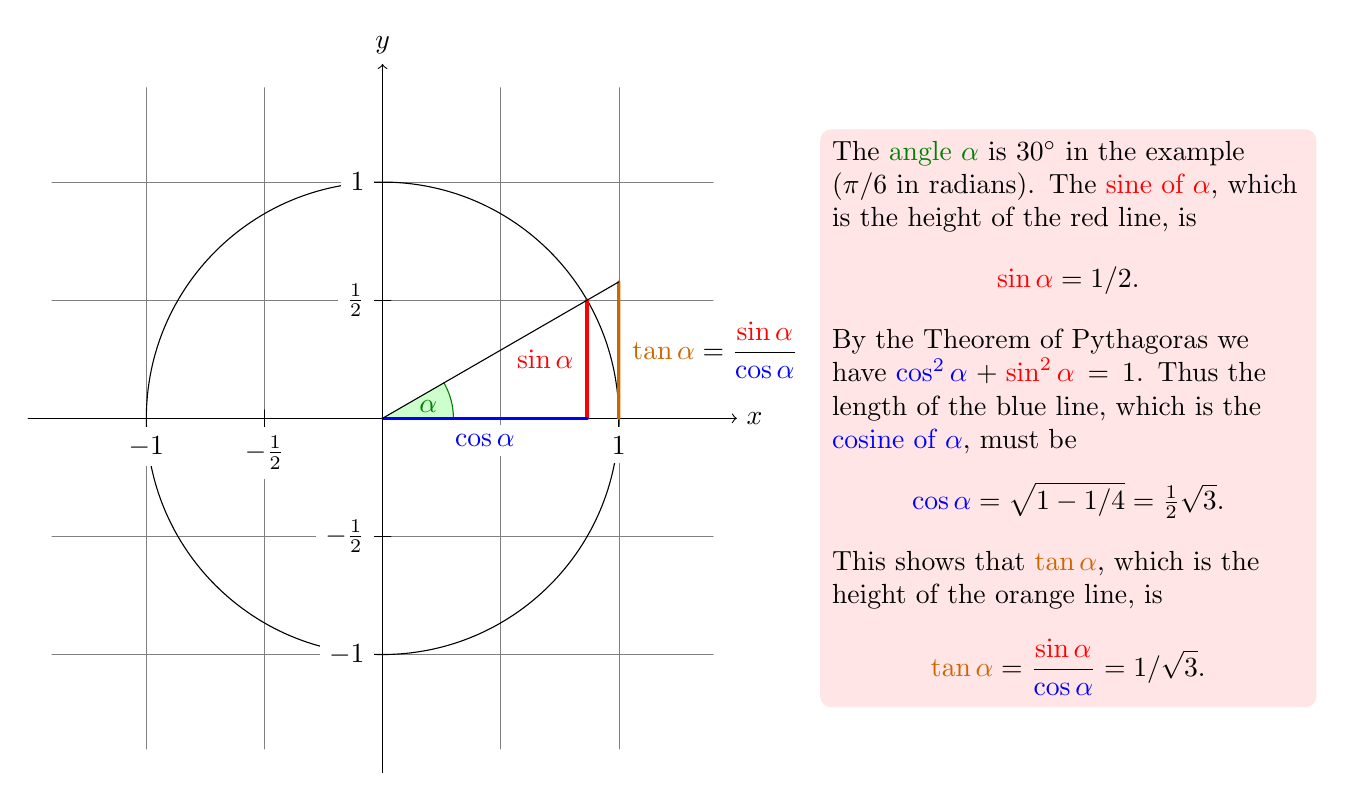
\begin{tikzpicture}
  [scale=3,line cap=round,
   % Styles
   axes/.style=,
   important line/.style={very thick},
   information text/.style={rounded corners,fill=red!10,inner sep=1ex}]

  % Local definitions
  \def\costhirty{0.8660256}

  % Colors
  \colorlet{anglecolor}{green!50!black}
  \colorlet{sincolor}{red}
  \colorlet{tancolor}{orange!80!black}
  \colorlet{coscolor}{blue}

  % The graphic
  \draw[help lines,step=0.5cm] (-1.4,-1.4) grid (1.4,1.4);

  \draw (0,0) circle [radius=1cm];

  \begin{scope}[axes]
    \draw[->] (-1.5,0) -- (1.5,0) node[right] {$x$};
    \draw[->] (0,-1.5) -- (0,1.5) node[above] {$y$};

    \foreach \x/\xtext in {-1, -.5/-\frac{1}{2}, 1}
      \draw[xshift=\x cm] (0pt,1pt) -- (0pt,-1pt) node[below,fill=white] {$\xtext$};

    \foreach \y/\ytext in {-1, -.5/-\frac{1}{2}, .5/\frac{1}{2}, 1}
      \draw[yshift=\y cm] (1pt,0pt) -- (-1pt,0pt) node[left,fill=white] {$\ytext$};
  \end{scope}

  \filldraw[fill=green!20,draw=anglecolor] (0,0) -- (3mm,0pt) arc(0:30:3mm);
  \draw (15:2mm) node[anglecolor] {$\alpha$};

  \draw[important line,sincolor]
    (30:1cm) -- node[left=1pt,fill=white] {$\sin \alpha$} +(0,-.5);

  \draw[important line,coscolor]
    (0,0) -- node[below=2pt,fill=white] {$\cos \alpha$} (\costhirty,0);

  \draw[important line,tancolor] (1,0) --
    node [right=1pt,fill=white]
    {
      $\displaystyle \tan \alpha \color{black}=
      \frac{{\color{sincolor}\sin \alpha}}{\color{coscolor}\cos \alpha}$
    } (intersection of 0,0--30:1cm and 1,0--1,1) coordinate (t);

  \draw (0,0) -- (t);

  \draw[xshift=1.85cm] node [right,text width=6cm,information text]
    {
      The {\color{anglecolor} angle $\alpha$} is $30^\circ$ in the
      example ($\pi/6$ in radians). The {\color{sincolor}sine of
        $\alpha$}, which is the height of the red line, is
      \[
      {\color{sincolor} \sin \alpha} = 1/2.
      \]
      By the Theorem of Pythagoras we have ${\color{coscolor}\cos^2 \alpha} +
      {\color{sincolor}\sin^2\alpha} =1$. Thus the length of the blue
      line, which is the {\color{coscolor}cosine of $\alpha$}, must be
      \[
      {\color{coscolor}\cos\alpha} = \sqrt{1 - 1/4} = \textstyle
      \frac{1}{2} \sqrt 3.
      \]%
      This shows that {\color{tancolor}$\tan \alpha$}, which is the
      height of the orange line, is
      \[
      {\color{tancolor}\tan\alpha} = \frac{{\color{sincolor}\sin
          \alpha}}{\color{coscolor}\cos \alpha} = 1/\sqrt 3.
      \]%
    };
\end{tikzpicture}


\subsection{Setting up the Environment}

In \tikzname, to draw a picture, at the start of the picture you need to tell
\TeX\ or \LaTeX\ that you want to start a picture. In \LaTeX\ this is done
using the environment |{tikzpicture}|, in plain \TeX\ you just use
|\tikzpicture| to start the picture and |\endtikzpicture| to end it.


\subsubsection{Setting up the Environment in \LaTeX}

Karl, being a \LaTeX\ user, thus sets up his file as follows:
%
\begin{codeexample}[code only]
\documentclass{article} % say
\usepackage{tikz}
\begin{document}
We are working on
\begin{tikzpicture}
  \draw (-1.5,0) -- (1.5,0);
  \draw (0,-1.5) -- (0,1.5);
\end{tikzpicture}.
\end{document}
\end{codeexample}

When executed, that is, run via |pdflatex| or via |latex| followed by |dvips|,
the resulting will contain something that looks like this:
%
\begin{codeexample}[width=7cm]
We are working on
\begin{tikzpicture}
  \draw (-1.5,0) -- (1.5,0);
  \draw (0,-1.5) -- (0,1.5);
\end{tikzpicture}.
\end{codeexample}

Admittedly, not quite the whole picture, yet, but we do have the axes
established. Well, not quite, but we have the lines that make up the axes
drawn. Karl suddenly has a sinking feeling that the picture is still some way
off.

Let's have a more detailed look at the code. First, the package |tikz| is
loaded. This package is a so-called ``frontend'' to the basic \pgfname\ system.
The basic layer, which is also described in this manual, is somewhat more,
well, basic and thus harder to use. The frontend makes things easier by
providing a simpler syntax.

Inside the environment there are two |\draw| commands. They mean: ``The path,
which is specified following the command up to the semicolon, should be
drawn.'' The first path is specified as |(-1.5,0) -- (0,1.5)|, which means ``a
straight line from the point at position $(-1.5,0)$ to the point at position
$(0,1.5)$''. Here, the positions are specified within a special coordinate
system in which, initially, one unit is 1cm.

Karl is quite pleased to note that the environment automatically reserves
enough space to encompass the picture.


\subsubsection{Setting up the Environment in Plain \TeX}

Karl's wife Gerda, who also happens to be a math teacher, is not a \LaTeX\
user, but uses plain \TeX\ since she prefers to do things ``the old way''. She
can also use \tikzname. Instead of |\usepackage{tikz}| she has to write
|\input tikz.tex| and instead of |\begin{tikzpicture}| she writes
|\tikzpicture| and instead of |\end{tikzpicture}| she writes |\endtikzpicture|.

Thus, she would use:
%
\begin{codeexample}[code only]
%% Plain TeX file
\input tikz.tex
\baselineskip=12pt
\hsize=6.3truein
\vsize=8.7truein
We are working on
\tikzpicture
  \draw (-1.5,0) -- (1.5,0);
  \draw (0,-1.5) -- (0,1.5);
\endtikzpicture.
\bye
\end{codeexample}

Gerda can typeset this file using either |pdftex| or |tex| together with
|dvips|. \tikzname\ will automatically discern which driver she is using. If
she wishes to use |dvipdfm| together with |tex|, she either needs to modify the
file |pgf.cfg| or can write |\def\pgfsysdriver{pgfsys-dvipdfm.def}| somewhere
\emph{before} she inputs |tikz.tex| or |pgf.tex|.


\subsubsection{Setting up the Environment in Con\TeX t}

Karl's uncle Hans uses Con\TeX t. Like Gerda, Hans can also use \tikzname.
Instead of |\usepackage{tikz}| he says |\usemodule[tikz]|. Instead of
|\begin{tikzpicture}| he writes |\starttikzpicture| and  instead of
|\end{tikzpicture}| he writes |\stoptikzpicture|.

His version of the example looks like this:
%
\begin{codeexample}[code only]
%% ConTeXt file
\usemodule[tikz]

\starttext
  We are working on
  \starttikzpicture
    \draw (-1.5,0) -- (1.5,0);
    \draw (0,-1.5) -- (0,1.5);
  \stoptikzpicture.
\stoptext
\end{codeexample}

Hans will now typeset this file in the usual way using |texexec| or |context|.


\subsection{Straight Path Construction}

The basic building block of all pictures in \tikzname\ is the path. A
\emph{path} is a series of straight lines and curves that are connected (that
is not the whole picture, but let us ignore the complications for the moment).
You start a path by specifying the coordinates of the start position as a point
in round brackets, as in |(0,0)|. This is followed by a series of ``path
extension operations''. The simplest is |--|, which we used already. It must be
followed by another coordinate and it extends the path in a straight line to
this new position. For example, if we were to turn the two paths of the axes
into one path, the following would result:
%
\begin{codeexample}[]
\tikz \draw (-1.5,0) -- (1.5,0) -- (0,-1.5) -- (0,1.5);
\end{codeexample}

Karl is a bit confused by the fact that there is no |{tikzpicture}|
environment, here. Instead, the little command |\tikz| is used. This command
either takes one argument (starting with an opening brace as in
|\tikz{\draw (0,0) -- (1.5,0)}|, which yields \tikz{\draw (0,0) --(1.5,0);}) or
collects everything up to the next semicolon and puts it inside a
|{tikzpicture}| environment. As a rule of thumb, all \tikzname\ graphic drawing
commands must occur as an argument of |\tikz| or inside a |{tikzpicture}|
environment. Fortunately, the command |\draw| will only be defined inside this
environment, so there is little chance that you will accidentally do something
wrong here.


\subsection{Curved Path Construction}

The next thing Karl wants to do is to draw the circle. For this, straight lines
obviously will not do. Instead, we need some way to draw curves. For this,
\tikzname\ provides a special syntax. One or two ``control points'' are needed.
The math behind them is not quite trivial, but here is the basic idea: Suppose
you are at point $x$ and the first control point is $y$. Then the curve will
start ``going in the direction of~$y$ at~$x$'', that is, the tangent of the
curve at $x$ will point toward~$y$. Next, suppose the curve should end at $z$
and the second support point is $w$. Then the curve will, indeed, end at $z$
and the tangent of the curve at point $z$ will go through $w$.

Here is an example (the control points have been added for clarity):
%
\begin{codeexample}[]
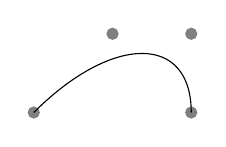
\begin{tikzpicture}
  \filldraw [gray] (0,0) circle [radius=2pt]
                   (1,1) circle [radius=2pt]
                   (2,1) circle [radius=2pt]
                   (2,0) circle [radius=2pt];
  \draw (0,0) .. controls (1,1) and (2,1) .. (2,0);
\end{tikzpicture}
\end{codeexample}

The general syntax for extending a path in a ``curved'' way is |.. controls|
\meta{first control point} |and| \meta{second control point} |..|
\meta{end point}. You can leave out the |and| \meta{second control point},
which causes the first one to be used twice.

So, Karl can now add the first half circle to the picture:
%
\begin{codeexample}[]
\begin{tikzpicture}
  \draw (-1.5,0) -- (1.5,0);
  \draw (0,-1.5) -- (0,1.5);
  \draw (-1,0) .. controls (-1,0.555) and (-0.555,1) .. (0,1)
               .. controls (0.555,1) and (1,0.555) .. (1,0);
\end{tikzpicture}
\end{codeexample}

Karl is happy with the result, but finds specifying circles in this way to be
extremely awkward. Fortunately, there is a much simpler way.


\subsection{Circle Path Construction}

In order to draw a circle, the path construction operation |circle| can be
used. This operation is followed by a radius in brackets as in the following
example: (Note that the previous position is used as the \emph{center} of the
circle.)
%
\begin{codeexample}[]
\tikz \draw (0,0) circle [radius=10pt];
\end{codeexample}

You can also append an ellipse to the path using the |ellipse| operation.
Instead of a single radius you can specify two of them:
%
\begin{codeexample}[]
\tikz \draw (0,0) ellipse [x radius=20pt, y radius=10pt];
\end{codeexample}

To draw an ellipse whose axes are not horizontal and vertical, but point in an
arbitrary direction (a ``turned ellipse'' like \tikz \draw[rotate=30] (0,0)
ellipse [x radius=6pt, y radius=3pt];) you can use transformations, which are
explained later. The code for the little ellipse is
|\tikz \draw[rotate=30] (0,0) ellipse [x radius=6pt, y radius=3pt];|, by the
way.

So, returning to Karl's problem, he can write
|\draw (0,0) circle [radius=1cm];| to draw the circle:
%
\begin{codeexample}[]
\begin{tikzpicture}
  \draw (-1.5,0) -- (1.5,0);
  \draw (0,-1.5) -- (0,1.5);
  \draw (0,0) circle [radius=1cm];
\end{tikzpicture}
\end{codeexample}

At this point, Karl is a bit alarmed that the circle is so small when he wants
the final picture to be much bigger. He is pleased to learn that \tikzname\ has
powerful transformation options and scaling everything by a factor of three is
very easy. But let us leave the size as it is for the moment to save some
space.


\subsection{Rectangle Path Construction}

The next things we would like to have is the grid in the background. There are
several ways to produce it. For example, one might draw lots of rectangles.
Since rectangles are so common, there is a special syntax for them: To add a
rectangle to the current path, use the |rectangle| path construction operation.
This operation should be followed by another coordinate and will append a
rectangle to the path such that the previous coordinate and the next
coordinates are corners of the rectangle. So, let us add two rectangles to the
picture:
%
\begin{codeexample}[]
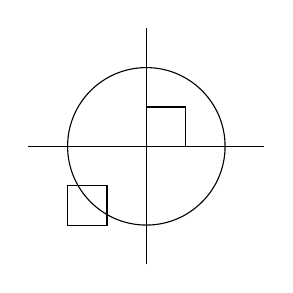
\begin{tikzpicture}
  \draw (-1.5,0) -- (1.5,0);
  \draw (0,-1.5) -- (0,1.5);
  \draw (0,0) circle [radius=1cm];
  \draw (0,0) rectangle (0.5,0.5);
  \draw (-0.5,-0.5) rectangle (-1,-1);
\end{tikzpicture}
\end{codeexample}

While this may be nice in other situations, this is not really leading anywhere
with Karl's problem: First, we would need an awful lot of these rectangles and
then there is the border that is not ``closed''.

So, Karl is about to resort to simply drawing four vertical and four horizontal
lines using the nice |\draw| command, when he learns that there is a |grid|
path construction operation.


\subsection{Grid Path Construction}

The |grid| path operation adds a grid to the current path. It will add lines
making up a grid that fills the rectangle whose one corner is the current point
and whose other corner is the point following the |grid| operation. For
example, the code |\tikz \draw[step=2pt] (0,0) grid (10pt,10pt);| produces
\tikz \draw[step=2pt] (0,0) grid (10pt,10pt);. Note how the optional argument
for |\draw| can be used to specify a grid width (there are also |xstep| and
|ystep| to define the steppings independently). As Karl will learn soon, there
are \emph{lots} of things that can be influenced using such options.

For Karl, the following code could be used:
%
\begin{codeexample}[]
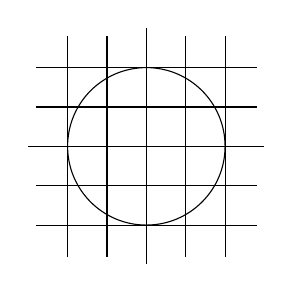
\begin{tikzpicture}
  \draw (-1.5,0) -- (1.5,0);
  \draw (0,-1.5) -- (0,1.5);
  \draw (0,0) circle [radius=1cm];
  \draw[step=.5cm] (-1.4,-1.4) grid (1.4,1.4);
\end{tikzpicture}
\end{codeexample}

Having another look at the desired picture, Karl notices that it would be nice
for the grid to be more subdued. (His son told him that grids tend to be
distracting if they are not subdued.) To subdue the grid, Karl adds two more
options to the |\draw| command that draws the grid. First, he uses the color
|gray| for the grid lines. Second, he reduces the line width to |very thin|.
Finally, he swaps the ordering of the commands so that the grid is drawn first
and everything else on top.
%
\begin{codeexample}[]
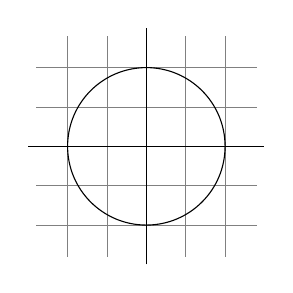
\begin{tikzpicture}
  \draw[step=.5cm,gray,very thin] (-1.4,-1.4) grid (1.4,1.4);
  \draw (-1.5,0) -- (1.5,0);
  \draw (0,-1.5) -- (0,1.5);
  \draw (0,0) circle [radius=1cm];
\end{tikzpicture}
\end{codeexample}


\subsection{Adding a Touch of  Style}

Instead of the options |gray,very thin| Karl could also have said |help lines|.
\emph{Styles} are predefined sets of options that can be used to organize how a
graphic is drawn. By saying |help lines| you say ``use the style that I (or
someone else) has set for drawing help lines''. If Karl decides, at some later
point, that grids should be drawn, say, using the color |blue!50| instead of
|gray|, he could provide the following option somewhere:
%
\begin{codeexample}[code only]
help lines/.style={color=blue!50,very thin}
\end{codeexample}
%
The effect of this ``style setter'' is that in the current scope or environment
the |help lines| option has the same effect as |color=blue!50,very thin|.

Using styles makes your graphics code more flexible. You can change the way
things look easily in a consistent manner. Normally, styles are defined at the
beginning of a picture. However, you may sometimes wish to define a style
globally, so that all pictures of your document can use this style. Then you
can easily change the way all graphics look by changing this one style. In this
situation you can use the |\tikzset| command at the beginning of the document
as in
%
\begin{codeexample}[code only]
\tikzset{help lines/.style=very thin}
\end{codeexample}

To build a hierarchy of styles you can have one style use another. So in order
to define a style |Karl's grid| that is based on the |grid| style Karl could
say
%
\begin{codeexample}[code only]
\tikzset{Karl's grid/.style={help lines,color=blue!50}}
...
\draw[Karl's grid] (0,0) grid (5,5);
\end{codeexample}

Styles are made even more powerful by parametrization. This means that, like
other options, styles can also be used with a parameter. For instance, Karl
could parameterize his grid so that, by default, it is blue, but he could also
use another color.
%
\begin{codeexample}[code only]
\begin{tikzpicture}
  [Karl's grid/.style  ={help lines,color=#1!50},
   Karl's grid/.default=blue]

  \draw[Karl's grid]     (0,0) grid (1.5,2);
  \draw[Karl's grid=red] (2,0) grid (3.5,2);
\end{tikzpicture}
\end{codeexample}

 In this example, the definition of the style |Karl's grid| is given as an
 optional argument to the |{tikzpicture}| environment. Additional styles for other
 elements would follow after a comma. With many styles in effect, the optional
 argument of the environment may easily happen to be longer than the actual
 contents.

\subsection{Drawing Options}

Karl wonders what other options there are that influence how a path is drawn.
He saw already that the |color=|\meta{color} option can be used to set the
line's color. The option |draw=|\meta{color} does nearly the same, only it sets
the color for the lines only and a different color can be used for filling
(Karl will need this when he fills the arc for the angle).

He saw that the style |very thin| yields very thin lines. Karl is not really
surprised by this and neither is he surprised to learn that |thin| yields thin
lines,  |thick| yields thick lines, |very thick| yields very thick lines,
|ultra thick| yields really, really thick lines and |ultra thin| yields lines
that are so thin that low-resolution printers and displays will have trouble
showing them. He wonders what gives lines of ``normal'' thickness. It turns out
that |thin| is the correct choice, since it gives the same thickness as \TeX's
|\hrule| command. Nevertheless, Karl would like to know whether there is
anything ``in the middle'' between |thin| and |thick|. There is: |semithick|.

Another useful thing one can do with lines is to dash or dot them. For this,
the two styles |dashed| and |dotted| can be used, yielding \tikz[baseline]
\draw[dashed] (0,.5ex) -- ++(2em,0pt); and \tikz[baseline] \draw[dotted]
(0,.5ex) -- ++(2em,0pt);. Both options also exist in a loose and a dense
version, called |loosely dashed|, |densely dashed|, |loosely dotted|, and
|densely dotted|. If he really, really  needs to, Karl can also define much
more complex dashing patterns with the |dash pattern| option, but his son
insists that dashing is to be used with utmost care and mostly distracts.
Karl's son claims that complicated dashing patterns are evil. Karl's students
do not care about dashing patterns.


\subsection{Arc Path Construction}

Our next obstacle is to draw the arc for the angle. For this, the |arc| path
construction operation is useful, which draws part of a circle or ellipse. This
|arc| operation is followed by options in brackets that specify the arc. An
example would be \texttt{arc[start angle=10, end angle=80, radius=10pt]}, which
means exactly what it says. Karl obviously needs an arc from $0^\circ$ to
$30^\circ$. The radius should be something relatively small, perhaps around one
third of the circle's radius. When one uses the arc path construction
operation, the specified arc will be added with its starting point at the
current position. So, we first have to ``get there''.
%
\begin{codeexample}[]
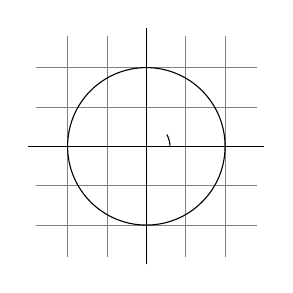
\begin{tikzpicture}
  \draw[step=.5cm,gray,very thin] (-1.4,-1.4) grid (1.4,1.4);
  \draw (-1.5,0) -- (1.5,0);
  \draw (0,-1.5) -- (0,1.5);
  \draw (0,0) circle [radius=1cm];
  \draw (3mm,0mm) arc [start angle=0, end angle=30, radius=3mm];
\end{tikzpicture}
\end{codeexample}

Karl thinks this is really a bit small and he cannot continue unless he learns
how to do scaling. For this, he can add the |[scale=3]| option. He could add
this option to each |\draw| command, but that would be awkward. Instead, he
adds it to the whole environment, which causes this option to apply to
everything within.
%
\begin{codeexample}[]
\begin{tikzpicture}[scale=3]
  \draw[step=.5cm,gray,very thin] (-1.4,-1.4) grid (1.4,1.4);
  \draw (-1.5,0) -- (1.5,0);
  \draw (0,-1.5) -- (0,1.5);
  \draw (0,0) circle [radius=1cm];
  \draw (3mm,0mm) arc [start angle=0, end angle=30, radius=3mm];
\end{tikzpicture}
\end{codeexample}

As for circles, you can specify ``two'' radii in order to get an elliptical
arc.
%
\begin{codeexample}[]
  \tikz \draw (0,0)
    arc [start angle=0, end angle=315,
         x radius=1.75cm, y radius=1cm];
\end{codeexample}


\subsection{Clipping a Path}

In order to save space in this manual, it would be nice to clip Karl's graphics
a bit so that we can focus on the ``interesting'' parts. Clipping is pretty
easy in \tikzname. You can use the |\clip| command to clip all subsequent
drawing. It works like |\draw|, only it does not draw anything, but uses the
given path to clip everything subsequently.
%
\begin{codeexample}[]
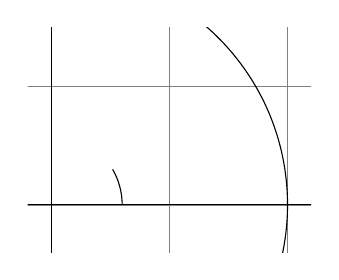
\begin{tikzpicture}[scale=3]
  \clip (-0.1,-0.2) rectangle (1.1,0.75);
  \draw[step=.5cm,gray,very thin] (-1.4,-1.4) grid (1.4,1.4);
  \draw (-1.5,0) -- (1.5,0);
  \draw (0,-1.5) -- (0,1.5);
  \draw (0,0) circle [radius=1cm];
  \draw (3mm,0mm) arc [start angle=0, end angle=30, radius=3mm];
\end{tikzpicture}
\end{codeexample}

You can also do both at the same time: Draw \emph{and} clip a path. For this,
use the |\draw| command and add the |clip| option. (This is not the whole
picture: You can also use the |\clip| command and add the |draw| option. Well,
that is also not the whole picture: In reality, |\draw| is just a shorthand for
|\path[draw]| and |\clip| is a shorthand for |\path[clip]| and you could also
say |\path[draw,clip]|.) Here is an example:
%
\begin{codeexample}[]
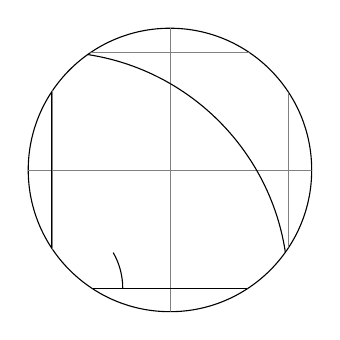
\begin{tikzpicture}[scale=3]
  \clip[draw] (0.5,0.5) circle (.6cm);
  \draw[step=.5cm,gray,very thin] (-1.4,-1.4) grid (1.4,1.4);
  \draw (-1.5,0) -- (1.5,0);
  \draw (0,-1.5) -- (0,1.5);
  \draw (0,0) circle [radius=1cm];
  \draw (3mm,0mm) arc [start angle=0, end angle=30, radius=3mm];
\end{tikzpicture}
\end{codeexample}


\subsection{Parabola and Sine Path Construction}

Although Karl does not need them for his picture, he is pleased to learn that
there are |parabola| and |sin| and |cos| path operations for adding parabolas
and sine and cosine curves to the current path. For the |parabola| operation,
the current point will lie on the parabola as well as the point given after the
parabola operation. Consider the following example:
%
\begin{codeexample}[]
\tikz \draw (0,0) rectangle (1,1)  (0,0) parabola (1,1);
\end{codeexample}

It is also possible to place the bend somewhere else:
%
\begin{codeexample}[]
\tikz \draw[x=1pt,y=1pt] (0,0) parabola bend (4,16) (6,12);
\end{codeexample}

The operations |sin| and |cos| add a sine or cosine curve in the interval
$[0,\pi/2]$ such that the previous current point is at the start of the curve
and the curve ends at the given end point. Here are two examples:
%
\begin{codeexample}[]
A sine \tikz \draw[x=1ex,y=1ex] (0,0) sin (1.57,1); curve.
\end{codeexample}

\begin{codeexample}[]
\tikz \draw[x=1.57ex,y=1ex] (0,0) sin (1,1) cos (2,0) sin (3,-1) cos (4,0)
                            (0,1) cos (1,0) sin (2,-1) cos (3,0) sin (4,1);
\end{codeexample}


\subsection{Filling and Drawing}

Returning to the picture, Karl now wants the angle to be ``filled'' with a very
light green. For this he uses |\fill| instead of |\draw|. Here is what Karl
does:
%
\begin{codeexample}[]
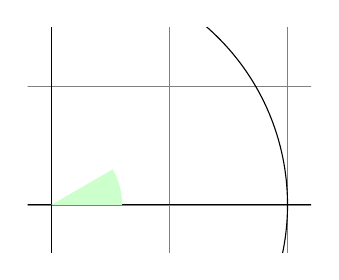
\begin{tikzpicture}[scale=3]
  \clip (-0.1,-0.2) rectangle (1.1,0.75);
  \draw[step=.5cm,gray,very thin] (-1.4,-1.4) grid (1.4,1.4);
  \draw (-1.5,0) -- (1.5,0);
  \draw (0,-1.5) -- (0,1.5);
  \draw (0,0) circle [radius=1cm];
  \fill[green!20!white] (0,0) -- (3mm,0mm)
    arc [start angle=0, end angle=30, radius=3mm] -- (0,0);
\end{tikzpicture}
\end{codeexample}

The color |green!20!white| means 20\% green and 80\% white mixed together. Such
color expression are possible since \tikzname\ uses Uwe Kern's |xcolor|
package, see the documentation of that package for details on color
expressions.

What would have happened, if Karl had not ``closed'' the path using |--(0,0)|
at the end? In this case, the path is closed automatically, so this could have
been omitted. Indeed, it would even have been better to write the following,
instead:
%
\begin{codeexample}[code only]
  \fill[green!20!white] (0,0) -- (3mm,0mm)
    arc [start angle=0, end angle=30, radius=3mm] -- cycle;
\end{codeexample}
%
The |--cycle| causes the current path to be closed (actually the current part
of the current path) by smoothly joining the first and last point. To
appreciate the difference, consider the following example:
%
\begin{codeexample}[]
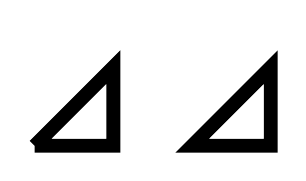
\begin{tikzpicture}[line width=5pt]
  \draw (0,0) -- (1,0) -- (1,1) -- (0,0);
  \draw (2,0) -- (3,0) -- (3,1) -- cycle;
  \useasboundingbox (0,1.5); % make bounding box higher
\end{tikzpicture}
\end{codeexample}

You can also fill and draw a path at the same time using the |\filldraw|
command. This will first draw the path, then fill it. This may not seem too
useful, but you can specify different colors to be used for filling and for
stroking. These are specified as optional arguments like this:
%
\begin{codeexample}[]
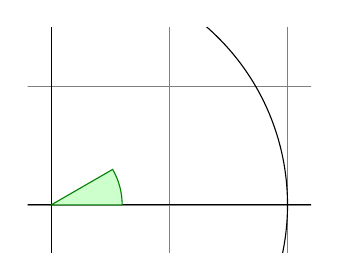
\begin{tikzpicture}[scale=3]
  \clip (-0.1,-0.2) rectangle (1.1,0.75);
  \draw[step=.5cm,gray,very thin] (-1.4,-1.4) grid (1.4,1.4);
  \draw (-1.5,0) -- (1.5,0);
  \draw (0,-1.5) -- (0,1.5);
  \draw (0,0) circle [radius=1cm];
  \filldraw[fill=green!20!white, draw=green!50!black] (0,0) -- (3mm,0mm)
    arc [start angle=0, end angle=30, radius=3mm] -- cycle;
\end{tikzpicture}
\end{codeexample}


\subsection{Shading}

Karl briefly considers the possibility of making the angle ``more fancy'' by
\emph{shading} it. Instead of filling the area with a uniform color, a smooth
transition between different colors is used. For this, |\shade| and
|\shadedraw|, for shading and drawing at the same time, can be used:
%
\begin{codeexample}[]
  \tikz \shade (0,0) rectangle (2,1)  (3,0.5) circle (.5cm);
\end{codeexample}
%
The default shading is a smooth transition from gray to white. To specify
different colors, you can use options:
%
\begin{codeexample}[]

\begin{tikzpicture}[rounded corners,ultra thick]
  \shade[top color=yellow,bottom color=black] (0,0) rectangle +(2,1);
  \shade[left color=yellow,right color=black] (3,0) rectangle +(2,1);
  \shadedraw[inner color=yellow,outer color=black,draw=yellow] (6,0) rectangle +(2,1);
  \shade[ball color=green] (9,.5) circle (.5cm);
\end{tikzpicture}
\end{codeexample}

For Karl, the following might be appropriate:
%
\begin{codeexample}[]
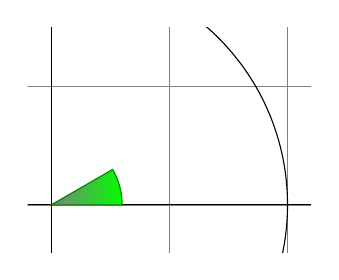
\begin{tikzpicture}[scale=3]
  \clip (-0.1,-0.2) rectangle (1.1,0.75);
  \draw[step=.5cm,gray,very thin] (-1.4,-1.4) grid (1.4,1.4);
  \draw (-1.5,0) -- (1.5,0);
  \draw (0,-1.5) -- (0,1.5);
  \draw (0,0) circle [radius=1cm];
  \shadedraw[left color=gray,right color=green, draw=green!50!black]
    (0,0) -- (3mm,0mm)
    arc [start angle=0, end angle=30, radius=3mm] -- cycle;
\end{tikzpicture}
\end{codeexample}

However, he wisely decides that shadings usually only distract without adding
anything to the picture.


\subsection{Specifying Coordinates}

Karl now wants to add the sine and cosine lines. He knows already that he can
use the |color=| option to set the lines' colors. So, what is the best way to
specify the coordinates?

There are different ways of specifying coordinates. The easiest way is to say
something like |(10pt,2cm)|. This means 10pt in $x$-direction and 2cm in
$y$-directions. Alternatively, you can also leave out the units as in |(1,2)|,
which means ``one times the current $x$-vector plus twice the current
$y$-vector''. These vectors default to 1cm in the $x$-direction and 1cm in the
$y$-direction, respectively.

In order to specify points in polar coordinates, use the notation |(30:1cm)|,
which means 1cm in direction 30 degree. This is obviously quite useful to ``get
to the point $(\cos 30^\circ,\sin 30^\circ)$ on the circle''.

You can add a single |+| sign in front of a coordinate or two of them as in
|+(0cm,1cm)| or |++(2cm,0cm)|. Such coordinates are interpreted differently:
The first form means ``1cm upwards from the previous specified position'' and
the second means ``2cm to the right of the previous specified position, making
this the new specified position''. For example, we can draw the sine line as
follows:
%
\begin{codeexample}[]
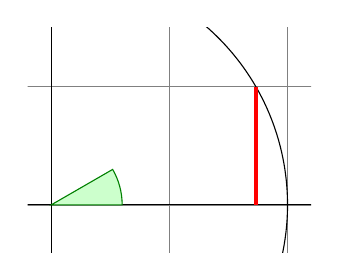
\begin{tikzpicture}[scale=3]
  \clip (-0.1,-0.2) rectangle (1.1,0.75);
  \draw[step=.5cm,gray,very thin] (-1.4,-1.4) grid (1.4,1.4);
  \draw (-1.5,0) -- (1.5,0);
  \draw (0,-1.5) -- (0,1.5);
  \draw (0,0) circle [radius=1cm];
  \filldraw[fill=green!20,draw=green!50!black] (0,0) -- (3mm,0mm)
      arc [start angle=0, end angle=30, radius=3mm] -- cycle;
  \draw[red,very thick] (30:1cm) -- +(0,-0.5);
\end{tikzpicture}
\end{codeexample}

Karl used the fact $\sin 30^\circ = 1/2$. However, he very much doubts that his
students know this, so it would be nice to have a way of specifying ``the point
straight down from |(30:1cm)| that lies on the $x$-axis''. This is, indeed,
possible using a special syntax: Karl can write \verb!(30:1cm |- 0,0)!. In
general, the meaning of |(|\meta{p}\verb! |- !\meta{q}|)| is ``the intersection
of a vertical line through $p$ and a horizontal line through $q$''.

Next, let us draw the cosine line. One way would be to say
\verb!(30:1cm |- 0,0) -- (0,0)!. Another way is the following: we ``continue''
from where the sine ends:
%
\begin{codeexample}[]
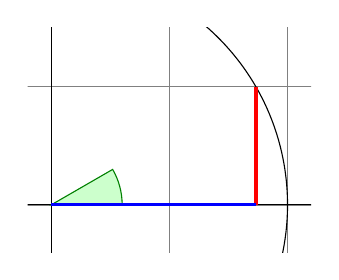
\begin{tikzpicture}[scale=3]
  \clip (-0.1,-0.2) rectangle (1.1,0.75);
  \draw[step=.5cm,gray,very thin] (-1.4,-1.4) grid (1.4,1.4);
  \draw (-1.5,0) -- (1.5,0);
  \draw (0,-1.5) -- (0,1.5);
  \draw (0,0) circle [radius=1cm];
  \filldraw[fill=green!20,draw=green!50!black] (0,0) -- (3mm,0mm)
      arc [start angle=0, end angle=30, radius=3mm] -- cycle;
  \draw[red,very thick]  (30:1cm) -- +(0,-0.5);
  \draw[blue,very thick] (30:1cm) ++(0,-0.5) -- (0,0);
\end{tikzpicture}
\end{codeexample}

Note that there is no |--| between |(30:1cm)| and |++(0,-0.5)|. In detail, this
path is interpreted as follows: ``First, the |(30:1cm)| tells me to move by pen
to $(\cos 30^\circ,1/2)$. Next, there comes another coordinate specification,
so I move my pen there without drawing anything. This new point is half a unit
down from the last position, thus it is at $(\cos 30^\circ,0)$. Finally, I move
the pen to the origin, but this time drawing something (because of the |--|).''

To appreciate the difference between |+| and |++| consider the following
example:
%
\begin{codeexample}[]
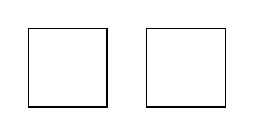
\begin{tikzpicture}
  \def\rectanglepath{-- ++(1cm,0cm)  -- ++(0cm,1cm)  -- ++(-1cm,0cm) -- cycle}
  \draw (0,0) \rectanglepath;
  \draw (1.5,0) \rectanglepath;
\end{tikzpicture}
\end{codeexample}

By comparison, when using a single |+|, the coordinates are different:
%
\begin{codeexample}[]
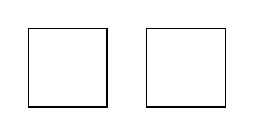
\begin{tikzpicture}
  \def\rectanglepath{-- +(1cm,0cm)  -- +(1cm,1cm)  -- +(0cm,1cm) -- cycle}
  \draw (0,0) \rectanglepath;
  \draw (1.5,0) \rectanglepath;
\end{tikzpicture}
\end{codeexample}


Naturally, all of this could have been written more clearly and more
economically like this (either with a single of a double |+|):
%
\begin{codeexample}[]
\tikz \draw (0,0) rectangle +(1,1)  (1.5,0) rectangle +(1,1);
\end{codeexample}


\subsection{Intersecting Paths}

Karl is left with the line for $\tan \alpha$, which seems difficult to specify
using transformations and polar coordinates. The first -- and easiest -- thing
he can do is so simply use the coordinate |(1,{tan(30)})| since \tikzname's
math engine knows how to compute things like |tan(30)|. Note the added braces
since, otherwise, \tikzname's parser would think that the first closing
parenthesis ends the coordinate (in general, you need to add braces around
components of coordinates when these components contain parentheses).

Karl can, however, also use a more elaborate, but also more ``geometric'' way
of computing the length of the orange line: He can specify intersections of
paths as coordinates. The line for $\tan \alpha$ starts at $(1,0)$ and goes
upward to a point that is at the intersection of a line going ``up'' and a line
going from the origin through |(30:1cm)|. Such computations are made available
by the |intersections| library.

What Karl must do is to create two ``invisible'' paths that intersect at the
position of interest. Creating paths that are not otherwise seen can be done
using the |\path| command without any options like |draw| or |fill|. Then, Karl
can add the |name path| option to the path for later reference. Once the paths
have been constructed, Karl can use the |name intersections| to assign names to
the coordinate for later reference.
%
\begin{codeexample}[code only]
\path [name path=upward line] (1,0) -- (1,1);
\path [name path=sloped line] (0,0) -- (30:1.5cm); % a bit longer, so that there is an intersection

% (add `\usetikzlibrary{intersections}' after loading tikz in the preamble)
\draw [name intersections={of=upward line and sloped line, by=x}]
  [very thick,orange] (1,0) -- (x);
\end{codeexample}


\subsection{Adding Arrow Tips}

Karl now wants to add the little arrow tips at the end of the axes. He has
noticed that in many plots, even in scientific journals, these arrow tips seem
to be missing, presumably because the generating programs cannot produce them.
Karl thinks arrow tips belong at the end of axes. His son agrees. His students
do not care about arrow tips.

It turns out that adding arrow tips is pretty easy: Karl adds the option |->|
to the drawing commands for the axes:
%
\begin{codeexample}[preamble={\usetikzlibrary{intersections}}]
\begin{tikzpicture}[scale=3]
  \clip (-0.1,-0.2) rectangle (1.1,1.51);
  \draw[step=.5cm,gray,very thin] (-1.4,-1.4) grid (1.4,1.4);
  \draw[->] (-1.5,0) -- (1.5,0);
  \draw[->] (0,-1.5) -- (0,1.5);
  \draw (0,0) circle [radius=1cm];
  \filldraw[fill=green!20,draw=green!50!black] (0,0) -- (3mm,0mm)
        arc [start angle=0, end angle=30, radius=3mm] -- cycle;
  \draw[red,very thick]    (30:1cm) -- +(0,-0.5);
  \draw[blue,very thick]   (30:1cm) ++(0,-0.5) -- (0,0);

  \path [name path=upward line] (1,0) -- (1,1);
  \path [name path=sloped line] (0,0) -- (30:1.5cm);
  \draw [name intersections={of=upward line and sloped line, by=x}]
        [very thick,orange] (1,0) -- (x);
\end{tikzpicture}
\end{codeexample}

If Karl had used the option |<-| instead of |->|, arrow tips would have been
put at the beginning of the path. The option |<->| puts arrow tips at both ends
of the path.

There are certain restrictions to the kind of paths to which arrow tips can be
added. As a rule of thumb, you can add arrow tips only to a single open
``line''. For example, you cannot add tips to, say, a rectangle or a circle.
However, you can add arrow tips to curved paths and to paths that have several
segments, as in the following examples:
%
\begin{codeexample}[]
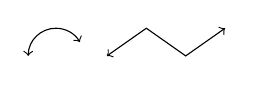
\begin{tikzpicture}
  \draw [<->] (0,0) arc [start angle=180, end angle=30, radius=10pt];
  \draw [<->] (1,0) -- (1.5cm,10pt) -- (2cm,0pt) -- (2.5cm,10pt);
\end{tikzpicture}
\end{codeexample}

Karl has a more detailed look at the arrow that \tikzname\ puts at the end. It
looks like this when he zooms it: \tikz[baseline] \draw[->,line width=1pt]
(0pt,.5ex) -- ++(10pt,0pt);. The shape seems vaguely familiar and, indeed, this
is exactly the end of \TeX's standard arrow used in something like $f\colon A
\to B$.

Karl likes the arrow, especially since it is not ``as thick'' as the arrows
offered by many other packages. However, he expects that, sometimes, he might
need to use some other kinds of arrow. To do so, Karl can say |>=|\meta{kind of
end arrow tip}, where \meta{kind of end arrow tip} is a special arrow tip
specification. For example, if Karl says |>=Stealth|, then he tells \tikzname\
that he would like  ``stealth-fighter-like'' arrow tips:
\todosp{remaining instance of bug \#473}
%
\begin{codeexample}[preamble={\usetikzlibrary{arrows.meta}}]
\begin{tikzpicture}[>=Stealth]
  \draw [->] (0,0) arc [start angle=180, end angle=30, radius=10pt];
  \draw [<<-,very thick] (1,0) -- (1.5cm,10pt) -- (2cm,0pt) -- (2.5cm,10pt);
\end{tikzpicture}
\end{codeexample}

Karl wonders whether such a military name for the arrow type is really
necessary. He is not really mollified when his son tells him that Microsoft's
PowerPoint uses the same name. He decides to have his students discuss this at
some point.

In addition to |Stealth| there are several other predefined kinds of arrow tips
Karl can choose from, see Section~\ref{section-arrows}. Furthermore, he can
define arrows types himself, if he needs new ones.


\subsection{Scoping}

Karl saw already that there are numerous graphic options that affect how paths
are rendered. Often, he would like to apply certain options to a whole set of
graphic commands. For example, Karl might wish to draw three paths using a
|thick| pen, but would like everything else to be drawn ``normally''.

If Karl wishes to set a certain graphic option for the whole picture, he can
simply pass this option to the |\tikz| command or to the |{tikzpicture}|
environment (Gerda would pass the options to |\tikzpicture| and Hans passes
them to |\starttikzpicture|). However, if Karl wants to apply graphic options
to a local group, he put these commands inside a |{scope}| environment (Gerda
uses |\scope| and |\endscope|, Hans uses |\startscope| and |\stopscope|). This
environment takes graphic options as an optional argument and these options
apply to everything inside the scope, but not to anything outside.

Here is an example:
%
\begin{codeexample}[]
\begin{tikzpicture}[ultra thick]
  \draw (0,0) -- (0,1);
  \begin{scope}[thin]
    \draw (1,0) -- (1,1);
    \draw (2,0) -- (2,1);
  \end{scope}
  \draw (3,0) -- (3,1);
\end{tikzpicture}
\end{codeexample}

Scoping has another interesting effect: Any changes to the clipping area are
local to the scope. Thus, if you say |\clip| somewhere inside a scope, the
effect of the |\clip| command ends at the end of the scope. This is useful
since there is no other way of ``enlarging'' the clipping area.

Karl has also already seen that giving options to commands like |\draw| apply
only to that command. It turns out that the situation is slightly more complex.
First, options to a command like |\draw| are not really options to the command,
but they are ``path options'' and can be given anywhere on the path. So,
instead of |\draw[thin] (0,0) -- (1,0);| one can also write
|\draw (0,0) [thin] -- (1,0);| or |\draw (0,0) -- (1,0) [thin];|; all of these
have the same effect. This might seem strange since in the last case, it would
appear that the |thin| should take effect only ``after'' the line from $(0,0)$
to $(1,0)$ has been drawn. However, most graphic options only apply to the
whole path. Indeed, if you say both |thin| and |thick| on the same path, the
last option given will ``win''.

When reading the above, Karl notices that only ``most'' graphic options apply
to the whole path. Indeed, all transformation options do \emph{not} apply to
the whole path, but only to ``everything following them on the path''. We will
have a more detailed look at this in a moment. Nevertheless, all options given
during a path construction apply only to this path.


\subsection{Transformations}

When you specify a  coordinate like |(1cm,1cm)|, where is that coordinate
placed on the page? To determine the position, \tikzname, \TeX, and
\textsc{pdf} or PostScript all apply certain transformations to the given
coordinate in order to determine the final position on the page.

\tikzname\ provides numerous options that allow you to transform coordinates in
\tikzname's private coordinate system. For example, the |xshift| option allows
you to shift all subsequent points by a certain amount:

\begin{codeexample}[]
\tikz \draw (0,0) -- (0,0.5) [xshift=2pt] (0,0) -- (0,0.5);
\end{codeexample}

It is important to note that you can change transformation ``in the middle of a
path'', a feature that is not supported by \pdf\ or PostScript. The reason is
that \tikzname\ keeps track of its own transformation matrix.

Here is a more complicated example:
%
\begin{codeexample}[]

\begin{tikzpicture}[even odd rule,rounded corners=2pt,x=10pt,y=10pt]
  \filldraw[fill=yellow!80!black] (0,0)   rectangle (1,1)
        [xshift=5pt,yshift=5pt]   (0,0)   rectangle (1,1)
                    [rotate=30]   (-1,-1) rectangle (2,2);
\end{tikzpicture}
\end{codeexample}

The most useful transformations are |xshift| and |yshift| for shifting, |shift|
for shifting to a given point as in |shift={(1,0)}| or |shift={+(0,0)}| (the
braces are necessary so that \TeX\ does not mistake the comma for separating
options), |rotate| for rotating by a certain angle (there is also a
|rotate around| for rotating around a given point), |scale| for scaling by a
certain factor, |xscale| and |yscale| for scaling only in the $x$- or
$y$-direction (|xscale=-1| is a flip), and |xslant| and |yslant| for slanting.
If these transformation and those that I have not mentioned are not sufficient,
the |cm| option allows you to apply an arbitrary transformation matrix. Karl's
students, by the way, do not know what a transformation matrix is.


\subsection{Repeating Things: For-Loops}

Karl's next aim is to add little ticks on the axes at positions $-1$, $-1/2$,
$1/2$, and $1$. For this, it would be nice to use some kind of ``loop'',
especially since he wishes to do the same thing at each of these positions.
There are different packages for doing this. \LaTeX\ has its own internal
command for this, |pstricks| comes along with the powerful |\multido| command.
All of these can be used together with \tikzname, so if you are familiar with
them, feel free to use them. \tikzname\ introduces yet another command, called
|\foreach|, which I introduced since I could never remember the syntax of the
other packages. |\foreach| is defined in the package |pgffor| and can be used
independently of \tikzname, but \tikzname\ includes it automatically.

In its basic form, the |\foreach| command is easy to use:
%
\begin{codeexample}[]
\foreach \x in {1,2,3} {$x =\x$, }
\end{codeexample}

The general syntax is
|\foreach| \meta{variable}| in {|\meta{list of values}|} |\meta{commands}.
Inside the \meta{commands}, the \meta{variable} will be assigned to the
different values. If the \meta{commands} do not start with a brace, everything
up to the next semicolon is used as \meta{commands}.

For Karl and the ticks on the axes, he could use the following code:
%
\begin{codeexample}[]
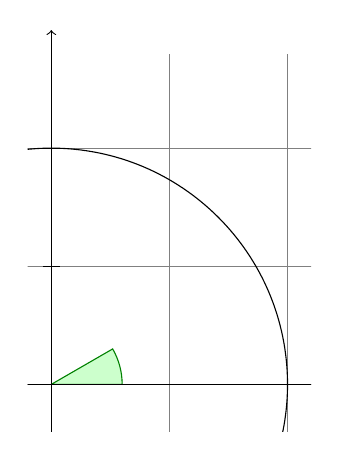
\begin{tikzpicture}[scale=3]
  \clip (-0.1,-0.2) rectangle (1.1,1.51);
  \draw[step=.5cm,gray,very thin] (-1.4,-1.4) grid (1.4,1.4);
  \filldraw[fill=green!20,draw=green!50!black] (0,0) -- (3mm,0mm)
      arc [start angle=0, end angle=30, radius=3mm] -- cycle;
  \draw[->] (-1.5,0) -- (1.5,0);
  \draw[->] (0,-1.5) -- (0,1.5);
  \draw (0,0) circle [radius=1cm];

  \foreach \x in {-1cm,-0.5cm,1cm}
    \draw (\x,-1pt) -- (\x,1pt);
  \foreach \y in {-1cm,-0.5cm,0.5cm,1cm}
    \draw (-1pt,\y) -- (1pt,\y);
\end{tikzpicture}
\end{codeexample}

As a matter of fact, there are many different ways of creating the ticks. For
example, Karl could have put the |\draw ...;| inside curly braces. He could
also have used, say,
%
\begin{codeexample}[code only]
\foreach \x in {-1,-0.5,1}
  \draw[xshift=\x cm] (0pt,-1pt) -- (0pt,1pt);
\end{codeexample}

Karl is curious what would happen in a more complicated situation where there
are, say, 20 ticks. It seems bothersome to explicitly mention all these numbers
in the set for |\foreach|. Indeed, it is possible to use |...| inside the
|\foreach| statement to iterate over a large number of values (which must,
however, be dimensionless real numbers) as in the following example:
%
\begin{codeexample}[]
\tikz \foreach \x in {1,...,10}
        \draw (\x,0) circle (0.4cm);
\end{codeexample}

If you provide \emph{two} numbers before the |...|, the |\foreach| statement
will use their difference for the stepping:
%
\begin{codeexample}[]
\tikz \foreach \x in {-1,-0.5,...,1}
       \draw (\x cm,-1pt) -- (\x cm,1pt);
\end{codeexample}

We can also nest loops to create interesting effects:
%
\begin{codeexample}[]
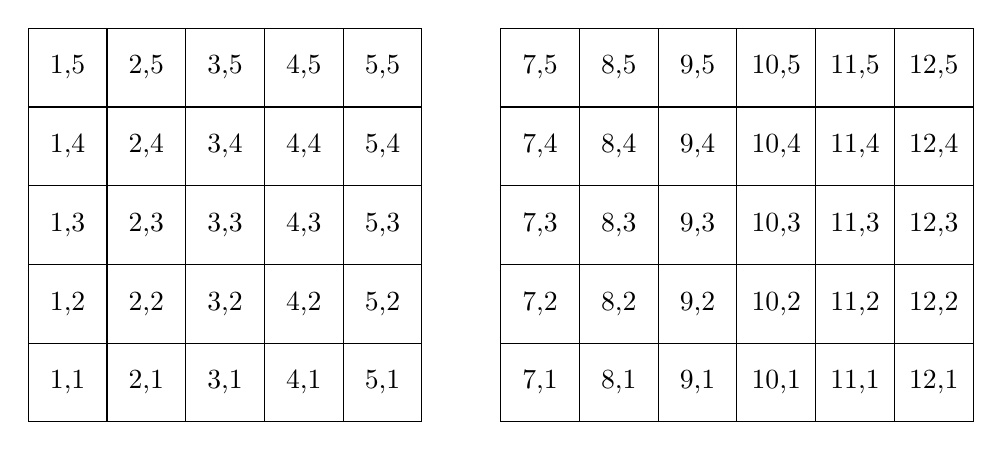
\begin{tikzpicture}
  \foreach \x in {1,2,...,5,7,8,...,12}
    \foreach \y in {1,...,5}
    {
      \draw (\x,\y) +(-.5,-.5) rectangle ++(.5,.5);
      \draw (\x,\y) node{\x,\y};
    }
\end{tikzpicture}
\end{codeexample}

The |\foreach| statement can do even trickier stuff, but the above gives the
idea.


\subsection{Adding Text}

Karl is, by now, quite satisfied with the picture. However, the most important
parts, namely the labels, are still missing!

\tikzname\ offers an easy-to-use and powerful system for adding text and, more
generally, complex shapes to a picture at specific positions. The basic idea is
the following: When \tikzname\ is constructing a path and encounters the
keyword |node| in the middle of a path, it reads a \emph{node specification}.
The keyword |node| is typically followed by some options and then some text
between curly braces. This text is put inside a normal \TeX\ box (if the node
specification directly follows a coordinate, which is usually the case,
\tikzname\ is able to perform some magic so that it is even possible to use
verbatim text inside the boxes) and then placed at the current position, that
is, at the last specified position (possibly shifted a bit, according to the
given options). However, all nodes are drawn only after the path has been
completely drawn/filled/shaded/clipped/whatever.
%
\begin{codeexample}[]
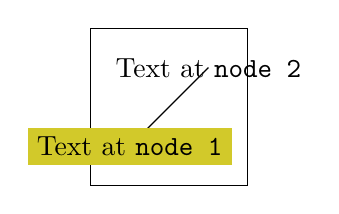
\begin{tikzpicture}
  \draw (0,0) rectangle (2,2);
  \draw (0.5,0.5) node [fill=yellow!80!black]
                       {Text at \verb!node 1!}
     -- (1.5,1.5) node {Text at \verb!node 2!};
\end{tikzpicture}
\end{codeexample}

Obviously, Karl would not only like to place nodes \emph{on} the last specified
position, but also to the left or the right of these positions. For this, every
node object that you put in your picture is equipped with several
\emph{anchors}. For example, the |north| anchor is in the middle at the upper
end of the shape, the |south| anchor is at the bottom and the |north east|
anchor is in the upper right corner. When you give the option |anchor=north|,
the text will be placed such that this northern anchor will lie on the current
position and the text is, thus, below the current position. Karl uses this to
draw the ticks as follows:
%
\begin{codeexample}[]
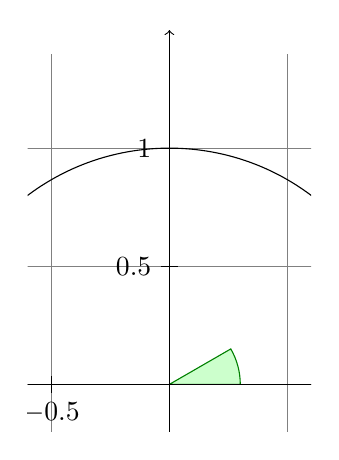
\begin{tikzpicture}[scale=3]
  \clip (-0.6,-0.2) rectangle (0.6,1.51);
  \draw[step=.5cm,help lines] (-1.4,-1.4) grid (1.4,1.4);
  \filldraw[fill=green!20,draw=green!50!black] (0,0) -- (3mm,0mm)
    arc [start angle=0, end angle=30, radius=3mm] -- cycle;
  \draw[->] (-1.5,0) -- (1.5,0);   \draw[->] (0,-1.5) -- (0,1.5);
  \draw (0,0) circle [radius=1cm];

  \foreach \x in {-1,-0.5,1}
    \draw (\x cm,1pt) -- (\x cm,-1pt) node[anchor=north] {$\x$};
  \foreach \y in {-1,-0.5,0.5,1}
    \draw (1pt,\y cm) -- (-1pt,\y cm) node[anchor=east] {$\y$};
\end{tikzpicture}
\end{codeexample}

This is quite nice, already. Using these anchors, Karl can now add most of the
other text elements. However, Karl thinks that, though ``correct'', it is quite
counter-intuitive that in order to place something \emph{below} a given point,
he has to use the \emph{north} anchor. For this reason, there is an option
called |below|, which does the same as |anchor=north|. Similarly, |above right|
does the same as |anchor=south west|. In addition, |below| takes an optional
dimension argument. If given, the shape will additionally be shifted downwards
by the given amount. So, |below=1pt| can be used to put a text label below some
point and, additionally shift it  1pt downwards.

Karl is not quite satisfied with the ticks. He would like to have $1/2$ or
$\frac{1}{2}$ shown instead of $0.5$, partly to show off the nice capabilities
of \TeX\ and \tikzname, partly because for positions like $1/3$ or $\pi$ it is
certainly very much preferable to have the ``mathematical'' tick there instead
of just the ``numeric'' tick. His students, on the other hand, prefer $0.5$
over $1/2$ since they are not too fond of fractions in general.

Karl now faces a problem: For the |\foreach| statement, the position |\x|
should still be given as |0.5| since \tikzname\ will not know where
|\frac{1}{2}| is supposed to be. On the other hand, the typeset text should
really be  |\frac{1}{2}|. To solve this problem, |\foreach| offers a special
syntax: Instead of having one variable |\x|, Karl can specify two (or even
more) variables separated by a slash as in |\x / \xtext|. Then, the elements in
the set over which |\foreach| iterates must also be of the form
\meta{first}|/|\meta{second}. In each iteration, |\x| will be set to
\meta{first} and |\xtext| will be set to \meta{second}. If no \meta{second} is
given, the \meta{first} will be used again. So, here is the new code for the
ticks:
%
\begin{codeexample}[]
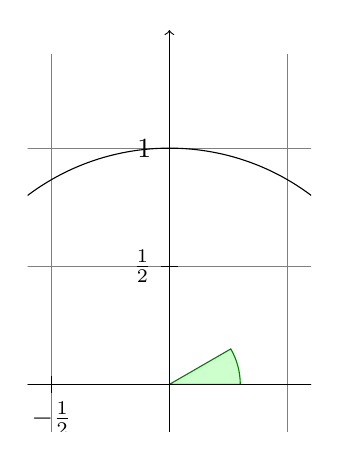
\begin{tikzpicture}[scale=3]
  \clip (-0.6,-0.2) rectangle (0.6,1.51);
  \draw[step=.5cm,help lines] (-1.4,-1.4) grid (1.4,1.4);
  \filldraw[fill=green!20,draw=green!50!black] (0,0) -- (3mm,0mm)
      arc [start angle=0, end angle=30, radius=3mm] -- cycle;
  \draw[->] (-1.5,0) -- (1.5,0); \draw[->] (0,-1.5) -- (0,1.5);
  \draw (0,0) circle [radius=1cm];

  \foreach \x/\xtext in {-1, -0.5/-\frac{1}{2}, 1}
    \draw (\x cm,1pt) -- (\x cm,-1pt) node[anchor=north] {$\xtext$};
  \foreach \y/\ytext in {-1, -0.5/-\frac{1}{2}, 0.5/\frac{1}{2}, 1}
    \draw (1pt,\y cm) -- (-1pt,\y cm) node[anchor=east] {$\ytext$};
\end{tikzpicture}
\end{codeexample}

Karl is quite pleased with the result, but his son points out that this is
still not perfectly satisfactory: The grid and the circle interfere with the
numbers and decrease their legibility. Karl is not very concerned by this (his
students do not even notice), but his son insists that there is an easy
solution: Karl can add the |[fill=white]| option to fill out the background of
the text shape with a white color.

The next thing Karl wants to do is to add the labels like $\sin \alpha$. For
this, he would like to place a label ``in the middle of the line''. To do so,
instead of specifying the label |node {$\sin\alpha$}|  directly after one of
the endpoints of the line (which would place the label at that endpoint), Karl
can give the label directly after the |--|, before the coordinate. By default,
this places the label in the middle of the line, but the |pos=| options can be
used to modify this. Also, options like |near start| and |near end| can be used
to modify this position:
%
\begin{codeexample}[preamble={\usetikzlibrary{intersections}}]
\begin{tikzpicture}[scale=3]
  \clip (-2,-0.2) rectangle (2,0.8);
  \draw[step=.5cm,gray,very thin] (-1.4,-1.4) grid (1.4,1.4);
  \filldraw[fill=green!20,draw=green!50!black] (0,0) -- (3mm,0mm)
    arc [start angle=0, end angle=30, radius=3mm] -- cycle;
  \draw[->] (-1.5,0) -- (1.5,0) coordinate (x axis);
  \draw[->] (0,-1.5) -- (0,1.5) coordinate (y axis);
  \draw (0,0) circle [radius=1cm];

  \draw[very thick,red]
    (30:1cm) -- node[left=1pt,fill=white] {$\sin \alpha$} (30:1cm |- x axis);
  \draw[very thick,blue]
    (30:1cm |- x axis) -- node[below=2pt,fill=white] {$\cos \alpha$} (0,0);
  \path [name path=upward line] (1,0) -- (1,1);
  \path [name path=sloped line] (0,0) -- (30:1.5cm);
  \draw [name intersections={of=upward line and sloped line, by=t}]
    [very thick,orange] (1,0) -- node [right=1pt,fill=white]
    {$\displaystyle \tan \alpha \color{black}=
      \frac{{\color{red}\sin \alpha}}{\color{blue}\cos \alpha}$} (t);

  \draw (0,0) -- (t);

  \foreach \x/\xtext in {-1, -0.5/-\frac{1}{2}, 1}
    \draw (\x cm,1pt) -- (\x cm,-1pt) node[anchor=north,fill=white] {$\xtext$};
  \foreach \y/\ytext in {-1, -0.5/-\frac{1}{2}, 0.5/\frac{1}{2}, 1}
    \draw (1pt,\y cm) -- (-1pt,\y cm) node[anchor=east,fill=white] {$\ytext$};
\end{tikzpicture}
\end{codeexample}

You can also position labels on curves and, by adding the |sloped| option, have
them rotated such that they match the line's slope. Here is an example:
%
\begin{codeexample}[]
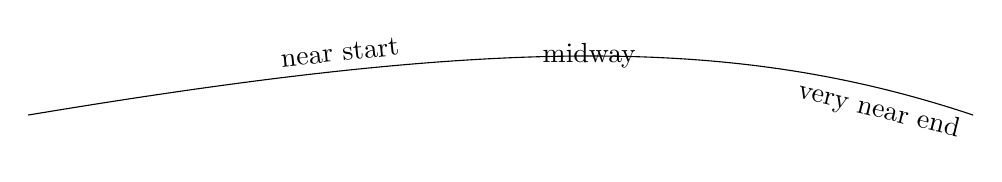
\begin{tikzpicture}
  \draw (0,0) .. controls (6,1) and (9,1) ..
    node[near start,sloped,above] {near start}
    node {midway}
    node[very near end,sloped,below] {very near end} (12,0);
\end{tikzpicture}
\end{codeexample}

It remains to draw the explanatory text at the right of the picture. The main
difficulty here lies in limiting the width of the text ``label'', which is
quite long, so that line breaking is used. Fortunately, Karl can use the option
|text width=6cm| to get the desired effect. So, here is the full code:
%
\begin{codeexample}[code only]
\begin{tikzpicture}
  [scale=3,line cap=round,
  % Styles
  axes/.style=,
  important line/.style={very thick},
  information text/.style={rounded corners,fill=red!10,inner sep=1ex}]

  % Colors
  \colorlet{anglecolor}{green!50!black}
  \colorlet{sincolor}{red}
  \colorlet{tancolor}{orange!80!black}
  \colorlet{coscolor}{blue}

  % The graphic
  \draw[help lines,step=0.5cm] (-1.4,-1.4) grid (1.4,1.4);

  \draw (0,0) circle [radius=1cm];

  \begin{scope}[axes]
    \draw[->] (-1.5,0) -- (1.5,0) node[right] {$x$} coordinate(x axis);
    \draw[->] (0,-1.5) -- (0,1.5) node[above] {$y$} coordinate(y axis);

    \foreach \x/\xtext in {-1, -.5/-\frac{1}{2}, 1}
      \draw[xshift=\x cm] (0pt,1pt) -- (0pt,-1pt) node[below,fill=white] {$\xtext$};

    \foreach \y/\ytext in {-1, -.5/-\frac{1}{2}, .5/\frac{1}{2}, 1}
      \draw[yshift=\y cm] (1pt,0pt) -- (-1pt,0pt) node[left,fill=white] {$\ytext$};
  \end{scope}

  \filldraw[fill=green!20,draw=anglecolor] (0,0) -- (3mm,0pt)
    arc [start angle=0, end angle=30, radius=3mm];
  \draw (15:2mm) node[anglecolor] {$\alpha$};

  \draw[important line,sincolor]
    (30:1cm) -- node[left=1pt,fill=white] {$\sin \alpha$} (30:1cm |- x axis);

  \draw[important line,coscolor]
    (30:1cm |- x axis) -- node[below=2pt,fill=white] {$\cos \alpha$} (0,0);

  \path [name path=upward line] (1,0) -- (1,1);
  \path [name path=sloped line] (0,0) -- (30:1.5cm);
  \draw [name intersections={of=upward line and sloped line, by=t}]
    [very thick,orange] (1,0) -- node [right=1pt,fill=white]
    {$\displaystyle \tan \alpha \color{black}=
      \frac{{\color{red}\sin \alpha}}{\color{blue}\cos \alpha}$} (t);

  \draw (0,0) -- (t);

  \draw[xshift=1.85cm]
    node[right,text width=6cm,information text]
    {
      The {\color{anglecolor} angle $\alpha$} is $30^\circ$ in the
      example ($\pi/6$ in radians). The {\color{sincolor}sine of
        $\alpha$}, which is the height of the red line, is
      \[
      {\color{sincolor} \sin \alpha} = 1/2.
      \]
      By the Theorem of Pythagoras ...
    };
\end{tikzpicture}
\end{codeexample}


\subsection{Pics: The Angle Revisited}

Karl expects that the code of certain parts of the picture he created might be
so useful that he might wish to reuse them in the future. A natural thing to do
is to create \TeX\ macros that store the code he wishes to reuse. However,
\tikzname\ offers another way that is integrated directly into its parser:
pics!

A ``pic'' is ``not quite a full picture'', hence the short name. The idea is
that a pic is simply some code that you can add to a picture at different
places using the |pic| command whose syntax is almost identical to the |node|
command. The main difference is that instead of specifying some text in curly
braces that should be shown, you specify the name of a predefined picture that
should be shown.

Defining new pics is easy enough, see Section~\ref{section-pics}, but right now
we just want to use one such predefined pic: the |angle| pic. As the name
suggests, it is a small drawing of an angle consisting of a little wedge and an
arc together with some text (Karl needs to load the |angles| library and the
|quotes| for the following examples). What makes this pic useful is the fact
that the size of the wedge will be computed automatically.

The |angle| pic draws an angle between the two lines $BA$ and $BC$, where $A$,
$B$, and $C$ are three coordinates. In our case, $B$ is the origin, $A$ is
somewhere on the $x$-axis and $C$ is somewhere on a line at $30^\circ$.
%
\begin{codeexample}[preamble={\usetikzlibrary{angles,quotes}}]
\begin{tikzpicture}[scale=3]
  \coordinate (A) at (1,0);
  \coordinate (B) at (0,0);
  \coordinate (C) at (30:1cm);

  \draw (A) -- (B) -- (C)
        pic [draw=green!50!black, fill=green!20, angle radius=9mm,
             "$\alpha$"] {angle = A--B--C};
\end{tikzpicture}
\end{codeexample}

Let us see, what is happening here. First we have specified three
\emph{coordinates} using the |\coordinate| command. It allows us to name a
specific coordinate in the picture. Then comes something that starts as a
normal |\draw|, but then comes the |pic| command. This command gets lots of
options and, in curly braces, comes the most important point: We specify that
we want to add an |angle| pic and this angle should be between the points we
named |A|, |B|, and |C| (we could use other names). Note that the text that we
want to be shown in the pic is specified in quotes inside the options of the
|pic|, not inside the curly braces.

To learn more about pics, please see Section~\ref{section-pics}.

% Copyright 2006 by Till Tantau
%
% This file may be distributed and/or modified
%
% 1. under the LaTeX Project Public License and/or
% 2. under the GNU Free Documentation License.
%
% See the file doc/generic/pgf/licenses/LICENSE for more details.


\section{Tutorial: A Petri-Net for Hagen}

In this second tutorial we explore the node mechanism of \tikzname\ and
\pgfname.

Hagen must give a talk tomorrow about his favorite formalism for distributed
systems: Petri nets! Hagen used to give his talks using a blackboard and
everyone seemed to be perfectly content with this. Unfortunately, his audience
has been spoiled recently with fancy projector-based presentations and there
seems to be a certain amount of peer pressure that his Petri nets should also
be drawn using a graphic program. One of the professors at his institute
recommends \tikzname\ for this and Hagen decides to give it a try.


\subsection{Problem Statement}

For his talk, Hagen wishes to create a graphic that demonstrates how a net with
place capacities can be simulated by a net without capacities. The graphic
should look like this, ideally:
%
\begin{quote}
\begin{tikzpicture}
  [node distance=1.3cm,>={Stealth[round]},bend angle=45,auto,
   place/.style={circle,thick,draw=blue!75,fill=blue!20,minimum size=6mm},
   red place/.style={place,draw=red!75,fill=red!20},
   transition/.style={rectangle,thick,draw=black!75,fill=black!20,minimum size=4mm},
   every label/.style={red},on grid]

  \begin{scope}
    % First net
    \node [place,tokens=1] (w1)                                    {};
    \node [place] (c1) [below=of w1]                      {};
    \node [place] (s)  [below=of c1,label=above:$s\le 3$] {};
    \node [place] (c2) [below=of s]                       {};
    \node [place,tokens=1] (w2) [below=of c2]                      {};

    \node [transition] (e1) [left=of c1] {}
      edge [pre,bend left]                  (w1)
      edge [post,bend right]                (s)
      edge [post]                           (c1);

    \node [transition] (e2) [left=of c2] {}
      edge [pre,bend right]                 (w2)
      edge [post,bend left]                 (s)
      edge [post]                           (c2);

    \node [transition] (l1) [right=of c1] {}
      edge [pre]                            (c1)
      edge [pre,bend left]                  (s)
      edge [post,bend right] node[swap] {2} (w1);

    \node [transition] (l2) [right=of c2] {}
      edge [pre]                            (c2)
      edge [pre,bend right]                 (s)
      edge [post,bend left]  node {2}       (w2);
  \end{scope}

  \begin{scope}[xshift=6cm]
    % Second net
    \node [place,tokens=1]
                      (w1')                                                {};
    \node [place]     (c1') [below=of w1']                                 {};
    \node [red place] (s1') [below=of c1',xshift=-5mm,label=left:$s$]      {};
    \node [red place,tokens=3]
                      (s2') [below=of c1',xshift=5mm,label=right:$\bar s$] {};
    \node [place]     (c2') [below=of s1',xshift=5mm]                      {};
    \node [place,tokens=1]
                      (w2') [below=of c2']                                 {};

    \node [transition] (e1') [left=of c1'] {}
      edge [pre,bend left]                  (w1')
      edge [post]                           (s1')
      edge [pre]                            (s2')
      edge [post]                           (c1');

    \node [transition] (e2') [left=of c2'] {}
      edge [pre,bend right]                 (w2')
      edge [post]                           (s1')
      edge [pre]                            (s2')
      edge [post]                           (c2');

    \node [transition] (l1') [right=of c1'] {}
      edge [pre]                            (c1')
      edge [pre]                            (s1')
      edge [post]                           (s2')
      edge [post,bend right] node[swap] {2} (w1');

    \node [transition] (l2') [right=of c2'] {}
      edge [pre]                            (c2')
      edge [pre]                            (s1')
      edge [post]                           (s2')
      edge [post,bend left]  node {2}       (w2');
  \end{scope}

  \begin{scope}[on background layer]
    \node (r1) [fill=black!10,rounded corners,fit=(w1)(w2)(e1)(e2)(l1)(l2)] {};
    \node (r2) [fill=black!10,rounded corners,fit=(w1')(w2')(e1')(e2')(l1')(l2')] {};
  \end{scope}

  \draw [shorten >=1mm,-to,thick,decorate,decoration={snake,amplitude=.4mm,segment
      length=2mm,pre=moveto,pre length=1mm,post length=2mm}]
    (r1) -- (r2)
    node [above=1mm,midway,text width=3cm,align=center]
      {replacement of the \textcolor{red}{capacity} by \textcolor{red}{two places}};

\end{tikzpicture}
\end{quote}


\subsection{Setting up the Environment}

For the picture Hagen will need to load the \tikzname\ package as did Karl in
the previous tutorial. However, Hagen will also need to load some additional
\emph{library packages} that Karl did not need. These library packages contain
additional definitions like extra arrow tips that are typically not needed in a
picture and that need to be loaded explicitly.

Hagen will need to load several libraries: The |arrows| library for the special
arrow tip used in the graphic, the |decorations.pathmorphing| library for the
``snaking line'' in the middle, the |backgrounds| library for the two
rectangular areas that are behind the two main parts of the picture, the |fit|
library to easily compute the sizes of these rectangles, and the |positioning|
library for placing nodes relative to other nodes.


\subsubsection{Setting up the Environment in \LaTeX}

When using \LaTeX\ use:
%
\begin{codeexample}[code only]
\documentclass{article} % say

\usepackage{tikz}
\usetikzlibrary{arrows,decorations.pathmorphing,backgrounds,positioning,fit,petri}

\begin{document}
\begin{tikzpicture}
  \draw (0,0) -- (1,1);
\end{tikzpicture}
\end{document}
\end{codeexample}


\subsubsection{Setting up the Environment in Plain \TeX}

When using plain \TeX\ use:
%
\begin{codeexample}[code only]
%% Plain TeX file
\input tikz.tex
\usetikzlibrary{arrows,decorations.pathmorphing,backgrounds,positioning,fit,petri}
\baselineskip=12pt
\hsize=6.3truein
\vsize=8.7truein
\tikzpicture
  \draw (0,0) -- (1,1);
\endtikzpicture
\bye
\end{codeexample}


\subsubsection{Setting up the Environment in Con\TeX t}

When using Con\TeX t, use:
%
\begin{codeexample}[code only]
%% ConTeXt file
\usemodule[tikz]
\usetikzlibrary[arrows,decorations.pathmorphing,backgrounds,positioning,fit,petri]

\starttext
  \starttikzpicture
    \draw (0,0) -- (1,1);
  \stoptikzpicture
\stoptext
\end{codeexample}


\subsection{Introduction to Nodes}

In principle, we already know how to create the graphics that Hagen desires
(except perhaps for the snaked line, we will come to that): We start with big
light gray rectangle and then add lots of circles and small rectangle, plus
some arrows.

However, this approach has numerous disadvantages: First, it is hard to change
anything at a later stage. For example, if we decide to add more places to the
Petri nets (the circles are called places in Petri net theory), all of the
coordinates change and we need to recalculate everything. Second, it is hard to
read the code for the Petri net as it is just a long and complicated list of
coordinates and drawing commands -- the underlying structure of the Petri net
is lost.

Fortunately, \tikzname\ offers a powerful mechanism for avoiding the above
problems: nodes. We already came across nodes in the previous tutorial, where
we used them to add labels to Karl's graphic. In the present tutorial we will
see that nodes are much more powerful.

A node is a small part of a picture. When a node is created, you provide a
position where the node should be drawn and a \emph{shape}. A node of shape
|circle| will be drawn as a circle, a node of shape |rectangle| as a rectangle,
and so on. A node may also contain some text, which is why Karl used nodes to
show text. Finally, a node can get a \emph{name} for later reference.

In Hagen's picture we will use nodes for the places and for the transitions of
the Petri net (the places are the circles, the transitions are the rectangles).
Let us start with the upper half of the left Petri net. In this upper half we
have three places and two transitions. Instead of drawing three circles and two
rectangles, we use three nodes of shape |circle| and two nodes of shape
|rectangle|.
%
\begin{codeexample}[]
\begin{tikzpicture}
  \path ( 0,2) node [shape=circle,draw] {}
        ( 0,1) node [shape=circle,draw] {}
        ( 0,0) node [shape=circle,draw] {}
        ( 1,1) node [shape=rectangle,draw] {}
        (-1,1) node [shape=rectangle,draw] {};
\end{tikzpicture}
\end{codeexample}

Hagen notes that this does not quite look like the final picture, but it seems
like a good first step.

Let us have a more detailed look at the code. The whole picture consists of a
single path. Ignoring the |node| operations, there is not much going on in this
path: It is just a sequence of coordinates with nothing ``happening'' between
them. Indeed, even if something were to happen like a line-to or a curve-to,
the |\path| command would not ``do'' anything with the resulting path. So, all
the magic must be in the |node| commands.

In the previous tutorial we learned that a |node| will add a piece of text at
the last coordinate. Thus, each of the five nodes is added at a different
position. In the above code, this text is empty (because of the empty |{}|).
So, why do we see anything at all? The answer is the |draw| option for the
|node| operation: It causes the ``shape around the text'' to be drawn.

So, the code |(0,2) node [shape=circle,draw] {}| means the following: ``In the
main path, add a move-to to the coordinate |(0,2)|. Then, temporarily suspend
the construction of the main path while the node is built. This node will be a
|circle| around an empty text. This circle is to be |draw|n, but not filled or
otherwise used. Once this whole node is constructed, it is saved until after
the main path is finished. Then, it is drawn.'' The following
|(0,1) node [shape=circle,draw] {}| then has the following effect: ``Continue
the main path with a move-to to |(0,1)|. Then construct a node at this position
also. This node is also shown after the main path is finished.'' And so on.


\subsection{Placing Nodes Using the At Syntax}

Hagen now understands how the |node| operation adds nodes to the path, but it
seems a bit silly to create a path using the |\path| operation, consisting of
numerous superfluous move-to operations, only to place nodes. He is pleased to
learn that there are ways to add nodes in a more sensible manner.

First, the |node| operation allows one to add |at (|\meta{coordinate}|)| in
order to directly specify where the node should be placed, sidestepping the
rule that nodes are placed on the last coordinate. Hagen can then write the
following:
%
\begin{codeexample}[]
\begin{tikzpicture}
  \path node at ( 0,2) [shape=circle,draw] {}
        node at ( 0,1) [shape=circle,draw] {}
        node at ( 0,0) [shape=circle,draw] {}
        node at ( 1,1) [shape=rectangle,draw] {}
        node at (-1,1) [shape=rectangle,draw] {};
\end{tikzpicture}
\end{codeexample}

Now Hagen is still left with a single empty path, but at least the path no
longer contains strange move-to's. It turns out that this can be improved
further: The |\node| command is an abbreviation for |\path node|, which allows
Hagen to write:
%
\begin{codeexample}[]
\begin{tikzpicture}
  \node at ( 0,2) [circle,draw] {};
  \node at ( 0,1) [circle,draw] {};
  \node at ( 0,0) [circle,draw] {};
  \node at ( 1,1) [rectangle,draw] {};
  \node at (-1,1) [rectangle,draw] {};
\end{tikzpicture}
\end{codeexample}

Hagen likes this syntax much better than the previous one. Note that Hagen has
also omitted the |shape=| since, like |color=|, \tikzname\ allows you to omit
the |shape=| if there is no confusion.


\subsection{Using Styles}

Feeling adventurous, Hagen tries to make the nodes look nicer. In the final
picture, the circles and rectangle should be filled with different colors,
resulting in the following code:
%
\begin{codeexample}[]
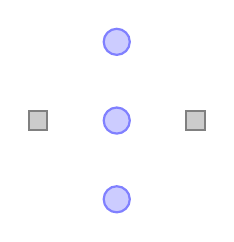
\begin{tikzpicture}[thick]
  \node at ( 0,2) [circle,draw=blue!50,fill=blue!20] {};
  \node at ( 0,1) [circle,draw=blue!50,fill=blue!20] {};
  \node at ( 0,0) [circle,draw=blue!50,fill=blue!20] {};
  \node at ( 1,1) [rectangle,draw=black!50,fill=black!20] {};
  \node at (-1,1) [rectangle,draw=black!50,fill=black!20] {};
\end{tikzpicture}
\end{codeexample}

While this looks nicer in the picture, the code starts to get a bit ugly.
Ideally, we would like our code to transport the message ``there are three
places and two transitions'' and not so much which filling colors should be
used.

To solve this problem, Hagen uses styles. He defines a style for places and
another style for transitions:
%
\begin{codeexample}[]
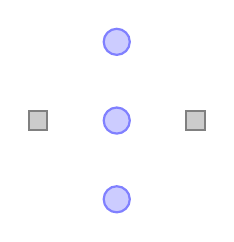
\begin{tikzpicture}
  [place/.style={circle,draw=blue!50,fill=blue!20,thick},
   transition/.style={rectangle,draw=black!50,fill=black!20,thick}]
  \node at ( 0,2) [place] {};
  \node at ( 0,1) [place] {};
  \node at ( 0,0) [place] {};
  \node at ( 1,1) [transition] {};
  \node at (-1,1) [transition] {};
\end{tikzpicture}
\end{codeexample}


\subsection{Node Size}

Before Hagen starts naming and connecting the nodes, let us first make sure
that the nodes get their final appearance. They are still too small. Indeed,
Hagen wonders why they have any size at all, after all, the text is empty. The
reason is that \tikzname\ automatically adds some space around the text. The
amount is set using the option |inner sep|. So, to increase the size of the
nodes, Hagen could write:
%
\begin{codeexample}[]
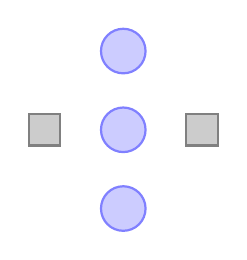
\begin{tikzpicture}
  [inner sep=2mm,
   place/.style={circle,draw=blue!50,fill=blue!20,thick},
   transition/.style={rectangle,draw=black!50,fill=black!20,thick}]
  \node at ( 0,2) [place] {};
  \node at ( 0,1) [place] {};
  \node at ( 0,0) [place] {};
  \node at ( 1,1) [transition] {};
  \node at (-1,1) [transition] {};
\end{tikzpicture}
\end{codeexample}

However, this is not really the best way to achieve the desired effect. It is
much better to use the |minimum size| option instead. This option allows Hagen
to specify a minimum size that the node should have. If the node actually needs
to be bigger because of a longer text, it will be larger, but if the text is
empty, then the node will have |minimum size|. This option is also useful to
ensure that several nodes containing different amounts of text have the same
size. The options |minimum height| and |minimum width| allow you to specify the
minimum height and width independently.

So, what Hagen needs to do is to provide |minimum size| for the nodes. To be on
the safe side, he also sets |inner sep=0pt|. This ensures that the nodes will
really have size |minimum size| and not, for very small minimum sizes, the
minimal size necessary to encompass the automatically added space.
%
\begin{codeexample}[]
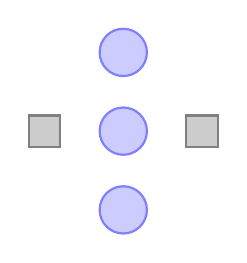
\begin{tikzpicture}
  [place/.style={circle,draw=blue!50,fill=blue!20,thick,
                 inner sep=0pt,minimum size=6mm},
   transition/.style={rectangle,draw=black!50,fill=black!20,thick,
                      inner sep=0pt,minimum size=4mm}]
  \node at ( 0,2) [place] {};
  \node at ( 0,1) [place] {};
  \node at ( 0,0) [place] {};
  \node at ( 1,1) [transition] {};
  \node at (-1,1) [transition] {};
\end{tikzpicture}
\end{codeexample}


\subsection{Naming Nodes}

Hagen's next aim is to connect the nodes using arrows. This seems like a tricky
business since the arrows should not start in the middle of the nodes, but
somewhere on the border and Hagen would very much like to avoid computing these
positions by hand.

Fortunately, \pgfname\ will perform all the necessary calculations for him.
However, he first has to assign names to the nodes so that he can reference
them later on.

There are two ways to name a node. The first is to use the |name=| option. The
second method is to write the desired name in parentheses after the |node|
operation. Hagen thinks that this second method seems strange, but he will soon
change his opinion.
%
\begin{codeexample}[setup code,hidden]
\tikzset{
    place/.style={circle,draw=blue!50,fill=blue!20,thick,
                  inner sep=0pt,minimum size=6mm},
    transition/.style={rectangle,draw=black!50,fill=black!20,thick,
                       inner sep=0pt,minimum size=4mm}
}
\end{codeexample}
%
\begin{codeexample}[]
% ... set up styles
\begin{tikzpicture}
  \node (waiting 1)      at ( 0,2) [place] {};
  \node (critical 1)     at ( 0,1) [place] {};
  \node (semaphore)      at ( 0,0) [place] {};
  \node (leave critical) at ( 1,1) [transition] {};
  \node (enter critical) at (-1,1) [transition] {};
\end{tikzpicture}
\end{codeexample}

Hagen is pleased to note that the names help in understanding the code. Names
for nodes can be pretty arbitrary, but they should not contain commas, periods,
parentheses, colons, and some other special characters. However, they can
contain underscores and hyphens.

The syntax for the |node| operation is quite liberal with respect to the order
in which node names, the |at| specifier, and the options must come. Indeed, you
can even have multiple option blocks between the |node| and the text in curly
braces, they accumulate. You can rearrange them arbitrarily and perhaps the
following might be preferable:
%
\begin{codeexample}[]
\begin{tikzpicture}
  \node[place]      (waiting 1)      at ( 0,2) {};
  \node[place]      (critical 1)     at ( 0,1) {};
  \node[place]      (semaphore)      at ( 0,0) {};
  \node[transition] (leave critical) at ( 1,1) {};
  \node[transition] (enter critical) at (-1,1) {};
\end{tikzpicture}
\end{codeexample}


\subsection{Placing Nodes Using Relative Placement}

Although Hagen still wishes to connect the nodes, he first wishes to address
another problem again: The placement of the nodes. Although he likes the |at|
syntax, in this particular case he would prefer placing the nodes ``relative to
each other''. So, Hagen would like to say that the |critical 1| node should be
below the |waiting 1| node, wherever the |waiting 1| node might be. There are
different ways of achieving this, but the nicest one in Hagen's case is the
|below| option:
%
\begin{codeexample}[preamble={\usetikzlibrary{positioning}}]
\begin{tikzpicture}
  \node[place]      (waiting)                            {};
  \node[place]      (critical)       [below=of waiting]  {};
  \node[place]      (semaphore)      [below=of critical] {};
  \node[transition] (leave critical) [right=of critical] {};
  \node[transition] (enter critical) [left=of critical]  {};
\end{tikzpicture}
\end{codeexample}

With the |positioning| library loaded, when an option like |below| is followed
by |of|, then the position of the node is shifted in such a manner that it is
placed at the distance |node distance| in the specified direction of the given
direction. The |node distance| is either the distance between the centers of
the nodes (when the |on grid| option is set to true) or the distance between
the borders (when the |on grid| option is set to false, which is the default).

Even though the above code has the same effect as the earlier code, Hagen can
pass it to his colleagues who will be able to just read and understand it,
perhaps without even having to see the picture.


\subsection{Adding Labels Next to Nodes}

Before we have a look at how Hagen can connect the nodes, let us add the
capacity ``$s \le 3$'' to the bottom node. For this, two approaches are
possible:
%
\begin{enumerate}
    \item Hagen can just add a new node above the |north| anchor of the
        |semaphore| node.
        %
\begin{codeexample}[preamble={\usetikzlibrary{positioning}}]
\begin{tikzpicture}
  \node[place]      (waiting)                            {};
  \node[place]      (critical)       [below=of waiting]  {};
  \node[place]      (semaphore)      [below=of critical] {};
  \node[transition] (leave critical) [right=of critical] {};
  \node[transition] (enter critical) [left=of critical]  {};

  \node [red,above] at (semaphore.north) {$s\le 3$};
\end{tikzpicture}
\end{codeexample}
        %
        This is a general approach that will ``always work''.

    \item Hagen can use the special |label| option. This option is given to a
        |node| and it causes \emph{another} node to be added next to the node
        where the option is given. Here is the idea: When we construct the
        |semaphore| node, we wish to indicate that we want another node with
        the capacity above it. For this, we use the option
        |label=above:$s\le 3$|. This option is interpreted as follows: We want
        a node above the |semaphore| node and this node should read ``$s \le
        3$''. Instead of |above| we could also use things like |below left|
        before the colon or a number like |60|.
        %
\begin{codeexample}[preamble={\usetikzlibrary{positioning}}]
\begin{tikzpicture}
  \node[place]      (waiting)                            {};
  \node[place]      (critical)       [below=of waiting]  {};
  \node[place]      (semaphore)      [below=of critical,
                                      label=above:$s\le3$] {};
  \node[transition] (leave critical) [right=of critical] {};
  \node[transition] (enter critical) [left=of critical]  {};
\end{tikzpicture}
\end{codeexample}
        %
        It is also possible to give multiple |label| options, this causes
        multiple labels to be drawn.
        %
\begin{codeexample}[]
\tikz
  \node [circle,draw,label=60:$60^\circ$,label=below:$-90^\circ$] {my circle};
\end{codeexample}
        %
        Hagen is not fully satisfied with the |label| option since the label
        is not red. To achieve this, he has two options: First, he can
        redefine the |every label| style. Second, he can add options to the
        label's node. These options are given following the |label=|, so he
        would write |label=[red]above:$s\le3$|. However, this does not quite
        work since \TeX\ thinks that the |]| closes the whole option list of
        the |semaphore| node. So, Hagen has to add braces and writes
        |label={[red]above:$s\le3$}|. Since this looks a bit ugly, Hagen
        decides to redefine the |every label| style.
        %
\begin{codeexample}[preamble={\usetikzlibrary{positioning}}]
\begin{tikzpicture}[every label/.style={red}]
  \node[place]      (waiting)                            {};
  \node[place]      (critical)       [below=of waiting]  {};
  \node[place]      (semaphore)      [below=of critical,
                                      label=above:$s\le3$] {};
  \node[transition] (leave critical) [right=of critical] {};
  \node[transition] (enter critical) [left=of critical]  {};
\end{tikzpicture}
\end{codeexample}
\end{enumerate}


\subsection{Connecting Nodes}

It is now high time to connect the nodes. Let us start with something simple,
namely with the straight line from |enter critical| to |critical|. We want this
line to start at the right side of |enter critical| and to end at the left side
of |critical|. For this, we can use the \emph{anchors} of the nodes. Every node
defines a whole bunch of anchors that lie on its border or inside it. For
example, the |center| anchor is at the center of the node, the |west| anchor is
on the left of the node, and so on. To access the coordinate of a node, we use
a coordinate that contains the node's name followed by a dot, followed by the
anchor's name:
%
\begin{codeexample}[preamble={\usetikzlibrary{positioning}}]
\begin{tikzpicture}
  \node[place]      (waiting)                            {};
  \node[place]      (critical)       [below=of waiting]  {};
  \node[place]      (semaphore)      [below=of critical] {};
  \node[transition] (leave critical) [right=of critical] {};
  \node[transition] (enter critical) [left=of critical]  {};
  \draw [->] (critical.west) -- (enter critical.east);
\end{tikzpicture}
\end{codeexample}

Next, let us tackle the curve from |waiting| to |enter critical|. This can be
specified using curves and controls:
%
\begin{codeexample}[preamble={\usetikzlibrary{positioning}}]
\begin{tikzpicture}
  \node[place]      (waiting)                            {};
  \node[place]      (critical)       [below=of waiting]  {};
  \node[place]      (semaphore)      [below=of critical] {};
  \node[transition] (leave critical) [right=of critical] {};
  \node[transition] (enter critical) [left=of critical]  {};
  \draw [->] (enter critical.east) -- (critical.west);
  \draw [->] (waiting.west) .. controls +(left:5mm) and +(up:5mm)
                            .. (enter critical.north);
\end{tikzpicture}
\end{codeexample}

Hagen sees how he can now add all his edges, but the whole process seems a but
awkward and not very flexible. Again, the code seems to obscure the structure
of the graphic rather than showing it.

So, let us start improving the code for the edges. First, Hagen can leave out
the anchors:
%
\begin{codeexample}[preamble={\usetikzlibrary{positioning}}]
\begin{tikzpicture}
  \node[place]      (waiting)                            {};
  \node[place]      (critical)       [below=of waiting]  {};
  \node[place]      (semaphore)      [below=of critical] {};
  \node[transition] (leave critical) [right=of critical] {};
  \node[transition] (enter critical) [left=of critical]  {};
  \draw [->] (enter critical) -- (critical);
  \draw [->] (waiting) .. controls +(left:8mm) and +(up:8mm)
                       .. (enter critical);
\end{tikzpicture}
\end{codeexample}

Hagen is a bit surprised that this works. After all, how did \tikzname\ know
that the line from |enter critical| to |critical| should actually start on the
borders? Whenever \tikzname\ encounters a whole node name as a ``coordinate'',
it tries to ``be smart'' about the anchor that it should choose for this node.
Depending on what happens next, \tikzname\ will choose an anchor that lies on
the border of the node on a line to the next coordinate or control point. The
exact rules are a bit complex, but the chosen point will usually be correct --
and when it is not, Hagen can still specify the desired anchor by hand.

Hagen would now like to simplify the curve operation somehow. It turns out that
this can be accomplished using a special path operation: the |to| operation.
This operation takes many options (you can even define new ones yourself). One
pair of options is useful for Hagen: The pair |in| and |out|. These options
take angles at which a curve should leave or reach the start or target
coordinates. Without these options, a straight line is drawn:
%
\begin{codeexample}[preamble={\usetikzlibrary{positioning}}]
\begin{tikzpicture}
  \node[place]      (waiting)                            {};
  \node[place]      (critical)       [below=of waiting]  {};
  \node[place]      (semaphore)      [below=of critical] {};
  \node[transition] (leave critical) [right=of critical] {};
  \node[transition] (enter critical) [left=of critical]  {};
  \draw [->] (enter critical) to                 (critical);
  \draw [->] (waiting)        to [out=180,in=90] (enter critical);
\end{tikzpicture}
\end{codeexample}

There is another option for the |to| operation, that is even better suited to
Hagen's problem: The |bend right| option. This option also takes an angle, but
this angle only specifies the angle by which the curve is bent to the right:
%
\begin{codeexample}[preamble={\usetikzlibrary{positioning}}]
\begin{tikzpicture}
  \node[place]      (waiting)                            {};
  \node[place]      (critical)       [below=of waiting]  {};
  \node[place]      (semaphore)      [below=of critical] {};
  \node[transition] (leave critical) [right=of critical] {};
  \node[transition] (enter critical) [left=of critical]  {};
  \draw [->] (enter critical) to                 (critical);
  \draw [->] (waiting)        to [bend right=45] (enter critical);
  \draw [->] (enter critical) to [bend right=45] (semaphore);
\end{tikzpicture}
\end{codeexample}

It is now time for Hagen to learn about yet another way of specifying edges:
Using the |edge| path operation. This operation is very similar to the |to|
operation, but there is one important difference: Like a node the edge
generated by the |edge| operation is not part of the main path, but is added
only later. This may not seem very important, but it has some nice
consequences. For example, every edge can have its own arrow tips and its own
color and so on and, still, all the edges can be given on the same path. This
allows Hagen to write the following:
%
\begin{codeexample}[preamble={\usetikzlibrary{positioning}}]
\begin{tikzpicture}
  \node[place]      (waiting)                            {};
  \node[place]      (critical)       [below=of waiting]  {};
  \node[place]      (semaphore)      [below=of critical] {};
  \node[transition] (leave critical) [right=of critical] {};
  \node[transition] (enter critical) [left=of critical]  {}
    edge [->]               (critical)
    edge [<-,bend left=45]  (waiting)
    edge [->,bend right=45] (semaphore);
\end{tikzpicture}
\end{codeexample}

Each |edge| caused a new path to be constructed, consisting of a |to| between
the node |enter critical| and the node following the |edge| command.

The finishing touch is to introduce two styles |pre| and |post| and to use the
|bend angle=45| option to set the bend angle once and for all:
%
\begin{codeexample}[preamble={\usetikzlibrary{arrows.meta,positioning}}]
% Styles place and transition as before
\begin{tikzpicture}
  [bend angle=45,
   pre/.style={<-,shorten <=1pt,>={Stealth[round]},semithick},
   post/.style={->,shorten >=1pt,>={Stealth[round]},semithick}]

  \node[place]      (waiting)                            {};
  \node[place]      (critical)       [below=of waiting]  {};
  \node[place]      (semaphore)      [below=of critical] {};

  \node[transition] (leave critical) [right=of critical] {}
    edge [pre]             (critical)
    edge [post,bend right] (waiting)
    edge [pre, bend left]  (semaphore);
  \node[transition] (enter critical) [left=of critical]  {}
    edge [post]            (critical)
    edge [pre, bend left]  (waiting)
    edge [post,bend right] (semaphore);
\end{tikzpicture}
\end{codeexample}


\subsection{Adding Labels Next to Lines}

The next thing that Hagen needs to add is the ``$2$'' at the arcs. For this
Hagen can use \tikzname's automatic node placement: By adding the option
|auto|, \tikzname\ will position nodes on curves and lines in such a way that
they are not on the curve but next to it. Adding |swap| will mirror the label
with respect to the line. Here is a general example:
%
% TODOsp: codeexamples: styles not needed here
\begin{codeexample}[]
\begin{tikzpicture}[auto,bend right]
  \node (a) at (0:1) {$0^\circ$};
  \node (b) at (120:1) {$120^\circ$};
  \node (c) at (240:1) {$240^\circ$};

  \draw (a) to node {1} node [swap] {1'} (b)
        (b) to node {2} node [swap] {2'} (c)
        (c) to node {3} node [swap] {3'} (a);
\end{tikzpicture}
\end{codeexample}

What is happening here? The nodes are given somehow inside the |to| operation!
When this is done, the node is placed on the middle of the curve or line
created by the |to| operation. The |auto| option then causes the node to be
moved in such a way that it does not lie on the curve, but next to it. In the
example we provide even two nodes on each |to| operation.

For Hagen that |auto| option is not really necessary since the two ``2'' labels
could also easily be placed ``by hand''. However, in a complicated plot with
numerous edges automatic placement can be a blessing.
%
\begin{codeexample}[
    preamble={\usetikzlibrary{arrows.meta,positioning}},
    pre={\tikzset{
    pre/.style={<-,shorten <=1pt,>={Stealth[round]},semithick},
    post/.style={->,shorten >=1pt,>={Stealth[round]},semithick},
}},
]
% Styles as before
\begin{tikzpicture}[bend angle=45]
  \node[place]      (waiting)                            {};
  \node[place]      (critical)       [below=of waiting]  {};
  \node[place]      (semaphore)      [below=of critical] {};

  \node[transition] (leave critical) [right=of critical] {}
    edge [pre]                                 (critical)
    edge [post,bend right] node[auto,swap] {2} (waiting)
    edge [pre, bend left]                      (semaphore);
  \node[transition] (enter critical) [left=of critical]  {}
    edge [post]                                (critical)
    edge [pre, bend left]                      (waiting)
    edge [post,bend right]                     (semaphore);
\end{tikzpicture}
\end{codeexample}
% TODOsp: codeexamples: styles and `positioning` are needed up to here


\subsection{Adding the Snaked Line and Multi-Line Text}

With the node mechanism Hagen can now easily create the two Petri nets. What he
is unsure of is how he can create the snaked line between the nets.

For this he can use a \emph{decoration}. To draw the snaked line, Hagen only
needs to set the two options |decoration=snake| and |decorate| on the path.
This causes all lines of the path to be replaced by snakes. It is also possible
to use snakes only in certain parts of a path, but Hagen will not need this.
%
\begin{codeexample}[preamble={\usetikzlibrary{decorations.pathmorphing}}]
\begin{tikzpicture}
  \draw [->,decorate,decoration=snake] (0,0) -- (2,0);
\end{tikzpicture}
\end{codeexample}

Well, that does not look quite right, yet. The problem is that the snake
happens to end exactly at the position where the arrow begins. Fortunately,
there is an option that helps here. Also, the snake should be a bit smaller,
which can be influenced by even more options.
%
\begin{codeexample}[preamble={\usetikzlibrary{decorations.pathmorphing}}]
\begin{tikzpicture}
  \draw [->,decorate,
     decoration={snake,amplitude=.4mm,segment length=2mm,post length=1mm}]
    (0,0) -- (3,0);
\end{tikzpicture}
\end{codeexample}

Now Hagen needs to add the text above the snake. This text is a bit challenging
since it is a multi-line text. Hagen has two options for this: First, he can
specify an |align=center| and then use the |\\| command to enforce the line
breaks at the desired positions.
%
\begin{codeexample}[preamble={\usetikzlibrary{decorations.pathmorphing}}]
\begin{tikzpicture}
  \draw [->,decorate,
      decoration={snake,amplitude=.4mm,segment length=2mm,post length=1mm}]
    (0,0) -- (3,0)
    node [above,align=center,midway]
    {
      replacement of\\
      the \textcolor{red}{capacity}\\
      by \textcolor{red}{two places}
    };
\end{tikzpicture}
\end{codeexample}

Instead of specifying the line breaks ``by hand'', Hagen can also specify a
width for the text and let \TeX\ perform the line breaking for him:
%
\begin{codeexample}[preamble={\usetikzlibrary{decorations.pathmorphing}}]
\begin{tikzpicture}
  \draw [->,decorate,
      decoration={snake,amplitude=.4mm,segment length=2mm,post length=1mm}]
    (0,0) -- (3,0)
    node [above,text width=3cm,align=center,midway]
    {
      replacement of the \textcolor{red}{capacity} by
      \textcolor{red}{two places}
    };
\end{tikzpicture}
\end{codeexample}


\subsection{Using Layers: The Background Rectangles}

Hagen still needs to add the background rectangles. These are a bit tricky:
Hagen would like to draw the rectangles \emph{after} the Petri nets are
finished. The reason is that only then can he conveniently refer to the
coordinates that make up the corners of the rectangle. If Hagen draws the
rectangle first, then he needs to know the exact size of the Petri net -- which
he does not.

The solution is to use \emph{layers}. When the |backgrounds| library is loaded,
Hagen can put parts of his picture inside a scope with the
|on background layer| option. Then this part of the picture becomes part of the
layer that is given as an argument to this environment. When the
|{tikzpicture}| environment ends, the layers are put on top of each other,
starting with the background layer. This causes everything drawn on the
background layer to be behind the main text.

The next tricky question is, how big should the rectangle be? Naturally, Hagen
can compute the size ``by hand'' or using some clever observations concerning
the $x$- and $y$-coordinates of the nodes, but it would be nicer to just have
\tikzname\ compute a rectangle into which all the nodes ``fit''. For this, the
|fit| library can be used. It defines the |fit| options, which, when given to a
node, causes the node to be resized and shifted such that it exactly covers all
the nodes and coordinates given as parameters to the |fit| option.
%
% TODOsp: codeexamples: redo/add styles starting from here
\begin{codeexample}[
    preamble={\usetikzlibrary{arrows.meta,backgrounds,fit,positioning}},
    pre={\tikzset{
    pre/.style={<-,shorten <=1pt,>={Stealth[round]},semithick},
    post/.style={->,shorten >=1pt,>={Stealth[round]},semithick},
}},
]
% Styles as before
\begin{tikzpicture}[bend angle=45]
  \node[place]      (waiting)                            {};
  \node[place]      (critical)       [below=of waiting]  {};
  \node[place]      (semaphore)      [below=of critical] {};

  \node[transition] (leave critical) [right=of critical] {}
    edge [pre]                                 (critical)
    edge [post,bend right] node[auto,swap] {2} (waiting)
    edge [pre, bend left]                      (semaphore);
  \node[transition] (enter critical) [left=of critical]  {}
    edge [post]                                (critical)
    edge [pre, bend left]                      (waiting)
    edge [post,bend right]                     (semaphore);

  \begin{scope}[on background layer]
    \node [fill=black!30,fit=(waiting) (critical) (semaphore)
             (leave critical) (enter critical)] {};
  \end{scope}
\end{tikzpicture}
\end{codeexample}


\subsection{The Complete Code}

Hagen has now finally put everything together. Only then does he learn that
there is already a library for drawing Petri nets! It turns out that this
library mainly provides the same definitions as Hagen did. For example, it
defines a |place| style in a similar way as Hagen did. Adjusting the code so
that it uses the library shortens Hagen code a bit, as shown in the following.

First, Hagen needs less style definitions, but he still needs to specify the
colors of places and transitions.
%
\begin{codeexample}[code only]
\begin{tikzpicture}
  [node distance=1.3cm,on grid,>={Stealth[round]},bend angle=45,auto,
   every place/.style=     {minimum size=6mm,thick,draw=blue!75,fill=blue!20},
   every transition/.style={thick,draw=black!75,fill=black!20},
   red place/.style=       {place,draw=red!75,fill=red!20},
   every label/.style=     {red}]
\end{codeexample}

Now comes the code for the nets:
%
\ifpgfmanualexternalize\tikzexternaldisable\fi
\begin{codeexample}[
    preamble={\usetikzlibrary{arrows.meta,petri,positioning}},
    pre={\tikzset{
    every place/.style={minimum size=6mm,thick,draw=blue!75,fill=blue!20},
    every transition/.style={thick,draw=black!75,fill=black!20},
    every label/.style={red},
    every picture/.style={on grid,node distance=1.3cm,>={Stealth[round]},bend angle=45,auto},
}%
\begin{tikzpicture}},
    post={\end{tikzpicture}},
]
   \node [place,tokens=1] (w1)                                    {};
   \node [place]          (c1) [below=of w1]                      {};
   \node [place]          (s)  [below=of c1,label=above:$s\le 3$] {};
   \node [place]          (c2) [below=of s]                       {};
   \node [place,tokens=1] (w2) [below=of c2]                      {};

   \node [transition] (e1) [left=of c1] {}
     edge [pre,bend left]                  (w1)
     edge [post,bend right]                (s)
     edge [post]                           (c1);
   \node [transition] (e2) [left=of c2] {}
     edge [pre,bend right]                 (w2)
     edge [post,bend left]                 (s)
     edge [post]                           (c2);
   \node [transition] (l1) [right=of c1] {}
     edge [pre]                            (c1)
     edge [pre,bend left]                  (s)
     edge [post,bend right] node[swap] {2} (w1);
   \node [transition] (l2) [right=of c2] {}
     edge [pre]                            (c2)
     edge [pre,bend right]                 (s)
     edge [post,bend left]  node {2}       (w2);
\end{codeexample}

\ifpgfmanualexternalize\tikzexternaldisable\fi
\begin{codeexample}[
    preamble={\usetikzlibrary{arrows.meta,petri,positioning}},
    pre={\tikzset{
    every place/.style={minimum size=6mm,thick,draw=blue!75,fill=blue!20},
    every transition/.style={thick,draw=black!75,fill=black!20},
    red place/.style=  {place,draw=red!75,fill=red!20},
    every label/.style={red},
    every picture/.style={on grid,node distance=1.3cm,>={Stealth[round]},bend angle=45,auto},
}%
\begin{tikzpicture}},
    post={\end{tikzpicture}},
]
  \begin{scope}[xshift=6cm]
    \node [place,tokens=1]     (w1')                            {};
    \node [place]              (c1') [below=of w1']             {};
    \node [red place]          (s1') [below=of c1',xshift=-5mm]
            [label=left:$s$]                                    {};
    \node [red place,tokens=3] (s2') [below=of c1',xshift=5mm]
            [label=right:$\bar s$]                              {};
    \node [place]              (c2') [below=of s1',xshift=5mm]  {};
    \node [place,tokens=1]     (w2') [below=of c2']             {};

    \node [transition] (e1') [left=of c1'] {}
      edge [pre,bend left]                  (w1')
      edge [post]                           (s1')
      edge [pre]                            (s2')
      edge [post]                           (c1');
    \node [transition] (e2') [left=of c2'] {}
      edge [pre,bend right]                 (w2')
      edge [post]                           (s1')
      edge [pre]                            (s2')
      edge [post]                           (c2');
    \node [transition] (l1') [right=of c1'] {}
      edge [pre]                            (c1')
      edge [pre]                            (s1')
      edge [post]                           (s2')
      edge [post,bend right] node[swap] {2} (w1');
    \node [transition] (l2') [right=of c2'] {}
      edge [pre]                            (c2')
      edge [pre]                            (s1')
      edge [post]                           (s2')
      edge [post,bend left]  node {2}       (w2');
  \end{scope}
\end{codeexample}

The code for the background and the snake is the following:
%
\begin{codeexample}[code only]
  \begin{scope}[on background layer]
    \node (r1) [fill=black!10,rounded corners,fit=(w1)(w2)(e1)(e2)(l1)(l2)] {};
    \node (r2) [fill=black!10,rounded corners,fit=(w1')(w2')(e1')(e2')(l1')(l2')] {};
  \end{scope}

  \draw [shorten >=1mm,-to,thick,decorate,
         decoration={snake,amplitude=.4mm,segment length=2mm,
                     pre=moveto,pre length=1mm,post length=2mm}]
    (r1) -- (r2) node [above=1mm,midway,text width=3cm,align=center]
      {replacement of the \textcolor{red}{capacity} by \textcolor{red}{two places}};
\end{tikzpicture}
\end{codeexample}

% -----------------------------------------------------------------------------
% TODOsp: codeexamples: This is needed because -- unlike I thought --
%         `setup code is remembered also outside this file. Thus the changed
%         style of `place` and `transition` are "remembered" in
%         <pgfmanual-en-library-petri.tex>
\begin{codeexample}[setup code,hidden]
% from <tikzlibrarypetri.code.tex>
\tikzset{
    place/.style={circle,draw,inner sep=0pt,minimum size=5ex,every place},
    transition/.style={rectangle,draw,inner sep=0pt,minimum size=4mm,every transition},
}
\end{codeexample}
% -----------------------------------------------------------------------------

% Copyright 2006 by Till Tantau
%
% This file may be distributed and/or modified
%
% 1. under the LaTeX Project Public License and/or
% 2. under the GNU Free Documentation License.
%
% See the file doc/generic/pgf/licenses/LICENSE for more details.


\section{Tutorial: Euclid's Amber Version of the \emph{Elements}}

In this third tutorial we have a look at how \tikzname\ can be used to draw
geometric constructions.

Euclid is currently quite busy writing his new book series, whose working title
is ``Elements'' (Euclid is not quite sure whether this title will convey the
message of the series to future generations correctly, but he intends to change
the title before it goes to the publisher). Up to know, he wrote down his text
and graphics on papyrus, but his publisher suddenly insists that he must submit
in electronic form. Euclid tries to argue with the publisher that electronics
will only be discovered thousands of years later, but the publisher informs him
that the use of papyrus is no longer cutting edge technology and Euclid will
just have to keep up with modern tools.

Slightly disgruntled, Euclid starts converting his papyrus entitled ``Book I,
Proposition I'' to an amber version.


\subsection{Book I, Proposition I}

The drawing on his papyrus looks like this:\footnote{The text is taken from the
wonderful interactive version of Euclid's Elements by David E. Joyce, to be
found on his website at Clark University.}

\bigskip
\noindent
\begin{tikzpicture}[thick,help lines/.style={thin,draw=black!50}]
  \pgfmathsetseed{1}
  \def\A{\textcolor{input}{$A$}}
  \def\B{\textcolor{input}{$B$}}
  \def\C{\textcolor{output}{$C$}}
  \def\D{$D$}
  \def\E{$E$}

  \colorlet{input}{blue!80!black}
  \colorlet{output}{red!70!black}
  \colorlet{triangle}{orange}

  \coordinate [label=left:\A]
    (A) at ($ (0,0) + .1*(rand,rand) $);
  \coordinate [label=right:\B]
    (B) at ($ (1.25,0.25) + .1*(rand,rand) $);

  \draw [input] (A) -- (B);

  \node [name path=D,help lines,draw,label=left:\D] (D) at (A) [circle through=(B)] {};
  \node [name path=E,help lines,draw,label=right:\E] (E) at (B) [circle through=(A)] {};

  \path [name intersections={of=D and E,by={[label=above:\C]C}}];

  \draw [output] (A) -- (C);
  \draw [output] (B) -- (C);

  \foreach \point in {A,B,C}
    \fill [black,opacity=.5] (\point) circle (2pt);

  \begin{pgfonlayer}{background}
    \fill[triangle!80] (A) -- (C) -- (B) -- cycle;
  \end{pgfonlayer}

  \node [below right,text width=10cm,align=justify] at (4,3)
  {
    \small
    \textbf{Proposition I}\par
    \emph{To construct an \textcolor{triangle}{equilateral triangle}
      on a given \textcolor{input}{finite straight line}.}
    \par
    \vskip1em
    Let \A\B\ be the given \textcolor{input}{finite straight line}. It
    is required to construct an \textcolor{triangle}{equilateral
      triangle} on the \textcolor{input}{straight line}~\A\B.

    Describe the circle \B\C\D\ with center~\A\ and radius \A\B. Again
    describe the circle \A\C\E\ with center~\B\ and radius \B\A. Join the
    \textcolor{output}{straight lines} \C\A\ and \C\B\ from the
    point~\C\ at which the circles cut one another to the points~\A\ and~\B.

    Now, since the point~\A\ is the center of the circle \C\D\B,
    therefore \A\C\ equals \A\B. Again, since the point \B\ is the
    center of the circle \C\A\E, therefore \B\C\ equals \B\A. But
    \A\C\ was proved equal to \A\B, therefore each of the straight
    lines \A\C\ and \B\C\ equals \A\B. And
    things which equal the same thing also equal one another,
    therefore \A\C\ also equals \B\C. Therefore the three straight
    lines \A\C, \A\B, and \B\C\ equal one another.
    Therefore the \textcolor{triangle}{triangle} \A\B\C\ is
    equilateral, and it has been  constructed on the given finite
    \textcolor{input}{straight line}~\A\B.
  };
\end{tikzpicture}
\bigskip

Let us have a look at how Euclid can turn this into \tikzname\ code.


\subsubsection{Setting up the Environment}

As in the previous tutorials, Euclid needs to load \tikzname, together with
some libraries. These libraries are |calc|, |intersections|, |through|, and
|backgrounds|. Depending on which format he uses, Euclid would use one of the
following in the preamble:
%
\begin{codeexample}[code only]
% For LaTeX:
\usepackage{tikz}
\usetikzlibrary{calc,intersections,through,backgrounds}
\end{codeexample}

\begin{codeexample}[code only]
% For plain TeX:
\input tikz.tex
\usetikzlibrary{calc,intersections,through,backgrounds}
\end{codeexample}

\begin{codeexample}[code only]
% For ConTeXt:
\usemodule[tikz]
\usetikzlibrary[calc,intersections,through,backgrounds]
\end{codeexample}


\subsubsection{The Line \emph{AB}}

The first part of the picture that Euclid wishes to draw is the line $AB$. That
is easy enough, something like |\draw (0,0) -- (2,1);| might do. However,
Euclid does not wish to reference the two points $A$ and $B$ as $(0,0)$ and
$(2,1)$ subsequently. Rather, he wishes to just write |A| and |B|. Indeed, the
whole point of his book is that the points $A$ and $B$ can be arbitrary and all
other points (like $C$) are constructed in terms of their positions. It would
not do if Euclid were to write down the coordinates of $C$ explicitly.

So, Euclid starts with defining two coordinates using the |\coordinate|
command:
%
\begin{codeexample}[]
\begin{tikzpicture}
  \coordinate (A) at (0,0);
  \coordinate (B) at (1.25,0.25);

  \draw[blue] (A) -- (B);
\end{tikzpicture}
\end{codeexample}

That was easy enough. What is missing at this point are the labels for the
coordinates. Euclid does not want them \emph{on} the points, but next to them.
He decides to use the |label| option:
%
\begin{codeexample}[]
\begin{tikzpicture}
  \coordinate [label=left:\textcolor{blue}{$A$}]  (A) at (0,0);
  \coordinate [label=right:\textcolor{blue}{$B$}] (B) at (1.25,0.25);

  \draw[blue] (A) -- (B);
\end{tikzpicture}
\end{codeexample}

At this point, Euclid decides that it would be even nicer if the points $A$ and
$B$ were in some sense ``random''. Then, neither Euclid nor the reader can make
the mistake of taking ``anything for granted'' concerning these position of
these points. Euclid is pleased to learn that there is a |rand| function in
\tikzname\ that does exactly what he needs: It produces a number between $-1$
and $1$. Since \tikzname\ can do a bit of math, Euclid can change the
coordinates of the points as follows:
%
\begin{codeexample}[code only]
\coordinate [...] (A) at (0+0.1*rand,0+0.1*rand);
\coordinate [...] (B) at (1.25+0.1*rand,0.25+0.1*rand);
\end{codeexample}

This works fine. However, Euclid is not quite satisfied since he would prefer
that the ``main coordinates'' $(0,0)$ and $(1.25,0.25)$ are ``kept separate''
from the perturbation $0.1(\mathit{rand},\mathit{rand})$. This means, he would
like to specify that coordinate $A$ as ``the point that is at $(0,0)$ plus one
tenth of the vector  $(\mathit{rand},\mathit{rand})$''.

It turns out that the |calc| library allows him to do exactly this kind of
computation. When this library is loaded, you can use special coordinates that
start with |($| and end with |$)| rather than just |(| and~|)|. Inside these
special coordinates you can give a linear combination of coordinates. (Note
that the dollar signs are only intended to signal that a ``computation'' is
going on; no mathematical typesetting is done.)

The new code for the coordinates is the following:
%
\begin{codeexample}[code only]
\coordinate [...] (A) at ($ (0,0) + .1*(rand,rand) $);
\coordinate [...] (B) at ($ (1.25,0.25) + .1*(rand,rand) $);
\end{codeexample}

Note that if a coordinate in such a computation has a factor (like |.1|), you
must place a |*| directly before the opening parenthesis of the coordinate. You
can nest such computations.


\subsubsection{The Circle Around \emph{A}}

The first tricky construction is the circle around~$A$. We will see later how
to do this in a very simple manner, but first let us do it the ``hard'' way.

The idea is the following: We draw a circle around the point $A$ whose radius
is given by the length of the line $AB$. The difficulty lies in computing the
length of this line.

Two ideas ``nearly'' solve this problem: First, we can write |($ (A) - (B) $)|
for the vector that is the difference between $A$ and~$B$. All we need is the
length of this vector. Second, given two numbers $x$ and $y$, one can write
|veclen(|$x$|,|$y$|)| inside a mathematical expression. This gives the value
$\sqrt{x^2+y^2}$, which is exactly the desired length.

The only remaining problem is to access the $x$- and $y$-coordinate of the
vector~$AB$. For this, we need a new concept: the \emph{let operation}. A let
operation can be given anywhere on a path where a normal path operation like a
line-to or a move-to is expected. The effect of a let operation is to evaluate
some coordinates and to assign the results to special macros. These macros make
it easy to access the $x$- and $y$-coordinates of the coordinates.

Euclid would write the following:
%
\begin{codeexample}[preamble={\usetikzlibrary{calc}}]
\begin{tikzpicture}
  \coordinate [label=left:$A$]  (A) at (0,0);
  \coordinate [label=right:$B$] (B) at (1.25,0.25);
  \draw (A) -- (B);

  \draw (A) let
              \p1 = ($ (B) - (A) $)
            in
              circle ({veclen(\x1,\y1)});
\end{tikzpicture}
\end{codeexample}

Each assignment in a let operation starts with |\p|, usually followed by a
\meta{digit}. Then comes an equal sign and a coordinate. The coordinate is
evaluated and the result is stored internally. From then on you can use the
following expressions:
%
\begin{enumerate}
    \item |\x|\meta{digit} yields the $x$-coordinate of the resulting point.
    \item |\y|\meta{digit} yields the $y$-coordinate of the resulting point.
    \item |\p|\meta{digit} yields the same as
        |\x|\meta{digit}|,\y|\meta{digit}.
\end{enumerate}
%
You can have multiple assignments in a let operation, just separate them with
commas. In later assignments you can already use the results of earlier
assignments.

Note that |\p1| is not a coordinate in the usual sense. Rather, it just expands
to a string like |10pt,20pt|. So, you cannot write, for instance,
|(\p1.center)| since this would just expand to |(10pt,20pt.center)|, which
makes no sense.

Next, we want to draw both circles at the same time. Each time the radius is
|veclen(\x1,\y1)|. It seems natural to compute this radius only once. For this,
we can also use a let operation: Instead of writing |\p1 = ...|, we write
|\n2 = ...|. Here, ``n'' stands for ``number'' (while ``p'' stands for
``point''). The assignment of a number should be followed by a number in curly
braces.
%
\begin{codeexample}[preamble={\usetikzlibrary{calc}}]
\begin{tikzpicture}
  \coordinate [label=left:$A$]  (A) at (0,0);
  \coordinate [label=right:$B$] (B) at (1.25,0.25);
  \draw (A) -- (B);

  \draw let \p1 = ($ (B) - (A) $),
            \n2 = {veclen(\x1,\y1)}
        in
          (A) circle (\n2)
          (B) circle (\n2);
\end{tikzpicture}
\end{codeexample}
%
In the above example, you may wonder, what |\n1| would yield? The answer is
that it would be undefined -- the |\p|, |\x|, and |\y| macros refer to the same
logical point, while the |\n| macro has ``its own namespace''. We could even
have replaced |\n2| in the example by |\n1| and it would still work. Indeed,
the digits following these macros are just normal \TeX\ parameters. We could
also use a longer name, but then we have to use curly braces:
%
\begin{codeexample}[preamble={\usetikzlibrary{calc}}]
\begin{tikzpicture}
  \coordinate [label=left:$A$]  (A) at (0,0);
  \coordinate [label=right:$B$] (B) at (1.25,0.25);
  \draw (A) -- (B);

  \draw let \p1        = ($ (B) - (A) $),
            \n{radius} = {veclen(\x1,\y1)}
        in
          (A) circle (\n{radius})
          (B) circle (\n{radius});
\end{tikzpicture}
\end{codeexample}

At the beginning of this section it was promised that there is an easier way to
create the desired circle. The trick is to use the |through| library. As the
name suggests, it contains code for creating shapes that go through a given
point.

The option that we are looking for is |circle through|. This option is given to
a \emph{node} and has the following effects: First, it causes the node's inner
and outer separations to be set to zero. Then it sets the shape of the node to
|circle|. Finally, it sets the radius of the node such that it goes through the
parameter given to |circle through|. This radius is computed in essentially the
same way as above.
%
\begin{codeexample}[preamble={\usetikzlibrary{through}}]
\begin{tikzpicture}
  \coordinate [label=left:$A$]  (A) at (0,0);
  \coordinate [label=right:$B$] (B) at (1.25,0.25);
  \draw (A) -- (B);

  \node [draw,circle through=(B),label=left:$D$] at (A) {};
\end{tikzpicture}
\end{codeexample}


\subsubsection{The Intersection of the Circles}

Euclid can now draw the line and the circles. The final problem is to compute
the intersection of the two circles. This computation is a bit involved if you
want to do it ``by hand''. Fortunately, the |intersections| library allows us
to compute the intersection of arbitrary paths.

The idea is simple: First, you ``name'' two paths using the |name path| option.
Then, at some later point, you can use the option |name intersections|, which
creates coordinates called |intersection-1|, |intersection-2|, and so on at all
intersections of the paths. Euclid assigns the names |D| and |E| to the paths
of the two circles (which happen to be the same names as the nodes themselves,
but nodes and their paths live in different ``namespaces'').
%
\begin{codeexample}[preamble={\usetikzlibrary{intersections,through}}]
\begin{tikzpicture}
  \coordinate [label=left:$A$]  (A) at (0,0);
  \coordinate [label=right:$B$] (B) at (1.25,0.25);
  \draw (A) -- (B);

  \node (D) [name path=D,draw,circle through=(B),label=left:$D$]  at (A) {};
  \node (E) [name path=E,draw,circle through=(A),label=right:$E$] at (B) {};

  % Name the coordinates, but do not draw anything:
  \path [name intersections={of=D and E}];

  \coordinate [label=above:$C$] (C) at (intersection-1);

  \draw [red] (A) -- (C);
  \draw [red] (B) -- (C);
\end{tikzpicture}
\end{codeexample}

It turns out that this can be further shortened: The |name intersections| takes
an optional argument |by|, which lets you specify names for the coordinates and
options for them. This creates more compact code. Although Euclid does not need
it for the current picture, it is just a small step to computing the bisection
of the line $AB$:
%
\begin{codeexample}[preamble={\usetikzlibrary{intersections,through}}]
\begin{tikzpicture}
  \coordinate [label=left:$A$]  (A) at (0,0);
  \coordinate [label=right:$B$] (B) at (1.25,0.25);
  \draw [name path=A--B] (A) -- (B);

  \node (D) [name path=D,draw,circle through=(B),label=left:$D$]  at (A) {};
  \node (E) [name path=E,draw,circle through=(A),label=right:$E$] at (B) {};

  \path [name intersections={of=D and E, by={[label=above:$C$]C, [label=below:$C'$]C'}}];

  \draw [name path=C--C',red] (C) -- (C');

  \path [name intersections={of=A--B and C--C',by=F}];
  \node [fill=red,inner sep=1pt,label=-45:$F$] at (F) {};
\end{tikzpicture}
\end{codeexample}


\subsubsection{The Complete Code}

Back to Euclid's code. He introduces a few macros to make life simpler, like a
|\A| macro for typesetting a blue $A$. He also uses the |background| layer for
drawing the triangle behind everything at the end.
%
\begin{codeexample}[pre={\pgfmathsetseed{1}},preamble={\usetikzlibrary{backgrounds,calc,intersections,through}}]
\begin{tikzpicture}[thick,help lines/.style={thin,draw=black!50}]
  \def\A{\textcolor{input}{$A$}}     \def\B{\textcolor{input}{$B$}}
  \def\C{\textcolor{output}{$C$}}    \def\D{$D$}
  \def\E{$E$}

  \colorlet{input}{blue!80!black}    \colorlet{output}{red!70!black}
  \colorlet{triangle}{orange}

  \coordinate [label=left:\A]  (A) at ($ (0,0) + .1*(rand,rand) $);
  \coordinate [label=right:\B] (B) at ($ (1.25,0.25) + .1*(rand,rand) $);

  \draw [input] (A) -- (B);

  \node [name path=D,help lines,draw,label=left:\D]   (D) at (A) [circle through=(B)] {};
  \node [name path=E,help lines,draw,label=right:\E]  (E) at (B) [circle through=(A)] {};

  \path [name intersections={of=D and E,by={[label=above:\C]C}}];

  \draw [output] (A) -- (C) -- (B);

  \foreach \point in {A,B,C}
    \fill [black,opacity=.5] (\point) circle (2pt);

  \begin{pgfonlayer}{background}
    \fill[triangle!80] (A) -- (C) -- (B) -- cycle;
  \end{pgfonlayer}

  \node [below right, text width=10cm,align=justify] at (4,3) {
    \small\textbf{Proposition I}\par
    \emph{To construct an \textcolor{triangle}{equilateral triangle}
      on a given \textcolor{input}{finite straight line}.}
    \par\vskip1em
    Let \A\B\ be the given \textcolor{input}{finite straight line}.  \dots
  };
\end{tikzpicture}
\end{codeexample}


\subsection{Book I, Proposition II}

The second proposition in the Elements is the following:

\bigskip\noindent
\begin{tikzpicture}[thick,help lines/.style={thin,draw=black!50}]
  \pgfmathsetseed{1}
  \def\A{\textcolor{orange}{$A$}}   \def\B{\textcolor{input}{$B$}}
  \def\C{\textcolor{input}{$C$}}    \def\D{$D$}
  \def\E{$E$}                       \def\F{$F$}
  \def\G{$G$}                       \def\H{$H$}
  \def\K{$K$}                       \def\L{\textcolor{output}{$L$}}

  \colorlet{input}{blue!80!black}    \colorlet{output}{red!70!black}

  \coordinate [label=left:\A]  (A) at ($ (0,0) + .1*(rand,rand) $);
  \coordinate [label=right:\B] (B) at ($ (1,0.2) + .1*(rand,rand) $);
  \coordinate [label=above:\C] (C) at ($ (1,2) + .1*(rand,rand) $);

  \draw [input] (B) -- (C);
  \draw [help lines] (A) -- (B);

  \coordinate [label=above:\D] (D) at ($ (A)!.5!(B) ! {sin(60)*2} ! 90:(B) $);

  \draw [help lines] (D) -- ($ (D)!3.75!(A) $) coordinate [label=-135:\E] (E);
  \draw [help lines] (D) -- ($ (D)!3.75!(B) $) coordinate [label=-45:\F] (F);

  \node (H) at (B) [name path=H,help lines,circle through=(C),draw,label=135:\H] {};
  \path [name path=B--F] (B) -- (F);
  \path [name intersections={of=H and B--F}]
    coordinate [label=right:\G] (G) at (intersection-1);

  \node (K) at (D) [name path=K,help lines,circle through=(G),draw,label=135:\K] {};

  \path [name path=A to E line] (A) -- (E);
  \path [name intersections={of=K and A to E line}]
    coordinate [label=below:\L] (L) at (intersection-1);

  \draw [output] (A) -- (L);

  \foreach \point in {A,B,C,D,G,L}
    \fill [black,opacity=.5] (\point) circle (2pt);

  \node [below right, text width=9cm,align=justify] at (4,4) {
    \small\textbf{Proposition II}\par
    \emph{To place a \textcolor{output}{straight line} equal to a
      given \textcolor{input}{straight line} with
      one end at a \textcolor{orange}{given point}.}
    \par\vskip1em
    Let \A\ be the given point, and \B\C\ the given
    \textcolor{input}{straight line}.
    It is required to place a \textcolor{output}{straight line} equal
    to the given \textcolor{input}{straight line} \B\C\ with one end
    at the point~\A.

    Join the straight line \A\B\ from the point \A\ to the point \B, and
    construct the equilateral triangle \D\A\B\ on it.

    Produce the straight lines \A\E\ and \B\F\ in a straight line with
    \D\A\ and \D\B. Describe the circle \C\G\H\ with center \B\ and
    radius \B\C, and  again, describe the circle \G\K\L\ with center
    \D\ and radius \D\G.

    Since the point \B\ is the center of the circle \C\G\H, therefore
    \B\C\ equals \B\G. Again, since the point \D\ is the center of the
    circle \G\K\L, therefore \D\L\ equals \D\G. And in these \D\A\
    equals \D\B, therefore the remainder \A\L\ equals the remainder
    \B\G. But \B\C\ was also proved  equal to \B\G, therefore each of
    the straight lines \A\L\ and \B\C\ equals \B\G. And things which
    equal the same thing also equal one another, therefore \A\L\ also
    equals \B\C.

    Therefore the \textcolor{output}{straight line} \A\L\ equal to the
    given \textcolor{input}{straight line} \B\C\  has been placed with
    one end at the \textcolor{orange}{given point}~\A.
  };
\end{tikzpicture}


\subsubsection{Using Partway Calculations for the Construction of \emph{D}}

Euclid's construction starts with ``referencing'' Proposition~I for the
construction of the point~$D$. Now, while we could simply repeat the
construction, it seems a bit bothersome that one has to draw all these circles
and do all these complicated constructions.

For this reason, \tikzname\ supports some simplifications. First, there is a
simple syntax for computing a point that is ``partway'' on a line from $p$
to~$q$: You place these two points in a coordinate calculation -- remember,
they start with |($| and end with |$)| -- and then combine them using
|!|\meta{part}|!|. A \meta{part} of |0| refers to the \emph{first} coordinate,
a \meta{part} of |1| refers to the second coordinate, and a value in between
refers to a point on the line from $p$ to~$q$. Thus, the syntax is similar to
the |xcolor| syntax for mixing colors.

Here is the computation of the point in the middle of the line $AB$:
%
\begin{codeexample}[preamble={\usetikzlibrary{calc}}]
\begin{tikzpicture}
  \coordinate [label=left:$A$]  (A) at (0,0);
  \coordinate [label=right:$B$] (B) at (1.25,0.25);
  \draw (A) -- (B);
  \node [fill=red,inner sep=1pt,label=below:$X$] (X) at ($ (A)!.5!(B) $) {};
\end{tikzpicture}
\end{codeexample}

The computation of the point $D$ in Euclid's second proposition is a bit more
complicated. It can be expressed as follows: Consider the line from $X$ to $B$.
Suppose we rotate this line around $X$ for 90$^\circ$ and then stretch it by a
factor of $\sin(60^\circ) \cdot 2$. This yields the desired point~$D$. We can
do the stretching using the partway modifier above, for the rotation we need a
new modifier: the rotation modifier. The idea is that the second coordinate in
a partway computation can be prefixed by an angle. Then the partway point is
computed normally (as if no angle were given), but the resulting point is
rotated by this angle around the first point.
%
\begin{codeexample}[preamble={\usetikzlibrary{calc}}]
\begin{tikzpicture}
  \coordinate [label=left:$A$]  (A) at (0,0);
  \coordinate [label=right:$B$] (B) at (1.25,0.25);
  \draw (A) -- (B);
  \node [fill=red,inner sep=1pt,label=below:$X$] (X) at ($ (A)!.5!(B) $) {};
  \node [fill=red,inner sep=1pt,label=above:$D$] (D) at
    ($ (X) ! {sin(60)*2} ! 90:(B) $) {};
  \draw (A) -- (D) -- (B);
\end{tikzpicture}
\end{codeexample}

Finally, it is not necessary to explicitly name the point $X$. Rather, again
like in the |xcolor| package, it is possible to chain partway modifiers:
%
\begin{codeexample}[preamble={\usetikzlibrary{calc}}]
\begin{tikzpicture}
  \coordinate [label=left:$A$]  (A) at (0,0);
  \coordinate [label=right:$B$] (B) at (1.25,0.25);
  \draw (A) -- (B);
  \node [fill=red,inner sep=1pt,label=above:$D$] (D) at
    ($ (A) ! .5 ! (B) ! {sin(60)*2} ! 90:(B) $) {};
  \draw (A) -- (D) -- (B);
\end{tikzpicture}
\end{codeexample}


\subsubsection{Intersecting a Line and a Circle}

The next step in the construction is to draw a circle around $B$ through $C$,
which is easy enough to do using the |circle through| option. Extending the
lines $DA$ and $DB$ can be done using partway calculations, but this time with
a part value outside the range $[0,1]$:
%
\begin{codeexample}[preamble={\usetikzlibrary{calc,through}}]
\begin{tikzpicture}
  \coordinate [label=left:$A$]  (A) at (0,0);
  \coordinate [label=right:$B$] (B) at (0.75,0.25);
  \coordinate [label=above:$C$] (C) at (1,1.5);
  \draw (A) -- (B) -- (C);
  \coordinate [label=above:$D$] (D) at
    ($ (A) ! .5 ! (B) ! {sin(60)*2} ! 90:(B) $) {};
  \node (H) [label=135:$H$,draw,circle through=(C)] at (B) {};
  \draw (D) -- ($ (D) ! 3.5 ! (B) $) coordinate [label=below:$F$] (F);
  \draw (D) -- ($ (D) ! 2.5 ! (A) $) coordinate [label=below:$E$] (E);
\end{tikzpicture}
\end{codeexample}

We now face the problem of finding the point $G$, which is the intersection of
the line $BF$ and the circle $H$. One way is to use yet another variant of the
partway computation: Normally, a partway computation has the form
\meta{p}|!|\meta{factor}|!|\meta{q}, resulting in the point
$(1-\meta{factor})\meta{p} + \meta{factor}\meta{q}$. Alternatively, instead of
\meta{factor} you can also use a \meta{dimension} between the points. In this
case, you get the point that is \meta{dimension} away from \meta{p} on the
straight line to \meta{q}.

We know that the point $G$ is on the way from $B$ to $F$. The distance is given
by the radius of the circle~$H$. Here is the code for computing $H$:
%
{\ifpgfmanualexternalize\tikzexternaldisable\fi
\begin{codeexample}[
    preamble={\usetikzlibrary{calc,through}},
    pre={\begin{tikzpicture}
  \coordinate [label=left:$A$]  (A) at (0,0);
  \coordinate [label=right:$B$] (B) at (0.75,0.25);
  \coordinate [label=above:$C$] (C) at (1,1.5);
  \draw (A) -- (B) -- (C);
  \coordinate [label=above:$D$] (D) at
    ($ (A) ! .5 ! (B) ! {sin(60)*2} ! 90:(B) $) {};
  \draw (D) -- ($ (D) ! 3.5 ! (B) $) coordinate [label=below:$F$] (F);
  \draw (D) -- ($ (D) ! 2.5 ! (A) $) coordinate [label=below:$E$] (E);},
    post={\end{tikzpicture}},
]
  \node (H) [label=135:$H$,draw,circle through=(C)] at (B) {};
  \path let \p1 = ($ (B) - (C) $) in
    coordinate [label=left:$G$] (G) at ($ (B) ! veclen(\x1,\y1) ! (F) $);
  \fill[red,opacity=.5] (G) circle (2pt);
\end{codeexample}

However, there is a simpler way: We can simply name the path of the circle and
of the line in question and then use |name intersections| to compute the
intersections.
%
\begin{codeexample}[
    preamble={\usetikzlibrary{calc,intersections,through}},
    pre={\begin{tikzpicture}
  \coordinate [label=left:$A$]  (A) at (0,0);
  \coordinate [label=right:$B$] (B) at (0.75,0.25);
  \coordinate [label=above:$C$] (C) at (1,1.5);
  \draw (A) -- (B) -- (C);
  \coordinate [label=above:$D$] (D) at
    ($ (A) ! .5 ! (B) ! {sin(60)*2} ! 90:(B) $) {};
  \draw (D) -- ($ (D) ! 3.5 ! (B) $) coordinate [label=below:$F$] (F);
  \draw (D) -- ($ (D) ! 2.5 ! (A) $) coordinate [label=below:$E$] (E);},
    post={\end{tikzpicture}},
]
  \node (H) [name path=H,label=135:$H$,draw,circle through=(C)] at (B) {};
  \path [name path=B--F] (B) -- (F);
  \path [name intersections={of=H and B--F,by={[label=left:$G$]G}}];
  \fill[red,opacity=.5] (G) circle (2pt);
\end{codeexample}
}%


\subsubsection{The Complete Code}

\begin{codeexample}[pre={\pgfmathsetseed{1}},preamble={\usetikzlibrary{calc,intersections,through}}]
\begin{tikzpicture}[thick,help lines/.style={thin,draw=black!50}]
  \def\A{\textcolor{orange}{$A$}}   \def\B{\textcolor{input}{$B$}}
  \def\C{\textcolor{input}{$C$}}    \def\D{$D$}
  \def\E{$E$}                       \def\F{$F$}
  \def\G{$G$}                       \def\H{$H$}
  \def\K{$K$}                       \def\L{\textcolor{output}{$L$}}

  \colorlet{input}{blue!80!black}    \colorlet{output}{red!70!black}

  \coordinate [label=left:\A]  (A) at ($ (0,0) + .1*(rand,rand) $);
  \coordinate [label=right:\B] (B) at ($ (1,0.2) + .1*(rand,rand) $);
  \coordinate [label=above:\C] (C) at ($ (1,2) + .1*(rand,rand) $);

  \draw [input] (B) -- (C);
  \draw [help lines] (A) -- (B);

  \coordinate [label=above:\D] (D) at ($ (A)!.5!(B) ! {sin(60)*2} ! 90:(B) $);

  \draw [help lines] (D) -- ($ (D)!3.75!(A) $) coordinate [label=-135:\E] (E);
  \draw [help lines] (D) -- ($ (D)!3.75!(B) $) coordinate [label=-45:\F] (F);

  \node (H) at (B) [name path=H,help lines,circle through=(C),draw,label=135:\H] {};
  \path [name path=B--F] (B) -- (F);
  \path [name intersections={of=H and B--F,by={[label=right:\G]G}}];

  \node (K) at (D) [name path=K,help lines,circle through=(G),draw,label=135:\K] {};
  \path [name path=A--E] (A) -- (E);
  \path [name intersections={of=K and A--E,by={[label=below:\L]L}}];

  \draw [output] (A) -- (L);

  \foreach \point in {A,B,C,D,G,L}
    \fill [black,opacity=.5] (\point) circle (2pt);

  % \node ...
\end{tikzpicture}
\end{codeexample}

% Copyright 2006 by Till Tantau
%
% This file may be distributed and/or modified
%
% 1. under the LaTeX Project Public License and/or
% 2. under the GNU Free Documentation License.
%
% See the file doc/generic/pgf/licenses/LICENSE for more details.


\section{Tutorial: Diagrams as Simple Graphs}

In this tutorial we have a look at how graphs and matrices can be used to
typeset a diagram.

Ilka, who just got tenure for her professorship on Old and Lovable Programming
Languages, has recently dug up a technical report entitled \emph{The
Programming Language Pascal} in the dusty cellar of the library of her
university. Having been created in the good old times using pens and rules, it
looks like this%
\footnote{The shown diagram was not scanned, but rather typeset using
\tikzname. The jittering lines were created using the |random steps|
decoration.}:

{
  \tikzset{
    nonterminal/.style={
      % The shape:
      rectangle,
      % The size:
      minimum size=6mm,
      % The border:
      very thick,
      draw=red!50!black!50,         % 50% red and 50% black,
                                    % and that mixed with 50% white
      % The filling:
      top color=white,              % a shading that is white at the top...
      bottom color=red!50!black!20, % and something else at the bottom
      % Font
      font=\itshape
    },
    terminal/.style={
      % The shape:
      rounded rectangle,
      minimum size=6mm,
      % The rest
      very thick,draw=black!50,
      top color=white,bottom color=black!20,
      font=\ttfamily},
    skip loop/.style={to path={-- ++(0,#1) -| (\tikztotarget)}}
  }
  \tikzset{terminal/.append style={text height=1.5ex,text depth=.25ex}}
  \tikzset{nonterminal/.append style={text height=1.5ex,text depth=.25ex}}
  \pgfmathsetseed{1}
\medskip
\noindent\begin{tikzpicture}[
  >=latex,thick,
  /pgf/every decoration/.style={/tikz/sharp corners},
  fuzzy/.style={decorate,decoration={random steps,segment length=0.5mm,amplitude=0.15pt}},
  minimum size=6mm,line join=round,line cap=round,
  terminal/.style={rectangle,draw,fill=white,fuzzy,rounded corners=3mm},
  nonterminal/.style={rectangle,draw,fill=white,fuzzy},
  node distance=4mm]

  \ttfamily
  \begin{scope}[start chain,
                every node/.style={on chain},
                terminal/.append style={join=by {->,shorten >=-1pt,fuzzy,decoration={post length=4pt}}},
                nonterminal/.append style={join=by {->,shorten >=-1pt,fuzzy,decoration={post length=4pt}}},
                support/.style={coordinate,join=by fuzzy}]
    \node [support]             (start)        {};
    \node [nonterminal]                        {unsigned integer};
    \node [support]             (after ui)     {};
    \node [terminal]                           {.};
    \node [support]             (after dot)    {};
    \node [terminal]                           {digit};
    \node [support]             (after digit)  {};
    \node [support]             (skip)         {};
    \node [support]             (before E)     {};
    \node [terminal]                           {E};
    \node [support]             (after E)      {};
    \node [support,xshift=5mm]  (between)      {};
    \node [support,xshift=5mm]  (before last)  {};
    \node [nonterminal]                        {unsigned integer};
    \node [support]             (after last)   {};
    \node [coordinate,join=by ->] (end)          {};
  \end{scope}
  \node (plus)  [terminal,above=of between] {+};
  \node (minus) [terminal,below=of between] {-};

  \begin{scope}[->,decoration={post length=4pt},rounded corners=2mm,every path/.style=fuzzy]
    \draw (after ui)    -- +(0,.7)  -| (skip);
    \draw (after digit) -- +(0,-.7) -| (after dot);
    \draw (before E)    -- +(0,-1.2) -| (after last);
    \draw (after E)     |- (plus);
    \draw (plus)        -| (before last);
    \draw (after E)     |- (minus);
    \draw (minus)       -| (before last);
  \end{scope}
\end{tikzpicture}
\medskip

For her next lecture, Ilka decides to redo this diagram, but this time perhaps
a bit cleaner and perhaps also bit ``cooler''.

\medskip
\noindent\begin{tikzpicture}[point/.style={coordinate},>={Stealth[round]},thick,draw=black!50,
                    tip/.style={->,shorten >=1pt},every join/.style={rounded corners},
                    hv path/.style={to path={-| (\tikztotarget)}},
                    vh path/.style={to path={|- (\tikztotarget)}}]
  \matrix[column sep=4mm] {
    % First row:
    & & & & & & &  & & & & \node (plus) [terminal] {+};\\
    % Second row:
    \node (p1) [point]  {}; &    \node (ui1)   [nonterminal] {unsigned integer}; &
    \node (p2) [point]  {}; &    \node (dot)   [terminal]    {.};                &
    \node (p3) [point]  {}; &    \node (digit) [terminal]    {digit};            &
    \node (p4) [point]  {}; &    \node (p5)    [point]  {};                      &
    \node (p6) [point]  {}; &    \node (e)     [terminal]    {E};                &
    \node (p7) [point]  {}; &                                                    &
    \node (p8) [point]  {}; &    \node (ui2)   [nonterminal] {unsigned integer}; &
    \node (p9) [point]  {}; &    \node (p10)   [point]       {};\\
    % Third row:
    & & & & & & &  & & & & \node (minus)[terminal] {-};\\
  };

  { [start chain]
    \chainin (p1);
    \chainin (ui1)   [join=by tip];
    \chainin (p2)    [join];
    \chainin (dot)   [join=by tip];
    \chainin (p3)    [join];
    \chainin (digit) [join=by tip];
    \chainin (p4)    [join];
    { [start branch=digit loop]
      \chainin (p3) [join=by {skip loop=-6mm,tip}];
    }
    \chainin (p5)    [join,join=with p2 by {skip loop=6mm,tip}];
    \chainin (p6)    [join];
    \chainin (e)     [join=by tip];
    \chainin (p7)    [join];
    { [start branch=plus]
      \chainin (plus)  [join=by {vh path,tip}];
      \chainin (p8)    [join=by {hv path,tip}];
    }
    { [start branch=minus]
      \chainin (minus) [join=by {vh path,tip}];
      \chainin (p8)    [join=by {hv path,tip}];
    }
    \chainin (p8)    [join];
    \chainin (ui2)   [join=by tip];
    \chainin (p9)    [join,join=with p6 by {skip loop=-11mm,tip}];
    \chainin (p10)   [join=by tip];
  }
\end{tikzpicture}
}\medskip

Having read the previous tutorials, Ilka knows already how to set up the
environment for her diagram, namely using a |tikzpicture| environment. She
wonders which libraries she will need. She decides that she will postpone the
decision and add the necessary libraries as needed as she constructs the
picture.


\subsection{Styling the Nodes}

The bulk of this tutorial will be about arranging the nodes and connecting them
using chains, but let us start with setting up styles for the nodes.

There are two kinds of nodes in the diagram, namely what theoreticians like to
call \emph{terminals} and \emph{nonterminals}. For the terminals, Ilka decides
to use a black color, which visually shows that ``nothing needs to be done
about them''. The nonterminals, which still need to be ``processed'' further,
get a bit of red mixed in.

Ilka starts with the simpler nonterminals, as there are no rounded corners
involved. Naturally, she sets up a style:
%
\begin{codeexample}[preamble={\usetikzlibrary{positioning}}]
\begin{tikzpicture}[
    nonterminal/.style={
      % The shape:
      rectangle,
      % The size:
      minimum size=6mm,
      % The border:
      very thick,
      draw=red!50!black!50,         % 50% red and 50% black,
                                    % and that mixed with 50% white
      % The filling:
      top color=white,              % a shading that is white at the top...
      bottom color=red!50!black!20, % and something else at the bottom
      % Font
      font=\itshape
    }]
  \node [nonterminal] {unsigned integer};
\end{tikzpicture}
\end{codeexample}
%
Ilka is pretty proud of the use of the |minimum size| option: As the name
suggests, this option ensures that the node is at least 6mm by 6mm, but it will
expand in size as necessary to accommodate longer text. By giving this option
to all nodes, they will all have the same height of 6mm.

Styling the terminals is a bit more difficult because of the round corners.
Ilka has several options how she can achieve them. One way is to use the
|rounded corners| option. It gets a dimension as parameter and causes all
corners to be replaced by little arcs with the given dimension as radius. By
setting the radius to 3mm, she will get exactly what she needs: circles, when
the shapes are, indeed, exactly 6mm by 6mm and otherwise half circles on the
sides:
%
\begin{codeexample}[preamble={\usetikzlibrary{positioning}}]
\begin{tikzpicture}[node distance=5mm,
                    terminal/.style={
                      % The shape:
                      rectangle,minimum size=6mm,rounded corners=3mm,
                      % The rest
                      very thick,draw=black!50,
                      top color=white,bottom color=black!20,
                      font=\ttfamily}]
  \node (dot)   [terminal]                {.};
  \node (digit) [terminal,right=of dot]   {digit};
  \node (E)     [terminal,right=of digit] {E};
\end{tikzpicture}
\end{codeexample}

Another possibility is to use a shape that is specially made for typesetting
rectangles with arcs on the sides (she has to use the |shapes.misc| library to
use it). This shape gives Ilka much more control over the appearance. For
instance, she could have an arc only on the left side, but she will not need
this.
%
\begin{codeexample}[preamble={\usetikzlibrary{positioning,shapes.misc}}]
\begin{tikzpicture}[node distance=5mm,
                    terminal/.style={
                      % The shape:
                      rounded rectangle,
                      minimum size=6mm,
                      % The rest
                      very thick,draw=black!50,
                      top color=white,bottom color=black!20,
                      font=\ttfamily}]
  \node (dot)   [terminal]                {.};
  \node (digit) [terminal,right=of dot]   {digit};
  \node (E)     [terminal,right=of digit] {E};
\end{tikzpicture}
\end{codeexample}
%
At this point, she notices a problem. The baseline of the text in the nodes is
not aligned:
%
\begin{codeexample}[setup code,hidden]
\tikzset{
  terminal/.style={
    % The shape:
    rounded rectangle,
    minimum size=6mm,
    % The rest
    very thick,draw=black!50,
    top color=white,bottom color=black!20,
    font=\ttfamily},
}
\end{codeexample}
%
\begin{codeexample}[preamble={\usetikzlibrary{calc,positioning,shapes.misc}}]
\begin{tikzpicture}[node distance=5mm]
  \node (dot)   [terminal]                {.};
  \node (digit) [terminal,right=of dot]   {digit};
  \node (E)     [terminal,right=of digit] {E};

  \draw [help lines] let \p1 = (dot.base),
                         \p2 = (digit.base),
                         \p3 = (E.base)
                     in (-.5,\y1) -- (3.5,\y1)
                        (-.5,\y2) -- (3.5,\y2)
                        (-.5,\y3) -- (3.5,\y3);
\end{tikzpicture}
\end{codeexample}
%
\noindent (Ilka has moved the style definition to the preamble by saying
|\tikzset{terminal/.style=...}|, so that she can use it in all pictures.)

For the |digit| and the |E| the difference in the baselines is almost
imperceptible, but for the dot the problem is quite severe: It looks more like
a multiplication dot than a period.

Ilka toys with the idea of using the |base right=of...| option rather than
|right=of...| to align the nodes in such a way that the baselines are all on
the same line (the |base right| option places a node right of something so that
the baseline is right of the baseline of the other object). However, this does
not have the desired effect:
%
\begin{codeexample}[preamble={\usetikzlibrary{positioning,shapes.misc}}]
\begin{tikzpicture}[node distance=5mm]
  \node (dot)   [terminal]                     {.};
  \node (digit) [terminal,base right=of dot]   {digit};
  \node (E)     [terminal,base right=of digit] {E};
\end{tikzpicture}
\end{codeexample}
%
The nodes suddenly ``dance around''! There is no hope of changing the position
of text inside a node using anchors. Instead, Ilka must use a trick: The
problem of mismatching baselines is caused by the fact that |.| and |digit| and
|E| all have different heights and depth. If they all had the same, they would
all be positioned vertically in the same manner. So, all Ilka needs to do is to
use the |text height| and |text depth| options to explicitly specify a height
and depth for the nodes.
%
\begin{codeexample}[preamble={\usetikzlibrary{positioning,shapes.misc}}]
\begin{tikzpicture}[node distance=5mm,
                    text height=1.5ex,text depth=.25ex]
  \node (dot)   [terminal]                {.};
  \node (digit) [terminal,right=of dot]   {digit};
  \node (E)     [terminal,right=of digit] {E};
\end{tikzpicture}
\end{codeexample}


\subsection{Aligning the Nodes Using Positioning Options}

Ilka now has the ``styling'' of the nodes ready. The next problem is to place
them in the right places. There are several ways to do this. The most
straightforward is to simply explicitly place the nodes at certain coordinates
``calculated by hand''. For very simple graphics this is perfectly alright, but
it has several disadvantages:
%
\begin{enumerate}
    \item For more difficult graphics, the calculation may become
        complicated.
    \item Changing the text of the nodes may make it necessary to recalculate
        the coordinates.
    \item The source code of the graphic is not very clear since the
        relationships between the positions of the nodes are not made
        explicit.
\end{enumerate}

For these reasons, Ilka decides to try out different ways of arranging the
nodes on the page.

The first method is the use of \emph{positioning options}. To use them, you
need to load the |positioning| library. This gives you access to advanced
implementations of options like |above| or |left|, since you can now say
|above=of some node| in order to place a node above of |some node|, with the
borders separated by |node distance|.

Ilka can use this to draw the place the nodes in a long row:
%
\begin{codeexample}[setup code,hidden]
\tikzset{
  nonterminal/.style={
    % The shape:
    rectangle,
    % The size:
    minimum size=6mm,
    % The border:
    very thick,
    draw=red!50!black!50,         % 50% red and 50% black,
                                  % and that mixed with 50% white
    % The filling:
    top color=white,              % a shading that is white at the top...
    bottom color=red!50!black!20, % and something else at the bottom
    % Font
    font=\itshape,
  },
}
\tikzset{
  terminal/.append style={text height=1.5ex,text depth=.25ex},
  nonterminal/.append style={text height=1.5ex,text depth=.25ex},
}
\end{codeexample}
%
\begin{codeexample}[preamble={\usetikzlibrary{positioning,shapes.misc}}]
\begin{tikzpicture}[node distance=5mm and 5mm]
  \node (ui1)   [nonterminal]                     {unsigned integer};
  \node (dot)   [terminal,right=of ui1]           {.};
  \node (digit) [terminal,right=of dot]           {digit};
  \node (E)     [terminal,right=of digit]         {E};
  \node (plus)  [terminal,above right=of E]       {+};
  \node (minus) [terminal,below right=of E]       {-};
  \node (ui2)   [nonterminal,below right=of plus] {unsigned integer};
\end{tikzpicture}
\end{codeexample}

For the plus and minus nodes, Ilka is a bit startled by their placements.
Shouldn't they be more to the right? The reason they are placed in that manner
is the following: The |north east| anchor of the |E| node lies at the ``upper
start of the right arc'', which, a bit unfortunately in this case, happens to
be the top of the node. Likewise, the |south west| anchor of the |+| node is
actually at its bottom and, indeed, the horizontal and vertical distances
between the top of the |E| node and the bottom of the |+| node are both 5mm.

There are several ways of fixing this problem. The easiest way is to simply add
a little bit of horizontal shift by hand:
%
\begin{codeexample}[preamble={\usetikzlibrary{positioning,shapes.misc}}]
\begin{tikzpicture}[node distance=5mm and 5mm]
  \node (E)     [terminal]                                   {E};
  \node (plus)  [terminal,above right=of E,xshift=5mm]       {+};
  \node (minus) [terminal,below right=of E,xshift=5mm]       {-};
  \node (ui2)   [nonterminal,below right=of plus,xshift=5mm] {unsigned integer};
\end{tikzpicture}
\end{codeexample}

A second way is to revert back to the idea of using a normal rectangle for the
terminals, but with rounded corners. Since corner rounding does not affect
anchors, she gets the following result:
%
\begin{codeexample}[preamble={\usetikzlibrary{positioning,shapes.misc}}]
\begin{tikzpicture}[node distance=5mm and 5mm,terminal/.append style={rectangle,rounded corners=3mm}]
  \node (E)     [terminal]                        {E};
  \node (plus)  [terminal,above right=of E]       {+};
  \node (minus) [terminal,below right=of E]       {-};
  \node (ui2)   [nonterminal,below right=of plus] {unsigned integer};
\end{tikzpicture}
\end{codeexample}
%
A third way is to use matrices, which we will do later.

Now that the nodes have been placed, Ilka needs to add connections. Here, some
connections are more difficult than others. Consider for instance the
``repeat'' line around the |digit|. One way of describing this line is to say
``it starts a little to the right of |digit| than goes down and then goes to
the left and finally ends at a point a little to the left of |digit|''. Ilka
can put this into code as follows:
%
\begin{codeexample}[preamble={\usetikzlibrary{calc,positioning,shapes.misc}}]
\begin{tikzpicture}[node distance=5mm and 5mm]
  \node (dot)   [terminal]                        {.};
  \node (digit) [terminal,right=of dot]           {digit};
  \node (E)     [terminal,right=of digit]         {E};

  \path (dot)   edge[->] (digit)  % simple edges
        (digit) edge[->] (E);

  \draw [->]
     % start right of digit.east, that is, at the point that is the
     % linear combination of digit.east and the vector (2mm,0pt). We
     % use the ($ ... $) notation for computing linear combinations
     ($ (digit.east) + (2mm,0) $)
     % Now go down
     -- ++(0,-.5)
     % And back to the left of digit.west
     -| ($ (digit.west) - (2mm,0) $);
\end{tikzpicture}
\end{codeexample}

Since Ilka needs this ``go up/down then horizontally and then up/down to a
target'' several times, it seems sensible to define a special \emph{to-path}
for this. Whenever the |edge| command is used, it simply adds the current value
of |to path| to the path. So, Ilka can set up a style that contains the correct
path:
%
\begin{codeexample}[preamble={\usetikzlibrary{calc,positioning,shapes.misc}}]
\begin{tikzpicture}[node distance=5mm and 5mm,
    skip loop/.style={to path={-- ++(0,-.5) -| (\tikztotarget)}}]
  \node (dot)   [terminal]                        {.};
  \node (digit) [terminal,right=of dot]           {digit};
  \node (E)     [terminal,right=of digit]         {E};

  \path (dot)   edge[->]           (digit)  % simple edges
        (digit) edge[->]           (E)
        ($ (digit.east) + (2mm,0) $)
                edge[->,skip loop] ($ (digit.west) - (2mm,0) $);
\end{tikzpicture}
\end{codeexample}

Ilka can even go a step further and make her |skip loop| style parameterized.
For this, the skip loop's vertical offset is passed as parameter |#1|. Also, in
the following code Ilka specifies the start and targets differently, namely as
the positions that are ``in the middle between the nodes''.
%
\begin{codeexample}[preamble={\usetikzlibrary{calc,positioning,shapes.misc}}]
\begin{tikzpicture}[node distance=5mm and 5mm,
    skip loop/.style={to path={-- ++(0,#1) -| (\tikztotarget)}}]
  \node (dot)   [terminal]                        {.};
  \node (digit) [terminal,right=of dot]           {digit};
  \node (E)     [terminal,right=of digit]         {E};

  \path (dot)   edge[->]                (digit)  % simple edges
        (digit) edge[->]                (E)
        ($ (digit.east)!.5!(E.west) $)
                edge[->,skip loop=-5mm] ($ (digit.west)!.5!(dot.east) $);
\end{tikzpicture}
\end{codeexample}


\subsection{Aligning the Nodes Using Matrices}

Ilka is still bothered a bit by the placement of the plus and minus nodes.
Somehow, having to add an explicit |xshift| seems too much like cheating.

A perhaps better way of positioning the nodes is to use a \emph{matrix}. In
\tikzname\ matrices can be used to align quite arbitrary graphical objects in
rows and columns. The syntax is very similar to the use of arrays and tables in
\TeX\ (indeed, internally \TeX\ tables are used, but a lot of stuff is going on
additionally).

In Ilka's graphic, there will be three rows: One row containing only the plus
node, one row containing the main nodes and one row containing only the minus
node.
%
\begin{codeexample}[preamble={\usetikzlibrary{shapes.misc}}]
\begin{tikzpicture}
  \matrix[row sep=1mm,column sep=5mm] {
    % First row:
      & & & & \node [terminal] {+}; & \\
    % Second row:
    \node [nonterminal] {unsigned integer}; &
    \node [terminal]    {.};                &
    \node [terminal]    {digit};            &
    \node [terminal]    {E};                &
                                            &
    \node [nonterminal] {unsigned integer}; \\
    % Third row:
      & & & & \node [terminal] {-}; & \\
  };
\end{tikzpicture}
\end{codeexample}
%
That was easy! By toying around with the row and columns separations, Ilka can
achieve all sorts of pleasing arrangements of the nodes.

Ilka now faces the same connecting problem as before. This time, she has an
idea: She adds small nodes (they will be turned into coordinates later on and
be invisible) at all the places where she would like connections to start and
end.
%
\begin{codeexample}[preamble={\usetikzlibrary{shapes.misc}}]
\begin{tikzpicture}[point/.style={circle,inner sep=0pt,minimum size=2pt,fill=red},
                   skip loop/.style={to path={-- ++(0,#1) -| (\tikztotarget)}}]
  \matrix[row sep=1mm,column sep=2mm] {
    % First row:
    & & & & & & &  & & & & \node (plus) [terminal] {+};\\
    % Second row:
    \node (p1) [point]  {}; &    \node (ui1)   [nonterminal] {unsigned integer}; &
    \node (p2) [point]  {}; &    \node (dot)   [terminal]    {.};                &
    \node (p3) [point]  {}; &    \node (digit) [terminal]    {digit};            &
    \node (p4) [point]  {}; &    \node (p5)    [point]  {};                      &
    \node (p6) [point]  {}; &    \node (e)     [terminal]    {E};                &
    \node (p7) [point]  {}; &                                                    &
    \node (p8) [point]  {}; &    \node (ui2)   [nonterminal] {unsigned integer}; &
    \node (p9) [point]  {}; &    \node (p10)   [point]       {};\\
    % Third row:
    & & & & & & &  & & & & \node (minus)[terminal] {-};\\
  };

  \path (p4) edge [->,skip loop=-5mm] (p3)
        (p2) edge [->,skip loop=5mm]  (p6);
\end{tikzpicture}
\end{codeexample}
%
Now, it's only a small step to add all the missing edges.


\subsection{The Diagram as a Graph}

Matrices allow Ilka to align the nodes nicely, but the connections are not
quite perfect. The problem is that the code does not really reflect the paths
that underlie the diagram. For this, it seems natural enough to Ilka to use the
|graphs| library since, after all, connecting nodes by edges is exactly what
happens in a graph. The |graphs| library can both be used to connect nodes that
have already been created, but it can also be used to create nodes ``on the
fly'' and these processes can also be mixed.


\subsubsection{Connecting Already Positioned Nodes}

Ilka has already a fine method for positioning her nodes (using a |matrix|), so
all that she needs is an easy way of specifying the edges. For this, she uses
the |\graph| command (which is actually just a shorthand for |\path graph|). It
allows her to write down edges between them in a simple way (the macro
|\matrixcontent| contains exactly the matrix content from the previous example;
no need to repeat it here):
%
\begin{codeexample}[setup code,hidden]
\def\matrixcontent{
  % First row:
  \& \& \& \& \& \& \&  \& \& \& \& \node (plus) [terminal] {+};\\
  % Second row:
  \node (p1) [point]  {}; \&    \node (ui1)   [nonterminal] {unsigned integer}; \&
  \node (p2) [point]  {}; \&    \node (dot)   [terminal]    {.};                \&
  \node (p3) [point]  {}; \&    \node (digit) [terminal]    {digit};            \&
  \node (p4) [point]  {}; \&    \node (p5)    [point]  {};                      \&
  \node (p6) [point]  {}; \&    \node (e)     [terminal]    {E};                \&
  \node (p7) [point]  {}; \&                                                    \&
  \node (p8) [point]  {}; \&    \node (ui2)   [nonterminal] {unsigned integer}; \&
  \node (p9) [point]  {}; \&    \node (p10)   [point]       {};\\
  % Third row:
  \& \& \& \& \& \& \&  \& \& \& \& \node (minus)[terminal] {-};\\
}
\end{codeexample}
%
\begin{codeexample}[
    preamble={\usetikzlibrary{graphs,shapes.misc}},
    pre={\tikzset{ampersand replacement=\&,point/.style={coordinate}}},
]
\begin{tikzpicture}[skip loop/.style={to path={-- ++(0,#1) -| (\tikztotarget)}},
                    hv path/.style={to path={-| (\tikztotarget)}},
                    vh path/.style={to path={|- (\tikztotarget)}}]
  \matrix[row sep=1mm,column sep=2mm] { \matrixcontent };

  \graph {
    (p1) -> (ui1) -- (p2) -> (dot) -- (p3) -> (digit) -- (p4)
         -- (p5)  -- (p6) -> (e) -- (p7) -- (p8) -> (ui2) -- (p9) -> (p10);
    (p4) ->[skip loop=-5mm]  (p3);
    (p2) ->[skip loop=5mm]   (p5);
    (p6) ->[skip loop=-11mm] (p9);
    (p7) ->[vh path]         (plus)  -> [hv path] (p8);
    (p7) ->[vh path]         (minus) -> [hv path] (p8);
  };
\end{tikzpicture}
\end{codeexample}

This is already pretty near to the desired result, just a few ``finishing
touches'' are needed to style the edges more nicely.

However, Ilka does not have the feeling that the |graph| command is all that
hot in the example. It certainly does cut down on the number of characters she
has to write, but the overall graph structure is not that much clear -- it is
still mainly a list of paths through the graph. It would be nice to specify
that, say, there the path from |(p7)| sort of splits to |(plus)| and |(minus)|
and then merges once more at |(p8)|. Also, all these parentheses are bit hard
to type.

It turns out that edges from a node to a whole group of nodes are quite easy to
specify, as shown in the next example. Additionally, by using the
|use existing nodes| option, Ilka can also leave out all the parentheses
(again, some options have been moved outside to keep the examples shorter):
%
\begin{codeexample}[
    preamble={\usetikzlibrary{arrows.meta,graphs,shapes.misc}},
    pre={\tikzset{
    ampersand replacement=\&,
    point/.style={coordinate},
    skip loop/.style={to path={-- ++(0,##1) -| (\tikztotarget)}},
    hv path/.style={to path={-| (\tikztotarget)}},
    vh path/.style={to path={|- (\tikztotarget)}},
}},
]
\begin{tikzpicture}[>={Stealth[round]},thick,black!50,text=black,
                    every new ->/.style={shorten >=1pt},
                    graphs/every graph/.style={edges=rounded corners}]
  \matrix[column sep=4mm] { \matrixcontent };

  \graph [use existing nodes] {
    p1 -> ui1 -- p2 -> dot -- p3 -> digit -- p4 -- p5  -- p6 -> e -- p7 -- p8 -> ui2 -- p9 -> p10;
    p4 ->[skip loop=-5mm]  p3;
    p2 ->[skip loop=5mm]   p5;
    p6 ->[skip loop=-11mm] p9;
    p7 ->[vh path] { plus, minus } -> [hv path] p8;
  };
\end{tikzpicture}
\end{codeexample}


\subsubsection{Creating Nodes Using the Graph Command}

Ilka has heard that the |graph| command is also supposed to make it easy to
create nodes, not only to connect them. This is, indeed, correct: When the
|use existing nodes| option is not used and when a node name is not surrounded
by parentheses, then \tikzname\ will actually create a node whose name and text
is the node name:
%
\begin{codeexample}[preamble={\usetikzlibrary{graphs}}]
\tikz \graph [grow right=2cm] { unsigned integer -> d -> digit -> E };
\end{codeexample}
%
Not quite perfect, but we are getting somewhere. First, let us change the
positioning algorithm by saying |grow right sep|, which causes new nodes to be
placed to the right of the previous nodes with a certain fixed separation
(|1em| by default). Second, we add some options to make the node ``look nice''.
Third, note the funny |d| node above: Ilka tried writing just |.| there first,
but got some error messages. The reason is that a node cannot be called |.| in
\tikzname, so she had to choose a different name -- which is not good, since
she wants a dot to be shown! The trick is to put the dot in quotation marks,
this allows you to use ``quite arbitrary text'' as a node name:
%
\begin{codeexample}[preamble={\usetikzlibrary{graphs,shapes.misc}}]
\tikz \graph [grow right sep] {
  unsigned integer[nonterminal] -> "."[terminal] -> digit[terminal] -> E[terminal]
};
\end{codeexample}
%
Now comes the fork to the plus and minus signs. Here, Ilka can use the grouping
mechanism of the |graph| command to create a split:
%
\begin{codeexample}[preamble={\usetikzlibrary{graphs,shapes.misc}}]
\tikz \graph [grow right sep] {
  unsigned integer  [nonterminal] ->
  "."               [terminal] ->
  digit             [terminal] ->
  E                 [terminal] ->
  {
    "+"             [terminal],
    ""              [coordinate],
    "-"             [terminal]
  } ->
  ui2/unsigned integer [nonterminal]
};
\end{codeexample}
%
Let us see, what is happening here. We want two |unsigned integer| nodes, but
if we just were to use this text twice, then \tikzname\ would have noticed that
the same name was used already in the current graph and, being smart (actually
too smart in this case), would have created an edge back to the already-created
node. Thus, a fresh name is needed here. However, Ilka also cannot just write
|unsigned integer2|, because she wants the original text to be shown, after
all! The trick is to use a slash inside the node name: In order to ``render''
the node, the text following the slash is used instead of the node name, which
is the text before the slash. Alternatively, the |as| option can be used, which
also allows you to specify how a node should be rendered.

It turns out that Ilka does not need to invent a name like |ui2| for a node
that she will not reference again anyway. In this case, she can just leave out
the name (write nothing before |/|), which always stands for a ``fresh,
anonymous'' node name.

Next, Ilka needs to add some coordinates in between of some nodes where the
back-loops should got and she needs to shift the nodes a bit:
%
\begin{codeexample}[
    preamble={\usetikzlibrary{arrows.meta,graphs,shapes.misc}},
    pre={\tikzset{
    skip loop/.style={to path={-- ++(0,##1) -| (\tikztotarget)}},
    hv path/.style={to path={-| (\tikztotarget)}},
    vh path/.style={to path={|- (\tikztotarget)}},
}},
]
\begin{tikzpicture}[>={Stealth[round]}, thick, black!50, text=black,
                    every new ->/.style={shorten >=1pt},
                    graphs/every graph/.style={edges=rounded corners}]
  \graph [grow right sep, branch down=7mm] {
    /                  [coordinate] ->
    unsigned integer   [nonterminal] --
    p1                 [coordinate] ->
    "."                [terminal] --
    p2                 [coordinate] ->
    digit              [terminal] --
    p3                 [coordinate] --
    p4                 [coordinate] --
    p5                 [coordinate] ->
    E                  [terminal] --
    q1                 [coordinate] ->[vh path]
    { [nodes={yshift=7mm}]
      "+"                [terminal],
      q2/                [coordinate],
      "-"                [terminal]
    } -> [hv path]
    q3                 [coordinate] --
    /unsigned integer  [nonterminal] --
    p6                 [coordinate] ->
    /                  [coordinate];

    p1 ->[skip loop=5mm]   p4;
    p3 ->[skip loop=-5mm]  p2;
    p5 ->[skip loop=-11mm] p6;
  };
\end{tikzpicture}
\end{codeexample}

All that remains to be done is to somehow get rid of the strange curves between
the |E| and the unsigned integer. They are caused by \tikzname's attempt at
creating an edge that first goes vertical and then horizontal but is actually
just horizontal. Additionally, the edge should not really be pointed; but it
seems difficult to get rid of this since the \emph{other} edges from |q1|,
namely to |plus| and |minus| should be pointed.

It turns out that there is a nice way of solving this problem: You can specify
that a graph is |simple|. This means that there can be at most one edge between
any two nodes. Now, if you specify an edge twice, the options of the second
specification ``win''. Thus, by adding two more lines that ``correct'' these
edges, we get the final diagram with its complete code:
%
\begin{codeexample}[preamble={\usetikzlibrary{arrows.meta,graphs,shapes.misc}}]
\tikz [>={Stealth[round]}, black!50, text=black, thick,
       every new ->/.style          = {shorten >=1pt},
       graphs/every graph/.style    = {edges=rounded corners},
       skip loop/.style             = {to path={-- ++(0,#1) -| (\tikztotarget)}},
       hv path/.style               = {to path={-| (\tikztotarget)}},
       vh path/.style               = {to path={|- (\tikztotarget)}},
       nonterminal/.style           = {
         rectangle, minimum size=6mm, very thick, draw=red!50!black!50, top color=white,
         bottom color=red!50!black!20, font=\itshape, text height=1.5ex,text depth=.25ex},
       terminal/.style              = {
         rounded rectangle,  minimum size=6mm, very thick, draw=black!50, top color=white,
         bottom color=black!20, font=\ttfamily, text height=1.5ex, text depth=.25ex},
       shape                        = coordinate
       ]
  \graph [grow right sep, branch down=7mm, simple] {
    / -> unsigned integer[nonterminal] -- p1 -> "." [terminal] -- p2 -> digit[terminal] --
    p3 -- p4 -- p5 -> E[terminal] -- q1 ->[vh path]
    {[nodes={yshift=7mm}]
      "+"[terminal], q2, "-"[terminal]
    } -> [hv path]
    q3 -- /unsigned integer [nonterminal] -- p6 -> /;

    p1 ->[skip loop=5mm]   p4;
    p3 ->[skip loop=-5mm]  p2;
    p5 ->[skip loop=-11mm] p6;

    q1 -- q2 -- q3;  % make these edges plain
  };
\end{codeexample}


%% TODOsp: a commented subsection
% \subsection{Using Chains}
%
% Matrices allow Ilka to align the nodes nicely, but the connections are
% not quite perfect. The problem is that the code does not really
% reflect the paths that underlie the diagram.
%
%
% For this reason, Ilka decides to try out \emph{chains} by including
% the |chain| library. Basically, a chain is just a sequence of
% (usually) connected nodes. The nodes can already have been constructed
% or they can be constructed as the chain is constructed (or these
% processes can be mixed).
%
% \subsubsection{Creating a Simple Chain}
%
%
% Ilka starts with creating a chain from scratch. For this, she starts a
% chain using the |start chain| option in a scope. Then, inside the
% scope, she uses the |on chain| option on nodes to add them to the
% chain.
% \begin{codeexample}[]
% \begin{tikzpicture}[start chain,node distance=5mm]
%   \node [on chain,nonterminal]  {unsigned integer};
%   \node [on chain,terminal]     {.};
%   \node [on chain,terminal]     {digit};
%   \node [on chain,terminal]     {E};
%   \node [on chain,nonterminal]  {unsigned integer};
% \end{tikzpicture}
% \end{codeexample}
% (Ilka will add the plus and minus nodes later.)
%
% As can be seen, the nodes of a chain are placed in a row. This can be
% changed, for instance by saying |start chain=going below| we get a
% chain where each node is below the previous one.
%
% The next step is to \emph{join} the nodes of the chain. For this, we
% add the |join| option to each node. This joins the node with the
% previous node (for the first node nothing happens).
% \begin{codeexample}[]
% \begin{tikzpicture}[start chain,node distance=5mm]
%   \node [on chain,join,nonterminal]  {unsigned integer};
%   \node [on chain,join,terminal]     {.};
%   \node [on chain,join,terminal]     {digit};
%   \node [on chain,join,terminal]     {E};
%   \node [on chain,join,nonterminal]  {unsigned integer};
% \end{tikzpicture}
% \end{codeexample}
% In order to get a arrow tip, we redefine the |every join| style. Also,
% we move the |join| and |on chain| options to the |every node|
% style so that we do not have to repeat them so often.
% \begin{codeexample}[]
% \begin{tikzpicture}[start chain,node distance=5mm, every node/.style={on chain,join}, every join/.style={->}]
%   \node [nonterminal]  {unsigned integer};
%   \node [terminal]     {.};
%   \node [terminal]     {digit};
%   \node [terminal]     {E};
%   \node [nonterminal]  {unsigned integer};
% \end{tikzpicture}
% \end{codeexample}
%
%
% \subsubsection{Branching and Joining a Chain}
%
% It is now time to add the plus and minus signs. They obviously
% \emph{branch off} the main chain. For this reason, we start a branch
% for them using the |start branch| option.
% \begin{codeexample}[]
% \begin{tikzpicture}[start chain,node distance=5mm, every node/.style={on chain,join}, every join/.style={->}]
%   \node [nonterminal]  {unsigned integer};
%   \node [terminal]     {.};
%   \node [terminal]     {digit};
%   \node [terminal]     {E};
%   \begin{scope}[start branch=plus]
%     \node (plus)  [terminal,on chain=going above right] {+};
%   \end{scope}
%   \begin{scope}[start branch=minus]
%     \node (minus) [terminal,on chain=going below right] {-};
%   \end{scope}
%   \node [nonterminal,join=with plus,join=with minus]  {unsigned integer};
% \end{tikzpicture}
% \end{codeexample}
%
% Let us see, what is going on here. First, the |start branch| begins a
% branch, starting with the node last created on the current chain,
% which is the |E| node in our case. This is implicitly also the first
% node on this branch. A branch is nothing different from a chain, which
% is why the plus node is put on this branch using the |on chain|
% option. However, this time we specify the placement of the node
% explicitly using |going |\meta{direction}. This causes the plus sign
% to be placed above and right of the |E| node. It is automatically
% joined to its predecessor on the branch by the implicit |join|
% option.
%
% When the first branch ends, only the plus node has been added and the
% current chain is the original chain once more and we are back to the
% |E| node. Now we start a new branch for the minus node. After this
% branch, the current chain ends at |E| node once more.
%
% Finally, the rightmost unsigned integer is added to the (main) chain,
% which is why it is joined correctly with the |E| node. The two
% additional |join| options get a special |with| parameter. This allows
% you to join a node with a node other than the predecessor on the
% chain. The  |with| should be followed by the name of a node.
%
% Since Ilka will need scopes more often in the following, she includes
% the |scopes| library. This allows her to replace |\begin{scope}|
%   simply by an opening brace and  |\end{scope}| by the corresponding
% closing brace. Also, in the following example we reference
% the nodes |plus| and |minus| using
% their automatic name: The $i$th node on a chain is called
% |chain-|\meta{i}. For a branch \meta{branch}, the $i$th node is called
% |chain/|\meta{branch}|-|\meta{i}. The \meta{i} can be replaced by
% |begin| and |end| to reference the first and (currently) last node on
% the chain.
%
% \begin{codeexample}[]
% \begin{tikzpicture}[start chain,node distance=5mm, every on chain/.style={join}, every join/.style={->}]
%   \node [on chain,nonterminal]  {unsigned integer};
%   \node [on chain,terminal]     {.};
%   \node [on chain,terminal]     {digit};
%   \node [on chain,terminal]     {E};
%   { [start branch=plus]
%     \node (plus)  [terminal,on chain=going above right] {+};
%   }
%   { [start branch=minus]
%     \node (minus) [terminal,on chain=going below right] {-};
%   }
%   \node [nonterminal,on chain,join=with chain/plus-end,join=with chain/minus-end]  {unsigned integer};
% \end{tikzpicture}
% \end{codeexample}
%
%
% The next step is to add intermediate coordinate nodes in the same
% manner as Ilka did for the matrix. For them, we change the |join|
% style slightly, namely for these nodes we do not want an arrow
% tip. This can be achieved either by (locally) changing the
% |every join| style or, which is what is done in the below example, by
% giving the desired style using |join=by ...|, where |...| is the style
% to be used for the join.
%
% \begin{codeexample}[]
% \begin{tikzpicture}[start chain,node distance=5mm and 2mm,
%                     every node/.style={on chain},
%                     nonterminal/.append style={join=by ->},
%                     terminal/.append style={join=by ->},
%                     point/.style={join=by -,circle,fill=red,minimum size=2pt,inner sep=0pt}]
%   \node [point] {};  \node [nonterminal] {unsigned integer};
%   \node [point] {};  \node [terminal]    {.};
%   \node [point] {};  \node [terminal]    {digit};
%   \node [point] {};  \node [point]       {};
%   \node [point] {};  \node [terminal]    {E};
%   \node [point] {};
%   { [node distance=5mm and 1cm] % local change in horizontal distance
%     { [start branch=plus]
%       \node (plus)  [terminal,on chain=going above right] {+};
%     }
%     { [start branch=minus]
%       \node (minus) [terminal,on chain=going below right] {-};
%     }
%     \node [point,below right=of plus,join=with chain/plus-end by ->,join=with chain/minus-end by ->] {};
%   }
%   \node [nonterminal] {unsigned integer};
%   \node [point]       {};
% \end{tikzpicture}
% \end{codeexample}
%
%
% \subsubsection{Chaining Together Already Positioned Nodes}
%
% The final step is to add the missing arrows. We can also use branches
% for them (even though we do not have to, but it is good practice and
% they exhibit the structure of the diagram in the code).
%
% Let us start with the repeat loop around the |digit|. This can be
% thought of as a branch that starts at the point after the digit and
% that ends at the point before the digit. However, we have already
% constructed the point before the digit! In such cases, it is possible
% to ``chain in'' an already positioned node, using the |\chainin|
% command. This command must be followed by a coordinate that contains a
% node name and optionally some options. The effect is that the named
% node is made part of the current chain.
%
% \begin{codeexample}[pre={\tikzset{node distance=5mm and 2mm,
%                     every node/.style={on chain},
%                     terminal/.append style={join=by ->},
%                     point/.style={join=by -,circle,fill=red,minimum size=2pt,inner sep=0pt}}}]
% \begin{tikzpicture}[start chain] % plus some styles that are not shown
%   \node                [point] {};
%   \node (before digit) [point] {};
%   \node                [terminal]    {digit};
%   \node                [point] {};
%   { [start branch=digit loop]
%     \chainin (before digit) [join=by {->,skip loop=-5mm}];
%   }
%   \node                [point] {};
% \end{tikzpicture}
% \end{codeexample}
%
%
% \subsubsection{Combined Use of Matrices and Chains}
%
% Ilka's final idea is to combine matrices and chains in the following
% manner: She will use a matrix to position the nodes. However, to show
% the logical ``flow structure'' inside the diagram, she will create
% chains and branches that show what is going on.
%
% Ilka starts with the matrix we had earlier, only with slightly adapted
% styles. Then she writes down the main chain and its branches:
%
% \begin{codeexample}[preamble={\usetikzlibrary{arrows.meta}}]
% \begin{tikzpicture}[point/.style={coordinate},>={Stealth[round]},thick,draw=black!50,
%                     tip/.style={->,shorten >=1pt},every join/.style={rounded corners},
%                     hv path/.style={to path={-| (\tikztotarget)}},
%                     vh path/.style={to path={|- (\tikztotarget)}}]
%   \matrix[column sep=4mm] {
%     % First row:
%     & & & & & & &  & & & & \node (plus) [terminal] {+};\\
%     % Second row:
%     \node (p1) [point]  {}; &    \node (ui1)   [nonterminal] {unsigned integer}; &
%     \node (p2) [point]  {}; &    \node (dot)   [terminal]    {.};                &
%     \node (p3) [point]  {}; &    \node (digit) [terminal]    {digit};            &
%     \node (p4) [point]  {}; &    \node (p5)    [point]  {};                      &
%     \node (p6) [point]  {}; &    \node (e)     [terminal]    {E};                &
%     \node (p7) [point]  {}; &                                                    &
%     \node (p8) [point]  {}; &    \node (ui2)   [nonterminal] {unsigned integer}; &
%     \node (p9) [point]  {}; &    \node (p10)   [point]       {};\\
%     % Third row:
%     & & & & & & &  & & & & \node (minus)[terminal] {-};\\
%   };
%
%   { [start chain]
%     \chainin (p1);
%     \chainin (ui1)   [join=by tip];
%     \chainin (p2)    [join];
%     \chainin (dot)   [join=by tip];
%     \chainin (p3)    [join];
%     \chainin (digit) [join=by tip];
%     \chainin (p4)    [join];
%     { [start branch=digit loop]
%       \chainin (p3) [join=by {skip loop=-6mm,tip}];
%     }
%     \chainin (p5)    [join,join=with p2 by {skip loop=6mm,tip}];
%     \chainin (p6)    [join];
%     \chainin (e)     [join=by tip];
%     \chainin (p7)    [join];
%     { [start branch=plus]
%       \chainin (plus)  [join=by {vh path,tip}];
%       \chainin (p8)    [join=by {hv path,tip}];
%     }
%     { [start branch=minus]
%       \chainin (minus) [join=by {vh path,tip}];
%       \chainin (p8)    [join=by {hv path,tip}];
%     }
%     \chainin (p8)    [join];
%     \chainin (ui2)   [join=by tip];
%     \chainin (p9)    [join,join=with p6 by {skip loop=-11mm,tip}];
%     \chainin (p10)   [join=by tip];
%   }
% \end{tikzpicture}
% \end{codeexample}

% Copyright 2008 by Till Tantau
%
% This file may be distributed and/or modified
%
% 1. under the LaTeX Project Public License and/or
% 2. under the GNU Free Documentation License.
%
% See the file doc/generic/pgf/licenses/LICENSE for more details.


\section{Tutorial: A Lecture Map for Johannes}

In this tutorial we explore the tree and mind map mechanisms of \tikzname.

Johannes is quite excited: For the first time he will be teaching a course all
by himself during the upcoming semester! Unfortunately, the course is not on
his favorite subject, which is of course Theoretical Immunology, but on
Complexity Theory, but as a young academic Johannes is not likely to complain
too loudly. In order to help the students get a general overview of what is
going to happen during the course as a whole, he intends to draw some kind of
tree or graph containing the basic concepts. He got this idea from his old
professor who seems to be using these ``lecture maps'' with some success.
Independently of the success of these maps, Johannes thinks they look quite
neat.


\subsection{Problem Statement}

Johannes wishes to create a lecture map with the following features:
%
\begin{enumerate}
    \item It should contain a tree or graph depicting the main concepts.
    \item It should somehow visualize the different lectures that will be
        taught. Note that the lectures are not necessarily the same as the
        concepts since the graph may contain more concepts than will be
        addressed in lectures and some concepts may be addressed during more
        than one lecture.
    \item The map should also contain a calendar showing when the individual
        lectures will be given.
    \item The aesthetical reasons, the whole map should have a visually nice
        and information-rich background.
\end{enumerate}

As always, Johannes will have to include the right libraries and set up the
environment. Johannes is going to use the |mindmap| library and since he wishes
to show a calendar, he will also need the |calendar| library. In order to put
something on a background layer, it seems like a good idea to also include the
|backgrounds| library.


\subsection{Introduction to Trees}

The first choice Johannes must make is whether he will organize the concepts as
a tree, with root concepts and concept branches and leaf concepts, or as a
general graph. The tree implicitly organizes the concepts, while a graph is
more flexible. Johannes decides to compromise: Basically, the concepts will be
organized as a tree. However, he will selectively add connections between
concepts that are related, but which appear on different levels or branches of
the tree.

Johannes starts with a tree-like list of concepts that he feels are important
in Computational Complexity:
%
\begin{itemize}
    \item Computational Problems
        \begin{itemize}\itemsep=0pt\parskip=0pt
            \item Problem Measures
            \item Problem Aspects
            \item Problem Domains
            \item Key Problems
        \end{itemize}
    \item Computational Models
        \begin{itemize}\itemsep=0pt\parskip=0pt
            \item Turing Machines
            \item Random-Access Machines
            \item Circuits
            \item Binary Decision Diagrams
            \item Oracle Machines
            \item Programming in Logic
        \end{itemize}
    \item Measuring Complexity
        \begin{itemize}\itemsep=0pt\parskip=0pt
            \item Complexity Measures
            \item Classifying Complexity
            \item Comparing Complexity
            \item Describing Complexity
        \end{itemize}
    \item Solving Problems
        \begin{itemize}\itemsep=0pt\parskip=0pt
            \item Exact Algorithms
            \item Randomization
            \item Fixed-Parameter Algorithms
            \item Parallel Computation
            \item Partial Solutions
            \item Approximation
        \end{itemize}
\end{itemize}

Johannes will surely need to modify this list later on, but it looks good as a
first approximation. He will also need to add a number of subtopics (like
\emph{lots} of complexity classes under the topic ``classifying complexity''),
but he will do this as he constructs the map.

Turning the list of topics into a \tikzname-tree is easy, in principle. The
basic idea is that a node can have \emph{children}, which in turn can have
children of their own, and so on. To add a child to a node, Johannes can simply
write |child {|\meta{node}|}| right after a node. The \meta{node} should, in
turn, be the code for creating a node. To add another node, Johannes can use
|child| once more, and so on. Johannes is eager to try out this construct and
writes down the following:
%
\begin{codeexample}[]
\tikz
  \node {Computational Complexity} % root
    child { node {Computational Problems}
      child { node {Problem Measures} }
      child { node {Problem Aspects} }
      child { node {Problem Domains} }
      child { node {Key Problems} }
    }
    child { node {Computational Models}
      child { node {Turing Machines} }
      child { node {Random-Access Machines} }
      child { node {Circuits} }
      child { node {Binary Decision Diagrams} }
      child { node {Oracle Machines} }
      child { node {Programming in Logic} }
    }
    child { node {Measuring Complexity}
      child { node {Complexity Measures} }
      child { node {Classifying Complexity} }
      child { node {Comparing Complexity} }
      child { node {Describing Complexity} }
    }
    child { node {Solving Problems}
      child { node {Exact Algorithms} }
      child { node {Randomization} }
      child { node {Fixed-Parameter Algorithms} }
      child { node {Parallel Computation} }
      child { node {Partial Solutions} }
      child { node {Approximation} }
    };
\end{codeexample}

Well, that did not quite work out as expected (although, what, exactly, did one
expect?). There are two problems:
%
\begin{enumerate}
    \item The overlap of the nodes is due to the fact that \tikzname\ is not
        particularly smart when it comes to placing child nodes. Even though
        it is possible to configure \tikzname\ to use rather clever placement
        methods, \tikzname\ has no way of taking the actual size of the child
        nodes into account. This may seem strange but the reason is that the
        child nodes are rendered and placed one at a time, so the size of the
        last node is not known when the first node is being processed. In
        essence, you have to specify appropriate level and sibling node
        spacings ``by hand''.
    \item The standard computer-science-top-down rendering of a tree is
        rather ill-suited to visualizing the concepts. It would be better to
        either rotate the map by ninety degrees or, even better, to use some
        sort of circular arrangement.
\end{enumerate}

Johannes redraws the tree, but this time with some more appropriate options
set, which he found more or less by trial-and-error:
%
\begin{codeexample}[
    preamble={\usetikzlibrary{trees}},
    render instead={
        \tikz [font=\footnotesize,
               grow=right, level 1/.style={sibling distance=6em},
                           level 2/.style={sibling distance=1em}, level distance=5cm]
          \node {Computational Complexity} % root
            child { node {Computational Problems}
              child { node {Problem Measures} }           child { node {Problem Aspects} }
              child { node {Problem Domains} }            child { node {Key Problems} }
            }
            child { node {Computational Models}
              child { node {Turing Machines} }            child { node {Random-Access Machines} }
              child { node {Circuits} }                   child { node {Binary Decision Diagrams} }
              child { node {Oracle Machines} }            child { node {Programming in Logic} }
            }
            child { node {Measuring Complexity}
              child { node {Complexity Measures} }        child { node {Classifying Complexity} }
              child { node {Comparing Complexity} }       child { node {Describing Complexity} }
            }
            child { node {Solving Problems}
              child { node {Exact Algorithms} }           child { node {Randomization} }
              child { node {Fixed-Parameter Algorithms} } child { node {Parallel Computation} }
              child { node {Partial Solutions} }          child { node {Approximation} }
            };
    },
]
\tikz [font=\footnotesize,
       grow=right, level 1/.style={sibling distance=6em},
                   level 2/.style={sibling distance=1em}, level distance=5cm]
  \node {Computational Complexity} % root
    child { node {Computational Problems}
      child { node {Problem Measures} }
      child { node {Problem Aspects} }
      ... % as before
\end{codeexample}

Still not quite what Johannes had in mind, but he is getting somewhere.

For configuring the tree, two parameters are of particular importance: The
|level distance| tells \tikzname\ the distance between (the centers of) the
nodes on adjacent levels or layers of a tree. The |sibling distance| is, as the
name suggests, the distance between (the centers of) siblings of the tree.

You can globally set these parameters for a tree by simply setting them
somewhere before the tree starts, but you will typically wish them to be
different for different levels of the tree. In this case, you should set styles
like |level 1| or |level 2|. For the first level of the tree, the |level 1|
style is used, for the second level the |level 2| style, and so on. You can
also set the sibling and level distances only for certain nodes by passing
these options to the |child| command as options. (Note that the options of a
|node| command are local to the node and have no effect on the children. Also
note that it is possible to specify options that do have an effect on the
children. Finally note that specifying options for children ``at the right
place'' is an arcane art and you should peruse
Section~\ref{section-tree-options} on a rainy Sunday afternoon, if you are
really interested.)

The |grow| key is used to configure the direction in which a tree grows. You
can change growth direction ``in the middle of a tree'' simply by changing this
key for a single child or a whole level. By including the |trees| library you
also get access to additional growth strategies such as a ``circular'' growth:
%
\begin{codeexample}[
    preamble={\usetikzlibrary{trees}},
    render instead={
        \tikz [text width=2.7cm, align=flush center,
               grow cyclic,
               level 1/.style={level distance=2.5cm,sibling angle=90},
               level 2/.style={text width=2cm, font=\footnotesize, level distance=3cm,sibling angle=30}]
          \node[font=\bfseries] {Computational Complexity} % root
            child { node {Computational Problems}
              child { node {Problem Measures} }           child { node {Problem Aspects} }
              child { node {Problem Domains} }            child { node {Key Problems} }
            }
            child { node {Computational Models}
              child { node {Turing Machines} }            child { node {Random-Access Machines} }
              child { node {Circuits} }                   child { node {Binary Decision Diagrams} }
              child { node {Oracle Machines} }            child { node {Programming in Logic} }
            }
            child { node {Measuring Complexity}
              child { node {Complexity Measures} }        child { node {Classifying Complexity} }
              child { node {Comparing Complexity} }       child { node {Describing Complexity} }
            }
            child { node {Solving Problems}
              child { node {Exact Algorithms} }           child { node {Randomization} }
              child { node {Fixed-Parameter Algorithms} } child { node {Parallel Computation} }
              child { node {Partial Solutions} }          child { node {Approximation} }
            };
    },
]
\tikz [text width=2.7cm, align=flush center,
       grow cyclic,
       level 1/.style={level distance=2.5cm,sibling angle=90},
       level 2/.style={text width=2cm, font=\footnotesize, level distance=3cm,sibling angle=30}]
  \node[font=\bfseries] {Computational Complexity} % root
    child { node {Computational Problems}
      child { node {Problem Measures} }
      child { node {Problem Aspects} }
      ... % as before
\end{codeexample}

Johannes is pleased to learn that he can access and manipulate the nodes of the
tree like any normal node. In particular, he can name them using the |name=|
option or the |(|\meta{name}|)| notation and he can use any available shape or
style for the trees nodes. He can connect trees later on using the normal
|\draw (some node) -- (another node);| syntax. In essence, the |child| command
just computes an appropriate position for a node and adds a line from the child
to the parent node.


\subsection{Creating the Lecture Map}

Johannes now has a first possible layout for his lecture map. The next step is
to make it ``look nicer''. For this, the |mindmap| library is helpful since it
makes a number of styles available that will make a tree look like a nice
``mind map'' or ``concept map''.

The first step is to include the |mindmap| library, which Johannes already did.
Next, he must add one of the following options to a scope that will contain the
lecture map: |mindmap| or |large mindmap| or |huge mindmap|. These options all
have the same effect, except that for a |large mindmap| the predefined font
size and node sizes are somewhat larger than for a standard |mindmap| and for a
|huge mindmap| they are even larger. So, a |large mindmap| does not necessarily
need to have a lot of concepts, but it will need a lot of paper.

The second step is to add the |concept| option to every node that will, indeed,
be a concept of the mindmap. The idea is that some nodes of a tree will be real
concepts, while other nodes might just be ``simple children''. Typically, this
is not the case, so you might consider saying |every node/.style=concept|.

The third step is to set up the sibling \emph{angle} (rather than a sibling
distance) to specify the angle between sibling concepts.
%
\begin{codeexample}[
    preamble={\usetikzlibrary{mindmap}},
    render instead={
        \tikz [mindmap, every node/.style=concept, concept color=black!20,
               grow cyclic,
               level 1/.append style={level distance=4.5cm,sibling angle=90},
               level 2/.append style={level distance=3cm,sibling angle=45}]
          \node [root concept] {Computational Complexity} % root
            child { node {\hbox to 2cm{Computational\hss} Problems}
              child { node {Problem Measures} }
              child { node {Problem Aspects} }
              child { node {Problem Domains} }
              child { node {Key Problems} }
            }
            child { node {\hbox to 2cm{Computational\hss} Models}
              child { node {Turing Machines} }
              child { node {Random-Access Machines} }
              child { node {Circuits} }
              child { node {Binary Decision Diagrams} }
              child { node {Oracle Machines} }
              child { node {\hbox to1.5cm{Programming\hss} in Logic} }
            }
            child { node {Measuring Complexity}
              child { node {Complexity Measures} }
              child { node {Classifying Complexity} }
              child { node {Comparing Complexity} }
              child { node {Describing Complexity} }
            }
            child { node {Solving Problems}
              child { node {Exact Algorithms} }
              child { node {\hbox to 1.5cm{Randomization\hss}} }
              child { node {Fixed-Parameter Algorithms} }
              child { node {Parallel Computation} }
              child { node {Partial Solutions} }
              child { node {\hbox to1.5cm{Approximation\hss}} }
            };
    },
]
\tikz [mindmap, every node/.style=concept, concept color=black!20,
       grow cyclic,
       level 1/.append style={level distance=4.5cm,sibling angle=90},
       level 2/.append style={level distance=3cm,sibling angle=45}]
  \node [root concept] {Computational Complexity} % root
    child { node {Computational Problems}
      child { node {Problem Measures} }
      child { node {Problem Aspects} }
      ... % as before
\end{codeexample}

When Johannes typesets the above map, \TeX\ (rightfully) starts complaining
about several overfull boxes and, indeed, words like ``Randomization'' stretch
out beyond the circle of the concept. This seems a bit mysterious at first
sight: Why does \TeX\ not hyphenate the word? The reason is that \TeX\ will
never hyphenate the first word of a paragraph because it starts looking for
``hyphenatable'' letters only after a so-called glue. In order to have \TeX\
hyphenate these single words, Johannes must use a bit of evil trickery: He
inserts a |\hskip0pt| before the word. This has no effect except for inserting
an (invisible) glue before the word and, thereby, allowing \TeX\ to hyphenate
the first word also. Since Johannes does not want to add |\hskip0pt| inside
each node, he uses the |execute at begin node| option to make \tikzname\ insert
this text with every node.
%
\begin{codeexample}[
    preamble={\usetikzlibrary{mindmap}},
    render instead={
        \begin{tikzpicture}
          [mindmap,
           every node/.style={concept, execute at begin node=\hskip0pt},
           concept color=black!20,
           grow cyclic,
           level 1/.append style={level distance=4.5cm,sibling angle=90},
           level 2/.append style={level distance=3cm,sibling angle=45}]
          \clip (-1,2) rectangle ++ (-4,5);
          \node [root concept] {Computational Complexity} % root
            child { node {Computational Problems}
              child { node {Problem Measures} }
              child { node {Problem Aspects} }
              child { node {Problem Domains} }
              child { node {Key Problems} }
            }
            child { node {Computational Models}
              child { node {Turing Machines} }
              child { node {Random-Access Machines} }
              child { node {Circuits} }
              child { node {Binary Decision Diagrams} }
              child { node {Oracle Machines} }
              child { node {Programming in Logic} }
            }
            child { node {Measuring Complexity}
              child { node {Complexity Measures} }
              child { node {Classifying Complexity} }
              child { node {Comparing Complexity} }
              child { node {Describing Complexity} }
            }
            child { node {Solving Problems}
              child { node {Exact Algorithms} }
              child { node {Randomization} }
              child { node {Fixed-Parameter Algorithms} }
              child { node {Parallel Computation} }
              child { node {Partial Solutions} }
              child { node {Approximation} }
            };
        \end{tikzpicture}
    },
]
\begin{tikzpicture}
  [mindmap,
   every node/.style={concept, execute at begin node=\hskip0pt},
   concept color=black!20,
   grow cyclic,
   level 1/.append style={level distance=4.5cm,sibling angle=90},
   level 2/.append style={level distance=3cm,sibling angle=45}]
  \clip (-1,2) rectangle ++ (-4,5);
  \node [root concept] {Computational Complexity} % root
    child { node {Computational Problems}
      child { node {Problem Measures} }
      child { node {Problem Aspects} }
      ... % as before
\end{tikzpicture}
\end{codeexample}

In the above example a clipping was used to show only part of the lecture map,
in order to save space. The same will be done in the following examples, we
return to the complete lecture map at the end of this tutorial.

Johannes is now eager to colorize the map. The idea is to use different colors
for different parts of the map. He can then, during his lectures, talk about
the ``green'' or the ``red'' topics. This will make it easier for his students
to locate the topic he is talking about on the map. Since ``computational
problems'' somehow sounds ``problematic'', Johannes chooses red for them, while
he picks green for the ``solving problems''. The topics ``measuring
complexity'' and ``computational models'' get more neutral colors; Johannes
picks orange and blue.

To set the colors, Johannes must use the |concept color| option, rather than
just, say, |node [fill=red]|. Setting just the fill color to |red| would,
indeed, make the node red, but it would \emph{just} make the node red and not
the bar connecting the concept to its parent and also not its children. By
comparison, the special |concept color| option will not only set the color of
the node and its children, but it will also (magically) create appropriate
shadings so that the color of a parent concept smoothly changes to the color of
a child concept.

For the root concept Johannes decides to do something special: He sets the
concept color to black, sets the line width to a large value, and sets the fill
color to white. The effect of this is that the root concept will be encircled
with a thick black line and the children are connected to the central concept
via bars.
%
\begin{codeexample}[
    preamble={\usetikzlibrary{mindmap}},
    render instead={
        \begin{tikzpicture}
          [mindmap,
           every node/.style={concept, execute at begin node=\hskip0pt},
           root concept/.append style={
             concept color=black,
             fill=white, line width=1ex,
             text=black},
           text=white,
           grow cyclic,
           level 1/.append style={level distance=4.5cm,sibling angle=90},
           level 2/.append style={level distance=3cm,sibling angle=45}]
          \clip (0,-1) rectangle ++(4,5);
          \node [root concept] {Computational Complexity} % root
            child [concept color=red] { node {Computational Problems}
              child { node {Problem Measures} }
              child { node {Problem Aspects} }
              child { node {Problem Domains} }
              child { node {Key Problems} }
            }
            child [concept color=blue] { node {Computational Models}
              child { node {Turing Machines} }
              child { node {Random-Access Machines} }
              child { node {Circuits} }
              child { node {Binary Decision Diagrams} }
              child { node {Oracle Machines} }
              child { node {Programming in Logic} }
            }
            child [concept color=orange] { node {Measuring Complexity}
              child { node {Complexity Measures} }
              child { node {Classifying Complexity} }
              child { node {Comparing Complexity} }
              child { node {Describing Complexity} }
            }
            child [concept color=green!50!black] { node {Solving Problems}
              child { node {Exact Algorithms} }
              child { node {Randomization} }
              child { node {Fixed-Parameter Algorithms} }
              child { node {Parallel Computation} }
              child { node {Partial Solutions} }
              child { node {Approximation} }
            };
        \end{tikzpicture}
    },
]
\begin{tikzpicture}
  [mindmap,
   every node/.style={concept, execute at begin node=\hskip0pt},
   root concept/.append style={
     concept color=black, fill=white, line width=1ex, text=black},
   text=white,
   grow cyclic,
   level 1/.append style={level distance=4.5cm,sibling angle=90},
   level 2/.append style={level distance=3cm,sibling angle=45}]
   \clip (0,-1) rectangle ++(4,5);
  \node [root concept] {Computational Complexity} % root
    child [concept color=red] { node {Computational Problems}
      child { node {Problem Measures} }
      ... % as before
    }
    child [concept color=blue] { node {Computational Models}
      child { node {Turing Machines} }
      ... % as before
    }
    child [concept color=orange] { node {Measuring Complexity}
      child { node {Complexity Measures} }
      ... % as before
    }
    child [concept color=green!50!black] { node {Solving Problems}
      child { node {Exact Algorithms} }
      ... % as before
    };
\end{tikzpicture}
\end{codeexample}

Johannes adds three finishing touches: First, he changes the font of the main
concepts to small caps. Second, he decides that some concepts should be
``faded'', namely those that are important in principle and belong on the map,
but which he will not talk about in his lecture. To achieve this, Johannes
defines four styles, one for each of the four main branches. These styles (a)
set up the correct concept color for the whole branch and (b) define the
|faded| style appropriately for this branch. Third, he adds a
|circular drop shadow|, defined in the |shadows| library, to the concepts, just
to make things look a bit more fancy.
%
\begin{codeexample}[
    preamble={\usetikzlibrary{mindmap,shadows}},
    render instead={
        \begin{tikzpicture}[mindmap]
          \begin{scope}[
           every node/.style={concept, circular drop shadow,execute at begin node=\hskip0pt},
           root concept/.append style={
             concept color=black,
             fill=white, line width=1ex,
             text=black, font=\large\scshape},
           text=white,
           computational problems/.style={concept color=red,faded/.style={concept color=red!50}},
           computational models/.style={concept color=blue,faded/.style={concept color=blue!50}},
           measuring complexity/.style={concept color=orange,faded/.style={concept color=orange!50}},
           solving problems/.style={concept color=green!50!black,faded/.style={concept color=green!50!black!50}},
           grow cyclic,
           level 1/.append style={level distance=4.5cm,sibling angle=90,font=\scshape},
           level 2/.append style={level distance=3cm,sibling angle=45,font=\scriptsize}]
          \node [root concept] {Computational Complexity} % root
            child [computational problems] { node {Computational Problems}
              child         { node {Problem Measures} }
              child         { node {Problem Aspects} }
              child [faded] { node {Problem Domains} }
              child         { node {Key Problems} }
            }
            child [computational models] { node {Computational Models}
              child         { node {Turing Machines} }
              child [faded] { node {Random-Access Machines} }
              child         { node {Circuits} }
              child [faded] { node {Binary Decision Diagrams} }
              child         { node {Oracle Machines} }
              child         { node {Programming in Logic} }
            }
            child [measuring complexity] { node {Measuring Complexity}
              child         { node {Complexity Measures} }
              child         { node {Classifying Complexity} }
              child         { node {Comparing Complexity} }
              child [faded] { node {Describing Complexity} }
            }
            child [solving problems] { node {Solving Problems}
              child         { node {Exact Algorithms} }
              child         { node {Randomization} }
              child         { node {Fixed-Parameter Algorithms} }
              child         { node {Parallel Computation} }
              child         { node {Partial Solutions} }
              child         { node {Approximation} }
            };
          \end{scope}
        \end{tikzpicture}
    },
]
\begin{tikzpicture}[mindmap]
  \begin{scope}[
    every node/.style={concept, circular drop shadow,execute at begin node=\hskip0pt},
    root concept/.append style={
      concept color=black, fill=white, line width=1ex, text=black, font=\large\scshape},
    text=white,
    computational problems/.style={concept color=red,faded/.style={concept color=red!50}},
    computational models/.style={concept color=blue,faded/.style={concept color=blue!50}},
    measuring complexity/.style={concept color=orange,faded/.style={concept color=orange!50}},
    solving problems/.style={concept color=green!50!black,faded/.style={concept color=green!50!black!50}},
    grow cyclic,
    level 1/.append style={level distance=4.5cm,sibling angle=90,font=\scshape},
    level 2/.append style={level distance=3cm,sibling angle=45,font=\scriptsize}]
    \node [root concept] {Computational Complexity} % root
      child [computational problems] { node {Computational Problems}
        child         { node {Problem Measures} }
        child         { node {Problem Aspects} }
        child [faded] { node {Problem Domains} }
        child         { node {Key Problems} }
      }
      child [computational models] { node {Computational Models}
        child         { node {Turing Machines} }
        child [faded] { node {Random-Access Machines} }
        ...
  \end{scope}
\end{tikzpicture}
\end{codeexample}


\subsection{Adding the Lecture Annotations}

Johannes will give about a dozen lectures during the course ``computational
complexity''. For each lecture he has compiled a (short) list of learning
targets that state what knowledge and qualifications his students should
acquire during this particular lecture (note that learning targets are not the
same as the contents of a lecture). For each lecture he intends to put a little
rectangle on the map containing these learning targets and the name of the
lecture, each time somewhere near the topic of the lecture. Such ``little
rectangles'' are called ``annotations'' by the |mindmap| library.

In order to place the annotations next to the concepts, Johannes must assign
names to the nodes of the concepts. He could rely on \tikzname's automatic
naming of the nodes in a tree, where the children of a node named |root| are
named |root-1|, |root-2|, |root-3|, and so on. However, since Johannes is not
sure about the final order of the concepts in the tree, it seems better to
explicitly name all concepts of the tree in the following manner:
%
\begin{codeexample}[code only]
\node [root concept] (Computational Complexity) {Computational Complexity}
  child [computational problems] { node (Computational Problems) {Computational Problems}
    child         { node (Problem Measures) {Problem Measures} }
    child         { node (Problem Aspects) {Problem Aspects} }
    child [faded] { node (Problem Domains) {Problem Domains} }
    child         { node (Key Problems) {Key Problems} }
  }
...
\end{codeexample}

The |annotation| style of the |mindmap| library mainly sets up a rectangular
shape of appropriate size. Johannes configures the style by defining
|every annotation| appropriately.
%
\begin{codeexample}[
    preamble={\usetikzlibrary{mindmap,shadows}},
    render instead={
        \begin{tikzpicture}[mindmap]
          \clip (-5.25,-3) rectangle ++ (4,5);
          \begin{scope}[
            every node/.style={concept, circular drop shadow,execute at begin node=\hskip0pt},
            root concept/.append style={
              concept color=black,
              fill=white, line width=1ex,
              text=black, font=\large\scshape},
            text=white,
            computational problems/.style={concept color=red,faded/.style={concept color=red!50}},
            computational models/.style={concept color=blue,faded/.style={concept color=blue!50}},
            measuring complexity/.style={concept color=orange,faded/.style={concept color=orange!50}},
            solving problems/.style={concept color=green!50!black,faded/.style={concept color=green!50!black!50}},
            grow cyclic,
            level 1/.append style={level distance=4.5cm,sibling angle=90,font=\scshape},
            level 2/.append style={level distance=3cm,sibling angle=45,font=\scriptsize}]
            \node [root concept] (Computational Complexity) {Computational Complexity} % root
              child [computational problems] { node (Computational Problems) {Computational Problems}
                child         { node (Problem Measures) {Problem Measures} }
                child         { node (Problem Aspects) {Problem Aspects} }
                child [faded] { node (problem Domains) {Problem Domains} }
                child         { node (Key Problems) {Key Problems} }
              }
              child [computational models] { node (Computational Models) {Computational Models}
                child         { node (Turing Machines) {Turing Machines} }
                child [faded] { node (Random-Access Machines) {Random-Access Machines} }
                child         { node (Circuits) {Circuits} }
                child [faded] { node (Binary Decision Diagrams) {Binary Decision Diagrams} }
                child         { node (Oracle Machines) {Oracle Machines} }
                child         { node (Programming in Logic) {Programming in Logic} }
              }
              child [measuring complexity] { node (Measuring Complexity) {Measuring Complexity}
                child         { node (Complexity Measures) {Complexity Measures} }
                child         { node (Classifying Complexity) {Classifying Complexity} }
                child         { node (Comparing Complexity) {Comparing Complexity} }
                child [faded] { node (Describing Complexity) {Describing Complexity} }
              }
              child [solving problems] { node (Solving Problems) {Solving Problems}
                child         { node (Exact Algorithms) {Exact Algorithms} }
                child         { node (Randomization) {Randomization} }
                child         { node (Fixed-Parameter Algorithms) {Fixed-Parameter Algorithms} }
                child         { node (Parallel Computation) {Parallel Computation} }
                child         { node (Partial Solutions) {Partial Solutions} }
                child         { node (Approximation) {Approximation} }
              };
          \end{scope}
          \begin{scope}[every annotation/.style={fill=black!40}]
            \node [annotation, above] at (Computational Problems.north) {
              Lecture 1: Computational Problems
              \begin{itemize}
              \item Knowledge of several key problems
              \item Knowledge of problem encodings
              \item Being able to formalize problems
              \end{itemize}
            };
          \end{scope}
        \end{tikzpicture}
    },
]
\begin{tikzpicture}[mindmap]
  \clip (-5,-5) rectangle ++ (4,5);
  \begin{scope}[
     every node/.style={concept, circular drop shadow, ...}] % as before
    \node [root concept] (Computational Complexity)    ...   % as before
  \end{scope}

  \begin{scope}[every annotation/.style={fill=black!40}]
    \node [annotation, above] at (Computational Problems.north) {
      Lecture 1: Computational Problems
      \begin{itemize}
      \item Knowledge of several key problems
      \item Knowledge of problem encodings
      \item Being able to formalize problems
      \end{itemize}
    };
  \end{scope}
\end{tikzpicture}
\end{codeexample}

Well, that does not yet look quite perfect. The spacing or the |{itemize}| is
not really appropriate and the node is too large. Johannes can configure these
things ``by hand'', but it seems like a good idea to define a macro that will
take care of these things for him. The ``right'' way to do this is to define a
|\lecture| macro that takes a list of key--value pairs as argument and produces
the desired annotation. However, to keep things simple, Johannes' |\lecture|
macro simply takes a fixed number of arguments having the following meaning:
The first argument is the number of the lecture, the second is the name of the
lecture, the third are positioning options like |above|, the fourth is the
position where the node is placed, the fifth is the list of items to be shown,
and the sixth is a date when the lecture will be held (this parameter is not
yet needed, we will, however, need it later on).
%
% TODOsp: codeexamples: redo `\lecture` definition*s* when `preamble` can be emptied
\begin{codeexample}[code only]
\def\lecture#1#2#3#4#5#6{
  \node [annotation, #3, scale=0.65, text width=4cm, inner sep=2mm] at (#4) {
    Lecture #1: \textcolor{orange}{\textbf{#2}}
    \list{--}{\topsep=2pt\itemsep=0pt\parsep=0pt
              \parskip=0pt\labelwidth=8pt\leftmargin=8pt
              \itemindent=0pt\labelsep=2pt}
    #5
    \endlist
  };
}
\end{codeexample}
% TODOsp: codeexamples: this definition can most likely be deleted,
%         because it is moved to the `pre` key in the `codeexamples`
\def\lecture#1#2#3#4#5#6{
  \node [annotation, #3, scale=0.65, text width=4cm, inner sep=2mm] at (#4) {
    Lecture #1: \textcolor{orange}{\textbf{#2}}
    \list{--}{\topsep=2pt\itemsep=0pt\parsep=0pt
              \parskip=0pt\labelwidth=8pt\leftmargin=8pt
              \itemindent=0pt\labelsep=2pt}
    #5
    \endlist
  };
}

\begin{codeexample}[
    preamble={\usetikzlibrary{mindmap,shadows}},
    pre={ % !!! replace all `##x` with `#x`
\def\lecture##1##2##3##4##5##6{
  \node [annotation, ##3, scale=0.65, text width=4cm, inner sep=2mm] at (##4) {
    Lecture ##1: \textcolor{orange}{\textbf{##2}}
    \list{--}{\topsep=2pt\itemsep=0pt\parsep=0pt
              \parskip=0pt\labelwidth=8pt\leftmargin=8pt
              \itemindent=0pt\labelsep=2pt}
    ##5
    \endlist
  };
}},
    render instead={
        \begin{tikzpicture}[mindmap,every annotation/.style={fill=white}]
          \clip (-5.25,-3) rectangle ++ (4,5);
          \begin{scope}[
            every node/.style={concept, circular drop shadow,execute at begin node=\hskip0pt},
            root concept/.append style={
              concept color=black,
              fill=white, line width=1ex,
              text=black, font=\large\scshape},
            text=white,
            computational problems/.style={concept color=red,faded/.style={concept color=red!50}},
            computational models/.style={concept color=blue,faded/.style={concept color=blue!50}},
            measuring complexity/.style={concept color=orange,faded/.style={concept color=orange!50}},
            solving problems/.style={concept color=green!50!black,faded/.style={concept color=green!50!black!50}},
            grow cyclic,
            level 1/.append style={level distance=4.5cm,sibling angle=90,font=\scshape},
            level 2/.append style={level distance=3cm,sibling angle=45,font=\scriptsize}]
            \node [root concept] (Computational Complexity) {Computational Complexity} % root
              child [computational problems] { node (Computational Problems) {Computational Problems}
                child         { node (Problem Measures) {Problem Measures} }
                child         { node (Problem Aspects) {Problem Aspects} }
                child [faded] { node (problem Domains) {Problem Domains} }
                child         { node (Key Problems) {Key Problems} }
              }
              child [computational models] { node (Computational Models) {Computational Models}
                child         { node (Turing Machines) {Turing Machines} }
                child [faded] { node (Random-Access Machines) {Random-Access Machines} }
                child         { node (Circuits) {Circuits} }
                child [faded] { node (Binary Decision Diagrams) {Binary Decision Diagrams} }
                child         { node (Oracle Machines) {Oracle Machines} }
                child         { node (Programming in Logic) {Programming in Logic} }
              }
              child [measuring complexity] { node (Measuring Complexity) {Measuring Complexity}
                child         { node (Complexity Measures) {Complexity Measures} }
                child         { node (Classifying Complexity) {Classifying Complexity} }
                child         { node (Comparing Complexity) {Comparing Complexity} }
                child [faded] { node (Describing Complexity) {Describing Complexity} }
              }
              child [solving problems] { node (Solving Problems) {Solving Problems}
                child         { node (Exact Algorithms) {Exact Algorithms} }
                child         { node (Randomization) {Randomization} }
                child         { node (Fixed-Parameter Algorithms) {Fixed-Parameter Algorithms} }
                child         { node (Parallel Computation) {Parallel Computation} }
                child         { node (Partial Solutions) {Partial Solutions} }
                child         { node (Approximation) {Approximation} }
              };
          \end{scope}
          \lecture{1}{Computational Problems}{above,xshift=-3mm}{Computational Problems.north}{
            \item Knowledge of several key problems
            \item Knowledge of problem encodings
            \item Being able to formalize problems
          }{2009-04-08}
        \end{tikzpicture}
    },
]
\begin{tikzpicture}[mindmap,every annotation/.style={fill=white}]
  \clip (-5,-5) rectangle ++ (4,5);
  \begin{scope}[
     every node/.style={concept, circular drop shadow, ... % as before
    \node [root concept] (Computational Complexity)    ... % as before
  \end{scope}

  \lecture{1}{Computational Problems}{above,xshift=-3mm}
  {Computational Problems.north}{
    \item Knowledge of several key problems
    \item Knowledge of problem encodings
    \item Being able to formalize problems
  }{2009-04-08}
\end{tikzpicture}
\end{codeexample}

In the same fashion Johannes can now add the other lecture annotations.
Obviously, Johannes will have some trouble fitting everything on a single
A4-sized page, but by adjusting the spacing and some experimentation he can
quickly arrange all the annotations as needed.


\subsection{Adding the Background}

Johannes has already used colors to organize his lecture map into four regions,
each having a different color. In order to emphasize these regions even more
strongly, he wishes to add a background coloring to each of these regions.

Adding these background colors turns out to be more tricky than Johannes would
have thought. At first sight, what he needs is some sort of ``color wheel''
that is blue in the lower right direction and then changes smoothly to orange
in the upper right direction and then to green in the upper left direction and
so on. Unfortunately, there is no easy way of creating such a color wheel
shading (although it can be done, in principle, but only at a very high cost,
see page~\pageref{shading-color-wheel} for an example).

Johannes decides to do something a bit more basic: He creates four large
rectangles, one for each of the four quadrants around the central concept, each
colored with a light version of the quadrant. Then, in order to ``smooth'' the
change between adjacent rectangles, he puts four shadings on top of them.

Since these background rectangles should go ``behind'' everything else,
Johannes puts all his background stuff on the |background| layer.

In the following code, only the central concept is shown to save some space:
%
\begin{codeexample}[preamble={\usetikzlibrary{backgrounds,mindmap,shadows}}]
\begin{tikzpicture}[
  mindmap,
  concept color=black,
  root concept/.append style={
    concept,
    circular drop shadow,
    fill=white, line width=1ex,
    text=black, font=\large\scshape}
  ]

  \clip (-1.5,-5) rectangle ++(4,10);

  \node [root concept] (Computational Complexity) {Computational Complexity};

  \begin{pgfonlayer}{background}
    \clip (-1.5,-5) rectangle ++(4,10);

    \colorlet{upperleft}{green!50!black!25}
    \colorlet{upperright}{orange!25}
    \colorlet{lowerleft}{red!25}
    \colorlet{lowerright}{blue!25}

     % The large rectangles:
    \fill [upperleft]  (Computational Complexity) rectangle ++(-20,20);
    \fill [upperright] (Computational Complexity) rectangle ++(20,20);
    \fill [lowerleft]  (Computational Complexity) rectangle ++(-20,-20);
    \fill [lowerright] (Computational Complexity) rectangle ++(20,-20);

    % The shadings:
    \shade [left color=upperleft,right color=upperright]
      ([xshift=-1cm]Computational Complexity) rectangle ++(2,20);
    \shade [left color=lowerleft,right color=lowerright]
      ([xshift=-1cm]Computational Complexity) rectangle ++(2,-20);
    \shade [top color=upperleft,bottom color=lowerleft]
      ([yshift=-1cm]Computational Complexity) rectangle ++(-20,2);
    \shade [top color=upperright,bottom color=lowerright]
      ([yshift=-1cm]Computational Complexity) rectangle ++(20,2);
  \end{pgfonlayer}
\end{tikzpicture}
\end{codeexample}


\subsection{Adding the Calendar}

Johannes intends to plan his lecture rather carefully. In particular, he
already knows when each of his lectures will be held during the course.
Naturally, this does not mean that Johannes will slavishly follow the plan and
he might need longer for some subjects than he anticipated, but nevertheless he
has a detailed plan of when which subject will be addressed.

Johannes intends to share this plan with his students by adding a calendar to
the lecture map. In addition to serving as a reference on which particular day
a certain  topic will be addressed, the calendar is also useful to show the
overall chronological order of the course.

In order to add a calendar to a \tikzname\ graphic, the |calendar| library is
most useful. The library provides the |\calendar| command, which takes a large
number of options and which can be configured in many ways to produce just
about any kind of calendar imaginable. For Johannes' purposes, a simple
|day list downward| will be a nice option since it produces a list of days that
go ``downward''.
%
\begin{codeexample}[
    leave comments,
    preamble={\usetikzlibrary{calendar}},
]
\tiny
\begin{tikzpicture}
  \calendar [day list downward,
             name=cal,
             dates=2009-04-01 to 2009-04-14]
    if (weekend)
      [black!25];
\end{tikzpicture}
\end{codeexample}

Using the |name| option, we gave a name to the calendar, which will allow us to
reference the nodes that make up the individual days of the calendar later on.
For instance, the rectangular node containing the |1| that represents April
1st, 2009, can be referenced as |(cal-2009-04-01)|. The |dates| option is used
to specify an interval for which the calendar should be drawn. Johannes will
need several months in his calendar, but the above example only shows two weeks
to save some space.

Note the |if (weekend)| construct. The |\calendar| command is followed by
options and then by |if|-statements. These |if|-statements are checked for each
day of the calendar and when a date passes this test, the options or the code
following the |if|-statement is executed. In the above example, we make weekend
days (Saturdays and Sundays, to be precise) lighter than normal days. (Use your
favorite calendar to check that, indeed, April 5th, 2009, is a Sunday.)

As mentioned above, Johannes can reference the nodes that are used to typeset
days. Recall that his |\lecture| macro already got passed a date, which we did
not use, yet. We can now use it to place the lecture's title next to the date
when the lecture will be held:
%
\begin{codeexample}[code only]
\def\lecture#1#2#3#4#5#6{
  % As before:
  \node [annotation, #3, scale=0.65, text width=4cm, inner sep=2mm] at (#4) {
    Lecture #1: \textcolor{orange}{\textbf{#2}}
    \list{--}{\topsep=2pt\itemsep=0pt\parsep=0pt
              \parskip=0pt\labelwidth=8pt\leftmargin=8pt
              \itemindent=0pt\labelsep=2pt}
    #5
    \endlist
  };
  % New:
  \node [anchor=base west] at (cal-#6.base east) {\textcolor{orange}{\textbf{#2}}};
}
\end{codeexample}
\def\lecture#1#2#3#4#5#6{
  \node [anchor=base west] at (cal-#6.base east) {\textcolor{orange}{\textbf{#2}}};
}

Johannes can now use this new |\lecture| command as follows (in the example,
only the new part of the definition is used):
%
\begin{codeexample}[
    preamble={\usetikzlibrary{calendar}},
    pre={ % !!! replace all `##x` with `#x`
\def\lecture##1##2##3##4##5##6{
  \node [anchor=base west] at (cal-##6.base east) {\textcolor{orange}{\textbf{##2}}};
}},
]
\tiny
\begin{tikzpicture}
  \calendar [day list downward,
             name=cal,
             dates=2009-04-01 to 2009-04-14]
    if (weekend)
      [black!25];

  % As before:
  \lecture{1}{Computational Problems}{above,xshift=-3mm}
  {Computational Problems.north}{
    \item Knowledge of several key problems
    \item Knowledge of problem encodings
    \item Being able to formalize problems
  }{2009-04-08}
\end{tikzpicture}
\end{codeexample}

As a final step, Johannes needs to add a few more options to the calendar
command: He uses the |month text| option to configure how the text of a month
is rendered (see Section~\ref{section-calender} for details) and then typesets
the month text at a special position at the beginning of each month.
%
\begin{codeexample}[
    leave comments,
    preamble={\usetikzlibrary{calendar}},
    pre={ % !!! replace all `##x` with `#x`
\def\lecture##1##2##3##4##5##6{
  \node [anchor=base west] at (cal-##6.base east) {\textcolor{orange}{\textbf{##2}}};
}},
]
\tiny
\begin{tikzpicture}
  \calendar [day list downward,
             month text=\%mt\ \%y0,
             month yshift=3.5em,
             name=cal,
             dates=2009-04-01 to 2009-05-01]
    if (weekend)
      [black!25]
    if (day of month=1) {
      \node at (0pt,1.5em) [anchor=base west] {\small\tikzmonthtext};
    };

  \lecture{1}{Computational Problems}{above,xshift=-3mm}
  {Computational Problems.north}{
    \item Knowledge of several key problems
    \item Knowledge of problem encodings
    \item Being able to formalize problems
  }{2009-04-08}

  \lecture{2}{Computational Models}{above,xshift=-3mm}
  {Computational Models.north}{
    \item Knowledge of Turing machines
    \item Being able to compare the computational power of different
      models
  }{2009-04-15}
\end{tikzpicture}
\end{codeexample}


\subsection{The Complete Code}

Putting it all together, Johannes gets the following code:

First comes the definition of the |\lecture| command:
%
\begin{codeexample}[code only]
\def\lecture#1#2#3#4#5#6{
  % As before:
  \node [annotation, #3, scale=0.65, text width=4cm, inner sep=2mm, fill=white] at (#4) {
    Lecture #1: \textcolor{orange}{\textbf{#2}}
    \list{--}{\topsep=2pt\itemsep=0pt\parsep=0pt
              \parskip=0pt\labelwidth=8pt\leftmargin=8pt
              \itemindent=0pt\labelsep=2pt}
    #5
    \endlist
  };
  % New:
  \node [anchor=base west] at (cal-#6.base east) {\textcolor{orange}{\textbf{#2}}};
}
\end{codeexample}

This is followed by the main mindmap setup\dots
%
\begin{codeexample}[code only]
\noindent
\begin{tikzpicture}
  \begin{scope}[
    mindmap,
    every node/.style={concept, circular drop shadow,execute at begin node=\hskip0pt},
    root concept/.append style={
      concept color=black,
      fill=white, line width=1ex,
      text=black, font=\large\scshape},
    text=white,
    computational problems/.style={concept color=red,faded/.style={concept color=red!50}},
    computational models/.style={concept color=blue,faded/.style={concept color=blue!50}},
    measuring complexity/.style={concept color=orange,faded/.style={concept color=orange!50}},
    solving problems/.style={concept color=green!50!black,faded/.style={concept color=green!50!black!50}},
    grow cyclic,
    level 1/.append style={level distance=4.5cm,sibling angle=90,font=\scshape},
    level 2/.append style={level distance=3cm,sibling angle=45,font=\scriptsize}]
\end{codeexample}
%
\dots and contents:
%
\begin{codeexample}[code only]
  \node [root concept] (Computational Complexity) {Computational Complexity} % root
      child [computational problems] { node [yshift=-1cm] (Computational Problems) {Computational Problems}
        child         { node (Problem Measures) {Problem Measures} }
        child         { node (Problem Aspects) {Problem Aspects} }
        child [faded] { node (problem Domains) {Problem Domains} }
        child         { node (Key Problems) {Key Problems} }
      }
      child [computational models] { node [yshift=-1cm]  (Computational Models) {Computational Models}
        child         { node (Turing Machines) {Turing Machines} }
        child [faded] { node (Random-Access Machines) {Random-Access Machines} }
        child         { node (Circuits) {Circuits} }
        child [faded] { node (Binary Decision Diagrams) {Binary Decision Diagrams} }
        child         { node (Oracle Machines) {Oracle Machines} }
        child         { node (Programming in Logic) {Programming in Logic} }
      }
      child [measuring complexity] { node [yshift=1cm] (Measuring Complexity) {Measuring Complexity}
        child         { node (Complexity Measures) {Complexity Measures} }
        child         { node (Classifying Complexity) {Classifying Complexity} }
        child         { node (Comparing Complexity) {Comparing Complexity} }
        child [faded] { node (Describing Complexity) {Describing Complexity} }
      }
      child [solving problems] { node [yshift=1cm] (Solving Problems) {Solving Problems}
        child         { node (Exact Algorithms) {Exact Algorithms} }
        child         { node (Randomization) {Randomization} }
        child         { node (Fixed-Parameter Algorithms) {Fixed-Parameter Algorithms} }
        child         { node (Parallel Computation) {Parallel Computation} }
        child         { node (Partial Solutions) {Partial Solutions} }
        child         { node (Approximation) {Approximation} }
      };
  \end{scope}
\end{codeexample}
%
Now comes the calendar code:
%
\begin{codeexample}[code only]
  \tiny
  \calendar [day list downward,
             month text=\%mt\ \%y0,
             month yshift=3.5em,
             name=cal,
             at={(-.5\textwidth-5mm,.5\textheight-1cm)},
             dates=2009-04-01 to 2009-06-last]
    if (weekend)
      [black!25]
    if (day of month=1) {
      \node at (0pt,1.5em) [anchor=base west] {\small\tikzmonthtext};
    };
\end{codeexample}
%
The lecture annotations:
%
\begin{codeexample}[code only]
  \lecture{1}{Computational Problems}{above,xshift=-5mm,yshift=5mm}{Computational Problems.north}{
    \item Knowledge of several key problems
    \item Knowledge of problem encodings
    \item Being able to formalize problems
  }{2009-04-08}

  \lecture{2}{Computational Models}{above left}
  {Computational Models.west}{
    \item Knowledge of Turing machines
    \item Being able to compare the computational power of different
      models
  }{2009-04-15}
\end{codeexample}
%
Finally, the background:
%
\begin{codeexample}[code only]
  \begin{pgfonlayer}{background}
    \clip[xshift=-1cm] (-.5\textwidth,-.5\textheight) rectangle ++(\textwidth,\textheight);

    \colorlet{upperleft}{green!50!black!25}
    \colorlet{upperright}{orange!25}
    \colorlet{lowerleft}{red!25}
    \colorlet{lowerright}{blue!25}

     % The large rectangles:
    \fill [upperleft]  (Computational Complexity) rectangle ++(-20,20);
    \fill [upperright] (Computational Complexity) rectangle ++(20,20);
    \fill [lowerleft]  (Computational Complexity) rectangle ++(-20,-20);
    \fill [lowerright] (Computational Complexity) rectangle ++(20,-20);

    % The shadings:
    \shade [left color=upperleft,right color=upperright]
      ([xshift=-1cm]Computational Complexity) rectangle ++(2,20);
    \shade [left color=lowerleft,right color=lowerright]
      ([xshift=-1cm]Computational Complexity) rectangle ++(2,-20);
    \shade [top color=upperleft,bottom color=lowerleft]
      ([yshift=-1cm]Computational Complexity) rectangle ++(-20,2);
    \shade [top color=upperright,bottom color=lowerright]
      ([yshift=-1cm]Computational Complexity) rectangle ++(20,2);
  \end{pgfonlayer}
\end{tikzpicture}
\end{codeexample}

The next page shows the resulting lecture map in all its glory (it
would be somewhat more glorious, if there were more lecture
annotations, but you should get the idea).

\def\lecture#1#2#3#4#5#6{
  % As before:
  \node [annotation, #3, scale=0.65, text width=4cm, inner sep=2mm, fill=white] at (#4) {
    Lecture #1: \textcolor{orange}{\textbf{#2}}
    \list{--}{\topsep=2pt\itemsep=0pt\parsep=0pt
              \parskip=0pt\labelwidth=8pt\leftmargin=8pt
              \itemindent=0pt\labelsep=2pt}
    #5
    \endlist
  };
  % New:
  \node [anchor=base west] at (cal-#6.base east) {\textcolor{orange}{\textbf{#2}}};
}

\noindent
\begin{tikzpicture}
  \begin{scope}[
    mindmap,
    every node/.style={concept, circular drop shadow,execute at begin node=\hskip0pt},
    root concept/.append style={
      concept color=black,
      fill=white, line width=1ex,
      text=black, font=\large\scshape},
    text=white,
    computational problems/.style={concept color=red,faded/.style={concept color=red!50}},
    computational models/.style={concept color=blue,faded/.style={concept color=blue!50}},
    measuring complexity/.style={concept color=orange,faded/.style={concept color=orange!50}},
    solving problems/.style={concept color=green!50!black,faded/.style={concept color=green!50!black!50}},
    grow cyclic,
    level 1/.append style={level distance=4.5cm,sibling angle=90,font=\scshape},
    level 2/.append style={level distance=3cm,sibling angle=45,font=\scriptsize}]
    \node [root concept] (Computational Complexity) {Computational Complexity} % root
      child [computational problems] { node [yshift=-1cm] (Computational Problems) {Computational Problems}
        child         { node (Problem Measures) {Problem Measures} }
        child         { node (Problem Aspects) {Problem Aspects} }
        child [faded] { node (problem Domains) {Problem Domains} }
        child         { node (Key Problems) {Key Problems} }
      }
      child [computational models] { node [yshift=-1cm]  (Computational Models) {Computational Models}
        child         { node (Turing Machines) {Turing Machines} }
        child [faded] { node (Random-Access Machines) {Random-Access Machines} }
        child         { node (Circuits) {Circuits} }
        child [faded] { node (Binary Decision Diagrams) {Binary Decision Diagrams} }
        child         { node (Oracle Machines) {Oracle Machines} }
        child         { node (Programming in Logic) {Programming in Logic} }
      }
      child [measuring complexity] { node [yshift=1cm] (Measuring Complexity) {Measuring Complexity}
        child         { node (Complexity Measures) {Complexity Measures} }
        child         { node (Classifying Complexity) {Classifying Complexity} }
        child         { node (Comparing Complexity) {Comparing Complexity} }
        child [faded] { node (Describing Complexity) {Describing Complexity} }
      }
      child [solving problems] { node [yshift=1cm] (Solving Problems) {Solving Problems}
        child         { node (Exact Algorithms) {Exact Algorithms} }
        child         { node (Randomization) {Randomization} }
        child         { node (Fixed-Parameter Algorithms) {Fixed-Parameter Algorithms} }
        child         { node (Parallel Computation) {Parallel Computation} }
        child         { node (Partial Solutions) {Partial Solutions} }
        child         { node (Approximation) {Approximation} }
      };
  \end{scope}

  \tiny
  \calendar [day list downward,
             month text=\%mt\ \%y0,
             month yshift=3.5em,
             name=cal,
             at={(-.5\textwidth-5mm,.5\textheight-1cm)},
             dates=2009-04-01 to 2009-06-last]
    if (weekend)
      [black!25]
    if (day of month=1) {
      \node at (0pt,1.5em) [anchor=base west] {\small\tikzmonthtext};
    };

  \lecture{1}{Computational Problems}{above,xshift=-5mm,yshift=5mm}{Computational Problems.north}{
    \item Knowledge of several key problems
    \item Knowledge of problem encodings
    \item Being able to formalize problems
  }{2009-04-08}

  \lecture{2}{Computational Models}{above left}
  {Computational Models.west}{
    \item Knowledge of Turing machines
    \item Being able to compare the computational power of different
      models
  }{2009-04-15}

  \begin{pgfonlayer}{background}
    \clip[xshift=-1cm] (-.5\textwidth,-.5\textheight) rectangle ++(\textwidth,\textheight);

    \colorlet{upperleft}{green!50!black!25}
    \colorlet{upperright}{orange!25}
    \colorlet{lowerleft}{red!25}
    \colorlet{lowerright}{blue!25}

     % The large rectangles:
    \fill [upperleft]  (Computational Complexity) rectangle ++(-20,20);
    \fill [upperright] (Computational Complexity) rectangle ++(20,20);
    \fill [lowerleft]  (Computational Complexity) rectangle ++(-20,-20);
    \fill [lowerright] (Computational Complexity) rectangle ++(20,-20);

    % The shadings:
    \shade [left color=upperleft,right color=upperright]
      ([xshift=-1cm]Computational Complexity) rectangle ++(2,20);
    \shade [left color=lowerleft,right color=lowerright]
      ([xshift=-1cm]Computational Complexity) rectangle ++(2,-20);
    \shade [top color=upperleft,bottom color=lowerleft]
      ([yshift=-1cm]Computational Complexity) rectangle ++(-20,2);
    \shade [top color=upperright,bottom color=lowerright]
      ([yshift=-1cm]Computational Complexity) rectangle ++(20,2);
  \end{pgfonlayer}
\end{tikzpicture}

% Copyright 2006 by Till Tantau
%
% This file may be distributed and/or modified
%
% 1. under the LaTeX Project Public License and/or
% 2. under the GNU Free Documentation License.
%
% See the file doc/generic/pgf/licenses/LICENSE for more details.


\section{Guidelines on Graphics}

The present section is not about \pgfname\ or \tikzname, but about general
guidelines and principles concerning the creation of graphics for scientific
presentations, papers, and books.

The guidelines in this section come from different sources. Many of them are
just what I would like to claim is ``common sense'', some reflect my personal
experience (though, hopefully, not my personal preferences), some come from
books (the bibliography is still missing, sorry) on graphic design and
typography. The most influential source  are the brilliant books by Edward
Tufte. While I do not agree with everything written in these books, many of
Tufte's arguments are so convincing that I decided to repeat them in the
following guidelines.

The first thing you should ask yourself when someone presents a bunch of
guidelines is: Should I really follow these guidelines? This is an important
question, because there are good reasons not to follow general guidelines. The
person who set up the guidelines may have had other objectives than you do. For
example, a guideline might say ``use the color red for emphasis''. While this
guideline makes perfect sense for, say, a presentation using a projector, red
``color'' has the \emph{opposite} effect of ``emphasis'' when printed using a
black-and-white printer. Guidelines were almost always set up to address a
specific situation. If you are not in this situation, following a guideline can
do more harm than good.

The second thing you should be aware of is the basic rule of typography is:
``Every rule can be broken, as long as you are \emph{aware} that you are
breaking a rule.'' This rule also applies to graphics. Phrased differently, the
basic rule states: ``The only mistakes in typography are things done in
ignorance.'' When you are aware of a rule and when you decide that breaking the
rule has a desirable effect, break the rule.


\subsection{Planning the Time Needed for the Creation of Graphics}

When you create a paper with numerous graphics, the time needed to create these
graphics becomes an important factor. How much time should you calculate for
the creation of graphics?

As a general rule, assume that a graphic will need as much time to create as
would a text of the same length. For example, when I write a paper, I need
about one hour per page for the first draft. Later, I need between two and four
hours per page for revisions. Thus, I expect to need about half an hour for the
creation of \emph{a first draft} of a half page graphic. Later on, I expect
another one to two hours before the final graphic is finished.

In many publications, even in good journals, the authors and editors have
obviously  invested a lot of time on the text, but seem to have spend about
five minutes to create all of the graphics. Graphics often seem to have been
added as an ``afterthought'' or look like a screen shot of whatever the
authors's statistical software shows them. As will be argued later on, the
graphics that programs like \textsc{gnuplot} produce by default are of poor
quality.

Creating informative graphics that help the reader and that fit together with
the main text is a difficult, lengthy process.
%
\begin{itemize}
    \item Treat graphics as first-class citizens of your papers. They deserve
        as much time and energy as the text does. Indeed, the creation of
        graphics might deserve \emph{even more} time than the writing of the
        main text since more attention will be paid to the graphics and they
        will be looked at first.
    \item Plan as much time for the creation and revision of a graphic as you
        would plan for text of the same size.
    \item Difficult graphics with a high information density may require even
        more time.
    \item Very simple graphics will require less time, but most likely you do
        not want to have ``very simple graphics'' in your paper, anyway; just
        as you would not like to have a ``very simple text'' of the same
        size.
\end{itemize}


\subsection{Workflow for Creating a Graphic}

When you write a (scientific) paper, you will most likely follow the following
pattern: You have some results/ideas that you would like to report about. The
creation of the paper will typically start with compiling a rough outline.
Then, the different sections are filled with text to create a first draft. This
draft is then revised repeatedly until, often after substantial revision, a
final paper results. In a good journal paper there is typically not be a single
sentence that has survived unmodified from the first draft.

Creating a graphics follows the same pattern:
%
\begin{itemize}
    \item Decide on what the graphic should communicate. Make this a
        conscious decision, that is, determine ``What is the graphic supposed
        to tell the reader?''
    \item Create an ``outline'', that is, the rough overall ``shape'' of the
        graphic, containing the most crucial elements. Often, it is useful to
        do this using pencil and paper.
    \item Fill out the finer details of the graphic to create a first draft.
    \item Revise the graphic repeatedly along with the rest of the paper.
\end{itemize}


\subsection{Linking Graphics With the Main Text}

Graphics can be placed at different places in a text. Either, they can be
inlined, meaning they are somewhere ``in the middle of the text'' or they can
be placed in stand-alone ``figures''. Since printers (the people) like to have
their pages ``filled'', (both for aesthetic and economic reasons) stand-alone
figures may traditionally be placed on pages in the document far away from the
main text that refers to them. \LaTeX\ and \TeX\ tend to encourage this
``drifting away'' of graphics for technical reasons.

When a graphic is inlined, it will more or less automatically be linked with
the main text in the sense that the labels of the graphic will be implicitly
explained by the surrounding text. Also, the main text will typically make it
clear what the graphic is about and what is shown.

Quite differently, a stand-alone figure will often be viewed at a time when the
main text that this graphic belongs to either has not yet been read or has been
read some time ago. For this reason, you should follow the following guidelines
when creating stand-alone figures:
%
\begin{itemize}
    \item Stand-alone figures should have a caption than should make them
        ``understandable by themselves''.

        For example, suppose a graphic shows an example of the different
        stages of a quicksort algorithm. Then the figure's caption should, at
        the very least, inform the reader that ``the figure shows the
        different stages of the quicksort algorithm introduced on page xyz''.
        and not just ``Quicksort algorithm''.
    \item A good caption adds as much context information as possible. For
        example, you could say: ``The figure shows the different stages of
        the quicksort algorithm introduced on page xyz. In the first line,
        the pivot element 5 is chosen. This causes\dots'' While this
        information can also be given in the main text, putting it in the
        caption will ensure that the context is kept. Do not feel afraid of a
        5-line caption. (Your editor may hate you for this. Consider hating
        them back.)
    \item Reference the graphic in your main text as in ``for an example of
        quicksort `in action', see Figure~2.1 on page xyz''.
    \item Most books on style and typography recommend that you do not use
        abbreviations as in ``Fig.~2.1'' but write ``Figure~2.1''.

        The main argument against abbreviations is that ``a period is too
        valuable to waste it on an abbreviation''. The idea is that a period
        will make the reader assume that the sentence ends after ``Fig'' and
        it takes a ``conscious backtracking'' to realize that the sentence
        did not end after all.

        The argument in favor of abbreviations is that they save space.

        Personally, I am not really convinced by either argument. On the one
        hand, I have not yet seen any hard evidence that abbreviations slow
        readers down. On the other hand, abbreviating all ``Figure'' by
        ``Fig.'' is most unlikely to save even a single line in most documents.
        I avoid abbreviations.
\end{itemize}


\subsection{Consistency Between Graphics and Text}

Perhaps the most common ``mistake'' people do when creating graphics (remember
that a ``mistake'' in design is always just ``ignorance'') is to have a
mismatch between the way their graphics look and the way their text looks.

It is quite common that authors use several different programs for creating the
graphics of a paper. An author might produce some plots using \textsc{gnuplot},
a diagram using \textsc{xfig}, and include an |.eps| graphic a coauthor
contributed using some unknown program. All these graphics will, most likely,
use different line widths, different fonts, and have different sizes. In
addition, authors often use options like |[height=5cm]| when including graphics
to scale them to some ``nice size''.

If the same approach were taken to writing the main text, every section would
be written in a different font at a different size. In some sections all
theorems would be underlined, in another they would be printed all in uppercase
letters, and in another in red. In addition, the margins would be different on
each page. Readers and editors would not tolerate a text if it were written in
this fashion, but with graphics they often have to.

To create consistency between graphics and text, stick to the following
guidelines:
%
\begin{itemize}
    \item Do not scale graphics.

        This means that when generating graphics using an external program,
        create them ``at the right size''.
    \item Use the same font(s) both in graphics and the body text.
    \item Use the same line width in text and graphics.

        The ``line width'' for normal text is the width of the stem of letters
        like T{}. For \TeX, this is usually $0.4\,\mathrm{pt}$. However, some
        journals will not accept graphics with a normal line width below
        $0.5\,\mathrm{pt}$.
    \item When using colors, use a consistent color coding in the text and in
        graphics. For example, if red is supposed to alert the reader to
        something in the main text, use red also in graphics for important
        parts of the graphic. If blue is used for structural elements like
        headlines and section titles, use blue also for structural elements
        of your graphic.

        However, graphics may also use a logical intrinsic color
        coding. For example, no matter what colors you normally use, readers
        will generally assume, say, that the color green as ``positive, go,
        ok'' and red as ``alert, warning, action''.
\end{itemize}

Creating consistency when using different graphic programs is almost
impossible. For this reason, you should consider sticking to a single graphics
program.


\subsection{Labels in Graphics}

Almost all graphics will contain labels, that is, pieces of text that explain
parts of the graphics. When placing labels, stick to the following guidelines:
%
\begin{itemize}
    \item Follow the rule of consistency when placing labels. You should do
        so in two ways: First, be consistent with the main text, that is, use
        the same font as the main text also for labels. Second, be consistent
        between labels, that is, if you format some labels in some particular
        way, format all labels in this way.
    \item In addition to using the same fonts in text and graphics, you
        should also use the same notation. For example, if you write $1/2$ in
        your main text, also use ``$1/2$'' as labels in graphics, not
        ``0.5''. A $\pi$ is a ``$\pi$'' and not ``$3.141$''. Finally,
        $\mathrm e^{-\mathrm i \pi}$ is ``$\mathrm e^{-\mathrm i \pi}$'', not
        ``$-1$'', let alone ``-1''.
    \item Labels should be legible. They should not only have a reasonably
        large size, they also should not be obscured by lines or other text.
        This also applies to labels of lines and text \emph{behind} the
        labels.
    \item Labels should be ``in  place''. Whenever there is enough space,
        labels should be placed next to the thing they label. Only if
        necessary, add a (subdued) line from the label to the labeled object.
        Try to avoid labels that only reference explanations in external
        legends. Reader have to jump back and forth between the explanation and
        the object that is described.
    \item Consider subduing ``unimportant'' labels using, for example, a gray
        color. This will keep the focus on the actual graphic.
\end{itemize}


\subsection{Plots and Charts}

One of the most frequent kind of graphics, especially in scientific papers, are
\emph{plots}. They come in a large variety, including simple line plots,
parametric plots, three dimensional plots, pie charts, and many more.

Unfortunately, plots are notoriously hard to get right. Partly, the default
settings of programs like \textsc{gnuplot} or Excel are to blame for this since
these programs make it very convenient to create bad plots.

The first question you should ask yourself when creating a plot is: Are there
enough data points to merit a plot? If the answer is ``not really'', use a
table.

A typical situation where a plot is unnecessary is when people present a few
numbers in a bar diagram. Here is a real-life example: At the end of a seminar
a lecturer asked the participants for feedback. Of the 50 participants, 30
returned the feedback form. According to the feedback, three participants
considered the seminar ``very good'', nine considered it ``good'', ten ``ok'',
eight ``bad'', and no one thought that the seminar was ``very bad''.

A simple way of summing up this information is the following table:

\medskip
\begin{tabular}{lp{3.75cm}r}
  \emph{Rating given} & \raggedright\emph{Participants (out of 50) who gave this rating} &
  \emph{Percentage} \\[1.75em]
  ``very good'' & \hfil\hphantom{0}3\hfil & \hphantom{0}6\% \\
  ``good'' & \hfil\hphantom{0}9\hfil & 18\% \\
  ``ok'' & \hfil10\hfil & 20\% \\
  ``bad'' & \hfil\hphantom{0}8\hfil & 16\% \\
  ``very bad'' & \hfil\hphantom{0}0\hfil & \hphantom{0}0\% \\[2mm]
  none & \hfil20\hfil & 40\% \\
\end{tabular}

\bigskip
What the lecturer did was to visualize the data using a 3D bar diagram. It
looked like this (except that in reality the numbers where typeset using some
extremely low-resolution bitmap font and were near-unreadable):

\bigskip
\par
\begin{tikzpicture}[y=0.03cm,z=3mm]
  \foreach \y in {0,20,40,60,80,100}
    \draw[dashed] (0,\y,0) node[left] {\y} -- (0,\y,1)  -- (6,\y,1);

  \draw (0,0,0) -- (0,100,0)  (0,0,1) -- (0,100,1);
  \draw (0,0,0) -- (6,0,0);

  \foreach \x/\xtext/\height in {1/very good/10,2/good/30,3/ok/33,4/bad/27,5/very bad/0}
  {
    \draw (\x,0) node[rotate=90,anchor=east] {\xtext};

    \begin{scope}[xshift=\x cm]

    \filldraw[fill=blue!50] (-.3,0,0) rectangle (.3,\height,0);
    \filldraw[fill=blue!30] (.3,0,0) -- (.3,0,1) -- (.3,\height,1) -- (.3,\height,0) --cycle;
    \filldraw[fill=blue!20] (-.3,\height,0) -- (.3,\height,0) --
    (.3,\height,1) -- (-.3,\height,1) --cycle;
    \end{scope}
  }
\end{tikzpicture}
\bigskip

Both the table and the ``plot'' have about the same size. If your first thought
is ``the graphic looks nicer than the table'', try to answer the following
questions based on the information in the table or in the graphic:
%
\begin{enumerate}
    \item How many participants where there?
    \item How many participants returned the feedback form?
    \item What percentage of the participants returned the feedback form?
    \item How many participants checked ``very good''?
    \item What percentage out of all participants checked ``very good''?
    \item Did more than a quarter of the participants check ``bad'' or ``very
        bad''?
    \item What percentage of the participants that returned the form checked
        ``very good''?
\end{enumerate}

Sadly, the graphic does not allow us to answer \emph{a single one of these
questions}. The table answers all of them directly, except for the last one. In
essence, the information density of the graphic is very close to zero. The
table has a much higher information density; despite the fact that it uses
quite a lot of white space to present a few numbers. Here is the list of things
that went wrong with the 3D-bar diagram:
%
\begin{itemize}
    \item The whole graphic is dominated by irritating background lines.
    \item It is not clear what the numbers at the left mean; presumably
        percentages, but it might also be the absolute number of
        participants.
    \item The labels at the bottom are rotated, making them hard to read.

        (In the real presentation that I saw, the text was rendered at a very
        low resolution with about 10 by 6 pixels per letter with wrong
        kerning, making the rotated text almost impossible to read.)
    \item The third dimension adds complexity to the graphic without adding
        information.
    \item The three dimensional setup makes it much harder to gauge the
        height of the bars correctly. Consider the ``bad'' bar. It the number
        this bar stands for more than 20 or less? While the front of the bar
        is below the 20 line, the back of the bar (which counts) is above.
    \item It is impossible to tell which  numbers are represented by the
        bars. Thus, the bars needlessly hide the information these bars are
        all about.
    \item What do the bar heights add up to? Is it 100\% or 60\%?
    \item Does the bar for ``very bad'' represent 0 or~1?
    \item Why are the bars blue?
\end{itemize}

You might argue that in the example the exact numbers are not important for the
graphic. The important things is the ``message'', which is that there are more
``very good'' and ``good'' ratings than ``bad'' and ``very bad''. However, to
convey this message either use a sentence that says so or use a graphic that
conveys this message more clearly:

\medskip
\par
\begin{tikzpicture}
  \colorlet{good}{green!75!black}
  \colorlet{bad}{red}
  \colorlet{neutral}{black!60}
  \colorlet{none}{white}

  \node[align=center,text width=3cm]{Ratings given by 50~participants};

  \begin{scope}[line width=4mm,rotate=270]
    \draw[good]          (-123:2cm) arc (-123:-101:2cm);
    \draw[good!60!white] (-36:2cm) arc (-36:-101:2cm);
    \draw[neutral]       (-36:2cm) arc (-36:36:2cm);
    \draw[bad!60!white]  (36:2cm)  arc (36:93:2cm);

    \newcount\mycount
    \foreach \angle in {0,72,...,3599}
    {
      \mycount=\angle\relax
      \divide\mycount by 10\relax
      \draw[black!15,thick] (\the\mycount:18mm) -- (\the\mycount:22mm);
    }

    \draw (0:2.2cm) node[below] {``ok'': 10 (20\%)};
    \draw (165:2.2cm) node[above] {none: 20 (40\%)};
    \draw (-111:2.2cm) node[left] {``very good'': 3 (6\%)};
    \draw (-68:2.2cm) node[left] {``good'': 9 (18\%)};
    \draw (65:2.2cm) node[right] {``bad'': 8 (16\%)};
    \draw (93:2.2cm) node[right] {``very bad'': 0 (0\%)};
  \end{scope}
  \draw[gray] (0,0) circle (2.2cm) circle (1.8cm);
\end{tikzpicture}

\bigskip
The above graphic has about the same information density as the table (about
the same size and the same numbers are shown). In addition, one can directly
``see'' that there are more good or very good ratings than bad ones. One can
also ``see'' that the number of people who gave no rating at all is not
negligible, which is quite common for feedback forms.

Charts are not always a good idea. Let us look at an example that I redrew from
a pie chart in \emph{Die Zeit}, June 4th, 2005:

\bigskip
\par
\begin{tikzpicture}
  \begin{scope}[xscale=3.2,yscale=1.2]

    \sffamily
    \coordinate (right border) at (2.0cm,-1.7cm);
    \coordinate (left border)  at (-2.5cm,2.1cm);

    \fill[black!25] ([xshift=-2mm,yshift=1.1cm]left border) rectangle ([xshift=2mm,yshift=-.3cm]right border);

    \node[below right,text width=10cm,inner sep=0pt] at ([yshift=.9cm,xshift=-1mm]left border)
    { {\color{black!75} \Large Kohle ist am wichtigsten}\\
      Energiemix bei der deutschen Stromerzeugung 2004};

    \filldraw[draw=gray,fill=white] ([xshift=-1mm]left border) node[below right,black]
      {\footnotesize Gesamte Netto-Stromerzeugung in Prozent, in
        Milliarden Kilowattstunden (Mrd.\ kWh)}
      rectangle ([xshift=1mm]right border);

    % The 3D stuff
    \pgfdeclarehorizontalshading{zeit}{100bp}
    {color(0pt)=(black);
      color(25bp)=(black);
      color(37bp)=(white);
      color(50bp)=(black);
      color(62bp)=(white);
      color(75bp)=(black);
      color(100bp)=(black)}

    \shadedraw[very thin,shading=zeit,yshift=-1.5mm] (0,0) circle (1cm);

    \fill[green!20!gray]   (0,0) -- (90:1cm) arc (90:-5:1cm);
    \fill[white!20!gray]   (0,0) -- (-5:1cm) arc (-5:-105:1cm);
    \fill[orange!20!gray]  (0,0) -- (-105:1cm) arc (-105:-180:1cm);
    \fill[orange!60!white] (0,0) -- (180:1cm) arc (180:150:1cm);
    \fill[black!75!white]  (0,0) -- (150:1cm) arc (150:145:1cm);
    \fill[blue!90!white]   (0,0) -- (145:1cm) arc (145:135:1cm);
    \fill[blue!50!white]   (0,0) -- (135:1cm) arc (135:92:1cm);
    \fill[yellow!50!black] (0,0) -- (92:1cm) arc (92:90:1cm);

    \begin{scope}[very thin]
      \draw (0,0) -- (90:1cm);
      \draw (0,0) -- (-5:1cm);
      \draw (0,0) -- (-105:1cm);
      \draw (0,0) -- (-180:1cm);
      \draw (0,0) -- (150:1cm);
      \draw (0,0) -- (145:1cm);
      \draw (0,0) -- (135:1cm);
      \draw (0,0) -- (92:1cm);

      \draw(0,0) circle (1cm);
    \end{scope}

    \node (Regenerative)   at (115:.75cm)  {\bfseries 9,4\%};
    \node (Kernenergie)    at (30:.5cm)   {\bfseries 27,8\%};
    \node (Braunkohle)     at (-45:.6cm)  {\bfseries 25,6\%};
    \node (Steinkohle)     at (-135:.6cm) {\bfseries 22,3\%};
    \node (Erdgas)         at (168:.75cm) {\bfseries 10,4\%};
    \coordinate (Mineral)  at (147:.9cm);
    \coordinate (Sonstige) at (140:.9cm);

    \small
    \draw (Regenerative.north) |- ([yshift=.25cm]Regenerative.north -| right border) coordinate (Regenerative label);
    \draw (91:.9cm) |- (Regenerative label);
    \node[above left] at (Regenerative label) {Regenerative\
      {\footnotesize (53,7 kWh)/davon} Wind \textbf{4,4\%}  \footnotesize (25,0 kWh)};

    \draw (Kernenergie.base east) -- (Kernenergie.base east -| right border) coordinate (Kernenergie label);
    \node[above left] at (Kernenergie label) {Kernenergie};
    \node[below left] at (Kernenergie label) {\footnotesize (158,4 kWh)};

    \draw (Braunkohle.south) |- ([yshift=-.75cm]Braunkohle.south -| right border) coordinate (Braunkohle label);
    \node[above left] at (Braunkohle label) {Braunkohle\ \ \footnotesize (146,0 kWh)};

    \draw (Steinkohle.south) |- ([yshift=-.75cm]Steinkohle.south -| left border) coordinate (Steinkohle label);
    \node[above right] at (Steinkohle label) {Steinkohle\ \ \footnotesize (127,1 kWh)};

    \draw (Erdgas.base west) -- (Erdgas.base west -| left border) coordinate (Erdgas label);
    \node[above right] at (Erdgas label) {Erdgas\ \ \footnotesize (59,2 kWh)};

    \draw (Mineral) -- (Mineral -| left border) coordinate (Mineral label);
    \node[above right] at (Mineral label) {Mineral\"olprodukte\ \
      \footnotesize (9,2 kWh) \  \ \normalsize\textbf{1,6\%}};

    \draw (Sonstige) |- (Regenerative label -| left border) coordinate (Sonstige label);
    \node[above right] at (Sonstige label) {Sonstige\ \
      \footnotesize (16,5 kWh) \hskip1.5cm\
      \normalsize\textbf{2,9\%}};
  \end{scope}
\end{tikzpicture}

This graphic has been redrawn in \tikzname, but the original looks almost
exactly the same.

At first sight, the graphic looks ``nice and informative'', but there are a lot
of things that went wrong:
%
\begin{itemize}
    \item The chart is three dimensional. However, the shadings add nothing
        ``information-wise'', at best, they distract.
    \item In a 3D-pie-chart the relative sizes are very strongly distorted.
        For example, the area taken up by the gray color of ``Braunkohle'' is
        larger than the area taken up by the green color of ``Kernenergie''
        \emph{despite the fact that the percentage of Braunkohle is less than
        the percentage of Kernenergie}.
    \item The 3D-distortion gets worse for small areas. The area of
        ``Regenerative'' somewhat larger  than the area of ``Erdgas''. The
        area of ``Wind'' is slightly smaller than the area of
        ``Mineral\"olprodukte'' \emph{although the percentage of Wind is
        nearly three times larger than the percentage of
        Mineral\"olprodukte.}

        In the last case, the different sizes are only partly due to
        distortion. The designer(s) of the original graphic have also made
        the ``Wind'' slice too small, even taking distortion into
        account. (Just compare the size of ``Wind'' to ``Regenerative'' in
        general.)
    \item According to its caption, this chart is supposed to inform us that
        coal was the most important energy source in Germany in 2004.
        Ignoring the strong distortions caused by the superfluous and
        misleading 3D-setup, it takes quite a while for this message to get
        across.

        Coal as an energy source is split up into two slices: one for
        ``Steinkohle'' and one for ``Braunkohle'' (two different kinds of
        coal). When you add them up, you see that the whole lower half of
        the pie chart is taken up by coal.

        The two areas for the different kinds of coal are not visually
        linked at all. Rather, two different colors are used, the labels are
        on different sides of the graphic. By comparison, ``Regenerative''
        and ``Wind'' are very closely linked.
    \item The color coding of the graphic follows no logical pattern at all.
        Why is nuclear energy green? Regenerative energy is light blue,
        ``other sources'' are blue. It seems more like a joke that the area
        for ``Braunkohle'' (which literally translates to ``brown coal'') is
        stone gray, while the area for ``Steinkohle'' (which literally
        translates to ``stone coal'') is brown.
    \item The area with the lightest color is used for ``Erdgas''. This area
        stands out most because of the brighter color. However, for this
        chart ``Erdgas'' is not really important at all.
\end{itemize}
%
Edward Tufte calls graphics like the above ``chart junk''. (I am happy to
announce, however, that \emph{Die Zeit} has stopped using 3D pie charts and
their information graphics have got somewhat better.)

Here are a few recommendations that may help you avoid producing chart junk:
%
\begin{itemize}
    \item Do not use 3D pie charts. They are \emph{evil}.
    \item Consider using a table instead of a pie chart.
    \item Do not apply colors randomly; use them to direct the readers's
        focus and to group things.
    \item Do not use background patterns, like a crosshatch or diagonal
        lines, instead of colors. They distract. Background patterns in
        information graphics are \emph{evil}.
\end{itemize}


\subsection{Attention and Distraction}

Pick up your favorite fiction novel and have a look at a typical page. You will
notice that the page is very uniform. Nothing is there to distract the reader
while reading; no large headlines, no bold text, no large white areas. Indeed,
even when the author does wish to emphasize something, this is done using
italic letters. Such letters blend nicely with the main text -- at a distance
you will not be able to tell whether a page contains italic letters, but you
would notice a single bold word immediately. The reason novels are typeset this
way is the following paradigm: Avoid distractions.

Good typography (like good organization) is something you do \emph{not} notice.
The job of typography is to make reading the text, that is, ``absorbing'' its
information content, as effortless as possible. For a novel, readers absorb the
content by reading the text line-by-line, as if they were listening to someone
telling the story. In this situation anything on the page that distracts the
eye from  going quickly and evenly from line to line will make the text harder
to read.

Now, pick up your favorite weekly magazine or newspaper and have a look at a
typical page. You will notice that there is quite a lot ``going on'' on the
page. Fonts are used at different sizes and in different arrangements, the text
is organized in narrow columns, typically interleaved with pictures. The reason
magazines are typeset in this way is another paradigm: Steer attention.

Readers will not read a magazine like a novel. Instead of reading a magazine
line-by-line, we use headlines and short abstracts to check whether we want to
read a certain article or not. The job of typography is to steer our attention
to these abstracts and headlines, first. Once we have decided that we want to
read an article, however, we no longer tolerate distractions, which is why the
main text of articles is typeset exactly the same way as a novel.

The two principles ``avoid distractions'' and ``steer attention'' also apply to
graphics. When you design a graphic, you should eliminate everything that will
``distract the eye''. At the same time, you should try to actively help the
reader ``through the graphic'' by using fonts/colors/line widths to highlight
different parts.

Here is a non-exhaustive list of things that can distract readers:
%
\begin{itemize}
    \item Strong contrasts will always be registered first by the eye. For
        example, consider the following two grids:

        \medskip\par
        \begin{tikzpicture}[x=40pt,y=40pt]
            \draw[step=10pt,gray] (0,0) grid +(1,1);
            \draw[step=2pt]      (2,0) grid +(1,1);
        \end{tikzpicture}

        \medskip
        Even though the left grid comes first in English reading order, the
        right one is much more likely to be seen first: The white-to-black
        contrast is higher than the gray-to-white contrast. In addition,
        there are more ``places'' adding to the overall contrast in the right
        grid.

        Things like grids and, more generally, help lines usually should not
        grab the attention of the readers and, hence, should be typeset with
        a low contrast to the background. Also, a loosely-spaced grid is less
        distracting than a very closely-spaced grid.
    \item Dashed lines create many points at which there is black-to-white
        contrast. Dashed or dotted lines can be very distracting and, hence,
        should be avoided in general.

        Do not use different dashing patterns to differentiate curves in
        plots. You lose data points this way and the eye is not particularly
        good at ``grouping things according to a dashing pattern''. The eye
        is \emph{much} better at grouping things according to colors.
    \item Background patterns filling an area using  diagonal lines or
        horizontal and vertical lines or just dots are almost always
        distracting and, usually, serve no real purpose.
    \item Background images and shadings distract and only seldomly add
        anything of importance to a graphic.
    \item Cute little clip arts can easily draw attention away from the data.
\end{itemize}




\part{Installation and Configuration}

{\Large \emph{by Till Tantau}}


\bigskip
\noindent This part explains how the system is installed. Typically, someone
has already done so for your system, so this part can be skipped; but if this
is not the case and you are the poor fellow who has to do the installation,
read the present part.


\vskip1cm

\begin{codeexample}[graphic=white,preamble={\usetikzlibrary{arrows.meta,automata,positioning,shadows}}]
\begin{tikzpicture}[->,>={Stealth[round]},shorten >=1pt,auto,node distance=2.8cm,on grid,semithick,
                    every state/.style={fill=red,draw=none,circular drop shadow,text=white}]

  \node[initial,state] (A)                    {$q_a$};
  \node[state]         (B) [above right=of A] {$q_b$};
  \node[state]         (D) [below right=of A] {$q_d$};
  \node[state]         (C) [below right=of B] {$q_c$};
  \node[state]         (E) [below=of D]       {$q_e$};

  \path (A) edge              node {0,1,L} (B)
            edge              node {1,1,R} (C)
        (B) edge [loop above] node {1,1,L} (B)
            edge              node {0,1,L} (C)
        (C) edge              node {0,1,L} (D)
            edge [bend left]  node {1,0,R} (E)
        (D) edge [loop below] node {1,1,R} (D)
            edge              node {0,1,R} (A)
        (E) edge [bend left]  node {1,0,R} (A);

   \node [right=1cm,text width=8cm] at (C)
   {
     The current candidate for the busy beaver for five states. It is
     presumed that this Turing machine writes a maximum number of
     $1$'s before halting among all Turing machines with five states
     and the tape alphabet $\{0, 1\}$. Proving this conjecture is an
     open research problem.
   };
\end{tikzpicture}
\end{codeexample}


% Copyright 2006 by Till Tantau
%
% This file may be distributed and/or modified
%
% 1. under the LaTeX Project Public License and/or
% 2. under the GNU Free Documentation License.
%
% See the file doc/generic/pgf/licenses/LICENSE for more details.


\section{Installation}

There are different ways of installing \pgfname, depending on your system and
needs, and you may need to install other packages as well, see below. Before
installing, you may wish to review the licenses under which the package is
distributed, see Section~\ref{section-license}.

Typically, the package will already be installed on your system. Naturally, in
this case you do not need to worry about the installation process at all and
you can skip the rest of this section.


\subsection{Package and Driver Versions}

This documentation is part of version \pgfversion\ of the \pgfname\ package. In
order to run \pgfname, you need a reasonably recent \TeX\ installation. When
using \LaTeX, you need the following packages installed (newer versions should
also work):
%
\begin{itemize}
    \item |xcolor| version \xcolorversion.
\end{itemize}
%
With plain \TeX, |xcolor| is not needed, but you obviously do not get its
(full) functionality.

Currently, \pgfname\ supports the following backend drivers:
%
\begin{itemize}
    \item |luatex| version 0.76 or higher. Most earlier versions also work.
    \item |pdftex| version 0.14 or higher. Earlier versions do not work.
    \item |dvips| version 5.94a or higher. Earlier versions may also work.

        For inter-picture connections, you need to process pictures using
        |pdftex| version 1.40 or higher running in DVI mode.
    \item |dvipdfm| version 0.13.2c or higher. Earlier versions may also
        work.

        For inter-picture connections, you need to process pictures using
        |pdftex| version 1.40 or higher running in DVI mode.
    \item |dvipdfmx| version 0.13.2c or higher. Earlier versions may also
        work.
    \item |dvisvgm| version 1.2.2 or higher. Earlier versions may also work.
    \item |tex4ht| version 2003-05-05 or higher. Earlier versions may also
        work.
    \item |vtex| version 8.46a or higher. Earlier versions may also work.
    \item |textures| version 2.1 or higher. Earlier versions may also work.
    \item |xetex| version 0.996 or higher. Earlier versions may also work.
\end{itemize}

Currently, \pgfname\ supports the following formats:
%
\begin{itemize}
    \item |latex| with complete functionality.
    \item |plain| with complete functionality, except for graphics inclusion,
        which works only for pdf\TeX.
    \item |context| with complete functionality, except for graphics
        inclusion, which works only for pdf\TeX.
\end{itemize}

For more details, see Section~\ref{section-formats}.


\subsection{Installing Prebundled Packages}

I do not create or manage prebundled packages of \pgfname, but, fortunately,
nice other people do. I cannot give detailed instructions on how to install
these packages, since I do not manage them, but I \emph{can} tell you were to
find them. If you have a problem with installing, you might wish to have a look
at the Debian page or the MiK\TeX\ page first.


\subsubsection{Debian}

The command ``|aptitude install pgf|'' should do the trick. Sit back and relax.


\subsubsection{MiKTeX}

For MiK\TeX, use the update wizard to install the (latest versions of the)
packages called |pgf| and |xcolor|.


\subsection{Installation in a texmf Tree}

For a permanent installation, you place the files of the \textsc{pgf} package
in an appropriate |texmf| tree.

When you ask \TeX\ to use a certain class or package, it usually looks for the
necessary files in so-called |texmf| trees. These trees are simply huge
directories that contain these files. By default, \TeX\ looks for files in
three different |texmf| trees:
%
\begin{itemize}
    \item The root |texmf| tree, which is usually located at
        |/usr/share/texmf/| or |c:\texmf\| or somewhere similar.
    \item The local  |texmf| tree, which is usually located at
        |/usr/local/share/texmf/| or |c:\localtexmf\| or somewhere similar.
    \item Your personal  |texmf| tree, which is usually located in your home
        directory at |~/texmf/| or |~/Library/texmf/|.
\end{itemize}

You should install the packages either in the local tree or in your personal
tree, depending on whether you have write access to the local tree.
Installation in the root tree can cause problems, since an update of the whole
\TeX\ installation will replace this whole tree.


\subsubsection{Installation that Keeps Everything Together}

Once you have located the right texmf tree, you must decide whether you want to
install \pgfname\ in such a way that ``all its files are kept in one place'' or
whether you want to be ``\textsc{tds}-compliant'', where \textsc{tds} means
``\TeX\ directory structure''.

If you want to keep ``everything in one place'', inside the |texmf| tree that
you have chosen create a sub-sub-directory called |texmf/tex/generic/pgf| or
|texmf/tex/generic/pgf-|\texttt{\pgfversion}, if you prefer. Then place all
files of the |pgf| package in this directory. Finally, rebuild \TeX's filename
database. This is done by running the command |texhash| or |mktexlsr| (they are
the same). In MiK\TeX, there is a menu option to do this.


\subsubsection{Installation that is TDS-Compliant}

While the above installation process is the most ``natural'' one and although I
would like to recommend it since it makes updating and managing the \pgfname\
package easy, it is not \textsc{tds}-compliant. If you want to be
\textsc{tds}-compliant, proceed as follows: (If you do not know what
\textsc{tds}-compliant means, you probably do not want to be
\textsc{tds}-compliant.)

The |.tar| file of the |pgf| package contains the following files and
directories at its root: |README|, |doc|,  |generic|, |plain|, and |latex|. You
should ``merge'' each of the four directories with the following directories
|texmf/doc|, |texmf/tex/generic|, |texmf/tex/plain|, and |texmf/tex/latex|. For
example, in the |.tar| file the |doc| directory contains just the directory
|pgf|, and this directory has to be moved to |texmf/doc/pgf|. The root |README|
file can be ignored since it is reproduced in |doc/pgf/README|.

You may also consider keeping everything in one place and using symbolic links
to point from the \textsc{tds}-compliant directories to the central
installation.

\vskip1em For a more detailed explanation of the standard installation process
of packages, you might wish to consult
\href{http://www.ctan.org/installationadvice/}{|http://www.ctan.org/installationadvice/|}.
However, note that the \pgfname\ package does not come with a |.ins| file
(simply skip that part).


\subsection{Updating the Installation}

To update your installation from a previous version, all you need to do is to
replace everything in the directory |texmf/tex/generic/pgf| with the files of
the new version (or in all the directories where |pgf| was installed, if you
chose a \textsc{tds}-compliant installation). The easiest way to do this is to
first delete the old version and then proceed as described above. Sometimes,
there are changes in the syntax of certain commands from version to version. If
things no longer work that used to work, you may wish to have a look at the
release notes and at the change log.

% Copyright 2006 by Till Tantau
%
% This file may be distributed and/or modified
%
% 1. under the LaTeX Project Public License and/or
% 2. under the GNU Free Documentation License.
%
% See the file doc/generic/pgf/licenses/LICENSE for more details.


\section{Licenses and Copyright}
\label{section-license}

\subsection{Which License Applies?}

Different parts of the \pgfname\ package are distributed under different
licenses:
%
\begin{enumerate}
    \item The \emph{code} of the package is dual-license. This means that you
        can decide which license you wish to use when using the \pgfname\
        package. The two options are:
        %
        \begin{enumerate}
            \item You can use the \textsc{gnu} Public License, version 2.
            \item You can use the \LaTeX\ Project Public License, version
                1.3c.
        \end{enumerate}
    \item The \emph{documentation} of the package is also dual-license.
        Again, you can choose between two options:
        %
        \begin{enumerate}
            \item You can use the \textsc{gnu} Free Documentation License,
                version 1.2.
            \item You can use the \LaTeX\ Project Public License, version
                1.3c.
        \end{enumerate}
\end{enumerate}

The ``documentation of the package'' refers to all files in the subdirectory
|doc| of the |pgf| package. A detailed listing can be found in the file
|doc/generic/pgf/licenses/manifest-documentation.txt|. All files in other
directories are part of the ``code of the package''. A detailed listing can be
found in the file |doc/generic/pgf/licenses/manifest-code.txt|.

In the rest of this section, the licenses are presented. The following text is
copyrighted, see the plain text versions of these licenses in the directory
|doc/generic/pgf/licenses| for details.

The example picture used in this manual, the Brave \textsc{gnu} World logo, is
taken from the Brave \textsc{gnu} World homepage, where it is copyrighted as
follows: ``Copyright (C) 1999, 2000, 2001, 2002, 2003, 2004 Georg C.~F.\ Greve.
Permission is granted to make and distribute verbatim copies of this transcript
as long as the copyright and this permission notice appear.''


\subsection{The GNU Public License, Version 2}

\subsubsection{Preamble}

The licenses for most software are designed to take away your freedom to share
and change it.  By contrast, the \textsc{gnu} General Public License is
intended to guarantee your freedom to share and change free software---to make
sure the software is free for all its users.  This General Public License
applies to most of the Free Software Foundation's software and to any other
program whose authors commit to using it.  (Some other Free Software Foundation
software is covered by the \textsc{gnu} Library General Public License
instead.)  You can apply it to your programs, too.

When we speak of free software, we are referring to freedom, not price. Our
General Public Licenses are designed to make sure that you have the freedom to
distribute copies of free software (and charge for this service if you wish),
that you receive source code or can get it if you want it, that you can change
the software or use pieces of it in new free programs; and that you know you
can do these things.

To protect your rights, we need to make restrictions that forbid anyone to deny
you these rights or to ask you to surrender the rights.  These restrictions
translate to certain responsibilities for you if you distribute copies of the
software, or if you modify it.

For example, if you distribute copies of such a program, whether gratis or for
a fee, you must give the recipients all the rights that you have.  You must
make sure that they, too, receive or can get the source code.  And you must
show them these terms so they know their rights.

We protect your rights with two steps: (1) copyright the software, and (2)
offer you this license which gives you legal permission to copy, distribute
and/or modify the software.

Also, for each author's protection and ours, we want to make certain that
everyone understands that there is no warranty for this free software.  If the
software is modified by someone else and passed on, we want its recipients to
know that what they have is not the original, so that any problems introduced
by others will not reflect on the original authors' reputations.

Finally, any free program is threatened constantly by software patents. We wish
to avoid the danger that redistributors of a free program will individually
obtain patent licenses, in effect making the program proprietary.  To prevent
this, we have made it clear that any patent must be licensed for everyone's
free use or not licensed at all.

The precise terms and conditions for copying, distribution and modification
follow.


\subsubsection{Terms and Conditions For Copying, Distribution and Modification}

\begin{enumerate}
        \addtocounter{enumi}{-1}
    \item This License applies to any program or other work which contains a
        notice placed by the copyright holder saying it may be distributed
        under the terms of this General Public License.  The ``Program'',
        below, refers to any such program or work, and a ``work based on the
        Program'' means either the Program or any derivative work under
        copyright law: that is to say, a work containing the Program or a
        portion of it, either verbatim or with modifications and/or
        translated into another language. (Hereinafter, translation is
        included without limitation in the term ``modification''.) Each
        licensee is addressed as ``you''.

        Activities other than copying, distribution and modification are not
        covered by this License; they are outside its scope.  The act of
        running the Program is not restricted, and the output from the
        Program is covered only if its contents constitute a work based on
        the Program (independent of having been made by running the Program).
        Whether that is true depends on what the Program does.
    \item You may copy and distribute verbatim copies of the Program's source
        code as you receive it, in any medium, provided that you
        conspicuously and appropriately publish on each copy an appropriate
        copyright notice and disclaimer of warranty; keep intact all the
        notices that refer to this License and to the absence of any
        warranty; and give any other recipients of the Program a copy of this
        License along with the Program.

        You may charge a fee for the physical act of transferring a copy, and
        you may at your option offer warranty protection in exchange for a
        fee.
    \item You may modify your copy or copies of the Program or any portion of
        it, thus forming a work based on the Program, and copy and distribute
        such modifications or work under the terms of Section 1 above,
        provided that you also meet all of these conditions:
        %
        \begin{enumerate}
            \item You must cause the modified files to carry prominent
                notices stating that you changed the files and the date of
                any change.
            \item You must cause any work that you distribute or publish,
                that in whole or in part contains or is derived from the
                Program or any part thereof, to be licensed as a whole at
                no charge to all third parties under the terms of this
                License.
            \item If the modified program normally reads commands
                interactively when run, you must cause it, when started
                running for such interactive use in the most ordinary way,
                to print or display an announcement including an
                appropriate copyright notice and a notice that there is no
                warranty (or else, saying that you provide a warranty) and
                that users may redistribute the program under these
                conditions, and telling the user how to view a copy of this
                License.  (Exception: if the Program itself is interactive
                but does not normally print such an announcement, your work
                based on the Program is not required to print an
                announcement.)
        \end{enumerate}
        %
        These requirements apply to the modified work as a whole.  If
        identifiable sections of that work are not derived from the Program,
        and can be reasonably considered independent and separate works in
        themselves, then this License, and its terms, do not apply to those
        sections when you distribute them as separate works.  But when you
        distribute the same sections as part of a whole which is a work based
        on the Program, the distribution of the whole must be on the terms of
        this License, whose permissions for other licensees extend to the
        entire whole, and thus to each and every part regardless of who wrote
        it.

        Thus, it is not the intent of this section to claim rights or contest
        your rights to work written entirely by you; rather, the intent is to
        exercise the right to control the distribution of derivative or
        collective works based on the Program.

        In addition, mere aggregation of another work not based on the
        Program with the Program (or with a work based on the Program) on a
        volume of a storage or distribution medium does not bring the other
        work under the scope of this License.
    \item You may copy and distribute the Program (or a work based on it,
        under Section~2) in object code or executable form under the terms of
        Sections~1 and 2 above provided that you also do one of the
        following:
        %
        \begin{enumerate}
            \item Accompany it with the complete corresponding
                machine-readable source code, which must be distributed
                under the terms of Sections~1 and 2 above on a medium
                customarily used for software interchange; or,
            \item Accompany it with a written offer, valid for at least
                three years, to give any third party, for a charge no more
                than your cost of physically performing source
                distribution, a complete machine-readable copy of the
                corresponding source code, to be distributed under the
                terms of Sections~1 and 2 above on a medium customarily
                used for software interchange; or,
            \item Accompany it with the information you received as to the
                offer to distribute corresponding source code.  (This
                alternative is allowed only for noncommercial distribution
                and only if you received the program in object code or
                executable form with such an offer, in accord with
                Subsubsection~b above.)
        \end{enumerate}
        %
        The source code for a work means the preferred form of the work for
        making modifications to it.  For an executable work, complete source
        code means all the source code for all modules it contains, plus any
        associated interface definition files, plus the scripts used to
        control compilation and installation of the executable.  However, as
        a special exception, the source code distributed need not include
        anything that is normally distributed (in either source or binary
        form) with the major components (compiler, kernel, and so on) of the
        operating system on which the executable runs, unless that component
        itself accompanies the executable.

        If distribution of executable or object code is made by offering
        access to copy from a designated place, then offering equivalent
        access to copy the source code from the same place counts as
        distribution of the source code, even though third parties are not
        compelled to copy the source along with the object code.
    \item You may not copy, modify, sublicense, or distribute the Program
        except as expressly provided under this License.  Any attempt
        otherwise to copy, modify, sublicense or distribute the Program is
        void, and will automatically terminate your rights under this
        License. However, parties who have received copies, or rights, from
        you under this License will not have their licenses terminated so
        long as such parties remain in full compliance.
    \item You are not required to accept this License, since you have not
        signed it.  However, nothing else grants you permission to modify or
        distribute the Program or its derivative works.  These actions are
        prohibited by law if you do not accept this License.  Therefore, by
        modifying or distributing the Program (or any work based on the
        Program), you indicate your acceptance of this License to do so, and
        all its terms and conditions for copying, distributing or modifying
        the Program or works based on it.
    \item Each time you redistribute the Program (or any work based on the
        Program), the recipient automatically receives a license from the
        original licensor to copy, distribute or modify the Program subject
        to these terms and conditions.  You may not impose any further
        restrictions on the recipients' exercise of the rights granted
        herein. You are not responsible for enforcing compliance by third
        parties to this License.
    \item If, as a consequence of a court judgment or allegation of patent
        infringement or for any other reason (not limited to patent issues),
        conditions are imposed on you (whether by court order, agreement or
        otherwise) that contradict the conditions of this License, they do
        not excuse you from the conditions of this License.  If you cannot
        distribute so as to satisfy simultaneously your obligations under
        this License and any other pertinent obligations, then as a
        consequence you may not distribute the Program at all.  For example,
        if a patent license would not permit royalty-free redistribution of
        the Program by all those who receive copies directly or indirectly
        through you, then the only way you could satisfy both it and this
        License would be to refrain entirely from distribution of the
        Program.

        If any portion of this section is held invalid or unenforceable under
        any particular circumstance, the balance of the section is intended
        to apply and the section as a whole is intended to apply in other
        circumstances.

        It is not the purpose of this section to induce you to infringe any
        patents or other property right claims or to contest validity of any
        such claims; this section has the sole purpose of protecting the
        integrity of the free software distribution system, which is
        implemented by public license practices.  Many people have made
        generous contributions to the wide range of software distributed
        through that system in reliance on consistent application of that
        system; it is up to the author/donor to decide if he or she is
        willing to distribute software through any other system and a
        licensee cannot impose that choice.

        This section is intended to make thoroughly clear what is believed to
        be a consequence of the rest of this License.
    \item If the distribution and/or use of the Program is restricted in
        certain countries either by patents or by copyrighted interfaces, the
        original copyright holder who places the Program under this License
        may add an explicit geographical distribution limitation excluding
        those countries, so that distribution is permitted only in or among
        countries not thus excluded.  In such case, this License incorporates
        the limitation as if written in the body of this License.
    \item The Free Software Foundation may publish revised and/or new
        versions of the General Public License from time to time.  Such new
        versions will be similar in spirit to the present version, but may
        differ in detail to address new problems or concerns.

        Each version is given a distinguishing version number.  If the
        Program specifies a version number of this License which applies to
        it and ``any later version'', you have the option of following the
        terms and conditions either of that version or of any later version
        published by the Free Software Foundation.  If the Program does not
        specify a version number of this License, you may choose any version
        ever published by the Free Software Foundation.
    \item If you wish to incorporate parts of the Program into other free
        programs whose distribution conditions are different, write to the
        author to ask for permission.  For software which is copyrighted by
        the Free Software Foundation, write to the Free Software Foundation;
        we sometimes make exceptions for this.  Our decision will be guided
        by the two goals of preserving the free status of all derivatives of
        our free software and of promoting the sharing and reuse of software
        generally.
\end{enumerate}


\subsubsection{No Warranty}

\begin{enumerate}
        \addtocounter{enumi}{9}
    \item Because the program is licensed free of charge, there is no
        warranty for the program, to the extent permitted by applicable law.
        Except when otherwise stated in writing the copyright holders and/or
        other parties provide the program ``as is'' without warranty of any
        kind, either expressed or implied, including, but not limited to, the
        implied warranties of merchantability and fitness for a particular
        purpose.  The entire risk as to the quality and performance of the
        program is with you. Should the program prove defective, you assume
        the cost of all necessary servicing, repair or correction.
    \item In no event unless required by applicable law or agreed to in
        writing will any copyright holder, or any other party who may modify
        and/or redistribute the program as permitted above, be liable to you
        for damages, including any general, special, incidental or
        consequential damages arising out of the use or inability to use the
        program (including but not limited to loss of data or data being
        rendered inaccurate or losses sustained by you or third parties or a
        failure of the program to operate with any other programs), even if
        such holder or other party has been advised of the possibility of
        such damages.
\end{enumerate}


\providecommand{\LPPLsection}{\subsection}
\providecommand{\LPPLsubsection}{\subsubsection}
\providecommand{\LPPLsubsubsection}{\subsubsection}
\providecommand{\LPPLparagraph}{\paragraph}


% The file lppl.tex, some minor typographic changes:

%
% $Id$
%
% Copyright 1999 2002-2006 LaTeX3 Project
%    Everyone is allowed to distribute verbatim copies of this
%    license document, but modification of it is not allowed.
%
%
% If you wish to load it as part of a ``doc'' source, you have to
% ensure that a) % is a comment character and b) that short verb
% characters are being turned off, i.e.,
%
%   \DeleteShortVerb{\'}   % or whatever was made a shorthand
%   \MakePercentComment
%   %
% $Id: lppl.tex,v 1.3 2006/01/13 14:45:56 mittelba Exp $
%
% Copyright 1999 2002-2006 LaTeX3 Project
%    Everyone is allowed to distribute verbatim copies of this
%    license document, but modification of it is not allowed.
%
%
% We want it to be possible that this file can be processed by
% (pdf)LaTeX on its own, or that this file can be included in another
% LaTeX document without any modification whatsoever.
% Hence the little test below.
% 
\makeatletter
\ifx\@preamblecmds\@notprerr
  % In this case the preamble has already been processed so this file
  % is loaded as part of another document; just enclose everything in
  % a group
  \let\LPPLicense\bgroup
  \let\endLPPLicense\egroup
\else
  % In this case the preamble has not been processed yet so this file
  % is processed by itself.
  \documentclass{article}
  \let\LPPLicense\document
  \let\endLPPLicense\enddocument
\fi
\makeatother


\begin{LPPLicense}
  \newcommand{\LPPLsection}{\section*}
  \newcommand{\LPPLsubsection}{\subsection*}
  \newcommand{\LPPLsubsubsection}{\subsubsection*}
  \newcommand{\LPPLparagraph}{\paragraph*}
  \newcommand*{\LPPLfile}[1]{\texttt{#1}}
  \newcommand*{\LPPLdocfile}[1]{`\LPPLfile{#1.tex}'}
  \newcommand*{\LPPL}{\textsc{lppl}}

  \LPPLsection{The \LaTeX\ Project Public License}

  \emph{LPPL Version 1.3b  2006-01-07}

  \textbf{Copyright 1999  2002--2006 \LaTeX3 Project}
  \begin{quotation}
    Everyone is allowed to distribute verbatim copies of this
    license document, but modification of it is not allowed.
  \end{quotation}

  \LPPLsubsection{Preamble}
  
  The \LaTeX\ Project Public License (\LPPL) is the primary license
  under which the the \LaTeX\ kernel and the base \LaTeX\ packages are
  distributed.

  You may use this license for any work of which you hold the
  copyright and which you wish to distribute.  This license may be
  particularly suitable if your work is \TeX-related (such as a
  \LaTeX\ package), but you may use it with small modifications even
  if your work is unrelated to \TeX.

  The section `WHETHER AND HOW TO DISTRIBUTE WORKS UNDER THIS
  LICENSE', below, gives instructions, examples, and recommendations
  for authors who are considering distributing their works under this
  license.

  This license gives conditions under which a work may be distributed
  and modified, as well as conditions under which modified versions of
  that work may be distributed.

  We, the \LaTeX3 Project, believe that the conditions below give you
  the freedom to make and distribute modified versions of your work
  that conform with whatever technical specifications you wish while
  maintaining the availability, integrity, and reliability of that
  work.  If you do not see how to achieve your goal while meeting
  these conditions, then read the document \LPPLdocfile{cfgguide} and
  \LPPLdocfile{modguide} in the base \LaTeX\ distribution for suggestions.


  \LPPLsubsection{Definitions}
  In this license document the following terms are used:

  \begin{description}
  \item[Work] Any work being distributed under this License.

  \item[Derived Work] Any work that under any applicable law is
    derived from the Work.

  \item[Modification] Any procedure that produces a Derived Work under
    any applicable law -- for example, the production of a file
    containing an original file associated with the Work or a
    significant portion of such a file, either verbatim or with
    modifications and/or translated into another language.

  \item[Modify] To apply any procedure that produces a Derived Work
    under any applicable law.
    
  \item[Distribution] Making copies of the Work available from one
    person to another, in whole or in part.  Distribution includes
    (but is not limited to) making any electronic components of the
    Work accessible by file transfer protocols such as \textsc{ftp} or
    \textsc{http} or by shared file systems such as Sun's Network File
    System (\textsc{nfs}).

  \item[Compiled Work] A version of the Work that has been processed
    into a form where it is directly usable on a computer system.
    This processing may include using installation facilities provided
    by the Work, transformations of the Work, copying of components of
    the Work, or other activities.  Note that modification of any
    installation facilities provided by the Work constitutes
    modification of the Work.

  \item[Current Maintainer] A person or persons nominated as such
    within the Work.  If there is no such explicit nomination then it
    is the `Copyright Holder' under any applicable law.

  \item[Base Interpreter] A program or process that is normally needed
    for running or interpreting a part or the whole of the Work.
    
    A Base Interpreter may depend on external components but these are
    not considered part of the Base Interpreter provided that each
    external component clearly identifies itself whenever it is used
    interactively.  Unless explicitly specified when applying the
    license to the Work, the only applicable Base Interpreter is a
    `\LaTeX-Format' or in the case of files belonging to the
    `\LaTeX-format' a program implementing the `\TeX{} language'.
  \end{description}

  \LPPLsubsection{Conditions on Distribution and Modification}

  \begin{enumerate}
  \item Activities other than distribution and/or modification of the
    Work are not covered by this license; they are outside its scope.
    In particular, the act of running the Work is not restricted and
    no requirements are made concerning any offers of support for the
    Work.

  \item\label{distribute} You may distribute a complete, unmodified
    copy of the Work as you received it.  Distribution of only part of
    the Work is considered modification of the Work, and no right to
    distribute such a Derived Work may be assumed under the terms of
    this clause.

  \item You may distribute a Compiled Work that has been generated
    from a complete, unmodified copy of the Work as distributed under
    Clause~\ref{distribute} above, as long as that Compiled Work is
    distributed in such a way that the recipients may install the
    Compiled Work on their system exactly as it would have been
    installed if they generated a Compiled Work directly from the
    Work.

  \item\label{currmaint} If you are the Current Maintainer of the
    Work, you may, without restriction, modify the Work, thus creating
    a Derived Work.  You may also distribute the Derived Work without
    restriction, including Compiled Works generated from the Derived
    Work.  Derived Works distributed in this manner by the Current
    Maintainer are considered to be updated versions of the Work.

  \item If you are not the Current Maintainer of the Work, you may
    modify your copy of the Work, thus creating a Derived Work based
    on the Work, and compile this Derived Work, thus creating a
    Compiled Work based on the Derived Work.

  \item\label{conditions} If you are not the Current Maintainer of the
    Work, you may distribute a Derived Work provided the following
    conditions are met for every component of the Work unless that
    component clearly states in the copyright notice that it is exempt
    from that condition.  Only the Current Maintainer is allowed to
    add such statements of exemption to a component of the Work.
    \begin{enumerate}
    \item If a component of this Derived Work can be a direct
      replacement for a component of the Work when that component is
      used with the Base Interpreter, then, wherever this component of
      the Work identifies itself to the user when used interactively
      with that Base Interpreter, the replacement component of this
      Derived Work clearly and unambiguously identifies itself as a
      modified version of this component to the user when used
      interactively with that Base Interpreter.
     
    \item Every component of the Derived Work contains prominent
      notices detailing the nature of the changes to that component,
      or a prominent reference to another file that is distributed as
      part of the Derived Work and that contains a complete and
      accurate log of the changes.
  
    \item No information in the Derived Work implies that any persons,
      including (but not limited to) the authors of the original
      version of the Work, provide any support, including (but not
      limited to) the reporting and handling of errors, to recipients
      of the Derived Work unless those persons have stated explicitly
      that they do provide such support for the Derived Work.

    \item You distribute at least one of the following with the Derived Work:
      \begin{enumerate}
      \item A complete, unmodified copy of the Work; if your
        distribution of a modified component is made by offering
        access to copy the modified component from a designated place,
        then offering equivalent access to copy the Work from the same
        or some similar place meets this condition, even though third
        parties are not compelled to copy the Work along with the
        modified component;

      \item Information that is sufficient to obtain a complete,
        unmodified copy of the Work.
      \end{enumerate}
    \end{enumerate}
  \item If you are not the Current Maintainer of the Work, you may
    distribute a Compiled Work generated from a Derived Work, as long
    as the Derived Work is distributed to all recipients of the
    Compiled Work, and as long as the conditions of
    Clause~\ref{conditions}, above, are met with regard to the Derived
    Work.

  \item The conditions above are not intended to prohibit, and hence
    do not apply to, the modification, by any method, of any component
    so that it becomes identical to an updated version of that
    component of the Work as it is distributed by the Current
    Maintainer under Clause~\ref{currmaint}, above.

  \item Distribution of the Work or any Derived Work in an alternative
    format, where the Work or that Derived Work (in whole or in part)
    is then produced by applying some process to that format, does not
    relax or nullify any sections of this license as they pertain to
    the results of applying that process.
     
  \item \null
    \begin{enumerate}
    \item A Derived Work may be distributed under a different license
      provided that license itself honors the conditions listed in
      Clause~\ref{conditions} above, in regard to the Work, though it
      does not have to honor the rest of the conditions in this
      license.
      
    \item If a Derived Work is distributed under a different license,
      that Derived Work must provide sufficient documentation as part
      of itself to allow each recipient of that Derived Work to honor
      the restrictions in Clause~\ref{conditions} above, concerning
      changes from the Work.
    \end{enumerate}
  \item This license places no restrictions on works that are
    unrelated to the Work, nor does this license place any
    restrictions on aggregating such works with the Work by any means.

  \item Nothing in this license is intended to, or may be used to,
    prevent complete compliance by all parties with all applicable
    laws.
  \end{enumerate}

  \LPPLsubsection{No Warranty}

  There is no warranty for the Work.  Except when otherwise stated in
  writing, the Copyright Holder provides the Work `as is', without
  warranty of any kind, either expressed or implied, including, but
  not limited to, the implied warranties of merchantability and
  fitness for a particular purpose.  The entire risk as to the quality
  and performance of the Work is with you.  Should the Work prove
  defective, you assume the cost of all necessary servicing, repair,
  or correction.

  In no event unless required by applicable law or agreed to in
  writing will The Copyright Holder, or any author named in the
  components of the Work, or any other party who may distribute and/or
  modify the Work as permitted above, be liable to you for damages,
  including any general, special, incidental or consequential damages
  arising out of any use of the Work or out of inability to use the
  Work (including, but not limited to, loss of data, data being
  rendered inaccurate, or losses sustained by anyone as a result of
  any failure of the Work to operate with any other programs), even if
  the Copyright Holder or said author or said other party has been
  advised of the possibility of such damages.

  \LPPLsubsection{Maintenance of The Work}

  The Work has the status `author-maintained' if the Copyright Holder
  explicitly and prominently states near the primary copyright notice
  in the Work that the Work can only be maintained by the Copyright
  Holder or simply that it is `author-maintained'.

  The Work has the status `maintained' if there is a Current
  Maintainer who has indicated in the Work that they are willing to
  receive error reports for the Work (for example, by supplying a
  valid e-mail address). It is not required for the Current Maintainer
  to acknowledge or act upon these error reports.

  The Work changes from status `maintained' to `unmaintained' if there
  is no Current Maintainer, or the person stated to be Current
  Maintainer of the work cannot be reached through the indicated means
  of communication for a period of six months, and there are no other
  significant signs of active maintenance.

  You can become the Current Maintainer of the Work by agreement with
  any existing Current Maintainer to take over this role.

  If the Work is unmaintained, you can become the Current Maintainer
  of the Work through the following steps:
  \begin{enumerate}
  \item Make a reasonable attempt to trace the Current Maintainer (and
    the Copyright Holder, if the two differ) through the means of an
    Internet or similar search.
  \item If this search is successful, then enquire whether the Work is
    still maintained.
    \begin{enumerate}
    \item If it is being maintained, then ask the Current Maintainer
      to update their communication data within one month.
     
    \item\label{intention} If the search is unsuccessful or no action
      to resume active maintenance is taken by the Current Maintainer,
      then announce within the pertinent community your intention to
      take over maintenance.  (If the Work is a \LaTeX{} work, this
      could be done, for example, by posting to
      \texttt{comp.text.tex}.)
    \end{enumerate}
  \item {}
    \begin{enumerate}
    \item If the Current Maintainer is reachable and agrees to pass
      maintenance of the Work to you, then this takes effect
      immediately upon announcement.
     
    \item\label{announce} If the Current Maintainer is not reachable
      and the Copyright Holder agrees that maintenance of the Work be
      passed to you, then this takes effect immediately upon
      announcement.
    \end{enumerate}
  \item\label{change} If you make an `intention announcement' as
    described in~\ref{intention} above and after three months your
    intention is challenged neither by the Current Maintainer nor by
    the Copyright Holder nor by other people, then you may arrange for
    the Work to be changed so as to name you as the (new) Current
    Maintainer.
     
  \item If the previously unreachable Current Maintainer becomes
    reachable once more within three months of a change completed
    under the terms of~\ref{announce} or~\ref{change}, then that
    Current Maintainer must become or remain the Current Maintainer
    upon request provided they then update their communication data
    within one month.
  \end{enumerate}
  A change in the Current Maintainer does not, of itself, alter the
  fact that the Work is distributed under the \LPPL\ license.

  If you become the Current Maintainer of the Work, you should
  immediately provide, within the Work, a prominent and unambiguous
  statement of your status as Current Maintainer.  You should also
  announce your new status to the same pertinent community as
  in~\ref{intention} above.

  \LPPLsubsection{Whether and How to Distribute Works under This License}

  This section contains important instructions, examples, and
  recommendations for authors who are considering distributing their
  works under this license.  These authors are addressed as `you' in
  this section.

  \LPPLsubsubsection{Choosing This License or Another License}

  If for any part of your work you want or need to use
  \emph{distribution} conditions that differ significantly from those
  in this license, then do not refer to this license anywhere in your
  work but, instead, distribute your work under a different license.
  You may use the text of this license as a model for your own
  license, but your license should not refer to the \LPPL\ or
  otherwise give the impression that your work is distributed under
  the \LPPL.

  The document \LPPLdocfile{modguide} in the base \LaTeX\ distribution
  explains the motivation behind the conditions of this license.  It
  explains, for example, why distributing \LaTeX\ under the
  \textsc{gnu} General Public License (\textsc{gpl}) was considered
  inappropriate.  Even if your work is unrelated to \LaTeX, the
  discussion in \LPPLdocfile{modguide} may still be relevant, and authors
  intending to distribute their works under any license are encouraged
  to read it.

  \LPPLsubsubsection{A Recommendation on Modification Without Distribution}

  It is wise never to modify a component of the Work, even for your
  own personal use, without also meeting the above conditions for
  distributing the modified component.  While you might intend that
  such modifications will never be distributed, often this will happen
  by accident -- you may forget that you have modified that component;
  or it may not occur to you when allowing others to access the
  modified version that you are thus distributing it and violating the
  conditions of this license in ways that could have legal
  implications and, worse, cause problems for the community.  It is
  therefore usually in your best interest to keep your copy of the
  Work identical with the public one.  Many works provide ways to
  control the behavior of that work without altering any of its
  licensed components.

  \LPPLsubsubsection{How to Use This License}

  To use this license, place in each of the components of your work
  both an explicit copyright notice including your name and the year
  the work was authored and/or last substantially modified.  Include
  also a statement that the distribution and/or modification of that
  component is constrained by the conditions in this license.

  Here is an example of such a notice and statement:
  \begin{verbatim}
  %% pig.dtx
  %% Copyright 2005 M. Y. Name
  %
  % This work may be distributed and/or modified under the
  % conditions of the LaTeX Project Public License, either version 1.3
  % of this license or (at your option) any later version.
  % The latest version of this license is in
  %   http://www.latex-project.org/lppl.txt
  % and version 1.3 or later is part of all distributions of LaTeX
  % version 2005/12/01 or later.
  %
  % This work has the LPPL maintenance status `maintained'.
  % 
  % The Current Maintainer of this work is M. Y. Name.
  %
  % This work consists of the files pig.dtx and pig.ins
  % and the derived file pig.sty.
  \end{verbatim}
  
  Given such a notice and statement in a file, the conditions given in
  this license document would apply, with the `Work' referring to the
  three files `\LPPLfile{pig.dtx}', `\LPPLfile{pig.ins}', and
  `\LPPLfile{pig.sty}' (the last being generated from
  `\LPPLfile{pig.dtx}' using `\LPPLfile{pig.ins}'), the `Base
  Interpreter' referring to any `\LaTeX-Format', and both `Copyright
  Holder' and `Current Maintainer' referring to the person `M. Y.
  Name'.

  If you do not want the Maintenance section of \LPPL\ to apply to
  your Work, change `maintained' above into `author-maintained'.
  However, we recommend that you use `maintained' as the Maintenance
  section was added in order to ensure that your Work remains useful
  to the community even when you can no longer maintain and support it
  yourself.

  \LPPLsubsubsection{Derived Works That Are Not Replacements}

  Several clauses of the \LPPL\ specify means to provide reliability
  and stability for the user community. They therefore concern
  themselves with the case that a Derived Work is intended to be used
  as a (compatible or incompatible) replacement of the original
  Work. If this is not the case (e.g., if a few lines of code are
  reused for a completely different task), then clauses 6b and 6d
  shall not apply.

  \LPPLsubsubsection{Important Recommendations}

  \LPPLparagraph{Defining What Constitutes the Work}

  The \LPPL\ requires that distributions of the Work contain all the
  files of the Work.  It is therefore important that you provide a way
  for the licensee to determine which files constitute the Work.  This
  could, for example, be achieved by explicitly listing all the files
  of the Work near the copyright notice of each file or by using a
  line such as:

  \begin{verbatim}
    % This work consists of all files listed in manifest.txt.
  \end{verbatim}
   
  in that place.  In the absence of an unequivocal list it might be
  impossible for the licensee to determine what is considered by you
  to comprise the Work and, in such a case, the licensee would be
  entitled to make reasonable conjectures as to which files comprise
  the Work.

\end{LPPLicense}
\endinput

%   \MakePercentIgnore
%   \MakeShortVerb{\'}     % turn it on again if necessary
%
%
% By default the license is produced with \section* as the highest
% heading level. If this is not appropriate for the document in which
% it is included define the commands listed below before loading this
% document, e.g., for inclusion as a separate chapter define:
%
%  \providecommand{\LPPLsection}{\chapter*}
%  \providecommand{\LPPLsubsection}{\section*}
%  \providecommand{\LPPLsubsubsection}{\subsection*}
%  \providecommand{\LPPLparagraph}{\subsubsection*}
%
%
% To allow cross-referencing the headings \label's have been attached
% to them, all starting with ``LPPL:''. As by default headings without
% numbers are produced, this will only allow page references.
% However, you can use the titleref package to produce textual
% references or you change the definitions of \LPPLsection, and
% friends to generated numbered headings.
%
%
% We want it to be possible that this file can be processed by
% (pdf)LaTeX on its own, or that this file can be included in another
% LaTeX document without any modification whatsoever.
% Hence the little test below.
%
%
\makeatletter
\ifx\@preamblecmds\@notprerr
  % In this case the preamble has already been processed so this file
  % is loaded as part of another document; just enclose everything in
  % a group
  \let\LPPLicense\bgroup
  \let\endLPPLicense\egroup
\else
  % In this case the preamble has not been processed yet so this file
  % is processed by itself.
  \documentclass{article}
  \let\LPPLicense\document
  \let\endLPPLicense\enddocument
\fi
\makeatother


\begin{LPPLicense}
    \providecommand{\LPPLsection}{\section*}
    \providecommand{\LPPLsubsection}{\subsection*}
    \providecommand{\LPPLsubsubsection}{\subsubsection*}
    \providecommand{\LPPLparagraph}{\paragraph*}
    \providecommand*{\LPPLfile}[1]{\texttt{#1}}
    \providecommand*{\LPPLdocfile}[1]{`\LPPLfile{#1.tex}'}
    \providecommand*{\LPPL}{\textsc{lppl}}

    \LPPLsection{The \LaTeX\ Project Public License, Version 1.3c 2006-05-20}
    \label{LPPL:LPPL}

%    \textbf{Copyright 1999, 2002--2006 \LaTeX3 Project}
%    \begin{quotation}
%        Everyone is allowed to distribute verbatim copies of this
%        license document, but modification of it is not allowed.
%    \end{quotation}

    \LPPLsubsection{Preamble}
    \label{LPPL:Preamble}

    The \LaTeX\ Project Public License (\LPPL) is the primary license under
    which the \LaTeX\ kernel and the base \LaTeX\ packages are distributed.

    You may use this license for any work of which you hold the copyright and
    which you wish to distribute.  This license may be particularly suitable if
    your work is \TeX-related (such as a \LaTeX\ package), but it is written in
    such a way that you can use it even if your work is unrelated to \TeX.

    The section `\textsc{whether and how to distribute works under this
    license}', below, gives instructions, examples, and recommendations for
    authors who are considering distributing their works under this license.

    This license gives conditions under which a work may be distributed and
    modified, as well as conditions under which modified versions of that work
    may be distributed.

    We, the \LaTeX3 Project, believe that the conditions below give you the
    freedom to make and distribute modified versions of your work that conform
    with whatever technical specifications you wish while maintaining the
    availability, integrity, and reliability of that work.  If you do not see
    how to achieve your goal while meeting these conditions, then read the
    document \LPPLdocfile{cfgguide} and \LPPLdocfile{modguide} in the base
    \LaTeX\ distribution for suggestions.


    \LPPLsubsection{Definitions}
    \label{LPPL:Definitions}

    In this license document the following terms are used:

    \begin{description}
        \item[Work] Any work being distributed under this License.
        \item[Derived Work] Any work that under any applicable law is
            derived from the Work.
        \item[Modification] Any procedure that produces a Derived Work under
            any applicable law -- for example, the production of a file
            containing an original file associated with the Work or a
            significant portion of such a file, either verbatim or with
            modifications and/or translated into another language.
        \item[Modify] To apply any procedure that produces a Derived Work
            under any applicable law.
        \item[Distribution] Making copies of the Work available from one
            person to another, in whole or in part.  Distribution includes (but
            is not limited to) making any electronic components of the Work
            accessible by file transfer protocols such as \textsc{ftp} or
            \textsc{http} or by shared file systems such as Sun's Network File
            System (\textsc{nfs}).
        \item[Compiled Work] A version of the Work that has been processed
            into a form where it is directly usable on a computer system.
            This processing may include using installation facilities provided
            by the Work, transformations of the Work, copying of components of
            the Work, or other activities.  Note that modification of any
            installation facilities provided by the Work constitutes
            modification of the Work.
        \item[Current Maintainer] A person or persons nominated as such
        within the Work.  If there is no such explicit nomination then it
        is the `Copyright Holder' under any applicable law.
        \item[Base Interpreter] A program or process that is normally needed
            for running or interpreting a part or the whole of the Work.

            A Base Interpreter may depend on external components but these are
            not considered part of the Base Interpreter provided that each
            external component clearly identifies itself whenever it is used
            interactively.  Unless explicitly specified when applying the
            license to the Work, the only applicable Base Interpreter is a
            `\LaTeX-Format' or in the case of files belonging to the
            `\LaTeX-format' a program implementing the `\TeX{} language'.
    \end{description}


    \LPPLsubsection{Conditions on Distribution and Modification}
    \label{LPPL:Conditions}

    \begin{enumerate}
        \item Activities other than distribution and/or modification of the
            Work are not covered by this license; they are outside its scope.
            In particular, the act of running the Work is not restricted and
            no requirements are made concerning any offers of support for the
            Work.
        \item\label{LPPL:item:distribute} You may distribute a complete,
            unmodified copy of the Work as you received it.  Distribution of
            only part of the Work is considered modification of the Work, and
            no right to distribute such a Derived Work may be assumed under the
            terms of this clause.
        \item You may distribute a Compiled Work that has been generated from
            a complete, unmodified copy of the Work as distributed under
            Clause~\ref{LPPL:item:distribute} above, as long as that Compiled
            Work is distributed in such a way that the recipients may install
            the Compiled Work on their system exactly as it would have been
            installed if they generated a Compiled Work directly from the Work.
        \item\label{LPPL:item:currmaint} If you are the Current Maintainer of
            the Work, you may, without restriction, modify the Work, thus
            creating a Derived Work.  You may also distribute the Derived Work
            without restriction, including Compiled Works generated from the
            Derived Work.  Derived Works distributed in this manner by the
            Current Maintainer are considered to be updated versions of the
            Work.
        \item If you are not the Current Maintainer of the Work, you may modify
            your copy of the Work, thus creating a Derived Work based on the
            Work, and compile this Derived Work, thus creating a Compiled Work
            based on the Derived Work.
        \item\label{LPPL:item:conditions} If you are not the Current Maintainer
            of the Work, you may distribute a Derived Work provided the
            following conditions are met for every component of the Work unless
            that component clearly states in the copyright notice that it is
            exempt from that condition.  Only the Current Maintainer is allowed
            to add such statements of exemption to a component of the Work.
            %
            \begin{enumerate}
                \item If a component of this Derived Work can be a direct
                    replacement for a component of the Work when that component
                    is used with the Base Interpreter, then, wherever this
                    component of the Work identifies itself to the user when
                    used interactively with that Base Interpreter, the
                    replacement component of this Derived Work clearly and
                    unambiguously identifies itself as a modified version of
                    this component to the user when used interactively with
                    that Base Interpreter.
                \item Every component of the Derived Work contains prominent
                    notices detailing the nature of the changes to that
                    component, or a prominent reference to another file that is
                    distributed as part of the Derived Work and that contains a
                    complete and accurate log of the changes.
                \item No information in the Derived Work implies that any
                    persons, including (but not limited to) the authors of the
                    original version of the Work, provide any support,
                    including (but not limited to) the reporting and handling
                    of errors, to recipients of the Derived Work unless those
                    persons have stated explicitly that they do provide such
                    support for the Derived Work.
                \item You distribute at least one of the following with the
                    Derived Work:
                    %
                    \begin{enumerate}
                        \item A complete, unmodified copy of the Work; if your
                            distribution of a modified component is made by
                            offering access to copy the modified component from
                            a designated place, then offering equivalent access
                            to copy the Work from the same or some similar
                            place meets this condition, even though third
                            parties are not compelled to copy the Work along
                            with the modified component;
                        \item Information that is sufficient to obtain a
                            complete, unmodified copy of the Work.
                    \end{enumerate}
            \end{enumerate}
        %
        \item If you are not the Current Maintainer of the Work, you may
            distribute a Compiled Work generated from a Derived Work, as long
            as the Derived Work is distributed to all recipients of the
            Compiled Work, and as long as the conditions of
            Clause~\ref{LPPL:item:conditions}, above, are met with regard to
            the Derived Work.
        \item The conditions above are not intended to prohibit, and hence do
            not apply to, the modification, by any method, of any component so
            that it becomes identical to an updated version of that component
            of the Work as it is distributed by the Current Maintainer under
            Clause~\ref{LPPL:item:currmaint}, above.
        \item Distribution of the Work or any Derived Work in an alternative
            format, where the Work or that Derived Work (in whole or in part)
            is then produced by applying some process to that format, does not
            relax or nullify any sections of this license as they pertain to
            the results of applying that process.
        \item \null
            \begin{enumerate}
                \item A Derived Work may be distributed under a different
                    license provided that license itself honors the conditions
                    listed in Clause~\ref{LPPL:item:conditions} above, in
                    regard to the Work, though it does not have to honor the
                    rest of the conditions in this license.
            \item If a Derived Work is distributed under a different license,
                that Derived Work must provide sufficient documentation as part
                of itself to allow each recipient of that Derived Work to honor
                the restrictions in Clause~\ref{LPPL:item:conditions} above,
                concerning changes from the Work.
            \end{enumerate}
            %
        \item This license places no restrictions on works that are unrelated
            to the Work, nor does this license place any restrictions on
            aggregating such works with the Work by any means.
        \item Nothing in this license is intended to, or may be used to, prevent
            complete compliance by all parties with all applicable laws.
    \end{enumerate}


    \LPPLsubsection{No Warranty}
    \label{LPPL:Warranty}

    There is no warranty for the Work.  Except when otherwise stated in
    writing, the Copyright Holder provides the Work `as is', without warranty
    of any kind, either expressed or implied, including, but not limited to,
    the implied warranties of merchantability and fitness for a particular
    purpose.  The entire risk as to the quality and performance of the Work is
    with you.  Should the Work prove defective, you assume the cost of all
    necessary servicing, repair, or correction.

    In no event unless required by applicable law or agreed to in writing will
    The Copyright Holder, or any author named in the components of the Work, or
    any other party who may distribute and/or modify the Work as permitted
    above, be liable to you for damages, including any general, special,
    incidental or consequential damages arising out of any use of the Work or
    out of inability to use the Work (including, but not limited to, loss of
    data, data being rendered inaccurate, or losses sustained by anyone as a
    result of any failure of the Work to operate with any other programs), even
    if the Copyright Holder or said author or said other party has been advised
    of the possibility of such damages.


    \LPPLsubsection{Maintenance of The Work}
    \label{LPPL:Maintenance}

    The Work has the status `author-maintained' if the Copyright Holder
    explicitly and prominently states near the primary copyright notice in the
    Work that the Work can only be maintained by the Copyright Holder or simply
    that it is `author-maintained'.

    The Work has the status `maintained' if there is a Current Maintainer who
    has indicated in the Work that they are willing to receive error reports
    for the Work (for example, by supplying a valid e-mail address). It is not
    required for the Current Maintainer to acknowledge or act upon these error
    reports.

    The Work changes from status `maintained' to `unmaintained' if there is no
    Current Maintainer, or the person stated to be Current Maintainer of the
    work cannot be reached through the indicated means of communication for a
    period of six months, and there are no other significant signs of active
    maintenance.

    You can become the Current Maintainer of the Work by agreement with any
    existing Current Maintainer to take over this role.

    If the Work is unmaintained, you can become the Current Maintainer of the
    Work through the following steps:
    %
    \begin{enumerate}
        \item Make a reasonable attempt to trace the Current Maintainer (and
            the Copyright Holder, if the two differ) through the means of an
            Internet or similar search.
        \item If this search is successful, then enquire whether the Work is
            still maintained.
            %
            \begin{enumerate}
                \item If it is being maintained, then ask the Current
                    Maintainer to update their communication data within one
                    month.
                \item\label{LPPL:item:intention} If the search is unsuccessful
                    or no action to resume active maintenance is taken by the
                    Current Maintainer, then announce within the pertinent
                    community your intention to take over maintenance.  (If the
                    Work is a \LaTeX{} work, this could be done, for example,
                    by posting to \texttt{comp.text.tex}.)
            \end{enumerate}
            %
        \item {}
            \begin{enumerate}
                \item If the Current Maintainer is reachable and agrees to
                    pass maintenance of the Work to you, then this takes effect
                    immediately upon announcement.
                \item\label{LPPL:item:announce} If the Current Maintainer is
                not reachable and the Copyright Holder agrees that maintenance
                of the Work be passed to you, then this takes effect
                immediately upon announcement.
            \end{enumerate}
            %
        \item\label{LPPL:item:change} If you make an `intention
            announcement' as described in~\ref{LPPL:item:intention} above and
            after three months your intention is challenged neither by the
            Current Maintainer nor by the Copyright Holder nor by other people,
            then you may arrange for the Work to be changed so as to name you
            as the (new) Current Maintainer.
        \item If the previously unreachable Current Maintainer becomes
            reachable once more within three months of a change completed under
            the terms of~\ref{LPPL:item:announce} or~\ref{LPPL:item:change},
            then that Current Maintainer must become or remain the Current
            Maintainer upon request provided they then update their
            communication data within one month.
    \end{enumerate}
    %
    A change in the Current Maintainer does not, of itself, alter the fact that
    the Work is distributed under the \LPPL\ license.

    If you become the Current Maintainer of the Work, you should immediately
    provide, within the Work, a prominent and unambiguous statement of your
    status as Current Maintainer.  You should also announce your new status to
    the same pertinent community as in~\ref{LPPL:item:intention} above.


    \LPPLsubsection{Whether and How to Distribute Works under This License}
    \label{LPPL:Distribute}

    This section contains important instructions, examples, and recommendations
    for authors who are considering distributing their works under this
    license.  These authors are addressed as `you' in this section.


    \LPPLsubsubsection{Choosing This License or Another License}
    \label{LPPL:Choosing}

    If for any part of your work you want or need to use \emph{distribution}
    conditions that differ significantly from those in this license, then do
    not refer to this license anywhere in your work but, instead, distribute
    your work under a different license. You may use the text of this license
    as a model for your own license, but your license should not refer to the
    \LPPL\ or otherwise give the impression that your work is distributed under
    the \LPPL.

    The document \LPPLdocfile{modguide} in the base \LaTeX\ distribution
    explains the motivation behind the conditions of this license.  It
    explains, for example, why distributing \LaTeX\ under the \textsc{gnu}
    General Public License (\textsc{gpl}) was considered inappropriate.  Even
    if your work is unrelated to \LaTeX, the discussion in
    \LPPLdocfile{modguide} may still be relevant, and authors intending to
    distribute their works under any license are encouraged to read it.


    \LPPLsubsubsection{A Recommendation on Modification Without Distribution}
    \label{LPPL:WithoutDistribution}

    It is wise never to modify a component of the Work, even for your own
    personal use, without also meeting the above conditions for distributing
    the modified component.  While you might intend that such modifications
    will never be distributed, often this will happen by accident -- you may
    forget that you have modified that component; or it may not occur to you
    when allowing others to access the modified version that you are thus
    distributing it and violating the conditions of this license in ways that
    could have legal implications and, worse, cause problems for the community.
    It is therefore usually in your best interest to keep your copy of the Work
    identical with the public one.  Many works provide ways to control the
    behavior of that work without altering any of its licensed components.


    \LPPLsubsubsection{How to Use This License}
    \label{LPPL:HowTo}

    To use this license, place in each of the components of your work both an
    explicit copyright notice including your name and the year the work was
    authored and/or last substantially modified.  Include also a statement that
    the distribution and/or modification of that component is constrained by
    the conditions in this license.

    Here is an example of such a notice and statement:
    %
\begin{verbatim}
  %% pig.dtx
  %% Copyright 2005 M. Y. Name
  %
  % This work may be distributed and/or modified under the
  % conditions of the LaTeX Project Public License, either version 1.3
  % of this license or (at your option) any later version.
  % The latest version of this license is in
  %   http://www.latex-project.org/lppl.txt
  % and version 1.3 or later is part of all distributions of LaTeX
  % version 2005/12/01 or later.
  %
  % This work has the LPPL maintenance status `maintained'.
  %
  % The Current Maintainer of this work is M. Y. Name.
  %
  % This work consists of the files pig.dtx and pig.ins
  % and the derived file pig.sty.
\end{verbatim}

    Given such a notice and statement in a file, the conditions given in this
    license document would apply, with the `Work' referring to the three files
    `\LPPLfile{pig.dtx}', `\LPPLfile{pig.ins}', and `\LPPLfile{pig.sty}' (the
    last being generated from `\LPPLfile{pig.dtx}' using `\LPPLfile{pig.ins}'),
    the `Base Interpreter' referring to any `\LaTeX-Format', and both
    `Copyright Holder' and `Current Maintainer' referring to the person `M. Y.
    Name'.

    If you do not want the Maintenance section of \LPPL\ to apply to your Work,
    change `maintained' above into `author-maintained'. However, we recommend
    that you use `maintained' as the Maintenance section was added in order to
    ensure that your Work remains useful to the community even when you can no
    longer maintain and support it yourself.


    \LPPLsubsubsection{Derived Works That Are Not Replacements}
    \label{LPPL:NotReplacements}

    Several clauses of the \LPPL\ specify means to provide reliability and
    stability for the user community. They therefore concern themselves with
    the case that a Derived Work is intended to be used as a (compatible or
    incompatible) replacement of the original Work. If this is not the case
    (e.g., if a few lines of code are reused for a completely different task),
    then clauses 6b and 6d shall not apply.


    \LPPLsubsubsection{Important Recommendations}
    \label{LPPL:Recommendations}

    \LPPLparagraph{Defining What Constitutes the Work}

    The \LPPL\ requires that distributions of the Work contain all the files of
    the Work.  It is therefore important that you provide a way for the
    licensee to determine which files constitute the Work.  This could, for
    example, be achieved by explicitly listing all the files of the Work near
    the copyright notice of each file or by using a line such as:
    %
\begin{verbatim}
    % This work consists of all files listed in manifest.txt.
\end{verbatim}
    %
    in that place.  In the absence of an unequivocal list it might be
    impossible for the licensee to determine what is considered by you to
    comprise the Work and, in such a case, the licensee would be entitled to
    make reasonable conjectures as to which files comprise the Work.
\end{LPPLicense}


\subsection{GNU Free Documentation License, Version 1.2, November 2002}
\label{label_fdl}

%  \textbf{Copyright  2000,2001,2002  Free Software Foundation, Inc.}\par
%  51 Franklin St, Fifth Floor, Boston, MA  02110-1301  USA
%  \begin{quotation}
%    Everyone is allowed to distribute verbatim copies of this
%    license document, but modification of it is not allowed.
%  \end{quotation}

\subsubsection{Preamble}

The purpose of this License is to make a manual, textbook, or other functional
and useful document ``free'' in the sense of freedom: to assure everyone the
effective freedom to copy and redistribute it, with or without modifying it,
either commercially or noncommercially. Secondarily, this License preserves for
the author and publisher a way to get credit for their work, while not being
considered responsible for modifications made by others.

This License is a kind of ``copyleft'', which means that derivative works of
the document must themselves be free in the same sense.  It complements the GNU
General Public License, which is a copyleft license designed for free software.

We have designed this License in order to use it for manuals for free software,
because free software needs free documentation: a free program should come with
manuals providing the same freedoms that the software does.  But this License
is not limited to software manuals; it can be used for any textual work,
regardless of subject matter or whether it is published as a printed book.  We
recommend this License principally for works whose purpose is instruction or
reference.


\subsubsection{Applicability and definitions}

This License applies to any manual or other work, in any medium, that contains
a notice placed by the copyright holder saying it can be distributed under the
terms of this License.  Such a notice grants a world-wide, royalty-free
license, unlimited in duration, to use that work under the conditions stated
herein.  The \textbf{``Document''}, below, refers to any such manual or work.
Any member of the public is a licensee, and is addressed as \textbf{``you''}.
You accept the license if you copy, modify or distribute the work in a way
requiring permission under copyright law.

A \textbf{``Modified Version''} of the Document means any work containing the
Document or a portion of it, either copied verbatim, or with modifications
and/or translated into another language.

A \textbf{``Secondary Section''} is a named appendix or a front-matter section
of the Document that deals exclusively with the relationship of the publishers
or authors of the Document to the Document's overall subject (or to related
matters) and contains nothing that could fall directly within that overall
subject.  (Thus, if the Document is in part a textbook of mathematics, a
Secondary Section may not explain any mathematics.)  The relationship could be
a matter of historical connection with the subject or with related matters, or
of legal, commercial, philosophical, ethical or political position regarding
them.

The \textbf{``Invariant Sections''} are certain Secondary Sections whose titles
are designated, as being those of Invariant Sections, in the notice that says
that the Document is released under this License.  If a section does not fit
the above definition of Secondary then it is not allowed to be designated as
Invariant.  The Document may contain zero Invariant Sections.  If the Document
does not identify any Invariant Sections then there are none.

The \textbf{``Cover Texts''} are certain short passages of text that are
listed, as Front-Cover Texts or Back-Cover Texts, in the notice that says that
the Document is released under this License.  A Front-Cover Text may be at most
5 words, and a Back-Cover Text may be at most 25 words.

A \textbf{``Transparent''} copy of the Document means a machine-readable copy,
represented in a format whose specification is available to the general public,
that is suitable for revising the document straightforwardly with generic text
editors or (for images composed of pixels) generic paint programs or (for
drawings) some widely available drawing editor, and that is suitable for input
to text formatters or for automatic translation to a variety of formats
suitable for input to text formatters.  A copy made in an otherwise Transparent
file format whose markup, or absence of markup, has been arranged to thwart or
discourage subsequent modification by readers is not Transparent. An image
format is not Transparent if used for any substantial amount of text.  A copy
that is not ``Transparent'' is called \textbf{``Opaque''}.

Examples of suitable formats for Transparent copies include plain ASCII without
markup, Texinfo input format, LaTeX input format, SGML or XML using a publicly
available DTD, and standard-conforming simple HTML, PostScript or PDF designed
for human modification.  Examples of transparent image formats include PNG, XCF
and JPG.  Opaque formats include proprietary formats that can be read and
edited only by proprietary word processors, SGML or XML for which the DTD
and/or processing tools are not generally available, and the machine-generated
HTML, PostScript or PDF produced by some word processors for output purposes
only.

The \textbf{``Title Page''} means, for a printed book, the title page itself,
plus such following pages as are needed to hold, legibly, the material this
License requires to appear in the title page.  For works in formats which do
not have any title page as such, ``Title Page'' means the text near the most
prominent appearance of the work's title, preceding the beginning of the body
of the text.

A section \textbf{``Entitled XYZ''} means a named subunit of the Document whose
title either is precisely XYZ or contains XYZ in parentheses following text
that translates XYZ in another language.  (Here XYZ stands for a specific
section name mentioned below, such as \textbf{``Acknowledgements''},
\textbf{``Dedications''}, \textbf{``Endorsements''}, or \textbf{``History''}.)
To \textbf{``Preserve the Title''} of such a section when you modify the
Document means that it remains a section ``Entitled XYZ'' according to this
definition.

The Document may include Warranty Disclaimers next to the notice which states
that this License applies to the Document.  These Warranty Disclaimers are
considered to be included by reference in this License, but only as regards
disclaiming warranties: any other implication that these Warranty Disclaimers
may have is void and has no effect on the meaning of this License.


\subsubsection{Verbatim Copying}

You may copy and distribute the Document in any medium, either commercially or
noncommercially, provided that this License, the copyright notices, and the
license notice saying this License applies to the Document are reproduced in
all copies, and that you add no other conditions whatsoever to those of this
License.  You may not use technical measures to obstruct or control the reading
or further copying of the copies you make or distribute.  However, you may
accept compensation in exchange for copies.  If you distribute a large enough
number of copies you must also follow the conditions in section~3.

You may also lend copies, under the same conditions stated above, and you may
publicly display copies.


\subsubsection{Copying in Quantity}

If you publish printed copies (or copies in media that commonly have printed
covers) of the Document, numbering more than 100, and the Document's license
notice requires Cover Texts, you must enclose the copies in covers that carry,
clearly and legibly, all these Cover Texts: Front-Cover Texts on the front
cover, and Back-Cover Texts on the back cover.  Both covers must also clearly
and legibly identify you as the publisher of these copies.  The front cover
must present the full title with all words of the title equally prominent and
visible.  You may add other material on the covers in addition. Copying with
changes limited to the covers, as long as they preserve the title of the
Document and satisfy these conditions, can be treated as verbatim copying in
other respects.

If the required texts for either cover are too voluminous to fit legibly, you
should put the first ones listed (as many as fit reasonably) on the actual
cover, and continue the rest onto adjacent pages.

If you publish or distribute Opaque copies of the Document numbering more than
100, you must either include a machine-readable Transparent copy along with
each Opaque copy, or state in or with each Opaque copy a computer-network
location from which the general network-using public has access to download
using public-standard network protocols a complete Transparent copy of the
Document, free of added material. If you use the latter option, you must take
reasonably prudent steps, when you begin distribution of Opaque copies in
quantity, to ensure that this Transparent copy will remain thus accessible at
the stated location until at least one year after the last time you distribute
an Opaque copy (directly or through your agents or retailers) of that edition
to the public.

It is requested, but not required, that you contact the authors of the Document
well before redistributing any large number of copies, to give them a chance to
provide you with an updated version of the Document.


\subsubsection{Modifications}

You may copy and distribute a Modified Version of the Document under the
conditions of sections 2 and 3 above, provided that you release the Modified
Version under precisely this License, with the Modified Version filling the
role of the Document, thus licensing distribution and modification of the
Modified Version to whoever possesses a copy of it.  In addition, you must do
these things in the Modified Version:
%
\begin{itemize}
    \item[A.] Use in the Title Page (and on the covers, if any) a title
        distinct from that of the Document, and from those of previous
        versions (which should, if there were any, be listed in the History
        section of the Document).  You may use the same title as a previous
        version if the original publisher of that version gives permission.
    \item[B.] List on the Title Page, as authors, one or more persons or
        entities responsible for authorship of the modifications in the
        Modified Version, together with at least five of the principal
        authors of the Document (all of its principal authors, if it has
        fewer than five), unless they release you from this requirement.
    \item[C.] State on the Title page the name of the publisher of the
        Modified Version, as the publisher.
    \item[D.] Preserve all the copyright notices of the Document.
    \item[E.] Add an appropriate copyright notice for your modifications
        adjacent to the other copyright notices.
    \item[F.] Include, immediately after the copyright notices, a license
        notice giving the public permission to use the Modified Version under
        the terms of this License, in the form shown in the Addendum below.
    \item[G.] Preserve in that license notice the full lists of Invariant
        Sections and required Cover Texts given in the Document's license
        notice.
    \item[H.] Include an unaltered copy of this License.
    \item[I.] Preserve the section Entitled ``History'', Preserve its Title,
        and add to it an item stating at least the title, year, new authors,
        and publisher of the Modified Version as given on the Title Page.  If
        there is no section Entitled ``History'' in the Document, create one
        stating the title, year, authors, and publisher of the Document as
        given on its Title Page, then add an item describing the Modified
        Version as stated in the previous sentence.
    \item[J.] Preserve the network location, if any, given in the Document
        for public access to a Transparent copy of the Document, and likewise
        the network locations given in the Document for previous versions it
        was based on.  These may be placed in the ``History'' section. You
        may omit a network location for a work that was published at least
        four years before the Document itself, or if the original publisher
        of the version it refers to gives permission.
    \item[K.] For any section Entitled ``Acknowledgements'' or
        ``Dedications'', Preserve the Title of the section, and preserve in
        the section all the substance and tone of each of the contributor
        acknowledgements and/or dedications given therein.
    \item[L.] Preserve all the Invariant Sections of the Document, unaltered
        in their text and in their titles.  Section numbers or the equivalent
        are not considered part of the section titles.
    \item[M.] Delete any section Entitled ``Endorsements''.  Such a section
        may not be included in the Modified Version.
    \item[N.] Do not retitle any existing section to be Entitled
        ``Endorsements'' or to conflict in title with any Invariant Section.
    \item[O.] Preserve any Warranty Disclaimers.
\end{itemize}

If the Modified Version includes new front-matter sections or appendices that
qualify as Secondary Sections and contain no material copied from the Document,
you may at your option designate some or all of these sections as invariant.
To do this, add their titles to the list of Invariant Sections in the Modified
Version's license notice. These titles must be distinct from any other section
titles.

You may add a section Entitled ``Endorsements'', provided it contains nothing
but endorsements of your Modified Version by various parties--for example,
statements of peer review or that the text has been approved by an organization
as the authoritative definition of a standard.

You may add a passage of up to five words as a Front-Cover Text, and a passage
of up to 25 words as a Back-Cover Text, to the end of the list of Cover Texts
in the Modified Version.  Only one passage of Front-Cover Text and one of
Back-Cover Text may be added by (or through arrangements made by) any one
entity.  If the Document already includes a cover text for the same cover,
previously added by you or by arrangement made by the same entity you are
acting on behalf of, you may not add another; but you may replace the old one,
on explicit permission from the previous publisher that added the old one.

The author(s) and publisher(s) of the Document do not by this License give
permission to use their names for publicity for or to assert or imply
endorsement of any Modified Version.


\subsubsection{Combining Documents}

You may combine the Document with other documents released under this License,
under the terms defined in section 4 above for modified versions, provided that
you include in the combination all of the Invariant Sections of all of the
original documents, unmodified, and list them all as Invariant Sections of your
combined work in its license notice, and that you preserve all their Warranty
Disclaimers.

The combined work need only contain one copy of this License, and multiple
identical Invariant Sections may be replaced with a single copy.  If there are
multiple Invariant Sections with the same name but different contents, make the
title of each such section unique by adding at the end of it, in parentheses,
the name of the original author or publisher of that section if known, or else
a unique number. Make the same adjustment to the section titles in the list of
Invariant Sections in the license notice of the combined work.

In the combination, you must combine any sections Entitled ``History'' in the
various original documents, forming one section Entitled ``History''; likewise
combine any sections Entitled ``Acknowledgements'', and any sections Entitled
``Dedications''.  You must delete all sections Entitled ``Endorsements''.


\subsubsection{Collection of Documents}

You may make a collection consisting of the Document and other documents
released under this License, and replace the individual copies of this License
in the various documents with a single copy that is included in the collection,
provided that you follow the rules of this License for verbatim copying of each
of the documents in all other respects.

You may extract a single document from such a collection, and distribute it
individually under this License, provided you insert a copy of this License
into the extracted document, and follow this License in all other respects
regarding verbatim copying of that document.


\subsubsection{Aggregating with independent Works}

A compilation of the Document or its derivatives with other separate and
independent documents or works, in or on a volume of a storage or distribution
medium, is called an ``aggregate'' if the copyright resulting from the
compilation is not used to limit the legal rights of the compilation's users
beyond what the individual works permit. When the Document is included in an
aggregate, this License does not apply to the other works in the aggregate
which are not themselves derivative works of the Document.

If the Cover Text requirement of section 3 is applicable to these copies of the
Document, then if the Document is less than one half of the entire aggregate,
the Document's Cover Texts may be placed on covers that bracket the Document
within the aggregate, or the electronic equivalent of covers if the Document is
in electronic form. Otherwise they must appear on printed covers that bracket
the whole aggregate.


\subsubsection{Translation}

Translation is considered a kind of modification, so you may distribute
translations of the Document under the terms of section 4. Replacing Invariant
Sections with translations requires special permission from their copyright
holders, but you may include translations of some or all Invariant Sections in
addition to the original versions of these Invariant Sections.  You may include
a translation of this License, and all the license notices in the Document, and
any Warranty Disclaimers, provided that you also include the original English
version of this License and the original versions of those notices and
disclaimers.  In case of a disagreement between the translation and the
original version of this License or a notice or disclaimer, the original
version will prevail.

If a section in the Document is Entitled ``Acknowledgements'', ``Dedications'',
or ``History'', the requirement (section 4) to Preserve its Title (section 1)
will typically require changing the actual title.


\subsubsection{Termination}

You may not copy, modify, sublicense, or distribute the Document except as
expressly provided for under this License.  Any other attempt to copy, modify,
sublicense or distribute the Document is void, and will automatically terminate
your rights under this License.  However, parties who have received copies, or
rights, from you under this License will not have their licenses terminated so
long as such parties remain in full compliance.


\subsubsection{Future Revisions of this License}

The Free Software Foundation may publish new, revised versions of the GNU Free
Documentation License from time to time.  Such new versions will be similar in
spirit to the present version, but may differ in detail to address new problems
or concerns.  See http://www.gnu.org/copyleft/.

Each version of the License is given a distinguishing version number. If the
Document specifies that a particular numbered version of this License ``or any
later version'' applies to it, you have the option of following the terms and
conditions either of that specified version or of any later version that has
been published (not as a draft) by the Free Software Foundation.  If the
Document does not specify a version number of this License, you may choose any
version ever published (not as a draft) by the Free Software Foundation.


\subsubsection{Addendum: How to use this License for your documents}

To use this License in a document you have written, include a copy of the
License in the document and put the following copyright and license notices
just after the title page:

\bigskip
\begin{quote}
    Copyright \copyright \textsc{year your name}.
    Permission is granted to copy, distribute and/or modify this document
    under the terms of the GNU Free Documentation License, Version 1.2
    or any later version published by the Free Software Foundation;
    with no Invariant Sections, no Front-Cover Texts, and no Back-Cover Texts.
    A copy of the license is included in the section entitled ``GNU
    Free Documentation License''.
\end{quote}
\bigskip

If you have Invariant Sections, Front-Cover Texts and Back-Cover Texts, replace
the ``with \dots\ Texts''. line with this:

\bigskip
\begin{quote}
    with the Invariant Sections being \textsc{list their titles}, with the
    Front-Cover Texts being \textsc{list}, and with the Back-Cover
    Texts being \textsc{list}.
\end{quote}
\bigskip

If you have Invariant Sections without Cover Texts, or some other combination
of the three, merge those two alternatives to suit the situation.

If your document contains nontrivial examples of program code, we recommend
releasing these examples in parallel under your choice of free software
license, such as the GNU General Public License, to permit their use in free
software.


%%% Local Variables:
%%% mode: latex
%%% TeX-master: "beameruserguide"
%%% End:

% Copyright 2006 by Till Tantau
%
% This file may be distributed and/or modified
%
% 1. under the LaTeX Project Public License and/or
% 2. under the GNU Free Documentation License.
%
% See the file doc/generic/pgf/licenses/LICENSE for more details.


\section{Supported Formats}
\label{section-formats}

\TeX\ was designed to be a flexible system. This is true both for the
\emph{input} for \TeX\ as well as for the \emph{output}. The present section
explains which input formats there are and how they are supported by \pgfname.
It also explains which different output formats can be produced.


\subsection{Supported Input Formats: \LaTeX, Plain \TeX, Con\TeX t}

\TeX\ does not prescribe exactly how your input should be formatted. While it
is \emph{customary} that, say, an opening brace starts a scope in \TeX, this is
by no means necessary. Likewise, it is \emph{customary} that environments start
with |\begin|, but \TeX\ could not really care less about the exact command
name.

Even though \TeX\ can be reconfigured, users can not. For this reason, certain
\emph{input formats} specify a set of commands and conventions how input for
\TeX\ should be formatted. There are currently three ``major'' formats: Donald
Knuth's original |plain| \TeX\ format, Leslie Lamport's popular \LaTeX\ format,
and Hans Hangen's Con\TeX t format.


\subsubsection{Using the \LaTeX\ Format}

Using \pgfname\ and \tikzname\ with the \LaTeX\ format is easy: You say
|\usepackage{pgf}| or |\usepackage{tikz}|. Usually, that is all you need to do,
all configuration will be done automatically and (hopefully) correctly.

The style files used for the \LaTeX\ format reside in the subdirectory
|latex/pgf/| of the \pgfname-system. Mainly, what these files do is to include
files in the directory |generic/pgf|. For example, here is the content of the
file |latex/pgf/frontends/tikz.sty|:
%
\begin{codeexample}[code only]
% Copyright 2006 by Till Tantau
%
% This file may be distributed and/or modified
%
% 1. under the LaTeX Project Public License and/or
% 2. under the GNU Public License.
%
% See the file doc/generic/pgf/licenses/LICENSE for more details.


\RequirePackage{pgf,pgffor}

% Copyright 2019 by Till Tantau
%
% This file may be distributed and/or modified
%
% 1. under the LaTeX Project Public License and/or
% 2. under the GNU Public License.
%
% See the file doc/generic/pgf/licenses/LICENSE for more details.

\ProvidesPackageRCS{tikz.code.tex}


\def\tikzerror#1{\pgfutil@packageerror{tikz}{#1}{}}

% Always-present libraries (|\usepgflibrary| defined in
% \file{pgfutil-common.tex}).
\usepgflibrary{plothandlers}

\newdimen\tikz@lastx
\newdimen\tikz@lasty
\newdimen\tikz@lastxsaved
\newdimen\tikz@lastysaved
\newdimen\tikz@lastmovetox
\newdimen\tikz@lastmovetoy

\newdimen\tikzleveldistance
\newdimen\tikzsiblingdistance

\newbox\tikz@figbox
\newbox\tikz@figbox@bg
\newbox\tikz@tempbox
\newbox\tikz@tempbox@bg

\newcount\tikztreelevel
\newcount\tikznumberofchildren
\newcount\tikznumberofcurrentchild

\newcount\tikz@fig@count

\newif\iftikz@node@is@a@label
\newif\iftikz@snaked
\newif\iftikz@decoratepath

\let\tikz@options\pgfutil@empty
% |\tikz@addoption| adds \texttt{#1} at the end of the replacement
% text of |\tikz@options| without expansion.
\def\tikz@addoption#1{%
  \expandafter\def\expandafter\tikz@options\expandafter{\tikz@options#1}}%
% Same as |tikz@addoption| for |\tikz@mode|. Note that |\tikz@mode| is
% initially let to |\pgfutil@empty| later (see path usage options).
\def\tikz@addmode#1{%
  \expandafter\def\expandafter\tikz@mode\expandafter{\tikz@mode#1}}%
% Same as |tikz@addoption| for |\tikz@transform|. Works even if
% |\tikz@transform| is not defined. In that case, nothing is added to
% |\tikz@transform|: \texttt{#1} is expanded.
\def\tikz@addtransform#1{%
  \ifx\tikz@transform\relax
    #1%
  \else
    \expandafter\def\expandafter\tikz@transform\expandafter{\tikz@transform#1}%
  \fi
}%


% TikZ options management.

% Setting up the tikz key family (key management needs
% \file{pgfkeys.code.tex});
\pgfkeys{/tikz/.is family}%

% |\tikzset| is a shortcut to set keys that belongs to the tikz
% family.
\def\tikzset{\pgfqkeys{/tikz}}%

% Note: |\tikzoption| is supported for compatibility only. |\tikzset|
% should be used instead.
\def\tikzoption#1{%
  \pgfutil@ifnextchar[%]
    {\tikzoption@opt{#1}}{\tikzoption@noopt{#1}}}%
\def\tikzoption@opt#1[#2]#3{%
  \pgfkeysdef{/tikz/#1}{#3}%
  \pgfkeyssetvalue{/tikz/#1/.@def}{#2}}%
\def\tikzoption@noopt#1#2{%
  \pgfkeysdef{/tikz/#1}{#2}%
  \pgfkeyssetvalue{/tikz/#1/.@def}{\pgfkeysvaluerequired}}%

% Baseline options
\tikzoption{baseline}[0pt]{%
  \pgfutil@ifnextchar(%)
    {\tikz@baseline@coordinate}{\tikz@baseline@simple}#1\@nil}%
\def\tikz@baseline@simple#1\@nil{\pgfsetbaseline{#1}}%
\def\tikz@baseline@coordinate#1\@nil{%
  \pgfsetbaselinepointlater{\tikz@scan@one@point\pgfutil@firstofone#1}}%

\tikzoption{trim left}[0pt]{\pgfutil@ifnextchar({\tikz@trim@coordinate{left}}{\tikz@trim@simple{left}}#1\@nil}%)%
\tikzoption{trim right}{\pgfutil@ifnextchar({\tikz@trim@coordinate{right}}{\tikz@trim@simple{right}}#1\@nil}%)%
\def\tikz@trim@simple#1#2\@nil{\csname pgfsettrim#1\endcsname{#2}}%
\def\tikz@trim@coordinate#1#2\@nil{\csname pgfsettrim#1pointlater\endcsname{\tikz@scan@one@point\pgfutil@firstofone#2}}%

% Draw options
\tikzoption{line width}{\tikz@semiaddlinewidth{#1}}%

\def\tikz@semiaddlinewidth#1{\tikz@addoption{\pgfsetlinewidth{#1}}\pgfmathsetlength\pgflinewidth{#1}}%

\tikzoption{cap}{\tikz@addoption{\csname pgfset#1cap\endcsname}}%
\tikzoption{join}{\tikz@addoption{\csname pgfset#1join\endcsname}}%
\tikzoption{line cap}{\tikz@addoption{\csname pgfset#1cap\endcsname}}%
\tikzoption{line join}{\tikz@addoption{\csname pgfset#1join\endcsname}}%
\tikzoption{miter limit}{\tikz@addoption{\pgfsetmiterlimit{#1}}}%

\tikzoption{dash pattern}{% syntax: on 2pt off 3pt on 4pt ...
  \def\tikz@temp{#1}%
  \ifx\tikz@temp\pgfutil@empty%
    \def\tikz@dashpattern{}%
    \tikz@addoption{\pgfsetdash{}{0pt}}%
  \else%
    \def\tikz@dashpattern{}%
    \expandafter\tikz@scandashon\pgfutil@gobble#1o\@nil%
    \edef\tikz@temp{{\tikz@dashpattern}{\noexpand\tikz@dashphase}}%
    \expandafter\tikz@addoption\expandafter{\expandafter\pgfsetdash\tikz@temp}%
  \fi}%
\tikzoption{dash phase}{%
  \def\tikz@dashphase{#1}%
  \edef\tikz@temp{{\tikz@dashpattern}{\noexpand\tikz@dashphase}}%
  \expandafter\tikz@addoption\expandafter{\expandafter\pgfsetdash\tikz@temp}%
}%
\tikzoption{dash}{\tikz@parse@full@dash#1\pgf@stop}%
\def\tikz@parse@full@dash#1phase#2\pgf@stop{%
  \def\tikz@dashphase{#2}%
  \def\tikz@temp{#1}%
  \ifx\tikz@temp\pgfutil@empty%
    \def\tikz@dashpattern{}%
    \tikz@addoption{\pgfsetdash{}{0pt}}%
  \else%
    \def\tikz@dashpattern{}%
    \expandafter\tikz@scandashon\pgfutil@gobble#1o\@nil%
    \edef\tikz@temp{{\tikz@dashpattern}{\noexpand\tikz@dashphase}}%
    \expandafter\tikz@addoption\expandafter{\expandafter\pgfsetdash\tikz@temp}%
  \fi%
}%
\def\tikz@dashphase{0pt}%
\def\tikz@dashpattern{}%

\def\tikz@scandashon n#1o{%
  \expandafter\def\expandafter\tikz@dashpattern\expandafter{\tikz@dashpattern{#1}}%
  \pgfutil@ifnextchar\@nil{\pgfutil@gobble}{\tikz@scandashoff}}%
\def\tikz@scandashoff ff#1o{%
  \expandafter\def\expandafter\tikz@dashpattern\expandafter{\tikz@dashpattern{#1}}%
  \pgfutil@ifnextchar\@nil{\pgfutil@gobble}{\tikz@scandashon}}%

% use a decoration to expand the `off' section of a dash pattern.
% https://tex.stackexchange.com/a/133357
\tikzset{
    dash expand off/.code={%
        \ifcsname tikz@library@decorations@loaded\endcsname\else
            \tikzerror{You need \string\usetikzlibrary{decorations} for ``dash expand off''}%
        \fi
        \tikz@addoption{%
            \pgfgetpath\currentpath
            \pgfprocessround{\currentpath}{\currentpath}%
            \pgf@decorate@parsesoftpath{\currentpath}{\currentpath}%
            % All of \on, \off, \dashphase, \rest, and \onoff are unit-free.
            % Parse \on and \off from the current path
            \pgfmathsetmacro\on{\expandafter\pgfutil@firstoftwo\tikz@dashpattern}%
            \pgfmathsetmacro\off{\expandafter\pgfutil@secondoftwo\tikz@dashpattern}%
            % \dashphase = max(\on - \dashphase, 0)
            \pgfmathsetmacro\tikz@dashphase{\tikz@dashphase}%
            \pgfmathsubtract@{\on}{\tikz@dashphase}%
            \pgfmathmax@{\pgfmathresult,0}%
            \let\dashphase=\pgfmathresult
            % \rest = \pgf@decorate@totalpathlength - \on + 2\dashphase
            \edef\rest{\pgf@sys@tonumber\dimexpr\pgf@decorate@totalpathlength - \on pt + 2\dimexpr\dashphase pt\relax\relax}%
            % \onoff = \on + \off
            \edef\onoff{\pgf@sys@tonumber\dimexpr\on pt+\off pt\relax}%
            % \nfullonoff = max(floor(\rest/\onoff), 1)
            \pgfmathdivide@{\rest}{\onoff}%
            \pgfmathfloor@{\pgfmathresult}%
            \pgfmathmax@{\pgfmathresult,1}%
            % \offexpand = max(\rest/\nfullonoff - \on, \off)
            \pgfmathdivide@{\rest}{\pgfmathresult}%
            \pgfmathsubtract@{\pgfmathresult}{\on}%
            \pgfmathmax@{\pgfmathresult,\off}%
            \edef\tikz@marshal{\noexpand\pgfsetdash{{+\on pt}{+\pgfmathresult pt}}{+\dashphase pt}}%
            \tikz@marshal
        }%
    }
}

\tikzoption{draw opacity}{\tikz@addoption{\pgfsetstrokeopacity{#1}}}%

% Double draw options
\tikzoption{double}[]{%
  \def\tikz@temp{#1}%
  \ifx\tikz@temp\tikz@nonetext%
    \tikz@addmode{\tikz@mode@doublefalse}%
  \else%
    \ifx\tikz@temp\pgfutil@empty%
    \else%
      \pgfsetinnerstrokecolor{#1}%
    \fi%
    \tikz@addmode{\tikz@mode@doubletrue}%
    \tikzset{every double/.try}%
  \fi}%
\tikzoption{double distance}{%
  \pgfmathsetlength{\pgf@x}{#1}%
  \edef\tikz@double@setup{%
    \pgf@x=\the\pgf@x%
    \advance\pgf@x by2\pgflinewidth%
    \pgflinewidth=\pgf@x%
    \noexpand\pgfsetlinewidth{\pgflinewidth}%
    \noexpand\pgfsetinnerlinewidth{\the\pgf@x}%
  }%
  \tikzset{double}}%
\def\tikz@double@setup{%
  \pgf@x=2\pgflinewidth%
  \advance\pgf@x by0.6pt%
  \pgflinewidth=\pgf@x%
  \pgfsetlinewidth{\pgflinewidth}%
  \pgfsetinnerlinewidth{0.6pt}%
}%
\tikzset{double distance between line centers/.code={
  \pgfmathsetlength{\pgf@x}{#1}%
  \edef\tikz@double@setup{%
    \pgf@x=\pgflinewidth%
    \pgf@xa=\the\pgf@x%
    \advance\pgf@x by\pgf@xa%
    \advance\pgf@xa by-\pgflinewidth%
    \pgflinewidth=\pgf@x%
    \noexpand\pgfsetlinewidth{\pgflinewidth}%
    \noexpand\pgfsetinnerlinewidth{\pgf@xa}%
  }%
  \tikzset{double}}}%
\tikzset{double equal sign distance/.style={double distance between line centers=0.45ex}}%




% Fill options

\tikzoption{even odd rule}[]{\tikz@addoption{\pgfseteorule}}%
\tikzoption{nonzero rule}[]{\tikz@addoption{\pgfsetnonzerorule}}%

\tikzoption{fill opacity}{\tikz@addoption{\pgfsetfillopacity{#1}}}%


% Joined fill/draw options

\tikzoption{opacity}{\tikz@addoption{\pgfsetstrokeopacity{#1}\pgfsetfillopacity{#1}}}%


% Blend mode

\tikzset{blend mode/.code={\tikz@addoption{\pgfsetblendmode{#1}}}}%


% Main color options
\tikzoption{color}{%
  \tikz@addoption{%
    \ifx\tikz@fillcolor\pgfutil@empty%
      \ifx\tikz@strokecolor\pgfutil@empty%
      \else%
        \pgfsys@color@reset@inorderfalse%
        \let\tikz@strokecolor\pgfutil@empty%
        \let\tikz@fillcolor\pgfutil@empty%
      \fi%
    \else%
      \pgfsys@color@reset@inorderfalse%
      \let\tikz@strokecolor\pgfutil@empty%
      \let\tikz@fillcolor\pgfutil@empty%
    \fi%
    \pgfutil@colorlet{tikz@color}{#1}%
    \pgfutil@colorlet{.}{tikz@color}%
    %
    \pgfsetcolor{.}%
    \pgfsys@color@reset@inordertrue%
  }%
  \def\tikz@textcolor{#1}}%



% Rounding options
\tikzoption{rounded corners}[4pt]{\pgfsetcornersarced{\pgfpoint{#1}{#1}}}%
\tikzoption{sharp corners}[]{\pgfsetcornersarced{\pgfpointorigin}}%

% Radii and arc options
\tikzset{x radius/.initial=0pt}%
\tikzset{y radius/.initial=0pt}%
\tikzset{%
  radius/.code={%
    \pgfmathparse{#1}%
    \ifpgfmathunitsdeclared
      \pgfkeyssetevalue{/tikz/x radius}{\pgfmathresult pt}%
      \pgfkeyssetevalue{/tikz/y radius}{\pgfmathresult pt}%
    \else
      \pgfkeyssetevalue{/tikz/x radius}{\pgfmathresult}%
      \pgfkeyssetevalue{/tikz/y radius}{\pgfmathresult}%
    \fi
  }%
}%
\tikzset{start angle/.initial=}%
\tikzset{end angle/.initial=}%
\tikzset{delta angle/.initial=}%


% Coordinate options
\tikzoption{x}{\tikz@handle@vec{\pgfsetxvec}{\tikz@handle@x}#1\relax}%
\tikzoption{y}{\tikz@handle@vec{\pgfsetyvec}{\tikz@handle@y}#1\relax}%
\tikzoption{z}{\tikz@handle@vec{\pgfsetzvec}{\tikz@handle@z}#1\relax}%

\def\tikz@handle@vec#1#2{\pgfutil@ifnextchar({\tikz@handle@coordinate#1}{\tikz@handle@single#2}}%
\def\tikz@handle@coordinate#1{\tikz@scan@one@point#1}%
\def\tikz@handle@single#1#2\relax{#1{#2}}%
\def\tikz@handle@x#1{\pgfsetxvec{\pgfpoint{#1}{0pt}}}%
\def\tikz@handle@y#1{\pgfsetyvec{\pgfpoint{0pt}{#1}}}%
\def\tikz@handle@z#1{\pgfsetzvec{\pgfpoint{#1}{#1}}}%


% Transformation options
\tikzoption{scale}{\tikz@addtransform{\pgftransformscale{#1}}}%
\tikzoption{scale around}{\tikz@addtransform{\def\tikz@aroundaction{\pgftransformscale}\tikz@doaround{#1}}}%
\tikzoption{xscale}{\tikz@addtransform{\pgftransformxscale{#1}}}%
\tikzoption{xslant}{\tikz@addtransform{\pgftransformxslant{#1}}}%
\tikzoption{yscale}{\tikz@addtransform{\pgftransformyscale{#1}}}%
\tikzoption{yslant}{\tikz@addtransform{\pgftransformyslant{#1}}}%
\tikzoption{rotate}{\tikz@addtransform{\pgftransformrotate{#1}}}%
\tikzoption{rotate around}{\tikz@addtransform{\def\tikz@aroundaction{\pgftransformrotate}\tikz@doaround{#1}}}%
\def\tikz@doaround#1{%
  \edef\tikz@temp{#1}% get rid of active stuff
  \expandafter\tikz@doparseA\tikz@temp%
}%
\def\tikz@doparseA#1:{%
  \def\tikz@temp@rot{#1}%
  \tikz@scan@one@point\tikz@doparseB%
}%
\def\tikz@doparseB#1{%
  \pgf@process{#1}%
  \pgf@xc=\pgf@x%
  \pgf@yc=\pgf@y%
  \pgftransformshift{\pgfqpoint{\pgf@xc}{\pgf@yc}}%
  \tikz@aroundaction{\tikz@temp@rot}%
  \pgftransformshift{\pgfqpoint{-\pgf@xc}{-\pgf@yc}}%
}%

\tikzoption{shift}{\tikz@addtransform{\tikz@scan@one@point\pgftransformshift#1\relax}}%
\tikzoption{xshift}{\tikz@addtransform{\pgftransformxshift{#1}}}%
\tikzoption{yshift}{\tikz@addtransform{\pgftransformyshift{#1}}}%
\tikzoption{cm}{\tikz@addtransform{\tikz@parse@cm#1\relax}}%
\tikzoption{reset cm}[]{\tikz@addtransform{\pgftransformreset}}%
\tikzoption{shift only}[]{\tikz@addtransform{\pgftransformresetnontranslations}}%

\def\tikz@parse@cm#1,#2,#3,#4,{%
  \def\tikz@p@cm{{#1}{#2}{#3}{#4}}%
  \tikz@scan@one@point\tikz@parse@cmA}%
\def\tikz@parse@cmA#1{%
  \expandafter\pgftransformcm\tikz@p@cm{#1}%
}%

\tikzset{transform canvas/.code=%
  {%
    \tikz@addoption
    {%
      {%
        \pgftransformreset%
        \let\tikz@transform=\relax%
        \tikzset{#1}%
        \pgflowlevelsynccm%
      }%
      \pgf@relevantforpicturesizefalse%
    }%
  }%
}%

\tikzset{turn/.code={%
    \pgf@x=0pt%
    \pgf@y\pgf@x%
    \pgf@process{\tikz@tangent}%
    \advance\pgf@x by-\tikz@lastx%
    \advance\pgf@y by-\tikz@lasty%
    \pgfpointnormalised{}% x/y = normalised vector
    \pgf@x=-\pgf@x%
    \pgf@ya=-\pgf@y%
    \pgftransformcm%
    {\pgf@sys@tonumber{\pgf@x}}{\pgf@sys@tonumber{\pgf@ya}}%
    {\pgf@sys@tonumber{\pgf@y}}{\pgf@sys@tonumber{\pgf@x}}{\pgfqpoint{\tikz@lastx}{\tikz@lasty}}%
  }%
}%

\def\tikz@tangent@lookup{%
  \pgfgetpath\tikz@temp%
  \pgfprocesspathextractpoints\tikz@temp%
  \pgfpointsecondlastonpath%
}%

% Code for rotating the xyz coordinate system
% around the x, y, or z vector.
%
\def\tikz@xyz@rotate@let{%
  \let\pgf@z=\pgf@yc%
  \let\pgf@za=\pgf@xc%
}%

\def\tikz@xyz@rotate@xyz@xaxis#1#2#3#4{%
  \tikz@xyz@rotate@let%
  \pgf@x=#1\relax%
  \pgf@ya=#2\relax%
  \pgf@za=#3\relax%
  \pgfmathsin@{#4}\let\tikz@xyz@sin=\pgfmathresult%
  \pgfmathcos@{#4}\let\tikz@xyz@cos=\pgfmathresult%
  \pgf@y=\tikz@xyz@cos\pgf@ya%
  \advance\pgf@y by-\tikz@xyz@sin\pgf@za%
  \pgf@z=\tikz@xyz@sin\pgf@ya%
  \advance\pgf@z by\tikz@xyz@cos\pgf@za%
}%

\def\tikz@xyz@rotate@xyz@yaxis#1#2#3#4{%
  \tikz@xyz@rotate@let%
  \pgf@xa=#1\relax%
  \pgf@y=#2\relax%
  \pgf@za=#3\relax%
  \pgfmathsin@{#4}\let\tikz@xyz@sin=\pgfmathresult%
  \pgfmathcos@{#4}\let\tikz@xyz@cos=\pgfmathresult%
  \pgf@x=\tikz@xyz@cos\pgf@xa%
  \advance\pgf@x by\tikz@xyz@sin\pgf@za%
  \pgf@z=-\tikz@xyz@sin\pgf@xa%
  \advance\pgf@z by\tikz@xyz@cos\pgf@za%
}%

\def\tikz@xyz@rotate@xyz@zaxis#1#2#3#4{%
  \tikz@xyz@rotate@let%
  \pgf@xa=#1\relax%
  \pgf@ya=#2\relax%
  \pgf@z=#3\relax%
  \pgfmathsin@{#4}\let\tikz@xyz@sin=\pgfmathresult%
  \pgfmathcos@{#4}\let\tikz@xyz@cos=\pgfmathresult%
  \pgf@x=\tikz@xyz@cos\pgf@xa%
  \advance\pgf@x by-\tikz@xyz@sin\pgf@ya%
  \pgf@y=\tikz@xyz@sin\pgf@xa%
  \advance\pgf@y by\tikz@xyz@cos\pgf@ya%
}%

\tikzset{rotate around x/.code={%
    \tikz@xyz@rotate@let%
    \pgfmathparse{#1}\let\tikz@xyz@angle=\pgfmathresult%
    \tikz@xyz@rotate@xyz@xaxis{0pt}{1pt}{0pt}{\tikz@xyz@angle}%
    \pgfextract@process\tikz@xyz@rotate@yvec{\pgfpointxyz{\pgf@sys@tonumber{\pgf@x}}{\pgf@sys@tonumber{\pgf@y}}{\pgf@sys@tonumber{\pgf@z}}}%
    \tikz@xyz@rotate@xyz@xaxis{0pt}{0pt}{1pt}{\tikz@xyz@angle}%
    \pgfsetzvec{\pgfpointxyz{\pgf@sys@tonumber{\pgf@x}}{\pgf@sys@tonumber{\pgf@y}}{\pgf@sys@tonumber{\pgf@z}}}%
    \pgfsetyvec{\tikz@xyz@rotate@yvec}%
  },
  rotate around y/.code={%
    \tikz@xyz@rotate@let%
    \pgfmathparse{#1}\let\tikz@xyz@angle=\pgfmathresult%
    \tikz@xyz@rotate@xyz@yaxis{1pt}{0pt}{0pt}{\tikz@xyz@angle}%
    \pgfextract@process\tikz@xyz@rotate@xvec{\pgfpointxyz{\pgf@sys@tonumber{\pgf@x}}{\pgf@sys@tonumber{\pgf@y}}{\pgf@sys@tonumber{\pgf@z}}}%
    \tikz@xyz@rotate@xyz@yaxis{0pt}{0pt}{1pt}{\tikz@xyz@angle}%
    \pgfsetzvec{\pgfpointxyz{\pgf@sys@tonumber{\pgf@x}}{\pgf@sys@tonumber{\pgf@y}}{\pgf@sys@tonumber{\pgf@z}}}%
    \pgfsetxvec{\tikz@xyz@rotate@xvec}%
  },
  rotate around z/.code={%
    \tikz@xyz@rotate@let%
    \pgfmathparse{#1}\let\tikz@xyz@angle=\pgfmathresult%
    \tikz@xyz@rotate@xyz@zaxis{1pt}{0pt}{0pt}{\tikz@xyz@angle}%
    \pgfextract@process\tikz@xyz@rotate@xvec{\pgfpointxyz{\pgf@sys@tonumber{\pgf@x}}{\pgf@sys@tonumber{\pgf@y}}{\pgf@sys@tonumber{\pgf@z}}}%
    \tikz@xyz@rotate@xyz@zaxis{0pt}{1pt}{0pt}{\tikz@xyz@angle}%
    \pgfsetyvec{\pgfpointxyz{\pgf@sys@tonumber{\pgf@x}}{\pgf@sys@tonumber{\pgf@y}}{\pgf@sys@tonumber{\pgf@z}}}%
    \pgfsetxvec{\tikz@xyz@rotate@xvec}%
  },
}%

% Grid options
\tikzoption{xstep}{\def\tikz@grid@x{#1}}%
\tikzoption{ystep}{\def\tikz@grid@y{#1}}%
\tikzoption{step}{\tikz@handle@vec{\tikz@step@point}{\tikz@step@single}#1\relax}%
\def\tikz@step@single#1{\def\tikz@grid@x{#1}\def\tikz@grid@y{#1}}%
\def\tikz@step@point#1{\pgf@process{#1}\edef\tikz@grid@x{\the\pgf@x}\edef\tikz@grid@y{\the\pgf@y}}%

\def\tikz@grid@x{1cm}%
\def\tikz@grid@y{1cm}%


% Current point updates
\newif\iftikz@current@point@local
\tikzset{current point is local/.is if=tikz@current@point@local}%

% Path usage options
\newif\iftikz@mode@double
\newif\iftikz@mode@fill
\newif\iftikz@mode@draw
\newif\iftikz@mode@clip
\newif\iftikz@mode@boundary
\newif\iftikz@mode@shade
\newif\iftikz@mode@fade@path
\newif\iftikz@mode@fade@scope
\let\tikz@mode=\pgfutil@empty

\def\tikz@nonetext{none}%

\tikzoption{path only}[]{\let\tikz@mode=\pgfutil@empty}%
\tikzset{
  shade/.is choice,
  shade/.default=true,
  shade/true/.code=\tikz@addmode{\tikz@mode@shadetrue},
  shade/false/.code=\tikz@addmode{\tikz@mode@shadefalse},
  shade/none/.code=\tikz@addmode{\tikz@mode@shadefalse},
}%

\tikzoption{fill}[]{%
  \edef\tikz@temp{#1}%
  \ifx\tikz@temp\tikz@nonetext%
    \tikz@addmode{\tikz@mode@fillfalse}%
  \else%
    \ifx\tikz@temp\pgfutil@empty%
    \else%
      \tikz@addoption{\pgfsetfillcolor{#1}}%
      \def\tikz@fillcolor{#1}%
    \fi%
    \tikz@addmode{\tikz@mode@filltrue}%
  \fi%
}%
\tikzoption{draw}[]{%
  \edef\tikz@temp{#1}%
  \ifx\tikz@temp\tikz@nonetext%
    \tikz@addmode{\tikz@mode@drawfalse}%
  \else%
    \ifx\tikz@temp\pgfutil@empty%
    \else%
      \tikz@addoption{\pgfsetstrokecolor{#1}}%
      \def\tikz@strokecolor{#1}%
    \fi%
    \tikz@addmode{\tikz@mode@drawtrue}%
  \fi%
}%
\tikzoption{clip}[]{\tikz@addmode{\tikz@mode@cliptrue}}%
\tikzoption{use as bounding box}[]{\tikz@addmode{\tikz@mode@boundarytrue}}%

\tikzoption{save path}{\tikz@addmode{\pgfsyssoftpath@getcurrentpath#1\global\let#1=#1}}%
\tikzoption{use path}{\tikz@addmode{\pgfsyssoftpath@setcurrentpath#1}}%

\let\tikz@fillcolor=\pgfutil@empty
\let\tikz@strokecolor=\pgfutil@empty

% Insert a path using an option
\tikzset{insert path/.code=\tikz@scan@next@command#1\pgf@stop}%

% Pattern options
\tikzset{pattern/.code=\tikzerror{You need to say \string\usetikzlibrary{patterns}},
         pattern color/.style=pattern}%

% Path pictures
\tikzset{path picture/.code=\tikz@addmode{\def\tikz@path@picture{#1}}}%

% Fading options
\tikzset{path fading/.code={
  \def\tikz@temp{#1}%
  \ifx\tikz@temp\tikz@nonetext%
    \tikz@addmode{\tikz@mode@fade@pathfalse}%
  \else%
    \ifx\tikz@temp\pgfutil@empty%
    \else%
      \def\tikz@path@fading{#1}%
    \fi%
    \tikz@addmode{\tikz@mode@fade@pathtrue}%
  \fi%
  },
  path fading/.default=,
  scope fading/.code={
  \def\tikz@temp{#1}%
  \ifx\tikz@temp\tikz@nonetext%
    \tikz@addmode{\tikz@mode@fade@scopefalse}%
  \else%
    \ifx\tikz@temp\pgfutil@empty%
    \else%
      \def\tikz@scope@fading{#1}%
    \fi%
    \tikz@addmode{\tikz@mode@fade@scopetrue}%
  \fi%
  },
  scope fading/.default=}%
\tikzset{fit fading/.is if=tikz@fade@adjust}%
\tikzset{fading transform/.store in=\tikz@fade@transform}%
\tikzset{fading angle/.style={fading transform={rotate={#1}}}}%

\newif\iftikz@fade@adjust%
\tikz@fade@adjusttrue%
\let\tikz@fade@transform\pgfutil@empty%

\pgfutil@colorlet{transparent}{pgftransparent}%
\def\tikz@do@fade@transform{\let\tikz@transform=\relax\expandafter\tikzset\expandafter{\tikz@fade@transform}}%



% Transparency groups
\newif\iftikz@transparency@group%
\tikzset{/tikz/transparency group/.code=\tikz@transparency@grouptrue\def\tikz@transparency@group@options{isolated=true,#1}\let\tikz@blend@group\pgfutil@empty}%
\tikzset{/tikz/blend group/.code=\tikz@transparency@grouptrue\def\tikz@transparency@group@options{isolated=true}\def\tikz@blend@group{\pgfsetblendmode{#1}}}%

\let\tikz@blend@group\pgfutil@empty

% Shading options
\tikzoption{shading}{\def\tikz@shading{#1}\tikz@addmode{\tikz@mode@shadetrue}}%
\tikzoption{shading angle}{\def\tikz@shade@angle{#1}\tikz@addmode{\tikz@mode@shadetrue}}%
\tikzoption{top color}{%
  \pgfutil@colorlet{tikz@axis@top}{#1}%
  \pgfutil@colorlet{tikz@axis@middle}{tikz@axis@top!50!tikz@axis@bottom}%
  \def\tikz@shading{axis}\def\tikz@shade@angle{0}\tikz@addmode{\tikz@mode@shadetrue}}%
\tikzoption{bottom color}{%
  \pgfutil@colorlet{tikz@axis@bottom}{#1}%
  \pgfutil@colorlet{tikz@axis@middle}{tikz@axis@top!50!tikz@axis@bottom}%
  \def\tikz@shading{axis}\def\tikz@shade@angle{0}\tikz@addmode{\tikz@mode@shadetrue}}%
\tikzoption{middle color}{%
  \pgfutil@colorlet{tikz@axis@middle}{#1}%
  \def\tikz@shading{axis}\tikz@addmode{\tikz@mode@shadetrue}}%
\tikzoption{left color}{%
  \pgfutil@colorlet{tikz@axis@top}{#1}%
  \pgfutil@colorlet{tikz@axis@middle}{tikz@axis@top!50!tikz@axis@bottom}%
  \def\tikz@shading{axis}\def\tikz@shade@angle{90}\tikz@addmode{\tikz@mode@shadetrue}}%
\tikzoption{right color}{%
  \pgfutil@colorlet{tikz@axis@bottom}{#1}%
  \pgfutil@colorlet{tikz@axis@middle}{tikz@axis@top!50!tikz@axis@bottom}%
  \def\tikz@shading{axis}\def\tikz@shade@angle{90}\tikz@addmode{\tikz@mode@shadetrue}}%
\tikzoption{ball color}{\pgfutil@colorlet{tikz@ball}{#1}\def\tikz@shading{ball}\tikz@addmode{\tikz@mode@shadetrue}}%
\tikzoption{inner color}{\pgfutil@colorlet{tikz@radial@inner}{#1}\def\tikz@shading{radial}\tikz@addmode{\tikz@mode@shadetrue}}%
\tikzoption{outer color}{\pgfutil@colorlet{tikz@radial@outer}{#1}\def\tikz@shading{radial}\tikz@addmode{\tikz@mode@shadetrue}}%

\def\tikz@shading{axis}%
\def\tikz@shade@angle{0}%

\pgfdeclareverticalshading[tikz@axis@top,tikz@axis@middle,tikz@axis@bottom]{axis}{100bp}{%
  color(0bp)=(tikz@axis@bottom);
  color(25bp)=(tikz@axis@bottom);
  color(50bp)=(tikz@axis@middle);
  color(75bp)=(tikz@axis@top);
  color(100bp)=(tikz@axis@top)}%

\pgfutil@colorlet{tikz@axis@top}{gray}%
\pgfutil@colorlet{tikz@axis@middle}{gray!50!white}%
\pgfutil@colorlet{tikz@axis@bottom}{white}%

\pgfdeclareradialshading[tikz@ball]{ball}{\pgfqpoint{-10bp}{10bp}}{%
 color(0bp)=(tikz@ball!15!white);
 color(9bp)=(tikz@ball!75!white);
 color(18bp)=(tikz@ball!70!black);
 color(25bp)=(tikz@ball!50!black);
 color(50bp)=(black)}%

\pgfutil@colorlet{tikz@ball}{blue}%

\pgfdeclareradialshading[tikz@radial@inner,tikz@radial@outer]{radial}{\pgfpointorigin}{%
 color(0bp)=(tikz@radial@inner);
 color(25bp)=(tikz@radial@outer);
 color(50bp)=(tikz@radial@outer)}%

\pgfutil@colorlet{tikz@radial@inner}{gray}%
\pgfutil@colorlet{tikz@radial@outer}{white}%


% Pin options
\tikzset{
  pin distance/.store in=\tikz@pin@distance,
  pin distance=3ex,
  pin position/.store in=\tikz@pin@default@pos,
  pin position=above,
  pin edge/.store in=\tikz@pin@edge@style,
  pin edge={},
  tikz@pin@post/.code={\global\let\tikz@pin@edge@style@smuggle=\tikz@pin@edge@style},
  tikz@pre@pin@edge/.code={%
    \toks0=\expandafter{\tikz@pin@edge@style@smuggle}%
    \edef\pgf@marshal{\noexpand\tikzset{tikz@pin@options/.style={\the\toks0}}}%
    \pgf@marshal
  },%
}%

\tikzset{%
  pin/.code={%
    \begingroup
      \ifnum\the\catcode`\:=\active\relax
        \def\tikz@next{%
          \endgroup
          \tikz@parse@pin@active@i{#1}}%
      \else
        \def\tikz@next{%
          \endgroup
          \pgfutil@ifnextchar[%]
            {\tikz@parse@pin@nonactive}
            {\tikz@parse@pin@nonactive[]}#1:\pgf@nil}%
      \fi
    \tikz@next}}%

\begingroup
  \catcode`\:=\active\relax

  \gdef\tikz@parse@pin@active@i#1{%
    \pgfutil@ifnextchar[%]
      {\tikz@parse@pin@active}
      {\tikz@parse@pin@active[]}#1:\pgf@nil}%

  \long\gdef\tikz@parse@pin@active[#1]#2:#3\pgf@nil{%
    \def\tikz@temp{#3}%
    \ifx\tikz@temp\pgfutil@empty
      % no position, use default
      \tikz@@parse@pin@active[#1]\tikz@pin@default@pos:#2:\pgf@nil%
    \else
      \tikz@@parse@pin@active[#1]#2:#3\pgf@nil%
    \fi}%

  \long\gdef\tikz@@parse@pin@active[#1]#2:#3:\pgf@nil{%
    \tikzset{%
      append after command = {%
        \bgroup
          [current point is local = true]
          \pgfextra{\let\tikz@save@last@node=\tikzlastnode\tikz@node@is@a@labelfalse}%
          node [tikz@label@angle = #2,
                anchor=@auto,
                every pin,
                #1,
                append after command = {%
                  (\tikz@save@last@node)
                  edge [every pin edge,
                        tikz@pre@pin@edge,
                        tikz@pin@options]
                  (\tikzlastnode)},
                tikz@label@post = \tikz@pin@distance,
                tikz@pin@post] {#3}
        \egroup}}}%
\endgroup

\long\def\tikz@parse@pin@nonactive[#1]#2:#3\pgf@nil{%
  \def\tikz@temp{#3}%
  \ifx\tikz@temp\pgfutil@empty
    % no position, use default
    \tikz@@parse@pin@nonactive[#1]\tikz@pin@default@pos:#2:\pgf@nil%
  \else
    \tikz@@parse@pin@nonactive[#1]#2:#3\pgf@nil%
  \fi}%

\long\def\tikz@@parse@pin@nonactive[#1]#2:#3:\pgf@nil{%
  \tikzset{%
    append after command = {%
      \bgroup
        [current point is local = true]
        \pgfextra{\let\tikz@save@last@node=\tikzlastnode\tikz@node@is@a@labelfalse}%
        node [tikz@label@angle = #2,
              anchor=@auto,
              every pin,
              #1,
              append after command = {%
                (\tikz@save@last@node)
                edge [every pin edge,
                      tikz@pre@pin@edge,
                      tikz@pin@options]
                (\tikzlastnode)},
              tikz@label@post = \tikz@pin@distance,
              tikz@pin@post] {#3}
      \egroup}}}%

% Label and pin options

\tikzset{
  label distance/.store in=\tikz@label@distance,
  label distance=0pt,
  label position/.store in=\tikz@label@default@pos,
  label position=above,
  absolute/.is if=tikz@absolute,
  tikz@label@angle/.store in=\tikz@label@angle
}%

\newif\iftikz@absolute
\def\tikz@on@text{center}%

\tikzset{tikz@label@post/.code 2 args={
  \edef\tikz@label@angle{\tikz@label@angle}%
  \expandafter\pgfkeys@spdef\expandafter\tikz@label@angle\expandafter{\tikz@label@angle}%
  \csname tikz@label@angle@is@\tikz@label@angle\endcsname
  \ifx\tikz@label@angle\tikz@on@text%
    \def\tikz@node@at{\pgfpointanchor{\tikzlastnode}{center}}%
    \def\tikz@anchor{center}%
  \else%
    \iftikz@absolute%
      \pgftransformreset%
      \pgf@process{%
        \pgfpointshapeborder{\tikzlastnode}%
        {\pgfpointadd{\pgfpointanchor{\tikzlastnode}{center}}{\pgfpointpolar{\tikz@label@angle}{1pt}}}}%
      \edef\tikz@node@at{\noexpand\pgfqpoint{\the\pgf@x}{\the\pgf@y}}%
      \tikz@compute@direction{\tikz@label@angle}%
      \tikz@addtransform{\pgftransformshift{\pgfpointpolar{\tikz@label@angle}{#1}}}%
    \else%
      \pgf@process{\pgfpointanchor{\tikzlastnode}{\tikz@label@angle}}%
      \edef\tikz@node@at{\noexpand\pgfqpoint{\the\pgf@x}{\the\pgf@y}}%
      \pgf@xb=\pgf@x%
      \pgf@yb=\pgf@y%
      \pgf@process{\pgfpointanchor{\tikzlastnode}{center}}%
      \pgf@xc=\pgf@x%
      \pgf@yc=\pgf@y%
      \tikz@label@simplefalse%
      \ifdim\pgf@xc=\pgf@xb\relax%
        \ifdim\pgf@yc=\pgf@yb\relax%
          \tikz@label@simpletrue%
        \fi%
      \fi%
      \iftikz@label@simple%
        \tikz@compute@direction{\tikz@label@angle}%
        \tikz@addtransform{\pgftransformshift{\pgfpointpolar{\tikz@label@angle}{#1}}}%
      \else%
        \pgf@process{\pgfpointnormalised{%
            \pgfpointdiff{\pgfpointtransformed{\pgfqpoint{\pgf@xc}{\pgf@yc}}}{\pgfpointtransformed{\pgfqpoint{\pgf@xb}{\pgf@yb}}}}}%
        \edef\pgf@marshal{%
          \noexpand\tikz@addtransform{\noexpand\pgftransformshift{\noexpand\pgfpointscale{#1}{
                \noexpand\pgfqpoint{\the\pgf@x}{\the\pgf@y}}}}}%
        \pgf@marshal%
        \pgf@xc=\pgf@x%
        \pgf@yc=\pgf@y%
        \pgf@x=\pgf@yc%
        \pgf@y=-\pgf@xc%
        \ifx\tikz@anchor\tikz@auto@text%
          \tikz@auto@anchor%
        \fi%
      \fi%
    \fi%
  \fi}
}%

\newif\iftikz@label@simple%

\tikzset{%
  label/.code={%
    \begingroup
      \ifnum\the\catcode`\:=\active\relax
        \def\tikz@next{%
          \endgroup
          \tikz@parse@label@active@i{#1}}%
      \else
        \def\tikz@next{%
          \endgroup
          \pgfutil@ifnextchar[%]
            {\tikz@parse@label@nonactive}
            {\tikz@parse@label@nonactive[]}#1:\pgf@nil}%
      \fi
    \tikz@next}}%

\begingroup
  \catcode`\:=\active\relax

  \gdef\tikz@parse@label@active@i#1{%
    \pgfutil@ifnextchar[%]
      {\tikz@parse@label@active}
      {\tikz@parse@label@active[]}#1:\pgf@nil}%

  \gdef\tikz@parse@label@active[#1]#2:#3\pgf@nil{%
    \def\tikz@temp{#3}%
    \ifx\tikz@temp\pgfutil@empty
    % no position, use default
      \tikz@@parse@label@active[#1]\tikz@label@default@pos:#2:\pgf@nil%
    \else
      \def\tikz@temp{#2}%
      \ifx\tikz@temp\pgfutil@empty
        \tikz@@parse@label@active[#1]\tikz@label@default@pos:#3\pgf@nil%
      \else
        \tikz@@parse@label@active[#1]#2:#3\pgf@nil%
      \fi
    \fi
  }%

  \gdef\tikz@@parse@label@active[#1]#2:#3:\pgf@nil{%
    \tikzset{%
      append after command = {%
        \bgroup
          [current point is local=true]
          \pgfextra{\let\tikz@save@last@fig@name=\tikz@last@fig@name\tikz@node@is@a@labelfalse}
          node [tikz@label@angle = #2,
                anchor=@auto,
                every label,
                #1,
                tikz@label@post = \tikz@label@distance] {\iftikz@handle@active@nodes\expandafter\scantokens\else\expandafter\pgfutil@firstofone\fi{#3\noexpand}}
          \pgfextra{\global\let\tikz@last@fig@name=\tikz@save@last@fig@name}
        \egroup}}}%
\endgroup

\def\tikz@parse@label@nonactive[#1]#2:#3\pgf@nil{%
  \def\tikz@temp{#3}%
  \ifx\tikz@temp\pgfutil@empty
    % no position, use default
    \tikz@@parse@label@nonactive[#1]\tikz@label@default@pos:#2:\pgf@nil%
  \else
    \def\tikz@temp{#2}%
    \ifx\tikz@temp\pgfutil@empty
      \tikz@@parse@label@nonactive[#1]\tikz@label@default@pos:#3\pgf@nil%
    \else
      \tikz@@parse@label@nonactive[#1]#2:#3\pgf@nil%
    \fi
  \fi
}%

\def\tikz@@parse@label@nonactive[#1]#2:#3:\pgf@nil{%
  \tikzset{%
    append after command = {%
      \bgroup
        [current point is local=true]
        \pgfextra{\let\tikz@save@last@fig@name=\tikz@last@fig@name\tikz@node@is@a@labelfalse}
        node [tikz@label@angle = #2,
              anchor=@auto,
              every label,
              #1,
              tikz@label@post = \tikz@label@distance] {\iftikz@handle@active@nodes\expandafter\scantokens\else\expandafter\pgfutil@firstofone\fi{#3\noexpand}}
        \pgfextra{\global\let\tikz@last@fig@name=\tikz@save@last@fig@name}
      \egroup}}}%

\expandafter\def\csname tikz@label@angle@is@right\endcsname{\def\tikz@label@angle{0}}%
\expandafter\def\csname tikz@label@angle@is@above right\endcsname{\def\tikz@label@angle{45}}%
\expandafter\def\csname tikz@label@angle@is@above\endcsname{\def\tikz@label@angle{90}}%
\expandafter\def\csname tikz@label@angle@is@above left\endcsname{\def\tikz@label@angle{135}}%
\expandafter\def\csname tikz@label@angle@is@left\endcsname{\def\tikz@label@angle{180}}%
\expandafter\def\csname tikz@label@angle@is@below left\endcsname{\def\tikz@label@angle{225}}%
\expandafter\def\csname tikz@label@angle@is@below\endcsname{\def\tikz@label@angle{270}}%
\expandafter\def\csname tikz@label@angle@is@below right\endcsname{\def\tikz@label@angle{315}}%

\def\tikz@compute@direction#1{%
  \ifx\tikz@anchor\tikz@auto@text%
  \let\tikz@do@auto@anchor=\relax
  \pgfmathsetcount{\c@pgf@counta}{#1}%
  \ifnum\c@pgf@counta<0\relax
    \advance\c@pgf@counta by 360\relax%
  \fi%
  \ifnum\c@pgf@counta>359\relax
    \advance\c@pgf@counta by-360\relax%
  \fi%
  \ifnum\c@pgf@counta<4\relax%
    \def\tikz@anchor{west}%
  \else\ifnum\c@pgf@counta<87\relax%
    \def\tikz@anchor{south west}%
  \else\ifnum\c@pgf@counta<94\relax%
    \def\tikz@anchor{south}%
  \else\ifnum\c@pgf@counta<177\relax%
    \def\tikz@anchor{south east}%
  \else\ifnum\c@pgf@counta<184\relax%
    \def\tikz@anchor{east}%
  \else\ifnum\c@pgf@counta<267\relax%
    \def\tikz@anchor{north east}%
  \else\ifnum\c@pgf@counta<274\relax%
    \def\tikz@anchor{north}%
  \else\ifnum\c@pgf@counta<357\relax%
    \def\tikz@anchor{north west}%
  \else%
    \def\tikz@anchor{west}%
  \fi\fi\fi\fi\fi\fi\fi\fi%
  \fi%
}%
\def\tikz@auto@text{@auto}%

% General node options
\tikzset{
  name/.code={\edef\tikz@fig@name{\tikz@pp@name{#1}}\let\tikz@id@name\tikz@fig@name},%
  name prefix/.initial=,%
  name suffix/.initial=,%
  local bounding box/.style={/pgf/local bounding box/.expanded=\tikz@pp@name{#1}}
}%
\def\tikz@pp@name#1{\csname pgfk@/tikz/name prefix\endcsname#1\csname pgfk@/tikz/name suffix\endcsname}%


\tikzset{
  node contents/.code=\def\tikz@node@content{#1},
  pic type/.code=\def\tikz@node@content{#1}, % alias
}%

\tikzset{
  behind path/.code=\def\tikz@whichbox{\tikz@figbox@bg},
  in front of path/.code=\def\tikz@whichbox{\tikz@figbox}
}%
\def\tikz@whichbox{\tikz@figbox}%

\tikzoption{at}{\tikz@scan@one@point\tikz@set@at#1}%
\def\tikz@set@at#1{\def\tikz@node@at{#1}}%

\tikzoption{shape}{\edef\tikz@shape{#1}}%

\tikzoption{nodes}{\tikzset{every node/.append style={#1}}}%

\tikzset{alias/.code={%
    \tikz@fig@mustbenamed
    \begingroup
    \toks0=\expandafter{\tikz@alias}%
    \edef\pgf@temp{\noexpand\pgfnodealias{\tikz@pp@name{#1}}{\noexpand\tikz@fig@name}}%
    \toks1=\expandafter{\pgf@temp}%
    \xdef\pgf@marshal{%
        \noexpand\def\noexpand\tikz@alias{\the\toks0 \the\toks1 }%
    }%
    \endgroup
    \pgf@marshal
}}%

% deprecated:
\def\tikzaddafternodepathoption#1{#1\tikzset{prefix after command={\pgfextra{#1}}}}%
\tikzset{after node path/.style={append after command={#1}}}%


% Pic options
\tikzset{pic text/.store in=\tikzpictext}%
\let\tikzpictext\relax
\tikzset{pic text options/.store in=\tikzpictextoptions}%
\let\tikzpictextoptions\pgfutil@empty


% Anchoring

\tikzoption{anchor}{\def\tikz@anchor{#1}\let\tikz@do@auto@anchor=\relax}%

\tikzoption{left}[]{\def\tikz@anchor{east}\tikz@possibly@transform{x}{-}{#1}}%
\tikzoption{right}[]{\def\tikz@anchor{west}\tikz@possibly@transform{x}{}{#1}}%
\tikzoption{above}[]{\def\tikz@anchor{south}\tikz@possibly@transform{y}{}{#1}}%
\tikzoption{below}[]{\def\tikz@anchor{north}\tikz@possibly@transform{y}{-}{#1}}%
\tikzoption{above left}[]%
  {\def\tikz@anchor{south east}%
    \tikz@possibly@transform{x}{-}{#1}\tikz@possibly@transform{y}{}{#1}}%
\tikzoption{above right}[]%
  {\def\tikz@anchor{south west}%
    \tikz@possibly@transform{x}{}{#1}\tikz@possibly@transform{y}{}{#1}}%
\tikzoption{below left}[]%
  {\def\tikz@anchor{north east}%
    \tikz@possibly@transform{x}{-}{#1}\tikz@possibly@transform{y}{-}{#1}}%
\tikzoption{below right}[]%
  {\def\tikz@anchor{north west}%
    \tikz@possibly@transform{x}{}{#1}\tikz@possibly@transform{y}{-}{#1}}%
\tikzset{centered/.code=\def\tikz@anchor{center}}%

\tikzoption{node distance}{\def\tikz@node@distance{#1}}%
\def\tikz@node@distance{1cm}%

% The following are deprecated:
\tikzoption{above of}{\tikz@of{#1}{90}}%
\tikzoption{below of}{\tikz@of{#1}{-90}}%
\tikzoption{left of}{\tikz@of{#1}{180}}%
\tikzoption{right of}{\tikz@of{#1}{0}}%
\tikzoption{above left of}{\tikz@of{#1}{135}}%
\tikzoption{below left of}{\tikz@of{#1}{-135}}%
\tikzoption{above right of}{\tikz@of{#1}{45}}%
\tikzoption{below right of}{\tikz@of{#1}{-45}}%
\def\tikz@of#1#2{%
  \def\tikz@anchor{center}%
  \let\tikz@do@auto@anchor=\relax%
  \tikz@addtransform{%
    \expandafter\tikz@extract@node@dist\tikz@node@distance and\pgf@stop%
    \pgftransformshift{\pgfpointpolar{#2}{\tikz@extracted@node@distance}}}%
  \def\tikz@node@at{\pgfpointanchor{\tikz@pp@name{#1}}{center}}}%
\def\tikz@extract@node@dist#1and#2\pgf@stop{%
  \def\tikz@extracted@node@distance{#1}}%

\tikzset{
  transform shape nonlinear/.is choice,
  transform shape nonlinear/.default=true,
  transform shape nonlinear/true/.code=\let\tikz@nlt\relax,
  transform shape nonlinear/false/.code=\def\tikz@nlt{\pgfapproximatenonlineartranslation},
  transform shape nonlinear=false,
}%


\tikzoption{transform shape}[true]{%
  \csname tikz@fullytransformed#1\endcsname%
  \iftikz@fullytransformed%
    \pgfresetnontranslationattimefalse%
  \else%
    \pgfresetnontranslationattimetrue%
  \fi%
}%

\newif\iftikz@fullytransformed
\pgfresetnontranslationattimetrue%

\def\tikz@anchor{center}%
\def\tikz@shape{rectangle}%

\def\tikz@possibly@transform#1#2#3{%
  \let\tikz@do@auto@anchor=\relax%
  \def\tikz@test{#3}%
  \ifx\tikz@test\pgfutil@empty%
  \else%
    \pgfmathsetlength{\pgf@x}{#3}%
    \pgf@x=#2\pgf@x\relax%
    \edef\tikz@marshal{\noexpand\tikz@addtransform{%
        \expandafter\noexpand\csname  pgftransform#1shift\endcsname{\the\pgf@x}}}%
    \tikz@marshal%
  \fi%
}%


% Inter-picture options
\tikzoption{remember picture}[true]{\csname pgfrememberpicturepositiononpage#1\endcsname}
\tikzset{
    overlay/.is choice,
    overlay/true/.code={\pgf@relevantforpicturesizefalse},
    overlay/false/.code={\pgf@relevantforpicturesizetrue},
    overlay/.default=true
}



% Line/curve label placement options
\tikzoption{sloped}[true]{\csname pgfslopedattime#1\endcsname}%
\tikzoption{allow upside down}[true]{\csname pgfallowupsidedownattime#1\endcsname}%

\tikzoption{pos}{\edef\tikz@time{#1}\ifx\tikz@time\pgfutil@empty\else\pgfmathsetmacro\tikz@time{\tikz@time}\fi}%

\tikzoption{auto}[]{\csname tikz@install@auto@anchor@#1\endcsname}%
\tikzoption{swap}[]{%
  \def\tikz@temp{left}%
  \ifx\tikz@auto@anchor@direction\tikz@temp%
    \def\tikz@auto@anchor@direction{right}%
  \else%
    \def\tikz@auto@anchor@direction{left}%
  \fi%
}%
\tikzset{'/.style=swap}% shorthand


\def\tikz@install@auto@anchor@{\let\tikz@do@auto@anchor=\tikz@auto@anchor@on}%
\def\tikz@install@auto@anchor@false{\let\tikz@do@auto@anchor=\relax}%
\def\tikz@install@auto@anchor@left{\let\tikz@do@auto@anchor=\tikz@auto@anchor@on\def\tikz@auto@anchor@direction{left}}%
\def\tikz@install@auto@anchor@right{\let\tikz@do@auto@anchor=\tikz@auto@anchor@on\def\tikz@auto@anchor@direction{right}}%

\let\tikz@do@auto@anchor=\relax%

\def\tikz@auto@anchor@on{\csname tikz@auto@anchor@\tikz@auto@anchor@direction\endcsname}

\def\tikz@auto@anchor@left{\tikz@auto@pre\tikz@auto@anchor\tikz@auto@post}%
\def\tikz@auto@anchor@right{\tikz@auto@pre\tikz@auto@anchor@prime\tikz@auto@post}%

\def\tikz@auto@anchor@direction{left}%

% Text options
\tikzoption{text}{\def\tikz@textcolor{#1}}%
\tikzoption{font}{\def\tikz@textfont{#1}}%
\tikzoption{node font}{\def\tikz@node@textfont{#1}}%
\tikzoption{text opacity}{\def\tikz@textopacity{#1}}%
\tikzoption{text width}{\def\tikz@text@width{#1}}%
\tikzoption{text height}{\def\tikz@text@height{#1}}%
\tikzoption{text depth}{\def\tikz@text@depth{#1}}%
\tikzoption{text ragged}[]%
{\def\tikz@text@action{\pgfutil@raggedright\rightskip0pt plus2em \spaceskip.3333em \xspaceskip.5em\relax}}%
\tikzoption{text badly ragged}[]{\def\tikz@text@action{\pgfutil@raggedright\relax}}%
\tikzoption{text ragged left}[]%
{\def\tikz@text@action{\pgfutil@raggedleft\leftskip0pt plus2em \spaceskip.3333em \xspaceskip.5em\relax}}%
\tikzoption{text badly ragged left}[]{\def\tikz@text@action{\pgfutil@raggedleft\relax}}%
\tikzoption{text justified}[]{\def\tikz@text@action{\leftskip0pt\rightskip0pt\relax}}%
\tikzoption{text centered}[]{\def\tikz@text@action{%
  \leftskip0pt plus2em%
  \rightskip0pt plus2em%
  \spaceskip.3333em \xspaceskip.5em%
  \parfillskip=0pt%
  \iftikz@warn@for@narrow@centered\else\hbadness10000\fi%
  \let\\=\@centercr% for latex
  \relax}}%
\tikzoption{text badly centered}[]%
{\def\tikz@text@action{%
  \let\\=\@centercr% for latex
  \parfillskip=0pt%
  \rightskip\pgfutil@flushglue%
  \leftskip\pgfutil@flushglue\relax}}%
\tikzset{badness warnings for centered text/.is if=tikz@warn@for@narrow@centered}%
\newif\iftikz@warn@for@narrow@centered

\def\tikz@text@reset{%
  \let\tikz@text@width=\pgfutil@empty
  \let\tikz@text@height=\pgfutil@empty
  \let\tikz@text@depth=\pgfutil@empty
  \let\tikz@textcolor=\pgfutil@empty
  \let\tikz@textfont=\pgfutil@empty
  \let\tikz@textopacity=\pgfutil@empty
  \let\tikz@node@textfont=\pgfutil@empty
  \def\tikz@text@action{\pgfutil@raggedright\rightskip0pt plus2em \spaceskip.3333em \xspaceskip.5em\relax}%
}
\tikz@text@reset


% Alignment
\tikzset{
  node halign header/.initial=,
  align/.is choice,
  align/left/.style  ={text ragged,node halign header=\tikz@align@left@header},
  align/flush left/.style  ={text badly ragged,node halign header=\tikz@align@left@header},
  align/right/.style ={text ragged left,node halign header=\tikz@align@right@header},
  align/flush right/.style ={text badly ragged left,node halign header=\tikz@align@right@header},
  align/center/.style={text centered,node halign header=\tikz@align@center@header},
  align/flush center/.style={text badly centered,node halign header=\tikz@align@center@header},
  align/justify/.style ={text justified,node halign header=\tikz@align@left@header},
  align/none/.style ={text justified,node halign header=},
}%
\def\tikz@align@left@header{##\hfil\cr}%
\def\tikz@align@right@header{\hfil##\cr}%
\def\tikz@align@center@header{\hfil##\hfil\cr}%



% Arrow options
\tikzoption{arrows}{\tikz@processarrows{#1}}%


\tikzoption{>}{\pgfdeclarearrow{name=<->,means={#1}}}%
\pgfdeclarearrow{name=|<->|,   means={>[sep=0pt].|}}%

\tikzoption{shorten <}{\pgfsetshortenstart{#1}}%
\tikzoption{shorten >}{\pgfsetshortenend{#1}}%

\def\tikz@processarrows#1{%
  \def\tikz@current@arrows{#1}%
  \def\tikz@temp{#1}%
  \ifx\tikz@temp\pgfutil@empty%
  \else%
    \pgfsetarrows{#1}%
  \fi%
}%

\def\tikz@current@arrows{-}%

% Parabola options
\tikzoption{bend}{\tikz@scan@one@point\tikz@set@parabola@bend#1\relax}%
\tikzoption{bend pos}{\def\tikz@parabola@bend@factor{#1}}%
\tikzoption{parabola height}{%
  \def\tikz@parabola@bend@factor{.5}%
  \def\tikz@parabola@bend{\pgfpointadd{\pgfpoint{0pt}{#1}}{\tikz@last@position@saved}}}%

\def\tikz@parabola@bend{\tikz@last@position@saved}%
\def\tikz@parabola@bend@factor{0}%

\def\tikz@set@parabola@bend#1{\def\tikz@parabola@bend{#1}}%

% Axis options
\tikzoption{domain}{\edef\tikz@plot@domain{#1}\expandafter\tikz@plot@samples@recalc\tikz@plot@domain\relax}%
\tikzoption{range}{\def\tikz@plot@range{#1}}%
\tikzoption{yrange}{\def\tikz@plot@range{#1}}%
\let\tikz@plot@range=\pgfutil@empty
\tikzoption{xrange}{\def\tikz@plot@xrange{#1}}%
\let\tikz@plot@xrange=\pgfutil@empty

% Plot options
\tikzoption{smooth}[]{\let\tikz@plot@handler=\pgfplothandlercurveto}%
\tikzoption{smooth cycle}[]{\let\tikz@plot@handler=\pgfplothandlerclosedcurve}%
\tikzoption{sharp plot}[]{\let\tikz@plot@handler\pgfplothandlerlineto}%
\tikzoption{sharp cycle}[]{\let\tikz@plot@handler\pgfplothandlerpolygon}%

\tikzoption{tension}{\pgfsetplottension{#1}}%

\tikzoption{xcomb}[]{\let\tikz@plot@handler=\pgfplothandlerxcomb}%
\tikzoption{ycomb}[]{\let\tikz@plot@handler=\pgfplothandlerycomb}%
\tikzoption{polar comb}[]{\let\tikz@plot@handler=\pgfplothandlerpolarcomb}%
\tikzoption{ybar}[]{\let\tikz@plot@handler=\pgfplothandlerybar}%
\tikzoption{ybar interval}[]{\let\tikz@plot@handler=\pgfplothandlerybarinterval}%
\tikzoption{xbar interval}[]{\let\tikz@plot@handler=\pgfplothandlerxbarinterval}%
\tikzoption{xbar}[]{\let\tikz@plot@handler=\pgfplothandlerxbar}%
\tikzoption{const plot}[]{\let\tikz@plot@handler=\pgfplothandlerconstantlineto}%
\tikzoption{const plot mark left}[]{\let\tikz@plot@handler=\pgfplothandlerconstantlineto}%
\tikzoption{const plot mark right}[]{\let\tikz@plot@handler=\pgfplothandlerconstantlinetomarkright}%
\tikzoption{const plot mark mid}[]{\let\tikz@plot@handler=\pgfplothandlerconstantlinetomarkmid}%
\tikzoption{jump mark right}[]{\let\tikz@plot@handler=\pgfplothandlerjumpmarkright}%
\tikzoption{jump mark mid}[]{\let\tikz@plot@handler=\pgfplothandlerjumpmarkmid}%
\tikzoption{jump mark left}[]{\let\tikz@plot@handler=\pgfplothandlerjumpmarkleft}%

\tikzoption{raw gnuplot}[true]{\csname tikz@plot@raw@gnuplot#1\endcsname}%
\tikzoption{prefix}{\def\tikz@plot@prefix{#1}}%
\tikzoption{id}{\def\tikz@plot@id{#1}}%

\tikzoption{samples}{\pgfmathsetmacro\tikz@plot@samples{max(2,#1)}\expandafter\tikz@plot@samples@recalc\tikz@plot@domain\relax}%
\tikzoption{samples at}{\def\tikz@plot@samplesat{#1}}%
\tikzoption{parametric}[true]{\csname tikz@plot@parametric#1\endcsname}%

\tikzoption{variable}{\def\tikz@plot@var{#1}}%

\tikzoption{only marks}[]{\let\tikz@plot@handler\pgfplothandlerdiscard}%

\tikzoption{mark}{%
    \def\tikz@plot@mark{#1}%
    \def\tikz@temp{none}%
    \ifx\tikz@temp\tikz@plot@mark
        \let\tikz@plot@mark=\pgfutil@empty
    \fi
}%
\tikzset{
    no marks/.style={mark=none},%
    no markers/.style={mark=none},%
    every mark/.style={},
    mark options/.style={%
        every mark/.style={#1}%
    }}%
\tikzoption{mark size}{\pgfsetplotmarksize{#1}}%

\tikzoption{mark indices}{\def\tikz@mark@list{#1}}%
\tikzoption{mark phase}{\pgfsetplotmarkphase{#1}}%
\tikzoption{mark repeat}{\pgfsetplotmarkrepeat{#1}}%

\let\tikz@mark@list=\pgfutil@empty

\let\tikz@plot@handler=\pgfplothandlerlineto
\let\tikz@plot@mark=\pgfutil@empty

\def\tikz@plot@samples{25}%
\def\tikz@plot@domain{-5:5}%
\def\tikz@plot@var{\x}%
\def\tikz@plot@samplesat{-5,-4.5833333,...,5}%
\def\tikz@plot@samples@recalc#1:#2\relax{%
  \begingroup
  \pgfmathparse{#1}%
  \let\tikz@temp@start=\pgfmathresult%
  \pgfmathparse{#2}%
  \let\tikz@temp@end=\pgfmathresult%
  \pgfmathsetmacro\tikz@temp@diff{(\tikz@temp@end-\tikz@temp@start)/(\tikz@plot@samples-1)}%
  %
  % this particular item is for backwards compatibility.
  % Pgfplots <= 1.8 called 'samples' in a context where the 'fpu' was
  % active... and I fear there is no simple solution to replace the
  % new \ifdim below. Sorry.
  \pgfkeys{/pgf/fpu/output format/fixed/.try}%
  %
  \pgfmathsetmacro\tikz@temp@diff@abs{abs(\tikz@temp@diff)}%
  \ifdim\tikz@temp@diff@abs pt<0.0001pt\relax%
    \edef\tikz@plot@samplesat{\tikz@temp@start,\tikz@temp@end}%
  \else%
    \pgfmathparse{\tikz@temp@start+\tikz@temp@diff}%
    \edef\tikz@plot@samplesat{\tikz@temp@start,\pgfmathresult,...,\tikz@temp@end}%
  \fi%
  \pgfmath@smuggleone\tikz@plot@samplesat
  \endgroup
}%


\def\tikz@plot@prefix{\jobname.}%
\def\tikz@plot@id{pgf-plot}%

\newif\iftikz@plot@parametric
\newif\iftikz@plot@raw@gnuplot


%
% To and edge options
%
\tikzoption{to path}{\def\tikz@to@path{#1}}%

\def\tikz@to@path{-- (\tikztotarget) \tikztonodes}%

\tikzset{edge macro/.store in=\tikz@edge@macro}%
\let\tikz@edge@macro\pgfutil@empty

\tikzset{
  edge node/.code={
    \expandafter\def\expandafter\tikz@tonodes\expandafter{\tikz@tonodes #1}
  },
  edge label/.style={/tikz/edge node={node[auto]{#1}}},
  edge label'/.style={/tikz/edge node={node[auto,swap]{#1}}},
}%


% After command options
\tikzset{
  append after command/.code=\expandafter\def\expandafter\tikz@after@path\expandafter{\tikz@after@path#1},
  prefix after command/.code={%
    \def\tikz@temp{#1}%
    \expandafter\expandafter\expandafter\def%
    \expandafter\expandafter\expandafter\tikz@after@path%
    \expandafter\expandafter\expandafter{%
      \expandafter\tikz@temp\tikz@after@path}%
  },
}%
\let\tikz@after@path\pgfutil@empty


% Tree options
\newif\iftikz@child@missing
\pgfkeys{/tikz/missing/.is if=tikz@child@missing}%

\tikzset{edge from parent macro/.initial=\tikz@edge@from@parent@macro}%
\def\tikz@edge@from@parent@macro#1#2{
  [style=edge from parent, #1, /utils/exec=\tikz@node@is@a@labeltrue] \tikz@edge@to@parent@path #2}%

\tikzoption{edge from parent path}{\def\tikz@edge@to@parent@path{#1}}%

\tikzoption{parent anchor}{\def\tikzparentanchor{.#1}\ifx\tikzparentanchor\tikz@border@text\let\tikzparentanchor\pgfutil@empty\fi}%
\tikzoption{child anchor}{\def\tikzchildanchor{.#1}\ifx\tikzchildanchor\tikz@border@text\let\tikzchildanchor\pgfutil@empty\fi}%

\tikzoption{level distance}{\pgfmathsetlength\tikzleveldistance{#1}}%
\tikzoption{sibling distance}{\pgfmathsetlength\tikzsiblingdistance{#1}}%

\tikzoption{growth function}{\let\tikz@grow=#1}%

\tikzset{grow siblings on line/.style={growth function=\tikz@grow@direction}}%

\tikzoption{growth parent anchor}{\def\tikz@growth@anchor{#1}}%
\tikzoption{grow}{\tikz@set@growth{#1}\edef\tikz@special@level{\the\tikztreelevel}}%
\tikzoption{grow'}{\tikz@set@growth{#1}\tikz@swap@growth\edef\tikz@special@level{\the\tikztreelevel}}%

\def\tikz@growth@anchor{center}%

\def\tikz@special@level{-1}% never

\def\tikz@swap@growth{%
  % Swap left and right
  \let\tikz@temp=\tikz@angle@grow@right%
  \let\tikz@angle@grow@right=\tikz@angle@grow@left%
  \let\tikz@angle@grow@left=\tikz@temp%
}%

\def\tikz@set@growth#1{%
  \let\tikz@grow=\tikz@grow@direction%
  \expandafter\ifx\csname tikz@grow@direction@#1\endcsname\relax%
    \c@pgf@counta=#1\relax%
  \else%
    \c@pgf@counta=\csname tikz@grow@direction@#1\endcsname%
  \fi%
  \edef\tikz@angle@grow{\the\c@pgf@counta}%
  \advance\c@pgf@counta by-90\relax%
  \edef\tikz@angle@grow@left{\the\c@pgf@counta}%
  \advance\c@pgf@counta by180\relax%
  \edef\tikz@angle@grow@right{\the\c@pgf@counta}%
}%

\def\tikz@border@text{.border}%
\let\tikzparentanchor=\pgfutil@empty
\let\tikzchildanchor=\pgfutil@empty
\def\tikz@edge@to@parent@path{(\tikzparentnode\tikzparentanchor) -- (\tikzchildnode\tikzchildanchor)}%

\tikzleveldistance=15mm%
\tikzsiblingdistance=15mm%

\def\tikz@grow@direction@down{-90}%
\def\tikz@grow@direction@up{90}%
\def\tikz@grow@direction@left{180}%
\def\tikz@grow@direction@right{0}%

\def\tikz@grow@direction@south{-90}%
\def\tikz@grow@direction@north{90}%
\def\tikz@grow@direction@west{180}%
\def\tikz@grow@direction@east{0}%

\expandafter\def\csname tikz@grow@direction@north east\endcsname{45}%
\expandafter\def\csname tikz@grow@direction@north west\endcsname{135}%
\expandafter\def\csname tikz@grow@direction@south east\endcsname{-45}%
\expandafter\def\csname tikz@grow@direction@south west\endcsname{-135}%

\def\tikz@grow@direction{%
  \pgftransformshift{\pgfpointpolar{\tikz@angle@grow}{\tikzleveldistance}}%
  \ifnum\tikztreelevel=\tikz@special@level%
  \else%
    \pgf@xc=.5\tikzsiblingdistance%
    \c@pgf@counta=\tikznumberofchildren%
    \advance\c@pgf@counta by1\relax%
    \pgfutil@tempdima=\c@pgf@counta\pgf@xc%
    \pgftransformshift{\pgfpointpolar{\tikz@angle@grow@left}{\pgfutil@tempdima}}%
    \pgftransformshift{\pgfpointpolar{\tikz@angle@grow@right}{\tikznumberofcurrentchild\tikzsiblingdistance}}%
  \fi%
}%

\tikzset{grow=down}%


% Snakes are in a lib:
\tikzset{snake/.code=\tikzerror{You need to say \string\usetikzlibrary{snakes}}}%

% Decorations
\tikzset{decorate/.code=\tikzerror{You need to load a  decoration library}}%

% Matrix options
\usepgfmodule{matrix}%

\tikzoption{matrix}[true]{\csname tikz@is@matrix#1\endcsname}%

\tikzoption{matrix anchor}{\def\tikz@matrix@anchor{#1}}%

\tikzoption{column sep}{\def\pgfmatrixcolumnsep{#1}}%
\tikzoption{row sep}{\def\pgfmatrixrowsep{#1}}%

\tikzoption{cells}{\tikzset{every cell/.append style={#1}}}%

\tikzoption{ampersand replacement}{\def\tikz@ampersand@replacement{#1}}%

\newif\iftikz@is@matrix
\let\tikz@matrix@anchor=\pgfutil@empty
\let\tikz@ampersand@replacement=\pgfutil@empty


% Automatic shorthand management
\tikzset{%
  handle active characters in code/.is if=tikz@handle@active@code,
  handle active characters in nodes/.is if=tikz@handle@active@nodes,
}%
\newif\iftikz@handle@active@code
\newif\iftikz@handle@active@nodes


% Execute option
\tikzoption{execute at begin picture}{\expandafter\def\expandafter\tikz@atbegin@picture\expandafter{\tikz@atbegin@picture#1}}%
\tikzoption{execute at end picture}{\expandafter\def\expandafter\tikz@atend@picture\expandafter{\tikz@atend@picture#1}}%
\tikzoption{execute at begin scope}{\expandafter\def\expandafter\tikz@atbegin@scope\expandafter{\tikz@atbegin@scope#1}}%
\tikzoption{execute at end scope}{\expandafter\def\expandafter\tikz@atend@scope\expandafter{\tikz@atend@scope#1}}%
\tikzoption{execute at begin to}{\expandafter\def\expandafter\tikz@atbegin@to\expandafter{\tikz@atbegin@to#1}}%
\tikzoption{execute at end to}{\expandafter\def\expandafter\tikz@atend@to\expandafter{\tikz@atend@to#1}}%
\tikzoption{execute at begin node}{\expandafter\def\expandafter\tikz@atbegin@node\expandafter{\tikz@atbegin@node#1}}%
\tikzoption{execute at end node}{\expandafter\def\expandafter\tikz@atend@node\expandafter{\tikz@atend@node#1}}%
\tikzoption{execute at begin matrix}{\expandafter\def\expandafter\tikz@atbegin@matrix\expandafter{\tikz@atbegin@matrix#1}}%
\tikzoption{execute at end matrix}{\expandafter\def\expandafter\tikz@atend@matrix\expandafter{\tikz@atend@matrix#1}}%
\tikzoption{execute at begin cell}{\expandafter\def\expandafter\tikz@atbegin@cell\expandafter{\tikz@atbegin@cell#1}}%
\tikzoption{execute at end cell}{\expandafter\def\expandafter\tikz@atend@cell\expandafter{\tikz@atend@cell#1}}%
\tikzoption{execute at empty cell}{\expandafter\def\expandafter\tikz@at@emptycell\expandafter{\tikz@at@emptycell#1}}%

\let\tikz@atbegin@picture=\pgfutil@empty
\let\tikz@atend@picture=\pgfutil@empty
\let\tikz@atbegin@scope=\pgfutil@empty
\let\tikz@atend@scope=\pgfutil@empty
\let\tikz@atbegin@to=\pgfutil@empty
\let\tikz@atend@to=\pgfutil@empty
\let\tikz@atbegin@node=\pgfutil@empty
\let\tikz@atend@node=\pgfutil@empty
\let\tikz@atbegin@cell=\pgfutil@empty
\let\tikz@atend@cell=\pgfutil@empty
\let\tikz@at@emptycell=\pgfutil@empty
\let\tikz@atbegin@matrix=\pgfutil@empty
\let\tikz@atend@matrix=\pgfutil@empty


% Pre and post actions
\tikzset{preaction/.code=\expandafter\def\expandafter\tikz@preactions\expandafter{\tikz@preactions\tikz@extra@preaction{#1}}}%
\tikzset{postaction/.code=\expandafter\def\expandafter\tikz@postactions\expandafter{\tikz@postactions\tikz@extra@postaction{#1}}}%
\let\tikz@preactions=\pgfutil@empty
\let\tikz@postactions=\pgfutil@empty

% Styles
\tikzoption{set style}{\tikzstyle#1}%

% Handled in a special way.
\def\tikzstyle{\pgfutil@ifnextchar\bgroup\tikz@style@parseA\tikz@style@parseB}%
\def\tikz@style@parseB#1={\tikz@style@parseA{#1}=}%
\def\tikz@style@parseA#1#2=#3[#4]{% check for an optional argument
  \pgfutil@in@[{#2}%]
  \ifpgfutil@in@%
    \tikz@style@parseC{#1}#2={#4}%
  \else%
    \tikz@style@parseD{#1}#2={#4}%
  \fi%
}%

\def\tikz@style@parseC#1[#2]#3=#4{%
  \pgfkeys{/tikz/#1/.default={#2}}%
  \pgfutil@in@+{#3}%
  \ifpgfutil@in@%
    \pgfkeys{/tikz/#1/.append style={#4}}%
  \else%
    \pgfkeys{/tikz/#1/.style={#4}}%
  \fi}%
\def\tikz@style@parseD#1#2=#3{%
  \pgfutil@in@+{#2}%
  \ifpgfutil@in@%
    \pgfkeys{/tikz/#1/.append style={#3}}%
  \else%
    \pgfkeys{/tikz/#1/.style={#3}}%
  \fi}%


%
%
% Predefined styles
%
%

\tikzset{help lines/.style=              {color=gray,line width=0.2pt}}%

\tikzset{every picture/.style=           {}}%
\tikzset{every path/.style=              {}}%
\tikzset{every scope/.style=             {}}%
\tikzset{every plot/.style=              {}}%
\tikzset{every node/.style=              {}}%
\tikzset{every child/.style=             {}}%
\tikzset{every child node/.style=        {}}%
\tikzset{every to/.style=                {}}%
\tikzset{every cell/.style=              {}}%
\tikzset{every matrix/.style=            {}}%
\tikzset{every edge/.style=              {draw}}%
\tikzset{every label/.style=             {draw=none,fill=none}}%
\tikzset{every pin/.style=               {draw=none,fill=none}}%
\tikzset{every pin edge/.style=          {help lines}}%

\tikzset{ultra thin/.style=              {line width=0.1pt}}%
\tikzset{very thin/.style=               {line width=0.2pt}}%
\tikzset{thin/.style=                    {line width=0.4pt}}%
\tikzset{semithick/.style=               {line width=0.6pt}}%
\tikzset{thick/.style=                   {line width=0.8pt}}%
\tikzset{very thick/.style=              {line width=1.2pt}}%
\tikzset{ultra thick/.style=             {line width=1.6pt}}%

\tikzset{solid/.style=                   {dash pattern=}}%
\tikzset{dotted/.style=                  {dash pattern=on \pgflinewidth off 2pt}}%
\tikzset{densely dotted/.style=          {dash pattern=on \pgflinewidth off 1pt}}%
\tikzset{loosely dotted/.style=          {dash pattern=on \pgflinewidth off 4pt}}%
\tikzset{dashed/.style=                  {dash pattern=on 3pt off 3pt}}%
\tikzset{densely dashed/.style=          {dash pattern=on 3pt off 2pt}}%
\tikzset{loosely dashed/.style=          {dash pattern=on 3pt off 6pt}}%
\tikzset{dashdotted/.style=              {dash pattern=on 3pt off 2pt on \the\pgflinewidth off 2pt}}%
\tikzset{dash dot/.style=                {dash pattern=on 3pt off 2pt on \the\pgflinewidth off 2pt}}%
\tikzset{densely dashdotted/.style=      {dash pattern=on 3pt off 1pt on \the\pgflinewidth off 1pt}}%
\tikzset{densely dash dot/.style=        {dash pattern=on 3pt off 1pt on \the\pgflinewidth off 1pt}}%
\tikzset{loosely dashdotted/.style=      {dash pattern=on 3pt off 4pt on \the\pgflinewidth off 4pt}}%
\tikzset{loosely dash dot/.style=        {dash pattern=on 3pt off 4pt on \the\pgflinewidth off 4pt}}%
\tikzset{dashdotdotted/.style=           {dash pattern=on 3pt off 2pt on \the\pgflinewidth off 2pt on \the\pgflinewidth off 2pt}}%
\tikzset{densely dashdotdotted/.style=   {dash pattern=on 3pt off 1pt on \the\pgflinewidth off 1pt on \the\pgflinewidth off 1pt}}%
\tikzset{loosely dashdotdotted/.style=   {dash pattern=on 3pt off 4pt on \the\pgflinewidth off 4pt on \the\pgflinewidth off 4pt}}%
\tikzset{dash dot dot/.style=         {dash pattern=on 3pt off 2pt on \the\pgflinewidth off 2pt on \the\pgflinewidth off 2pt}}%
\tikzset{densely dash dot dot/.style=   {dash pattern=on 3pt off 1pt on \the\pgflinewidth off 1pt on \the\pgflinewidth off 1pt}}%
\tikzset{loosely dash dot dot/.style=   {dash pattern=on 3pt off 4pt on \the\pgflinewidth off 4pt on \the\pgflinewidth off 4pt}}%


\tikzset{transparent/.style=             {opacity=0}}%
\tikzset{ultra nearly transparent/.style={opacity=0.05}}%
\tikzset{very nearly transparent/.style= {opacity=0.1}}%
\tikzset{nearly transparent/.style=      {opacity=0.25}}%
\tikzset{semitransparent/.style=         {opacity=0.5}}%
\tikzset{nearly opaque/.style=           {opacity=0.75}}%
\tikzset{very nearly opaque/.style=      {opacity=0.9}}%
\tikzset{ultra nearly opaque/.style=     {opacity=0.95}}%
\tikzset{opaque/.style=                  {opacity=1}}%

\tikzset{at start/.style=                {pos=0}}%
\tikzset{very near start/.style=         {pos=0.125}}%
\tikzset{near start/.style=              {pos=0.25}}%
\tikzset{midway/.style=                  {pos=0.5}}%
\tikzset{near end/.style=                {pos=0.75}}%
\tikzset{very near end/.style=           {pos=0.875}}%
\tikzset{at end/.style=                  {pos=1}}%

\tikzset{bend at start/.style=           {bend pos=0,bend={+(0,0)}}}%
\tikzset{bend at end/.style=             {bend pos=1,bend={+(0,0)}}}%

\tikzset{edge from parent/.style=        {draw}}%



% Animation callbacks
\tikzset{
  animate/.code=\tikzerror{You need to say \string\usetikzlibrary{animations} to use animations}
}

% ID callbacks
\newif\iftikz@is@node
\let\tikz@id@name\pgfutil@empty
\let\tikz@id@hook\pgfutil@empty
\def\tikz@call@id@hook{\ifx\tikz@id@hook\pgfutil@empty\else\tikz@id@hook\pgfuseid{\tikz@id@name}\fi}%


% RDF stuff
\let\tikz@clear@rdf@options\relax
\let\tikz@do@rdf@post@options\relax
\let\tikz@do@rdf@pre@options\relax


%
% Setting keys
%

\pgfkeys{/tikz/style/.style={#1}}%

\pgfkeys{/tikz/.unknown/.code=%
  % Is it a pgf key?
  \let\tikz@key\pgfkeyscurrentname%
  \pgfkeys{/pgf/\tikz@key/.try={#1}}%
  \ifpgfkeyssuccess%
  \else%
    \expandafter\pgfutil@in@\expandafter!\expandafter{\tikz@key}%
    \ifpgfutil@in@%
      % this is a color!
      \expandafter\tikz@addoption\expandafter{\expandafter\tikz@compat@color@set\expandafter{\tikz@key}}%
      \edef\tikz@textcolor{\tikz@key}%
    \else%
      \pgfutil@doifcolorelse{\tikz@key}
      {%
        \expandafter\tikz@addoption\expandafter{\expandafter\tikz@compat@color@set\expandafter{\tikz@key}}%
        \edef\tikz@textcolor{\tikz@key}%
      }%
      {%
        % Ok, second chance: This might be an arrow specification:
        \expandafter\pgfutil@in@\expandafter-\expandafter{\tikz@key}%
        \ifpgfutil@in@%
          % Ah, an arrow spec!
          \expandafter\tikz@processarrows\expandafter{\tikz@key}%
        \else%
          % Ok, third chance: A shape!
          \expandafter\ifx\csname pgf@sh@s@\tikz@key\endcsname\relax%
            \pgfkeys{/errors/unknown key/.expand
              once=\expandafter{\expandafter/\expandafter t\expandafter i\expandafter k\expandafter z\expandafter/\tikz@key}{#1}}%
          \else%
            \edef\tikz@shape{\tikz@key}%
          \fi%
        \fi%
      }%
    \fi%
  \fi%
}%
\def\tikz@compat@color@set#1{%
  \pgfutil@color{#1}\pgfutil@colorlet{pgffillcolor}{#1}%
  \expandafter\let\expandafter\pgf@temp\csname\string\color@pgffillcolor\endcsname%
  % for arrow tips:
  \global\let\pgf@strokecolor@global=\pgf@temp
  \global\let\pgf@fillcolor@global=\pgf@temp
}%

\def\tikz@startup@env{%
  \ifnum\the\catcode`\;=\active\relax\expandafter\let\expandafter\tikz@origsemi\expandafter=\tikz@activesemicolon\fi%
  \ifnum\the\catcode`\:=\active\relax\expandafter\let\expandafter\tikz@origcolon\expandafter=\tikz@activecolon\fi%
  \ifnum\the\catcode`\|=\active\relax\expandafter\let\expandafter\tikz@origbar\expandafter=\tikz@activebar\fi%
  \tikz@deactivatthings%
  \iftikz@handle@active@code%
    \tikz@switchoff@shorthands%
  \fi%
}%

%
% Main TikZ Environment
%
\newif\iftikz@inside@picture
\tikz@inside@picturefalse
\def\tikz@check@inside@picture{%
  \iftikz@inside@picture%
    \pgfwarning{Nesting tikzpictures is NOT supported}%
  \fi%
  \tikz@inside@picturetrue%
}

\def\tikzpicture{%
  \begingroup%
    \tikz@startup@env%
    \tikz@collect@scope@anims\tikz@picture}%
\def\tikz@picture[#1]{%
  %\tikz@check@inside@picture%
  \pgfpicture%
  \let\tikz@atbegin@picture=\pgfutil@empty%
  \let\tikz@atend@picture=\pgfutil@empty%
  \let\tikz@transform=\relax%
  \def\tikz@time{.5}%
  \tikz@installcommands%
  \scope[every picture,#1]%
  \iftikz@handle@active@code%
    \tikz@switchoff@shorthands%
  \fi%
  \expandafter\tikz@atbegin@picture%
  \tikz@lib@scope@check%
}%
\def\endtikzpicture{%
    \tikz@atend@picture%
    \global\let\pgf@shift@baseline@smuggle=\pgf@baseline%
    \global\let\pgf@trimleft@final@smuggle=\pgf@trimleft%
    \global\let\pgf@trimright@final@smuggle=\pgf@trimright%
    \global\let\pgf@remember@smuggle=\ifpgfrememberpicturepositiononpage%
    \pgf@remember@layerlist@globally
    \endscope%
    \let\pgf@baseline=\pgf@shift@baseline@smuggle%
    \let\pgf@trimleft=\pgf@trimleft@final@smuggle%
    \let\pgf@trimright=\pgf@trimright@final@smuggle%
    \let\ifpgfrememberpicturepositiononpage=\pgf@remember@smuggle%
    \pgf@restore@layerlist@from@global
  \endpgfpicture\endgroup}%


% Inlined picture
%
% #1 - some code to be put in a tikzpicture environment.
%
% If the command is not followed by braces, everything up to the next
% semicolon is used as argument.
%
% Example:
%
% The rectangle \tikz{\draw (0,0) rectangle (1em,1ex)} has width 1em and
% height 1ex.


\def\tikz{%
  \begingroup%
    \tikz@startup@env%
    \tikz@collect@scope@anims\tikz@opt}%
\def\tikz@opt[#1]{\tikzpicture[#1]\pgfutil@ifnextchar\bgroup{\tikz@}{\tikz@@single}}%
\def\tikz@{\bgroup\tikz@auto@end@pathtrue\aftergroup\endtikzpicture\aftergroup\endgroup\let\pgf@temp=}%
\def\tikz@@single#1{%
  \expandafter\ifx\csname tikz@protected@command\string#1\endcsname\relax%
    \expandafter\tikz@@%
  \else%
    \begingroup\def\tikz@path@do@at@end{\endgroup\endtikzpicture\endgroup}%
  \fi%
  #1%
}%

\expandafter\let\csname tikz@protected@command\string\draw\endcsname\pgfutil@empty%
\expandafter\let\csname tikz@protected@command\string\pattern\endcsname\pgfutil@empty%
\expandafter\let\csname tikz@protected@command\string\fill\endcsname\pgfutil@empty%
\expandafter\let\csname tikz@protected@command\string\filldraw\endcsname\pgfutil@empty%
\expandafter\let\csname tikz@protected@command\string\shade\endcsname\pgfutil@empty%
\expandafter\let\csname tikz@protected@command\string\shadedraw\endcsname\pgfutil@empty%
\expandafter\let\csname tikz@protected@command\string\clip\endcsname\pgfutil@empty%
\expandafter\let\csname tikz@protected@command\string\graph\endcsname\pgfutil@empty%
\expandafter\let\csname tikz@protected@command\string\useasboundingbox\endcsname\pgfutil@empty%
\expandafter\let\csname tikz@protected@command\string\node\endcsname\pgfutil@empty%
\expandafter\let\csname tikz@protected@command\string\coordinate\endcsname\pgfutil@empty%
\expandafter\let\csname tikz@protected@command\string\matrix\endcsname\pgfutil@empty%
\expandafter\let\csname tikz@protected@command\string\datavisualization\endcsname\pgfutil@empty%
\expandafter\let\csname tikz@protected@command\string\path\endcsname\pgfutil@empty%
\expandafter\let\csname tikz@protected@command\string\pic\endcsname\pgfutil@empty%

% Comment by TT: I hope I fixed the \tikz \foreach problem. The new
% version will take a conservative approach and will only do fancy
% stuff when the next keyword after \tikz is one of the following:
% \draw, \fill, \filldraw, \graph, \matrix,
\def\tikz@@{%
  \let\tikz@next=\tikz@collectnormalsemicolon%
  \ifnum\the\catcode`\;=\active\relax%
    \let\tikz@next=\tikz@collectactivesemicolon%
  \fi%
  \tikz@next}%
\def\tikz@collectnormalsemicolon#1;{#1;\endtikzpicture\endgroup}
{
  \catcode`\;=\active
  \gdef\tikz@collectactivesemicolon#1;{#1;\endtikzpicture\endgroup}
}%
% End old code

% Invokes '#1' if the command is invoked within a tikzpicture and
% '#2' if not.
\def\tikzifinpicture#1#2{%
    \pgfutil@ifundefined{filldraw}{#2}{#1}% TT: This is a wrong
                                % test! Who uses this?...
}%


\def\tikz@collect@scope@anims#1{%
  \pgfutil@ifnextchar[#1{#1[]}%]
}%

%
% Environment for scoping graphic state settings
%
\def\tikz@scope@env{%
  \pgfscope%
  \begingroup%
  \let\tikz@atbegin@scope=\pgfutil@empty%
  \let\tikz@atend@scope=\pgfutil@empty%
  \let\tikz@options=\pgfutil@empty%
  \tikz@clear@rdf@options%
  \let\tikz@mode=\pgfutil@empty%
  \let\tikz@id@name=\pgfutil@empty%
  \tikz@transparency@groupfalse%
  \tikzset{every scope/.try}%
  \tikz@collect@scope@anims\tikz@scope@opt%
}%
\def\tikz@scope@opt[#1]{%
  \tikzset{#1}%
  \tikz@options%
  \tikz@do@rdf@pre@options%
  \iftikz@transparency@group\expandafter\pgftransparencygroup\expandafter[\tikz@transparency@group@options]\tikz@blend@group\fi%
  \tikz@is@nodefalse%
  \tikz@call@id@hook%
  \pgfidscope%
    \tikz@do@rdf@post@options%
    \begingroup%
      \let\tikz@id@name\pgfutil@empty%
      \expandafter\tikz@atbegin@scope%
      \expandafter\pgfclearid%
      \tikz@lib@scope@check%
}%
\def\endtikz@scope@env{%
      \tikz@atend@scope%
    \endgroup%
  \endpgfidscope%
  \iftikz@transparency@group\endpgftransparencygroup\fi%
  \endgroup%
  \endpgfscope%
  \tikz@lib@scope@check%
}%


\def\tikz@scoped{\tikz@collect@scope@anims\tikz@scoped@opt}%
\def\tikz@scoped@opt[#1]{\scope[#1]\pgfutil@ifnextchar\bgroup{\tikz@scoped@}{\tikz@scoped@@single}}%
\def\tikz@scoped@{\bgroup\tikz@auto@end@pathtrue\aftergroup\endscope\let\pgf@temp=}%
\def\tikz@scoped@@single#1{%
  \expandafter\ifx\csname tikz@scoped@protected@command\string#1\endcsname\relax%
    \expandafter\tikz@scoped@@%
  \else%
    \begingroup\def\tikz@scoped@path@do@at@end{\endgroup\endscope}%
  \fi%
  #1%
}%
\def\tikz@scoped@@{%
  \let\tikz@scoped@next=\tikz@scoped@collectnormalsemicolon%
  \ifnum\the\catcode`\;=\active\relax%
    \let\tikz@scoped@next=\tikz@scoped@collectactivesemicolon%
  \fi%
  \tikz@scoped@next}%
\def\tikz@scoped@collectnormalsemicolon#1;{#1;\endscope}
{
  \catcode`\;=\active
  \gdef\tikz@scoped@collectactivesemicolon#1;{#1;\endscope}
}%


% Install a shortcut command which is only valid inside of a
% tikzpicture.
%
% It works in the same way as the '\path' shortcut does: it introduces
% a \let#1=#2 at the beginning of tikzpicture.
%
% #1: shortcut command inside of tikzpicture
% #2: real command name
\def\tikzaddtikzonlycommandshortcutlet#1#2{%
    \expandafter\def\expandafter\tikz@installcommands\expandafter{\tikz@installcommands
        \let#1=#2%
    }%
}%

% Has the same effect as \tikzaddtikzonlycommandshortcutlet but uses
% \def#1{#2} instead of \let.
\def\tikzaddtikzonlycommandshortcutdef#1#2{%
    \expandafter\def\expandafter\tikz@installcommands\expandafter{\tikz@installcommands
        \def#1{#2}%
    }%
}%

%
% Install the abbreviated commands
%
\def\tikz@installcommands{%
  \let\tikz@origscope=\scope%
  \let\tikz@origscoped=\scoped%
  \let\tikz@origendscope=\endscope%
  \let\tikz@origstartscope=\startscope%
  \let\tikz@origstopscope=\stopscope%
  \let\tikz@origpath=\path%
  \let\tikz@origagainpath=\againpath%
  \let\tikz@origdraw=\draw%
  \let\tikz@origpattern=\pattern%
  \let\tikz@origfill=\fill%
  \let\tikz@origfilldraw=\filldraw%
  \let\tikz@origshade=\shade%
  \let\tikz@origshadedraw=\shadedraw%
  \let\tikz@origclip=\clip%
  \let\tikz@origuseasboundingbox=\useasboundingbox%
  \let\tikz@orignode=\node%
  \let\tikz@origpic=\pic%
  \let\tikz@origcoordinate=\coordinate%
  \let\tikz@origmatrix=\matrix%
  \let\tikz@origcalendar=\calendar%
  \let\tikz@origdv=\datavisualization%
  \let\tikz@origgraph=\graph%
  %
  \let\scope=\tikz@scope@env%
  \let\scoped=\tikz@scoped%
  \let\endscope=\endtikz@scope@env%
  \let\startscope=\scope%
  \let\stopscope=\endscope%
  \let\path=\tikz@command@path%
  \let\againpath=\tikz@command@againpath%
  %
  \def\draw{\path[draw]}%
  \def\pattern{\path[pattern]}%
  \def\fill{\path[fill]}%
  \def\filldraw{\path[fill,draw]}%
  \def\shade{\path[shade]}%
  \def\shadedraw{\path[shade,draw]}%
  \def\clip{\path[clip]}%
  \def\graph{\path graph}%
  \def\useasboundingbox{\path[use as bounding box]}%
  \def\node{\tikz@path@overlay{node}}%
  \def\pic{\tikz@path@overlay{pic}}%
  \def\coordinate{\tikz@path@overlay{coordinate}}%
  \def\matrix{\tikz@path@overlay{node[matrix]}}%
  \def\calendar{\tikz@lib@cal@calendar}%
  \def\datavisualization{\tikz@lib@datavisualization}%
}%
\ifx\tikz@lib@cal@calendar\@undefined
\def\tikz@lib@cal@calendar{\tikzerror{You need to say \string\usetikzlibrary{calendar} to use the \string\calendar{} command}}%
\fi
\ifx\tikz@lib@datavisualization\@undefined
\def\tikz@lib@datavisualization{\tikzerror{You need to say \string\usetikzlibrary{datavisualization} to use the \string\datavisualization{} command}}%
\fi

\def\tikz@path@overlay#1{%
  \let\tikz@signal@path=\tikz@signal@path% for detection at begin of matrix cell
  \pgfutil@ifnextchar<{\tikz@path@overlayed{#1}}{\path #1}}%
\def\tikz@path@overlayed#1<#2>{\path<#2> #1}%

\def\tikz@uninstallcommands{%
  \let\scope=\tikz@origscope%
  \let\scoped=\tikz@origscoped%
  \let\endscope=\tikz@origendscope%
  \let\startscope=\tikz@origstartscope%
  \let\stopscope=\tikz@origstopscope%
  \let\path=\tikz@origpath%
  \let\againpath=\tikz@origagainpath%
  \let\draw=\tikz@origdraw%
  \let\pattern=\tikz@origpattern%
  \let\fill=\tikz@origfill%
  \let\filldraw=\tikz@origfilldraw%
  \let\shade=\tikz@origshade%
  \let\shadedraw=\tikz@origshadedraw%
  \let\clip=\tikz@origclip%
  \let\useasboundingbox=\tikz@origuseasboundingbox%
  \let\node=\tikz@orignode%
  \let\pic=\tikz@origpic%
  \let\coordinate=\tikz@origcoordinate%
  \let\matrix=\tikz@origmatrix%
  \let\calendar=\tikz@origcalendar%
  \let\datavisualization=\tikz@origdv%
  \let\graph=\tikz@origgraph%
}%


{%
  \catcode`\;=12
  \gdef\tikz@nonactivesemicolon{;}%
  \catcode`\:=12
  \gdef\tikz@nonactivecolon{:}%
  \catcode`\|=12
  \gdef\tikz@nonactivebar{|}%
  \catcode`\!=12
  \gdef\tikz@nonactiveexlmark{!}%
  \catcode`\;=\active
  \catcode`\:=\active
  \catcode`\|=\active
  \catcode`\"=\active
  \catcode`\!=\active
  \gdef\tikz@activesemicolon{;}%
  \gdef\tikz@activecolon{:}%
  \gdef\tikz@activebar{|}%
  \gdef\tikz@activequotes{"}%
  \global\let\tikz@active@quotes@token="%
  \gdef\tikz@activeexlmark{!}%
  \gdef\tikz@deactivatthings{%
    \def;{\tikz@nonactivesemicolon}%
    \def:{\tikz@nonactivecolon}%
    \def|{\tikz@nonactivebar}%
    \def!{\tikz@nonactiveexlmark}%
  }%
}%

\let\tikz@orig@shorthands\pgfutil@empty
\def\tikz@switchoff@shorthands{%
  \ifx\tikz@orig@shorthands\pgfutil@empty%
    \edef\tikz@orig@shorthands{%
      \catcode\noexpand`\noexpand\;\the\catcode`\;\relax%
      \catcode\noexpand`\noexpand\:\the\catcode`\:\relax%
      \catcode\noexpand`\noexpand\|\the\catcode`\|\relax%
      \catcode\noexpand`\noexpand\!\the\catcode`\!\relax%
      \catcode\noexpand`\noexpand\,\the\catcode`\,\relax%
      \catcode\noexpand`\noexpand\<\the\catcode`\<\relax%
      \catcode\noexpand`\noexpand\>\the\catcode`\>\relax%
      \catcode\noexpand`\noexpand\"\the\catcode`\"\relax%
      \catcode\noexpand`\noexpand\'\the\catcode`\'\relax%
      \catcode\noexpand`\noexpand\-\the\catcode`\-\relax%
      \catcode\noexpand`\noexpand\=\the\catcode`\=\relax%
      \catcode\noexpand`\noexpand\.\the\catcode`\.\relax%
      \catcode\noexpand`\noexpand\$\the\catcode`\$\relax%
    }%
    \catcode`\;12\relax%
    \catcode`\:12\relax%
    \catcode`\|12\relax%
    \catcode`\!12\relax%
    \catcode`\,12\relax%
    \catcode`\<12\relax%
    \catcode`\>12\relax%
    \catcode`\"12\relax%
    \catcode`\'12\relax%
    \catcode`\-12\relax%
    \catcode`\=12\relax%
    \catcode`\.12\relax%
    \catcode`\$3\relax%
  \fi%
}%



% Constructs a path and draws/fills them according to the current
% settings.

\def\tikz@command@path{%
  \let\tikz@signal@path=\tikz@signal@path% for detection at begin of matrix cell
  \pgfutil@ifnextchar[{\tikz@check@earg}%]
  {\pgfutil@ifnextchar<{\tikz@doopt}{\tikz@@command@path}}}%
\pgfutil@protected\def\tikz@signal@path{\tikz@signal@path}%
\def\tikz@check@earg[#1]{%
  \pgfutil@ifnextchar<{\tikz@swap@args[#1]}{\tikz@@command@path[#1]}}
\def\tikz@swap@args[#1]<#2>{\tikz@command@path<#2>[#1]}%

\def\tikz@doopt{%
  \let\tikz@next=\tikz@eargnormalsemicolon%
  \ifnum\the\catcode`\;=\active\relax%
    \let\tikz@next=\tikz@eargactivesemicolon%
  \fi%
  \tikz@next}%
\long\def\tikz@eargnormalsemicolon<#1>#2;{\alt<#1>{\tikz@@command@path#2;}{\tikz@path@do@at@end}}%
{
  \catcode`\;=\active
  \long\global\def\tikz@eargactivesemicolon<#1>#2;{\alt<#1>{\tikz@@command@path#2;}{\tikz@path@do@at@end}}%
}

\def\tikz@@command@path{%
  \edef\tikzscope@linewidth{\the\pgflinewidth}%
  \begingroup%
    \setbox\tikz@figbox=\box\pgfutil@voidb@x%
    \setbox\tikz@figbox@bg=\box\pgfutil@voidb@x%
    \let\tikz@path@do@at@end=\tikz@lib@scope@check%
    \let\tikz@options=\pgfutil@empty%
    \tikz@clear@rdf@options%
    \let\tikz@mode=\pgfutil@empty%
    \let\tikz@moveto@waiting=\relax%
    \let\tikz@timer=\relax%
    \let\tikz@tangent=\relax%
    \let\tikz@collected@onpath=\pgfutil@empty%
    \let\tikz@preactions=\pgfutil@empty%
    \let\tikz@postactions=\pgfutil@empty%
    \tikz@snakedfalse%
    \tikz@decoratepathfalse%
    \tikz@node@is@a@labelfalse%
    \tikz@resetexpandcount
    \pgf@path@lastx=0pt%
    \pgf@path@lasty=0pt%
    \tikz@lastx=0pt%
    \tikz@lasty=0pt%
    \tikz@lastxsaved=0pt%
    \tikz@lastysaved=0pt%
    \tikzset{every path/.try}%
    \tikz@scan@next@command%
}%
\def\tikz@scan@next@command{%
  \ifx\tikz@collected@onpath\pgfutil@empty%
  \else%
    \tikz@invoke@collected@onpath%
  \fi%
  \afterassignment\tikz@handle\let\pgf@let@token=%
}%
\newcount\tikz@expandcount
\def\tikz@resetexpandcount{\tikz@expandcount=100\relax}
\let\tikz@collected@onpath=\pgfutil@empty%

\edef\tikz@frozen@relax@token{\ifnum0=0\fi}

% Central dispatcher for commands
\def\tikz@handle{%
  \pgfutil@switch\pgfutil@ifx\pgf@let@token{%
    {(}{\let\pgfutil@next\tikz@movetoabs}%)
    {+}{\let\pgfutil@next\tikz@movetorel}%
    {-}{\let\pgfutil@next\tikz@lineto}%
    {.}{\let\pgfutil@next\tikz@dot}%
    {r}{\let\pgfutil@next\tikz@rect}%
    {n}{\let\pgfutil@next\tikz@fig}%
    {[}{\let\pgfutil@next\tikz@parse@options}%]
    {c}{\let\pgfutil@next\tikz@cchar}%
    {\bgroup}{\let\pgfutil@next\tikz@beginscope}%
    {\egroup}{\let\pgfutil@next\tikz@endscope}%
    {;}{\let\pgfutil@next\tikz@finish}%
    {a}{\let\pgfutil@next\tikz@a@char}%
    {e}{\let\pgfutil@next\tikz@e@char}%
    {g}{\let\pgfutil@next\tikz@g@char}%
    {s}{\let\pgfutil@next\tikz@schar}%
    {|}{\let\pgfutil@next\tikz@vh@lineto}%
    {p}{\pgfsetmovetofirstplotpoint\let\pgfutil@next\tikz@pchar}%
    {t}{\let\pgfutil@next\tikz@to}%
    {\pgfextra}{\let\pgfutil@next\tikz@extra}%
    {\foreach}{\let\pgfutil@next\tikz@foreach}%
    {f}{\let\pgfutil@next\tikz@fchar}%
    {\pgf@stop}{\let\pgfutil@next\relax}%
    {\par}{\let\pgfutil@next\tikz@scan@next@command}%
    {d}{\let\pgfutil@next\tikz@decoration}%
    {l}{\let\pgfutil@next\tikz@l@char}%
    {:}{\let\pgfutil@next\tikz@colon@char}%
    {\relax}{\relax\let\pgfutil@next\tikz@scan@next@command}%
  }{\tikz@resetexpandcount\pgfutil@next}{\tikz@expand}%
}%

\def\tikz@l@char{%
  \pgfutil@ifnextchar e{\tikz@let@command}{%
    \pgfutil@ifnextchar i{\tikz@lsystem}{%
      \pgfutil@ifnextchar-{\tikz@@lsystem}{\tikz@expand}%
    }%
  }%
}%

\def\tikz@lsystem{%
  \tikzerror{You need to say \string\usetikzlibrary{lindenmayersystems} to draw Lindenmayer systems}
}%

\def\tikz@@lsystem{%
  \tikzerror{You need to say \string\usetikzlibrary{lindenmayersystems} to draw L-systems}
}%

\def\tikz@pchar{\pgfutil@ifnextchar l{\tikz@plot}{\pgfutil@ifnextchar i{\tikz@subpicture}{\tikz@parabola}}}%
\def\tikz@cchar{%
  \pgfutil@ifnextchar i{\tikz@circle}%
  {\pgfutil@ifnextchar h{\tikz@children}{\tikz@cochar}}}%
\def\tikz@cochar o{%
  \pgfutil@ifnextchar o{\tikz@coordinate}{\tikz@cosine}}%
\def\tikz@e@char{%
  \pgfutil@ifnextchar l{\tikz@ellipse}{\tikz@@e@char}}%
\def\tikz@a@char{%
  \pgfutil@ifnextchar r{\tikz@arcA}{\tikzerror{Arc expected}}}%
\def\tikz@@e@char dge{%
  \pgfutil@ifnextchar f{\tikz@edgetoparent}{\tikz@edge@plain}}%

\def\tikz@schar{\pgfutil@ifnextchar i{\tikz@sine}{\tikz@svg@path}}%

\def\tikz@g@char r{\pgfutil@ifnextchar i{\tikz@grid}{\tikz@graph}}%

% svg syntax
% svg[options] {...}

\def\tikz@svg@path{%
  \tikzerror{You need to say \string\usetikzlibrary{svg.path} to use the svg path command}
}%


\def\tikz@finish{%
  % Rendering pipeline
  %
  % Step 1: The path background box
  %
  \box\tikz@figbox@bg%
  %
  % Step 2: Decorate path
  %
  \iftikz@decoratepath%
    \tikz@lib@dec@decorate@path%
  \fi%
  %
  % Step 3: Preactions
  %
  \pgfsyssoftpath@getcurrentpath\tikz@actions@path%
  \edef\tikz@restorepathsize{%
    \global\pgf@pathmaxx=\the\pgf@pathmaxx%
    \global\pgf@pathmaxy=\the\pgf@pathmaxy%
    \global\pgf@pathminx=\the\pgf@pathminx%
    \global\pgf@pathminy=\the\pgf@pathminy%
  }%
  \tikz@preactions%
  %
  % Step 4: Reset modes
  %
  \let\tikz@path@picture=\pgfutil@empty%
  \tikz@mode@fillfalse%
  \tikz@mode@drawfalse%
  \tikz@mode@doublefalse%
  \tikz@mode@clipfalse%
  \tikz@mode@boundaryfalse%
  \tikz@mode@fade@pathfalse%
  \tikz@mode@fade@scopefalse%
  \edef\tikz@pathextend{%
    {\noexpand\pgfqpoint{\the\pgf@pathminx}{\the\pgf@pathminy}}%
    {\noexpand\pgfqpoint{\the\pgf@pathmaxx}{\the\pgf@pathmaxy}}%
  }%
  \tikz@mode% installs the mode settings
  % Path fading counts as an option:
  \iftikz@mode@fade@path%
    \tikz@addoption{%
      \iftikz@fade@adjust%
        \iftikz@mode@draw%
          \pgfsetfadingforcurrentpathstroked{\tikz@path@fading}{\tikz@do@fade@transform}%
        \else%
          \pgfsetfadingforcurrentpath{\tikz@path@fading}{\tikz@do@fade@transform}%
        \fi%
      \else%
        \pgfsetfading{\tikz@path@fading}{\tikz@do@fade@transform}%
      \fi%
      \tikz@mode@fade@pathfalse% no more fading...
    }%
  \fi%
  %
  % Step 5: Install scope fading
  %
  \iftikz@mode@fade@scope%
    \iftikz@fade@adjust%
      \iftikz@mode@draw%
        \pgfsetfadingforcurrentpathstroked{\tikz@scope@fading}{\tikz@do@fade@transform}%
      \else%
        \pgfsetfadingforcurrentpath{\tikz@scope@fading}{\tikz@do@fade@transform}%
      \fi%
    \else%
      \pgfsetfading{\tikz@scope@fading}{\tikz@do@fade@transform}%
    \fi%
    \tikz@mode@fade@scopefalse%
  \fi%
  %
  % Step 5': Setup options
  %
  \ifx\tikz@options\pgfutil@empty%
  \else%
    \pgfsys@beginscope%
      \let\pgfscope@stroke@color=\pgf@strokecolor@global%
      \let\pgfscope@fill@color=\pgf@fillcolor@global%
      \begingroup%
        \tikz@options%
  \fi%
  \tikz@do@rdf@pre@options%
  %
  % Step 5'': Setup animations
  %
  \tikz@is@nodefalse%
  \tikz@call@id@hook%
  \iftikz@mode@clip\else%
    \pgfidscope%
      \tikz@do@rdf@post@options%
      \begingroup%
  \fi% open an animation scope here, unless clipping is done
  %
  % Step 6: Do a fill if shade or a path picture follows.
  %
  \iftikz@mode@fill%
    \iftikz@mode@shade%
      \pgfsyssoftpath@getcurrentpath\tikz@temppath
      \pgfprocessround{\tikz@temppath}{\tikz@temppath}% change the path
      \pgfsyssoftpath@setcurrentpath\tikz@temppath%
      \pgfsyssoftpath@invokecurrentpath%
      \pgfpushtype%
      \pgfusetype{.path fill}%
      \pgfsys@fill%
      \pgfpoptype%
      \tikz@mode@fillfalse% no more filling...
    \else%
      \ifx\tikz@path@picture\pgfutil@empty%
      \else%
        \pgfsyssoftpath@getcurrentpath\tikz@temppath
        \pgfprocessround{\tikz@temppath}{\tikz@temppath}% change the path
        \pgfsyssoftpath@setcurrentpath\tikz@temppath%
        \pgfsyssoftpath@invokecurrentpath%
        \pgfpushtype%
        \pgfusetype{.path fill}%
        \pgfsys@fill%
        \pgfpoptype%
        \tikz@mode@fillfalse% no more filling...
      \fi%
    \fi%
  \fi%
  %
  % Step 7: Do a shade if necessary.
  %
  \iftikz@mode@shade%
    \pgfsyssoftpath@getcurrentpath\tikz@temppath
    \pgfprocessround{\tikz@temppath}{\tikz@temppath}% change the path
    \pgfsyssoftpath@setcurrentpath\tikz@temppath%
    \pgfpushtype%
    \pgfusetype{.path shade}%
    \pgfshadepath{\tikz@shading}{\tikz@shade@angle}%
    \pgfpoptype%
    \tikz@mode@shadefalse% no more shading...
  \fi%
  %
  % Step 8: Do a path picture if necessary.
  %
  \ifx\tikz@path@picture\pgfutil@empty%
  \else%
    \begingroup%
      \pgfusetype{.path picture}%
      \pgfidscope%
      \pgfsys@beginscope%
        \let\tikz@id@name\pgfutil@empty%
        \pgfclearid%
        \pgfsyssoftpath@getcurrentpath\tikz@temppath
        \pgfprocessround{\tikz@temppath}{\tikz@temppath}% change the path
        \pgfsyssoftpath@setcurrentpath\tikz@temppath%
        \pgfsyssoftpath@invokecurrentpath%
        \pgfsys@clipnext%
        \pgfsys@discardpath%
        \pgf@relevantforpicturesizefalse%
        \expandafter\def\csname pgf@sh@ns@path picture bounding box\endcsname{rectangle}
        \expandafter\edef\csname pgf@sh@np@path picture bounding box\endcsname{%
          \def\noexpand\southwest{\noexpand\pgfqpoint{\the\pgf@pathminx}{\the\pgf@pathminy}}%
          \def\noexpand\northeast{\noexpand\pgfqpoint{\the\pgf@pathmaxx}{\the\pgf@pathmaxy}}%
        }
        \expandafter\def\csname pgf@sh@nt@path picture bounding box\endcsname{{1}{0}{0}{1}{0pt}{0pt}}
        \expandafter\def\csname pgf@sh@pi@path picture bounding box\endcsname{\pgfpictureid}
        \pgfinterruptpath%
          \tikz@path@picture%
        \endpgfinterruptpath%
      \pgfsys@endscope%
      \endpgfidscope%
    \endgroup%
    \let\tikz@path@picture=\pgfutil@empty%
  \fi%
  %
  % Step 9: Double stroke, if necessary
  %
  \iftikz@mode@draw%
    \iftikz@mode@double%
      % Change line width
      \begingroup%
        \pgfsys@beginscope%
          \tikz@double@setup%
    \fi%
  \fi%
  %
  % Step 10: Do stroke/fill/clip as needed
  %
  \pgfpushtype%
  \edef\tikz@temp{\noexpand\pgfusepath{%
    \iftikz@mode@fill fill,\fi%
    \iftikz@mode@draw draw,\fi%
    \iftikz@mode@clip clip\fi%
    }}%
  \pgfusetype{.path}%
  \tikz@temp%
  \pgfpoptype%
  \tikz@mode@fillfalse% no more filling
  %
  % Step 11: Double stroke, if necessary
  %
  \iftikz@mode@draw%
    \iftikz@mode@double%
        \pgfsys@endscope%
      \endgroup%
    \fi%
  \fi%
  \tikz@mode@drawfalse% no more stroking
  %
  % Step 12: Postactions
  %
  \tikz@postactions%
  %
  % Step 13: Add labels and nodes
  %
  \box\tikz@figbox%
  %
  % Step 14: Close animations
  %
  \iftikz@mode@clip\else\endgroup\endpgfidscope\fi%
  %
  % Step 14: Close option brace
  %
  \ifx\tikz@options\pgfutil@empty%
  \else%
      \endgroup%
      \global\let\pgf@strokecolor@global=\pgfscope@stroke@color%
      \global\let\pgf@fillcolor@global=\pgfscope@fill@color%
    \pgfsys@endscope%
    \iftikz@mode@clip%
      \tikzerror{Extra options not allowed for clipping path command.}%
    \fi%
  \fi%
  \iftikz@mode@clip%
    \aftergroup\pgf@relevantforpicturesizefalse%
  \fi%
  \iftikz@mode@boundary%
    \aftergroup\pgf@relevantforpicturesizefalse%
  \fi%
  \endgroup%
  \global\pgflinewidth=\tikzscope@linewidth%
  \tikz@path@do@at@end%
}%
\let\tikz@lib@scope@check\pgfutil@empty% this is a hook for the scopes library
\def\tikz@path@do@at@end{\tikz@lib@scope@check}%
\def\tikz@@pathtext{@path}%

\def\pgf@outer@auto@adjust@hook{%
  {%
    \tikz@mode@drawfalse%
    \tikz@mode%
    \expandafter%
  }%
  \iftikz@mode@draw\else%
    \pgfkeyslet{/pgf/outer xsep}\pgf@zero@text
    \pgfkeyslet{/pgf/outer ysep}\pgf@zero@text
  \fi%
}%

% Extra actions

\def\tikz@extra@preaction#1{%
  {%
    \pgfsys@beginscope%
      \setbox\tikz@figbox=\box\pgfutil@voidb@x%
      \setbox\tikz@figbox@bg=\box\pgfutil@voidb@x%
      \path[#1];% do extra path
      \pgfsyssoftpath@setcurrentpath\tikz@actions@path% restore
      \tikz@restorepathsize%
    \pgfsys@endscope%
  }%
}%

\def\tikz@extra@postaction#1{%
  {%
    \pgfsys@beginscope%
      \setbox\tikz@figbox=\box\pgfutil@voidb@x%
      \setbox\tikz@figbox@bg=\box\pgfutil@voidb@x%
      \tikz@restorepathsize%
      \path[#1]\pgfextra{\pgfsyssoftpath@setcurrentpath\tikz@actions@path};% do extra path
      \pgf@resetpathsizes%
    \pgfsys@endscope%
  }%
}%



\def\tikz@skip#1{\tikz@scan@next@command#1}%
\def\tikz@expand{%
  \advance\tikz@expandcount by -1
  \ifnum\tikz@expandcount<0\relax%
    \expandafter\pgfutil@firstoftwo
  \else
    \expandafter\pgfutil@secondoftwo
  \fi
  {%
    \tikzerror{Giving up on this path. Did you forget a semicolon?}%
    % since the last token caused an error we should reinsert it and therefore save it
    \global\let\tikz@expand@last@token=\pgf@let@token
    \tikz@finish%
    %
    % To be combatible with `scopes` lib, which uses a redefined 
    % \tikz@lib@scope@check to check the next token, the reinsertion is done
    % here, not at the end of (every) \tikz@finish.
    %
    \expandafter\let\expandafter\tikz@expand@last@token@\csname tikz@expand@last@token\endcsname
    \global\let\tikz@expand@last@token=\relax
    \tikz@expand@last@token@
  }{%
    \tikz@@expand
  }%
}

\def\tikz@@expand{%
  \expandafter\tikz@scan@next@command\pgf@let@token}%



% Syntax for scopes:
% {scoped path commands}

\newif\iftikz@auto@end@path

\def\tikz@beginscope{\begingroup\tikz@auto@end@pathfalse\tikz@scan@next@command}%
\def\tikz@endscope{%
  \iftikz@auto@end@path\expandafter\tikz@finish\expandafter\egroup\else\expandafter\tikz@@endscope\fi%
}%
\def\tikz@@endscope{%
    \global\setbox\tikz@tempbox=\box\tikz@figbox%
    \global\setbox\tikz@tempbox@bg=\box\tikz@figbox@bg%
    \global\let\tikz@tangent@temp\tikz@tangent%
    \edef\tikz@marshal{%
      \tikz@lastx=\the\tikz@lastx%
      \tikz@lasty=\the\tikz@lasty%
      \iftikz@current@point@local%
      \else%
        \tikz@lastxsaved=\the\tikz@lastxsaved%
        \tikz@lastysaved=\the\tikz@lastysaved%
        \ifx\tikz@moveto@waiting\relax%
          \let\tikz@moveto@waiting\relax%
        \else%
          \def\noexpand\tikz@moveto@waiting{\tikz@moveto@waiting}%
        \fi%
        \iftikz@shapeborder%
          \noexpand\tikz@shapebordertrue%
          \def\noexpand\tikz@shapeborder@name{\tikz@shapeborder@name}%
        \else%
          \noexpand\tikz@shapeborderfalse%
        \fi%
      \fi%
    }%
    \expandafter%
  \endgroup\tikz@marshal%
  \setbox\tikz@figbox=\box\tikz@tempbox%
  \setbox\tikz@figbox@bg=\box\tikz@tempbox@bg%
  \let\tikz@tangent\tikz@tangent@temp%
  \tikz@scan@next@command}%


% Syntax for pgfextra:
% \pgfextra {normal tex text}
% \pgfextra normal tex text \endpgfextra

\def\tikz@extra{\pgfutil@ifnextchar\bgroup\tikz@@extra\relax}%
\long\def\tikz@@extra#1{#1\tikz@scan@next@command}%
\let\endpgfextra=\tikz@scan@next@command

\def\pgfextra{pgfextra}%


% Syntax for foreach:
%
% foreach \var in {list} {path text}
%
% or
%
% \foreach \var in {list} {path text}
%
% Example:
%
% \draw (0,0) \foreach \x in {1,2,3} {-- (\x,0) circle (1cm)} -- (5,5);

\def\tikz@fchar oreach{\tikz@foreach}%

\def\tikz@foreach{%
  \def\pgffor@beginhook{%
    \tikz@lastx=\tikz@foreach@save@lastx%
    \tikz@lasty=\tikz@foreach@save@lasty%
    \tikz@lastxsaved=\tikz@foreach@save@lastxsaved%
    \tikz@lastysaved=\tikz@foreach@save@lastysaved%
    \setbox\tikz@figbox=\box\tikz@tempbox%
    \setbox\tikz@figbox@bg=\box\tikz@tempbox@bg%
    \expandafter\tikz@scan@next@command\pgfutil@firstofone}%
  \def\pgffor@endhook{\pgfextra{%
      \xdef\tikz@foreach@save@lastx{\the\tikz@lastx}%
      \xdef\tikz@foreach@save@lasty{\the\tikz@lasty}%
      \xdef\tikz@foreach@save@lastxsaved{\the\tikz@lastxsaved}%
      \xdef\tikz@foreach@save@lastysaved{\the\tikz@lastysaved}%
      \global\setbox\tikz@tempbox=\box\tikz@figbox%
      \global\setbox\tikz@tempbox@bg=\box\tikz@figbox@bg%
      \pgfutil@gobble}}%
  \def\pgffor@afterhook{%
    \tikz@lastx=\tikz@foreach@save@lastx%
    \tikz@lasty=\tikz@foreach@save@lasty%
    \tikz@lastxsaved=\tikz@foreach@save@lastxsaved%
    \tikz@lastysaved=\tikz@foreach@save@lastysaved%
    \let\pgffor@beginhook\relax%
    \let\pgffor@endhook\relax%
    \let\pgffor@afterhook\relax%
    \setbox\tikz@figbox=\box\tikz@tempbox%
    \setbox\tikz@figbox@bg=\box\tikz@tempbox@bg%
    \tikz@scan@next@command}%
  \global\setbox\tikz@tempbox=\box\tikz@figbox%
  \global\setbox\tikz@tempbox@bg=\box\tikz@figbox@bg%
  \xdef\tikz@foreach@save@lastx{\the\tikz@lastx}%
  \xdef\tikz@foreach@save@lasty{\the\tikz@lasty}%
  \xdef\tikz@foreach@save@lastxsaved{\the\tikz@lastxsaved}%
  \xdef\tikz@foreach@save@lastysaved{\the\tikz@lastysaved}%
  \foreach}%


% Syntax for againpath:
% \againpath \somepathname

\def\tikz@command@againpath#1{%
  \pgfextra{%
    \pgfsyssoftpath@getcurrentpath\tikz@temp%
    \expandafter\pgfutil@g@addto@macro\expandafter\tikz@temp\expandafter{#1}%
    \pgfsyssoftpath@setcurrentpath\tikz@temp%
  }%
}%


% animation syntax
% :attribute = {...}

\def\tikz@colon@char#1=#2{%
  \tikz@scan@next@command{[animate={myself:{#1}={#2}}]}%
}%



%
% When this if is set, a just-scanned point is a shape and its border
% position still needs to be determined, depending on subsequent
% commands.
%

\newif\iftikz@shapeborder


% Syntax for moveto:
% <point>
\def\tikz@movetoabs{\tikz@moveto(}%
\def\tikz@movetorel{\tikz@moveto+}%
\def\tikz@moveto{%
  \tikz@scan@one@point{\tikz@@moveto}}%
\def\tikz@@moveto#1{%
    \tikz@make@last@position{#1}%
  \iftikz@shapeborder%
    % ok, the moveto will have to wait. flag that we have a moveto in
    % waiting:
    \edef\tikz@moveto@waiting{\tikz@shapeborder@name}%
  \else%
    \tikz@@movetosave{\tikz@last@position}%
    \let\tikz@moveto@waiting=\relax%
  \fi%
  \tikz@scan@next@command%
}%

  % Wrapper around \pgfpathmoveto that adds a save
\def\tikz@@movetosave#1{%
  {\pgftransformreset
    \pgf@process{#1}%
    \xdef\tikz@marshal{%
      \tikz@lastmovetox=\the\pgf@x\relax%
      \tikz@lastmovetoy=\the\pgf@y\relax%
    }%
  }%
  \tikz@marshal
  \pgfpathmoveto{#1}%
}%

  
\let\tikz@moveto@waiting=\relax % normally, nothing is waiting...

\def\tikz@flush@moveto{%
  \ifx\tikz@moveto@waiting\relax%
  \else%
    \tikz@@movetosave{\tikz@last@position}%
  \fi%
  \let\tikz@moveto@waiting=\relax%
}%


\def\tikz@flush@moveto@toward#1#2#3{%
  % #1 = a point towards which the last moveto should be corrected
  % #2 = a dimension to which the corrected x-coordinate should be stored
  % #3 = a dimension for the corrected y-coordinate
  \ifx\tikz@moveto@waiting\relax%
    % do nothing
  \else%
    \pgf@process{\pgfpointshapeborder{\tikz@moveto@waiting}{#1}}%
    #2=\pgf@x%
    #3=\pgf@y%
    \edef\tikz@timer@start{\noexpand\pgfqpoint{\the\pgf@x}{\the\pgf@y}}%
    \tikz@@movetosave{\pgfqpoint{\pgf@x}{\pgf@y}}%
  \fi%
  \let\tikz@moveto@waiting=\relax%
}%


%
% Collecting labels on the path
%

\def\tikz@collect@coordinate@onpath#1c{%
  \pgfutil@ifnextchar y{\tikz@cycle@expander@add#1}{\tikz@collect@coordinate@onpath@{#1}}}%
\def\tikz@collect@coordinate@onpath@#1oordinate%
\def\tikz@@collect@coordinate@opt#1[#2]{%
  \pgfutil@ifnextchar({\tikz@@collect@coordinate#1[#2]}%
\def\tikz@@collect@coordinate#1[#2](#3){%
  \tikz@collect@label@onpath#1node[shape=coordinate,#2](#3){}}%

\newif\iftikz@collect@pic

\def\tikz@collect@label@onpath#1node{%
  \expandafter\def\expandafter\tikz@collected@onpath\expandafter{\tikz@collected@onpath node}%
  \let\tikz@collect@cont#1%
  \tikz@collect@picfalse%
  \tikz@collect@label@scan}%

\def\tikz@collect@pic@onpath#1pic{%
  \expandafter\def\expandafter\tikz@collected@onpath\expandafter{\tikz@collected@onpath pic}%
  \let\tikz@collect@cont#1
  \tikz@collect@pictrue%
  \tikz@collect@label@scan}%

\def\tikz@collect@label@scan{%
  \pgfutil@ifnextchar f{\tikz@collect@nodes}{%
    \pgfutil@ifnextchar({\tikz@collect@paran}%
    {\pgfutil@ifnextchar[{\tikz@collect@options}%
      {\pgfutil@ifnextchar:{\tikz@collect@animation}%
        {\pgfutil@ifnextchar\bgroup{\tikz@collect@arg}%
          {\tikz@collect@cont}}}}}%
}%}}%

\def\tikz@collect@nodes foreach#1in{%
  \expandafter\def\expandafter\tikz@collected@onpath\expandafter{\tikz@collected@onpath foreach#1in}%
  \pgfutil@ifnextchar\bgroup\tikz@collect@nodes@group\tikz@collect@nodes@one%
}%
\def\tikz@collect@nodes@one#1{%
  \expandafter\def\expandafter\tikz@collected@onpath\expandafter{\tikz@collected@onpath #1}%
  \tikz@collect@label@scan%
}%
\def\tikz@collect@nodes@group#1{%
  \expandafter\def\expandafter\tikz@collected@onpath\expandafter{\tikz@collected@onpath{#1}}%
  \tikz@collect@label@scan%
}%

\def\tikz@collect@animation#1=#2{%
  \expandafter\def\expandafter\tikz@collected@onpath\expandafter{\tikz@collected@onpath#1={#2}}%
  \tikz@collect@label@scan%
}%
\def\tikz@collect@paran#1){%
  \expandafter\def\expandafter\tikz@collected@onpath\expandafter{\tikz@collected@onpath#1)}%
  \tikz@collect@label@scan%
}%
\def\tikz@collect@options#1]{%
  \expandafter\def\expandafter\tikz@collected@onpath\expandafter{\tikz@collected@onpath#1]}%
  \tikz@collect@label@scan%
}%
\def\tikz@collect@arg#1{%
  \iftikz@handle@active@nodes%
    \iftikz@collect@pic%
      \expandafter\def\expandafter\tikz@collected@onpath\expandafter{\tikz@collected@onpath{#1}}%
    \else%
      \expandafter\def\expandafter\tikz@collected@onpath\expandafter{\tikz@collected@onpath{\scantokens{#1}}}%
    \fi%
  \else%
    \expandafter\def\expandafter\tikz@collected@onpath\expandafter{\tikz@collected@onpath{#1}}%
  \fi%
  \tikz@collect@cont%
}%

\def\tikz@invoke@collected@onpath{%
  \tikz@node@is@a@labeltrue%
  \let\tikz@temp=\tikz@collected@onpath%
  \let\tikz@collected@onpath=\pgfutil@empty%
  \expandafter\tikz@scan@next@command\tikz@temp\pgf@stop%
  \tikz@node@is@a@labelfalse%
}%


%
% Macros for the cycle command
%

\def\tikz@cycle@expander#1{\pgfutil@ifnextchar c{\tikz@cycle@expander@{#1}}{#1}}%
\def\tikz@cycle@expander@#1c{\pgfutil@ifnextchar y{\tikz@cycle@expander@add{#1}}{#1c}}%
\def\tikz@cycle@expander@add#1ycle{#1(current subpath start)--cycle}%




% Syntax for lineto:
% -- <point>

\def\tikz@lineto{%
  \pgfutil@ifnextchar |%
  {\expandafter\tikz@hv@lineto\pgfutil@gobble}%
  {\expandafter\pgfutil@ifnextchar\tikz@activebar{\expandafter\tikz@hv@lineto\pgfutil@gobble}%
    {\expandafter\tikz@lineto@mid\pgfutil@gobble}}}%
\def\tikz@lineto@mid{%
  \pgfutil@ifnextchar n{\tikz@collect@label@onpath\tikz@lineto@mid}%
  {%
    \pgfutil@ifnextchar c{\tikz@close}{%
      \pgfutil@ifnextchar p{\tikz@lineto@plot@or@pic}{\tikz@scan@one@point{\tikz@@lineto}}}}}%
\def\tikz@lineto@plot@or@pic p{%
  \pgfutil@ifnextchar i{\tikz@collect@pic@onpath\tikz@lineto@mid p}{%
    \pgfsetlinetofirstplotpoint\tikz@plot}%
}%
\def\tikz@@lineto#1{%
  % Record the starting point for later labels on the path:
  \edef\tikz@timer@start{\noexpand\pgfqpoint{\the\tikz@lastx}{\the\tikz@lasty}}
  \iftikz@shapeborder%
    % ok, target is a shape. recalculate end
    \pgf@process{\pgfpointshapeborder{\tikz@shapeborder@name}{\tikz@last@position}}%
    \tikz@make@last@position{\pgfqpoint{\pgf@x}{\pgf@y}}%
    \tikz@flush@moveto@toward{\tikz@last@position}\pgf@x\pgf@y%
    \tikz@path@lineto{\tikz@last@position}%
    \edef\tikz@timer@end{\noexpand\pgfqpoint{\the\tikz@lastx}{\the\tikz@lasty}}%
    \tikz@make@last@position{#1}%
    \edef\tikz@moveto@waiting{\tikz@shapeborder@name}%
  \else%
    % target is a reasonable point...
    % Record the starting point for later labels on the path:
    \tikz@make@last@position{#1}%
    \tikz@flush@moveto@toward{\tikz@last@position}\pgf@x\pgf@y%
    \tikz@path@lineto{\tikz@last@position}%
    \edef\tikz@timer@end{\noexpand\pgfqpoint{\the\tikz@lastx}{\the\tikz@lasty}}%
  \fi%
  \let\tikz@timer=\tikz@timer@line%
  \let\tikz@tangent\tikz@timer@start%
  \tikz@scan@next@command%
}%

% snake or lineto?
\def\tikz@path@lineto#1{%
  \iftikz@snaked%
    {
      \pgfsyssoftpathmovetorelevantfalse%
      \pgfpathsnakesto{\tikz@presnake,{\tikz@snake}{\tikz@mainsnakelength}{\noexpand\tikz@snake@install@trans}{},\tikz@postsnake}{#1}%
    }
  \else%
    \pgfpathlineto{#1}%
  \fi%
}%

% snake or lineto?
\def\tikz@path@close#1{%
  \iftikz@snaked%
    {%
      \pgftransformreset%
      \pgfpathsnakesto{\tikz@presnake,{\tikz@snake}{\tikz@mainsnakelength}{\noexpand\tikz@snake@install@trans}{},\tikz@postsnake}{#1}%
    }%
  \fi%
  \pgfpathclose%
}%


% Syntax for lineto horizontal/vertical:
% -| <point>

\def\tikz@hv@lineto{%
  \pgfutil@ifnextchar n{\tikz@collect@label@onpath\tikz@hv@lineto}{%
  \pgfutil@ifnextchar p{\tikz@collect@pic@onpath\tikz@hv@lineto}%
  {\pgfutil@ifnextchar c{\tikz@collect@coordinate@onpath\tikz@hv@lineto}%
    {\tikz@scan@one@point{\tikz@@hv@lineto}}}}}%
\def\tikz@@hv@lineto#1{%
  \edef\tikz@timer@start{\noexpand\pgfqpoint{\the\tikz@lastx}{\the\tikz@lasty}}%
  \pgf@yc=\tikz@lasty%
  \tikz@make@last@position{#1}%
  \edef\tikz@tangent{\noexpand\pgfqpoint{\the\tikz@lastx}{\the\pgf@yc}}%
  \tikz@flush@moveto@toward{\pgfqpoint{\tikz@lastx}{\pgf@yc}}\pgf@x\pgf@yc%
  \iftikz@shapeborder%
    % ok, target is a shape. have to work now:
    {%
      \pgf@process{\pgfpointshapeborder{\tikz@shapeborder@name}{\pgfqpoint{\tikz@lastx}{\pgf@yc}}}%
      \tikz@make@last@position{\pgfqpoint{\pgf@x}{\pgf@y}}%
      \tikz@path@lineto{\pgfqpoint{\tikz@lastx}{\pgf@yc}}%
      \tikz@path@lineto{\tikz@last@position}%
      \xdef\tikz@timer@end@temp{\noexpand\pgfqpoint{\the\tikz@lastx}{\the\tikz@lasty}}% move out of group
    }%
    \let\tikz@timer@end=\tikz@timer@end@temp%
    \edef\tikz@moveto@waiting{\tikz@shapeborder@name}%
  \else%
    \tikz@path@lineto{\pgfqpoint{\tikz@lastx}{\pgf@yc}}%
    \tikz@path@lineto{\tikz@last@position}%
    \edef\tikz@timer@end{\noexpand\pgfqpoint{\the\tikz@lastx}{\the\tikz@lasty}}% move out of group
  \fi%
  \let\tikz@timer=\tikz@timer@hvline%
  \tikz@scan@next@command%
}%

% Syntax for lineto vertical/horizontal:
% |- <point>

\def\tikz@vh@lineto-{\tikz@vh@lineto@next}%
\def\tikz@vh@lineto@next{%
  \pgfutil@ifnextchar n{\tikz@collect@label@onpath\tikz@vh@lineto@next}{%
  \pgfutil@ifnextchar p{\tikz@collect@pic@onpath\tikz@vh@lineto@next}%
  {\pgfutil@ifnextchar c{\tikz@collect@coordinate@onpath\tikz@vh@lineto@next}%
    {\tikz@scan@one@point\tikz@@vh@lineto}}}}%
\def\tikz@@vh@lineto#1{%
  \edef\tikz@timer@start{\noexpand\pgfqpoint{\the\tikz@lastx}{\the\tikz@lasty}}%
  \pgf@xc=\tikz@lastx%
  \tikz@make@last@position{#1}%
  \edef\tikz@tangent{\noexpand\pgfqpoint{\the\pgf@xc}{\the\tikz@lasty}}%
  \tikz@flush@moveto@toward{\pgfqpoint{\pgf@xc}{\tikz@lasty}}\pgf@xc\pgf@y%
  \iftikz@shapeborder%
    % ok, target is a shape. have to work now:
    {%
      \pgf@process{\pgfpointshapeborder{\tikz@shapeborder@name}{\pgfqpoint{\pgf@xc}{\tikz@lasty}}}%
      \tikz@make@last@position{\pgfqpoint{\pgf@x}{\pgf@y}}%
      \tikz@path@lineto{\pgfqpoint{\pgf@xc}{\tikz@lasty}}%
      \tikz@path@lineto{\tikz@last@position}%
      \xdef\tikz@timer@end@temp{\noexpand\pgfqpoint{\the\tikz@lastx}{\the\tikz@lasty}}% move out of group
    }%
    \let\tikz@timer@end=\tikz@timer@end@temp%
    \edef\tikz@moveto@waiting{\tikz@shapeborder@name}%
  \else%
    \tikz@path@lineto{\pgfqpoint{\pgf@xc}{\tikz@lasty}}%
    \tikz@path@lineto{\tikz@last@position}%
    \edef\tikz@timer@end{\noexpand\pgfqpoint{\the\tikz@lastx}{\the\tikz@lasty}}%
  \fi%
  \let\tikz@timer=\tikz@timer@vhline%
  \tikz@scan@next@command%
}%

% Syntax for cycle:
% -- cycle
\def\tikz@close c{%
  \pgfutil@ifnextchar o{\tikz@collect@coordinate@onpath\tikz@lineto@mid c}% oops, a coordinate
  {\tikz@@close c}}%
\def\tikz@@close cycle{%
  \tikz@flush@moveto%
  \edef\tikz@timer@start{\noexpand\pgfqpoint{\the\tikz@lastx}{\the\tikz@lasty}}
  \tikz@make@last@position{\expandafter\pgfpoint\pgfsyssoftpath@lastmoveto}%
  \tikz@path@close{\expandafter\pgfpoint\pgfsyssoftpath@lastmoveto}%
  \def\pgfstrokehook{}%
  \edef\tikz@timer@end{%\noexpand\pgfqpoint{\the\tikz@lastx}{\the\tikz@lasty}}%
      \noexpand\pgfqpoint{\the\tikz@lastmovetox}{\the\tikz@lastmovetoy}}%
  \let\tikz@timer=\tikz@timer@line%
  \let\tikz@tangent\tikz@timer@start%
  \tikz@scan@next@command%
}%


% Syntax for options:
% [options]
\def\tikz@parse@options#1]{%
  \tikzset{#1}%
  \tikz@scan@next@command%
}%

% Syntax for edges:
% edge [options] (coordinate)
% edge [options] node {node text} (coordinate)
% edge :attribute={...} [options] node {node text} (coordinate)
\def\tikz@edge@plain{%
  \begingroup%
    \ifx\tikz@to@use@whom\pgfutil@undefined\else\tikz@to@use@whom\fi
    \let\tikz@to@or@edge@function=\tikz@do@edge%
    \let\tikz@@to@local@options\pgfutil@empty%
    \let\tikz@collected@onpath=\pgfutil@empty%
    \tikz@to@or@edge}%

% Syntax for to paths:
% to [options] (coordinate)
% to [options] node {node text} (coordinate)
% to :attribute={...} [options] node {node text} (coordinate)
\def\tikz@to o{%
  \tikz@to@use@last@coordinate%
  \let\tikz@to@or@edge@function=\tikz@do@to%
  \let\tikz@@to@local@options\pgfutil@empty%
  \let\tikz@collected@onpath=\pgfutil@empty%
  \tikz@to@or@edge}%

\def\tikz@to@or@edge{%
  \pgfutil@ifnextchar[{\tikz@to@or@edge@option}{%
    \pgfutil@ifnextchar:{\tikz@to@or@edge@animation}{%
      \tikz@@to@collect}}%]
}%
\def\tikz@to@or@edge@option[#1]{%
  \expandafter\def\expandafter\tikz@@to@local@options\expandafter{\tikz@@to@local@options,#1}%
  \tikz@to@or@edge%
}%
\def\tikz@to@or@edge@animation:#1=#2{%
  \expandafter\def\expandafter\tikz@@to@local@options\expandafter{\tikz@@to@local@options,%
    animate={myself:{#1}={#2}}}%
  \tikz@to@or@edge%
}%
\def\tikz@@to@collect{%
  \pgfutil@ifnextchar(\tikz@@to@or@edge@coordinate%)
  {\pgfutil@ifnextchar n{\tikz@collect@label@onpath\tikz@@to@collect}%
    {\pgfutil@ifnextchar p{\tikz@collect@pic@onpath\tikz@@to@collect}%
      {\pgfutil@ifnextchar c{\tikz@collect@coordinate@onpath\tikz@@to@collect}%
        {\pgfutil@ifnextchar +{\tikz@scan@one@point\tikz@@to@or@edge@math}%
          {\tikzerror{(, +, coordinate, pic, or node expected}%)
            \tikz@@to@or@edge@coordinate()}}}}}%
}%

\def\tikz@@to@or@edge@coordinate({%
  \pgfutil@ifnextchar${%$
    % Ok, parse directly
    \tikz@scan@one@point\tikz@@to@or@edge@math(%
  }{%
    \pgfutil@ifnextchar[{%]
      \tikz@scan@one@point\tikz@@to@or@edge@math(%
    }{%
      \tikz@@to@or@edge@@coordinate(%
    }%
  }%
}%
\def\tikz@@to@or@edge@math#1{%
  \pgf@process{#1}%
  \iftikz@updatecurrent\else
    \tikz@updatenextfalse
  \fi
  \edef\tikztotarget{\the\pgf@x,\the\pgf@y}%
  \tikz@to@or@edge@function%
}%

\def\tikz@@to@or@edge@@coordinate(#1){%
  \def\tikztotarget{#1}%
  \tikz@to@or@edge@function%
}%

\def\tikz@do@edge{%
  \ifx\tikz@edge@macro\pgfutil@empty%
    \setbox\tikz@whichbox=\hbox\bgroup%
      \unhbox\tikz@whichbox%
      \hbox\bgroup
        \bgroup%
          \pgfinterruptpath%
            \pgfscope%
              \let\tikz@transform=\pgfutil@empty%
              \let\tikz@options=\pgfutil@empty%
              \tikz@clear@rdf@options%
              \let\tikz@tonodes=\tikz@collected@onpath%
              \def\tikztonodes{{\pgfextra{\tikz@node@is@a@labeltrue}\tikz@tonodes}}%
              \let\tikz@collected@onpath=\pgfutil@empty%
              \tikz@options%
              \tikz@do@rdf@pre@options%
              \pgfidscope%
              \tikz@do@rdf@post@options%
              \tikz@transform%
              \let\tikz@transform=\relax%
              % Typeset node:
              \let\tikz@after@path\pgfutil@empty%
              \tikz@atbegin@to%
                \tikz@enable@edge@quotes%
                \path[style=every edge]\expandafter[\tikz@@to@local@options](\tikztostart)\tikz@to@path
                \pgfextra{\global\let\tikz@after@path@smuggle=\tikz@after@path};%
              \tikz@atend@to%
              \endpgfidscope%
            \endpgfscope%
          \endpgfinterruptpath%
        \egroup
      \egroup%
    \egroup%
    \global\setbox\tikz@tempbox=\box\tikz@whichbox%
    \expandafter\endgroup%
    \expandafter\setbox\tikz@whichbox=\box\tikz@tempbox%
  \else%
      \expandafter\expandafter\expandafter\tikz@edge@macro%
      \expandafter\expandafter\expandafter{\expandafter\tikz@@to@local@options\expandafter}\expandafter{\tikz@collected@onpath}%
    \endgroup%
    \let\tikz@after@path@smuggle=\pgfutil@empty%
  \fi%
  \expandafter\tikz@scan@next@command\tikz@after@path@smuggle%
}%

\def\tikz@do@to{%
  \let\tikz@tonodes=\tikz@collected@onpath%
  \def\tikztonodes{{\pgfextra{\tikz@node@is@a@labeltrue}\tikz@tonodes}}%
  \let\tikz@collected@onpath=\pgfutil@empty%
  \tikz@scan@next@command%
  {%
    \pgfextra{\let\tikz@after@path\pgfutil@empty}%
    \pgfextra{\tikz@atbegin@to}%
    \pgfextra{\tikz@enable@edge@quotes}%
    [style=every to]\expandafter[\tikz@@to@local@options]\tikz@to@path%
    \pgfextra{\tikz@atend@to}%
    \pgf@stop%
    \expandafter\tikz@scan@next@command\expandafter%
  }\tikz@after@path%
  \pgfextra{\tikz@updatenexttrue\tikz@updatecurrenttrue}%
}%


\def\tikz@to@use@last@coordinate{%
  \iftikz@shapeborder%
    \edef\tikztostart{\tikz@shapeborder@name}%
  \else%
    \edef\tikztostart{\the\tikz@lastx,\the\tikz@lasty}%
  \fi%
}%
\def\tikz@to@use@last@fig@name{%
  \edef\tikztostart{\tikz@to@last@fig@name}%
}%



% Syntax for graph path command:
% graph [options] {...}
% See the graph library for details

\def\tikz@graph aph{\tikz@lib@graph@parser}%

\def\tikz@lib@graph@parser{\pgfutil@ifnextchar[\tikz@graph@error{\tikz@graph@error[]}}%]%
\def\tikz@graph@error[#1]#2{%
  \tikzerror{You need to say \string\usetikzlibrary{graphs} in order to use the graph syntax}%
  \tikz@lib@graph@parser@done%
}%

\def\tikz@lib@graph@parser@done{%
  \tikz@scan@next@command%
}%




% Syntax for edge from parent:
% edge from parent [options]
\def\tikz@edgetoparent from parent{\pgfutil@ifnextchar[\tikz@@edgetoparent{\tikz@@edgetoparent[]}}%}%
\def\tikz@@edgetoparent[#1]{%
  \let\tikz@edge@to@parent@needed=\pgfutil@empty%
  \def\tikz@edgetoparent@options{#1}%
  \begingroup%
    \let\tikz@collected@onpath=\pgfutil@empty%
    \tikz@edgetoparentcollect%
}%
\def\tikz@edgetoparentcollect{%
  \pgfutil@ifnextchar n{\tikz@collect@label@onpath\tikz@edgetoparentcollect}%
  {%
      \expandafter%
    \endgroup%
    \expandafter\tikz@edgetoparent@rollout\expandafter{\tikz@collected@onpath}%
  }%
}%

\def\tikz@edgetoparent@rollout#1{%
  \pgfkeysgetvalue{/tikz/edge from parent macro}\tikz@etop@temp
  \expandafter\tikz@scan@next@command\expandafter\tikz@etop@temp\expandafter{\tikz@edgetoparent@options}{#1}%
}%


% Syntax for bezier curves
% .. controls(point) and (point) .. (target)
% .. controls(point) .. (target)
% .. (target) % currently not supported

\def\tikz@dot.{\tikz@@dot}%
\def\tikz@@dot{%
  \pgfutil@ifnextchar n{\tikz@collect@label@onpath\tikz@@dot}{%
  \pgfutil@ifnextchar p{\tikz@collect@pic@onpath\tikz@@dot}%
  {\pgfutil@ifnextchar c{\tikz@curveto@double}{\tikz@curveto@auto}}}%
}%

\def\tikz@curveto@double co{%
  \pgfutil@ifnextchar o{\tikz@collect@coordinate@onpath\tikz@@dot co}
  {\tikz@cureveto@@double}}%
\def\tikz@cureveto@@double ntrols#1{%
  \tikz@scan@one@point\tikz@curveA#1%
}%
\def\tikz@curveA#1{%
  \edef\tikz@timer@start{\noexpand\pgfqpoint{\the\tikz@lastx}{\the\tikz@lasty}}%
  {%
    \tikz@lastxsaved=\tikz@lastx%
    \tikz@lastysaved=\tikz@lasty%
    \tikz@make@last@position{#1}%
    \xdef\tikz@curve@first{\noexpand\pgfqpoint{\the\tikz@lastx}{\the\tikz@lasty}}%
  }%
  \pgfutil@ifnextchar a
  {\tikz@curveBand}%
  {\let\tikz@curve@second\tikz@curve@first\tikz@curveCdots}%
}%
\def\tikz@curveBand and{%
  \tikz@scan@one@point\tikz@curveB%
}%
\def\tikz@curveB#1{%
  \def\tikz@curve@second{#1}%
  \tikz@curveCdots}
\def\tikz@curveCdots{%
  \afterassignment\tikz@curveCdot\let\pgfutil@next=}%
\def\tikz@curveCdot.{%
  \ifx\pgfutil@next.%
  \else%
    \tikzerror{Dot expected}%
  \fi%
  \iftikz@updatenext
    \tikz@updatecurrenttrue%
  \fi
  \tikz@curveCcheck%
}%
\def\tikz@curveCcheck{%
  \pgfutil@ifnextchar n{\tikz@collect@label@onpath\tikz@curveCcheck}{%
  \pgfutil@ifnextchar p{\tikz@collect@pic@onpath\tikz@curveCcheck}%
  {\pgfutil@ifnextchar c{\tikz@collect@coordinate@onpath\tikz@curveCcheck}
    {\tikz@scan@one@point\tikz@curveC}}}%
}%
\def\tikz@curveC#1{%
  \tikz@make@last@position{#1}%
  \edef\tikz@curve@third{\noexpand\pgfqpoint{\the\tikz@lastx}{\the\tikz@lasty}}%
  {%
    \tikz@lastxsaved=\tikz@lastx%
    \tikz@lastysaved=\tikz@lasty%
    \tikz@make@last@position{\tikz@curve@second}%
    \xdef\tikz@curve@second{\noexpand\pgfqpoint{\the\tikz@lastx}{\the\tikz@lasty}}%
  }%
  %
  % Start recalculating things in case start and end are shapes.
  %
  % First, the start:
  \ifx\tikz@moveto@waiting\relax%
  \else%
    \pgf@process{\pgfpointshapeborder{\tikz@moveto@waiting}{\tikz@curve@first}}%
    \edef\tikz@timer@start{\noexpand\pgfqpoint{\the\pgf@x}{\the\pgf@y}}%
  \tikz@@movetosave{\pgfqpoint{\pgf@x}{\pgf@y}}%
  \fi%
  \let\tikz@timer@cont@one=\tikz@curve@first%
  \let\tikz@timer@cont@two=\tikz@curve@second%
  % Second, the end:
  \iftikz@shapeborder%
    % ok, target is a shape. recalculate third
    {%
      \pgf@process{\pgfpointshapeborder{\tikz@shapeborder@name}{\tikz@curve@second}}%
      \tikz@make@last@position{\pgfqpoint{\pgf@x}{\pgf@y}}%
      \edef\tikz@curve@third{\noexpand\pgfqpoint{\the\tikz@lastx}{\the\tikz@lasty}}%
      \pgfpathcurveto{\tikz@curve@first}{\tikz@curve@second}{\tikz@curve@third}%
      \global\let\tikz@timer@end@temp=\tikz@curve@third% move out of group
    }%
    \let\tikz@timer@end=\tikz@timer@end@temp%
    \edef\tikz@moveto@waiting{\tikz@shapeborder@name}%
  \else%
    \pgfpathcurveto{\tikz@curve@first}{\tikz@curve@second}{\tikz@curve@third}%
    \let\tikz@timer@end=\tikz@curve@third
    \let\tikz@moveto@waiting=\relax%
  \fi%
  \let\tikz@timer=\tikz@timer@curve%
  \let\tikz@tangent=\tikz@curve@second%
  \tikz@scan@next@command%
}%


% Syntax for rectangles:
% rectangle <corner point>
\def\tikz@rect ectangle{%
  \tikz@flush@moveto%
  \edef\tikz@timer@start{\noexpand\pgfqpoint{\the\tikz@lastx}{\the\tikz@lasty}}%
  \tikz@@rect}%
\def\tikz@@rect{%
  \pgfutil@ifnextchar n{\tikz@collect@label@onpath\tikz@@rect}{%
  \pgfutil@ifnextchar p{\tikz@collect@pic@onpath\tikz@@rect}%
  {\pgfutil@ifnextchar c{\tikz@collect@coordinate@onpath\tikz@@rect}%
    {
      \pgf@xa=\tikz@lastx\relax%
      \pgf@ya=\tikz@lasty\relax%
      \tikz@scan@one@point\tikz@rectB}}}}%
\def\tikz@rectB#1{%
  \tikz@make@last@position{#1}%
  \edef\tikz@timer@end{\noexpand\pgfqpoint{\the\tikz@lastx}{\the\tikz@lasty}}%
  \let\tikz@timer=\tikz@timer@line%
          \tikz@@movetosave{\pgfqpoint{\pgf@xa}{\pgf@ya}}%
  \tikz@path@lineto{\pgfqpoint{\pgf@xa}{\tikz@lasty}}%
  \tikz@path@lineto{\pgfqpoint{\tikz@lastx}{\tikz@lasty}}%
  \tikz@path@lineto{\pgfqpoint{\tikz@lastx}{\pgf@ya}}%
  \iftikz@snaked%
    \tikz@path@lineto{\pgfqpoint{\pgf@xa}{\pgf@ya}}%
  \fi%
  \pgfpathclose%
          \tikz@@movetosave{\pgfqpoint{\tikz@lastx}{\tikz@lasty}}%
  \def\pgfstrokehook{}%
  \let\tikz@tangent\relax%
  \tikz@scan@next@command%
}%



% Syntax for grids:
% grid <corner point>
\def\tikz@grid id{%
  \tikz@flush@moveto%
  \pgf@xa=\tikz@lastx\relax%
  \pgf@ya=\tikz@lasty\relax%
  \pgfutil@ifnextchar[{\tikz@gridA}{\tikz@gridA[]}}%}%
\def\tikz@gridA[#1]{%
  \def\tikz@grid@options{#1}%
  \tikz@cycle@expander{\tikz@scan@one@point\tikz@gridB}}%
\def\tikz@gridB#1{%
  \tikz@make@last@position{#1}%
  \let\tikz@tangent\relax%
  {%
    \let\tikz@after@path\pgfutil@empty%
    \expandafter\tikzset\expandafter{\tikz@grid@options}
    \tikz@checkunit{\tikz@grid@x}%
    \iftikz@isdimension%
      \pgf@process{\pgfpoint{\tikz@grid@x}{0pt}}%
    \else%
      \pgf@process{\pgfpointxy{\tikz@grid@x}{0}}%
    \fi%
    \pgf@xb=\pgf@x%
    \pgf@yb=\pgf@y%
    \tikz@checkunit{\tikz@grid@y}%
    \iftikz@isdimension%
      \pgf@process{\pgfpoint{0pt}{\tikz@grid@y}}%
    \else%
      \pgf@process{\pgfpointxy{0}{\tikz@grid@y}}%
    \fi%
    \advance\pgf@xb by\pgf@x%
    \advance\pgf@yb by\pgf@y%
    \pgfpathgrid[stepx=\pgf@xb,stepy=\pgf@yb]%
      {\pgfqpoint{\pgf@xa}{\pgf@ya}}{\pgfqpoint{\tikz@lastx}{\tikz@lasty}}%
  \expandafter}%
  \expandafter\tikz@scan@next@command\tikz@after@path%
}%



% Syntax for plot:
% plot [local options] ...    % starts with a moveto
% -- plot [local options] ... % starts with a lineto
\def\tikz@plot lot{%
  \tikz@flush@moveto%
  \pgfutil@ifnextchar[{\tikz@@plot}{\tikz@@plot[]}}%}%
\def\tikz@@plot[#1]{%
  \let\tikz@tangent\tikz@tangent@lookup%
  \begingroup%
    \let\tikz@after@path\pgfutil@empty%
    \let\tikz@options=\pgfutil@empty%
    \tikzset{every plot/.try}%
    \tikzset{#1}%
    \pgfutil@ifnextchar f{\tikz@plot@f}%
    {\pgfutil@ifnextchar c{\tikz@plot@scan@points}%
      {\pgfutil@ifnextchar ({\tikz@plot@expression}{%
      \tikzerror{Cannot parse this plotting data}%
       \endgroup}}}}%
\def\tikz@plot@f f{\pgfutil@ifnextchar i{\tikz@plot@file}{\tikz@plot@function}}%

\def\tikz@plot@file ile#1{\def\tikz@plot@data{\pgfplotxyfile{#1}}\tikz@@@plot}%
\def\tikz@plot@scan@points coordinates#1{%
  \pgfplothandlerrecord\tikz@plot@data%
  \pgfplotstreamstart%
  \pgfutil@ifnextchar\pgf@stop{\pgfplotstreamend\expandafter\tikz@@@plot\pgfutil@gobble}
  {\tikz@scan@one@point\tikz@plot@next@point}%
  #1\pgf@stop%
}%
\def\tikz@plot@next@point#1{%
  \pgfplotstreampoint{#1}%
  \pgfutil@ifnextchar\pgf@stop{\pgfplotstreamend\expandafter\tikz@@@plot\pgfutil@gobble}%
  {\tikz@scan@one@point\tikz@plot@next@point}%
}%
\def\tikz@plot@function unction#1{%
  \def\tikz@plot@filename{\tikz@plot@prefix\tikz@plot@id}%
  \iftikz@plot@raw@gnuplot%
    \def\tikz@plot@data{\pgfplotgnuplot[\tikz@plot@filename]{#1}}%
  \else%
    \iftikz@plot@parametric%
      \def\tikz@plot@data{\pgfplotgnuplot[\tikz@plot@filename]{%
          set samples \tikz@plot@samples;
          set parametric;
          plot [t=\tikz@plot@domain]
          [\tikz@plot@xrange]
          [\tikz@plot@range]
          #1}}%
    \else%
      \def\tikz@plot@data{\pgfplotgnuplot[\tikz@plot@filename]{%
          set samples \tikz@plot@samples;
          plot [x=\tikz@plot@domain]
          \ifx\tikz@plot@range\pgfutil@empty\else[\tikz@plot@range]\fi
          #1}}%
    \fi%
  \fi%
  \tikz@@@plot%
}%

\def\tikz@plot@no@resample{%
  \pgfutil@IfFileExists{\tikz@plot@filename.table}%
  {\def\tikz@plot@data{\pgfplotxyfile{\tikz@plot@filename.table}}}%
  {}%
}%

\def\tikz@plot@expression(#1){%
  \edef\tikz@plot@data{\noexpand\pgfplotfunction{\expandafter\noexpand\tikz@plot@var}{\tikz@plot@samplesat}}%
  \expandafter\def\expandafter\tikz@plot@data\expandafter{\tikz@plot@data{\tikz@scan@one@point\pgfutil@firstofone(#1)}}%
  \tikz@@@plot%
}%

\def\tikz@@@plot{%
    \def\pgfplotlastpoint{\pgfpointorigin}%
    \tikz@plot@handler%
    \tikz@plot@data%
    \global\let\tikz@@@temp=\pgfplotlastpoint%
    \ifx\tikz@plot@mark\pgfutil@empty%
    \else%
      % Marks are drawn after the path.
      \setbox\tikz@whichbox=\hbox{%
        \unhbox\tikz@whichbox%
        \hbox{{%
          \pgfinterruptpath%
            \pgfscope%
              \let\tikz@options=\pgfutil@empty%
              \let\tikz@transform=\pgfutil@empty%
              \tikzset{every mark}%
              \tikz@options%
              \ifx\tikz@mark@list\pgfutil@empty%
                \pgfplothandlermark{\tikz@transform\pgfuseplotmark{\tikz@plot@mark}}%
              \else
                \pgfplothandlermarklisted{\tikz@transform\pgfuseplotmark{\tikz@plot@mark}}{\tikz@mark@list}%
              \fi
              \tikz@plot@data%
            \endpgfscope
          \endpgfinterruptpath%
        }}%
      }%
    \fi%
    \global\setbox\tikz@tempbox=\box\tikz@whichbox%
    \global\let\tikz@after@path@smuggle=\tikz@after@path
  \expandafter\endgroup%
  \expandafter\setbox\tikz@whichbox=\box\tikz@tempbox%
  \tikz@make@last@position{\tikz@@@temp}%
  \expandafter\tikz@scan@next@command\tikz@after@path@smuggle%
}%


\pgfdeclareplotmark{ball}
{%
  \def\tikz@shading{ball}%
  \shade (0pt,0pt) circle (\pgfplotmarksize);%
}%




% Syntax for cosine curves:
% cos <end of quarter-period>
\def\tikz@cosine s{\tikz@cycle@expander{\tikz@scan@one@point\tikz@@cosine}}
\def\tikz@@cosine#1{%
  \let\tikz@tangent\tikz@tangent@lookup%
  \tikz@flush@moveto%
  \pgf@process{#1}%
  \pgf@xc=\pgf@x%
  \pgf@yc=\pgf@y%
  \advance\pgf@xc by-\tikz@lastx%
  \advance\pgf@yc by-\tikz@lasty%
  \advance\tikz@lastx by\pgf@xc%
  \advance\tikz@lasty by\pgf@yc%
  \tikz@lastxsaved=\tikz@lastx%
  \tikz@lastysaved=\tikz@lasty%
  \tikz@updatecurrenttrue%
  \pgfpathcosine{\pgfqpoint{\pgf@xc}{\pgf@yc}}%
  \tikz@scan@next@command%
}%

% Syntax for sine curves:
% sin <end of quarter-period>
\def\tikz@sine in{\tikz@cycle@expander{\tikz@scan@one@point\tikz@@sine}}
\def\tikz@@sine#1{%
  \let\tikz@tangent\tikz@tangent@lookup%
  \tikz@flush@moveto%
  \pgf@process{#1}%
  \pgf@xc=\pgf@x%
  \pgf@yc=\pgf@y%
  \advance\pgf@xc by-\tikz@lastx%
  \advance\pgf@yc by-\tikz@lasty%
  \advance\tikz@lastx by\pgf@xc%
  \advance\tikz@lasty by\pgf@yc%
  \tikz@lastxsaved=\tikz@lastx%
  \tikz@lastysaved=\tikz@lasty%
  \tikz@updatecurrenttrue%
  \pgfpathsine{\pgfqpoint{\pgf@xc}{\pgf@yc}}%
  \tikz@scan@next@command%
}%

% Syntax for parabolas:
% parabola[options] bend <coordinate> <coordinate>
\def\tikz@parabola arabola{%
  \let\tikz@tangent\tikz@tangent@lookup%
  \pgfutil@ifnextchar[{\tikz@parabola@options}{\tikz@parabola@options[]}}%}%

\def\tikz@parabola@options[#1]{%
  \def\tikz@parabola@option{#1}%
  \pgfutil@ifnextchar b{\tikz@parabola@scan@bend}{\tikz@cycle@expander{\tikz@scan@one@point\tikz@parabola@semifinal}}}%
\def\tikz@parabola@scan@bend bend{\tikz@scan@one@point\tikz@parabola@scan@bendB}%
\def\tikz@parabola@scan@bendB#1{%
  \def\tikz@parabola@bend{#1}%
  \tikz@cycle@expander{\tikz@scan@one@point\tikz@parabola@semifinal}%
}%
\def\tikz@parabola@semifinal#1{%
  \tikz@flush@moveto%
  % Save original start:
  \pgf@xb=\tikz@lastx%
  \pgf@yb=\tikz@lasty%
  \tikz@make@last@position{#1}%
  \pgf@xc=\tikz@lastx%
  \pgf@yc=\tikz@lasty%
  \begingroup% now calculate bend:
    \let\tikz@after@path\pgfutil@empty%
    \expandafter\tikzset\expandafter{\tikz@parabola@option}%
    \tikz@lastxsaved=\tikz@parabola@bend@factor\tikz@lastx%
    \tikz@lastysaved=\tikz@parabola@bend@factor\tikz@lasty%
    \advance\tikz@lastxsaved by\pgf@xb%
    \advance\tikz@lastysaved by\pgf@yb%
    \advance\tikz@lastxsaved by-\tikz@parabola@bend@factor\pgf@xb%
    \advance\tikz@lastysaved by-\tikz@parabola@bend@factor\pgf@yb%
    \expandafter\tikz@make@last@position\expandafter{\tikz@parabola@bend}%
    % Calculate delta from bend
    \advance\pgf@xc by-\tikz@lastx%
    \advance\pgf@yc by-\tikz@lasty%
    % Ok, now calculate delta to bend
    \advance\tikz@lastx by-\pgf@xb%
    \advance\tikz@lasty by-\pgf@yb%
    \xdef\tikz@parabola@b{{\noexpand\pgfqpoint{\the\tikz@lastx}{\the\tikz@lasty}}{\noexpand\pgfqpoint{\the\pgf@xc}{\the\pgf@yc}}}%
  \expandafter\endgroup%
  \expandafter\expandafter\expandafter\pgfpathparabola\expandafter\tikz@parabola@b%
  \expandafter\tikz@scan@next@command\tikz@after@path%
}%


% Syntax for circles:
% circle [options] % where options should set, at least, radius
% circle (radius) % deprecated
%
% Syntax for ellipses:
% ellipse [options] % identical to circle.
% ellipse (x-radius and y-radius) % deprecated
%
% radii can be dimensionless, then they are in the xy-system
\def\tikz@circle ircle{\tikz@flush@moveto\tikz@@circle}%
\def\tikz@ellipse llipse{\tikz@flush@moveto\tikz@@circle}%
\def\tikz@@circle{%
  \let\tikz@tangent\relax%
  \pgfutil@ifnextchar(\tikz@@@circle
  {\pgfutil@ifnextchar[\tikz@circle@opt{%])
    \advance\tikz@expandcount by -10\relax% go down quickly
    \ifnum\tikz@expandcount<0\relax%
      \let\pgfutil@next=\tikz@@circle@normal%
    \else%
      \let\pgfutil@next=\tikz@@circle@scanexpand%
    \fi%
    \pgfutil@next%
  }}%
}%
\def\tikz@@circle@scanexpand{\expandafter\tikz@@circle}%
\def\tikz@@circle@normal{\tikz@circle@opt[]}%

\def\tikz@circle@opt[#1]{%
  {%
    \def\tikz@node@at{\tikz@last@position}%
    \let\tikz@transform=\pgfutil@empty%
    \tikzset{every circle/.try,#1}%
    \pgftransformshift{\tikz@node@at}%
    \tikz@transform%
    \tikz@do@ellipse{\pgfkeysvalueof{/tikz/x radius}}{\pgfkeysvalueof{/tikz/y radius}}
  }%
  \tikz@scan@next@command%
}%

\def\tikz@@@circle(#1){%
  {%
    \pgftransformshift{\tikz@last@position}%
    \pgfutil@in@{ and }{#1}%
    \ifpgfutil@in@%
      \tikz@@ellipseB(#1)%
    \else%
      \tikz@do@circle{#1}%
    \fi%
  }%
  \tikz@scan@next@command%
}%
\def\tikz@@ellipseB(#1 and #2){%
  \tikz@do@ellipse{#1}{#2}%
}%
\def\tikz@do@circle#1{%
  \pgfmathparse{#1}%
  \let\tikz@ellipse@x=\pgfmathresult
  \ifpgfmathunitsdeclared
    \pgfpathellipse{\pgfpointorigin}%
      {\pgfqpoint{\tikz@ellipse@x pt}{0pt}}%
      {\pgfpoint{0pt}{\tikz@ellipse@x pt}}%
  \else
    \pgfpathellipse{\pgfpointorigin}%
      {\pgfpointxy{\tikz@ellipse@x}{0}}%
      {\pgfpointxy{0}{\tikz@ellipse@x}}%
  \fi
}
\def\tikz@do@ellipse#1#2{
  \pgfmathparse{#1}%
  \let\tikz@ellipse@x=\pgfmathresult%
  \ifpgfmathunitsdeclared%
    \pgfmathparse{#2}%
    \let\tikz@ellipse@y=\pgfmathresult%
    \ifpgfmathunitsdeclared%
      \pgfpathellipse{\pgfpointorigin}{%
        \pgfqpoint{\tikz@ellipse@x pt}{0pt}}{\pgfpoint{0pt}{\tikz@ellipse@y pt}}%
    \else%
      \tikzerror{You cannot mix dimensions and dimensionless values in an ellipse}%
    \fi%
  \else%
    \pgfmathparse{#2}%
    \let\tikz@ellipse@y=\pgfmathresult%
    \ifpgfmathunitsdeclared%
      \tikzerror{You cannot mix dimensions and dimensionless values in an ellipse}%
    \else%
      \pgfpathellipse{\pgfpointorigin}{%
        \pgfpointxy{\tikz@ellipse@x}{0}}{\pgfpointxy{0}{\tikz@ellipse@y}}%
    \fi%
  \fi%
}%

% Syntax for arcs:
% arc [options]
%
% (The syntax with parentheses is deprecated.)
\def\tikz@arcA rc{\tikz@flush@moveto\tikz@arc@cont}%
\def\tikz@arc@cont{%
  \pgfutil@ifnextchar(%)
  {\tikz@@arcto}{%
    \pgfutil@ifnextchar[%]
    {\tikz@arc@opt}%
    {%
      \advance\tikz@expandcount by -10\relax% go down quickly
      \ifnum\tikz@expandcount<0\relax%
        \let\pgfutil@next=\tikz@@arc@normal%
      \else%
        \let\pgfutil@next=\tikz@@arc@scanexpand%
      \fi%
      \pgfutil@next%
    }%
  }%
}%
\def\tikz@@arc@scanexpand{\expandafter\tikz@arc@cont}%
\def\tikz@@arc@normal{\tikz@arc@opt[]}%


\def\tikz@arc@opt[#1]{%
  {%
    \tikzset{every arc/.try,#1}%
    \pgfkeysgetvalue{/tikz/start angle}\tikz@s
    \pgfkeysgetvalue{/tikz/end angle}\tikz@e
    \pgfkeysgetvalue{/tikz/delta angle}\tikz@d
    \ifx\tikz@s\pgfutil@empty%
      \pgfmathsetmacro\tikz@s{\tikz@e-\tikz@d}
    \else
      \ifx\tikz@e\pgfutil@empty%
        \pgfmathsetmacro\tikz@e{\tikz@s+\tikz@d}
      \fi%
    \fi%
    \xdef\pgf@marshal{\noexpand%
    \tikz@do@arc{\tikz@s}{\tikz@e}
      {\pgfkeysvalueof{/tikz/x radius}}
      {\pgfkeysvalueof{/tikz/y radius}}}%
  }%
  \pgf@marshal%
  \tikz@arcfinal%
}%

\def\tikz@@arcto(#1){%
  \edef\tikz@temp{(#1)}%
  \expandafter\tikz@@@arcto@check@slashand\tikz@temp%
}%

\def\tikz@@@arcto@check@slashand(#1:#2:#3){%
  \pgfutil@in@{ and }{#3}%
  \ifpgfutil@in@%
    \tikz@parse@arc@and(#1:#2:#3)%
  \else%
    \tikz@parse@arc@and(#1:#2:{#3} and {#3})%
  \fi%
  \tikz@arcfinal%
}%

\def\tikz@parse@arc@and(#1:#2:#3 and #4){%
  \tikz@do@arc{#1}{#2}{#3}{#4}%
}%
\def\tikz@do@arc#1#2#3#4{%
  \let\tikz@tangent\tikz@tangent@lookup%
  \edef\tikz@timer@start{\noexpand\pgfqpoint{\the\tikz@lastx}{\the\tikz@lasty}}%
  \pgfmathsetmacro\tikz@timer@start@angle{#1}%
  \pgfmathsetmacro\tikz@timer@end@angle{#2}%
  \pgfmathparse{#3}%
  \let\tikz@arc@x=\pgfmathresult%
  \ifpgfmathunitsdeclared%
    \pgfmathparse{#4}%
    \let\tikz@arc@y=\pgfmathresult%
    \ifpgfmathunitsdeclared%
      \tikz@@@arcfinal{\pgfpatharc{\tikz@timer@start@angle}{\tikz@timer@end@angle}{\tikz@arc@x pt and \tikz@arc@y pt}}
      {\pgfpointpolar{\tikz@timer@start@angle}{\tikz@arc@x pt and \tikz@arc@y pt}}
      {\pgfpointpolar{\tikz@timer@end@angle}{\tikz@arc@x pt and \tikz@arc@y pt}}%
      \edef\tikz@timer@zero@axis{\noexpand\pgfqpoint{\tikz@arc@x pt}{0pt}}
      \edef\tikz@timer@ninety@axis{\noexpand\pgfqpoint{0pt}{\tikz@arc@y pt}}
    \else%
      \tikzerror{You cannot mix dimensions and dimensionless values in an arc}%
    \fi%
  \else%
    \pgfmathparse{#4}%
    \let\tikz@arc@y=\pgfmathresult%
    \ifpgfmathunitsdeclared%
      \tikzerror{You cannot mix dimensions and dimensionless values in an arc}%
    \else%
      \tikz@@@arcfinal{\pgfpatharcaxes{\tikz@timer@start@angle}{\tikz@timer@end@angle}{\pgfpointxy{\tikz@arc@x}{0}}{\pgfpointxy{0}{\tikz@arc@y}}}
      {\pgfpointpolarxy{\tikz@timer@start@angle}{\tikz@arc@x and \tikz@arc@y}}{\pgfpointpolarxy{\tikz@timer@end@angle}{\tikz@arc@x and \tikz@arc@y}}%
      \pgf@process{\pgfpointxy{\tikz@arc@x}{0}}
      \edef\tikz@timer@zero@axis{\noexpand\pgfqpoint{\the\pgf@x}{\the\pgf@y}}
      \pgf@process{\pgfpointxy{0}{\tikz@arc@y}}
      \edef\tikz@timer@ninety@axis{\noexpand\pgfqpoint{\the\pgf@x}{\the\pgf@y}}
     \fi%
  \fi%
}%

\def\tikz@@@arcfinal#1#2#3{%
  #1%
  \pgf@process{#2}
  \xdef\tikz@arc@save@first{\pgfqpoint{\the\pgf@x}{\the\pgf@y}}%
  \pgf@process{#3}
  \xdef\tikz@arc@save@second{\pgfqpoint{\the\pgf@x}{\the\pgf@y}}%
}%

\def\tikz@arcfinal{%
  \pgf@process{\tikz@arc@save@first}%
  \advance\tikz@lastx by-\pgf@x%
  \advance\tikz@lasty by-\pgf@y%
  \pgf@process{\tikz@arc@save@second}%
  \advance\tikz@lastx by\pgf@x%
  \advance\tikz@lasty by\pgf@y%
  \tikz@lastxsaved=\tikz@lastx%
  \tikz@lastysaved=\tikz@lasty%
  \let\tikz@timer=\tikz@timer@arc%
  \tikz@scan@next@command%
}%


% Syntax for coordinates:
% coordinate[options] (coordinate name) at (point)
% where ``at (point)'' is optional
\def\tikz@coordinate ordinate{%
  \pgfutil@ifnextchar[{\tikz@@coordinate@opt}{\tikz@@coordinate@opt[]}}%
\def\tikz@@coordinate@opt[#1]%
\def\tikz@@coordinate[#1](#2){%
  \pgfutil@ifnextchar a{\tikz@@coordinate@at[#1](#2)}
  {\tikz@fig ode[shape=coordinate,#1](#2){}}}%
\def\tikz@@coordinate@at[#1](#2)a{%
  \pgfutil@ifnextchar t{\tikz@@coordinate@@at[#1](#2)a}%
  {\tikz@fig ode[shape=coordinate,#1](#2){}a}%
}%
\def\tikz@@coordinate@@at[#1](#2)at#3({%
  \def\tikz@coordinate@caller{\tikz@fig ode[shape=coordinate,#1](#2)at}%
  \tikz@scan@one@point\tikz@@coordinate@at@math(%
}%
\def\tikz@@coordinate@at@math#1{%
  \pgf@process{#1}%
  \edef\tikz@temp{(\the\pgf@x,\the\pgf@y)}%
  \expandafter\tikz@coordinate@caller\tikz@temp{}%
}%



% Syntax for nodes:
% node foreach \var in {list} ... :attribute={...} [options] (node name) at (pos) {label text}
%
% all of :attribute, [options], (node name), at(pos), and foreach are
% optional. There can be multiple options and the ordering is not
% important as in node[draw] (a) [rotate=10] {text}, *except* that all
% foreach statements must come first.
%
% A label text always ``ends'' the node.
%
\def\tikz@fig ode{%
  \pgfutil@ifnextchar a\tikz@test@also{%
    \pgfutil@ifnextchar f{\tikz@nodes@start}\tikz@normal@fig}}%
\def\tikz@test@also a{\pgfutil@ifnextchar l\tikz@node@also{\tikz@normal@fig a}}%
\def\tikz@normal@fig{%
  \edef\tikz@save@line@width{\the\pgflinewidth}%
  \begingroup%
  \let\tikz@fig@name=\pgfutil@empty%
    \begingroup%
      \tikz@is@matrixfalse%
      \let\nodepart=\tikz@nodepart%
      \let\tikz@atbegin@scope=\pgfutil@empty%
      \let\tikz@atend@scope=\pgfutil@empty%
      \let\tikz@do@after@node=\tikz@scan@next@command%
      \let\tikz@options=\pgfutil@empty%
      \tikz@clear@rdf@options%
      \let\tikz@id@name=\pgfutil@empty%
      \let\tikz@after@path=\pgfutil@empty%
      \let\tikz@transform=\pgfutil@empty%
      \let\tikz@mode=\pgfutil@empty%
      \tikz@decoratepathfalse%
      \let\tikz@preactions=\pgfutil@empty%
      \let\tikz@postactions=\pgfutil@empty%
      \let\tikz@alias=\pgfutil@empty%
      \def\tikz@node@at{\pgfqpoint{\the\tikz@lastx}{\the\tikz@lasty}}%
      \let\tikz@time@for@matrix\tikz@time%
      \let\tikz@node@content\relax%
      \pgfgetpath\tikzpathuptonow%
      \iftikz@node@is@a@label%
      \else%
        \let\tikz@time\pgfutil@empty%
      \fi%
      \tikz@node@reset@hook%
      \tikzset{every node/.try}%
      \tikz@@scan@fig}%
\def\tikz@@scan@fig{%
  \pgfutil@ifnextchar a{\tikz@fig@scan@at}
  {\pgfutil@ifnextchar({\tikz@fig@scan@name}
    {\pgfutil@ifnextchar[{\tikz@fig@scan@options}%
      {\pgfutil@ifnextchar:{\tikz@fig@scan@animation}%
        {\pgfutil@ifnextchar\bgroup{\tikz@fig@main}%
          {\tikzerror{A node must have a (possibly empty) label text}%
            \tikz@fig@main{}}}}}}}%}}%
\def\tikz@fig@scan@at at{%
  \tikz@scan@one@point\tikz@@fig@scan@at}%
\def\tikz@@fig@scan@at#1{%
  \def\tikz@node@at{#1}\tikz@@scan@fig}%
\def\tikz@fig@scan@name(#1){%
    \pgfkeysvalueof{/tikz/name/.@cmd}#1\pgfeov% CF : this is now ALWAYS consistent with 'name=' option; allows overrides.
    \tikz@@scan@fig}%
% make it \long to allow \par in "pin" options etc:
\long\def\tikz@fig@scan@options[#1]{\iftikz@node@is@pic\tikz@enable@pic@quotes\else\tikz@enable@node@quotes\fi\tikzset{#1}\ifx\tikz@node@content\relax\expandafter\tikz@@scan@fig\else\tikz@expand@node@contents\fi}%
\def\tikz@fig@scan@animation:#1=#2{\tikzset{animate={myself:{#1}={#2}}}\tikz@@scan@fig}%
\def\tikz@expand@node@contents{%
  \expandafter\tikz@@scan@fig\expandafter{\tikz@node@content}%
}%
\let\tikz@node@reset@hook=\pgfutil@empty%
\let\tikz@node@begin@hook=\pgfutil@empty%
\def\tikz@fig@main{%
  \iftikz@node@is@pic%
    \tikz@node@is@picfalse%
    \expandafter\tikz@subpicture@handle%
  \else%
    \afterassignment\tikz@@fig@main\expandafter\let\expandafter\next\expandafter=%
  \fi}%
\def\tikz@@fig@main{%
    \pgfutil@ifundefined{pgf@sh@s@\tikz@shape}%
    {\tikzerror{Unknown shape ``\tikz@shape.'' Using ``rectangle'' instead}%
      \def\tikz@shape{rectangle}}%
    {}%
    \expandafter\xdef\csname tikz@dcl@coord@\tikz@fig@name\endcsname{%
      \csname tikz@scan@point@coordinate\endcsname}%
    \tikzset{every \tikz@shape\space node/.try}%
    \tikz@node@textfont%
    \tikz@node@begin@hook%
    \iftikz@is@matrix%
      \let\tikz@next=\tikz@do@matrix%
    \else%
      \let\tikz@next=\tikz@do@fig%
    \fi%
    \tikz@next%
}%
\let\tikz@nodepart@list\pgfutil@empty
\def\tikz@do@fig{%
    % Ok, reset all node part boxes
    \pgfutil@for\tikz@temp:=\tikz@nodepart@list\do{%
      \expandafter\setbox\csname pgfnodepart\tikz@temp box\endcsname=\box\pgfutil@voidb@x%
    }%
    \setbox\pgfnodeparttextbox=\hbox%
      \bgroup%
        \pgfinterruptpicture%
        \pgfsys@begin@text%
          \pgfsys@text@to@black@hook%
          \tikzset{every text node part/.try}%
          \ifx\tikz@textopacity\pgfutil@empty%
          \else%
            \pgfsetfillopacity{\tikz@textopacity}%
            \pgfsetstrokeopacity{\tikz@textopacity}%
          \fi%
          \ifx\tikz@text@width\pgfutil@empty%
            \tikz@textfont%
          \else%
            \begingroup%
                \pgfmathsetlength{\pgf@x}{\tikz@text@width}%
              \pgfutil@minipage[t]{\pgf@x}\leavevmode\hbox{}%
                \tikz@textfont%
                \tikz@text@action%
          \fi%
          \tikz@atbegin@node%
          \bgroup%
            \aftergroup\unskip%
            % Some color stuff has been moved from here to outside; this is
            % necessary for support of dvisvgm and of animation
            % snapshots.
            \ifx\tikz@textcolor\pgfutil@empty%
            \else%
              \pgfutil@colorlet{.}{\tikz@textcolor}%
              \pgfutil@color{\tikz@textcolor}%
            \fi%
            \setbox\tikz@figbox=\box\pgfutil@voidb@x%
            \setbox\tikz@figbox@bg=\box\pgfutil@voidb@x%
            \tikz@uninstallcommands%
            \iftikz@handle@active@code%
              \tikz@orig@shorthands%
              \let\tikz@orig@shorthands\pgfutil@empty%
            \fi%
            \ifnum\the\catcode`\;=\active\relax\expandafter\let\tikz@activesemicolon=\tikz@origsemi\fi%
            \ifnum\the\catcode`\:=\active\relax\expandafter\let\tikz@activecolon=\tikz@origcolon\fi%
            \ifnum\the\catcode`\|=\active\relax\expandafter\let\tikz@activebar=\tikz@origbar\fi%
            \aftergroup\tikz@fig@collectresetcolor%
            \tikz@signal@halign@check%
            \tikz@text@reset%
            \tikz@halign@check%
            \ignorespaces%
}%
\def\tikz@fig@collectresetcolor{%
  % Hacks for special packages that mess with \aftergroup
  \pgfutil@ifnextchar\reset@color% hack for color package
  {\reset@color\afterassignment\tikz@fig@collectresetcolor\let\tikz@temp=}\tikz@fig@boxdone%
}%
\def\tikz@fig@boxdone{%
            \tikz@atend@node%
          \ifx\tikz@text@width\pgfutil@empty%
          \else%
              \pgfutil@endminipage%
            \endgroup%
          \fi%
        \pgfsys@end@text%
        \endpgfinterruptpicture%
      \egroup%
    \pgfutil@ifnextchar c{\tikz@fig@mustbenamed\tikz@fig@continue}%
    {\pgfutil@ifnextchar[{\tikz@fig@mustbenamed\tikz@fig@continue}%
      {\pgfutil@ifnextchar t{\tikz@fig@mustbenamed\tikz@fig@continue}
        {\pgfutil@ifnextchar e{\tikz@fig@mustbenamed\tikz@fig@continue}
          {\ifx\tikz@after@path\pgfutil@empty\expandafter\tikz@fig@continue\else\expandafter\tikz@fig@mustbenamed\expandafter\tikz@fig@continue\fi}}}}}%}%

\tikzset{
  matrix/inner style/every cell/.code={%
    \tikzset{every cell/.try={\the\pgfmatrixcurrentrow}{\the\pgfmatrixcurrentcolumn}}%
  },
  matrix/inner style/column/.code={%
    \tikzset{column \the\pgfmatrixcurrentcolumn/.try}%
  },
  matrix/inner style/even odd column/.code={
    \ifodd\pgfmatrixcurrentcolumn%
      \tikzset{every odd column/.try}%
    \else%
      \tikzset{every even column/.try}%
    \fi
  },
  matrix/inner style/row/.code={%
    \tikzset{row \the\pgfmatrixcurrentrow/.try}%
  },
  matrix/inner style/even odd row/.code={%
    \ifodd\pgfmatrixcurrentrow%
      \tikzset{every odd row/.try}%
    \else%
      \tikzset{every even row/.try}%
    \fi
  },
  matrix/inner style/cell/.code={%
    \tikzset{row \the\pgfmatrixcurrentrow\space column \the\pgfmatrixcurrentcolumn/.try}%
  },
  matrix/inner style order/.store in=\tikz@common@matrix@code@styleorder,
  matrix/inner style order={
    every cell,
    column,
    even odd column,
    row,
    even odd row,
    cell
  },
}%

\def\tikz@do@matrix{%
    \tikzset{every matrix/.try}%
    \tikz@node@transformations%
    \tikz@fig@mustbenamed%
    \setbox\tikz@whichbox=\hbox\bgroup%
      \unhbox\tikz@whichbox%
      \hbox\bgroup\bgroup%
          \pgfinterruptpath%
            \pgfscope%
              \ifx\tikz@time\pgfutil@empty\let\tikz@time\tikz@time@for@matrix\fi%
              \tikz@options%
              \tikz@do@rdf@pre@options%
              \tikz@is@nodefalse%
              \tikz@call@id@hook%
              \pgfidscope%
                \tikz@do@rdf@post@options%
                \begingroup%
                \let\tikz@id@name\pgfutil@empty%
                \pgfclearid%
                \setbox\tikz@figbox=\box\pgfutil@voidb@x%
                \setbox\tikz@figbox@bg=\box\pgfutil@voidb@x%
                \let\tikzmatrixname=\tikz@fig@name%
                \edef\tikz@m@anchor{\ifx\tikz@matrix@anchor\pgfutil@empty\tikz@anchor\else\tikz@matrix@anchor\fi}%
                \expandafter\pgfutil@in@\expandafter{\expandafter.\expandafter}\expandafter{\tikz@m@anchor}%
                \ifpgfutil@in@%
                  \expandafter\tikz@matrix@split\tikz@m@anchor\relax%
                \else%
                  \def\tikz@matrix@shift{\pgfpointorigin}%
                \fi%
                \let\tikz@transform=\relax%
                \pgfmatrixbeforeassemblenode{\tikzset{every outer matrix/.try}}%
                \pgfmatrix%
                {\tikz@shape}%
                {\tikz@m@anchor}%
                {\tikz@fig@name}%
                {%
                  \pgfutil@tempdima=\pgflinewidth%
                  {\begingroup\tikz@finish}%
                  \global\pgflinewidth=\pgfutil@tempdima%
                }%
                {\tikz@matrix@shift}%
                {%
                  \tikz@matrix@make@active@ampersand%
                  \def\pgfmatrixbegincode{%
                    \pgfsys@beginscope%
                    \tikz@common@matrix@code%
                    \tikz@atbegin@cell%
                  }%
                  \def\tikz@common@matrix@code{%
                    \let\tikz@options=\pgfutil@empty%
                    \let\tikz@mode=\pgfutil@empty%
                    \pgfutil@for\pgf@temp:=\tikz@common@matrix@code@styleorder\do{%
                      \toks0=\expandafter{\romannumeral-`0\expandafter\pgfutil@trimspaces\expandafter{\pgf@temp}}%
                      \def\pgf@marshal{}%
                      \pgfutil@ifxempty\pgf@temp{}{%
                        \edef\pgf@marshal{\noexpand\tikzset{matrix/inner style/.cd,\the\toks0}}%
                      }%
                      \pgf@marshal
                    }%
                    \tikz@options%
                  }%
                  \def\pgfmatrixendcode{%
                    \tikz@atend@cell%
                    \pgfsys@endscope%
                  }%
                  \def\pgfmatrixemptycode{%
                    \pgfsys@beginscope%
                    \tikz@common@matrix@code%
                    \tikz@at@emptycell%
                    \pgfsys@endscope%
                  }%
                  \tikz@atbegin@matrix%
                  \aftergroup\tikz@do@matrix@cont}%
                \bgroup%
}%
\def\tikz@do@matrix@cont{%
                \tikz@atend@matrix%
              \endgroup%
              \endpgfidscope%
            \endpgfscope
          \endpgfinterruptpath%
      \egroup\egroup%
    \egroup%
    %
    \tikz@node@finish%
}%
{%
  \catcode`\&=13
  \gdef\tikz@matrix@make@active@ampersand{%
    \ifx\tikz@ampersand@replacement\pgfutil@empty%
      \catcode`\&=13%
      \let&=\pgfmatrixnextcell%
    \else%
      \expandafter\let\tikz@ampersand@replacement=\pgfmatrixnextcell%
    \fi%
  }%
}%


\def\tikz@matrix@split#1.#2\relax{%
  \def\tikz@m@anchor{text}%
  \def\tikz@matrix@shift{\pgfpointanchor{#1}{#2}}%
}%

\def\tikz@fig@continue{%
    \ifx\tikz@text@width\pgfutil@empty%
    \else%
      \pgfmathsetlength{\pgf@x}{\tikz@text@width}%
      \wd\pgfnodeparttextbox=\pgf@x%
    \fi%
    \ifx\tikz@text@height\pgfutil@empty%
    \else%
      \pgfmathsetlength{\pgf@x}{\tikz@text@height}%
      \ht\pgfnodeparttextbox=\pgf@x%
    \fi%
    \ifx\tikz@text@depth\pgfutil@empty%
    \else%
      \pgfmathsetlength{\pgf@x}{\tikz@text@depth}%
      \dp\pgfnodeparttextbox=\pgf@x%
    \fi%
    %
    % Node transformation
    %
    \tikz@node@transformations%
    \tikz@nlt%
    %
    \setbox\tikz@whichbox=\hbox{%
      \unhbox\tikz@whichbox%
      \hbox{{%
          \pgfinterruptpath%
            \pgfscope%
              \tikz@options%
              \tikz@do@rdf@pre@options%
              \tikz@is@nodetrue%
              \tikz@call@id@hook%
              \pgfidscope%
                \tikz@do@rdf@post@options%
                \let\tikz@id@name\pgfutil@empty%
                \setbox\tikz@figbox=\box\pgfutil@voidb@x%
                \setbox\tikz@figbox@bg=\box\pgfutil@voidb@x%
                % Add color modifications to text box
                \setbox\pgfnodeparttextbox=\hbox{{%
                    \pgfsys@begin@text% Colors moved here...
                    \ifx\tikz@textcolor\pgfutil@empty%
                    \else%
                      \pgfutil@colorlet{.}{\tikz@textcolor}%
                    \fi%
                    \pgfsetcolor{.}%
                    \pgfusetype{.text}%
                    \pgfidscope%
                      \box\pgfnodeparttextbox%
                    \endpgfidscope%
                    \pgfsys@end@text%
                  }}%
                \pgfmultipartnode{\tikz@shape}{\tikz@anchor}{\tikz@fig@name}{%
                  \pgfutil@tempdima=\pgflinewidth%
                  {\begingroup\tikz@finish}%
                  \global\pgflinewidth=\pgfutil@tempdima%
                }%
              \endpgfidscope%
            \endpgfscope%
          \endpgfinterruptpath%
      }}%
    }%
    %
    \tikz@alias%
    \tikz@node@finish%
}%


\def\tikz@fig@mustbenamed{%
  \ifx\tikz@fig@name\pgfutil@empty%
    % Assign a dummy name
    \global\advance\tikz@fig@count by1\relax
    \edef\tikz@fig@name{tikz@f@\the\tikz@fig@count}%
    \let\tikz@id@name\tikz@fig@name%
  \fi%
}%

\def\tikz@node@transformations{%
  %
  % Possibly, we are ``online''
  %
  \ifx\tikz@time\pgfutil@empty%
    \pgftransformshift{\tikz@node@at}%
    \iftikz@fullytransformed%
    \else%
      \pgftransformresetnontranslations%
    \fi%
  \else%
    \tikz@do@auto@anchor%
    \tikz@timer%
  \fi%
  % Invoke local transformations
  \tikz@transform%
}%

\def\tikz@node@finish{%
    \global\let\tikz@last@fig@name=\tikz@fig@name%
    \global\let\tikz@after@path@smuggle=\tikz@after@path%
    % shift box outside group
    \global\setbox\tikz@tempbox=\box\tikz@figbox%
    \global\setbox\tikz@tempbox@bg=\box\tikz@figbox@bg%
  \endgroup\endgroup%
  \setbox\tikz@figbox=\box\tikz@tempbox%
  \setbox\tikz@figbox@bg=\box\tikz@tempbox@bg%
  \global\pgflinewidth=\tikz@save@line@width%
  \tikz@do@after@path@smuggle%
  \tikz@node@is@picfalse
  \tikz@do@after@node%
}%
\let\tikz@fig@continue@orig=\tikz@fig@continue

\def\tikz@do@after@node{\tikz@scan@next@command}%

\def\tikz@do@after@path@smuggle{%
  \let\tikz@to@last@fig@name=\tikz@last@fig@name%
  \let\tikz@to@use@whom=\tikz@to@use@last@fig@name%
  \let\tikzlastnode=\tikz@last@fig@name%
  \ifx\tikz@after@path@smuggle\pgfutil@empty%
  \else%
    \ifpgflatenodepositioning%
      \expandafter\expandafter\expandafter\tikz@call@late%
      \expandafter\expandafter\expandafter{\expandafter\tikz@last@fig@name\expandafter}\expandafter{\tikz@after@path@smuggle}%
    \else%
      \tikz@scan@next@command{\tikz@after@path@smuggle}\pgf@stop%
    \fi%
  \fi%
}%

\def\tikz@call@late#1#2{\pgfnodepostsetupcode{#1}{\path[late options={name={#1},append after command={#2}}];}}%

\newif\iftikz@do@align

% Alignment handling
\def\tikz@signal@halign@check{%
  \tikz@do@alignfalse
  \ifx\tikz@text@width\pgfutil@empty%
    \pgfkeysgetvalue{/tikz/node halign header}\tikz@align@header%
    \ifx\tikz@align@header\pgfutil@empty%
    \else%
      \tikz@do@aligntrue%
    \fi%
  \fi%
}
\def\tikz@halign@check{%
  \iftikz@do@align%
    % Bingo
    \setbox\tikz@align@aligned@box=\box\pgfutil@voidb@x% void
    \let\\=\tikz@align@newline%
    \expandafter\tikz@start@align%
  \fi%
}%
\def\tikz@align@newline{\pgfutil@protect\tikz@align@newline@}%
\def\tikz@align@newline@{\unskip\pgfutil@ifnextchar[\tikz@@align@newline{\tikz@@align@newline[0pt]}}%}%
\def\tikz@@align@newline[#1]{\egroup\tikz@align@continue\pgfmathparse{#1}\let\tikz@align@temp=\pgfmathresult\tikz@start@align}%
% Two safe boxes for alignment:
\let\tikz@align@aligned@box=\pgfnodeparttextbox
\let\tikz@align@line@box=\tikz@figbox

\def\tikz@start@align{%
  % Start collecting text:
  \setbox\tikz@align@line@box=\hbox\bgroup\bgroup%
    \aftergroup\tikz@align@collectresetcolor\ignorespaces%
}%
\def\tikz@align@collectresetcolor{%
  \pgfutil@ifnextchar\reset@color%
  {\reset@color\afterassignment\tikz@align@collectresetcolor\let\tikz@temp=}%
  {\tikz@align@end@check}%
}%
\def\tikz@align@end@check{%
  \egroup%
  \ifvoid\tikz@align@aligned@box%
    \setbox\tikz@align@aligned@box=\box\tikz@align@line@box%
  \else%
    \setbox\tikz@align@aligned@box=\vbox{%
      \expandafter\expandafter\expandafter\halign\expandafter\expandafter\expandafter{\tikz@align@header%
        \box\tikz@align@aligned@box\cr%
        \noalign{\vskip\tikz@align@temp pt}%
        \unhbox\tikz@align@line@box\unskip\cr}}%
  \fi%
  \pgfutil@ifnextchar\tikz@align@continue{}
  {%
    % Main continue
      \box\tikz@align@aligned@box%
    \egroup%
  }%
}%
\def\tikz@align@continue{\tikz@@align@continue}%
\let\tikz@@align@continue=\pgfutil@empty


\def\tikz@node@also lso{\pgfutil@ifnextchar[\tikz@node@also@opt{\tikz@node@also@opt[]}}%
\def\tikz@node@also@opt[#1]{
  \pgfutil@ifnextchar(%)
  {\tikz@node@also@opt@cont[#1]}%
  {\tikzerror{Syntax error in node also: ``('' expected.}%
    \tikz@scan@next@command}%
}%
\def\tikz@node@also@opt@cont[#1](#2){\tikzset{late options={name=#2,#1}}\tikz@scan@next@command}%



% Syntax for parts of  nodes:
% node ... {... \nodepart[options]{name} ... \nodepart{name} ...}

\def\tikz@nodepart{\pgfutil@ifnextchar[\tikz@@nodepart{\tikz@@nodepart[]}}%}%
\def\tikz@@nodepart[#1]#2{%
  \tikz@atend@node%
  \unskip%
  \gdef\tikz@nodepart@options{#1}%
  \gdef\tikz@nodepart@name{#2}%
  \global\let\tikz@fig@continue=\tikz@nodepart@continue%
  \pgfutil@ifnextchar x{\egroup\relax}{\egroup\relax}% gobble spaces
}%
\def\tikz@nodepart@continue{%
  \global\let\tikz@fig@continue=\tikz@fig@continue@orig%
  \ifx\tikz@nodepart@list\pgfutil@empty%
    \let\tikz@nodepart@list\tikz@nodepart@name%
  \else%
    \edef\tikz@nodepart@list{\tikz@nodepart@list,\tikz@nodepart@name}%
  \fi%
  % Now start new box:
   \expandafter\setbox\csname pgfnodepart\tikz@nodepart@name box\endcsname=\hbox%
      \bgroup%
        \pgfinterruptpicture%
        \pgfsys@begin@text%
        \pgfsys@text@to@black@hook%
        \tikzset{every \tikz@nodepart@name\space node part/.try}%
        \expandafter\tikzset\expandafter{\tikz@nodepart@options}%
        \ifx\tikz@textopacity\pgfutil@empty%
        \else%
          \pgfsetfillopacity{\tikz@textopacity}%
          \pgfsetstrokeopacity{\tikz@textopacity}%
        \fi%
        % Colors moved here...
        \ifx\tikz@textcolor\pgfutil@empty%
        \else%
          \pgfutil@colorlet{.}{\tikz@textcolor}%
        \fi%
        \pgfsetcolor{.}%
          \ifx\tikz@text@width\pgfutil@empty%
            \tikz@textfont%
          \else%
            \begingroup%
              \pgfmathsetlength{\pgf@x}{\tikz@text@width}%
              \pgfutil@minipage[t]{\pgf@x}\leavevmode\hbox{}%
                \tikz@textfont%
                \tikz@text@action%
          \fi%
          \bgroup%
            \aftergroup\unskip%
            \setbox\tikz@figbox=\box\pgfutil@voidb@x%
            \setbox\tikz@figbox@bg=\box\pgfutil@voidb@x%
            \tikz@uninstallcommands%
            \iftikz@handle@active@code%
              \tikz@orig@shorthands%
              \let\tikz@orig@shorthands\pgfutil@empty%
            \fi%
            \ifnum\the\catcode`\;=\active\relax\expandafter\let\tikz@activesemicolon=\tikz@origsemi\fi%
            \ifnum\the\catcode`\:=\active\relax\expandafter\let\tikz@activecolon=\tikz@origcolon\fi%
            \ifnum\the\catcode`\|=\active\relax\expandafter\let\tikz@activebar=\tikz@origbar\fi%
            \tikz@atbegin@node%
            \aftergroup\tikz@fig@collectresetcolor%
            \tikz@signal@halign@check%
            \tikz@text@reset%
            \tikz@halign@check%
            \ignorespaces%
}%


%
% Node foreach
%

\def\tikz@nodes@start{%
  \let\tikz@nodes@list\pgfutil@empty%
  \iftikz@node@is@pic%
    \def\tikz@nodes@collect{pic }%
  \else%
    \def\tikz@nodes@collect{node }%
  \fi%
  \tikz@nodes%
}%
\def\tikz@nodes foreach{\pgfutil@ifnextchar x\tikz@nodes@\tikz@nodes@}% get rid of spaces
\def\tikz@nodes@#1in{%
  \expandafter\def\expandafter\tikz@nodes@list\expandafter{\tikz@nodes@list\foreach#1in}%
  \pgfutil@ifnextchar\bgroup\tikz@nodes@group\tikz@nodes@one%
}%
\def\tikz@nodes@one#1{%
  \expandafter\def\expandafter\tikz@nodes@list\expandafter{\tikz@nodes@list#1}%
  \pgfutil@ifnextchar f\tikz@nodes\tikz@nodes@scan%
}%
\def\tikz@nodes@group#1{%
  \expandafter\def\expandafter\tikz@nodes@list\expandafter{\tikz@nodes@list{#1}}%
  \pgfutil@ifnextchar f\tikz@nodes\tikz@nodes@scan%
}%
\def\tikz@nodes@scan{%
  \pgfutil@ifnextchar a{\tikz@nodes@at}%
  {\pgfutil@ifnextchar({\tikz@nodes@name}%
    {\pgfutil@ifnextchar[{\tikz@nodes@opt}%
      {\pgfutil@ifnextchar\bgroup{\tikz@nodes@main}%
      {\tikzerror{Nodes must have a (possibly empty) label text}%
        \tikz@fig@main{}}}}}}%}}%

% Look ahead whether the next character is a (.  If that is the case, we scan
% until ), otherwise we grab a single token and append.
\def\tikz@nodes@at at{\pgfutil@ifnextchar({\tikz@nodes@at@}{\tikz@nodes@at@@}}%
\def\tikz@nodes@at@#1){%
  \expandafter\def\expandafter\tikz@nodes@collect\expandafter{\tikz@nodes@collect at#1)}%
  \tikz@nodes@scan}%
\def\tikz@nodes@at@@#1{%
  \expandafter\def\expandafter\tikz@nodes@collect\expandafter{\tikz@nodes@collect at#1}%
  \tikz@nodes@scan}%

\def\tikz@nodes@name#1){%
  \expandafter\def\expandafter\tikz@nodes@collect\expandafter{\tikz@nodes@collect#1)}%
  \tikz@nodes@scan}%
\def\tikz@nodes@opt#1]{%
  \expandafter\def\expandafter\tikz@nodes@collect\expandafter{\tikz@nodes@collect#1]}%
  \tikz@nodes@scan}%
\def\tikz@nodes@main#1{%
  \iftikz@handle@active@nodes%
    \iftikz@node@is@pic%
      \expandafter\def\expandafter\tikz@nodes@collect\expandafter{\tikz@nodes@collect{#1}}%
    \else%
      \expandafter\def\expandafter\tikz@nodes@collect\expandafter{\tikz@nodes@collect{\scantokens{#1}}}%
    \fi%
  \else%
    \expandafter\def\expandafter\tikz@nodes@collect\expandafter{\tikz@nodes@collect{#1}}%
  \fi%
  % Ok, got everything.
  % Now, start building parse text.
  \global\setbox\tikz@tempbox=\box\tikz@figbox%
  \global\setbox\tikz@tempbox@bg=\box\tikz@figbox@bg%
  \tikz@nodes@list{%
    \setbox\tikz@figbox=\box\tikz@tempbox%
    \setbox\tikz@figbox@bg=\box\tikz@tempbox@bg%
    \expandafter\tikz@scan@next@command\tikz@nodes@collect\pgfextra\relax%
    \global\setbox\tikz@tempbox=\box\tikz@figbox%
    \global\setbox\tikz@tempbox@bg=\box\tikz@figbox@bg%
  }%
  \setbox\tikz@figbox=\box\tikz@tempbox%
  \setbox\tikz@figbox@bg=\box\tikz@tempbox@bg%
  \tikz@scan@next@command%
}%



%
% "late" options can be used to "redo" a node
%
\tikzset{late options/.code=\tikz@late@options{#1}}%
\def\tikz@late@options#1{%
  % Do a "virtual" node:
  \begingroup%
    \iftikz@shapeborder%
      \let\tikz@fig@name=\tikz@shapeborder@name%
    \else%
      \let\tikz@fig@name=\pgfutil@empty%
    \fi%
    \tikz@is@matrixfalse%
    \let\tikz@options=\pgfutil@empty%
    \tikz@clear@rdf@options%
    \let\tikz@after@path=\pgfutil@empty%
    \let\tikz@afternodepathoptions=\pgfutil@empty%
    \let\tikz@alias=\pgfutil@empty%
    \let\tikz@transform=\pgfutil@empty%
    \tikz@decoratepathfalse%
    \tikz@node@reset@hook%
    \tikz@enable@node@quotes%
    \tikzset{every node/.try,#1}%
    \ifx\tikz@fig@name\pgfutil@empty%
      \tikzerror{Late options must reference some existing node}%
    \fi%
    \tikz@node@begin@hook%
    \tikz@alias%
    \tikzgdlatenodeoptionacallback{\tikz@fig@name}%
    \global\let\tikz@last@fig@name=\tikz@fig@name%
    \global\let\tikz@after@path@smuggle=\tikz@after@path%
  \endgroup%
  \tikz@do@after@path@smuggle%
}%


% Auto placement

\def\tikz@auto@pre{%
  \begingroup
    \pgfresetnontranslationattimefalse
    \ifpgfslopedattime
      \pgfslopedattimefalse%
    \else
      \pgfslopedattimetrue%
    \fi
    \pgfallowupsidedownattimetrue%
    \tikz@timer%
    \pgf@x=\pgf@pt@aa pt%
    \pgf@y=\pgf@pt@ab pt%
    \pgfpointnormalised{}%
}%

\def\tikz@auto@post{%
    \global\let\tikz@anchor@smuggle=\tikz@anchor%
  \endgroup%
  \let\tikz@anchor=\tikz@anchor@smuggle%
}%

\def\tikz@auto@anchor{%
    \ifdim\pgf@x>0.05pt%
      \ifdim\pgf@y>0.05pt%
        \def\tikz@anchor{south east}%
      \else\ifdim\pgf@y<-0.05pt%
        \def\tikz@anchor{south west}%
      \else
        \def\tikz@anchor{south}%
      \fi\fi%
    \else\ifdim\pgf@x<-0.05pt%
      \ifdim\pgf@y>0.05pt%
        \def\tikz@anchor{north east}%
      \else\ifdim\pgf@y<-0.05pt%
        \def\tikz@anchor{north west}%
      \else
        \def\tikz@anchor{north}%
      \fi\fi%
    \else%
      \ifdim\pgf@y>0pt%
        \def\tikz@anchor{east}%
      \else%
        \def\tikz@anchor{west}%
      \fi%
    \fi\fi%
}%

\def\tikz@auto@anchor@prime{%
    \ifdim\pgf@x>0.05pt%
      \ifdim\pgf@y>0.05pt%
        \def\tikz@anchor{north west}%
      \else\ifdim\pgf@y<-0.05pt%
        \def\tikz@anchor{north east}%
      \else
        \def\tikz@anchor{north}%
      \fi\fi%
    \else\ifdim\pgf@x<-0.05pt%
      \ifdim\pgf@y>0.05pt%
        \def\tikz@anchor{south west}%
      \else\ifdim\pgf@y<-0.05pt%
        \def\tikz@anchor{south east}%
      \else
        \def\tikz@anchor{south}%
      \fi\fi%
    \else%
      \ifdim\pgf@y>0pt%
        \def\tikz@anchor{west}%
      \else%
        \def\tikz@anchor{east}%
      \fi%
    \fi\fi%
}%


%
% Callbacks: Please see the documentation of the graph drawing
% lib for info on these callbacks
%
\def\tikzgdeventcallback#1#2{}%
\def\tikzgdeventgroupcallback#1{}%
\def\tikzgdlatenodeoptionacallback#1{}%

% Syntax for trees:
% node {...} child [options] {...} child [options] {...} ...
% node {...} child [options] foreach \var in {list} [options] {...} ...

\def\tikz@children{%
  % Start collecting the children:
  \let\tikz@children@list=\pgfutil@empty%
  \tikznumberofchildren=0\relax%
  \tikz@collect@children c}%

\def\tikz@collect@children{\pgfutil@ifnextchar c{\tikz@collect@children@cchar}{\tikz@children@collected}}%
\def\tikz@collect@children@cchar c{\pgfutil@ifnextchar h{\tikz@collect@child}{\tikz@children@collected c}}%
\def\tikz@collect@child hild{\pgfutil@ifnextchar[{\tikz@collect@childA}{\tikz@collect@childA[]}}%}%
\def\tikz@collect@childA[#1]{\pgfutil@ifnextchar f{\tikz@collect@children@foreach[#1]}{\tikz@collect@childB[#1]}}%
\def\tikz@collect@childB[#1]{%
  \advance\tikznumberofchildren by1\relax
  \expandafter\def\expandafter\tikz@children@list\expandafter{\tikz@children@list \tikz@childnode[#1]}%
  \pgfutil@ifnextchar\bgroup{\tikz@collect@child@code}{\tikz@collect@child@code{}}}%
\def\tikz@collect@child@code#1{%
  \expandafter\def\expandafter\tikz@children@list\expandafter{\tikz@children@list{#1}}%
  \tikz@collect@children%
}%
\def\tikz@collect@children@foreach[#1]foreach#2in#3{%
  \pgfutil@ifnextchar\bgroup{\tikz@collect@children@foreachA{#1}{#2}{#3}}{\tikz@collect@children@foreachA{#1}{#2}{#3}{}}}%
\def\tikz@collect@children@foreachA#1#2#3#4{%
  \expandafter\def\expandafter\tikz@children@list\expandafter
    {\tikz@children@list\tikz@childrennodes[#1]{#2}{#3}{#4}}%
  \c@pgf@counta=\tikznumberofchildren%
  \foreach#2in{#3}%
  {%
    \global\advance\c@pgf@counta by1\relax%
  }%
  \tikznumberofchildren=\c@pgf@counta%
  \tikz@collect@children%
}%
\long\def\tikz@children@collected{%
  \begingroup%
    \advance\tikztreelevel by 1\relax%
    \tikzgdeventgroupcallback{descendants}%
    \let\tikz@options=\pgfutil@empty%
    \tikz@clear@rdf@options%
    \let\tikz@transform=\pgfutil@empty%
    \tikzset{level/.try=\the\tikztreelevel,level \the\tikztreelevel/.try}%
    \tikz@transform%
    \let\tikz@transform=\relax%
    \let\tikzparentnode=\tikz@last@fig@name%
    \ifx\tikz@grow\relax\else%
      % Transform to center of node
      \pgftransformshift{\pgfpointanchor{\tikzparentnode}{\tikz@growth@anchor}}%
    \fi%
    \tikznumberofcurrentchild=0\relax%
    \tikz@children@list%
    \global\setbox\tikz@tempbox=\box\tikz@figbox%
    \global\setbox\tikz@tempbox@bg=\box\tikz@figbox@bg%
  \endgroup%
  \setbox\tikz@figbox=\box\tikz@tempbox%
  \setbox\tikz@figbox@bg=\box\tikz@tempbox@bg%
  \tikz@scan@next@command%
}%

% Syntax for children:
%
% child [all children options] foreach \var in {values} [child options] {...}
\def\tikz@childrennodes[#1]#2#3#4{%
  \c@pgf@counta=\tikznumberofcurrentchild\relax%
  \setbox\tikz@tempbox=\box\tikz@figbox%
  \setbox\tikz@tempbox@bg=\box\tikz@figbox@bg%
  \foreach#2in{#3}{%
    \tikznumberofcurrentchild=\c@pgf@counta\relax%
    \setbox\tikz@figbox=\box\tikz@tempbox%
    \setbox\tikz@figbox@bg=\box\tikz@tempbox@bg%
    \tikz@childnode[#1]{#4}%
    % we must now make the current child number and the figbox survive
    % the group
    \global\c@pgf@counta=\tikznumberofcurrentchild\relax%
    \global\setbox\tikz@tempbox=\box\tikz@figbox%
    \global\setbox\tikz@tempbox@bg=\box\tikz@figbox@bg%
  }%
  \tikznumberofcurrentchild=\c@pgf@counta\relax%
  \setbox\tikz@figbox=\box\tikz@tempbox%
  \setbox\tikz@figbox@bg=\box\tikz@tempbox@bg%
}%


% Syntax for child:
%
% child
%
% child[options]
%
% child[options] {node (name) {child node text} ...
%   edge from parent[options] node {label text} node {label text}}

\def\tikz@childnode[#1]#2{%
  \advance\tikznumberofcurrentchild by1\relax%
  {\tikzset{every child/.try,#1}\expandafter}%
  \iftikz@child@missing%
    \tikzgdeventcallback{node}{}%
  \else%
  \setbox\tikz@whichbox=\hbox\bgroup%
    \unhbox\tikz@whichbox%
    \hbox\bgroup\bgroup%
        \pgfinterruptpath%
          \pgfscope%
            \let\tikz@transform=\pgfutil@empty%
            \tikzset{every child/.try,#1}%
            \tikz@options%
            \tikz@transform%
            \let\tikz@transform=\relax%
            \tikz@grow%
            % Typeset node:
            \edef\tikz@parent@node@name{[name=\tikzparentnode-\the\tikznumberofcurrentchild,style=every child node]}%
            \def\tikz@child@node@text{[shape=coordinate]{}}
            \tikz@parse@child@node#2\pgf@stop%
            \expandafter\expandafter\expandafter\node
            \expandafter\tikz@parent@node@name
              \tikz@child@node@text
              \pgfextra{\global\let\tikz@childnode@name=\tikz@last@fig@name};%
            \let\tikzchildnode=\tikz@childnode@name%
            {%
              \def\tikz@edge@to@parent@needed{edge from parent}
              \ifx\tikz@child@node@rest\pgfutil@empty%
                \path edge from parent;%
              \else%
                \path \tikz@child@node@rest \tikz@edge@to@parent@needed;%
              \fi%
            }%
        \endpgfscope%
      \endpgfinterruptpath%
    \egroup\egroup%
  \egroup%
  \fi%
}%

\def\tikz@parse@child@node{%
  \pgfutil@ifnextchar n{\tikz@parse@child@node@n}%
  {\pgfutil@ifnextchar c{\tikz@parse@child@node@c}%
    {\pgfutil@ifnextchar\pgf@stop\tikz@parse@child@node@rest\tikz@parse@child@node@expand}}}%
\def\tikz@parse@child@node@expand{%
  \advance\tikz@expandcount by-1\relax%
  \ifnum\tikz@expandcount<0\relax%
    \expandafter\tikz@parse@child@node@rest%
  \else%
    \expandafter\expandafter\expandafter\tikz@parse@child@node%
  \fi%
}%
\def\tikz@parse@child@node@rest#1\pgf@stop{\tikz@resetexpandcount\def\tikz@child@node@rest{#1}}%
\def\tikz@parse@child@node@c c{\tikz@resetexpandcount\pgfutil@ifnextchar o{\tikz@parse@child@node@co}{\tikz@parse@child@node@rest c}}%
\def\tikz@parse@child@node@co o{\pgfutil@ifnextchar o{\tikz@parse@child@node@coordinate}{\tikz@parse@child@node@rest co}}%
\def\tikz@parse@child@node@coordinate ordinate{%
  \pgfutil@ifnextchar ({\tikz@@parse@child@node@coordinate}{%
    \def\tikz@child@node@text{[shape=coordinate]{}}%
    \tikz@parse@child@node@rest}}%}%
\def\tikz@@parse@child@node@coordinate(#1){%
  \pgfutil@ifnextchar a{\tikz@p@c@n@c@at(#1)}{%
    \def\tikz@child@node@text{[shape=coordinate,name=#1]{}}%
    \tikz@parse@child@node@rest}}%
\def\tikz@p@c@n@c@at(#1)at#2({%
  \def\tikz@child@node@text@pre{[shape=coordinate,name=#1]at}%
  \tikz@scan@one@point\tikz@p@c@n@c@at@math(%
}%
\def\tikz@p@c@n@c@at@math#1{%
  \pgf@process{#1}%
  \edef\tikz@marshal{(\the\pgf@x,\the\pgf@y){}}%
  \expandafter\expandafter\expandafter\def%
  \expandafter\expandafter\expandafter\tikz@child@node@text%
  \expandafter\expandafter\expandafter{\expandafter\tikz@child@node@text@pre\tikz@marshal}%
  \tikz@parse@child@node@rest%
}%
\def\tikz@parse@child@node@n node{\tikz@resetexpandcount%
  \let\tikz@child@node@text=\pgfutil@empty%
  \tikz@p@c@s}%
\def\tikz@p@c@s}%
\def\tikz@p@c@s@at at#1({%
  \tikz@scan@one@point\tikz@p@c@s@at@math(%
}%
\def\tikz@p@c@s@at@math#1{%
  \pgf@process{#1}%
  \edef\tikz@marshal{ at(\the\pgf@x,\the\pgf@y)}%
  \expandafter\expandafter\expandafter\def%
  \expandafter\expandafter\expandafter\tikz@child@node@text%
  \expandafter\expandafter\expandafter{\expandafter\tikz@child@node@text\tikz@marshal}
  \tikz@p@c@s}%
\def\tikz@p@c@s@paran(#1){%
  \expandafter\def\expandafter\tikz@child@node@text\expandafter{\tikz@child@node@text(#1)}
  \tikz@p@c@s}%
\def\tikz@p@c@s@bra[#1]{%
  \expandafter\def\expandafter\tikz@child@node@text\expandafter{\tikz@child@node@text[#1]}
  \tikz@p@c@s}%
\def\tikz@p@c@s@group#1{%
  \iftikz@handle@active@nodes%
    \expandafter\def\expandafter\tikz@child@node@text\expandafter{\tikz@child@node@text{\scantokens{#1}}}%
  \else%
    \expandafter\def\expandafter\tikz@child@node@text\expandafter{\tikz@child@node@text{#1}}
  \fi%
  \tikz@parse@child@node@rest%
}%



%
% Syntax for decorated subpaths:
%
% decorate [option] { subpath }
%
\def\tikz@decoration ecorate{%
  \pgfutil@ifnextchar[{\tikz@lib@decoration}{\tikz@lib@decoration[]}%]
}%

\def\tikz@lib@decoration[#1]#2{\tikzerror{You need to load a decoration library}}%

% The decorate path command:
\def\tikz@lib@dec@decorate@path{\tikzerror{You need to load a decoration library}}%



%
% Syntax for let :
%
% let \p1 = (coordinate), \p2 = (coordinate),... in
%
\def\tikz@let@command et#1in{%
  \tikzerror{You need to say \string\usetikzlibrary{calc} to use the let command}%
  \tikz@scan@next@command%
}%


%
% Syntax for pictures:
%
% as for nodes, but with "pic" instead of "node"
%
\newif\iftikz@node@is@pic
\def\tikz@subpicture ic{\tikz@node@is@pictrue\tikz@scan@next@command node}%
\def\tikz@subpicture@handle#1{%
  \pgfkeys@spdef\tikz@temp{#1}%
  \expandafter\tikz@subpicture@handle@\expandafter{\tikz@temp}%
}%
\def\tikz@subpicture@handle@#1{
  \pgfkeys{/tikz/pics/.cd,#1}%
  \tikz@node@transformations%
  \let\tikz@transform=\relax%
  \let\tikz@picmode\tikz@mode%
  \tikzset{name prefix ../.style/.expanded={/tikz/name prefix=\pgfkeysvalueof{/tikz/name prefix}}}%
  \ifx\tikz@fig@name\pgfutil@empty\else%
    \tikzset{name prefix/.expanded=\tikz@fig@name}%
  \fi%
  \pgfkeysvalueof{/tikz/pics/setup code}%
  \pgfkeysgetvalue{/tikz/pics/code}{\tikz@pic@code}
  \ifx\tikz@pic@code\pgfutil@empty\else%
  \setbox\tikz@whichbox=\hbox\bgroup%
    \unhbox\tikz@whichbox%
      \hbox\bgroup
        \bgroup%
          \pgfinterruptpath%
            \pgfscope%
              \tikz@options%
              \setbox\tikz@figbox=\box\pgfutil@voidb@x%
              \setbox\tikz@figbox@bg=\box\pgfutil@voidb@x%
              \tikz@atbegin@scope%
              \scope[every pic/.try]%
                \tikz@pic@code%
              \endscope%
              \tikz@atend@scope%
            \endpgfscope%
          \endpgfinterruptpath%
        \egroup
      \egroup%
    \egroup%
  \fi%
  \pgfkeysgetvalue{/tikz/pics/foreground code}{\tikz@pic@code}
  \ifx\tikz@pic@code\pgfutil@empty\else%
  \setbox\tikz@figbox=\hbox\bgroup%
    \unhbox\tikz@figbox%
      \hbox\bgroup
        \bgroup%
          \pgfinterruptpath%
            \pgfscope%
              \tikz@options%
              \setbox\tikz@figbox=\box\pgfutil@voidb@x%
              \setbox\tikz@figbox@bg=\box\pgfutil@voidb@x%
              \tikz@atbegin@scope%
              \scope[every front pic/.try]%
                \tikz@pic@code%
              \endscope%
              \tikz@atend@scope%
            \endpgfscope%
          \endpgfinterruptpath%
        \egroup
      \egroup%
    \egroup%
  \fi%
  \pgfkeysgetvalue{/tikz/pics/background code}{\tikz@pic@code}
  \ifx\tikz@pic@code\pgfutil@empty\else%
  \setbox\tikz@figbox@bg=\hbox\bgroup%
    \unhbox\tikz@figbox@bg%
      \hbox\bgroup
        \bgroup%
          \pgfinterruptpath%
            \pgfscope%
              \tikz@options%
              \setbox\tikz@figbox=\box\pgfutil@voidb@x%
              \setbox\tikz@figbox@bg=\box\pgfutil@voidb@x%
              \tikz@atbegin@scope%
              \scope[every behind pic/.try]%
                \tikz@pic@code%
              \endscope%
              \tikz@atend@scope%
            \endpgfscope%
          \endpgfinterruptpath%
        \egroup
      \egroup%
    \egroup%
  \fi%
  \tikz@node@finish%
}%
\tikzset{
  pic actions/.code=\tikz@addmode{\tikz@picmode}
}%

% Setting up the picture codes:
\tikzset{
  pics/setup code/.initial=,
  pics/code/.initial=,
  pics/background code/.initial=,
  pics/foreground code/.initial=
}%

% Defining pictures:

\def\tikzdeclarepic#1#2{\pgfkeys{/tikz/#1/.cd,#2}}%

\pgfkeysdef{/handlers/.pic}{%
  \edef\pgf@temp{\pgfkeyscurrentpath}%
  \edef\pgf@temp{\expandafter\tikz@smuggle@pics@in\pgf@temp\pgf@stop}%
  \expandafter\pgfkeys\expandafter{\pgf@temp/.style={code={#1}}}%
}%
\def\tikz@smuggle@pics@in/tikz/#1\pgf@stop{/tikz/pics/#1}%

%
% Timers
%

\def\tikz@timer@line{%
  \pgftransformlineattime{\tikz@time}{\tikz@timer@start}{\tikz@timer@end}%
}%

\def\tikz@timer@vhline{%
  \ifdim\tikz@time pt<0.5pt% first half
    \pgf@process{\tikz@timer@start}%
    \pgf@xa=\pgf@x%
    \pgf@ya=\pgf@y%
    \pgf@process{\tikz@timer@end}%
    \pgf@xb=\tikz@time pt%
    \pgf@xb=2\pgf@xb%
    \edef\tikz@marshal{\noexpand\pgftransformlineattime{\pgf@sys@tonumber{\pgf@xb}}{\noexpand\tikz@timer@start}{%
        \noexpand\pgfqpoint{\the\pgf@xa}{\the\pgf@y}}}%
    \tikz@marshal%
  \else% second half
    \pgf@process{\tikz@timer@start}%
    \pgf@xa=\pgf@x%
    \pgf@ya=\pgf@y%
    \pgf@process{\tikz@timer@end}%
    \pgf@xb=\tikz@time pt%
    \pgf@xb=2\pgf@xb%
    \advance\pgf@xb by-1pt%
    \edef\tikz@marshal{\noexpand\pgftransformlineattime{\pgf@sys@tonumber{\pgf@xb}}%
      {\noexpand\pgfqpoint{\the\pgf@xa}{\the\pgf@y}}{\noexpand\tikz@timer@end}}%
    \tikz@marshal%
  \fi%
}%

\def\tikz@timer@hvline{%
  \ifdim\tikz@time pt<0.5pt% first half
    \pgf@process{\tikz@timer@start}%
    \pgf@xa=\pgf@x%
    \pgf@ya=\pgf@y%
    \pgf@process{\tikz@timer@end}%
    \pgf@xb=\tikz@time pt%
    \pgf@xb=2\pgf@xb%
    \edef\tikz@marshal{\noexpand\pgftransformlineattime{\pgf@sys@tonumber{\pgf@xb}}{\noexpand\tikz@timer@start}{%
        \noexpand\pgfqpoint{\the\pgf@x}{\the\pgf@ya}}}%
    \tikz@marshal%
  \else% second half
    \pgf@process{\tikz@timer@start}%
    \pgf@xa=\pgf@x%
    \pgf@ya=\pgf@y%
    \pgf@process{\tikz@timer@end}%
    \pgf@xb=\tikz@time pt%
    \pgf@xb=2\pgf@xb%
    \advance\pgf@xb by-1pt%
    \edef\tikz@marshal{\noexpand\pgftransformlineattime{\pgf@sys@tonumber{\pgf@xb}}%
      {\noexpand\pgfqpoint{\the\pgf@x}{\the\pgf@ya}}{\noexpand\tikz@timer@end}}%
    \tikz@marshal%
  \fi%
}%

\def\tikz@timer@curve{%
  \pgftransformcurveattime{\tikz@time}{\tikz@timer@start}{\tikz@timer@cont@one}{\tikz@timer@cont@two}{\tikz@timer@end}%
}%


\def\tikz@timer@arc{%
  \pgfmathcos@{\tikz@timer@start@angle}%
  \let\tikz@angle@cos\pgfmathresult%
  \pgfmathsin@{\tikz@timer@start@angle}%
  \let\tikz@angle@sin\pgfmathresult%
  \pgftransformarcaxesattime{\tikz@time}{%
    \pgfpointdiff{%
      \pgfpointadd{%
        \pgfpointscale{\tikz@angle@cos}{\tikz@timer@zero@axis}%
      }{%
        \pgfpointscale{\tikz@angle@sin}{\tikz@timer@ninety@axis}%
      }%
    }%
    {\tikz@timer@start}%
  }%
  {\tikz@timer@zero@axis}%
  {\tikz@timer@ninety@axis}%
  {\tikz@timer@start@angle}{\tikz@timer@end@angle}%
}%



%
% Coordinate systems
%

\def\tikzdeclarecoordinatesystem#1#2{%
  \expandafter\def\csname tikz@parse@cs@#1\endcsname(##1){%
    \pgf@process{%
      #2%
      \global\let\tikz@smubble@b=\tikz@shapeborder@name%
    }%
    \let\tikz@shapeborder@name=\tikz@smubble@b%
    \edef\tikz@return@coordinate{\noexpand\pgfqpoint{\the\pgf@x}{\the\pgf@y}}}%
}%
\def\tikzaliascoordinatesystem#1#2{%
  \edef\pgf@marshal{\noexpand\let\expandafter\noexpand\csname
    tikz@parse@cs@#1\endcsname=\expandafter\noexpand\csname
    tikz@parse@cs@#2\endcsname}%
  \pgf@marshal%
}%


% Default coordinate systems:

\tikzdeclarecoordinatesystem{canvas}
{%
  \tikzset{cs/.cd,x=0pt,y=0pt,#1}%
  \pgfpoint{\tikz@cs@x}{\tikz@cs@y}%
}%

\tikzdeclarecoordinatesystem{canvas polar}
{%
  \tikzset{cs/.cd,angle=0,radius=0cm,#1}%
  \pgfpointpolar{\tikz@cs@angle}{\tikz@cs@xradius and \tikz@cs@yradius}%
}%

\tikzdeclarecoordinatesystem{xyz}
{%
  \tikzset{cs/.cd,x=0,y=0,z=0,#1}%
  \pgfpointxyz{\tikz@cs@x}{\tikz@cs@y}{\tikz@cs@z}%
}%

\tikzdeclarecoordinatesystem{xyz polar}
{%
  \tikzset{cs/.cd,angle=0,radius=0,#1}%
  \pgfpointpolarxy{\tikz@cs@angle}{\tikz@cs@xradius and \tikz@cs@yradius}%
}%
\tikzaliascoordinatesystem{xy polar}{xyz polar}%


\tikzdeclarecoordinatesystem{node}
{%
  \tikzset{cs/.cd,name=,anchor=none,angle=none,#1}%
  \ifx\tikz@cs@anchor\tikz@nonetext%
    \ifx\tikz@cs@angle\tikz@nonetext%
      \expandafter\ifx\csname pgf@sh@ns@\tikz@cs@node\endcsname\tikz@coordinate@text%
      \else
        \aftergroup\tikz@shapebordertrue%
        \edef\tikz@shapeborder@name{\tikz@pp@name{\tikz@cs@node}}%
      \fi%
      \pgfpointanchor{\tikz@pp@name{\tikz@cs@node}}{center}%
    \else%
      \pgfpointanchor{\tikz@pp@name{\tikz@cs@node}}{\tikz@cs@angle}%
    \fi%
  \else%
    \pgfpointanchor{\tikz@pp@name{\tikz@cs@node}}{\tikz@cs@anchor}%
  \fi%
}%

% Intersection coordinates
\tikzset{cs/first line/.code=\def\tikz@cs@line@a{#1}\def\tikz@cs@type@a{line}}%
\tikzset{cs/second line/.code=\def\tikz@cs@line@b{#1}\def\tikz@cs@type@b{line}}%

\tikzset{cs/first node/.code=\tikz@cs@unpack{\tikz@cs@node@a}{\tikz@cs@type@a}{#1}}%
\tikzset{cs/second node/.code=\tikz@cs@unpack{\tikz@cs@node@b}{\tikz@cs@type@b}{#1}}%

\def\tikz@cs@unpack#1#2#3{%
  \expandafter\ifx\csname pgf@sh@ns@#3\endcsname\relax%
    \tikzerror{Undefined node ``#3''}%
  \else%
    \def#1{#3}%
    \edef#2{\csname pgf@sh@ns@#3\endcsname}%
  \fi%
}%

\tikzset{cs/solution/.initial=1}%

\tikzset{cs/horizontal line through/.store in=\tikz@cs@hori@line}%
\tikzset{cs/vertical line through/.store in=\tikz@cs@vert@line}%

\tikzdeclarecoordinatesystem{intersection}
{%
  \tikzset{cs/.cd,#1}%
  \expandafter\ifx\csname tikz@intersect@\tikz@cs@type@a @and@\tikz@cs@type@b\endcsname\relax%
    \tikzerror{I do not know how to compute the intersection
    of a \tikz@cs@type@a and a \tikz@cs@type@b. Try saying
    \string\usetikzlibrary{calc}}%
    \pgfpointorigin%
  \else%
    \csname tikz@intersect@\tikz@cs@type@a @and@\tikz@cs@type@b\endcsname%
  \fi%
}%

\def\tikz@intersect@line@and@line{%
  \expandafter\tikz@scan@one@point\expandafter\tikz@parse@line\tikz@cs@line@a%
  \pgf@xa=\pgf@xc%
  \pgf@ya=\pgf@yc%
  \pgf@xb=\pgf@x%
  \pgf@yb=\pgf@y%
  \expandafter\tikz@scan@one@point\expandafter\tikz@parse@line\tikz@cs@line@b%
  \edef\pgf@marshal{%
    {\noexpand\pgfpointintersectionoflines%
      {\noexpand\pgfqpoint{\the\pgf@xa}{\the\pgf@ya}}%
      {\noexpand\pgfqpoint{\the\pgf@xb}{\the\pgf@yb}}%
      {\noexpand\pgfqpoint{\the\pgf@xc}{\the\pgf@yc}}%
      {\noexpand\pgfqpoint{\the\pgf@x}{\the\pgf@y}}}}%
  \pgf@marshal%
}%

\def\tikz@parse@line#1--{%
  \pgf@process{#1}%
  \pgf@xc=\pgf@x%
  \pgf@yc=\pgf@y%
  \tikz@scan@one@point\pgf@process%
}%


\tikzdeclarecoordinatesystem{perpendicular}
{%
  \tikzset{cs/.cd,#1}%
  \expandafter\tikz@scan@one@point\expandafter\tikz@parse@intersection@a\tikz@cs@hori@line%
  \expandafter\tikz@scan@one@point\expandafter\tikz@parse@intersection@b\tikz@cs@vert@line%
  \pgfqpoint{\the\pgf@xb}{\the\pgf@ya}
}%

\tikzdeclarecoordinatesystem{barycentric}
{%
  {%
    \pgf@xa=0pt% point
    \pgf@ya=0pt%
    \pgf@xb=0pt% sum
    \tikz@bary@dolist#1,=,%
    \pgfmathparse{1/\the\pgf@xb}%
    \global\pgf@x=\pgfmathresult\pgf@xa%
    \global\pgf@y=\pgfmathresult\pgf@ya%
  }%
}%

\def\tikz@bary@dolist#1=#2,{%
  \def\tikz@temp{#1}%
  \ifx\tikz@temp\pgfutil@empty%
  \else
    \pgf@process{\pgfpointanchor{#1}{center}}%
    \pgfmathparse{#2}%
    \advance\pgf@xa by\pgfmathresult\pgf@x%
    \advance\pgf@ya by\pgfmathresult\pgf@y%
    \advance\pgf@xb by\pgfmathresult pt%
    \expandafter\tikz@bary@dolist%
  \fi%
}%

\tikzset{cs/x/.store in=\tikz@cs@x}%
\tikzset{cs/y/.store in=\tikz@cs@y}%
\tikzset{cs/z/.store in=\tikz@cs@z}%
\tikzset{cs/angle/.store in=\tikz@cs@angle}%
\tikzset{cs/x radius/.store in=\tikz@cs@xradius}%
\tikzset{cs/y radius/.store in=\tikz@cs@yradius}%
\tikzset{cs/radius/.style={/tikz/cs/x radius={#1},/tikz/cs/y radius={#1}}}%
\tikzset{cs/name/.store in=\tikz@cs@node}%
\tikzset{cs/anchor/.store in=\tikz@cs@anchor}%



%
% Coordinate management
%


% Last position visited
\def\tikz@last@position{\pgfqpoint{\tikz@lastx}{\tikz@lasty}}%
\def\tikz@last@position@saved{\pgfqpoint{\tikz@lastxsaved}{\tikz@lastysaved}}%

% Make given point the last position visited
\def\tikz@make@last@position#1{%
  \pgf@process{#1}%
  \tikz@lastx=\pgf@x\relax%
  \tikz@lasty=\pgf@y\relax%
  \iftikz@updatecurrent%
    \tikz@lastxsaved=\pgf@x\relax%
    \tikz@lastysaved=\pgf@y\relax%
  \fi%
  \iftikz@updatenext
    \tikz@updatecurrenttrue%
  \fi
}%

\newif\iftikz@updatecurrent
\tikz@updatecurrenttrue
\newif\iftikz@updatenext
\tikz@updatenexttrue



% Scanner: Scans a point or a relative point.
% It then calls the first parameter with the argument set to an
% appropriate pgf command representing that point.

\def\tikz@scan@one@point#1{%
  \let\tikz@to@use@whom=\tikz@to@use@last@coordinate%
  \tikz@shapeborderfalse%
  \pgfutil@ifnextchar+{\tikz@scan@relative#1}{\tikz@scan@absolute#1}}%
\def\tikz@scan@absolute#1{%
  \pgfutil@ifnextchar({\tikz@scan@@absolute#1}%)
  {%
    \advance\tikz@expandcount by -1
    \ifnum\tikz@expandcount<0\relax%
      \let\pgfutil@next=\tikz@@scangiveup%
    \else%
      \let\pgfutil@next=\tikz@@scanexpand%
    \fi%
    \pgfutil@next{#1}%
  }%
}%
\def\tikz@@scanexpand#1{\expandafter\tikz@scan@one@point\expandafter#1}%
\def\tikz@@scangiveup#1{\tikzerror{Cannot parse this coordinate}#1{\pgfpointorigin}}%
\def\tikz@scan@@absolute#1({%
  \pgfutil@ifnextchar[% uhoh... options!
  {\def\tikz@scan@point@recall{#1}\tikz@scan@options}%
  {\tikz@@@scan@@absolute#1(}%
}%

\def\tikz@scan@options[#1]#2{%
  \def\tikz@scan@point@options{#1}%
  \tikz@@@scan@@absolute\tikz@scan@handle@options(#2%
}%

\def\tikz@scan@handle@options#1{%
  {%
    % Ok, compute point with options set and zero transformation
    % matrix:
    \pgftransformreset%
    \let\tikz@transform=\pgfutil@empty%
    \expandafter\tikzset\expandafter{\tikz@scan@point@options}%
    \tikz@transform%
    \pgf@process{\pgfpointtransformed{#1}}%
    \xdef\tikz@marshal{\expandafter\noexpand\tikz@scan@point@recall{\noexpand\pgfqpoint{\the\pgf@x}{\the\pgf@y}}}%
  }%
  \tikz@marshal%
}%

\def\tikz@@@scan@@absolute#1({%
  \pgfutil@ifnextchar{$}%$
  {\tikz@parse@calculator#1(}
  {\tikz@scan@no@calculator#1(}%
}%
\def\tikz@scan@no@calculator#1(#2){%
  \edef\tikz@scan@point@coordinate{(#2)}%
  \expandafter\tikz@@scan@@no@calculator\expandafter#1\tikz@scan@point@coordinate%
}%
\def\tikz@@scan@@no@calculator#1(#2){%
  \pgfutil@in@{cs:}{#2}%
  \ifpgfutil@in@%
    \let\pgfutil@next\tikz@parse@coordinatesystem%
  \else%
    \pgfutil@in@{intersection }{#2}%
    \ifpgfutil@in@%
      \let\pgfutil@next\tikz@parse@intersection%
    \else%
      \pgfutil@in@|{#2}%
      \ifpgfutil@in@
        \pgfutil@in@{-|}{#2}%
        \ifpgfutil@in@
          \let\pgfutil@next\tikz@parse@hv%
        \else%
          \let\pgfutil@next\tikz@parse@vh%
        \fi%
      \else%
        \pgfutil@in@:{#2}%
        \ifpgfutil@in@
          \let\pgfutil@next\tikz@parse@polar%
        \else%
          \pgfutil@in@,{#2}%
          \ifpgfutil@in@%
            \let\pgfutil@next\tikz@parse@regular%
          \else%
            \let\pgfutil@next\tikz@parse@node%
          \fi%
        \fi%
      \fi%
    \fi%
  \fi%
  \pgfutil@next#1(#2)%
}%

\def\tikz@parse@calculator#1($#2$){%
  \tikzerror{You need to say \string\usetikzlibrary{calc} for coordinate calculation}%
  #1{\pgfpointorigin}%
}%

\def\tikz@parse@coordinatesystem#1(#2 cs:#3){%
  \let\tikz@return@coordinate=\pgfpointorigin%
  \pgfutil@ifundefined{tikz@parse@cs@#2}
  {\tikzerror{Unknown coordinate system '#2'}}
  {\csname tikz@parse@cs@#2\endcsname(#3)}%
  \expandafter#1\expandafter{\tikz@return@coordinate}%
}%


\newif\iftikz@isdimension
\def\tikz@checkunit#1{%
  \pgfmathparse{#1}%
  \let\iftikz@isdimension=\ifpgfmathunitsdeclared%
}%

\def\tikz@parse@polar#1(#2:#3){%
  \pgfutil@ifundefined{tikz@polar@dir@#2}
  {\tikz@@parse@polar#1({#2}:{#3})}
  {\tikz@@parse@polar#1(\csname tikz@polar@dir@#2\endcsname:{#3})}%
}%
\def\tikz@@parse@polar#1(#2:#3){%
  \pgfutil@in@{ and }{#3}%
  \ifpgfutil@in@%
    \edef\tikz@args{({#2}:#3)}%
  \else%
    \edef\tikz@args{({#2}:{#3} and {#3})}%
  \fi%
  \expandafter\tikz@@@parse@polar\expandafter#1\tikz@args%
}%
\def\tikz@@@parse@polar#1(#2:#3 and #4){%
  \tikz@checkunit{#3}%
  \iftikz@isdimension%
    \tikz@checkunit{#4}%
    \iftikz@isdimension%
      \def\tikz@next{#1{\pgfpointpolar{#2}{#3 and #4}}}%
    \else%
      \tikzerror{You cannot mix dimension and dimensionless values for polar coordinates}
      \def\tikz@next{#1{\pgfpointorigin}}%
    \fi%
  \else%
    \tikz@checkunit{#4}%
    \iftikz@isdimension%
      \tikzerror{You cannot mix dimension and dimensionless values for polar coordinates}
      \def\tikz@next{#1{\pgfpointorigin}}%
    \else%
      \def\tikz@next{#1{\pgfpointpolarxy{#2}{#3 and #4}}}%
    \fi%
  \fi%
  \tikz@next%
}%
\def\tikz@polar@dir@up{90}%
\def\tikz@polar@dir@down{-90}%
\def\tikz@polar@dir@left{180}%
\def\tikz@polar@dir@right{0}%
\def\tikz@polar@dir@north{90}%
\def\tikz@polar@dir@south{-90}%
\def\tikz@polar@dir@east{0}%
\def\tikz@polar@dir@west{180}%
\expandafter\def\csname tikz@polar@dir@north east\endcsname{45}%
\expandafter\def\csname tikz@polar@dir@north west\endcsname{135}%
\expandafter\def\csname tikz@polar@dir@south east\endcsname{-45}%
\expandafter\def\csname tikz@polar@dir@south west\endcsname{-135}%


% MW:
% Check to see if the y-coordinate is inside {}. If it is, scan it and
% reinsert it into the stream inside an extra group.
%
\def\tikz@parse@regular#1(#2,{%
    \pgfutil@ifnextchar\bgroup{\tikz@@parse@regular#1{#2}}{\tikz@@@parse@regular#1{#2}}%
}%
\def\tikz@@parse@regular#1#2#3{%
    \pgfutil@ifnextchar[{% Uh oh! An array index.
        \tikz@@@parse@regular#1{#2}{#3}}%
      {\tikz@@@parse@regular#1{#2}{{#3}}}}%

% Originally \def\tikz@parse@regular#1(#2,#3){%
%
\def\tikz@@@parse@regular#1#2#3){%
  \pgfutil@in@,{#3}%
  \ifpgfutil@in@%
    \tikz@parse@splitxyz{#1}{#2}#3,%
  \else%
    \tikz@checkunit{#2}%
    \iftikz@isdimension%
      \tikz@checkunit{#3}%
      \iftikz@isdimension%
        \def\pgfutil@next{#1{\pgfpoint{#2}{#3}}}%
      \else%
        \def\pgfutil@next{#1{\pgfpointadd{\pgfpoint{#2}{0pt}}{\pgfpointxy{0}{#3}}}}%
      \fi%
    \else%
      \tikz@checkunit{#3}%
      \iftikz@isdimension%
        \def\pgfutil@next{#1{\pgfpointadd{\pgfpoint{0pt}{#3}}{\pgfpointxy{#2}{0}}}}%
      \else%
        \def\pgfutil@next{#1{\pgfpointxy{#2}{#3}}}%
      \fi%
    \fi%
  \fi%
  \pgfutil@next%
}%

\def\tikz@parse@splitxyz#1#2#3,#4,{%
  \def\pgfutil@next{#1{\pgfpointxyz{#2}{#3}{#4}}}%
}%

\def\tikz@coordinate@text{coordinate}%

\def\tikz@parse@node#1(#2){%
  \pgfutil@in@.{#2}% Ok, flag this
  \ifpgfutil@in@
    \tikz@calc@anchor#2\tikz@stop%
  \else%
    \tikz@calc@anchor#2.center\tikz@stop% to be on the save side, in
                                % case iftikz@shapeborder is ignored...
    \ifcsname pgf@sh@ns@\tikz@pp@name{#2}\endcsname
      \expandafter\ifx\csname pgf@sh@ns@\tikz@pp@name{#2}\endcsname\tikz@coordinate@text%
      \else
        \tikz@shapebordertrue%
        \def\tikz@shapeborder@name{\tikz@pp@name{#2}}%
      \fi%
    \else\ifcsname pgf@sh@ns@#2\endcsname
      \expandafter\ifx\csname pgf@sh@ns@#2\endcsname\tikz@coordinate@text%
      \else
        \tikz@shapebordertrue%
        \def\tikz@shapeborder@name{#2}%
      \fi%
    \fi\fi
  \fi%
  \edef\tikz@marshal{\noexpand#1{\noexpand\pgfqpoint{\the\pgf@x}{\the\pgf@y}}}%
  \tikz@marshal%
}%

\def\tikz@calc@anchor#1.#2\tikz@stop{%
  % Check if a shape with name prefix exists, otherwise try the global name
  % without prefix.
  \ifcsname pgf@sh@ns@\tikz@pp@name{#1}\endcsname%
    \pgfpointanchor{\tikz@pp@name{#1}}{#2}%
  \else
    \pgfpointanchor{#1}{#2}%
  \fi
}%


\def\tikz@parse@hv#1(#2){%
  \pgfutil@in@{ -| }{#2}%
  \ifpgfutil@in@%
    \let\tikz@next=\tikz@parse@hvboth%
  \else%
    \pgfutil@in@{ -|}{#2}%
    \ifpgfutil@in@%
      \let\tikz@next=\tikz@parse@hvleft%
    \else%
      \pgfutil@in@{-| }{#2}%
      \ifpgfutil@in@%
        \let\tikz@next=\tikz@parse@hvright%
      \else%
        \let\tikz@next=\tikz@parse@hvdone%
      \fi%
    \fi%
  \fi%
  \tikz@next#1(#2)}%
\def\tikz@parse@hvboth#1(#2 -| #3){\tikz@parse@vhdone#1({#3}|-{#2})}%
\def\tikz@parse@hvleft#1(#2 -|#3){\tikz@parse@vhdone#1({#3}|-{#2})}%
\def\tikz@parse@hvright#1(#2-| #3){\tikz@parse@vhdone#1({#3}|-{#2})}%
\def\tikz@parse@hvdone#1(#2-|#3){\tikz@parse@vhdone#1({#3}|-{#2})}%

\def\tikz@parse@vh#1(#2){%
  \pgfutil@in@{ |- }{#2}%
  \ifpgfutil@in@%
    \let\tikz@next=\tikz@parse@vhboth%
  \else%
    \pgfutil@in@{ |-}{#2}%
    \ifpgfutil@in@%
      \let\tikz@next=\tikz@parse@vhleft%
    \else%
      \pgfutil@in@{|- }{#2}%
      \ifpgfutil@in@%
        \let\tikz@next=\tikz@parse@vhright%
      \else%
        \let\tikz@next=\tikz@parse@vhdone%
      \fi%
    \fi%
  \fi%
  \tikz@next#1(#2)}%
\def\tikz@parse@vhboth#1(#2 |- #3){\tikz@parse@vhdone#1({#2}|-{#3})}%
\def\tikz@parse@vhleft#1(#2 |-#3){\tikz@parse@vhdone#1({#2}|-{#3})}%
\def\tikz@parse@vhright#1(#2|- #3){\tikz@parse@vhdone#1({#2}|-{#3})}%
\def\tikz@parse@vhdone#1(#2|-#3){%
  {%
    \tikz@@@scan@@absolute\tikz@parse@vh@mid(#2)%
    \tikz@@@scan@@absolute\tikz@parse@vh@end(#3)%
    \xdef\tikz@marshal{\noexpand#1{\noexpand\pgfqpoint{\the\pgf@xa}{\the\pgf@ya}}}%
  }%
  \tikz@marshal%
}%
\def\tikz@parse@vh@mid#1{\pgf@process{#1}\pgf@xa=\pgf@x}%
\def\tikz@parse@vh@end#1{\pgf@process{#1}\pgf@ya=\pgf@y}%

\def\tikz@parse@intersection#1(intersection{%
  \pgfutil@ifnextchar o{%
    \tikz@parse@main@intersection#1 1%
  }{%
    \tikz@parse@main@intersection#1%
  }%
}%
\def\tikz@parse@main@intersection#1#2of #3 and #4){%
  \tikzset{cs/solution={#2}}%
  \pgfutil@in@{--}{#3}%
  \ifpgfutil@in@%
    \tikz@reparse@line{first}#3\pgf@stop%
  \else%
    \tikzset{cs/first node={#3}}%
  \fi%
  \pgfutil@in@{--}{#4}%
  \ifpgfutil@in@%
    \tikz@reparse@line{second}#4\pgf@stop%
  \else%
    \tikzset{cs/second node={#4}}%
  \fi%
  \tikz@parse@cs@intersection()% advanced hackery...
  \edef\pgf@marshal{\noexpand#1{\noexpand\pgfqpoint{\the\pgf@x}{\the\pgf@y}}}%
  \pgf@marshal%
}%
\def\tikz@reparse@line#1#2--#3\pgf@stop{%
  \tikzset{cs/#1 line={(#2)--(#3)}}%
}%


\def\tikz@parse@intersection@a#1{\pgf@process{#1}\pgf@xa=\pgf@x\pgf@ya=\pgf@y}%
\def\tikz@parse@intersection@b#1{\pgf@process{#1}\pgf@xb=\pgf@x\pgf@yb=\pgf@y}%

\def\tikz@scan@relative#1+{%
  \pgfutil@ifnextchar+{\tikz@scan@plusplus#1}{\tikz@scan@oneplus#1}}%

\def\tikz@scan@plusplus#1+{%
  \def\tikz@doafter{#1}%
  \tikz@scan@absolute\tikz@add%
}%
\def\tikz@add#1{%
  \tikz@doafter{\pgfpointadd{#1}{\tikz@last@position@saved}}%
}%
\def\tikz@scan@oneplus#1{%
  \def\tikz@doafter{#1}%
  \tikz@updatecurrentfalse%
  \tikz@scan@absolute\tikz@add%
}%



%
% Quote handling
%

\let\tikz@enable@node@quotes\relax
\let\tikz@enable@edge@quotes\relax
\let\tikz@enable@pic@quotes\relax



% Loading further libraries

% Include a library file.
%
% #1 = List of names of library file.
%
% Description:
%
% This command includes a list of TikZ library files. For each file X in the
% list, the file tikzlibraryX.code.tex is included, provided this has
% not been done earlier.
%
% For the convenience of Context users, both round and square brackets
% are possible for the argument.
%
% If no file tikzlibraryX.code.tex exists, the file
% pgflibraryX.code.tex is tried instead. If this file, also, does not
% exist, an error message is printed.
%
% Example:
%
% \usetikzlibrary{arrows}
% \usetikzlibrary[patterns,topaths]

\def\usetikzlibrary{\pgfutil@ifnextchar[{\use@tikzlibrary}{\use@@tikzlibrary}}%}%
\def\use@tikzlibrary[#1]{\use@@tikzlibrary{#1}}%
\def\use@@tikzlibrary#1{%
  \edef\pgf@list{#1}%
  \pgfutil@for\pgf@temp:=\pgf@list\do{%
    \expandafter\pgfkeys@spdef\expandafter\pgf@temp\expandafter{\pgf@temp}%
    \ifx\pgf@temp\pgfutil@empty
    \else
      \expandafter\ifx\csname tikz@library@\pgf@temp @loaded\endcsname\relax%
      \expandafter\global\expandafter\let\csname tikz@library@\pgf@temp @loaded\endcsname=\pgfutil@empty%
      \expandafter\edef\csname tikz@library@#1@atcode\endcsname{\the\catcode`\@}
      \expandafter\edef\csname tikz@library@#1@barcode\endcsname{\the\catcode`\|}
      \expandafter\edef\csname tikz@library@#1@dollarcode\endcsname{\the\catcode`\$}
      \catcode`\@=11
      \catcode`\|=12
      \catcode`\$=3
      \pgfutil@InputIfFileExists{tikzlibrary\pgf@temp.code.tex}{}{
        \pgfutil@IfFileExists{pgflibrary\pgf@temp.code.tex}{%
          \expandafter\usepgflibrary\expandafter{\pgf@temp}%
        }{%
          \tikzerror{I did not find the tikz library
            '\pgf@temp'. I looked for files named
            tikzlibrary\pgf@temp.code.tex and
            pgflibrary\pgf@temp.code.tex, but neither
            could be found in the current texmf trees.}
        }}%
      \catcode`\@=\csname tikz@library@#1@atcode\endcsname
      \catcode`\|=\csname tikz@library@#1@barcode\endcsname
      \catcode`\$=\csname tikz@library@#1@dollarcode\endcsname
      \fi%
    \fi
  }%
}%


% Always-present libraries:

\usetikzlibrary{topaths}%




\endinput


\endinput
\end{codeexample}

The files in the |generic/pgf| directory do the actual work.


\subsubsection{Using the Plain \TeX\ Format}

When using the plain \TeX\ format, you say |% Copyright 2006 by Till Tantau
%
% This file may be distributed and/or modified
%
% 1. under the LaTeX Project Public License and/or
% 2. under the GNU Public License.
%
% See the file doc/generic/pgf/licenses/LICENSE for more details.


\edef\pgfatcode{\the\catcode`\@}
\catcode`\@=11


\input pgfrcs.tex
\ProvidesPackageRCS{pgf.tex}

\input pgfcore.tex

\usepgfmodule{shapes,plot}

%\input pgfbasesnakes.tex
%\input pgfbasedecorations.tex
%\input pgfbasematrix.tex

\catcode`\@=\pgfatcode

\endinput
| or
|% Copyright 2018 by Till Tantau
%
% This file may be distributed and/or modified
%
% 1. under the LaTeX Project Public License and/or
% 2. under the GNU Public License.
%
% See the file doc/generic/pgf/licenses/LICENSE for more details.

% This file is tikz.tex

\edef\tikzatcode{\the\catcode`\@}
\catcode`\@=11

%\input xkeyval.tex % no longer used/needed

\input pgf.tex
\input pgffor.tex
\input tikz.code.tex

\catcode`\@=\tikzatcode

\endinput
|. Then, instead of  |\begin{pgfpicture}| and
|\end{pgfpicture}| you use |\pgfpicture| and |\endpgfpicture|.

Unlike for the \LaTeX\ format, \pgfname\ is not as good at discerning the
appropriate configuration for the plain \TeX\ format. In particular, it can
only automatically determine the correct output format if you use |pdftex| or
|tex| plus |dvips|. For all other output formats you need to set the macro
|\pgfsysdriver| to the correct value. See the description of using output
formats later on.

Like the \LaTeX\ style files, the plain \TeX\ files like |tikz.tex| also just
include the correct |tikz.code.tex| file.


\subsubsection{Using the Con\TeX t Format}

When using the Con\TeX t format, you say |\usemodule[pgf]| or
|\usemodule[tikz]|. As for the plain \TeX\ format you also have to replace the
start- and end-of-environment tags as follows: Instead of |\begin{pgfpicture}|
and |\end{pgfpicture}| you use |\startpgfpicture| and |\stoppgfpicture|;
similarly, instead of |\begin{tikzpicture}| and |\end{tikzpicture}| you use
must now use |\starttikzpicture| and |\stoptikzpicture|; and so on for other
environments.

The Con\TeX t support is very similar to the plain \TeX\ support, so the same
restrictions apply: You may have to set the output format directly and graphics
inclusion may be a problem.

In addition to |pgf| and |tikz| there also exist modules like |pgfcore| or
|pgfmodulematrix|. To use them, you may need to include the module |pgfmod|
first (the modules |pgf| and |tikz| both include |pgfmod| for you, so typically
you can skip this). This special module is necessary since old versions of
Con\TeX t~MkII before 2005 satanically restricted the length of module names to
8 characters and \pgfname's long names are mapped to cryptic 6-letter-names for
you by the module |pgfmod|.  This restriction was never in place in
Con\TeX t~MkIV and the |pgfmod| module can be safely ignored nowadays.


\subsection{Supported Output Formats}
\label{section-drivers}

An output format is a format in which \TeX\ outputs the text it has typeset.
Producing the output is (conceptually) a two-stage process:
%
\begin{enumerate}
    \item \TeX\ typesets your text and graphics. The result of this
        typesetting is mainly a long list of letter--coordinate pairs, plus
        (possibly) some ``special'' commands. This long list of pairs is
        written to something called a |.dvi|-file (informally known as
        ``device-independent file'').
    \item Some other program reads this |.dvi|-file and translates the
        letter--coordinate pairs into, say, PostScript commands for placing
        the given letter at the given coordinate.
\end{enumerate}

The classical example of this process is the combination of |latex| and
|dvips|. The |latex| program (which is just the |tex| program called with the
\LaTeX-macros preinstalled) produces a |.dvi|-file as its output. The |dvips|
program takes this output and produces a |.ps|-file (a PostScript file).
Possibly, this file is further converted using, say, |ps2pdf|, whose name is
supposed to mean ``PostScript to PDF''. Another example of programs using this
process is the combination of |tex| and |dvipdfm|. The |dvipdfm| program takes
a |.dvi|-file as input and translates the letter--coordinate pairs therein into
\pdf-commands, resulting in a |.pdf| file directly. Finally, the |tex4ht| is
also a program that takes a |.dvi|-file and produces an output, this time it is
a |.html| file. The programs |pdftex| and |pdflatex| are special: They directly
produce a |.pdf|-file without the intermediate |.dvi|-stage. However, from the
programmer's point of view they behave exactly as if there was an intermediate
stage.

Normally, \TeX\ only produces letter--coordinate pairs as its ``output''. This
obviously makes it difficult to draw, say, a curve. For this, ``special''
commands can be used. Unfortunately, these special commands are not the same
for the different programs that process the |.dvi|-file. Indeed, every program
that takes a |.dvi|-file as input has a totally different syntax for the
special commands.

One of the main jobs of \pgfname\ is to ``abstract away'' the difference in the
syntax of the different programs. However, this means that support for each
program has to be ``programmed'', which is a time-consuming and complicated
process.


\subsubsection{Selecting the Backend Driver}

When \TeX\ typesets your document, it does not know which program you are going
to use to transform the |.dvi|-file. If your |.dvi|-file does not contain any
special commands, this would be fine; but these days almost all |.dvi|-files
contain lots of special commands. It is thus necessary to tell \TeX\ which
program you are going to use later on.

Unfortunately, there is no ``standard'' way of telling this to \TeX. For the
\LaTeX\ format a sophisticated mechanism exists inside the |graphics| package
and \pgfname\ plugs into this mechanism. For other formats and when this
plugging does not work as expected, it is necessary to tell \pgfname\ directly
which program you are going to use. This is done by redefining the macro
|\pgfsysdriver| to an appropriate value \emph{before} you load |pgf|. If you
are going to use the |dvips| program, you set this macro to the value
|pgfsys-dvips.def|; if you use |pdftex| or |pdflatex|, you set it to
|pgfsys-pdftex.def|; and so on. In the following, details of the support of the
different programs are discussed.


\subsubsection{Producing PDF Output}

\pgfname\ supports three programs that produce \pdf\ output (\pdf\ means
``portable document format'' and was invented by the Adobe company): |dvipdfm|,
|pdftex|, and |vtex|. The |pdflatex| program is the same as the |pdftex|
program: it uses a different input format, but the output is exactly the same.

\begin{filedescription}{pgfsys-pdftex.def}
    This is the driver file for use with pdf\TeX, that is, with the |pdftex| or
    |pdflatex| command. It includes |pgfsys-common-pdf.def|.

    This driver has a lot of functionality. (Almost) everything \pgfname\ ``can
    do at all'' is implemented in this driver.
\end{filedescription}

\begin{filedescription}{pgfsys-dvipdfm.def}
    This is a driver file for use with (|la|)|tex| followed by |dvipdfm|. It
    includes |pgfsys-common-pdf.def|.

    This driver supports most of \pgfname's features, but there are some
    restrictions:
    %
    \begin{enumerate}
        \item In \LaTeX\ mode it uses |graphicx| for the graphics inclusion
            and does not support masking.
        \item In plain \TeX\ mode it does not support image inclusion.
    \end{enumerate}
\end{filedescription}

\begin{filedescription}{pgfsys-xetex.def}
    This is a driver file for use with |xe|(|la|)|tex| followed by |xdvipdfmx|.
    This driver supports largely the same operations as the |dvipdfm| driver.
\end{filedescription}

\begin{filedescription}{pgfsys-vtex.def}
    This is the driver file for use with the commercial \textsc{vtex} program.
    Even though it produces  \textsc{pdf} output, it includes
    |pgfsys-common-postscript.def|. Note that the \textsc{vtex} program can
    produce \emph{both} Postscript and \textsc{pdf} output, depending on the
    command line parameters. However, whether you produce Postscript or
    \textsc{pdf} output does not change anything with respect to the driver.

    This driver supports most of \pgfname's features, except for the following
    restrictions:
    %
    \begin{enumerate}
        \item In \LaTeX\ mode it uses |graphicx| for the graphics inclusion
            and does not support masking.
        \item In plain \TeX\ mode it does not support image inclusion.
        \item Shading is fully implemented, but yields the same quality as
            the implementation for |dvips|.
        \item Opacity is not supported.
        \item Remembering of pictures (inter-picture connections) is not
            supported.
    \end{enumerate}
\end{filedescription}

It is also possible to produce a |.pdf|-file by first producing a PostScript
file (see below) and then using a PostScript-to-\pdf\ conversion program like
|ps2pdf| or the Acrobat Distiller.


\subsubsection{Producing PostScript Output}

\begin{filedescription}{pgfsys-dvips.def}
    This is a driver file for use with (|la|)|tex| followed by |dvips|. It
    includes |pgfsys-common-postscript.def|.

    This driver also supports most of \pgfname's features, except for the
    following restrictions:
    %
    \begin{enumerate}
        \item In \LaTeX\ mode it uses |graphicx| for the graphics inclusion
            and does not support masking.
        \item In plain \TeX\ mode it does not support image inclusion.
        \item Shading is fully implemented, but the results will not be as
            good as with a driver producing |.pdf| as output.
        \item Opacity works only in conjunction with newer versions of
            Ghostscript.
        \item For remembering of pictures (inter-picture connections) you
            need to use a recent version of |pdftex| running in DVI-mode.
    \end{enumerate}
\end{filedescription}

\begin{filedescription}{pgfsys-textures.def}
    This is a driver file for use with the \textsc{textures} program. It
    includes |pgfsys-common-postscript.def|.

    This driver has exactly the same restrictions as the driver for |dvips|.
\end{filedescription}

You can also use the |vtex| program together with |pgfsys-vtex.def| to produce
Postscript output.


\subsubsection{Producing SVG Output}

\begin{filedescription}{pgfsys-dvisvgm.def}
    This driver converts \textsc{dvi} files to \textsc{svg} file, including
    text and fonts. When you select this driver, \pgfname\ will output the
    required raw \textsc{svg} code for the pictures it produces.

    Since the |graphics| package does not (yet?) support this driver directly,
    there is special rule for this driver in \LaTeX: If the option |dvisvgm| is
    given to the |tikz| package, this driver gets selected (normally, the
    driver selected by |graphics| would be used). For packages like |beamer|
    that load \pgfname\ themselves, this means that the option |dvisvgm| should
    be given to the document class.
    %
\begin{codeexample}[code only]
% example.tex
\documentclass[dvisvgm]{minimal}

\usepackage{tikz}

\begin{document}
Hello \tikz [baseline] \fill [fill=blue!80!black] (0,.75ex) circle[radius=.75ex];
\end{document}
\end{codeexample}

    And then run
    %
\begin{codeexample}[code only]
latex example
dvisvgm example
\end{codeexample}
    %
    or better
    %
\begin{codeexample}[code only]
lualatex --output-format=dvi example
dvisvgm example
\end{codeexample}
    %
    (This is ``better'' since it gives you access to the full power of Lua\TeX\
    inside your \TeX-file. In particular, \tikzname\ is able to run graph
    drawing algorithms in this case.)

    Unlike the |tex4ht| driver below, this driver has full support of text
    nodes.
\end{filedescription}

\begin{filedescription}{pgfsys-tex4ht.def}
    This is a driver file for use with the |tex4ht| program. It is selected
    automatically when the |tex4ht| style or command is loaded. It includes
    |pgfsys-common-svg.def|.

    The |tex4ht| program converts |.dvi|-files to |.html|-files. While the
    \textsc{html}-format cannot be used to draw graphics, the
    \textsc{svg}-format can. This driver will ask \pgfname\ to produce an
    \textsc{svg}-picture for each \pgfname\ graphic in your text.

    When using this driver you should be aware of the following restrictions:
    %
    \begin{enumerate}
        \item In \LaTeX\ mode it uses |graphicx| for the graphics inclusion.
        \item In plain \TeX\ mode it does not support image inclusion.
        \item Remembering of pictures (inter-picture connections) is not
            supported.
        \item Text inside |pgfpicture|s is not supported very well. The
            reason is that the \textsc{svg} specification currently does not
            support text very well and, although it is  possible to ``escape
            back'' to \textsc{html}, \tikzname\ has then to guess what size
            the text rendered by the browser would have.
        \item Unlike for other output formats, the bounding box of a picture
            ``really crops'' the picture.
        \item Matrices do not work.
        \item Functional shadings are not supported.
    \end{enumerate}

    The driver basically works as follows: When a |{pgfpicture}| is started,
    appropriate |\special| commands are used to directed the output of |tex4ht|
    to a new file called |\jobname-xxx.svg|, where |xxx| is a number that is
    increased for each graphic. Then, till the end of the picture, each (system
    layer) graphic command creates a special that inserts appropriate
    \textsc{svg} literal text into the output file. The exact details are a bit
    complicated since the imaging model and the processing model of
    PostScript/\pdf\ and \textsc{svg} are not quite the same; but they are
    ``close enough'' for \pgfname's purposes.

    Because text is not supported very well in the \textsc{svg} standard, you
    may wish to use the following options to modify the way text is handled:

    \begin{key}{/pgf/tex4ht node/escape=\meta{boolean} (default |false|)}
        Selects the rendering method for a text node with the tex4ht driver.

        When this key is set to |false|, text is translated into \textsc{svg}
        text, which is somewhat limited: simple characters (letters, numerals,
        punctuation, $\sum$, $\int$, \ldots), subscripts and superscripts (but
        not subsubscripts) will display but everything else will be filtered
        out, ignored or will produce invalid \textsc{html} code (in the worst
        case). This means that two kind of texts render reasonably well:
        %
        \begin{enumerate}
            \item First, plain text without math mode, special characters or
                anything else special.
            \item Second, \emph{very} simple mathematical text that contains
                subscripts or superscripts. Even then, variables are not
                correctly set in italics and, in general, text simple does
                not look very nice.
        \end{enumerate}
        %
        If you use text that contains anything special, even something as
        simple as |$\alpha$|, this may corrupt the graphic.
        %
\begin{codeexample}[code only]
\tikz \node[draw,/pgf/tex4ht node/escape=false] {Example : $(a+b)^2=a^2+2ab+b^2$};
\end{codeexample}

    When you write |node[/pgf/tex4ht node/escape=true] {|\meta{text}|}|,
    \pgfname\ escapes back to \textsc{html} to render the \meta{text}. This
    method produces valid \textsc{html} code in most cases and the support for
    complicated text nodes is much better since code that renders well outside
    a |{pgfpicture}|, should also render well inside a text node. Another
    advantage is that inside text nodes with fixed width, \textsc{html} will
    produce line breaks for long  lines. On the other hand, you need a browser
    with good \textsc{svg} support to display the picture. Also, the text will
    display differently, depending on your browsers, the fonts you have on your
    system and your settings. Finally, \pgfname\ has to guess the size of the
    text rendered by the browser to scale it and prevent it from sticking from
    the node. When it fails, the text will be either cropped or too small.
    %
\begin{codeexample}[code only]
\tikz \node[draw,/pgf/tex4ht node/escape=true]
  {Example : $\int_0^\infty\frac{1}{1+t^2}dt=\frac{\pi}{2}$};
\end{codeexample}
    %
    \end{key}

    \begin{key}{/pgf/tex4ht node/css=\meta{filename} (default |\string\jobname|)}
        This option allows you to tell the browser what \textsc{css} file it
        should  use to style the display of the node (only with 
        |tex4ht node/escape=true|).
    \end{key}

    \begin{key}{/pgf/tex4ht node/class=\meta{class name} (default foreignobject)}
        This option allows you to give a class name to the node, allowing it to
        be styled by a \textsc{css} file (only with |tex4ht node/escape=true|).
    \end{key}

    \begin{key}{/pgf/tex4ht node/id=\meta{id name} (default |\string\jobname\ picture number-node number|)}
        This option allows you to give a unique id to the node, allowing
        it to be styled by a \textsc{css} file (only with
        |tex4ht node/escape=true|).
    \end{key}
\end{filedescription}


\subsubsection{Producing Perfectly Portable DVI Output}

\begin{filedescription}{pgfsys-dvi.def}
    This is a driver file that can be used with any output driver, except for
    |tex4ht|.

    The driver will produce perfectly portable |.dvi| files by composing all
    pictures entirely of black rectangles, the basic and only graphic shape
    supported by the \TeX\ core. Even straight, but slanted lines are tricky to
    get right in this model (they need to be composed of lots of little
    squares).

    Naturally, \emph{very little} is possible with this driver. In fact, so
    little is possible that it is easier to list what is possible:
    %
    \begin{itemize}
        \item Text boxes can be placed in the normal way.
        \item Lines and curves can be drawn (stroked). If they are not
            horizontal or vertical, they are composed of hundreds of small
            rectangles.
        \item Lines of different width are supported.
        \item Transformations are supported.
    \end{itemize}
    %
    Note that, say, even filling is not supported! (Let alone color or anything
    fancy.)

    This driver has only one real application: It might be useful when you only
    need horizontal or vertical lines in a picture. Then, the results are quite
    satisfactory.
\end{filedescription}




\part{Ti\emph{k}Z ist \emph{kein} Zeichenprogramm}
\label{part-tikz}

{\Large \emph{by Till Tantau}}


\bigskip
\noindent
\vskip3cm
\begin{codeexample}[graphic=white,preamble={\usetikzlibrary{angles,calc,quotes}}]
\begin{tikzpicture}[angle radius=.75cm]

  \node (A) at (-2,0)     [red,left]   {$A$};
  \node (B) at ( 3,.5)    [red,right]  {$B$};
  \node (C) at (-2,2)     [blue,left]  {$C$};
  \node (D) at ( 3,2.5)   [blue,right] {$D$};
  \node (E) at (60:-5mm)  [below]      {$E$};
  \node (F) at (60:3.5cm) [above]      {$F$};

  \coordinate (X) at (intersection cs:first line={(A)--(B)}, second line={(E)--(F)});
  \coordinate (Y) at (intersection cs:first line={(C)--(D)}, second line={(E)--(F)});

  \path
    (A) edge [red, thick]  (B)
    (C) edge [blue, thick] (D)
    (E) edge [thick]       (F)
      pic ["$\alpha$", draw, fill=yellow]   {angle = F--X--A}
      pic ["$\beta$",  draw, fill=green!30] {angle = B--X--F}
      pic ["$\gamma$", draw, fill=yellow]   {angle = E--Y--D}
      pic ["$\delta$", draw, fill=green!30] {angle = C--Y--E};

  \node at ($ (D)!.5!(B) $) [right=1cm,text width=6cm,rounded corners,fill=red!20,inner sep=1ex]
    {
      When we assume that $\color{red}AB$ and $\color{blue}CD$ are
      parallel, i.\,e., ${\color{red}AB} \mathbin{\|} \color{blue}CD$,
      then $\alpha = \gamma$ and $\beta = \delta$.
    };
\end{tikzpicture}
\end{codeexample}


% Copyright 2006 by Till Tantau
%
% This file may be distributed and/or modified
%
% 1. under the LaTeX Project Public License and/or
% 2. under the GNU Free Documentation License.
%
% See the file doc/generic/pgf/licenses/LICENSE for more details.


\section{Design Principles}

This section describes the design principles behind the \tikzname\ frontend,
where \tikzname\ means ``\tikzname\ ist \emph{kein} Zeichenprogramm''. To use
\tikzname, as a \LaTeX\ user say |\usepackage{tikz}| somewhere in the preamble,
as a plain \TeX\ user say |\input tikz.tex|. \tikzname's job is to make your
life easier by providing an easy-to-learn and easy-to-use syntax for describing
graphics.

The commands and syntax of \tikzname\ were influenced by several sources. The
basic command names and the notion of path operations is taken from
\textsc{metafont}, the option mechanism comes from \textsc{pstricks}, the
notion of styles is reminiscent of \textsc{svg}, the graph syntax is taken from
\textsc{graphviz}. To make it all work together, some compromises were
necessary. I also added some ideas of my own, like coordinate transformations.

The following basic design principles underlie \tikzname:
%
\begin{enumerate}
    \item Special syntax for specifying points.
    \item Special syntax for path specifications.
    \item Actions on paths.
    \item Key--value syntax for graphic parameters.
    \item Special syntax for nodes.
    \item Special syntax for trees.
    \item Special syntax for graphs.
    \item Grouping of graphic parameters.
    \item Coordinate transformation system.
\end{enumerate}


\subsection{Special Syntax For Specifying Points}

\tikzname\ provides a special syntax for specifying points and coordinates. In
the simplest case, you provide two \TeX\ dimensions, separated by commas, in
round brackets as in |(1cm,2pt)|.

You can also specify a point in polar coordinates by using a colon instead of a
comma as in |(30:1cm)|, which means ``1cm in a 30 degrees direction''.

If you do not provide a unit, as in |(2,1)|, you specify a point in \pgfname's
$xy$-coordinate system. By default, the unit $x$-vector goes 1cm to the right
and the unit $y$-vector goes 1cm upward.

By specifying three numbers as in |(1,1,1)| you specify a point in \pgfname's
$xyz$-coordinate system.

It is also possible to use an anchor of a previously defined shape as in
|(first node.south)|.

You can add two plus signs before a coordinate as in |++(1cm,0pt)|. This means
``1cm to the right of the last point used''. This allows you to easily specify
relative movements. For example, |(1,0) ++(1,0) ++(0,1)| specifies the three
coordinates |(1,0)|, then |(2,0)|, and |(2,1)|.

Finally, instead of two plus signs, you can also add a single one. This also
specifies a point in a relative manner, but it does not ``change'' the current
point used in subsequent relative commands. For example, |(1,0) +(1,0) +(0,1)|
specifies the three coordinates |(1,0)|, then |(2,0)|, and |(1,1)|.


\subsection{Special Syntax For Path Specifications}

When creating a picture using \tikzname, your main job is the specification of
\emph{paths}. A path is a series of straight or curved lines, which need not be
connected. \tikzname\ makes it easy to specify paths, partly using the syntax
of \textsc{metapost}. For example, to specify a triangular path you use
%
\begin{codeexample}[code only]
(5pt,0pt) -- (0pt,0pt) -- (0pt,5pt) -- cycle
\end{codeexample}
%
and you get \tikz \draw (5pt,0pt) -- (0pt,0pt) -- (0pt,5pt) -- cycle; when you
draw this path.


\subsection{Actions on Paths}

A path is just a series of straight and curved lines, but it is not yet
specified what should happen with it. One can \emph{draw} a path, \emph{fill} a
path, \emph{shade} it, \emph{clip} it, or do any combination of these. Drawing
(also known as \emph{stroking}) can be thought of as taking a pen of a certain
thickness and moving it along the path, thereby drawing on the canvas. Filling
means that the interior of the path is filled with a uniform color. Obviously,
filling makes sense only for \emph{closed} paths and a path is automatically
closed prior to filling, if necessary.

Given a path as in |\path (0,0) rectangle (2ex,1ex);|, you can draw it by
adding the |draw| option as in |\path[draw] (0,0) rectangle (2ex,1ex);|, which
yields \tikz \path[draw] (0,0) rectangle (2ex,1ex);. The |\draw| command is
just an abbreviation for |\path[draw]|. To fill a path, use the |fill| option
or the |\fill| command, which is an abbreviation for |\path[fill]|. The
|\filldraw| command is an abbreviation for |\path[fill,draw]|. Shading is
caused by the |shade| option (there are |\shade| and |\shadedraw|
abbreviations) and clipping by the |clip| option. There is also a |\clip|
command, which does the same as |\path[clip]|, but not commands like
|\drawclip|. Use, say, |\draw[clip]| or |\path[draw,clip]| instead.

All of these commands can only be used inside |{tikzpicture}| environments.

\tikzname\ allows you to use different colors for filling and stroking.


\subsection{Key--Value Syntax for Graphic Parameters}

Whenever \tikzname\ draws or fills a path, a large number of graphic parameters
influences the rendering. Examples include the colors used, the dashing
pattern, the clipping area, the line width, and many others. In \tikzname, all
these options are specified as lists of so called key--value pairs, as in
|color=red|, that are passed as optional parameters to the path drawing and
filling commands. This usage is similar to \textsc{pstricks}. For example, the
following will draw a thick, red triangle;
%
\begin{codeexample}[]
\tikz \draw[line width=2pt,color=red] (1,0) -- (0,0) -- (0,1) -- cycle;
\end{codeexample}


\subsection{Special Syntax for Specifying Nodes}

\tikzname\ introduces a special syntax for adding text or, more generally,
nodes to a graphic. When you specify a path, add nodes as in the following
example:
%
\begin{codeexample}[]
\tikz \draw (1,1) node {text} -- (2,2);
\end{codeexample}
%
Nodes are inserted at the current position of the path, but either \emph{after}
(the default) or \emph{before} the complete path is rendered. When special
options are given, as in |\draw (1,1) node[circle,draw] {text};|, the text is
not just put at the current position. Rather, it is surrounded by a circle and
this circle is ``drawn''.

You can add a name to a node for later reference either by using the option
|name=|\meta{node name} or by stating the node name in parentheses outside the
text as in |node[circle](name){text}|.

Predefined shapes include |rectangle|, |circle|, and |ellipse|, but it is
possible (though a bit challenging) to define new shapes.


\subsection{Special Syntax for Specifying Trees}

The ``node syntax'' can also be used to draw tress: A |node| can be followed by
any number of children, each introduced by the keyword |child|. The children
are nodes themselves, each of which may have children in turn.
%
\begin{codeexample}[]
\begin{tikzpicture}
  \node {root}
    child {node {left}}
    child {node {right}
      child {node {child}}
      child {node {child}}
    };
\end{tikzpicture}
\end{codeexample}
%
Since trees are made up from nodes, it is possible to use options to modify the
way trees are drawn. Here are two examples of the above tree, redrawn with
different options:
%
\begin{codeexample}[preamble={\usetikzlibrary{arrows.meta,trees}}]
\begin{tikzpicture}
  [edge from parent fork down, sibling distance=15mm, level distance=15mm,
   every node/.style={fill=red!30,rounded corners},
   edge from parent/.style={red,-{Circle[open]},thick,draw}]
  \node {root}
      child {node {left}}
      child {node {right}
        child {node {child}}
        child {node {child}}
      };
\end{tikzpicture}
\end{codeexample}

\begin{codeexample}[]
\begin{tikzpicture}
  [parent anchor=east,child anchor=west,grow=east,
   sibling distance=15mm, level distance=15mm,
   every node/.style={ball color=red,circle,text=white},
   edge from parent/.style={draw,dashed,thick,red}]
  \node {root}
      child {node {left}}
      child {node {right}
        child {node {child}}
        child {node {child}}
      };
\end{tikzpicture}
\end{codeexample}


\subsection{Special Syntax for Graphs}

The |\node| command gives you fine control over where nodes should be placed,
what text they should use, and what they should look like. However, when you
draw a graph, you typically need to create numerous fairly similar nodes that
only differ with respect to the name they show. In these cases, the |graph|
syntax can be used, which is another syntax layer build ``on top'' of the node
syntax.
%
\begin{codeexample}[preamble={\usetikzlibrary{graphs}}]
\tikz \graph [grow down, branch right] {
  root -> { left, right -> {child, child} }
};
\end{codeexample}
%
The syntax of the |graph| command extends the so-called \textsc{dot}-notation
used in the popular \textsc{graphviz} program.

Depending on the version of \TeX\ you use (it must allow you to call Lua code,
which is the case for Lua\TeX), you can also ask \tikzname\ to do automatically
compute good positions for the nodes of a graph using one of several integrated
\emph{graph drawing algorithms}.


\subsection{Grouping of Graphic Parameters}

Graphic parameters should often apply to several path drawing or filling
commands. For example, we may wish to draw numerous lines all with the same
line width of 1pt. For this, we put these commands in a |{scope}| environment
that takes the desired graphic options as an optional parameter. Naturally, the
specified graphic parameters apply only to the drawing and filling commands
inside the environment. Furthermore, nested |{scope}| environments or
individual drawing commands can override the graphic parameters of outer
|{scope}| environments. In the following example, three red lines, two green
lines, and one blue line are drawn:
%
\begin{codeexample}[]
\begin{tikzpicture}
  \begin{scope}[color=red]
    \draw (0mm,10mm) -- (10mm,10mm);
    \draw (0mm, 8mm) -- (10mm, 8mm);
    \draw (0mm, 6mm) -- (10mm, 6mm);
  \end{scope}
  \begin{scope}[color=green]
    \draw             (0mm, 4mm) -- (10mm, 4mm);
    \draw             (0mm, 2mm) -- (10mm, 2mm);
    \draw[color=blue] (0mm, 0mm) -- (10mm, 0mm);
  \end{scope}
\end{tikzpicture}
\end{codeexample}

The |{tikzpicture}| environment itself also behaves like a |{scope}|
environment, that is, you can specify graphic parameters using an optional
argument. These optional apply to all commands in the picture.


\subsection{Coordinate Transformation System}

\tikzname\ supports both \pgfname's \emph{coordinate} transformation system to
perform transformations as well as \emph{canvas} transformations, a more
low-level transformation system. (For details on the difference between
coordinate transformations and canvas transformations see
Section~\ref{section-design-transformations}.)

The syntax is set up in such a way that it is harder to use canvas
transformations than coordinate transformations. There are two reasons for
this: First, the canvas transformation must be used with great care and often
results in ``bad'' graphics with changing line width and text in wrong sizes.
Second, \pgfname\ loses track of where nodes and shapes are positioned when
canvas transformations are used. So, in almost all circumstances, you should
use coordinate transformations rather than canvas transformations.

% Copyright 2006 by Till Tantau
%
% This file may be distributed and/or modified
%
% 1. under the LaTeX Project Public License and/or
% 2. under the GNU Free Documentation License.
%
% See the file doc/generic/pgf/licenses/LICENSE for more details.


\section[Hierarchical Structures: Package, Environments, Scopes, and Styles]
        {Hierarchical Structures:\\
         Package, Environments, Scopes, and Styles}

The present section explains how your files should be structured when you use
\tikzname. On the top level, you need to include the |tikz| package. In the
main text, each graphic needs to be put in a |{tikzpicture}| environment.
Inside these environments, you can use |{scope}| environments to create
internal groups. Inside the scopes you use |\path| commands to actually draw
something. On all levels (except for the package level), graphic options can be
given that apply to everything within the environment.


\subsection{Loading the Package and the Libraries}

\begin{package}{tikz}
    This package does not have any options.

    This will automatically load the \pgfname\ and the |pgffor| package.

    \pgfname\ needs to know what \TeX\ driver you are intending to use. In most
    cases \pgfname\ is clever enough to determine the correct driver for you;
    this is true in particular if you use \LaTeX. One situation where \pgfname\
    cannot know the driver ``by itself'' is when you use plain \TeX\ or Con\TeX
    t together with |dvipdfm|. In this case, you have to write
    |\def\pgfsysdriver{pgfsys-dvipdfm.def}| \emph{before} you input |tikz.tex|.
\end{package}

\begin{command}{\usetikzlibrary\marg{list of libraries}}
    Once \tikzname\ has been loaded, you can use this command to load further
    libraries. The list of libraries should contain the names of libraries
    separated by commas. Instead of curly braces, you can also use square
    brackets, which is something Con\TeX t users will like. If you try to load
    a library a second time, nothing will happen.

    \example |\usetikzlibrary{arrows.meta}|

    The above command will load a whole bunch of extra arrow tip definitions.

    What this command does is to load the file
    |tikzlibrary|\meta{library}|.code.tex| for each \meta{library} in the
    \meta{list of libraries}. If this file does not exist, the file
    |pgflibrary|\meta{library}|.code.tex| is loaded instead. If this file also
    does not exist, an error message is printed. Thus, to write your own
    library file, all you need to do is to place a file of the appropriate name
    somewhere where \TeX\ can find it. \LaTeX, plain \TeX, and Con\TeX t users
    can then use your library.
\end{command}


\subsection{Creating a Picture}

\subsubsection{Creating a Picture Using an Environment}

The ``outermost'' scope of \tikzname\ is the |{tikzpicture}| environment. You
may give drawing commands only inside this environment, giving them outside (as
is possible in many other packages) will result in chaos.

In \tikzname, the way graphics are rendered is strongly influenced by graphic
options. For example, there is an option for setting the color used for
drawing, another for setting the color used for filling, and also more obscure
ones like the option  for setting the prefix used in the filenames of temporary
files written while plotting functions using an external program. The graphic
options are specified in \emph{key lists}, see
Section~\ref{section-graphic-options} below for details. All graphic options
are local to the |{tikzpicture}| to which they apply.

\begin{environment}{{tikzpicture}\opt{\meta{animations spec}}\opt{\oarg{options}}}
    All \tikzname\ commands should be given inside this environment, except for
    the |\tikzset| command. You cannot use graphics commands like the low-level
    command |\pgfpathmoveto| outside this environment and doing so will result
    in chaos. For \tikzname, commands like |\path| are only defined inside this
    environment, so there is little chance that you will do something wrong
    here.

    When this environment is encountered, the \meta{options} are parsed, see
    Section~\ref{section-graphic-options}. All options given here will apply to
    the whole picture. Before the options you can specify animation commands,
    provided that the |animations| library is loaded, see
    Section~\ref{section-tikz-animations} for details.

    Next, the contents of the environment is processed and the graphic commands
    therein are put into a box. Non-graphic text is suppressed as well as
    possible, but non-\pgfname\ commands inside a |{tikzpicture}| environment
    should not produce any ``output'' since this may totally scramble the
    positioning system of the backend drivers. The suppressing of normal text,
    by the way, is done by temporarily switching the font to |\nullfont|. You
    can, however, ``escape back'' to normal \TeX\ typesetting. This happens,
    for example, when you specify a node.

    At the end of the environment, \pgfname\ tries to make a good guess at the
    size of a bounding box of the graphic and then resizes the picture box such
    that the box has this size. To ``make its guess'', every time \pgfname\
    encounters a coordinate, it updates the bounding box's size such that it
    encompasses all these coordinates. This will usually give a good
    approximation of the bounding box, but will not always be accurate. First,
    the line thickness of diagonal lines is not taken into account correctly.
    Second, control points of a curve often lie far ``outside'' the curve and
    make the bounding box too large. In this case, you should use the 
    |[use as bounding box]| option.

    The following key influences the baseline of the resulting picture:
    %
    \begin{key}{/tikz/baseline=\meta{dimension or coordinate or \texttt{default}} (default 0pt)}
        Normally, the lower end of the picture is put on the baseline of the
        surrounding text. For example, when you give the code
        |\tikz\draw(0,0)circle(.5ex);|, \pgfname\ will find out that the lower
        end of the picture is at $-.5\mathrm{ex} - 0.2\mathrm{pt}$ (the 0.2pt
        are half the line width, which is 0.4pt) and that the upper end is at
        $.5\mathrm{ex}+.5\mathrm{pt}$. Then, the lower end will be put on the
        baseline, resulting in the following: \tikz\draw(0,0)circle(.5ex);.

        Using this option, you can specify that the picture should be raised or
        lowered such that the height \meta{dimension} is on the baseline. For
        example, |\tikz[baseline=0pt]\draw(0,0)circle(.5ex);| yields
        \tikz[baseline=0pt]\draw(0,0)circle(.5ex); since, now, the baseline is
        on the height of the $x$-axis.

        This options is often useful for ``inlined'' graphics as in
        %
\begin{codeexample}[]
$A \mathbin{\tikz[baseline] \draw[->>] (0pt,.5ex) -- (3ex,.5ex);} B$
\end{codeexample}

        Instead of a \meta{dimension} you can also provide a coordinate in
        parentheses. Then the effect is to put the baseline on the
        $y$-coordinate that the given \meta{coordinate} has \emph{at the end of
        the picture}. This means that, at the end of the picture, the
        \meta{coordinate} is evaluated and then the baseline is set to the
        $y$-coordinate of the resulting point. This makes it easy to reference
        the $y$-coordinate of, say, the baseline of nodes.
        %
\begin{codeexample}[preamble={\usetikzlibrary{shapes.misc}}]
Hello
\tikz[baseline=(X.base)]
  \node [cross out,draw] (X) {world.};
\end{codeexample}

\begin{codeexample}[]
Top align:
\tikz[baseline=(current bounding box.north)]
  \draw (0,0) rectangle (1cm,1ex);
\end{codeexample}

        Use |baseline=default| to reset the |baseline| option to its initial
        configuration.
    \end{key}

    \begin{key}{/tikz/execute at begin picture=\meta{code}}
        This option causes \meta{code} to be executed at the beginning of the
        picture. This option must be given in the argument of the
        |{tikzpicture}| environment itself since this option will not have an
        effect otherwise. After all, the picture has already ``started'' later
        on. The effect of multiply setting this option accumulates.

        This option is mainly used in styles like the |every picture| style to
        execute certain code at the start  of a picture.
    \end{key}

    \begin{key}{/tikz/execute at end picture=\meta{code}}
        This option installs \meta{code} that will be executed at the end of
        the picture. Using this option multiple times will cause the code to
        accumulate. This option must also be given in the optional argument of
        the |{tikzpicture}| environment.
        %
\begin{codeexample}[preamble={\usetikzlibrary{backgrounds}}]
\begin{tikzpicture}[execute at end picture=%
  {
    \begin{pgfonlayer}{background}
      \path[fill=yellow,rounded corners]
        (current bounding box.south west) rectangle
        (current bounding box.north east);
    \end{pgfonlayer}
  }]
  \node at (0,0) {X};
  \node at (2,1) {Y};
\end{tikzpicture}
\end{codeexample}
    \end{key}

    All options ``end'' at the end of the picture. To set an option
    ``globally'' change the following style:
    %
    \begin{stylekey}{/tikz/every picture (initially \normalfont empty)}
        This style is installed at the beginning of each picture.
        %
\begin{codeexample}[code only]
\tikzset{every picture/.style=semithick}
\end{codeexample}
    \end{stylekey}

    Note that you should not use |\tikzset| to set options directly. For
    instance, if you want to use a line width of |1pt| by default, do not try
    to say |\tikzset{line width=1pt}| at the beginning of your document. This
    will not work since the line width is changed in many places. Instead, say
    %
\begin{codeexample}[code only]
\tikzset{every picture/.style={line width=1pt}}
\end{codeexample}
    %
    This will have the desired effect.
\end{environment}

In other \TeX\ formats, you should use the following commands instead:

\begin{plainenvironment}{{tikzpicture}\opt{\oarg{options}}}
    This is the plain \TeX\ version of the environment.
\end{plainenvironment}

\begin{contextenvironment}{{tikzpicture}\opt{\oarg{options}}}
    This is the Con\TeX t version of the environment.
\end{contextenvironment}


\subsubsection{Creating a Picture Using a Command}

The following command is an alternative to |{tikzpicture}| that is particular
useful for graphics consisting of a single or few commands.

\begin{command}{\tikz\opt{\meta{animations spec}}\opt{\oarg{options}}\marg{path commands}}
    This command places the \meta{path commands} inside a |{tikzpicture}|
    environment. The \meta{path commands} may contain paragraphs and fragile
    material (like verbatim text).

    If there is only one path command, it need not be surrounded by curly
    braces, if there are several, you need to add them (this is similar to the
    |\foreach| statement and also to the rules in programming languages like
    Java or C concerning the placement of curly braces).

    \example |\tikz{\draw (0,0) rectangle (2ex,1ex);}| yields
    \tikz{\draw (0,0) rectangle (2ex,1ex);}

    \example |\tikz \draw (0,0) rectangle (2ex,1ex);| yields
    \tikz \draw (0,0) rectangle (2ex,1ex);
\end{command}


\subsubsection{Handling Catcodes and the Babel Package}

Inside a \tikzname\ picture, most symbols need to have the category code 12
(normal text) in order to ensure that the parser works properly. This is
typically not the case when packages like |babel| are used, which change
catcodes aggressively.

To solve this problem, \tikzname\ provides a small library also called |babel|
(which can, however, also be used together with any other package that globally
changes category codes). What it does is to reset the category codes at the
beginning of every |{tikzpicture}| and to restore them at the beginning of
every node. In almost all cases, this is exactly what you would expect and
need, so I recommend to always load this library by saying
|\usetikzlibrary{babel}|. For details on what, exactly, happens with the
category codes, see Section~\ref{section-library-babel}.


\subsubsection{Adding a Background}

By default, pictures do not have any background, that is, they are
``transparent'' on all parts on which you do not draw anything. You may instead
wish to have a colored background behind your picture or a black frame around
it or lines above and below it or some other kind of decoration.

Since backgrounds are often not needed at all, the definition of styles for
adding backgrounds has been put in the library package |backgrounds|. This
package is documented in Section~\ref{section-tikz-backgrounds}.


\subsection{Using Scopes to Structure a Picture}

Inside a |{tikzpicture}| environment you can create scopes using the |{scope}|
environment. This environment is available only inside the |{tikzpicture}|
environment, so once more, there is little chance of doing anything wrong.


\subsubsection{The Scope Environment}

\begin{environment}{{scope}\opt{\meta{animations spec}}\opt{\oarg{options}}}
    All \meta{options} are local to the \meta{environment contents}.
    Furthermore, the clipping path is also local to the environment, that is,
    any clipping done inside the environment ``ends'' at its end.
    %
\begin{codeexample}[]
\begin{tikzpicture}[ultra thick]
  \begin{scope}[red]
    \draw (0mm,10mm) -- (10mm,10mm);
    \draw (0mm,8mm) -- (10mm,8mm);
  \end{scope}
  \draw (0mm,6mm) -- (10mm,6mm);
  \begin{scope}[green]
    \draw (0mm,4mm) -- (10mm,4mm);
    \draw (0mm,2mm) -- (10mm,2mm);
    \draw[blue] (0mm,0mm) -- (10mm,0mm);
  \end{scope}
\end{tikzpicture}
\end{codeexample}

    \begin{key}{/tikz/name=\meta{scope name}}
        Assigns a name to a scope reference in animations. The name is a
        ``high-level'' name that drivers do not see, so you can use spaces,
        number, letters, in a name, but you should \emph{not} use any
        punctuation like a dot, a comma, or a colon.
    \end{key}

    The following style influences scopes:
    %
    \begin{stylekey}{/tikz/every scope (initially \normalfont empty)}
        This style is installed at the beginning of every scope.
    \end{stylekey}

    The following options are useful for scopes:
    %
    \begin{key}{/tikz/execute at begin scope=\meta{code}}
        This option install some code that will be executed at the beginning of
        the scope. This option must be given in the argument of the |{scope}|
        environment.

        The effect applies only to the current scope, not to subscopes.
    \end{key}

    \begin{key}{/tikz/execute at end scope=\meta{code}}
        This option installs some code that will be executed at the end of the
        current scope. Using this option multiple times will cause the code to
        accumulate. This option must also be given in the optional argument of
        the |{scope}| environment.

        Again, the effect applies only to the current scope, not to subscopes.
    \end{key}
\end{environment}

\begin{plainenvironment}{{scope}\opt{\meta{animations spec}}\opt{\oarg{options}}}
    Plain \TeX\ version of the environment.
\end{plainenvironment}

\begin{contextenvironment}{{scope}\opt{\meta{animations spec}}\opt{\oarg{options}}}
    Con\TeX t version of the environment.
\end{contextenvironment}


\subsubsection{Shorthand for Scope Environments}

There is a small library that makes using scopes a bit easier:
%
\begin{tikzlibrary}{scopes}
    This library defines a shorthand for starting and ending |{scope}|
    environments.
\end{tikzlibrary}

When this library is loaded, the following happens: At certain places inside a
\tikzname\ picture, it is allowed to start a scope just using a single brace,
provided the single brace is followed by options in square brackets:
%
\begin{codeexample}[preamble={\usetikzlibrary{scopes}}]
\begin{tikzpicture}
  { [ultra thick]
    { [red]
      \draw (0mm,10mm) -- (10mm,10mm);
      \draw (0mm,8mm)  -- (10mm,8mm);
    }
    \draw (0mm,6mm) -- (10mm,6mm);
  }
  { [green]
    \draw (0mm,4mm) -- (10mm,4mm);
    \draw (0mm,2mm) -- (10mm,2mm);
    \draw[blue] (0mm,0mm) -- (10mm,0mm);
  }
\end{tikzpicture}
\end{codeexample}

In the above example, |{ [thick]| actually causes a |\begin{scope}[thick]| to
be inserted, and the corresponding closing |}| causes an |\end{scope}| to be
inserted.

The ``certain places'' where an opening brace has this special meaning are the
following: First, right after the semicolon that ends a path. Second, right
after the end of a scope. Third, right at the beginning of a scope, which
includes the beginning of a picture. Also note that some square bracket must
follow, otherwise the brace is treated as a normal \TeX\ scope.


\subsubsection{Single Command Scopes}

In some situations it is useful to create a scope for a single command. For
instance, when you wish to use algorithm graph drawing in order to layout a
tree, the path of the tree needs to be surrounded by a scope whose only purpose
is to take a key that selects a layout for the scope. Similarly, in order to
put something on a background layer, a scope needs to be created. In such
cases, where it will cumbersome to create a |\begin{scope}| and |\end{scope}|
pair just for a single command, the |\scoped| command may be useful:

\begin{command}{\scoped\opt{\meta{animations spec}}\opt{\oarg{options}}\meta{path command}}
    This command works like |\tikz|, only you can use it inside a
    |{tikzpicture}|. It will take the following \meta{path command} and
    put it inside a |{scope}| with the \meta{options} set. The
    \meta{path command} may either be a single command ended by a
    semicolon or it may contain multiple commands, but then they must be
    surrounded by curly braces.
    %
\begin{codeexample}[preamble={\usetikzlibrary{backgrounds}}]
\begin{tikzpicture}
  \node [fill=white] at (1,1) {Hello world};
  \scoped [on background layer]
    \draw (0,0) grid (3,2);
\end{tikzpicture}
\end{codeexample}
    %
\end{command}


\subsubsection{Using Scopes Inside Paths}

The |\path| command, which is described in much more detail in later sections,
also takes graphic options. These options are local to the path. Furthermore,
it is possible to create local scopes within a path simply by using curly
braces as in
%
\begin{codeexample}[]
\tikz \draw (0,0) -- (1,1)
           {[rounded corners] -- (2,0) -- (3,1)}
           -- (3,0) -- (2,1);
\end{codeexample}

Note that many options apply only to the path as a whole and cannot be scoped
in this way. For example, it is not possible to scope the |color| of the path.
See the explanations in the section on paths for more details.

Finally, certain elements that you specify in the argument to the |\path|
command also take local options. For example, a node specification takes
options. In this case, the options apply only to the node, not to the
surrounding path.


\subsection{Using Graphic Options}
\label{section-graphic-options}

\subsubsection{How Graphic Options Are Processed}

Many commands and environments of \tikzname\ accept \emph{options}. These
options are so-called \emph{key lists}. To process the options, the following
command is used, which you can also call yourself. Note that it is usually
better not to call this command directly, since this will ensure that the
effect of options are local to a well-defined scope.

\begin{command}{\tikzset\marg{options}}
    This command will process the \meta{options} using the |\pgfkeys| command,
    documented in detail in Section~\ref{section-keys}, with the default path
    set to |/tikz|. Under normal circumstances, the \meta{options} will be
    lists of comma-separated pairs of the form \meta{key}|=|\meta{value}, but
    more fancy things can happen when you use the power of the |pgfkeys|
    mechanism, see Section~\ref{section-keys} once more.

    When a pair \meta{key}|=|\meta{value} is processed, the following happens:
    %
    \begin{enumerate}
        \item If the \meta{key} is a full key (starts with a slash) it is
            handled directly as described in Section~\ref{section-keys}.
        \item Otherwise (which is usually the case), it is checked whether
            |/tikz/|\meta{key} is a key and, if so, it is executed.
        \item Otherwise, it is checked whether |/pgf/|\meta{key} is a key
            and, if so, it is executed.
        \item Otherwise, it is checked whether \meta{key} is a color and, if
            so, |color=|\meta{key} is executed.
        \item Otherwise, it is checked whether \meta{key} contains a dash
            and, if so, |arrows=|\meta{key} is executed.
        \item Otherwise, it is checked whether \meta{key} is the name of a
            shape and, if so, |shape=|\meta{key} is executed.
        \item Otherwise, an error message is printed.
    \end{enumerate}

    Note that by the above description, all keys starting with |/tikz| and also
    all keys starting with |/pgf| can be used as \meta{key}s in an
    \meta{options} list.
\end{command}


\subsubsection{Using Styles to Manage How Pictures Look}

There is a way of organizing sets of graphic options ``orthogonally'' to the
normal scoping mechanism. For example, you might wish all your ``help lines''
to be drawn in a certain way like, say, gray and thin (do \emph{not} dash them,
that distracts). For this, you can use \emph{styles}.

A style is a key that, when used, causes a set of graphic options to be
processed. Once a style has been defined, it can be used like any other key.
For example, the predefined |help lines| style, which you should use for lines
in the background like grid lines or construction lines.
%
\begin{codeexample}[]
\begin{tikzpicture}
  \draw             (0,0) grid +(2,2);
  \draw[help lines] (2,0) grid +(2,2);
\end{tikzpicture}
\end{codeexample}

Defining styles is also done using options. Suppose we wish to define a style
called |my style| and when this style is used, we want the draw color to be set
to |red| and the fill color be set to |red!20|. To achieve this, we use the
following option:
%
\begin{codeexample}[code only]
my style/.style={draw=red,fill=red!20}
\end{codeexample}

The meaning of the curious |/.style| is the following: ``The key |my style|
should not be used here but, rather, be defined. So, set up things such that
using the key |my style| will, in the following, have the same effect as if we
had written |draw=red,fill=red!20| instead.''

Returning to the help lines example, suppose we prefer blue help lines. This
could be achieved as follows:
%
\begin{codeexample}[]
\begin{tikzpicture}[help lines/.style={blue!50,very thin}]
  \draw             (0,0) grid +(2,2);
  \draw[help lines] (2,0) grid +(2,2);
\end{tikzpicture}
\end{codeexample}

Naturally, one of the main ideas behind styles is that they can be used in
different pictures. In this case, we have to use the |\tikzset| command
somewhere at the beginning.
%
\begin{codeexample}[]
\tikzset{help lines/.style={blue!50,very thin}}
% ...
\begin{tikzpicture}
  \draw             (0,0) grid +(2,2);
  \draw[help lines] (2,0) grid +(2,2);
\end{tikzpicture}
\end{codeexample}

Since styles are just special cases of |pgfkeys|'s general style facility, you
can actually do quite a bit more. Let us start with adding options to an
already existing style. This is done using |/.append style| instead of
|/.style|:
%
\begin{codeexample}[]
\begin{tikzpicture}[help lines/.append style=blue!50]
  \draw             (0,0) grid +(2,2);
  \draw[help lines] (2,0) grid +(2,2);
\end{tikzpicture}
\end{codeexample}
%
In the above example, the option |blue!50| is appended to the style
|help lines|, which now has the same effect as |black!50,very thin,blue!50|.
Note that two colors are set, so the last one will ``win''. There also exists a
handler called |/.prefix style| that adds something at the beginning of the
style.

Just as normal keys, styles can be parameterized. This means that you write
\meta{style}|=|\meta{value} when you use the style instead of just
\meta{style}. In this case, all occurrences of |#1| in \meta{style} are
replaced by \meta{value}. Here is an example that shows how this can be used.
%
\begin{codeexample}[]
\begin{tikzpicture}[outline/.style={draw=#1,thick,fill=#1!50}]
  \node [outline=red]  at (0,1) {red};
  \node [outline=blue] at (0,0) {blue};
\end{tikzpicture}
\end{codeexample}

For parameterized styles you can also set a \emph{default} value using the
|/.default| handler:
%
\begin{codeexample}[]
\begin{tikzpicture}[outline/.style={draw=#1,thick,fill=#1!50},
                    outline/.default=black]
  \node [outline]      at (0,1) {default};
  \node [outline=blue] at (0,0) {blue};
\end{tikzpicture}
\end{codeexample}

For more details on using and setting styles, see also
Section~\ref{section-keys}.

% Copyright 2006 by Till Tantau
%
% This file may be distributed and/or modified
%
% 1. under the LaTeX Project Public License and/or
% 2. under the GNU Free Documentation License.
%
% See the file doc/generic/pgf/licenses/LICENSE for more details.


\section{Specifying Coordinates}

\subsection{Overview}

A \emph{coordinate} is a position on the canvas on which your picture is drawn.
\tikzname\ uses a special syntax for specifying coordinates. Coordinates are
always put in round brackets. The general syntax is
\declare{|(|\opt{|[|\meta{options}|]|}\meta{coordinate  specification}|)|}.

The \meta{coordinate specification} specifies coordinates using one of many
different possible \emph{coordinate systems}. Examples are the Cartesian
coordinate system or polar coordinates or spherical coordinates. No matter
which coordinate system is used, in the end, a specific point on the canvas is
represented by the coordinate.

There are two ways of specifying which coordinate system should be used:
%
\begin{description}
    \item[Explicitly] You can specify the coordinate system explicitly. To do
        so, you give the name of the coordinate system at the beginning,
        followed by |cs:|, which stands for ``coordinate system'', followed by
        a specification of the coordinate using the key--value syntax. Thus,
        the general syntax for \meta{coordinate specification} in the explicit
        case is |(|\meta{coordinate system}| cs:|\meta{list of key--value pairs
        specific to the coordinate system}|)|.
    \item[Implicitly] The explicit specification is often too verbose when
        numerous coordinates should be given. Because of this, for the
        coordinate systems that you are likely to use often a special syntax
        is provided. \tikzname\ will notice when you use a coordinate
        specified in a special syntax and will choose the correct coordinate
        system automatically.
\end{description}

Here is an example in which explicit the coordinate systems are specified
explicitly:
%
\begin{codeexample}[]
\begin{tikzpicture}
  \draw[help lines] (0,0) grid (3,2);
  \draw (canvas cs:x=0cm,y=2mm)
     -- (canvas polar cs:radius=2cm,angle=30);
\end{tikzpicture}
\end{codeexample}
%
In the next example, the coordinate systems are implicit:
%
\begin{codeexample}[]
\begin{tikzpicture}
  \draw[help lines] (0,0) grid (3,2);
  \draw (0cm,2mm) -- (30:2cm);
\end{tikzpicture}
\end{codeexample}

It is possible to give options that apply only to a single coordinate, although
this makes sense for transformation options only. To give transformation
options for a single coordinate, give these options at the beginning in
brackets:
%
\begin{codeexample}[]
\begin{tikzpicture}
  \draw[help lines] (0,0) grid (3,2);
  \draw      (0,0) -- (1,1);
  \draw[red] (0,0) -- ([xshift=3pt] 1,1);
  \draw      (1,0) -- +(30:2cm);
  \draw[red] (1,0) -- +([shift=(135:5pt)] 30:2cm);
\end{tikzpicture}
\end{codeexample}


\subsection{Coordinate Systems}

\subsubsection{Canvas, XYZ, and Polar Coordinate Systems}

Let us start with the basic coordinate systems.

\begin{coordinatesystem}{canvas}
    The simplest way of specifying a coordinate is to use the |canvas|
    coordinate system. You provide a dimension $d_x$ using the |x=| option and
    another dimension $d_y$ using the |y=| option. The position on the canvas
    is located at the position that is $d_x$ to the right and $d_y$ above the
    origin.

    \begin{key}{/tikz/cs/x=\meta{dimension} (initially 0pt)}
        Distance by which the coordinate is to the right of the origin. You can
        also write things like |1cm+2pt| since the mathematical engine is used
        to evaluate the \meta{dimension}.
    \end{key}

    \begin{key}{/tikz/cs/y=\meta{dimension} (initially 0pt)}
        Distance by which the coordinate is above the origin.
    \end{key}

\begin{codeexample}[]
\begin{tikzpicture}
  \draw[help lines] (0,0) grid (3,2);

  \fill (canvas cs:x=1cm,y=1.5cm)    circle (2pt);
  \fill (canvas cs:x=2cm,y=-5mm+2pt) circle (2pt);
\end{tikzpicture}
\end{codeexample}

    To specify a coordinate in the coordinate system implicitly, you use two
    dimensions that are separated by a comma as in |(0cm,3pt)| or
    |(2cm,\textheight)|.
    %
\begin{codeexample}[]
\begin{tikzpicture}
  \draw[help lines] (0,0) grid (3,2);

  \fill (1cm,1.5cm)    circle (2pt);
  \fill (2cm,-5mm+2pt) circle (2pt);
\end{tikzpicture}
\end{codeexample}
    %
\end{coordinatesystem}

\begin{coordinatesystem}{xyz}
    The |xyz| coordinate system allows you to specify a point as a multiple of
    three vectors called the $x$-, $y$-, and $z$-vectors. By default, the
    $x$-vector points 1cm to the right, the $y$-vector points 1cm upwards, but
    this can be changed arbitrarily as explained in Section~\ref{section-xyz}.
    The default $z$-vector points to
    $\bigl(-3.85\textrm{mm},-3.85\textrm{mm}\bigr)$.

    To specify the factors by which the vectors should be multiplied before
    being added, you use the following three options:
    %
    \begin{key}{/tikz/cs/x=\meta{factor} (initially 0)}
        Factor by which the $x$-vector is multiplied.
    \end{key}
    %
    \begin{key}{/tikz/cs/y=\meta{factor} (initially 0)}
        Works like |x|.
    \end{key}
    %
    \begin{key}{/tikz/cs/z=\meta{factor} (initially 0)}
        Works like |x|.
    \end{key}

\begin{codeexample}[]
\begin{tikzpicture}[->]
  \draw (0,0) -- (xyz cs:x=1);
  \draw (0,0) -- (xyz cs:y=1);
  \draw (0,0) -- (xyz cs:z=1);
\end{tikzpicture}
\end{codeexample}

    This coordinate system can also be selected implicitly. To do so, you just
    provide two or three comma-separated factors (not dimensions).
    %
\begin{codeexample}[]
\begin{tikzpicture}[->]
  \draw (0,0) -- (1,0);
  \draw (0,0) -- (0,1,0);
  \draw (0,0) -- (0,0,1);
\end{tikzpicture}
\end{codeexample}
    %
\end{coordinatesystem}

\emph{Note:} It is possible to use coordinates like |(1,2cm)|, which are
neither |canvas| coordinates nor |xyz| coordinates. The rule is the following:
If a coordinate is of the implicit form |(|\meta{x}|,|\meta{y}|)|, then
\meta{x} and \meta{y} are checked, independently, whether they have a dimension
or whether they are dimensionless. If both have a dimension, the |canvas|
coordinate system is used. If both lack a dimension, the |xyz| coordinate
system is used. If \meta{x} has a dimension and \meta{y} has not, then the sum
of two coordinate |(|\meta{x}|,0pt)| and |(0,|\meta{y}|)| is used. If \meta{y}
has a dimension and \meta{x} has not, then the sum of two coordinate
|(|\meta{x}|,0)| and |(0pt,|\meta{y}|)| is used.

\emph{Note furthermore:} An expression like |(2+3cm,0)| does \emph{not} mean
the same as |(2cm+3cm,0)|. Instead, if \meta{x} or \meta{y} internally uses a
mixture of dimensions and dimensionless values, then all dimensionless values
are ``upgraded'' to dimensions by interpreting them as |pt|. So, |2+3cm| is the
same dimension as |2pt+3cm|.

\begin{coordinatesystem}{canvas polar}
    The |canvas polar| coordinate system allows you to specify polar
    coordinates. You provide an angle using the |angle=| option and a radius
    using the |radius=| option. This yields the point on the canvas that is at
    the given radius distance from the origin at the given degree. An angle of
    zero degrees to the right, a degree of 90 upward.
    %
    \begin{key}{/tikz/cs/angle=\meta{degrees}}
        The angle of the coordinate. The angle must always be given in degrees
        and should be between $-360$ and $720$.
    \end{key}
    %
    \begin{key}{/tikz/cs/radius=\meta{dimension}}
        The distance from the origin.
    \end{key}
    %
    \begin{key}{/tikz/cs/x radius=\meta{dimension}}
        A polar coordinate is, after all, just a point on a circle of the given
        \meta{radius}. When you provide an $x$-radius and also a $y$-radius,
        you specify an ellipse instead of a circle. The |radius| option has the
        same effect as specifying identical |x radius| and |y radius| options.
    \end{key}
    %
    \begin{key}{/tikz/cs/y radius=\meta{dimension}}
        Works like |x radius|.
    \end{key}
    %
\begin{codeexample}[]
\tikz \draw (0,0) -- (canvas polar cs:angle=30,radius=1cm);
\end{codeexample}

    The implicit form for canvas polar coordinates is the following: you
    specify the angle and the distance, separated by a colon as in |(30:1cm)|.
    %
\begin{codeexample}[]
\tikz \draw    (0cm,0cm) -- (30:1cm) -- (60:1cm) -- (90:1cm)
            -- (120:1cm) -- (150:1cm) -- (180:1cm);
\end{codeexample}

    Two different radii are specified by writing |(30:1cm and 2cm)|.

    For the implicit form, instead of an angle given as a number you can also
    use certain words. For example, |up| is the same as |90|, so that you can
    write |\tikz \draw (0,0) -- (2ex,0pt) -- +(up:1ex);| and get
    \tikz \draw (0,0) -- (2ex,0pt) -- +(up:1ex);. Apart from |up| you can use
    |down|, |left|, |right|, |north|, |south|, |west|, |east|, |north east|,
    |north west|, |south east|, |south west|, all of which have their natural
    meaning.
\end{coordinatesystem}

\begin{coordinatesystem}{xyz polar}
    This coordinate system work similarly to the |canvas polar| system.
    However, the radius and the angle are interpreted in the $xy$-coordinate
    system, not in the canvas system. More detailed, consider the circle or
    ellipse whose half axes are given by the current $x$-vector and the current
    $y$-vector. Then, consider the point that lies at a given angle on this
    ellipse, where an angle of zero is the same as the $x$-vector and an angle
    of 90 is the $y$-vector. Finally, multiply the resulting vector by the
    given radius factor. Voil\`a.
    %
    \begin{key}{/tikz/cs/angle=\meta{degrees}}
        The angle of the coordinate interpreted in the ellipse whose axes are
        the $x$-vector and the $y$-vector.
    \end{key}
    %
    \begin{key}{/tikz/cs/radius=\meta{factor}}
        A factor by which the $x$-vector and $y$-vector are multiplied prior to
        forming the ellipse.
    \end{key}
    %
    \begin{key}{/tikz/cs/x radius=\meta{dimension}}
        A specific factor by which only the $x$-vector is multiplied.
    \end{key}
    %
    \begin{key}{/tikz/cs/y radius=\meta{dimension}}
        Works like |x radius|.
    \end{key}
    %
\begin{codeexample}[]
\begin{tikzpicture}[x=1.5cm,y=1cm]
  \draw[help lines] (0cm,0cm) grid (3cm,2cm);

  \draw (0,0) -- (xyz polar cs:angle=0,radius=1);
  \draw (0,0) -- (xyz polar cs:angle=30,radius=1);
  \draw (0,0) -- (xyz polar cs:angle=60,radius=1);
  \draw (0,0) -- (xyz polar cs:angle=90,radius=1);

  \draw (xyz polar cs:angle=0,radius=2)
     -- (xyz polar cs:angle=30,radius=2)
     -- (xyz polar cs:angle=60,radius=2)
     -- (xyz polar cs:angle=90,radius=2);
 \end{tikzpicture}
\end{codeexample}

    The implicit version of this option is the same as the implicit version of
    |canvas polar|, only you do not provide a unit.

\begin{codeexample}[]
\tikz[x={(0cm,1cm)},y={(-1cm,0cm)}]
  \draw  (0,0) -- (30:1) -- (60:1) -- (90:1)
             -- (120:1) -- (150:1) -- (180:1);
\end{codeexample}
    %
\end{coordinatesystem}

\begin{coordinatesystem}{xy polar}
    This is just an alias for |xyz polar|, which some people might prefer as
    there is no z-coordinate involved in the |xyz polar| coordinates.
\end{coordinatesystem}


\subsubsection{Barycentric Systems}
\label{section-barycentric-coordinates}

In the barycentric coordinate system a point is expressed as the linear
combination of multiple vectors. The idea is that you specify vectors $v_1$,
$v_2$, \dots, $v_n$ and numbers $\alpha_1$, $\alpha_2$, \dots, $\alpha_n$. Then
the barycentric coordinate specified by these vectors and numbers is
%
\begin{align*}
    \frac{\alpha_1 v_1 + \alpha_2 v_2 + \cdots + \alpha_n v_n}{\alpha_1
        + \alpha_2 + \cdots + \alpha_n}
\end{align*}

The |barycentric cs| allows you to specify such coordinates easily.

\begin{coordinatesystem}{barycentric}
    For this coordinate system, the \meta{coordinate specification} should be a
    comma-separated list of expressions of the form \meta{node
    name}|=|\meta{number}. Note that (currently) the list should not contain
    any spaces before or after the \meta{node name} (unlike normal key--value
    pairs).

    The specified coordinate is now computed as follows: Each pair provides one
    vector and a number. The vector is the |center| anchor of the \meta{node
    name}. The number is the \meta{number}. Note that (currently) you cannot
    specify a different anchor, so that in order to use, say, the |north|
    anchor of a node you first have to create a new coordinate at this north
    anchor. (Using for instance \texttt{\string\coordinate (mynorth) at
    (mynode.north);}.)
    %
\begin{codeexample}[]
\begin{tikzpicture}
  \coordinate (content)   at (90:3cm);
  \coordinate (structure) at (210:3cm);
  \coordinate (form)      at (-30:3cm);

  \node [above]       at (content)   {content oriented};
  \node [below left]  at (structure) {structure oriented};
  \node [below right] at (form)      {form oriented};

  \draw [thick,gray] (content.south) -- (structure.north east) -- (form.north west) -- cycle;

  \small
  \node at (barycentric cs:content=0.5,structure=0.1 ,form=1)    {PostScript};
  \node at (barycentric cs:content=1  ,structure=0   ,form=0.4)  {DVI};
  \node at (barycentric cs:content=0.5,structure=0.5 ,form=1)    {PDF};
  \node at (barycentric cs:content=0  ,structure=0.25,form=1)    {CSS};
  \node at (barycentric cs:content=0.5,structure=1   ,form=0)    {XML};
  \node at (barycentric cs:content=0.5,structure=1   ,form=0.4)  {HTML};
  \node at (barycentric cs:content=1  ,structure=0.2 ,form=0.8)  {\TeX};
  \node at (barycentric cs:content=1  ,structure=0.6 ,form=0.8)  {\LaTeX};
  \node at (barycentric cs:content=0.8,structure=0.8 ,form=1)    {Word};
  \node at (barycentric cs:content=1  ,structure=0.05,form=0.05) {ASCII};
\end{tikzpicture}
\end{codeexample}
    %
\end{coordinatesystem}


\subsubsection{Node Coordinate System}
\label{section-node-coordinates}

In \pgfname\ and in \tikzname\ it is quite easy to define a node that you wish
to reference at a later point. Once you have defined a node, there are
different ways of referencing points of the node. To do so, you use the
following coordinate system:

\begin{coordinatesystem}{node}
    This coordinate system is used to reference a specific point inside or on
    the border of a previously defined node. It can be used in different ways,
    so let us go over them one by one.

    You can use three options to specify which coordinate you mean:
    %
    \begin{key}{/tikz/cs/name=\meta{node name}}
        Specifies the node that you wish to use to specify a coordinate. The
        \meta{node name} is the name that was previously used to name the node
        using the |name=|\meta{node name} option or the special node name
        syntax.
    \end{key}
    %
    \begin{key}{/tikz/anchor=\meta{anchor}}
        Specifies an anchor of the node. Here is an example:
        %
\begin{codeexample}[preamble={\usetikzlibrary{arrows.meta}}]
\begin{tikzpicture}
  \node (shape)   at (0,2)  [draw] {|class Shape|};
  \node (rect)    at (-2,0) [draw] {|class Rectangle|};
  \node (circle)  at (2,0)  [draw] {|class Circle|};
  \node (ellipse) at (6,0)  [draw] {|class Ellipse|};

  \draw (node cs:name=circle,anchor=north) |- (0,1);
  \draw (node cs:name=ellipse,anchor=north) |- (0,1);
  \draw [arrows = -{Triangle[open, angle=60:3mm]}]
           (node cs:name=rect,anchor=north)
        |- (0,1) -| (node cs:name=shape,anchor=south);
\end{tikzpicture}
\end{codeexample}
    \end{key}
    %
    \begin{key}{/tikz/cs/angle=\meta{degrees}}
        It is also possible to provide an angle \emph{instead} of an anchor.
        This coordinate refers to a point of the node's border where a ray shot
        from the center in the given angle hits the border. Here is an example:
        %
\begin{codeexample}[preamble={\usetikzlibrary{shapes.geometric}}]
\begin{tikzpicture}
  \node (start) [draw,shape=ellipse] {start};
  \foreach \angle in {-90, -80, ..., 90}
    \draw (node cs:name=start,angle=\angle)
      .. controls +(\angle:1cm) and +(-1,0) .. (2.5,0);
  \end{tikzpicture}
\end{codeexample}
    \end{key}

    It is possible to provide \emph{neither} the |anchor=| option nor the
    |angle=| option. In this case, \tikzname\ will calculate an appropriate
    border position for you. Here is an example:
    %
\begin{codeexample}[preamble={\usetikzlibrary{shapes.geometric}}]
\begin{tikzpicture}
  \path (0,0)  node(a) [ellipse,rotate=10,draw] {An ellipse}
        (3,-1) node(b) [circle,draw]            {A circle};
  \draw[thick] (node cs:name=a) -- (node cs:name=b);
\end{tikzpicture}
\end{codeexample}

    \tikzname\ will be reasonably clever at determining the border points that
    you ``mean'', but, naturally, this may fail in some situations. If
    \tikzname\ fails to determine an appropriate border point, the center will
    be used instead.

    Automatic computation of anchors works only with the line-to operations
    |--|, the vertical/horizontal versions \verb!|-! and \verb!-|!, and with
    the curve-to operation |..|. For other path commands, such as |parabola| or
    |plot|, the center will be used. If this is not desired, you should give a
    named anchor or an angle anchor.

    Note that if you use an automatic coordinate for both the start and the end
    of a line-to, as in |--(node cs:name=b)--|, then \emph{two} border
    coordinates are computed with a move-to between them. This is usually
    exactly what you want.

    If you use relative coordinates together with automatic anchor coordinates,
    the relative coordinates are computed relative to the node's center, not
    relative to the border point. Here is an example:
    %
\begin{codeexample}[]
\tikz \draw (0,0) node(x) [draw] {Text}
            rectangle (1,1)
            (node cs:name=x) -- +(1,1);
\end{codeexample}

    Similarly, in the following examples both control points are $(1,1)$:
    %
\begin{codeexample}[]
\tikz \draw (0,0) node(x) [draw] {X}
            (2,0) node(y) {Y}
            (node cs:name=x) .. controls +(1,1) and +(-1,1) ..
            (node cs:name=y);
\end{codeexample}

    The implicit way of specifying the node coordinate system is to simply use
    the name of the node in parentheses as in |(a)| or to specify a name
    together with an anchor or an angle separated by a dot as in |(a.north)| or
    |(a.10)|.

    Here is a more complete example:
    %
\begin{codeexample}[preamble={\usetikzlibrary{shapes.geometric}}]
\begin{tikzpicture}[fill=blue!20]
  \draw[help lines] (-1,-2) grid (6,3);
  \path (0,0)  node(a) [ellipse,rotate=10,draw,fill]    {An ellipse}
        (3,-1) node(b) [circle,draw,fill]               {A circle}
        (2,2)  node(c) [rectangle,rotate=20,draw,fill]  {A rectangle}
        (5,2)  node(d) [rectangle,rotate=-30,draw,fill] {Another rectangle};
  \draw[thick] (a.south) -- (b) -- (c) -- (d);
  \draw[thick,red,->] (a) |- +(1,3) -| (c) |- (b);
  \draw[thick,blue,<->] (b) .. controls +(right:2cm) and +(down:1cm) .. (d);
\end{tikzpicture}
\end{codeexample}
    %
\end{coordinatesystem}

% -----------------------------------------------------------------------------
% Deprecated:
% -----------------------------------------------------------------------------
%
% \subsubsection{Intersection Coordinate Systems}
%
% Often you wish to specify a point that is on the
% intersection of two lines or shapes. For this, the following
% coordinate system is useful:
%
% \begin{coordinatesystem}{intersection}
%   First, you must specify two objects that should be
%   intersected. These ``objects'' can either be lines or the shapes of
%   nodes. There are two option to specify the first object:
%   \begin{key}{/tikz/cs/first line={\ttfamily\char`\{}|(|\meta{first
%           coordinate}|)--(|\meta{second coordinate}|)|{\ttfamily\char`\}}}
%     Specifies that the first object is a line that goes from
%     \meta{first coordinate} to meta{second coordinate}.
%   \end{key}
%   Note that you have to write |--| between the coordinate, but this
%   does not mean that anything is added to the path. This is simply a
%   special syntax.
%   \begin{key}{/tikz/cs/first node=\meta{node}}
%     Specifies that the first object is a previously defined node named
%     \meta{node}.
%   \end{key}
%
%   To specify the second object, you use one of the following keys:
%   \begin{key}{/tikz/cs/second line={\ttfamily\char`\{}|(|\meta{first
%           coordinate}|)--(|\meta{second coordinate}|)|{\ttfamily\char`\}}}
%     As above.
%   \end{key}
%   \begin{key}{/tikz/cs/second node=\meta{node}}
%     Specifies that the second object is a previously defined node
%     named \meta{node}.
%   \end{key}
%
%   Since it is possible that two objects have multiple intersections,
%   you may need to specify which solution you want:
%   \begin{key}{/tikz/cs/solution=\meta{number} (initially 1)}
%     Specifies which solution should be used. Numbering starts with 1.
%   \end{key}
%   The coordinate specified in this way is the \meta{number}th
%   intersection of the two objects.  If the objects do not intersect,
%   an error may occur.
%
% \begin{codeexample}[]
% \begin{tikzpicture}
%   \draw[help lines] (0,0) grid (3,2);
%   \draw (0,0) coordinate (A) -- (3,2) coordinate (B)
%         (1,2)                -- (3,0);
%
%   \fill[red] (intersection cs:
%     first line={(A)--(B)},
%     second line={(1,2)--(3,0)}) circle (2pt);
% \end{tikzpicture}
% \end{codeexample}
%
%   The implicit way of specifying this coordinate system is to write
%   \declare{|(intersection |\opt{\meta{number}}| of |\meta{first
%       object}%
%     | and |\meta{second object}|)|}. Here, \meta{first object} either
%   has the form \meta{$p_1$}|--|\meta{$p_2$} or it is just a node
%   name. Likewise for \meta{second object}. Note that there are \emph{no}
%   parentheses around the $p_i$. Thus, you would write
%   |(intersection of A--B and 1,2--3,0)|  for the intersection of the
%   line through the coordinates |A| and |B| and the line through the
%   points $(1,2)$ and $(3,0)$. You would write
%   |(intersection 2 of c_1 and c_2)| for the second
%   intersection of the node named |c_1| and the node named
%   |c_2|.
%
%   \tikzname\ needs an explicit algorithm for computing the
%   intersection of two shapes and such an algorithm is available only
%   for few shapes. Currently, the following intersection will be
%   computed correctly:
%   \begin{itemize}
%   \item a line and a line
%   \item a |circle| node and a line (in any order)
%   \item a |circle| and a |circle|
%   \end{itemize}
% \begin{codeexample}[]
% \begin{tikzpicture}[scale=.25]
%   \coordinate [label=-135:$a$] (a) at ($ (0,0)   + (rand,rand) $);
%   \coordinate [label=45:$b$]   (b) at ($ (3,2) + (rand,rand) $);
%
%   \coordinate [label=-135:$u$] (u) at (-1,1);
%   \coordinate [label=45:$v$]   (v) at (6,0);
%
%   \draw (a) -- (b)
%         (u) -- (v);
%
%   \node (c1) at (a) [draw,circle through=(b)] {};
%   \node (c2) at (b) [draw,circle through=(a)] {};
%
%   \coordinate [label=135:$c$] (c) at (intersection 2 of c1 and c2);
%   \coordinate [label=-45:$d$] (d) at (intersection of u--v and c2);
%   \coordinate [label=135:$e$] (e) at (intersection of u--v and a--b);
%
%   \foreach \p in {a,b,c,d,e,u,v}
%     \fill [opacity=.5] (\p) circle (8pt);
% \end{tikzpicture}
% \end{codeexample}
% \end{coordinatesystem}
% -----------------------------------------------------------------------------


\subsubsection{Tangent Coordinate Systems}

\begin{coordinatesystem}{tangent}
    This coordinate system, which is available only when the \tikzname\ library
    |calc| is loaded, allows you to compute the point that lies tangent to a
    shape. In detail, consider a \meta{node} and a \meta{point}. Now, draw a
    straight line from the \meta{point} so that it ``touches'' the \meta{node}
    (more formally, so that it is \emph{tangent} to this \meta{node}). The
    point where the line touches the shape is the point referred to by the
    |tangent| coordinate system.

    The following options may be given:
    %
    \begin{key}{/tikz/cs/node=\meta{node}}
        This key specifies the node on whose border the tangent should lie.
    \end{key}
    %
    \begin{key}{/tikz/cs/point=\meta{point}}
        This key specifies the point through which the tangent should go.
    \end{key}
    %
    \begin{key}{/tikz/cs/solution=\meta{number}}
        Specifies which solution should be used if there are more than one.
    \end{key}

    A special algorithm is needed in order to compute the tangent for a given
    shape. Currently, tangents can be computed for nodes whose shape is one of
    the following:
    %
    \begin{itemize}
        \item |coordinate|
        \item |circle|
    \end{itemize}
    %
\begin{codeexample}[preamble={\usetikzlibrary{calc}}]
\begin{tikzpicture}
  \draw[help lines] (0,0) grid (3,2);

  \coordinate (a) at (3,2);

  \node [circle,draw] (c) at (1,1) [minimum size=40pt] {$c$};

  \draw[red] (a)  -- (tangent cs:node=c,point={(a)},solution=1) --
       (c.center) -- (tangent cs:node=c,point={(a)},solution=2) -- cycle;
\end{tikzpicture}
\end{codeexample}

    There is no implicit syntax for this coordinate system.
\end{coordinatesystem}


\subsubsection{Defining New Coordinate Systems}

While the set of coordinate systems that \tikzname\ can parse via their special
syntax is fixed, it is possible and quite easy to define new explicitly named
coordinate systems. For this, the following commands are used:

\begin{command}{\tikzdeclarecoordinatesystem\marg{name}\marg{code}}
    This command declares a new coordinate system named \meta{name} that can
    later on be used by writing |(|\meta{name}| cs:|\meta{arguments}|)|. When
    \tikzname\ encounters a coordinate specified in this way, the
    \meta{arguments} are passed to \meta{code} as argument |#1|.

    It is now the job of \meta{code} to make sense of the \meta{arguments}. At
    the end of \meta{code}, the two \TeX\ dimensions |\pgf@x| and |\pgf@y|
    should be have the $x$- and $y$-canvas coordinate of the coordinate.

    It is not necessary, but customary, to parse \meta{arguments} using the
    key--value syntax. However, you can also parse it in any way you like.

    In the following example, a coordinate system |cylindrical| is defined.
    %
\begin{codeexample}[]
\makeatletter
\define@key{cylindricalkeys}{angle}{\def\myangle{#1}}
\define@key{cylindricalkeys}{radius}{\def\myradius{#1}}
\define@key{cylindricalkeys}{z}{\def\myz{#1}}
\tikzdeclarecoordinatesystem{cylindrical}%
{%
  \setkeys{cylindricalkeys}{#1}%
  \pgfpointadd{\pgfpointxyz{0}{0}{\myz}}{\pgfpointpolarxy{\myangle}{\myradius}}
}
\begin{tikzpicture}[z=0.2pt]
  \draw [->] (0,0,0) -- (0,0,350);
  \foreach \num in {0,10,...,350}
    \fill (cylindrical cs:angle=\num,radius=1,z=\num) circle (1pt);
\end{tikzpicture}
\end{codeexample}
    %
\end{command}

\begin{command}{\tikzaliascoordinatesystem\marg{new name}\marg{old name}}
    Creates an alias of \meta{old name}.
\end{command}


\subsection{Coordinates at Intersections}
\label{section-intersection-coordinates}

You will wish to compute the intersection of two paths. For the special and
frequent case of two perpendicular lines, a special coordinate system called
|perpendicular| is available. For more general cases, the |intersection|
library can be used.


\subsubsection{Intersections of Perpendicular Lines}

A frequent special case of path intersections is the intersection of a vertical
line going through a point $p$ and a horizontal line going through some other
point $q$. For this situation there is a useful coordinate system.

\begin{coordinatesystem}{perpendicular}
    You can specify the two lines using the following keys:

    \begin{key}{/tikz/cs/horizontal line through={\ttfamily\char`\{}|(|\meta{coordinate}|)|{\ttfamily\char`\}}}
        Specifies that one line is a horizontal line that goes through the
        given coordinate.
    \end{key}
    %
    \begin{key}{/tikz/cs/vertical line through={\ttfamily\char`\{}|(|\meta{coordinate}|)|{\ttfamily\char`\}}}
        Specifies that the other line is vertical and goes through the given
        coordinate.
    \end{key}

    However, in almost all cases you should, instead, use the implicit syntax.
    Here, you write \declare{|(|\meta{p}\verb! |- !\meta{q}|)|} or
    \declare{|(|\meta{q}\verb! -| !\meta{p}|)|}.

    For example, \verb!(2,1 |- 3,4)! and  \verb!(3,4 -| 2,1)! both yield the
    same as \verb!(2,4)! (provided the $xy$-co\-or\-di\-nate system has not
    been modified).

    The most useful application of the syntax is to draw a line up to some
    point on a vertical or horizontal line. Here is an example:
    %
\begin{codeexample}[]
\begin{tikzpicture}
  \path (30:1cm) node(p1) {$p_1$}   (75:1cm) node(p2) {$p_2$};

  \draw (-0.2,0) -- (1.2,0) node(xline)[right] {$q_1$};
  \draw (2,-0.2) -- (2,1.2) node(yline)[above] {$q_2$};

  \draw[->] (p1) -- (p1 |- xline);
  \draw[->] (p2) -- (p2 |- xline);
  \draw[->] (p1) -- (p1 -| yline);
  \draw[->] (p2) -- (p2 -| yline);
\end{tikzpicture}
\end{codeexample}

    Note that in \declare{|(|\meta{c}\verb! |- !\meta{d}|)|} the coordinates
    \meta{c} and \meta{d} are \emph{not} surrounded by parentheses. If they
    need to be complicated expressions (like a computation using the
    |$|-syntax), you must surround them with braces; parentheses will then be   %$
    added around them.

    As an example, let us specify a point that lies horizontally at the middle
    of the line from $A$ to~$B$ and vertically at the middle of the line from
    $C$ to~$D$:
    %
\begin{codeexample}[preamble={\usetikzlibrary{calc}}]
\begin{tikzpicture}
  \node (A) at (0,1)    {A};
  \node (B) at (1,1.5)  {B};
  \node (C) at (2,0)    {C};
  \node (D) at (2.5,-2) {D};

  \draw (A) -- (B) node [midway] {x};
  \draw (C) -- (D) node [midway] {x};

  \node at ({$(A)!.5!(B)$} -| {$(C)!.5!(D)$}) {X};
\end{tikzpicture}
\end{codeexample}
    %
\end{coordinatesystem}


\subsubsection{Intersections of Arbitrary Paths}

\begin{tikzlibrary}{intersections}
    This library enables the calculation of intersections of two arbitrary
    paths. However, due to the low accuracy of \TeX, the paths should not be
    ``too complicated''. In particular, you should not try to intersect paths
    consisting of lots of very small segments such as plots or decorated paths.
\end{tikzlibrary}

To find the intersections of two paths in \tikzname, they must be ``named''. A
``named path'' is, quite simply, a path that has been named using the following
key (note that this is a \emph{different} key from the |name| key, which only
attaches a hyperlink target to a path, but does not store the path in a way the
is useful for the intersection computation):

\begin{keylist}{%
    /tikz/name path=\meta{name},
    /tikz/name path global=\meta{name}%
}
    The effect of this key is that, after the path has been constructed, just
    before it is used, it is associated with \meta{name}. For |name path|, this
    association survives beyond the final semi-colon of the path but not the
    end of the surrounding scope. For |name path global|, the association will
    survive beyond any scope as well. Handle with care.

    Any paths created by nodes on the (main) path are ignored, unless this key
    is explicitly used. If the same \meta{name} is used for the main path and
    the node path(s), then the paths will be added together and then associated
    with \meta{name}.
\end{keylist}

To find the intersection of named paths, the following key is used:

\begin{key}{/tikz/name intersections=\marg{options}}
    This key changes the key path to |/tikz/intersection| and processes
    \meta{options}. These options determine, among other things, which paths to
    use for the intersection. Having processed the options, any intersections
    are then found. A coordinate is created at each intersection, which by
    default, will be named |intersection-1|, |intersection-2|, and so on.
    Optionally, the prefix |intersection| can be changed, and the total number
    of intersections stored in a \TeX-macro.
    %
\begin{codeexample}[preamble={\usetikzlibrary{intersections}}]
\begin{tikzpicture}[every node/.style={opacity=1, black, above left}]
  \draw [help lines] grid (3,2);
  \draw [name path=ellipse] (2,0.5) ellipse (0.75cm and 1cm);
  \draw [name path=rectangle, rotate=10] (0.5,0.5) rectangle +(2,1);
  \fill [red, opacity=0.5, name intersections={of=ellipse and rectangle}]
    (intersection-1) circle (2pt) node {1}
    (intersection-2) circle (2pt) node {2};
\end{tikzpicture}
\end{codeexample}

    The following keys can be used in \meta{options}:

    \begin{key}{/tikz/intersection/of=\meta{name path 1}| and |\meta{name path 2}}
        This key is used to specify the names of the paths to use for the
        intersection.
    \end{key}

    \begin{key}{/tikz/intersection/name=\meta{prefix} (initially intersection)}
        This key specifies the prefix name for the coordinate nodes placed at
        each intersection.
    \end{key}

    \begin{key}{/tikz/intersection/total=\meta{macro}}
        This key means that the total number of intersections found will be
        stored in \meta{macro}.
    \end{key}

\begin{codeexample}[preamble={\usetikzlibrary{intersections}}]
\begin{tikzpicture}
  \clip (-2,-2) rectangle (2,2);
  \draw [name path=curve 1] (-2,-1) .. controls (8,-1) and (-8,1) .. (2,1);
  \draw [name path=curve 2] (-1,-2) .. controls (-1,8) and (1,-8) .. (1,2);

  \fill [name intersections={of=curve 1 and curve 2, name=i, total=\t}]
        [red, opacity=0.5, every node/.style={above left, black, opacity=1}]
        \foreach \s in {1,...,\t}{(i-\s) circle (2pt) node {\footnotesize\s}};
\end{tikzpicture}
\end{codeexample}

    \begin{key}{/tikz/intersection/by=\meta{comma-separated list}}
        This key allows you to specify a list of names for the intersection
        coordinates. The intersection coordinates will still be named
        \meta{prefix}|-|\meta{number}, but additionally the first coordinate
        will also be named by the first element of the \meta{comma-separated
        list}. What happens is that the \meta{comma-separated list} is passed
        to the |\foreach| statement and for \meta{list member} a coordinate is
        created at the already-named intersection.
        %
\begin{codeexample}[preamble={\usetikzlibrary{intersections}}]
\begin{tikzpicture}
  \clip (-2,-2) rectangle (2,2);
  \draw [name path=curve 1] (-2,-1) .. controls (8,-1) and (-8,1) .. (2,1);
  \draw [name path=curve 2] (-1,-2) .. controls (-1,8) and (1,-8) .. (1,2);

  \fill [name intersections={of=curve 1 and curve 2, by={a,b}}]
        (a) circle (2pt)
        (b) circle (2pt);
\end{tikzpicture}
\end{codeexample}

        You can also use the |...| notation of the |\foreach| statement inside
        the \meta{comma-separated list}.

        In case an element of the \meta{comma-separated list} starts with
        options in square brackets, these options are used when the coordinate
        is created. A coordinate name can still, but need not, follow the
        options. This makes it easy to add labels to intersections:
        %
\begin{codeexample}[preamble={\usetikzlibrary{intersections}}]
\begin{tikzpicture}
  \clip (-2,-2) rectangle (2,2);
  \draw [name path=curve 1] (-2,-1) .. controls (8,-1) and (-8,1) .. (2,1);
  \draw [name path=curve 2] (-1,-2) .. controls (-1,8) and (1,-8) .. (1,2);

  \fill [name intersections={
          of=curve 1 and curve 2,
          by={[label=center:a],[label=center:...],[label=center:i]}}];
\end{tikzpicture}
\end{codeexample}
    \end{key}

    \begin{key}{/tikz/intersection/sort by=\meta{path name}}
        By default, the intersections are simply returned in the order that the
        intersection algorithm finds them. Unfortunately, this is not
        necessarily a ``helpful'' ordering. This key can be used to sort the
        intersections along the path specified by \meta{path name}, which
        should be one of the paths mentioned in the |/tikz/intersection/of|
        key.
        %
\begin{codeexample}[preamble={\usetikzlibrary{intersections}}]
\begin{tikzpicture}
\clip (-0.5,-0.75) rectangle (3.25,2.25);
\foreach \pathname/\shift in {line/0cm, curve/2cm}{
  \tikzset{xshift=\shift}
  \draw [->, name path=curve] (1,1.5) .. controls (-1,1) and (2,0.5) .. (0,0);
  \draw [->, name path=line]  (0,-.5) -- (1,2) ;
  \fill [name intersections={of=line and curve,sort by=\pathname, name=i}]
    [red, opacity=0.5, every node/.style={left=.25cm, black, opacity=1}]
    \foreach \s in {1,2,3}{(i-\s) circle (2pt) node {\footnotesize\s}};
}
\end{tikzpicture}
\end{codeexample}
    \end{key}
\end{key}


\subsection{Relative and Incremental Coordinates}

\subsubsection{Specifying Relative Coordinates}

You can prefix coordinates by |++| to make them ``relative''. A coordinate such
as |++(1cm,0pt)| means ``1cm to the right of the previous position, making this
the new current position''. Relative coordinates are often useful in ``local''
contexts:
%
\begin{codeexample}[]
\begin{tikzpicture}
  \draw (0,0)     -- ++(1,0) -- ++(0,1) -- ++(-1,0) -- cycle;
  \draw (2,0)     -- ++(1,0) -- ++(0,1) -- ++(-1,0) -- cycle;
  \draw (1.5,1.5) -- ++(1,0) -- ++(0,1) -- ++(-1,0) -- cycle;
\end{tikzpicture}
\end{codeexample}

Instead of |++| you can also use a single |+|. This also specifies a relative
coordinate, but it does not ``update'' the current point for subsequent usages
of relative coordinates. Thus, you can use this notation to specify numerous
points, all relative to the same ``initial'' point:

\begin{codeexample}[]
\begin{tikzpicture}
  \draw (0,0)     -- +(1,0) -- +(1,1) -- +(0,1) -- cycle;
  \draw (2,0)     -- +(1,0) -- +(1,1) -- +(0,1) -- cycle;
  \draw (1.5,1.5) -- +(1,0) -- +(1,1) -- +(0,1) -- cycle;
\end{tikzpicture}
\end{codeexample}

There is a special situation, where relative coordinates are interpreted
differently. If you use a relative coordinate as a control point of a Bézier
curve, the following rule applies: First, a relative first control point is
taken relative to the beginning of the curve. Second, a relative second control
point is taken relative to the end of the curve. Third, a relative end point of
a curve is taken relative to the start of the curve.

This special behavior makes it easy to specify that a curve should ``leave or
arrive from a certain direction'' at the start or end. In the following
example, the curve ``leaves'' at $30^\circ$ and ``arrives'' at $60^\circ$:
%
\begin{codeexample}[]
\begin{tikzpicture}
  \draw (1,0) .. controls +(30:1cm) and +(60:1cm) .. (3,-1);
  \draw[gray,->] (1,0) -- +(30:1cm);
  \draw[gray,<-] (3,-1) -- +(60:1cm);
\end{tikzpicture}
\end{codeexample}


\subsubsection{Rotational Relative Coordinates}

You may sometimes wish to specify points relative not only to the previous
point, but additionally relative to the tangent entering the previous point.
For this, the following key is useful:

\begin{key}{/tikz/turn}
    This key can be given as an option to a \meta{coordinate} as in the
    following example:
    %
\begin{codeexample}[]
\tikz \draw (0,0) -- (1,1) -- ([turn]-45:1cm) -- ([turn]-30:1cm);
\end{codeexample}
    %
    The effect of this key is to locally shift the coordinate system so that
    the last point reached is at the origin and the coordinate system is
    ``turned'' so that the $x$-axis points in the direction of a tangent
    entering the last point. This means, in effect, that when you use polar
    coordinates of the form \meta{relative angle}|:|\meta{distance} together
    with the |turn| option, you specify a point that lies at \meta{distance}
    from the last point in the direction of the last tangent entering the last
    point, but with a rotation of \meta{relative angle}.

    This key also works with curves \dots
    %
\begin{codeexample}[]
\tikz [delta angle=30, radius=1cm]
  \draw (0,0) arc [start angle=0]  -- ([turn]0:1cm)
              arc [start angle=30] -- ([turn]0:1cm)
              arc [start angle=60] -- ([turn]30:1cm);
\end{codeexample}
\begin{codeexample}[]
\tikz \draw (0,0) to [bend left] (2,1) -- ([turn]0:1cm);
\end{codeexample}
    %
    \dots and with plots \dots
    %
\begin{codeexample}[]
\tikz \draw plot coordinates {(0,0) (1,1) (2,0) (3,0) } -- ([turn]30:1cm);
\end{codeexample}

    Although the above examples use polar coordinates with |turn|, you can also
    use any normal coordinate. For instance, |([turn]1,1)| will append a line
    of length $\sqrt 2$ that is turns by $45^\circ$ relative to the tangent to
    the last point.
    %
\begin{codeexample}[]
\tikz \draw (0.5,0.5) -| (2,1) -- ([turn]1,1)
         .. controls ([turn]0:1cm) .. ([turn]-90:1cm);
\end{codeexample}
    %
\end{key}


\subsubsection{Relative Coordinates and Scopes}
\label{section-scopes-relative}

An interesting question is, how do relative coordinates behave in the presence
of scopes? That is, suppose we use curly braces in a path to make part of it
``local'', how does that affect the current position? On the one hand, the
current position certainly changes since the scope only affects options, not
the path itself. On the other hand, it may be useful to ``temporarily escape''
from the updating of the current point.

Since both interpretations of how the current point and scopes should
``interact'' are useful, there is a (local!) option that allows you to decide
which you need.

\begin{key}{/tikz/current point is local=\opt{\meta{boolean}} (initially false)}
    Normally, the scope path operation has no effect on the current point. That
    is, curly braces on a path have no effect on the current position:
    %
\begin{codeexample}[]
\begin{tikzpicture}
  \draw      (0,0) -- ++(1,0)   -- ++(0,1)   -- ++(-1,0);
  \draw[red] (2,0) -- ++(1,0) { -- ++(0,1) } -- ++(-1,0);
\end{tikzpicture}
\end{codeexample}
    %
    If you set this key to |true|, this behaviour changes. In this case, at the
    end of a group created on a path, the last current position reverts to
    whatever value it had at the beginning of the scope. More precisely, when
    \tikzname\ encounters |}| on a path, it checks whether at this particular
    moment the key is set to |true|. If so, the current position reverts to the
    value it had when the matching |{| was read.
    %
\begin{codeexample}[]
\begin{tikzpicture}
  \draw      (0,0) -- ++(1,0)   -- ++(0,1)   -- ++(-1,0);
  \draw[red] (2,0) -- ++(1,0)
     { [current point is local] -- ++(0,1) } -- ++(-1,0);
\end{tikzpicture}
\end{codeexample}
    %
    In the above example, we could also have given the option outside the
    scope, for instance as a parameter to the whole scope.
\end{key}


\subsection{Coordinate Calculations}
\label{tikz-lib-calc}

\begin{tikzlibrary}{calc}
    You need to load this library in order to use the coordinate calculation
    functions described in the present section.
\end{tikzlibrary}

It is possible to do some basic calculations that involve coordinates. In
essence, you can add and subtract coordinates, scale them, compute midpoints,
and do projections. For instance, |($(a) + 1/3*(1cm,0)$)| is the coordinate
that is $1/3 \text{cm}$ to the right of the point |a|:
%
\begin{codeexample}[preamble={\usetikzlibrary{calc}}]
\begin{tikzpicture}
  \draw [help lines] (0,0) grid (3,2);

  \node (a) at (1,1) {A};
  \fill [red] ($(a) + 1/3*(1cm,0)$) circle (2pt);
\end{tikzpicture}
\end{codeexample}


\subsubsection{The General Syntax}

The general syntax is the following:
%
\begin{quote}
    \declare{|(|\opt{|[|\meta{options}|]|}|$|\meta{coordinate computation}|$)|}.
\end{quote}

As you can see, the syntax uses the \TeX\ math symbol |$| to %$
indicate that a ``mathematical computation'' is involved. However, the |$| %$
has no other effect, in particular, no mathematical text is typeset.

The \meta{coordinate computation} has the following structure:
%
\begin{enumerate}
    \item It starts with
        %
        \begin{quote}
            \opt{\meta{factor}|*|}\meta{coordinate}\opt{\meta{modifiers}}
        \end{quote}
    \item This is optionally followed by |+| or |-| and then another
        %
        \begin{quote}
            \opt{\meta{factor}|*|}\meta{coordinate}\opt{\meta{modifiers}}
        \end{quote}
    \item This is once more followed by |+| or |-| and another of the above
        modified coordinate; and so on.
\end{enumerate}

In the following, the syntax of factors and of the different modifiers
is explained in detail.


\subsubsection{The Syntax of Factors}

The \meta{factor}s are optional and detected by checking whether the
\meta{coordinate computation} starts with a |(|. Also, after each $\pm$ a
\meta{factor} is present if, and only if, the |+| or |-| sign is not directly
followed by~|(|.

If a \meta{factor} is present, it is evaluated using the |\pgfmathparse| macro.
This means that you can use pretty complicated computations inside a factor. A
\meta{factor} may even contain opening parentheses, which creates a
complication: How does \tikzname\ know where a \meta{factor} ends and where a
coordinate starts? For instance, if the beginning of a \meta{coordinate
computation} is |2*(3+4|\dots, it is not clear whether |3+4| is part of a
\meta{coordinate} or part of a \meta{factor}. Because of this, the following
rule is used: Once it has been determined, that a \meta{factor} is present, in
principle, the \meta{factor} contains everything up to the next occurrence of
|*(|. Note that there is no space between the asterisk and the parenthesis.

It is permissible to put the \meta{factor} in curly braces. This can be used
whenever it is unclear where the \meta{factor} would end.

Here are some examples of coordinate specifications that consist of exactly one
\meta{factor} and one \meta{coordinate}:
%
\begin{codeexample}[preamble={\usetikzlibrary{calc}}]
\begin{tikzpicture}
  \draw [help lines] (0,0) grid (3,2);

  \fill [red] ($2*(1,1)$) circle (2pt);
  \fill [green] (${1+1}*(1,.5)$) circle (2pt);
  \fill [blue] ($cos(0)*sin(90)*(1,1)$) circle (2pt);
  \fill [black] (${3*(4-3)}*(1,0.5)$) circle (2pt);
\end{tikzpicture}
\end{codeexample}


\subsubsection{The Syntax of Partway Modifiers}

A \meta{coordinate} can be followed by different \meta{modifiers}. The first
kind of modifier is the \emph{partway modifier}. The syntax (which is loosely
inspired by Uwe Kern's |xcolor| package) is the following:
%
\begin{quote}
    \meta{coordinate}\declare{|!|\meta{number}|!|\opt{\meta{angle}|:|}\meta{second coordinate}}
\end{quote}
%
One could write for instance
%
\begin{codeexample}[code only]
(1,2)!.75!(3,4)
\end{codeexample}
%
The meaning of this is: ``Use the coordinate that is three quarters on the way
from |(1,2)| to |(3,4)|.'' In general, \meta{coordinate
x}|!|\meta{number}|!|\meta{coordinate y} yields the coordinate $(1 -
\meta{number})\meta{coordinate x} + \meta{number} \meta{coordinate y}$. Note
that this is a bit different from the way the \meta{number} is interpreted in
the |xcolor| package: First, you use a factor between $0$ and $1$, not a
percentage, and, second, as the \meta{number} approaches $1$, we approach the
second coordinate, not the first. It is permissible to use a \meta{number} that
is smaller than $0$ or larger than $1$. The \meta{number} is evaluated using
the |\pgfmathparse| command and, thus, it can involve complicated computations.
%
\begin{codeexample}[preamble={\usetikzlibrary{calc}}]
\begin{tikzpicture}
  \draw [help lines] (0,0) grid (3,2);

  \draw (1,0) -- (3,2);

  \foreach \i in {0,0.2,0.5,0.9,1}
    \node at ($(1,0)!\i!(3,2)$) {\i};
\end{tikzpicture}
\end{codeexample}

The \meta{second coordinate} may be prefixed by an \meta{angle}, separated with
a colon, as in |(1,1)!.5!60:(2,2)|. The general meaning of
\meta{a}|!|\meta{factor}|!|\meta{angle}|:|\meta{b} is: ``First, consider the
line from \meta{a} to \meta{b}. Then rotate this line by \meta{angle}
\emph{around the point \meta{a}}. Then the two endpoints of this line will be
\meta{a} and some point \meta{c}. Use this point \meta{c} for the subsequent
computation, namely the partway computation.''

Here are two examples:
%
\begin{codeexample}[preamble={\usetikzlibrary{calc}}]
\begin{tikzpicture}
  \draw [help lines] (0,0) grid (3,3);

  \coordinate (a) at (1,0);
  \coordinate (b) at (3,2);

  \draw[->] (a) -- (b);

  \coordinate (c) at ($ (a)!1! 10:(b) $);

  \draw[->,red] (a) -- (c);

  \fill ($ (a)!.5! 10:(b) $) circle (2pt);
\end{tikzpicture}
\end{codeexample}

\begin{codeexample}[preamble={\usetikzlibrary{calc}}]
\begin{tikzpicture}
  \draw [help lines] (0,0) grid (4,4);

  \foreach \i in {0,0.1,...,2}
    \fill ($(2,2) !\i! \i*180:(3,2)$) circle (2pt);
\end{tikzpicture}
\end{codeexample}

You can repeatedly apply modifiers. That is, after any modifier you can add
another (possibly different) modifier.
%
\begin{codeexample}[preamble={\usetikzlibrary{calc}}]
\begin{tikzpicture}
  \draw [help lines] (0,0) grid (3,2);

  \draw (0,0) -- (3,2);
  \draw[red] ($(0,0)!.3!(3,2)$) -- (3,0);
  \fill[red] ($(0,0)!.3!(3,2)!.7!(3,0)$) circle (2pt);
\end{tikzpicture}
\end{codeexample}


\subsubsection{The Syntax of Distance Modifiers}

A \emph{distance modifier} has nearly the same syntax as a partway modifier,
only you use a \meta{dimension} (something like |1cm|) instead of a
\meta{factor} (something like |0.5|):
%
\begin{quote}
    \meta{coordinate}\declare{|!|\meta{dimension}|!|\opt{\meta{angle}|:|}\meta{second coordinate}}
\end{quote}

When you write \meta{a}|!|\meta{dimension}|!|\meta{b}, this means the
following: Use the point that is distanced \meta{dimension} from \meta{a} on
the straight line from \meta{a} to \meta{b}. Here is an example:
%
\begin{codeexample}[preamble={\usetikzlibrary{calc}}]
\begin{tikzpicture}
  \draw [help lines] (0,0) grid (3,2);

  \draw (1,0) -- (3,2);

  \foreach \i in {0cm,1cm,15mm}
    \node at ($(1,0)!\i!(3,2)$) {\i};
\end{tikzpicture}
\end{codeexample}

As before, if you use a \meta{angle}, the \meta{second coordinate} is rotated
by this much around the \meta{coordinate} before it is used.

The combination of an \meta{angle} of |90| degrees with a distance can be used
to ``offset'' a point relative to a line. Suppose, for instance, that you have
computed a point |(c)| that lies somewhere on a line from |(a)| to~|(b)| and
you now wish to offset this point by |1cm| so that the distance from this
offset point to the line is |1cm|. This can be achieved as follows:
%
\begin{codeexample}[preamble={\usetikzlibrary{calc}}]
\begin{tikzpicture}
  \draw [help lines] (0,0) grid (3,2);

  \coordinate (a) at (1,0);
  \coordinate (b) at (3,1);

  \draw (a) -- (b);

  \coordinate (c) at ($ (a)!.25!(b) $);
  \coordinate (d) at ($ (c)!1cm!90:(b) $);

  \draw [<->] (c) -- (d) node [sloped,midway,above] {1cm};
\end{tikzpicture}
\end{codeexample}


\subsubsection{The Syntax of Projection Modifiers}

The projection modifier is also similar to the above modifiers: It also gives a
point on a line from the \meta{coordinate} to the \meta{second coordinate}.
However, the \meta{number} or \meta{dimension} is replaced by a
\meta{projection coordinate}:
%
\begin{quote}
    \meta{coordinate}\declare{|!|\meta{projection coordinate}|!|\opt{\meta{angle}|:|}\meta{second coordinate}}
\end{quote}

Here is an example:
%
\begin{codeexample}[code only]
(1,2)!(0,5)!(3,4)
\end{codeexample}

The effect is the following: We project the \meta{projection coordinate}
orthogonally onto the line from \meta{coordinate} to \meta{second coordinate}.
This makes it easy to compute projected points:
%
\begin{codeexample}[preamble={\usetikzlibrary{calc}}]
\begin{tikzpicture}
  \draw [help lines] (0,0) grid (3,2);

  \coordinate (a) at (0,1);
  \coordinate (b) at (3,2);
  \coordinate (c) at (2.5,0);

  \draw (a) -- (b) -- (c) -- cycle;

  \draw[red]    (a) -- ($(b)!(a)!(c)$);
  \draw[orange] (b) -- ($(a)!(b)!(c)$);
  \draw[blue]   (c) -- ($(a)!(c)!(b)$);
\end{tikzpicture}
\end{codeexample}

% Copyright 2006 by Till Tantau
%
% This file may be distributed and/or modified
%
% 1. under the LaTeX Project Public License and/or
% 2. under the GNU Free Documentation License.
%
% See the file doc/generic/pgf/licenses/LICENSE for more details.


\section{Syntax for Path Specifications}
\label{section-paths}

A \emph{path} is a series of straight and curved line segments. It is specified
following a |\path| command and the specification must follow a special syntax,
which is described in the subsections of the present section.

\begin{command}{\path\meta{specification}|;|}
    This command is available only inside a |{tikzpicture}| environment.

    The \meta{specification} is a long stream of \emph{path operations}. Most
    of these path operations tell \tikzname\ how the path is built. For
    example, when you write |--(0,0)|, you use a \emph{line-to operation} and
    it means ``continue the path from wherever you are to the origin''.

    At any point where \tikzname\ expects a path operation, you can also give
    some graphic options, which is a list of options in brackets, such as
    |[rounded corners]|. These options can have different effects:
    %
    \begin{enumerate}
        \item Some options take ``immediate'' effect and apply to all
            subsequent path operations on the path. For example, the
            |rounded corners| option will round all following corners, but not
            the corners ``before'' and if the |sharp corners| is given later on
            the path (in a new set of brackets), the rounding effect will end.
            %
\begin{codeexample}[]
\tikz \draw (0,0) -- (1,1)
           [rounded corners] -- (2,0) -- (3,1)
           [sharp corners] -- (3,0) -- (2,1);
\end{codeexample}
            %
            Another example are the transformation options, which also apply
            only to subsequent coordinates.
        \item The options that have immediate effect can be ``scoped'' by
            putting part of a path in curly braces. For example, the above
            example could also be written as follows:
            %
\begin{codeexample}[]
\tikz \draw (0,0) -- (1,1)
           {[rounded corners] -- (2,0) -- (3,1)}
           -- (3,0) -- (2,1);
\end{codeexample}
            %
        \item Some options only apply to the path as a whole. For example,
            the |color=| option for determining the color used for, say,
            drawing the path always applies to all parts of the path. If
            several different colors are given for different parts of the
            path, only the last one (on the outermost scope) ``wins'':
            %
\begin{codeexample}[]
\tikz \draw (0,0) -- (1,1)
           [color=red] -- (2,0) -- (3,1)
           [color=blue] -- (3,0) -- (2,1);
\end{codeexample}

            Most options are of this type. In the above example, we would
            have had to ``split up'' the path into several |\path| commands:
            %
\begin{codeexample}[]
\tikz{\draw (0,0) -- (1,1);
      \draw [color=red] (2,0) -- (3,1);
      \draw [color=blue] (3,0) -- (2,1);}
\end{codeexample}
    \end{enumerate}

    By default, the |\path| command does ``nothing'' with the path, it just
    ``throws it away''. Thus, if you write |\path(0,0)--(1,1);|, nothing is
    drawn in your picture. The only effect is that the area occupied by the
    picture is (possibly) enlarged so that the path fits inside the area. To
    actually ``do'' something with the path, an option like |draw| or |fill|
    must be given somewhere on the path. Commands like |\draw| do this
    implicitly.

    Finally, it is also possible to give \emph{node specifications} on a path.
    Such specifications can come at different locations, but they are always
    allowed when a normal path operation could follow. A node specification
    starts with |node|. Basically, the effect is to typeset the node's text as
    normal \TeX\ text and to place it at the ``current location'' on the path.
    The details are explained in Section~\ref{section-nodes}.

    Note, however, that the nodes are \emph{not} part of the path in any way.
    Rather, after everything has been done with the path what is specified by
    the path options (like filling and drawing the path due to a |fill| and a
    |draw| option somewhere in the \meta{specification}), the nodes are added
    in a post-processing step.
\end{command}

\begin{key}{/tikz/name=\meta{path name}}
    Assigns a name to the path for reference (specifically, for reference
    in animations; for reference in intersections, use the |name path|
    command, which has a different purpose, see the |intersections| library
    for details). Since the name is a ``high-level'' name (drivers never
    know of it), you can use spaces, number, letters, or whatever you like
    when naming a path, but the name may \emph{not} contain any punctuation
    like a dot, a comma, or a colon.
\end{key}

The following style influences scopes:
%
\begin{stylekey}{/tikz/every path (initially \normalfont empty)}
    This style is installed at the beginning of every path. This can be
    useful for (temporarily) adding, say, the |draw| option to everything
    in a scope.
    %
\begin{codeexample}[]
\begin{tikzpicture}
  [fill=yellow!80!black,      % only sets the color
   every path/.style={draw}]  % all paths are drawn
  \fill  (0,0) rectangle +(1,1);
  \shade (2,0) rectangle +(1,1);
\end{tikzpicture}
\end{codeexample}
    %
\end{stylekey}

\begin{key}{/tikz/insert path=\meta{path}}
    This key can be used inside an option to add something to the current path.
    This is mostly useful for defining styles that create graphic contents.
    This option should be used with care, for instance it should not be used as
    an argument of, say, a |node|. In the following example, we use a style to
    add little circles to a path.
    %
\begin{codeexample}[]
\tikz [c/.style={insert path={circle[radius=2pt]}}]
  \draw (0,0) -- (1,1) [c] -- (3,2) [c];
\end{codeexample}
    %
     The effect is the same as of
    |(0,0) -- (1,1) circle[radius=2pt] -- (3,2) circle[radius=2pt]|.
\end{key}

The following options are for experts only:

\begin{key}{/tikz/append after command=\meta{path}}
    Some of the path commands described in the following sections take optional
    arguments. For these commands, when you use this key inside these options,
    the \meta{path} will be inserted \emph{after} the path command is done. For
    instance, when you give this command in the option list of a node, the
    \meta{path} will be added after the node. This is used by, for instance,
    the |label| option to allow you to specify a label in the option list of a
    node, but have this |label| cause a node to be added after another node.
    %
\begin{codeexample}[]
\tikz \draw node [append after command={(foo)--(1,1)},draw] (foo){foo};
\end{codeexample}
    %
    If this key is called multiple times, the effects accumulate, that is, all
    of the paths are added in the order to keys were found.
\end{key}

\begin{key}{/tikz/prefix after command=\meta{path}}
    Works like |append after command|, only the accumulation order is inverse:
    The \meta{path} is added before any earlier paths added using either
    |append after command| or |prefix after command|.
\end{key}


\subsection{The Move-To Operation}

The perhaps simplest operation is the move-to operation, which is specified by
just giving a coordinate where a path operation is expected.

\begin{pathoperation}[noindex]{}{\meta{coordinate}}
        \index{empty@\protect\meta{empty} path operation}%
        \index{Path operations!empty@\protect\texttt{\meta{empty}}}%
    The move-to operation normally starts a path at a certain point. This does
    not cause a line segment to be created, but it specifies the starting point
    of the next segment. If a path is already under construction, that is, if
    several segments have already been created, a move-to operation will start
    a new part of the path that is not connected to any of the previous
    segments.
    %
\begin{codeexample}[]
\begin{tikzpicture}
  \draw (0,0) --(2,0) (0,1) --(2,1);
\end{tikzpicture}
\end{codeexample}

    In the specification |(0,0) --(2,0) (0,1) --(2,1)| two move-to operations
    are specified: |(0,0)| and |(0,1)|. The other two operations, namely
    |--(2,0)| and |--(2,1)| are line-to operations, described next.
\end{pathoperation}

There is special coordinate called |current subpath start| that is always at
the position of the last move-to operation on the current path.
%
\begin{codeexample}[]
\tikz [line width=2mm]
  \draw (0,0) -- (1,0) -- (1,1)
        -- (0,1) -- (current subpath start);
\end{codeexample}

Note how in the above example the path is not closed (as |--cycle| would do).
Rather, the line just starts and ends at the origin without being a closed
path.


\subsection{The Line-To Operation}

\subsubsection{Straight Lines}

\begin{pathoperation}{--}{\meta{coordinate or cycle}}
    The line-to operation extends the current path from the current point in a
    straight line to the given \meta{coordinate} (the ``or cycle'' part is
    explained in a moment). The ``current point'' is the endpoint of the
    previous drawing operation or the point specified by a prior move-to
    operation.

    When a line-to operation is used and some path segment has just been
    constructed, for example by another line-to operation, the two line
    segments become joined. This means that if they are drawn, the point where
    they meet is ``joined'' smoothly. To appreciate the difference, consider
    the following two examples: In the left example, the path consists of two
    path segments that are not joined, but they happen to share a point, while
    in the right example a smooth join is shown.
    %
\begin{codeexample}[]
\begin{tikzpicture}[line width=10pt]
  \draw (0,0) --(1,1)  (1,1) --(2,0);
  \draw (3,0) -- (4,1) -- (5,0);
  \useasboundingbox (0,1.5); % make bounding box higher
\end{tikzpicture}
\end{codeexample}

    Instead of a coordinate following the two minus signs, you can also use the
    text |cycle|. This causes the straight line from the current point to go to
    the last point specified by a move-to operation. Note that this need not be
    the beginning of the path. Furthermore, a smooth join is created between
    the first segment created after the last move-to operation and the straight
    line appended by the cycle operation.

    Consider the following example. In the left example, two triangles are
    created using three straight lines, but they are not joined at the ends. In
    the second example cycle operations are used.
    %
\begin{codeexample}[]
\begin{tikzpicture}[line width=10pt]
  \draw (0,0) -- (1,1) -- (1,0) -- (0,0) (2,0) -- (3,1) -- (3,0) -- (2,0);
  \draw (5,0) -- (6,1) -- (6,0) -- cycle (7,0) -- (8,1) -- (8,0) -- cycle;
  \useasboundingbox (0,1.5); % make bounding box higher
\end{tikzpicture}
\end{codeexample}
    %
\end{pathoperation}

Writing |cycle| instead of a coordinate at the end of a path operation is
possible with all path operations that end with a coordinate (such as |--| or
|..| or |sin| or |grid|, but not |graph| or |plot|). In all cases, the effect
is that the coordinate of the last moveto is used as the coordinate expected by
the path operation and that a smooth join is added. (What actually happens that
the text |cycle| used with any path operation other than |--| gets replaced by
|(current subpath start)--cycle|.)


\subsubsection{Horizontal and Vertical Lines}

Sometimes you want to connect two points via straight lines that are only
horizontal and vertical. For this, you can use two path construction
operations.

{\catcode`\|=12
\begin{pathoperation}[noindex]{-|}{\meta{coordinate or cycle}}
    \index{--1@\protect\texttt{-\protect\pgfmanualbar} path operation}%
    \index{Path operations!--1@\protect\texttt{-\protect\pgfmanualbar}}%
    \pgfmanualpdflabel[\catcode`\|=12 ]{-|}{}%
    This operation means ``first horizontal, then vertical''.
    %
\begin{codeexample}[]
\begin{tikzpicture}
  \draw (0,0) node(a) [draw] {A}  (1,1) node(b) [draw] {B};
  \draw (a.north) |- (b.west);
  \draw[color=red] (a.east) -| (2,1.5) -| (b.north);
\end{tikzpicture}
\end{codeexample}
    %
    Instead of a coordinate you can also write \verb!cycle! to close the path:
    %
\begin{codeexample}[]
\begin{tikzpicture}[ultra thick]
  \draw (0,0) -- (1,1) -| cycle;
\end{tikzpicture}
\end{codeexample}
\end{pathoperation}

\begin{pathoperation}[noindex]{|-}{\meta{coordinate or cycle}}
    \index{--2@\protect\texttt{\protect\pgfmanualbar-} path operation}%
    \index{Path operations!--2@\protect\texttt{\protect\pgfmanualbar-}}%
    \pgfmanualpdflabel[\catcode`\|=12 ]{|-}{}%
    This operations means ``first vertical, then horizontal''.
\end{pathoperation}
}


\subsection{The Curve-To Operation}

The curve-to operation allows you to extend a path using a Bézier curve.

\begin{pathoperation}{..}{\declare{|controls|}\meta{c}\opt{|and|\meta{d}}\declare{|..|\meta{y or cycle}}}
    This operation extends the current path from the current point, let us call
    it $x$, via a curve to a point~$y$ (if, instead of a coordinate you say
    |cycle| at the end, $y$ will be the coordinate of the last move-to
    operation). The curve is a cubic Bézier curve. For such a curve, apart
    from $y$, you also specify two control points $c$ and $d$. The idea is that
    the curve starts at $x$, ``heading'' in the direction of~$c$.
    Mathematically spoken, the tangent of the curve at $x$ goes through $c$.
    Similarly, the curve ends at $y$, ``coming from'' the other control
    point,~$d$. The larger the distance between $x$ and~$c$ and between $d$
    and~$y$, the larger the curve will be.

    If the ``|and|\meta{d}'' part is not given, $d$ is assumed to be equal to
    $c$.
    %
\begin{codeexample}[]
\begin{tikzpicture}
  \draw[line width=10pt] (0,0) .. controls (1,1) .. (4,0)
                               .. controls (5,0) and (5,1) .. (4,1);
  \draw[color=gray] (0,0) -- (1,1) -- (4,0) -- (5,0) -- (5,1) -- (4,1);
\end{tikzpicture}
\end{codeexample}

\begin{codeexample}[]
\begin{tikzpicture}
  \draw[line width=10pt] (0,0) -- (2,0) .. controls (1,1) .. cycle;
\end{tikzpicture}
\end{codeexample}

    As with the line-to operation, it makes a difference whether two curves are
    joined because they resulted from consecutive curve-to or line-to
    operations, or whether they just happen to have a common (end) point:
    %
\begin{codeexample}[]
\begin{tikzpicture}[line width=10pt]
  \draw (0,0) -- (1,1) (1,1) .. controls (1,0) and (2,0) .. (2,0);
  \draw [yshift=-1.5cm]
        (0,0) -- (1,1)       .. controls (1,0) and (2,0) .. (2,0);
\end{tikzpicture}
\end{codeexample}
    %
\end{pathoperation}


\subsection{The Rectangle Operation}

A rectangle can obviously be created using four straight lines and a cycle
operation. However, since rectangles are needed so often, a special syntax is
available for them.

\begin{pathoperation}{rectangle}{\meta{corner or cycle}}
    When this operation is used, one corner will be the current point, another
    corner is given by \meta{corner}, which becomes the new current point.
    %
\begin{codeexample}[]
\begin{tikzpicture}
  \draw (0,0) rectangle (1,1);
  \draw (.5,1) rectangle (2,0.5) (3,0) rectangle (3.5,1.5) -- (2,0);
\end{tikzpicture}
\end{codeexample}

    Just for consistency, you can also use |cycle| instead of a coordinate, but
    it is a bit unclear what use this might have.
\end{pathoperation}


\subsection{Rounding Corners}

All of the path construction operations mentioned up to now are influenced by
the following option:

\begin{key}{/tikz/rounded corners=\meta{inset} (default 4pt)}
    When this option is in force, all corners (places where a line is continued
    either via line-to or a curve-to operation) are replaced by little arcs so
    that the corner becomes smooth.
    %
\begin{codeexample}[]
\tikz \draw [rounded corners] (0,0) -- (1,1)
           -- (2,0) .. controls (3,1) .. (4,0);
\end{codeexample}

    The \meta{inset} describes how big the corner is. Note that the
    \meta{inset} is \emph{not} scaled along if you use a scaling option like
    |scale=2|.
    %
\begin{codeexample}[]
\begin{tikzpicture}
  \draw[color=gray,very thin] (10pt,15pt) circle[radius=10pt];
  \draw[rounded corners=10pt] (0,0) -- (0pt,25pt) -- (40pt,25pt);
\end{tikzpicture}
\end{codeexample}

    You can switch the rounded corners on and off ``in the middle of path'' and
    different corners in the same path can have different corner radii:
    %
\begin{codeexample}[]
\begin{tikzpicture}
  \draw (0,0) [rounded corners=10pt] -- (1,1) -- (2,1)
                     [sharp corners] -- (2,0)
               [rounded corners=5pt] -- cycle;
\end{tikzpicture}
\end{codeexample}

    Here is a rectangle with rounded corners:
    %
\begin{codeexample}[]
\tikz \draw[rounded corners=1ex] (0,0) rectangle (20pt,2ex);
\end{codeexample}

    You should be aware, that there are several pitfalls when using this
    option. First, the rounded corner will only be an arc (part of a circle) if
    the angle is $90^\circ$. In other cases, the rounded corner will still be
    round, but ``not as nice''.

    Second, if there are very short line segments in a path, the ``rounding''
    may cause inadvertent effects. In such case it may be necessary to
    temporarily switch off the rounding using |sharp corners|.
\end{key}

\begin{key}{/tikz/sharp corners}
    This options switches off any rounding on subsequent corners of the path.
\end{key}


\subsection{The Circle and Ellipse Operations}

Circles and ellipses are common path elements for which there is a special path
operation.

\begin{pathoperation}{circle}{\opt{|[|\meta{options}|]|}}
    This command adds a circle to the current path where the center of the
    circle is the current point by default, but you can use the |at| option to
    change this. The new current point of the path will be (typically just
    remain) the center of the circle.

    The radius of the circle is specified using the following options:
    %
    \begin{key}{/tikz/x radius=\meta{value}}
        Sets the horizontal radius of the circle (which, when this value is
        different form the vertical radius, is actually an ellipse). The
        \meta{value} may either be a dimension or a dimensionless number. In
        the latter case, the number is interpreted in the $xy$-coordinate
        system (if the $x$-unit is set to, say, |2cm|, then |x radius=3| will
        have the same effect as |x radius=6cm|).
    \end{key}
    %
    \begin{key}{/tikz/y radius=\meta{value}}
        Works like the |x radius|.
    \end{key}
    %
    \begin{key}{/tikz/radius=\meta{value}}
        Sets the |x radius| and |y radius| simultaneously.
    \end{key}
    %
    \begin{key}{/tikz/at=\meta{coordinate}}
        If this option is explicitly set inside the \meta{options} (or
        indirectly via the |every circle| style), the \meta{coordinate} is used
        as the center of the circle instead of the current point. Setting |at|
        to some value in an enclosing scope has no effect.
    \end{key}
    The \meta{options} may also contain additional options like, say, a
    |rotate| or |scale|, that will only have an effect on the circle.
    %
\begin{codeexample}[]
\begin{tikzpicture}
  \draw (1,0) circle [radius=1.5];
  \fill (1,0) circle [x radius=1cm, y radius=5mm, rotate=30];
\end{tikzpicture}
\end{codeexample}

    It is possible to set the |radius| also in some enclosing scope, in this
    case the options can be left out (but see the note below on what may
    follow):
    %
\begin{codeexample}[]
\begin{tikzpicture}[radius=2pt]
  \draw (0,0) circle -- (1,1) circle -- ++(0,1) circle;
\end{tikzpicture}
\end{codeexample}

    The following style is used with every circle:
    %
    \begin{stylekey}{/tikz/every circle}
        You can use this key to set up, say, a default radius for every circle.
        The key will also be used with the |ellipse| operation.
    \end{stylekey}

    In case you feel that the names |radius| and |x radius| are too long for
    your taste, you can easily created shorter aliases:
    %
\begin{codeexample}[code only]
\tikzset{r/.style={radius=#1},rx/.style={x radius=#1},ry/.style={y radius=#1}}
\end{codeexample}
    %
    You can then say |circle [r=1cm]| or |circle [rx=1,ry=1.5]|. The reason
    \tikzname\ uses the longer names by default is that it encourages people to
    write more readable code.

    \emph{Note:} There also exists an older syntax for circles, where the
    radius of the circle is given in parentheses right after the |circle|
    command as in |circle (1pt)|. Although this syntax is a bit more succinct,
    it is harder to understand for readers of the code and the use of
    parentheses for something other than a coordinate is ill-chosen.

    \tikzname\ will use the following rule to determine whether the old or the
    normal syntax is used: If |circle| is directly followed by something that
    (expands to) an opening parenthesis, then the old syntax is used and inside
    these following parentheses there must be a single number or dimension
    representing a radius. In all other cases the new syntax is used.
\end{pathoperation}

\begin{pathoperation}{ellipse}{|[|\meta{options}|]|}
    This command has exactly the same effect as |circle|. The older syntax for
    this command is |ellipse (|\meta{x radius} |and| \meta{y radius}|)|. As for
    the |circle| command, this syntax is not as good as the standard syntax.
    %
\begin{codeexample}[]
\begin{tikzpicture}
  \draw [help lines] (0,0) grid (3,2);
  \draw (1,1) ellipse [x radius=1cm,y radius=.5cm];
\end{tikzpicture}
\end{codeexample}
    %
\end{pathoperation}


\subsection{The Arc Operation}

The \emph{arc operation} allows you to add an arc to the current path.
%
\begin{pathoperation}{arc}{\oarg{options}}
    The |arc| operation adds a part of an ellipse to the current path. The
    radii of the ellipse are given by the values of |x radius| and |y radius|,
    which should be set in the \meta{options}. The arc will start at   the
    current point and will end at the end of the arc. The arc  will start and
    end at angles computed from the three keys |start angle|, |end angle|, and
    |delta angle|. Normally, the first two keys specify the start and end
    angle. However, in case one of them is empty, it is computed from the other
    key plus or minus the |delta angle|. In detail, if |end angle| is empty, it
    is set to the start angle plus the delta angle. If the start angle is
    missing, it is set to the end angle minus the delta angle. If all three
    keys are set, the delta angle is ignored.
    %
    \begin{key}{/tikz/start angle=\meta{degrees}}
        Sets the start angle.
    \end{key}
    %
    \begin{key}{/tikz/end angle=\meta{degrees}}
        Sets the end angle.
    \end{key}
    %
    \begin{key}{/tikz/delta angle=\meta{degrees}}
        Sets the delta angle.
    \end{key}

\begin{codeexample}[]
\begin{tikzpicture}[radius=1cm]
  \draw (0,0)  arc[start angle=180, end angle=90]
     -- (2,.5) arc[start angle=90,  delta angle=-90];
  \draw (4,0) -- +(30:1cm)
              arc [start angle=30,  delta angle=30] -- cycle;
  \draw (8,0) arc [start angle=0,   end angle=270,
                   x radius=1cm, y radius=5mm] -- cycle;
\end{tikzpicture}
\end{codeexample}

\begin{codeexample}[]
\begin{tikzpicture}[radius=1cm,delta angle=30]
  \draw (-1,0) -- +(3.5,0);
  \draw (1,0) ++(210:2cm) -- +(30:4cm);
  \draw (1,0) +(0:1cm) arc [start angle=0];
  \draw (1,0) +(180:1cm) arc [start angle=180];
  \path (1,0) ++(15:.75cm) node{$\alpha$};
  \path (1,0) ++(15:-.75cm) node{$\beta$};
\end{tikzpicture}
\end{codeexample}

    There also exists a shorter syntax for the arc operation, namely |arc|
    begin directly followed by
    |(|\meta{start angle}|:|\meta{end angle}|:|\meta{radius}). However, this
    syntax is harder to read, so the normal syntax should be preferred in
    general.
\end{pathoperation}


\subsection{The Grid Operation}

You can add a grid to the current path using the |grid| path operation.

\begin{pathoperation}{grid}{\opt{\oarg{options}}\meta{corner or cycle}}
    This operations adds a grid filling a rectangle whose two corners are given
    by \meta{corner} and by the previous coordinate. (Instead of a coordinate
    you can also say |cycle| to use the position of the last move-to as the
    corner coordinate, but it not very natural to do so.) corner Thus, the
    typical way in which a grid is drawn is |\draw (1,1) grid (3,3);|, which
    yields a grid filling the rectangle whose corners are at $(1,1)$ and
    $(3,3)$. All coordinate transformations apply to the grid.
    %
\begin{codeexample}[]
\tikz[rotate=30] \draw[step=1mm] (0,0) grid (2,2);
\end{codeexample}

    The \meta{options}, which are local to the |grid| operation, can be used to
    influence the appearance of the grid. The stepping of the grid is governed
    by the following options:
    %
    \begin{key}{/tikz/step=\meta{number or dimension or coordinate} (initially 1cm)}
        Sets the stepping in both the $x$ and $y$-direction. If a dimension is
        provided, this is used directly. If a number is provided, this number
        is interpreted in the $xy$-coordinate system. For example, if you
        provide the number |2|, then the $x$-step is twice the $x$-vector and
        the $y$-step is twice the $y$-vector set by the |x=| and |y=| options.
        Finally, if you provide a coordinate, then the $x$-part of this
        coordinate will be used as the $x$-step and the $y$-part will be used
        as the $y$-coordinate.
        %
\begin{codeexample}[]
\begin{tikzpicture}[x=.5cm]
  \draw[thick] (0,0) grid [step=1]     (3,2);
  \draw[red]   (0,0) grid [step=.75cm] (3,2);
\end{tikzpicture}
\begin{tikzpicture}
  \draw        (0,0) circle [radius=1];
  \draw[blue]  (0,0) grid [step=(45:1)] (3,2);
\end{tikzpicture}
\end{codeexample}

        A complication arises when the $x$- and/or $y$-vector do not point
        along the axes. Because of this, the actual rule for computing the
        $x$-step and the $y$-step is the following: As the $x$- and $y$-steps
        we use the $x$- and $y$-components or the following two vectors: The
        first vector is either $(\meta{x-grid-step-number},0)$ or
        $(\meta{x-grid-step-dimension},0\mathrm{pt})$, the second vector is
        $(0,\meta{y-grid-step-number})$ or
        $(0\mathrm{pt},\meta{y-grid-step-dimension})$.

        If the $x$-step or $y$-step is $0$ or negative the corresponding lines
        are not drawn.
    \end{key}

    \begin{key}{/tikz/xstep=\meta{dimension or number} (initially 1cm)}
        Sets the stepping in the $x$-direction.
        %
\begin{codeexample}[]
\begin{tikzpicture}
  \draw (0,0) grid [xstep=.5,ystep=.75] (3,2);
  \draw[ultra thick] (0,0) grid [ystep=0] (3,2);
\end{tikzpicture}
\end{codeexample}
    \end{key}

    \begin{key}{/tikz/ystep=\meta{dimension or number} (initially 1cm)}
        Sets the stepping in the $y$-direction.
    \end{key}

    It is important to note that the grid is always ``phased'' such that it
    contains the point $(0,0)$ if that point happens to be inside the
    rectangle. Thus, the grid does \emph{not} always have an intersection at
    the corner points; this occurs only if the corner points are multiples of
    the stepping. Note that due to rounding errors, the ``last'' lines of a
    grid may be omitted. In this case, you have to add an epsilon to the corner
    points.

    The following style is useful for drawing grids:
    %
    \begin{stylekey}{/tikz/help lines (initially {line width=0.2pt,gray})}
        This style makes lines ``subdued'' by using thin gray lines for them.
        However, this style is not installed automatically and you have to say
        for example:
        %
\begin{codeexample}[]
\tikz \draw[help lines] (0,0) grid (3,3);
\end{codeexample}
    \end{stylekey}
\end{pathoperation}


\subsection{The Parabola Operation}

The |parabola| path operation continues the current path with a parabola. A
parabola is a (shifted and scaled) curve defined by the equation $f(x) = x^2$
and looks like this: \tikz \draw (-1ex,1.5ex) parabola[parabola height=-1.5ex]
+(2ex,0ex);.

\begin{pathoperation}{parabola}{\opt{\oarg{options}|bend|\meta{bend
        coordinate}}\meta{coordinate or cycle}}
    This operation adds a parabola through the current point and the given
    \meta{coordinate} or, if |cycle| is used instead of coordinate at the end,
    the \meta{coordinate} is set to the position of the last move-to and the
    path gets closed after the parabola. If the |bend| is given, it specifies
    where the bend should go; the \meta{options} can also be used to specify
    where the bend is. By default, the bend is at the old current point.
    %
\begin{codeexample}[]
\begin{tikzpicture}
  \draw                (0,0) rectangle                (1,1.5)
                       (0,0) parabola                 (1,1.5);
  \draw[xshift=1.5cm]  (0,0) rectangle                (1,1.5)
                       (0,0) parabola[bend at end]    (1,1.5);
  \draw[xshift=3cm]    (0,0) rectangle                (1,1.5)
                       (0,0) parabola bend (.75,1.75) (1,1.5);

  \draw[yshift=-2cm]   (1,1.5) --
                       (0,0) parabola                 cycle;
\end{tikzpicture}
\end{codeexample}

    The following options influence parabolas:
    %
    \begin{key}{/tikz/bend=\meta{coordinate}}
        Has the same effect as saying |bend|\meta{coordinate} outside the
        \meta{options}. The option specifies that the bend of the parabola
        should be at the given \meta{coordinate}. You have to take care
        yourself that the bend position is a ``valid'' position; which means
        that if there is no parabola of the form $f(x) = a x^2 + b x + c$ that
        goes through the old current point, the given bend, and the new current
        point, the result will not be a parabola.

        There is one special property of the \meta{coordinate}: When a relative
        coordinate is given like |+(0,0)|, the position relative to this
        coordinate is ``flexible''. More precisely, this position lies
        somewhere on a line from the old current point to the new current
        point. The exact position depends on the next option.
    \end{key}

    \begin{key}{/tikz/bend pos=\meta{fraction}}
        Specifies where the ``previous'' point is relative to which the bend is
        calculated. The previous point will be at the \meta{fraction}th part of
        the line from the old current point to the new current point.

        The idea is the following: If you say |bend pos=0| and |bend +(0,0)|,
        the bend will be at the old current point. If you say |bend pos=1| and
        |bend +(0,0)|, the bend will be at the new current point. If you say
        |bend pos=0.5| and |bend +(0,2cm)| the bend will be 2cm above the
        middle of the line between the start and end point. This is most useful
        in situations such as the following:
        %
\begin{codeexample}[]
\begin{tikzpicture}
  \draw[help lines] (0,0) grid (3,2);
  \draw (-1,0) parabola[bend pos=0.5] bend +(0,2) +(3,0);
\end{tikzpicture}
\end{codeexample}

        In the above example, the |bend +(0,2)| essentially means ``a parabola
        that is 2cm high'' and |+(3,0)| means ``and 3cm wide''. Since this
        situation arises often, there is a special shortcut option:
        %
        \begin{key}{/tikz/parabola height=\meta{dimension}}
            This option has the same effect as
            |[bend pos=0.5,bend={+(0pt,|\meta{dimension}|)}]|.
            %
\begin{codeexample}[]
\begin{tikzpicture}
  \draw[help lines] (0,0) grid (3,2);
  \draw (-1,0) parabola[parabola height=2cm] +(3,0);
\end{tikzpicture}
\end{codeexample}
        \end{key}
    \end{key}

    The following styles are useful shortcuts:
    %
    \begin{stylekey}{/tikz/bend at start}
        This places the bend at the start of a parabola. It is a shortcut for
        the following options: |bend pos=0,bend={+(0,0)}|.
    \end{stylekey}

    \begin{stylekey}{/tikz/bend at end}
        This places the bend at the end of a parabola.
    \end{stylekey}
\end{pathoperation}


\subsection{The Sine and Cosine Operation}

The |sin| and |cos| operations are similar to the |parabola| operation. They,
too, can be used to draw (parts of) a sine or cosine curve.

\begin{pathoperation}{sin}{\meta{coordinate or cycle}}
    The effect of |sin| is to draw a scaled and shifted version of a sine curve
    in the interval $[0,\pi/2]$. The scaling and shifting is done in such a way
    that the start of the sine curve in the interval is at the old current
    point and that the end of the curve in the interval is at
    \meta{coordinate}. Here is an example that should clarify this:
    %
\begin{codeexample}[]
\tikz \draw (0,0) rectangle (1,1)     (0,0) sin (1,1)
            (2,0) rectangle +(1.57,1) (2,0) sin +(1.57,1);
\end{codeexample}
    %
\end{pathoperation}

\begin{pathoperation}{cos}{\meta{coordinate or cycle}}
    This operation works similarly, only a cosine in the interval $[0,\pi/2]$
    is drawn. By correctly alternating |sin| and |cos| operations, you can
    create a complete sine or cosine curve:
    %
\begin{codeexample}[]
\begin{tikzpicture}[xscale=1.57]
  \draw (0,0) sin (1,1) cos (2,0) sin (3,-1) cos (4,0) sin (5,1);
  \draw[color=red] (0,1.5) cos (1,0) sin (2,-1.5) cos (3,0) sin (4,1.5) cos (5,0);
\end{tikzpicture}
\end{codeexample}
    %
\end{pathoperation}

Note that there is no way to (conveniently) draw an interval on a sine or
cosine curve whose end points are not multiples of $\pi/2$.


\subsection{The SVG Operation}

The |svg| operation can be used to extend the current path by a path given in
the \textsc{svg} path data syntax. This syntax is described in detail in
Section~8.3 of the \textsc{svg 1.1} specification, please consult this
specification for details.

\begin{pathoperation}{svg}{\opt{\oarg{options}}\marg{path data}}
    This operation adds the path specified in the \meta{path data} in
    \textsc{svg 1.1 path data} syntax to the current path. Unlike the
    \textsc{svg}-specification, it \emph{is} permissible that the path data
    does not start with a move-to command (|m| or |M|), in which case the last
    point of the current path is used as start point. The optional
    \meta{options} apply locally to this path operation, typically you will use
    them to set up, say, some transformations.
    %
\begin{codeexample}[preamble={\usetikzlibrary{svg.path}}]
\begin{tikzpicture}
  \filldraw [fill=red!20] (0,1) svg[scale=2] {h 10 v 10 h -10}
    node [above left] {upper left} -- cycle;

  \draw svg {M 0 0 L 20 20 h 10 a 10 10 0 0 0 -20 0};
\end{tikzpicture}
\end{codeexample}

    An \textsc{svg} coordinate like |10 20| is always interpreted as
    |(10pt,20pt)|, so the basic unit is always points (|pt|). The
    $xy$-coordinate system is not used. However, you can use scaling to
    (locally) change the basic unit. For instance, |svg[scale=1cm]| (yes, this
    works, although some rather evil magic is involved) will cause 1cm to be
    the basic unit.

    Instead of curly braces, you can also use quotation marks to indicate the
    start and end of the \textsc{svg} path.

    \emph{Warning:} The arc operations (|a| and |A|) are  numerically instable.
    This means that they will be quite imprecise, except when the angle is a
    multiple of $90^\circ$ (as is, fortunately, most often the case).
\end{pathoperation}


\subsection{The Plot Operation}

The |plot| operation can be used to append a line or curve to the path that
goes through a large number of coordinates. These coordinates are either given
in a simple list of coordinates, read from some file, or they are computed on
the fly.

Since the syntax and the behaviour of this command are a bit complex, they are
described in the separated Section~\ref{section-tikz-plots}.


\subsection{The To Path Operation}

The |to| operation is used to add a user-defined path from the previous
coordinate to the following coordinate. When you write |(a) to (b)|, a straight
line is added from |a| to |b|, exactly as if you had written |(a) -- (b)|.
However, if you write |(a) to [out=135,in=45] (b)| a curve is added to the
path, which leaves at an angle of 135$^\circ$ at |a| and arrives at an angle of
45$^\circ$ at |b|. This is because the options |in| and |out| trigger a special
path to be used instead of the straight line.

\begin{pathoperation}{to}{\opt{|[|\meta{options}|]|}
        \opt{\meta{nodes}} \meta{coordinate or cycle}}
    This path operation inserts the path currently set via the |to path| option
    at the current position. The \meta{options} can be used to modify (perhaps
    implicitly) the |to path| and to set up how the path will be rendered.

    Before the |to path| is inserted, a number of macros are set up that can
    ``help'' the |to path|. These are |\tikztostart|, |\tikztotarget|, and
    |\tikztonodes|; they are explained in the following.

    \medskip
    \textbf{Start and Target Coordinates.}\ \
    The |to| operation is always followed by a \meta{coordinate}, called the
    target coordinate, or the text |cycle|, in which case the last move-to is
    used as a coordinate and the path gets closed. The macro |\tikztotarget| is
    set to this coordinate (without its parentheses). There is also a
    \emph{start coordinate}, which is the coordinate preceding the |to|
    operation. This coordinate can be accessed via the macro |\tikztostart|. In
    the following example, for the first |to|, the macro |\tikztostart| is
    |0pt,0pt| and the |\tikztotarget| is |0,2|. For the second |to|, the macro
    |\tikztostart| is |10pt,10pt| and |\tikztotarget| is |a|. For the third,
    they are set to |a| and |current subpath start|.
    %
\begin{codeexample}[]
\begin{tikzpicture}
  \draw[help lines] (0,0) grid (3,2);
  \node       (a)         at (2,2) {a};

  \draw       (0,0)       to (0,2);
  \draw[red]  (10pt,10pt) to (a);
  \draw[blue] (3,0) -- (3,2) -- (a) to cycle;
\end{tikzpicture}
\end{codeexample}

    \medskip
    \textbf{Nodes on to--paths.}\ \
    It is possible to add nodes to the paths constructed by a |to| operation.
    To do so, you specify the nodes between the |to| keyword and the coordinate
    (if there are options to the |to| operation, these come first). The effect
    of |(a) to node {x} (b)| (typically) is the same as if you had written
    |(a) -- node {x} (b)|, namely that the node is placed on the |to|. This can
    be used to add labels to |to|s:
    %
\begin{codeexample}[]
\begin{tikzpicture}
  \draw (0,0) to node [sloped,above] {x} (3,2);

  \draw (0,0) to[out=90,in=180] node [sloped,above] {x} (3,2);
\end{tikzpicture}
\end{codeexample}

    Instead of writing the node between the |to| keyword and the target
    coordinate, you may also use the following keys to create such nodes:
    %
    \begin{key}{/tikz/edge node=\meta{node specification}}
        This key can be used inside the \meta{options} of a |to| path command.
        It will add the \meta{node specification} to the list of nodes to be
        placed on the connecting line, just as if you had written the
        \meta{node specification} directly after the |to| keyword:
        %
\begin{codeexample}[]
\begin{tikzpicture}
  \draw (0,0) to [edge node={node [sloped,above] {x}}] (3,2);

  \draw (0,0) to [out=90,in=180,
                  edge node={node [sloped,above] {x}}] (3,2);
\end{tikzpicture}
\end{codeexample}
        %
        This key is mostly useful to create labels automatically using other
        keys.
    \end{key}
    %
    \begin{key}{/tikz/edge label=\meta{text}}
        A shorthand for |edge node={node[auto]{|\meta{text}|}}|.
        %
\begin{codeexample}[]
\tikz \draw (0,0) to [edge label=x] (3,2);
\end{codeexample}
    \end{key}
    %
    \begin{key}{/tikz/edge label'=\meta{text}}
        A shorthand for |edge node={node[auto,swap]{|\meta{text}|}}|.
        %
\begin{codeexample}[]
\tikz \draw (0,0) to [edge label=x, edge label'=y] (3,2);
\end{codeexample}
    \end{key}

    When the |quotes| library is loaded, additional ways of specifying nodes on
    to--paths become available, see Section~\ref{section-edge-quotes}.

    \medskip
    \textbf{Styles for to-paths.}\ \
    In addition to the \meta{options} given after the |to| operation, the
    following style is also set at the beginning of the to path:
    %
    \begin{stylekey}{/tikz/every to (initially \normalfont empty)}
        This style is installed at the beginning of every to.
        %
\begin{codeexample}[]
\tikz[every to/.style={bend left}]
  \draw (0,0) to (3,2);
\end{codeexample}
        %
        Note that, as explained below, every to path is implicitly surrounded
        by curly braces. This means that options like |draw| given in an
        |every to| do not actually influence the path. You can fix this by
        using the |append after command| option:
        %
\begin{codeexample}[]
\tikz[every to/.style={append after command={[draw,dashed]}}]
  \draw (0,0) to (3,2);
\end{codeexample}
    \end{stylekey}

    \medskip
    \textbf{Options.}\ \
    The \meta{options} given with the |to| allow you to influence the
    appearance of the |to path|. Mostly, these options are used to change the
    |to path|. This can be used to change the path from a straight line to,
    say, a curve.

    The path used is set using the following option:
    %
    \begin{key}{/tikz/to path=\meta{path}}
        Whenever a |to| operation is used, the \meta{path} is inserted. More
        precisely, the following path is added:
        %
        \begin{quote}
            |{[every to,|\meta{options}|] |\meta{path} |}|
        \end{quote}

        The \meta{options} are the options given to the |to| operation, the
        \meta{path} is the path set by this option |to path|.

        Inside the \meta{path}, different macros are used to reference the
        from- and to-coordinates. In detail, these are:
        %
        \begin{itemize}
            \item \declareandlabel{\tikztostart} will expand to the
                from-coordinate (without the parentheses).
            \item \declareandlabel{\tikztotarget} will expand to the
                to-coordinate.
            \item \declareandlabel{\tikztonodes} will expand to the nodes
                between the |to| operation and the coordinate. Furthermore,
                these nodes will have the |pos| option set implicitly.
        \end{itemize}

        Let us have a look at a simple example. The standard straight line for
        a |to| is achieved by the following \meta{path}:
        %
        \begin{quote}
            |-- (\tikztotarget) \tikztonodes|
        \end{quote}

        Indeed, this is the default setting for the path. When we write
        |(a) to (b)|, the \meta{path} will expand to |(a) -- (b)|, when we
        write
        %
        \begin{quote}
            |(a) to[red] node {x} (b)|
        \end{quote}
        %
        the \meta{path} will expand to
        %
        \begin{quote}
            |(a) -- (b) node[red] {x}|
        \end{quote}

        It is not possible to specify the path
        %
        \begin{quote}
            |-- \tikztonodes (\tikztotarget)|
        \end{quote}
        %
        since \tikzname\ does not allow one to have a macro after |--| that
        expands to a node.

        Now let us have a look at how we can modify the \meta{path} sensibly.
        The simplest way is to use a curve.
        %
\begin{codeexample}[]
\begin{tikzpicture}[to path={
    .. controls +(1,0) and +(1,0) .. (\tikztotarget) \tikztonodes}]

  \node (a) at (0,0) {a};
  \node (b) at (2,1) {b};
  \node (c) at (1,2) {c};

  \draw (a) to node {x} (b)
        (a) to          (c);
\end{tikzpicture}
\end{codeexample}

        Here is another example:
        %
\begin{codeexample}[]
\tikzset{
  my loop/.style={to path={
    .. controls +(80:1) and +(100:1) .. (\tikztotarget) \tikztonodes}},
  my state/.style={circle,draw}}

\begin{tikzpicture}[shorten >=2pt]
  \node [my state] (a) at (210:1) {$q_a$};
  \node [my state] (b) at (330:1) {$q_b$};

  \draw[->] (a) to           node[below]       {1} (b)
                to [my loop] node[above right] {0} (b);
\end{tikzpicture}
\end{codeexample}

        \begin{key}{/tikz/execute at begin to=\meta{code}}
            The \meta{code} is executed prior to the |to|. This can be used to
            draw one or more additional paths or to do additional computations.
        \end{key}

        \begin{key}{/tikz/execute at end to=\meta{code}}
            Works like the previous option, only this code is executed after
            the to path has been added.
            % FIXME : provide examples...
        \end{key}

        \begin{stylekey}{/tikz/every to (initially \normalfont empty)}
            This style is installed at the beginning of every to.
        \end{stylekey}
    \end{key}
\end{pathoperation}

There are a number of predefined |to path|s, see Section~\ref{library-to-paths}
for a reference.


\subsection{The Foreach Operation}

\begin{pathoperation}{foreach}{\meta{variables}\opt{\oarg{options}} |in|
        \marg{path commands}}
    The |foreach| operation can be used to repeatedly insert the \meta{path
    commands} into the current path. Naturally, the \meta{path commands} should
    internally reference some of the \meta{variables} so that you do not insert
    exactly the same path repeatedly, but rather variations. For historical
    reasons, you can also write |\foreach| instead of |foreach|.
    %
\begin{codeexample}[]
\tikz \draw (0,0) foreach \x in {1,...,3} { -- (\x,1) -- (\x,0) };
\end{codeexample}
    %
    See Section~\ref{section-foreach} for more details on the for-each-command.
\end{pathoperation}


\subsection{The Let Operation}

The \emph{let operation} is the first of a number of path operations that do
not actually extend that path, but have different, mostly local, effects.

\begin{pathoperation}{let}{\meta{assignment}
        \opt{|,|\meta{assignment}}%
        \opt{|,|\meta{assignment}\dots}\declare{| in |}}
    When this path operation is encountered, the \meta{assignment}s are
    evaluated, one by one. This will store coordinate and number in
    special \emph{registers} (which are local to \tikzname, they have
    nothing to do with \TeX\ registers). Subsequently, one can access the
    contents of these registers using the macros |\p|, |\x|, |\y|, and
    |\n|.

    The first kind of permissible \meta{assignment}s have the following form:
    %
    \begin{quote}
        |\n|\meta{number register}|={|\meta{formula}|}|
    \end{quote}
    %
    When an assignment has this form, the \meta{formula} is evaluated using the
    |\pgfmathparse| operation. The result is stored in the \meta{number
    register}. If the \meta{formula} involves a dimension anywhere (as in
    |2*3cm/2|), then the \meta{number register} stores the resulting dimension
    with a trailing |pt|.  A \meta{number register} can be named arbitrarily
    and is a normal \TeX\ parameter to the |\n| macro. Possible names are
    |{left corner}|, but also just a single digit like~|5|.

    Let us call the path that follows a let operation its \emph{body}. Inside
    the body, the |\n| macro can be used to access the register.
    %
    \begin{command}{\n\marg{number register}}
        When this macro is used on the left-hand side of an |=|-sign in a let
        operation, it has no effect and is just there for readability. When the
        macro is used on the right-hand side of an |=|-sign or in the body of
        the let operation, then it expands to the value stored in the
        \meta{number register}. This will either be a dimensionless number like
        |2.0| or a dimension like |5.6pt|.

        For instance, if we say |let \n1={1pt+2pt}, \n2={1+2} in ...|, then
        inside the |...| part the macro |\n1| will expand to |3pt| and |\n2|
        expands to |3|.
    \end{command}

    The second kind of \meta{assignments} have the following form:
    %
    \begin{quote}
        |\p|\meta{point register}|={|\meta{formula}|}|
    \end{quote}
    %
    Point position registers store a single point, consisting of an $x$-part
    and a $y$-part measured in \TeX\ points (|pt|). In particular, point
    registers do not store nodes or node names. Here is an example:
    %
\begin{codeexample}[preamble={\usetikzlibrary{calc}}]
\begin{tikzpicture}
  \draw [help lines] (0,0) grid (3,2);

  \draw let \p{foo} = (1,1), \p2 = (2,0) in
          (0,0) -- (\p2) -- (\p{foo});
\end{tikzpicture}
\end{codeexample}

    \begin{command}{\p\marg{point register}}
        When this macro is used on the left-hand side of an |=|-sign in a let
        operation, it has no effect and is just there for readability. When the
        macro is used on the right-hand side of an |=|-sign or in the body of
        the let operation, then it expands to the $x$-part (measured in \TeX\
        points) of the coordinate stored in the \meta{register}, followed, by a
        comma, followed by the $y$-part.

        For instance, if we say |let \p1=(1pt,1pt+2pt) in ...|, then inside the
        |...| part the macro |\p1| will expand to exactly the seven characters
        ``1pt,3pt''. This means that you when you write |(\p1)|, this expands
        to |(1pt,3pt)|, which is presumably exactly what you intended.
    \end{command}
    %
    \begin{command}{\x\marg{point register}}
        This macro expands just to the $x$-part of the point register. If we
        say as above, as we did above, |let \p1=(1pt,1pt+2pt) in ...|, then
        inside the |...| part the macro |\x1| expands to |1pt|.
    \end{command}
    %
    \begin{command}{\y\marg{point register}}
        Works like |\x|, only for the $y$-part.
    \end{command}
    %
    Note that the above macros are available only inside a let operation.

    Here is an example where let clauses are used to assemble a coordinate from
    the $x$-coordinate of a first point and the $y$-coordinate of a second
    point. Naturally, using the \verb!|-! notation, this could be written much
    more compactly.
    %
\begin{codeexample}[preamble={\usetikzlibrary{calc}}]
\begin{tikzpicture}
  \draw [help lines] (0,0) grid (3,2);

  \draw    (1,0) coordinate (first point)
        -- (3,2) coordinate (second point);

  \fill[red] let \p1 = (first point),
                 \p2 = (second point) in
               (\x1,\y2) circle [radius=2pt];
\end{tikzpicture}
\end{codeexample}

    Note that the effect of a let operation is local to the body of the let
    operation. If you wish to access a computed coordinate outside the body,
    you must use a |coordinate| path operation:
    %
\begin{codeexample}[preamble={\usetikzlibrary{calc}}]
\begin{tikzpicture}
  \draw [help lines] (0,0) grid (3,2);

  \path % let's define some points:
    let
      \p1        = (1,0),
      \p2        = (3,2),
      \p{center} = ($ (\p1) !.5! (\p2) $) % center
    in
      coordinate (p1) at (\p1)
      coordinate (p2) at (\p2)
      coordinate (center) at (\p{center});

  \draw (p1) -- (p2);
  \fill[red] (center) circle [radius=2pt];
\end{tikzpicture}
\end{codeexample}

    For a more useful application of the let operation, let us draw a circle
    that touches a given line:
    %
\begin{codeexample}[pre={\pgfmathsetseed{1}},preamble={\usetikzlibrary{calc}}]
\begin{tikzpicture}
  \draw [help lines] (0,0) grid (3,3);

  \coordinate (a) at (rnd,rnd);
  \coordinate (b) at (3-rnd,3-rnd);
  \draw (a) -- (b);

  \node (c) at (1,2) {x};

  \draw let \p1 = ($ (a)!(c)!(b) - (c) $),
            \n1 = {veclen(\x1,\y1)}
        in circle [at=(c), radius=\n1];
\end{tikzpicture}
\end{codeexample}
    %
\end{pathoperation}


\subsection{The Scoping Operation}

When \tikzname\ encounters and opening or a closing brace (|{| or~|}|) at some
point where a path operation should come, it will open or close a scope. All
options that can be applied ``locally'' will be scoped inside the scope. For
example, if you apply a transformation like |[xshift=1cm]| inside the scoped
area, the shifting only applies to the scope. On the other hand, an option like
|color=red| does not have any effect inside a scope since it can only be
applied to the path as a whole.

Concerning the effect of scopes on relative coordinates, please see
Section~\ref{section-scopes-relative}.


\subsection{The Node and Edge Operations}

The |node| operation adds a so-called node to a path. This operation is special
in the following sense: It does not change the current path in any way. In
other words, this operation is not really a path operation, but has an effect
that is ``external'' to the path. The |edge| operation has similar effect in
that it adds something \emph{after} the main path has been drawn. However, it
works like the |to| operation, that is, it adds a |to| path to the picture
after the main path has been drawn.

Since these operations are quite complex, they are described in the separate
Section~\ref{section-nodes}.


\subsection{The Graph Operation}

The |graph| operation can be used to specify easily how a large number of nodes
are connected. This operation is documented in a separate section, see
Section~\ref{section-library-graphs}.


\subsection{The Pic Operation}

The |pic| operation is used to insert a ``short picture'' (hence the ``short''
name) at the current position of the path. This operation is somewhat similar
to the |node| operation and discussed in detail in Section~\ref{section-pics}.


\subsection{The Attribute Animation Operation}

\begin{pathoperation}{:}{\meta{animation attribute}|=|\marg{options}}
    This path operation has the same effect as if you had said:
    %
    \begin{quote}
        |[animate = { myself:|\meta{animate attribute}|=|\marg{options}|} ]|
    \end{quote}
    %
    This causes an animation of \meta{animate attribute} to be added to the
    current path, see Section~\ref{section-tikz-animations} for details.
    %
\begin{codeexample}[width=2cm,preamble={\usetikzlibrary{animations}}]
\tikz \draw :xshift = {0s = "0cm", 30s = "-3cm", repeats} (0,0) circle (5mm);
\end{codeexample}
    %
\end{pathoperation}


\subsection{The PGF-Extra Operation}

In some cases you may need to ``do some calculations or some other stuff''
while a path is constructed. For this, you would like to suspend the
construction of the path and suspend \tikzname's parsing of the path, you would
then like to have some \TeX\ code executed, and would then like to resume the
parsing of the path. This effect can be achieved using the following path
operation |\pgfextra|. Note that this operation should only be used by real
experts and should only be used deep inside clever macros, not on normal paths.

\begin{command}{\pgfextra\marg{code}}
    This command may only be used inside a \tikzname\ path. There it is used
    like a normal path operation. The construction of the path is temporarily
    suspended and the \meta{code} is executed. Then, the path construction is
    resumed.
    %
\begin{codeexample}[]
\newdimen\mydim
\begin{tikzpicture}
  \mydim=1cm
  \draw (0pt,\mydim) \pgfextra{\mydim=2cm} -- (0pt,\mydim);
\end{tikzpicture}
\end{codeexample}
    %
\end{command}

\begin{command}{\pgfextra \meta{code} \texttt{\char`\\endpgfextra}}
    This is an alternative syntax for the |\pgfextra| command. If the code
    following |\pgfextra| does not start with a brace, the \meta{code} is
    executed until |\endpgfextra| is encountered. What actually happens is that
    when |\pgfextra| is not followed by a brace, this completely shuts down the
    \tikzname\ parser and |\endpgfextra| is a normal macro that restarts the
    parser.
    %
\begin{codeexample}[]
\newdimen\mydim
\begin{tikzpicture}
  \mydim=1cm
  \draw (0pt,\mydim)
    \pgfextra \mydim=2cm \endpgfextra -- (0pt,\mydim);
\end{tikzpicture}
\end{codeexample}
    %
\end{command}


\subsection{Interacting with the Soft Path subsystem}

During construction \tikzname\ stores the path internally as a \emph{soft
path}. Sometimes it is desirable to save a path during the stage of
construction, restore it elsewhere and continue using it. There are two keys to
facilitate this operation, which are explained below. To learn more about the
soft path subsystem, refer to section~\ref{section-soft-paths}.

\begin{key}{/tikz/save path=\meta{macro}}
    Save the current soft path into \meta{macro}.
\end{key}

\begin{key}{/tikz/use path=\meta{macro}}
    Set the current path to the soft path stored in \meta{macro}.
\end{key}

\begin{codeexample}[preamble={\usetikzlibrary{intersections}}]
\begin{tikzpicture}
  \path[save path=\pathA,name path=A] (0,1) to [bend left] (1,0);
  \path[save path=\pathB,name path=B]
    (0,0) .. controls (.33,.1) and (.66,.9) .. (1,1);

  \fill[name intersections={of=A and B}] (intersection-1) circle (1pt);

  \draw[blue][use path=\pathA];
  \draw[red] [use path=\pathB];
\end{tikzpicture}
\end{codeexample}

% Copyright 2006 by Till Tantau
%
% This file may be distributed and/or modified
%
% 1. under the LaTeX Project Public License and/or
% 2. under the GNU Free Documentation License.
%
% See the file doc/generic/pgf/licenses/LICENSE for more details.


\section{Actions on Paths}

\subsection{Overview}

Once a path has been constructed, different things can be done with it. It can
be drawn (or stroked) with a ``pen'', it can be filled with a color or shading,
it can be used for clipping subsequent drawing, it can be used to specify the
extend of the picture -- or any combination of these actions at the same time.

To decide what is to be done with a path, two methods can be used. First, you
can use a special-purpose command like |\draw| to indicate that the path should
be drawn. However, commands like |\draw| and |\fill| are just abbreviations for
special cases of the more general method: Here, the |\path| command is used to
specify the path. Then, options encountered on the path indicate what should be
done with the path.

For example, |\path (0,0) circle (1cm);| means: ``This is a path consisting of
a circle around the origin. Do not do anything with it (throw it away).''
However, if the option |draw| is encountered anywhere on the path, the circle
will be drawn. ``Anywhere'' is any point on the path where an option can be
given, which is everywhere where a path command like |circle (1cm)| or
|rectangle (1,1)| or even just |(0,0)| would also be allowed. Thus, the
following commands all draw the same circle:
%
\begin{codeexample}[code only]
\path [draw] (0,0) circle (1cm);
\path (0,0) [draw] circle (1cm);
\path (0,0) circle (1cm) [draw];
\end{codeexample}
%
Finally, |\draw (0,0) circle (1cm);| also draws a path, because |\draw| is an
abbreviation for |\path [draw]| and thus the command expands to the first line
of the above example.

Similarly, |\fill| is an abbreviation for |\path[fill]| and |\filldraw| is an
abbreviation for the command |\path[fill,draw]|. Since options accumulate, the
following commands all have the same effect:
%
\begin{codeexample}[code only]
\path [draw,fill]   (0,0) circle (1cm);
\path [draw] [fill] (0,0) circle (1cm);
\path [fill] (0,0) circle (1cm) [draw];
\draw [fill] (0,0) circle (1cm);
\fill (0,0) [draw] circle (1cm);
\filldraw (0,0) circle (1cm);
\end{codeexample}

In the following subsection the different actions that can be performed on a
path are explained. The following commands are abbreviations for certain sets
of actions, but for many useful combinations there are no abbreviations:

\begin{command}{\draw}
    Inside |{tikzpicture}| this is an abbreviation for |\path[draw]|.
\end{command}

\begin{command}{\fill}
    Inside |{tikzpicture}| this is an abbreviation for |\path[fill]|.
\end{command}

\begin{command}{\filldraw}
    Inside |{tikzpicture}| this is an abbreviation for |\path[fill,draw]|.
\end{command}

\begin{command}{\pattern}
    Inside |{tikzpicture}| this is an abbreviation for |\path[pattern]|.
\end{command}

\begin{command}{\shade}
    Inside |{tikzpicture}| this is an abbreviation for |\path[shade]|.
\end{command}

\begin{command}{\shadedraw}
    Inside |{tikzpicture}| this is an abbreviation for |\path[shade,draw]|.
\end{command}

\begin{command}{\clip}
    Inside |{tikzpicture}| this is an abbreviation for |\path[clip]|.
\end{command}

\begin{command}{\useasboundingbox}
    Inside |{tikzpicture}| this is an abbreviation for |\path[use as bounding box]|.
\end{command}


\subsection{Specifying a Color}

The most unspecific option for setting colors is the following:
%
\begin{key}{/tikz/color=\meta{color name}}
        \indexoption{color option}%
    This option sets the color that is used for fill, drawing, and text inside
    the current scope. Any special settings for filling colors or drawing
    colors are immediately ``overruled'' by this option.

    The \meta{color name} is the name of a previously defined color. For
    \LaTeX\ users, this is just a normal ``\LaTeX-color'' and the |xcolor|
    extensions are allowed. Here is an example:
    %
\begin{codeexample}[]
\tikz \fill[color=red!20] (0,0) circle (1ex);
\end{codeexample}

    It is possible to ``leave out'' the |color=| part and you can also write:
    %
\begin{codeexample}[]
\tikz \fill[red!20] (0,0) circle (1ex);
\end{codeexample}
    %
    What happens is that every option that \tikzname\ does not know, like
    |red!20|, gets a ``second chance'' as a color name.

    For plain \TeX\ users, it is not so easy to specify colors since plain
    \TeX\ has no ``standardized'' color naming mechanism. Because of this,
    \pgfname\ emulates the |xcolor| package, though the emulation is
    \emph{extremely basic} (more precisely, what I could hack together in two
    hours or so). The emulation allows you to do the following:
    %
    \begin{itemize}
        \item Specify a new color using |\definecolor|. Only the color models
            |gray|, |rgb|, and |RGB| are supported\footnote{Con\TeX t users
            should be aware that \texttt{\textbackslash definecolor} has a
            different meaning in Con\TeX t. There is a low-level equivalent
            named \texttt{\textbackslash pgfutil@definecolor} which can be
            used instead.}.
            %
            \example |\definecolor{orange}{rgb}{1,0.5,0}|
        \item Use |\colorlet| to define a new color based on an old one.
            Here, the |!| mechanism is supported, though only ``once'' (use
            multiple |\colorlet| for more fancy colors).
            %
            \example |\colorlet{lightgray}{black!25}|
        \item Use |\color|\marg{color name} to set the color in the current
            \TeX\ group. |\aftergroup|-hackery is used to restore the color
            after the group.
    \end{itemize}
\end{key}

As pointed out above, the |color=| option applies to ``everything'' (except to
shadings), which is not always what you want. Because of this, there are
several more specialized color options. For example, the |draw=| option sets
the color used for drawing, but does not modify the color used for filling.
These color options are documented where the path action they influence is
described.


\subsection{Drawing a Path}

You can draw a path using the following option:
%
\begin{key}{/tikz/draw=\meta{color} (default \normalfont is scope's color setting)}
    Causes the path to be drawn. ``Drawing'' (also known as ``stroking'') can
    be thought of as picking up a pen and moving it along the path, thereby
    leaving ``ink'' on the canvas.

    There are numerous parameters that influence how a line is drawn, like the
    thickness or the dash pattern. These options are explained below.

    If the optional \meta{color} argument is given, drawing is done using the
    given \meta{color}. This color can be different from the current filling
    color, which allows you to draw and fill a path with different colors. If
    no \meta{color} argument is given, the last usage of the |color=| option is
    used.

    If the special color name |none| is given, this option causes drawing to be
    ``switched off''. This is useful if a style has previously switched on
    drawing and you locally wish to undo this effect.

    Although this option is normally used on paths to indicate that the path
    should be drawn, it also makes sense to use the option with a |{scope}| or
    |{tikzpicture}| environment. However, this will \emph{not} cause all paths
    to be drawn. Instead, this just sets the \meta{color} to be used for
    drawing paths inside the environment.
    %
\begin{codeexample}[]
\begin{tikzpicture}
  \path[draw=red] (0,0) -- (1,1) -- (2,1) circle (10pt);
\end{tikzpicture}
\end{codeexample}
    %
\end{key}

The following subsections list the different options that influence how a path
is drawn. All of these options only have an effect if the |draw| option is
given (directly or indirectly).


\subsubsection{Graphic Parameters: Line Width, Line Cap, and Line Join}
\label{section-cap-joins}

\begin{key}{/tikz/line width=\meta{dimension} (initially 0.4pt)}
    Specifies the line width. Note the space.
    %
\begin{codeexample}[]
  \tikz \draw[line width=5pt] (0,0) -- (1cm,1.5ex);
\end{codeexample}
    %
\end{key}

There are a number of predefined styles that provide more ``natural'' ways of
setting the line width. You can also redefine these styles.

\begin{stylekey}{/tikz/ultra thin}
    Sets the line width to 0.1pt.
    %
\begin{codeexample}[]
  \tikz \draw[ultra thin] (0,0) -- (1cm,1.5ex);
\end{codeexample}
    %
\end{stylekey}

\begin{stylekey}{/tikz/very thin}
    Sets the line width to 0.2pt.
    %
\begin{codeexample}[]
  \tikz \draw[very thin] (0,0) -- (1cm,1.5ex);
\end{codeexample}
    %
\end{stylekey}

\begin{stylekey}{/tikz/thin}
    Sets the line width to 0.4pt.
    %
\begin{codeexample}[]
  \tikz \draw[thin] (0,0) -- (1cm,1.5ex);
\end{codeexample}
    %
\end{stylekey}

\begin{stylekey}{/tikz/semithick}
    Sets the line width to 0.6pt.
    %
\begin{codeexample}[]
  \tikz \draw[semithick] (0,0) -- (1cm,1.5ex);
\end{codeexample}
    %
\end{stylekey}

\begin{stylekey}{/tikz/thick}
    Sets the line width to 0.8pt.
    %
\begin{codeexample}[]
  \tikz \draw[thick] (0,0) -- (1cm,1.5ex);
\end{codeexample}
    %
\end{stylekey}

\begin{stylekey}{/tikz/very thick}
    Sets the line width to 1.2pt.
    %
\begin{codeexample}[]
  \tikz \draw[very thick] (0,0) -- (1cm,1.5ex);
\end{codeexample}
    %
\end{stylekey}

\begin{stylekey}{/tikz/ultra thick}
    Sets the line width to 1.6pt.
    %
\begin{codeexample}[]
  \tikz \draw[ultra thick] (0,0) -- (1cm,1.5ex);
\end{codeexample}
    %
\end{stylekey}

    \label{section-line-cap}
\begin{key}{/tikz/line cap=\meta{type} (initially butt)}
    Specifies how lines ``end''. Permissible \meta{type} are |round|, |rect|,
    and |butt|. They have the following effects:
    %
\begin{codeexample}[]
\begin{tikzpicture}
  \begin{scope}[line width=10pt]
    \draw[line cap=round] (0,1 ) -- +(1,0);
    \draw[line cap=butt]  (0,.5) -- +(1,0);
    \draw[line cap=rect]  (0,0 ) -- +(1,0);
  \end{scope}
  \draw[white,line width=1pt]
    (0,0 ) -- +(1,0) (0,.5) -- +(1,0) (0,1 ) -- +(1,0);
\end{tikzpicture}
\end{codeexample}
    %
\end{key}

\begin{key}{/tikz/line join=\meta{type} (initially miter)}
    Specifies how lines ``join''. Permissible \meta{type} are |round|, |bevel|,
    and |miter|. They have the following effects:
    %
\begin{codeexample}[]
\begin{tikzpicture}[line width=10pt]
  \draw[line join=round] (0,0) -- ++(.5,1) -- ++(.5,-1);
  \draw[line join=bevel] (1.25,0) -- ++(.5,1) -- ++(.5,-1);
  \draw[line join=miter] (2.5,0) -- ++(.5,1) -- ++(.5,-1);
  \useasboundingbox (0,1.5); % enlarge bounding box
\end{tikzpicture}
\end{codeexample}

    \begin{key}{/tikz/miter limit=\meta{factor} (initially 10)}
        When you use the miter join and there is a very sharp corner (a small
        angle), the miter join may protrude very far over the actual joining
        point. In this case, if it were to protrude by more than \meta{factor}
        times the line width, the miter join is replaced by a bevel join.
        %
\begin{codeexample}[]
\begin{tikzpicture}[line width=5pt]
  \draw                 (0,0) -- ++(5,.5) -- ++(-5,.5);
  \draw[miter limit=25] (6,0) -- ++(5,.5) -- ++(-5,.5);
  \useasboundingbox (14,0); % make bounding box bigger
\end{tikzpicture}
\end{codeexample}
    \end{key}
\end{key}


\subsubsection{Graphic Parameters: Dash Pattern}

\begin{key}{/tikz/dash pattern=\meta{dash pattern}}
    Sets the dashing pattern. The syntax is the same as in \textsc{metafont}.
    For example following pattern |on 2pt off 3pt on 4pt off 4pt| means ``draw
    2pt, then leave out 3pt, then draw 4pt once more, then leave out 4pt again,
    repeat''.
    %
\begin{codeexample}[]
\begin{tikzpicture}[dash pattern=on 2pt off 3pt on 4pt off 4pt]
  \draw (0pt,0pt) -- (3.5cm,0pt);
\end{tikzpicture}
\end{codeexample}
    %
\end{key}

\begin{key}{/tikz/dash phase=\meta{dash phase} (initially 0pt)}
    Shifts the start of the dash pattern by \meta{phase}.
    %
\begin{codeexample}[]
\begin{tikzpicture}[dash pattern=on 20pt off 10pt]
  \draw[dash phase=0pt] (0pt,3pt) -- (3.5cm,3pt);
  \draw[dash phase=10pt] (0pt,0pt) -- (3.5cm,0pt);
\end{tikzpicture}
\end{codeexample}
    %
\end{key}

\begin{key}{/tikz/dash=\meta{dash pattern}|phase|\meta{dash phase}}
    Sets the dashing pattern and phase at the same time.
    %
\begin{codeexample}[]
\begin{tikzpicture}
  \draw [dash=on 20pt off 10pt phase  0pt] (0pt,3pt) -- (3.5cm,3pt);
  \draw [dash=on 20pt off 10pt phase 10pt] (0pt,0pt) -- (3.5cm,0pt);
\end{tikzpicture}
\end{codeexample}
    %
\end{key}

\begin{key}{/tikz/dash expand off}
    Makes the |off| part of a dash pattern expandable such that it can stretch.
    This only works when there is a single |on| and a single |off| field and
    requires the |decorations| library. Right now this option has to be
    specified on the path where it is supposed to take effect after the
    |dash pattern| option because the dash pattern has to be known at the point
    where it is applied.
    %
\begin{codeexample}[preamble={\usetikzlibrary{decorations}}]
\begin{tikzpicture}[|-|, dash pattern=on 4pt off 2pt]
  \draw [dash expand off] (0pt,30pt) -- (26pt,30pt);
  \draw [dash expand off] (0pt,20pt) -- (24pt,20pt);
  \draw [dash expand off] (0pt,10pt) -- (22pt,10pt);
  \draw [dash expand off] (0pt, 0pt) -- (20pt, 0pt);
\end{tikzpicture}
\end{codeexample}
    %
\end{key}

As for the line thickness, some predefined styles allow you to set the dashing
conveniently.

\begin{stylekey}{/tikz/solid}
    Shorthand for setting a solid line as ``dash pattern''. This is the default.
    %
\begin{codeexample}[]
\tikz \draw[solid] (0pt,0pt) -- (50pt,0pt);
\end{codeexample}
    %
\end{stylekey}

\begin{stylekey}{/tikz/dotted}
    Shorthand for setting a dotted dash pattern.
    %
\begin{codeexample}[]
\tikz \draw[dotted] (0pt,0pt) -- (50pt,0pt);
\end{codeexample}
    %
\end{stylekey}

\begin{stylekey}{/tikz/densely dotted}
    Shorthand for setting a densely dotted dash pattern.
    %
\begin{codeexample}[]
\tikz \draw[densely dotted] (0pt,0pt) -- (50pt,0pt);
\end{codeexample}
    %
\end{stylekey}

\begin{stylekey}{/tikz/loosely dotted}
    Shorthand for setting a loosely dotted dash pattern.
    %
\begin{codeexample}[]
\tikz \draw[loosely dotted] (0pt,0pt) -- (50pt,0pt);
\end{codeexample}
    %
\end{stylekey}

\begin{stylekey}{/tikz/dashed}
    Shorthand for setting a dashed dash pattern.
    %
\begin{codeexample}[]
\tikz \draw[dashed] (0pt,0pt) -- (50pt,0pt);
\end{codeexample}
    %
\end{stylekey}

\begin{stylekey}{/tikz/densely dashed}
    Shorthand for setting a densely dashed dash pattern.
    %
\begin{codeexample}[]
\tikz \draw[densely dashed] (0pt,0pt) -- (50pt,0pt);
\end{codeexample}
    %
\end{stylekey}

\begin{stylekey}{/tikz/loosely dashed}
    Shorthand for setting a loosely dashed dash pattern.
    %
\begin{codeexample}[]
\tikz \draw[loosely dashed] (0pt,0pt) -- (50pt,0pt);
\end{codeexample}
    %
\end{stylekey}

\begin{stylekey}{/tikz/dash dot}
    Shorthand for setting a dashed and dotted dash pattern.
    %
\begin{codeexample}[]
\tikz \draw[dash dot] (0pt,0pt) -- (50pt,0pt);
\end{codeexample}
    %
\end{stylekey}

\begin{stylekey}{/tikz/densely dash dot}
    Shorthand for setting a densely dashed and dotted dash pattern.
    %
\begin{codeexample}[]
\tikz \draw[densely dash dot] (0pt,0pt) -- (50pt,0pt);
\end{codeexample}
    %
\end{stylekey}

\begin{stylekey}{/tikz/loosely dash dot}
    Shorthand for setting a loosely dashed and dotted dash pattern.
    %
\begin{codeexample}[]
\tikz \draw[loosely dash dot] (0pt,0pt) -- (50pt,0pt);
\end{codeexample}
    %
\end{stylekey}

\begin{stylekey}{/tikz/dash dot dot}
    Shorthand for setting a dashed and dotted dash pattern with more dots.
    %
\begin{codeexample}[]
\tikz \draw[dash dot dot] (0pt,0pt) -- (50pt,0pt);
\end{codeexample}
    %
\end{stylekey}

\begin{stylekey}{/tikz/densely dash dot dot}
    Shorthand for setting a densely dashed and dotted dash pattern with more dots.
    %
\begin{codeexample}[]
\tikz \draw[densely dash dot dot] (0pt,0pt) -- (50pt,0pt);
\end{codeexample}
    %
\end{stylekey}

\begin{stylekey}{/tikz/loosely dash dot dot}
    Shorthand for setting a loosely dashed and dotted dash pattern with more dots.
    %
\begin{codeexample}[]
\tikz \draw[loosely dash dot dot] (0pt,0pt) -- (50pt,0pt);
\end{codeexample}
    %
\end{stylekey}


\subsubsection{Graphic Parameters: Draw Opacity}

When a line is drawn, it will normally ``obscure'' everything behind it as if
you had used perfectly opaque ink. It is also possible to ask \tikzname\ to use
an ink that is a little bit (or a big bit) transparent using the |draw opacity|
option. This is explained in Section~\ref{section-tikz-transparency} on
transparency in more detail.


\subsubsection{Graphic Parameters: Double Lines and Bordered Lines}

\begin{key}{/tikz/double=\meta{core color} (default white)}
    This option causes ``two'' lines to be drawn instead of a single one.
    However, this is not what really happens. In reality, the path is drawn
    twice. First, with the normal drawing color, secondly with the \meta{core
    color}, which is normally |white|. Upon the second drawing, the line width
    is reduced. The net effect is that it appears as if two lines had been
    drawn and this works well even with complicated, curved paths:
    %
\begin{codeexample}[]
\tikz \draw[double]
  plot[smooth cycle] coordinates{(0,0) (1,1) (1,0) (0,1)};
\end{codeexample}

    You can also use the doubling option to create an effect in which a line
    seems to have a certain ``border'':
    %
\begin{codeexample}[]
\begin{tikzpicture}
  \draw (0,0) -- (1,1);
  \draw[draw=white,double=red,very thick] (0,1) -- (1,0);
\end{tikzpicture}
\end{codeexample}
    %
\end{key}

\begin{key}{/tikz/double distance=\meta{dimension} (initially 0.6pt)}
    Sets the distance the ``two'' lines are spaced apart. In reality, this is
    the thickness of the line that is used to draw the path for the second
    time. The thickness of the \emph{first} time the path is drawn is twice the
    normal line width plus the given \meta{dimension}. As a side-effect, this
    option ``selects'' the |double| option.
    %
\begin{codeexample}[]
\begin{tikzpicture}
  \draw[very thick,double]              (0,0) arc (180:90:1cm);
  \draw[very thick,double distance=2pt] (1,0) arc (180:90:1cm);
  \draw[thin,double distance=2pt]       (2,0) arc (180:90:1cm);
\end{tikzpicture}
\end{codeexample}
    %
\end{key}

\begin{key}{/tikz/double distance between line centers=\meta{dimension}}
    This option works like |double distance|, only the distance is not the
    distance between (inner) borders of the two main lines, but between their
    centers. Thus, the thickness the \emph{first} time the path is drawn is the
    normal line width plus the given \meta{dimension}, while the line width of
    the \emph{second} line that is drawn is \meta{dimension} minus the normal
    line width. As a side-effect, this option ``selects'' the |double| option.
    %
\begin{codeexample}[]
\begin{tikzpicture}[double distance between line centers=3pt]
  \foreach \lw in {0.5,1,1.5,2,2.5}
    \draw[line width=\lw pt,double] (\lw,0) -- ++(4mm,0);
\end{tikzpicture}
\end{codeexample}
    %
\begin{codeexample}[]
\begin{tikzpicture}[double distance=3pt]
  \foreach \lw in {0.5,1,1.5,2,2.5}
    \draw[line width=\lw pt,double] (\lw,0) -- ++(4mm,0);
\end{tikzpicture}
\end{codeexample}
    %
\end{key}

\begin{stylekey}{/tikz/double equal sign distance}
    This style selects a double line distance such that it corresponds to the
    distance of the two lines in an equal sign.
    %
\begin{codeexample}[
    preamble={\usepackage{amsmath}
\usetikzlibrary{arrows.meta}}
]
\Huge $=\implies$\tikz[baseline,double equal sign distance]
                    \draw[double,thick,-{Implies[]}](0,0.55ex) --++(3ex,0);
\end{codeexample}
    %
\begin{codeexample}[
    preamble={\usepackage{amsmath}
\usetikzlibrary{arrows.meta}}
]
\normalsize $=\implies$\tikz[baseline,double equal sign distance]
                          \draw[double,-{Implies[]}](0,0.6ex) --++(3ex,0);
\end{codeexample}
    %
\begin{codeexample}[
    preamble={\usepackage{amsmath}
\usetikzlibrary{arrows.meta}}
]
\tiny $=\implies$\tikz[baseline,double equal sign distance]
                   \draw[double,very thin,-{Implies[]}](0,0.5ex) -- ++(3ex,0);
\end{codeexample}
    %
\end{stylekey}


\subsection{Adding Arrow Tips to a Path}
\label{section-arrow-tip-action}

In different situations, \tikzname\ will add arrow tips to the end of a path.
For this to happen, a number of different things need to be specified:
%
\begin{enumerate}
    \item You must have used the |arrows| key, explained in detail in
        Section~\ref{section-tikz-arrows}, to setup which kinds of arrow tips
        you would like.
    \item The path may not be closed (like a circle or a rectangle) and, if
        it consists of several subpath, further restrictions apply as
        explained in Section~\ref{section-tikz-arrows}.
    \item The |tips| key must be set to an appropriate value, see
        Section~\ref{section-tikz-arrows} once more.
\end{enumerate}

For the current section on paths, it is only important that when you add the
|tips| option to a path that is not drawn, arrow tips will still be added at
the beginning and at the end of the current path. This is true even when
``only'' arrow tips get drawn for a path without drawing the path itself. Here
is an example:
%
\begin{codeexample}[width=2cm,preamble={\usetikzlibrary{arrows.meta,bending}}]
\tikz \path[tips, -{Latex[open,length=10pt,bend]}] (0,0) to[bend left] (1,0);
\end{codeexample}
%
\begin{codeexample}[width=2cm,preamble={\usetikzlibrary{arrows.meta,bending}}]
\tikz \draw[tips, -{Latex[open,length=10pt,bend]}] (0,0) to[bend left] (1,0);
\end{codeexample}


\subsection{Filling a Path}
\label{section-rules}

To fill a path, use the following option:
%
\begin{key}{/tikz/fill=\meta{color} (default \normalfont is scope's color setting)}
    This option causes the path to be filled. All unclosed parts of the path
    are first closed, if necessary. Then, the area enclosed by the path is
    filled with the current filling color, which is either the last color set
    using the general |color=| option or the optional color \meta{color}. For
    self-intersection paths and for paths consisting of several closed areas,
    the ``enclosed area'' is somewhat complicated to define and two different
    definitions exist, namely the nonzero winding number rule and the even odd
    rule, see the explanation of these options, below.

    Just as for the |draw| option, setting \meta{color} to |none| disables
    filling locally.
    %
\begin{codeexample}[]
\begin{tikzpicture}
  \fill (0,0) -- (1,1) -- (2,1);
  \fill (4,0) circle (.5cm)  (4.5,0) circle (.5cm);
  \fill[even odd rule] (6,0) circle (.5cm)  (6.5,0) circle (.5cm);
  \fill (8,0) -- (9,1) -- (10,0) circle (.5cm);
\end{tikzpicture}
\end{codeexample}

    If the |fill| option is used together with the |draw| option (either
    because both are given as options or because a |\filldraw| command is
    used), the path is filled \emph{first}, then the path is drawn
    \emph{second}. This is especially useful if different colors are selected
    for drawing and for filling. Even if the same color is used, there is a
    difference between this command and a plain |fill|: A ``filldrawn'' area
    will be slightly larger than a filled area because of the thickness of the
    ``pen''.
    %
\begin{codeexample}[]
\begin{tikzpicture}[fill=yellow!80!black,line width=5pt]
  \filldraw (0,0) -- (1,1) -- (2,1);
  \filldraw (4,0) circle (.5cm)  (4.5,0) circle (.5cm);
  \filldraw[even odd rule] (6,0) circle (.5cm)  (6.5,0) circle (.5cm);
  \filldraw (8,0) -- (9,1) -- (10,0) circle (.5cm);
\end{tikzpicture}
\end{codeexample}
    %
\end{key}


\subsubsection{Graphic Parameters: Fill Pattern}
\label{section-fill-pattern}

Instead of filling a path with a single solid color, it is also possible to
fill it with a \emph{tiling pattern}. Imagine a small tile that contains a
simple picture like a star. Then these tiles are (conceptually) repeated
infinitely in all directions, but clipped against the path.

Tiling patterns come in two variants: \emph{inherently colored patterns} and
\emph{form-only patterns}. An inherently colored pattern is, say, a red star
with a black border and will always look like this. A form-only pattern may
have a different color each time it is used, only the form of the pattern will
stay the same. As such, form-only patterns do not have any colors of their own,
but when it is used the current \emph{pattern color} is used as its color.

Patterns are not overly flexible. In particular, it is not possible to change
the size or orientation of a pattern without declaring a new pattern. For
complicated cases, it may be easier to use two nested |\foreach| statements to
simulate a pattern, but patterns are rendered \emph{much} more quickly than
simulated ones.

\begin{key}{/tikz/pattern=\meta{name} (default \normalfont is scope's pattern)}
    This option causes the path to be filled with a pattern. If the \meta{name}
    is given, this pattern is used, otherwise the pattern set in the enclosing
    scope is used. As for the |draw| and |fill| options, setting \meta{name} to
    |none| disables filling locally.

    The pattern works like a fill color. In particular, setting a new fill
    color will fill the path with a solid color once more.

    Strangely, no \meta{name}s are permissible by default. You need to load for
    instance the |patterns| library, see
    Section~\ref{section-library-patterns}, to install predefined patterns.
    %
\begin{codeexample}[preamble={\usetikzlibrary{patterns}}]
\begin{tikzpicture}
  \draw[pattern=dots] (0,0) circle (1cm);
  \draw[pattern=fivepointed stars] (0,0) rectangle (3,1);
\end{tikzpicture}
\end{codeexample}
    %
\end{key}

\begin{key}{/tikz/pattern color=\meta{color}}
    This option is used to set the color to be used for form-only patterns.
    This option has no effect on inherently colored patterns.
    %
\begin{codeexample}[preamble={\usetikzlibrary{patterns}}]
\begin{tikzpicture}
  \draw[pattern color=red,pattern=fivepointed stars]  (0,0) circle (1cm);
  \draw[pattern color=blue,pattern=fivepointed stars] (0,0) rectangle (3,1);
\end{tikzpicture}
\end{codeexample}

\begin{codeexample}[preamble={\usetikzlibrary{patterns}}]
\begin{tikzpicture}
  \def\mypath{(0,0) -- +(0,1) arc (180:0:1.5cm) -- +(0,-1)}
  \fill   [red]                                \mypath;
  \pattern[pattern color=white,pattern=bricks] \mypath;
\end{tikzpicture}
\end{codeexample}
    %
\end{key}


\subsubsection{Graphic Parameters: Interior Rules}

The following two options can be used to decide how interior points should be
determined:
%
\begin{key}{/tikz/nonzero rule}
    If this rule is used (which is the default), the following method is used
    to determine whether a given point is ``inside'' the path: From the point,
    shoot a ray in some direction towards infinity (the direction is chosen
    such that no strange borderline cases occur). Then the ray may hit the
    path. Whenever it hits the path, we increase or decrease a counter, which
    is initially zero. If the ray hits the path as the path goes ``from left to
    right'' (relative to the ray), the counter is increased, otherwise it is
    decreased. Then, at the end, we check whether the counter is nonzero (hence
    the name). If so, the point is deemed to lie ``inside'', otherwise it is
    ``outside''. Sounds complicated? It is.
    %
\begin{codeexample}[]
\begin{tikzpicture}
  \filldraw[fill=yellow!80!black]
  % Clockwise rectangle
  (0,0) -- (0,1) -- (1,1) -- (1,0) -- cycle
  % Counter-clockwise rectangle
  (0.25,0.25) -- (0.75,0.25) -- (0.75,0.75) -- (0.25,0.75) -- cycle;

  \draw[->] (0,1) -- (.4,1);
  \draw[->] (0.75,0.75) -- (0.3,.75);

  \draw[->] (0.5,0.5) -- +(0,1) node[above] {crossings: $-1+1 = 0$};

  \begin{scope}[yshift=-3cm]
    \filldraw[fill=yellow!80!black]
    % Clockwise rectangle
    (0,0) -- (0,1) -- (1,1) -- (1,0) -- cycle
    % Clockwise rectangle
    (0.25,0.25) -- (0.25,0.75) -- (0.75,0.75) -- (0.75,0.25) -- cycle;

    \draw[->] (0,1) -- (.4,1);
    \draw[->] (0.25,0.75) -- (0.4,.75);

    \draw[->] (0.5,0.5) -- +(0,1) node[above] {crossings: $1+1 = 2$};
  \end{scope}
\end{tikzpicture}
\end{codeexample}
    %
\end{key}

\begin{key}{/tikz/even odd rule}
    This option causes a different method to be used for determining the inside
    and outside of paths. While it is less flexible, it turns out to be more
    intuitive.

    With this method, we also shoot rays from the point for which we wish to
    determine whether it is inside or outside the filling area. However, this
    time we only count how often we ``hit'' the path and declare the point to
    be ``inside'' if the number of hits is odd.

    Using the even-odd rule, it is easy to ``drill holes'' into a path.
    %
\begin{codeexample}[]
\begin{tikzpicture}
  \filldraw[fill=yellow!80!black,even odd rule]
    (0,0) rectangle (1,1) (0.5,0.5) circle (0.4cm);
  \draw[->] (0.5,0.5) -- +(0,1) [above] node{crossings: $1+1 = 2$};
\end{tikzpicture}
\end{codeexample}
    %
\end{key}


\subsubsection{Graphic Parameters: Fill Opacity}
\label{section-fill-opacity}

Analogously to the |draw opacity|, you can also set the fill opacity. Please
see Section~\ref{section-tikz-transparency} for more details.


\subsection{Generalized Filling: Using Arbitrary Pictures to Fill a Path}

Sometimes you wish to ``fill'' a path with something even more complicated than
a pattern, let alone a single color. For instance, you might wish to use an
image to fill the path or some other, complicated drawing. In principle, this
effect can be achieved by first using the path for clipping and then,
subsequently, drawing the desired image or picture. However, there is an option
that makes this process much easier:

\begin{key}{/tikz/path picture=\meta{code}}
    When this option is given on a path and when the \meta{code} is not empty,
    the following happens: After all other ``filling'' operations are done with
    the path, which are caused by the options |fill|, |pattern| and  |shade|, a
    local scope is opened and the path is temporarily installed as a clipping
    path. Then, the \meta{code} is executed, which can now draw something.
    Then, the local scope ends and, possibly, the path is stroked, provided the
    |draw| option has been given.

    As with other keys like |fill| or |draw| this option needs to be given on a
    path, setting the |path picture| outside a path has no effect (the path
    picture is cleared at the beginning of each path).

    The \meta{code} can be any normal \tikzname\ code like |\draw ...| or
    |\node ...|. As always, when you include an external graphic, you need to
    put it inside a |\node|.

    Note that no special actions are taken to transform the origin in any way.
    This means that the coordinate |(0,0)| is still where is was when the path
    was being constructed and not -- as one might expect -- at the lower left
    corner of the path. However, you can use the following special node to
    access the size of the path:
    %
    \begin{predefinednode}{path picture bounding box}
        This node is of shape |rectangle|. Its size and position are those of
        |current path bounding box| just before the \meta{code} of the path
        picture started to be executed. The \meta{code} can construct its own
        paths, so accessing the |current path bounding box| inside the
        \meta{code} yields the bounding box of any path that is currently being
        constructed inside the \meta{code}.
    \end{predefinednode}
    %
\begin{codeexample}[]
\begin{tikzpicture}
  \draw [help lines] (0,0) grid (3,2);
  \filldraw [fill=blue!10,draw=blue,thick] (1.5,1) circle (1)
    [path picture={
      \node at (path picture bounding box.center) {
        This is a long text.
      };}
    ];
\end{tikzpicture}
\end{codeexample}

\begin{codeexample}[]
\begin{tikzpicture}[cross/.style={path picture={
      \draw[black]
            (path picture bounding box.south east) --
            (path picture bounding box.north west)
            (path picture bounding box.south west) --
            (path picture bounding box.north east);
    }}]
  \draw [help lines] (0,0) grid (3,2);
  \filldraw [cross,fill=blue!10,draw=blue,thick] (1,1) circle (1);
  \path     [cross,top color=red,draw=red,thick] (2,0) -- (3,2) -- (3,0);
\end{tikzpicture}
\end{codeexample}

\begin{codeexample}[]
  \begin{tikzpicture}[path image/.style={
      path picture={
        \node at (path picture bounding box.center) {
          \includegraphics[height=3cm]{#1}
        };}}]
  \draw     [help lines] (0,0) grid (3,2);

  \draw [path image=brave-gnu-world-logo,draw=blue,thick]
          (0,1) circle (1);
  \draw [path image=brave-gnu-world-logo,draw=red,very thick,->]
          (1,0) parabola[parabola height=2cm] (3,0);

\end{tikzpicture}
\end{codeexample}
    %
\end{key}


\subsection{Shading a Path}

You can shade a path using the |shade| option. A shading is like a filling,
only the shading changes its color smoothly from one color to another.

\begin{key}{/tikz/shade}
    Causes the path to be shaded using the currently selected shading (more on
    this later). If this option is used together with the |draw| option, then
    the path is first shaded, then drawn.

    It is not an error to use this option together with the |fill| option, but
    it makes no sense.
    %
\begin{codeexample}[]
\tikz \shade (0,0) circle (1ex);
\end{codeexample}

\begin{codeexample}[]
\tikz \shadedraw (0,0) circle (1ex);
\end{codeexample}
    %
\end{key}

For some shadings it is not really clear how they can ``fill'' the path. For
example, the |ball| shading normally looks like this:
\tikz \shade[shading=ball] (0,0) circle (0.75ex);. How is this supposed to
shade a rectangle? Or a triangle?

To solve this problem, the predefined shadings like |ball| or |axis| fill a
large rectangle completely in a sensible way. Then, when the shading is used to
``shade'' a path, what actually happens is that the path is temporarily used
for clipping and then the rectangular shading is drawn, scaled and shifted such
that all parts of the path are filled.

The default shading is a smooth transition from gray to white and from top to
bottom. However, other shadings are also possible, for example a shading that
will sweep a color from the center to the corners outward. To choose the
shading, you can use the |shading=| option, which will also automatically
invoke the |shade| option. Note that this does \emph{not} change the shading
color, only the way the colors sweep. For changing the colors, other options
are needed, which are explained below.

\begin{key}{/tikz/shading=\meta{name}}
    This selects a shading named \meta{name}. The following shadings are
    predefined: |axis|, |radial|, and |ball|.
    %
\begin{codeexample}[]
\tikz \shadedraw [shading=axis] (0,0) rectangle (1,1);
\tikz \shadedraw [shading=radial] (0,0) rectangle (1,1);
\tikz \shadedraw [shading=ball] (0,0) circle (.5cm);
\end{codeexample}

    The shadings as well as additional shadings are described in more detail in
    Section~\ref{section-library-shadings}.

    To change the color of a shading, special options are needed like
    |left color|, which sets the color of an axis shading from left to right.
    These options implicitly also select the correct shading type, see the
    following example
    %
\begin{codeexample}[]
\tikz \shadedraw [left color=red,right color=blue]
    (0,0) rectangle (1,1);
\end{codeexample}

    For a complete list of the possible options see
    Section~\ref{section-library-shadings} once more.

    \begin{key}{/tikz/shading angle=\meta{degrees} (initially 0)}
        This option rotates the shading (not the path!) by the given angle. For
        example, we can turn a top-to-bottom axis shading into a left-to-right
        shading by rotating it by $90^\circ$.
        %
\begin{codeexample}[]
\tikz \shadedraw [shading=axis,shading angle=90] (0,0) rectangle (1,1);
\end{codeexample}
    \end{key}
\end{key}

You can also define new shading types yourself. However, for this, you need to
use the basic layer directly, which is, well, more basic and harder to use.
Details on how to create a shading appropriate for filling paths are given in
Section~\ref{section-shading-a-path}.


\subsection{Establishing a Bounding Box}

\pgfname\ is reasonably good at keeping track of the size of your picture and
reserving just the right amount of space for it in the main document. However,
in some cases you may want to say things like ``do not count this for the
picture size'' or ``the picture is actually a little large''. For this you can
use the option |use as bounding box| or the command |\useasboundingbox|, which
is just a shorthand for |\path[use as bounding box]|.

\begin{key}{/tikz/use as bounding box}
    Normally, when this option is given on a path, the bounding box of the
    present path is used to determine the size of the picture and the size of
    all \emph{subsequent} paths are ignored. However, if there were previous
    path operations that have already established a larger bounding box, it
    will not be made smaller by this operation (consider the
    |\pgfresetboundingbox| command to reset the previous bounding box).

    In a sense, |use as bounding box| has the same effect as clipping all
    subsequent drawing against the current path -- without actually doing the
    clipping, only making \pgfname\ treat everything as if it were clipped.

    The first application of this option is to have a |{tikzpicture}| overlap
    with the main text:
    %
\begin{codeexample}[]
Left of picture\begin{tikzpicture}
  \draw[use as bounding box] (2,0) rectangle (3,1);
  \draw (1,0) -- (4,.75);
\end{tikzpicture}right of picture.
\end{codeexample}

    In a second application this option can be used to get better control over
    the white space around the picture:
    %
\begin{codeexample}[]
Left of picture
\begin{tikzpicture}
  \useasboundingbox (0,0) rectangle (3,1);
  \fill (.75,.25) circle (.5cm);
\end{tikzpicture}
right of picture.
\end{codeexample}

    Note: If this option is used on a path inside a \TeX\ group (scope), the
    effect ``lasts'' only until the end of the scope. Again, this behavior is
    the same as for clipping.

    Consider using |\useasboundingbox| together with |\pgfresetboundingbox| in
    order to replace the bounding box with a new one.
\end{key}

There is a node that allows you to get the size of the current bounding box.
The |current bounding box| node has the |rectangle| shape and its size is
always the size of the current bounding box.

Similarly, the |current path bounding box| node has the |rectangle| shape and
the size of the bounding box of the current path.
%
\begin{codeexample}[]
\begin{tikzpicture}
  \draw[red] (0,0) circle (2pt);
  \draw[red] (2,1) circle (3pt);

  \draw (current bounding box.south west) rectangle
        (current bounding box.north east);

  \draw[red] (3,-1) circle (4pt);

  \draw[thick] (current bounding box.south west) rectangle
               (current bounding box.north east);
\end{tikzpicture}
\end{codeexample}

Occasionally, you may want to align multiple |tikzpicture| environments
horizontally and/or vertically at some prescribed position. The vertical
alignment can be realized by means of the |baseline| option since \TeX\
supports the concept of box depth natively. For horizontal alignment, things
are slightly more involved. The following approach is realized by means of
negative |\hspace|s before and/or after the picture, thereby removing parts of
the picture. However, the actual amount of negative horizontal space is
provided by means of image coordinates using the |trim left| and |trim right|
keys:

\begin{key}{/tikz/trim left=\meta{dimension or coordinate or \texttt{default}} (default 0pt)}
    The |trim left| key tells \pgfname\space to discard everything which is
    left of the provided \meta{dimension or coordinate}. Here, \meta{dimension}
    is a single $x$ coordinate of the picture and \meta{coordinate} is a point
    with $x$ and $y$ coordinates (but only its $x$ coordinate will be used).
    The effect is the same as if you issue |\hspace{-s}| where |s| is the
    difference of the picture's bounding box lower left $x$ coordinate and the
    $x$ coordinate specified as \meta{dimension or coordinate}:
    %
\begin{codeexample}[]
Text before image.%
    \begin{tikzpicture}[trim left]
        \draw (-1,-1) grid (3,2);
        \fill (0,0) circle (5pt);
    \end{tikzpicture}%
Text after image.
\end{codeexample}
    %
    Since |trim left| uses the default |trim left=0pt|, everything left of
    $x=0$ is removed from the bounding box.

    The following example has once the relative long label $-1$ and once the
    shorter label $1$. Horizontal alignment is established with |trim left|:
    %
\begin{codeexample}[pre={\vbox\bgroup\hsize=5cm},post=\egroup,width=8cm]
\begin{tikzpicture}
    \draw (0,1) -- (0,0) -- (1,1) -- cycle;
    \fill (0,0) circle (2pt);
    \node[left] at (0,0) {$-1$};
\end{tikzpicture}
\par
\begin{tikzpicture}
    \draw (0,1) -- (0,0) -- (1,1) -- cycle;
    \fill (0,0) circle (2pt);
    \node[left] at (0,0) {$1$};
\end{tikzpicture}
\par
\begin{tikzpicture}[trim left]
    \draw (0,1) -- (0,0) -- (1,1) -- cycle;
    \fill (0,0) circle (2pt);
    \node[left] at (0,0) {$-1$};
\end{tikzpicture}
\par
\begin{tikzpicture}[trim left]
    \draw (0,1) -- (0,0) -- (1,1) -- cycle;
    \fill (0,0) circle (2pt);
    \node[left] at (0,0) {$1$};
\end{tikzpicture}
\end{codeexample}

    Use |trim left=default| to reset the value.
\end{key}

\begin{key}{/tikz/trim right=\meta{dimension or coordinate or \texttt{default}}}
    This key is similar to |trim left|: it discards everything which is right
    of the provided \meta{dimension or coordinate}. As for |trim left|,
    \meta{dimension} denotes a single $x$ coordinate of the picture and
    \meta{coordinate} a coordinate with $x$ and $y$ value (although only its
    $x$ component will be used).

    We use the same example from above and add |trim right|:
    %
\begin{codeexample}[]
Text before image.%
    \begin{tikzpicture}[trim left, trim right=2cm, baseline]
        \draw (-1,-1) grid (3,2);
        \fill (0,0) circle (5pt);
    \end{tikzpicture}%
Text after image.
\end{codeexample}
    %
    In addition to |trim left=0pt|, we also discard everything which is right
    of $x$|=2cm|. Furthermore, the |baseline| key supports vertical alignment
    as well (using the $y$|=0cm| baseline).

    Use |trim right=default| to reset the value.
\end{key}

Note that |baseline|, |trim left| and |trim right| are currently the
\emph{only} supported way of truncated bounding boxes which are compatible with
image externalization (see the |external| library for details).

\begin{key}{/pgf/trim lowlevel=\mchoice{true,false} (initially false)}
    This affects only the basic level image externalization: the initial
    configuration |trim lowlevel=false| stores the normal image, without
    trimming, and the trimming into a separate file. This allows reduced
    bounding boxes without clipping the rest away. The |trim lowlevel=true|
    information causes the image externalization to store the trimmed image,
    possibly resulting in clipping.
\end{key}


\subsection{Clipping and Fading (Soft Clipping)}

\emph{Clipping path} means that all painting on the page is restricted to a
certain area. This area need not be rectangular, rather an arbitrary path can
be used to specify this area. The |clip| option, explained below, is used to
specify the region that is to be used for clipping.

A \emph{fading} (a term that I propose, fadings are commonly known as soft
masks, transparency masks, opacity masks or soft clips) is similar to clipping,
but a fading allows parts of the picture to be only ``half clipped''. This
means that a fading can specify that newly painted pixels should be partly
transparent. The specification and handling of fadings is a bit complex and it
is detailed in Section~\ref{section-tikz-transparency}, which is devoted to
transparency in general.

\begin{key}{/tikz/clip}
    This option causes all subsequent drawings to be clipped against the
    current path and the size of subsequent paths will not be important for the
    picture size. If you clip against a self-intersecting path, the even-odd
    rule or the nonzero winding number rule is used to determine whether a
    point is inside or outside the clipping region.

    The clipping path is a graphic state parameter, so it will be reset at the
    end of the current scope. Multiple clippings accumulate, that is, clipping
    is always done against the intersection of all clipping areas that have
    been specified inside the current scopes. The only way of enlarging the
    clipping area is to end a |{scope}|.
    %
\begin{codeexample}[]
\begin{tikzpicture}
  \draw[clip] (0,0) circle (1cm);
  \fill[red] (1,0) circle (1cm);
\end{tikzpicture}
\end{codeexample}

    It  is usually a \emph{very} good idea to apply the |clip| option only to
    the first path command in a scope.

    If you ``only wish to clip'' and do not wish to draw anything, you can use
    the |\clip| command, which is a shorthand for |\path[clip]|.
    %
\begin{codeexample}[]
\begin{tikzpicture}
  \clip (0,0) circle (1cm);
  \fill[red] (1,0) circle (1cm);
\end{tikzpicture}
\end{codeexample}

    To keep clipping local, use |{scope}| environments as in the following
    example:
    %
\begin{codeexample}[]
\begin{tikzpicture}
  \draw (0,0) -- ( 0:1cm);
  \draw (0,0) -- (10:1cm);
  \draw (0,0) -- (20:1cm);
  \draw (0,0) -- (30:1cm);
  \begin{scope}[fill=red]
    \fill[clip] (0.2,0.2) rectangle (0.5,0.5);

    \draw (0,0) -- (40:1cm);
    \draw (0,0) -- (50:1cm);
    \draw (0,0) -- (60:1cm);
  \end{scope}
  \draw (0,0) -- (70:1cm);
  \draw (0,0) -- (80:1cm);
  \draw (0,0) -- (90:1cm);
\end{tikzpicture}
\end{codeexample}

    There is a slightly annoying catch: You cannot specify certain graphic
    options for the command used for clipping. For example, in the above code
    we could not have moved the |fill=red| to the |\fill| command. The reasons
    for this have to do with the internals of the \pdf\ specification. You do
    not want to know the details. It is best simply not to specify any options
    for these commands.
\end{key}


\subsection{Doing Multiple Actions on a Path}

If more than one of the basic actions like drawing, clipping and filling are
requested, they are automatically applied in a sensible order: First, a path is
filled, then drawn, and then clipped (although it took Apple two mayor
revisions of their operating system to get this right\dots). Sometimes,
however, you need finer control over what is done with a path. For instance,
you might wish to first fill a path with a color, then repaint the path with a
pattern and then repaint it with yet another pattern. In such cases you can use
the following two options:

\begin{key}{/tikz/preaction=\meta{options}}
    This option can be given to a |\path| command (or to derived commands like
    |\draw| which internally call |\path|). Similarly to options like |draw|,
    this option only has an effect when given to a |\path| or as part of the
    options of a |node|; as an option to a |{scope}| it has no effect.

    When this option is used on a |\path|, the effect is the following: When
    the path has been completely constructed and is about to be used, a scope
    is created. Inside this scope, the path is used but not with the original
    path options, but with \meta{options} instead. Then, the path is used in
    the usual manner. In other words, the path is used twice: Once with
    \meta{options} in force and then again with the normal path options in
    force.

    Here is an example in which the path consists of a rectangle. The main
    action is to draw this path in red (which is why we see a red rectangle).
    However, the preaction is to draw the path in blue, which is why we see a
    blue rectangle behind the red rectangle.
    %
\begin{codeexample}[]
\begin{tikzpicture}
  \draw[help lines] (0,0) grid (3,2);

  \draw
    [preaction={draw,line width=4mm,blue}]
    [line width=2mm,red] (0,0) rectangle (2,2);
\end{tikzpicture}
\end{codeexample}

    Note that when the preactions are preformed, then the path is already
    ``finished''. In particular, applying a coordinate transformation to the
    path has no effect. By comparison, applying a canvas transformation does
    have an effect. Let us use this to add a ``shadow'' to a path. For this, we
    use the preaction to fill the path in gray, shifted a bit to the right and
    down:
    %
\begin{codeexample}[]
\begin{tikzpicture}
  \draw[help lines] (0,0) grid (3,2);
  \draw
    [preaction={fill=black,opacity=.5,
                transform canvas={xshift=1mm,yshift=-1mm}}]
    [fill=red] (0,0) rectangle (1,2)
               (1,2) circle (5mm);
\end{tikzpicture}
\end{codeexample}

    Naturally, you would normally create a style |shadow| that contains the
    above code. The |shadows| library, see Section~\ref{section-libs-shadows},
    contains predefined shadows of this kind.

    It is possible to use the |preaction| option multiple times. In this case,
    for each use of the |preaction| option, the path is used again (thus, the
    \meta{options} do not accumulate in a single usage of the path). The path
    is used in the order of |preaction| options given.

    In the following example, we use one |preaction| to add a shadow and
    another to provide a shading, while the main action is to use a pattern.
    %
\begin{codeexample}[preamble={\usetikzlibrary{patterns}}]
\begin{tikzpicture}
  \draw[help lines] (0,0) grid (3,2);
  \draw [pattern=fivepointed stars]
    [preaction={fill=black,opacity=.5,
                transform canvas={xshift=1mm,yshift=-1mm}}]
    [preaction={top color=blue,bottom color=white}]
               (0,0) rectangle (1,2)
               (1,2) circle (5mm);
\end{tikzpicture}
\end{codeexample}

    A complicated application is shown in the following example, where the path
    is used several times with different fadings and shadings to create a
    special visual effect:
    %
\begin{codeexample}[preamble={\usetikzlibrary{fadings,patterns}}]
\begin{tikzpicture}
  [
    % Define an interesting style
    button/.style={
      % First preaction: Fuzzy shadow
      preaction={fill=black,path fading=circle with fuzzy edge 20 percent,
                 opacity=.5,transform canvas={xshift=1mm,yshift=-1mm}},
      % Second preaction: Background pattern
      preaction={pattern=#1,
                 path fading=circle with fuzzy edge 15 percent},
      % Third preaction: Make background shiny
      preaction={top color=white,
                 bottom color=black!50,
                 shading angle=45,
                 path fading=circle with fuzzy edge 15 percent,
                 opacity=0.2},
      % Fourth preaction: Make edge especially shiny
      preaction={path fading=fuzzy ring 15 percent,
                 top color=black!5,
                 bottom color=black!80,
                 shading angle=45},
      inner sep=2ex
    },
    button/.default=horizontal lines light blue,
    circle
  ]

  \draw [help lines] (0,0) grid (4,3);

  \node [button] at (2.2,1) {\Huge Big};
  \node [button=crosshatch dots light steel blue,
         text=white] at (1,1.5) {Small};
\end{tikzpicture}
\end{codeexample}
    %
\end{key}

\begin{key}{/tikz/postaction=\meta{options}}
    The postactions work in the same way as the preactions, only they are
    applied \emph{after} the main action has been taken. Like preactions,
    multiple |postaction| options may be given to a |\path| command, in which
    case the path is reused several times, each time with a different set of
    options in force.

    If both pre- and postactions are specified, then the preactions are taken
    first, then the main action, and then the post actions.

    In the first example, we use a postaction to draw the path, after it has
    already been drawn:
    %
\begin{codeexample}[]
\begin{tikzpicture}
  \draw[help lines] (0,0) grid (3,2);

  \draw
    [postaction={draw,line width=2mm,blue}]
    [line width=4mm,red,fill=white] (0,0) rectangle (2,2);
\end{tikzpicture}
\end{codeexample}

    In another example, we use a postaction to ``colorize'' a path:
    %
\begin{codeexample}[preamble={\usetikzlibrary{fadings}}]
\begin{tikzpicture}
  \draw[help lines] (0,0) grid (3,2);
  \draw
    [postaction={path fading=south,fill=white}]
    [postaction={path fading=south,fading angle=45,fill=blue,opacity=.5}]
    [left color=black,right color=red,draw=white,line width=2mm]
               (0,0) rectangle (1,2)
               (1,2) circle (5mm);
\end{tikzpicture}
\end{codeexample}
    %
\end{key}


\subsection{Decorating and Morphing a Path}

Before a path is used, it is possible to first ``decorate'' and/or ``morph''
it. Morphing means that the path is replaced by another path that is slightly
varied. Such morphings are a special case of the more general ``decorations''
described in detail in Section~\ref{section-tikz-decorations}. For instance, in
the following example the path is drawn twice: Once normally and then in a
morphed (=decorated) manner.
%
\begin{codeexample}[preamble={\usetikzlibrary{decorations.pathmorphing}}]
\begin{tikzpicture}
  \draw (0,0) rectangle (3,2);
  \draw [red, decorate, decoration=zigzag]
        (0,0) rectangle (3,2);
\end{tikzpicture}
\end{codeexample}

Naturally, we could have combined this into a single command using pre- or
postaction. It is also possible to deform shapes:
%
\begin{codeexample}[preamble={\usetikzlibrary{decorations.pathmorphing,shadows}}]
\begin{tikzpicture}
  \node [circular drop shadow={shadow scale=1.05},minimum size=3.13cm,
         decorate, decoration=zigzag,
         fill=blue!20,draw,thick,circle] {Hello!};
\end{tikzpicture}
\end{codeexample}

% Copyright 2006 by Till Tantau
%
% This file may be distributed and/or modified
%
% 1. under the LaTeX Project Public License and/or
% 2. under the GNU Free Documentation License.
%
% See the file doc/generic/pgf/licenses/LICENSE for more details.

\section{Arrows}
\label{section-tikz-arrows}

\subsection{Overview}

\tikzname\ allows you to add (multiple) arrow tips to the end of lines as in
\tikz [baseline] \draw [->>] (0,.5ex) -- (3ex,.5ex); or in \tikz [baseline]
\draw [-{Latex[]}] (0,.5ex) -- (3ex,.5ex);. It is possible to change which
arrow tips are used ``on-the-fly'', you can have several arrow tips in a row,
and you can change the appearance of each of them individually using a special
syntax. The following example is a perhaps slightly ``excessive'' demonstration
of what you can do (you need to load the |arrows.meta| library for it to work):
%
\begin{codeexample}[preamble={\usetikzlibrary{arrows.meta,bending,positioning}}]
\tikz {
  \node [circle,draw] (A)              {A};
  \node [circle,draw] (B) [right=of A] {B};

  \draw [draw = blue, thick,
         arrows={
           Computer Modern Rightarrow [sep]
         - Latex[blue!50,length=8pt,bend,line width=0pt]
           Stealth[length=8pt,open,bend,sep]}]
    (A) edge [bend left=45] (B)
    (B) edge [in=-110, out=-70,looseness=8] (B);
}
\end{codeexample}

There are a number of predefined generic arrow tip kinds whose appearance you
can modify in many ways using various options. It is also possible to define
completely new arrow tip kinds, see Section~\ref{section-arrows}, but doing
this is somewhat harder than configuring an existing kind (it is like the
difference between using a font at different sizes or faces like italics,
compared to designing a new font yourself).

In the present section, we go over the various ways in which you can configure
which particular arrow tips are \emph{used}. The glorious details of how new
arrow tips can be defined are explained in Section~\ref{section-arrows}.

At the end of the present section, Section~\ref{section-arrows-meta}, you will
find a description of the different predefined arrow tips from the
|arrows.meta| library.

\emph{Remark:} Almost all of the features described in the following were
introduced in version 3.0 of \tikzname. For compatibility reasons, the old
arrow tips are still available. To differentiate between the old and new arrow
tips, the following rule is used: The new, more powerful arrow tips start with
an uppercase letter as in |Latex|, compared to the old arrow tip |latex|.

\emph{Remark:} The libraries |arrows| and |arrows.spaced| are deprecated. Use
|arrows.meta| instead/additionally, which allows you to do all that the old
libraries offered, plus much more. However, the old libraries still work and
you can even mix old and new arrow tips (only, the old arrow tips cannot be
configured in the ways described in the rest of this section; saying |scale=2|
for a |latex| arrow has no effect for instance, while for |Latex| arrows it
doubles their size as one would expect.)


\subsection{Where and When Arrow Tips Are Placed}
\label{section-arrow-tips-where}

In order to add arrow tips to the lines you draw, the following conditions must
be met:
%
\begin{enumerate}
    \item You have specified that arrow tips should be added to lines, using
        the |arrows| key or its short form.
    \item You set the |tips| key to some value that causes tips to be drawn
        (to be explained later).
    \item You do not use the |clip| key (directly or indirectly) with the
        current path.
    \item The path actually has two ``end points'' (it is not ``closed'').
\end{enumerate}

Let us start with an introduction to the basics of the |arrows| key:

\begin{key}{/tikz/arrows=\meta{start arrow specification}|-|\meta{end arrow specification}}
    This option sets the arrow tip(s) to be used at the start and end of lines.
    An empty value as in |->| for the start indicates that no arrow tip should
    be drawn at the start.%
    \indexoption{arrows}

    \emph{Note: Since the arrow option is so often used, you can leave out the
    text |arrows=|.} What happens is that every (otherwise unknown) option that
    contains a |-| is interpreted as an arrow specification.
    %
\begin{codeexample}[preamble={\usetikzlibrary{arrows.meta}}]
\begin{tikzpicture}
  \draw[->]        (0,0)   -- (1,0);
  \draw[>-Stealth] (0,0.3) -- (1,0.3);
\end{tikzpicture}
\end{codeexample}

    In the above example, the first start specification is empty and the second
    is |>|. The end specifications are |>| for the first line and |Stealth| for
    the second line. Note that it makes a difference whether |>| is used in a
    start specification or in an end specification: In an end specification it
    creates, as one would expect, a pointed tip  at the end of the line. In the
    start specification, however, it creates a ``reversed'' version if this
    arrow -- which happens to be what one would expect here.

    The above specifications are very simple and only select a single arrow tip
    without any special configuration options, resulting in the ``natural''
    versions of these arrow tips. It is also possible to ``configure'' arrow
    tips in many different ways, as explained in detail in
    Section~\ref{section-arrow-config} below by adding options in square
    brackets following the arrow tip kind:
    %
\begin{codeexample}[preamble={\usetikzlibrary{arrows.meta}}]
\begin{tikzpicture}
  \draw[-{Stealth[red]}] (0,0)   -- (1,0);
\end{tikzpicture}
\end{codeexample}

    Note that in the example I had to surround the end specification by braces.
    This is necessary so that \tikzname\ does not mistake the closing square
    bracket of the |Stealth| arrow tip's options for the end of the options of
    the |\draw| command. In general, you often need to add braces when
    specifying arrow tips except for simple case like |->| or |<<->|, which are
    pretty frequent, though. When in doubt, say
    |arrows={|\meta{start spec}|-|\meta{end spec}|}|, that will always work.

    It is also possible to specify multiple (different) arrow tips in a row
    inside a specification, see Section~\ref{section-arrow-spec} below for
    details.
\end{key}

As was pointed out earlier, to add arrow tips to a path, the path must have
``end points'' and not be ``closed'' -- otherwise adding arrow tips makes
little sense, after all. However, a path can actually consist of several
subpath, which may be open or not and may even consist of only a single point
(a single move-to). In this case, it is not immediately obvious, where arrow
heads should be placed. The actual rules that \tikzname\ uses are governed by
the setting of the key |tips|:

\begin{key}{/pgf/tips=\meta{value} (default true, initially on draw)}
        \keyalias{tikz}
    This key governs in what situations arrow tips are added to a path. The
    following \meta{values} are permissible:
    %
    \begin{itemize}
        \item |true| (the value used when no \meta{value} is specified)
        \item |proper|
        \item |on draw| (the initial value, if the key has not yet been used
            at all)
        \item |on proper draw|
        \item |never| or |false| (same effect)
    \end{itemize}

    Firstly, there are a whole bunch of situations where the setting of
    these (or other) options causes no arrow tips to be shown:
    %
    \begin{itemize}
        \item If no arrow tips have been specified (for instance, by having
            said |arrows=-|), no arrow tips are drawn.
        \item If the |clip| option is set, no arrow tips are drawn.
        \item If |tips| has been set to |never| or |false|, no arrow tips are
            drawn.
        \item If |tips| has been set to |on draw| or |on proper draw|, but
            the |draw| option is not set, no arrow tips are drawn.
        \item If the path is empty (as in |\path ;|), no arrow tips are
            drawn.
        \item If at least one of the subpaths of a path is closed (|cycle| is
            used somewhere or something like |circle| or |rectangle|), arrow
            tips are never drawn anywhere -- even if there are open subpaths.
    \end{itemize}

    Now, if we pass all of the above tests, we must have a closer look at the
    path. All its subpaths must now be open and there must be at least one
    subpath. We consider the last one. Arrow tips will only be added to this
    last subpath.

    \begin{enumerate}
        \item If this last subpath not degenerate (all coordinates on the
            subpath are the same as in a single ``move-to'' |\path (0,0);| or
            in a ``move-to'' followed by a ``line-to'' to the same position
            as in |\path (1,2) -- (1,2)|), arrow tips are added to this last
            subpath now.
        \item If the last subpath is degenerate, we add arrow tips pointing
            upward at the single coordinate mentioned in the path, but only
            for |tips| begin set to |true| or to |on draw| -- and not for
            |proper| nor for |on proper draw|. In other words, ``proper''
            suppresses arrow tips on degenerate paths.
    \end{enumerate}

\begin{codeexample}[]
% No path, no arrow tips:
\tikz [<->] \draw;
\end{codeexample}
\begin{codeexample}[]
% Degenerate path, draw arrow tips (but no path, it is degenerate...)
\tikz [<->] \draw (0,0);
\end{codeexample}
\begin{codeexample}[]
% Degenerate path, tips=proper suppresses arrows
\tikz [<->] \draw [tips=proper] (0,0);
\end{codeexample}
\begin{codeexample}[]
% Normal case:
\tikz [<->] \draw (0,0) -- (1,0);
\end{codeexample}
\begin{codeexample}[]
% Two subpaths, only second gets tips
\tikz [<->] \draw (0,0) -- (1,0) (2,0) -- (3,0);
\end{codeexample}
\begin{codeexample}[]
% Two subpaths, second degenerate, but still gets tips
\tikz [<->] \draw (0,0) -- (1,0) (2,0);
\end{codeexample}
\begin{codeexample}[]
% Two subpaths, second degenerate, proper suppresses them
\tikz [<->] \draw [tips=on proper draw] (0,0) -- (1,0) (2,0);
\end{codeexample}
\begin{codeexample}[]
% Two subpaths, but one is closed: No tips, even though last subpath is open
\tikz [<->] \draw (0,0) circle[radius=2pt] (2,0) -- (3,0);
\end{codeexample}
    %
\end{key}

One common pitfall when arrow tips are added to a path should be addressed
right here at the beginning: When \tikzname\ positions an arrow tip at the
start, for all its computations it only takes into account the first segment of
the subpath to which the arrow tip is added. This ``first segment'' is the
first line-to or curve-to operation (or arc or parabola or a similar operation)
of the path; but note that decorations like |snake| will add many small line
segments to paths. The important point is that if this first segment is very
small, namely smaller that the arrow tip itself, strange things may result. As
will be explained in Section~\ref{section-arrow-flex}, \tikzname\ will modify
the path by shortening the first segment and shortening a segment below its
length may result in strange effects. Similarly, for tips at the end of a
subpath, only the last segment is considered.

The bottom line is that wherever an arrow tip is added to a path, the line
segment where it is added should be ``long enough''.


\subsection{Arrow Keys: Configuring the Appearance of a Single Arrow Tip}
\label{section-arrow-config}

For standard arrow tip kinds, like |Stealth| or |Latex| or |Bar|, you can
easily change their size, aspect ratio, color, and other parameters. This is
similar to selecting a font face from a font family: \emph{``This text''} is
not just typeset in the font ``Computer Modern'', but rather in ``Computer
Modern, italic face, 11pt size, medium weight, black color, no underline,
\dots'' Similarly, an arrow tip is not just a ``Stealth'' arrow tip, but rather
a ``Stealth arrow tip at its natural size, flexing, but not bending along the
path, miter line caps, draw and fill colors identical to the path draw color,
\dots''

Just as most programs make it easy to ``configure'' which font should be used
at a certain point in a text, \tikzname\ tries to make it easy to specify which
configuration of an arrow tip should be used. You use \emph{arrow keys}, where
a certain parameter like the |length| of an arrow is set to a given value using
the standard key--value syntax. You can provide several arrow keys following an
arrow tip kind in  an arrow tip specification as in
|Stealth[length=4pt,width=2pt]|.

While selecting a font may be easy, \emph{designing} a new font is a highly
creative and difficult process and more often than not, not all faces of a font
are available on any given system. The difficulties involved in designing a new
arrow tip are somewhat similar to designing a new letter for a font and, thus,
it may also happen that not all configuration options are actually implemented
for a given arrow tip. Naturally, for the standard arrow tips, all
configuration options are available -- but for special-purpose arrow tips it
may well happen that an arrow tip kind simply ``ignores'' some of the
configurations given by you.

Some of the keys explained in the following are defined in the library
|arrows.meta|, others are always available. This has to do with the question of
whether the arrow key needs to be supported directly in the \pgfname\ core or
not. In general, the following explanations assume that |arrows.meta| has been
loaded.


\subsubsection{Size}

The most important configuration parameter of an arrow tip is undoubtedly its
size. The following two keys are the main keys that are important in this
context:

\begin{key}{/pgf/arrow keys/length=\meta{dimension}| |\opt{\meta{line width factor}}%
        | |\opt{\meta{outer factor}}}
        \label{length-arrow-key}%
    This parameter is usually the most important parameter that governs the
    size of an arrow tip: The \meta{dimension} that you provide dictates the
    distance from the ``very tip'' of the arrow to its ``back end'' along the
    line:
    %
\begin{codeexample}[preamble={\usetikzlibrary{arrows.meta}}]
\tikz{
  \draw [-{Stealth[length=5mm]}] (0,0) -- (2,0);
  \draw [|<->|] (1.5,.4) -- node[above=1mm] {5mm} (2,.4);
}
\end{codeexample}
\begin{codeexample}[preamble={\usetikzlibrary{arrows.meta}}]
\tikz{
  \draw [-{Latex[length=5mm]}] (0,0) -- (2,0);
  \draw [|<->|] (1.5,.4) -- node[above=1mm] {5mm} (2,.4);
}
\end{codeexample}
\begin{codeexample}[preamble={\usetikzlibrary{arrows.meta}}]
\tikz{
  \draw [-{Classical TikZ Rightarrow[length=5mm]}] (0,0) -- (2,0);
  \draw [|<->|] (1.5,.6) -- node[above=1mm] {5mm} (2,.6);
}
\end{codeexample}

    \medskip
    \noindent \textbf{The Line Width Factors.}
    Following the \meta{dimension}, you may put a space followed by a
    \meta{line width factor}, which must be a plain number (no |pt| or |cm|
    following). When you provide such a number, the size of the arrow tip is
    not just \meta{dimension}, but rather $\meta{dimension} + \meta{line width
    factor}\cdot w$ where $w$ is the width of the to-be-drawn path. This makes
    it easy to vary the size of an arrow tip in accordance with the line width
    -- usually a very good idea since thicker lines will need thicker arrow
    tips.

    As an example, when you write |length=0pt 5|, the length of the arrow will
    be exactly five times the current line width. As another example, the
    default length of a |Latex| arrow is |length=3pt 4.5 0.8|. Let us ignore
    the 0.8 for a moment; the |4pt 4.5| then means that for the standard line
    width of |0.4pt|, the length of a |Latex| arrow will be exactly 4.8pt (3pt
    plus 4.5 times |0.4pt|).

    Following the line width factor, you can additionally provide an
    \meta{outer factor}, again preceded by a space (the |0.8| in the above
    example). This factor is taken into consideration only when the |double|
    option is used, that is, when a so-called ``inner line width''. For a
    double line, we can identify three different ``line widths'', namely the
    inner line width $w_i$, the line width  $w_o$ of the two outer lines, and
    the ``total line width'' $w_t = w_i + 2w_o$. In the below examples, we have
    $w_i = 3\mathrm{pt}$, $w_o=1\mathrm{pt}$, and $w_t = 5\mathrm{pt}$. It is
    not immediately clear which of these line widths should be considered as
    $w$ in the above formula $\meta{dimension} + \meta{line width factor}\cdot
    w$ for the computation of the length. One can argue both for $w_t$ and also
    for $w_o$. Because of this, you use the \meta{outer factor} to decide on
    one of them or even mix them: \tikzname\ sets $w = \meta{outer factor} w_o
    + (1-\meta{outer factor})w_t$. Thus, when the outer factor is $0$, as in
    the first of the following examples and as is the default when it is not
    specified, the computed $w$ will be the total line width $w_t =
    5\mathrm{pt}$. Since $w=5\mathrm{pt}$, we get a total length of $15pt$ in
    the first example (because of the factor |3|). In contrast, in the last
    example, the outer factor is 1 and, thus, $w = w_o = \mathrm{1pt}$ and the
    resulting length is 3pt. Finally, for the middle case, the ``middle''
    between 5pt and 1pt is 3pt, so the length is 9pt.
    %
\begin{codeexample}[preamble={\usetikzlibrary{arrows.meta}}]
\tikz \draw [line width=1pt, double distance=3pt,
             arrows = {-Latex[length=0pt 3 0]}] (0,0) -- (1,0);
\end{codeexample}
\begin{codeexample}[preamble={\usetikzlibrary{arrows.meta}}]
\tikz \draw [line width=1pt, double distance=3pt,
             arrows = {-Latex[length=0pt 3 .5]}] (0,0) -- (1,0);
\end{codeexample}
\begin{codeexample}[preamble={\usetikzlibrary{arrows.meta}}]
\tikz \draw [line width=1pt, double distance=3pt,
             arrows = {-Latex[length=0pt 3 1]} ] (0,0) -- (1,0);
\end{codeexample}

    \medskip
    \noindent \textbf{The Exact Length.}
    For an arrow tip kind that is just an outline that is filled with a color,
    the specified length should \emph{exactly} equal the distance from the tip
    to the back end. However, when the arrow tip is drawn by stroking a line,
    it is no longer obvious whether the |length| should refer to the extend of
    the stroked lines' path or of the resulting pixels (which will be wider
    because of the thickness of the stroking pen). The rules are as follows:
    %
    \begin{enumerate}
        \item If the arrow tip consists of a closed path (like |Stealth| or
            |Latex|), imagine the arrow tip drawn from left to right using a
            miter line cap. Then the |length| should be the horizontal
            distance from the first drawn ``pixel'' to the last drawn
            ``pixel''. Thus, the thickness of the stroked line and also the
            miter ends should be taken into account:
            %
\begin{codeexample}[preamble={\usetikzlibrary{arrows.meta}}]
\tikz{
  \draw [line width=1mm, -{Stealth[length=10mm, open]}]
          (0,0) -- (2,0);
  \draw [|<->|] (2,.6) -- node[above=1mm] {10mm} ++(-10mm,0);
}
\end{codeexample}
            %
        \item If, in the above case, the arrow is drawn using a round line
            join (see Section~\ref{section-arrow-key-caps} for details on how
            to select this), the size of the arrow should still be the same
            as in the first case (that is, as if a miter join were used).
            This creates some ``visual consistency'' if the two modes are
            mixed or if you later one change the mode.
            %
\begin{codeexample}[preamble={\usetikzlibrary{arrows.meta}}]
\tikz{
  \draw [line width=1mm, -{Stealth[length=10mm, open, round]}]
          (0,0) -- (2,0);
  \draw [|<->|] (2,.6) -- node[above=1mm] {10mm} ++(-10mm,0);
}
\end{codeexample}
            %
            As the above example shows, however, a rounded arrow will still
            exactly ``tip'' the point where the line should end (the point
            |(2,0)| in the above case). It is only the scaling of the arrow
            that is not affected.
  \end{enumerate}
\end{key}

\begin{key}{/pgf/arrow keys/width=\meta{dimension}| |\opt{\meta{line width factor}}%
        | |\opt{\meta{outer factor}}}
    This key works line the |length| key, only it specifies the ``width'' of
    the arrow tip; so if width and length are identical, the arrow will just
    touch the borders of a square. (An exception to this rule are ``halved''
    arrow tips, see Section~\ref{section-arrow-key-harpoon}.) The meaning of
    the two optional factor numbers following the \meta{dimension} is the same
    as for the |length| key.
    %
\begin{codeexample}[preamble={\usetikzlibrary{arrows.meta}}]
\tikz \draw [arrows = {-Latex[width=10pt, length=10pt]}] (0,0) -- (1,0);
\end{codeexample}
\begin{codeexample}[preamble={\usetikzlibrary{arrows.meta}}]
\tikz \draw [arrows = {-Latex[width=0pt 10, length=10pt]}] (0,0) -- (1,0);
\end{codeexample}
\end{key}

\begin{key}{/pgf/arrow keys/width'=\meta{dimension}| |\opt{\meta{length
        factor}| |\opt{\meta{line width factor}}}}
    The key (note the prime) has a similar effect as the |width| key. The
    difference is that the second, still optional parameter \meta{length
    factor} specifies the width of the key not as a multiple of the line width,
    but as a multiple of the arrow length.

    The idea is that if you write, say, |width'=0pt 0.5|, the width of the
    arrow will be half its length. Indeed, for standard arrow tips like
    |Stealth| the default width is specified in this way so that if you change
    the length of an arrow tip, you also change the width in such a way that
    the aspect ratio of the arrow tip is kept. The other way round, if you
    modify the factor in |width'| without changing the length, you change the
    aspect ratio of the arrow tip.

    Note that later changes of the length are taken into account for the
    computation. For instance, if you write
    %
\begin{codeexample}[code only]
length = 10pt, width'=5pt 2, length=7pt
\end{codeexample}
    %
    the resulting width will be $19\mathrm{pt} = 5\mathrm{pt} + 2\cdot
    7\mathrm{pt}$.
    %
\begin{codeexample}[preamble={\usetikzlibrary{arrows.meta}}]
\tikz \draw [arrows = {-Latex[width'=0pt .5, length=10pt]}] (0,0) -- (1,0);
\end{codeexample}
\begin{codeexample}[preamble={\usetikzlibrary{arrows.meta}}]
\tikz \draw [arrows = {-Latex[width'=0pt .5, length=15pt]}] (0,0) -- (1,0);
\end{codeexample}
    %
    The third, also optional, parameter allows you to add a multiple of the
    line width to the value computed in terms of the length.
\end{key}


\begin{key}{/pgf/arrow keys/inset=\meta{dimension}| |\opt{\meta{line width factor}}%
        | |\opt{\meta{outer factor}}}
    The key is relevant only for some arrow tips such as the |Stealth| arrow
    tip. It specifies a distance by which something inside the arrow tip is set
    inwards; for the |Stealth| arrow tip it is the distance by which the back
    angle is moved inwards.

    The computation of the distance works in the same way as for |length| and
    |width|: To the \meta{dimension} we add \meta{line width factor} times that
    line width, where the line width is computed based on the \meta{outer
    factor} as described for the |length| key.
    %
\begin{codeexample}[preamble={\usetikzlibrary{arrows.meta}}]
\tikz \draw [arrows = {-Stealth[length=10pt, inset=5pt]}] (0,0) -- (1,0);
\end{codeexample}
\begin{codeexample}[preamble={\usetikzlibrary{arrows.meta}}]
\tikz \draw [arrows = {-Stealth[length=10pt, inset=2pt]}] (0,0) -- (1,0);
\end{codeexample}

    For most arrows for which there is no ``natural inset'' like, say, |Latex|,
    this key has no effect.
\end{key}

\begin{key}{/pgf/arrow keys/inset'=\meta{dimension}| |\opt{\meta{length factor}}| |\opt{\meta{line width factor}}}
    This key works like |inset|, only like |width'| the second parameter is a
    factor of the arrow length rather than of the line width. For instance, the
    |Stealth| arrow sets |inset'| to |0pt 0.325| to ensure that the inset is
    always at $13/40$th of the arrow length if nothing else is specified.
\end{key}

\begin{key}{/pgf/arrow keys/angle=\meta{angle}|:|\meta{dimension}%
        | |\opt{\meta{line width factor}}%
        | |\opt{\meta{outer factor}}}
    This key sets the |length| and the |width| of an arrow tip at the same
    time. The length will be the cosine of \meta{angle}, while the width will
    be twice the sine of half the \meta{angle} (this slightly awkward rule
    ensures that a |Stealth| arrow will have an opening angle of \meta{angle}
    at its tip if this option is used). As for the |length| key, if the
    optional factors are given, they add a certain multiple of the line width
    to the \meta{dimension} before the sine and cosines are computed.
    %
\begin{codeexample}[preamble={\usetikzlibrary{arrows.meta}}]
\tikz \draw [arrows = {-Stealth[inset=0pt, angle=90:10pt]}] (0,0) -- (1,0);
\end{codeexample}
\begin{codeexample}[preamble={\usetikzlibrary{arrows.meta}}]
\tikz \draw [arrows = {-Stealth[inset=0pt, angle=30:10pt]}] (0,0) -- (1,0);
\end{codeexample}
    %
\end{key}

\begin{key}{/pgf/arrow keys/angle'=\meta{angle}}
    Sets the width of the arrow to twice the tangent of $\meta{angle}/2$ times
    the arrow length. This results in an arrow tip with an opening angle of
    \meta{angle} at its tip and with the specified |length| unchanged.
    %
\begin{codeexample}[preamble={\usetikzlibrary{arrows.meta}}]
\tikz \draw [arrows = {-Stealth[inset=0pt, length=10pt, angle'=90]}]
            (0,0) -- (1,0);
\end{codeexample}
\begin{codeexample}[preamble={\usetikzlibrary{arrows.meta}}]
\tikz \draw [arrows = {-Stealth[inset=0pt, length=10pt, angle'=30]}]
            (0,0) -- (1,0);
\end{codeexample}
    %
\end{key}


\subsubsection{Scaling}

In the previous section we saw that there are many options for getting ``fine
control'' overt the length and width of arrow tips. However, in some cases, you
do not really care whether the arrow tip is 4pt long or 4.2pt long, you ``just
want it to be a little bit larger than usual''. In such cases, the following
keys are useful:

\begin{key}{/pgf/arrows keys/scale=\meta{factor} (initially 1)}
    After all the other options listed in the previous (and also the following
    sections) have been processed, \tikzname\ applies a \emph{scaling} to the
    computed length, inset, and width of the arrow tip (and, possibly, to other
    size parameters defined by special-purpose arrow tip kinds). Everything is
    simply scaled by the given \meta{factor}.
    %
\begin{codeexample}[preamble={\usetikzlibrary{arrows.meta}}]
\tikz {
  \draw [arrows = {-Stealth[]}]          (0,1)   -- (1,1);
  \draw [arrows = {-Stealth[scale=1.5]}] (0,0.5) -- (1,0.5);
  \draw [arrows = {-Stealth[scale=2]}]   (0,0)   -- (1,0);
}
\end{codeexample}
    %
    Note that scaling has \emph{no} effect on the line width (as usual) and
    also not on the arrow padding (the |sep|).
\end{key}

You can get even more fine-grained control over scaling using the following
keys (the |scale| key is just a shorthand for setting both of the following
keys simultaneously):

\begin{key}{/pgf/arrows keys/scale length=\meta{factor} (initially 1)}
    This factor works like |scale|, only it is applied only to dimensions
    ``along the axis of the arrow'', that is, to the length and to the inset,
    but not to the width.
    %
\begin{codeexample}[preamble={\usetikzlibrary{arrows.meta}}]
\tikz {
  \draw [arrows = {-Stealth[]}]                 (0,1)   -- (1,1);
  \draw [arrows = {-Stealth[scale length=1.5]}] (0,0.5) -- (1,0.5);
  \draw [arrows = {-Stealth[scale length=2]}]   (0,0)   -- (1,0);
}
\end{codeexample}
    %
\end{key}

\begin{key}{/pgf/arrows keys/scale width=\meta{factor} (initially 1)}
    Like |scale length|, but for dimensions related to the width.
    %
\begin{codeexample}[preamble={\usetikzlibrary{arrows.meta}}]
\tikz {
  \draw [arrows = {-Stealth[]}]                 (0,1)   -- (1,1);
  \draw [arrows = {-Stealth[scale width=1.5]}] (0,0.5) -- (1,0.5);
  \draw [arrows = {-Stealth[scale width=2]}]   (0,0)   -- (1,0);
}
\end{codeexample}
    %
\end{key}


\subsubsection{Arc Angles}

A few arrow tips consist mainly of arcs, whose length can be specified. For
these arrow tips, you use the following key:

\begin{key}{/pgf/arrow keys/arc=\meta{degrees} (initially 180)}
    Sets the angle of arcs in arrows to \meta{degrees}. Note that this key is
    quite different from the |angle| key, which is ``just a fancy way of
    setting the length and width''. In contrast, the |arc| key is used to set
    the degrees of arcs that are part of an arrow tip:
    %
\begin{codeexample}[preamble={\usetikzlibrary{arrows.meta}}]
\tikz [ultra thick] {
  \draw [arrows = {-Hooks[]}]         (0,1)   -- (1,1);
  \draw [arrows = {-Hooks[arc=90]}]   (0,0.5) -- (1,0.5);
  \draw [arrows = {-Hooks[arc=270]}]  (0,0)   -- (1,0);
}
\end{codeexample}
    %
\end{key}


\subsubsection{Slanting}

You can ``slant'' arrow tips using the following key:

\begin{key}{/pgf/arrow keys/slant=\meta{factor} (initially 0)}
    Slanting is used to create an ``italics'' effect for arrow tips: All arrow
    tips get ``slanted'' a little bit relative to the axis of the arrow:
    %
\begin{codeexample}[preamble={\usetikzlibrary{arrows.meta}}]
\tikz {
  \draw [arrows = {->[]}]         (0,1)   -- (1,1);
  \draw [arrows = {->[slant=.5]}] (0,0.5) -- (1,0.5);
  \draw [arrows = {->[slant=1]}]  (0,0)   -- (1,0);
}
\end{codeexample}
    %
    There is one thing to note about slanting: Slanting is done using a
    so-called ``canvas transformation'' and has no effect on positioning of
    the arrow tip. In particular, if an arrow tip gets slanted so strongly that
    it starts to protrude over the arrow tip end, this does not change the
    positioning of the arrow tip.

    Here is another example where slanting is used to match italic text:
    %
\begin{codeexample}[preamble={\usetikzlibrary{arrows.meta,graphs}}]
\tikz [>={[slant=.3] To[] To[]}]
  \graph [math nodes] { A -> B <-> C };
\end{codeexample}
    %
\end{key}


\subsubsection{Reversing, Halving, Swapping}
\label{section-arrow-key-harpoon}

\begin{key}{/pgf/arrow keys/reversed}
    Adding this key to an arrow tip will ``reverse its direction'' so that is
    points in the opposite direction (but is still at that end of the line
    where the non-reversed arrow tip would have been drawn; so only the tip is
    reversed). For most arrow tips, this just results in an internal flip of a
    coordinate system, but some arrow tips actually use a slightly different
    version of the tip for reversed arrow tips (namely when the joining of the
    tip with the line would look strange). All of this happens automatically,
    so you do not need to worry about this.

    If you apply this key twice, the effect cancels, which is useful for the
    definition of shorthands (which will be discussed later).
    %
\begin{codeexample}[width=3cm,preamble={\usetikzlibrary{arrows.meta}}]
\tikz [ultra thick] \draw [arrows = {-Stealth[reversed]}] (0,0) -- (1,0);
\end{codeexample}
\begin{codeexample}[width=3cm,preamble={\usetikzlibrary{arrows.meta}}]
\tikz [ultra thick] \draw [arrows = {-Stealth[reversed, reversed]}] (0,0) -- (1,0);
\end{codeexample}
\end{key}

\begin{key}{/pgf/arrow keys/harpoon}
    The key requests that only the ``left half'' of the arrow tip should drawn:
    %
\begin{codeexample}[width=3cm,preamble={\usetikzlibrary{arrows.meta}}]
\tikz [ultra thick] \draw [arrows = {-Stealth[harpoon]}] (0,0) -- (1,0);
\end{codeexample}
\begin{codeexample}[width=3cm,preamble={\usetikzlibrary{arrows.meta}}]
\tikz [ultra thick] \draw [arrows = {->[harpoon]}] (0,0) -- (1,0);
\end{codeexample}
    %
    Unlike the |reversed| key, which all arrows tip kinds support at least in a
    basic way, designers of arrow tips really need to take this key into
    account in their arrow tip code and often a lot of special attention needs
    to do be paid to this key in the implementation. For this reason, only some
    arrow tips will support it.
\end{key}

\begin{key}{/pgf/arrow keys/swap}
    This key flips that arrow tip along the axis of the line. It makes sense
    only for asymmetric arrow tips like the harpoons created using the
    |harpoon| option.
    %
\begin{codeexample}[width=3cm,preamble={\usetikzlibrary{arrows.meta}}]
\tikz [ultra thick] \draw [arrows = {-Stealth[harpoon]}] (0,0) -- (1,0);
\end{codeexample}
\begin{codeexample}[width=3cm,preamble={\usetikzlibrary{arrows.meta}}]
\tikz [ultra thick] \draw [arrows = {-Stealth[harpoon,swap]}] (0,0) -- (1,0);
\end{codeexample}
    %
    Swapping is always possible, no special code is needed on behalf of an
    arrow tip implementer.
\end{key}

\begin{key}{/pgf/arrow keys/left}
    A shorthand for |harpoon|.
\end{key}

\begin{key}{/pgf/arrow keys/right}
    A shorthand for |harpoon, swap|.
    %
\begin{codeexample}[width=3cm,preamble={\usetikzlibrary{arrows.meta}}]
\tikz [ultra thick] \draw [arrows = {-Stealth[left]}] (0,0) -- (1,0);
\end{codeexample}
\begin{codeexample}[width=3cm,preamble={\usetikzlibrary{arrows.meta}}]
\tikz [ultra thick] \draw [arrows = {-Stealth[right]}] (0,0) -- (1,0);
\end{codeexample}
    %
\end{key}


\subsubsection{Coloring}

Arrow tips are drawn using the same basic mechanisms as normal paths, so arrow
tips can be stroked (drawn) and/or filled. However, we usually want the color
of arrow tips to be identical to the color used to draw the path, even if a
different color is used for filling the path. On the other hand, we may also
sometimes wish to use a special color for the arrow tips that is different from
both the line and fill colors of the main path.

The following options allow you to configure how arrow tips are colored:

\begin{key}{/pgf/arrow keys/color=\meta{color or empty} (initially \normalfont empty)}
    Normally, an arrow tip gets the same color as the path to which it is
    attached. More precisely, it will get the current ``draw color'', also
    known as ``stroke color'', which you can set using |draw=|\meta{some
    color}. By adding the option |color=| to an arrow tip (note that an
    ``empty'' color is specified in this way), you ask that the arrow tip gets
    this default draw color of the path. Since this is the default behaviour,
    you usually do not need to specify anything:
    %
\begin{codeexample}[width=3cm,preamble={\usetikzlibrary{arrows.meta}}]
\tikz [ultra thick] \draw [red, arrows = {-Stealth}] (0,0) -- (1,0);
\end{codeexample}
\begin{codeexample}[width=3cm,preamble={\usetikzlibrary{arrows.meta}}]
\tikz [ultra thick] \draw [blue, arrows = {-Stealth}] (0,0) -- (1,0);
\end{codeexample}

    Now, when you provide a \meta{color} with this option, you request that the
    arrow tip should get this color \emph{instead} of the color of the main
    path:
    %
\begin{codeexample}[width=3cm,preamble={\usetikzlibrary{arrows.meta}}]
\tikz [ultra thick] \draw [red, arrows = {-Stealth[color=blue]}] (0,0) -- (1,0);
\end{codeexample}
\begin{codeexample}[width=3cm,preamble={\usetikzlibrary{arrows.meta}}]
\tikz [ultra thick] \draw [red, arrows = {-Stealth[color=black]}] (0,0) -- (1,0);
\end{codeexample}

    Similar to the |color| option used in normal \tikzname\ options, you may
    omit the |color=| part of the option. Whenever an \meta{arrow key} is
    encountered that \tikzname\ does not recognize, it will test whether the
    key is the name of a color and, if so, execute |color=|\meta{arrow key}.
    So, the first of the above examples can be rewritten as follows:
    %
\begin{codeexample}[width=3cm,preamble={\usetikzlibrary{arrows.meta}}]
\tikz [ultra thick] \draw [red, arrows = {-Stealth[blue]}] (0,0) -- (1,0);
\end{codeexample}

    The \meta{color} will apply both to any drawing and filling operations used
    to construct the path. For instance, even though the |Stealth| arrow tips
    looks like a filled quadrilateral, it is actually constructed by drawing a
    quadrilateral and then filling it in the same color as the drawing (see the
    |fill| option below to see the difference).

    When |color| is set to an empty text, the drawing color is always used to
    fill the arrow tips, even if a different color is specified for filling the
    path:
    %
\begin{codeexample}[width=3cm,preamble={\usetikzlibrary{arrows.meta}}]
\tikz [ultra thick] \draw [draw=red, fill=red!50, arrows = {-Stealth[length=10pt]}]
                          (0,0) -- (1,1) -- (2,0);
\end{codeexample}
    %
    As you can see in the above example, the filled area is not quite what you
    might have expected. The reason is that the path was actually internally
    shortened a bit so that the end of the ``fat line'' as inside the arrow tip
    and we get a ``clear'' arrow tip.

    In general, it is a good idea not to add arrow tips to paths that are
    filled.
\end{key}

\begin{key}{/pgf/arrow keys/fill=\meta{color or |none|}}
    Use this key to explicitly set the color used for filling the arrow tips.
    This color can be different from the color used to draw (stroke) the arrow
    tip:
    %
\begin{codeexample}[width=3cm,preamble={\usetikzlibrary{arrows.meta}}]
\tikz {
  \draw [help lines] (0,-.5) grid [step=1mm] (1,.5);
  \draw [thick, red, arrows = {-Stealth[fill=white,length=15pt]}] (0,0) -- (1,0);
}
\end{codeexample}
    %
    You can also specify the special ``color'' |none|. In this case, the arrow
    tip is not filled at all (not even with white):
    %
\begin{codeexample}[width=3cm,preamble={\usetikzlibrary{arrows.meta}}]
\tikz {
  \draw [help lines] (0,-.5) grid [step=1mm] (1,.5);
  \draw [thick, red, arrows = {-Stealth[fill=none,length=15pt]}] (0,0) -- (1,0);
}
\end{codeexample}
    %
    Note that such ``open'' arrow tips are a bit difficult to draw in some
    case: The problem is that the line must be shortened by just the right
    amount so that it ends exactly on the back end of the arrow tip. In some
    cases, especially when double lines are used, this will not be possible.

    \begin{key}{/pgf/arrow keys/open}
        A shorthand for |fill=none|.
    \end{key}

    When you use both the |color| and |fill| option, the |color| option must
    come first since it will reset the filling to the color specified for
    drawing.
    %
\begin{codeexample}[width=3cm,preamble={\usetikzlibrary{arrows.meta}}]
\tikz {
  \draw [help lines] (0,-.5) grid [step=1mm] (1,.5);
  \draw [thick, red, arrows = {-Stealth[color=blue, fill=white, length=15pt]}]
        (0,0) -- (1,0);
}
\end{codeexample}

    Note that by setting |fill| to the special color |pgffillcolor|, you can
    cause the arrow tips to be filled using the color used to fill the main
    path. (This special color is always available and always set to the current
    filling color of the graphic state.):
    %
\begin{codeexample}[width=3cm,preamble={\usetikzlibrary{arrows.meta}}]
\tikz [ultra thick] \draw [draw=red, fill=red!50,
                           arrows = {-Stealth[length=15pt, fill=pgffillcolor]}]
                          (0,0) -- (1,1) -- (2,0);
\end{codeexample}
    %
\end{key}


\subsubsection{Line Styling}
\label{section-arrow-key-caps}

Arrow tips are created by drawing and possibly filling a path that makes up the
arrow tip. When \tikzname\ draws a path, there are different ways in which such
a path can be drawn (such as dashing). Three particularly important parameters
are the line join, the line cap, see Section~\ref{section-line-cap} for an
introduction, and the line width (thickness).

\tikzname\ resets the line cap and line join each time it draws an arrow tip
since you usually do not want their settings to ``spill over'' to the way the
arrow tips are drawn. You can, however, change there values explicitly for an
arrow tip:

\begin{key}{/pgf/arrow keys/line cap=\meta{|round| or |butt|}}
    Sets the line cap of all lines that are drawn in the arrow to a round cap
    or a butt cap. (Unlike for normal lines, the |rect| cap is not allowed.)
    Naturally, this key has no effect for arrows whose paths are closed.

    Each arrow tip has a default value for the line cap, which can be overruled
    using this option.

    Changing the cap should have no effect on the size of the arrow. However,
    it will have an effect on where the exact ``tip'' of the arrow is since
    this will always be exactly at the end of the arrow:
    %
\begin{codeexample}[width=3cm,preamble={\usetikzlibrary{arrows.meta}}]
\tikz [line width=2mm]
  \draw [arrows = {-Computer Modern Rightarrow[line cap=butt]}]
        (0,0) -- (1,0);
\end{codeexample}
\begin{codeexample}[width=3cm,preamble={\usetikzlibrary{arrows.meta}}]
\tikz [line width=2mm]
  \draw [arrows = {-Computer Modern Rightarrow[line cap=round]}]
        (0,0) -- (1,0);
\end{codeexample}
\begin{codeexample}[width=3cm,preamble={\usetikzlibrary{arrows.meta}}]
\tikz [line width=2mm]
  \draw [arrows = {-Bracket[reversed,line cap=butt]}]
        (0,0) -- (1,0);
\end{codeexample}
\begin{codeexample}[width=3cm,preamble={\usetikzlibrary{arrows.meta}}]
\tikz [line width=2mm]
  \draw [arrows = {-Bracket[reversed,line cap=round]}]
        (0,0) -- (1,0);
\end{codeexample}
    %
\end{key}

\begin{key}{/pgf/arrow keys/line join=\meta{|round| or |miter|}}
    Sets the line join to round or miter (|bevel| is not allowed). This time,
    the key only has an effect on paths that have ``corners'' in them. The same
    rules as for |line cap| apply: the size is not affects, but the tip end is:
    %
\begin{codeexample}[width=3cm,preamble={\usetikzlibrary{arrows.meta}}]
\tikz [line width=2mm]
  \draw [arrows = {-Computer Modern Rightarrow[line join=miter]}]
        (0,0) -- (1,0);
\end{codeexample}
\begin{codeexample}[width=3cm,preamble={\usetikzlibrary{arrows.meta}}]
\tikz [line width=2mm]
  \draw [arrows = {-Computer Modern Rightarrow[line join=round]}]
        (0,0) -- (1,0);
\end{codeexample}
\begin{codeexample}[width=3cm,preamble={\usetikzlibrary{arrows.meta}}]
\tikz [line width=2mm]
  \draw [arrows = {-Bracket[reversed,line join=miter]}]
        (0,0) -- (1,0);
\end{codeexample}
\begin{codeexample}[width=3cm,preamble={\usetikzlibrary{arrows.meta}}]
\tikz [line width=2mm]
  \draw [arrows = {-Bracket[reversed,line join=round]}]
        (0,0) -- (1,0);
\end{codeexample}
    %
\end{key}

The following keys set both of the above:

\begin{key}{/pgf/arrow keys/round}
    A shorthand for |line cap=round, line join=round|, resulting in ``rounded''
    arrow heads.
    %
\begin{codeexample}[width=3cm,preamble={\usetikzlibrary{arrows.meta}}]
\tikz [line width=2mm]
  \draw [arrows = {-Computer Modern Rightarrow[round]}] (0,0) -- (1,0);
\end{codeexample}
\begin{codeexample}[width=3cm,preamble={\usetikzlibrary{arrows.meta}}]
\tikz [line width=2mm]
  \draw [arrows = {-Bracket[reversed,round]}] (0,0) -- (1,0);
\end{codeexample}
    %
\end{key}

\begin{key}{/pgf/arrow keys/sharp}
    A shorthand for |line cap=butt, line join=miter|, resulting in ``sharp'' or
    ``pointed'' arrow heads.
    %
\begin{codeexample}[width=3cm,preamble={\usetikzlibrary{arrows.meta}}]
\tikz [line width=2mm]
  \draw [arrows = {-Computer Modern Rightarrow[sharp]}] (0,0) -- (1,0);
\end{codeexample}
\begin{codeexample}[width=3cm,preamble={\usetikzlibrary{arrows.meta}}]
\tikz [line width=2mm]
  \draw [arrows = {-Bracket[reversed,sharp]}] (0,0) -- (1,0);
\end{codeexample}
    %
\end{key}

You can also set the width of lines used inside arrow tips:

\begin{key}{/pgf/arrow keys/line width=\meta{dimension}| |\opt{\meta{line width factor}}%
        | |\opt{\meta{outer factor}}}
    This key sets the line width inside an arrow tip for drawing (out)lines of
    the arrow tip. When you set this width to |0pt|, which makes sense only for
    closed tips, the arrow tip is only filled. This can result in better
    rendering of some small arrow tips and in case of bend arrow tips (because
    the line joins will also be bend and not ``mitered''.)

    The meaning of the factors is as usual the same as for |length| or |width|.
    %
\begin{codeexample}[width=2cm,preamble={\usetikzlibrary{arrows.meta}}]
\tikz \draw [arrows = {-Latex[line width=0.1pt, fill=white, length=10pt]}] (0,0) -- (1,0);
\end{codeexample}
\begin{codeexample}[width=2cm,preamble={\usetikzlibrary{arrows.meta}}]
\tikz \draw [arrows = {-Latex[line width=1pt, fill=white, length=10pt]}] (0,0) -- (1,0);
\end{codeexample}
    %
\end{key}

\begin{key}{/pgf/arrow keys/line width'=\meta{dimension}| |\opt{\meta{length factor}}}
    Works like |line width| only the factor is with respect to the |length|.
\end{key}


\subsubsection{Bending and Flexing}
\label{section-arrow-flex}

Up to now, we have only added arrow tip to the end of straight lines, which is
in some sense ``easy''. Things get far more difficult, if the line to which we
wish to end an arrow tip is curved. In the following, we have a look at the
different actions that can be taken and how they can be configured.

To get a feeling for the difficulties involved, consider the following
situation: We have a ``gray wall'' at the $x$-coordinate of and a red line that
ends in its middle.
%
\begin{codeexample}[preamble={\usetikzlibrary{patterns}}]
\def\wall{ \fill     [fill=black!50]  (1,-.5) rectangle (2,.5);
           \pattern  [pattern=bricks] (1,-.5) rectangle (2,.5);
           \draw     [line width=1pt]  (1cm+.5pt,-.5) -- ++(0,1); }
\begin{tikzpicture}
  \wall
  % The "line"
  \draw [red,line width=1mm] (-1,0) -- (1,0);
\end{tikzpicture}
\end{codeexample}

Now we wish to add a blue open arrow tip the red line like, say,
|Stealth[length=1cm,open,blue]|:
%
\begin{codeexample}[setup code,hidden]
\usetikzlibrary{patterns}
\def\wall{ \fill     [fill=black!50]  (1,-.5) rectangle (2,.5);
           \pattern  [pattern=bricks] (1,-.5) rectangle (2,.5);
           \draw     [line width=1pt]  (1cm+.5pt,-.5) -- ++(0,1); }
\end{codeexample}
\begin{codeexample}[preamble={\usetikzlibrary{arrows.meta}}]
\begin{tikzpicture}
  \wall
  \draw [red,line width=1mm,-{Stealth[length=1cm,open,blue]}]
        (-1,0) -- (1,0);
\end{tikzpicture}
\end{codeexample}

There are several noteworthy things about the blue arrow tip:
%
\begin{enumerate}
    \item Notice that the red line no longer goes all the way to the wall.
        Indeed, the red line ends more or less exactly where it meets the
        blue line, leaving the arrow tip empty. Now, recall that the red line
        was supposed to be the path |(-2,0)--(1,0)|; however, this path has
        obviously become much shorter (by 6.25mm to be precise). This effect
        is called \emph{path shortening} in \tikzname.
    \item The very tip of the arrow just ``touches'' the wall, even we zoom
        out a lot. This point, where the original path ended and where the
        arrow tip should now lie, is called the \emph{tip end} in \tikzname.
    \item Finally, the point where the red line touches the blue line is the
        point where the original path ``visually ends''. Notice that this is
        not the same as the point that lies at a distance of the arrow's
        |length| from the wall -- rather it lies at a distance of |length|
        minus the |inset|. Let us call this point the \emph{visual
    end} of the arrow.
\end{enumerate}

As pointed out earlier, for straight lines, shortening the path and rotating
and shifting the arrow tip so that it ends precisely at the tip end and the
visual end lies on a line from the tip end to the start of the line is
relatively easy.

For curved lines, things are much more difficult and \tikzname\ copes with the
difficulties in different ways, depending on which options you add to arrows.
Here is now a curved red line to which we wish to add our arrow tip (the
original straight red line is shown in light red):
%
\begin{codeexample}[]
\begin{tikzpicture}
  \wall
  \draw [red!25,line width=1mm] (-1,0) -- (1,0);
  \draw [red,line width=1mm] (-1,-.5) .. controls (0,-.5) and (0,0) .. (1,0);
\end{tikzpicture}
\end{codeexample}

The first way of dealing with curved lines is dubbed the ``quick and dirty''
way (although the option for selecting this option is politely just called
``|quick|'' \dots):

\begin{key}{/pgf/arrow keys/quick}
    Recall that curves in \tikzname\ are actually Bézier curves, which means
    that they start and end at certain points and we specify two vectors, one
    for the start and one for the end, that provide tangents to the curve at
    these points. In particular, for the end of the curve, there is a point
    called the \emph{second support point} of the curve such that a tangent to
    the curve at the end goes through this point. In our above example, the
    second support point is at the middle of the light red line and, indeed, a
    tangent to the red line at the point touching the wall is perfectly
    horizontal.

    In order to add our arrow tip to the curved path, our first objective is to
    ``shorten'' the path by 6.25mm. Unfortunately, this is now much more
    difficult than for a straight path. When the |quick| option is added to an
    arrow tip (it is also the default if no special libraries are loaded), we
    cheat somewhat: Instead of really moving along 6.25mm along the path, we
    simply shift the end of the curve by 6.25mm \emph{along the tangent} (which
    is easy to compute). We also have to shift the second support point by the
    same amount to ensure that the line still has the same tangent at the end.
    This will result in the following:
    %
\begin{codeexample}[preamble={\usetikzlibrary{arrows.meta}}]
\begin{tikzpicture}
  \wall
  \draw [red!25,line width=1mm] (-1,0) -- (1,0);
  \draw [red,line width=1mm,-{Stealth[length=1cm,open,blue,quick]}]
        (-1,-.5) .. controls (0,-.5) and (0,0) .. (1,0);
\end{tikzpicture}
\end{codeexample}

    They main problem with the above picture is that the red line is no longer
    equal to the original red line (notice much sharper curvature near its
    end). In our example this is not such a bad thing, but it certainly ``not a
    nice thing'' that adding arrow tips to a curve changes the overall shape of
    the curves. This is especially bothersome if there are several similar
    curves that have different arrow heads. In this case, the similar curves
    now suddenly look different.

    Another big problem with the above approach is that it works only well if
    there is only a single arrow tip. When there are multiple ones, simply
    shifting them along the tangent as the |quick| option does produces
    less-than-satisfactory results:
    %
\begin{codeexample}[]
\begin{tikzpicture}
  \wall
  \draw [red!25,line width=1mm] (-1,0) -- (1,0);
  \draw [red,line width=1mm,-{[quick,sep]>>>}]
        (-1,-.5) .. controls (0,-.5) and (0,0) .. (1,0);
\end{tikzpicture}
\end{codeexample}
    %
    Note that the third arrow tip does not really lie on the curve any more.
\end{key}

Because of the shortcomings of the |quick| key, more powerful mechanisms for
shortening lines and rotating arrows tips have been implemented. To use them,
you need to load the following library:

\begin{tikzlibrary}{bending}
    Load this library to use the |flex|, |flex'|, or |bending| arrow keys. When
    this library is loaded, |flex| becomes the default mode that is used with
    all paths, unless |quick| is explicitly selected for the arrow tip.
\end{tikzlibrary}

\begin{key}{/pgf/arrow keys/flex=\opt{\meta{factor}} (default 1)}
    When the |bending| library is loaded, this key is applied to all arrow tips
    by default. It has the following effect:
    %
    \begin{enumerate}
        \item Instead of simply shifting the visual end of the arrow along
            the tangent of the curve's end, we really move it along the curve
            by the necessary distance. This operation is more expensive than
            the |quick| operation -- but not \emph{that} expensive, only
            expensive enough so that it is not selected by default for all
            arrow tips. Indeed, some compromises are made in the
            implementation where accuracy was traded for speed, so the
            distance by which the line end is shifted is not necessarily
            \emph{exactly} 6.25mm; only something reasonably close.
        \item The supports of the line are updated accordingly so that the
            shortened line will still follow \emph{exactly} the original
            line. This means that the curve deformation effect caused by the
            |quick| command does not happen here.
        \item Next, the arrow tip is rotated and shifted as follows: First,
            we shift it so that its tip is exactly at the tip end, where the
            original line ended. Then, the arrow is rotated so the \emph{the
            visual end lies on the line}:
            %
\begin{codeexample}[preamble={\usetikzlibrary{arrows.meta,bending}}]
\begin{tikzpicture}
  \wall
  \draw [red!25,line width=1mm] (-1,0) -- (1,0);
  \draw [red,line width=1mm,-{Stealth[length=1cm,open,blue,flex]}]
        (-1,-.5) .. controls (0,-.5) and (0,0) .. (1,0);
\end{tikzpicture}
\end{codeexample}
    \end{enumerate}

    As can be seen in the example, the |flex| option gives a result that is
    visually pleasing and does not deform the path.

    There is, however, one possible problem with the |flex| option: The arrow
    tip no longer points along the tangent of the end of the path. This may or
    may not be a problem, put especially for larger arrow tips readers will use
    the orientation of the arrow head to gauge the direction of the tangent of
    the line. If this tangent is important (for example, if it should be
    horizontal), then it may be necessary to enforce that the arrow tip
    ``really points in the direction of the tangent''.

    To achieve this, the |flex| option takes an optional \meta{factor}
    parameter, which defaults to |1|. This factor specifies how much the arrow
    tip should be rotated: If set to |0|, the arrow points exactly along a
    tangent to curve at its tip. If set to |1|, the arrow point exactly along a
    line from the visual end point on the curve to the tip. For values in the
    middle, we interpolate the rotation between these two extremes; so
    |flex=.5| will rotate the arrow's visual end ``halfway away from the
    tangent towards the actual position on the line''.
    %
\begin{codeexample}[preamble={\usetikzlibrary{arrows.meta,bending}}]
\begin{tikzpicture}
  \wall
  \draw [red!25,line width=1mm] (-1,0) -- (1,0);
  \draw [red,line width=1mm,-{Stealth[length=1cm,open,blue,flex=0]}]
        (-1,-.5) .. controls (0,-.5) and (0,0) .. (1,0);
\end{tikzpicture}
\end{codeexample}
\begin{codeexample}[preamble={\usetikzlibrary{arrows.meta,bending}}]
\begin{tikzpicture}
  \wall
  \draw [red!25,line width=1mm] (-1,0) -- (1,0);
  \draw [red,line width=1mm,-{Stealth[length=1cm,open,blue,flex=.5]}]
        (-1,-.5) .. controls (0,-.5) and (0,0) .. (1,0);
\end{tikzpicture}
\end{codeexample}
    %
    Note how in the above examples the red line is visible inside the open
    arrow tip. Open arrow tips do not go well with a flex value other than~|1|.
    Here is a more realistic use of the |flex=0| key:
    %
\begin{codeexample}[preamble={\usetikzlibrary{arrows.meta,bending}}]
\begin{tikzpicture}
  \wall
  \draw [red!25,line width=1mm] (-1,0) -- (1,0);
  \draw [red,line width=1mm,-{Stealth[length=1cm,flex=0]}]
        (-1,-.5) .. controls (0,-.5) and (0,0) .. (1,0);
\end{tikzpicture}
\end{codeexample}
    %
    If there are several arrow tips on a path, the |flex| option positions them
    independently, so that each of them lies optimally on the path:
    %
\begin{codeexample}[preamble={\usetikzlibrary{bending}}]
\begin{tikzpicture}
  \wall
  \draw [red!25,line width=1mm] (-1,0) -- (1,0);
  \draw [red,line width=1mm,-{[flex,sep]>>>}]
        (-1,-.5) .. controls (0,-.5) and (0,0) .. (1,0);
\end{tikzpicture}
\end{codeexample}
    %
\end{key}

\begin{key}{/pgf/arrow keys/flex'=\opt{\meta{factor}} (default 1)}
    The |flex'| key is almost identical to the |flex| key. The only difference
    is that a factor of |1| corresponds to rotating the arrow tip so that the
    instead of the visual end, the ``ultimate back end'' of the arrow tip lies
    on the red path. In the example instead of having the arrow tip at a
    distance of |6.25mm| from the tip lie on the path, we have the point at a
    distance of |1cm| from the tip lie on the path:
    %
\begin{codeexample}[preamble={\usetikzlibrary{arrows.meta,bending}}]
\begin{tikzpicture}
  \wall
  \draw [red!25,line width=1mm] (-1,0) -- (1,0);
  \draw [red,line width=1mm,-{Stealth[length=1cm,open,blue,flex']}]
        (-1,-.5) .. controls (0,-.5) and (0,0) .. (1,0);
\end{tikzpicture}
\end{codeexample}
    %
    Otherwise, the factor works as for |flex| and, indeed |flex=0| and
    |flex'=0| have the same effect.

    The main use of this option is not so much with an arrow tip like |Stealth|
    but rather with tips like the standard |>| in the context of a strongly
    curved line:
    %
\begin{codeexample}[preamble={\usetikzlibrary{arrows.meta,bending}}]
\begin{tikzpicture}
  \wall
  \draw [red!25,line width=1mm] (-1,0) -- (1,0);
  \draw [red,line width=1mm,-{Computer Modern Rightarrow[flex]}]
        (0,-.5) .. controls (1,-.5) and (0.5,0) .. (1,0);
\end{tikzpicture}
\end{codeexample}
    %
    In the example, the |flex| option does not really flex the arrow since for
    a tip like the Computer Modern arrow, the visual end is the same as the
    arrow tip -- after all, the red line does, indeed, end almost exactly where
    it used to end.

    Nevertheless, you may feel that the arrow tip looks ``wrong'' in the sense
    that it should be rotated. This is exactly what the |flex'| option does
    since it allows us to align the ``back end'' of the tip with the red line:
    %
\begin{codeexample}[preamble={\usetikzlibrary{arrows.meta,bending}}]
\begin{tikzpicture}
  \wall
  \draw [red!25,line width=1mm] (-1,0) -- (1,0);
  \draw [red,line width=1mm,-{Computer Modern Rightarrow[flex'=.75]}]
        (0,-.5) .. controls (1,-.5) and (0.5,0) .. (1,0);
\end{tikzpicture}
\end{codeexample}
    %
    In the example, I used |flex'=.75| so as not to overpronounce the effect.
    Usually, you will have to fiddle with it sometime to get the ``perfectly
    aligned arrow tip'', but a value of |.75| is usually a good start.
\end{key}

\begin{key}{/pgf/arrow keys/bend}
    \emph{Bending} an arrow tip is a radical solution to the problem of
    positioning arrow tips on a curved line: The arrow tip is no longer
    ``rigid'' but the drawing itself will now bend along the curve. This has
    the advantage that all the problems of flexing with wrong tangents and
    overflexing disappear. The downsides are longer computation times (bending
    an arrow is \emph{much} more expensive that flexing it, let alone than
    quick mode) and also the fact that excessive bending can lead to ugly arrow
    tips. On the other hand, for most arrow tips their bend version are
    visually quite pleasing and create a sophisticated look:
    %
\begin{codeexample}[preamble={\usetikzlibrary{arrows.meta,bending}}]
\begin{tikzpicture}
  \wall
  \draw [red!25,line width=1mm] (-1,0) -- (1,0);
  \draw [red,line width=1mm,-{Stealth[length=20pt,bend]}]
        (-1,-.5) .. controls (0,-.5) and (0,0) .. (1,0);
\end{tikzpicture}
\end{codeexample}
\begin{codeexample}[preamble={\usetikzlibrary{bending}}]
\begin{tikzpicture}
  \wall
  \draw [red!25,line width=1mm] (-1,0) -- (1,0);
  \draw [red,line width=1mm,-{[bend,sep]>>>}]
        (-1,-.5) .. controls (0,-.5) and (0,0) .. (1,0);
\end{tikzpicture}
\end{codeexample}
\begin{codeexample}[preamble={\usetikzlibrary{arrows.meta,bending}}]
\begin{tikzpicture}
  \wall
  \draw [red!25,line width=1mm] (-1,0) -- (1,0);
  \draw [red,line width=1mm,-{Stealth[bend,round,length=20pt]}]
        (0,-.5) .. controls (1,-.5) and (0.25,0) .. (1,0);
\end{tikzpicture}
\end{codeexample}
    %
\end{key}
% TODOsp: codeexamples: `bending` library is needed up to here
% TODOsp: codeexamples: `\def\wall` + `patterns` library are needed up to here
% TODOsp: codeexamples: `arrows.meta` library needed up to here


\subsection{Arrow Tip Specifications}
\label{section-arrow-spec}

\subsubsection{Syntax}

When you select the arrow tips for the start and the end of a path, you can
specify a whole sequence of arrow tips, each having its own local options. At
the beginning of this section, it was pointed out that the syntax for selecting
the start and end arrow tips is the following:
%
\begin{quote}
    \meta{start specification}|-|\meta{end specification}
\end{quote}

We now have a closer look at what these specifications may look like. The
general syntax of the \meta{start specification} is as follows:
%
\begin{quote}
    \opt{|[|\meta{options for all tips}|]|} \meta{first arrow tip spec}
    \meta{second arrow tip spec} \meta{third arrow tip spec} \dots
\end{quote}
%
As can be seen, an arrow tip specification may start with some options in
brackets. If this is the case, the \meta{options for all tips} will, indeed, be
applied to all arrow tips that follow. (We will see, in a moment, that there
are even more places where options may be specified and a list of the ordering
in which the options are applied will be given later.)

The main part of a specification is taken up by a sequence of individual arrow
tip specifications. Such a specification can be of three kinds:
%
\begin{enumerate}
    \item It can be of the form \meta{arrow tip kind
        name}|[|\meta{options}|]|.
    \item It can be of the form \meta{shorthand}|[|\meta{options}|]|.
    \item It can be of the form \meta{single char
        shorthand}\opt{|[|\meta{options}|]|}. Note that only for this form
        the brackets are optional.
\end{enumerate}

The easiest kind is the first one: This adds an arrow tip of the kind
\meta{arrow tip kind name} to the sequence of arrow tips with the
\meta{options} applied to it at the start (for the \meta{start specification})
or at the end (for the \meta{end specification}). Note that for the \meta{start
specification} the first arrow tip specified in this way will be at the very
start of the curve, while for the \meta{end specification} the ordering is
reversed: The last arrow tip specified will be at the very end of the curve.
This implies that a specification like
%
\begin{quote}
    |Stealth[] Latex[] - Latex[] Stealth[]|
\end{quote}
%
will give perfectly symmetric arrow tips on a line (as one would expect).

It is important that even if there are no \meta{options} for an arrow tip, the
square brackets still need to be written to indicate the end of the arrow tip's
name. Indeed, the opening brackets are used to divide the arrow tip
specification into names.

Instead of a \meta{arrow tip kind name}, you may also provide the name of a
so-called \emph{shorthand}. Shorthands look like normal arrow tip kind names
and, indeed, you will often be using shorthands without noticing that you do.
The idea is that instead of, say, |Computer Modern Rightarrow| you might wish
to just write |Rightarrow| or perhaps just |To| or even just |>|. For this, you
can create a shorthand that tells \tikzname\ that whenever this shorthand is
used, another arrow tip kind is meant. (Actually, shorthands are somewhat more
powerful, we have a detailed look at them in
Section~\ref{section-arrow-tip-macro}.) For shorthands, the same rules apply as
for normal arrow tip kinds: You \emph{need} to provide brackets so that
\tikzname\ can find the end of the name inside a longer specification.

The third kind of arrow tip specifications consist of just a single letter like
|>| or |)| or |*| or even |o| or |x| (but you may not use |[|, |]|, or |-|
since they will confuse the parser). These single letter arrow specifications
will invariably be shorthands that select some ``real'' arrow tip instead. An
important feature of single letter arrow tips is that they do \emph{not} need
to be followed by options (but they may).

Now, since we can use any letter for single letter shorthands, how can
\tikzname\ tell whether by |foo[]| we mean an arrow tip kind |foo| without any
options or whether we mean an arrow tip called |f|, followed by two arrow tips
called |o|? Or perhaps an arrow tip called |f| followed by an arrow tip called
|oo|? To solve this problem, the following rule is used to determine which of
the three possible specifications listed above applies: First, we check whether
everything from the current position up to the next opening bracket (or up to
the end) is the name of an arrow tip or of a shorthand. In our case, |foo|
would first be tested under this rule. Only if |foo| is neither the name of an
arrow tip kind nor of a shorthand does \tikzname\ consider the first letter of
the specification, |f| in our case. If this is not the name of a shorthand, an
error is raised. Otherwise the arrow tip corresponding to |f| is added to the
list of arrow tips and the process restarts with the rest. Thus, we would next
text whether |oo| is the name of an arrow tip or shorthand and, if not, whether
|o| is such a name.

All of the above rules mean that you can rather easily specify arrow tip
sequences if they either mostly consist of single letter names or of longer
names. Here are some examples:
%
\begin{itemize}
    \item |->>>| is interpreted as three times the |>| shorthand since |>>>| is
        not the name of any arrow tip kind (and neither is |>>|).
    \item |->[]>>| has the same effect as the above.
    \item |-[]>>>| also has the same effect.
    \item |->[]>[]>[]| so does this.
    \item |->Stealth| yields an arrow tip |>| followed by a |Stealth| arrow
        at the end.
    \item |-Stealth>| is illegal since there is no arrow tip |Stealth>| and
        since |S| is also not the name of any arrow tip.
    \item |-Stealth[] >| is legal and does what was presumably meant in the
        previous item.
    \item |< Stealth-| is legal and is the counterpart to |-Stealth[] >|.
    \item |-Stealth[length=5pt] Stealth[length=6pt]| selects two stealth
        arrow tips, but at slightly different sizes for the end of lines.
\end{itemize}

An interesting question concerns how flexing and bending interact with multiple
arrow tips: After all, flexing and quick mode use different ways of shortening
the path so we cannot really mix them. The following rule is used: We check,
independently for the start and the end specifications, whether at least one
arrow tip in them uses one of the options |flex|, |flex'|, or |bend|. If so,
all |quick| settings in the other arrow tips are ignored and treated as if
|flex| had been selected for them, too.


\subsubsection{Specifying Paddings}

When you provide several arrow tips in a row, all of them are added to the
start or end of the line:
%
\begin{codeexample}[]
\tikz \draw [<<<->>>>] (0,0) -- (2,0);
\end{codeexample}
%
The question now is what will be the distance between them? For this, the
following arrow key is important:

\begin{key}{/pgf/arrow keys/sep=\meta{dimension}| |\opt{\meta{line
    width factor}}| |\opt{\meta{outer factor}} (default 0.88pt .3 1)%
}
    When a sequence of arrow tips is specified in an arrow tip specification
    for the end of the line, the arrow tips are normally arranged in such a way
    that the tip of each arrow ends exactly at the ``back end'' of the next
    arrow tip (for start specifications, the ordering is inverted, of course).
    Now, when the |sep| option is set, instead of exactly touching the back end
    of the next arrow, the specified \meta{dimension} is added as additional
    space (the distance may also be negative, resulting in an overlap of the
    arrow tips). The optional factors have the same meaning as for the |length|
    key, see that key for details.

    Let us now have a look at some examples. First, we use two arrow tips with
    different separations between them:
    %
\begin{codeexample}[preamble={\usetikzlibrary{arrows.meta}}]
\tikz {
  \draw [-{>[sep=1pt]>[sep= 2pt]>}] (0,1.0) -- (1,1.0);
  \draw [-{>[sep=1pt]>[sep=-2pt]>}] (0,0.5) -- (1,0.5);
  \draw [-{>         >[sep]     >}] (0,0.0) -- (1,0.0);
}
\end{codeexample}

    You can also specify a |sep| for the last arrow tip in the sequence (for
    end specifications, otherwise for the first arrow tip). In this case, this
    first arrow tip will not exactly ``touch'' the point where the path ends,
    but will rather leave the specified amount of space. This is usually quite
    desirable.
    %
\begin{codeexample}[preamble={\usetikzlibrary{arrows.meta,positioning}}]
\tikz {
  \node [draw] (A) {A};
  \node [draw] (B) [right=of A] {B};

  \draw [-{>>[sep=2pt]}] (A) to [bend left=45] (B);
  \draw [- >>          ] (A) to [bend right=45] (B);
}
\end{codeexample}
    %
    Indeed, adding a |sep| to an arrow tip is \emph{very} desirable, so you
    will usually write something like |>={To[sep]}| somewhere near the start of
    your files.

    One arrow tip kind can be quite useful in this context: The arrow tip kind
    |_|. It draws nothing and has zero length, \emph{but} it has |sep| set as a
    default option. Since it is a single letter shorthand, you can write short
    and clean ``code'' in this way:
    %
\begin{codeexample}[]
\tikz \draw [->_>] (0,0) -- (1,0);
\end{codeexample}
\begin{codeexample}[]
\tikz \draw [->__>] (0,0) -- (1,0);
\end{codeexample}
    %
    However, using the |sep| option will be faster than using the |_| arrow tip
    and it also allows you to specify the desired length directly.
\end{key}


\subsubsection{Specifying the Line End}

In the previous examples of sequences of arrow tips, the line of the path
always ended at the last of the arrow tips (for end specifications) or at the
first of the arrow tips (for start specifications). Often, this is what you may
want, but not always. Fortunately, it is quite easy to specify the desired end
of the line: The special single char shorthand |.| is reserved to indicate that
last arrow that is still part of the line; in other words, the line will stop
at the last arrow before |.| is encountered (for end specifications) are at the
first arrow following |.| (for start specifications).
%
\begin{codeexample}[]
\tikz [very thick] \draw [<<<->>>] (0,0) -- (2,0);
\end{codeexample}
\begin{codeexample}[]
\tikz [very thick] \draw [<.<<->.>>] (0,0) -- (2,0);
\end{codeexample}
\begin{codeexample}[]
\tikz [very thick] \draw [<<.<-.>>>] (0,0) -- (2,0);
\end{codeexample}
\begin{codeexample}[]
\tikz [very thick] \draw [<<.<->.>>] (0,0) to [bend left] (2,0);
\end{codeexample}

It is permissible that there are several dots in a specification, in this case
the first one ``wins'' (for end specifications, otherwise the last one).

Note that |.| is parsed as any other shorthand. In particular, if you wish to
add a dot after a normal arrow tip kind name, you need to add brackets:
%
\begin{codeexample}[preamble={\usetikzlibrary{arrows.meta}}]
\tikz [very thick] \draw [-{Stealth[] . Stealth[] Stealth[]}] (0,0) -- (2,0);
\end{codeexample}
%
Adding options to |.| is permissible, but they have no effect. In particular,
|sep| has no effect since a dot is not an arrow.


\subsubsection{Defining Shorthands}
\label{section-arrow-tip-macro}

It is often desirable to create ``shorthands'' for the names of arrow tips that
you are going to use very often. Indeed, in most documents you will only need a
single arrow tip kind and it would be useful that you could refer to it just as
|>| in your arrow tip specifications. As another example, you might constantly
wish to switch between a filled and a non-filled circle as arrow tips and would
like to use |*| and |o| are shorthands for these case. Finally, you might just
like to shorten a long name like |Computer Modern Rightarrow| down to just, say
|To| or something similar.

All of these case can be addressed by defining appropriate shorthands. This is
done using the following handler:

\begin{handler}{{.tip}{=\meta{end specification}}}
    Defined the \meta{key} as a name that can be used inside arrow tip
    specifications. If the \meta{key} has a path before it, this path is
    ignored (so there is only one ``namespace'' for arrow tips). Whenever it is
    used, it will be replaced by the \meta{end specification}. Note that you
    must \emph{always} provide (only) an end specification; when the \meta{key}
    is used inside a start specification, the ordering and the meaning of the
    keys inside the \meta{end specification} are translated automatically.
    \todosp{remaining instance of bug \#473}
    %
\begin{codeexample}[preamble={\usetikzlibrary{arrows.meta}}]
\tikz [foo /.tip = {Stealth[sep]. >>}]
  \draw [-foo] (0,0) -- (2,0);
\end{codeexample}
\begin{codeexample}[preamble={\usetikzlibrary{arrows.meta}}]
\tikz [foo /.tip = {Stealth[sep] Latex[sep]},
       bar /.tip = {Stealth[length=10pt,open]}]
  \draw [-{foo[red] . bar}] (0,0) -- (2,0);
\end{codeexample}

    In the last of the examples, we used |foo[red]| to make the arrows red. Any
    options given to a shorthand upon use will be passed on to the actual
    arrows tip for which the shorthand stands. Thus, we could also have written
    |Stealth[sep,red]| |Latex[sep,red]| instead of |foo[red]|. In other words,
    the ``replacement'' of a shorthand by its ``meaning'' is a semantic
    replacement rather than a syntactic replacement. In particular, the
    \meta{end specification} will be parsed immediately when the shorthand is
    being defined. However, this applies only to the options inside the
    specification, whose values are evaluated immediately. In contrast, which
    actual arrow tip kind is meant by a given shorthand used inside the
    \meta{end specification} is resolved only up each use of the shorthand.
    This means that when you write
    %
    \begin{quote}
        |dup /.tip = >>|
    \end{quote}
    %
    and then later write
    %
    \begin{quote}
        |> /.tip = whatever|
    \end{quote}
    %
    then |dup| will have the effect as if you had written
    |whatever[]whatever[]|. You will find that this behaviour is what one would
    expect.

    There is one problem we have not yet addressed: The asymmetry of single
    letter arrow tips like |>| or |)|. When someone writes
    %
\begin{codeexample}[]
\tikz \draw [<->] (0,0) -- (1,0);
\end{codeexample}
    %
    we rightfully expect one arrow tip pointing left at the left end and an
    arrow tip pointing right at the right end. However, compare
    %
\begin{codeexample}[]
\tikz \draw [>->] (0,0) -- (1,0);
\end{codeexample}
\begin{codeexample}[preamble={\usetikzlibrary{arrows.meta}}]
\tikz \draw [Stealth-Stealth] (0,0) -- (1,0);
\end{codeexample}
    %
    In both cases, we have \emph{identical} text in the start and end
    specifications, but in the first case we rightfully expect the left arrow
    to be flipped.

    The solution to this problem is that it is possible to define two names for
    the same arrow tip, namely one that is used inside start specifications and
    one for end specifications. Now, we can decree that the ``name of |>|''
    inside start specifications is simply |<| and the above problems disappear.

    To specify different names for a shorthand in start and end specifications,
    use the following syntax: Instead of \meta{key}, you use \meta{name in
    start specifications}|-|\meta{name in end specifications}. Thus, to set the
    |>| key correctly, you actually need to write
    %
\begin{codeexample}[preamble={\usetikzlibrary{arrows.meta}}]
\tikz [<-> /.tip = Stealth] \draw [<->>] (0,0) -- (1,0);
\end{codeexample}
\begin{codeexample}[preamble={\usetikzlibrary{arrows.meta}}]
\tikz [<-> /.tip = Latex] \draw [>-<] (0,0) -- (1,0);
\end{codeexample}

    Note that the above also works even though we have not set |<| as an arrow
    tip name for end specifications! The reason this works is that the
    \tikzname\ (more precisely, \pgfname) actually uses the following
    definition internally:
    %
    \begin{quote}
        |>-< /.tip = >[reversed]|
    \end{quote}
    %
    Translation: ``When |<| is used in an end specification, please replace it
    by |>|, but reversed. Also, when |>| is used in a start specification, we
    also mean this inverted |>|.''

    By default, |>| is a shorthand for |To| and |To| is a shorthand for |to|
    (an arrow from the old libraries) when |arrows.meta| is not loaded library.
    When |arrows.meta| is loaded, |To| is redefined to mean the same as
    |Computer Modern Rightarrow|.
\end{handler}

\begin{key}{/tikz/>=\meta{end arrow specification}}
    This is a short way of saying |<->/.tip=|\meta{end arrow specification}.
    %
\begin{codeexample}[preamble={\usetikzlibrary{arrows.meta}}]
\begin{tikzpicture}[scale=2,ultra thick]
  \begin{scope}[>=Latex]
    \draw[>->]    (0pt,3ex) -- (1cm,3ex);
    \draw[|<->>|] (0pt,2ex) -- (1cm,2ex);
  \end{scope}
  \begin{scope}[>=Stealth]
    \draw[>->]    (0pt,1ex) -- (1cm,1ex);
    \draw[|<<.<->|] (0pt,0ex) -- (1cm,0ex);
  \end{scope}
\end{tikzpicture}
\end{codeexample}
    %
\end{key}

\begin{key}{/tikz/shorten <=\meta{length}}
    Shorten the path by \meta{length} in the direction of the starting point.
\end{key}

\begin{key}{/tikz/shorten >=\meta{length}}
    Shorten the path by \meta{length} in the direction of the end point.
\end{key}


\subsubsection{Scoping of Arrow Keys}
\label{section-arrow-scopes}

There are numerous places where you can specify keys for an arrow tip. There
is, however, one final place that we have not yet mentioned:

\begin{key}{/tikz/arrows=|[|\meta{arrow keys}|]|}
    The |arrows| key, which is normally used to set the arrow tips for the
    current scope, can also be used to set some arrow keys for the current
    scope. When the argument to |arrows| starts with an opening bracket and
    only otherwise contains one further closing bracket at the very end, this
    semantic of the |arrow| key is assumed.

    The \meta{arrow keys} will be set for the rest of current scope. This is
    useful for generally setting some design parameters or for generally
    switching on, say, bending as in:
    %
\begin{codeexample}[code only]
\tikz [arrows={[bend]}] ... % Bend all arrows
\end{codeexample}
    %
\end{key}

We can now summarize which arrow keys are applied in what order when an arrow
tip is used:
%
\begin{enumerate}
    \item First, the so-called \emph{defaults} are applied, which are values
        for the different parameters of a key. They are fixed in the
        definition of the key and cannot be changed. Since they are executed
        first, they are only the ultimate fallback.
    \item The \meta{keys} from the use of |arrows=[|\meta{keys}|]| in all
        enclosing scopes.
    \item Recursively, the \meta{keys} provided with the arrow tip inside
        shorthands.
    \item The keys provided at the beginning of an arrow tip specification in
        brackets.
    \item The keys provided directly next to the arrow tip inside the
        specification.
\end{enumerate}


\subsection{Reference: Arrow Tips}
\label{section-arrows-meta}

\begin{pgflibrary}{arrows.meta}
    This library defines a large number of standard ``meta'' arrow tips.
    ``Meta'' means that you can configure these arrow tips in many different
    ways like changing their size or their line caps and joins and many other
    details.

    The only reason this library is not loaded by default is for compatibility
    with older versions of \tikzname. You can, however, safely load and use
    this library alongside the older libraries |arrows| and |arrows.spaced|.
\end{pgflibrary}

The different arrow tip kinds defined in the |arrows.meta| library can be
classified in different groups:
%
\begin{itemize}
    \item \emph{Barbed} arrow tips consist mainly of lines that ``point
        backward'' from the tip of the arrow and which are not filled. For
        them, filling has no effect. A typical example is \tikz [baseline]
        \draw (0,.5ex) -- (1.5em,.5ex) [-Straight Barb];. Here is the list of
        defined arrow tips:
        %
        \begin{arrowexamples}
            \arrowexample Arc Barb[]
            \arrowexample Bar[]
            \arrowexample Bracket[]
            \arrowexample Hooks[]
            \arrowexample Parenthesis[]
            \arrowexample Straight Barb[]
            \arrowexample Tee Barb[]
        \end{arrowexamples}

        All of these arrow tips can be configured and resized in many different
        ways as described in the following. Above, they are shown at their
        ``natural'' sizes, which are chosen in such a way that for a line width
        of 0.4pt their width matches the height of a letter ``x'' in Computer
        Modern at 11pt (with some ``overshooting'' to create visual
        consistency).
    \item \emph{Mathematical} arrow tips are actually a subclass of the
        barbed arrow tips, but we list them separately. They contain arrow
        tips that look exactly like the tips of arrows used in mathematical
        fonts such as the |\to|-symbol $\to$ from standard \TeX.
        %
        \begin{arrowexamples}
            \arrowexample Classical TikZ Rightarrow[]
            \arrowexample Computer Modern Rightarrow[]
            \arrowexampledouble Implies[]
            \arrowexample To[]
        \end{arrowexamples}
        %
        The |To| arrow tip is a shorthand for |Computer Modern Rightarrow| when
        |arrows.meta| is loaded.
    \item \emph{Geometric} arrow tips consist of a filled shape like a kite
        or a circle or a ``stealth-fighter-like'' shape. A typical example is
        \tikz [baseline] \draw (0,.5ex) -- (1.5em,.5ex) [-Stealth];. These
        arrow tips can also be used in an ``open'' variant as in \tikz
        [baseline] \draw (0,.5ex) -- (1.5em,.5ex) [-{Stealth[open]}];.
        %
        \begin{arrowexamples}
            \arrowexample Circle[]
            \arrowexample Diamond[]
            \arrowexample Ellipse[]
            \arrowexample Kite[]
            \arrowexample Latex[]
            \arrowexample Latex[round]
            \arrowexample Rectangle[]
            \arrowexample Square[]
            \arrowexample Stealth[]
            \arrowexample Stealth[round]
            \arrowexample Triangle[]
            \arrowexample Turned Square[]
        \end{arrowexamples}

        Here are the ``open'' variants:
        %
        \begin{arrowexamples}
            \arrowexample Circle[open]
            \arrowexample Diamond[open]
            \arrowexample Ellipse[open]
            \arrowexample Kite[open]
            \arrowexample Latex[open]
            \arrowexample Latex[round,open]
            \arrowexample Rectangle[open]
            \arrowexample Square[open]
            \arrowexample Stealth[open]
            \arrowexample Stealth[round,open]
            \arrowexample Triangle[open]
            \arrowexample Turned Square[open]
        \end{arrowexamples}

        Note that ``open'' arrow tips are not the same as ``filled with
        white'', which is also available (just say |fill=white|). The
        difference is that the background will ``shine through'' an open
        arrow, while a filled arrow always obscures the background:
        %
\begin{codeexample}[preamble={\usetikzlibrary{arrows.meta}}]
\tikz {
  \shade [left color=white, right color=red!50] (0,0) rectangle (4,1);

  \draw [ultra thick,-{Triangle[open]}]       (0,2/3) -- ++ (3,0);
  \draw [ultra thick,-{Triangle[fill=white]}] (0,1/3) -- ++ (3,0);
}
\end{codeexample}

    \item \emph{Cap} arrow tips are used to add a ``cap'' to the end of a
        line. The graphic languages underlying \tikzname\ (\textsc{pdf},
        \textsc{postscript} or \textsc{svg}) all support three basic types of
        line caps on a very low level: round, rectangular, and ``butt''.
        Using cap arrow tips, you can add new caps to lines and use different
        caps for the end and the start. An example is the line \tikz
        [baseline] \draw [line width=1ex, {Round Cap[reversed]}-{Triangle
        Cap[] . Fast Triangle[] Fast Triangle[]}] (0,0.5ex) -- (2em,0.5ex);.
        %
        \begin{arrowcapexamples}
            \arrowcapexample Butt Cap[]
            \arrowcapexample Fast Round[]
            \arrowcapexample Fast Triangle[]
            \arrowcapexample Round Cap[]
            \arrowcapexample Triangle Cap[]
        \end{arrowcapexamples}
    \item \emph{Special} arrow tips are used for some specific purpose and do
        not fit into the above categories.
        %
        \begin{arrowexamples}
            \arrowexample Rays[]
            \arrowexample Rays[n=8]
        \end{arrowexamples}
\end{itemize}


\subsubsection{Barbed Arrow Tips}

\begin{arrowtip}{Arc Barb}{
    This arrow tip attaches an arc to the end of the line whose angle is given
    by the |arc| option. The |length| and |width| parameters refer to the size
    of the arrow tip for |arc| set to 180 degrees, which is why in the example
    for |arc=210| the actual length is larger than the specified |length|. The
    line width is taken into account for the computation  of the length and
    width. Use the |round| option to add round caps to the end of the arcs.
}%
{length=1.5cm,arc=210}%
{length=1.5cm,width=3cm}

    \begin{arrowexamples}
        \arrowexample[]
        \arrowexampledup[sep]
        \arrowexampledupdot[sep]
        \arrowexample[arc=120]
        \arrowexample[arc=270]
        \arrowexample[length=2pt]
        \arrowexample[length=2pt,width=5pt]
        \arrowexample[line width=2pt]
        \arrowexample[reversed]
        \arrowexample[round]
        \arrowexample[slant=.3]
        \arrowexample[left]
        \arrowexample[right]
        \arrowexample[harpoon,reversed]
        \arrowexample[red]
    \end{arrowexamples}
    %
    The following options have no effect: |open|, |fill|.

    On |double| lines, the arrow tip will not look correct.
\end{arrowtip}

\begin{arrowtipsimple}{Bar}
    A simple bar. This is a simple instance of |Tee Barb| for length zero.
\end{arrowtipsimple}

\begin{arrowtip}{Bracket}{
    This is an instance of the |Tee Barb| \todosp{no space shown here} arrow tip that results in something
    resembling a bracket. Just like the |Parenthesis| arrow tip, a |Bracket| is
    not modelled from a text square bracket, but rather its size has been
    chosen so that it fits with the other arrow tips.
}%
{}%
{}

    \begin{arrowexamples}
        \arrowexample[]
        \arrowexampledup[sep]
        \arrowexampledupdot[sep]
        \arrowexample[reversed]
        \arrowexample[round]
        \arrowexample[slant=.3]
        \arrowexample[left]
        \arrowexample[right]
        \arrowexample[harpoon,reversed]
        \arrowexample[red]
    \end{arrowexamples}
    %
    The following options have no effect: |open|, |fill|.

    On |double| lines, the arrow tip will not look correct.
\end{arrowtip}

\begin{arrowtip}{Hooks}{
    This arrow tip attaches two ``hooks'' to the end of the line. The |length|
    and |width| parameters refer to the size of the arrow tip if both arcs are
    180 degrees; in the example the arc is 210 degrees and, thus, the arrow is
    actually longer that the |length| dictates. The line width is taken into
    account for the computation of the length and width. The |arc| option is
    used to specify the angle of the arcs. Use the |round| option to add round
    caps to the end of the arcs.
}%
{length=1cm,width=3.5cm,arc=210}%
{length=1cm,width=3.5cm}

    \begin{arrowexamples}
        \arrowexample[]
        \arrowexampledup[sep]
        \arrowexampledupdot[sep]
        \arrowexample[arc=120]
        \arrowexample[arc=270]
        \arrowexample[length=2pt]
        \arrowexample[length=2pt,width=5pt]
        \arrowexample[line width=2pt]
        \arrowexample[reversed]
        \arrowexample[round]
        \arrowexample[slant=.3]
        \arrowexample[left]
        \arrowexample[right]
        \arrowexample[harpoon,reversed]
        \arrowexample[red]
    \end{arrowexamples}
    %
    The following options have no effect: |open|, |fill|.

    On |double| lines, the arrow tip will not look correct.
\end{arrowtip}

\begin{arrowtip}{Parenthesis}{
    This arrow tip is an instantiation of the |Arc Barb| \todosp{no space shown here} so that it resembles a
    parenthesis. However, the idea is not to recreate a ``real'' parenthesis as
    it is used in text, but rather a ``bow'' at a size that harmonizes with the
    other arrow tips at their default sizes.
}%
{}%
{}

    \begin{arrowexamples}
        \arrowexample[]
        \arrowexampledup[sep]
        \arrowexampledupdot[sep]
        \arrowexample[reversed]
        \arrowexample[round]
        \arrowexample[slant=.3]
        \arrowexample[left]
        \arrowexample[right]
        \arrowexample[harpoon,reversed]
        \arrowexample[red]
    \end{arrowexamples}
    %
    The following options have no effect: |open|, |fill|.

    On |double| lines, the arrow tip will not look correct.
\end{arrowtip}

\begin{arrowtip}{Straight Barb}{
    This is the ``archetypal'' arrow head, consisting of just two straight
    lines. The |length| and |width| parameters refer to the horizontal and
    vertical distances between the points on the path making up the arrow tip.
    As can be seen, the line width of the arrow tip's path is not taken into
    account. The |angle| option is particularly useful to set the opening angle
    at the tip of the arrow head. The |round| option gives a ``softer'' or
    ``rounder'' version of the arrow tip.
}%
{length=2cm,width=3cm}%
{length=2cm/-4mm,width=3cm}

    \begin{arrowexamples}
        \arrowexample[]
%        \arrowexampledouble[]
        \arrowexampledup[]
        \arrowexampledupdot[]
        \arrowexample[length=5pt]
        \arrowexample[length=5pt,width=5pt]
        \arrowexample[line width=2pt]
        \arrowexample[reversed]
        \arrowexample[angle=60:2pt 3]
        \arrowexample[round]
        \arrowexample[slant=.3]
        \arrowexample[left]
        \arrowexample[right]
        \arrowexample[harpoon,reversed]
        \arrowexample[red]
    \end{arrowexamples}
    %
    The following options have no effect: |open|, |fill|.

    On |double| lines, the arrow tip will not look correct.
\end{arrowtip}

\begin{arrowtip}{Tee Barb}{
    This arrow tip attaches a little ``T'' on both sides of the tip. The arrow
    |inset| dictates the distance from the back end to the middle of the stem
    of the T. When the inset is equal to the length, the arrow tip is drawn as
    a single line, not as three lines (this is important for the ``round''
    version since, then, the corners get rounded).
}%
{length=1.5cm,width=3cm,inset=1cm}%
{length=1.5cm,width=3cm,inset=1cm}

    \begin{arrowexamples}
        \arrowexample[]
        \arrowexampledup[sep]
        \arrowexampledupdot[sep]
        \arrowexample[inset=0pt]
        \arrowexample[inset'=0pt 1]
        \arrowexample[line width=2pt]
        \arrowexample[round]
        \arrowexample[round,inset'=0pt 1]
        \arrowexample[slant=.3]
        \arrowexample[left]
        \arrowexample[right]
        \arrowexample[harpoon,reversed]
        \arrowexample[red]
    \end{arrowexamples}
    %
    The following options have no effect: |open|, |fill|.

    On |double| lines, the arrow tip will not look correct.
\end{arrowtip}


\subsubsection{Mathematical Barbed Arrow Tips}

\begin{arrowtip}{Classical TikZ Rightarrow}{
    This arrow tip is the ``old'' or ``classical'' arrow tip that used to be
    the standard in \tikzname\ in earlier versions. It was modelled on an old
    version of the tip of \texttt{\string\rightarrow} ($\rightarrow$) of the
    Computer Modern fonts. However, this ``old version'' was really old, Donald
    Knuth (the designer of both \TeX\ and of the Computer Modern fonts)
    replaced the arrow tip of the mathematical fonts in~1992.
}%
{length=1cm,width=2cm}%
{length=1cm,width=2cm}

    The main problem with this arrow tip is that it is ``too small'' at its
    natural size. I recommend using the new \texttt{Computer Modern Rightarrow}
    arrow tip instead, which matches the current $\to$. This new version is
    also the default used as |>| and as |To|, now.
    %
    \begin{arrowexamples}
        \arrowexample[]
        \arrowexampledup[sep]
        \arrowexampledupdot[sep]
        \arrowexample[length=3pt]
        \arrowexample[sharp]
        \arrowexample[slant=.3]
        \arrowexample[left]
        \arrowexample[right]
        \arrowexample[harpoon,reversed]
        \arrowexample[red]
    \end{arrowexamples}
    %
    The following options have no effect: |open|, |fill|.

    On |double| lines, the arrow tip will not look correct.
\end{arrowtip}

\begin{arrowtip}{Computer Modern Rightarrow}{
    For a line width of 0.4pt (the default), this arrow tip looks very much
    like \texttt{\string\rightarrow} ($\to$) of the Computer Modern math fonts.
    However, it is not a ``perfect'' match: the line caps and joins of the
    ``real'' $\to$ are rounded differently from this arrow tip; but it takes a
    keen eye to notice the difference. When the |arrows.meta| library is loaded,
    this arrow tip becomes the default of |To| and, thus, is used whenever |>|
    is used (unless, of course, you redefined |>|).
}%
{length=1cm,width=2cm}%
{length=1cm,width=2cm}

    \begin{arrowexamples}
        \arrowexample[]
        \arrowexampledup[sep]
        \arrowexampledupdot[sep]
        \arrowexample[length=3pt]
        \arrowexample[sharp]
        \arrowexample[slant=.3]
        \arrowexample[left]
        \arrowexample[right]
        \arrowexample[harpoon,reversed]
        \arrowexample[red]
    \end{arrowexamples}
    %
    The following options have no effect: |open|, |fill|.

    On |double| lines, the arrow tip will not look correct.
\end{arrowtip}

\begin{arrowtipsimple}{Implies}
    This arrow tip makes only sense in conjunction with the |double| option.
    The idea is that you attach it to a double line to get something that looks
    like \TeX's \texttt{\string\implies} arrow ($\implies$). A typical use of
    this arrow tip is
    %
\begin{codeexample}[preamble={\usetikzlibrary{arrows.meta,graphs}}]
\tikz \graph [clockwise=3, math nodes,
              edges = {double equal sign distance, -Implies}] {
  "\alpha", "\beta", "\gamma";
  "\alpha" -> "\beta" -> "\gamma" -> "\alpha"
};
\end{codeexample}
    %
    \begin{arrowexamples}
        \arrowexampledouble[]
        \arrowexampledouble[red]
    \end{arrowexamples}
\end{arrowtipsimple}

\begin{arrowtipsimple}{To}
    This is a shorthand for |Computer Modern Rightarrow| when the |arrows.meta|
    library is loaded. Otherwise, it is a shorthand for the classical
    \tikzname\ rightarrow.
\end{arrowtipsimple}


\subsubsection{Geometric Arrow Tips}

\begin{arrowtip}{Circle}{
    Although this tip is called ``circle'', you can also use it to draw
    ellipses if you set the length and width to different values. Neither
    |round| nor |reversed| has any effect on this arrow tip.
}%
{length=2cm,width=2cm}%
{length=2cm,width=2cm}

    \begin{arrowexamples}
        \arrowexample[]
        \arrowexampledup[sep]
        \arrowexampledupdot[sep]
        \arrowexample[open]
        \arrowexample[length=3pt]
        \arrowexample[slant=.3]
        \arrowexample[left]
        \arrowexample[right]
        \arrowexample[red]
    \end{arrowexamples}
\end{arrowtip}

\begin{arrowtipsimple}{Diamond}
    This is an instance of |Kite| where the length is larger than the width.
    %
    \begin{arrowexamples}
        \arrowexample[]
        \arrowexampledup[]
        \arrowexampledupdot[]
        \arrowexample[open]
        \arrowexample[length=10pt]
        \arrowexample[round]
        \arrowexample[slant=.3]
        \arrowexample[left]
        \arrowexample[right]
        \arrowexample[red]
        \arrowexample[fill=red!50]
    \end{arrowexamples}
\end{arrowtipsimple}

\begin{arrowtipsimple}{Ellipse}
    This is a shorthand for a ``circle'' that is twice as wide as high.

    \begin{arrowexamples}
        \arrowexample[]
        \arrowexampledup[sep]
        \arrowexampledupdot[sep]
        \arrowexample[open]
        \arrowexample[length=10pt]
        \arrowexample[round]
        \arrowexample[slant=.3]
        \arrowexample[left]
        \arrowexample[right]
        \arrowexample[red]
        \arrowexample[fill=red!50]
    \end{arrowexamples}
\end{arrowtipsimple}

\begin{arrowtip}{Kite}{
    This arrow tip consists of four lines that form a ``kite''. The |inset|
    prescribed how far the width-axis of the kite is removed from the back end.
    Note that the inset cannot be negative, use a |Stealth| arrow tip for this.
}%
{length=3cm,width=2cm,inset=1cm}%
{length=3cm,width=2cm,inset=1cm}

    \begin{arrowexamples}
        \arrowexample[]
        \arrowexampledup[sep]
        \arrowexampledupdot[sep]
        \arrowexample[open]
        \arrowexample[length=6pt,width=4pt]
        \arrowexample[length=6pt,width=4pt,inset=1.5pt]
        \arrowexample[round]
        \arrowexample[slant=.3]
        \arrowexample[left]
        \arrowexample[right]
        \arrowexample[red]
    \end{arrowexamples}
\end{arrowtip}

\begin{arrowtip}{Latex}{
    This arrow tip is the same as the arrow tip used in \LaTeX's standard
    pictures (via the \texttt{\string\vec} command), if you set the length to
    4pt. The default size for this arrow tip was set slightly larger so that it
    fits better with the other geometric arrow tips.
}%
{length=3cm,width=2cm}%
{length=3cm,width=2cm}

    \begin{arrowexamples}
        \arrowexample[]
        \arrowexampledup[sep]
        \arrowexampledupdot[sep]
        \arrowexample[open]
        \arrowexample[length=4pt]
        \arrowexample[round]
        \arrowexample[slant=.3]
        \arrowexample[left]
        \arrowexample[right]
        \arrowexample[red]
    \end{arrowexamples}
\end{arrowtip}

\begin{arrowtipsimple}{LaTeX}
    Another spelling for the |Latex| arrow tip.
\end{arrowtipsimple}

\begin{arrowtip}{Rectangle}{
    A rectangular arrow tip. By default, it is twice as long as high.
}%
{length=3cm,width=2cm}%
{length=3cm,width=2cm}

    \begin{arrowexamples}
        \arrowexample[]
        \arrowexampledup[sep]
        \arrowexampledupdot[sep]
        \arrowexample[open]
        \arrowexample[length=4pt]
        \arrowexample[round]
        \arrowexample[slant=.3]
        \arrowexample[left]
        \arrowexample[right]
        \arrowexample[red]
    \end{arrowexamples}
\end{arrowtip}

\begin{arrowtipsimple}{Square}
    An instance of the |Rectangle| whose width is identical to the length.
    %
    \begin{arrowexamples}
        \arrowexample[]
        \arrowexampledup[sep]
        \arrowexampledupdot[sep]
        \arrowexample[open]
        \arrowexample[length=4pt]
        \arrowexample[round]
        \arrowexample[slant=.3]
        \arrowexample[left]
        \arrowexample[right]
        \arrowexample[red]
    \end{arrowexamples}
\end{arrowtipsimple}

\begin{arrowtip}{Stealth}{
    This arrow tip is similar to a |Kite|, only the |inset| now counts
    ``inwards''. Because of that sharp angles, for this arrow tip is makes
    quite a difference, visually, if use the |round| option. Also, using the
    |harpoon| option (or |left| or |right|) will \emph{lengthen} the arrow tip
    because of the even sharper corner at the tip.
}%
{length=3cm,width=2cm,inset=1cm}%
{length=3cm,width=2cm,inset=1cm}

    \begin{arrowexamples}
        \arrowexample[]
        \arrowexampledup[sep]
        \arrowexampledupdot[sep]
        \arrowexample[open]
        \arrowexample[length=6pt,width=4pt]
        \arrowexample[length=6pt,width=4pt,inset=1.5pt]
        \arrowexample[round]
        \arrowexample[slant=.3]
        \arrowexample[left]
        \arrowexample[right]
        \arrowexample[red]
    \end{arrowexamples}
\end{arrowtip}

\begin{arrowtipsimple}{Triangle}
    An instance of a |Kite| with zero inset.
    %
    \begin{arrowexamples}
        \arrowexample[]
        \arrowexampledup[sep]
        \arrowexampledupdot[sep]
        \arrowexample[open]
        \arrowexample[length=4pt]
        \arrowexample[angle=45:1pt 3]
        \arrowexample[angle=60:1pt 3]
        \arrowexample[angle=90:1pt 3]
        \arrowexample[round]
        \arrowexample[slant=.3]
        \arrowexample[left]
        \arrowexample[right]
        \arrowexample[red]
    \end{arrowexamples}
\end{arrowtipsimple}

\begin{arrowtipsimple}{Turned Square}
    An instance of a |Kite| with identical width and height and mid-inset.
    %
    \begin{arrowexamples}
        \arrowexample[]
        \arrowexampledup[sep]
        \arrowexampledupdot[sep]
        \arrowexample[open]
        \arrowexample[length=4pt]
        \arrowexample[round]
        \arrowexample[slant=.3]
        \arrowexample[left]
        \arrowexample[right]
        \arrowexample[red]
    \end{arrowexamples}
\end{arrowtipsimple}


\subsubsection{Caps}

Recall that a \emph{cap} is a way of ending a line. The graphic languages
underlying \tikzname\ (\textsc{pdf}, \textsc{postscript} or \textsc{svg}) all
support three basic types of line caps on a very low level: round, rectangular,
and ``butt''. Using cap arrow tips, you can add new caps to lines and use
different caps for the end and the start.

\begin{arrowtipsimple}{Butt Cap}
    This arrow tip ends the line ``in the normal way'' with a straight end.
    This arrow tip is only need to ``cover up'' the actual line cap, if this
    happens to differ from the normal cap. In the following example, the line
    cap is ``round'', but, nevertheless, the right end is a ``butt'' cap:
    %
\begin{codeexample}[preamble={\usetikzlibrary{arrows.meta}}]
\tikz \draw [line width=1ex, line cap=round, -Butt Cap] (0,0) -- (1,0);
\end{codeexample}
    %
\end{arrowtipsimple}

\begin{arrowcap}{Fast Round}{
    This arrow tip is not really a cap, you use it in conjunction with
    (typically) the |Round Cap|. The idea is that you end your line using the
    round cap and then add several \texttt{Fast Round}s. As for |Round Cap|,
    the |length| parameter dictates the length is the length of the ``main
    part'', the inset sets the length of a line that comes before this tip.
}%
{length=5mm,inset=1cm}%
{length=5mm,inset=-1cm}%
{-15mm}

\begin{codeexample}[preamble={\usetikzlibrary{arrows.meta}}]
\tikz \draw [line width=1ex,
             -{Round Cap []. Fast Round[] Fast Round[]}]
  (0,0) -- (1,0);
\end{codeexample}
    %
    Note that in conjunction with the |bend| option, this works even quite well
    for curves:
    %
\begin{codeexample}[preamble={\usetikzlibrary{arrows.meta,bending}}]
\tikz [f/.tip = Fast Round] % shorthand
  \draw [line width=1ex, -{[bend] Round Cap[] . f f f}]
  (0,0) to [bend left] (1,0);
\end{codeexample}

    \begin{arrowcapexamples}
        \arrowcapexample[]
        \arrowcapexample[reversed]
        \arrowcapexample[cap angle=60]
        \arrowcapexample[cap angle=60,inset=5pt]
        \arrowcapexample[length=.5ex]
        \arrowcapexample[slant=.3]
    \end{arrowcapexamples}
\end{arrowcap}

\begin{arrowcap}{Fast Triangle}{
    This arrow tip works like |Fast Round|, only for triangular caps.
}%
{length=5mm,inset=1cm}%
{length=5mm,inset=-1cm}%
{-15mm}

\begin{codeexample}[preamble={\usetikzlibrary{arrows.meta}}]
\tikz \draw [line width=1ex,
             -{Triangle Cap []. Fast Triangle[] Fast Triangle[]}]
  (0,0) -- (1,0);
\end{codeexample}
    %
    Again, this tip works well for curves:
    %
\begin{codeexample}[preamble={\usetikzlibrary{arrows.meta,bending}}]
\tikz [f/.tip = Fast Triangle] % shorthand
  \draw [line width=1ex, -{[bend] Triangle Cap[] . f f f}]
  (0,0) to [bend left] (1,0);
\end{codeexample}

    \begin{arrowcapexamples}
        \arrowcapexample[]
        \arrowcapexample[reversed]
        \arrowcapexample[cap angle=60]
        \arrowcapexample[cap angle=60,inset=5pt]
        \arrowcapexample[length=.5ex]
        \arrowcapexample[slant=.3]
    \end{arrowcapexamples}
\end{arrowcap}


\begin{arrowcap}{Round Cap}{
    This arrow tip ends the line using a half circle or, if the length has been
    modified, a half-ellipse.
  }%
{length=5mm}%
{length=5mm}%
{-5mm}

    \begin{arrowcapexamples}
        \arrowcapexample[]
        \arrowcapexample[reversed]
        \arrowcapexample[length=.5ex]
        \arrowcapexample[slant=.3]
    \end{arrowcapexamples}
\end{arrowcap}

\begin{arrowcap}{Triangle Cap}{
    This arrow tip ends the line using a triangle whose length is given by the
    |length| option.
}%
{length=5mm}%
{length=5mm}%
{-5mm}

    You can get any angle you want at the tip by specifying a length that is an
    appropriate multiple of the line width. The following options does this
    computation for you:
    %
    \begin{key}{/pgf/arrow keys/cap angle=\meta{angle}}
        Sets |length| to an appropriate multiple of the line width so that the
        angle of a |Triangle Cap| is exactly \meta{angle} at the tip.
    \end{key}

    \begin{arrowcapexamples}
        \arrowcapexample[]
        \arrowcapexample[reversed]
        \arrowcapexample[cap angle=60]
        \arrowcapexample[cap angle=60,reversed]
        \arrowcapexample[length=.5ex]
        \arrowcapexample[slant=.3]
    \end{arrowcapexamples}
\end{arrowcap}


\subsubsection{Special Arrow Tips}

\begin{arrowtip}{Rays}{
    This arrow tip attaches a ``bundle of rays'' to the tip. The number of
    evenly spaced rays is given by the |n| arrow key (see below). When the
    number is even, the rays will lie to the left and to the right of the
    direction of the arrow; when the number is odd, the rays are rotated in
    such a way that one of them points perpendicular to the direction of the
    arrow (this is to ensure that no ray points in the direction of the line,
    which would look strange). The |length| and |width| describe the length and
    width of an ellipse into which the rays fit.
}%
{length=3cm,width=3cm,n=6}%
{length=3cm,width=3cm}

    \begin{arrowexamples}
        \arrowexample[]
        \arrowexampledup[sep]
        \arrowexampledupdot[sep]
        \arrowexample[width'=0pt 2]
        \arrowexample[round]
        \arrowexample[n=2]
        \arrowexample[n=3]
        \arrowexample[n=4]
        \arrowexample[n=5]
        \arrowexample[n=6]
        \arrowexample[n=7]
        \arrowexample[n=8]
        \arrowexample[n=9]
        \arrowexample[slant=.3]
        \arrowexample[left]
        \arrowexample[right]
        \arrowexample[left,n=5]
        \arrowexample[right,n=5]
        \arrowexample[red]
    \end{arrowexamples}
\end{arrowtip}

\begin{key}{/pgf/arrow keys/n=\meta{number} (initially 4)}
    Sets the number of rays in a |Rays| arrow tip.
\end{key}

% Copyright 2006 by Till Tantau
%
% This file may be distributed and/or modified
%
% 1. under the LaTeX Project Public License and/or
% 2. under the GNU Free Documentation License.
%
% See the file doc/generic/pgf/licenses/LICENSE for more details.


\section{Nodes and Edges}
\label{section-nodes}

\subsection{Overview}

In the present section, the usage of \emph{nodes} in \tikzname\ is explained. A
node is typically a rectangle or circle or another simple shape with some text
on it.

Nodes are added to paths using the special path operation |node|. Nodes
\emph{are not part of the path itself}. Rather, they are added to the picture
just before or after the path has been drawn.

In Section~\ref{section-nodes-basic} the basic syntax of the node operation is
explained, followed in Section~\ref{section-nodes-multi} by the syntax for
multi-part nodes, which are nodes that contain several different text parts.
After this, the different options for the text in nodes are explained. In
Section~\ref{section-nodes-anchors} the concept of \emph{anchors} is introduced
along with their usage. In Section~\ref{section-nodes-transformations} the
different ways transformations affect nodes are studied.
Sections~\ref{section-nodes-placing-1} and~\ref{section-nodes-placing-2} are
about placing nodes on or next to straight lines and curves.
Section~\ref{section-nodes-connecting} explains how a node can be used as a
``pseudo-coordinate''. Section~\ref{section-nodes-edges} introduces the |edge|
operation, which works similar to the |to| operation and also similar to the
|node| operation.


\subsection{Nodes and Their Shapes}
\label{section-nodes-basic}

In the simplest case, a node is just some text that is placed at some
coordinate. However, a node can also have a border drawn around it or have a
more complex background and foreground. Indeed, some nodes do not have a text
at all, but consist solely of the background. You can name nodes so that you
can reference their coordinates later in the same picture or, if certain
precautions are taken as explained in Section~\ref{section-cross-picture-tikz},
also in different pictures.

There are no special \TeX\ commands for adding a node to a picture; rather,
there is path operation called |node| for this. Nodes are created whenever
\tikzname\ encounters |node| or |coordinate| at a point on a path where it
would expect a normal path operation (like |-- (1,1)| or |rectangle (1,1)|). It
is also possible to give node specifications \emph{inside} certain path
operations as explained later.

The node operation is typically followed by some options, which apply only to
the node. Then, you can optionally \emph{name} the node by providing a name in
parentheses. Lastly, for the |node| operation you must provide some label text
for the node in curly braces, while for the |coordinate| operation you may not.
The node is placed at the current position of the path either \emph{after the
path has been drawn} or (more seldomly and only if you add the |behind path|
option) \emph{just before the path is drawn.} Thus, all nodes are drawn ``on
top'' or ``behind'' the path and are retained until the path is complete. If
there are several nodes on a path, perhaps some behind and some on top of the
path, first come the nodes behind the path in the order they were encountered,
then comes that path, and then come the remaining node, again in the order they
are encountered.
%
\begin{codeexample}[]
\tikz \fill [fill=yellow!80!black]
     (0,0) node              {first node}
  -- (1,1) node[behind path] {second node}
  -- (2,0) node              {third node};
\end{codeexample}


\subsubsection{Syntax of the Node Command}

The syntax for specifying nodes is the following:
%
\begin{pathoperation}{node}{
    \opt{\meta{foreach statements}}
    \opt{|[|\meta{options}|]|}
    \opt{|(|\meta{name}|)|}
    \opt{|at(|\meta{coordinate}|)|}
    \opt{|:|\meta{animation attribute}|=|\marg{options}}
    \opt{\marg{node contents}}%
}
    Since this path operation is one of the most involved around, let us go
    over it step by step.

    \medskip
    \textbf{Order of the parts of the specification.}
    Everything between ``|node|'' and the opening brace of a node is optional.
    If there are \meta{foreach statements}, they must come first, directly
    following ``|node|''. Other than that, the ordering of all the other
    elements of a node specification (the \meta{options}, the  \meta{name},
    \meta{coordinate}, and \meta{animation attribute}) is arbitrary, indeed,
    there can be multiple occurrences of any of these elements (although for
    the name and the coordinate this makes no sense).

    \medskip
    \textbf{The text of a node.}
    At the end of a node, you must (normally) provide some \meta{node contents}
    in curly braces; indeed, the ``end'' of the node specification is detected
    by the opening curly brace. For normal nodes it is possible to use
    ``fragile'' stuff inside the \meta{node contents} like the |\verb| command
    (for the technically savvy: code inside the \meta{node contents} is allowed
    to change catcodes; however, this rule does not apply to ``nodes on a
    path'' to be discussed later).

    Instead of giving \meta{node contents} at the end of the node in curly
    braces, you can also use the following key:
    %
    \begin{key}{/tikz/node contents=\meta{node contents}}
    \label{option-node-contents}%
        This key sets the contents of the node to the given text as if you had
        given it at the end in curly braces. When the option is used inside the
        options of a node, the parsing of the node stops immediately after the
        end of the option block. In particular, the option block cannot be
        followed by further option blocks or curly braces (or, rather, these do
        not count as part of the node specification.) Also note that the
        \meta{node contents} may not contain fragile stuff since the catcodes
        get fixed upon reading the options. Here is an example:
        %
\begin{codeexample}[]
\tikz {
  \path (0,0) node [red]                    {A}
        (1,0) node [blue]                   {B}
        (2,0) node [green, node contents=C]
        (3,0) node [node contents=D]           ;
}
\end{codeexample}
        %
\end{key}

    \medskip
    \textbf{Specifying the location of the node.}
    Nodes are placed at the last position mentioned on the path. The effect of
    adding ``|at|'' to a node specification is that the coordinate given after
    |at| is used instead. The |at| syntax is not available when a node is given
    inside a path operation (it would not make any sense there).

    \begin{key}{/tikz/at=\meta{coordinate}}
        This is another way of specifying the |at| coordinate. Note that,
        typically, you will have to enclose the \meta{coordinate} in curly
        braces so that a comma inside the \meta{coordinate} does not confuse
        \TeX.
    \end{key}

    Another aspect of the ``location'' of a node is whether it appears \emph{in
    front of} or \emph{behind} the current path. You can change which of these
    two possibilities happens on a node-by-node basis using the following keys:
    %
    \begin{key}{/tikz/behind path}
        When this key is set, either as a local option for the node or some
        surrounding scope, the node will be drawn behind the current path. For
        this, \tikzname\ collects all nodes defined on the current path with
        this option set and then inserts all of them, in the order they appear,
        just before it draws the path. Thus, several nodes with this option set
        may obscure one another, but never the path itself. ``Just before it
        draws the path'' actually means that the nodes are inserted into the
        page output just before any pre-actions are applied to the path (see
        below for what pre-actions are).
        %
\begin{codeexample}[]
\tikz \fill [fill=blue!50, draw=blue, very thick]
      (0,0)   node [behind path, fill=red!50]   {first node}
   -- (1.5,0) node [behind path, fill=green!50] {second node}
   -- (1.5,1) node [behind path, fill=brown!50] {third node}
   -- (0,1)   node [             fill=blue!30]  {fourth node};
\end{codeexample}

        Note that |behind path| only applies to the current path; not to the
        current scope or picture. To put a node ``behind everything'' you need
        to use layers and options like |on background layer|, see the
        |backgrounds| library in Section~\ref{section-tikz-backgrounds}.
    \end{key}

    \begin{key}{/tikz/in front of path}
        This is the opposite of |behind path|: It causes nodes to be drawn on
        top of the path. Since this is the default behaviour, you usually do
        not need this option; it is only needed when an enclosing scope has
        used |behind path| and you now wish to ``switch back'' to the normal
        behaviour.
    \end{key}

    \medskip
    \textbf{The name of a node.}
    The |(|\meta{name}|)| is a name for later reference and it is optional. You
    may also add the option |name=|\meta{name} to the \meta{option} list; it
    has the same effect.

    \begin{key}{/tikz/name=\meta{node name}}
        Assigns a name to the node for later reference. Since this is a
        ``high-level'' name (drivers never know of it), you can use spaces,
        number, letters, or whatever you like when naming a node. Thus, you can
        name a node just |1| or perhaps |start of chart| or even |y_1|. Your
        node name should \emph{not} contain any punctuation like a dot, a
        comma, or a colon since these are used to detect what kind of
        coordinate you mean when you reference a node.
    \end{key}

    \begin{key}{/tikz/alias=\meta{another node name}}
        This option allows you to provide another name for the node. Giving
        this option multiple times will allow you to access the node via
        several aliases. Using the |node also| syntax, you can also assign an
        alias name to a node at a later point, see
        Section~\ref{section-node-also}.
    \end{key}

    \medskip
    \textbf{The options of a node.}
    The \meta{options} is an optional list of options that \emph{apply only to
    the node} and have no effect outside. The other way round, most ``outside''
    options also apply to the node, but not all. For example, the ``outside''
    rotation does not apply to nodes (unless some special options are used,
    sigh). Also, the outside path action, like |draw| or |fill|, never applies
    to the node and must be given in the node (unless some special other
    options are used, deep sigh).

    \medskip
    \textbf{The shape of a node.}
    As mentioned before, we can add a border and even a background to a node:
    %
\begin{codeexample}[]
\tikz \fill[fill=yellow!80!black]
      (0,0) node {first node}
   -- (1,1) node[draw, behind path] {second node}
   -- (0,2) node[fill=red!20,draw,double,rounded corners] {third node};
\end{codeexample}

    The ``border'' is actually just a special case of a much more general
    mechanism. Each node has a certain \emph{shape} which, by default, is a
    rectangle. However, we can also ask \tikzname\ to use a circle shape
    instead or an ellipse shape (you have to include one of the
    |shapes.geometric| library for the latter shape):
    %
\begin{codeexample}[preamble={\usetikzlibrary{shapes.geometric}}]
\tikz \fill[fill=yellow!80!black]
      (0,0) node                            {first node}
   -- (1,1) node[ellipse,draw, behind path] {second node}
   -- (0,2) node[circle,fill=red!20]        {third node};
\end{codeexample}

    There are many more shapes available such as, say, a shape for a resistor
    or a large arrow, see the |shapes| library in
    Section~\ref{section-libs-shapes} for details.

    To select the shape of a node, the following option is used:
    %
    \begin{key}{/tikz/shape=\meta{shape name} (initially rectangle)}
        Select the shape either of the current node or, when this option is not
        given inside a node but somewhere outside, the shape of all nodes in
        the current scope.%
        \indexoption{\meta{shape name}}

        Since this option is used often, you can leave out the |shape=|. When
        \tikzname\ encounters an option like |circle| that it does not know, it
        will, after everything else has failed, check whether this option is
        the name of some shape. If so, that shape is selected as if you had
        said |shape=|\meta{shape name}.

        By default, the following shapes are available: |rectangle|, |circle|,
        |coordinate|. Details of these shapes, like their anchors and size
        options, are discussed in Section~\ref{section-the-shapes}.
    \end{key}

    \medskip
    \textbf{Animating a node.}
    When you say |:|\meta{animation attribute}|={|\meta{options}|}|, an
    \emph{animation} of the specified attribute is added to the node.
    Animations are discussed in detail in
    Section~\ref{section-tikz-animations}. Here is a typical example of how
    this syntax can be used:
    %
\begin{codeexample}[preamble={\usetikzlibrary{animations}},animation list={0.5,1,1.5,2}]
\tikz
  \node  :fill opacity = { 0s="1", 2s="0", begin on=click }
         :rotate = { 0s="0", 2s="90", begin on=click }
         [fill = blue!20, draw = blue, ultra thick, circle]
    {Click me!};
\end{codeexample}

    \medskip
    \textbf{The foreach statement for nodes.}
    At the beginning of a node specification (and only there) you can provide
    multiple \meta{foreach statements}, each of which has the form |foreach|
    \meta{var} |in| |{|\meta{list}|}| (note that there is no slash before
    |foreach|). When they are given, instead of a single node, multiple nodes
    will be created: The \meta{var} will iterate over all values of \meta{list}
    and for each of them, a new node is created. These nodes are all created
    using all the text following the \meta{foreach statements}, but in each
    copy the \meta{var} will have the current value of the current element in
    the \meta{list}.

    As an example, the following two codes have the same effect:
    %
\begin{codeexample}[]
\tikz \draw (0,0) node foreach \x in {1,2,3} at (\x,0) {\x};
\end{codeexample}
\begin{codeexample}[]
\tikz \draw (0,0) node at (1,0) {1} node at (2,0) {2} node at (3,0) {3};
\end{codeexample}
%
    When you provide several |foreach| statements, they work like ``nested
    loops'':
    %
\begin{codeexample}[]
\tikz \node foreach \x in {1,...,4} foreach \y in {1,2,3}
            [draw] at (\x,\y) {\x,\y};
\end{codeexample}
    %
    As the example shows, a \meta{list} can contain ellipses (three dots) to
    indicated that a larger number of numbers is meant. Indeed, you can use the
    full power of the |\foreach| command here, including multiple parameters
    and options, see Section~\ref{section-foreach}.

    \medskip
    \textbf{Styles for nodes.}
    The following styles influence how nodes are rendered:
    %
    \begin{stylekey}{/tikz/every node (initially \normalfont empty)}
        This style is installed at the beginning of every node.
        %
\begin{codeexample}[]
\begin{tikzpicture}[every node/.style={draw}]
  \draw (0,0) node {A} -- (1,1) node {B};
\end{tikzpicture}
\end{codeexample}
    \end{stylekey}
    %
    \begin{stylekey}{/tikz/every \meta{shape} node (initially \normalfont empty)}
        These styles are installed at the beginning of a node of a given
        \meta{shape}. For example, |every rectangle node| is used for rectangle
        nodes, and so on.
        %
\begin{codeexample}[]
\begin{tikzpicture}
  [every rectangle node/.style={draw},
   every circle node/.style={draw,double}]
  \draw (0,0) node[rectangle] {A} -- (1,1) node[circle] {B};
\end{tikzpicture}
\end{codeexample}
    \end{stylekey}

    \begin{key}{/tikz/execute at begin node=\meta{code}}
        This option causes \meta{code} to be executed at the beginning of a
        node. Using this option multiple times will cause the code to
        accumulate.
    \end{key}

    \begin{key}{/tikz/execute at end node=\meta{code}}
        This option installs \meta{code} that will be executed at the end of
        the node. Using this option multiple times will cause the code to
        accumulate.
        %
\begin{codeexample}[]
\begin{tikzpicture}
  [execute at begin node={A},
   execute at end node={D}]
  \node[execute at begin node={B}] {C};
\end{tikzpicture}
\end{codeexample}
    %
    \end{key}

    \medskip
    \textbf{Name scopes.}
    It turns out that the name of a node can further be influenced using two
    keys:
    %
    \begin{key}{/tikz/name prefix=\meta{text} (initially \normalfont empty)}
        The value of this key is prefixed to every node inside the current
        scope. This includes both the naming of the node (via the |name| key or
        via the implicit |(|\meta{name}|)| syntax) as well as any referencing
        of the node. Outside the scope, the nodes can (and need to) be
        referenced using ``full name'' consisting of the prefix and the node
        name.

        The net effect of this is that you can set the name prefix at the
        beginning of a scope to some value and then use short and simple names
        for the nodes inside the scope. Later, outside the scope, you can
        reference the nodes via their full name:
        %
\begin{codeexample}[]
\tikz {
  \begin{scope}[name prefix = top-]
    \node (A) at (0,1) {A};
    \node (B) at (1,1) {B};
    \draw (A) -- (B);
  \end{scope}
  \begin{scope}[name prefix = bottom-]
    \node (A) at (0,0) {A};
    \node (B) at (1,0) {B};
    \draw (A) -- (B);
  \end{scope}

  \draw [red] (top-A) -- (bottom-B);
}
\end{codeexample}
        %
        As can be seen, name prefixing makes it easy to write reusable code.
    \end{key}
    %
    \begin{key}{/tikz/name suffix=\meta{text} (initially \normalfont empty)}
        Works as |name prefix|, only the \meta{text} is appended to every node
        name in the current scope.
    \end{key}
\end{pathoperation}

There is a special syntax for specifying ``light-weight'' nodes:

\begin{pathoperation}{coordinate}{\opt{|[|\meta{options}|]|}|(|\meta{name}|)|\opt{|at(|\meta{coordinate}|)|}}
    This has the same effect as

    |\node[shape=coordinate]|\verb|[|\meta{options}|](|\meta{name}|)at(|\meta{coordinate}|){}|,

    where the |at| part may be omitted.
\end{pathoperation}

Since nodes are often the only path operation on paths, there are two special
commands for creating paths containing only a node:

\begin{command}{\node}
    Inside |{tikzpicture}| this is an abbreviation for |\path node|.
\end{command}

\begin{command}{\coordinate}
    Inside |{tikzpicture}| this is an abbreviation for |\path coordinate|.
\end{command}


\subsubsection{Predefined Shapes}
\label{section-nodes-predefined}
\label{section-the-shapes}

\pgfname\ \todosp{why two labels for the same point? The first doesn't seem to
be used anywhere} and \tikzname\ define three shapes, by default:
%
\begin{itemize}
    \item |rectangle|,
    \item |circle|, and
    \item |coordinate|.
\end{itemize}
%
By loading library packages, you can define more shapes like ellipses or
diamonds; see Section~\ref{section-libs-shapes} for the complete list of
shapes.

\label{section-tikz-coordinate-shape}%
The |coordinate| shape is handled in a special way by \tikzname. When a node
|x| whose shape is |coordinate| is used as a coordinate |(x)|, this has the
same effect as if you had said |(x.center)|. None of the special ``line
shortening rules'' apply in this case. This can be useful since, normally, the
line shortening causes paths to be segmented and they cannot be used for
filling. Here is an example that demonstrates the difference:
%
\begin{codeexample}[]
\begin{tikzpicture}[every node/.style={draw}]
  \path[yshift=1.5cm,shape=rectangle]
    (0,0) node(a1){} (1,0) node(a2){}
    (1,1) node(a3){} (0,1) node(a4){};
  \filldraw[fill=yellow!80!black] (a1) -- (a2) -- (a3) -- (a4);

  \path[shape=coordinate]
    (0,0) coordinate(b1) (1,0) coordinate(b2)
    (1,1) coordinate(b3) (0,1) coordinate(b4);
  \filldraw[fill=yellow!80!black] (b1) -- (b2) -- (b3) -- (b4);
\end{tikzpicture}
\end{codeexample}


\subsubsection{Common Options: Separations, Margins, Padding and
               Border Rotation}
\label{section-shape-seps}
\label{section-shape-common-options}

The \todosp{why two labels for the same point?} exact behaviour of shapes
differs, shapes defined for more special purposes (like a, say, transistor
shape) will have even more custom behaviors. However, there are some options
that apply to most shapes:

\begin{key}{/pgf/inner sep=\meta{dimension} (initially .3333em)}
        \keyalias{tikz}
    An additional (invisible) separation space of \meta{dimension} will be
    added inside the shape, between the text and the shape's background path.
    The effect is as if you had added appropriate horizontal and vertical skips
    at the beginning and end of the text to make it a bit ``larger''.

    For those familiar with \textsc{css}, this is the same as \emph{padding}.
    %
\begin{codeexample}[]
\begin{tikzpicture}
  \draw (0,0)     node[inner sep=0pt,draw] {tight}
        (0cm,2em) node[inner sep=5pt,draw] {loose}
        (0cm,4em) node[fill=yellow!80!black]   {default};
\end{tikzpicture}
\end{codeexample}
    %
\end{key}

\begin{key}{/pgf/inner xsep=\meta{dimension} (initially .3333em)}
        \keyalias{tikz}
    Specifies the inner separation in the $x$-direction, only.
\end{key}

\begin{key}{/pgf/inner ysep=\meta{dimension} (initially .3333em)}
        \keyalias{tikz}
    Specifies the inner separation in the $y$-direction, only.
\end{key}

\begin{key}{/pgf/outer sep=\meta{dimension or ``auto''}}
        \keyalias{tikz}
    This option adds an additional (invisible) separation space of
    \meta{dimension} outside the background path. The main effect of this
    option is that all anchors will move a little ``to the outside''.

    For those familiar with \textsc{css}, this is same as \emph{margin}.

    The default for this option is half the line width. When the default is
    used and when the background path is draw, the anchors will lie exactly on
    the ``outside border'' of the path (not on the path itself).
    %
\begin{codeexample}[]
\begin{tikzpicture}
  \draw[line width=5pt]
    (0,0)  node[fill=yellow!80!black] (f) {filled}
    (2,0)  node[draw]                 (d) {drawn}
    (1,-2) node[draw,scale=2]         (s) {scaled};

  \draw[->] (1,-1) -- (f);
  \draw[->] (1,-1) -- (d);
  \draw[->] (1,-1) -- (s);
\end{tikzpicture}
\end{codeexample}

    As the above example demonstrates, the standard settings for the outer sep
    are not always ``correct''. First, when a shape is filled, but not drawn,
    the outer sep should actually be |0|. Second, when a node is scaled, for
    instance by a factor of 5, the outer separation also gets scaled by a
    factor of 5, while the line width stays at its original width; again
    causing problems.

    In such cases, you can say |outer sep=auto| to make \tikzname\ \emph{try}
    to compensate for the effects described above. This is done by, firstly,
    setting the outer sep to |0| when no drawing is done and, secondly, setting
    the outer separations to half the line width (as before) times two
    adjustment factors, one for the horizontal separations and one for the
    vertical separations (see Section~\ref{section-adjustment-transformations}
    for details on these factors). Note, however, that these factors can
    compensate only for transformations that are either scalings plus rotations
    or scalings with different magnitudes in the horizontal and the vertical
    direction. If you apply slanting, the factors will only approximate the
    correct values.

    In general, it is a good idea to say |outer sep=auto| at some early stage.
    It is not the default mainly for compatibility with earlier versions.
    %
\begin{codeexample}[]
\begin{tikzpicture}[outer sep=auto]
  \draw[line width=5pt]
    (0,0)  node[fill=yellow!80!black] (f) {filled}
    (2,0)  node[draw]                 (d) {drawn}
    (1,-2) node[draw,scale=2]         (s) {scaled};

  \draw[->] (1,-1) -- (f);
  \draw[->] (1,-1) -- (d);
  \draw[->] (1,-1) -- (s);
\end{tikzpicture}
\end{codeexample}
    %
\end{key}

\begin{key}{/pgf/outer xsep=\meta{dimension} (initially .5\string\pgflinewidth)}
        \keyalias{tikz}
    Specifies the outer separation in the $x$-direction, only. This value will
    be overwritten when |outer sep| is set, either to the value given there or
    a computed value in case of |auto|.
\end{key}

\begin{key}{/pgf/outer ysep=\meta{dimension} (initially .5\string\pgflinewidth)}
        \keyalias{tikz}
    Specifies the outer separation in the $y$-direction, only.
\end{key}

\begin{key}{/pgf/minimum height=\meta{dimension} (initially 1pt)}
        \keyalias{tikz}
    This option ensures that the height of the shape (including the inner, but
    ignoring the outer separation) will be at least \meta{dimension}. Thus, if
    the text plus the inner separation is not at least as large as
    \meta{dimension}, the shape will be enlarged appropriately. However, if the
    text is already larger than \meta{dimension}, the shape will not be shrunk.
    %
\begin{codeexample}[]
\begin{tikzpicture}
  \draw (0,0) node[minimum height=1cm,draw] {1cm}
        (2,0) node[minimum height=0cm,draw] {0cm};
\end{tikzpicture}
\end{codeexample}
    %
\end{key}

\begin{key}{/pgf/minimum width=\meta{dimension} (initially 1pt)}
        \keyalias{tikz}
    Same as |minimum height|, only for the width.
    %
\begin{codeexample}[]
\begin{tikzpicture}
  \draw (0,0) node[minimum height=2cm,minimum width=3cm,draw] {$3 \times 2$};
\end{tikzpicture}
\end{codeexample}
    %
\end{key}

\begin{key}{/pgf/minimum size=\meta{dimension}}
        \keyalias{tikz}
    Sets both the minimum height and width at the same time.
    %
\begin{codeexample}[]
\begin{tikzpicture}
  \draw (0,0)  node[minimum size=2cm,draw] {square};
  \draw (0,-2) node[minimum size=2cm,draw,circle] {circle};
\end{tikzpicture}
\end{codeexample}
    %
\end{key}

\begin{key}{/pgf/shape aspect=\meta{aspect ratio}}
        \keyalias{tikz}
    Sets a desired aspect ratio for the shape. For the |diamond| shape, this
    option sets the ratio between width and height of the shape.
    %
\begin{codeexample}[preamble={\usetikzlibrary{shapes.geometric}}]
\begin{tikzpicture}
  \draw (0,0)  node[shape aspect=1,diamond,draw] {aspect 1};
  \draw (0,-2) node[shape aspect=2,diamond,draw] {aspect 2};
\end{tikzpicture}
\end{codeexample}
    %
\end{key}

    \label{section-rotating-shape-borders}

Some shapes (but not all), support a special kind of rotation. This rotation
affects only the border of a shape and is independent of the node contents, but
\emph{in addition} to any other transformations.
%
\begin{codeexample}[preamble={\usetikzlibrary{shapes.geometric}}]
\tikzset{every node/.style={dart, shape border uses incircle,
  inner sep=1pt, draw}}
\tikz \node foreach \a/\b/\c in {A/0/0, B/45/0, C/0/45, D/45/45}
            [shape border rotate=\b, rotate=\c] at (\b/36,-\c/36) {\a};
\end{codeexample}

There are two types of rotation: restricted and unrestricted. Which type of
rotation is applied is determined by on how the shape border is constructed. If
the shape border is constructed using an incircle, that is, a circle that
tightly fits the node contents (including the |inner sep|), then the rotation
can be unrestricted. If, however, the border is constructed using the natural
dimensions of the node contents, the rotation is restricted to integer
multiples of 90 degrees.

Why should there be two kinds of rotation and border construction? Borders
constructed using the natural dimensions of the node contents provide a much
tighter fit to the node contents, but to maintain this tight fit, the border
rotation must be restricted to integer multiples of 90 degrees. By using an
incircle, unrestricted rotation is possible, but the border will not make a
very tight fit to the node contents.
%
\begin{codeexample}[preamble={\usetikzlibrary{shapes.geometric}}]
\tikzset{every node/.style={isosceles triangle, draw}}
\begin{tikzpicture}
  \node {abc};
  \node [shape border uses incircle] at (2,0) {abc};
\end{tikzpicture}
\end{codeexample}

There are \pgfname{} keys that determine how a shape border is constructed, and
to specify its rotation. It should be noted that not all shapes support these
keys, so reference should be made to the documentation for individual shapes.

\begin{key}{/pgf/shape border uses incircle=\opt{\meta{boolean}} (default true)}
        \keyalias{tikz}
    Determines if the border of a shape is constructed using the incircle. If
    no value is given \meta{boolean} will take the default value |true|.
\end{key}

\begin{key}{/pgf/shape border rotate=\meta{angle} (initially 0)}
        \keyalias{tikz}
    Rotates the border of a shape independently of the node contents, but in
    addition to any other transformations. If the shape border is not
    constructed using the incircle, the rotation will be rounded to the nearest
    integer multiple of 90 degrees when the shape is drawn.
\end{key}

Note that if the border of the shape is rotated, the compass point anchors, and
`text box' anchors (including |mid east|, |base west|, and so on), \emph{do not
rotate}, but the other anchors do:
%
\begin{codeexample}[preamble={\usetikzlibrary{shapes.geometric}}]
\tikzset{every node/.style={shape=trapezium, draw, shape border uses incircle}}
\begin{tikzpicture}
  \node at (0,0)  (A) {A};
  \node [shape border rotate=30] at (1.5,0) (B) {B};
  \foreach \s/\t in
    {left side/base east, bottom side/north, bottom left corner/base}{
       \fill[red]  (A.\s) circle(1.5pt) (B.\s) circle(1.5pt);
       \fill[blue] (A.\t) circle(1.5pt) (B.\t) circle(1.5pt);
  }
\end{tikzpicture}
\end{codeexample}

Finally, a somewhat unfortunate side-effect of rotating shape borders is that
the supporting shapes do not distinguish between |outer xsep| and |outer ysep|,
and typically, the larger of the two values will be used.


\subsection{Multi-Part Nodes}
\label{section-nodes-multi}

Most nodes just have a single simple text label. However, nodes of a more
complicated shape might be made up from several \emph{node parts}. For example,
in automata theory a so-called Moore state has a state name, drawn in the upper
part of the state circle, and an output text, drawn in the lower part of the
state circle. These two parts are quite independent. Similarly, a \textsc{uml}
class shape would have a name part, a method part, and an attributes part.
Different molecule shapes might use parts for the different atoms to be drawn
at the different positions, and so on.

Both \pgfname\ and \tikzname\ support such multipart nodes. On the lower level,
\pgfname\ provides a system for specifying that a shape consists of several
parts. On the \tikzname\ level, you specify the different node parts by using
the following command:

\begin{command}{\nodepart\opt{|[|\meta{options}|]|}\marg{part name}}
    This command can only be used inside the \meta{text} argument of a |node|
    path operation. It works a little bit like a |\part| command in \LaTeX. It
    will stop the typesetting of whatever node part was typeset until now and
    then start putting all following text into the node part named \meta{part
    name} -- until another |\partname| is encountered or until the node
    \meta{text} ends. The \meta{options} will be local to this part.
    %
\begin{codeexample}[preamble={\usetikzlibrary{shapes.multipart}}]
\begin{tikzpicture}
  \node [circle split,draw,double,fill=red!20]
  {
    % No \nodepart has been used, yet. So, the following is put in the
    % ``text'' node part by default.
    $q_1$
    \nodepart{lower} % Ok, end ``text'' part, start ``output'' part
    $00$
  }; % output part ended.
\end{tikzpicture}
\end{codeexample}

    You will have to lookup which parts are defined by a shape.

    The following styles influences node parts:
    %
    \begin{stylekey}{/tikz/every \meta{part name} node part (initially \normalfont empty)}
        This style is installed at the beginning of every node part named
        \meta{part name}.
        %
\begin{codeexample}[preamble={\usetikzlibrary{shapes.multipart}}]
\tikz [every lower node part/.style={red}]
  \node [circle split,draw] {$q_1$ \nodepart{lower} $00$};
\end{codeexample}
    \end{stylekey}
\end{command}


\subsection{The Node Text}
\label{section-nodes-options}

\subsubsection{Text Parameters: Color and Opacity}

The simplest option for the text in nodes is its color. Normally, this color is
just the last color installed using |color=|, possibly inherited from another
scope. However, it is possible to specifically set the color used for text
using the following option:

\begin{key}{/tikz/text=\meta{color}}
    Sets the color to be used for text labels. A |color=| option will
    immediately override this option.
    %
\begin{codeexample}[]
\begin{tikzpicture}
  \draw[red]       (0,0) -- +(1,1) node[above]     {red};
  \draw[text=red]  (1,0) -- +(1,1) node[above]     {red};
  \draw            (2,0) -- +(1,1) node[above,red] {red};
\end{tikzpicture}
\end{codeexample}
    %
\end{key}

Just like the color itself, you may also wish to set the opacity of the text
only. For this, use the |text opacity| option, which is detailed in
Section~\ref{section-tikz-transparency}.


\subsubsection{Text Parameters: Font}

Next, you may wish to adjust the font used for the text. Naturally, you can
just use a font command like |\small| or |\rm| at the beginning of a node.
However, the following two options make it easier to set the font used in nodes
on a general basis. Let us start with:

\begin{key}{/tikz/node font=\meta{font commands}}
    This option sets the font used for all text used in a node.
    %
\begin{codeexample}[]
\begin{tikzpicture}
  \draw[node font=\itshape] (1,0) -- +(1,1) node[above] {italic};
\end{tikzpicture}
\end{codeexample}
    %
    Since the \meta{font commands} are executed at a very early stage in the
    construction of the node, the font selected using this command will also
    dictate the values of dimensions defined in terms of |em| or |ex|. For
    instance, when the |minimum height| of a node is |3em|, the actual height
    will be (at least) three times the line distance selected by the \meta{font
    commands}:
\begin{codeexample}[]
\tikz \node [node font=\tiny,  minimum height=3em, draw] {tiny};
\tikz \node [node font=\small, minimum height=3em, draw] {small};
\end{codeexample}
    %
\end{key}

The other font command is:
%
\begin{key}{/tikz/font=\meta{font commands}}
    Sets the font used for the text inside nodes. However, this font will
    \emph{not} (yet) be installed when any of the dimensions of the node are
    being computed, so dimensions like |1em| will be with respect to the font
    used outside the node (usually the font that was in force when the picture
    started).
    %
\begin{codeexample}[]
\begin{tikzpicture}
  \node [font=\itshape] {italic};
\end{tikzpicture}
\end{codeexample}

\begin{codeexample}[]
\tikz \node [font=\tiny,  minimum height=3em, draw] {tiny};
\tikz \node [font=\small, minimum height=3em, draw] {small};
\end{codeexample}

    A useful example of how the |font| option can be used is the following:
    %
\begin{codeexample}[preamble={\usetikzlibrary{shapes.multipart}}]
\tikz [every text node part/.style={font=\itshape},
       every lower node part/.style={font=\footnotesize}]
  \node [circle split,draw] {state \nodepart{lower} output};
\end{codeexample}

    As can be seen, the font can be changed for each node part. This does
    \emph{not} work with the |node font| command since, as the name suggests,
    this command can only be used to select the ``overall'' font for the node
    and this is done very early.
\end{key}


\subsubsection{Text Parameters: Alignment and Width for Multi-Line Text}

Normally, when a node is typeset, all the text you give in the braces is put in
one long line (in an |\hbox|, to be precise) and the node will become as wide
as necessary.

From time to time you may wish to create nodes that contain multiple lines of
text. There are three different ways of achieving this:
%
\begin{enumerate}
    \item Inside the node, you can put some standard environment that produces
        multi-line, aligned text. For instance, you can use a |{tabular}|
        inside a node:
        %
\begin{codeexample}[width=5cm]
\tikz \node [draw] {
  \begin{tabular}{cc}
    upper left & upper right\\
    lower left & lower right
  \end{tabular}
};
\end{codeexample}
        %
        This approach offers the most flexibility in the sense that it allows
        you to use all of the alignment commands offered by your format of
        choice.
    \item You use |\\| inside your node to mark the end of lines and then
        request \tikzname\ to arrange these lines in some manner. This will
        only be done, however, if the |align| option has been given.
        %
\begin{codeexample}[]
\tikz[align=left] \node[draw] {This is a\\demonstration.};
\end{codeexample}
        %
\begin{codeexample}[]
\tikz[align=center] \node[draw] {This is a\\demonstration.};
\end{codeexample}
        %
        The |\\| command takes an optional extra space as an argument in square
        brackets.
        %
\begin{codeexample}[]
\tikz \node[fill=yellow!80!black,align=right]
  {This is a\\[-2pt] demonstration text for\\[1ex] alignments.};
\end{codeexample}
        %
    \item You can request that \tikzname\ does an automatic line-breaking for
        you inside the node by specifying a fixed |text width| for the node. In
        this case, you can still use |\\| to enforce a line-break. Note that
        when you specify a text width, the node will have this width,
        independently of whether the text actually ``reaches the end'' of the
        node.
\end{enumerate}

Let us now first have a look at the |text width| command.
    %
\begin{key}{/tikz/text width=\meta{dimension}}
    This option will put the text of a node in a box of the given width
    (something akin to a |{minipage}| of this width, only portable across
    formats). If the node text is not as wide as \meta{dimension}, it will
    nevertheless be put in a box of this width. If it is larger, line breaking
    will be done.

    By default, when this option is given, a ragged right border will be used
    (|align=left|). This is sensible since, typically, these boxes are narrow
    and justifying the text looks ugly. You can, however, change the alignment
    using |align| or directly using commands line |\centering|.
    %
\begin{codeexample}[]
\tikz \draw (0,0) node[fill=yellow!80!black,text width=3cm]
  {This is a demonstration text for showing how line breaking works.};
\end{codeexample}
    %
    Setting \meta{dimension} to an empty string causes the automatic line
    breaking to be disabled.
\end{key}

\begin{key}{/tikz/align=\meta{alignment option}}
    This key is used to set up an alignment for multi-line text inside a node.
    If |text width| is set to some width (let us call this \emph{alignment with
    line breaking}), the |align| key will setup the |\leftskip| and the
    |\rightskip| in such a way that the text is broken and aligned according to
    \meta{alignment option}. If |text width| is not set (that is, set to the
    empty string; let us call this \emph{alignment without line breaking}),
    then a different mechanism is used internally, namely the key
    |node halign header|, is set to an appropriate value. While this key, which
    is documented below, is not to be used by beginners, the net effect is
    simple: When |text width| is not set, you can use |\\| to break lines and
    align them according to \meta{alignment option} and the resulting node's
    width will be minimal to encompass the resulting lines.

    In detail, you can set \meta{alignment option} to one of the following values:
    %
    \begin{description}
        \item[|align=|\declare{|left|}] For alignment without line breaking,
            the different lines are simply aligned such that their left borders
            are below one another.
            %
\begin{codeexample}[]
\tikz \node[fill=yellow!80!black,align=left]
  {This is a\\ demonstration text for\\ alignments.};
\end{codeexample}
            %
            For alignment with line breaking, the same will happen; only the
            lines will now, additionally, be broken automatically:
            %
\begin{codeexample}[]
\tikz \node[fill=yellow!80!black,text width=3cm,align=left]
  {This is a demonstration text for showing how line breaking works.};
\end{codeexample}
            %
        \item[|align=|\declare{\texttt{flush left}}] For alignment without line
            breaking this option has exactly the same effect as |left|.
            However, for alignment with line breaking, there is a difference:
            While |left| uses the original plain \TeX\ definition of a ragged
            right border, in which \TeX\ will try to balance the right border
            as well as possible, |flush left| causes the right border to be
            ragged in the \LaTeX-style, in which no balancing occurs. This
            looks ugly, but it may be useful for very narrow boxes and when you
            wish to avoid hyphenations.
            %
\begin{codeexample}[]
\tikz \node[fill=yellow!80!black,text width=3cm,align=flush left]
  {This is a demonstration text for showing how line breaking works.};
\end{codeexample}
            %
        \item[|align=|\declare{|right|}] Works like |left|, only for right
            alignment.
            %
\begin{codeexample}[]
\tikz \node[fill=yellow!80!black,align=right]
  {This is a\\ demonstration text for\\ alignments.};
\end{codeexample}
            %
\begin{codeexample}[]
\tikz \node[fill=yellow!80!black,text width=3cm,align=right]
  {This is a demonstration text for showing how line breaking works.};
\end{codeexample}
            %
        \item[|align=|\declare{\texttt{flush right}}] Works like |flush left|,
            only for right alignment.
            %
\begin{codeexample}[]
\tikz \node[fill=yellow!80!black,text width=3cm,align=flush right]
  {This is a demonstration text for showing how line breaking works.};
\end{codeexample}
            %
        \item[|align=|\declare{|center|}] Works like |left| or |right|, only
            for centered alignment.
            %
\begin{codeexample}[]
\tikz \node[fill=yellow!80!black,align=center]
  {This is a\\ demonstration text for\\ alignments.};
\end{codeexample}
\begin{codeexample}[]
\tikz \node[fill=yellow!80!black,text width=3cm,align=center]
  {This is a demonstration text for showing how line breaking works.};
\end{codeexample}

            There is one annoying problem with the |center| alignment (but not
            with |flush center| and the other options): If you specify a large
            line width and the node text fits on a single line and is, in fact,
            much shorter than the specified |text width|, an underfull
            horizontal box will result. Unfortunately, this cannot be avoided,
            due to the way \TeX\ works (more precisely, I have thought long and
            hard about this and have not been able to figure out a sensible way
            to avoid this). For this reason, \tikzname\ switches off horizontal
            badness warnings inside boxes with |align=center|. Since this will
            also suppress some ``wanted'' warnings, there is also an option for
            switching the warnings on once more:
            %
            \begin{key}{/tikz/badness warnings for centered text=\meta{true or false} (initially false)}
                If set to true, normal badness warnings will be issued for
                centered boxes. Note that you may get annoying warnings for
                perfectly normal boxes, namely whenever the box is very large
                and the contents is not long enough to fill the box
                sufficiently.
            \end{key}
        \item[|align=|\declare{\texttt{flush center}}] Works like |flush left|
            or |flush right|, only for center alignment. Because of all the
            trouble that results from the |center| option in conjunction with
            narrow lines, I suggest picking this option rather than  |center|
            \emph{unless} you have longer text, in which case |center| will
            give the typographically better results.
            %
\begin{codeexample}[]
\tikz \node[fill=yellow!80!black,text width=3cm,align=flush center]
  {This is a demonstration text for showing how line breaking works.};
\end{codeexample}
            %
        \item[|align=|\declare{|justify|}] For alignment without line breaking,
            this has the same effect as |left|. For alignment with line
            breaking, this causes the text to be ``justified''. Use this only
            with rather broad nodes.
{%
\hbadness=10000
\begin{codeexample}[]
\tikz \node[fill=yellow!80!black,text width=3cm,align=justify]
  {This is a demonstration text for showing how line breaking works.};
\end{codeexample}
}
            In the above example, \TeX\ complains (rightfully) about three very
            badly typeset lines. (For this manual I asked \TeX\ to stop
            complaining by using |\hbadness=10000|, but this is a foul deed,
            indeed.)
        \item[|align=|\declare{|none|}] Disables all alignments and |\\| will
            not be redefined.
    \end{description}
\end{key}

\begin{key}{/tikz/node halign header=\meta{macro storing a header} (initially \normalfont empty)}
    This is the key that is used by |align| internally for alignment without
    line breaking. Read the following only if you are familiar with the
    |\halign| command.

    This key only has an effect if |text width| is empty, otherwise it is
    ignored. Furthermore, if \meta{macro storing a header} is empty, then this
    key also has no effect. So, suppose |text width| is empty, but
    \meta{header} is not. In this case the following happens:

    When the node text is parsed, the command |\\| is redefined internally.
    This redefinition is done in such a way that the text from the start of the
    node to the first occurrence of |\\| is put in an |\hbox|. Then the text
    following |\\| up to the next |\\| is put in another |\hbox|. This goes on
    until the text between the last |\\| and the closing |}| is also put in an
    |\hbox|.

    The \meta{macro storing a header} should be a macro that contains some text
    suitable for use as a header for the |\halign| command. For instance, you
    might define
    %
\begin{codeexample}[code only]
\def\myheader{\hfil\hfil##\hfil\cr}
\tikz [node halign header=\myheader] ...
\end{codeexample}
    %
    You cannot just say |node halign header=\hfil\hfil#\hfil\cr| because this
    confuses \TeX\ inside matrices, so this detour via a macro is needed.

    Next, conceptually, all these boxes are recursively put inside an |\halign|
    command. Assuming that \meta{first} is the first of the above boxes, the
    command |\halign{|\meta{header} |\box|\meta{first} |\cr}| is used to create
    a new box, which we will call the \meta{previous box}. Then, the following
    box is created, where \meta{second} is the second input box:
    |\halign{|\meta{header} |\box|\meta{previous box} |\cr|
    |\box|\meta{second}|\cr}|. Let us call the resulting box the \meta{previous
    box} once more. Then the next box that is created is
    |\halign{|\meta{header} |\box|\meta{previous box} |\cr|
    |\box|\meta{third}|\cr}|.

    All of this means that if \meta{header} is an |\halign| header like
    |\hfil#\hfil\cr|, then all boxes will be centered relative to one another.
    Similarly, a \meta{header} of |\hfil#\cr| causes the text to be flushed
    right.

    Note that this mechanism is not flexible enough to all multiple columns
    inside \meta{header}. You will have to use a |tabular| or a |matrix| in
    such cases.

    One further note: Since the text of each line is placed in a box, settings
    will be local to each ``line''. This is very similar to the way a cell in a
    |tabular| or a |matrix| behaves.
\end{key}


\subsubsection{Text Parameters: Height and Depth of Text}

In addition to changing the width of nodes, you can also change the height of
nodes. This can be done in two ways: First, you can use the option
|minimum height|, which ensures that the height of the whole node is at least
the given height (this option is described in more detail later). Second, you
can use the option |text height|, which sets the height of the text itself,
more precisely, of the \TeX\ text box of the text. Note that the |text height|
typically is not the height of the shape's box: In addition to the
|text height|, an internal |inner sep| is added as extra space and the text
depth is also taken into account.

I recommend using |minimum size| instead of |text height| except for special
situations.

\begin{key}{/tikz/text height=\meta{dimension}}
    Sets the height of the text boxes in shapes. Thus, when you write something
    like |node {text}|, the |text| is first typeset, resulting in some box of a
    certain height. This height is then replaced by the height |text height|.
    The resulting box is then used to determine the size of the shape, which
    will typically be larger. When you write |text height=| without specifying
    anything, the ``natural'' size of the text box remains unchanged.
    %
\begin{codeexample}[]
\tikz \node[draw]                  {y};
\tikz \node[draw,text height=10pt] {y};
\end{codeexample}
    %
\end{key}

\begin{key}{/tikz/text depth=\meta{dimension}}
    This option works like |text height|, only for the depth of the text box.
    This option is mostly useful when you need to ensure a uniform depth of
    text boxes that need to be aligned.
\end{key}


\subsection{Positioning Nodes}
\label{section-nodes-anchors}

When you place a node at some coordinate, the node is centered on this
coordinate by default. This is often undesirable and it would be better to have
the node to the right or above the actual coordinate.


\subsubsection{Positioning Nodes Using Anchors}

\pgfname\ uses a so-called anchoring mechanism to give you a very fine control
over the placement. The idea is simple: Imagine a node of rectangular shape of
a certain size. \pgfname\ defines numerous anchor positions in the shape. For
example to upper right corner is called, well, not ``upper right anchor'', but
the |north east| anchor of the shape. The center of the shape has an anchor
called |center| on top of it, and so on. Here are some examples (a complete
list is given in Section~\ref{section-the-shapes}).

\medskip\noindent
\begin{tikzpicture}
  \path node[minimum height=2cm,minimum width=5cm,fill=blue!25](x) {Big node};
  \fill (x.north)      circle (2pt) node[above] {|north|}
        (x.north east) circle (2pt) node[above] {|north east|}
        (x.north west) circle (2pt) node[above] {|north west|}
        (x.west) circle (2pt)       node[left]  {|west|}
        (x.east) circle (2pt)       node[right] {|east|}
        (x.base) circle (2pt)       node[below] {|base|};
\end{tikzpicture}

Now, when you place a node at a certain coordinate, you can ask \tikzname\ to
place the node shifted around in such a way that a certain anchor is at the
coordinate. In the following example, we ask \tikzname\ to shift the first node
such that its  |north east| anchor is at coordinate |(0,0)| and that the |west|
anchor of the second node is at coordinate |(1,1)|.
%
\begin{codeexample}[]
\tikz \draw           (0,0) node[anchor=north east] {first node}
            rectangle (1,1) node[anchor=west] {second node};
\end{codeexample}

Since the default anchor is |center|, the default behaviour is to shift the
node in such a way that it is centered on the current position.

\begin{key}{/tikz/anchor=\meta{anchor name}}
    Causes the node to be shifted such that its anchor \meta{anchor name} lies
    on the current coordinate.

    The only anchor that is present in all shapes is |center|. However, most
    shapes will at least define anchors in all ``compass directions''.
    Furthermore, the standard shapes also define a |base| anchor, as well as
    |base west| and |base east|, for placing things on the baseline of the
    text.

    The standard shapes also define a |mid| anchor (and |mid west| and
    |mid east|). This anchor is half the height of the character ``x'' above
    the base line. This anchor is useful for vertically centering multiple
    nodes that have different heights and depth. Here is an example:
    %
\begin{codeexample}[]
\begin{tikzpicture}[scale=3,transform shape]
  % First, center alignment -> wobbles
  \draw[anchor=center] (0,1)  node{x} -- (0.5,1)  node{y} -- (1,1)  node{t};
  % Second, base alignment -> no wobble, but too high
  \draw[anchor=base]   (0,.5) node{x} -- (0.5,.5) node{y} -- (1,.5) node{t};
  % Third, mid alignment
  \draw[anchor=mid]    (0,0)  node{x} -- (0.5,0)  node{y} -- (1,0)  node{t};
\end{tikzpicture}
\end{codeexample}
    %
\end{key}


\subsubsection{Basic Placement Options}

Unfortunately, while perfectly logical, it is often rather counter-intuitive
that in order to place a node \emph{above} a given point, you need to specify
the |south| anchor. For this reason, there are some useful options that allow
you to select the standard anchors more intuitively:

\begin{key}{/tikz/above=\meta{offset} (default 0pt)}
    Does the same as |anchor=south|. If the \meta{offset} is specified, the
    node is additionally shifted upwards by the given \meta{offset}.
    %
\begin{codeexample}[]
\tikz \fill (0,0) circle (2pt) node[above] {above};
\end{codeexample}
    %
\begin{codeexample}[]
\tikz \fill (0,0) circle (2pt) node[above=2pt] {above};
\end{codeexample}
    %
\end{key}

\begin{key}{/tikz/below=\meta{offset} (default 0pt)}
    Similar to |above|.
\end{key}

\begin{key}{/tikz/left=\meta{offset} (default 0pt)}
    Similar to |above|.
\end{key}

\begin{key}{/tikz/right=\meta{offset} (default 0pt)}
    Similar to |above|.
\end{key}

\begin{key}{/tikz/above left}
    Does the same as |anchor=south east|. Note that giving both |above| and
    |left| options does not have the same effect as |above left|, rather only
    the last |left| ``wins''. Actually, this option also takes an \meta{offset}
    parameter, but using this parameter without using the |positioning| library
    is deprecated. (The |positioning| library changes the meaning of this
    parameter to something more sensible.)
    %
\begin{codeexample}[]
\tikz \fill (0,0) circle (2pt) node[above left] {above left};
\end{codeexample}
    %
\end{key}

\begin{key}{/tikz/above right}
    Similar to  |above left|.
    %
\begin{codeexample}[]
\tikz \fill (0,0) circle (2pt) node[above right] {above right};
\end{codeexample}
    %
\end{key}

\begin{key}{/tikz/below left}
    Similar to |above left|.
\end{key}

\begin{key}{/tikz/below right}
    Similar to |above left|.
\end{key}

\begin{key}{/tikz/centered}
    A shorthand for |anchor=center|.
\end{key}

% A second set of options behaves similarly, namely the |above of|,
% |below of|, and so on options. They cause the same anchors to be set
% as the options without |of|, however, their parameter is different:
% You must provide the name of another node. The current node will then
% be placed, say, above this specified node at a distance given by the
% option |node distance|.
% \begin{key}{/tikz/above of=\meta{node}}
%   This option causes the node to be placed at the distance
%   |node distance| above of \meta{node}. The anchor is |center|.
% \begin{codeexample}[]
% \begin{tikzpicture}[node distance=1cm]
%   \draw[help lines] (0,0) grid (3,2);
%   \node (a)                    {a};
%   \node (b) [above of=a]       {b};
%   \node (c) [above of=b]       {c};
%   \node (d) [right of=c]       {d};
%   \node (e) [below right of=d] {e};
% \end{tikzpicture}
% \end{codeexample}
% \end{key}
%
% \begin{key}{/tikz/above left of=\meta{node}}
%   Works like |above of|, only the node is now put above and left. The
%   |node distance| is the Euclidean distance between the two nodes, not
%   the $L_1$-distance.
% \end{key}
%
% \begin{key}{/tikz/above right of=\meta{node}}
%   Works similarly.
% \end{key}
% \begin{key}{/tikz/left of=\meta{node}}
%   Works similarly.
% \end{key}
% \begin{key}{/tikz/right of=\meta{node}}
%   Works similarly.
% \end{key}
% \begin{key}{/tikz/below of=\meta{node}}
%   Works similarly.
% \end{key}
% \begin{key}{/tikz/below left of=\meta{node}}
%   Works similarly.
% \end{key}
% \begin{key}{/tikz/below right of=\meta{node}}
%   Works similarly.
% \end{key}
% \begin{key}{/tikz/node distance=\meta{dimension}}
%   Sets the distance between nodes that are placed using the
%   |... of| options. Note that this distance is the distance between
%   the centers of the nodes, not the distance between their borders.
% \end{key}


\subsubsection{Advanced Placement Options}

While the standard placement options suffice for simple cases, the
|positioning| library offers more convenient placement options.

\begin{tikzlibrary}{positioning}
    The library defines additional options for placing nodes conveniently. It
    also redefines the standard options like |above| so that they give you
    better control of node placement.
\end{tikzlibrary}

When this library is loaded, the options like |above| or |above left| behave
differently.

\begin{key}{/tikz/above=\opt{\meta{specification}} (default 0pt)}
    With the |positioning| library loaded, the |above| option does not take a
    simple \meta{dimension} as its parameter. Rather, it can (also) take a more
    elaborate \meta{specification} as parameter. This \meta{specification} has
    the following general form: It starts with an optional \meta{shifting part}
    and is followed by an optional \meta{of-part}. Let us start with the
    \meta{shifting part}, which can have three forms:
    %
    \begin{enumerate}
        \item It can simply be a \declare{\meta{dimension}} (or a mathematical
            expression that evaluates to a dimension) like |2cm| or
            |3cm/2+4cm|. In this case, the following happens: the node's anchor
            is set to |south| and the node is vertically shifted upwards by
            \meta{dimension}.
            %
\begin{codeexample}[]
\begin{tikzpicture}
  \draw[help lines] (0,0) grid (2,2);
  \node at (1,1) [above=2pt+3pt,draw] {above};
\end{tikzpicture}
\end{codeexample}
            %
            This use of the |above| option is the same as if the |positioning|
            library were not loaded.
        \item It can be a \declare{\meta{number}} (that is, any mathematical
            expression that does not include a unit like |pt| or |cm|).
            Examples are |2| or |3+sin(60)|. In this case, the anchor is also
            set to |south| and the node is vertically shifted by the vertical
            component of the coordinate |(0,|\meta{number}|)|.
            %
\begin{codeexample}[]
\begin{tikzpicture}
  \draw[help lines] (0,0) grid (2,2);
  \node at (1,1) [above=.2,draw] {above};
  % south border of the node is now 2mm above (1,1)
\end{tikzpicture}
\end{codeexample}
            %
        \item It can be of the form
            \declare{\meta{number or dimension 1}| and |\meta{number or dimension 2}}.
            This specification does not make particular sense for the |above|
            option, it is much more useful for options like |above left|. The
            reason it is allowed for the |above| option is that it is sometimes
            automatically used, as explained later.

            The effect of this option is the following. First, the point
            |(|\meta{number or dimension 2}|,|\meta{number or dimension 1}|)|
            is computed (note the inverted order), using the normal rules for
            evaluating such a coordinate, yielding some position. Then, the
            node is shifted by the vertical component of this point. The anchor
            is set to |south|.
            %
\begin{codeexample}[preamble={\usetikzlibrary{positioning}}]
\begin{tikzpicture}
  \draw[help lines] (0,0) grid (2,2);
  \node at (1,1) [above=.2 and 3mm,draw] {above};
  % south border of the node is also 2mm above (1,1)
\end{tikzpicture}
\end{codeexample}
    \end{enumerate}
    %
    The \meta{shifting part} can optionally be followed by a \meta{of-part},
    which has one of the following forms:
    %
    \begin{enumerate}
        \item The \meta{of-part} can be
            \declareandlabel{of}| |\meta{coordinate}, where \meta{coordinate} is
            \emph{not} in parentheses and it is \emph{not} just a node name. An
            example would be |of somenode.north| or |of {2,3}|. In this case, the
            following happens: First, the node's |at| parameter is set to the
            \meta{coordinate}. Second, the node is shifted according to the
            \meta{shift-part}. Third, the anchor is set to |south|.

            Here is a basic example:
            %
\begin{codeexample}[preamble={\usetikzlibrary{positioning}}]
\begin{tikzpicture}[every node/.style=draw]
  \draw[help lines] (0,0) grid (2,2);
  \node (somenode) at (1,1) {some node};

  \node [above=5mm of somenode.north east] {\tiny 5mm of somenode.north east};
  \node [above=1cm of somenode.north]      {\tiny 1cm of somenode.north};
\end{tikzpicture}
\end{codeexample}
            %
            As can be seen the |above=5mm of somenode.north east| option does,
            indeed, place the node 5mm above the north east anchor of
            |somenode|. The same effect could have been achieved writing
            |above=5mm| followed by |at=(somenode.north east)|.

            If the \meta{shifting-part} is missing, the shift is not zero, but
            rather the value of the |node distance| key is used, see below.
        \item The \meta{of-part} can be |of |\meta{node name}. An example would
            be |of somenode|. In this case, the following usually happens:
            %
            \begin{itemize}
                \item The anchor is set to |south|.
                \item The node is shifted according to the \meta{shifting part}
                    or, if it is missing, according to the value of
                    |node distance|.
                \item The node's |at| parameter is set to \meta{node
                    name}|.north|.
            \end{itemize}
            %
            The net effect of all this is that the new node will be placed in
            such a way that the distance between its south border and \meta{node
            name}'s north border is exactly the given distance.
            %
\begin{codeexample}[preamble={\usetikzlibrary{positioning}}]
\begin{tikzpicture}[every node/.style=draw]
  \draw[help lines] (0,0) grid (2,2);
  \node (some node) at (1,1) {some node};

  \node (other node) [above=1cm of some node] {\tiny above=1cm of some node};

  \draw [<->] (some node.north) -- (other node.south)
                                node [midway,right,draw=none] {1cm};
\end{tikzpicture}
\end{codeexample}
            %
            It is possible to change the behaviour of this \meta{specification}
            rather drastically, using the following key:
            %
            \begin{key}{/tikz/on grid=\meta{boolean} (initially false)}
                When this key is set to |true|, an \meta{of-part} of the
                current form behaves differently: The anchors set for the
                current node as well as the anchor used for the other
                \meta{node name} are set to |center|.

                This has the following effect: When you say
                |above=1cm of somenode| with |on grid| set to true, the new
                node will be placed in such a way that its center is 1cm above
                the center of |somenode|. Repeatedly placing nodes in this way
                will result in nodes that are centered on ``grid coordinate'',
                hence the name of the option.
                %
\begin{codeexample}[preamble={\usetikzlibrary{positioning}}]
\begin{tikzpicture}[every node/.style=draw]
  \draw[help lines] (0,0) grid (2,3);

  % Not gridded
  \node (a1) at (0,0) {not gridded};
  \node (b1) [above=1cm of a1] {fooy};
  \node (c1) [above=1cm of b1] {a};

  % gridded
  \node (a2) at (2,0) {gridded};
  \node (b2) [on grid,above=1cm of a2] {fooy};
  \node (c2) [on grid,above=1cm of b2] {a};
\end{tikzpicture}
\end{codeexample}
            \end{key}
    \end{enumerate}

    \begin{key}{/tikz/node distance=\meta{shifting part} (initially 1cm and 1cm)}
        The value of this key is used as \meta{shifting part} is used if and
        only if a \meta{of-part} is present, but no \meta{shifting part}.
        %
\begin{codeexample}[preamble={\usetikzlibrary{positioning}}]
\begin{tikzpicture}[every node/.style=draw,node distance=5mm]
  \draw[help lines] (0,0) grid (2,3);

  % Not gridded
  \node (a1) at (0,0) {not gridded};
  \node (b1) [above=of a1] {fooy};
  \node (c1) [above=of b1] {a};

  % gridded
  \begin{scope}[on grid]
    \node (a2) at (2,0) {gridded};
    \node (b2) [above=of a2] {fooy};
    \node (c2) [above=of b2] {a};
  \end{scope}
\end{tikzpicture}
\end{codeexample}
    \end{key}
\end{key}

\begin{key}{/tikz/below=\opt{\meta{specification}}}
    This key is redefined in the same manner as |above|.
\end{key}

\begin{key}{/tikz/left=\opt{\meta{specification}}}
    This key is redefined in the same manner as |above|, only all vertical
    shifts are replaced by horizontal shifts.
\end{key}

\begin{key}{/tikz/right=\opt{\meta{specification}}}
    This key is redefined in the same manner as |left|.
\end{key}

\begin{key}{/tikz/above left=\opt{\meta{specification}}}
    This key is also redefined in a manner similar to the above, but behaviour
    of the \meta{shifting part} is more complicated:
    %
    \begin{enumerate}
        \item When the \meta{shifting part} is of the form
            \meta{number or dimension}| and |\meta{number or dimension}, it has
            (essentially) the effect of shifting the node vertically upwards by
            the first \meta{number or dimension} and to the left by the second.
            To be more precise, the coordinate |(|\meta{second number or
            dimension}|,|\meta{first number or dimension}|)| is computed and
            then the node is shifted vertically by the $y$-part of the
            resulting coordinate and horizontally be the negated $x$-part of
            the result. (This is exactly what you expect, except possibly when
            you have used the |x| and |y| options to modify the |xy|-coordinate
            system so that the unit  vectors no longer point in the expected
            directions.)
        \item When the \meta{shifting part} is of the form \meta{number or
            dimension}, the node is shifted by this \meta{number or dimension}
            in the direction of $135^\circ$. This means that there is a
            difference between a \meta{shifting part} of |1cm| and of
            |1cm and 1cm|: In the second case, the node is shifted by 1cm
            upward and 1cm to the left; in the first case it is shifted by
            $\frac{1}{2}\sqrt{2}$cm upward and by the same amount to the left.
            A more mathematical way of phrasing this is the following: A plain
            \meta{dimension} is measured in the $l_2$-norm, while a
            \meta{dimension}| and |\meta{dimension} is measured in the
            $l_1$-norm.
    \end{enumerate}
    %
    The following example should help to illustrate the difference:
    %
\begin{codeexample}[preamble={\usetikzlibrary{positioning}}]
\begin{tikzpicture}[every node/.style={draw,circle}]
  \draw[help lines] (0,0) grid (2,5);
  \begin{scope}[node distance=5mm and 5mm]
    \node (b) at (1,4) {b};
    \node [left=of b] {1};       \node [right=of b] {2};
    \node [above=of b] {3};      \node [below=of b] {4};
    \node [above left=of b] {5}; \node [above right=of b] {6};
    \node [below left=of b] {7}; \node [below right=of b] {8};
  \end{scope}
  \begin{scope}[node distance=5mm]
    \node (a) at (1,1) {a};
    \node [left=of a] {1};       \node [right=of a] {2};
    \node [above=of a] {3};      \node [below=of a] {4};
    \node [above left=of a] {5}; \node [above right=of a] {6};
    \node [below left=of a] {7}; \node [below right=of a] {8};
  \end{scope}
\end{tikzpicture}
\end{codeexample}
    %
\begin{codeexample}[preamble={\usetikzlibrary{positioning}}]
\begin{tikzpicture}[every node/.style={draw,rectangle}]
  \draw[help lines] (0,0) grid (2,5);
  \begin{scope}[node distance=5mm and 5mm]
    \node (b) at (1,4) {b};
    \node [left=of b] {1};       \node [right=of b] {2};
    \node [above=of b] {3};      \node [below=of b] {4};
    \node [above left=of b] {5}; \node [above right=of b] {6};
    \node [below left=of b] {7}; \node [below right=of b] {8};
  \end{scope}
  \begin{scope}[node distance=5mm]
    \node (a) at (1,1) {a};
    \node [left=of a] {1};       \node [right=of a] {2};
    \node [above=of a] {3};      \node [below=of a] {4};
    \node [above left=of a] {5}; \node [above right=of a] {6};
    \node [below left=of a] {7}; \node [below right=of a] {8};
  \end{scope}
\end{tikzpicture}
\end{codeexample}
    %
\begin{codeexample}[preamble={\usetikzlibrary{positioning}}]
\begin{tikzpicture}[every node/.style={draw,rectangle},on grid]
  \draw[help lines] (0,0) grid (4,4);
  \begin{scope}[node distance=1]
    \node (a) at (2,3) {a};
    \node [left=of a] {1};       \node [right=of a] {2};
    \node [above=of a] {3};      \node [below=of a] {4};
    \node [above left=of a] {5}; \node [above right=of a] {6};
    \node [below left=of a] {7}; \node [below right=of a] {8};
  \end{scope}
  \begin{scope}[node distance=1 and 1]
    \node (b) at (2,0) {b};
    \node [left=of b] {1};       \node [right=of b] {2};
    \node [above=of b] {3};      \node [below=of b] {4};
    \node [above left=of b] {5}; \node [above right=of b] {6};
    \node [below left=of b] {7}; \node [below right=of b] {8};
  \end{scope}
\end{tikzpicture}
\end{codeexample}
    %
\end{key}

\begin{key}{/tikz/below left=\opt{\meta{specification}}}
    Works similar to |above left|.
\end{key}

\begin{key}{/tikz/above right=\opt{\meta{specification}}}
    Works similar to |above left|.
\end{key}

\begin{key}{/tikz/below right=\opt{\meta{specification}}}
    Works similar to |above left|.
\end{key}

The |positioning| package also introduces the following new placement keys:
%
\begin{key}{/tikz/base left=\opt{\meta{specification}}}
    This key works like the |left| key, only instead of the |east| anchor, the
    |base east| anchor is used and, when the second form of an \meta{of-part}
    is used, the corresponding |base west| anchor.

    This key is useful for chaining together nodes so that their base lines are
    aligned.
    %
\begin{codeexample}[preamble={\usetikzlibrary{positioning}}]
\begin{tikzpicture}[node distance=1ex]
  \draw[help lines] (0,0) grid (3,1);
  \huge
  \node (X) at (0,1)     {X};
  \node (a) [right=of X] {a};
  \node (y) [right=of a] {y};

  \node (X) at (0,0)          {X};
  \node (a) [base right=of X] {a};
  \node (y) [base right=of a] {y};
\end{tikzpicture}
\end{codeexample}
    %
\end{key}

\begin{key}{/tikz/base right=\opt{\meta{specification}}}
    Works like |base left|.
\end{key}
\begin{key}{/tikz/mid left=\opt{\meta{specification}}}
    Works like |base left|, but with |mid east| and |mid west| anchors instead
    of |base east| and |base west|.
\end{key}

\begin{key}{/tikz/mid right=\opt{\meta{specification}}}
    Works like |mid left|.
\end{key}


\subsubsection{Advanced Arrangements of  Nodes}

The simple |above| and |right| options may not always suffice for arranging a
large number of nodes. For such situations \tikzname\ offers libraries that
make positioning easier: The |graphdrawing| library and the |matrix| library.
These libraries for positioning nodes are described in two separate
Sections~\ref{section-matrices} and~\ref{section-intro-gd}.


\subsection{Fitting Nodes to a Set of Coordinates}
\label{section-nodes-fitting}

It is sometimes desirable that the size and position of a node is not given
using anchors and size parameters, rather one would sometimes have a box be
placed and be sized such that it ``is just large enough to contain this, that,
and that point''. This situation typically arises when a picture has been drawn
and, afterwards, parts of the picture are supposed to be encircled or
highlighted.

In this situation the |fit| option from the |fit| library is useful, see
Section~\ref{section-library-fit} for the details. The idea is that you may
give the |fit| option to a node. The |fit| option expects a list of coordinates
(one after the other without commas) as its parameter. The effect will be that
the node's text area has exactly the necessary size so that it contains all the
given coordinates. Here is an example:
%
\begin{codeexample}[preamble={\usetikzlibrary{fit,shapes.geometric}}]
\begin{tikzpicture}[level distance=8mm]
  \node (root) {root}
    child { node (a) {a} }
    child { node (b) {b}
      child { node (d) {d} }
      child { node (e) {e} } }
    child { node (c) {c} };

  \node[draw=red,inner sep=0pt,thick,ellipse,fit=(root) (b) (d) (e)] {};
  \node[draw=blue,inner sep=0pt,thick,ellipse,fit=(b) (c) (e)] {};
\end{tikzpicture}
\end{codeexample}

If you want to fill the fitted node you will usually have to place it on a
background layer.
%
\begin{codeexample}[preamble={\usetikzlibrary{backgrounds,fit,shapes.geometric}}]
\begin{tikzpicture}[level distance=8mm]
  \node (root) {root}
    child { node (a) {a} }
    child { node (b) {b}
      child { node (d) {d} }
      child { node (e) {e} } }
    child { node (c) {c} };

  \begin{scope}[on background layer]
    \node[fill=red!20,inner sep=0pt,ellipse,fit=(root) (b) (d) (e)] {};
    \node[fill=blue!20,inner sep=0pt,ellipse,fit=(b) (c) (e)] {};
  \end{scope}
\end{tikzpicture}
\end{codeexample}


\subsection{Transformations}
\label{section-nodes-transformations}

It is possible to transform nodes, but, by default, transformations do not
apply to nodes. The reason is that you usually do \emph{not} want your text to
be scaled or rotated even if the main graphic is transformed. Scaling text is
evil, rotating slightly less so.

However, sometimes you \emph{do} wish to transform a node, for example, it
certainly sometimes makes sense to rotate a node by 90 degrees. There are two
ways to achieve this:
%
\begin{enumerate}
    \item You can use the following option:
        %
        \begin{key}{/tikz/transform shape}
            Causes the current ``external'' transformation matrix to be applied
            to the shape. For example, if you said |\tikz[scale=3]| and then
            say |node[transform shape] {X}|, you will get a ``huge'' X in your
            graphic.
        \end{key}
    \item You can give transformation options \emph{inside} the option list of
        the node. \emph{These} transformations always apply to the node.
        %
\begin{codeexample}[
    preamble={\usepgfmodule{nonlineartransformations}\usetikzlibrary{curvilinear}},
    pre={\makeatletter},
]
\begin{tikzpicture}[every node/.style={draw}]
  \draw[help lines](0,0) grid (3,2);
  \draw            (1,0) node{A}
                   (2,0) node[rotate=90,scale=1.5] {B};
  \draw[rotate=30] (1,0) node{A}
                   (2,0) node[rotate=90,scale=1.5] {B};
  \draw[rotate=60] (1,0) node[transform shape] {A}
                   (2,0) node[transform shape,rotate=90,scale=1.5] {B};
\end{tikzpicture}
\end{codeexample}
        %
\end{enumerate}

Even though \tikzname\ currently does not allow you to configure so-called
\emph{nonlinear transformations,} see
Section~\ref{section-nonlinear-transformations}, there is an option that
influences how nodes are transformed when nonlinear transformations are in
force:
%
\begin{key}{/tikz/transform shape nonlinear=\opt{\meta{true or false}}  (initially false)}
    When set to true, \tikzname\ will try to apply any current nonlinear
    transformation also to nodes. Typically, for the text in nodes this is not
    possible in general, in such cases a linear approximation of the nonlinear
    transformation is used. For more details, see
    Section~\ref{section-nonlinear-transformations}.
    %
\makeatletter
\begin{codeexample}[
    preamble={\usepgfmodule{nonlineartransformations}\usetikzlibrary{curvilinear}},
    pre={\makeatletter},
]
\begin{tikzpicture}
   % Install a nonlinear transformation:
   \pgfsetcurvilinearbeziercurve
      {\pgfpoint{0mm}{20mm}}
      {\pgfpoint{10mm}{20mm}}
      {\pgfpoint{10mm}{10mm}}
      {\pgfpoint{20mm}{10mm}}
   \pgftransformnonlinear{\pgfpointcurvilinearbezierorthogonal\pgf@x\pgf@y}%

   % Draw something:
   \draw [help lines] (0,-30pt) grid [step=10pt] (80pt,30pt);

   \foreach \x in {0,20,...,80}
     \node [fill=red!20]  at (\x pt, -20pt) {\x};

   \foreach \x in {0,20,...,80}
     \node [fill=blue!20, transform shape nonlinear] at (\x pt, 20pt) {\x};
\end{tikzpicture}
\end{codeexample}
    %
\end{key}


\subsection{Placing Nodes on a Line or Curve Explicitly}
\label{section-nodes-placing-1}

Until now, we always placed node on a coordinate that is mentioned in the path.
Often, however, we wish to place nodes on ``the middle'' of a line and we do
not wish to compute these coordinates ``by hand''. To facilitate such
placements, \tikzname\ allows you to specify that a certain node should be
somewhere ``on'' a line. There are two ways of specifying this: Either
explicitly by using the |pos| option or implicitly by placing the node
``inside'' a path operation. These two ways are described in the following.

    \label{section-pos-option}

\begin{key}{/tikz/pos=\meta{fraction}}
    When this option is given, the node is not anchored on the last coordinate.
    Rather, it is anchored on some point on the line from the previous
    coordinate to the current point. The \meta{fraction} dictates how ``far''
    on the line the point should be. A \meta{fraction} of 0 is the previous
    coordinate, 1 is the current one, everything else is in between. In
    particular, 0.5 is the middle.

    Now, what is ``the previous line''? This depends on the previous path
    construction operation.

    In the simplest case, the previous path operation was a ``line-to''
    operation, that is, a |--|\meta{coordinate} operation:
    %
\begin{codeexample}[]
\tikz \draw (0,0) -- (3,1)
    node[pos=0]{0} node[pos=0.5]{1/2} node[pos=0.9]{9/10};
\end{codeexample}

    For the |arc| operation, the position is simply the corresponding position
    on the arc:
    %
\begin{codeexample}[]
\tikz {
  \draw [help lines] (0,0) grid (3,2);
  \draw (2,0) arc [x radius=1, y radius=2, start angle=0, end angle=180]
              node foreach \t in {0,0.125,...,1} [pos=\t,auto] {\t};
}
\end{codeexample}

    The next case is the curve-to operation (the |..| operation). In this case,
    the ``middle'' of the curve, that is, the position |0.5| is not necessarily
    the point at the exact half distance on the line. Rather, it is some point
    at ``time'' 0.5 of a point traveling from the start of the curve, where it
    is at time 0, to the end of the curve, which it reaches at time 0.5. The
    ``speed'' of the point depends on the length of the support vectors (the
    vectors that connect the start and end points to the control points). The
    exact math is a bit complicated (depending on your point of view, of
    course); you may wish to consult a good book on computer graphics and
    Bézier curves if you are intrigued.
    %
\begin{codeexample}[]
\tikz \draw (0,0) .. controls +(right:3.5cm) and +(right:3.5cm) .. (0,3)
  node foreach \p in {0,0.125,...,1} [pos=\p]{\p};
\end{codeexample}

    Another interesting case are the horizontal/vertical line-to operations
    \verb!|-! and \verb!-|!. For them, the position (or time) |0.5| is exactly
    the corner point.
    %
\begin{codeexample}[]
\tikz \draw (0,0) |- (3,1)
  node[pos=0]{0} node[pos=0.5]{1/2} node[pos=0.9]{9/10};
\end{codeexample}

\begin{codeexample}[]
\tikz \draw (0,0) -| (3,1)
  node[pos=0]{0} node[pos=0.5]{1/2} node[pos=0.9]{9/10};
\end{codeexample}

    For all other path construction operations, \emph{the position placement
    does not work}, currently.
\end{key}

\begin{key}{/tikz/auto=\opt{\meta{direction}} (default \normalfont is scope's setting)}
    This option causes an anchor positions to be calculated automatically
    according to the following rule. Consider a line between to points. If the
    \meta{direction} is |left|, then the anchor is chosen such that the node is
    to the left of this line. If the \meta{direction} is |right|, then the node
    is to the right of this line. Leaving out \meta{direction} causes automatic
    placement to be enabled with the last value of |left| or |right| used. A
    \meta{direction} of |false| disables automatic placement. This happens also
    whenever an anchor is given explicitly by the |anchor| option or by one of
    the |above|, |below|, etc.\ options.

    This option only has an effect for nodes that are placed on lines or
    curves.
    %
\begin{codeexample}[]
\begin{tikzpicture}
  [scale=.8,auto=left,every node/.style={circle,fill=blue!20}]
  \node (a) at (-1,-2) {a};
  \node (b) at ( 1,-2) {b};
  \node (c) at ( 2,-1) {c};
  \node (d) at ( 2, 1) {d};
  \node (e) at ( 1, 2) {e};
  \node (f) at (-1, 2) {f};
  \node (g) at (-2, 1) {g};
  \node (h) at (-2,-1) {h};

  \foreach \from/\to in {a/b,b/c,c/d,d/e,e/f,f/g,g/h,h/a}
    \draw [->] (\from) -- (\to)
               node[midway,fill=red!20] {\from--\to};
\end{tikzpicture}
\end{codeexample}
    %
\end{key}

\begin{key}{/tikz/swap}
    This option exchanges the roles of |left| and |right| in automatic
    placement. That is, if |left| is the current |auto| placement, |right| is
    set instead and the other way round.
    %
\begin{codeexample}[preamble={\usetikzlibrary{automata}}]
\begin{tikzpicture}[auto]
  \draw[help lines,use as bounding box] (0,-.5) grid (4,5);

  \draw (0.5,0) .. controls (9,6) and (-5,6) .. (3.5,0)
    node foreach \pos in {0,0.1,0.2,0.3,0.4,0.5,0.6,0.7,0.8,0.9,1}
         [pos=\pos,swap,fill=red!20] {\pos}
    node foreach \pos in {0.025,0.2,0.4,0.6,0.8,0.975}
         [pos=\pos,fill=blue!20] {\pos};
\end{tikzpicture}
\end{codeexample}
    %
\begin{codeexample}[preamble={\usetikzlibrary{automata}}]
\begin{tikzpicture}[shorten >=1pt,node distance=2cm,auto]
  \draw[help lines] (0,0) grid (3,2);

  \node[state] (q_0)                      {$q_0$};
  \node[state] (q_1) [above right of=q_0] {$q_1$};
  \node[state] (q_2) [below right of=q_0] {$q_2$};
  \node[state] (q_3) [below right of=q_1] {$q_3$};

  \path[->] (q_0) edge              node        {0} (q_1)
                  edge              node [swap] {1} (q_2)
            (q_1) edge              node        {1} (q_3)
                  edge [loop above] node        {0} ()
            (q_2) edge              node [swap] {0} (q_3)
                  edge [loop below] node        {1} ();
\end{tikzpicture}
\end{codeexample}
    %
\end{key}

\begin{key}{/tikz/'}
    This is a very short alias for |swap|.
\end{key}

\begin{key}{/tikz/sloped}
    This option causes the node to be rotated such that a horizontal line
    becomes a tangent to the curve. The rotation is normally done in such a way
    that text is never ``upside down''. To get upside-down text, use can use
    |[rotate=180]| or |[allow upside down]|, see below.
    %
\begin{codeexample}[]
\tikz \draw (0,0) .. controls +(up:2cm) and +(left:2cm) .. (1,3)
    node foreach \p in {0,0.25,...,1} [sloped,above,pos=\p]{\p};
\end{codeexample}
    %
\begin{codeexample}[]
\begin{tikzpicture}[->]
  \draw (0,0)   -- (2,0.5) node[midway,sloped,above] {$x$};
  \draw (2,-.5) -- (0,0)   node[midway,sloped,below] {$y$};
\end{tikzpicture}
\end{codeexample}
    %
\end{key}


\begin{key}{/tikz/allow upside down=\meta{boolean} (default true, initially false)}
    If set to |true|, \tikzname\ will not ``righten'' upside down text.
    %
\begin{codeexample}[]
\tikz [allow upside down]
  \draw (0,0) .. controls +(up:2cm) and +(left:2cm) .. (1,3)
    node foreach \p in {0,0.25,...,1} [sloped,above,pos=\p]{\p};
\end{codeexample}
    %
\begin{codeexample}[]
\begin{tikzpicture}[->,allow upside down]
  \draw (0,0)   -- (2,0.5) node[midway,sloped,above] {$x$};
  \draw (2,-.5) -- (0,0)   node[midway,sloped,below] {$y$};
\end{tikzpicture}
\end{codeexample}
    %
\end{key}

There exist styles for specifying positions a bit less ``technically'':

\begin{stylekey}{/tikz/midway}
    This has the same effect as |pos=0.5|.
    %
\begin{codeexample}[]
\tikz \draw (0,0) .. controls +(up:2cm) and +(left:3cm) .. (1,5)
       node[at end]          {\texttt{at end}}
       node[very near end]   {\texttt{very near end}}
       node[near end]        {\texttt{near end}}
       node[midway]          {\texttt{midway}}
       node[near start]      {\texttt{near start}}
       node[very near start] {\texttt{very near start}}
       node[at start]        {\texttt{at start}};
\end{codeexample}
    %
\end{stylekey}

\begin{stylekey}{/tikz/near start}
    Set to |pos=0.25|.
\end{stylekey}

\begin{stylekey}{/tikz/near end}
    Set to |pos=0.75|.
\end{stylekey}

\begin{stylekey}{/tikz/very near start}
    Set to |pos=0.125|.
\end{stylekey}

\begin{stylekey}{/tikz/very near end}
    Set to |pos=0.875|.
\end{stylekey}

\begin{stylekey}{/tikz/at start}
    Set to |pos=0|.
\end{stylekey}

\begin{stylekey}{/tikz/at end}
    Set to |pos=1|.
\end{stylekey}


\subsection{Placing Nodes on a Line or Curve Implicitly}
\label{section-nodes-placing-2}

When you wish to place a node on the line |(0,0) -- (1,1)|, it is natural to
specify the node not following the |(1,1)|, but ``somewhere in the middle''.
This is, indeed, possible and you can write |(0,0) -- node{a} (1,1)| to place a
node midway between |(0,0)| and |(1,1)|.

What happens is the following: The syntax of the line-to path operation is
actually |--| \opt{|node|\meta{node specification}}\meta{coordinate}. (It is
even possible to give multiple nodes in this way.) When the optional |node| is
encountered, that is, when the |--| is directly followed by |node|, then the
specification(s) are read and ``stored away''. Then, after the
\meta{coordinate} has finally been reached, they are inserted again, but with
the |pos| option set.

There are two things to note about this: When a node specification is
``stored'', its catcodes become fixed. This means that you cannot use overly
complicated verbatim text in them. If you really need, say, a verbatim text,
you will have to put it in a normal node following the coordinate and add the
|pos| option.

Second, which |pos| is chosen for the node? The position is inherited from the
surrounding scope. However, this holds only for nodes specified in this
implicit way. Thus, if you add the option |[near end]| to a scope, this does
not mean that \emph{all} nodes given in this scope will be put on near the end
of lines. Only the nodes for which an implicit |pos| is added will be placed
near the end. Typically, this is what you want. Here are some examples that
should make this clearer:
%
\begin{codeexample}[]
\begin{tikzpicture}[near end]
  \draw (0cm,4em) -- (3cm,4em) node{A};
  \draw (0cm,3em) --           node{B}          (3cm,3em);
  \draw (0cm,2em) --           node[midway] {C} (3cm,2em);
  \draw (0cm,1em) -- (3cm,1em) node[midway] {D} ;
\end{tikzpicture}
\end{codeexample}

Like the line-to operation, the curve-to operation |..| also allows you to
specify nodes ``inside'' the operation. After both the first |..| and also
after the second |..| you can place node specifications. Like for the |--|
operation, these will be collected and then reinserted after the operation with
the |pos| option set.


\subsection{The Label and Pin Options}

\subsubsection{Overview}

In addition to the |node| path operation, the two options |label| and |pin| can
be used to ``add a node next to another node''. As an example, suppose we want
to draw a graph in which the nodes are small circles:
%
\begin{codeexample}[preamble={\usetikzlibrary{positioning}}]
\tikz [circle] {
  \node [draw] (s) {};
  \node [draw] (a) [right=of s] {} edge (s);
  \node [draw] (b) [right=of a] {} edge (a);
  \node [draw] (t) [right=of b] {} edge (b);
}
\end{codeexample}

Now, in the above example, suppose we wish to indicate that the first node is
the start node and the last node is the target node. We could write
|\node (s) {$s$};|, but this would enlarge the first node. Rather, we want the
``$s$'' to be placed next to the node. For this, we need to create
\emph{another} node, but next to the existing node. The |label| and |pin|
option allow us to do exactly this without having to use the cumbersome |node|
syntax:
%
\begin{codeexample}[preamble={\usetikzlibrary{positioning}}]
\tikz [circle] {
  \node [draw] (s) [label=$s$]  {};
  \node [draw] (a) [right=of s] {} edge (s);
  \node [draw] (b) [right=of a] {} edge (a);
  \node [draw] (t) [right=of b, label=$t$] {} edge (b);
}
\end{codeexample}


\subsubsection{The Label Option}

\begin{key}{/tikz/label=\opt{|[|\meta{options}|]|\meta{angle}|:|}\meta{text}}
        \label{label-option}%
    When this option is given to a |node| operation, it causes \emph{another}
    node to be added to the path after the current node has been finished. This
    extra node will have the text \meta{text}. It is placed, in principle, in
    the direction \meta{angle} relative to the main node, but the exact rules
    are a bit complex. Suppose the |node| currently under construction is
    called |main node| and let us call the label node |label node|. Then the
    following happens:
    %
    \begin{enumerate}
        \item The \meta{angle} is used to determine a position on the border of
            the |main node|. If the \meta{angle} is missing, the value of the
            following key is used instead:
            %
            \begin{key}{/tikz/label position=\meta{angle} (initially above)}
                Sets the default position for labels.
            \end{key}
            %
            The \meta{angle} determines the position on the border of the shape
            in two different ways. Normally, the border position is given by
            |main node.|\meta{angle}. This means that the \meta{angle} can
            either be a number like |0| or |-340|, but it can also be an anchor
            like |north|. Additionally, the special angles |above|, |below|,
            |left|, |right|, |above left|, and so on are automatically replaced
            by the corresponding angles |90|, |270|, |180|, |0|, |135|, and so
            on.

            A special case arises when the following key is set:
            %
            \begin{key}{/tikz/absolute=\meta{true or false} (default true)}
                When this key is set, the \meta{angle} is interpreted
                differently: We still use a point on the border of the
                |main node|, but the angle is measured ``absolutely'', that is,
                an angle of |0| refers to the point on the border that lies on
                a straight line from the |main node|'s center to the right
                (relative to the paper, not relative to the local coordinate
                system of either the node or the scope).

                The difference can be seen in the following example:
                %
\begin{codeexample}[]
\tikz [rotate=-80,every label/.style={draw,red}]
  \node [transform shape,rectangle,draw,label=right:label] {main node};
\end{codeexample}
                %
\begin{codeexample}[]
\tikz [rotate=-80,every label/.style={draw,red},absolute]
  \node [transform shape,rectangle,draw,label=right:label] {main node};
\end{codeexample}
            \end{key}
        \item Then, an anchor point for the |label node| is computed. It is
            determined in such a way that the |label node| will ``face away''
            from the border of the |main node|. The anchor that is chosen
            depends on the position of the border point that is chosen and its
            position relative to the center of the |main node| and on whether
            the |transform shape| option is set. In detail, when the computed
            border point is at $0^\circ$, the anchor |west| will be used.
            Similarly, when the border point is at $90^\circ$, the anchor
            |south| will be used, and so on for $180^\circ$ and $270^\circ$.

            For angles between these ``major'' angles, like $30^\circ$ or
            $110^\circ$, combined anchors, like |south west| for $30^\circ$ or
            |south east| for $110^\circ$, are used. However, for angles close
            to the major angles, (differing by up to $2^\circ$ from the major
            angle), the anchor for the major angle is used. Thus, a label at a
            border point for $2^\circ$ will have the anchor |west|, while a
            label for $3^\circ$ will have the anchor |south west|, resulting in
            a ``jump'' of the anchor. You can set the anchor ``by hand'' using
            the |anchor| key or indirect keys like |left|.
            %
\begin{codeexample}[]
\tikz
  \node [circle, draw,
         label=default,
         label=60:$60^\circ$,
         label=below:$-90^\circ$,
         label=3:$3^\circ$,
         label=2:$2^\circ$,
         label={[below]180:$180^\circ$},
         label={[centered]135:$135^\circ$}] {my circle};
\end{codeexample}
        \item One \meta{angle} is special: If you set the \meta{angle} to
            |center|, then the label will be placed on the center of the main
            node. This is mainly useful for adding a label text to an existing
            node, especially if it has been rotated.
            %
\begin{codeexample}[]
\tikz \node [transform shape,rotate=90,
             rectangle,draw,label={[red]center:R}] {main node};
\end{codeexample}
    \end{enumerate}

    You can pass \meta{options} to the node |label node|. For this, you provide
    the options in square brackets before the \meta{angle}. If you do so, you
    need to add braces around the whole argument of the |label| option and this
    is also the case if you have brackets or commas or semicolons or anything
    special in the \meta{text}.
    %
\begin{codeexample}[]
\tikz \node [circle,draw,label={[red]above:X}] {my circle};
\end{codeexample}

\begin{codeexample}[]
\begin{tikzpicture}
  \node [circle,draw,label={[name=label node]above left:$a,b$}] {};
  \draw (label node) -- +(1,1);
\end{tikzpicture}
\end{codeexample}

    If you provide multiple |label| options, then multiple extra label nodes
    are added in the order they are given.

    The following styles influence how labels are drawn:
    %
    \begin{key}{/tikz/label distance=\meta{distance} (initially 0pt)}
        The \meta{distance} is additionally inserted between the main node and
        the label node.
        %
\begin{codeexample}[]
\tikz[label distance=5mm]
  \node [circle,draw,label=right:X,
                     label=above right:Y,
                     label=above:Z]       {my circle};
\end{codeexample}
    \end{key}
    %
    \begin{stylekey}{/tikz/every label (initially \normalfont empty)}
        This style is used in every node created by the |label| option. The
        default is |draw=none,fill=none|.
    \end{stylekey}
\end{key}

See Section~\ref{section-label-quotes} for an easier syntax for specifying
nodes.


\subsubsection{The Pin Option}

\begin{key}{/tikz/pin=\opt{|[|\meta{options}|]|}\meta{angle}|:|\meta{text}}
    This option is quite similar to the |label| option, but there is one
    difference: In addition to adding an extra node to the picture, it also
    adds an edge from this node to the main node. This causes the node to look
    like a pin that has been added to the main node:
    %
\begin{codeexample}[]
\tikz \node [circle,fill=blue!50,minimum size=1cm,pin=60:$q_0$] {};
\end{codeexample}

    The meaning of the \meta{options} and the \meta{angle} and the \meta{text}
    is exactly the same as for the |node| option. Only, the options and styles
    the influence the way pins look are different:
    %
    \begin{key}{/tikz/pin distance=\meta{distance} (initially 3ex)}
        This \meta{distance} is used instead of the |label distance| for the
        distance between the main node and the label node.
        %
\begin{codeexample}[]
\tikz[pin distance=1cm]
  \node [circle,draw,pin=right:X,
                     pin=above right:Y,
                     pin=above:Z]       {my circle};
\end{codeexample}
        %
    \end{key}

    \begin{stylekey}{/tikz/every pin (initially {draw=none,fill=none})}
        This style is used in every node created by the |pin| option.
    \end{stylekey}

    \begin{key}{/tikz/pin position=\meta{angle} (initially above)}
        The default pin position. Works like |label position|.
    \end{key}

    \begin{stylekey}{/tikz/every pin edge (initially help lines)}
        This style is used in every edge created by the |pin| options.
        %
\begin{codeexample}[preamble={\usetikzlibrary{decorations.pathmorphing}}]
\tikz [pin distance=15mm,
       every pin edge/.style={<-,shorten <=1pt,decorate,
                              decoration={snake,pre length=4pt}}]
  \node [circle,draw,pin=right:X,
                     pin=above right:Y,
                     pin=above:Z]       {my circle};
\end{codeexample}
    \end{stylekey}

    \begin{key}{/tikz/pin edge=\meta{options} (initially \normalfont empty)}
        This option can be used to set the options that are to be used in the
        edge created by the |pin| option.
        %
\begin{codeexample}[]
\tikz[pin distance=10mm]
  \node [circle,draw,pin={[pin edge={blue,thick}]right:X},
                     pin=above:Z]       {my circle};
\end{codeexample}
        %
\begin{codeexample}[]
\tikz [every pin edge/.style={},
       initial/.style={pin={[pin distance=5mm,
                             pin edge={<-,shorten <=1pt}]left:start}}]
  \node [circle,draw,initial] {my circle};
\end{codeexample}
    \end{key}
\end{key}


\subsubsection{The Quotes Syntax}
\label{section-label-quotes}

The |label| and |pin| options provide a syntax for creating nodes next to
existing nodes, but this syntax is often a bit too verbose. By including the
following library, you get access to an even more concise syntax:

\begin{tikzlibrary}{quotes}
    Enables the quotes syntax for labels, pins, edge nodes, and pic texts.
\end{tikzlibrary}

Let us start with the basics of what this library does: Once loaded, inside the
options of a |node| command, instead of the usual \meta{key}|=|\meta{value}
pairs, you may also provide strings of the following form (the actual syntax
slightly more general, see the detailed descriptions later on):
%
\begin{quote}
    |"|\meta{text}|"|\opt{\meta{options}}
\end{quote}
%
The \meta{options} must be surrounded in curly braces when they contain a
comma, otherwise the curly braces are optional. The \meta{options} may be
preceded by an optional space.

When a \meta{string} of the above form is encountered inside the options of a
|node|, then it is internally transformed to
%
% (the double vertical bar after = is needed to avoid the two opening brackets
%  being typeset in italics)
\begin{quote}
    |label=||{[|\meta{options}|]|\meta{text}|}|
\end{quote}

Let us have a look at an example:
%
\begin{codeexample}[preamble={\usetikzlibrary{quotes}}]
\tikz \node ["my label" red, draw] {my node};
\end{codeexample}
%
The above has the same effect as the following:
%
\begin{codeexample}[]
\tikz \node [label={[red]my label}, draw] {my node};
\end{codeexample}

Here are further examples, one where no \meta{options} are added to the
|label|, one where a position is specified, and examples with more complicated
options in curly braces:
%
\begin{codeexample}[preamble={\usetikzlibrary{quotes}}]
\begin{tikzpicture}
  \matrix [row sep=5mm] {
    \node [draw, "label"]                  {A}; \\
    \node [draw, "label" left]             {B}; \\
    \node [draw, "label" centered]         {C}; \\
    \node [draw, "label" color=red]        {D}; \\
    \node [draw, "label" {red,draw,thick}] {E}; \\
  };
\end{tikzpicture}
\end{codeexample}

Let us now have a more detailed look at what which commands this library
provides:

\begin{key}{/tikz/quotes mean label}
    When this option is used (which is the default when this library is
    loaded), then, as described above, inside the options of a node a special
    syntax check is done.

    \medskip
    \noindent\textbf{The syntax.}
    For each string in the list of options it is tested whether it starts with
    a quotation mark (note that this will never happen for normal keys since
    the normal keys of \tikzname\ do not start with quotation marks). When this
    happens, the \meta{string} should not be a key--value pair, but, rather,
    must have the form:
    %
    \begin{quote}
        |"|\meta{text}|"|\opt{|'|}\opt{\meta{options}}
    \end{quote}

    (We will discuss the optional apostrophe in a moment. It is not really
    important for the current option, but only for edge labels, which are
    discussed later).

    \medskip
    \noindent\textbf{Transformation to a label option.}
    When a \meta{string} has the above form, it is treated (almost) as if you
    had written
    %
    \begin{quote}
        |label={[|\meta{options}|]|\meta{text}|}|
    \end{quote}
    %
    instead. The ``almost'' refers to the following additional feature: In
    reality, before the \meta{options} are executed inside the |label| command,
    the direction keys |above|, |left|, |below right| and so on are redefined
    so that |above| is a shorthand for |label position=90| and similarly for
    the other keys. The net effect is that in order to specify the position of
    the \meta{text} relative to the main node you can just put something like
    |left| or |above right| inside the \meta{options}:
    %
\begin{codeexample}[preamble={\usetikzlibrary{quotes}}]
\tikz
  \node ["$90^\circ$" above, "$180^\circ$" left, circle, draw] {circle};
\end{codeexample}

    Alternatively, you can also use \meta{direction}|:|\meta{actual text} as
    your \meta{text}. This works since the |label| command allows you to
    specify a direction at the beginning when it is separated by a colon:
    %
\begin{codeexample}[preamble={\usetikzlibrary{quotes}}]
\tikz
  \node ["90:$90^\circ$", "left:$180^\circ$", circle, draw] {circle};
\end{codeexample}
    %
    Arguably, placing |above| or |left| behind the \meta{text} seems more
    natural than having it inside the \meta{text}.

    In addition to the above, before the \meta{options} are executed, the
    following style is also executed:
    %
    \begin{stylekey}{/tikz/every label quotes}
\begin{codeexample}[preamble={\usetikzlibrary{quotes}}]
\tikz [every label quotes/.style=red]
  \node ["90:$90^\circ$", "left:$180^\circ$", circle, draw] {circle};
\end{codeexample}
    \end{stylekey}

    \medskip
    \noindent\textbf{Handling commas and colons inside the text.}
    The \meta{text} may not contain a comma, unless it is inside curly braces.
    The reason is that the key handler separates the total options of a |node|
    along the commas it finds. So, in order to have text containing a comma,
    just add curly braces around either the comma or just around the whole
    \meta{text}:
    %
\begin{codeexample}[preamble={\usetikzlibrary{quotes}}]
\tikz \node ["{yes, we can}", draw] {foo};
\end{codeexample}
    %
    The same is true for a colon, only in this case you may need to surround
    specifically the colon by curly braces to stop the |label| option from
    interpreting everything before the colon as a direction:
    %
\begin{codeexample}[preamble={\usetikzlibrary{quotes}}]
\tikz \node ["yes{:} we can", draw] {foo};
\end{codeexample}

    \medskip
    \noindent\textbf{The optional apostrophe.}
    Following the closing quotation marks in a \meta{string} there may (but
    need not) be a single quotation mark (an apostrophe), possibly surrounded
    by whitespaces. If it is present, it is simply added to the \meta{options}
    as another option (and, indeed, a single apostrophe is a legal option in
    \tikzname, it is a shorthand for |swap|):

    \begin{tabular}{ll}
        String         & has the same effect as \\\hline
        |"foo"'|       & |"foo" {'}| \\
        |"foo"' red|   & |"foo" {',red}| \\
        |"foo"'{red}|  & |"foo" {',red}| \\
        |"foo"{',red}| & |"foo" {',red}| \\
        |"foo"{red,'}| & |"foo" {red,'}| \\
        |"foo"{'red}|  & |"foo" {'red}| (illegal; there is no key |'red|)\\
        |"foo" red'|   & |"foo" {red'}| (illegal; there is no key |red'|)\\
    \end{tabular}
\end{key}

\begin{key}{/tikz/quotes mean pin}
    This option has exactly the same effect as |quotes mean label|, only
    instead of transforming quoted text to the |label| option, they get
    transformed to the |pin| option:
    %
\begin{codeexample}[preamble={\usetikzlibrary{quotes}}]
\tikz [quotes mean pin]
  \node ["$90^\circ$" above, "$180^\circ$" left, circle, draw] {circle};
\end{codeexample}
    %
    Instead of |every label quotes|, the following style is executed
    with each such pin:
    %
    \begin{stylekey}{/tikz/every pin quotes}
    \end{stylekey}
\end{key}

If instead of |label|s or |pin|s you would like quoted strings to be
interpreted in a different manner, you can also define your own handlers:

\begin{key}{/tikz/node quotes mean=\meta{replacement}}
    This key allows you to define your own handler for quotes options. Inside
    the options of a |node|, whenever a key--value pair with the syntax
    %
    \begin{quote}
        |"|\meta{text}|"|\opt{|'|}\opt{\meta{options}}
    \end{quote}
    %
    is encountered, the following happens: The above string gets replaced by
    \meta{replacement} where inside the \meta{replacement} the parameter |#1|
    is \meta{text} and |#2| is \meta{options}. If the apostrophe is present
    (see also the discussion of |quotes mean label|), the \meta{options} start
    with |',|.

    The \meta{replacement} is then parsed normally as options (using
    |\pgfkeys|).

    Here is an example, where the quotes are used to define labels that are
    automatically named according to the |text|:
    %
\begin{codeexample}[preamble={\usetikzlibrary{quotes}}]
\tikzset{node quotes mean={label={[#2,name={#1}]#1}}}

\tikz {
  \node ["1", "2" label position=left, circle, draw] {circle};
  \draw (1) -- (2);
}
\end{codeexample}
    %
\end{key}

Some further options provided by the |quotes| library concern labels next to
edges rather than nodes and they are described in
Section~\ref{section-edge-quotes}.


\subsection{Connecting Nodes: Using Nodes as Coordinates}
\label{section-nodes-connecting}

Once you have defined a node and given it a name, you can use this name to
reference it. This can be done in two ways, see also
Section~\ref{section-node-coordinates}. Suppose you have said
|\path(0,0) node(x) {Hello World!};| in order to define a node named |x|.
%
\begin{enumerate}
    \item Once the node |x| has been defined, you can use |(x.|\meta{anchor}|)|
        wherever you would normally use a normal coordinate. This will yield
        the position at which the given \meta{anchor} is in the picture. Note
        that transformations do not apply to this coordinate, that is,
        |(x.north)| will be the northern anchor of |x| even if you have said
        |scale=3| or |xshift=4cm|. This is usually what you would expect.
    \item You can also just use |(x)| as a coordinate. In most cases, this
        gives the same coordinate as |(x.center)|. Indeed, if the |shape| of
        |x| is |coordinate|, then |(x)| and |(x.center)| have exactly the same
        effect.

        However, for most other shapes, some path construction operations like
        |--| try to be ``clever'' when they are asked to draw a line from such
        a coordinate or to such a coordinate. When you say |(x)--(1,1)|, the
        |--| path operation will not draw a line from the center of |x|, but
        \emph{from the border} of |x| in the direction going towards |(1,1)|.
        Likewise, |(1,1)--(x)| will also have the line end on the border in the
        direction coming from |(1,1)|.

        In addition to |--|, the curve-to path operation |..| and the path
        operations \verb!-|! and \verb!|-! will also handle nodes without
        anchors correctly. Here is an example, see also
        Section~\ref{section-node-coordinates}:
        %
\begin{codeexample}[]
\begin{tikzpicture}
  \path (0,0) node             (x) {Hello World!}
        (3,1) node[circle,draw](y) {$\int_1^2 x \mathrm d x$};

  \draw[->,blue]   (x) -- (y);
  \draw[->,red]    (x) -| node[near start,below] {label} (y);
  \draw[->,orange] (x) .. controls +(up:1cm) and +(left:1cm) .. node[above,sloped] {label} (y);
\end{tikzpicture}
\end{codeexample}
        %
\end{enumerate}


\subsection{Connecting Nodes: Using the Edge Operation}
\label{section-nodes-edges}

\subsubsection{Basic Syntax of the Edge Operation}

The |edge| operation works like a |to| operation that is added after the main
path has been drawn, much like a node is added after the main path has been
drawn. This allows each |edge| to have a different appearance. As the |node|
operation, an |edge| temporarily suspends the construction of the current path
and a new path $p$ is constructed. This new path $p$ will be drawn after the
main path has been drawn. Note that $p$ can be totally different from the main
path with respect to its options. Also note that if there are several |edge|
and/or |node| operations in the main path, each creates its own path(s) and
they are drawn in the order that they are encountered on the main path.

\begin{pathoperation}{edge}{\opt{|[|\meta{options}|]|} \opt{\meta{nodes}} |(|\meta{coordinate}|)|}
    The effect of the |edge| operation is that after the main path the
    following path is added to the picture:
    %
    \begin{quote}
        |\path[every edge,|\meta{options}|] (\tikztostart) |\meta{path}|;|
    \end{quote}
    %
    Here, \meta{path} is the |to path|. Note that, unlike the path added by the
    |to| operation, the |(\tikztostart)| is added before the \meta{path} (which
    is unnecessary for the |to| operation, since this coordinate is already
    part of the main path).

    The |\tikztostart| is the last coordinate on the path just before the
    |edge| operation, just as for the |node| or |to| operations. However, there
    is one exception to this rule: If the |edge| operation is directly preceded
    by a |node| operation, then this just-declared node is the start coordinate
    (and not, as would normally be the case, the coordinate where this
    just-declared node is placed -- a small, but subtle difference). In this
    regard, |edge| differs from both |node| and |to|.

    If there are several |edge| operations in a row, the start coordinate is
    the same for all of them as their target coordinates are not, after all,
    part of the main path. The start coordinate is, thus, the coordinate
    preceding the first |edge| operation. This is similar to nodes insofar as
    the |edge| operation does not modify the current path at all. In
    particular, it does not change the last coordinate visited, see the
    following example:
    %
\begin{codeexample}[]
\begin{tikzpicture}
  \node (a) at   (0:1) {$a$};
  \node (b) at  (90:1) {$b$} edge [->]     (a);
  \node (c) at (180:1) {$c$} edge [->]     (a)
                             edge [<-]     (b);
  \node (d) at (270:1) {$d$} edge [->]     (a)
                             edge [dotted] (b)
                             edge [<-]     (c);
\end{tikzpicture}
\end{codeexample}

    A different way of specifying the above graph using the |edge| operation is
    the following:
    %
\begin{codeexample}[]
\begin{tikzpicture}
  \node foreach \name/\angle in {a/0,b/90,c/180,d/270}
        (\name) at (\angle:1) {$\name$};

  \path[->] (b) edge (a)
                edge (c)
                edge [-,dotted] (d)
            (c) edge (a)
                edge (d)
            (d) edge (a);
\end{tikzpicture}
\end{codeexample}

    As can be seen, the path of the |edge| operation inherits the options from
    the main path, but you can locally overrule them.
    %
\begin{codeexample}[]
\begin{tikzpicture}
  \node foreach \name/\angle in {a/0,b/90,c/180,d/270}
        (\name) at (\angle:1.5) {$\name$};

  \path[->] (b) edge            node[above right]  {$5$}     (a)
                edge                                         (c)
                edge [-,dotted] node[below,sloped] {missing} (d)
            (c) edge                                         (a)
                edge                                         (d)
            (d) edge [red]      node[above,sloped] {very}
                                node[below,sloped] {bad}     (a);
\end{tikzpicture}
\end{codeexample}

    Instead of |every to|, the style |every edge| is installed at the beginning
    of the main path.
    %
    \begin{stylekey}{/tikz/every edge (initially draw)}
        Executed for each |edge|.
        %
\begin{codeexample}[]
\begin{tikzpicture}[every edge/.style={draw,dashed}]
  \path (0,0) edge (3,2);
\end{tikzpicture}
\end{codeexample}
    \end{stylekey}
\end{pathoperation}


\subsubsection{Nodes on Edges: Quotes Syntax}
\label{section-edge-quotes}

The standard way of specifying nodes that are placed ``on'' an edge (or on a
to-path; all of the following is also true for to--paths) is to put node
specifications after the |edge| keyword, but before the target coordinate.
Another way is to use the |edge node| option and its friends. Yet another way
is to use the quotes syntax.

The syntax is essentially the same as for labels added to nodes as described in
Section~\ref{section-label-quotes} and you also need to load the |quotes|
library.

In detail, when the |quotes| library is loaded, each time a key--value pair in
a list of options passed to an |edge| or a |to| path command starts with |"|,
the key--value pair must actually be a string of the following form:
%
\begin{quote}
    |"|\meta{text}|"|\opt{|'|}\opt{\meta{options}}
\end{quote}
%
This string is transformed into the following:
%
\begin{quote}
    |edge node=node [every edge quotes,|\meta{options}|]{|\meta{text}|}|
\end{quote}
%
As described in Section~\ref{section-label-quotes}, the apostrophe becomes part
of the \meta{options}, when present.

The following style is important for the placement of the labels:

\begin{stylekey}{/tikz/every edge quotes (initially auto)}
    This style is |auto| by default, which causes labels specified using the
    quotes-syntax to be placed next to the edges. Unless the setting of |auto|
    has been changed, they will be placed to the left.
    %
\begin{codeexample}[preamble={\usetikzlibrary{quotes}}]
\tikz \draw (0,0) edge ["left", ->] (2,0);
\end{codeexample}

    In order to place all labels to the right by default, change this style to
    |auto=right|:
    %
\begin{codeexample}[preamble={\usetikzlibrary{quotes}}]
\tikz [every edge quotes/.style={auto=right}]
  \draw (0,0) edge ["right", ->] (2,0);
\end{codeexample}

    To place all nodes ``on'' the edge, just make this style empty (and,
    possibly, make your labels opaque):
    %
\begin{codeexample}[preamble={\usetikzlibrary{quotes}}]
\tikz [every edge quotes/.style={fill=white,font=\footnotesize}]
  \draw (0,0) edge ["mid", ->] (2,1);
\end{codeexample}
    %
\end{stylekey}

You may often wish to place some edge nodes to the right of edges and some to
the left. For this, the special treatment of the apostrophe is particularly
convenient: Recall that in \tikzname\ there is an option just called |'|, which
is a shorthand for |swap|. Now, following the closing quotation mark come the
options of an edge node. Thus, if the closing quotation mark is followed by an
apostrophe, the |swap| option will be added to the edge label, causing it is be
placed on the other side. Because of the special treatment, you can even add
another option like |near end| after the apostrophe without having to add curly
braces and commas:
%
\begin{codeexample}[preamble={\usetikzlibrary{quotes}}]
\tikz
  \draw (0,0) edge ["left", "right"',
                    "start" near start,
                    "end"' near end] (4,0);
\end{codeexample}

In order to modify the distance between the edge labels and the edge, you
should consider introducing some styles:
%
\begin{codeexample}[preamble={\usetikzlibrary{quotes}}]
\tikz [tight/.style={inner sep=1pt}, loose/.style={inner sep=.7em}]
  \draw (0,0) edge ["left"   tight,
                    "right"' loose,
                    "start"  near start] (4,0);
\end{codeexample}


\subsection{Referencing Nodes Outside the Current Picture}
\label{section-cross-picture-tikz}

\subsubsection{Referencing a Node in a Different Picture}

It is possible (but not quite trivial) to reference nodes in pictures other
than the current one. This means that you can create a picture and a node
therein and, later, you can draw a line from some other position to this node.

To reference nodes in different pictures, proceed as follows:
%
\begin{enumerate}
    \item You need to add the |remember picture| option to all pictures that
        contain nodes that you wish to reference and also to all pictures from
        which you wish to reference a node in another picture.
    \item You need to add the |overlay| option to paths or to whole pictures
        that contain references to nodes in different pictures. (This option
        switches the computation of the bounding box off.)
    \item You need to use a driver that supports picture remembering and you
        need to run \TeX\ twice.
\end{enumerate}
%
(For more details on what is going on behind the scenes, see
Section~\ref{section-cross-pictures-pgf}.)

Let us have a look at the effect of these options.
%
\begin{key}{/tikz/remember picture=\meta{boolean} (initially false)}
    This option tells \tikzname\ that it should attempt to remember the
    position of the current picture on the page. This attempt may fail
    depending on which backend driver is used. Also, even if remembering works,
    the position may only be available on a second run of \TeX.

    Provided that remembering works, you may consider saying
    %
\begin{codeexample}[code only]
\tikzset{every picture/.append style={remember picture}}
\end{codeexample}
    %
    to make \tikzname\ remember all pictures. This will add one line in the
    |.aux| file for each picture in your document -- which typically is not
    very much. Then, you do not have to worry about remembered pictures at all.
\end{key}

\begin{key}{/tikz/overlay=\meta{boolean} (default true)}
    This option is mainly intended for use when nodes in other pictures are
    referenced, but you can also use it in other situations. The effect of this
    option is that everything within the current scope is not taken into
    consideration when the bounding box of the current picture is computed.

    You need to specify this option on all paths (or at least on all parts of
    paths) that contain a reference to a node in another picture. The reason is
    that, otherwise, \tikzname\ will attempt to make the current picture large
    enough to encompass \emph{the node in the other picture}. However, on a
    second run of \TeX\ this will create an even bigger picture, leading to
    larger and larger pictures. Unless you know what you are doing, I suggest
    specifying the |overlay| option with all pictures that contain references
    to other pictures.
\end{key}

Let us now have a look at a few examples. These examples work only if this
document is processed with a driver that supports picture remembering.
\medskip

\noindent%
\begin{minipage}{\textwidth}
Inside the current text we place two pictures, containing nodes named |n1| and
|n2|, using
%
\begin{codeexample}[code only]
\tikz[remember picture] \node[circle,fill=red!50] (n1) {};
\end{codeexample}
%
which yields \tikz[remember picture] \node[circle,fill=red!50] (n1) {};, and
%
\begin{codeexample}[code only]
\tikz[remember picture] \node[fill=blue!50] (n2) {};
\end{codeexample}
%
yielding the node \tikz[remember picture] \node[fill=blue!50] (n2) {};. To
connect these nodes, we create another picture using the |overlay| option and
also the |remember picture| option.
%
\begin{codeexample}[]
\begin{tikzpicture}[remember picture,overlay]
  \draw[->,very thick] (n1) -- (n2);
\end{tikzpicture}
\end{codeexample}
%
Note that the last picture is seemingly empty. What happens is that it has zero
size and contains an arrow that lies well outside its bounds. As a last
example, we connect a node in another picture to the first two nodes. Here, we
provide the |overlay| option only with the line that we do not wish to count as
part of the picture.
%
\begin{codeexample}[]
\begin{tikzpicture}[remember picture]
  \node (c) [circle,draw] {Big circle};

  \draw [overlay,->,very thick,red,opacity=.5]
    (c) to[bend left] (n1) (n1) -| (n2);
\end{tikzpicture}
\end{codeexample}
\end{minipage}


\subsubsection{Referencing the Current Page Node -- Absolute Positioning}

There is a special node called |current page| that can be used to access the
current page. It is a node of shape rectangle whose |south west| anchor is the
lower left corner of the page and whose |north east| anchor is the upper right
corner of the page. While this node is handled in a special way internally, you
can reference it as if it were defined in some remembered picture other than
the current one. Thus, by giving the |remember picture| and the |overlay|
options to a picture, you can position nodes \emph{absolutely} on a page.

The first example places some text in the lower left corner of the current
page:
%
\begin{codeexample}[]
\begin{tikzpicture}[remember picture,overlay]
  \node [xshift=1cm,yshift=1cm] at (current page.south west)
        [text width=7cm,fill=red!20,rounded corners,above right]
  {
    This is an absolutely positioned text in the
    lower left corner. No shipout-hackery is used.
  };
\end{tikzpicture}
\end{codeexample}

The next example adds a circle in the middle of the page.
%
\begin{codeexample}[]
\begin{tikzpicture}[remember picture,overlay]
  \draw [line width=1mm,opacity=.25]
    (current page.center) circle (3cm);
\end{tikzpicture}
\end{codeexample}

The final example overlays some text over the page (depending on where this
example is found on the page, the text may also be behind the page).
%
\begin{codeexample}[]
\begin{tikzpicture}[remember picture,overlay]
  \node [rotate=60,scale=10,text opacity=0.2]
    at (current page.center) {Example};
\end{tikzpicture}
\end{codeexample}


\subsection{Late Code and Late Options}
\label{section-node-also}

All options given to a node only locally affect this one node. While this is a
blessing in most cases, you may sometimes want to cause options to have effects
``later'' on. The other way round, you may sometimes note ``only later'' that
some options should be added to the options of a node. For this, the following
version of the |node| path command can be used:

\begin{pathoperation}{node also}{\opt{|[|\meta{late options}|]|}|(|\meta{name}|)|}
    Note that the \meta{name} is compulsory and that \emph{no} text may be
    given. Also, the ordering of options and node label must be as above.

    The effect of the above is the following effect: The node \meta{name} must
    already  be existing. Now, the \meta{late options} are executed in a local
    scope. Most of these options will have no effect since you \emph{cannot
    change the appearance of the node,} that is, you cannot change a red node
    into a green node using these ``late'' options. However, giving the
    |append after command| and |prefix after command| options inside the
    \meta{late options} (directly or indirectly) does have the desired effect:
    The given path gets executed with the |\tikzlastnode| set to the determined
    node.

    The net effect of all this is that you can provide, say, the |label| option
    inside the \meta{options} to a add a label to a node that has already been
    constructed.
    %
\begin{codeexample}[]
\begin{tikzpicture}
  \node      [draw,circle]       (a) {Hello};
  \node also [label=above:world] (a);
\end{tikzpicture}
\end{codeexample}
    %
\end{pathoperation}

As explained in Section~\ref{section-paths}, you can use the options
|append after command| and |prefix after command| to add a path after a node.
The following macro may be useful there:
%
\begin{command}{\tikzlastnode}
    Expands to the last node on the path.
\end{command}

Instead of the |node also| syntax, you can also the following option:

\begin{key}{/tikz/late options=\meta{options}}
    This option can be given on a path (but not as an argument to a |node| path
    command) and has the same effect as the |node also| path command. Inside
    the \meta{options}, you should use the |name| option to specify the node
    for which you wish to add late options:
    %
\begin{codeexample}[]
\begin{tikzpicture}
  \node      [draw,circle]       (a) {Hello};
  \path [late options={name=a, label=above:world}];
\end{tikzpicture}
\end{codeexample}
    %
\end{key}


%%% Local Variables:
%%% mode: latex
%%% TeX-master: "pgfmanual"
%%% End:

% Copyright 2013 by Till Tantau
%
% This file may be distributed and/or modified
%
% 1. under the LaTeX Project Public License and/or
% 2. under the GNU Free Documentation License.
%
% See the file doc/generic/pgf/licenses/LICENSE for more details.


\section{Pics: Small Pictures on Paths}
\label{section-pics}

\subsection{Overview}

A ``pic'' is a ``short picture'' (hence the short name\dots) that can be
inserted anywhere in \tikzname\ picture where you could also insert a node.
Similarly to nodes, pics have a ``shape'' (called \emph{type} to avoid
confusion) that someone has defined. Each time a pic of a specified type is
used, the type's code is executed, resulting in some drawings to be added to
the current picture. The syntax for adding nodes and adding pics to a picture
are also very similar. The core difference is that pics are typically more
complex than nodes and may consist of a whole bunch of nodes themselves
together with complex paths joining them.

As a very simple example, suppose we want to define a pic type |seagull| that
just draw ``two bumps''. The code for this definition is quite easy:
%
\begin{codeexample}[code only]
\tikzset{
  seagull/.pic={
    % Code for a "seagull". Do you see it?...
    \draw (-3mm,0) to [bend left] (0,0) to [bend left] (3mm,0);
  }
}
\end{codeexample}

The first line just tells \TeX\ that you set some \tikzname\ options for the
current scope (which is the whole document); you could put |seagull/.pic=...|
anywhere else where \tikzname\ options are allowed (which is just about
anywhere). We have now defined a |seagull| pic type and can use it as follows:
%
\tikzset{
  seagull/.pic={
    % Code for a "seagull". Do you see it?...
    \draw (-3mm,0) to [bend left] (0,0) to [bend left] (3mm,0);
  }
}
\begin{codeexample}[
    pre={\tikzset{
  seagull/.pic={
    % Code for a "seagull". Do you see it?...
    \draw (-3mm,0) to [bend left] (0,0) to [bend left] (3mm,0);
  },
}}]
\tikz \fill [fill=blue!20]
     (1,1)
  -- (2,2) pic             {seagull}
  -- (3,2) pic             {seagull}
  -- (3,1) pic [rotate=30] {seagull}
  -- (2,1) pic [red]       {seagull};
\end{codeexample}

As can be see, defining new types of pics is much easier than defining new
shapes for nodes; but see Section~\ref{section-new-pic-types} for the fine
details.

Since defining new pics types is easier than defining new node shapes and since
using pics is as easy as using nodes, why should you use nodes at all? There
are chiefly two reasons:
%
\begin{enumerate}
    \item Unlike nodes, pics cannot be referenced later on. You \emph{can}
        reference nodes that are inside a pic, but not ``the pic itself''. In
        particular, you cannot draw lines between pics the way you can draw
        them between nodes. In general, whenever it makes sense that some
        drawing could conceivably be connected to other node-like-things, then
        a node is better than a pic.
    \item If pics are used to emulate the full power of a node (which is
        possible, in principle), they will be slower to construct and take up
        more memory than a node achieving the same effect.
\end{enumerate}

Despite these drawbacks, pics are an excellent choice for creating highly
configurable reusable pieces of drawings that can be inserted into larger
contexts.


\subsection{The Pic Syntax}

\begin{command}{\pic}
    Inside |{tikzpicture}| this is an abbreviation for |\path pic|.
\end{command}

The syntax for adding a pic to a picture is very similar to the syntax used for
nodes (indeed, internally the same parser code is used). The main difference is
that instead of a node contents you provide the picture's type between the
braces:

\begin{pathoperation}{pic}{
    \opt{\meta{foreach statements}}
    \opt{|[|\meta{options}|]|}
    \opt{|(|\meta{prefix}|)|}
    \opt{|at(|\meta{coordinate}|)|}
    \opt{|:|\meta{animation attribute}|=|\marg{options}}
    \opt{\marg{pic type}}%
}
    Adds a pic to the current \tikzname\ picture of the specified \meta{pic
    type}. The effect is, basically, that some code associated with the
    \meta{pic type} is executed (how this works, exactly, is explained later).
    This code can consist of arbitrary \tikzname\ code. As for nodes, the
    current path will not be modified by this path command, all drawings
    produced by the code are ``external'' to the path the same way neither a
    node nor its border are part of the path on which they are specified.

    Just like the |node| command, this path operation is somewhat complex and
    we go over it step by step.

    \medskip
    \textbf{Order of the parts of the specification.}
    Just like for nodes, everything between ``|pic|'' and the opening brace of
    the \meta{pic type} is optional and can be given in any order. If there are
    \meta{foreach statements}, they must come first, directly following
    ``|pic|''. As for nodes, the ``end'' of the pic specification is normally
    detected by the presence of the opening brace. You can, however, use the
    |pic type| option to specify the pic type as an option.

    \begin{key}{/tikz/pic type=\meta{pic type}}
        This key sets the pic type of the current~|pic|. When this option is
        used inside an option block of a |pic|, the parsing of the |pic| ends
        immediately and no pic type in braces is expected. (In other words,
        this option behaves exactly like the |node contents| option and,
        indeed, the two are interchangeable.)
        %
\begin{codeexample}[
    pre={\tikzset{
  seagull/.pic={
    % Code for a "seagull". Do you see it?...
    \draw (-3mm,0) to [bend left] (0,0) to [bend left] (3mm,0);
  },
}}]
\tikz {
  \path (0,0) pic [pic type = seagull]
        (1,0) pic                      {seagull};
}
\end{codeexample}
    \end{key}

    \medskip
    \textbf{The location of a pic.}
    Just like nodes, pics are placed at the last position mentioned on the path
    or, when |at| is used, at a specified position. ``Placing'' a pic somewhere
    actually means that the coordinate system is translated (shifted) to this
    last position. This means that inside of the pic type's code any mentioning
    of the origin refers to the last position used on the path or to the
    specified |at|.
    %
\begin{codeexample}[
    pre={\tikzset{
  seagull/.pic={
    % Code for a "seagull". Do you see it?...
    \draw (-3mm,0) to [bend left] (0,0) to [bend left] (3mm,0);
  },
}}]
\tikz { % different ways of placing pics
  \draw [help lines] (0,0) grid (3,2);
  \pic  at (1,0)     {seagull};
  \path (2,1)    pic {seagull};
  \pic  [at={(3,2)}] {seagull};
}
\end{codeexample}

    As for nodes, except for the described shifting, the coordinate system of a
    pic is reset prior to executing the pic type's code. This can be changed
    using the |transform shape| option, which has the same effect as for nodes:
    The ``outer'' transformation gets applied to the node:
    %
\begin{codeexample}[
    pre={\tikzset{
  seagull/.pic={
    % Code for a "seagull". Do you see it?...
    \draw (-3mm,0) to [bend left] (0,0) to [bend left] (3mm,0);
  },
}}]
\tikz [scale=2] {
  \pic at (0,0)                   {seagull};
  \pic at (1,0) [transform shape] {seagull};
}
\end{codeexample}

    When the \meta{options} contain transformation commands like |scale| or
    |rotate|, these transformations always apply to the pic:
    %
\begin{codeexample}[
    pre={\tikzset{
  seagull/.pic={
    % Code for a "seagull". Do you see it?...
    \draw (-3mm,0) to [bend left] (0,0) to [bend left] (3mm,0);
  },
}}]
\tikz [rotate=30] {
  \pic at (0,0)             {seagull};
  \pic at (1,0) [rotate=90] {seagull};
}
\end{codeexample}

    Just like nodes, pics can also be positioned implicitly and, somewhat
    unsurprisingly, the same rules concerning positioning and sloping apply:
    %
\begin{codeexample}[
    pre={\tikzset{
  seagull/.pic={
    % Code for a "seagull". Do you see it?...
    \draw (-3mm,0) to [bend left] (0,0) to [bend left] (3mm,0);
  },
}}]
\tikz \draw
  (0,0) to [bend left]
           pic [near start]       {seagull}
           pic                    {seagull}
           pic [sloped, near end] {seagull} (4,0);
\end{codeexample}

    \medskip
    \textbf{The options of a node.}
    As always, any given \meta{options} apply only to the pic and have no
    effect outside. As for nodes, most ``outside'' options also apply to the
    pics, but not the ``action'' options like |draw| or |fill|. These must be
    given in the \meta{options} of the pic.

    \medskip
    \textbf{The code of a pic.}
    As stated earlier, the main job of a pic is to execute some code in a scope
    that is shifted according to the last point on the path or to the |at|
    position specified in the pic. It was also claimed that this code is
    specified by the \meta{pic type}. However, this specification is somewhat
    indirect. What really happens is the following: When a |pic| is
    encountered, the current path is suspended and a new internal scope is
    started. The \meta{options} are executed and also the \meta{pic type} (as
    explained in a moment). After all this is done, the code stored in the
    following key gets executed:

    \begin{key}{/tikz/pics/code=\meta{code}}
        This key stores the \meta{code} that should be drawn in the current
        pic. Normally, setting this key is done by the \meta{pic type}, but you
        can also set it in the \meta{options} and leave the \meta{pic type}
        empty:
        %
\begin{codeexample}[]
\tikz \pic [pics/code={\draw (-3mm,0) to[bend left] (0,0)
                                      to[bend left] (3mm,0);}]
      {}; % no pic type specified
\end{codeexample}
    \end{key}

    Now, how does the \meta{pic type} set |pics/code|? It turns out that the
    \meta{pic type} is actually just a list of keys that are executed with the
    prefix |/tikz/pics/|. In the above examples, this ``list of keys'' just
    consisted of the single key ``|seagull|'' that did not take any arguments,
    but, in principle, you could provide any arbitrary text understood by
    |\pgfkeys| here. This means that when we write |pic{seagull}|, \tikzname\
    will execute the key |/tikz/pics/seagull|. It turns out, see
    Section~\ref{section-new-pic-types}, that this key is just a style set to
    |code={\draw(-3mm,0)...;}|. Thus, |pic{seagull}| will cause the |pics/code|
    key to be set to the text needed to draw the
    seagull.

    Indeed, you can also use the \meta{pic type} simply to set the |code| of
    the pic. This is useful for cases when you have some code that you ``just
    want to execute, but do not want to define a new pic type''. Here is a
    typical example where we use pics to add some markings to a path:
    %
\begin{codeexample}[]
\tikz \draw (0,0) .. controls(1,0) and (2,1) .. (3,1)
  foreach \t in {0, 0.1, ..., 1} {
    pic [pos=\t] {code={\draw circle [radius=2pt];}}
  };
\end{codeexample}

    In our seagull example, we always explicitly used |\draw| to draw the
    seagull. This implies that when a user writes something
    |pic[fill]{seagull}| in the hope of having a ``filled'' seagull, nothing
    special will happen: The |\draw| inside the pic explicitly states that the
    path should be drawn, not filled, and the fact that in the surrounding
    scope the |fill| option is set has no effect. The following key can be used
    to change this:
    %
    \begin{key}{/tikz/pic actions}
        This key is a style that can be used (only) inside the code of a pic.
        There, it will set the ``action'' keys set inside the \meta{options} of
        the pic (``actions'' are drawing, filling, shading, and clipping or any
        combination thereof).

        To see how this key works, let us define the following pic:
        %
\begin{codeexample}[code only]
\tikzset{
  my pic/.pic = {
    \path [pic actions] (0,0) circle[radius=3mm];
    \draw (-3mm,-3mm) rectangle (3mm,3mm);
  }
}
\end{codeexample}
        %
        In the code, whether or not the circle gets drawn/filled/shaded
        depends on which options where given to the |pic| command when it
        is used. In contrast, the rectangle will always (just) be drawn.
        %
\tikzset{
  my pic/.pic = {
    \path [pic actions] (0,0) circle[radius=3mm];
    \draw (-3mm,-3mm) rectangle (3mm,3mm);
  }
}
\begin{codeexample}[
    width=6cm,
    pre={\tikzset{
  my pic/.pic = {
    \path [pic actions] (0,0) circle[radius=3mm];
    \draw (-3mm,-3mm) rectangle (3mm,3mm);
  }
}}]
\tikz \pic                      {my pic}; \space
\tikz \pic [red]                {my pic}; \space
\tikz \pic [draw]               {my pic}; \space
\tikz \pic [draw=red]           {my pic}; \space
\tikz \pic [draw, shading=ball] {my pic}; \space
\tikz \pic [fill=red!50]        {my pic};
\end{codeexample}
    \end{key}

    \medskip
    \textbf{Code executed behind or in front of the path.}
    As for nodes, a pic can be ``behind'' the current path or ``in front of
    it'' and, just as for nodes, the two options |behind path| and
    |in front of path| are used to specify which is meant. In detail, if |node|
    and |pic| are both used repeatedly on a path, in the resulting picture we
    first see all nodes and pics with the |behind path| option set in the order
    they appear on the path (nodes and pics are interchangeable in this
    regard), then comes the path, and then come all nodes and pics that are in
    front of the path in the order they appeared.
    %
\begin{codeexample}[
    pre={\tikzset{
  seagull/.pic={
    % Code for a "seagull". Do you see it?...
    \draw (-3mm,0) to [bend left] (0,0) to [bend left] (3mm,0);
  },
}}]
\tikz \fill [fill=blue!20]
     (1,1)
  -- (2,2) pic [behind path]      {seagull}
  -- (3,2) pic                    {seagull}
  -- (3,1) pic [rotate=30]        {seagull}
  -- (2,1) pic [red, behind path] {seagull};
\end{codeexample}
    %
    In contrast to nodes, a pic need not only be completely behind the path or
    in front of the path as specified by the user. Instead, a pic type may also
    specify that a certain part of the drawing should always be behind the path
    and it may specify that a certain other part should always be before the
    path. For this, the values of the following keys are relevant:

    \begin{key}{/tikz/pics/foreground code=\meta{code}}
        This key stores \meta{code} that will always be drawn in front of the
        current path, even when |behind path| is used. If |behind path| is not
        used and |code| is (also) set, the code of |code| is drawn first,
        following by the foreground \meta{code}.
    \end{key}

    \begin{key}{/tikz/pics/background code=\meta{code}}
        Like |foreground code|, only that the \meta{code} is always put behind
        the path, except when the |behind path| option is applied to the pic,
        then the background code is drawn in front of the ``behind path'' code.
    \end{key}

    \medskip
    \textbf{The foreach statement for pics.}
    As for nodes, a pic specification may start with |foreach|. The effect and
    semantics are the same as for nodes.
    %
\begin{codeexample}[
    pre={\tikzset{
  seagull/.pic={
    % Code for a "seagull". Do you see it?...
    \draw (-3mm,0) to [bend left] (0,0) to [bend left] (3mm,0);
  },
}}]
\tikz \pic foreach \x in {1,2,3} at (\x,0) {seagull};
\end{codeexample}

    \medskip
    \textbf{Styles for pics.}
    The following styles influence how nodes are rendered:
    %
    \begin{stylekey}{/tikz/every pic (initially \normalfont empty)}
        This style is installed at the beginning of every pic.
        %
\begin{codeexample}[
    pre={\tikzset{
  seagull/.pic={
    % Code for a "seagull". Do you see it?...
    \draw (-3mm,0) to [bend left] (0,0) to [bend left] (3mm,0);
  },
}}]
\begin{tikzpicture}[every pic/.style={scale=2,transform shape}]
  \pic foreach \x in {1,2,3} at (\x,0) {seagull};
\end{tikzpicture}
\end{codeexample}
    \end{stylekey}

    \medskip
    \textbf{Name scopes.}
    You can specify a \meta{name} for a pic using the key |name=|\meta{name} or
    by giving the name in parenthesis inside the pic's specification. The
    effect of this is, for once, quite different from what happens for nodes:
    All that happens is that |name prefix| is set to \meta{name} at the
    beginning of the pic.

    The |name prefix| key was already introduced in the description of the
    |node| command: It allows you to set some text that is prefixed to all
    nodes in a scope. For pics this makes particular sense: All nodes defined
    by a pic's code can be referenced from outside the pic with the prefix
    provided.

    To see how this works, let us add some nodes to the code of the seagull:
    %
\begin{codeexample}[code only]
\tikzset{
  seagull/.pic={
    % Code for a "seagull". Do you see it?...
    \coordinate (-left wing) at (-3mm,0);
    \coordinate (-head)      at (0,0);
    \coordinate (-right wing) at (3mm,0);

    \draw (-left wing) to [bend left] (0,0) (-head) to [bend left] (-right wing);
  }
}
\end{codeexample}
    %
\tikzset{
  seagull/.pic={
    % Code for a "seagull". Do you see it?...
    \coordinate (-left wing) at (-3mm,0);
    \coordinate (-head)      at (0,0);
    \coordinate (-right wing) at (3mm,0);

    \draw (-left wing) to [bend left] (0,0) (-head) to [bend left] (-right wing);
  }
}

    Now, we can use it as follows:
    %
\begin{codeexample}[code only]
\tikz {
  \pic (Emma)               {seagull};
  \pic (Alexandra) at (0,1) {seagull};

  \draw (Emma-left wing) -- (Alexandra-right wing);
}
\end{codeexample}

    Sometimes, you may also wish your pic to access nodes outside the pic
    (typically, because they are given as parameters). In this case, the name
    prefix gets in the way since the nodes outside the picture do not have this
    prefix. The trick is to locally reset the name prefix to the value it had
    outside the picture, which is achieved using the following style:

    \begin{key}{/tikz/name prefix ..}
        This key is available only inside the code of a pic. There, it
        (locally) changes the name prefix to the value it had outside the pic.
        This allows you to access nodes outside the current pic.
    \end{key}

    \medskip
    \textbf{Animations for pics.}
    Just as for nodes, you can use the attribute--colon syntax to add an
    animation to a pic:
    %
\begin{codeexample}[
    preamble={\usetikzlibrary{animations}},
    animation list={0.5,1,1.5,2},
    pre={\tikzset{
  seagull/.pic={
    % Code for a "seagull". Do you see it?...
    \coordinate (-left wing) at (-3mm,0);
    \coordinate (-head)      at (0,0);
    \coordinate (-right wing) at (3mm,0);
    %
    \draw (-left wing) to [bend left] (0,0) (-head) to [bend left] (-right wing);
  }
}},
]
\tikz {
  \pic :rotate={0s="0", 20s="90"} {seagull};
  \pic at (1.5,1.5)               {seagull};
}
\end{codeexample}
    %
    Naturally, you can also use animations in the code of a picture:
    %
\begin{codeexample}[
    preamble={\usetikzlibrary{animations}},
    animation list={0.5,1,1.5,2},
    width=3cm,
]
\begin{tikzpicture} [flapping seagull/.pic={
    \draw (0,0) :path={
      0s= {"{(180:3mm) to [bend left] (0,0) to [bend left] (0:3mm)}"=base},
      1s=  "{(160:3mm) to [bend left] (0,0) to [bend left] (20:3mm)}",
      2s=  "{(180:3mm) to [bend left] (0,0) to [bend left] (0:3mm)}",
      repeats };
  }]
  \pic :rotate={0s="0", 20s="90"} {flapping seagull};
  \pic at (1.5,1.5)               {flapping seagull};
\end{tikzpicture}
\end{codeexample}
    %
\end{pathoperation}

There are two general purpose keys that pics may find useful:

\begin{key}{/tikz/pic text=\meta{text}}
    This macro stores the \meta{text} in the macro |\tikzpictext|, which is
    |\let| to |\relax| by default. Setting the |pic text| to some value is the
    ``preferred'' way of communicating a (single) piece of text that should
    become part of a pic (typically of a node). In particular, the |quotes|
    library maps quoted parameters to this key.
\end{key}

\begin{key}{/tikz/pic text options=\meta{options}}
    This macro stores the \meta{options} in the macro |\tikzpictextoptions|,
    which is |\let| to the empty string by default. The |quotes| library maps
    options for quoted parameters to this key.
\end{key}


\subsubsection{The Quotes Syntax}
\label{section-pic-quotes}

When you load the |quotes| library, you can use the ``quotes syntax'' inside
the options of a pic. Recall that for nodes this syntax is used to add a label
to a node. For pics, the quotes syntax is used to set the |pic text| key.
Whether or not the pic type's code takes this key into consideration is,
however, up to the key.

In detail, when the |quotes| library is loaded, each time a key--value pair in
a list of options passed to an |pic| starts with |"|, the key--value pair must
actually be a string of the following form:
%
\begin{quote}
    |"|\meta{text}|"|\opt{|'|}\opt{\meta{options}}
\end{quote}
%
This string is transformed into the following:
%
\begin{quote}
    |every pic quotes/.try,pic text=|\meta{text}|, pic text options={|\meta{options}|}|
\end{quote}

As example of a pic type that takes these values into account is the |angle|
pic type:
%
\begin{codeexample}[preamble={\usetikzlibrary{angles,quotes}}]
\tikz \draw (3,0) coordinate (A)
         -- (0,1) coordinate (B)
         -- (1,2) coordinate (C)
            pic [draw, "$\alpha$"] {angle};
\end{codeexample}

As described in Section~\ref{section-label-quotes}, the apostrophe becomes part
of the \meta{options}, when present. As can be seen above, the following style
is executed:
%
\begin{stylekey}{/tikz/every pic quotes (initially \normalfont empty)}
\end{stylekey}


\subsection{Defining New Pic Types}
\label{section-new-pic-types}

As explained in the description of the |pic| command, in order to define a new
pic type you need to
%
\begin{enumerate}
    \item define a key with the path prefix |/tikz/pics| that
    \item sets the key |/tikz/pics/code| to the code of the pic.
\end{enumerate}

It turns out that this is easy enough to achieve using styles:

\begin{codeexample}[code only]
\tikzset{
  pics/seagull/.style ={
    % Ok, this is the key that should, when
    % executed, set the code key:
    code = { %
      \draw (...) ... ;
    }
  }
}
\end{codeexample}

Even though the above pattern is easy enough, there is a special so-called key
handler that allows us to write even simpler code, namely:
%
\begin{codeexample}[code only]
\tikzset{
  seagull/.pic = {
    \draw (...) ... ;
  }
}
\end{codeexample}

\begin{handler}{{.pic}|=|\meta{some code}}
    This handler can only be used with a key with the prefix |/tikz/|, so just
    should normally use it only as an option to a \tikzname\ command or to the
    |\tikzset| command. It takes the \meta{key}'s path and, inside that path,
    it replaces |/tikz/| by |/tikz/pics/| (so, basically, it adds the
    ``missing'' |pics| part of the path). Then, it sets up things so that the
    resulting name to key is a style that executes |code=some code|.
\end{handler}

In almost all cases, the |.pic| key handler will suffice to setup keys.
However, there are cases where you really need to use the first version using
|.style| and |code=|:
%
\begin{itemize}
    \item Whenever your pic type needs to set the foreground or the background
        code.
    \item In case of complicated arguments given to the keys.
\end{itemize}

As an example, let us define a simple pic that draws a filled circle behind the
path. Furthermore, we make the circle's radius a parameter of the pic:
%
\begin{codeexample}[]
\tikzset{
  pics/my circle/.style = {
    background code = { \fill circle [radius=#1]; }
  }
}
\tikz [fill=blue!30]
  \draw (0,0) pic {my circle=2mm} -- (1,1) pic {my circle=5mm};
\end{codeexample}

% Copyright 2010 by Till Tantau
% Copyright 2011 by Jannis Pohlmann
%
% This file may be distributed and/or modified
%
% 1. under the LaTeX Project Public License and/or
% 2. under the GNU Free Documentation License.
%
% See the file doc/generic/pgf/licenses/LICENSE for more details.


\section{Specifying Graphs}
\label{section-library-graphs}

\subsection{Overview}

\tikzname\ offers a powerful path command for specifying how the nodes in a
graph are connected by edges and arcs: The |graph| path command, which becomes
available when you load the |graphs| library.

\begin{tikzlibrary}{graphs}
    The package must be loaded to use the |graph| path command.
\end{tikzlibrary}

In this section, by \emph{graph} we refer to a set of nodes together with some
edges (sometimes also called arcs, in case they are directed) such as the
following:
%
\begin{codeexample}[preamble={\usetikzlibrary{graphs}}]
\tikz \graph { a -> {b, c} -> d };
\end{codeexample}

\begin{codeexample}[preamble={\usetikzlibrary{graphs.standard}}]
\tikz \graph {
  subgraph I_nm [V={a, b, c}, W={1,...,4}];

  a -> { 1, 2, 3 };
  b -> { 1, 4 };
  c -> { 2 [>green!75!black], 3, 4 [>red]}
};
\end{codeexample}

\begin{codeexample}[preamble={\usetikzlibrary{graphs}}]
\tikz
  \graph [nodes={draw, circle}, clockwise, radius=.5cm, empty nodes, n=5] {
    subgraph I_n [name=inner] --[complete bipartite]
    subgraph I_n [name=outer]
  };
\end{codeexample}

\begin{codeexample}[
    preamble={\usetikzlibrary{graphs}},
    pre={\definecolor{graphicbackground}{rgb}{0.96,0.96,0.8}},
]
\tikz
  \graph [nodes={draw, circle}, clockwise, radius=.75cm, empty nodes, n=8] {
    subgraph C_n [name=inner] <->[shorten <=1pt, shorten >=1pt]
    subgraph C_n [name=outer]
  };
\end{codeexample}

\begin{codeexample}[width=6.6cm,preamble={\usetikzlibrary{graphs}}]
\tikz [>={To[sep]}, rotate=90, xscale=-1,
       mark/.style={fill=black!50}, mark/.default=]
  \graph [trie, simple,
          nodes={circle,draw},
          edges={nodes={
              inner sep=1pt, anchor=mid,
              fill=graphicbackground}}, % yellowish background
          put node text on incoming edges]
    {
      root[mark] -> {
        a -> n -> {
          g [mark],
          f -> a -> n -> g [mark]
        },
        f -> a -> n -> g [mark],
        g[mark],
        n -> {
          g[mark],
          f -> a -> n -> g[mark]
        }
      },
      { [edges=red] % highlight one path
        root -> f -> a -> n
      }
    };
\end{codeexample}

The nodes of a graph are normal \tikzname\ nodes, the edges are normal lines
drawn between nodes. There is nothing in the |graphs| library that you cannot
do using the normal |\node| and the |edge| commands. Rather, its purpose is to
offer a concise and powerful way of \emph{specifying} which nodes are present
and how they are connected. The |graphs| library only offers simple methods for
specifying \emph{where} the nodes should be shown, its main strength is in
specifying which nodes and edges are present in principle. The problem of
finding ``good positions on the canvas'' for the nodes of a graph is left to
\emph{graph drawing algorithms}, which are covered in Part~\ref{part-gd} of
this manual and which are not part of the |graphs| library; indeed, these
algorithms can be used also with graphs specified using |node| and |edge|
commands.
%
\ifluatex
As an example, consider the above drawing of a trie, which is drawn without
using the graph drawing libraries. Its layout can be somewhat improved by
loading the |layered| graph drawing library, saying |\tikz[layered layout,...|,
and then using Lua\TeX, resulting in the following drawing of the same graph:
\medskip

\tikz [layered layout, >={To[sep]}, rotate=90, xscale=-1,
       mark/.style={fill=black!50}, mark/.default=]
  \graph [trie, simple, sibling distance=8mm,
          nodes={circle,draw},
          edges={nodes={
              inner sep=1pt, anchor=mid, fill=white}},
          put node text on incoming edges]
    {
      root[mark] -> {
        a -> n -> {
          g [mark],
          f -> a -> n -> g [mark]
        },
        f -> a -> n -> g [mark],
        g[mark],
        n -> {
          g[mark],
          f -> a -> n -> g[mark]
        }
      },
      { [edges=red] % highlight one path
        root -> f -> a -> n
      }
    };
\medskip
\fi

The |graphs| library uses a syntax that is quite different from the normal
\tikzname\ syntax for specifying nodes. The reason for this is that for many
medium-sized graphs it can become quite cumbersome to specify all the nodes
using |\node| repeatedly and then using a great number of |edge| command;
possibly with complicated |\foreach| statements. Instead, the syntax of the
|graphs| library is loosely inspired by the \textsc{dot} format, which is quite
useful for specifying medium-sized graphs, with some extensions on top.


\subsection{Concepts}

The present section aims at giving a quick overview of the main concepts behind
the |graph| command. The exact syntax is explained in more detail in later
sections.


\subsubsection{Concept: Node Chains}

The basic way of specifying a graph is to write down a \emph{node chain} as in
the following example:
%
\begin{codeexample}[preamble={\usetikzlibrary{graphs}}]
\tikz [every node/.style = draw]
  \graph { foo -> bar -> blub };
\end{codeexample}

As can be seen, the text |foo -> bar -> my node| creates three nodes, one with
the text |foo|, one with |bar| and one with the text |blub|. These nodes are
connected by arrows, which are caused by the |->| between the node texts. Such
a sequence of node texts and arrows between them is called a \emph{chain} in
the following.

Inside a graph there can be more than one chain:
%
\begin{codeexample}[preamble={\usetikzlibrary{graphs}}]
\tikz \graph {
  a -> b -> c;
  d -> e -> f;
  g -> f;
};
\end{codeexample}

Multiple chains are separated by a semicolon or a comma (both have exactly the
same effect). As the example shows, when a node text is seen for the second
time, instead of creating a new node, a connection is created to the already
existing node.

When a node like |f| is created, both the node name and the node text are
identical by default. This is not always desirable and can be changed by using
the |as| key or by providing another text after a slash:
%
\begin{codeexample}[preamble={\usetikzlibrary{graphs}}]
\tikz \graph {
  x1/$x_1$ -> x2 [as=$x_2$, red] -> x34/{$x_3,x_4$};
  x1 -> [bend left] x34;
};
\end{codeexample}

When you wish to use a node name that contains special symbols like commas or
dashes, you must surround the node name by quotes. This allows you to use quite
arbitrary text as a ``node name'':
%
\begin{codeexample}[preamble={\usetikzlibrary{graphs}}]
\tikz \graph {
  "$x_1$" -> "$x_2$"[red] -> "$x_3,x_4$";
  "$x_1$" ->[bend left] "$x_3,x_4$";
};
\end{codeexample}


\subsubsection{Concept: Chain Groups}

Multiple chains that are separated by a semicolon or a comma and that are
surrounded by curly braces form what will be called a \emph{chain group} or
just a \emph{group}. A group in itself has no special effect. However, things
get interesting when you write down a node or even a whole group and connect it
to another group. In this case, the ``exit points'' of the first node or group
get connected to the ``entry points'' of the second node or group:
%
\begin{codeexample}[preamble={\usetikzlibrary{graphs}}]
\tikz \graph {
  a -> {
    b -> c,
    d -> e
  } -> f
};
\end{codeexample}

Chain groups make it easy to create tree structures:
%
\begin{codeexample}[width=10cm,preamble={\usetikzlibrary{graphs}}]
\tikz
  \graph [grow down,
          branch right=2.5cm] {
  root -> {
    child 1,
    child 2 -> {
      grand child 1,
      grand child 2
    },
    child 3 -> {
      grand child 3
    }
  }
};
\end{codeexample}

As can be seen, the placement is not particularly nice by default, use the
algorithms from the graph drawing libraries to get a better layout. For
instance, adding |tree layout| to the above code results in the following
somewhat more pleasing rendering:
%
\ifluatex
\medskip

\tikz \graph [grow down, branch right=2.5cm, tree layout] {
  root -> {
    child 1,
    child 2 -> {
      grand child 1,
      grand child 2
    },
    child 3 -> {
      grand child 3
    }
  }
};
\else
    (You need to use Lua\TeX\ to typeset this graphic.)
\fi


\subsubsection{Concept: Edge Labels and Styles}

When connectors like |->| or |--| are used to connect nodes or whole chain
groups, one or more edges will typically be created. These edges can be styles
easily by providing options in square brackets directly after these connectors:
%
\begin{codeexample}[preamble={\usetikzlibrary{graphs}}]
\tikz \graph {
  a ->[red] b --[thick] {c, d};
};
\end{codeexample}

Using the quotes syntax, see Section~\ref{section-label-quotes}, you can even
add labels to the edges easily by putting the labels in quotes:
%
\begin{codeexample}[preamble={\usetikzlibrary{graphs,quotes}}]
\tikz \graph {
  a ->[red, "foo"] b --[thick, "bar"] {c, d};
};
\end{codeexample}

For the first edge, the effect is as desired, however between |b| and the group
|{c,d}| two edges are inserted and the options |thick| and the label option
|"bar"| is applied to both of them. While this is the correct and consistent
behaviour, we typically might wish to specify different labels for the edge
going from |b| to |c| and the edge going from |b| to |d|. To achieve this
effect, we can no longer specify the label as part of the options of |--|.
Rather, we must pass the desired label to the nodes |c| and |d|, but we must
somehow also indicate that these options actually ``belong'' to the edge
``leading to'' to nodes. This is achieved by preceding the options with a
greater-than sign:
%
\begin{codeexample}[preamble={\usetikzlibrary{graphs,quotes}}]
\tikz \graph {
  a -> b -- {c [> "foo"], d [> "bar"']};
};
\end{codeexample}

Symmetrically, preceding the options by |<| causes the options and labels to
apply to the ``outgoing'' edges of the node:
%
\begin{codeexample}[preamble={\usetikzlibrary{graphs,quotes}}]
\tikz \graph {
  a [< red] -> b -- {c [> blue], d [> "bar"']};
};
\end{codeexample}

This syntax allows you to easily create trees with special edge labels as in
the following example of a treap:
%
\begin{codeexample}[preamble={\usetikzlibrary{graphs,quotes}}]
\tikz
  \graph [edge quotes={fill=white,inner sep=1pt},
          grow down, branch right, nodes={circle,draw}] {
    "" -> h [>"9"] -> {
      c [>"4"] -> {
        a [>"2"],
        e [>"0"]
      },
      j [>"7"]
    }
  };
\end{codeexample}


\subsubsection{Concept: Node Sets}

When you write down some node text inside a |graph| command, a new node is
created by default unless this node has already been created inside the same
|graph| command. In particular, if a node has already been declared outside of
the current |graph| command, a new node of the same name gets created.

This is not always the desired behaviour. Often, you may wish to make nodes
part of a graph than have already been defined prior to the use of the |graph|
command. For this, simply surround a node name by parentheses. This will cause
a reference to be created to an already existing node:
%
\begin{codeexample}[preamble={\usetikzlibrary{graphs}}]
\tikz {
  \node (a) at (0,0) {A};
  \node (b) at (1,0) {B};
  \node (c) at (2,0) {C};

  \graph { (a) -> (b) -> (c) };
}
\end{codeexample}

You can even go a step further: A whole collection of nodes can all be flagged
to belong to a \emph{node set} by adding the option |set=|\meta{node set name}.
Then, inside a |graph| command, you can collectively refer to these nodes by
surrounding the node set name in parentheses:
%
\begin{codeexample}[preamble={\usetikzlibrary{graphs,shapes.geometric}}]
\tikz [new set=my nodes] {
  \node [set=my nodes, circle,    draw] at (1,1)   {A};
  \node [set=my nodes, rectangle, draw] at (1.5,0) {B};
  \node [set=my nodes, diamond,   draw] at (1,-1)  {C};
  \node (d)           [star,      draw] at (3,0)   {D};

  \graph { X -> (my nodes) -> (d) };
}
\end{codeexample}


\subsubsection{Concept: Graph Macros}

Often, a graph will consist -- at least in parts -- of standard parts. For
instance, a graph might contain a cycle of certain size or a path or a clique.
To facilitate specifying such graphs, you can define a \emph{graph macro}. Once
a graph macro has been defined, you can use the name of the graph to make a
copy of the graph part of the graph currently being specified:
%
\begin{codeexample}[preamble={\usetikzlibrary{graphs.standard}}]
\tikz \graph { subgraph K_n [n=6, clockwise] };
\end{codeexample}

\begin{codeexample}[preamble={\usetikzlibrary{graphs.standard}}]
\tikz \graph { subgraph C_n [n=5, clockwise] -> mid };
\end{codeexample}

The library |graphs.standard| defines a number of such graphs, including the
complete clique $K_n$ on $n$ nodes, the complete bipartite graph $K_{n,m}$ with
shores sized $n$ and $m$, the cycle $C_n$ on $n$ nodes, the path $P_n$ on $n$
nodes, and the independent set $I_n$ on $n$ nodes.


\subsubsection{Concept: Graph Expressions and Color Classes}

When a graph is being constructed using the |graph| command, it is constructed
recursively by uniting smaller graphs to larger graphs. During this recursive
union process the nodes of the graph get implicitly \emph{colored}
(conceptually) and you can also explicitly assign colors to individual nodes
and even change the colors as the graph is being specified. All nodes having
the same color form what is called a \emph{color class}.

The power of color class is that special \emph{connector operators} allow you
to add edges between nodes having certain colors. For instance, saying
|clique=red| at the beginning of a group will cause all nodes that have been
flagged as being (conceptually) ``red'' to be connected as a clique. Similarly,
saying |complete bipartite={red}{green}| will cause edges to be added between
all red and all green nodes. More advanced connectors, like the |butterfly|
connector, allow you to add edges between color classes in a fancy manner.
%
\begin{codeexample}[preamble={\usetikzlibrary{graphs}}]
\tikz [x=8mm, y=6mm, circle]
  \graph [nodes={fill=blue!70}, empty nodes, n=8] {
    subgraph I_n [name=A] --[butterfly={level=4}]
    subgraph I_n [name=B] --[butterfly={level=2}]
    subgraph I_n [name=C] --[butterfly]
    subgraph I_n [name=D] --
    subgraph I_n [name=E]
  };
\end{codeexample}


\subsection{Syntax of the Graph Path Command}

\subsubsection{The Graph Command}

In order to construct a graph, you should use the |graph| path command, which
can be used anywhere on a path at any place where you could also use a command
like, say, |plot| or |--|.

\begin{command}{\graph}
    Inside a |{tikzpicture}| this is an abbreviation for |\path graph|.
\end{command}

\begin{pathoperation}{graph}{\opt{\oarg{options}}\meta{group specification}}
    When this command is encountered on a path, the construction of the current
    path is suspended (similarly to an |edge| command or a |node| command). In
    a local scope, the \meta{options} are first executed with the key path
    |/tikz/graphs| using the following command:
    %
    \begin{command}{\tikzgraphsset\marg{options}}
        Executes the \meta{options} with the path prefix |/tikz/graphs|.
    \end{command}
    %
    Apart from the keys explained in the following, further permissible keys
    will be listed during the course of the rest of this section.

    \begin{stylekey}{/tikz/graphs/every graph}
        This style is executed at the beginning of every |graph| path command
        prior to the \meta{options}.
    \end{stylekey}

    Once the scope has been set up and once the \meta{options} have been
    executed, a parser starts to parse the \meta{group specification}. The
    exact syntax of such a group specification in explained in detail in
    Section~\ref{section-library-graphs-group-spec}. Basically, a group
    specification is a list of chain specifications, separated by commas or
    semicolons.

    Depending on the content of the \meta{group specification}, two things will
    happen:
    %
    \begin{enumerate}
        \item A number of new nodes may be created. These will be inserted into
            the picture in the same order as if they had been created using
            multiple |node| path commands at the place where the |graph| path
            command was used. In other words, all nodes created in a |graph|
            path command will be painted on top of any nodes created earlier in
            the path and behind any nodes created later in the path. Like
            normal nodes, the newly created nodes always lie on top of the path
            that is currently being created (which is often empty, for instance
            when the |\graph| command is used).
        \item Edges between the nodes may be added. They are added in the same
            order as if the |edge| command had been used at the position where
            the |graph| command is being used.
    \end{enumerate}

    Let us now have a look at some common keys that may be used inside the
    \meta{options}:
    %
    \begin{key}{/tikz/graphs/nodes=\meta{options}}
        This option causes the \meta{options} to be applied to each newly
        created node inside the \meta{group specification}.
        %
\begin{codeexample}[preamble={\usetikzlibrary{graphs}}]
\tikz \graph [nodes=red] { a -> b -> c };
\end{codeexample}
        %
        Multiple uses of this key accumulate.
    \end{key}
    %
    \begin{key}{/tikz/graphs/edges=\meta{options}}
        This option causes the \meta{options} to be applied to each newly
        created edge inside the \meta{group specification}.
        %
\begin{codeexample}[preamble={\usetikzlibrary{graphs}}]
\tikz \graph [edges={red,thick}] { a -> b -> c };
\end{codeexample}
        %
        Again, multiple uses of this key accumulate.
    \end{key}
    %
    \begin{key}{/tikz/graphs/edge=\meta{options}}
        This is an alias for |edges|.
    \end{key}

    \begin{key}{/tikz/graphs/edge node=\meta{node specification}}
        This key specifies that the \meta{node specification} should be added
        to each newly created edge as an implicitly placed node.
        %
\begin{codeexample}[preamble={\usetikzlibrary{graphs}}]
\tikz \graph [edge node={node [red, near end] {X}}] { a -> b -> c };
\end{codeexample}
        %
        Again, multiple uses of this key accumulate.
        %
\begin{codeexample}[preamble={\usetikzlibrary{graphs}}]
\tikz \graph [edge node={node [near end] {X}},
              edge node={node [near start] {Y}}] { a -> b -> c };
\end{codeexample}
    \end{key}

    \begin{key}{/tikz/graphs/edge label=\meta{text}}
        This key is an abbreviation for |edge node=node[auto]{|\meta{text}|}|.
        The net effect is that the |text| is placed next to the newly created
        edges.
        %
\begin{codeexample}[preamble={\usetikzlibrary{graphs}}]
\tikz \graph [edge label=x] { a -> b -> {c,d} };
\end{codeexample}
    \end{key}

    \begin{key}{/tikz/graphs/edge label'=\meta{text}}
        This key is an abbreviation for |edge node=node[auto,swap]{|\meta{text}|}|.
        %
\begin{codeexample}[preamble={\usetikzlibrary{graphs.standard}}]
\tikz \graph [edge label=out, edge label'=in]
  { subgraph C_n [clockwise, n=5] };
\end{codeexample}
    \end{key}
\end{pathoperation}


\subsubsection{Syntax of Group Specifications}
\label{section-library-graphs-group-spec}

A \meta{group specification} inside a |graph| path command has the following
syntax:
%
\begin{quote}
    |{|\opt{\oarg{options}}\meta{list of chain specifications}|}|
\end{quote}
%
The \meta{chain specifications} must contain chain specifications, whose syntax
is detailed in the next section, separated by either commas or semicolons; you
can freely mix them. It is permissible to use empty lines (which are mapped to
|\par| commands internally) to structure the chains visually, they are simply
ignored by the parser.

In the following example, the group specification consists of three chain
specifications, namely of |a -> b|, then |c| alone, and finally |d -> e -> f|:
%
\begin{codeexample}[preamble={\usetikzlibrary{graphs}}]
\tikz \graph {
  a -> b,
  c;

  d -> e -> f
};
\end{codeexample}
%
The above has the same effect as the more compact group specification
|{a->b,c,d->e->f}|.

Commas are used to detect where chain specifications end. However, you will
often wish to use a comma also inside the options of a single node like in the
following example:
%
\begin{codeexample}[preamble={\usetikzlibrary{graphs}}]
\tikz \graph {
  a [red, draw] -> b [blue, draw],
  c [brown, draw, circle]
};
\end{codeexample}

Note that the above example works as expected: The first comma inside the
option list of |a| is \emph{not} interpreted as the end of the chain
specification ``|a [red|''. Rather, commas inside square brackets are
``protected'' against being interpreted as separators of group specifications.

The \meta{options} that can be given at the beginning of a group specification
are local to the group. They are executed with the path prefix |/tikz/graphs|.
Note that for the outermost group specification of a graph it makes no
difference whether the options are passed to the |graph| command or whether
they are given at the beginning of this group. However, for groups nested
inside other groups, it does make a difference:
%
\begin{codeexample}[preamble={\usetikzlibrary{graphs}}]
\tikz \graph {
  a -> { [nodes=red] % the option is local to these nodes:
    b, c
  } ->
  d
};
\end{codeexample}

\medskip
\textbf{Using foreach.}
There is special support for the |\foreach| statement inside groups: You may
use the statement inside a group specification at any place where a \meta{chain
specification} would normally go. In this case, the |\foreach| statement is
executed and for each iteration the content of the statement's body is treated
and parsed as a new chain specification.
%
\begin{codeexample}[preamble={\usetikzlibrary{graphs}}]
\tikz \graph [math nodes, branch down=5mm] {
  a -> {
    \foreach \i in {1,2,3} {
      a_\i -> { x_\i, y_\i }
    },
    b
  }
};
\end{codeexample}

\medskip
\textbf{Using macros.}
In some cases you may wish to use macros and \TeX\ code to compute which nodes
and edges are present in a group. You cannot use macros in the normal way
inside a graph specification since the parser does not expand macros as it
scans for the start and end of groups and node names. Rather, only after
commas, semicolons, and hyphens have already been detected and only after all
other parsing decisions have been made will macros be expanded. At this point,
when a macro expands to, say |a,b|, this will not result in two nodes to be
created since the parsing is already done. For these reasons, a special key is
needed to make it possible to ``compute'' which nodes should be present in a
group.

\begin{key}{/tikz/graph/parse=\meta{text}}
    This key can only be used inside the \meta{options} of a \meta{group
    specification}. Its effect is that the \meta{text} is inserted at the
    beginning of the current group as if you had entered it there. Naturally,
    it makes little sense to just write down some static \meta{text} since you
    could just as well directly place it at the beginning of the group. The
    real power of this command stems from the fact that the keys mechanism
    allows you to say, for instance, |parse/.expand once| to insert the text
    stored in some macro into the group.
    %
\begin{codeexample}[preamble={\usetikzlibrary{graphs}}]
\def\mychain{ a -> b -> c; }
\tikz \graph { [parse/.expand once=\mychain] d -> e };
\end{codeexample}
    %
    In the following, more fancy example we use a loop to create a chain of
    dynamic length.
    %
\begin{codeexample}[preamble={\usetikzlibrary{graphs}}]
\def\mychain#1{
  \def\mytext{1}
  \foreach \i in {2,...,#1} {
    \xdef\mytext{\mytext -> \i}
  }
}
\tikzgraphsset{my chain/.style={
    /utils/exec=\mychain{#1},
    parse/.expand once=\mytext}
}
\tikz \graph { [my chain=4] };
\end{codeexample}
    %
    Multiple uses of this key accumulate, that is, all the \text{text}s given
    in the different uses is inserted in the order it is given.
\end{key}


\subsubsection{Syntax of Chain Specifications}

A \meta{chain specification} has the following syntax: It consists of a
sequence of \meta{node specifications}, where subsequent node specifications
are separated by \meta{edge specifications}. Node specifications, which
typically consist of some text, are discussed in the next section in more
detail. They normally represent a single node that is either newly created or
exists already, but they may also specify a whole set of nodes.

An \meta{edge specification} specifies \emph{which} of the node(s) to the left
of the edge specification should be connected to which node(s) to the right of
it and it also specifies in which direction the connections go. In the
following, we only discuss how the direction is chosen, the powerful mechanism
behind choosing which nodes should be connect is detailed in
Section~\ref{section-library-graphs-color-classes}.

The syntax of an edge specification is always one of the following five
possibilities:
%
\begin{quote}
    |->| \opt{\oarg{options}}\\
    |--| \opt{\oarg{options}}\\
    |<-| \opt{\oarg{options}}\\
    |<->| \opt{\oarg{options}}\\
    |-!-| \opt{\oarg{options}}
\end{quote}

The first four correspond to a directed edge, an undirected edge, a
``backward'' directed edge, and a bidirected edge, respectively. The fifth edge
specification means that there should be no edge (this specification can be
used together with the |simple| option to remove edges that have previously
been added, see Section~\ref{section-library-graphs-simple}).

Suppose the nodes \meta{left nodes} are to the left of the \meta{edge
specification} and \meta{right nodes} are to the right and suppose we have
written |->| between them. Then the following happens:
%
\begin{enumerate}
    \item The \meta{options} are executed (inside a local scope) with the path
        |/tikz/graphs|.  These options may setup the connector algorithm (see
        below) and may also use keys like |edge| or |edge label| to specify how
        the edge should look like. As a convenience, whenever an unknown key is
        encountered for the path |/tikz/graphs|, the key is passed to the
        |edge| key. This means that you can directly use options like |thick|
        or |red| inside the \meta{options} and they will apply to the edge as
        expected.
    \item The chosen connector algorithm, see
        Section~\ref{section-library-graphs-color-classes}, is used to compute
        from which of the \meta{left nodes} an edge should lead to which of the
        \meta{right nodes}. Suppose that $(l_1,r_1)$, \dots, $(l_n,r_n)$ is the
        list of node pairs that result (so there should be an edge between
        $l_1$ and $r_1$ and another edge between $l_2$ and $r_2$ and so on).
    \item For each pair $(l_i,r_i)$ an edge is created. This is done by calling
        the following key (for the edge specification |->|, other keys are
        executed for the other kinds of specifications):
        %
        \begin{key}{/tikz/graphs/new ->=\marg{left node}\marg{right node}\marg{edge options}\marg{edge nodes}}
            This key will be called for a |->| edge specification with the
            following four parameters:
            %
            \begin{enumerate}
                \item \meta{left node} is the name of the ``left'' node, that
                    is, the name of $l_i$.
                \item \meta{right node} is the name of the right node.
                \item \meta{edge options} are the accumulated options from all
                    calls of |/tikz/graph/edges| in groups that surround the
                    edge specification.
                \item \meta{edge nodes} is text like |node {A} node {B}| that
                    specifies some nodes that should be put as labels on the
                    edge using \tikzname's implicit positioning mechanism.
            \end{enumerate}
            %
            By default, the key executes the following code:
            %
            \begin{quote}
                |\path [->,every new ->]|\\
                \hbox{}\quad|(|\meta{left node}|\tikzgraphleftanchor) edge [|%
                \meta{edge options}|]| \meta{edge nodes}||\\
                \hbox{}\quad|(|\meta{right node}|\tikzgraphrightanchor);|
            \end{quote}
            %
            You are welcome to change the code underlying the key.
            %
            \begin{stylekey}{/tikz/every new ->}
                This key gets executed by default for a |new ->|.
            \end{stylekey}
        \end{key}
        %
        \begin{key}{/tikz/graphs/left anchor=\meta{anchor}}
            This anchor is used for the node that is to the left of an edge
            specification. Setting this anchor to the empty string means that
            no special anchor is used (which is the default). The \meta{anchor}
            is stored in the macro |\tikzgraphleftanchor| with a leading dot.
            %
\begin{codeexample}[preamble={\usetikzlibrary{graphs}}]
\tikz \graph {
  {a,b,c} -> [complete bipartite] {e,f,g}
};
\end{codeexample}
            %
\begin{codeexample}[preamble={\usetikzlibrary{graphs}}]
\tikz \graph [left anchor=east, right anchor=west] {
  {a,b,c} -- [complete bipartite] {e,f,g}
};
\end{codeexample}
        \end{key}
        %
        \begin{key}{/tikz/graphs/right anchor=\meta{anchor}}
            Works like |left anchor|, only for |\tikzgraphrightanchor|.
        \end{key}
        %
        For the other three kinds of edge specifications, the following keys
        will be called:
        %
        \begin{key}{/tikz/graphs/new --=\marg{left node}\marg{right node}\marg{edge options}\marg{edge nodes}}
            This key is called for |--| with the same parameters as above. The
            only difference in the definition is that in the |\path| command
            the |->| gets replaced by |-|.
            %
            \begin{stylekey}{/tikz/every new --}
            \end{stylekey}
        \end{key}
        %
        \begin{key}{/tikz/graphs/new <->=\marg{left node}\marg{right node}\marg{edge options}\marg{edge nodes}}
            Called for |<->| with the same parameters as above. The |->| is
            replaced by |<-|
            %
            \begin{stylekey}{/tikz/every new <->}
            \end{stylekey}
        \end{key}
        %
        \begin{key}{/tikz/graphs/new <-=\marg{left node}\marg{right node}\marg{edge options}\marg{edge nodes}}
            Called for |<-| with the same parameters as above.%
            \footnote{%
                You might wonder why this key is needed: It seems more logical
                at first sight to just call |new edge directed| with swapped
                first parameters. However, a positioning algorithm might wish
                to take the fact into account that an edge is ``backward''
                rather than ``forward'' in order to improve the layout. Also,
                different arrow heads might be used.
            }
            %
            \begin{stylekey}{/tikz/every new <-}
            \end{stylekey}
        \end{key}
        %
        \begin{key}{/tikz/graphs/new -\protect\exclamationmarktext-=\marg{left node}\marg{right node}\marg{edge options}\marg{edge nodes}}
            Called for |-!-| with the same parameters as above. Does nothing by
            default.
        \end{key}
\end{enumerate}

Here is an example that shows the default rendering of the different edge
specifications:
%
\begin{codeexample}[preamble={\usetikzlibrary{graphs}}]
\tikz \graph [branch down=5mm] {
  a -> b;
  c -- d;
  e <- f;
  g <-> h;
  i -!- j;
};
\end{codeexample}


\subsubsection{Syntax of Node Specifications}
\label{section-library-graphs-node-spec}

Node specifications are the basic building blocks of a graph specification.
There are three different possible kinds of node specifications, each of which
has a different syntax:
%
\begin{description}
    \item[Direct Node Specification]
        \ \\
        \opt{|"|}\meta{node name}\opt{|"|}\opt{|/|\opt{|"|}\meta{text}\opt{|"|}} \opt{\oarg{options}}\\
        (note that the quotation marks are optional and only needed when the
        \meta{node name} contains special symbols)
    \item[Reference Node Specification]
        \ \\
        |(|\meta{node name or node set name}|)|
    \item[Group Node Specification]
        \ \\
        \meta{group specification}
\end{description}

The rule for determining which of the possible kinds is meant is as follows: If
the node specification starts with an opening parenthesis, a reference node
specification is meant; if it starts with an opening curly brace, a group
specification is meant; and in all other cases a direct node specification is
meant.

\medskip
\textbf{Direct Node Specifications.} If after reading the first symbol of a
node specification is has been detected to be \emph{direct}, \tikzname\ will
collect all text up to the next edge specification and store it as the
\meta{node name}; however, square brackets are used to indicate options and a
slash ends the \meta{node name} and start a special \meta{text} that is used as
a rendering text instead of the original \meta{node name}.

Due to the way the parsing works and due to the restrictions on node names,
most special characters are forbidding inside the \meta{node name}, including
commas, semicolons, hyphens, braces, dots, parentheses, slashes, dashes, and
more (but spaces, single underscores, and the hat character \emph{are}
allowed). To use special characters in the name of a node, you can optionally
surround the \meta{node name} and/or the \meta{text} by quotation marks. In
this case, you can use all of the special symbols once more. The details of
what happens, exactly, when the \meta{node name} is surrounded by quotation
marks is explained later; surrounding the \meta{text} by quotation marks has
essentially the same effect as surrounding it by curly braces.

Once the node name has been determined, it is checked whether the same node
name was already used inside the current graph. If this is the case, then we
say that the already existing node is \emph{referenced}; otherwise we say that
the node is \emph{fresh}.
%
\begin{codeexample}[preamble={\usetikzlibrary{graphs}}]
\tikz \graph {
  a -> b; % both are fresh
  c -> a; % only c is fresh, a is referenced
};
\end{codeexample}

This behaviour of deciding whether a node is fresh or referenced can, however,
be modified by using the following keys:
%
\begin{key}{/tikz/graphs/use existing nodes=\opt{\meta{true or false}} (default true)}
    When this key is set to |true|, all nodes will be considered to the
    referenced, no node will be fresh. This option is useful if you have
    already created all the nodes of a graph prior to using the |graph| command
    and you now only wish to connect the nodes. It also implies that an error
    is raised if you reference a node which has not been defined previously.
\end{key}

\begin{key}{/tikz/graphs/fresh nodes=\opt{\meta{true or false}} (default true)}
    When this key is set to |true|, all nodes will be considered to be fresh.
    This option is useful when you create for instance a tree with many
    identical nodes.

    When a node name is encountered that was already used previously, a new
    name is chosen is follows: An apostrophe (|'|) is appended repeatedly until
    a node name is found that has not yet been used:
    %
\begin{codeexample}[preamble={\usetikzlibrary{graphs}}]
\tikz \graph [branch down=5mm] {
  { [fresh nodes]
    a -> {
      b -> {c, c},
      b -> {c, c},
      b -> {c, c},
    }
  },
  b' -- b''
};
\end{codeexample}
    %
\end{key}

\begin{key}{/tikz/graphs/number nodes=\opt{\meta{start number}} (default 1)}
    When this key is used in a scope, each encountered node name will get
    appended a new number, starting with \meta{start}. Typically, this ensures
    that all node names are different. Between the original node name and the
    appended number, the setting of the following will be inserted:
    %
    \begin{key}{/tikz/graphs/number nodes sep=\meta{text} (initially \normalfont space)}
    \end{key}
    %
\begin{codeexample}[preamble={\usetikzlibrary{graphs}}]
\tikz \graph [branch down=5mm] {
  { [number nodes]
    a -> {
      b -> {c, c},
      b -> {c, c},
      b -> {c, c},
    }
  },
  b 2 -- b 5
};
\end{codeexample}
    %
\end{key}

When a fresh node has been detected, a new node is created in the inside a
protecting scope. For this, the current placement strategy is asked to compute
a default position for the node, see
Section~\ref{section-library-graphs-placement} for details. Then, the command
%
\begin{quote}
    |\node (|\meta{full node name}|) [|\meta{node options}|] {|\meta{text}|};|
\end{quote}
%
is called. The different parameters are as follows:
%
\begin{itemize}
    \item The \meta{full node name} is normally the \meta{node name} that has
        been determined as described before. However, there are two exceptions:

        First, if the \meta{node name} is empty (which happens when there is no
        \meta{node name} before the slash), then a fresh internal node name is
        created and used as \meta{full node name}. This name is guaranteed to
        be different from all node names used in this or any other graph. Thus,
        a direct node starting with a slash represents an anonymous fresh node.

        Second, you can use the following key to prefix the \meta{node name}
        inside the \meta{full node name}:

        \begin{key}{/tikz/graphs/name=\meta{text}}
            This key prepends the \meta{text}, followed by a separating symbol
            (a space by default), to all \meta{node name}s inside a \meta{full
            node name}. Repeated calls of this key accumulate, leading to
            ever-longer ``name paths'':
            %
\begin{codeexample}[preamble={\usetikzlibrary{graphs}}]
\begin{tikzpicture}
  \graph {
    { [name=first]  1, 2, 3} --
    { [name=second] 1, 2, 3}
  };
  \draw [red] (second 1) circle [radius=3mm];
\end{tikzpicture}
\end{codeexample}
            %
            Note that, indeed, in the above example six nodes are created even
            though the first and second set of nodes have the same \meta{node
            name}. The reason is that the full names of the six nodes are all
            different. Also note that only the \meta{node name} is used as the
            node text, not the full name. This can be changed as described
            later on.

            This key can be used repeatedly, leading to ever longer node names.
        \end{key}

        \begin{key}{/tikz/graphs/name separator=\meta{symbols} (initially \string\space)}
            Changes the symbol that is used to separate the \meta{text} from
            the \meta{node name}. The default is |\space|, resulting in a
            space.
            %
\begin{codeexample}[preamble={\usetikzlibrary{graphs}}]
\begin{tikzpicture}
  \graph [name separator=] { % no separator
    { [name=first]  1, 2, 3} --
    { [name=second] 1, 2, 3}
  };
  \draw [red] (second1) circle [radius=3mm];
\end{tikzpicture}
\end{codeexample}
            %
\begin{codeexample}[preamble={\usetikzlibrary{graphs}}]
\begin{tikzpicture}
  \graph [name separator=-] {
    { [name=first]  1, 2, 3} --
    { [name=second] 1, 2, 3}
  };
  \draw [red] (second-1) circle [radius=3mm];
\end{tikzpicture}
\end{codeexample}
        \end{key}
    \item The \meta{node options} are
        %
        \begin{enumerate}
            \item The options that have accumulated in calls to |nodes| from
                the surrounding scopes.
            \item The local \meta{options}.
        \end{enumerate}
        %
        The options are executed with the path prefix |/tikz/graphs|, but any
        unknown key is executed with the prefix |/tikz|. This means, in
        essence, that some esoteric keys are more difficult to use inside the
        options and that any key with the prefix |/tikz/graphs| will take
        precedence over a key with the prefix |/tikz|.
    \item The \meta{text} that is passed to the |\node| command is computed as
        follows: First, you can use the following key to directly set the
        \meta{text}:
        %
        \begin{key}{/tikz/graphs/as=\meta{text}}
            The \meta{text} is used as the text of the node. This allows you to
            provide a text for the node that differs arbitrarily from the name
            of the node.
            %
\begin{codeexample}[preamble={\usetikzlibrary{graphs}}]
\tikz \graph { a [as=$x$] -- b [as=$y_5$] -> c [red, as={a--b}] };
\end{codeexample}
            %
            This key always takes precedence over all of the mechanisms
            described below.
        \end{key}
        %
        In case the |as| key is not used, a default text is chosen as follows:
        First, when a direct node specification contains a slash (or, for
        historical reasons, a double underscore), the text to the right of the
        slash (or double underscore) is stored in the macro
        |\tikzgraphnodetext|; if there is no slash, the \meta{node name} is
        stored in |\tikzgraphnodetext|, instead. Then, the current value of the
        following key is used as \meta{text}:
        %
        \begin{key}{/tikz/graphs/typeset=\meta{code}}
            The macro or code stored in this key is used as the \meta{text} if
            the node. Inside the \meta{code}, the following macros are
            available:
            %
            \begin{command}{\tikzgraphnodetext}
                This macro expands to the \meta{text} to the right of the
                double underscore or slash in a direct node specification or,
                if there is no slash, to the \meta{node name}.
            \end{command}
            %
            \begin{command}{\tikzgraphnodename}
                This macro expands to the name of the current node without the
                path.
            \end{command}
            %
            \begin{command}{\tikzgraphnodepath}
                This macro expands to the current path of the node. These paths
                result from the use of the |name| key as described above.
            \end{command}
            %
            \begin{command}{\tikzgraphnodefullname}
                This macro contains the concatenation of the above two.
            \end{command}
        \end{key}
        %
        By default, the typesetter is just set to |\tikzgraphnodetext|, which
        means that the default text of a node is its name. However, it may be
        useful to change this: For instance, you might wish that the text of
        all graph nodes is, say, surrounded by parentheses:
        %
\begin{codeexample}[preamble={\usetikzlibrary{graphs}}]
\tikz \graph [typeset=(\tikzgraphnodetext)]
  { a -> b -> c };
\end{codeexample}
        %
        A more advanced macro might take apart the node text and render it
        differently:
        %
\begin{codeexample}[preamble={\usetikzlibrary{graphs}}]
\def\mytypesetter{\expandafter\myparser\tikzgraphnodetext\relax}
\def\myparser#1 #2 #3\relax{%
  $#1_{#2,\dots,#3}$
}
\tikz \graph [typeset=\mytypesetter, grow down]
  { a 1 n -> b 2 m -> c 4 nm };
\end{codeexample}
        %
        The following styles install useful predefined typesetting macros:
        %
        \begin{key}{/tikz/graphs/empty nodes}
            Just sets |typeset| to nothing, which causes all nodes to have an
            empty text (unless, of course, the |as| option is used):
            %
\begin{codeexample}[preamble={\usetikzlibrary{graphs}}]
\tikz \graph [empty nodes, nodes={circle, draw}] { a -> {b, c} };
\end{codeexample}
        \end{key}
        %
        \begin{key}{/tikz/graphs/math nodes}
            Sets |typeset| to |$\tikzgraphnodetext$|, which causes all nodes
            names to be typeset in math mode:
            %
\begin{codeexample}[preamble={\usetikzlibrary{graphs}}]
\tikz \graph [math nodes, nodes={circle, draw}] { a_1 -> {b^2, c_3^n} };
\end{codeexample}
        \end{key}
\end{itemize}

If a node is referenced instead of fresh, then this node becomes the node that
will be connected by the preceding or following edge specification to other
nodes. The \meta{options} are executed even for a referenced node, but they
cannot be used to change the appearance of the node (because the node exists
already). Rather, the \meta{options} can only be used to change the logical
coloring of the node, see Section~\ref{section-library-graphs-color-classes}
for details.

\medskip
\textbf{Quoted Node Names.} When the \meta{node name} and/or the \meta{text} of
a node is surrounded by quotation marks, you can use all sorts of special
symbols as part of the text that are normally forbidden:
%
\begin{codeexample}[preamble={\usetikzlibrary{graphs}}]
\begin{tikzpicture}
  \graph [grow right=2cm] {
    "Hi, World!"       -> "It's \emph{important}!"[red,rotate=-45];
    "name"/actual text -> "It's \emph{important}!";
  };
  \draw (name) circle [radius=3pt];
\end{tikzpicture}
\end{codeexample}

In detail, for the following happens when quotation marks are encountered at
the beginning of a node name or its text:
%
\begin{itemize}
    \item Everything following the quotation mark up to the next single
        quotation mark is collected into a macro \meta{collected}. All sorts of
        special characters, including commas, square brackets, dashes, and even
        backslashes are allowed here. Basically, the only restriction is that
        braces must be balanced.
    \item A double quotation mark (|""|) does not count as the ``next single
        quotation mark''. Rather, it is replaced by a single quotation mark.
        For instance, |"He said, ""Hello world."""| would be stored inside
        \meta{collected} as |He said, "Hello world."| However, this rule
        applies only on the outer-most level of braces. Thus, in
        %
\begin{codeexample}[code only]
"He {said, ""Hello world.""}"
\end{codeexample}
        %
        we would get |He {said, ""Hello world.""}| as \meta{collected}.
    \item ``The next single quotation mark'' refers to the next quotation mark
        on the current level of braces, so in |"hello {"} world"|, the next
        quotation mark would be the one following |world|.
\end{itemize}

Now, once the \meta{collected} text has been gather, it is used as follows:
When used as \meta{text} (what is actually displayed), it is just used ``as
is''. When it is used as \meta{node name}, however, the following happens:
Every ``special character'' in \meta{collected} is replaced by its Unicode
name, surrounded by |@|-signs. For instance, if \meta{collected} is
|Hello, world!|, the \meta{node name} is the somewhat longer text
|Hello@COMMA@ world@EXCLAMATION MARK@|. Admittedly, referencing such a node
from outside the graph is cumbersome, but when you use exactly the same
\meta{collected} text once more, the same \meta{node name} will result. The
following characters are considered ``special'':
%
\begin{quote}
    \texttt{\char`\|}|$&^~_[](){}/.-,+*'`!":;<=>?@#%\{}|%$
\end{quote}
%
These are exactly the Unicode character with a decimal code number between 33
and 126 that are neither digits nor letters.

\medskip
\textbf{Reference Node Specifications.} A reference node specification is a
node specification that starts with an opening parenthesis. In this case,
parentheses must surround a \meta{name} as in |(foo)|, where |foo| is the
\meta{name}. The following will now happen:
%
\begin{enumerate}
    \item It is tested whether \meta{name} is the name of a currently active
        \emph{node set}. This case will be discussed in a moment.
    \item Otherwise, the \meta{name} is interpreted and treated as a referenced
        node, but independently of whether the node has already been fresh in
        the current graph or not. In other words, the node must have been
        defined either already inside the graph (in which case the parenthesis
        are more or less superfluous) or it must have been defined outside the
        current picture.

        The way the referenced node is handled is the same way as for a direct
        node that is a referenced node.

        If the node does not already exist, an error message is printed.
\end{enumerate}

Let us now have a look at node sets. Inside a |{tikzpicture}| you can locally
define a \emph{node set} by using the following key:
%
\begin{key}{/tikz/new set=\meta{set name}}
    This will setup a node set named \meta{set name} within the current scope.
    Inside the scope, you can add nodes to the node set using the |set| key. If
    a node set of the same name already exists in the current scope, it will be
    reset and made empty for the current scope.

    Note that this command has the path |/tikz| and is normally used
    \emph{outside} the |graph| command.
\end{key}
%
\begin{key}{/tikz/set=\meta{set name}}
    This key can be used as an option with a |node| command. The \meta{set
    name} must be the name of a node set that has previously been created
    inside some enclosing scope via the |new set| key. The effect is that the
    current node is added to the node set.
\end{key}

When you use a |graph| command inside a scope where some node set called
\meta{set name} is defined, then inside this |graph| command you use
|(|\meta{set name}|)| to reference \emph{all} of the nodes in the node set. The
effect is the same as if instead of the reference to the set name you had
created a group specification containing a list of references to all the nodes
that are part of the node set.
%
\begin{codeexample}[preamble={\usetikzlibrary{graphs}}]
\begin{tikzpicture}[new set=red, new set=green, shorten >=2pt]
  \foreach \i in {1,2,3} {
    \node [draw, red!80,         set=red]   (r\i) at (\i,1) {$r_\i$};
    \node [draw, green!50!black, set=green] (g\i) at (\i,2) {$g_\i$};
  }
  \graph {
    root [xshift=2cm] ->
    (red)             -> [complete bipartite, right anchor=south]
    (green)
  };
\end{tikzpicture}
\end{codeexample}

There is an interesting caveat with referencing node sets: Suppose that at the
beginning of a graph you just say |(foo);| where |foo| is a set name. Unless
you have specified special options, this will cause the following to happen: A
group is created whose members are all the nodes of the node set |foo|. These
nodes become referenced nodes, but otherwise nothing happens since, by default,
the nodes of a group are not connected automatically. However, the referenced
nodes have now been referenced inside the graph, you can thus subsequently
access them as if they had been defined inside the graph. Here is an example
showing how you can create nodes outside a |graph| command and then connect
them inside as if they had been declared inside:
%
\begin{codeexample}[preamble={\usetikzlibrary{graphs}}]
\begin{tikzpicture}[new set=import nodes]
  \begin{scope}[nodes={set=import nodes}] % make all nodes part of this set
    \node [red] (a) at (0,1) {$a$};
    \node [red] (b) at (1,1) {$b$};
    \node [red] (d) at (2,1) {$d$};
  \end{scope}

  \graph {
    (import nodes);         % "import" the nodes

    a -> b -> c -> d -> e;  % only c and e are new
  };
\end{tikzpicture}
\end{codeexample}

\medskip
\textbf{Group Node Specifications.} At a place where a node specification
should go, you can also instead provide a group specification. Since nodes
specifications are part of chain specifications, which in turn are part of
group specifications, this is a recursive definition.
%
\begin{codeexample}[preamble={\usetikzlibrary{graphs}}]
\tikz \graph { a -> {b,c,d} -> {e -> {f,g}, h} };
\end{codeexample}

As can be seen in the above example, when two groups of nodes are connected via
an edge specification, it is not immediately obvious which connecting edges are
added. This is detailed in Section~\ref{section-library-graphs-color-classes}.


\subsubsection{Specifying Tries}

In computer science, a \emph{trie} is a special kind of tree, where for each
node and each symbol of an alphabet, there is at most one child of the node
labeled with this symbol.

The |trie| key is useful for drawing tries, but it can also be used in other
situations. What it does, essentially, is to prepend the node names of all
nodes \emph{before} the current node of the current chain to the node's name.
This will often make it easier or more natural to specify graphs in which
several nodes have the same label.

\begin{key}{/tikz/graphs/trie=\opt{\meta{true or false}} (default true, initially false)}
    If this key is set to |true|, after a node has been created on a chain, the
    |name| key is executed with the node's \meta{node name}. Thus, all nodes
    later on this chain have the ``path'' of nodes leading to this node as
    their name. This means, in particular, that
    %
    \begin{enumerate}
        \item two nodes of the same name but in different parts of a chain will
            be different,
        \item while if another chain starts with the same nodes, no new nodes
            get created.
    \end{enumerate}
    %
    In total, this is exactly the behaviour you would expect of a trie:
    %
\begin{codeexample}[preamble={\usetikzlibrary{graphs}}]
\tikz \graph [trie] {
  a -> {
    a,
    c -> {a, b},
    b
  }
};
\end{codeexample}
    %
    You can even ``reiterate'' over a path in conjunction with the |simple|
    option. However, in this case, the default placement strategies will not
    work and you will need options like |layered layout| from the graph drawing
    libraries, which need Lua\TeX.
    %
\ifluatex
\begin{codeexample}[preamble={\usetikzlibrary{graphs,graphdrawing}\usegdlibrary{layered}}]
\tikz \graph [trie, simple, layered layout] {
  a -> b -> a,
  a -> b -> c,
  a -> {d,a}
};
\end{codeexample}
    %
    In the following example, we setup the |typeset| key so that it shows the
    complete names of the nodes:
    %
\begin{codeexample}[preamble={\usetikzlibrary{graphs,graphdrawing}\usegdlibrary{layered}}]
\tikz \graph [trie, simple, layered layout,
              typeset=\tikzgraphnodefullname] {
  a -> b -> a,
  a -> b -> c,
  a -> {d,a}
};
\end{codeexample}
\fi
    %
    You can also use the |trie| key locally and later reference nodes using
    their full name:
    %
\begin{codeexample}[preamble={\usetikzlibrary{graphs}}]
\tikz \graph {
  { [trie, simple]
    a -> {
      b,
      c -> a
    }
  },
  a b ->[red] a c a
};
\end{codeexample}
    %
\end{key}


\subsection{Quick Graphs}
\label{section-library-graphs-quick}

The graph syntax is powerful, but this power comes at a price: parsing the
graph syntax, which is done by \TeX, can take some time. Normally, the parsing
is fast enough that you will not notice it, but it can be bothersome when you
have graphs with hundreds of nodes as happens frequently when nodes are
generated algorithmically by some other program. Fortunately, when another
program generated a graph specification, we typically do not need the full
power of the graph syntax. Rather, a small subset of the graph syntax would
suffice that allows to specify nodes and edges. For these reasons, the is a
special ``quick'' version of the graph syntax.

Note, however, that using this syntax will usually at most halve the time
needed to parse a graph. Thus, it really mostly makes sense in conjunction with
large, algorithmically generated graphs.

\begin{key}{/tikz/graphs/quick}
    When you provide this key with a graph, the syntax of graph specifications
    gets restricted. You are no longer allowed to use certain features of the
    graph syntax; but all features that are still allowed are also allowed in
    the same way when you do not provide the |quick| option. Thus, leaving out
    the |quick| option will never hurt.

    Since the syntax is so severely restricted, it is easier to explain which
    aspects of the graph syntax \emph{will} still work:
    %
    \begin{enumerate}
        \item A quick graph consists of a sequence of either nodes, edges
            sequences, or groups. These are separated by commas or semicolons.
        \item Every node is of the form
            %
            \begin{quote}
                |"|\meta{node name}|"|\opt{|/"|\meta{node text}|"[|\meta{options}|]|}
            \end{quote}

            The quotation marks are mandatory. The part |/"|\meta{node text}|"|
            may  be missing, in which case the node name is used as the node
            text. The \meta{options} may also be missing. The \meta{node name}
            may not contain any ``funny'' characters (unlike in the normal
            graph command).
        \item Every chain is of the form
            %
            \begin{quote}
                \meta{node spec} \meta{connector} \meta{node spec}
                \meta{connector} \dots \meta{connector} \meta{node spec}|;|
            \end{quote}

            Here, the \meta{node spec} are node specifications as described
            above, the \meta{connector} is one of the four connectors |->|,
            |<-|, |--|, and |<->| (the connector |-!-| is not allowed since the
            |simple| option is also not allowed). Each connector may be
            followed by options in square brackets. The semicolon may be
            replaced by a comma.
        \item Every group is of the form
            %
            \begin{quote}
                |{ [|\meta{options}|]| \meta{chains and groups} |};|
            \end{quote}
            %
            The \meta{options} are compulsory. The semicolon can, again, be
            replaced by a comma.
        \item The |number nodes| option will work as expected.
    \end{enumerate}

    Here is a typical way this syntax might be used:
    %
\begin{codeexample}[preamble={\usetikzlibrary{graphs,quotes}}]
\tikz \graph [quick] { "a" --["foo"] "b"[x=1] };
\end{codeexample}

\begin{codeexample}[preamble={\usetikzlibrary{graphs}}]
\tikz \graph [quick] {
  "a"/"$a$" -- "b"[x=1] --[red] "c"[x=2];
  { [nodes=blue] "a" -- "d"[y=1]; };
};
\end{codeexample}

    Let us now have a look at the most important things that will \emph{not}
    work when the |quick| option is used:

    \begin{itemize}
        \item Connecting a node and a group as in |a->{b,c}|.
        \item Node names without quotation marks as in |a--b|.
        \item Everything described in subsequent subsections, which includes
            subgraphs (graph macros), graph sets, graph color classes,
            anonymous nodes, the |fresh nodes| option, sublayouts, simple
            graphs, edge annotations.
        \item Placement strategies -- you either have to define all node
            positions explicitly using |at=| or |x=| and |y=| or you must use a
            graph drawing algorithm like |layered layout|.
    \end{itemize}
\end{key}


\subsection{Simple Versus Multi-Graphs}
\label{section-library-graphs-simple}

The |graphs| library allows you to construct both simple graphs and
multi-graphs. In a simple graph there can be at most one edge between any two
vertices, while in a multi-graph there can be multiple edges (hence the name).
The two keys |multi| and |simple| allow you to switch (even locally inside on
of the graph's scopes) between which kind of graph is being constructed. By
default, the |graph| command produces a multi-graph since these are faster to
construct.

\begin{key}{/tikz/graphs/multi}
    When this edge is set for a whole graph (which is the default) or just for
    a group (which is useful if the whole graph is simple in general, but a
    part is a multi-graph), then when you specify an edge between two nodes
    several times, several such edges get created:
    %
\begin{codeexample}[preamble={\usetikzlibrary{graphs}}]
\tikz \graph [multi] { % "multi" is not really necessary here
  a ->[bend left,  red]  b;
  a ->[bend right, blue] b;
};
\end{codeexample}
    %
    In case |multi| is used for a scope inside a larger scope where the
    |simple| option is specified, then inside the local |multi| scope edges are
    immediately created and they are completely ignored when it comes to
    deciding which kind of edges should be present in the surrounding simple
    graph. From the surrounding scope's point of view it is as if the local
    |multi| graph contained no edges at all.

    This means, in particular, that you can use the |multi| option with a
    single edge to ``enforce'' this edge to be present in a simple graph.
\end{key}

\begin{key}{/tikz/graphs/simple}
    In contrast a multi-graph, in a simple graph, at most one edge gets created
    for every pair of vertices:
    %
\begin{codeexample}[preamble={\usetikzlibrary{graphs}}]
\tikz \graph [simple]{
  a ->[bend left,  red]  b;
  a ->[bend right, blue] b;
};
\end{codeexample}
    %
    As can be seen, the second edge ``wins'' over the first edge. The general
    rule is as follows: In a simple graph, whenever an edge between two
    vertices is specified multiple times, only the very last specification and
    its options will actually be executed.

    The real power of the |simple| option lies in the fact that you can first
    create a complicated graph and then later redirect and otherwise modify
    edges easily:
    %
\begin{codeexample}[preamble={\usetikzlibrary{graphs}}]
\tikz \graph [simple, grow right=2cm] {
  {a,b,c,d} ->[complete bipartite] {e,f,g,h};

  { [edges={red,thick}] a -> e -> d -> g -> a };
};
\end{codeexample}

    One particularly interesting kind of edge specification for a simple graph
    is |-!-|. Recall that this is used to indicate that ``no edge'' should be
    added between certain nodes. In a multi-graph, this key usually has no
    effect (unless the key |new -!-| has been redefined) and is pretty
    superfluous. In a simple graph, however, it counts as an edge kind and you
    can thus use it to remove an edge that been added previously:
    %
\begin{codeexample}[preamble={\usetikzlibrary{graphs.standard}}]
\tikz \graph [simple] {
  subgraph K_n [n=8, clockwise];
  % Get rid of the following edges:
  1 -!- 2;
  3 -!- 4;
  6 -!- 8;
  % And make one edge red:
  1 --[red] 3;
};
\end{codeexample}

    Creating a graph such as the above in other fashions is pretty awkward.

    For every unordered pair $\{u,v\}$ of vertices at most one edge will be
    created in a simple graph. In particular, when you say |a -> b| and later
    also |a <- b|, then only the edge |a <- b| will be created. Similarly, when
    you say |a -> b| and later |b -> a|, then only the edge |b -> a| will be
    created.

    The power of the |simple| command comes at a certain cost: As the graph is
    being constructed, a (sparse) array is created that keeps track for each
    edge of the last edge being specified. Then, at the end of the scope
    containing the |simple| command, for every pair of vertices the edge is
    created. This is implemented by two nested loops iterating over all
    possible pairs of vertices -- which may take quite a while in a graph of,
    say, 1000 vertices. Internally, the |simple| command is implemented as an
    operator that adds the edges when it is called, but this should be
    unimportant in normal situations.
\end{key}


\subsection{Graph Edges: Labeling and Styling}

When the |graphs| library creates an edge between two nodes in a graph, the
appearance (called ``styling'' in \tikzname) can be specified in different
ways. Sometimes you will simply wish to say ``the edges between these two
groups of node should be red'', but sometimes you may wish to say ``this
particular edge going into this node should be red''. In the following,
different ways of specifying such styling requirements are discussed. Note that
adding labels to edges is, from \tikzname's point of view, almost the same as
styling edges, since they are also specified using options.


\subsubsection{Options For All Edges Between Two Groups}

When you write |... ->[options] ...| somewhere inside your graph specification,
this typically cause one or more edges to be created between the nodes in the
chain group before the |->| and the nodes in the chain group following it. The
|options| are applied to all of them. In particular, if you use the |quotes|
library and you write some text in quotes inside the |options|, this text will
be added as a label to each edge:
%
\begin{codeexample}[preamble={\usetikzlibrary{graphs,quotes}}]
\tikz
  \graph [edge quotes=near start] {
    { a, b } -> [red, "x", complete bipartite] { c, d };
  };
\end{codeexample}

As documented in the |quotes| library in more detail, you can easily modify the
appearance of edge labels created using the quotes syntax by adding options
after the closing quotes:
%
\begin{codeexample}[preamble={\usetikzlibrary{graphs,quotes}}]
\tikz \graph {
  a ->["x"] b ->["y"'] c ->["z" red] d;
};
\end{codeexample}

The following options make it easy to setup the styling of nodes created in
this way:
%
\begin{key}{/tikz/graphs/edge quotes=\opt{\meta{options}}}
    A shorthand for setting the style |every edge quotes| to \meta{options}.
    %
\begin{codeexample}[preamble={\usetikzlibrary{graphs,quotes}}]
  \tikz \graph [edge quotes={blue,auto}] {
  a ->["x"] b ->["y"'] c ->["b" red] d;
};
\end{codeexample}
    %
\end{key}

\begin{key}{/tikz/graphs/edge quotes center}
    A shorthand for |edge quotes| to |anchor=center|.
    %
\begin{codeexample}[preamble={\usetikzlibrary{graphs,quotes}}]
\tikz \graph [edge quotes center] {
  a ->["x"] b ->["y"] c ->["z" red] d;
};
\end{codeexample}
    %
\end{key}

\begin{key}{/tikz/graphs/edge quotes mid}
    A shorthand for |edge quotes| to |anchor=mid|.
    %
\begin{codeexample}[preamble={\usetikzlibrary{graphs,quotes}}]
\tikz \graph [edge quotes mid] {
  a ->["x"] b ->["y"] c ->["z" red] d;
};
\end{codeexample}
    %
\end{key}


\subsubsection{Changing Options For Certain Edges}

Consider the following tree-like graph:
%
\begin{codeexample}[preamble={\usetikzlibrary{graphs}}]
\tikz \graph { a -> {b,c} };
\end{codeexample}

Suppose we wish to specify that the edge from |a| to |b| should be red, while
the edge from |a| to |c| should be blue. The difficulty lies in the fact that
\emph{both} edges are created by the single |->| operator and we can only add
one of these option |red| or |blue| to the operator.

There are several ways to solve this problem. First, we can simply split up the
specification and specify the two edges separately:
%
\begin{codeexample}[preamble={\usetikzlibrary{graphs}}]
\tikz \graph {
  a -> [red]  b;
  a -> [blue] c;
};
\end{codeexample}
%
While this works quite well, we can no longer use the nice chain group syntax
of the |graphs| library. For the rather simple graph |a->{b,c}| this is not a
big problem, but if you specify a tree with, say, 30 nodes it is really
worthwhile being able to specify the tree ``in its natural form in the \TeX\
code'' rather than having to list all of the edges explicitly. Also, as can be
seen in the above example, the node placement is changed, which is not always
desirable.

One can sidestep this problem using the |simple| option: This option allows you
to first specify a graph and then, later on, replace edges by other edges and,
thereby, provide new options:
%
\begin{codeexample}[preamble={\usetikzlibrary{graphs}}]
\tikz \graph [simple] {
  a -> {b,c};
  a -> [red]  b;
  a -> [blue] c;
};
\end{codeexample}

The first line is the original specification of the tree, while the following
two lines replace some edges of the tree (in this case, all of them) by edges
with special options. While this method is slower and in the above example
creates even longer code, it is very useful if you wish to, say, highlight a
path in a larger tree: First specify the tree normally and, then, ``respecify''
the path or paths with some other edge options in force. In the following
example, we use this to highlight a whole subtree of a larger tree:
    %
\begin{codeexample}[preamble={\usetikzlibrary{graphs}}]
\tikz \graph [simple] {
  % The larger tree, no special options in force
  a -> {
    b -> {c,d},
    e -> {f,g},
    h
  },
  { [edges=red] % Now highlight a part of the tree
    a -> e -> {f,g}
  }
};
\end{codeexample}


\subsubsection{Options For Incoming and Outgoing Edges}

When you use the syntax |... ->[options] ...| to specify options, you specify
options for the ``connections between two sets of nodes''. In many cases,
however, it will be more natural to specify options ``for the edges lead to or
coming from a certain node'' and you will want to specify these options ``at
the node''. Returning to the example of the graph |a->{b,c}| where we want a
red edge between |a| and |b| and a blue edge between |a| and |c|, this could
also be phrased as follows: ``Make the edge leading to |b| red and make the
edge leading to |c| blue''.

For this situation, the |graphs| library offers a number of special keys, which
are documented in the following. However, most of the time you will not use
these keys directly, but, rather, use a special syntax explained in
Section~\ref{section-syntax-outgoing-incoming}.

\begin{key}{/tikz/graphs/target edge style=\meta{options}}
    This key can (only) be used with a \emph{node} inside a graph
    specification. When used, the \meta{options} will be added to every edge
    that is created by a connector like |->| in which the node is a
    \emph{target}. Consider the following example:
    %
\begin{codeexample}[preamble={\usetikzlibrary{graphs}}]
\tikz \graph {
  { a, b } ->
  { c [target edge style=red], d } ->
  { e, f }
};
\end{codeexample}
    %
    In the example, only when the edge from |a| to |c| is created, |c| is the
    ``target'' of the edge. Thus, only this edge becomes red.

    When an edge already has options set directly, the \meta{options} are
    executed after these direct options, thus, they ``overrule'' them:
    %
\begin{codeexample}[preamble={\usetikzlibrary{graphs}}]
\tikz \graph {
  { a, b } -> [blue, thick]
  { c [target edge style=red], d } ->
  { e, f }
};
\end{codeexample}

    The \meta{options} set in this way will stay attached to the node, so also
    for edges created later on that lead to the node will have these options
    set:
    %
\begin{codeexample}[preamble={\usetikzlibrary{graphs}}]
\tikz \graph {
  { a, b } ->
  { c [target edge style=red], d } ->
  { e, f },
  b -> c
};
\end{codeexample}

    Multiple uses of this key accumulate. However, you may sometimes also wish
    to ``clear'' these options for a key since at some later point you no
    longer wish the \meta{options} to be added when some further edges are
    added. This can be achieved using the following key:
    %
    \begin{key}{/tikz/graphs/target edge clear}
        Clears all \meta{options} for edges with the node as a target and
        also edge labels (see below) for this node.
    \end{key}
    %
\begin{codeexample}[preamble={\usetikzlibrary{graphs}}]
\tikz \graph {
  { a, b } ->
  { c [target edge style=red], d },
  b -> c[target edge clear]
};
\end{codeexample}
    %
\end{key}

\begin{key}{/tikz/graphs/target edge node=\meta{node specification}}
    This key works like |target edge style|, only the \meta{node specification}
    will not be added as options to any newly created edges with the current
    node as their target, but rather it will be added as a node specification.
    %
\begin{codeexample}[preamble={\usetikzlibrary{graphs}}]
\tikz \graph {
  { a, b } ->
  { c [target edge node=node{X}], d } ->
  { e, f }
};
\end{codeexample}
    %
    As for |target edge style| multiple uses of this key accumulate and the key
    |target edge clear| will (also) clear all target edge nodes that have been
    set for a node earlier on.
\end{key}

\begin{key}{/tikz/graphs/source edge style=\meta{options}}
    Works exactly like |target edge style|, only now the \meta{options} are
    only added when the node is a source of a newly created edge:
    %
\begin{codeexample}[preamble={\usetikzlibrary{graphs}}]
\tikz \graph {
  { a, b } ->
  { c [source edge style=red], d } ->
  { e, f }
};
\end{codeexample}
    %
    If both for the source and also for the target of an edge \meta{options}
    have been specified, the options are applied in the following order:
    %
    \begin{enumerate}
        \item First come the options from the edge itself.
        \item Then come the options contributed by the source node using this
            key.
        \item Then come the options contributed by the target node using
            |target node style|.
    \end{enumerate}
    %
\begin{codeexample}[preamble={\usetikzlibrary{graphs}}]
\tikz \graph {
  a [source edge style=red] ->[green]
  b [target edge style=blue]  % blue wins
};
\end{codeexample}
    %
\end{key}

\begin{key}{/tikz/graphs/source edge node=\meta{node specification}}
    Works like |source edge style| and |target edge node|.
\end{key}

\begin{key}{/tikz/graphs/source edge clear=\meta{node specification}}
    Works like |target edge clear|.
\end{key}


\subsubsection{Special Syntax for Options For Incoming and Outgoing Edges}
\label{section-syntax-outgoing-incoming}

The keys |target node style| and its friends are powerful, but a bit cumbersome
to write down. For this reason, the |graphs| library introduces a special
syntax that is based on what I call the ``first-char syntax'' of keys. Inside
the options of a node inside a graph, the following special rules apply:
%
\begin{enumerate}
    \item Whenever an option starts with |>|, the rest of the options are
        passed to |target edge style|. For instance, when you write |a[>red]|,
        then this has the same effect as if you had written
        %
\begin{codeexample}[code only]
a[target edge style={red}]
\end{codeexample}
        %
    \item Whenever an options starts with |<|, the rest of the options are
        passed to |source edge style|.
    \item In both of the above case, in case the options following the |>| or
        |<| sign start with a quote, the created edge label is passed to
        |source edge node| or |target edge node|, respectively.

        This is exactly what you want to happen.
\end{enumerate}
%
Additionally, the following styles provide shorthands for ``clearing'' the
target and source options:
%
\begin{key}{/tikz/graphs/clear >}
    A more easy-to-remember shorthand for |target edge clear|.
\end{key}
%
\begin{key}{/tikz/graphs/clear <}
    A more easy-to-remember shorthand for |source edge clear|.
\end{key}

These mechanisms make it especially easy to create trees in which the edges are
labeled in some special way:
%
\begin{codeexample}[preamble={\usetikzlibrary{graphs,quotes}}]
\tikz
  \graph [edge quotes={fill=white,inner sep=1pt},
          grow down, branch right] {
    / -> h [>"9"] -> {
      c [>"4" text=red,] -> {
        a [>"2", >thick],
        e [>"0"]
      },
      j [>"7"]
    }
  };
\end{codeexample}


\subsubsection{Placing Node Texts on Incoming Edges}

Normally, the text of a node is shown (only) inside the node. In some case, for
instance when drawing certain kind of trees, the nodes themselves should not
get any text, but rather the edge leading to the node should be labeled as in
the following example:
%
\begin{codeexample}[preamble={\usetikzlibrary{graphs,quotes}}]
\tikz \graph [empty nodes]
{
  root -> {
    a [>"a"],
    b [>"b"] -> {
      c [>"c"],
      d [>"d"]
    }
  }
};
\end{codeexample}
%
As the example shows, it is a bit cumbersome that we have to label the nodes
and then specify the same text once more using the incoming edge syntax.

For these cases, it would be better if the text of the node where not used with
the node but, rather, be passed directly to the incoming or the outgoing edge.
The following styles do exactly this:

\begin{key}{/tikz/graphs/put node text on incoming edges=\opt{\meta{options}}}
    When this key is used with a node or a group, the following happens:
    %
    \begin{enumerate}
        \item The command
            |target edge node={node[|\meta{options}|]{\tikzgraphnodetext}}| is
            executed. This means that all incoming edges of the node get a
            label with the text that would usually be displayed in the node.
            You can use keys like |math nodes| normally.
        \item The command |as={}| is executed. This means that the node itself
            will display nothing.
    \end{enumerate}
    %
    Here is an example that show how this command is used.
    %
\begin{codeexample}[preamble={\usetikzlibrary{graphs}}]
\tikz \graph [put node text on incoming edges,
              math nodes, nodes={circle,draw}]
  { a -> b -> {c, d} };
\end{codeexample}
    %
\end{key}

\begin{key}{/tikz/graphs/put node text on outgoing edges=\opt{\meta{options}}}
    Works like the previous key, only with |target| replaced by |source|.
\end{key}


\subsection{Graph Operators, Color Classes, and Graph Expressions}
\label{section-library-graphs-color-classes}

\tikzname's |graph| command employs a powerful mechanism for adding edges
between nodes and sets of nodes. To a graph theorist, this mechanism may be
known as a \emph{graph expression}: A graph is specified by starting with small
graphs and then applying \emph{operators} to them that form larger graphs and
that connect and recolor colored subsets of the graph's node in different ways.


\subsubsection{Color Classes}
\label{section-library-graph-coloring}

\tikzname\ keeps track of a \emph{(multi)coloring} of the graph as it is being
constructed. This does not mean that the actual color of the nodes on the page
will be different, rather, in the following we refer to ``logical'' colors in
the way graph theoreticians do. These ``logical'' colors are only important
while the graph is being constructed and they are ``thrown away'' at the end of
the construction. The actual (``physical'') colors of the nodes are set
independently of these logical colors.

As a graph is being constructed, each node can be part of one or more
overlapping \emph{color classes}. So, unlike what is sometimes called a
\emph{legal coloring}, the logical colorings that \tikzname\ keeps track of may
assign multiple colors to the same node and two nodes connected by an edge may
well have the same color.

Color classes must be declared prior to use. This is done using the following
key:
%
\begin{key}{/tikz/graphs/color class=\meta{color class name}}
    This sets up a new color class called \meta{color class name}. Nodes and
    whole groups of nodes can now be colored with \meta{color class name}. This
    is done using the following keys, which become
    available inside the current scope:
    %
    \begin{key}{/tikz/graphs/\meta{color class name}}
        This key internally uses the |operator| command to setup an operator
        that will cause all nodes of the current group to get the ``logical
        color'' \meta{color class name}. Nodes retain this color in all
        encompassing scopes, unless it is explicitly changed (see below) or
        unset (again, see below).
        %
\begin{codeexample}[preamble={\usetikzlibrary{graphs}}]
\tikz \graph [color class=red] {
  [cycle=red]  % causes all "logically" red nodes to be connected in
               % a cycle
  a,
  b [red],
  { [red] c ->[bend right] d },
  e
};
\end{codeexample}
        %
\begin{codeexample}[preamble={\usetikzlibrary{graphs}}]
\tikz \graph [color class=red, color class=green,
              math nodes, clockwise, n=5] {
  [complete bipartite={red}{green}]
  { [red]   r_1, r_2 },
  { [green] g_1, g_2, g_3 }
};
\end{codeexample}
    \end{key}
    %
    \begin{key}{/tikz/graphs/not \meta{color class name}}
        Sets up an operator for the current scope so that all nodes in it loose
        the color \meta{color class name}. You can also use |!|\meta{color
        class name} as an alias for this key.
        %
\begin{codeexample}[preamble={\usetikzlibrary{graphs}}]
\tikz \graph [color class=red, color class=green,
              math nodes, clockwise, n=5] {
  [complete bipartite={red}{green}]
  { [red]   r_1, r_2 },
  { [green] g_1, g_2, g_3 },
  g_2 [not green]
};
\end{codeexample}
    \end{key}
    %
    \begin{key}{/tikz/graphs/recolor \meta{color class name} by=\meta{new color}}
        Causes all keys having color \meta{color class name} to get \meta{new
        color} instead. They loose having color \meta{color class name}, but
        other colors are not affected.
        %
\begin{codeexample}[preamble={\usetikzlibrary{graphs}}]
\tikz \graph [color class=red, color class=green,
              math nodes, clockwise, n=5] {
  [complete bipartite={red}{green}]
  { [red]   r_1, r_2 },
  { [green] g_1, g_2, g_3 },
  g_2 [recolor green by=red]
};
\end{codeexample}
    \end{key}
\end{key}

The following color classes are available by default:
%
\begin{itemize}
    \item Color class |all|. Every node is part of this class by default. This
        is useful to access all nodes of a (sub)graph, since you can simply
        access all nodes of this color class.
    \item Color classes |source| and |target|. These classes are used to
        identify nodes that lead ``into'' a group of nodes and nodes from which
        paths should ``leave'' the group. Details on how these colors are
        assigned are explained in Section~\ref{section-library-graphs-join}. By
        saying |not source| or |not target| with a node, you can influence how
        it is connected:
        %
\begin{codeexample}[preamble={\usetikzlibrary{graphs}}]
\tikz \graph { a -> { b, c, d } -> e };
\end{codeexample}
        %
\begin{codeexample}[preamble={\usetikzlibrary{graphs}}]
\tikz \graph { a -> { b[not source], c, d[not target] } -> e };
\end{codeexample}
        %
    \item Color classes |source'| and |target'|. These are temporary colors
        that are also explained in Section~\ref{section-library-graphs-join}.
\end{itemize}


\subsubsection{Graph Operators on Groups of Nodes}

Recall that the |graph| command constructs graphs recursively from nested
\meta{group specifications}. Each such \meta{group specification} describes a
subset of the nodes of the final graph. A \emph{graph operator} is an algorithm
that gets the nodes of a group as input and (typically) adds edges between
these nodes in some sensible way. For instance, the |clique| operator will
simply add edges between all nodes of the group.

\begin{key}{/tikz/graphs/operator=\meta{code}}
    This key has an effect in three places:
    %
    \begin{enumerate}
        \item It can be used in the \meta{options} of a \meta{direct node
            specification}.
        \item It can be used in the \meta{options} of a \meta{group
            specification}.
        \item It can be used in the \meta{options} of an \meta{edge
            specification}.
    \end{enumerate}
    %
    The first case is a special case of the second, since it is treated like a
    group specification containing a single node. The last case is more
    complicated and discussed in the next section. So, let us focus on the
    second case.

    Even though the \meta{options} of a group are given at the beginning of the
    \meta{group specification}, the \meta{code} is only executed when the group
    has been parsed completely and all its nodes have been identified. If you
    use the |operator| multiple times in the \meta{options}, the effect
    accumulates, that is, all code passed to the different calls of |operator|
    gets executed in the order it is encountered.

    The \meta{code} can do ``whatever it wants'', but it will typically add
    edges between certain nodes. You can configure what kind of edges
    (directed, undirected, etc.) are created by using the following keys:
    %
    \begin{key}{/tikz/graphs/default edge kind=\meta{value} (initially -\/-)}
        This key stores one of the five edge kinds |--|, |<-|, |->|, |<->|, and
        |-!-|. When an operator wishes to create a new edge, it should
        typically set
        %
\begin{codeexample}[code only]
\tikzgraphsset{new \pfkeysvalueof{/tikz/graphs/default edge kind}=...}
\end{codeexample}
        %
        While this key can be set explicitly, it may be more convenient to use
        the abbreviating keys listed below. Also, this key is automatically set
        to the current value of \meta{edge specification} when a joining
        operator is called, see the discussion of joining operators in
        Section~\ref{section-library-graphs-join}.
    \end{key}
    %
    \begin{key}{/tikz/graphs/--}
        Sets the |default edge kind| to |--|.
        %
\begin{codeexample}[preamble={\usetikzlibrary{graphs.standard}}]
\tikz \graph { subgraph K_n [--, n=5, clockwise, radius=6mm] };
\end{codeexample}
    \end{key}
    %
    \begin{key}{/tikz/graphs/->}
        Sets the |default edge kind| to |->|.
        %
\begin{codeexample}[preamble={\usetikzlibrary{graphs.standard}}]
\tikz \graph { subgraph K_n [->, n=5, clockwise, radius=6mm] };
\end{codeexample}
    \end{key}
    %
    \begin{key}{/tikz/graphs/<-}
        Sets the |default edge kind| to |<-|.
        %
\begin{codeexample}[preamble={\usetikzlibrary{graphs.standard}}]
\tikz \graph { subgraph K_n [<-, n=5, clockwise, radius=6mm] };
\end{codeexample}
    \end{key}
    %
    \begin{key}{/tikz/graphs/<->}
        Sets the |default edge kind| to |<->|.
        %
\begin{codeexample}[preamble={\usetikzlibrary{graphs.standard}}]
\tikz \graph { subgraph K_n [<->, n=5, clockwise, radius=6mm] };
\end{codeexample}
    \end{key}
    %
    \begin{key}{/tikz/graphs/-\protect\exclamationmarktext-}
        Sets the |default edge kind| to |-!-|.
    \end{key}

    When the \meta{code} of an operator is executed, the following commands can
    be used to find the nodes that should be connected:
    %
    \begin{command}{\tikzgraphforeachcolorednode\marg{color name}\marg{macro}}
        When this command is called inside \meta{code}, the following will
        happen: \tikzname\ will iterate over all nodes inside the
        just-specified group that have the color \meta{color name}. The order
        in which they are iterated over is the order in which they appear
        inside the group specification (if a node is encountered several times
        inside the specification, only the first occurrence counts). Then, for
        each node the \meta{macro} is executed with the node's name as the only
        argument.

        In the following example we use an operator to connect every node
        colored |all| inside the subgroup to he node |root|.
        %
\begin{codeexample}[preamble={\usetikzlibrary{graphs}}]
\def\myconnect#1{\tikzset{graphs/new ->={root}{#1}{}{}}}

\begin{tikzpicture}
  \node (root) at (-1,-1) {root};

  \graph {
    x,
    {
      [operator=\tikzgraphforeachcolorednode{all}{\myconnect}]
      a, b, c
    }
  };
\end{tikzpicture}
\end{codeexample}
    \end{command}

    \begin{command}{\tikzgraphpreparecolor\marg{color name}\marg{counter}\marg{prefix}}
        This command is used to ``prepare'' the nodes of a certain color for
        random access. The effect is the following: It is counted how many
        nodes there are having color \meta{color name} in the current group and
        the result is stored in \meta{counter}. Next, macros named
        \meta{prefix}|1|, \meta{prefix}|2|, and so on are defined, that store
        the names of the first, second, third, and so on node having the color
        \meta{color name}.

        The net effect is that after you have prepared a color, you can quickly
        iterate over them. This is especially useful when you iterate over
        several color at the same time.

        As an example, let us create an operator then adds a zig-zag path
        between two color classes:
        %
\begin{codeexample}[preamble={\usetikzlibrary{graphs}}]
\newcount\leftshorecount   \newcount\rightshorecount
\newcount\mycount          \newcount\myothercount
\def\zigzag{
  \tikzgraphpreparecolor{left shore}\leftshorecount{left shore prefix}
  \tikzgraphpreparecolor{right shore}\rightshorecount{right shore prefix}
  \mycount=0\relax
  \loop
    \advance\mycount by 1\relax%
    % Add the "forward" edge
    \tikzgraphsset{new ->=
      {\csname left shore prefix\the\mycount\endcsname}
      {\csname right shore prefix\the\mycount\endcsname}{}{}}
    \myothercount=\mycount\relax%
    \advance\myothercount by1\relax%
    \tikzgraphsset{new <-=
      {\csname left shore prefix\the\myothercount\endcsname}
      {\csname right shore prefix\the\mycount\endcsname}{}{}}
  \ifnum\myothercount<\leftshorecount\relax
  \repeat
}
\begin{tikzpicture}
  \graph [color class=left shore, color class=right shore]
  { [operator=\zigzag]
    { [left shore, Cartesian placement]                      a, b, c },
    { [right shore, Cartesian placement, nodes={xshift=1cm}] d, e, f }
  };
\end{tikzpicture}
\end{codeexample}
        %
        Naturally, in order to turn the above code into a usable operator, some
        more code would be needed (like default values and taking care of
        shores of different sizes).
    \end{command}
\end{key}

There are a number of predefined operators, like |clique| or |cycle|, see the
reference Section~\ref{section-library-graphs-reference} for a complete list.


\subsubsection{Graph Operators for Joining Groups}
\label{section-library-graphs-join}

When you join two nodes |foo| and |bar| by the edge specification |->|, it is
fairly obvious, what should happen: An edge from |(foo)| to |(bar)| should be
created. However, suppose we use an edge specification between two node sets
like |{a,b,c}| and |{d,e,f}|. In this case, it is not so clear which edges
should be created. One might argue that all possible edges from any node in the
first set to any node in the second set should be added. On the other hand, one
might also argue that only a matching between these two sets should be created.
Things get even more muddy when a longer chain of node sets are joined.

Instead of fixing how edges are created between two node sets, \tikzname\ takes
a somewhat more general, but also more complicated approach, which can be
broken into two parts. In the following, assume that the following chain
specification is given:
%
\begin{quote}
    \meta{spec$_1$} \meta{edge specification} \meta{spec$_2$}
\end{quote}
%
An example might be |{a,b,c} -> {d, e->f}|.

\medskip
\textbf{The source and target vertices.} Let us start with the question of
which vertices of the first node set should be connected to vertices in the
second node set.

There are two predefined special color classes that are used for this: |source|
and |target|. For every group specification, some vertices are colored as
|source| vertices and some vertices are |target| vertices (a node can both be a
target and a source). Initially, every vertex is both a source and a target,
but that can change as we will see in a moment.

The intuition behind source and target vertices is that, in some sense, edges
``from the outside'' lead into the group via the source vertices and lead out
of the group via the target vertices. To be more precise, the following
happens:
%
\begin{enumerate}
    \item The target vertices of the first group are connected to the source
        vertices of the second group.
    \item In the group resulting from the union of the nodes from
        \meta{spec$_1$} and \meta{spec$_2$}, the source vertices are only those
        from the first group, and the target vertices are only those from the
        second group.
\end{enumerate}

Let us go over the effect of these rules for the example
|{a,b,c} -> {d, e->f}|. First, each individual node is initially both a
|source| and a |target| vertex. Then, in |{a,b,c}| all nodes are still both
source and target vertices since just grouping vertices does not change their
colors. Now, in |e->f| something interesting happens for the first time: the
target vertices of the ``group'' |e| (which is just the node |e|) are connected
to the source vertices of the ``group'' |f|. This means, that an edge is added
from |e| to |f|. Then, in the resulting group |e->f| the only source vertex is
|e| and the only target vertex is |f|. This implies that in the group
|{d,e->f}| the sources are |d| and |e| and the targets are |d| and~|f|.

Now, in |{a,b,c} -> {d,e->f}| the targets  of |{a,b,c}| (which are all three of
them) are connected to the sources of |{d,e->f}| (which are just |d| and~|e|).
Finally, in the whole graph only |a|, |b|, and |c| are sources while only  |d|
and |f| are targets.
%
\begin{codeexample}[preamble={\usetikzlibrary{graphs}}]
\def\hilightsource#1{\fill [green, opacity=.25] (#1) circle [radius=2mm]; }
\def\hilighttarget#1{\fill [red,   opacity=.25] (#1) circle [radius=2mm]; }
\tikz \graph
  [operator=\tikzgraphforeachcolorednode{source}{\hilightsource},
   operator=\tikzgraphforeachcolorednode{target}{\hilighttarget}]
  { {a,b,c} -> {d, e->f} };
\end{codeexample}

The next objective is to make more precise what it means that ``the targets of
the first graph'' and the ``sources of the second graph'' should be connected.
We know already of a general way of connecting nodes of a graph: operators!
Thus, we use an operator for this job. For instance, the |complete bipartite|
operator adds an edge from every node having a certain color to every node have
a certain other color. This is exactly what we need here: The first color is
``the color |target| restricted to the nodes of the first graph'' and the
second color is ``the color |source| restricted to the nodes of the second
graph''.

However, we cannot really specify that only nodes from a certain subgraph are
meant -- the |operator| machinery only operates on all nodes of the current
graph. For this reason, what really happens is the following: When the |graph|
command encounters \meta{spec$_1$} \meta{edge specification} \meta{spec$_2$},
it first computes and colors the nodes of the first and the second
specification independently. Then, the |target| nodes of the first graph are
recolored to |target'| and the |source| nodes of the second graph are recolored
to |source'|. Then, the two graphs are united into one graph and a
\emph{joining operator} is executed, which should add edges between |target'|
and |source'|. Once this is done, the colors |target'| and |source'| get
erased. Note that in the resulting graph only the |source| nodes from the first
graph are still |source| nodes and likewise for the |target| nodes of the
second graph.

\medskip
\textbf{The joining operators.} The job of a joining operator is to add edges
between nodes colored |target'| and |source'|. The following rule is used to
determine which operator should be chosen for performing this job:
%
\begin{enumerate}
    \item If the \meta{edge specification} explicitly sets the |operator| key
        to something non-empty (and also not to |\relax|), then the \meta{code}
        of this |operator| call is used.
    \item Otherwise, the current value of the following key is used:
        %
        \begin{key}{/tikz/graphs/default edge operator=\meta{key} (initially matching and star)}
            This key stores the name of a \meta{key} that is executed for every
            \meta{edge specification} whose \meta{options} do not contain the
            |operator| key.
            %
\begin{codeexample}[preamble={\usetikzlibrary{graphs}}]
\tikz \graph [default edge operator=matching] {
  {a, b}    ->[matching and star]
  {c, d, e} --[complete bipartite]
  {f, g, h} --
  {i, j, k}
};
\end{codeexample}
        \end{key}
\end{enumerate}

A typical joining operator is |complete bipartite|. It takes the names of two
color classes as input and adds edges from all vertices of the first class to
all vertices of the second class. Now, the trick is that the default value for
the |complete bipartite| key is |{target'}{source'}|. Thus, if you just write
|->[complete bipartite]|, the same happens as if you had written
%
\begin{quote}
    |->[complete bipartite={target'}{source'}]|
\end{quote}
%
This is exactly what we want to happen. The same default values are also set
for other joining operators like |matching| or |butterfly|.

Even though an operator like |complete bipartite| is typically used together
with an edge specification, it can also be used as a normal operator together
with a group specification. In this case, however, the color classes must be
named explicitly:
%
\begin{codeexample}[preamble={\usetikzlibrary{graphs}}]
\begin{tikzpicture}
  \graph [color class=red, color class=green, math nodes]
  { [complete bipartite={red}{green}]
    { [red,   Cartesian placement]                      r_1, r_2, r_3 },
    { [green, Cartesian placement, nodes={xshift=1cm}]  g_1, g_2, g_3 }
  };
\end{tikzpicture}
\end{codeexample}

A list of predefined joining operators can be found in the reference
Section~\ref{section-library-graphs-reference}.

The fact that joining operators can also be used as normal operators leads to a
subtle problem: A normal operator will typically use the current value of
|default edge kind| to decide which kind of edges should be put between the
identified vertices, while a joining operator should, naturally, use the kind
of edge specified by the \meta{edge specification}. This problem is solved as
follows: Like a normal operator, a joining operator should also use the current
value of |default edge kind| for the edges it produces. The trick is that this
will automatically be set to the current \meta{edge specification} when the
operator explicitly in the \meta{options} of the edge specification or
implicitly in the |default edge operator|.


\subsection{Graph Macros}
\label{section-library-graphs-macros}

A \emph{graph macro} is a small graph that is inserted at some point into the
graph that is currently being constructed. There is special support for such
graph macros in \tikzname. You might wonder why this is necessary -- can't one
use \TeX's normal macro mechanism? The answer is ``no'': one cannot insert new
nodes into a graph using normal macros because the chains, groups, and nodes
are determined prior to macro expansion. Thus, any macro encountered where some
node text should go will only be expanded when this node is being named and
typeset.

A graph macro is declared using the following key:

\begin{key}{/tikz/graphs/declare=\marg{graph name}\marg{specification}}
    This key declares that \meta{graph name} can subsequently be used as a
    replacement for a \meta{node name}. Whenever the \meta{graph name} is used
    in the following, a graph group will be inserted instead whose content is
    exactly \meta{specification}. In case \meta{graph name} is used together
    with some \meta{options}, they are executed prior to inserting the
    \meta{specification}.
    %
\begin{codeexample}[preamble={\usetikzlibrary{graphs}}]
\tikz \graph [branch down=4mm, declare={claw}{1 -- {2,3,4}}] {
  a;
  claw;
  b;
};
\end{codeexample}
    %
    In the next example, we use a key to configure a subgraph:
    %
\begin{codeexample}[preamble={\usetikzlibrary{graphs}}]
\tikz \graph [ n/.code=\def\n{#1}, branch down=4mm,
               declare={star}{root -- { \foreach \i in {1,...,\n} {\i} }}]
{ star [n=5]; };
\end{codeexample}
    %
    Actually, the |n| key is already defined internally for a similar purpose.

    As a last example, let us define a somewhat more complicated graph macro.
    %
\begin{codeexample}[preamble={\usetikzlibrary{graphs}}]
\newcount\mycount
\tikzgraphsset{
  levels/.store in=\tikzgraphlevel,
  levels=1,
  declare={bintree}{%
    [/utils/exec={%
      \ifnum\tikzgraphlevel=1\relax%
        \def\childtrees{ / }%
      \else%
        \mycount=\tikzgraphlevel%
        \advance\mycount by-1\relax%
        \edef\childtrees{
          / -> {
            bintree[levels=\the\mycount],
            bintree[levels=\the\mycount]
          }}
      \fi%
    },
    parse/.expand once=\childtrees
    ]
    % Everything is inside the \childtrees...
  }
}
\tikz \graph [grow down=5mm, branch right=5mm] { bintree [levels=5] };
\end{codeexample}
    %
\end{key}

Note that when you use a graph macro several time inside the same graph, you
will typically have to use the |name| option so that different copies of the
subgraph are created:
%
\begin{codeexample}[preamble={\usetikzlibrary{graphs}}]
\tikz \graph [branch down=4mm, declare={claw}{1 -- {2,3,4}}] {
  claw [name=left],
  claw [name=right]
};
\end{codeexample}

You will find a list of useful graph macros in the reference section,
Section~\ref{section-library-graphs-reference-macros}.


\subsection{Online Placement Strategies}
\label{section-library-graphs-placement}

The main job of the |graphs| library is to make it easy to specify which nodes
are present in a graph and how they are connected. In contrast, it is
\emph{not} the primary job of the library to compute good positions for nodes
in a graph -- use for instance a |\matrix|, specify good positions ``by hand''
or use the graph drawing facilities. Nevertheless, some basic support for
automatic node placement is provided for simple cases. The |graphs| library
will provide you with information about the position of nodes inside their
groups and chains.

As a graph is being constructed, a \emph{placement strategy} is used to
determine a (reasonably good) position for the nodes as they are created. These
placement strategies get some information about what \tikzname\ has already
seen concerning the already constructed nodes, but it gets no information
concerning the upcoming nodes. Because of this lack of information concerning
the future, the strategies need to be what is called an \emph{online strategy}
in computer science. (The opposite are \emph{offline strategies}, which get
information about the whole graph and all the sizes of the nodes in it. The
graph drawing libraries employ such offline strategies.)

Strategies are selected using keys like |no placement| or
|Cartesian placement|. It is permissible to use different strategies inside
different parts of a graph, even though the different strategies do not always
work together in perfect harmony.


\subsubsection{Manual Placement}
\label{section-graphs-xy}

\begin{key}{/tikz/graphs/no placement}
    This strategy simply ``switches off'' the whole placement mechanism,
    causing all nodes to be placed at the origin by default. You need to use
    this strategy if you position nodes ``by hand''. For this, you can use the
    |at| key, the |shift| keys:
    %
\begin{codeexample}[preamble={\usetikzlibrary{graphs}}]
\tikz \graph [no placement]
{
  a[at={(0:0)}] -> b[at={(1,0)}] -> c[yshift=1cm];
};
\end{codeexample}
    %
    Since the syntax and the many braces and parentheses are a bit cumbersome,
    the following two keys might also be useful:
    %
    \begin{key}{/tikz/graphs/x=\meta{x dimension}}
        When you use this key, it will have the same effect as if you had
        written |at={(|\meta{x dimension}|,|\meta{y dimension}|)}|, where
        \meta{y dimension} is a value set using the |y| key:
        %
\begin{codeexample}[preamble={\usetikzlibrary{graphs}}]
\tikz \graph [no placement]
{
  a[x=0,y=0] -> b[x=1,y=0] -> c[x=0,y=1];
};
\end{codeexample}
        %
        Note that you can specify an |x| or a |y| key for a whole scope and
        then vary only the other key:
        %
\begin{codeexample}[preamble={\usetikzlibrary{graphs}}]
\tikz \graph [no placement]
{
  a ->
  { [x=1] % group option
    b [y=0] -> c[y=1]
  };
};
\end{codeexample}
        %
        Note that these keys have the path |/tikz/graphs/|, so they will be
        available inside |graph|s and will not clash with the usual |x| and |y|
        keys of \tikzname, which are used to specify the basic lengths of
        vectors.
    \end{key}
    %
    \begin{key}{/tikz/graphs/y=\meta{y dimension}}
        See above.
    \end{key}
\end{key}


\subsubsection{Placement on a Grid}

\begin{key}{/tikz/graphs/Cartesian placement}
    This strategy is the default strategy. It works, roughly, as follows: For
    each new node on a chain, advance a ``logical width'' counter and for each
    new node in a group, advance a ``logical depth'' counter. When a chain
    contains a whole group, then the ``logical width'' taken up by the group is
    the maximum over the logical widths taken up by the chains inside the
    group; and symmetrically the logical depth of a chain is the maximum of the
    depths of the groups inside it.

    This slightly confusing explanation is perhaps best exemplified. In the
    below example, the two numbers indicate the two logical width and depth of
    each node as computed by the |graphs| library. Just ignore the arcane code
    that is used to print these numbers.
    %
\begin{codeexample}[preamble={\usetikzlibrary{graphs}}]
\tikz
  \graph [nodes={align=center, inner sep=1pt}, grow right=7mm,
          typeset={\tikzgraphnodetext\\[-4pt]
                   \tiny\mywidth\\[-6pt]\tiny\mydepth},
          placement/compute position/.append code=
            \pgfkeysgetvalue{/tikz/graphs/placement/width}{\mywidth}
            \pgfkeysgetvalue{/tikz/graphs/placement/depth}{\mydepth}]
{
  a,
  b,
  c -> d -> {
    e -> f -> g,
    h -> i
  } -> j,
  k -> l
};
\end{codeexample}
    %
    You will find a detailed description of how these logical units are
    computed, exactly, in Section~\ref{section-library-graphs-new-online}.

    Now, even though we talk about ``widths'' and ``depths'' and even though by
    default a graph ``grows'' to the right and down, this is by no means fixed.
    Instead, you can use the following keys to change how widths and heights
    are interpreted:
    %
    \begin{key}{/tikz/graphs/chain shift=\meta{coordinate} (initially {(1,0)})}
        Under the regime of the |Cartesian placement| strategy, each node is
        shifted by the current logical width times this \meta{coordinate}.
        %
\begin{codeexample}[preamble={\usetikzlibrary{graphs}}]
\tikz \graph [chain shift=(45:1)] {
  a -> b -> c;
  d -> e;
  f -> g -> h;
};
\end{codeexample}
    \end{key}
    %
    \begin{key}{/tikz/graphs/group shift=\meta{coordinate} (initially {(0,-1)})}
        Like for |chain shift|, each node is shifted by the current logical
        depth times this \meta{coordinate}.
        %
\begin{codeexample}[preamble={\usetikzlibrary{graphs}}]
\tikz \graph [chain shift=(45:7mm), group shift=(-45:7mm)] {
  a -> b -> c;
  d -> e;
  f -> g -> h;
};
\end{codeexample}
    \end{key}
\end{key}

\begin{key}{/tikz/graphs/grow up=\meta{distance} (default 1)}
    Sets the |chain shift| to |(0,|\meta{distance}|)|, so that chains ``grow
    upward''. The distance by which the center of each new element is removed
    from the center of the previous one is \meta{distance}.
    %
\begin{codeexample}[preamble={\usetikzlibrary{graphs}}]
\tikz \graph [grow up=7mm] { a -> b -> c};
\end{codeexample}
    %
\end{key}

\begin{key}{/tikz/graphs/grow down=\meta{distance} (default 1)}
    Like |grow up|.
    %
\begin{codeexample}[preamble={\usetikzlibrary{graphs}}]
\tikz \graph [grow down=7mm] { a -> b -> c};
\end{codeexample}
    %
\end{key}

\begin{key}{/tikz/graphs/grow left=\meta{distance} (default 1)}
    Like |grow up|.
    %
\begin{codeexample}[preamble={\usetikzlibrary{graphs}}]
\tikz \graph [grow left=7mm] { a -> b -> c};
\end{codeexample}
    %
\end{key}

\begin{key}{/tikz/graphs/grow right=\meta{distance} (default 1)}
    Like |grow up|.
    %
\begin{codeexample}[preamble={\usetikzlibrary{graphs}}]
\tikz \graph [grow right=7mm] { a -> b -> c};
\end{codeexample}
    %
\end{key}

\begin{key}{/tikz/graphs/branch up=\meta{distance} (default 1)}
    Sets the |group shift| so that groups ``branch upward''.  The distance by
    which the center of each new element is removed from the center of the
    previous one is \meta{distance}.
    %
\begin{codeexample}[preamble={\usetikzlibrary{graphs}}]
\tikz \graph [branch up=7mm] { a -> b -> {c, d, e} };
\end{codeexample}
    %
    Note that when you draw a tree, the |branch ...| keys specify how siblings
    (or adjacent branches) are arranged, while the |grow ...| keys specify in
    which direction the branches ``grow''.
\end{key}

\begin{key}{/tikz/graphs/branch down=\meta{distance} (default 1)}
%
\begin{codeexample}[preamble={\usetikzlibrary{graphs}}]
\tikz \graph [branch down=7mm] { a -> b -> {c, d, e}};
\end{codeexample}
%
\end{key}

\begin{key}{/tikz/graphs/branch left=\meta{distance} (default 1)}
%
\begin{codeexample}[preamble={\usetikzlibrary{graphs}}]
\tikz \graph [branch left=7mm, grow down=7mm] { a -> b -> {c, d, e}};
\end{codeexample}
%
\end{key}

\begin{key}{/tikz/graphs/branch right=\meta{distance} (default 1)}
%
\begin{codeexample}[preamble={\usetikzlibrary{graphs}}]
\tikz \graph [branch right=7mm, grow down=7mm] { a -> b -> {c, d, e}};
\end{codeexample}
%
\end{key}

The following keys place nodes in a $N\times M$ grid.
%
\begin{key}{/tikz/graphs/grid placement}
    This key works similar to |Cartesian placement|. As for that placement
    strategy, a node has logical width and depth 1. However, the computed total
    width and depth are mapped to a $N\times M$ grid. The values of $N$ and $M$
    depend on the size of the graph and the value of |wrap after|. The number
    of columns $M$ is either set to |wrap after| explicitly or computed
    automatically as $\sqrt{\texttt{\string|V\string|}}$. $N$ is the number of
    rows needed to lay out the graph in a grid with $M$ columns.
    %
\begin{codeexample}[preamble={\usetikzlibrary{graphs.standard}}]
% An example with 6 nodes, 3 columns and therefor 2 rows
\tikz \graph [grid placement] { subgraph I_n[n=6, wrap after=3] };
\end{codeexample}
    %
\begin{codeexample}[preamble={\usetikzlibrary{graphs.standard}}]
% An example with 9 nodes with columns and rows computed automatically
\tikz \graph [grid placement] { subgraph Grid_n [n=9] };
\end{codeexample}
    %
\begin{codeexample}[preamble={\usetikzlibrary{graphs.standard}}]
% Directions can be changed
\tikz \graph [grid placement, branch up, grow left] { subgraph Grid_n [n=9] };
\end{codeexample}
    %
    In case a user-defined graph instead of a pre-defined |subgraph| is to be
    laid out using |grid placement|, |n| has to be specified explicitly:
    %
\begin{codeexample}[preamble={\usetikzlibrary{graphs}}]
\tikz \graph [grid placement] {
  [n=6, wrap after=3]
  a -- b -- c -- d -- e -- f
};
\end{codeexample}
    %
\end{key}


\subsubsection{Placement Taking Node Sizes Into Account}

Options like |grow up| or |branch right| do not take the sizes of the
to-be-positioned nodes into account -- all nodes are placed quite ``dumbly'' at
grid positions. It turns out that the |Cartesian placement| can also be used to
place notes in such a way that their height and/or width is taken into account.
Note, however, that while the following options may yield an adequate placement
in many situations, when you need advanced alignments you should use a |matrix|
or advanced offline strategies to place the nodes.

\begin{key}{/tikz/graphs/grow right sep=\meta{distance} (default 1em)}
    This key has several effects, but let us start with the bottom line: Nodes
    along a chain are placed in such a way that the left end of a new node is
    \meta{distance} from the right end of the previous node:
    %
\begin{codeexample}[preamble={\usetikzlibrary{graphs}}]
\tikz \graph [grow right sep, left anchor=east, right anchor=west] {
  start -- {
    long text -- {short, very long text} -- more text,
    long -- longer -- longest
  } -- end
};
\end{codeexample}
    %
    What happens internally is the following: First, the |anchor| of the nodes
    is set to |west| (or |north west| or |south west|, see below). Second, the
    logical width of a node is no longer |1|, but set to the actual width of
    the node (which we define as the horizontal difference between the |west|
    anchor and the |east| anchor) in points. Third, the |chain shift| is set to
    |(1pt,0pt)|.
\end{key}

\begin{key}{/tikz/graphs/grow left sep=\meta{distance} (default 1em)}
%
\begin{codeexample}[preamble={\usetikzlibrary{graphs}}]
\tikz \graph [grow left sep] { long -- longer -- longest };
\end{codeexample}
%
\end{key}

\begin{key}{/tikz/graphs/grow up sep=\meta{distance} (default 1em)}
%
\begin{codeexample}[preamble={\usetikzlibrary{graphs}}]
\tikz \graph [grow up sep] {
  a / $a=x$ --
  b / {$b=\displaystyle \int_0^1 x dx$} --
  c [draw, circle, inner sep=7mm]
};
\end{codeexample}
%
\end{key}

\begin{key}{/tikz/graphs/grow down sep=\meta{distance} (default 1em)}
    As above.
\end{key}

\begin{key}{/tikz/graphs/branch right sep=\meta{distance} (default 1em)}
    This key works like |grow right sep|, only it affects groups rather than
    chains.
    %
\begin{codeexample}[preamble={\usetikzlibrary{graphs}}]
\tikz \graph [grow down, branch right sep] {
  start -- {
    an even longer text -- {short, very long text} -- more text,
    long -- longer -- longest,
    some text -- a -- b
  } -- end
};
\end{codeexample}
    %
    When both this key and, say, |grow down sep| are set, instead of the |west|
    anchor, the |north west| anchor will be selected automatically.
\end{key}

\begin{key}{/tikz/graphs/branch left sep=\meta{distance} (default 1em)}
%
\begin{codeexample}[preamble={\usetikzlibrary{graphs}}]
\tikz \graph [grow down sep, branch left sep] {
  start -- {
    an even longer text -- {short, very long text} -- more text,
    long -- longer,
    some text -- a -- b
  } -- end
};
\end{codeexample}
%
\end{key}

\begin{key}{/tikz/graphs/branch up sep=\meta{distance} (default 1em)}
%
\begin{codeexample}[preamble={\usetikzlibrary{graphs}}]
\tikz \graph [branch up sep] { a, b, c[draw, circle, inner sep=7mm] };
\end{codeexample}
%
\end{key}

\begin{key}{/tikz/graphs/branch down sep=\meta{distance} (default 1em)}
\end{key}


\subsubsection{Placement On a Circle}

The following keys place nodes on circles. Note that, typically, you do not use
|circular placement| directly, but rather use one of the two keys |clockwise|
or |counterclockwise|.

\begin{key}{/tikz/graphs/circular placement}
    This key works quite similar to |Cartesian placement|. As for that
    placement strategy, a node has logical width and depth |1|. However, the
    computed total width and depth are mapped to polar coordinates rather than
    Cartesian coordinates.

    \begin{key}{/tikz/graphs/chain polar shift=|(|\meta{angle}|:|\meta{radius}|)| (initially {(0:1)})}
        Under the regime of the |circular placement| strategy, each node on a
        chain is shifted by
        |(|\meta{logical width}\meta{angle}|:|\meta{logical width}\meta{angle}|)|.
        %
\begin{codeexample}[preamble={\usetikzlibrary{graphs}}]
\tikz \graph [circular placement] {
  a -> b -> c;
  d -> e;
  f ->  g -> h;
};
\end{codeexample}
        %
    \end{key}
    %
    \begin{key}{/tikz/graphs/group polar shift=|(|\meta{angle}|:|\meta{radius}|)| (initially {(45:0)})}
        Like for |group shift|, each node on a chain is shifted by
        |(|\meta{logical depth}\meta{angle}|:|\meta{logical depth}\meta{angle}|)|.
        %
\begin{codeexample}[preamble={\usetikzlibrary{graphs}}]
\tikz \graph [circular placement, group polar shift=(30:0)] {
  a -> b -> c;
  d -> e;
  f -> g -> h;
};
\end{codeexample}
        %
\begin{codeexample}[preamble={\usetikzlibrary{graphs}}]
\tikz \graph [circular placement,
              chain polar shift=(30:0),
              group polar shift=(0:1cm)] {
  a -- b -- c;
  d -- e;
  f -- g -- h;
};
\end{codeexample}
    \end{key}
    %
    \begin{key}{/tikz/graphs/radius=\meta{dimension} (initially 1cm)}
        This is an initial value that is added to the total computed radius
        when the polar shift of a node has been calculated. Essentially, this
        key allows you to set the \meta{radius} of the innermost circle.
        %
\begin{codeexample}[preamble={\usetikzlibrary{graphs}}]
\tikz \graph [circular placement, radius=5mm] { a, b, c, d };
\end{codeexample}
        %
\begin{codeexample}[preamble={\usetikzlibrary{graphs}}]
\tikz \graph [circular placement, radius=1cm] { a, b, c, d };
\end{codeexample}
    \end{key}
    %
    \begin{key}{/tikz/graphs/phase=\meta{angle} (initially 90)}
        This is an initial value that is added to the total computed angle when
        the polar shift of a node has been calculated.
        %
\begin{codeexample}[preamble={\usetikzlibrary{graphs}}]
\tikz \graph [circular placement] { a, b, c, d };
\end{codeexample}
        %
\begin{codeexample}[preamble={\usetikzlibrary{graphs}}]
\tikz \graph [circular placement, phase=0] { a, b, c, d };
\end{codeexample}
    \end{key}
\end{key}

\label{key-graphs-clockwise}%
\begin{key}{/tikz/graphs/clockwise=\meta{number} (default \string\tikzgraphVnum)}
    This key sets the |group shift| so that if there are exactly \meta{number}
    many nodes in a group, they will form a complete circle. If you do not
    provide a \meta{number}, the current value of |\tikzgraphVnum| is used,
    which is exactly what you want when you use predefined graph macros like
    |subgraph K_n|.
    %
\begin{codeexample}[preamble={\usetikzlibrary{graphs}}]
\tikz \graph [clockwise=4] { a, b, c, d };
\end{codeexample}
    %
\begin{codeexample}[preamble={\usetikzlibrary{graphs.standard}}]
\tikz \graph [clockwise] { subgraph K_n [n=5] };
\end{codeexample}
    %
\end{key}

\label{key-graphs-counterclockwise}%
\begin{key}{/tikz/graphs/counterclockwise=\meta{number} (default \string\tikzgraphVnum)}
    Works like |clockwise|, only the direction is inverted.
\end{key}


\subsubsection{Levels and Level Styles}

As a graph is being parsed, the |graph| command keeps track of a parameter
called the \emph{level} of a node. Provided that the graph is actually
constructed in a tree-like manner, the level is exactly equal to the level of
the node inside this tree.

\begin{key}{/tikz/graphs/placement/level}
    This key stores a number that is increased for each element on a chain, but
    gets reset at the end of a group:
    %
\begin{codeexample}[preamble={\usetikzlibrary{graphs}}]
\tikz \graph [ branch down=5mm, typeset=
    \tikzgraphnodetext:\pgfkeysvalueof{/tikz/graphs/placement/level}]
{
  a -> {
    b,
    c -> {
      d,
      e -> {f,g},
      h
    },
    j
  }
};
\end{codeexample}
    %
    Unlike the parameters |depth| and |width| described in the next section,
    the key |level| is always available.
\end{key}

In addition to keeping track of the value of the |level| key, the |graph|
command also executes the following keys whenever it creates a node:

\begin{stylekey}{/tikz/graph/level=\meta{level}}
    This key gets executed for each newly created node with \meta{level} set to
    the current level of the node. You can use this key to, say, reconfigure
    the node distance or the node color.
\end{stylekey}

\begin{stylekey}{/tikz/graph/level \meta{level}}
    This key also gets executed for each newly created node with \meta{level}
    set to the current level of the node.
    %
\begin{codeexample}[preamble={\usetikzlibrary{graphs}}]
\tikz \graph [
  branch down=5mm,
  level 1/.style={nodes=red},
  level 2/.style={nodes=green!50!black},
  level 3/.style={nodes=blue}]
{
  a -> {
    b,
    c -> {
      d,
      e -> {f,g},
      h
    },
    j
  }
};
\end{codeexample}
    %
\begin{codeexample}[preamble={\usetikzlibrary{graphs}}]
\tikz \graph [
  branch down=5mm,
  level 1/.style={grow right=2cm},
  level 2/.style={grow right=1cm},
  level 3/.style={grow right=5mm}]
{
  a -> {
    b,
    c -> {
      d,
      e -> {f,g},
      h
    },
    j
  }
};
\end{codeexample}
    %
\end{stylekey}


\subsubsection{Defining New Online Placement Strategies}
\label{section-library-graphs-new-online}

In the following the details of how to define a new placement strategy are
explained. Most readers may wish to skip this section.

As a graph specification is being parsed, the |graphs| library will keep track
of different numbers that identify the positions of the nodes. Let us start
with what happens on a chain. First, the following counter is increased for
each element of the chain:
%
\begin{key}{/tikz/graphs/placement/element count}
    This key stores a number that tells us the position of the node on the
    current chain. However, you only have access to this value inside the code
    passed to the macro |compute position|, explained later on.
    %
\begin{codeexample}[preamble={\usetikzlibrary{graphs}}]
\tikz \graph [
  grow right sep, typeset=\tikzgraphnodetext:\mynum,
  placement/compute position/.append code=
    \pgfkeysgetvalue{/tikz/graphs/placement/element count}{\mynum}]
{
  a -> b -> c,
  d -> {e, f->h} -> j
};
\end{codeexample}
    %
    As can be seen, each group resets the element counter.
\end{key}

The second value that is computed is more complicated to explain, but it also
gives more interesting information:
%
\begin{key}{/tikz/graphs/placement/width}
    This key stores the ``logical width'' of the nodes parsed up to now in the
    current group or chain (more precisely, parsed since the last call of
    |place| in an enclosing group). This is not necessarily the ``total
    physical width'' of the nodes, but rather a number representing how ``big''
    the elements prior to the current element were. This \emph{may} be their
    width, but it may also be their height or even their number (which,
    incidentally, is the default). You can use the |width| to perform shifts or
    rotations of to-be-created nodes (to be explained later).

    The logical width is defined recursively as follows. First, the width of a
    single node is computed by calling the following key:
    %
    \begin{key}{/tikz/graphs/placement/logical node width=\meta{full node name}}
        This key is called to compute a physical or logical width of the node
        \meta{full node name}. You can change the code of this key. The code
        should return the computed value in the macro |\pgfmathresult|. By
        default, this key returns |1|.
    \end{key}
    %
    The width of a chain is the sum of the widths of its elements. The width of
    a group is the maximum of the widths of its elements.

    To get a feeling what the above rules imply in practice, let us first have
    a look at an example where each node has logical width and height |1|
    (which is the default). The arcane options at the beginning of the code
    just setup things so that the computed width and depth of each node is
    displayed at the bottom of each node.
    %
\begin{codeexample}[preamble={\usetikzlibrary{graphs}}]
\tikz
  \graph [nodes={align=center, inner sep=1pt}, grow right=7mm,
          typeset={\tikzgraphnodetext\\[-4pt]
                   \tiny\mywidth\\[-6pt]\tiny\mydepth},
          placement/compute position/.append code=
            \pgfkeysgetvalue{/tikz/graphs/placement/width}{\mywidth}
            \pgfkeysgetvalue{/tikz/graphs/placement/depth}{\mydepth}]
{
  a,
  b,
  c -> d -> {
    e -> f -> g,
    h -> i
  } -> j,
  k -> l
};
\end{codeexample}
    %
    In the next example the ``logical'' width and depth actually match the
    ``physical'' width and height. This is caused by the |grow right sep|
    option, which internally sets the |logical node width| key so that it
    returns the width of its parameter in points.
    %
\begin{codeexample}[preamble={\usetikzlibrary{graphs}}]
\tikz
  \graph [grow right sep, branch down sep, nodes={align=left, inner sep=1pt},
          typeset={\tikzgraphnodetext\\[-4pt] \tiny Width: \mywidth\\[-6pt] \tiny Depth: \mydepth},
          placement/compute position/.append code=
            \pgfkeysgetvalue{/tikz/graphs/placement/width}{\mywidth}
            \pgfkeysgetvalue{/tikz/graphs/placement/depth}{\mydepth}]
{
  a,
  b,
  c -> d -> {
    e -> f -> g,
    h -> i
  } -> j,
  k -> l
};
\end{codeexample}
    %
\end{key}

Symmetrically to chains, as a group is being constructed, counters are
available for the number of chains encountered so far in the current group and
for the logical depth of the current group:
%
\begin{key}{/tikz/graphs/placement/chain count}
    This key stores a number that tells us the sequence number of the
    chain in the current group.
    %
\begin{codeexample}[preamble={\usetikzlibrary{graphs}}]
\tikz \graph [
  grow right sep, branch down=5mm, typeset=\tikzgraphnodetext:\mynum,
  placement/compute position/.append code=
    \pgfkeysgetvalue{/tikz/graphs/placement/chain count}{\mynum}]
{
  a -> b -> {c,d,e},
  f,
  g -> h
};
\end{codeexample}
    %
\end{key}

\begin{key}{/tikz/graphs/placement/depth}
    Similarly to the |width| key, this key stores the ``logical depth'' of the
    nodes parsed up to now in the current group or chain and, also similarly,
    this key may or may not be related to the actual depth/height of the
    current node. As for the |width|, the exact definition is as follows: For a
    single node, the depth is computed by the following key:
    %
    \begin{key}{/tikz/graphs/placement/logical node depth=\meta{full node name}}
        The code behind this key should return the ``logical height'' of the
        node \meta{full node name} in the macro |\pgfmathresult|.
    \end{key}
    %
    Second, the depth of a group is the sum of the depths of its elements.
    Third, the depth of a chain is the maximum of the depth of its elements.
\end{key}

The |width|, |depth|, |element count|, and |chain count| keys get updated
automatically, but do not have an effect by themselves. This is to the
following two keys:

\begin{key}{/tikz/graphs/placement/compute position=\meta{code}}
    The \meta{code} is called by the |graph| command just prior to creating a
    new node (the exact moment when this key is called is detailed in the
    description of the |place| key). When the \meta{code} is called, all of the
    keys described above will hold numbers computed in the way described above.

    The job of the \meta{code} is to setup node options appropriately so that
    the to-be-created node will be placed correctly. Thus, the \meta{code}
    should typically set the key |nodes={shift=|\meta{coordinate}|}| where
    \meta{coordinate} is the computed position for the node. The \meta{code}
    could also set other options like, say, the color of a node depending on
    its depth.

    The following example appends some code to the standard code of
    |compute position| so that ``deeper'' nodes of a tree are lighter.
    (Naturally, the same effect could be achieved much more easily using the
    |level| key.)
    %
\begin{codeexample}[preamble={\usetikzlibrary{graphs}}]
\newcount\mycount
\def\lightendeepernodes{
  \pgfmathsetcount{\mycount}{
    100-20*\pgfkeysvalueof{/tikz/graphs/placement/width}
  }
  \edef\mydepth{\the\mycount}
  \tikzset{nodes={fill=red!\mydepth,circle,text=white}}
}
\tikz
  \graph [placement/compute position/.append code=\lightendeepernodes]
   {
     a -> {
       b -> c -> d,
       e -> {
         f,
         g
       },
       h
     }
   };
\end{codeexample}
    %
\end{key}

\begin{key}{/tikz/graphs/placement/place}
    Executing this key has two effects: First, the key |compute position| is
    called to compute a good position for future nodes (usually, these ``future
    nodes'' are just a single node that is created immediately). Second, all of
    the above counters like |depth| or |width| are reset (but not |level|).

    There are two places where this key is sensibly called: First, just prior
    to creating a node, which happens automatically. Second, when you change
    the online strategy. In this case, the computed width and depth values from
    one strategy typically make no sense in the other strategy, which is why
    the new strategy should proceed ``from a fresh start''. In this case, the
    implicit call of |compute position| ensures that the new strategy gets the
    last place the old strategy would have used as its starting point, while
    the computation of its positions is now relative to this new starting
    point.

    For these reasons, when an online strategy like |Cartesian placement| is
    called, this key gets called implicitly. You will rarely need to call this
    key directly, except when you define a new online strategy.
\end{key}


\subsection{Reference: Predefined Elements}
\label{section-library-graphs-reference}

\subsubsection{Graph Macros}
\label{section-library-graphs-reference-macros}

\begin{tikzlibrary}{graphs.standard}
    This library defines a number of graph macros that are often used in the
    literature. When new graphs are added to this collection, they will follow
    the definitions in the Mathematica program, see
    \url{mathworld.wolfram.com/topics/SimpleGraphs.html}.
\end{tikzlibrary}

\begin{graph}{subgraph I\_n}
    This graph consists just of $n$ unconnected vertices. The following key is
    used to specify the set of these vertices:
    %
    \begin{key}{/tikz/graphs/V=\marg{list of vertices}}
        Sets a list of vertex names for use with graphs like |subgraph I_n| and
        also other graphs. This list is available in the macro |\tikzgraphV|.
        The number of elements of this list is available in |\tikzgraphVnum|.
    \end{key}
    %
    \begin{key}{/tikz/graphs/n=\meta{number}}
        This is an abbreviation for
        |V={1,...,|\meta{number}|}, name shore V/.style={name=V}|.
    \end{key}
    %
\begin{codeexample}[preamble={\usetikzlibrary{graphs.standard}}]
\tikz \graph [branch right, nodes={draw, circle}]
  { subgraph I_n [V={a,b,c}] };
\end{codeexample}
    %
    This graph is not particularly exciting by itself. However, it is often
    used to introduce nodes into a graph that are then connected as in the
    following example:
    %
\begin{codeexample}[preamble={\usetikzlibrary{graphs.standard}}]
\tikz \graph [clockwise, clique] { subgraph I_n [n=4] };
\end{codeexample}
    %
\end{graph}

\begin{graph}{subgraph I\_nm}
    This graph consists of two sets of once $n$ unconnected vertices and then
    $m$ unconnected vertices. The first set consists of the vertices set by the
    key |V|, the other set consists of the vertices set by the key |W|.
    %
\begin{codeexample}[preamble={\usetikzlibrary{graphs.standard}}]
\tikz \graph { subgraph I_nm [V={1,2,3}, W={a,b,c}] };
\end{codeexample}
    %
    In order to set the graph path name of the two sets, the following keys get
    executed:
    %
    \begin{stylekey}{/tikz/graphs/name shore V (initially \normalfont empty)}
        Set this style to, say, |name=my V set| in order to set a name for the
        |V| set.
    \end{stylekey}
    %
    \begin{stylekey}{/tikz/graphs/name shore W (initially \normalfont empty)}
        Same as for |name shore V|.
    \end{stylekey}
    %
    \begin{key}{/tikz/graphs/W=\marg{list of vertices}}
        Sets the list of vertices for the |W| set. The elements and their
        number are available in the macros |\tikzgraphW| and |\tikzgraphWnum|,
        respectively.
    \end{key}
    %
    \begin{key}{/tikz/graphs/m=\meta{number}}
        This is an abbreviation for
        |W={1,...,|\meta{number}|}, name shore W/.style={name=W}|.
    \end{key}
    %
    The main purpose of this subgraph is to setup the nodes in a bipartite
    graph:
    %
\begin{codeexample}[preamble={\usetikzlibrary{graphs.standard}}]
\tikz \graph {
  subgraph I_nm [n=3, m=4];

  V 1 -- { W 2, W 3 };
  V 2 -- { W 1, W 3 };
  V 3 -- { W 1, W 4 };
};
\end{codeexample}
    %
\end{graph}

\begin{graph}{subgraph K\_n}
    This graph is the complete clique on the vertices from the |V| key.
    %
\begin{codeexample}[preamble={\usetikzlibrary{graphs.standard}}]
\tikz \graph [clockwise] { subgraph K_n [n=7] };
\end{codeexample}
    %
\end{graph}

\begin{graph}{subgraph K\_nm}
    This graph is the complete bipartite graph with the two shores |V| and |W|
    as in |subgraph I_nm|.
    %
\begin{codeexample}[preamble={\usetikzlibrary{graphs.standard}}]
\tikz \graph [branch right, grow down]
  { subgraph K_nm [V={6,...,9}, W={b,...,e}] };
\end{codeexample}
    %
\begin{codeexample}[preamble={\usetikzlibrary{graphs.standard}}]
\tikz \graph [simple, branch right, grow down]
{
  subgraph K_nm [V={1,2,3}, W={a,b,c,d}, ->];
  subgraph K_nm [V={2,3},   W={b,c},     <-];
};
\end{codeexample}
    %
\end{graph}

\begin{graph}{subgraph P\_n}
    This graph is the path on the vertices in |V|.
    %
\begin{codeexample}[preamble={\usetikzlibrary{graphs.standard}}]
\tikz \graph [branch right] { subgraph P_n [n=3] };
\end{codeexample}
    %
\end{graph}

\begin{graph}{subgraph C\_n}
    This graph is the cycle on the vertices in |V|.
    %
\begin{codeexample}[preamble={\usetikzlibrary{graphs.standard}}]
\tikz \graph [clockwise] { subgraph C_n [n=7, ->] };
\end{codeexample}
    %
\end{graph}

\begin{graph}{subgraph Grid\_n}
    This graph is a grid of the vertices in |V|.
    %
    \begin{key}{/tikz/graphs/wrap after=\meta{number}}
        Defines the number of nodes placed in a single row of the grid. This
        value implicitly defines the number of grid columns as well. In the
        following example a |grid placement| is used to visualize the edges
        created between the nodes of a |Grid_n| |subgraph| using different
        values for |wrap after|.
        %
\begin{codeexample}[preamble={\usetikzlibrary{graphs.standard}}]
\tikz \graph [grid placement] { subgraph Grid_n [n=3,wrap after=1] };
\tikz \graph [grid placement] { subgraph Grid_n [n=3,wrap after=3] };
\end{codeexample}
        %
\begin{codeexample}[preamble={\usetikzlibrary{graphs.standard}}]
\tikz \graph [grid placement] { subgraph Grid_n [n=4,wrap after=2] };
\tikz \graph [grid placement] { subgraph Grid_n [n=4] };
\end{codeexample}
  \end{key}
\end{graph}

% TODO: Implement the Grid_nm subgraph described here:
%
%\begin{graph}{subgraph Grid\_nm}
%  This graph is a grid built from the cartesian product of the two node
%  sets |V| and |W| which are either defined using the keys
%  |/tikz/graphs/V| and |/tikz/graphs/W| or |/tikz/graphs/n| and
%  |/tikz/graphs/m| or a mixture of both.
%
%  The resulting |Grid_nm| subgraph has $n$ ``rows'' and $m$ ``columns'' and
%  the nodes are named |V i W j| with $1\le i\le n$ and $1\le j\le n$.
%  The names of the two shores |V| and |W| can be changed as described in
%  the documentation of the keys |/tikz/graphs/name shore V| and
%  |/tikz/graphs/name shore W|.
%  \begin{codeexample}[preamble={\usetikzlibrary{graphs}}]
%\tikz \graph [grid placement] { subgraph Grid_nm [V={1,2,3}, W={4, 5, 6}] };
%  \end{codeexample}
%\end{graph}


\subsubsection{Group Operators}

The following keys use the |operator| key to setup operators that connect the
vertices of the current group having a certain color in a specific way.

\begin{key}{/tikz/graphs/clique=\meta{color} (default all)}
    Adds an edge between all vertices of the current group having the (logical)
    color \meta{color}. Since, by default, this color is set to |all|, which is
    a color that all nodes get by default, when you do not specify anything,
    all nodes will be connected.
    %
\begin{codeexample}[preamble={\usetikzlibrary{graphs}}]
\tikz \graph [clockwise, n=5] {
  a,
  b,
  {
    [clique]
    c, d, e
  }
};
\end{codeexample}
    %
\begin{codeexample}[preamble={\usetikzlibrary{graphs}}]
\tikz \graph [color class=red, clockwise, n=5] {
  [clique=red, ->]
  a, b[red], c[red], d, e[red]
};
\end{codeexample}
    %
\end{key}

\begin{key}{/tikz/graphs/induced independent set=\meta{color} (default all)}
    This key is the ``opposite'' of a |clique|: It removes all edges in the
    current group having belonging to color class \meta{color}. More precisely,
    an edge of kind |-!-| is added for each pair of vertices. This means that
    edge only get removed if you specify the |simple| option.
    %
\begin{codeexample}[preamble={\usetikzlibrary{graphs.standard}}]
\tikz \graph [simple] {
  subgraph K_n [<->, n=7, clockwise]; % create lots of edges

  { [induced independent set] 1, 3, 4, 5, 6 }
};
\end{codeexample}
    %
\end{key}

\begin{key}{/tikz/graphs/cycle=\meta{color} (default all)}
    Connects the nodes colored \meta{color} is a cyclic fashion. The ordering
    is the ordering in which they appear in the whole graph specification.
    %
\begin{codeexample}[preamble={\usetikzlibrary{graphs}}]
\tikz \graph [clockwise, n=6, phase=60] {
  { [cycle, ->] a, b, c },
  { [cycle, <-] d, e, f }
};
\end{codeexample}
    %
\end{key}

\begin{key}{/tikz/graphs/induced cycle=\meta{color} (default all)}
    While the |cycle| command will only add edges, this key will also remove
    all other edges between the nodes of the cycle, provided we are
    constructing a |simple| graph.
    %
\begin{codeexample}[preamble={\usetikzlibrary{graphs.standard}}]
\tikz \graph [simple] {
  subgraph K_n [n=7, clockwise]; % create lots of edges

  { [induced cycle, ->, edge=red] 2, 3, 4, 6, 7 },
};
\end{codeexample}
    %
\end{key}

\begin{key}{/tikz/graphs/path=\meta{color} (default all)}
    Works like |cycle|, only there is no edge from the last to the first
    vertex.
    %
\begin{codeexample}[preamble={\usetikzlibrary{graphs}}]
\tikz \graph [clockwise, n=6] {
  { [path, ->] a, b, c },
  { [path, <-] d, e, f }
};
\end{codeexample}
    %
\end{key}

\begin{key}{/tikz/graphs/induced path=\meta{color} (default all)}
    Works like |induced cycle|, only there is no edge from the last to the
    first vertex.
    %
\begin{codeexample}[preamble={\usetikzlibrary{graphs.standard}}]
\tikz \graph [simple] {
  subgraph K_n [n=7, clockwise]; % create lots of edges

  { [induced path, ->, edges=red] 2, 3, 4, 6, 7 },
};
\end{codeexample}
    %
\end{key}


\subsubsection{Joining Operators}

The following keys are typically used as options of an \meta{edge
specification}, but can also be called in a group specification (however, then,
the colors need to be set explicitly).

\begin{key}{/tikz/graphs/complete bipartite=\meta{from color}\meta{to color} (default \char`\{source'\char`\}\char`\{target'\char`\})}
    Adds all possible edges from every node having color \meta{from color} to
    every node having color \meta{to color}:
    %
\begin{codeexample}[preamble={\usetikzlibrary{graphs}}]
\tikz \graph { {a, b}       ->[complete bipartite]
               {c, d, e}    --[complete bipartite]
               {g, h, i, j} --[complete bipartite]
               k };
\end{codeexample}
    %
\begin{codeexample}[preamble={\usetikzlibrary{graphs}}]
\tikz \graph [color class=red, color class=green, clockwise, n=6] {
  [complete bipartite={red}{green}, ->]
  a [red], b[red], c[red], d[green], e[green], f[green]
};
\end{codeexample}
    %
\end{key}

\begin{key}{/tikz/graphs/induced complete bipartite}
    Works like the |complete bipartite| operator, but in a |simple| graph any
    edges between the vertices in either shore are removed (more precisely,
    they get replaced by |-!-| edges).
    %
\begin{codeexample}[preamble={\usetikzlibrary{graphs.standard}}]
\tikz \graph [simple] {
  subgraph K_n [n=5, clockwise];  % Lots of edges

  {2, 3} ->[induced complete bipartite] {4, 5}
};
\end{codeexample}
    %
\end{key}

\begin{key}{/tikz/graphs/matching=\meta{from color}\meta{to color} (default \char`\{source'\char`\}\char`\{target'\char`\})}
    This joining operator forms a maximum \emph{matching} between the nodes of
    the two sets of nodes having colors \meta{from color} and \meta{to color},
    respectively. The first node of the from set is connected to the first node
    of to set, the second node of the from set is connected to the second node
    of the to set, and so on. If the sets have the same size, what results is
    what graph theoreticians call a \emph{perfect matching}, otherwise only a
    maximum, but not perfect matching results.
    %
\begin{codeexample}[preamble={\usetikzlibrary{graphs}}]
\tikz \graph {
  {a, b, c} ->[matching]
  {d, e, f} --[matching]
  {g, h}    --[matching]
  {i, j, k}
};
\end{codeexample}
    %
\end{key}

\begin{key}{/tikz/graphs/matching and star=\meta{from color}\meta{to color} (default \char`\{source'\char`\}\char`\{target'\char`\})}
    The |matching and star| connector works like the |matching| connector, only
    it behaves differently when the two to-be-connected sets have different
    size. In this case, all the surplus nodes get connected to the last node of
    the other set, resulting in what is known as a \emph{star} in graph theory.
    This simple rule allows for some powerful effects (since this connector is
    the one initially set, there is no need to add it here):
    %
\begin{codeexample}[preamble={\usetikzlibrary{graphs}}]
\tikz \graph { a -> {b, c} -> {d, e} -- f};
\end{codeexample}
    %
    The |matching and star| connector also makes it easy to create trees and
    series-parallel graphs.
\end{key}

\begin{key}{/tikz/graphs/butterfly=\opt{\meta{options}}}
    The |butterfly| connector is used to create the kind of connections present
    between layers of a so-called \emph{butterfly network}. As for other
    connectors, two sets of nodes are connected, which are the nodes having
    color |target'| and |source'| by default. In a \emph{level $l$} connection,
    the first $l$ nodes of the first set are connected to the second $l$ nodes
    of the second set, while the second $l$ nodes of the first set get
    connected to the first $l$ nodes of the second set. Then, for next $2l$
    nodes of both sets a similar kind of connection is installed. Additionally,
    each node gets connected to the corresponding node in the other set with
    the same index (as in a |matching|):
    %
\begin{codeexample}[preamble={\usetikzlibrary{graphs.standard}}]
\tikz \graph [left anchor=east, right anchor=west,
              branch down=4mm, grow right=15mm] {
  subgraph I_n [n=12, name=A] --[butterfly={level=3}]
  subgraph I_n [n=12, name=B] --[butterfly={level=2}]
  subgraph I_n [n=12, name=C]
};
\end{codeexample}
    %
    Unlike most joining operators, the colors of the nodes in the first and the
    second set are not passed as parameters to the |butterfly| key. Rather,
    they can be set using the \meta{options}, which are executed with the path
    prefix |/tikz/graphs/butterfly|.
    %
    \begin{key}{/tikz/graphs/butterfly/level=\meta{level} (initially 1)}
        Sets the level $l$ for the connections.
    \end{key}
    %
    \begin{key}{/tikz/graphs/butterfly/from=\meta{color} (initially target')}
        Sets the color class of the from nodes.
    \end{key}
    %
    \begin{key}{/tikz/graphs/butterfly/to=\meta{color} (initially source')}
        Sets the color class of the to nodes.
    \end{key}
\end{key}


%%% Local Variables:
%%% mode: latex
%%% TeX-master: "pgfmanual-pdftex-version"
%%% End:

% Copyright 2006 by Till Tantau
%
% This file may be distributed and/or modified
%
% 1. under the LaTeX Project Public License and/or
% 2. under the GNU Free Documentation License.
%
% See the file doc/generic/pgf/licenses/LICENSE for more details.


\section{Matrices and Alignment}
\label{section-matrices}

\subsection{Overview}

When creating pictures, one often faces the problem of correctly aligning parts
of the picture. For example, you might wish that the |baseline|s of certain
nodes should be on the same line and some further nodes should be below these
nodes with, say, their centers on a vertical lines. There are different ways of
solving such problems. For example, by making clever use of anchors, nearly all
such alignment problems can be solved. However, this often leads to complicated
code. An often simpler way is to use \emph{matrices}, the use of which is
explained in the current section.

A \tikzname\ matrix is similar to \LaTeX's |{tabular}| or |{array}|
environment, only instead of text each cell contains a little picture or a
node. The sizes of the cells are automatically adjusted such that they are
large enough to contain all the cell contents.

Matrices are a powerful tool and they need to be handled with some care. For
impatient readers who skip the rest of this section: you \emph{must} end
\emph{every} row with |\\|. In particular, the last row \emph{must} be ended
with |\\|.

Many of the ideas implemented in \tikzname's matrix support are due to Mark
Wibrow -- many thanks to Mark at this point!


\subsection{Matrices are Nodes}

Matrices are special in many ways, but for most purposes matrices are treated
like nodes. This means, that you use the |node| path command to create a matrix
and you only use a special option, namely the |matrix| option, to signal that
the node will contain a matrix. Instead of the usual \TeX-box that makes up the
|text| part of the node's shape, the matrix is used. Thus, in particular, a
matrix can have a shape, this shape can be drawn or filled, it can be used in a
tree, and so on. Also, you can refer to the different anchors of a matrix.

\begin{key}{/tikz/matrix=\meta{true or false} (default true)}
    This option can be passed to a |node| path command. It signals that the
    node will contain a matrix.
    %
\begin{codeexample}[]
\begin{tikzpicture}
  \draw[help lines] (0,0) grid (4,2);
  \node [matrix,fill=red!20,draw=blue,very thick] (my matrix) at (2,1)
  {
    \draw (0,0)   circle (4mm); & \node[rotate=10] {Hello};        \\
    \draw (0.2,0) circle (2mm); & \fill[red]   (0,0) circle (3mm); \\
  };

  \draw [very thick,->] (0,0) |- (my matrix.west);
\end{tikzpicture}
\end{codeexample}
    %
    The exact syntax of the matrix is explained in the course of this section.
    %
    \begin{stylekey}{/tikz/every matrix (initially \normalfont empty)}
        This style is used in every matrix.
    \end{stylekey}
    %
    \begin{stylekey}{/tikz/every outer matrix (initially \normalfont empty)}
        While the |every matrix| key also applies to the matrix contents, this
        only applies to the outer node which holds the matrix.
    \end{stylekey}
\end{key}

Even more so than nodes, matrices will often be the only object on a path.
Because of this, there is a special abbreviation for creating matrices:

\begin{command}{\matrix}
    Inside |{tikzpicture}| this is an abbreviation for |\path node[matrix]|.
\end{command}

Even though matrices are nodes, some options do not have the same effect as for
normal nodes:
%
\begin{enumerate}
    \item Rotations and scaling have no effect on a matrix as a whole (however,
        you can still transform the contents of the cells normally). Before the
        matrix is typeset, the rotational and scaling part of the
        transformation matrix is reset.
    \item For multi-part shapes you can only set the |text| part of the node.
    \item All options starting with |text| such as |text width| have no effect.
    \item If you place a matrix on a path, the matrix contents will be
        collected into a macro, which tokenizes them.  This means that |&| will
        lose its meaning as an alignment character, resulting in an error.  If
        you need to place a matrix on a path, use |ampersand replacement| to
        work around that problem.
\end{enumerate}


\subsection{Cell Pictures}
\label{section-tikz-cell-pictures}

A matrix consists of rows of \emph{cells}. Each row (including the last one!)
is ended by the command |\\|. The character |&| is used to separate cells.
Inside each cell, you must place commands for drawing a picture, called the
\emph{cell picture} in the following. (However, cell pictures are not enclosed
in a complete |{pgfpicture}| environment, they are a bit more light-weight. The
main difference is that cell pictures cannot have layers.) It is not necessary
to specify beforehand how many rows or columns there are going to be and if a
row contains less cell pictures than another line, empty cells are
automatically added as needed.


\subsubsection{Alignment of Cell Pictures}

For each cell picture a bounding box is computed. These bounding boxes and the
origins of the cell pictures determine how the cells are aligned. Let us start
with the rows: Consider the cell pictures on the first row. Each has a bounding
box and somewhere inside this bounding box the origin of the cell picture can
be found (the origin might even lie outside the bounding box, but let us ignore
this problem for the moment). The cell pictures are then shifted around such
that all origins lie on the same horizontal line. This may make it necessary to
shift some cell pictures upwards and others downwards, but it can be done and
this yields the vertical alignment of the cell pictures this row. The top of
the row is then given by the top of the ``highest'' cell picture in the row,
the bottom of the row is given by the bottom of the lowest cell picture. (To be
more precise, the height of the row is the maximum $y$-value of any of the
bounding boxes and the depth of the row is the negated minimum $y$-value of the
bounding boxes).
%
\begin{codeexample}[]
\begin{tikzpicture}
  [every node/.style={draw=black,anchor=base,font=\huge}]

  \matrix [draw=red]
  {
    \node {a}; \fill[blue] (0,0) circle (2pt); &
    \node {X}; \fill[blue] (0,0) circle (2pt); &
    \node {g}; \fill[blue] (0,0) circle (2pt); \\
  };
\end{tikzpicture}
\end{codeexample}

Each row is aligned in this fashion: For each row the cell pictures
are vertically aligned such that the origins lie on the same
line. Then the second row is placed below the first row such that the
bottom of the first row touches the top of the second row (unless a
|row sep| is used to add a bit of space). Then the bottom of the
second row touches the top of the third row, and so on. Typically,
each row will have an individual height and depth.
%
\begin{codeexample}[]
\begin{tikzpicture}
  [every node/.style={draw=black,anchor=base}]

  \matrix [draw=red]
  {
    \node {a}; & \node {X}; & \node {g}; \\
    \node {a}; & \node {X}; & \node {g}; \\
  };

  \matrix [row sep=3mm,draw=red] at (0,-2)
  {
    \node {a}; & \node {X}; & \node {g}; \\
    \node {a}; & \node {X}; & \node {g}; \\
  };
\end{tikzpicture}
\end{codeexample}

Let us now have a look at the columns. The rules for how the pictures on any
given column are aligned are very similar to the row alignment: Consider all
cell pictures in the first column. Each is shifted horizontally such that the
origins lie on the same vertical line. Then, the left end of the column is at
the left end of the bounding box that protrudes furthest to the left. The right
end of the column is at the right end of the bounding box that protrudes
furthest to the right. This fixes the horizontal alignment of the cell pictures
in the first column and the same happens the cell pictures in the other
columns. Then, the right end of the first column touches the left end of the
second column (unless |column sep| is used). The right end of the second column
touches the left end of the third column, and so on. (Internally, two columns
are actually used to achieve the desired horizontal alignment, but that is only
an implementation detail.)
%
\begin{codeexample}[]
\begin{tikzpicture}[every node/.style={draw}]
  \matrix [draw=red]
  {
    \node[left]  {Hallo}; \fill[blue] (0,0) circle (2pt); \\
    \node        {X};     \fill[blue] (0,0) circle (2pt); \\
    \node[right] {g};     \fill[blue] (0,0) circle (2pt); \\
  };
\end{tikzpicture}
\end{codeexample}

\begin{codeexample}[]
\begin{tikzpicture}[every node/.style={draw}]
  \matrix [draw=red,column sep=1cm]
  {
    \node {8}; & \node{1}; & \node {6}; \\
    \node {3}; & \node{5}; & \node {7}; \\
    \node {4}; & \node{9}; & \node {2}; \\
  };
\end{tikzpicture}
\end{codeexample}


\subsubsection{Setting and Adjusting Column and Row Spacing}

There are different ways of setting and adjusting the spacing between columns
and rows. First, you can use the options |column sep| and |row sep| to set a
default spacing for all rows and all columns. Second, you can add options to
the |&| character and the |\\| command to adjust the spacing between two
specific columns or rows. Additionally, you can specify whether the space
between two columns or rows should be considered between the origins of cells
in the column or row or between their borders.

\begin{key}{/tikz/column sep=\meta{spacing list}}
    This option sets a default space that is added between every two columns.
    This space can be positive or negative and is zero by default. The
    \meta{spacing list} normally contains a single dimension like |2pt|.
    %
\begin{codeexample}[]
\begin{tikzpicture}
  \matrix [draw,column sep=1cm,nodes=draw]
  {
    \node(a) {123}; & \node (b) {1};   & \node {1}; \\
    \node    {12};  & \node     {12};  & \node {1}; \\
    \node(c) {1};   & \node (d) {123}; & \node {1}; \\
  };
  \draw [red,thick]  (a.east) -- (a.east |- c)
                     (d.west) -- (d.west |- b);
  \draw [<->,red,thick] (a.east) -- (d.west |- b)
    node [above,midway] {1cm};
\end{tikzpicture}
\end{codeexample}
    %
    More generally, the \meta{spacing list} may contain a whole list of
    numbers, separated by commas, and occurrences of the two key words
    |between origins| and |between borders|. The effect of specifying such a
    list is the following: First, all numbers occurring in the list are simply
    added to compute the final spacing. Second, concerning the two keywords,
    the last occurrence of one of the keywords is important. If the last
    occurrence is |between borders| or if neither occurs, then the space is
    inserted between the two columns normally. However, if the last occurs is
    |between origins|, then the following happens: The distance between the
    columns is adjusted such that the difference between the origins of all the
    cells in the first column (remember that they all lie on straight line) and
    the origins of all the cells in the second column is exactly the given
    distance.

    \emph{The }|between origins|\emph{ option can only be used for columns
    mentioned in the first row, that is, you cannot specify this option for
    columns introduced only in later rows.}
    %
\begin{codeexample}[]
\begin{tikzpicture}
  \matrix [draw,column sep={1cm,between origins},nodes=draw]
  {
    \node(a) {123}; & \node (b) {1};   & \node {1}; \\
    \node    {12};  & \node     {12};  & \node {1}; \\
    \node    {1};   & \node     {123}; & \node {1}; \\
  };
  \draw [<->,red,thick] (a.center) -- (b.center) node [above,midway] {1cm};
\end{tikzpicture}
\end{codeexample}
    %
\end{key}

\begin{key}{/tikz/row sep=\meta{spacing list}}
    This option works like |column sep|, only for rows. Here, too, you can
    specify whether the space is added between the lower end of the first row
    and the upper end of the second row, or whether the space is computed
    between the origins of the two rows.
    %
\begin{codeexample}[]
\begin{tikzpicture}
  \matrix [draw,row sep=1cm,nodes=draw]
  {
    \node (a) {123}; & \node {1};   & \node {1}; \\
    \node (b) {12};  & \node {12};  & \node {1}; \\
    \node     {1};   & \node {123}; & \node {1}; \\
  };
  \draw [<->,red,thick] (a.south) -- (b.north) node [right,midway] {1cm};
\end{tikzpicture}
\end{codeexample}
    %
\begin{codeexample}[]
\begin{tikzpicture}
  \matrix [draw,row sep={1cm,between origins},nodes=draw]
  {
    \node (a) {123}; & \node {1};   & \node {1}; \\
    \node (b) {12};  & \node {12};  & \node {1}; \\
    \node     {1};   & \node {123}; & \node {1}; \\
  };
  \draw [<->,red,thick] (a.center) -- (b.center) node [right,midway] {1cm};
\end{tikzpicture}
\end{codeexample}
    %
\end{key}

The row-end command |\\| allows you to provide an optional argument, which must
be a dimension. This dimension will be added to the list in |row sep|. This
means that, firstly, any numbers you list in this argument will be added as an
extra row separation between the line being ended and the next line and,
secondly, you can use the keywords |between origins| and |between borders| to
locally overrule the standard setting for this line pair.
%
\begin{codeexample}[]
\begin{tikzpicture}
  \matrix [row sep=1mm]
  {
    \draw (0,0) circle (2mm); & \draw (0,0) circle (2mm); \\
    \draw (0,0) circle (2mm); & \draw (0,0) circle (2mm); \\[-1mm]
    \draw (0,0) coordinate (a) circle (2mm); &
    \draw (0,0) circle (2mm); \\[1cm,between origins]
    \draw (0,0) coordinate (b) circle (2mm); &
    \draw (0,0) circle (2mm); \\
  };
  \draw [<->,red,thick] (a.center) -- (b.center) node [right,midway] {1cm};
\end{tikzpicture}
\end{codeexample}

The cell separation character |&| also takes an optional argument, which must
also be a spacing list. This spacing list is added to the |column sep| having a
similar effect as the option for the |\\| command for rows.

This optional spacing list can only be given the first time a new column is
started (usually in the first row), subsequent usages of this option in later
rows have no effect.
%
\begin{codeexample}[]
\begin{tikzpicture}
  \matrix [draw,nodes=draw,column sep=1mm]
  {
    \node {8}; &[2mm] \node{1}; &[-1mm] \node {6}; \\
    \node {3}; &      \node{5}; &       \node {7}; \\
    \node {4}; &      \node{9}; &       \node {2}; \\
  };
\end{tikzpicture}
\end{codeexample}
%
\begin{codeexample}[]
\begin{tikzpicture}
  \matrix [draw,nodes=draw,column sep=1mm]
  {
    \node {8}; &[2mm] \node(a){1}; &[1cm,between origins] \node(b){6}; \\
    \node {3}; &      \node   {5}; &                      \node   {7}; \\
    \node {4}; &      \node   {9}; &                      \node   {2}; \\
  };
  \draw [<->,red,thick] (a.center) -- (b.center) node [above,midway] {11mm};
\end{tikzpicture}
\end{codeexample}
%
\begin{codeexample}[]
\begin{tikzpicture}
  \matrix [draw,nodes=draw,column sep={1cm,between origins}]
  {
    \node (a) {8}; & \node (b) {1}; &[between borders] \node (c) {6}; \\
    \node     {3}; & \node     {5}; &                  \node     {7}; \\
    \node     {4}; & \node     {9}; &                  \node     {2}; \\
  };
  \draw [<->,red,thick] (a.center) -- (b.center) node [above,midway] {10mm};
  \draw [<->,red,thick] (b.east) -- (c.west) node [above,midway] {10mm};
\end{tikzpicture}
\end{codeexample}


\subsubsection{Cell Styles and Options}

The following styles and options are useful for changing the appearance of all
cell pictures:

\begin{stylekey}{/tikz/every cell=\marg{row}\marg{column} (initially \normalfont empty)}
    This style is installed at the beginning of each cell picture with the two
    parameters being the current \meta{row} and \meta{column} of the cell. Note
    that setting this style to |draw| will \emph{not} cause all nodes to be
    drawn since the |draw| option has to be passed to each node individually.

    Inside this style (and inside all cells), the current \meta{row} and
    \meta{column} number are also accessible via the counters
    |\pgfmatrixcurrentrow| and |\pgfmatrixcurrentcolumn|.
\end{stylekey}

\begin{key}{/tikz/cells=\meta{options}}
    This key adds the \meta{options} to the style |every cell|. It is mainly
    just a shorthand for the code |every cell/.append style=|\meta{options}.
\end{key}

\begin{key}{/tikz/nodes=\meta{options}}
    This key adds the \meta{options} to the style |every node|. It is mainly
    just a shorthand for the code |every node/.append style=|\meta{options}.

    The main use of this option is the install some options for the nodes
    \emph{inside} the matrix that should not apply to the matrix \emph{itself}.
    %
\begin{codeexample}[]
\begin{tikzpicture}
  \matrix [nodes={fill=blue!20,minimum size=5mm}]
  {
    \node {8}; & \node{1}; & \node {6}; \\
    \node {3}; & \node{5}; & \node {7}; \\
    \node {4}; & \node{9}; & \node {2}; \\
  };
\end{tikzpicture}
\end{codeexample}
    %
\end{key}

The next set of styles can be used to change the appearance of certain rows,
columns, or cells. If more than one of these styles is defined, they are
executed in the below order (the |every cell| style is executed before all of
the below).
    %
\begin{stylekey}{/tikz/column \meta{number}}
    This style is used for every cell in column \meta{number}.
\end{stylekey}

\begin{stylekey}{/tikz/every odd column}
    This style is used for every cell in an odd column.
\end{stylekey}

\begin{stylekey}{/tikz/every even column}
    This style is used for every cell in an even column.
\end{stylekey}

\begin{stylekey}{/tikz/row \meta{number}}
    This style is used for every cell in row \meta{number}.
\end{stylekey}

\begin{stylekey}{/tikz/every odd row}
    This style is used for every cell in an odd row.
\end{stylekey}

\begin{stylekey}{/tikz/every even row}
    This style is used for every cell in an even row.
\end{stylekey}

\begin{stylekey}{/tikz/row \meta{row number} column \meta{column number}}
    This style is used for the cell in row \meta{row number} and column
    \meta{column number}.
\end{stylekey}
%
\begin{codeexample}[]
\begin{tikzpicture}
  [row 1/.style={red},
   column 2/.style={green!50!black},
   row 3 column 3/.style={blue}]

  \matrix
  {
    \node {8}; & \node{1}; & \node {6}; \\
    \node {3}; & \node{5}; & \node {7}; \\
    \node {4}; & \node{9}; & \node {2}; \\
  };
\end{tikzpicture}
\end{codeexample}

You can use the |column |\meta{number} option to change the alignment for
different columns.
%
\begin{codeexample}[]
\begin{tikzpicture}
  [column 1/.style={anchor=base west},
   column 2/.style={anchor=base east},
   column 3/.style={anchor=base}]
  \matrix
  {
    \node {123}; & \node{456}; & \node {789}; \\
    \node {12}; & \node{45}; & \node {78}; \\
    \node {1}; & \node{4}; & \node {7}; \\
  };
\end{tikzpicture}
\end{codeexample}

In many matrices all cell pictures have nearly the same code. For example,
cells typically start with |\node{| and end |};|. The following options allow
you to execute such code in all cells:

\begin{key}{/tikz/execute at begin cell=\meta{code}}
    The code will be executed at the beginning of each nonempty cell.
\end{key}
%
\begin{key}{/tikz/execute at end cell=\meta{code}}
    The code will be executed at the end of each nonempty cell.
\end{key}
%
\begin{key}{/tikz/execute at empty cell=\meta{code}}
    The code will be executed inside each empty cell.
\end{key}
%
\begin{codeexample}[]
\begin{tikzpicture}
  [matrix of nodes/.style={
     execute at begin cell=\node\bgroup,
     execute at end cell=\egroup;%
   }]
  \matrix [matrix of nodes]
  {
    8 & 1 & 6 \\
    3 & 5 & 7 \\
    4 & 9 & 2 \\
  };
\end{tikzpicture}
\end{codeexample}
%
\begin{codeexample}[]
\begin{tikzpicture}
  [matrix of nodes/.style={
     execute at begin cell=\node\bgroup,
     execute at end cell=\egroup;,%
     execute at empty cell=\node{--};%
   }]
  \matrix [matrix of nodes]
  {
    8 & 1 &   \\
    3 &   & 7 \\
      &   & 2 \\
  };
\end{tikzpicture}
\end{codeexample}

The |matrix| library defines a number of styles that make use of the above
options.


\subsection{Anchoring a Matrix}

Since matrices are nodes, they can be anchored in the usual fashion using the
|anchor| option. However, there are two ways to influence this placement
further. First, the following option is often useful:

\begin{key}{/tikz/matrix anchor=\meta{anchor}}
    This option has the same effect as |anchor|, but the option applies only to
    the matrix itself, not to the cells inside. If you just say |anchor=north|
    as an option to the matrix node, all nodes inside matrix will also have
    this anchor, unless it is explicitly set differently for each node. By
    comparison, |matrix anchor| sets the anchor for the matrix, but for the
    nodes inside the value of |anchor| remain unchanged.
    %
\begin{codeexample}[]
\begin{tikzpicture}
  \matrix [matrix anchor=west] at (0,0)
  {
    \node {123}; \\ % still center anchor
    \node {12}; \\
    \node {1}; \\
  };
  \matrix [anchor=west] at (0,-2)
  {
    \node {123}; \\ % inherited west anchor
    \node {12}; \\
    \node {1}; \\
  };
\end{tikzpicture}
\end{codeexample}
    %
\end{key}

The second way to anchor a matrix is to use \emph{an anchor of a node inside
the matrix}. For this, the |anchor| option has a special effect when given as
an argument to a matrix:

\begin{key}{/tikz/anchor=\meta{anchor or node.anchor}}
    Normally, the argument of this option refers to anchor of the matrix node,
    which is the node that includes all of the stuff of the matrix. However,
    you can also provide an argument of the form \meta{node}|.|\meta{anchor}
    where \meta{node} must be node defined inside the matrix and \meta{anchor}
    is an anchor of this node. In this case, the whole matrix is shifted around
    in such a way that this particular anchor of this particular node lies at
    the |at| position of the matrix. The same is true for |matrix anchor|.
    %
\begin{codeexample}[]
\begin{tikzpicture}
  \draw[help lines] (0,0) grid (3,2);
  \matrix[matrix anchor=inner node.south,anchor=base,row sep=3mm] at (1,1)
  {
    \node {a}; & \node             {b}; & \node {c}; & \node {d}; \\
    \node {a}; & \node(inner node) {b}; & \node {c}; & \node {d}; \\
    \node {a}; & \node             {b}; & \node {c}; & \node {d}; \\
  };
  \draw (inner node.south) circle (1pt);
\end{tikzpicture}
\end{codeexample}
    %
\end{key}


\subsection{Considerations Concerning Active Characters}

Even though \tikzname\ seems to use |&| to separate cells, \pgfname\ actually
uses a different command to separate cells, namely the command
|\pgfmatrixnextcell| and using a normal |&| character will normally fail. What
happens is that, \tikzname\ makes |&| an active character and then defines this
character to be equal to |\pgfmatrixnextcell|. In most situations this will
work nicely, but sometimes |&| cannot be made active; for instance because the
matrix is used in an argument of some macro or the matrix contains nodes that
contain normal |{tabular}| environments. In this case you can use the following
option to avoid having to type |\pgfmatrixnextcell| each time:

\begin{key}{/tikz/ampersand replacement=\meta{macro name or empty}}
    If a macro name is provided, this macro will be defined to be equal to
    |\pgfmatrixnextcell| inside matrices and |&| will not be made active. For
    instance, you could say |ampersand replacement=\&| and then use |\&| to
    separate columns as in the following example:
    %
\begin{codeexample}[]
\tikz
  \matrix [ampersand replacement=\&]
  {
    \draw (0,0)   circle (4mm); \& \node[rotate=10] {Hello};        \\
    \draw (0.2,0) circle (2mm); \& \fill[red]   (0,0) circle (3mm); \\
  };
\end{codeexample}
    %
\end{key}


\subsection{Examples}

The following examples are adapted from code by Mark Wibrow. The first two
redraw pictures from Timothy van Zandt's PStricks documentation:
%
{\catcode`\|=12
\begin{codeexample}[preamble={\usetikzlibrary{matrix}}]
\begin{tikzpicture}
  \matrix [matrix of math nodes,row sep=1cm]
  {
    |(U)| U &[2mm]                       &[8mm]    \\
            &      |(XZY)| X \times_Z Y  &      |(X)| X \\
            &      |(Y)|   Y             &      |(Z)| Z \\
  };
  \begin{scope}[every node/.style={midway,auto,font=\scriptsize}]
    \draw [double, dashed] (U)   -- node {$x$} (X);
    \draw                  (X)   -- node {$p$} (X -| XZY.east)
                           (X)   -- node {$f$} (Z)
                                 -- node {$g$} (Y)
                                 -- node {$q$} (XZY)
                                 -- node {$y$} (U);
   \end{scope}
\end{tikzpicture}
\end{codeexample}

\begin{codeexample}[
    preamble={\usetikzlibrary{matrix}},
    pre={\definecolor{graphicbackground}{rgb}{0.96,0.96,0.8}},
]
\begin{tikzpicture}[>=stealth,->,shorten >=2pt,looseness=.5,auto]
  \matrix [matrix of math nodes,
           column sep={2cm,between origins},
           row sep={3cm,between origins},
           nodes={circle, draw, minimum size=7.5mm}]
  {
            & |(A)| A &         \\
    |(B)| B & |(E)| E & |(C)| C \\
            & |(D)| D           \\
  };
  \begin{scope}[every node/.style={font=\small\itshape}]
    \draw (A) to [bend left] node [midway]   {g} (B);
    \draw (B) to [bend left] node [midway]   {f} (A);
    \draw (D) --             node [midway]   {c} (B);
    \draw (E) --             node [midway]   {b} (B);
    \draw (E) --             node [near end] {a} (C);
    \draw [-,line width=8pt,draw=graphicbackground]
          (D) to [bend right, looseness=1] (A);
    \draw (D) to [bend right, looseness=1]
            node [near start] {b} node [near end] {e} (A);
  \end{scope}
\end{tikzpicture}
\end{codeexample}

\begin{codeexample}[preamble={\usetikzlibrary{matrix}}]
\begin{tikzpicture}
  \matrix (network)
    [matrix of nodes,%
     nodes in empty cells,
     nodes={outer sep=0pt,circle,minimum size=4pt,draw},
     column sep={1cm,between origins},
     row sep={1cm,between origins}]
  {
                  &                &                 & \\
                  &                &                 & \\
    |[draw=none]| & |[xshift=1mm]| & |[xshift=-1mm]|   \\
  };
  \foreach \a in {1,...,4}{
    \draw (network-3-2) -- (network-2-\a);
    \draw (network-3-3) -- (network-2-\a);
    \draw [-stealth] ([yshift=5mm]network-1-\a.north) -- (network-1-\a);
    \foreach \b in {1,...,4}
      \draw (network-1-\a) -- (network-2-\b);
  }
  \draw [stealth-] ([yshift=-5mm]network-3-2.south) -- (network-3-2);
  \draw [stealth-] ([yshift=-5mm]network-3-3.south) -- (network-3-3);
\end{tikzpicture}
\end{codeexample}

The following example is adapted from code written by Kjell Magne Fauske, which
is based on the following paper: K.~Bossley, M.~Brown, and C.~Harris,
Neurofuzzy identification of an autonomous underwater vehicle,
\emph{International Journal of Systems Science}, 1999, 30, 901--913.
%
\begin{codeexample}[preamble={\usetikzlibrary{arrows,shapes.geometric}}]
\begin{tikzpicture}
  [auto,
   decision/.style={diamond, draw=blue, thick, fill=blue!20,
                    text width=4.5em,align=flush center,
                    inner sep=1pt},
   block/.style   ={rectangle, draw=blue, thick, fill=blue!20,
                    text width=5em,align=center, rounded corners,
                    minimum height=4em},
   line/.style    ={draw, thick, -latex',shorten >=2pt},
   cloud/.style   ={draw=red, thick, ellipse,fill=red!20,
                    minimum height=2em}]

  \matrix [column sep=5mm,row sep=7mm]
  {
    % row 1
      \node [cloud] (expert)   {expert}; &
      \node [block] (init)     {initialize model}; &
      \node [cloud] (system)   {system}; \\
    % row 2
      & \node [block] (identify) {identify candidate model}; & \\
    % row 3
      \node [block] (update)   {update model};  &
      \node [block] (evaluate) {evaluate candidate models}; & \\
    % row 4
      & \node [decision] (decide) {is best candidate}; & \\
    % row 5
      & \node [block] (stop)      {stop}; & \\
  };
  \begin{scope}[every path/.style=line]
    \path          (init)     -- (identify);
    \path          (identify) -- (evaluate);
    \path          (evaluate) -- (decide);
    \path          (update)   |- (identify);
    \path          (decide)   -| node [near start] {yes} (update);
    \path          (decide)   -- node [midway] {no} (stop);
    \path [dashed] (expert)   -- (init);
    \path [dashed] (system)   -- (init);
    \path [dashed] (system)   |- (evaluate);
  \end{scope}
\end{tikzpicture}
\end{codeexample}
}


%%% Local Variables:
%%% mode: latex
%%% TeX-master: "pgfmanual"
%%% End:

% Copyright 2006 by Till Tantau
%
% This file may be distributed and/or modified
%
% 1. under the LaTeX Project Public License and/or
% 2. under the GNU Free Documentation License.
%
% See the file doc/generic/pgf/licenses/LICENSE for more details.


\section{Making Trees Grow}
\label{section-trees}

\subsection{Introduction to the  Child Operation}

\emph{Trees} are a common way of visualizing hierarchical structures. A simple
tree looks like this:
%
\begin{codeexample}[]
\begin{tikzpicture}
  \node {root}
    child {node {left}}
    child {node {right}
      child {node {child}}
      child {node {child}}
    };
\end{tikzpicture}
\end{codeexample}

Admittedly, in reality trees are more likely to grow \emph{upward} and not
downward as above. You can tell whether the author of a paper is a
mathematician or a computer scientist by looking at the direction their trees
grow. A computer scientist's trees will grow downward while a mathematician's
tree will grow upward. Naturally, the \emph{correct} way is the mathematician's
way, which can be specified as follows:
%
\begin{codeexample}[]
\begin{tikzpicture}
  \node {root} [grow'=up]
    child {node {left}}
    child {node {right}
      child {node {child}}
      child {node {child}}
    };
\end{tikzpicture}
\end{codeexample}

In \tikzname, there are two ways of specifying trees: Using either the |graph|
path operation, which is covered in Section~\ref{section-library-graphs}, or
using the |child| path operation, which is covered in the present section. Both
methods have their advantages.

In \tikzname, trees are specified by adding \emph{children} to a node on a path
using the |child| operation:

\begin{pathoperation}{child}{\opt{\oarg{options}}%
        \opt{|foreach|\meta{variables}|in|\marg{values}}\opt{\marg{child path}}}
    This operation should directly follow a completed |node| operation or
    another |child| operation, although it is permissible that the first
    |child| operation is preceded by options (we will come to that).

    When a |node| operation like |node {X}| is followed by |child|, \tikzname\
    starts counting the number of child nodes that follow the original
    |node {X}|. For this, it scans the input and stores away each |child| and
    its arguments until it reaches a path operation that is not a |child|. Note
    that this will fix the character codes of all text inside the child
    arguments, which means, in essence, that you cannot use verbatim text
    inside the nodes inside a |child|. Sorry.

    Once the children have been collected and counted, \tikzname\ starts
    generating the child nodes. For each child of a parent node \tikzname\
    computes an appropriate position where the child is placed. For each child,
    the coordinate system is transformed so that the origin is at this
    position. Then the \meta{child path} is drawn. Typically, the child path
    just consists of a |node| specification, which results in a node being
    drawn at the child's position. Finally, an edge is drawn from the first
    node in the \meta{child path} to the parent node.

    The optional |foreach| part (note that there is no backslash before
    |foreach|) allows you to specify multiple children in a single |child|
    command. The idea is the following: A |\foreach| statement is (internally)
    used to iterate over the list of \meta{values}. For each value in this
    list, a new |child| is added to the node. The syntax for \meta{variables}
    and for \meta{values} is the same as for the |\foreach| statement, see
    Section~\ref{section-foreach}. For example, when you say
    %
\begin{codeexample}[code only]
node {root} child [red] foreach \name in {1,2} {node {\name}}
\end{codeexample}
    %
    the effect will be the same as if you had said
    %
\begin{codeexample}[code only]
node {root} child[red] {node {1}} child[red] {node {2}}
\end{codeexample}
    %
    When you write
    %
\begin{codeexample}[code only]
node {root} child[\pos] foreach \name/\pos in {1/left,2/right} {node[\pos] {\name}}
\end{codeexample}
    %
    the effect will be the same as for
    %
\begin{codeexample}[code only]
node {root} child[left] {node[left] {1}} child[right] {node[right] {2}}
\end{codeexample}

    You can nest things as in the following example:
    %
\begin{codeexample}[]
\begin{tikzpicture}
  [level distance=4mm,level/.style={sibling distance=8mm/#1}]
  \coordinate
    child foreach \x in {0,1}
      {child foreach \y in {0,1}
        {child foreach \z in {0,1}}};
\end{tikzpicture}
\end{codeexample}

    The details and options for this operation are described in the rest of
    this present section.
\end{pathoperation}


\subsection{Child Paths and Child Nodes}

For each |child| of a root node, its \meta{child path} is inserted at a
specific location in the picture (the placement rules are discussed in
Section~\ref{section-tree-placement}). The first node in the \meta{child path},
if it exists, is special and called the \emph{child node}. If there is no first
node in the \meta{child path}, that is, if the \meta{child path} is missing
(including the curly braces) or if it does not start with |node| or with
|coordinate|, then an empty child node of shape |coordinate| is automatically
added.

Consider the example |\node {x} child {node {y}} child;|. For the first child,
the \meta{child path} has the child node |node {y}|. For the second child, no
child node is specified and, thus, it is just |coordinate|.

As for any normal node, you can give the child node a name, shift it around, or
use options to influence how it is rendered.
%
\begin{codeexample}[preamble={\usetikzlibrary{shapes.geometric}}]
\begin{tikzpicture}[sibling distance=15mm]
  \node[rectangle,draw] {root}
    child {node[circle,draw,yshift=-5mm] (left node) {left}}
    child {node[ellipse,draw] (right node) {right}};
  \draw[dashed,->] (left node) -- (right node);
\end{tikzpicture}
\end{codeexample}

In many cases, the \meta{child path} will just consist of a specification of a
child node and, possibly, children of this child node. However, the node
specification may be followed by arbitrary other material that will be added to
the picture, transformed to the child's coordinate system. For your
convenience, a move-to |(0,0)| operation is inserted automatically at the
beginning of the path. Here is an example:
%
\begin{codeexample}[]
\begin{tikzpicture}
  \node {root}
    child {[fill] circle (2pt)}
    child {[fill] circle (2pt)};
\end{tikzpicture}
\end{codeexample}

At the end of the \meta{child path} you may add a special path operation called
|edge from parent|. If this operation is not given by yourself somewhere on the
path, it will be automatically added at the end. This option causes a
connecting edge from the parent node to the child node to be added to the path.
By giving options to this operation you can influence how the edge is rendered.
Also, nodes following the |edge from parent| operation will be placed on this
edge, see Section~\ref{section-edge-from-parent} for details.

To sum up:
%
\begin{enumerate}
    \item The child path starts with a node specification. If it is not there,
        it is added automatically.
    \item The child path ends with a |edge from parent| operation, possibly
        followed by nodes to be put on this edge. If the operation is not given
        at the end, it is added automatically.
\end{enumerate}


\subsection{Naming Child Nodes}

Child nodes can be named like any other node using either the |name| option or
the special syntax in which the name of the node is placed in round parentheses
between the |node| operation and the node's text.

If you do not assign a name to a child node, \tikzname\ will automatically
assign a name as follows: Assume that the name of the parent node is, say,
|parent|. (If you did not assign a name to the parent, \tikzname\ will do so
itself, but that name will not be user-accessible.) The first child of |parent|
will be named |parent-1|, the second child is named |parent-2|, and so on.

This naming convention works recursively. If the second child |parent-2| has
children, then the first of these children will be called |parent-2-1| and the
second |parent-2-2| and so on.

If you assign a name to a child node yourself, no name is generated
automatically (the node does not have two names). However, ``counting
continues'', which means that the third child of |parent| is called |parent-3|
independently of whether you have assigned names to the first and/or second
child of |parent|.

Here is an example:
%
\begin{codeexample}[]
\begin{tikzpicture}[sibling distance=15mm]
  \node (root) {root}
    child
    child {
      child {coordinate (special)}
      child
    };
  \node at (root-1) {root-1};
  \node at (root-2) {root-2};
  \node at (special) {special};
  \node at (root-2-2) {root-2-2};
\end{tikzpicture}
\end{codeexample}


\subsection{Specifying Options for Trees and Children}
\label{section-tree-options}

Each |child| may have its own \meta{options}, which apply to ``the whole
child'', including all of its grandchildren. Here is an example:
%
\begin{codeexample}[]
\begin{tikzpicture}
  [thick,level 1/.style={sibling distance=15mm},
         level 2/.style={sibling distance=10mm}]
  \coordinate
    child[red]   {child child}
    child[green] {child child[blue]};
\end{tikzpicture}
\end{codeexample}

The options of the root node have no effect on the children since the options
of a node are always ``local'' to that node. Because of this, the edges in the
following tree are black, not red.
%
\begin{codeexample}[]
\begin{tikzpicture}[thick]
  \node [red] {root}
    child
    child;
\end{tikzpicture}
\end{codeexample}
%
This raises the problem of how to set options for \emph{all} children.
Naturally, you could always set options for the whole path as in
|\path [red] node {root} child child;| but this is bothersome in some
situations. Instead, it is easier to give the options \emph{before the first
child} as follows:
%
\begin{codeexample}[]
\begin{tikzpicture}[thick]
  \node [red] {root}
    [green] % option applies to all children
    child
    child;
\end{tikzpicture}
\end{codeexample}

Here is the set of rules:
%
\begin{enumerate}
    \item Options for the whole tree are given before the root node.
    \item Options for the root node are given directly to the |node| operation
        of the root.
    \item Options for all children can be given between the root node and the
        first child.
    \item Options applying to a specific child path are given as options to the
        |child| operation.
    \item Options applying to the node of a child, but not to the whole child
        path, are given as options to the |node| command inside the \meta{child
        path}.
\end{enumerate}
%
\begin{codeexample}[code only]
\begin{tikzpicture}
  \scoped
    [...]              % Options apply to the whole tree
    \node[...] {root}  % Options apply to the root node only
       [...]           % Options apply to all children
       child[...]      % Options apply to this child and all its children
       {
         node[...] {}  % Options apply to the child node only
         ...
       }
       child[...]      % Options apply to this child and all its children
    ;
\end{tikzpicture}
\end{codeexample}

There are additional styles that influence how children are rendered:
%
\begin{stylekey}{/tikz/every child (initially \normalfont empty)}
    This style is used at the beginning of each child, as if you had given the
    style's contents as options to the |child| operation.
\end{stylekey}

\begin{stylekey}{/tikz/every child node (initially \normalfont empty)}
    This style is used at the beginning of each child node in addition to the
    |every node| style.
\end{stylekey}

\begin{stylekey}{/tikz/level=\meta{number} (initially \normalfont empty)}
    This style is executed at the beginning of each set of children, where
    \meta{number} is the current level in the current tree. For example, when
    you say |\node {x} child child;|, then |level=1| is used before the first
    |child|. The style or code of this key will be passed \meta{number} as its
    first parameter. If this first |child| has children itself, then |level=2|
    would be used for them.
    %
\begin{codeexample}[]
\begin{tikzpicture}[level/.style={sibling distance=20mm/#1}]
  \node {root}
    child { child child }
    child { child child child };
\end{tikzpicture}
\end{codeexample}
    %
\end{stylekey}

\begin{stylekey}{/tikz/level \meta{number} (initially \normalfont empty)}
    This style is used in addition to the |level| style. So, when you say
    |\node {x} child child;|, then the following key list is executed:
    |level=1,level 1|.
    %
\begin{codeexample}[]
\begin{tikzpicture}
  [level 1/.style={sibling distance=20mm},
   level 2/.style={sibling distance=5mm}]
  \node {root}
    child { child child }
    child { child child child };
\end{tikzpicture}
\end{codeexample}
    %
\end{stylekey}


\subsection{Placing Child Nodes}
\label{section-tree-placement}

\subsubsection{Basic Idea}

Perhaps the most difficult part in drawing a tree is the correct layout of the
children. Typically, the children have different sizes and it is not easy to
arrange them in such a manner that not too much space is wasted, the children
do not overlap, and they are either evenly spaced or their centers are evenly
distributed. Calculating good positions is especially difficult since a good
position for the first child may depend on the size of the last child.

In basic \tikzname, when you do not make use of the graph drawing facilities
explained in Part~\ref{part-gd}, a comparatively simple approach is taken to
placing the children. In order to compute a child's position, all that is taken
into account is the number of the current child in the list of children and the
number of children in this list. Thus, if a node has five children, then there
is a fixed position for the first child, a position for the second child, and
so on. These positions \emph{do not depend on the size of the children} and,
hence, children can easily overlap. However, since you can use options to shift
individual children a bit, this is not as great a problem as it may seem.

Although the placement of the children only depends on their number in the list
of children and the total number of children, everything else about the
placement is highly configurable. You can change the distance between children
(appropriately called the |sibling distance|) and the distance between levels
of the tree. These distances may change from level to level. The direction in
which the tree grows can be changed globally and for parts of the tree. You can
even specify your own ``growth function'' to arrange children on a circle or
along special lines or curves.


\subsubsection{Default Growth Function}

The default growth function works as follows: Assume that we are given a node
and five children. These children will be placed on a line with their centers
(or, more generally, with their anchors) spaced apart by the current
|sibling distance|. The line is orthogonal to the current \emph{direction of
growth}, which is set with the |grow| and |grow'| option (the latter option
reverses the ordering of the children). The distance from the line to the
parent node is given by the |level distance|.
%
{\catcode`\|=12
\begin{codeexample}[]
\begin{tikzpicture}[sibling distance=15mm, level distance=15mm]
  \path [help lines]
    node (root) {root}
    [grow=-10]
    child {node {1}}
    child {node {2}}
    child {node {3}}
    child {node {4}};

  \draw[|<->|,thick] (root-1.center)
    -- node[above,sloped] {sibling distance} (root-2.center);

  \draw[|<->|,thick] (root.center)
    -- node[above,sloped] {level distance} +(-10:\tikzleveldistance);
\end{tikzpicture}
\end{codeexample}
}

\begin{key}{/tikz/level distance=\meta{distance} (initially 15mm)}
    This key determines the distance between different levels of the tree, more
    precisely, between the parent and the line on which its children are
    arranged. When given to a single child, this will set the distance for this
    child only.
    %
\begin{codeexample}[]
\begin{tikzpicture}
  \node {root}
    [level distance=20mm]
    child
    child {
      [level distance=5mm]
      child
      child
      child
    }
    child[level distance=10mm];
\end{tikzpicture}
\end{codeexample}

\begin{codeexample}[]
\begin{tikzpicture}
  [level 1/.style={level distance=10mm},
   level 2/.style={level distance=5mm}]
  \node {root}
    child
    child {
      child
      child[level distance=10mm]
      child
    }
    child;
\end{tikzpicture}
\end{codeexample}
    %
\end{key}

\begin{key}{/tikz/sibling distance=\meta{distance} (initially 15mm)}
    This key specifies the distance between the anchors of the children of a
    parent node.
    %
\begin{codeexample}[]
\begin{tikzpicture}
  [level distance=4mm,
   level 1/.style={sibling distance=8mm},
   level 2/.style={sibling distance=4mm},
   level 3/.style={sibling distance=2mm}]
  \coordinate
     child {
       child {child child}
       child {child child}
     }
     child {
       child {child child}
       child {child child}
     };
\end{tikzpicture}
\end{codeexample}

\begin{codeexample}[]
\begin{tikzpicture}
  [level distance=10mm,
   every node/.style={fill=red!60,circle,inner sep=1pt},
   level 1/.style={sibling distance=20mm,nodes={fill=red!45}},
   level 2/.style={sibling distance=10mm,nodes={fill=red!30}},
   level 3/.style={sibling distance=5mm,nodes={fill=red!25}}]
  \node {31}
     child {node {30}
       child {node {20}
         child {node {5}}
         child {node {4}}
       }
       child {node {10}
         child {node {9}}
         child {node {1}}
       }
     }
     child {node {20}
       child {node {19}
         child {node {1}}
         child[missing]
       }
       child {node {18}}
     };
\end{tikzpicture}
\end{codeexample}
    %
\end{key}

\begin{key}{/tikz/grow=\meta{direction}}
    This key is used to define the \meta{direction} in which the tree will
    grow. The \meta{direction} can either be an angle in degrees or one of the
    following special text strings: |down|, |up|, |left|, |right|, |north|,
    |south|, |east|, |west|, |north east|, |north west|, |south east|, and
    |south west|. All of these have ``their obvious meaning'', so, say,
    |south west| is the same as the angle $-135^\circ$.

    As a side effect, this option installs the default growth function.

    In addition to setting the direction, this option also has a seemingly
    strange effect: It sets the sibling distance for the current level to
    |0pt|, but leaves the sibling distance for later levels unchanged.

    This somewhat strange behaviour has a highly desirable effect: If you give
    this option before the list of children of a node starts, the ``current
    level'' is still the parent level. Each child will be on a later level and,
    hence, the sibling distance will be as specified originally. This will
    cause the children to be neatly aligned in a line orthogonal to the given
    \meta{direction}. However, if you give this option locally to a single
    child, then ``current level'' will be the same as the child's level. The
    zero sibling distance will then cause the child to be placed exactly at a
    point at distance |level distance| in the direction \meta{direction}.
    However, the children of the child will be placed ``normally'' on a line
    orthogonal to the \meta{direction}.

    These placement effects are best demonstrated by some examples:
    %
\begin{codeexample}[]
\tikz \node {root} [grow=right] child child;
\end{codeexample}

\begin{codeexample}[]
\tikz \node {root} [grow=south west] child child;
\end{codeexample}

\begin{codeexample}[]
\begin{tikzpicture}[level distance=10mm,sibling distance=5mm]
  \node {root}
    [grow=down]
    child
    child
    child[grow=right] {
      child child child
    };
\end{tikzpicture}
\end{codeexample}

\begin{codeexample}[]
\begin{tikzpicture}[level distance=2em]
  \node {C}
    child[grow=up]    {node {H}}
    child[grow=left]  {node {H}}
    child[grow=down]  {node {H}}
    child[grow=right] {node {C}
        child[grow=up]    {node {H}}
        child[grow=right] {node {H}}
        child[grow=down]  {node {H}}
      edge from parent[double]
        coordinate (wrong)
    };
  \draw[<-,red] ([yshift=-2mm]wrong) -- +(0,-1)
    node[below]{This is wrong!};
\end{tikzpicture}
\end{codeexample}

\begin{codeexample}[]
\begin{tikzpicture}
  \node[rectangle,draw] (a) at (0,0) {start node};
  \node[rectangle,draw] (b) at (2,1) {end};

  \draw (a) -- (b)
    node[coordinate,midway] {}
      child[grow=100,<-] {node[above] {the middle is here}};
\end{tikzpicture}
\end{codeexample}
    %
\end{key}

\begin{key}{/tikz/grow'=\meta{direction}}
    This key has the same effect as |grow|, only the children are arranged in
    the opposite order.
\end{key}


\subsubsection{Missing Children}

Sometimes one or more of the children of a node are ``missing''. Such a missing
child will count as a child with respect to the total number of children and
also with respect to the current child count, but it will not be rendered.

\begin{key}{/tikz/missing=\meta{true or false} (default true)}
    If this option is given to a child, the current child counter is increased,
    but the child is otherwise ignored. In particular, the normal contents of
    the child is completely ignored.
    %
\begin{codeexample}[]
\begin{tikzpicture}[level distance=10mm,sibling distance=5mm]
  \node {root} [grow=down]
    child          { node {1} }
    child          { node {2} }
    child          { node {3} }
    child[missing] { node {4} }
    child          { node {5} }
    child          { node {6} };
\end{tikzpicture}
\end{codeexample}
    %
\end{key}


\subsubsection{Custom Growth Functions}

\begin{key}{/tikz/growth parent anchor=\meta{anchor} (initially center)}
    This key allows you to specify which anchor of the parent node is to be
    used for computing the children's position. For example, when there is only
    one child and the |level distance| is |2cm|, then the child node will be
    placed two centimeters below the \meta{anchor} of the parent node. ``Being
    placed'' means that the child node's anchor (which is the anchor specified
    using the |anchor=| option in the |node| command of the child) is two
    centimeters below the parent node's \meta{anchor}.

    In the following example, the two red lines both have length |1cm|.
    %
\begin{codeexample}[]
\begin{tikzpicture}[level distance=1cm]
  \node [rectangle,draw] (a) at (0,0) {root}
  [growth parent anchor=south] child;

  \node [rectangle,draw] (b) at (2,0) {root}
  [growth parent anchor=north east] child;

  \draw [red,thick,dashed] (a.south) -- (a-1);
  \draw [red,thick,dashed] (b.north east) -- (b-1);
\end{tikzpicture}
\end{codeexample}

    In the next example, the top and bottom nodes are aligned at the top and
    the bottom, respectively.
    %
\begin{codeexample}[]
\begin{tikzpicture}
  [level distance=2cm,growth parent anchor=north,
   every node/.style={anchor=north,rectangle,draw}
   every child node/.style={anchor=south}]

  \node at (0,0) {root} child {node {small}};

  \node at (2,0) {big root} child {node {\large big}};
\end{tikzpicture}
\end{codeexample}
    %
\end{key}

\begin{key}{/tikz/growth function=\meta{macro name} (initially \normalfont an internal function)}
    This rather low-level option allows you to set a new growth function. The
    \meta{macro name} must be the name of a macro without parameters. This
    macro will be called for each child of a node. The initial function is an
    internal function that corresponds to downward growth.

    The effect of executing the macro should be the following: It should
    transform the coordinate system in such a way that the origin becomes the
    place where the current child should be anchored. When the macro is called,
    the current coordinate system will be set up such that the anchor of the
    parent node is in the origin. Thus, in each call, the \meta{macro name}
    must essentially do a shift to the child's origin. When the macro is
    called, the \TeX\ counter |\tikznumberofchildren| will be set to the total
    number of children of the parent node and the counter
    |\tikznumberofcurrentchild| will be set to the number of the current child.

    The macro may, in addition to shifting the coordinate system, also
    transform the coordinate system further. For example, it could be rotated
    or scaled.

    Additional growth functions are defined in the library, see
    Section~\ref{section-tree-library}.
\end{key}


\subsection{Edges From the Parent Node}
\label{section-edge-from-parent}

Every child node is connected to its parent node via a special kind of edge
called the |edge from parent|. This edge is added to the \meta{child path} when
the following path operation is encountered:

\begin{pathoperation}{edge from parent}{\opt{\oarg{options}}}
    This path operation can only be used inside \meta{child paths} and should
    be given at the end, possibly followed by \meta{node specifications} like
    |node {a}|. If a \meta{child path} does not contain this operation, it will
    be added at the end of the \meta{child path} automatically.

    By default, this operation does the following:
    %
    \begin{enumerate}
        \item The following style is executed:
            %
            \begin{stylekey}{/tikz/edge from parent (initially draw)}
                This style is inserted right before the |edge from parent path|
                and before the \meta{options} are inserted.
                %
\begin{codeexample}[]
\begin{tikzpicture}
  [edge from parent/.style={draw,red,thick}]
  \node {root}
    child {node {left} edge from parent[dashed]}
    child {node {right}
      child {node {child}}
      child {node {child} edge from parent[draw=none]}
    };
\end{tikzpicture}
\end{codeexample}
            \end{stylekey}
        \item Next, the \meta{options} are executed.
        \item Next, the text stored in the following key is inserted:
            %
            \begin{key}{/tikz/edge from parent path=\meta{path} (initially \normalfont code shown below)}
                This option allows you to set the |edge from parent path| to a
                new path. Initially, this path is the following:
                %
\begin{codeexample}[code only]
(\tikzparentnode\tikzparentanchor) -- (\tikzchildnode\tikzchildanchor)
\end{codeexample}
                %
                The |\tikzparentnode| is a macro that will expand to the name
                of the parent node. This works even when you have not assigned
                a name to the parent node, in this case an internal name is
                automatically generated. The |\tikzchildnode| is a macro that
                expands to the name of the child node. The two |...anchor|
                macros are empty by default. So, what is essentially inserted
                is just the path segment
                |(\tikzparentnode) -- (\tikzchildnode)|; which is exactly an
                edge from the parent to the child.

                You can modify this edge from parent path to achieve all sorts
                of effects. For example, we could replace the straight line by
                a curve as follows:
                %
\begin{codeexample}[]
\begin{tikzpicture}[level distance=15mm, sibling distance=15mm,
  edge from parent path=
  {(\tikzparentnode.south) .. controls +(0,-1) and +(0,1)
                           .. (\tikzchildnode.north)}]
  \node {root}
    child {node {left}}
    child {node {right}
      child {node {child}}
      child {node {child}}
    };
\end{tikzpicture}
\end{codeexample}

                Further useful |edge from parent path|s are defined in the tree
                library, see Section~\ref{section-tree-library}.

                The nodes in a \meta{node specification} following the
                |edge from parent| path command get executed as if the |pos|
                option had been added to all these nodes, see also
                Section~\ref{section-pos-option}.

                As an example, consider the following code:
                %
\begin{codeexample}[code only]
\node (root) {} child {node (child) {} edge to parent node {label}};
\end{codeexample}
                %
                The |edge to parent| operation and the following |node|
                operation will, together, have the same effect as if we had
                said:
                %
\begin{codeexample}[code only]
(root) -- (child) node [pos=0.5] {label}
\end{codeexample}

                Here is a more complicated example:
                %
\begin{codeexample}[]
\begin{tikzpicture}
  \node {root}
    child {
      node {left}
      edge from parent
        node[left] {a}
        node[right] {b}
    }
    child {
      node {right}
        child {
          node {child}
          edge from parent
            node[left] {c}
        }
        child {node {child}}
      edge from parent
        node[near end] {x}
    };
\end{tikzpicture}
\end{codeexample}

                As said before, the anchors in the default
                |edge from parent path| are empty. However, you can set them
                using the following keys:
                %
                \begin{key}{/tikz/child anchor=\meta{anchor} (initially border)}
                    Specifies the anchor where the edge from parent meets the
                    child node by setting the macro |\tikzchildanchor| to
                    |.|\meta{anchor}.

                    If you specify |border| as the \meta{anchor}, then the
                    macro |\tikzchildanchor| is set to the empty string. The
                    effect of this is that the edge from the parent will meet
                    the child on the border at an automatically calculated
                    position.
                    %
\begin{codeexample}[]
\begin{tikzpicture}
  \node {root}
    [child anchor=north]
    child {node {left} edge from parent[dashed]}
    child {node {right}
      child {node {child}}
      child {node {child} edge from parent[draw=none]}
    };
\end{tikzpicture}
\end{codeexample}
                \end{key}

                \begin{key}{/tikz/parent anchor=\meta{anchor} (initially border)}
                    This option works the same way as the |child anchor|, only
                    for the parent.
                \end{key}
            \end{key}
    \end{enumerate}

    All of the above describes the standard functioning of the
    |edge from parent| command. You may, however, sometimes need even more
    fine-grained control (the graph drawing engine needs it, for instance). In
    such cases the following key gives you complete control:
    %
    \begin{key}{/tikz/edge from parent macro=\meta{macro}}
        The \meta{macro} gets expanded each time the |edge from parent| path
        operation is used. This \meta{macro} must take two parameters and must
        expand to some text that is subsequently parsed by the parser. The
        first parameter will be the set of \meta{options} that where passed to
        the |edge from parent| command, the second parameter will be the
        \meta{node specifications} that following the command.

        The standard behaviour of drawing a straight line from the parent node
        to the child node could be achieved by setting the \meta{macro} to the
        following:
        %
\begin{codeexample}[code only]
\def\mymacro#1#2{
  [style=edge from parent, #1]
  (\tikzparentnode\tikzparentanchor) -- #2 (\tikzchildnode\tikzchildanchor)
}
\end{codeexample}
        %
        Note that |#2| is placed between |--| and the node to ensure that nodes
        are put ``on top'' of the line.
    \end{key}
\end{pathoperation}


%%% Local Variables:
%%% mode: latex
%%% TeX-master: "pgfmanual-pdftex-version"
%%% End:

% Copyright 2007 by Till Tantau
%
% This file may be distributed and/or modified
%
% 1. under the LaTeX Project Public License and/or
% 2. under the GNU Free Documentation License.
%
% See the file doc/generic/pgf/licenses/LICENSE for more details.


\section{Plots of Functions}
\label{section-tikz-plots}

A warning before we get started: \emph{If you are looking for an easy way to
create a normal plot of a function with scientific axes, ignore this section
and instead look at the |pgfplots| package or at the |datavisualization|
command from Part~\ref{part-dv}.}


\subsection{Overview}
\label{section-why-pgname-for-plots}

\tikzname\ can be used to create plots of functions, a job that is normally
handled by powerful programs like \textsc{gnuplot} or \textsc{mathematica}.
These programs can produce two different kinds of output: First, they can
output a complete plot picture in a certain format (like \pdf) that includes
all low-level commands necessary for drawing the complete plot (including axes
and labels). Second, they can usually also produce ``just plain data'' in the
form of a long list of coordinates. Most of the powerful programs consider it a
to be ``a bit boring'' to just output tabled data and very much prefer to
produce fancy pictures. Nevertheless, when coaxed, they can also provide the
plain data.

The advantage of creating plots directly using \tikzname\ is
\emph{consistency:} Plots created using \tikzname\ will automatically have the
same styling and fonts as those used in the rest of a document -- something
that is hard to do right when an external program gets involved. Other problems
people encounter with external programs include: Formulas will look different,
if they can be rendered at all; line widths will usually be too thick or too
thin; scaling effects upon inclusion can create a mismatch between sizes in the
plot and sizes in the text; the automatic grid generated by most programs is
mostly distracting; the automatic ticks generated by most programs are cryptic
numerics (try adding a tick reading ``$\pi$'' at the right point); most
programs make it very easy to create ``chart junk'' in a most convenient
fashion; arrows and plot marks will almost never match the arrows used in the
rest of the document. This list is not exhaustive, unfortunately.

There are basically three ways of creating plots using \tikzname:
%
\begin{enumerate}
    \item Use the |plot| path operation. How this works is explained in the
        present section. This is the most ``basic'' of the three options and
        forces you to do a lot of things ``by hand'' like adding axes or ticks.
    \item Use the |datavisualization| path command, which is documented in
        Part~\ref{part-dv}. This command is much more powerful than the |plot|
        path operation and produces complete plots including axes and ticks.
        The downside is that you cannot use it to ``just'' quickly plot a
        simple curve (or, more precisely, it is hard to use it in this way).
    \item Use the |pgfplots| package, which is basically an alternative to the
        |datavisualization| command. While the underlying philosophy of this
        package is not as ``ambitious'' as that of the command
        |datavisualization|, it is somewhat more mature, has a simpler design,
        and wider support base.
\end{enumerate}


\subsection{The Plot Path Operation}

The |plot| path operation can be used to append a line or curve to the path
that goes through a large number of coordinates. These coordinates are either
given in a simple list of coordinates, read from some file, or they are
computed on the fly.

The syntax of the |plot| comes in different versions.

\begin{pathoperation}{--plot}{\meta{further arguments}}
    This operation plots the curve through the coordinates specified in the
    \meta{further arguments}. The current (sub)path is simply continued, that
    is, a line-to operation to the first point of the curve is implicitly
    added. The details of the \meta{further arguments} will be explained in a
    moment.
\end{pathoperation}

\begin{pathoperation}{plot}{\meta{further arguments}}
    This operation plots the curve through the coordinates specified in the
    \meta{further arguments} by first ``moving'' to the first coordinate of the
    curve.
\end{pathoperation}

The \meta{further arguments} are used in different ways to specifying the
coordinates of the points to be plotted:
%
\begin{enumerate}
    \item \opt{|--|}|plot|\oarg{local
        options}\declare{|coordinates{|\meta{coordinate 1}\meta{coordinate
        2}\dots\meta{coordinate $n$}|}|}
    \item \opt{|--|}|plot|\oarg{local
        options}\declare{|file{|\meta{filename}|}|}
    \item \opt{|--|}|plot|\oarg{local options}\declare{\meta{coordinate
        expression}}
    \item \opt{|--|}|plot|\oarg{local options}\declare{|function{|\meta{gnuplot
        formula}|}|}
\end{enumerate}

These different ways are explained in the following.


\subsection{Plotting Points Given Inline}

Points can be given directly in the \TeX-file as in the following example:
%
\begin{codeexample}[]
\tikz \draw plot coordinates {(0,0) (1,1) (2,0) (3,1) (2,1) (10:2cm)};
\end{codeexample}

Here is an example showing the difference between |plot| and |--plot|:
%
\begin{codeexample}[]
\begin{tikzpicture}
  \draw (0,0) -- (1,1) plot coordinates {(2,0)  (4,0)};
  \draw[color=red,xshift=5cm]
        (0,0) -- (1,1) -- plot coordinates {(2,0)  (4,0)};
\end{tikzpicture}
\end{codeexample}


\subsection{Plotting Points Read From an External File}

The second way of specifying points is to put them in an external file named
\meta{filename}. Currently, the only file format that \tikzname\ allows is the
following: Each line of the \meta{filename} should contain one line starting
with two numbers, separated by a space. A line may also be empty or, if it
starts with |#| or |%| it is considered empty. For such lines, a ``new data
set'' is started, typically resulting in a new subpath being started in the
plot (see Section~\ref{section-plot-jumps} on how to change this behaviour, if
necessary). For lines containing two numbers, they must be separated by a
space. They may be following by arbitrary text, which is ignored, \emph{except}
if it is |o| or |u|. In the first case, the point is considered to be an
\emph{outlier} and normally also results in a new subpath being started. In the
second case, the point is considered to be \emph{undefined}, which also results
in a new subpath being started. Again, see Section~\ref{section-plot-jumps} on
how to change this, if necessary. (This is exactly the format that
\textsc{gnuplot} produces when you say |set terminal table|.)
%
\begin{codeexample}[]
\tikz \draw plot[mark=x,smooth] file {plots/pgfmanual-sine.table};
\end{codeexample}

The file |plots/pgfmanual-sine.table| reads:
%
\begin{codeexample}[code only]
#Curve 0, 20 points
#x y type
0.00000 0.00000  i
0.52632 0.50235  i
1.05263 0.86873  i
1.57895 0.99997  i
...
9.47368 -0.04889  i
10.00000 -0.54402  i
\end{codeexample}
%
It was produced from the following source, using |gnuplot|:
%
\begin{codeexample}[code only]
set table  "../plots/pgfmanual-sine.table"
set format "%.5f"
set samples 20
plot [x=0:10] sin(x)
\end{codeexample}

The \meta{local options} of the |plot| operation are local to each plot and do
not affect other plots ``on the same path''. For example, |plot[yshift=1cm]|
will locally shift the plot 1cm upward. Remember, however, that most options
can only be applied to paths as a whole. For example, |plot[red]| does not have
the effect of making the plot red. After all, you are trying to ``locally''
make part of the path red, which is not possible.


\subsection{Plotting a Function}
\label{section-tikz-plot}

When you plot a function, the coordinates of the plot data can be computed by
evaluating a mathematical expression. Since \pgfname\ comes with a mathematical
engine, you can specify this expression and then have \tikzname\ produce the
desired coordinates for you, automatically.

Since this case is quite common when plotting a function, the syntax is easy:
Following the |plot| command and its local options, you directly provide a
\meta{coordinate expression}. It looks like a normal coordinate, but inside you
may use a special macro, which is |\x| by default, but this can be changed
using the |variable| option. The \meta{coordinate expression} is then evaluated
for different values for |\x| and the resulting coordinates are plotted.

Note that you will often have to put the $x$- or $y$-coordinate inside braces,
namely whenever you use an expression involving a parenthesis.

The following options influence how the \meta{coordinate expression} is
evaluated:
%
\begin{key}{/tikz/variable=\meta{macro} (initially x)}
    Sets the macro whose value is set to the different values when
    \meta{coordinate expression} is evaluated.
\end{key}

\begin{key}{/tikz/samples=\meta{number} (initially 25)}
    Sets the number of samples used in the plot.
\end{key}

\begin{key}{/tikz/domain=\meta{start}|:|\meta{end} (initially -5:5)}
    Sets the domain from which the samples are taken.
\end{key}

\begin{key}{/tikz/samples at=\meta{sample list}}
    This option specifies a list of positions for which the variable should be
    evaluated. For instance, you can say |samples at={1,2,8,9,10}| to have the
    variable evaluated exactly for values $1$, $2$, $8$, $9$, and $10$. You can
    use the |\foreach| syntax, so you can use |...| inside the \meta{sample
    list}.

    When this option is used, the |samples| and |domain| option are overruled.
    The other way round, setting either |samples| or |domain| will overrule
    this option.
\end{key}
%
\begin{codeexample}[]
\begin{tikzpicture}[domain=0:4]
  \draw[very thin,color=gray] (-0.1,-1.1) grid (3.9,3.9);

  \draw[->] (-0.2,0) -- (4.2,0) node[right] {$x$};
  \draw[->] (0,-1.2) -- (0,4.2) node[above] {$f(x)$};

  \draw[color=red]    plot (\x,\x)             node[right] {$f(x) =x$};
  % \x r means to convert '\x' from degrees to _r_adians:
  \draw[color=blue]   plot (\x,{sin(\x r)})    node[right] {$f(x) = \sin x$};
  \draw[color=orange] plot (\x,{0.05*exp(\x)}) node[right] {$f(x) = \frac{1}{20} \mathrm e^x$};
\end{tikzpicture}
\end{codeexample}

\begin{codeexample}[]
\tikz \draw[scale=0.5,domain=-3.141:3.141,smooth,variable=\t]
  plot ({\t*sin(\t r)},{\t*cos(\t r)});
\end{codeexample}

\begin{codeexample}[]
\tikz \draw[domain=0:360,smooth,variable=\t]
  plot ({sin(\t)},\t/360,{cos(\t)});
\end{codeexample}


\subsection{Plotting a Function Using Gnuplot}
\label{section-tikz-gnuplot}

Often, you will want to plot points that are given via a function like $f(x) =
x \sin x$. Unfortunately, \TeX\ does not really have enough computational power
to generate the points of such a function efficiently (it is a text processing
program, after all). However, if you allow it, \TeX\ can try to call external
programs that can easily produce the necessary points. Currently, \tikzname\
knows how to call \textsc{gnuplot}.

When \tikzname\ encounters your operation
|plot[id=|\meta{id}|] function{x*sin(x)}| for the first time, it will create a
file called \meta{prefix}\meta{id}|.gnuplot|, where \meta{prefix} is
|\jobname.| by default, that is, the name of your main |.tex| file. If no
\meta{id} is given, it will be empty, which is alright, but it is better when
each plot has a unique \meta{id} for reasons explained in a moment. Next,
\tikzname\ writes some initialization code into this file followed by
|plot x*sin(x)|. The initialization code sets up things such that the |plot|
operation will write the coordinates into another file called
\meta{prefix}\meta{id}|.table|. Finally, this table file is read as if you had
said |plot file{|\meta{prefix}\meta{id}|.table}|.

For the plotting mechanism to work, two conditions must be met:
%
\begin{enumerate}
    \item You must have allowed \TeX\ to call external programs. This is often
        switched off by default since this is a security risk (you might,
        without knowing, run a \TeX\ file that calls all sorts of ``bad''
        commands). To enable this ``calling external programs'' a command line
        option must be given to the \TeX\ program. Usually, it is called
        something like |shell-escape| or |enable-write18|. For example, for my
        |pdflatex| the option |--shell-escape| can be given.
    \item You must have installed the |gnuplot| program and \TeX\ must find it
        when compiling your file.
\end{enumerate}

Unfortunately, these conditions will not always be met. Especially if you pass
some source to a coauthor and the coauthor does not have \textsc{gnuplot}
installed, he or she will have trouble compiling your files.

For this reason, \tikzname\ behaves differently when you compile your graphic
for the second time: If upon reaching |plot[id=|\meta{id}|] function{...}| the
file \meta{prefix}\meta{id}|.table| already exists \emph{and} if the
\meta{prefix}\meta{id}|.gnuplot| file contains what \tikzname\ thinks that it
``should'' contain, the |.table| file is immediately read without trying to
call a |gnuplot| program. This approach has the following advantages:
%
\begin{enumerate}
    \item If you pass a bundle of your |.tex| file and all |.gnuplot| and
        |.table| files to someone else, that person can \TeX\ the |.tex| file
        without having to have |gnuplot| installed.
    \item If the |\write18| feature is switched off for security reasons (a
        good idea), then, upon the first compilation of the |.tex| file, the
        |.gnuplot| will still be generated, but not the |.table| file. You can
        then simply call |gnuplot| ``by hand'' for each |.gnuplot| file, which
        will produce all necessary |.table| files.
    \item If you change the function that you wish to plot or its domain,
        \tikzname\ will automatically try to regenerate the |.table| file.
    \item If, out of laziness, you do not provide an |id|, the same |.gnuplot|
        will be used for different plots, but this is not a problem since the
        |.table| will automatically be regenerated for each plot on-the-fly.
        \emph{Note: If you intend to share your files with someone else, always
        use an id, so that the file can by typeset without having
        \textsc{gnuplot} installed.} Also, having unique ids for each plot will
        improve compilation speed since no external programs need to be called,
        unless it is really necessary.
\end{enumerate}

When you use |plot function{|\meta{gnuplot formula}|}|, the \meta{gnuplot
formula} must be given in the |gnuplot| syntax, whose details are beyond the
scope of this manual. Here is the ultra-condensed essence: Use |x| as the
variable and use the C-syntax for normal plots, use |t| as the variable for
parametric plots. Here are some examples:
%
\begin{codeexample}[]
\begin{tikzpicture}[domain=0:4]
  \draw[very thin,color=gray] (-0.1,-1.1) grid (3.9,3.9);

  \draw[->] (-0.2,0) -- (4.2,0) node[right] {$x$};
  \draw[->] (0,-1.2) -- (0,4.2) node[above] {$f(x)$};

  \draw[color=red]    plot[id=x]   function{x}           node[right] {$f(x) =x$};
  \draw[color=blue]   plot[id=sin] function{sin(x)}      node[right] {$f(x) = \sin x$};
  \draw[color=orange] plot[id=exp] function{0.05*exp(x)} node[right] {$f(x) = \frac{1}{20} \mathrm e^x$};
\end{tikzpicture}
\end{codeexample}

The plot is influenced by the following options: First, the options |samples|
and |domain| explained earlier. Second, there are some more specialized
options.

\begin{key}{/tikz/parametric=\meta{boolean} (default true)}
    Sets whether the plot is a parametric plot. If true, then |t| must be used
    instead of |x| as the parameter and two comma-separated functions must be
    given in the \meta{gnuplot formula}. An example is the following:
    %
\begin{codeexample}[]
\tikz \draw[scale=0.5,domain=-3.141:3.141,smooth]
  plot[parametric,id=parametric-example] function{t*sin(t),t*cos(t)};
\end{codeexample}
    %
\end{key}

\begin{key}{/tikz/range=\meta{start}|:|\meta{end}}
    This key sets the range of the plot. If set, all points whose
    $y$-coordinates lie outside this range will be considered to be outliers
    and will cause jumps in the plot, by default:
    %
\begin{codeexample}[]
\tikz \draw[scale=0.5,domain=-3.141:3.141, samples=100, smooth, range=-3:3]
  plot[id=tan-example] function{tan(x)};
\end{codeexample}
    %
\end{key}

\begin{key}{/tikz/yrange=\meta{start}|:|\meta{end}}
    Same as |range|.
\end{key}

\begin{key}{/tikz/xrange=\meta{start}|:|\meta{end}}
    Set the $x$-range. This makes sense only for parametric plots.
    %
\begin{codeexample}[]
\tikz \draw[scale=0.5,domain=-3.141:3.141,smooth,xrange=0:1]
  plot[parametric,id=parametric-example-cut] function{t*sin(t),t*cos(t)};
\end{codeexample}
    %
\end{key}

\begin{key}{/tikz/id=\meta{id}}
    Sets the identifier of the current plot. This should be a unique identifier
    for each plot (though things will also work if it is not, but not as well,
    see the explanations above). The \meta{id} will be part of a filename, so
    it should not contain anything fancy like |*| or |$|.%$
\end{key}

\begin{key}{/tikz/prefix=\meta{prefix}}
    The \meta{prefix} is put before each plot file name. The default is
    |\jobname.|, but if you have many plots, it might be better to use, say
    |plots/| and have all plots placed in a directory. You have to create the
    directory yourself.
\end{key}

\begin{key}{/tikz/raw gnuplot}
    This key causes the \meta{gnuplot formula} to be passed on to
    \textsc{gnuplot} without setting up the samples or the |plot| operation.
    Thus, you could write
    %
\begin{codeexample}[code only]
plot[raw gnuplot,id=raw-example] function{set samples 25; plot sin(x)}
\end{codeexample}
    %
    This can be useful for complicated things that need to be passed to
    \textsc{gnuplot}. However, for really complicated situations you should
    create a special external generating \textsc{gnuplot} file and use the
    |file|-syntax to include the table ``by hand''.
\end{key}

The following styles influence the plot:
%
\begin{stylekey}{/tikz/every plot (initially \normalfont empty)}
    This style is installed in each plot, that is, as if you always said
    %
\begin{codeexample}[code only]
  plot[every plot,...]
\end{codeexample}
    %
    This is most useful for globally setting a prefix for all plots by saying:
    %
\begin{codeexample}[code only]
\tikzset{every plot/.style={prefix=plots/}}
\end{codeexample}
    %
\end{stylekey}


\subsection{Placing Marks on the Plot}

As we saw already, it is possible to add \emph{marks} to a plot using the
|mark| option. When this option is used, a copy of the plot mark is placed on
each point of the plot. Note that the marks are placed \emph{after} the whole
path has been drawn/filled/shaded. In this respect, they are handled like text
nodes.

In detail, the following options govern how marks are drawn:
%
\begin{key}{/tikz/mark=\meta{mark mnemonic}}
    Sets the mark to a mnemonic that has previously been defined using the
    |\pgfdeclareplotmark|. By default, |*|, |+|, and |x| are available, which
    draw a filled circle, a plus, and a cross as marks. Many more marks become
    available when the library |plotmarks| is loaded.
    Section~\ref{section-plot-marks} lists the available plot marks.

    One plot mark is special: the |ball| plot mark is available only in
    \tikzname. The |ball color| option determines the balls's color. Do not use
    this option with a large number of marks since it will take very long to
    render in PostScript.

    \begin{tabular}{lc}
        Option & Effect \\
            \hline
        \vrule height14pt width0pt \plotmarkentrytikz{ball}
    \end{tabular}
\end{key}

\begin{key}{/tikz/mark repeat=\meta{r}}
    This option tells \tikzname\ that only every $r$th mark should be drawn.
    %
\begin{codeexample}[]
\tikz \draw plot[mark=x,mark repeat=3,smooth] file {plots/pgfmanual-sine.table};
\end{codeexample}
    %
\end{key}

\begin{key}{/tikz/mark phase=\meta{p}}
    This option tells \tikzname\ that the first mark to be draw should be the
    $p$th, followed by the $(p+r)$th, then the $(p+2r)$th, and so on.
    %
\begin{codeexample}[]
\tikz \draw plot[mark=x,mark repeat=3,mark phase=6,smooth] file {plots/pgfmanual-sine.table};
\end{codeexample}
    %
\end{key}

\begin{key}{/tikz/mark indices=\meta{list}}
    This option allows you to specify explicitly the indices at which a mark
    should be placed. Counting starts with 1. You can use the |\foreach|
    syntax, that is, |...| can be used.
    %
\begin{codeexample}[]
\tikz \draw plot[mark=x,mark indices={1,4,...,10,11,12,...,16,20},smooth]
  file {plots/pgfmanual-sine.table};
\end{codeexample}
    %
\end{key}

\begin{key}{/tikz/mark size=\meta{dimension}}
    Sets the size of the plot marks. For circular plot marks, \meta{dimension}
    is the radius, for other plot marks \meta{dimension} should be about half
    the width and height.

    This option is not really necessary, since you achieve the same effect by
    specifying |scale=|\meta{factor} as a local option, where \meta{factor} is
    the quotient of the desired size and the default size. However, using
    |mark size| is a bit faster and more natural.
\end{key}

\begin{stylekey}{/tikz/every mark}
    This style is installed before drawing plot marks. For example, you can
    scale (or otherwise transform) the plot mark or set its color.
\end{stylekey}

\begin{key}{/tikz/mark options=\meta{options}}
    Redefines |every mark| such that it sets \marg{options}.
    %
\begin{codeexample}[]
\tikz \fill[fill=blue!20]
  plot[mark=triangle*,mark options={color=blue,rotate=180}]
    file{plots/pgfmanual-sine.table} |- (0,0);
\end{codeexample}
    %
\end{key}

\begin{stylekey}{/tikz/no marks}
    Disables markers (the same as |mark=none|).
\end{stylekey}
%
\begin{stylekey}{/tikz/no markers}
    Disables markers (the same as |mark=none|).
\end{stylekey}


\subsection{Smooth Plots, Sharp Plots, Jump Plots, Comb Plots and Bar Plots}

There are different things the |plot| operation can do with the points it reads
from a file or from the inlined list of points. By default, it will connect
these points by straight lines. However, you can also use options to change the
behavior of |plot|.

\begin{key}{/tikz/sharp plot}
    This is the default and causes the points to be connected by straight
    lines. This option is included only so that you can ``switch back'' if you
    ``globally'' install, say, |smooth|.
\end{key}

\begin{key}{/tikz/smooth}
    This option causes the points on the path to be connected using a smooth
    curve:
    %
\begin{codeexample}[]
\tikz\draw plot[smooth] file{plots/pgfmanual-sine.table};
\end{codeexample}

    Note that the smoothing algorithm is not very intelligent. You will get the
    best results if the bending angles are small, that is, less than about
    $30^\circ$ and, even more importantly, if the distances between points are
    about the same all over the plotting path.
\end{key}

\begin{key}{/tikz/tension=\meta{value}}
    This option influences how ``tight'' the smoothing is. A lower value will
    result in sharper corners, a higher value in more ``round'' curves. A value
    of $1$ results in a circle if four points at quarter-positions on a circle
    are given. The default is $0.55$. The ``correct'' value depends on the
    details of plot.
    %
\begin{codeexample}[]
\begin{tikzpicture}[smooth cycle]
  \draw                 plot[tension=0.2]
    coordinates{(0,0) (1,1) (2,0) (1,-1)};
  \draw[yshift=-2.25cm] plot[tension=0.5]
    coordinates{(0,0) (1,1) (2,0) (1,-1)};
  \draw[yshift=-4.5cm]  plot[tension=1]
    coordinates{(0,0) (1,1) (2,0) (1,-1)};
\end{tikzpicture}
\end{codeexample}
    %
\end{key}

\begin{key}{/tikz/smooth cycle}
    This option causes the points on the path to be connected using a closed
    smooth curve.
    %
\begin{codeexample}[]
\tikz[scale=0.5]
  \draw plot[smooth cycle] coordinates{(0,0) (1,0) (2,1) (1,2)}
        plot               coordinates{(0,0) (1,0) (2,1) (1,2)} -- cycle;
\end{codeexample}
    %
\end{key}

\begin{key}{/tikz/const plot}
    This option causes the points on the path to be connected using piecewise
    constant series of lines:
    %
\begin{codeexample}[]
\tikz\draw plot[const plot] file{plots/pgfmanual-sine.table};
\end{codeexample}
    %
\end{key}

\begin{key}{/tikz/const plot mark left}
    Just an alias for |/tikz/const plot|.
    %
\begin{codeexample}[]
\tikz\draw plot[const plot mark left,mark=*] file{plots/pgfmanual-sine.table};
\end{codeexample}
    %
\end{key}

\begin{key}{/tikz/const plot mark right}
    A variant of |/tikz/const plot| which places its mark on the right ends:
    %
\begin{codeexample}[]
\tikz\draw plot[const plot mark right,mark=*] file{plots/pgfmanual-sine.table};
\end{codeexample}
    %
\end{key}

\begin{key}{/tikz/const plot mark mid}
    A variant of |/tikz/const plot| which places its mark in the middle of the
    horizontal lines:
    %
\begin{codeexample}[]
\tikz\draw plot[const plot mark mid,mark=*] file{plots/pgfmanual-sine.table};
\end{codeexample}
    %
    More precisely, it generates vertical lines in the middle between each pair
    of consecutive points. If the mesh width is constant, this leads to
    symmetrically placed marks (``middle'').
\end{key}

\begin{key}{/tikz/jump mark left}
    This option causes the points on the path to be drawn using piecewise
    constant, non-connected series of lines. If there are any marks, they will
    be placed on left open ends:
    %
\begin{codeexample}[]
\tikz\draw plot[jump mark left, mark=*] file{plots/pgfmanual-sine.table};
\end{codeexample}
    %
\end{key}

\begin{key}{/tikz/jump mark right}
    This option causes the points on the path to be drawn using piecewise
    constant, non-connected series of lines. If there are any marks, they will
    be placed on right open ends:
    %
\begin{codeexample}[]
\tikz\draw plot[jump mark right, mark=*] file{plots/pgfmanual-sine.table};
\end{codeexample}
    %
\end{key}

\begin{key}{/tikz/jump mark mid}
    This option causes the points on the path to be drawn using piecewise
    constant, non-connected series of lines. If there are any marks, they will
    be placed in the middle of the horizontal line segments:
    %
\begin{codeexample}[]
\tikz\draw plot[jump mark mid, mark=*] file{plots/pgfmanual-sine.table};
\end{codeexample}

    In case of non-constant mesh widths, the same remarks as for
    |const plot mark mid| apply.
\end{key}

\begin{key}{/tikz/ycomb}
    This option causes the |plot| operation to interpret the plotting points
    differently. Instead of connecting them, for each point of the plot a
    straight line is added to the path from the $x$-axis to the point,
    resulting in a sort of ``comb'' or ``bar diagram''.
    %
\begin{codeexample}[]
\tikz\draw[ultra thick] plot[ycomb,thin,mark=*] file{plots/pgfmanual-sine.table};
\end{codeexample}

\begin{codeexample}[]
\begin{tikzpicture}[ycomb]
  \draw[color=red,line width=6pt]
    plot coordinates{(0,1) (.5,1.2) (1,.6) (1.5,.7) (2,.9)};
  \draw[color=red!50,line width=4pt,xshift=3pt]
    plot coordinates{(0,1.2) (.5,1.3) (1,.5) (1.5,.2) (2,.5)};
\end{tikzpicture}
\end{codeexample}
    %
\end{key}

\begin{key}{/tikz/xcomb}
    This option works like |ycomb| except that the bars are horizontal.
    %
\begin{codeexample}[]
\tikz \draw plot[xcomb,mark=x] coordinates{(1,0) (0.8,0.2) (0.6,0.4) (0.2,1)};
\end{codeexample}
    %
\end{key}

\begin{key}{/tikz/polar comb}
    This option causes a line from the origin to the point to be added to the
    path for each plot point.
    %
\begin{codeexample}[]
\tikz \draw plot[polar comb,
     mark=pentagon*,mark options={fill=white,draw=red},mark size=4pt]
   coordinates {(0:1cm) (30:1.5cm) (160:.5cm) (250:2cm) (-60:.8cm)};
\end{codeexample}
    %
\end{key}

\begin{key}{/tikz/ybar}
    This option produces fillable bar plots. It is thus very similar to
    |ycomb|, but it employs rectangular shapes instead of line-to operations.
    It thus allows to use any fill or pattern style.
    %
\begin{codeexample}[]
\tikz\draw[draw=blue,fill=blue!60!black] plot[ybar] file{plots/pgfmanual-sine.table};
\end{codeexample}

\begin{codeexample}[]
\begin{tikzpicture}[ybar]
  \draw[color=red,fill=red!80,bar width=6pt]
    plot coordinates{(0,1) (.5,1.2) (1,.6) (1.5,.7) (2,.9)};
  \draw[color=red!50,fill=red!20,bar width=4pt,bar shift=3pt]
    plot coordinates{(0,1.2) (.5,1.3) (1,.5) (1.5,.2) (2,.5)};
\end{tikzpicture}
\end{codeexample}
    %
    The use of |bar width| and |bar shift| is explained in the |plothandlers|
    library documentation, section~\ref{section-plotlib-bar-handlers}. Please
    refer to page~\pageref{key-bar-width}.
\end{key}

\begin{key}{/tikz/xbar}
    This option works like |ybar| except that the bars are horizontal.
    %
\begin{codeexample}[preamble={\usetikzlibrary{patterns}}]
\tikz \draw[pattern=north west lines] plot[xbar]
   coordinates{(1,0) (0.4,1) (1.7,2) (1.6,3)};
\end{codeexample}
    %
\end{key}

\begin{key}{/tikz/ybar interval}
    As |/tikz/ybar|, this options produces vertical bars. However, bars are
    centered at coordinate \emph{intervals} instead of interval edges, and the
    bar's width is also determined relatively to the interval's length:
    %
\begin{codeexample}[]
\begin{tikzpicture}[ybar interval,x=10pt]
  \draw[color=red,fill=red!80]
    plot coordinates{(0,2) (2,1.2) (3,.3) (5,1.7) (8,.9) (9,.9)};
\end{tikzpicture}
\end{codeexample}
    %
    Since there are $N$ intervals $[x_i,x_{i+1}]$ for given $N+1$ coordinates,
    you will always have one coordinate more than bars. The last $y$ value will
    be ignored.

    You can configure relative shifts and relative bar widths, which is
    explained in the |plothandlers| library documentation,
    section~\ref{section-plotlib-bar-handlers}. Please refer to
    page~\pageref{key-bar-interval-width}.
\end{key}

\begin{key}{/tikz/xbar interval}
    Works like |ybar interval|, but for horizontal bar plots.
    %
\begin{codeexample}[]
\begin{tikzpicture}[xbar interval,x=0.5cm,y=0.5cm]
  \draw[color=red,fill=red!80]
    plot coordinates {(3,0) (2,1) (4,1.5) (1,4) (2,6) (2,7)};
\end{tikzpicture}
\end{codeexample}
    %
\end{key}

\begin{key}{/tikz/only marks}
    This option causes only marks to be shown; no path segments are added to
    the actual path. This can be useful for quickly adding some marks to a
    path.
    %
\begin{codeexample}[]
\tikz \draw (0,0) sin (1,1) cos (2,0)
  plot[only marks,mark=x] coordinates{(0,0) (1,1) (2,0) (3,-1)};
\end{codeexample}
\end{key}

% Copyright 2006 by Till Tantau
%
% This file may be distributed and/or modified
%
% 1. under the LaTeX Project Public License and/or
% 2. under the GNU Free Documentation License.
%
% See the file doc/generic/pgf/licenses/LICENSE for more details.


\section{Transparency}
\label{section-tikz-transparency}

\subsection{Overview}

Normally, when you paint something using any of \tikzname's commands (this
includes stroking, filling, shading, patterns, and images), the newly painted
objects totally obscure whatever was painted earlier in the same area.

You can change this behaviour by using something that can be thought of as
``(semi)transparent colors''. Such colors do not completely obscure the
background, rather they blend the background with the new color. At first
sight, using such semitransparent colors might seem quite straightforward, but
the math going on in the background is quite involved and the correct handling
of transparency fills some 64 pages in the PDF specification.

In the present section, we start with the different ways of specifying ``how
transparent'' newly drawn objects should be. The simplest way is to just
specify a percentage like ``60\% transparent''. A much more general way is to
use something that I call a \emph{fading}, also known as a soft mask or a mask.

At the end of the section we address the problem of creating so-called
\emph{transparency groups}. This problem arises when you paint over a position
several times with a semitransparent color. Sometimes you want the effect to
accumulate, sometimes you do not.

\emph{Note:} Transparency is best supported by the pdf\TeX\ driver. The
\textsc{svg} driver also has some support. For PostScript output, opacity is
rendered correctly only with the most recent versions of Ghostscript. Printers
and other programs will typically ignore the opacity setting.


\subsection{Specifying a Uniform Opacity}

Specifying a stroke and/or fill opacity is quite easy using the following
options.

\begin{key}{/tikz/draw opacity=\meta{value}}
    This option sets ``how transparent'' lines should be. A value of |1| means
    ``fully opaque'' or ``not transparent at all'', a value of |0| means
    ``fully transparent'' or ``invisible''. A value of |0.5| yields lines that
    are semitransparent.

    Note that when you use PostScript as your output format, this option works
    only with recent versions of Ghostscript.
    %
\begin{codeexample}[]
\begin{tikzpicture}[line width=1ex]
  \draw (0,0) -- (3,1);
  \filldraw [fill=yellow!80!black,draw opacity=0.5] (1,0) rectangle (2,1);
\end{tikzpicture}
\end{codeexample}
    %
\end{key}

Note that the |draw opacity| options only sets the opacity of drawn lines. The
opacity of fillings is set using the option |fill opacity| (documented in
Section~\ref{section-fill-opacity}. The option |opacity| sets both at the same
time.

\begin{key}{/tikz/opacity=\meta{value}}
    Sets both the drawing and filling opacity to \meta{value}.

    The following predefined styles make it easier to use this option:
    %
    \begin{stylekey}{/tikz/transparent}
        Makes everything totally transparent and, hence, invisible.
        %
\begin{codeexample}[]
\tikz{\fill[red]             (0,0)   rectangle (1,0.5);
      \fill[transparent,red] (0.5,0) rectangle (1.5,0.25); }
\end{codeexample}
    \end{stylekey}

    \begin{stylekey}{/tikz/ultra nearly transparent}
        Makes everything, well, ultra nearly transparent.
        %
\begin{codeexample}[]
\tikz{\fill[red]                      (0,0)   rectangle (1,0.5);
      \fill[ultra nearly transparent] (0.5,0) rectangle (1.5,0.25); }
\end{codeexample}
    \end{stylekey}

    \begin{stylekey}{/tikz/very nearly transparent}
\begin{codeexample}[]
\tikz{\fill[red]                     (0,0)   rectangle (1,0.5);
      \fill[very nearly transparent] (0.5,0) rectangle (1.5,0.25); }
\end{codeexample}
    \end{stylekey}

    \begin{stylekey}{/tikz/nearly transparent}
\begin{codeexample}[]
\tikz{\fill[red]                (0,0)   rectangle (1,0.5);
      \fill[nearly transparent] (0.5,0) rectangle (1.5,0.25); }
\end{codeexample}
    \end{stylekey}

    \begin{stylekey}{/tikz/semitransparent}
\begin{codeexample}[]
\tikz{\fill[red]             (0,0)   rectangle (1,0.5);
      \fill[semitransparent] (0.5,0) rectangle (1.5,0.25); }
\end{codeexample}
    \end{stylekey}

    \begin{stylekey}{/tikz/nearly opaque}
\begin{codeexample}[]
\tikz{\fill[red]           (0,0)   rectangle (1,0.5);
      \fill[nearly opaque] (0.5,0) rectangle (1.5,0.25); }
\end{codeexample}
    \end{stylekey}

    \begin{stylekey}{/tikz/very nearly opaque}
\begin{codeexample}[]
\tikz{\fill[red]                (0,0)   rectangle (1,0.5);
      \fill[very nearly opaque] (0.5,0) rectangle (1.5,0.25); }
\end{codeexample}
    \end{stylekey}

    \begin{stylekey}{/tikz/ultra nearly opaque}
\begin{codeexample}[]
\tikz{\fill[red]                 (0,0)   rectangle (1,0.5);
      \fill[ultra nearly opaque] (0.5,0) rectangle (1.5,0.25); }
\end{codeexample}
    \end{stylekey}

    \begin{stylekey}{/tikz/opaque}
        This yields completely opaque drawings, which is the default.
        %
\begin{codeexample}[]
\tikz{\fill[red]    (0,0)   rectangle (1,0.5);
      \fill[opaque] (0.5,0) rectangle (1.5,0.25); }
\end{codeexample}
    \end{stylekey}
\end{key}

\begin{key}{/tikz/fill opacity=\meta{value}}
    This option sets the opacity of fillings. In addition to filling
    operations, this opacity also applies to text and images.

    Note, again, that when you use PostScript as your output format, this
    option works only with recent versions of Ghostscript.
    %
\begin{codeexample}[]
\begin{tikzpicture}[thick,fill opacity=0.5]
  \filldraw[fill=red]   (0:1cm)    circle (12mm);
  \filldraw[fill=green] (120:1cm)  circle (12mm);
  \filldraw[fill=blue]  (-120:1cm) circle (12mm);
\end{tikzpicture}
\end{codeexample}

\begin{codeexample}[]
\begin{tikzpicture}
  \fill[red] (0,0) rectangle (3,2);

  \node                   at (0,0) {\huge A};
  \node[fill opacity=0.5] at (3,2) {\huge B};
\end{tikzpicture}
\end{codeexample}
    %
\end{key}

\begin{key}{/tikz/text opacity=\meta{value}}
    Sets the opacity of text labels, overriding the |fill opacity| setting.
    %
\begin{codeexample}[]
\begin{tikzpicture}[every node/.style={fill,draw}]
  \draw[line width=2mm,blue!50,line cap=round] (0,0) grid (3,2);

  \node[opacity=0.5] at (1.5,2) {Upper node};
  \node[draw opacity=0.8,fill opacity=0.2,text opacity=1]
    at (1.5,0) {Lower node};
\end{tikzpicture}
\end{codeexample}
    %
\end{key}

Note the following effect: If you set up a certain opacity for stroking or
filling and you stroke or fill the same area twice, the effect accumulates:
%
\begin{codeexample}[]
\begin{tikzpicture}[fill opacity=0.5]
  \fill[red] (0,0) circle (1);
  \fill[red] (1,0) circle (1);
\end{tikzpicture}
\end{codeexample}

Often, this is exactly what you intend, but not always. You can use
transparency groups, see the end of this section, to change this.


\subsection{Blend Modes}
\label{section-blend-modes}

A \emph{blend mode} specifies how colors mix when you paint on a canvas.
Normally, if you paint a red box on a green circle, the red color will
completely replace the green circle. However, in some situations you might also
wish the red color to somehow ``mix'' or ``blend'' with the green circle. We
already saw that, using transparency, we can draw something without completely
obscuring the background. \emph{Blending} is a similar operation, only here we
mix colors in more complicated ways.

\emph{Note:} Blending is a rather ``advanced'' feature of \textsc{pdf}. Most
renderers, let alone printers, will have trouble rendering blending correctly.

\begin{key}{/tikz/blend mode=\meta{mode}}
    Sets the current blend mode to \meta{mode}. Here \meta{mode} must be one of
    the modes listed below. More details on these modes can also be found in
    Section~7.2.4 of the \textsc{pdf} Specification, version~1.7.

    In the following example, the blend mode is only used and set inside a
    transparency group (see also Section~\ref{section-transparency-groups}).
    This is because most renderers (viewing programs) have trouble rendering
    blending correctly otherwise. For instance, at the time of writing, the
    versions of Adobe's Reader and Apple's Preview render the following drawing
    very differently, if the transparency group is not used in the following
    example.
    %
\begin{codeexample}[]
\tikz {
  \begin{scope}[transparency group]
    \begin{scope}[blend mode=screen]
      \fill[red!90!black]   ( 90:.6) circle (1);
      \fill[green!80!black] (210:.6) circle (1);
      \fill[blue!90!black]  (330:.6) circle (1);
    \end{scope}
  \end{scope}
}
\end{codeexample}

    Because of the trouble with rendering blending correctly outside
    transparency groups, there is a special key that establishes a transparency
    group and sets a blend mode simultaneously:

    \begin{key}{/tikz/blend group=\meta{mode}}
        This key can only be used with a scope (like |transparency group|). It
        will cause the current scope to become a transparency group and, inside
        this group, the blend mode will be set to \meta{mode}.
        %
\begin{codeexample}[]
\tikz [blend group=screen] {
  \fill[red!90!black]   ( 90:.6) circle (1);
  \fill[green!80!black] (210:.6) circle (1);
  \fill[blue!90!black]  (330:.6) circle (1);
}
\end{codeexample}
    \end{key}

    Here is an overview of the effects of the different available blend modes.
    In the examples, we always have three circles drawn on top of each other
    (as in the example code earlier): We start with a triple of pure red,
    green, and blue. Below it, we have a triple of light versions of these
    three colors (|red!50|, |green!50|, and |blue!50|). Next comes the triple
    yellow, cyan, and magenta; again with a triple of light versions below it.
    The large example consists of three balls (produced using |ball color|)
    having the colors red, green, and blue, are drawn on top of each other just
    like the circles.

    \definecolor{rg}{rgb}{1,1,0}
    \definecolor{gb}{rgb}{0,1,1}
    \definecolor{br}{rgb}{1,0,1}

    \def\makeline#1#2#3{\leavevmode
        \hbox to 40mm{#1\hss}\ \hbox to
        20.5mm{#2\hss}\ \begin{minipage}[t]{88.5mm}\raggedright#3\end{minipage}\par
        \textcolor{black!25}{\hrule height1pt}
    }

    \def\showmode#1#2{
        \makeline{
            \tikz [blend mode=#1,baseline=-.5ex] {
              \fill[red]      ( 90:.5em) circle (.75em);
              \fill[green]    (210:.5em) circle (.75em);
              \fill[blue]     (330:.5em) circle (.75em);
              \scoped[yshift=-2.5em]{
                \fill[red!50]   ( 90:.5em) circle (.75em);
                \fill[green!50] (210:.5em) circle (.75em);
                \fill[blue!50]  (330:.5em) circle (.75em);
              }
            }
            \tikz [blend mode=#1,baseline=-.5ex] {
              \fill[rg]       ( 90:.5em) circle (.75em);
              \fill[gb]       (210:.5em) circle (.75em);
              \fill[br]       (330:.5em) circle (.75em);
              \scoped[yshift=-2.5em]{
                \fill[rg!50]  ( 90:.5em) circle (.75em);
                \fill[gb!50]  (210:.5em) circle (.75em);
                \fill[br!50]  (330:.5em) circle (.75em);
              }
            }
            \tikz [blend mode=#1,baseline=-.5ex+1.25em] {
              \shade[ball color=red]   ( 90:1em) circle (1.5em);
              \shade[ball color=green] (210:1em) circle (1.5em);
              \shade[ball color=blue]  (330:1em) circle (1.5em);
            }}{\verb|#1|}{#2}%
               % this argument was changed from {|#1|}
               % --> see <https://sourceforge.net/p/pgf/bugs/486/>
    }

    \medskip
    \makeline{\emph{Example}}{\emph{Mode}}{\emph{Explanations quoted from
        Table~7.2 of the \textsc{pdf} Specification, Version~1.7}}
    \showmode{normal}{When painting a pixel with a some color (called the
        ``source color''), the background color (called the ``backdrop'') is
        completely ignored.}
    \showmode{multiply}{Multiplies the backdrop and source color values. The
        result color is always at least as dark as either of the two
        constituent colors. Multiplying any color with black produces black;
        multiplying with white leaves the original color unchanged. Painting
        successive overlapping objects with a color other than black or white
        produces progressively darker colors.}
    \showmode{screen}{Multiplies the complements of the backdrop and source
        color values, then complements the result. The result color is always
        at least as light as either of the two constituent colors. Screening
        any color with white produces white; screening with black leaves the
        original color unchanged. The effect is similar to projecting multiple
        photographic slides simultaneously onto a single screen.}
    \showmode{overlay}{Multiplies or screens the colors, depending on the
        backdrop color value. Source colors overlay the backdrop while
        preserving its highlights and shadows. The backdrop color is not
        replaced but is mixed with the source color to reflect the lightness or
        darkness of the backdrop.}
    \showmode{darken}{Selects the darker of the backdrop and source colors. The
        backdrop is replaced with the source where the source is darker;
        otherwise, it is left unchanged.}
    \showmode{lighten}{Selects the lighter of the backdrop and source colors.
        The backdrop is replaced with the source where the source is lighter;
        otherwise, it is left unchanged.}
    \showmode{color dodge}{Brightens the backdrop color to reflect the source
        color. Painting with black produces no changes.}
    \showmode{color burn}{Darkens the backdrop color to reflect the source
        color. Painting with white produces no change.}
    \showmode{hard light}{Multiplies or screens the colors, depending on the
        source color value. The effect is similar to shining a harsh spotlight
        on the backdrop.}
    \showmode{soft light}{Darkens or lightens the colors, depending on the
        source color value. The effect is similar to shining a diffused
        spotlight on the backdrop.}
    \showmode{difference}{Subtracts the darker of the two constituent colors
        from the lighter color. Painting with white inverts the backdrop color;
        painting with black produces no change.}
    \showmode{exclusion}{Produces an effect similar to that of the Difference
        mode but lower in contrast. Painting with white inverts the backdrop
        color; painting with black produces no change.}
    \showmode{hue}{Creates a color with the hue of the source color and the
        saturation and luminosity of the backdrop color.}
    \showmode{saturation}{Creates a color with the saturation of the source
        color and the hue and luminosity of the backdrop color. Painting with
        this mode in an area of the backdrop that is a pure gray (no
        saturation) produces no change.}
    \showmode{color}{Creates a color with the hue and saturation of the source
        color and the luminosity of the backdrop color. This preserves the gray
        levels of the backdrop and is useful for coloring monochrome images or
        tinting color images.}
    \showmode{luminosity}{Creates a color with the luminosity of the source
        color and the hue and saturation of the backdrop color. This produces
        an inverse effect to that of the Color mode.}
\end{key}


\subsection{Fadings}

For complicated graphics, uniform transparency settings are not always
sufficient. Suppose, for instance, that while you paint a picture, you want the
transparency to vary smoothly from completely opaque to completely transparent.
This is a ``shading-like'' transparency. For such a form of transparency I will
use the term \emph{fading} (as a noun). They are also known as \emph{soft
masks}, \emph{opacity masks}, \emph{masks}, or \emph{soft clips}.


\subsubsection{Creating Fadings}

How do we specify a fading? This is a bit of an art since the underlying
mechanism is quite powerful, but a bit difficult to use.

Let us start with a bit of terminology. A \emph{fading} specifies for each
point of an area the transparency of that point. This transparency can by any
number between 0 and 1. A \emph{fading picture} is a normal graphic that, in a
way to be described in a moment, determines the transparency of points inside
the fading. Each fading has an underlying fading picture.

The fading picture is a normal graphic drawn using any of the normal graphic
drawing commands. A fading and its fading picture are related as follows: Given
any point of the fading, the transparency of this point is determined by the
luminosity of the fading picture at the same position. The luminosity of a
point determines ``how bright'' the point is. The brighter the point in the
fading picture, the more opaque is the point in the fading. In particular, a
white point of the fading picture is completely opaque in the fading and a
black point of the fading picture is completely transparent in the fading. (The
background of the fading picture is always transparent in the fading as if the
background were black.)

It is rather counter-intuitive that a \emph{white} pixel of the fading picture
will be \emph{opaque} in the fading and a \emph{black} pixel will be
\emph{transparent}. For this reason, \tikzname\ defines a color called
|transparent| that is the same as |black|. The nice thing about this definition
is that the color |transparent!|\meta{percentage} in the fading picture yields
a pixel that is \meta{percentage} percent transparent in the fading.

Turning a fading picture into a normal picture is achieved using the following
commands, which are \emph{only defined in the library}, namely the library
|fadings|. So, to use them, you have to say |\usetikzlibrary{fadings}| first.

\begin{environment}{{tikzfadingfrompicture}\oarg{options}}
    This command works like a |{tikzpicture}|, only the picture is not shown,
    but instead a fading is defined based on this picture. To set the name of
    the picture, use the |name| option (which is normally used to set the name
    of a node).
    %
    \begin{key}{/tikz/name=\marg{name}}
        Use this option with the |{tikzfadingfrompicture}| environment to set
        the name of the fading. You \emph{must} provide this option.
    \end{key}

    The following shading is 2cm by 2cm and gets more and more transparent from
    left to right, but is 50\% transparent for a large circle in the middle.
    %
{\ifpgfmanualexternalize\tikzexternaldisable\fi
\begin{codeexample}[preamble={\usetikzlibrary{fadings,patterns}}]
\begin{tikzfadingfrompicture}[name=fade right]
  \shade[left color=transparent!0,
         right color=transparent!100] (0,0) rectangle (2,2);
  \fill[transparent!50] (1,1) circle (0.7);
\end{tikzfadingfrompicture}

% Now we use the fading in another picture:
\begin{tikzpicture}
  % Background
  \fill [black!20] (-1.2,-1.2) rectangle (1.2,1.2);
  \pattern [pattern=checkerboard,pattern color=black!30]
                   (-1.2,-1.2) rectangle (1.2,1.2);

  \fill [path fading=fade right,red] (-1,-1) rectangle (1,1);
\end{tikzpicture}
\end{codeexample}
    %
    In the next example we create a fading picture that contains some text.
    When the fading is used, we only see the shading ``through it''.
    %
\begin{codeexample}[preamble={\usetikzlibrary{fadings,patterns}}]
\begin{tikzfadingfrompicture}[name=tikz]
  \node [text=transparent!20]
  {\fontencoding{T1}\fontfamily{ptm}\fontsize{45}{45}\bfseries\selectfont Ti\emph{k}Z};
\end{tikzfadingfrompicture}

% Now we use the fading in another picture:
\begin{tikzpicture}
  \fill [black!20] (-2,-1) rectangle (2,1);
  \pattern [pattern=checkerboard,pattern color=black!30]
                   (-2,-1) rectangle (2,1);

  \shade[path fading=tikz,fit fading=false,
         left color=blue,right color=black]
    (-2,-1) rectangle (2,1);
\end{tikzpicture}
\end{codeexample}
}%

    The same effect can also be achieved using knockout groups, see
    Section~\ref{section-transparency-groups}.
\end{environment}

\begin{plainenvironment}{{tikzfadingfrompicture}\oarg{options}}
    The plain\TeX\ version of the environment.
\end{plainenvironment}

\begin{contextenvironment}{{tikzfadingfrompicture}\oarg{options}}
    The Con\TeX t version of the environment.
\end{contextenvironment}

\begin{command}{\tikzfading\oarg{options}}
    This command is used to define a fading similarly to the way a shading is
    defined. In the \meta{options} you should
    %
    \begin{enumerate}
        \item use the |name=|\meta{name} option to set a name for the fading,
        \item use the |shading| option to set the name of the shading that you
            wish to use,
        \item extra options for setting the colors of the shading (typically
            you will set them to the color |transparent!|\meta{percentage}).
    \end{enumerate}
    %
    Then, a new fading named \meta{name} will be created based on the shading.
    %
\begin{codeexample}[preamble={\usetikzlibrary{fadings,patterns}}]
\tikzfading[name=fade right,
            left color=transparent!0,
            right color=transparent!100]

% Now we use the fading in another picture:
\begin{tikzpicture}
  % Background
  \fill [black!20] (-1.2,-1.2) rectangle (1.2,1.2);
  \path [pattern=checkerboard,pattern color=black!30]
                   (-1.2,-1.2) rectangle (1.2,1.2);

  \fill [red,path fading=fade right] (-1,-1) rectangle (1,1);
\end{tikzpicture}
\end{codeexample}

\begin{codeexample}[preamble={\usetikzlibrary{fadings,patterns}}]
\tikzfading[name=fade out,
            inner color=transparent!0,
            outer color=transparent!100]

% Now we use the fading in another picture:
\begin{tikzpicture}
  % Background
  \fill [black!20] (-1.2,-1.2) rectangle (1.2,1.2);
  \path [pattern=checkerboard,pattern color=black!30]
                   (-1.2,-1.2) rectangle (1.2,1.2);

  \fill [blue,path fading=fade out] (-1,-1) rectangle (1,1);
\end{tikzpicture}
\end{codeexample}
    %
\end{command}


\subsubsection{Fading a Path}

A fading specifies for each pixel of a certain area how transparent this pixel
will be. The following options are used to install such a fading for the
current scope or path.

\pgfdeclarefading{fade down}{%
  \tikzset{top color=pgftransparent!0,bottom color=pgftransparent!100}
  \pgfuseshading{axis}
}
\pgfdeclarefading{fade inside}{%
  \tikzset{inner color=pgftransparent!90,outer color=pgftransparent!30}
  \pgfuseshading{radial}
}

\begin{key}{/tikz/path fading=\meta{name} (default \normalfont scope's setting)}
    This option tells \tikzname\ that the current path should be faded with the
    fading \meta{name}. If no \meta{name} is given, the \meta{name} set for the
    whole scope is used. Similarly to options like |draw| or |fill|, this
    option is reset for each path, so you have to add it to each path that
    should be faded. You can also specify |none| as \meta{name}, in which case
    fading for the path will be switched off in case it has been switched on by
    previous options or styles.
    %
\begin{codeexample}[preamble={\usetikzlibrary{fadings,patterns}}]
\begin{tikzpicture}[path fading=south]
  % Checker board
  \fill [black!20] (0,0) rectangle (4,3);
  \pattern [pattern=checkerboard,pattern color=black!30]
                   (0,0) rectangle (4,3);

  \fill [color=blue]                   (0.5,1.5) rectangle +(1,1);
  \fill [color=blue,path fading=north] (2.5,1.5) rectangle +(1,1);

  \fill [color=red,path fading]        (1,0.75) ellipse (.75 and .5);
  \fill [color=red]                    (3,0.75) ellipse (.75 and .5);
\end{tikzpicture}
\end{codeexample}

    \begin{key}{/tikz/fit fading=\meta{boolean} (default true, initially true)}
        When set to |true|, the fading is shifted and resized (in exactly the
        same way as a shading) so that it covers the current path. When set to
        |false|, the fading is only shifted so that it is centered on the
        path's center, but it is not resized. This can be useful for
        special-purpose fadings, for instance when you use a fading to ``punch
        out'' something.
    \end{key}

    \begin{key}{/tikz/fading transform=\meta{transformation options}}
        The \meta{transformation options} are applied to the fading before it
        is used. For instance, if \meta{transformation options} is set to
        |rotate=90|, the fading is rotated by 90 degrees.
        %
\begin{codeexample}[
    preamble={\usetikzlibrary{fadings,patterns}},
    pre={\pgfdeclarefading{fade down}{%
  \tikzset{top color=pgftransparent!0,bottom color=pgftransparent!100}
  \pgfuseshading{axis}
}}]
\begin{tikzpicture}[path fading=fade down]
  % Checker board
  \fill [black!20] (0,0) rectangle (4,1.5);
  \path [pattern=checkerboard,pattern color=black!30] (0,0) rectangle (4,1.5);

  \fill [red,path fading,fading transform={rotate=90}]
    (1,0.75) ellipse (.75 and .5);
  \fill [red,path fading,fading transform={rotate=30}]
    (3,0.75) ellipse (.75 and .5);
\end{tikzpicture}
\end{codeexample}
    \end{key}

    \begin{key}{/tikz/fading angle=\meta{degree}}
        A shortcut for |fading transform={rotate=|\meta{degree}|}|.
    \end{key}

    Note that you can ``fade just about anything''. In particular, you can fade
    a shading.
    %
\begin{codeexample}[preamble={\usetikzlibrary{fadings,patterns}}]
\begin{tikzpicture}
  % Checker board
  \fill [black!20] (0,0) rectangle (4,4);
  \path [pattern=checkerboard,pattern color=black!30] (0,0) rectangle (4,4);

  \shade [ball color=blue,path fading=south] (2,2) circle (1.8);
\end{tikzpicture}
\end{codeexample}

    The |fade inside| of the following example is more transparent in the
    middle than on the outside.
    %
\begin{codeexample}[preamble={\usetikzlibrary{fadings,patterns}}]
\tikzfading[name=fade inside,
            inner color=transparent!80,
            outer color=transparent!30]
\begin{tikzpicture}
  % Checker board
  \fill [black!20] (0,0) rectangle (4,4);
  \path [pattern=checkerboard,pattern color=black!30] (0,0) rectangle (4,4);

  \shade [ball color=red] (3,3) circle (0.8);
  \shade [ball color=white,path fading=fade inside] (2,2) circle (1.8);
\end{tikzpicture}
\end{codeexample}

    Note that adding the |path fading| option to a node fades the (background)
    path, not the text itself. To fade the text, you need to use a scope fading
    (see below).
\end{key}

Note that using fadings in conjunction with patterns can create visually rather
pleasing effects:
%
\begin{codeexample}[preamble={\usetikzlibrary{fadings,patterns,shadows}}]
\tikzfading[name=middle,
            top color=transparent!50,
            bottom color=transparent!50,
            middle color=transparent!20]
\begin{tikzpicture}
  \node      [circle,circular drop shadow,
              pattern=horizontal lines dark blue,
              path fading=south,
              minimum size=3.6cm] {};
  \pattern   [path fading=north,
              pattern=horizontal lines dark gray]
    (0,0) circle (1.8cm);
  \pattern   [path fading=middle,
              pattern=crosshatch dots light steel blue]
    (0,0) circle (1.8cm);
\end{tikzpicture}
\end{codeexample}


\subsubsection{Fading a Scope}

In addition to fading individual paths, you may also wish to ``fade a scope'',
that is, you may wish to install a fading that is used globally to specify the
transparency for all objects drawn inside a scope. This effect can also be
thought of as a ``soft clip'' and it works in a similar way: You add the
|scope fading| option to a path in a scope -- typically the first one -- and
then all subsequent drawings in the scope are faded. You will use a
|transparency group| in conjunction, see the end of this section.

\begin{key}{/tikz/scope fading=\meta{fading}}
    In principle, this key works in exactly the same way as the |path fading|
    key. The only difference is, that the effect of the fading will persist
    after the current path till the end of the scope. Thus, the \meta{fading}
    is applied to all subsequent drawings in the current scope, not just to the
    current path. In this regard, the option works very much like the |clip|
    option. (Note, however, that, unlike the |clip| option, fadings to not
    accumulate unless a transparency group is used.)

    The keys |fit fading| and |fading transform| have the same effect as for
    |path fading|. Also that, just as for |path fading|, providing the
    |scope fading| option with a |{scope}| only sets the name of the fading to
    be used. You have to explicitly provide the |scope fading| with a path to
    actually install a fading.
    %
\begin{codeexample}[preamble={\usetikzlibrary{fadings,patterns}}]
\begin{tikzpicture}
  \fill [black!20] (-2,-2) rectangle (2,2);
  \pattern [pattern=checkerboard,pattern color=black!30]
                   (-2,-2) rectangle (2,2);

  % The bounding box of the shading:
  \draw [red] (-50bp,-50bp) rectangle (50bp,50bp);

  \path [scope fading=south,fit fading=false] (0,0);
  % fading is centered at its natural size

  \fill[red]   ( 90:1) circle (1);
  \fill[green] (210:1) circle (1);
  \fill[blue]  (330:1) circle (1);
\end{tikzpicture}
\end{codeexample}

    In the following example we resize the fading to the size of the whole
    picture:
    %
\begin{codeexample}[preamble={\usetikzlibrary{fadings,patterns}}]
\begin{tikzpicture}
  \fill [black!20] (-2,-2) rectangle (2,2);
  \pattern [pattern=checkerboard,pattern color=black!30]
                   (-2,-2) rectangle (2,2);

  \path [scope fading=south] (-2,-2) rectangle (2,2);

  \fill[red]   ( 90:1) circle (1);
  \fill[green] (210:1) circle (1);
  \fill[blue]  (330:1) circle (1);
\end{tikzpicture}
\end{codeexample}

    Scope fadings are also needed if you wish to fade a node.
    %
\begin{codeexample}[preamble={\usetikzlibrary{fadings}}]
\tikz \node [scope fading=south,fading angle=45,text width=3.5cm]
{
  This is some text that will fade out as we go right
  and down. It is pretty hard to achieve this effect in
  other ways.
};
\end{codeexample}
    %
\end{key}


\subsection{Transparency Groups}
\label{section-transparency-groups}

Consider the following cross and sign. They ``look wrong'' because we can see
how they were constructed, while this is not really part of the desired effect.
%
\begin{codeexample}[]
\begin{tikzpicture}[opacity=.5]
  \draw [line width=5mm] (0,0) -- (2,2);
  \draw [line width=5mm] (2,0) -- (0,2);
\end{tikzpicture}
\end{codeexample}

\begin{codeexample}[preamble={\usetikzlibrary{shapes.symbols}}]
\begin{tikzpicture}
  \node at (0,0) [forbidden sign,line width=2ex,draw=red,fill=white] {Smoking};

  \node [opacity=.5]
        at (2,0) [forbidden sign,line width=2ex,draw=red,fill=white] {Smoking};
\end{tikzpicture}
\end{codeexample}

Transparency groups are used to render them correctly:
%
\begin{codeexample}[]
\begin{tikzpicture}[opacity=.5]
  \begin{scope}[transparency group]
    \draw [line width=5mm] (0,0) -- (2,2);
    \draw [line width=5mm] (2,0) -- (0,2);
  \end{scope}
\end{tikzpicture}
\end{codeexample}

\begin{codeexample}[preamble={\usetikzlibrary{shapes.symbols}}]
\begin{tikzpicture}
  \node at (0,0) [forbidden sign,line width=2ex,draw=red,fill=white] {Smoking};

  \begin{scope}[opacity=.5,transparency group]
    \node at (2,0) [forbidden sign,line width=2ex,draw=red,fill=white]
      {Smoking};
  \end{scope}
\end{tikzpicture}
\end{codeexample}

\begin{key}{/tikz/transparency group=\oarg{options}}
    This option can be given to a |scope|. It will have the following effect:
    The scope's contents is stroked\,/\penalty0\,filled ``ignoring any outside
    transparency''. This means, all previous transparency settings are ignored
    (you can still set transparency inside the group, but never mind). For
    instance, in the forbidden sign example, the whole sign is first painted
    (conceptually) like the image on the left hand side. Note that some pixels
    of the sign are painted multiple times (up to three times), but only the
    last color ``wins''.

    Then, when the scope is finished, it is painted as a whole. The \emph{fill}
    transparency settings are now applied to the resulting picture. For
    instance, the pixel that has been painted three times is just red at the
    end, so this red color will be blended with whatever is ``behind'' the
    group on the page.
    %
\begin{codeexample}[preamble={\usetikzlibrary{patterns,shapes.symbols}}]
\begin{tikzpicture}
  \pattern[pattern=checkerboard,pattern color=black!15](-1,-1) rectangle (3,1);
  \node at (0,0) [forbidden sign,line width=2ex,draw=red,fill=white] {Smoking};

  \begin{scope}[transparency group,opacity=.5]
    \node at (2,0) [forbidden sign,line width=2ex,draw=red,fill=white]
      {Smoking};
  \end{scope}
\end{tikzpicture}
\end{codeexample}

    Note that in the example, the |opacity=.5| is not active inside the
    transparency group: The group is only established at beginning of the scope
    and all options given to the |{scope}| environment are set before the group
    is established. To change the opacity \emph{inside} the group, you need to
    open another scope inside it or use the |opacity| key with a command inside
    the group:
    %
\begin{codeexample}[preamble={\usetikzlibrary{patterns,shapes.symbols}}]
\begin{tikzpicture}
  \pattern[pattern=checkerboard,pattern color=black!15](-1,-1) rectangle (3,1);
  \node at (0,0) [forbidden sign,line width=2ex,draw=red,fill=white] {Smoking};

  \begin{scope}[transparency group,opacity=.5]
    \node (s) at (2,0) [forbidden sign,line width=2ex,draw=red,fill=white]
    {Smoking};

    \draw [opacity=.5, line width=2ex, blue] (1.2,0) -- (2.8,0);
  \end{scope}
\end{tikzpicture}
\end{codeexample}

    The \meta{options} are a list of comma-separated options:
    %
    \begin{itemize}
        \item \declare{|knockout|} When this option is given inside the
            \meta{options}, the group becomes a so-called \emph{knockout}
            group. This means, essentially, that inside the group everything is
            painted as if the ``opacity'' of a line or area were just another
            color channel. In particular, if you paint a pixel with opacity $0$
            inside a knockout group, this pixel becomes perfectly transparent
            immediately. In contrast, painting a pixel with something of
            opacity $0$ normally has no effect.

            Not all renderers, let alone printers, will support this. At the
            time of writing, Apple's Preview will not show the following
            correctly (you should see the text \tikzname\ in the middle):
            %
\begin{codeexample}[]
\begin{tikzpicture}
  \shade [left color=red,right color=blue] (-2,-1) rectangle (2,1);
  \begin{scope}[transparency group=knockout]
    \fill [white] (-1.9,-.9) rectangle (1.9,.9);
    \node [opacity=0,font=\fontencoding{T1}\fontfamily{ptm}\fontsize{45}{45}\bfseries]
          {Ti\emph{k}Z};
  \end{scope}
\end{tikzpicture}
\end{codeexample}
            %
            In the example, we first draw a large shading and then, inside the
            transparency group ``overwrite'' most of this shading by a big
            white rectangle. The interesting part is the text of the node,
            which has opacity |0|. Normally, this would mean that nothing is
            shown. However, in a knockout group, we ``paint'' the text with an
            ``opacity zero'' color. The effect is that part of the totally
            opaque white rectangle gets overwritten by a perfectly transparent
            area (namely exactly the area taken up by the pixels of the text).
            When this whole knockout group is then placed on top of the
            shading, the shading will ``shine through'' at the knocked-out
            pixels.

        \item \declare{|isolated|}|=false| A group can be isolated or not. By
            default, they are isolated, since this is typically what you want.
            For details on what isolated groups are, exactly, see Section~7.3.4
            of the \textsc{pdf} Specification, version~1.7.
    \end{itemize}

    Note that when a transparency group is created, \tikzname\ must correctly
    determine the size of the material inside the group. Usually, this is no
    problem, but when you use things like |overlay| or |transform canvas|,
    trouble may result. In this case, please consult
    Section~\ref{section-transparency} on how to sidestep this problem in such
    cases.
\end{key}


%%% Local Variables:
%%% mode: latex
%%% TeX-master: "pgfmanual"
%%% End:

% Copyright 2008 by Mark Wibrow
%
% This file may be distributed and/or modified
%
% 1. under the LaTeX Project Public License and/or
% 2. under the GNU Free Documentation License.
%
% See the file doc/generic/pgf/licenses/LICENSE for more details.


\section{Decorated Paths}
\label{section-tikz-decorations}

\subsection{Overview}

Decorations are a general concept to make (sub)paths ``more interesting''.
Before we have a look at the details, let us have a look at some examples:
%
\begin{codeexample}[preamble={\usetikzlibrary{
    decorations.pathmorphing,
    decorations.pathreplacing,
    decorations.shapes,
}}]
\begin{tikzpicture}[thick]
  \draw                                                (0,3)   -- (3,3);
  \draw[decorate,decoration=zigzag]                    (0,2.5) -- (3,2.5);
  \draw[decorate,decoration=brace]                     (0,2)   -- (3,2);
  \draw[decorate,decoration=triangles]                 (0,1.5) -- (3,1.5);
  \draw[decorate,decoration={coil,segment length=4pt}] (0,1)   -- (3,1);
  \draw[decorate,decoration={coil,aspect=0}]           (0,.5)  -- (3,.5);
  \draw[decorate,decoration={expanding waves,angle=7}] (0,0)   -- (3,0);
\end{tikzpicture}
\end{codeexample}

\begin{codeexample}[preamble={\usetikzlibrary{decorations.pathmorphing}}]
\begin{tikzpicture}
  \node [fill=red!20,draw,decorate,decoration={bumps,mirror},
         minimum height=1cm]
  {Bumpy};
\end{tikzpicture}
\end{codeexample}

\begin{codeexample}[preamble={\usetikzlibrary{decorations.pathmorphing}}]
\begin{tikzpicture}
  \filldraw[fill=blue!20]                    (0,3)
  decorate [decoration=saw]             { -- (3,3) }
  decorate [decoration={coil,aspect=0}] { -- (2,1) }
  decorate [decoration=bumps]           { -| (0,3) };
\end{tikzpicture}
\end{codeexample}

\begin{codeexample}[pre={\pgfmathsetseed{1}},preamble={\usetikzlibrary{decorations.pathmorphing}}]
\begin{tikzpicture}
  \node [fill=yellow!50,draw,thick, minimum height=2cm, minimum width=3cm,
         decorate, decoration={random steps,segment length=3pt,amplitude=1pt}]
    {Saved from trash};
\end{tikzpicture}
\end{codeexample}

The general idea of decorations is the following: First, you construct a path
using the usual path construction commands. The resulting path is, in essence,
a series of straight and curved lines. Instead of directly using this path for
filling or drawing, you can then specify that it should form the basis for a
decoration. In this case, depending on which decoration you use, a new path is
constructed ``along'' the path you specified. For instance, with the |zigzag|
decoration, the new path is a zigzagging line that goes along the old path.

Let us have a look at an example: In the first picture, we see a path that
consists of a line, an arc, and a line. In the second picture, this path has
been used as the basis of a decoration.
%
\begin{codeexample}[preamble={\usetikzlibrary{decorations.pathmorphing}}]
\tikz \fill
  [fill=blue!20,draw=blue,thick] (0,0) -- (2,1) arc (90:-90:.5) -- cycle;
\end{codeexample}
%
\begin{codeexample}[preamble={\usetikzlibrary{decorations.pathmorphing}}]
\tikz \fill [decorate,decoration={zigzag}]
  [fill=blue!20,draw=blue,thick] (0,0) -- (2,1) arc (90:-90:.5) -- cycle;
\end{codeexample}

It is also possible to decorate only a subpath (the exact syntax will be
explained later in this section).
%
\begin{codeexample}[preamble={\usetikzlibrary{decorations.pathmorphing}}]
\tikz \fill [decoration={zigzag}]
  [fill=blue!20,draw=blue,thick] (0,0) -- (2,1)
    decorate { arc (90:-90:.5) } -- cycle;
\end{codeexample}

The |zigzag| decoration will be called a \emph{path morphing} decoration
because it morphs a path into a different, but topologically equivalent path.
Not all decorations are path morphing; rather there are three kinds of
decorations.

\begin{enumerate}
    \item The just-mentioned \emph{path morphing} decorations morph the path in
        the sense that what used to be a straight line might afterwards be a
        squiggly line or might have bumps. However, a line is still and a line
        and path deforming decorations do not change the number of subpaths.

        Examples of such decorations are the |snake| or the |zigzag|
        decoration. Many such decorations are defined in the library
        |decorations.pathmorphing|.

    \item \emph{Path replacing} decorations completely replace the path by a
        different path that is only ``loosely based'' on the original path. For
        instance, the |crosses| decoration replaces a path by a path consisting
        of a sequence of crosses. Note how in the following example filling the
        path has no effect since the path consist only of (numerous)
        unconnected straight line subpaths:
        %
\begin{codeexample}[preamble={\usetikzlibrary{decorations.shapes}}]
\tikz \fill [decorate,decoration={crosses}]
  [fill=blue!20,draw=blue,thick] (0,0) -- (2,1) arc (90:-90:.5) -- cycle;
\end{codeexample}

        Examples of path replacing decorations are |crosses| or |ticks| or
        |shape backgrounds|. Such decorations are defined in the library
        |decorations.pathreplacing|, but also in |decorations.shapes|.
    \item \emph{Path removing} decorations completely remove the
        to-be-decorated path. Thus, they have no effect on the main path that
        is being constructed. Instead, they typically have numerous \emph{side
        effects}. For instance, they might ``write some text'' along the
        (removed) path or they might place nodes along this path. Note that for
        such decorations the path usage command for the main path have no
        influence on how the decoration looks like.
        %
\begin{codeexample}[preamble={\usetikzlibrary{decorations.text}}]
\tikz \fill [decorate,decoration={text along path,
               text=This is a text along a path. Note how the path is lost.}]
  [fill=blue!20,draw=blue,thick] (0,0) -- (2,1) arc (90:-90:.5) -- cycle;
\end{codeexample}
        %
\end{enumerate}

Decorations are defined in different decoration libraries, see
Section~\ref{section-library-decorations} for details. It is also possible to
define your own decorations, see Section~\ref{section-base-decorations}, but
you need to use the \pgfname\ basic layer and a bit of theory is involved.

Decorations can be used to decorate already decorated paths. In the following
three graphics, we start with a simple path, then decorate it once, and then
decorate the decorated path once more.
%
\begin{codeexample}[]
\tikz \fill [fill=blue!20,draw=blue,thick]
  (0,0) rectangle (3,2);
\end{codeexample}
%
\begin{codeexample}[preamble={\usetikzlibrary{decorations.pathmorphing}}]
\tikz \fill [fill=blue!20,draw=blue,thick]
  decorate[decoration={zigzag,segment length=10mm,amplitude=2.5mm}]
    { (0,0) rectangle (3,2) };
\end{codeexample}
%
\begin{codeexample}[preamble={\usetikzlibrary{
    decorations.pathmorphing,
    decorations.shapes,
}}]
\tikz \fill [fill=blue!20,draw=blue,thick]
  decorate[decoration={crosses,segment length=2mm}] {
    decorate[decoration={zigzag,segment length=10mm,amplitude=2.5mm}] {
      (0,0) rectangle (3,2)
    }
  };
\end{codeexample}

One final word of warning: Decorations can be pretty slow to typeset and they
can be inaccurate. The reason is that \pgfname\ has to a \emph{lot} of rather
difficult computations in the background and \TeX\ is not very good at doing
math. Decorations are fastest when applied to straight line segments, but even
then they are much slower than other alternatives. For instance, the |ticks|
decoration can be simulated by clever use of a dashing pattern and the dashing
pattern will literally be thousands of times faster to typeset. However, for
most decorations there are no real alternatives.

\begin{tikzlibrary}{decorations}
    In order to use decorations, you first have to load a |decorations| library.
    This |decorations| library defines the basic options described in the
    following, but it does not define any new decorations. This is done by
    libraries like |decorations.text|. Since these more specialized libraries
    include the |decorations| library automatically, you usually do not have to
    bother about it.
\end{tikzlibrary}


\subsection{Decorating a Subpath Using the Decorate Path Command}

The most general way to decorate a (sub)path is the following path command.

\begin{pathoperation}{decorate}{\opt{\oarg{options}}\marg{subpath}}
    This path operation causes the \meta{subpath} to be decorated using the
    current decoration. Depending on the decoration, this may or may not extend
    the current path.
    %
\begin{codeexample}[preamble={\usetikzlibrary{decorations.pathmorphing}}]
\begin{tikzpicture}
  \draw [help lines] grid (3,2);
  \draw decorate [decoration={name=zigzag}]
         { (0,0) .. controls (0,2) and (3,0) .. (3,2) |- (0,0) };
\end{tikzpicture}
\end{codeexample}
    %
    The path can include straight lines, curves, rectangles, arcs, circles,
    ellipses, and even already decorated paths (that is, you can nest
    applications of the |decorate| path command, see below).

    Due to the limits on the precision in  \TeX, some inaccuracies in
    positioning when crossing input segment boundaries may occasionally be
    found.

    You can use nodes normally inside the \meta{subpath}.
    %
\begin{codeexample}[preamble={\usetikzlibrary{
    decorations.pathmorphing,
    decorations.shapes,
}}]
\begin{tikzpicture}
  \draw [help lines] grid (3,2);
  \draw decorate [decoration={name=zigzag}]
    { (0,0) -- (2,2) node (hi) [left,draw=red] {Hi!} arc(90:0:1)};

  \draw [blue] decorate [decoration={crosses}] {(3,0) -- (hi)};
\end{tikzpicture}
\end{codeexample}

    The following key is used to select the decoration and also to select
    further ``rendering options'' for the decoration.

    \begin{key}{/pgf/decoration=\meta{decoration options}}
            \keyalias{tikz}
        This option is used to specify which decoration is used and how it will
        look like. Note that this key will \emph{not} cause any decorations to
        be applied, immediately. It takes the |decorate| path command or the
        |decorate| option to actually decorate a path. The |decoration| option
        is only used to specify which decoration should be used, in principle.
        You can also use this option at the beginning of a picture or a scope
        to specify the decoration to be used with each invocation of the
        |decorate| path command. Naturally, any local options of the |decorate|
        path command override these ``global'' options.
        %
\begin{codeexample}[preamble={\usetikzlibrary{
    decorations.pathmorphing,
    decorations.shapes,
}}]
\begin{tikzpicture}[decoration=zigzag]
  \draw       decorate                      {(0,0) -- (3,2)};
  \draw [red] decorate [decoration=crosses] {(0,2) -- (3,0)};
\end{tikzpicture}
\end{codeexample}

        The \meta{decoration options} are special options (which have the path
        prefix |/pgf/decoration/|) that determine the properties of the
        decoration. Which options are appropriate for a decoration strongly
        depend on the decoration, you will have to look up the appropriate
        options in the documentation of the decoration, see
        Section~\ref{section-library-decorations}.

        There is one option (available only in \tikzname) that is special:
        %
        \begin{key}{/pgf/decoration/name=\meta{name} (initially none)}
            Use this key to set which decoration is to be used. The \meta{name}
            can both be a decoration or a meta-decoration (you need to worry
            about the difference only if you wish to define your own
            decorations).

            If you set \meta{name} to |none|, no decorations are added.
            %
\begin{codeexample}[preamble={\usetikzlibrary{decorations.pathmorphing}}]
\begin{tikzpicture}
  \draw [help lines] grid (3,2);
  \draw decorate [decoration={name=zigzag}]
         { (0,0) .. controls (0,2) and (3,0) .. (3,2) };
\end{tikzpicture}
\end{codeexample}
            %
            Since this option is used so often, you can also leave out the
            |name=| part. Thus, the above example can be rewritten more
            succinctly:
            %
\begin{codeexample}[preamble={\usetikzlibrary{decorations.pathmorphing}}]
\begin{tikzpicture}
  \draw [help lines] grid (3,2);
  \draw decorate [decoration=zigzag]
         { (0,0) .. controls (0,2) and (3,0) .. (3,2) };
\end{tikzpicture}
\end{codeexample}
            %
            In general, when \meta{decoration options} are parsed, for each
            unknown key it is checked whether that key happens to be a
            (meta-)decoration and, if so, the |name| option is executed for
            this key.
        \end{key}

        Further options allow you to adjust the position of decorations
        relative to the to-be-decorated path. See
        Section~\ref{section-decorations-adjust} below for details.
    \end{key}

    Recall that some decorations actually completely remove the to-be-decorated
    path. In such cases, the construction of the main path is resumed after the
    |decorate| path command ends.
    %
\begin{codeexample}[preamble={\usetikzlibrary{decorations.text}}]
\begin{tikzpicture}[decoration={text along path,text=
      around and around and around and around we go}]

  \draw (0,0) -- (1,1) decorate { -- (2,1) } -- (3,0);
\end{tikzpicture}
\end{codeexample}

    It is permissible to nest |decorate| commands. In this case, the path
    resulting from the first decoration process is used as the to-be-decorated
    path for the second decoration process. This is especially useful for
    drawing fractals. The |Koch snowflake| decoration replaces a straight line
    like \tikz\draw (0,0) -- (1,0); by
    \tikz[decoration=Koch snowflake] \draw decorate{(0,0) -- (1,0)};.
    Repeatedly applying this transformation to a triangle yields a fractal that
    looks a bit like a snowflake, hence the name.
    %
\begin{codeexample}[preamble={\usetikzlibrary{decorations.fractals}}]
\begin{tikzpicture}[decoration=Koch snowflake,draw=blue,fill=blue!20,thick]
  \filldraw (0,0) -- ++(60:1) -- ++(-60:1) -- cycle ;
  \filldraw decorate{ (0,-1) -- ++(60:1) -- ++(-60:1) -- cycle };
  \filldraw decorate{ decorate{ (0,-2.5) -- ++(60:1) -- ++(-60:1) -- cycle }};
\end{tikzpicture}
\end{codeexample}
    %
\end{pathoperation}


\subsection{Decorating a Complete Path}

You may sometimes wish to decorate a path over whose construction you have no
control. For instance, the path of the background of a node is created without
having a chance to issue a |decorate| path command. In such cases you can use
the following option, which allows you to decorate a path ``after the fact''.

\begin{key}{/tikz/decorate=\opt{\meta{boolean}} (default true)}
    When this key is set, the whole path is decorated after it has been
    finished. The decoration used for decorating the path is set via the
    |decoration| way, in exactly the same way as for the |decorate| path
    command. Indeed, the following two commands have the same effect:
    %
    \begin{enumerate}
        \item |\path decorate[|\meta{options}|] {|\meta{path}|};|
        \item |\path [decorate,|\meta{options}|] |\meta{path}|;|
    \end{enumerate}
    %
    The main use or the |decorate| option is the you can also use it with the
    nodes. It then causes the background path of the node to be decorated. Note
    that you can decorate a background path only once in this manner. That is,
    in contrast to the |decorate| path command you cannot apply this option
    twice (this would just set it to |true|, once more).
    %
\begin{codeexample}[preamble={\usetikzlibrary{
    decorations.pathmorphing,
    decorations.text,
    shapes.geometric,
}}]
\begin{tikzpicture}[decoration=zigzag]
  \draw [help lines] (0,0) grid (3,5);

  \draw [fill=blue!20,decorate] (1.5,4) circle (1cm);

  \node at (1.5,2.5) [fill=red!20,decorate,ellipse] {Ellipse};

  \node at (1.5,1) [inner sep=6mm,fill=red!20,decorate,ellipse,decoration=
    {text along path,text={This is getting silly}}] {Ellipse};
\end{tikzpicture}
\end{codeexample}

    In the last example, the |text along path| decoration removes the path. In
    such cases it is useful to use a pre- or postaction to cause the decoration
    to be applied only before or after the main path has been used.
    Incidentally, this is another application of the |decorate| option that you
    cannot achieve with the decorate path command.
    %
\begin{codeexample}[preamble={\usetikzlibrary{
    decorations.pathmorphing,
    decorations.text,
    shapes.geometric,
}}]
\begin{tikzpicture}[decoration=zigzag]
  \node at (1.5,1) [inner sep=6mm,fill=red!20,ellipse,
    postaction={decorate,decoration=
    {text along path,text={This is getting silly}}}] {Ellipse};
\end{tikzpicture}
\end{codeexample}
    %
    Here is more useful example, where a postaction is used to add the path
    after the main path has been drawn.
    %
% \catcode`\|12 % !?
\begin{codeexample}[preamble={\usetikzlibrary{decorations.text}}]
\begin{tikzpicture}
\draw [help lines] grid (3,2);
\fill [draw=red,fill=red!20,
         postaction={decorate,decoration={raise=2pt,text along path,
           text=around and around and around and around we go}}]
  (0,1) arc (180:-180:1.5cm and 1cm);
\end{tikzpicture}
\end{codeexample}
    %
\end{key}


\subsection{Adjusting Decorations}
\label{section-decorations-adjust}

\subsubsection{Positioning Decorations Relative to the To-Be-Decorate Path}

The following option, which are only available with \tikzname, allow you to
modify the positioning of decorations relative to the to-be-decorated path.

\begin{key}{/pgf/decoration/raise=\meta{dimension} (initially 0pt)}
    The segments of the decoration are raised by \meta{dimension} relative to
    the to-be-decorated path. More precisely, the segments of the path are
    offset by this much ``to the left'' of the path as we travel along the
    path. This raising is done after and in addition to any transformations set
    using the |transform| option (see below).

    A negative \meta{dimension} will offset the decoration ``to the right'' of
    the to-be-decorated path.
    %
\begin{codeexample}[preamble={\usetikzlibrary{decorations.shapes}}]
\begin{tikzpicture}
  \draw [help lines] (0,0) grid (3,2);

  \draw (0,0) -- (1,1) arc (90:0:2 and 1);
  \draw      decorate [decoration=crosses]
        { (0,0) -- (1,1) arc (90:0:2 and 1) };
  \draw[red] decorate [decoration={crosses,raise=5pt}]
        { (0,0) -- (1,1) arc (90:0:2 and 1) };
\end{tikzpicture}
\end{codeexample}
    %
\end{key}

\begin{key}{/pgf/decoration/mirror=\opt{\meta{boolean}}}
    Causes the segments of the decoration to be mirrored along the
    to-be-decorated path. This is done after and in addition to any
    transformations set using the |transform| and/or |raise| options.
    %
\begin{codeexample}[preamble={\usetikzlibrary{decorations.pathreplacing}}]
\begin{tikzpicture}
  \node (a)          {A};
  \node (b) at (2,1) {B};
  \draw                                                    (a) -- (b);
  \draw[decorate,decoration=brace]                         (a) -- (b);
  \draw[decorate,decoration={brace,mirror},red]            (a) -- (b);
  \draw[decorate,decoration={brace,mirror,raise=5pt},blue] (a) -- (b);
\end{tikzpicture}
\end{codeexample}
    %
\end{key}

\begin{key}{/pgf/decoration/transform=\meta{transformations}}
    This key allows you to specify general \meta{transformations} to be applied
    to the segments of a decoration. These transformations are applied before
    and independently of |raise| and |mirror| transformations. The
    \meta{transformations} should be normal \tikzname\ transformations like
    |shift| or |rotate|.

    In the following example the |shift only| transformation is used to make
    sure that the crosses are \emph{not} sloped along the path.
    %
\begin{codeexample}[preamble={\usetikzlibrary{decorations.shapes}}]
\begin{tikzpicture}
  \draw [help lines] (0,0) grid (3,2);

  \draw (0,0) -- (1,1) arc (90:0:2 and 1);
  \draw[red,very thick] decorate [decoration={
               crosses,transform={shift only},shape size=1.5mm}]
        { (0,0) -- (1,1) arc (90:0:2 and 1) };
\end{tikzpicture}
\end{codeexample}
    %
\end{key}


\subsubsection{Starting and Ending Decorations Early or Late}

You sometimes may wish to ``end'' a decoration a bit early on the path. For
instance, you might wish a |snake| decoration to stop 5mm before the end of the
path and to continue in a straight line. There are different ways of achieving
this effect, but the easiest may be the |pre| and |post| options, which only
have an effect in \tikzname. Note, however, that they can only be used with
decorations, not with meta-decorations.

\begin{key}{/pgf/decoration/pre=\meta{decoration} (initially lineto)}
    This key sets a decoration that should be used before the main decoration
    starts. The \meta{decoration} will be used for a length of |pre length|,
    which |0pt| by default. Thus, for the |pre| option to have any effect, you
    also need to set the |pre length| option.
    %
    % TODO: Nesting tikzpictures is NOT supported
\begin{codeexample}[preamble={\usetikzlibrary{decorations.pathmorphing}}]
\tikz [decoration={zigzag,pre=lineto,pre length=1cm}]
  \draw [decorate] (0,0) -- (2,1) arc (90:0:1);
\end{codeexample}
    %
\begin{codeexample}[preamble={\usetikzlibrary{decorations.pathmorphing}}]
\tikz [decoration={zigzag,pre=moveto,pre length=1cm}]
  \draw [decorate] (0,0) -- (2,1) arc (90:0:1);
\end{codeexample}
    %
\begin{codeexample}[preamble={\usetikzlibrary{
    decorations.pathmorphing,
    decorations.shapes,
}}]
\tikz [decoration={zigzag,pre=crosses,pre length=1cm}]
  \draw [decorate] (0,0) -- (2,1) arc (90:0:1);
\end{codeexample}

    Note that the default |pre| option is |lineto|, not |curveto|. This means
    that the default |pre| decoration will not follow curves (for efficiency
    reasons). Change the |pre| key to |curveto| if you have a curved path.
    %
\begin{codeexample}[preamble={\usetikzlibrary{decorations.pathmorphing}}]
\tikz [decoration={zigzag,pre length=3cm}]
  \draw [decorate] (0,0) -- (2,1) arc (90:0:1);
\end{codeexample}
    %
\begin{codeexample}[preamble={\usetikzlibrary{decorations.pathmorphing}}]
\tikz [decoration={zigzag,pre=curveto,pre length=3cm}]
  \draw [decorate] (0,0) -- (2,1) arc (90:0:1);
\end{codeexample}
    %
\end{key}

\begin{key}{/pgf/decoration/pre length=\meta{dimension} (initially 0pt)}
    This key sets the distance along which the pre-decoration should be used.
    If you do not need/wish a pre-decoration, set this key to |0pt| (exactly
    this string, not just to something that evaluates to the same things such
    as |0cm|).
\end{key}

\begin{key}{/pgf/decorations/post=\meta{decoration} (initially lineto)}
    Works like |pre|, only for the end of the decoration.
\end{key}

\begin{key}{/pgf/decorations/post length=\meta{dimension} (initially 0pt)}
    Works like |pre length|, only for the end of the decoration.
\end{key}

Here is a typical example that shows how these keys can be used:
%
\begin{codeexample}[preamble={\usetikzlibrary{decorations.pathmorphing}}]
\begin{tikzpicture}
  [decoration=snake,
   line around/.style={decoration={pre length=#1,post length=#1}}]

  \draw[->,decorate]                  (0,0)    -- ++(3,0);
  \draw[->,decorate,line around=5pt]  (0,-5mm) -- ++(3,0);
  \draw[->,decorate,line around=1cm]  (0,-1cm) -- ++(3,0);
\end{tikzpicture}
\end{codeexample}

% Copyright 2006 by Till Tantau
%
% This file may be distributed and/or modified
%
% 1. under the LaTeX Project Public License and/or
% 2. under the GNU Free Documentation License.
%
% See the file doc/generic/pgf/licenses/LICENSE for more details.


\section{Transformations}

\pgfname\ has a powerful transformation mechanism that is similar to the
transformation capabilities of \textsc{metafont}. The present section explains
how you can access it in \tikzname.


\subsection{The Different Coordinate Systems}

It is a long process from  a coordinate like, say, $(1,2)$ or
$(1\mathrm{cm},5\mathrm{pt})$, to the position a point is finally placed on the
display or paper. In order to find out where the point should go, it is
constantly ``transformed'', which means that it is mostly shifted around and
possibly rotated, slanted, scaled, and otherwise mutilated.

In detail, (at least) the following transformations are applied to a coordinate
like $(1,2)$ before a point on the screen is chosen:
%
\begin{enumerate}
    \item \pgfname\ interprets a coordinate like $(1,2)$  in its
        $xy$-coordinate system as ``add the current $x$-vector once and the
        current $y$-vector twice to obtain the new point''.
    \item \pgfname\ applies its coordinate transformation matrix to the
        resulting coordinate. This yields the final position of the point
        inside the picture.
    \item The backend driver (like |dvips| or |pdftex|) adds transformation
        commands such that the coordinate is shifted to the correct position in
        \TeX's page coordinate system.
    \item \textsc{pdf} (or PostScript) apply the canvas transformation matrix
        to the point, which can once more change the position on the page.
    \item The viewer application or the printer applies the device
        transformation matrix to transform the coordinate to its final pixel
        coordinate on the screen or paper.
\end{enumerate}

In reality, the process is even more involved, but the above should give the
idea: A point is constantly transformed by changes of the coordinate system.

In \tikzname, you only have access to the first two coordinate systems: The
$xy$-coordinate system and the coordinate transformation matrix (these will be
explained later). \pgfname\ also allows you to change the canvas transformation
matrix, but you have to use commands of the core layer directly to do so and
you ``better know what you are doing'' when you do this. The moment you start
modifying the canvas matrix, \pgfname\ immediately loses track of all
coordinates and shapes, anchors, and bounding box computations will no longer
work.


\subsection{The XY- and XYZ-Coordinate Systems}
\label{section-xyz}

The first and easiest coordinate systems are \pgfname's $xy$- and
$xyz$-coordinate systems. The idea is very simple: Whenever you specify a
coordinate like |(2,3)| this means $2v_x + 3v_y$, where $v_x$ is the current
\emph{$x$-vector} and $v_y$ is the current \emph{$y$-vector}. Similarly, the
coordinate |(1,2,3)| means $v_x + 2v_y + 3v_z$.

Unlike other packages, \pgfname\ does not insist that $v_x$ actually has a
$y$-component of $0$, that is, that it is a horizontal vector. Instead, the
$x$-vector can point anywhere you want. Naturally, \emph{normally} you will
want the $x$-vector to point horizontally.

One undesirable effect of this flexibility is that it is not possible to
provide mixed coordinates as in $(1,2\mathrm{pt})$. Life is hard.

To change the $x$-, $y$-, and $z$-vectors, you can use the following options:

\begin{key}{/tikz/x=\meta{value} (initially 1cm)}
    If \meta{value} is a dimension, the $x$-vector of \pgfname's
    $xyz$-coordinate system is set up to point \meta{value} to the right, that
    is, to $(\meta{value},0pt)$.
    %
\begin{codeexample}[]
\begin{tikzpicture}
  \draw                  (0,0)   -- +(1,0);
  \draw[x=2cm,color=red] (0,0.1) -- +(1,0);
\end{tikzpicture}
\end{codeexample}

\begin{codeexample}[]
\tikz \draw[x=1.5cm] (0,0) grid (2,2);
\end{codeexample}

    The last example shows that the size of steppings in grids, just like all
    other dimensions, are not affected by the $x$-vector. After all, the
    $x$-vector is only used to determine the coordinate of the upper right
    corner of the grid.

    If \meta{value} is a coordinate, the $x$-vector of \pgfname's
    $xyz$-coordinate system to the specified coordinate. If \meta{value}
    contains a comma, it must be put in braces.
    %
\begin{codeexample}[]
\begin{tikzpicture}
  \draw                            (0,0) -- (1,0);
  \draw[x={(2cm,0.5cm)},color=red] (0,0) -- (1,0);
\end{tikzpicture}
\end{codeexample}

    You can use this, for example, to exchange the meaning of the $x$- and
    $y$-coordinate.
    %
\begin{codeexample}[]
\begin{tikzpicture}[smooth]
  \draw plot coordinates{(1,0) (2,0.5) (3,0) (3,1)};
  \draw[x={(0cm,1cm)},y={(1cm,0cm)},color=red]
        plot coordinates{(1,0) (2,0.5) (3,0) (3,1)};
\end{tikzpicture}
\end{codeexample}
    %
\end{key}

\begin{key}{/tikz/y=\meta{value} (initially 1cm)}
    Works like the |x=| option, only if \meta{value} is a dimension, the
    resulting vector points to $(0,\meta{value})$.
\end{key}

\begin{key}{/tikz/z=\meta{value} (initially \normalfont$-3.85$mm)}
    Works like the |y=| option, but now a dimension is the point
    $(\meta{value},\meta{value})$.
    %
\begin{codeexample}[]
\begin{tikzpicture}[z=-1cm,->,thick]
  \draw[color=red] (0,0,0) -- (1,0,0);
  \draw[color=blue] (0,0,0) -- (0,1,0);
  \draw[color=orange] (0,0,0) -- (0,0,1);
\end{tikzpicture}
\end{codeexample}
    %
\end{key}


\subsection{Coordinate Transformations}

\pgfname\ and \tikzname\ allow you to specify \emph{coordinate
transformations}. Whenever you specify a coordinate as in |(1,0)| or
|(1cm,1pt)| or |(30:2cm)|, this coordinate is first ``reduced'' to a position
of the form ``$x$ points to the right and $y$ points upwards''. For example,
|(1in,5pt)| is reduced to ``$72\frac{72}{100}$ points to the right and 5 points
upwards'' and |(90:100pt)| means ``0pt to the right and 100 points upwards''.

The next step is to apply the current \emph{coordinate transformation matrix}
to the coordinate. For example, the coordinate transformation matrix might
currently be set such that it adds a certain constant to the $x$ value. Also,
it might be set up such that it, say, exchanges the $x$ and $y$ value. In
general, any ``standard'' transformation like translation, rotation, slanting,
or scaling or any combination thereof is possible. (Internally, \pgfname\ keeps
track of a coordinate transformation matrix very much like the concatenation
matrix used by \textsc{pdf} or PostScript.)
%
\begin{codeexample}[]
\begin{tikzpicture}
  \draw[help lines] (0,0) grid (3,2);
  \draw (0,0) rectangle (1,0.5);
  \begin{scope}[xshift=1cm]
    \draw             [red]    (0,0) rectangle (1,0.5);
    \draw[yshift=1cm] [blue]   (0,0) rectangle (1,0.5);
    \draw[rotate=30]  [orange] (0,0) rectangle (1,0.5);
  \end{scope}
\end{tikzpicture}
\end{codeexample}

The most important aspect of the coordinate transformation matrix is \emph{that
it applies to coordinates only!} In particular, the coordinate transformation
has no effect on things like the line width or the dash pattern or the shading
angle. In certain cases, it is not immediately clear whether the coordinate
transformation matrix \emph{should} apply to a certain dimension. For example,
should the coordinate transformation matrix apply to grids? (It does.) And what
about the size of arced corners? (It does not.) The general rule is: ``If there
is no `coordinate' involved, even `indirectly', the matrix is not applied.''.
However, sometimes, you simply have to try or look it up in the documentation
whether the matrix will be applied.

Setting the matrix cannot be done directly. Rather, all you can do is to
``add'' another transformation to the current matrix. However, all
transformations are local to the current \TeX-group. All transformations are
added using graphic options, which are described below.

Transformations apply immediately when they are encountered ``in the middle of
a path'' and they apply only to the coordinates on the path following the
transformation option.
%
\begin{codeexample}[]
\tikz \draw (0,0) rectangle (1,0.5) [xshift=2cm] (0,0) rectangle (1,0.5);
\end{codeexample}

A final word of warning: You should refrain from using ``aggressive''
transformations like a scaling of a factor of 10\,000. The reason is that all
transformations are done using \TeX, which has a fairly low accuracy.
Furthermore, in certain situations it is necessary that \tikzname\
\emph{inverts} the current transformation matrix and this will fail if the
transformation matrix is badly conditioned or even singular (if you do not know
what singular matrices are, you are blessed).

\begin{key}{/tikz/shift={\ttfamily\char`\{}\meta{coordinate}{\ttfamily\char`\}}}
    Adds the \meta{coordinate} to all coordinates.
    %
\begin{codeexample}[]
\begin{tikzpicture}
  \draw[help lines] (0,0) grid (3,2);
  \draw                       (0,0) -- (1,1) -- (1,0);
  \draw[shift={(1,1)},blue]   (0,0) -- (1,1) -- (1,0);
  \draw[shift={(30:1cm)},red] (0,0) -- (1,1) -- (1,0);
\end{tikzpicture}
\end{codeexample}
    %
\end{key}

\begin{key}{/tikz/shift only}
    This option does not take any parameter. Its effect is to cancel all
    current transformations except for the shifting. This means that the origin
    will remain where it is, but any rotation around the origin or scaling
    relative to the origin or skewing will no longer have an effect.

    This option is useful in situations where a complicated transformation is
    used to ``get to a position'', but you then wish to draw something
    ``normal'' at this position.
    %
\begin{codeexample}[]
\begin{tikzpicture}
  \draw[help lines] (0,0) grid (3,2);
  \draw                                      (0,0) -- (1,1) -- (1,0);
  \draw[rotate=30,xshift=2cm,blue]           (0,0) -- (1,1) -- (1,0);
  \draw[rotate=30,xshift=2cm,shift only,red] (0,0) -- (1,1) -- (1,0);
\end{tikzpicture}
\end{codeexample}
    %
\end{key}

\begin{key}{/tikz/xshift=\meta{dimension}}
    Adds \meta{dimension} to the $x$ value of all coordinates.
    %
\begin{codeexample}[]
\begin{tikzpicture}
  \draw[help lines] (0,0) grid (3,2);
  \draw                   (0,0) -- (1,1) -- (1,0);
  \draw[xshift=2cm,blue]  (0,0) -- (1,1) -- (1,0);
  \draw[xshift=-10pt,red] (0,0) -- (1,1) -- (1,0);
\end{tikzpicture}
\end{codeexample}
    %
\end{key}

\begin{key}{/tikz/yshift=\meta{dimension}}
    Adds \meta{dimension} to the $y$ value of all coordinates.
\end{key}

\begin{key}{/tikz/scale=\meta{factor}}
    Multiplies all coordinates by the given \meta{factor}. The \meta{factor}
    should not be excessively large in absolute terms or very close to zero.
    %
\begin{codeexample}[]
\begin{tikzpicture}
  \draw[help lines] (0,0) grid (3,2);
  \draw               (0,0) -- (1,1) -- (1,0);
  \draw[scale=2,blue] (0,0) -- (1,1) -- (1,0);
  \draw[scale=-1,red] (0,0) -- (1,1) -- (1,0);
\end{tikzpicture}
\end{codeexample}
    %
\end{key}

\begin{key}{/tikz/scale around={\ttfamily\char`\{}\meta{factor}|:|\meta{coordinate}{\ttfamily\char`\}}}
    Scales the coordinate system by \meta{factor}, with the ``origin of
    scaling'' centered on \meta{coordinate} rather than the origin.
    %
\begin{codeexample}[]
\begin{tikzpicture}
  \draw[help lines] (0,0) grid (3,2);
  \draw                             (0,0) -- (1,1) -- (1,0);
  \draw[scale=2,blue]               (0,0) -- (1,1) -- (1,0);
  \draw[scale around={2:(1,1)},red] (0,0) -- (1,1) -- (1,0);
\end{tikzpicture}
\end{codeexample}
    %
\end{key}

\begin{key}{/tikz/xscale=\meta{factor}}
    Multiplies only the $x$-value of all coordinates by the given
    \meta{factor}.
\begin{codeexample}[]
\begin{tikzpicture}
  \draw[help lines] (0,0) grid (3,2);
  \draw                (0,0) -- (1,1) -- (1,0);
  \draw[xscale=2,blue] (0,0) -- (1,1) -- (1,0);
  \draw[xscale=-1,red] (0,0) -- (1,1) -- (1,0);
\end{tikzpicture}
\end{codeexample}
    %
\end{key}

\begin{key}{/tikz/yscale=\meta{factor}}
    Multiplies only the $y$-value of all coordinates by \meta{factor}.
\end{key}

\begin{key}{/tikz/xslant=\meta{factor}}
    Slants the coordinate horizontally by the given \meta{factor}:
    %
\begin{codeexample}[]
\begin{tikzpicture}
  \draw[help lines] (0,0) grid (3,2);
  \draw                (0,0) -- (1,1) -- (1,0);
  \draw[xslant=2,blue] (0,0) -- (1,1) -- (1,0);
  \draw[xslant=-1,red] (0,0) -- (1,1) -- (1,0);
\end{tikzpicture}
\end{codeexample}
    %
\end{key}

\begin{key}{/tikz/yslant=\meta{factor}}
    Slants the coordinate vertically by the given \meta{factor}:
    %
\begin{codeexample}[]
\begin{tikzpicture}
  \draw[help lines] (0,0) grid (3,2);
  \draw                (0,0) -- (1,1) -- (1,0);
  \draw[yslant=2,blue] (0,0) -- (1,1) -- (1,0);
  \draw[yslant=-1,red] (0,0) -- (1,1) -- (1,0);
\end{tikzpicture}
\end{codeexample}
    %
\end{key}

\begin{key}{/tikz/rotate=\meta{degree}}
    Rotates the coordinate system by \meta{degree}:
    %
\begin{codeexample}[]
\begin{tikzpicture}
  \draw[help lines] (0,0) grid (3,2);
  \draw                 (0,0) -- (1,1) -- (1,0);
  \draw[rotate=40,blue] (0,0) -- (1,1) -- (1,0);
  \draw[rotate=-20,red] (0,0) -- (1,1) -- (1,0);
\end{tikzpicture}
\end{codeexample}
    %
\end{key}

\begin{key}{/tikz/rotate around={\ttfamily\char`\{}\meta{degree}|:|\meta{coordinate}{\ttfamily\char`\}}}
    Rotates the coordinate system by \meta{degree} around the point
    \meta{coordinate}.
    %
\begin{codeexample}[]
\begin{tikzpicture}
  \draw[help lines] (0,0) grid (3,2);
  \draw                                (0,0) -- (1,1) -- (1,0);
  \draw[rotate around={40:(1,1)},blue] (0,0) -- (1,1) -- (1,0);
  \draw[rotate around={-20:(1,1)},red] (0,0) -- (1,1) -- (1,0);
\end{tikzpicture}
\end{codeexample}
    %
\end{key}

\begin{key}{/tikz/rotate around x=\meta{angle}}
    This key sets the $x$, $y$ and $z$ vectors of the \pgfname\
    $xyz$-coordinate system so that they are rotated by \meta{angle} around the
    axis corresponding to the $x$-vector. The rotation is applied so that when
    looking towards the origin along this axis, positive angles result in an
    anticlockwise rotation.
    %
\begin{codeexample}[]
\begin{tikzpicture}[>=stealth]
  \draw [->] (0,0,0) -- (2,0,0) node [at end, right] {$x$};
  \draw [->] (0,0,0) -- (0,2,0) node [at end, left]  {$y$};
  \draw [->] (0,0,0) -- (0,0,2) node [at end, left]  {$z$};

  \draw [red,   rotate around x=0]  (0,0,0) -- (1,1,0) -- (1,0,0);
  \draw [green, rotate around x=45] (0,0,0) -- (1,1,0) -- (1,0,0);
  \draw [blue,  rotate around x=90] (0,0,0) -- (1,1,0) -- (1,0,0);
\end{tikzpicture}
\end{codeexample}
    %
\end{key}

\begin{key}{/tikz/rotate around y=\meta{angle}}
    This key sets the $x$, $y$ and $z$ vectors of the \pgfname\
    $xyz$-coordinate system so that they are rotated by \meta{angle} around
    the axis corresponding to the $y$-vector. The rotation is applied so that
    when looking towards the origin along this axis, positive angles result in
    an anticlockwise rotation.
    %
\begin{codeexample}[]
\begin{tikzpicture}[>=stealth]
  \draw [->] (0,0,0) -- (2,0,0) node [at end, right] {$x$};
  \draw [->] (0,0,0) -- (0,2,0) node [at end, left]  {$y$};
  \draw [->] (0,0,0) -- (0,0,2) node [at end, left]  {$z$};

  \draw [red,   rotate around y=0]   (0,0,0) -- (1,1,0) -- (1,0,0);
  \draw [green, rotate around y=-45] (0,0,0) -- (1,1,0) -- (1,0,0);
  \draw [blue,  rotate around y=-90] (0,0,0) -- (1,1,0) -- (1,0,0);
\end{tikzpicture}
\end{codeexample}
    %
\end{key}

\begin{key}{/tikz/rotate around z=\meta{angle}}
    This key sets the $x$, $y$ and $z$ vectors of the \pgfname\
    $xyz$-coordinate system so that they are rotated by \meta{angle} around the
    axis corresponding to the $z$-vector. The rotation is applied so that when
    looking towards the origin along this axis, positive angles result in an
    anticlockwise rotation.
    %
\begin{codeexample}[]
\begin{tikzpicture}[>=stealth]
  \draw [->] (0,0,0) -- (2,0,0) node [at end, right] {$x$};
  \draw [->] (0,0,0) -- (0,2,0) node [at end, left]  {$y$};
  \draw [->] (0,0,0) -- (0,0,2) node [at end, left]  {$z$};

  \draw [red,   rotate around z=0]  (0,0) -- (1,1) -- (1,0);
  \draw [green, rotate around z=45] (0,0) -- (1,1) -- (1,0);
  \draw [blue,  rotate around z=90] (0,0) -- (1,1) -- (1,0);
\end{tikzpicture}
\end{codeexample}
    %
\end{key}

\begin{key}{/tikz/cm={\ttfamily\char`\{}\meta{$a$}|,|\meta{$b$}|,|\meta{$c$}|,|\meta{$d$}|,|\meta{coordinate}{\ttfamily\char`\}}}
    applies the following transformation to all coordinates: Let $(x,y)$ be the
    coordinate to be transformed and let \meta{coordinate} specify the point
    $(t_x,t_y)$. Then the new coordinate is given by
    $\left(\begin{smallmatrix} a & c \\ b & d\end{smallmatrix}\right)
    \left(\begin{smallmatrix} x \\ y \end{smallmatrix}\right) +
    \left(\begin{smallmatrix} t_x \\ t_y \end{smallmatrix}\right)$.
    Usually, you do not use this option directly.
    %
\begin{codeexample}[]
\begin{tikzpicture}
  \draw[help lines] (0,0) grid (3,2);
  \draw                             (0,0) -- (1,1) -- (1,0);
  \draw[cm={1,1,0,1,(0,0)},blue]    (0,0) -- (1,1) -- (1,0);
  \draw[cm={0,1,1,0,(1cm,1cm)},red] (0,0) -- (1,1) -- (1,0);
\end{tikzpicture}
\end{codeexample}
    %
\end{key}

\begin{key}{/tikz/reset cm}
    Completely resets the coordinate transformation matrix to the identity
    matrix. This will destroy not only the transformations applied in the
    current scope, but also all transformations inherited from surrounding
    scopes. Do not use this option, unless you really, really know what you are
    doing.
\end{key}


\subsection{Canvas Transformations}

A \emph{canvas transformation}, see
Section~\ref{section-design-transformations} for details, is best thought of as
a transformation in which the drawing canvas is stretched or rotated. Imaging
writing something on a balloon (the canvas) and then blowing air into the
balloon: Not only does the text become larger, the thin lines also become
larger. In particular, if you scale the canvas by a factor of two, all lines
are twice as thick.

Canvas transformations should be used with great care. In most circumstances
you do \emph{not} want line widths to change in a picture as this creates
visual inconsistency.

Just as important, when you use canvas transformations \emph{\pgfname\ loses
track of positions of nodes and of picture sizes} since it does not take the
effect of canvas transformations into account when it computes coordinates of
nodes (do not, however, rely on this; it may change in the future).

Finally, note that a canvas transformation always applies to a path as a whole,
it is not possible (as for coordinate transformations) to use different
transformations in different parts of a path.

In short, you should not use canvas transformations unless you really know what
you are doing.

\begin{key}{/tikz/transform canvas=\meta{options}}
    The \meta{options} should contain coordinate transformations options like
    |scale| or |xshift|. Multiple options can be given, their effects
    accumulate in the usual manner. The effect of these \meta{options}
    (immediately) changes the current canvas transformation matrix. The
    coordinate transformation matrix is not changed. Tracking of the picture
    size is (locally) switched off and the node coordinate will no longer be
    correct.
    %
\begin{codeexample}[]
\begin{tikzpicture}
  \draw[help lines] (0,0) grid (3,2);
  \draw                                    (0,0) -- (1,1) -- (1,0);
  \draw[transform canvas={scale=2},blue]   (0,0) -- (1,1) -- (1,0);
  \draw[transform canvas={rotate=180},red] (0,0) -- (1,1) -- (1,0);
\end{tikzpicture}
\end{codeexample}
    %
\end{key}

% Copyright 2015 by Till Tantau
%
% This file may be distributed and/or modified
%
% 1. under the LaTeX Project Public License and/or
% 2. under the GNU Free Documentation License.
%
% See the file doc/generic/pgf/licenses/LICENSE for more details.


\section{Animations}
\label{section-tikz-animations}

\begin{tikzlibrary}{animations}
    This library must be loaded in order to use animations with \tikzname.
\end{tikzlibrary}


\subsection{Introduction}

An \emph{animation} changes the appearance of some part of a graphic over time.
The archetypical animation is, of course, a \emph{movement} of some part of a
picture, but a change of, say, the opacity of a path is also an animation.
\tikzname\ allows you to specify such animations using special keys and
notations.
%
\begin{codeexample}[
    preamble={\usetikzlibrary{animations}},
    width=8cm,
    animation list={0.7,1.4,2.1,2.8},
    animation scale=.25,
]
\begin{tikzpicture}[
    animate/orbit/.style 2 args = {
        myself:shift = {
          along = {
            (0,0) circle [radius=#1]
          } sloped in #2s/10,
          repeats }} ]

 \node :color = {0s = "orange",
                 2s = "red",
                 4s = "orange",
                 repeats}
       {Sun};

  \begin{scope}[animate={orbit={2.5cm}{365}}]
    \node {Earth};
    \node [animate={orbit={1cm}{28}}] {Moon};
  \end{scope}

  \useasboundingbox (-3.8,-3.8) (3.8,3.8);
\end{tikzpicture}
\end{codeexample}

Adding an animation to a \tikzname\ picture is done as follows:
%
\begin{enumerate}
    \item \emph{Before} or \emph{in the options of} the to-be-animated object
        you specify the object together with an \emph{attribute} that you wish
        to animate. Attributes are things like the fill color or the line width
        or the position of the object.
    \item You specify \emph{when} this attribute should have \emph{which}
        values using a so-called \emph{timeline}. This is just a curve that
        specifies for each point in time which value the attribute should have.
    \item You can additionally use further options to configure the animation,
        for instance you can specify that the animation should repeat or that
        it should only start when a certain object is clicked.
\end{enumerate}

As a simple example, let us move a circle within thirty seconds by three
centimeters to the left:
%
\begin{codeexample}[width=2cm,preamble={\usetikzlibrary{animations}}]
\tikz \draw :xshift = {0s = "0cm", 30s = "-3cm", repeats} (0,0) circle (5mm);
\end{codeexample}

As can be seen, a special syntax is used in several places: Entries with a
colon such as |:xshift| specify an attribute, values are specified in quotation
marks. This syntax will be explained in more detail later on.


\subsubsection{Animations Change Attributes}

Before we plunge into the details of how animations are specified, it is
important to understand what \tikzname\ actually does when creating an
animation: It does \emph{not} (as all other animation packages do) precompute a
sequence of pictures that are later somehow displayed in rapid succession.
Neither does it insert an external video into the document. Rather, a
\tikzname\ animation is just an ``annotation'' in the output that a certain
attribute of a certain object should change over time in some specific way when
the object is displayed. It is the job of the document viewer application to
actually compute and display the animation. The big advantage of this approach
is that animations neither increase the output file sizes noticeably nor do
they really slow down \TeX: The hard and complicated calculations are done by
the viewer application. The disadvantage is, of course, that a document viewer
application must understand the annotations and actually compute and display
the animations. The \textsc{svg} format is a format for which this is possible,
the popular \textsc{pdf} format is not. For the \textsc{svg} format, there are
actually different possible ways of ``formulating'' the animations (using
\textsc{smil} or \textsc{css} or JavaScript) and they have different advantages
and disadvantages.

To make a long story short: \tikzname\ animations currently work only with
\textsc{svg} output (and use the \textsc{smil} ``flavor'' of describing
animations). In future, it may well happen that other ``flavor'' of describing
animations will be added, but it is very unlikely that \textsc{pdf} will ever
support animations in a useful way.

It is, however, possible to create ``snapshots'' of an animation and insert
these into \textsc{pdf} files (or any other kind of file including \textsc{svg}
files), see Section~\ref{section-anim-snap} for details. Snapshots are also
useful for creating ``printed versions'' of animations and all of the small
sequences of pictures in the manual that are used for showing what an animation
key does have been creating using snapshots.


\subsubsection{Limitations of the Animation System}

There are a certain limitations of the animation system that you should keep in
mind when considering how and when to use it:
%
\begin{enumerate}
    \item As pointed out earlier, animations require a specific output format
        (currently only \textsc{svg} is supported).
    \item It is extremely difficult to animate ``lines between moving nodes''
        correctly. Consider code like |\draw(a)--(b);| where |a| and |b| are
        nodes. Now, when you animate the position of~|(a)|, the line connecting
        |(a)| and |(b)| will, unfortunately, not ``move along'' automatically
        (but it is easy to move the whole group of |(a)|, |(b)|, and the
        connecting line as whole). You must ``cheat'' and introduce some
        ``virtual'' nodes, which leads to rather complex and bloated code.
    \item Animations are taken into consideration for bounding box computations,
        but only for shifts, not for rotations, scaling, or skewing and also
        possibly not when multiple shifts are active at the same time for the
        same object.
\end{enumerate}


\subsubsection{Concepts: (Graphic) Objects}

During an animation an attribute of a certain ``object'' changes over time. The
term ``object'' is deliberately a bit vague since there are numerous different
``things'' whose attributes can change. In detail, the following objects have
attributes that can be animated:
%
\begin{enumerate}
    \item Nodes, which are created by the |\node| command (and, also,
        internally by commands such as |\graph|). For nodes, different parts of
        the node can be animated separately; for instance, you can animate the
        color of the background path, but also the color of the text, and also
        the color of the foreground path (though most nodes do not have a
        foreground path) and also the color of different text parts (though
        only few nodes have multiple text parts).
    \item Graphic scopes, which are created by numerous command, including the
        |{scope}| environment, the |\scopes| command, but also |\tikz| itself
        creates a graphic scope and so does each node and even each path.
    \item View boxes, which can only be created using the |views| library.
    \item Paths, which you create using the |\path| command or commands like
        |\draw| that call |\path| internally. However, the (usually background)
        path of a node can also be animated. Note that ``animating the path''
        really means that the path itself should change over time; in essence,
        you can ``warp'' a path over time.
\end{enumerate}

In all of these cases, you must either specify the animation inside the
object's options using |animate| or use the |name| key to name the object and,
then, refer to it in an |animate|. For nodes you can, of course, use the
|(|\meta{node name}|)| syntax to name the node. Recall that you must
\emph{always} specify the animation \emph{before} the object is created; it is
not possible to animate an already created object.

There is a special syntax for choosing the object of an animation, see
Section~\ref{section-anim-syntax-obj}, but you can also use the |object| key to
choose them directly, see Section~\ref{section-anim-def-obj}.


\subsubsection{Concepts: Attributes}

In addition to the to-be-animated object, you must also choose an
\emph{attribute} that you wish to animate. Attributes are things like the color
of an object, the position, but also things like the line width. The syntax for
choosing attributes and the list of attributes will be explained in detail
later on.

Most attributes correspond directly to attributes that are directly supported
by the backend driver (\textsc{svg}), but this is not always the case. For
instance, for a node, \tikzname\ differentiates between the fill color, the
draw (stroke) color, and the text color, while \textsc{svg} treats the text
color are a special case of the fill color. \tikzname\ will do some internal
mappings to ensure that you can animate the ``\tikzname\ attributes'' even when
they are not directly supported.

The same syntax that is used for specifying object is also used to specify
attributes, see Section~\ref{section-anim-syntax-obj}, but you could also set
them directly using the |attribute| key see
Section~\ref{section-anim-def-attr}.


\subsubsection{Concepts: Timelines}

Once an object and an attribute have been chosen, a \emph{timeline} needs to be
established. This is, essentially, a curve that specifies for each ``moment in
time'' which value the attribute should have.

A timeline has a \emph{start} and an \emph{end}, but the start need not be the
``moment zero'' (we will come to that) and may even be negative, while the end
may be at infinity. You specify the timeline by specifying for certain points
in time what the value is at that moment; for all other moments the value is
then interpolated. For instance, if you specify that the attribute |:xshift|
(the ``horizontal position'' of the object) is 0\,mm at time 5\,s and 10\,mm at
time 10\,s, then at 7.5\,s it will be 5\,mm and at 9\,s it will be 8\,mm
(assuming a linear interpolation). The resulting optical effect will be that
the object \emph{smoothly moves} by one centimeter to the right over a period
of five seconds, starting five seconds after ``moment zero''.

Now, what is the ``moment zero'', the ``beginning of an animation''? If nothing
else is specified, an animation starts immediately when the graphic is shown
and this is the moment zero relative to which the timeline is measured.
However, it is also possible to change this. In particular, you can specify
that the moment zero is when a particular \emph{event} occurs such as the user
clicking on another object or another animation ending or starting.

The interpolation of values is not always a straightforward affair. Firstly,
for certain kinds of values is not clear how an interpolation should be
computed. How does one interpolate between two paths? Between the colors red
and green? Between the values |"true"| and |"false"|? In these cases, one must
define carefully what the interpolation should be. Secondly, you may wish to
use a non-linear interpolation, which is useful for ``easing'' motions: The
visual effect of the movement specified above is that the object sits still
from moment $0$ for five seconds, then there is an ``infinite acceleration''
causing the object to suddenly move at the speed of 2\,mm per second, then
there is no acceleration at all for five seconds, causing the object to move
for one centimeter, followed by an ``infinite negative acceleration'' that
makes the object come to a full stop. As a viewer you experience these infinite
accelerations as ``unrealistic'', spoiling the effect of watching a (virtual)
physical process. Non-linear interpolations allow you to avoid this effect.

Just as for specifying objects and attributes, there is also a special syntax
for specifying times and values.


\subsection{Creating an Animation}

\subsubsection{The Animate Key}

In order to animate a picture, you create timelines for all objects and
attributes that change during the animation. The key |animate| is used for
creating these timelines.

\begin{key}{/tikz/animate=\meta{animation specification}}
    You must place all specifications of animations inside uses of |animate|.
    You can, and usually should, place the specification of all timelines of a
    single picture inside a single use of this key since it will reset the time
    and the fork time (explained in Section~\ref{section-anim-def-times}). You
    can, however, use this key several times, in principle. Note that if you
    animate the same attribute of the same object in two different uses of
    |animate|, two separate timelines will result (and complicated rules are
    used to determine which one ``wins'' in case they specify conflicting
    values for the attribute at different times).

    The key can be used at all places where a \tikzname\ key is used; typically
    you will use it with a |{scope}| environment, inside the options of a node,
    or directly with the |\tikz| command:
    %
\begin{codeexample}[
    preamble={\usetikzlibrary{animations}},
    animation list = {0.5,1,1.5,2},
]
\tikz \node [fill, text = white, animate = {
  myself:fill = {0s = "red", 2s = "blue", begin on = click }}] {Click me};
\end{codeexample}
    %
\begin{codeexample}[
    preamble={\usetikzlibrary{animations}},
    animation list = {0.5,1,1.5,2},
]
\tikz [animate = {a node:fill = {0s = "red", 2s = "blue",
                                 begin on = click}}]
  \node (a node) [fill, text = white] {Click me};
\end{codeexample}

    The details of what, exactly, happens in the \meta{animation specification}
    will be described in the rest of this section. However, basically, an
    \meta{animation specification} is just a sequence of normal \tikzname\
    key--value pairs that get executed with the path prefix |/tikz/animate| and
    with some special syntax handlers installed. In particular, you can define
    styles for this key path and use them. For instance, we can define a
    |shake| animation like this:
    %
\begin{codeexample}[width=4cm,preamble={\usetikzlibrary{animations}}]
\tikzset{
  animate/shake/.style = {myself:xshift = { begin on=click,
      0s = "0mm", 50ms = "#1", 150ms = "-#1", 250ms = "#1", 300ms = "0mm" }}}
\tikz \node [fill = blue!20, draw=blue, very thick, circle,
  animate = {shake = 1mm}] {Shake};
\tikz \node [fill = blue!20, draw=blue, very thick, circle,
  animate = {shake = 2mm}] {SHAKE};
\end{codeexample}

    Note that, as stressed earlier, you can only use the |animate| key to
    specify animations for objects that do not yet exist. The node and object
    names mentioned in a specification always refer to ``upcoming'' objects;
    already existing objects of the same name are not influenced.

    You can use the |name| key inside |animate| to ``name'' the animation. Once
    named, you can later reference the animation in other animations; for
    instance, you can say that another animation should start when the present
    animation has ended.
\end{key}


\subsubsection{Timeline Entries}

The ``job'' of the options passed to the |animate| key is to specify the
timelines of the animation of (a part of) a picture. For each object and each
attribute there may or may not be a timeline and, if present, the timeline
consist of sequences of pairs of times and values. Thus, the most basic entity
of an animation specification is a tuple consisting of five parts, which are
selected by five different keys:
%
\begin{itemize}
    \item |object| for selecting the object,
    \item |attribute| for selecting the attribute,
    \item |id| for selecting the timeline id (explained in
        Section~\ref{section-anim-def-id}),
    \item |time| for selecting a time, and
    \item |value| for selecting a value.
\end{itemize}
%
When all of these parts have been set up (using the above keys, which will be
explained in more detail in a moment), you can use the following key to create
an entry:

\begin{key}{/tikz/animate/entry}
    Each time this key is used in the options of |animate|, \tikzname\ checks
    whether the five keys |object|, |attribute|, |id|, |time|, and |value| are
    set. If one of them is not set, nothing happens. (The |id| key is set to
    the value |default| by default, all other keys must be set explicitly.)

    If all of these keys are set, a \emph{time--value} pair is created and
    added to the timeline of attribute of the object. Additionally, all options
    starting with |/tikz/animate/options/|, which also influence the timeline
    like |begin on|, are also added to the timeline of the object--attribute
    pair.
    %
\begin{codeexample}[
    preamble={\usetikzlibrary{animations}},
    animation list={0.5,1,1.5,2},
]
\tikz [animate = {
  object = node, attribute = fill, time = 0s, value = red, entry,
  object = node, attribute = fill, time = 2s, value = blue, entry,
  object = node, attribute = fill, begin on = click, entry}]
  \node (node) [fill, text=white] { Click me };
\end{codeexample}
    %
    In the above example, it would not have been necessary the specify the
    object and the attribute in each line, they retain their values unless they
    are overwritten. Thus, we could also have written:
    %
\begin{codeexample}[
    preamble={\usetikzlibrary{animations}},
    animation list={0.5,1,1.5,2},
]
\tikz [animate = {
  object = node, attribute = fill, time = 0s, value = red, entry,
                                   time = 2s, value = blue, entry,
                                   begin on = click, entry}]
  \node (node) [fill, text=white] { Click me };
\end{codeexample}
    %
    Note, however, that in both examples we actually add the time--value pair
    $(2\mathrm{s}, \mathrm{blue})$ twice since the |time| and |value| keys also
    retain their settings and, thus, for the third |entry| they have the same
    values as before and a new pair is added. While this superfluous pair is
    not a problem in the example (it has no visual effect), we will see later
    on how such pairs can be avoided by using the |scope| key.

    A sequence of calls of |entry| can freely switch between objects and
    attributes (that is, between timelines), but the times for any given
    timeline must be given in non-decreasing order:
    %
\begin{codeexample}[
    preamble={\usetikzlibrary{animations}},
    animation list={0.5,1,1.5,2},
]
\tikz [animate = {
  object = node,  attribute = fill, time = 0s, value = red, entry,
  object = node2, attribute = draw, entry,
  object = node,  attribute = fill, time = 2s, value = blue, entry,
  object = node2, attribute = draw, entry,
  object = node,  attribute = fill, begin on = click, entry,
  object = node2, attribute = draw, begin on = click, entry}] {
  \node (node)  [fill, text=white]            { Node 1 };
  \node (node2) [draw, ultra thick] at (0,-1) { Node 2 };
}
\end{codeexample}
    %
    In the above example, we could not have exchanged the first two lines of
    the |animate| options with the third and fourth line since the values for
    time |0s| must come before the values for time |2s|.
\end{key}

In the following, we have a closer look at the five keys the influence the
|entry| key and then have a look at ways of grouping keys more easily.


\subsubsection{Specifying Objects}
\label{section-anim-def-obj}

You use the |object| key to select the object(s) to which the next use of
|entry| applies. There is also a special syntax for this, which is explained in
Section~\ref{section-anim-syntax-obj}.

\begin{key}{/tikz/animate/object=\meta{list of objects}}
    The \meta{list of objects} is a comma-separated list of strings of the form
    \meta{object}\opt{|.|\meta{type}}. All of the objects in the list are
    selected as to-be-animate object for the next use of the |entry| key. The
    objects referred to by \meta{object} will be the \emph{next} objects with
    the |name| key set to \meta{object}. You can apply the |name| key to nodes
    (where you can also use the special parentheses-syntax and put the name in
    parentheses, it has the same effect), but also to scopes and paths. (The
    |name path| key is not the same as |name|; it is an older key from the
    intersections package and not related.)
    %
\begin{codeexample}[
    preamble={\usetikzlibrary{animations}},
    animation list={0.5,1,1.5,2},
]
\tikz [animate = { object = b, :fill = {0s = "red", 2s = "blue",
                                        begin on = click }}] {
  \node (a) [fill, text = white, minimum width=1.5cm] at (0,1cm) {a};
  \node (b) [fill, text = white, minimum width=1.5cm] at (0,5mm) {b};
  \node (c) [fill, text = white, minimum width=1.5cm] at (0,0mm) {c}; }
\end{codeexample}
    %
\begin{codeexample}[
    preamble={\usetikzlibrary{animations}},
    animation list={0.5,1,1.5,2},
]
\tikz [animate = { object = b, :fill = {0s = "red", 2s = "blue",
                                        begin on = click },
                   object = c, :fill = {0s = "green", 2s = "blue",
                                        begin on = click } }] {
  \scoped [name = a, yshift=1cm] \fill (0,0) rectangle (1.5cm,2mm);
  \scoped [name = b, yshift=5mm] \fill (0,0) rectangle (1.5cm,2mm);
  \scoped [name = c, yshift=0mm] \fill (0,0) rectangle (1.5cm,2mm); }
\end{codeexample}

    If the \meta{object} name is never used later in the file, no animation is
    created.

    The \meta{object} may also be the special text |myself|. In this case, the
    referenced object is the scope or object to which the |animate| key is
    given. If an object is named |myself| (as in |\node (myself) ...|), you
    cannot reference this node using the |object| key, |myself| \emph{always}
    refers to the object where the |animate| key is given (of course, you can
    animate the node named |myself| by placing the |animate| key inside the
    options of this node; you only cannot ``remotely'' add an animation to it).

    The \meta{object} may be followed by a dot and a \emph{type}. This is need
    in rare cases where you want to animate only a special ``part'' of an
    object that is not accessible in other ways. Normally, \tikzname\ takes
    care of choosing these types automatically, you only need to set these ``if
    you know what you are doing''.
\end{key}


\subsubsection{Specifying Attributes}
\label{section-anim-def-attr}

\begin{key}{/tikz/animate/attribute=\meta{list of attributes}}
    The list of attributes must be a comma-separated list of attribute names.
    The timelines specified later will apply to all of these attributes (and to
    all objects previously selected using |object|). Possible attributes
    include colors, positions, line width, but even the paths themselves. The
    exact list of possible attributes is documented in
    Section~\ref{section-anim-attrs}.
    %
\begin{codeexample}[
    preamble={\usetikzlibrary{animations}},
    animation list={0.5,1,1.5,2},
]
\tikz [animate = {attribute = fill, n: = { 0s = "red", 2s = "blue",
                                           begin on = click } }]
  \node (n) [fill, text = white] {The node};
\end{codeexample}
\end{key}


\subsubsection{Specifying IDs}
\label{section-anim-def-id}

\begin{key}{/tikz/animate/id=\meta{id} (initially default)}
    Timelines are use to defined how the values of an attribute of an object
    change over time. In many cases, you will have at most one timeline for
    each object--attribute pair, but, sometimes, you may wish to have more than
    one timeline for the same object and the same attribute. For instance, you
    might have a timeline that specifies a changing |shift| of a node in some
    direction and, at the same time, another timeline that specifies an
    additional |shift| in some other direction(s). The problem is that there is
    only one |shift| attribute and it would be difficult to compute the joint
    effect of the two timelines.

    For this purpose, timelines are actually identified not only by the
    object--attribute pair but, in reality, by the triple consisting of the
    object, the attribute, and the value of this key. We can now specify two
    separate timelines:
    %
\begin{codeexample}[
    preamble={\usetikzlibrary{animations}},
    animation list={0.5,1,1.5,2},
]
\tikz [animate = {
  id = 1, n:shift = { 0s = "{(0,0)}", 2s = "{(0,5mm)}", begin on = click },
  id = 2, n:shift = { 0s = "{(0,0)}", 2s = "{(5mm,0)}", begin on = click }
}]
  \node (n) [fill = blue!20, draw=blue, very thick] {The node};
\end{codeexample}

    The default value of |id| is |default|.
\end{key}

Because of the possibility of creating multiple timelines for the same
attribute, it may happen that there is more than one timeline active that is
``trying to modify'' a given attribute. In this case, the following rules are
used to determine, which timeline ``wins'':
%
\begin{enumerate}
    \item If no animation is active at the current time (all animation either
        have not yet started or they have already ended), then the |base| value
        given in the animation encountered last in the code is used. (If there
        are no base values, the attribute is taken from the surrounding scope
        and the animations have ``no effect''.)
    \item If there are several active animations, the one that has started last
        is used and its value is used.
    \item If there are several active animations that have started at the same
        time, the one that comes last in the code is used.
\end{enumerate}

Note that these rules do not apply to transformations of the canvas since these
are always additive (or, phrased differently, they are always all active and
the effects accumulate).


\subsubsection{Specifying Times}
\label{section-anim-def-times}

\begin{key}{/tikz/animate/time=\meta{time}\opt{|later|}}
    Sets the time for the next time--value pair in a call of |entry| to
    \meta{time} plus the current fork time. The text |later| is optional. Both
    ``fork times'' and the optional |later| will be explained in a moment.

    \medskip\textbf{Time Parsing.}
    The \meta{time} is parsed using the command |\pgfparsetime|, which is
    essentially the same as the usual math parser of \tikzname, and the result
    is interpreted as a time in seconds. Thus, a \meta{time} of |2+3| means ``5
    seconds'' and a \meta{time} of |2*(2.1)| means ``4.2 seconds''. (You could
    even specify silly times like |1in|, which results in the time ``72.27
    seconds''. Please do not do that.) The ``essentially''  refers to the fact
    that some extras are installed when the time parser is running:
    %
    \begin{itemize}
        \item The postfix operator |s| is added, which has no effect. Thus,
            when you write |5s| you get the same results as |5|, which is
            exactly 5 seconds as desired.
        \item The postfix operator |ms| is added, which divides a number by
            1000, so |2ms| equals 0.002s.
        \item The postfix operator |min| is added, which multiplies a number by
            60.
        \item The postfix operator |h| is added, which multiplies a number by
            3600.
        \item The infix operator |:| is redefined, so that it multiplies its
            first argument by 60 and adds the second. This implies that |1:20|
            equals 80s and |01:00:00| equals 3600s.
        \item The parsing of octal numbers is switched off to allow things like
            |01:08| for 68s.
    \end{itemize}

    Note that you cannot use the colon syntax for times in things like
    |01:20 = "0"| would (falsely) be interpreted as: ``For the object named |01|
    and its attribute named |20|, do something.'' You can, however, use |01:20|
    in arguments to the |time| key, meaning that you would have to write
    instead: |time = 1:20, "0"|, possibly surround by a |scope|.

    \medskip\textbf{Relative Times.}
    You can suffix a |time| key with ``|later|''. In this case, the \meta{time}
    is interpreted as an offset to the time in the previous use of the time
    key:
    %
\begin{codeexample}[
    preamble={\usetikzlibrary{animations}},
    animation list={0.5,1,1.5,2},
]
\tikz \node :fill = { begin on = click,
    0s = "white",
    500ms later = "red",
    500ms later = "green",  % same as 1s   = "-5mm"
    500ms later = "blue"} % same as 1.5s = "-2.5mm"
  [fill=blue!20, draw=blue, very thick, circle] {Click me};
\end{codeexample}

    In reality, the offset is not taken to just any previous use of the |time|
    key, but to the most recent use of this key or of the |resume| key in the
    current local \TeX\ scope. Here is an example:
    %
\begin{codeexample}[code only]
time = 2s,
time = 1s later,    % same as time = 3s
time = 500ms later, % same as time = 3.5s
time = 4s,
time = 1s later,    % same as time = 5s
scope = {           % opens a local scope
  time = 1s later,  % same as time = 6s
  time = 10s
  time = 1s later   % same as time = 11s
},                  % closes the scope, most recent time is 5s once more
time = 2s later     % same as time = 7s
\end{codeexample}

    \medskip\textbf{Fork Times.}
    The time meant by the value \meta{time} passed to the |time| key is not
    used directly. Rather, \tikzname\ adds the current \emph{fork time} to it,
    which is |0s| by default. You can change the fork time using the following
    key:
    %
    \begin{key}{/tikz/animate/fork=\meta{t} (default 0s later)}
        Sets the fork time for the local scope to \meta{t} and sets the current
        time to |0s|. In this scope, when you use ``absolute'' times like |0s|
        or |2s|, you actually refer to later times that have started as
        \meta{t}.

        One application of forks is in the definition of keys that add a
        certain part to a longer animation. Consider for instance the
        definition of a |highlight| key:
        %
\begin{codeexample}[
    preamble={\usetikzlibrary{animations}},
    animation list={1.05,1.1,1.15,1.2,2.05,2.1,2.15,2.2},
]
\tikz [animate/highlight/.style = {
    scope = { fork = #1,
              :fill = { 0s = "black", 0.1s = "white", 0.2s = "black"} }
  }]
  \node [animate = { myself: = {
            :fill = { 0s = "black", begin on = click },
                      highlight = 1s, highlight = 2s } },
         fill = blue, text=white, very thick, circle] { Click me };
\end{codeexample}
        %
        In the above example, we could also have written |0.1s later| instead
        of |0.2s| and, indeed, the whole style could have been defined using
        only times with |later|, eliminating the need for the |fork| key.
        However, using forks you can specify absolute times for things
        happening in a conceptual ``subprocess'' and also relative times. The
        name |fork| for the key is also borrowed from operating system theory,
        where a ``fork'' is the spawning of an independent process.
    \end{key}

    \medskip\textbf{Remembering and Resuming Times.}
    When you have a complicated animation with a long timeline, you will
    sometimes wish to start some animation when some other animation has
    reached a certain moment; but this moment is only reached through heavy use
    of |later| times and/or forks. In such situations, the following keys are
    useful:
    %
    \begin{key}{/tikz/animate/remember=\meta{macroname}}
        This key stores the current time (the time of the last use of the
        |time| key) globally in the macro \meta{macroname}. This time will
        include the offset of the fork time:
        %
\begin{codeexample}[code only]
time = 2s,
fork = 2s later,    % fork time is now 4s
time = 1s,          % local time is 1s, absolute time is 5s (1s + fork time)
time = 1s later,    % local time is 2s, absolute time is 6s (2s + fork time)
remember = \mytime  % \mytime is now 6s
\end{codeexample}
    \end{key}
    %
    \begin{key}{/tikz/animate/resume=\meta{absolute time}}
        The \meta{absolute time} is evaluated using |\pgfparsetime| and, then,
        the current time is set to the resulting time minus the fork time. When
        the \meta{absolute time} is a macro previously set using |remember|,
        the net effect of this is that we return to the exact ``moment'' in the
        global time line when |remember| was used.
        %
\begin{codeexample}[code only]
fork = 4s,
time = 1s,
remember = \mytime  % \mytime is now 5s
fork = 2s,          % fork time is now 2s, local time is 0s
resume   = \mytime  % fork time is still 2s, local time is 3s
\end{codeexample}
        %
        Using resume you can easily implement a ``join'' operation for forked
        times. You simply remember the times at the ends of the forks and then
        resume the maximum time of these remembered times:
        %
\begin{codeexample}[code only]
scope = {
  fork,
  time = 1s later,
  ...
  remember = \forka
},
scope = {
  fork,
  time = 5s later,
  ...
  remember = \forkb
},
scope = {
  fork,
  time = 2s later,
  ...
  remember = \forkc
},
resume = {max(\forka,\forkb,\forkc)} % "join" the three forks
\end{codeexample}
    \end{key}
\end{key}


\subsubsection{Values}
\label{section-anim-def-values}

\begin{key}{/tikz/animate/value=\meta{value}}
    This key sets the value of the next time--value pair created by |entry| to
    \meta{value}. The syntax of the \meta{value} is not fixed, it depends on
    the type of the attribute. For instance, for an attribute like |opacity|
    the \meta{value} must be an expression that can be evaluated to a number
    between 0 and 1; for the attribute |color| the \meta{value} must, instead,
    be a color; and so on. Take care that when a value contains a comma, you
    must surround it by braces as in |"{(1,1)}"|.

    The allowed texts for the \meta{value} is always the same as the one you
    would pass to the \tikzname\ option of the same name. For instance, since
    the \tikzname\ option |shift| expects a coordinate, you use coordinates as
    \meta{value} with the usual \tikzname\ syntax (including all sorts of
    extensions, the animation system calls the standard \tikzname\ parsing
    routines). The same is true of dimensions, scalar values, colors, and so
    on.

    In addition to the values normally use for setting the attribute, you can
    also (sometimes) use the special text |current value| as \meta{value}. This
    means that the value of the point in the timeline should be whatever the
    value the attribute has at the beginning of the timeline. For instance,
    when you write
    %
\begin{codeexample}[code only]
animate = { obj:color = { 0s = "current value", 2s = "white" } }
\end{codeexample}
    %
    the color of |obj| will change from whatever color it currently has to
    white in two seconds. This is especially useful when several animations are
    triggered by user events and the current color of |obj| cannot be
    determined beforehand.

    There are several limitations on the use of the text |current value|, which
    had to be imposed partly because of the limited support of this feature in
    \textsc{svg}:
    %
    \begin{itemize}
        \item You can use |current value| only with the first time in a
            timeline.
        \item You can only have two times in a timeline that starts with
            |current value|.
        \item You cannot use |current value| for timelines of which you wish to
            take a snapshot.
    \end{itemize}
\end{key}


\subsubsection{Scopes}
\label{section-anim-scopes}

When you specify multiple timelines at the same time, it is often useful and
sometimes even necessary to have keys be set only locally. The following key
makes this easy:

\begin{key}{/tikz/animate/scope=\meta{options}}
    Executed the \meta{options} inside a \TeX\ scope. In particular, all
    settings made inside the scope have no effect after the end of the |scope|.
    %
\begin{codeexample}[
    preamble={\usetikzlibrary{animations}},
    animation list={0.5,1,1.5,2},
]
\tikz \node [animate = { myself: = { begin on = click,
    scope = { attribute = fill, repeats = 3, 0s = "red", 2s = "red!50" },
    scope = { attribute = draw,              0s = "red", 2s = "red!50" }
  }},
  fill=blue!20, draw=blue, very thick, circle] {Click me};
\end{codeexample}

    Without the use of the |scope| key, the |repeats| key would also affect the
    draw attribute.
\end{key}

While the |scope| key is useful for structuring timeline code, it also keeps
the current time local to the scope, that is, if you use something like
|1s later| after the scope, this will refer to one second after the last use of
|time| \emph{before} the scope. The times set inside the |scope| do not matter.
While this is desirable effect for forks, you may also sometimes wish to
synchronize the local time after the scope with the last time reached in the
scope. The following key makes this easy:

\begin{key}{/tikz/animate/sync=\meta{options}}
    A shorthand for |scope={| \meta{options} |, remember=\temp},resume=\temp|
    where |\temp| is actually an internal name. The effect is that after a
    |sync| the local time just continues as if the scope where not present --
    but regarding everything else the effects are local to the |sync| scope.
\end{key}


\subsection{Syntactic Simplifications}
\label{section-anim-syntax-animate}

In the previous subsection we saw how timelines can be created by specifying
the individual entries of the timelines sequentially. However, most of the time
you will wish to use a simpler syntax that makes it easier to specify
animations. This syntax is only available inside the |animate| key (it is
switched on at the beginning) and consists of three ``parts'': The colon
syntax, the time syntax, and the quote syntax.


\subsubsection{The Colon Syntax I: Specifying Objects and Attributes}
\label{section-anim-syntax-obj}

Inside the \meta{animation specification} passed to the |animate| key, you can
specify an object and an attribute of this object using the following syntax,
whose use is detected by the presence of a colon inside a key:
%
\begin{quote}
  \normalfont
  \opt{\meta{object name(s)}}|:|\opt{\meta{attribute(s)}}
  |={|\meta{options}|}|

  or

  \opt{\meta{object
      name(s)}}|:|\opt{\meta{attribute(s)}}|_|\opt{\meta{id}}
  |={|\meta{options}|}|
\end{quote}
%
In the place to the left of an equal sign, where you would normally use a key,
you can instead place an object name and an attribute separated by a colon.
Additionally, the attribute may be followed by an underscore and an \meta{id},
which identifies the timeline (see Section~\ref{section-anim-def-id}).

Each of these values may be missing, in which case it is not changed from its
previous value.

The effect of the above code is the same as:
%
\begin{quote}
  \normalfont
  |sync = { object = |\meta{objects}|, attribute = |\meta{attribute}|, id = |\meta{id}|, |\meta{options}|, entry }|
\end{quote}
%
although when the object, the attribute, or the id is left empty in the colon
syntax, the corresponding setting will be missing in the above call of |sync|.
Note that because of the |sync| the last time used inside the \meta{options}
will be available afterwards as the last time. Also note that an |entry| is
added at the end, so any settings of keys like |begin| or |repeats| inside the
\meta{options} will get added to the timeline.

Let us now have a look at some examples. First, we set the \meta{object name}
to |mynode| and |othernode| and the \meta{attribute} to |opacity| and to
|color|:
%
\begin{codeexample}[code only]
animate = {
  mynode:opacity    = { 0s = "1",   5s = "0" },
  mynode:color      = { 0s = "red", 5s = "blue" },
  othernode:opacity = { 0s = "1",   5s = "0" },
}
\end{codeexample}

Next, we do the same, but ``in two steps'': First, we set the object to
|mynode|, but leave the attribute open and, then, set the attribute, but leave
the object:
%
\begin{codeexample}[code only]
animate = {
  mynode: = {
    :opacity        = { 0s = "1",   5s = "0" },
    :color          = { 0s = "red", 5s = "blue" }
  },
  othernode:opacity = { 0s = "1",   5s = "0" },
}
\end{codeexample}
%
Note how both in  |mynode:| and in |:opacity| and |:color| you must provide the
colon. Its presence signals that an object--attribute pair is being specified;
only now either the object or the attribute is missing.

We can also do it the other way round:
%
\begin{codeexample}[code only]
animate = {
  :opacity = {
    mynode:         = { 0s = "1",   5s = "0" },
    othernode:      = { 0s = "1",   5s = "0" }
  },
  mynode:color      = { 0s = "red", 5s = "blue" }
}
\end{codeexample}
%
Finally, if several objects should get the exact same values, we can also group
them:
%
\begin{codeexample}[code only]
animate = {
  {mynode,othernode}:opacity = { 0s = "1",   5s = "0" },
  mynode:color               = { 0s = "red", 5s = "blue" }
}
\end{codeexample}

As mentioned earlier, all references to objects will be interpreted to future
objects, never to objects already created. Furthermore, also as mentioned
earlier, \tikzname\ allows you to specify |myself| as \meta{object}, which is
interpreted as the scope or node where the |animate| is given (you cannot
animate a node or scope named |myself|, this special name always refers to the
current node). In order to have all attributes refer to the current object, you
write:
%
\begin{codeexample}[code only]
\begin{scope} [animate = {
                 myself: = { % Animate the attribute of the scope
                   :opacity = { ... },
                   :xshift  = { ... }
                 }
               }]
  ...
\end{scope}
\end{codeexample}

The list of permissible attributes is given in
Section~\ref{section-anim-attrs}.


\subsubsection{The Colon Syntax II: Animating Myself}

A frequent use of the |animate| key is for animating attributes of the current
object |myself|. In these cases, it is a bit length to write
%
\begin{codeexample}[code only]
[animate = { myself: = { :some attribute = {...} } } ]
\end{codeexample}
%
\noindent in the options of a node or a scope. For this reason, \tikzname\
allows you to use a special syntax with nodes and scopes:
%
\begin{enumerate}
    \item In a \meta{node specification}, which is everything following a
        |node| command up to the content of the node (which is surrounded by
        curly braces), you can write
        %
        \begin{quote}
            |:some attribute = {|\meta{options}|}|
        \end{quote}
        %
        and this will have the same effect as if you had written
        %
        \begin{quote}
            |[animate = { myself: = { :some attribute = {|\meta{options}|}}}]|
        \end{quote}
        %
        Note that you can use this syntax repeatedly, but each use creates a
        new use of the |animate| key, resulting in a new timeline. In order to
        create complex timelines for several objects, use the |animate| key.
    \item For the commands |\tikz|, |\scoped| and the environments
        |{tikzpicture}| and |{scope}|, when they are followed immediately by
        %
        \begin{quote}
            |:some attribute = {|\meta{options}|}|
        \end{quote}
        %
        then
        %
        \begin{quote}
            |animate = { myself: = { :some attribute = {|\meta{options}|}}}|
        \end{quote}
        %
        is added to the options of the command or scope. Again, you can use the
        syntax repeatedly. Note that when an opening square bracket is
        encountered, this special parsing stops.
\end{enumerate}

Let us have a look at some examples. First, we use the syntax to set the fill
opacity of a node:
%
\begin{codeexample}[
    preamble={\usetikzlibrary{animations}},
    animation list={0.5,1,1.5,2},
]
\tikz \node
  :fill opacity = { 0s="1", 2s="0", begin on=click }
  [fill = blue!20, draw = blue, ultra thick, circle] {Here!};
\end{codeexample}
%
Next, we additionally rotate the node:
%
\begin{codeexample}[
    preamble={\usetikzlibrary{animations}},
    animation list={0.5,1,1.5,2},
]
\tikz \node
  :fill opacity = { 0s="1", 2s="0", begin on=click }
  :rotate = { 0s="0", 2s="90", begin on=click }
  [fill = blue!20, draw = blue, ultra thick, circle] {Here!};
\end{codeexample}
%
Note that there is no comma between consecutive uses of the colon syntax in
this case. We could have exchanged the order of the options and the uses of the
colon syntax:
%
\begin{codeexample}[
    preamble={\usetikzlibrary{animations}},
    animation list={0.5,1,1.5,2},
]
\tikz \node
  :fill opacity = { 0s="1", 2s="0", begin on=click }
  [fill = blue!20, draw = blue, ultra thick, circle]
  :rotate = { 0s="0", 2s="90", begin on=click } {Here!};
\end{codeexample}

We can also use the special syntax with the |\tikz| command itself:
%
\begin{codeexample}[
    preamble={\usetikzlibrary{animations}},
    animation list={0.5,1,1.5,2},
]
\tikz  :fill opacity = { 0s="1", 2s="0", begin on=click }
       :rotate = { 0s="0", 2s="90", begin on=click }
       [ultra thick]
  \node [fill = blue!20, draw = blue, circle] {Here!};
\end{codeexample}

Note that we could \emph{not} have moved the |[ultra thick]| options before
|:rotate| since the options in square brackets end the special parsing.


\subsubsection{The Time Syntax: Specifying Times}

For each object--attribute pair you must specify the \emph{timeline} of the
attribute. This is a curve that specifies for each ``moment in time'' which
value the attribute should have. In the simplest case, you specify such a
time--value pair as follows:
%
\begin{quote}
    \normalfont
    \meta{time} |="|\meta{value}|"|
\end{quote}

When you specify time--value pairs, you must specify the times in chronological
order (so earlier times come first), but you may specify the same time several
times (this is useful in situations where you have a ``jump'' from one value to
another at a certain moment in time: you first specify the value ``from which
the attribute jumps'' and then you specify the value ``to which the attribute
jumps'' for the same moment).

The above syntax is just a special case of a more general situation. Let us
start with the times. The general syntax for specifying times is as follows:
%
\begin{quote}
    \normalfont
    \meta{time} \opt{|=| \meta{options}}
\end{quote}

Here, \meta{time} is a text that ``looks like a time'', which means that:
%
\begin{enumerate}
    \item It is not a key and does not contain a colon and does not start with
        a quotation mark.
    \item It starts with a digit, a plus or minus sing, a dot, or a
        parenthesis.
\end{enumerate}

If these two things are the case, the above code is transformed to the
following call:
%
\begin{quote}
    \normalfont
    |sync = {time = |\meta{time}|, |\meta{options}|, entry}|
\end{quote}


\subsubsection{The Quote Syntax: Specifying Values}

We saw already in several examples that values are put in quotation marks
(similar to the way this is done in \textsc{xml}). This quote syntax is as
follows:
%
\begin{quote}
    \normalfont
    |"|\meta{value}|"| \opt{|base|} \opt{|=| \meta{options}}
\end{quote}

This syntax is triggered whenever a key starts with a quotation mark%
\footnote{Of catcode 12 for those knowledgeable of such things.} (and note that
when the \meta{value} contains a comma, you have to surround it by curly braces
\emph{inside} the quotation marks as in |"{(1,1)}"|). Then, the following code
is executed:
%
\begin{quote}
    \normalfont
    |sync = {value = |\meta{value}|, |\meta{options}|, entry}|
\end{quote}

This means that when you write |1s = "red"|, what actually happens is that
\tikzname\ executes the following:
%
\begin{codeexample}[code only]
sync = { time = 1s, sync = { value = red, entry }, entry }
\end{codeexample}
%
Note that the second entry has no effect since no value is specified and the
|entry| key only ``takes action'' when both a time and a value have been
specified. Thus, only the innermost |entry| does, indeed, create a time--value
pair as desired.

In addition to the above, if you have added |base| after the closing quote, the
following gets executed before the above |sync|:
%
\begin{quote}
    \normalfont
    |base = {value = |\meta{value}|}|
\end{quote}

This makes it easy to specify base values for timelines.

Interestingly, instead of |1s="red"| you can also write |"red"=1s|. Let us now
have a look at situations where this can be useful.


\subsubsection{Timesheets}

Using the |sync| key or using the three different syntactic constructs
introduced earlier (the color syntax, the time syntax, the value syntax), you
can organize the specification of an animation in different ways. Basically,
the two most useful ways are the following:
%
\begin{enumerate}
    \item You first select an object and an attribute for which you wish to
        establish a timeline and then provide the time--value pairs in a
        sequence:
        %
\begin{codeexample}[code only]
animate = {
  obj:color = {
    0s = "red",
    2s = "blue",
    1s later = "green",
    1s later = "green!50!black",
    10s = "black"
  }
}
\end{codeexample}
        %
        When you specify timelines for several attributes of the same object,
        you can group these together:
        %
\begin{codeexample}[code only]
animate = {
  obj: = {
    :color = { 0s = "red", 2s = "green" },
    :opacity = { 0s = "1", 2s = "0" }
  }
}
\end{codeexample}
        %
        In this way of specifying animations the ``object comes first''.
    \item Alternatively, you can also group the animation by time and, for each
        ``moment'' (known as \emph{keyframes}) you specify which values the
        attributes of the object(s) have:
        %
\begin{codeexample}[code only]
animate = {
  0s = {
    obj:color = "red",
    obj:opacity = "1"
  },
  2s = {
    obj:color = "green",
    obj:opacity = "0"
  }
}
\end{codeexample}
        %
        Naturally, in this case it would have been better to ``move the object
        outside'':
        %
\begin{codeexample}[code only]
animate = {
  obj: = {
    0s = {
      :color = "red",
      :opacity = "1"
    },
    2s = {
      :color = "green",
      :opacity = "0"
    }
  }
}
\end{codeexample}
        %
        When there are several objects involved, we can mix all of these
        approaches:
        %
\begin{codeexample}[code only]
animate = {
  0s = {
    obj: = {
      :color = "red",
      :opacity = "1"
    },
    main node: = {
      :color = "black"
    }
  },
  2s = {
    obj: = {
      :color = "green",
      :opacity = "0"
    },
    main node: = {
      :color = "white"
    }
  }
}
\end{codeexample}
        %
\end{enumerate}


\subsection{The Attributes That Can Be Animated}
\label{section-anim-attrs}

The following \meta{attributes} are permissible (actually, the attribute names
do not include a colon, but since they will almost always be used with the
colon syntax, it makes it easier to identify them):
%
\begin{itemize}
        \itemsep0pt
    \item |:dash phase|
    \item |:dash pattern|
    \item |:dash|
    \item |:draw opacity|
    \item |:draw|
    \item |:fill opacity|
    \item |:fill|
    \item |:line width|
    \item |:opacity|
    \item |:position|
    \item |:path|
    \item |:rotate|
    \item |:scale|
    \item |:stage|
    \item |:text opacity|
    \item |:text|
    \item |:translate|
    \item |:view|
    \item |:visible|
    \item |:xscale|
    \item |:xshift|
    \item |:xskew|
    \item |:xslant|
    \item |:yscale|
    \item |:yshift|
    \item |:yskew|
    \item |:yslant|
\end{itemize}

These attributes are detailed in the following sections, but here is a quick
overview of those that do not have a \tikzname\ key of the same name (and which
thus do not just animate the attribute set using this key):
%
\begin{itemize}
    \item |:shift| allows you to add an animated shifting of the canvas, just
        like \tikzname's |shift| key. However, in conjunction with the |along|
        key, you can also specify the shifting along a path rather than via a
        timeline of coordinates.
    \item |:position| works similar to |:shift|, only the coordinates are not
        relative movements (no ``shifts''), but refer to ``absolute positions''
        in the picture.
    \item |:path| allows you to animate a path (it will morph). The ``values''
        are now paths themselves.
    \item |:view| allows you to animate the view box of a view.
    \item |:visible| decides whether  an object is visible at all.
    \item |:stage| is identical to |:visible|, but when the object is not
        animated, it will be hidden by default.
\end{itemize}


\subsubsection{Animating Color, Opacity, and Visibility}
\label{section-animation-painting}

You can animate the color of the target object of an animation using the
attributes |fill|, |draw|, and |text|. When the target of a color animation is
a scope, you animate the color ``used in this scope'' for filling or stroking.
However, when an object inside the scope has its color set explicitly, this
color overrules the color of the scope.

\begin{tikzanimateattribute}{fill, draw}
\begin{codeexample}[
    preamble={\usetikzlibrary{animations}},
    animation list={0.5,1,1.5,2},
]
\tikz :fill = {0s = "red", 2s = "blue", begin on = click}
      [text = white, fill = orange ] {
  \node [fill]                   at (0mm,0) {A};
  \node [fill]                   at (5mm,0) {B};
  \node [fill = green!50!black ] at (1cm,0) {C};
}
\end{codeexample}
\end{tikzanimateattribute}

\begin{tikzanimateattribute}{text}
    The |text| attribute only applies to nodes and you need to directly animate
    the |text| attribute of each node individually.
    %
\begin{codeexample}[
    preamble={\usetikzlibrary{animations}},
    animation list={0.5,1,1.5,2},
]
\tikz [my anim/.style={ animate = {
           myself:text = {0s = "red", 2s = "blue", begin on = click}}},
       text = white, fill = orange ] {
  \node [fill, my anim] at (0,0) {A};
  \node [fill, my anim] at (1,0) {B};
}
\end{codeexample}
    %
    Unlike the |fill| and |draw| colors, you cannot animate the |text| color
    for scopes:
    %
\begin{codeexample}[
    preamble={\usetikzlibrary{animations}},
    animation list={0.5,1,1.5,2},
]
\tikz [animate = {myself:text = {0s = "red", 2s = "blue",
                                 begin on = click}},
       text = white, fill = orange ] {
  \node [fill] at (0,0) {A};
  \node [fill] at (1,0) {B};
}
\end{codeexample}
    %
\end{tikzanimateattribute}

\begin{tikzanimateattribute}{color}
    The |color| attribute is not really an attribute. Rather, it is a shorthand
    for |{draw,fill,text}|. This means that |color| does not start a separate
    timeline, but continues the |draw| timeline, the |fill| timeline, and the
    |text| timeline.
\end{tikzanimateattribute}

\begin{tikzanimateattribute}{opacity, fill opacity, stroke opacity}
    Similarly to the color, you can also set the opacity used for filling and
    for drawing using the attributes |fill opacity| and |draw opacity|, which
    are exactly the same as the usual \tikzname\ keys of the same names.
    %
\begin{codeexample}[
    preamble={\usetikzlibrary{animations}},
    animation list={0.5,1,1.5,2},
]
\tikz \node :fill opacity = { 0s="1", 2s="0", begin on=click }
  [fill = blue!20, draw = blue, ultra thick, circle] {Click me!};
\end{codeexample}
    %
    Unlike colors, where there is no joint attribute for filling and stroking,
    there is a single |opacity| attribute in addition to the above two
    attributes. If supported by the driver, it treats the graphic object to
    which it is applied as a transparency group. In essence, ``this attribute
    does what you want'' at least in most situations.
    %
\begin{codeexample}[
    preamble={\usetikzlibrary{animations}},
    animation list={0.5,1,1.5,2},
]
\tikz \node :opacity = { 0s="1", 2s="0", begin on=click }
  [fill = blue!20, draw = blue, ultra thick, circle] {Click me!};
\end{codeexample}
    %
\end{tikzanimateattribute}

\begin{tikzanimateattribute}{visible, stage}
    The difference between the |visible| attribute and an opacity of |0| is
    that an invisible object cannot be clicked and does not need to be
    rendered. The (only) two possible values for this attribute are |false| and
    |true|.
    %
\begin{codeexample}[
    preamble={\usetikzlibrary{animations}},
    animation list={1,2,3,4},
]
\tikz :visible = {begin on=click, 0s="false", 2s="false"}
  \node (node) [fill = blue!20, draw = blue, very thick, circle] {Click me!};
\end{codeexample}

    This |stage| attribute is the same as the |visible| attribute, only
    |base="false"| is set by default. This means that the object is \emph{only}
    visible when you explicitly during the time the entries are set to |true|.
    The idea behind the name ``stage'' is that the object is normally ``off
    stage'' and when you explicitly set the ``stage attribute'' to |true| the
    object ``enters'' the stage and ``leaves'' once more when it is no longer
    ``on stage''.
    %
\begin{codeexample}[
    preamble={\usetikzlibrary{animations}},
    animation list={-1,0,1,2,3},
    animation bb={(1.3,-0.7) rectangle (2.7,0.7)},
]
\tikz [animate = {example:stage = {
                   begin on = {click, of next=node},
                   0s="true", 2s="true" }}] {
  \node (node) [fill = blue!20, draw = blue, very thick, circle] {Click me!};
  \node at (2,0) (example) [fill = blue!20, circle] {Effect};
}
\end{codeexample}
\end{tikzanimateattribute}


\subsubsection{Animating Paths and their Rendering}
\label{section-animation-paths}

The attributes of the appearance of a path that you can animate include the
line width and the dash pattern, the path itself, as well as the arrow tips
attached to the paths. Animating the line width and the dash pattern is easy
since the animation attributes simply have that same names as the properties
that they animate and the syntax for setting is also the same:

\begin{tikzanimateattribute}{line width}
\begin{codeexample}[
    preamble={\usetikzlibrary{animations}},
    animation list={0.5,1,1.5,2},
]
\tikz \node :line width = { 0s="1pt", 2s="5mm", begin on=click}
  [fill = blue!20, draw = blue, ultra thick, circle] {Click me!};
\end{codeexample}
    %
    Note that you must specify number (or expressions that evaluate to numbers)
    as values, you cannot say |thin| or |thick| (these are styles, internally,
    and you also cannot say |line width=thick|).
\end{tikzanimateattribute}

\begin{tikzanimateattribute}{dash, dash phase, dash phase}
    The values for an animation of the dashing are specifications (see the
    |dash| key for details) consisting of a sequence of |on| and |off| numbers.
    In each value of the animation the length of these sequences \emph{must} be
    identical. The interpolation of the values is done for each position of the
    sequences individually, and also on the phase.
    %
\begin{codeexample}[
    preamble={\usetikzlibrary{animations}},
    animation list={0.5,1,1.5,2},
]
\tikz \node :dash = { 0s="on 10pt off 1pt  phase 0pt",
                      2s="on 1pt  off 10pt phase 0pt", begin on=click}
  [fill = blue!20, draw = blue, ultra thick, circle] {Click me!};
\end{codeexample}
    %
\begin{codeexample}[
    preamble={\usetikzlibrary{animations}},
    animation list={0.5,1,1.5,2},
]
\tikz \node :dash = { 0s="on 1cm off 1pt phase 0pt",
                      2s="on 1cm off 1pt phase 1cm", begin on=click}
  [fill = blue!20, draw = blue, ultra thick, circle] {Click me!};
\end{codeexample}

    This |dash pattern| key allows you to animate the dash phase only. However,
    due to the way dashing is handled by certain drivers, the dash pattern is
    also set, namely to the current dash pattern that is in force when the
    animation is created.
    %
\begin{codeexample}[
    preamble={\usetikzlibrary{animations}},
    animation list={0.5,1,1.5,2},
]
\tikz \node :dash phase = { 0s="0pt", 2s="1cm", begin on=click}
  [fill = blue!20, draw = blue, ultra thick, circle, dashed] {Click me!};
\end{codeexample}
    %
\end{tikzanimateattribute}

The above attributes ``only'' influence how the path is rendered. You can,
however, also animate the path itself:

\begin{tikzanimateattribute}{path}
    When you animate a path, the values are, of course, paths themselves:
    %
\begin{codeexample}[
    preamble={\usetikzlibrary{animations}},
    animation list={0.5,1,1.5,2},
]
\tikz \node :path = {
        0s = "{(0,-1) .. controls (0,0) and (0,0)   .. (0,1) -- (1,1)}",
        2s = "{(0,-1) .. controls (-1,0) and (-1,0) .. (-1,1) -- (.5,-1)}",
        begin on=click }
  [fill = blue!20, draw = blue, ultra thick, circle] {Click me!};
\end{codeexample}
    %
    There a number of things to keep in mind when you animate a path:
    %
    \begin{itemize}
        \item The path ``values'' are parsed and executed in an especially
            protected scope to ensure that they have only little side effects,
            but you should not do ``fancy things'' on these paths.
        \item As for the dash pattern, you must ensure that all paths in the
            timeline have the same structure (same sequence of path
            construction commands); only the coordinates may differ. In
            particular, you cannot say that the path at |1s| is a rectangle
            using |rectangle| and at |2s| is a circle using |circle|. Instead,
            you would have to ensure that at both times the path consists of
            appropriate Bézier curves (which is cumbersome as the following
            example shows, where we used the fact that a circle consists of
            four Bézier curves):
            %
\begin{codeexample}[
    preamble={\usetikzlibrary{animations}},
    animation list={0.5,1,1.5,2},
]
\tikz \node :path = {
        0s = "{(0,0) circle [radius=1cm]}",
        2s = "{(0,0)
               (1,0) .. controls +(0,0) and +(0,0) .. (0,1)
                     .. controls +(0,0) and +(0,0) .. (-1,0)
                     .. controls +(0,0) and +(0,0) .. (0,-1)
                     .. controls +(0,0) and +(0,0) .. (1,0)
                     -- cycle (0,0)}",
        begin on=click}
  [fill = blue!20, draw = blue, ultra thick, circle] {Click me!};
\end{codeexample}
            %
        \item You must specify arrow tips for an animated path in a special
            way, namely using the |arrows| key for \emph{animations}, not the
            normal |arrows| key (see below).
    \end{itemize}
\end{tikzanimateattribute}

\begin{key}{/tikz/animate/arrows=\meta{arrow spec}}
    This key only has an effect on |:path| animations. It causes the arrow tips
    specified in \meta{arrow spec} to be added to the path during the animation
    (the syntax is the same as for the normal |arrows| key). If you have
    several different animations for a paths, these may contain different arrow
    tips, but each animation must stick to one kind of arrow tips.

    What happens internally when this key is used is the following: The
    specified arrow tips are rendered internally as so-called \emph{markers,}
    which are small graphics that can be placed at the beginning and ends of
    paths and which ``rotate along'' as a path changes. Note that these markers
    are used \emph{only} in the context of animated paths, the arrow tips of
    normal, ``static'' paths are drawn without the use of markers. Normally,
    there is no visual difference between an arrow tip drawn using markers or
    those drawn for static paths, but in rare cases there may be differences.
    You should only add arrows to open path consisting of a single segment with
    sufficiently long first and last segments (so that \tikzname\ can shorten
    these segments correctly when necessary).

    As pointed out earlier, the only way to add arrow tips to a path that is
    animated is using this key, you can \emph{not} say something like
    %
\begin{codeexample}[code only]
\draw :path = { 1s = "{(0,0) -- (1,0)}", 2s = "{(0,1) -- (1,0)}" }
  [->] (0,0) -- (1,0);
\end{codeexample}
    %
    This will raise an error since you try to animate a path (|:path = ...|)
    that has normal arrow tips attached (|[->]|).

    Instead, you must specify the arrow tips inside the animation command:
    %
\begin{codeexample}[code only]
\draw :path = { 1s = "{(0,0) -- (1,0)}", 2s = "{(0,1) -- (1,0)}", arrows = -> }
  (0,0) -- (1,0);
\end{codeexample}

    However, the above code now has a big shortcoming: While the animation is
    \emph{not} running, \emph{no} arrow tip is shown (the |arrows| key only
    applies to the animation.

    The trick is to use the |base| key. It allows you to install a path as the
    ``base'' path that is used when no animation is running and the arrows
    specified for the animation will also be used for the base. All told, the
    ``correct'' way to specify the animation is the following (note that no
    static path is specified, any specified path would be overruled by the
    |base| path anyway):
    %
\begin{codeexample}[code only]
\draw :path = { 1s = "{(0,0) -- (1,0)}" base, 2s = "{(0,1) -- (1,0)}", arrows = -> };
\end{codeexample}

    Here is an example:
    %
\begin{codeexample}[
    preamble={\usetikzlibrary{animations}},
    animation list={0.5,1,1.5,2},
    animation bb={(-0.1,-0.1) rectangle (1.1,1.1)},
]
\tikz [very thick] {
  \node (node) at (-2,0)
    [fill = blue!20, draw = blue, very thick, circle] {Click me!};
  \draw :path = {
    0s = "{(0,0) to[out=90, in=180] (.5,1) to[out=0, in=90] (.5,.5)}" base,
    2s = "{(1,0) to[out=180, in=180] (.25,.5) to[out=0, in=180] (1,.5)}",
    arrows = <.<->, begin on = {click, of=node} }; }
\end{codeexample}
    %
\end{key}

\begin{key}{/tikz/animate/shorten < = \meta{dimension}}
\end{key}

\begin{key}{/tikz/animate/shorten > = \meta{dimension}}
    For animated paths, just as the key |arrows| has to be passed to the
    animation (to |:path|) instead of to the static path, the keys |shorten >|
    and |shorten <| also have to be passed to the |:path| key.
\end{key}


\subsubsection{Animating Transformations: Relative Transformations}

In order to animate the canvas transformation matrix, you do not animate an
attribute called ``|:transform|''. Rather, there are several attributes that
all manipulate the canvas transformation matrix in different ways. These keys,
taken in appropriate combination, allow you to achieve any particular canvas
transformation matrix. All keys that animate the transformation matrix always
accumulate.

Let us start with the ``standard'' attributes that are also available as keys
in \tikzname:

\begin{tikzanimateattribute}{scale, xscale, yscale}
\begin{codeexample}[
    preamble={\usetikzlibrary{animations}},
    animation list={0.5,1,1.5,2},
]
\tikz \node :scale = { 0s="1", 2s="0.2", begin on=click}
  [fill = blue!20, draw = blue, ultra thick, circle] {Click me!};
\end{codeexample}
\end{tikzanimateattribute}

\begin{tikzanimateattribute}{rotate}
    The |rotate| key adds an animation of the rotation:
    %
\begin{codeexample}[
    preamble={\usetikzlibrary{animations}},
    animation list={0.5,1,1.5,2},
]
\tikz \node :rotate = { 0s="45", 2s="90", begin on=click}
  [fill = blue!20, draw = blue, ultra thick, circle] {Click me!};
\end{codeexample}
    %
    Note that there is no |rotate around| attribute, but you can use the
    |origin| key to change the origin of the rotation.
\end{tikzanimateattribute}

\begin{tikzanimateattribute}{xskew, yskew, xslant, yslant}
    The keys add an animation of the skew (given in degrees) or slant (given as
    in the |xslant| and |yslant| key):
    %
\begin{codeexample}[
    preamble={\usetikzlibrary{animations}},
    animation list={0.5,1,1.5,2},
]
\tikz \node :xskew = { 0s="0", 2s="45", begin on=click}
  [fill = blue!20, draw = blue, ultra thick, circle] {Click me!};
\end{codeexample}
    %
\begin{codeexample}[
    preamble={\usetikzlibrary{animations}},
    animation list={0.5,1,1.5,2},
]
\tikz \node :xslant = { 0s="-1", 2s="1", begin on=click}
  [fill = blue!20, draw = blue, ultra thick, circle] {Click me!};
\end{codeexample}
    %
\end{tikzanimateattribute}

\begin{tikzanimateattribute}{xshift, yshift}
\begin{codeexample}[
    preamble={\usetikzlibrary{animations}},
    animation list={0.5,1,1.5,2},
]
\tikz \node :shift = { 0s="{(0,0)}", 2s="{(5mm,-5mm)}",
                       begin on=click}
  [fill = blue!20, draw = blue, ultra thick, circle] {Click me!};
\end{codeexample}

\begin{codeexample}[
    preamble={\usetikzlibrary{animations}},
    animation list={0.5,1,1.5,2},
]
\tikz \node :xshift = { 0s="0pt", 2s="5mm", begin on=click}
  [fill = blue!20, draw = blue, ultra thick, circle] {Click me!};
\end{codeexample}
    %
\end{tikzanimateattribute}

\begin{tikzanimateattribute}{shift}
    This |:shift| attribute can be animated in two ways. First, you can simply
    specify a sequence of coordinates in the same way as you would use the
    |shift| key in \tikzname:
    %
\begin{codeexample}[
    preamble={\usetikzlibrary{animations}},
    animation list={0.5,1,1.5,2},
]
\tikz \node :shift = { 0s = "{(0,0)}", 2s = "{(5mm,-5mm)}",
                       begin on = click }
  [fill = blue!20, draw = blue, ultra thick, circle] {Click me!};
\end{codeexample}

    However, you can also specify the sequence of positions along which the
    shift should occur in a different way, namely by \emph{specifying a path
    along which the object should be moved.} This is often not only more
    natural to do, but also allows you to specify movements along curves.

    \begin{key}{/tikz/animate/options/along=\marg{path}\meta{|sloped| or
        |upright|}\opt{| in|\meta{time}}%
    }
        Use this key with a |:shift| (or a |:position|) to make \tikzname\
        shift the object by the coordinates along the \meta{path}. When this
        key is used, the values may no longer be coordinates, but must be
        fractions of the distance along the path. A value of |"0"| refers to
        the beginning of the path and |"1"| refers to the end:
        %
\begin{codeexample}[
    preamble={\usetikzlibrary{animations}},
    animation list={0.5,1,1.5,2},
]
\tikz {
  \draw [help lines] (-0.2,-0.2) grid (2.2,1.2);
  \draw (1,.5) circle [radius=1mm];
  \node :shift = {
            along = {(0,0) circle[radius=5mm]} upright,
            0s="0", 2s=".25", begin on=click }
    at (1,.5) [fill = blue, opacity=.5, circle] {Click};
}
\end{codeexample}
    \end{key}

    Following the \meta{path}, which must be put in braces, you must either
    specify |upright| or |sloped|. In the first case, the to-be-animated object
    is moved along the path normally (and stays ``upright''), whereas when you
    use |sloped|, the object will be continuously rotated so that it always
    points along the path.
    %
\begin{codeexample}[
    preamble={\usetikzlibrary{animations}},
    animation list={0.5,1,1.5,2},
]
\tikz {
  \draw [help lines] (-0.2,-0.2) grid (2.2,1.2);
  \draw (1,.5) circle [radius=1mm];
  \node :shift = {
            along = {(0,0) circle[radius=5mm]} sloped,
            0s="0", 2s=".25", begin on=click }
    at (1,.5) [fill = blue, opacity=.5, circle] {Click};
}
\end{codeexample}

    In most motion animations that use |along|, you will set the value for |0s|
    to |"0"| and the value for some specific \meta{time} to |"1"|. Because of
    this, you can add |in| \meta{time} after the path, to achieve exactly this
    effect.
\end{tikzanimateattribute}

For the above attributes, it is not immediately clear which coordinate system
should be used for the animation. That is, when you move an object 1cm ``to the
right'', where is ``the right''? By default, movements and transformations like
|:shift| or |:scale| are relative to the \emph{animation coordinate system,}
which defaults to the local coordinate system of the to-be-animated object.
Consider the following example:
%
\begin{codeexample}[
    preamble={\usetikzlibrary{animations}},
    animation list={0.5,1,1.5,2},
]
\tikz {
  \draw [help lines] (-0.2,-0.2) grid (2.2,2.2);
  \node :rotate = { 0s="0", 2s="45", begin on=click}
    at (1,1) [fill = blue!20, draw = blue, ultra thick] {Click me};
}
\end{codeexample}
%
Note how the node rotates around its center even though this center is at
position |(1,1)| in the picture's coordinate system. This is because |at (1,1)|
actually only does a shift of the coordinate system and the node is then drawn
at the origin of this shifted coordinate system. Since this shifted coordinate
system becomes the animation coordinate system, the rotation ``around the
origin'' is actually a rotation around the origin of the animation coordinate
system, which is at |(1,1)| in the picture's coordinate system.

Let us, by comparison, do a rotation of a scope surrounding the node where the
origin is not (yet) shifted:
%
\begin{codeexample}[
    preamble={\usetikzlibrary{animations}},
    animation list={0.5,1,1.5,2},
]
\tikz {
  \draw [help lines] (-0.2,-0.2) grid (2.2,2.2);
  \scoped :rotate = { 0s="0", 2s="45", begin on={click, of next=n} }
    \node (n) at (1,1) [fill = blue!20, draw = blue, ultra thick] {Click me};
}
\end{codeexample}
%
Now the rotation is really around the origin of the picture.

Most of the time the animation coordinate system will be setup in the way ``you
expect'', but you can modify it using the following keys:

\begin{key}{/tikz/animate/options/origin=\meta{coordinate}}
    Shifts the animation coordinate system by \meta{coordinate}. This has the
    effect that the ``origin'' for scalings and rotations gets shifted by this
    amount. In the following example, the point around which the rotation is
    done is the right border at |(2,1)| since the origin of the animation is at
    |(1,1)| relative to the picture's origin and the |origin| key shifts it one
    centimeter to the right.
    %
\begin{codeexample}[
    preamble={\usetikzlibrary{animations}},
    animation list={0.5,1,1.5,2},
]
\tikz {
  \draw [help lines] (-0.2,-0.2) grid (2.2,2.2);
  \node :rotate = { 0s="0", 2s="45", begin on=click,
                    origin = {(1,0)}}
    at (1,1) [fill = blue!20, draw = blue, ultra thick] {Click me};
}
\end{codeexample}
    %
\end{key}

\begin{key}{/tikz/animate/options/transform=\meta{transformation keys}}
    While the |origin| key does only a shift, the |transform| key allows you to
    add an arbitrary transformation to the animation coordinate system using
    keys like |shift|, |rotate| or even |reset cm| and |cm|. In particular,
    |origin=|\meta{c} has the same effect as |transform| |=|
    |{shift=|\meta{c}|}|. Note that the transformation only influences the
    animation, not the object itself.

    As an example, when you say |transform={scale=2}|, an |:xshift| with a
    value of |"1cm"| will actually shift the object by 2cm. Similarly, after
    you say |transform={rotate=90,scale=2}|, the same |:xshift| of |"1cm"| will
    actually shift the object by 2cm upwards.

    Note that, internally, \tikzname\ has to invert the transformation matrix
    resulting from the \meta{transformation keys} (plus the original animation
    transformation matrix), which can by numerically instable when you use
    ill-conditioned transformations.
    %
\begin{codeexample}[
    preamble={\usetikzlibrary{animations}},
    animation list={0.5,1,1.5,2},
]
\tikz {
  \draw [help lines] (-0.2,-0.2) grid (2.2,2.2);
  \node :xshift = { 0s="0cm", 2s="5mm", begin on=click,
                    transform = {rotate=-90} }
    at (1,1) [fill = blue!20, draw = blue, ultra thick] {Click me};
}
\end{codeexample}
    %
\begin{codeexample}[
    preamble={\usetikzlibrary{animations}},
    animation list={0.5,1,1.5,2},
]
\tikz {
  \draw [help lines] (-0.2,-0.2) grid (2.2,2.2);
  \node :xshift = { 0s="0cm", 2s="5mm", begin on=click,
                    transform = {rotate=-45, scale=2} }
    at (1,1) [fill = blue!20, draw = blue, ultra thick] {Click me};
}
\end{codeexample}
    %
\end{key}


\subsubsection{Animating Transformations: Positioning}

The attributes for specifying transformations and, in particular, the |:shift|
attribute are always expressed in the local animation coordinate system. This
makes it easy to ``shift around a node a little bit'', but makes it hard to
move a node ``from one position to another'' since coordinates need to be
expressed relative to the node's coordinate system, which leads to all sorts of
problems: Suppose you wish to have a node move from $(1,1)$ to $(2,1)$ and then
to $(2,0)$. Now, if the node has already been placed at $(1,1)$ in the usual
manner using |at|, then from the ``node's point of view'' you need to move the
node to $(0,0)$, $(1,0)$, and $(1,-1)$. To make matters worse, when you use
named coordinates as in
%
\begin{codeexample}[code only]
\coordinate(A) at (1,1);
\coordinate(B) at (2,1);
\coordinate(C) at (2,0);
\end{codeexample}
%
and then say that the movement should be from |(A)| to |(B)| to |(C)|, what
should you expect? On the one hand, |(A)| and |(1,1)| should normally be
interchangeable; on the other hand, |(A)| is a specific point in the plane, no
matter from which coordinate system we look at it. It turns out that \tikzname\
will stick to the second interpretation and actually turn |(A)| into |(0,0)|
when it is parsed in the local coordinate system of a node starting at |(A)| --
while |(1,1)| will stay the same.

Because of all these confusing effects, there is another attribute |:position|,
which is similar to a |:shift|, but the coordinates are not interpreted in the
local coordinate system of the node, but in the coordinate system that is in
force when the |animate| key is used. For a node, this is \emph{prior} to the
setup of the node's coordinate system and, thus, usually the picture's
coordinate system.

\begin{tikzanimateattribute}{position}
    Compare the two animations, one with |:position|, one with |:shift|.
    %
\begin{codeexample}[
    preamble={\usetikzlibrary{animations}},
    animation list={0.5,1,1.5,2},
]
\tikz {
  \draw [help lines] (-0.2,-0.2) grid (2.2,1.2);
  \draw (1,.5) circle [radius=1mm] (1.5,0) circle [radius=1mm];
  \node :position = { 0s="{(1,.5)}", 2s="{(1.5,0)}", begin on=click }
    at (1,.5) [fill = blue, opacity=.5, circle] {Click};
}
\end{codeexample}
    %
    Compare this to a shift:
    %
\begin{codeexample}[
    preamble={\usetikzlibrary{animations}},
    animation list={0.5,1,1.5,2},
]
\tikz {
  \draw [help lines] (-0.2,-0.2) grid (2.2,1.2);
  \draw (1,.5) circle [radius=1mm] (1.5,0) circle [radius=1mm];
  \node :shift = { 0s="{(1,.5)}", 2s="{(1.5,0)}", begin on=click }
    at (1,.5) [fill = blue, opacity=.5, circle] {Click};
}
\end{codeexample}
    %
    You can use the |along| key with |:position| in the same way as with
    |:shift|, which is especially useful for specifying that a node ``travels''
    between positions of the canvas:
    %
\begin{codeexample}[
    preamble={\usetikzlibrary{animations}},
    animation list={0.5,1,1.5,2},
]
\tikz {
  \draw [help lines] (-0.2,-0.2) grid (2.2,1.2);
  \draw (1,1) circle [radius=1mm] (1.5,0) circle [radius=1mm];
  \node :position = {
             along = {(1,1) to[bend left] (1.5,0)} sloped in 2s,
             begin on = click }
         at (1,1) [fill = blue, opacity=.5, circle] {Click};
}
\end{codeexample}
    %
\end{tikzanimateattribute}


\subsubsection{Animating Transformations: Views}
\label{section-animation-views}

The final method of changing the transformation matrix is to animate a
\emph{view}.

\begin{tikzanimateattribute}{view}
    A view is a canvas transformation that shifts and scales the canvas in such
    a way that a certain rectangle ``matches'' another rectangle: The idea is
    that you ``look through'' a ``window'' (the view) and ``see'' a certain
    area of the canvas. View animation do not allow you to do anything that
    cannot also be done using the |shift| and |scale| keys in combination, but
    it often much more natural to animate which area of a graphic you wish to
    see than to compute and animate a scaling and shift explicitly.

    In order to use a view, you first need to create a view, which is done
    using the |meet| or |slice| keys from the |views| library, see
    Section~\ref{section-library-views}. You can then animate the view using
    the |view| attribute. The values passed to the |entry| key follow the same
    syntax as the views in the |views| library (though you only animate the
    to-be-viewed rectangle).
    %
\begin{codeexample}[
    preamble={\usetikzlibrary{animations,views}},
    animation list={0.5,1,1.5,2},
    animation bb={(1.1,-0.9) rectangle (2.9,0.9)},
]
\tikz [very thick] {
  \node (node) [fill = blue!20, draw = blue, very thick, circle] {Click me!};

  \draw [green!50!black] (1.2,-0.8) rectangle (2.7,0.8);
  \begin{scope}[view = {(0,0) (2,2) at (1.2,-0.8) (2.7,0.8)},
                animate = {myself:view = {
                    begin on = {click, of=node},
                    0s = "{(0,0) (2,2)}",
                    2s = "{(1,1) (1.5,1.5)}" }}]
    \draw [red] (10mm,10mm) rectangle (15mm,15mm);
    \node at (10mm,10mm) [circle, fill=red, text=white, font=\tiny] {red};
  \end{scope}
}
\end{codeexample}
    %
\end{tikzanimateattribute}


\subsection{Controlling the Timeline}
\label{section-anim-timeline}

We can already specify timelines by giving a sequence of times in
non-decreasing order along with corresponding values. In this section we have a
look at further options that allow us to extend or control the timeline.


\subsubsection{Before and After the Timeline: Value Filling}

When you specify the timeline, you specify it for a certain interval
$[t_1,t_2]$. By default, outside this interval the animation has no effect on
the to-be-animated attribute. The following keys allows you to change this:

\begin{key}{/tikz/animate/base=\meta{options}}
    A ``base'' value is a value that is used for the attribute whenever the
    timeline is \emph{not} active:
    %
\begin{codeexample}[
    preamble={\usetikzlibrary{animations}},
    animation list = {0.5,1,1.5,2,2.5},
]
\tikz \node [fill = green, text = white] :fill =
    { 1s = "red", 2s = "blue", base = "orange", begin on = click }
  {Click me};
\end{codeexample}

    Syntactically, the |base| key works much like special time syntax: It sets
    up a local |sync| scope and executes the \meta{options} in it and creates
    an |entry|. However, instead of setting the |time| attribute to a time, it
    sets it to a special value that tells \tikzname\ that when the entry is
    created, the current \meta{value} should be used as the |base| value.

    This means that you can write |base = "orange"| as in the above example to
    set the base. However, you can also use the |base| key in other ways; most
    noticeably, you can use it \emph{after} some value:
    %
\begin{codeexample}[
    preamble={\usetikzlibrary{animations}},
    animation list = {0.5,1,1.5,2,2.5},
]
\tikz \node [fill = green, text = white] :fill =
    { 1s = {"red" = base}, 2s = "blue", begin on = click }
  {Click me};
\end{codeexample}

    Instead of using |base| as a key, you can also add |base| directly after
    the quotes of a value. This is particularly useful for setting up a base
    value that is also used in a timeline:
    %
\begin{codeexample}[
    preamble={\usetikzlibrary{animations}},
    animation list = {0.5,1,1.5,2,2.5},
]
\tikz \node [fill = green, text = white] :fill =
    { 1s = "red" base, 2s = "blue", begin on = click }
  {Click me};
\end{codeexample}
    %
\end{key}

\begin{key}{/tikz/animate/options/forever}
    This key causes the timeline to continue ``forever'' after the last time
    with the last value. You can also think of this as having the animation
    ``freeze'' at the end.
    %
\begin{codeexample}[
    preamble={\usetikzlibrary{animations}},
    animation list = {0.5,1,1.5,2,2.5},
]
\tikz \node :fill = { 1s="red", 2s="blue", forever, begin on=click}
  [fill = green!50!black, text = white] {Click me};
\end{codeexample}
    %
\begin{codeexample}[
    preamble={\usetikzlibrary{animations}},
    animation list = {0.5,1,1.5,2,2.5},
]
\tikz \node [fill = green!50!black, text = white]
    :fill = { 1s = "red", 2s = "blue", begin on = click }
  {Click me};
\end{codeexample}
    %
\end{key}

\begin{key}{/tikz/animate/options/freeze}
    An alias for |forever|.
\end{key}


\subsubsection{Beginning and Ending Timelines}
\label{section-anim-begin-end}

The \meta{time} used with the first use of the |entry| key in a timeline is the
start time and the \meta{time} in the last |entry| key is the stop time.
However, this leaves open then question of when the whole timeline is to be
started: The moment the document is opened? When the page is displayed? When
the user scrolls to the to-be-animated object? When some other object is
clicked? The key |begin|, and also the key |end|, allow you to specify answers
to these questions.

\begin{key}{/tikz/animate/options/begin=\meta{time}}
    This key specifies when the ``moment |0s|'' should be relative to the
    moment when the current graphic is first displayed. You can use this key
    multiple times, in this case the timeline is restarted for each of the
    times specified (if it is already running, it will be reset). If no |begin|
    key is given at all, the effect is the same as if |begin=0s| had been
    specified.

    It is permissible to set \meta{time} to a negative value.

    Note that this key has no effect for snapshots.
\end{key}

\begin{key}{/tikz/animate/options/end=\meta{time}}
    This key will truncate the timeline so that it ends \meta{time} after the
    display of the graphic, provided the timeline begins before the specified
    end time. For instance, if you specify a timeline starting at 2\,s and
    ending at 5\,s and you set |begin| to 1\,s and |end| to 4\,s, the timeline
    will run, relative to the moment when the graphic is displayed from 3\,s to
    4\,s.
    %
\begin{codeexample}[preamble={\usetikzlibrary{animations}}]
\tikz \node [fill = green!50!black, text = white]
    :rotate = { 1s = "0", 5s = "90", begin = 2s, end = 4s }
  {Click me};
\end{codeexample}
    %
\end{key}

Instead of specifying the beginning of the timeline relative to the moment to
to-be-animated graphic is displayed, you can also set the ``moment |0s|'' to
the moment a specific \emph{event} happens using the following key:

\begin{key}{/tikz/animate/options/begin on=\meta{options}}
    The \meta{options} will be executed with the path |/pgf/animation/events|
    and will cause a new beginning to be added to the list of possible
    beginnings for the timeline (so the uses of this key accumulate). Each
    ``beginning'' is just another possible ``moment |0s|'' for the timeline.
    For instance, when the \meta{options} are set to |click|, then each time
    the graph is clicked a moment |0s| starts for the timeline.

    Most events are ``caused'' or ``happen to'' some object. For instance, the
    |click| event happens when you click on a certain object. In order to
    specify this object, use the following two keys inside the \meta{options}:
    |of| and |of next|. If neither of these keys are given, the to-be-animated
    object is used.

    \begin{key}{/pgf/animation/events/of=\meta{id}\opt{|.|\meta{type}}}
        This specifies a graphic object id in the same way as the |whom| key,
        also with an optional \meta{type}. This is the object that ``causes''
        the event to happen.

        Unlike the |whom| key, which always refers to a not-yet-existing
        object, this key always refers to an already existing object, namely to
        the most recent use of the \meta{id}. In the following example, the
        referenced object is the node with the label |2| since it is the most
        recently referenced node with \meta{id} |X|.
        %
\begin{codeexample}[width=3cm,preamble={\usetikzlibrary{animations}}]
\tikz [very thick] {
  \node (X) at (1,1.2)  [fill = blue!20, draw = blue, circle] {1};
  \node (X) at (1,0.4)  [fill = orange!20, draw = orange, circle] {2};
  \node (node) :rotate = {0s="0", 2s="90", begin on = {click, of = X}}
               [fill = red!20, draw = red, rectangle] {Anim};
  \node (X) at (1,-0.4) [fill = blue!20, draw = blue, circle] {3};
  \node (X) at (1,-1.2) [fill = blue!20, draw = blue, circle] {4}; }
\end{codeexample}
    \end{key}

    \begin{key}{/pgf/animation/events/of next=\meta{id}\opt{|.|\meta{type}}}
        This key works like the |of| key, only it refers to a future (actually,
        the next) object with the given \meta{id}, not to a previous one. This,
        in the next example, the referenced node is the one with label |3|.
        %
\begin{codeexample}[width=3cm,preamble={\usetikzlibrary{animations}}]
\tikz [very thick] {
  \node (X) at (1,1.2)  [fill = blue!20, draw = blue, circle] {1};
  \node (X) at (1,0.4)  [fill = blue!20, draw = blue, circle] {2};
  \node (node) :rotate = {
                 0s="0", 2s="90", begin on = {click, of next = X}}
               [fill = red!20, draw = red, rectangle] {Anim};
  \node (X) at (1,-0.4) [fill = orange!20, draw = orange, circle] {3};
  \node (X) at (1,-1.2) [fill = blue!20, draw = blue, circle] {4}; }
\end{codeexample}
    \end{key}

    The following key allows you to specify the event that should cause the
    animation to start:
    %
    \begin{key}{/pgf/animation/events/event=\meta{event name}}
        Specifies the name of the event whose occurrence should start the
        timeline. Which events are supported depends on the device on which the
        animation is displayed, the output format (\textsc{svg} or some other
        format), and the setup of scripts, but here is a list of events
        supported by ``plain \textsc{svg}'': |click|, |focusin|, |focusout|,
        |mousedown|,  |mouseup|, |mouseover|, |mousemove|, |mouseout|, |begin|,
        |end|. However, the following keys make using these events simpler:
        %
        \begin{key}{/pgf/animate/events/click}
            This is a shorthand for |event=click|. This event gets triggered
            when the user clicks on the triggering object with a mouse (or
            something equivalent).
            %
\begin{codeexample}[width=2cm,preamble={\usetikzlibrary{animations}}]
\tikz \node :rotate = { 0s="0", 2s="90", begin on = {click}}
  [fill = blue!20, draw = blue, circle, ultra thick] {Here!};
\end{codeexample}
        \end{key}
        %
        \begin{key}{/pgf/animation/events/mouse down}
            Shorthand for |event=mousedown|. The event gets triggered when the
            user presses a mouse button down on the object.
            %
\begin{codeexample}[width=2cm,preamble={\usetikzlibrary{animations}}]
\tikz \node :rotate = { 0s="0", 2s="90", begin on = {mouse down}}
  [fill = blue!20, draw = blue, circle, ultra thick] {Here!};
\end{codeexample}
        \end{key}
        %
        \begin{key}{/pgf/animation/events/mouse up}
            Shorthand for |event=mouseup| and gets triggered, of course, when a
            pressed button is released on the object.
            %
\begin{codeexample}[width=2cm,preamble={\usetikzlibrary{animations}}]
\tikz \node :rotate = { 0s="0", 2s="90", begin on = {mouse up} }
  [fill = blue!20, draw = blue, circle, ultra thick] {Here!};
\end{codeexample}
        \end{key}
        %
        \begin{key}{/pgf/animation/events/mouse over}
            Shorthand for |event=mouseover|. The event gets triggered the
            moment the mouse cursor moves over the object.
            %
\begin{codeexample}[width=2cm,preamble={\usetikzlibrary{animations}}]
\tikz \node :rotate = { 0s="0", 2s="90", begin on = {mouse over} }
  [fill = blue!20, draw = blue, circle, ultra thick] {Here!};
\end{codeexample}
        \end{key}
        %
        \begin{key}{/pgf/animation/events/mouse move}
            Shorthand for |event=mousemove|. The event gets triggered lots of
            times, namely each time the mouse moves while being ``over'' the
            object.
            %
\begin{codeexample}[width=2cm,preamble={\usetikzlibrary{animations}}]
\tikz \node :rotate = { 0s="0", 2s="90", begin on = {mouse move} }
  [fill = blue!20, draw = blue, circle, ultra thick] {Here!};
\end{codeexample}
        \end{key}
        %
        \begin{key}{/pgf/animation/events/mouse out}
            Shorthand for |event=mouseout|. The opposite of |mouse over|:
            triggered when the mouse leaves the object.
            %
\begin{codeexample}[width=2cm,preamble={\usetikzlibrary{animations}}]
\tikz \node :rotate = { 0s="0", 2s="90", begin on = {mouse out} }
  [fill = blue!20, draw = blue, circle, ultra thick] {Here!};
\end{codeexample}
        \end{key}
        %
        \begin{key}{/pgf/animation/events/begin}
            Shorthand for |event=begin|. The ``begin'' refers to the beginning
            of another animation, namely the one referenced by |of| or
            |of whom|. This means that the current animation will begin when
            some other animation begins.
            %
\begin{codeexample}[width=2cm,preamble={\usetikzlibrary{animations}}]
\tikz \node [animate = {
      myself:rotate = { 0s="0", 2s="90", begin on = {begin, of next=anim}},
      myself:xshift = { 0s="0mm", 2s="5mm", begin on = {click}, name=anim}
    },
    fill = blue!20, draw = blue, circle, ultra thick] {Here!};
\end{codeexample}
        \end{key}
        %
        \begin{key}{/pgf/animation/events/end}
            Shorthand for |event=end|. Again, the ``end'' refers to the end of
            another animation, namely the one referenced by |of| or |of whom|.
            This means that the current animation will \emph{begin} when some
            other animation \emph{ends}.
            %
\begin{codeexample}[width=2cm,preamble={\usetikzlibrary{animations}}]
\tikz \node [animate = {
    myself:rotate = { 0s="0", 2s="90", begin on = {end, of next=anim}},
    myself:xshift = { 0s="0mm", 2s="5mm", begin on = {click}, name=anim }
  },
  fill = blue!20, draw = blue, circle, ultra thick] {Here!};
\end{codeexample}
        \end{key}
        %
        \begin{key}{/pgf/animation/events/focus in}
            This is a shorthand for |event=focusin|. This event gets triggered
            when the graphic object gets the focus (this usually makes sense
            only for text input fields).
        \end{key}
        %
        \begin{key}{/pgf/animation/events/focus out}
            This is a shorthand for |event=focusout|.
        \end{key}
    \end{key}

    In addition to the events specified using the generic |event| key, there
    are two further events that take a parameter:
    %
    \begin{key}{/pgf/animation/events/repeat=\meta{number}}
        The event is triggered when a repeating animation has been repeated
        \meta{number} times.
        %
\begin{codeexample}[
    preamble={\usetikzlibrary{animations}},
    animation list={
        0.333/\frac{1}{3},0.666/\frac{2}{3},1,
        1.333/1\frac{1}{3},1.666/1\frac{2}{3},2,
        2.333/2\frac{1}{3},2.666/2\frac{2}{3},3,
        3.333/2\frac{1}{3},3.666/2\frac{2}{3},4%
    },
]
\tikz
  \node [animate = { myself: = {
    :rotate = { 0s="0", 2s="90", begin on = {repeat = 2, of next = anim },
                begin snapshot = 2 },
    :xshift = { 0s="0mm", 2s="5mm", begin on=click, name=anim, repeats=4 }}},
    fill = blue!20, draw = blue, circle, ultra thick] {Here!};
\end{codeexample}
    \end{key}

    \begin{key}{/pgf/animation/events/key=\meta{key}}
        The event is triggered when the keyboard key \meta{key} has been
        pressed. For security reasons, a viewer may suppress this.
    \end{key}

    Having specified the event, you can also specify a delay relative to this
    event:

    \begin{key}{/pgf/animation/events/delay=\meta{time}}
        Specifies that the timeline should not start with the event, but,
        rather, be delayed by \meta{time}.
    \end{key}
\end{key}

When you use |begin on| to start an animation when a certain event is
triggered, it is not clear what should happen when the event is triggered
\emph{again}. Should this be ignored completely? Should it only be ignored
while the animation is running? The following key allows you to specify when
should happen:

\begin{key}{/tikz/animate/options/restart=\meta{choice} (default true)}
    You can set \meta{choice} to one of the following:
    %
    \begin{itemize}
        \item |true| means that the animation will restart each time the event
            is triggered. If the animation is already running, it will be reset
            to its beginning.
        \item |false| means that once the animation has started once, it will
            never be restarted.
            %
\begin{codeexample}[width=2cm,preamble={\usetikzlibrary{animations}}]
\tikz \node :rotate = { 0s="0", 2s="90",
                        restart = false, begin on = {click}}
    [fill = blue!20, draw = blue, circle, ultra thick] {Here!};
\end{codeexample}
            %
        \item |never| means the same as |false|.
        \item |when not active| means that the animation will restart when the
            event is triggered, but \emph{not} while the animation is running.
            %
\begin{codeexample}[width=2cm,preamble={\usetikzlibrary{animations}}]
\tikz \node :rotate = { 0s="0", 2s="90",
                        restart = when not active, begin on = {click}}
    [fill = blue!20, draw = blue, circle, ultra thick] {Here!};
\end{codeexample}
    \end{itemize}
\end{key}

Just like |begin on| specifies when a timeline begins relative to some event,
the |end on| allows you to stop is early when some event happens:

\begin{key}{/tikz/animate/options/end on=\meta{options}}
    Works exactly like |begin on|, one possible end of the timeline is
    specified using the \meta{options}.
\end{key}


\subsubsection{Repeating Timelines and Accumulation}

\begin{key}{/tikz/animate/options/repeats=\meta{specification}}
    Use this key to specify that the timeline animation should repeat at the
    end. The \meta{specification} must consist of two parts, each of which may
    be empty. The first part is one of the following:
    %
    \begin{itemize}
        \item Empty, in which case the timeline repeats forever.
            %
\begin{codeexample}[
    preamble={\usetikzlibrary{animations}},
    animation list={1,2,3,4,5},
]
\tikz \node :rotate = { 0s = "0", 2s = "90",
                        repeats, begin on = click }
    [fill = blue!20, draw = blue, ultra thick, circle] {Click me!};
\end{codeexample}
            %
        \item A \meta{number} (like |2| or |3.25|), in which case the timeline
            repeats \meta{number} times.
            %
\begin{codeexample}[
    preamble={\usetikzlibrary{animations}},
    animation list={1,2,3,4,5},
]
\tikz \node :rotate = { 0s = "0", 2s = "90",
                        repeats = 1.75, begin on = click }
    [fill = blue!20, draw = blue, ultra thick, circle] {Click me!};
\end{codeexample}
            %
        \item The text ``|for| \meta{time}'' (like |for 2s| or |for 300ms|), in
            which case the timeline repeats however often necessary so that it
            stops exactly after \meta{time}.
            %
\begin{codeexample}[
    preamble={\usetikzlibrary{animations}},
    animation list={1,2,3,4,5},
]
\tikz \node :rotate = { 0s = "0", 2s = "90",
                        repeats = for 3.5s, begin on = click }
    [fill = blue!20, draw = blue, ultra thick, circle] {Click me!};
\end{codeexample}
    \end{itemize}
    %
    The second part of the specification must be one of the following:
    %
    \begin{itemize}
        \item Empty, in which case each time the timeline is restarted, the
            attribute's value undergoes the same series of values it did
            previously.
        \item The text |accumulating|. This has the effect that each time the
            timeline is restarted, the last values specified by the timeline is
            \emph{added} to the value from the previous iteration(s). A typical
            example is an animation that shifts a scope by, say, 1\,cm over a
            time of 1\,s. Now, if you repeat this five times, normally the
            scope will shift 1\,cm for 1\,s then ``jump back'', shift again,
            jump back, and so on for five times. In contrast, when the repeats
            are accumulating, the scope will move by 5\,cm over 5\,s in total.
            %
\begin{codeexample}[
    preamble={\usetikzlibrary{animations}},
    animation list={1,2,3,4,5},
]
\tikz \node :rotate = { 0s = "0", 2s = "90", begin on = click,
                        repeats = accumulating }
    [fill = blue!20, draw = blue, ultra thick, circle] {Click me!};
\end{codeexample}
            %
\begin{codeexample}[
    preamble={\usetikzlibrary{animations}},
    animation list={1,2,3,4,5},
]
\tikz \node :rotate = { 0s = "0", 2s = "90", begin on = click,
                        repeats = for 4s accumulating }
    [fill = blue!20, draw = blue, ultra thick, circle] {Click me!};
\end{codeexample}
    \end{itemize}
\end{key}

\begin{key}{/tikz/animate/options/repeat=\meta{specification}}
    An alias for |repeats|.
\end{key}


\subsubsection{Smoothing and Jumping Timelines}
\label{section-anim-smooth}

Your specification of the timeline will consist of a sequence of times along
with values that the attribute should have at these ``key times''. Between
these key times, the attribute's value needs to be interpolated.

Suppose that an animation is supposed to interpolate a attribute's value
between the two values |50| and |100| over a time of 10\,s. The simplest way of
doing so is to do a linear interpolation, where the value as, say, 1\,s is 55,
at 2\,s it is 60, and so on. Unfortunately, the linear interpolation does not
``look'' nice in many cases since the acceleration of a linear interpolation is
zero  during the animation, but infinite at the beginning and at the end; which
looks ``jerky''.

To avoid this, you can specify that the time--attribute curve should not be a
straight line, but rather a curve. You specify this curve using a spline. The
most logical ``coordinate rectangle'' used for this spline in our example would
be |(0s,50)| and |(10s,100)| and we would like to specify something like
%
\begin{codeexample}[code only]
  (0s,50) .. controls (5s,50) and (9s,100) .. (10s,100)
\end{codeexample}
%
This would result in a time--attribute curve where the attribute at |50|
changes slowly at 0\,s and also arrives slowly at |100| at 10\,s, but speeds up
between these values.

We call the first control point |(5s,50)| the ``exit control'' and call
|(9s,100)| the ``entry control'': The first control dictates how quickly or
slowly a time point is left, the second dictates how quickly or slowly we enter
the next one.

The control points are, however, not specified in the coordinate system
indicated above. Rather, the rectangle |(0s,50)| to |(10s, 100)| gets
normalized to |(0,0)| to |(1,1)|. The control point |(5s,50)| would thus become
|(0.5,0)| and |(9s,100)| becomes |(0.9,1)|.

\begin{key}{/tikz/animate/options/exit control=\marg{time fraction}\marg{value fraction}}
    Specifies an exit control using two values as above. The spline from above
    would be specified as follows:
    %
\begin{codeexample}[code only]
exit control={0.5}{0},
entry control={0.9}{1},
0s = "50",
10s = "100"
\end{codeexample}

    Note that the curve specified using exit and entry controls must be
    ``well-behaved'' in the sense that exactly one value must be specified for
    each point in time in the time interval.

    In the next three example, we first specify a ``smooth'' exit from the
    start position, then a smooth arrival at the end position, and, finally
    both.
    %
\begin{codeexample}[
    preamble={\usetikzlibrary{animations}},
    animation list={0.333/\frac{1}{3},0.666/\frac{2}{3},1,1.333/1\frac{1}{3},1.666/1\frac{2}{3}},
]
\tikz {
  \foreach \i in {0,0.1,...,1} \draw (-0.9,.9-\i) -- ++(1.8,0);
  \node :yshift = { begin on = click,
                    0s = { exit control = {1}{0}, "0cm" },
                    1s = "-5mm",
                    2s = "-10mm" }
    [fill = blue!20, draw = blue, very thick, circle] {Click me!};
}
\end{codeexample}

\begin{codeexample}[
    preamble={\usetikzlibrary{animations}},
    animation list={0.333/\frac{1}{3},0.666/\frac{2}{3},1,1.333/1\frac{1}{3},1.666/1\frac{2}{3}},
]
\tikz {
  \foreach \i in {0,0.1,...,1} \draw (-0.9,.9-\i) -- ++(1.8,0);
  \node :yshift = { begin on = click,
                    0s = "0cm",
                    1s = "-5mm",
                    2s = { entry control = {0}{1}, "-10mm" } }
    [fill = blue!20, draw = blue, very thick, circle] {Click me!};
}
\end{codeexample}

\begin{codeexample}[
    preamble={\usetikzlibrary{animations}},
    animation list={0.333/\frac{1}{3},0.666/\frac{2}{3},1,1.333/1\frac{1}{3},1.666/1\frac{2}{3}},
]
\tikz {
  \foreach \i in {0,0.1,...,1} \draw (-0.9,.9-\i) -- ++(1.8,0);
  \node :yshift = { begin on = click,
                    0s = { exit control = {1}{0}, "0cm" },
                    1s = "-5mm",
                    2s = { entry control = {0}{1}, "-10mm" } }
    [fill = blue!20, draw = blue, very thick, circle] {Click me!};
}
\end{codeexample}
    %
\end{key}

\begin{key}{/tikz/animate/options/entry control=\marg{time fraction}\marg{value fraction}}
    Works like |exit control|.
\end{key}

\begin{key}{/tikz/animate/options/ease in=\marg{fraction} (default 0.5)}
    A shorthand for |entry control={1-|\meta{fraction}|}{1}|.
\end{key}

\begin{key}{/tikz/animate/options/ease out=\marg{fraction} (default 0.5)}
    A shorthand for |exit control={|\meta{fraction}|}{1}|.
\end{key}

\begin{key}{/tikz/animate/options/ease=\marg{fraction} (default 0.5)}
    A shorthand for |ease in=|\meta{fraction}|, ease out=|\meta{fraction}.

    Note that since for the first time the entry control is ignored and,
    similarly, for the last time the exit control is ignored, using the |ease|
    key with an animation having only two times is particularly easy, since we
    only need to set |ease| once:
    %
\begin{codeexample}[
    preamble={\usetikzlibrary{animations}},
    animation list={0.333/\frac{1}{3},0.666/\frac{2}{3},1,1.333/1\frac{1}{3},1.666/1\frac{2}{3}},
]
\tikz {
  \foreach \i in {0,0.1,...,1} \draw (-0.9,.9-\i) -- ++(1.8,0);
  \node :yshift = { begin on = click, ease, 0s = "0cm", 2s = "-10mm" }
    [fill = blue!20, draw = blue, very thick, circle] {Click me!};
}
\end{codeexample}
    %
\end{key}

The opposite of having a smooth curve between two values, is to have a ``jump''
from one value to the next. There are two keys for this:

\begin{key}{/tikz/animate/options/stay}
    Specifies that inside the time interval the value ``stays put'' at the
    first value till the end of the interval, where it will jump to the second
    value. This is similar to an exit control where the curve is ``infinitely
    flat''.
    %
\begin{codeexample}[
    preamble={\usetikzlibrary{animations}},
    animation list={0.5,1,1.5,2,2.5},
]
\tikz {
  \foreach \i in {0,0.1,...,1} \draw (-0.9,.9-\i) -- ++(1.8,0);
  \node :yshift = { begin on = click,
                    0s = "0cm",
                    1s = {stay, "-5mm"},
                    2s = "-10mm" }
    [fill = blue!20, draw = blue, very thick, circle] {Click me!};
}
\end{codeexample}
    %
\end{key}

\begin{key}{/tikz/animate/options/jump}
    Works like the |stay| key, but will cause the value to ``jump to'' the new
    value right at the beginning of the time interval. It is similar to an
    entry control specifying a ``flat'' curve.
    %
\begin{codeexample}[
    preamble={\usetikzlibrary{animations}},
    animation list={0.5,1,1.5,2,2.5},
]
\tikz {
  \foreach \i in {0,0.1,...,1} \draw (-0.9,.9-\i) -- ++(1.8,0);
  \node :yshift = { begin on = click,
                    0s = "0cm",
                    1s = {jump, "-5mm"},
                    2s = "-10mm" }
    [fill = blue!20, draw = blue, very thick, circle] {Click me!};
}
\end{codeexample}
    %
\end{key}


\subsection{Snapshots}
\label{section-anim-snap}

Snapshots are a way of taking a ``photographic snapshot'' of an animation at a
certain time and then insert these into \textsc{pdf} files (or, for that
matter, Postscript files or files in any other format, including \textsc{svg}):
You specify a time like |2s| and then \tikzname\ will compute what the
animation ``would look like after 2s'' and insert the necessary graphics
command for rendering the graphic objects in the correct way. Since this
computation is done by \tikzname\ and since only ``normal'' graphics command
are inserted into the output, snapshots work with all output formats.

Apart from providing a fallback for \textsc{pdf}, snapshots are very useful by
themselves: They make it easy to ``show'' how an animation unfolds on paper.
For this, you simply typeset the same picture with the same animation several
times (using a simple |\foreach| loop), but each time you set a different
snapshot time. This will result in a sequence of pictures that depict the
animation at different points in time and which can then be inserted alongside
each other into the printed document. This approach has been used with the
examples of animations in this manual.
%
\begin{codeexample}[preamble={\usetikzlibrary{animations}}]
\foreach \t in {0.5, 1, 1.5, 2}
  \tikz [make snapshot of = \t]
    \fill :fill = {0s="black", 2s="red"} (0,0) circle [radius = 5mm];
\end{codeexample}

Creating snapshots is done using the following key:

\begin{key}{/tikz/make snapshot of=\meta{time}}
    When this key is used in a \TeX\ scope, animation commands given in the
    scope do not add animation code to the output. Instead, \tikzname\ computes
    the values the attributes of the animation would have at the specified
    \meta{time} and inserts the necessary system layer command to set the
    attribute to the computed values (some care has been taken to make this
    computation match the computations done by viewer applications as best as
    possible).
    %
\begin{codeexample}[preamble={\usetikzlibrary{animations}}]
\tikz [make snapshot of = 1s] {
  \fill :fill = { 0s = "black", 2s = "white" } (0,0) rectangle ++(1,1);
  \fill :fill = { 1s = "black", 3s = "white" } (2,0) rectangle ++(1,1);
}
\end{codeexample}

    The moment \meta{time} is best thought of as \meta{time} seconds after the
    ``moment zero'' where all timelines start by default. Now, ``real''
    animation may start at different time through user interaction, which
    clearly makes no sense for snapshots. Nevertheless, you will sometimes wish
    to have more control over when a timeline starts for the purposes of taking
    snapshots. You can use the following key for this:

    \begin{key}{/tikz/animate/options/begin snapshot=\meta{start time}}
        Use this key on a timeline to specify that, only for purposes of taking
        snapshots, the timeline starts at \meta{start time} rather than at
        ``moment zero''. (Think of this as saying that the animation starts
        when a virtual user clicks on the animation and this click occurs
        \meta{start time} seconds after the general ``moment zero'', causing
        the animation to ``lag behind'' by this amount of time.)
        Computationally, for the timeline the \meta{start time} is subtracted
        from the snapshot's \meta{time} when the value needs to be determined:
        %
\begin{codeexample}[preamble={\usetikzlibrary{animations}}]
\tikz [make snapshot of = 1s] {
  \fill :fill = { 0s = "black", 2s = "white",
                  begin snapshot = 1s }        (0,0) rectangle ++(1,1);
  \fill :fill = { 1s = "black", 3s = "white" } (2,0) rectangle ++(1,1);
}
\end{codeexample}
    \end{key}

    The computations of the values the animation ``would have'' are done
    entirely by \tikzname, which has the big advantage is that no support from
    the viewer application or the output format is needed -- snapshots work
    with all output formats, not just with \textsc{svg}. However, computations
    done by \tikzname\ are not always very precise and can be slow because of
    \TeX's limitations. In addition, there are some further limitations when it
    comes to \tikzname's computation of snapshot values:
    %
    \begin{itemize}
        \item As mentioned above, except for |begin snapshot|, other commands
            for specifying the beginning or end of a timeline based on user
            interaction make no sense for timelines: The keys |begin|,
            |begin on|, |end|, and |end on| are silently ignored.
        \item The value |current value| for a value is forbidden since this
            value is almost impossible to compute by \tikzname.
        \item Accumulating repeats of a motion are (currently) not supported,
            but should not rely on this.
    \end{itemize}

    When \meta{time} is empty, ``snapshot taking'' is switched off and
    animation commands are inserted once more.
\end{key}

\begin{key}{/tikz/make snapshot after=\meta{time}}
    Works exactly like |make snapshot of|, only the \meta{time} is interpreted
    as $\meta{time} + \epsilon$. This only makes a difference at the end of a
    timeline and when there are two or more values specified for the same time:
    When there are several values specified for time~$t$, a normal snapshot for
    time~$t$ uses the first value given for the attribute. In contrast, this
    command would use the last one given. Similarly, when an animation timeline
    ends at time $t$, a normal snapshot of time $t$ would use the last value of
    the timeline, while this key would not apply the animation at all (it has
    already ended at time $t + \epsilon$).
    %
\begin{codeexample}[preamble={\usetikzlibrary{animations}}]
\tikz [make snapshot of = 2s]
  \fill :fill = { 0s = "green", 2s = "red" } (0,0) rectangle ++(1,1);
\tikz [make snapshot after = 2s]
  \fill :fill = { 0s = "green", 2s = "red" } (0,0) rectangle ++(1,1);
\end{codeexample}
    %
\end{key}

\begin{key}{/tikz/make snapshot if necessary=\meta{time} (default 0s)}
    This key makes a snapshot of \meta{time} only when the output format does
    not provide support for animations; if the output format supports
    animations (like \textsc{svg}), then the command has no effect and
    animations are created normally.

    This manual is typeset with the following being set once are for all in
    preamble:
    %
\begin{codeexample}[code only]
\tikzset{make snapshot if necessary}
\end{codeexample}

    Because of this setting, in the \textsc{pdf} version of this document, all
    animations are shown at the value they would have at moment~$0s$. In
    contrast, in the \textsc{svg} version, the animations are created normally.

    In both versions, the smaller pictures showing how the animation proceeds
    over time are created using |make snapshot of| for the indicated times.
\end{key}


%%% Local Variables:
%%% mode: latex
%%% TeX-master: "pgfmanual"
%%% End:




\part{Graph Drawing}
\label{part-gd}

{\Large \emph{by Till Tantau et al.}}

\bigskip
\noindent
\emph{Graph drawing algorithms} do the tough work of computing a layout of a
graph for you. \tikzname\ comes with powerful such algorithms, but you can also
implement new algorithms in the Lua programming language. \vskip1cm

\ifluatex
\begin{codeexample}[
    graphic=white,
    preamble={\usetikzlibrary{arrows.meta,graphs,graphdrawing}
\usegdlibrary{layered}}]
\tikz [nodes={text height=.7em, text depth=.2em,
              draw=black!20, thick, fill=white, font=\footnotesize},
       >={Stealth[round,sep]}, rounded corners, semithick]
  \graph [layered layout, level distance=1cm, sibling sep=.5em, sibling distance=1cm] {
    "5th Edition" -> { "6th Edition", "PWB 1.0" };
    "6th Edition" -> { "LSX" [>child anchor=45],  "1 BSD", "Mini Unix", "Wollongong", "Interdata" };
    "Interdata" -> { "Unix/TS 3.0", "PWB 2.0", "7th Edition" };
    "7th Edition" -> { "8th Edition", "32V", "V7M", "Ultrix-11", "Xenix", "UniPlus+" };
    "V7M" -> "Ultrix-11";
    "8th Edition" -> "9th Edition";
    "1 BSD" -> "2 BSD" -> "2.8 BSD" -> { "Ultrix-11", "2.9 BSD" };
    "32V" -> "3 BSD" -> "4 BSD" -> "4.1 BSD" -> { "4.2 BSD", "2.8 BSD", "8th Edition" };
    "4.2 BSD" -> { "4.3 BSD", "Ultrix-32" };
    "PWB 1.0" -> { "PWB 1.2" -> "PWB 2.0", "USG 1.0" -> { "CB Unix 1", "USG 2.0" }};
    "CB Unix 1" -> "CB Unix 2" -> "CB Unix 3" -> { "Unix/TS++", "PDP-11 Sys V" };
    { "USG 2.0" -> "USG 3.0", "PWB 2.0", "Unix/TS 1.0" } -> "Unix/TS 3.0";
    { "Unix/TS++", "CB Unix 3", "Unix/TS 3.0" } -> "TS 4.0" -> "System V.0" -> "System V.2" -> "System V.3";
  };
\end{codeexample}

\else
    You need to use Lua\TeX\ to typeset this part of the manual (and, also, to
    use algorithmic graph drawing).
\fi


% Copyright 2010 by Renée Ahrens, Olof Frahm, Jens Kluttig, Matthias Schulz, Stephan Schuster
% Copyright 2011 by Till Tantau
% Copyright 2011 by Jannis Pohlmann
%
% This file may be distributed and/or modified
%
% 1. under the LaTeX Project Public License and/or
% 2. under the GNU Free Documentation License.
%
% See the file doc/generic/pgf/licenses/LICENSE for more details.


\section{Introduction to Algorithmic Graph Drawing}
\label{section-intro-gd}

\emph{by Till Tantau}

\ifluatex
\else
    This section of the manual can only be typeset using Lua\TeX.
    \expandafter\endinput
\fi


\subsection{What Is Algorithmic Graph Drawing?}

\emph{Algorithmic graph drawing} (or just \emph{graph drawing} in the
following) is the process of computing algorithmically where the nodes of a
graph are positioned on a page so that the graph ``looks nice''. The idea is
that you, as human (or you, as a machine, if you happen to be a machine and
happen to be reading this document) just specify which nodes are present in a
graph and which edges are present. Additionally, you may add some ``hints''
like ``this node should be near the center'' or ``this edge is pretty
important''. You do \emph{not} specify where, exactly, the nodes and edges
should be. This is something you leave to a \emph{graph drawing algorithm}. The
algorithm gets your description of the graph as an input and then decides where
the nodes should go on the page.
%
\begin{codeexample}[preamble={\usetikzlibrary{graphs,graphdrawing}
\usegdlibrary{trees}}]
\tikz \graph [binary tree layout, level distance=5mm] {
  4 -- {
    3 -- 0 -- 1[second],
    10 -- {
      8 -- {
        6 -- {5,7},
        9
  } } }
};
\end{codeexample}

\begin{codeexample}[preamble={\usetikzlibrary{graphs,graphdrawing,quotes}
\usegdlibrary{force}}]
\tikz \graph [spring layout,
  edge quotes mid,
  edges={nodes={font=\scriptsize, fill=white, sloped, inner sep=1pt}}]
{
  1 ->["Das"] 2 ->["ist"] 3 ->["das"] 4 ->["Haus"]
  2 ->["vom" near start] 5 ->["Ni"] 4 ->["ko" near start]
  1 ->["laus", orient=right] 5;
};
\end{codeexample}

Naturally, graph drawing is a bit of a (black?) art. There is no ``perfect''
way of drawing a graph, rather, depending on the circumstances there are
several different ways of drawing the same graph and often it will just depend
on the aesthetic sense of the reader which layout he or she would prefer. For
this reason, there are a huge number of graph drawing algorithms ``out there''
and there are scientific conference devoted to such algorithms, where each year
dozens of new algorithms are proposed.

Unlike the rest of \pgfname\ and \tikzname, which is implemented purely in
\TeX, the graph drawing algorithms are simply too complex to be implemented
directly in \TeX. Instead, the programming language Lua is used by the
|graphdrawing| library -- a programming language that has been integrated into
recent versions of \TeX. This means that (a) as a user of the graph drawing
engine you run \TeX\ on your documents in the usual way, no external programs
are called since Lua is already integrated into \TeX, and (b) it is pretty easy
to implement new graph drawing algorithms for \tikzname\ since Lua can be used
and no \TeX\ programming knowledge is needed.


\subsection{Using the Graph Drawing System}

``Users'' of the graph drawing engine can invoke the graph drawing algorithms
often by just adding a single option to their picture. Here is a typical
example, where the |layered layout| option tells \tikzname\ that the graph
should be drawn (``should be laid out'') using a so-called ``layered graph
drawing algorithm'' (what these are will be explained later):
%
\begin{codeexample}[preamble={\usetikzlibrary{arrows.meta,graphs,graphdrawing}
\usegdlibrary{layered}}]
\tikz [>={Stealth[round,sep]}]
  \graph [layered layout, components go right top aligned, nodes=draw, edges=rounded corners]
  {
    first root -> {1 -> {2, 3, 7} -> {4, 5}, 6 }, 4 -- 5;
    second root -> x -> {a -> {u,v}, b, c -> d -> {w,z} };
    third root -> child -> grandchild -> youngster -> third root;
  };
\end{codeexample}
%
Here is another example, where a different layout method is used that is more
appropriate for trees:
%
\begin{codeexample}[preamble={\usetikzlibrary{graphdrawing}
\usegdlibrary{trees}}]
\tikz [grow'=up, binary tree layout, nodes={circle,draw}]
  \node {1}
  child { node {2}
    child { node {3} }
    child { node {4}
      child { node {5} }
      child { node {6} }
    }
  }
  child { node {7}
    child { node {8}
      child[missing]
      child { node {9} }
    }
  };
\end{codeexample}
%
A final example, this time using a ``spring electrical layout'' (whatever that
might be\dots):
%
\begin{codeexample}[
    preamble={\usetikzlibrary{decorations.pathmorphing,graphdrawing}
\usegdlibrary{force}}]
\tikz [spring electrical layout, node distance=1.3cm,
       every edge/.style={
         decoration={coil, aspect=-.5, post length=1mm,
                     segment length=1mm, pre length=2mm},
         decorate, draw}]
{
  \foreach \i in {1,...,6}
    \node (node \i) [fill=blue!50, text=white, circle] {\i};

  \draw (node 1) edge (node 2)
        (node 2) edge (node 3)
                 edge (node 4)
        (node 3) edge (node 4)
                 edge (node 5)
                 edge (node 6);
}
\end{codeexample}
%
In all of the example, the positions of the nodes have only been computed
\emph{after} all nodes have been created and the edges have been specified. For
instance, in the last example, without the option |spring electrical layout|,
all of the nodes would have been placed on top of each other.


\subsection{Extending the Graph Drawing System}

The graph drawing engine is also intended to make is (relatively) easy to
implement new graph drawing algorithms. These algorithms can either be
implemented in the Lua programming language (which is \emph{much} easier to
program than \TeX\ itself) or in C/C++ (but at a great cost regarding
portability). The Lua code for a graph drawing algorithm gets an
object-oriented model of the input graph as an input and must just compute the
desired new positions of the nodes. The complete handling of passing options
and configurations back-and-forth between the different \tikzname\ and
\pgfname\ layers is handled by the graph drawing engine.

As a caveat, the graph drawing engine comes with a library of functions and
methods that simplify the writing of new graph drawing algorithms. As a typical
example, when you implement a graph drawing algorithm for trees, you typically
require that your input is a tree; but you can bet that users will feed all
sorts of graphs to your algorithm, including disjoint unions of cliques. The
graph drawing engine offers you to say that a precondition to running your
algorithm is that the graph is a |tree| and instead of the original graph your
algorithm will be provided with a spanning tree of the graph on which it can
work. There are numerous further automatic pre- and postprocessing steps that
include orienting, anchoring, and packing of components, to name a few.

The bottom line is that the graph drawing engine makes it easy
to try out new graph drawing algorithms for medium sized graphs (up
to a few hundred nodes) in Lua. For larger graphs, C/C++ code must be
used.


\subsection{The Layers of the Graph Drawing System}
\label{section-gd-layers}

Even though the graph drawing system presented in the following sections was
developed as part of \pgfname, it can be used independently of \pgfname\ and
\tikzname: It was (re)designed so that it can be used by arbitrary programs as
long as they are able to run Lua. To achieve this, the graph drawing system
consists of three layers:
%
\begin{enumerate}
    \item At the ``bottom'' we have the \emph{algorithmic layer}. This layer,
        written in Lua, contains all graph drawing algorithms. Interestingly,
        options must also be declared on this layer, so an algorithm together
        with all options it uses can and must be specified entirely on this
        layer. If you intend to implement a new graph drawing algorithm, you
        will only be interested in the functionality of this layer.

        Algorithm ``communicate'' with the graph drawing system through a
        well-defined interface, encapsulated in the class
        |InterfaceToAlgorithms|.
    \item At the ``top'' we have the \emph{display layer}. This layer is not
        actually part of the graph drawing system. Rather, it is a piece of
        software that ``displays'' graphs and \tikzname\ is just one example of
        such a software. Another example might be a graph editor that uses the
        graph drawing system to lay out the graph it displays. Yet another
        example might be a command line tool for drawing graphs described in a
        file. Finally, you may also wish to use the graph drawing system as a
        simple subroutine for rendering graphs produced in a larger program.

        Since the different possible instantiations of the display layer are
        quite heterogeneous, all display layers must communicate with the graph
        drawing system through a special interface, encapsulated in the class
        |InterfaceToDisplay|.

        The main job of this class is to provide a set of methods for
        specifying that a graph has certain nodes and edges and that certain
        options have been set for them. However, this interface also allows you
        to query all options that have been declared by algorithms, including
        their documentation. This way, an editor or a command line tool can
        display a list of all graph drawing algorithms and how they can be
        configured.
    \item The algorithm layer and the display layer are ``bound together''
        through the \emph{binding layer}. Most of the bookkeeping concerning
        the to-be-drawn graphs is done by the graph drawing system
        independently of which algorithm is used and also independently of
        which display layer is used, but some things are still specific to each
        display layer. For instance, some algorithms may create new nodes and
        the algorithms may then need to know how large these nodes will be. For
        this, the display layer must be ``queried'' during a run of the
        algorithm -- and it is the job of the binding layer to achieve this
        callback.

        As a rule, the binding layer implements the ``backward'' communication
        from the graph drawing system back to the display layer, while the
        display layer's interface class provides only functions that are called
        from the display layer but which will not ``talk back''.
\end{enumerate}

All of the files concerned with graph drawing reside in the |graphdrawing|
subdirectory of |generic/pgf|.


\subsection{Organisation of the Graph Drawing Documentation}

The documentation of the graph drawing engine is structured as follows:
%
\begin{enumerate}
    \item Following this overview section, the next section documents the graph
        drawing engine from ``the \tikzname\ user's point of view''. No
        knowledge of Lua or algorithmic graph drawing is needed for this
        section, everyone who intends to use algorithmic graph drawing in
        \tikzname\ may be interested in reading it.
    \item You will normally only use \tikzname's keys and commands in order to
        use the graph drawing system, but, internally, these keys call more
        basic \pgfname\ commands that do the ``hard work'' of binding the world
        of \TeX\ boxes and macros to the object-oriented world of Lua.
        Section~\ref{section-gd-pgf} explains how this works and which commands
        are available for authors of packages that directly need to use the
        graph drawing system inside \pgfname, avoiding the overhead incurred by
        \tikzname.

        Most readers can safely skip this section.
    \item The next sections detail which graph drawing algorithms are currently
        implemented as part of the \tikzname\ distribution, see
        Sections~\ref{section-first-graphdrawing-library-in-manual}
        to~\ref{section-last-graphdrawing-library-in-manual}.
    \item Section~\ref{section-gd-algorithm-layer} is addressed at readers who
        wish to implement their own graph drawing algorithms. For this,
        \emph{no knowledge at all} of \TeX\ programming is needed. The section
        explains the graph model used in Lua, the available libraries, the
        graph drawing pipeline, and everything else that is part of the Lua
        side of the engine.
    \item Section~\ref{section-gd-display-layer} details the display layer of
        the graph drawing system. You should read this section if you wish to
        implement a new display system (that is, a non-\TeX-based program) that
        intends to use the graph drawing system.
    \item Section~\ref{section-gd-binding-layer} explains how binding layers
        can be implemented. This section, too, is of interest only to readers
        who wish to write new display systems.
\end{enumerate}


\subsection{Acknowledgements}

Graph drawing in \tikzname\ began as a student's project under my supervision.
Ren\'ee Ahrens, Olof-Joachim Frahm, Jens Kluttig, Matthias Schulz, and Stephan
Schuster wrote the first prototype of a graph drawing system inside \tikzname\
that uses Lua\TeX\ for the implementation of graph drawing algorithms.

This first, early version was greatly extended on the algorithmic side by
Jannis Pohlmann who wrote his Diploma thesis on graph drawing under my
supervision. He implemented, in particular, the Sugiyama method
(|layered layout|) and force based algorithms. Also, he rewrote some of the
code of the prototype.

At some point it became apparent that the first implementation had a number of
deficiencies, both concerning the structure, the interfaces, and (in
particular) the performance. Because of this, I rewrote the code of the graph
drawing system, both on the \TeX\ side and on the Lua side in its current form.
However, I would like to stress that without the work of the people mentioned
above graph drawing in \tikzname\ would not exist.

The documentation was written almost entirely by myself, though I did copy some
paragraphs from Jannis's Diploma thesis, which I can highly recommend everyone
to read.

In the future, I hope that other people will contribute algorithms, which will
be available as libraries.

% Copyright 2012 by Till Tantau
%
% This file may be distributed and/or modified
%
% 1. under the LaTeX Project Public License and/or
% 2. under the GNU Free Documentation License.
%
% See the file doc/generic/pgf/licenses/LICENSE for more details.


\section{Using Graph Drawing in \tikzname}

{\noindent {\emph{by Till Tantau}}}

\begin{tikzlibrary}{graphdrawing}
    This package provides capabilities for automatic graph drawing. It requires
    that the document is typeset using Lua\TeX. This package should work with
    Lua\TeX\ 0.54 or higher.
\end{tikzlibrary}

\ifluatex
\else
    This section of the manual can only be typeset using Lua\TeX.
    \expandafter\endinput
\fi


\subsection{Choosing a Layout and a Library}

The graph drawing engine is initialized when you load the library
|graphdrawing|. This library provides the basic framework for graph drawing,
including all options and keys described in the present section. However, this
library does \emph{not} load any actual algorithms for drawing graphs. For
this, you need to use the following command, which is defined by the
|graphdrawing| library:

\begin{command}{\usegdlibrary\marg{list of libraries}}
    This command is used to load the special graph drawing libraries (the |gd|
    in the name of the command stands for ``graph drawing''). The \meta{list of
    libraries} is a comma-separated list of library written in the Lua
    programming language (which is why a special command is needed).

    In detail, this command does the following. For each \meta{name} in the
    \meta{list of libraries} we do:
    %
    \begin{enumerate}
        \item Check whether Lua\TeX\ can call |require| on the library file
            |pgf.gd.|\meta{name}|.library|. Lua\TeX's usual file search
            mechanism  will search the texmf-trees in the usual manner and the
            dots in the file name get converted into directory slashes.
        \item If the above failed, try to |require| the string
            |pgf.gd.|\meta{name}.
        \item If this fails, try to |require| the string \meta{name}|.library|.
        \item If this fails, try to |require| the string \meta{name}. If this
            fails, print an error message.
    \end{enumerate}
    %
    The net effect of the above is the following: Authors of graph drawing
    algorithms can bundle together multiple algorithms in a library by creating
    a |...xyz/library.lua| file that internally just calls |require| for all
    files containing declarations. On the other hand, if a graph drawing
    algorithm completely fits inside a single file, it can also be read
    directly using |\usegdlibrary|.
    %
\begin{codeexample}[code only]
\usetikzlibrary{graphdrawing}
\usegdlibrary{trees,force}
\end{codeexample}

    The different graph drawing libraries are documented in the following
    Sections~\ref{section-first-graphdrawing-library-in-manual} to
    \ref{section-last-graphdrawing-library-in-manual}.
\end{command}

Note that in addition to the graph \emph{drawing} libraries, you may also wish
to load the normal \tikzname\ library |graphs|. It provides the powerful
|graph| path command with its easy-to-use syntax for specifying graphs, but you
can use the graph drawing engine independently of the |graphs| library, for
instance in conjunction with the |child| or the |edge| syntax. Here is a
typical setup:
%
\begin{codeexample}[code only]
\usetikzlibrary{graphs, graphdrawing}
\usegdlibrary{trees, layered}
\end{codeexample}

Having set things up, you must then specify for which scopes the graph drawing
engine should apply a layout algorithm to the nodes in the scope. Typically,
you just add an option ending with |... layout| to the |graph| path operation
and then let the graph drawing do its magic:
%
\begin{codeexample}[preamble={\usetikzlibrary{graphs,graphdrawing}
\usegdlibrary{layered}}]
\tikz [rounded corners]
  \graph [layered layout, sibling distance=8mm, level distance=8mm]
  {
    a -> {
      b,
      c -> { d, e }
    } ->
    f ->
    a
  };
\end{codeexample}

Whenever you use such an option, you can:
%
\begin{itemize}
    \item Create nodes in the usual way. The nodes will be created completely,
        but then tucked away in an internal table. This means that all of
        \tikzname's options for nodes can be applied. You can also name a node
        and reference it later.
    \item Create edges using either the syntax of the |graph| command (using
        |--|, |<-|, |->|, or |<->|), or using the |edge| command, or using the
        |child| command. These edges will, however, not be created immediately.
        Instead, the basic layer's command |\pgfgdedge| will be called, which
        stores ``all the information concerning the edge''. The actual drawing
        of the edge will only happen after all nodes have been positioned.
    \item Most of the keys that can be passed to an edge will work as expected.
        In particular, you can add labels to edges using the usual |node|
        syntax for edges.
    \item The |label| and |pin| options can be used in the usual manner with
        nodes inside a graph drawing scope. Only, the labels and nodes will
        play no role in the positioning of the nodes and they are added when
        the nodes are finally positioned.
    \item Similarly, nodes that are placed ``on an edge'' using the implicit
        positioning syntax can be used in the usual manner.
\end{itemize}
%
Here are some things that will \emph{not} work:
%
\begin{itemize}
    \item Only edges created using the graph syntax, the |edge| command, or the
        |child| command will correctly pass their connection information to the
        basic layer. When you write |\draw (a)--(b);| inside a graph drawing
        scope, where |a| and |b| are nodes that have been created inside the
        scope, you will get an error message / things will look wrong. The
        reason is that the usual |--| is not ``caught'' by the graph drawing
        engine and, thus, tries to immediately connect two nodes that do not
        yet exist (except inside some internal table).
    \item The options of edges are executed twice: Once when the edge is
        ``examined'' by the |\pgfgdedge| command (using some magic to shield
        against the side effects) and then once more when the edge is actually
        created. Fortunately, in almost all cases, this will not be a problem;
        but if you do very evil magic inside your edge options, you must roll a
        D100 to see what strange things will happen. (Do no evil, by the way.)
\end{itemize}

If you are really interested in the ``fine print'' of what happens, please see
Section~\ref{section-gd-pgf}.


\subsection{Graph Drawing Parameters}

Graph drawing algorithms can typically be configured in some way. For instance,
for a graph drawing algorithm that visualizes its nodes as a tree, it will
typically be useful when the user can change the so-called \emph{level
distance} and the \emph{sibling distance}. For other algorithms, like
force-based algorithms, a large number of parameters influence the way the
algorithms work. Options that influence graph drawing algorithms will be called
\emph{(graph drawing) parameters} in the following. From the user's point of
view, these parameters look like normal \tikzname\ keys and you set them in the
usual way. Internally, they are treated a bit differently from normal keys
since their ``effect'' becomes apparent only later on, namely during the run of
the graph drawing algorithm.

A graph drawing algorithm may or may not take different graph parameters into
account. After all, these options may even outright contradict each other, so
an algorithm can only try to ``do its best''. While many graph parameters are
very specific to a single algorithm, a number of graph parameters will be
important for many algorithms and they are documented in the course of the
present section. Here is an example of an option the ``always works'':
%
\begin{codeexample}[preamble={\usetikzlibrary{graphs,graphdrawing}
\usegdlibrary{force}}]
\tikz \graph [spring layout, vertical=1 to 2] { 1--2--3--1 };
\end{codeexample}

\includeluadocumentationof{pgf.gd.control.Distances}
\includeluadocumentationof{pgf.gd.control.Anchoring}
\includeluadocumentationof{pgf.gd.control.Orientation}

\includeluadocumentationof{pgf.gd.control.FineTune}

\includeluadocumentationof{pgf.gd.control.Components}
\includeluadocumentationof{pgf.gd.control.ComponentOrder}
\includeluadocumentationof{pgf.gd.control.ComponentDirection}
\includeluadocumentationof{pgf.gd.control.ComponentAlign}
\includeluadocumentationof{pgf.gd.control.ComponentDistance}

\includeluadocumentationof{pgf.gd.control.NodeAnchors}

\includeluadocumentationof{pgf.gd.model.Hyperedge}


\subsection{Using Several Different Layouts to Draw a Single Graph}
\label{section-gd-sublayouts}

Inside each graph drawing scope, a main algorithm is used to perform the graph
drawing. However, parts of the graph may be drawn using different algorithms:
For instance, a graph might consist of several, say, cliques that are arranged
in a tree-like fashion. In this case, it might be useful to layout each clique
using a circular layout, but then lay out all laid out cliques using a tree
drawing algorithm.

In order to lay out a graph using multiple algorithms, we need two things:
First, we must be able to \emph{specify} which algorithms should be used where
and, second, we must be able to \emph{resolve} conflicts that may result from
different algorithms ``having different ideas'' concerning where nodes should
be placed.


\subsubsection{Sublayouts}

Specifying different layouts for a graph is easy: Inside a graph drawing scope,
simply open scopes, in which you use an option like |tree layout| for the nodes
mentioned in this scope. Inside these scopes, you can open even subscopes for
sublayouts, and so on. Furthermore, the |graphs| library has special support
for sublayouts.

Let us start with the ``plain'' syntax for opening sublayouts: You pass a key
for creating layouts to a |scope|:
%
\begin{codeexample}[preamble={\usetikzlibrary{graphdrawing}
\usegdlibrary{force,trees}}]
\tikz [spring layout] {
  \begin{scope}[tree layout]
    \node (a) {a};
    \node (b) {b};
    \node (c) {c};
    \draw (a) edge (b) edge (c);
  \end{scope}

  \begin{scope}[tree layout]
    \node (1) {1};
    \node (2) {2};
    \draw (1) edge (2);
  \end{scope}

  \draw (a) edge (1);
}
\end{codeexample}

Let us see, what is going on here. The main layout (|spring layout|) contains
two sublayouts (the two |tree layouts|). Both of them are laid out
independently (more on the details in a moment). Then, from the main layout's
point of view, the sublayouts behave like ``large nodes'' and, thus, the edge
between |a| and |1| is actually the only edge that is used by the
|spring layout| -- resulting in a simple layout consisting of one big node at
the top and a big node at the bottom.

The |graphs| library has a special support for sublayouts: The syntax is as
follows: wherever a normal node would go, you can write
%
\begin{quote}
    |//| \opt{\oarg{layout options}} |{|\meta{sublayout}|}|
\end{quote}

Following the double slash, you may provide \meta{layout options} in square
brackets. However, you \emph{must} provide a sublayout in braces. The contents
of \meta{sublayout} will be parsed using the usual |graph| syntax, but will
form a sublayout.
%
\begin{codeexample}[preamble={\usetikzlibrary{graphs,graphdrawing}
\usegdlibrary{force,trees}}]
\tikz \graph [spring layout] {
  // [tree layout] { a -- {b, c} };
  // [tree layout] { 1 -- 2 };
  a -- 1;
};
\end{codeexample}

In the above example, there is no node before the double slash, which means
that the two sublayouts will be part of the main graph, but will not be
indicated otherwise.
%
\begin{codeexample}[preamble={\usetikzlibrary{graphs,graphdrawing}
\usegdlibrary{circular,trees}}]
\tikz \graph [simple necklace layout] {
 // [simple necklace layout] { a -> b -> c -> d -> e -> f -> a };

 // [tree layout] { % first tentacle
   a -> {1, 2};
 };

 // [tree layout] {% second tentacle
   d -> {3, 4 -> {5, 6}}
 };
};
\end{codeexample}

In the above example, the first sublayout is the one for the nodes with letter
names. These nodes are arranged using a simple necklace layout as the sublayout
inherits this option from the main layout. The two small trees (|a -> {1, 2}|
and the tree starting at the |d| node) are also sublayouts, triggered by the
|tree layout| option. They are also arranged. Then, all of the layouts are
merged (as described later). The result is actually a single node, so the main
layout does nothing here.

Compare the above to the following code:
%
\begin{codeexample}[preamble={\usetikzlibrary{graphs,graphdrawing}
\usegdlibrary{circular,trees}}]
\tikz \graph [simple necklace layout] {
  // [tree layout] { % first ``giant node''
    a -> {1, 2};
  };

  a -> b -> c -> d;

  // [tree layout] {% second ``giant node''
    d -> {3, 4 -> {5, 6}}
  },

  d -> e -> f -> a;
};
\end{codeexample}

Here, only the two trees are laid out first. They are then contracted into
``giant nodes'' and these are then part of the set of nodes that are arranged
by the |simple necklace layout|. For details of how this contracting works, see
below.


\subsubsection{Subgraph Nodes}

A \emph{subgraph node} is a special kind of node that ``surrounds'' the
vertices of a subgraph. The special property of a subgraph node opposed to a
normal node is that it is created only after the subgraph has been laid out.
However, the difference to a collection like |hyper| is that the node is
available immediately as a normal node in the sense that you can connect edges
to it.

The syntax used to declare a subgraph node in a |graph| specification is as
follows:
%
\begin{quote}
    \opt{|"|}\meta{node name}\opt{|"|}\opt{|/|\opt{|"|}\meta{text}\opt{|"|}}
    \opt{\oarg{node options}} |//| \opt{\oarg{layout options}} |{|\meta{subgraph}|}|
\end{quote}

The idea ist that a subgraph node is declared like a normal node specification,
but is followed by a double slash and a subgraph:
%
\begin{codeexample}[
    width=5cm,
    preamble={\usetikzlibrary{graphs,graphdrawing}
\usegdlibrary{circular,trees}},
]
\tikz \graph [simple necklace layout] {
     tree 1[draw, circle] // [tree layout] { a -> {1, 2}; }
  -> b
  -> c
  -> tree 2[draw] // [tree layout] { d -> {3, 4 -> {5, 6} } }
  -> e
  -> f
  -> tree 1;
};
\end{codeexample}

Note how the two subgraph nodes |tree 1| and |tree 2| surround the two smaller
trees. In the example, both had trees as contents and these trees were rendered
using a sublayout. However, a subgraph layout does not need to have its own
layout: If you do \emph{not} provide a layout name after the double slash, the
subgraph node will simply surround all nodes that were placed by the main
layout wherever they were placed:
%
\begin{codeexample}[preamble={\usetikzlibrary{graphs,graphdrawing}
\usegdlibrary{trees}}]
\tikz [subgraph text bottom=text centered,
       subgraph nodes={font=\itshape}]
  \graph [tree layout] {
    a -> { b -> {c, d}, e -> {f, g -> h} };

    left [draw]  // { b, c, d };
    right [draw] // { e, f, g, h};

    left <-> right;
  };
\end{codeexample}

Every time a subgraph node is created, the following style is execute:

\begin{key}{/tikz/every subgraph node}
    Set a subgraph node style.
\end{key}

\begin{key}{/tikz/subgraph nodes=\meta{style}}
    Sets the |every subgraph node| style to \meta{style}.
    %
\begin{codeexample}[preamble={\usetikzlibrary{graphs,graphdrawing}
\usegdlibrary{trees}}]
\tikz [subgraph text bottom=text centered,
       subgraph nodes=red]
  \graph [tree layout] {
    a -> { b -> {c, d}, e -> {f, g -> h} };

    left [draw]  // { b, c, d };
    right [draw] // { e, f, g, h};

    left <-> right;
  };
\end{codeexample}
    %
\end{key}

\begin{key}{/tikz/subgraph text none}
    When this option is used, the text of a subgraph node is not shown. Adding
    a slash after the node name achieves roughly the same effect, but this
    option is useful in situations when subgraph nodes generally should not
    have any text inside them.
    %
\begin{codeexample}[preamble={\usetikzlibrary{graphs,graphdrawing}
\usegdlibrary{trees}}]
\tikz [subgraph text none]
  \graph [tree layout] {
    a -> { b -> {c, d}, e -> {f, g -> h} };

    left [draw]  // { b, c, d };
    right [draw] // { e, f, g, h};

    left <-> right;
  };
\end{codeexample}
    %
\end{key}

\begin{key}{/tikz/subgraph text top=\meta{text alignment options} (default text ragged right)}
    Specifies that the text of a subgraph node should be placed at the top of
    the subgraph node: Still inside the node, but above all nodes inside the
    subgraph node.
    %
\begin{codeexample}[preamble={\usetikzlibrary{graphs,graphdrawing}
\usegdlibrary{trees}}]
\tikz [subgraph text top=text ragged left]
  \graph [tree layout] {
    a -> { b -> {c, d}, e -> {f, g -> h} };

    left [draw]  // { b, c, d };
    right [draw] // { e, f, g, h};

    left <-> right;
  };
\end{codeexample}
    %
    You can pass any of the \meta{text alignment options} understood by
    \tikzname, such as |text centered|:
    %
\begin{codeexample}[
    width=5cm,
    preamble={\usetikzlibrary{graphs,graphdrawing}
\usegdlibrary{trees}},
]
\tikz [subgraph text top=text centered]
  \graph [tree layout] {
    a -> { b -> {c, d}, e -> {f, g -> h} };

    left [draw, circle] // { b, c, d };
  };
\end{codeexample}
    %
    To place a label \emph{outside} the subgraph node, use a label, typically
    defined using the |quotes| library:
    %
\begin{codeexample}[preamble={\usetikzlibrary{graphs,graphdrawing,quotes}
\usegdlibrary{trees}}]
\tikz \graph [tree layout] {
    a -> { b -> {c, d}, e -> {f, g -> h} };

    / ["left", draw]  // { b, c, d } <->
    / ["right", draw] // { e, f, g, h};
  };
\end{codeexample}
    %
\end{key}

\begin{key}{/tikz/subgraph text bottom=\meta{text alignment options} (default ragged right)}
    Works like |subgraph text top|, only the text placed at the bottom.
\end{key}

Note that there are no keys |subgraph text left| or |... right|, for somewhat
technical reasons.

\begin{key}{/tikz/subgraph text sep=\meta{dimension} (initially .1em)}
    Some space added between the inner nodes of a subgraph node and the text
    labels.
\end{key}


\subsubsection{Overlapping Sublayouts}
\label{section-gd-layout-resolve}

Nodes and edges can be part of several layouts. This will inevitably lead to
conflicts because algorithm will disagree on where a node should be placed on
the canvas. For this reason, there are some rules governing how such conflicts
are resolved: Given a layout, starting with the main layout, the graph drawing
system does the following:
%
\begin{enumerate}
    \item We start by first processing the (direct) sublayouts of the current
        layout (recursively). Sublayouts may overlap (they may share one or
        more nodes), but we run the specified layout algorithm for each
        sublayout independently on a ``fresh copy'' of all the nodes making up
        the sublayout. In particular, different, conflicting positions may be
        computed for nodes when they are present in several sublayouts.
    \item Once all nodes in the sublayouts have been laid out in this way, we
        \emph{join} overlapping elements. The idea is that if two layouts share
        exactly one vertex, we can shift them around so that his vertex is at
        the same position in both layouts. In more detail, the following
        happens:

        We build a (conceptual) graph whose nodes are the sublayouts and in
        which there is an edge between two nodes if the sublayouts represented
        by these elements have a node in common. Inside the resulting graph, we
        treat each connected component separately. Each component has the
        property that the sublayouts represented by the nodes in the component
        overlap by at least one node. We now \emph{join} them as follows: We
        start with the first sublayout in the component (``first'' with respect
        to the order in which they appear in the input graph) and ``mark'' this
        sublayout. We loop the following instructions as long as possible:
        Search for the first sublayout (again, with respect to the order in
        which they appear in the input) that is connect by an edge to a marked
        sublayout. The sublayout will now have at least one node in common with
        the marked sublayouts (possibly, even more). We consider the first such
        node (again, first respect to the input ordering) and shift the whole
        sublayout is such a way that this particular node is at the position is
        has in the marked sublayouts. Note that after the shift, other nodes
        that are also present in the marked sublayouts may lie at a different
        position in the current sublayout. In this case, the position in the
        marked sublayouts ``wins''. We then mark the sublayout.
    \item When the above algorithm has run, we will have computed positions for
        all nodes in all sublayouts of each of the components. For each
        component, we contract all nodes of the component to a single node.
        This new node will be ``large'' in the sense that its convex hull is
        the convex hull of all the nodes in the component. All nodes that used
        to be part of the component are removed and the new large node is added
        (with arcs adjusted appropriately).
    \item We now run the layout's algorithm on the resulting nodes (the
        remaining original nodes and the contracted nodes).
    \item In a last step, once the graph has been laid out, we expand the nodes
        that were previously contracted. For this, the nodes that were deleted
        earlier get reinserted, but shifted by whatever amount the contraction
        node got shifted.
\end{enumerate}


\subsection{Miscellaneous Options}

\includeluadocumentationof{pgf.gd.control.library}

% Copyright 2010-2011 by Renée Ahrens
% Copyright 2010-2011 by Olof Frahm
% Copyright 2010-2011 by Jens Kluttig
% Copyright 2010-2011 by Matthias Schulz
% Copyright 2010-2011 by Stephan Schuster
% Copyright 2011 by Jannis Pohlmann
% Copyright 2011 by Till Tantau
%
% This file may be distributed and/or modified
%
% 1. under the LaTeX Project Public License and/or
% 2. under the GNU Free Documentation License.
%
% See the file doc/generic/pgf/licenses/LICENSE for more details.


\section{Using Graph Drawing in PGF}
\label{section-gd-pgf}

{\noindent {\emph{by Till Tantau}}}

\begin{purepgflibrary}{graphdrawing}
    This package provides the core support for graph drawing inside \pgfname.
    It does so by providing \pgfname\ macros for controlling the graph drawing
    system, but also implements the binding to the graph drawing system (see
    Section~\ref{section-gd-binding-layer} for details on bindings).
\end{purepgflibrary}

\ifluatex
\else
    This section of the manual can only be typeset using Lua\TeX.
    \expandafter\endinput
\fi


\subsection{Overview}

Just like everywhere else in \pgfname, \tikzname\ is ``just a convenient
syntax'' in the context of graph drawing. The ``hard work'' of binding the
internal representations of nodes and edges with the graph drawing system
written in Lua is not done by \tikzname, but rather by a set of macros that are
part of the basic \pgfname\ layer.

The documentation of the \pgfname\ part of the graph drawing system that is
presented in the following includes only those macros that other \TeX\ packages
could conceivably call in order to use the graph drawing system without using
\tikzname; for instance, for efficiency reasons. (The internal callback
functions defined in the |graphdrawing| library that are part of the binding
between \pgfname\ and the graph drawing system are not documented, should not
be called, and may change in the future.)


\subsection{How Graph Drawing in PGF Works}

The core idea behind graph drawing in \pgfname\ is that inside special
\emph{graph drawing scopes} whenever \pgfname\ creates a node, we intercept
this node creation and \emph{do not} immediately place the node. Rather, we
pass it down to Lua part of the graph drawing system via calls to appropriate
methods of the (Lua) class |InterfaceToDisplay|. The effect will be that the
nodes are ``tucked away'' in some internal tables. For edges, we introduce a
special command called |\pgfgdedge| that tells the graph drawing system that
there is an edge between two tucked-away nodes. Then, at the end of the graph
drawing scope, a graph drawing algorithm written in Lua starts to work on the
graph by computing new positions for the nodes. Once the algorithm has
finished, the graph drawing system starts sending back the nodes and edges to
\pgfname\ via the methods of the class |BindingToPGF|. These methods reinsert
some code into the \TeX\ output stream that finally places the nodes at their
final positions. Note that graph drawing algorithms are perfectly oblivious to
all of this; indeed, the graph drawing algorithms can even be used
independently of \TeX.

Let us have a look at a simple example to see what happens when a graph is
specified:
%
\begin{codeexample}[preamble={\usetikzlibrary{graphs,graphdrawing}
\usegdlibrary{trees}}]
\tikz[tree layout]
  \graph {root [as=Hello] -> World[fill=blue!20]};
\end{codeexample}

The key |tree layout| internally calls the key |request scope and layout|,
which in turn calls the macro |\pgfgdbeginscope|, which starts a graph drawing
scope inside the graph drawing system. Once this macro has been called, until
the next call of |\pgfgdendscope|, all nodes that are created actually get
passed down to the graph drawing engine. This is implemented on the lowest
layer, namely by directly intercepting nodes freshly created using |\pgfnode|.
In our example, this happens in two places: For the |root| node and for the
|World| node. The |graphs| library and \tikzname\ internally call the
|\pgfnode| macro for these two nodes (after a large number of internal syntax
translations, but the graph drawing system does not care about them).

Note that the node boxes will have been fully created before they are passed
down to the graph drawing engine -- only their final position is not yet fixed.
It is not possible to modify the size of nodes inside the graph drawing engine,
but you can create new nodes in certain situations.

In contrast, the single edge of the graph that is created by the |->| command
is not fully created before it is passed down to the graph drawing system. This
would not really make sense since before the final positions of the nodes are
fixed, we cannot even begin to compute the length of this edge, let alone where
it should start or end. For this reason, on the upper \tikzname\ layer, the
normal edge creation that would be caused by |->| via |new ->| is suppressed.
Instead, the command |\pgfgdedge| is called. Similarly, inside a graph drawing
scope, \tikzname\ will suppress both the |edge| and the |edge from parent|
command and cause |\pgfgdedge| to be called instead.

An overview of what happens is illustrated by the following call graph:

\bigskip

\begin{tikzpicture}[
    class name/.style={draw,minimum size=20pt, fill=blue!20},
    object node/.style={draw,minimum size=15pt, fill=yellow!20},
    p/.style={->,>={Stealth[round,sep]}},
    livespan/.style={very thick},
    xscale=0.8,
]
    % class names above
    \node (tikz) at (0,4) [class name] {\tikzname\ layer (\TeX)};
    \node (tex) at (6,4) [class name] {\pgfname\ layer (\TeX)};
    \node (interface) at (13,4) [class name] {Display layer (Lua)};
    % lines from the class names to the bottom of the picture
    \draw[livespan] (tikz) -- (0,-6.5);
    \draw[livespan] (tex) -- (6,-6.5);
    \draw[livespan] (interface) -- (13,-6.5);
    % first command: \graph{  -- generates new graph in lua interface
    \node (tikz-begin-graph) at (0,3) [object node] {|\graph[... layout]{|}; %}
    \node (tex-begin-graph) at (6,3) [object node] {|\pgfgdbeginscope|};
    \node (interface-new-graph) at (13,3) [object node] {|beginGraphDrawingScope(|...|)|};
    \draw [p] (tikz-begin-graph.east) -- (tex-begin-graph.west);
    \draw [p] (tex-begin-graph.east) -- (interface-new-graph.west);
    % second command: a -> b   -- generates two nodes in lua
    % and one edge
    \node (tikz-node) at (0,2) [object node] {|a -> b;|};
    \node (tex-node) at (6,2) [object node, double copy shadow] {|\pgfnode|};
    \draw[p] (tikz-node.east) -- (tex-node.west);

    \node (interface-add-node) at (13,2) [object node, double copy shadow] {|createVertex(|...|)|};
    \draw[p] (tex-node.east) -- (interface-add-node.west);

    \node (tex-add-edge) at (6,1) [object node, double copy shadow] {|\pgfgdedge|};
    \node (interface-add-edge) at (13,1) [object node, double copy shadow] {|createEdge(|...|)|};
    \draw[p] (tikz-node.east) -- (1.5,2) -- (1.5,1) -- (tex-add-edge.west);
    \draw[p] (tex-add-edge.east) -- (interface-add-edge.west);

    % scope ends -- cloes graph, layouts it and draws it
    \node (tikz-end) at (0,0) [object node] {|};|};
    \node (tex-end) at (6,0) [object node] {|\pgfgdendscope|};
    \node (interface-draw-graph) at (13,0) [object node] {|runGraphDrawingAlgorithm()|};
    \node (interface-finish-graph) at (13,-2) [object node] {|endGraphDrawingScope()|};

    \node (invoke-algorithm) at (15.5,-1) [object node] {invoke algorithm};
    \draw[p] (tikz-end.east) -- (tex-end.west);
    \draw[p] (tex-end.east) -- (interface-draw-graph.west);
    \draw[p] (interface-draw-graph.east) -| (invoke-algorithm.20);
    \draw[p] (tex-end.east) -- (9.5,0) -- (9.5,-2) -- (interface-finish-graph.west);

    % begin shipout
    \node (tex-begin-shipout) at (6,-3) [object node] {|\pgfgdcallbackbeginshipout|};

    \node (tex-puttexbox) at (6,-4) [object node, double copy shadow] {|\pgfgdcallbackrendernode|};
    \node (tex-putedge) at (6,-5) [object node, double copy shadow] {|\pgfgddefaultedgecallback|};

    \node (tex-end-shipout) at (6,-6) [object node] {|\pgfgdcallbackendshipout|};

    \draw [p] (interface-finish-graph.-170) |- (tex-begin-shipout.east);
    \draw [p] (interface-finish-graph.-170) |- (tex-puttexbox.east);
    \draw [p] (interface-finish-graph.-170) |- (tex-putedge.east);
    \draw [p] (interface-finish-graph.-170) |- (tex-end-shipout.east);
    %(interface-finish-graph.east) -- (12.5,-2) -- (12.5,-4) -- (sys-puttexbox.west);

    % put edge
    %(interface-finish-graph.east) -- (12.5,-2) -- (12.5,-5) -- (sys-put-edge.west);
    % end shipout
    %(interface-finish-graph.east) -- (12.5,-2) -- (12.5,-6) -- (sys-end-shipout.west);
\end{tikzpicture}
\medskip

The above diagram glosses over the fact that the display layer does not
actually call any of the macros of \TeX\ directly, but uses a so called
\emph{binding} (see the class |BindingToPGF|). However, this will not be
important for the present section since you cannot access the binding directly.


\subsubsection{Graph Drawing Scopes}
\label{section-gd-scopes}

When the graph drawing system is active, some pretty basic things inside
\pgfname\ change -- such as the fact that nodes are no longer created in the
normal manner. For this reason, the graph drawing system must be switched on
and of explicitly through opening and closing a so called \emph{graph drawing
scope}. These scopes can, in principle, be nested, namely a graph contains a
node that contains some text that in turn contains a subpicture that contains a
drawing of a graph. However, this is \emph{not} the same as subgraphs nodes and
sublayouts, which are all part of the same graph drawing scope. Normally, graph
drawing scopes are not nested.

Graph drawing scopes are created using the following commands:

\begin{command}{\pgfgdbeginscope}
    This macro starts a \TeX\ scope inside which the following things happen:
    %
    \begin{enumerate}
        \item The display layer method |beginGraphDrawingScope| is called,
            which created a new graph drawing scope inside the graph drawing
            system and places it on top of an internal stack. From now on, all
            subsequent interface calls will refer to this scope until
            |\pgfgdendscope| is called, which will pop the scope once more.
        \item Inside the \TeX\ scope, nodes are not placed immediately. Rather,
            |\pgfpositionnodelater|, see
            Section~\ref{section-shapes-deferred-node-positioning}, is used to
            call |InterfaceToDisplay.createVertex| for all nodes created inside
            the scope. This will cause them to be put inside some internal
            table.
        \item Some additional \meta{code} is executed, which has been set using
            the following command:
            %
            \begin{command}{\pgfgdaddspecificationhook\marg{code}}
                This command adds the \meta{code} to the code that is executed
                whenever a graph drawing scope starts. For instance, the
                \tikzname\ library |graphdrawing| uses this macro to add some
                \meta{code} that will redirect the |edge| and
                |edge from parent| path commands to |\pgfgdedge|.
            \end{command}
        \item |\pgftransformreset| is called.
        \item The following \TeX-if is set to true:
            {
                \let\ifpgfgdgraphdrawingscopeactive=\relax
                \begin{textoken}{\ifpgfgdgraphdrawingscopeactive}
                    Will be true inside a graph drawing scope.
                \end{textoken}
            }
    \end{enumerate}
    %
    The above has a number of consequences for what can happen inside a graph
    drawing scope:
    %
    \begin{itemize}
        \item Since nodes are not actually created before the end of the scope,
            you cannot reference these nodes. Thus, you cannot write
            %
\begin{codeexample}[code only]
\tikz [spring layout] {
  \node (a) {a};
  \node (b) {b};
  \draw (a) -- (b);
}
\end{codeexample}
            %
            The problem is that we cannot connect |(a)| and |(b)| via a
            straight line since these nodes do not exist at that point (they
            are available only deeply inside the Lua).
        \item In order to create edges between nodes inside a graph drawing
            scope, you need to call the |\pgfgdedge| command, described below.
    \end{itemize}

    Additionally, when \tikzname\ is used, the following things also happen:
    %
    \begin{itemize}
        \item If the |graphs| library has been loaded, the default positioning
            mechanisms of this library are switched off, leaving the
            positioning to the graph drawing engine. Also, when an edge is
            created by the |graphs| library, this is signalled to the
            |graphdrawing| library. (To be more precise: The keys |new ->| and
            so on are redefined so that they call |\pgfgdedge| instead of
            creating an edge.
        \item The |edge| path command is modified so that it also calls
            |\pgfgdedge| instead of immediately creating any edges.
        \item The |edge from parent| path command is modified so that is also
            calls |\pgfgdedge|.
        \item The keys |append after command| and |prefix after command| keys
            are modified so that they are executed only via |late options| when
            the node has ``reached its final parking position''.
    \end{itemize}

    Note that inside a graph drawing scope you first have to open a (main)
    layout scope (using the |\pgfgdbeginlayout| command described later on)
    before you can add nodes and edges to the scope.
\end{command}

\begin{command}{\pgfgdendscope}
    This macro is used to end a graph drawing scope. It must be given on the
    same \TeX\ grouping level as the corresponding |\pgfgdbeginscope|. When the
    macro is called, it triggers a lot of new calls:
    %
    \begin{enumerate}
        \item The special treatment of newly created boxes is ended. Nodes are
            once more created normally.
        \item The effects of the \meta{code} that was inserted via the
            specification hook command also ends (provided it had no global
            effects).
        \item We call |InterfaceToDisplay.runGraphDrawingAlgorithm|. This will
            cause the algorithm(s) for the graph to be executed (since a graph
            can have sublayouts, several algorithms may be run). See
            Section~\ref{section-gd-layout-scopes} below.
        \item Next, we call |InterfaceToDisplay.endGraphDrawingScope|. This
            causes all nodes that were intercepted during the graph drawing
            scope to be reinserted into the output stream at the positions that
            were computed for them. Also, for each edge that was requested via
            |\pgfgdedge|, the callback macro is called (see below).
    \end{enumerate}
\end{command}

Inside a graph drawing scope, nodes are automatically passed down to the graph
drawing engine, while for edges a command has to be called explicitly:

\begin{command}{\pgfgdedge\marg{first node}\marg{second node}\marg{edge direction}\marg{edge options}\marg{edge nodes}}
    This command is used to tell the graph drawing engine that there is an edge
    between \meta{first node} and \meta{second node} in your graph. The
    ``kind'' of connection is indicated by \meta{direction}, which may be one
    of the following:
    %
    \begin{itemize}
        \item |->| indicates a directed edge (also known as an arc) from
            \meta{first node} to \meta{second node}.
        \item |--| indicates an undirected edge between \meta{first node} and
            \meta{second node},
        \item |<-| indicates a directed edge from \meta{second node} to
            \meta{first node}, but with the ``additional hint'' that this is a
            ``backward'' edge. A graph drawing algorithm may  or may not take
            this hint into account.
        \item |<->| indicates a bi-directed edge between \meta{first node} and
            \meta{second node}.
        \item |-!-| indicates that the edge from \meta{first node} to
            \meta{second node} is ``missing''.
    \end{itemize}
    %
    Note that in all cases, the syntactic digraph will contain an arc from
    \meta{first node} to \meta{second node}, regardless of the value of
    \meta{direction}. The \meta{direction} is ``just'' a ``semantic
    annotation''.

    The parameters \meta{edge options} and \meta{edge nodes} are a bit more
    tricky. When an edge between two vertices of a graph is created via
    |\pgfgdedge|, nothing is actually done immediately. After all, without
    knowing the final positions of the nodes \meta{first node} and \meta{second
    node}, there is no way of creating the actual drawing commands for the
    edge. Thus, the actual drawing of the edge is done only when the graph
    drawing algorithm is done (namely in the macro |\pgfgdedgecallback|, see
    later).

    Because of this ``delayed'' drawing of edges, options that influence the
    edge must be retained until the moment when the edge is actually drawn.
    Parameters \meta{edge options} and \meta{edge nodes} store such options.

    Let us start with \meta{edge options}. This parameter should be set to a
    list of key--value pairs like
    %
\begin{codeexample}[code only]
/tikz/.cd, color=red, very thick, orient=down
\end{codeexample}
    %
    Some of these options may be of interest to the graph drawing algorithm
    (like the last option) while others will only be important during the
    drawing of edge (like the first option). The options that are important for
    the graph drawing algorithm must be pushed onto the graph drawing system's
    option stack.

    The tricky part is that options that are of interest to the graph drawing
    algorithm must be executed \emph{before} the algorithm starts, but the
    options as a whole are usually only executed during the drawing of the
    edges, which is \emph{after} the algorithm has finished. To overcome this
    problem, the following happens:

    The options in \meta{edge options} are executed ``tentatively'' inside
    |\pgfgdedge|. However, this execution is done in a ``heavily guarded
    sandbox'' where all effects of the options (like changing the color or the
    line width) do not propagate beyond the sandbox. Only the changes of the
    graph drawing edge parameters leave the sandbox. These parameters are then
    passed down to the graph drawing system.

    Later, when the edge is drawn using |\pgfgdedgecallback|, the options
    \meta{edge options} are available once more and then they are executed
    normally.

    Note that when the options in \meta{edge options} are executed, no path is
    preset. Thus, you typically need to start it with, say, |/tikz/.cd|. Also
    note that the sandbox is not perfect and changing global values will have
    an effect outside the sandbox. Indeed, ``putting things in a sandbox'' just
    means that the options are executed inside a \TeX\ scope inside an
    interrupted path inside a \TeX\ box that is thrown away immediately.

    The text in \meta{edge nodes} is some ``auxiliary'' text that is simply
    stored away and later directed to |\pgfgdedgecallback|. This is used for
    instance by \tikzname\ to store its node labels.
\end{command}

\begin{command}{\pgfgdsetedgecallback\marg{macro}}
    This command allows you to change the \meta{macro} that gets called form
    inside the graph drawing system at the end of the creation of a graph, when
    the nodes have been positioned. The \meta{macro} will be called once for
    each edge with the following parameters:
    %
    \begin{quote}
        \meta{macro}\marg{first node}\marg{second node}\marg{direction}\marg{edge options}\marg{edge nodes}\\
        \marg{algorithm-generated options}\marg{bend information}\marg{animations}
    \end{quote}

    The first five parameters are the original values that were passed down to
    the |\pgfgdedge| command.

    The \meta{algorithm-generated options} have been ``computed by the
    algorithm''. For instance, an algorithm might have determined, say, flow
    capacities for edges and it might now wish to communicate this information
    back to the upper layers. These options should be executed with the path
    |/graph drawing|.

    The parameter \meta{bend information} contains algorithmically-computed
    information concerning how the edge should bend. This will be a text like
    |(10pt,20pt)--(30pt,40pt)| in \tikzname-syntax and may include the path
    commands |--|,  |..| (followed by Bézier coordinates), and |--cycle|.

    The parameter \meta{animations} contains algorithmically-generated
    animation commands (calls to |\pgfanimateattribute|. The |whom| will be set
    to |pgf@gd|.

    The default \meta{macro} simply draws a line between the nodes. When the
    |graphdrawing| library of the \tikzname\ layer is loaded, a more fancy
    \meta{macro} is used that takes all of the parameters into account.
\end{command}


\subsection{Layout Scopes}
\label{section-gd-layout-scopes}

As described in Section~\ref{section-gd-sublayouts}, the graph drawing engine
does not always apply only a single algorithm. Rather, several different
algorithm may be applied to different parts of the graph. How this happens,
exactly, is governed by a hierarchy of layouts, which are setup using the
commands |\pgfgdbeginlayout| and |\pgfgdendlayout|.

\begin{command}{\pgfgdbeginlayout}
    This command first starts a new \TeX\ scope and then informs the display
    layer that a new (sub)layout should be started. For each graph there may be
    a hierarchy of layouts, each of which contains a certain number of vertices
    and edges. This hierarchy is created through calls to this macros and the
    corresponding calls of |\pgfgdendlayout|. For each graph drawing scope
    there has to be exactly one main layout that encompasses all nodes and
    edges and also all sublayouts. Thus, after a graph drawing scope has been
    opened, a layout scope also needs to be opened almost immediately.

    For each layout created via this macro, a graph drawing algorithm will be
    run later on the subgraph of all nodes that make up the layout. Which
    algorithm is run for the layout is dictated by which layout key (one of the
    |... layout| keys) is ``in force'' when the macro is called. Thus, using a
    layout key for selecting an algorithm must always be done \emph{before} the
    layout is started. (However, see the discussion of layout keys in the next
    subsection for more details on what really happens.)

    A vertex can be part of several layouts, either because they are nested or
    because they overlap (this happens when a node is later on added to another
    layout by calling |\pgfgdsetlatenodeoption|). This means that it is not
    immediately obvious how conflicts arising from the different ways different
    algorithms ``would like to place nodes'' should be resolved. The method for
    this resolving is detailed in Section~\ref{section-gd-layout-resolve}.
\end{command}

\begin{command}{\pgfgdendlayout}
    This command ends the \TeX\ scope of the current layout. Once closed, no
    nodes or edges can be added to a layout.
\end{command}

\begin{command}{\pgfgdsetlatenodeoption\marg{node name}}
    This command can only be called when the node named \meta{node name} has
    already been created inside the current graph drawing scope. The effect of
    calling this macro will be that all options currently on the graph drawing
    system's option stack will be added to the node's option, possibly
    overwriting the original option settings. Furthermore, the node will become
    part of all layouts currently on the option stack. This means that you can
    use this command to add a node to several layouts that are not included in
    one another.
\end{command}


\subsection{Layout Keys}

\emph{Layout keys} are keys like |tree layout| or |layered layout| that are
used to select a specific graph drawing algorithm. From the graph drawing
system's point of view, these keys ``just'' select an algorithm and when
several layout keys are used in a row, the last one would ``win''; just as when
you say |orient=90| directly followed by |orient=0|, the result is that the
|orient| key is set to |0| because the last key ``wins''.

Unfortunately, if keys like |tree layout| were ``just'' to select an algorithm,
we would still need a key or some special syntax to actually start a
(sub)layout. In early versions of the system this was exactly what people had
to do and this was somewhat awkward. Because of this problem, the behaviour of
the layout keys in \pgfname\ (and only there, other display layers need to
implement their own behaviour) is now a bit more involved. When you use a key
like |tree layout| (more precisely, any key that was declared as an algorithm
key on the algorithm layer of the graph drawing system) in any scope in
\pgfname, the following happens:
%
\begin{enumerate}
    \item The graph drawing system is told that a specific algorithm has been
        selected (the Reingold--Tilford-algorithm in this case; this
        information was communicated to the graph drawing system during the
        declaration of the algorithm). Being ``told'' about this means that a
        special entry is pushed onto the current options stack of the graph
        drawing system.
    \item An internal ``request'' for a ``scope and a layout'' is made. This
        has several effects:
    \item We first test whether we are already inside a layout scope. If not,
        we use |\pgfgdbeginscope| to open a graph drawing scope. This scope
        will be closed appropriately (see |\pgfgdsetrequestcallback| for
        details).
    \item Next, a layout scope is opened using |\pgfgdbeginlayout|. It will
        also be closed appropriately.
\end{enumerate}

The net effect of the above is that the first use of a layout key in a picture
starts both a graph drawing scope and also a main layout, while subsequent uses
of layout keys inside a picture will only open sublayouts.

\begin{command}{\pgfgdsetrequestcallback\marg{macro}}
    This command sets up \meta{macro} as the macro that is called whenever a
    layout key ``requests'' that a layout and, possibly, a graph drawing scope
    is opened. When \meta{macro} is called, it gets two parameters, the
    \meta{begin code} and the \meta{end code}. In addition to whatever setup
    the \meta{macro} would like to do, it should execute the \meta{begin code}
    at the beginning of a \TeX\ scope (the code will open graph drawing and
    layout scopes) and the \meta{end code} at the end of the same \TeX\ scope.

    The need for this slightly strange macro arises from the fact that in
    \tikzname\ we often write things like |[spring layout,node sep=2cm]|. The
    point is that when the |spring layout| key is executed, we do \emph{not}
    wish to open a layout scope immediately. Rather, this should happen only
    after the option |nodes sep=2cm| has been executed. For this reason,
    \tikzname\ sets up a special \meta{macro} that ``delays'' the execution of
    the \meta{begin code} until the end of the opening of the next scope.

    Because of this, in \tikzname\ layout keys can only be used as an option
    when a \tikzname\ scope is started. Thus, you can pass them to |\tikz|, to
    |{tikzpicture}|, to |\scoped|, to |{scope}|, to |graph|, and to |{graph}|.
    For instance, the |tree layout| option can be used in the following ways:
    %
\begin{codeexample}[preamble={\usetikzlibrary{graphs,graphdrawing}
\usegdlibrary{trees}}]
\tikz [tree layout] \graph        {1 -> {b,c}};
\tikz \graph [tree layout]        {2 -> {b,c}};
\tikz \path graph [tree layout]   {3 -> {b,c}};

\begin{tikzpicture}[tree layout]
  \graph                          {4 -> {b,c}};
\end{tikzpicture}

\begin{tikzpicture}
  \scoped [tree layout] \graph    {5 -> {b,c}};

  \begin{scope}[tree layout, xshift=1.5cm]
    \graph                        {6 -> {b,c}};
  \end{scope}
\end{tikzpicture}
\end{codeexample}

    You can \emph{not} use layout keys with a single node or on a path. In
    particular, to typeset a tree given in the |child| syntax somewhere inside
    a |{tikzpicture}|, you must prefix it with the |\scoped| command:
    %
\begin{codeexample}[preamble={\usetikzlibrary{graphdrawing}
\usegdlibrary{trees}}]
\begin{tikzpicture}
  \scoped [tree layout]
    \node {root}
    child { node {left child} }
    child { node {right child} };
\end{tikzpicture}
\end{codeexample}
    %
    Naturally, the above could have been written more succinctly as
    %
\begin{codeexample}[preamble={\usetikzlibrary{graphdrawing}
\usegdlibrary{trees}}]
\tikz [tree layout]
  \node {root}
  child { node {left child} }
  child { node {right child} };
\end{codeexample}
    %
    Or even more succinctly:
    %
\begin{codeexample}[preamble={\usetikzlibrary{graphs,graphdrawing}
\usegdlibrary{trees}}]
\tikz \graph [tree layout] { root -- {left child, right child} };
\end{codeexample}
    %
\end{command}


\subsection{Parameters}
\label{section-gd-parameters}

When a graph drawing algorithm starts working, a set of options, called ``graph
drawing parameters'' or just ``parameters'' can influence the way the algorithm
works. For instance, a graph drawing parameter might be the average distance
between vertices which the algorithm should take into account. Another example
might be the fact the certain nodes are special nodes and that a certain edge
should have a large label.

These graph drawing parameters are different from ``usual'' \pgfname\ options:
An algorithmic parameter influences the way the algorithm works, while usual
options influence the way the result looks like. For instance, the fact that a
node is red is not a graph drawing parameter, while the shape of a node might
be an graph drawing parameter.

The possible graph parameters are declared by the algorithmic layer through the
|declare| method; you cannot declare parameters on the \pgfname\ layer since
this would not be compatible across different display systems.

Users use a graph parameter in the same way as a normal key. The difference is
that each time a key representing a graph drawing parameter is used, a special
function of the graph drawing system's interface is called to ``push'' the
parameter onto an internal option stack (and elements are popped from this
stack whenever the \TeX\ scope closes in which the key was used).

The net effect of all of this is that the graph drawing system keeps track of a
stack of option in parallel to \TeX. You cannot, however, access the current
values of graph drawing parameters from \TeX\ since they are tucked away deep
inside the graph drawing system.


\subsection{Events}

\emph{Events} are used to pass information from the parser about the syntactic
structure of a graph to graph drawing algorithms. Consider, for instance, a
graph that is actually a tree in which some node ``misses'' its first child. In
this case, the information that the child is missing is neither part of any
node (because the node is missing, after all) nor is it an option of the whole
graph. However, events are created by the parser the allow an algorithm to
reconstruct the fact that the child is missing. Naturally, graph drawing
algorithms may choose to ignore events and most will.

Most of the creation and handling of events is done automatically. The only
reason you might wish to use the following commands is when you write a
``parser extension'' together with a new graph drawing algorithm. For instance,
you might come up with new options that, when used, trigger events.

\begin{command}{\pgfgdevent\marg{kind}\marg{parameter}}
    Calls |createEvent| of the graph drawing system's interface class. This
    creates a new |Event| object on the Lua layer whose |kind| field is set to
    \meta{kind} and the |parameters| field to \meta{parameter}. You must be
    inside a graph drawing scope to use this command.
\end{command}

\begin{command}{\pgfgdbegineventgroup\marg{parameter}}
    Starts an event group. This just means that an |Event| of kind |begin| is
    created with the given \meta{parameter}.
\end{command}

\begin{command}{\pgfgdendeventgroup}
    Ends an event group. This is done by adding an event of kind |end| without
    any parameters to the event string.
\end{command}

\begin{command}{\pgfgdeventgroup\marg{parameters}}
    Starts an event group just like |\pgfgdbegineventgroup|, but adds a
    corresponding closing |end| event at the end of the current \TeX\ group
    (using |\aftergroup|).
\end{command}


\subsection{Subgraph Nodes}

\begin{command}{\pgfgdsubgraphnode\marg{name}\marg{node options}\marg{node text}}
    A subgraph node is a node that ``surrounds'' the nodes of a subgraph. The
    special property of a subgraph node opposed to a normal node is that it is
    created only after the subgraph has been laid out. However, the difference
    to a collection like |hyper| is that the node is available immediately as a
    normal node in the sense that you can connect edges to it.

    What happens internally is that subgraph nodes get ``registered''
    immediately both on the \pgfname\ level and on the Lua level, but the
    actual node is only created inside the layout pipeline using a callback.
    The actual node creation happens when the innermost layout in which the
    subgraph node is declared has finished.

    When you create a subgraph node using this macro, you also start a
    collection (of an internal kind) that stores the subgraph. All following
    nodes in the current \TeX\ scope will become part of this collection.

    The \meta{name} is the node name by which you can refer to this node in the
    following. The \meta{node options} are normal \pgfname\ options (like |red|
    or |draw| or |circle|) that will influence the appearance when it is
    created later on. The \meta{node text} is the text that will be passed to
    |\pgfnode| upon creation of the node.

    See |InterfaceToDisplay.pushSubgraphVertex| for more details.
\end{command}

% Copyright 2012 by Till Tantau
%
% This file may be distributed and/or modified
%
% 1. under the LaTeX Project Public License and/or
% 2. under the GNU Free Documentation License.
%
% See the file doc/generic/pgf/licenses/LICENSE for more details.


\section{Graph Drawing Layouts: Trees}
\label{section-first-graphdrawing-library-in-manual}
\label{section-library-graphdrawing-trees}

{\noindent {\emph{by Till Tantau}} \todosp{why 2 labels? The second doesn't
seem to be used.}}

\ifluatex
\else
    This section of the manual can only be typeset using Lua\TeX.
    \expandafter\endinput
\fi

\includeluadocumentationof{pgf.gd.trees.library}


\subsection{The Tree Layouts}

\includeluadocumentationof{pgf.gd.trees.ReingoldTilford1981}

% Other subsections:
\includeluadocumentationof{pgf.gd.trees.ChildSpec}
\includeluadocumentationof{pgf.gd.trees.SpanningTreeComputation}


%%% Local Variables:
%%% mode: latex
%%% TeX-master: "pgfmanual-pdftex-version"
%%% End:

% Copyright 2012 by Till Tantau
%
% This file may be distributed and/or modified
%
% 1. under the LaTeX Project Public License and/or
% 2. under the GNU Free Documentation License.
%
% See the file doc/generic/pgf/licenses/LICENSE for more details.


\section{Graph Drawing Algorithms: Layered Layouts}

{\emph{by Till Tantau and Jannis Pohlmann}}

\ifluatex
\else
    This section of the manual can only be typeset using Lua\TeX.
    \expandafter\endinput
\fi

\includeluadocumentationof{pgf.gd.layered.library}
\includeluadocumentationof{pgf.gd.layered.Sugiyama}
\includeluadocumentationof{pgf.gd.layered.cycle_removal}
\includeluadocumentationof{pgf.gd.layered.node_ranking}
\includeluadocumentationof{pgf.gd.layered.crossing_minimization}
\includeluadocumentationof{pgf.gd.layered.node_positioning}
\includeluadocumentationof{pgf.gd.layered.edge_routing}


%%% Local Variables:
%%% mode: latex
%%% TeX-master: "pgfmanual-pdftex-version"
%%% End:

% Copyright 2011 by Jannis Pohlmann
%
% This file may be distributed and/or modified
%
% 1. under the LaTeX Project Public License and/or
% 2. under the GNU Free Documentation License.
%
% See the file doc/generic/pgf/licenses/LICENSE for more details.


\section{Graph Drawing Algorithms: Force-Based Methods}
\label{section-library-graphdrawing-force-based}

{\emph{by Till Tantau and Jannis Pohlmann}}

\ifluatex
\else
    This section of the manual can only be typeset using Lua\TeX.
    \expandafter\endinput
\fi


\includeluadocumentationof{pgf.gd.force.library}

\includeluadocumentationof{pgf.gd.force.ControlDeclare}
\includeluadocumentationof{pgf.gd.force.ControlStart}
\includeluadocumentationof{pgf.gd.force.ControlIteration}
\includeluadocumentationof{pgf.gd.force.ControlSprings}
\includeluadocumentationof{pgf.gd.force.ControlElectric}
\includeluadocumentationof{pgf.gd.force.ControlCoarsening}

\includeluadocumentationof{pgf.gd.force.SpringLayouts}
\includeluadocumentationof{pgf.gd.force.SpringHu2006}

\includeluadocumentationof{pgf.gd.force.SpringElectricalLayouts}
\includeluadocumentationof{pgf.gd.force.SpringElectricalHu2006}
\includeluadocumentationof{pgf.gd.force.SpringElectricalWalshaw2000}


%%% Local Variables:
%%% mode: latex
%%% TeX-master: "pgfmanual-pdftex-version"
%%% End:

% Copyright 2011 by Jannis Pohlmann
%
% This file may be distributed and/or modified
%
% 1. under the LaTeX Project Public License and/or
% 2. under the GNU Free Documentation License.
%
% See the file doc/generic/pgf/licenses/LICENSE for more details.


\section{Graph Drawing Algorithms: Circular Layouts}

{\noindent {\emph{by Till Tantau}}}

\ifluatex
\else
    This section of the manual can only be typeset using Lua\TeX.
    \expandafter\endinput
\fi


\includeluadocumentationof{pgf.gd.circular.library}
\includeluadocumentationof{pgf.gd.circular.Tantau2012}


%%% Local Variables:
%%% mode: latex
%%% TeX-master: "pgfmanual-pdftex-version"
%%% End:

% Copyright 2013 by Sarah Mäusle and Till Tantau
%
% This file may be distributed and/or modified
%
% 1. under the LaTeX Project Public License and/or
% 2. under the GNU Free Documentation License.
%
% See the file doc/generic/pgf/licenses/LICENSE for more details.


\section{Graph Drawing Layouts: Phylogenetic Trees}
\label{section-library-graphdrawing-phylogenetics}

{\noindent {\emph{by Sarah Mäusle and Till Tantau}}}

\ifluatex
\else
    This section of the manual can only be typeset using Lua\TeX.
    \expandafter\endinput
\fi

\tikzset{/graph drawing/phylogenetic inner node/.style={
    /tikz/.cd,
    draw, circle, inner sep=0pt, minimum size=5pt}
}
\tikzset{/graph drawing/phylogenetic edge/.style={
    /tikz/.cd,
    thick, rounded corners,edge node={node[auto,font=\tiny, inner  sep=2pt]{}}}
}

\includeluadocumentationof{pgf.gd.phylogenetics.library}
\includeluadocumentationof{pgf.gd.phylogenetics.PhylogeneticTree}


\subsection{Generating a Phylogenetic Tree}

... \todosp{I guess something should be added here, right?}

When a phylogenetic tree is generated, new nodes and edges get created. In
order to give you a chance at styling them, the following styles are executed:

\begin{stylekey}{/graph drawing/phylogenetic inner node}
    The style is added every newly created inner node. In this manual, this key
    is set to:
    %
\begin{codeexample}[code only]
\pgfgdset{phylogenetic inner node/.style={
    /tikz/.cd, draw, circle, inner sep=0pt, minimum size=5pt
  }
}
\end{codeexample}
    %
\end{stylekey}

\begin{stylekey}{/graph drawing/phylogenetic edge=\meta{length}}
    The style is added every newly created phylogenetic edge. The \meta{length}
    will be set to the computed evolutionary length of the edge. In this
    manual, this key is set to:
    %
\begin{codeexample}[code only]
\pgfgdset{phylogenetic edge/.style={
    /tikz/.cd, thick, rounded corners
  }
}
\end{codeexample}
    %
\end{stylekey}

\includeluadocumentationof{pgf.gd.phylogenetics.AuthorDefinedPhylogeny}
\includeluadocumentationof{pgf.gd.phylogenetics.SokalMichener1958}
\includeluadocumentationof{pgf.gd.phylogenetics.BalancedMinimumEvolution}
\includeluadocumentationof{pgf.gd.phylogenetics.BalancedNearestNeighbourInterchange}


\subsection{Laying out the Phylogram}

\includeluadocumentationof{pgf.gd.phylogenetics.Maeusle2012}


%%% Local Variables:
%%% mode: latex
%%% TeX-master: "pgfmanual-pdftex-version"
%%% End:

% Copyright 2011 by Jannis Pohlmann
%
% This file may be distributed and/or modified
%
% 1. under the LaTeX Project Public License and/or
% 2. under the GNU Free Documentation License.
%
% See the file doc/generic/pgf/licenses/LICENSE for more details.


\section{Graph Drawing Algorithms: Edge Routing}
\label{section-last-graphdrawing-library-in-manual}

{\noindent{\emph{by Till Tantau}}\todosp{Why is a second label here? The second
doesn't seem to be used.}}

\label{section-gd-edge-routing}

\ifluatex
\else
    This section of the manual can only be typeset using Lua\TeX.
    \expandafter\endinput
\fi


\includeluadocumentationof{pgf.gd.routing.library}
\includeluadocumentationof{pgf.gd.routing.NecklaceRouting}


%%% Local Variables:
%%% mode: latex
%%% TeX-master: "pgfmanual-pdftex-version"
%%% End:

%
% XXX : disabled because of
% 1. compile-time dependencies which are hard to resolve
% 2. it is "hardly usable anyway" (TT)
%% Copyright 2012 by Till Tantau
%
% This file may be distributed and/or modified
%
% 1. under the LaTeX Project Public License and/or
% 2. under the GNU Free Documentation License.
%
% See the file doc/generic/pgf/licenses/LICENSE for more details.

\section[Graph Drawing Algorithms: The Open Graph Drawing Framework]{Graph Drawing Algorithms:\\ The Open Graph Drawing Framework}

% TODO:{
% ATTENTION: this label is ALSO present in the previous algorithm.
% Please update the labels once this section is back in the manual
% }
\label{section-last-graphdrawing-library-in-manual}

{\emph{by Till Tantau (who copied much of the text from
    the source documentation of \textsc{ogdf})}}

\ifluatex
\else
    This section of the manual can only be typeset using Lua\TeX.
    \expandafter\endinput
\fi

\ifgdccodeogdf
\else
    In order to typeset this section, LuaTeX\ must be able to link C code at
    runtime and the \textsc{ogdf} graph drawing C libraries must be installed
    on your system. You will find the sources in the |c| subdirectory of the
    installation, where you will also find example Makefiles.
    \expandafter\endinput
\fi

\emph{Remark:} The integration of the \textsc{ogdf} library is still under
construction and the examples in this section are more a proof-of-concept. So,
use at your own risk.

\includeluadocumentationof{pgf.gd.ogdf.library}

\includeluadocumentationof{pgf.gd.doc.ogdf.layered}

\includeluadocumentationof{pgf.gd.doc.ogdf.layered.SugiyamaLayout}

\includeluadocumentationof{pgf.gd.doc.ogdf.module.RankingModule}
\includeluadocumentationof{pgf.gd.doc.ogdf.layered.CoffmanGrahamRanking}
\includeluadocumentationof{pgf.gd.doc.ogdf.layered.LongestPathRanking}
\includeluadocumentationof{pgf.gd.doc.ogdf.layered.OptimalRanking}

\includeluadocumentationof{pgf.gd.doc.ogdf.module.TwoLayerCrossMin}
\includeluadocumentationof{pgf.gd.doc.ogdf.layered.BarycenterHeuristic}
\includeluadocumentationof{pgf.gd.doc.ogdf.layered.GreedyInsertHeuristic}
\includeluadocumentationof{pgf.gd.doc.ogdf.layered.MedianHeuristic}
\includeluadocumentationof{pgf.gd.doc.ogdf.layered.SiftingHeuristic}
\includeluadocumentationof{pgf.gd.doc.ogdf.layered.SplitHeuristic}

\includeluadocumentationof{pgf.gd.doc.ogdf.module.AcyclicSubgraphModule}
\includeluadocumentationof{pgf.gd.doc.ogdf.layered.DfsAcyclicSubgraph}
\includeluadocumentationof{pgf.gd.doc.ogdf.layered.GreedyCycleRemoval}

\includeluadocumentationof{pgf.gd.doc.ogdf.module.HierarchyLayoutModule}
\includeluadocumentationof{pgf.gd.doc.ogdf.layered.FastHierarchyLayout}
\includeluadocumentationof{pgf.gd.doc.ogdf.layered.FastSimpleHierarchyLayout}


\includeluadocumentationof{pgf.gd.doc.ogdf.energybased}

\includeluadocumentationof{pgf.gd.doc.ogdf.energybased.SpringEmbedderFR}
\includeluadocumentationof{pgf.gd.doc.ogdf.energybased.SpringEmbedderFRExact}
\includeluadocumentationof{pgf.gd.doc.ogdf.energybased.SpringEmbedderKK}

\includeluadocumentationof{pgf.gd.doc.ogdf.energybased.FMMMLayout}

\includeluadocumentationof{pgf.gd.doc.ogdf.energybased.MultilevelLayout}

\includeluadocumentationof{pgf.gd.doc.ogdf.energybased.GEMLayout}
\includeluadocumentationof{pgf.gd.doc.ogdf.energybased.FastMultipoleEmbedder}


\includeluadocumentationof{pgf.gd.doc.ogdf.module.InitialPlacer}

\includeluadocumentationof{pgf.gd.doc.ogdf.energybased.multilevelmixer.BarycenterPlacer}
\includeluadocumentationof{pgf.gd.doc.ogdf.energybased.multilevelmixer.CirclePlacer}
\includeluadocumentationof{pgf.gd.doc.ogdf.energybased.multilevelmixer.MedianPlacer}
\includeluadocumentationof{pgf.gd.doc.ogdf.energybased.multilevelmixer.RandomPlacer}
\includeluadocumentationof{pgf.gd.doc.ogdf.energybased.multilevelmixer.SolarPlacer}
\includeluadocumentationof{pgf.gd.doc.ogdf.energybased.multilevelmixer.ZeroPlacer}

\includeluadocumentationof{pgf.gd.doc.ogdf.module.MultilevelBuilder}

\includeluadocumentationof{pgf.gd.doc.ogdf.energybased.multilevelmixer.EdgeCoverMerger}
\includeluadocumentationof{pgf.gd.doc.ogdf.energybased.multilevelmixer.IndependentSetMerger}
\includeluadocumentationof{pgf.gd.doc.ogdf.energybased.multilevelmixer.LocalBiconnectedMerger}
%\includeluadocumentationof{pgf.gd.doc.ogdf.energybased.multilevelmixer.MatchingMerger}
% \includeluadocumentationof{pgf.gd.doc.ogdf.energybased.multilevelmixer.RandomMerger}
% \includeluadocumentationof{pgf.gd.doc.ogdf.energybased.multilevelmixer.SolarMerger}


\includeluadocumentationof{pgf.gd.doc.ogdf.planarity}

\includeluadocumentationof{pgf.gd.doc.ogdf.planarity.PlanarizationLayout}
%\includeluadocumentationof{pgf.gd.ogdf.planarity.LayoutPlanRepModule}


\includeluadocumentationof{pgf.gd.doc.ogdf.misclayout}

\includeluadocumentationof{pgf.gd.doc.ogdf.misclayout.BalloonLayout}
\includeluadocumentationof{pgf.gd.doc.ogdf.misclayout.CircularLayout}


%%% Local Variables:
%%% mode: latex
%%% TeX-master: "pgfmanual-pdftex-version"
%%% End:

% Copyright 2010 by Renée Ahrens, Olof Frahm, Jens Kluttig, Matthias Schulz, Stephan Schuster
% Copyright 2011 by Till Tantau
% Copyright 2011 by Jannis Pohlmann
%
% This file may be distributed and/or modified
%
% 1. under the LaTeX Project Public License and/or
% 2. under the GNU Free Documentation License.
%
% See the file doc/generic/pgf/licenses/LICENSE for more details.


\section{The Algorithm Layer}
\label{section-gd-algorithm-layer}

\noindent{\emph{by Till Tantau}}

\ifluatex
\else
    This section of the manual can only be typeset using Lua\TeX.
    \expandafter\endinput
\fi


\subsection{Overview}

The present section is addressed at readers interested in implementing new
graph drawing algorithms for the graph drawing system. Obviously, in order to
do so, you need to have an algorithm in mind and also some programming skills;
but fortunately only in the Lua programming language: Even though the graph
drawing system was originally developed as an extension of \tikzname, is has
been restructured so that the ``algorithm layer'' where you define algorithms
is scrupulously separated from \tikzname. In particular, an algorithm declared
and implemented on this layer can be used in with every ``display layers'', see
Section~\ref{section-gd-display-layer}, without change. Nevertheless, in the
following we will use the \tikzname\ display layer and syntax in our examples.

Normally, new graph drawing algorithms can and must be implemented in the Lua
programming language, which is a small, easy-to-learn (and quite beautiful)
language integrated into current versions of \TeX. However, as explained in
Section~\ref{section-algorithms-in-c}, you can also implement algorithms in C
or C++ (and, possibly, in the future also in other languages), but this comes
at a great cost concerning portability. In the present section, I assume that
you are only interested in writing an algorithm using Lua.

In the following, after a small ``hello world'' example of graph drawing and a
discussion of technical details like how to name files so that \TeX\ will find
them, we have a look at the main parts of the algorithm layer:
%
\begin{itemize}
    \item Section~\ref{section-gd-namespaces} gives and overview of the
        available namespaces and also of naming conventions used in the graph
        drawing system.
    \item Section~\ref{section-gd-gd-scope} explores what graph drawing scopes
        ``look like on the algorithm layer''. As the graph of a graph drawing
        scope is being parsed on the display layer, a lot of information is
        gathered: The nodes and edges of the graph are identified and the
        object-oriented model is built, but other information is also
        collected. For instance, a sequence of \emph{events} is created during
        the parsing process. As another example, numerous kinds of
        \emph{collections} may be identified by the parser. The parsed graph
        together with the event sequence and the collections are all gathered
        in a single table, called the \emph{scope table} of the current graph
        drawing scope. Algorithms can access this table to retrieve information
        that goes beyond the ``pure'' graph model.

        One entry in this table is of particular importance: The
        \emph{syntactic digraph.} While most graph drawing algorithms are not
        really interested in the ``details'' of how a graph was specified, for
        some algorithms it makes a big difference whether you write |a -> b| or
        |b <- a| in your specification of the graph. These algorithms can
        access the ``fine details'' of how the input graph was specified
        through the syntactic digraph; all other algorithms can access their
        |digraph| or |ugraph| fields and do not have to worry about the
        difference between |a -> b| and |b <- a|.
    \item Section~\ref{section-gd-models} explains the object-oriented model of
        graphs used throughout the graph drawing system. Graph drawing
        algorithms do not get the ``raw'' specification used by the user to
        specify a graph (like |{a -> {b,c}}| in the |graph| syntax). Instead,
        what a graph drawing algorithm sees is ``just'' a graph object that
        provides methods for accessing the vertices and arcs.
    \item Section~\ref{section-gd-transformations} explains how the information
        in the graph drawing scope is processed. One might expect that we
        simply run the algorithm selected by the user; however, things are more
        involved in practice. When the layout of a graph needs to be computed,
        only very few algorithms will actually be able to compute positions for
        the nodes of \emph{every} graph. For instance, most algorithms
        implicitly assume that the input graph is connected; algorithms for
        computing layouts for trees assume that the input is, well, a tree; and
        so on. For this reason, graph drawing algorithms will not actually need
        the original input graph as their input, but some \emph{transformed}
        version of it. Indeed, \emph{all} graph drawing algorithms are treated
        as graph transformations by the graph drawing engine.

        This section explains how transformations are chosen and which
        transformations are applied by default.
    \item Section~\ref{section-gd-interface-to-algorithms} documents the
        interface-to-algorithm class. This interface encapsulates all that an
        algorithm ``sees'' of the graph drawing system (apart from the classes
        in |model| and |lib|).
    \item Section~\ref{section-gd-examples} provides a number of complete
        examples that show how graph drawing algorithms can, actually, be
        implemented.
    \item Section~\ref{section-gd-libs} documents the different libraries
        functions that come with the graph drawing engine. For instance, there
        are library functions for computing the (path) distance of nodes in a
        graph; a parameter that is needed by some algorithms.
\end{itemize}


\subsection{Getting Started}

In this section, a ``hello world'' example of a graph drawing algorithm  is
given, followed by an overview of the organization of the whole engine.


\subsubsection{The Hello World of Graph Drawing}

Let us start our tour of the algorithm layer with a ``hello world'' version of
graph drawing: An algorithm that simply places all nodes of a graph in a circle
of a fixed radius. Naturally, this is not a particularly impressive or
intelligent graph drawing algorithm; but neither is the classical ``hello
world''$\dots$\ Here is a minimal version of the needed code (this is not the
typical way of formulating the code, but it is the shortest; we will have a
look at the more standard and verbose way in a moment):
%
\begin{codeexample}[code only, tikz syntax=false]
pgf.gd.interface.InterfaceToAlgorithms.declare {
  key = "very simple demo layout",
  algorithm = {
    run =
      function (self)
        local alpha = (2 * math.pi) / #self.ugraph.vertices
        for i,vertex in ipairs(self.ugraph.vertices) do
          vertex.pos.x = math.cos(i * alpha) * 25
          vertex.pos.y = math.sin(i * alpha) * 25
        end
      end
  }
}
\end{codeexample}
\directlua{
pgf.gd.interface.InterfaceToAlgorithms.declare {
  key = "very simple demo layout",
  algorithm = {
    run =
      function (self)
        local alpha = (2 * math.pi) / \luaescapestring{#}self.ugraph.vertices
        for i,vertex in ipairs(self.ugraph.vertices) do
          vertex.pos.x = math.cos(i * alpha) * 25
          vertex.pos.y = math.sin(i * alpha) * 25
        end
      end
  }
}
}

This code \emph {declares} a new algorithm (|very simple demo layout|) and
includes an implementation of the algorithm (through the |run| field of the
|algorithm| field). When the |run| method is called, the |self| parameter will
contain the to-be-drawn graph in its |ugraph| field. It is now the job of the
code to modify the positions of the vertices in this graph (in the example,
this is done by assigning values to |vertex.pos.x| and |vertex.pos.y|).

In order to actually \emph{use} the algorithm, the above code first needs to be
executed somehow. For \tikzname, one can just call |\directlua| on it or put it
in a file and then use |\directlua| plus |require| (a better alternative) or
you put it in a file like |simpledemo.lua| and use |\usegdlibrary{simpledemo}|
(undoubtedly the ``best'' way). For another display layer, like a graphical
editor, the code could also be executed through the use of |require|.

Executing the code ``just'' declares the algorithm, this is what the |declare|
function does. Inside some internal tables, the algorithm layer will store the
fact that a  |very simple demo layout| is now available. The algorithm layer
will also communicate with the display layer through the binding layer to
advertise this fact to the ``user''. In the case of \tikzname, this means that
the option key |very simple demo layout| becomes available at this point and we
can use it like this:
%
\begin{codeexample}[]
\tikz [very simple demo layout]
  \graph { f -> c -> e -> a -> {b -> {c, d, f}, e -> b}};
\end{codeexample}

It turns out, that our little algorithm is already more powerful than one might
expect. Consider the following example:
%
\begin{codeexample}[]
\tikz [very simple demo layout, componentwise]
  \graph {
    1 -> 2 ->[orient=right] 3 -> 1;
    a -- b --[orient=45]  c -- d -- a;
  };
\end{codeexample}

Note that, in our algorithm, we ``just'' put all nodes on a circle around the
origin. Nevertheless, the graph gets decomposed into two connected components,
the components are rotated so that the edge from node |2| to node |3| goes from
left to right and the edge from |b| to |c| goes up at an angle of $45^\circ$,
and the components are placed next to each other so that some spacing is
achieved.

The ``magic'' that achieves all this behind the scenes is called ``graph
transformations''. They will heavily pre- and postprocess the input and output
of graph drawing algorithms to achieve the above results.

Naturally, some algorithms may not wish their inputs and/or outputs to be
``tampered'' with. An algorithm can easily configure which transformations
should be applied, by passing appropriate options to |declare|.


\subsubsection{Declaring an Algorithm}

Let us now have a look at how one would ``really'' implement the example
algorithm. First of all, we place our algorithm in a separate file called, say,
|ExampleLayout.lua|. This way, by putting it in a separate file, all display
layers can easily install the algorithm at runtime by saying
|require "ExampleLayout"|.

Next, the |declare| function is needed quite often, so it makes sense to create
a short local name for it:
%
\begin{codeexample}[code only, tikz syntax=false]
-- This is the file ExampleLayout.lua
local declare = require "pgf.gd.interface.InterfaceToAlgorithms".declare
\end{codeexample}

The |declare| function is the work-horse of the algorithm layer. It takes a
table that contains at least a |key| field, which must be a unique string, and
some other fields that specify in more detail what kind of key is declared.
Once declared through a call of |declare|, the ``key'' can be used on the
display layer.

For declaring an algorithm, the table passed to |declare| must contain a field
|algorithm|. This field, in turn, must (normally) be set to a table that will
become the algorithm class. In the above example, our algorithm was so simple
that we could place the whole definition of the class inside the call of
|declare|, but normally the class is defined in more detail after the call to
|declare|:
%
\begin{codeexample}[code only, tikz syntax=false]
local ExampleClass = {}  -- A local variable holding the class table

declare {
  key = "very simple demo layout",
  algorithm = ExampleClass
}

function ExampleClass:run ()
  local alpha = (2 * math.pi) / #self.ugraph.vertices
  ...
end
\end{codeexample}

The effect of the |declare| will be that the table stored in |ExampleClass| is
setup to form a class in the sense of object-oriented programming. In
particular, a static |new| function is installed.

Now, whenever the user uses the key |very simple demo layout| on a graph, at
some point the graph drawing engine will create a new instance of the
|ExampleClass| using |new| and will then call the |run| method of this class.
The class can have any number of other methods, but |new| and |run| are the
only ones directly called by the graph drawing system.


\subsubsection{The Run Method}

The |run| method of an algorithm classes lies at the heart of any graph drawing
algorithm. This method will be called whenever a graph needs to be laid out.
Upon this call, the |self| object will have some important fields set:
%
\begin{itemize}
    \item |ugraph| This stands for ``undirected graph'' and is the
        ``undirected'' version of the to-be-laid out graph. In this graph,
        whenever there is an arc between $u$ and $v$, there is also an arc
        between $v$ and $u$. It is obtained by considering the syntactic
        digraph and then ``forgetting'' about the actual direction of the
        edges.

        When you have set certain |preconditions| in your algorithm class, like
        |connected=true|, the |ugraph| will satisfy these conditions. In
        particular, the |ugraph| typically will not be the underlying
        undirected graph of the complete syntactic digraph, but rather of some
        part of it. The use of (sub)layouts will also modify the syntactic
        digraph is fancy ways.

        Refer to this graph whenever your algorithm is ``most comfortable''
        with an undirected graph, as is the case for instance for most
        force-base algorithms.
    \item |digraph| This stands for ``directed graph'' and is the
        ``semantically directed'' version of the to-be-laid out graph.
        Basically, when happens is that reverse edges in the syntactic digraph
        (an edge like |b <- a|) will yield an |Arc| from |a| to |b| in the
        |digraph| while they yield a |b| to |a| arc and edge in the syntactic
        digraph. Also, undirected edges like |a -- b| are replaced by directed
        edges in both directions between the vertices.
    \item |scope| The graph drawing scope.
    \item |layout| The layout object for this graph. This is a collection of
        kind |layout|.
\end{itemize}


\subsubsection{Loading Algorithms on Demand}

In order to use the |very simple demo layout| on the display layer, |declare|
must have been called for this key. However, we just saw that the |declare|
function takes the actual class table as parameter and, thus, whenever an
algorithm is declared, it is also completely loaded and compiled at this point.

This is not always desirable. A user may wish to include a number of libraries
in order to declare a large number of potentially useful algorithms, but will
not actually use all of them. Indeed, at least for large, complex algorithms,
it is preferable that the algorithm's code is loaded only when the algorithm is
used for the first time.

Such a ``loading of algorithms on demand'' is supported through the option of
setting the |algorithm| field in a |declare| to a string. This string must now
be the file name of a Lua file that contains the code of the actual algorithm.
When the key is actually used for the first time, this file will be loaded. It
must return a table that will be plugged into the |algorithm| field; so
subsequent usages of the key will not load the file again.

The net effect of all this is that you can place implementations of algorithms
in files separate from interface files that just contain the |declare| commands
for these algorithms. You will typically do this only for rather large
algorithms.

For our example, the code would look like this:
%
\begin{codeexample}[code only, tikz syntax=false]
-- File ExampleLayout.lua
local declare = require "pgf.gd.interface.InterfaceToAlgorithms".declare
declare {
  key = "very simple demo layout",
  algorithm = "ExampleLayoutImplementation"
}
\end{codeexample}

\begin{codeexample}[code only, tikz syntax=false]
-- File ExampleLayoutImplementation.lua
local ExampleClass = {}
function ExampleClass:run ()
  local alpha = (2 * math.pi) / #self.ugraph.vertices
  ...
end
return ExampleClass
\end{codeexample}


\subsubsection{Declaring Options}

Let us now make our example algorithm a bit more ``configurable''. For this, we
use |declare| once more, but instead of the |algorithm| field, we use a |type|
field. This tells the display layer that the key is not used to select an
algorithm, but to configure ``something'' about the graph or about nodes or
edges.

In our example, we may wish to configure the radius of the graph. So, we
introduce a |radius| key (actually, this key already exists, so we would not
need to declare it, but let us do so anyway for example purposes):
%
\begin{codeexample}[code only, tikz syntax=false]
declare {
  key = "radius",
  type = "length",
  initial = "25pt"
}
\end{codeexample}

This tells the display layer that there is now an option called |radius|, that
users set it to some ``length'', and that if it is not set at all, then the
25pt should be used.

To access what the user has specified for this key, an algorithm can access the
|options| field of a graph, vertex, or arc at the key's name:
%
\begin{codeexample}[code only, tikz syntax=false]
          vertex.pos.x = math.cos(i * alpha) * vertex.options.radius
          vertex.pos.y = math.sin(i * alpha) * vertex.options.radius
\end{codeexample}


\subsubsection{Adding Inline Documentation}

You should always document the keys you |declare|. For this, the |declare|
function allows you to add three fields to its argument table:
%
\begin{itemize}
    \item |summary| This should be a string that succinctly summarizes the
        effect this key has. The idea is that this text will be shown as a
        ``tooltip'' in a graphical editor or will be printed out by a command
        line tool when a user requests help about the key. You can profit from
        using Lua's |[[| and |]]| syntax for specifying multi-line strings.

        Also, when the file containing the key is parsed for this manual, this
        text will be shown.
    \item |documentation| When present, this field contains a more extensive
        documentation of the key. It will also be shown in this manual, but
        typically not as a tool tip.
    \item |examples| This should either be a single string or an array of
        strings. Each string should be an example demonstrating how the key is
        used in \tikzname. They will all be included in the manual, each
        surrounded by a |codeexample| environment.
\end{itemize}

Let us augment our |radius| key with some documentation. The three dashes
before the |declare| are only needed when the declaration is part of this
manual and they will trigger an inclusion of the key in the manual.
%
\begin{codeexample}[code only, tikz syntax=false]
---
declare {
  key = "radius",
  type = "length",
  initial = "25pt",
  summary = [[
    Specifies the radius of a circle on which the nodes are placed when
    the |very simple example layout| is used. Each vertex can have a
    different radius.
  ]],
  examples = [[
    \tikz \graph [very simple example layout, radius=2cm] {
      a -- b -- c -- d -- e;
    };
  ]]
}
\end{codeexample}

As a courtesy, all of the strings given in the documentation can start and end
with quotation marks, which will be removed. (This helps syntax highlighting
with editors that do not recognize the |[[| to |]]| syntax.) Also, the
indentation of the strings is removed (we compute the minimum number of leading
spaces on any line and remove this many spaces from all lines).


\subsubsection{Adding External Documentation}
\label{section-gd-documentation-in}

As an alternative to inlining documentation, you can also store the
documentation of keys in a separate file that is loaded only when the
documentation is actually accessed. Since this happens only rarely (for
instance, not at all, when \tikzname\ is run, except for this manual), this
will save time and space. Also, for C code, it is impractical to store
multi-line documentation strings directly in the C file.

In order to store documentation externally, instead of the |summary|,
|documentation|, and |examples| keys, you provide the key |documentation_in|.
The |documentation_in| key must be set to a string that is input using
|require|.

In detail, when someone tries to access the |summary|, |documentation|, or
|examples| field of a key and these keys are not (yet) defined, the system
checks whether the |documentation_in| key is set. If so, we apply |require| to
the string stored in this field. The file loaded in this way can now setup the
missing fields of the current key and, typically, also of all other keys
defined in the same file as the current key. For this purpose, it is advisable
to use the |pgf.gd.doc| class:

\includeluadocumentationof{pgf.gd.doc}

As a longer example, consider the following declarations:
%
\begin{codeexample}[code only, tikz syntax=false]
---
declare {
  key               = "very simple demo layout",
  algorithm         = ExampleClass,
  documentation_in  = "documentation_file"
}

---
declare {
  key               = "radius",
  type              = "length",
  initial           = "25",
  documentation_in  = "documentation_file"
}
\end{codeexample}

The file |documentation_file.lua| would look like this:
%
\begin{codeexample}[code only, tikz syntax=false]
-- File documentation_file.lua
local key           = require 'pgf.gd.doc'.key
local documentation = require 'pgf.gd.doc'.documentation
local summary       = require 'pgf.gd.doc'.summary
local example       = require 'pgf.gd.doc'.example

key           "very simple demo layout"
documentation "This layout is a very simple layout that, ..."

key           "radius"
summary       "Specifies the radius of a circle on which the nodes are placed."
documentation
[[
This key can be used together with |very simple example layout|. An
important feature ist that...
]]
example
[[
\tikz \graph [very simple example layout, radius=2cm]
{ a -- b -- c -- d -- e; };
]]
\end{codeexample}


\subsection{Namespaces and File Names}
\label{section-gd-namespaces}

\subsubsection{Namespaces}

All parts of the |graphdrawing| library reside in the Lua ``namespace''
|pgf.gd|, which is itself a ``sub-namespace'' of |pgf|. For your own
algorithms, you are free to place them in whatever namespace you like; only for
the official distribution of \pgfname\ everything has been put into the correct
namespace.

Let us now have a more detailed look at these namespaces. A namespace is just a
Lua table, and sub-namespaces are just subtables of namespace tables. Following
the Java convention, namespaces are in lowercase letters. The following
namespaces are part of the core of the graph drawing engine:
%
\begin{itemize}
    \item |pgf| This namespace is the main namespace of \pgfname. Other parts
        of \pgfname\ and \tikzname\ that also employ Lua should put an entry
        into this table. Since, currently, only the graph drawing engine
        adheres to this rule, this namespace is declared inside the graph
        drawing directory, but this will change.

        The |pgf| table is the \emph{only} entry into the global table of Lua
        generated by the graph drawing engine (or, \pgfname, for that matter).
        If you intend to extend the graph drawing engine, do not even
        \emph{think} of polluting the global namespace. You will be fined.
    \item |pgf.gd| This namespace is the main namespace of the graph drawing
        engine, including the object-oriented models of graphs and the layout
        pipeline. Algorithms that are part of the distribution are also inside
        this namespace, but if you write your own algorithms you do not need
        place them inside this namespace. (Indeed, you probably should not
        before they are made part of the official distribution.)
    \item |pgf.gd.interface| This namespace handles, on the one hand, the
        communication between the algorithm layer and the binding layer and, on
        the other hand, the communication between the display layer (\tikzname)
        and the binding layer.
    \item |pgf.gd.binding| So-called ``bindings'' between display layers and
        the graph drawing system reside in this namespace.
    \item |pgf.gd.lib| Numerous useful classes that ``make an algorithm's your
        life easier'' are collected in this namespace. Examples are a class for
        decomposing a graph into connected components or a class for computing
        the ideal distance between two sibling nodes in a tree, taking all
        sorts of rotations and separation parameters into account.
    \item |pgf.gd.model| This namespace contains all Lua classes that are part
        of the object-oriented model of graphs employed throughout the graph
        drawing engine. For readers familiar with the model--view--controller
        pattern: This is the namespace containing the model-part of this
        pattern.
    \item |pgf.gd.control| This namespace contains the ``control logic'' of the
        graph drawing system. It will transform graphs according to rules,
        disassemble layouts and sublayouts and will call the appropriate
        algorithms. For readers still familiar with the model--view--controller
        pattern: This is the namespace containing the control-part of this
        pattern.
    \item |pgf.gd.trees| This namespace contains classes that are useful for
        dealing with graphs that are trees. In particular, it contains a class
        for computing a spanning tree of an arbitrary connected graph; an
        operation that is an important preprocessing step for many algorithms.

        In addition to providing ``utility functions for trees'', the namespace
        \emph{also} includes actual algorithms for computing graph layouts like
        |pgf.gd.trees.ReingoldTilford1981|. It may seem to be a bit of an
        ``impurity'' that a namespace mixes utility classes and ``real''
        algorithms, but experience has shown that it is better to keep things
        together in this way.

        Concluding the analogy to the model--view--controller pattern, a graph
        drawing algorithm is, in a loose sense, the ``view'' part of the
        pattern.
    \item |pgf.gd.layered| This namespace provides classes and functions for
        ``layered'' layouts; the Sugiyama layout method being the most
        well-known one. Again, the namespace contains both algorithms to be
        used by a user and utility functions.
    \item |pgf.gd.force| Collects force-based algorithms and, again, also
        utility functions and classes.
    \item |pgf.gd.examples| Contains some example algorithms. They are
        \emph{not} intended to be used directly, rather they should serve as
        inspirations for readers wishing to implement their own algorithms.
\end{itemize}

There are further namespaces that also reside in the |pgf.gd| namespace, these
namespaces are used to organize different graph drawing algorithms into
categories.

In Lua, similarly to Java, when a class |SomeClass| is part of, say, the
namespace |pgf.gd.example|, it is customary to put the class's code in a file
|SomeClass.lua| and then put this class in a directory |example|, that is a
subdirectory of a directory |gd|, which is in turn a subdirectory of a
directory |pgf|. When you write \texttt{require "pgf.gd.example.SomeClass"} the
so-called \emph{loader} will turn this into a request for the file
\texttt{pgf/gd/example/SomeClass.lua} (for Unix systems).


\subsubsection{Defining and Using Namespaces and Classes}

There are a number of rules concerning the structure and naming of namespaces
as well as the naming of files. Let us start with the rules for naming
namespaces, classes, and functions. They follow the ``Java convention'':
%
\begin{enumerate}
    \item A namespace is a short lowercase |word|.
    \item A function in a namespace is in
        |lowercase_with_underscores_between_words|.
    \item A class name is in |CamelCaseWithAnUppercaseFirstLetter|.
    \item A class method name is in |camelCaseWithALowercaseFirstLetter|.
\end{enumerate}

From Lua's point of view, every namespace and every class is just a table.
However, since these tables will be loaded using Lua's |require| function, each
namespace and each class must be placed inside a separate file (unless you
modify the |package.loaded| table, but, then, you know what you are doing
anyway). Inside such a file, you should first declare a local variable whose
name is the name of the namespace or class that you intend to define and then
assign a (possibly empty) table to this variable:
%
\begin{codeexample}[code only, tikz syntax=false]
-- File pgf.gd.example.SomeClass.lua:
local SomeClass = {}
\end{codeexample}
%
Next, you should add your class to the encompassing namespace. This is achieved
as follows:
%
\begin{codeexample}[code only, tikz syntax=false]
require("pgf.gd.example").SomeClass = SomeClass
\end{codeexample}
%
The reason this works is that the |require| will return the table that is the
namespace |pgf.gd.example|. So, inside this namespace, the |SomeClass| field
will be filled with the table stored in the local variable of the same name --
which happens to be the table representing the class.

At the end of the file, you must write
%
\begin{codeexample}[code only, tikz syntax=false]
return SomeClass
\end{codeexample}
%
This ensures that the table that is defined in this file gets stored by Lua in
the right places. Note that you need and should not use Lua's |module| command.
The reason is that this command has disappeared in the new version of Lua and
that it is not really needed.

Users of your class can import and use your class by writing:
%
\begin{codeexample}[code only, tikz syntax=false]
...
local SomeClass = require "pgf.gd.examples.SomeClass"
...
\end{codeexample}


\subsection{The Graph Drawing Scope}
\label{section-gd-gd-scope}

\includeluadocumentationof{pgf.gd.interface.Scope}


\subsection{The Model Classes}
\label{section-gd-models}

All that a graph drawing algorithm will ``see'' of the graph specified by the
user is a ``graph object''. Such an object is an object-oriented model of the
user's graph that no longer encodes the specific way in which the user
specified the graph; it only encodes which nodes and edges are present. For
instance, the \tikzname\ graph specification
%
\begin{codeexample}[code only]
graph { a -- {b, c} }
\end{codeexample}
%
\noindent and the graph specification
%
\begin{codeexample}[code only]
node (a) { a }
child { node (b) {b} }
child { node (c) {c} }
\end{codeexample}
%
will generate exactly the same graph object.

\begin{luanamespace}{pgf.gd.}{model}
    This namespace contains the classes modeling graphs, nodes, and edges.
    Also, the |Coordinate| class is found here, since coordinates are also part
    of the modeling.
\end{luanamespace}


\subsubsection{Directed Graphs (Digraphs)}

Inside the graph drawing engine, the only model of a graph that is available
treats graphs as
%
\begin{enumerate}
    \item directed (all edges have a designated head and a designated tail) and
    \item simple (there can be at most one edge between any pair of nodes).
\end{enumerate}
%
These two properties may appear to be somewhat at odds with what users can
specify as graphs and with what some graph drawing algorithms might expect as
input. For instance, suppose a user writes
%
\begin{codeexample}[code only]
graph { a -- b --[red] c, b --[green, bend right] c }
\end{codeexample}
%
In this case, it seems that the input graph for a graph drawing algorithm
should actually be an \emph{undirected} graph in which there are
\emph{multiple} edges (namely $2$) between |b| and~|c|. Nevertheless, the graph
drawing engine will turn the user's input a directed simple graph in ways
described later. You do not need to worry that information gets lost during
this process: The \emph{syntactic digraph,} which is available to graph drawing
algorithms on request, stores all the information about which edges are present
in the original input graph.

The main reasons for only considering directed, simple graphs are speed and
simplicity: The implementation of these graphs has been optimized so that all
operations on these graphs have a guaranteed running time that is small in
practice.

\includeluadocumentationof{pgf.gd.model.Digraph}


\subsubsection{Vertices}

\includeluadocumentationof{pgf.gd.model.Vertex}


\subsubsection{Arcs}
\label{section-gd-arc-model}

\includeluadocumentationof{pgf.gd.model.Arc}


\subsubsection{Edges}

\includeluadocumentationof{pgf.gd.model.Edge}


\subsubsection{Collections}

\includeluadocumentationof{pgf.gd.model.Collection}


\subsubsection{Coordinates, Paths, and Transformations}

\includeluadocumentationof{pgf.gd.model.Coordinate}
\includeluadocumentationof{pgf.gd.model.Path}
\includeluadocumentationof{pgf.gd.lib.Transform}


\subsubsection{Options and Data Storages for Vertices, Arcs, and Digraphs}

Many objects in the graph drawing system have an |options| table attached to
them. These tables will contain the different kinds options specified by the
user for the object. For efficiency reasons, many objects may share the same
options table (since, more often than not, almost all objects have exactly the
same |options| table). For this reason, you cannot store anything in an options
table, indeed, you should never attempt to write anything into an options
table. Instead, you should use a |Storage|.

\includeluadocumentationof{pgf.gd.lib.Storage}


\subsubsection{Events}

\includeluadocumentationof{pgf.gd.lib.Event}


\subsection{Graph Transformations}
\label{section-gd-transformations}

\subsubsection{The Layout Pipeline}

\includeluadocumentationof{pgf.gd.control.LayoutPipeline}


\subsubsection{Hints For Edge Routing}

\includeluadocumentationof{pgf.gd.routing.Hints}


\subsection{The Interface To Algorithms}
\label{section-gd-interface-to-algorithms}

\includeluadocumentationof{pgf.gd.interface.InterfaceToAlgorithms}


\subsection{Examples of Implementations of Graph Drawing Algorithms}
\label{section-gd-examples}

\includeluadocumentationof{pgf.gd.examples.library}
\includeluadocumentationof{pgf.gd.examples.SimpleDemo}
\includeluadocumentationof{pgf.gd.examples.SimpleEdgeDemo}
\includeluadocumentationof{pgf.gd.examples.SimpleHuffman}


\subsection{Support Libraries}
\label{section-gd-libs}

The present section lists a number of general-purpose libraries that are used
by different algorithms.

\subsubsection{Basic Functions}

\includeluadocumentationof{pgf}

\includeluadocumentationof{pgf.gd.lib}


\subsubsection{Lookup Tables}

\includeluadocumentationof{pgf.gd.lib.LookupTable}


\subsubsection{Computing Distances in Graphs}

\emph{Still needs to be ported to digraph classes!}

%\includeluadocumentationof{pgf.gd.lib.PathLengths}


\subsubsection{Priority Queues}

\includeluadocumentationof{pgf.gd.lib.PriorityQueue}

% Copyright 2012 by Till Tantau
%
% This file may be distributed and/or modified
%
% 1. under the LaTeX Project Public License and/or
% 2. under the GNU Free Documentation License.
%
% See the file doc/generic/pgf/licenses/LICENSE for more details.


\section{Writing Graph Drawing Algorithms in C}
\label{section-algorithms-in-c}

\noindent{\emph{by Till Tantau}}
\bigskip
\ifluatex
\else
    This section of the manual can only be typeset using Lua\TeX.
    \expandafter\endinput
\fi

In the present section we have a look at how graph drawing
algorithms written in the C programming language (or in C++) can be
used in the graph drawing framework.

\begin{quote}
    \emph{Warning:} Graph drawing algorithms written in C can be incredibly
    fast if you use the facilities of C correctly. \emph{However,} C code is
    much less portable than Lua code in the sense that it has to be compiled
    for the specific platform used by the user and that it has to be linked
    dynamically during a run of the \TeX\ program. All of this in possible (and
    works, as demonstrated by the linking of the \textsc{ogdf} framework), but
    it is \emph{much} harder to get right than writing Lua code.

    Bottom line, \emph{you really should be using this method only if it is
    really necessary (namely, when Lua code is simply not fast enough).}
\end{quote}

In the following, I first explain how the link between \TeX\ and C code works,
in general. Then, in the subsequent sections, we go over the different kinds of
programming languages and frameworks for which there is direct support for such
a link.


\subsection{How C and \TeX\ Communicate}

In order to use C code for graph drawing algorithms during a run of the \TeX\
program, there is no need to build a new version of \TeX. Rather, it is
possible that C code is linked into the \TeX\ executable at runtime. This is
made possible by the fact that Lua (which part of Lua\TeX$\dots$) is able to
link C libraries at runtime -- provided a strict regime of rules is adhered to:
%
\begin{enumerate}
    \item When you say |require| in Lua, it will normally look for a |.lua|
        file; but it will also try to find a |.so| file (a shared C library) as
        a fallback.
    \item If it finds such a shared library, Lua(\TeX) will try to link this
        library dynamically at runtime.
    \item Inside the library, there must be a function (called an entry point)
        with a special name (it must start with |luaopen_| and it must
        otherwise be the path and name of the library with slashes replaced by
        underscores).
    \item This function gets called by Lua, once. Its job is to setup the
        library so that it can be used by Lua. Mainly, this means that certain
        C functions get registered in such a way that Lua can call them.
    \item At this point, control returns to Lua and, now, certain functions
        have become available on the Lua layer that, when called, actually
        invoke the C code of our linked library.
\end{enumerate}

For each of the above points, there are some bells and whistles:
%
\begin{enumerate}
    \item Lua\TeX\ looks at slightly inconvenient places for shared libraries:
        By default, (currently, 2013) it looks in a |lib| subdirectory of the
        directory containing the Lua\TeX\ executable. The logic behind is that
        the shared libraries depend on the specific architecture of the
        executable. Thus, unlike normal Lua files, the library needs to be
        installed ``far away'' from the actual package of which it is part.
    \item Certain versions of Lua\TeX\ have a broken handling of filenames of
        libraries written in C. The TL2013 version of Lua\TeX, for instance,
        crashes when the filename of a shared library does not contain the
        complete path (while this works for normal file). Hopefully, this, too,
        will be fixed in future versions.
    \item On certain platforms, the support for dynamic linking against
        Lua\TeX\ is broken since the symbol table of the Lua library has been
        stripped away. Hopefully, this will be fixed soon; in the meantime, a
        highly fragile workaround is to link in another copy of the Lua
        library.
    \item The entry point that is called by Lua requires a certain signature
        (it takes a Lua state as its only parameter) and must return the number
        of objects it returns on the Lua stack.
    \item The registration process of C functions is somewhat tricky and
        changes from Lua version to Lua version.
    \item C functions that get called by Lua must follow all sorts of tricky
        rules in order to communicate with Lua correctly.
\end{enumerate}

Despite the above obstacles, one can use graph drawing algorithms written in C
inside Lua, in principle, as follows: One loads an appropriately prepared and
located C library using |require| and this library uses commands like |declare|
to register its own functions into the graph drawing system so that when the
|run| method is called, a C functions gets called instead.

Unfortunately, the above approach is extremely tedious and error-prone and it
is ``no fun'' to access Lua data structures (such as the syntactic digraph)
from C. For this reason, I have written some libraries that encapsulate (as
much as possible) of this communication between C and Lua. Indeed, when you use
these libraries, you can focus entirely on the graph drawing issues and you
will not even notice that your code ``is talking to Lua''. (Except for the name
of the entry point, which is fixed to start with |luaopen_| and it is
impossible to change this without disrupting a lot inside Lua's module system).

There are libraries available for simplifying the communication between the
graph drawing system and graph drawing algorithms written in
%
\begin{itemize}
    \item C, see Section~\ref{section-gd-c},
    \item C++, see Section~\ref{section-gd-c++},
    \item Open Graph Drawing Framework, see
        Section~\ref{section-gd-ogdf-interface}.
\end{itemize}


\subsection{Writing Graph Drawing Algorithms in C}
\label{section-gd-c}

\subsubsection{The Hello World of Graph Drawing in C}

As our first example, as always, the ``hello world'' of graph drawing simply
places nodes on a circle. For this, we implement a function |fast_hello_world|
in a file |SimpleDemoC.c|. It starts as follows:
%
\begin{codeexample}[code only, tikz syntax=false]
#include <pgf/gd/interface/c/InterfaceFromC.h>
#include <math.h>

static void fast_hello_world (pgfgd_SyntacticDigraph* graph) {
  ...
}
\end{codeexample}

As we can see, we first include a special header file of a rather small library
that does all the hard work of translating between Lua and C for us
(|InterfaceFromC|). These header files reside in the |c| subdirectory of the
|pgf| package. Note that we do \emph{not} have to include the headers of the
Lua library; indeed, you do not need access to the source of Lua to use the
interface headers. As a side effect, we will, however, have to write
|struct lua_State| instead of the more common |lua_State| once in our code,
namely in the declaration of the entry point; but that is the only downside.

The library |InterfaceFromC| declares the type |pgfgd_SyntacticDigraph|. In a
moment, we will see that we can setup a key |fast simple demo layout| such that
when this key is used on the display layer, the function |fast_hello_world|
gets called. When it is called, the |graph| parameter will be a full
representation of the to-be-laid-out graph. We can access the fields of the
graph and even directly modify some of its fields (in particular, we can modify
the |pos| fields of the vertices). Here is the complete code of the algorithm:
%
\begin{codeexample}[code only, tikz syntax=false]
static void fast_hello_world (pgfgd_SyntacticDigraph* graph) {
  double angle  = 6.28318530718 / graph->vertices.length;
  double radius = pgfgd_tonumber(graph->options, "fast simple demo radius");

  int i;
  for (i = 0; i < graph->vertices.length; i++) {
    pgfgd_Vertex* v = graph->vertices.array[i];
    v->pos.x = cos(angle*i) * radius;
    v->pos.y = sin(angle*i) * radius;
  }
}
\end{codeexample}

That is all that is needed; the C library will take care of both creating the
|graph| object as all well as of deleting it and of copying back the computed
values of the |pos| fields of the vertices.

Our next task is to setup the key |fast simple demo layout|. We can (and must)
also do this from C, using the following code:
%
\begin{codeexample}[code only, tikz syntax=false]
int luaopen_pgf_gd_examples_c_SimpleDemoC (struct lua_State *state) {

  pgfgd_Declaration* d = pgfgd_new_key ("fast simple demo layout");
  pgfgd_key_summary          (d, "The C version of the hello world of graph drawing");
  pgfgd_key_algorithm        (d, fast_hello_world);
  pgfgd_key_add_precondition (d, "connected");
  pgfgd_key_add_precondition (d, "tree");
  pgfgd_declare              (state, d)
  pgfgd_free_key             (d);
\end{codeexample}

The function |luaopen_pgf_gd_examples_c_SimpleDemoC| is the function that will
be called by Lua (we will come to that). More important for us, at the moment,
is the declaration of the key: We use |pgfgd_new_key| to create a declaration
record and then fill the different fields using appropriate function calls. In
particular, the call |pgfgd_key_algorithm| allows us to link the key with a
particular C function. The |pgfgd_declare| will then pass the whole declaration
back to Lua, so the effect of the above is essentially the same as if you had
written in Lua:
%
\begin{codeexample}[code only, tikz syntax=false]
declare {
  key = "fast simple demo layout",
  summary = "The C version of the hello world of graph drawing",
  preconditions = {
    connected = true,
    tree = true,
  },
  algorithm = {
    run =  -- something magic we cannot express in Lua
  }
}
\end{codeexample}

In our algorithm, in addition to the above key, we also use the
|fast simple demo radius| key, which is a simple length key. This key, too, can
be declared on the C layer:
%
\begin{codeexample}[code only, tikz syntax=false]
  d = pgfgd_new_key ("fast simple demo radius");
  pgfgd_key_summary (d, "A radius value for the hello world of graph drawing");
  pgfgd_key_type    (d, "length");
  pgfgd_key_initial (d, "1cm");
  pgfgd_declare     (state, d);
  pgfgd_free_key    (d);

  return 0;
}
\end{codeexample}

We simply add this code to the startup function above.

Now it is time to compile and link the code. For this, you must, well, compile
it, link it against the library |InterfaceFromC|, and build a shared library
out of it. Also, you must place it somewhere where Lua\TeX\ will find it. You
will find a Makefile that should be able to achieve all of this in the
directory |pgf/c/graphdrawing/pgf/gd/examples/c|, where you  will also find the
code of the above example.

Now, all you need to do to use it is to write in Lua (after you have loaded the
|pgf.gd| library, of course), would normally be the call
%
\begin{codeexample}[code only, tikz syntax=false]
require 'pgf.gd.examples.c.SimpleDemoC'
\end{codeexample}
%
or in \tikzname
%
\begin{codeexample}[code only]
\usegdlibrary {examples.c.SimpleDemoC}
\end{codeexample}

This should cause Lua\TeX\ to find the shared library, load it, and then call
the function in that library with the lengthy name (the name is always
|luaopen_| followed by the path and filename with slashes replaced by
underscores).

\emph{Remark:} Unfortunately, the above does not work with the \TeX Live 2013
versions of Lua\TeX\ due to a bugs that causes the ``replace dots by slashes''
to fail. For this reason, we currently need to rename our shared library file
to
%
\begin{codeexample}[code only, tikz syntax=false]
pgf_gd_examples_c_SimpleDemoC.so
\end{codeexample}
%
and then say
%
\begin{codeexample}[code only, tikz syntax=false]
require 'pgf_gd_examples_c_SimpleDemoC'
\end{codeexample}
%
or in \tikzname
%
\begin{codeexample}[code only]
\usegdlibrary {pgf_gd_examples_c_SimpleDemoC}
\end{codeexample}

In future versions of Lua\TeX, things should be ``back to normal'' in this
regard. Also, the bug only concerns shared libraries; you can still create a
normal Lua file with a nice name and place at a nice location and the only
contents of this file is then the above |require| command.

Anyway, once we have loaded the shared library we can say:
%
\begin{codeexample}[code only]
\tikz \graph [fast simple demo layout, fast simple demo radius=1.25cm]
{ a -> b -> c -> d -> e -> a };
\end{codeexample}


\subsubsection{Documenting Algorithms Written in C}
\label{section-gd-documenting-c-algos}

In our above example, we included a summary with the keys in the C code. It
would be even better if we added a longer documentation and some examples that
show how the key works; but this is a bit impracticable in C since multi-line
strings are hard to write down in~C. The trick is to use the |documentation_in|
field of a key: It allows us to specify the name of a Lua file that should be
loaded (using |require|) to install the missing documentation fields. As
explained in Section~\ref{section-gd-documentation-in}, this Lua file may make
good use the |pgf.gd.doc| package. Note, also, that for keys documented in this
way the documentation can easily be included in this manual through the use of
the |\includedocumentationof| command.

In our example, we would first add the following line twice in the C code (once
for each key), assuming that the documentation resides in the file
|pgf/gd/doc/examples/SimpleDemoC.lua|:
%
\begin{codeexample}[code only, tikz syntax=false]
  pgfgd_key_documentation_in (d, "pgf.gd.doc.examples.SimpleDemoC");
\end{codeexample}

Note that since the documentation is a normal Lua file, it will be searched in
the usual places Lua files are located (in the texmf trees) and not, like the C
shared library, in the special |lib| subdirectory of the Lua\TeX\ binary.

Here are typical contents of the documentation file:
%
\begin{codeexample}[code only, tikz syntax=false]
-- File pgf/gd/doc/examples/SimpleDemoC.lua
local key           = require 'pgf.gd.doc'.key
local documentation = require 'pgf.gd.doc'.documentation
local summary       = require 'pgf.gd.doc'.summary
local example       = require 'pgf.gd.doc'.example

key           "fast simple demo layout"
documentation
[[
This layout is used...
]]
example
[[
\tikz \graph [fast simple example layout]
{ a -- b -- c -- d -- e; };
]]

key           "fast simple demo radius"
documentation
[[
The radius parameter is used to ...
]]
example
[[
\tikz \graph [fast simple demo layout, fast simple demo radius=1.25cm]
{ a -> b -> c -> d -> e -> a };
]]
\end{codeexample}


\subsubsection{The Interface From C}

In the above example, we already saw some of the functions from the library
|InterfaceFromC| that translated from Lua to C for us. For a complete list of
all functions available, currently please see
|graphdrawing/c/pgf/gd/interface/c/InterfaceFromC.h| directly.

Currently, the library provides C functions to directly access all aspects of
the syntactic digraph and also of the graphs computed by the preprocessing of
the layout pipeline. What is missing, however, is access to the tree of
(sub)layouts and to collections. Hopefully, these will be added in the future.


\subsection{Writing Graph Drawing Algorithms in C++}
\label{section-gd-c++}

Built on top of the C interface presented in the previous section, there is
also a C++ interface available. It encapsulates as much of the C functions as
possible in C++ classes. Thus, this interface is mostly there for convenience,
it does not offer fundamentally new functionality.


\subsubsection{The Hello World of Graph Drawing in C++}

Let us have a look at how our beloved hello world of graph drawing looks in
C++. Although it is still possible to put graph drawing algorithms inside
functions, it is more natural in C++ to turn them into methods of a class.
Thus, we start the code of |SimpleDemoCPlusPlus.c++| as follows:
%
\begin{codeexample}[code only, tikz syntax=false]
#include <pgf/gd/interface/c/InterfaceFromC++.h>
#include <pgf/gd/interface/c/InterfaceFromC.h>

#include <math.h>

struct FastLayout : scripting::declarations, scripting::runner {
  ...
}
\end{codeexample}

As can be seen, we do not only include the interface from C++, but also that
from C (since, currently, not all functionality of the C library is
encapsulated in C++).

The interesting part is the |struct FastLayout|, which will contain our
algorithm (you could just as well have used a |class| instead of a |struct|).
It is derived from two classes: First, from a |declarations| class and,
secondly, from a |runner| class. Both of them, just like everything else from
the interface, reside in the namespace |scripting|. This name was chosen since
the main purpose of the interface is to provide ``scripting facilities'' to C
code through the use of Lua.

We are currently interested in the class |runner|. This class has a virtual
function |run| that gets called when, on the Lua side, someone has selected the
algorithm represented by the class. Thus, we place our algorithm in this
method:
%
\begin{codeexample}[code only, tikz syntax=false]
void run () {
  pgfgd_SyntacticDigraph* graph = parameters->syntactic_digraph;

  double angle  = 6.28318530718 / graph->vertices.length;
  double radius = parameters->option<double>("fast simple demo radius c++");

  for (int i = 0; i < graph->vertices.length; i++) {
    pgfgd_Vertex* v = graph->vertices.array[i];
    v->pos.x = cos(angle*i) * radius;
    v->pos.y = sin(angle*i) * radius;
  }
}
\end{codeexample}

The |run| method has access to the member variable |parameters|, which contains
all sorts of information concerning the to-be-drawn graph. In particular, the
|syntactic_digraph| field gives us access to the syntactic digraph structure
that was already available in the interface from plain~C. However, we can also
see that a template function like |option| allows us to access the graph's
option table in a simple way.

As for C code, our next task is to setup a key that, when used on the
\tikzname\ layer, will run our algorithm. For this, we can use an object
derived from a |declarations|. In our example, the |FastLayout| is both derived
from a |runner| (since it contains an algorithm) and also from |declarations|
(since it also contains the code necessary for declaring this algorithm). If
you prefer, you can split this into two classes. A |declarations| object must
override the |declare| method. This method gets a |script| object as input,
which is the ``representation'' of Lua inside the C++ code:
%
\begin{codeexample}[code only, tikz syntax=false]
void declare(scripting::script s) {
  using namespace scripting;

  s.declare(key ("fast simple demo layout c++")
            .summary ("The C++ version of the hello world of graph drawing")
            .precondition ("connected")
            .precondition ("tree")
            .algorithm (this));

  s.declare(key ("fast simple demo radius c++")
            .summary ("A radius value for the hello world of graph drawing")
            .type ("length")
            .initial ("1cm"));
}
\end{codeexample}

For each key that we wish to declare, we call the script's |declare| method
once. This method takes a |key| object as input, which can be configured
through a sequence of calls to different member functions (like |summary| or
|algorithm|). Most of these member functions are rather self-explaining; only
|algorithm| is a bit trickier: It does not take a function as input, but rather
an object of type |runner| and it will call the |run| method of this object
whenever the algorithm is run.

Lastly, we also need to write the entry point:
%
\begin{codeexample}[code only, tikz syntax=false]
extern "C" int luaopen_pgf_gd_examples_c_SimpleDemoCPlusPlus (struct lua_State *state) {
  scripting::script s (state);
  s.declare (new FastLayout);
  return 0;
}
\end{codeexample}

Note that it is the job of the interface classes to free the passed
|declarations| object. For this reason, you really need to call |new| and
cannot pass the address of a temporary object.

As before, because of the bug in some Lua\TeX\ versions, to actually load the
library at runtime, we need to rename it to
%
\begin{codeexample}[code only, tikz syntax=false]
pgf_gd_examples_c_SimpleDemoCPlusPlus.so
\end{codeexample}
%
and then say
%
\begin{codeexample}[code only, tikz syntax=false]
require 'pgf_gd_examples_c_SimpleDemoCPlusPlus'
\end{codeexample}
%
or in \tikzname
%
\begin{codeexample}[code only]
\usegdlibrary {pgf_gd_examples_c_SimpleDemoCPlusPlus}
\end{codeexample}

We can now use it:
%
\begin{codeexample}[code only]
\tikz \graph [fast simple demo layout c++, fast simple demo radius c++=1.25cm]
{ a -> b -> c -> d -> e -> a };
\end{codeexample}


\subsubsection{The Interface From C++}

The header |graphdrawing/c/pgf/gd/interface/c/InterfaceFromC++.h| contains, as
the name suggest, the interface from C++. A complete documentation is still
missing, but let us go over the main ideas:


\medskip
\noindent\textbf{Runners.}
Algorithms are represented by objects of type |runner|. An algorithm will
overwrite the |run| method, as we saw in the example, and it should modify the
|parameters| of the runner object.

In addition to the |run| method, there are also two more virtual methods,
called |bridge| and |unbrigde|. The first is called before the |run| method is
called and the second afterwards. The idea is that another framework, such as
\textsc{ogdf}, can implement a new class |ogdf_runner| that overrides these two
methods in order to transform the Lua/C representation of the input graph into
an \textsc{ogdf} representation prior to the |run| method being called. The
|run| method can then access additional member variables that store the graph
representations in \textsc{ogdf} form (or another form, depending on the
framework). The |unbridge| method allows the framework to translate back.

Although a |runner| object must be created for every algorithm, an algorithm
can also reside in a function. The class |function_runner| is a simple wrapper
that turns a function into such an object.


\medskip
\noindent\textbf{Keys.}
A key object is a temporary object that is passed to the |declare| method of a
script. It represents the table that is passed to the Lua function |declare|.
In order to make setting its field easy, for each field name there is a
corresponding function (like |summary|) that takes the string that should be
set to this field and returns the key object once more, so that we can chain
calls.

The |algorithm| method gets a runner object as parameter and will store a
pointer to this object inside Lua. Each time the algorithm is used, this object
will be used to ``run'' the algorithm, that is, the methods |prepare|,
|bridge|, |run|, and |unbridge| will be called in that order. Since the object
is reused each time, only one object is needed; but this object may not be
freed prematurely. Indeed, you will normally create the object using |new| once
and will then never delete it.

A typical idiom you may find in the code is
%
\begin{codeexample}[code only, tikz syntax=false]
s.declare (key (...)
           .algorithm(this)
           ...);
\end{codeexample}
%
This code is seen inside the |declare| method of objects that are both
declarations and runners. They register ``themselves'' via the above code.
Note, however, that this requires that the |this| pointer is not a temporary
object. (The typing rules of C++ make it hard for this situation to happen, but
it can be achieved.)


\medskip
\noindent\textbf{Reading options.} Once options have been declared, your C++
algorithms will wish to read them back. For this, the |parameters| field of a
runner object provides a number of templated methods:
%
\begin{itemize}
    \item The |option_is_set| method returns |true| if the passed option has
        been set \emph{and} can be cast to the type of the template. So,
        |option_is_set<double>("node distance")| will return true if the
        |node distance| key has been set for the graph as a whole (currently,
        there is no way to read the options of a vertex or an edge from C++,
        use the C methods instead).
    \item The |option| function comes in two flavours: First, it takes a single
        option name and just returns the option's value. If, however, the
        option has not been set or has another type, some sort of null value is
        returned. So, |option<double>("node distance")| will return the
        configured node distance as a double. When an option has an initial
        value, this call will always return a sensible value.

        The second flavour of |option| allows you to pass a reference to an
        object in which the option's value should be stored and the function
        will return true if the option is set (and, thus, something was written
        into the reference). This is the ``safest'' way to access an option:
        %
\begin{codeexample}[code only, tikz syntax=false]
double dist;
if (parameters->option ("node distance", dist))
  ...
\end{codeexample}

        Caution must be taken for |char*| options: The returned string must be
        explicitly freed; it will be a copy of the string stored in the Lua
        table.
    \item The |configure_option| method is used to set a member of an object
        based on the value of a certain option. For this, you must pass a
        pointer to a member function that sets the member. Here is an example:
        %
\begin{codeexample}[code only, tikz syntax=false]
class MyClass {
public:
  void setMyDistance (double distance);
...
};
...

MyClass m;
parameters->configure_option("node distance", &MyClass::setMyDistance, m);
\end{codeexample}
        %
        If the option has not been set or does not have the correct type, the
        member function is not called.
\end{itemize}


\medskip
\noindent\textbf{Factories and modules.}
A Lua key is normally either a Boolean, a double, or a string. However, in C++,
we may also sometimes wish Lua users to configure which C function is used to
achieve something. One could do this using strings or numbers and then use
search algorithms or a long |switch|, but this would neither be flexible nor
elegant.

Instead, it is possible to store \emph{factories} in Lua keys. A factory is a
class derived from |factory| that implements the virtual function |make|. This
function will return a new object of a template type. You can store such a
factory in a key.

The |make| method of a parameters object allows you to invoke the factory
stored in a key. (If no factory is stored in it, |null| is returned).

The |configure_module| method is akin to |configure_option|, only the result of
applying the factory is passed to the member function of the class.


\medskip
\noindent\textbf{Scripts.}
A ``script'' is the abstraction of the communication between Lua and C++. From
C++'s point of view, the script object offers different |declare| methods that
allow us to ``make objects and function scriptable'' in the sense that they can
then be called and configured from Lua. The script must be initialized with a
Lua state and will be bound to that state (basically, the script only stores
this single pointer).

When you call |declare|, you either pass a single key object (which is then
declared on the Lua layer) or you pass a |declarations| object, whose virtual
|declare| method is then called. The |declarations| objects are used to bundle
several declarations into a single one.


\subsection{Writing Graph Drawing Algorithms Using OGDF}
\label{section-gd-ogdf-interface}

Built on top of the C++ interface, a small interface allows you to easily link
algorithms written for the \textsc{ogdf} (Open Graph Drawing Framework) with
graph drawing in Lua.


\subsubsection{The Hello World of Graph Drawing in OGDF -- From Scratch}

We start with some startup code:
%
\begin{codeexample}[code only, tikz syntax=false]
#include <pgf/gd/ogdf/c/InterfaceFromOGDF.h>
#include <math.h>

using namespace ogdf;
using namespace scripting;
\end{codeexample}

Note that the interface from \textsc{ogdf} resides in the |ogdf| folder, not in
the |interface| folder.

Like in the plain C++ interface, we must now subclass the |runner| class and
the |declarations| class. Also like the plain C++ interface, we can use
multiple inheritance. The difference lies in the fact that we do not directly
subclass form |runner|, but rather from |ogdf_runner|. This class implements
the complicated ``bridging'' or ``translation'' process between the world of
|InterfaceFromC++| and \textsc{ogdf}:
%
\begin{codeexample}[code only, tikz syntax=false]
struct FastLayoutOGDF : declarations, ogdf_runner {

  void run () {
    double angle  = 6.28318530718 / graph.numberOfNodes();
    double radius = parameters->option<double>("my radius ogdf");

    int i = 0;
    for (node v = graph.firstNode(); v; v=v->succ(), i++) {
      graph_attributes.x(v) = cos(angle*i) * radius;
      graph_attributes.y(v) = sin(angle*i) * radius;
    }
  }
\end{codeexample}

As can be seen, in a subclass of |ogdf_runner|, the |run| method will have
access to a member called |graph| and to another member called
|graph_attributes|. These will have been setup with the graph from the Lua
layer and, after the algorithm has run, the information stored in the |x| and
|y| fields of the graph attributes and also the bend information of the edges
will be written back automatically.

Next, we need to declare the algorithm. This is done as in the plain
C++ interface:
%
\begin{codeexample}[code only, tikz syntax=false]
  void declare(script s) {
    using namespace scripting;

    s.declare(key ("fast simple demo layout ogdf")
          .summary ("The OGDF version of the hello world of graph drawing")
          .precondition ("connected")
          .algorithm (this));

    s.declare(key ("my radius ogdf")
          .summary ("A radius value for the hello world of graph drawing")
          .type ("length")
          .initial ("1cm"));
  }
};
\end{codeexample}

Finally, we need the entry point, which is also ``as usual'':
%
\begin{codeexample}[code only, tikz syntax=false]
extern "C" int luaopen_pgf_gd_examples_c_SimpleDemoOGDF (struct lua_State *state) {
  script (state).declare (new FastLayoutOGDF);
  return 0;
}
\end{codeexample}

Yet again, we need to rename the resulting shared library and then say
|require| on it. We can now use it:
%
\begin{codeexample}[code only]
\tikz \graph [fast simple demo layout ogdf, my radius ogdf=1cm]
{ a -> b -> c -> d -> e -> a };
\end{codeexample}


\subsubsection{The Hello World of Graph Drawing in OGDF -- Adapting Existing Classes}

In the previous example we implemented a graph drawing algorithm using
\textsc{ogdf} for use with Lua ``from scratch''. In particular, the whole
algorithm was contained in the |run| method of our main class. In practice,
however, graph drawing algorithms are typically placed in classes that ``know
nothing about scripting''. For instance, our hello world of graph drawing might
actually be implemented like this:
%
\begin{codeexample}[code only, tikz syntax=false]
// File HelloWorldLayout.h
#include <ogdf/module/LayoutModule.h>

class HelloWorldLayout : puplic ogdf::LayoutModule {
public:

  virtual void call(ogdf::GraphAttributes &GA)
  {
    using namespace ogdf;

    const Graph &graph = GA.constGraph();
    double angle  = 6.28318530718 / graph.numberOfNodes();
    int i = 0;
    for (node v = graph.firstNode(); v; v=v->succ(), i++) {
      GA.x(v) = cos(angle*i) * radius;
      GA.y(v) = sin(angle*i) * radius;
    }
  }

  void setRadius (double r) { radius = r; }

private:

  double radius;
};
\end{codeexample}

Now, what we actually want to do is to ``make this class scriptable''. For
this, we setup a new class whose |run| method will produce a new
|HelloWorldLayout|, configure it, and then run it. Here is this run method:
%
\begin{codeexample}[code only, tikz syntax=false]
void run ()
{
  HelloWorldLayout layout;
  parameters->configure_option("HelloWorldLayout.radius", &HelloWorldLayout::setRadius, layout);
  layout.call(graph_attributes);
}
\end{codeexample}

Next, we need to write the declarations code. This is very similar to the
``from scratch'' version:
%
\begin{codeexample}[code only, tikz syntax=false]
void declare(script s) {
  using namespace scripting;

  s.declare(key ("HelloWorldLayout")
            .summary ("The OGDF version of the hello world of graph drawing")
            .precondition ("connected")
            .algorithm (this));

  s.declare(key ("HelloWorldLayout.radius")
            .summary ("A radius value for the hello world of graph drawing")
            .type ("length")
            .alias ("radius"));
}
\end{codeexample}

Two remarks are in order: First, it is customary to name the keys for the
display system the same way as the classes. Second, the different configuration
options of the algorithm are named with the class name followed by the option
name. This makes it clear who, exactly, is being configured. However, these
keys should then also get an |alias| field set, which will cause an automatic
forwarding of the key to something more ``user friendly'' like just |radius|.

It remains to put the above methods in a ``script'' file. It is this file that,
when compiled, must be linked at runtime against Lua\TeX.
%
\begin{codeexample}[code only, tikz syntax=false]
// File HelloWorldLayout_script.c++

#include <pgf/gd/ogdf/c/InterfaceFromOGDF.h>
#include <HelloWorldLayout.h>

using namespace ogdf;
using namespace scripting;

struct HelloWorldLayout_script : declarations, ogdf_runner {
  void run ()             { ... see above ... }
  void declare (script s) { ... see above ... }
};

extern "C" int luaopen_my_path_HelloWorldLayout_script (struct lua_State *state) {
  script (state).declare (new HelloWorldLayout_script);
  return 0;
}
\end{codeexample}


\subsubsection{Documenting OGDF Algorithms}

As explained in Section~\ref{section-gd-documenting-c-algos}, we can add
external documentation to algorithms written in C and, using the
|documentation_in| method of the |key| class, we can use the exact same method
to document \textsc{ogdf} algorithms.

I strongly recommend making use of this feature since, currently, the
documentation of many \textsc{ogdf} classes is sketchy at best and using
\tikzname\ examples seems to be a good way of explaining the effect of the
different parameters algorithms offer.


\subsubsection{The Interface From OGDF}

The support for \textsc{ogdf} offered inside |InterfaceFromOGDF.h| is just the
class |ogdf_runner| we saw already in the example. In addition, there is also a
wrapper class |ogdf_function_runner| that allows you to wrap an algorithm
implemented in a function that uses \textsc{ogdf}, but I expect this to be the
case only rarely.

% Copyright 2010-2011 by Renée Ahrens
% Copyright 2010-2011 by Olof Frahm
% Copyright 2010-2011 by Jens Kluttig
% Copyright 2010-2011 by Matthias Schulz
% Copyright 2010-2011 by Stephan Schuster
% Copyright 2011 by Jannis Pohlmann
% Copyright 2011 by Till Tantau
%
% This file may be distributed and/or modified
%
% 1. under the LaTeX Project Public License and/or
% 2. under the GNU Free Documentation License.
%
% See the file doc/generic/pgf/licenses/LICENSE for more details.


\section{The Display Layer}
\label{section-gd-display-layer}

{\noindent {\itshape{by Till Tantau}}}

\ifluatex
\else
    This section of the manual can only be typeset using Lua\TeX.
    \expandafter\endinput
\fi


\begin{quote}
    \itshape You do not need to read this section in order to write new graph
    drawing algorithms. It is of interest only to those wishing to write
    programs that wish to ``use'' the graph drawing system in a similar way
    that \tikzname\ does for laying out graphs that are generated and then
    passed down from the program to the graph drawing system.
\end{quote}


\subsection{Introduction: The Interplay of the Different Layers}

The job of the graph drawing system is to run graph drawing algorithms on
graphs. Since graph drawing is useful in many different contexts, not only in
the context of \tikzname\ for which the present system was originally
developed, the graph drawing system was designed in such a way that it can be
used independently of \tikzname. To achieve this, the \emph{display layer}
provides an interface via which an arbitrary program (\tikzname, a graph
editor, a command line interface, etc.) ``talk'' to the graph drawing system.

To better understand how this works, let us consider the following setup:
%
\begin{itemize}
    \item A program would like to communicate with the graph drawing system. It
        is written in Java and its job is to analyse social networks. This
        software would like to use graph drawing to produce drawings of some
        ``social graphs'' arising from its analyses. This software will be
        called ``the display system'' in the following.
    \item There are two algorithms that the display system would like to apply
        to the graphs its produces. Let us call these algorithms ``A'' and
        ``B''. However, the display system would also, ideally, wish to make it
        possible that its user chooses other algorithms ``C'' that are not
        necessarily part of its binary.
    \item The display system has internally generated a ``social graph'' that
        it would now like to draw.
\end{itemize}

For this setup, the communication between the different layers of the graph
drawing system is as follows:
%
\begin{enumerate}
    \item The display system, being written in Java, must embed Lua to use the
        graph drawing system.
    \item The display system must initialize the graph drawing system. For
        this, it must use |require| on the file |InterfaceToDisplay|, which, as
        the name suggests, contains the interface between the display system
        and the graph drawing system.

        It must also create a so-called ``binding'' between the graph drawing
        system and the display layer. See
        Section~\ref{section-gd-binding-layer} for more information on
        bindings.
    \item The display system now needs to load the declarations of the
        algorithms A and B. For this, it just needs to apply |require| to the
        files in which the algorithms reside. This will cause the |declare|
        function to be called. This function is declared by
        |InterfaceToAlgorithms| and allows files to declare that certain
        algorithms and options are now available.

        Once this is done, the graph drawing system is fully initialized and
        can be used.
    \item Later on, the display system wishes to lay out a social graph. Note
        that this is known as ``drawing the graph'' in the graph drawing
        community, even though this only means the coordinates are computed for
        the nodes of the graph. The actual ``rendering'' of the graph on the
        display is the job of the display system (hence the name ``display
        layer'').
    \item To start the layout process, the display system calls the function
        |beginGraphDrawingScope| of the class |InterfaceToDisplay|.
    \item Next, for each vertex the function |createVertex| of the interface
        class must be called and similarly for each edge. These calls will
        cause an internal model of the graph to be created on the algorithm
        layer. Options that are attached to nodes and edges are also
        communicated to the graph drawing system through function calls like
        |pushOption|.
    \item When the graph is fully specified, the method
        |runGraphDrawingAlgorithm| must be called, which is once more a method
        of the interface class. This function will internally discern which
        algorithms have been chosen (via options) and invoke the code of the
        appropriate algorithms.
    \item Next, the function |renderGraph| must be called. Its job is to
        ``communicate back'' which coordinates have been computed. It will use
        the binding for this communication, see
        Section~\ref{section-gd-binding-layer}.
    \item Finally, by calling |endGraphDrawingScope|, the resources needed for
        the layout process for the social graph are freed once more.
\end{enumerate}

A few points may be noteworthy:
%
\begin{itemize}
    \item The whole communication between the display system and the graph
        drawing system goes through the interface class via function calls.
        This makes it easy to communicate with display system whose internal
        model of graphs is quite different from the one used in Lua (as is
        certainly the case for \TeX, but also the ``social graph'' mentioned
        above need not even exist as a separate entity inside the display
        system).

        \emph{The display system should only rely on the interface class. All
        communication has to go through this class, the display system may not
        access the internals of the internally constructed graphs directly.}
    \item New algorithms can be loaded at runtime, as long as the |require|
        method is supported.
    \item The display system can also use the interface class to query which
        algorithms and which options are available in principle (and display
        this information to the user). The display system can even get access
        the documentation of the options at runtime since the documentation is
        stored in fields of the declared options.
\end{itemize}

In the following, we first present a simple display system other than
\tikzname. The remainder of the section then encompasses a documentation of the
different functions of the class |InterfaceToDisplay|.


\subsection{An Example Display System}

In the following, we present the code of a very simple display system written
in Lua (another such display system is \tikzname\ itself, but the minimal
system will allow us to focus on what is really needed). You will also find it
in |pgf.gd.examples.ASCIIDisplayer|.

The job of this display system is to parse a string that encodes a graph and to
call the appropriate functions of |InterfaceToDisplay| to lay out the graph.
The actual calls for rendering the graph are part of the binding, which is
documented in Section~\ref{section-gd-binding-layer-example}.

The syntax of the to-be-laid-out graph is a reduced version of \tikzname's
|graph| syntax: The string must start with |graph[|\meta{algorithm's name}|]{|
and end with |}|. Between the braces, all lines must either be of the form
\meta{node name}|;| or \meta{name 1}|->|\meta{name 2}|;| with optional spaces
around the node names.

Let us now have a look at what we must do to use the graph drawing system.
First, we load some libraries and initialize the binding (see
Section~\ref{section-gd-binding-layer-example} for details on the binding; we
can ignore it for now).
%
\begin{codeexample}[code only]
local InterfaceToDisplay = require "pgf.gd.interface.InterfaceToDisplay"
InterfaceToDisplay.bind(require "pgf.gd.examples.BindingToASCII")

-- Load two libraries that define graph drawing algorithms. We can do this only *after* the binding
-- has been created since they call the declare function internally.
require "pgf.gd.layered.library"
require "pgf.gd.force.library"
\end{codeexample}

Now comes some preparation code that starts a graph drawing scope and sets up
the algorithm to the string provided between the square \todosp{should
\texttt{.pushPhase} be \texttt{.pushOption}? (bug \#396)} brackets:

%
\begin{codeexample}[code only]
local algorithm = io.read():match("%s*graph%s*%[(.-)%]")

InterfaceToDisplay.pushPhase(algorithm, "main", 1)
InterfaceToDisplay.pushOption("level distance", 6, 2)
InterfaceToDisplay.pushOption("sibling distance", 8, 3)
InterfaceToDisplay.beginGraphDrawingScope(3)
InterfaceToDisplay.pushLayout(4)
\end{codeexample}

The numbers |1| to |4| are the positions on the options stack at which the
options should be placed. See the description of |pushOption| for more details.

We are now ready to create the vertices and edges via a very simple parser:
%
\begin{codeexample}[code only]
for line in io.lines() do
  if line:match("}") then
    break
  elseif line:find("-") then
    local n1, dir, n2 = string.match(line, "^%s*(.-)%s*(-.)%s*(.-)%s*;")
    InterfaceToDisplay.createEdge(n1, n2, dir, 4)
  else
    local n1 = string.match(line, "^%s*(.-)%s*;")
    InterfaceToDisplay.createVertex(n1, "rectangle", nil, 4)
  end
end
\end{codeexample}

The graph is now completely constructed inside the graph drawing system. We can
now invoke the algorithms:
%
\begin{codeexample}[code only]
InterfaceToDisplay.runGraphDrawingAlgorithm()
InterfaceToDisplay.renderGraph()
InterfaceToDisplay.endGraphDrawingScope()
\end{codeexample}

We can now run the resulting file using the Lua interpreter. If we provide the
input shown on the left, we get the output shown on the right:

\bigskip
\noindent
\begin{minipage}[t]{.5\textwidth}
\emph{Input given to ASCIIDisplayer:}

\begin{verbatim}
graph [layered layout] {
  Alice;
  Bob;
  Charly;
  Dave;
  Eve;
  Fritz;
  George;
  Alice -> Bob;
  Alice -> Charly;
  Charly -> Dave;
  Bob -> Dave;
  Dave -> Eve;
  Eve -> Fritz;
  Fritz -> Alice;
  George -> Eve;
  George -> Fritz;
  Alice -> George;
}
\end{verbatim}
\end{minipage}%
\begin{minipage}[t]{.49\textwidth}
\emph{Output produced by ASCIIDisplayer:}

\begin{verbatim}
                   Alice
                 .......
               .. .  .  .
            ...  .   .   .
         ...   ..    .    ..
       ..     .      .      .
  Charly    Bob      .       .
      ..     .       .       .
        .    .       .       .
         .   .       .       .
          .. .       .       .
            ..       .       .
           Dave   George     .
              ..     . ...   .
                .    .    .. .
                 .   .      ...
                  .. .       . ...
                    ..       .    ..
                    Eve      .      ..
                      ..     .     ..
                        .    .    .
                         .   .   .
                          .. . ..
                            ...
                           Fritz
\end{verbatim}
\end{minipage}


\subsection{The Interface to Display Systems}

\includeluadocumentationof{pgf.gd.interface.InterfaceToDisplay}

% Copyright 2010-2011 by Renée Ahrens
% Copyright 2010-2011 by Olof Frahm
% Copyright 2010-2011 by Jens Kluttig
% Copyright 2010-2011 by Matthias Schulz
% Copyright 2010-2011 by Stephan Schuster
% Copyright 2011 by Jannis Pohlmann
% Copyright 2011 by Till Tantau
%
% This file may be distributed and/or modified
%
% 1. under the LaTeX Project Public License and/or
% 2. under the GNU Free Documentation License.
%
% See the file doc/generic/pgf/licenses/LICENSE for more details.


\section{The Binding Layer}
\label{section-gd-binding-layer}

\ifluatex
\else
    This section of the manual can only be typeset using Lua\TeX.
    \expandafter\endinput
\fi


\subsection{Overview}

This section explains how the \emph{binding} of the graph drawing system to a
particular display layer works. Let me stress that all of this is important
only for readers who
%
\begin{itemize}
    \item either wish to write new display system (see
        Section~\ref{section-gd-display-layer})
    \item or wish to know more about how the graph drawing system works on the
        pure \pgfname\ layer (this is were the binding occurs).
\end{itemize}

\emph{Bindings} are used to encapsulate the details of the communication
between the graph drawing system and a display system (see
Section~\ref{section-gd-display-layer} for an introduction to display systems).

Consider a display system that communicates with the graph drawing system. At
some point, the display system would like to run an algorithm to lay out a
graph. To achieve this, it will call different functions from the class
|InterfaceToDisplay| and the effect of this is that a representation of the
to-be-drawn graph is constructed internally and that the appropriate algorithms
are run. All of this is in some sense independent of the actual display system,
the class |InterfaceToDisplay| offers the same standard interface to all
display systems.

At some point, however, the graph drawing system may need to ``talk back'' to
the display system. For instance, once the graph has been laid out, to trigger
the actual rendering of the graph, the graph drawing system must ``tell'' the
display layer where the vertices lie. For some display systems this is easy: if
the display system itself is written in Lua, it could just access the syntactic
digraph directly. However, for systems like \tikzname\ or systems written in
another language, the graph drawing system needs a set of functions that it can
call that will tell the display system what is going on. This is were bindings
come in.

The class |Binding| is an interface that defines numerous methods that will be
called by the graph drawing system in different situations (see the
documentation below for details). For instance, there is a function
|renderVertex| that is called by the graph drawing system whenever a vertex
should be rendered by the display system. The class is really just an interface
in the sense of object-oriented programming. For each display system you need
to create a subclass of |Binding| like |BindingToPGF| or |BindingToASCII| that
implement the methods declared by |Binding|. The number of methods that need to
be implemented depends on the display system.

In the following, you will find the documentation of the |Binding| class in
Section~\ref{section-gd-binding-doc}. Following this, we first have a quick
look at how the |BindingToPGF| works and then go over a simple example of a
binding to a more or less imaginary display system. This example should help
readers interested in implementing their own bindings.


\subsection{The Binding Class and the Interface Core}
\label{section-gd-binding-doc}

\includeluadocumentationof{pgf.gd.bindings.Binding}
\includeluadocumentationof{pgf.gd.interface.InterfaceCore}


\subsection{The Binding To PGF}

\includeluadocumentationof{pgf.gd.bindings.BindingToPGF}


\subsection{An Example Binding Class}

\label{section-gd-binding-layer-example}

In the present section a complete binding is presented to an imaginary
``\textsc{ascii} art display system'' is presented. The idea is that this
display system will depict graphs using just normal letters and spaces so that,
when the text is typeset in a monospace font, a visualization of the graph
results. For instance:

\bigskip
\noindent
\begin{minipage}[t]{.5\textwidth}
\emph{Graph rendered by |BindingToPGF|:}
\medskip

\tikz [anchor=base]\graph [layered layout,level distance=2.35cm,sibling
distance=1.2cm,edges={rounded corners,>={Stealth[round,sep]}}] {
  Alice;
  Bob;
  Charly;
  Dave;
  Eve;
  Fritz;
  George;
  Alice -> Bob;
  Alice -> Charly;
  Charly -> Dave;
  Bob -> Dave;
  Dave -> Eve;
  Eve -> Fritz;
  Fritz -> Alice;
  George -> Eve;
  George -> Fritz;
  Alice -> George;
};
\end{minipage}%
\begin{minipage}[t]{.49\textwidth}
\emph{Graph rendered by |BindingToASCII|:}

\begin{verbatim}
                   Alice
                 .......
               .. .  .  .
            ...  .   .   .
         ...   ..    .    ..
       ..     .      .      .
  Charly    Bob      .       .
      ..     .       .       .
        .    .       .       .
         .   .       .       .
          .. .       .       .
            ..       .       .
           Dave   George     .
              ..     . ...   .
                .    .    .. .
                 .   .      ...
                  .. .       . ...
                    ..       .    ..
                    Eve      .      ..
                      ..     .     ..
                        .    .    .
                         .   .   .
                          .. . ..
                            ...
                           Fritz
\end{verbatim}
\end{minipage}
\bigskip

The binding will reside in a file |BindingToASCII.lua|, whose contents is
detailed below, and which is used by calling the |bind| function of
|InterfaceToDisplay|, see its documentation for details.

The binding's code starts with some initializations:
%
\begin{codeexample}[code only]
-- File BindingToASCII.lua

-- Imports
local lib = require "pgf.gd.lib"

-- Subclass the Binding class:
local BindingToASCII = lib.class { base_class = require "pgf.gd.bindings.Binding" }
\end{codeexample}

The interesting code is the code for ``rendering'' a graph. The graph drawing
system will invoke the binding's methods |renderStart| and |renderStop| to
signal that the graph drawing algorithms have finished and that the vertices
and edges can now be drawn.

In our \textsc{ascii} renderer, we use a two-dimensional field holding
characters that severs as the ``drawing canvas''. At the beginning of the
rendering, we initialize it with blanks:
%
\begin{codeexample}[code only]
local canvas

function BindingToASCII:renderStart()
  canvas = {}
  -- Clear the canvas
  for x=-30,30 do
    canvas [x] = {}
    for y=-30,30 do
      canvas[x][y] = ' '
    end
  end
end
\end{codeexample}

In order to ``render'' a vertex, the graph drawing system will call the
|renderVertex| method. The binding of \tikzname\ does a lot of complicated
things in this method to retrieve the underlying node's box from internal table
and to somehow reinstall the box in \TeX's output stream; for our
\textsc{ascii} binding things are much simpler: We simply put the vertex's name
at the canvas position corresponding to the vertex's |pos| coordinate. Note
that this simple version of an \textsc{ascii} renderer does not try to scale
things; thus, array out of bounds might occur here.
%
\begin{codeexample}[code only]
function BindingToASCII:renderVertex(v)
  canvas [math.floor(v.pos.x)][math.floor(v.pos.y)] = v.name
end
\end{codeexample}

The rendering of edges is a more complicated process. Given two vertices, we
put dots at the canvas positions between them; provided there are no vertices
(so edges are behind the nodes). Here is the essential part of the code (for
the complete code, have a look at |pgf/gd/examples/BindingToASCII.lua|):
%
\begin{codeexample}[code only]
function BindingToASCII:renderEdge(e)
  local function connect (p,q)
    -- Connect the points p and q
    local x1, y1, x2, y2 = math.floor(p.x+0.5), math.floor(p.y+0.5), math.floor(q.x+0.5), math.floor(q.y+0.5)
    ...
    local delta_x = x2-x1
    local delta_y = y2-y1
    ...
      local slope = delta_y/delta_x
      for i=x1,x2 do
        local x,y = i, math.floor(y1 + (i-x1)*slope + 0.5)

        if canvas[x][y] == " " then
          canvas[x][y] = '.'
        end
      end
    ...
  end

  -- Iterate over all points on the path from tail to head:
  local p = e.tail.pos
  for i=1,#e.path do
    connect(p, e.tail.pos + e.path[i])
    p = e.tail.pos + e.path[i]
  end
  connect(p, e.head.pos)
end
\end{codeexample}

The methods |renderVertex| and |renderEdge| will be called once for each vertex
and edge of the to-be-rendered graph. At the end, the |renderStop| method is
called. In our case, this method will output the canvas using |print|. A slight
complication arises when node names are longer than just one character. In this
case, the following code ``centers'' them on their coordinate and makes sure
that they do not get overwritten by the dots forming edges:
%
\begin{codeexample}[code only]
function BindingToASCII:renderStop()
  for y=10,-30,-1 do
    local t = {}
    for x=-30,30 do
      local s = canvas[x][y]
      for i=1,#s do
        pos = x+30+i-math.floor(#s/2)
        if not t[pos] or t[pos] == " " or t[pos] == "." then
          t[pos] = string.sub(s,i,i)
        end
      end
    end
    print(table.concat(t))
  end
end
\end{codeexample}

At the end, we need to return the created object:
%
\begin{codeexample}[code only]
return BindingToASCII
\end{codeexample}




\part{Libraries}
\label{part-libraries}

{\Large \emph{by Till Tantau}}


\bigskip
\noindent
In this part the library packages are documented. They provide additional
predefined graphic objects like new arrow heads or new plot marks, but
sometimes also extensions of the basic \pgfname\ or \tikzname\ system. The
libraries are not loaded by default since many users will not need them.

\medskip
\noindent
\begin{codeexample}[graphic=white,preamble={\usetikzlibrary{arrows,trees}}]
\tikzset{
  ld/.style={level distance=#1},lw/.style={line width=#1},
  level 1/.style={ld=4.5mm, trunk,          lw=1ex ,sibling angle=60},
  level 2/.style={ld=3.5mm, trunk!80!leaf a,lw=.8ex,sibling angle=56},
  level 3/.style={ld=2.75mm,trunk!60!leaf a,lw=.6ex,sibling angle=52},
  level 4/.style={ld=2mm,   trunk!40!leaf a,lw=.4ex,sibling angle=48},
  level 5/.style={ld=1mm,   trunk!20!leaf a,lw=.3ex,sibling angle=44},
  level 6/.style={ld=1.75mm,leaf a,         lw=.2ex,sibling angle=40},
}
\pgfarrowsdeclare{leaf}{leaf}
  {\pgfarrowsleftextend{-2pt} \pgfarrowsrightextend{1pt}}
{
  \pgfpathmoveto{\pgfpoint{-2pt}{0pt}}
  \pgfpatharc{150}{30}{1.8pt}
  \pgfpatharc{-30}{-150}{1.8pt}
  \pgfusepathqfill
}

\newcommand{\logo}[5]
{
  \colorlet{border}{#1}
  \colorlet{trunk}{#2}
  \colorlet{leaf a}{#3}
  \colorlet{leaf b}{#4}
  \begin{tikzpicture}
    \scriptsize\scshape
    \draw[border,line width=1ex,yshift=.3cm,
          yscale=1.45,xscale=1.05,looseness=1.42]
      (1,0) to [out=90, in=0]    (0,1)  to [out=180,in=90]  (-1,0)
            to [out=-90,in=-180] (0,-1) to [out=0,  in=-90] (1,0) -- cycle;

    \coordinate (root) [grow cyclic,rotate=90]
    child {
      child [line cap=round] foreach \a in {0,1} {
        child foreach \b in {0,1} {
          child foreach \c in {0,1} {
            child foreach \d in {0,1} {
              child foreach \leafcolor in {leaf a,leaf b}
                { edge from parent [color=\leafcolor,-#5] }
        } } }
      } edge from parent [shorten >=-1pt,serif cm-,line cap=butt]
    };

    \node [align=center,below] at (0pt,-.5ex)
    { \textcolor{border}{T}heoretical \\ \textcolor{border}{C}omputer \\
      \textcolor{border}{S}cience };
  \end{tikzpicture}
}
\begin{minipage}{3cm}
  \logo{green!80!black}{green!25!black}{green}{green!80}{leaf}\\
  \logo{green!50!black}{black}{green!80!black}{red!80!green}{leaf}\\
  \logo{red!75!black}{red!25!black}{red!75!black}{orange}{leaf}\\
  \logo{black!50}{black}{black!50}{black!25}{}
\end{minipage}
\end{codeexample}


% Copyright 2006 by Till Tantau
%
% This file may be distributed and/or modified
%
% 1. under the LaTeX Project Public License and/or
% 2. under the GNU Free Documentation License.
%
% See the file doc/generic/pgf/licenses/LICENSE for more details.


\section{Three Dimensional Drawing Library}

\begin{tikzlibrary}{3d}
    This package provides some styles and options for drawing three dimensional
    shapes.
\end{tikzlibrary}


\subsection{Coordinate Systems}

\begin{coordinatesystem}{xyz cylindrical}
    The |xyz cylindrical| coordinate system allows to you specify a point in
    terms of cylindrical coordinates, sometimes also referred to as cylindrical
    polar coordinates or polar cylindrical coordinates. It is very similar to
    the |canvas polar| and |xy polar| coordinate systems with the difference
    that you provide an elevation over the $xy$-plane using the |z| key.
    %
    \begin{key}{/tikz/cs/angle=\meta{degrees} (initially 0)}
        The angle of the coordinate interpreted in the ellipse whose axes are
        the $x$-vector and the $y$-vector.
    \end{key}
    %
    \begin{key}{/tikz/cs/radius=\meta{number} (initially 0)}
        A factor by which the $x$-vector and $y$-vector are multiplied prior to
        forming the ellipse.
    \end{key}
    %
    \begin{key}{/tikz/cs/z=\meta{number} (initially 0)}
        Factor by which the $z$-vector is multiplied.
    \end{key}
    %
\begin{codeexample}[preamble={\usetikzlibrary{3d}}]
\begin{tikzpicture}[->]
  \draw (0,0,0) -- (xyz cylindrical cs:radius=1);
  \draw (0,0,0) -- (xyz cylindrical cs:radius=1,angle=90);
  \draw (0,0,0) -- (xyz cylindrical cs:z=1);
\end{tikzpicture}
\end{codeexample}
    %
\end{coordinatesystem}

\begin{coordinatesystem}{xyz spherical}
    The |xyz spherical| coordinate system allows you to specify a point in
    terms of spherical coordinates.
    %
    \begin{key}{/tikz/cs/radius=\meta{number} (initially 0)}
        Factor by which the $x$-, $y$-, and $z$-vector are multiplied.
    \end{key}
    %
    \begin{key}{/tikz/cs/latitude=\meta{degrees} (initially 0)}
        Angle of the coordinate between the $y$- and $z$-vector, measured from
        the $y$-vector.
    \end{key}
    %
    \begin{key}{/tikz/cs/longitude=\meta{degrees} (initially 0)}
        Angle of the coordinate between the $x$- and $y$-vector, measured from
        the $y$-vector.
    \end{key}
    %
    \begin{key}{/tikz/cs/angle=\meta{degrees} (initially 0)}
        Same as |longitude|.
    \end{key}
    %
\begin{codeexample}[preamble={\usetikzlibrary{3d}}]
\begin{tikzpicture}[->]
  \draw (0,0,0) -- (xyz spherical cs:radius=1);
  \draw (0,0,0) -- (xyz spherical cs:radius=1,latitude=90);
  \draw (0,0,0) -- (xyz spherical cs:radius=1,longitude=90);
\end{tikzpicture}
\end{codeexample}
    %
\end{coordinatesystem}


\subsection{Coordinate Planes}

Sometimes drawing with full three dimensional coordinates is not necessary and
it suffices to draw in two dimensions but in a different coordinate plane.  The
following options help you to switch to a different plane.


\subsubsection{Switching to an arbitrary plane}

\begin{key}{/tikz/plane origin=\meta{point} (initially {(0,0)})}
    Origin of the plane.
\end{key}

\begin{key}{/tikz/plane x=\meta{point} (initially {(1,0)})}
    Unit vector of the $x$-direction in the new plane.
\end{key}

\begin{key}{/tikz/plane y=\meta{point} (initially {(0,1)})}
    Unit vector of the $y$-direction in the new plane.
\end{key}

\begin{key}{/tikz/canvas is plane}
    Perform the transformation into the new canvas plane using the units above.
    Note that you have to set the units \emph{before} calling
    |canvas is plane|.
    %
\begin{codeexample}[preamble={\usetikzlibrary{3d}}]
\begin{tikzpicture}[
    ->,
    plane x={(0.707,-0.707)},
    plane y={(0.707,0.707)},
    canvas is plane,
]
    \draw (0,0) -- (1,0);
    \draw (0,0) -- (0,1);
\end{tikzpicture}
\end{codeexample}
    %
\end{key}


\subsubsection{Predefined planes}

\begin{key}{/tikz/canvas is xy plane at z=\meta{dimension}}
    A plane with
    %
    \begin{itemize}
        \item |plane origin={(0,0,|\meta{dimension}|)}|,
        \item |plane x={(1,0,|\meta{dimension}|)}|, and
        \item |plane y={(0,1,|\meta{dimension}|)}|.
    \end{itemize}
\end{key}

\begin{key}{/tikz/canvas is yx plane at z=\meta{dimension}}
    A plane with
    %
    \begin{itemize}
        \item |plane origin={(0,0,|\meta{dimension}|)}|,
        \item |plane x={(0,1,|\meta{dimension}|)}|, and
        \item |plane y={(1,0,|\meta{dimension}|)}|.
    \end{itemize}
\end{key}

\begin{key}{/tikz/canvas is xz plane at y=\meta{dimension}}
    A plane with
    %
    \begin{itemize}
        \item |plane origin={(0,|\meta{dimension}|,0)}|,
        \item |plane x={(1,|\meta{dimension}|,0)}|, and
        \item |plane y={(0,|\meta{dimension}|,1)}|.
    \end{itemize}
\end{key}

\begin{key}{/tikz/canvas is zx plane at y=\meta{dimension}}
    A plane with
    %
    \begin{itemize}
        \item |plane origin={(0,|\meta{dimension}|,0)}|,
        \item |plane x={(0,|\meta{dimension}|,1)}|, and
        \item |plane y={(1,|\meta{dimension}|,0)}|.
    \end{itemize}
\end{key}

\begin{key}{/tikz/canvas is yz plane at x=\meta{dimension}}
    A plane with
    %
    \begin{itemize}
        \item |plane origin={(|\meta{dimension}|,0,0)}|,
        \item |plane x={(|\meta{dimension}|,1,0)}|, and
        \item |plane y={(|\meta{dimension}|,0,1)}|.
    \end{itemize}
\end{key}

\begin{key}{/tikz/canvas is zy plane at x=\meta{dimension}}
    A plane with
    %
    \begin{itemize}
        \item |plane origin={(|\meta{dimension}|,0,0)}|,
        \item |plane x={(|\meta{dimension}|,0,1)}|, and
        \item |plane y={(|\meta{dimension}|,1,0)}|.
    \end{itemize}
\end{key}


\subsection{Examples}

\begin{codeexample}[preamble={\usetikzlibrary{3d}}]
\begin{tikzpicture}[z={(10:10mm)},x={(-45:5mm)}]
  \def\wave{
    \draw[fill,thick,fill opacity=.2]
     (0,0) sin (1,1) cos (2,0) sin (3,-1) cos (4,0)
           sin (5,1) cos (6,0) sin (7,-1) cos (8,0)
           sin (9,1) cos (10,0)sin (11,-1)cos (12,0);
    \foreach \shift in {0,4,8}
    {
      \begin{scope}[xshift=\shift cm,thin]
        \draw (.5,0)  -- (0.5,0 |- 45:1cm);
        \draw (1,0)   -- (1,1);
        \draw (1.5,0) -- (1.5,0 |- 45:1cm);
        \draw (2.5,0) -- (2.5,0 |- -45:1cm);
        \draw (3,0)   -- (3,-1);
        \draw (3.5,0) -- (3.5,0 |- -45:1cm);
      \end{scope}
    }
  }
  \begin{scope}[canvas is zy plane at x=0,fill=blue]
    \wave
    \node at (6,-1.5) [transform shape] {magnetic field};
  \end{scope}
  \begin{scope}[canvas is zx plane at y=0,fill=red]
    \draw[help lines] (0,-2) grid (12,2);
    \wave
    \node at (6,1.5) [rotate=180,xscale=-1,transform shape] {electric field};
  \end{scope}
\end{tikzpicture}
\end{codeexample}

\begin{codeexample}[preamble={\usetikzlibrary{3d}}]
\begin{tikzpicture}
  \begin{scope}[canvas is zy plane at x=0]
    \draw (0,0) circle (1cm);
    \draw (-1,0) -- (1,0) (0,-1) -- (0,1);
  \end{scope}

  \begin{scope}[canvas is zx plane at y=0]
    \draw (0,0) circle (1cm);
    \draw (-1,0) -- (1,0) (0,-1) -- (0,1);
  \end{scope}

  \begin{scope}[canvas is xy plane at z=0]
    \draw (0,0) circle (1cm);
    \draw (-1,0) -- (1,0) (0,-1) -- (0,1);
  \end{scope}
\end{tikzpicture}
\end{codeexample}


%%% Local Variables:
%%% mode: latex
%%% TeX-master: "pgfmanual-pdftex-version"
%%% End:

% Copyright 2006 by Till Tantau
%
% This file may be distributed and/or modified
%
% 1. under the LaTeX Project Public License and/or
% 2. under the GNU Free Documentation License.
%
% See the file doc/generic/pgf/licenses/LICENSE for more details.


\section{Angle Library}
\label{section-angle}

\begin{tikzlibrary}{angles}
    This library defines pic types for drawing angles.
\end{tikzlibrary}

\begin{pictype}{angle}{\opt{|=|\meta{A}|--|\meta{B}|--|\meta{C}}}
    This pic adds a drawing of an angle to the current path. This ``drawing of
    an angle'' consist of a ``sector'' or ``wedge'' or ``slice'' whose pointed
    end is at point \meta{B} and whose straight sides lie on the lines form
    \meta{B} to \meta{A} and from \meta{B} to \meta{C}. The length of these
    lines is governed by the following key:
    %
    \begin{key}{/tikz/angle radius=\meta{dimension} (initially 5mm)}
        The length of the sides of the angle's wedge:
        %
\begin{codeexample}[preamble={\usetikzlibrary{angles}}]
\tikz \draw (2,0) coordinate (A) -- (0,0) coordinate (B)
         -- (-1,-1) coordinate (C)
           pic [fill=black!50]                      {angle = A--B--C}
           pic [draw,->,red,thick,angle radius=1cm] {angle = C--B--A};
\end{codeexample}
    \end{key}

    The three points \meta{A}, \meta{B}, and \meta{C} \emph{must} be the names
    of nodes or coordinates; you cannot use direct coordinates like ``|(1,1)|''
    here.

    You can leave out the three points, in this case the text |A--B--C| is
    used; so in the above examples we could just have written |{angle}| in the
    first pic.

    Concerning the sector that makes up the drawing of the angle, the angular
    part of this sector is drawn in front of the path if the |draw| option is
    given to the |pic|, while filled sector is drawn behind the |pic|, provided
    an option like |fill| or |shade| is passed to the pic. The following
    example shows the difference:
    %
\begin{codeexample}[preamble={\usetikzlibrary{angles}}]
\tikz \draw [line width=2mm]
      (2,0) coordinate (A) -- (0,0) coordinate (B)
   -- (1,1) coordinate (C)
     pic [draw=blue, fill=blue!50, angle radius=1cm] {angle};
\end{codeexample}

    When |pic text| is set (which you typically do by using the quotes syntax),
    a node will be created whose name is empty (and, thus, inherits the pic's
    name) and which will be at the half-way angle between the lines to \meta{A}
    and \meta{C} and whose distance from \meta{B} is |angle radius| times the
    following factor:
    %
    \begin{key}{/tikz/angle eccentricity=\meta{factor} (initially 0.6)}
\begin{codeexample}[preamble={\usetikzlibrary{angles,quotes}}]
\tikz \draw (2,0) coordinate (A) -- (0,0) coordinate (B)
         -- (1,1) coordinate (C)
  pic ["$\alpha$", draw, ->] {angle};
\end{codeexample}
        %
\begin{codeexample}[preamble={\usetikzlibrary{angles,quotes}}]
\tikz \draw (2,0) coordinate (A) -- (0,0) coordinate (B)
         -- (1,1) coordinate (C)
  pic ["$\alpha$", draw, angle eccentricity=1] {angle};
\end{codeexample}
        %
\begin{codeexample}[preamble={\usetikzlibrary{angles,quotes}}]
\tikz {
  \draw (2,0) coordinate (A) -- (0,0) coordinate (B)
     -- (1,1) coordinate (C)
      pic (alpha) ["$\alpha$", draw] {angle};

  \draw (alpha) circle [radius=5pt];
}
\end{codeexample}
    \end{key}
\end{pictype}

\begin{pictype}{right angle}{\opt{|=|\meta{A}|--|\meta{B}|--|\meta{C}}}
    This pic adds a drawing of a right angle to the current path. It works in
    the same way as |angle| pic.
    %
\begin{codeexample}[preamble={\usetikzlibrary{angles}}]
  \tikz
    \draw (0,0,0) coordinate (O)
      (1,0,0) coordinate (A) -- (O)
      (0,0,1) coordinate (B) -- (O)
      (0,1,0) coordinate (C) -- (O)
      pic [fill=gray,angle radius=4mm] {right angle = A--O--B}
      pic [draw,red,thick,angle eccentricity=.5,pic text=.]
        {right angle = A--O--C};
\end{codeexample}
    %
\end{pictype}


%%% Local Variables:
%%% mode: latex
%%% TeX-master: "pgfmanual-pdftex-version"
%%% End:

% Copyright 2006 by Till Tantau
%
% This file may be distributed and/or modified
%
% 1. under the LaTeX Project Public License and/or
% 2. under the GNU Free Documentation License.
%
% See the file doc/generic/pgf/licenses/LICENSE for more details.


\section{Arrow Tip Library}
\label{section-library-arrows}

The libraries |arrows| and |arrows.spaced| from older versions of \pgfname\ are
still available for compatibility, but they are considered deprecated.

The standard arrow tips, which are loaded by the library |arrows.meta|, are
documented in Section~\ref{section-arrows-meta}.


% \subsection{Mathematical Arrow Tips}
%
% \begin{tabular}{ll}
%   \symarrow{to} \\
%   \symarrow{to reversed} \\
%   \symarrowdouble{implies} \\
%   \symarrow{spaced to} \\
%   \symarrow{spaced to reversed} \\
%   \symarrowdouble{spaced implies} \\
% \end{tabular}
%
%
% \subsection{Triangular Arrow Tips}
%
% \begin{tabular}{ll}
%   \symarrowdouble{latex} \\
%   \symarrowdouble{latex reversed}  \\
%   \symarrow{latex'} \\
%   \symarrow{latex' reversed}  \\
%   \symarrowdouble{stealth} \\
%   \symarrowdouble{stealth reversed}  \\
%   \symarrow{stealth'} \\
%   \symarrow{stealth' reversed}\\
%   \symarrow{triangle 90} \\
%   \symarrow{triangle 90 reversed}   \\
%   \symarrow{triangle 60} \\
%   \symarrow{triangle 60 reversed}   \\
%   \symarrow{triangle 45} \\
%   \symarrow{triangle 45 reversed}   \\
%   \symarrow{open triangle 90} \\
%   \symarrow{open triangle 90 reversed}   \\
%   \symarrow{open triangle 60} \\
%   \symarrow{open triangle 60 reversed}   \\
%   \symarrow{open triangle 45} \\
%   \symarrow{open triangle 45 reversed}   \\
% \end{tabular}
%
% \medskip
% \noindent
% \begin{tabular}{ll}
%   \symarrowdouble{spaced latex} \\
%   \symarrowdouble{spaced latex reversed}  \\
%   \symarrow{spaced latex'} \\
%   \symarrow{spaced latex' reversed}  \\
%   \symarrowdouble{spaced stealth} \\
%   \symarrowdouble{spaced stealth reversed}  \\
%   \symarrow{spaced stealth'} \\
%   \symarrow{spaced stealth' reversed}\\
% \end{tabular}
%
% \medskip
% \noindent
% \begin{tabular}{ll}
%   \symarrow{spaced triangle 90} \\
%   \symarrow{spaced triangle 90 reversed}   \\
%   \symarrow{spaced triangle 60} \\
%   \symarrow{spaced triangle 60 reversed}   \\
%   \symarrow{spaced triangle 45} \\
%   \symarrow{spaced triangle 45 reversed}   \\
%   \symarrow{spaced open triangle 90} \\
%   \symarrow{spaced open triangle 90 reversed}   \\
%   \symarrow{spaced open triangle 60} \\
%   \symarrow{spaced open triangle 60 reversed}   \\
%   \symarrow{spaced open triangle 45} \\
%   \symarrow{spaced open triangle 45 reversed}   \\
% \end{tabular}
%
%
% \subsection{Barbed Arrow Tips}
%
% \begin{tabular}{ll}
%   \symarrow{angle 90} \\
%   \symarrow{angle 90 reversed}   \\
%   \symarrow{angle 60} \\
%   \symarrow{angle 60 reversed}   \\
%   \symarrow{angle 45} \\
%   \symarrow{angle 45 reversed}   \\
%   \symarrow{hooks} \\
%   \symarrow{hooks reversed} \\
% \end{tabular}
%
% \medskip
% \noindent
% \begin{tabular}{ll}
%   \symarrow{spaced angle 90} \\
%   \symarrow{spaced angle 90 reversed}   \\
%   \symarrow{spaced angle 60} \\
%   \symarrow{spaced angle 60 reversed}   \\
%   \symarrow{spaced angle 45} \\
%   \symarrow{spaced angle 45 reversed}   \\
%   \symarrow{spaced hooks} \\
%   \symarrow{spaced hooks reversed} \\
% \end{tabular}
%
%
% \subsection{Bracket-Like Arrow Tips}
%
% {
% \bigskip
% \catcode`\|=12
% \begin{tabular}{ll}
%   \sarrow{[}{]} \\
%   \sarrow{]}{[} \\
%   \sarrow{(}{)} \\
%   \sarrow{)}{(} \\
%   \index{*vbar@\protect\texttt{\protect\myvbar} arrow tip}%
%   \index{Arrow tips!*vbar@\protect\texttt{\protect\myvbar}}%
%   \texttt{\char`\|-\char`\|} & yields thick
%   \begin{tikzpicture}[arrows={|-|},thick]
%     \useasboundingbox (-1mm,-0.5ex) rectangle (1.1cm,2ex);
%     \fill [black!15] (1cm,-.5ex) rectangle (1.1cm,1.5ex) (-1mm,-.5ex) rectangle (0mm,1.5ex) ;
%     \draw (0pt,.5ex) -- (1cm,.5ex);
%    \end{tikzpicture} and thin
%   \begin{tikzpicture}[arrows={|-|},thin]
%     \useasboundingbox (-1mm,-0.5ex) rectangle (1.1cm,2ex);
%     \fill [black!15] (1cm,-.5ex) rectangle (1.1cm,1.5ex) (-1mm,-.5ex) rectangle (0mm,1.5ex) ;
%     \draw (0pt,.5ex) -- (1cm,.5ex);
%   \end{tikzpicture}\\
%   \sarrow{spaced [}{spaced ]} \\
%   \sarrow{spaced ]}{spaced [} \\
%   \sarrow{spaced (}{spaced )} \\
%   \sarrow{spaced )}{spaced (} \\
%   \index{*spaced vbar@\protect\texttt{spaced \protect\myvbar} arrow tip}%
%   \index{Arrow tips!*spaced vbar@\protect\texttt{spaced \protect\myvbar}}%
%   \texttt{spaced \char`\|-spaced \char`\|} & yields thick
%   \begin{tikzpicture}[arrows={spaced |-spaced |},thick]
%     \useasboundingbox (-1mm,-0.5ex) rectangle (1.1cm,2ex);
%     \fill [black!15] (1cm,-.5ex) rectangle (1.1cm,1.5ex) (-1mm,-.5ex) rectangle (0mm,1.5ex) ;
%     \draw (0pt,.5ex) -- (1cm,.5ex);
%   \end{tikzpicture} and thin
%   \begin{tikzpicture}[arrows={spaced |-spaced |},thin]
%     \useasboundingbox (-1mm,-0.5ex) rectangle (1.1cm,2ex);
%     \fill [black!15] (1cm,-.5ex) rectangle (1.1cm,1.5ex) (-1mm,-.5ex) rectangle (0mm,1.5ex) ;
%     \draw (0pt,.5ex) -- (1cm,.5ex);
%   \end{tikzpicture}
% \end{tabular}
% }
%
% \subsection{Circle, Diamond and Square Arrow Tips}
%
%
% \begin{tabular}{ll}
%   \symarrow{o} \\
%   \symarrow{*} \\
%   \symarrow{diamond} \\
%   \symarrow{open diamond}   \\
%   \symarrow{square} \\
%   \symarrow{open square}   \\
% \end{tabular}
%
%
% \medskip
% \noindent
% \begin{tabular}{ll}
%   \symarrow{spaced o} \\
%   \symarrow{spaced *} \\
%   \symarrow{spaced diamond} \\
%   \symarrow{spaced open diamond}   \\
%   \symarrow{spaced square} \\
%   \symarrow{spaced open square}   \\
% \end{tabular}
%
%
% \subsection{Serif-Like Arrow Tips}
%
% \begin{tabular}{ll}
%   \symarrow{serif cm} \\
%   \symarrow{spaced serif cm}
% \end{tabular}
%
%
% \subsection{Partial Arrow Tips}
%
% \begin{tabular}{ll}
%   \symarrow{left to} \\
%   \symarrow{left to reversed} \\
%   \symarrow{right to} \\
%   \symarrow{right to reversed} \\
%   \symarrow{left hook} \\
%   \symarrow{left hook reversed} \\
%   \symarrow{right hook} \\
%   \symarrow{right hook reversed}\\
%   \symarrow{spaced left to} \\
%   \symarrow{spaced left to reversed} \\
%   \symarrow{spaced right to} \\
%   \symarrow{spaced right to reversed} \\
%   \symarrow{spaced left hook} \\
%   \symarrow{spaced left hook reversed} \\
%   \symarrow{spaced right hook} \\
%   \symarrow{spaced right hook reversed}
% \end{tabular}
%
%
% \subsection{Line Caps}
%
% \begin{tabular}{ll}
%   \carrow{round cap} \\
%   \carrow{butt cap} \\
%   \carrow{triangle 90 cap} \\
%   \carrow{triangle 90 cap reversed} \\
%   \carrow{fast cap} \\
%   \carrow{fast cap reversed} \\
%   \carrow{spaced round cap} \\
%   \carrow{spaced butt cap} \\
%   \carrow{spaced triangle 90 cap} \\
%   \carrow{spaced triangle 90 cap reversed} \\
%   \carrow{spaced fast cap} \\
%   \carrow{spaced fast cap reversed} \\
% \end{tabular}
%
%
% \subsection{Spacing Tips}
%
% The spacing arrow tips are useful for combining them with other arrows
% to get arrows that do not touch the end of the line.
%
% \begin{tabular}{ll}
%   \symarrow{space} \\
% \end{tabular}


%%% Local Variables:
%%% mode: latex
%%% TeX-master: "pgfmanual-pdftex-version"
%%% End:

% Copyright 2006 by Till Tantau
%
% This file may be distributed and/or modified
%
% 1. under the LaTeX Project Public License and/or
% 2. under the GNU Free Documentation License.
%
% See the file doc/generic/pgf/licenses/LICENSE for more details.


\section{Automata Drawing Library}

\begin{tikzlibrary}{automata}
    This packages provides shapes and styles for drawing finite state automata
    and Turing machines.
\end{tikzlibrary}


\subsection{Drawing Automata}

The |automata| (drawing) library is intended to make it easy to draw finite
automata and Turing machines. It does not cover every situation imaginable, but
most finite automata and Turing machines found in text books can be drawn in a
nice and convenient fashion using this library.

To draw an automaton, proceed as follows:
%
\begin{enumerate}
    \item For each state of the automaton, there should be one node with the
        option |state|.
    \item To place the states, you can either use absolute positions or
        relative positions, using options like |above| or |right|.
    \item Give a unique name to each state node.
    \item Accepting and initial states are indicated by adding the options
        |accepting| and |initial|, respectively, to the state nodes.
    \item Once the states are fixed, the edges can be added. For this, the
        |edge| operation is most useful. It is, however, also possible to add
        edges after each node has been placed.
    \item For loops, use the |edge [loop]| operation.
\end{enumerate}

Let us now see how this works for a real example. Let us consider a
nondeterministic four state automaton that checks whether an input contains the
sequence $0^*1$ or the sequence $1^*0$.
%
\begin{codeexample}[preamble={\usetikzlibrary{automata,positioning}}]
\begin{tikzpicture}[shorten >=1pt,node distance=2cm,on grid,auto]
  \draw[help lines] (0,0) grid (3,2);

  \node[state,initial]  (q_0)                      {$q_0$};
  \node[state]          (q_1) [above right=of q_0] {$q_1$};
  \node[state]          (q_2) [below right=of q_0] {$q_2$};
  \node[state,accepting](q_3) [below right=of q_1] {$q_3$};

  \path[->] (q_0) edge              node        {0} (q_1)
                  edge              node [swap] {1} (q_2)
            (q_1) edge              node        {1} (q_3)
                  edge [loop above] node        {0} ()
            (q_2) edge              node [swap] {0} (q_3)
                  edge [loop below] node        {1} ();
\end{tikzpicture}
\end{codeexample}


\subsection{States With and Without Output}

The |state| style actually just ``selects'' a default underlying style. Thus,
you can define multiple new complicated state style and then simply set the
|state| style to your given style to get the desired kind of styles.

By default, the following state styles are defined:
%
\begin{stylekey}{/tikz/state without output}
    This node style causes nodes to be drawn as circles. Also, this style calls
    |every state|.
\end{stylekey}

\begin{stylekey}{/tikz/state with output}
    This node style causes nodes to be drawn as split circles, that is, using
    the |circle split| shape. In the upper part of the shape you have the name
    of the style, in the lower part the output is placed. To specify the
    output, use the command |\nodepart{lower}| inside the node. This style also
    calls |every state|.
    %
\begin{codeexample}[preamble={\usetikzlibrary{automata}}]
\begin{tikzpicture}
  \draw[help lines] (0,0) grid (3,2);

  \node[state without output] {$q_0$};

  \node[state with output] at (2,0) {$q_1$ \nodepart{lower} $00$};
\end{tikzpicture}
\end{codeexample}
    %
\end{stylekey}

\begin{stylekey}{/tikz/state (initially state without output)}
    You should redefine it to something else, if you wish to use states of a
    different nature.
    %
\begin{codeexample}[preamble={\usetikzlibrary{automata}}]
\begin{tikzpicture}[state/.style=state with output]
  \node[state]          {$q_0$ \nodepart{lower} $11$};
  \node[state] at (2,0) {$q_1$ \nodepart{lower} $00$};
\end{tikzpicture}
\end{codeexample}
    %
\end{stylekey}

\begin{stylekey}{/tikz/every state (initially \normalfont empty)}
    This style is used by |state with output| and also by
    |state without output|. By default, it does nothing, but you can use it to
    make your state look more fancy:
    %
\begin{codeexample}[preamble={\usetikzlibrary{arrows.meta,automata,positioning}}]
\begin{tikzpicture}[shorten >=1pt,node distance=2cm,on grid,>={Stealth[round]},
    every state/.style={draw=blue!50,very thick,fill=blue!20}]

  \node[state,initial]  (q_0)                      {$q_0$};
  \node[state]          (q_1) [above right=of q_0] {$q_1$};
  \node[state]          (q_2) [below right=of q_0] {$q_2$};

  \path[->] (q_0) edge              node [above left]  {0} (q_1)
                  edge              node [below left]  {1} (q_2)
            (q_1) edge [loop above] node               {0} ()
            (q_2) edge [loop below] node               {1} ();
\end{tikzpicture}
\end{codeexample}
    %
\end{stylekey}


\subsection{Initial and Accepting States}

The styles |initial| and |accepting| are similar to the |state| style as they
also just select an ``underlying'' style, which installs the actual settings
for initial and accepting states.

Let us start with the initial states.
%
\begin{stylekey}{/tikz/initial (initially initial by arrow)}
    This style is used to draw initial states.
\end{stylekey}

\begin{stylekey}{/tikz/initial by arrow}
    This style causes an arrow and, possibly, some text to be added to the
    node. The arrow points from the text to the node. The node text and the
    direction and the distance can be set using the following key:
    %
    \begin{key}{/tikz/initial text=\meta{text} (initially start)}
        This key sets the text to be used. Use an empty text to suppress all
        text.
    \end{key}
    %
    \begin{key}{/tikz/initial where=\meta{direction} (initially left)}
        Set the place where the text should be shown. Allowed values are
        |above|, |below|, |left|, and |right|.
    \end{key}
    %
    \begin{key}{/tikz/initial distance=\meta{distance} (initially 3ex)}
        Sets the length of the arrow leading from the text to the state node.
    \end{key}
    %
    \begin{stylekey}{/tikz/every initial by arrow (initially \normalfont empty)}
        This style is executed at the beginning of every path that contains the
        arrow and the text. You can use it to, say, make the text red or
        whatever.
    \end{stylekey}
    %
\begin{codeexample}[preamble={\usetikzlibrary{automata}}]
\begin{tikzpicture}[every initial by arrow/.style={text=red,->>}]
  \node[state,initial,initial distance=2cm] {$q_0$};
\end{tikzpicture}
\end{codeexample}
    %
\end{stylekey}

\begin{stylekey}{/tikz/initial above}
    This is a shorthand for |initial by arrow,initial where=above|.
\end{stylekey}

\begin{stylekey}{/tikz/initial below}
    Works similarly to the previous option.
\end{stylekey}

\begin{stylekey}{/tikz/initial left}
    Works similarly to the previous option.
\end{stylekey}

\begin{stylekey}{/tikz/initial right}
    Works similarly to the previous option.
\end{stylekey}

\begin{stylekey}{/tikz/initial by diamond}
    This style uses a diamond to indicate an initial node.
\end{stylekey}

For the accepting states, the situation is similar: There is also an
|accepting| style that selects the way accepting states are rendered. There are
now two options: First, |accepting by arrow|, which works the same way as
|initial by arrow|, only with the direction of arrow reversed, and
|accepting by double|, where accepting states get a double line around them.

\begin{stylekey}{/tikz/accepting (initially accepting by double)}
    This style is used to draw accepting states.  You can replace this by the
    style |accepting by arrow| to get accepting states with an arrow leaving
    them.
\end{stylekey}

\begin{stylekey}{/tikz/accepting by double}
    This style causes a double line to be drawn around a state.
\end{stylekey}

\begin{stylekey}{/tikz/accepting by arrow}
    This style causes an arrow and, possibly, some text to be added to the
    node. The arrow points to the text from the node.

    The same options as for initial states can be used, only with |initial|
    replaced by |accepting|:
    %
    \begin{key}{/tikz/accepting text=\meta{text} (initially \normalfont empty)}
        This key sets the text to be used.
    \end{key}
    %
    \begin{key}{/tikz/accepting where=\meta{direction} (initially right)}
        Set the place where the text should be shown. Allowed values are
        |above|, |below|, |left|, and |right|.
    \end{key}
    %
    \begin{key}{/tikz/initial distance=\meta{distance} (initially 3ex)}
        Sets the length of the arrow leading from the text to the state
        node.
    \end{key}
    %
    \begin{stylekey}{/tikz/every accepting by arrow (initially \normalfont empty)}
        Executed at the beginning of every path that contains the arrow and the
        text.
    \end{stylekey}
    %
\begin{codeexample}[preamble={\usetikzlibrary{arrows.meta,automata,positioning}}]
\begin{tikzpicture}
  [shorten >=1pt,node distance=2cm,on grid,>={Stealth[round]},initial text=,
   every state/.style={draw=blue!50,very thick,fill=blue!20},
   accepting/.style=accepting by arrow]

  \node[state,initial]  (q_0)                      {$q_0$};
  \node[state]          (q_1) [above right=of q_0] {$q_1$};
  \node[state]          (q_2) [below right=of q_0] {$q_2$};
  \node[state,accepting](q_3) [below right=of q_1] {$q_3$};

  \path[->] (q_0) edge              node [above left]  {0} (q_1)
                  edge              node [below left]  {1} (q_2)
            (q_1) edge              node [above right] {1} (q_3)
                  edge [loop above] node               {0} ()
            (q_2) edge              node [below right] {0} (q_3)
                  edge [loop below] node               {1} ();
\end{tikzpicture}
\end{codeexample}
    %
\end{stylekey}

\begin{stylekey}{/tikz/accepting above}
    This is a shorthand for |accepting by arrow,accepting where=above|.
\end{stylekey}

\begin{stylekey}{/tikz/accepting below}
    Works similarly to the previous option.
\end{stylekey}

\begin{stylekey}{/tikz/accepting left}
    Works similarly to the previous option.
\end{stylekey}

\begin{stylekey}{/tikz/accepting right}
    Works similarly to the previous option.
\end{stylekey}


\subsection{Examples}

In the following example, we once more typeset the automaton presented in the
previous sections. This time, we use the following rule for accepting/initial
state: Initial states are red, accepting states are green, and normal states
are orange. Then, we must find a path from a red state to a green state.
%
\begin{codeexample}[preamble={\usetikzlibrary{arrows.meta,automata,positioning,shadows}}]
\begin{tikzpicture}[shorten >=1pt,node distance=2cm,on grid,>={Stealth[round]},thick,
    every state/.style={fill,draw=none,orange,text=white,circular drop shadow},
    accepting/.style  ={green!50!black,text=white},
    initial/.style    ={red,text=white}]

  \node[state,initial]  (q_0)                      {$q_0$};
  \node[state]          (q_1) [above right=of q_0] {$q_1$};
  \node[state]          (q_2) [below right=of q_0] {$q_2$};
  \node[state,accepting](q_3) [below right=of q_1] {$q_3$};

  \path[->] (q_0) edge              node [above left]  {0} (q_1)
                  edge              node [below left]  {1} (q_2)
            (q_1) edge              node [above right] {1} (q_3)
                  edge [loop above] node               {0} ()
            (q_2) edge              node [below right] {0} (q_3)
                  edge [loop below] node               {1} ();
\end{tikzpicture}
\end{codeexample}

The next example is the current candidate for the five-state busiest beaver:
%
\begin{codeexample}[preamble={\usetikzlibrary{arrows.meta,automata,positioning}}]
\begin{tikzpicture}[->,>={Stealth[round]},shorten >=1pt,%
                    auto,node distance=2cm,on grid,semithick,
                    inner sep=2pt,bend angle=45]
  \node[initial,state] (A)                    {$q_a$};
  \node[state]         (B) [above right=of A] {$q_b$};
  \node[state]         (D) [below right=of A] {$q_d$};
  \node[state]         (C) [below right=of B] {$q_c$};
  \node[state]         (E) [below=of D]       {$q_e$};

  \path [every node/.style={font=\footnotesize}]
        (A) edge              node {0,1,L} (B)
            edge              node {1,1,R} (C)
        (B) edge [loop above] node {1,1,L} (B)
            edge              node {0,1,L} (C)
        (C) edge              node {0,1,L} (D)
            edge [bend left]  node {1,0,R} (E)
        (D) edge [loop below] node {1,1,R} (D)
            edge              node {0,1,R} (A)
        (E) edge [bend left]  node {1,0,R} (A);
\end{tikzpicture}
\end{codeexample}


%%% Local Variables:
%%% mode: latex
%%% TeX-master: "pgfmanual-pdftex-version"
%%% End:

% Copyright 2008 by Mark Wibrow
%
% This file may be distributed and/or modified
%
% 1. under the LaTeX Project Public License and/or
% 2. under the GNU Free Documentation License.
%
% See the file doc/generic/pgf/licenses/LICENSE for more details.


\section{Babel Library}
\label{section-library-babel}

\begin{tikzlibrary}{babel}
    A tiny library that make the interaction with the |babel| package easier.
    Despite the name, it may also be useful in other contexts, namely whenever
    the catcodes of important symbols are changed globally. Normally, using
    this library is always a good idea; it is not always loaded by default
    since in some rare cases it may break old code.
\end{tikzlibrary}

The problems this library tries to fix have to do with the so-called
``catcodes'' of symbols used inside \tikzname. In normal \TeX\ operation,
symbols like |!| or |"| are ``normal'' characters and the \tikzname\ parser
expects them to be. Some packages, most noticeably the |babel| package,
aggressively change these character codes so that for instance a semicolon gets
a little extra space in |french| mode or a quotation mark followed by a
vertical bar breaks ligatures in |german| mode.

Unfortunately, \tikzname\ expects the character codes of some symbols to be
``normal''. In some important cases it will tolerate changed character codes,
but when the changes made by |babel| (or some other package) are too
``aggressive'', compilation of \tikzname\ code will fail.

The |babel| library of \tikzname\ is intended to help out in this situation.
All this library does is to set the following two keys to |true|. You can,
however, also set these keys directly and also switch them off or on
individually and independently of this library.

\begin{key}{/tikz/handle active characters in code=\opt{\meta{true or false}} (initially false)}
    When this key is set, at the beginning of every |\tikz| command and every
    |{tikzpicture}|, the character codes of all symbols used by \tikzname\ are
    reset to their normal values. Furthermore, at the beginning of each node,
    the catcodes are restored to the values they had prior to the current
    picture.

    The net effect of this is that, in most cases, symbols having a special
    character code can be used nicely both in \tikzname\ code and also in node
    texts.

    In the following, slightly silly, example we make the dot an active
    character and define it in some strange way. Now, in the later \tikzname\
    command, the dot in |3.0cm| may no longer be active and setting the
    |handle...| option achieves exactly this. However, as can be seen, the dot
    is once more active inside the node.
    %
\begin{codeexample}[]
\catcode`\.=\active
\def.{\o}

\tikz [handle active characters in code]
  \node [draw, minimum width=3.0cm] {hall. pe.ple};
\end{codeexample}
    %
\end{key}

\begin{key}{/tikz/handle active characters in nodes=\opt{\meta{true or false}} (initially false)}
    This key is needed for a special situation: As explained for the
    |handle ... code| key, that key switches off all special meaning of symbols
    and switches them back on again at the beginning of nodes. However, there
    is one situation when this is not possible: When some text has already been
    read by \TeX, the catcodes can no longer change. Now, for normal nodes this
    is not a problem since their contents has not been read at the moment the
    catcodes are restored. In contrast for label nodes for edges, nodes
    produced by the |graph| and |quotes| libraries, and some others nodes,
    their text \emph{has} already been read when the catcodes get adjusted.

    The present key may help in such situations: It causes the text of all such
    ``indirectly created'' nodes to be surrounded by a call to the
    |\scantokens| command. This command attempts to reread an already read
    text, but allows catcodes to change. As users of this command will know, it
    is not a perfect substitute for directly reading the text by \TeX, but it
    normally has the desired effect.
    %
\begin{codeexample}[]
\catcode`\.=\active
\def.{\o}

\tikz [handle active characters in code,
       handle active characters in nodes]
  \node [draw, label=f..] {hall. pe.ple};
\end{codeexample}
    %
\end{key}

% Copyright 2006 by Till Tantau
%
% This file may be distributed and/or modified
%
% 1. under the LaTeX Project Public License and/or
% 2. under the GNU Free Documentation License.
%
% See the file doc/generic/pgf/licenses/LICENSE for more details.


\section{Background Library}
\label{section-tikz-backgrounds}

\begin{tikzlibrary}{backgrounds}
    This library defines ``backgrounds'' for pictures. This does not refer to
    background pictures, but rather to frames drawn around and behind pictures.
    For example, this package allows you to just add the |framed| option to a
    picture to get a rectangular box around your picture or |gridded| to put a
    grid behind your picture.
\end{tikzlibrary}

The first use of this library is to make the following key available:
%
\begin{key}{/tikz/on background layer=\meta{options}}
    This key can (only) be used with a |{scope}| or |\scoped|. It will cause
    everything inside the scope to be typeset on a background layer.

    The \meta{options} will be executed \emph{inside} background scope. This is
    useful since \emph{other} options passed to the |{scope}| environment will
    be executed \emph{before} the actual background material starts and, thus,
    will have no effect on it.
    %
\begin{codeexample}[preamble={\usetikzlibrary{backgrounds}}]
\begin{tikzpicture}
  % On main layer:
  \fill[blue] (0,0) circle (1cm);

  \begin{scope}[on background layer={color=yellow}]
    \fill (-1,-1) rectangle (1,1);
  \end{scope}

  \begin{scope}[on background layer]
    \fill[black] (-.8,-.8) rectangle (.8,.8);
  \end{scope}

  % On main layer again:
  \fill[blue!50] (-.5,-1) rectangle (.5,1);
\end{tikzpicture}
\end{codeexample}

    A scope with this option set should not be ``deeply nested'' inside the
    picture since changes to the graphic state (like the color or the
    transformation matrix) ``do not survive a layer switch'', see also
    Section~\ref{section-layers} for details. In particular, setting, say, the
    line width at the beginning of a picture will not have an effect on the
    background picture.

    For this reason, it may be useful to setup the following style:
    %
    \begin{stylekey}{/tikz/every on background layer}
        This style is executed at the beginning of each background layer. If
        you have a global setup in |every picture|, you should consider putting
        that part of it that concerns the graphics state into this style.
        %
\begin{codeexample}[preamble={\usetikzlibrary{backgrounds}}]
\tikzset{
  every picture/.style={line width=1ex},
  every on background layer/.style={every picture}
}
\begin{tikzpicture}
  \draw [->] (0,0) -- (2,1);

  \scoped[on background layer]
    \draw[red] (0,1) -- (2,0);
\end{tikzpicture}
\end{codeexample}
    \end{stylekey}
\end{key}

When this package is loaded, the following styles become available:
%
\begin{stylekey}{/tikz/show background rectangle}
    This style causes a rectangle to be drawn behind your graphic. This style
    option must be given to the |{tikzpicture}| environment or to the |\tikz|
    command.
    %
\begin{codeexample}[preamble={\usetikzlibrary{backgrounds}}]
\begin{tikzpicture}[show background rectangle]
  \draw (0,0) ellipse (10mm and 5mm);
\end{tikzpicture}
\end{codeexample}
    %
    The size of the background rectangle is determined as follows: We start
    with the bounding box of the picture. Then, a certain separator distance is
    added on the sides. This distance can be different for the $x$- and
    $y$-directions and can be set using the following options:
    %
    \begin{key}{/tikz/inner frame xsep=\meta{dimension} (initially 1ex)}
        Sets the additional horizontal separator distance for the background
        rectangle.
    \end{key}
    %
    \begin{key}{/tikz/inner frame ysep=\meta{dimension} (initially 1ex)}
        Same for the vertical separator distance.
    \end{key}
    %
    \begin{key}{/tikz/inner frame sep=\meta{dimension}}
        Sets the horizontal and vertical separator distances simultaneously.
    \end{key}
    %
    The following two styles make setting the inner separator a bit easier to
    remember:
    %
    \begin{stylekey}{/tikz/tight background}
        Sets the inner frame separator to 0pt. The background rectangle will
        have the size of the bounding box.
    \end{stylekey}
    %
    \begin{stylekey}{/tikz/loose background}
        Sets the inner frame separator to 2ex.
    \end{stylekey}

    You can influence how the background rectangle is rendered by setting the
    following style:
    %
    \begin{stylekey}{/tikz/background rectangle (initially draw)}
        This style dictates how the background rectangle is drawn or filled.
        The default setting causes the path of the background rectangle to be
        drawn in the usual way. Setting this style to, say, |fill=blue!20|
        causes a light blue background to be added to the picture. You can also
        use more fancy settings as shown in the following example:
        %
\begin{codeexample}[preamble={\usetikzlibrary{backgrounds}}]
\begin{tikzpicture}
  [background rectangle/.style=
     {double,ultra thick,draw=red,top color=blue,rounded corners},
   show background rectangle]
  \draw (0,0) ellipse (10mm and 5mm);
\end{tikzpicture}
\end{codeexample}
        %
        Naturally, no one in their right mind would use the above, but here is
        a nice background:
        %
\begin{codeexample}[preamble={\usetikzlibrary{backgrounds}}]
\begin{tikzpicture}
  [background rectangle/.style=
     {draw=blue!50,fill=blue!20,rounded corners=1ex},
   show background rectangle]
  \draw (0,0) ellipse (10mm and 5mm);
\end{tikzpicture}
\end{codeexample}
    \end{stylekey}
\end{stylekey}

\begin{stylekey}{/tikz/framed}
    This is a shorthand for |show background rectangle|.
\end{stylekey}

\begin{stylekey}{/tikz/show background grid}
    This style behaves similarly to the |show background rectangle| style, but
    it will not use a rectangle path, but a grid. The lower left and upper
    right corner of the grid is computed in the same way as for the background
    rectangle:
    %
\begin{codeexample}[preamble={\usetikzlibrary{backgrounds}}]
\begin{tikzpicture}[show background grid]
  \draw (0,0) ellipse (10mm and 5mm);
\end{tikzpicture}
\end{codeexample}
    %
    You can influence the background grid by setting the following style:
    %
    \begin{stylekey}{/tikz/background grid (initially draw,help lines)}
        This style dictates how the background grid path is drawn.
        %
\begin{codeexample}[preamble={\usetikzlibrary{backgrounds}}]
\begin{tikzpicture}
  [background grid/.style={thick,draw=red,step=.5cm},
   show background grid]
  \draw (0,0) ellipse (10mm and 5mm);
\end{tikzpicture}
\end{codeexample}
    \end{stylekey}
    %
    This option can be combined with the |framed| option (use the |framed|
    option first):
    %
\begin{codeexample}[preamble={\usetikzlibrary{backgrounds}}]
\tikzset{background grid/.style={thick,draw=red,step=.5cm},
         background rectangle/.style={rounded corners,fill=yellow}}
\begin{tikzpicture}[framed,gridded]
  \draw (0,0) ellipse (10mm and 5mm);
\end{tikzpicture}
\end{codeexample}
    %
\end{stylekey}

\begin{stylekey}{/tikz/gridded}
    This is a shorthand for |show background grid|.
\end{stylekey}

\begin{stylekey}{/tikz/show background top}
    This style causes a single line to be drawn at the top of the background
    rectangle. Normally, the line coincides exactly with the top line of the
    background rectangle:
    %
\begin{codeexample}[preamble={\usetikzlibrary{backgrounds}}]
\begin{tikzpicture}[
    background rectangle/.style={fill=yellow},
    framed,show background top]
  \draw (0,0) ellipse (10mm and 5mm);
\end{tikzpicture}
\end{codeexample}
    %
    The following option allows you to lengthen (or shorten) the line:
    %
    \begin{key}{/tikz/outer frame xsep=\meta{dimension} (initially 0pt)}
        The \meta{dimension} is added at the left and right side of the line.
        %
\begin{codeexample}[preamble={\usetikzlibrary{backgrounds}}]
\begin{tikzpicture}
  [background rectangle/.style={fill=yellow},
   framed,
   show background top,
   outer frame xsep=1ex]
  \draw (0,0) ellipse (10mm and 5mm);
\end{tikzpicture}
\end{codeexample}
    \end{key}
    %
    \begin{key}{/tikz/outer frame ysep=\meta{dimension} (initially 0pt)}
        This option does not apply to the top line, but to the left and right
        lines, see below.
    \end{key}
    %
    \begin{key}{/tikz/outer frame sep=\meta{dimension}}
        Sets both the $x$- and $y$-separation.
    \end{key}
    %
\begin{codeexample}[preamble={\usetikzlibrary{backgrounds}}]
\begin{tikzpicture}
  [background rectangle={fill=blue!20},
   outer frame sep=1ex,%
   show background top,%
   show background bottom,%
   show background left,%
   show background right]
  \draw (0,0) ellipse (10mm and 5mm);
\end{tikzpicture}
\end{codeexample}
    %
    You can influence how the line is drawn grid by setting the following
    style:
    %
    \begin{stylekey}{/tikz/background top (initially draw)}
\begin{codeexample}[preamble={\usetikzlibrary{backgrounds}}]
\tikzset{background rectangle/.style={fill=blue!20},
         background top/.style={draw=blue!50,line width=1ex}}
\begin{tikzpicture}[framed,show background top]
  \draw (0,0) ellipse (10mm and 5mm);
\end{tikzpicture}
\end{codeexample}
    \end{stylekey}
\end{stylekey}

\begin{stylekey}{/tikz/show background bottom}
    Works like the style for the top line.
\end{stylekey}

\begin{stylekey}{/tikz/show background left}
    Works similarly.
\end{stylekey}

\begin{stylekey}{/tikz/show background right}
    Works similarly.
\end{stylekey}


%%% Local Variables:
%%% mode: latex
%%% TeX-master: "pgfmanual-pdftex-version"
%%% End:

% Copyright 2019 by an anonymous contributor
%
% This file may be distributed and/or modified
%
% 1. under the LaTeX Project Public License and/or
% 2. under the GNU Free Documentation License.
%
% See the file doc/generic/pgf/licenses/LICENSE for more details.


\section{Bounding Boxes for B\'ezier Curves}

\begin{pgflibrary}{bbox}
    This library provides methods to determine tight bounding boxes for
    B\'ezier curves.
\end{pgflibrary}


\subsection{Current Status}

\tikzname\ determines the bounding box of (cubic) B\'ezier curves by
establishing the smallest rectangle that contains the end point and the two
control points of the curve.  This may lead to drastic overestimates of the
bounding box.

\begin{codeexample}[]
\begin{tikzpicture}
  \draw (0,0) .. controls (-1,1) and (1,2) .. (2,0);
  \draw (current bounding box.south west) rectangle
    (current bounding box.north east);
\end{tikzpicture}
\end{codeexample}

\subsection{Computing the Bounding Box}

Establishing the precise bounding box has been discussed in various places, the
following discussion uses in part the results from
\url{https://pomax.github.io/bezierinfo/}. What is a cubic Bezier curve? A
cubic Bezier curve running from $(x_0,y_0)$ to $(x_1,y_1)$ with control points
$(x_a,y_a)$ and $(x_a,y_a)$ can be parametrized by
\begin{equation}
 \gamma(t) =
 \begin{pmatrix} x(t)\\ y(t) \end{pmatrix} =
 \begin{pmatrix}t^3 x_{1}+3 t^2 (1-t) x_{b}+(1-t)^3
   x_{0}+3 t (1-t)^2 x_{a}\\
   t^3 y_{1}+3
   t^2 (1-t) y_{b}+(1-t)^3 y_{0}+3 t (1-t)^2
   y_{a}\end{pmatrix}\;,\label{eq:gammaBezier}
\end{equation}
where $t$ runs from 0 to 1 (and $\gamma(0)=(x_0,y_0)$ and
$\gamma(1)=(x_1,y_1)$). Surely, the bounding box has to contain
$(x_0,y_0)$ and $(x_1,y_1)$. If the functions $x(t)$ and $y(t)$ have extrema in
the interval $[0,1]$, then the bounding box will in general be larger than that.
In order to determine the extrema of the curve, all
we need to find the extrema of the functions $x(t)$ and $y(t)$ for $0\le t\le
1$. That is, we need to find the solutions of the quadratic equations
\begin{equation}
 \frac{\mathrm{d}x}{\mathrm{d}t}(t) = 0\quad\text{and}\quad
 \frac{\mathrm{d}y}{\mathrm{d}t}(t) = 0\;.
\end{equation}
Let's discuss $x$, $y$ is analogous. If the discriminant
\begin{equation}
 d := (x_a-x_b)^2+(x_1-x_b)(x_0-x_a)
\end{equation}
is greater than 0, there are two solutions
\begin{equation}
 t_\pm = \frac{x_{0}-2
   x_{a}+x_{b}\pm\sqrt{d}}{x_{0}-x_{1}-3(x_{a}- x_{b})} \;.
\end{equation}
In this case, we need to make sure that the bounding box contains, say
$(x(t_-),y_0)$ and $(x(t_+),y_0)$. If $d\le0$, the bounding box does not need to
be increased in the $x$ direction. One can plug $t_\pm$ back into
\eqref{eq:gammaBezier}, this yields
\begin{subequations}
\begin{align}
    x_- &=
    \!\begin{aligned}[t]
        \frac{1}{(x_0 - x_1 - 3x_a + 3x_b)^2}
        \Bigl[
            & x_0^2x_1 + x_0x_1^2 - 3x_0x_1x_a + 6x_1x_a^2
              + 2x_a^3 - 3(x_0 + x_a)(x_1 + x_a)x_b \\
            & + 3(2x_0 - x_a)x_b^2 + 2x_b^3
              - 2\sqrt{d}(x_0x_1 - x_1x_a + x_a^2 - (x_0 + x_a)x_b + x_b^2)
        \Bigr],
    \end{aligned} \\
    x_+ &=
    \!\begin{aligned}[t]
        \frac{1}{(x_0 - x_1 - 3x_a + 3x_b)^2}
        \Bigl[
            & x_0^2x_1 + x_0x_1^2 - 3x_0x_1x_a + 6x_1x_a^2
              + 2x_a^3 - 3(x_0 + x_a)(x_1 + x_a)x_b \\
            & + 3(2x_0 - x_a)x_b^2 + 2x_b^3
              + 2\sqrt{d}(x_0x_1 - x_1x_a + x_a^2 - (x_0 + x_a)x_b + x_b^2)
        \Bigr].
    \end{aligned}
\end{align}
\end{subequations}
As already mentioned, the analogous
statements apply to $y(t)$.

This procedure is implemented in the |bbox| library.  It installs a single key
by which the tight bounding box algorithm can be turned on and off.

\begin{key}{/pgf/bezier bounding box=\meta{boolean} (default true)}
    Turn the tight bounding box algorithm on and off.

    \emph{Caveat:} As can be seen from the derivations, the necessary
    computations involve the squaring of lengths, which can easily lead to
    |dimension too large| errors.  The library tries to account for large
    numbers by appropriate normalization, such that it works in most cases, but
    errors may still occur.
\end{key}

\begin{codeexample}[]
\begin{tikzpicture}[bezier bounding box=true]
  \draw (0,0) .. controls (-1,1) and (1,2) .. (2,0);
  \draw (current bounding box.south west) rectangle
    (current bounding box.north east);
\end{tikzpicture}
\end{codeexample}


%%% Local Variables:
%%% mode: latex
%%% TeX-master: "pgfmanual-pdftex-version"
%%% End:


\section{Calc Library}

\begin{tikzlibrary}{calc}
    The library allows advanced Coordinate Calculations. It is documented in
    all detail in Section~\ref{tikz-lib-calc} on page~\pageref{tikz-lib-calc}.
\end{tikzlibrary}

% Copyright 2006 by Till Tantau
%
% This file may be distributed and/or modified
%
% 1. under the LaTeX Project Public License and/or
% 2. under the GNU Free Documentation License.
%
% See the file doc/generic/pgf/licenses/LICENSE for more details.


\section{Calendar Library}
\label{section-calender}

\begin{tikzlibrary}{calendar}
    The library defines the |\calendar| command, which can be used to typeset
    calendars. The command relies on the |\pgfcalendar| command from the
    |pgfcalendar| package, which is loaded automatically.

    The |\calendar| command is quite configurable, allowing you to produce all
    kinds of different calendars.
\end{tikzlibrary}


\subsection{Calendar Command}

The core command for creating calendars in \tikzname\ is the |\calendar|
command. It is available only inside |{tikzpicture}| environments (similar to,
say, the |\draw| command).

\begin{command}{\calendar \meta{calendar specification}|;|}
    The syntax for this command is similar to commands like |\node| or
    |\matrix|. However, it has its complete own parser and only those commands
    described in the following will be recognized, nothing else. Note,
    furthermore, that a \meta{calendar specification} is not a path
    specification, indeed, no path is created for the calendar.


    \medskip
    \textbf{The specification syntax.}
    The \meta{calendar specification} must be a sequence of elements, each of
    which has one of the following structures:
    %
    \begin{itemize}
        \item |[|\meta{options}|]|

            You provide \meta{options} in square brackets as in
            |[red,draw=none]|. These \meta{options} can be any \tikzname\
            option and they apply to the whole calendar. You can provide this
            element multiple times, the effect accumulates.
        \item |(|\meta{name}|)|

            This has the same effect as saying |[name=|\meta{name}|]|. The
            effect of providing a \meta{name} is explained later. Note already
            that \emph{a calendar is not a node} and the \meta{name} is
            \emph{not the name of a node}.
        \item |at (|\meta{coordinate}|)|

            This has the same effect as saying |[at=(|\meta{coordinate}|)]|.
        \item |if (|\meta{date condition}|)| \meta{options or commands}\opt{|else|\meta{else options or commands}}

            The effect of such an |if| is explained later.
  \end{itemize}

    At the beginning of every calendar, the following style is used:
    %
    \begin{stylekey}{/tikz/every calendar (initially \normalfont empty)}
        This style is used with every calendar.
    \end{stylekey}


    \medskip
    \textbf{The date range.}
    The overall effect of the |\calendar| command is to execute code for each
    day of a range of dates. This range of dates is set using the following
    option:
    %
    \begin{key}{/tikz/dates=\meta{start date}| to |\meta{end date}}
        This option specifies the date range. Both the start and end date are
        specified as described on page~\pageref{calendar-date-format}. In
        short: You can provide ISO-format type dates like |2006-01-02|, you can
        replace the day of month by |last| to refer to the last day of a month
        (so |2006-02-last| is the same as |2006-02-28|), and you can add a plus
        sign followed by a number to specify an offset (so |2006-01-01+-1| is
        the same as |2005-12-31|).
    \end{key}
    %
    It will be useful to fix two pieces of terminology for the following
    descriptions: The |\calendar| command iterates over the dates in the range.
    The \emph{current date} refers to the current date the command is
    processing as it iterates over the dates. For each current date code is
    executed, which will be called the \emph{current date code}. The current
    date code consists of different parts, to be detailed later.

    The central part of the current date code is the execution of the code
    |\tikzdaycode|. By default, this code simply produces a node whose text is
    set to the day of month. This means that unless further action is taken,
    all days of a calendar will be put on top of each other! To avoid this, you
    must modify the current date code to shift days around appropriately.
    Predefined arrangements like |day list downward| or |week list| do this for
    you, but you can define arrangements yourself. Since defining an
    arrangement is a bit tricky, it is explained only later on. For the time
    being, let us use a predefined arrangement to produce our first calendar:
    %
\begin{codeexample}[preamble={\usetikzlibrary{calendar}}]
\tikz \calendar[dates=2000-01-01 to 2000-01-31,week list];
\end{codeexample}


    \medskip
    \textbf{Changing the spacing.}
    In the above calendar, the spacing between the days is determined by
    numerous options. Most arrangements do not use all of these options, but
    only those that apply naturally.
    %
    \begin{key}{/tikz/day xshift=\meta{dimension} (initially 3.5ex)}
        Specifies the horizontal shift between days. This is not the gap
        between days, but the shift between the anchors of their nodes.
        %
\begin{codeexample}[preamble={\usetikzlibrary{calendar}}]
\tikz \calendar[dates=2000-01-01 to 2000-01-31,week list,day xshift=3ex];
\end{codeexample}
    \end{key}
    %
    \begin{key}{/tikz/day yshift=\meta{dimension} (initially 3ex)}
        Specifies the vertical shift between days. Again, this is the shift
        between the anchors of their nodes.
        %
\begin{codeexample}[preamble={\usetikzlibrary{calendar}}]
\tikz \calendar[dates=2000-01-01 to 2000-01-31,week list,day yshift=2ex];
\end{codeexample}
    \end{key}
    %
    \begin{key}{/tikz/month xshift=\meta{dimension}}
        Specifies an additional  horizontal shift between different months.
    \end{key}
    %
    \begin{key}{/tikz/month yshift=\meta{dimension}}
        Specifies an additional  vertical shift between different months.
        %
\begin{codeexample}[preamble={\usetikzlibrary{calendar}}]
\tikz \calendar[dates=2000-01-01 to 2000-02-last,week list,
                month yshift=0pt];
\end{codeexample}
        %
\begin{codeexample}[preamble={\usetikzlibrary{calendar}}]
\tikz \calendar[dates=2000-01-01 to 2000-02-last,week list,
                month yshift=1cm];
\end{codeexample}
    \end{key}


    \medskip
    \textbf{Changing the position of the calendar.}
    The calendar is placed in such a way that, normally, the anchor of the
    first day label is at the origin. This can be changed by using the |at|
    option. When you say |at={(1,1)}|, this anchor of the first day will lie at
    coordinate $(1,1)$.

    In general, arrangements will not always place the anchor of the first day
    at the origin. Sometimes, additional spacing rules get in the way. There
    are different ways of addressing this problem: First, you can just ignore
    it. Since calendars are often placed in their own |{tikzpicture}| and since
    their size if computed automatically, the exact position of the origin
    often does not matter at all. Second, you can put the calendar inside a
    node as in |...node {\tikz \calendar...}|. This allows you to position the
    node in the normal ways using the node's anchors. Third, you can be very
    clever and use a single-cell matrix. The advantage is that a matrix allows
    you to provide any anchor of any node inside the matrix as an anchor for
    the whole matrix. For example, the following calendar is placed in such a
    way the center of 2000-01-20 lies on the position $(2,2)$:
    %
\begin{codeexample}[preamble={\usetikzlibrary{calendar}}]
\begin{tikzpicture}
  \draw[help lines] (0,0) grid (3,2);
  \matrix [anchor=cal-2000-01-20.center] at (2,2)
  { \calendar(cal)[dates=2000-01-01 to 2000-01-31,week list]; \\};
\end{tikzpicture}
\end{codeexample}
    %
    Unfortunately, the matrix-base positions, which is the cleanest way, isn't
    as portable as the other approaches (it currently does not work with the
    \textsc{svg} backend for instance).


    \medskip
    \textbf{Changing the appearance of days.}
    As mentioned before, each day in the above calendar is produced by an
    execution of the |\tikzdaycode|. Each time this code is executed, the
    coordinate system will have been set up appropriately to place the day of
    the month correctly. You can change both the code and its appearance using
    the following options.
    %
    \begin{key}{/tikz/day code=\meta{code} (initially \normalfont see below)}
        This option allows you to change the code that is executed for each
        day. The default is to create a node with an appropriate name, but you
        can change this:
        %
\begin{codeexample}[preamble={\usetikzlibrary{calendar}}]
\tikz \calendar[dates=2000-01-01 to 2000-01-31,week list,
                day code={\fill[blue] (0,0) circle (2pt);}];
\end{codeexample}
        %
        The default code is the following:
        %
\begin{codeexample}[code only]
\node[name=\pgfcalendarsuggestedname,every day]{\tikzdaytext};
\end{codeexample}
        %
        The first part causes the day nodes to be accessible via the following
        names: If \meta{name} is the name given to the calendar via a |name=|
        option or via the specification element |(|\meta{name}|)|, then
        |\pgfcalendarsuggestedname| will expand to \meta{name}|-|\meta{date},
        where \meta{date} is the date of the day that is currently being
        processed in ISO format.

        For example, if January 1, 2006 is being processed and the calendar has
        been named |mycal|, then the node containing the |1| for this date will
        be names |mycal-2006-01-01|. You can later reference this node.
        %
\begin{codeexample}[preamble={\usetikzlibrary{calendar}}]
\begin{tikzpicture}
  \calendar (mycal) [dates=2000-01-01 to 2000-01-31,week list];

  \draw[red] (mycal-2000-01-20) circle (4pt);
\end{tikzpicture}
\end{codeexample}
    \end{key}

    \begin{key}{/tikz/day text=\meta{text}}
        This option changes the setting of the |\tikzdaytext|. By default, this
        macro simply yields the current day of month, but you can change it
        arbitrarily. Here is a silly example:
        %
\begin{codeexample}[preamble={\usetikzlibrary{calendar}}]
\tikz \calendar[dates=2000-01-01 to 2000-01-31,week list,
                day text=x];
\end{codeexample}
        %
        More useful examples are based on using the |\%| command. This command
        is redefined inside a |\pgfcalendar| to mean the same as
        |\pgfcalendarshorthand|. (The original meaning of |\%| is lost inside
        the calendar, you need to save if before the calendar if you really
        need it.)

        The |\%| inserts the current day/month/year/day of week in a certain
        format into the text. The first letter following the |\%| selects the
        type (permissible values are |d|, |m|, |y|, |w|), the second letter
        specifies how the value should be displayed (|-| means numerically, |=|
        means numerically with leading space, |0| means numerically with
        leading zeros, |t| means textual, and |.| means textual, abbreviated).
        For example |\%d0| gives the day with a leading zero (for more details
        see the description of |\pgfcalendarshorthand| on
        page~\pageref{pgfcalendarshorthand}).

        Let us redefine the |day text| so that it yields the day with a leading
        zero:
        %
\begin{codeexample}[leave comments,preamble={\usetikzlibrary{calendar}}]
\tikz \calendar[dates=2000-01-01 to 2000-01-31,week list,
                day text=\%d0];
\end{codeexample}
    \end{key}

    \begin{key}{/tikz/every day (initially anchor=base east)}
        This style is executed by the default node code for each day. The
        |every day| style is useful for changing the way days look. For
        example, let us make all days red:
        %
\begin{codeexample}[leave comments,preamble={\usetikzlibrary{calendar}}]
\tikz[every day/.style=red]
  \calendar[dates=2000-01-01 to 2000-01-31,week list];
\end{codeexample}
    \end{key}


    \medskip
    \textbf{Changing the appearance of month and year labels.}
    In addition to the days of a calendar, labels for the months and even years
    (for really long calendars) can be added. These labels are only added once
    per month or year and this is not done by default. Rather, special styles
    starting with |month label| place these labels and make them visible:
    %
\begin{codeexample}[preamble={\usetikzlibrary{calendar}}]
\tikz \calendar[dates=2000-01-01 to 2000-02-last,week list,
                month label above centered];
\end{codeexample}

    The following options change the appearance of the month and year label:
    %
    \begin{key}{/tikz/month code=\meta{code} (initially \normalfont see below)}
        This option allows you to specify what the macro |\tikzmonthcode|
        should expand to.

        By default, the |\tikzmonthcode| it is set to
        %
\begin{codeexample}[code only]
\node[every month]{\tikzmonthtext};
\end{codeexample}
        %
        Note that this node is not named by default.
    \end{key}

    \begin{key}{/tikz/month text=\meta{text}}
        This option allows you to change the macro |\tikzmonthtext|. By
        default, the month text is a long textual presentation of the current
        month being typeset.
        %
\begin{codeexample}[leave comments,preamble={\usetikzlibrary{calendar}}]
\tikz \calendar[dates=2000-01-01 to 2000-01-31,week list,
                month label above centered,
                month text=\textcolor{red}{\%mt} \%y-];
\end{codeexample}
    \end{key}

    \begin{stylekey}{/tikz/every month (initially \normalfont empty)}
        This style can be used to change the appearance of month labels.
    \end{stylekey}

    \begin{key}{/tikz/year code=\meta{code}}
        Works like |month code|, only for years.
    \end{key}

    \begin{key}{/tikz/year text=\meta{text}}
        Works like |month text|, only for years.
    \end{key}


    \begin{key}{/tikz/every year}
        Works like |every month|, only for years.
    \end{key}


    \medskip
    \textbf{Date ifs.}
    Much of the power of the |\calendar| command comes from the use of
    conditionals. There are two equivalent way of specifying such a
    conditional. First, you can add the text
    |if (|\meta{conditions}|) |\meta{code or options} to your \meta{calendar
    specification}, possibly followed by |else|\meta{else code or options}. You
    can have multiple such conditionals (but you cannot nest them in this
    simple manner). The second way is to use the following option:
    %
    \begin{key}{/tikz/if=|(|\meta{conditions}|)|\meta{code or options}\opt{|else|\meta{else code or options}}}
        This option has the same effect as giving a corresponding if in the
        \meta{calendar specification}. The option is mostly useful for use in
        the |every calendar| style, where you cannot provide if conditionals
        otherwise.
    \end{key}
    %
    Now, regardless of how you specify a conditional, it has the following
    effect (individually and independently for each date in the calendar):
    %
    \begin{enumerate}
        \item It is checked whether the current date is one of the
            possibilities listed in \meta{conditions}. An example of such a
            condition is |Sunday|. Thus, when you write
            |if (Saturday,Sunday) {foo}|, then |foo| will be executed for every
            day in the calendar that is a Saturday \emph{or} a Sunday.

            The command |\ifdate| and, thereby, |\pgfcalendarifdate| are used
            to evaluate the \meta{conditions}, see
            page~\pageref{pgfcalendarifdate} for a complete list of possible
            tests. The most useful tests are: Tests like |Monday| and so on,
            |workday| for the days Monday to Friday, |weekend| for Saturday and
            Sunday, |equals| for testing whether the current date equals a
            given date, |at least| and |at least| for comparing the current
            date with a given date.
        \item If the date passes the check, the \meta{code or options} is
            evaluated in a manner to be described in a moment; if the date
            fails, the \meta{else code or options} is evaluated, if present.

            The \meta{code or options} can either be some code. This is
            indicated by surrounding the code with curly braces. It can also be
            a list of \tikzname\ options. This is indicated by surrounding the
            options with square brackets. For example in the date test
            |if (Sunday) {\draw...} else {\fill...}| there are two pieces of
            code involved. By comparison, |if (Sunday) [red] else [green]|
            involves two options.

            If \meta{code or options} is code, it is simply executed (for the
            current day). If it is a list of options, these options are passed
            to a scope surrounding the current date.
    \end{enumerate}
    %
    Let us now have a look at some examples. First, we use a conditional to
    make all Sundays red.
    %
\begin{codeexample}[preamble={\usetikzlibrary{calendar}}]
\tikz
  \calendar
    [dates=2000-01-01 to 2000-01-31,week list]
    if (Sunday) [red];
\end{codeexample}
    %
    Next, let us do something on a specific date:
    %
\begin{codeexample}[preamble={\usetikzlibrary{calendar}}]
\tikz
  \calendar
    [dates=2000-01-01 to 2000-01-31,week list]
    if (Sunday)            [red]
    if (equals=2000-01-20) {\draw (0,0) circle (8pt);};
\end{codeexample}
    %
    You might wonder why the circle seems to be ``off'' the date. Actually, it
    is centered on the date, it is just that the date label uses the
    |base east| anchor, which shifts the label up and right. To overcome this
    problem we can change the anchor:
    %
\begin{codeexample}[preamble={\usetikzlibrary{calendar}}]
\tikz [every day/.style={anchor=mid}]
  \calendar
    [dates=2000-01-01 to 2000-01-31,week list]
    if (Sunday)            [red]
    if (equals=2000-01-20) {\draw (0,0) circle (8pt);};
\end{codeexample}
    %
    However, the single day dates are now no longer aligned correctly. For
    this, we can change the day text to |\%d=|, which adds a space at the
    beginning of single day text.

    In the following, more technical information is covered. Most readers may
    wish to skip it.

    \medskip
    \textbf{The current date code.}
    As mentioned earlier, for each date in the calendar the current date code
    is executed. It is the job of this code to shift around date nodes, to
    render the date nodes, to draw the month labels and to do all other stuff
    that is necessary to draw a calendar.

    The current date code consists of the following parts, in this order:
    %
    \begin{enumerate}
        \item The before-scope code.
        \item A scope is opened.
        \item The at-begin-scope code.
        \item All date-ifs from the \meta{calendar specification} are executed.
        \item The at-end-scope code.
        \item The scope is closed.
        \item The after-scope code.
    \end{enumerate}
    %
    All of the codes mentioned above can be changed using appropriate options,
    see below. In case you wonder why so many are needed, the reason is that
    the current date code as a whole is not surrounded by a scope or \TeX\
    group. This means that code executed in the before-scope code and in the
    after-scope code has an effect on all following days. For example, if the
    after-scope code modifies the transformation matrix by shifting everything
    downward, all following days will be shifted downward. If each day does
    this, you get a list of days, one below the other.

    However, you do not always want code to have an effect on everything that
    follows. For instance, if a day has the date-if |if (Sunday) [red]|, we
    only want this Sunday to red, not all following days also. Similarly,
    sometimes it is easier to compute the position of a day relative to a fixed
    origin and we do not want any modifications of the transformation matrix to
    have an effect outside the scope.

    By cleverly adjusting the different codes, all sorts of different day
    arrangements are possible.

    \begin{key}{/tikz/execute before day scope=\meta{code}}
        The \meta{code} is executed before everything else for each date.
        Multiple calls of this option have an accumulative effect. Thus, if you
        use this option twice, the code from the first use is used first for
        each day, followed by the code given the second time.
    \end{key}
    %
    \begin{key}{/tikz/execute at begin day scope=\meta{code}}
        This code is execute before everything else inside the scope of the
        current date. Again, the effect is accumulative.
    \end{key}
    %
    \begin{key}{/tikz/execute at end day scope=\meta{code}}
        This code is executed just before the day scope is closed. The effect
        is also accumulative, however, in reverse order. This is useful to
        pair, say, |\scope| and |\endscope| commands in at-begin- and
        at-end-code.
    \end{key}
    %
    \begin{key}{/tikz/execute after day scope=\meta{code}}
        This is executed at the very end of the current date, outside the
        scope. The accumulation is also in reverse.
    \end{key}
\end{command}

In the rest of the following subsections we have a look at how the different
scope codes can be used to create different calendar arrangements.


\subsubsection{Creating a Simple List of Days}

We start with a list of the days of the calendar, one day below the other. For
this, we simply shift the coordinate system downward at the end of the code for
each day. This shift must be \emph{outside} the day scope as we want day shifts
to accumulate. Thus, we use the following code:
%
\begin{codeexample}[preamble={\usetikzlibrary{calendar}}]
\tikz
  \calendar [dates=2000-01-01 to 2000-01-08,
             execute after day scope=
               {\pgftransformyshift{-1em}}];
\end{codeexample}
%
Clearly, we can use this approach to create day lists going up, down, right,
left, or even diagonally.


\subsubsection{Adding a Month Label}

We now want to add a month label to the left of the beginning of each month.
The idea is to do two things:
%
\begin{enumerate}
    \item We add code that is executed only on the first of each month.
    \item The code is executed before the actual day is rendered. This ensures
        that options applying to the days do not affect the month rendering.
\end{enumerate}
%
We have two options where we should add the month code: Either we add it at the
beginning of the day scope or before. Either will work fine, but it might be
safer to put the code inside the scope to ensure that settings to not
inadvertently ``leak outside''.
%
\begin{codeexample}[preamble={\usetikzlibrary{calendar}}]
\tikz
  \calendar
    [dates=2000-01-01 to 2000-01-08,
     execute after day scope={\pgftransformyshift{-1em}},
     execute at begin day scope=
       {\ifdate{day of month=1}{\tikzmonthcode}{}},
     every month/.append style={anchor=base east,xshift=-2em}];
\end{codeexample}

In the above code we used the |\ifdate|\marg{condition}\marg{then
code}\marg{else code} command, which is described on page~\pageref{ifdate} in
detail and which has much the same effect as
|if (|\meta{condition}|)|\marg{then code}| else |\marg{else code}, but works in
normal code.


\subsubsection{Creating a Week List Arrangement}

Let us now address a more complicated arrangement: A week list. In this
arrangement there is line for each week. The horizontal placement of the days
is thus that all Mondays lie below each other, likewise for all Tuesdays, and
so on.

In order to typeset this arrangement, we can use the following approach: The
origin of the coordinate system rests at the anchor for the Monday of each
week. That means that at the end of each week the origin is moved downward one
line. On all other days, the origin at the end of the day code is the same as
at the beginning. To position each day correctly, we use code inside and at the
beginning of the day scope to horizontally shift the day according to its day
of week.
%
\begin{codeexample}[preamble={\usetikzlibrary{calendar}}]
\tikz
  \calendar
    [dates=2000-01-01 to 2000-01-20,
     % each day is shifted right according to the day of week
     execute at begin day scope=
       {\pgftransformxshift{\pgfcalendarcurrentweekday em}},
     % after each week, the origin is shifted downward:
     execute after day scope=
       {\ifdate{Sunday}{\pgftransformyshift{-1em}}{}}];
\end{codeexample}


\subsubsection{Creating a Month List Arrangement}

For another example, let us create an arrangement that contains one line for
each month. This is easy enough to do as for weeks, unless we add the following
requirement: Again, we want all days in a column to have the same day of week.
Since months start on different days of week, this means that each row has to
have an individual offset.

One possible way is to use the following approach: After each month (or at the
beginning of each month) we advance the vertical position of the offset by one
line. For horizontal placement, inside the day scope we locally shift the day
by its day of month. Furthermore, we must additionally shift the day to ensure
that the first day of the month lies on the correct day of week column. For
this, we remember this day of week the first time we see it.
%
\begin{codeexample}[preamble={\usetikzlibrary{calendar}}]
\newcount\mycount
\tikz
  \calendar
    [dates=2000-01-01 to 2000-02-last,
     execute before day scope=
     {
       \ifdate{day of month=1} {
         % Remember the weekday of first day of month
         \mycount=\pgfcalendarcurrentweekday
         % Shift downward
         \pgftransformyshift{-1em}
       }{}
     },
     execute at begin day scope=
     {
       % each day is shifted right according to the day of month
       \pgftransformxshift{\pgfcalendarcurrentday em}
       % and additionally according to the weekday of the first
       \pgftransformxshift{\the\mycount em}
     }];
\end{codeexample}


\subsection{Arrangements}

An \emph{arrangement} specifies how the days of calendar are arranged on the
page. The |calendar| library defines a number of predefined arrangements.

We start with arrangements in which the days are listed in a long line.

\begin{stylekey}{/tikz/day list downward}
    This style causes the days of a month to be typeset one below the other.
    The shift between days is given by |day yshift|. Between month an
    additional shift of |month yshift| is added.
    %
\begin{codeexample}[preamble={\usetikzlibrary{calendar}}]
\tikz
  \calendar [dates=2000-01-28 to 2000-02-03,
             day list downward,month yshift=1em];
\end{codeexample}
    %
\end{stylekey}

\begin{stylekey}{/tikz/day list upward}
    Works as above, only the list grows upward instead of downward.
    %
\begin{codeexample}[preamble={\usetikzlibrary{calendar}}]
\tikz
  \calendar [dates=2000-01-28 to 2000-02-03,
             day list upward,month yshift=1em];
\end{codeexample}
    %
\end{stylekey}

\begin{stylekey}{/tikz/day list right}
    This style also works as before, but the list of days grows to the right.
    Instead of |day yshift| and |month yshift|, the values of |day xshift| and
    |month xshift| are used.
    %
\begin{codeexample}[preamble={\usetikzlibrary{calendar}}]
\tikz
  \calendar [dates=2000-01-28 to 2000-02-03,
             day list right,month xshift=1em];
\end{codeexample}
    %
\end{stylekey}

\begin{stylekey}{/tikz/day list left}
    As above, but the list grows left.
\end{stylekey}

The next arrangement lists days by the week.

\begin{stylekey}{/tikz/week list}
    This style creates one row for each week in the range. The value of
    |day xshift| is used for the distance between days in each week row, the
    value of |day yshift| is used for the distance between rows. In both cases,
    ``distance'' refers to the distance between the anchors of the nodes of the
    days (or, more generally, the distance between the origins of the little
    pictures created for each day).

    The days inside each week are shifted such that Monday is always at the
    first position (to change this, you need to copy and then modify the code
    appropriately). If the date range does not start on a Monday, the first
    line will not start in the first column, but rather in the column
    appropriate for the first date in the range.

    At the beginning of each month (except for the first month in the range) an
    additional vertical space of |month yshift| is added. If this is set to
    |0pt| you get a continuous list of days.
    %
\begin{codeexample}[preamble={\usetikzlibrary{calendar}}]
\tikz
  \calendar [dates=2000-01-01 to 2000-02-last,week list];
\end{codeexample}
    %
\begin{codeexample}[preamble={\usetikzlibrary{calendar}}]
\tikz
  \calendar [dates=2000-01-01 to 2000-02-last,week list,
             month yshift=0pt];
\end{codeexample}
    %
\end{stylekey}

The following arrangement gives a very compact view of a whole year.
%
\begin{stylekey}{/tikz/month list}
    In this arrangement there is a row for each month. As for the |week list|,
    the |day xshift| is used for the horizontal distance. For the vertical
    shift, |month yshift| is used.

    In each row, all days of the month are listed alongside each other.
    However, it is once more ensured that days in each column lie on the same
    day of week. Thus, the very first column contains only Mondays. If a month
    does not start with a Monday, its days are shifted to the right such that
    the days lie on the correct columns.
    %
\begin{codeexample}[preamble={\usetikzlibrary{calendar}}]
\sffamily\scriptsize
\tikz
  \calendar [dates=2000-01-01 to 2000-12-31,
             month list,month label left,month yshift=1.25em]
            if (Sunday) [black!50];
\end{codeexample}
    %
\end{stylekey}


\subsection{Month Labels}

For many calendars you may wish to add a label to each month. We have already
covered how month nodes are created and rendered in the description of the
|\calendar| command: use |month text|, |every month|, and also |month code| (if
necessary) to change the appearance of the month labels.

What we have not yet covered is where these labels are placed. By default, they
are not placed at all as there is no good ``default position'' for them.
Instead, you can use one of the following options to specify a position for the
labels:
%
\begin{stylekey}{/tikz/month label left}
    Places the month label to the left of the first day of the month. (For
    |week list| and |month list| where a month does not start on a Monday, the
    position is chosen ``as if'' the month had started on a Monday --  which is
    usually exactly what you want.)
    %
\begin{codeexample}[preamble={\usetikzlibrary{calendar}}]
\tikz
  \calendar [dates=2000-01-28 to 2000-02-03,
             day list downward,month yshift=1em,
             month label left];
\end{codeexample}
    %
\end{stylekey}

\begin{stylekey}{/tikz/month label left vertical}
    This style works like the above style, only the label is rotated
    counterclockwise by 90 degrees.
    %
\begin{codeexample}[preamble={\usetikzlibrary{calendar}}]
\tikz
  \calendar [dates=2000-01-28 to 2000-02-03,
             day list downward,month yshift=1em,
             month label left vertical];
\end{codeexample}
    %
\end{stylekey}

\begin{stylekey}{/tikz/month label right}
    This style places the month label to the right of the row in which the
    first day of the month lies. This means that for a day list the label is to
    the right of the first day, for a week list it is to the right of the first
    week, and for a month list it is to the right of the whole month.
    %
\begin{codeexample}[preamble={\usetikzlibrary{calendar}}]
\tikz
  \calendar [dates=2000-01-28 to 2000-02-03,
             day list downward,month yshift=1em,
             month label right];
\end{codeexample}
    %
\end{stylekey}

\begin{stylekey}{/tikz/month label right vertical}
    Works as above, only the label is rotated clockwise by 90 degrees.
    %
\begin{codeexample}[preamble={\usetikzlibrary{calendar}}]
\tikz
  \calendar [dates=2000-01-28 to 2000-02-03,
             day list downward,month yshift=1em,
             month label right vertical];
\end{codeexample}
    %
\end{stylekey}

\begin{stylekey}{/tikz/month label above left}
    This style places the month label above of the row of the first day,
    flushed left to the leftmost column. The amount by which the label is
    raised is fixed to |1.25em|; use the |yshift| option with the month node to
    modify this.
    %
\begin{codeexample}[preamble={\usetikzlibrary{calendar}}]
\tikz
  \calendar [dates=2000-01-28 to 2000-02-03,
             day list right,month xshift=1em,
             month label above left];
\end{codeexample}
    %
\begin{codeexample}[preamble={\usetikzlibrary{calendar}}]
\tikz
  \calendar [dates=2000-01-20 to 2000-02-10,
             week list,month label above left];
\end{codeexample}
    %
\end{stylekey}

\begin{stylekey}{/tikz/month label above centered}
    Works as above, only the label is centered above the row containing the
    first day.
    %
\begin{codeexample}[preamble={\usetikzlibrary{calendar}}]
\tikz
  \calendar [dates=2000-02-01 to 2000-02-last,
             day list right,month label above centered];
\end{codeexample}
    %
\begin{codeexample}[preamble={\usetikzlibrary{calendar}}]
\tikz
  \calendar [dates=2000-01-20 to 2000-02-10,
             week list,month label above centered];
\end{codeexample}
    %
\end{stylekey}

\begin{stylekey}{/tikz/month label above right}
    Works as above, but flushed right
    %
\begin{codeexample}[preamble={\usetikzlibrary{calendar}}]
\tikz
  \calendar [dates=2000-01-20 to 2000-02-10,
             week list,month label above right];
\end{codeexample}
    %
\end{stylekey}

\begin{stylekey}{/tikz/month label below left}
    Works like |month label above left|, only the label is placed below the
    row. This placement is not really useful with the |week list| arrangement,
    but rather with the |day list right| or |month list| arrangement.
    %
\begin{codeexample}[preamble={\usetikzlibrary{calendar}}]
\tikz
  \calendar [dates=2000-02-01 to 2000-02-last,
             day list right,month label below left];
\end{codeexample}
    %
\end{stylekey}

\begin{stylekey}{/tikz/month label below centered}
    Works like |month label above centered|, only below.
    %
\begin{codeexample}[preamble={\usetikzlibrary{calendar}}]
\tikz
  \calendar [dates=2000-02-01 to 2000-02-last,
             day list right,month label below centered];
\end{codeexample}
    %
\end{stylekey}


\subsection{Examples}

In the following, some example calendars are shown that come either from real
applications or are just nice to look at.

Let us start with a year-2100-countdown, in which we cross out dates as we
approach the big celebration. For this, we set the shape to |strike out| for
these dates.
%
\begin{codeexample}[
    leave comments,
    preamble={\usetikzlibrary{calendar,shapes.misc}},
]
\begin{tikzpicture}
  \calendar
  [
    dates=2099-12-01 to 2100-01-last,
    week list,inner sep=2pt,month label above centered,
    month text=\%mt \%y0
  ]
  if (at most=2099-12-29) [nodes={strike out,draw}]
  if (weekend)            [black!50,nodes={draw=none}]
  ;
\end{tikzpicture}
\end{codeexample}

The next calendar shows a deadline, which is 10 days in the future from the
current date. The last three days before the deadline are in red, because we
really should be done by then. All days on which we can no longer work on the
project are crossed out.
%
\begin{codeexample}[
    leave comments,
    preamble={\usetikzlibrary{calendar,shapes.misc}},
]
\begin{tikzpicture}
  \calendar
  [
    dates=\year-\month-\day+-25 to \year-\month-\day+25,
    week list,inner sep=2pt,month label above centered,
    month text=\textit{\%mt \%y0}
  ]
  if (at least=\year-\month-\day) {}
    else [nodes={strike out,draw}]
  if (at most=\year-\month-\day+7)
    [green!50!black]
  if (between=\year-\month-\day+8 and \year-\month-\day+10)
    [red]
  if (Sunday)
    [gray,nodes={draw=none}]
  ;
\end{tikzpicture}
\end{codeexample}

The following example is a futuristic calendar that is all about circles:
%
\begin{codeexample}[preamble={\usetikzlibrary{calendar}}]
\sffamily

\colorlet{winter}{blue}
\colorlet{spring}{green!60!black}
\colorlet{summer}{orange}
\colorlet{fall}{red}

% A counter, since TikZ is not clever enough (yet) to handle
% arbitrary angle systems.
\newcount\mycount

\begin{tikzpicture}
  [transform shape,
   every day/.style={anchor=mid,font=\fontsize{6}{6}\selectfont}]
  \node{\normalsize\the\year};
  \foreach \month/\monthcolor in
    {1/winter,2/winter,3/spring,4/spring,5/spring,6/summer,
     7/summer,8/summer,9/fall,10/fall,11/fall,12/winter}
  {
    % Compute angle:
    \mycount=\month
    \advance\mycount by -1
    \multiply\mycount by 30
    \advance\mycount by -90

    % The actual calendar
    \calendar at (\the\mycount:6.4cm)
    [
      dates=\the\year-\month-01 to \the\year-\month-last,
    ]
    if (day of month=1) {\color{\monthcolor}\tikzmonthcode}
    if (Sunday) [red]
    if (all)
    {
      % Again, compute angle
      \mycount=1
      \advance\mycount by -\pgfcalendarcurrentday
      \multiply\mycount by 11
      \advance\mycount by 90
      \pgftransformshift{\pgfpointpolar{\mycount}{1.4cm}}
    };
  }
\end{tikzpicture}
\end{codeexample}

Next, let's us have a whole year in a tight column:
%
\begin{codeexample}[leave comments,preamble={\usetikzlibrary{calendar}}]
\begin{tikzpicture}
  \small\sffamily
  \colorlet{darkgreen}{green!50!black}
  \calendar[dates=\year-01-01 to \year-12-31,week list,
            month label left,month yshift=0pt,
            month text=\textcolor{darkgreen}{\%m0}]
           if (Sunday) [black!50];
\end{tikzpicture}
\end{codeexample}


%%% Local Variables:
%%% mode: latex
%%% TeX-master: "pgfmanual-pdftex-version"
%%% End:

% Copyright 2008 by Till Tantau
%
% This file may be distributed and/or modified
%
% 1. under the LaTeX Project Public License and/or
% 2. under the GNU Free Documentation License.
%
% See the file doc/generic/pgf/licenses/LICENSE for more details.


\section{Chains}
\label{section-chains}

\begin{tikzlibrary}{chains}
    This library defines options for creating chains.
\end{tikzlibrary}


\subsection{Overview}

\emph{Chains} are sequences of nodes that are -- typically -- arranged in a row
or a column and that are -- typically -- connected by edges. More generally,
they can be used to position nodes of a branching network in a systematic
manner. For the positioning of nodes in rows and columns you can also use
matrices, see Section~\ref{section-matrices}, but chains can also be used to
describe the connections between nodes that have already been connected using,
say, matrices. Thus, it often makes sense to use matrices for the positioning
of elements and chains to describe the connections.


\subsection{Starting and Continuing a Chain}

Typically, you construct one chain at a time, but it is permissible to
construct multiple chains simultaneously. In this case, the chains must be
named differently and you must specify for each node which chain it belongs to.

The first step toward creating a chain is to use the |start chain| option.

\begin{key}{/tikz/start chain=\opt{\meta{chain name}}\opt{\meta{direction}}}
    This key should, but need not, be given as an option to a scope enclosing
    all nodes of the chain. Typically, this will be a |scope| or the whole
    |tikzpicture|, but it might just be a path on which all nodes of the chain
    are found. If no \meta{chain name} is given, the default value |chain| will
    be used instead.

    The key starts a chain named \meta{chain name} and makes it \emph{active},
    which means that it is currently being constructed. The |start chain| can
    be issued only once to activate a chain, inside a scope in which a chain is
    active you cannot use this option once more (for the same chain name). The
    chain stops being active at the end of the scope in which the |start chain|
    command was given.

    Although chains are only locally active (that is, active inside the scope
    the |start chain| command was issued), the information concerning the
    chains is stored globally and it is possible to \emph{continue} a chain
    after a scope has ended. For this, the |continue chain| option can be used,
    which allows you to reactivate an existing chain in another scope.

    The \meta{direction} is used to determine the placement rule for nodes on
    the chain. If it is omitted, the current value of the following key is
    used:
    %
    \begin{key}{/tikz/chain default direction=\meta{direction} (initially going right)}
        This \meta{direction} is used in a |chain| option, if no other
        \meta{direction} is specified.
    \end{key}

    The \meta{direction} can have two different forms:
    \declare{|going |\meta{options}} or \declare{|placed |\meta{options}}. The
    effect of these rules will be explained in the description of the
    |on chain| option. Right now, just remember that the \meta{direction} you
    provide with the |chain| option applies to the whole chain.

    Other than this, this key has no further effect. In particular, to place
    nodes on the chain, you must use the |on chain| option, described next.
    %
\begin{codeexample}[preamble={\usetikzlibrary{chains}}]
\begin{tikzpicture}[start chain]
  % The chain is called just "chain"
  \node [on chain] {A};
  \node [on chain] {B};
  \node [on chain] {C};
\end{tikzpicture}
\end{codeexample}

\begin{codeexample}[preamble={\usetikzlibrary{chains,scopes}}]
\begin{tikzpicture}
  % Same as above, using the scope shorthand
  { [start chain]
    \node [on chain] {A};
    \node [on chain] {B};
    \node [on chain] {C};
  }
\end{tikzpicture}
\end{codeexample}

\begin{codeexample}[preamble={\usetikzlibrary{chains}}]
\begin{tikzpicture}[start chain=1 going right,
                    start chain=2 going below,
                    node distance=5mm,
                    every node/.style=draw]
  \node [on chain=1] {A};
  \node [on chain=1] {B};
  \node [on chain=1] {C};

  \node [on chain=2] at (0.5,-.5) {0};
  \node [on chain=2] {1};
  \node [on chain=2] {2};

  \node [on chain=1] {D};
\end{tikzpicture}
\end{codeexample}
    %
\end{key}

\begin{key}{/tikz/continue chain=\opt{\meta{chain name}}\opt{\meta{direction}}}
    This option allows you to (re)activate an existing chain and to possibly
    change the default direction. If the |chain name| is missing, the name of
    the innermost activated chain is used. If no chain is activated, |chain| is
    used.

    Let us have a look at the two different applications of this option. The
    first is to change the direction of a chain as it is being constructed. For
    this, just give this option somewhere inside the scope of the chain.
    %
\begin{codeexample}[preamble={\usetikzlibrary{chains}}]
\begin{tikzpicture}[start chain=going right,node distance=5mm]
  \node [draw,on chain] {Hello};
  \node [draw,on chain] {World};
  \node [draw,continue chain=going below,on chain] {,};
  \node [draw,on chain] {this};
  \node [draw,on chain] {is};
\end{tikzpicture}
\end{codeexample}

    The second application is to reactivate a chain after it ``has already been
    closed down''.
    %
\begin{codeexample}[preamble={\usetikzlibrary{chains,scopes}}]
\begin{tikzpicture}[node distance=5mm,
                    every node/.style=draw]
  { [start chain=1]
    \node [on chain] {A};
    \node [on chain] {B};
    \node [on chain] {C};
  }

  { [start chain=2 going below]
    \node [on chain=2] at (0.5,-.5) {0};
    \node [on chain=2] {1};
    \node [on chain=2] {2};
  }

  { [continue chain=1]
    \node [on chain] {D};
  }
\end{tikzpicture}
\end{codeexample}
    %
\end{key}


\subsection{Nodes on a Chain}

\begin{key}{/tikz/on chain=\opt{\meta{chain name}}\opt{\meta{direction}}}
    This key should be given as an option to a node. When the option is used,
    the \meta{chain name} must be the name of a chain that has been started
    using the |start chain| option. If \meta{chain name} is the empty string,
    the current value of the innermost activated chain is used. If this option
    is used several times for a node, only the last invocation ``wins''. (To
    place a node on several chains, use the |\chainin| command repeatedly.)

    The \meta{direction} part is optional. If present, it sets the direction
    used for this node, otherwise the \meta{direction} that was given to the
    original |start chain| option is used (or of the last |continue chain|
    option, which allows you to change this default).

    The effects of this option are the following:
    %
    \begin{enumerate}
        \item An internal counter (there is one local counter for each chain)
            is increased. This counter reflects the current number of the node
            in the chain, where the first node is node 1, the second is node 2,
            and so on.

            The value of this internal counter is globally stored in the macro
            \declare{|\tikzchaincount|}.
        \item If the node does not yet have a name, (having been given using
            the |name| option or the name-syntax), the name of the node is set
            to \meta{chain name}|-|\meta{value of the internal chain counter}.
            For instance, if the chain is called |nums|, the first node would
            be named |nums-1|, the second |nums-2|, and so on. For the default
            chain name |chain|, the first node is named |chain-1|, the second
            |chain-2|, and so on.
        \item Independently of whether the name has been provided automatically
            or via the |name| option, the name of the node is globally stored
            in the macro \declare{|\tikzchaincurrent|}.
        \item Except for the first node, the macro
            \declare{|\tikzchainprevious|} is now globally set to the name of
            the node of the previous node on the chain. For the first node of
            the chain, this macro is globally set to the empty string.
        \item Except possibly for the first node of the chain, the placement
            rule is now executed. The placement rule is just a \tikzname\
            option that is applied automatically to each node on the chain.
            Depending on the form of the \meta{direction} parameter (either the
            locally given one or the one given to the |start chain| option),
            different things happen.

            First, it makes a difference whether the \meta{direction} starts
            with |going| or with |placed|. The difference is that in the first
            case, the placement rule is not applied to the first node of the
            chain, while in the second case the placement rule is applied also
            to this first node. The idea is that a |going|-direction indicates
            that we are ``going somewhere relative to the previous node''
            whereas a |placed| indicates that we are ``placing nodes according
            to their number''.

            Independently of which form is used, the \meta{text} inside
            \meta{direction} that follows |going| or |placed| (separated by a
            compulsory space) can have two different effects:
            %
            \begin{enumerate}
                \item If it contains an equal sign, then this \meta{text} is
                    used as the placement rule, that is, it is simply executed.
                \item If it does not contain an equal sign, then
                    \meta{text}|=of \tikzchainprevious| is used as the
                    placement rule.
            \end{enumerate}

            Note that in the first case, inside the \meta{text} you have access
            to |\tikzchainprevious| and |\tikzchaincount| for doing your
            positioning calculations.
            %
\begin{codeexample}[preamble={\usetikzlibrary{chains}}]
\begin{tikzpicture}[start chain=circle placed {at=(\tikzchaincount*30:1.5)}]
  \foreach \i in {1,...,10}
    \node [on chain] {\i};

  \draw (circle-1) -- (circle-10);
\end{tikzpicture}
\end{codeexample}
        \item The following style is executed:
            %
            \begin{stylekey}{/tikz/every on chain}
                This key is executed for every node on a chain, including the
                first one.
            \end{stylekey}
    \end{enumerate}

    Recall that the standard placement rule has a form like
    |right=of (\tikzchainprevious)|. This means that each new node is placed to
    the right of the previous one, spaced by the current value of
    |node distance|.
    %
\begin{codeexample}[preamble={\usetikzlibrary{chains}}]
\begin{tikzpicture}[start chain,node distance=5mm]
  \node [draw,on chain] {};
  \node [draw,on chain] {Hallo};
  \node [draw,on chain] {Welt};
\end{tikzpicture}
\end{codeexample}

    The optional \meta{direction} allows us to temporarily change the direction
    in the middle of a chain:
    %
\begin{codeexample}[preamble={\usetikzlibrary{chains}}]
\begin{tikzpicture}[start chain,node distance=5mm]
  \node [draw,on chain] {Hello};
  \node [draw,on chain] {World};
  \node [draw,on chain=going below] {,};
  \node [draw,on chain] {this};
  \node [draw,on chain] {is};
\end{tikzpicture}
\end{codeexample}

    You can also use more complicated computations in the \meta{direction}:
    %
\begin{codeexample}[preamble={\usetikzlibrary{chains}}]
\begin{tikzpicture}[start chain=going {at=(\tikzchainprevious),shift=(30:1)}]
  \draw [help lines] (0,0) grid (3,2);
  \node [draw,on chain] {1};
  \node [draw,on chain] {Hello};
  \node [draw,on chain] {World};
  \node [draw,on chain] {.};
\end{tikzpicture}
\end{codeexample}
    %
\end{key}

For each chain, two special ``pseudo nodes'' are created.

\begin{predefinednode}{\meta{chain name}-begin}
    This node is the same as the first node on the chain. It is only defined
    after a first node has been defined.
\end{predefinednode}

\begin{predefinednode}{\meta{chain name}-end}
    This node is the same as the (currently) last node on the chain. As the
    chain is extended, this node changes.
\end{predefinednode}

The |on chain| option can also be used, in conjunction with |late options|, to
add an already existing node to a chain. The following command, which is only
defined inside scopes where a |start chain| option is present, simplifies this
process.

\begin{command}{\chainin |(|\meta{existing name}|)| \opt{\oarg{options}}}
    This command makes it easy to add a node to chain that has already been
    constructed. This node may even be part of a another chain.

    When you say |\chainin (some node);|, the node |some node| must already
    exist. It will then be made part of the current chain. This does not mean
    that the node can be changed (it is already constructed, after all), but
    the |join| option can be used to join |some node| to the previous last node
    on the chain and subsequent nodes will be placed relative to |some node|.

    It is permissible to give the |on chain| option inside the \meta{options}
    in order to specify on which chain the node should be put.

    This command is just a shortcut for
    %
    \begin{quote}
        |\path (|\meta{existing name}|) [late options={on chain,every chain in,|\meta{options}|}]|
    \end{quote}
    %
    In particular, it is possible to continue to path after a |\chainin|
    command, though that does not seem very useful.
    %
\begin{codeexample}[preamble={\usetikzlibrary{chains}}]
\begin{tikzpicture}[node distance=5mm,
                    every node/.style=draw,every join/.style=->]
  \draw [help lines] (0,0) grid (3,2);

  \node[red] (existing) at (0,2) {existing};

  \begin{scope}[start chain]
    \node [draw,on chain,join] {Hello};
    \node [draw,on chain,join] {World};
    \chainin (existing) [join];
    \node [draw,on chain,join] {this};
    \node [draw,on chain,join] {is};
  \end{scope}
\end{tikzpicture}
\end{codeexample}

    Here is an example where nodes are positioned using a matrix and then
    connected using a chain
    %
{\catcode`\|=12
\begin{codeexample}[preamble={\usetikzlibrary{chains,matrix,scopes,shapes.geometric}}]
\begin{tikzpicture}[every node/.style=draw]
  \matrix [matrix of nodes,column sep=5mm,row sep=5mm]
  {
    |(a)|           World & |(b) [circle]|             peace \\
    |(c)|           be    & |(d) [isosceles triangle]| would \\
    |(e) [ellipse]| great & |(f)|                      ! \\
  };

  % (the `scopes' library needs to be loaded to make the following work)
  { [start chain,every on chain/.style={join=by ->}]
    \chainin (a);
    \chainin (b);
    \chainin (d);
    \chainin (c);
    \chainin (e);
    \chainin (f);
  }
\end{tikzpicture}
\end{codeexample}
}
    %
\end{command}


\subsection{Joining Nodes on a Chain}

\begin{key}{/tikz/join=\opt{|with |\meta{with} }\opt{|by |\meta{options}}}
    When this key is given to any node on a chain (except possibly for the
    first node), an |edge| command is added after the node. The |with| part
    specifies which node should be used for the start point of the edge; if the
    |with| part is omitted, the |\tikzchainprevious| is used. This |edge|
    command gets the \meta{options} as parameter and the current node as its
    target. If there is no previous node and no |with| is given, no |edge|
    command gets executed.
    %
    \begin{stylekey}{/tikz/every join}
        This style is executed each time this command is used.
    \end{stylekey}

    Note that it makes sense to call this option several times for a node, in
    order to connect it to several nodes. This is especially useful for joining
    in branches, see the next section.
    %
\begin{codeexample}[preamble={\usetikzlibrary{chains}}]
\begin{tikzpicture}[start chain,node distance=5mm,
                    every join/.style={->,red}]
  \node [draw,on chain,join] {};
  \node [draw,on chain,join] {Hallo};
  \node [draw,on chain,join] {Welt};
  \node [draw,on chain=going below,
         join,join=with chain-1 by {blue,<-}] {foo};
\end{tikzpicture}
\end{codeexample}
    %
\end{key}


\subsection{Branches}

A \emph{branch} is a chain that (typically only temporarily) extends an
existing chain. The idea is the following: Suppose we are constructing a chain
and at some node |x| there is a fork. In this case, one (or even more) branches
starts at this fork. For each branch a chain is created, but the first node on
this chain should be~|x|. For this, it is useful to use |\chainin| on the node
|x| to make it part of the different branch chains and to name the branch
chains in some way that reflects the name of the main chain.

The |start branch| option provides a shorthand for doing exactly what was just
described.

\begin{key}{/tikz/start branch=\meta{branch name}\opt{\meta{direction}}}
    This key is used in the same manner as the |start chain| command, however,
    the effect is slightly different:
    %
    \begin{itemize}
        \item This option may only be used if some chain is already active and
            there is a (last) node on this chain. Let us call this node the
            \meta{fork node}.
        \item The chain is not just called \meta{branch name}, but
            \meta{current chain}|/|\meta{branch name}. For instance, if the
            \meta{fork node} is part of the chain called |trunk| and the
            \meta{branch name} is set to |left|, the complete chain name of the
            branch is |trunk/left|. The \meta{branch name} must be given, there
            is no default value.
        \item The \meta{fork node} is automatically ``chained into'' the branch
            chain as its first node. Thus, for the first node on the branch
            that you provide, the |join| option will cause it to be connected
            to the fork node.
    \end{itemize}
    %
\begin{codeexample}[preamble={\usetikzlibrary{chains,scopes}}]
\begin{tikzpicture}[every on chain/.style=join,every join/.style=->,
                    node distance=2mm and 1cm]
  { [start chain=trunk]
    \node [on chain] {A};
    \node [on chain] {B};

    { [start branch=numbers going below]
      \node [on chain] {1};
      \node [on chain] {2};
      \node [on chain] {3};
    }
    { [start branch=greek going above]
      \node [on chain] {$\alpha$};
      \node [on chain] {$\beta$};
      \node [on chain] {$\gamma$};
    }

    \node [on chain,join=with trunk/numbers-end,join=with trunk/greek-end] {C};
    { [start branch=symbols going below]
      \node [on chain] {$\star$};
      \node [on chain] {$\circ$};
      \node [on chain] {$\int$};
    }
  }
\end{tikzpicture}
\end{codeexample}
    %
\end{key}

\begin{key}{/tikz/continue branch=\meta{branch name}\opt{\meta{direction}}}
    This option works like the |continue chain| option, only \meta{current
    chain}|/|\meta{branch name} is used as the chain name, rather than just
    \meta{branch name}.
    %
\begin{codeexample}[preamble={\usetikzlibrary{chains,scopes}}]
\begin{tikzpicture}[every on chain/.style=join,every join/.style=->,
                    node distance=2mm and 1cm]
  { [start chain=trunk]
    \node [on chain] {A};
    \node [on chain] {B};
    { [start branch=numbers going below] } % just a declaration,
    { [start branch=greek   going above] } % we will come back later
    \node [on chain] {C};

    % Now come the branches...
    { [continue branch=numbers]
      \node [on chain] {1};
      \node [on chain] {2};
    }
    { [continue branch=greek]
      \node [on chain] {$\alpha$};
      \node [on chain] {$\beta$};
    }
  }
\end{tikzpicture}
\end{codeexample}
    %
\end{key}

% Copyright 2008 by Till Tantau and Mark Wibrow
%
% This file may be distributed and/or modified
%
% 1. under the LaTeX Project Public License and/or
% 2. under the GNU Free Documentation License.
%
% See the file doc/generic/pgf/licenses/LICENSE for more details.


\section{Circuit Libraries}
\label{section-library-circuits}

\emph{Written and documented by Till Tantau, and Mark Wibrow. Inspired
by the work of Massimo Redaelli.}


\subsection{Introduction}

The circuit libraries can be used to draw different kinds of electrical or
logical circuits. There is not a single library for this, but a whole hierarchy
of libraries that work in concert. The main design goal was to create a balance
between ease-of-use and ease-of-extending, while creating high-quality
graphical representations of circuits.
%
\begin{codeexample}[setup code,hidden]
\tikzset{
  % from `shape` library
  shape example/.style= {color      = black!30,
                         draw,
                         fill       = yellow!30,
                         line width =  .5cm,
                         inner xsep = 2.5cm,
                         inner ysep = 0.5cm}
}
\end{codeexample}


\subsubsection{A First Example}

\begin{codeexample}[preamble={\usetikzlibrary{circuits.ee.IEC}}]
\begin{tikzpicture}[circuit ee IEC,x=3cm,y=2cm,semithick,
                    every info/.style={font=\footnotesize},
                    small circuit symbols,
                    set resistor graphic=var resistor IEC graphic,
                    set diode graphic=var diode IEC graphic,
                    set make contact graphic= var make contact IEC graphic]
  % Let us start with some contacts:
  \foreach \contact/\y in {1/1,2/2,3/3.5,4/4.5,5/5.5}
  {
    \node [contact] (left contact \contact) at (0,\y) {};
    \node [contact] (right contact \contact) at (1,\y) {};
  }
  \draw (right contact 1) -- (right contact 2) -- (right contact 3)
     -- (right contact 4) -- (right contact 5);

  \draw (left contact 1) to [diode] ++(down:1)
                         to [voltage source={near start,
                                             direction info={volt=3}},
                             resistor={near end,ohm=3}] ++(right:1)
                         to (right contact 1);
  \draw (left contact 1) to [resistor={ohm=4}] (right contact 1);
  \draw (left contact 1) to [resistor={ohm=3}] (left contact 2);
  \draw (left contact 2) to [voltage source={near start,
                                             direction info={<-,volt=8}},
                             resistor={ohm=2,near end}] (right contact 2);
  \draw (left contact 2) to [resistor={near start,ohm=1},
                             make contact={near end,info'={[red]$S_1$}}]
                         (left contact 3);
  \draw (left contact 3) to [current direction'={near start,info=$\iota$},
                             resistor={near end,info={$R=4\Omega$}}]
                         (right contact 3);
  \draw (left contact 4) to [voltage source={near start,
                                             direction info={<-,volt=8}},
                             resistor={ohm=2,near end}] (right contact 4);
  \draw (left contact 3) to [resistor={ohm=1}] (left contact 4);
  \draw (left contact 4) to [resistor={ohm=3}] (left contact 5);
  \draw (left contact 5) to [resistor={ohm=4}] (right contact 5);
  \draw (left contact 5) to [diode] ++(up:1)
                         to [voltage source={near start,
                                             direction info={volt=3}},
                             resistor={near end,ohm=3}] ++(right:1)
                         to (right contact 5);
\end{tikzpicture}
\end{codeexample}

An important feature of the |circuits| library is that the appearance of a
circuit can be configured in general ways and that the labels are placed
automatically by default. Here is the graphic once more, generated from
\emph{exactly the same source code}, with only the options of the
|{tikzpicture}| environment replaced by
|[rotate=-90,circuit ee IEC,x=3.25cm,y=2.25cm]|:
%
\begin{tikzpicture}[rotate=-90,circuit ee IEC,x=3cm,y=2.25cm]
  % Let us start with some contacts:
  \foreach \contact/\y in {1/1,2/2,3/3.5,4/4.5,5/5.5}
  {
    \node [contact] (left contact \contact) at (0,\y) {};
    \node [contact] (right contact \contact) at (1,\y) {};
  }
  \draw (right contact 1) -- (right contact 2) -- (right contact 3)
     -- (right contact 4) -- (right contact 5);

  \draw (left contact 1) to [diode] ++(down:1)
                      to [voltage source={near start,direction info={volt=3}},
                          resistor={near end,ohm=3}] ++(right:1)
                      to (right contact 1);
  \draw (left contact 1) to [resistor={ohm=4}] (right contact 1);
  \draw (left contact 1) to [resistor={ohm=3}] (left contact 2);
  \draw (left contact 2) to [voltage source={near start,
                                          direction info={<-,volt=8}},
                          resistor={ohm=2,near end}] (right contact 2);
  \draw (left contact 2) to [resistor={near start,ohm=1},
                          make contact={near end,info'={[red]$S_1$}}] (left contact 3);
  \draw (left contact 3) to [current direction'={near start,info=$\iota$},
                          resistor={near end,info={$R=4\Omega$}}]
                            (right contact 3);
  \draw (left contact 4) to [voltage source={near start,
                                          direction info={<-,volt=8}},
                          resistor={ohm=2,near end}] (right contact 4);
  \draw (left contact 3) to [resistor={ohm=1}] (left contact 4);
  \draw (left contact 4) to [resistor={ohm=3}] (left contact 5);
  \draw (left contact 5) to [resistor={ohm=4}] (right contact 5);
  \draw (left contact 5) to [diode] ++(up:1)
                      to [voltage source={near start,direction info={volt=3}},
                          resistor={near end,ohm=3}] ++(right:1)
                      to (right contact 5);
\end{tikzpicture}


\subsubsection{Symbols}

A circuit typically consists of numerous electronic elements like logical gates
or resistors or diodes that are connected by wires. In \pgfname/\tikzname, we
use nodes for the electronic elements and normal lines for the wires.
\tikzname\ offers a large number of different ways of positioning and
connecting nodes in general, all of which can be used here. Additionally, the
|circuits| library defines an additional useful |to|-path that is particularly
useful for elements like a resistor on a line.

There are many different names that are used to refer to electrical
``elements'', so a bit of terminology standardization is useful: We will call
such elements \emph{symbols}. A \emph{symbol shape} is a \pgfname\ shape
declared using the |\pgfdeclareshape| command. A \emph{symbol node} is a node
whose shape is a symbol shape.


\subsubsection{Symbol Graphics}

Symbols can be created by |\node[shape=some symbol shape]|. However, in order
to represent some symbols correctly, just using standard \pgfname\ shapes is
not sufficient. For instance, most symbols have a visually appealing ``default
size'', but the size of a symbol shape depends only on the current values of
parameters like |minimum height| or |inner xsep|.

For these reasons, the circuit libraries introduce the concept of a
\emph{symbol graphic}. This is a style that causes a |\node| to not only have
the correct shape, but also the correct size and the correct path usage. More
generally, this style may set up things in any way so that the ``symbol looks
correct''. When you write, for instance, |\node[diode]|, then the style called
|diode graphic| is used, which in turn is set to something like
|shape=diode IEC,draw,minimum height=...|.

Here is an overview of the different kinds of circuit libraries:
%
\begin{itemize}
    \item The \tikzname-library |circuits| defines general keys for creating
        circuits. Mostly, these keys are useful for defining more specialized
        libraries.

        You normally do not use this library directly since it does not define
        any symbol graphics.
    \item The \tikzname-library |circuits.logic| defines keys for creating
        logical gates like and-gates or xor-gates. However, this library also
        does not actually define any symbol graphics; this is done by two
        sublibraries:
        %
        \begin{itemize}
            \item The library |circuits.logic.US| defines symbol graphics that
                cause the logical gates to be rendered in the ``US-style''. It
                includes all of the above libraries and you can use this
                library directly.
            \item The library |circuits.logic.IEC| also defines symbol graphics
                for logical gates, but it uses rectangular gates rather that
                the round US-gates. This library can coexist peacefully with
                the above library, you can change which symbol graphics are
                used ``on the fly''.
        \end{itemize}
    \item The \tikzname-library |circuits.ee| defines keys for symbols from
        electrical engineering like resistors or capacitors. Again,
        sublibraries define the actual symbol graphics.
        %
        \begin{itemize}
            \item The library |circuits.ee.IEC| defines symbol shapes that
                follow the IEC norm.
        \end{itemize}
    \item The \pgfname-libraries |shapes.gates.*| define (circuit) symbol
        shapes. However, you normally do not use these shapes directly, rather
        you use a style that uses an appropriate symbol graphic, which in turn
        uses one of these shapes.
\end{itemize}

Let us have a look at a simple example. Suppose we wish to create a logical
circuit. Then we first have to decide which symbol graphics we would like to
use. Suppose we wish to use the US-style, then we would include the library
|circuits.logic.US|. If you wish to use IEC-style symbols, use
|circuits.logic.IEC|. If you cannot decide, include both:
%
\begin{codeexample}[code only]
\usetikzlibrary{circuits.logic.US,circuits.logic.IEC}
\end{codeexample}
%
To create a picture that contains a US-style circuit you can now use the option
|circuit logic US|. This will set up keys like |and gate| to create use an
appropriate symbol graphic for rendering an |and gate|. Using the
|circuit logic IEC| instead will set up |and gate| to use another symbol
graphic.
%
\begin{codeexample}[preamble={\usetikzlibrary{circuits.logic.US}}]
\begin{tikzpicture}[circuit logic US]
  \matrix[column sep=7mm]
  {
    \node (i0) {0}; &                            & \\
                    & \node [and gate] (a1) {};  & \\
    \node (i1) {0}; &                            & \node [or gate] (o) {};\\
                    & \node [nand gate] (a2) {}; & \\
    \node (i2) {1}; &                            & \\
  };
  \draw (i0.east) -- ++(right:3mm) |- (a1.input 1);
  \draw (i1.east) -- ++(right:3mm) |- (a1.input 2);
  \draw (i1.east) -- ++(right:3mm) |- (a2.input 1);
  \draw (i2.east) -- ++(right:3mm) |- (a2.input 2);
  \draw (a1.output) -- ++(right:3mm) |- (o.input 1);
  \draw (a2.output) -- ++(right:3mm) |- (o.input 2);
  \draw (o.output) -- ++(right:3mm);
\end{tikzpicture}
\end{codeexample}

\begin{codeexample}[preamble={\usetikzlibrary{circuits.logic.IEC}}]
\begin{tikzpicture}[circuit logic IEC]
  \matrix[column sep=7mm]
  {
    \node (i0) {0}; &                            & \\
                    & \node [and gate] (a1) {};  & \\
    \node (i1) {0}; &                            & \node [or gate] (o) {};\\
                    & \node [nand gate] (a2) {}; & \\
    \node (i2) {1}; &                            & \\
  };
  \draw (i0.east) -- ++(right:3mm) |- (a1.input 1);
  \draw (i1.east) -- ++(right:3mm) |- (a1.input 2);
  \draw (i1.east) -- ++(right:3mm) |- (a2.input 1);
  \draw (i2.east) -- ++(right:3mm) |- (a2.input 2);
  \draw (a1.output) -- ++(right:3mm) |- (o.input 1);
  \draw (a2.output) -- ++(right:3mm) |- (o.input 2);
  \draw (o.output) -- ++(right:3mm);
\end{tikzpicture}
\end{codeexample}


\subsubsection{Annotations}

An \emph{annotation} is a little extra drawing that can be added to a symbol.
For instance, when you add two little parallel arrows pointing away from some
electrical element, this usually means that the element is light emitting.

Instead of having one symbol for ``diode'' and another for ``light emitting
diode'', there is just one |diode| symbol, but you can add the |light emitting|
annotation to it. This is done by passing the annotation as a parameter to the
symbol as in the following example:
%
\begin{codeexample}[preamble={\usetikzlibrary{circuits.ee.IEC}}]
\tikz [circuit ee IEC]
  \draw (0,0) to [diode={light emitting}] (3,0)
              to [resistor={adjustable}]  (3,2);
\end{codeexample}


\subsection{The Base Circuit Library}

\begin{tikzlibrary}{circuits}
    This library is a base library that is included by other circuit libraries.
    You do not include it directly, but you will typically use some of the
    general keys, described below.
\end{tikzlibrary}

\begin{key}{/tikz/circuits}
  This key should be passed as an option to a picture or a scope that contains
  a circuit. It will do some internal setups. This key is normally called by
  more specialized keys like |circuit ee IEC|.
\end{key}


\subsubsection{Symbol Size}

\begin{key}{/tikz/circuit symbol unit=\meta{dimension} (initially 7pt)}
    This dimension is a ``unit'' for the size of symbols. The libraries
    generally define the sizes of symbols relative to this dimension. For
    instance, the longer side of an inductor is, by default, in the IEC library
    equal to five times this \meta{dimension}. When you change this
    \meta{dimension}, the size of all symbols will automatically change
    accordingly.

    Note, that it is still possible to overwrite the size of any particular
    symbol. These settings apply only to the default sizes.
    %
\begin{codeexample}[preamble={\usetikzlibrary{circuits.ee.IEC}}]
\begin{tikzpicture}[circuit ee IEC]
  \draw (0,1) to [resistor] (3.5,1);
  \draw[circuit symbol unit=14pt]
        (0,0) to [resistor] (3.5,0);
\end{tikzpicture}
\end{codeexample}
    %
\end{key}

\begin{stylekey}{/tikz/huge circuit symbols}
    This style sets the default circuit symbol unit to |10pt|.
\end{stylekey}
%
\begin{stylekey}{/tikz/large circuit symbols}
    This style sets the default circuit symbol unit to |8pt|.
\end{stylekey}
%
\begin{stylekey}{/tikz/medium circuit symbols}
    This style sets the default circuit symbol unit to |7pt|.
\end{stylekey}
%
\begin{stylekey}{/tikz/small circuit symbols}
    This style sets the default circuit symbol unit to |6pt|.
\end{stylekey}
%
\begin{stylekey}{/tikz/tiny circuit symbols}
    This style sets the default circuit symbol unit to |5pt|.
\end{stylekey}

\begin{key}{/tikz/circuit symbol size=|width| \meta{width} |height| \meta{height}}
    This key sets |minimum height| to \meta{height} times the current value of
    the circuit symbol unit and the |minimum width| to \meta{width} times this
    value. Thus, this option can be used with a node command to set the size of
    the node as a multiple of the circuit symbol unit.
    %
\begin{codeexample}[preamble={\usetikzlibrary{circuits.ee.IEC}}]
\begin{tikzpicture}[circuit ee IEC]
  \draw (0,1) to [resistor] (2,1) to[inductor] (4,1);

  \begin{scope}
    [every resistor/.style={circuit symbol size=width 3 height 1}]
    \draw (0,0) to [resistor] (2,0) to[inductor] (4,0);
  \end{scope}
\end{tikzpicture}
\end{codeexample}
    %
\end{key}


\subsubsection{Declaring New Symbols}

\begin{key}{/tikz/circuit declare symbol=\meta{name}}
    This key is used to declare a symbol. It does not cause this symbol to be
    shown nor does it set a graphic to be used for the symbol, it simply
    ``prepares'' several keys that can later be used to draw a symbol and to
    configure it.

    In detail, the first key that is defined is just called \meta{name}. This
    key should be given as an option to a |node| or on a |to| path, as
    explained below. The key will take options, which can be used to influence
    the way the symbol graphic is rendered.

    Let us have a look at an example. Suppose we want to define a symbol called
    |foo|, which just looks like a simple rectangle. We could then say
    %
\begin{codeexample}[code only]
\tikzset{circuit declare symbol=foo}
\end{codeexample}
    %
    The symbol could now be used like this:
    %
\begin{codeexample}[code only]
  \node [foo]       at (1,1) {};
  \node [foo={red}] at (2,1) {};
\end{codeexample}

    However, in the above example we would not actually see anything since we
    have not yet set up the graphic to be used by |foo|. For this, we must use
    a key called |set foo graphic| or, generally, |set| \meta{name} |graphic|.
    This key gets graphic options as parameter that will be set when a symbol
    |foo| should be shown:
    %
\begin{codeexample}[preamble={\usetikzlibrary{circuits}}]
\begin{tikzpicture}
  [circuit declare symbol=foo,
   set foo graphic={draw,shape=rectangle,minimum size=5mm}]

  \node [foo]       at (1,1) {};
  \node [foo={red}] at (2,1) {};
\end{tikzpicture}
\end{codeexample}

    In detail, when you use the key \meta{name}=\meta{options} with a node, the
    following happens:
    %
    \begin{enumerate}
        \item The |inner sep| is set to |0.5pt|.
        \item The following style is executed:
            %
            \begin{stylekey}{/tikz/every circuit symbol}
                Use this style to set up things in general.
            \end{stylekey}
        \item The graphic options that have been set using |set| \meta{name}
            |graphic| are set.
        \item The style |every |\meta{name} is executed. You can use it to
            configure the symbol further.
        \item The \meta{options} are executed.
  \end{enumerate}

    The key \meta{name} will have a different effect when it is used on a |to|
    path command inside a |circuit| environment (the |circuit| environment sets
    up |to| paths in such a way that the use of a key declared using
    |circuit declare symbol| is automatically detected). When \meta{name} is
    used on a |to| path, the above actions also happen (setting the inner
    separation, using the symbol graphic, and so on), but they are passed to
    the key |circuit handle symbol|, which is explained next.
\end{key}

\begin{key}{/tikz/circuit handle symbol=\meta{options}}
    This key is mostly used internally. Its purpose is to render a symbol. The
    effect of this key differs, depending on whether it is used as the optional
    argument of a |to| path command or elsewhere.

    If the key is not used as an argument of a |to| path command, the
    \meta{options} are simply executed.

    The more interesting case happens when the key is given on a |to| path
    command. In this case, several things happen:
    %
    \begin{enumerate}
        \item The |to| path is locally changed and set to an internal path
            (which you should not try to change) that consists mostly of a
            single straight line.
        \item The \meta{options} are tentatively executed with filtering
            switched on. Everything is filtered out, except for the key |pos|
            and also the styles |at start|, |very near start|, |near start|,
            |midway|, |near end|, |very near end|, and |at end|. If none of
            them is found, |midway| is used.
        \item The filtered option is used to determine a position for the
            symbol on the path. At the given position (with |pos=0|
            representing the start and |pos=1| representing the end), a node
            will be added to the path (in a manner to be described presently).
        \item This node gets \meta{options} as its option list.
        \item The node is added by virtue of a special |markings| decoration.
            This means that a |mark| command is executed that causes the node
            to be placed as a mark on the path.
        \item The marking decoration will automatically subdivide the path and
            cause a line to be drawn from the start of the path to the node's
            border (at the position that lies on a line from the node's center
            to the start of the path) and then from the node's border (at a
            position on the other side of the node) to the end of the path.
        \item The marking decoration will also take care of the case that
            multiple marks are present on a path, in this case the lines from
            and to the borders of the nodes are only between consecutive nodes.
        \item The marking decoration will also rotate the coordinate system in
            such a way that the $x$-axis points along the path. Thus, if you
            use the |transform shape| option, the node will ``point along'' the
            path.
        \item In case a node is at |pos=0| or at |pos=1| some special code will
            suppress the superfluous lines to the start or end of the path.
    \end{enumerate}

    The net effect of all of the above is that a node will be placed ``on the
    path'' and the path will have a ``gap'' just large enough to encompass the
    node. Another effect is that you can use this key multiple times on a path
    to add several node to a path, provided they do not overlap.
    %
\begin{codeexample}[preamble={\usetikzlibrary{circuits}}]
\begin{tikzpicture}[circuit]
  \draw (0,0) to [circuit handle symbol={draw,shape=rectangle,near start},
                  circuit handle symbol={draw,shape=circle,near end}] (3,2);
  \end{tikzpicture}
\end{codeexample}
    %
\begin{codeexample}[preamble={\usetikzlibrary{circuits}}]
\begin{tikzpicture}[transform shape,circuit]
  \draw (0,0) to [circuit handle symbol={draw,shape=rectangle,at start},
                  circuit handle symbol={draw,shape=circle,near end}] (3,2);
\end{tikzpicture}
\end{codeexample}
    %
\end{key}


\subsubsection{Pointing Symbols in the Right Direction}

Unlike normal nodes, which generally should not be rotated since this will make
their text hard to read, symbols often need to be rotated. There are two ways
of achieving such rotations:
%
\begin{enumerate}
    \item When you place a symbol on a |to| path, the graphic symbol is
        automatically rotated such that it ``points along the path''. Here is
        an examples that shows how the inductor shape (which looks, unrotated,
        like this: \tikz[circuit ee IEC]\node[inductor]{};) is automatically
        rotated around:
        %
\begin{codeexample}[preamble={\usetikzlibrary{circuits.ee.IEC}}]
\tikz [circuit ee IEC]
  \draw (3,0) to[inductor] (1,0) to[inductor] (0,2);
\end{codeexample}
        %
    \item Many shapes cannot be placed ``on'' a path in this way, namely
        whenever there are more than two possible inputs. Also, you may wish to
        place the nodes first, possibly using a matrix, and connect them
        afterwards. In this case, you can simply add rotations like |rotate=90|
        to the shapes to rotate them. The following four keys make this
        slightly more convenient:
        %
        \begin{key}{/tikz/point up}
            This is the same as |rotate=90|.
            %
\begin{codeexample}[preamble={\usetikzlibrary{circuits.ee.IEC}}]
\tikz [circuit ee IEC] \node [diode,point up] {};
\end{codeexample}
        \end{key}
        %
        \begin{key}{/tikz/point down}
            This is the same as |rotate=-90|.
            %
\begin{codeexample}[preamble={\usetikzlibrary{circuits.ee.IEC}}]
\tikz [circuit ee IEC] \node [diode,point down] {};
\end{codeexample}
        \end{key}
        %
        \begin{key}{/tikz/point left}
            This is the same as |rotate=-180|.
            %
\begin{codeexample}[preamble={\usetikzlibrary{circuits.ee.IEC}}]
\tikz [circuit ee IEC] \node [diode,point left] {};
\end{codeexample}
        \end{key}
        %
        \begin{key}{/tikz/point right}
            This key has no effect.
            %
\begin{codeexample}[preamble={\usetikzlibrary{circuits.ee.IEC}}]
\tikz [circuit ee IEC] \node [diode,point right] {};
\end{codeexample}
        \end{key}
\end{enumerate}


\subsubsection{Info Labels}

Info labels are used to add text to a circuit symbol. Unlike normal nodes like
a rectangle, circuit symbols typically do not have text ``on'' them, but the
text is placed next to them (like the text ``$3\,\Omega$'' next to a resistor).

\tikzname\ already provides the |label| option for this purpose. The |info|
option is built on top of this option, but it comes in some predefined variants
that are especially useful in conjunction with circuits.

\begin{key}{/tikz/info=\opt{|[|\meta{options}|]|\meta{angle}|:|}\meta{text}}
    This key has nearly the same effect as the |label| key, only the following
    style is used additionally automatically:
    %
    \begin{stylekey}{/tikz/every info}
        Set this style to configure the styling of info labels. Since this
        key is \emph{not} used with normal labels, it provides an easy way
        of changing the way info labels look without changing other
        labels.
    \end{stylekey}
    %
    The \meta{options} and \meta{angle} are passed directly to the |label|
    command.
    %
\begin{codeexample}[preamble={\usetikzlibrary{circuits.ee.IEC}}]
\begin{tikzpicture}[circuit ee IEC,every info/.style=red]
  \node [resistor,info=$3\Omega$] {};
\end{tikzpicture}
\end{codeexample}

    You will find a detailed discussion of the |label| option on
    page~\pageref{label-option}.

    Hint: To place some text \emph{on} the main node, use |center| as the
    \meta{angle}:
    %
\begin{codeexample}[preamble={\usetikzlibrary{circuits.ee.IEC}}]
\begin{tikzpicture}[circuit ee IEC,every info/.style=red]
  \node [resistor,info=center:$3\Omega$] {};
  \node [resistor,point up,info=center:$R_1$] at (2,0) {};
\end{tikzpicture}
\end{codeexample}
    %
\end{key}

\begin{key}{/tikz/info'=\opt{|[|\meta{options}|]|\meta{angle}|:|}\meta{text}}
    This key works exactly like the |info| key, only in case the \meta{angle}
    is missing, it defaults to |below| instead of the current value of
    |label position|, which is usually |above|. This means that when you use
    |info|, you get a label above the node, while when you use the |info'| key
    you get a label below the node. In case the node has been rotated, the
    positions of the info nodes are rotated accordingly.
    %
\begin{codeexample}[preamble={\usetikzlibrary{circuits.ee.IEC}}]
\begin{tikzpicture}[circuit ee IEC,every info/.style=red]
  \draw (0,0) to[resistor={info={$3\Omega$},info'={$R_1$}}] (3,0)
              to[resistor={info={$4\Omega$},info'={$R_2$}}] (3,2);
\end{tikzpicture}
\end{codeexample}
    %
\end{key}

\begin{key}{/tikz/info sloped=\opt{|[|\meta{options}|]|\meta{angle}|:|}\meta{text}}
    This key works like |info|, only the |transform shape| option is set when
    the label is drawn, causing it to follow the sloping of the main node.
    %
\begin{codeexample}[preamble={\usetikzlibrary{circuits.ee.IEC}}]
\begin{tikzpicture}[circuit ee IEC,every info/.style=red]
  \draw (0,0) to[resistor={info sloped={$3\Omega$}}] (3,0)
              to[resistor={info sloped={$4\Omega$}}] (3,2);
\end{tikzpicture}
\end{codeexample}
    %
\end{key}

\begin{key}{/tikz/info' sloped=}
    This is a combination of |info'| and |info sloped|.
    %
\begin{codeexample}[preamble={\usetikzlibrary{circuits.ee.IEC}}]
\begin{tikzpicture}[circuit ee IEC,every info/.style=red]
  \draw (0,0) to[resistor={info' sloped={$3\Omega$}}] (3,0)
              to[resistor={info' sloped={$4\Omega$}}] (3,2);
\end{tikzpicture}
\end{codeexample}
    %
\end{key}

\begin{key}{/tikz/circuit declare unit=\marg{name}\marg{unit}}
    This key is used to declare keys that make it easy to attach physical units
    to nodes. The idea is that instead of |info=$3\Omega$| you can write
    |ohm=3| or instead of |info'=$5\mathrm{S}$| you can write |siemens'=5|.

    In detail, four keys are defined, namely |/tikz/|\meta{name},
    |/tikz/|\meta{name}|'|, |/tikz/|\meta{name} |sloped|, and
    |/tikz/|\meta{name}|'| |sloped|. The arguments of all of these keys are of
    the form \opt{|[|\meta{options}|]|\meta{angle}|:|}\meta{value} and it is
    passed (slightly modified) to the corresponding key |info|, |info'|, |info|
    |sloped|, or |info'| |sloped|. The ``slight modification'' is the
    following: The text that is passed to the, say, |info| key is not
    \meta{value}, but rather |$\mathrm{|\meta{value}\meta{unit}|}$|

    This means that after you said |circuit declare unit={ohm}{\Omega}|, then
    |ohm=5k| will have the same effect as
    |info={[every ohm]$\mathrm{5k\Omega}$}|. Here, |every ohm| is a style that
    allows you to configure the appearance of this unit. Since the |info| key
    is used internally, by changing the |every info| style, you can change the
    appearance of all units infos.
    %
\begin{codeexample}[preamble={\usetikzlibrary{circuits.ee.IEC}}]
\begin{tikzpicture}[circuit ee IEC,circuit declare unit={my ohm}{O}]
  \draw (0,0) to[resistor={my ohm' sloped=3}] (3,2);
\end{tikzpicture}
\end{codeexample}
    %
\end{key}


\subsubsection{Declaring and Using Annotations}

Annotations are quite similar to info labels. The main difference is that they
generally cause something to be drawn by default rather than some text to be
added (although an annotation might also add some text).

Annotations can be declared using the following key:

\begin{key}{/tikz/circuit declare annotation=\marg{name}\marg{distance}\marg{path}}
    This key is used to declare an annotation named \meta{name}. Once declared,
    it can be used as an argument of a symbol and will add the drawing in
    \meta{path} to the symbol. In detail, the following happens:


    \textbf{The Main Keys.}
    Two keys called \meta{name} and \meta{name}|'| are defined. The second
    causes the annotation to be ``mirrored and placed on the other side'' of
    the symbol. Both of these keys may also take further keys as parameter like
    |info| keys. Whenever the \meta{name} key is used, a local scope is opened
    and in this scope the following things are done:
    %
    \begin{enumerate}
        \item The style |every| \meta{name} is executed.
        \item The following style is executed and then |arrows=->|:
            %
            \begin{stylekey}{/tikz/annotation arrow}
                This style should set the |>| key to some desirable arrow tip.
            \end{stylekey}
        \item The coordinate system is shifted such that the origin is at the
            north anchor of the symbol. (For the \meta{name}|'| key the
            coordinate system is flipped and shifted such that the origin is at
            the south anchor of the symbol.)
        \item The |label distance| is locally set to \meta{distance}.
        \item The parameter options given to the \meta{name} key are executed.
        \item The \meta{path} is executed.
    \end{enumerate}


    \textbf{Usage.}
    What all of the above amounts to is best explained by an example. Suppose
    we wish to create an annotation that looks like a little circular arrow
    (like \tikz \draw [->] (0,0) arc (-270:80:1ex);). We could then say:
    %
\begin{codeexample}[code only]
\tikzset{circuit declare annotation=
  {circular annotation}
  {9pt}
  {(0pt,8pt) arc (-270:80:3.5pt)}
}
\end{codeexample}
    %
    We can then use it like this:
    %
\tikzset{circuit declare annotation=
  {circular annotation}
  {8pt}
  {(0pt,8pt) arc (-270:80:3.5pt)}
}
\begin{codeexample}[
    preamble={\usetikzlibrary{circuits.ee.IEC}}
    pre={\tikzset{circuit declare annotation=
  {circular annotation}
  {8pt}
  {(0pt,8pt) arc (-270:80:3.5pt)}
}}]
\tikz[circuit ee IEC]
  \draw (0,0) to [resistor={circular annotation}]   (3,0);
\end{codeexample}
    %
    Well, not very impressive since we do not see anything. This is due to the
    fact that the \meta{path} becomes part of a path that contains the symbol
    node an nothing else. This path is not drawn or filled, so we do not see
    anything. What we must do is to use an |edge| path operation:
    %
\begin{codeexample}[preamble={\usetikzlibrary{circuits.ee.IEC}}]
\tikzset{circuit declare annotation={circular annotation}{9pt}
  {(0pt,8pt) edge[to path={arc(-270:80:3.5pt)}] ()}
}
\tikz[circuit ee IEC]
  \draw (0,0) to [resistor={circular annotation}]   (3,0)
              to [capacitor={circular annotation'}] (3,2);
\end{codeexample}
    %
    The \meta{distance} is important for the correct placement of additional
    |info| labels. When an annotation is present, the info labels may need to
    be moved further away from the symbol, but not always. For this reason, an
    annotation defines an additional \meta{distance} that is applied to all
    info labels given as parameters to the annotation. Here is an example, that
    shows the difference:
    %
\tikzset{circuit declare annotation={circular annotation}{9pt}
  {(0pt,8pt) edge[to path={arc (-270:80:3.5pt)}] ()}
}
\begin{codeexample}[preamble={\usetikzlibrary{circuits.ee.IEC}}
    pre={\tikzset{circuit declare annotation=
  {circular annotation}
  {8pt}
  {(0pt,8pt) arc (-270:80:3.5pt)}
}}]
\tikz[circuit ee IEC]
  \draw (0,0) to [resistor={circular annotation,ohm=5}]   (2,0)
              to [resistor={circular annotation={ohm=5}}] (4,0);
\end{codeexample}
    %
\end{key}


\subsubsection{Theming Symbols}
\label{section-theming-symbols}

For each symbol, a certain graphical representation is chosen to actually show
the symbol. You can modify this graphical representation in several ways:
%
\begin{itemize}
    \item You can select a different library and use a different |circuit ...|
        key. This will change all graphics used for the symbols.
    \item You can generally change the size of graphic symbols by setting
        |circuit size unit| to a different value or using a key like
        |small circuit symbols|.
    \item You can add options to the graphics used by symbols either globally
        by setting the |every circuit| |symbol| style or locally by setting the
        |every| \meta{name} style, where \meta{name} is the name of a symbol.
        For instance, in the following picture the symbols are ridiculously
        thick and resistors are red.
        %
\begin{codeexample}[preamble={\usetikzlibrary{circuits.ee.IEC}}]
\begin{tikzpicture}
  [circuit ee IEC,
   every circuit symbol/.style={ultra thick},
   every resistor/.style={red}]

  \draw (0,0) to [inductor] ++(right:3) to [resistor] ++(up:2);
\end{tikzpicture}
\end{codeexample}
        %
    \item You can selectively change the graphic used for a symbol by saying
        |set resistor graphic=|.
    \item You can change one or more of the following styles:
        %
        \begin{stylekey}{/tikz/circuit symbol open (initially draw)}
            This style is used with symbols that consist of lines that surround
            some area. For instance, the IEC version of a resistor is an open
            symbol.
            %
\begin{codeexample}[preamble={\usetikzlibrary{circuits.ee.IEC}}]
\tikz [circuit ee IEC,
       circuit symbol open/.style={thick,draw,fill=yellow}]
  \draw (0,0) to [inductor] ++(right:3) to [resistor] ++(up:2);
\end{codeexample}
        \end{stylekey}
        %
        \begin{stylekey}{/tikz/circuit symbol filled (initially {draw,fill=black})}
            This style is used with symbols that are completely filled. For
            instance, the variant IEC version of an inductor is a filled, black
            rectangle.
        \end{stylekey}
        %
        \begin{stylekey}{/tikz/circuit symbol lines (initially draw)}
            This style is used with symbols that consist only of lines that do
            not surround anything. Examples are a capacitor.
            %
\begin{codeexample}[preamble={\usetikzlibrary{circuits.ee.IEC}}]
\tikz [circuit ee IEC,
       circuit symbol lines/.style={thick,draw=red}]
  \draw (0,0) to [capacitor] ++(right:3) to [resistor] ++(up:2);
\end{codeexample}
        \end{stylekey}
        %
        \begin{stylekey}{/tikz/circuit symbol wires (initially draw)}
            This style is used for symbols that consist only of ``wires''. The
            difference to the previous style is that a symbol consisting of
            wires will look strange when the lines are thicker than the lines
            of normal wires, while for symbols consisting of lines (but not
            wires) it may look nice to make them thicker. An example is the
            |make contact| symbol.

            Compare
            %
\begin{codeexample}[preamble={\usetikzlibrary{circuits.ee.IEC}}]
\tikz [circuit ee IEC,circuit symbol lines/.style={draw,very thick}]
  \draw (0,0) to [capacitor={near start},
                  make contact={near end}] (3,0);
\end{codeexample}
            %
            to
            %
\begin{codeexample}[preamble={\usetikzlibrary{circuits.ee.IEC}}]
\tikz [circuit ee IEC,circuit symbol wires/.style={draw,very thick}]
  \draw (0,0) to [capacitor={near start},
                  make contact={near end}] (3,0);
\end{codeexample}
        \end{stylekey}
\end{itemize}

All circuit environments like |circuit logic IEC| mainly use options like
|set and gate graphic=...| to set up the graphics used for a certain symbol. It
turns out that graphic hidden in the ``|...|'' part is also always available as
a separate style, whose name contains the library's initials. For instance, the
|circuit logic IEC| option actually contains the following command:
%
\begin{codeexample}[code only]
  set and gate graphic = and gate IEC graphic,
\end{codeexample}
%
The |and gate IEC graphic| style, in turn, is defined as follows:
%
\begin{codeexample}[code only]
\tikzset{and gate IEC graphic/.style=
  {
    circuit symbol open,
    circuit symbol size=width 2.5 height 4,
    shape=and gate IEC,
    inner sep=.5ex
  }
}
\end{codeexample}

Normally, you do not need to worry about this, since you will not need to
access a style like |and gate IEC graphic| directly; you will only use the
|and gate| key. However, sometimes libraries define \emph{variants} of a
graphic; for instance, there are two variants for the resistor graphic in the
IEC library. In this case you can set the graphic for the resistor to this
variant (or back to the original) by saying |set resistor graphic| yourself:
%
\begin{codeexample}[preamble={\usetikzlibrary{circuits.ee.IEC}}]
\begin{tikzpicture}[circuit ee IEC]
  % Standard resistor
  \draw (0,2) to [resistor] (3,2);

  % Var resistor
  \begin{scope}[set resistor graphic=var resistor IEC graphic]
    \draw (0,1) to [resistor] (3,1);

    % Back to original
    \draw [set resistor graphic=resistor IEC graphic]
      (0,0) to [resistor] (3,0);
  \end{scope}
\end{tikzpicture}
\end{codeexample}


\subsection{Logical Circuits}

\subsubsection{Overview}

A \emph{logical circuit} is a circuit that contains what we call \emph{logical
gates} like an |and gate| or an |xor gate|. The logical libraries are intended
to make it easy to draw such circuits.

In the following, we first have a look at the different libraries that can be
used in principle and how the symbols look like. Then we have a more detailed
look at how the symbols are used. Finally, we discuss the implementation
details.

There are different ways of depicting logical gates, which is why there are
different (sub-)libraries for drawing them. They provide the necessary
graphical representations of the symbols declared in the following library:

\begin{tikzlibrary}{circuits.logic}
    This library declares the logical gate symbols, but does not provide the
    symbol graphics. The library also defines the following key which, however,
    is also only used indirectly, namely by other libraries:
    %
    \begin{key}{/tikz/circuit logic}
        This style calls the keys |circuit| (which internally calls
        |every circuit|, then it defines the |inputs| key and it calls the
        |every circuit logic| key.
        %
        \begin{key}{/tikz/inputs=\meta{inputs}}
            This key is defined only inside the scope of a |circuit logic|.
            There, it has the same effect as |logic gate inputs|, described on
            page~\pageref{logic-gate-inputs}.
        \end{key}
        %
        \begin{stylekey}{/tikz/every circuit logic}
            Use this key to configure the appearance of logical circuits.
        \end{stylekey}
    \end{key}
\end{tikzlibrary}

Since the |circuits.logic| library does not define any actual graphics, you need
to use one of the following libraries, instead:

\begin{tikzlibrary}{circuits.logic.IEC}
    This library provides graphics based on gates recommended by the
    International Electrotechnical Commission.  When you include this library,
    you can use the following key to set up a scope that contains a logical
    circuit where the gates are shown in this style.

    \begin{key}{/tikz/circuit logic IEC}
        This key calls |circuit logic| and installs the IEC-like graphics for
        the logical symbols like |and gate|.

        As explained in Section~\ref{section-theming-symbols}, for each graphic
        symbol of the library there is also a style that stores this particular
        appearance. These keys are called |and gate IEC graphic|,
        |or gate IEC graphic|, and so on.
        %
\begin{codeexample}[preamble={\usetikzlibrary{circuits.logic.IEC}}]
\begin{tikzpicture}[circuit logic IEC,
                    every circuit symbol/.style={
                      logic gate IEC symbol color=black,
                      fill=blue!20,draw=blue,very thick}]
  \matrix[column sep=7mm]
  {
    \node (i0) {0}; &                            & \\
                    & \node [and gate] (a1) {};  & \\
    \node (i1) {0}; &                            & \node [or gate] (o) {};\\
                    & \node [nand gate] (a2) {}; & \\
    \node (i2) {1}; &                            & \\
  };
  \draw (i0.east) -- ++(right:3mm) |- (a1.input 1);
  \draw (i1.east) -- ++(right:3mm) |- (a1.input 2);
  \draw (i1.east) -- ++(right:3mm) |- (a2.input 1);
  \draw (i2.east) -- ++(right:3mm) |- (a2.input 2);
  \draw (a1.output) -- ++(right:3mm) |- (o.input 1);
  \draw (a2.output) -- ++(right:3mm) |- (o.input 2);
  \draw (o.output) -- ++(right:3mm);
\end{tikzpicture}
\end{codeexample}
    \end{key}
\end{tikzlibrary}

\begin{tikzlibrary}{circuits.logic.US}
    This library provides graphics showing ``American'' logic gates. It defines
    the following key:

    \begin{key}{/tikz/circuit logic US}
        This style calls |circuit logic| and installs US-like graphics for the
        logical symbols like |and gate|. For instance, it says
        %
\begin{codeexample}[code only]
set and gate graphic = and gate US graphic
\end{codeexample}

        Here is an example:
        %
\begin{codeexample}[preamble={\usetikzlibrary{circuits.logic.CDH}}]
\begin{tikzpicture}[circuit logic CDH,
                    tiny circuit symbols,
                    every circuit symbol/.style={
                      fill=white,draw}]
  \matrix[column sep=7mm]
  {
    \node (i0) {0}; &                            & \\
                    & \node [and gate] (a1) {};  & \\
    \node (i1) {0}; &                            & \node [or gate] (o) {};\\
                    & \node [nand gate] (a2) {}; & \\
    \node (i2) {1}; &                            & \\
  };
  \draw (i0.east) -- ++(right:3mm) |- (a1.input 1);
  \draw (i1.east) -- ++(right:3mm) |- (a1.input 2);
  \draw (i1.east) -- ++(right:3mm) |- (a2.input 1);
  \draw (i2.east) -- ++(right:3mm) |- (a2.input 2);
  \draw (a1.output) -- ++(right:3mm) |- (o.input 1);
  \draw (a2.output) -- ++(right:3mm) |- (o.input 2);
  \draw (o.output) -- ++(right:3mm);
\end{tikzpicture}
\end{codeexample}
    \end{key}
\end{tikzlibrary}

\begin{tikzlibrary}{circuits.logic.CDH}
    This library provides graphics based on the logic symbols used in A. Croft,
    R. Davidson, and M. Hargreaves (1992),  \emph{Engineering Mathematics},
    Addison-Wesley, 82--95. They are identical to the US-style symbols, except
    for the and- and nand-gates.

    \begin{key}{/tikz/circuit logic CDH}
        This key calls |circuit logic US| and installs the two special and- and
        nand-gates, that is, it uses |set and gate graphic| with
        |and gate CDH graphic| and likewise for nand-gates.
    \end{key}
\end{tikzlibrary}

Inside |circuit logic XYZ| scopes, you can now use the keys shown in
Section~\ref{section-logic-symbols}. We have a more detailed look at one of
them, all the other work the same way:

\begin{key}{/tikz/and gate}
    This key should be passed to a |node| command. It will cause the node to
    ``look like'' an |and gate|, where the exact appearance of the gate is
    dictated by the which circuit environment is used. To further configure the
    appearance of the |and gate|, see Section~\ref{section-theming-symbols}.
    %
\begin{codeexample}[preamble={\usetikzlibrary{circuits.logic.IEC}}]
\tikz [circuit logic IEC] \node [and gate] {$A$};
\end{codeexample}
    %
\begin{codeexample}[preamble={\usetikzlibrary{circuits.logic.US}}]
\tikz [circuit logic US]
{
  \node [and gate,point down] {$A$};
  \node [and gate,point down,info=center:$A$] at (1,0) {};
}
\end{codeexample}

    \medskip\textbf{Inputs.}
    Multiple inputs can be specified for a logic gate (provided they support
    multiple inputs: a not gate -- also known as an inverter -- does not).
    However, there is an upper limit for the number of inputs which has been
    set to 1024, which should be \emph{way} more than would ever be needed.

    The following key is used to configure the inputs. It is available only
    inside a |circuit logic| environment.

    \begin{key}{/tikz/inputs=\meta{input list} (initially \char`\{normal,normal\char`\})}
        If a gate has $n$ inputs, the \meta{input list} should consists of $n$
        letters, each being |i| for ``inverted'' or |n| for ``normal''.
        Inverted gates will be indicated by a little circle. In any case the
        anchors for the inputs will be set up appropriately, numbered from top
        to bottom |input 1|, |input 2|, \ldots and so on. If the gate only
        supports one input the anchor is simply called |input| with no
        numerical index.
        %
\begin{codeexample}[preamble={\usetikzlibrary{circuits.logic.IEC}}]
\begin{tikzpicture}[circuit logic IEC]
  \node[and gate,inputs={inini}] (A) {};
  \foreach \a in {1,...,5}
    \draw (A.input \a -| -1,0) -- (A.input \a);
  \draw (A.output) -- ++(right:5mm);
\end{tikzpicture}
\end{codeexample}
    \end{key}

    (This key is just a shorthand for |logic gate inputs|, described in detail
    on page~\pageref{logic-gate-inputs}. There you will also find descriptions
    of how to configure the size of the inverted circles and the way the symbol
    size increases when there are too many inputs.)

    \textbf{Output.}
    Every logic gate has one anchor called |output|.
\end{key}


\subsubsection{Symbols: The Gates}
\label{section-logic-symbols}

The following table shows which symbols are declared by the main
|circuits.logic| library and their appearance in the different sublibraries.
\medskip

\def\gateexamples#1{%
  \texttt{#1}
  \indexkey{#1} &
  \tikz[baseline,circuit logic IEC] \node[#1,label=] {}; &
  \tikz[baseline,circuit logic US]  \node[#1] {}; &
  \tikz[baseline,circuit logic CDH] \node[#1] {};
}
\begin{tabular}{lccc}
  \emph{Key} & \emph{Appearance inside} & \emph{Appearance inside} & \emph{Appearance inside} \\
      & |circuit logic IEC| & |circuit logic US| & |circuit logic CDH| \\
  \gateexamples{/tikz/and gate}\\
  \gateexamples{/tikz/nand gate}\\
  \gateexamples{/tikz/or gate}\\
  \gateexamples{/tikz/nor gate}\\
  \gateexamples{/tikz/xor gate}\\
  \gateexamples{/tikz/xnor gate}\\
  \gateexamples{/tikz/not gate}\\
  \gateexamples{/tikz/buffer gate}
\end{tabular}


\subsubsection{Implementation: The Logic Gates Shape Library}

The previous sections described the \tikzname\ interface for creating logical
circuits. In this section we take a closer look at the underlying \pgfname\
libraries.

Just as there are several \tikzname\ circuit libraries, there are two
underlying \pgfname\ shape libraries, one for creating US-style gates and one
for IEC-style gates. These libraries define \emph{shapes} only. It is the job
of the circuit libraries to ``theme'' them so that they ``look nice''. However,
in principle, you can also use these shapes directly.

Let us begin with the base library that defines the handling of inputs.

\begin{pgflibrary}{shapes.gates.logic}
    This library defines common keys used by all logical gate shapes.

    \begin{key}{/pgf/logic gate inputs=\meta{input list} (initially \char`\{normal,normal\char`\})}
    \label{logic-gate-inputs}%
        Specify the inputs for the logic gate. The keyword |inverted| indicates
        an inverted input which will mean \pgfname{} will draw a circle
        attached to the main shape of the logic gate. Any keyword that is not
        |inverted| will be treated as a ``normal'' or ``non-inverted'' input
        (however, for readability, you may wish to use |normal| or
        |non-inverted|), and \pgfname{} will not draw the circle. In both cases
        the anchors for the inputs will be set up appropriately, numbered from
        top to bottom |input 1|, |input 2|, \ldots and so on. If the gate only
        supports one input the anchor is simply called |input| with no
        numerical index.
        %
\begin{codeexample}[preamble={\usetikzlibrary{circuits.logic.IEC}}]
\begin{tikzpicture}[minimum height=0.75cm]
  \node[and gate IEC, draw, logic gate inputs={inverted, normal, inverted}]
    (A) {};
  \foreach \a in {1,...,3}
    \draw (A.input \a -| -1,0) -- (A.input \a);
  \draw (A.output) -- ([xshift=0.5cm]A.output);
\end{tikzpicture}
\end{codeexample}

        For multiple inputs it may be somewhat unwieldy to specify a long list,
        thus, the following ``shorthand'' is permitted (this is an extension of
        ideas due to Jürgen Werber and Christoph Bartoschek): Using |i| for
        inverted and |n| for normal inputs, \meta{input list} can be specified
        \emph{without the commas}. So, for example, |ini| is equivalent to
        |inverted, normal, inverted|.
        %
\begin{codeexample}[preamble={\usetikzlibrary{circuits.logic.US}}]
\begin{tikzpicture}[minimum height=0.75cm]
  \node[or gate US, draw,logic gate inputs=inini] (A) {};
  \foreach \a in {1,...,5}
    \draw (A.input \a -| -1,0) -- (A.input \a);
  \draw (A.output) -- ([xshift=0.5cm]A.output);
\end{tikzpicture}
\end{codeexample}
    \end{key}

    The height of the gate may be increased to accommodate the number of
    inputs. In fact, it depends on three variables: $n$, the number of inputs,
    $r$, the radius of the circle used to indicate an inverted input and $s$,
    the distance between the centers of the inputs. The default height is then
    calculated according to the expression $(n+1)\times\max(2r,s)$. This then
    may be increased to accommodate the node contents or any minimum size
    specifications.

    The radius of the inverted input circle and the distance between the
    centers of the inputs can be customized using the following keys:

    \begin{key}{/pgf/logic gate inverted radius=\meta{length} (initially 2pt)}
        Set the radius of the circle that is used to indicate inverted inputs.
        This is also the radius of the circle used for the inverted output of
        the |nand|, |nor|, |xnor| and |not| gates.
        %
\begin{codeexample}[preamble={\usetikzlibrary{circuits.logic.CDH}}]
\begin{tikzpicture}[minimum height=0.75cm]
  \tikzset{every node/.style={shape=nand gate CDH, draw, logic gate inputs=ii}}
  \node[logic gate inverted radius=2pt] {A};
  \node[logic gate inverted radius=4pt] at (0,-1) {B};
\end{tikzpicture}
\end{codeexample}
        %
    \end{key}

    \begin{key}{/pgf/logic gate input sep=\meta{length} (initially .125cm)}
        Set the distance between the \emph{centers} of the inputs to the logic
        gate.
        %
\begin{codeexample}[preamble={\usetikzlibrary{circuits.logic.IEC}}]
\begin{tikzpicture}[minimum size=0.75cm]
  \draw [help lines] grid (3,2);
  \tikzset{every node/.style={shape=and gate IEC, draw, logic gate inputs=ini}}
  \node[logic gate input sep=0.33333cm] at (1,1)(A) {A};
  \node[logic gate input sep=0.5cm]     at (3,1) (B) {B};
  \foreach \a in {1,...,3}
    \draw (A.input \a -| 0,0) -- (A.input \a)
          (B.input \a -| 2,0) -- (B.input \a);
\end{tikzpicture}
\end{codeexample}
        %
    \end{key}

    \pgfname{} will increase the size of the logic gate to accommodate the
    number of inputs, and the size of the inverted radius and the separation
    between the inputs. However with all shapes in this library, any increase
    in size (including any minimum size requirements) will be applied so that
    the default aspect ratio is unaltered. This means that changing the height
    will change the width and vice versa.
\end{pgflibrary}


\subsubsection{Implementation: The US-Style Logic Gates Shape Library}

\begin{pgflibrary}{shapes.gates.logic.US}
    This library provides ``American'' logic gate shapes whose names are
    suffixed with the identifier |US|. Additionally, alternative |and| and
    |nand| gates are provided which are based on the logic symbols used in A.
    Croft, R. Davidson, and M. Hargreaves (1992), \emph{Engineering
    Mathematics}, Addison-Wesley, 82--95. These two shapes are suffixed with
    |CDH|.

    The ``compass point'' anchors apply to the main part of the shape and do
    not include any inverted inputs or outputs. This library provides an
    additional feature to facilitate the relative positioning of logic gates:

    \begin{key}{/pgf/logic gate anchors use bounding box=\meta{boolean} (initially false)}
        When set to |true| this key will ensure that the compass point anchors
        use the bounding rectangle of the main shape, which, ignore any
        inverted inputs or outputs, but includes any |outer sep|. This
        \emph{only} affects the compass point anchors and is not set on a shape
        by shape basis: whether the bounding box is used is determined by value
        of this key when the anchor is accessed.
        %
\begin{codeexample}[preamble={\usetikzlibrary{circuits.logic.US}}]
\begin{tikzpicture}[minimum height=1.5cm]
  \node[xnor gate US, draw, gray!50,line width=2pt] (A) {};
  \foreach \x/\y/\z in {false/blue/1pt, true/red/2pt}
    \foreach \a in {north, south, east, west, north east,
      south east, north west, south west}
      \draw[logic gate anchors use bounding box=\x, color=\y]
        (A.\a) circle(\z);
\end{tikzpicture}
\end{codeexample}
        %
    \end{key}

    The library defines a number of shapes. For each shape the allowed number
    of inputs is also shown:
    %
    \begin{itemize}
        \item |and gate US|, two or more inputs
        \item |and gate CDH|, two or more inputs
        \item |nand gate US|, two or more inputs
        \item |nand gate CDH|, two or more inputs
        \item |or gate US|, two or more inputs
        \item |nor gate US|, two or more Inputs
        \item |xor gate US|, two inputs
        \item |xnor gate US|, two inputs
        \item |not gate US|, one input
        \item |buffer gate US|, one input
    \end{itemize}

    In the following, we only have a detailed look at the anchors defined by
    one of them. We choose the |nand gate US| because it shows all the
    ``interesting'' anchors.

    \begin{shape}{nand gate US}
        This shape is a nand gate, which supports two or more inputs. If less
        than two inputs are specified an error will result. The anchors for
        this gate with two non-inverted inputs (using the normal compass point
        anchors) are shown below. Anchor |30| is an example of a border anchor.
        %
\begin{codeexample}[preamble={\usetikzlibrary{circuits.logic.US}}]
\Huge
\begin{tikzpicture}
  \node[name=s,shape=nand gate US,shape example, inner sep=0cm,
  logic gate inputs={in},
  logic gate inverted radius=.5cm] {Nand Gate\vrule width1pt height2cm};
  \foreach \anchor/\placement in
    {center/above, text/above, 30/above right,
     mid/right, mid east/left, mid west/above,
     base/below, base east/below, base west/left,
     north/above, south/below, east/above, west/above,
     north east/above, south east/below, south west/below, north west/above,
     output/right, input 1/above, input 2/below}
     \draw[shift=(s.\anchor)] plot[mark=x] coordinates{(0,0)}
       node[\placement] {\scriptsize\texttt{(s.\anchor)}};
\end{tikzpicture}
\end{codeexample}

        (For the definition of the |shape example| style, see
        Section~\ref{section-libs-shapes}.)
    \end{shape}
\end{pgflibrary}


\subsubsection{Implementation: The IEC-Style Logic Gates Shape Library}

\begin{pgflibrary}{shapes.gates.logic.IEC}
    This library provides rectangular logic gate shapes. These shapes are
    suffixed with |IEC| as they are based on gates recommended by the
    International Electrotechnical Commission.

    By default each gate is drawn with a symbol, $\char`\&$ for |and| and
    |nand| gates, $\geq1$ for |or| and |nor| gates, $1$ for |not| and |buffer|
    gates, and $=1$ for |xor| and |xnor| gates. These symbols are drawn
    automatically (internally they are drawn using the ``foreground'' path),
    and are not strictly speaking part of the node contents. However, the gate
    is enlarged to make sure the symbols are within the border of the node. It
    is possible to change the symbols and their position within the node using
    the following keys:

    \begin{key}{/pgf/and gate IEC symbol=\meta{text} (initially \char`\\char\char`\`\char`\\\char`\&)}
        Set the symbol for the |and gate|. Note that if the node is filled,
        this color will be used for the symbol, making it invisible, so it will
        be necessary set \meta{text} to something like |\color{black}\char`\&|.
        Alternatively, the |logic gate IEC symbol color| key can be used to set
        the color of all symbols simultaneously.

        In \tikzname, when the |use IEC style logic gates| key has been used,
        this key can be replaced by |and gate symbol|.
    \end{key}

    \begin{key}{/pgf/nand gate IEC symbol=\meta{text} (initially \char`\\char\char`\`\char`\\\char`\&)}
        Set the symbol for the |nand gate|. In \tikzname, when the
        |use IEC style logic gates| key has been used, this key can be replaced
        by |nand gate symbol|.
    \end{key}

    \begin{key}{/pgf/or gate IEC symbol=\meta{text} (initially \char`\$\char`\\geq1\char`\$)}
        Set the symbol for the |or gate|. In \tikzname, when the
        |use IEC style logic gates| key has been used, this key can be replaced
        by |or gate symbol|.
    \end{key}

    \begin{key}{/pgf/nor gate IEC symbol=\meta{text} (initially \char`\$\char`\\geq1\char`\$)}
        Set the symbol for the |nor gate|. In \tikzname, when the
        |use IEC style logic gates| key has been used, this key can be replaced
        by |nor gate symbol|.
    \end{key}

    \begin{key}{/pgf/xor gate IEC symbol=\meta{text} (initially \char`\{\char`\$=1\char`\$\char`\})}
        Set the symbol for the |xor gate|. Note the necessity for braces, as
        the symbol contains |=|. In \tikzname, when the
        |use IEC style logic gates| key has been used, this key can be replaced
        by |xor gate symbol|.
    \end{key}

    \begin{key}{/pgf/xnor gate IEC symbol=\meta{text} (initially  \char`\{\char`\$=1\char`\$\char`\})}
        Set the symbol for the |xnor gate|. In \tikzname, when the
        |use IEC style logic gates| key has been used, this key can be replaced
        by |xnor gate symbol|.
    \end{key}

    \begin{key}{/pgf/not gate IEC symbol=\meta{text} (initially 1)}
        Set the symbol for the |not gate|. In \tikzname, when the
        |use IEC style logic gates| key has been used, this key can be replaced
        by |not gate symbol|.
    \end{key}

    \begin{key}{/pgf/buffer gate IEC symbol=\meta{text} (initially 1)}
        Set the symbol for the |buffer gate|. In \tikzname, when the
        |use IEC style logic gates| key has been used, this key can be replaced
        by |buffer gate symbol|.
    \end{key}

    \begin{key}{/pgf/logic gate IEC symbol align=\meta{align} (initially top)}
        Set the alignment of the logic gate symbol (in \tikzname, when the
        |use IEC style logic gates| key has been used, |IEC| can be omitted).
        The specification in \meta{align} is a comma separated list from |top|,
        |bottom|, |left| or |right|. The distance between the border of the
        node and the outer edge of the symbol is determined by the values of
        the |inner xsep| and |inner ysep|.
        %
\begin{codeexample}[preamble={\usetikzlibrary{shapes.gates.logic.IEC}}]
\begin{tikzpicture}[minimum size=1cm, use IEC style logic gates]
    \tikzset{every node/.style={nor gate, draw}}
  \node (A) at (0,1.5) {};
  \node [logic gate symbol align={bottom, right}] (B) at (0,0) {};
  \foreach \g in {A, B}{
    \foreach \i in {1,2}
      \draw ([xshift=-0.5cm]\g.input \i) -- (\g.input \i);
    \draw (\g.output) -- ([xshift=0.5cm]\g.output);
  }
\end{tikzpicture}
\end{codeexample}
        %
    \end{key}

    \begin{key}{/pgf/logic gate IEC symbol color=\meta{color}}
        This key sets the color for all symbols simultaneously. This color can
        be overridden on a case by case basis by specifying a color when
        setting the symbol text.
    \end{key}

    The library defines the following shapes:
    %
    \begin{itemize}
        \item |and gate IEC|, two or more inputs
        \item |nand gate IEC|, two or more inputs
        \item |or gate IEC|, two or more inputs
        \item |nor gate IEC|, two or more inputs
        \item |xor gate IEC|, two inputs
        \item |xnor gate IEC|, two inputs
        \item |not gate IEC|, one input
        \item |buffer gate IEC|, one input
    \end{itemize}

    Again, we only have a look at the nand-gate in more detail:

    \begin{shape}{nand gate IEC}
        This shape is a nand gate. It supports two or more inputs. If less than
        two inputs are specified an error will result. The anchors for this
        gate with two inverted inputs are shown below. Anchor |30| is an
        example of a border anchor.
        %
\begin{codeexample}[preamble={\usetikzlibrary{circuits.logic.IEC}}]
\Huge
\begin{tikzpicture}
  \node[name=s,shape=nand gate IEC ,shape example, inner xsep=1cm, inner ysep=1cm,
    minimum height=6cm, nand gate IEC symbol=\color{black!30}\char`\&,
    logic gate inputs={in},
    logic gate inverted radius=0.65cm]
  {Nand Gate\vrule width1pt height2cm};
  \foreach \anchor/\placement in
    {center/above, text/above, 30/above right,
     mid/right, mid east/left, mid west/above,
     base/below, base east/below, base west/left,
     north/above, south/below, east/above, west/above,
     north east/above, south east/below, south west/below, north west/above,
     output/right, input 1/above, input 2/below}
     \draw[shift=(s.\anchor)] plot[mark=x] coordinates{(0,0)}
       node[\placement] {\scriptsize\texttt{(s.\anchor)}};
\end{tikzpicture}
\end{codeexample}
    \end{shape}
\end{pgflibrary}


\subsection{Electrical Engineering Circuits}

\subsubsection{Overview}

An \emph{electrical engineering circuit} contains symbols like resistors or
capacitors or voltage sources and annotations like the two arrows pointing
toward an element whose behaviour is light dependent. The electrical
engineering libraries, abbreviated ee-libraries, provide such symbols and
annotations.

Just as for logical gates, there are different ways of drawing ee-symbols.
Currently, there is one main library for drawing circuits, which uses the
graphics from the International Electrotechnical Commission, but you can add
your own libs. This is why, just as for logical gates, there is a base library
and more specific libraries.

\begin{tikzlibrary}{circuits.ee}
    This library declares the ee symbols, but (mostly) does not provide the
    symbol graphics, which is left to the sublibraries. Just like the logical
    gates library, a key is defined that is normally only used internally:
    %
    \begin{key}{/tikz/circuit ee}
        This style calls the keys |circuit| (which internally calls
        |every circuit| and the following style:
        %
        \begin{stylekey}{/tikz/every circuit ee}
            Use this key to configure the appearance of logical circuits.
        \end{stylekey}
    \end{key}

    The library also declares some standard annotations and units.
\end{tikzlibrary}

As for logical circuits, to draw a circuit the first step is to include a
library containing the symbols graphics. Currently, you have to include
|circuits.ee.IEC|.

\begin{tikzlibrary}{circuits.ee.IEC}
    When this library is loaded, you can use the following style:
    %
    \begin{key}{/tikz/circuit ee IEC}
        This style calls |circuit ee| and installs the IEC-like graphics for
        the logical symbols like |resistor|.
    \end{key}
\end{tikzlibrary}

Inside the |circuit ee IEC| scope, you can now use the keys for symbols, units,
and annotations listed in the later sections. We have a more detailed look at
one of each of them, all the others work the same way.

Let us start with an example of a symbol: the resistor symbol. The other
predefined symbols are listed in Section~\ref{section-circuits-ee-symbols} and
later sections.

\begin{key}{/tikz/resistor=\opt{\meta{options}}}
    This key should be used with a |node| path command or with the |to| path
    command.

    \medskip\textbf{Using the Key with Normal Nodes.}
    When used with a node, it will cause this node to ``look like'' a resistor
    (by default, in the IEC library, this is just a simple rectangle).
    %
\begin{codeexample}[preamble={\usetikzlibrary{circuits.ee.IEC}}]
\tikz [circuit ee IEC]
  \node [resistor] {};
\end{codeexample}

    Unlike normal nodes, a resistor node generally should not take any text (as
    in |node [resistor] {foo}|). Instead, the labeling of resistors should be
    done using the |label|, |info| and |ohm| options.
    %
\begin{codeexample}[preamble={\usetikzlibrary{circuits.ee.IEC}}]
\tikz [circuit ee IEC]
  \node [resistor,ohm=5] {};
\end{codeexample}

    The \meta{options} make no real sense when the |resistor| option is used
    with a normal node, you can just as well given them to the |node| itself.
    Thus, the following has the same effect as the above example:
    %
\begin{codeexample}[preamble={\usetikzlibrary{circuits.ee.IEC}}]
\tikz [circuit ee IEC]
  \node [resistor={ohm=5}] {};
\end{codeexample}

    In a circuit, you will often wish to rotate elements. For this, the options
    |point up|, |point down|, |point left| or |point right| may be especially
    useful. They are just shorthands for appropriate rotations like
    |rotate=90|.
    %
\begin{codeexample}[preamble={\usetikzlibrary{circuits.ee.IEC}}]
\tikz [circuit ee IEC] {
  \node (R1) [resistor,point up,ohm=5] at (3,1) {};
  \node (R2) [resistor,ohm=10k]        at (0,0) {};
  \draw (R2) -| (R1);
}
\end{codeexample}

    \medskip\textbf{Using the Key on a To Path.}
    When the |resistor| key is used on a |to| path inside a |circuit ee IEC|,
    the |circuit handle symbol| key is called internally. This has a whole
    bunch of effects:
    %
    \begin{enumerate}
        \item The path currently being constructed is cut up to make place for
            a node.
        \item This node will be a |resistor node| that is rotated so that it
            points ``along'' the path (unless an option like |shift only| or an
            extra rotation is used to change this).
        \item The \meta{options} passed to the |resistor| key are passed on to
            the node.
        \item The \meta{options} are pre-parsed to identify a |pos| key or a
            key like |at start| or |midway|. These keys are used to determine
            where on the |to| path the node will lie.
    \end{enumerate}

    Since the \meta{options} of the |resistor| key are passed on to the
    resistor node on the path, you can use it to add labels to the node. Here
    is a simple example:
    %
\begin{codeexample}[preamble={\usetikzlibrary{circuits.ee.IEC}}]
\tikz [circuit ee IEC]
  \draw (0,0) to [resistor=red]        (3,0)
              to [resistor={ohm=2\mu}] (3,2);
\end{codeexample}

    You can add multiple labels to a resistor and you can have multiple
    resistors (or other elements) on a single path.

    \medskip\textbf{Inputs, Outputs, and Anchors.}
    Like the logical gates, all ee-symbols have an |input| and an |output|
    anchor. Special-purpose-nodes may have even more anchors of this type.
    Furthermore, the ee-symbols-nodes also have four standard compass direction
    anchors.

    \medskip\textbf{Changing the Appearance.}
    To configure the appearance of all |resistor|s, see
    Section~\ref{section-theming-symbols}. You can use the \meta{options} to
    locally change the appearance of a single resistor.
\end{key}

Let us now have a look at an example of a unit: the Ohm unit. The other
predefined units are listed in Section~\ref{section-circuits-units}.

\begin{key}{/tikz/ohm=\meta{value}}
    This key is used to add an |info| label to a node with a special text:
    |$\mathrm{|\meta{value}|\Omega}$|. In other words, the |ohm| key can only
    be used with the options of a node and, when used, it will cause the
    \meta{value} to be placed next to the node, followed by $\Omega$. Since the
    \meta{value} is typeset inside a |\mathrm| command, when you write |ohm=5k|
    you get $\mathrm{5k\Omega}$, |ohm=5p| yields $\mathrm{5p\Omega}$, and
    |ohm=5.6\cdot 10^{2}\mu| yields $\mathrm{5.6\cdot 10^{2}\mu\Omega}$.
    %
\begin{codeexample}[preamble={\usetikzlibrary{circuits.ee.IEC}}]
\tikz [circuit ee IEC] \draw (0,0) to [resistor={ohm=5M}] (0,2);
\end{codeexample}

    Instead of |ohm| you can also use |ohm'|, which places the label on the
    other side.
    %
\begin{codeexample}[preamble={\usetikzlibrary{circuits.ee.IEC}}]
\tikz [circuit ee IEC] \draw (0,0) to [resistor={ohm'=5M}] (0,2);
\end{codeexample}

    Finally, there are also keys |ohm sloped| and |ohm' sloped| for having the
    info label rotate together with the main node.
    %
\begin{codeexample}[preamble={\usetikzlibrary{circuits.ee.IEC}}]
\tikz [circuit ee IEC]
  \draw (0,0) to [resistor={ohm sloped=5M}] (0,2)
        (2,0) to [resistor={ohm' sloped=6f}]  (2,2);
\end{codeexample}

    You can configure the appearance of an Ohm info label using the key
    |every ohm|.
\end{key}

Finally, let us have a look at an annotation: the |light emitting| annotation.
The other predefined units are listed in
Section~\ref{section-circuits-annotations}.

\begin{key}{/tikz/light emitting=\opt{\meta{options}}}
    Like a unit, an annotation should be given as an additional option to a
    node. It causes some drawings (in this case, two parallel lines) to be
    placed next to the node.
    %
\begin{codeexample}[preamble={\usetikzlibrary{circuits.ee.IEC}}]
\tikz [circuit ee IEC] \draw (0,0) to [diode=light emitting] (2,0);
\end{codeexample}

    The \meta{options} can be used for three different things:
    %
    \begin{enumerate}
        \item You can use keys like |red| to change the appearance of this
            annotation, locally.
        \item You can use keys like |<-|  or |-latex| to change the direction
            and kinds of arrows used in the annotation.
        \item You can use info labels like |ohm=5| or |info=foo| inside the
            \meta{options}. These info labels will be added to the main node
            (not to the annotation itself), but the label distance will have
            been changed to accommodate for the space taken up by the
            annotation.
            %
\begin{codeexample}[preamble={\usetikzlibrary{circuits.ee.IEC}}]
\tikz [circuit ee IEC]
{
  \draw (0,2) to [diode={light emitting,info=not good}] (2,2);
  \draw (0,0) to [diode={light emitting={info=better},
                         info'=also good}]  (2,0);
}
\end{codeexample}
    \end{enumerate}

    In addition to |light emitting| there is also a key called
    |light emitting'|, which simply places the annotation on the other side of
    the node.

    You can configure the appearance of annotations in three ways:
    %
    \begin{itemize}
        \item You can set the |every circuit annotation| style.
        \item You can set the |every light emitting| style.
        \item You can set the following key:
            %
            \begin{stylekey}{/tikz/annotation arrow}
                This style should set the default |>| arrow to some nice value.
            \end{stylekey}
    \end{itemize}
\end{key}

\def\eelineexample#1#2{%
  \texttt{#1}\indexkey{#1}
   &
  \tikz[baseline=-.5ex,circuit ee IEC] \draw (0,0) to [#1] (3,0);
  &
  \relax\def\temp{#2}
  \ifx\temp\empty\else
  {\tikz[baseline=-.5ex,circuit ee IEC,set #2 graphic=var #2 IEC graphic]
    \draw (0,0) to [#2] (3,0);}
  \fi \\[.2em]
}
\def\eeendexample#1#2{%
  \texttt{#1}\indexkey{#1}
   &
  \tikz[baseline=-.5ex,circuit ee IEC] \draw (0,0) to [#1={at end}] (1.5,0)(3,0);
  &
  \relax\def\temp{#2}
  \ifx\temp\empty\else
  {\tikz[baseline=-.5ex,circuit ee IEC,set #2 graphic=var #2 IEC graphic]
    \draw (0,0) to [#2={at end}] (1.5,0)(3,0);}
  \fi \\[.2em]
}
\def\unitexample#1{%
  \texttt{#1}\indexkey{#1}
  &
  \tikz [baseline,inner sep=0pt] \node[#1=1] {};\\
}
\def\annotationexample#1{%
  \texttt{#1}\indexkey{#1}
  &
  \tikz[baseline=-.5ex,circuit ee IEC]
    \draw (0,0) to [resistor={#1}] (2,0)
                to [diode   ={#1'}] (4,0);\\
}
\def\empty{}


\subsubsection{Symbols: Indicating Current Directions}
\label{section-ee-symbols}
\label{section-circuits-ee-symbols}

There \todosp{why two labels? The first doesn't seem to be used.} are two
symbols for indicating current directions. These symbols are defined directly
inside |circuit ee|.
\medskip

\noindent
\begin{tabular}{p{5cm}ll}
    \emph{Key} & \emph{Appearance}\\[.25em]
    \eelineexample{/tikz/current direction}{}
    \eelineexample{/tikz/current direction'}{}
\end{tabular}

\medskip
The examples have been produced by (in essence)
|\draw (0,0) to[|\meta{symbol name}|] (3,0);|.


\subsubsection{Symbols: Basic Elements}

The following table show basic symbols as they are depicted inside the
|circuit ee IEC| environment. To install one of alternate graphics, you have to
say |set| \meta{symbol name} |graphic=var| \meta{symbol name} |IEC graphic|.
\medskip

\noindent
\begin{tabular}{p{5cm}ll}
    \emph{Key} & \emph{Appearance}  & \emph{Alternate appearance} \\[.25em]
    \eelineexample{/tikz/resistor}{resistor}
    \eelineexample{/tikz/inductor}{inductor}
    \eelineexample{/tikz/capacitor}{}
    \eelineexample{/tikz/battery}{}
    \eelineexample{/tikz/bulb}{}
    \eelineexample{/tikz/current source}{}
    \eelineexample{/tikz/voltage source}{}
    \eelineexample{/tikz/ac source}{}
    \eelineexample{/tikz/dc source}{}
    \eeendexample{/tikz/ground}{}
\end{tabular}


\subsubsection{Symbols: Diodes}

The following table shows diodes as they are depicted inside the
|circuit ee IEC| environment.
\medskip

\noindent
\begin{tabular}{p{5cm}ll}
  \emph{Key} & \emph{Appearance}  & \emph{Alternate appearance} \\[.25em]
  \eelineexample{/tikz/diode}{diode}
  \eelineexample{/tikz/Zener diode}{Zener diode}
  \eelineexample{/tikz/Schottky diode}{Schottky diode}
  \eelineexample{/tikz/tunnel diode}{tunnel diode}
  \eelineexample{/tikz/backward diode}{backward diode}
  \eelineexample{/tikz/breakdown diode}{breakdown diode}
\end{tabular}


\subsubsection{Symbols: Contacts}

The following table shows contacts as they are depicted inside the
|circuit ee IEC| environment.
\medskip

\noindent
\begin{tabular}{p{5cm}ll}
    \emph{Key} & \emph{Appearance}  & \emph{Alternate appearance} \\[.25em]
    \eelineexample{/tikz/contact}{}
    \eelineexample{/tikz/make contact}{make contact}
    \eelineexample{/tikz/break contact}{}
\end{tabular}


\subsubsection{Symbols: Measurement devices}

The following table shows measurement devices as they are depicted inside the
|circuit ee IEC| environment.
\medskip

\noindent
\begin{tabular}{p{5cm}ll}
    \emph{Key} & \emph{Appearance} \\[.25em]
    \eelineexample{/tikz/amperemeter}{}
    \eelineexample{/tikz/voltmeter}{}
    \eelineexample{/tikz/ohmmeter}{}
\end{tabular}


\subsubsection{Units}
\label{section-circuits-units}

The |circuits.ee| library predefines the following unit keys:
\medskip

\noindent
\begin{tabular}{p{5cm}c}
    \emph{Key} & \emph{Appearance of $1$ unit} \\[.25em]
    \unitexample{/tikz/ampere}
    \unitexample{/tikz/volt}
    \unitexample{/tikz/ohm}
    \unitexample{/tikz/siemens}
    \unitexample{/tikz/henry}
    \unitexample{/tikz/farad}
    \unitexample{/tikz/coulomb}
    \unitexample{/tikz/voltampere}
    \unitexample{/tikz/watt}
    \unitexample{/tikz/hertz}
\end{tabular}


\subsubsection{Annotations}
\label{section-circuits-annotations}

The |circuits.ee.IEC| library defines the following annotations:
\medskip

\noindent
\begin{tabular}{p{5cm}ll}
    \emph{Key} & \emph{Appearance} \\[.25em]
    \annotationexample{/tikz/light emitting}
    \annotationexample{/tikz/light dependent}
    \annotationexample{/tikz/direction info}
    \annotationexample{/tikz/adjustable}
\end{tabular}
\medskip

The lines have been produced using, in essence,
%
\begin{codeexample}[code only]
\draw (0,0)  to [resistor=light emitting] (2,0)  to [diode=light emitting'] (4,0);
\end{codeexample}
%
and similarly for the other annotations.


\subsubsection{Implementation: The EE-Symbols Shape Library}

The \tikzname\ libraries depend on two shape libraries, which are included
automatically. Usually, you will not need to use these shapes directly.

\begin{pgflibrary}{shapes.gates.ee}
    This library defines basic shapes that can be used by all ee-circuit
    libraries. Currently, it defines the following shapes:
    %
    \begin{itemize}
        \item |rectangle ee|
        \item |circle ee|
        \item |direction ee|
    \end{itemize}
    %
    Additionally, the library defines the following arrow tip: The
    |direction ee| arrow tip is basically the same as a |triangle 45| arrow tip
    with rounded joins.

    \begin{tabular}{ll}
        \symarrow{direction ee}
    \end{tabular}

    However, unlike normal arrow tips, its size does \emph{not} depend on the
    current line width. Rather, it depends on the value of its arrow options,
    which should be set to the desired size. Thus, you should say something
    like |\pgfsetarrowoptions{direction ee}{5pt}| to set the size of the arrow.
\end{pgflibrary}

\begin{shape}{rectangle ee}
    This shape is completely identical to a normal |rectangle|, only there are
    two additional anchors: The |input| anchor is an alias for the |west|
    anchor, while the |output| anchor is an alias for the |east| anchor.
\end{shape}

\begin{shape}{circle ee}
    Like the |rectangle ee| shape, only for circles.
\end{shape}

\begin{shape}{direction ee}
    This shape is rather special. It is intended to be used to ``turn an arrow
    tip into a shape''. First, you should set the following key to the name of
    an arrow tip:
    %
    \begin{key}{/pgf/direction ee arrow=\meta{right arrow tip name}}
        The value of this key will be used for the arrow tip depicted in an
        |direction ee| shape.
    \end{key}
    %
    When a node of shape |direction ee| is created, several things happen:
    %
    \begin{enumerate}
        \item The size of the shape is computed according to the following
            rules: The width of the shape is set up so that the left border of
            the shape is at the left end of the arrow tip and the right border
            is at the right end of the arrow tip. These left and right ``ends''
            of the arrow are the tip end and the back end specified by the
            arrow itself (see Section~\ref{section-arrow-terminology} for
            details). You usually need not worry about this width setting.

            By comparison, the height of the arrow is given by the current
            setting of |minimum height|. Thus, this key must have been set up
            correctly to reflect the ``real'' height of the arrow tip. The
            reason is that the height of an arrow is not specified when arrows
            are declared and is, thus, not available, here.

            Possibly, the height computation will change in the future to
            reflect the real height of the arrow, so you should generally set
            up the |minimum height| to be the same as the real height.
        \item A straight line from left to right inside the shape's boundaries
            is added to the background path.
        \item The arrow tip, pointing right, is drawn before the background
            path.
    \end{enumerate}
    %
    The anchors of this shape are just the compass anchors, which lie on a
    rectangle whose width and height are the above-computed height and width.
    %
\begin{codeexample}[preamble={\usetikzlibrary{circuits.ee.IEC}}]
\begin{tikzpicture}
  \pgfsetarrowoptions{direction ee}{6cm}
  \node[name=s,shape=direction ee,shape example,minimum height=0.7654*6cm] {};
  \foreach \anchor/\placement in
    {center/above, 30/above right,
     north/above, south/below, east/left, west/right,
     north east/above, south east/below, south west/below, north west/above,
     input/left,output/right}
     \draw[shift=(s.\anchor)] plot[mark=x] coordinates{(0,0)}
       node[\placement] {\scriptsize\texttt{(s.\anchor)}};
\end{tikzpicture}
\end{codeexample}

\begin{codeexample}[preamble={\usetikzlibrary{circuits.ee.IEC}}]
\begin{tikzpicture}[direction ee arrow=angle 45]
  \node[name=s,shape=direction ee,shape example,minimum height=1.75cm] {};
  \foreach \anchor/\placement in {north/above, south/below,
                                  output/right, input/left}
     \draw[shift=(s.\anchor)] plot[mark=x] coordinates{(0,0)}
       node[\placement] {\scriptsize\texttt{(s.\anchor)}};
\end{tikzpicture}
\end{codeexample}
    %
\end{shape}


\subsubsection{Implementation: The IEC-Style EE-Symbols Shape Library}

\begin{pgflibrary}{shapes.gates.ee.IEC}
    This library defines shapes for depicting ee symbols according to the IEC
    recommendations. These shapes will typically be used in conjunction with
    the graphic mechanism detailed earlier, but you can also used them
    directly.
\end{pgflibrary}

\begin{shape}{generic circle IEC}
    This shape inherits from |circle ee|, which in turn is just a normal
    |circle| with additional |input| and |output| anchors at the left and right
    ends. However, additionally, this shape allows you to specify a path that
    should be added before the background path using the following key:
    %
    \begin{key}{/pgf/generic circle IEC/before background=\meta{code}}
        When a node of shape |generic circle IEC| is created, the current
        setting of this key is used as the ``before background path''. This
        means that after the circle's background has been
        drawn/filled/whatever, the \meta{code} is executed.

        When the \meta{code} is executed, the coordinate system will have been
        transformed in such a way that the point $(1\mathrm{pt},0\mathrm{pt})$
        lies at the right end of the circle and $(0\mathrm{pt},1\mathrm{pt})$
        lies at the top of the circle. (More precisely, these points will lie
        exactly on the middle of the radial line.)
    \end{key}
    %
    Here is an examples of how to use this shape:
    %
\begin{codeexample}[preamble={\usetikzlibrary{circuits.ee.IEC}}]
\tikz \node [generic circle IEC,
             /pgf/generic circle IEC/before background={
               \pgfpathmoveto{\pgfpointorigin}
               \pgfpathlineto{\pgfpoint{1pt}{0pt}}
               \pgfpathlineto{\pgfpoint{0pt}{1pt}}
               \pgfpathlineto{\pgfpoint{-0.5pt}{-0.5pt}}
               \pgfusepathqstroke
             },
             draw] {Hello world};
\end{codeexample}
    %
\end{shape}

\begin{shape}{generic diode IEC}
    This shape is used to depict diodes. The main shape is taken up by a
    ``right pointing'' triangle. The anchors are positioned on the border of a
    rectangle around the diode, see the below example. The diode's size is
    based on the current settings of |minimum width| and |minimum height|.
    %
\begin{codeexample}[preamble={\usetikzlibrary{circuits.ee.IEC}}]
\begin{tikzpicture}
  \node[name=s,shape=generic diode IEC,shape example,minimum size=6cm] {};
  \foreach \anchor/\placement in
    {center/above, 30/above right,
     north/above, south/below, east/left, west/right,
     north east/above, south east/below, south west/below, north west/above,
     input/left,output/right}
     \draw[shift=(s.\anchor)] plot[mark=x] coordinates{(0,0)}
       node[\placement] {\scriptsize\texttt{(s.\anchor)}};
\end{tikzpicture}
\end{codeexample}

    This shape, like the |generic circle IEC| shape, is generic in the sense
    that there is a special key that is used for the before background
    drawings:
    %
    \begin{key}{/pgf/generic diode IEC/before background=\meta{code}}
        Similarly to the |generic circle IEC| shape, when a node of shape
        |generic diode IEC| is created, the current setting of this key is used
        as the ``before background path''. When the \meta{code} is executed,
        the coordinate system will have been transformed in such a way that the
        origin is at the ``tip'' of the diode's triangle, the point
        $(0\mathrm{pt},1\mathrm{pt})$ is exactly half the diode's height above
        this origin, and the point $(1\mathrm{pt},0\mathrm{pt})$ is half the
        diode's height to the right of the origin.

        The idea is that you use this key to draw different kinds of diode
        endings.
        %
\begin{codeexample}[preamble={\usetikzlibrary{circuits.ee.IEC}}]
\tikz \node [minimum size=1cm,generic diode IEC,
             /pgf/generic diode IEC/before background={
               \pgfpathmoveto{\pgfqpoint{-.5pt}{-1pt}}
               \pgfpathlineto{\pgfqpoint{.5pt}{-1pt}}
               \pgfpathmoveto{\pgfqpoint{0pt}{-1pt}}
               \pgfpathlineto{\pgfqpoint{0pt}{1pt}}
               \pgfpathmoveto{\pgfqpoint{-.5pt}{1pt}}
               \pgfpathlineto{\pgfqpoint{.5pt}{1pt}}
               \pgfusepathqstroke
             },
             draw] {};
\end{codeexample}
    \end{key}
\end{shape}

\begin{shape}{breakdown diode IEC}
    This shape is used to depict a bidirectional breakdown diode. The diode's
    size is based on the current settings of |minimum width| and
    |minimum height|.
    %
\begin{codeexample}[preamble={\usetikzlibrary{circuits.ee.IEC}}]
\begin{tikzpicture}
  \node[name=s,shape=breakdown diode IEC,shape example,minimum width=6cm,minimum height=4cm] {};
  \foreach \anchor/\placement in
    {center/above, 30/above right,
     north/above, south/below, east/left, west/right,
     north east/above, south east/below, south west/below, north west/above,
     input/left,output/right}
     \draw[shift=(s.\anchor)] plot[mark=x] coordinates{(0,0)}
       node[\placement] {\scriptsize\texttt{(s.\anchor)}};
\end{tikzpicture}
\end{codeexample}
    %
\end{shape}

\begin{shape}{var resistor IEC}
    This shape is used to depict a variant version of a resistor. Its size is
    computed as for a rectangle (thus, its size depends things like the
    |minimum height|). Then, inside this rectangle, a background path is set up
    according to the following rule: Starting from the left end, zigzag
    segments are added to the path. Each segment consists of a line at a 45
    degree angle going up to the top of the rectangle, then going down to the
    bottom, then going up to mid height of the node. As many segments as
    possible are put inside as possible. The last segment is then connected to
    the output anchor via a straight line.

    All of this means that, in general, the shape should be much wider than
    high.
    %
\begin{codeexample}[preamble={\usetikzlibrary{circuits.ee.IEC}}]
\begin{tikzpicture}
  \node[name=s,shape=var resistor IEC,shape example,minimum width=7cm,minimum height=1cm] {};
  \foreach \anchor/\placement in
    {center/above, 30/above right,
     north/above, south/below, east/left, west/right,
     north east/above, south east/below, south west/below, north west/above,
     input/left,output/right}
     \draw[shift=(s.\anchor)] plot[mark=x] coordinates{(0,0)}
       node[\placement] {\scriptsize\texttt{(s.\anchor)}};
\end{tikzpicture}
\end{codeexample}
    %
\end{shape}

\begin{shape}{inductor IEC}
    This shape is used to depict an inductor, using a bumpy line. Its size is
    computed as follows: Any text and |inner sep| are ignored (and should
    normally not be given). The |minimum height| plus (twice) the |outer ysep|
    specify the distance between the |north| and |south| anchors, similarly for
    the |minimum width| plus the |outer xsep| for the |east| and |west|. The
    bumpy line is drawn starting from the lower left corner to the lower right
    corner with bumps being half-circles whose height is exactly the
    |minimum height|. The |center| of the shape is just above the |south|
    anchor, at a distance of the |outer ysep|.
    %
\begin{codeexample}[preamble={\usetikzlibrary{circuits.ee.IEC}}]
\begin{tikzpicture}
  \node[name=s,shape=inductor IEC,shape example,minimum width=7cm,minimum height=1cm] {};
  \foreach \anchor/\placement in
    {center/above, 30/above right,
     north/above, south/below, east/left, west/right,
     north east/above, south east/below, south west/below, north west/above,
     input/left,output/right}
     \draw[shift=(s.\anchor)] plot[mark=x] coordinates{(0,0)}
       node[\placement] {\scriptsize\texttt{(s.\anchor)}};
\end{tikzpicture}
\end{codeexample}
    %
    Just as for a |var resistor IEC|, as many bumps as possible are added and
    the last bump is connected to the output anchor via a straight line.
\end{shape}

\begin{shape}{capacitor IEC}
    This shape is based on a |rectangle ee|. However, instead of a rectangle as
    the background path, only the ``left and right lines'' that make up the
    rectangle are drawn.
    %
\begin{codeexample}[preamble={\usetikzlibrary{circuits.ee.IEC}}]
\begin{tikzpicture}
  \node[name=s,shape=capacitor IEC,shape example,
        minimum width=2cm,minimum height=3cm,inner sep=0pt] {};
  \foreach \anchor/\placement in
    {center/above, 30/above right,
     north/above, south/below, east/left, west/right,
     north east/above, south east/below, south west/below, north west/above,
     input/left,output/right}
     \draw[shift=(s.\anchor)] plot[mark=x] coordinates{(0,0)}
       node[\placement] {\scriptsize\texttt{(s.\anchor)}};
\end{tikzpicture}
\end{codeexample}
    %
\end{shape}

\begin{shape}{battery IEC}
    This shape is similar to a |capacitor IEC|, however, the right line is only
    half the height of the left line.
    %
\begin{codeexample}[preamble={\usetikzlibrary{circuits.ee.IEC}}]
\tikz \node[shape=battery IEC,shape example,minimum size=2cm,
            inner sep=0pt] {};
\end{codeexample}
    %
\end{shape}

\begin{shape}{ground IEC}
    This shape is similar to a |batter IEC|, only three lines of different
    heights are drawn.
    %
\begin{codeexample}[preamble={\usetikzlibrary{circuits.ee.IEC}}]
\tikz \node[shape=ground IEC,shape example,minimum size=2cm,
            inner sep=0pt] {};
\end{codeexample}
    %
\end{shape}

\begin{shape}{make contact IEC}
    This shape consists of a line going from the lower left corner to the upper
    right corner. The size and anchors of this shape are computed in the same
    way as for an |inductor IEC|.
    %
\begin{codeexample}[preamble={\usetikzlibrary{circuits.ee.IEC}}]
\begin{tikzpicture}
  \node[name=s,shape=make contact IEC,shape example,minimum width=3cm,minimum height=1cm] {};
  \foreach \anchor/\placement in
    {center/above, 30/above right,
     north/above, south/below, east/left, west/right,
     north east/above, south east/below, south west/below, north west/above,
     input/left,output/right}
     \draw[shift=(s.\anchor)] plot[mark=x] coordinates{(0,0)}
       node[\placement] {\scriptsize\texttt{(s.\anchor)}};
\end{tikzpicture}
\end{codeexample}
    %
\end{shape}

\begin{shape}{var make contact IEC}
    This shape works like |make contact IEC|, only a little circle is added to
    the path at the lower left corner. The radius of this circle is one twelfth
    of the width of the node.
    %
\begin{codeexample}[preamble={\usetikzlibrary{circuits.ee.IEC}}]
\tikz \node[shape=var make contact IEC,shape example,
            minimum height=1cm,minimum width=3cm,inner sep=0pt] {};
\end{codeexample}
    %
\end{shape}

\begin{shape}{break contact IEC}
    This shape depicts a contact that can be broken. It works like
    |make contact IEC|.
    %
\begin{codeexample}[preamble={\usetikzlibrary{circuits.ee.IEC}}]
\tikz \node[shape=break contact IEC,shape example,
            minimum height=1cm,minimum width=3cm,inner sep=0pt] {};
\end{codeexample}
    %
\end{shape}

% Copyright 2013 by Mark Wibrow and Till Tantau
%
% This file may be distributed and/or modified
%
% 1. under the LaTeX Project Public License and/or
% 2. under the GNU Free Documentation License.
%
% See the file doc/generic/pgf/licenses/LICENSE for more details.


\section{Decoration Library}
\label{section-library-decorations}


\subsection{Overview and Common Options}

The decoration libraries define a number of (more or less useful) decorations
that can be applied to paths. The usage of decorations is not covered in the
present section, please consult Sections~\ref{section-tikz-decorations}, which
explains how decorations are used in \tikzname, and
\ref{section-base-decorations}, which explains how new decorations can be
defined.

The decorations are influenced by a number of parameters that can be set using
the |decoration| option. These parameters are typically shared between
different decorations. In the following, the general options are documented
(they are defined directly in the |decoration| module), special-purpose keys
are documented with the decoration that uses it.

Since you are encouraged to use these keys to make your own decorations
configurable, it is indicated for each key where the value is stored (so that
you can access it). Note that some values are stored in \TeX\ dimension
registers while others are stored in macros.

\begin{key}{/pgf/decoration/amplitude=\meta{dimension} (initially 2.5pt)}
    This key determines the ``desired height'' (or amplitude) of decorations
    for which this makes sense. For instance, the initial value of |2.5pt|
    means that deforming decorations should deform a path by up to 2.5pt away
    from the original path.

    This key sets the \TeX-dimension |\pgfdecorationsegmentamplitude|.
\end{key}

\begin{key}{/pgf/decoration/meta-amplitude=\meta{dimension} (initially 2.5pt)}
    This key determines the amplitude for a meta-decoration.

    The key sets the \TeX-macro (!) |\pgfmetadecorationsegmentamplitude|.
\end{key}

\begin{key}{/pgf/decoration/segment length=\meta{dimension} (initially 10pt)}
    Many decorations are made up of small segments. This key determines the
    desired length of such segments.

    This key sets the \TeX-dimension |\pgfdecorationsegmentlength|.
\end{key}

\begin{key}{/pgf/decoration/meta-segment length=\meta{dimension} (initially 1cm)}
    This determined the length of the meta-segments from which a
    meta-decoration is made up.

    This key sets the \TeX-macro (!) |\pgfmetadecorationsegmentlength|.
\end{key}

\begin{key}{/pgf/decoration/angle=\meta{degree} (initially 45)}
    The way some decorations look like depends on a configurable angle. For
    instance, a |wave| decoration consists of arcs and the opening angle of
    these arcs is given by the |angle|.

    This key sets the \TeX-macro |\pgfdecorationsegmentangle|.
\end{key}

\begin{key}{/pgf/decoration/aspect=\meta{factor} (initially 0.5)}
    For some decorations there is a natural aspect ratio. For instance,
    for a |brace| decoration the aspect ratio determines where the brace
    point will be.

    This key sets the \TeX-macro |\pgfdecorationsegmentaspect|.
\end{key}

\begin{key}{/pgf/decoration/start radius=\meta{dimension} (initially 2.5pt)}
    For some decorations there is a natural start radius (of some circle,
    presumably).

    This key stores the value directly inside the key.
\end{key}

\begin{key}{/pgf/decoration/end radius=\meta{dimension} (initially 2.5pt)}
    For some decorations there is a natural end radius (of some circle,
    presumably).

    This key stores the value directly inside the key.
\end{key}

\begin{stylekey}{/pgf/decoration/radius=\meta{dimension}}
    Sets the start and end radius simultaneously.
\end{stylekey}

\begin{key}{/pgf/decoration/path has corners=\meta{boolean} (initially false)}
    This is a hint to the decoration code as to whether the path has corners or
    not. If a path has a sharp corner, setting this option to |true| may result
    in better rendering of the decoration because the joins of input segments
    are approached ``more carefully'' than when this key is set to false.
    However, if the path is, say, a smooth circle, setting this key to |true|
    will usually look worse. Most decorations ignore this key, anyway.
    Internally, it sets the \TeX-if |\ifpgfdecoratepathhascorners|.
\end{key}


\subsection{Path Morphing Decorations}

\begin{pgflibrary}{decorations.pathmorphing}
    A \emph{path morphing decoration} ``morphs'' or ``deforms'' the
    to-be-decorated path. This means that what used to be a straight line might
    afterwards be a snaking curve and have bumps. However, a line is still a
    line and path deforming decorations do not change the number of subpaths.
    For instance, if the path used to consist of two circles and an open arc,
    the path will, after the decoration process, still consist of two closed
    subpaths and one open subpath.
\end{pgflibrary}


\subsubsection{Decorations Producing Straight Line Paths}

The following deformations use only straight lines in order to morph the paths.

\begin{decoration}{lineto}
    This decoration replaces the path by straight lines. For each curve, the
    path simply goes directly from the start point to the end point. In the
    following example, the arc actually consist of two subcurves.

    This decoration is actually always defined when the decoration module is
    loaded, but it is documented here for consistency.
    %
\begin{codeexample}[preamble={\usetikzlibrary{decorations}}]
\begin{tikzpicture}[decoration=lineto]
  \draw [help lines] grid (3,2);
  \draw [decorate,fill=yellow!80!black]
    (0,0) -- (3,1) arc (0:180:1.5 and 1) -- cycle;
\end{tikzpicture}
\end{codeexample}
    %
\end{decoration}

\begin{decoration}{straight zigzag}
    This (meta-)decoration decorates the path by alternating between |curveto|
    and |zigzag| decorations. It always finishes with the |curveto| decoration.
    The following parameters influence the decoration:
    %
    \begin{itemize}
        \item |amplitude| determines how much the zigzag line raises above and
            falls below a straight line to the target point.
        \item |segment length| determines the length of a complete ``up-down''
            cycle.
    \item |meta-segment length| determines the length of the |curveto| and the
        |zigzag| decorations.
    \end{itemize}
    %
\begin{codeexample}[preamble={\usetikzlibrary{decorations.pathmorphing}}]
\begin{tikzpicture}[decoration={straight zigzag,meta-segment length=1.1cm}]
  \draw [help lines] grid (3,2);
  \draw [decorate,fill=yellow!80!black]
    (0,0) -- (3,1) arc (0:180:1.5 and 1) -- cycle;
\end{tikzpicture}
\end{codeexample}
    %
\end{decoration}

\begin{decoration}{random steps}
    This decoration consists of straight line segments. The line segments head
    towards the target, but each step is randomly shifted a little bit. The
    following parameters influence the decorations:
    %
    \begin{itemize}
        \item |segment length| determines the basic length of each step.
        \item |amplitude| The end of each step is perturbed both in $x$- and in
            $y$-direction by two values drawn uniformly from the interval
            $[-d,d]$, where $d$ is the value of |amplitude|.
    \end{itemize}
    %
\begin{codeexample}[pre={\pgfmathsetseed{1}},preamble={\usetikzlibrary{decorations.pathmorphing}}]
\begin{tikzpicture}
    [decoration={random steps,segment length=2mm}]
  \draw [help lines] grid (3,2);
  \draw [decorate,fill=yellow!80!black]
    (0,0) -- (3,1) arc (0:180:1.5 and 1) -- cycle;
\end{tikzpicture}
\end{codeexample}
    %
\end{decoration}

\begin{decoration}{saw}
    This decoration looks like the blade of a saw. The following parameters
    influence the decoration:
    %
    \begin{itemize}
        \item |amplitude| determines how much each spike raises above the
            straight line.
        \item |segment length| determines the length each spike.
    \end{itemize}
    %
\begin{codeexample}[preamble={\usetikzlibrary{decorations.pathmorphing}}]
\begin{tikzpicture}[decoration=saw]
  \draw [help lines] grid (3,2);
  \draw [decorate,fill=yellow!80!black]
    (0,0) -- (3,1) arc (0:180:1.5 and 1) -- cycle;
\end{tikzpicture}
\end{codeexample}
    %
\end{decoration}

\begin{decoration}{zigzag}
    This decoration looks like a zigzag line. The following parameters
    influence the decoration:
    %
    \begin{itemize}
        \item |amplitude| determines how much the zigzag line raises above and
            falls below a straight line to the target point.
        \item |segment length| determines the length of a complete ``up-down''
            cycle.
    \end{itemize}
    %
\begin{codeexample}[preamble={\usetikzlibrary{decorations.pathmorphing}}]
\begin{tikzpicture}[decoration=zigzag]
  \draw [help lines] grid (3,2);
  \draw [decorate,fill=yellow!80!black]
    (0,0) -- (3,1) arc (0:180:1.5 and 1) -- cycle;
\end{tikzpicture}
\end{codeexample}
    %
\end{decoration}


\subsubsection{Decorations Producing Curved Line Paths}

\begin{decoration}{bent}
    This decoration adds a slightly bent line from the start to the target. The
    amplitude of the bend is given |amplitude| (an amplitude of zero gives a
    straight line).
    %
    \begin{itemize}
        \item |amplitude| determines the amplitude of the bend.
        \item |aspect| determines how tight the bend is. A good value is around
            |0.3|.
    \end{itemize}
    %
    Note that this decoration makes only little sense for curves. You should
    apply it only to straight lines.
    %
\begin{codeexample}[preamble={\usetikzlibrary{decorations.pathmorphing}}]
\begin{tikzpicture}[decoration=bent]
  \draw [help lines] grid (3,2);
  \draw [decorate] (0,0) -- (3,1) -- (1.5,2) -- (0,1);
\end{tikzpicture}
\end{codeexample}
    %
\begin{codeexample}[preamble={\usetikzlibrary{decorations.pathmorphing}}]
\begin{tikzpicture}[decoration={bent,aspect=.3}]
  \draw [decorate,fill=yellow!80!black] (0,0) rectangle (3.5,2);
  \node[circle,draw] (A) at (.5,.5) {A};
  \node[circle,draw] (B) at (3,1.5) {B};
  \draw[->,decorate] (A) -- (B);
  \draw[->,decorate] (B) -- (A);
\end{tikzpicture}
\end{codeexample}
    %
\end{decoration}

\begin{decoration}{bumps}
    This decoration replaces the path by little half ellipses. The following
    parameters influence it.
    %
    \begin{itemize}
        \item |amplitude| determines the height of the half ellipse.
        \item |segment length| determines the width of the half ellipse.
    \end{itemize}
    %
\begin{codeexample}[preamble={\usetikzlibrary{decorations.pathmorphing}}]
\begin{tikzpicture}[decoration=bumps]
  \draw [help lines] grid (3,2);
  \draw [decorate,fill=yellow!80!black]
    (0,0) -- (3,1) arc (0:180:1.5 and 1) -- cycle;
\end{tikzpicture}
\end{codeexample}
    %
\end{decoration}

\begin{decoration}{coil}
    This decoration replaces the path by a coiled line. To understand how this
    works, imagine a three-dimensional spring. The spring's axis points along
    the path toward the target. Then, we ``view'' the spring from a certain
    angle. If we look ``straight from the side'' we will see a perfect sine
    curve, if we look ``more from the front'' we will see a coil. The following
    parameters influence the decoration:
    %
    \begin{itemize}
        \item |amplitude| determines how much the coil rises above the path and
            falls below it. Thus, this is the radius of the coil.
        \item |segment length| determines the distance between two consecutive
            ``curls''. Thus, when the spring is see ``from the side'' this will
            be the wave length of the sine curve.
        \item |aspect| determines the ``viewing direction''. A value of |0|
            means ``looking from the side'' and a value of |0.5|, which is the
            default, means ``look more from the front''.
    \end{itemize}
    %
\begin{codeexample}[preamble={\usetikzlibrary{decorations.pathmorphing}}]
\begin{tikzpicture}[decoration=coil]
  \draw [help lines] grid (3,2);
  \draw [decorate,fill=yellow!80!black]
    (0,0) -- (3,1) arc (0:180:1.5 and 1) -- cycle;
\end{tikzpicture}
\end{codeexample}
    %
\begin{codeexample}[preamble={\usetikzlibrary{decorations.pathmorphing}}]
\begin{tikzpicture}
    [decoration={coil,aspect=0.3,segment length=3mm,amplitude=3mm}]
  \draw [help lines] grid (3,2);
  \draw [decorate,fill=yellow!80!black]
    (0,0) -- (3,1) arc (0:180:1.5 and 1) -- cycle;
\end{tikzpicture}
\end{codeexample}
    %
\end{decoration}

\begin{decoration}{curveto}
    This decoration simply yields a line following the original path. This
    means that (ideally) it does not change the path and follows any curves in
    the path (hence the name). In reality, due to the internals of how
    decorations are implemented, this decoration actually replaces the path by
    numerous small straight lines.

    This decoration is mostly useful in conjunction with meta-decorations. It
    is also actually defined in the decoration module and is always available.
    %
\begin{codeexample}[preamble={\usetikzlibrary{decorations.pathmorphing}}]
\begin{tikzpicture}[decoration=curveto]
  \draw [help lines] grid (3,2);
  \draw [decorate,fill=yellow!80!black]
    (0,0) -- (3,1) arc (0:180:1.5 and 1) -- cycle;
\end{tikzpicture}
\end{codeexample}
    %
\end{decoration}

\begin{decoration}{snake}
    This decoration replaces the path by a line that looks like a snake seen
    from above. More precisely, the snake is a sine wave with a ``softened''
    start and ending. The following parameters influence the snake:
    %
    \begin{itemize}
        \item |amplitude| determines the sine wave's amplitude.
        \item |segment length| determines the sine wave's wavelength.
    \end{itemize}
    %
\begin{codeexample}[preamble={\usetikzlibrary{decorations.pathmorphing}}]
\begin{tikzpicture}[decoration=snake]
  \draw [help lines] grid (3,2);
  \draw [decorate,fill=yellow!80!black]
    (0,0) -- (3,1) arc (0:180:1.5 and 1) -- cycle;
\end{tikzpicture}
\end{codeexample}
    %
\end{decoration}


\subsection{Path Replacing Decorations}

\begin{pgflibrary}{decorations.pathreplacing}
    This library defines decorations that replace the to-be-decorated path by
    another path. Unlike morphing decorations, the replaced path might be quite
    different, for instance a straight line might be replaced by a set of
    circles. Note that filling a path that has been replaced using one of the
    decorations in this library typically does not fill the original area but,
    rather, the smaller area of the newly-created path segments.
\end{pgflibrary}

\begin{decoration}{border}
    This decoration adds straight lines to the path that are at a specific
    angle to the line toward the target. The idea is to add these little lines
    to indicate the ``border'' of an area. The following parameters influence
    the decoration:
    %
    \begin{itemize}
        \item |segment length| determines the distance between consecutive
            ticks.
        \item |amplitude| determines the length of the ticks.
        \item |angle| determines the angle between the ticks and the line of
            the path.
    \end{itemize}
    %
\begin{codeexample}[preamble={\usetikzlibrary{decorations.pathreplacing}}]
\begin{tikzpicture}[decoration=border]
  \draw [help lines] grid (3,2);
  \draw [postaction={decorate,draw,red}]
        (0,0) -- (3,1) arc (0:180:1.5 and 1);
\end{tikzpicture}
\end{codeexample}
    %
\end{decoration}

\begin{decoration}{brace}
    This decoration replaces a straight line path by a long brace. The left and
    right end of the brace will be exactly on the start and endpoint of the
    decoration. The decoration really only makes sense for paths that are a
    straight line.
    %
    \begin{itemize}
        \item |amplitude| determines how much the brace rises above the path.
        \item |aspect| determines the fraction of the total length where the
            ``middle part'' of the brace will be.
    \end{itemize}
    %
\begin{codeexample}[preamble={\usetikzlibrary{decorations.pathreplacing}}]
\begin{tikzpicture}[decoration=brace]
  \draw [help lines] grid (3,2);
  \draw [decorate] (0,0) -- (3,1);
\end{tikzpicture}
\end{codeexample}
    %
\end{decoration}

\begin{decoration}{expanding waves}
    This decoration adds arcs to the path that get bigger along the line
    towards the target. The following parameters influence the decoration:
    %
    \begin{itemize}
        \item |segment length| determines the distance between consecutive
            arcs.
        \item |angle| determines the opening angle below and above the path.
            Thus, the total opening angle is twice this angle.
    \end{itemize}
    %
\begin{codeexample}[preamble={\usetikzlibrary{decorations.pathreplacing}}]
\begin{tikzpicture}[decoration={expanding waves,angle=5}]
  \draw [help lines] grid (3,2);
  \draw [decorate] (0,0) -- (3,1) arc (0:180:1.5 and 1);
\end{tikzpicture}
\end{codeexample}
    %
\end{decoration}

\begin{decoration}{moveto}
    This decoration simply jumps to the end of the path using a move-to path
    operation. It is mainly useful as |pre=moveto| or |post=moveto|
    decorations.

    This decoration is actually always defined when the decoration module is
    loaded, but it is documented here for consistency.
\end{decoration}

\begin{decoration}{ticks}
    This decoration replaces the path by straight lines that are orthogonal to
    the path. The following parameters influence the decoration:
    %
    \begin{itemize}
        \item |segment length| determines the distance between consecutive
            ticks.
        \item |amplitude| determines half the length of the ticks.
    \end{itemize}
    %
\begin{codeexample}[preamble={\usetikzlibrary{decorations.pathreplacing}}]
\begin{tikzpicture}[decoration=ticks]
  \draw [help lines] grid (3,2);
  \draw [decorate] (0,0) -- (3,1) arc (0:180:1.5 and 1);
\end{tikzpicture}
\end{codeexample}
    %
\end{decoration}

\begin{decoration}{waves}
    This decoration replaces the path by arcs that have a constant size. The
    following parameters influence the decoration:
    %
    \begin{itemize}
        \item |segment length| determines the distance between consecutive
            arcs.
        \item |angle| determines the opening angle below and above the path.
            Thus, the total opening angle is twice this angle.
        \item |radius| determines the radius of each arc.
    \end{itemize}
    %
\begin{codeexample}[preamble={\usetikzlibrary{decorations.pathreplacing}}]
\begin{tikzpicture}[decoration={waves,radius=4mm}]
  \draw [help lines] grid (3,2);
  \draw [decorate] (0,0) -- (3,1) arc (0:180:1.5 and 1);
\end{tikzpicture}
\end{codeexample}
    %
\end{decoration}

\begin{decoration}{show path construction}
    This decoration allows ``something different'' to be done for each
    \emph{type} of input segment (i.e., moveto, lineto, curveto or closepath).
    Typically, each segment will be replaced with another path, but this need
    not necessarily be the case.
    %
\begin{codeexample}[preamble={\usetikzlibrary{decorations.pathreplacing}}]
\begin{tikzpicture}[>=stealth, every node/.style={midway, sloped, font=\tiny},
  decoration={show path construction,
    moveto code={
      \fill [red] (\tikzinputsegmentfirst) circle (2pt)
        node [fill=none, below] {moveto};},
    lineto code={
      \draw [blue,->] (\tikzinputsegmentfirst) -- (\tikzinputsegmentlast)
        node [above] {lineto};
    },
    curveto code={
      \draw [green!75!black,->] (\tikzinputsegmentfirst) .. controls
        (\tikzinputsegmentsupporta) and (\tikzinputsegmentsupportb)
        ..(\tikzinputsegmentlast) node [above] {curveto};
    },
    closepath code={
      \draw [orange,->] (\tikzinputsegmentfirst) -- (\tikzinputsegmentlast)
        node [above] {closepath};}
  }]
  \draw [help lines] grid (3,2);
  \path [decorate] (0,0) -- (3,1) arc (0:180:1.5 and 1) -- cycle;
\end{tikzpicture}
\end{codeexample}

    The following keys can be used to specify the code to execute for each type
    of input segment.

    \begin{key}{/pgf/decoration/moveto code=\meta{code} (initially \char`\{\char`\})}
        Set the code to be executed for every moveto input segment. It is
        important to remember that the transformations applied by the
        decoration automaton are turned \emph{off} when \meta{code} is
        executed.
    \end{key}

    \begin{key}{/pgf/decoration/lineto code=\meta{code} (initially \char`\{\char`\})}
        Set the code to be executed for every lineto input segment.
    \end{key}

    \begin{key}{/pgf/decoration/curveto code=\meta{code} (initially \char`\{\char`\})}
        Set the code to be executed for every curveto input segment.
    \end{key}

    \begin{key}{/pgf/decoration/closepath code=\meta{code} (initially \char`\{\char`\})}
        Set the code to be executed for every closepath input segment.
    \end{key}

    Within \meta{code} the first and last points on the current input segment
    can be accessed using |\pgfpointdecoratedinputsegmentfirst| and
    |\pgfpointdecoratedinputsegmentlast|. For curves, the control (support)
    points can be accessed using |\pgfpointdecoratedinputsegmentsupporta| and
    |\pgfpointdecoratedinputsegmentsupportb|.

    In \tikzname, you can use the following macros inside a \tikzname{}
    coordinate.

    \begin{command}{\tikzinputsegmentfirst}
        The first point on the current input segment path.
    \end{command}

    \begin{command}{\tikzinputsegmentlast}
        The last point on the current input segment path.
    \end{command}

    \begin{command}{\tikzinputsegmentsupporta}
        The first support on the curveto input segment path.
    \end{command}

    \begin{command}{\tikzinputsegmentsupportb}
    The second support on the curveto input segment path.
    \end{command}
    %
{\ifpgfmanualexternalize\tikzexternaldisable\fi
\begin{codeexample}[preamble={\usetikzlibrary{decorations.pathreplacing,shapes.misc}}]
\tikzset{
  show curve controls/.style={
    decoration={
      show path construction,
      curveto code={
        \draw [blue, dashed]
          (\tikzinputsegmentfirst)    -- (\tikzinputsegmentsupporta)
          node [at end, cross out, draw, solid, red, inner sep=2pt]{};
        \draw [blue, dashed]
          (\tikzinputsegmentsupportb) -- (\tikzinputsegmentlast)
          node [at start, cross out, draw, solid, red, inner sep=2pt]{};
      }
    },decorate
  }
}

\tikzpicture
  \draw [postaction=show curve controls, thick]
    (0,2) .. controls (2.5,1.5) and (0.5,0.5) .. (3,0);
\endtikzpicture
\end{codeexample}
}%
    %
\end{decoration}


\subsection{Marking Decorations}

\subsubsection{Overview}

A \emph{marking on a path} is any kind of graphic that is placed on a specific
position on a path. Markings are useful in rather diverse situations: you can
use them to, say, place little ``footsteps'' along a path as if someone where
walking along the path; to place arrow tips on the middle of a path to indicate
the ``direction'' in which something is flowing; or you can use them to place
informative information at certain positions of a path.

For historical reasons there are three different libraries for placing marks on
a path. They differ in what kind of markings can be added to a path. We start
with the most general and most useful of these libraries.


\subsection{Arbitrary Markings}

\begin{pgflibrary}{decorations.markings}
    Markings are arbitrary ``marks'' that can be put on a path. Marks can be
    arrow tips or nodes or even whole pictures.
\end{pgflibrary}

\begin{decoration}{markings}
    A \emph{marking} can be thought of a ``little picture'' or more precisely
    of ``some scope contents'' that is placed ``on'' a path at a certain
    position. Suppose the marking should be a simple cross. We can produce this
    with the following code:
    %
\begin{codeexample}[code only]
\draw (-2pt,-2pt) -- (2pt,2pt);
\draw (2pt,-2pt) -- (-2pt,2pt);
\end{codeexample}
    %
    If we use this code as a marking at position |2cm| on a path, then the
    following happens: \pgfname\ determines the position on the path that is
    2cm along the path. Then is translates the coordinate system to this
    position and rotates it such that the positive $x$-axis is tangent to the
    path. Then a protective scope is created, inside which the above code is
    executed -- resulting in a little cross on the path.

    The |markings| decoration allows you to place one or more such markings on
    a path. The decoration destroys the input path (except in certain cases,
    detailed later), which means that it uses the path for determining
    positions on the path, but after the decoration is done this path is gone.
    You typically need to use a |postaction| to add markings.

    Let us start with the above example in real code:
    %
\begin{codeexample}[preamble={\usetikzlibrary{decorations.markings}}]
\begin{tikzpicture}[decoration={
    markings,% switch on markings
    mark=% actually add a mark
      at position 2cm
      with
      {
        \draw (-2pt,-2pt) -- (2pt,2pt);
        \draw (2pt,-2pt) -- (-2pt,2pt);
      }
    }
    ]
  \draw [help lines] grid (3,2);
  \draw [postaction={decorate}] (0,0) -- (3,1) arc (0:180:1.5 and 1);
\end{tikzpicture}
\end{codeexample}

    We can also add the cross repeatedly:
    %
\begin{codeexample}[preamble={\usetikzlibrary{decorations.markings}}]
\begin{tikzpicture}[decoration={
    markings,% switch on markings
    mark=% actually add a mark
      between positions 0 and 1 step 5mm
      with
      {
        \draw (-2pt,-2pt) -- (2pt,2pt);
        \draw (2pt,-2pt) -- (-2pt,2pt);
      }
    }
    ]
  \draw [help lines] grid (3,2);
  \draw [postaction={decorate}] (0,0) -- (3,1) arc (0:180:1.5 and 1);
\end{tikzpicture}
\end{codeexample}

    The |mark| decoration option is used to specify a marking. It comes in two
    versions:
    %
    \begin{key}{/pgf/decoration/mark=\texttt{at position }\meta{pos}\texttt{ with }\meta{code}}
        The options specifies that when a |marking| decoration is applied,
        there should be a marking at position \meta{pos} on the path whose code
        is given by \meta{code}.

        The \meta{pos} can have four different forms:
        %
        \begin{enumerate}
            \item It can be a non-negative dimension like |0pt| or |2cm| or
                |5cm/2|. In this case, it refers to the position along the path
                that is this far displaced from the start.
            \item It can be a negative dimension like |-1cm-2pt| or |-1sp|. In
                this case, the position is taken from the end of the path.
                Thus, |-1cm| is the position that is $-1$cm displaced from the
                end of the path.
            \item It can be a dimensionless non-negative number like |1/2| or
                |0.333+2*0.1|. In this case, the \meta{pos} is interpreted as a
                factor of the total path length. Thus, a \meta{pos} or |0.5|
                refers to the middle of the path, |0.1| is near the start, and
                so on.
            \item It can be a dimensionless negative number like |-0.1|. Then,
                again, the fraction of the path length counts ``from the end''.
        \end{enumerate}

        The \meta{pos} determines a position on the path. When the marking is
        applied, the (high level) coordinate system will have been transformed
        so that the origin lies at this position and the positive $x$-axis
        points along the path. For this coordinate system, the \meta{code} is
        executed. It can contain all sorts of graphic drawing commands,
        including (even named) nodes.

        If the position lies past the end of the path (for instance if
        \meta{pos} is set to |1.2|), the marking will not be drawn.

        It is possible to give the |mark| option several times, which causes
        several markings to be applied. In this case, however, it is necessary
        that the positions on the path are in increasing order. That is, it is
        not allowed (and will result in chaos) to have a marking that lies
        earlier on the path to follow a marking that is later on the path.
        %
\begin{codeexample}[preamble={\usetikzlibrary{decorations.markings}}]
\begin{tikzpicture}[decoration={
    markings,% switch on markings
    mark=at position 1cm  with \node[red]{1cm};,
    mark=at position .5   with \node[green]{mid};,
    mark=at position -1cm with {\node[blue,transform shape]{1cm from end};}}
    ]
  \draw [help lines] grid (3,2);
  \draw [postaction={decorate}] (0,0) -- (3,1) arc (0:180:1.5 and 1);
\end{tikzpicture}
\end{codeexample}

        Here is an example that shows how markings can be used to place text on
        plots:
        %
\begin{codeexample}[preamble={\usetikzlibrary{decorations.markings}}]
\begin{tikzpicture}[domain=0:4,label/.style={postaction={
      decorate,
      decoration={
        markings,
        mark=at position .75 with \node #1;}}}]
  \draw[very thin,color=gray] (-0.1,-1.1) grid (3.9,3.9);

  \draw[->] (-0.2,0) -- (4.2,0) node[right] {$x$};
  \draw[->] (0,-1.2) -- (0,4.2) node[above] {$f(x)$};

  \draw[red,label={[above left]{$f(x)=x$}}]                       plot (\x,\x);
  \draw[blue,label={[below left]{$f(x)=\sin x$}}]                 plot (\x,{sin(\x r)});
  \draw[orange,label={[right]{$f(x)= \frac{1}{20} \mathrm e^x$}}] plot (\x,{0.05*exp(\x)});
\end{tikzpicture}
\end{codeexample}

        When the \meta{code} is being executed, two special keys will have been
        set up, whose value may be of interest:
        %
        \begin{key}{/pgf/decoration/mark info/sequence number}
            This key can only be read. Its value (which can be obtained using
            the |\pgfkeysvalueof| command) is a ``sequence number'' of the
            mark. The first mark that is added to a path has number |1|, the
            second number |2|, and so on. This key is mainly useful in
            conjunction with repeated markings (see below).
        \end{key}
        %
        \begin{key}{/pgf/decoration/mark info/distance from start}
            This key can only be read. Its value is the distance of the marking
            from the start of the path in points. For instance, if the path
            length is 100pt and the marking is in the middle of the path, the
            value of this key would be |50.0pt|.
        \end{key}
    \end{key}

    A second way to use the |mark| key is the following:
    %
    \begin{key}{/pgf/decoration/mark=\texttt{between positions }\meta{start pos}\texttt{ and }\meta{end pos}\texttt{ step }\meta{stepping}\texttt{ with }\meta{code}}
        This works similarly to the |at position| version of this option, only
        multiple marks are placed, starting at \meta{start pos} and then spaced
        apart by \meta{stepping}. The \meta{start pos}, the \meta{end pos}, and
        also the \meta{stepping} may all be specified in the same way as for
        the |at position| version, that is, either using units or no units and
        also using positive or negative values.

        Let us start with a simple example in which we place ten crosses along
        a path starting with the beginning of the path ($\meta{start pos} = 0$)
        and ending at the end ($\meta{end pos} = 1$).
        %
\begin{codeexample}[preamble={\usetikzlibrary{decorations.markings}}]
\begin{tikzpicture}[decoration={markings,
    mark=between positions 0 and 1 step 0.1
         with { \draw (-2pt,-2pt) -- (2pt,2pt);
                \draw (2pt,-2pt) -- (-2pt,2pt); }} ]
  \draw [help lines] grid (3,2);
  \draw [postaction={decorate}] (0,0) -- (3,1) arc (0:180:1.5 and 1);
\end{tikzpicture}
\end{codeexample}

        In the next example we place arrow shapes on the path instead of
        crosses. Note the use of the |transform shape| option to ensure that
        the nodes are actually rotated.
        %
\begin{codeexample}[preamble={\usetikzlibrary{decorations.markings,shapes.arrows}}]
\begin{tikzpicture}[decoration={markings,
    mark=between positions 0 and 1 step 1cm
      with { \node [single arrow,fill=red,
                    single arrow head extend=3pt,transform shape] {};}}]
  \draw [help lines] grid (3,2);
  \draw [postaction={decorate}] (0,0) -- (3,1) arc (0:180:1.5 and 1);
\end{tikzpicture}
\end{codeexample}

        Using the key |sequence number| we can also ``number'' the nodes and
        even refer to them later on.
        %
% FIXME: the automatic key highlighting fails here!
\begin{codeexample}[preamble={\usetikzlibrary{decorations.markings}}]
\begin{tikzpicture}[decoration={markings,
    mark=between positions 0 and 1 step 1cm with {
      \node [draw,
        name=mark-\pgfkeysvalueof{/pgf/decoration/mark info/sequence number},
        transform shape]
      {\pgfkeysvalueof{/pgf/decoration/mark info/sequence number}};}}]
  \draw [help lines] grid (3,2);
  \draw [postaction={decorate}] (0,0) -- (3,1) arc (0:180:1.5 and 1);
  \draw [red,->] (mark-3) -- (mark-7);
\end{tikzpicture}
\end{codeexample}

        In the following example we use the distance info to place ``length
        information'' on a path:
        %
\begin{codeexample}[preamble={\usetikzlibrary{decorations.markings}}]
\begin{tikzpicture}[decoration={markings,
    % Main marks
    mark=between positions 0 and 1 step 40pt with
      { \draw [help lines] (0,0) -- (0,0.5)
        node[above,font=\tiny]{
          \pgfkeysvalueof{/pgf/decoration/mark info/distance from start}}; },
    mark=at position -0.1pt with
      { \draw [help lines] (0,0) -- (0,0.5)
        node[above,font=\tiny]{
          \pgfkeysvalueof{/pgf/decoration/mark info/distance from start}}; }}]
  \draw [help lines] grid (5,3);
  \draw [postaction={decorate}]  (0,0) .. controls (8,3) and (0,3) .. (5,0) ;
\end{tikzpicture}
\end{codeexample}
    \end{key}

    \begin{key}{/pgf/decoration/reset marks}
        Since |mark| options accumulate, there needs to be a way to ``reset''
        things, so that any |mark| options set in an enclosing scope do not
        interfere. This option does exactly this. Note that when the
        \meta{code} of a marking is executed, the markings are automatically
        reset.
    \end{key}

    As mentioned earlier, the decoration usually destroys the path. However,
    this is no longer the case when the following key is set:
    %
    \begin{key}{/pgf/decoration/mark connection node=\meta{node name} (initially empty)}
        When this key is set to a non-empty \meta{node name} while the
        decoration is being processed, the following happens: The marking code
        should, among possibly other things, define a node named \meta{node
        name}. Then, the output path of this decoration will contain a line-to
        to ``one end'' of this node, followed by a moveto to the ``other end''
        of the node. More precisely, the first end is given by the position on
        the border of \meta{node name} that lies in the direction ``from which
        the path heads toward the node'' while the other end lies on the border
        ``where the path heads away from the node''. Furthermore, this option
        causes the decoration to end with a line-to to the end instead of a
        move-to.

        The net effect of all this is that when you decorate a straight line
        with one or more markings that contain just a node, the line will
        effectively connect these nodes.

        Here are two examples that show how this works:
        %
\begin{codeexample}[preamble={\usetikzlibrary{decorations.markings}}]
\begin{tikzpicture}[decoration={markings,
    mark connection node=my node,
    mark=at position .5 with
      {\node [draw,blue,transform shape] (my node) {my node};}}]
  \draw [help lines] grid (3,2);
  \draw decorate { (0,0) -- (3,2) };
\end{tikzpicture}
\end{codeexample}

\begin{codeexample}[preamble={\usetikzlibrary{decorations.markings}}]
\begin{tikzpicture}[decoration={markings,
    mark connection node=my node,
    mark=at position .25 with
      {\node [draw,red] (my node) {my node};}}]
  \draw [help lines] grid (3,2);
  \draw decorate { (0,0) -- (3,2) };
\end{tikzpicture}
\end{codeexample}
    \end{key}
\end{decoration}


\subsubsection{Arrow Tip Markings}

Frequent markings that are hard to create correctly are arrow tips. For them,
two special commands are available when the \meta{code} of a |mark| option is
executed. (They are only defined in this code):

\begin{command}{\arrow\opt{\oarg{options}}\marg{arrow end tip}}
    This command simply draws the \meta{arrow end tip} at the origin, pointing
    right. This is exactly what you need when you want to draw an arrow tip as
    a marking.

    The \meta{options} can only be given when \tikzname\ is used. In this case,
    they are executed in a scope that contains the arrow tip.
    %
\begin{codeexample}[preamble={\usetikzlibrary{decorations.markings}}]
\begin{tikzpicture}[decoration={
    markings,% switch on markings
    mark=at position 1cm  with {\node[red]{1cm};},
    mark=at position .75  with {\arrow[blue,line width=2mm]{>}},
    mark=at position -1cm with {\arrowreversed[black]{stealth}}}
    ]
  \draw [help lines] grid (3,2);
  \draw [postaction={decorate}] (0,0) -- (3,1) arc (0:180:1.5 and 1);
\end{tikzpicture}
\end{codeexample}

    Here is a more useful example:
    %
\begin{codeexample}[preamble={\usetikzlibrary{decorations.markings}}]
\begin{tikzpicture}[decoration={
    markings,% switch on markings
    mark=between positions 0 and .75 step 4mm with {\arrow{stealth}},
    mark=between positions .75 and 1 step 4mm with {\arrowreversed{stealth}}}
    ]
  \draw [help lines] grid (3,2);
  \draw [postaction={decorate}] (0,0) -- (3,1) arc (0:180:1.5 and 1);
\end{tikzpicture}
\end{codeexample}
    %
\end{command}

\begin{command}{\arrowreversed\opt{\oarg{options}}\marg{arrow end tip}}
    As above, only the arrow end tip is flipped and points in the other
    direction.
\end{command}


\subsubsection{Footprint Markings}

\begin{pgflibrary}{decorations.footprints}
    The decorations of this library can be used to decorate a path with little
    footprints, as if someone had ``walked'' along the path.
\end{pgflibrary}

\begin{decoration}{footprints}
    The footprint decoration adds little footprints around the path. They start
    with the left foot.
    %
\begin{codeexample}[preamble={\usetikzlibrary{decorations.footprints}}]
\begin{tikzpicture}[decoration={footprints,foot length=5pt,stride length=10pt}]
  \draw [help lines] grid (3,3);
  \fill [decorate] (0,0) -- (3,2) arc (0:180:1.5 and 1);
\end{tikzpicture}
\end{codeexample}
    %
    You can influence the way this decoration looks using the following
    options:
    %
    \begin{key}{/pgf/decoration/foot length (initially 10pt)}
        The length or size of the footprint itself. A larger value makes the
        footprint larger, but does not change the stride length.
        %
\begin{codeexample}[preamble={\usetikzlibrary{decorations.footprints}}]
\begin{tikzpicture}[decoration={footprints,foot length=20pt}]
  \fill [decorate] (0,0) -- (3,0);
\end{tikzpicture}
\end{codeexample}
    \end{key}
    %
    \begin{key}{/pgf/decoration/stride length (initially 30pt)}
        The length of strides. This is the distance between the beginnings of
        left footprints along the path.
        %
\begin{codeexample}[preamble={\usetikzlibrary{decorations.footprints}}]
\begin{tikzpicture}[decoration={footprints,stride length=50pt}]
  \fill [decorate] (0,0) -- (3,0);
\end{tikzpicture}
\end{codeexample}
    \end{key}
    %
    \begin{key}{/pgf/decoration/foot sep (initially 4pt)}
        The separation in the middle between the footprints. The footprints are
        moved away from the path by half this amount.
        %
\begin{codeexample}[preamble={\usetikzlibrary{decorations.footprints}}]
\begin{tikzpicture}[decoration={footprints,foot sep=10pt}]
  \fill [decorate] (0,0) -- (3,0);
\end{tikzpicture}
\end{codeexample}
    \end{key}
    %
    \begin{key}{/pgf/decoration/foot angle (initially 10)}
        Footprints are rotated by this much.
    %
\begin{codeexample}[preamble={\usetikzlibrary{decorations.footprints}}]
\begin{tikzpicture}[decoration={footprints,foot angle=60}]
  \fill [decorate] (0,0) -- (3,0);
\end{tikzpicture}
\end{codeexample}
    \end{key}
    %
    \begin{key}{/pgf/decoration/foot of (initially human)}
        The species whose footprints are shown. Possible values are:

        \def\render#1{
          \texttt{#1} &
          \tikz [baseline,decoration={footprints,foot of=#1}]
            \fill [decorate] (0,0) -- (6,0); \\[3em]
        }
        \begin{tabular}{ll}
            \emph{Species} & \emph{Result} \\[1em]
            \render{gnome}
            \render{human}
            \render{bird}
            \render{felis silvestris}
        \end{tabular}
    \end{key}
\end{decoration}


\subsubsection{Shape Background Markings}

The third library for adding markings uses the background paths of certain
shapes. This library is included mostly for historical reasons, using the
|markings| library is usually preferable.

\begin{pgflibrary}{decorations.shapes}
    This library defines decorations that use shapes or shape-like drawings to
    decorate a path. The following options are common options used by the
    decorations in this library:

    \begin{key}{/pgf/decoration/shape width=\meta{dimension}  (initially 2.5pt)}
        The desired width of the shapes. For decorations that support varying
        shape sizes, this key sets both the start and end width (which can be
        overwritten using options like |shape start width|).
    \end{key}

    \begin{key}{/pgf/decoration/shape height=\meta{dimension} (initially 2.5pt)}
        Works like the previous key, only for the height.
    \end{key}

    \begin{key}{/pgf/decoration/shape size=\meta{dimension}}
        Sets the desired width and height simultaneously.
    \end{key}

    For the exact places and macros where these keys store the values, please
    consult the beginning of the code of the library.
\end{pgflibrary}

\begin{decoration}{crosses}
    This decoration replaces the path by (diagonal) crosses. The following
    parameters influence the decoration:
    %
    \begin{itemize}
        \item |segment length| determines the distance between (the centers of)
            consecutive crosses.
        \item |shape height| determines the height of each cross.
        \item |shape width| determines the width of each cross.
    \end{itemize}
    %
\begin{codeexample}[preamble={\usetikzlibrary{decorations.shapes}}]
\begin{tikzpicture}[decoration=crosses]
  \draw [help lines] grid (3,2);
  \draw [decorate] (0,0) -- (3,1) arc (0:180:1.5 and 1);
\end{tikzpicture}
\end{codeexample}
    %
\end{decoration}

\begin{decoration}{triangles}
    This decoration replaces the path by triangles that point along the path.
    The following parameters influence the decoration:
    %
    \begin{itemize}
        \item |segment length| determines the distance between consecutive
            triangles.
        \item |shape height| determines the height of the triangle side that is
            orthogonal to the path.
        \item |shape width| determines the width of the triangle.
    \end{itemize}
    %
\begin{codeexample}[preamble={\usetikzlibrary{decorations.shapes}}]
\begin{tikzpicture}[decoration=triangles]
  \draw [help lines] grid (3,2);
  \draw [decorate,fill=yellow!80!black] (0,0) -- (3,1) arc (0:180:1.5 and 1);
\end{tikzpicture}
\end{codeexample}
    %
\end{decoration}

\begin{decoration}{shape backgrounds}
    This is a general decoration that replaces the to-be-decorated path by
    repeated copies of the background path of an arbitrary shape that has
    previously been defined using the |\pgfdeclareshape| command (that is, you
    can use any shape in the shape libraries).

    Please note that the background path of the shapes is used, but \emph{no
    nodes are created}. This means that \emph{you cannot have text inside the
    shapes of this path, you cannot name them, or refer to them.} Finally, this
    decoration \emph{will not work with shapes that depend  strongly on the
    size of the text box (like the arrow shapes).} If any of these restrictions
    pose a problem, use the |markings| library instead.
    %
\begin{codeexample}[preamble={\usetikzlibrary{decorations.shapes,shapes.geometric}}]
\begin{tikzpicture}[decoration={shape backgrounds,shape=star,shape size=5pt}]
  \draw [help lines] grid (3,2);
  \draw [decorate] (0,0) -- (3,1) arc (0:180:1.5 and 1);
\end{tikzpicture}
\end{codeexample}

\begin{codeexample}[preamble={\usetikzlibrary{decorations.shapes,shapes.geometric}}]
\tikzset{paint/.style={ draw=#1!50!black, fill=#1!50 },
         decorate with/.style=
           {decorate,decoration={shape backgrounds,shape=#1,shape size=2mm}}}
\begin{tikzpicture}
  \draw [decorate with=dart,      paint=red]    (0,1.5) -- (3,1.5);
  \draw [decorate with=diamond,   paint=green]  (0,1)   -- (3,1);
  \draw [decorate with=rectangle, paint=blue]   (0,0.5) -- (3,0.5);
  \draw [decorate with=circle,    paint=yellow] (0,0)   -- (3,0);
\end{tikzpicture}
\end{codeexample}

    All shapes are positioned by the anchor that is specified via the |anchor|
    decoration option:

    \begin{key}{/pgf/decoration/anchor=\meta{anchor} (initially center)}
        The anchor used to position the shape backgrounds.
    \end{key}

    A shape background path is added at the start point of the path and, if the
    distance between the shapes is appropriate, at the end point of the path.
    %
\begin{codeexample}[preamble={\usetikzlibrary{decorations.shapes,shapes.geometric}}]
\begin{tikzpicture}[decoration={
      shape backgrounds,shape=regular polygon,shape size=4mm}]
  \draw [help lines] grid (3,2);
  \draw [thick] (0,0) -- (2,2) (1,0) -- (3,0);
  \draw [red, decorate, decoration={shape sep=.5cm}]  (1,0) -- (3,0);
  \draw [blue, decorate, decoration={shape sep=.5cm}] (0,0) -- (2,2);
\end{tikzpicture}
\end{codeexample}

    Keys for customizing specific shapes can be specified (e.g., |star points|,
    |cloud puffs|, |kite angles|, and so on). The size of the shape is
    ``enforced'' using transformations. This means that the shape is typeset
    with an empty text box and some default size values, resulting in an
    initial shape. This shape is then rescaled using coordinate transformations
    so that it has the desired size (which may vary as we travel along the
    to-be-decorated path). This means that settings involving angles and
    distances may not appear entirely accurate. More general options such as
    |inner sep| and |minimum size| will be ignored,  but transformations can be
    applied to each segment as described below.
    %
\begin{codeexample}[preamble={\usetikzlibrary{decorations.shapes,shapes.geometric}}]
\tikzset{
  paint/.style={draw=#1!50!black, fill=#1!50},
  my star/.style={decorate,decoration={shape backgrounds,shape=star},
                  star points=#1}
}
\begin{tikzpicture}[decoration={shape sep=.5cm, shape size=.5cm}]
  \draw [my star=9, paint=red]                            (0,1.5) -- (3,1.5);
  \draw [my star=5, paint=blue]                           (0,.75) -- (3,.75);
  \draw [my star=5, paint=yellow, shape border rotate=30] (0,0) -- (3,0);
\end{tikzpicture}
\end{codeexample}

    There are various keys to control the drawing of the shape decoration.

    \begin{key}{/pgf/decoration/shape=\meta{shape name} (initially circle)}
        The shape whose background path is used.
    \end{key}

    \begin{key}{/pgf/decoration/shape sep=\meta{spacing} (initially {.25cm, between centers})}
        Set the spacing between the shapes on the decorations path. This can be
        just a distance on its own, but the additional keywords
        |between centers|, and |between borders| (which must be preceded by a
        comma), specify that the distance  is between the center anchors of the
        shapes or between the edges of the \emph{boundaries} of the shape
        borders.
        %
\begin{codeexample}[preamble={\usetikzlibrary{decorations.shapes,shapes.symbols}}]
\begin{tikzpicture}[
    decoration={shape backgrounds,shape size=.5cm,shape=signal},
    signal from=west, signal to=east,
    paint/.style={decorate, draw=#1!50!black, fill=#1!50}]
  \draw [help lines] grid (3,2);
  \draw [paint=red, decoration={shape sep=.5cm}]
    (0,2) -- (3,2);
  \draw [paint=green, decoration={shape sep={1cm, between centers}}]
    (0,1) -- (3,1);
  \draw [paint=blue, decoration={shape sep={1cm, between borders}}]
    (0,0) -- (3,0);
\end{tikzpicture}
\end{codeexample}
    \end{key}

    \begin{key}{/pgf/decoration/shape evenly spread=\meta{number}}
        This key overrides the |shape sep| key and forces the decoration to fit
        \meta{number} shapes evenly across the path. If \meta{number} is less
        than |1|, then no shapes will be used. If \meta{number} equals |1|,
        then one shape is put in the middle of the path. The additional
        keywords |by centers| (the default, if no keyword is specified) and
        |by borders| can be used (both preceded by a comma), to specify how the
        distance between shapes is determined. These keywords will only have a
        noticeable effect if the shapes sizes differ over time.
        %
\begin{codeexample}[preamble={\usetikzlibrary{decorations.shapes}}]
\tikzset{
  paint/.style={draw=#1!50!black, fill=#1!50},
  spreading/.style={
    decorate,decoration={shape backgrounds, shape=rectangle,
    shape start size=4mm,shape end size=1mm,shape evenly spread={#1}}}
}
\begin{tikzpicture}
  \fill [paint=green,spreading={5, by borders},
         decoration={shape scaled}]            (0,2)   -- (3,2);
  \fill [paint=blue,spreading={5, by centers},
         decoration={shape scaled}]            (0,1.5) -- (3,1.5);
  \fill [paint=red,    spreading=5]            (0,1)   -- (3,1);
  \fill [paint=orange, spreading=4]            (0,.5)  -- (3,.5);
  \fill [paint=gray,    spreading=1]            (0,0)   -- (3,0);
\end{tikzpicture}
\end{codeexample}
    \end{key}

    \begin{key}{/pgf/decoration/shape sloped=\opt{\meta{boolean}} (initially true)}
        By default, shapes are rotated to the slope of the decorations path. If
        \meta{boolean} is the value |false|, then this rotation is turned off.
        Internally this sets the \TeX-if |\ifpgfshapedecorationsloped|
        accordingly.
        %
\begin{codeexample}[preamble={\usetikzlibrary{decorations.shapes,shapes.geometric}}]
\tikzset{
  paint/.style={draw=#1!50!black, fill=#1!50}
}
\begin{tikzpicture}[decoration={
    shape width=.65cm, shape height=.45cm,
    shape=isosceles triangle, shape sep=.75cm,
    shape backgrounds}]
  \draw [help lines] grid (3,2);
  \draw [paint=red,decorate] (0,0) -- (2,2);
  \draw [paint=blue,decorate,decoration={shape sloped=false}]
                             (1,0) -- (3,2);
\end{tikzpicture}
\end{codeexample}
    \end{key}

    It is possible to scale the width and height of the shapes along the length
    of the decorations path. The shapes are scaled between the starting size
    and the ending size. The following keys customize the way the decoration
    shapes are scaled:

    \begin{key}{/pgf/decoration/shape scaled=\meta{boolean} (initially false)}
\begin{codeexample}[preamble={\usetikzlibrary{decorations.shapes}}]
\tikzset{
  bigger/.style={decoration={shape start size=.125cm, shape end size=.5cm}},
  smaller/.style={decoration={shape start size=.5cm, shape end size=.125cm}},
  decoration={shape backgrounds,
              shape sep={.25cm, between borders},shape scaled}
}
\begin{tikzpicture}
  \draw [help lines] grid (3,2);
  \fill [decorate, bigger, red!50]   (0,1) -- (3,2);
  \fill [decorate, smaller, blue!50] (0,0) -- (3,1);
\end{tikzpicture}
\end{codeexample}

        If this key is set to false (which is the default), then only the start
        width and height are used. Note that the keys |shape width| and
        |shape height| set the start and end height simultaneously.
    \end{key}

    \begin{key}{/pgf/decoration/shape start width=\meta{length} (initially 2.5pt)}
        The starting width of the shape.
    \end{key}%

    \begin{key}{/pgf/decoration/shape start height=\meta{length} (initially 2.5pt)}
        The starting height of the shape.
    \end{key}%

    \begin{stylekey}{/pgf/decoration/shape start size=\meta{length}}
        Sets both the start height and start width simultaneously.
    \end{stylekey}%

    \begin{key}{/pgf/decoration/shape end width=\meta{length} (initially 2.5pt)}
        The recommended ending width of the shape. Note that this is the width
        that a shape will take only if it is drawn exactly at the end of the
        path.
        %
\begin{codeexample}[preamble={\usetikzlibrary{decorations.shapes}}]
\tikzset{
  bigger/.style={decoration={shape start size=.25cm, shape end size=1cm}},
  smaller/.style={decoration={shape start size=1cm, shape end size=.25cm}},
  decoration={shape backgrounds,
              shape sep={.25cm, between borders},shape scaled}
}
\begin{tikzpicture}
  \draw [help lines] grid (3,2);
  \fill [decorate,bigger,
         decoration={shape sep={.25cm, between borders}}, blue!50]
    (0,1.5) -- (3,1.5);
  \fill [decorate,smaller,
         decoration={shape sep={1cm, between centers}},   red!50]
    (0,.5)  -- (3,.5);
  \draw [gray, dotted] (0,1.625) -- (3,2)    (0,1.375) -- (3,1)
                       (0,1)     -- (3,.625) (0,0)     -- (3,.375);
\end{tikzpicture}
\end{codeexample}
    \end{key}

    \begin{key}{/pgf/decoration/shape end height=\meta{length}}
        The recommended ending height of the shape.
    \end{key}

    \begin{stylekey}{/pgf/decoration/shape end size=\meta{length}}
        Set both the end height and end width simultaneously.
    \end{stylekey}
\end{decoration}


\subsection{Text Decorations}

\begin{pgflibrary}{decorations.text}
    The decoration in this library decorates the path with some text. This can
    be used to draw text that follows a curve.
\end{pgflibrary}

\begin{decoration}{text along path}
    This decoration decorates the path with text. This drawing of the text is a
    ``side effect'' of the decoration. The to-be-decorated path is only used to
    determine where the characters should be put and it is thrown away after
    the decoration is done. This is why no line is shown in the following
    example.
    %
\begin{codeexample}[preamble={\usetikzlibrary{decorations.text}}]
\catcode`\|12
\begin{tikzpicture}[decoration={text along path,
    text={Some long text along a ridiculously long curve that}}]
  \draw [help lines] grid (3,2);
  \draw [decorate] (0,0) -- (3,1) arc (0:180:1.5 and 1);
\end{tikzpicture}
\end{codeexample}

    \pgfname{} ``does its best'' to typeset the text, however you should note
    the following points:
    %
    \begin{itemize}
        \item Each character in the text is typeset in a separate |\hbox|. This
            means that if you want fancy things like kerning or ligatures you
            will have to manually annotate the characters in the decoration
            text within a group, for example, |W{\kern-1ptA}TER|.
        \item Each character is positioned using the center of its baseline. To
            move the text vertically (relative to the path), the additional
            transform key should be used.
        \item No attempt is made to ensure characters do not overlap when the
            angle between segments is considerably less than 180$^\circ$ (this
            is tricky to do in \TeX{} without a huge processing overhead). In
            general this should not be too much of a problem, but, once again,
            kerning can be used in most cases to overcome any undesirable
            effects.
        \item It is only possible to typeset text in math mode under
            considerable restrictions. Math mode is entered and exited using
            any character of category code 3 (e.g., in plain \TeX{} this is |$|). %$
            Math subscripts and superscripts need to be  contained within
            braces (e.g., |{^y_i}|) as do commands like |\times| or |\cdot|.
            However, even modestly complex mathematical  typesetting is
            unlikely to be successful along a path (or even desirable).
        \item Some inaccuracies in positioning may be particularly apparent at
            input segment boundaries. This can (unfortunately) only be solved
            on a case-by-case basis by individually kerning the offending
            characters within a group.
    \end{itemize}

    The following keys are used by the |text| decoration:
    %
    \begin{key}{/pgf/decoration/text=\meta{text} (initially \normalfont empty)}
        Sets the text to typeset along the curve. Consecutive spaces are
        ignored, so |\ | (or |\space| in \LaTeX) should be used to insert
        multiple spaces. It is possible to format the text using normal
        formatting commands, such as |\it|, |\bf| and |\color|, within
        customizable delimiters. Initially these delimiters are both
        {\tt\char`\|} (however, care will be needed regarding the category
        codes of delimiters -- see below).
        %
{\catcode`\|12
\begin{codeexample}[preamble={\usetikzlibrary{decorations.text}}]
\catcode`\|12
\begin{tikzpicture}
  \draw [help lines] grid (3,2);
  \path [decorate,decoration={text along path,
           text={a big |\color{green}|green|| juicy apple.}}]
    (0,0) .. controls (0,2) and (3,0) .. (3,2);
\end{tikzpicture}
\end{codeexample}
}
        %
        By following the first delimiter with |+|, the formatting commands are
        added to any existing formatting.
        %
{\catcode`\|12
\begin{codeexample}[preamble={\usetikzlibrary{decorations.text}}]
\begin{tikzpicture}
  \draw [help lines] grid (3,2);
  \path [decorate,decoration={text along path,
           text={a |\large|big |+\bf\color{red}|red|| juicy apple.}}]
    (0,0) .. controls (0,2) and (3,0) .. (3,2);
\end{tikzpicture}
\end{codeexample}
}

        Internally, the text is stored in the macro |\pgfdecorationtext|. Any
        characters that have not been typeset when the end of the path has been
        reached will be stored in |\pgfdecorationrestoftext|.
    \end{key}

{\catcode`\|12
    \begin{key}{/pgf/decoration/text format delimiters=\marg{before}\marg{after} (initially \char`\{|\char`\}\char`\{\char`\})}
            \catcode`\|13

        Set the characters that the text decoration will use to parse
        formatting commands. If \meta{after} is empty, then \meta{before} will
        be used for both delimiters. In general you should stick to characters
        whose category codes are |11| or |12|. As |+| is used to indicate that
        the specified format commands are added  to any existing ones, you
        should avoid using |+| as a delimiter.
        %
\begin{codeexample}[preamble={\usetikzlibrary{decorations.text}}]
\begin{tikzpicture}
  \draw [help lines] grid (3,2);
  \path [decorate, decoration={text along path,text format delimiters={[}{]},
           text={A big [\color{red}]red[] and [\color{green}]green[] apple.}}]
    (0,0) .. controls (0,2) and (3,0) .. (3,2);
\end{tikzpicture}
\end{codeexample}
    \end{key}
}

    \begin{key}{/pgf/decoration/text color=\meta{color}  (initially black)}
        The color of the text.
    \end{key}

    \begin{key}{/pgf/decoration/reverse path=\meta{boolean} (initially false)}
        This key reverses the path. This is especially useful for typesetting
        text along different sides of curves.
        %
\begin{codeexample}[preamble={\usetikzlibrary{decorations.text}}]
\begin{tikzpicture}
  \draw [help lines] grid (3,2);
  \draw [gray, ->]
    [postaction={decoration={text along path,
      text={a big juicy apple}, text color=red}, decorate}]
    [postaction={decoration={text along path,
      text={a big juicy apple}, text color=blue, reverse path}, decorate}]
    (3,0) .. controls (3,2) and (0,2) .. (0,0);
\end{tikzpicture}
\end{codeexample}
        %
    \end{key}

    \begin{key}{/pgf/decoration/text align={\ttfamily\char`\{}\meta{alignment options}{\ttfamily\char`\}}}
        This changes the key path to |/pgf/decoration/text align| and executes
        \meta{alignment options}.
    \end{key}

    \begin{key}{/pgf/decoration/text align/align=\meta{alignment} (initially left)}
        Aligns the text according to \meta{alignment}, which should be one of
        |left|, |right|, or |center|.
        %
\begin{codeexample}[preamble={\usetikzlibrary{decorations.text}}]
\begin{tikzpicture}
\draw [help lines] grid (3,2);
\draw [red, dashed]
[postaction={decoration={text along path, text={a big juicy apple},
  text align={align=right}}, decorate}]
(0,0) .. controls (0,2) and (3,2) .. (3,0);
\end{tikzpicture}
\end{codeexample}
    \end{key}

    \begin{stylekey}{/pgf/decoration/text align/left}
        Aligns the text to the left end of the path.
    \end{stylekey}

    \begin{stylekey}{/pgf/decoration/text align/right}
        Aligns the text to the right end of the path.
    \end{stylekey}

    \begin{stylekey}{/pgf/decoration/text align/center}
        Aligns the text to the center of the path.
    \end{stylekey}

    \begin{key}{/pgf/decoration/text align/left indent=\meta{length} (initially 0pt)}
        Specifies a distance which the automaton should move along before it
        starts typesetting the text.
    \end{key}

    \begin{key}{/pgf/decoration/text align/right indent=\meta{length} (initially 0pt)}
        Specifies a distance before the end of the path, where the automaton
        should stop typesetting the text.
    \end{key}

    \begin{key}{/pgf/decoration/text align/fit to path=\meta{boolean} (initially false)}
        This key makes the decoration automaton try to fit the text to the
        length of the path. The automaton shifts forward by a small amount
        between each character in order to fit the text to the path. If,
        however, the length of the text is longer than the length of the path
        (i.e., the automaton would have to shift \emph{backwards} between
        characters) this key will have no effect.
        %
\begin{codeexample}[preamble={\usetikzlibrary{decorations.text}}]
\begin{tikzpicture}
  \draw [help lines] grid (3,2);
  \draw [red, dashed]
    [postaction={decoration={text along path, text={a big juicy apple},
      text align=fit to path}, decorate}]
    (0,0) .. controls (0,2) and (3,2) .. (3,0);
\end{tikzpicture}
\end{codeexample}
        %
    \end{key}

    \begin{key}{/pgf/decoration/text align/fit to path stretching spaces=\meta{boolean} (initially false)}
        This key works like the previous key except the automaton shifts
        forward only for space characters (including |\space|, but
        \emph{excluding} |\ |).
        %
\begin{codeexample}[preamble={\usetikzlibrary{decorations.text}}]
\begin{tikzpicture}
  \draw [help lines] grid (3,2);
  \draw [red, dashed]
    [postaction={decoration={text along path, text={a big juicy apple},
      text align={fit to path stretching spaces}}, decorate}]
    (0,0) .. controls (0,2) and (3,2) .. (3,0);
\end{tikzpicture}
\end{codeexample}
    \end{key}
\end{decoration}

\begin{decoration}{text effects along path}
    This decoration is similar to the |text along path| decoration except that
    each character is inserted into the picture as a \tikzname\ node, and node
    options (such as |text|, |scale| and |opacity|) can be used to create `text
    effects'.
    %
\begin{codeexample}[preamble={\usetikzlibrary{decorations.text,math}}]
\bfseries\large
\begin{tikzpicture}[decoration={text effects along path,
  text={text effects along path!}, text align=center,
  text effects/.cd,
    character count=\i, character total=\n,
    characters={evaluate={\c=\i/\n*100;}, text along path, text=red!\c!orange},
    character widths={text along path, xslant=0, yscale=1}}]

\path [postaction={decorate}, preaction={decorate,
  text effects={characters/.append={yscale=-1.5, opacity=0.5,
    text=gray, xslant=(\i/\n-0.5)*3}}}]
   (0,0) .. controls ++(2,1) and ++(-2,-1) .. (3,4);
\end{tikzpicture}
\end{codeexample}

    There are some important differences between this decoration and the
    |text along path| decoration:
    %
    \begin{itemize}
        \item formatting (e.g., font and color) cannot be specified in the
            decoration text. They can only be specified using the keys
            described below.
        \item as a consequence of using the \tikzname\ node options, this
            decoration is only available in \tikzname.
        \item due to the number of computations involved, this is quite a slow
            decoration.
    \end{itemize}

    The following keys are shared with the |text along path| decoration:

    \begin{key}{/pgf/decoration/text=\marg{text}}
        Set the text this decoration will use. Braces can be used to group
        multiple characters together, or commands that should not be expanded
        until they are typset, for example |gr{\"o}{\ss}eren|. You should
        \emph{not} use the formatting delimiters or math mode characters that
        the |text along path| decoration  supports.
    \end{key}

    \begin{key}{/pgf/decoration/text align=\meta{align}}
        This sets the alignment of the text along the path. The \meta{align}
        argument should be |left|, |right| or |center|. Spreading the text out,
        or stretching the spaces between words is \emph{not} supported.
    \end{key}

    The decoration text can be thought of as consisting of \emph{characters}
    arranged in to sequences of \emph{letters} to make \emph{words} which are
    separated by a \emph{word separator}. This, however, does not mean that you
    are limited to using only natural language as the decoration text.
    %
\begin{codeexample}[preamble={\usetikzlibrary{decorations.text}}]
\begin{tikzpicture}[decoration={text effects along path,
  text={000-001-010-011-100-101-110-111},
  text effects/.cd,
    path from text,
    word separator=-,
    every letter/.style={shape=rectangle, fill=blue!20, draw=blue!40}}]

\path [decorate] (0,0);
\end{tikzpicture}
\end{codeexample}

    In addition, it is possible to replace characters with \tikzname\ code:
    %
\begin{codeexample}[preamble={\usetikzlibrary{decorations.text}}]
\begin{tikzpicture}[decoration={text effects along path,
  text={000-001-010-011-100-101-110-111}, text align=center,
  text effects/.cd,
    word separator=-,
    replace characters=0 with {\fill [purple] circle [radius=2pt]; },
    replace characters=1 with {\fill [orange] circle [radius=2pt]; },
    replace characters=- with {\path circle [radius=2pt]; },
    every letter/.style={shape=rectangle, fill=blue!20, draw=blue!40}}]

\path [decorate] (0,0) .. controls ++(2,0) and ++(-2,0) .. (3,4);
\end{tikzpicture}
\end{codeexample}

    There are many keys and styles that can be used to add effects to the
    decoration text. Many of these keys have the parent path
    |/pgf/decoration/text effects/|, but for convenience, these keys can be
    accessed using the following key:

    \begin{key}{/tikz/text effects=\marg{options}}
    Execute every option in \marg{options} with the key path for each option
    temporarily set to |/pgf/decoration/text effects/|.
    \end{key}

    The following keys can be used to customise the
    appearance of text in the |text effects along path|
    decoration.

    \begin{stylekey}{/pgf/decoration/text effects/every character}
        Set the effects that will be applied to every character in the
        decoration text. The effects will typically be \tikzname\ node options.
        Initially, this style is empty so the decoration simply positions nodes
        at the appropriate position along the path. In order to make the text
        `follow the path' like the |text along path| decoration the following
        key can be added to the |every character| style.
    \end{stylekey}

    \begin{stylekey}{/pgf/decoration/text effects/text along path}
        This style automatically sets the \tikzname\ keys |transform shape| (to
        make the character slope with the path), |anchor=baseline| (to make the
        baseline of the characters `sit' on the path) and |inner xsep=0pt| (to
        horizontally fit each node to the character it contains, reducing the
        spacing between characters).
        %
\begin{codeexample}[preamble={\usetikzlibrary{decorations.text}}]
\begin{tikzpicture}[decoration={text effects along path,
    text={text effects along path!}}]

\path [draw=red, dotted, postaction={decorate}]
  (0,0) .. controls ++(1,0) and ++(-1,0) .. (3,2);
\path [draw=blue, dotted, yshift=1cm, postaction={decorate},
  text effects={text along path}]
  (0,0) .. controls ++(1,0) and ++(-1,0) .. (3,2);
\end{tikzpicture}
\end{codeexample}
    \end{stylekey}

    \begin{key}{/pgf/decoration/text effects/characters=\marg{effects}}
        Shorthand for the |every character|.
    \end{key}

    \begin{stylekey}{/pgf/decoration/text effects/character \meta{number}}
        Specify additional effects for the character \meta{number}.
    \end{stylekey}

    \begin{stylekey}{/pgf/decoration/text effects/every letter}
        Specify additional effects for every letter (i.e., every character that
        isn't the word separator) in the decoration text.
    \end{stylekey}

    \begin{stylekey}{/pgf/decoration/text effects/letter \meta{number}}
        Specify the effects for letter \meta{number} in \emph{every} word.
    \end{stylekey}


\begin{stylekey}{/pgf/decoration/text effects/every first letter}
    Specify additional effects for the first letter in \emph{every} word.
\end{stylekey}

\begin{stylekey}{/pgf/decoration/text effects/every last letter}
    Specify additional effects for the last letter in \emph{every} word.
\end{stylekey}

\begin{stylekey}{/pgf/decoration/text effects/every word}
    Specify additional effects for every word in the decoration text.
\end{stylekey}

\begin{stylekey}{/pgf/decoration/text effects/word \meta{number}}
    Specify additional effects for word \meta{number} in the decoration text.
\end{stylekey}

\begin{stylekey}{/pgf/decoration/text effects/word \meta{m} letter \meta{n}}
    Specify additional effects for letter \meta{n} in word \meta{m} in the
    decoration text.
\end{stylekey}

\begin{stylekey}{/pgf/decoration/text effects/every word separator}
    Specify additional effects for every character that is a word separator.
\end{stylekey}

\begin{key}{/pgf/decoration/text effects/word separator=\meta{character} (initially space)}
    Specify the character that is to be used as the word separator. This
    \emph{must} be a single character such as |a| or |-| or the special value
    |space| (which should be used to indicate that spaces should be used as the
    separator).
\end{key}

    By default, the width for each character is calculated according to the
    bounding box of the node in which it is contained. However, if the node is
    rotated or slanted, or has a substantial |inner sep|, this bounding box
    will be quite big. The following key enables different effects to be
    applied to the node that is used to calculate the width.

    \begin{stylekey}{/pgf/decoration/text effects/every character width}
        This style is applied to the (invisible) nodes used for calculating the
        width of a character node.
    \end{stylekey}

    \begin{key}{/pgf/decoration/text effects/character widths=\marg{effects}}
        Shorthand for the |every character width| style.
        %
\begin{codeexample}[preamble={\usetikzlibrary{decorations.text}}]
\begin{tikzpicture}[decoration={text effects along path,
  text={text effects along path!}, text align=center,
  text effects/.cd,
    character count=\i,
    characters={xslant=0.5, text along path, name=c-\i}}]

\path [decorate] (0,0) -- (3,2);
\path [decorate,
  text effects={character widths={inner xsep=0pt, xslant=0}}]
  (0,1) -- (3,3);
\end{tikzpicture}
\end{codeexample}
    \end{key}

    It is possible to parameterize effects, perhaps for doing calculations, or
    labelling nodes based on the number of the character in the decoration
    text. To access the number of the character, and the total number of
    characters the following keys can be used. However, these keys should
    \emph{not} be used inside the style keys given above.

    \begin{key}{/pgf/decoration/text effects/character count=\meta{macro}}
        Store the number of the character being typeset in \meta{macro}.
        %
\begin{codeexample}[preamble={\usetikzlibrary{decorations.text}}]
\begin{tikzpicture}[decoration={text effects along path,
  text={text effects along path!},
  text effects/.cd,
    path from text,
    character count=\i, every word separator/.style={fill=red!30},
    characters={text along path, shape=circle, fill=gray!50}}]

\path [decorate, text effects={characters/.append={label=above:\footnotesize\i}}] (0,0);
\end{tikzpicture}
\end{codeexample}
    \end{key}

    \begin{key}{/pgf/decoration/text effects/character total=\meta{macro}}
        Store the total number of the characters in the decoration text in
        \meta{macro}. This key can be used with the |character count| key to
        produce some quite pleasing effects:
        %
\begin{codeexample}[preamble={\usetikzlibrary{decorations.text,math}}]
\begin{tikzpicture}[decoration={text effects along path,
  text={text effects along path!},
  text effects/.cd,
    character count=\i, character total=\n,
    characters={text along path, evaluate={\c=\i/\n*100;},
      text=orange!\c!blue, scale=\i/\n+0.5}}]

\path [decorate]
  (0,0) .. controls ++(1,0) and ++(-1,0) .. (3,2);
\end{tikzpicture}
\end{codeexample}
    \end{key}

    \begin{key}{/pgf/decoration/text effects/letter count=\meta{macro}}
        Store the number of letter being typeset (i.e., the position of the
        character in the word) in \meta{macro}. Numbering starts at |1| and the
        character acting as a word separator is numbered |0|.
        %
\begin{codeexample}[preamble={\usetikzlibrary{decorations.text}}]
\begin{tikzpicture}[decoration={text effects along path,
  text={text effects along path!},
  text effects/.cd,
    path from text, letter count=\i, every word separator/.style={fill=red!30},
    characters={text along path, shape=circle, fill=gray!50}}]

\path [decorate, text effects={characters/.append={label=above:\footnotesize\i}}] (0,0);
\end{tikzpicture}
\end{codeexample}
    \end{key}

    \begin{key}{/pgf/decoration/text/effetcs/letter total=\meta{macro}}
        Store the number of letters in the current word in \meta{macro}. When
        the character is the word separator, this value is |0|.
    \end{key}

    \begin{key}{/pgf/decoration/text effects/word count=\meta{macro}}
        Store the number of words in the decoration text in \meta{macro}.
        Numbering starts at |1|. When the character is the word separator,
        \meta{macro} takes the number of the previous word. If the decoration
        text starts with a word separator \meta{macro} will be |0|.
        %
\begin{codeexample}[preamble={\usetikzlibrary{decorations.text}}]
\begin{tikzpicture}[decoration={text effects along path,
  text={text effects along path!},
  text effects/.cd,
    path from text, word count=\i, every word separator/.style={fill=red!30},
    characters={text along path, shape=circle, fill=gray!50}}]

 \path [decorate, text effects={characters/.append={label=above:\footnotesize\i}}] (0,0);
\end{tikzpicture}
\end{codeexample}
        %
    \end{key}

    \begin{key}{/pgf/decoration/text effects/word total=\meta{macro}}
        Store the total number of words in the decoration text in \meta{macro}.
    \end{key}

    It is also possible to apply effects to specific characters such as
    coloring every instance of the character |a|, or changing the font of every
    |T| in the decoration text:

    \begin{key}{/pgf/decoration/text effects/style characters=\marg{characters} with \marg{effects}}
        This key enables \meta{effects} to be applied to every character in the
        decoration text that is specified in \meta{characters}.
        %
\begin{codeexample}[preamble={\usetikzlibrary{decorations.text}}]
\begin{tikzpicture}[decoration={text effects along path,
  text={Falsches {\"U}ben von Xylophonmusik qu{\"a}lt jeden gr{\"o}{\ss}eren Zwerg},
  text effects/.cd,
    path from text,
    style characters=aeiou{\"U}{\"a}{\"o} with {text=blue},
    characters={text along path}}]

\path [decorate] (0,0);
\end{tikzpicture}
\end{codeexample}
    \end{key}

    \begin{key}{/pgf/decoration/text effects/path from text=\opt{\marg{true or false}} (default true)}
        When this key is set to |true| and the decorated path consists only of
        a single point, the decoration will calculate the width of the
        decoration text using all the specified parameters as if the decorated
        path was actually a straight line starting from the given point. This
        `virtual' straight line is then decorated with the text.
        %
\begin{codeexample}[preamble={\usetikzlibrary{decorations.text}}]
\begin{tikzpicture}[decoration={text effects along path,
  text={text effects along path!},
  text effects/.cd,
    path from text,
    character count=\i, character total=\n,
    characters={text along path, scale=\i/\n+0.5}}]

\path [decorate] (0,0);
\end{tikzpicture}
\end{codeexample}
    \end{key}

    \begin{key}{/pgf/decoration/text effects/path from text angle=\meta{angle}}
        When used in conjunction with the |path from text| key, the straight
        line that is used as the decorated path is rotated by \meta{angle}
        around the starting point.
        %
\begin{codeexample}[preamble={\usetikzlibrary{decorations.text}}]
\begin{tikzpicture}[decoration={text effects along path,
  text={text effects along path!},
  text effects/.cd,
    path from text, path from text angle=60,
    character count=\i, character total=\n,
    characters={text along path, scale=\i/\n+0.5}}]

\path [decorate] (0,0);
\end{tikzpicture}
\end{codeexample}
    \end{key}

    \begin{key}{/pgf/decoration/text effects/fit text to path=\opt{\meta{true or false}} (default true)}
        This key will make the decoration increase the space between characters
        so that the entire path is used by the decoration.
        %
\begin{codeexample}[preamble={\usetikzlibrary{decorations.text}}]
\begin{tikzpicture}[decoration={text effects along path,
  text={text effects along path!},
  text effects/every character/.style={text along path}}]

\path [draw=gray, postaction={decorate}, rotate=90]
  (0,0) .. controls ++(2,0) and ++(-1,0) .. (5,-1);
\path [draw=gray, postaction={decorate}, rotate=90, yshift=-1cm,
  text effects={fit text to path}]
  (0,0) .. controls ++(2,0) and ++(-1,0) .. (5,-1);
\end{tikzpicture}
\end{codeexample}
        %
    \end{key}

    \begin{key}{/pgf/decoration/text effects/scale text to path=\opt{\meta{true or false}} (default true)}
        This key will make the decoration scale the text so that the entire
        path is used by the decoration.
        %
\begin{codeexample}[preamble={\usetikzlibrary{decorations.text}}]
\begin{tikzpicture}[decoration={text effects along path,
  text={text effects along path!},
  text effects/every character/.style={text along path}}]

\path [draw=gray, postaction={decorate}, rotate=90]
  (0,0) .. controls ++(2,0) and ++(-1,0) .. (5,-1);
\path [draw=gray, postaction={decorate}, rotate=90, yshift=-1cm,
  text effects={scale text to path}]
  (0,0) .. controls ++(2,0) and ++(-1,0) .. (5,-1);
\end{tikzpicture}
\end{codeexample}
        %
    \end{key}

    \begin{key}{/pgf/decoration/text effects/reverse text}
        Reverse the order of the characters in the decoration text. This may be
        useful if using `right-to-left` languages. Unfortunately, any leading
        `soft' spaces in the original text will be lost.
        %
\begin{codeexample}[preamble={\usetikzlibrary{decorations.text}}]
\begin{tikzpicture}[decoration={text effects along path,
  text={text effects along path!},
  text effects/.cd,
    path from text, path from text angle=60,
    reverse text,
    character count=\i, character total=\n,
    characters={text along path, scale=\i/\n+0.5}}]

\path [decorate] (0,0) .. controls ++(1,0) and ++(-1,0) .. (3,2);
\end{tikzpicture}
\end{codeexample}

        It is important to note that the |reverse text| key reverses the text
        \emph{before} doing anything else. This means that the numbering of
        characters, letters and words will still be in the normal order, so any
        parameterized effects will have to take this into account.
        Alternatively, to get the numbering to follow the reversed text, it is
        possible to reverse the path and then invert the scale:
        %
\begin{codeexample}[preamble={\usetikzlibrary{decorations.text}}]
\begin{tikzpicture}[decoration={text effects along path,
  text={text effects along path!},
  text effects/.cd,
    path from text, path from text angle=60,
    character count=\i, character total=\n,
    characters={text along path, scale=\i/\n+0.5}}]

\path [decorate, text effects={reverse text}] (0,0);
\path [blue, decorate, decoration={reverse path},
    text effects={characters/.append={scale=-1}}] (1,0);
\end{tikzpicture}
\end{codeexample}
        %
    \end{key}

    \begin{key}{/pgf/decoration/text effects/group letters}
        Group sequences of letters together so they are treated as a single
        `character'.
        %
\begin{codeexample}[preamble={\usetikzlibrary{decorations.text}}]
\begin{tikzpicture}[decoration={text effects along path,
  text={text effects along path!},
  text effects/.cd,
    path from text, path from text angle=60,
    every word separator/.style={fill=none},
    character count=\i, character total=\n,
    characters={text along path, fill=gray!50, scale=\i/\n+0.5}}]

\path [decorate] (0,0);
\path [decorate, text effects={group letters,
  characters/.append={fill=red!20}}]
  (1,0);
\end{tikzpicture}
\end{codeexample}
    \end{key}

    The order in which the |reverse text| and |group letters| keys are applied
    is important:
    %
\begin{codeexample}[preamble={\usetikzlibrary{decorations.text}}]
\begin{tikzpicture}[decoration={text effects along path,
  text={text effects along path!},
  text effects/.cd,
    path from text, path from text angle=60,
    every word separator/.style={fill=none},
    character count=\i, character total=\n,
    characters={text along path, fill=gray!50, scale=\i/\n+0.5}}]

\path [decorate, text effects={reverse text, group letters}] (0,0);
\path [decorate, text effects={group letters, reverse text,
  characters/.append={fill=red!20}}] (1,0);
\end{tikzpicture}
\end{codeexample}

    \begin{key}{/pgf/decoration/text effects/repeat text=\opt{\meta{times}}}
        Usually, when the decoration runs out of text, it simply stops. This
        key will make the decoration repeat the decoration text for the
        specified number of \meta{times}. If no value is given the text will be
        repeated until the path is finished. There are two points to remember
        however. Firstly the numbering of characters, letters and words will be
        restarted each time the text is repeated. Secondly, the options for
        alignment, scaling or fitting the text to the path, fitting the path to
        the text, and so on, are computed using the decoration text before the
        decoration starts. If any of these options are given the behaviour of
        the |repeat text| key is undefined, but typically it will be ignored.
        %
\begin{codeexample}[preamble={\usetikzlibrary{decorations.text}}]
\begin{tikzpicture}[decoration={text effects along path,
  text={text effects along path!\ },
  text effects/.cd,
    repeat text,
    character count=\m, character total=\n,
    characters={text along path, scale=0.5+\m/\n/2}}]

\path [draw=gray, ultra thin, postaction=decorate]
  (180:2) \foreach \a in {0,...,12}{ arc (180-\a*90:90-\a*90:1.5-\a/10) };
\end{tikzpicture}
\end{codeexample}
    \end{key}

    \begin{key}{/pgf/decoration/text effects/character command=\meta{macro}}
        This key specifies a command that is executed when each character is
        placed in the node. The \meta{macro} should be an ordinary \TeX\ macro
        which takes one argument. The argument will be a macro which when
        expanded will contain the current character.
        %
\begin{codeexample}[preamble={\usetikzlibrary{decorations.text}}]
\def\mycommand#1{#1$_\n$}
\begin{tikzpicture}[decoration={text effects along path,
  text={text effects along path!},
  text effects/.cd,
    path from text, path from text angle=60, group letters,
    word count=\n,
    every word/.style={character command=\mycommand},
    characters={text along path}}]

\path [decorate] (0,0);
\end{tikzpicture}
\end{codeexample}
    \end{key}

    \begin{key}{/pgf/decoration/text effects/replace characters=\meta{characters} with \marg{code}}
        Replace the node for each character in \meta{characters} with
        \meta{code}. The \meta{code} can be thought of as describing a little
        picture or marking which will be used instead of the character node.
        The origin will be the current point along the decoration path. Any
        transformations associated with the \meta{characters} (e.g., applied
        with the |every character| or |every letter| styles) will also be
        applied to \meta{code}.
        %
\begin{codeexample}[preamble={\usetikzlibrary{decorations.text}}]
\begin{tikzpicture}[decoration={text effects along path,
  text={text effects along path!},
  text effects/.cd,
    path from text, path from text angle=60,
    replace characters=e with {\fill [red!20]   (0,1mm) circle [radius=1mm];},
    replace characters=a with {\fill [black!20] (0,1mm) circle [radius=1mm];},
    character count=\i, character total=\n,
    characters={text along path, scale=\i/\n+0.5}}]

\path [decorate] (0,0);
\end{tikzpicture}
\end{codeexample}
    \end{key}
\end{decoration}


\subsection{Fractal Decorations}

\begin{pgflibrary}{decorations.fractals}
    The decorations of this library can be used to create fractal lines. To use
    them, you typically have to apply the decoration repeatedly to an
    originally straight path.
\end{pgflibrary}

\begin{decoration}{Koch curve type 1}
    This decoration replaces a straight line by a ``rectangular bump''. By
    repeatedly applying this replacement, different levels of the Koch curve
    fractal can be created. Its Hausdorff dimension is $\log 5/\log 3$.
    %
\begin{codeexample}[preamble={\usetikzlibrary{decorations.fractals}}]
\begin{tikzpicture}[decoration=Koch curve type 1]
  \draw decorate{ (0,0) -- (3,0) };
  \draw decorate{ decorate{ (0,-1.5) -- (3,-1.5) }};
  \draw decorate{ decorate{ decorate{ (0,-3) -- (3,-3) }}};
\end{tikzpicture}
\end{codeexample}
    %
\end{decoration}

\begin{decoration}{Koch curve type 2}
    This decoration replaces a straight line by a ``rectangular sine''. Its
    Hausdorff dimension is $3/2$.
    %
\begin{codeexample}[preamble={\usetikzlibrary{decorations.fractals}}]
\begin{tikzpicture}[decoration=Koch curve type 2]
  \draw decorate{ (0,0) -- (3,0) };
  \draw decorate{ decorate{ (0,-2) -- (3,-2) }};
  \draw decorate{ decorate{ decorate{ (0,-4) -- (3,-4) }}};
\end{tikzpicture}
\end{codeexample}
    %
\end{decoration}

\begin{decoration}{Koch snowflake}
    This decoration replaces a straight line by a ``line with a spike''. The
    Hausdorff dimension of Koch's snowflake's is $\log 4/\log 3$.
    %
\begin{codeexample}[preamble={\usetikzlibrary{decorations.fractals}}]
\begin{tikzpicture}[decoration=Koch snowflake]
  \draw decorate{ (0,0) -- (3,0) };
  \draw decorate{ decorate{ (0,-1) -- (3,-1) }};
  \draw decorate{ decorate{ decorate{ (0,-2) -- (3,-2) }}};
  \draw decorate{ decorate{ decorate{ decorate{ (0,-3) -- (3,-3) }}}};
\end{tikzpicture}
\end{codeexample}
    %
\end{decoration}

\begin{decoration}{Cantor set}
    This decoration replaces a straight line by a ``line with a gap in the
    middle''. The Hausdorff dimension of the Cantor set is $\log 2/\log 3$.
    %
\begin{codeexample}[preamble={\usetikzlibrary{decorations.fractals}}]
\begin{tikzpicture}[decoration=Cantor set,very thick]
  \draw decorate{ (0,0) -- (3,0) };
  \draw decorate{ decorate{ (0,-.5) -- (3,-.5) }};
  \draw decorate{ decorate{ decorate{ (0,-1) -- (3,-1) }}};
  \draw decorate{ decorate{ decorate{ decorate{ (0,-1.5) -- (3,-1.5) }}}};
\end{tikzpicture}
\end{codeexample}
    %
\end{decoration}

% Copyright 2006 by Till Tantau
%
% This file may be distributed and/or modified
%
% 1. under the LaTeX Project Public License and/or
% 2. under the GNU Free Documentation License.
%
% See the file doc/generic/pgf/licenses/LICENSE for more details.


\section{Entity-Relationship Diagram Drawing Library}

\begin{tikzlibrary}{er}
    This packages provides styles for drawing entity-relationship diagrams.
\end{tikzlibrary}

This library is intended to help you in creating E/R-diagrams. It defines only
few new styles, but using the style |entity| instead of saying |rectangle,draw|
makes the code more expressive.


\subsection{Entities}

The package defines a simple style for drawing entities:

\begin{stylekey}{/tikz/entity}
    This style is to be used with nodes that represent entity types. It causes
    the node's shape to be set to a rectangle that is drawn and whose minimum
    size and width are set to sensible values.

    Note that this style is called |entity| despite the fact that it is to be
    used for nodes representing entity \emph{types} (the difference between an
    entity and an entity type is the same as the difference between an object
    and a class in object-oriented programming). If this bothers you, feel free
    to define a style |entity type| instead.
    %
\begin{codeexample}[preamble={\usetikzlibrary{er,positioning}}]
\begin{tikzpicture}
  \node[entity] (sheep)                   {Sheep};
  \node[entity] (genome) [right=of sheep] {Genome};
\end{tikzpicture}
\end{codeexample}
    %
\end{stylekey}

\begin{stylekey}{/tikz/every entity}
    This style is evoked by the style |entity|. To change the appearance of
    entities, you can change this style.
    %
\begin{codeexample}[preamble={\usetikzlibrary{er,positioning}}]
\begin{tikzpicture}
  [every entity/.style={draw=blue!50,fill=blue!20,thick}]
  \node[entity] (sheep)                   {Sheep};
  \node[entity] (genome) [right=of sheep] {Genome};
\end{tikzpicture}
\end{codeexample}
    %
\end{stylekey}


\subsection{Relationships}

Relationships are drawn using styles that are very similar to the styles for
entities.

\begin{stylekey}{/tikz/relationship}
    This style works like |entity|, only it is to be used for relationships.
    Again, |relationship|s are actually relationship types.
    %
\begin{codeexample}[preamble={\usetikzlibrary{er}}]
\begin{tikzpicture}
  \node[entity] (sheep)  at (0,0)   {Sheep};
  \node[entity] (genome) at (2,0)   {Genome};
  \node[relationship]    at (1,1.5) {has}
    edge (sheep)
    edge (genome);
\end{tikzpicture}
\end{codeexample}
    %
\end{stylekey}

\begin{stylekey}{/tikz/every relationship}
    Works like |every entity|.
    %
\begin{codeexample}[preamble={\usetikzlibrary{er}}]
\begin{tikzpicture}
  [every entity/.style={fill=blue!20,draw=blue,thick},
   every relationship/.style={fill=orange!20,draw=orange,thick,aspect=1.5}]
  \node[entity] (sheep)  at (0,0)   {Sheep};
  \node[entity] (genome) at (2,0)   {Genome};
  \node[relationship]    at (1,1.5) {has}
    edge (sheep)
    edge (genome);
\end{tikzpicture}
\end{codeexample}
    %
\end{stylekey}


\subsection{Attributes}

\begin{stylekey}{/tikz/attribute}
    This style is used to indicate that a node is an attribute. To connect an
    attribute to its entity, you can use, for example, the |child| command or
    the |pin| option.
    %
\begin{codeexample}[preamble={\usetikzlibrary{er}}]
\begin{tikzpicture}
  \node[entity] (sheep)  {Sheep}
    child {node[attribute] {name}}
    child {node[attribute] {color}};
\end{tikzpicture}
\end{codeexample}
    %
\begin{codeexample}[preamble={\usetikzlibrary{er}}]
\begin{tikzpicture}[every pin edge/.style=draw]
  \node[entity,pin={[attribute]60:name},pin={[attribute]120:color}] {Sheep};
\end{tikzpicture}
\end{codeexample}
    %
\end{stylekey}

\begin{stylekey}{/tikz/key attribute}
    This style is intended for key attributes. By default, the will cause the
    attribute to be typeset in italics. Typically, underlining is used instead,
    but that looks ugly and it is difficult to implement in \TeX.
\end{stylekey}

\begin{stylekey}{/tikz/every attribute}
    This style is used with every attribute, and therefore also for every key
    attribute.
    %
\begin{codeexample}[preamble={\usetikzlibrary{er}}]
\begin{tikzpicture}
  [text depth=1pt,
   every attribute/.style={fill=black!20,draw=black},
   every entity/.style={fill=blue!20,draw=blue,thick},
   every relationship/.style={fill=orange!20,draw=orange,thick,aspect=1.5}]

  \node[entity] (sheep)  at (0,0)   {Sheep}
    child {node  [key attribute] {name}};
  \node[entity] (genome) at (2,0)   {Genome};
  \node[relationship]    at (1,1.5) {has}
    edge (sheep)
    edge (genome);
\end{tikzpicture}
\end{codeexample}
    %
\end{stylekey}


%%% Local Variables:
%%% mode: latex
%%% TeX-master: "pgfmanual-pdftex-version"
%%% End:

% Copyright 2008 by Christian Feuersaenger
%
% This file may be distributed and/or modified
%
% 1. under the LaTeX Project Public License and/or
% 2. under the GNU Free Documentation License.
%
% See the file doc/generic/pgf/licenses/LICENSE for more details.


\section{Externalization Library}
\label{section-libs-external}

{
\pgfkeys{
    /pdflinks/search key prefixes in/.add={/tikz/external/,}{}
}
{\noindent {\emph{by Christian Feuersänger}}}

\begin{tikzlibrary}{external}
    This library provides a high-level automatic or semi-automatic export
    feature for \tikzname\ pictures. Its purpose is to convert each picture to
    a separate \pdf\ without changing the document as such.

    It also externalizes |\label|  information (and other aux file related
    stuff) using auxiliary files.
\end{tikzlibrary}


\subsection{Overview}

There are several reasons why external images for at least some pictures are of
interest:
%
\begin{enumerate}
    \item Larger picture require a considerable amount of time, which is
        necessary for every compilation. However, only few images will change
        from run to run. It can simply save time to export finished images and
        include them as final graphics.
    \item It may be desirable to have final images for some graphics, for
        example to include them in third--party programs or to communicate them
        electronically.
    \item It may be necessary to typeset a file in environments where \pgfname\
        and \tikzname\ are not available. In this case, external images are the
        only way to ensure compatibility.
\end{enumerate}
%
The purpose of this library is to provide a way to export any \tikzname-picture
to separate \pdf\ (or \eps) images without changing the main document. It is
actually a simple user interface to the |\beginpgfgraphicnamed| $\dotsc$
|\endpgfgraphicnamed| framework of \pgfname\ which is discussed in
section~\ref{section-external}.


\subsection{Requirements}

For most users, the library does not need special attention since requirements
are met anyway. It collects all tokens between |\begin{tikzpicture}| and the
next following |\end{tikzpicture}| and replaces them by the appropriate
graphics or it takes steps to generate such an image.
%For Con\TeX t and plain \TeX\ users, the appropriate begin and end picture
%statements apply.

It can't expand macros during this step, so the only requirement is that every
picture's end is directly reachable from its beginning, without further macro
expansion. Furthermore, the library assumes that all \LaTeX\ pictures are ended
with |\end{tikzpicture}|.
%In Con\TeX t, the end command is assumed to be |\stoptikzpicture| and for plain
%\TeX\ it is |\endtikzpicture|.

The library always searches for the \emph{next} picture's end,
|\end{tikzpicture}|. As a consequence, you can't use nested pictures directly.
You \emph{can} nest pictures, but you have to avoid that the nested picture's
|\end| command is found before the outer |\end| command (for example using
bracing constructs or by writing the nested picture into a separate macro
call).

Consider using the |\tikzexternaldisable| method in case you'd like to skip
selected pictures which do not meet the requirements.


\subsection{A Word About Con\TeX t And Plain \TeX}

Currently, the basic layer backend |\beginpgfgraphicnamed| $\dotsc$
|\endpgfgraphicnamed| relies on \LaTeX\ only, so externalization is currently
only supported for \LaTeX.
%The library comes in three different versions, one for \LaTeX, one for Con\TeX
%t and one for plain \TeX. For reasons of simplicity, examples in this manual
%only refer to \LaTeX\ (especially |pdflatex|).


\subsection{Externalizing Graphics}

After loading the library, a call to |\tikzexternalize| is necessary to
activate the externalization.
%
\begin{codeexample}[code only]
\documentclass{article}
% main document, called main.tex
\usepackage{tikz}

\usetikzlibrary{external}
\tikzexternalize % activate!

\begin{document}
\begin{tikzpicture}
  \node {root}
    child {node {left}}
    child {node {right}
      child {node {child}}
      child {node {child}}
    };
\end{tikzpicture}

A simple image is \tikz \fill (0,0) circle(5pt);.
\end{document}
\end{codeexample}

The method works as follows: if the document is typeset normally, the library
searches for replacement images for every picture. Filenames are generated
automatically in the default configuration. In our case, the two file names
will be |main-figure0| and |main-figure1|. If they exist, those images are
simply included and the pictures as such are not processed. If graphics files
do not exist, steps are taken to generate the missing ones. Since (currently)
only one output file can be set, each missing image needs to be generated by a
separate run of \LaTeX\ in which the |\jobname| is set to the desired image
file name. In the default configuration |mode=convert with system call|, these
commands are issued automatically by using the |\write18| method to call system
commands. It is also possible to output every required file name or to generate
a |makefile|; users will need to issue the required commands manually (or with
|make|). The probably most comfortable way is to use the default configuration
with
%
\begin{codeexample}[code only, tikz syntax=false]
pdflatex -shell-escape main
\end{codeexample}
%
\noindent which authorizes |pdflatex| to call itself recursively to generate
the images. When it finishes, all images are generated and the document already
includes them.

From this point on, successive runs of \LaTeX\ will use the final graphics
files, the pictures won't be used anymore.
Section~\ref{section-libs-external-nopgf} contains details about how to submit
such a file to environments where \pgfname\ is not available.

\begin{command}{\tikzexternalize\oarg{optional arguments}}
    This command activates the externalization. It installs commands to replace
    every \tikzname-picture. It needs to be called before |\begin{document}|
    because it may need to install its separate shipout routine.

    The \meta{optional arguments} can be any of the keys described below.

    Note that the generation/modification of auxiliary files like |.aux|,
    |.toc| etc.\ is usually suppressed while a single image is externalized
    (details for |\label| support follow).

    It is also possible to write |\tikzexternalize|\marg{main job name} if the
    argument is delimited by curly braces. This case is mainly for backwards
    compatibility and is no longer necessary. Since it might be useful in rare
    circumstances, it is documented in section~\ref{sec:external:detail}.

    A detailed description about the process of externalization is provided in
    section~\ref{sec:external:detail}.

    \begin{command}{\tikzexternalrealjob}
        After the library is loaded, this macro will \emph{always} contain the
        correct main job's name (in the example above, it is |main|). It is to
        be used instead of |\jobname| when the externalization is in effect.
    \end{command}
    %
    \begin{command}{\pgfactualjobname}
        Once |\tikzexternalize| has been called, |\pgfactualjobname| contains
        the name of the currently generated output file (which may be |main| or
        |main-figure0| or |main-figure1| in our example above).
    \end{command}
    %
    \begin{command}{\jobname}
        The value of |\jobname| is one of |\tikzexternalrealjob| or
        |\pgfactualjobname|, depending on the configuration. In short: if
        auxiliary file support (|\label| and |\ref|) is activated,
        |\jobname=\tikzexternalrealjob| (since that's the base file name of
        auxiliary files).
    \end{command}
\end{command}

\begin{key}{/tikz/external/system call=\marg{template}}
\label{extlib:systemcall:option}
    A template string used to generate system calls. Inside of \marg{template},
    the macro |\image| can be used as placeholder for the image which is about
    to be generated while |\texsource| contains the main file name (in truth,
    it contains |\input|\marg{main file name}, but that doesn't matter).

    The default depends on the value of |\pgfsysdriver|. For
    |pgfsys-pdftex.def|, it is
    %
\begin{codeexample}[code only]
\tikzset{external/system call={pdflatex \tikzexternalcheckshellescape -halt-on-error
    -interaction=batchmode -jobname "\image" "\texsource"}}
\end{codeexample}
    %
    \noindent where \declareandlabel{\tikzexternalcheckshellescape} inserts the
    value of the configuration key |shell escape| if and only if the current
    document has been typeset with |-shell-escape|\footnote{Note that this is
    always true for the default configuration. This security consideration
    applies mainly for \texttt{mode=list and make} which will also work
    \emph{without} shell escapes.}.

    Other drivers result in slightly different calls. There is support for
    |lualatex|, |xelatex|, and |dvips|. The precise values are written to the
    |.log| file as soon as you attempt to compile a document.

    The argument \marg{template} will be expanded using |\edef|, so any control
    sequences will be expanded. During this evaluation, `|\\|' will result in a
    normal backslash, `|\|'. Furthermore, double quotes `|"|', single quotes
    `|'|', semicolons and dashes `|-|' will be made to normal characters if any
    package uses them as macros. This ensures compatibility with the |german|
    package, for example.
\end{key}

\begin{key}{/tikz/external/shell escape=\marg{command-line arg} (initially -shell-escape)}
    Contains the command line option for |latex| which enables the |\write18|
    feature. For \TeX-Live, this is |-shell-escape|. For MiK\TeX, you should
    use |\tikzexternalize[shell escape=-enable-write18]|.
\end{key}


\subsubsection{Support for Labels and References In External Files}

The |external| library comes with extra support for |\label| and |\ref| (and
other commands which usually store information in the |.aux| file) inside an
external files.

In particular, it supports the two use-cases
%
\begin{enumerate}
    \item[a)] |\ref| to something in the main document inside an externalized
        graphics or
    \item[b)] |\label| in the externalized graphics which is referenced in the
        main document.
\end{enumerate}

The only restriction is that you need to compile your document multiple times
(as usual for references).

\paragraph{NOTE:}
support for a) is unavailable for versions up to and including \pgfname\ 3.0.1.

\begin{key}{/tikz/external/aux in dpth=\marg{boolean} (initially true)}
    Allows to enable or disable the feature which handles references and labels
    as part of image externalization. Disabling it will safe one |\newwrite|
    command, i.e.\ a write register.

    Also see the |disable dependency files| feature.

    Here are some implementation details on how references within/from external
    graphics work for those who would like to know the details:

    For point a), a |\ref| inside of an externalized graphics works by reading
    the main document's |.aux| file. To this end, the standard
    |mode=convert with system call| detects such references and reschedules the
    externalization to |\end{document}.|\footnote{Note that this requires the
    \texttt{atveryend} package. The purpose to reschedule the externalization
    is to access the main job's aux file, but only after it has been written
    completely.} Other values of |mode| require just one attempt to externalize
    the picture.

    Note that |\pageref| is not supported (sorry).

    Point b) works as follows: a |\label| inside of an externalized graphics
    causes the |external| library to generate separate auxiliary files for every
    external image. These files are called \meta{imagename}|.dpth|. The
    extension |.dpth| indicates that the file also contains the image's depth
    (the |baseline| key of \tikzname). Furthermore, anything which would have
    been written to an |.aux| file will be redirected to the |.dpth| file --
    but only things which occur inside of the externalized |tikzpicture|
    environment. When the main document loads the image, it will copy the
    |.dpth| file into the main |.aux| file. Then, successive compilations of
    the main document contain the external |\label| information. In other
    words, a |\label| in an external graphics needs the following work flow:
    %
    \begin{enumerate}
        \item The external graphics needs to be generated together with its
            |.dpth| (usually automatically by \tikzname).
        \item The main document includes the external graphics and copies the
            |.dpth| content into its main |.aux| file.
        \item The main document needs to be translated once again to re-read
            its |.aux| file\footnote{Note that it is not possible to activate
            the content of an auxiliary file after \texttt{\textbackslash
            begin\{document\}} in \LaTeX.}.
    \end{enumerate}

    This does also work if a |\label|/|\ref| combination is implemented itsself
    by a |tikzpicture| (a feature offered by |pgfplots|).
\end{key}


\subsubsection{Customizing the Generated File Names}

The default filename for externalized graphics is `\meta{real file
name}|-figure_|\meta{number}' where \meta{number} ranges from $0$ to whatever
is required. However, there are a couple of ways to change the generated
filenames:
%
\begin{itemize}
    \item Changing the overall file name using a |prefix|,
    \item Changing the file name for a single figure using
        |\tikzsetnextfilename|,
    \item Changing the file name for a restricted set of figures using
        |figure name|.
\end{itemize}

\begin{key}{/tikz/external/prefix=\marg{file name prefix} (initially empty)}
    A shortcut for |\tikzsetexternalprefix|\marg{file name prefix}, see below.
\end{key}

\begin{command}{\tikzsetexternalprefix\marg{file name prefix}}
    Assigns a common prefix used by all file names. For example,
    %
\begin{codeexample}[code only]
\tikzsetexternalprefix{figures/}
\end{codeexample}
    %
    will prepend |figures/| to every external graphics file name.

    Please note that |\tikzsetexternalprefix| is the \emph{only} way to assign
    a prefix in case you want to prepare your document for environments where
    \pgfname\ is not installed (see section~\ref{section-libs-external-nopgf}).
\end{command}

\begin{command}{\tikzsetnextfilename\marg{file name}}
    Sets the file name for the \emph{next} \tikzname\ picture or |\tikz| short
    command. It will \emph{only} be used for the next picture.

    Pictures for which no explicit file name has been set (or the next file
    name is empty) will get automatically generated file names.

    Please note that |prefix| will still be prepended to \marg{file name}.
    %
\begin{codeexample}[code only]
\documentclass{article}
% main document, called main.tex
\usepackage{tikz}

\usetikzlibrary{external}
\tikzexternalize[prefix=figures/] % activate

\begin{document}

\tikzsetnextfilename{trees}
\begin{tikzpicture} % will be written to 'figures/trees.pdf'
  \node {root}
    child {node {left}}
    child {node {right}
      child {node {child}}
      child {node {child}}
    };
\end{tikzpicture}

\tikzsetnextfilename{simple}
A simple image is \tikz \fill (0,0) circle(5pt);. % will be written to 'figures/simple.pdf'

\begin{tikzpicture} % will be written to 'figures/main-figure0.pdf'
   \draw[help lines] (0,0) grid (5,5);
\end{tikzpicture}
\end{document}
\end{codeexample}
    %
\begin{codeexample}[code only, tikz syntax=false]
pdflatex -shell-escape main
\end{codeexample}
    %
\end{command}

\begin{key}{/tikz/external/figure name=\marg{name}}
    Same as |\tikzsetfigurename|\marg{name}.
\end{key}

\begin{command}{\tikzsetfigurename\marg{name}}
    Changes the names of \emph{all} following figures. It is possible to change
    |figure name| during the document either using
    |\tikzset{external/figure name|=\marg{name}|}| or with this command. A
    unique counter will be used for each different \marg{name}, and each
    counter will start at $0$.

    The value of |prefix| will be applied after |figure name| has been
    evaluated.
    %
\begin{codeexample}[code only]
\documentclass{article}
% main document, called main.tex
\usepackage{tikz}

\usetikzlibrary{external}
\tikzexternalize % activate

\begin{document}

\begin{tikzpicture} % will be written to 'main-figure0.pdf'
  \node {root}
    child {node {left}}
    child {node {right}
      child {node {child}}
      child {node {child}}
    };
\end{tikzpicture}

{
  \tikzsetfigurename{subset_}
  A simple image is \tikz \fill (0,0) circle(5pt);. % will be written to 'subset_0.pdf'

  \begin{tikzpicture} % will be written to 'subset_1.pdf'
     \draw[help lines] (0,0) grid (5,5);
  \end{tikzpicture}
}% here, the old file name will be restored:

\begin{tikzpicture} % will be written to 'main-figure1.pdf'
   \draw (0,0) -- (5,5);
\end{tikzpicture}
\end{document}
\end{codeexample}
    %
    The scope of |figure name| ends with the next closing brace.

    Remark: Use |\tikzset{external/figure name/.add={prefix_}{_suffix_}}| to
    add a |prefix_| and a |_suffix_| to the actual value of |figure name|.
\end{command}

\begin{command}{\tikzappendtofigurename\marg{suffix}}
    Appends \meta{suffix} to the actual value of |figure name|.

    It is a shortcut for |\tikzset{external/figure name/.add={}|\marg{suffix}|}|
    (a shortcut which is also supported if \tikzname\ is not installed, see
    below).
\end{command}


\subsubsection{Remaking Figures or Skipping Figures}

\begin{command}{\tikzpicturedependsonfile\marg{file name}}
    Adds a dependency for the \emph{next} picture which is about to be
    externalized. If the command is invoked within a picture environment, it
    adds a dependency for the surrounding picture. Dependencies are written
    into \meta{target file}|.dep| in the format

    \meta{target file}|.\tikzexternalimgextension: |\meta{file name}.

    The effect is that if \meta{file name} changes, the external graphics
    associated with the picture shall be remade.

    This command uses the contents of
    \declareandlabel{\tikzexternalimgextension} to check for graphics. If you
    encounter difficulties with image extensions, consider redefining this
    macro (after |\tikzexternalize|).

    \paragraph{Limitations:}
    this command is currently only supported for |mode=list and make| and the
    generated |makefile|.
\end{command}

\begin{command}{\tikzexternalfiledependsonfile\marg{external graphics}\marg{file name}}
    A variant of |\tikzpicturedependsonfile| which adds a dependency for an
    \meta{external graphics}. The argument \meta{external graphics} must be the
    path as it would have been generated by the |external| library, i.e.\ without
    file extension but including any prefixes.
\end{command}

\begin{key}{/tikz/external/disable dependency files}
    Allows to (irreversibly) disable the generation of file dependencies.
    Disabling it will safe one |\newwrite| command, i.e.\ a write register.
    Note that the write register is only allocated if the feature has been used
    at all. This key needs to be provided as argument to |\tikzexternalize| (or
    it needs to be set before calling |\tikzexternalize|).

    Also see the |aux in dpth| key.
\end{key}

\begin{key}{/tikz/external/force remake=\marg{boolean} (default true)}
    A boolean which is used to customize the up-to-date checks of all following
    figures. Every up-to-date check will fail, resulting in automatic
    regeneration of every following figure.
    %
\begin{codeexample}[code only]
\tikzset{external/force remake}
\begin{tikzpicture}
    \draw (0,0) circle(5pt);
\end{tikzpicture}
\end{codeexample}
    %
    You can also use |force remake| inside of a local \TeX\ group to remake
    only selected pictures. The example
    %
\begin{codeexample}[code only]
\tikz \draw (0,0) -- (1,1);

{
\tikzset{external/force remake}
\begin{tikzpicture}
   \draw (0,0) circle(5pt);
\end{tikzpicture}
}

\tikz \draw (0,0) -- (1,1);
\end{codeexample}
    will only apply |force remake| to the second figure.

    Up-to-date checks are applied for |mode=convert with system call| and the
    makefile generated by |mode=list and make|.
\end{key}

\begin{key}{/tikz/external/remake next=\marg{boolean} (default true)}
    A variant of |force remake| which applies only to the next image.
\end{key}

\begin{key}{/tikz/external/export next=\marg{boolean} (default true)}
    A boolean which can be used to disable the export mechanism for single pictures.
\end{key}

\begin{key}{/tikz/external/export=\marg{boolean} (initially true)}
    A boolean which can be used to disable the export mechanism for all
    pictures inside of the current \TeX-scope.
    %
\begin{codeexample}[code only]
\begin{document}
\begin{tikzpicture} % will be exported
    ...
\end{tikzpicture}

{
\tikzset{external/export=false}
\begin{tikzpicture} % won't be exported
    ...
\end{tikzpicture}
...
}

\begin{tikzpicture} % will be exported
    ...
\end{tikzpicture}
\end{document}
\end{codeexample}
    %
    For \LaTeX, the feature lasts until the next |\end|\marg{$\cdot$} (this
    holds for every call to |\tikzset|).
\end{key}

\begin{key}{/tikz/external/up to date check=\marg{choice} (initially md5)}
    The |external| lib has to decide when some existing figure is up-to-date.
    In such a case, it can be used without remaking it. Outdated pictures will
    be remade.

    The key |up to date check| allows to choose among a couple of heuristics
    which are supposed to catch the most important reasons to remake a figure.

    The |up to date check| can be overrule by any of the |force remake| or
    |remake next| keys: if one of them is true, the figure is not up-to-date.

    The choice \declare{simple} is based on the existence of the file: the file
    is up-to-date if and only if it exists.

    The choice \declare{md5} generates an MD5 checksum of the picture for which
    the up-to-date check is running. The MD5 is compared against the MD5 of the
    previous run, which, in turn, will be written into an extra file with the
    extension |.md5|. This file will be modified if and only if the MD5
    comparison indicates a difference. The MD5 computation is based on the
    pdf\TeX\ method |\pdfmdfivesum|. If it is unavailable for some reason, the
    choice |diff| will be used instead.

    The choice \declare{diff} is the same as MD5 -- except that it compares the
    picture content as-is instead of a hash. The |.md5| file will be used to
    compare an old version with the current one -- but its content is some
    ``normalized'' version of the picture for internal use.

    \paragraph{Attention:}
    the content--based strategies |md5| and |diff| operate on the picture
    content -- and only on the picture content. Here, ``picture content'' only
    includes the top--level tokens; no expansion is applied and no included
    files are part of the strategies. If you change preamble styles, you have
    to rebuild the figures manually (for example by deleting the generated
    graphics files). If you have include files, consider using
    |\tikzpicturedependsonfile| and its variants. Since this key provides
    heuristics, you should always remake your figures before you finally
    publish your document. Example: Suppose we have the following picture which
    depends on a command |\mycommand|:
    %
\begin{codeexample}[code only]
\def\mycommand{My comment}

\begin{tikzpicture}

\node at (0,0) {\mycommand};

\end{tikzpicture}
\end{codeexample}
    %
    What happens if you change ``My comment'' to ``My super comment''? Well,
    |external| will \emph{not} pick it up; you will need to handle this
    manually. However, if you modify anything between |\begin{tikzpicture}| and
    |\end{tikzpicture}|, the |external| library \emph{will} pick it up and
    regenerate the picture.

    The |up to date check| is applied for |mode=convert with system call| and
    |mode=list and make|.
\end{key}

\begin{command}{\tikzexternaldisable}
    Allows to disable the complete externalization. While |export next| will
    still collect the contents of picture environments, this command uninstalls
    the hooks for the |external| library completely. Thus, nested picture
    environments or environments where |\end{tikzpicture}| is not directly
    reachable won't produce compilation failures -- although it is not possible
    to externalize them automatically.

    The externalization remains disabled until the end of the next \TeX\ group
    (or environment) or until the next call to |\tikzexternalenable|.
\end{command}

\begin{command}{\tikzexternalenable}
    Re-enables a previously running externalization after |\tikzexternaldisable|.
\end{command}


\subsubsection{Customizing the Externalization}

\begin{key}{/tikz/external/figure list=\marg{boolean} (initially true)}
    A boolean which configures whether a figure list shall be generated. A
    figure list is an output file named \marg{jobname}|.figlist| which is
    filled with file names of each figure, one per line.

    This file is not used by \TeX\ anymore, its purpose is to issue the
    required conversion commands |pdflatex -jobname |\marg{picture file name}
    \marg{main file} manually (or in a script). See
    section~\ref{sec:external:detail} for the details about the expected system
    call (or activate |mode=convert with system call| and inspect your log
    file).
    %
\begin{codeexample}[code only]
\documentclass{article}
% main document, called main.tex
\usepackage{tikz}

\usetikzlibrary{external}
\tikzexternalize[
   mode=graphics if exists,
   figure list=true,
   prefix=figures/]

\begin{document}

\tikzsetnextfilename{trees}
\begin{tikzpicture}
  \node {root}
    child {node {left}}
    child {node {right}
      child {node {child}}
      child {node {child}}
    };
\end{tikzpicture}

\tikzsetnextfilename{simple}
A simple image is \tikz \fill (0,0) circle(5pt);.

\begin{tikzpicture}
   \draw[help lines] (0,0) grid (5,5);
\end{tikzpicture}
\end{document}
\end{codeexample}

\begin{codeexample}[code only, tikz syntax=false]
pdflatex main
\end{codeexample}
    %
    generates |main.figlist| containing
    %
\begin{codeexample}[code only, tikz syntax=false]
figures/trees
figures/simple
figures/main-figure0
\end{codeexample}
    %
\end{key}

\begin{key}{/tikz/external/mode=\marg{choice} (initially convert with system call)}
    Configures what to do with \tikzname\ pictures (unless we are currently
    externalizing one particular image, in that case, these modes are ignored).

    The preconfigured mode |convert with system call| checks whether external
    graphics files are up-to-date and includes them if that is the case. Any
    picture which is not up-to-date will be generated automatically using a
    system call. The system call can be configured using the |system call|
    template. The up-to-date check is applied according to the
    |up to date check| key. As soon as |convert with system call| is set, the
    |figure list| will be disabled -- such a file is not required. In case you
    still need or want it, you can enable it after setting |mode|.

    Please note that system calls may be disabled for security reasons. For
    pdflatex, they can be enabled using
    %
\begin{codeexample}[code only, tikz syntax=false]
pdflatex -shell-escape
\end{codeexample}
    %
    while other \TeX\ variants may need other switches. The feature is
    sometimes called |\write18|.

    The choice |only graphics| always tries to replace pictures with external
    graphics. It is an error if the graphics file does not exist.

    The choice |no graphics| (or, equivalently, |only pictures|) typesets
    \tikzname\ pictures without checking for external graphics.

    A mixture is |graphics if exists|, it checks whether a suitable graphics
    file exists and includes it if that is the case. If it does not exist, the
    picture is typeset using \TeX.

    Mode |list only| skips every \tikzname\ picture; it only generates the file
    \marg{main file}|.figlist| containing file names for every picture, the
    contents of any picture environment is thrown away and a replacement text
    is shown. This implies |figure list=true|. See also the |list and make|
    mode which includes available graphics.

    The mode |list and make| is similar to |list only|: it generates the same
    file \marg{main file}|.figlist|, but any images which exist already are
    included as graphics instead of ignoring them. Furthermore, this mode
    generates an additional file: \marg{main file}.makefile. This allows to use
    a work flow like
    %
\begin{codeexample}[code only, tikz syntax=false]
% step 1: generate main.makefile:
pdflatex main
% step 2: generate ALL graphics on 2 processors:
make -j 2 -f main.makefile
% step 3: include the graphics:
pdflatex main
\end{codeexample}
    %
    \noindent This last make method is optional: |list and make| just assumes
    that images are generated somehow (not necessarily with the generated
    makefile). The generated makefile allows parallel externalization of
    graphics on multi-core systems and it supports any file dependencies
    configured with |\tikzpicturedependsonfile|. Furthermore, it respects the
    |force remake| and |remake next| keys.
\end{key}

\begin{key}{/tikz/external/verbose IO=\marg{boolean} (initially true)}
    A boolean which configures whether I/O operations shall be listed in the
    logfile.
\end{key}

\begin{key}{/tikz/external/verbose optimize=\marg{boolean} (initially true)}
    A boolean which configures whether optimization operations shall be listed
    in the logfile.
\end{key}

\begin{key}{/tikz/external/verbose=\marg{boolean} (initially true)}
    Sets all verbosity flags to \meta{boolean}.
\end{key}

\begin{key}{/tikz/external/optimize=\marg{boolean} (initially true)}
    Configures whether the conversion process shall be optimized. This affects
    only the case when |\jobname| differs from the main file name, i.e.\ when
    single pictures are converted.

    In that case, the main file is compiled as usual -- but everything except
    the selected picture is thrown away. If optimization is enabled, all other
    pictures won't be processed at all. Furthermore, expensive commands which
    do not contribute to the selected picture will be thrown away as well.

    The default implementation discards |\includegraphics| commands which are
    \emph{not} inside of the selected picture to reduce conversion time.

    It is possible to add commands which shall be optimized away, see below.
\end{key}

\begin{key}{/tikz/external/optimize command away=\meta{\textbackslash command}\marg{required argument count}}
    Installs commands to optimize \meta{\textbackslash command} away. As is
    described above, optimization applies to the case when single pictures are
    converted: one usually doesn't need to process (probably expensive)
    commands which do not contribute to the selected picture.

    The argument \marg{required argument count} is either empty or a
    non-negative integer between $0$ and $9$. It denotes the number of
    arguments which should be consumed after \meta{\textbackslash command}. In
    any case, one argument in square brackets after the command will be
    recognized as well. To be more precise, the following cases for arguments
    of \meta{\textbackslash command} are supported:
    %
    \begin{enumerate}
        \item If \marg{required argument count} is empty (the default),
            \meta{\textbackslash command} may take one optional argument in
            square brackets and one in curly braces (which is also optional).
        \item If \marg{required argument count} is not empty,
            \marg{\textbackslash command} may take one optional argument in
            square brackets. Furthermore, it expects exactly \marg{required
            argument count} following arguments.
    \end{enumerate}

    Example:
    %
\begin{codeexample}[code only]
\tikzset{external/optimize command away=\includegraphics}
\end{codeexample}

\begin{codeexample}[code only]
\newcommand{\myExpensiveMacro}[1]{Very expensive!}

\tikzset{external/optimize command away=\myExpensiveMacro}
\end{codeexample}

\begin{codeexample}[code only]
\newcommand{\myExpensiveMacroWithThreeArgs}[3]{Very expensive!}

\tikzset{external/optimize command away={\myExpensiveMacroWithThreeArgs}{3}}
\end{codeexample}

\begin{codeexample}[code only]
% A command with optional argument:
\newcommand{\aFurtherExample}[3][]{Very expensive!}

% consume only two arguments: the first optional one will be processed
% anyway:
\tikzset{external/optimize command away={\myExpensiveMacroWithThreeArgs}{2}}
\end{codeexample}
    %
    The argument \meta{\textbackslash command} must be the name of a single
    macro. Any occurrence of this macro, together with its arguments, will be
    removed.
    %
\begin{codeexample}[code only]
\begin{tikzpicture}
    % this picture is currently converted!
\end{tikzpicture}

This here is outside of the converted picture and contains \myExpensiveMacro. It will be discarded.

This call: \myExpensiveMacro[argument=value]{Argument} as well.
And this here: \myExpensiveMacro{Argument} also.
\end{codeexample}

    The default is to optimize |\includegraphics| away.

    This key is actually a style which sets the |optimize/install| and
    |optimize/restore| keys.
\end{key}

\begin{key}{/tikz/external/optimize/install}
    A command key which contains code to install optimizations. You can append
    code here (or clear the macro) if you need to modify the optimization.
\end{key}

\begin{key}{/tikz/external/optimize/restore}
    A command key which contains code to undo optimizations. You can append
    code here (or clear the macro) if you need to modify the optimization.
\end{key}

\begin{key}{/tikz/external/only named=\marg{boolean} (initially false)}
    If enabled, only pictures for which file names have been set explicitly
    using |\tikzsetnextfilename| will be considered, no file names will be
    generated automatically.
\end{key}

\begin{key}{/pgf/images/include external (initially \textbackslash pgfimage\{\#1\})}
\index{External Graphics!Bounding Box Issues}
    This command key constitutes the public interface to exchange the
    |\includegraphics| command used for the image inclusion. If can be
    overwritten using |include external/.code=|\marg{\TeX\ code}.

    Its description can be found in the corresponding basic layer documentation
    on page~\pageref{pgf:includeexternalkey}.

    Just one example here: you can use
    %
\begin{codeexample}[code only]
\pgfkeys{/pgf/images/include external/.code={\includegraphics[viewport=0 0 211.28 175.686]{#1}}}
\end{codeexample}
    %
    to manually change the viewport (bounding box) for included graphics.

    Another example (of probably limited use) is
    %
\begin{codeexample}[code only]
\pgfkeys{/pgf/images/include external/.code={\href{file:#1}{\pgfimage{#1}}}}
\end{codeexample}
    %
    \noindent which will generate a clickable hyperlink around the image.
    Clicking on it opens the single exported file\footnote{This requires all
    external graphics files in the same base directory as the main |.pdf|
    file.}.

    If you want to limit the effects of this key to just one externalized
    figure, use
    %
\begin{codeexample}[code only]
{
  \pgfkeys{/pgf/images/include external/.code={\includegraphics[viewport=0 0 211.28 175.686]{#1}}}
  \begin{tikzpicture}
     ...
  \end{tikzpicture}
}% this brace ends the effect of `include external'
\end{codeexample}
    %
\end{key}

\begin{command}{\tikzifexternalizing\marg{true code}\marg{false code}}
    This command can be used to check whether an image is currently written to
    its separate graphics file (if the ``grab'' procedure is running). If so,
    the \marg{true code} will be executed. If not, that means if the main
    document is being typeset normally, the \marg{false code} will be invoked.

    This command must be used \emph{after} |\tikzexternalize|.
\end{command}

\begin{command}{\tikzifexternalizingnext\marg{true code}\marg{false code}}
    Like |\tikzifexternalizing|, but this variant also checks if the next
    following figure is the one which is about to be written to its separate
    graphics file.
\end{command}


\subsubsection{Details About The Process}
\label{sec:external:detail}

The standard run |pdflatex |\meta{main document} causes the |external| library
to check every occurrence of |\begin{tikzpicture}| and every |\tikz| short
command. If it finds a picture which shall be exported, it queries the
respective file name and checks whether the file exists already. If so, it
includes the external graphics. If not, it requires an externalization which
can be done automatically (the default), semi-automatically (with
|mode=list and make|) or manually (by issuing the requires system calls
somehow).

The library can detect whether it runs in ``conversion mode'', i.e.\ if it
should only process a single image. To do so, it checks whether the internal
macro \declareandlabel{\tikzexternalrealjob} exists. If so, its contents is
assumed to be \meta{main document} (without the suffix |.tex|). Usually, this
macro is set by the conversion system call,
%
\begin{codeexample}[code only, tikz syntax=false]
pdflatex -jobname "main-figure0" "\def\tikzexternalrealjob{main}\input{main}"
\end{codeexample}
%
\noindent where |main-figure0| is the picture we are currently externalizing
and |main.tex| is the main document.

As soon as ``conversion mode'' has been detected, \pgfname\ changes the output
routine. The complete file |main.tex| is processed as normal, but only the part
of the desired picture will be written to the output file, in our case
|main-figure0.pdf|. The rest of the document is silently thrown away. Of
course, such a conversion process is quite expensive since we need to do it for
every picture. Since everything except the current picture is thrown away, the
library skips all other pictures. Furthermore, any |\includegraphics| commands
which are outside of the converted \tikzname-picture will be skipped as well.
Thus, the conversion process should be much faster than typesetting the
complete document, but it still requires its time. Eventually, the call
|\input{main}| returns and the picture is ready. From this point on, the
external graphics will be used.

There is another possibility to communicate \meta{main document} to the
subprocess performing the externalization: namely to write
`|\tikzexternalize{main}|' into the document. In this case, the conversion
system call will be
%
\begin{codeexample}[code only, tikz syntax=false]
pdflatex -jobname "main-figure0" "main"
\end{codeexample}
%
\noindent and the contents of |\tikzexternalrealjob| is set automatically. This
case is detected by |\tikzexternalize|, and the |system call| is updated
automatically (by patching its |\texsource| template argument). It is not
necessary to change the |system call| manually.

The sequence in which system calls are performed and the decision whether they
are issued automatically is governed by the |mode| key, consult its
documentation for details.


\subsection{Using External Graphics Without \textmd{\pgfname}\ Installed}
\label{section-libs-external-nopgf}

Given that every picture has been exported correctly, one may want to compile a
file without \pgfname\ and \tikzname\ installed. \tikzname\ comes with a
minimal package which contains just enough commands to replace every
|tikzpicture| environment and the |\tikz| short command with the appropriate
external graphics. It can be found at
%
\begin{codeexample}[code only, tikz syntax=false]
latex/pgf/utilities/tikzexternal.sty
\end{codeexample}
%
\noindent and needs to be used instead of |\usepackage{tikz}|. So, we uncomment
|\usepackage{tikz}| and our example from the beginning becomes
%
\begin{codeexample}[code only]
\documentclass{article}
% main document, called main.tex
%\usepackage{tikz}

\usepackage{graphicx}
\usepackage{tikzexternal}

%\usetikzlibrary{external}
\tikzexternalize

\begin{document}
\begin{tikzpicture}
  \node {root}
    child {node {left}}
    child {node {right}
      child {node {child}}
      child {node {child}}
    };
\end{tikzpicture}

A simple image is \tikz \fill (0,0) circle(5pt);.

Furthermore, we might want to draw \tikz[baseline]\draw (0,-1) rectangle (1,1);
\end{document}
\end{codeexample}
%
\noindent where the following files are necessary to compile the document:
%
\begin{codeexample}[code only, tikz syntax=false]
tikzexternal.sty
main.tex
main-figure0.pdf
main-figure1.pdf
main-figure2.pdf
\end{codeexample}
%
\noindent If there are any `|.dpth|' files, for example |main-figure2.dpth|,
these files are also required. They contain information for the \tikzname\
|baseline| option (or |\label|s inside external graphics).

Just copy the |.sty| file into the directory of your |main.tex| file and use it
as part of your document.

Please keep in mind, that only |tikzpicture| environments and |\tikz| short
images are available within the externalization framework. Additionally, calls
to |\tikzset| and |\pgfkeys| won't lead to compilation errors because they are
simply ignored. But since |pgfkeys| is not available, any option supplied to
|\tikzexternalize| is \emph{ignored}.

\paragraph{Attention:}
Since the simple replacement |\usepackage{tikzexternal}| doesn't support the
key--value interface, you \emph{need} to use |\tikzsetexternalprefix| instead
of the |prefix| option and |\tikzsetfigurename| instead of the |figure name|
option since |\tikzset| is not available in such a context.

\paragraph{Remark:}
Some of the features of this library are mainly useful to improve the speed of
successive document compilations. In other words: you can't use all features in
this context, keep it simple.


\subsection{\texttt{eps} Graphics Export}

It is also possible to use \eps\ graphics instead of \pdf\ files. There are
different ways to produce them, for example to use |pdflatex| and call
|pdftops -eps |\marg{pdf file} \marg{eps file} afterwards. You could add this
command to the |system call| option.

Alternatively, you can use |latex| and |dvips| for image conversion as is
explained for the |system call| option, see
page~\pageref{extlib:systemcall:option}. See the documentation for the basic
level externalization in section~\ref{section-external} for restrictions of
other drivers.


\subsection{Bitmap Graphics Export}

Occasionally, you may have an extremely large graphics which takes long times
to render. It might be interesting to generate a bitmap (raster) image, which
displays much faster (for example in a presentation). I have used this feature
to speed-up the display of large shadings.

The |external| library can be customized to export bitmap images -- with the
help of external programs. Due to the dependence of external programs, you may
need to adjust these commands manually. For example, on my computer, the
ImageMagick Suite is installed which comes with the |convert| tool. Together
with |pdflatex|, I can define the following style:
%
\begin{codeexample}[code only]
\tikzset{
    % Defines a custom style which generates BOTH, .pdf and .png export
    % but prefers the .png on inclusion.
    %
    % This style is not pre-defined, you may need to copy-paste and
    % adjust it.
    png export/.style={
        external/system call/.add=
            {}
            {; convert -density 300 -transparent white "\image.pdf" "\image.png"},
        %
        /pgf/images/external info,
        /pgf/images/include external/.code={%
            \includegraphics
                [width=\pgfexternalwidth,height=\pgfexternalheight]
                {##1.png}%
        },
    }
}
\end{codeexample}
%
\noindent The example above defines a new style called `|png export|' which,
when it is set with |\tikzset{png export}| somewhere in the document, modifies
the configuration for both file generation and file input. The file generation
is modified by appending the ImageMagick command to |system call| (separated by
`|;|' as usual on Linux). This is, in principle, enough to generate a |.png|
file. The |include external| command is overwritten such that it uses the
|.png| file instead of the |.pdf| file (which exists as well in the
configuration above). But since a |.png| file can have a much higher resolution
than the desired image dimensions, we have to add |width| and |height|
explicitly. Usually, the |external| library does not provide size information
(it is unnecessary for |.pdf| or |.eps| since these formats have their bounding
box information). To enable size information, the style uses the
|external info| key, which, in turn, provides the |\pgfexternalwidth| and
|\pgfexternalheight| commands.

Now we can use |\tikzset{png export}| either document-wide or just for one
particular image. The configuration remains in effect until the end of the
current environment (or until the next closing curly brace `|}|').

\begin{key}{/pgf/images/external info=\marg{boolean} (initially false)}
    If this key is activated, the size for any externalized image will be
    stored explicitly into the associated |.dpth| file.

    When the file is included by |\pgfincludeexternalgraphics| (or
    automatically by the |external| library), the width is available as
    \declareandlabel{\pgfexternalwidth} and the height as
    \declareandlabel{\pgfexternalheight}.
\end{key}


\subsection{Compatibility Issues}

\subsubsection{References In External Pictures}

It is allowed if a picture contains references, for example
|\tikz \node {Reference to \ref{a:label}};|.

There is just one issue: if the main job is currently compiling, its |.aux|
file is not in its final state (even worse: it may not be readable at all). The
picture externalization, however, needs the main |.aux| file to query any
references.

Thus, you \emph{will} need to invoke
|pdflatex -jobname |\meta{image}| |\meta{mainfile} \emph{manually}
for any image which contains references.

This problem arises only for |mode=convert with system call|. In this case,
the |external| library creates a special |\jobname.auxlock| file to check
whether the main |.aux| file is currently usable.


\subsubsection{Compatibility With Other Libraries or Packages}

The |external| library has the following compatibility issues:
%
\begin{enumerate}
    \item The |external| library comes with special support for
        |\usetikzlibrary{fadings}|: the |fadings| library may define local
        pictures which would be externalized (although they shouldn't). There
        is special handling to suppress this bug if |\tikzexternalize| is
        called \emph{after} |\usetikzlibrary{fadings}| or if all fadings are
        defined \emph{before} |\tikzexternalize|.
    \item Problems have been reported when using |\tikzexternalize| (or the
        basic layer externalization) together with |\usepackage{glossary}|.
        This problem disappears if |\tikzexternalize| is called \emph{before}
        |\usepackage{glossary}|.
    \item Problems with |\usepackage{pdfpages}| and |\usepackage{vmargin}|: The
        |external| library replaces the current shipout routine of \TeX\ during
        its externalization. This might raise problems with other packages
        which also manipulate the shipout routine (like the mentioned ones). To
        fix those problems, use
        %
\begin{codeexample}[code only]

\usetikzlibrary{external}

\tikzifexternalizing{%
    % don't include package XYZ here
}{%
    \usepackage{pdfpages}
    \usepackage{vmargin}
    ...
}%
\end{codeexample}
        %
        This uses the requested packages for the main document, but not for the
        single, exported graphics.
\end{enumerate}

In general, the |\tikzifexternalizing| feature might be used to solve package
conflicts and the |\tikzexternaldisable| and |\tikzexternalenable| features can
be used to solve problems with single pictures.


\subsubsection{Compatibility With Bounding Box Restrictions}

Bounding box restrictions provide no problem when used with \eps\ graphics.
However, they pose problems for |pdflatex|, so you may need to use the
|latex|/|dvips| combination if you use bounding box restrictions and
externalization. Currently, the only possibility for bounding box restrictions
and |pdflatex| is to use a combination of |trim left|/|trim right|/|baseline|:
these keys do not \emph{really} truncate the bounding box, they only store
horizontal and vertical shifts (also see the |trim lowlevel| key in this
context).


\subsubsection{Interoperability With The Basic Layer Externalization}

This library is fully compatible with
|\beginpgfgraphicnamed|$\dotsc$|\endpgfgraphicnamed| environments. However, you
will need to use the |export next=false| key to avoid conflicts:
%
\begin{codeexample}[code only]
\beginpgfgraphicnamed{picture4}
\tikzset{external/export next=false}
\begin{tikzpicture}
   \draw (0,0) -- (4,4);
\end{tikzpicture}
\endpgfgraphicnamed
\end{codeexample}
%
Please keep in mind that file prefixes do not apply to the basic layer.
}

% Copyright 2006 by Till Tantau
%
% This file may be distributed and/or modified
%
% 1. under the LaTeX Project Public License and/or
% 2. under the GNU Free Documentation License.
%
% See the file doc/generic/pgf/licenses/LICENSE for more details.


\section{Fading Library}
\label{section-library-fadings}

\begin{pgflibrary}{fadings}
    The package defines a number of fadings, see
    Section~\ref{section-tikz-transparency} for an introduction.  The
    \tikzname\ version defines special \tikzname\ commands for creating
    fadings. These commands are explained in
    Section~\ref{section-tikz-transparency}.
\end{pgflibrary}

\newcommand\fadingindex[1]{%
  \index{#1@\protect\texttt{#1} fading}%
  \index{Fadings!#1@\protect\texttt{#1}}%
  \texttt{#1}&
  \begin{tikzpicture}[baseline=5mm-.5ex]
    \fill [black!20] (0,0) rectangle (1,1);
    \path [pattern=checkerboard,pattern color=black!30] (0,0) rectangle (1,1);

    \fill [path fading=#1,blue] (0,0) rectangle (1,1);
  \end{tikzpicture} \\[4.5mm]
}

\noindent
\begin{tabular}{ll}
    \emph{Fading name} & \emph{Example (solid blue faded on checkerboard)} \\[1mm]
    \fadingindex{west}
    \fadingindex{east}
    \fadingindex{north}
    \fadingindex{south}
    \fadingindex{circle with fuzzy edge 10 percent}
    \fadingindex{circle with fuzzy edge 15 percent}
    \fadingindex{circle with fuzzy edge 20 percent}
    \fadingindex{fuzzy ring 15 percent}
\end{tabular}


%%% Local Variables:
%%% mode: latex
%%% TeX-master: "pgfmanual-pdftex-version"
%%% End:

% Copyright 2006 by Till Tantau
%
% This file may be distributed and/or modified
%
% 1. under the LaTeX Project Public License and/or
% 2. under the GNU Free Documentation License.
%
% See the file doc/generic/pgf/licenses/LICENSE for more details.


\section{Fitting Library}
\label{section-library-fit}

\begin{tikzlibrary}{fit}
    The library defines (currently only two) options for fitting a node so that
    it contains a set of coordinates.
\end{tikzlibrary}

When you load this library, the following options become available:

\begin{key}{/tikz/fit=\meta{coordinates or nodes}}
    This option must be given to a |node| path command. The \meta{coordinates
    or nodes} should be a sequence of \tikzname\ coordinates or node names,
    one directly after the other without commas (like with the
    |plot coordinates| path operation). Examples are |(1,0) (2,2)| or
    |(a) (1,0) (b)|, where |a| and |b| are nodes.

    For this sequence of coordinates, a minimal bounding box is computed that
    encompasses all the listed \meta{coordinates or nodes}. For coordinates in
    the list, the bounding box is guaranteed to contain this coordinate, for
    nodes it is guaranteed to contain the |east|, |west|, |north| and |south|
    anchors of the node. In principle (the details will be explained in a
    moment), things are now set up such that the text box of the node will be
    exactly this bounding box.

    Here is an example: We fit several points in a rectangular node. By setting
    the |inner sep| to zero, we see exactly the text box of the node. Then we
    fit these points again in a circular node. Note how the circle encompasses
    exactly the same bounding box.
    %
\begin{codeexample}[preamble={\usetikzlibrary{fit}}]
\begin{tikzpicture}[inner sep=0pt,thick,
                    dot/.style={fill=blue,circle,minimum size=3pt}]
  \draw[help lines] (0,0) grid (3,2);
  \node[dot] (a) at (1,1) {};
  \node[dot] (b) at (2,2) {};
  \node[dot] (c) at (1,2) {};
  \node[dot] (d) at (1.25,0.25) {};
  \node[dot] (e) at (1.75,1.5) {};

  \node[draw=red,   fit=(a) (b) (c) (d) (e)] {box};
  \node[draw,circle,fit=(a) (b) (c) (d) (e)] {};
\end{tikzpicture}
\end{codeexample}

    Every time the |fit| option is used, the following style is also applied to
    the node:
    %
    \begin{stylekey}{/tikz/every fit (initially \normalfont empty)}
        Set this style to change the appearance of a node that uses the |fit|
        option.
    \end{stylekey}

    The exact effects of the |fit| option are the following:
    %
    \begin{enumerate}
        \item A minimal bounding box containing all coordinates is computed.
            Note that if a coordinate like |(a)| is used that contains a node
            name, this has the same effect as explicitly providing the
            |(a.north)| and |(a.south)| and |(a.west)| and |(a.east)|. If you
            wish to refer only to the center of the |a| node, use  |(a.center)|
            instead.
        \item The |text width| option is set to the width of this bounding box.
        \item The |align=center| option is set.
        \item The |anchor| is set to |center|.
        \item The |at| position of the node is set to the center of the
            computed bounding box.
        \item After the node has been typeset, its height and depth are
            adjusted such that they add up to the height of the computed
            bounding box and such that the text of the node is vertically
            centered inside the box.
    \end{enumerate}
    %
    The above means that, generally speaking, if the node contains text like
    |box| in the above example, it will be centered inside the box. It will be
    difficult to put the text elsewhere, in particular, changing the |anchor|
    of the node will not have the desired effect. Instead, what you should do
    is to create a node with the |fit| option that does not contain any text,
    give it a name, and then use normal nodes to add text at the desired
    positions. Alternatively, consider using the |label| or |pin| options.

    Suppose, for instance, that in the above example we want the word ``box''
    to appear inside the box, but at its top. This can be achieved as follows:
    %
\begin{codeexample}[preamble={\usetikzlibrary{fit}}]
\begin{tikzpicture}[inner sep=0pt,thick,
                    dot/.style={fill=blue,circle,minimum size=3pt}]
  \draw[help lines] (0,0) grid (3,2);
  \node[dot] (a) at (1,1) {};
  \node[dot] (b) at (2,2) {};
  \node[dot] (c) at (1,2) {};
  \node[dot] (d) at (1.25,0.25) {};
  \node[dot] (e) at (1.75,1.5) {};

  \node[draw=red,fit=(a) (b) (c) (d) (e)] (fit) {};
  \node[below] at (fit.north) {box};
\end{tikzpicture}
\end{codeexample}

    Here is a real-life example that uses fitting:
    %
\begin{codeexample}[preamble={\usetikzlibrary{fit,shapes.geometric}}]
\begin{tikzpicture}
  [vertex/.style={minimum size=2pt,fill,draw,circle},
   open/.style={fill=none},
   sibling distance=1.5cm,level distance=.75cm,
   every fit/.style={ellipse,draw,inner sep=-2pt},
   leaf/.style={label={[name=#1]below:$#1$}},auto]

  \node [vertex] (root) {}
  child { node [vertex,open] {}
    child { node [vertex,open] {}
      child { node [vertex] (b's parent) {}
        child { node [vertex] {}
          child { node [vertex,leaf=d] {} }
          child { node [vertex,leaf=e] {} } }
        child { node [vertex,leaf=b] {} } }
      child { node [vertex,leaf=a] {} } }
    child { node [coordinate] {}
      child[missing]
      child { node [vertex] (f's parent) {}
        child { node [vertex,leaf=c] {} }
        child { node [vertex,leaf=f] {} } } }
    edge from parent node {$\rho$} };

  \node [fit=(d) (e) (b) (b's parent),label=above left:$F^{(b,R)}$] {};
  \node [fit=(c) (f) (f's parent),label=above right:$F^{(c,R)}$]    {};
\end{tikzpicture}
\end{codeexample}
    %
\end{key}

\begin{key}{/tikz/rotate fit=\meta{angle} (initially 0)}
    This key fits \meta{coordinates or nodes} inside a node that is rotated by
    \meta{angle}. As a side effect, it also sets the |/tikz/rotate| key.
    %
\begin{codeexample}[preamble={\usetikzlibrary{fit}}]
\begin{tikzpicture}[inner sep=0pt,thick,
  dot/.style={fill=blue,circle,minimum size=3pt}]
  \draw[help lines] (0,0) grid (3,2);
  \node[dot] (a) at (1,1) {};
  \node[dot] (b) at (2,2) {};
  \node[dot] (c) at (1,2) {};
  \node[dot] (d) at (1.25,0.25) {};
  \node[dot] (e) at (1.75,1.5) {};
  \node[draw, fit=(a) (b) (c) (d) (e)] {};
  \node[draw=red, rotate fit=30, fit=(a) (b) (c) (d) (e)] {};
\end{tikzpicture}
\end{codeexample}
    %
\end{key}

% Copyright 2008 by Mark Wibrow
%
% This file may be distributed and/or modified
%
% 1. under the LaTeX Project Public License and/or
% 2. under the GNU Free Documentation License.
%
% See the file doc/generic/pgf/licenses/LICENSE for more details.


\section{Fixed Point Arithmetic Library}

\begin{pgflibrary}{fixedpointarithmetic}
    This library provides an interface to the \LaTeX{} package |fp| for fixed
    point arithmetic. In addition to loading this library you must ensure |fp|
    is loaded, otherwise errors will occur.
\end{pgflibrary}


\subsection{Overview}

Whilst the mathematical engine that comes with \pgfname{} is reasonably fast
and flexible when it comes to parsing, the accuracy tends to be fairly low,
particularly for expressions involving many operations chained together. In
addition the range of values that can be computed is very small:
$\pm16383.99999$. Conversely, the |fp| package has a reasonably high accuracy,
and can perform computations over a wide range of values (approximately
$\pm9.999\times10^{17}$), but is comparatively slow and not very flexible,
particularly regarding parsing.

This library enables the combination of the two: the flexible parser of the
\pgfname{} mathematical engine with the evaluation accuracy of |fp|. There are,
however, a number of important points to bear in mind:
%
\begin{itemize}
    \item Whilst |fp| supports very large numbers, \pgfname{} and \tikzname{}
        do not. It is possible to calculate the result of |2^20| or
        |1.2e10+3.4e10|, but it is not possible to use these results in
        pictures directly without some ``extra work''.
    \item The \pgfname{} mathematical engine will still be used to evaluate
        lengths, such as |10pt| or |3em|, so it is not possible for an length
        to exceed the range of values supported by \TeX-dimensions
        ($\pm16383.99999$pt), even though the resulting expression is within
        the range of |fp|. So, for example, one can calculate |3cm*10000|, but
        not |3*10000cm|.
    \item Not all of the functions listed in Section~\ref{pgfmath-syntax}, have
        been mapped onto |fp| equivalents. Of those that have been, it is not
        guaranteed that functions will perform in the same way as they do in
        \pgfname. Reference should be made to the documentation for |fp|.
    \item In \pgfname, trigonometric functions such as |sin| and |cos| assume
        arguments are in degrees, and functions such as |asin| and |acos|
        return results in degrees. Although |fp| uses radians for such
        functions, \pgfname{} automatically converts arguments from degrees to
        radians, and converts results from radians to degrees, to ensure
        everything ``works properly''.
    \item The overall speed will actually be slower than using \pgfname{}
        mathematical engine. The calculating power of |fp| comes at the cost of
        an increased processing time.
\end{itemize}


\subsection{Using Fixed Point Arithmetic in PGF and \tikzname}

The following key is provided to use |fp| in \pgfname{} and \tikzname:

\begin{key}{/pgf/fixed point arithmetic=\meta{options}}
\keyalias{tikz}
    This key will set the key path to |/pgf/fixed point|, and execute
    \meta{options}. Then it will install the necessary commands so that the
    \pgfname{} parser will use |fp| to perform calculations. The best way to
    use this key is as an argument to a scope or picture. This means that |fp|
    does not always have to be used, and \pgfname{} can use its own
    mathematical engine at other times, which can lead to a significant
    reduction in the time for a document to compile.
\end{key}

Currently there are only a few keys key supported for \meta{options}:

\begin{key}{/pgf/fixed point/scale results=\meta{factor}}
    As noted above, |fp| can process a far greater range of numbers than
    \pgfname{} and \tikzname{}. In order to use results from |fp| in a
    |{pgfpicture}| or a |{tikzpicture}| they need to be scaled. When this key
    is used \pgfname{} will scale results of any evaluation by \meta{factor}.
    However, as it is not desirable for every part of every expression to be
    scaled, scaling will only take place if a special prefix |*| is used. If
    |*| is used at the beginning of an expression the evaluation of the
    expression will evaluated and then multiplied by \meta{factor}.
    %
\begin{codeexample}[preamble={\usepgflibrary{fixedpointarithmetic}}]
\begin{tikzpicture}[fixed point arithmetic={scale results=10^-6}]
\draw [help lines] grid (3,2);
\draw (0,0) -- (2,2);
\draw [red, line width=4pt] (*1.0e6,0) -- (*3.0e6,*2.0e6);
\end{tikzpicture}
\end{codeexample}

    A special case of scaling involves plots of data containing large numbers
    from files. It is possible to ``pre-process'' a file, typically using the
    application that generates the data, to either precede the relevant column
    with |*| or to perform the scaling as part of the calculation process.
    However, it may be desirable for the data in a plot to appear in a table as
    well, so, two files would be required, one pre-processed for plotting, and
    one not. This extra work may be undesirable so the following keys are
    provided:

    \begin{key}{/pgf/fixed point/scale file plot x=\meta{factor}}
        This key will scale the first column of data read from a file before it
        is plotted. It is independent of the |scale results| key.
    \end{key}

    \begin{key}{/pgf/fixed point/scale file plot y=\meta{factor}}
        This key will scale the second column of data read from a file before
        it is plotted.
    \end{key}

    \begin{key}{/pgf/fixed point/scale file plot z=\meta{factor}}
        This key will scale the third column of data read from a file before it
        is plotted.
    \end{key}
\end{key}

% Copyright 2008 by Christian Feuersaenger
%
% This file may be distributed and/or modified
%
% 1. under the LaTeX Project Public License and/or
% 2. under the GNU Free Documentation License.
%
% See the file doc/generic/pgf/licenses/LICENSE for more details.


\section{Floating Point Unit Library}
\label{pgfmath-floatunit}
\label{section-library-fpu}

{\noindent {\emph{by Christian Feuersänger}}}

\begingroup
\pgfqkeys{/pgf/number format}{sci}
\pgfkeys{/pgf/fpu}

\begin{pgflibrary}{fpu}
    The floating point unit (fpu) allows the full data range of scientific
    computing for use in \pgfname. Its core is the \pgfname\ math routines for
    mantissa operations, leading to a reasonable trade-of between speed and
    accuracy. It does not require any third-party packages or external
    programs.
\end{pgflibrary}


\subsection{Overview}

The fpu provides a replacement set of math commands which can be installed in
isolated placed to achieve large data ranges at reasonable accuracy. It
provides at least%
    \footnote{To be more precise, the FPU's exponent is currently a 32-bit
    integer. That means it supports a significantly larger data range than an
    IEEE double precision number -- but if a future \TeX\ version may provide
    low-level access to doubles, this may change.}%
the IEEE double precision data range, $\pgfmathprintnumber{-1e+324}, \dotsc,
\pgfmathprintnumber{+1e324}$. The absolute smallest number bigger than zero is
$\pgfmathprintnumber{1e-324}$. The FPU's relative precision is at least
$\pgfmathprintnumber{1e-4}$ although operations like addition have a relative
precision of $\pgfmathprintnumber{1e-6}$.

Note that the library has not really been tested together with any drawing
operations. It should be used to work with arbitrary input data which is then
transformed somehow into \pgfname\ precision. This, in turn, can be processed
by \pgfname.


\subsection{Usage}

\begin{key}{/pgf/fpu=\marg{boolean} (default true)}
    This key installs or uninstalls the FPU. The installation exchanges any
    routines of the standard math parser with those of the FPU: |\pgfmathadd|
    will be replaced with |\pgfmathfloatadd| and so on. Furthermore, any number
    will be parsed with |\pgfmathfloatparsenumber|.
    %
\begin{codeexample}[preamble={\usepgflibrary{fpu}}]
\pgfkeys{/pgf/fpu}
\pgfmathparse{1+1}\pgfmathresult
\end{codeexample}
    %
    \noindent The FPU uses a low-level number representation consisting of
    flags, mantissa and exponent%
        \footnote{Users should \emph{always} use high
        level routines to manipulate floating point numbers as the format may
        change in a future release.}.%
    To avoid unnecessary format conversions, |\pgfmathresult| will usually
    contain such a cryptic number. Depending on the context, the result may
    need to be converted into something which is suitable for \pgfname\
    processing (like coordinates) or may need to be typeset. The FPU provides
    such methods as well.

%--------------------------------------------------
% TODOsp: codeexamples: Why is this example commented?
% \begin{codeexample}[preamble={\usepgflibrary{fpu}}]
% \begin{tikzpicture}
%     \fill[red,fpu,/pgf/fpu/scale results=1e-10] (*1.234e10,*1e10) -- (*2e10,*2e10);
% \end{tikzpicture}
% \end{codeexample}
%--------------------------------------------------

    Use |fpu=false| to deactivate the FPU. This will restore any change. Please
    note that this is not necessary if the FPU is used inside of a \TeX\ group
    -- it will be deactivated afterwards anyway.

    It does not hurt to call |fpu=true| or |fpu=false| multiple times.

    Please note that if the |fixedpointarithmetic| library of \pgfname\ will
    be activated after the FPU, the FPU will be deactivated automatically.
\end{key}

\begin{key}{/pgf/fpu/output format=\mchoice{float,sci,fixed} (initially float)}
    This key allows to change the number format in which the FPU assigns
    |\pgfmathresult|.

    The predefined choice |float| uses the low-level format used by the FPU.
    This is useful for further processing inside of any library.
    %
\begin{codeexample}[preamble={\usepgflibrary{fpu}}]
\pgfkeys{/pgf/fpu,/pgf/fpu/output format=float}
\pgfmathparse{exp(50)*42}\pgfmathresult
\end{codeexample}

    The choice |sci| returns numbers in the format
    \meta{mantissa}|e|\meta{exponent}. It provides almost no computational
    overhead.
    %
\begin{codeexample}[preamble={\usepgflibrary{fpu}}]
\pgfkeys{/pgf/fpu,/pgf/fpu/output format=sci}
\pgfmathparse{4.22e-8^-2}\pgfmathresult
\end{codeexample}

    The choice |fixed| returns normal fixed point numbers and provides the
    highest compatibility with the \pgfname\ engine. It is activated
    automatically in case the FPU scales results.
    %
\begin{codeexample}[preamble={\usepgflibrary{fpu}}]
\pgfkeys{/pgf/fpu,/pgf/fpu/output format=fixed}
\pgfmathparse{sqrt(1e-12)}\pgfmathresult
\end{codeexample}
    %
\end{key}

\begin{key}{/pgf/fpu/scale results=\marg{scale}}
    A feature which allows semi-automatic result scaling. Setting this key has
    two effects: first, the output format for \emph{any} computation will be
    set to |fixed| (assuming results will be processed by \pgfname's kernel).
    Second, any expression which starts with a star, |*|, will be multiplied
    with \meta{scale}.
\end{key}

\begin{keylist}{
    /pgf/fpu/scale file plot x=\marg{scale},%
    /pgf/fpu/scale file plot y=\marg{scale},%
    /pgf/fpu/scale file plot z=\marg{scale}%
}
    These keys will patch \pgfname's |plot file| command to automatically scale
    single coordinates by \meta{scale}.

    The initial setting does not scale |plot file|.
\end{keylist}

\begin{command}{\pgflibraryfpuifactive\marg{true-code}\marg{false-code}}
    This command can be used to execute either \meta{true-code} or
    \meta{false-code}, depending on whether the FPU has been activated or not.
\end{command}


\subsection{Comparison to the fixed point arithmetics library}

There are other ways to increase the data range and/or the precision of
\pgfname's math parser. One of them is the |fp| package, preferable combined
with \pgfname's |fixedpointarithmetic| library. The differences between the FPU
and |fp| are:
%
\begin{itemize}
    \item The FPU supports at least the complete IEEE double precision number
        range, while |fp| covers only numbers of magnitude
        $\pm\pgfmathprintnumber{1e17}$.
    \item The FPU has a uniform relative precision of about 4--5 correct
        digits. The fixed point library has an absolute precision which may
        perform good in many cases -- but will fail at the ends of the data
        range (as every fixed point routines does).
    \item The FPU has potential to be faster than |fp| as it has access to fast
        mantissa operations using \pgfname's math capabilities (which use \TeX\
        registers).
\end{itemize}


\subsection{Command Reference and Programmer's Manual}

\subsubsection{Creating and Converting Floats}

\begin{command}{\pgfmathfloatparsenumber\marg{x}}
    Reads a number of arbitrary magnitude and precision and stores its result
    into |\pgfmathresult| as floating point number $m \cdot 10^e$ with mantissa
    and exponent base~$10$.

    The algorithm and the storage format is purely text-based. The number is
    stored as a triple of flags, a positive mantissa and an exponent, such as
    %
\begin{codeexample}[]
\pgfmathfloatparsenumber{2}
\pgfmathresult
\end{codeexample}
    %
    Please do not rely on the low-level representation here, use
    |\pgfmathfloattomacro| (and its variants) and |\pgfmathfloatcreate| if you
    want to work with these components.

    The flags encoded in |\pgfmathresult| are represented as a digit where
    `$0$' stands for the number $\pm 0\cdot 10^0$, `$1$' stands for a positive
    sign, `$2$' means a negative sign, `$3$' stands for `not a number', `$4$'
    means $+\infty$ and `$5$' stands for $-\infty$.

    The mantissa is a normalized real number $m \in \mathbb{R}$, $1 \le m <
    10$. It always contains a period and at least one digit after the period.
    The exponent is an integer.

    Examples:
    %
\begin{codeexample}[]
\pgfmathfloatparsenumber{0}
\pgfmathfloattomacro{\pgfmathresult}{\F}{\M}{\E}
Flags: \F; Mantissa \M; Exponent \E.
\end{codeexample}

\begin{codeexample}[]
\pgfmathfloatparsenumber{0.2}
\pgfmathfloattomacro{\pgfmathresult}{\F}{\M}{\E}
Flags: \F; Mantissa \M; Exponent \E.
\end{codeexample}

\begin{codeexample}[]
\pgfmathfloatparsenumber{42}
\pgfmathfloattomacro{\pgfmathresult}{\F}{\M}{\E}
Flags: \F; Mantissa \M; Exponent \E.
\end{codeexample}

\begin{codeexample}[]
\pgfmathfloatparsenumber{20.5E+2}
\pgfmathfloattomacro{\pgfmathresult}{\F}{\M}{\E}
Flags: \F; Mantissa \M; Exponent \E.
\end{codeexample}

\begin{codeexample}[]
\pgfmathfloatparsenumber{1e6}
\pgfmathfloattomacro{\pgfmathresult}{\F}{\M}{\E}
Flags: \F; Mantissa \M; Exponent \E.
\end{codeexample}

\begin{codeexample}[]
\pgfmathfloatparsenumber{5.21513e-11}
\pgfmathfloattomacro{\pgfmathresult}{\F}{\M}{\E}
Flags: \F; Mantissa \M; Exponent \E.
\end{codeexample}
    %
    The argument \meta{x} may be given in fixed point format or the scientific
    ``e'' (or ``E'') notation. The scientific notation does not necessarily
    need to be normalized. The supported exponent range is (currently) only
    limited by the \TeX-integer range (which uses 31 bit integer numbers).
\end{command}

\begin{key}{/pgf/fpu/handlers/empty number=\marg{input}\marg{unreadable part}}
    This command key is invoked in case an empty string is parsed inside of
    |\pgfmathfloatparsenumber|. You can overwrite it to assign a replacement
    |\pgfmathresult| (in float!).

    The initial setting is to invoke |invalid number|, see below.
\end{key}

\begin{key}{/pgf/fpu/handlers/invalid number=\marg{input}\marg{unreadable part}}
    This command key is invoked in case an invalid string is parsed inside of
    |\pgfmathfloatparsenumber|. You can overwrite it to assign a replacement
    |\pgfmathresult| (in float!).

    The initial setting is to generate an error message.
\end{key}

\begin{key}{/pgf/fpu/handlers/wrong lowlevel format=\marg{input}\marg{unreadable part}}
    This command key is invoked whenever |\pgfmathfloattoregisters| or its
    variants encounter something which is not a properly formatted low-level
    floating point number. As for |invalid number|, this key may assign a new
    |\pgfmathresult| (in floating point) which will be used instead of the
    offending \meta{input}.

    The initial setting is to generate an error message.
\end{key}

\begin{command}{\pgfmathfloatqparsenumber\marg{x}}
    The same as |\pgfmathfloatparsenumber|, but does not perform sanity checking.
\end{command}

\begin{command}{\pgfmathfloattofixed{\marg{x}}}
    Converts a number in floating point representation to a fixed point number.
    It is a counterpart to |\pgfmathfloatparsenumber|. The algorithm is purely
    text based and defines |\pgfmathresult| as a string sequence which
    represents the floating point number \meta{x} as a fixed point number (of
    arbitrary precision).
    %
\begin{codeexample}[]
\pgfmathfloatparsenumber{0.00052}
\pgfmathfloattomacro{\pgfmathresult}{\F}{\M}{\E}
Flags: \F; Mantissa \M; Exponent \E
$\to$
\pgfmathfloattofixed{\pgfmathresult}
\pgfmathresult
\end{codeexample}

\begin{codeexample}[]
\pgfmathfloatparsenumber{123.456e4}
\pgfmathfloattomacro{\pgfmathresult}{\F}{\M}{\E}
Flags: \F; Mantissa \M; Exponent \E
$\to$
\pgfmathfloattofixed{\pgfmathresult}
\pgfmathresult
\end{codeexample}
    %
\end{command}

\begin{command}{\pgfmathfloattoint\marg{x}}
    Converts a number from low-level floating point representation to an
    integer (by truncating the fractional part).
    %
\begin{codeexample}[]
\pgfmathfloatparsenumber{123456}
\pgfmathfloattoint{\pgfmathresult}
\pgfmathresult
\end{codeexample}

    See also |\pgfmathfloatint| which returns the result as float.
\end{command}

\begin{command}{\pgfmathfloattosci\marg{float}}
    Converts a number from low-level floating point representation to
    scientific format, $1.234e4$. The result will be assigned to the macro
    |\pgfmathresult|.
\end{command}

\begin{command}{\pgfmathfloatvalueof\marg{float}}
    Expands a number from low-level floating point representation to scientific
    format, $1.234e4$.

    Use |\pgfmathfloatvalueof| in contexts where only expandable macros are
    allowed.
\end{command}

\begin{command}{\pgfmathfloatcreate{\marg{flags}}{\marg{mantissa}}{\marg{exponent}}}
    Defines |\pgfmathresult| as the floating point number encoded by
    \meta{flags}, \meta{mantissa} and \meta{exponent}.

    All arguments are characters and will be expanded using |\edef|.
    %
\begin{codeexample}[]
\pgfmathfloatcreate{1}{1.0}{327}
\pgfmathfloattomacro{\pgfmathresult}{\F}{\M}{\E}
Flags: \F; Mantissa \M; Exponent \E
\end{codeexample}
    %
\end{command}

\begin{command}{\pgfmathfloatifflags\marg{floating point number}\marg{flag}\marg{true-code}\marg{false-code}}
    Invokes \meta{true-code} if the flag of \meta{floating point number} equals
    \meta{flag} and \meta{false-code} otherwise.

    The argument \meta{flag} can be one of
    %
    \begin{description}
        \item[0] to test for zero,
        \item[1] to test for positive numbers,
        \item[+] to test for positive numbers,
        \item[2] to test for negative numbers,
        \item[-] to test for negative numbers,
        \item[3] for ``not-a-number'',
        \item[4] for $+\infty$,
        \item[5] for $-\infty$.
    \end{description}
    %
\begin{codeexample}[preamble={\usetikzlibrary{fpu}}]
\pgfmathfloatparsenumber{42}
\pgfmathfloatifflags{\pgfmathresult}{0}{It's zero!}{It's not zero!}
\pgfmathfloatifflags{\pgfmathresult}{1}{It's positive!}{It's not positive!}
\pgfmathfloatifflags{\pgfmathresult}{2}{It's negative!}{It's not negative!}

% or, equivalently
\pgfmathfloatifflags{\pgfmathresult}{+}{It's positive!}{It's not positive!}
\pgfmathfloatifflags{\pgfmathresult}{-}{It's negative!}{It's not negative!}
\end{codeexample}
    %
\end{command}

\begin{command}{\pgfmathfloattomacro{\marg{x}}{\marg{flagsmacro}}{\marg{mantissamacro}}{\marg{exponentmacro}}}
    Extracts the flags of a floating point number \meta{x} to
    \meta{flagsmacro}, the mantissa to \meta{mantissamacro} and the exponent to
    \meta{exponentmacro}.
\end{command}

\begin{command}{\pgfmathfloattoregisters{\marg{x}}{\marg{flagscount}}{\marg{mantissadimen}}{\marg{exponentcount}}}
    Takes a floating point number \meta{x} as input and writes flags to count
    register \meta{flagscount}, mantissa to dimen register \meta{mantissadimen}
    and exponent to count register \meta{exponentcount}.

    Please note that this method rounds the mantissa to \TeX-precision.
\end{command}

\begin{command}{\pgfmathfloattoregisterstok{\marg{x}}{\marg{flagscount}}{\marg{mantissatoks}}{\marg{exponentcount}}}
    A variant of |\pgfmathfloattoregisters| which writes the mantissa into a
    token register. It maintains the full input precision.
\end{command}

\begin{command}{\pgfmathfloatgetflags{\marg{x}}{\marg{flagscount}}}
    Extracts the flags of \meta{x} into the count register \meta{flagscount}.
\end{command}

\begin{command}{\pgfmathfloatgetflagstomacro{\marg{x}}{\marg{macro}}}
    Extracts the flags of \meta{x} into the macro \meta{macro}.
\end{command}

\begin{command}{\pgfmathfloatgetmantissa{\marg{x}}{\marg{mantissadimen}}}
    Extracts the mantissa of \meta{x} into the dimen register
    \meta{mantissadimen}.
\end{command}

\begin{command}{\pgfmathfloatgetmantissatok{\marg{x}}{\marg{mantissatoks}}}
    Extracts the mantissa of \meta{x} into the token register
    \meta{mantissatoks}.
\end{command}

\begin{command}{\pgfmathfloatgetexponent{\marg{x}}{\marg{exponentcount}}}
    Extracts the exponent of \meta{x} into the count register
    \meta{exponentcount}.
\end{command}


\subsubsection{Symbolic Rounding Operations}

Commands in this section constitute the basic level implementations of the
rounding routines. They work symbolically, i.e.\ they operate on text, not on
numbers and allow arbitrarily large numbers.

\begin{command}{\pgfmathroundto{\marg{x}}}
    Rounds a fixed point number to prescribed precision and writes the result
    to |\pgfmathresult|.

    The desired precision can be configured with
    |/pgf/number format/precision|, see section~\ref{pgfmath-numberprinting}.
    This section does also contain application examples.

    Any trailing zeros after the period are discarded. The algorithm is purely
    text based and allows to deal with precisions beyond \TeX's fixed point
    support.

    As a side effect, the global boolean |\ifpgfmathfloatroundhasperiod| will
    be set to true if and only if the resulting mantissa has a period.
    Furthermore, |\ifpgfmathfloatroundmayneedrenormalize| will be set to true
    if and only if the rounding result's floating point representation would
    have a larger exponent than \meta{x}.
    %
\begin{codeexample}[]
\pgfmathroundto{1}
\pgfmathresult
\end{codeexample}
    %
\begin{codeexample}[]
\pgfmathroundto{4.685}
\pgfmathresult
\end{codeexample}
    %
\begin{codeexample}[]
\pgfmathroundto{19999.9996}
\pgfmathresult
\end{codeexample}
    %
\end{command}

\begin{command}{\pgfmathroundtozerofill{\marg{x}}}
    A variant of |\pgfmathroundto| which always uses a fixed number of digits
    behind the period. It fills missing digits with zeros.
    %
\begin{codeexample}[]
\pgfmathroundtozerofill{1}
\pgfmathresult
\end{codeexample}
    %
\begin{codeexample}[]
\pgfmathroundto{4.685}
\pgfmathresult
\end{codeexample}
    %
\begin{codeexample}[]
\pgfmathroundtozerofill{19999.9996}
\pgfmathresult
\end{codeexample}
    %
\end{command}

\begin{command}{\pgfmathfloatround{\marg{x}}}
    Rounds a normalized floating point number to a prescribed precision and
    writes the result to |\pgfmathresult|.

    The desired precision can be configured with
    |/pgf/number format/precision|, see section~\ref{pgfmath-numberprinting}.

    This method employs |\pgfmathroundto| to round the mantissa and applies
    renormalization if necessary.

    As a side effect, the global boolean |\ifpgfmathfloatroundhasperiod| will
    be set to true if and only if the resulting mantissa has a period.
    %
\begin{codeexample}[]
\pgfmathfloatparsenumber{52.5864}
\pgfmathfloatround{\pgfmathresult}
\pgfmathfloattosci{\pgfmathresult}
\pgfmathresult
\end{codeexample}
    %
\begin{codeexample}[]
\pgfmathfloatparsenumber{9.995}
\pgfmathfloatround{\pgfmathresult}
\pgfmathfloattosci{\pgfmathresult}
\pgfmathresult
\end{codeexample}
    %
\end{command}

\begin{command}{\pgfmathfloatroundzerofill{\marg{x}}}
    A variant of |\pgfmathfloatround| produces always the same number of digits
    after the period (it includes zeros if necessary).
    %
\begin{codeexample}[]
\pgfmathfloatparsenumber{52.5864}
\pgfmathfloatroundzerofill{\pgfmathresult}
\pgfmathfloattosci{\pgfmathresult}
\pgfmathresult
\end{codeexample}
    %
\begin{codeexample}[]
\pgfmathfloatparsenumber{9.995}
\pgfmathfloatroundzerofill{\pgfmathresult}
\pgfmathfloattosci{\pgfmathresult}
\pgfmathresult
\end{codeexample}
    %
\end{command}


\subsubsection{Math Operations Commands}

This section describes some of the replacement commands in more detail.

Please note that these commands can be used even if the |fpu| as such has not
been activated -- it is sufficient to load the library.

\begin{command}{\pgfmathfloat\meta{op}}
    Methods of this form constitute the replacement operations where \meta{op}
    can be any of the well-known math operations.

    Thus, \declareandlabel{\pgfmathfloatadd} is the counterpart for
    |\pgfmathadd| and so on. The semantics and number of arguments is the same,
    but all input and output arguments are \emph{expected} to be floating point
    numbers.
\end{command}

\begin{command}{\pgfmathfloattoextentedprecision{\marg{x}}}
    Renormalizes \meta{x} to extended precision mantissa, meaning $100 \le m <
    1000$ instead of $1 \le m < 10$.

    The ``extended precision'' means we have higher accuracy when we apply
    pgfmath operations to mantissas.

    The input argument is expected to be a normalized floating point number;
    the output argument is a non-normalized floating point number (well,
    normalized to extended precision).

    The operation is supposed to be very fast.
\end{command}

\begin{command}{\pgfmathfloatsetextprecision\marg{shift}}
    Sets the precision used inside of |\pgfmathfloattoextentedprecision| to
    \meta{shift}.

    The different choices are

    \begin{tabular}{llrll}
        0 & normalization to &    $0$ & $\le m < 1$     & (disable extended precision)                    \\
        1 & normalization to &   $10$ & $\le m < 100$   &                                                 \\
        2 & normalization to &  $100$ & $\le m < 1000$  & (default of |\pgfmathfloattoextentedprecision|) \\
        3 & normalization to & $1000$ & $\le m < 10000$ &                                                 \\
    \end{tabular}
\end{command}

\begin{command}{\pgfmathfloatlessthan{\marg{x}}{\marg{y}}}
    Defines |\pgfmathresult| as $1.0$ if $\meta{x} < \meta{y}$, but $0.0$
    otherwise. It also sets the global \TeX-boolean |\pgfmathfloatcomparison|
    accordingly. The arguments \meta{x} and \meta{y} are expected to be numbers
    which have already been processed by |\pgfmathfloatparsenumber|. Arithmetic
    is carried out using \TeX-registers for exponent- and mantissa comparison.
\end{command}

\begin{command}{\pgfmathfloatmultiplyfixed\marg{float}\marg{fixed}}
    Defines |\pgfmathresult| to be $\meta{float} \cdot \meta{fixed}$ where
    \meta{float} is a floating point number and \meta{fixed} is a fixed point
    number. The computation is performed in floating point arithmetics, that
    means we compute $m \cdot \meta{fixed}$ and renormalize the result where
    $m$ is the mantissa of \meta{float}.

    This operation renormalizes \meta{float} with
    |\pgfmathfloattoextentedprecision| before the operation, that means it is
    intended for relatively small arguments of \meta{fixed}. The result is a
    floating point number.
\end{command}

\begin{command}{\pgfmathfloatifapproxequalrel\marg{a}\marg{b}\marg{true-code}\marg{false-code}}
    Computes the relative error between \meta{a} and \meta{b} (assuming
    \meta{b}$\neq 0$) and invokes \meta{true-code} if the relative error is
    below |/pgf/fpu/rel thresh| and \meta{false-code} if that is not the case.

    The input arguments will be parsed with |\pgfmathfloatparsenumber|.

    \begin{key}{/pgf/fpu/rel thresh=\marg{number} (initially 1e-4)}
        A threshold used by |\pgfmathfloatifapproxequalrel| to decide whether
        numbers are approximately equal.
    \end{key}
\end{command}

\begin{command}{\pgfmathfloatshift{\marg{x}}{\marg{num}}}
    Defines |\pgfmathresult| to be $\meta{x} \cdot 10^{\meta{num}}$. The
    operation is an arithmetic shift base ten and modifies only the exponent of
    \meta{x}. The argument \meta{num} is expected to be a (positive or
    negative) integer.
\end{command}

\begin{command}{\pgfmathfloatabserror\marg{x}\marg{y}}
    Defines |\pgfmathresult| to be the absolute error between two floating
    point numbers $x$ and $y$, $\lvert x - y\rvert $ and returns the result as
    floating point number.
\end{command}

\begin{command}{\pgfmathfloatrelerror\marg{x}\marg{y}}
    Defines |\pgfmathresult| to be the relative error between two floating
    point numbers $x$ and $y$, $\lvert x - y\rvert / \lvert y \rvert$ and
    returns the result as floating point number.
\end{command}

\begin{command}{\pgfmathfloatint\marg{x}}
    Returns the integer part of the floating point number \meta{x}, by
    truncating any digits after the period. This methods truncates the absolute
    value $\rvert x \lvert$ to the next smaller integer and restores the
    original sign afterwards.

    The result is returned as floating point number as well.

    See also |\pgfmathfloattoint| which returns the number in integer format.
\end{command}

\begin{command}{\pgfmathlog{\marg{x}}}
    Defines |\pgfmathresult| to be the natural logarithm of \meta{x},
    $\ln(\meta{x})$. This method is logically the same as |\pgfmathln|, but it
    applies floating point arithmetics to read number \meta{x} and employs the
    logarithm identity \[ \ln(m \cdot 10^e) = \ln(m) + e \cdot \ln(10) \] to
    get the result. The factor $\ln(10)$ is a constant, so only $\ln(m)$ with
    $1 \le m < 10$ needs to be computed. This is done using standard pgf math
    operations.

    Please note that \meta{x} needs to be a number, expression parsing is not
    possible here.

    If \meta{x} is \emph{not} a bounded positive real number (for example
    $\meta{x} \le 0$), |\pgfmathresult| will be \emph{empty}, no error message
    will be generated.
    %
\begin{codeexample}[preamble={\usetikzlibrary{fpu}}]
\pgfmathlog{1.452e-7}
\pgfmathresult
\end{codeexample}
    %
\begin{codeexample}[preamble={\usetikzlibrary{fpu}}]
\pgfmathlog{6.426e+8}
\pgfmathresult
\end{codeexample}
    %
\end{command}


\subsubsection{Accessing the Original Math Routines for Programmers}

As soon as the library is loaded, every private math routine will be copied to
a new name. This allows library and package authors to access the \TeX-register
based math routines even if the FPU is activated. And, of course, it allows the
FPU as such to perform its own mantissa computations.

The private implementations of \pgfname\ math commands, which are of the form
|\pgfmath|\meta{name}|@|, will be available as|\pgfmath@basic@|\meta{name}|@|
as soon as the library is loaded.

\endgroup

% Copyright 2008 by Mark Wibrow
%
% This file may be distributed and/or modified
%
% 1. under the LaTeX Project Public License and/or
% 2. under the GNU Public License.
%
% See the file doc/generic/pgf/licenses/LICENSE for more details.


\section{Lindenmayer System Drawing Library}

\subsection{Overview}

Lindenmayer systems (also commonly known as ``L-systems''), were originally
developed by Aristid Lindenmayer as a theory of algae growth patterns and then
subsequently used to model branching patterns in plants and produce fractal
patterns. Typically, an L-system consists of a set of symbols, each of which is
associated with some graphical action (such as ``turn left'' or ``move
forward'') and a set of rules (``production'' or ``rewrite'' rules). Given a
string of symbols, the rewrite rules are applied several times and the when
resulting string is processed the action associated with each symbol is
executed.

In \pgfname, L-systems can be used to create simple 2-dimensional fractal
patterns\ldots
%
\begin{codeexample}[
    preamble={\usetikzlibrary{lindenmayersystems}},
    pre={\expandafter\let\csname pgf@lsystem@Koch curve\endcsname=\relax},
]
\begin{tikzpicture}
\pgfdeclarelindenmayersystem{Koch curve}{
  \rule{F -> F-F++F-F}
}

\shadedraw [top color=white, bottom color=blue!50, draw=blue!50!black]
  [l-system={Koch curve, step=2pt, angle=60, axiom=F++F++F, order=3}]
  lindenmayer system -- cycle;
\end{tikzpicture}
\end{codeexample}
%
\noindent\ldots and ``plant like'' patterns\ldots
%
\begin{codeexample}[preamble={\usetikzlibrary{lindenmayersystems}}]
\begin{tikzpicture}
\draw [green!50!black, rotate=90]
  [l-system={rule set={F -> FF-[-F+F]+[+F-F]}, axiom=F, order=4, step=2pt,
   randomize step percent=25, angle=30, randomize angle percent=5}]
  lindenmayer system;
\end{tikzpicture}
\end{codeexample}
%
\noindent \ldots but it is important to bear in mind that even moderately
complex L-systems can exceed the available memory of \TeX, and can be very
slow. If possible, you are advised to increase the main memory and save stack
to their maximum possible values for your particular \TeX{} distribution.
However, even by doing this you may find you still run out of memory quite
quickly.

For an excellent introduction to L-systems (containing some ``really cool''
pictures -- many of which are sadly not possible in \pgfname) see \emph{The
Algorithmic Beauty of Plants} by Przemyslaw Prusinkiewicz and Aristid
Lindenmayer (which is freely available via the internet).

\begin{pgflibrary}{lindenmayersystems}
    This \pgfname-library provides basic commands for defining and using simple
    L-systems. The \tikzname-library provides, furthermore, a front end for
    using L-systems in \tikzname.
\end{pgflibrary}


\subsubsection{Declaring L-systems}

Before an L-system can be used, it must be declared using the following
command:

\begin{command}{\pgfdeclarelindenmayersystem\marg{name}\marg{specification}}
    This command declares a Lindenmayer system called \meta{name}. The
    \meta{specification} argument contains a description of the L-system's
    symbols and rules. Two commands |\symbol| and |\rule| are only defined when
    the \meta{specification} argument is executed.

    \begin{command}{\symbol\marg{name}\marg{code}}
        This defines a symbol called \meta{name} for a specific L-system,
        and associates it with \meta{code}.

        A symbol should consist of a single alpha-numeric character (i.e.,
        |A|-|Z|, |a|-|z| or |0|-|9|). The symbols |F|, |f|, |+|, |-|, |[| and
        |]| are available by default so do not need to be defined for each
        L-system. However, if you are feeling adventurous, they can be
        redefined for specific L-systems if required. The L-system treats the
        default symbols as follows (the commands they execute are described
        below):
        %
        \begin{itemize}
            \item |F| move forward a certain distance, drawing a line. Uses
                |\pgflsystemdrawforward|.
            \item |f| move forward a certain distance, without drawing a line.
                Uses |\pgflsystemmoveforward|.
            \item |+| turn left by some angle. Uses |\pgflsystemturnleft|.
            \item |-| turn right by some angle. Uses |\pgflsystemturnright|.
            \item |[| save the current state (i.e., the position and
                direction). Uses |\pgflsystemsavestate|.
            \item |]| restore the last saved state. Uses
                |\pgflsystemrestorestate|.
        \end{itemize}

        The symbols |[| and |]| act like a stack: |[| pushes the state of the
        L-system on to the stack, and |]| pops a state off the stack.

        When \meta{code} is executed, the transformation matrix is set up so
        that the origin is at the current position and the positive x-axis
        ``points forward'', so |\pgfpathlineto{\pgfpoint{1cm}{0cm}}| draws a
        line 1cm forward.

        The following keys can alter the production of an L-system. However,
        they do not store values in themselves.

        \begin{key}{/pgf/lindenmayer system/step=\meta{length} (initially 5pt)}
            How far the L-system moves forward if required. This key sets the
            \TeX{} dimension |\pgflsystemstep|.
        \end{key}

        \begin{key}{/pgf/lindenmayer system/randomize step percent=\meta{percentage} (initially 0)}
            If the step is to be randomized, this key specifies by how much.
            The value is stored in the \TeX{} macro
            |\pgflsystemrandomizesteppercent|.
        \end{key}

        \begin{key}{/pgf/lindenmayer system/left angle=\meta{angle} (initially 90)}
            This key sets the angle through which the L-system turns when it
            turns left. The value is stored in the \TeX{} macro
            |\pgflsystemrleftangle|.
        \end{key}

        \begin{key}{/pgf/lindenmayer system/right angle=\meta{angle} (initially 90)}
            This key sets the angle through which the L-system turns when it
            turns right. The value is stored in the \TeX{} macro
            |\pgflsystemrrightangle|.
        \end{key}

        \begin{key}{/pgf/lindenmayer system/randomize angle percent=\meta{percentage} (initially 0)}
            If the angles are to be randomized, this key specifies by how much.
            The value is stored in the \TeX{} macro
            |\pgflsystemrandomizeanglepercent|.
        \end{key}

        For speed and convenience, when the code for a symbol is executed, the
        following commands are available.

        \begin{command}{\pgflsystemcurrentstep}
            The current ``step'' of the L-system (i.e., how far the system
            will move forward if required). This is initially set to the
            value in the \TeX-dimensions |\pgflsystemstep|, but the actual
            value may be changed if |\pgflsystemrandomizestep| is used
            (see below).
        \end{command}

        \begin{command}{\pgflsystemcurrentleftangle}
            The angle the L-system will turn when it turns left.
            The value stored in this macro may be changed if
            |\pgflsystemrandomizeleftangle| is used.
        \end{command}

        \begin{command}{\pgflsystemcurrentrightangle}
            The angle the L-system will turn when it turns right.
            The value stored in this macro may be changed if
            |\pgflsystemrandomizerightangle| is used.
        \end{command}

        The following commands may be useful if you wish to define your own
        symbols.

        \begin{command}{\pgflsystemrandomizestep}
            Randomizes the value in |\pgflsystemcurrentstep| according to the
            current value of the key |randomize step percent|.
        \end{command}

        \begin{command}{\pgflsystemrandomizeleftangle}
            Randomizes the value in |\pgflsystemcurrentleftangle| according to
            the value of the |randomize angle percent| key.
        \end{command}

        \begin{command}{\pgflsystemrandomizerightangle}
            Randomizes the value in |\pgflsystemcurrentrightangle| according
            to the value of the |randomize angle| key.
        \end{command}

        \begin{command}{\pgflsystemdrawforward}
            Move forward in the current direction, by |\pgflsystemcurrentstep|,
            drawing a line in the process. This macro calls
            |\pgflsystemrandomizestep|. Internally, \pgfname{} simply shifts
            the transformation matrix in the positive direction of the current
            (transformed) x-axis by |\pgflsystemstep| and then executes a
            line-to to the (newly transformed) origin.
        \end{command}

        \begin{command}{\pgflsystemmoveforward}
            Move forward in the current direction, by |\pgflsystemcurrentstep|,
            without drawing a line. This macro calls
            |\pgflsystemrandomizestep|. \pgfname{} executes a transformation as
            above, but executes a move-to to the (newly transformed) origin.
        \end{command}

        \begin{command}{\pgflsystemturnleft}
            Turn left by |\pgflsystemcurrentleftangle|. Internally, \pgfname{}
            simply rotates the transformation matrix. This macro calls
            |\pgflsystemrandomizeleftangle|.
        \end{command}

        \begin{command}{\pgflsystemturnright}
            Turn right by |\pgflsystemcurrentrightangle|. Internally,
            \pgfname{} simply rotates the transformation matrix. This macro
            calls |\pgflsystemrandomizerightangle|.
        \end{command}

        \begin{command}{\pgflsystemsavestate}
            Save the current position and orientation. Internally, \pgfname{}
            simply starts a new \TeX-group.
        \end{command}

        \begin{command}{\pgflsystemrestorestate}
            Restore the last saved position and orientation. Internally,
            \pgfname{} closes a \TeX-group, restoring the transformation matrix
            of the outer scope, and a move-to command is executed to the
            (transformed) origin.
        \end{command}
    \end{command}

    \begin{command}{\rule{\ttfamily\char`\{}\meta{head}{\ttfamily->}\meta{body}{\ttfamily\char`\}}}
        Declare a rule. \meta{head} should consist of a single symbol, which
        need not have been declared using |\symbol| or exist as a default
        symbol (in fact, the more interesting L-systems depend on using symbols
        with no corresponding code, to control the ``growth'' of the system).
        \meta{body} consists of a string of symbols, which again need not
        necessarily have any code associated with them.
    \end{command}

    As an example, the following shows an L-system that uses some of these
    commands. This example illustrates the point that some symbols, in this
    case |A| and |B|, do not have to have code associated with them. They
    simply control the growth of the system.
    %
\begin{codeexample}[
    preamble={\usetikzlibrary{lindenmayersystems}},
    pre={\nullfont\expandafter\let\csname pgf@lsystem@Hilbert curve\endcsname=\relax},
]
\pgfdeclarelindenmayersystem{Hilbert curve}{
  \symbol{X}{\pgflsystemdrawforward}
  \symbol{+}{\pgflsystemturnright} % Explicitly define + and - symbols.
  \symbol{-}{\pgflsystemturnleft}
  \rule{A -> +BX-AXA-XB+}
  \rule{B -> -AX+BXB+XA-}
}
\tikz\draw[lindenmayer system={Hilbert curve, axiom=A, order=4, angle=90}]
  lindenmayer system;
\end{codeexample}
    %
\end{command}


\subsection{Using Lindenmayer Systems}

\subsubsection{Using L-Systems in PGF}

The following command is used to run an L-system in \pgfname:
%
\begin{command}{\pgflindenmayersystem\marg{name}\marg{axiom}\marg{order}}
    Runs the L-system called \meta{name} using the input string \meta{axiom}
    for \meta{order} iterations. In general, prior to calling this command, the
    transformation matrix should be set appropriately for shifting and
    rotating, and a move-to to the (transformed) origin should be executed.
    This origin will be where the L-system starts. In addition, the relevant
    keys should be set appropriately.
    %
\begin{codeexample}[preamble={\usetikzlibrary{lindenmayersystems}}]
\begin{tikzpicture}
  \draw [help lines] grid (3,2);
  \pgfset{lindenmayer system/.cd, angle=60, step=2pt}
  \foreach \x/\y in {0cm/1cm, 1.5cm/1.5cm, 2.5cm/0.5cm, 1cm/0cm}{
    \pgftransformshift{\pgfqpoint{\x}{\y}}
    \pgfpathmoveto{\pgfpointorigin}
    \pgflindenmayersystem{Koch curve}{F++F++F}{2}
    \pgfusepath{stroke}
  }
\end{tikzpicture}
\end{codeexample}

    Note that it is perfectly feasible for an L-system to define special
    symbols which perform the move-to and use-path operations.
    %
\end{command}


\subsubsection{Using L-Systems in Ti\emph{k}Z}

In \tikzname, an L-system is created using a path operation. However,
\tikzname{} is more flexible regarding the positioning of the L-system and also
provides keys to create L-systems ``on-line''.

\begin{pathoperation}{lindenmayer system}{ \opt{|[|\meta{keys}|]|}}
    This will run an L-system according to the parameters specified in
    \meta{keys} (which can also contain normal \tikz{} keys such as |draw| or
    |thin|). The syntax is flexible regarding the L-system parameters and the
    following all do the same thing:
    %
\begin{codeexample}[code only]
\draw lindenmayer system [lindenmayer system={Hilbert curve, axiom=4, order=3}];
\end{codeexample}

\begin{codeexample}[code only]
\draw [lindenmayer system={Hilbert curve, axiom=4, order=3}] lindenmayer system;
\end{codeexample}

\begin{codeexample}[code only]
\tikzset{lindenmayer system={Hilbert curve, axiom=4, order=3}}
\draw lindenmayer system;
\end{codeexample}
    %
\end{pathoperation}

\begin{pathoperation}{l-system}{ \opt{|[|\meta{keys}|]|}}
    A more compact version of the |lindenmayer system| path command.
\end{pathoperation}

This library adds some additional keys for specifying L-systems. These keys
only work in \tikzname{} and all have the same path, namely, |/pgf/lindenmayer|
|system|, but the following keys are provided for convenience, so that you do
not have to keep repeating this path:

\begin{stylekey}{/pgf/lindenmayer system=\marg{keys}}
\keyalias{tikz}
    This key changes the key path to |/pgf/lindenmayer systems| and executes
    \meta{keys}.
\end{stylekey}

\begin{stylekey}{/pgf/l-system=\marg{keys}}
\keyalias{tikz}
    A more compact version of the previous key.
\end{stylekey}

\begin{key}{/pgf/lindenmayer system/name=\marg{name}}
    Sets the name for the L-system.
\end{key}

\begin{key}{/pgf/lindenmayer system/axiom=\marg{string}}
    Sets the axiom (or input string) for the L-system.
\end{key}

\begin{key}{/pgf/lindenmayer system/order=\marg{integer}}
    Sets the number of iterations the L-system will perform.
\end{key}

\begin{key}{/pgf/lindenmayer system/rule set=\marg{list}}
    This key allows an (anonymous) L-system to be declared ``on-line''. There
    is, however, a restriction that only the default symbols can be used for
    drawing (empty symbols can still be used to control the growth of the
    system). The rules in \meta{list} should be separated by commas.
    %
\begin{codeexample}[preamble={\usetikzlibrary{lindenmayersystems}}]
\tikz[rotate=65]\draw [green!60!black] l-system
  [l-system={rule set={F -> F[+F]F[-F]}, axiom=F, order=4, angle=25,step=3pt}];
\end{codeexample}
    %
\end{key}

\begin{key}{/pgf/lindenmayer system/anchor=\meta{anchor}}
    Be default, when this key is not used, the L-system will start from the
    last specified coordinate. By using this key, the L-system will be placed
    inside a special (rectangle) node which can be positioned using
    \meta{anchor}.
    %
\begin{codeexample}[preamble={\usetikzlibrary{lindenmayersystems}}]
\begin{tikzpicture}[l-system={step=1.75pt, order=5, angle=60}]
  \pgfdeclarelindenmayersystem{Sierpinski triangle}{
    \symbol{X}{\pgflsystemdrawforward}
    \symbol{Y}{\pgflsystemdrawforward}
    \rule{X -> Y-X-Y}
    \rule{Y -> X+Y+X}
  }
  \draw [help lines] grid (3,2);
  \draw [red] (0,0) l-system
    [l-system={Sierpinski triangle, axiom=+++X, anchor=south west}];
  \draw [blue] (3,2) l-system
    [l-system={Sierpinski triangle, axiom=X, anchor=north east}];
\end{tikzpicture}
\end{codeexample}
    %
\end{key}

% Copyright 2013 by Mark Wibrow
%
% This file may be distributed and/or modified
%
% 1. under the LaTeX Project Public License and/or
% 2. under the GNU Free Documentation License.
%
% See the file doc/generic/pgf/licenses/LICENSE for more details.


\section{Math Library}
\label{section-library-math}

\begin{tikzlibrary}{math}
    This library defines a simple mathematical language to define simple
    functions and perform sequences of basic mathematical operations.
\end{tikzlibrary}


\subsection{Overview}

\pgfname\ and \tikzname\ both use the \pgfname\ mathematical engine which
provides many commands for parsing expressions. Unfortunately the \pgfname\
math engine is somewhat cumbersome for long sequences of mathematical
operations, particularly when assigning values to multiple variables. The
\tikzname\ |calc| library provides some additional ``convenience'' operations
for doing calculations (particularly with coordinates), but this can only be
used inside \tikzname\ path commands.

This |math| library provides a means to perform sequences of mathematical
operations in a more `user friendly' manner than the \pgfname\ math engine. In
addition, the coordinate calculations of the |calc| library can be accessed
(provided it is loaded).
%
However as the |math| library uses the \pgfname\ math engine -- which uses pure
\TeX\ to perform all its calculations -- it is subject to the same speed and
accuracy limitations. It is worth bearing this in mind, before trying to
implement algorithms requiring intensive and highly accurate computation. You
can, of course use the |fp| or the |fpu| libraries to increase the accuracy
(but not necessarily the speed) of computations.

For most purposes, the features provided by this library are accessed using the
following command:

\begin{command}{\tikzmath\texttt{\{}\meta{statements}\texttt{\}}}
    This command process  a series of \meta{statements} which can represent
    assignments, function definitions, conditional evaluation, and iterations.
    It provides, in effect, a miniature mathematical language to perform basic
    mathematical operations. Perhaps the most important thing to remember is
    that \emph{every statement should end with a semi-colon}. This is likely to
    be the most common reason why the |\tikzmath| command fails.
    %
\begin{codeexample}[preamble={\usetikzlibrary{math}}]
\tikzmath{
  % Adapted from http://www.cs.northwestern.edu/academics/courses/110/html/fib_rec.html
  function fibonacci(\n) {
    if \n == 0 then {
      return 0;
    } else {
       return fibonacci2(\n, 0, 1);
     };
  };
  function fibonacci2(\n, \p, \q) {
    if \n == 1 then {
      return \q;
    } else {
      return fibonacci2(\n-1, \q, \p+\q);
    };
  };
  int \f, \i;
  for \i in {0,1,...,20}{
    \f = fibonacci(\i);
    print {\f, };
  };
}
\end{codeexample}
    %
\end{command}

In addition to this command the following key is provided:

\begin{key}{/tikz/evaluate={\meta{statements}}}
    This key simply executes |\tikzmath{|\meta{statements}|}|.
    %
\begin{codeexample}[preamble={\usetikzlibrary{math}}]
\tikz[x=0.25cm,y=0.25cm,
  evaluate={
    int \i, \j;
    for \i in {0,...,10}{
      for \j in {0,...,10}{
        \a{\i,\j} = (\i+\j)*5;
      };
    };
  }
]
\foreach \i in {0,...,10}
  \foreach \j in {0,...,10}
    \fill [red!\a{\i,\j}!yellow]  (\i,\j) rectangle ++(1, 1);
\end{codeexample}
    %
\end{key}

The following sections describe the miniature language that this library
provides and can be used in the |\tikzmath| command and the |evaluate| key.
The language consists only of simple keywords and expressions but the
mini-parser allows you to format code in a reasonably versatile way (much like
the |tikz| parser) except that \emph{all the keywords must be followed by at
least one space}. This is the second most important thing to remember (after
remembering to insert semi-colons at the end of every statement).


\subsection{Assignment}

In the simplest case, you will want to evaluate an expression and assign it to
a macro, or a \TeX\ count or dimension register. In this case, use of the
|math| library is straightforward:
%
\begin{codeexample}[preamble={\usetikzlibrary{math}}]
\newcount\mycount
\newdimen\mydimen
\tikzmath{
  \a = 4*5+6;
  \b = sin(30)*4;
  \mycount = log10(2048) / log10(2);
  \mydimen = 15^2;
}
\a, \b, \the\mycount, \the\mydimen
\end{codeexample}

In addition, \TeX-macros (\emph{not} \TeX\ registers) can be suffixed with an
index, similar to indices in mathematical notation, for example, $x_1$, $x_2$,
$x_3$:
%
\begin{codeexample}[preamble={\usetikzlibrary{math}}]
\tikzmath{
  \x1 = 3+4; \x2 = 30+40; \x3 = 300+400;
}
\x1, \x2, \x3
\end{codeexample}

The index does not have to be a number. By using braces |{}|, more
sophisticated indices can be created:
%
\begin{codeexample}[preamble={\usetikzlibrary{math}}]
\tikzmath{
  \c{air} = 340; \c{water} = 1435; \c{steel} = 6100;
}
\foreach \medium in {air,steel}{The speed of sound in \medium\ is \c{\medium} m/s. }
\end{codeexample}

You should not, however, try to mix indexed and non-indexed variables. Once an
assignment is made using an index, the |math| library expects all instances of
the variable on the right hand side of an assignment to be followed by an
index. This effect is reversed if you subsequently make an assignment to the
variable without an index: the |math| library (or to be precise the \pgfname\
math-engine) will then ignore any index following the variable on the right
hand side of an assignment.

In some cases, you may wish to assign a value or expression to a variable
without evaluating it with the \pgfname\ math-engine. In this case, you can use
the following keyword:

\begin{math-keyword}{{let} \meta{variable} \texttt{=} \meta{expression}\texttt{;}}
    This keyword assigns \meta{expression} to \meta{variable} without
    evaluation. The \meta{expression} is however fully expanded using |\edef|.
    Any spaces preceding \meta{expression} are removed, but any trailing spaces
    (before the semi-colon) are included.
    %
\begin{codeexample}[preamble={\usetikzlibrary{math}}]
\tikzmath{
  let \x = (5*4)+1;
  let \c1 = blue;
}
\x, ``\c1''
\end{codeexample}
    %
\end{math-keyword}


\subsection{Integers, ``Real'' Numbers, and Coordinates}

By default, assignments are made by evaluating expressions using the \pgfname\
math-engine and results  are usually returned as number with a decimal point
(unless you are assigning to a count register or use the |int| function).
%
As this is not always desirable, the |math| library allows variables -- which
\emph{must} be \TeX\ macros -- to be `declared' as being a particular `type'.
The library recognizes three types: integers (numbers without a decimal point),
real numbers (numbers with a decimal point\footnote{Strictly speaking, due to
the finite range and precision of \TeX\ numerical capabilities, the term
``real'' is not correct.}), and coordinates.

To declare a variable as being one of the three types, you  can use the
keywords shown below. It is important to remember that by telling the |math|
library you want it to do a particular assignment for a variable, it will also
do the same assignment when the variable is indexed.
%
\begin{codeexample}[preamble={\usetikzlibrary{math}}]
\tikzmath{
  integer \x;
  \x1 = 3+4; \x2 = 30+40; \x3 = 300+400;
}
\x1, \x2, \x3
\end{codeexample}

%But, if you want integer results without using a count register or the
%|int| function, you can use a keyword to indicate this:

\begin{math-keyword}{{integer} \meta{variable}\opt{\texttt{,} \meta{additional variables}}\texttt{;}}
    The |integer| keyword indicates that assignments to the \meta{variable} or
    the comma separated list of \meta{additional variables} should be truncated
    (not rounded) to integers. The variables should be ordinary macros --
    \emph{not} \TeX\ registers. In addition the variables should \emph{not} be
    indexed.
    %
\begin{codeexample}[preamble={\usetikzlibrary{math}}]
\tikzmath{
   integer \x, \y, \z;
   \x = 4*5+6;
   \y = sin(30)*4;
   \z = log10(512) / log10(2);
   print {$x=\x$, $y=\y$, $z=\z$};
}
\end{codeexample}
    %
\end{math-keyword}

\begin{math-keyword}{{int} \meta{variable}\opt{\texttt{,} \meta{additional variables}}\texttt{;}}
    Short version of the |integer| keyword.
\end{math-keyword}

Having declared a variable as an integer, the |math| library will continue to
assign only integers to that variable within the current \TeX\ scope. If you
wish to assign non-integer (i.e., \emph{real}) numbers to the same variable,
the following keyword can be used.

\begin{math-keyword}{{real} \meta{variable}\opt{\texttt{,} \meta{additional variables}}\texttt{;}}
    The |real| keyword ensures that assignments \meta{variable} (and
    \meta{additional variables}) will not be truncated to integers.
\end{math-keyword}

In order to take advantage of |math| library interface to the |calc| library
you must indicate that a variable is to be assigned coordinates, using the
following keyword.

\begin{math-keyword}{{coordinate} \meta{variable}\opt{\texttt{,} \meta{additional variables}}\texttt{;}}
    This keyword enables \tikzname-style coordinates such as |(2cm,3pt)| or
    |(my node.east)| to be parsed and assigned to \meta{variable} in the form
    $x,y$, which can then be used in a |tikzpicture|:
    %
\begin{codeexample}[preamble={\usetikzlibrary{math}}]
\tikzmath{
   coordinate \c;
   \c = (45:10pt);
}
\tikz\draw (0,0) -- (\c);
\end{codeexample}

    If the \tikzname\ |calc| library is loaded, coordinate calculations can be
    performed; the coordinate expression does not have to be surrounded by
    |($|\ldots|$)|.
    %
\begin{codeexample}[preamble={\usetikzlibrary{math}}]
\tikzmath{
   coordinate \c, \d;
   \c = (-1,2)+(1,-1);
   \d = (4,1)-(2,-1);
}
\tikz\draw (\c) -- (\d);
\end{codeexample}

    In addition to assigning the $x$ and $y$ coordinates to \meta{variable}
    (possibly with an optional index), two further variables are defined. The
    first takes the name of \meta{variable} (e.g., |\c|) suffixed with |x|
    (i.e., |\cx|) and is assigned the $x$ coordinate of |\c|. The second takes
    the name of \meta{variable} suffixed with |y| (i.e., |\cy|) and is assigned
    the $y$ coordinate of |\c|.
    %
\begin{codeexample}[preamble={\usetikzlibrary{math}}]
\tikzmath{
   coordinate \c;
   \c1 = (30:20pt);
   \c2 = (210:20pt);
}
\tikz\draw (\cx1,\cy1) -- (\cx2,\cy1) -- (\cx2,\cy2) -- (\cx1,\cy2);
\end{codeexample}
    %
\end{math-keyword}

%\begin{math-keyword}{{point} \meta{variable}\opt{\texttt{,} \meta{additional variables}}\texttt{;}}
%    The |point| keyword is a synonym for the |coordinate| keyword and performs
%    the same function.
%\end{math-keyword}


\subsection{Repeating Things}

\begin{math-keyword}{{for} \meta{variable} \texttt{in \{}\meta{list}\texttt{\}\{}\meta{expressions}\texttt{\};}}
    This is a ``trimmed down'' version of the |\foreach| command available as
    part of \pgfname\ and \tikzname, but cannot currently be used outside of
    the |\tikzmath| command. It is important to note the following:
    %
    \begin{itemize}
        \item Every value in \meta{list} is evaluated using the \pgfname\
            mathematical engine. However, if an item in \meta{list} contains a
            comma, it \emph{must} be surrounded by braces, for example,
            |{mod(5, 2)}|.
            %
\begin{codeexample}[pre={\pgfmathsetseed{1}},preamble={\usetikzlibrary{math}}]
\tikzmath{
  int \x, \v;
  \v=1;
  for \x in {1,...,{random(3,10)}}{
     \v=\v*2;
  };
  print {$x=\x, v=\v$};
}
\end{codeexample}
            %
        \item Because each item is evaluated, you cannot use \tikzname\
            coordinates in \meta{list}.
        \item Only single variable assignment is supported.
        \item The ``dots notation'' (e.g., |1,2,...,9|) can be used in
            \meta{list}, but is not as sophisticated as the \pgfname\
            |\foreach| command. In particular, contextual replacement is not
            possible.
        \item Assignments that occur in the loop body \emph{are not scoped}.
            They last beyond the body of each iteration and the end of the
            |for| statement. This includes the values assigned to the
            \meta{variable}.
            %
\begin{codeexample}[preamble={\usetikzlibrary{math}}]
\tikzmath{
  int \x, \y;
  \y = 0;
  for \x1 in {1,...,5}{
    for \x2 in {10,20,...,50}{
      \y = \y+\x1*\x2;
    };
  };
}
$x_1=\x1, x_2=\x2, y=\y$
\end{codeexample}
    \end{itemize}
\end{math-keyword}


\subsection{Branching Statements}

Sometimes you may wish to execute different statements depending on the value
of an expression. In this case the following keyword can be used:

\begin{math-keyword}{{if} \meta{condition} \texttt{then \{}\meta{if-non-zero-statements}\texttt{\};}}
    This keyword executes \meta{if-non-zero-statements} if the expression in
    \meta{condition} evaluates to any value other than zero.
\end{math-keyword}

\begin{math-keyword}{{if} \meta{condition} \texttt{then \{}\meta{if-non-zero-statements}\texttt{\}} \texttt{else} \texttt{\{}\meta{if-zero-statements}\texttt{\}}\texttt{;}}
    This keyword executes \meta{if-non-zero-statements} if the expression in
    \meta{condition} evaluates to any value other than zero and the
    \meta{if-zero-statements} are executed if the expression in
    \meta{condition} evaluates to zero.
    %
\begin{codeexample}[preamble={\usetikzlibrary{math}}]
  \begin{tikzpicture}
  \tikzmath{
    int \x;
    for \k in {0,10,...,350}{
      if \k>260 then { let \c = orange; } else {
        if \k>170 then { let \c = blue; } else {
          if \k>80 then { let \c = red; } else {
            let \c = green; }; }; };
      {
        \path [fill=\c!50, draw=\c] (\k:0.5cm) -- (\k:1cm) --
          (\k+5:1cm) -- (\k+5:0.5cm) -- cycle;
      };
    };
  }
  \end{tikzpicture}
\end{codeexample}
    %
\end{math-keyword}


\subsection{Declaring Functions}

You can add functions by using the following keywords:

\begin{math-keyword}{{function} \meta{name}\texttt{(}\meta{arguments}\texttt{) \{} \meta{definition} \texttt{\};}}
    This keyword works much like the |declare function| provided by the
    \pgfname\ math-engine. The function \meta{name} can be any name that is not
    already a function name in the current scope. The list of \meta{arguments}
    are comma separated \TeX\ macros such as |\x|, or |\y| (it is not possible
    to declare functions that take variable numbers of arguments). If the
    function takes no arguments then the parentheses need not be used. It is
    very important to note that the arrays that the \pgfname\ math engine
    supports \emph{cannot currently be passed as arguments to functions}.

    The function \meta{definition} should be a sequence of statements that can
    be parsed by the |\tikzmath| command and should use the commands specified
    in the \meta{arguments}. The |return| keyword (described below) should be
    used to indicate the value returned by the function.
    %
    Although \meta{definition} can take any statements accepted by |\tikzmath|,
    it is not advisable try to define functions inside other functions.
    %
\begin{codeexample}[pre={\pgfmathsetseed{1}},preamble={\usetikzlibrary{math}}]
\tikzmath{
  function product(\x,\y) {
    return \x*\y;
  };
  int \i, \i, \k;
  \i = random(1,10);
  \j = random(20, 40);
  \k = product(\i, \j);
  print { $\i\times \j = \k$ };
}
\end{codeexample}
    %
\end{math-keyword}

\begin{math-keyword}{{return} \meta{expression}\texttt{;}}
    This keyword should be used as the last executed statement in a function
    definition to indicate the value that should be returned.
\end{math-keyword}


\subsection{Executing Code Outside the Parser}

Sometimes you may wish to do ``something'' outside the parser, perhaps display
some intermediate result or execute some code. In this case you have two
options. Firstly, the following keyword can be used:

\begin{math-keyword}{{print} \texttt{\{}\meta{code}\texttt{\};}}
    Execute \meta{code} immediately. This is intended as convenience keyword
    for displaying information in a document (analogous to the |print| command
    in real programming languages). The \meta{code} is executed inside a \TeX\
    group.
    %
\begin{codeexample}[pre={\pgfmathsetseed{1}},preamble={\usetikzlibrary{math}}]
\tikzmath{
  int \x, \y, \z;
  \x = random(2, 5);
  for \y in {0,...,6}{
    \z = \x^\y;
    print {$\x^\y=\z$, };
  };
}
\end{codeexample}
    %
\end{math-keyword}

Secondly, if a statement begins with  a brace |{|, then everything up to the
closing brace |}| is collected and executed (the closing brace \emph{must} be
followed by a semi-colon). Like the |print| keyword, the contents of the braces
is executed inside a \TeX\ group. Unlike the |print| keyword, the brace
notation can be used in functions so that |tikz| path commands can be safely
executed inside a |tikzpicture|.
%
\begin{codeexample}[preamble={\usetikzlibrary{math}}]
\begin{tikzpicture}
\draw [help lines] grid (3,2);
\tikzmath{
  coordinate \c;
  for \x in {0,10,...,360}{
    \c = (1.5cm, 1cm) + (\x:1cm and 0.5cm);
    { \fill (\c) circle [radius=1pt]; };
  };
}
\end{tikzpicture}
\end{codeexample}

% Copyright 2006 by Till Tantau
%
% This file may be distributed and/or modified
%
% 1. under the LaTeX Project Public License and/or
% 2. under the GNU Free Documentation License.
%
% See the file doc/generic/pgf/licenses/LICENSE for more details.


\section{Matrix Library}

\begin{tikzlibrary}{matrix}
    This library package defines additional styles and options for creating
    matrices.
\end{tikzlibrary}


\subsection{Matrices of Nodes}

A \emph{matrix of nodes} is a \tikzname\ matrix in which each cell contains a
node. In this case it is bothersome having to write |\node{| at the beginning
of each cell and |};| at the end of each cell. The following key simplifies
typesetting such matrices.

\begin{key}{/tikz/matrix of nodes}
    Conceptually, this key adds |\node{| at the beginning and |};| at the end
    of each cell and sets the |anchor| of the node to |base|. Furthermore, it
    adds the option |name| option to each node, where the name is set to
    \meta{matrix name}|-|\meta{row number}|-|\meta{column number}. For
    example, if the matrix has the name |my matrix|, then the node in  the
    upper left cell will get the name |my matrix-1-1|.
    %
\begin{codeexample}[preamble={\usetikzlibrary{matrix}}]
\begin{tikzpicture}
  \matrix (magic) [matrix of nodes]
  {
    8 & 1 & 6 \\
    3 & 5 & 7 \\
    4 & 9 & 2 \\
  };

  \draw[thick,red,->] (magic-1-1) |- (magic-2-3);
\end{tikzpicture}
\end{codeexample}

    You may wish to add options to certain nodes in the matrix. This can be
    achieved in three ways.
    %
    \begin{enumerate}
        \item You can modify, say, the |row 2 column 3| style to pass special
            options to this particular cell.
            %
\begin{codeexample}[preamble={\usetikzlibrary{matrix}}]
\begin{tikzpicture}[row 2 column 3/.style=red]
  \matrix [matrix of nodes]
  {
    8 & 1 & 6 \\
    3 & 5 & 7 \\
    4 & 9 & 2 \\
  };
\end{tikzpicture}
\end{codeexample}
            %
        \item At the beginning of a cell, you can use a special syntax. If a
            cell starts with a vertical bar, then everything between this bar
            and the next bar is passed on to the |node| command.
            %
{\catcode`\|=12
\begin{codeexample}[preamble={\usetikzlibrary{matrix}}]
\begin{tikzpicture}
  \matrix [matrix of nodes]
  {
    8 & 1 &         6 \\
    3 & 5 & |[red]| 7 \\
    4 & 9 &         2 \\
  };
\end{tikzpicture}
\end{codeexample}
}
            %
            You can also use an option like \verb!|[red] (seven)|! to give a
            different name to the node.

            Note that the |&| character also takes an optional argument, which
            is an extra column skip.
            %
{\catcode`\|=12
\begin{codeexample}[preamble={\usetikzlibrary{matrix}}]
\begin{tikzpicture}
  \matrix [matrix of nodes]
  {
    8 &[1cm] 1 &[3mm] |[red]| 6 \\
    3 &      5 &      |[red]| 7 \\
    4 &      9 &              2 \\
  };
\end{tikzpicture}
\end{codeexample}
}
        \item If your cell starts with a |\path| command or any command that
            expands to |\path|, which includes |\draw|, |\node|, |\fill| and
            others, the |\node{| startup code and the |};| code are suppressed.
            This means that for this particular cell you can provide totally
            different contents.
            %
\begin{codeexample}[preamble={\usetikzlibrary{matrix}}]
\begin{tikzpicture}
  \matrix [matrix of nodes]
  {
    8 & 1 & 6 \\
    3 & 5 & \node[red]{7}; \draw(0,0) circle(10pt);\\
    4 & 9 & 2 \\
  };
\end{tikzpicture}
\end{codeexample}
    \end{enumerate}
\end{key}

\begin{key}{/tikz/matrix of math nodes}
    This style is almost the same as the previous style, only |$| is added       %$
    at the beginning and at the end of each node, so math mode will be switched
    on in all nodes.
    %
{\catcode`\|=12
\begin{codeexample}[preamble={\usetikzlibrary{matrix}}]
\begin{tikzpicture}
  \matrix [matrix of math nodes]
  {
    a_8 & a_1 &         a_6 \\
    a_3 & a_5 & |[red]| a_7 \\
    a_4 & a_9 &         a_2 \\
  };
\end{tikzpicture}
\end{codeexample}
}
\end{key}

\begin{key}{/tikz/nodes in empty cells=\meta{true or false} (default true)}
    When set to |true|, a node (with empty contents) is put in empty cells.
    Normally, empty cells are just, well, empty. The style can be used together
    with both a |matrix of nodes| and a |matrix of math nodes|.
    %
\begin{codeexample}[preamble={\usetikzlibrary{matrix}}]
\begin{tikzpicture}
  \matrix [matrix of math nodes,nodes={circle,draw}]
  {
    a_8 &     & a_6 \\
    a_3 &     & a_7 \\
    a_4 & a_9 &     \\
  };
\end{tikzpicture}
\end{codeexample}
    %
\begin{codeexample}[preamble={\usetikzlibrary{matrix}}]
\begin{tikzpicture}
  \matrix [matrix of math nodes,nodes={circle,draw},nodes in empty cells]
  {
    a_8 &     & a_6 \\
    a_3 &     & a_7 \\
    a_4 & a_9 &     \\
  };
\end{tikzpicture}
\end{codeexample}
    %
\end{key}


\subsection{End-of-Lines and End-of-Row Characters in Matrices of Nodes}

Special care must be taken about the usage of the |\\| command inside a matrix
of nodes. The reason is that this character is overloaded in \TeX: On the one
hand, it is used to denote the end of a line in normal text; on the other hand
it is used to denote the end of a row in a matrix. Now, if a matrix contains
node which in turn may have multiple lines, it is unclear which meaning of |\\|
should be used.

This problem arises only when you use the |text width| option of nodes. Suppose
you write a line like
%
\begin{codeexample}[code only]
\matrix [text width=5cm,matrix of nodes]
{
  first row & upper line \\ lower line \\
  second row & hmm \\
};
\end{codeexample}
%
This leaves \TeX\ trying to riddle out how many rows this matrix should have.
Do you want two rows with the upper right cell containing a two-line text. Or
did you mean a three row matrix with the second row having only one cell?

Since \TeX\ is not clairvoyant, the following rules are used:
%
\begin{enumerate}
    \item Inside a matrix, the |\\| command, by default, signals the end of the
        row, not the end of a line in a cell.
    \item However, there is an exception to this rule: If a cell starts with a
        \TeX-group (this is, with |{|), then inside this first group the |\\|
        command retains the meaning of ``end of line'' character. Note that
        this special rule works only for the first group in a cell and this
        group must be at the beginning.
\end{enumerate}

The net effect of these rules is the following: Normally, |\\| is an end-of-row
indicator; if you want to use it as an end-of-line indicator in a cell, just
put the whole cell in curly braces. The following example illustrates the
difference:
%
\begin{codeexample}[preamble={\usetikzlibrary{matrix}}]
\begin{tikzpicture}
  \matrix [matrix of nodes,nodes={text width=16mm,draw}]
  {
    row 1 & upper line \\ lower line \\
    row 2 & hmm \\
  };
\end{tikzpicture}
\end{codeexample}
%
\begin{codeexample}[preamble={\usetikzlibrary{matrix}}]
\begin{tikzpicture}
  \matrix [matrix of nodes,nodes={text width=16mm,draw}]
  {
    row 1 & {upper line \\ lower line} \\
    row 2 & hmm \\
  };
\end{tikzpicture}
\end{codeexample}

Note that this system is not fool-proof. If you write things like |a&b{c\\d}\\|
in a matrix of nodes, an error will result (because the second cell did not
start with a brace, so |\\| retained its normal meaning and, thus, the second
cell contained the text |b{c|, which is not balanced with respect to the number
of braces).


\subsection{Delimiters}

Delimiters are parentheses or braces to the left and right of a formula or a
matrix. The |matrix| library offers options for adding such delimiters to a
matrix. However, delimiters can actually be added to any node that has the
standard anchors |north|, |south|, |north west| and so on. In particular, you
can add delimiters to any |rectangle| box. They are implemented by ``measuring
the height'' of the node and then adding a delimiter of the correct size to the
left or right using some after node magic.

\begin{key}{/tikz/left delimiter=\meta{delimiter}}
    This option can be given to a any node that has the standard anchors
    |north|, |south| and so on. The \meta{delimiter} can be any delimiter that
    is acceptable to \TeX's |\left| command.
    %
\begin{codeexample}[preamble={\usetikzlibrary{matrix}}]
\begin{tikzpicture}
  \matrix [matrix of math nodes,left delimiter=(,right delimiter=\}]
  {
    a_8 & a_1 & a_6 \\
    a_3 & a_5 & a_7 \\
    a_4 & a_9 & a_2 \\
  };
\end{tikzpicture}
\end{codeexample}

\begin{codeexample}[preamble={\usetikzlibrary{matrix}}]
\begin{tikzpicture}
  \node [fill=red!20,left delimiter=(,right delimiter=\}]
    {$\displaystyle\int_0^1 x\,dx$};
\end{tikzpicture}
\end{codeexample}

    \begin{stylekey}{/tikz/every delimiter (initially \normalfont empty)}
        This style is executed for every delimiter. You can use it to shift or
        color delimiters or do whatever.
    \end{stylekey}

    \begin{stylekey}{/tikz/every left delimiter (initially \normalfont empty)}
        This style is additionally executed for every left delimiter.
        %
\begin{codeexample}[preamble={\usetikzlibrary{matrix}}]
\begin{tikzpicture}
  [every left delimiter/.style={red,xshift=1ex},
   every right delimiter/.style={xshift=-1ex}]
  \matrix [matrix of math nodes,left delimiter=(,right delimiter=\}]
  {
    a_8 & a_1 & a_6 \\
    a_3 & a_5 & a_7 \\
    a_4 & a_9 & a_2 \\
  };
\end{tikzpicture}
\end{codeexample}
    \end{stylekey}
\end{key}

\begin{key}{/tikz/right delimiter=\meta{delimiter}}
    Works as above.
    %
    \begin{stylekey}{/tikz/every right delimiter (initially \normalfont empty)}
        Works as above.
    \end{stylekey}
\end{key}

\begin{key}{/tikz/above delimiter=\meta{delimiter}}
    This option allows you to add a delimiter above the node. It is implemented
    by rotating a left delimiter.
    %
\begin{codeexample}[preamble={\usetikzlibrary{matrix}}]
\begin{tikzpicture}
  \matrix [matrix of math nodes,%
           left delimiter=\|,right delimiter=\rmoustache,%
           above delimiter=(,below delimiter=\}]
  {
    a_8 & a_1 & a_6 \\
    a_3 & a_5 & a_7 \\
    a_4 & a_9 & a_2 \\
  };
\end{tikzpicture}
\end{codeexample}

    \begin{stylekey}{/tikz/every above delimiter (initially \normalfont empty)}
        Works as above.
    \end{stylekey}
\end{key}

\begin{key}{/tikz/below delimiter=\meta{delimiter}}
    Works as above.
    \begin{stylekey}{/tikz/every below delimiter (initially \normalfont empty)}
        Works as above.
    \end{stylekey}
\end{key}


%%% Local Variables:
%%% mode: latex
%%% TeX-master: "pgfmanual-pdftex-version"
%%% End:

% Copyright 2006 by Till Tantau
%
% This file may be distributed and/or modified
%
% 1. under the LaTeX Project Public License and/or
% 2. under the GNU Free Documentation License.
%
% See the file doc/generic/pgf/licenses/LICENSE for more details.


\section{Mindmap Drawing Library}

\begin{tikzlibrary}{mindmap}
    This packages provides styles for drawing mindmap diagrams.
\end{tikzlibrary}


\subsection{Overview}

This library is intended to make the creation of mindmaps or concept maps
easier. A \emph{mindmap} is a graphical representation of a concept together
with related concepts and annotations. Mindmaps are, essentially, trees,
possibly with a few extra edges added, but they are usually drawn in a special
way: The root concept is placed in the middle of the page and is drawn as a
huge circle, ellipse, or cloud. The related concepts then ``leave'' this root
concept via branch-like tendrils.

The |mindmap| library of \tikzname\ produces mindmaps that look a bit different
from the standard mindmaps: While the big root concept is still a circle,
related concepts are also depicted as (smaller) circles. The related concepts
are linked to the root concept via organic-looking connections. The overall
effect is visually rather pleasing, but readers may not immediately think of a
mindmap when they see a picture created with this library.

Although it is not strictly necessary, you will usually create mindmaps using
\tikzname's tree mechanism and some of the styles and macros of the package
work best when used inside trees. However, it is still possible and sometimes
necessary to treat parts of a mindmap as a graph with arbitrary edges and this
is also possible.


\subsection{The Mindmap Style}

Every mindmap should be put in a scope or a picture where the |mindmap| style
is used. This style installs some internal settings.

\begin{stylekey}{/tikz/mindmap}
    Use this style with all pictures or at least scopes that contain a mindmap.
    It installs a whole bunch of settings that are useful for drawing mindmaps.
    %
\begin{codeexample}[preamble={\usetikzlibrary{mindmap}}]
\tikz[mindmap,concept color=red!50]
  \node [concept] {Root concept}
    child[grow=right] {node[concept] {Child concept}};
\end{codeexample}
    %
    The sizes of concepts are predefined in such a way that a medium-size
    mindmap will fit on an A4 page (more or less).
    %
    \begin{stylekey}{/tikz/every mindmap}
        This style is included by the |mindmap| style. Change this style to add
        special settings to your mindmaps.
        %
\begin{codeexample}[preamble={\usetikzlibrary{mindmap}}]
\tikz[large mindmap,concept color=red!50]
  \node [concept] {Root concept}
    child[grow=right] {node[concept] {Child concept}};
\end{codeexample}
    \end{stylekey}

    \paragraph{Remark:}
    Note that |mindmap| redefines |font| sizes and |sibling angle| depending on
    the current concept level (i.e. inside of |level 1 concept|,
    |level 2 concept| etc.). Thus, if you need to redefine these variables, use

    |level 1 concept/.append style={font=\small}|

    \noindent or

    |level 2 concept/.append style={sibling distance=90}|

    \noindent \emph{after} the |mindmap| style.
\end{stylekey}

\begin{stylekey}{/tikz/small mindmap}
    This style includes the |mindmap| style, but additionally changes the
    default size of concepts, fonts and distances so that a medium-sized
    mindmap will fit on an A5 page (A5 pages are half as large as A4 pages).
    Mindmaps with |small mindmap| will also fit onto a standard frame of the
    |beamer| package.
\end{stylekey}

\begin{stylekey}{/tikz/large mindmap}
    This style includes the |mindmap| style, but additionally changes the
    default size of concepts, fonts and distances so that a medium-sized
    mindmap will fit on an A3 page (A3 pages are twice as large as A4 pages).
\end{stylekey}

\begin{stylekey}{/tikz/huge mindmap}
    This style causes concepts to be even bigger and it is best used with A2
    paper and above.
\end{stylekey}


\subsection{Concepts Nodes}

The basic entities of mindmaps are called \emph{concepts} in \tikzname. A
concept is a node of style |concept| and it must be circular for some of the
connection macros to work.


\subsubsection{Isolated Concepts}

The following styles influence how isolated concepts are rendered:

\begin{stylekey}{/tikz/concept}
    This style should be used with all nodes that are concepts, although some
    styles like |extra concept| install this style automatically.

    Basically, this style makes the concept node circular and installs a
    uniform color called |concept color|, see below. Additionally, the style
    |every concept| is called.
    %
\begin{codeexample}[preamble={\usetikzlibrary{mindmap}}]
\tikz[mindmap,concept color=red!50] \node [concept] {Some concept};
\end{codeexample}

    \begin{stylekey}{/tikz/every concept}
        In order to change the appearance of concept nodes, you should change
        this style. Note, however, that the color of a concept should be
        uniform for some of the connection bar stuff to work, so you should not
        change the color or the draw/fill state of concepts using this option.
        It is mostly useful for changing the text color and font.
    \end{stylekey}

    \begin{key}{/tikz/concept color=\meta{color}}
        This option tells \tikzname\ which color should be used for filling and
        stroking concepts. The difference between this option and just setting
        |every concept| to the desired color is that this option allows
        \tikzname\ to keep track of the colors used for concepts. This is
        important when you \emph{change} the color between two connected
        concepts. In this case, \tikzname\ can automatically create a shading
        that provides a smooth transition between the old and the new concept
        color; we will come back to this in the next section.
    \end{key}
\end{stylekey}

\begin{stylekey}{/tikz/extra concept}
    This style is intended for concepts that are not part of the ``mindmap
    tree'', but stand beside it. Typically, they will have a subdued color or
    be smaller. In order to have these concepts appear in a uniform way and in
    order to indicate in the code that these concepts are additional, you can
    use this style.
    %
\begin{codeexample}[preamble={\usetikzlibrary{mindmap}}]
\begin{tikzpicture}[mindmap,concept color=blue!80]
  \node [concept]                 {Root concept};
  \node [extra concept] at (10,0) {extra concept};
\end{tikzpicture}
\end{codeexample}
    %
    \begin{stylekey}{/tikz/every extra concept}
        Change this style to change the appearance of extra concepts.
    \end{stylekey}
\end{stylekey}


\subsubsection{Concepts in Trees}

As pointed out earlier, \tikzname\ assumes that your mindmap is built using the
|child| facilities of \tikzname. There are numerous options that influence how
concepts are rendered at the different levels of a tree.

\begin{stylekey}{/tikz/root concept}
    This style is used for the roots of mindmap trees. By adding something to
    this, you can change how the root of a mindmap will be rendered.
    %
\begin{codeexample}[preamble={\usetikzlibrary{mindmap}}]
\tikz
  [root concept/.append style={concept color=blue!80,minimum size=3.5cm},
   mindmap]
  \node [concept] {Root concept};
\end{codeexample}

    Note that styles like |large mindmap| redefine these styles, so you should
    add something to this style only inside the picture.
\end{stylekey}

\begin{stylekey}{/tikz/level 1 concept}
    The |mindmap| style adds this style to the |level 1| style. This means that
    the first level children of a mindmap tree will use this style.
    %
\begin{codeexample}[preamble={\usetikzlibrary{mindmap}}]
\tikz
  [root concept/.append style={concept color=blue!80},
   level 1 concept/.append style={concept color=red!50},
   mindmap]
  \node [concept] {Root concept}
    child[grow=30] {node[concept] {child}}
    child[grow=0 ] {node[concept] {child}};
\end{codeexample}
\end{stylekey}

\begin{stylekey}{/tikz/level 2 concept}
    Works like |level 1 concept|, only for second level children.
\end{stylekey}

\begin{stylekey}{/tikz/level 3 concept}
    Works like |level 1 concept|.
\end{stylekey}

\begin{stylekey}{/tikz/level 4 concept}
    Works like |level 1 concept|. Note that there are no fifth and higher level
    styles, you need to modify |level 5| directly in such cases.
\end{stylekey}

\begin{key}{/tikz/concept color=\meta{color}}
    We saw already that this option is used to change the color of concepts. We
    now have a look at its effect when used on child nodes of a concept.
    Normally, this option simply changes the color of the children. However,
    when the option is given as an option to the |child| operation (and not to
    the |node| operation and also not as an option to all children via the
    |level 1| style), \tikzname\ will smoothly change the concept color from
    the parent's color to the color of the child concept.

    Here is an example:
    %
\begin{codeexample}[preamble={\usetikzlibrary{mindmap}}]
\tikz[mindmap,concept color=blue!80]
  \node [concept] {Root concept}
    child[concept color=red,grow=30] {node[concept] {Child concept}}
    child[concept color=orange,grow=0]  {node[concept] {Child concept}};
\end{codeexample}

    In order to have a concept color which changes with the hierarchy level, a
    tiny bit of magic is needed:
% FIXME: is this a bug in the software!? The root concept is black!?
\begin{codeexample}[preamble={\usetikzlibrary{mindmap}}]
\tikz[mindmap,text=white,
      root concept/.style={concept color=blue},
      level 1 concept/.append style=
        {every child/.style={concept color=blue!50}}]
  \node [concept] {Root concept}
    child[grow=30] {node[concept] {child}}
    child[grow=0 ] {node[concept] {child}};
\end{codeexample}
    %
\end{key}


\subsection{Connecting Concepts}

\subsubsection{Simple Connections}

The easiest way to connect two concepts is to draw a line between them. In
order to give such lines a consistent appearance, it is recommendable to use
the following style when drawing such lines:

\begin{stylekey}{/tikz/concept connection}
    This style can be used for lines between two concepts. Feel free to
    redefine this style.
\end{stylekey}

A problem arises when you need to connect concepts after the main mindmap has
been drawn. In this case you will want the connection lines to lie
\emph{behind} the main mindmap. However, you can draw the lines only after the
coordinates of the concepts have been determined. In this case you should place
the connecting lines on a background layer as in the following example:

\begin{codeexample}[preamble={\usetikzlibrary{backgrounds,mindmap}}]
\begin{tikzpicture}
  [root concept/.append style={concept color=blue!20,minimum size=2cm},
   level 1 concept/.append style={sibling angle=45},
   mindmap]
  \node [concept] {Root concept}
    [clockwise from=45]
    child { node[concept] (c1) {child}}
    child { node[concept] (c2) {child}}
    child { node[concept] (c3) {child}};
  \begin{pgfonlayer}{background}
    \draw [concept connection]  (c1) edge (c2)
                                     edge (c3)
                                (c2) edge (c3);
  \end{pgfonlayer}
\end{tikzpicture}
\end{codeexample}


\subsubsection{The Circle Connection Bar Decoration}

Instead of a simple line between two concepts, you can also add a bar between
the two nodes that has slightly organic ends. These bars are also used by
default as the edges from parents in the mindmap tree.

For the drawing of the bars a special decoration is used, which is defined in
the |mindmap| library:

\begin{decoration}{circle connection bar}
    This decoration can be used to connect two circles. The start of the
    to-be-decorated path should lie on the border of the first circle, the end
    should lie on the border of the second circle. The following two decoration
    keys should be initialized with the sizes of the circles:
    %
    \begin{itemize}
        \item |start radius|
        \item |end radius|
    \end{itemize}
    %
    Furthermore, the following two decoration keys influence the decoration:
    %
    \begin{itemize}
        \item |amplitude|
        \item |angle|
    \end{itemize}
    %
    The decoration turns a straight line into a path that starts on the border
    of the first circle at the specified angle relative to the line connecting
    the centers of the circles. The path then changes into a rectangle whose
    thickness is given by the amplitude. Finally, the path ends with the same
    angles on the second circle.

    Here is an example that should make this clearer:
    %
\begin{codeexample}[preamble={\usetikzlibrary{mindmap}}]
\begin{tikzpicture}
    [decoration={start radius=1cm,end radius=.5cm,amplitude=2mm,angle=30}]
  \fill[blue!20] (0,0)   circle (1cm);
  \fill[red!20]  (2.5,0) circle (.5cm);

  \filldraw [draw=red,fill=black,
             decorate,decoration=circle connection bar] (1,0) -- (2,0);
\end{tikzpicture}
\end{codeexample}

    As can be seen, the decorated path consists of three parts and is not
    really useful for drawing. However, if you fill the decorated path only,
    and if you use the same color as for the circles, the result is better.
    %
\begin{codeexample}[preamble={\usetikzlibrary{mindmap}}]
\begin{tikzpicture}
  [blue!50,decoration={start radius=1cm,
                       end radius=.5cm,amplitude=2mm,angle=30}]
  \fill (0,0)   circle (1cm);
  \fill (2.5,0) circle (.5cm);

  \fill [decorate,decoration=circle connection bar] (1,0) -- (2,0);
\end{tikzpicture}
\end{codeexample}

    In the above example you may notice the small white line between the
    circles and the decorated path. This is due to rounding errors.
    Unfortunately, for larger distances, the errors can accumulate quite
    strongly, especially since \tikzname\ and \TeX\ are not very good at
    computing square roots. For this reason, it is a good idea to make the
    circles slightly larger to cover up such problems. When using nodes of
    shape |circle|, you can just add the |draw| option with a |line width| of
    one or two points (for very large distances you may need line width up to
    4pt).
    %
\begin{codeexample}[preamble={\usetikzlibrary{mindmap}}]
\begin{tikzpicture}
  [blue!50,decoration={start radius=1cm,
                       end radius=.5cm,amplitude=2mm,angle=30}]
  \fill (0,0)   circle (1cm+1pt);
  \fill (2.4,0) circle (.5cm+1pt);

  \fill [decorate,decoration=circle connection bar] (1,0) -- (1.9,0);
\end{tikzpicture}
\end{codeexample}

    % FIXME: this paragraph appears to be deprecated:
    %Note the slightly strange |outer sep=0pt|. This is needed so that
    %the decorated path lies on the border of the filled circle, not on the
    %border of the stroked circle (which is slightly larger and this
    %slightly larger size is exactly what we wish to use to cover up the
    %rounding errors).
\end{decoration}


\subsubsection{The Circle Connection Bar To-Path}

The |circle connection bar| decoration is a bit complicated to use. Especially
specifying the radii is quite bothersome (the amplitude and the angle can be
set once and for all). For this reason, the |mindmap| library defines a special
to-path that performs the necessary computations for you.

\begin{stylekey}{/tikz/circle connection bar}
    This style installs a rather involved to-path. Unlike normal to-paths, this
    path requires that the start and the target of the to-path are named nodes
    of shape |circle| -- if this is not the case, this path will produce
    errors.

    Assuming that the start and the target are circles, the to-path will first
    compute the radii of these circles (by measuring the distance from the
    |center| anchor to some anchor on the border) and will set the
    |start circle| keys accordingly. Next, the |fill| option is set to the
    |concept color| while |draw=none| is set. The decoration is set to
    |circle connection bar|. Finally, the following style is included:
    %
    \begin{stylekey}{/tikz/every circle connection bar}
        Redefine this style to change the appearance of circle connection bar
        to-paths.
    \end{stylekey}
    %
\begin{codeexample}[preamble={\usetikzlibrary{mindmap}}]
\begin{tikzpicture}[concept color=blue!50,blue!50,outer sep=0pt]
  \node (n1) at (0,0)   [circle,minimum size=2cm,fill,draw,thick] {};
  \node (n2) at (2.5,0) [circle,minimum size=1cm,fill,draw,thick] {};

  \path (n1) to[circle connection bar] (n2);
\end{tikzpicture}
\end{codeexample}
    %
    Note that it is not a good idea to have more than one |to| operation
    together with the option |circle connection bar| in a single |\path|. Use
    the |edge| operation, instead, for creating multiple connections and this
    operation creates a new scope for each edge.
\end{stylekey}

In a mindmap we sometimes want colors to change from one concept color to
another. Then, the connection bar should, ideally, consist of a smooth
transition between these two colors. Getting this right using shadings is a bit
tricky if you try this ``by hand'', so the  |mindmap| library provides a
special option for facilitating this procedure.

\begin{key}{/tikz/circle connection bar switch color=|from (|\meta{first color}|) to (|\meta{second color}|)|}
    This style works similarly to the |circle connection bar|. The only
    difference is that instead of filling the path with a single color a
    shading is used.
    %
\begin{codeexample}[preamble={\usetikzlibrary{mindmap}}]
\begin{tikzpicture}[outer sep=0pt]
  \node (n1) at (0,0)    [circle,minimum size=2cm,fill,draw,thick,red] {};
  \node (n2) at (30:2.5) [circle,minimum size=1cm,fill,draw,thick,blue] {};

  \path (n1) to[circle connection bar switch color=from (red) to (blue)] (n2);
\end{tikzpicture}
\end{codeexample}
    %
\end{key}


\subsubsection{Tree Edges}

Most of the time, concepts in a mindmap are connected automatically when the
mindmap is built as a tree. The reason is that the |mindmap| installs a
|circle connection bar| path as the |edge from parent path|. Also, the
|mindmap| option takes care of things like setting the correct |draw| and
|outer sep| settings and some other stuff.

In detail, the |mindmap| option sets the |edge from parent path| to a path that
uses the to-path |circle connection bar| to connect the parent node and the
child node. The |concept color| option (locally) changes this by using
|circle connection bar switch color| instead with the from-color set to the old
(parent's) concept color and the to-color set to the new (child's) concept
color. This means that when you provide the |concept color| option to a |child|
command, the color will change from the parent's concept color to the specified
color.

Here is an example of a tree built in this way:
%
\begin{codeexample}[preamble={\usetikzlibrary{mindmap}}]
\begin{tikzpicture}
  \path[mindmap,concept color=black,text=white]
    node[concept] {Computer Science}
    [clockwise from=0]
    % note that `sibling angle' can only be defined in
    % `level 1 concept/.append style={}'
    child[concept color=green!50!black] {
      node[concept] {practical}
      [clockwise from=90]
      child { node[concept] {algorithms} }
      child { node[concept] {data structures} }
      child { node[concept] {pro\-gramming languages} }
      child { node[concept] {software engineer\-ing} }
    }
    child[concept color=blue] {
      node[concept] {applied}
      [clockwise from=-30]
      child { node[concept] {databases} }
      child { node[concept] {WWW} }
    }
    child[concept color=red] { node[concept] {technical} }
    child[concept color=orange] { node[concept] {theoretical} };
\end{tikzpicture}
\end{codeexample}


\subsection{Adding Annotations}

An \emph{annotation} is some text outside a mindmap that, unlike an extra
concept, simply explains something in the mindmap. The following style is
mainly intended to help readers of the code see that a node in an annotation
node.

\begin{stylekey}{/tikz/annotation}
    This style indicates that a node is an annotation node. It includes the
    style |every annotation|, which allows you to change this style in a
    convenient fashion.
    %
\begin{codeexample}[preamble={\usetikzlibrary{mindmap}}]
\begin{tikzpicture}
  [mindmap,concept color=blue!80,
  every annotation/.style={fill=red!20}]
  \node [concept] (root)  {Root concept};

  \node [annotation,right] at (root.east)
  {The root concept is, in general, the most important concept.};
\end{tikzpicture}
\end{codeexample}
    %
    \begin{stylekey}{/tikz/every annotation}
        This style is included by |annotation|.
    \end{stylekey}
\end{stylekey}


%%% Local Variables:
%%% mode: latex
%%% TeX-master: "pgfmanual-pdftex-version"
%%% End:

% Copyright 2006 by Till Tantau
%
% This file may be distributed and/or modified
%
% 1. under the LaTeX Project Public License and/or
% 2. under the GNU Free Documentation License.
%
% See the file doc/generic/pgf/licenses/LICENSE for more details.


\section{Paper-Folding Diagrams Library}
\label{section-calender-folding}

\begin{tikzlibrary}{folding}
    This library defines pic types for creating paper-folding diagrams. Many
    thanks to Nico van Cleemput for providing most of the code.
\end{tikzlibrary}

Here is a big example that produces a diagram for a calendar:
%
\begin{codeexample}[
    leave comments,
    preamble={\usetikzlibrary{calendar,folding}},
]
\sffamily\scriptsize
\tikz \pic [
  transform shape,
  every calendar/.style={
    at={(-8ex,4ex)},
    week list,
    month label above centered,
    month text=\bfseries\textcolor{red}{\%mt} \%y0,
    if={(Sunday) [black!50]}
  },
  folding line length=2.5cm,
  face 1={ \calendar [dates=\the\year-01-01 to \the\year-01-last];},
  face 2={ \calendar [dates=\the\year-02-01 to \the\year-02-last];},
  face 3={ \calendar [dates=\the\year-03-01 to \the\year-03-last];},
  face 4={ \calendar [dates=\the\year-04-01 to \the\year-04-last];},
  face 5={ \calendar [dates=\the\year-05-01 to \the\year-05-last];},
  face 6={ \calendar [dates=\the\year-06-01 to \the\year-06-last];},
  face 7={ \calendar [dates=\the\year-07-01 to \the\year-07-last];},
  face 8={ \calendar [dates=\the\year-08-01 to \the\year-08-last];},
  face 9={ \calendar [dates=\the\year-09-01 to \the\year-09-last];},
  face 10={\calendar [dates=\the\year-10-01 to \the\year-10-last];},
  face 11={\calendar [dates=\the\year-11-01 to \the\year-11-last];},
  face 12={\calendar [dates=\the\year-12-01 to \the\year-12-last];}
] {dodecahedron folding};
\end{codeexample}

The foldings are sorted by number of faces.

\begin{pictype}{tetrahedron folding}{}
    This pic type draws a folding diagram for a tetrahedron. The following keys
    influence the pic:
    %
    \begin{key}{/tikz/folding line length=\meta{dimension}}
        Sets the length of the base line for folding. For the dodecahedron this
        is the length of all the sides of the pentagons.
    \end{key}
    %
    \begin{key}{/tikz/face 1=\meta{code}}
        The \meta{code} is executed for the first face of the dodecahedron.
        When it is executed, the coordinate system will have been shifted and
        rotated such that it lies at the middle of the first face of the
        dodecahedron.
    \end{key}
    %
    \begin{key}{/tikz/face 2=\meta{code}}
        Same as |face 1|, but for the second face.
    \end{key}
    %
    \begin{key}{/tikz/face 3=\meta{code}}
    \end{key}
    %
    \begin{key}{/tikz/face 4=\meta{code}}
    \end{key}
    %
    There are further similar options for more faces (for commands shown
    later).

    Here is a simple example:
    %
\begin{codeexample}[preamble={\usetikzlibrary{folding}}]
\tikz \pic [
  transform shape,
  folding line length=6mm,
  face 1={ \node[red] {1};},
  face 2={ \node      {2};},
  face 3={ \node      {3};},
  face 4={ \node      {4};}
] {tetrahedron folding};
\end{codeexample}

    The appearance of the cut and folding lines can be influenced using the
    following styles:
    %
    \begin{stylekey}{/tikz/every cut (initially \normalfont empty)}
        Executed for every line that should be cut using scissors.
    \end{stylekey}
    %
    \begin{stylekey}{/tikz/every fold (initially help lines)}
        Executed for every line that should be folded.
        %
\begin{codeexample}[preamble={\usetikzlibrary{folding}}]
\tikz \pic[
  every cut/.style=red,
  every fold/.style=dotted,
  folding line length=6mm
] { tetrahedron folding };
\end{codeexample}
    \end{stylekey}

    There is one style that is mainly useful for the present documentation:
    %
    \begin{stylekey}{/tikz/numbered faces}
        Sets |face |\meta{i} to |\node {|\meta{i}|};| for all~$i$.
    \end{stylekey}
\end{pictype}

\begin{pictype}{tetrahedron truncated folding}{}
    A folding of a truncated tetrahedron.
    %
\begin{codeexample}[width=5cm,preamble={\usetikzlibrary{folding}}]
\tikz \pic [folding line length=6mm, numbered faces, transform shape]
  { tetrahedron truncated folding };
\end{codeexample}
    %
\end{pictype}

\begin{pictype}{cube folding}{}
    A folding of a cube.
    %
\begin{codeexample}[preamble={\usetikzlibrary{folding}}]
\tikz \pic [folding line length=6mm, numbered faces, transform shape]
  { cube folding };
\end{codeexample}
    %
\end{pictype}

\begin{pictype}{cube truncated folding}{}
    A folding of a truncated cube.
    %
\begin{codeexample}[width=5cm,preamble={\usetikzlibrary{folding}}]
\tikz \pic [folding line length=6mm, numbered faces, transform shape]
  { cube truncated folding };
\end{codeexample}
    %
\end{pictype}

\begin{pictype}{octahedron folding}{}
    A folding of an octahedron.
    %
\begin{codeexample}[preamble={\usetikzlibrary{folding}}]
\tikz \pic [folding line length=6mm, numbered faces, transform shape]
  { octahedron folding };
\end{codeexample}
    %
\end{pictype}

\begin{pictype}{octahedron folding}{}
    A folding of a truncated octahedron.
    %
\begin{codeexample}[preamble={\usetikzlibrary{folding}}]
\tikz \pic [folding line length=6mm, numbered faces, transform shape]
  { octahedron truncated folding };
\end{codeexample}
    %
\end{pictype}

\begin{pictype}{dodecahedron folding}{}
    A folding of a dodecahedron.
    %
\begin{codeexample}[preamble={\usetikzlibrary{folding}}]
\tikz \pic [folding line length=6mm, numbered faces, transform shape]
  { dodecahedron folding };
\end{codeexample}
    %
\end{pictype}

\begin{pictype}{dodecahedron' folding}{}
    This is an alternative folding of a dodecahedron.
    %
\begin{codeexample}[preamble={\usetikzlibrary{folding}}]
\tikz \pic [folding line length=6mm, numbered faces, transform shape]
  { dodecahedron' folding };
\end{codeexample}
    %
\end{pictype}

\begin{pictype}{cuboctahedron folding}{}
    A folding of a cuboctahedron.
    %
\begin{codeexample}[preamble={\usetikzlibrary{folding}}]
\tikz \pic [folding line length=6mm, numbered faces, transform shape]
  { cuboctahedron folding };
\end{codeexample}
    %
\end{pictype}

\begin{pictype}{cuboctahedron truncated folding}{}
    A folding of a truncated cuboctahedron.
    %
\begin{codeexample}[preamble={\usetikzlibrary{folding}}]
\tikz \pic [folding line length=6mm, numbered faces, transform shape]
  { cuboctahedron truncated folding };
\end{codeexample}
    %
\end{pictype}

\begin{pictype}{icosahedron folding}{}
    A folding of an icosahedron.
    %
\begin{codeexample}[preamble={\usetikzlibrary{folding}}]
\tikz \pic [folding line length=6mm, numbered faces, transform shape]
  { icosahedron folding };
\end{codeexample}
    %
\end{pictype}

\begin{pictype}{rhombicuboctahedron folding}{}
    A folding of an rhombicuboctahedron.
    %
\begin{codeexample}[preamble={\usetikzlibrary{folding}}]
\tikz \pic [folding line length=6mm, numbered faces, transform shape]
  { rhombicuboctahedron folding };
\end{codeexample}
    %
\end{pictype}

\begin{pictype}{snub cube folding}{}
    A folding of a snub cube.
    %
\begin{codeexample}[width=5cm,preamble={\usetikzlibrary{folding}}]
\tikz \pic [folding line length=6mm, numbered faces, transform shape]
  { snub cube folding };
\end{codeexample}
    %
\end{pictype}

\begin{pictype}{icosidodecahedron folding}{}
    A folding of an icosidodecahedron.
    %
\begin{codeexample}[preamble={\usetikzlibrary{folding}}]
\tikz \pic [folding line length=6mm, numbered faces, transform shape]
  { icosidodecahedron folding };
\end{codeexample}
    %
\end{pictype}


%%% Local Variables:
%%% mode: latex
%%% TeX-master: "pgfmanual-pdftex-version"
%%% End:

% Copyright 2006 by Till Tantau
%
% This file may be distributed and/or modified
%
% 1. under the LaTeX Project Public License and/or
% 2. under the GNU Free Documentation License.
%
% See the file doc/generic/pgf/licenses/LICENSE for more details.


\section{Pattern Library}
\label{section-library-patterns}

\begin{pgflibrary}{patterns}
    The package defines patterns for filling areas.
\end{pgflibrary}


\newcommand\patternindex[1]{%
  \index{#1@\protect\texttt{#1} pattern}%
  \index{Patterns!#1@\protect\texttt{#1}}%
  \texttt{#1}&
  \begin{tikzpicture}[baseline=.5ex]

    % Background
    \pattern [path fading=west,pattern=checkerboard light gray]
      (0,0) rectangle (5cm,2em);

    \pattern [pattern=#1,pattern color=black] (0,0)    rectangle +(1.5cm,2em);
    \pattern [pattern=#1,pattern color=blue]  (1.75,0) rectangle +(1.5cm,2em);
    \pattern [pattern=#1,pattern color=red]   (3.5,0)  rectangle +(1.5cm,2em);
  \end{tikzpicture} \\[1ex]
}

\newcommand\patternindexinherentlycolored[1]{%
  \index{#1@\protect\texttt{#1} pattern}%
  \index{Patterns!#1@\protect\texttt{#1}}%
  \texttt{#1}&
  \begin{tikzpicture}[baseline=.5ex]

    % Background
    \pattern [path fading=west,pattern=checkerboard light gray]
      (0,0) rectangle (5cm,2em);

    \pattern [pattern=#1,pattern color=blue] (0,0) rectangle +(5cm,2em);
  \end{tikzpicture} \\[1ex]
}


\subsection{Form-Only Patterns}

\begin{tabular}{ll}
    \emph{Pattern name}
        & \emph{Example (pattern in black, blue, and red on faded checkerboard)} \\
    \patternindex{horizontal lines}
    \patternindex{vertical lines}
    \patternindex{north east lines}
    \patternindex{north west lines}
    \patternindex{grid}
    \patternindex{crosshatch}
    \patternindex{dots}
    \patternindex{crosshatch dots}
    \patternindex{fivepointed stars}
    \patternindex{sixpointed stars}
    \patternindex{bricks}
    \patternindex{checkerboard}
\end{tabular}


\subsection{Inherently Colored Patterns}

\begin{tabular}{ll}
    \emph{Pattern name} & \emph{Example} \\
    \patternindexinherentlycolored{checkerboard light gray}
    \patternindexinherentlycolored{horizontal lines light gray}
    \patternindexinherentlycolored{horizontal lines gray}
    \patternindexinherentlycolored{horizontal lines dark gray}
    \patternindexinherentlycolored{horizontal lines light blue}
    \patternindexinherentlycolored{horizontal lines dark blue}
    \patternindexinherentlycolored{crosshatch dots gray}
    \patternindexinherentlycolored{crosshatch dots light steel blue}
\end{tabular}


\subsection{User-Defined Patterns}
\label{section-library-patterns-meta}

\noindent\emph{by Mark Wibrow}

\begin{pgflibrary}{patterns.meta}
    Define your own patterns with a syntax similar to |arrows.meta|.
\end{pgflibrary}

\emph{Caveat:} This library is currently experimental and might change without
notice. There are some known shortcomings that will hopefully be fixed in the
future.

\begin{command}{\pgfdeclarepattern\marg{config}}
    This command is used to declare a new pattern. In contrast to the normal
    patterns and in the spirit of |arrows.meta| this command takes a list of
    keys and values to define the pattern. The following keys are available:
    %
    \begin{key}{/pgf/patterns/name=\meta{name}}
        The name of the pattern by which it can be used later on.
    \end{key}
    %
    \begin{key}{/pgf/patterns/type=\meta{type} (default uncolored)}
        The type of the pattern maps to what was called ``form only'' and
        ``inherently colored'' in the language of the normal patterns. The
        available choices are:
        %
        \begin{itemize}
            \item |uncolored| the pattern will obey the surrounding color.
            \item |colored| the pattern will have an intrinsic color.
            \item |form only| synonym for |uncolored|
            \item |inherently colored| synonym for |colored|
        \end{itemize}
    \end{key}
    %
    \begin{key}{/pgf/patterns/x=\meta{dimension} (default 1cm)}
        Unit vector of the coordinate system in the $x$-direction.
    \end{key}
    %
    \begin{key}{/pgf/patterns/y=\meta{dimension} (default 1cm)}
        Unit vector of the coordinate system in the $y$-direction.
    \end{key}
    %
    \begin{key}{/pgf/patterns/parameters=\meta{comma separated list} (default empty)}
        A list of parameters that are passed to the pattern. This is usually a
        list of \TeX\ macros. It is very important that these macros are fully
        expandable because the values they hold are being used for
        deduplication in the PDF file.
    \end{key}
    %
    \begin{key}{/pgf/patterns/defaults=\meta{comma separated list} (default empty)}
        This list holds default assignments to the parameters passed to the
        pattern. The default keys can then be found under the
        |/pgf/pattern keys/| prefix.
    \end{key}
    %
    \begin{key}{/pgf/patterns/bottom left=\meta{pgfpoint}}
        Bottom left corner of the pattern's bounding box, e.g.\
        |\pgfqpoint{-.1pt}{-.1pt}|.
    \end{key}
    %
    \begin{key}{/pgf/patterns/top right=\meta{pgfpoint}}
        Top right corner of the pattern's bounding box, e.g.\
        |\pgfqpoint{3.1pt}{3.1pt}|.
    \end{key}
    %
    \begin{key}{/pgf/patterns/tile size=\meta{pgfpoint}}
        Width and height of a single of the pattern as a \pgfname\ point
        specification, i.e. the $x$ coordinate is the width and the $y$
        coordinate is the height, e.g.\ |\pgfqpoint{3pt}{3pt}|.
    \end{key}
    %
    \begin{key}{/pgf/patterns/tile transformation=\meta{pgftransformation} (default empty)}
        A \pgfname\ transformation, e.g.\ |\pgftransformrotate{30}|.
    \end{key}
    %
    \begin{key}{/pgf/patterns/code=\meta{code}}
        The code should be \pgfname\ code that can be protocolled. It should not
        contain any color code or nodes.
    \end{key}
    %
    \begin{key}{/pgf/patterns/set up code=\meta{code} (default empty)}
        This code can be set if parameters have to be preprocessed before the
        actual pattern code can be run.
    \end{key}
\end{command}

\begin{codeexample}[preamble={\usetikzlibrary{patterns.meta}}]
\pgfdeclarepattern{
  name=hatch,
  parameters={\hatchsize,\hatchangle,\hatchlinewidth},
  bottom left={\pgfpoint{-.1pt}{-.1pt}},
  top right={\pgfpoint{\hatchsize+.1pt}{\hatchsize+.1pt}},
  tile size={\pgfpoint{\hatchsize}{\hatchsize}},
  tile transformation={\pgftransformrotate{\hatchangle}},
  code={
    \pgfsetlinewidth{\hatchlinewidth}
    \pgfpathmoveto{\pgfpoint{-.1pt}{-.1pt}}
    \pgfpathlineto{\pgfpoint{\hatchsize+.1pt}{\hatchsize+.1pt}}
    \pgfpathmoveto{\pgfpoint{-.1pt}{\hatchsize+.1pt}}
    \pgfpathlineto{\pgfpoint{\hatchsize+.1pt}{-.1pt}}
    \pgfusepath{stroke}
  }
}

\tikzset{
  hatch size/.store in=\hatchsize,
  hatch angle/.store in=\hatchangle,
  hatch line width/.store in=\hatchlinewidth,
  hatch size=5pt,
  hatch angle=0pt,
  hatch line width=.5pt,
}

\begin{tikzpicture}
\foreach \r in {1,...,4}
  \draw [pattern=hatch, pattern color=red]
    (\r*3,0) rectangle ++(2,2);

\foreach \r in {1,...,4}
  \draw [pattern=hatch, pattern color=green, hatch size=2pt]
    (\r*3,3) rectangle ++(2,2);

\foreach \r in {1,...,4}
  \draw [pattern=hatch, pattern color=blue, hatch size=10pt, hatch angle=21]
    (\r*3,6) rectangle ++(2,2);

\foreach \r in {1,...,4}
  \draw [pattern=hatch, pattern color=orange, hatch line width=2pt]
    (\r*3,9) rectangle ++(2,2);
\end{tikzpicture}
\end{codeexample}

There are a couple of predefined \pgfname\ patterns which are similar
to their normal counterparts.

\begin{pattern}{Lines}
    The |Lines| pattern replaces the |horizontal lines|, |vertical lines|,
    |north east lines|, and |north west lines| patterns. Unfortunately, due to
    the way the old patterns are constructed, namely that they are not simply
    related to each other by rotation, the |Lines| pattern cannot be used as a
    drop-in replacement.

    However, the pattern options can be tuned to resemble the other versions
    closely. The available parameters are:
    %
    \begin{key}{/pgf/pattern keys/distance (initially 3pt)}
        Distance between lines.
    \end{key}
    %
    \begin{key}{/pgf/pattern keys/angle (initially 0)}
        By default the lines are horizontal. The whole pattern is rotated by
        this angle. The rotation angle is measured in the mathematically
        positive sense.
    \end{key}
    %
    \begin{key}{/pgf/pattern keys/xshift (initially 0pt)}
        Shifts the whole pattern in $x$-direction (before applying the
        rotation).
    \end{key}
    %
    \begin{key}{/pgf/pattern keys/yshift (initially 0pt)}
        Shifts the whole pattern in $y$-direction (before applying the
        rotation).
    \end{key}
    %
    \begin{key}{/pgf/pattern keys/line width (initially \string\the\string\pgflinewidth)}
        Thickness of the lines.
    \end{key}
    %
    The following settings can be used to reproduce the other |... lines|
    patterns.
    %
\begin{codeexample}[preamble={\usetikzlibrary{patterns.meta}}]
\begin{tikzpicture}
  \draw[pattern={horizontal lines},pattern color=orange]
    (0,0) rectangle +(1,1);
  \draw[pattern={Lines[yshift=.5pt]},pattern color=blue]
    (0,0) rectangle +(1,1);

  \draw[pattern={vertical lines},pattern color=orange]
    (1,0) rectangle +(1,1);
  \draw[pattern={Lines[angle=90,yshift=-.5pt]},pattern color=blue]
    (1,0) rectangle +(1,1);

  \draw[pattern={north east lines},pattern color=orange]
    (0,1) rectangle +(1,1);
  \draw[pattern={Lines[angle=45,distance={3pt/sqrt(2)}]},pattern color=blue]
    (0,1) rectangle +(1,1);

  \draw[pattern={north west lines},pattern color=orange]
    (1,1) rectangle +(1,1);
  \draw[pattern={Lines[angle=-45,distance={3pt/sqrt(2)}]},pattern color=blue]
    (1,1) rectangle +(1,1);
\end{tikzpicture}
\end{codeexample}
    %
\end{pattern}

\begin{pattern}{Hatch}
    The |Hatch| pattern replaces the |grid| and |crosshatch| patterns.
    The |Hatch| pattern without options is a drop-in replacement for the
    |grid| pattern.
    %
    \begin{key}{/pgf/pattern keys/distance (initially 3pt)}
        Distance between crosses.
    \end{key}
    %
    \begin{key}{/pgf/pattern keys/angle (initially 0)}
        By default the lines are horizontal and vertical. The whole pattern is
        rotated by this angle. The rotation angle is measured in the
        mathematically positive sense.
    \end{key}
    %
    \begin{key}{/pgf/pattern keys/xshift (initially 0pt)}
        Shifts the whole pattern in $x$-direction (before applying the
        rotation).
    \end{key}
    %
    \begin{key}{/pgf/pattern keys/yshift (initially 0pt)}
        Shifts the whole pattern in $y$-direction (before applying the
        rotation).
    \end{key}
    %
    \begin{key}{/pgf/pattern keys/line width (initially \string\the\string\pgflinewidth)}
        Thickness of the lines.
    \end{key}
    %
    The following settings can be used to reproduce the |grid| and
    |crosshatch| patterns.
    %
\begin{codeexample}[preamble={\usetikzlibrary{patterns.meta}}]
\begin{tikzpicture}
  \draw[pattern={grid},pattern color=orange]
    (0,0) rectangle +(1,1);
  \draw[pattern={Hatch},pattern color=blue]
    (0,0) rectangle +(1,1);

  \draw[pattern={crosshatch},pattern color=orange]
    (1,0) rectangle +(1,1);
  \draw[pattern={Hatch[angle=45,distance={3pt/sqrt(2)},xshift=.1pt]},
    pattern color=blue] (1,0) rectangle +(1,1);
\end{tikzpicture}
\end{codeexample}
    %
\end{pattern}

\begin{pattern}{Dots}
    The |Dots| pattern replaces the |dots| and |crosshatch dots| patterns. The
    |Dots| pattern without options is a drop-in replacement for the |dots|
    pattern.
    %
    \begin{key}{/pgf/pattern keys/distance (initially 3pt)}
        Distance between dots.
    \end{key}
    %
    \begin{key}{/pgf/pattern keys/angle (initially 0)}
        By default the lines are arranged on a regular grid. The whole pattern
        is rotated by this angle. The rotation angle is measured in the
        mathematically positive sense.
    \end{key}
    %
    \begin{key}{/pgf/pattern keys/xshift (initially 0pt)}
        Shifts the whole pattern in $x$-direction (before applying the
        rotation).
    \end{key}
    %
    \begin{key}{/pgf/pattern keys/yshift (initially 0pt)}
        Shifts the whole pattern in $y$-direction (before applying the
        rotation).
    \end{key}
    %
    \begin{key}{/pgf/pattern keys/radius (initially 0.5pt)}
        Radius of the dots.
    \end{key}
    %
    The following settings can be used to reproduce the |dots| and
    |crosshatch dots| patterns.
    %
\begin{codeexample}[preamble={\usetikzlibrary{patterns.meta}}]
\begin{tikzpicture}
  \draw[pattern={dots},pattern color=orange]
    (0,0) rectangle +(1,1);
  \draw[pattern={Dots},pattern color=blue]
    (0,0) rectangle +(1,1);

  \draw[pattern={crosshatch dots},pattern color=orange]
    (1,0) rectangle +(1,1);
  \draw[pattern={Dots[angle=45,distance={3pt/sqrt(2)}]},
    pattern color=blue] (1,0) rectangle +(1,1);
\end{tikzpicture}
\end{codeexample}
    %
\end{pattern}

\begin{pattern}{Stars}
    The |Stars| pattern replaces the |fivepointed stars| and |sixpointed stars|
    patterns. However, the stars of the |Stars| pattern are constructed in a
    fundamentally different fashion, so it can't be used as a drop-in
    replacement.
    %
    \begin{key}{/pgf/pattern keys/distance (initially 3mm)}
        Distance between stars.
    \end{key}
    %
    \begin{key}{/pgf/pattern keys/angle (initially 0)}
        By default the stars are arranged on a regular grid. The whole pattern
        is rotated by this angle. The rotation angle is measured in the
        mathematically positive sense.
    \end{key}
    %
    \begin{key}{/pgf/pattern keys/xshift (initially 0pt)}
        Shifts the whole pattern in $x$-direction (before applying the
        rotation).
    \end{key}
    %
    \begin{key}{/pgf/pattern keys/yshift (initially 0pt)}
        Shifts the whole pattern in $y$-direction (before applying the
        rotation).
    \end{key}
    %
    \begin{key}{/pgf/pattern keys/radius (initially 1mm)}
        Outer radius of the enclosing circle of the stars.
    \end{key}
    %
    \begin{key}{/pgf/pattern keys/points (initially 5)}
        Number of pointy ends of the stars.
    \end{key}
    %
\begin{codeexample}[preamble={\usetikzlibrary{patterns.meta}}]
\begin{tikzpicture}
  \draw[pattern={fivepointed stars},pattern color=orange]
    (0,0) rectangle +(1,1);
  \draw[pattern={Stars},pattern color=blue]
    (0,0) rectangle +(1,1);

  \draw[pattern={sixpointed stars},pattern color=orange]
    (1,0) rectangle +(1,1);
  \draw[pattern={Stars[points=6]},pattern color=blue]
    (1,0) rectangle +(1,1);
\end{tikzpicture}
\end{codeexample}
    %
\end{pattern}


\begin{command}{\tikzdeclarepattern\marg{config}}
    A pattern declared with |\pgfdeclarepattern| can only execute \pgfname\
    code. This command extends the functionality to also allow \tikzname\
    code. All the same keys of |\pgfdeclarepattern| are valid, but some of
    them have been overloaded to give a more natural \tikzname\ syntax.
    %
    \begin{key}{/tikz/patterns/bottom left=\meta{point}}
        Instead of a \pgfname\ name point, this key takes a \tikzname\ point,
        e.g.\ |(-.1,-.1)|.
    \end{key}
    %
    \begin{key}{/tikz/patterns/top right=\meta{point}}
        Instead of a \pgfname\ name point, this key takes a \tikzname\ point,
        e.g.\ |(3.1,3.1)|.
    \end{key}
    %
    \begin{key}{/tikz/patterns/tile size=\meta{point}}
        Instead of a \pgfname\ name point, this key takes a \tikzname\ point,
        e.g.\ |(3,3)|.
    \end{key}
    %
    \begin{key}{/tikz/patterns/tile transformation=\meta{transformation}}
        Instead of a \pgfname\ transformation, this key takes a list of keys
        and value and extracts the resulting transformation from them, e.g.\
        |rotate=30|.
    \end{key}

    In addition to the overloaded keys, some new keys have been added.
    %
    \begin{key}{/tikz/patterns/bounding box=\meta{point} and \meta{point}}
        This is a shorthand to set the bounding box. It will assign the first
        point to |bottom left| and the second point to |top right|.
    \end{key}
    %
    \begin{key}{/tikz/patterns/infer tile bounding box=\meta{dimension} (default 0pt)}
        Instead of specifying the bounding box by hand, you can ask \tikzname\
        to infer the size of the bounding box for you. The \meta{dimension}
        parameter is padding that is added around the bounding box.
    \end{key}
\end{command}

\begin{codeexample}[preamble={\usetikzlibrary{patterns.meta}}]
\tikzdeclarepattern{
  name=flower,
  type=colored,
  bottom left={(-.1pt,-.1pt)},
  top right={(10.1pt,10.1pt)},
  tile size={(10pt,10pt)},
  code={
    \tikzset{x=1pt,y=1pt}
    \path [draw=green] (5,2.5) -- (5, 7.5);
    \foreach \i in {0,60,...,300}
      \path [fill=pink, shift={(5,7.5)}, rotate=-\i]
        (0,0) .. controls ++(120:4) and ++(60:4) .. (0,0);
    \path [fill=red] (5,7.5) circle [radius=1];
    \foreach \i in {-45,45}
      \path [fill=green, shift={(5,2.5)}, rotate=-\i]
        (0,0) .. controls ++(120:4) and ++(60:4) .. (0,0);
  }
}

\tikz\draw [pattern=flower] circle [radius=1];
\end{codeexample}

\begin{codeexample}[preamble={\usetikzlibrary{patterns.meta}}]
\tikzdeclarepattern{
  name=mystars,
  type=uncolored,
  bounding box={(-5pt,-5pt) and (5pt,5pt)},
  tile size={(\tikztilesize,\tikztilesize)},
  parameters={\tikzstarpoints,\tikzstarradius,\tikzstarrotate,\tikztilesize},
  tile transformation={rotate=\tikzstarrotate},
  defaults={
    points/.store in=\tikzstarpoints,points=5,
    radius/.store in=\tikzstarradius,radius=3pt,
    rotate/.store in=\tikzstarrotate,rotate=0,
    tile size/.store in=\tikztilesize,tile size=10pt,
  },
  code={
    \pgfmathparse{180/\tikzstarpoints}\let\a=\pgfmathresult
    \fill (90:\tikzstarradius) \foreach \i in {1,...,\tikzstarpoints}{
      -- (90+2*\i*\a-\a:\tikzstarradius/2) -- (90+2*\i*\a:\tikzstarradius)
    } -- cycle;
  }
}

\begin{tikzpicture}
 \draw[pattern=mystars,pattern color=blue]               (0,0) rectangle +(2,2);
 \draw[pattern={mystars[points=7,tile size=15pt]}]       (2,0) rectangle +(2,2);
 \draw[pattern={mystars[rotate=45]},pattern color=red]   (0,2) rectangle +(2,2);
 \draw[pattern={mystars[rotate=30,points=4,radius=5pt]}] (2,2) rectangle +(2,2);
\end{tikzpicture}
\end{codeexample}

Instead of macros you can also use \pgfname\ keys as parameters, if that is
what you prefer.
%
\begin{codeexample}[preamble={\usetikzlibrary{patterns.meta}}]
\tikzdeclarepattern{
  name=mylines,
  parameters={
      \pgfkeysvalueof{/pgf/pattern keys/size},
      \pgfkeysvalueof{/pgf/pattern keys/angle},
      \pgfkeysvalueof{/pgf/pattern keys/line width},
  },
  bounding box={
    (0,-0.5*\pgfkeysvalueof{/pgf/pattern keys/line width}) and
    (\pgfkeysvalueof{/pgf/pattern keys/size},
     0.5*\pgfkeysvalueof{/pgf/pattern keys/line width})},
  tile size={(\pgfkeysvalueof{/pgf/pattern keys/size},
              \pgfkeysvalueof{/pgf/pattern keys/size})},
  tile transformation={rotate=\pgfkeysvalueof{/pgf/pattern keys/angle}},
  defaults={
    size/.initial=5pt,
    angle/.initial=45,
    line width/.initial=.4pt,
  },
  code={
      \draw [line width=\pgfkeysvalueof{/pgf/pattern keys/line width}]
        (0,0) -- (\pgfkeysvalueof{/pgf/pattern keys/size},0);
  },
}

\begin{tikzpicture}
  \draw[pattern={mylines[size=10pt,line width=.8pt,angle=10]},
        pattern color=red]    (0,0) rectangle ++(2,2);
  \draw[pattern={mylines[size= 5pt,line width=.8pt,angle=40]},
        pattern color=blue]   (2,0) rectangle ++(2,2);
  \draw[pattern={mylines[size=10pt,line width=.4pt,angle=90]},
        pattern color=green]  (0,2) rectangle ++(2,2);
  \draw[pattern={mylines[size= 2pt,line width= 1pt,angle=70]},
        pattern color=orange] (2,2) rectangle ++(2,2);
\end{tikzpicture}
\end{codeexample}

%%% Local Variables:
%%% mode: latex
%%% TeX-master: "pgfmanual-pdftex-version"
%%% End:


\section{Three Point Perspective Drawing Library}

\noindent\emph{by Max Snippe}

\begin{tikzlibrary}{perspective}
  This library provides tools for perspective drawing with one, two, or three
  vanishing points.
\end{tikzlibrary}


\subsection{Coordinate Systems}

\begin{coordinatesystem}{three point perspective}
  The |three point perspective| coordinate system is very similar to the |xyz|
  coordinate system, save that it will display the provided coordinates with a
  perspective projection.
  %
  \begin{key}{/tikz/cs/x=\meta{number} (initially 0)}
    The $x$ component of the coordinate. Should be given \emph{without} unit.
  \end{key}
  %
  \begin{key}{/tikz/cs/y=\meta{number} (initially 0)}
    Same as |x|.
  \end{key}
  %
  \begin{key}{/tikz/cs/z=\meta{number} (initially 0)}
    Same as |x|.
  \end{key}
\end{coordinatesystem}

\begin{coordinatesystem}{tpp}
  The |tpp| coordinate system is an alias for the |three point perspective|
  coordinate system.
\end{coordinatesystem}


\subsection{Setting the view}

\begin{key}{/tikz/3d view=\marg{azimuth}\marg{elevation}
    (default \{-30\}\{15\})}
  With the |3d view| option, the projection of the 3D coordinates on the 2D page
  is defined. It is determined by rotating the coordinate system by
  $-\meta{azimuth}$ around the $z$-axis, and by \meta{elevation} around the
  (new) $x$-axis, as shown below.

  \begin{tikzpicture}[
    viewpoint/.pic={
      \draw (22.5:0.45) -- (0,0) -- (-22.5:0.45);
      \draw (0,0) ++ (22.5:0.35) arc (22.5:-22.5:0.35);
      \draw (0.225,0) circle (0.02 and 0.09);
    }]
    \begin{scope}[3d view={-20}{20}]
      \draw[->] (-3,0,0) -- (3,0,0) node[pos=1.05]{x};
      \draw[->] (0,-3,0) -- (0,3,0) node[pos=1.05]{y};
      \draw[->] (0,0,-1) -- (0,0,3) node[pos=1.05]{z};

      \pgfmathsetmacro\az{50}
      \begin{scope}[canvas is xy plane at z=0]
        \draw[->] (0,0) ++(0,-2) arc (-90:-90+\az:2) coordinate[pos=0.5](az);
        \draw (az) -- ++(-90+\az/2:1) node[below]{\meta{azimuth}};
        \draw[dashed] (0,0) -- ++(-90+\az:3);
      \end{scope}
      \begin{scope}[rotate around z=\az]
        \pgfmathsetmacro\el{50}
        \begin{scope}[canvas is yz plane at x=0]
          \draw[->] (0,0) ++(-2.5,0) arc (180:180-\el:2.5)
            coordinate[pos=0.5](el);
          \draw (el) -- ++(180-\el/2:1) node[above]{\meta{elevation}};
          \draw[dashed] (0,0) --
            pic[solid,sloped,transform shape,pos=1.2]{viewpoint} ++(180-\el:3);
        \end{scope}
      \end{scope}
    \end{scope}
  \end{tikzpicture}

  For example, when both \meta{azimuth} and \meta{elevation} are 0$^\circ$,
  $+z$ will be pointing upward, and $+x$ will be pointing right. The default is
  as shown below.
  %
\begin{codeexample}[preamble={\usetikzlibrary{perspective}}]
\begin{tikzpicture}[3d view]
  \draw[->] (-1,0,0) -- (1,0,0) node[pos=1.1]{x};
  \draw[->] (0,-1,0) -- (0,1,0) node[pos=1.1]{y};
  \draw[->] (0,0,-1) -- (0,0,1) node[pos=1.1]{z};
\end{tikzpicture}
\end{codeexample}
\end{key}

\begin{stylekey}{/tikz/isometric view}
  A special kind of |3d view| is isometric, which can be set with the
  |isometric view| style. It simply sets |3d view={-45}{35.26}|. The value for
  \meta{elevation} is determined with $\arctan(1/\sqrt{2})$. In isometric
  projection the angle between any pair of axes is 120$^\circ$, as shown below.
  %
\begin{codeexample}[preamble={\usetikzlibrary{perspective}}]
\begin{tikzpicture}[isometric view]
  \draw[->] (-1,0,0) -- (1,0,0) node[pos=1.1]{x};
  \draw[->] (0,-1,0) -- (0,1,0) node[pos=1.1]{y};
  \draw[->] (0,0,-1) -- (0,0,1) node[pos=1.1]{z};
\end{tikzpicture}
\end{codeexample}
\end{stylekey}


\subsection{Defining the perspective}

In this section, the following example cuboid will be used with various
scaling. As a reference, the axes will be shown too, without perspective
projection.
%
\begin{codeexample}[preamble={\usetikzlibrary{perspective}}]
\newcommand\simplecuboid[3]{%
  \fill[gray!80!white] (tpp cs:x=0,y=0,z=#3)
    -- (tpp cs:x=0,y=#2,z=#3)
    -- (tpp cs:x=#1,y=#2,z=#3)
    -- (tpp cs:x=#1,y=0,z=#3) -- cycle;
  \fill[gray]  (tpp cs:x=0,y=0,z=0)
    -- (tpp cs:x=0,y=0,z=#3)
    -- (tpp cs:x=0,y=#2,z=#3)
    -- (tpp cs:x=0,y=#2,z=0) -- cycle;
  \fill[gray!50!white] (tpp cs:x=0,y=0,z=0)
    -- (tpp cs:x=0,y=0,z=#3)
    -- (tpp cs:x=#1,y=0,z=#3)
    -- (tpp cs:x=#1,y=0,z=0) -- cycle;}
\newcommand{\simpleaxes}[3]{%
  \draw[->] (-0.5,0,0) -- (#1,0,0) node[pos=1.1]{x};
  \draw[->] (0,-0.5,0) -- (0,#2,0) node[pos=1.1]{y};
  \draw[->] (0,0,-0.5) -- (0,0,#3) node[pos=1.1]{z};}

\begin{tikzpicture}[3d view]
  \simplecuboid{2}{2}{2}
  \simpleaxes{2}{2}{2}
\end{tikzpicture}
\end{codeexample}

\begin{codeexample}[setup code,hidden]
\newcommand\simplecuboid[3]{%
  \fill[gray!80!white] (tpp cs:x=0,y=0,z=#3)
    -- (tpp cs:x=0,y=#2,z=#3)
    -- (tpp cs:x=#1,y=#2,z=#3)
    -- (tpp cs:x=#1,y=0,z=#3) -- cycle;
  \fill[gray]  (tpp cs:x=0,y=0,z=0)
    -- (tpp cs:x=0,y=0,z=#3)
    -- (tpp cs:x=0,y=#2,z=#3)
    -- (tpp cs:x=0,y=#2,z=0) -- cycle;
  \fill[gray!50!white] (tpp cs:x=0,y=0,z=0)
    -- (tpp cs:x=0,y=0,z=#3)
    -- (tpp cs:x=#1,y=0,z=#3)
    -- (tpp cs:x=#1,y=0,z=0) -- cycle;}

\newcommand{\simpleaxes}[3]{%
  \draw[->] (-0.5,0,0) -- (#1,0,0) node[pos=1.1]{x};
  \draw[->] (0,-0.5,0) -- (0,#2,0) node[pos=1.1]{y};
  \draw[->] (0,0,-0.5) -- (0,0,#3) node[pos=1.1]{z};}
\end{codeexample}

\begin{key}{/tikz/perspective=\meta{vanishing points}
    (default p=\{(10,0,0)\},q=\{(0,10,0)\},r=\{(0,0,20)\})}
  The `strength' of the perspective can be determined by setting the location of
  the vanishing points. The default values have a stronger perspective towards
  $x$ and $y$ than towards $z$, as shown below.
  %
\begin{codeexample}[preamble={\usetikzlibrary{perspective}}]
\begin{tikzpicture}[3d view,perspective]
  \simplecuboid{2}{2}{2}
  \simpleaxes{2}{2}{2}
\end{tikzpicture}
\end{codeexample}
%
  From this example it also shows that the maximum dimensions of the cuboid are
  no longer 2 by 2 by 2. This is inherent to the perspective projection.
  %
  \begin{key}{/tikz/perspective/p=\marg{x,y,z} (initially (0,0,0))}
    The location of the vanishing point that determines the `strength' of the
    perspective in $x$-direction can be set with the |p| key.
    %
\begin{codeexample}[preamble={\usetikzlibrary{perspective}}]
\begin{tikzpicture}[
  3d view,
  perspective={
    p = {(5,0,0)}}]
  \simplecuboid{2}{2}{2}
  \simpleaxes{2}{2}{2}
\end{tikzpicture}
\end{codeexample}
    %
    Note also that when only |p| is provided, the perspective in $y$ and $z$
    direction is turned off.

    To turn of the perspective in $x$-direction, one must set the $x$ component
    of |p| to \texttt{0} (e.g. |p={(0,a,b)}|, where \texttt{a} and \texttt{b}
    can be any number and will be ignored). Or one can provide |q| and |r| and
    omit |p|.

    By changing the $y$ and $z$ components of |p|, one can achieve various
    effects.
    %
\begin{codeexample}[preamble={\usetikzlibrary{perspective}}]
\begin{tikzpicture}[
  3d view,
  perspective={
    p = {(5,0,1)}}]
  \simplecuboid{2}{2}{2}
  \simpleaxes{2}{2}{2}
\end{tikzpicture}
\end{codeexample}
    %
\begin{codeexample}[preamble={\usetikzlibrary{perspective}}]
\begin{tikzpicture}[
  3d view,
  perspective={
    p = {(5,1,0)}}]
  \simplecuboid{2}{2}{2}
  \simpleaxes{2}{2}{2}
\end{tikzpicture}
\end{codeexample}
    %
\begin{codeexample}[preamble={\usetikzlibrary{perspective}}]
\begin{tikzpicture}[
  3d view,
  perspective={
    p = {(5,1,1)}}]
  \simplecuboid{2}{2}{2}
  \simpleaxes{2}{2}{2}
\end{tikzpicture}
\end{codeexample}
    %
  \end{key}
  %
  \begin{key}{/tikz/perspective/q=\marg{x,y,z} (initially (0,0,0))}
    Similar to |p|, but can be turned off by setting its $y$ component to
    \texttt{0}.
    %
\begin{codeexample}[preamble={\usetikzlibrary{perspective}}]
\begin{tikzpicture}[
  3d view,
  perspective={
    q = {(0,5,0)}}]
  \simplecuboid{2}{2}{2}
  \simpleaxes{2}{2}{2}
\end{tikzpicture}
\end{codeexample}
    %
  \end{key}
  %
  \begin{key}{/tikz/perspective/r=\marg{x,y,z} (initially (0,0,0))}
    Similar to |p|, but can be turned off by setting its $z$ component to
    \texttt{0}.
    %
\begin{codeexample}[preamble={\usetikzlibrary{perspective}}]
\begin{tikzpicture}[
  3d view,
  perspective={
    r = {(0,0,5)}}]
  \simplecuboid{2}{2}{2}
  \simpleaxes{2}{2}{2}
\end{tikzpicture}
\end{codeexample}
    %
  \end{key}
\end{key}


\subsection{Shortcomings}

Currently a number of things are not working, mostly due to the fact that PGF
uses a 2D coordinate system underwater, and perspective projection is a
non-linear affine transformation which needs to be aware of all three
coordinates. These three coordinates are currently lost when processing a 3D
coordinate.
The issues include, but possibly are not limited to:
%
\begin{itemize}
    \item Keys like |shift|, |xshift|, |yshift| are not working
    \item Keys like |rotate around x|, |rotate around y|, and |rotate around z|
      are not working
    \item Units are not working
    \item Most keys from the |3d| library are unsupported, e.g. all the
      |canvas is .. plane| keys.
\end{itemize}


\subsection{Examples}

An |r| that lies `below' your drawing can mimic a macro effect.
%
\nopagebreak
\begin{codeexample}[preamble={\usetikzlibrary{perspective}}]
\begin{tikzpicture}[
  isometric view,
  perspective={
    p = {(8,0,0)},
    q = {(0,8,0)},
    r = {(0,0,-8)}}]

  \simplecuboid{2}{2}{2}]

\end{tikzpicture}
\end{codeexample}

A peculiar phenomenon inherent to perspective drawing, is that however great
your coordinate will become in the direction of the vanishing point, it will
never reach it.
%
\nopagebreak
\begin{codeexample}[preamble={\usetikzlibrary{perspective}}]
\begin{tikzpicture}[
  isometric view,
  perspective={
    p = {(4,0,0)},
    q = {(0,4,0)}}]

    \node[fill=red,circle,inner sep=1.5pt,label=above:p] at (4,0,0){};

    \foreach \i in {0,...,100}{
      \filldraw[fill = gray] (tpp cs:x=\i,y=0,z=0)
        -- (tpp cs:x=\i+0.5,y=0,z=0)
        -- (tpp cs:x=\i+0.5,y=2,z=0)
        -- (tpp cs:x=\i,y=2,z=0)
        -- cycle;}
\end{tikzpicture}
\end{codeexample}

Even for simple examples, the added perspective might add another `dimension' to
your drawing. In this case, two vanishing points give a more intuitive result
then three would.
%
\nopagebreak
\begin{codeexample}[preamble={\usetikzlibrary{perspective}}]
\begin{tikzpicture}[
  scale=0.7,
  3d view,
  perspective={
    p = {(20,0,0)},
    q = {(0,20,0)}}]

  \filldraw[fill=brown] (tpp cs:x=0,y=0,z=0)
    -- (tpp cs:x=0,y=4,z=0)
    -- (tpp cs:x=0,y=4,z=2)
    -- (tpp cs:x=0,y=2,z=4)
    -- (tpp cs:x=0,y=0,z=2) -- cycle;
  \filldraw[fill=red!70!black] (tpp cs:x=0,y=0,z=2)
    -- (tpp cs:x=5,y=0,z=2)
    -- (tpp cs:x=5,y=2,z=4)
    -- (tpp cs:x=0,y=2,z=4) -- cycle;
  \filldraw[fill=brown!80!white] (tpp cs:x=0,y=0,z=0)
    -- (tpp cs:x=0,y=0,z=2)
    -- (tpp cs:x=5,y=0,z=2)
    -- (tpp cs:x=5,y=0,z=0) -- cycle;
\end{tikzpicture}
\end{codeexample}

With the vanishing points nearby, the distortion of parallel lines becomes very
strong. This might lead to \texttt{Dimension too large} errors.
%
\nopagebreak
\begin{codeexample}[preamble={\usetikzlibrary{perspective}}]
\begin{tikzpicture}[
  3d view,
  perspective={
    p = {(2,0,0)},
    q = {(0,2,0)},
    r = {(0,0,2)}},
  scale=4,
  vanishing point/.style={fill,circle,inner sep=2pt}]

  \simplecuboid{3}{1}{2}

  \node[vanishing point,label = right:p] (p) at (2,0,0){};
  \node[vanishing point,label = left:q] (q) at (0,2,0){};
  \node[vanishing point,label = above:r] (r) at (0,0,2){};

  \begin{scope}[dotted]
    \foreach \y in {0,1}{
      \foreach \z in {0,2}{
        \draw (tpp cs:x=0,y=\y,z=\z) -- (p.center);}}
    \foreach \x in {0,3}{
      \foreach \z in {0,2}{
        \draw (tpp cs:x=\x,y=0,z=\z) -- (q.center);}}
    \foreach \x in {0,3}{
      \foreach \y in {0,1}{
        \draw (tpp cs:x=\x,y=\y,z=0) -- (r.center);}}
  \end{scope}
\end{tikzpicture}
\end{codeexample}

% A more complex example.
\iffalse
Of course these examples can become as complex as desired, but as with any 3D
drawing using \tikzname, the order of drawing commands is important and can
become increasingly more complex.
%
\nopagebreak
\begin{codeexample}[preamble={\usetikzlibrary{perspective}}]
\begin{tikzpicture}[
  cycle of vertices/.style 2 args={
    insert path={
      foreach \i [count=\j,evaluate=\j as \k using
        {ifthenelse(\j==1,"","-- "}] in {#2}{\k (vert-#1-\i)} -- cycle}},
  scale=0.7,
  line join=round,
  bottom/.style={draw=white!50!black,fill=white!40!black},
  front/.style={draw=white!50!black,fill=black},
  side/.style={draw=white!50!black,fill=white!80!black},
]
  \begin{scope}[
    3d view={-20}{0},
    perspective={
      p = {(20,0,0)},
      q = {(0,20,0)},
      r = {(5,1,50)},
    }]
    \path foreach \x/\y/\z [count=\i] in {
      3.5/2.0/0.0,3.5/2.0/4.0,6.0/2.0/4.0,6.5/2.0/3.5,6.5/2.0/0.5,6.0/2.0/0.0,
      4.5/2.0/1.0,4.5/2.0/3.0,5.5/2.0/3.0,5.5/2.0/1.0,3.5/0.0/0.0,3.5/0.0/4.0,
      6.0/0.0/4.0,6.5/0.0/3.5,6.5/0.0/0.5,6.0/0.0/0.0,4.5/0.0/1.0,4.5/0.0/3.0,
      5.5/0.0/3.0,5.5/0.0/1.0%
    }{(tpp cs:x=\x,y=\y,z=\z) coordinate[name=vert-D-\i]};
    \filldraw[front,cycle of vertices={D}{1,...,6},
      cycle of vertices={D}{7,10,9,8}];
    \filldraw[side,cycle of vertices={D}{10,9,19,20}];
    \filldraw[bottom,cycle of vertices={D}{8,9,19,18}];
    \filldraw[front,cycle of vertices={D}{11,...,16},
      cycle of vertices={D}{17,20,19,18}];
    \filldraw[side,cycle of vertices={D}{1,2,12,11}];
    % '3'
    \path foreach \x/\y/\z [count=\i] in {
      0.0/2.0/0.0,0.0/2.0/1.0,2.0/2.0/1.0,2.0/2.0/1.5,0.0/2.0/1.5,0.0/2.0/2.5,
      2.0/2.0/2.5,2.0/2.0/3.0,0.0/2.0/3.0,0.0/2.0/4.0,3.0/2.0/4.0,3.0/2.0/0.0,
      0.0/0.0/0.0,0.0/0.0/1.0,2.0/0.0/1.0,2.0/0.0/1.5,0.0/0.0/1.5,0.0/0.0/2.5,
      2.0/0.0/2.5,2.0/0.0/3.0,0.0/0.0/3.0,0.0/0.0/4.0,3.0/0.0/4.0,3.0/0.0/0.0%
    }{(tpp cs:x=\x,y=\y,z=\z) coordinate[name=vert-3-\i]};
    \filldraw[front,cycle of vertices={3}{1,...,12}];
    \filldraw[side,cycle of vertices={3}{3,4,16,15}];
    \filldraw[side,cycle of vertices={3}{7,8,20,19}];
    \filldraw[side,cycle of vertices={3}{1,2,14,13}];
    \filldraw[side,cycle of vertices={3}{5,6,18,17}];
    \filldraw[side,cycle of vertices={3}{9,10,22,21}];
    \filldraw[bottom,cycle of vertices={3}{4,5,17,16}];
    \filldraw[bottom,cycle of vertices={3}{8,9,21,20}];
    \filldraw[front,cycle of vertices={3}{13,...,24}];
  \end{scope}
\end{tikzpicture}
\end{codeexample}
\fi

% Copyright 2006 by Till Tantau
%
% This file may be distributed and/or modified
%
% 1. under the LaTeX Project Public License and/or
% 2. under the GNU Free Documentation License.
%
% See the file doc/generic/pgf/licenses/LICENSE for more details.


\section{Petri-Net Drawing Library}

\begin{tikzlibrary}{petri}
    This packages provides shapes and styles for drawing Petri nets.
\end{tikzlibrary}


\subsection{Places}

The package defines a style for drawing places of Petri nets.

\begin{stylekey}{/tikz/place}
    This style indicates that a node is a place of a Petri net. Usually, the
    text of the node should be empty since places do not contain any text. You
    should use the |label| option to add text outside the node like its name or
    its capacity. You should use the |tokens| options, explained in
    Section~\ref{section-tokens}, to add tokens inside the place.
    %
\begin{codeexample}[preamble={\usetikzlibrary{petri,positioning}}]
\begin{tikzpicture}
  \node[place,label=above:$p_1$,tokens=2]        (p1) {};
  \node[place,label=below:$p_2\ge1$,right=of p1] (p2) {};
\end{tikzpicture}
\end{codeexample}

    \begin{stylekey}{/tikz/every place}
        This style is evoked by the style |place|. To change the appearance of
        places, you can change this style.
        %
\begin{codeexample}[preamble={\usetikzlibrary{petri,positioning}}]
\begin{tikzpicture}
  [every place/.style={draw=blue,fill=blue!20,thick,minimum size=9mm}]
  \node[place,tokens=7,label=above:$p_1$]  (p1) {};
  \node[place,structured tokens={3,2,9},
        label=below:$p_2\ge1$,right=of p1] (p2) {};
\end{tikzpicture}
\end{codeexample}
    \end{stylekey}
\end{stylekey}


\subsection{Transitions}

Transitions are also nodes. They should be drawn using the following style:

\begin{stylekey}{/tikz/transition}
    This style indicates that a node is a transition. As for places, the text
    of a transition should be empty and the |label| option should be used for
    adding labels.

    To connect a transition to places, you can use the |edge| command as in the
    following example:
    %
\begin{codeexample}[preamble={\usetikzlibrary{petri,positioning}}]
\begin{tikzpicture}
  \node[place,tokens=2,label=above:$p_1$]        (p1) {};
  \node[place,label=above:$p_2\ge1$,right=of p1] (p2) {};

  \node[transition,below right=of p1,label=below:$t_1$] {}
    edge[pre]                 (p1)
    edge[post] node[auto] {2} (p2);
\end{tikzpicture}
\end{codeexample}

    \begin{stylekey}{/tikz/every transition}
        This style is evoked by the style |transition|.
    \end{stylekey}

    \begin{stylekey}{/tikz/pre}
        This style can be used with paths leading \emph{from} a transition
        \emph{to} a place to indicate that the place is in the pre-set of the
        transition. By default, this style is |<-,shorten <=1pt|, but feel free
        to redefine it.
    \end{stylekey}

    \begin{stylekey}{/tikz/post}
        This style is also used with paths leading \emph{from} a transition
        \emph{to} a place, but this time the place is in the post-set of the
        transition. Again, feel free to redefine it.
    \end{stylekey}

    \begin{stylekey}{/tikz/pre and post}
        This style is to be used to indicate that a place is both in the pre-
        and post-set of a transition.
    \end{stylekey}
\end{stylekey}


\subsection{Tokens}
\label{section-tokens}

Interestingly, the most complicated aspect of drawing Petri nets in \tikzname\
turns out to be the placement of tokens.

Let us start with a single token. They are also nodes and there is a simple
style for typesetting them.

\begin{stylekey}{/tikz/token}
    This style indicates that a node is a token. By default, this causes the
    node to be a small black circle. Unlike places and transitions, it
    \emph{does} make sense to provide text for the token node. Such text will
    be typeset in a tiny font and in white on black (naturally, you can easily
    change this by setting the style |every token|).
    %
\begin{codeexample}[preamble={\usetikzlibrary{petri,positioning}}]
\begin{tikzpicture}
  \node[place,label=above:$p_1$]             (p1) {};
  \node[token] at (p1) {};

  \node[place,label=above:$p_2$,right=of p1] (p2) {};
  \node[token] at (p2) {$y$};
\end{tikzpicture}
\end{codeexample}
    %
    \begin{stylekey}{/tikz/every token}
        Change this style to change the appearance of tokens.
    \end{stylekey}
\end{stylekey}

In the above example, it is bothersome that we need an extra command for the
token node. Worse, when we have \emph{two} tokens on a node, it is difficult to
place both nodes inside the node without overlap.

The Petri library offers a solution to this problem: The |children are tokens|
style.

\begin{stylekey}{/tikz/children are tokens}
    The idea behind this style is to use trees mechanism for placing tokens.
    Every token lying on a place is treated as a child of the node. Normally
    this would have the effect that the tokens are placed below the place and
    they would be connected to the place by an edge. The |children are tokens|
    style, however, redefines the growth function of trees such that it places
    the children next to each other inside (or, rather, on top) of the place
    node. Additionally, the edge from the parent node is not drawn.
    %
\begin{codeexample}[preamble={\usetikzlibrary{petri}}]
\begin{tikzpicture}
  \node[place,label=above:$p_1$] {}
  [children are tokens]
  child {node [token] {1}}
  child {node [token] {2}}
  child {node [token] {3}};
\end{tikzpicture}
\end{codeexample}

    In detail, what happens is the following: Tree growth functions tell
    \tikzname\ where it should place the children of nodes. These functions get
    passed the number of children that a node has an the number of the child
    that should be placed. The special tree growth function for tokens has a
    special mapping for each possible number of children up to nine children.
    This mapping decides for each child where it should be placed on top of the
    place. For example, a single child is placed directly on top of the place.
    Two children are placed next to each other, separated by the
    |token distance|. Three children are placed in a triangle whose side
    lengths are |token distance|; and so on up to nine tokens. If you wish to
    place more than nice tokens on a place, you will have to write your own
    placement code.
    %
\begin{codeexample}[preamble={\usetikzlibrary{petri}}]
\begin{tikzpicture}
  \node[place,label=above:$p_2$] {}
  [children are tokens]
  child {node [token] {1}}
  child {node [token,fill=red] {2}}
  child {node [token,fill=red] {2}}
  child {node [token] {1}};
\end{tikzpicture}
\end{codeexample}

    \begin{key}{/tikz/token distance=\meta{distance}}
        This specifies the distance between the centers of the tokens in the
        arrangements of the option |children are tokens|.
        %
\begin{codeexample}[preamble={\usetikzlibrary{petri}}]
\begin{tikzpicture}
  \node[place,label=above:$p_3$] {}
  [children are tokens,token distance=1.1ex]
  child {node [token] {}}
  child {node [token,red] {}}
  child {node [token,blue] {}}
  child {node [token] {}};
\end{tikzpicture}
\end{codeexample}
    \end{key}
\end{stylekey}

The |children are tokens| option gives you a lot of flexibility, but it is a
bit cumbersome to use. For this reason there are some options that help in
standard situations. They all use |children are tokens| internally, so any
change to, say, the |every token| style will affect how these options depict
tokens.

\begin{key}{/tikz/tokens=\meta{number}}
    This option is given to a |place| node, not to a |token| node. The effect
    of this option is to add \meta{number} many child nodes to the place, each
    having the style |token|. Thus, the following two pieces of codes have the
    same effect:
    %
\begin{codeexample}[preamble={\usetikzlibrary{petri}}]
\tikz
  \node[place] {}
  [children are tokens]
  child {node [token] {}}
  child {node [token] {}}
  child {node [token] {}};
\tikz
  \node[place,tokens=3] {};
\end{codeexample}
    %
    It is legal to say |tokens=0|, no tokens are drawn in this case. This
    option does not handle ten or more tokens correctly. If you need this many
    tokens, you will have to program your own code.
    %
\begin{codeexample}[preamble={\usetikzlibrary{petri}}]
\begin{tikzpicture}[every place/.style={minimum size=9mm}]

  \foreach \x/\y/\tokennumber in {0/2/1,1/2/2,2/2/3,
                                  0/1/4,1/1/5,2/1/6,
                                  0/0/7,1/0/8,2/0/9}
    \node [place,tokens=\tokennumber] at (\x,\y) {};
\end{tikzpicture}
\end{codeexample}
    %
\end{key}

\begin{key}{/tikz/colored tokens=\meta{color list}}
    This option, which must also be given when a place node is being created,
    gets a list of colors as parameter. It will then add as many tokens to the
    place as there are colors in this list, each filled correspondingly.
    %
\begin{codeexample}[preamble={\usetikzlibrary{petri}}]
\tikz  \node[place,colored tokens={black,black,red,blue}] {};
\end{codeexample}
    %
\end{key}

\begin{key}{/tikz/structured tokens=\meta{token texts}}
    This option, which must again be passed to a place, gets a list of texts
    for tokens. For each text, a new token will be added to the place.
    %
\begin{codeexample}[preamble={\usetikzlibrary{petri}}]
\tikz  \node[place,structured tokens={$x$,$y$,$z$}] {};
\end{codeexample}
    %
\begin{codeexample}[preamble={\usetikzlibrary{petri}}]
\begin{tikzpicture}[every place/.style={minimum size=9mm}]

  \foreach \x/\y/\tokennumber in {0/2/1,1/2/2,2/2/3,
                                  0/1/4,1/1/5,2/1/6,
                                  0/0/7,1/0/8,2/0/9}
    \node [place,structured tokens={1,...,\tokennumber}] at (\x,\y) {};
\end{tikzpicture}
\end{codeexample}
    %
    If you use lots of structured tokens, consider redefining the |every token|
    style so that the tokens are larger.
\end{key}


\subsection{Examples}

\begin{codeexample}[preamble={\usetikzlibrary{petri}}]
\begin{tikzpicture}[yscale=-1.6,xscale=1.5,thick,
  every transition/.style={draw=red,fill=red!20,minimum size=3mm},
  every place/.style={draw=blue,fill=blue!20,minimum size=6mm}]

  \foreach \i in {1,...,6} {
    \node[place,label=left:$p_\i$] (p\i) at (0,\i) {};
    \node[place,label=right:$q_\i$] (q\i) at (8,\i) {};
  }
  \foreach \name/\var/\vala/\valb/\height/\x in
      {m1/m_1/f/t/2.25/3,m2/m_2/f/t/2.25/5,h/\mathit{hold}/1/2/4.5/4} {
    \node[place,label=above:{$\var = \vala$}] (\name\vala) at (\x,\height) {};
    \node[place,yshift=-8mm,label=below:{$\var = \valb$}] (\name\valb) at (\x,\height) {};
  }
  \node[token] at (p1) {};   \node[token] at (q1) {};
  \node[token] at (m1f) {};  \node[token] at (m2f) {};
  \node[token] at (h1) {};

  \node[transition] at (1.5,1.5) {}  edge [pre] (p1)  edge [post] (p2);
  \node[transition] at (1.5,2.5) {}  edge [pre] (p2)  edge[pre]   (m1f)
                                     edge [post](p3)  edge[post]  (m1t);
  \node[transition] at (1.5,3.3) {}  edge [pre] (p3)  edge [post] (p4)
                                     edge [pre and post] (h1);
  \node[transition] at (1.5,3.7) {}  edge [pre] (p3)  edge [pre] (h2)
                                     edge [post] (p4) edge [post] (h1.west);
  \node[transition] at (1.5,4.3) {}  edge [pre] (p4)  edge [post] (p5)
                                     edge [pre and post] (m2f);
  \node[transition] at (1.5,4.7) {}  edge [pre] (p4)  edge [post] (p5)
                                     edge [pre and post] (h2);
  \node[transition] at (1.5,5.5) {}  edge [pre] (p5)  edge [pre] (m1t)
                                     edge [post] (p6) edge [post] (m1f);
  \node[transition] at (1.5,6.5) {}  edge [pre] (p6)  edge [post] (p1.south east);
  \node[transition] at (6.5,1.5) {}  edge [pre] (q1)  edge [post] (q2);
  \node[transition] at (6.5,2.5) {}  edge [pre] (q2)  edge [pre] (m2f)
                                     edge [post] (q3) edge [post] (m2t);
  \node[transition] at (6.5,3.3) {}  edge [pre] (q3)  edge [post] (q4)
                                     edge [pre and post] (h2);
  \node[transition] at (6.5,3.7) {}  edge [pre] (q3)  edge [pre] (h1)
                                     edge [post] (q4) edge [post] (h2.east);
  \node[transition] at (6.5,4.3) {}  edge [pre] (q4)  edge [post] (q5)
                                     edge [pre and post] (m1f);
  \node[transition] at (6.5,4.7) {}  edge [pre] (q4)  edge [post] (q5)
                                     edge [pre and post] (h1);
  \node[transition] at (6.5,5.5) {}  edge [pre] (q5)  edge [pre] (m2t)
                                     edge [post] (q6) edge [post] (m2f);
  \node[transition] at (6.5,6.5) {}  edge [pre] (q6)  edge [post] (q1.south west);
\end{tikzpicture}
\end{codeexample}

Here is the same net once more, but with these styles changes:
%
\begin{codeexample}[code only]
\begin{tikzpicture}[yscale=-1.1,thin,>=stealth,
  every transition/.style={fill,minimum width=1mm,minimum height=3.5mm},
  every place/.style={draw,thick,minimum size=6mm}]
\end{codeexample}

\begin{tikzpicture}[yscale=-1.1,thin,>=stealth,
  every transition/.style={fill,minimum width=1mm,minimum height=3.5mm},
  every place/.style={draw,thick,minimum size=6mm}]

  \foreach \i in {1,...,6} {
    \node[place,label=left:$p_\i$] (p\i) at (0,\i) {};
    \node[place,label=right:$q_\i$] (q\i) at (8,\i) {};
  }
  \foreach \name/\var/\vala/\valb/\height/\x in
      {m1/m_1/f/t/2.25/3,m2/m_2/f/t/2.25/5,h/\mathit{hold}/1/2/4.5/4} {
    \node[place,label=above:{$\var = \vala$}] (\name\vala) at (\x,\height) {};
    \node[place,yshift=-8mm,label=below:{$\var = \valb$}] (\name\valb) at (\x,\height) {};
  }
  \node[token] at (p1) {};   \node[token] at (q1) {};
  \node[token] at (m1f) {};  \node[token] at (m2f) {};
  \node[token] at (h1) {};

  \node[transition] at (1.5,1.5) {}  edge [pre]  (p1) edge [post] (p2);
  \node[transition] at (1.5,2.5) {}  edge [pre]  (p2) edge [pre]  (m1f)
                                     edge [post] (p3) edge [post] (m1t);
  \node[transition] at (1.5,3.3) {}  edge [pre]  (p3) edge [post] (p4)
                                     edge [pre and post]          (h1);
  \node[transition] at (1.5,3.7) {}  edge [pre]  (p3) edge [pre]  (h2)
                                     edge [post] (p4) edge [post] (h1.west);
  \node[transition] at (1.5,4.3) {}  edge [pre]  (p4) edge [post] (p5)
                                     edge [pre and post]          (m2f);
  \node[transition] at (1.5,4.7) {}  edge [pre]  (p4) edge [post] (p5)
                                     edge [pre and post]          (h2);
  \node[transition] at (1.5,5.5) {}  edge [pre]  (p5) edge [pre]  (m1t)
                                     edge [post] (p6) edge [post] (m1f);
  \node[transition] at (1.5,6.5) {}  edge [pre]  (p6) edge [post] (p1.south east);
  \node[transition] at (6.5,1.5) {}  edge [pre]  (q1) edge [post] (q2);
  \node[transition] at (6.5,2.5) {}  edge [pre]  (q2) edge [pre]  (m2f)
                                     edge [post] (q3) edge [post] (m2t);
  \node[transition] at (6.5,3.3) {}  edge [pre]  (q3) edge [post] (q4)
                                     edge [pre and post]          (h2);
  \node[transition] at (6.5,3.7) {}  edge [pre]  (q3) edge [pre]  (h1)
                                     edge [post] (q4) edge [post] (h2.east);
  \node[transition] at (6.5,4.3) {}  edge [pre]  (q4) edge [post] (q5)
                                     edge [pre and post]          (m1f);
  \node[transition] at (6.5,4.7) {}  edge [pre]  (q4) edge [post] (q5)
                                     edge [pre and post]          (h1);
  \node[transition] at (6.5,5.5) {}  edge [pre]  (q5) edge [pre]  (m2t)
                                     edge [post] (q6) edge [post] (m2f);
  \node[transition] at (6.5,6.5) {}  edge [pre]  (q6) edge [post] (q1.south west);
\end{tikzpicture}


%%% Local Variables:
%%% mode: latex
%%% TeX-master: "pgfmanual-pdftex-version"
%%% End:

% Copyright 2006 by Till Tantau
%
% This file may be distributed and/or modified
%
% 1. under the LaTeX Project Public License and/or
% 2. under the GNU Free Documentation License.
%
% See the file doc/generic/pgf/licenses/LICENSE for more details.


\section{Plot Handler Library}
\label{section-library-plothandlers}

\begin{pgflibrary}{plothandlers}
    This library packages defines additional plot handlers, see
    Section~\ref{section-plot-handlers} for an introduction to plot handlers.
    The additional handlers are described in the following.

    This library is loaded automatically by \tikzname.
\end{pgflibrary}


\subsection{Curve Plot Handlers}

\begin{command}{\pgfplothandlercurveto}
    This handler will issue a |\pgfpathcurveto| command for each point of the
    plot, \emph{except} possibly for the first. As for the line-to handler,
    what happens with the first point can be specified using
    |\pgfsetmovetofirstplotpoint| or |\pgfsetlinetofirstplotpoint|.

    Obviously, the |\pgfpathcurveto| command needs, in addition to the points
    on the path, some control points. These are generated automatically using a
    somewhat ``dumb'' algorithm: Suppose you have three points $x$, $y$, and
    $z$ on the curve such that $y$ is between $x$ and $z$:
    %
\begin{codeexample}[]
\begin{tikzpicture}
  \draw[gray] (0,0) node {x} (1,1) node {y} (2,.5) node {z};
  \pgfplothandlercurveto
  \pgfplotstreamstart
  \pgfplotstreampoint{\pgfpoint{0cm}{0cm}}
  \pgfplotstreampoint{\pgfpoint{1cm}{1cm}}
  \pgfplotstreampoint{\pgfpoint{2cm}{.5cm}}
  \pgfplotstreamend
  \pgfusepath{stroke}
\end{tikzpicture}
\end{codeexample}

    In order to determine the control points of the curve at the point $y$, the
    handler computes the vector $z-x$ and scales it by the tension factor (see
    below). Let us call the resulting vector $s$. Then $y+s$ and $y-s$ will be
    the control points around $y$. The first control point at the beginning of
    the curve will be the beginning itself, once more; likewise the last
    control point is the end itself.
\end{command}

\begin{command}{\pgfsetplottension\marg{value}}
    Sets the factor used by the curve plot handlers to determine the distance
    of the control points from the points they control. The higher the
    curvature of the curve points, the higher this value should be. A value of
    $1$ will cause four points at quarter positions of a circle to be connected
    using a circle. The default is $0.5$.
    %
\begin{codeexample}[]
\begin{tikzpicture}
  \draw[gray] (0,0) node {x} (1,1) node {y} (2,.5) node {z};
  \pgfsetplottension{0.75}
  \pgfplothandlercurveto
  \pgfplotstreamstart
  \pgfplotstreampoint{\pgfpoint{0cm}{0cm}}
  \pgfplotstreampoint{\pgfpoint{1cm}{1cm}}
  \pgfplotstreampoint{\pgfpoint{2cm}{0.5cm}}
  \pgfplotstreamend
  \pgfusepath{stroke}
\end{tikzpicture}
\end{codeexample}
    %
\end{command}

\begin{command}{\pgfplothandlerclosedcurve}
    This handler works like the curve-to plot handler, only it will add a new
    part to the current path that is a closed curve through the plot points.
    %
\begin{codeexample}[]
\begin{tikzpicture}
  \draw[gray] (0,0) node {x} (1,1) node {y} (2,.5) node {z};
  \pgfplothandlerclosedcurve
  \pgfplotstreamstart
  \pgfplotstreampoint{\pgfpoint{0cm}{0cm}}
  \pgfplotstreampoint{\pgfpoint{1cm}{1cm}}
  \pgfplotstreampoint{\pgfpoint{2cm}{0.5cm}}
  \pgfplotstreamend
  \pgfusepath{stroke}
\end{tikzpicture}
\end{codeexample}
    %
\end{command}


\subsection{Constant Plot Handlers}

There are several plot handlers which produce piecewise constant interpolations
between successive points:

\begin{command}{\pgfplothandlerconstantlineto}
    This handler works like the line-to plot handler, only it will produce a
    connected, piecewise constant path to connect the points.
    %
\begin{codeexample}[]
\begin{tikzpicture}
  \draw[gray] (0,0) node {x} (1,1) node {y} (2,.5) node {z};
  \pgfplothandlerconstantlineto
  \pgfplotstreamstart
  \pgfplotstreampoint{\pgfpoint{0cm}{0cm}}
  \pgfplotstreampoint{\pgfpoint{1cm}{1cm}}
  \pgfplotstreampoint{\pgfpoint{2cm}{0.5cm}}
  \pgfplotstreamend
  \pgfusepath{stroke}
\end{tikzpicture}
\end{codeexample}
    %
\end{command}

\begin{command}{\pgfplothandlerconstantlinetomarkright}
    A variant of |\pgfplothandlerconstantlineto| which places its mark on the
    right line ends.
    %
\begin{codeexample}[]
\begin{tikzpicture}
  \draw[gray] (0,0) node {x} (1,1) node {y} (2,.5) node {z};
  \pgfplothandlerconstantlinetomarkright
  \pgfplotstreamstart
  \pgfplotstreampoint{\pgfpoint{0cm}{0cm}}
  \pgfplotstreampoint{\pgfpoint{1cm}{1cm}}
  \pgfplotstreampoint{\pgfpoint{2cm}{0.5cm}}
  \pgfplotstreamend
  \pgfusepath{stroke}
\end{tikzpicture}
\end{codeexample}
    %
\end{command}

\begin{command}{\pgfplothandlerconstantlinetomarkmid}
    A variant of |\pgfplothandlerconstantlineto| which places its mark on the
    center of the line.
    %
\begin{codeexample}[]
\begin{tikzpicture}
  \draw[gray] (0,0) node {x} (1,1) node {y} (2,.5) node {z};
  \pgfplothandlerconstantlinetomarkmid
  \pgfplotstreamstart
  \pgfplotstreampoint{\pgfpoint{0cm}{0cm}}
  \pgfplotstreampoint{\pgfpoint{1cm}{1cm}}
  \pgfplotstreampoint{\pgfpoint{2cm}{0.5cm}}
  \pgfplotstreamend
  \pgfusepath{stroke}
\end{tikzpicture}
\end{codeexample}
    %
    The plot handler always connects two data points by a horizontal line
    starting from the previous data points, followed by a vertical line in the
    middle between the two data points, followed by a horizontal line between
    the middle and the current data point. This results in a symmetric constant
    plot handler for constant mesh width.
\end{command}

\begin{command}{\pgfplothandlerjumpmarkleft}
    This handler works like the line-to plot handler, only it will produce a
    non-connected, piecewise constant path to connect the points. If there are
    any plot marks, they will be placed on the left open pieces.
    %
\begin{codeexample}[]
\begin{tikzpicture}
  \draw[gray] (0,0) node {x} (1,1) node {y} (2,.5) node {z};
  \pgfplothandlerjumpmarkleft
  \pgfplotstreamstart
  \pgfplotstreampoint{\pgfpoint{0cm}{0cm}}
  \pgfplotstreampoint{\pgfpoint{1cm}{1cm}}
  \pgfplotstreampoint{\pgfpoint{2cm}{0.5cm}}
  \pgfplotstreamend
  \pgfusepath{stroke}
\end{tikzpicture}
\end{codeexample}
    %
\end{command}

\begin{command}{\pgfplothandlerjumpmarkright}
    This handler works like the line-to plot handler, only it will produce a
    non-connected, piecewise constant path to connect the points. If there are
    any plot marks, they will be placed on the right open pieces.
    %
\begin{codeexample}[]
\begin{tikzpicture}
  \draw[gray] (0,0) node {x} (1,1) node {y} (2,.5) node {z};
  \pgfplothandlerjumpmarkright
  \pgfplotstreamstart
  \pgfplotstreampoint{\pgfpoint{0cm}{0cm}}
  \pgfplotstreampoint{\pgfpoint{1cm}{1cm}}
  \pgfplotstreampoint{\pgfpoint{2cm}{0.5cm}}
  \pgfplotstreamend
  \pgfusepath{stroke}
\end{tikzpicture}
\end{codeexample}
    %
\end{command}

\begin{command}{\pgfplothandlerjumpmarkmid}
    This handler works like the |\pgfplothandlerconstantlinetomarkmid|, but it
    will produce a non-connected, piecewise constant path to connect the
    points. If there are any plot marks, they will be placed in the center of
    the horizontal line segment..
    %
\begin{codeexample}[]
\begin{tikzpicture}
  \draw[gray] (0,0) node {x} (1,1) node {y} (2,.5) node {z};
  \pgfplothandlerjumpmarkmid
  \pgfplotstreamstart
  \pgfplotstreampoint{\pgfpoint{0cm}{0cm}}
  \pgfplotstreampoint{\pgfpoint{1cm}{1cm}}
  \pgfplotstreampoint{\pgfpoint{2cm}{0.5cm}}
  \pgfplotstreamend
  \pgfusepath{stroke}
\end{tikzpicture}
\end{codeexample}
    %
    See |\pgfplothandlerconstantlinetomarkmid| for details.
\end{command}


\subsection{Comb Plot Handlers}

There are three ``comb'' plot handlers. Their name stems from the fact that the
plots they produce look like ``combs'' (more or less).

\begin{command}{\pgfplothandlerxcomb}
    This handler converts each point in the plot stream into a line from the
    $y$-axis to the point's coordinate, resulting in a ``horizontal comb''.
    %
\begin{codeexample}[]
\begin{tikzpicture}
  \draw[gray] (0,0) node {x} (1,1) node {y} (2,.5) node {z};
  \pgfplothandlerxcomb
  \pgfplotstreamstart
  \pgfplotstreampoint{\pgfpoint{0cm}{0cm}}
  \pgfplotstreampoint{\pgfpoint{1cm}{1cm}}
  \pgfplotstreampoint{\pgfpoint{2cm}{0.5cm}}
  \pgfplotstreamend
  \pgfusepath{stroke}
\end{tikzpicture}
\end{codeexample}
    %
\end{command}

\begin{command}{\pgfplothandlerycomb}
    This handler converts each point in the plot stream into a line from the
    $x$-axis to the point's coordinate, resulting in a ``vertical comb''.

    This handler is useful for creating ``bar diagrams''.
    %
\begin{codeexample}[]
\begin{tikzpicture}
  \draw[gray] (0,0) node {x} (1,1) node {y} (2,.5) node {z};
  \pgfplothandlerycomb
  \pgfplotstreamstart
  \pgfplotstreampoint{\pgfpoint{0cm}{0cm}}
  \pgfplotstreampoint{\pgfpoint{1cm}{1cm}}
  \pgfplotstreampoint{\pgfpoint{2cm}{0.5cm}}
  \pgfplotstreamend
  \pgfusepath{stroke}
\end{tikzpicture}
\end{codeexample}
    %
\end{command}

\begin{command}{\pgfplothandlerpolarcomb}
    This handler converts each point in the plot stream into a line from the
    origin to the point's coordinate.
    %
\begin{codeexample}[]
\begin{tikzpicture}
  \draw[gray] (0,0) node {x} (1,1) node {y} (2,.5) node {z};
  \pgfplothandlerpolarcomb
  \pgfplotstreamstart
  \pgfplotstreampoint{\pgfpoint{0cm}{0cm}}
  \pgfplotstreampoint{\pgfpoint{1cm}{1cm}}
  \pgfplotstreampoint{\pgfpoint{2cm}{0.5cm}}
  \pgfplotstreamend
  \pgfusepath{stroke}
\end{tikzpicture}
\end{codeexample}
    %
\end{command}

\pgfname\ bar or comb plots usually draw something from zero to the current
plot's coordinate. The ``zero'' offset can be changed using an input stream
which returns the desired offset successively for each processed coordinate.

There are two such streams, which can be configured independently. The first
one returns ``zeros'' for coordinate~$x$, the second one returns ``zeros'' for
coordinate~$y$. They are used as follows.
%
\begin{codeexample}[code only]
\pgfplotxzerolevelstreamstart
\pgfplotxzerolevelstreamnext % assigns \pgf@x
\pgfplotxzerolevelstreamnext
\pgfplotxzerolevelstreamnext
\pgfplotxzerolevelstreamend
\end{codeexample}
%
\begin{codeexample}[code only]
\pgfplotyzerolevelstreamstart
\pgfplotyzerolevelstreamnext % assigns \pgf@x
\pgfplotyzerolevelstreamend
\end{codeexample}
%
Different zero level streams can be implemented by overwriting these macros.

\begin{command}{\pgfplotxzerolevelstreamconstant\marg{dimension}}
    This zero level stream always returns \marg{dimension} instead of $x=0$pt.

    It is used for |xcomb| and |xbar|.
\end{command}

\begin{command}{\pgfplotyzerolevelstreamconstant\marg{dimension}}
    This zero level stream always returns \marg{dimension} instead of $y=0$pt.

    It is used for |ycomb| and |ybar|.
\end{command}


\subsection{Bar Plot Handlers}
\label{section-plotlib-bar-handlers}

While comb plot handlers produce a line-to operation to generate combs, bar
plot handlers employ rectangular shapes, allowing filled bars (or pattern
bars).

\begin{command}{\pgfplothandlerybar}
    This handler converts each point in the plot stream into a rectangle from
    the $x$-axis to the point's coordinate. The rectangle is placed centered at
    the $x$-axis.
    %
\begin{codeexample}[]
\begin{tikzpicture}
  \draw[gray] (0,0) node {x} (1,1) node {y} (2,.5) node {z};
  \pgfplothandlerybar
  \pgfplotstreamstart
  \pgfplotstreampoint{\pgfpoint{0cm}{0cm}}
  \pgfplotstreampoint{\pgfpoint{1cm}{1cm}}
  \pgfplotstreampoint{\pgfpoint{2cm}{0.5cm}}
  \pgfplotstreamend
  \pgfusepath{stroke}
\end{tikzpicture}
\end{codeexample}
    %
\end{command}

\begin{command}{\pgfplothandlerxbar}
    This handler converts each point in the plot stream into a rectangle from
    the $y$-axis to the point's coordinate. The rectangle is placed centered at
    the $y$-axis.
    %
\begin{codeexample}[]
\begin{tikzpicture}
  \draw[gray] (0,0) node {x} (1,1) node {y} (2,.5) node {z};
  \pgfplothandlerxbar
  \pgfplotstreamstart
  \pgfplotstreampoint{\pgfpoint{0cm}{0cm}}
  \pgfplotstreampoint{\pgfpoint{1cm}{1cm}}
  \pgfplotstreampoint{\pgfpoint{2cm}{0.5cm}}
  \pgfplotstreamend
  \pgfusepath{stroke}
\end{tikzpicture}
\end{codeexample}
    %
\end{command}

\label{key-bar-width}%
\begin{key}{/pgf/bar width=\marg{dimension} (initially 10pt)}
\keyalias{tikz}
    Sets the width of |\pgfplothandlerxbar| and |\pgfplothandlerybar| to
    \marg{dimension}. The argument \marg{dimension} will be evaluated using the
    math parser.
\end{key}

\label{key-bar-shift}%
\begin{key}{/pgf/bar shift=\marg{dimension} (initially 0pt)}
\keyalias{tikz}
    Sets a shift used by |\pgfplothandlerxbar| and |\pgfplothandlerybar| to
    \marg{dimension}. It has the same effect as |xshift|, but it applies only
    to those bar plots. The argument \marg{dimension} will be evaluated using
    the math parser.
\end{key}

\begin{command}{\pgfplotbarwidth}
    Expands to the value of |/pgf/bar width|.
\end{command}

\begin{command}{\pgfplothandlerybarinterval}
    This handler is a variant of |\pgfplothandlerybar| which works with
    intervals instead of points.

    Bars are drawn between successive input coordinates and the width is
    determined relatively to the interval length.
    %
\begin{codeexample}[]
\begin{tikzpicture}
  \draw[gray] (0,2) node {$x_1$} (1,1) node {$x_2$} (2,.5) node {$x_3$} (4,0.7) node {$x_4$};
  \pgfplothandlerybarinterval
  \pgfplotstreamstart
  \pgfplotstreampoint{\pgfpoint{0cm}{2cm}}
  \pgfplotstreampoint{\pgfpoint{1cm}{1cm}}
  \pgfplotstreampoint{\pgfpoint{2cm}{0.5cm}}
  \pgfplotstreampoint{\pgfpoint{4cm}{0.7cm}}
  \pgfplotstreamend
  \pgfusepath{stroke}
\end{tikzpicture}
\end{codeexample}

    In more detail, if $(x_i,y_i)$ and $(x_{i+1},y_{i+1})$ denote successive
    input coordinates, the bar will be placed above the interval
    $[x_i,x_{i+1}]$, centered at
    %
        \[ x_i + \text{\meta{bar interval shift}} \cdot (x_{i+1} - x_i) \]
    %
    with width
    %
        \[ \text{\meta{bar interval width}} \cdot (x_{i+1} - x_i). \]
    %
    Here, \meta{bar interval shift} and \meta{bar interval width} denote the
    current values of the associated options.

    If you have $N+1$ input points, you will get $N$ bars (one for each
    interval). The $y$~value of the last point will be ignored.
\end{command}

\begin{command}{\pgfplothandlerxbarinterval}
    As |\pgfplothandlerybarinterval|, this handler provides bar plots with
    relative bar sizes and offsets, one bar for each $y$~coordinate interval.
\end{command}

\label{key-bar-interval-shift}%
\begin{key}{/pgf/bar interval shift=\marg{factor} (initially 0.5)}
\keyalias{tikz}
    Sets the \emph{relative} shift of |\pgfplothandlerxbarinterval| and
    |\pgfplothandlerybarinterval| to \meta{factor}. As
    |/pgf/bar interval width|, the argument is relative to the interval length
    of the input coordinates.

    The argument \marg{scale} will be evaluated using the math parser.
\end{key}

\label{key-bar-interval-width}%
\begin{key}{/pgf/bar interval width=\marg{scale} (initially 1)}
\keyalias{tikz}
    Sets the \emph{relative} width of |\pgfplothandlerxbarinterval| and
    |\pgfplothandlerybarinterval| to \marg{scale}. The argument is relative to
    $(x_{i+1} - x_i)$ for $y$~bar plots and relative to $(y_{i+1}-y_i)$ for
    $x$~bar plots.

    The argument \marg{scale} will be evaluated using the math parser.
    %
\begin{codeexample}[]
\begin{tikzpicture}[bar interval width=0.5]
  \draw[gray]
    (0,3) -- (0,-0.1)
    (1,3) -- (1,-0.1)
    (2,3) -- (2,-0.1)
    (4,3) -- (4,-0.1);
  \pgfplothandlerybarinterval
  \begin{scope}[bar interval shift=0.25,fill=blue]
  \pgfplotstreamstart
  \pgfplotstreampoint{\pgfpoint{0cm}{2cm}}
  \pgfplotstreampoint{\pgfpoint{1cm}{1cm}}
  \pgfplotstreampoint{\pgfpoint{2cm}{0.5cm}}
  \pgfplotstreampoint{\pgfpoint{4cm}{0.7cm}}
  \pgfplotstreamend
  \pgfusepath{fill}
  \end{scope}
  \begin{scope}[bar interval shift=0.75,fill=red]
  \pgfplotstreamstart
  \pgfplotstreampoint{\pgfpoint{0cm}{3cm}}
  \pgfplotstreampoint{\pgfpoint{1cm}{0.2cm}}
  \pgfplotstreampoint{\pgfpoint{2cm}{0.7cm}}
  \pgfplotstreampoint{\pgfpoint{4cm}{0.2cm}}
  \pgfplotstreamend
  \pgfusepath{fill}
  \end{scope}
\end{tikzpicture}
\end{codeexample}
    %
    Please note that bars are always centered, so we have to use shifts $0.25$
    and $0.75$ instead of $0$ and $0.5$.
\end{key}


\subsection{Gapped Plot Handlers}
\label{section-plot-gapped}

\begin{command}{\pgfplothandlergaplineto}
    This handler will connect the points of the plots by straight line
    segments. However, at the start and the end of the lines there will be a
    small gap, given by the following key:
    %
    \begin{key}{/pgf/gap around stream point=\meta{dimension} (initially 1.5pt)}
        The \meta{dimension} by which the lines between consecutive stream
        points are shortened at the beginning and end.
    \end{key}
    %
\begin{codeexample}[]
\begin{tikzpicture}
  \pgfplothandlergaplineto
  \pgfplotstreamstart
  \pgfplotstreampoint{\pgfpoint{0cm}{0cm}}
  \pgfplotstreampoint{\pgfpoint{1cm}{1cm}}
  \pgfplotstreampoint{\pgfpoint{2cm}{0.5cm}}
  \pgfplotstreamend
  \pgfusepath{stroke}
\end{tikzpicture}
\end{codeexample}
    %
\end{command}

\begin{command}{\pgfplothandlergapcycle}
    Works like |\pgfplothandlergaplineto|, but the last point is connected to
    the first in the same fashion:
    %
\begin{codeexample}[]
\begin{tikzpicture}
  \pgfplothandlergapcycle
  \pgfplotstreamstart
  \pgfplotstreampoint{\pgfpoint{0cm}{0cm}}
  \pgfplotstreampoint{\pgfpoint{1cm}{1cm}}
  \pgfplotstreampoint{\pgfpoint{2cm}{0.5cm}}
  \pgfplotstreamend
  \pgfusepath{stroke}
\end{tikzpicture}
\end{codeexample}
    %
\end{command}


\subsection{Mark Plot Handler}
\label{section-plot-marks}

\begin{command}{\pgfplothandlermark\marg{mark code}}
    This command will execute the \meta{mark code} for some points of the plot,
    but each time the coordinate transformation matrix will be set up such that
    the origin is at the position of the point to be plotted. This way, if the
    \meta{mark code} draws a little circle around the origin, little circles
    will be drawn at some point of the plot.

    By default, a mark is drawn at all points of the plot. However, two
    parameters $r$ and $p$ influence this. First, only every $r$th mark is
    drawn. Second, the first mark drawn is the $p$th. These parameters can be
    influenced using the commands below.
    %
\begin{codeexample}[]
\begin{tikzpicture}
  \draw[gray] (0,0) node {x} (1,1) node {y} (2,.5) node {z};
  \pgfplothandlermark{\pgfpathcircle{\pgfpointorigin}{4pt}\pgfusepath{stroke}}
  \pgfplotstreamstart
  \pgfplotstreampoint{\pgfpoint{0cm}{0cm}}
  \pgfplotstreampoint{\pgfpoint{1cm}{1cm}}
  \pgfplotstreampoint{\pgfpoint{2cm}{0.5cm}}
  \pgfplotstreamend
  \pgfusepath{stroke}
\end{tikzpicture}
\end{codeexample}

    Typically, the \meta{code} will be |\pgfuseplotmark{|\meta{plot mark
    name}|}|, where \meta{plot mark name} is the name of a predefined plot
    mark.
\end{command}

\begin{command}{\pgfsetplotmarkrepeat\marg{repeat}}
    Sets the $r$ parameter to \meta{repeat}, that is, only every $r$th mark
    will be drawn.
\end{command}

\begin{command}{\pgfsetplotmarkphase\marg{phase}}
    Sets the $p$ parameter to \meta{phase}, that is, the first mark to be drawn
    is the $p$th, followed by the $(p+r)$th, then the $(p+2r)$th, and so on.
\end{command}

\begin{command}{\pgfplothandlermarklisted\marg{mark code}\marg{index list}}
    This command works similar to the previous one. However, marks will only be
    placed at those indices in the given \meta{index list}. The syntax for the
    list is the same as for the |\foreach| statement. For example, if you
    provide the list |1,3,...,25|, a mark will be placed only at every second
    point. Similarly, |1,2,4,8,16,32| yields marks only at those points that
    are powers of two.
    %
\begin{codeexample}[]
\begin{tikzpicture}
  \draw[gray] (0,0) node {x} (1,1) node {y} (2,.5) node {z};
  \pgfplothandlermarklisted
    {\pgfpathcircle{\pgfpointorigin}{4pt}\pgfusepath{stroke}}
    {1,3}
  \pgfplotstreamstart
  \pgfplotstreampoint{\pgfpoint{0cm}{0cm}}
  \pgfplotstreampoint{\pgfpoint{1cm}{1cm}}
  \pgfplotstreampoint{\pgfpoint{2cm}{0.5cm}}
  \pgfplotstreamend
  \pgfusepath{stroke}
\end{tikzpicture}
\end{codeexample}
    %
\end{command}

\begin{command}{\pgfuseplotmark\marg{plot mark name}}
    Draws the given \meta{plot mark name} at the origin. The \meta{plot mark
    name} must have been previously declared using |\pgfdeclareplotmark|.
    %
\begin{codeexample}[]
\begin{tikzpicture}
  \draw[gray] (0,0) node {x} (1,1) node {y} (2,.5) node {z};
  \pgfplothandlermark{\pgfuseplotmark{pentagon}}
  \pgfplotstreamstart
  \pgfplotstreampoint{\pgfpoint{0cm}{0cm}}
  \pgfplotstreampoint{\pgfpoint{1cm}{1cm}}
  \pgfplotstreampoint{\pgfpoint{2cm}{0.5cm}}
  \pgfplotstreamend
  \pgfusepath{stroke}
\end{tikzpicture}
\end{codeexample}
    %
\end{command}

\begin{command}{\pgfdeclareplotmark\marg{plot mark name}\marg{code}}
    Declares a plot mark for later used with the |\pgfuseplotmark| command.
    %
\begin{codeexample}[]
\pgfdeclareplotmark{my plot mark}
  {\pgfpathcircle{\pgfpoint{0cm}{1ex}}{1ex}\pgfusepathqstroke}
\begin{tikzpicture}
  \draw[gray] (0,0) node {x} (1,1) node {y} (2,.5) node {z};
  \pgfplothandlermark{\pgfuseplotmark{my plot mark}}
  \pgfplotstreamstart
  \pgfplotstreampoint{\pgfpoint{0cm}{0cm}}
  \pgfplotstreampoint{\pgfpoint{1cm}{1cm}}
  \pgfplotstreampoint{\pgfpoint{2cm}{0.5cm}}
  \pgfplotstreamend
  \pgfusepath{stroke}
\end{tikzpicture}
\end{codeexample}
    %
\end{command}

\begin{command}{\pgfsetplotmarksize\marg{dimension}}
    This command sets the \TeX\ dimension |\pgfplotmarksize| to
    \meta{dimension}. This dimension is a ``recommendation'' for plot mark code
    at which size the plot mark should be drawn; plot mark code may choose to
    ignore this \meta{dimension} altogether. For circles, \meta{dimension}
    should  be the radius, for other shapes it should be about half the
    width/height.

    The predefined plot marks all take this dimension into account.
    %
\begin{codeexample}[]
\begin{tikzpicture}
  \draw[gray] (0,0) node {x} (1,1) node {y} (2,.5) node {z};
  \pgfsetplotmarksize{1ex}
  \pgfplothandlermark{\pgfuseplotmark{*}}
  \pgfplotstreamstart
  \pgfplotstreampoint{\pgfpoint{0cm}{0cm}}
  \pgfplotstreampoint{\pgfpoint{1cm}{1cm}}
  \pgfplotstreampoint{\pgfpoint{2cm}{0.5cm}}
  \pgfplotstreamend
  \pgfusepath{stroke}
\end{tikzpicture}
\end{codeexample}
    %
\end{command}

\begin{textoken}{\pgfplotmarksize}
    A \TeX\ dimension that is a ``recommendation'' for the size of plot marks.
\end{textoken}

The following plot marks are predefined (the filling color has been set to
yellow):

\medskip
\begin{tabular}{lc}
    \plotmarkentry{*}
    \plotmarkentry{x}
    \plotmarkentry{+}
\end{tabular}


%%% Local Variables:
%%% mode: latex
%%% TeX-master: "pgfmanual-pdftex-version"
%%% End:

% Copyright 2006 by Till Tantau
%
% This file may be distributed and/or modified
%
% 1. under the LaTeX Project Public License and/or
% 2. under the GNU Free Documentation License.
%
% See the file doc/generic/pgf/licenses/LICENSE for more details.


\section{Plot Mark Library}

\begin{pgflibrary}{plotmarks}
     This library defines a number of plot marks.
\end{pgflibrary}

This library defines the following plot marks in addition to |*|, |x|, and |+|
(the filling color has been set to a dark yellow):

{
\catcode`\|=12
\medskip
\begin{tabular}{lc}
    \plotmarkentry{-}
    \index{*vbar@\protect\texttt{\protect\myvbar} plot mark}%
    \index{Plot marks!*vbar@\protect\texttt{\protect\myvbar}}
    %
    \texttt{\char`\\pgfuseplotmark\char`\{\declare{|}\char`\}} &
        \tikz\draw [color=black!25] plot [
            mark=|,mark options={fill=yellow,draw=black}
        ] coordinates {(0,0) (.5,0.2) (1,0) (1.5,0.2)};\\
    \plotmarkentry{o}
    \plotmarkentry{asterisk}
    \plotmarkentry{star}
    \plotmarkentry{10-pointed star}
    \plotmarkentry{oplus}
    \plotmarkentry{oplus*}
    \plotmarkentry{otimes}
    \plotmarkentry{otimes*}
    \plotmarkentry{square}
    \plotmarkentry{square*}
    \plotmarkentry{triangle}
    \plotmarkentry{triangle*}
    \plotmarkentry{diamond}
    \plotmarkentry{diamond*}
    \plotmarkentry{halfdiamond*}
    \plotmarkentry{halfsquare*}
    \plotmarkentry{halfsquare right*}
    \plotmarkentry{halfsquare left*}
    \plotmarkentry{pentagon}
    \plotmarkentry{pentagon*}
    \plotmarkentry{Mercedes star}
    \plotmarkentry{Mercedes star flipped}
    \plotmarkentry{halfcircle}
    \plotmarkentry{halfcircle*}
    \plotmarkentry{heart}
    \plotmarkentry{text}
\end{tabular}
}

Note that each of the provided marks can be rotated freely by means of
|mark options={rotate=90}| or |every mark/.append style={rotate=90}|.

\begin{key}{/pgf/mark color=\marg{color} (initially empty)}
    Defines the additional fill color for the |halfcircle|, |halfcircle*|,
    |halfdiamond*| and |halfsquare*| markers. An empty value uses |white|
    (which is the initial configuration). The special value |none| disables
    filling of the respective parts.

    Note that |halfsquare| will be filled with |mark color|, and the starred
    variant |halfsquare*| will be filled half with |mark color| and half with
    the actual |fill| color.
\end{key}


{
\def\showit#1{%
  \tikz\draw[color=black!25] plot[#1,mark options={fill=examplefill,draw=black}] coordinates{(0,0) (.5,0.2) (1,0) (1.5,0.2)};}%

\begin{key}{/pgf/text mark=\marg{text} (initially p)}
    Changes the text shown by |mark=text|.

    With |/pgf/text mark=m|: \pgfkeys{/pgf/text mark=m}\showit{mark=text}

    With |/pgf/text mark=A|: \pgfkeys{/pgf/text mark=A}\showit{mark=text}

    There is no limitation about the number of characters or whatever. In fact,
    any \TeX\ material can be inserted as \marg{text}, including images.
\end{key}

\begin{key}{/pgf/text mark as node=\marg{boolean} (initially false)}
    Configures how |mark=text| will be drawn: either as |\node| or as |\pgftext|.

    The first choice is highly flexible and possibly slow, the second is very
    fast and usually enough.
\end{key}

\begin{key}{/pgf/text mark style=\marg{options for \texttt{mark=text}}}
    Defines a set of options which control the appearance of |mark=text|.

    If |/pgf/text mark as node=false| (the default), \marg{options} is provided
    as argument to |\pgftext| -- which provides only some basic keys like
    |left|, |right|, |top|, |bottom|, |base| and |rotate|.

    If |/pgf/text mark as node=true|, \marg{options} is provided as argument to
    |\node|. This means you can provide a very powerful set of options
    including |anchor|, |scale|, |fill|, |draw|, |rounded corners| etc.
\end{key}

}


%%% Local Variables:
%%% mode: latex
%%% TeX-master: "pgfmanual-pdftex-version"
%%% End:

% Copyright 2010 by Christian Feuersaenger
%
% This file may be distributed and/or modified
%
% 1. under the LaTeX Project Public License and/or
% 2. under the GNU Free Documentation License.
%
% See the file doc/generic/pgf/licenses/LICENSE for more details.


\section{Profiler Library}

{\noindent {\emph{by Christian Feuersänger}}}

\begin{pgflibrary}{profiler}
    A library to simplify the optimization of runtime speed of \TeX\ programs.

    It relies on the |pdftex| primitive
    \declareandlabel{\pdfelapsedtime}\footnote{The primitive is emulated in
    lua\TeX.} to count (fractional) seconds and counts total time and self time
    for macro invocations.
\end{pgflibrary}


\subsection{Overview}

The intended audience for this library are people writing \TeX\ code which
should be optimized. It is certainly \emph{not} useful for the end-user.

The work flow for the optimization is simple: the preamble contains
configuration commands like
%
\begin{codeexample}[code only]
\usepgflibrary{profiler}
\pgfprofilenewforenvironment{tikzpicture}
\pgfprofilenewforcommand{\pgfkeys}{1}
\end{codeexample}
%
\noindent and then, the time between |\begin{tikzpicture}| and
|\end{tikzpicture}| and the time required to call |\pgfkeys| will be collected.

At the end, a short usage summary like
%
\begin{codeexample}[code only, tikz syntax=false]
 pgflibraryprofiler(main job) {total time=1.07378sec; (100.0122%) self time=0.034sec; (3.1662%)}
 pgflibraryprofiler(<ENV>tikzpicture) {total time=1.03978sec; (96.84601%) self time=1.00415sec; (93.52722%)}
 pgflibraryprofiler(<CS>pgfkeys) {total time=0.03563sec; (3.31726%) self time=0.03563sec; (3.31726%)}
\end{codeexample}
%
\noindent will be provided in the log file, furthermore, the same information
is available in a text table called |\jobname.profiler.|\meta{datetime}|.dat|
which is of the form:
%
\begin{codeexample}[code only, tikz syntax=false]
profilerentry       totaltime[s]        totaltime[percent]  selftime[s]         selftime[percent]
main job            1.07378             100.0122            0.034               3.1662
<ENV>tikzpicture    1.03978             96.84601            1.00415             93.52722
<CS>pgfkeys         0.03563             3.31726             0.03563             3.31726
\end{codeexample}
%
Here, the |totaltime| means the time used for all invocations of the respective
profiler entry (one row in the table). The |selftime| measures time which is
not already counted for in another profiler entry which has been invoked within
the current one. The example above is not very exciting: the main job consists
only of several (quite complex) pictures and nothing else. Thus, its total time
is large. However, the self time is very small because the |tikzpicture|s are
counted separately, and they have been invoked within the |main job|. The
|\pgfkeys| control sequence has been invoked within the |tikzpicture|, that's
why the |selftime| for the |tikzpicture| is a little bit smaller than its
|totaltime|.


\subsection{Requirements}

The library works with |pdftex| and |luatex|. Furthermore, it requires a more
or less recent version of |pdftex| which supports the |\pdfelapsedtime|
directive.


\subsection{Defining Profiler Entries}

Unlike profilers for C/C++ or java, this library doesn't extract information
about every \TeX\ macro automatically, nor does it collect information for each
of them. Instead, every profiler entry needs to be defined explicitly. Only
defined profiler entries will be processed.

\begin{command}{\pgfprofilenew\marg{name}}
    Defines a new profiler entry named \meta{name}.

    This updates a set of internal registers used to track the profiler entry.
    The \meta{name} can be arbitrary, it doesn't need to be related to any
    \TeX\ macro.

    The actual job of counting seconds is accomplished using
    |\pgfprofilestart|\marg{name} followed eventually by the command
    |\pgfprofileend|\marg{name}.

    It doesn't hurt if |\pgfprofilenew| is called multiple times with the same
    name.
\end{command}

\begin{command}{\pgfprofilenewforcommand\oarg{profiler entry name}\marg{\textbackslash macro}\marg{arguments}}
    Defines a new profiler entry which will measure the time spent in
    \meta{\textbackslash macro}. This calls |\pgfprofilenew| and replaces the
    current definition of \meta{\textbackslash macro} with a new one.

    If \oarg{profiler entry name} has been provided, this defines the argument
    for |\pgfprofilenew|. It is allowed to use the same name for multiple
    commands; in this case, they are treated as if it where the same command.
    If the optional argument is not used, the profiler entry will be called
    `\declareandlabel{\pgfprofilecs}\meta{macro}' (\meta{macro} without
    backslash) where |\pgfprofilecs| is predefined to be |<CS>|.

    The replacement macro will collect all required arguments, start counting,
    invoke the original macro definition and stop counting.

    The following macro types are supported within |\pgfprofilenewforcommand|:
    %
    \begin{itemize}
        \item commands which take one (optional) argument in square brackets
            followed by one optional argument which has to be delimited by
            curly braces (use an empty argument for \meta{arguments} in this
            case),
        \item commands which take one (optional) argument in square brackets
            and \emph{exactly} \meta{arguments} arguments afterwards.
    \end{itemize}

    Take a look at |\pgfprofilenewforcommandpattern| in case you have more
    complicated commands.

    Note that the library can't detect if a command has been redefined
    somewhere.
\end{command}

\begin{command}{\pgfprofilenewforcommandpattern\oarg{profiler entry name}\marg{\textbackslash macro}\marg{argument pattern}\marg{invocation pattern}}
    A variant of |\pgfprofilenewforcommand| which can be used with arbitrary
    \meta{argument patterns}. Example:
    %
\begin{codeexample}[code only]
\def\mymacro#1\to#2\in#3{ ... }
\pgfprofilenewforcommandpattern{\mymacro}{#1\to#2\in#3}{{#1}\to{#2}\in{#3}}
\end{codeexample}

    Note that |\pgfprofilenewforcommand| is a special case of
    |\pgfprofilenewforcommandpattern|:
    %
\begin{codeexample}[code only]
\def\mymacro#1#2{ ... }
\pgfprofilenewforcommand\macro{2}
\pgfprofilenewforcommandpattern{\mymacro}{#1#2}{{#1}{#2}}
\end{codeexample}
    %
    Thus, \meta{argument pattern} is a copy-paste from the definition of your
    command. The \meta{invocation pattern} is used by the |profiler| library to
    invoke the \emph{original} command, so it is closely related to
    \meta{argument pattern}, but it needs extra curly braces around each
    argument.

    The behavior of |\pgfprofilenewforcommandpattern| is the same as discussed
    above: it defines a new profiler entry which will measure the time spent in
    \meta{\textbackslash macro}. The details about this definition has already
    been described. Note that up to one optional argument in square brackets is
    also checked automatically.

    If you like to profile a command which doesn't match here for whatever
    reasons, you'll have to redefine it manually and insert |\pgfprofilestart|
    and |\pgfprofileend| in appropriate places.
\end{command}

\begin{command}{\pgfprofileshowinvocationsfor\marg{profiler entry name}}
    Enables verbose output for \emph{every} invocation of \meta{profiler entry
    name}.

    This is only available for profiler entries for commands (those created by
    |\pgfprofilenewforcommand| for example). It will also show all given
    arguments.
\end{command}

\begin{command}{\pgfprofileshowinvocationsexpandedfor\marg{profiler entry name}}
    A variant of |\pgfprofileshowinvocationsfor| which will expand all
    arguments for \meta{profiler entry name} before showing them. The
    invocation as such is not affected by this expansion.

    This expansion (with |\edef|) might yield unrecoverable errors for some
    commands. Handle with care.
\end{command}

\begin{command}{\pgfprofilenewforenvironment\oarg{profiler entry name}\marg{environment name}}
    Defines a new profiler entry which measures time spent in the environment
    \meta{environment name}.

    This calls |\pgfprofilenew| and handles the begin/end of the environment
    automatically.

    The argument for |\pgfprofilenew| is \meta{profiler entry name}, or, if
    this optional argument is not used, it is
    `\declareandlabel{\pgfprofileenv}\meta{environment name}' where
    |\pgfprofileenv| is predefined as |<ENV>|. Again, it is permitted to use
    the same \meta{profiler entry name} multiple times to merge different
    commands into one output section.
\end{command}

\begin{command}{\pgfprofilestart\marg{profiler entry name}}
    Starts (or resumes) timing of \meta{profiler entry name}. The argument must
    have been declared in the preamble using |\pgfprofilenew|.

    Nested calls of |\pgfprofilestart| with the same argument will be ignored.

    The invocation of this command doesn't change the environment: it doesn't
    introduce any \TeX\ groups nor does it modify the token list.
\end{command}

\begin{command}{\pgfprofileend\marg{profiler entry name}}
    Stops (or interrupts) timing of \meta{profiler entry name}.

    This command finishes a preceding call to |\pgfprofilestart|.
\end{command}

\begin{command}{\pgfprofilepostprocess}
    For \LaTeX, this command is installed automatically in |\end{document}|. It
    stops all running timings, evaluates them and returns the result into the
    logfile. Furthermore, it generates a text table called
    |\jobname.profiler.|\meta{YYYY}|-|\meta{MM}|-|\meta{DD}|_|\meta{HH}|h_|\meta{MM}|m.dat|
    with the same information.

    Note that the |profiler| library predefines two profiler entries, namely
    |main job| which counts time from the beginning of the document until
    |\pgfprofilepostprocess| and |preamble| which counts time from the
    beginning of the document until |\begin{document}|.
\end{command}

\begin{command}{\pgfprofilesetrel\marg{profiler entry name} (initially main job)}
    Sets the profiler entry whose total time will be used to compute all other
    relative times. Thus, \meta{profiler entry name} will use $100\%$ of the
    total time per definition, all other relative times are relative to this
    one.
\end{command}

\begin{command}{\pgfprofileifisrunning\marg{profiler entry name}\marg{true code}\marg{false code}}
    Invokes \marg{true code} if \marg{profiler entry name} is currently running
    and \marg{false code} otherwise.
\end{command}

% Copyright 2016 by Till Tantau
%
% This file may be distributed and/or modified
%
% 1. under the LaTeX Project Public License and/or
% 2. under the GNU Free Documentation License.
%
% See the file doc/generic/pgf/licenses/LICENSE for more details.


\section{Resource Description Framework Library}
\label{section-library-rdf}
\label{section-tikz-rdf}

With \todosp{why two labels? Both don't seem to be used.} certain output
formats (in particular, with \textsc{svg}), \tikzname\ can add \emph{semantic
annotations} to an output file. Consider as an example the drawing of a finite
automaton. In your \TeX\ code, you might have a nice description of the
automaton like the following:
%
\begin{codeexample}[code only]
\tikz[automaton] \graph { a[state, initial] ->[transition] b [state] ->[transition] c[state, final] };
\end{codeexample}
%
This description of the automaton carries a lot of ``semantic information''
like the information that the node |a| is not just some node, but actually the
initial state of the automaton, while |c| is a final state. Unfortunately, in
the output produced \tikzname, this information is normally ``lost'': In the
output, |a| is only a short text, possibly with a circle drawn around it; but
there is no information that \emph{this} text and \emph{this} circle together
form the state of an automaton.

As a human (more precisely, as a computer scientist), you might ``see'' that
the text and the circle form a state, but most software will have a very hard
time retrieving this semantic information from the output. In particular, it is
more or less impossible to design a search engine that you can query to find,
say, ``all automata with three states'' in a document.

This is the point were \emph{semantic annotations} come in. These are small
labels or ``hints'' in the \emph{output} that tell you (and, more importantly,
a program) that the text and the circle together form a state of an automaton.
There is a standard for specifying such annotations (``resource description
framework annotations'', abbreviated \textsc{rdf}a) and \tikzname\ provides a
way of adding such annotations to an output file using the |rdf engine| key,
explained in a moment. Note, however, that the output format must support such
annotations; currently \tikzname\ only supports \textsc{svg}.


\subsection{Starting the RDF Engine}

\begin{tikzlibrary}{rdf}
    You need to load this library for the keys described in the following.
    However, even when this library is loaded, \textsc{rdf} information is only
    written to the output inside scopes where the following key is set:
    %
    \begin{key}{/tikz/rdf engine on}
        Switches ``on'' the generation of \textsc{rdf} information for the
        current \TeX\ scope. The idea is that libraries can internally use the
        |rdf engine| key (explained below) a lot in order to provide good
        semantic information in the output when desired, but need not worry
        that this will bloat output files since users have to use this key
        explicitly to include semantic information in the output.
    \end{key}
\end{tikzlibrary}

\begin{key}{/tikz/rdf engine=\meta{rdf keys}}
    This key only has an effect when |rdf engine on| is called, otherwise the
    argument is silently ignored. The \meta{rdf keys} get executed with the
    path prefix |/tikz/rdf engine| at the beginning of the current scope (for a
    node, at the beginning of the node's scope). Depending on which keys are
    used, semantic information gets to be added to the output.

    Note that you cannot simply the keys with path prefix |/tikz/rdf engine|
    directly since they need to be executed at very specific times during
    \tikzname's processing of scopes. Always call those keys via this key.
\end{key}

The following key is useful for generally setting the prefix for a larger
number of annotations:

\begin{key}{/tikz/rdf engine/prefix=\meta{prefix: iri}}
    Inside the current scope, you can use \meta{prefix}|:| inside curies
    (compact universal resource identifier expressions, see the \textsc{rdfa}
    specification) as an abbreviation for the \meta{iri}. (It has the same
    effect as the |prefix| attribute in \textsc{rdf}a.) You can use this key
    several times for a given scope.
    %
\begin{codeexample}[code only]
\scoped [rdf engine = {
  prefix = {rdf: http://www.w3.org/1999/02/22-rdf-syntax-ns\tikzrdfhashmark},
  prefix = {automata: http://www.tcs.uni-luebeck.de/ontologies/2016/04/28/automata/},
  statement = { ..., predicate = rdf:type, object = automata:state },
  statement = { ..., predicate = rdf:type, object = automata:final },
  }] ...
\end{codeexample}
    %
    The above could also be written more verbosely as
    %
\begin{codeexample}[code only]
\scoped [rdf engine = {
  statement = { ...,
    predicate = http://www.w3.org/1999/02/22-rdf-syntax-ns\tikzrdfhashmark type,
    object = http://www.tcs.uni-luebeck.de/ontologies/2016/04/28/automata/state }
  },
  statement = { ...,
    predicate = http://www.w3.org/1999/02/22-rdf-syntax-ns\tikzrdfhashmark type,
    object = http://www.tcs.uni-luebeck.de/ontologies/2016/04/28/automata/final }
  }] ...
\end{codeexample}

    The use of the command |\tikzrdfhashmark| is necessary since \TeX\ assigns
    a special meaning to hash marks. The command simple expands to a ``normal''
    hash mark for use in texts.
    %
    \begin{command}{\tikzrdfhashmark}
        Expands to |#| with catcode 11.
    \end{command}
\end{key}


\subsection{Creating Statements}

\tikzname's method of adding semantic information to an output is based on the
principles underlying the \emph{resource description framework} (\textsc{rdf}).
In this framework, all semantic information is encoded using a large graph
consisting of nodes and connecting directed edges, but the nodes are called
\emph{resources} and the edges are called \emph{statements}. A resource is
identified by an \textsc{iri}, an \emph{internationalized resource identifier,}
which basically looks like the well-known \textsc{url}s, but allows additional
Unicode characters. Note that these \textsc{iri}s do not need to point to
``real'' webpages, they are just a way of conceptually identifying resources
uniquely and permanently. Similarly, each edge (statement) of the \textsc{rdf}
graph has such an \textsc{iri} attached to it, which identifies the ``flavour''
of the arc.

In a ``mathematical'' graph, each edge has a ``tail'' and a ``head'' vertex and
a label, but in the context of the resource description framework these notions
are called differently: As mentioned before, an edge is called a
\emph{statement}, the tail of this edge is called the \emph{subject}, the head
is called the \emph{object} (in the linguistic sense), and the label is called
the \emph{predicate}. Thus, a statement is -- quite fittingly -- a triple
``subject predicate object''.

Note that in the \textsc{rdf} framework \emph{all} semantic information must be
encoded using statements of this fixed kind. Many semantic notions are easy to
store in this way such as ``Albert Einstein was a physicist'' (``Albert
Einstein'' is the subject, ``was'' is the predicate, ``a physicist'' is the
object), but other notions do not fit well like ``The automaton has states
$q_1$, $q_2$, $q_a$, and $q_b$'' since there are several objects in the
statement. Nevertheless, all information must be encoded as simple statements
with a single subject, a single predicate, and a single object.

You add an \textsc{rdf} statement to the output file using the following key:

\begin{key}{/tikz/rdf engine/statement=\marg{options}}
    Each use of this key will add one \textsc{rdf} statement to the output
    file. The \meta{options} will be executed with the path prefix
    |/tikz/rdf engine/statements| and must use the three keys |subject|,
    |predicate|, and |object| to specify the three components of the statement
    (these keys can, however, be called by styles internally, so not all
    statements will explicitly set these three keys). Note that \emph{all three
    must always be set}, it is \emph{not} possible to setup, say, just a
    subject for a scope and then omit the subject for statements inside the
    scope. (However, using styles you can setup things in such a way that a
    certain subject is used for several statements.)
    %
\begin{codeexample}[code only]
\tikz [rdf engine = {
  statement = {
    subject   = http://www.example.org/persons/Einstein,
    predicate = http://www.example.org/predicates/isA,
    object    = http://www.example.org/professions/physicist
  },
  statement = {
    subject   = http://www.example.org/persons/Curie,
    predicate = http://www.example.org/predicates/isA,
    object    = http://www.example.org/professions/physicist
  }}] { ... }
\end{codeexample}

    The statements are normally  added at the beginning of the scope where the
    |rdf enging| command is used (except when the |object| is |scope content|,
    which is explained later). This means that when you use |prefix| inside an
    |rdf engine| command, it will apply to all statements, regardless of the
    order.

    \begin{key}{/tikz/rdf engine/statements/subject=\meta{subject}}
        Sets the subject of the to-be-created statement. The \meta{subject} can
        be in one of two possible formats:
        %
        \begin{enumerate}
            \item A curie (a \emph{compact universal resource identifier
                expression,} see the \textsc{rdfa} specification for details).
                Examples are standard \textsc{url}s like
                |http://www.example.org|, but also text like |#my_automaton|.
                Note that in order to include a hashmark in a curie you should
                use the command |\tikzrdfhashmark|, which expands to a hash
                mark (\TeX\ treats hash marks in a special way, which is why
                this command is used here).
            \item When the \meta{subject} starts with an opening parenthesis,
                that is, with ``|(|'', the \meta{subject} must have the form
                |(|\meta{node or scope name}|)|. In this case, the \meta{node
                or scope name} must be the name of an already existing node
                (the current node or scope is considered as ``existing'' here).
                Then, the curie |#|\meta{id} is used as subject, where the
                \meta{id} is a unique internal identifier for the node.

                As an example, suppose you wish to specify that a node has some
                other node as child, you could write the following:
                %
\begin{codeexample}[code only]
\tikz [ rdf engine = { prefix = { rels: http://www.example.org/relations/} } ] {
  \node (fritz)          { Fritz };
  \node (heinz) at (2,0) { Heinz };
  \draw [->] (fritz) -- (heinz)
        [rdf engine = {
          statement = {
            subject = (fritz),
            predicate = rels:isSonOf,
            object  = (heinz)
          } } ];
}
\end{codeexample}
        \end{enumerate}
        %
        You can use a macro as \meta{subject}, it will be expanded before the
        above syntax check is done.

        If you use the |subject| key several times inside a single |statement|
        command, (only) the last subject is used.
    \end{key}

    \begin{key}{/tikz/rdf engine/statements/predicate=\meta{predicate}}
        Sets the predicate for the statement. The syntax is exactly the same as
        for the subject. Unlike for subjects, you can use the predicate key
        several times inside a single statement and the uses will
        ``accumulate'' and several statements are created, namely one statement
        for each use of |predicate| for the subject and object specified inside
        the use of |statement|. This behavior is not very systematic (it
        violates the rule ``one statement per |statement|'') and you should
        normally use the  |statement| once for each use  of the |predicate|
        key. However, in conjunction with the object |scope content| it is
        necessary to allow this behavior.
  \end{key}

    \begin{key}{/tikz/rdf engine/statements/object=\meta{object}}
        Sets the object for the statement. The syntax allowed for the
        \meta{object} is as follows:
        %
        \begin{enumerate}
            \item As for |subject| and |predicate| you can use a curie here.
                This is the default unless one of the following special cases
                is used:
            \item As for |subject| and |predicate|, you can use the syntax
                |(|\meta{name of node or scope}|)| to create and use a curie
                for the node or scope.
            \item If the \meta{object} starts with |"|, it must have the syntax
                |"|\meta{literals}|"|. In this case, the object of the
                statement is not a curie (not a normal ``resource'') but the
                string of \meta{literals} given.
            \item If the \meta{object} is the text ``|scope content|'', the
                object of the statement is actually the whole contents of the
                scope to which this statement is attached.
            \item The two previous cases can be combined in the form of an
                object of the form |"|\meta{literals}|" and scope content|. In
                this case, the contents of the scope is ``normally'' the
                object, but this gets ``overruled'' by the \meta{literals}.
                Formally, this means that the object is the \meta{literals},
                but the intended semantics is that the object is the scope
                content, only for further processing it should be considered to
                be \meta{literals}. A typical example is the case where the
                scope content is, say, the text ``January 1st, 2000'' but the
                \meta{literals} are set to |2000-01-01|, which is easier for
                software to process:
                %
\begin{codeexample}[code only]
\node [rdf engine = {
  statement = {
    subject = ...,
    predicate = dc:Date,
    object = "2000-01-01" and scope content
  } } ] { January 1st, 2000 };
\end{codeexample}
        \end{enumerate}
        %
        For the last two cases, only one statement may be given per scope that
        has the |scope content| as its object; if more than one is given, the
        last one wins. This is the reason why several uses of |predicate| are
        allowed in a |statement|.
    \end{key}

    \begin{key}{/tikz/rdf engine/statements/has type=\meta{type}}
        This style is a shorthand for |predicate=rdf:type| and
        |object=|\meta{type}.
    \end{key}
\end{key}


\subsection{Creating Resources}

In \textsc{rdf} statements, when you can use the name of a \tikzname\ scope or
node surrounded by parenthesis, a curie is inserted into the output that
references this scope or node. While this makes it easy to describe
relationships between existing nodes, in library code (\textsc{rdf} generation
code added to library styles and gets executed as a ``byproduct'') there are
two situations where this method is insufficient:
%
\begin{enumerate}
    \item You may sometimes wish to create additional resources in the
        \textsc{rdf} graph that are not represented by any concrete node or
        scope in the \tikzname\ picture. For instance, a finite automaton has a
        set of states and a set of transitions, but neither of these
        ``containers'' has any concrete representation in the output. One
        could, of course, create ``dummy scopes'' for this purpose, but this is
        rather hard to do inside styles of a library.
    \item You may not know the name of the current scope in library code. For
        instance, a style like |state|, which can be added to a node to
        indicate that the node is supposed to be a state in a finite automaton,
        might contain something like the following code:
        %
\begin{codeexample}[code only]
state/.style = {
  draw, circle, minimum size = ...,
  rdf engine = {
    subject   = ???,
    predicate = rdf:type,
    object    = automata:state
  }
}
\end{codeexample}
        %
        The problem is, of course, what should be passed to the |subject|. We
        cannot even write something like |(\tikz@fig@name)| since no name may
        have been set for the state.
\end{enumerate}

Each of the above problems is solved by a special keys:

\begin{key}{/tikz/rdf engine/get new resource curie=\meta{macro}}
    The \meta{macro} will be set to a new unique curie that can be used
    anywhere where a curie is allowed. Here is an example how we can add a
    state and a transition container to an automaton, both of which have no
    corresponding scope in \tikzname.
    %
\begin{codeexample}[code only]
\tikz [ name = my automaton,
        rdf engine = {
          get new resource curie = \statecurie,
          get new resource curie = \transitiocurie,
          statement = {
            subject   = (my automaton),
            predicate = automata:hasStateSet,
            object    = \statecurie },
          statement = {
            subject   = \statecurie,
            hat type  = automata:stateSet },
          statement = {
            subject   = (my automaton),
            predicate = automata:hasTransitionSet,
            object    = \transitiocurie },
          statement = {
            subject   = \transitiocurie,
            hat type  = automata:transitionSet } } ] { ... }
\end{codeexample}
    %
    The \meta{macro} will be valid for the whole scope.
\end{key}

\begin{key}{/tikz/rdf engine/get scope curie=\meta{macro}}
    The \meta{macro} will be set to a unique curie that represents the scope or
    node. If the scope is named (using the |name| key or the special
    parenthesis syntax for nodes) and this name is later referenced in another
    statement, the same curie will be generated. Note how in the following code
    no name is given for the automaton, which means that the whole \textsc{rdf}
    code could be moved inside a style like |finite automaton| or something
    similar.
    %
\begin{codeexample}[code only]
\tikz [ rdf engine = {
          get new resource curie = \statecurie,
          get new resource curie = \transitiocurie,
          get scope curie = \automatoncurie,
          statement = {
            subject   = \automatoncurie,
            predicate = automata:hasStateSet,
            object    = \statecurie },
          statement = {
            subject   = \statecurie,
            hat type  = automata:stateSet },
          statement = {
            subject   = \automatoncurie,
            predicate = automata:hasTransitionSet,
            object    = \transitiocurie },
          statement = {
            subject   = \transitiocurie,
            hat type  = automata:transitionSet } } ] { ... }
\end{codeexample}
    %
    The \meta{macro} will be valid for the whole scope.
\end{key}

The following key builds on the above keys:
%
\begin{key}{/tikz/rdf engine/scope is new context}
    This key executes |get scope curie=\tikzrdfcontext|, thereby setting the
    macro |\tikzrdfcontext| to the current scope. The idea is the key is used
    with ``major resources'' and that keys can use this macro as the |subject|
    of statements if no subject is given explicitly. For instance, a |title|
    key might be defined as follows:
    %
\begin{codeexample}[code only]
title/.style = {
  rdf engine = { statement = {
      subject   = \tikzrdfcontext,
      predicate = dc:Title,
      object    = "#1"
} } }
\end{codeexample}
    %
\end{key}


\subsection{Creating Containers}

A \emph{container} is a resource that represents a set or a sequence of
elements. In \textsc{rdf} this is modeled by having a statement say that the
type of the resource is something special like |rdf:Seq| and then for each
member resource of the container add a statement saying that the container has
as its $i$th member the  member resource. Here is an example of a container
with two elements:
%
\begin{codeexample}[code only]
\tikz {
  \node (safe) { Safe }
  child { node (coins) {Coins} }
  child { node (gold)  {Gold} };

  \scoped [rdf engine = {
    statement = {
      subject   = (safe),
      has type  = rdf:Seq
    },
    statement = {
      subject   = (safe),
      predicate = rdf:_1,
      object    = (coins)
    },
    statement = {
      subject   = (safe),
      predicate = rdf:_2,
      object    = (gold)
    } }];
}
\end{codeexample}

However, the above code is error-prone and does not integrate well with styles
and libraries. For this reason, \tikzname\ offers some styles that may help in
creating containers:

\begin{key}{/tikz/rdf engine/statements/is a container}
    Add this key to a statement in order to tell \tikzname\ that it should
    setup a special counter for the subject of the statement that keeps track
    of the container's children.
\end{key}

\begin{key}{/tikz/rdf engine/statements/has as member}
    This key may only be added to statements whose subject was previously used
    as a subject in a statement containing the |is a container| key. In this
    case, the internal counter will be increased and the predicate will be set
    to |rdf:_|\meta{count}. This means that we can write the above code as:
    %
\begin{codeexample}[code only]
\tikz { ...

  \scoped [rdf engine = {
    statement = {
      subject   = (safe),
      has type  = rdf:Seq,
      is a container,
    },
    statement = {
      subject   = (safe),
      has as member,
      object    = (coins)
    },
    statement = {
      subject   = (safe),
      has as member,
      object    = (gold)
    } }];
}
\end{codeexample}
    %
\end{key}

\begin{key}{/tikz/rdf engine/statements/is a sequence}
    This is a shorthand for |predicate = rdf:Seq, is a container|. In the above
    example we could say:
    %
\begin{codeexample}[code only]
\tikz { ...

  \scoped [rdf engine = {
    statement = {
      subject   = (safe),
      is a sequence
    },
    ... } ]; }
\end{codeexample}
    %
\end{key}

\begin{key}{/tikz/rdf engine/statements/is a bag}
    This is a shorthand for |predicate = rdf:Bag, is a container|.
\end{key}

\begin{key}{/tikz/rdf engine/statements/is an alternative}
    This is a shorthand for |predicate = rdf:Alt, is a container|.
\end{key}


\subsection{Creating Semantic Information Inside Styles and Libraries}

\begingroup

The \textsc{rdf} library was designed in such a way that normal document
authors do not need to use the keys of the library explicitly, except possibly
for saying |rdf engine on| somewhere at the beginning. Instead, library authors
should include the necessary commands to generate \textsc{rdf} information that
is then automatically included in the output. Furthermore, if the author does
not ``switch on'' the generation of \textsc{rdf} information, all uses of
|rdf engine| will simply be ignored silently and neither the speed of
compilation nor the size of the generated files is impacted.


\subsubsection{An Example Library for Drawing Finite Automata}

In the following, we have a look at how a library might be augmented by
\textsc{rdf} generation keys. The library we augment is a (fictitious) library
for drawing finite automata. The library offers the following styles:
%
\begin{enumerate}
    \item |dfa| and |nfa| can be added to a scope to indicate that the scope
        contains a deterministic or a nondeterministic finite automaton.
    \item |state| can be added to a node to indicate that the node is a state
        in the automaton.
    \item |initial| and |final| are used to indicate that a state is an initial
        or final state, which should be rendered in a special way.
    \item |transition| can be added to an edge to indicate that there is a
        transition in the automaton from the first state to the second state.
        The style takes a parameter which is the symbol read by the automaton.
\end{enumerate}

Here are some possible definitions of these keys that do not (yet) generate
\textsc{rdf} information:
%
\begin{codeexample}[code only, setup code]
\tikzset {
  dfa/.style        = { semithick, > = To [sep] },
  nfa/.style        = { semithick, > = To [sep] },
  state/.style      = { circle, draw, minimum size = 1cm },
  final/.style      = { double },
  initial/.style    = { draw = red }, % to keep things simple
  transition/.style = { edge label = {$#1$} } }
\end{codeexample}

The library could be used as follows:
%
\begin{codeexample}[width=5cm,preamble={\usetikzlibrary{graphs,rdf}}]
\tikz [dfa]
  \graph [math nodes, grow right = 1.5cm] {
    q_0 [state, initial] -> [transition = a]
    q_1 [state]          -> [transition = b, loop above]
    q_1                  -> [transition = a]
    q_2 [state, final]
  };
\end{codeexample}


\subsubsection{Adding Semantic Information About the Automata as a Whole}

Let us change the different keys so that they add \textsc{rdf} information to
the output. For this, we first need an ontology that defines notions like
``state'' or ``deterministic finite automaton''. For the purposes of this
example, we just assume that such an ontology exists at
|http://www.tcs.uni-luebeck.de/ontologies/automata/|. The new definition of the
|dfa| key might start as follows (we will extend these later on):
%
\begin{codeexample}[code only]
dfa/.style = {
  semithick, > = To [sep], % as before,
  rdf engine = {
    %
    % Setup prefix:
    prefix = { automata: http://www.tcs.uni-luebeck.de/ontologies/automata/ },
    %
    % Get the curie of the automaton and store it in a macro for later use:
    get scope curie = \mylibAutomatonCurie,
    %
    % Make a statement that the resource is, indeed, an automaton:
    statement = {
      subject     = \mylibAutomatonCurie,
      has type    = automata:types/automaton },
    %
    % Make a statement that the automaton is deterministic:
    statement = {
      subject     = \mylibAutomatonCurie,
      predicate   = automata:properties/deterministic,
      object      = "yes" } } }
\end{codeexample}

The definition of the style |nfa| would be exactly the same as for |dfa|,
except, of course, that the last statement would have |"no"| as object. Note
that the original styles |dfa| and |nfa| has identical definitions since,
indeed, there is no ``visual'' difference between the two. In contrast, the
\textsc{rdf} information stores this information in the output.


\subsubsection{Adding Semantic Information About the States}

We next augment the styles for creating states and marking them as final or
initial. We could do the following (note that we do not setup the prefix since
this has been done by the surrounding |dfa| or |nfa| key):
%
\begin{codeexample}[code only]
state/.style = {
  circle, draw, minimum size = 1cm, % as before,
  rdf engine = {
    get scope curie = \mylibStateCurie,
    statement = {
      subject     = \mylibStateCurie,
      has type    = automata:types/state },
    statement = {
      subject     = \mylibStateCurie,
      predicate   = rdf:value,
      object      = scope content } } }
\end{codeexample}

The first statement tells us that the circle with its contents is a state (and
not just ``any'' fancy circle). The second statement tells us that the
``value'' of this state is the content. One might argue that, instead, only the
number itself (like ``$q_0$'' or perhaps only ``$0$'') should be the ``value''
or, perhaps, a different property should actually be used (like
|automata:stateNumber| or something like that). However, these are questions of
ontological modeling, not of the use of the \textsc{rdf} engine.

What is definitely missing from the above definition is a link between the
automaton resource and the state resource. Note that the state's rendering code
will be inside the scope of the automaton, so, in a sense, the state is
``inside'' the automaton in the output. However, the nesting of scopes is
\emph{not} part of the \textsc{rdf} graph; we must make these relationships
explicit using statements. One way to achieve this would be to add the
following to the |state| style:
%
\begin{codeexample}[code only]
    statement = {
      subject     = \mylibAutomatonCurie,
      predicate   = automata:hasAsAState,
      object      = \mylibStateCurie }
\end{codeexample}

Note that we can access the macro |\mylibAutomatonCurie| here since this will
have been setup by the surrounding |dfa| or |nfa| key. While the above is
possible and legitimate, we will see a better solution using containers in a
moment (``better'' in the sense that the ontological model is easier to process
by software).

The two styles |final| and |initial| are easy to augment:
%
\begin{codeexample}[code only]
final/.style = {
  double, % as before,
  rdf engine = {
    get scope curie = \mylibStateCurie,
    statement = {
      subject     = \mylibStateCurie,
      has type    = automata:properties/final } } }
\end{codeexample}

Note that when we write |node [state, final] ...| the state now has two types:
It has type |automata:types/state| and also |automata:properties/final|. This
is perfectly legitimate. Also note that I added |get scope curie| to the above
definition, which may seem superfluous since the |state| style already executes
this key to get a curie for the state resource. However, users should be free
to write |node [final, state] ...| and, now, the |final| key will be executed
first.

The style for |initial| is the same as for |final| only with a different type.


\subsubsection{Adding Semantic Information About the Transitions}

A transition is, essentially, a labeled edge from a state to another state. It
may seem tempting to model them as a statement with the first state as its
subject and the second state as the object and the transition's symbol as the
label (turned into a curie in some appropriate way). However, closer inspection
shows that this is not a good way of modeling transitions: In essence, it is
just coincidence that the \textsc{rdf} graph happens to be a directed graph
and, at the same time, the thing we describe by it (the automaton) can also be
viewed as a directed graph. If, for instance, we consider alternating automata
where a transition can involve more than two states, the simple model breaks
down.

The ``right'' way of modeling a transition is to treat the transition as a
resource of its own and then make statements like ``the transition has this
state as its old state''. This turns out to be relatively easy to achieve:
%
\begin{codeexample}[code only]
transition/.style = {
  edge label = {#1}, % as before,
  rdf engine = {
    get scope curie = \mylibTransitionCurie,
    statement = {
      subject     = \mylibTransitionCurie,
      has type    = automata:types/transition },
    statement = {
      subject     = \mylibTransitionCurie,
      predicate   = automata:properties/symbolReadFromTape,
      object      = "#1" },
    statement = {
      subject     = \mylibTransitionCurie,
      predicate   = automata:relations/oldState,
      object      = (\tikztostart) },
    statement = {
      subject     = \mylibTransitionCurie,
      predicate   = automata:relations/newState,
      object      = (\tikztotarget) } } }
\end{codeexample}


\subsubsection{Using Containers}

As a last step we wish to organize the states and transitions using containers.
As explained earlier, we can easily add statements linking our automaton to the
states and to the transitions, but the \textsc{rdf} standard has standard way
of specifying that a set of resources form a logical sequence: containers.

In case automata contained \emph{only} states, we could setup the automaton
itself to be the container and the states to be its elements. However, the
automaton has states and transitions and in this example I would like to keep
these in separate containers. Thus, we must create two containers and then make
statements that the automaton contains these two containers. Since these
containers do not have any accompanying visual representation, we use the
|get new resource curie| key to create new resources that are purely for
descriptive purposes inside the \textsc{rdf} graph:
%
\begin{codeexample}[code only]
dfa/.style = {
  semithick, > = To [sep], % as before,
  rdf engine = {
    prefix = { automata: http://www.tcs.uni-luebeck.de/ontologies/automata/ },
    get scope curie = \mylibAutomatonCurie,
    statement = { ... as before that automaton has type automata:types/automaton ... },
    statement = { ... as before that automaton is deterministic ... },
    get new resource curie = \mylibStateContainerCurie,
    statement = {
      subject    = \mylibStateContainerCurie,
      is a sequence },
    statement = {
      subject    = \mylibAutomatonCurie,
      predicate  = automata:relations/hasAsStateContainer,
      object     = \mylibStateContainerCurie },
    get new resource curie = \mylibTransitionContainerCurie,
    statement = {
      subject    = \mylibTransitionContainerCurie,
      is a sequence },
    statement = {
      subject    = \mylibAutomatonCurie,
      predicate  = automata:relations/hasAsTransitionContainer,
      object     = \mylibTransitionContainerCurie } } }
\end{codeexample}

We can now modify the |state| style as follows:
%
\begin{codeexample}[code only]
state/.style = {
  circle, draw, minimum size = 1cm, % as before,
  rdf engine = {
    get scope curie = \mylibStateCurie,
    statement = { ... as before ... },
    statement = { ... as before ... },
    statement = {
      subject     = \mylibStateContainerCurie,
      has as member,
      object      = \mylibStateCurie } } }
\end{codeexample}

The modification for the |transition| style is similar:
%
\begin{codeexample}[code only]
transition/.style = {
  edge label = {#1}, % as before,
  rdf engine = {
    get scope curie = \mylibTransitionCurie,
    statement = { ... as before ... },
    statement = { ... as before ... },
    statement = { ... as before ... },
    statement = { ... as before ... },
    statement = {
      subject     = \mylibTransitionContainerCurie,
      has as member,
      object      = \mylibTransitionCurie } } }
\end{codeexample}


\subsubsection{The Resulting RDF Graph}

Putting it all together, we now get the following library code:
%
\begin{codeexample}[setup code, multipage]
\tikzset {
  dfa/.style = {
    semithick, > = To [sep], % as before,
    rdf engine = {
      prefix = { automata: http://www.tcs.uni-luebeck.de/ontologies/automata/ },
      get scope curie = \mylibAutomatonCurie,
      statement = {
        subject     = \mylibAutomatonCurie,
        has type    = automata:types/automaton },
      statement = {
        subject     = \mylibAutomatonCurie,
        predicate   = automata:properties/deterministic,
        object      = "yes" },
      get new resource curie = \mylibStateContainerCurie,
      statement = {
        subject    = \mylibStateContainerCurie,
        is a sequence },
      statement = {
        subject    = \mylibAutomatonCurie,
        predicate  = automata:relations/hasAsStateContainer,
        object     = \mylibStateContainerCurie },
      get new resource curie = \mylibTransitionContainerCurie,
      statement = {
        subject    = \mylibTransitionContainerCurie,
        is a sequence },
      statement = {
        subject    = \mylibAutomatonCurie,
        predicate  = automata:relations/hasAsTransitionContainer,
        object     = \mylibTransitionContainerCurie } } },
  state/.style = {
    circle, draw, minimum size = 1cm, % as before,
    rdf engine = {
      get scope curie = \mylibStateCurie,
      statement = {
        subject     = \mylibStateCurie,
        has type    = automata:types/state },
      statement = {
        subject     = \mylibStateCurie,
        predicate   = rdf:value,
        object      = scope content },
      statement = {
        subject     = \mylibStateContainerCurie,
        has as member,
        object      = \mylibStateCurie } } },
  initial/.style = {
    draw = red, % as before,
    rdf engine = {
      get scope curie = \mylibStateCurie,
      statement = {
        subject     = \mylibStateCurie,
        has type    = automata:properties/initial } } },
  final/.style = {
    double, % as before,
    rdf engine = {
      get scope curie = \mylibStateCurie,
      statement = {
        subject     = \mylibStateCurie,
        has type    = automata:properties/final } } },
  transition/.style = {
    edge label = {$#1$}, % as before,
    rdf engine = {
      get scope curie = \mylibTransitionCurie,
      statement = {
        subject     = \mylibTransitionCurie,
        has type    = automata:types/transition },
      statement = {
        subject     = \mylibTransitionCurie,
        predicate   = automata:properties/symbolReadFromTape,
        object      = "#1" },
      statement = {
        subject     = \mylibTransitionCurie,
        predicate   = automata:relations/oldState,
        object      = (\tikztostart) },
      statement = {
        subject     = \mylibTransitionCurie,
        predicate   = automata:relations/newState,
        object      = (\tikztotarget) },
    statement = {
      subject     = \mylibTransitionContainerCurie,
      has as member,
      object      = \mylibTransitionCurie } } }
}
\end{codeexample}

\emph{Using} this code is still ``as easy as before'', indeed, the code for
creating the automaton is perfectly unchanged:
%
\begin{codeexample}[width=5cm,preamble={\usetikzlibrary{graphs,rdf}}]
\tikzset { rdf engine on }
\tikz [dfa]
  \graph [math nodes, grow right = 1.5cm] {
    q_0 [state, initial] -> [transition = a]
    q_1 [state]          -> [transition = b, loop above]
    q_1                  -> [transition = a]
    q_2 [state, final]
  };
\end{codeexample}

Let us now have a look at the result. If the above is processed using \TeX\ and
transformed to \textsc{svg} code, the following results (reformatted and
slightly simplified):
%
\begin{codeexample}[multipage]
<g id="pgf3"  prefix=" automata: http://www.tcs.uni-luebeck.de/ontologies/automata/ ">
  <!-- The automaton -->
  <g about="#pgf3" property="rdf:type" resource="automata:types/automaton" />
  <g about="#pgf3" property="automata:properties/deterministic" content="yes" />
  <g about="#pgf4" property="rdf:type" resource="rdf:Seq" />
  <g about="#pgf3" property="automata:relations/hasAsStateContainer" resource="#pgf4" />
  <g about="#pgf5" property="rdf:type" resource="rdf:Seq" />
  <g about="#pgf3" property="automata:relations/hasAsTransitionContainer" resource="#pgf5" />
  <g id="pgf6"  about="#pgf6" property="rdf:value">
    <!-- State $q_0$ -->
    <g about="#pgf6" property="rdf:type" resource="automata:types/state" />
    <g about="#pgf4" property="rdf:_1" resource="#pgf6" />
    <g about="#pgf6" property="rdf:type" resource="automata:properties/initial" />
    <g stroke="#f00">    <!-- Red Line -->
      <path id="pgf6bp" d="M 14.22636 0.0 C 14.22636 7.8571 7.8571 14.22636 0.0 14.22636 ..." />
      ...
    </g>
  </g>
  <g id="pgf7"  about="#pgf7" property="rdf:value">
    <!-- State $q_1$ -->
    <g about="#pgf7" property="rdf:type" resource="automata:types/state" />
    <g about="#pgf4" property="rdf:_2" resource="#pgf7" />
    <path id="pgf7bp" d="M 56.90549 0.0 C 56.90549 7.8571 50.53622 14.22636 42.67912 14.22636 ..." />
    ...
  </g>
  <g id="pgf8" >
    <!-- Transition from $q_0$ to $q_1$ -->
    <g about="#pgf8" property="rdf:type" resource="automata:types/transition" />
    <g about="#pgf8" property="automata:properties/symbolReadFromTape" content="a" />
    <g about="#pgf8" property="automata:relations/oldState" resource="#pgf6" />
    <g about="#pgf8" property="automata:relations/newState" resource="#pgf7" />
    <g about="#pgf5" property="rdf:_1" resource="#pgf8" />
    <path id="pgf8p" d="M 14.52637 0.0 L 26.49275 0.0"/>
    ...
  </g>
  <g id="pgf11" >
    <!-- Transition loop at $q_1$ -->
    <g about="#pgf11" property="rdf:type" resource="automata:types/transition" />
    <g about="#pgf11" property="automata:properties/symbolReadFromTape" content="b" />
    <g about="#pgf11" property="automata:relations/oldState" resource="#pgf7" />
    <g about="#pgf11" property="automata:relations/newState" resource="#pgf7" />
    <g about="#pgf5" property="rdf:_2" resource="#pgf11" />
    <path id="pgf11p" d="M 38.91211 14.05888 C 33.07051 35.8591 51.00113 36.72765 47.05392 16.66444"/>
    ...
  </g>
  <g id="pgf12"  about="#pgf12" property="rdf:value">
    <!-- State $q_2$ -->
    <g about="#pgf12" property="rdf:type" resource="automata:types/state" />
    <g about="#pgf4" property="rdf:_3" resource="#pgf12" />
    <g about="#pgf12" property="rdf:type" resource="automata:properties/final" />
    <g stroke-width="1.80002">     <!-- Double Line -->
      <path id="pgf12bp" d="M 99.58461 0.0 C 99.58461 7.8571 93.21535 14.22636 85.35825 14.22636 ..." />
      ...
    </g>
  </g>
  <g id="pgf13" >
    <!-- Transition from $q_1$ to $q_2$ -->
    <g about="#pgf13" property="rdf:type" resource="automata:types/transition" />
    <g about="#pgf13" property="automata:properties/symbolReadFromTape" content="a" />
    <g about="#pgf13" property="automata:relations/oldState" resource="#pgf7" />
    <g about="#pgf13" property="automata:relations/newState" resource="#pgf12" />
    <g about="#pgf5" property="rdf:_3" resource="#pgf13" />
    <path id="pgf13p" d="M 57.20549 0.0 L 69.17188 0.0"/>
    ...
  </g>
</g>
\end{codeexample}

When this code is processed by some \textsc{rdf}a tool, the following graph
will result where the blue nodes represent resources:

\ifluatex
\else
    This example can only be typeset using Lua\TeX.
    \endgroup\expandafter\endinput
\fi

{
  \newbox\myboxa
  \setbox\myboxa=\hbox{\tiny {\tikz\node[circle, draw=red, fill=white] {$q_0$};}}
  \newbox\myboxb
  \setbox\myboxb=\hbox{\tiny {\tikz\node[circle, draw,fill=white] {$q_1$};}}
  \newbox\myboxc
  \setbox\myboxc=\hbox{\tiny {\tikz\node[circle, draw,fill=white, double] {$q_2$};}}
  \catcode`\_=11
  \begin{tikzpicture}[font=\tiny\ttfamily, > = {Stealth [round, sep]}]
  \graph [layered layout, sibling sep=1mm, sibling distance=0pt,
  resource/.style = {align=left,font=\footnotesize\ttfamily, draw = blue, thick, fill=blue!20, rounded corners},
  predicate/.style = {align=right,font=\scriptsize\ttfamily,fill=black!5,rotate=90,anchor=mid east, rounded corners},
  tail anchor=south, head anchor=north] {
    pgf3/\#pgf3[resource]   -- /"rdf:type"[predicate] -> automaton[as={automata:\\types/\\automaton},resource];
    pgf3/\#pgf3[resource]   -- /"automata:\\properties/deterministic"[predicate] -> /{"yes"}[resource];
    pgf4/\#pgf4[resource]   -- /"rdf:type"[predicate] -> rdf:Seq[resource];
    pgf3/\#pgf3[resource]   -- /"automata:\\relations/\\hasAsStateContainer"[predicate] -> pgf4[resource];
    pgf5/\#pgf5[resource]   -- /"rdf:type"[predicate] -> rdf:Seq[resource];
    pgf3/\#pgf3[resource]   -- /"atuomata:\\relations/\\hasAsTransitionContainer"[predicate] -> pgf5[resource];
    pgf6/\#pgf6[resource]   -- /"rdf:value"[predicate] -> /[as={\box\myboxa},resource];
    pgf6/\#pgf6[resource]   -- /"rdf:type"[predicate] -> state/"automata:\\types/state"[resource];
    pgf4/\#pgf4[resource]   -- /"rdf:_1"[predicate] -> pgf6[resource];
    pgf6/\#pgf6[resource]   -- /"rdf:type"[predicate] -> initial/"automata:\\properties/\\initial"[resource];
    pgf7/\#pgf7[resource]   -- /"rdf:value"[predicate] ->  /[as={\box\myboxb},resource];
    pgf7/\#pgf7[resource]   -- /"rdf:type"[predicate] -> state/"automata:\\types/state"[resource];
    pgf4/\#pgf4[resource]   -- /"rdf:_2"[predicate] -> pgf7[resource];
    pgf12/\#pgf12[resource] -- /"rdf:value"[predicate] -> /[as={\box\myboxc},resource];
    pgf12/\#pgf12[resource] -- /"rdf:type"[predicate] -> state/"automata:\\types/state"[resource];
    pgf4/\#pgf4[resource]   -- /"rdf:_3"[predicate] -> pgf12[resource];
    pgf12/\#pgf12[resource] -- /"rdf:type"[predicate] -> final/"automata:\\properties/\\final"[resource];
    pgf8/\#pgf8[resource]   -- /"rdf:type"[predicate] -> transition/"automata:\\types/\\transition"[resource];
    pgf8/\#pgf8[resource]   -- /"automata:\\properties/\\symbolReadFromTape"[predicate] -> /{"a"}[resource];
    pgf8/\#pgf8[resource]   -- /"automata:\\relations/oldState"[predicate] -> pgf6[resource];
    pgf8/\#pgf8[resource]   -- /"automata:\\relations/newState"[predicate] -> pgf7[resource];
    pgf5/\#pgf5[resource]   -- /"rdf:_1"[predicate] -> pgf8[resource];
    pgf11/\#pgf11[resource] -- /"rdf:type"[predicate] -> transition/"automata:\\types/\\transition"[resource];
    pgf11/\#pgf11[resource] -- /"automata:\\properties/\\symbolReadFromTape"[predicate] -> /{"b"}[resource];
    pgf11/\#pgf11[resource] -- /"automata:\\relations/oldState"[predicate] -> pgf7[resource];
    pgf11/\#pgf11[resource] -- /"automata:\\relations/newState"[predicate] -> pgf7[resource];
    pgf5/\#pgf5[resource]   -- /"rdf:_2"[predicate] -> pgf11[resource];
    pgf13/\#pgf13[resource] -- /"rdf:type"[predicate] -> transition/"automata:\\types/\\transition"[resource];
    pgf13/\#pgf13[resource] -- /"automata:\\properties/\\symbolReadFromTape"[predicate] -> /{"a"}[resource];
    pgf13/\#pgf13[resource] -- /"automata:\\relations/oldState"[predicate] -> pgf7[resource];
    pgf13/\#pgf13[resource] -- /"automata:\\relations/newState"[predicate] -> pgf12[resource];
    pgf5/\#pgf5[resource]   -- /"rdf:_3"[predicate] -> pgf13[resource];
  };
\end{tikzpicture}
}

\endgroup

% Copyright 2006 by Till Tantau
%
% This file may be distributed and/or modified
%
% 1. under the LaTeX Project Public License and/or
% 2. under the GNU Free Documentation License.
%
% See the file doc/generic/pgf/licenses/LICENSE for more details.


\section{Shadings Library}
\label{section-library-shadings}

\begin{pgflibrary}{shadings}
    The package defines a number of shadings in addition to the ball and axis
    shadings that are available by default.
\end{pgflibrary}

In the following, the shadings defined in the library are listed in
alphabetical order. The colors of some of these shadings can be configured
using special options (like |left color|). These options implicitly select the
shading.

The three shadings |axis|, |ball|, and |radial| are always defined, even when
this library is not used.

\begin{shading}{axis}
    In this always-defined shading the colors change gradually between three
    horizontal lines. The top line is at the top (uppermost) point of the path,
    the middle is in the middle, the bottom line is at the bottom of the path.
    %
    \begin{key}{/tikz/top color=\meta{color}}
        This option sets the color to be used at the top in an |axis| shading.
        When this option is given, several things happen:
        %
        \begin{enumerate}
            \item The |shade| option is selected.
            \item The |shading=axis| option is selected.
            \item The middle color of the axis shading is set to the average of
                the given top color \meta{color} and of whatever color is
                currently selected for the bottom.
            \item The rotation angle of the shading is set to 0.
        \end{enumerate}
        %
\begin{codeexample}[preamble={\usepgflibrary{shadings}}]
\tikz \draw[top color=red] (0,0) rectangle (2,1);
\end{codeexample}
    \end{key}

    \begin{key}{/tikz/bottom color=\meta{color}}
        This option works like |top color|, only for the bottom color.
    \end{key}

    \begin{key}{/tikz/middle color=\meta{color}}
        This option specifies the color for the middle of an axis shading. It
        also sets the |shade| and |shading=axis| options, but it does not
        change the rotation angle.

        \emph{Note:} Since both |top color| and |bottom color| change the
        middle color, this option should be given \emph{last} if all of these
        options need to be given:
        %
\begin{codeexample}[preamble={\usepgflibrary{shadings}}]
\tikz \draw[top color=white,bottom color=black,middle color=red]
  (0,0) rectangle (2,1);
\end{codeexample}
    \end{key}

    \begin{key}{/tikz/left color=\meta{color}}
        This option does exactly the same as |top color|, except that the
        shading angle is set to $90^\circ$.
    \end{key}

    \begin{key}{/tikz/right color=\meta{color}}
        Works like |left color|.
    \end{key}
\end{shading}

\begin{shading}{ball}
    This always-defined shading fills the path with a shading that ``looks like
    a ball''. The default ``color'' of the ball is blue (for no particular
    reason).

    \begin{key}{/tikz/ball color=\meta{color}}
        This option sets the color used for the ball shading. It sets the
        |shade| and |shading=ball| options. Note that the ball will never
        ``completely'' have the color \meta{color}. At its ``highlight'' spot a
        certain amount of white is mixed in, at the border a certain amount of
        black. Because of this, it also makes sense to say |ball color=white|
        or |ball color=black|
        %
\begin{codeexample}[preamble={\usepgflibrary{shadings}}]
\begin{tikzpicture}
  \shade[ball color=white] (0,0) circle (2ex);
  \shade[ball color=red] (1,0) circle (2ex);
  \shade[ball color=black] (2,0) circle (2ex);
\end{tikzpicture}
\end{codeexample}
    \end{key}
\end{shading}

\begin{shading}{bilinear interpolation}
    This shading fills a rectangle with colors that a bilinearly interpolated
    between the colors in the four corners of the rectangle. These four colors
    are called |lower left|, |lower right|, |upper left|, and |upper right|. By
    changing these color, you can change the way the shading looks. The library
    also defines four options, called the same way, that can be used to set
    these colors and select the shading implicitly.
    %
\begin{codeexample}[preamble={\usepgflibrary{shadings}}]
\tikz
  \shade[upper left=red,upper right=green,
         lower left=blue,lower right=yellow]
    (0,0) rectangle (3,2);
\end{codeexample}

    \begin{key}{/tikz/lower left=\meta{color} (initially white)}
        Sets the color to be used in a |bilinear interpolation| shading for the
        lower left corner. Also, this options selects this shading and sets the
        |shade| option.
    \end{key}

    \begin{key}{/tikz/upper left=\meta{color} (initially white)}
        Works like |lower left|.
    \end{key}

    \begin{key}{/tikz/upper right=\meta{color} (initially white)}
        Works like |lower left|.
    \end{key}

    \begin{key}{/tikz/lower right=\meta{color} (initially white)}
        Works like |lower left|.
    \end{key}
\end{shading}

\begin{shading}{color wheel}
\label{shading-color-wheel}%
    This shading fills the path with a color wheel.
    %
\begin{codeexample}[preamble={\usepgflibrary{shadings}}]
\tikz \shade[shading=color wheel] (0,0) circle (1.5);
\end{codeexample}
    %
    To produce a color ring, cut out a circle from the color wheel:
    %
\begin{codeexample}[preamble={\usepgflibrary{shadings}}]
\tikz \shade[shading=color wheel] [even odd rule]
  (0,0) circle (1.5)
  (0,0) circle (1);
\end{codeexample}
    %
\end{shading}

\begin{shading}{color wheel black center}
    This shading looks like a color wheel, but the brightness drops to zero in
    the center.
    %
\begin{codeexample}[preamble={\usepgflibrary{shadings}}]
\tikz \shade[shading=color wheel black center] (0,0) circle (1.5);
\end{codeexample}
    %
\end{shading}

\begin{shading}{color wheel white center}
    This shading looks like a color wheel, but the saturation drops to zero in
    the center.
    %
\begin{codeexample}[preamble={\usepgflibrary{shadings}}]
\tikz \shade[shading=color wheel white center] (0,0) circle (1.5);
\end{codeexample}
    %
\end{shading}

\makeatletter
\begin{shading}{Mandelbrot set}
    This shading is just for fun. It fills the path with a zoomable Mandelbrot
    set. Note that this is \emph{not} a bitmap graphic. Rather, the Mandelbrot
    set is \emph{computed by the \textsc{pdf} renderer} and can be zoomed
    arbitrarily (give it a try, if you have a fast computer).
    %
\pgfutil@ifluatex
\begin{codeexample}[preamble={\usepgflibrary{shadings}}]
\tikz \shade[shading=Mandelbrot set] (0,0) rectangle (2,2);
\end{codeexample}
\else
% dvips causes very ugly error messages when converting this to PDF...
[Compilation disabled. Please use the lua manual.]
\begin{codeexample}[code only]
\tikz \shade[shading=Mandelbrot set] (0,0) rectangle (2,2);
\end{codeexample}
\fi
    %
\end{shading}
\makeatother

\begin{shading}{radial}
    This always-defined shading fills the path with a gradual sweep from a
    certain color in the middle to another color at the border. If the path is
    a circle, the outer color will be reached exactly at the border. If the
    shading is not a circle, the outer color will continue a bit towards the
    corners. The default inner color is gray, the default outer color is white.
    %
    \begin{key}{/tikz/inner color=\meta{color}}
        This option sets the color used at the center of a |radial| shading.
        When this option is used, the |shade| and |shading=radial| options are
        set.
        %
\begin{codeexample}[preamble={\usepgflibrary{shadings}}]
\tikz \draw[inner color=red] (0,0) rectangle (2,1);
\end{codeexample}
    \end{key}

    \begin{key}{/tikz/outer color=\meta{color}}
        This option sets the color used at the border and outside of a |radial|
        shading.
        %
\begin{codeexample}[preamble={\usepgflibrary{shadings}}]
\tikz \draw[outer color=red,inner color=white]
  (0,0) rectangle (2,1);
\end{codeexample}
    \end{key}
\end{shading}


%%% Local Variables:
%%% mode: latex
%%% TeX-master: "pgfmanual-pdftex-version"
%%% End:

% Copyright 2007 by Till Tantau and Mark Wibrow
%
% This file may be distributed and/or modified
%
% 1. under the LaTeX Project Public License and/or
% 2. under the GNU Free Documentation License.
%
% See the file doc/generic/pgf/licenses/LICENSE for more details.


\section{Shadows Library}
\label{section-libs-shadows}

\begin{tikzlibrary}{shadows}
    This library defines styles that help adding a (partly) transparent shadow
    to a path or node.
\end{tikzlibrary}


\subsection{Overview}

A \emph{shadow} is usually a black or gray area that is drawn behind a path or
a node, thereby adding visual depth to a picture. The |shadows| library defines
options that make it easy to add shadows to paths. Internally, these options
are based on using the |preaction| option to use a path twice: Once for drawing
the shadow (slightly shifted) and once for actually using the path.

Note that you can only add shadows to \emph{paths}, not to whole scopes.

In addition to the general |shadow| option, there exist special options like
|circular shadow|. These can only (sensibly) be used with a special kind of
path (for |circular shadow|, a circle) and, thus, they are not as general. The
advantage is, however, that they are more visually pleasing since these shadows
blend smoothly with the background. Note that these special shadows use
fadings, which few printers will support.


\subsection{The General Shadow Option}

The shadows are internally created by using a single option called
|general shadow|. The different options like |drop shadow| or |copy shadow|
only differ in the commands that they preset.

You will not need to use this option directly under normal circumstances.

\begin{key}{/tikz/general shadow=\meta{shadow options} (default \normalfont empty)}
    This option should be given to a |\path| or a |node|. It has the following
    effect: Before the path is used normally, it is used once with the
    \meta{shadow options} in force. Furthermore, when the path is ``preused''
    in this way, it is shifted and scaled a little bit.

    In detail, the following happens: A |preaction| is used to paint the path
    in a special manner before it is actually painted. This ``special'' manner
    is as follows: The options in \meta{shadow options} are used for painting
    this path. Typically, the \meta{shadow options} will contain options like
    |fill=black| to create, say, a black shadow. Furthermore, after the
    \meta{shadow options} have been set up, the following extra canvas
    transformations are applied to the path: It is scaled by |shadow scale|
    (with the origin of scaling at the path's center) and it is shifted by
    |shadow xshift| and |shadow yshift|.

    Note that since scaling and shifting is done using canvas transformations,
    shadows are not taken into account when the picture's bounding box is
    computed.
    %
\begin{codeexample}[preamble={\usetikzlibrary{shadows}}]
\tikz [even odd rule]
  \draw [general shadow={fill=red}] (0,0) circle (.5) (0.5,0) circle (.5);
\end{codeexample}

    \begin{key}{/tikz/shadow scale=\meta{factor} (initially 1)}
        Shadows are scaled by \meta{factor}.
        %
\begin{codeexample}[preamble={\usetikzlibrary{shadows}}]
\tikz [even odd rule]
  \draw [general shadow={fill=red,shadow scale=1.25}]
    (0,0) circle (.5) (0.5,0) circle (.5);
\end{codeexample}
    \end{key}
    %
    \begin{key}{/tikz/shadow xshift=\meta{dimension} (initially 0pt)}
        Shadows are shifted horizontally by \meta{dimension}.
        %
\begin{codeexample}[preamble={\usetikzlibrary{shadows}}]
\tikz [even odd rule]
  \draw [general shadow={fill=red,shadow xshift=-5pt}]
    (0,0) circle (.5) (0.5,0) circle (.5);
\end{codeexample}
    \end{key}
    %
    \begin{key}{/tikz/shadow yshift=\meta{dimension} (initially 0pt)}
        Shadows are shifted vertically by \meta{dimension}.
    \end{key}
\end{key}


\subsection{Shadows for Arbitrary Paths and Shapes}

\subsubsection{Drop Shadows}

\begin{key}{/tikz/drop shadow=\meta{shadow options} (default \normalfont empty)}
    This option adds a drop shadow to a |\path| or a |node|. It uses the
    |general shadow| and passes the \meta{shadow options} to it, plus, before
    them, the following extra options:
    %
\begin{codeexample}[code only]
  shadow scale=1, shadow xshift=.5ex, shadow yshift=-.5ex,
  opacity=.5, fill=black!50, every shadow
\end{codeexample}

\begin{codeexample}[preamble={\usetikzlibrary{shadows}}]
\tikz [even odd rule]
  \filldraw [drop shadow,fill=white] (0,0) circle (.5) (0.5,0) circle (.5);
\end{codeexample}

\begin{codeexample}[preamble={\usetikzlibrary{shadows,shapes.symbols}}]
\begin{tikzpicture}
  \foreach \i in {1,...,4}
    \node[starburst,drop shadow,fill=white,draw] at (0,\i) {Burst \i};
\end{tikzpicture}
\end{codeexample}

\begin{codeexample}[preamble={\usetikzlibrary{shadows}}]
\begin{tikzpicture}
  \draw [help lines] (0,0) grid (3,2);
  \filldraw [drop shadow={opacity=1},fill=white]
    (1,2)  circle (.5) (1.5,2)  circle (.5);

  \filldraw [drop shadow={opacity=0.25},fill=white]
    (1,.5) circle (.5) (1.5,.5) circle (.5);
\end{tikzpicture}
\end{codeexample}
    %
\end{key}

\begin{stylekey}{/tikz/every shadow (initially \normalfont empty)}
    This style is executed in addition to any \meta{shadow options} for each
    shadow. Use this style to reconfigure the way shadows are drawn.
    %
\begin{codeexample}[preamble={\usetikzlibrary{shadows}}]
\begin{tikzpicture}[every shadow/.style={opacity=.8,fill=blue!50!black}]
  \filldraw [drop shadow,fill=white] (0,0) circle (.5) (0.5,0) circle (.5);
\end{tikzpicture}
\end{codeexample}
    %
\end{stylekey}


\subsubsection{Copy Shadows}

A \emph{copy shadow} is not really a shadow. Rather, it looks like another copy
of the path drawn behind the path and a little bit offset. This creates the
visual impression of having multiple copies of the path/object present.

\begin{key}{/tikz/copy shadow=\meta{shadow options} (default \normalfont empty)}
    This shadow installs the following default options:
    %
\begin{codeexample}[code only]
  shadow scale=1, shadow xshift=.5ex, shadow yshift=-.5ex, every shadow
\end{codeexample}
    %
    Furthermore, the options |fill=|\meta{fill color} and |draw=|\meta{draw
    color} are also set, where the \meta{fill color} and \meta{draw color} are
    the fill and draw colors used for the main path.
    %
\begin{codeexample}[preamble={\usetikzlibrary{shadows,shapes.symbols}}]
\begin{tikzpicture}
  \node [copy shadow,fill=blue!20,draw=blue,thick] {Hello World!};

  \node at (0,-1) [copy shadow={shadow xshift=1ex,shadow yshift=1ex},
                   fill=blue!20,draw=blue,thick]
    {Hello World!};

  \node at (0,-2) [copy shadow={opacity=.5},tape,
                   fill=blue!20,draw=blue,thick]
    {Hello World!};

  % We have to repeat the left color since shadings are not
  % automatically applied to shadows
  \node at (0,-3) [copy shadow={left color=blue!50},
                   left color=blue!50,draw=blue,thick]
    {Hello World!};
\end{tikzpicture}
\end{codeexample}
    %
\end{key}

\begin{key}{/tikz/double copy shadow=\meta{shadow options} (default \normalfont empty)}
    This shadow works like a |copy shadow|, only the shadow is added twice, the
    second time with the double |xshift| and |yshift|.
    %
\begin{codeexample}[preamble={\usetikzlibrary{shadows,shapes.symbols}}]
\begin{tikzpicture}
  \node [double copy shadow,fill=blue!20,draw=blue,thick] {Hello World!};

  \node at (0,-1) [double copy shadow={shadow xshift=1ex,shadow yshift=1ex},
                   fill=blue!20,draw=blue,thick]
    {Hello World!};

  \node at (0,-2) [double copy shadow={opacity=.5},tape,
                   fill=blue!20,draw=blue,thick]
    {Hello World!};

  \node at (0,-3) [double copy shadow={left color=blue!50},
                   left color=blue!50,draw=blue,thick]
    {Hello World!};
\end{tikzpicture}
\end{codeexample}
    %
\end{key}


\subsection{Shadows for Special Paths and Nodes}

The shadows in this section should normally be added only to paths that have a
special shape. They will look strange with other shapes.

\begin{key}{/tikz/circular drop shadow=\meta{shadow options}}
    This shadow works like a drop shadow, only it adds a circular fading to the
    shadow. This means that the shadow will fade out at the border. The
    following options are preset for this shadow:
    %
\begin{codeexample}[code only]
  shadow scale=1.1, shadow xshift=.3ex, shadow yshift=-.3ex,
  fill=black, path fading={circle with fuzzy edge 15 percent},
  every shadow,
\end{codeexample}

\begin{codeexample}[preamble={\usetikzlibrary{shadows}}]
\begin{tikzpicture}
  \foreach \i in {1,...,8}
    \node[circle,circular drop shadow,draw=blue,fill=blue!20,thick]
      at (\i*45:1) {Circle \i};
\end{tikzpicture}
\end{codeexample}
    %
\end{key}

\begin{key}{/tikz/circular glow=\meta{shadow options}}
    This shadow works much like the |circular shadow|, only it is not shifted.
    This creates a visual effect of a ``glow'' behind the circle. The following
    options are preset for this shadow:
    %
\begin{codeexample}[code only]
  shadow scale=1.25, shadow xshift=0pt, shadow yshift=0pt,
  fill=black, path fading={circle with fuzzy edge 15 percent},
  every shadow,
\end{codeexample}

\begin{codeexample}[preamble={\usetikzlibrary{shadows}}]
\begin{tikzpicture}
  \foreach \i in {1,...,8}
  \node[circle,circular glow,fill=red!20,draw=red,thick]
    at (\i*45:1) {Circle \i};
\end{tikzpicture}
\end{codeexample}

\begin{codeexample}[preamble={\usetikzlibrary{shadows}}]
\begin{tikzpicture}
  \foreach \i in {1,...,8}
  \node[circle,circular glow={fill=white},fill=red!20,draw=red,thick]
    at (\i*45:1) {Circle \i};
\end{tikzpicture}
\end{codeexample}

\begin{codeexample}[preamble={\usetikzlibrary{shadows}}]
\begin{tikzpicture}
  \foreach \i in {1,...,8}
  \node[circle,circular glow={fill=green},fill=black,text=green!50!black]
    at (\i*45:1) {Circle \i};
\end{tikzpicture}
\end{codeexample}
    %
    An especially interesting effect can be achieved by only using the glow and
    not filling the path:
    %
\begin{codeexample}[preamble={\usetikzlibrary{shadows}}]
\begin{tikzpicture}
  \foreach \i in {1,...,8}
  \node[circle,circular glow={fill=red!\i0}]
    at (\i*45:1) {Circle \i};
\end{tikzpicture}
\end{codeexample}
    %
\end{key}


%%% Local Variables:
%%% mode: latex
%%% TeX-master: "pgfmanual-pdftex-version"
%%% End:

% Copyright 2007 by Till Tantau and Mark Wibrow
%
% This file may be distributed and/or modified
%
% 1. under the LaTeX Project Public License and/or
% 2. under the GNU Free Documentation License.
%
% See the file doc/generic/pgf/licenses/LICENSE for more details.


\section{Shape Library}
\label{section-libs-shapes}

\subsection{Overview}

In addition to the standard shapes |rectangle|, |circle| and |coordinate|,
there exist a number of additional shapes defined in different shape libraries.
Most of these shapes have been contributed by Mark Wibrow. In the present
section, these shapes are described. Note that the library |shapes| is provided
for compatibility only. Please include sublibraries like |shapes.geometric| or
|shapes.misc| directly.

The appearance of shapes is influenced by numerous parameters like
|minimum height| or |inner xsep|. These general parameters are documented in
Section~\ref{section-shape-common-options}

In all of the examples presented in this section, the following |shape example|
style is used:
%
\begin{codeexample}[code only,setup code]
\tikzset{
  shape example/.style= {color      = black!30,
                         draw,
                         fill       = yellow!30,
                         line width =  .5cm,
                         inner xsep = 2.5cm,
                         inner ysep = 0.5cm}
}
\end{codeexample}


\subsection{Predefined Shapes}
\label{section-predefined-shapes}

The three shapes |rectangle|, |circle|, and |coordinate| are always defined and
no library needs to be loaded for them. While the |coordinate| shape defines
only the |center| anchor, the other two shapes define a standard set of
anchors.

\begin{shape}{circle}
    This shape draws a tightly fitting circle around the text. The following
    figure shows the anchors this shape defines; the anchors |10| and |130| are
    example of border anchors.
    %
\begin{codeexample}[preamble={\usetikzlibrary{shapes.geometric}}]
\Huge
\begin{tikzpicture}
  \node[name=s,shape=circle,shape example] {Circle\vrule width 1pt height 2cm};
  \foreach \anchor/\placement in
    {north west/above left, north/above, north east/above right,
     west/left, center/above, east/right,
     mid west/right, mid/above, mid east/left,
     base west/left, base/below, base east/right,
     south west/below left, south/below, south east/below right,
     text/left, 10/right, 130/above}
     \draw[shift=(s.\anchor)] plot[mark=x] coordinates{(0,0)}
       node[\placement] {\scriptsize\texttt{(s.\anchor)}};
\end{tikzpicture}
\end{codeexample}
    %
\end{shape}

\begin{shape}{rectangle}
    This shape, which is the standard, is a rectangle around the text. The
    inner and outer separations (see Section~\ref{section-shape-seps})
    influence the white space around the text. The following figure shows the
    anchors this shape defines; the anchors |10| and |130| are example of
    border anchors.
    %
\begin{codeexample}[preamble={\usetikzlibrary{shapes.geometric}}]
\Huge
\begin{tikzpicture}
  \node[name=s,shape=rectangle,shape example] {Rectangle\vrule width 1pt height 2cm};
  \foreach \anchor/\placement in
    {north west/above left, north/above, north east/above right,
     west/left, center/above, east/right,
     mid west/right, mid/above, mid east/left,
     base west/left, base/below, base east/right,
     south west/below left, south/below, south east/below right,
     text/left, 10/right, 130/above}
     \draw[shift=(s.\anchor)] plot[mark=x] coordinates{(0,0)}
       node[\placement] {\scriptsize\texttt{(s.\anchor)}};
\end{tikzpicture}
\end{codeexample}
    %
\end{shape}


\subsection{Geometric Shapes}

\begin{pgflibrary}{shapes.geometric}
    This library defines different shapes that correspond to basic geometric
    objects like ellipses or polygons.
\end{pgflibrary}

\begin{shape}{diamond}
    This shape is a diamond tightly fitting the text box. The ratio between
    width and height is 1 by default, but can be changed by setting the shape
    aspect ratio using the following \pgfname{} key (to use this key in
    \tikzname{} simply remove the \declare{|/pgf/|} path).

    \begin{key}{/pgf/aspect=\meta{value} (initially 1.0)}
        The aspect is a recommendation for the quotient of the width and the
        height of a shape. This key calls the macro |\pgfsetshapeaspect|.
    \end{key}

    The following figure shows the anchors this shape defines; the anchors |10|
    and |130| are example of border anchors.
    %
\begin{codeexample}[preamble={\usetikzlibrary{shapes.geometric}}]
\Huge
\begin{tikzpicture}
  \node[name=s,shape=diamond,shape example] {Diamond\vrule width 1pt height 2cm};
  \foreach \anchor/\placement in
    {north west/above left, north/above, north east/above right,
     west/left, center/above, east/right,
     mid/above,
     base/below,
     south west/below left, south/below, south east/below right,
     text/left, 10/right, 130/above}
     \draw[shift=(s.\anchor)] plot[mark=x] coordinates{(0,0)}
       node[\placement] {\scriptsize\texttt{(s.\anchor)}};
\end{tikzpicture}
\end{codeexample}
    %
\end{shape}

\begin{shape}{ellipse}
    This shape is an ellipse tightly fitting the text box, if no inner
    separation is given. The following figure shows the anchors this shape
    defines; the anchors |10| and |130| are example of border anchors.
    %
\begin{codeexample}[preamble={\usetikzlibrary{shapes.geometric}}]
\Huge
\begin{tikzpicture}
  \node[name=s,shape=ellipse,shape example] {Ellipse\vrule width 1pt height 2cm};
  \foreach \anchor/\placement in
    {north west/above left, north/above, north east/above right,
     west/left, center/above, east/right,
     mid west/right, mid/above, mid east/left,
     base west/left, base/below, base east/right,
     south west/below left, south/below, south east/below right,
     text/left, 10/right, 130/above}
     \draw[shift=(s.\anchor)] plot[mark=x] coordinates{(0,0)}
       node[\placement] {\scriptsize\texttt{(s.\anchor)}};
\end{tikzpicture}
\end{codeexample}
    %
\end{shape}

\begin{shape}{trapezium}
    This shape is a trapezium, that is, a quadrilateral with a single pair of
    parallel lines (this can sometimes be known as a trapezoid). The trapezium
    shape supports the rotation of the shape border, as described in
    Section~\ref{section-rotating-shape-borders}.

    The lower internal angles at the lower corners of the trapezium can be
    specified independently, and the resulting extensions are in addition to
    the natural dimensions of the node contents (which includes any
    |inner sep|.
    %
\begin{codeexample}[preamble={\usetikzlibrary{shapes.geometric}}]
\begin{tikzpicture}[every node/.style={trapezium, draw}]
   \node at (0,2) {A};
   \node[trapezium left angle=75, trapezium right angle=45]
         at (0,1) {B};
   \node[trapezium left angle=120, trapezium right angle=60]
         at (0,0) {C};
\end{tikzpicture}
\end{codeexample}

    The \pgfname{} keys to set the lower internal angles of the trapezium are
    shown below. To use these keys in \tikzname, simply remove the
    \declare{|/pgf/|} path.

    \begin{key}{/pgf/trapezium left angle=\meta{angle} (initially 60)}
        Sets the lower internal angle of the left side.
    \end{key}

    \begin{key}{/pgf/trapezium right angle=\meta{angle} (initially 60)}
        Sets the lower internal angle of the right side.
    \end{key}

    \begin{stylekey}{/pgf/trapezium angle=\meta{angle}}
        This key stores no value itself, but sets the value of the previous two
        keys to \meta{angle}.
    \end{stylekey}

    Regardless of the rotation of the shape border, the width and height of the
    trapezium are as follows:
    %
\begin{codeexample}[preamble={\usetikzlibrary{shapes.geometric}}]
\begin{tikzpicture}[>=stealth, every node/.style={text=black},
    shape border uses incircle, shape border rotate=60]
  \node [trapezium, fill=gray!25, minimum width=2cm] (t) {};
  \draw [red, <->] (t.bottom left corner) -- (t.bottom right corner)
    node [midway, below right] {width};
  \draw [red, <->] (t.top side) -- (t.bottom side)
    node [at start, above] {height};
\end{tikzpicture}
\end{codeexample}

    \begin{key}{/pgf/trapezium stretches=\meta{boolean} (default true)}
        This key controls whether \pgfname{} allows the width and the height of
        the trapezium to be enlarged independently, when considering any
        minimum size specification. This is initially |false|, ensuring that
        the shape ``looks the same but bigger'' when enlarged.
        %
\begin{codeexample}[preamble={\usetikzlibrary{shapes.geometric}}]
\tikzset{my node/.style={trapezium, fill=#1!20, draw=#1!75, text=black}}
\begin{tikzpicture}
  \draw [help lines] grid (3,2);
  \node [my node=red]                                      {A};
  \node [my node=green, minimum height=1.5cm] at (1, 1.25) {B};
  \node [my node=blue,  minimum width=1.5cm]  at (2, 0)    {C};
\end{tikzpicture}
\end{codeexample}

        By setting \meta{boolean} to |true|, the trapezium can be stretched
        horizontally or vertically.
        %
\begin{codeexample}[preamble={\usetikzlibrary{shapes.geometric}}]
\tikzset{my node/.style={trapezium, fill=#1!20, draw=#1!75, text=black}}
\begin{tikzpicture}
\tikzset{trapezium stretches=true}
  \draw [help lines] grid (3,2);
  \node [my node=red]                                      {A};
  \node [my node=green, minimum height=1.5cm] at (1, 1.25) {B};
  \node [my node=blue,  minimum width=1.5cm]  at (2, 0)    {C};
\end{tikzpicture}
\end{codeexample}
    \end{key}

    \begin{key}{/pgf/trapezium stretches body=\meta{boolean} (default true)}
        This is similar to the |trapezium stretches| key except that when
        \meta{boolean} is |true|, \pgfname{} enlarges only the body of the
        trapezium when applying minimum width.
        %
\begin{codeexample}[preamble={\usetikzlibrary{shapes.geometric}}]
\tikzset{my node/.style={trapezium, fill=#1!20, draw=#1!75, text=black}}
\begin{tikzpicture}
  \draw [help lines] grid (3,2);
  \node [my node=red]                      at (1.5,.25)  {A};
  \node [my node=green, minimum width=3cm, trapezium stretches]
    at (1.5,1)    {B};
  \node [my node=blue,  minimum width=3cm, trapezium stretches body]
    at (1.5,1.75) {C};
\end{tikzpicture}
\end{codeexample}
    \end{key}

    The anchors for the trapezium are shown below. The anchor |160| is an
    example of a border anchor.
    %
\begin{codeexample}[preamble={\usetikzlibrary{shapes.geometric}}]
\Huge
\begin{tikzpicture}
  \node[name=s, shape=trapezium, shape example, inner sep=1cm]
    {Trapezium\vrule width 1pt height 2cm};
  \foreach \anchor/\placement in
    {bottom left corner/below, top right corner/right,
     top left corner/left,     bottom right corner/below,
     bottom side/below,        left side/left,
     right side/right,         top side/above,
     center/above,   text/below,      mid/right,       base/below,
     mid west/right, base west/below, mid east/left,   base east/below,
     west/above,     east/above,      north/below,     south/above,
     north west/above, north east/above,
     south west/below, south east/below, 160/above}
  \draw[shift=(s.\anchor)] plot[mark=x] coordinates{(0,0)}
    node[\placement] {\scriptsize\texttt{(s.\anchor)}};
\end{tikzpicture}
\end{codeexample}
    %
\end{shape}

\begin{shape}{semicircle}
    This shape is a semicircle, which tightly fits the node contents. This
    shape supports the rotation of the shape border, as described in
    Section~\ref{section-rotating-shape-borders}. The anchors for the
    |semicircle| shape are shown below. Anchor |30| is an example of a border
    anchor.
    %
\begin{codeexample}[preamble={\usetikzlibrary{shapes.geometric}}]
\Huge
\begin{tikzpicture}
  \node[name=s,shape=semicircle,shape border rotate=0,shape example, inner sep=1cm]
    {Semicircle\vrule width 1pt height 2cm};
  \foreach \anchor/\placement in
    {apex/above,      arc start/below, arc end/below,  chord center/below,
     center/above,    base/below,      mid/right,      text/left,
     base west/below, base east/below, mid west/left, mid east/right,
     north/below,     south/above,     east/above,     west/above,
     north west/above left, north east/above right,
     south west/below,      south east/below, 30/right}
     \draw[shift=(s.\anchor)] plot[mark=x] coordinates{(0,0)}
       node[\placement] {\scriptsize\texttt{(s.\anchor)}};
\end{tikzpicture}
\end{codeexample}
    %
\end{shape}

\begin{shape}{regular polygon}
    This shape is a regular polygon, which, by default, is drawn so that a side
    (rather than a corner) is always at the bottom. This shape supports the
    rotation as described in Section~\ref{section-rotating-shape-borders}, but
    the border of the polygon is \emph{always} constructed using the incircle,
    whose radius is calculated to tightly fit the node contents (including any
    |inner sep|).
    %
\begin{codeexample}[preamble={\usetikzlibrary{shapes.geometric}}]
\begin{tikzpicture}
  \foreach \a in {3,...,7}{
    \draw[red, dashed] (\a*2,0)  circle(0.5cm);
    \node[regular polygon, regular polygon sides=\a, draw,
     inner sep=0.3535cm] at (\a*2,0) {};
   }
\end{tikzpicture}
\end{codeexample}

    If the node is enlarged to any specified minimum size, this is interpreted
    as the diameter of the circumcircle, that is, the circle that passes
    through all the corners of the polygon border.
    %
\begin{codeexample}[preamble={\usetikzlibrary{shapes.geometric}}]
\begin{tikzpicture}
  \foreach \a in {3,...,7}{
    \draw[blue, dashed] (\a*2,0)  circle(0.5cm);
    \node[regular polygon, regular polygon sides=\a, minimum size=1cm, draw] at (\a*2,0) {};
   }
\end{tikzpicture}
\end{codeexample}

    There is a \pgfname{} key to set the number of sides for the regular
    polygon. To use this key in \tikzname, simply remove the \declare{|/pgf/|}
    path.

    \begin{key}{/pgf/regular polygon sides=\meta{integer} (initially 5)}
    \end{key}

    The anchors for a regular polygon shape are shown below. The anchor |75| is
    an example of a border anchor.
    %
\begin{codeexample}[preamble={\usetikzlibrary{shapes.geometric}}]
\Huge
\begin{tikzpicture}
  \node[name=s, shape=regular polygon, shape example, inner sep=.5cm]
    {Regular Polygon\vrule width 1pt height 2cm};
  \foreach \anchor/\placement in
    {corner 1/above, corner 2/above, corner 3/left, corner 4/right, corner 5/above,
     side 1/above,   side 2/left,    side 3/below,  side 4/right,   side 5/above,
     center/above, text/left,  mid/right,   base/below, 75/above,
     west/above,   east/above, north/below, south/above,
     north east/below, south east/above, north west/below, south west/above}
  \draw[shift=(s.\anchor)] plot[mark=x] coordinates{(0,0)}
    node[\placement] {\scriptsize\texttt{(s.\anchor)}};
\end{tikzpicture}
\end{codeexample}
    %
\end{shape}

\begin{shape}{star}
    This shape is a star, which by default (minus any transformations) is drawn
    with the first point pointing upwards. This shape supports the rotation as
    described in Section~\ref{section-rotating-shape-borders}, but the border
    of the star is \emph{always} constructed using the incircle.

    A star should be thought of as having a set of ``inner points'' and ``outer
    points''. The inner points of the border are based on the radius of the
    circle which tightly fits the node contents, and the outer points are based
    on the circumcircle, the circle that passes through every outer point. Any
    specified minimum size, width or height, is interpreted as the diameter of
    the circumcircle.
    %
\begin{codeexample}[preamble={\usetikzlibrary{shapes.geometric}}]
\begin{tikzpicture}
   \draw [help lines]   (0,0) grid (2,2);
   \draw [blue, dashed]  (1,1) circle(1cm);
   \draw [red, dashed] (1,1) circle(.5cm);
   \node [star, star point height=.5cm, minimum size=2cm, draw]
       at (1,1) {S};
\end{tikzpicture}
\end{codeexample}

    The \pgfname{} keys to set the number of star points, and the height of the
    star points, are shown below. To use these keys in \tikzname, simply remove
    the \declare{|/pgf/|} path.

    \begin{key}{/pgf/star points=\meta{integer} (initially 5)}
        Sets the number of points for the star.
    \end{key}

    \begin{key}{/pgf/star point height=\meta{distance} (initially .5cm)}
        Sets the height of the star points. This is the distance between the
        inner point and outer point radii. If the star is enlarged to some
        specified minimum size, the inner radius is increased to maintain the
        point height.
    \end{key}

    \begin{key}{/pgf/star point ratio=\meta{number} (initially 1.5)}
        Sets the ratio between the inner point and outer point radii. If the
        star is enlarged to some specified minimum size, the inner radius is
        increased to maintain the ratio.
    \end{key}

    The inner and outer points form the principal anchors for the star, as
    shown below (anchor |75| is an example of a border anchor).
    %
\begin{codeexample}[preamble={\usetikzlibrary{shapes.geometric}}]
\Huge
\begin{tikzpicture}
  \node[name=s, shape=star, star points=5, star point ratio=1.65, shape example, inner sep=1.5cm]
    {Star\vrule width 1pt height 2cm};
  \foreach \anchor/\placement in
     {inner point 1/above, inner point 2/above, inner point 3/below, inner point 4/right,
      inner point 5/above, outer point 1/above, outer point 2/above, outer point 3/left,
      outer point 4/right, outer point 5/above,
      center/above, text/left,  mid/right,   base/below, 75/above,
         west/above,   east/above, north/below, south/above,
         north east/below, south east/above, north west/below, south west/above}
  \draw[shift=(s.\anchor)] plot[mark=x] coordinates{(0,0)}
    node[\placement] {\scriptsize\texttt{(s.\anchor)}};
\end{tikzpicture}
\end{codeexample}
    %
\end{shape}

\begin{shape}{isosceles triangle}
    This shape is an isosceles triangle, which supports the rotation of the
    shape border, as described in Section~\ref{section-rotating-shape-borders}.
    The angle of rotation determines the direction in which the apex of the
    triangle points (provided no other transformations are applied). However,
    regardless of the rotation of the shape border, the width and height are
    always considered as follows:
    %
\begin{codeexample}[preamble={\usetikzlibrary{shapes.geometric}}]
\begin{tikzpicture}[>=stealth, every node/.style={text=black},
    shape border uses incircle, shape border rotate=-30]
  \node [isosceles triangle, fill=gray!25, minimum width=1.5cm] (t) {};
  \draw [red, <->] (t.left corner) -- (t.right corner)
    node [midway, above left] {width};
  \draw [red, <->] (t.apex) -- (t.lower side)
    node [midway, above right] {height};
\end{tikzpicture}
\end{codeexample}

    There are \pgfname{} keys to customize this shape. To use these keys in
    \tikzname, simply remove the \declare{|/pgf/|} path.

    \begin{key}{/pgf/isosceles triangle apex angle=\meta{angle} (initially 30)}
        Sets the angle of the apex of the isosceles triangle.
    \end{key}

    \begin{key}{/pgf/isosceles triangle stretches=\meta{boolean} (default true)}
        By default \meta{boolean} is |false|. This means, that when applying
        any minimum width or minimum height requirements, increasing the height
        will increase the width (and vice versa), in order to keep the apex
        angle the same.
        %
\begin{codeexample}[preamble={\usetikzlibrary{shapes.geometric}}]
\begin{tikzpicture}[paint/.style={draw=#1!75, fill=#1!20}]
  \tikzset{every node/.style={isosceles triangle, draw, inner sep=0pt,
    anchor=left corner, shape border rotate=90}}
  \draw[help lines] grid(4,2);
  \foreach \a/\c in {1.5/blue, 1/green, 0.5/red}{
    \node[paint=\c, minimum height=\a cm] at (0,0) {};
    \node[paint=\c, minimum width=\a cm] at (2,0) {};
  }
\end{tikzpicture}
\end{codeexample}

        However, by setting \meta{boolean} to |true|, minimum width and height
        can be applied independently.
        %
\begin{codeexample}[preamble={\usetikzlibrary{shapes.geometric}}]
\begin{tikzpicture}[paint/.style={draw=#1!75, fill=#1!20}]
  \tikzset{every node/.style={isosceles triangle, draw, inner sep=0pt,
     anchor=south, shape border rotate=90, isosceles triangle stretches}}
  \draw[help lines] grid(4,2);
  \foreach \a/\c in {1.5/blue, 1/green, 0.5/red}{
    \node[paint=\c, minimum height=\a cm, minimum width=1.5cm] at (0.75,0) {};
    \node[paint=\c, minimum width=\a cm, minimum height=1.5cm] at (3,0)    {};
  }
\end{tikzpicture}
\end{codeexample}
    \end{key}

    The anchors for the |isosceles triangle| are shown below (anchor |150| is
    an example of a border anchor). Note that, somewhat confusingly, the anchor
    names such as |left side| and |right corner| are named as if the triangle
    is rotated to 90 degrees. Note also that the |center| anchor does not
    necessarily correspond to any kind of geometric center.
    %
\begin{codeexample}[preamble={\usetikzlibrary{shapes.geometric}}]
\Huge
\begin{tikzpicture}
  \node[name=s, shape=isosceles triangle, shape example, inner xsep=1cm]
    {Isosceles Triangle\vrule width 1pt height 2cm};
  \foreach \anchor/\placement in
    {apex/above,      left corner/right, right corner/right,
     left side/above, right side/below,  lower side/right,
     center/above,    text/right,        150/above,
     mid/right,       mid west/above,    mid east/right,
     base/below,      base west/below,   base east/below,
     west/above, east/below, north/below, south/above,
     north west/below, north east/below,
     south west/above, south east/above}
  \draw[shift=(s.\anchor)] plot[mark=x] coordinates{(0,0)}
    node[\placement] {\scriptsize\texttt{(s.\anchor)}};
\end{tikzpicture}
\end{codeexample}
    %
\end{shape}

\par\leavevmode
\begin{shape}{kite}
    This shape is a kite, which supports the rotation of the shape border, as
    described in Section~\ref{section-rotating-shape-borders}. There are
    \pgfname{} keys to specify the upper and lower vertex angles of the kite.
    To use these keys in \tikzname, simply remove the \declare{|/pgf/|} path.

    \begin{key}{/pgf/kite upper vertex angle=\meta{angle} (initially 120)}
        Sets the upper internal angle of the kite.
    \end{key}

    \begin{key}{/pgf/kite lower vertex angle=\meta{angle} (initially 60)}
        Sets the lower internal angle of the kite.
    \end{key}

    \begin{key}{/pgf/kite vertex angles=\meta{angle specification}}
        This key sets the keys for both the upper and lower vertex angles (it
        stores no value itself). \meta{angle specification} can be pair of
        angles in the form \meta{upper angle} |and| \meta{lower angle}, or a
        single angle. In this latter case, both the upper and lower vertex
        angles will be the same.
    \end{key}
    %
\begin{codeexample}[preamble={\usetikzlibrary{shapes.geometric}}]
\begin{tikzpicture}[every node/.style={kite, draw}]
  \node[kite upper vertex angle=135, kite lower vertex angle=70] at (0,0) {A};
  \node[kite vertex angles=90 and 45] at (1,0) {B};
  \node[kite vertex angles=60]        at (2,0) {C};
\end{tikzpicture}
\end{codeexample}

    The anchors for the |kite| are shown below. Anchor |110| is an example of a
    border anchor.
    %
\begin{codeexample}[preamble={\usetikzlibrary{shapes.geometric}}]
\Huge
\begin{tikzpicture}
  \node[name=s, shape=kite, shape example, inner sep=1.5cm]
    {Kite\vrule width 1pt height 2cm};
  \foreach \anchor/\placement in
    {upper vertex/above, left vertex/above,    lower vertex/below,
     right vertex/above, upper left side/above, upper right side/above,
     lower left side/below, lower right side/below,
     center/above,   text/left,       mid/right,        base/below,
     mid west/left,  base west/below, mid east/right,   base east/below,
     west/above,     east/above,      north/below,     south/above,
     north west/left, north east/right,
     south west/above, south east/above, 110/above}
  \draw[shift=(s.\anchor)] plot[mark=x] coordinates{(0,0)}
    node[\placement] {\scriptsize\texttt{(s.\anchor)}};
\end{tikzpicture}
\end{codeexample}
    %
\end{shape}

\begin{shape}{dart}
    This shape is a dart (which can also be known as an arrowhead or concave
    kite). This shape supports the rotation of the shape border, as described
    in Section~\ref{section-rotating-shape-borders}. The angle of the border
    rotation determines the direction in which the dart points (unless other
    transformations have been applied).

    There are \pgfname{} keys to set the angle for the `tip' of the dart and
    the angle between the `tails' of the dart. To use these keys in \tikzname,
    simply remove the \declare{|/pgf/|} path.
    %
\begin{codeexample}[preamble={\usetikzlibrary{shapes.geometric}}]
\begin{tikzpicture}
   \node[dart, draw, gray, shape border uses incircle, shape border rotate=45]
       (d) {dart};
   \draw [<->] (d.tip)++(202.5:.5cm) arc(202.5:247.5:.5cm);
   \node [left=.5cm] at (d.tip) {tip angle};
   \draw [<->] (d.tail center)++(157.5:.5cm) arc(157.5:292.5:.5cm);
   \node [right] at (d.tail center) {tail angle};
\end{tikzpicture}
\end{codeexample}

    \begin{key}{/pgf/dart tip angle=\meta{angle} (initially 45)}
        Sets the angle at the tip of the dart.
    \end{key}

    \begin{key}{/pgf/dart tail angle=\meta{angle} (initially 135)}
        Sets the angle between the tails of the dart.
    \end{key}

    The anchors for the |dart| shape are shown below (note that the shape is
    rotated 90 degrees anti-clockwise). Anchor |110| is an example of a border
    anchor.
    %
\begin{codeexample}[preamble={\usetikzlibrary{shapes.geometric}}]
\Huge
\begin{tikzpicture}
  \node[name=s, shape=dart, shape border rotate=90, shape example, inner sep=1.25cm]
    {Dart\vrule width 1pt height 2cm};
  \foreach \anchor/\placement in
    {tip/above,       tail center/below, right tail/below,
     left tail/below, right tail/below,  left side/left,   right side/right,
     center/above,    text/left,         mid/right,        base/below,
     mid west/left,   base west/below,   mid east/right,   base east/below,
     west/above,      east/above,        north/below,      south/above,
     north west/left, north east/right,  south west/above, south east/above,
     110/above}
  \draw[shift=(s.\anchor)] plot[mark=x] coordinates{(0,0)}
    node[\placement] {\scriptsize\texttt{(s.\anchor)}};
\end{tikzpicture}
\end{codeexample}
    %
\end{shape}

\begin{shape}{circular sector}
    This shape is a circular sector (which can also be known as a wedge). This
    shape supports the rotation of the shape border, as described in
    Section~\ref{section-rotating-shape-borders}. The angle of the border
    rotation determines the direction in which the `apex' of the sector points
    (unless other transformations have been applied).
    %
\begin{codeexample}[preamble={\usetikzlibrary{shapes.geometric}}]
\begin{tikzpicture}[
   every node/.style={circular sector, shape border uses incircle, draw},
]
   \node at (0,0) {A};
   \node [shape border rotate=30] at (1.5,0) {A};
\end{tikzpicture}
\end{codeexample}

    There is a \pgfname{} key to set the central angle of the sector, which is
    expected to be less than 180 degrees. To use this key in \tikzname, simply
    remove the \declare{|/pgf/|} path.

    \begin{key}{/pgf/circular sector angle=\meta{angle} (initially 60)}
        Sets the central angle of the sector.
    \end{key}

    The anchors for the circular sector shape are shown below. Anchor |30| is
    an example of a border anchor.
    %
\begin{codeexample}[preamble={\usetikzlibrary{shapes.geometric}}]
\Huge
\begin{tikzpicture}
  \node[name=s,shape=circular sector,  style=shape example, inner sep=1cm]
      {Circular Sector\vrule width 1pt height 2cm};
  \foreach \anchor/\placement in
   {sector center/above, arc start/below, arc end/below, arc center/below,
    center/above,        base/below,      mid/right,     text/below,
    north/below,         south/above,     east/below,    west/above,
    north west/above left, north east/above right,
    south west/below,      south east/below, 30/right}
     \draw[shift=(s.\anchor)] plot[mark=x] coordinates{(0,0)}
       node[\placement] {\scriptsize\texttt{(s.\anchor)}};
\end{tikzpicture}
\end{codeexample}
    %
\end{shape}

\begin{shape}{cylinder}
    This shape is a 2-dimensional representation of a cylinder, which supports
    the rotation of the shape border as described in
    Section~\ref{section-rotating-shape-borders}.
    %
\begin{codeexample}[preamble={\usetikzlibrary{shapes.geometric}}]
\begin{tikzpicture}
  \node[cylinder, draw, shape aspect=.5] {ABC};
\end{tikzpicture}
\end{codeexample}

    Regardless the rotation of the shape border, the height is always the
    distance between the curved ends, and the width is always the distance
    between the straight sides.
    %
\begin{codeexample}[preamble={\usetikzlibrary{shapes.geometric}}]
\begin{tikzpicture}[>=stealth]
  \node [cylinder, gray!50, rotate=30, draw,
    minimum height=2cm, minimum width=1cm] (c) {Cylinder};
  \draw[red, <->] (c.top)   -- (c.bottom)
    node [at end, below, black]   {height};
  \draw[red, <->] (c.north) -- (c.south)
    node [at start, above, black] {width};
\end{tikzpicture}
\end{codeexample}

    Enlarging the shape to some minimum height will stretch only the body of
    the cylinder. By contrast, enlarging the shape to some minimum width will
    stretch the curved ends.
    %
\begin{codeexample}[preamble={\usetikzlibrary{shapes.geometric}}]
\begin{tikzpicture}[shape aspect=.5]
  \tikzset{every node/.style={cylinder, shape border rotate=90, draw}}
  \node [minimum height=1.5cm]            {A};
  \node [minimum width=1.5cm]  at (1.5,0) {B};
\end{tikzpicture}
\end{codeexample}

    There are various keys to customize this shape (to use \pgfname{} keys in
    \tikzname{}, simply remove the \declare{|/pgf/|} path).

    \begin{key}{/pgf/aspect=\meta{value} (initially 1.0)}
        The aspect is a recommendation for the quotient of the radii of the
        cylinder end. This may be ignored if the shape is enlarged to some
        minimum width.
        %
\begin{codeexample}[preamble={\usetikzlibrary{shapes.geometric}}]
\begin{tikzpicture}[]
  \tikzset{every node/.style={cylinder, shape border rotate=90, draw}}
  \node [aspect=1.0]           {A};
  \node [aspect=0.5]  at (1,0) {B};
  \node [aspect=0.25] at (2,0) {C};
\end{tikzpicture}
\end{codeexample}
    \end{key}

    \begin{key}{/pgf/cylinder uses custom fill=\meta{boolean} (default true)}
      This enables the use of a custom fill for the body and the end of the
      cylinder. The background path for the shape should not be filled (e.g.,
      in \tikzname{}, the |fill| option for the node must be implicity or
      explicitly set to |none|). Internally, this key sets the \TeX-if
      |\ifpgfcylinderusescustomfill| appropriately.
    \end{key}
    %
\begin{codeexample}[preamble={\usetikzlibrary{shapes.geometric}}]
\begin{tikzpicture}[aspect=0.5]
  \node [cylinder, cylinder uses custom fill, cylinder end fill=red!50,
         cylinder body fill=red!25] {Cylinder};
\end{tikzpicture}
\end{codeexample}

    \begin{key}{/pgf/cylinder end fill=\meta{color} (initially white)}
        Sets the color for the end of the cylinder.
    \end{key}

    \begin{key}{/pgf/cylinder body fill=\meta{color} (initially white)}
        Sets the color for the body of the cylinder.
    \end{key}

    The anchors of this shape are shown below (anchor |160| is an example of a
    border anchor). Note that the cylinder shape does not distinguish between
    |outer xsep| and |outer ysep|. Only the larger of the two values is used
    for the shape. Note also the difference between the |center| and
    |shape center| anchors: |center| is the center of the cylinder body and
    also the center of rotation. The |shape center| is the center of the shape
    which includes the 2-dimensional representation of the cylinder top.
    %
\begin{codeexample}[preamble={\usetikzlibrary{shapes.geometric}}]
\Huge
\begin{tikzpicture}
  \node[name=s, shape=cylinder, shape example, aspect=.5, inner xsep=3cm,
        inner ysep=1cm] {Cylinder\vrule width 1pt height 2cm};
  \foreach \anchor/\placement in
    {before top/above,    top/above,       after top/below,
     before bottom/below, bottom/above,    after bottom/above,
     mid/right,           mid west/right,  mid east/left,
     base/below,          base west/below, base east/below,
     center/above,        text/above,      shape center/right,
     west/right, east/left, north/above, south/below,
     north west/below, north east/above,
     south west/above, south east/below, 160/above}
  \draw[shift=(s.\anchor)] plot[mark=x] coordinates{(0,0)}
    node[\placement] {\scriptsize\texttt{(s.\anchor)}};
\end{tikzpicture}
\end{codeexample}
    %
\end{shape}


\subsection{Symbol Shapes}

\begin{pgflibrary}{shapes.symbols}
    This library defines shapes that can be used for drawing symbols like a
    forbidden sign or a cloud.
\end{pgflibrary}

\begin{shape}{correct forbidden sign}
    This shape places the node inside a circle with a diagonal from the upper
    left to the lower right added. The circle is part of the background, the
    diagonal line part of the foreground path; thus, the diagonal line is on
    top of the text.
    %
\begin{codeexample}[preamble={\usetikzlibrary{shapes.symbols}}]
\begin{tikzpicture}
  \node [correct forbidden sign,line width=1ex,draw=red,fill=white] {Smoking};
\end{tikzpicture}
\end{codeexample}

    The shape inherits all anchors from the |circle| shape.
\end{shape}

\begin{shape}{forbidden sign}
    This shape is like |correct forbidden sign|, only the line goes from the
    lower left to the upper right. The strange naming of these shapes is for
    historical reasons.
    %
\begin{codeexample}[preamble={\usetikzlibrary{shapes.symbols}}]
\begin{tikzpicture}
  \node [forbidden sign,line width=1ex,draw=red,fill=white] {Smoking};
\end{tikzpicture}
\end{codeexample}

    The shape inherits all anchors from the |circle| shape.
\end{shape}

\begin{shape}{magnifying glass}
    This shape places the node inside a circle with a handle attached to the
    node. The angle of the handle and its length can be adjusted using two
    keys:

    \begin{key}{/pgf/magnifying glass handle angle fill=\meta{degree} (default -45)}
        The angle of the handle.
    \end{key}

    \begin{key}{/pgf/magnifying glass handle angle aspect=\meta{factor} (default 1.5)}
        The length of the handle as a multiple of the circle radius.
    \end{key}
    %
\begin{codeexample}[preamble={\usetikzlibrary{shapes.symbols}}]
\begin{tikzpicture}
  \node [magnifying glass,line width=1ex,draw] {huge};
\end{tikzpicture}
\end{codeexample}
    %
    The shape inherits all anchors from the |circle| shape.
\end{shape}

\begin{shape}{cloud}
    This shape is a cloud, drawn to tightly fit the node contents (strictly
    speaking, using an ellipse which tightly fits the node contents --
    including any |inner sep|).
    %
\begin{codeexample}[preamble={\usetikzlibrary{shapes.symbols}}]
\begin{tikzpicture}
  \node[cloud, draw, fill=gray!20, aspect=2] {ABC};
  \node[cloud, draw, fill=gray!20] at (1.5,0) {D};
\end{tikzpicture}
\end{codeexample}

    A cloud should be thought of as having a number of ``puffs'', which are the
    individual arcs drawn around the border. There are \pgfname{} keys to
    specify how the cloud is drawn (to use these keys in \tikzname{}, simply
    remove the \declare{|/pgf/|} path).

    \begin{key}{/pgf/cloud puffs=\meta{integer} (initially 10)}
        Sets the number of puffs for the cloud.
    \end{key}

    \begin{key}{/pgf/cloud puff arc=\meta{angle} (initially 135)}
        Sets the length of the puff arc (in degrees). A shorter arc can produce
        better looking joins between puffs for larger line widths.
    \end{key}

    Like the diamond shape, the cloud shape also uses the \declare{|aspect|}
    key to determine the ratio of the width and the height of the cloud.
    However, there may be circumstances where it may be undesirable to
    continually specify the |aspect| for the cloud. Therefore, the following
    key is implemented:

    \begin{key}{/pgf/cloud ignores aspect=\meta{boolean} (default true)}
        Instruct \pgfname{} to ignore the |aspect| key. Internally, the \TeX-if
        |\ifpgfcloudignoresaspect| is set appropriately. The initial value is
        |false|.
        %
\begin{codeexample}[preamble={\usetikzlibrary{shapes.symbols}}]
\begin{tikzpicture}[aspect=1, every node/.style={cloud, cloud puffs=11, draw}]
  \node [fill=gray!20]                                {rain};
  \node [cloud ignores aspect, fill=white] at (1.5,0) {snow};
\end{tikzpicture}
\end{codeexample}
    \end{key}

    Any minimum size requirements are applied to the ``circum-ellipse'', which
    is the ellipse which passes through all the midpoints of the puff arcs.
    These requirements are considered \emph{after} any aspect specification is
    applied.
    %
\begin{codeexample}[preamble={\usetikzlibrary{shapes.symbols}}]
\begin{tikzpicture}
  \draw [help lines] grid (3,2);
  \draw [blue, dashed] (1.5, 1) ellipse (1.5cm and 1cm);
  \node [cloud, cloud puffs=9, draw, minimum width=3cm, minimum height=2cm]
    at (1.5, 1) {};
\end{tikzpicture}
\end{codeexample}

    The anchors for the cloud shape are shown below for a cloud with eleven
    puffs. Anchor 70 is an example of a border anchor.
    %
\begin{codeexample}[preamble={\usetikzlibrary{shapes.symbols}}]
\Huge
\begin{tikzpicture}
  \node[name=s, shape=cloud, style=shape example, cloud puffs=11, aspect=1.5,
       cloud puff arc=120,inner ysep=1cm] {Cloud\vrule width 1pt height 2cm};
  \foreach \anchor/\placement in
   {puff 1/above, puff 2/above,  puff 3/above,  puff 4/below,
    puff 5/left,  puff 6/below,  puff 7/below,  puff 8/right,
    puff 9/below, puff 10/above, puff 11/above, 70/right,
    center/above, base/below,    mid/right,     text/left,
    north/below,  south/below,   east/above,    west/above,
    north west/left,             north east/right,
    south west/below,            south east/below}
     \draw[shift=(s.\anchor)] plot[mark=x] coordinates{(0,0)}
       node[\placement] {\scriptsize\texttt{(s.\anchor)}};
\end{tikzpicture}
\end{codeexample}
    %
\end{shape}

\begin{shape}{starburst}
    This shape is a randomly generated elliptical star, which supports the
    rotation of the shape border as described in
    Section~\ref{section-rotating-shape-borders}.
    %
\begin{codeexample}[preamble={\usetikzlibrary{shapes.symbols}}]
\begin{tikzpicture}
  \node[starburst, fill=yellow, draw=red, line width=2pt] {\bf BANG!};
\end{tikzpicture}
\end{codeexample}
    %
    Like the |star| shape, the starburst should be thought of as having a set
    of inner points and outer points. The inner points lie on the ellipse which
    tightly fits the node contents (including any |inner sep|).

    Using a specified `starburst point height' value, the outer points are
    generated randomly between this value and one quarter of this value. For a
    given starburst shape, the angle between each point is fixed, and is
    determined by the number of points specified for the starburst.

    It is important to note that, whilst the maximum possible point height is
    used to calculate minimum width or height requirements, the outer points
    are randomly generated, so there is (unfortunately) no guarantee that any
    such requirements will be fully met.
    %
\begin{codeexample}[preamble={\usetikzlibrary{shapes.symbols}}]
\begin{tikzpicture}
  \draw[help lines] grid(3,2);
  \node[starburst, draw, minimum width=3cm, minimum height=2cm]
    at (1.5, 1) {\bf BOOM!};
\end{tikzpicture}
\end{codeexample}

    There are \pgfname{} keys to control the drawing of the starburst shape. To
    use these keys in \tikzname, simply remove the \declare{|/pgf/|} path.

    \begin{key}{/pgf/starburst points=\meta{integer} (initially 17)}
        Sets the number of outer points for the starburst.
    \end{key}
    %
    \begin{key}{/pgf/starburst point height=\meta{length} (initially .5cm)}
        Sets the \emph{maximum} distance between the inner point radius and the
        outer point radius.
    \end{key}

    \begin{key}{/pgf/random starburst=\meta{integer} (initially 100)}
        Sets the seed for the random number generator for creating the
        starburst. The maximum value for \meta{integer} is |16383|. If
        \meta{integer}|=0|, the random number generator will not be used, and
        the maximum point height will be used for all outer points. If
        \meta{integer} is omitted, a seed will be randomly chosen.
    \end{key}

    The basic anchors for a nine point |starburst| shape are shown below.
    Anchor |80| is an example of a border anchor.
    %
\begin{codeexample}[preamble={\usetikzlibrary{shapes.symbols}}]
\Huge
\begin{tikzpicture}
  \node[name=s, shape=starburst, starburst points=9, starburst point height=3.5cm,
        style=shape example,inner sep=1cm]
    {Starburst\vrule width 1pt height 2cm};
  \foreach \anchor/\placement in
    {outer point 1/above, outer point 2/above, outer point 3/right,
     outer point 4/above, outer point 5/below, outer point 6/above,
     outer point 7/left,  outer point 8/above, outer point 9/above,
     inner point 1/below, inner point 2/above, inner point 3/left,
     inner point 4/above, inner point 5/above, inner point 6/above,
     inner point 7/below, inner point 8/above, inner point 9/below,
     center/above, text/left,   mid/right, base/below, 80/above,
     north/below,  south/below, east/left, west/right,
     north east/below, south west/below, south east/below, north west/below}
  \draw[shift=(s.\anchor)] plot[mark=x] coordinates{(0,0)}
    node[\placement] {\scriptsize\texttt{(s.\anchor)}};
\end{tikzpicture}
\end{codeexample}
    %
\end{shape}

\begin{shape}{signal}
    This shape is a ``signal'' or sign shape, that is, a rectangle, with
    optionally pointed sides. A signal can point ``to'' somewhere, with outward
    points in that direction. It can also be ``from'' somewhere, with inward
    points from that direction. The resulting points extend the node contents
    (which include the |inner sep|).
    %
\begin{codeexample}[preamble={\usetikzlibrary{shapes.symbols}}]
\begin{tikzpicture}
  [every node/.style={signal, draw,  text=white, signal to=nowhere}]
  \node[fill=green!65!black, signal to=east] at (0,1) {To East};
  \node[fill=red!65!black, signal from=east] at (0,0) {From East};
\end{tikzpicture}
\end{codeexample}

    There are \pgfname{} keys for drawing the signal shape (to use these keys
    in \tikzname{}, simply remove the \declare{|/pgf/|} path):

    \begin{key}{/pgf/signal pointer angle=\meta{angle} (initially 90)}
        Sets the angle for the pointed sides of the shape. This angle is
        maintained when enforcing any minimum size requirements, so
        any adjustment to the width will affect the height, and vice versa.
    \end{key}

    \begin{key}{/pgf/signal from=\meta{direction}\space\opt{and \meta{opposite direction}} (initially nowhere)}
        Sets which sides take an inward pointer (i.e., that points towards the
        center of the shape). The possible values for \meta{direction} and
        \meta{opposite direction} are the compass point directions |north|,
        |south|, |east| and |west| (or |above|, |below|, |right| and |left|).
        An additional keyword |nowhere| can be used to reset the sides so they
        have no pointers. When used with |signal from| key, this only resets
        inward pointers; used with the |signal to| key, it only resets outward
        pointers.
    \end{key}

    \begin{key}{/pgf/signal to=\meta{direction}\space\opt{and \meta{opposite direction}} (initially east)}
        Sets which sides take an outward pointer (i.e., that points away from
        the shape).
    \end{key}

    Note that \pgfname{} will ignore any instruction to use directions that are
    not opposites (so using the value |east and north|, will result in only
    |north| being assigned a pointer). This is also the case if non-opposite
    values are used in the |signal to| and |signal from| keys at the same time.
    So, for example, it is not possible for a signal to have an outward point
    to the left, and also have an inward point from below.

    The anchors for the signal shape are shown below. Anchor |70| is an example
    of a border anchor.
    %
\begin{codeexample}[preamble={\usetikzlibrary{shapes.symbols}}]
\Huge
\begin{tikzpicture}
  \node[name=s, shape=signal, signal from=west, shape example, inner sep=2cm]
    {Signal\vrule width1pt height2cm};
  \foreach \anchor/\placement in
    {text/left,   center/above,    70/above,
     base/below,  base east/below, base west/below,
     mid/right,   mid east/above left,  mid west/above left,
     north/above,      south/below,
     east/above,       west/above,
     north west/above, north east/above,
     south west/below, south east/below}
     \draw[shift=(s.\anchor)] plot[mark=x] coordinates{(0,0)}
       node[\placement] {\scriptsize\texttt{(s.\anchor)}};
\end{tikzpicture}
\end{codeexample}
    %
\end{shape}

\begin{shape}{tape}
    This shape is a rectangle with optional, ``bendy'' top and bottom sides,
    which tightly fits the node contents (including the |inner sep|).
    %
\begin{codeexample}[preamble={\usetikzlibrary{shapes.symbols}}]
\begin{tikzpicture}
  \node[tape, draw]{ABCD};
  \node[tape, draw, tape bend top=none] at (1.5, 0) {EFGH};
\end{tikzpicture}
\end{codeexample}

    There are \pgfname{} keys to specify which sides bend and how high the
    bends are (to use these keys in \tikzname{}, simply remove the
    \declare{|/pgf/|} path):

    \begin{key}{/pgf/tape bend top=\meta{bend style} (initially in and out)}
        Specifies how the top side bends. The \meta{bend style} is either
        |in and out|, |out and in| or |none| (i.e., a straight line). The
        bending sides are drawn in a clockwise direction, and using the bend
        style |in and out| will mean the side will first bend inwards and then
        bend outwards. The opposite holds true for |out and in|.
        %
\begin{codeexample}[preamble={\usetikzlibrary{shapes.symbols}}]
\begin{tikzpicture}[-stealth]
  \node[tape, draw, gray, minimum width=2cm](t){Tape};
  \draw [blue]([yshift=5pt] t.north west) -- ([yshift=5pt]t.north east)
         node[midway, above, black]{in and out};
  \draw [blue]([yshift=-5pt]t.south east) -- ([yshift=-5pt]t.south west)
         node[sloped, allow upside down, midway, above, black]{in and out};
\end{tikzpicture}
\end{codeexample}

        This might take a bit of getting used to, but just remember that when
        you want the bendy sides to be parallel, the sides take the same bend
        style. It is possible for the top and bottom sides to take opposite
        bend styles, but the author of this shape cannot think of a single use
        for such a combination.
        %
\begin{codeexample}[preamble={\usetikzlibrary{shapes.symbols}}]
\begin{tikzpicture}[every node/.style={tape, draw}]
  \node [tape bend top=out and in, tape bend bottom=out and in] {Parallel};
  \node at (2,0) [tape bend bottom=out and in]                  {Why?};
\end{tikzpicture}
\end{codeexample}
    \end{key}

    \begin{key}{/pgf/tape bend bottom=\meta{bend style} (initially in and out)}
        Specifies how the bottom side bends.
    \end{key}%

    \begin{key}{/pgf/tape bend height=\meta{length} (initially 5pt)}
        Sets the total height for a side with a bend.
        %
\begin{codeexample}[preamble={\usetikzlibrary{shapes.symbols}}]
\begin{tikzpicture}[>=stealth]
  \draw [help lines] grid(3,2);
  \node [tape, fill, minimum size=2cm, red!50, tape bend top=none,
         tape bend height=1cm] at (1.5,1.5) (t) {};
  \draw [|<->|, blue] (1.5,0) -- (1.5,1)
         node [at end, above, black]{tape bend height};
\end{tikzpicture}
\end{codeexample}
    \end{key}

    The anchors for the tape shape are shown below. Anchor |60| is an example
    of a border anchor. Note that border anchors will snap to the center of
    convex curves (i.e.\ when bending in).
    %
\begin{codeexample}[preamble={\usetikzlibrary{shapes.symbols}}]
\Huge
\begin{tikzpicture}
  \node[name=s, shape=tape, tape bend height=1cm, shape example, inner xsep=3cm]
    {Tape\vrule width1pt height2cm};
   \foreach \anchor/\placement in
    {text/left,  center/above,    60/above,
     base/below, base east/below, base west/below,
     mid/right,  mid east/left,   mid west/right,
     north/above, south/below,  east/above, west/above,
     north west/above, north east/above,
     south west/below, south east/below}
     \draw[shift=(s.\anchor)] plot[mark=x] coordinates{(0,0)}
       node[\placement] {\scriptsize\texttt{(s.\anchor)}};
\end{tikzpicture}
\end{codeexample}
    %
\end{shape}

\begin{shape}{magnetic tape}
    This shape represents a `magnetic tape' or any sequential data store that
    is sometimes used in flowcharts. It is essentially a circle with a little
    tail:
    %
\begin{codeexample}[preamble={\usetikzlibrary{shapes.symbols}}]
\tikz\node [magnetic tape, draw] (A) {A};
\end{codeexample}

    The following keys can be used to customise the |magnetic tape| shape:

    \begin{key}{/pgf/magnetic tape tail extend=\meta{distance} (initially 0cm)}
        This key sets how far the tail extends beyond the radius of the tape.
        Negative values will be ignored.
        %
\begin{codeexample}[preamble={\usetikzlibrary{shapes.symbols}}]
\begin{tikzpicture}[every node/.style={magnetic tape, draw}]
  \node [magnetic tape tail extend=0cm]    at (0,0) {A};
  \node [magnetic tape tail extend=0.25cm] at (0,1) {B};
\end{tikzpicture}
\end{codeexample}
    \end{key}

    \begin{key}{/pgf/magnetic tape tail=\meta{proportion} (initially 0.15)}
        This key sets the thickness of the `tail' to be \meta{proportion} times
        the radius of the shape. The \meta{proportion} should be between |0.0|
        and |1.0|.
        %
\begin{codeexample}[preamble={\usetikzlibrary{shapes.symbols}}]
\begin{tikzpicture}[every node/.style={magnetic tape, draw}]
  \node [magnetic tape tail=0.5, magnetic tape tail extend=0.5cm] {A};
  \node [magnetic tape tail=0.25] at (0,1) {B};
\end{tikzpicture}
\end{codeexample}
    \end{key}

    The following figure shows the anchors this shape defines; the anchors 10
    and 130 are example of border anchors.
    %
\begin{codeexample}[preamble={\usetikzlibrary{shapes.symbols}}]
\Huge
\begin{tikzpicture}
\node[name=s,shape=magnetic tape,shape example,inner sep=0.75cm,
magnetic tape tail extend=0.5cm]
  {Magnetic Tape\vrule width 1pt height 2cm};
\foreach \anchor/\placement in
  {north west/above left, north/above, north east/above right,
  west/left, center/above, east/right,
  mid west/right, mid/right, mid east/left,
  base west/below, base/below, base east/right,
  south west/below left, south/below, south east/left,
  text/left, 10/right, 130/above,
  tail east/right, tail south east/below, tail north east/above}
    \draw[shift=(s.\anchor)] plot[mark=x] coordinates{(0,0)}
      node[\placement] {\scriptsize\texttt{(s.\anchor)}};
\end{tikzpicture}
\end{codeexample}
    %
\end{shape}


\subsection{Arrow Shapes}

\begin{pgflibrary}{shapes.arrows}
    This library defines arrow shapes. Note that an arrow shape is something
    quite different from a (normal) arrow tip: It is a shape that just
    ``happens'' to ``look like'' an arrow. In particular, you cannot use these
    shapes as arrow tips.
\end{pgflibrary}

\begin{shape}{single arrow}
    This shape is an arrow, which tightly fits the node contents (including any
    |inner sep|). This shape supports the rotation of the shape border, as
    described in Section~\ref{section-rotating-shape-borders}. The angle of
    rotation determines in which direction the arrow points (provided no other
    rotational transformations are applied).
    %
\begin{codeexample}[preamble={\usetikzlibrary{shapes.arrows}}]
\begin{tikzpicture}[every node/.style={single arrow, draw},
    rotate border/.style={shape border uses incircle, shape border rotate=#1}]
  \node {right};
  \node at (2,0) [shape border rotate=90]{up};
  \node at (1,1) [rotate border=37, inner sep=0pt]{$37^\circ$};
\end{tikzpicture}
\end{codeexample}

    Regardless of the rotation of the arrow border, the width is measured
    between the back ends of the arrow head, and the height is measured from
    the arrow tip to the end of the arrow tail.
    %
\begin{codeexample}[preamble={\usetikzlibrary{shapes.arrows}}]
\begin{tikzpicture}[>=stealth,
    rotate border/.style={shape border uses incircle, shape border rotate=#1}]
  \node[rotate border=-30, fill=gray!25, minimum height=3cm, single arrow,
    single arrow head extend=.5cm, single arrow head indent=.25cm] (arrow) {};
  \draw[red, <->] (arrow.before tip) -- (arrow.after tip)
    node [near end, left, black] {width};
  \draw[red, <->] (arrow.tip) -- (arrow.tail)
    node [near end, below left, black] {height};
\end{tikzpicture}
\end{codeexample}

    There are \pgfname{} keys that can be used to customize this shape (to use
    these keys in \tikzname{}, simply remove the \declare{|/pgf/|} path).

    \begin{key}{/pgf/single arrow tip angle=\meta{angle} (initially 90)}
        Sets the angle for the arrow tip. Enlarging the arrow to some minimum
        width may increase the height of the shape to maintain this angle.
    \end{key}

    \begin{key}{/pgf/single arrow head extend=\meta{length} (initially .5cm)}
        This sets the distance between the tail of the arrow and the outer end
        of the arrow head. This may change if the shape is enlarged to some
        minimum width.
        %
\begin{codeexample}[preamble={\usetikzlibrary{shapes.arrows}}]
\begin{tikzpicture}
  \node[single arrow, draw, single arrow head extend=.5cm, gray!50, rotate=60]
     (a) {Arrow};
  \draw[red, |<->|] (a.before tip) -- (a.before head)
    node [midway, below, sloped, black] {head extend};
\end{tikzpicture}
\end{codeexample}
\end{key}

    \begin{key}{/pgf/single arrow head indent=\meta{length} (initially 0cm)}
        This moves the point where the arrow head joins the shaft of the arrow
        \emph{towards} the arrow tip, by \meta{length}.
        %
\begin{codeexample}[preamble={\usetikzlibrary{shapes.arrows}}]
\begin{tikzpicture}[every node/.style={single arrow, draw=none, rotate=60}]
  \node [fill=red!50]                                           {arrow 1};
  \node [fill=blue!50, single arrow head indent=1ex] at (1.5,0) {arrow 2};
\end{tikzpicture}
\end{codeexample}
    \end{key}

    The anchors for this shape are shown below (anchor |20| is an example of a
    border anchor).
    %
\begin{codeexample}[preamble={\usetikzlibrary{shapes.arrows}}]
\Huge
\begin{tikzpicture}
  \node[name=s,shape=single arrow, shape example, single arrow head extend=1.5cm]
    {Single Arrow\vrule width1pt height2cm};
  \foreach \anchor/\placement in
    {text/above,      center/above, 20/above,
     mid west/left,   mid/above,    mid east/above left,
     base west/below, base/below,   base east/below,
     tip/above, before tip/above, after tip/below, before head/above,
     after head/below, after tail/above, before tail/below, tail/right,
     north/above, south/below, east/below, west/above,
     north west/above, north east/below, south west/below, south east/above}
     \draw[shift=(s.\anchor)] plot[mark=x] coordinates{(0,0)}
       node[\placement] {\scriptsize\texttt{(s.\anchor)}};
\end{tikzpicture}
\end{codeexample}
    %
\end{shape}

\begin{shape}{double arrow}
    This shape is a double arrow, which tightly fits the node contents
    (including any |inner sep|), and supports the rotation of the shape border,
    as described in Section~\ref{section-rotating-shape-borders}.
    %
\begin{codeexample}[preamble={\usetikzlibrary{shapes.arrows}}]
\begin{tikzpicture}[every node/.style={double arrow, draw}]
  \node [double arrow, draw] {Left or Right};
\end{tikzpicture}
\end{codeexample}

    The double arrow behaves exactly like the single arrow, so you need to
    remember that the width is \emph{always} the distance between the back ends
    of the arrow heads, and the height is \emph{always} the tip-to-tip
    distance.
    %
\begin{codeexample}[preamble={\usetikzlibrary{shapes.arrows}}]
\begin{tikzpicture}[>=stealth,
    rotate border/.style={shape border uses incircle, shape border rotate=#1}]
  \node[rotate border=210, fill=gray!25, minimum height=3cm, double arrow,
    double arrow head extend=.5cm, double arrow head indent=.25cm] (arrow) {};
  \draw[red, <->] (arrow.before tip 1) -- (arrow.after tip 1)
    node [near start, right, black] {width};
  \draw[red, <->] (arrow.tip 1) -- (arrow.tip 2)
    node [near end, above left, black] {height};
\end{tikzpicture}
\end{codeexample}

    The \pgfname{} keys that can be used to customize the double arrow behave
    similarly to the keys for the single arrow (to use these keys in
    \tikzname{}, simply remove the \declare{|/pgf/|} path).

    \begin{key}{/pgf/double arrow tip angle=\meta{angle} (initially 90)}
        Sets the angle for the arrow tip. Enlarging the arrow to some minimum
        width may increase the height of the shape to maintain this angle.
    \end{key}

    \begin{key}{/pgf/double arrow head extend=\meta{length} (initially .5cm)}
        This sets the distance between the shaft of the arrow and the outer end
        of the arrow heads. This may change if the shape is enlarged to some
        minimum width.
    \end{key}

    \begin{key}{/pgf/double arrow head indent=\meta{length} (initially 0cm)}
        This moves the point where the arrow heads join the shaft of the arrow
        \emph{towards} the arrow tips, by \meta{length}.
        %
\begin{codeexample}[preamble={\usetikzlibrary{shapes.arrows}}]
\begin{tikzpicture}[every node/.style={double arrow, draw=none, rotate=-60}]
  \node [fill=red!50]                                           {arrow 1};
  \node [fill=blue!50, double arrow head indent=1ex] at (1.5,0) {arrow 2};
\end{tikzpicture}
\end{codeexample}
    \end{key}

    The anchors for this shape are shown below (anchor |20| is an example of a
    border anchor).
    %
\begin{codeexample}[preamble={\usetikzlibrary{shapes.arrows}}]
\Huge
\begin{tikzpicture}
  \node[name=s,shape=double arrow, double arrow head extend=1.5cm, shape example, inner xsep=2cm]
    {Double Arrow\vrule width1pt height2cm};
  \foreach \anchor/\placement in
    {text/above, center/above, 20/above,
     mid west/above right, mid/above, mid east/above left,
     base west/below, base/below, base east/below,
     before head 1/above, before tip 1/above, tip 1/above, after tip 1/below, after head 1/below,
     before head 2/above, before tip 2/below, tip 2/above, after tip 2/above, after head 2/below,
     north/above, south/below, east/below, west/below,
     north west/below, north east/below, south west/above, south east/above}
     \draw[shift=(s.\anchor)] plot[mark=x] coordinates{(0,0)}
       node[\placement] {\scriptsize\texttt{(s.\anchor)}};
\end{tikzpicture}
\end{codeexample}
    %
\end{shape}

\begin{shape}{arrow box}
    This shape is a rectangle with optional arrows which extend from the four
    sides.
    %
\begin{codeexample}[preamble={\usetikzlibrary{shapes.arrows}}]
\begin{tikzpicture}
  \node[arrow box, draw] {A};
  \node[arrow box, draw, arrow box arrows={north:.5cm, west:0.75cm}]
    at (2,0) {B};
\end{tikzpicture}
\end{codeexample}

    Any minimum size requirements are applied to the main rectangle
    \emph{only}. This does not pose too many problems if you wish to
    accommodate the length of the arrows, as it is possible to specify the
    length of each arrow independently, from either the border of the rectangle
    (the default) or the center of the rectangle.
    %
\begin{codeexample}[preamble={\usetikzlibrary{shapes.arrows}}]
\begin{tikzpicture}
    \tikzset{box/.style={arrow box, fill=#1}}
    \draw [help lines] grid(3,2);
  \node[box=blue!50, arrow box arrows={east:2cm}]             at (1,1.5){One};
  \node[box=red!50,  arrow box arrows={east:2cm from center}] at (1,0.5){Two};
\end{tikzpicture}
\end{codeexample}

    There are various \pgfname{} keys for drawing this shape (to use these keys
    in \tikzname, simply remove the \declare{/pgf/} path).

\begin{key}{/pgf/arrow box tip angle=\meta{angle} (initially 90)}
    Sets the angle at the arrow tip for all four arrows.
\end{key}

\begin{key}{/pgf/arrow box head extend=\meta{length} (initially .125cm)}
    Sets the distance the arrow head extends away from the shaft of the arrow.
    This applies to all arrows.
\end{key}

\begin{key}{/pgf/arrow box head indent=\meta{length} (initially 0cm)}
    Moves the point where the arrow head joins the shaft of the arrow
    \emph{towards} the arrow tip. This applies to all arrows.
\end{key}

\begin{key}{/pgf/arrow box shaft width=\meta{length} (initially .125cm)}
    Sets the width of the shaft of all arrows.
\end{key}

\begin{key}{/pgf/arrow box north arrow=\meta{distance} (initially .5cm)}
    Sets the distance the north arrow extends from the node. By default this is
    from the border of the shape, but by using the additional keyword
    |from center|, the distance will be measured from the center of the shape.
    If \meta{distance} is |0pt| or a negative distance, the arrow will not be
    drawn.
\end{key}

\begin{key}{/pgf/arrow box south arrow=\meta{distance} (initially .5cm)}
    Sets the distance the south arrow extends from the node.
\end{key}

\begin{key}{/pgf/arrow box east arrow=\meta{distance} (initially .5cm)}
    Sets the distance the east arrow extends from the node.
\end{key}

\begin{key}{/pgf/arrow box west arrow=\meta{distance} (initially .5cm)}
    Sets the distance the west arrow extends from the node.
\end{key}

\begin{key}{/pgf/arrow box arrows={\ttfamily\char`\{}\meta{list}{\ttfamily\char`\}}}
    Sets the distance that all arrows extend from the node. The specification
    in \meta{list} consists of the four compass points |north|, |south|, |east|
    or |west|, separated by commas (so the list must be contained within
    braces). The distances can be specified after each side separated by a
    colon (e.g., |north:1cm|, or |west:5cm from center|). If an item specifies
    no distance, the most recently specified distance will be used (at the
    start of the list this is |0cm|, so the first item in the list should
    specify a distance). Any sides not specified will not be drawn with an
    arrow.
\end{key}

The anchors for this shape are shown below (unfortunately, due to its size,
this example must be rotated). Anchor |75| is an example of a border anchor. If
a side is drawn without an arrow, the anchors for that arrow should be
considered unavailable. They are (unavoidably) defined, but default to the
center of the appropriate side.
%
\begin{codeexample}[preamble={\usetikzlibrary{shapes.arrows}}]
\Huge
\begin{tikzpicture}
  \node[shape=arrow box, shape example, inner xsep=1cm, inner ysep=1.5cm, arrow box shaft width=2cm,
    arrow box arrows={north:3.5cm from border, south, east:5cm from border, west},
    arrow box head extend=0.75cm, rotate=-90](s) {Arrow Box\vrule width1pt height2cm};
  \foreach \anchor/\placement in
   {center/above, text/above, mid/right, base/below, 75/above,
    mid east/right, mid west/left, base east/right, base west/left,
    north/below, south/below, east/below, west/below,
    north east/above, south east/above, south west/below, north west/below,
    north arrow tip/above,south arrow tip/above, east arrow tip/above, west arrow tip/above,
    before north arrow/above, before north arrow head/below left, before north arrow tip/above left,
    after north arrow tip/above right, after north arrow head/below right, after north arrow/below,
    before south arrow/below, before south arrow head/above right, before south arrow tip/below right,
    after south arrow tip/below left, after south arrow head/above left, after south arrow/above,
    before east arrow/above, before east arrow head/above right, before east arrow tip/above,
    after east arrow tip/below, after east arrow head/below right, after east arrow/below,
    before west arrow/below, before west arrow head/below left, before west arrow tip/below,
    after west arrow tip/above, after west arrow head/above left, after west arrow/below}
      \draw[shift=(s.\anchor)] plot[mark=x] coordinates{(0,0)}
        node[\placement, rotate=-90] {\scriptsize\texttt{(s.\anchor)}};
\end{tikzpicture}
\end{codeexample}
%
\end{shape}


\subsection{Shapes with Multiple Text Parts}

\begin{pgflibrary}{shapes.multipart}
    This library defines general-purpose shapes that are composed of multiple
    (text) parts.
\end{pgflibrary}


\begin{shape}{circle split}
    This shape is a multi-part shape consisting of a circle with a line in the
    middle. The upper part is the main part (the |text| part), the lower part
    is the |lower| part.
    %
\begin{codeexample}[preamble={\usetikzlibrary{shapes.multipart}}]
\begin{tikzpicture}
  \node [circle split,draw,double,fill=red!20]
  {
    $q_1$
    \nodepart{lower}
    $00$
  };
\end{tikzpicture}
\end{codeexample}

    The shape inherits all anchors from the |circle| shape and defines the
    |lower| anchor in addition. See also the following figure:
    %
\begin{codeexample}[preamble={\usetikzlibrary{shapes.multipart}}]
\Huge
\begin{tikzpicture}
  \node[name=s,shape=circle split,shape example] {text\nodepart{lower}lower};
  \foreach \anchor/\placement in
    {north west/above left, north/above, north east/above right,
     west/left, center/below, east/right,
     mid west/right, mid/above, mid east/left,
     base west/left, base/below, base east/right,
     south west/below left, south/below, south east/below right,
     text/left, lower/left, 130/above}
     \draw[shift=(s.\anchor)] plot[mark=x] coordinates{(0,0)}
       node[\placement] {\scriptsize\texttt{(s.\anchor)}};
\end{tikzpicture}
\end{codeexample}
    %
\end{shape}

\begin{shape}{circle solidus}
    This shape (due to Manuel Lacruz) is similar to the split circle, but the
    two text parts are arranged diagonally.
    %
\begin{codeexample}[preamble={\usetikzlibrary{shapes.multipart}}]
\begin{tikzpicture}
  \node [circle solidus,draw,double,fill=red!20]
  {
    $q_1$
    \nodepart{lower}
    $00$
  };
\end{tikzpicture}
\end{codeexample}

\begin{codeexample}[preamble={\usetikzlibrary{shapes.multipart}}]
\Huge
\begin{tikzpicture}
  \node[name=s,shape=circle solidus,shape example,inner xsep=1cm] {text\nodepart{lower}lower};
  \foreach \anchor/\placement in
    {north west/above left, north/above, north east/above right,
     west/left, center/below, east/right,
     mid west/right, mid/above, mid east/left,
     base west/left, base/below, base east/right,
     south west/below left, south/below, south east/below right,
     text/left, lower/left, 130/above}
     \draw[shift=(s.\anchor)] plot[mark=x] coordinates{(0,0)}
       node[\placement] {\scriptsize\texttt{(s.\anchor)}};
\end{tikzpicture}
\end{codeexample}
    %
\end{shape}

\begin{shape}{ellipse split}
    This shape is a multi-part shape consisting of an ellipse with a line in
    the middle. The upper part is the main part (the |text| part), the lower
    part is the |lower| part. The anchors for this shape are shown below.
    Anchor |60| is a border anchor.
    %
\begin{codeexample}[preamble={\usetikzlibrary{shapes.multipart}}]
\Huge
\begin{tikzpicture}
  \node[name=s,shape=ellipse split,shape example] {text\nodepart{lower}lower};
  \foreach \anchor/\placement in
    {center/below, text/left, lower/left, 60/above right,
     mid/above, mid east/above, mid west/above,
     base/right, base east/left, base west/right,
     north/above, south/below, east/below, west/below,
     north east/above, south east/below, south west/below, north west/above}
     \draw[shift=(s.\anchor)] plot[mark=x] coordinates{(0,0)}
       node[\placement] {\scriptsize\texttt{(s.\anchor)}};
\end{tikzpicture}
\end{codeexample}
    %
\end{shape}

\begin{shape}{rectangle split}
    This shape is a rectangle which can be split either horizontally or
    vertically into several parts.
    %
\begin{codeexample}[preamble={\usetikzlibrary{shapes.multipart}}]
\begin{tikzpicture}[my shape/.style={
  rectangle split, rectangle split parts=#1, draw, anchor=center}]
  \node [my shape=5] at (0,1)
    {a\nodepart{two}b\nodepart{three}c\nodepart{four}d\nodepart{five}e};
  \node [my shape=5, rectangle split horizontal] at (2,2)
    {1\nodepart{two}2\nodepart{three}3\nodepart{four}4\nodepart{five}5};
  \node [my shape=3] at (3,0.5)
    {A\nodepart{two}B\nodepart{three}C};
  \node [my shape=4, rectangle split horizontal] at (1.5,0.5)
    {1\nodepart{two}2\nodepart{three}3\nodepart{four}4};
\end{tikzpicture}
\end{codeexample}

    The shape can be split into a maximum of twenty parts. However, to avoid
    allocating a lot of unnecessary boxes, \pgfname{} only allocates four boxes
    by default. To use the |rectangle| |split| shape with more than four boxes,
    the extra boxes must be allocated manually in advance (perhaps using
    |\newbox| or |\let|). The boxes take the form
    |\pgfnodepart|\meta{number}|box|, where \meta{number} is from the cardinal
    numbers |one|, |two|, |three|, \ldots{} and so on. |\pgfnodepartonebox| is
    special in that it is synonymous with |\pgfnodeparttextbox|. For
    compatibility with earlier versions of this shape, the boxes
    |\pgfnodeparttwobox|, |\pgfnodepartthreebox| and |\pgfnodepartfourbox|, can
    be referred to using the ordinal numbers: |\pgfnodepartsecondbox|,
    |\pgfnodepartthirdbox| and |\pgfnodepartfourthbox|. In order to facilitate
    the allocation of these extra boxes, the following key is provided:

    \begin{key}{/pgf/rectangle split allocate boxes=\meta{number}}
        This key checks if \meta{number} boxes have been allocated, and if not,
        it allocates the required boxes using |\newbox| (some ``magic'' is
        performed to get around the fact that |\newbox| is declared |\outer| in
        plain \TeX).
    \end{key}

    When split vertically, the rectangle split will meet any |minimum width|
    requirements, but any |minimum height| will be ignored. Conversely when
    split horizontally, |minimum height| requirements will be met, but any
    |minimum width| will be ignored. In addition, |inner sep| is applied to
    every part that is used, so it cannot be specified independently for a
    particular part.

    There are several \pgfname{} keys to specify how the shape is drawn. To use
    these keys in \tikzname, simply remove the \declare{|/pgf/|} path:

    \begin{key}{/pgf/rectangle split parts=\meta{number} (initially 4)}
        Split the rectangle into \meta{number} parts, which should be in the
        range |1| to |20|. If more than four parts are needed, the boxes should
        be allocated in advance as described above.
        %
\begin{codeexample}[preamble={\usetikzlibrary{shapes.multipart}}]
\begin{tikzpicture}[every text node part/.style={align=center}]
  \node[rectangle split, rectangle split parts=3, draw, text width=2.75cm]
    {Student
     \nodepart{two}
       age:int \\
       name:String
     \nodepart{three}
       getAge():int \\
       getName():String};
\end{tikzpicture}
\end{codeexample}
    \end{key}

    \begin{key}{/pgf/rectangle split horizontal=\opt{\meta{boolean}} (default true)}
        This key determines whether the rectangle is split horizontally or
        vertically
    \end{key}

    \begin{key}{/pgf/rectangle split ignore empty parts=\opt{\meta{boolean}} (default true)}
        When \meta{boolean} is true, \pgfname{} will ignore any part that is
        empty \emph{except the text part}. This effectively overrides the
        |rectangle split parts| key in that, if 3 parts (for example) are
        specified, but one is empty, only two will be shown.
        %
\begin{codeexample}[preamble={\usetikzlibrary{shapes.multipart}}]
\begin{tikzpicture}[every node/.style={draw, anchor=text, rectangle split,
    rectangle split parts=3}]
  \node {text \nodepart{second} \nodepart{third}third};
  \node [rectangle split ignore empty parts] at (2,0)
        {text \nodepart{second} \nodepart{third}third};
\end{tikzpicture}
\end{codeexample}
    \end{key}
    %
    \begin{key}{/pgf/rectangle split empty part width=\meta{length} (initially 1ex)}
        Sets the default width for a node part box if it is empty and empty
        parts are not ignored.
  \end{key}

    \begin{key}{/pgf/rectangle split empty part height=\meta{length} (initially 1ex)}
        Sets the default height for a node part box if it is empty and empty
        parts are not ignored.
    \end{key}

    \begin{key}{/pgf/rectangle split empty part depth=\meta{length} (initially 0ex)}
        Sets the default depth for a node part box if it is empty and empty
        parts are not ignored.
    \end{key}

    \begin{key}{/pgf/rectangle split part align={\ttfamily\char`\{}\meta{list}{\ttfamily\char`\}} (initially center)}
        Sets the alignment of the boxes inside the node parts. Each item in
        \meta{list} should be separated by commas (so if there is more than one
        item in \meta{list}, it must be surrounded by braces).

        When the rectangle is split vertically, the entries in \meta{list} must
        be one of |left|, |right|, or |center|. If \meta{list} has less entries
        than node parts then the remaining boxes are aligned according to the
        last entry in the list. Note that this only aligns the boxes in each
        part and \emph{does not} affect the alignment of the contents of the
        boxes.
        %
\begin{codeexample}[preamble={\usetikzlibrary{shapes.multipart}}]
\def\x{one \nodepart{two} 2 \nodepart{three} three \nodepart{four} 4}
\begin{tikzpicture}[
  every node/.style={rectangle split, rectangle split parts=4,
    draw}
  ]
  \node[rectangle split part align={center, left, right}] at (0,0)    {\x};
  \node[rectangle split part align={center, left}]        at (1.25,0) {\x};
  \node[rectangle split part align={center}]              at (2.5,0)  {\x};
\end{tikzpicture}
\end{codeexample}

        When the rectangle is split horizontally, the entries in \meta{list}
        must be one of |top|, |bottom|, |center| or |base|. Note that using the
        value |base| will only make sense if all the node part boxes are being
        aligned in this way. This is because the |base| value aligns the boxes
        in relation to each other, whereas the other values align the boxes in
        relation to the part of the shape they occupy.
        %
\begin{codeexample}[preamble={\usetikzlibrary{shapes.multipart}}]
\def\x{\Large w\nodepart{two}x\nodepart{three}\Huge y\nodepart{four}\tiny z}
\begin{tikzpicture}[
  every node/.style={rectangle split, rectangle split parts=4,
    draw, rectangle split horizontal}
  ]
  \node[rectangle split part align={center, top, bottom}] at (0,0)     {\x};
  \node[rectangle split part align={center, top}]         at (0,-1.25) {\x};
  \node[rectangle split part align={center}]              at (0,-2.5)  {\x};
  \node[rectangle split part align=base]                  at (0,-3.75) {\x};
\end{tikzpicture}
\end{codeexample}
    \end{key}

    \begin{key}{/pgf/rectangle split draw splits=\opt{\meta{boolean}} (default true)}
        Sets whether the line or lines between node parts will be drawn.
        Internally, this sets the \TeX-if |\ifpgfrectanglesplitdrawsplits|
        appropriately.
    \end{key}

    \begin{key}{/pgf/rectangle split use custom fill=\opt{\meta{boolean}} (default true)}
        This enables the use of a custom fill for each of the node parts
        (including the area covered by the |inner sep|). The background path
        for the shape should not be filled (e.g., in \tikzname{}, the |fill|
        option for the node must be implicity or explicitly set to |none|).
        Internally, this key sets the \TeX-if
        |\ifpgfrectanglesplitusecustomfill| appropriately.
    \end{key}

    \begin{key}{/pgf/rectangle split part fill={\ttfamily\char`\{}\meta{list}{\ttfamily\char`\}} (initially white)}
        Sets the custom fill color for each node part shape. The items in
        \meta{list} should be separated by commas (so if there is more than one
        item in \meta{list}, it must be surrounded by braces). If \meta{list}
        has less entries than node parts, then the remaining node parts use the
        color from the last entry in the list. This key will automatically set
        |/pgf/rectangle split use custom fill|.
        %
\begin{codeexample}[preamble={\usetikzlibrary{shapes.multipart}}]
\begin{tikzpicture}
  \tikzset{every node/.style={rectangle split, draw, minimum width=.5cm}}
  \node[rectangle split part fill={red!50, green!50, blue!50, yellow!50}]  {};
  \node[rectangle split part fill={red!50, green!50, blue!50}] at (0.75,0) {};
  \node[rectangle split part fill={red!50, green!50}]          at (1.5,0)  {};
  \node[rectangle split part fill={red!50}]                    at (2.25,0) {};
\end{tikzpicture}
\end{codeexample}
    \end{key}

    The anchors for the |rectangle split| shape split vertically into four, are
    shown below (anchor |70| is an example of a border angle). When a node part
    is missing, the anchors prefixed with the name of that node part should be
    considered unavailable. They are (unavoidably) defined, but default to
    other anchor positions.
    %
\begin{codeexample}[preamble={\usetikzlibrary{shapes.multipart}}]
\Huge
\begin{tikzpicture}
  \node[name=s,shape=rectangle split, rectangle split parts=4, shape example,
    inner ysep=0.75cm]
    {\nodepart{text}text\nodepart{two}two
        \nodepart{three}three\nodepart{four}four};
  \foreach \anchor/\placement in
    {text/left, text east/above, text west/above,
     two/left, two east/above, two west/above,
     three/left, three east/below, three west/below,
     four/left, four east/below, four west/below,
     text split/left, text split east/above, text split west/above,
     two split/left, two split east/above, two split west/above,
     three split/left, three split east/below, three split west/below,
     north/above, south/below, east/below, west/below,
     north west/above, north east/above, south west/below, south east/below,
     center/above, 70/above, mid/above, base/below}
     \draw[shift=(s.\anchor)] plot[mark=x] coordinates{(0,0)}
       node[\placement] {\scriptsize\texttt{(s.\anchor)}};
\end{tikzpicture}
\end{codeexample}
    %
\end{shape}


\subsection{Callout Shapes}

\begin{pgflibrary}{shapes.callouts}
    Producing basic callouts can be done quite easily in \pgfname{} and
    \tikzname{} by creating a node and then subsequently drawing a path from
    the border of the node to the required point. This library provides more
    fancy, `balloon'-style callouts.
\end{pgflibrary}

Callouts consist of a main shape and a pointer (which is part of the shape)
which points to something in (or outside) the picture. The position on the
border of the main shape to which the pointer is connected is determined
automatically. However, the pointer is ignored when calculating the minimum
size of the shape, and also when positioning anchors.
%
\begin{codeexample}[preamble={\usetikzlibrary{shapes.callouts}}]
\begin{tikzpicture}[remember picture]
  \node[ellipse callout, draw] (hallo) {Hallo!};
\end{tikzpicture}
\end{codeexample}

There are two kinds of pointer: the ``relative'' pointer and the ``absolute''
pointer. The relative pointer calculates the angle of a specified coordinate
relative to the center of the main shape, locates the point on the border to
which this angle corresponds, and then adds the coordinate to this point. This
seemingly over-complex approach means than you do not have to guess the size of
the main shape: the relative pointer will always be outside. The absolute
pointer, on the other hand, is much simpler: it points to the specified
coordinate absolutely (and can even point to named coordinates in different
pictures).
%
\begin{codeexample}[preamble={\usetikzlibrary{shapes.callouts}}]
\begin{tikzpicture}[remember picture, note/.style={rectangle callout, fill=#1}]
  \draw [help lines] grid(3,2);
  \node [note=red!50,  callout relative pointer={(0,1)}] at (3,1) {Relative};
  \node [note=blue!50, callout absolute pointer={(0,1)}] at (1,0) {Absolute};
  \node [note=green!50, opacity=.5, overlay,
         callout absolute pointer={(hallo.south)}]       at (1,2) {Outside};
\end{tikzpicture}
\end{codeexample}

The following keys are common to all callouts. Please remember that the
|callout| |relative| |pointer|, and |callout| |absolute| |pointer| keys take a
different format for their value depending on whether they are being used in
\pgfname{} or \tikzname{}.

\begin{key}{/pgf/callout relative pointer=\meta{coordinate} (initially {\ttfamily\char`\\pgfpointpolar\char`\{315\char`\}\char`\{.5cm\char`\}})}
    Sets the vector of the callout pointer `relative' to the callout shape.
\end{key}

\begin{key}{/pgf/callout absolute pointer=\meta{coordinate}}
    Sets the vector of the callout pointer absolutely within the picture.
\end{key}

\begin{key}{/tikz/callout relative pointer=\meta{coordinate} (initially {(315:.5cm)})}
    The \tikzname{} version of the |callout relative pointer| key. Here,
    \meta{coordinate} can be specified using the \tikzname{} format for
    coordinates.
\end{key}

\begin{key}{/tikz/callout absolute pointer=\meta{coordinate}}
    The \tikzname{} version of the |callout absolute pointer| key. Here,
    \meta{coordinate} can be specified using the \tikzname{} format for
    coordinates.
\end{key}

It is also possible to shorten the pointer by some distance, using the
following key:

\begin{key}{/pgf/callout pointer shorten=\meta{distance} (initially 0cm)}
    Moves the callout pointer towards the center of the callout's main shape by
    \meta{distance}.
    %
\begin{codeexample}[preamble={\usetikzlibrary{shapes.callouts}}]
\begin{tikzpicture}
    \tikzset{callout/.style={ellipse callout, callout pointer arc=30,
      callout absolute pointer={#1}}}
  \draw (0,0) grid (3,2);
  \node[callout={(3,1.5)}, fill=red!50] at (0,1.5) {A};
  \node[callout={(3,.5)},  fill=green!50, callout pointer shorten=1cm]
    at (0,.5)  {B};
\end{tikzpicture}
\end{codeexample}
    %
\end{key}

\begin{shape}{rectangle callout}
    This shape is a callout whose main shape is a rectangle, which tightly fits
    the node contents (including any |inner sep|). It supports the keys
    described above and also the following key:

    \begin{key}{/pgf/callout pointer width=\meta{length} (initially .25cm)}
        Sets the width of the pointer at the border of the rectangle.
    \end{key}

    The anchors for this shape are shown below (anchor |60| is an example of a
    border anchor). The pointer direction is ignored when placing anchors.
    Additionally, when using an absolute pointer, the |pointer| anchor should
    not to be used to used to position the shape as it is calculated whilst the
    shape is being drawn.
    %
\begin{codeexample}[preamble={\usetikzlibrary{shapes.callouts}}]
\Huge
\begin{tikzpicture}
  \node[name=s,shape=rectangle callout, callout relative pointer={(1.25cm,-1cm)},
     callout pointer width=2cm, shape example, inner xsep=2cm, inner ysep=1cm]
      {Rectangle Callout\vrule width 1pt height 2cm};
  \foreach \anchor/\placement in
    {center/above, text/below,      60/above,
     mid/right,    mid west/left,  mid east/right,
     base/below,   base west/below, base east/below,
     north/above,  south/below, east/above, west/above,
     north west/above, north east/above,
     south west/below, south east/below,
     pointer/below}
     \draw[shift=(s.\anchor)] plot[mark=x] coordinates{(0,0)}
       node[\placement] {\scriptsize\texttt{(s.\anchor)}};
\end{tikzpicture}
\end{codeexample}
    %
\end{shape}

\begin{shape}{ellipse callout}
    This shape is a callout whose main shape is an ellipse, which tightly fits
    the node contents (including any |inner sep|). It uses the
    |absolute callout pointer|, |relative callout pointer| and
    |callout pointer shorten| keys, and also the following key:

    \begin{key}{/pgf/callout pointer arc=\meta{angle} (initially 15)}
        Sets the width of the pointer at the border of the ellipse according to
        an arc of length \meta{angle}.
    \end{key}

    The anchors for this shape are shown below (anchor |60| is an example of a
    border anchor). The pointer direction is ignored when placing anchors and
    the |pointer| anchor can only be used to position the shape when the
    relative anchor is specified.
    %
\begin{codeexample}[preamble={\usetikzlibrary{shapes.callouts}}]
\Huge
\begin{tikzpicture}
  \node[name=s,shape=ellipse callout, callout relative pointer={(1.25cm,-1cm)},
    callout pointer width=2cm, shape example, inner xsep=1cm, inner ysep=.5cm]
      {Ellipse Callout\vrule width 1pt height 2cm};
  \foreach \anchor/\placement in
    {center/above, text/below,      60/above,
     mid/above,    mid west/right,  mid east/left,
     base/below,   base west/below, base east/below,
     north/above,  south/below, east/above, west/above,
     north west/above left,    north east/above right,
     south west/below left,    south east/below right,
     pointer/below}
     \draw[shift=(s.\anchor)] plot[mark=x] coordinates{(0,0)}
       node[\placement] {\scriptsize\texttt{(s.\anchor)}};
\end{tikzpicture}
\end{codeexample}
    %
\end{shape}

\begin{shape}{cloud callout}
    This shape is a callout whose main shape is a cloud which fits the node
    contents. The pointer is segmented, consisting of a series of shrinking
    ellipses. This callout requires the |shapes.callouts| library (for the cloud
    shape). If this library is not loaded an error will result.
    %
\begin{codeexample}[preamble={\usetikzlibrary{shapes.callouts}}]
\begin{tikzpicture}
  \node[cloud callout, cloud puffs=15, aspect=2.5, cloud puff arc=120,
    shading=ball,text=white] {\bf Imagine...};
\end{tikzpicture}
\end{codeexample}

    The |cloud callout| supports the |absolute callout pointer|,
    |relative callout pointer| and |callout pointer shorten| keys, as described
    above. The main shape can be modified using the same keys as the |cloud|
    shape. The following keys are also supported:

    \begin{key}{/pgf/callout pointer start size=\meta{value} (initially .2 of callout)}
        Sets the size of the first segment in the pointer (i.e., the segment
        nearest the main cloud shape). There are three possible forms for
        \meta{value}:
        %
        \begin{itemize}
            \item A single dimension (e.g., |5pt|), in which case the first
                ellipse will have equal diameters of 5pt.
            \item Two dimensions (e.g., |10pt and 2.5pt|), which sets the $x$
                and $y$ diameters of the first ellipse.
            \item A decimal fraction (e.g., |.2 of callout|), in which case the
                $x$ and $y$ diameters of the first ellipse will be set as
                fractions of the width and height of the main shape. The
                keyword |of callout| cannot be omitted.
        \end{itemize}
    \end{key}

    \begin{key}{/pgf/callout pointer end size=\meta{value} (initially .1 of callout)}
        Sets the size of the last ellipse in the pointer.
    \end{key}

    \begin{key}{/pgf/callout pointer segments=\meta{number} (initially 2)}
        Sets the number of segments in the pointer. Note that \pgfname{} will
        happily overlap segments if too many are specified.
    \end{key}

    The anchors for this shape are shown below (anchor |70| is an example of a
    border anchor). The pointer direction is ignored when placing anchors and
    the pointer anchor can only be used to position the shape when the relative
    anchor is specified. Note that the center of the last segment is drawn at
    the |pointer| anchor.
    %
\begin{codeexample}[preamble={\usetikzlibrary{shapes.callouts}}]
\Huge
\begin{tikzpicture}
  \node[name=s, shape=cloud callout, style=shape example, cloud puffs=11, aspect=1.5,
    cloud puff arc=120,inner xsep=.5cm, callout pointer start size=.25 of callout,
    callout pointer end size=.15 of callout, callout relative pointer={(315:4cm)},
    callout pointer segments=2] {Cloud Callout\vrule width 1pt height 2cm};
  \foreach \anchor/\placement in
    {puff 1/above, puff 2/above, puff 3/above, puff 4/below,
     puff 5/left, puff 6/below, puff 7/below, puff 8/right,
     puff 9/below, puff 10/above, puff 11/above, 70/right,
     center/above, base/below, mid/right, text/left,
     north/below, south/below, east/above, west/above,
     north west/left, north east/right,
     south west/below, south east/below,pointer/above}
  \draw[shift=(s.\anchor)] plot[mark=x] coordinates{(0,0)}
    node[\placement] {\scriptsize\texttt{(s.\anchor)}};
\end{tikzpicture}
\end{codeexample}
    %
\end{shape}


\subsection{Miscellaneous Shapes}

\begin{pgflibrary}{shapes.misc}
    This library defines general-purpose shapes that do not fit into the
    previous categories.
\end{pgflibrary}

\begin{shape}{cross out}
    This shape ``crosses out'' the node. Its foreground path are simply two
    diagonal lines between the corners of the node's bounding box. Here is an
    example:
    %
\begin{codeexample}[preamble={\usetikzlibrary{shapes.misc}}]
\begin{tikzpicture}
  \draw [help lines] (0,0) grid (3,2);
  \node [cross out,draw=red] at (1.5,1) {cross out};
\end{tikzpicture}
\end{codeexample}

    A useful application is inside text as in the following example:
    %
\begin{codeexample}[preamble={\usetikzlibrary{shapes.misc}}]
Cross \tikz[baseline] \node [cross out,draw,anchor=text] {me}; out!
\end{codeexample}

    This shape inherits all anchors from the |rectangle| shape, see also the
    following figure:
    %
\begin{codeexample}[preamble={\usetikzlibrary{shapes.misc}}]
\Huge
\begin{tikzpicture}
  \node[name=s,shape=cross out,shape example] {cross out\vrule width 1pt height 2cm};
  \foreach \anchor/\placement in
    {north west/above left, north/above, north east/above right,
     west/left, center/above, east/right,
     mid west/right, mid/above, mid east/left,
     base west/left, base/below, base east/right,
     south west/below left, south/below, south east/below right,
     text/left, 10/right, 130/above}
     \draw[shift=(s.\anchor)] plot[mark=x] coordinates{(0,0)}
       node[\placement] {\scriptsize\texttt{(s.\anchor)}};
\end{tikzpicture}
\end{codeexample}
    %
\end{shape}

\begin{shape}{strike out}
    This shape is identical to the |cross out| shape, only its foreground path
    consists of a single line from the lower left to the upper right.
    %
\begin{codeexample}[preamble={\usetikzlibrary{shapes.misc}}]
Strike \tikz[baseline] \node [strike out,draw,anchor=text] {me}; out!
\end{codeexample}

    See the |cross out| shape for the anchors.
\end{shape}

\begin{shape}{rounded rectangle}
    This shape is a rectangle which can have optionally rounded sides.
    %
\begin{codeexample}[preamble={\usetikzlibrary{shapes.misc}}]
\begin{tikzpicture}
  \node[rounded rectangle, draw, fill=red!20]{Hallo};
\end{tikzpicture}
\end{codeexample}

    There are keys to specify how the sides are rounded (to use these keys in
    \tikzname, simply remove the \declare{|/pgf/|} path).

    \begin{key}{/pgf/rounded rectangle arc length=\meta{angle} (initially 180)}
        Sets the length of the arcs for the rounded ends. Recommended values
        for \meta{angle} are between |90| and |180|.
        %
\begin{codeexample}[preamble={\usetikzlibrary{shapes.misc}}]
\begin{tikzpicture}
  \matrix[row sep=5pt, every node/.style={draw, rounded rectangle}]{
    \node[rounded rectangle arc length=180] {180}; \\
    \node[rounded rectangle arc length=120] {120}; \\
    \node[rounded rectangle arc length=90]  {90};  \\};
\end{tikzpicture}
\end{codeexample}
    \end{key}

    \begin{key}{/pgf/rounded rectangle west arc=\meta{arc type} (initially convex)}
        Sets the style of the rounding for the left side. The permitted values
        for \meta{arc type} are |concave|, |convex|, or |none|.
        %
\begin{codeexample}[preamble={\usetikzlibrary{shapes.misc}}]
\begin{tikzpicture}
  \matrix[row sep=5pt, every node/.style={draw, rounded rectangle}]{
    \node[rounded rectangle west arc=concave] {Concave}; \\
    \node[rounded rectangle west arc=convex]  {Convex};  \\
    \node[rounded rectangle left arc=none]    {None};    \\};
\end{tikzpicture}
\end{codeexample}
    \end{key}

    \begin{stylekey}{/pgf/rounded rectangle left arc=\meta{arc type}}
        Alternative key for specifying the west arc.
    \end{stylekey}

    \begin{key}{/pgf/rounded rectangle east arc=\meta{arc type} (initially convex)}
        Sets the style of the rounding for the east side.
    \end{key}

    \begin{stylekey}{/pgf/rounded rectangle right arc=\meta{arc type}}
        Alternative key for specifying the east arc.
    \end{stylekey}

    The anchors for this shape are shown below (anchor |10| is an example of a
    border angle). Note that if only one side is rounded, the |center| anchor
    will not be the precise center of the shape.
    %
\begin{codeexample}[preamble={\usetikzlibrary{shapes.misc}}]
\Huge
\begin{tikzpicture}
  \node[name=s,shape=rounded rectangle, shape example, inner xsep=1.5cm, inner ysep=1cm]
      {Rounded Rectangle\vrule width 1pt height 2cm};
  \foreach \anchor/\placement in
    {center/above, text/below,      10/above,
     mid/above,    mid west/right,  mid east/left,
     base/below,   base west/below, base east/below,
     north/above,  south/below, east/above, west/above,
     north west/above left,    north east/above right,
     south west/below left,    south east/below right}
     \draw[shift=(s.\anchor)] plot[mark=x] coordinates{(0,0)}
       node[\placement] {\scriptsize\texttt{(s.\anchor)}};
\end{tikzpicture}
\end{codeexample}
    %
\end{shape}

\begin{shape}{chamfered rectangle}
    This shape is a rectangle with optionally chamfered corners.
    %
\begin{codeexample}[preamble={\usetikzlibrary{shapes.misc}}]
\begin{tikzpicture}
  \node[chamfered rectangle, white, fill=red, double=red, draw, very thick]
    {\bf STOP!};
\end{tikzpicture}
\end{codeexample}

    There are \pgfname{} keys to specify how this shape is drawn (to use these
    keys in \tikzname{} simply remove the \declare{|/pgf/|} path).

    \begin{key}{/pgf/chamfered rectangle angle=\meta{angle} (initially 45)}
        Sets the angle \emph{from the vertical} for the chamfer.
        %
\begin{codeexample}[preamble={\usetikzlibrary{shapes.misc}}]
\begin{tikzpicture}
  \tikzset{every node/.style={chamfered rectangle, draw}}
  \node[chamfered rectangle angle=30] {abc};
  \node[chamfered rectangle angle=60] at (1.5,0) {123};
\end{tikzpicture}
\end{codeexample}
    \end{key}

    \begin{key}{/pgf/chamfered rectangle xsep=\meta{length} (initially .666ex)}
        Sets the distance that the chamfer extends horizontally beyond the node
        contents (which includes the |inner sep|). If \meta{length} is large,
        such that the top and bottom chamfered edges would cross, then
        \meta{length} is ignored and the chamfered edges are drawn so that they
        meet in the middle.
        %
\begin{codeexample}[preamble={\usetikzlibrary{shapes.misc}}]
\begin{tikzpicture}
  \tikzset{every node/.style={chamfered rectangle, draw}}
  \node[chamfered rectangle xsep=2pt] {def};
  \node[chamfered rectangle xsep=2cm] at (1.5,0) {456};
\end{tikzpicture}
\end{codeexample}
    \end{key}

    \begin{key}{/pgf/chamfered rectangle ysep=\meta{length} (initially .666ex)}
        Sets the distance that the chamfer extends vertically beyond the node
        contents. If \meta{length} is large, such that the left and right
        chamfered edges would cross, then \meta{length} is ignored and the
        chamfered edges are drawn so that they meet in the middle.
    \end{key}

    \begin{key}{/pgf/chamfered rectangle sep=\meta{length} (initially .666ex)}
        Sets both the |xsep| and |ysep| simultaneously.
    \end{key}

    \begin{key}{/pgf/chamfered rectangle corners=\meta{list} (initially chamfer all)}
        Specifies which corners are chamfered. The corners are identified by
        their ``compass point'' directions (i.e.\ |north east|, |north west|,
        |south west|, and |south east|), and must be separated by commas (so if
        there is more than one corner in the list, it must be surrounded by
        braces). Any corners not mentioned in \meta{list} are automatically not
        chamfered. Two additional values |chamfer all| and |chamfer none|, are
        also permitted.
        %
\begin{codeexample}[preamble={\usetikzlibrary{shapes.misc}}]
\begin{tikzpicture}
  \tikzset{every node/.style={chamfered rectangle, draw}}
  \node[chamfered rectangle corners=north west] {ghi};
  \node[chamfered rectangle corners={north east, south east}] at (1.5,0) {789};
\end{tikzpicture}
\end{codeexample}
    \end{key}

    The anchors for this shape are shown below (anchor |60| is an example of a
    border angle.
    %
\begin{codeexample}[preamble={\usetikzlibrary{shapes.misc}}]
\Huge
\begin{tikzpicture}
  \node[name=s,shape=chamfered rectangle, chamfered rectangle sep=1cm,
        shape example, inner ysep=1cm, inner xsep=.75cm]
    {Chamfered Rectangle\vrule width1pt height2cm};
  \foreach \anchor/\placement in
    {text/right, center/above,    70/above,
     base/below, base east/left, base west/right,
     mid/right,  mid east/above,   mid west/above,
     north/above, south/below, east/above, west/above,
     before north east/above, north east/above, after north east/above,
     before north west/above, north west/above, after north west/above,
     before south west/below, south west/below, after south west/below,
     before south east/below, south east/below, after south east/below}
     \draw[shift=(s.\anchor)] plot[mark=x] coordinates{(0,0)}
       node[\placement] {\scriptsize\texttt{(s.\anchor)}};
\end{tikzpicture}
\end{codeexample}
    %
\end{shape}


%%% Local Variables:
%%% mode: latex
%%% TeX-master: "pgfmanual-pdftex-version"
%%% End:

% Copyright 2006 by Till Tantau
%
% This file may be distributed and/or modified
%
% 1. under the LaTeX Project Public License and/or
% 2. under the GNU Free Documentation License.
%
% See the file doc/generic/pgf/licenses/LICENSE for more details.


\section{Spy Library: Magnifying Parts of Pictures}
\label{section-library-spy}

\begin{tikzlibrary}{spy}
    The package defines options for creating pictures in which some part of the
    picture is repeated in another area in a magnified way (as if you were
    looking through a spyglass, hence the name).
\end{tikzlibrary}


\subsection{Magnifying a Part of a Picture}

The idea behind the |spy| library is to make is easy to create high-density
pictures in which some important parts are repeated somewhere, but magnified as
if you were looking through a spyglass:
%
\begin{codeexample}[preamble={\usetikzlibrary{decorations.fractals,spy}}]
\begin{tikzpicture}
  [spy using outlines={circle, magnification=4, size=2cm, connect spies}]

  \draw [help lines] (0,0) grid (3,2);

  \draw [decoration=Koch curve type 1]
    decorate { decorate{ decorate{ decorate{ (0,0) -- (2,0) }}}};

  \spy [red] on (1.6,0.3)
             in node [left] at (3.5,-1.25);

  \spy [blue, size=1cm] on (1,1)
              in node [right] at (0,-1.25);
\end{tikzpicture}
\end{codeexample}

\begin{codeexample}[preamble={\usetikzlibrary{decorations.fractals,spy}}]
\begin{tikzpicture}[spy using overlays={size=12mm}]
  \draw [decoration=Koch snowflake]
    decorate { decorate{ decorate{ decorate{ (0,0) -- (2,0) }}}};

  \spy [green,magnification=3] on (0.6,0.1) in node at (-0.3,-1);
  \spy [blue,magnification=5]  on (1,0.5)   in node at (1,-1);
  \spy [red,magnification=10]  on (1.6,0.1) in node at (2.3,-1);
\end{tikzpicture}
\end{codeexample}

Note that this magnification uses what is called a \emph{canvas transformation}
in this manual: Everything is magnified, including line width and text.

In order for ``spying'' to work, the picture obviously has to be drawn several
times: Once at its normal size and then again for each ``magnifying glass''.
Several keys and commands work in concert to make this possible:
%
\begin{itemize}
    \item You need to make \tikzname\ aware of the fact that a picture (or just
        a scope) is to be magnified. This is done by adding the special key
        |spy scope| to a |{scope}| or |{tikzpicture}| (which is also just a
        scope). Some special keys like |spy using outlines| implicitly set the
        |spy scope|.
    \item Inside this scope you may then use the command |\spy|, which is only
        available inside such scopes (so there is no danger of you
        inadvertently using this command outside such a scope). This command
        has a special syntax and will (at some point) create two nodes: One
        node that shows the magnified picture (called the \emph{spy-in node})
        and another node showing which part of the original picture is
        magnified (called the \emph{spy-on} node). The spy-in node is, indeed,
        a normal node, so it can have any shape or border that you like and you
        can apply all of \tikzname's advanced features to it. The only
        difference compared to a normal node is that instead of some ``text''
        it contains a magnified version of the picture, clipped to the size of
        the node.

        The |\spy| command does not create the nodes immediately. Rather, the
        creation of these nodes is postponed till the end of the |spy scope| in
        which the |\spy| command is used. This is necessary since in order to
        repeat the whole scope inside the node containing the magnified
        version, the whole picture needs to be available when this node is
        created.
\end{itemize}

A basic question any library for ``magnifying things'' has to address is how
you specify which part of the picture is to be magnified (the spy-on node) and
where this magnified part is to be shown (the spy-in node). There are two
possible ways:
%
\begin{enumerate}
    \item You specify the size and position of the spy-on node. Then the size
        of the spy-in node is determined by the size of the spy-on node and the
        magnification factor -- you can still decide where the spy-in node
        should be placed, but not its size.
    \item Alternatively, you specify the size and position of the spy-in node.
        Then, similarly to the first case, the size of the spy-on node is
        determined implicitly and you can only decide where the spy-on node
        should be placed, but not its size.
\end{enumerate}

The |spy| library uses the second method: You specify the size and position of
the spy-in nodes, the sizes of the spy-on nodes are then computed
automatically.


\subsection{Spy Scopes}

\begin{key}{/tikz/spy scope=\meta{options} (default \normalfont empty)}
    This option may be used with a |{scope}| or any environment that creates
    such a scope internally (like |{tikzpicture}|). It has the following
    effects:
    %
    \begin{itemize}
        \item It resets a number of graphic state parameters, including the
            color, line style, and others. This is necessary for technical
            reasons.
        \item It tells \tikzname\ that the content of the scope should be saved
            internally in a special box.
        \item It defines the command |\spy| so that it can be used inside the
            scope.
        \item At the end of the scope, the nodes belonging to the |\spy|
            commands used inside the scope are created.
        \item The \meta{options} are saved in an internal style. Each time
            |\spy| is used, these \meta{options} will be used.
        \item Three keys are defined that provide useful shortcuts:
            %
            \begin{key}{/tikz/size=\meta{dimension}}
                Inside a |spy scope|, this is a shortcut for |minimum size|.
            \end{key}
            %
            \begin{key}{/tikz/height=\meta{dimension}}
                Inside a |spy scope|, this is a shortcut for |minimum height|.
            \end{key}
            %
            \begin{key}{/tikz/width=\meta{dimension}}
                Inside a |spy scope|, this is a shortcut for |minimum width|.
            \end{key}
    \end{itemize}
    %
    It is permissible to nest |spy scopes|. In this case, all |\spy| commands
    inside the inner |spy scope| only have an effect on material inside the
    scope, whereas |\spy| commands outside the inner |spy scope| but inside the
    outer |spy scope| allow you to ``spy on the spy''.
    %
\begin{codeexample}[preamble={\usetikzlibrary{decorations.fractals,spy}}]
\begin{tikzpicture}
  [spy using outlines={rectangle, red, magnification=5,
                       size=1.5cm, connect spies}]

  \begin{scope}
    [spy using outlines={circle, blue,
                         magnification=3, size=1.5cm, connect spies}]
    \draw [help lines] (0,0) grid (3,2);

    \draw [decoration=Koch curve type 1]
      decorate{ decorate{ decorate{ (0,0) -- (2,0) }}};

    \spy on (1.6,0.3) in node (zoom) [left] at (3.5,-1.25);
  \end{scope}

  \spy on (zoom.north west) in node [right] at (0,-1.25);
\end{tikzpicture}
\end{codeexample}
    %
\end{key}


\subsection{The Spy Command}

\begin{command}{\spy \opt{\oarg{options}} |on| \meta{coordinate} \texttt{in node} \meta{node options}|;|}
    This command can only be used inside a |spy scope|. Let us start with the
    syntax:
    %
    \begin{itemize}
        \item The |\spy| command is not a special case of |\path|. Rather, it
            has a small parser of its own.
        \item Following the optional \meta{options}, you must write |on|,
            followed by a coordinate. This coordinate will be the center of the
            area that is to be magnified.
        \item Following the \meta{coordinate}, you must write |in node|
            followed by some \meta{node options}. The syntax for these options
            is the same as for a normal |node| path command, such as |[left]|
            or |(foo) [red] at (bar)|. \emph{However}, \meta{node options} are
            \emph{not} followed by a curly brace. Rather, the \meta{node
            options} must directly be followed by a semicolon.
    \end{itemize}
    %
    The effect of this command is the following: The \meta{options},
    \meta{coordinate}, and \meta{node options} are stored internally till the
    end of the current |spy scope|. This means that, in particular, you can
    reference any node inside the |spy scope|, even if it is not yet defined
    when the |\spy| command is given. At the end of the current |spy scope|,
    two nodes are created, called the \emph{spy-in node} and the \emph{spy-on
    node}.
    %
    \begin{itemize}
        \item The \emph{spy-in node} is the node that contains a magnified part
            of the picture (the node \emph{in} which we see on what we spy).
            This node is, indeed, a normal \tikzname\ node, so you can use all
            standard options to style this node. In particular, you can specify
            a shape or a border color or a drop shadow or whatever. The only
            thing that is special about this node is that instead of containing
            some normal text, its ``text'' is the magnified picture.

            To be precise, the picture of the |spy scope| is scaled by a
            certain factor, specified by the |lens| or |magnification| options
            discussed below, and is shifted in such a way that the
            \meta{coordinate} lies at the center of the spy-on node.
        \item The \emph{spy-on node} is a node that is centered on the
            \meta{coordinate} and whose size reflects exactly the area shown
            inside the spy-in node (the node containing \emph{on} what we spy).
    \end{itemize}

    Let us now go over what happens in detail when the two nodes are
    created:
    %
    \begin{enumerate}
        \item A scope is started. Two sets of options are used with this scope:
            First, the options passed to the enclosing |spy scope| and then the
            \meta{options} (which will, thus, overrule the options of the
            |spy scope|).
        \item Then, the spy-on node is created. However, we will first discuss
            the spy-in node.
        \item The spy-in node is created after the spy-on node (and, hence,
            will cover the spy-on node in case they overlap). When this node is
            created, the \meta{node options} are used in addition to the effect
            caused by the \meta{options} and the options of the |{spy scope}|.
            Additionally, the following style is used:
            %
            \begin{stylekey}{/tikz/every spy in node}
                This style is used with every spy-in node.
            \end{stylekey}
            %
            The position of the node (the |at| option) is set to the
            \meta{coordinate} by default, so that it will cover the
            to-be-magnified area. You can change this by providing the |at|
            option yourself:
            %
\begin{codeexample}[preamble={\usetikzlibrary{decorations.fractals,spy}}]
\begin{tikzpicture}
  [spy using outlines={circle, magnification=3, size=1cm}]

  \draw [decoration=Koch curve type 1]
    decorate{ decorate{ decorate{ (0,0) -- (2,0) }}};

  \spy [red]  on (1.6,0.3) in node;
  \spy [blue] on (1,1)     in node at (1,-1);
\end{tikzpicture}
\end{codeexample}
            %
            No ``text'' can be specified for the node. Rather, the ``text''
            shown inside this node is the picture of the current |spy scope|,
            but canvas-transformed according to the following key:
            %
            \begin{key}{/tikz/lens=\meta{options}}
                The \meta{options} should contain transformation commands like
                |scale| or |rotate|. These transformations are applied to the
                picture when it is shown inside the spy-on node.
            \end{key}
            %
            Since the most common transformation is undoubtedly a simple
            scaling, there is a special style for this:
            %
            \begin{key}{/tikz/magnification=\meta{number}}
                This has the same effect as saying
                |lens={scale=|\meta{number}|}|.
            \end{key}
            %
            Now, usually the size of a node is determined in such a way that it
            ``fits'' around the text of the node. For a spy-on node this is not
            a good approach since the ``text'' of this node would contain ``the
            whole picture''. Because of this, \tikzname\ acts as if the
            ``text'' of the node has zero size. You must then use keys like
            |minimum size| to cause the node to have a certain size. Note that
            the key |size| is an abbreviation for |minimum size| inside a spy
            scope.

            You can name the spy-on node in the usual ways. Additionally, the
            node is (also) always named |tikzspyinnode|. Following the spy
            scope, you can use this node like any other node:
            %
\begin{codeexample}[preamble={\usetikzlibrary{decorations.fractals,spy}}]
\begin{tikzpicture}
  \begin{scope}
    [spy using outlines={circle, magnification=3, size=2cm, connect spies}]

    \draw [decoration=Koch curve type 1]
      decorate{ decorate{ decorate{ (0,0) -- (2,0) }}};

    \spy [red] on (1.6,0.3) in node (a) [left] at (3.5,-1.25);

    \spy [blue, size=1cm] on (1,1) in node (b) [right] at (0,-1.25);
  \end{scope}
  \draw [ultra thick, green!50!black] (b) -- (a.north west);
\end{tikzpicture}
\end{codeexample}
            %
        \item Once both nodes have been created, the current value of the
            following key is used to connect them:
            %
            \begin{key}{/tikz/spy connection path=\meta{code} (initially \normalfont empty)}
                The \meta{code} is executed after the spy-on and spy-in nodes
                have just been created. Inside this \meta{code}, the two nodes
                can be accessed as |tikzspyinnode| and  |tikzspyonnode|. For
                example, the key |connect spies| sets this command to
                %
\begin{codeexample}[code only]
\draw[thin] (tikzspyonnode) -- (tikzspyinnode);
\end{codeexample}
            \end{key}
    \end{enumerate}
    %
    Returning to the creation of the spy-in node: This node is centered on
    \meta{coordinate} (more precisely, its anchor is set to |center| and the
    |at| option is set to \meta{coordinate}). Its size and shape are initially
    determined in the same way as the size and shape of the spy-on node
    (unless, of course, you explicitly provide a different shape for, say, the
    spy-on node locally, which is not really a good idea). Then, additionally,
    the \emph{inverted} transformation done by the |lens| option is applied,
    resulting in a node whose size and shape exactly corresponds to the area in
    the picture that is shown in the spy-on node.
    %
\begin{codeexample}[preamble={\usetikzlibrary{decorations.fractals,spy}}]
\begin{tikzpicture}
  [spy using outlines={lens={scale=3,rotate=20}, size=2cm, connect spies}]

  \draw [decoration=Koch curve type 1]
    decorate{ decorate{ decorate{ (0,0) -- (2,0) }}};

  \spy [red] on (1.6,0.3) in node at (2.5,-1.25);
\end{tikzpicture}
\end{codeexample}

    Like for the spy-in node, a style can be used to format the spy-on node:
    %
    \begin{stylekey}{/tikz/every spy on node}
        This style is used with every spy-on node.
    \end{stylekey}
    %
    The spy-on node is named |tikzspyonnode| (but, as always, this node is only
    available after the spy scope). If you have multiple spy-on nodes and you
    would like to access all of them, you need to use the |name| key inside the
    |every spy on node| style.

    The |inner sep| and |outer sep| of both spy-in and spy-on nodes are set to
    |0pt|.
\end{command}


\subsection{Predefined Spy Styles}

There are some predefined styles that make using the |spy| library easier. The
following two styles can be used instead of |spy scope|, they pass their
\meta{options} directly to |spy scope|. They additionally set up the graphic
styles to be used for the spy-in nodes and the spy-on nodes in some special
way.

\begin{key}{/tikz/spy using outlines=\meta{options} (default \normalfont empty)}
    This key creates a |spy scope| in which the spy-in node is drawn, but not
    filled, using a thick line; and the spy-on node is drawn, but not filled,
    using a very thin line.
    %
\begin{codeexample}[preamble={\usetikzlibrary{decorations.fractals,spy}}]
\begin{tikzpicture}
  [spy using outlines={circle, magnification=3, size=1cm, connect spies}]

  \draw [decoration=Koch curve type 1]
    decorate{ decorate{ decorate{ (0,0) -- (2,0) }}};

  \spy [red] on (1.6,0.3) in node at (3,1);
\end{tikzpicture}
\end{codeexample}
    %
\end{key}

\begin{key}{/tikz/spy using overlays=\meta{options} (default \normalfont empty)}
    This key creates a |spy scope| in which both the spy-in and spy-on nodes
    are filled, but with the fill opacity set to 20\%.
    %
\begin{codeexample}[preamble={\usetikzlibrary{decorations.fractals,spy}}]
\begin{tikzpicture}
  [spy using overlays={circle, magnification=3, size=1cm, connect spies}]

  \draw [decoration=Koch curve type 1]
    decorate{ decorate{ decorate{ (0,0) -- (2,0) }}};

  \spy [green] on (1.6,0.3) in node at (3,1);
\end{tikzpicture}
\end{codeexample}
    %
\end{key}

The following style is useful for connecting the spy-in and the spy-on nodes:

\begin{key}{/tikz/connect spies}
    Causes the spy-in and the spy-on nodes to be connected by a thin line.
    %
\begin{codeexample}[preamble={\usetikzlibrary{decorations.fractals,spy}}]
\begin{tikzpicture}
  [spy using overlays={circle, magnification=3, size=1cm}]

  \draw [decoration=Koch curve type 2]
    decorate{ decorate{ decorate{ (0,0) -- (2,0) }}};

  \spy [green] on (1.6,0.1) in node at (3,1);
  \spy [red,connect spies] on (0.5,0.4) in node at (1,1.5);
\end{tikzpicture}
\end{codeexample}
    %
\end{key}


\subsection{Examples}

Usually, the spy-in node and the spy-on node should have the same shape.
However, you might also wish to use the |circle| shape for the spy-on node and
the |magnifying glass| shape for the spy-in node:
%
\begin{codeexample}[preamble={\usetikzlibrary{decorations.fractals,shadows,shapes.symbols,spy}}]
\tikzset{spy using mag glass/.style={
    spy scope={
      every spy on node/.style={
        circle,
        fill, fill opacity=0.2, text opacity=1},
      every spy in node/.style={
        magnifying glass, circular drop shadow,
        fill=white, draw, ultra thick, cap=round},
      #1
    }}}
\begin{tikzpicture}[spy using mag glass={magnification=3, size=1cm}]
  \draw [decoration=Koch curve type 2]
    decorate{ decorate{ decorate{ (0,0) -- (2,0) }}};

  \spy [green!50!black] on (1.6,0.1) in node at (2.5,-0.5);
\end{tikzpicture}
\end{codeexample}

With the magnifying glass, you can also put it ``on top'' of the picture
itself:
%
\begin{codeexample}[preamble={\usetikzlibrary{decorations.fractals,shadows,shapes.symbols,spy}}]
\begin{tikzpicture}
  [spy scope={magnification=4, size=1cm},
   every spy in node/.style={
     magnifying glass, circular drop shadow,
     fill=white, draw, ultra thick, cap=round}]

  \draw [decoration=Koch curve type 2]
    decorate{ decorate{ decorate{ (0,0) -- (2,0) }}};

  \spy on (1.6,0.1) in node;
\end{tikzpicture}
\end{codeexample}


%%% Local Variables:
%%% mode: latex
%%% TeX-master: "pgfmanual-pdftex-version"
%%% End:

% Copyright 2009 by Till Tantau
%
% This file may be distributed and/or modified
%
% 1. under the LaTeX Project Public License and/or
% 2. under the GNU Free Documentation License.
%
% See the file doc/generic/pgf/licenses/LICENSE for more details.


\section{SVG-Path Library}
\label{section-library-svg-path}

\begin{pgflibrary}{svg.path}
    This library defines a command that allows you to specify a path using the
    \textsc{svg}-syntax.
\end{pgflibrary}

\begin{command}{\pgfpathsvg\marg{path}}
    This command extends the current path by a \meta{path} given in the
    \textsc{svg}-path-data syntax. This syntax is described in detail in
    Section~8.3 of the \textsc{svg}-specification, Version~1.1.

    In principle, the complete syntax is supported and the library just
    provides a parser and a mapping to basic layer commands. For instance,
    |M 0 10| is mapped to |\pgfpathmoveto{\pgfpoint{0pt}{10pt}}|. There are,
    however, a few things to be aware of:
    %
    \begin{itemize}
        \item The computation underlying the arc commands |A| and |a| are not
            numerically stable, which may result in quite imprecise arcs.
            Bézier curves, both quadratic and cubic, are not affected, neither
            are arcs spanning degrees that are multiples of $90^{\circ}$.
        \item The dimensionless units of \textsc{svg} are always interpreted as
            points (|pt|). This is a problem with paths like |M 20000 0|, which
            will raise an error message since \TeX\ cannot handle dimensions
            larger than about 16\,000 points.
        \item All coordinate and canvas transformations apply to the path in
            the usual fashion.
        \item The |\pgfpathsvg| command can be freely intermixed with other
            path commands.
    \end{itemize}
    %
\begin{codeexample}[preamble={\usepgflibrary{svg.path}}]
\begin{pgfpicture}
  \pgfpathsvg{M 0 0 l 20 0 0 20 -20 0 q 10 0 10 10
              t 10 10 10 10 h -50 z}
  \pgfusepath{stroke}
\end{pgfpicture}
\end{codeexample}
    %
\end{command}


%%% Local Variables:
%%% mode: latex
%%% TeX-master: "pgfmanual-pdftex-version"
%%% End:

% Copyright 2006 by Till Tantau
%
% This file may be distributed and/or modified
%
% 1. under the LaTeX Project Public License and/or
% 2. under the GNU Free Documentation License.
%
% See the file doc/generic/pgf/licenses/LICENSE for more details.


\section{To Path Library}
\label{library-to-paths}

\begin{tikzlibrary}{topaths}
    This library provides predefined to paths for use with the |to| path
    operation. After loading this package, you can say for instance |to [loop]|
    to add a loop to a node.

    This library is loaded automatically by \tikzname, so you do not need to
    load it yourself.
\end{tikzlibrary}


\subsection{Straight Lines}

The following style installs a to path that is simply a straight line from the
start coordinate to the target coordinate.

\begin{key}{/tikz/line to}
    Causes a straight line to be added to the path upon a |to| or an |edge|
    operation.
    %
\begin{codeexample}[]
\tikz {\draw (0,0) to[line to] (1,0);}
\end{codeexample}
    %
\end{key}


\subsection{Move-Tos}

The following style installs a to path that simply ``jumps'' to the target
coordinate.

\begin{key}{/tikz/move to}
    Causes a move to be added to the path upon a |to| or an |edge| operation.
    %
\begin{codeexample}[]
\tikz \draw (0,0) to[line to] (1,0)
                  to[move to] (2,0) to[line to] (3,0);
\end{codeexample}
    %
\end{key}


\subsection{Curves}

The |curve to| style causes the to path to be set to a curve. The exact way
this curve looks can be influenced via a number of options.

\begin{key}{/tikz/curve to}
    Specifies that the |to path| should be a curve. This curve will leave the
    start coordinate at a certain angle, which can be specified using the |out|
    option. It reaches the target coordinate also at a certain angle, which is
    specified using the |in| option. The control points of the curve are at a
    certain distance that is computed in different ways, depending on which
    options are set.

    All of the following options implicitly cause the |curve to| style to be
    installed.

    \begin{key}{/tikz/out=\meta{angle}}
        The angle at which the curve leaves the start coordinate. If the start
        coordinate is a node, the start coordinate is the point on the border
        of the node at the given \meta{angle}. The control point will, thus,
        lie at a certain distance in the direction \meta{angle} from the start
        coordinate.
        %
\begin{codeexample}[]
\begin{tikzpicture}[out=45,in=135]
  \draw (0,0) to (1,0)
        (0,0) to (2,0)
        (0,0) to (3,0);
\end{tikzpicture}
\end{codeexample}
    \end{key}
    %
    \begin{key}{/tikz/in=\meta{angle}}
        The angle at which the curve reaches the target coordinate.
    \end{key}

    \begin{key}{/tikz/relative=\meta{true or false} (default true)}
        This option tells \tikzname\ whether the |in| and |out| angles should
        be considered absolute or relative. Absolute means that an |out| angle
        of 30$^\circ$ means that the curve leaves the start coordinate at an
        angle of 30$^\circ$ relative to the paper (unless, of course, further
        transformations have been installed). A \emph{relative} angle is, by
        comparison, measured relative to a straight line from the start
        coordinate to the target coordinate. Thus, a relative angle of
        30$^\circ$ means that the curve will bend to the left from the line
        going straight from the start to the target. For the target, the
        relative coordinate is measured in the same manner, namely relative to
        the line going from the start to the target. Thus, an angle of
        150$^\circ$ means that the curve will reach target coming slightly from
        the left.
        %
\begin{codeexample}[]
\begin{tikzpicture}[out=45,in=135,relative]
  \draw (0,0) to (1,0)
              to (2,1)
              to (2,2);
\end{tikzpicture}
\end{codeexample}

\begin{codeexample}[]
\begin{tikzpicture}[out=90,in=90,relative]
  \node [circle,draw] (a) at (0,0) {a};
  \node [circle,draw] (b) at (1,1) {b};
  \node [circle,draw] (c) at (2,2) {c};

  \path (a) edge (b)
            edge (c);
\end{tikzpicture}
\end{codeexample}
    \end{key}

    \begin{key}{/tikz/bend left=\meta{angle} (default \normalfont last value)}
        This option sets |out=|\meta{angle}|,in=|$180-\meta{angle}$|,relative|.
        If no \meta{angle} is given, the last given |bend left| or |bend right|
        angle is used.
        %
\begin{codeexample}[preamble={\usetikzlibrary{automata,positioning}}]
\begin{tikzpicture}[shorten >=1pt,node distance=2cm,on grid]
  \node[state,initial]  (q_0)                {$q_0$};
  \node[state]          (q_1) [right=of q_0] {$q_1$};
  \node[state,accepting](q_2) [right=of q_1] {$q_2$};

  \path[->] (q_0) edge              node [above]  {0} (q_1)
                  edge [loop above] node          {1} ()
                  edge [bend left]  node [above]  {1} (q_2)
                  edge [bend right] node [below]  {0} (q_2)
            (q_1) edge              node [above]  {1} (q_2);
\end{tikzpicture}
\end{codeexample}

\begin{codeexample}[]
\begin{tikzpicture}
  \foreach \angle in {0,45,...,315}
    \node[rectangle,draw=black!50] (\angle) at (\angle:2) {\angle};

  \foreach \from/\to in {0/45,45/90,90/135,135/180,
                         180/225,225/270,270/315,315/0}
    \path (\from) edge [->,bend right=22,looseness=0.8] (\to)
                  edge [<-,bend left=22,looseness=0.8] (\to);
\end{tikzpicture}
\end{codeexample}
    \end{key}

    \begin{key}{/tikz/bend right=\meta{angle} (default \normalfont last  value)}
        Works like the |bend left| option, only the bend is to the other side.
    \end{key}

    \begin{key}{/tikz/bend angle=\meta{angle}}
        Sets the angle to be used by the |bend left| or |bend right|, but
        without actually selecting the |curve to| or the |relative| option.
        This is useful for globally specifying a |bend angle| for a whole
        picture.
    \end{key}

    \begin{key}{/tikz/looseness=\meta{number} (initially 1)}
        This number specifies how ``loose'' the curve will be. In detail, the
        following happens: \tikzname\ computes the distance between the start
        and the target coordinate (if the start and/or target coordinate are
        nodes, the distance is computed between the points on their border).
        This distance is then multiplied by a fixed factor and also by the
        factor \meta{number}. The resulting distance, let us call it $d$, is
        then used as the distance of the control points from the start and
        target coordinates.

        The fixed factor has been chosen in such a way that if \meta{number} is
        |1|, if the |in| and |out| angles differ by 90$\circ$, then a quarter
        circle results:
        %
\begin{codeexample}[]
\tikz \draw (0,0) to [out=0,in=-90]               (1,1);
\tikz \draw (0,0) to [out=0,in=-90,looseness=0.5] (1,1);
\end{codeexample}
    \end{key}

    \begin{key}{/tikz/out looseness=\meta{number}}
        Specifies the looseness factor for the out distance only.
    \end{key}

    \begin{key}{/tikz/in looseness=\meta{number}}
        Specifies the looseness factor for the in distance only.
    \end{key}
    %
    \begin{key}{/tikz/min distance=\meta{distance}}
        If the computed distance for the start and target coordinates are below
        \meta{distance}, then \meta{distance} is used instead.
    \end{key}
    %
    \begin{key}{/tikz/max distance=\meta{distance}}
        If the computed distance for the start and target coordinates are above
        \meta{distance}, then \meta{distance} is used instead.
    \end{key}
    %
    \begin{key}{/tikz/out min distance=\meta{distance}}
        The minimum distance set only for the start coordinate.
    \end{key}
    %
    \begin{key}{/tikz/out max distance=\meta{distance}}
        The maximum distance set only for the start coordinate.
    \end{key}
    %
    \begin{key}{/tikz/in min distance=\meta{distance}}
        The minimum distance set only for the target coordinate.
    \end{key}
    %
    \begin{key}{/tikz/in max distance=\meta{distance}}
        The maximum distance set only for the target coordinate.
    \end{key}
    %
    \begin{key}{/tikz/distance=\meta{distance}}
        Set the minimum and maximum distance to the same value \meta{distance}.
        Note that this causes any computed distance $d$ to be ignored and
        \meta{distance} to be used instead.
        %
\begin{codeexample}[]
\begin{tikzpicture}[out=45,in=135,distance=1cm]
  \draw (0,0) to (1,0)
        (0,0) to (2,0)
        (0,0) to (3,0);
\end{tikzpicture}
\end{codeexample}
        %
    \end{key}
    %
    \begin{key}{/tikz/out distance=\meta{distance}}
        Sets the minimum and maximum out distance.
    \end{key}
    %
    \begin{key}{/tikz/in distance=\meta{distance}}
        Sets the minimum and maximum in distance.
    \end{key}
    %
    \begin{key}{/tikz/out control=\meta{coordinate}}
        This option causes the \meta{coordinate} to be used as the start
        control point. All computations of $d$ are ignored. You can use a
        coordinate like |+(1,0)| to specify a point relative to the start
        coordinate.
    \end{key}
    %
    \begin{key}{/tikz/in control=\meta{coordinate}}
        This option causes the \meta{coordinate} to be used as the target
        control point.
    \end{key}
    %
    \begin{key}{/tikz/controls=\meta{coordinate}| and |\meta{coordinate}}
        This option causes the \meta{coordinate}s to be used as control points.
        %
\begin{codeexample}[]
\tikz \draw (0,0) to [controls=+(90:1) and +(90:1)] (3,0);
\end{codeexample}
    \end{key}
\end{key}


\subsection{Loops}

\begin{key}{/tikz/loop}
    This key is similar to the |curve to| key, but differs in the following
    ways: First, the actual target coordinate is ignored and the start
    coordinate is used as the target coordinate. Thus, it is allowed not to
    provide any target coordinate, which can be useful with unnamed nodes.
    Second, the |looseness| is set to |8| and the |min distance| to |5mm|.
    These settings result in rather nice loops when the opening angle
    (difference between |in| and |out|) is 30$^\circ$.
    %
\begin{codeexample}[]
\begin{tikzpicture}
  \node [circle,draw] {a} edge [in=30,out=60,loop] ();
\end{tikzpicture}
\end{codeexample}
    %
\end{key}

\begin{stylekey}{/tikz/loop above}
    Sets the |loop| style and sets in and out angles such that loop is above
    the node. Furthermore, the |above| option is set, which causes a node label
    to be placed at the correct position.
    %
\begin{codeexample}[]
\begin{tikzpicture}
  \node [circle,draw] {a} edge [loop above] node {x} ();
\end{tikzpicture}
\end{codeexample}
    %
\end{stylekey}

\begin{stylekey}{/tikz/loop below}
    Works like the previous option.
\end{stylekey}
%
\begin{stylekey}{/tikz/loop left}
    Works like the previous option.
\end{stylekey}
%
\begin{stylekey}{/tikz/loop right}
    Works like the previous option.
\end{stylekey}
%
\begin{stylekey}{/tikz/every loop (initially {->,shorten >=1pt})}
    This style is installed at the beginning of every loop.
    %
\begin{codeexample}[]
\begin{tikzpicture}[every loop/.style={}]
  \draw (0,0) to [loop above] () to [loop right] ()
              to [loop below] () to [loop left]  ();
\end{tikzpicture}
\end{codeexample}
    %
\end{stylekey}


%%% Local Variables:
%%% mode: latex
%%% TeX-master: "pgfmanual-pdftex-version"
%%% End:

% Copyright 2006 by Till Tantau
%
% This file may be distributed and/or modified
%
% 1. under the LaTeX Project Public License and/or
% 2. under the GNU Free Documentation License.
%
% See the file doc/generic/pgf/licenses/LICENSE for more details.


\section{Through Library}
\label{section-through-library}

\begin{tikzlibrary}{through}
    This library defines keys for creating shapes that go through given points.
\end{tikzlibrary}

\begin{key}{/tikz/circle through=\meta{coordinate}}
    When this key is given as an option to a node, the following happens:
    %
    \begin{enumerate}
        \item The |inner sep| and the |outer sep| are set to zero.
        \item The shape is set to |circle|.
        \item The |minimum size| is set such that the circle around the center
            of the node (which is specified using |at|), goes through
            \meta{coordinate}.
    \end{enumerate}
    %
\begin{codeexample}[preamble={\usetikzlibrary{through}}]
\begin{tikzpicture}
  \draw[help lines] (0,0) grid (3,2);
  \node (a) at (2,1.5) {$a$};
  \node [draw] at (1,1) [circle through={(a)}] {$c$};
\end{tikzpicture}
\end{codeexample}
    %
\end{key}


%%% Local Variables:
%%% mode: latex
%%% TeX-master: "pgfmanual-pdftex-version"
%%% End:

% Copyright 2006 by Till Tantau
%
% This file may be distributed and/or modified
%
% 1. under the LaTeX Project Public License and/or
% 2. under the GNU Free Documentation License.
%
% See the file doc/generic/pgf/licenses/LICENSE for more details.


\section{Tree Library}
\label{section-tree-library}

\begin{tikzlibrary}{trees}
    This packages defines styles to be used when drawing trees.
\end{tikzlibrary}


\subsection{Growth Functions}

The package |trees| defines two new growth functions. They are installed using
the following options:

\begin{key}{/tikz/grow via three points=\texttt{one child at (}\meta{x}
        \texttt{) and two children at (}\meta{y}\texttt{) and (}\meta{z}|)|%
}
    This option installs a growth function that works as follows: If a parent
    node has just one child, this child is placed at \meta{x}. If the parent
    node has two children, these are placed at \meta{y} and \meta{z}. If the
    parent node has more than two children, the children are placed at points
    that are linearly extrapolated from the three points \meta{x}, \meta{y},
    and \meta{z}. In detail, the position is $x + \frac{n-1}{2}(y-x) +
    (c-1)(z-y)$, where $n$ is the number of children and $c$ is the number of
    the current child (starting with~$1$).

    The net effect of all this is that if you have a certain ``linear
    arrangement'' in mind and use this option to specify the placement of a
    single child and of two children, then any number of children will be
    placed correctly.

    Here are some arrangements based on this growth function. We start with a
    simple ``above'' arrangement:
    %
\begin{codeexample}[preamble={\usetikzlibrary{trees}}]
\begin{tikzpicture}[grow via three points={%
    one child at (0,1) and two children at (-.5,1) and (.5,1)}]
  \node at (0,0) {one} child;
  \node at (0,-1.5) {two} child child;
  \node at (0,-3) {three} child child child;
  \node at (0,-4.5) {four} child child child child;
\end{tikzpicture}
\end{codeexample}

    The next arrangement places children above, but ``grows only to the
    right''.
    %
\begin{codeexample}[preamble={\usetikzlibrary{trees}}]
\begin{tikzpicture}[grow via three points={%
    one child at (0,1) and two children at (0,1) and (1,1)}]
  \node at (0,0) {one} child;
  \node at (0,-1.5) {two} child child;
  \node at (0,-3) {three} child child child;
  \node at (0,-4.5) {four} child child child child;
\end{tikzpicture}
\end{codeexample}

    In the final arrangement, the children are placed along a line going down
    and right.
\begin{codeexample}[preamble={\usetikzlibrary{trees}}]
\begin{tikzpicture}[grow via three points={%
    one child at (-1,-.5) and two children at (-1,-.5) and (0,-.75)}]
  \node at (0,0) {one} child;
  \node at (0,-1.5) {two} child child;
  \node at (0,-3) {three} child child child;
  \node at (0,-4.5) {four} child child child child;
\end{tikzpicture}
\end{codeexample}

    These examples should make it clear how you can create new styles to
    arrange your children along a line.
\end{key}

\begin{key}{/tikz/grow cyclic}
    This style causes the children to be arranged ``on a circle''. For this,
    the children are placed at distance |\tikzleveldistance| from the parent
    node, but not on a straight line, but on points on a circle. Instead of a
    sibling distance, there is a |sibling angle| that denotes the angle between
    two given children.
    %
    \begin{key}{/tikz/sibling angle=\meta{angle}}
        Sets the angle between siblings in the |grow cyclic| style.
    \end{key}
    %
    Note that this function will rotate the coordinate system of the children
    to ensure that the grandchildren will grow in the right direction.
    %
\begin{codeexample}[preamble={\usetikzlibrary{trees}}]
\begin{tikzpicture}
  [grow cyclic,
   level 1/.style={level distance=8mm,sibling angle=60},
   level 2/.style={level distance=4mm,sibling angle=45},
   level 3/.style={level distance=2mm,sibling angle=30}]
  \coordinate [rotate=-90] % going down
    child foreach \x in {1,2,3}
      {child foreach \x in {1,2,3}
        {child foreach \x in {1,2,3}}};
\end{tikzpicture}
\end{codeexample}
    %
\end{key}

\begin{key}{/tikz/clockwise from=\meta{angle}}
    This option also causes children to be arranged on a circle. However, the
    rule for placing children is simpler than with the |grow cyclic| style: The
    first child is placed at \meta{angle} at a distance of
    |\tikzleveldistance|. The second child is placed at the same distance from
    the parent, but at angle \meta{angle}${}-{}$|\tikzsiblingangle|. The third
    child is displaced by another |\tikzsiblingangle| in a clockwise fashion,
    and so on.

    Note that this function will not rotate the coordinate system.
    %
\begin{codeexample}[preamble={\usetikzlibrary{trees}}]
\begin{tikzpicture}
  \node {root}
  [clockwise from=30,sibling angle=30]
  child {node {$30$}}
  child {node {$0$}}
  child {node {$-30$}}
  child {node {$-60$}};
\end{tikzpicture}
\end{codeexample}
    %
\end{key}

\begin{key}{/tikz/counterclockwise from=\meta{angle}}
    Works the same way as |clockwise from|, but sibling angles are added
    instead of subtracted.
\end{key}


\subsection{Edges From Parent}

The following styles can be used to modify how the edges from parents are
drawn:

\begin{stylekey}{/tikz/edge from parent fork down}
    This style will draw a line from the parent downwards (for half the level
    distance) and then on to the child using only horizontal and vertical
    lines.
    %
\begin{codeexample}[preamble={\usetikzlibrary{trees}}]
\begin{tikzpicture}
  \node {root}
    [edge from parent fork down]
    child {node {left}}
    child {node {right}
      child[child anchor=north east] {node {child}}
      child {node {child}}
    };
\end{tikzpicture}
\end{codeexample}
    %
\end{stylekey}

\begin{stylekey}{/tikz/edge from parent fork right}
    This style behaves similarly, only it will first draw its edge to the
    right.
    %
\begin{codeexample}[preamble={\usetikzlibrary{trees}}]
\begin{tikzpicture}
  \node {root}
    [edge from parent fork right,grow=right]
    child {node {left}}
    child {node {right}
      child {node {child}}
      child {node {child}}
    };
\end{tikzpicture}
\end{codeexample}
    %
\end{stylekey}

\begin{stylekey}{/tikz/edge from parent fork left}
    Behaves similarly to the previous styles.
\end{stylekey}

\begin{stylekey}{/tikz/edge from parent fork up}
    Behaves similarly to the previous styles.
\end{stylekey}


%%% Local Variables:
%%% mode: latex
%%% TeX-master: "pgfmanual-pdftex-version"
%%% End:

% Copyright 2008 by Mark Wibrow
%
% This file may be distributed and/or modified
%
% 1. under the LaTeX Project Public License and/or
% 2. under the GNU Free Documentation License.
%
% See the file doc/generic/pgf/licenses/LICENSE for more details.


\section{Turtle Graphics Library}
\label{section-library-tutrle}

\begin{tikzlibrary}{turtle}
    This little library defines some keys to create simple turtle graphics in
    the tradition of the Logo programming language. These commands are mostly
    for fun, but they can also be used for more ``serious'' business.
    %
\begin{codeexample}[preamble={\usetikzlibrary{turtle}}]
\tikz[turtle/distance=2mm]
  \draw [turtle={home,forward,right,forward,left,forward,left,forward}];
\end{codeexample}
    %
\end{tikzlibrary}

Even though the |turtle| keys looks like an option, it uses the |insert path|
option internally to produce a path.

The basic drawing model behind the turtle graphics is very simple: There is a
(virtual) \emph{turtle} that crawls around the page, thereby extending the
path. The turtle always heads in a certain direction. When you move the turtle
forward, you extend the path in that direction; turning the turtle just changes
the direction, it does not cause anything to be drawn.

The turtle always moves relative to the last current point of the path and you
can mix normal path commands with turtle commands. However, the direction of
the turtle is managed independently of other path commands.

\begin{key}{/tikz/turtle=\meta{keys}}
    This key executes the \meta{keys} with the current key path set to
    |/tikz/turtle|.
    %
\begin{codeexample}[preamble={\usetikzlibrary{turtle}}]
\tikz[turtle/distance=2mm]
  \draw [turtle={home,fd,rt,fd,lt,fd,lt,fd}];
\end{codeexample}
    %
\end{key}

\begin{key}{/tikz/turtle/home}
    Places the turtle at the origin and lets it head upward.
\end{key}

\begin{key}{/tikz/turtle/forward=\meta{distance} (default \normalfont see text)}
    Makes the turtle move forward by the given \meta{distance}. If no
    \meta{distance} is specified, the current value of the following key is
    used:
    %
    \begin{key}{/tikz/turtle/distance=\meta{distance} (initially 1cm)}
        The default distance by which the turtle advances.
    \end{key}
    %
    ``Moving forward the turtle'' actually means that, relative to the current
    last point on the path, a point at the given \meta{distance} in the
    direction the turtle is currently heading is computed. Then, the operation
    |to[turtle/how]| is used to extend the path to this point.
    %
    \begin{stylekey}{/tikz/turtle/how (initially \normalfont empty)}
        This style can set up the |to path| used by turtles. By setting this
        style you can change the to-path:
        %
\begin{codeexample}[preamble={\usetikzlibrary{turtle}}]
\tikz \draw [turtle={how/.style={bend left},home,forward,right,forward}];
\end{codeexample}
    \end{stylekey}
\end{key}

\begin{key}{/tikz/turtle/fd}
    An abbreviation for the |forward| key.
\end{key}

\begin{key}{/tikz/turtle/back=\meta{distance} (default \normalfont see text)}
    This has the same effect as a |turtle/forward| for the negated
    \meta{distance} value.
\end{key}

\begin{key}{/tikz/turtle/bk}
    An abbreviation for the |back| key.
\end{key}

\begin{key}{/tikz/turtle/left=\meta{angle} (default 90)}
    Turns the turtle left by the given angle.
\end{key}

\begin{key}{/tikz/turtle/lt}
    An abbreviation for the |left| key.
\end{key}

\begin{key}{/tikz/turtle/right=\meta{angle} (default 90)}
    Turns the turtle right by the given angle.
\end{key}

\begin{key}{/tikz/turtle/rt}
    An abbreviation for the |right| key.
\end{key}

Turtle graphics are especially nice in conjunction with the |\foreach|
statement:

\begin{codeexample}[preamble={\usetikzlibrary{turtle}}]
\tikz \filldraw [thick,blue,fill=blue!20]
  [turtle=home]
  \foreach \i in {1,...,5}
  {
    [turtle={forward,right=144}]
  };
\end{codeexample}

% Copyright 2016 by Till Tantau
%
% This file may be distributed and/or modified
%
% 1. under the LaTeX Project Public License and/or
% 2. under the GNU Free Documentation License.
%
% See the file doc/generic/pgf/licenses/LICENSE for more details.


\section{Views Library}
\label{section-library-views}

\begin{tikzlibrary}{views}
    This library is used for creating \emph{views}, which are transformations
    of a part of a picture so that this part ``fits'' into a ``viewbox''.
    Mostly, views are useful in conjunction with animations.
\end{tikzlibrary}

A \emph{view} is essentially a ``window'' through which you see a graphic. To
establish a view, you specify a rectangle -- which is the window -- and another
rectangle surrounding the to-be-viewed graphic. The graphic will then be
rescaled and shifted in such a way that the to-be-viewed rectangle matches the
view's rectangle as well as possible. Note that establishing a view causes a
\emph{canvas} transformation to be installed, not a coordinate transformation.

View boxes are only seldom needed in normal graphics; you may prefer to use
coordinate transformations or the |spy| library. Their main application is with
animations since you can \emph{animate} the to-be-viewed rectangle. This makes
it easy to create animations in which you zoom in, zoom out, and pan a graphic.

\begin{key}{/tikz/meet=\meta{to-be-viewed corner}
        \opt{|rectangle|} \meta{to-be-viewed corner} \opt{|at|
        \meta{window corner} |rectangle| \meta{window corner}}%
}
    Use this key with a scope to establish a view for the scope. In the
    argument to the |meet| key, both |rectangle| texts are optional. Also,
    everything following |at| is optional; when it is missing, the \meta{window
    corner}s are assumed to be the same as the \meta{to-be-viewed corner}s. The
    latter are two corners of a rectangle that should be transformed in such a
    way that it fits inside the rectangle described by the two window corners.

    More precisely, at the beginning of the scope a canvas transformation is
    installed that scales and translates the canvas is such a way that
    %
    \begin{enumerate}
        \item the center of the to-be-viewed rectangle lies at the center of
            the window rectangle and
        \item the to-be-viewed rectangle has maximum size that it still fits
            inside the window rectangle.
    \end{enumerate}
    %
\begin{codeexample}[preamble={\usetikzlibrary{views}}]
\tikz {
  \draw [red, very thick] (0,0) rectangle (20mm,20mm);
  \begin{scope}[meet = {(0.5,0.5) (2.5,1.5) at (0,0) (2,2)}]
    \draw [blue, very thick] (5mm,5mm) rectangle (25mm,15mm);
    \draw [thick] (1,1) circle [x radius=5mm, y radius=10mm] node {Hi};
  \end{scope} }
\end{codeexample}
    %
\begin{codeexample}[preamble={\usetikzlibrary{views}}]
\tikz {
  \draw [red, very thick] (0,0) rectangle (20mm,20mm);
  \begin{scope}[slice = {(0.5,0.5) (2.5,1.5) at (0,0) (2,2)}]
    \draw [blue, very thick] (5mm,5mm) rectangle (25mm,15mm);
    \draw [thick] (1,1) circle [x radius=5mm, y radius=10mm] node {Hi};
  \end{scope} }
\end{codeexample}

    As mentioned earlier, the main use of views is in conjunction with
    animations. In order to animate a view, you specify the scope containing
    the |meet| command as the target object and then animate its |:view|
    attribute:
    %
\begin{codeexample}[preamble={\usetikzlibrary{animations,views}}]
\tikz [animate = {
  my scope:view = {
    begin on = { click, of next = here },
    0s = "{(0.5,0.5) (2.5,1.5)}",
    2s = "{(0.5,0) (1.5,2)}", forever
  }}] {
  \draw [red, fill=red!20, very thick, name=here]
    (0,0) rectangle (20mm,20mm);
  \begin{scope}[name = my scope,
                meet = {(0.5,0.5) (2.5,1.5) at (0,0) (2,2)}]
    \draw [blue, very thick] (5mm,5mm) rectangle (25mm,15mm);
    \draw [thick] (1,1) circle [x radius=5mm, y radius=10mm] node {Hi};
  \end{scope} }
\end{codeexample}
    %
    You can, of course, also specify the animation using the |animate myself:|
    key when you specify the animation inside the scope:
    %
\begin{codeexample}[preamble={\usetikzlibrary{animations,views}}]
\tikz [animate = {
  my scope:view = {
  }}] {
  \draw [red, fill=red!20, very thick, name=here]
    (0,0) rectangle (20mm,20mm);
  \begin{scope}[animate = { myself: = { :view = {
                  begin on = { click, of = here },
                  0s = "{(0.5,0.5) (2.5,1.5)}",
                  2s = "{(0.5,0) (1.5,2)}", forever }}},
                slice = {(0.5,0.5) (2.5,1.5) at (0,0) (2,2)}]
    \draw [blue, very thick] (5mm,5mm) rectangle (25mm,15mm);
    \draw [thick] (1,1) circle [x radius=5mm, y radius=10mm] node {Hi};
  \end{scope} }
\end{codeexample}
    %
\end{key}

\begin{key}{/tikz/view}
    This is an alias for |/tikz/meet|.
\end{key}

\begin{key}{/tikz/slice=\meta{to-be-viewed corner}
        \opt{|rectangle|} \meta{to-be-viewed corner} \opt{|at|
        \meta{window corner} |rectangle| \meta{window corner}}%
}
    This key works exactly like |meet|, only the second rule is changed:
    %
    \begin{enumerate}
        \item[$2'$.] the to-be-viewed rectangle has minimal size that it
            encompasses all of the window rectangle.
    \end{enumerate}
\end{key}




\part{Data Visualization}
\label{part-dv}

{\Large \emph{by Till Tantau}}

\bigskip
\noindent

\begin{codeexample}[graphic=white,preamble={\usetikzlibrary{datavisualization.formats.functions}}]
\tikz \datavisualization [scientific axes=clean]
[
  visualize as smooth line=Gaussian,
  Gaussian={pin in data={text={$e^{-x^2}$},when=x is 1}}
]
data [format=function] {
  var x : interval [-7:7] samples 51;
  func y = exp(-\value x*\value x);
}
[
  visualize as scatter,
  legend={south east outside},
  scatter={
    style={mark=*,mark size=1.4pt},
    label in legend={text={
        $\sum_{i=1}^{10} x_i$, where $x_i \sim U(-1,1) $}}}
]
data [format=function] {
  var i : interval [0:1] samples 20;
  func y = 0;
  func x = (rand + rand + rand + rand + rand +
            rand + rand + rand + rand + rand);
};
\end{codeexample}


% Copyright 2008 by Till Tantau
%
% This file may be distributed and/or modified
%
% 1. under the LaTeX Project Public License and/or
% 2. under the GNU Free Documentation License.
%
% See the file doc/generic/pgf/licenses/LICENSE for more details.


\section{Introduction to Data Visualization}

\emph{Data visualization} is the process of converting \emph{data points,}
which typically consist of multiple numerical values, into a graphical
representation. Examples include the well-known function plots, but pie charts,
bar diagrams, box plots, or vector fields are also examples of data
visualizations.

The data visualization subsystem of \pgfname\ takes a general, open approach to
data visualization. Like everything else in \pgfname, there is a powerful, but
not-so-easy-to-use basic layer in the data visualization system and a less
flexible, but much simpler-to-use frontend layer. The present section gives an
overview of the basic ideas behind the data visualization system.


\subsection{Concept: Data Points}
\label{section-dv-intro-data-points}

The most important input for a data visualization is always raw data. This data
is typically present in different formats and the data visualization subsystem
provides methods for reading such formats and also for defining new input
formats. However, independently of the input format, we may ask what kind of
data the data visualization subsystem should be able to process. For
two-dimensional plots we need lists of pairs of real numbers. For a bar plot we
usually need a list of numbers, possibly together with some colors and labels.
For a surface plot we need a matrix of triples of real numbers. For a vector
field we need even more complex data.

The data visualization subsystem makes no assumption concerning which kind of
data is being processed. Instead, the whole ``rendering pipeline'' is centered
around a concept called the \emph{data point}. Conceptually, a data point is an
arbitrarily complex record that represents one piece of data that should be
visualized. Data points are \emph{not} just coordinates in the plane or the
numerical values that need to be visualized. Rather, they represent the basic
units of the data that needs to be visualized.

Consider the following example: In an experiment we drive a car along a road
and have different measurement instruments installed. We measure the position
of the car, the time, the speed, the direction the car is heading, the
acceleration, and perhaps some further values. A data point would consist of a
record consisting of a timestamp together with the current position of the car
(presumably two or three numbers), the speed vector (another two or three
numbers), the acceleration (another two or three numbers), and perhaps the
label text of the current experiment.

Data points should be ``information rich''. They might even contain more
information than what will actually be visualized. It is the job of the
rendering pipeline to pick out the information relevant to one particular data
visualization -- another visualization of the same data might pick different
aspects of the data points, thereby hopefully allowing new insights into the
data.

Technically, there is no special data structure for data points. Rather, when a
special macro called |\pgfdatapoint| is called, the ``totality'' of all
currently set keys with the |/data point/| prefix in the current scope forms
the data point. This is both a very general approach and quite fast since no
extra data structures need to be created.


\subsection{Concept: Visualization Pipeline}

The \emph{visualization pipeline} is a series of actions that are performed on
the to-be-visualized data. The data is presented to the visualization pipeline
in the form of a long stream of  complex data points. The visualization
pipeline makes several passes over this stream of data points. During the first
pass(es), called the \emph{survey phase(s)}, information is gathered about the
data points such as minimal and maximal values, which can be useful for
automatic fitting of the data into a given area. In the main pass over the
data, called the \emph{visualization phase}, the data points are actually
visualized, for instance in the form of lines or points.

Like as for data points, the visualized pipeline makes no assumptions
concerning what kind of visualization is desired. Indeed, one could even use it
to produce a plain-text table. This flexibility is achieved by extensive use of
objects and signals: When a data visualization starts, a number of signals (see
Section~\ref{section-signals} for an introduction to signals) are initialized.
Then, numerous ``visualization objects'' are created that listen to these
signals. These objects are all involved in processing the data points. For
instance, the job of an |interval mapper| object is to map one attribute of a
data point, such as a car's velocity, to another, such as the $y$-axis of a
plot. For each data point the different signals are raised in a certain order
and the different visualization objects now have a chance of preparing the data
point for the actual visualization. Continuing the above example, there might
be a second |interval mapper| that takes the computed $y$-position and applies
a logarithm to it, because a log-plot was requested. Then another mapper, this
time a |polar mapper| might be used to map everything to polar coordinates.
Following this, a |plot mark visualizer| might actually draw something at the
computed position.

The whole idea behind the rendering pipeline is that new kinds of data
visualizations can be implemented, ideally, just by adding one or two new
objects to the visualization pipeline. Furthermore, different kinds of plots
can be combined in novel ways in this manner, which is usually very hard to do.
For instance, the visualization pipeline makes it easy to create, say,
polar-semilog-box-plots. At first sight, such new kinds of plots may seem
frivolous, but data visualization is all about gaining insights into the data
from as many different angles as possible.

Naturally, creating new classes and objects for the rendering pipeline is not
trivial, so most users will just use the existing classes, which should, thus,
be as flexible as possible. But even when one only intends to use existing
classes, it is still tricky to setup the pipeline correctly since the ordering
is obviously important and since things like axes and ticks need to be
configured and taken care of. For this reason, the frontend libraries provide
preconfigured rendering pipelines so that one can simply say that a data
visualization should look like a |line plot| with |school book axes| or with
|scientific axes|, which selects a certain visualization pipeline that is
appropriate for this kind of plot:
%
\begin{codeexample}[preamble={\usetikzlibrary{datavisualization.formats.functions}}]
\begin{tikzpicture}[scale=.7]
  \datavisualization [school book axes, visualize as smooth line]
  data [format=function] {
    var x : interval [-2:2];
    func y = \value x*\value x + 1;
  };
\end{tikzpicture}
\end{codeexample}
%
\begin{codeexample}[preamble={\usetikzlibrary{datavisualization.formats.functions}}]
\begin{tikzpicture}[scale=.7]
  \datavisualization [scientific axes, visualize as smooth line]
  data [format=function] {
    var x : interval [-2:2];
    func y = \value x*\value x + 1;
  };
\end{tikzpicture}
\end{codeexample}
%
One must still configure such a plot (choose styles and themes and also specify
which attributes of a data point should be used), but on the whole the plot is
quite simple to specify.


%%% Local Variables:
%%% mode: latex
%%% TeX-master: "pgfmanual"
%%% End:

% Copyright 2008 by Till Tantau
%
% This file may be distributed and/or modified
%
% 1. under the LaTeX Project Public License and/or
% 2. under the GNU Free Documentation License.
%
% See the file doc/generic/pgf/licenses/LICENSE for more details.


\section{Creating Data Visualizations}
\label{section-dv-main}
\label{section-dv-main-setup}

\subsection{Overview}

The \todosp{why two labels? The first doesn't seem to be used.} present section
explains how a data visualization is created in \tikzname. For this, you need
to include the |datavisualization| library and then use the command
|\datavisualization| whose syntax is explained in the rest of the present
section. This command is part of the following library:

\begin{tikzlibrary}{datavisualization}
    This library must be loaded if you wish to use the |\datavisualization|
    command. It defines all styles needed to create basic data visualizations;
    additional, more specialized libraries need to be loaded for more advanced
    features.
\end{tikzlibrary}

In order to visualize, you basically need to do three things:
%
\begin{enumerate}
    \item You need to select what kind of plot you would like to have (a
        ``school book plot'' or a ``scientific 2d plot'' or a ``scientific
        spherical plot'' etc.). This is done by passing an option to the
        |\datavisualization| command that selects this kind of plot.
    \item You need to provide data points, which is done using the |data|
        command.
    \item Additionally, you can add options that give you more fine-grained
        control over the way the visualization will look. You can configure the
        number of ticks and grid lines, where the labels are placed, the
        colors, or the fonts. Indeed, since the data visualization engine
        internally uses \tikzname-styles, you can have extremely fine-grained
        control over how a plot will look like.
\end{enumerate}

The syntax of the |\datavisualization| command is designed in such a way that
if you only need to provide very few options to create plots that ``look good
by default''.

This section is structured as follows: First, the philosophy behind concepts
like ``data points'', ``axes'', or ``visualizers'' is explained. Each of these
concepts is further detailed in later section. Then, the syntax of the
|\datavisualization| command is covered. The reference sections explain which
predefined plot kinds are available.


\subsection{Concept: Data Points and Data Formats}

As explained in Section~\ref{section-dv-intro-data-points}, data points are the
basic entities that are processed by the data visualization engine. In order to
specify data points, you use the |data| command, whose syntax is explained in
more detail in Section~\ref{section-dv-data-syntax}. The |data| command allows
you to either specify points ``inline'', directly inside your \TeX-file; or you
can specify the name of file that contains the data points.

\medskip
\textbf{Specifying data points.}
Data points can be formatted in different ways. For instance, in the so called
\emph{comma separated values} format, there is one line for each data point and
the different attributes of a data point are separated by commas. Another
common format is to specify data points using the so called \emph{key--value}
format, where on each line the different attributes of a data point are set
using a comma-separated list of strings of the form |attribute=value|.

Here are two examples, where similar data is given in different formats:
%
\begin{codeexample}[preamble={\usetikzlibrary{datavisualization}}]
\begin{tikzpicture}
  \datavisualization [school book axes, visualize as smooth line]
    data {
      x, y
      -1.5, 2.25
      -1, 1
      -.5, .25
      0, 0
      .5, .25
      1, 1
      1.5, 2.25
    };
\end{tikzpicture}
\end{codeexample}

\begin{codeexample}[preamble={\usetikzlibrary{datavisualization.formats.functions}}]
\begin{tikzpicture}
  \datavisualization [school book axes, visualize as smooth line]
    data [format=function] {
      var x : interval [-1.5:1.5] samples 7;
      func y = \value x*\value x;
    };
\end{tikzpicture}
\end{codeexample}

In the first example, no format needed to be specified explicitly since the
default format is the one used for the data following the |data| keyword: A
list of comma-separated values, where each line represents a data point.

\medskip
\textbf{Number accuracy.}\label{section-dv-expressions}
Data visualizations typically demand a much higher accuracy and range of values
than \TeX\ provides: \TeX\ numbers are limited to 13 bits for the integer part
and 16 bits for the fractional part. Because of this, the data visualization
engine does not use \pgfname's standard representation of numbers and \TeX\
dimensions and is does not use the standard parser when reading numbers in a
data point. Instead, the |fpu| library, described in
Section~\ref{section-library-fpu}, is used to handle numbers.

This use of the |fpu| library has several effects that users of the data
visualization system should be aware of:
%
\begin{enumerate}
    \item You can use numbers like |100000000000000| or |0.00000000001| in a
        data points.
    \item Since the |fpu| library does not support advanced parsing, you
        currently \emph{cannot} write things like |3+2| in a data point number.
        This will result in an error.
    \item However, there is a loop-hole: If a ``number'' in a data point starts
        with a parenthesis, the value between the parentheses \emph{is} parsed
        using the normal parser:
        %
        \begin{itemize}
            \item |100000| is allowed.
            \item |2+3| yields an error.
            \item |(2+3)| is allowed and evaluates to |5|.
            \item |(100000)| yields an error since $100\,000$ is beyond the
                normal parser's precision.
        \end{itemize}
        %
        The bottom line is that any normal calculations should be set inside
        round parentheses, while large numbers should not be surrounded by
        parentheses. Hopefully, in the future, these restrictions will be
        lifted.
\end{enumerate}

Section~\ref{section-dv-formats} gives an in-depth coverage of the available
data formats and explains how new data formats can be defined.


\subsection{Concept: Axes, Ticks, and Grids}

Most plots have two or three axes: A horizontal axis usually called the
$x$-axis, a vertical axis called the $y$-axis, and possibly some axis pointing
in a sloped direction called the $z$-axis. Axes are usually drawn as lines with
\emph{ticks} indicating interesting positions on the axes. The data
visualization engine gives you detailed control over where these ticks are
rendered and how many of them are used. Great care is taken to ensure that the
position of ticks are chosen well by default.

From the point of view of the data visualization engine, axes are a somewhat
more general concept than ``just'' lines that point ``along'' some dimension:
The data visualization engine uses axes to visualize any change of an attribute
by varying the position of data points in the plane. For instance, in a polar
plot, there is an ``axis'' for the angle and another ``axis'' for the distance
if the point from the center. Clearly these axes vary the position of data
points in the plane according to some attribute of the data points; but just as
clearly they do not point in any ``direction''.

A great benefit of this approach is that the powerful methods for specifying
and automatic inference of ``good'' positions for ticks or grid lines apply to
all sorts of situations. For instance, you can use it to automatically put
ticks and grid lines at well-chosen angles of a polar plot.

Typically, you will not need to specify axes explicitly. Rather, predefined
styles take care of this for you:
%
\begin{codeexample}[preamble={\usetikzlibrary{datavisualization.formats.functions}}]
\begin{tikzpicture}
  \datavisualization [
    scientific axes,
    x axis={length=3cm, ticks=few},
    visualize as smooth line
  ]
    data [format=function] {
      var x : interval [-1.5:1.5] samples 7;
      func y = \value x*\value x;
    };
\end{tikzpicture}
\end{codeexample}

\begin{codeexample}[preamble={\usetikzlibrary{datavisualization.formats.functions}}]
\begin{tikzpicture}
  \datavisualization [
    scientific axes=clean,
    x axis={length=3cm, ticks=few},
    all axes={grid},
    visualize as smooth line
  ]
    data [format=function] {
      var x : interval [-1.5:1.5] samples 7;
      func y = \value x*\value x;
    };
\end{tikzpicture}
\end{codeexample}

Section~\ref{section-dv-axes} explains in more detail how axes, ticks, and grid
lines can be chosen and configured.


\subsection{Concept: Visualizers}

Data points and axes specify \emph{what} is visualized and \emph{where}. A
\emph{visualizer} specifies \emph{how} they are visualized. One of the most
common visualizers is a \emph{line visualizer} which connects the positions of
the data points in the plane using a line. Another common visualizer is the
\emph{scatter plot visualizer} where small marks are drawn at the positions of
the data points. More advanced visualizers include, say, box plot visualizers
or pie chart visualizers.
%
\begin{codeexample}[preamble={\usetikzlibrary{datavisualization.formats.functions}}]
\begin{tikzpicture}
  \datavisualization [
    scientific axes=clean,
    x axis={length=3cm, ticks=few},
    visualize as smooth line
  ]
    data [format=function] {
      var x : interval [-1.5:1.5] samples 7;
      func y = \value x*\value x;
    };
\end{tikzpicture}
\end{codeexample}
%
\begin{codeexample}[preamble={\usetikzlibrary{datavisualization.formats.functions}}]
\begin{tikzpicture}
  \datavisualization [
    scientific axes=clean,
    x axis={length=3cm, ticks=few},
    visualize as scatter
  ]
    data [format=function] {
      var x : interval [-1.5:1.5] samples 7;
      func y = \value x*\value x;
    };
\end{tikzpicture}
\end{codeexample}

Section~\ref{section-dv-visualizers} provides more information on visualizers
as well as reference lists.


\subsection{Concept: Style Sheets and Legends}

A single data visualizations may use more than one visualizer. For instance, if
you wish to create a plot containing several lines, a separate visualizer is
used for each line. In this case, two problems arise:
%
\begin{enumerate}
    \item You may wish to make it easy for the reader to differentiate between
        the different visualizers. For instance, one line should be black,
        another should be red, and another blue. Alternatively, you might wish
        one line to be solid, another to be dashed, and a third to be dotted.

        Specifying such styles is trickier than one might expect; experience
        shows that many plots use ill-chosen and inconsistent styling. For this
        reason, the data visualization introduces the notion of \emph{style
        sheets} for visualizers and comes with some well-designed predefined
        style sheets.
    \item You may wish to add information concerning what the different
        visualizers represent. This is typically done using a legend, but it is
        even better to add labels directly inside the visualization. Both
        approaches are supported.
\end{enumerate}

An example where three functions are plotted and a legend is added is shown
below. Two style sheets are used so that \emph{both} the coloring and the
dashing is varied.
%
\begin{codeexample}[preamble={\usetikzlibrary{datavisualization.formats.functions}}]
\begin{tikzpicture}[baseline]
  \datavisualization [ scientific axes=clean,
                       y axis=grid,
                       visualize as smooth line/.list={sin,cos,tan},
                       style sheet=strong colors,
                       style sheet=vary dashing,
                       sin={label in legend={text=$\sin x$}},
                       cos={label in legend={text=$\cos x$}},
                       tan={label in legend={text=$\tan x$}},
                       data/format=function ]
  data [set=sin] {
    var x : interval [-0.5*pi:4];
    func y = sin(\value x r);
  }
  data [set=cos] {
    var x : interval [-0.5*pi:4];
    func y = cos(\value x r);
  }
  data [set=tan] {
    var x : interval [-0.3*pi:.3*pi];
    func y = tan(\value x r);
  };
\end{tikzpicture}
\end{codeexample}

Section~\ref{section-dv-style-sheets} details style sheets and legends.


\subsection{Usage}
\label{section-dv-data-syntax}

Inside a \tikzname\ picture you can use the |\datavisualization| command to
create a data visualization. You can use this command several times in a
picture to create pictures containing multiple data visualizations.

\begin{command}{\datavisualization\opt{\oarg{data visualization options}}\meta{data specification}|;|}
    This command is available only inside a |{tikzpicture}| environment.

    The \meta{data visualization options} are used to configure the data
    visualization, that is, how the data is to be depicted. The options are
    executed with the path prefix |/tikz/data visualization|. This means that
    normal \tikzname\ options like |thin| or |red| cannot be used here. Rather,
    a large number of options specific to data visualizations are available.

    As a minimum, you should specify at least two options: First, you should
    use an option that selects an axis system that is appropriate for your
    plot. Typical possible keys are |school book axes| or |scientific axes|,
    detailed information on them can be found in Section~\ref{section-dv-axes}.

    Second, you use an option to select \emph{how} the data should be
    visualized. This is done using a key like |visualize as line| which will,
    as the name suggests, visualize the data by connecting data points in the
    plane using a line. Similarly, |visualize as smooth cycle| will try to fit
    a smooth cycle through the data points. Detailed information on possible
    visualizers can be found in Section~\ref{section-dv-visualizers}.

    Following these options, the \meta{data specification} is used to provide
    the actual to-be-visualized data. The syntax is somewhat similar to
    commands like |\path|: The \meta{data specification} is a sequence of
    keywords followed by local options and parameters, terminated with a
    semicolon. (Indeed, like for the |\path| command, the \meta{data
    visualizers options} need not be specified at the beginning, but additional
    option surrounded by square brackets may be given anywhere inside the
    \meta{data specification}.)

    The different possible keywords inside the \meta{data specification} are
    explained in the following.
\end{command}

\begin{datavisualizationoperation}{data}{\opt{\oarg{options}}\opt{\marg{inline data}}}
    This command is used to specify data for the data visualization. It can be
    used several times inside a single visualization and each time the
    to-be-read data may have a different format, but the data will be
    visualized as if it have been specified inside a single |data| command.

    The behaviour of the |data| command depends on whether the \meta{inline
    data} is present. If it is not present, the \meta{options} must be used to
    specify a source file from which the data is read; if the \meta{inline
    data} is present no file will be used, instead the data should directly
    reside inside the \TeX-file and be given between the curly braces
    surrounding the \meta{inline data}.

    The \meta{options} are executed with the prefix |/pgf/data|. The following
    options are always available:
    %
    \begin{key}{/pgf/data/read from file=\meta{filename} (initially \normalfont empty)}
        If you set the |source| attribute to a non-empty \meta{filename}, the
        data will be read from this file. In this case, no \meta{inline data}
        may be present, not even empty curly braces should be provided.
        %
\begin{codeexample}[code only]
\datavisualization ...
  data [read from file=file1.csv]
  data [read from file=file2.csv];
\end{codeexample}
        %
        The other way round, if |read from file| is empty, the  data must
        directly follow as \meta{inline data}.
        %
\begin{codeexample}[code only]
\datavisualization ...
  data {
    x, y
    1, 2
    2, 3
  };
\end{codeexample}
    \end{key}
    %
    The second important key is |format|, which is used to specify the data
    format:
    %
    \begin{key}{/pgf/data/format=\meta{format} (initially table)}
        Use this key to locally set the format used for parsing the data, see
        Section~\ref{section-dv-formats} for a list of predefined formats.

        The default format is the |table|-format, also known as
        ``comma-separated values''. The first line contains names of attributes
        separated by commas, all following lines constitute a data point where
        the attributes are given by the comma-separated values in that line.
    \end{key}


    \medskip
    \textbf{Presetting attributes.}
    Normally, the inline data or the external data contains for each data point
    the values of the different attributes. However, sometimes you may also
    wish to set an attribute to a fixed value for all data points of a data
    set. Suppose, for instance, that you have to source files
    |experiment007.csv| and |experiment023.csv| and you would like that for all
    data points of the first file the attribute |/data point/experiment id| is
    set to 7 while for the data points of the second file they are set to 23.
    In this case, you can specify the desired settings using an absolute path
    inside the \meta{options}. The effect will be local to the current |data|
    command:
    %
\begin{codeexample}[code only]
\datavisualization...
  data [/data point/experiment=7,  read from file=experiment007.csv]
  data [/data point/experiment=23, read from file=experiment023.csv];
\end{codeexample}

\begin{codeexample}[preamble={\usetikzlibrary{datavisualization}}]
\tikz
  \datavisualization [school book axes, visualize as line]
    data [/data point/x=1] {
      y
      1
      2
    }
    data [/data point/x=2] {
      y
      2
      0.5
    };
\end{codeexample}


    \medskip
    \textbf{Setting options for multiple |data| commands.}
    You may wish to generally set the format once and for all. This can be done
    by using the following key:
    %
    \begin{stylekey}{/tikz/every data}
        This key is executed for every |data| command.
    \end{stylekey}

    Another way of passing options to multiple |data| commands is to use the
    following facility: Whenever an option with the path
    |/tikz/data visualization/data| is used, the path will be remapped to
    |/pgf/data|. This means, in particular, that you can pass an option like
    |data/format=table| to the |\datavisualization| command to set the data
    format for all |data| commands of the data visualization.


    \medskip
    \textbf{Parsing inline data.}
    When you specify data inline, \TeX\ needs to read the data
    ``line-by-line'', while \TeX\ normally largely ignores end-of-line
    characters. For this reason, the data visualization system temporarily
    changes the meaning of the end-of-line character. This is only possible if
    \TeX\ has not already processed the data in some other way (namely as the
    parameter to some macro).

    The bottom line is that you cannot use inline data when the whole
    |\datavisualization| command is passed as a parameter to some macro that is
    not setup to handle ``fragile'' code. For instance, in a \textsc{beamer}
    |frame| you need to add the |fragile| option when a data visualization
    contains inline data.

    The problem does not arise when an external data |source| is specified.
\end{datavisualizationoperation}

\begin{datavisualizationoperation}{data point}{\opt{\oarg{options}}}
    This command is used to specify data a single data point. The
    \meta{options} are simply executed with the path |/data point| and then a
    data point is created. This means that inside the \meta{options} you just
    specify the values of all attributes in key--value syntax.
    %
\begin{codeexample}[preamble={\usetikzlibrary{datavisualization}}]
\tikz \datavisualization [school book axes, visualize as line]
  data point [x=1, y=1]    data point [x=1, y=2]
  data point [x=2, y=2]    data point [x=2, y=0.5];
\end{codeexample}
    %
\end{datavisualizationoperation}

\begin{key}{/tikz/data visualization/data point=\meta{options}}
    This key is the ``key version'' of the previous command. The difference is
    that this key can be used internally inside styles.
    %
\begin{codeexample}[preamble={\usetikzlibrary{datavisualization}}]
\tikzdatavisualizationset{
  horizontal/.style={
    data point={x=#1, y=1}, data point={x=#1, y=2}},
}
\tikz \datavisualization
[ school book axes, visualize as line,
  horizontal=1,
  horizontal=2 ];
\end{codeexample}
    %
\end{key}

\begin{datavisualizationoperation}{data group}{\opt{\oarg{options}}\marg{name}\opt{|+=|\marg{data specifications}}}
    You can store a whole \meta{data specification} in a \emph{data group}.
    This allows you to reuse data in multiple places without having to write
    the data to an external file.

    The syntax of this command comes in the following three variants:
    %
    \begin{itemize}
        \item |data group| \opt{\oarg{options}} \marg{name} |=| \marg{data
            specifications}
        \item |data group| \opt{\oarg{options}} \marg{name} |+=| \marg{data
            specifications}
        \item |data group| \opt{\oarg{options}} \marg{name}
    \end{itemize}
    %
    In the first case, a new data group called \meta{name} is created (an
    existing data group of the same name will be erased) and the following
    \meta{data specifications} is stored in this data group. The data group
    will not be fed to the rendering pipeline, but it is parsed at this point
    as if it were. The defined data group is defined globally, so you can used
    it in subsequent visualizations. The \meta{options} are saved with the
    parsed \meta{data specifications}.

    In the second case, an already existing data group is extended by adding
    the \meta{data specifications} to it.

    In the third case (detected by noting that the \meta{name} is neither
    followed by an equal sign nor a plus sign), the contents of the previously
    defined data group \meta{name} is inserted. The \meta{options} are also
    executed.

    Let is now first create a data group. Note that nothing is drawn since the
    ``dummy'' data visualization is empty and used only for the definition of
    the data group.
    %
\begin{codeexample}[setup code]
\tikz \datavisualization data group {points} = {
  data {
    x, y
    0, 1
    1, 2
    2, 2
    5, 1
    2, 0
    1, 1
  }
};
\end{codeexample}

    We can now use this data in different plots:
    %
\begin{codeexample}[preamble={\usetikzlibrary{datavisualization}}]
\tikz \datavisualization [school book axes,      visualize as line] data group {points};
\qquad
\tikz \datavisualization [scientific axes=clean, visualize as line] data group {points};
\end{codeexample}
    %
\end{datavisualizationoperation}

\begin{datavisualizationoperation}{scope}{\opt{\oarg{options}}\marg{data specification}}
    Scopes can be used to nest hierarchical data sets. The \meta{options} will
    be executed with the path |/pgf/data| and will only apply to the data sets
    specified inside the \meta{data specification}, which may contain |data| or
    |scope| commands once more:
    %
\begin{codeexample}[code only]
\datavisualization...
  scope [/data point/experiment=7]
  {
    data [read from file=experiment007-part1.csv]
    data [read from file=experiment007-part2.csv]
    data [read from file=experiment007-part3.csv]
  }
  scope [/data point/experiment=23, format=foo]
  {
    data [read from file=experiment023-part1.foo]
    data [read from file=experiment023-part2.foo]
  };
\end{codeexample}
    %
\end{datavisualizationoperation}

\begin{datavisualizationoperation}{info}{\opt{\oarg{options}}\marg{code}}
    This command will execute normal \tikzname\ \meta{code} at the end of a
    data visualization. The \meta{options} are executed with the normal path
    |/tikz/|.

    The only difference between this command and just giving the \meta{code}
    directly following the data visualization is that inside the \meta{code}
    following an |info| command you still have access to the coordinate system
    of the data visualization. In sharp contrast, \tikzname\ code given after a
    data visualization can no longer access this coordinate system.
    %
\begin{codeexample}[preamble={\usetikzlibrary{datavisualization.formats.functions}}]
\begin{tikzpicture}[baseline]
  \datavisualization [ school book axes, visualize as line ]
  data [format=function] {
    var x : interval [-0.1*pi:2];
    func y = sin(\value x r);
  }
  info {
    \draw [red] (visualization cs: x={(.5*pi)}, y=1) circle [radius=1pt]
      node [above,font=\footnotesize] {extremal point};
  };
\end{tikzpicture}
\end{codeexample}

    As can be seen, inside a data visualization a special coordinate system is
    available:

    \begin{coordinatesystem}{visualization}
        As for other coordinate systems, the syntax is
        \declare{|(visualization cs:|\meta{list of attribute-value pairs}|)|}.
        The effect is the following: For each pair
        \meta{attribute}|=|\meta{value} in the \meta{list} the key
        |/data point/|\meta{attribute} is set to \meta{value}. Then, it is
        computed where the resulting data point ``would lie'' on the canvas
        (however, no data point is passed to the visualizers).
    \end{coordinatesystem}
\end{datavisualizationoperation}

\begin{datavisualizationoperation}{info'}{\opt{\oarg{options}}\marg{code}}
    This command works like |info|, only the \meta{code} will be executed just
    before the visualization is done. This allows you to draw things
    \emph{behind} the visualization.
    %
\begin{codeexample}[preamble={\usetikzlibrary{datavisualization.formats.functions}}]
\begin{tikzpicture}[baseline]
  \datavisualization [ school book axes, visualize as line ]
  data [format=function] {
    var x : interval [-0.1*pi:2];
    func y = sin(\value x r);
  }
  info' {
    \fill [red] (visualization cs: x={(.5*pi)}, y=1) circle [radius=2mm];
  };
\end{tikzpicture}
\end{codeexample}
    %
\end{datavisualizationoperation}

\label{section-dv-bounding-box}%
\begin{predefinednode}{data visualization bounding box}
    This rectangle node stores a bounding box of the data visualization that is
    currently being constructed. This node can be useful inside |info| commands
    or when labels need to be added.
\end{predefinednode}

\begin{predefinednode}{data bounding box}
    This rectangle node is similar to |data visualization bounding box|, but it
    keeps track only of the actual data. The spaces needed for grid lines,
    ticks, axis labels, tick labels, and other all other information that is
    not part of the actual data is not part of this box.
\end{predefinednode}


\subsection{Advanced: Executing User Code During a Data Visualization}
\label{section-dv-user-code}

The following keys can be passed to the |\datavisualization| command and allow
you to execute some code at some special time during the data visualization
process. For details of the process and on which signals are emitted when, see
Section~\ref{section-dv-backend}.

\begin{key}{/tikz/data visualization/before survey=\meta{code}}
    The \meta{code} is passed to the |before survey| method of the data
    visualization object and then executed at the appropriate time (see
    Section~\ref{section-dv-backend} for details).

    The following commands work likewise:
\end{key}
%
\begin{key}{/tikz/data visualization/at start survey=\meta{code}}
\end{key}
%
\begin{key}{/tikz/data visualization/at end survey=\meta{code}}
\end{key}
%
\begin{key}{/tikz/data visualization/after survey=\meta{code}}
\end{key}
%
\begin{key}{/tikz/data visualization/before visualization=\meta{code}}
\end{key}
%
\begin{key}{/tikz/data visualization/at start visualization=\meta{code}}
\end{key}
%
\begin{key}{/tikz/data visualization/at end visualization=\meta{code}}
\end{key}
%
\begin{key}{/tikz/data visualization/after visualization=\meta{code}}
\end{key}


\subsection{Advanced: Creating New Objects}

You will need the following key only when you wish to create new rendering
pipelines from scratch -- instead of modifying an existing pipeline as you
would normally do. In the following it is assumed that you are familiar with
the concepts of Section~\ref{section-dv-backend}.

\begin{key}{/tikz/data visualization/new object=\meta{options}}
    This key serves two purposes:
    %
    \begin{enumerate}
        \item This method makes it easy to create a new object as part of the
            rendering pipeline, using \meta{options} to specify arguments
            rather that directly calling |\pgfoonew|. Since you have the full
            power of the keys mechanism at your disposal, it is easy, for
            instance, to control whether or not parameters to the constructor
            are expanded or not.
        \item The object is not created immediately, but only just before the
            visualization starts. This allows you to specify that an object
            must be created, but the parameter values of for its constructor
            may depend on keys that are not yet set. A typical application is
            the creating of an axis object: When you say |scientific axes|, the
            |new object| command is used internally to create two objects
            representing these axes. However, keys like |x={length=5cm}| can
            only \emph{later} be used to specify the parameters that need to be
            passed to the constructor of the objects.
  \end{enumerate}

    The following keys may be used inside the \meta{options}:
    %
    \begin{key}{/tikz/data visualization/class=\meta{class name}}
        The class of the to-be-created object.
    \end{key}
    %
    \begin{key}{/tikz/data visualization/when=\meta{phase name} (initially before survey)}
        This key is used to specify when the object is to be created. As
        described above, the object is not created immediately, but at some
        time during the rendering process. You can specify any of the phases
        defined by the data visualization object, see
        Section~\ref{section-dv-backend} for details.
    \end{key}
    %
    \begin{key}{/tikz/data visualization/store=\meta{key name}}
        If the \meta{key name} is not empty, once the object has been created,
        a handle to the object will be stored in \meta{key name}. If a handle
        is already stored in \meta{key name}, the object is not created twice.
    \end{key}
    %
    \begin{key}{/tikz/data visualization/before creation=\meta{code}}
        This code is executed right before the object is finally created. It
        can be used to compute values that are then passed to the constructor.
    \end{key}
    %
    \begin{key}{/tikz/data visualization/after creation=\meta{code}}
        This code is executed right after the object has just been created. A
        handle to the just-created object is available in |\tikzdvobj|.
    \end{key}
    %
    \begin{key}{/tikz/data visualization/arg1=\meta{value}}
        The value to be passed as the first parameter to the constructor.
        Similarly, the keys |arg2| to |arg8| specify further parameters passed.
        Naturally, only as many arguments are passed as parameters are set.
        Here is an example:
        %
\begin{codeexample}[code only]
\tikzdatavisualizationset{
  new object={
    class = example class,
    arg1  = foo,
    arg2  = \bar
  }
}
\end{codeexample}
        %
        causes the following object creation code to be executed later on:
        %
\begin{codeexample}[code only]
\pgfoonew \tikzdvobj=new example class(foo,\bar)
\end{codeexample}
        %
        Note that you key mechanisms like |.expand once| to pass the value of a
        macro instead of the macro itself:
        %
\begin{codeexample}[code only]
\tikzdatavisualizationset{
  new object={
    class              = example class,
    arg1               = foo,
    arg2/.expand once  = \bar
  }
}
\end{codeexample}
        %
        Now, if |\bar| is set to |This \emph{is} it.|\@ at the moment to object
        is created later on, the following object creation code is executed:
        %
\begin{codeexample}[code only]
\pgfoonew \tikzdvobj=new example class(foo,This \emph{is} it)
\end{codeexample}
    \end{key}

    \begin{key}{/tikz/data visualization/arg1 from key=\meta{key}}
        Works like the |arg1|, only the value that is passed to the constructor
        is the current value of the specified \meta{key} at the moment when the
        object is created.
        %
\begin{codeexample}[code only]
\tikzdatavisualizationset{
  new object={
    class              = example class,
    arg1 from key      = /tikz/some key
  }
}
\tikzset{some key/.initial=foobar}
\end{codeexample}
        %
        causes the following to be executed:
        %
\begin{codeexample}[code only]
\pgfoonew \tikzdvobj=new example class(foobar)
\end{codeexample}
        %
        Naturally, the keys |arg2 from key| to |arg8 from key| are also
        provided.
    \end{key}

    \begin{key}{/tikz/data visualization/arg1 handle from key=\meta{key}}
        Works like the |arg1 from key|, only the key must store an object and
        instead of the object a handle to the object is passed to the
        constructor.
    \end{key}
\end{key}

% Copyright 2008 by Till Tantau
%
% This file may be distributed and/or modified
%
% 1. under the LaTeX Project Public License and/or
% 2. under the GNU Free Documentation License.
%
% See the file doc/generic/pgf/licenses/LICENSE for more details.


\section{Providing Data for a Data Visualization}
\label{section-dv-formats}

\subsection{Overview}

The data visualization system needs a stream of data points as input. These
data points can be directly generated by repeatedly calling the |\pgfdatapoint|
command, but usually data is available in some special (text) format and one
would like to visualize this data. The present section explains how data in
some specific format can be fed to the data visualization system.

This section starts with an explanation of the main concepts. Then, the
standard formats are listed in the reference section. It is also possible to
define new formats, but this an advanced concept which requires an
understanding of some of the internals of the parsing mechanism, explained in
Section~\ref{section-dv-parsing}, and the usage of a rather low-level command,
explained in Section~\ref{section-dv-declaring-formats}.


\subsection{Concepts}

For the purposes of this section, let call a \emph{data format} some
standardized way of writing down a list of data points. A simple example of a
data format is the \textsc{csv} format (the acronym stands for \emph{comma
separated values}), where each line contains a data point, specified by values
separated by commas. A different format is the \emph{key--value format}, where
data points are specified by lists of key--value pairs. A far more complex
format is the \textsc{pdb}-format used by the protein database to describe
molecules.

The data visualization system does not use any specific format. Instead,
whenever data is read by the data visualization system, you must specify a
format parser (or it is chosen automatically for you). It is the job of the
parser to read (parse) the data lines and to turn them into data points, that
is, to setup appropriate subkeys of |/data point/|.

To give a concrete example, suppose a file contains the following
lines:
%
\begin{codeexample}[code only]
x, y, z
0, 0, 0
1, 1, 0
1, 1, 0.5
0, 1, 0.5
\end{codeexample}
%
This file is in the \textsc{csv}-format. This format can be read by the |table|
parser (which is called thus, rather than ``|csv|'', since it can also read
files in which the columns are separated by, say, a semicolon or a space). The
|table| format will then read the data and for each line of the data, except
for the headline of course, it will produce one data point. For instance, for
the last data point the key |/data point/x| will be set to |0|, the key
|/data point/y| will be set to |1|, and the key |/data point/z| will be set to
|0.5|.

All parsers are basically line-oriented. This means that, normally, each line
in the input data should contain one data point. This rule may not always
apply, for instance empty lines are typically ignored and sometimes a data
point may span several lines, but deviating from this ``one data point per
line'' rule makes parsers harder to program.


\subsection{Reference: Build-In Formats}

The following format is the default format, when no |format=...| is specified.

\begin{dataformat}{table}
    This format is used to parse data that is formatted in the following
    manner: Basically, each line consists of \emph{values} that are separated
    by a \emph{separator} like a comma or a space. The values are stored in
    different \emph{attributes}, that is, subkeys of |/data point| like
    |/data point/x|. In order to decide which attribute is chosen for a give
    value, the headline is important. This is the first non-empty line of a
    table. It is formatted in the same way as normal data lines (value
    separated by the separator), but the meaning of the values is different:
    The first value in the headline is the name of the attribute where the
    first values in the following lines should go each time. Similarly, the
    second value in the headline is the name of the attribute for the second
    values in the following lines, and so on.

    A simple example is the following:
    %
\begin{codeexample}[code only]
angle, radius
0, 1
45, 2
90, 3
135, 4
\end{codeexample}
    %
    The headline states that the values in the first column should be stored in
    the |angle| attribute (|/data point/angle| to be precise) and that the
    values in the second column should be stored in the |radius| attribute.
    There are four data points in this data set.

    The format will tolerate too few or too many values in a line. If there are
    less values in a line than in the headline, the last attributes will simply
    be empty. If there are more values in a line than in the headline, the
    values are stored in attributes called |/data point/attribute |\meta{column
    number}, where the first value of a line gets \meta{column number} equal to
    |1| and so on.

    The |table| format can be configured using the following options:
    %
    \begin{key}{/pgf/data/separator=\meta{character} (initially ,)}
        Use this key to change which character is used to separate values in
        the headline and in the data lines. To set the separator to a space,
        either set this key to an empty value or say |separator=\space|. Note
        that you must surround a comma by curly braces if you which to (re)set
        the separator character to a space.
        %
\begin{codeexample}[preamble={\usetikzlibrary{datavisualization}}]
\begin{tikzpicture}
  \datavisualization [school book axes, visualize as line]
    data [separator=\space] {
      x y
      0 0
      1 1
      2 1
      3 0
    }
    data [separator=;] {
      x; y; z
      3; 1; 0
      2; 2; 0
    };
\end{tikzpicture}
\end{codeexample}
    \end{key}
    %
    \begin{key}{/pgf/data/headline=\meta{headline}}
        When this key is set to a non-empty value, the value of \meta{headline}
        is used as the headline and the first line of the data is treated as a
        normal line rather than as a headline.
        %
\begin{codeexample}[preamble={\usetikzlibrary{datavisualization}}]
\begin{tikzpicture}
  \datavisualization [school book axes, visualize as line]
    data [headline={x, y}] {
      0, 0
      1, 1
      2, 1
      3, 0
    };
\end{tikzpicture}
\end{codeexample}
    \end{key}
\end{dataformat}

\begin{dataformat}{named}
    Basically, each line of the data must consist of a comma-separated sequence
    of attribute--values pairs like |x=5, lo=500|. This will cause the
    attribute |/data point/x| to be set to |5| and |/data point/lo| to be set
    to |500|.
    %
\begin{codeexample}[preamble={\usetikzlibrary{datavisualization}}]
\begin{tikzpicture}
  \datavisualization [school book axes, visualize as line]
    data [format=named] {
      x=0, y=0
      x=1, y=1
      x=2, y=1
      x=3, y=0
    };
\end{tikzpicture}
\end{codeexample}
    %
    However, instead of just specifying a single value for an attribute as in
    |x=5|, you may also specify a whole set of values as in |x={1,2,3}|. In
    this case, three data points will be created, one for each value in the
    list. Indeed, the |\foreach| statement is used to iterate over the list of
    values, so you can write things like |x={1,...,5}|.

    It is also permissible to specify lists of values for more than one
    attribute. In this case, a data point is created for each possible
    combination of values in the different lists:
    %
\begin{codeexample}[
    width=7cm,
    preamble={\usetikzlibrary{datavisualization}},
]
\tikz \datavisualization
  [scientific axes=clean,
   visualize as scatter/.list={a,b,c},
   style sheet=cross marks]
data [format=named] {
  x=0,       y={1,2,3},        set=a
  x={2,3,4}, y={3,4,5,7},      set=b
  x=6,       y={5,7,...,15},   set=c
};
\end{codeexample}
    %
\end{dataformat}

\begin{dataformat}{TeX code}
    This format will simply execute each line of the data, each of which should
    contain some normal TeX code. Note that at the end of each line control
    returns to the format handler, so for instance the arguments of a command
    may not be spread over several lines. However, not each line needs to
    produce a data point.
    %
\begin{codeexample}[preamble={\usetikzlibrary{datavisualization}}]
\begin{tikzpicture}
  \datavisualization [school book axes, visualize as line]
    data [format=TeX code] {
      \pgfkeys{/data point/.cd,x=0, y=0} \pgfdatapoint
      \pgfkeys{/data point/.cd,x=1, y=1} \pgfdatapoint
      \pgfkeys{/data point/x=2}          \pgfdatapoint
      \pgfkeyssetvalue{/data point/x}{3}
      \pgfkeyssetvalue{/data point/y}{0} \pgfdatapoint
    };
\end{tikzpicture}
\end{codeexample}
    %
\end{dataformat}


\subsection{Reference: Advanced Formats}

\begin{tikzlibrary}{datavisualization.formats.functions}
    This library defines the formats described in the following, which allow
    you to specify the data points indirectly, namely via a to-be-evaluated
    function.

    \begin{dataformat}{function}
        This format allows you to specify a function that is then evaluated in
        order to create the desired data points. In other words, the data lines
        do not contain the data itself, but rather a functional description of
        the data.

        The format used to specify the function works as follows: Each nonempty
        line of the data should contain at least one of either a \emph{variable
        declaration} or a \emph{function declaration}. A variable declaration
        signals that a certain attribute will range over a given interval. The
        function declarations will then, later, be evaluated for values inside
        this interval. The syntax for a variable declaration is one of the
        following:
        %
        \begin{enumerate}
            \item |var |\declare{\meta{variable}}| : interval[|\meta{low}|:|\meta{high}|]|
                \opt{|samples |\meta{number}}|;|
            \item |var |\declare{\meta{variable}}| : interval[|\meta{low}|:|\meta{high}%
                |] step |\meta{step}|;|
            \item |var |\declare{\meta{variable}}| : {|\meta{values}|};|
        \end{enumerate}
        %
        In the first case, if the optional |samples| part is missing, the
        number of |samples| is taken from the value stored  in the following
        key:
        %
        \begin{key}{/pgf/data/samples=\meta{number} (initially 25)}
            Sets the number of samples to be used when no sample number is
            specified.
        \end{key}
        %
        The meaning of declaring a variable declaration to range over an
        |interval| is that the attribute named \meta{variable}, that is, the
        key |/data point/|\meta{variable}, will range over the interval
        $[\meta{low},\meta{high}]$. If the number of |samples| is given
        (directly or indirectly), the interval is evenly divided into
        \meta{number} many points and the attribute is set to each of these
        values. Similarly, when a \meta{step} is specified, this stepping is
        used to increase \meta{low} iteratively up to the largest value that is
        still less or equal to \meta{high}.

        The meaning of declaring a variable using a list of \meta{values} is
        that the variable will simply iterate over the values using |\foreach|.

        You can specify more than one variable. In this case, each variable is
        varied independently of the other variables. For instance, if you
        declare an $x$-variable to range over the interval $[0,1]$ in $25$
        steps and you also declare a $y$-variable to range over the same
        interval, you get a total of $625$ value pairs.

        The variable declarations specify which (input) variables will take
        which values. It is the job of the \emph{function declarations} to
        specify how some additional attributes are to be computed. The syntax
        of a function declaration is as follows:
        %
        \begin{quote}
            |func |\declare{\meta{attribute}}| = |\meta{expression}|;|
        \end{quote}
        %
        The meaning of such a declaration is the following: For each setting of
        the input variables (the variables specified using the |var|
        declaration), evaluate the \meta{expression} using the standard
        mathematical parser of \tikzname. The resulting value is then stored in
        |/data point/|\meta{attribute}.

        Inside \meta{expression} you can reference data point attributes using
        the following command, which is only defined inside such an expression:
        %
        \begin{command}{\value\marg{variable}}
            This expands to the current value of the key
            |/data point/|\meta{variable}.
        \end{command}

        There can be multiple function declarations in a single data
        specification. In this case, all of these functions will be evaluated
        for each setting of input variables.
        %
\begin{codeexample}[preamble={\usetikzlibrary{datavisualization.formats.functions}}]
\tikz
  \datavisualization [school book axes, visualize as smooth line]
    data [format=function] {
      var x : interval [-1.5:1.5];

      func y = \value x * \value x;
    };
\end{codeexample}
        %
\begin{codeexample}[
    width=6cm,
    preamble={\usetikzlibrary{datavisualization.formats.functions}},
]
\tikz \datavisualization [
  school book axes,
  all axes={unit length=5mm, ticks={step=2}},
  visualize as smooth line]
data [format=function] {
  var t : interval [0:2*pi];

  func x = \value t * cos(\value t r);
  func y = \value t * sin(\value t r);
};
\end{codeexample}
        %
\begin{codeexample}[
    width=7cm,
    preamble={\usetikzlibrary{datavisualization.formats.functions}},
]
\tikz \datavisualization [
  scientific axes=clean,
  y axis={ticks={style={
        /pgf/number format/fixed,
        /pgf/number format/fixed zerofill,
        /pgf/number format/precision=2}}},
  x axis={ticks={tick suffix=${}^\circ$}},
  visualize as smooth line/.list={1,2,3,4,5,6},
  style sheet=vary hue]
data [format=function] {
  var set : {1,...,6};
  var x : interval [0:50];
  func y = sin(\value x * (\value{set}+10))/(\value{set}+5);
};
\end{codeexample}
    \end{dataformat}
\end{tikzlibrary}


\subsection{Advanced: The Data Parsing Process}
\label{section-dv-parsing}

Whenever data is fed to the data visualization system, it will be  handled by
the |\pgfdata| command, declared in the |datavisualization| module. The command
is both used to parse data stored in external sources (that is, in external
files or which is produced on the fly by calling an external command) as well
as data given inline. A data format does not need to know whether data comes
from a file or is given inline, the |\pgfdata| command will take care of this.

Since \TeX\ will always read files in a line-wise fashion, data is always fed
to data format parsers in such a fashion. Thus, even it would make more sense
for a format to ignore line-breaks, the parser must still handle data given
line-by-line.

Let us now have a look at how |\pgfdata| works.

\begin{command}{\pgfdata\opt{\oarg{options}\marg{inline data}}}
    This command is used to feed data to the visualization pipeline. This
    command can only be used when a data visualization object has been properly
    setup, see Section~\ref{section-dv-main-setup}.


    \medskip
    \textbf{Basic options.}
    The |\pgfdata| command may be followed by \meta{options}, which are
    executed with the path |/pgf/data/|. Depending on these options, the
    \meta{options} may either be followed by \meta{inline data} or,
    alternatively, no \meta{inline data} is present and the data is read from
    an external source.

    The first important option is \meta{source}, which governs which of these
    two alternatives applies:
    %
    \begin{key}{/pgf/data/read from file=\meta{filename} (initially \normalfont empty)}
        If you set the |read from file| attribute to a non-empty
        \meta{filename}, the data will be read from this file. In this case, no
        \meta{inline data} may be present, not even empty curly braces should
        be provided. If |read from file| is empty, the  data must directly
        follow as \meta{inline data}.
        %
\begin{codeexample}[code only]
% Data is read from two external files:
\pgfdata[format=table, read from file=file1.csv]
\pgfdata[format=table, read from file=file2.csv]
\end{codeexample}
        %
\begin{codeexample}[code only]
% Data is given inline:
\pgfdata[format=table]
{
  x, y
  1, 2
  2, 3
}
\end{codeexample}
    \end{key}
    %
    \begin{key}{/pgf/data/inline}
        This is a shorthand file |read from file={}|. You can add this to make
        it clear(er) to the reader that data follows inline.
    \end{key}
    %
    The second important key is |format|, which is used to specify the data
    format:
    %
    \begin{key}{/pgf/data/format=\meta{format} (initially table)}
        Use this key to locally set the format used for parsing the data. The
        \meta{format} must be a format that has been previously declared using
        the |\pgfdeclaredataformat| command. See the reference section for a
        list of the predefined formats.
    \end{key}
    %
    In case all your data is in a certain format, you may wish to generally set
    the above key somewhere at the beginning of your file. Alternatively, you
    can use the following style to setup the |format| key and possibly further
    keys concerning the data format:
    %
    \begin{stylekey}{/pgf/every data}
        This style is executed by |\pgfdata| before the \meta{options} are
        parsed.

        Note that the path of this key is just |/pgf/|, not |/pgf/data/|. Also
        note that \tikzname\ internally sets the value of this key up in such a
        way that the keys |/tikz/every data| and also
        |/tikz/data visualization/every data| are executed. The bottom line of
        this is that when using \tikzname, you should not set this key
        directly, set |/tikz/every data| instead.
    \end{stylekey}

    \medskip
    \textbf{Gathering of the data.}
    Once the data format and the source have been decided upon, the data is
    ``gathered''. During this phase the data is not actually parsed in detail,
    but just gathered so that it can later be parsed during the visualization.
    There are two different ways in which the data is gathered:
    %
    \begin{itemize}
        \item In case you have specified an external source, the data
            visualization object is told (by means of invoking the |add data|
            method) that it should (later) read data from  the file specified
            by the |source| key using the format specified by the |format| key.
            The file is not read at this point, but only later during the
            actual visualization.
        \item Otherwise, namely when data is given inline, depending on which
            format is used, some catcodes get changed. This is necessary since
            \TeX's special characters are often not-so-special in a certain
            format.

            Independently of the format, the end-of-line character (carriage
            return) is made an active character.

            Finally, the \meta{inline data} is then read as a normal argument
            and the data visualization object is told that later on it should
            parse this data using the given format parser. Note that in this
            case the data visualization object must store the whole data
            internally.
    \end{itemize}
    %
    In both cases the ``data visualization object'' is the object stored
    in the |/pgf/data visualization/obj| key.


    \medskip
    \textbf{Parsing of the data.}
    During the actual data visualization, all code that has been added to the
    data visualization object by means of the |add data| method is executed
    several times. It is the job of this code to call the |\pgfdatapoint|
    method for all data points present in the data.

    When the |\pgfdata| method calls |add data|, the code that is passed to the
    data visualization object is just a call to internal macros of |\pgfdata|,
    which are able to parse the data stored in an external file or in the
    inlined data. Independently of where the data is stored, these macros
    always do the following:
    %
    \begin{enumerate}
        \item The catcodes are setup according to what the data format
            requires.
        \item Format-specific startup code gets called, which can initialize
            internal variables of the parsing process. (The catcode changes are
            not part of the startup code since in order to read inline data
            |\pgfdata| must be able to setup to temporarily setup the catcodes
            needed later on by the parsers, but since no reading is to be done,
            no startup code should be called at this point.)
        \item For each line of the data a format-specific code handler, which
            depends on the data format, is called. This handler gets the
            current line as input and should call |\pgfdatapoint| once for each
            data point that is encoded by this line (a line might define
            multiple data points or none at all). Empty lines are handled by
            special format-specific code.
        \item At the end, format-specific end code is executed.
    \end{enumerate}
    %
    For an example of how this works, see the description of the
    |\pgfdeclaredataformat| command.


    \medskip
    \textbf{Data sets.}
    There are three options that allow you to create \emph{data sets}. Such a
    data set is essentially a macro that stores a pre-parsed set of data that
    can be used multiple times in subsequent visualizations (or even in the
    same visualization).
    %
    \begin{key}{/pgf/data/new set=\meta{name}}
        Creates an empty data set called \meta{name}. If a data set of the same
        name already exists, it is overwritten and made empty. Data sets are
        global.
    \end{key}
    %
    \begin{key}{/pgf/data/store in set=\meta{name}}
        When this key is set to any non-empty \meta{name} and if this
        \meta{name} has previously been used with the |new set| key, then the
        following happens: For the current |\pgfdata| command, all parsed data
        is not passed to the rendering pipeline. Instead, the parsed data is
        appended to the data set \meta{name}. This includes all options parsed
        to the |\pgfdata| command, which is why neither this key nor the
        previous key should be passed as options to a |\pgfdata| command.
    \end{key}
    %
    \begin{key}{/pgf/data/use set=\meta{name}}
        This works similar to |read from file|. When this key is used with a
        |\pgfdata| command, no inline data may follow. Instead, the data stored
        in the data set \meta{name} is used.
    \end{key}
\end{command}


\subsection{Advanced: Defining New Formats}
\label{section-dv-declaring-formats}

In order to define a new data format you can use the following command, which
is basic layer command defined in the module |datavisualization|:

\begin{command}{\pgfdeclaredataformat\marg{format name}\marg{catcode
    code}\marg{startup code}\marg{line arguments}\\\marg{line
    code}\marg{empty line code}\marg{end code}%
}
    This command defines a new data format called \meta{format name}, which can
    subsequently be used in the |\pgfdata| command. (The \tikzname's |data|
    maps directly to |\pgfdata|, so the following applies to \tikzname\ as
    well.)

    As explained in the description of the |\pgfdata| command, when data is
    being parsed that is formatted according to \meta{format name}, the
    following happens:
    %
    \begin{enumerate}
        \item The \meta{catcode code} is executed. This code should just
            contain catcode changes. The \meta{catcode code} will also be
            executed when inline data is read.
        \item Next, the \meta{startup code} is executed.
        \item Next, for each non-empty line of the data, the line is passed to
            a macro whose argument list is given by \meta{line arguments} and
            whose body is given by \meta{line code}. The idea is that you can
            use \TeX's powerful pattern matching capabilities to parse the
            non-empty lines. See also the below example.
        \item Empty lines are not processed by the \meta{line code}, but rather
            by the \meta{empty line code}. Typically, empty lines can simply be
            ignored and in this case you can let this parameter be empty.
        \item At the end of the data, the \meta{end code} is executed.
    \end{enumerate}

    As an example, let us now define a simple data format for reading files
    formatted in the following manner: Each line should contain a coordinate
    pair as in |(1.2,3.2)|, so two numbers separated by a comma and surrounded
    by parentheses. To make things more interesting, suppose that the hash mark
    symbol can be used to indicate comments. Here is an example of some data
    given in this format:
    %
\begin{codeexample}[code only]
# This is some data formatted according to the "coordinates" format
(0,0)
(0.5,0.25)
(1,1)
(1.5,2.25)
(2,4)
\end{codeexample}

    A format parser for this format could be defined as follows:
    %
\begin{codeexample}[code only]
\pgfdeclaredataformat{coordinates}
% First comes the catcode argument. We turn the hash mark into a comment character.
{\catcode`\#=14\relax}
% Second comes the startup code. Since we do not need to setup things, we can leave
% it empty. Note that we could also set it to something like \begingroup, provided we
% put an \endgroup in the end code
{}
% Now comes the arguments for non-empty lines. Well, these should be of the form
% (#1,#2), so we specify that:
{(#1,#2)}
% Now we must do something with a line of this form. We store the #1 argument in
% /data point/x and #2 in /data point/y. Then we call \pgfdatapoint to create a data point.
{
  \pgfkeyssetvalue{/data point/x}{#1}
  \pgfkeyssetvalue{/data point/y}{#2}
  \pgfdatapoint
}
% We ignore empty lines:
{}
% And we also have no end-of-line code.
{}
\end{codeexample}
    %
    This format could now be used as follows:
    %
\begin{codeexample}[code only]
\begin{tikzpicture}
  \datavisualization[school book axes, visualize as smooth line]
  data [format=coordinates] {
    # This is some data formatted according
    # to the "coordinates" format
    (0,0)
    (0.5,0.25)
    (1,1)
    (1.5,2.25)
    (2,4)
  };
\end{tikzpicture}
\end{codeexample}
    %
\end{command}

% Copyright 2010 by Till Tantau
%
% This file may be distributed and/or modified
%
% 1. under the LaTeX Project Public License and/or
% 2. under the GNU Free Documentation License.
%
% See the file doc/generic/pgf/licenses/LICENSE for more details.


\section{Axes}
\label{section-dv-axes}

\subsection{Overview}

When a data point is visualized, the most obvious way of creating a visual
representation of its many attributes is to vary \emph{where} the data point is
shown. The data visualization system uses \emph{axes} to turn data point
attributes into positions on a page. The simplest -- and most common -- use of
axes is to vary the horizontal position of data points according to one
attribute and to vary the vertical position according to another attribute. In
contrast, in a polar plot one attribute dictates the distance of the data point
from the origin and another attribute describes the angle. From the data
visualization engine's point of view, in both cases two \emph{axes} are
involved.

In addition to specifying how the value of a certain attribute is converted
into a displacement on the page, an axis is also typically (but not always)
visualized (``drawn'') somewhere on the page. In this case, it is also
customary to add a visual representation on this axis of which attribute values
correspond to which positions on the page -- something commonly known as
\emph{ticks}. Similar to ticks, \emph{grid lines} also indicate positions where
a certain attribute has a certain value, but instead of just indicating a
single position on an axis, a grid line goes through all points that share an
attribute value.

In the following, in Section~\ref{section-dv-axes-main} we first have a look at
how axes can be defined and configured. As you will see, a lot of powerful
configurations are available, but you will rarely define and configure an axis
from scratch. Rather, it is more common to use a preconfigured axis instead.
Section~\ref{section-dv-axis-systems} introduces \emph{axis systems}, which are
predefined bundles of axes. You can define your own axis systems, but, again,
in most cases it will suffice to just use one of the many preconfigured axis
systems and use a few options to configure it so that it fits your need.
Section~\ref{section-dv-ticks-and-grids} explains how ticks and grid lines can
be configured. Again, several layers of options allow you to configure the way
ticks look and where they are placed in great detail.

This section documents the standard axis systems that are always available. For
polar axis systems, a special library needs to be loaded, which is documented
in Section~\ref{section-dv-polar}.


\subsection{Basic Configuration of Axes}
\label{section-dv-axes-main}

Inside the data visualization system, an \emph{axis} is roughly a ``systematic,
named way of mapping an attribute to a position on a page''. For instance, the
classical ``$x$-axis'' is the ``systematic way of mapping the value of the |x|
attribute of data points to a horizontal position on the page''. An axis is
\emph{not} its visual representation (such as the horizontal line with the
ticks drawn to represent the $x$-axis), but a visual representation can be
created once an axis has been defined.

The transformation of an attribute value (such as the value |1000000000| for
the |x| attribute) to a specific displacement of the corresponding data point
on the page involves two steps:
%
\begin{enumerate}
    \item First, the range of possible values such as $[-5.6\cdot
        10^{12},7.8\cdot 10^{12}]$ must be mapped to a ``reasonable'' interval
        such as $[0\mathrm{cm},5\mathrm{cm}]$ or $[0^\circ,180^\circ]$.
        \tikzname's drawing routines will only be able to cope with values from
        such a ``reasonable'' interval.
    \item Second, the values from the reasonable interval must be mapped to a
        transformation.
\end{enumerate}
%
The first step is always the same for all axes, while the second requires
different strategies. For this reason, the command |new axis base| is used to
create a ``basic'' axis that has a ``scaling mapper'', whose job it is to map
the range of values of a specific attribute to a reasonable interval, but such
a basic axis does not define an actual transformation object. For this second
step, additional objects such as a |linear transformer| need to be created
separately.


\subsubsection{Usage}

To create an axis, the key |new axis base| is used first. Since this key does
not create a transformation object, users typically do not use this key
directly. Rather, it is used internally by other keys that create ``real''
axes. These keys are listed in Section~\ref{section-dv-reference-axis-types}.

\begin{key}{/tikz/data visualization/new axis base=\meta{axis name}}
    This key defines a new axis for the current data visualization called
    \meta{name}. This has two effects:
    %
    \begin{enumerate}
        \item A so called \emph{scaling mapper} is created that will monitor a
            certain attribute, rescale it, and map it to another attribute.
            (This will be explained in detail in a moment.)
        \item The \meta{axis name} is made available as a key that can be used
            to configure the axis:
            %
            \begin{key}{/tikz/data visualization/\meta{axis name}=\meta{options}}
                This key becomes available once |new axis base=|meta{axis name}
                has been called. It will execute the \meta{options} with the
                path prefix |/tikz/data visualization/axis options|.
                %
\begin{codeexample}[code only]
[new axis base=my axis,
 my axis={attribute=some attribute}]
\end{codeexample}
            \end{key}
        \item The \meta{axis name} becomes part of the current set of axes.
            This set can be accessed through the following key:
            %
            \begin{key}{/tikz/data visualization/all axes=\meta{options}}
                This key passes the \meta{options} to all axes inside the
                current scope, just as if you had written \meta{some axis
                name}|=|\meta{options} for each \meta{some axis name} in the
                current scope, including the just-created name \meta{axis
                name}.
            \end{key}
    \end{enumerate}
    %
    There are many \meta{options} that can be passed to a newly created axis.
    They are explained in the rest of this section.
\end{key}

Note the |new axis base| does \emph{not} cause attributes to be mapped to
positions on a page. Rather, special keys like |new Cartesian axis| first use
|new axis base| to create an axis and then create an internal object that
performs a linear mapping of the attribute to positions along a vectors.


\subsubsection{The Axis Attribute}
\label{section-dv-axis-attribute}

The first main job of an axis is to map the different values of some attribute
to a reasonable interval. To achieve this, the following options are important
(recall that these options are passed to the key whose name is the name of the
axis):

\begin{key}{/tikz/data visualization/axis options/attribute=\meta{attribute}}
    Specifies that the axis is used to transform the data points according the
    different values of the key |/data point/|\meta{attribute}. For instance,
    when we create a classical two-dimensional Cartesian coordinate system,
    then there are two axes called |x axis| and |y axis| that monitor the
    values of the attributes |/data point/x| and |/data point/y|, respectively:
    %
\begin{codeexample}[code only]
  [new axis base=x axis,
   new axis base=y axis,
   x axis={attribute=x},
   y axis={attribute=y}]
\end{codeexample}
    %
    In another example, we also create an |x axis| and a |y axis|. However,
    this time, we want to plot the values of the |/data point/time| attribute
    on the $x$-axis and, say, the value of the |height| attribute on the
    $y$-axis:
    %
\begin{codeexample}[code only]
  [new axis base=x axis,
   new axis base=y axis,
   x axis={attribute=time},
   y axis={attribute=height}]
\end{codeexample}
    %
    During the data visualization, the \meta{attribute} will be ``monitored''
    during the survey phase. This means that for each data point, the current
    value of |/data point/|\meta{attribute} is examined and the minimum value
    of all of these values as well as the maximum value is recorded internally.
    Note that this works even when very large numbers like |100000000000| are
    involved.

    Here is a real-life example. The |scientific axes| create two axes, called
    |x axis| and |y axis|, respectively.
    %
\begin{codeexample}[preamble={\usetikzlibrary{datavisualization}}]
\tikz \datavisualization [scientific axes,
                          x axis={attribute=people, length=2.5cm, ticks=few},
                          y axis={attribute=year},
                          visualize as scatter]
  data {
    year, people
    1900, 100
    1910, 200
    1950, 200
    1960, 250
    2000, 150
  };
\end{codeexample}
    %
\end{key}


\subsubsection{The Axis Attribute Range Interval}

Once an attribute has been specified for an axis, the data visualization engine
will start monitoring this value. This means that before anything actual
visualization is done, a ``survey phase'' is used to determine the range of
values encountered for the attribute for all data points. This range of values
results in what is called the \emph{attribute range interval}. Its minimum is
the smallest value encountered in the data and its maximum is the largest
value.

Even though the attribute range interval is computed automatically and even
though you typically do not need to worry about it, there are some situations
where you may wish to set or enlarge the attribute range interval:
%
\begin{itemize}
    \item You may wish to start the interval with $0$, even though the range of
        values contains only positive values.
    \item You may wish to slightly enlarge the interval so that, say, the
        maximum is some ``nice'' value like |100| or |60|.
\end{itemize}

The following keys can be used to influence the size of the attribute range
interval:
%
\begin{key}{/tikz/data visualization/axis options/include value=\meta{list of value}}
    This key ``fakes'' data points for which the attribute's values are in the
    comma-separated \meta{list of values}. For instance, when you write
    |include value=0|, then the attribute range interval is guaranteed to
    contain |0| -- even if the actual data points are all positive or all
    negative.
    %
\begin{codeexample}[preamble={\usetikzlibrary{datavisualization.formats.functions}}]
\tikz \datavisualization [scientific axes, all axes={length=3cm},
                          visualize as line]
  data [format=function] {
    var x : interval [5:10];
    func y = \value x * \value x;
  };
\end{codeexample}
    %
\begin{codeexample}[preamble={\usetikzlibrary{datavisualization.formats.functions}}]
\tikz \datavisualization [scientific axes, all axes={length=3cm},
                          visualize as line,
                          x axis={include value=20},
                          y axis={include value=0}]
  data [format=function] {
    var x : interval [5:10];
    func y = \value x * \value x;
  };
\end{codeexample}
    %
\end{key}

\begin{key}{/tikz/data visualization/axis options/min value=\meta{value}}
    This key allows you to simply set the minimum value, regardless of which
    values are present in the actual data. This key should be used with care:
    If there are data points for which the attribute's value is less than
    \meta{value}, they will still be depicted, but typically outside the normal
    visualization area. Usually, saying |include value=|\meta{value} will
    achieve the same as saying |min value=|\meta{value}, but with less danger
    of creating ill-formed visualizations.
\end{key}

\begin{key}{/tikz/data visualization/axis options/max value=\meta{value}}
    Works like |min value|.
\end{key}


\subsubsection{Scaling: The General Mechanism}

The above key allows us specify which attribute should be ``monitored''. The
next key is used to specify what should happen with the observed values.

\begin{key}{/tikz/data visualization/axis options/scaling=\meta{scaling spec}}
    The \meta{scaling spec} must have the following form:
    %
    \begin{quote}
        \meta{$s_1$}| at |\meta{$t_1$}| and |\meta{$s_2$}| at |\meta{$t_2$}
    \end{quote}
    %
    This means that monitored values in the interval $[s_1,s_2]$ should be
    mapped to values the ``reasonable'' interval $[t_1,t_2]$, instead. For
    instance, we might write
    %
\begin{codeexample}[code only]
[y axis = {scaling = 1900 at 0cm and 2000 at 5cm}]
\end{codeexample}
    %
    in order to map dates between 1900 and 2000 to the dimension interval
    $[0\mathrm{cm},5\mathrm{cm}]$.
    %
\begin{codeexample}[preamble={\usetikzlibrary{datavisualization}}]
\tikz \datavisualization
   [scientific axes,
    x axis={attribute=people, length=2.5cm, ticks=few},
    y axis={attribute=year, scaling=1900 at 0cm and 2000 at 5cm},
    visualize as scatter]
  data {
    year, people
    1900, 100
    1910, 200
    1950, 200
    1960, 250
    2000, 150
  };
\end{codeexample}
    %
    So much for the basic idea. Let us now have a detailed look at what
    happens.


    \medskip
    \textbf{Number format and the min and max keywords.}
    The source values $s_1$ and $s_2$ are typically just numbers like |3.14| or
    |10000000000|. However, as described in
    Section~\ref{section-dv-expressions}, you can also specify expressions like
    |(pi/2)|, provided that (currently) you put them in parentheses.

    Instead of a number, you may alternatively also use the two key words |min|
    and |max| for $s_1$ and/or $s_2$. In this case, |min| evaluates to the
    smallest value observed for the attribute in the data, symmetrically |max|
    evaluates to the largest values. For instance, in the above example with
    the |year| attribute ranging from |1900| to |2000|, the keyword |min| would
    stand for |1900| and |max| for |2000|. Similarly, for the |people|
    attribute |min| stands for |100| and |max| for |250|. Note that |min| and
    |max| can only be used for $s_1$ and $s_2$, not for $t_1$ and $t_2$.

    A typical use of the |min| and |max| keywords is to say
    %
\begin{codeexample}[code only]
scaling = min at 0cm and max at 5cm
\end{codeexample}
    %
    to map the complete range of values into an interval of length of 5cm.

    The interval  $[s_1,s_2]$ need not contain all values that the
    \meta{attribute} may attain. It is permissible that values are less than
    $s_1$ or more than $s_2$.


    \medskip
    \textbf{Linear transformation of the attribute.}
    As indicated earlier, the main job of an axis is to map values from a
    ``large'' interval $[s_1,s_2]$ to a more reasonable interval $[t_1,t_2]$.
    Suppose that for the current data point the value of the key
    |/data point/|\meta{attribute} is the number $v$. In the simplest case, the
    following happens: A new value $v'$ is computed so that $v' = t_1$ when
    $v=s_1$ and $v'=t_2$ when $v=s_2$ and $v'$ is some value in between $t_1$
    and $t_2$ then $v$ is some value in between $s_1$ and $s_2$. (Formally, in
    this basic case $v' = t_1 + (v-s_1)\frac{t_2-t_1}{s_2-s_1}$.)

    Once $v'$ has been computed, it is stored in the key
    |/data point/|\meta{attribute}|/scaled|. Thus, the ``reasonable'' value
    $v'$ does not replace the value of the attribute, but it is placed in a
    different key. This means that both the original value and the more
    ``scaled'' values are available when the data point is visualized.

    As an example, suppose you have written
    %
\begin{codeexample}[code only]
[x axis = {attribute = x, scaling=1000 at 20 and 2000 at 30}]
\end{codeexample}
    %
    Now suppose that |/data point/x| equals |1200| for a data point. Then the
    key |/data point/x/scaled| will be set to |22| when the data point is being
    visualized.


    \medskip
    \textbf{Nonlinear transformations of the attribute.}
    By default, the transformation of $[s_1,s_2]$ to $[t_1,t_2]$ is the linear
    transformation described above. However, in some case you may be interested
    in a different kind of transformation: For example, in a logarithmic plot,
    values of an attribute may range between, say, |1| and |1000| and we want
    an axis of length |3cm|. So, we would write
    %
\begin{codeexample}[code only]
[x axis = {attribute = x, scaling=1 at 0cm and 1000 at 3cm}]
\end{codeexample}
    %
    Indeed, |1| will now be mapped to position |0cm| and |1000| will be mapped
    to position |3cm|. Now, the value |10| will be mapped to approximately
    |0.03cm| because it is (almost) at one percent between |1| and |1000|.
    However, in a logarithmic plot we actually want |10| to be mapped to the
    position |1cm| rather than |0.03cm| and we want |100| to be mapped to the
    position |2cm|. Such a mapping a \emph{nonlinear} mapping between the
    intervals.

    In order to achieve such a nonlinear mapping, the |function| key can be
    used, whose syntax is described in a moment. The effect of this key is to
    specify a function $f \colon \mathbb{R} \to \mathbb{R}$ like, say, the
    logarithm function. When such a function is specified, the mapping of $v$
    to $v'$ is computed as follows:
    %
    \begin{align*}
        v' = t_1 + (f(s_2) - f(v))\frac{t_2 - t_1}{f(s_2)-f(s_1)}.
    \end{align*}

    The syntax of the |function| key is described next, but you typically will
    not call this key directly. Rather, you will use a key like |logarithmic|
    that installs appropriate code for the |function| key for you.
    %
    \begin{key}{/tikz/data visualization/axis options/function=\meta{code}}
        The \meta{code} should specify a function $f$ that is applied during
        the transformation of the interval $[s_1,s_2]$ to the interval
        $[t_1,t_2]$ in the following way: When the \meta{code} is called, the
        macro |\pgfvalue| will have been set to an internal representation of
        the to-be-transformed value~$v$. You can then call the commands of the
        math-micro-kernel of the data visualization system, see
        Section~\ref{section-dv-math-kernel}, to compute a new value. This new
        value must once more be stored in |\pgfvalue|.

        The most common use of this key is to say
        %
\begin{codeexample}[code only]
some axis={function=\pgfdvmathln{\pgfvalue}{\pgfvalue}}
\end{codeexample}
        %
        This specifies that the function $f$ is the logarithm function.
        %
\begin{codeexample}[preamble={\usetikzlibrary{datavisualization}}]
\tikz \datavisualization
   [scientific axes,
    x axis={ticks={major={at={1,10,100,1000}}},
             scaling=1 at 0cm and 1000 at 3cm,
             function=\pgfdvmathln{\pgfvalue}{\pgfvalue}},
    visualize as scatter]
  data [format=named] {
    x={1,100,...,1000}, y={1,2,3}
  };
\end{codeexample}
        %
        Another possibility might be to use the square-root function, instead:
        %
\begin{codeexample}[preamble={\usetikzlibrary{datavisualization}}]
\tikz \datavisualization
   [scientific axes,
    x axis={ticks=few,
            scaling=1 at 0cm and 1000 at 3cm,
            function=\pgfdvmathunaryop{\pgfvalue}{sqrt}{\pgfvalue}},
    visualize as scatter]
  data [format=named] {
    x={0,100,...,1000}, y={1,2,3}
  };
\end{codeexample}
    \end{key}


    \medskip
    \textbf{Default scaling.}
    When no scaling is specified, it may seem natural to use $[0,1]$ both as
    the source and the target interval. However, this would not work when the
    logarithm function is used as transformations: In this case the logarithm
    of zero would be computed, leading to an error. Indeed, for a logarithmic
    axis it is far more natural to use $[1,10]$ as the source interval and
    $[0,1]$ as the target interval.

    For these reasons, the default value for the |scaling| that is used when no
    value is specified explicitly can be set using a special key:
    %
    \begin{key}{/tikz/data visualization/axis options/scaling/default=\meta{text}}
        The \meta{text} is used as |scaling| whenever no other scaling is
        specified. This key is mainly used when a transformation function is
        set using |function|; normally, you will not use this key directly.
    \end{key}
\end{key}

Most of the time, you will not use neither the |scaling| nor the |function| key
directly, but rather you will use one of the following predefined styles
documented in the following.


\subsubsection{Scaling: Logarithmic Axes}

\begin{key}{/tikz/data visualization/axis options/logarithmic}
    When this key is used with an axis, three things happen:
    %
    \begin{enumerate}
        \item The transformation |function| of the axis is setup to the
            logarithm.
        \item The strategy for automatically generating ticks and grid lines is
            set to the |exponential strategy|, see
            Section~\ref{section-dv-exponential-strategy} for details.
        \item The default scaling is setup sensibly.
    \end{enumerate}
    %
    All told, to turn an axis into a logarithmic axis, you just need to add
    this option to the axis.
    %
\begin{codeexample}[
    width=8cm,
    preamble={\usetikzlibrary{datavisualization.formats.functions}},
]
\tikz \datavisualization [scientific axes,
                          x axis={logarithmic},
                          y axis={logarithmic},
                          visualize as line]
 data [format=function] {
   var x : interval [0.01:100];
   func y = \value x * \value x;
 };
\end{codeexample}
    %
    Note that this will work with any axis, including, say, the degrees on a
    polar axis:
    %
\begin{codeexample}[preamble={\usetikzlibrary{datavisualization.polar}}]
\tikz \datavisualization
    [new polar axes,
     angle axis={logarithmic, scaling=1 at 0 and 90 at 90},
     radius axis={scaling=0 at 0cm and 100 at 3cm},
     visualize as scatter]
  data [format=named] {
    angle={1,10,...,90}, radius={1,10,...,100}
  };
\end{codeexample}
    %
\begin{codeexample}[preamble={\usetikzlibrary{datavisualization.polar}}]
\tikz \datavisualization
    [new polar axes,
     angle axis={degrees},
     radius axis={logarithmic, scaling=1 at 0cm and 100 at 3cm},
     visualize as scatter]
  data [format=named] {
    angle={1,10,...,90}, radius={1,10,...,100}
  };
\end{codeexample}
    %
\end{key}


\subsubsection{Scaling: Setting the Length or Unit Length}

\begin{key}{/tikz/data visualization/axis options/length=\meta{dimension}}
    Sets |scaling| to |min at 0cm and max at |\meta{dimension}. The effect is
    that the range of all values of the axis's attribute will be mapped to an
    interval of exact length \meta{dimension}.
    %
\begin{codeexample}[preamble={\usetikzlibrary{datavisualization}}]
\tikz \datavisualization [scientific axes,
                          x axis={length=3cm},
                          y axis={length=2cm},
                          all axes={ticks=few},
                          visualize as line]
    data {
      x, y
      10, 10
      20, 20
      15, 30
      13, 20
    };
\end{codeexample}
    %
\begin{codeexample}[preamble={\usetikzlibrary{datavisualization}}]
\tikz \datavisualization [scientific axes,
                          x axis={length=3cm},
                          y axis={length=4cm},
                          all axes={ticks=few},
                          visualize as line]
    data {
      x, y
      10, 10
      20, 20
      15, 30
      13, 20
    };
\end{codeexample}
    %
\end{key}

\begin{key}{/tikz/data visualization/axis options/unit length=\meta{dimension}\opt{| per |\meta{number}| units|}}
    Sets |scaling| to |0 at 0cm and 1 at |\meta{dimension}. In other words,
    this key allows you to specify how long a single unit should be. This key
    is particularly useful when you wish to ensure that the same scaling is
    used across multiple axes or pictures.
    %
\begin{codeexample}[preamble={\usetikzlibrary{datavisualization}}]
\tikz \datavisualization [scientific axes,
                          all axes={ticks=few, unit length=1mm},
                          visualize as line]
    data {
      x, y
      10, 10
      40, 20
      15, 30
      13, 20
    };
\end{codeexample}
    %
    The optional |per |\meta{number}| units| allows you to apply more drastic
    scaling. Suppose that you want to plot a graph where one billion
    corresponds to one centimeter. Then the unit length would be need to be set
    to a hundredth of a nanometer -- much too small for \TeX\ to handle as a
    dimension. In this case, you can write
    |unit length=1cm per 1000000000 units|:
    %
\begin{codeexample}[preamble={\usetikzlibrary{datavisualization}}]
\tikz \datavisualization
  [scientific axes,
   x axis={unit length=1mm per 1000000000 units, ticks=few},
   visualize as line]
 data {
   x, y
   10000000000, 10
   40000000000, 20
   15000000000, 30
   13000000000, 20
 };
\end{codeexample}
    %
\end{key}
%
\begin{key}{/tikz/data visualization/axis options/power unit length=\meta{dimension}}
    This key is used in conjunction with the |logarithmic| setting. It cases
    the |scaling| to be set to |1 at 0cm and 10 at |\meta{dimension}. This
    causes a ``power unit'', that is, one power of ten in a logarithmic plot,
    to get a length of \meta{dimension}. Again, this key is useful for ensuring
    that the same scaling is used across multiple axes or pictures.
    %
\begin{codeexample}[width=8cm,preamble={\usetikzlibrary{datavisualization}}]
\tikz \datavisualization
  [scientific axes,
   y axis={logarithmic, power unit length=1mm, grid},
   visualize as line]
 data {
   x, y
   0, 0.0000000001
   1, 1
   2, 100000
   3, 100000000000
   4, 10000000000000000000000000000000
   5, 500000000
   6, 5000000000000000000
 };
\end{codeexample}
    %
\end{key}


\subsubsection{Axis Label}

An axis can have a \emph{label}, which is a textual representation of the
attribute according to which the axis varies the position of the page. You can
set the attribute using the following key:

\begin{key}{/tikz/data visualization/axis options/label=\opt{|\char`\{[|\meta{options}|]|}\meta{text}\opt{|\char`\}|}
        (default \normalfont axis's label in math mode)%
}
    This key sets the label of an axis to \meta{text}. This text will typically
    be placed inside a |node| and the \meta{options} can be used to further
    configure the way this node is rendered. The \meta{options} will be
    executed with the path prefix |/tikz/data visualization/|, so you need to
    say |node style| to configure the styling of a node, see
    Section~\ref{section-dv-style}.
    %
\begin{codeexample}[preamble={\usetikzlibrary{datavisualization.formats.functions}}]
\tikz \datavisualization [
    scientific axes,
    x axis = {label, length=2.5cm},
    y axis = {label={[node style={fill=blue!20}]{$x^2$}}},
    visualize as smooth line]
 data [format=function] {
   var x : interval [-3:5];
   func y = \value x * \value x;
 };
\end{codeexample}
    %
\end{key}

Note that using the |label| key does not actually cause a node to be created,
because it is somewhat unclear where the label should be placed. Instead, the
|visualize label| key is used (typically internally by an axis system) to show
the label at some sensible position. This key is documented in
Section~\ref{section-dv-visualize-label}.


\subsubsection{Reference: Axis Types}
\label{section-dv-reference-axis-types}

As explained earlier, when you use |new axis base| to create a new axis, a
powerful scaling and attribute mapping mechanism is installed, but no mapping
of values to positions on the page is performed. For this, a
\emph{transformation object} must be installed. The following keys take care of
this for you. Note, however, that even these keys do not cause a visual
representation of the axis to be added to the visualization -- this is the job
of an axis system, see Section~\ref{section-dv-axis-systems}.

\begin{key}{/tikz/data visualization/new Cartesian axis=\meta{name}}
    This key creates a new ``Cartesian'' axis, named \meta{name}. For such an
    axis, the (scaled) values of the axis's attribute are transformed into a
    displacement on the page along a straight line. The following key is used
    to configure in which ``direction'' the axis points:
    %
    \begin{key}{/tikz/data visualization/axis options/unit vector=\meta{coordinate} (initially {(1pt,0pt)})}
        Recall that an axis takes the values of an attribute and rescales them
        so that they fit into a ``reasonable'' interval $[t_1,t_2]$. Suppose
        that $v'$ is the rescaled dimension in (\TeX) points. Then when the
        data point is visualized, the coordinate system will be shifted by $v'$
        times the \meta{coordinate}.

        As an example, suppose that you have said
        |scaling=0 and 10pt and 50 and 20pt|. Then when the underlying
        attribute has the value |25|, it will be mapped to a $v'$ of $15$
        (because |25| lies in the middle of |0| and |50| and |15pt| lies in the
        middle of |10pt| and |20pt|). This, in turn, causes the data point to
        be displaced by $15$ times the \meta{coordinate}.

        The bottom line is that the \meta{coordinate} should usually denote a
        point that is at distance |1pt| from the origin and that points into
        the direction of the axis.
        %
\begin{codeexample}[preamble={\usetikzlibrary{datavisualization}}]
\begin{tikzpicture}
  \draw [help lines] (0,0) grid (3,2);

  \datavisualization
    [new Cartesian axis=x axis, x axis={attribute=x},
     new Cartesian axis=y axis, y axis={attribute=y},
     x axis={unit vector=(0:1pt)},
     y axis={unit vector=(60:1pt)},
     visualize as scatter]
  data {
    x, y
    0, 0
    1, 0
    2, 0
    1, 1
    2, 1
    1, 1.5
    2, 1.5
  };
\end{tikzpicture}
\end{codeexample}
    \end{key}
\end{key}


\subsection{Axis Systems}
\label{section-dv-axis-systems}

An \emph{axis system} is, as the name suggests, a whole family of axes that act
in concert. For example, in the ``standard'' axis system there is a horizontal
axis called the $x$-axis that monitors the |x| attribute (by default, you can
change this easily) and a vertical axis called the $y$-axis. Furthermore, a
certain number of ticks are added and labels are placed at sensible positions.


\subsubsection{Usage}

Using an axis system is usually pretty easy: You just specify a key like
|scientific axes| and the necessary axes get initialized with sensible default
values. You can then start to modify these default values, if necessary.

First, you can (and should) set the attributes to which the difference axes
refer. For instance, if the |time| attribute is plotted along the $x$-axis, you
would write
%
\begin{codeexample}[code only]
x axis = {attribute = time}
\end{codeexample}

Second, you may wish to modify the lengths of the axes. For this, you can use
keys like |length| or further keys as described in the references later on.

Third, you may often wish to modify how many ticks and grid lines are shown. By
default, no grid lines are shown, but you can say the following in order to
cause grid lines to be shown:
%
\begin{codeexample}[code only]
all axes={grid}
\end{codeexample}
%
Naturally, instead of |all axes| you can also specify a single axis, causing
only grid lines to be shown for this axis. In order to change the number of
ticks that are shown, you can say
%
\begin{codeexample}[code only]
all axes={ticks=few}
\end{codeexample}
%
or also |many| instead of |few| or even |none|. Far more fine-grained control
over the tick placement and rendering is possible, see
Section~\ref{section-dv-ticks-and-grids} for details.

Fourth, consider adding units (like ``cm'' for centimeters or
``$\mathrm{m}/\mathrm{s}^2$'' for acceleration) to your ticks:
%
\begin{codeexample}[code only]
x axis={ticks={tick unit=cm}}, y axis={ticks={tick unit=m/s^2}}
\end{codeexample}

Finally, consider adding labels to your axes. For this, use the label option:
%
\begin{codeexample}[code only]
x axes={time $t$ (ms)}, y axis={distance $d$ (mm)}
\end{codeexample}

Here is an example that employs most of the above features:
%
\begin{codeexample}[width=8.5cm,preamble={\usetikzlibrary{datavisualization}}]
\tikz \datavisualization [
  scientific axes=clean,
  x axis={attribute=time, ticks={tick unit=ms},
    label={elapsed time}},
  y axis={attribute=v, ticks={tick unit=m/s},
    label={speed of disc}},
  all axes=grid,
  visualize as line]
data {
  time, v
  0, 0
  1, 0.001
  2, 0.002
  3, 0.004
  4, 0.0035
  5, 0.0085
  6, 0.0135
};
\end{codeexample}


\subsubsection{Reference: Scientific Axis Systems}

\begin{key}{/tikz/data visualization/scientific axes=\opt{\meta{options}}}
    This key installs a two-dimensional coordinate system based on the
    attributes |/data point/x| and |/data point/y|.
    %
\begin{codeexample}[
    width=7cm,
    preamble={\usetikzlibrary{datavisualization.formats.functions}},
]
\begin{tikzpicture}
  \datavisualization [scientific axes,
                      visualize as smooth line]
    data [format=function] {
      var x : interval [0:100];
      func y = sqrt(\value x);
    };
\end{tikzpicture}
\end{codeexample}

    This axis system is usually a good choice to depict ``arbitrary two
    dimensional data''. Because the axes are automatically scaled, you do not
    need to worry about how large or small the values will be. The name
    |scientific axes| is intended to indicate that this axis system is often
    used in scientific publications.

    You can use the \meta{options} to fine tune the axis system. The
    \meta{options} will be executed with the following path prefix:
    %
\begin{codeexample}[code only]
/tikz/data visualization/scientific axes
\end{codeexample}
    %
    All keys with this prefix can thus be passed as \meta{options}.

    This axis system will always distort the relative magnitudes of the units
    on the two axis. If you wish the units on both axes to be equal, consider
    directly specifying the unit length ``by hand'':
    %
\begin{codeexample}[preamble={\usetikzlibrary{datavisualization.formats.functions}}]
\begin{tikzpicture}
  \datavisualization [visualize as smooth line,
                      scientific axes,
                      all axes={unit length=1cm per 10 units, ticks={few}}]
    data [format=function] {
      var x : interval [0:100];
      func y = sqrt(\value x);
    };
\end{tikzpicture}
\end{codeexample}

    The |scientific axes| have the following properties:
    %
    \begin{itemize}
        \item The |x|-values are surveyed and the $x$-axis is then scaled and
            shifted so  that it has the length specified by the following key.
            %
            \begin{key}{/tikz/data visualization/scientific axes/width=\meta{dimension} (initially 5cm)}
            \end{key}
            %
            The minimum value is at the left end of the axis and at the canvas
            origin. The maximum value is at the right end of the axis. \item
            The |y|-values are surveyed and the $y$-axis is then scaled so that
            is has the length specified by the following key.
            %
            \begin{key}{/tikz/data visualization/scientific axes/height=\meta{dimension}}
                By default, the |height| is the golden ratio times the |width|.
            \end{key}
            %
            The minimum value is at the bottom of the axis and at the canvas
            origin. The maximum value is at the top of the axis.
        \item Lines (forming a frame) are depicted at the minimum and maximum
            values of the axes in 50\% black.
    \end{itemize}

    The following keys are executed by default as options: |outer ticks| and
    |standard labels|.

    You can use the following style to overrule the defaults:

    \begin{stylekey}{/tikz/data visualization/every scientific axes}
    \end{stylekey}
\end{key}

The keys described in the following can be used to fine-tune the way the
scientific axis system is rendered.

\begin{key}{/tikz/data visualization/scientific axes/outer ticks}
    This causes the ticks to be drawn `` on the outside'' of the frame so that
    they interfere as little as possible with the data. It is the default.
    %
\begin{codeexample}[
    width=7cm,
    preamble={\usetikzlibrary{datavisualization.formats.functions}},
]
\begin{tikzpicture}
  \datavisualization [scientific axes=outer ticks,
                      visualize as smooth line]
    data [format=function] {
      var x : interval [-12:12];
      func y = \value x*\value x*\value x;
    };
\end{tikzpicture}
\end{codeexample}
    %
\end{key}

\begin{key}{/tikz/data visualization/scientific axes/inner ticks}
    This axis system works like |scientific axes|, only the ticks are on the
    ``inside'' of the frame.
    %
\begin{codeexample}[
    width=7cm,
    preamble={\usetikzlibrary{datavisualization.formats.functions}},
]
\begin{tikzpicture}
  \datavisualization [scientific axes=inner ticks,
                      visualize as smooth line]
    data [format=function] {
      var x : interval [-12:12];
      func y = \value x*\value x*\value x;
    };
\end{tikzpicture}
\end{codeexample}

    This axis system is also common in publications, but the ticks tend to
    interfere with marks if they are near to the border as can be seen in the
    following example:
    %
\begin{codeexample}[preamble={\usetikzlibrary{datavisualization}}]
\begin{tikzpicture}
  \datavisualization [scientific axes={inner ticks, width=3.2cm},
                      style sheet=cross marks,
                      visualize as scatter/.list={a,b}]
    data [set=a] {
      x, y
      0, 0
      1, 1
      0.5, 0.5
      2, 1
    }
    data [set=b] {
      x, y
      0.05, 0
      1.5, 1
      0.5, 0.75
      2, 0.5
    };
\end{tikzpicture}
\end{codeexample}
    %
\end{key}

\begin{key}{/tikz/data visualization/scientific axes/clean}
    The axes and the ticks are completely removed from the actual data, making
    this axis system especially useful for scatter plots, but also for most
    other scientific plots.
    %
\begin{codeexample}[
    width=7.5cm,
    preamble={\usetikzlibrary{datavisualization.formats.functions}},
]
\tikz \datavisualization [
  scientific axes=clean,
  visualize as smooth line]
data [format=function] {
  var x : interval [-12:12];
  func y = \value x*\value x*\value x;
};
\end{codeexample}

    The distance of the axes from the actual plot is given by the padding of
    the axes.
\end{key}

For all scientific axis systems, different label placement strategies can be
specified. They are discussed in the following.

\begin{key}{/tikz/data visualization/scientific axes/standard labels}
    As the name suggests, this is the standard placement strategy. The label of
    the $x$-axis is placed below the center of the $x$-axis, the label of the
    $y$-axis is rotated by $90^\circ$ and placed left of the center of the
    $y$-axis.
    %
\begin{codeexample}[
    width=8cm,
    preamble={\usetikzlibrary{datavisualization.formats.functions}},
]
\tikz \datavisualization
 [scientific axes={clean, standard labels},
  visualize as smooth line,
  x axis={label=degree $d$,
    ticks={tick unit={}^\circ}},
  y axis={label=$\sin d$}]
data [format=function] {
  var x : interval [-10:10] samples 10;
  func y = sin(\value x);
};
\end{codeexample}
    %
\end{key}

\begin{key}{/tikz/data visualization/scientific axes/upright labels}
    Works like |scientific axes standard labels|, only the label of the
    $y$-axis is not rotated.
    %
\begin{codeexample}[
    width=8cm,
    preamble={\usetikzlibrary{datavisualization.formats.functions}},
]
\tikz \datavisualization [
  scientific axes={clean, upright labels},
  visualize as smooth line,
  x axis={label=degree $d$,
    ticks={tick unit={}^\circ}},
  y axis={label=$\cos d$, include value=1,
    ticks={style={
        /pgf/number format/precision=4,
        /pgf/number format/fixed zerofill}}}]
data [format=function] {
  var x : interval [-10:10] samples 10;
  func y = cos(\value x);
};
\end{codeexample}
    %
\end{key}

\begin{key}{/tikz/data visualization/scientific axes/end labels}
    Places the labels at the end of the $x$- and the $y$-axis, similar to the
    axis labels of a school book axis system.
    %
\begin{codeexample}[
    width=8cm,
    preamble={\usetikzlibrary{datavisualization.formats.functions}},
]
\tikz \datavisualization [
  scientific axes={clean, end labels},
  visualize as smooth line,
  x axis={label=degree $d$,
    ticks={tick unit={}^\circ}},
  y axis={label=$\tan d$}]
data [format=function] {
  var x : interval [-80:80];
  func y = tan(\value x);
};
\end{codeexample}
    %
\end{key}


\subsubsection{Reference: School Book Axis Systems}

\begin{key}{/tikz/data visualization/school book axes=\meta{options}}
    This axis system is intended to ``look like'' the coordinate systems often
    used in school books: The axes are drawn in such a way that they intersect
    to origin. Furthermore, no automatic scaling is done to ensure that the
    lengths of units are the same in all directions.

    This axis system must be used with care -- it is nearly always necessary to
    specify the desired unit length by hand using the option |unit length|. If
    the magnitudes of the units on the two axes differ, different unit lengths
    typically need to be specified for the different axes.

    Finally, if the data is ``far removed'' from the origin, this axis system
    will also ``look bad''.
    %
\begin{codeexample}[preamble={\usetikzlibrary{datavisualization.formats.functions}}]
\begin{tikzpicture}
  \datavisualization [school book axes, visualize as smooth line]
    data [format=function] {
      var x : interval [-1.3:1.3];
      func y = \value x*\value x*\value x;
    };
\end{tikzpicture}
\end{codeexample}

    The stepping of the ticks is one unit by default. Using keys like
    |ticks=some| may help to give better steppings.

    The \meta{options} are executed with the key itself as path prefix. Thus,
    the following subkeys are permissible options:
    %
    \begin{key}{/tikz/data visualization/school book axes/unit=\meta{value}}
        Sets the scaling so that 1\,cm corresponds to \meta{value} units. At
        the same time, the stepping of the ticks will also be set to
        \meta{value}.
        %
\begin{codeexample}[preamble={\usetikzlibrary{datavisualization.formats.functions}}]
\begin{tikzpicture}
  \datavisualization [school book axes={unit=10},
                      visualize as smooth line,
                      clean ticks,
                      x axis={label=$x$},
                      y axis={label=$f(x)$}]
    data [format=function] {
      var x : interval [-20:20];
      func y = \value x*\value x/10;
    };
\end{tikzpicture}
\end{codeexample}
    \end{key}

    \begin{key}{/tikz/data visualization/school book axes/standard labels}
        This key makes the label of the $x$-axis appear at the right end of
        this axis and it makes the label of the $y$-axis appear at the top of
        the $y$-axis.

        Currently, this is the only supported placement strategy for the school
        book axis system.
        %
\begin{codeexample}[preamble={\usetikzlibrary{datavisualization.formats.functions}}]
\begin{tikzpicture}
  \datavisualization [school book axes={standard labels},
                      visualize as smooth line,
                      clean ticks,
                      x axis={label=$x$},
                      y axis={label=$f(x)$}]
    data [format=function] {
      var x : interval [-1:1];
      func y = \value x*\value x + 1;
    };
\end{tikzpicture}
\end{codeexample}
    \end{key}
\end{key}


\subsubsection{Advanced Reference: Underlying Cartesian Axis Systems}

The axis systems described in the following are typically not used directly by
the user. The systems setup \emph{directions} for several axes in some sensible
way, but they do not actually draw anything on these axes. For instance, the
|xy Cartesian| creates two axes called |x axis| and |y axis| and makes the
$x$-axis point right and the $y$-axis point up. In contrast, an axis system
like |scientific axes| uses the axis system |xy Cartesian| internally and then
proceeds to setup a lot of keys so that the axis lines are drawn, ticks and
grid lines are drawn, and labels are placed at the correct positions.

\begin{key}{/tikz/data visualization/xy Cartesian}
    This axis system creates two axes called |x axis| and |y axis| that point
    right and up, respectively. By default, one unit is mapped to one cm.
    %
\begin{codeexample}[preamble={\usetikzlibrary{datavisualization.formats.functions}}]
\begin{tikzpicture}
  \datavisualization [xy Cartesian, visualize as smooth line]
    data [format=function] {
      var x : interval [-1.25:1.25];
      func y = \value x*\value x*\value x;
    };
\end{tikzpicture}
\end{codeexample}

    \begin{key}{/tikz/data visualization/xy axes=\meta{options}}
        This key applies the \meta{options} both to the |x axis| and the
        |y axis|.
    \end{key}
\end{key}

\begin{key}{/tikz/data visualization/xyz Cartesian cabinet}
    This axis system works like |xy Cartesian|, only it \emph{additionally}
    creates an axis called |z axis| that points left and down. For this axis,
    one unit corresponds to $\frac{1}{2}\sin 45^\circ\mathrm{cm}$. This is also
    known as a cabinet projection.

    \begin{key}{/tikz/data visualization/xyz axes=\meta{options}}
        This key applies the \meta{options} both to the |x axis| and the
        |y axis|.
    \end{key}
\end{key}

\begin{key}{/tikz/data visualization/uv Cartesian}
    This axis system works like |xy Cartesian|, but it introduces two axes
    called |u axis| and |v axis| rather than the |x axis| and the |y axis|. The
    idea is that in addition to a ``major'' $xy$-coordinate system this is also
    a ``smaller'' or ``minor'' coordinate system in use for depicting, say,
    small vectors with respect to this second coordinate system.

    \begin{key}{/tikz/data visualization/uv axes=\meta{options}}
        Applies the \meta{options} to both the |u axis| and the |y axis|.
    \end{key}
\end{key}

\begin{key}{/tikz/data visualization/uvw Cartesian cabinet}
    Like |xyz Cartesian cabinet|, but for the $uvw$-system.

    \begin{key}{/tikz/data visualization/uvw axes=\meta{options}}
        Like |xyz axes|.
    \end{key}
\end{key}


\subsection{Ticks and Grids}
\label{section-dv-ticks-and-grids}

\subsubsection{Concepts}

A \emph{tick} is a small visual indication on an axis of the value of the
axis's attribute at the position where the tick is shown. A tick may be
accompanied additionally by a textual representation, but it need not. A
\emph{grid line} is similar to a tick, but it is not an indication on the axis,
but rather a whole line that indicates all positions where the attribute has a
certain value. Unlike ticks, grid lines (currently) are not accompanied by a
textual representation.

Just as for axes, the data visualization system decouples the specification of
which ticks are present \emph{in principle} from where they are visualized. In
the following, I describe how you specify which ticks and grid lines you would
like to be drawn and how they should look like (their styling). The axis system
of your choice will then visualize the ticks at a sensible position for the
chosen system. For details on how to change where whole axis is shown along
with its ticks, see Section~\ref{section-dv-visualize-ticks}.

Specifying which ticks you are interested in is done as follows: First, you use
|ticks| key (or, for specifying which grid lines should be present, the |grid|
key). This key takes several possible options, described in detail in the
following, which have different effects:
%
\begin{enumerate}
    \item Keys like |step=10| or |minor steps between steps| cause a
        ``semi-automatic'' computation of possible steps. Here, you explicitly
        specify the stepping of steps, but the first stepping and their number
        are computed automatically according to the range of possible values
        for the attribute.
    \item Keys like |few|, |some|, or |many| can be passed to |ticks| in order
        to have \tikzname\ compute good tick positions automatically. This is
        usually what you want to happen, which is why most axis system will
        implicitly say |ticks={some}|.
    \item Keys like |at| or |also at| provide ``absolute control'' over which
        ticks or grid lines are shown. For these keys, you can not only specify
        at what value a tick should be shown, but also its styling and also
        whether it is a major, minor, or subminor tick or grid line.
\end{enumerate}

In the following, the main keys |ticks| and |grids| are documented first. Then
the different kinds of ways of specifying where ticks or grid lines should be
shown are explained.


\subsubsection{The Main Options: Tick and Grid}

\begin{key}{/tikz/data visualization/axis options/ticks=\meta{options} (default some)}
    This key can be passed to an axis in order to configure which ticks are
    present for the axis. The possible \meta{options} include, for instance,
    keys like |step|, which is used to specify a stepping for the ticks, but
    also keys like |major| or |minor| for specifying the positions of major and
    minor ticks in detail. The list of possible options is described in the
    rest of this section.

    Note that the |ticks| option will only configure which ticks should be
    shown in principle. The actual rendering is done only when the
    |visualize ticks| key is used, documented in
    Section~\ref{section-dv-visualize-ticks}, which is typically done only
    internally by an axis system.

    The \meta{options} will be executed with the path prefix
    |/tikz/data visualization/|. When the |ticks| key is used multiple times
    for an axis, the \meta{options} accumulate.
    %
\begin{codeexample}[width=6cm,preamble={\usetikzlibrary{datavisualization}}]
\tikz \datavisualization [
  scientific axes, visualize as line,
  x axis={ticks={step=24, minor steps between steps=3},
          label=hours}]
  data {
    x, y
    0, 0
    10, 0
    20, 0.5
    30, 0.75
    40, 0.7
    50, 0.6
    60, 0.5
    70, 0.45
    80, 0.47
  };
\end{codeexample}
    %
\end{key}

\begin{key}{/tikz/data visualization/axis options/grid=\meta{options} (default at default ticks)}
    This key is similar to |ticks|, only it is used to configure where grid
    lines should be shown rather than ticks. In particular, the options that
    can be passed to the |ticks| key can also be passed to the |grid| key. Just
    like |ticks|, the \meta{options} only specify which grid lines should be
    drawn in principle; it is the job of the |visualize grid| key to actually
    cause any grid lines to be shown.

    If you do not specify any \meta{options}, the default text
    |at default ticks| is used. This option causes grid lines to be drawn at
    all positions where ticks are shown by default. Since this usually exactly
    what you would like to happen, most of the time you just need to
    |all axes=grid| to cause a grid to be shown.
\end{key}

\begin{key}{/tikz/data visualization/axis options/ticks and grid=\meta{options}}
    This key passes the \meta{options} to both the |ticks| key and also to the
    |grid| key. This is useful when you want to specify some special points
    explicitly where you wish a tick to be shown and also a grid line.
    %
\begin{codeexample}[preamble={\usetikzlibrary{datavisualization.formats.functions}}]
\tikz \datavisualization
  [scientific axes,
   visualize as smooth line,
   all axes= {grid, unit length=1.25cm},
   y axis={ ticks=few },
   x axis={ ticks=many, ticks and grid={ major also at={(pi/2) as $\frac{\pi}{2}$}}}]
  data [format=function] {
    var x : interval [-pi/2:3*pi] samples 50;
    func y = sin(\value x r);
  };
\end{codeexample}
    %
\end{key}


\subsubsection{Semi-Automatic Computation of Tick and Grid Line Positions}
\label{section-dv-concept-tick-placement-strategies}

Consider the following problem: The data visualization engine determines that
in a plot the $x$-values vary between $17.4$ and $34.5$. In this case, we
certainly do not want, say, ten ticks at exactly ten evenly spaced positions
starting with $17.4$ and ending with $34.5$, because this would yield ticks at
positions like $32.6$. Ticks should be placed at ``nice'' positions like $20$,
$25$, and $30$.

Determining which positions are ``nice'' is somewhat difficult. In the above
example, the positions $20$, $25$, and $30$ are certainly nice, but only three
ticks may be a bit few of them. Better might be the tick positions $17.5$,
$20$, $22.5$, through to $32.5$. However, users might prefer even numbers over
fractions like $2.5$ as the stepping.

A \emph{tick placement strategy} is a method of automatically deciding which
positions are \emph{good} for placing ticks. The data visualization engine
comes with a number of predefined strategies, but you can also define new ones
yourself. When the data visualization is requested to automatically determine
``good'' positions for the placement of ticks on an axis, it uses one of
several possible \emph{basic strategies}. These strategies differ dramatically
in which tick positions they will choose: For a range of values between $5$ and
$1000$, a |linear steps| strategy might place ticks at positions $100$, $200$,
through to $1000$, while an |exponential steps| strategy would prefer the tick
positions $10$, $100$ and $1000$. The exact number and values of the tick
positions chosen by either strategy can be fine-tuned using additional options
like |step| or |about|.

Here is an example of the different stepping chosen when one varies the tick
placement strategy:
%
\begin{codeexample}[preamble={\usetikzlibrary{datavisualization.formats.functions}}]
\begin{tikzpicture}
  \datavisualization [scientific axes, visualize as smooth line]
    data [format=function] {
      var x : interval [1:11];
      func y = \value x*\value x;
    };
\end{tikzpicture}
\qquad
\begin{tikzpicture}
  \datavisualization [scientific axes, visualize as smooth line,
    y axis={exponential steps},
    x axis={ticks={quarter about strategy}},
  ]
    data [format=function] {
      var x : interval [1:11];
      func y = \value x*\value x;
    };
\end{tikzpicture}
\end{codeexample}

Two strategies are always available: |linear steps|, which yields
(semi)automatic ticks are evenly spaced positions, and |exponential steps|,
which yields (semi)automatic steps at positions at exponentially increasing
positions -- which is exactly what is needed for logarithmic plots. These
strategies are details in Section~\ref{section-dv-strategies}.

The following options are used to configure tick placement strategies like
|linear steps|. Unlike the basic choice of a placement strategy, which is an
axis option, the following should be passed to the option |ticks| or |grid|
only. So, you would write things like |x axis={ticks={step=2}}|, but
|x axis={linear steps}|.

\begin{key}{/tikz/data visualization/step=\meta{value} (initially 1)}
    The value of this key is used to determine the spacing of the major ticks.
    The key is used by the |linear steps| and |exponential steps| strategies,
    see the explanations in Section~\ref{section-dv-strategies} for details.
    Basically, all ticks are placed at all multiples of \meta{value} that lie
    in the attribute range interval.
    %
\begin{codeexample}[preamble={\usetikzlibrary{datavisualization.formats.functions}}]
\tikz \datavisualization [
    school book axes, visualize as smooth line,
    y axis={ticks={step=1.25}},
  ]
    data [format=function] {
      var x : interval [0:3];
      func y = \value x*\value x/2;
    };
\end{codeexample}
    %
\end{key}

\begin{key}{/tikz/data visualization/minor steps between steps=\meta{number} (default 9)}
    Specifies that between any two major steps (whose positions are specified
    by the |step| key), there should be \meta{number} many minor steps. Note
    that the default of |9| is exactly the right number so that each interval
    between two minor steps is exactly a tenth of the size of a major step. See
    also Section~\ref{section-dv-strategies} for further details.
    %
\begin{codeexample}[preamble={\usetikzlibrary{datavisualization.formats.functions}}]
\begin{tikzpicture}
  \datavisualization [school book axes, visualize as smooth line,
    x axis={ticks={minor steps between steps=3}},
    y axis={ticks={minor steps between steps}},
  ]
    data [format=function] {
      var x : interval [-1.5:1.5];
      func y = \value x*\value x;
    };
\end{tikzpicture}
\end{codeexample}
    %
\end{key}

\begin{key}{/tikz/data visualization/phase=\meta{value} (initially 0)}
    See Section~\ref{section-dv-strategies} for details on how the phase of
    steps influences the tick placement.
\end{key}


\subsubsection{Automatic Computation of Tick and Grid Line Positions}

The |step| option gives you ``total control'' over the stepping of ticks on an
axis, but you often do not know the correct stepping in advance. In this case,
you may prefer to have a good value for |step| being computed for you
automatically.

Like the |step| key, these options are passed to the |ticks| option. So, for
instance, you would write |x axis={ticks={about=4}}| to request about four
ticks to be placed on the $x$-axis.

\begin{key}{/tikz/data visualization/about=\meta{number}}
    This key asks the data visualization to place \emph{about} \meta{number}
    many ticks on an axis. It is not guaranteed that \emph{exactly}
    \meta{number} many ticks will be used, rather the actual number will be the
    closest number of ticks to \meta{number} so that their stepping is still
    ``good''. For instance, when you say |about=10|, it may happen that exactly
    |10|, but perhaps even |13| ticks are actually selected, provided that
    these numbers of ticks lead to good stepping values like |5| or |2.5|
    rather than numbers like |3.4| or |7|. The method that is used to determine
    which steppings a deemed to be ``good'' depends on the current tick
    placement strategy.


    \medskip
    \textbf{Linear steps.}
    Let us start with |linear steps|: First, the difference between the maximum
    value $v_{\max}$ and the minimum value $v_{\min}$ on the axis is computed;
    let us call it $r$ for ``range''. Then, $r$ is divided by \meta{number},
    yielding a target stepping~$s$. If $s$ is a number like $1$ or $5$ or $10$,
    then this number could be used directly as the new value of |step|.
    However, $s$ will typically something strange like $0.023\,45$ or
    $345\,223.76$, so $s$ must be replaced by a better value like $0.02$ in the
    first case and perhaps $250\,000$ in the second case.

    In order to determine which number is to be used, $s$ is rewritten in the
    form $m \cdot 10^k$ with $1 \le m < 10$ and $k \in \mathbb Z$. For
    instance, $0.023\,45$ would be rewritten as $2.345 \cdot 10^{-2}$ and
    $345\,223.76$ as $3.452\,2376 \cdot 10^5$. The next step is to replace the
    still not-so-good number $m$ like $2.345$ or $3.452\,237$ by a ``good''
    value $m'$. For this, the current value of the |about strategy| is used:
    %
    \begin{key}{/tikz/data visualization/about strategy=\meta{list}}
        The \meta{list} is a comma-separated sequence of pairs
        \meta{threshold}/\meta{value} like for instance |1.5/1.0| or |2.3/2.0|.
        When a good value $m'$ is sought for a given $m$, we iterate over the
        list and find the first pair \meta{threshold}/\meta{value} where
        \meta{threshold} exceeds~$m$. Then $m'$ is set to \meta{value}. For
        instance, if \meta{list} is |1.5/1.0,2.3/2.0,4/2.5,7/5,11/10|, which is
        the default, then for $m=3.141$ we would get $m'=2.5$ since $4 >
        3.141$, but $2.3 \le 3.141$. For $m=6.3$ we would get $m'=5$.
    \end{key}
    %
    Once $m'$ has been determined, the stepping is set to $s' = m' \cdot 10^k$.

    % Define an axis type
    \tikzdatavisualizationset{
      one dimensional axis/.style={
        new Cartesian axis=axis,
        axis={
          attribute=main,
          unit vector={(0pt,1pt)},
          visualize axis={style=->},
          visualize ticks={major={tick text at low},direction axis=perpendicular},
          length=3cm
        },
        new Cartesian axis=perpendicular,
        perpendicular={
          attribute=perp,
          unit vector={(1pt,0pt)},
          include value=0,
          include value=1
        }
      }
    }

    \def\showstrategy#1{
        % Show the effect for the different strategies
        \medskip
        \begin{tikzpicture}
          \foreach \max/\about [count=\c] in {10/5,20/5,30/5,40/5,50/5,60/5,70/5,80/5,90/5,100/5,100/3,100/10}
          {
            \begin{scope}[xshift=\c pt*30]
              \datavisualization [#1,
              one dimensional axis,
              axis={
                ticks={about=\about},
                include value=0,
                include value=\max
              }
              ];

              \node at (0,-5mm) [anchor=mid] {\texttt{\about}};
            \end{scope}
          }

          \node at (30pt,-5mm) [anchor=mid east] {\texttt{about=\ \ }};
      \end{tikzpicture}
    }

    The net effect of all this is that for the default strategy the only valid
    stepping are the values $1$, $2$, $2.5$ and $5$ and every value obtainable
    by multiplying one of these values by a power of ten. The following example
    shows the effects of, first, setting |about=5| (corresponding to the |some|
    option) and then having axes where the minimum value is always |0| and
    where the maximum value ranges from |10| to |100| and, second, setting
    |about| to the values from |3| (corresponding to the |few| option) and to
    |10| (corresponding to the |many| option) while having the minimum at |0|
    and the maximum at |100|:

    \showstrategy{standard about strategy}

    \medskip
    \textbf{Exponential steps.}
    For |exponential steps| the strategy for determining a good stepping value
    is similar to |linear steps|, but with the following differences:
    %
    \begin{itemize}
        \item Naturally, since the stepping value refers to the exponent, the
            whole computation of a good stepping value needs to be done ``in
            the exponent''. Mathematically spoken, instead of considering the
            difference $r = v_{\max} - v_{\min}$, we consider the difference $r
            = \log v_{\max} - \log v_{\min}$. With this difference, we still
            compute $s = r / \meta{number}$ and let $s = m \cdot 10^k$ with $1
            \le m < 10$.
        \item It makes no longer sense to use values like $2.5$ for $m'$ since
            this would yield a fractional exponent. Indeed, the only sensible
            values for $m'$ seem to be $1$, $3$, $6$, and $10$. Because of
            this, the |about strategy| is ignored and one of these values or a
            multiple of one of them by a power of ten is used.
    \end{itemize}

    The following example shows the chosen steppings for a maximum varying from
    $10^1$ to $10^5$ and from $10^{10}$ to $10^{50}$ as well as for $10^{100}$
    for |about=3|:

    \medskip
    \begin{tikzpicture}
      \foreach \max [count=\c] in {1,...,5,10,20,...,50,100}
        {
          \begin{scope}[xshift=\c pt*40]
            \datavisualization [
            one dimensional axis,
            axis={
              logarithmic,
              ticks={about=3},
              include value=1,
              include value=1e\max
            }
            ];
          \end{scope}
        }
    \end{tikzpicture}


    \medskip
    \textbf{Alternative strategies.}

    In addition to the standard |about strategy|, there are some additional
    strategies that you might wish to use instead:

    \begin{key}{/tikz/data visualization/standard about strategy}
        Permissible values for $m'$ are: $1$, $2$, $2.5$, and~$5$. This
        strategy is the default strategy.
    \end{key}

    \begin{key}{/tikz/data visualization/euro about strategy}
        Permissible values for $m'$ are: $1$, $2$, and~$5$. These are the same
        values as for the Euro coins, hence the name.

        \showstrategy{euro about strategy}
    \end{key}

    \begin{key}{/tikz/data visualization/half about strategy}
        Permissible values for $m'$: $1$ and $5$. Use this strategy if only
        powers of $10$ or halves thereof seem logical.

        \showstrategy{half about strategy}
    \end{key}

    \begin{key}{/tikz/data visualization/decimal about strategy}
        The only permissible value for $m'$ is $1$. This is an even more
        radical version of the previous strategy.

        \showstrategy{decimal about strategy}
    \end{key}

    \begin{key}{/tikz/data visualization/quarter about strategy}
        Permissible values for $m'$ are: $1$, $2.5$, and $5$.

        \showstrategy{quarter about strategy}
    \end{key}

    \begin{key}{/tikz/data visualization/int about strategy}
        Permissible values for $m'$ are: $1$, $2$, $3$, $4$, and $5$.

        \showstrategy{int about strategy}
    \end{key}
\end{key}

\begin{key}{/tikz/data visualization/many}
    This is an abbreviation for |about=10|.
\end{key}

\begin{key}{/tikz/data visualization/some}
    This is an abbreviation for |about=5|.
\end{key}

\begin{key}{/tikz/data visualization/few}
    This is an abbreviation for |about=3|.
\end{key}

\begin{key}{/tikz/data visualization/none}
    Switches off the automatic step computation. Unless you use |step=|
    explicitly to set a stepping, no ticks will be (automatically) added.
\end{key}


\subsubsection{Manual Specification of Tick and Grid Line Positions}

The automatic computation of ticks and grid lines will usually do a good job,
but not always. For instance, you might wish to have ticks exactly at, say,
prime numbers or at Fibonacci numbers or you might wish to have an additional
tick at $\pi$. In these cases you need more direct control over the
specification of tick positions.

First, it is important to understand that the data visualization system
differentiates between three kinds of ticks and grid lines: major, minor, and
subminor. The major ticks are the most prominent ticks where, typically, a
textual representation of the tick is shown; and the major grid lines are the
thickest. The minor ticks are smaller, more numerous, and lie between major
ticks. They are used, for instance, to indicate positions in the middle between
major ticks or at all integer positions between major ticks. Finally, subminor
ticks are even smaller than minor ticks and they lie between minor ticks.

Four keys are used to configure the different kinds:

\begin{key}{/tikz/data visualization/major=\meta{options}}
    The key can be passed as an option to the |ticks| key and also to the
    |grid| key, which in turn is passed as an option to an axis. The
    \meta{options} passed to |major| specify at which positions major
    ticks/grid lines should be shown (using the |at| option and |also at|
    option) and also any special styling. The different possible options are
    described later in this section.
    %
\begin{codeexample}[preamble={\usetikzlibrary{datavisualization.formats.functions}}]
\tikz \datavisualization
  [ school book axes, visualize as smooth line,
    x axis={ticks={major={at={1, 1.5, 2}}}}]
  data [format=function] {
    var x : interval [-1.25:2];
    func y = \value x * \value x / 2;
  };
\end{codeexample}
    %
\end{key}

\begin{key}{/tikz/data visualization/minor=\meta{options}}
    Like |major|, only for minor ticks/grid lines.
    %
\begin{codeexample}[preamble={\usetikzlibrary{datavisualization.formats.functions}}]
\tikz \datavisualization
  [ school book axes, visualize as smooth line,
    x axis={grid={minor={at={1, 1.5, 2}}}}]
  data [format=function] {
    var x : interval [-1.25:2];
    func y = \value x * \value x / 2;
  };
\end{codeexample}
    %
\end{key}

\begin{key}{/tikz/data visualization/subminor=\meta{options}}
    Like |major|, only for subminor ticks/grid lines.
\end{key}

\begin{key}{/tikz/data visualization/common=\meta{options}}
    This key allows you to specify \meta{options} that apply to |major|,
    |minor| and |subminor| alike. It does not make sense to use |common| to
    specify positions (since you typically do not want both a major and a minor
    tick at the same position), but it can be useful to configure, say, the
    size of all kinds of ticks:
    %
\begin{codeexample}[preamble={\usetikzlibrary{datavisualization.formats.functions}}]
\tikz \datavisualization
  [ school book axes, visualize as smooth line,
    x axis={ticks={minor steps between steps, common={low=0}}} ]
  data [format=function] {
    var x : interval [-1.25:2];
    func y = \value x * \value x / 2;
  };
\end{codeexample}
    %
\end{key}

The following keys can now be passed to the |major|, |minor|, and |subminor|
keys to specify where ticks or grid lines should be shown:

\begin{key}{/tikz/data visualization/at=\meta{list}}
    Basically, the \meta{list} must be a list of values that is processed with
    the |\foreach| macro (thus, it can contain ellipses to specify ranges of
    value). Empty values are skipped.

    The effect of passing |at| to a |major|, |minor|, or |subminor| key is that
    ticks or grid lines on the axis will be placed exactly at the values in
    \meta{list}. Here is an example:
    %
\begin{codeexample}[preamble={\usetikzlibrary{datavisualization.formats.functions}}]
\tikz \datavisualization
  [ school book axes, visualize as smooth line,
    x axis={ticks={major={at={-1,0.5,(pi/2)}}}}]
  data [format=function] {
    var x : interval [-1.25:2];
    func y = \value x * \value x / 2;
  };
\end{codeexample}
    When this option is used, any previously specified tick positions are
    overwritten by the values in \meta{list}. Automatically computed ticks are
    also overwritten. Thus, this option gives you complete control over where
    ticks should be placed.

    Normally, the individual values inside the \meta{list} are just numbers
    that are specified in the same way as an attribute value. However, such a
    value may also contain the keyword |as|, which allows you so specify the
    styling of the tick in detail. Section~\ref{section-dv-ticks-styling}
    details how this works.

    It is often a bit cumbersome that one has to write things like
    %
\begin{codeexample}[code only]
some axis = {ticks = {major = {at = {...}}}}
\end{codeexample}
    %
    A slight simplification is given by the following keys, which can be passed
    directly to |ticks| and |grid|:
    %
    \begin{key}{/tikz/data visualization/major at=\meta{list}}
        A shorthand for |major={at={|\meta{list}|}}|.
    \end{key}
    %
    \begin{key}{/tikz/data visualization/minor at=\meta{list}}
        A shorthand for |major={at={|\meta{list}|}}|.
    \end{key}
    %
    \begin{key}{/tikz/data visualization/subminor at=\meta{list}}
        A shorthand for |major={at={|\meta{list}|}}|.
    \end{key}
\end{key}

\begin{key}{/tikz/data visualization/also at=\meta{list}}
    This key is similar to |at|, but it causes ticks or grid lines to be placed
    at the positions in the \meta{list} \emph{in addition} to the ticks that
    have already been specified either directly using |at| or indirectly using
    keys like |step| or |some|. The effect of multiple calls of this key
    accumulate. However, when |at| is used after an |also at| key, the |at| key
    completely resets the positions where ticks or grid lines are shown.
    %
\begin{codeexample}[preamble={\usetikzlibrary{datavisualization.formats.functions}}]
\tikz \datavisualization
  [ school book axes, visualize as smooth line,
    x axis={grid, ticks and grid={major={also at={0.5}}}}]
  data [format=function] {
    var x : interval [-1.25:2];
    func y = \value x * \value x / 2;
  };
\end{codeexample}
    %
    As for |at|, there are some shorthands available:
    %
    \begin{key}{/tikz/data visualization/major also at=\meta{list}}
        A shorthand for |major={also at={|\meta{list}|}}|.
    \end{key}
    %
    \begin{key}{/tikz/data visualization/minor also at=\meta{list}}
        A shorthand for |major={also at={|\meta{list}|}}|.
    \end{key}
    %
    \begin{key}{/tikz/data visualization/subminor also at=\meta{list}}
        A shorthand for |major={also at={|\meta{list}|}}|.
    \end{key}
\end{key}


\subsubsection{Styling Ticks and Grid Lines: Introduction}
\label{section-dv-ticks-styling}

When a tick, a tick label, or a grid line is visualized on the page, a whole
regiment of styles influences the appearance. The reason for this large number
of interdependent styles is the fact that we often wish to influence only a
very certain part of how a tick is rendered while leaving the other aspects
untouched: Sometimes we need to modify just the font of the tick label;
sometimes we wish to change the length of the tick label and the tick label
position at the same time; sometimes we wish to change the color of grid line,
tick, and tick label; and sometimes we wish to generally change the thickness
of all ticks.

Let us go over the different kinds of things that can be styled (grid lines,
ticks, and tick labels) one by one and let us have a look at which styles are
involved. We will start with the grid lines, since they turn out to be the most
simple, but first let us have a look at the general |style| and |styling|
mechanism that is used in many placed in the following:


\subsubsection{Styling Ticks and Grid Lines: The Style and Node Style Keys}
\label{section-dv-style}

All keys of the data visualization system have the path prefix
|/tikz/data visualization|. This is not only true for the main keys like
|scientific axes| or |visualize as line|, but also for keys that govern how
ticks are visualized. In particular, a style like |every major grid| has the
path prefix |/tikz/data visualization| and all keys stored in this style are
also executed with this path prefix.

Normally, this does not cause any trouble since most of the keys and even
styles used in a data visualization are intended to configure what is shown in
the visualization. However, at some point, we may also with to specify options
that no longer configure the visualization in general, but specify the
appearance of a line or a node on the \tikzname\ layer.

Two keys are used to ``communicate'' with the \tikzname\ layer:

\begin{key}{/tikz/data visualization/style=\meta{\tikzname\ options}}
    This key takes options whose path prefix is |/tikz|, not
    |/tikz/data visualization|. These options will be \emph{appended} to a
    current list of such options (thus, multiple calls of this key accumulate).
    The resulting list of keys is not executed immediately, but it will be
    executed whenever the data visualization engine calls the \tikzname\ layer
    to draw something (this placed will be indicated in the following).
    %
\begin{codeexample}[preamble={\usetikzlibrary{datavisualization.formats.functions}}]
\tikz \datavisualization
  [scientific axes,
   all axes={ticks={style=blue}, length=3cm},
   y axis={grid, grid={minor steps between steps, major={style=red}}},
   visualize as line]
  data [format=function] {
    var x : interval [5:10];
    func y = \value x * \value x;
  };
\end{codeexample}
    %
\end{key}

\begin{key}{/tikz/data visualization/styling}
    Executing this key will cause all ``accumulated'' \tikzname\ options from
    previous calls to the key |/tikz/data visualization/style| to be executed.
    Thus, you use |style| to set \tikzname\ options, but you use |styling| to
    actually apply these options. Usually, you do not call this option directly
    since this application is only done deep inside the data visualization
    engine.
\end{key}

Similar to |style| (and |styling|) there also exist the |node style| (and
|node styling|) key that takes \tikzname\ options that apply to nodes only --
in addition to the usual |style|.

\begin{key}{/tikz/data visualization/node style=\meta{\tikzname\ options}}
    This key works like |style|, but it has an effect only on nodes that are
    created during a data visualization. This includes tick labels and axis
    labels:
    %
\begin{codeexample}[preamble={\usetikzlibrary{datavisualization.formats.functions}}]
\tikz \datavisualization
  [scientific axes,
   all axes={ticks={node style=red}, length=3cm},
   visualize as line]
  data [format=function] {
    var x : interval [5:10];
    func y = \value x * \value x;
  };
\end{codeexample}
    %
    Note that in the example the ticks themselves (the little thicker lines)
    are not red.
\end{key}

\begin{key}{/tikz/data visualization/node styling}
    Executing this key will cause all ``accumulated'' node stylings to be
    executed.
\end{key}


\subsubsection{Styling Ticks and Grid Lines: Styling Grid Lines}
\label{section-dv-styling-grid-lines}

When a grid line is visualized, see
Section~\ref{section-dv-visualize-gridlines} for details on when this happens,
the following styles are executed in the specified order.
%
\begin{enumerate}
    \item |grid layer|.
    \item |every grid|.
    \item |every major grid| or |every minor grid| or |every subminor grid|,
        depending on the kind of grid line.
    \item locally specified options for the individual grid line, see
        Section~\ref{section-dv-local-styles}.
    \item |styling|, see Section~\ref{section-dv-style}.
\end{enumerate}

All of these keys have the path prefix |/tikz/data visualization|. However, the
options stored in the first style (|grid layer|) and also in the last
(|styling|) are executed with the path prefix |/tikz| (see
Section~\ref{section-dv-style}).

Let us now have a look at these keys in detail:

\begin{stylekey}{/tikz/data visualization/grid layer (initially on background layer)}
\label{section-dv-grid-layer}%
    This key is used to specified the \emph{layer} on which grid lines should
    be drawn (layers are explained in Section~\ref{section-tikz-backgrounds}).
    By default, all grid lines are placed on the |background| layer and thus
    behind the data visualization. This is a sensible strategy since it avoids
    obscuring the more important data with the far less important grid lines.
    However, you can change this style to ``get the grid lines to the front'':
    %
\begin{codeexample}[preamble={\usetikzlibrary{datavisualization.formats.functions}}]
\tikz \datavisualization
  [scientific axes,
   all axes={
     length=3cm,
     grid,
     grid={minor steps between steps}
   },
   grid layer/.style=, % none, so on top of data (bad idea)
   visualize as line]
  data [format=function] {
    var x : interval [5:10];
    func y = \value x * \value x;
  };
\end{codeexample}
    %
    When this style is executed, the keys stored in the style will be executed
    with the prefix |/tikz|. Normally, you should only set this style to be
    empty or to |on background layer|.
\end{stylekey}

\begin{stylekey}{/tikz/data visualization/every grid}
    This style provides overall configuration options for grid lines. By
    default, it is set to the following:
    %
\begin{codeexample}[code only]
low=min, high=max
\end{codeexample}
    %
    This causes grid lines to span all possible values when they are
    visualized, which is usually the desired behaviour (the |low| and |high|
    keys are explained in Section~\ref{section-dv-visualize-ticks}. You can
    append the |style| key to this style to configure the overall appearance of
    grid lines. It should be noted that settings to |style| inside |every grid|
    will take precedence over ones in |every major grid| and |every minor grid|.
    In the following example we cause all grid lines to be dashed (which is not
    a good idea in general since it creates a distracting background pattern).
    %
\begin{codeexample}[preamble={\usetikzlibrary{datavisualization.formats.functions}}]
\tikz \datavisualization
  [scientific axes,
   all axes={length=3cm, grid},
   every grid/.append style={style=densely dashed},
   visualize as line]
  data [format=function] {
    var x : interval [5:10];
    func y = \value x * \value x;
  };
\end{codeexample}
    %
\end{stylekey}

\begin{stylekey}{/tikz/data visualization/every major grid}
    This style configures the appearance of major grid lines. It does so by
    calling the |style| key to setup appropriate \tikzname\ options for
    visualizing major grid lines. The default definition of this style is:
    %
\begin{codeexample}[code only]
style = {help lines, thin, black!25}
\end{codeexample}
    %
    In the following example, we use thin major blue grid lines:
    %
\begin{codeexample}[preamble={\usetikzlibrary{datavisualization.formats.functions}}]
\tikz \datavisualization
  [scientific axes,
   all axes={
     length=3cm,
     grid,
     grid={minor steps between steps}
   },
   every major grid/.style = {style={blue, thin}},
   visualize as line]
  data [format=function] {
    var x : interval [5:10];
    func y = \value x * \value x;
  };
\end{codeexample}
    %
    As can be seen, this is not exactly visually pleasing. The default settings
    for the grid lines should work in most situations; you may wish to increase
    the blackness level, however, when you experience trouble during printing
    or projecting graphics.
\end{stylekey}

\begin{stylekey}{/tikz/data visualization/every minor grid}
    Works like |every major grid|. The default is
    %
\begin{codeexample}[code only]
style = {help lines, black!25}
\end{codeexample}
    %
\end{stylekey}

\begin{stylekey}{/tikz/data visualization/every subminor grid}
    Works like |every major grid|. The default is
    %
\begin{codeexample}[code only]
style = {help lines, black!10}
\end{codeexample}
    %
\end{stylekey}


\subsubsection{Styling Ticks and Grid Lines: Styling Ticks and Tick Labels}
\label{section-dv-styling-ticks}

Styling ticks and tick labels is somewhat similar to styling grid lines. Let us
start with the tick \emph{mark}, that is, the small line that represents the
tick. When this mark is drawn, the following styles are applied:
%
\begin{enumerate}
    \item |every ticks|.
    \item |every major ticks| or |every minor ticks| or |every subminor ticks|,
        depending on the kind of ticks to be visualized.
    \item locally specified options for the individual tick, see
        Section~\ref{section-dv-local-styles}.
    \item |tick layer|
    \item |every odd tick| or |every even tick|, see
        Section~\ref{section-dv-stacking}.
    \item |draw|
    \item |styling|, see Section~\ref{section-dv-style}.
\end{enumerate}

For the tick label node (the node containing the textual representation of the
attribute's value at the tick position), the following styles are applied:
%
\begin{enumerate}
    \item |every ticks|.
    \item |every major ticks| or |every minor ticks| or |every subminor ticks|,
        depending on the kind of ticks to be visualized.
    \item locally specified options for the individual tick, see
        Section~\ref{section-dv-local-styles}.
    \item |tick node layer|
    \item |every odd tick| or |every even tick|, see
        Section~\ref{section-dv-stacking}.
    \item |styling|, see Section~\ref{section-dv-style}.
    \item |node styling|, see Section~\ref{section-dv-style}.
\end{enumerate}

\begin{stylekey}{/tikz/data visualization/every ticks}
    This style allows you to configure the appearance of ticks using the
    |style| and |node style| key. Here is (roughly) the default definition of
    this style:
    %
\begin{codeexample}[code only]
node style={
  font=\footnotesize,
  inner sep=1pt,
  outer sep=.1666em,
  rounded corners=1.5pt
}
\end{codeexample}
    %
\end{stylekey}

\begin{stylekey}{/tikz/data visualization/every major ticks}
    The default is
    %
\begin{codeexample}[code only]
  style={line cap=round}, tick length=2pt
\end{codeexample}
    %
\end{stylekey}

\begin{stylekey}{/tikz/data visualization/every minor ticks}
    The default is
    %
\begin{codeexample}[code only]
  style={help lines,thin, line cap=round}, tick length=1.4pt
\end{codeexample}
    %
\end{stylekey}

\begin{stylekey}{/tikz/data visualization/every subminor ticks}
    The default is
    %
\begin{codeexample}[code only]
  style={help lines, line cap=round}, tick length=0.8pt
\end{codeexample}
    %
\end{stylekey}

\begin{stylekey}{/tikz/data visualization/tick layer (initially on background layer)}
    Like |grid layer|, this key specifies on which layer the ticks should be
    placed.
\end{stylekey}

\begin{stylekey}{/tikz/data visualization/tick node layer (initially \normalfont empty)}
    Like |tick layer|, but now for the nodes. By default, tick nodes are placed
    on the main layer and thus on top of the data in case that the tick nodes
    are inside the data.
\end{stylekey}


\subsubsection{Styling Ticks and Grid Lines: Exceptional Ticks}

You may sometimes wish to style a few ticks differently from the other ticks.
For instance, in the axis system |school book axes| there should be a tick
label at the |0| position only on one axis and then this label should be offset
a bit. In many cases this is easy to achieve: When you add a tick ``by hand''
using the |at| or |also at| option, you can add any special options in square
brackets.

However, in some situations the special tick position has been computed
automatically for you, for instance by the |step| key or by saying |tick=some|.
In this case, adding a tick mark with the desired options using |also at| would
cause the tick mark with the correct options to be shown in addition to the
tick mark with the wrong options. In cases like this one, the following option
may be helpful:

\begin{key}{/tikz/data visualization/options at=\meta{value} |as [|\meta{options}|]|}
    This key causes the \meta{options} to be executed for any tick mark(s) at
    \meta{value} in addition to any options given already for this position:
    %
\begin{codeexample}[
    width=7cm,
    preamble={\usetikzlibrary{datavisualization.formats.functions}},
]
\tikz \datavisualization [
  scientific axes,
  visualize as smooth line,
  x axis={ticks={major={
    options at = 3    as [no tick text],
    also at    = (pi) as
      [{tick text padding=1ex}] $\pi$}}}]
data [format=function] {
  var x : interval[0:2*pi];
  func y = sin(\value x r);
};
\end{codeexample}
    %
\end{key}

\begin{key}{/tikz/data visualization/no tick text at=\meta{value}}
    Shorthand for |options at=|\meta{value}| as [no tick text]|.
\end{key}


\subsubsection{Styling Ticks and Grid Lines: Styling and Typesetting a Value}
\label{section-dv-local-styles}
\label{section-dv-tick-labels}

The \todosp{why 2 labels?} |at| and |also at| key allow you to provide a
comma-separated \meta{list} of \meta{value}s where ticks or grid lines should
be placed. In the simplest case, the \meta{value} is simply a number. However,
the general syntax allows three different kinds of \meta{value}s:
%
\begin{enumerate}
    \item \meta{value}
    \item \meta{value} |as| |[|\meta{local options}|]|
    \item \meta{value} |as| \opt{|[|\meta{local options}|]|} \meta{text}
\end{enumerate}

In the first case, the \meta{value} is just a number that is interpreted like
any other attribute value.

In the second case, where the keyword |as| is present, followed by some option
in square brackets, but nothing following the closing square bracket, when the
tick or grid line at position \meta{value} is shown, the \meta{local options}
are executed first. These can use the |style| key or the |node style| key to
configure the appearance of this single tick or grid line. You can also use
keys like |low| or |high| to influence how large the grid lines or the ticks
are or keys like |tick text at low| to explicitly hide or show a tick label.

In the third case, which is only important for |ticks| and not for |grid|, the
same happens as in the second case, but the text that is shown as tick label is
\meta{text} rather than the automatically generated tick label. This automatic
generation of tick labels is explained in the following.
%
\begin{codeexample}[preamble={\usetikzlibrary{datavisualization.formats.functions}}]
\tikz \datavisualization
  [scientific axes=clean,
   x axis={length=2.5cm, ticks={major at={
         5,
         6 as [style=red],
         7 as [{style=blue, low=-1em}],
         8 as [style=green] $2^3$,
         10 as ten
       }}},
   visualize as line]
  data [format=function] {
    var x : interval [5:10];
    func y = \value x * \value x;
  };
\end{codeexample}

A value like ``2'' or ``17'' could just be used as \meta{text} to be displayed
in the node of a tick label. However, things are more difficult when the
to-be-shown value is $0.0000000015$, because we then would typically (but not
always) prefer something like $1.5 \cdot 10^{-9}$ to be shown. Also, we might
wish a unit to be added like $23\mathrm{m}/\mathrm{s}$. Finally, we might wish
a number like $3.141$ to be replaced by $\pi$. For these reasons, the data
visualization system does not simply put the to-be-shown value in a node as
plain text. Instead, the number is passed to a \emph{typesetter} whose job it
is to typeset this number nicely using \TeX's typesetting capabilities. The
only exception is, as indicated above, the third syntax version of the |at| and
|also at| keys, where \meta{text} is placed in the tick label's node,
regardless of what the typesetting would usually do.

The text produced by the automatic typesetting is computed as follows:
%
\begin{enumerate}
    \item The current contents of the key |tick prefix| is put into the node.
    \item This is followed by a call of the key |tick typesetting| which gets
        the \meta{value} of the tick as its argument in scientific notation.
    \item This is followed by the contents of the key |tick suffix|.
\end{enumerate}

Let us have a look at these keys in detail:

\begin{key}{/tikz/data visualization/tick prefix=\meta{text} (initially \normalfont empty)}
    The \meta{text} will be put in front of every typeset tick:
    %
\begin{codeexample}[preamble={\usetikzlibrary{datavisualization.formats.functions}}]
\tikz \datavisualization
  [scientific axes, all axes={ticks=few, length=2.5cm},
   x axis={ticks={tick prefix=$\langle$, tick suffix=$]$}},
   visualize as line]
  data [format=function] {
    var x : interval [5:10];
    func y = \value x * \value x;
  };
\end{codeexample}
    %
\end{key}

\begin{key}{/tikz/data visualization/tick suffix=\meta{text} (initially \normalfont empty)}
    Works like |tick prefix|. This key is especially useful for adding units
    like ``cm'' or ``$\mathrm m/\mathrm s$'' to every tick label. For this
    reason, there is a (near) alias that is easier to memorize:
    %
    \begin{key}{/tikz/data visualization/tick unit=\meta{roman math text}}
        A shorthand for |tick suffix={$\,\rm|\meta{roman math text}|$}|:
        %
\begin{codeexample}[preamble={\usetikzlibrary{datavisualization.formats.functions}}]
\tikz \datavisualization
  [scientific axes, all axes={length=3cm},
   x axis={ticks={tick unit=s}},
   y axis={ticks={tick unit=m/s^2}},
   visualize as line]
  data [format=function] {
    var x : interval [5:10];
    func y = \value x * \value x;
  };
\end{codeexample}
    \end{key}
\end{key}

\begin{key}{/tikz/data visualization/tick typesetting=\meta{value}}
    The key gets called for each number that should be typeset. The argument
    \meta{value} will be in scientific notation (like |1.0e1| for $10$). By
    default, this key applies |\pgfmathprintnumber| to its argument. This
    command is a powerful number printer whose configuration is documented in
    Section~\ref{pgfmath-numberprinting}.

    You are invited to code underlying this key so that a different typesetting
    mechanism is used. Here is a (not quite finished) example that shows how,
    say, numbers could be printed in terms of multiples of $\pi$:
    %
\begin{codeexample}[preamble={\usetikzlibrary{datavisualization.formats.functions}}]
\def\mytypesetter#1{%
  \pgfmathparse{#1/pi}%
  \pgfmathprintnumber{\pgfmathresult}$\pi$%
}
\tikz \datavisualization
  [school book axes, all axes={unit length=1.25cm},
   x axis={ticks={step=(0.5*pi), tick typesetter/.code=\mytypesetter{##1}}},
   y axis={include value={-1,1}},
   visualize as smooth line]
  data [format=function] {
    var x : interval [0.5:7];
    func y = sin(\value x r);
  };
\end{codeexample}
    %
\end{key}


\subsubsection{Stacked Ticks}
\label{section-dv-stacking}

Sometimes, the text of tick labels are so long or so numerous that the text of
adjacent tick labels overlap (or have too little padding):
%
\begin{codeexample}[preamble={\usetikzlibrary{datavisualization.formats.functions}}]
\tikz \datavisualization [scientific axes,
                          all axes={length=2.5cm},
                          visualize as smooth line]
  data [format=function] {
    var y : interval[-100:100];
    func x = \value y*\value y;
  };
\end{codeexample}
%
There are two ways to address this problem:
%
\begin{itemize}
    \item One can rotate the labels on horizontal axes:
        %
\begin{codeexample}[preamble={\usetikzlibrary{datavisualization.formats.functions}}]
\tikz \datavisualization [scientific axes,
                          all axes={length=2.5cm},
                          x axis={ticks={node style={rotate=90, anchor=east}}},
                          visualize as smooth line]
  data [format=function] {
    var y : interval[-100:100];
    func x = \value y*\value y;
  };
\end{codeexample}
        %
        This is often a good solution, but may be hard to read. Also consider
        rotating labels only by $45^\circ$ or $30^\circ$.
    \item One can specify different shifts of the nodes for the different
        ticks, whereby the ticks text no longer overlap.
        %
\begin{codeexample}[preamble={\usetikzlibrary{datavisualization.formats.functions}}]
\tikz \datavisualization [scientific axes,
                          all axes={length=2.5cm},
                          x axis={ticks={major at={0,4000,8000,
                                2000 as [node style={yshift=-1em}],
                                6000 as [node style={yshift=-1em}],
                                10000 as [node style={yshift=-1em}]}}},
                          visualize as smooth line]
  data [format=function] {
    var y : interval[-100:100];
    func x = \value y*\value y;
  };
\end{codeexample}
        %
        However, specifying shifts ``by hand'' in the above way is not always
        an option, especially when the tick positions should be computed
        automatically. Instead, the |stack| option can be used, which is much
        easier to use and gives better results:
        %
\begin{codeexample}[preamble={\usetikzlibrary{datavisualization.formats.functions}}]
\tikz \datavisualization [scientific axes,
                          all axes={length=2.5cm}, x axis={ticks=stack},
                          visualize as smooth line]
  data [format=function] {
    var y : interval[-100:100];
    func x = \value y*\value y;
  };
\end{codeexample}
        %
\end{itemize}

The |stack| option is actually just a style that gives you access to the
general even/odd mechanism for ticks with labels. Whenever a tick mark is
created where a tick label is also to be drawn, two special things happen:
%
\begin{enumerate}
    \item For every odd tick mark, the |every odd tick| style is executed, for
        every even tick mark the |every even tick|. Here, ``odd'' and ``even''
        are with respect to the order in which the ticks have been added to the
        list of |at| positions for each major, minor, or subminor tick list,
        not with respect to the order in which they will appear on the axis.
        Thus, when you write
        %
\begin{codeexample}[code only]
ticks={major at={1,2,3,4}, major at={0,-1,-2}, minor at={9,8,7}}
\end{codeexample}
        %
        then for |1|, |3|, |0|, and |-2| as well as |9| and |7| the key
        |every odd tick| will be executed, while |every even tick| will be
        executed for positions |2|, |4|, |-1|, and also |8|.
    \item When a tick node label is shown at the |low| position of the tick
        mark, the dimension stored in the key |tick text low even padding| is
        added to the |low| value. Provided that this padding is not zero (which
        is the default), the length of the even tick marks will be increased
        and the tick label node will be placed at a greater distance from the
        axis.

        Similar keys exist for padding ticks with labels at high positions and
        also at even positions.
\end{enumerate}

\begin{key}{/tikz/data visualization/tick text low even padding=\meta{dimension} (initially 0pt)}
    When a tick label is shown at the low position of an even tick, the
    \meta{distance} is added to the |low| value, see also
    Section~\ref{section-dv-visualize-ticks}.
    %
\begin{codeexample}[preamble={\usetikzlibrary{datavisualization.formats.functions}}]
\tikz \datavisualization [scientific axes,
                          all axes={length=2.5cm},
                          x axis={ticks={tick text low even padding=-1em}},
                          visualize as smooth line]
  data [format=function] {
    var y : interval[-100:100];
    func x = \value y*\value y;
  };
\end{codeexample}
    %
    Note that \meta{dimension} should usually be non-positive.
\end{key}

The following keys work similarly:
%
\begin{key}{/tikz/data visualization/tick text low odd padding=\meta{dimension} (initially 0pt)}
\end{key}
%
\begin{key}{/tikz/data visualization/tick text high even padding=\meta{dimension} (initially 0pt)}
\end{key}
%
\begin{key}{/tikz/data visualization/tick text high odd padding=\meta{dimension} (initially 0pt)}
\end{key}

\begin{key}{/tikz/data visualization/tick text odd padding=\meta{dimension}}
    A shorthand for setting |tick text odd low padding| and
    |tick text odd high padding| at the same time.
\end{key}

\begin{key}{/tikz/data visualization/tick text even padding=\meta{dimension}}
    A shorthand for setting |tick text even low padding| and
    |tick text even high padding| at the same time.
\end{key}

\begin{key}{/tikz/data visualization/tick text padding=\meta{dimension}}
    Sets all text paddings to \meta{dimension}.
\end{key}

\begin{key}{/tikz/data visualization/stack=\meta{dimension} (default 1em)}
    Shorthand for |tick text even padding=|\meta{dimension}.
    %
\begin{codeexample}[preamble={\usetikzlibrary{datavisualization.formats.functions}}]
\tikz \datavisualization [scientific axes,
                          all axes={length=2.5cm},
                          x axis={ticks={stack=1.5em}},
                          visualize as smooth line]
  data [format=function] {
    var y : interval[-100:100];
    func x = \value y*\value y;
  };
\end{codeexample}
    %
\end{key}

\begin{key}{/tikz/data visualization/stack'=\meta{dimension}}
    Shorthand for |tick text odd padding=|\meta{dimension}. The difference to
    |stack| is that the set of value that are ``lowered'' is exactly exchanged
    with the set of value ``lowered'' by |stack|.
    %
\begin{codeexample}[preamble={\usetikzlibrary{datavisualization.formats.functions}}]
\tikz \datavisualization [scientific axes,
                          all axes={length=2.5cm},
                          x axis={ticks=stack'},
                          visualize as smooth line]
  data [format=function] {
    var y : interval[-100:100];
    func x = \value y*\value y;
  };
\end{codeexample}
    %
\end{key}

Note that the above keys have an effect on all tick labels of an axis, also on
special ticks that you may have added using the |also at| key. When using the
|stack| key, you should specify a |tick text padding| explicitly for such keys:
%
\begin{codeexample}[
    width=7cm,
    preamble={\usetikzlibrary{datavisualization.formats.functions}},
]
\tikz \datavisualization
  [scientific axes,
   x axis={ticks={stack, many, major also at=
     {(pi) as [{tick text padding=2.5em}] $\pi$}}},
   visualize as smooth line]
  data [format=function] {
    var x : interval[0:(2*pi)];
    func y = sin(\value x r);
  };
\end{codeexample}


\subsubsection{Reference: Basic Strategies}
\label{section-dv-strategies}

\begin{key}{/tikz/data visualization/axis options/linear steps}
    This strategy places ticks at positions that are evenly spaced by the
    current value of |step|.

    In detail, the following happens: Let $a$ be the minimum value of the data
    values along the axis and let $b$ be the maximum. Let the current
    \emph{stepping} be $s$ (the stepping is set using the |step| option, see
    below) and let the current \emph{phasing} be $p$ (set using the |phase|)
    option. Then ticks are placed all positions $i\cdot s + p$ that lie in the
    interval $[a,b]$, where $i$ ranges over all integers.

    The tick positions computed in the way described above are \emph{mayor}
    step positions. In addition to these, if the key
    |minor steps between steps| is set to some number $n$, then $n$ many minor
    ticks are introduced between each two mayor ticks (and also before and
    after the last mayor tick, provided the values still lie in the interval
    $[a,b]$). Note that is $n$ is $1$, then one minor tick will be added in the
    middle between any two mayor ticks. Use a value of $9$ (not $10$) to
    partition the interval between two mayor ticks into ten equally sized minor
    intervals.
    %
\begin{codeexample}[preamble={\usetikzlibrary{datavisualization}}]
\begin{tikzpicture}
  \datavisualization
    [scientific axes={inner ticks, width=3cm},
     x axis={ticks={step=3, minor steps between steps=2}},
     y axis={ticks={step=.36}},
     visualize as scatter]
    data {
      x, y
      17, 30
      34, 32
    };
\end{tikzpicture}
\end{codeexample}
    %
\end{key}

\label{section-dv-exponential-strategy}

\begin{key}{/tikz/data visualization/axis options/exponential steps}
    This strategy produces ticks at positions that are appropriate for
    logarithmic plots. It is automatically selected when you use the
    |logarithmic| option with an axis.

    In detail, the following happens: As for |linear steps| let numbers $a$,
    $b$, $s$, and $p$ be given. Then, mayor ticks are placed at all positions
    $10^{i\cdot s+p}$ that lie in the interval $[a,b]$ for $i \in \mathbb{Z}$.

    The minor steps are added in the same way as for |linear steps|. In
    particular, they interpolate \emph{linearly} between mayor steps.
    %
\begin{codeexample}[preamble={\usetikzlibrary{datavisualization}}]
\begin{tikzpicture}
  \datavisualization
    [scientific axes,
     x axis={logarithmic, length=2cm, ticks={step=1.5}},
     y axis={logarithmic, ticks={step=1, minor steps between steps=9}},
     visualize as scatter]
    data {
      x, y
      1, 10
      1000, 1000000
    };
\end{tikzpicture}
\end{codeexample}
    %
\end{key}


\subsubsection{Advanced: Defining New Placement Strategies}

\begin{key}{/tikz/data visualization/axis options/tick placement strategy=\meta{macro}}
    This key can be used to install a so-called \emph{tick placement strategy}.
    Whenever |visualize ticks| is used to request some ticks to be visualized,
    it is checked whether some automatic ticks should be created. This is the
    case when the following key is set:
    %
    \begin{key}{/tikz/data visualization/compute step=\meta{code}}
        The \meta{code} should compute a suitable value for the stepping to be
        used by the \meta{macro} in the tick placement strategy.

        For instance, the |step| key sets |compute step| to
        |\def\tikz@lib@dv@step{#1}|. Thus, when you say |step=5|, then the
        desired stepping of |5| is communicated to the \meta{macro} via the
        macro |\tikz@lib@dv@step|.
    \end{key}

    Provided |compute step| is set to some nonempty value, upon visualization
    of ticks the \meta{macro} is executed. Typically, \meta{macro} will first
    call the \meta{code} stored in the key |compute step|. Then, it should
    implement some strategy then uses the value of the computed or desired
    stepping to create appropriate |at| commands. To be precise, it should set
    the keys |major|, |minor|, and/or |subminor| with some appropriate |at|
    values.

    Inside the call of \meta{macro}, the macro |\tikzdvaxis| will have been set
    to the name of the axis for which default ticks need to be computed. This
    allows you to access the minimum and the maximum value stored in the
    |scaling mapper| of that axis.
    %
\begin{codeexample}[width=7cm,preamble={\usetikzlibrary{datavisualization}}]
\def\silly{
  \tikzdatavisualizationset{major={at={
        2,3,5,7,11,13}}}
}
\begin{tikzpicture}
  \datavisualization [
    scientific axes, visualize as scatter,
    x axis={tick placement strategy=\silly}
    ]
    data {
      x, y
      0, 0
      15, 15
    };
\end{tikzpicture}
\end{codeexample}
    %
\end{key}


\subsection{Advanced: Creating New Axis Systems}

The |datavisualization| library comes with a number of predefined axis systems,
like |scientific axes=clean|, but it is also possible and to define new axis
systems. Doing so involves the following steps:
%
\begin{enumerate}
    \item Creating a number of axes.
    \item Configuring attributes of these axes like their length or default
        scaling.
    \item Creating visual representations of the axes.
    \item Creating visual representations of the ticks and grid lines.
\end{enumerate}

The first step uses |new ... axis| keys to create new axes, the last steps use
|visualize ...| keys to create the visual representations of the axes.

Note that the axis system has no control over the actual attribute value ranges
and neither over which ticks need to be drawn. The axis system can only provide
good defaults and then specify \emph{how} the ticks or labels should be drawn
and \emph{where} on the page -- but not at which values.

In the following, as a running example let us develop an axis system
|our system| that does the following: For the $x$-axis is looks like a normal
scientific axis system, but there are actually two $y$-axes: One at the left
and one at the right, each using a different attribute, but both coexisting in
the same picture.


\subsubsection{Creating the Axes}

A new axis system is created as a style key with the prefix
|/tikz/data visualization|. Thus, we would write:
%
\begin{codeexample}[code only]
\tikzset{
  data visualization/our system/.style={
    ...
  }
}
\end{codeexample}

In our system we need three axis: The $x$-axis, the left axis and the right
axis. Since all of these axes are Cartesian axes, we write the following:
%
\begin{codeexample}[code only]
\tikzset{
  data visualization/our system/.style={
    new Cartesian axis=x axis,
    new Cartesian axis=left axis,
    new Cartesian axis=right axis,
    x axis={attribute=x},
    left axis={unit vector={(0cm,1pt)}},
    right axis={unit vector={(0cm,1pt)}},
  }
}
\end{codeexample}
%
As can be seen, we also configure things so that the $x$-axis will use the |x|
attribute by default (users can later change this by saying
|x axis={attribute=|\meta{some other attribute}|}|), but we do not configure
the attributes of the |left axis| nor the |right axis|. We also make the left
and right axis point upward (the |x axis| needs no configuration here since a
Cartesian axis points right by default). The reason is the |left| would not be
a particularly good attribute name and this way we ensure that users have to
pick names themselves (hopefully good ones).

The next step is to define a standard scaling for the axes. Here, we can use
the same as for |scientific axes|, so we would add the following keys to the
definition of |our system|:
%
\begin{codeexample}[code only]
x axis    ={length=\pgfkeysvalueof{/tikz/data visualization/scientific axes/width}},
left axis ={length=\pgfkeysvalueof{/tikz/data visualization/scientific axes/height}},
right axis={length=\pgfkeysvalueof{/tikz/data visualization/scientific axes/height}}
\end{codeexample}

We now already have enough to try our system, although we will not yet see any
axes or ticks, but we will see the correct scaling of the attributes. Let us
first define a data group:
%
\begin{codeexample}[setup code]
\tikz \datavisualization data group {people and money} = {
    data [set=people 1] {
      time, people
      1900, 1000000000
      1920, 1500000000
      1930, 2000000000
      1980, 3000000000
    }
    data [set=people 2] {
      time, people
      1900, 2000000000
      1920, 2500000000
      1940, 4000000000
      2000, 5700000000
    }
    data [set=money 1] {
      time, money
      1910, 1.1
      1920, 2
      1930, 5
      1980, 2
    }
    data [set=money 2] {
      time, money
      1950, 3
      1960, 3
      1970, 4
      1990, 3.5
    }
  };
\end{codeexample}

\begin{codeexample}[setup code,hidden]
\tikzdatavisualizationset{
  our system/.style={
    new Cartesian axis=x axis,
    new Cartesian axis=left axis,
    new Cartesian axis=right axis,
    x axis={attribute=x},
    left axis={unit vector={(0cm,1pt)}},
    right axis={unit vector={(0cm,1pt)}},
    x axis    ={length=\pgfkeysvalueof{/tikz/data visualization/scientific axes/width}},
    left axis ={length=\pgfkeysvalueof{/tikz/data visualization/scientific axes/height}},
    right axis={length=\pgfkeysvalueof{/tikz/data visualization/scientific axes/height}}
  }
}
\end{codeexample}
%
\begin{codeexample}[preamble={\usetikzlibrary{datavisualization}}]
\tikz \datavisualization [
    our system,
    x axis={attribute=time, length=4cm},
    left axis ={attribute=money},
    right axis={attribute=people},
    visualize as line/.list={people 1, people 2, money 1, money 2},
    people 1={style={visualizer color=blue}},
    people 2={style={visualizer color=blue!50}},
    money 1={style={visualizer color=red}},
    money 2={style={visualizer color=red!50}}]
  data group {people and money};
\end{codeexample}


\subsubsection{Visualizing the Axes}
\label{section-dv-visualize-axis}

We must now show the axes themselves. For this we can use the |visualize axis|
key:

\begin{key}{/tikz/data visualization/axis options/visualize axis=\meta{options}}
    This key is passed to an axis as an option. It causes a visual
    representation of the axis to be created during the data visualization. The
    \meta{options} are used to determine where the axis should be drawn and how
    long it should be. We can specify, for instance, that an axis should be
    drawn at the minimum value of another axis or where another axis has the
    value |0|.


    \medskip
    \textbf{The goto, high, and low Keys.}
    In our example, the |left axis| should be shown at the left hand side. This
    is the position where the |x axis| has its minimum value. To specify this,
    we would use the following code:
    %
\begin{codeexample}[code only]
left axis={ visualize axis={ x axis={ goto=min } }
\end{codeexample}
    %
    As can be seen, we can pass another axis as an \meta{option} to
    |visualize axis|, where we pass the following key to the axis in turn:
    %
    \begin{key}{/tikz/data visualization/axis options/goto=\meta{value}}
        The key can be passed to an axis. It will set the attribute monitored
        by the axis to the given \meta{value}, which is usually some number.
        However, \meta{value} may also be one of the following, which causes a
        special behaviour:
        %
        \begin{itemize}
            \item |min|: The attribute is set to the minimal value that the
                attribute has attained along this axis.
            \item |max|: Like |min|.
            \item |padded min|: This will also set the \meta{attribute}
                monitored by the axis to the same value as |min|.
                Additionally, however, the subkey
                |/data point/|\meta{attribute}|/offset| is set to the current
                padding for the minimum, see the description of |padding min|
                later on. The effect of this is that the actual point ``meant''
                by the attribute is offset by this padding along the
                attribute's axis.
            \item |padded max|: Like |padded min|.
        \end{itemize}
    \end{key}

    The |right axis| would be visualized the same way, only at |goto=max|. The
    $x$-axis actually needs to be visualized \emph{twice}: Once at the bottom
    and once at the top. Thus, we need to call |visualize axis| twice for this
    axis:
    %
\tikzdatavisualizationset{
  our system/.style={
    new Cartesian axis=x axis,
    new Cartesian axis=left axis,
    new Cartesian axis=right axis,
    x axis={attribute=x},
    left axis={unit vector={(0cm,1pt)}},
    right axis={unit vector={(0cm,1pt)}},
    x axis    ={length=\pgfkeysvalueof{/tikz/data visualization/scientific axes/width}},
    left axis ={length=\pgfkeysvalueof{/tikz/data visualization/scientific axes/height}},
    right axis={length=\pgfkeysvalueof{/tikz/data visualization/scientific axes/height}}
  }
}
\begin{codeexample}[
    preamble={\usetikzlibrary{datavisualization}},
    pre={\tikzdatavisualizationset{
  our system/.style={
    new Cartesian axis=x axis,
    new Cartesian axis=left axis,
    new Cartesian axis=right axis,
    x axis={attribute=x},
    left axis={unit vector={(0cm,1pt)}},
    right axis={unit vector={(0cm,1pt)}},
    x axis    ={length=\pgfkeysvalueof{/tikz/data visualization/scientific axes/width}},
    left axis ={length=\pgfkeysvalueof{/tikz/data visualization/scientific axes/height}},
    right axis={length=\pgfkeysvalueof{/tikz/data visualization/scientific axes/height}}
  }
}}]
\tikzset{
  data visualization/our system/.append style={
    left axis= {visualize axis={x axis=   {goto=min}}},
    right axis={visualize axis={x axis=   {goto=max}}},
    x axis=    {visualize axis={left axis={goto=min}},
                visualize axis={left axis={goto=max}}},
 }
}
\tikz \datavisualization [
    our system,
    x axis={attribute=time, length=4cm},
    left axis ={attribute=money},
    right axis={attribute=people},
    visualize as line/.list={people 1, people 2, money 1, money 2}]
  data group {people and money};
\end{codeexample}

    There is another key that is similar to |goto|, but has a slightly
    different semantics:
    %
    \begin{key}{/tikz/data visualization/axis options/goto pos=\meta{fraction}}
        The key works like |goto|, only the \meta{fraction} is not interpreted
        as a value but as a fraction of the way between the minimum and the
        maximum value for this axis.

        Suppose that for an axis the attribute range interval is $[500,1000]$
        and the reasonable interval is $[1,3]$. Then for a \meta{fraction} of
        |0|, the mapping process would choose value $1$ from the reasonable
        interval, for a \meta{fraction} of |1| the position $3$ from the
        reasonable interval, and for a \meta{fraction} or |0.25| the position
        $1.5$ since it is one quarter at the distance from $1$ to $3$.

        Note that neither the attribute range interval nor the transformation
        function for the attribute are important for the |goto pos| option --
        the \meta{fraction} is computed with respect to the reasonable
        interval. Also note that the values of the actual attribute
        corresponding to the fractional positions in the reasonable interval
        are not computed.
        %
\begin{codeexample}[
    preamble={\usetikzlibrary{datavisualization}},
    pre={\tikzdatavisualizationset{
  our system/.style={
    new Cartesian axis=x axis,
    new Cartesian axis=left axis,
    new Cartesian axis=right axis,
    x axis={attribute=x},
    left axis={unit vector={(0cm,1pt)}},
    right axis={unit vector={(0cm,1pt)}},
    x axis    ={length=\pgfkeysvalueof{/tikz/data visualization/scientific axes/width}},
    left axis ={length=\pgfkeysvalueof{/tikz/data visualization/scientific axes/height}},
    right axis={length=\pgfkeysvalueof{/tikz/data visualization/scientific axes/height}}
  }
}}]
\tikzset{
  data visualization/our system/.append style={
    x axis=    {visualize axis={left axis={goto pos=0.25}},
                visualize axis={left axis={goto pos=0.5}}},
 }
}
\tikz \datavisualization [
    our system,
    x axis={attribute=time, length=4cm},
    left axis ={attribute=money},
    right axis={attribute=people},
    visualize as line/.list={people 1, people 2, money 1, money 2}]
  data group {people and money};
\end{codeexample}
    \end{key}

    By default, when an axis is visualized, it spans the set of all possible
    values for the monitored attribute, that is, from |min| to |max|. However,
    there are actually two keys that allow you to adjust this:
    %
    \begin{key}{/tikz/data visualization/low=\meta{value}}
        This is the attribute value where the axis visualization starts. The
        same special values as for |goto| are permissible (like |min| or
        |padded min|, but also |0| or |1|).
    \end{key}
    %
    \begin{key}{/tikz/data visualization/high=\meta{value}}
        Like |low|, only for where the axis ends.
    \end{key}

    By default, |low=min| and |high=max| are set for an axis visualization.
    Another sensible setting is |low=padded min| and |high=padded max|. The
    following key provides a shorthand for this:
    %
    \begin{key}{/tikz/data visualization/padded}
        Shorthand for |low=padded min, high=padded max|.
    \end{key}
    %
    As an example, consider the |scientific axes=clean|. Here, each axis is
    actually drawn three times: Once at the minimum, once at the maximum and
    then once more at the padded minimum.


    \medskip
    \textbf{The axis line.}
    When an axis is drawn, \tikzname\ does not simply draw a straight line from
    the |low| position to the |high| position. In reality, the data
    visualization system uses the two commands |\pgfpathdvmoveto| and
    |\pgfpathdvlineto| internally. These will replace the straight line by a
    curve in certain situations. For instance, in a polar coordinate system, if
    an axis should be drawn along an angle axis for a fixed radius, an arc will
    be used instead of a straight line.


    \medskip
    \textbf{Styling the axis.}
    As can be seen, we now get the axis we want (but without the ticks,
    visualizing them will be explained later). The axis is, however, simply a
    black line. We can \emph{style} the axis in a manner similar to styling
    ticks and grid lines, see Section~\ref{section-dv-style}. In detail, the
    following styles get executed:
    %
    \begin{enumerate}
        \item |axis layer|
        \item |every axis|
        \item |styling|
    \end{enumerate}
    %
    Additionally, even before |every axis| is executed, |low=min| and
    |high=max| are executed.

    \begin{stylekey}{/tikz/data visualization/axis layer (initially on background layer)}
        The layer on which the axis is drawn. See the description of
        |grid layer| on page~\ref{section-dv-grid-layer} for details.
    \end{stylekey}

    \begin{stylekey}{/tikz/data visualization/every axis}
        Put styling of the axis here. It is usually a good idea to set this
        style to |style={black!50}|.
    \end{stylekey}

    Recall that the |styling| key is set using the |style| key, see
    Section~\ref{section-dv-style}.
    %
% TODOsp: codeexamples: What is this empty `\tikzset` good for?
\tikzset{
}
\begin{codeexample}[
    preamble={\usetikzlibrary{datavisualization}},
    pre={\tikzdatavisualizationset{
  our system/.style={
    new Cartesian axis=x axis,
    new Cartesian axis=left axis,
    new Cartesian axis=right axis,
    x axis={attribute=x},
    left axis={unit vector={(0cm,1pt)}},
    right axis={unit vector={(0cm,1pt)}},
    x axis    ={length=\pgfkeysvalueof{/tikz/data visualization/scientific axes/width}},
    left axis ={length=\pgfkeysvalueof{/tikz/data visualization/scientific axes/height}},
    right axis={length=\pgfkeysvalueof{/tikz/data visualization/scientific axes/height}}
  }
}}]
\tikzset{
  data visualization/our system/.append style={
    every axis/.style={style=black!50}, % make this the default
    left axis= {visualize axis={x axis=   {goto=min}, style=red!75}},
    right axis={visualize axis={x axis=   {goto=max}, style=blue!75}},
    x axis=    {visualize axis={left axis={goto=min}},
                visualize axis={left axis={goto=max}}},
 }
}
\tikz \datavisualization [
    our system,
    x axis={attribute=time, length=4cm},
    left axis ={attribute=money},
    right axis={attribute=people},
    visualize as line/.list={people 1, people 2, money 1, money 2}]
  data group {people and money};
\end{codeexample}
\tikzset{
  data visualization/our system/.append style={
    every axis/.style={style=black!50}, % make this the default
    left axis= {visualize axis={x axis=   {goto=min}, style=red!75}},
    right axis={visualize axis={x axis=   {goto=max}, style=blue!75}},
    x axis=    {visualize axis={left axis={goto=min}},
                visualize axis={left axis={goto=max}}},
 }
}


    \medskip
    \textbf{Padding the Axis.}
    When an axis is visualized, it is often a good idea to make it ``a little
    bit longer'' or to ``remove it a bit from the border'', because the
    visualization of an axis should not interfere with the actual data. For
    this reason, a \emph{padding} can be specified for axes:

    \begin{key}{/tikz/data visualization/axis options/padding min=\meta{dimension}}
        This is the dimension that is used whenever |goto=padded min| is used.
        The \meta{dimension} is then put into the |offset| subkey of the
        attribute monitored by the axis. When a data point is transformed by a
        linear transformer and when this subkey is nonzero, this offset is
        added. (For an angle axis of a polar transformer, the \meta{dimension}
        is interpreted as an additional angle rather than as an additional
        distance). Note that \meta{dimension} should typically be negative
        since ``adding the \meta{dimension}'' will then make the axis longer
        (because it starts at a smaller value). The standard axis systems set
        the padding to some default and take its value into account:
        %
\begin{codeexample}[
    width=8cm,
    preamble={\usetikzlibrary{datavisualization.formats.functions}},
]
\begin{tikzpicture}
  \datavisualization [scientific axes=clean,
                      x axis={padding min=-1cm},
                      visualize as smooth line]
    data [format=function] {
      var x : interval [-3:5];
      func y = \value x * \value x;
    };
\end{tikzpicture}
\end{codeexample}

        Using padded and using the |padded| key, we can visualize our axis ``a
        little removed from the actual data'':
        %
\begin{codeexample}[
    preamble={\usetikzlibrary{datavisualization}},
    pre={\tikzdatavisualizationset{
  our system/.style={
    new Cartesian axis=x axis,
    new Cartesian axis=left axis,
    new Cartesian axis=right axis,
    x axis={attribute=x},
    left axis={unit vector={(0cm,1pt)}},
    right axis={unit vector={(0cm,1pt)}},
    x axis    ={length=\pgfkeysvalueof{/tikz/data visualization/scientific axes/width}},
    left axis ={length=\pgfkeysvalueof{/tikz/data visualization/scientific axes/height}},
    right axis={length=\pgfkeysvalueof{/tikz/data visualization/scientific axes/height}}
  }
}%
\tikzset{
  data visualization/our system/.append style={
    every axis/.style={style=black!50}, % make this the default
    left axis= {visualize axis={x axis=   {goto=min}, style=red!75}},
    right axis={visualize axis={x axis=   {goto=max}, style=blue!75}},
    x axis=    {visualize axis={left axis={goto=min}},
                visualize axis={left axis={goto=max}}},
 }
}}]
\tikzset{
  data visualization/our system/.append style={
    all axes=  {padding=.5em},
    left axis= {visualize axis={x axis=   {goto=padded min}, padded}},
    right axis={visualize axis={x axis=   {goto=padded max}, padded}},
    x axis=    {visualize axis={left axis={goto=padded min}, padded},
                visualize axis={left axis={goto=padded max}, padded}},
 }
}
\tikz \datavisualization [
    our system,
    x axis={attribute=time, length=3cm},
    left axis ={attribute=money},
    right axis={attribute=people},
    visualize as line/.list={people 1, people 2, money 1, money 2}]
  data group {people and money};
\end{codeexample}
    \end{key}

    \begin{key}{/tikz/data visualization/axis options/padding max=\meta{dimension}}
        Works like |padding min|, but \meta{dimension} should typically be
        positive.
    \end{key}

    \begin{key}{/tikz/data visualization/axis options/padding=\meta{dimension}}
        Sets both |padding min| to the negated value of \meta{dimension} and
        |padding max| to \meta{dimension}.
    \end{key}
\end{key}


\subsubsection{Visualizing Grid Lines}
\label{section-dv-visualize-gridlines}

As explained earlier, the |grid| key is used to specify at which positions grid
lines should be drawn in principle. However, this key does not actually cause
any grid lines to be drawn. Instead, the |visualize grid| key is used by the
axis system to specify how grid lines are drawn.

\begin{key}{/tikz/data visualization/axis options/visualize grid=\meta{options}}
    This key is passed to an axis. It causes grid lines to be drawn at the
    positions specified by the |grid| key for this axis. The \meta{options}
    govern where and how the grid lines will be drawn.


    \medskip
    \textbf{The direction axis.}
    At first sight, one might expect that the grid lines for an axis should
    simply be drawn perpendicular to the axis between the minimum and maximum
    value of the axis. However, things are somewhat more difficult in reality:
    %
    \begin{enumerate}
        \item A grid line is supposed to indicate all positions where a certain
            attribute attains a fixed value. But, then, a grid line does not
            really need to be a grid \emph{line}. Consider for instance a three
            dimensional axis system. A ``grid line'' for the $x$-coordinate |3|
            would actually be a ``grid plane''.
        \item For a polar coordinate  system and a fixed radius, this set of
            positions at a certain radius is not a straight line, but an arc.
            For more complicated coordinate systems such as the one arising
            from three-dimensional spherical projections, a grid line may well
            be a fairly involved curve.
    \end{enumerate}
    %
    The |visualize grid| command addresses these complications as follows:
    %
    \begin{enumerate}
        \item A grid line is always a line, not a plane or a volume. This means
            that in the example of a three dimensional axis system and the
            $x$-attribute being |3|, one would have to choose whether the grid
            line should go ``along'' the $y$-axis or ``along'' the $z$-axis for
            this position. One can, however, call the |visualize grid| command
            twice, once for each direction, to cause grid lines to be shown for
            both directions.
        \item A grid line is created by moving to a start position and then
            doing a lineto to the target position. However, the ``moveto'' and
            ``lineto'' are done by calling special commands of the data
            visualization system. These special commands allow coordinate
            system to ``notice'' that the line is along an axis and will allow
            them to replace the straight line by an appropriate curve. The
            polar axes systems employ this strategy, for instance.
    \end{enumerate}

    By the above discussion, in order to create a grid line for attribute $a$
    having value $v$, we need to specify an axis ``along'' which the line
    should be drawn. When there  are only two axes, this is usually ``the other
    axis''. This ``other axis'' is specified using the following key:
    %
    \begin{key}{/tikz/data visualization/direction axis=\meta{axis name}}
        You must pass this key as an \meta{option} each time you use
        |visualize axis|. When the grid line is drawn, the attribute $a$ is set
        to $v$ and the axis \meta{axis name}'s attribute is set once to the
        current value of |low| and once to |high|. Then a line is drawn between
        these two positions using |\pgfpathdvlineto|.
    \end{key}
    %
    The |low| and |high| keys are the same as the ones used in the
    |visualize axis| key.
    %
\begin{codeexample}[preamble={\usetikzlibrary{datavisualization}}]
\tikz \datavisualization [
    xyz Cartesian cabinet,
    all axes={visualize axis={low=0, style=->}},
    x axis={visualize grid={direction axis=y axis}, grid=many},
    visualize as scatter]
  data {
    x, y, z
    0, 0, 1
    0, 1, 0
    2, 2, 2
  };
\end{codeexample}
    %
\begin{codeexample}[preamble={\usetikzlibrary{datavisualization}}]
\tikz \datavisualization [
    xyz Cartesian cabinet,
    all axes={visualize axis={low=0, style=->}, grid=many},
    x axis={visualize grid={direction axis=z axis}},
    z axis={visualize grid={direction axis=x axis},
            visualize grid={direction axis=y axis},},
    visualize as scatter]
  data {
    x, y, z
    0, 0, 1
    0, 1, 0
    2, 2, 2
  };
\end{codeexample}


    \medskip
    \textbf{Styling the grid lines.}
    When a grid line is draw, styles are applied as described in
    Section~\ref{section-dv-styling-grid-lines}.


    \medskip
    \textbf{The major, minor, and subminor grid lines.}
    The |grid| option allows you to specify for each kind of grid line (major,
    minor, or subminor) a set of different values for which these grid lines
    should be drawn. Correspondingly, it is also possible to configure for each
    kind of grid line how it should be drawn. For this, the |major|, |minor|,
    |subminor|, and also the |common| keys can be used inside the
    \meta{options} of |visualize grid|. While as option to |grid| these keys
    are used to specify |at| values, as options of |visualize grid| they are
    used to configure the different kinds of grid lines.

    Most of the time, no special configuration is necessary since all styling
    is best done by configuring keys like |every major grid|. You need to use a
    key like |major| only if you wish to configure for instance the |low| or
    |high| values of a |major| grid line differently from those of |minor| grid
    lines -- are rather unlikely setting -- or when the styling should deviate
    from the usual settings.
    %
\begin{codeexample}[preamble={\usetikzlibrary{datavisualization}}]
\tikz \datavisualization [
    xy Cartesian,
    all axes={visualize axis={low=0, style=->},
              grid={some, minor steps between steps}},
    x axis=  {visualize grid={
                direction axis=y axis,
                minor={low=0.25, high=1.75, style=red!50}}},
    visualize as scatter]
  data {
    x, y
    0, 0
    3, 3
  };
\end{codeexample}
    %
\end{key}

Returning to the example of |our system| with the two axis systems, it is
straight-forward to configure the grid lines of the $x$-axis: The direction
axis is either of the other two axis (they point in the same direction and they
have the same range). For the other two axes, we visualize one grid
independently of the other, using different colors.
%
\begin{codeexample}[preamble={\usetikzlibrary{datavisualization}}]
\tikzset{
  data visualization/our system/.append style={
    x axis=    {visualize grid={direction axis=left axis}},
    left axis= {visualize grid={direction axis=x axis,
                                common={style=red!50}}},
    right axis={visualize grid={direction axis=x axis,
                                common={style=blue!50}}},
  }
}
\tikz \datavisualization [
    our system,
    x axis={attribute=time, length=3cm, grid=many},
    left axis ={attribute=money, grid=some},
    right axis={attribute=people, grid=few},
    visualize as line/.list={people 1, people 2, money 1, money 2}]
  data group {people and money};
\end{codeexample}


\subsubsection{Visualizing the Ticks and Tick Labels}
\label{section-dv-visualize-ticks}

\begin{key}{/tikz/data visualization/axis options/visualize ticks=\meta{options}}
    Visualizing a tick involves (possibly) drawing a tick mark and adding
    (possibly) the tick node. The process is similar to |visualize grid|: Users
    use the |ticks| key to configure how many ticks they would like for an axis
    and at which positions. The axis system uses the |visualize ticks| key to
    specify where these ticks should actually be shown.

    Unlike grid lines, which are typically only visualized once for each
    combination of an axis and a direction axis, tick marks might be visualized
    at different places for the same axis. Consider for instance the
    |scientific axes|:
    %
\begin{codeexample}[preamble={\usetikzlibrary{datavisualization.formats.functions}}]
\tikz \datavisualization [scientific axes, all axes={length=3cm},
                          x axis={ticks={stack}},
                          visualize as smooth line]
  data [format=function] {
    var x : interval [0:2];
    func y = \value  x*\value x;
  };
\end{codeexample}
    %
    Have a look at the ticks on the $y$-axis: There are ticks at values |0|,
    |1|, |2|, |3|, and~|4|. These are visualized both at the left side (where
    the tick nodes are also shown) and additionally also at the right side, but
    only as small marks. Similarly, the ticks on the $x$-axis appear at the
    bottom, but also (in much simpler versions) at the top. Both for the
    $x$-axis and for the $y$-axis the |visualize ticks| key was called twice.


    \medskip
    \textbf{The tick marks.}
    Drawing a tick mark is quite similar to visualizing a grid line; indeed a
    tick mark can be thought of as a ``mini grid line'': Just like a grid line
    it ``points a long an axis''. However, a tick will always be a short
    straight line -- even when the coordinate system is actually twisted
    (experimentation has shown that ticks that follow the curvature of the
    coordinate system like grid lines are hard to recognize). For this reason,
    the |low| and |high| keys have a different meaning from the one used with
    the |visualize grid| key. In detail to configure the size and position of a
    tick mark for the value $v$ of attribute $a$, proceed as follows:
    %
    \begin{itemize}
        \item The |visualize ticks| key will have setup attribute $a$ to be
            equal to $v$.
        \item You should now use the |goto| or |goto pos| key together with all
            \emph{other} axes to configure at which position with respect to
            these other options the tick mark should be shown. For instance,
            suppose we want tick marks in |our system| for the $x$-axis at the
            bottom and at the top. This corresponds to once setting the
            |left axis| to its minimal value and once to its maximal value:
            %
\begin{codeexample}[preamble={\usetikzlibrary{datavisualization}}]
\tikzset{
  data visualization/our system/.append style={
    x axis={visualize ticks={direction axis=left axis, left axis={goto=min}},
            visualize ticks={direction axis=left axis, left axis={goto=max}},
    }
  }
}
\tikz \datavisualization [
    our system,
    x axis={attribute=time, length=3cm, ticks=many},
    left axis ={attribute=money},
    right axis={attribute=people},
    visualize as line/.list={people 1, people 2, money 1, money 2}]
  data group {people and money};
\end{codeexample}
            %
        \item In the above example, we may wish to shorten the ticks a bit at
            the bottom and at the top. For this, we use the |low| and |high|
            key:
            %
            \begin{key}{/tikz/data visualization/low=\meta{dimension}}
                When used with the |visualize ticks| option, the |low| key
                contains a dimension that specifies the extend of the tick
                going ``toward the minimum'' of the direction axis. More
                precisely, when a tick mark is visualized, a unit tangent
                vector at the current data point in the direction of the
                |direction axis| is computed and this vector is multiplied by
                \meta{dimension} to compute the start position of the tick
                line. The end position is given by this vector times the |high|
                value.

                Note that the \meta{dimension} should usually be negative for
                the |low| key and positive for the |high| key.

                For tick marks where a tick label node is shown, the
                \meta{dimension} is increased by the current values of keys
                like |tick text even low padding|, see
                Section~\ref{section-dv-stacking} for details.
            \end{key}
            %
            \begin{key}{/tikz/data visualization/high=\meta{dimension}}
                Like |low|.
            \end{key}
            %
            \begin{key}{/tikz/data visualization/tick length=\meta{dimension}}
                Shorthand for |low=-|\meta{dimension}|, high=|\meta{dimension}.
            \end{key}

            What we want to happen is that in the upper visualization of the
            ticks the |low| value is |0pt|, while in the lower one the |high|
            value is |0pt|:
            %
\begin{codeexample}[preamble={\usetikzlibrary{datavisualization}}]
\tikzset{
  data visualization/our system/.append style={
    x axis={
      visualize ticks={direction axis=left axis,high=0pt,left axis={goto=min}},
      visualize ticks={direction axis=left axis,low=0pt,left axis={goto=max}},
    }
  }
}
\tikz \datavisualization [
    our system,
    x axis={attribute=time, length=3cm, ticks=many},
    left axis ={attribute=money},
    right axis={attribute=people},
    visualize as line/.list={people 1, people 2, money 1, money 2}]
  data group {people and money};
\end{codeexample}
            %
    \end{itemize}
    %
    In order to style the tick mark, use the styling mechanism that is detailed
    in Section~\ref{section-dv-styling-ticks}.


    \medskip
    \textbf{The tick label node.}
    At certain tick positions, we may wish to add a node indicating the value
    of the attribute at the given position. The |visualize ticks| command has
    no influence over which text should be shown at a node -- the text is
    specified and typeset as explained in Section~\ref{section-dv-tick-labels}.

    Each time |visualize ticks|, for each tick position up to two tick label
    nodes will be created: One at the |low| position and one at the |high|
    position. The following keys are used to configure which of these cases
    happen:
    %
    \begin{key}{/tikz/data visualization/tick text at low=\opt{\meta{true or false}} (default true)}
        Pass this option to |visualize ticks| when you want tick label nodes to
        be placed at the |low| position of each tick mark.
        %
\begin{codeexample}[preamble={\usetikzlibrary{datavisualization}}]
\tikzset{
  data visualization/our system/.append style={
    x axis={
      visualize ticks={direction axis=left axis, left axis={goto=min},
                       high=0pt, tick text at low, stack},
      visualize ticks={direction axis=left axis, left axis={goto=max},
                       low=0pt, tick text at high, stack}
    }
  }
}
\tikz \datavisualization [
    our system,
    x axis={attribute=time, length=3cm, ticks=some},
    left axis ={attribute=money},
    right axis={attribute=people},
    visualize as line/.list={people 1, people 2, money 1, money 2}]
  data group {people and money};
\end{codeexample}
    \end{key}
    %
    \begin{key}{/tikz/data visualization/tick text at high=\opt{\meta{true or false}} (default true)}
        Like |tick text at low|.
    \end{key}

    \begin{key}{/tikz/data visualization/no tick text}
        Shorthand for |tick text at low=false, tick text at high=false|.
        %
\begin{codeexample}[preamble={\usetikzlibrary{datavisualization.formats.functions}}]
\tikz \datavisualization [scientific axes, all axes={length=3cm},
                          x axis={ticks={
                              major also at={6.5 as [no tick text]}}},
                          visualize as smooth line]
  data [format=function] {
    var x : interval [5:10];
    func y = \value x * \value x;
  };
\end{codeexample}
    \end{key}

    When a tick label node is to be placed at the low or the high position, the
    next step is to determine the exact position and the correct anchor of the
    node. This is done as follows:
    %
    \begin{itemize}
        \item In order to compute an appropriate |anchor|, the tick mark is
            considered: This is a short line pointing in a certain direction.
            For a tick label node at the |low| position, the |anchor| attribute
            is setup in such a way that the node label will be below the |low|
            position when the tick mark direction points up, it will be to the
            right when the direction points left, above when it points down,
            and so on also for diagonal directions. Similarly, for the |high|
            position, when the direction points up, the node will be placed
            above the tick mark and so on.

            This computation is done automatically.
        \item The tick label node is styled. The styles that are applied are
            described in Section~\ref{section-dv-styling-ticks}.
        \item A tick label node for the |low| position is usually anchored at
            this |low| position, but an additional padding will be added as
            described in Section~\ref{section-dv-stacking}.
    \end{itemize}
\end{key}


\subsubsection{Visualizing the Axis Labels}
\label{section-dv-visualize-label}

The |label| option can be used with an axis to specify a text should be shown
next to the axis to indicates which attribute this axis refers to. Like |ticks|
or |grid|, the |label| option does not actually draw the label, this is the job
of the |visualize label| key, which is configured by the axis system.

\begin{key}{/tikz/data visualization/axis options/visualize label=\meta{options}}
    The \meta{options} should be used to configure a ``good place'' for the
    axis label. Usually, you will use the |goto| or the |goto pos| key.

    For the example of |our system|, we would like the label of the |x axis| to
    be placed below at the middle of the axis, so we use |goto pos=.5| to
    determine this position. Concerning the other axes, we want it to be placed
    at the minimum position of the |left axis| with a lot of padding.
    %
\begin{codeexample}[width=7cm,preamble={\usetikzlibrary{datavisualization}}]
\tikzdatavisualizationset{
  our system/.append style={
    x axis={visualize label={
        x axis={goto pos=.5},
        left axis={padding=1.5em, goto=padded min}}}
  }
}
\tikz \datavisualization [
    our system,
    x axis={attribute=time, ticks=some, label},
    left axis ={attribute=money},
    right axis={attribute=people},
    visualize as line/.list={
      people 1, people 2, money 1, money 2}]
  data group {people and money};
\end{codeexample}

    In the above example, the |padding| of |1.5em| was rather arbitrary and
    ``suboptimal''. It would be outright wrong if the labels on the |x axis|
    were larger or if they were missing. It would be better if the vertical
    position of the |x axis| label were always ``below'' all other options. For
    such cases a slightly strange approach is useful: You position the node
    using |node style={at=...}| where |at| is now the normal \tikzname\ option
    that is used to specify the position of a node. Inside the |...|, you
    specify that the horizontal position should be the bottom of
    up-to-now-constructed data visualization and the vertical position should
    be at the ``origin'', which is, however, the position computed by the
    |goto| keys for the axes:
    %
\begin{codeexample}[width=7cm,preamble={\usetikzlibrary{datavisualization}}]
\tikzdatavisualizationset{
  our system/.append style={
    x axis={visualize label={
      x axis={goto pos=.5},
      node style={
        at={(0,0 |- data visualization bounding box.south)},
        below
} } } } }
\tikz \datavisualization [
    our system,
    x axis={attribute=time, ticks=some, label=Year},
    left axis ={attribute=money},
    right axis={attribute=people},
    visualize as line/.list={
      people 1, people 2, money 1, money 2}]
  data group {people and money};
\end{codeexample}

    Two additional keys are useful for positioning axis labels:
    %
    \begin{key}{/tikz/data visualization/axis option/anchor at min}
        When passed to an axis, this key sets the |anchor| so that a node
        positioned at either the |min| or the |padded min| value of the axis
        will be placed ``nicely'' with respect to the axis. For instance, if
        the axis points upwards from the |min| value to the |max| value, the
        |anchor| would be set to |north| since this gives a label below the
        axis's start. Similarly, if the axis points right, the anchor would be
        set to |east|, and so on.
    \end{key}
    %
    \begin{key}{/tikz/data visualization/axis option/anchor at max}
        Like |anchor at min|.
    \end{key}
\end{key}


\subsubsection{The Complete Axis System}

Here is the code for the complete axis system developed above and an example of
how it is used:
%
\begin{codeexample}[code only]
\tikzdatavisualizationset{ our system/.style={
  % The axes
  new Cartesian axis=x axis,     new Cartesian axis=left axis,         new Cartesian axis=right axis,
  % The directions of the axes
  all axes={padding=.5em},       left axis={unit vector={(0cm,1pt)}},  right axis={unit vector={(0cm,1pt)}},
  % The default attributes, other attributes must be configured
  x axis={attribute=x},
  % The lengths of the axes
  x axis    ={length=\pgfkeysvalueof{/tikz/data visualization/scientific axes/width}},
  left axis ={length=\pgfkeysvalueof{/tikz/data visualization/scientific axes/height}},
  right axis={length=\pgfkeysvalueof{/tikz/data visualization/scientific axes/height}},
  % The styling of the axes
  every axis/.style={style=black!50}, % make this the default
  % Visualizing the axes themselves
  left axis= {visualize axis={x axis=   {goto=padded min}, style=red!75, padded}},
  right axis={visualize axis={x axis=   {goto=padded max}, style=blue!75,padded}},
  x axis=    {visualize axis={left axis={goto=padded min}, padded},
              visualize axis={left axis={goto=padded max}, padded}},
  % Visualizing the grid, when requested
  x axis=    {visualize grid={direction axis=left axis}},
  left axis= {visualize grid={direction axis=x axis, common={style=red!50}}},
  right axis={visualize grid={direction axis=x axis, common={style=blue!50}}},
  % Visualizing the ticks, when requested
  left axis={visualize ticks={style={red!50!black}, direction axis=x axis,
                              x axis={goto=padded min}, high=0pt, tick text at low}},
  right axis={visualize ticks={style={blue!80!black}, direction axis=x axis,
                              x axis={goto=padded max}, low=0pt, tick text at high}},
  x axis={visualize ticks={direction axis=left axis, left axis={goto=padded min}, high=0pt,
                           tick text at low},
          visualize ticks={direction axis=left axis, left axis={goto=padded max}, low=0pt}},
  % By default, there are ticks on all axes
  all axes={ticks},
  % Visualizing the axis labels, when requested
  x axis={visualize label={x axis={goto pos=.5}, node style={
        at={(0,0 |- data visualization bounding box.south)}, below}}},
  left axis={visualize label={left axis={goto pos=.5}, node style={
        at={(0,0 -| data visualization bounding box.west)}, rotate=90, anchor=south, red!50!black}}},
  right axis={visualize label={right axis={goto pos=.5}, node style={
        at={(0,0 -| data visualization bounding box.east)}, rotate=-90, anchor=south,  blue!80!black}}},
}}
\end{codeexample}

\begin{codeexample}[
    preamble={\usetikzlibrary{datavisualization}},
    pre={\tikzdatavisualizationset{
  our system/.style={
    % The axes
    new Cartesian axis=x axis,
    new Cartesian axis=left axis,
    new Cartesian axis=right axis,
    % The default attributes, other attributes must be configured
    x axis={attribute=x},
    % The directions of the axes
    all axes={padding=.5em},
    left axis={unit vector={(0cm,1pt)}},
    right axis={unit vector={(0cm,1pt)}},
    % The lengths of the axes
    x axis    ={length=\pgfkeysvalueof{/tikz/data visualization/scientific axes/width}},
    left axis ={length=\pgfkeysvalueof{/tikz/data visualization/scientific axes/height}},
    right axis={length=\pgfkeysvalueof{/tikz/data visualization/scientific axes/height}},
    % The styling of the axes
    every axis/.style={style=black!50}, % make this the default
    % Visualizing the axes themselves
    left axis= {visualize axis={x axis=   {goto=padded min}, style=red!75, padded}},
    right axis={visualize axis={x axis=   {goto=padded max}, style=blue!75,padded}},
    x axis=    {visualize axis={left axis={goto=padded min}, padded},
                visualize axis={left axis={goto=padded max}, padded}},
    % Visualizing the grid, when requested
    x axis=    {visualize grid={direction axis=left axis, padded}},
    left axis= {visualize grid={direction axis=x axis, padded, common={style=red!50}}},
    right axis={visualize grid={direction axis=x axis, padded, common={style=blue!50}}},
    % Visualizing the ticks, when requested
    left axis={
      visualize ticks={style={red!50!black}, direction axis=x axis, x axis={goto=padded min}, high=0pt, tick text at low}},
    right axis={
      visualize ticks={style={blue!80!black}, direction axis=x axis, x axis={goto=padded max}, low=0pt, tick text at high}},
    x axis={
      visualize ticks={direction axis=left axis, left axis={goto=padded min}, high=0pt, tick text at low},
      visualize ticks={direction axis=left axis, left axis={goto=padded max}, low=0pt}
    },
    % By default, there are ticks on all axes
    all axes={ticks},
    % Visualizing the axis labels, when requested
    x axis={visualize label={
      x axis={goto pos=.5}, node style={at={(0,0 |- data visualization bounding box.south)}, below}}},
    left axis={visualize label={
      left axis={goto pos=.5}, node style={
        at={(0,0 -| data visualization bounding box.west)}, rotate=90, anchor=south, red!50!black}}},
    right axis={visualize label={
      right axis={goto pos=.5}, node style={
        at={(0,0 -| data visualization bounding box.east)}, rotate=-90, anchor=south,  blue!80!black}}},
  }
}}]
\tikz \datavisualization [
  our system,
  x axis={attribute=time, label=Year,
    ticks={tick text padding=2pt,  style={/pgf/number format/set thousands separator=}}},
  left axis={attribute=money, label=Spending,
    padding min=0, include value=0, grid,
    ticks={tick prefix=\$, style={/pgf/number format/fixed,
        /pgf/number format/fixed zerofill, /pgf/number format/precision=2}}},
  right axis={attribute=people,
    label=Population,
    padding min=0, include value=0,
    ticks={style=/pgf/number format/fixed}},
  visualize as line/.list={
    people 1, people 2, money 1, money 2},
  people 1={style={visualizer color=blue}},
  people 2={style={visualizer color=blue!50}},
  money 1={style={visualizer color=red}},
  money 2={style={visualizer color=red!50}} ]
data group {people and money};
\end{codeexample}


\subsubsection{Using the New Axis System Key}

The axis system |our system| that we developed in the course of the previous
section is not yet ``configurable''. The only configuration that was possible
was to ``misuse'' the |width| and |height| keys of the |scientific axes|.

In order to make |our system| configurable so that we can say
|our system=|\meta{options}, where \meta{options} are executed with the path
prefix
%
\begin{codeexample}[code only]
/tikz/data visualization/our system
\end{codeexample}
%
we can use the following key:

\begin{key}{/tikz/data visualization/new axis system=\marg{axis system
      name}\marg{axis setup}\marg{default options}\\ \marg{application
      options}%
}
    The |new axis system| key takes four parameters. The first one,
    \meta{system name}, is the name of the to-be-created axis system,
    |our system| in our case. The |new axis system| will create the following
    new key:
    %
    \begin{key}{/tikz/data visualization/\meta{axis system name}=\opt{\meta{options}}}
        When the key \meta{axis system name} is used, the following keys will be
        executed in the following order:
        %
        \begin{enumerate}
            \item The \meta{axis setup} with the path prefix
                |/tikz/data visualization/|.
            \item The \meta{default options} with the same path prefix.
            \item The following style:
                %
                \begin{stylekey}{/tikz/data visualization/every \meta{axis system name}}
                    Even though this style has the path prefix
                    |/tikz/data visualization| itself, the keys stored in this
                    style will be executed with the path prefix
                    |/tikz/data visualization/|\meta{axis system name}.
                \end{stylekey}
            \item The \meta{options} with the path prefix
                |/tikz/data visualization/|\meta{axis system name}.
            \item The \meta{application options} with the path prefix
                |/tikz/data visualization/|
        \end{enumerate}
    \end{key}

    Let us now have a look at what all of this means. First, the \meta{axis
    setup} will contain all options that setup the axis system in all ways that
    need not be configured. For instance, the \meta{axis setup} for the
    |scientific axes| will create an |x axis| and also a |y axis| (because
    these are always present), but will not setup the label visualization
    (because this can be configured in different ways). For |our system|, which
    cannot be configured at all, we would place all of our configuration in the
    \meta{axis setup}.

    The \meta{default options} can be used to pick default values that would
    usually be passed to the \meta{options} of the newly created axis system.
    For instance, for |scientific axis|, the \meta{default options} are set to
    |outer ticks,standard labels|, because these are the defaults.

    Finally, the \meta{application options} can be used to actually apply the
    configuration that has been chosen by the \meta{options}. The idea is that
    \meta{default options}, \meta{options}, and also |every| \meta{axis system
    name} all have a chance of changing, re-changing and re-setting all sorts
    of styles and keys. Then, with the last change ``winning'', the resulting
    setting of a style can be executed, which may then cause a label
    visualization to be installed.
\end{key}

% Copyright 2010 by Till Tantau
%
% This file may be distributed and/or modified
%
% 1. under the LaTeX Project Public License and/or
% 2. under the GNU Free Documentation License.
%
% See the file doc/generic/pgf/licenses/LICENSE for more details.


\section{Visualizers}
\label{section-dv-visualizers}

\subsection{Overview}

In a data visualization a long stream of data points is \emph{visualized} using
\emph{visualizers}. Recall that it is the job of the axis systems as described
in Section~\ref{section-dv-axes} to determine \emph{where} data points are
visualized. It is the job of the visualizers to determine \emph{how} they are
visualized.

The most basic and common visualizer is the \emph{line visualizer}. It simply
connects subsequent data points by straight lines to indicate either that the
points on these lines interpolate between the real data points or the straight
lines are used to indicate the order in which the data points appear. A
different, more ``conservative'' visualizer is the \emph{scatter visualizer} or
\emph{mark visualizer}, which just places a small mark at each data point. Such
a visualizer does not imply any interpolation or ordering between the data
points.

Visualizers may, however, also be more complicated. For instance, a visualizer
used for a box plot could visualize a data point as a box with a median value,
standard deviation, outliers, and other information; a rectangle visualizer
might visualize data points as larger areas; a projection visualizer might
visualize the projection of data points onto different axes; and so.

Creating a new visualizer is not quite trivial since a new \pgfname\ class
needs to be implemented. Fortunately, using visualizers is much simpler: For
each kind of visualizer there is a key that allows you to create such a
visualizer. You can then use further keys to configure the visualizer and to
connect it to the data.

In a data visualization multiple visualizers may exist at the same time. This
happens in different situations:
%
\begin{itemize}
    \item A data visualization may contain several independent data sets that
        are to be visualized. There might be a line plot, for which a line
        visualizer is used, and also a scatter plot, for which a scatter
        visualizer would be used.

        In this case, for each data point only one visualizer will do anything.
        To achieve this, each data point has an attribute called |visualizer|
        which tells the visualizer objects whether they should ``react'' to the
        data point or not.
    \item A single data point might be visualized several times. For instance,
        a scatter visualizer might draw a mark at the data point's position on
        the page and a projection visualizer might draw, additionally, a mark
        at the projected position.
\end{itemize}


\subsection{Usage}

\subsubsection{Using a Single Visualizer}

The simplest scenario for using visualizers are data visualizations in which
there is only a single data set that is visualized in one style. In this case,
all that needs to be done in order to choose a visualizer is use one of the
options starting with |visualize as ...| together with the |\datavisualization|
command:
%
\begin{codeexample}[preamble={\usetikzlibrary{datavisualization}}]
% Define a data set:
\tikz \datavisualization data group {example} = {
data {
  x, y
  0, 0
  0.5, 2
  1, 2
  1.5, 1.5
  2, 0.5
}};
\tikz \datavisualization [school book axes, visualize as line]        data group {example};
\qquad
\tikz \datavisualization [school book axes, visualize as smooth line] data group {example};
\qquad
\tikz \datavisualization [school book axes, visualize as scatter]     data group {example};
\end{codeexample}

Methods for styling visualizers are discussed in
Section~\ref{section-dv-visualizer-styling}.


\subsubsection{Using Multiple Visualizers}

A data visualization may contain multiple data groups and for each data set we
might wish to use a different visualizer. In this case, we need some way of
telling the data visualization engine to which visualizer should be used with
the different data points.

To solve this problem, you can \emph{name} a visualizer. The visualizer's name
can then both be used to configure the visualizer and also to indicate that
data points ``belong'' to the visualizer.

Naming a visualizer is quite simple: The |visualize as ...| keys actually take
a single parameter, which is the name of the visualizer. For instance, the
following code creates three visualizers, named |sin|, |cos|, and |tan|:
%
\begin{codeexample}[code only]
visualize as line=sin,
visualize as line=cos,
visualize as scatter=tan
\end{codeexample}

(When you just say |visualize as line| without providing a name, the name
|line| is chosen as a default, for |visualize as scatter| the name |scatter| is
the default and so.)

In order to indicate which data points should be visualized by which of these
visualizers, the following key is important:

\begin{key}{/data point/set}
    A visualizer will only act on a data point when its name matches the value
    of this key. Initially, this key is set to the last visualizer created, so
    if there is only one, there is no need to set or worry about this key.
\end{key}

Since the |set| key has the path prefix |/data point|, it can be set like any
other attribute of a data key:
%
\begin{codeexample}[width=7cm,preamble={\usetikzlibrary{datavisualization}}]
\tikz \datavisualization
 [scientific axes=clean,
  visualize as line=sin,
  visualize as line=cos,
  visualize as scatter=tan]
data {
  x, y, set
  0, 0, sin
  1, 1, sin
  2, 0, sin
  3, -1, sin
  4, 0, sin
  0, 1, cos
  1, 0, cos
  0, 0, tan
  1, 1, tan
  2, 2, tan
  3, 4, tan
  2, -1, cos
  3, 0, cos
  4, 1, cos
};
\end{codeexample}

As can be seen, the data points with the same |set| attribute do not need to be
consecutive.

The above method of specifying the visualizer works nicely, but in most cases
it would be more natural to keep the |set| attribute out of the table. This is
easy to achieve by using multiple |data| and using the following key:

\begin{key}{/pgf/data/set=\meta{name}}
    Shorthand for |/data point/set=|\meta{name}.
    %
\begin{codeexample}[width=7cm,preamble={\usetikzlibrary{datavisualization}}]
\tikz \datavisualization
 [scientific axes=clean,
  visualize as line=sin,
  visualize as line=cos]
data [set=sin] {
  x, y
  0, 0
  1, 1
  2, 0
  3, -1
  4, 0
}
data [set=cos] {
  x, y
  0, 1
  1, 0
  2, -1
  3, 0
  4, 1
};
\end{codeexample}
    %
\end{key}

When you need to visualize several similar things in a single plot (like ten
lines that all get visualized by |visualize as line|), it is somewhat
cumbersome having to write this ten times. In this case you can shorten your
code by making use of the |.list| key handler: When you add it to a key, the
``value'' passed to the key is parsed as a list of values. The key is then
executed once for each of these values:
%
\begin{codeexample}[
    width=7cm,
    preamble={\usetikzlibrary{datavisualization.formats.functions}},
]
\tikz \datavisualization
 [scientific axes=clean,
  visualize as line/.list={sin, cos, tan}]
data [set=sin, format=function] {
  var x : interval[0:3*pi];
  func y = sin(\value x r);
}
data [set=cos, format=function] {
  var x : interval[0:3*pi];
  func y = cos(\value x r);
}
data [set=tan, format=function] {
  var x : interval[0:pi/2.2];
  func y = tan(\value x r);
};
\end{codeexample}


\subsubsection{Styling a Visualizer}
\label{section-dv-visualizer-styling}

In order to style a visualizer that has been created using for instance
|visualize as line=|\meta{visualizer name}, you can use the following key:

\begin{key}{/tikz/data visualization/\meta{visualizer name}=\meta{options}}
    For each visualizer, a key of the same name is created with the path prefix
    |/tikz/data visualization|. This key takes the \meta{options} and executes
    them with the path prefix
    %
\begin{codeexample}[code only]
/tikz/data visualization/visualizer options/
\end{codeexample}
    %
    These options are then used to configure the appearance of the current
    visualizer. (This is quite similar to the way options are passed to an axis
    in order to configure the axis.) Possible options include |style|, but also
    |label in legend| and |label in data|. The latter two options are discussed
    in Section~\ref{section-dv-labels-in}, the first option below.
    %
\begin{codeexample}[
    width=7cm,
    preamble={\usetikzlibrary{datavisualization.formats.functions}},
]
\tikz \datavisualization
 [scientific axes=clean,
  visualize as smooth line/.list={sin, cos},
  sin={style=red},
  cos={style=blue}]
data [set=sin, format=function] {
  var x : interval[0:3*pi];
  func y = sin(\value x r);
}
data [set=cos, format=function] {
  var x : interval[0:3*pi];
  func y = cos(\value x r);
};
\end{codeexample}
    %
\end{key}

\begin{key}{/tikz/data visualization/visualizer options/style=\meta{options}}
    The \meta{options} given to this key should be normal \tikzname\ options.
    They will be executed when the visualizer is used.
    %
\begin{codeexample}[
    width=7cm,
    preamble={\usetikzlibrary{datavisualization.formats.functions}},
]
\tikz \datavisualization
 [scientific axes=clean,
  visualize as smooth line=sin,
  sin={style={red, densely dotted}},
  visualize as smooth line=cos,
  cos={style={mark=x}},
]
data [set=sin, format=function] {
  var x : interval[0:3*pi];
  func y = sin(\value x r);
}
data [set=cos, format=function] {
  var x : interval[0:3*pi];
  func y = cos(\value x r);
};
\end{codeexample}

    When you have multiple visualizers in a single data visualization, you can
    use the |style| option with each visualizer to configure their different
    appearances as in the above example. However, it is usually much better
    (and easier) to use a style sheet, see
    Section~\ref{section-dv-style-sheets}.
    %
\begin{codeexample}[
    width=7cm,
    preamble={\usetikzlibrary{datavisualization.formats.functions}},
]
\tikz \datavisualization
 [scientific axes={clean, end labels},
  x axis={label=$x$}, y axis={grid={major also at=0}},
  visualize as smooth line/.list={sin,cos,sin 2,cos 2},
  legend={below, rows=2},
  sin={label in legend={text=$\sin x$}},
  cos={label in legend={text=$\cos x$}},
  sin 2={label in legend={text=$\sin 2x$}},
  cos 2={label in legend={text=$\cos 2x$}},
  style sheet=strong colors]
data [set=sin, format=function] {
  var x : interval[0:3*pi];
  func y = sin(\value x r);
}
data [set=cos, format=function] {
  var x : interval[0:3*pi];
  func y = cos(\value x r);
}
data [set=sin 2, format=function] {
  var x : interval[0:3*pi];
  func y = sin(2*\value x r);
}
data [set=cos 2, format=function] {
  var x : interval[0:3*pi];
  func y = cos(2*\value x r);
};
\end{codeexample}
    %
\end{key}

\begin{key}{/tikz/data visualization/visualizer options/ignore style sheets}
    This option, which should be passed to a visualizer after its creation
    before another visualizer is created, causes style sheets \emph{not} to
    apply to the visualizer (but the |style| option will still have an effect).
    This allows you to create visualizers that are used for special purposes
    and that do not ``take part'' in the usual styling. For instance, a
    visualizer might be used internally to depict a regression line, even
    though the regression line itself should not participate in the usual
    styling by, say, dashing or different coloring.
\end{key}

In addition to the options passed to a visualizer via |style|, the following
also gets executed when a visualizer is used:

\begin{stylekey}{/tikz/data visualization/every visualizer}
    This style is used with every visualizer. Note that it should contain
    normal \tikzname\ keys.
    %
\begin{codeexample}[
    width=7cm,
    preamble={\usetikzlibrary{datavisualization.formats.functions}},
]
\tikz \datavisualization
 [scientific axes=clean,
  every visualizer/.style={dashed},
  visualize as smooth line]
data [format=function] {
  var x : interval[0:3*pi];
  func y = sin(\value x r);
};
\end{codeexample}
    %
\end{stylekey}


\subsection{Reference: Basic Visualizers}

\subsubsection{Visualizing Data Points Using Lines}

\begin{key}{/tikz/data visualizers/visualize as line=\meta{visualizer name} (default line)}
    Creates a new visualizer named \meta{visualizer name}. Basically, this
    visualizer connects all data points for which the |/data point/set|
    attribute equals \meta{visualizer name} by a line that is styled by the
    visualizer's style.

    In more detail, the following happens:
    %
    \begin{enumerate}
        \item A new object is created (of class |plot handler visualizer|) that
            is configured to collect the canvas positions of all data points
            whose |set| attribute equals \meta{visualizer name}.
        \item During the end of the data visualization, \pgfname's plotting
            mechanism (see Section~\ref{section-plots}) is used to plot the
            stream of recorded data points.

            This means that, in principle, all of the plot handlers available
            in \tikzname\ could be used for the visualization (such as the
            |smooth| handler). However, some plot handlers such as, say, the
            |xcomb| are unsuitable as plot handlers since they do not support
            the advanced axis handling done by the data visualization engine.
            Because of this (and also for other reasons), you cannot set the
            plot handler directly, but must use one of the options like
            |straight line|, |smooth line| and others, documented in a moment.
        \item Additionally, plot marks can be drawn at the collected data
            points. Here, all of the options available to \tikzname\ for
            drawing plot marks are available. To configure them, all options
            offered by \tikzname\ for  configuring marks are available such as
            |mark repeat|:
            %
\begin{codeexample}[
    width=7cm,
    preamble={\usetikzlibrary{datavisualization.formats.functions}},
]
\tikz \datavisualization
 [scientific axes=clean,
  visualize as line=my data,
  my data={style={mark=x, mark repeat=3}}]
data [format=function] {
  var x : interval [0:pi] samples 10;
  func y = sin(\value x r);
};
\end{codeexample}
    \end{enumerate}

    The line visualizer also provides a method of dealing with gaps in a line.
    Take for instance the function $f(x) = \tan x$. When this function is
    plotted over the interval $[0,\pi]$, then the function will go to $\pm
    \infty$ at $\pi/2$. When we plot this, we might plot the function in the
    interval $[0,\frac{\pi}{2}-\epsilon]$ and then continue in the interval
    $[\frac{\pi}{2}+\epsilon,\pi]$. However, we do not want the point at
    coordinate $\bigl(\frac{\pi}{2}- \epsilon, \tan(\frac{\pi}{2}-
    \epsilon)\bigr)$ to be connected to the coordinate $\bigl(\frac{\pi}{2}+
    \epsilon, \tan(\frac{\pi}{2}+ \epsilon)\bigr)$ by a line. Rather, there
    should be a ``gap'' or a ``jump'' between these coordinates. To achieve
    this, the following key can be used:
    %
    \begin{key}{/data point/outlier=\meta{value} (default true, initially \normalfont empty)}
        When this key is set to anything non-empty value, a visualizer will
        consider this data point to be an ``outlier''. For a line visualizer
        this means that the point is not shown and that the current line ends
        at the previous data point and a new line starts at the next data
        point.
        %
\begin{codeexample}[
    width=7cm,
    preamble={\usetikzlibrary{datavisualization.formats.functions}},
]
\tikz \datavisualization
 [scientific axes=clean, x axis={grid={major at=(pi/2)}},
  visualize as smooth line]
data [format=function] {
  var x : interval[0:pi/2-0.1];
  func y = tan(\value x r);
}
data point [outlier]
data [format=function] {
  var x : interval[pi/2+0.1:pi];
  func y = tan(\value x r);
};
\end{codeexample}
    \end{key}
\end{key}

\begin{key}{/tikz/data visualizers/visualize as smooth line=\meta{visualizer name} (default line)}
    A shorthand |visualize as line=|\meta{visualizer name} followed
    \meta{visualizer name}|=smooth line|.
\end{key}

\begin{key}{/tikz/data visualization/visualizer options/straight line}
    Causes the data points to be connected by straight lines.
    %
\begin{codeexample}[preamble={\usetikzlibrary{datavisualization.formats.functions}}]
\tikz [scale=.55] \datavisualization
 [scientific axes=clean, all axes={ticks=few},
  visualize as smooth line=my data,  my data={straight line}]
data [format=function] {
  var t : interval [0:4] samples 5;
  func x = cos(\value t r);
  func y = sin(\value t r);
};
\end{codeexample}
    %
\end{key}

\begin{key}{/tikz/data visualization/visualizer options/straight cycle}
    Causes the data points to be connected by a polygon.
    %
\begin{codeexample}[preamble={\usetikzlibrary{datavisualization.formats.functions}}]
\tikz [scale=.55] \datavisualization
 [scientific axes=clean, all axes={ticks=few},
  visualize as smooth line=my data,  my data={straight cycle}]
data [format=function] {
  var t : interval [0:4] samples 5;
  func x = cos(\value t r);
  func y = sin(\value t r);
};
\end{codeexample}
    %
\end{key}

\begin{key}{/tikz/data visualization/visualizer options/polygon}
    This is an alias for |straight cycle|.
\end{key}

\begin{key}{/tikz/data visualization/visualizer options/smooth line}
    Causes the data points to be connected by a line that is smoothed at the
    joins:
    %
\begin{codeexample}[preamble={\usetikzlibrary{datavisualization.formats.functions}}]
\tikz [scale=.55] \datavisualization
 [scientific axes=clean, all axes={ticks=few},
  visualize as smooth line=my data,  my data={smooth line}]
data [format=function] {
  var t : interval [0:4] samples 5;
  func x = cos(\value t r);
  func y = sin(\value t r);
};
\end{codeexample}
    %
\end{key}

\begin{key}{/tikz/data visualization/visualizer options/smooth cycle}
    Causes the data points to be connected by a circular line that is smoothed
    at the joins:
    %
\begin{codeexample}[preamble={\usetikzlibrary{datavisualization.formats.functions}}]
\tikz [scale=.55] \datavisualization
 [scientific axes=clean, all axes={ticks=few},
  visualize as smooth line=my data,  my data={smooth cycle}]
data [format=function] {
  var t : interval [0:4] samples 5;
  func x = cos(\value t r);
  func y = sin(\value t r);
};
\end{codeexample}
    %
\end{key}

\begin{key}{/tikz/data visualization/visualizer options/gap line}
    This key causes the data points to be connected by lines that ``do not
    quite touch'' the data points. This is implemented by using the
    |\pgfplothandlergaplineto|, see Section~\ref{section-plot-gapped}.
    %
\begin{codeexample}[preamble={\usetikzlibrary{datavisualization.formats.functions}}]
\tikz [scale=.55] \datavisualization
 [scientific axes=clean, all axes={ticks=few},
  visualize as smooth line=my data,  my data={gap line}]
data [format=function] {
  var t : interval [0:4] samples 5;
  func x = cos(\value t r);
  func y = sin(\value t r);
};
\end{codeexample}
    %
\end{key}

\begin{key}{/tikz/data visualization/visualizer options/gap cycle}
    Like |gapped line|, only with a cycle:
    %
\begin{codeexample}[preamble={\usetikzlibrary{datavisualization.formats.functions}}]
\tikz [scale=.55] \datavisualization
 [scientific axes=clean, all axes={ticks=few},
  visualize as smooth line=my data,  my data={gap cycle}]
data [format=function] {
  var t : interval [0:4] samples 5;
  func x = cos(\value t r);
  func y = sin(\value t r);
};
\end{codeexample}
    %
\end{key}

\begin{key}{/tikz/data visualization/visualizer options/no lines}
    Suppresses the line. This option only makes sense when the |mark| option is
    used.
    %
\begin{codeexample}[preamble={\usetikzlibrary{datavisualization.formats.functions}}]
\tikz [scale=.55] \datavisualization
 [scientific axes=clean, all axes={ticks=few},
  visualize as smooth line=my data,  my data={no lines, style={mark=x}}]
data [format=function] {
  var t : interval [0:4] samples 5;
  func x = cos(\value t r);
  func y = sin(\value t r);
};
\end{codeexample}
    %
\end{key}


\subsubsection{Visualizing Data Points Using Marks}

\begin{key}{/tikz/data visualizers/visualize as scatter=\meta{visualizer name} (default scatter)}
    A shorthand  |visualize as line=|\meta{visualizer name} followed
    \meta{visualizer name}|=no lines| and setting the |style| of the visualizer
    so that is will use |mark=x| (plus some size adjustments) to draw marks at
    the data points.
    %
\begin{codeexample}[
    width=7cm,
    preamble={\usetikzlibrary{datavisualization.formats.functions}},
]
\tikz \datavisualization
 [scientific axes=clean,
  visualize as scatter]
data [format=function] {
  var x : interval [0:pi] samples 10;
  func y = sin(\value x r);
};
\end{codeexample}
    %
\end{key}


\subsection{Advanced: Creating New Visualizers}

Creating a new visualizer is a two-stage process that does, unfortunately,
require in-depth knowledge of the data visualization backend:
%
\begin{enumerate}
    \item First, you need to create a new class using |\pgfooclass| whose
        instances react to the signal |visualize datapoint signal|. This
        requires detailed knowledge of the data visualization engine, see
        Section~\ref{section-dv-backend}.
    \item Second, you should provide keys on the \tikzname\ level for creating
        the necessary objects. These keys invoke the key |new visualizer|
        internally.
\end{enumerate}

\begin{key}{/tikz/data visualization/new visualizer=\marg{name}\marg{options}\marg{legend entry options}}
    This key configures a new visualizer named \meta{name}. This entails the
    following actions:
    %
    \begin{itemize}
        \item The key |/tikz/data visualization/|\meta{name} is created. As
            described earlier, this key can be used to pass for instance
            |style| options to the visualizer.
        \item The style key
            |/tikz/data visualization/visualizers/|\meta{name}|/styling| is
            created and made empty. This is the key in which the |style| key
            will store the options passed to the visualizer.
        \item The style key
            |/tikz/data visualization/visualizers/|\meta{name}|/label in legend options|
            is set to \meta{legend entry options}. These options are used to
            configure how the visualizer should be rendered in a legend, see
            Section~\ref{section-dv-legend-entries} for details.
        \item The key |/data point/set/|\meta{name} is set to a number that is
            increased for each visualizer in the current data visualization.
            This number is important for style sheets, see
            Section~\ref{section-dv-style-sheets}.
        \item The key |/data point/|\meta{name}|/execute at begin| is set to
            code that creates a |{scope}| that executes the following styles as
            options:
            %
            \begin{enumerate}
                \item The \meta{options} passed to the |new visualizer| key.
                \item The |every visualizer| style.
                \item The styling from the currently active style sheets, see
                    Section~\ref{section-dv-style-sheets}.
                \item The styling stored in the |styling| key mentioned above.
            \end{enumerate}
            %
        \item The key |/data point/|\meta{name}|/execute at end| is set to code
            that will finish all paths that may have been created by the
            visualizer and closes the scope.
    \end{itemize}

    All of the above mean the following in practice:
    %
    \begin{itemize}
        \item Inside a new |visualize as ...| key, you pass the name of the
            to-be-created to |new visualizer| as the first parameter and any
            special default styling setup of the visualizer as the second
            parameter.
        \item The new |visualize as ...| key should also create a visualizer
            object using |new object|.
        \item When this object finally is about to create the actual
            visualization, it should surround the code by invoking the code
            stored in the |execute at begin| and the |execute at end| keys of
            the visualizer.
    \end{itemize}

    Everything else is usually taken care of by the |new visualizer| key
    automatically.
\end{key}

As an example, let us create a simple visualizer that creates a circle whose
radius is dictated by the |radius| attribute. To keep things simple in this
example, this attribute cannot be configured.

First, we need the visualizer class. For this example I have boiled it down to
a minimum:
%
\begin{codeexample}[code only]
\pgfooclass{circle visualizer}
{
  % Stores the name of the visualizer. This is needed for filtering and configuration
  \attribute name;

  % The constructor. Just setup the attribute.
  \method circle visualizer(#1) { \pgfooset{name}{#1} }

  % Connect to visualize signal.
  \method default connects() {
    \pgfoothis.get handle(\me)
    \pgfkeysvalueof{/pgf/data visualization/obj}.connect(\me,visualize,visualize datapoint signal)
  }

  % This method is invoked for each data point. It checks whether the data point belongs to the correct
  % visualizer and, if so, calls the macro \dovisualization to do the actual visualization.
  \method visualize() {
    \pgfdvfilterpassedtrue
    \pgfdvnamedvisualizerfilter
    \ifpgfdvfilterpassed
      \dovisualization
    \fi
  }
}
\end{codeexample}

The |\dovisualization| method must now do the correct visualization.
%
\begin{codeexample}[code only]
\def\dovisualization{
  \pgfkeysvalueof{/data point/\pgfoovalueof{name}/execute at begin}
    \pgfpathcircle{\pgfpointdvdatapoint}{\pgfkeysvalueof{/data point/radius}}
    % \pgfusepath is done by |execute at end|
  \pgfkeysvalueof{/data point/\pgfoovalueof{name}/execute at end}
}
\end{codeexample}

Finally, we create a |visualize as| key:
%
\begin{codeexample}[code only]
\tikzdatavisualizationset{
  visualize as circle/.style={
    new object={
      when=after survey,
      store=/tikz/data visualization/visualizers/#1,
      class=circle visualizer,
      arg1=#1
    },
    new visualizer={#1}{%
      color=visualizer color,        % a color setup by the style sheet
      every path/.style={fill,draw}, % fill and draw the circle by default,
    }{}, % let's ignore legends in this example
    /data point/set=#1
  },
  visualize as circle/.default=circle
}
\end{codeexample}

Now, let's see how this works:

% TODOsp: codeexamples: This stuff is all needed for the next `codeexample`
%         but cannot be stored (simply) in `setup code`, `preample` or `pre`
\pgfooclass{circle visualizer} {
  % Stores the name of the visualizer. This is needed for filtering
  % and configuration
  \attribute name;

  % The constructor. Just setup the attribute.
  \method circle visualizer(#1) { \pgfooset{name}{#1} }

  % Connect to visualize signal.
  \method default connects() {
    \pgfoothis.get handle(\me)
    \pgfkeysvalueof{/pgf/data visualization/obj}.connect(\me,visualize,visualize datapoint signal)
  }

  % This method is invoked for each data point. It checks whether the
  % data point belongs to the correct visualizer and, if so, calls the
  % macro \dovisualization to do the actual visualization.
  \method visualize() {
    \pgfdvfilterpassedtrue
    \pgfdvnamedvisualizerfilter
    \ifpgfdvfilterpassed
      \dovisualization
    \fi
  }
}

\def\dovisualization{
  \pgfkeysvalueof{/data point/\pgfoovalueof{name}/execute at begin}
    \pgfpathcircle{\pgfpointdvdatapoint}{\pgfkeysvalueof{/data point/radius}}
    % \pgfusepath is done by |execute at end|
  \pgfkeysvalueof{/data point/\pgfoovalueof{name}/execute at end}
}

\tikzdatavisualizationset{
  visualize as circle/.style={
    new object={
      when=after survey,
      store=/tikz/data visualization/visualizers/#1,
      class=circle visualizer,
      arg1=#1
    },
    new visualizer={#1}{%
      color=visualizer color,        % a color setup by the style sheet
      every path/.style={fill,draw}, % fill and draw the circle by default,
    }{},
    /data point/set=#1
  },
  visualize as circle/.default=circle
}

\begin{codeexample}[width=7cm,preamble={\usetikzlibrary{datavisualization}}]
\tikz \datavisualization [
  scientific axes=clean,
  visualize as circle/.list={a, b, c},
  style sheet=strong colors]
data [set=a] {
  x, y, radius
  0, 0, 2pt
  1, 1, 3pt
  1, 2, 3pt
  2, 0, 1pt
}
data [set=b] {
  x, y, radius
  0.5, 0.5, 5pt
  1, 1.5, 2pt
  1, 2.5, 3pt
  0, 2, 4pt
}
data [set=c] {
  x, y, radius
  3, 2, 3pt
  2.5, 0.5, 4pt
};
\end{codeexample}

% Copyright 2010 by Till Tantau
%
% This file may be distributed and/or modified
%
% 1. under the LaTeX Project Public License and/or
% 2. under the GNU Free Documentation License.
%
% See the file doc/generic/pgf/licenses/LICENSE for more details.


\section{Style Sheets and Legends}
\label{section-dv-style-sheets}

\subsection{Overview}

In many data visualizations, different sets of data need to be visualized in a
single visualization. For instance, in a plot there might be a line for the
sine of~$x$ and another line for the cosine of~$x$; in another visualization
there might be a set of points representing data from a first experiment and
another set of points representing data from a second experiment; and so on. In
order to indicate to which data set a data point belongs, one might plot the
curve of the sine in, say, black, and the curve of the cosine in red; we might
plot the data from the fist experiment using stars and the data from the second
experiment using circles; and so on. Finally, at some place in the
visualization -- either inside the data or in a legend next to it -- the
meaning of the colors or symbols need to be explained.

Just as you would like \tikzname\ to map the data points automatically onto the
axes, you will also typically wish \tikzname\ to choose for instance the
coloring of the lines automatically for you. This is done using \emph{style
sheets}. There are at least two good reasons why you should prefer style sheets
over configuring the styling of each visualizer ``by hand'' using the |style|
key:
%
\begin{enumerate}
    \item It is far more convenient to just say |style sheet=strong colors|
        than having to individually picking the different colors.
    \item The style sheets were chosen and constructed rather carefully.

        For instance, the |strong colors| style sheet does not pick colors like
        pure green or pure yellow, which have very low contrast with respect to
        a white background and which often lead to unintelligible graphics.
        Instead, opposing primary colors with maximum contrast on a white
        background were picked that are visually quite pleasing.

        Similarly, the different dashing style sheets are constructed in such a
        way that there are only few and small gaps in the dashing so that no
        data points get lost because the dashes are spaced too far apart. Also
        dashing patterns were chosen that have a maximum optical difference.

        As a final example, style sheets for plot marks are constructed in such
        a way that even when two plot marks lie directly on top of each other,
        they are still easily distinguishable.
\end{enumerate}
%
The bottom line is that whenever possible, you should use one of the predefined
style sheets rather than picking colors or dashings at random.


\subsection{Concepts: Style Sheets}

A \emph{style sheet} is a predefined list of styles such as a list of colors, a
list of dashing pattern, a list of plot marks, or a combinations thereof. A
style sheet can be \emph{attached} to a data point attribute. Then, the value
of this attribute is used with data points to choose which style in the list
should be chosen to visualize the data point.

In most cases, there is just one attribute to which style sheets get attached:
the |/data point/visualizer| attribute. The effect of attaching a style sheet
to this attribute is that each visualizer is styled differently.

For the following examples, let us first define a simple data set:
%
\begin{codeexample}[preamble={\usetikzlibrary{datavisualization.formats.functions}}]
\tikz \datavisualization data group {function classes} = {
  data [set=log, format=function] {
    var x : interval [0.2:2.5];
    func y = ln(\value x);
  }
  data [set=lin, format=function] {
    var x : interval [-2:2.5];
    func y = 0.5*\value x;
  }
  data [set=squared, format=function] {
    var x : interval [-1.5:1.5];
    func y = \value x*\value x;
  }
  data [set=exp, format=function] {
    var x : interval [-2.5:1];
    func y = exp(\value x);
  }
};
\end{codeexample}

\begin{codeexample}[
    width=6cm,
    preamble={\usetikzlibrary{datavisualization.formats.functions}},
    pre={\tikz \datavisualization data group {function classes} = {
  data [set=log, format=function] {
    var x : interval [0.2:2.5];
    func y = ln(\value x);
  }
  data [set=lin, format=function] {
    var x : interval [-2:2.5];
    func y = 0.5*\value x;
  }
  data [set=squared, format=function] {
    var x : interval [-1.5:1.5];
    func y = \value x*\value x;
  }
  data [set=exp, format=function] {
    var x : interval [-2.5:1];
    func y = exp(\value x);
  }
};}]
\tikz \datavisualization [
  school book axes, all axes={unit length=7.5mm},
  visualize as smooth line/.list={log, lin, squared, exp},
  style sheet=strong colors]
data group {function classes};
\end{codeexample}

\begin{codeexample}[
    width=6cm,
    preamble={\usetikzlibrary{datavisualization.formats.functions}},
    pre={\tikz \datavisualization data group {function classes} = {
  data [set=log, format=function] {
    var x : interval [0.2:2.5];
    func y = ln(\value x);
  }
  data [set=lin, format=function] {
    var x : interval [-2:2.5];
    func y = 0.5*\value x;
  }
  data [set=squared, format=function] {
    var x : interval [-1.5:1.5];
    func y = \value x*\value x;
  }
  data [set=exp, format=function] {
    var x : interval [-2.5:1];
    func y = exp(\value x);
  }
};}]
\tikz \datavisualization [
  school book axes, all axes={unit length=7.5mm},
  visualize as smooth line/.list={log, lin, squared, exp},
  style sheet=vary dashing]
data group {function classes};
\end{codeexample}


\subsection{Concepts: Legends}
\label{section-dv-labels-in}

A \emph{legend} is a box that is next to a data visualization (or inside it at
some otherwise empty position) that contains a textual explanation of the
different colors or styles used in a data visualization.

Just as it is difficult to get colors and dashing patterns right ``by hand'',
it is also difficult to get a legend right. For instance, when a small line is
shown in the legend that represents the actual line in the data visualization,
if the line is too short and the dashing is too large, it may be impossible to
discern which dashing is actually meant. Similarly, when plot marks are shown
on such a short line, using a simple straight line may make it hard to read the
plot marks correctly.

The data visualization engine makes some effort to make it easy to create
high-quality legends. Additionally, it also offers ways of easily adding labels
for visualizers directly inside the data visualization, which is even better
than adding a legend, in general.
%
\begin{codeexample}[
    width=7cm,
    preamble={\usetikzlibrary{datavisualization.formats.functions}},
    pre={\tikz \datavisualization data group {function classes} = {
  data [set=log, format=function] {
    var x : interval [0.2:2.5];
    func y = ln(\value x);
  }
  data [set=lin, format=function] {
    var x : interval [-2:2.5];
    func y = 0.5*\value x;
  }
  data [set=squared, format=function] {
    var x : interval [-1.5:1.5];
    func y = \value x*\value x;
  }
  data [set=exp, format=function] {
    var x : interval [-2.5:1];
    func y = exp(\value x);
  }
};}]
\tikz \datavisualization [
  school book axes, all axes={unit length=7.5mm},
  x axis={label=$x$},
  visualize as smooth line/.list={log, lin, squared, exp},
  log=    {label in legend={text=$\log x$}},
  lin=    {label in legend={text=$x/2$}},
  squared={label in legend={text=$x^2$}},
  exp=    {label in legend={text=$e^x$}},
  style sheet=vary dashing]
data group {function classes};
\end{codeexample}

\begin{codeexample}[
    width=6.3cm,
    preamble={\usetikzlibrary{datavisualization.formats.functions}},
    pre={\tikz \datavisualization data group {function classes} = {
  data [set=log, format=function] {
    var x : interval [0.2:2.5];
    func y = ln(\value x);
  }
  data [set=lin, format=function] {
    var x : interval [-2:2.5];
    func y = 0.5*\value x;
  }
  data [set=squared, format=function] {
    var x : interval [-1.5:1.5];
    func y = \value x*\value x;
  }
  data [set=exp, format=function] {
    var x : interval [-2.5:1];
    func y = exp(\value x);
  }
};}]
\tikz \datavisualization [
  school book axes,
  x axis={label=$x$},
  visualize as smooth line/.list={log, lin, squared, exp},
  every data set label/.append style={text colored},
  log=    {pin in data={text'=$\log x$, when=y is -1}},
  lin=    {pin in data={text=$x/2$, when=x is 2,
                        pin length=1ex}},
  squared={pin in data={text=$x^2$, when=x is 1.1,
                        pin angle=230}},
  exp=    {label in data={text=$e^x$, when=x is -2}},
  style sheet=vary hue]
data group {function classes};
\end{codeexample}


\subsection{Usage: Style Sheets}

\subsubsection{Picking a Style Sheet}

To use a style sheet, you need to \emph{attach} it to an attribute. You can
attach multiple style sheets to an attribute and in this case all of these
style sheets can influence the appearance of the data points.

Most of the time, you will attach a style sheet to the |set| attribute. This
has the effect that each different data set inside the same visualization is
rendered in a different way. Since this use of style sheets is the most common,
there is a special, easy-to-remember option for this:

\begin{key}{/tikz/data visualization/style sheet=\meta{style sheet}}
    Adds the \meta{style sheet} to the list of style sheets attached to the
    |set| attribute.
    %
\begin{codeexample}[
    width=6cm,
    preamble={\usetikzlibrary{datavisualization.formats.functions}},
    pre={\tikz \datavisualization data group {function classes} = {
  data [set=log, format=function] {
    var x : interval [0.2:2.5];
    func y = ln(\value x);
  }
  data [set=lin, format=function] {
    var x : interval [-2:2.5];
    func y = 0.5*\value x;
  }
  data [set=squared, format=function] {
    var x : interval [-1.5:1.5];
    func y = \value x*\value x;
  }
  data [set=exp, format=function] {
    var x : interval [-2.5:1];
    func y = exp(\value x);
  }
};},
]
\tikz \datavisualization [
  school book axes, all axes={unit length=7.5mm},
  visualize as smooth line/.list={log, lin, squared, exp},
  style sheet=vary thickness and dashing,
  style sheet=vary hue]
data group {function classes};
\end{codeexample}
    %
\end{key}

While the |style sheet| key will attach a style sheet only to the |set|
attribute, the following key handler can be used to attach a style sheet to an
arbitrary attribute:

\begin{handler}{{.style sheet}=\meta{style sheet}}
    Inside a data visualization you can use this key handler together with an
    attribute, that is, with a key having the path prefix |/data point|. For
    instance, in order to attach the \meta{style sheet} |strong colors| to the
    attribute |set|, you could write
    %
\begin{codeexample}[code only]
/data point/set/.style sheet=strong colors
\end{codeexample}
    %
    Indeed, the |style sheet| key is just a shorthand for the above.

    The effect of attaching a style sheet is the following:
    %
    \begin{itemize}
        \item A new object is created that will monitor the attribute.
        \item Each time a special \emph{styling key} is emitted by the data
            visualization engine, this object will inspect the current value of
            the attribute to which it is attached.
        \item Depending on this value, one of the styles stored in the style
            sheet is chosen (how this works, exactly, will be explained in a
            moment).
        \item The chosen style is then locally applied.
    \end{itemize}

    In reality, things are a bit more complicated: If the attribute of the data
    point happens to have a subkey named in the same way as the value, then the
    value of is this subkey is used instead of the value itself. This allows
    you to ``rename'' a value.

    In a sense, a style sheet behaves much like a visualizer (see
    Section~\ref{section-dv-visualizers}): In accordance with the value of a
    certain attribute, the appearance of data points change. However, there are
    a few differences: First, the styling of a data point needs to be triggered
    explicitly and this triggering is not necessarily done for each data point
    individually, but only for a whole visualizer. Second, styles can be
    computed even when no data point is present. This is useful for instance in
    a legend since, here, a visual representation of a visualizer needs to be
    created independently of the actual data points.
\end{handler}


\subsubsection{Creating a New Style Sheet}

Creating a style sheet works as follows: For each possible value that an
attribute can attain we must specify a style. This is done by creating a style
key for each such possible value with a special path prefix and setting this
style key to the desired value. The special path prefix is
|/pgf/data visualization/style sheets| followed by the name of the style sheet.

As an example, suppose we wish to create a style sheet |test| that makes styled
data points |red| when the attribute has value |foo| and |green| when the
attribute has value |bar| and |dashed, blue| when the attribute is |foobar|. We
could then write
%
\begin{codeexample}[code only]
/pgf/data visualization/style sheets/test/foo/.style={red},
/pgf/data visualization/style sheets/test/bar/.style={green},
/pgf/data visualization/style sheets/test/foobar/.style={dashed, blue},
\end{codeexample}

We could then attach this style sheet to the attribute |code| as follows:
%
\begin{codeexample}[code only]
/data point/code/.style sheet=test
\end{codeexample}

Then, when |/data point/code=foobar| holds when the styling signal is raised,
the style |dashed, blue| will get executed.

A natural question arises concerning the situation that the value of the
attribute is not defined as a subkey of the style sheet. In this case, a
special key gets executed:

\begin{stylekey}{/pgf/data visualization/style sheets/\meta{style sheet}/default style=\meta{value}}
    This key gets during styling whenever
    |/pgf/data visualization/style sheet/|\meta{style sheet}|/|\meta{value} is
    not defined.
\end{stylekey}

Let us put all of this together in a real-life example. Suppose we wish to
create a style sheet that makes the first data set |green|, the second |yellow|
and the third one |red|. Further data sets should be, say, |black|. The
attribute that we intend to style is the |set| attribute. For the moment, we
assume that the data sets will be named |1|, |2|, |3|, and so on (instead of,
say, |experiment 1| or |sin| or something more readable -- we will get rid of
this restriction in a minute).

We would now write:
%
\begin{codeexample}[preamble={\usetikzlibrary{datavisualization}}]
\pgfkeys{
  /pgf/data visualization/style sheets/traffic light/.cd,
  % All these styles have the above prefix.
  1/.style={green!50!black},
  2/.style={yellow!90!black},
  3/.style={red!80!black},
  default style/.style={black}
}
\tikz \datavisualization [
  school book axes,
  visualize as line=1,
  visualize as line=2,
  visualize as line=3,
  style sheet=traffic light]
data point [x=0, y=0, set=1]
data point [x=2, y=2, set=1]
data point [x=0, y=1, set=2]
data point [x=2, y=1, set=2]
data point [x=0.5, y=1.5, set=3]
data point [x=2.25, y=1.75, set=3];
\end{codeexample}

In the above example, we have to name the visualizers |1|, |2|, |3| and so one
since the value of the |set| attribute is used both assign data points to
visualizers and also pick a style sheet. However, it would be much nicer if we
could name any way we want. To achieve this, we use the special rule for style
sheets that says that if there is a subkey of an attribute whose name is the
same name as the value, then the value of this key is used instead. This
slightly intimidating definition is much easier to understand when we have a
look at an example:
%
\pgfkeys{
  /pgf/data visualization/style sheets/traffic light/.cd,
  % All these styles have the above prefix.
  1/.style={green!50!black},
  2/.style={yellow!90!black},
  3/.style={red!80!black},
  default style/.style={black}
}
\begin{codeexample}[
    preamble={\usetikzlibrary{datavisualization}},
    pre={\pgfkeys{
  /pgf/data visualization/style sheets/traffic light/.cd,
  % All these styles have the above prefix.
  1/.style={green!50!black},
  2/.style={yellow!90!black},
  3/.style={red!80!black},
  default style/.style={black}
}},
]
% Definition of traffic light keys as above
\begin{tikzpicture}
  \datavisualization data group {lines} = {
    data point [x=0, y=0,       set=normal]
    data point [x=2, y=2,       set=normal]
    data point [x=0, y=1,       set=heated]
    data point [x=2, y=1,       set=heated]
    data point [x=0.5, y=1.5,   set=critical]
    data point [x=2.25, y=1.75, set=critical]
  };
  \datavisualization [
    school book axes,
    visualize as line=normal,
    visualize as line=heated,
    visualize as line=critical,
    /data point/set/normal/.initial=1,
    /data point/set/heated/.initial=2,
    /data point/set/critical/.initial=3,
    style sheet=traffic light]
  data group {lines};
\end{tikzpicture}
\end{codeexample}

Now, it is a bit bothersome that we have to set all these |/data point/set/...|
keys by hand. It turns out that this is not necessary: Each time a visualizer
is created, a subkey of |/data point/set| with the name of the visualizer is
created automatically and a number is stored that is increased for each new
visualizer in a data visualization. This means that the three lines starting
with |/data point| are inserted automatically for you, so they can be left out.
However, you would need them for instance when you would like several different
data sets to use the same styling:
%
\begin{codeexample}[
    preamble={\usetikzlibrary{datavisualization}},
    pre={\pgfkeys{
  /pgf/data visualization/style sheets/traffic light/.cd,
  % All these styles have the above prefix.
  1/.style={green!50!black},
  2/.style={yellow!90!black},
  3/.style={red!80!black},
  default style/.style={black}
}%
\tikz \datavisualization data group {lines} = {
    data point [x=0, y=0,       set=normal]
    data point [x=2, y=2,       set=normal]
    data point [x=0, y=1,       set=heated]
    data point [x=2, y=1,       set=heated]
    data point [x=0.5, y=1.5,   set=critical]
    data point [x=2.25, y=1.75, set=critical]
};},
]
% Definition of traffic light keys as above
\tikz \datavisualization [
  school book axes,
  visualize as line=normal,
  visualize as line=heated,
  visualize as line=critical,
  /data point/set/critical/.initial=1, % same styling as first set
  style sheet=traffic light]
data group {lines};
\end{codeexample}

We can a command that slightly simplifies the definition of style sheets:

\begin{command}{\pgfdvdeclarestylesheet\marg{name}\marg{keys}}
    This command executes the \meta{keys} with the path prefix
    |/pgf/data visualization/style sheets/|\penalty0\meta{name}. The above
    definition of the traffic light style sheet could be rewritten as follows:
    %
\begin{codeexample}[code only]
\pgfdvdeclarestylesheet{traffic light}{
  1/.style={green!50!black},
  2/.style={yellow!90!black},
  3/.style={red!80!black},
  default style/.style={black}
}
\end{codeexample}
    %
\end{command}

As a final example, let us create a style sheet that changes the dashing
pattern according to the value of the attribute. We do not need to define an
large number of styles in this case, but can use the |default style| key to
``calculate'' the correct dashing.

\begin{codeexample}[
    preamble={\usetikzlibrary{datavisualization}},
    pre={\tikz \datavisualization data group {lines} = {
    data point [x=0, y=0,       set=normal]
    data point [x=2, y=2,       set=normal]
    data point [x=0, y=1,       set=heated]
    data point [x=2, y=1,       set=heated]
    data point [x=0.5, y=1.5,   set=critical]
    data point [x=2.25, y=1.75, set=critical]
};},
]
\pgfdvdeclarestylesheet{my dashings}{
  default style/.style={dash pattern={on #1pt off 1pt}}
}
\tikz \datavisualization [
  school book axes,
  visualize as line=normal,
  visualize as line=heated,
  visualize as line=critical,
  style sheet=my dashings]
data group {lines};
\end{codeexample}


\subsubsection{Creating a New Color Style Sheet}

Creating a style sheet that varies colors according to an attribute works the
same way as creating a normal style sheet: Subkeys lies |1|, |2|, and so on use
the |style| attribute to setup a color. However, instead of using the |color|
attribute to set the color, you should use the |visualizer color| key to set
the color:

\begin{key}{/tikz/visualizer color=\meta{color}}
    This key is used to set the color |visualizer color| to \meta{color}. This
    color is used by visualizers to color the data they visualize, rather than
    the current ``standard color''. The reason for not using the normal current
    color is simply that it makes many internals of the data visualization
    engine a bit simpler.
    %
\begin{codeexample}[
    preamble={\usetikzlibrary{datavisualization}},
    pre={\tikz \datavisualization data group {lines} = {
    data point [x=0, y=0,       set=normal]
    data point [x=2, y=2,       set=normal]
    data point [x=0, y=1,       set=heated]
    data point [x=2, y=1,       set=heated]
    data point [x=0.5, y=1.5,   set=critical]
    data point [x=2.25, y=1.75, set=critical]
};},
]
\pgfdvdeclarestylesheet{my colors}
{
  default style/.style={visualizer color=black},
  1/.style={visualizer color=black},
  2/.style={visualizer color=red!80!black},
  3/.style={visualizer color=blue!80!black},
}
\tikz \datavisualization [
  school book axes,
  visualize as line=normal,
  visualize as line=heated,
  visualize as line=critical,
  style sheet=my colors]
data group {lines};
\end{codeexample}
    %
\end{key}

There is an additional command that makes it easy to define a style sheet based
on a \emph{color series}. Color series are a concept from the |xcolor| package:
The idea is that we start with a certain color for the first data set and then
add a certain ``color offset'' for each next data point. Please consult the
documentation of the |xcolor| package for details.

\begin{command}{\tikzdvdeclarestylesheetcolorseries\marg{name}\marg{color model}\marg{initial color}\marg{step}}
    This command creates a new style sheet using |\pgfdvdeclarestylesheet|.
    This style sheet will only have a default style setup that maps numbers to
    the color in the color series starting with \meta{initial color} and having
    a stepping of \meta{step}. Note that when the value of the attribute is
    |1|, which it is the first data set, the \emph{second} color in the color
    series is used (since counting starts at |0| for color series). Thus, in
    general, you need to start the \meta{initial color} ``one early''.
    %
\begin{codeexample}[
    preamble={\usetikzlibrary{datavisualization}},
    pre={\tikz \datavisualization data group {lines} = {
    data point [x=0, y=0,       set=normal]
    data point [x=2, y=2,       set=normal]
    data point [x=0, y=1,       set=heated]
    data point [x=2, y=1,       set=heated]
    data point [x=0.5, y=1.5,   set=critical]
    data point [x=2.25, y=1.75, set=critical]
};},
]
\tikzdvdeclarestylesheetcolorseries{greens}{hsb}{0.3,1.3,0.8}{0,-.4,-.1}
\tikz \datavisualization [
  school book axes,
  visualize as line=normal,
  visualize as line=heated,
  visualize as line=critical,
  style sheet=greens]
data group {lines};
\end{codeexample}
    %
\end{command}


\subsection{Reference: Style Sheets for Lines}

The following style sheets can be applied to visualizations that use the
|visualize as line| and related keys. For the examples, the following style and
data set are used:
%
\begin{codeexample}[code only]
\tikzdatavisualizationset {
  example visualization/.style={
    scientific axes=clean,
    y axis={ticks={style={
          /pgf/number format/fixed,
          /pgf/number format/fixed zerofill,
          /pgf/number format/precision=2}}},
    x axis={ticks={tick suffix=${}^\circ$}},
    1={label in legend={text=$\frac{1}{6}\sin 11x$}},
    2={label in legend={text=$\frac{1}{7}\sin 12x$}},
    3={label in legend={text=$\frac{1}{8}\sin 13x$}},
    4={label in legend={text=$\frac{1}{9}\sin 14x$}},
    5={label in legend={text=$\frac{1}{10}\sin 15x$}},
    6={label in legend={text=$\frac{1}{11}\sin 16x$}},
    7={label in legend={text=$\frac{1}{12}\sin 17x$}},
    8={label in legend={text=$\frac{1}{13}\sin 18x$}}
  }
}
\end{codeexample}
\tikzdatavisualizationset {
  example visualization/.style={
    scientific axes=clean,
    y axis={ticks={style={
          /pgf/number format/fixed,
          /pgf/number format/fixed zerofill,
          /pgf/number format/precision=2}}},
    x axis={ticks={tick suffix=${}^\circ$}},
    1={label in legend={text=$\frac{1}{6}\sin 11x$}},
    2={label in legend={text=$\frac{1}{7}\sin 12x$}},
    3={label in legend={text=$\frac{1}{8}\sin 13x$}},
    4={label in legend={text=$\frac{1}{9}\sin 14x$}},
    5={label in legend={text=$\frac{1}{10}\sin 15x$}},
    6={label in legend={text=$\frac{1}{11}\sin 16x$}},
    7={label in legend={text=$\frac{1}{12}\sin 17x$}},
    8={label in legend={text=$\frac{1}{13}\sin 18x$}}
  }
}

\begin{codeexample}[code only]
\tikz \datavisualization data group {sin functions} = {
  data [format=function] {
    var set : {1,...,8};
    var x : interval [0:50];
    func y = sin(\value x * (\value{set}+10))/(\value{set}+5);
  }
};
\end{codeexample}
\tikz \datavisualization data group {sin functions} = {
  data [format=function] {
    var set : {1,...,8};
    var x : interval [0:50];
    func y = sin(\value x * (\value{set}+10))/(\value{set}+5);
  }
};

\begin{stylesheet}{vary thickness}
    This style varies the thickness of lines. It should be used only when there
    are only two or three lines, and even then it is not particularly pleasing
    visually.
    %
\begin{codeexample}[
    width=10cm,
    preamble={\usetikzlibrary{datavisualization.formats.functions}},
    pre={\tikz \datavisualization data group {sin functions} = {
  data [format=function] {
    var set : {1,...,8};
    var x : interval [0:50];
    func y = sin(\value x * (\value{set}+10))/(\value{set}+5);
  }
};%
\tikzdatavisualizationset {
  example visualization/.style={
    scientific axes=clean,
    y axis={ticks={style={
          /pgf/number format/fixed,
          /pgf/number format/fixed zerofill,
          /pgf/number format/precision=2}}},
    x axis={ticks={tick suffix=${}^\circ$}},
    1={label in legend={text=$\frac{1}{6}\sin 11x$}},
    2={label in legend={text=$\frac{1}{7}\sin 12x$}},
    3={label in legend={text=$\frac{1}{8}\sin 13x$}},
    4={label in legend={text=$\frac{1}{9}\sin 14x$}},
    5={label in legend={text=$\frac{1}{10}\sin 15x$}},
    6={label in legend={text=$\frac{1}{11}\sin 16x$}},
    7={label in legend={text=$\frac{1}{12}\sin 17x$}},
    8={label in legend={text=$\frac{1}{13}\sin 18x$}}
  }
}},
]
\tikz \datavisualization [
  visualize as smooth line/.list=
    {1,2,3,4,5,6,7,8},
  example visualization,
  style sheet=vary thickness]
data group {sin functions};
\end{codeexample}
    %
\end{stylesheet}

\begin{stylesheet}{vary dashing}
    This style varies the dashing of lines. Although it is not particularly
    pleasing visually and although visualizations using this style sheet tend
    to look ``excited'' (but not necessarily ``exciting''), this style sheet is
    often the best choice when the visualization is to be printed in black and
    white.
    %
\begin{codeexample}[
    width=10cm,
    preamble={\usetikzlibrary{datavisualization.formats.functions}},
    pre={\tikz \datavisualization data group {sin functions} = {
  data [format=function] {
    var set : {1,...,8};
    var x : interval [0:50];
    func y = sin(\value x * (\value{set}+10))/(\value{set}+5);
  }
};%
\tikzdatavisualizationset {
  example visualization/.style={
    scientific axes=clean,
    y axis={ticks={style={
          /pgf/number format/fixed,
          /pgf/number format/fixed zerofill,
          /pgf/number format/precision=2}}},
    x axis={ticks={tick suffix=${}^\circ$}},
    1={label in legend={text=$\frac{1}{6}\sin 11x$}},
    2={label in legend={text=$\frac{1}{7}\sin 12x$}},
    3={label in legend={text=$\frac{1}{8}\sin 13x$}},
    4={label in legend={text=$\frac{1}{9}\sin 14x$}},
    5={label in legend={text=$\frac{1}{10}\sin 15x$}},
    6={label in legend={text=$\frac{1}{11}\sin 16x$}},
    7={label in legend={text=$\frac{1}{12}\sin 17x$}},
    8={label in legend={text=$\frac{1}{13}\sin 18x$}}
  }
}},
]
\tikz \datavisualization [
  visualize as smooth line/.list=
    {1,2,3,4,5,6,7,8},
  example visualization,
  style sheet=vary dashing]
data group {sin functions};
\end{codeexample}
    %
    As can be seen, there are only seven distinct dashing patterns. The eighth
    and further lines will use a solid line once more. You will then have to
    specify the dashing ``by hand'' using the |style| option together with the
    visualizer.
\end{stylesheet}

\begin{stylesheet}{vary dashing and thickness}
    This style alternates between varying the thickness and the dashing of
    lines. The difference to just using both the |vary thickness| and
    |vary dashing| is that too thick lines are avoided. Instead, this style
    creates clearly distinguishable line styles for many lines (up to 14) with
    a minimum of visual clutter. This style is the most useful for
    visualizations when many different lines (ten or more) should be printed in
    black and white.
    %
\begin{codeexample}[
    width=10cm,
    preamble={\usetikzlibrary{datavisualization.formats.functions}},
    pre={\tikz \datavisualization data group {sin functions} = {
  data [format=function] {
    var set : {1,...,8};
    var x : interval [0:50];
    func y = sin(\value x * (\value{set}+10))/(\value{set}+5);
  }
};%
\tikzdatavisualizationset {
  example visualization/.style={
    scientific axes=clean,
    y axis={ticks={style={
          /pgf/number format/fixed,
          /pgf/number format/fixed zerofill,
          /pgf/number format/precision=2}}},
    x axis={ticks={tick suffix=${}^\circ$}},
    1={label in legend={text=$\frac{1}{6}\sin 11x$}},
    2={label in legend={text=$\frac{1}{7}\sin 12x$}},
    3={label in legend={text=$\frac{1}{8}\sin 13x$}},
    4={label in legend={text=$\frac{1}{9}\sin 14x$}},
    5={label in legend={text=$\frac{1}{10}\sin 15x$}},
    6={label in legend={text=$\frac{1}{11}\sin 16x$}},
    7={label in legend={text=$\frac{1}{12}\sin 17x$}},
    8={label in legend={text=$\frac{1}{13}\sin 18x$}}
  }
}},
]
\tikz \datavisualization [
  visualize as smooth line/.list=
    {1,2,3,4,5,6,7,8},
  example visualization,
  style sheet=vary thickness
              and dashing]
data group {sin functions};
\end{codeexample}
    %
    For comparison, here is the must-less-than-satisfactory result of combining
    the two independent style sheets:
    %
\begin{codeexample}[
    width=10cm,
    preamble={\usetikzlibrary{datavisualization.formats.functions}},
    pre={\tikz \datavisualization data group {sin functions} = {
  data [format=function] {
    var set : {1,...,8};
    var x : interval [0:50];
    func y = sin(\value x * (\value{set}+10))/(\value{set}+5);
  }
};%
\tikzdatavisualizationset {
  example visualization/.style={
    scientific axes=clean,
    y axis={ticks={style={
          /pgf/number format/fixed,
          /pgf/number format/fixed zerofill,
          /pgf/number format/precision=2}}},
    x axis={ticks={tick suffix=${}^\circ$}},
    1={label in legend={text=$\frac{1}{6}\sin 11x$}},
    2={label in legend={text=$\frac{1}{7}\sin 12x$}},
    3={label in legend={text=$\frac{1}{8}\sin 13x$}},
    4={label in legend={text=$\frac{1}{9}\sin 14x$}},
    5={label in legend={text=$\frac{1}{10}\sin 15x$}},
    6={label in legend={text=$\frac{1}{11}\sin 16x$}},
    7={label in legend={text=$\frac{1}{12}\sin 17x$}},
    8={label in legend={text=$\frac{1}{13}\sin 18x$}}
  }
}},
]
\tikz \datavisualization [
  visualize as smooth line/.list=
    {1,2,3,4,5,6,7,8},
  example visualization,
  style sheet=vary thickness,
  style sheet=vary dashing]
data group {sin functions};
\end{codeexample}
    %
\end{stylesheet}


\subsection{Reference: Style Sheets for Scatter Plots}

The following style sheets can be used both for scatter plots and also with
lines. In the latter case, the marks are added to the lines.

\begin{stylesheet}{cross marks}
    This style uses different crosses to distinguish between the data points of
    different data sets. The crosses were chosen in such a way that when two
    different cross marks lie at the same coordinate, their overall shape
    allows one to still uniquely determine which marks are on top of each
    other.

    This style supports only up to six different data sets and requires the
    |plotmarks| library.
    %
\begin{codeexample}[
    width=10cm,
    preamble={\usetikzlibrary{datavisualization.formats.functions}},
    pre={\tikz \datavisualization data group {sin functions} = {
  data [format=function] {
    var set : {1,...,8};
    var x : interval [0:50];
    func y = sin(\value x * (\value{set}+10))/(\value{set}+5);
  }
};%
\tikzdatavisualizationset {
  example visualization/.style={
    scientific axes=clean,
    y axis={ticks={style={
          /pgf/number format/fixed,
          /pgf/number format/fixed zerofill,
          /pgf/number format/precision=2}}},
    x axis={ticks={tick suffix=${}^\circ$}},
    1={label in legend={text=$\frac{1}{6}\sin 11x$}},
    2={label in legend={text=$\frac{1}{7}\sin 12x$}},
    3={label in legend={text=$\frac{1}{8}\sin 13x$}},
    4={label in legend={text=$\frac{1}{9}\sin 14x$}},
    5={label in legend={text=$\frac{1}{10}\sin 15x$}},
    6={label in legend={text=$\frac{1}{11}\sin 16x$}},
    7={label in legend={text=$\frac{1}{12}\sin 17x$}},
    8={label in legend={text=$\frac{1}{13}\sin 18x$}}
  }
}},
]
\tikz \datavisualization [
  visualize as scatter/.list=
    {1,2,3,4,5,6,7,8},
  example visualization,
  style sheet=cross marks]
data group {sin functions};
\end{codeexample}
    %
\begin{codeexample}[
    width=10cm,
    preamble={\usetikzlibrary{datavisualization.formats.functions}},
    pre={\tikz \datavisualization data group {sin functions} = {
  data [format=function] {
    var set : {1,...,8};
    var x : interval [0:50];
    func y = sin(\value x * (\value{set}+10))/(\value{set}+5);
  }
};%
\tikzdatavisualizationset {
  example visualization/.style={
    scientific axes=clean,
    y axis={ticks={style={
          /pgf/number format/fixed,
          /pgf/number format/fixed zerofill,
          /pgf/number format/precision=2}}},
    x axis={ticks={tick suffix=${}^\circ$}},
    1={label in legend={text=$\frac{1}{6}\sin 11x$}},
    2={label in legend={text=$\frac{1}{7}\sin 12x$}},
    3={label in legend={text=$\frac{1}{8}\sin 13x$}},
    4={label in legend={text=$\frac{1}{9}\sin 14x$}},
    5={label in legend={text=$\frac{1}{10}\sin 15x$}},
    6={label in legend={text=$\frac{1}{11}\sin 16x$}},
    7={label in legend={text=$\frac{1}{12}\sin 17x$}},
    8={label in legend={text=$\frac{1}{13}\sin 18x$}}
  }
}},
]
\tikz \datavisualization [
  visualize as smooth line/.list=
    {1,2,3,4,5,6,7,8},
  example visualization,
  style sheet=cross marks]
data group {sin functions};
\end{codeexample}
    %
\end{stylesheet}


\subsection{Reference: Color Style Sheets}

Color style sheets are very useful for creating visually pleasing data
visualizations that contain multiple data sets. However, there are two things
to keep in mind:
%
\begin{itemize}
    \item At some point, every data visualization is printed or photo copied in
        black and white by someone. In this case, data sets can often no longer
        be distinguished.
    \item A few people are color blind. They will not be able to distinguish
        between red and green lines (and some people are not even able to
        distinguish colors at all).
\end{itemize}

For these reasons, if there is any chance that the data visualization will be
printed in black and white at some point, consider combining color style sheets
with style sheets like |vary dashing| to make data sets distinguishable in all
situations.

\begin{stylesheet}{strong colors}
    This style sheets uses pure primary colors that can very easily be
    distinguished. Although not as visually pleasing as the |vary hue| style
    sheet, the visualizations are easier to read when this style sheet is used.
    Up to six different data sets are supported.
    %
\begin{codeexample}[
    width=10cm,
    preamble={\usetikzlibrary{datavisualization.formats.functions}},
    pre={\tikz \datavisualization data group {sin functions} = {
  data [format=function] {
    var set : {1,...,8};
    var x : interval [0:50];
    func y = sin(\value x * (\value{set}+10))/(\value{set}+5);
  }
};%
\tikzdatavisualizationset {
  example visualization/.style={
    scientific axes=clean,
    y axis={ticks={style={
          /pgf/number format/fixed,
          /pgf/number format/fixed zerofill,
          /pgf/number format/precision=2}}},
    x axis={ticks={tick suffix=${}^\circ$}},
    1={label in legend={text=$\frac{1}{6}\sin 11x$}},
    2={label in legend={text=$\frac{1}{7}\sin 12x$}},
    3={label in legend={text=$\frac{1}{8}\sin 13x$}},
    4={label in legend={text=$\frac{1}{9}\sin 14x$}},
    5={label in legend={text=$\frac{1}{10}\sin 15x$}},
    6={label in legend={text=$\frac{1}{11}\sin 16x$}},
    7={label in legend={text=$\frac{1}{12}\sin 17x$}},
    8={label in legend={text=$\frac{1}{13}\sin 18x$}}
  }
}},
]
\tikz \datavisualization [
  visualize as smooth line/.list=
    {1,2,3,4,5,6,7,8},
  example visualization,
  style sheet=strong colors]
data group {sin functions};
\end{codeexample}
    %
\begin{codeexample}[
    width=10cm,
    preamble={\usetikzlibrary{datavisualization.formats.functions}},
    pre={\tikz \datavisualization data group {sin functions} = {
  data [format=function] {
    var set : {1,...,8};
    var x : interval [0:50];
    func y = sin(\value x * (\value{set}+10))/(\value{set}+5);
  }
};%
\tikzdatavisualizationset {
  example visualization/.style={
    scientific axes=clean,
    y axis={ticks={style={
          /pgf/number format/fixed,
          /pgf/number format/fixed zerofill,
          /pgf/number format/precision=2}}},
    x axis={ticks={tick suffix=${}^\circ$}},
    1={label in legend={text=$\frac{1}{6}\sin 11x$}},
    2={label in legend={text=$\frac{1}{7}\sin 12x$}},
    3={label in legend={text=$\frac{1}{8}\sin 13x$}},
    4={label in legend={text=$\frac{1}{9}\sin 14x$}},
    5={label in legend={text=$\frac{1}{10}\sin 15x$}},
    6={label in legend={text=$\frac{1}{11}\sin 16x$}},
    7={label in legend={text=$\frac{1}{12}\sin 17x$}},
    8={label in legend={text=$\frac{1}{13}\sin 18x$}}
  }
}},
]
\tikz \datavisualization [
  visualize as smooth line/.list=
    {1,2,3,4,5,6,7,8},
  example visualization,
  style sheet=strong colors,
  style sheet=vary dashing]
data group {sin functions};
\end{codeexample}
    %
\end{stylesheet}


Unlike |strong colors|, the following style sheets support, in principle, an
unlimited number of data set. In practice, as always, more than four or five
data sets lead to nearly indistinguishable data sets.

\begin{stylesheet}{vary hue}
    This style uses a different hue for each data set.
    %
\begin{codeexample}[
    width=10cm,
    preamble={\usetikzlibrary{datavisualization.formats.functions}},
    pre={\tikz \datavisualization data group {sin functions} = {
  data [format=function] {
    var set : {1,...,8};
    var x : interval [0:50];
    func y = sin(\value x * (\value{set}+10))/(\value{set}+5);
  }
};%
\tikzdatavisualizationset {
  example visualization/.style={
    scientific axes=clean,
    y axis={ticks={style={
          /pgf/number format/fixed,
          /pgf/number format/fixed zerofill,
          /pgf/number format/precision=2}}},
    x axis={ticks={tick suffix=${}^\circ$}},
    1={label in legend={text=$\frac{1}{6}\sin 11x$}},
    2={label in legend={text=$\frac{1}{7}\sin 12x$}},
    3={label in legend={text=$\frac{1}{8}\sin 13x$}},
    4={label in legend={text=$\frac{1}{9}\sin 14x$}},
    5={label in legend={text=$\frac{1}{10}\sin 15x$}},
    6={label in legend={text=$\frac{1}{11}\sin 16x$}},
    7={label in legend={text=$\frac{1}{12}\sin 17x$}},
    8={label in legend={text=$\frac{1}{13}\sin 18x$}}
  }
}},
]
\tikz \datavisualization [
  visualize as smooth line/.list=
    {1,2,3,4,5,6,7,8},
  example visualization,
  style sheet=vary hue]
data group {sin functions};
\end{codeexample}
    %
\end{stylesheet}

\begin{stylesheet}{shades of blue}
    As the name suggests, different shades of blue are used for different data
    sets.
\begin{codeexample}[
    width=10cm,
    preamble={\usetikzlibrary{datavisualization.formats.functions}},
    pre={\tikz \datavisualization data group {sin functions} = {
  data [format=function] {
    var set : {1,...,8};
    var x : interval [0:50];
    func y = sin(\value x * (\value{set}+10))/(\value{set}+5);
  }
};%
\tikzdatavisualizationset {
  example visualization/.style={
    scientific axes=clean,
    y axis={ticks={style={
          /pgf/number format/fixed,
          /pgf/number format/fixed zerofill,
          /pgf/number format/precision=2}}},
    x axis={ticks={tick suffix=${}^\circ$}},
    1={label in legend={text=$\frac{1}{6}\sin 11x$}},
    2={label in legend={text=$\frac{1}{7}\sin 12x$}},
    3={label in legend={text=$\frac{1}{8}\sin 13x$}},
    4={label in legend={text=$\frac{1}{9}\sin 14x$}},
    5={label in legend={text=$\frac{1}{10}\sin 15x$}},
    6={label in legend={text=$\frac{1}{11}\sin 16x$}},
    7={label in legend={text=$\frac{1}{12}\sin 17x$}},
    8={label in legend={text=$\frac{1}{13}\sin 18x$}}
  }
}},
]
\tikz \datavisualization [
  visualize as smooth line/.list=
    {1,2,3,4,5,6,7,8},
  example visualization,
  style sheet=shades of blue]
data group {sin functions};
\end{codeexample}
    %
\end{stylesheet}

\begin{stylesheet}{shades of red}
\begin{codeexample}[
    width=10cm,
    preamble={\usetikzlibrary{datavisualization.formats.functions}},
    pre={\tikz \datavisualization data group {sin functions} = {
  data [format=function] {
    var set : {1,...,8};
    var x : interval [0:50];
    func y = sin(\value x * (\value{set}+10))/(\value{set}+5);
  }
};%
\tikzdatavisualizationset {
  example visualization/.style={
    scientific axes=clean,
    y axis={ticks={style={
          /pgf/number format/fixed,
          /pgf/number format/fixed zerofill,
          /pgf/number format/precision=2}}},
    x axis={ticks={tick suffix=${}^\circ$}},
    1={label in legend={text=$\frac{1}{6}\sin 11x$}},
    2={label in legend={text=$\frac{1}{7}\sin 12x$}},
    3={label in legend={text=$\frac{1}{8}\sin 13x$}},
    4={label in legend={text=$\frac{1}{9}\sin 14x$}},
    5={label in legend={text=$\frac{1}{10}\sin 15x$}},
    6={label in legend={text=$\frac{1}{11}\sin 16x$}},
    7={label in legend={text=$\frac{1}{12}\sin 17x$}},
    8={label in legend={text=$\frac{1}{13}\sin 18x$}}
  }
}},
]
\tikz \datavisualization [
  visualize as smooth line/.list=
    {1,2,3,4,5,6,7,8},
  example visualization,
  style sheet=shades of red]
data group {sin functions};
\end{codeexample}
\end{stylesheet}

\begin{stylesheet}{gray scale}
    For once, this style sheet can also be used when the visualization is
    printed in black and white.
    %
\begin{codeexample}[
    width=10cm,
    preamble={\usetikzlibrary{datavisualization.formats.functions}},
    pre={\tikz \datavisualization data group {sin functions} = {
  data [format=function] {
    var set : {1,...,8};
    var x : interval [0:50];
    func y = sin(\value x * (\value{set}+10))/(\value{set}+5);
  }
};%
\tikzdatavisualizationset {
  example visualization/.style={
    scientific axes=clean,
    y axis={ticks={style={
          /pgf/number format/fixed,
          /pgf/number format/fixed zerofill,
          /pgf/number format/precision=2}}},
    x axis={ticks={tick suffix=${}^\circ$}},
    1={label in legend={text=$\frac{1}{6}\sin 11x$}},
    2={label in legend={text=$\frac{1}{7}\sin 12x$}},
    3={label in legend={text=$\frac{1}{8}\sin 13x$}},
    4={label in legend={text=$\frac{1}{9}\sin 14x$}},
    5={label in legend={text=$\frac{1}{10}\sin 15x$}},
    6={label in legend={text=$\frac{1}{11}\sin 16x$}},
    7={label in legend={text=$\frac{1}{12}\sin 17x$}},
    8={label in legend={text=$\frac{1}{13}\sin 18x$}}
  }
}},
]
\tikz \datavisualization [
  visualize as smooth line/.list=
    {1,2,3,4,5,6,7,8},
  example visualization,
  style sheet=gray scale]
data group {sin functions};
\end{codeexample}
    %
\end{stylesheet}


\subsection{Usage: Labeling Data Sets Inside the Visualization}

In a visualization that contains multiple data sets, it is often necessary to
clearly point out which line or mark type corresponds to which data set. This
can be done in the main text via a sentence like ``the normal data (black) lies
clearly below the critical values (red)'', but it often a good idea to indicate
data sets ideally directly inside the data visualization or directly next to it
in a so-called legend.

The data visualization engine has direct support both for indicating data sets
directly inside the visualization and also for indicating them in a legend.

The ``best'' way of indicating where a data set lies or which color is used for
it is to put a label directly inside the data visualization. The reason this is
the ``best'' way is that people do not have to match the legend entries against
the data, let alone having to look up the meaning of line styles somewhere in
the text. However, adding a label directly inside the visualization is also the
most tricky way of indicating data sets since it is hard to compute good
positions for the labels automatically and since there needs to be some empty
space where the label can be put.


\subsubsection{Placing a Label Next to a Data Set}

The following key is used to create a label inside the data visualization for a
data set:

\begin{key}{/tikz/data visualization/visualizer options/label in data=\meta{options}}
    This key is passed to a visualizer that has previously been created using
    keys starting |visualize as ...|. It will create a label inside the data
    visualization ``next'' to the visualizer (the details are explained in a
    moment). You can use this key multiple times with a visualizer to create
    multiple labels at different points with different texts.

    The \meta{options} determine which text is shown and where it is shown.
    They are executed with the following path prefix:
    %
\begin{codeexample}[code only]
/tikz/data visualization/visualizer label options
\end{codeexample}

    In order to configure which text is shown and where, use the following keys
    inside the \meta{options}:

    \begin{key}{/tikz/data visualization/visualizer label options/text=\meta{text}}
        This is the text that will be displayed next to the data. It will be to
        the ``left'' of the data, see the description below.
    \end{key}
    %
    \begin{key}{/tikz/data visualization/visualizer label options/text'=\meta{text}}
        Like |text|, only the text will be to the ``right'' of the data.
    \end{key}

    The following keys are used to configure where the label will be shown.
    They use different strategies to specify one data point where the label
    will be anchored. The coordinate of this data point will be stored in
    |(label| |visualizer| |coordinate)|. Independently of the strategy, once
    the data point has been chosen, the coordinate of the next data point is
    stored in |(label| |visualizer| |coordinate')|. Then, a (conceptual) line
    is created from the first coordinate to the second and a node is placed at
    the beginning of this line to its ``left'' or, for the |text'| option, on
    its ``right''. More precisely, an automatic anchor is computed for a node
    placed implicitly on this line using the |auto| option or, for the |text'|
    option, using |auto,swap|.

    The node placed at the position computed in this way will have the
    \meta{text} set by the |text| or |text'| option and its styling is
    determined by the current |node style|.

    Let us now have a look at the different ways of determining the data point
    at which the label in anchored:
    %
    \begin{key}{/tikz/data visualization/visualizer label options/when=\meta{attribute}| is|\meta{number}}
        This key causes the value of the \meta{attribute} to be monitored in
        the stream of data points. The chosen is data point is the first data
        point where the \meta{attribute} is at least \meta{number} (if this
        never happens, the last data point is used).
        %
\begin{codeexample}[
    width=6.3cm,
    preamble={\usetikzlibrary{datavisualization.formats.functions}},
    pre={\tikz \datavisualization data group {function classes} = {
  data [set=log, format=function] {
    var x : interval [0.2:2.5];
    func y = ln(\value x);
  }
  data [set=lin, format=function] {
    var x : interval [-2:2.5];
    func y = 0.5*\value x;
  }
  data [set=squared, format=function] {
    var x : interval [-1.5:1.5];
    func y = \value x*\value x;
  }
  data [set=exp, format=function] {
    var x : interval [-2.5:1];
    func y = exp(\value x);
  }
};},
]
\tikz \datavisualization [
  school book axes,
  x axis={label=$x$},
  visualize as smooth line/.list={log, lin, squared, exp},
  log=    {label in data={text'=$\log x$, when=y is -1,
                          text colored}},
  lin=    {label in data={text=$x/2$,     when=x is 2}},
  squared={label in data={text=$x^2$,     when=x is 1.1}},
  exp=    {label in data={text=$e^x$,     when=x is -2,
                          text colored}},
  style sheet=vary hue]
data group {function classes};
\end{codeexample}
    \end{key}
    %
    \begin{key}{/tikz/data visualization/visualizer label options/index=\meta{number}}
        This key chooses the \meta{number}th data point belonging to the
        visualizer's data set.
        %
\begin{codeexample}[
    width=6.3cm,
    preamble={\usetikzlibrary{datavisualization.formats.functions}},
    pre={\tikz \datavisualization data group {function classes} = {
  data [set=log, format=function] {
    var x : interval [0.2:2.5];
    func y = ln(\value x);
  }
  data [set=lin, format=function] {
    var x : interval [-2:2.5];
    func y = 0.5*\value x;
  }
  data [set=squared, format=function] {
    var x : interval [-1.5:1.5];
    func y = \value x*\value x;
  }
  data [set=exp, format=function] {
    var x : interval [-2.5:1];
    func y = exp(\value x);
  }
};},
]
\tikz \datavisualization [
  school book axes,
  x axis={label=$x$},
  visualize as smooth line/.list={exp},
  exp=    {label in data={text=$5$, index=5},
           label in data={text=$10$, index=10},
           label in data={text=$20$, index=20},
           style={mark=x}},
  style sheet=vary hue]
data group {function classes};
\end{codeexample}
    \end{key}
    %
    \begin{key}{/tikz/data visualization/visualizer label options/pos=\meta{fraction}}
        This key chooses the first data point belonging to the data set whose
        index is at least \meta{fraction} times the number of all data points
        in the data set.
        %
\begin{codeexample}[
    width=6.3cm,
    preamble={\usetikzlibrary{datavisualization.formats.functions}},
    pre={\tikz \datavisualization data group {function classes} = {
  data [set=log, format=function] {
    var x : interval [0.2:2.5];
    func y = ln(\value x);
  }
  data [set=lin, format=function] {
    var x : interval [-2:2.5];
    func y = 0.5*\value x;
  }
  data [set=squared, format=function] {
    var x : interval [-1.5:1.5];
    func y = \value x*\value x;
  }
  data [set=exp, format=function] {
    var x : interval [-2.5:1];
    func y = exp(\value x);
  }
};},
]
\tikz \datavisualization [
  school book axes,
  x axis={label=$x$},
  visualize as smooth line=exp,
  exp=    {label in data={text=$.2$, pos=0.2},
           label in data={text=$.5$, pos=0.5},
           label in data={text=$.95$, pos=0.95},
           style={mark=x}},
  style sheet=vary hue]
data group {function classes};
\end{codeexample}
    \end{key}
    %
    \begin{key}{/tikz/data visualization/visualizer label options/auto}
        This key is executed automatically by default. It works like the |pos|
        option, where the \meta{fraction} is set to $(\meta{data set's
        index}-1/2)/\meta{number of data sets}$. For instance, when there are
        $10$ data sets, the fraction for the first one will be $5\%$, the
        fraction for the second will be $15\%$, for the third it will be
        $25\%$, ending with $95\%$ for the last one.

        The net effect of all this is that when there are several lines, labels
        will be placed at different positions along the lines with hopefully
        only little overlap.
        %
\begin{codeexample}[
    width=6.3cm,
    preamble={\usetikzlibrary{datavisualization.formats.functions}},
]
\tikz \datavisualization [
  scientific axes=clean,
  visualize as smooth line/.list={linear, squared, cubed},
  linear ={label in data={text=$2x$}},
  squared={label in data={text=$x^2$}},
  cubed  ={label in data={text=$x^3$}}]
data [set=linear, format=function] {
  var x : interval [0:1.5];
  func y = 2*\value x;
}
data [set=squared, format=function] {
  var x : interval [0:1.5];
  func y = \value x * \value x;
}
data [set=cubed, format=function] {
  var x : interval [0:1.5];
  func y = \value x * \value x * \value x;
};
\end{codeexample}
        %
        As can be seen in the example, the result is not always satisfactory.
        In this case, the |pin in data| option might be preferable, see below.
    \end{key}

    The following keys allow you to style labels.

    \begin{key}{/tikz/data visualization/visualizer label options/node style=\meta{options}}
        Just passes the options to |/tikz/data visualization/node style|.
    \end{key}
    %
    \begin{key}{/tikz/data visualization/visualizer label options/text colored}
        Causes the |node style| to set the text color to |visualizer color|.
        The effect of this is that the label's text will have the same color as
        the data set to which it is attached.
    \end{key}

    \begin{stylekey}{/tikz/data visualization/every data set label}
        This style is executed with every label that represents a data set.
        Inside this style, use |node style| to change the appearance of nodes.
        This style has a default definition, usually you should just append
        things to this style.
        %
\begin{codeexample}[
    width=6.3cm,
    preamble={\usetikzlibrary{datavisualization.formats.functions}},
    pre={\tikz \datavisualization data group {function classes} = {
  data [set=log, format=function] {
    var x : interval [0.2:2.5];
    func y = ln(\value x);
  }
  data [set=lin, format=function] {
    var x : interval [-2:2.5];
    func y = 0.5*\value x;
  }
  data [set=squared, format=function] {
    var x : interval [-1.5:1.5];
    func y = \value x*\value x;
  }
  data [set=exp, format=function] {
    var x : interval [-2.5:1];
    func y = exp(\value x);
  }
};},
]
\tikz \datavisualization [
  school book axes,
  x axis={label=$x$},
  visualize as smooth line/.list={log, lin, squared, exp},
  every data set label/.append style={text colored},
  log=    {label in data={text'=$\log x$, when=y is -1}},
  lin=    {label in data={text=$x/2$,
                    node style=sloped,    when=x is 2}},
  squared={label in data={text=$x^2$,     when=x is 1.1}},
  exp=    {label in data={text=$e^x$,
                    node style=sloped,    when=x is -2}},
  style sheet=vary hue]
data group {function classes};
\end{codeexample}
    \end{stylekey}

    \begin{stylekey}{/tikz/data visualization/every label in data}
        Like |every data set label|, this key is also executed with labels.
        However, this key is executed after the style sheets have been
        executed, giving you a chance to overrule their styling.
    \end{stylekey}
\end{key}


\subsubsection{Connecting a Label to a Data Set via a Pin}

\begin{key}{/tikz/data visualization/visualizer options/pin in data=\meta{options}}
    This key is a variant of the |label in data| key and takes the same
    options, plus two additional ones. The difference to |label in data| is
    that the label node is shown a bit removed from the data set, but connected
    to it via a small line (this is like the difference between the |label| and
    |pin| options).
    %
\begin{codeexample}[
    width=6.3cm,
    preamble={\usetikzlibrary{datavisualization.formats.functions}},
]
\tikz \datavisualization [
  scientific axes=clean,
  visualize as smooth line/.list={linear, squared, cubed},
  linear ={pin in data={text=$2x$}},
  squared={pin in data={text=$x^2$}},
  cubed  ={pin in data={text=$x^3$}}]
data [set=linear, format=function] {
  var x : interval [0:1.5];
  func y = \value x;
}
data [set=squared, format=function] {
  var x : interval [0:1.5];
  func y = \value x * \value x;
}
data [set=cubed, format=function] {
  var x : interval [0:1.5];
  func y = \value x * \value x * \value x;
};
\end{codeexample}
    %
    The following keys can be used additionally:
    %
    \begin{key}{/tikz/data visualization/visualizer label options/pin angle=\meta{angle}}
        The position of the label of a |pin in data| is mainly computed in the
        same way as for a |label in data|. However, once the position has been
        computed, the label is shifted as follows:
        %
        \begin{itemize}
            \item When an \meta{angle} is specified using the present key, the
                shift is by the current value of |pin length| in the direction
                of \meta{angle}.
            \item When \meta{angle} is empty (which is the default), then the
                shift is also by the current value of |pin length|, but now in
                the direction that is orthogonal and to the left of the line
                between the coordinate of the data point and the coordinate of
                the next data point. When |text'| is used, the direction is to
                the right instead of the left.
        \end{itemize}
    \end{key}

    \begin{key}{/tikz/data visualization/visualizer label options/pin length=\meta{dimension}}
        See the description of |pin angle|.
    \end{key}
    %
\begin{codeexample}[
    width=6.3cm,
    preamble={\usetikzlibrary{datavisualization.formats.functions}},
    pre={\tikz \datavisualization data group {function classes} = {
  data [set=log, format=function] {
    var x : interval [0.2:2.5];
    func y = ln(\value x);
  }
  data [set=lin, format=function] {
    var x : interval [-2:2.5];
    func y = 0.5*\value x;
  }
  data [set=squared, format=function] {
    var x : interval [-1.5:1.5];
    func y = \value x*\value x;
  }
  data [set=exp, format=function] {
    var x : interval [-2.5:1];
    func y = exp(\value x);
  }
};},
]
\tikz \datavisualization [
  school book axes,
  x axis={label=$x$},
  visualize as smooth line/.list={log, lin, squared, exp},
  every data set label/.append style={text colored},
  log=    {pin in data={text'=$\log x$, when=y is -1}},
  lin=    {pin in data={text=$x/2$, when=x is 2,
                        pin length=1ex}},
  squared={pin in data={text=$x^2$, when=x is 1.1,
                        pin angle=230}},
  exp=    {label in data={text=$e^x$, when=x is -2}},
  style sheet=vary hue]
data group {function classes};
\end{codeexample}
    \end{key}


\subsection{Usage: Labeling Data Sets Inside a Legend}

The ``classical'' way of indicating the style used for the different data sets
inside a visualization is a \emph{legend}. It is a description next to or even
inside the visualization that contains one line for each data set and displays
an iconographic version of the data set next to some text labeling the data
set. Note, however, that even though legend are quite common, also consider
using a |label in data| or a |pin in data| instead.

Creating a high-quality legend is by no means simple. A legend should not
distract the reader, so aggressive borders should definitively be avoided. A
legend should make it easy to match the actual styling of a data set (like,
say, using a red, dashed line) to the ``iconographic'' representation of this
styling. An example of what can go wrong here is using short lines to represent
lines dashed in different way where the lines are so short that the differences
in the dashing cannot be discerned. Another example is showing straight lines
with plot marks on them where the plot marks are obscured by the horizontal
line itself, while the plot marks are clearly visible in the actual
visualization since no horizontal lines occur.

The data visualization engine comes with a large set of options for creating
and placing high-quality legends next or inside data visualizations.


\subsubsection{Creating Legends and Legend Entries}

A data visualization can be accompanied by one or more legends. In order to
create a legend, the following key can be used (although, in practice, you will
usually use the |legend| key instead, see below):

\begin{key}{/tikz/data visualization/new legend=\meta{legend name} (default main legend)}
    This key is used to create a new legend named \meta{legend name}. The
    legend is empty by default and further options are needed to add entries to
    it. When the key is called a second time for the same \meta{legend name}
    nothing happens.

    When a legend is created, a new key is created that can subsequently be
    used to configure the legend:
    %
    \begin{key}{/tikz/data visualization/\meta{legend name}=\meta{options}}
        When this key is used, the \meta{options} are executed with the path
        prefix
        %
\begin{codeexample}[code only]
/tikz/data visualization/legend options
\end{codeexample}
        %
        The different keys with this path prefix allow you to change the
        position where the legend is shown and how it is organised (for
        instance, whether legend entries are shown in a row or in a column or
        in a square).

        The different possible keys will be explained in the course of this
        section.
    \end{key}

    In the end, the legend is just a \tikzname\ node, a |matrix| node, to be
    precise. The following key is used to style this node:

    \begin{key}{/tikz/data visualization/legend options/matrix node style=\meta{options}}
        Adds the \meta{options} to the list of options that will be executed
        when the legend's node is created.
        %
\begin{codeexample}[
    width=8cm,
    preamble={\usetikzlibrary{datavisualization.formats.functions}},
    pre={\tikz \datavisualization data group {function classes} = {
  data [set=log, format=function] {
    var x : interval [0.2:2.5];
    func y = ln(\value x);
  }
  data [set=lin, format=function] {
    var x : interval [-2:2.5];
    func y = 0.5*\value x;
  }
  data [set=squared, format=function] {
    var x : interval [-1.5:1.5];
    func y = \value x*\value x;
  }
  data [set=exp, format=function] {
    var x : interval [-2.5:1];
    func y = exp(\value x);
  }
};},
]
\tikz \datavisualization [
  scientific axes,
  visualize as smooth line/.list=
    {log, lin, squared, exp},
  legend={matrix node style={fill=black!25}},
  log=    {label in legend={text=$\log x$}},
  lin=    {label in legend={text=$x/2$}},
  squared={label in legend={text=$x^2$}},
  exp=    {label in legend={text=$e^x$}},
  style sheet=vary dashing]
data group {function classes};
\end{codeexample}
    \end{key}

    The following style allows you to configure the default appearance of every
    newly created legend:
    %
    \begin{stylekey}{/tikz/data visualization/legend options/every new legend}
        This key defaults to |east outside, label style=text right|. This means
        that by default a legend is placed to the right of the data
        visualization and that in the individual legend entries the text is to
        the right of the data set visualization.
    \end{stylekey}
    %
\begin{codeexample}[
    width=6cm,
    preamble={\usetikzlibrary{datavisualization.formats.functions}},
    pre={\tikz \datavisualization data group {function classes} = {
  data [set=log, format=function] {
    var x : interval [0.2:2.5];
    func y = ln(\value x);
  }
  data [set=lin, format=function] {
    var x : interval [-2:2.5];
    func y = 0.5*\value x;
  }
  data [set=squared, format=function] {
    var x : interval [-1.5:1.5];
    func y = \value x*\value x;
  }
  data [set=exp, format=function] {
    var x : interval [-2.5:1];
    func y = exp(\value x);
  }
};},
]
\tikz \datavisualization [
  scientific axes, x axis={label=$x$},
  visualize as smooth line/.list={log, lin, squared, exp},
  new legend={upper legend},
  new legend={lower legend},
  upper legend=above,
  lower legend=below,
  log=    {label in legend={text=$\log x$, legend=upper legend}},
  lin=    {label in legend={text=$x/2$, legend=upper legend}},
  squared={label in legend={text=$x^2$, legend=lower legend}},
  exp=    {label in legend={text=$e^x$, legend=lower legend}},
  style sheet=vary dashing]
data group {function classes};
\end{codeexample}
    %
\end{key}

\begin{key}{/tikz/data visualization/legend=\meta{options}}
    This is a shorthand for
    |new legend=main legend, main legend=|\meta{options}. In other words, this
    key creates a new |main legend| and immediately passes the configuration
    \meta{options} to this legend.
    %
\begin{codeexample}[
    width=7cm,
    preamble={\usetikzlibrary{datavisualization.formats.functions}},
    pre={\tikz \datavisualization data group {function classes} = {
  data [set=log, format=function] {
    var x : interval [0.2:2.5];
    func y = ln(\value x);
  }
  data [set=lin, format=function] {
    var x : interval [-2:2.5];
    func y = 0.5*\value x;
  }
  data [set=squared, format=function] {
    var x : interval [-1.5:1.5];
    func y = \value x*\value x;
  }
  data [set=exp, format=function] {
    var x : interval [-2.5:1];
    func y = exp(\value x);
  }
};},
]
\tikz \datavisualization [
  scientific axes, x axis={label=$x$},
  visualize as smooth line/.list={log, lin, squared, exp},
  legend=below,
  log=    {label in legend={text=$\log x$}},
  lin=    {label in legend={text=$x/2$}},
  squared={label in legend={text=$x^2$}},
  exp=    {label in legend={text=$e^x$}},
  style sheet=vary dashing]
data group {function classes};
\end{codeexample}
    %
\end{key}

As pointed out above, a legend is empty by default. In particular, the
different data sets are not automatically inserted into the legend. Instead,
the key |label in legend| must be used together with a data set:

\begin{key}{/tikz/data visualization/visualizer options/label in legend=\meta{options}}
    This key is passed to a data set, similar to options like |pin in data| or
    |smooth line|. The \meta{options} are used to configure the following:
    %
    \begin{itemize}
        \item The legend in which the data set should be visualized.
        \item The text that is to be shown in the legend for the data set.
        \item The appearance of the legend entries.
    \end{itemize}
    %
    In detail, the \meta{options} are executed with the path prefix
    %
\begin{codeexample}[code only]
/tikz/data visualization/legend entry options
\end{codeexample}
    %
    To configure in which legend the label should appear, use the
    following key:
    %
    \begin{key}{/tikz/data visualization/legend entry options/legend=\meta{name} (initially main legend)}
        Set this key to the name of a legend that has previously been created
        using |new legend|. The label will then be shown in this legend.

        In most cases, there is only one legend (namely |main legend|) and
        there is no need to set this key since it defaults to the main legend.

        Also note that the legend \meta{name} is automatically created if it
        nodes not yet exist.
    \end{key}

    \begin{key}{/tikz/data visualization/legend entry options/text=\meta{text}}
        Use this key to setup the \meta{text} that is shown as the label of the
        data set.
        %
\begin{codeexample}[
    width=8cm,
    preamble={\usetikzlibrary{datavisualization.formats.functions}},
    pre={\tikz \datavisualization data group {function classes} = {
  data [set=log, format=function] {
    var x : interval [0.2:2.5];
    func y = ln(\value x);
  }
  data [set=lin, format=function] {
    var x : interval [-2:2.5];
    func y = 0.5*\value x;
  }
  data [set=squared, format=function] {
    var x : interval [-1.5:1.5];
    func y = \value x*\value x;
  }
  data [set=exp, format=function] {
    var x : interval [-2.5:1];
    func y = exp(\value x);
  }
};},
]
\tikz \datavisualization [
  scientific axes, x axis={label=$x$},
  visualize as smooth line/.list=
  {log, lin, squared, exp},
  log=    {label in legend={text=$\log x$}},
  lin=    {label in legend={text=$x/2$}},
  squared={pin in data    ={text=$x^2$, pos=0.1}},
  exp=    {label in data  ={text=$e^x$}},
  style sheet=vary dashing]
data group {function classes};
\end{codeexample}
    \end{key}

    In addition to the two keys described above, there are further keys that
    are described in Section~\ref{section-dv-label-legend-entry-options}.
\end{key}


\subsubsection{Rows and Columns of Legend Entries}

In a legend, the different legend entries are arranged in a matrix, which
typically has only one row or one column. For the impatient reader: Say
|rows=1| to get everything in a row, say |columns=1| to get everything in a
single column, and skip the rest of this section.

The more patient reader will appreciate that when there are very many different
data sets in a single visualization, it may be necessary to use more than one
row or column inside the legend. \tikzname\ comes with a rather powerful
mechanism for distributing the multiple legend entries over the matrix.

The first thing to decide is in which ``direction'' the entries should be
inserted into the matrix. Suppose we have a $3 \times 3$ matrix and our entries
are $a$, $b$, $c$, and so on. Then, one might place the $a$ in the upper left
corner of the matrix, $b$ in the upper middle position, $c$ in the upper right
position, and $d$ in the middle left position. This is a ``first right, then
down'' strategy. A different strategy might be to place the $a$ in the upper
left corner, but $b$ in the middle left position, $c$ in the lower left
position, and $d$ then in the upper middle position. This is a ``first down,
then right'' strategy. In certain situations it might even make sense to place
$a$ in the lower right corner and then go ``first up, then left''.

All of these strategies are supported by the |legend| command. You can
configure which strategy is used using the following keys:

\tikzdatavisualizationset {
  legend example/.style={
    scientific axes, all axes={length=1cm, ticks=none},
    1={label in legend={text=1}},
    2={label in legend={text=2}},
    3={label in legend={text=3}},
    4={label in legend={text=4}},
    5={label in legend={text=5}},
    6={label in legend={text=6}},
    7={label in legend={text=7}},
    8={label in legend={text=8}}
  }
}

\begin{key}{/tikz/data visualization/legend options/down then right}
    Causes the legend entries to fill the legend matrix first downward and,
    once a column is full, the next column is begun to the right of the
    previous one. This is the default.
    %
\begin{codeexample}[
    width=6cm,
    preamble={\usetikzlibrary{datavisualization.formats.functions}},
    pre={\tikz \datavisualization data group {sin functions} = {
  data [format=function] {
    var set : {1,...,8};
    var x : interval [0:50];
    func y = sin(\value x * (\value{set}+10))/(\value{set}+5);
  }
};%
\tikzdatavisualizationset {
  legend example/.style={
    scientific axes, all axes={length=1cm, ticks=none},
    1={label in legend={text=1}},
    2={label in legend={text=2}},
    3={label in legend={text=3}},
    4={label in legend={text=4}},
    5={label in legend={text=5}},
    6={label in legend={text=6}},
    7={label in legend={text=7}},
    8={label in legend={text=8}}
  }
}},
]
\tikz \datavisualization [
  visualize as smooth line/.list={1,2,3,4,5,6,7,8},
  legend example, style sheet=vary hue,
  main legend={down then right, columns=3}]
data group {sin functions};
\end{codeexample}
    %
    In the example, the |legend example| is the following style:
    %
\begin{codeexample}[code only]
\tikzdatavisualizationset {
  legend example/.style={
    scientific axes, all axes={length=1cm, ticks=none},
    1={label in legend={text=1}},
    2={label in legend={text=2}},
    3={label in legend={text=3}},
    4={label in legend={text=4}},
    5={label in legend={text=5}},
    6={label in legend={text=6}},
    7={label in legend={text=7}},
    8={label in legend={text=8}}
  }
}
\end{codeexample}
    %
\end{key}

\begin{key}{/tikz/data visualization/legend options/down then left}
\begin{codeexample}[
    width=6cm,
    preamble={\usetikzlibrary{datavisualization.formats.functions}},
    pre={\tikz \datavisualization data group {sin functions} = {
  data [format=function] {
    var set : {1,...,8};
    var x : interval [0:50];
    func y = sin(\value x * (\value{set}+10))/(\value{set}+5);
  }
};%
\tikzdatavisualizationset {
  legend example/.style={
    scientific axes, all axes={length=1cm, ticks=none},
    1={label in legend={text=1}},
    2={label in legend={text=2}},
    3={label in legend={text=3}},
    4={label in legend={text=4}},
    5={label in legend={text=5}},
    6={label in legend={text=6}},
    7={label in legend={text=7}},
    8={label in legend={text=8}}
  }
}},
]
\tikz \datavisualization [
  visualize as smooth line/.list={1,2,3,4,5,6,7,8},
  legend example, style sheet=vary hue,
  main legend={down then left, columns=3}]
data group {sin functions};
\end{codeexample}
\end{key}

\begin{key}{/tikz/data visualization/legend options/up then right}
\begin{codeexample}[
    width=6cm,
    preamble={\usetikzlibrary{datavisualization.formats.functions}},
    pre={\tikz \datavisualization data group {sin functions} = {
  data [format=function] {
    var set : {1,...,8};
    var x : interval [0:50];
    func y = sin(\value x * (\value{set}+10))/(\value{set}+5);
  }
};%
\tikzdatavisualizationset {
  legend example/.style={
    scientific axes, all axes={length=1cm, ticks=none},
    1={label in legend={text=1}},
    2={label in legend={text=2}},
    3={label in legend={text=3}},
    4={label in legend={text=4}},
    5={label in legend={text=5}},
    6={label in legend={text=6}},
    7={label in legend={text=7}},
    8={label in legend={text=8}}
  }
}},
]
\tikz \datavisualization [
  visualize as smooth line/.list={1,2,3,4,5,6,7,8},
  legend example, style sheet=vary hue,
  main legend={up then right, columns=3}]
data group {sin functions};
\end{codeexample}
\end{key}

\begin{key}{/tikz/data visualization/legend options/up then left}
\begin{codeexample}[
    width=6cm,
    preamble={\usetikzlibrary{datavisualization.formats.functions}},
    pre={\tikz \datavisualization data group {sin functions} = {
  data [format=function] {
    var set : {1,...,8};
    var x : interval [0:50];
    func y = sin(\value x * (\value{set}+10))/(\value{set}+5);
  }
};%
\tikzdatavisualizationset {
  legend example/.style={
    scientific axes, all axes={length=1cm, ticks=none},
    1={label in legend={text=1}},
    2={label in legend={text=2}},
    3={label in legend={text=3}},
    4={label in legend={text=4}},
    5={label in legend={text=5}},
    6={label in legend={text=6}},
    7={label in legend={text=7}},
    8={label in legend={text=8}}
  }
}},
]
\tikz \datavisualization [
  visualize as smooth line/.list={1,2,3,4,5,6,7,8},
  legend example, style sheet=vary hue,
  main legend={up then left, columns=3}]
data group {sin functions};
\end{codeexample}
\end{key}

\begin{key}{/tikz/data visualization/legend options/left then up}
\begin{codeexample}[
    width=6cm,
    preamble={\usetikzlibrary{datavisualization.formats.functions}},
    pre={\tikz \datavisualization data group {sin functions} = {
  data [format=function] {
    var set : {1,...,8};
    var x : interval [0:50];
    func y = sin(\value x * (\value{set}+10))/(\value{set}+5);
  }
};%
\tikzdatavisualizationset {
  legend example/.style={
    scientific axes, all axes={length=1cm, ticks=none},
    1={label in legend={text=1}},
    2={label in legend={text=2}},
    3={label in legend={text=3}},
    4={label in legend={text=4}},
    5={label in legend={text=5}},
    6={label in legend={text=6}},
    7={label in legend={text=7}},
    8={label in legend={text=8}}
  }
}},
]
\tikz \datavisualization [
  visualize as smooth line/.list={1,2,3,4,5,6,7,8},
  legend example, style sheet=vary hue,
  main legend={left then up, columns=3}]
data group {sin functions};
\end{codeexample}
\end{key}

\begin{key}{/tikz/data visualization/legend options/left then down}
\begin{codeexample}[
    width=6cm,
    preamble={\usetikzlibrary{datavisualization.formats.functions}},
    pre={\tikz \datavisualization data group {sin functions} = {
  data [format=function] {
    var set : {1,...,8};
    var x : interval [0:50];
    func y = sin(\value x * (\value{set}+10))/(\value{set}+5);
  }
};%
\tikzdatavisualizationset {
  legend example/.style={
    scientific axes, all axes={length=1cm, ticks=none},
    1={label in legend={text=1}},
    2={label in legend={text=2}},
    3={label in legend={text=3}},
    4={label in legend={text=4}},
    5={label in legend={text=5}},
    6={label in legend={text=6}},
    7={label in legend={text=7}},
    8={label in legend={text=8}}
  }
}},
]
\tikz \datavisualization [
  visualize as smooth line/.list={1,2,3,4,5,6,7,8},
  legend example, style sheet=vary hue,
  main legend={left then down, columns=3}]
data group {sin functions};
\end{codeexample}
\end{key}

\begin{key}{/tikz/data visualization/legend options/right then up}
\begin{codeexample}[
    width=6cm,
    preamble={\usetikzlibrary{datavisualization.formats.functions}},
    pre={\tikz \datavisualization data group {sin functions} = {
  data [format=function] {
    var set : {1,...,8};
    var x : interval [0:50];
    func y = sin(\value x * (\value{set}+10))/(\value{set}+5);
  }
};%
\tikzdatavisualizationset {
  legend example/.style={
    scientific axes, all axes={length=1cm, ticks=none},
    1={label in legend={text=1}},
    2={label in legend={text=2}},
    3={label in legend={text=3}},
    4={label in legend={text=4}},
    5={label in legend={text=5}},
    6={label in legend={text=6}},
    7={label in legend={text=7}},
    8={label in legend={text=8}}
  }
}},
]
\tikz \datavisualization [
  visualize as smooth line/.list={1,2,3,4,5,6,7,8},
  legend example, style sheet=vary hue,
  main legend={right then up, columns=3}]
data group {sin functions};
\end{codeexample}
\end{key}

\begin{key}{/tikz/data visualization/legend options/right then down}
\begin{codeexample}[
    width=6cm,
    preamble={\usetikzlibrary{datavisualization.formats.functions}},
    pre={\tikz \datavisualization data group {sin functions} = {
  data [format=function] {
    var set : {1,...,8};
    var x : interval [0:50];
    func y = sin(\value x * (\value{set}+10))/(\value{set}+5);
  }
};%
\tikzdatavisualizationset {
  legend example/.style={
    scientific axes, all axes={length=1cm, ticks=none},
    1={label in legend={text=1}},
    2={label in legend={text=2}},
    3={label in legend={text=3}},
    4={label in legend={text=4}},
    5={label in legend={text=5}},
    6={label in legend={text=6}},
    7={label in legend={text=7}},
    8={label in legend={text=8}}
  }
}},
]
\tikz \datavisualization [
  visualize as smooth line/.list={1,2,3,4,5,6,7,8},
  legend example, style sheet=vary hue,
  main legend={right then down, columns=3}]
data group {sin functions};
\end{codeexample}
\end{key}

Having configured the directions in which the matrix is being filled, you must
next setup the number of rows or columns that are to be shown. There are
actually two different ways of doing so. The first way is to specify a maximum
number of rows or columns. For instance, you might specify that there should be
at most ten rows to a column and when there are more, a new column should be
begun. This is achieved using the following keys:

\begin{key}{/tikz/data visualization/legend options/max rows=\meta{number}}
    As the legend matrix is being filled, whenever the number of rows in the
    current column would exceed \meta{number}, a new column is started.
    %
\begin{codeexample}[
    width=7cm,
    preamble={\usetikzlibrary{datavisualization.formats.functions}},
    pre={\tikz \datavisualization data group {sin functions} = {
  data [format=function] {
    var set : {1,...,8};
    var x : interval [0:50];
    func y = sin(\value x * (\value{set}+10))/(\value{set}+5);
  }
};%
\tikzdatavisualizationset {
  legend example/.style={
    scientific axes, all axes={length=1cm, ticks=none},
    1={label in legend={text=1}},
    2={label in legend={text=2}},
    3={label in legend={text=3}},
    4={label in legend={text=4}},
    5={label in legend={text=5}},
    6={label in legend={text=6}},
    7={label in legend={text=7}},
    8={label in legend={text=8}}
  }
}},
]
\tikz \datavisualization [
  visualize as smooth line/.list={1,2,3,4,5,6,7,8},
  legend example, style sheet=vary hue,
  main legend={max rows=3}]
data group {sin functions};
\end{codeexample}
    %
\begin{codeexample}[
    width=7cm,
    preamble={\usetikzlibrary{datavisualization.formats.functions}},
    pre={\tikz \datavisualization data group {sin functions} = {
  data [format=function] {
    var set : {1,...,8};
    var x : interval [0:50];
    func y = sin(\value x * (\value{set}+10))/(\value{set}+5);
  }
};%
\tikzdatavisualizationset {
  legend example/.style={
    scientific axes, all axes={length=1cm, ticks=none},
    1={label in legend={text=1}},
    2={label in legend={text=2}},
    3={label in legend={text=3}},
    4={label in legend={text=4}},
    5={label in legend={text=5}},
    6={label in legend={text=6}},
    7={label in legend={text=7}},
    8={label in legend={text=8}}
  }
}},
]
\tikz \datavisualization [
  visualize as smooth line/.list={1,2,3,4,5,6,7,8},
  legend example, style sheet=vary hue,
  main legend={max rows=4}]
data group {sin functions};
\end{codeexample}
    %
\begin{codeexample}[
    width=7cm,
    preamble={\usetikzlibrary{datavisualization.formats.functions}},
    pre={\tikz \datavisualization data group {sin functions} = {
  data [format=function] {
    var set : {1,...,8};
    var x : interval [0:50];
    func y = sin(\value x * (\value{set}+10))/(\value{set}+5);
  }
};%
\tikzdatavisualizationset {
  legend example/.style={
    scientific axes, all axes={length=1cm, ticks=none},
    1={label in legend={text=1}},
    2={label in legend={text=2}},
    3={label in legend={text=3}},
    4={label in legend={text=4}},
    5={label in legend={text=5}},
    6={label in legend={text=6}},
    7={label in legend={text=7}},
    8={label in legend={text=8}}
  }
}},
]
\tikz \datavisualization [
  visualize as smooth line/.list={1,2,3,4,5,6,7,8},
  legend example, style sheet=vary hue,
  main legend={max rows=5}]
data group {sin functions};
\end{codeexample}
    %
\end{key}

\begin{key}{/tikz/data visualization/legend options/max columns=\meta{number}}
    This key works like |max rows|, only now the number of columns is
    monitored. Note that this strategy only really makes sense when the when
    you use this key with a strategy that first goes left or right and then up
    or down.
    %
\begin{codeexample}[
    width=7cm,
    preamble={\usetikzlibrary{datavisualization.formats.functions}},
    pre={\tikz \datavisualization data group {sin functions} = {
  data [format=function] {
    var set : {1,...,8};
    var x : interval [0:50];
    func y = sin(\value x * (\value{set}+10))/(\value{set}+5);
  }
};%
\tikzdatavisualizationset {
  legend example/.style={
    scientific axes, all axes={length=1cm, ticks=none},
    1={label in legend={text=1}},
    2={label in legend={text=2}},
    3={label in legend={text=3}},
    4={label in legend={text=4}},
    5={label in legend={text=5}},
    6={label in legend={text=6}},
    7={label in legend={text=7}},
    8={label in legend={text=8}}
  }
}},
]
\tikz \datavisualization [
  visualize as smooth line/.list={1,2,3,4,5,6,7,8},
  legend example, style sheet=vary hue,
  main legend={right then down, max columns=2}]
data group {sin functions};
\end{codeexample}
    %
\begin{codeexample}[
    width=7cm,
    preamble={\usetikzlibrary{datavisualization.formats.functions}},
    pre={\tikz \datavisualization data group {sin functions} = {
  data [format=function] {
    var set : {1,...,8};
    var x : interval [0:50];
    func y = sin(\value x * (\value{set}+10))/(\value{set}+5);
  }
};%
\tikzdatavisualizationset {
  legend example/.style={
    scientific axes, all axes={length=1cm, ticks=none},
    1={label in legend={text=1}},
    2={label in legend={text=2}},
    3={label in legend={text=3}},
    4={label in legend={text=4}},
    5={label in legend={text=5}},
    6={label in legend={text=6}},
    7={label in legend={text=7}},
    8={label in legend={text=8}}
  }
}},
]
\tikz \datavisualization [
  visualize as smooth line/.list={1,2,3,4,5,6,7,8},
  legend example, style sheet=vary hue,
  main legend={right then down,max columns=3}]
data group {sin functions};
\end{codeexample}
    %
\begin{codeexample}[
    width=7cm,
    preamble={\usetikzlibrary{datavisualization.formats.functions}},
    pre={\tikz \datavisualization data group {sin functions} = {
  data [format=function] {
    var set : {1,...,8};
    var x : interval [0:50];
    func y = sin(\value x * (\value{set}+10))/(\value{set}+5);
  }
};%
\tikzdatavisualizationset {
  legend example/.style={
    scientific axes, all axes={length=1cm, ticks=none},
    1={label in legend={text=1}},
    2={label in legend={text=2}},
    3={label in legend={text=3}},
    4={label in legend={text=4}},
    5={label in legend={text=5}},
    6={label in legend={text=6}},
    7={label in legend={text=7}},
    8={label in legend={text=8}}
  }
}},
]
\tikz \datavisualization [
  visualize as smooth line/.list={1,2,3,4,5,6,7,8},
  legend example, style sheet=vary hue,
  main legend={right then down,max columns=4}]
data group {sin functions};
\end{codeexample}
    %
\end{key}

The second way of specifying the number of entries in a row or column is to
specify an ``ideal number of rows or columns''. The idea is as follows: Suppose
that we use the standard strategy and would like to have everything in two
columns. Then if there are eight entries, the first four should go to the first
column, while the next four should go to the second column. If we have 20
entries, the first ten should go the first column and the next ten to the
second, and so on. So, in general, the objective is to distribute the entries
evenly so the this ``ideal number of columns'' is reached. Only when there are
too few entries to achieve this or when the number of entries per column would
exceed the |max rows| value, will the number of columns deviate from this ideal
value.

\begin{key}{/tikz/data visualization/legend options/ideal number of columns=\meta{number}}
    Specifies, that the entries should be split into \meta{number} different
    columns, whenever possible. However, when there would be more than the
    |max rows| value of rows per column, more columns than the ideal number are
    created.
    %
\begin{codeexample}[
    width=7cm,
    preamble={\usetikzlibrary{datavisualization.formats.functions}},
    pre={\tikz \datavisualization data group {sin functions} = {
  data [format=function] {
    var set : {1,...,8};
    var x : interval [0:50];
    func y = sin(\value x * (\value{set}+10))/(\value{set}+5);
  }
};%
\tikzdatavisualizationset {
  legend example/.style={
    scientific axes, all axes={length=1cm, ticks=none},
    1={label in legend={text=1}},
    2={label in legend={text=2}},
    3={label in legend={text=3}},
    4={label in legend={text=4}},
    5={label in legend={text=5}},
    6={label in legend={text=6}},
    7={label in legend={text=7}},
    8={label in legend={text=8}}
  }
}},
]
\tikz \datavisualization [
  visualize as smooth line/.list={1,2,3,4,5,6,7,8},
  legend example, style sheet=vary hue,
  main legend={ideal number of columns=2}]
data group {sin functions};
\end{codeexample}
    %
\begin{codeexample}[
    width=7cm,
    preamble={\usetikzlibrary{datavisualization.formats.functions}},
    pre={\tikz \datavisualization data group {sin functions} = {
  data [format=function] {
    var set : {1,...,8};
    var x : interval [0:50];
    func y = sin(\value x * (\value{set}+10))/(\value{set}+5);
  }
};%
\tikzdatavisualizationset {
  legend example/.style={
    scientific axes, all axes={length=1cm, ticks=none},
    1={label in legend={text=1}},
    2={label in legend={text=2}},
    3={label in legend={text=3}},
    4={label in legend={text=4}},
    5={label in legend={text=5}},
    6={label in legend={text=6}},
    7={label in legend={text=7}},
    8={label in legend={text=8}}
  }
}},
]
\tikz \datavisualization [
  visualize as smooth line/.list={1,2,3,4,5,6,7,8},
  legend example, style sheet=vary hue,
  main legend={ideal number of columns=4}]
data group {sin functions};
\end{codeexample}
    %
\begin{codeexample}[
    width=7cm,
    preamble={\usetikzlibrary{datavisualization.formats.functions}},
    pre={\tikz \datavisualization data group {sin functions} = {
  data [format=function] {
    var set : {1,...,8};
    var x : interval [0:50];
    func y = sin(\value x * (\value{set}+10))/(\value{set}+5);
  }
};%
\tikzdatavisualizationset {
  legend example/.style={
    scientific axes, all axes={length=1cm, ticks=none},
    1={label in legend={text=1}},
    2={label in legend={text=2}},
    3={label in legend={text=3}},
    4={label in legend={text=4}},
    5={label in legend={text=5}},
    6={label in legend={text=6}},
    7={label in legend={text=7}},
    8={label in legend={text=8}}
  }
}},
]
\tikz \datavisualization [
  visualize as smooth line/.list={1,2,3,4,5,6,7,8},
  legend example, style sheet=vary hue,
  main legend={max rows=3,ideal number of columns=2}]
data group {sin functions};
\end{codeexample}
    %
\end{key}

\begin{key}{/tikz/data visualization/legend options/rows=\meta{number}}
    Shorthand for |ideal number of rows=|\meta{number}.
\end{key}

\begin{key}{/tikz/data visualization/legend options/ideal number of rows=\meta{number}}
    Works like |ideal number of columns|.
    %
\begin{codeexample}[
    width=7cm,
    preamble={\usetikzlibrary{datavisualization.formats.functions}},
    pre={\tikz \datavisualization data group {sin functions} = {
  data [format=function] {
    var set : {1,...,8};
    var x : interval [0:50];
    func y = sin(\value x * (\value{set}+10))/(\value{set}+5);
  }
};%
\tikzdatavisualizationset {
  legend example/.style={
    scientific axes, all axes={length=1cm, ticks=none},
    1={label in legend={text=1}},
    2={label in legend={text=2}},
    3={label in legend={text=3}},
    4={label in legend={text=4}},
    5={label in legend={text=5}},
    6={label in legend={text=6}},
    7={label in legend={text=7}},
    8={label in legend={text=8}}
  }
}},
]
\tikz \datavisualization [
  visualize as smooth line/.list={1,2,3,4,5,6,7,8},
  legend example, style sheet=vary hue,
  main legend={ideal number of rows=2}]
data group {sin functions};
\end{codeexample}
    %
\begin{codeexample}[
    width=7cm,
    preamble={\usetikzlibrary{datavisualization.formats.functions}},
    pre={\tikz \datavisualization data group {sin functions} = {
  data [format=function] {
    var set : {1,...,8};
    var x : interval [0:50];
    func y = sin(\value x * (\value{set}+10))/(\value{set}+5);
  }
};%
\tikzdatavisualizationset {
  legend example/.style={
    scientific axes, all axes={length=1cm, ticks=none},
    1={label in legend={text=1}},
    2={label in legend={text=2}},
    3={label in legend={text=3}},
    4={label in legend={text=4}},
    5={label in legend={text=5}},
    6={label in legend={text=6}},
    7={label in legend={text=7}},
    8={label in legend={text=8}}
  }
}},
]
\tikz \datavisualization [
  visualize as smooth line/.list={1,2,3,4,5,6,7,8},
  legend example, style sheet=vary hue,
  main legend={ideal number of rows=4}]
data group {sin functions};
\end{codeexample}
    %
\begin{codeexample}[
    width=7cm,
    preamble={\usetikzlibrary{datavisualization.formats.functions}},
    pre={\tikz \datavisualization data group {sin functions} = {
  data [format=function] {
    var set : {1,...,8};
    var x : interval [0:50];
    func y = sin(\value x * (\value{set}+10))/(\value{set}+5);
  }
};%
\tikzdatavisualizationset {
  legend example/.style={
    scientific axes, all axes={length=1cm, ticks=none},
    1={label in legend={text=1}},
    2={label in legend={text=2}},
    3={label in legend={text=3}},
    4={label in legend={text=4}},
    5={label in legend={text=5}},
    6={label in legend={text=6}},
    7={label in legend={text=7}},
    8={label in legend={text=8}}
  }
}},
]
\tikz \datavisualization [
  visualize as smooth line/.list={1,2,3,4,5,6,7,8},
  legend example, style sheet=vary hue,
  main legend={max columns=3,ideal number of rows=2}]
data group {sin functions};
\end{codeexample}
    %
\end{key}

\begin{key}{/tikz/data visualization/legend options/columns=\meta{number}}
    Shorthand for |ideal number of columns=|\meta{number}.
\end{key}


\subsubsection{Legend Placement: The General Mechanism}

A legend can either be placed next to the data visualization or inside the data
visualization at some place where there are no data entries. Both approached
have advantages: Placing the legend next to the visualization minimises the
``cluttering'' by keeping all the extra information apart from the actual data,
while placing the legend inside the visualization minimises the distance
between the data sets and their explanations, making it easier for the eye to
connect them.

For both approaches there are options that make the placement easier, see
Sections \ref{section-dv-legend-outside} and~\ref{section-dv-legend-inside},
but these options internally just map to the following two options:

\begin{key}{/tikz/data visualization/legend options/anchor=\meta{anchor}}
    The whole legend is a \tikzname-matrix internally. Thus, in particular, it
    is stored in a node, which has anchors. Like for any other node, when the
    node is shown, the node is shifted in such a way that the \meta{anchor} of
    the node lies at the current |at| position.
\end{key}

\begin{key}{/tikz/data visualization/legend options/at=\meta{coordinate}}
    Configures the \meta{coordinate} at which the \meta{anchor} of the legend's
    node should lie.

    It may seem hard to predict a good \meta{coordinate} for a legend since,
    depending of the size of the axis, different positions need to the chosen
    for the legend. However, it turns out that one can often use the
    coordinates of the special nodes |data bounding box| and
    |data visualization bounding box|, documented in
    Section~\ref{section-dv-bounding-box}.

    As an example, let us put a legend to the right of the visualization, but
    so that the first entry starts at the top of the visualization:
    %
\begin{codeexample}[
    width=8cm,
    preamble={\usetikzlibrary{datavisualization.formats.functions}},
    pre={\tikz \datavisualization data group {function classes} = {
  data [set=log, format=function] {
    var x : interval [0.2:2.5];
    func y = ln(\value x);
  }
  data [set=lin, format=function] {
    var x : interval [-2:2.5];
    func y = 0.5*\value x;
  }
  data [set=squared, format=function] {
    var x : interval [-1.5:1.5];
    func y = \value x*\value x;
  }
  data [set=exp, format=function] {
    var x : interval [-2.5:1];
    func y = exp(\value x);
  }
};},
]
\tikz \datavisualization [
  scientific axes, x axis={label=$x$},
  visualize as smooth line/.list=
    {log, lin, squared, exp},
  legend={anchor=north west, at=
    (data visualization bounding box.north east)},
  log=    {label in legend={text=$\log x$}},
  lin=    {label in legend={text=$x/2$}},
  squared={label in legend={text=$x^2$}},
  exp=    {label in legend={text=$e^x$}},
  style sheet=vary dashing]
data group {function classes};
\end{codeexample}
    %
    As can be seen, a bit of an additional shift might have been in order, but
    the result is otherwise quite satisfactory.
\end{key}


\subsubsection{Legend Placement: Outside to the Data Visualization}
\label{section-dv-legend-outside}

The following keys make it easy to place a legend outside the data
visualization.

\begin{key}{/tikz/data visualization/legend options/east outside}
    Placing the legend to the right of the data visualization is the default:
    %
\begin{codeexample}[
    width=8cm,
    preamble={\usetikzlibrary{datavisualization.formats.functions}},
    pre={\tikz \datavisualization data group {function classes} = {
  data [set=log, format=function] {
    var x : interval [0.2:2.5];
    func y = ln(\value x);
  }
  data [set=lin, format=function] {
    var x : interval [-2:2.5];
    func y = 0.5*\value x;
  }
  data [set=squared, format=function] {
    var x : interval [-1.5:1.5];
    func y = \value x*\value x;
  }
  data [set=exp, format=function] {
    var x : interval [-2.5:1];
    func y = exp(\value x);
  }
};},
]
\tikz \datavisualization [
  scientific axes,
  visualize as smooth line/.list=
    {log, lin, squared, exp},
  legend=east outside,
  log=    {label in legend={text=$\log x$}},
  lin=    {label in legend={text=$x/2$}},
  squared={label in legend={text=$x^2$}},
  exp=    {label in legend={text=$e^x$}},
  style sheet=strong colors]
data group {function classes};
\end{codeexample}

    \begin{key}{/tikz/data visualization/legend options/right}
        This is an easier-to-remember alias.
    \end{key}
\end{key}

\begin{key}{/tikz/data visualization/legend options/north east outside}
    A variant, where the legend is to the right, but aligned with the northern
    end of the data visualization:
    %
\begin{codeexample}[
    width=8cm,
    preamble={\usetikzlibrary{datavisualization.formats.functions}},
    pre={\tikz \datavisualization data group {function classes} = {
  data [set=log, format=function] {
    var x : interval [0.2:2.5];
    func y = ln(\value x);
  }
  data [set=lin, format=function] {
    var x : interval [-2:2.5];
    func y = 0.5*\value x;
  }
  data [set=squared, format=function] {
    var x : interval [-1.5:1.5];
    func y = \value x*\value x;
  }
  data [set=exp, format=function] {
    var x : interval [-2.5:1];
    func y = exp(\value x);
  }
};},
]
\tikz \datavisualization [
  scientific axes,
  visualize as smooth line/.list=
    {log, lin, squared, exp},
  legend=north east outside,
  log=    {label in legend={text=$\log x$}},
  lin=    {label in legend={text=$x/2$}},
  squared={label in legend={text=$x^2$}},
  exp=    {label in legend={text=$e^x$}},
  style sheet=strong colors]
data group {function classes};
\end{codeexample}
    %
\end{key}

\begin{key}{/tikz/data visualization/legend options/south east outside}
\begin{codeexample}[
    width=8cm,
    preamble={\usetikzlibrary{datavisualization.formats.functions}},
    pre={\tikz \datavisualization data group {function classes} = {
  data [set=log, format=function] {
    var x : interval [0.2:2.5];
    func y = ln(\value x);
  }
  data [set=lin, format=function] {
    var x : interval [-2:2.5];
    func y = 0.5*\value x;
  }
  data [set=squared, format=function] {
    var x : interval [-1.5:1.5];
    func y = \value x*\value x;
  }
  data [set=exp, format=function] {
    var x : interval [-2.5:1];
    func y = exp(\value x);
  }
};},
]
\tikz \datavisualization [
  scientific axes,
  visualize as smooth line/.list=
    {log, lin, squared, exp},
  legend=south east outside,
  log=    {label in legend={text=$\log x$}},
  lin=    {label in legend={text=$x/2$}},
  squared={label in legend={text=$x^2$}},
  exp=    {label in legend={text=$e^x$}},
  style sheet=strong colors]
data group {function classes};
\end{codeexample}
\end{key}

\begin{key}{/tikz/data visualization/legend options/west outside}
    The legend is placed left. Note that the text also swaps its position.
    %
\begin{codeexample}[
    width=8cm,
    preamble={\usetikzlibrary{datavisualization.formats.functions}},
    pre={\tikz \datavisualization data group {function classes} = {
  data [set=log, format=function] {
    var x : interval [0.2:2.5];
    func y = ln(\value x);
  }
  data [set=lin, format=function] {
    var x : interval [-2:2.5];
    func y = 0.5*\value x;
  }
  data [set=squared, format=function] {
    var x : interval [-1.5:1.5];
    func y = \value x*\value x;
  }
  data [set=exp, format=function] {
    var x : interval [-2.5:1];
    func y = exp(\value x);
  }
};},
]
\tikz \datavisualization [
  scientific axes,
  visualize as smooth line/.list=
    {log, lin, squared, exp},
  legend=west outside,
  log=    {label in legend={text=$\log x$}},
  lin=    {label in legend={text=$x/2$}},
  squared={label in legend={text=$x^2$}},
  exp=    {label in legend={text=$e^x$}},
  style sheet=strong colors]
data group {function classes};
\end{codeexample}
    %
    \begin{key}{/tikz/data visualization/legend options/left}
        This is an easier-to-remember alias.
    \end{key}
\end{key}

\begin{key}{/tikz/data visualization/legend options/north west outside}
\begin{codeexample}[
    width=8cm,
    preamble={\usetikzlibrary{datavisualization.formats.functions}},
    pre={\tikz \datavisualization data group {function classes} = {
  data [set=log, format=function] {
    var x : interval [0.2:2.5];
    func y = ln(\value x);
  }
  data [set=lin, format=function] {
    var x : interval [-2:2.5];
    func y = 0.5*\value x;
  }
  data [set=squared, format=function] {
    var x : interval [-1.5:1.5];
    func y = \value x*\value x;
  }
  data [set=exp, format=function] {
    var x : interval [-2.5:1];
    func y = exp(\value x);
  }
};},
]
\tikz \datavisualization [
  scientific axes,
  visualize as smooth line/.list=
    {log, lin, squared, exp},
  legend=north west outside,
  log=    {label in legend={text=$\log x$}},
  lin=    {label in legend={text=$x/2$}},
  squared={label in legend={text=$x^2$}},
  exp=    {label in legend={text=$e^x$}},
  style sheet=strong colors]
data group {function classes};
\end{codeexample}
\end{key}

\begin{key}{/tikz/data visualization/legend options/south west outside}
\begin{codeexample}[
    width=8cm,
    preamble={\usetikzlibrary{datavisualization.formats.functions}},
    pre={\tikz \datavisualization data group {function classes} = {
  data [set=log, format=function] {
    var x : interval [0.2:2.5];
    func y = ln(\value x);
  }
  data [set=lin, format=function] {
    var x : interval [-2:2.5];
    func y = 0.5*\value x;
  }
  data [set=squared, format=function] {
    var x : interval [-1.5:1.5];
    func y = \value x*\value x;
  }
  data [set=exp, format=function] {
    var x : interval [-2.5:1];
    func y = exp(\value x);
  }
};},
]
\tikz \datavisualization [
  scientific axes,
  visualize as smooth line/.list=
    {log, lin, squared, exp},
  legend=south west outside,
  log=    {label in legend={text=$\log x$}},
  lin=    {label in legend={text=$x/2$}},
  squared={label in legend={text=$x^2$}},
  exp=    {label in legend={text=$e^x$}},
  style sheet=strong colors]
data group {function classes};
\end{codeexample}
\end{key}


\begin{key}{/tikz/data visualization/legend options/north outside}
    The legend is placed above the data. Note that the legend entries now for a
    row rather than a column.
    %
\begin{codeexample}[
    width=8cm,
    preamble={\usetikzlibrary{datavisualization.formats.functions}},
    pre={\tikz \datavisualization data group {function classes} = {
  data [set=log, format=function] {
    var x : interval [0.2:2.5];
    func y = ln(\value x);
  }
  data [set=lin, format=function] {
    var x : interval [-2:2.5];
    func y = 0.5*\value x;
  }
  data [set=squared, format=function] {
    var x : interval [-1.5:1.5];
    func y = \value x*\value x;
  }
  data [set=exp, format=function] {
    var x : interval [-2.5:1];
    func y = exp(\value x);
  }
};},
]
\tikz \datavisualization [
  scientific axes,
  visualize as smooth line/.list=
    {log, lin, squared, exp},
  legend=north outside,
  log=    {label in legend={text=$\log x$}},
  lin=    {label in legend={text=$x/2$}},
  squared={label in legend={text=$x^2$}},
  exp=    {label in legend={text=$e^x$}},
  style sheet=strong colors]
data group {function classes};
\end{codeexample}
    %
    \begin{key}{/tikz/data visualization/legend options/above}
        This is an easier-to-remember alias.
    \end{key}
\end{key}

\begin{key}{/tikz/data visualization/legend options/south outside}
\begin{codeexample}[
    width=8cm,
    preamble={\usetikzlibrary{datavisualization.formats.functions}},
    pre={\tikz \datavisualization data group {function classes} = {
  data [set=log, format=function] {
    var x : interval [0.2:2.5];
    func y = ln(\value x);
  }
  data [set=lin, format=function] {
    var x : interval [-2:2.5];
    func y = 0.5*\value x;
  }
  data [set=squared, format=function] {
    var x : interval [-1.5:1.5];
    func y = \value x*\value x;
  }
  data [set=exp, format=function] {
    var x : interval [-2.5:1];
    func y = exp(\value x);
  }
};},
]
\tikz \datavisualization [
  scientific axes,
  visualize as smooth line/.list=
    {log, lin, squared, exp},
  legend=south outside,
  log=    {label in legend={text=$\log x$}},
  lin=    {label in legend={text=$x/2$}},
  squared={label in legend={text=$x^2$}},
  exp=    {label in legend={text=$e^x$}},
  style sheet=strong colors]
data group {function classes};
\end{codeexample}
    %
    \begin{key}{/tikz/data visualization/legend options/below}
        This is an easier-to-remember alias.
    \end{key}
\end{key}


\subsubsection{Legend Placement: Inside to the Data Visualization}
\label{section-dv-legend-inside}

There are two sets of options for placing a legend directly inside a data
visualization: First, there are options for placing it inside, but next to some
part of the border. Second, there are options for positioning it relative to a
coordinate given by a certain data point.

\begin{key}{/tikz/data visualization/legend options/south east inside}
    Puts the legend in the upper right corner of the data.
    %
\begin{codeexample}[
    width=8cm,
    preamble={\usetikzlibrary{datavisualization.formats.functions}},
    pre={\tikz \datavisualization data group {function classes} = {
  data [set=log, format=function] {
    var x : interval [0.2:2.5];
    func y = ln(\value x);
  }
  data [set=lin, format=function] {
    var x : interval [-2:2.5];
    func y = 0.5*\value x;
  }
  data [set=squared, format=function] {
    var x : interval [-1.5:1.5];
    func y = \value x*\value x;
  }
  data [set=exp, format=function] {
    var x : interval [-2.5:1];
    func y = exp(\value x);
  }
};},
]
\tikz \datavisualization [
  scientific axes,
  visualize as smooth line/.list=
    {log, lin},
  legend=south east inside,
  log=    {label in legend={text=$\log x$}},
  lin=    {label in legend={text=$x/2$}},
  style sheet=strong colors]
data group {function classes};
\end{codeexample}

    Note that the text is now a little smaller since there tends to be much
    less space inside the data visualization than next to it. Also, the
    legend's node is filled in white by default to ensures that the legend is
    clearly legible even in the presence of, say, a grid or data points behind
    it. This behaviour is triggered by the following style key:

    \begin{stylekey}{/tikz/data visualization/legend options/every legend inside}
        Executed the keys |opaque| by default and sets the  text size to the
        size of footnotes.
    \end{stylekey}
\end{key}

In order to further configure the default appearance of an inner legend, the
following keys might be useful:

\begin{key}{/tikz/data visualization/legend options/opaque=\meta{color} (default white)}
    When this key is used, the legend's node will be filled with the
    \meta{color} and its corners will be rounded. Additionally, the inner and
    outer separations will be set to sensible values.
\end{key}
%
\begin{key}{/tikz/data visualization/legend options/transparent}
    Sets the filling of the legend node to |none|.
\end{key}

The following keys work much the same way as |south east inside|:

\begin{key}{/tikz/data visualization/legend options/east inside}
\end{key}
%
\begin{key}{/tikz/data visualization/legend options/north east inside}
\end{key}
%
\begin{key}{/tikz/data visualization/legend options/south west inside}
\end{key}
%
\begin{key}{/tikz/data visualization/legend options/west inside}
\end{key}
%
\begin{key}{/tikz/data visualization/legend options/north west inside}
\end{key}

The keys |south inside| and |north inside| are a bit different: They use a row
rather than a column for the legend entries:

\begin{key}{/tikz/data visualization/legend options/south inside}
    Puts the legend in the upper right corner of the data. Note that the text
    is now a little smaller since there tends to be much less space inside the
    data visualization than next to it.
    %
\begin{codeexample}[
    width=8cm,
    preamble={\usetikzlibrary{datavisualization.formats.functions}},
    pre={\tikz \datavisualization data group {function classes} = {
  data [set=log, format=function] {
    var x : interval [0.2:2.5];
    func y = ln(\value x);
  }
  data [set=lin, format=function] {
    var x : interval [-2:2.5];
    func y = 0.5*\value x;
  }
  data [set=squared, format=function] {
    var x : interval [-1.5:1.5];
    func y = \value x*\value x;
  }
  data [set=exp, format=function] {
    var x : interval [-2.5:1];
    func y = exp(\value x);
  }
};},
]
\tikz \datavisualization [
  scientific axes,
  visualize as smooth line/.list={log, lin},
  legend=south inside,
  log=    {label in legend={text=$\log x$}},
  lin=    {label in legend={text=$x/2$}},
  style sheet=strong colors]
data group {function classes};
\end{codeexample}
    %
\end{key}

\begin{key}{/tikz/data visualization/legend options/north inside}
    As above.
\end{key}

The above keys do not always give you as fine a control as you may need over
the placement of the legend. In such cases, the following keys may help (or you
can revert to directly setting the |at| and the |anchor| keys):

\begin{key}{/tikz/data visualization/legend options/at values=\meta{data point}}
    This key allows you to specify the desired center of the legend in terms of
    a data point. The \meta{data point} should be a list of comma-separated
    key--value pairs that specify a data point. The legend will then be
    centered at this data point.
    %
\begin{codeexample}[
    width=6cm,
    preamble={\usetikzlibrary{datavisualization.formats.functions}},
    pre={\tikz \datavisualization data group {function classes} = {
  data [set=log, format=function] {
    var x : interval [0.2:2.5];
    func y = ln(\value x);
  }
  data [set=lin, format=function] {
    var x : interval [-2:2.5];
    func y = 0.5*\value x;
  }
  data [set=squared, format=function] {
    var x : interval [-1.5:1.5];
    func y = \value x*\value x;
  }
  data [set=exp, format=function] {
    var x : interval [-2.5:1];
    func y = exp(\value x);
  }
};},
]
\tikz \datavisualization [
  scientific axes,
  visualize as smooth line/.list={log, lin},
  legend={at values={x=-1, y=2}},
  log=    {label in legend={text=$\log x$}},
  lin=    {label in legend={text=$x/2$}},
  style sheet=strong colors]
data group {function classes};
\end{codeexample}
    %
\end{key}

\begin{key}{/tikz/data visualization/legend options/right of=\meta{data point}}
    Works like |at values|, but the anchor is set to |west|:
    %
\begin{codeexample}[
    width=6cm,
    preamble={\usetikzlibrary{datavisualization.formats.functions}},
    pre={\tikz \datavisualization data group {function classes} = {
  data [set=log, format=function] {
    var x : interval [0.2:2.5];
    func y = ln(\value x);
  }
  data [set=lin, format=function] {
    var x : interval [-2:2.5];
    func y = 0.5*\value x;
  }
  data [set=squared, format=function] {
    var x : interval [-1.5:1.5];
    func y = \value x*\value x;
  }
  data [set=exp, format=function] {
    var x : interval [-2.5:1];
    func y = exp(\value x);
  }
};},
]
\tikz \datavisualization [
  scientific axes,
  visualize as smooth line/.list={log, lin},
  legend={right of={x=-1, y=2}},
  log=    {label in legend={text=$\log x$}},
  lin=    {label in legend={text=$x/2$}},
  style sheet=strong colors]
data group {function classes};
\end{codeexample}
    %
\end{key}

The following keys work similarly:
%
\begin{key}{/tikz/data visualization/legend options/above right of=\meta{data point}}
\end{key}
%
\begin{key}{/tikz/data visualization/legend options/above of=\meta{data point}}
\end{key}
%
\begin{key}{/tikz/data visualization/legend options/above left of=\meta{data point}}
\end{key}
%
\begin{key}{/tikz/data visualization/legend options/left of=\meta{data point}}
\end{key}
%
\begin{key}{/tikz/data visualization/legend options/below left of=\meta{data point}}
\end{key}
%
\begin{key}{/tikz/data visualization/legend options/below of=\meta{data point}}
\end{key}
%
\begin{key}{/tikz/data visualization/legend options/below right of=\meta{data point}}
\end{key}


\subsubsection{Legend Entries: General Styling}
\label{section-dv-label-legend-entry-options}

The entries in a legend can be styled in several ways:
%
\begin{itemize}
    \item You can configure the styling of the text node.
    \item You can configure the relative placement of the text node and the
        little picture depicting the data set's styling.
    \item You can configure how the data set's styling is depicted.
\end{itemize}

Before we have look at how each of these are configured, in detail, let us
first have a look at the keys that allow us to save a set of such styles:

\begin{stylekey}{/tikz/data visualization/every label in legend}
    This key is executed with every label in a legend. However, the options
    stored in this style are executed with the path prefix
    |/tikz/data visualization/legend entry options|. Thus, this key can use
    keys like |node style| to configure the styling of all text nodes:
    %
\begin{codeexample}[
    width=8cm,
    preamble={\usetikzlibrary{datavisualization.formats.functions}},
    pre={\tikz \datavisualization data group {function classes} = {
  data [set=log, format=function] {
    var x : interval [0.2:2.5];
    func y = ln(\value x);
  }
  data [set=lin, format=function] {
    var x : interval [-2:2.5];
    func y = 0.5*\value x;
  }
  data [set=squared, format=function] {
    var x : interval [-1.5:1.5];
    func y = \value x*\value x;
  }
  data [set=exp, format=function] {
    var x : interval [-2.5:1];
    func y = exp(\value x);
  }
};},
]
\tikz \datavisualization [
  scientific axes,
  every label in legend/.style={node style=
    {fill=red!30}},
  visualize as smooth line/.list=
    {log, lin, squared, exp},
  legend=north east outside,
  log=    {label in legend={text=$\log x$}},
  lin=    {label in legend={text=$x/2$,
      node style={circle, draw=red}}},
  squared={label in legend={text=$x^2$}},
  exp=    {label in legend={text=$e^x$}},
  style sheet=strong colors]
data group {function classes};
\end{codeexample}
    %
\end{stylekey}

\begin{key}{/tikz/data visualization/legend options/label style=\meta{options}}
    This key can be used with a legend. It will simply add the \meta{options}
    to the |every label in legend| style for the given legend.
    %
\begin{codeexample}[
    width=8cm,
    preamble={\usetikzlibrary{datavisualization.formats.functions}},
    pre={\tikz \datavisualization data group {function classes} = {
  data [set=log, format=function] {
    var x : interval [0.2:2.5];
    func y = ln(\value x);
  }
  data [set=lin, format=function] {
    var x : interval [-2:2.5];
    func y = 0.5*\value x;
  }
  data [set=squared, format=function] {
    var x : interval [-1.5:1.5];
    func y = \value x*\value x;
  }
  data [set=exp, format=function] {
    var x : interval [-2.5:1];
    func y = exp(\value x);
  }
};},
]
\tikz \datavisualization [
  scientific axes,
  visualize as smooth line/.list=
    {log, lin, squared, exp},
  legend={label style={node style=draw}},
  log=    {label in legend={text=$\log x$}},
  lin=    {label in legend={text=$x/2$,
      node style={circle, draw=red}}},
  squared={label in legend={text=$x^2$}},
  exp=    {label in legend={text=$e^x$}},
  style sheet=strong colors]
data group {function classes};
\end{codeexample}
    %
\end{key}


\subsubsection{Legend Entries: Styling the Text Node}

The appearance of the text nodes is easy to configure.

\begin{key}{/tikz/data visualization/legend entry options/node style=\meta{options}}
    This key adds \meta{options} to the styling of the text nodes of the label.
    %
\begin{codeexample}[
    width=8cm,
    preamble={\usetikzlibrary{datavisualization.formats.functions}},
    pre={\tikz \datavisualization data group {function classes} = {
  data [set=log, format=function] {
    var x : interval [0.2:2.5];
    func y = ln(\value x);
  }
  data [set=lin, format=function] {
    var x : interval [-2:2.5];
    func y = 0.5*\value x;
  }
  data [set=squared, format=function] {
    var x : interval [-1.5:1.5];
    func y = \value x*\value x;
  }
  data [set=exp, format=function] {
    var x : interval [-2.5:1];
    func y = exp(\value x);
  }
};},
]
\tikz \datavisualization [
  scientific axes,
  visualize as smooth line/.list=
    {log, lin, squared, exp},
  legend=north east outside,
  log=    {label in legend={text=$\log x$}},
  lin=    {label in legend={text=$x/2$,
      node style={circle, draw=red}}},
  squared={label in legend={text=$x^2$}},
  exp=    {label in legend={text=$e^x$}},
  style sheet=strong colors]
data group {function classes};
\end{codeexample}
    %
\end{key}

\begin{key}{/tikz/data visualization/legend entry options/text colored}
    Causes the |node style| to set the text color to |visualizer color|. The
    effect of this is that the label's text will have the same color as the
    data set to which it is attached.
    %
\begin{codeexample}[
    width=8cm,
    preamble={\usetikzlibrary{datavisualization.formats.functions}},
    pre={\tikz \datavisualization data group {function classes} = {
  data [set=log, format=function] {
    var x : interval [0.2:2.5];
    func y = ln(\value x);
  }
  data [set=lin, format=function] {
    var x : interval [-2:2.5];
    func y = 0.5*\value x;
  }
  data [set=squared, format=function] {
    var x : interval [-1.5:1.5];
    func y = \value x*\value x;
  }
  data [set=exp, format=function] {
    var x : interval [-2.5:1];
    func y = exp(\value x);
  }
};},
]
\tikz \datavisualization [
  scientific axes,
  visualize as smooth line/.list=
    {log, lin, squared, exp},
  legend={label style=text colored},
  log=    {label in legend={text=$\log x$}},
  lin=    {label in legend={text=$x/2$}},
  squared={label in legend={text=$x^2$}},
  exp=    {label in legend={text=$e^x$}},
  style sheet=strong colors]
data group {function classes};
\end{codeexample}
    %
\end{key}


\subsubsection{Legend Entries: Text Placement}

Three keys govern where the text will be placed relative to the data set style
visualization.

\begin{key}{/tikz/data visualization/legend entry options/text right}
    Placed the text node to the right of the data set style visualization. This
    is the default for most, but not all, legends.
\end{key}
%
\begin{key}{/tikz/data visualization/legend entry options/text left}
    Placed the text node to the left of the data set style visualization.
    %
\begin{codeexample}[
    width=8cm,
    preamble={\usetikzlibrary{datavisualization.formats.functions}},
    pre={\tikz \datavisualization data group {function classes} = {
  data [set=log, format=function] {
    var x : interval [0.2:2.5];
    func y = ln(\value x);
  }
  data [set=lin, format=function] {
    var x : interval [-2:2.5];
    func y = 0.5*\value x;
  }
  data [set=squared, format=function] {
    var x : interval [-1.5:1.5];
    func y = \value x*\value x;
  }
  data [set=exp, format=function] {
    var x : interval [-2.5:1];
    func y = exp(\value x);
  }
};},
]
\tikz \datavisualization [
  scientific axes,
  visualize as smooth line/.list=
    {log, lin, squared, exp},
  legend={label style=text left},
  log=    {label in legend={text=$\log x$}},
  lin=    {label in legend={text=$x/2$}},
  squared={label in legend={text=$x^2$}},
  exp=    {label in legend={text=$e^x$}},
  style sheet=strong colors]
data group {function classes};
\end{codeexample}
    %
\end{key}
%
\begin{key}{/tikz/data visualization/legend entry options/text only}
    Shows only the text nodes and no data set style visualization at all. This
    options only makes sense in conjunction with the |text colored| options,
    which is why this options is also selected implicitly.
    %
\begin{codeexample}[
    width=8cm,
    preamble={\usetikzlibrary{datavisualization.formats.functions}},
    pre={\tikz \datavisualization data group {function classes} = {
  data [set=log, format=function] {
    var x : interval [0.2:2.5];
    func y = ln(\value x);
  }
  data [set=lin, format=function] {
    var x : interval [-2:2.5];
    func y = 0.5*\value x;
  }
  data [set=squared, format=function] {
    var x : interval [-1.5:1.5];
    func y = \value x*\value x;
  }
  data [set=exp, format=function] {
    var x : interval [-2.5:1];
    func y = exp(\value x);
  }
};},
]
\tikz \datavisualization [
  scientific axes,
  visualize as smooth line/.list=
    {log, lin, squared, exp},
  legend={south east inside, rows=2,
          label style=text only},
  log=    {label in legend={text=$\log x$}},
  lin=    {label in legend={text=$x/2$}},
  squared={label in legend={text=$x^2$}},
  exp=    {label in legend={text=$e^x$}},
  style sheet=strong colors]
data group {function classes};
\end{codeexample}
    %
\end{key}


\subsubsection{Advanced: Labels in Legends and Their Visualizers}
\label{section-dv-legend-entries}

The following explanations are important only for you if you intend to create a
new visualizer and an accompanying label in legend visualizer; otherwise you
can safely proceed with the next section.

A legend entry consists not only of some explaining text, but, even more
importantly, of a visual representation of the style used for the data points,
created by a \emph{label in legend visualizer}. For instance, when data points
are visualized as lines in different colors, the legend entry for the first
line might consist of the text ``first experiment'' and a short line in black
and the second entry might consist of ``failed experiment'' and a short line in
red -- assuming, of course, that the style sheet makes the first line black and
the second line blue. As another example, when data sets are visualized as
clouds of plot marks, the texts in the legend would be accompanied by the plot
marks used to visualize the data sets.

For every visualizer, the \emph{label in legend visualizer} creates an
appropriate visualization of the data set's styling. There may be more than one
possible such label in legend visualizer that is appropriate, in which case
options are used to choose between them.

Let us start with the key for creating a new legend entry. This key gets called
for instance by |label in legend|:

\begin{key}{/tikz/data visualization/new legend entry=\meta{options}}
    This key will add a new entry to the legend that is identified by the
    \meta{options}. For this, the \meta{options} are executed once with the
    path prefix |/tikz/data visualization/legend entry options| and the
    resulting setting of the |legend| key is used to pick which legend the new
    entry should belong to. Then, the \meta{options} are stored away for the
    time being.

    Later, when the legend is created, the \meta{options} get executed once
    more. This time, however, the |legend| key is no longer important. Instead,
    the \meta{options} that setup keys like |text| or |visualizer in legend|
    now play a role.

    In detail, the following happens:
    %
    \begin{itemize}
        \item For the legend entry, a little cell picture is created in the
            matrix of the legend (see Section~\ref{section-tikz-cell-pictures}
            for details on cell pictures).
        \item Inside this picture, a node is created whose text is taken from
            the key
            %
\begin{codeexample}[code only]
/tikz/data visualization/legend entry options/text
\end{codeexample}
            %
        \item Also inside the picture, the code stored in the following key
            gets executed:
            %
            \begin{key}{/tikz/data visualization/legend entry options/visualizer in legend}
                Set this key to some code that paints something in the cell
                picture. Typically, this will be a visual representation of the
                data set styling, but it could also be something different.
                %
\begin{codeexample}[width=6cm,preamble={\usetikzlibrary{datavisualization}}]
\tikz \datavisualization [
  school book axes, visualize as line/.list={a,b},
  style sheet=vary dashing,
  a={label in legend={text=a}},
  new legend entry={
    text=spacer,
    visualizer in legend={\draw[solid] (0,0) circle[radius=2pt];}
  },
  b={label in legend={text=b}}]
data point [x=-1, y=-1, set=a]   data point [x=1, y=0, set=a]
data point [x=-1, y=1,  set=b]   data point [x=1, y=0.5, set=b];
\end{codeexample}
            \end{key}
    \end{itemize}
    %
    The following styles are applied in the following order before the cell
    picture is filled:
    %
    \begin{enumerate}
        \item |/tikz/data visualization/every data set label| with path
            |/tikz/data visualization|
        \item |/tikz/data visualization/every label in legend| with path\\
            |/tikz/data visualization/legend entry options|.
        \item The \meta{options}.
        \item The code in the following key:
            %
            \begin{key}{/tikz/data visualization/legend entry options/setup}
                Some code to be executed at this point. Mostly, it is used to
                setup attributes for style sheets.
            \end{key}
        \item A styling signal is emitted.
        \item Only for the node: The current value of |node style|.
        \item Only for the visualizer in legend: The styling that has been
            accumulated by calls to the following key:
            %
            \begin{stylekey}{/tikz/data visualization/legend entry options/visualizer in legend style=\\\marg{options}}
                Calls to this key accumulate \meta{options} that will be
                executed with the path prefix |/tikz| at this point.
            \end{stylekey}
    \end{enumerate}
\end{key}

As indicated earlier, the |new legend entry| key is called by the
|label in legend=|\meta{options} key internally. In this case, the following
extra \meta{extra options} are passed to |new legend entry| key:
%
\begin{itemize}
    \item The styling of the visualizer.
    \item The |/tikz/data visualization/every label in legend| style.
    \item The |/tikz/every label| style with path |/tikz|.
    \item Setting |setup| to |/data point/set=|\meta{name of the visualizer}.
    \item The value of the |label legend options| that are stored in the
        visualizer. These options can be changed using the following key:
        %
        \begin{key}{/tikz/data visualization/visualizer options/label in legend options=\meta{options}}
            Use this key with a visualizer to configure the label in legend
            options. Typically, this key is used only internally by a
            visualizer upon its creating to set the \meta{options} to setup the
            |visualizer in legend| key.
        \end{key}
\end{itemize}


\subsubsection{Reference: Label in Legend Visualizers for Lines and Scatter Plots}

Visualizers like |visualize as line| or |visualize as smooth line| use a label
in legend visualizer that draws a short line to represent the data set inside
the legend. However, this line needs not be a simple straight line, but can be
a little curve or a small circle -- indeed, even the default line is not a
simple straight line but rather a small zig-zag curve. To configure this line,
the two keys are used, although you will only rarely use them directly, but
rather use one of the predefined styles mentioned later on.

Before we go into the glorious details of all of these keys, let us first have
a look at the keys you are most likely to use in practice: The keys for
globally reconfiguring the default label in legend visualizers:
%
\begin{stylekey}{/tikz/data visualization/legend entry options/default label in legend path}
    This style is set, by default, to |zig zag label in legend line|. It is
    installed by the styles |straight line|, |smooth line|, and |gap line|, so
    changing this style will change the appearance of lines in legends. The
    main other sensible option for this key is |straight label in legend line|.
    %
\begin{codeexample}[width=5cm,preamble={\usetikzlibrary{datavisualization}}]
\tikz \datavisualization [
  school book axes, visualize as line/.list={a,b},
  style sheet=vary dashing,
  a={label in legend={text=a}},  b={label in legend={text=b}}]
data point [x=-1, y=-1, set=a]   data point [x=1, y=0, set=a]
data point [x=-1, y=1,  set=b]   data point [x=1, y=0.5, set=b];
\end{codeexample}
    %
\begin{codeexample}[width=5cm,preamble={\usetikzlibrary{datavisualization}}]
\tikz \datavisualization [
  school book axes, visualize as line/.list={a,b},
  legend entry options/default label in legend path/.style=
    straight label in legend line,
  style sheet=vary dashing,
  a={label in legend={text=a}},  b={label in legend={text=b}}]
data point [x=-1, y=-1, set=a]   data point [x=1, y=0, set=a]
data point [x=-1, y=1,  set=b]   data point [x=1, y=0.5, set=b];
\end{codeexample}
    %
\end{stylekey}
%
\begin{stylekey}{/tikz/data visualization/legend entry options/default label in legend closed path}
    This style is executed by |smooth cycle| and |straight cycle|. There are
    (currently) no other predefined sets of coordinates that can be used
    instead of the default value |circular label in legend line|.
\end{stylekey}

\begin{stylekey}{/tikz/data visualization/legend entry options/default label in legend mark}
    This style is executed by |no lines| and, implicitly, by scatter plots. The
    default is to use |label in legend line one mark|. Another possible value
    is |label in legend line three marks|.
    %
\begin{codeexample}[width=5cm,preamble={\usetikzlibrary{datavisualization}}]
\tikz \datavisualization [
  visualize as scatter/.list={a,b,c},
  style sheet=cross marks,
  legend entry options/default label in legend mark/.style=
    label in legend three marks,
  a={label in legend={text=example a}},
  b={label in legend={text=example b}},
  c={label in legend={text=example c}}];
\end{codeexample}
    %
\end{stylekey}

\begin{key}{/tikz/data visualization/legend entry options/label in legend line coordinates=\\\marg{list of coordinates}}
    This key takes a \meta{list of coordinates}, which are
    \tikzname-coordinates separated by commas like |(0,0),|\penalty0|(1,1)|.
    The effect of setting the key is the following: The label in legend
    visualizer used by, for instance, |visualize as line| will draw a path
    going through these points. When the line is drawn, the exact same style
    will be used as was used for the data set. For instance, if the
    |smooth line| key was used and also the |style=red| key, the line through
    the \meta{list of coordinates} will also be red and smooth. When the
    |straight cycle| key was used, the coordinates will also be connected by a
    cycle, and so on.

    When the line connecting the \meta{list of coordinates} is drawn, the
    coordinate system will have been shifted and transformed in such a way that
    |(0,0)| lies to the left of the text and at half the height of the
    character ``x''. This means that the right-most-point in the list should
    usually be |(0,0)| and all other $x$-coordinates should usually be
    negative. When the |text left| options is used, the coordinate system will
    have been flipped, so the \meta{list of coordinates} is independent of
    whether the text is to the right or to the left of the line.

    Let us now have a look at a first, simple example. We create a legend entry
    that is just a straight line, so it should start somewhere to the left of
    the origin at height $0$ and go to the origin:
    %
\begin{codeexample}[width=5cm,preamble={\usetikzlibrary{datavisualization}}]
\tikz \datavisualization [
  school book axes, visualize as line/.list={a,b},
  style sheet=vary dashing,
  a={label in legend={text=a,
      label in legend line coordinates={(-1em,0), (0,0)}}},
  b={label in legend={text=b,
      label in legend line coordinates={(-2em,0), (0,0)}}}]
data point [x=-1, y=-1, set=a]   data point [x=1, y=0, set=a]
data point [x=-1, y=1,  set=b]   data point [x=1, y=0.5, set=b];
\end{codeexample}

    Now let us make this a bit more fancy and useful by using shifted lines:
    %
\begin{codeexample}[width=5cm,preamble={\usetikzlibrary{datavisualization}}]
\tikz \datavisualization [
  school book axes, visualize as line/.list={a,b},
  legend={up then right}, style sheet=vary dashing,
  a={label in legend={text=a,
      label in legend line coordinates={(-2em,-.25ex), (0,0)}}},
  b={label in legend={text=b,
      label in legend line coordinates={(-2em,.25ex), (0,0)}}}]
data point [x=-1, y=-1, set=a]   data point [x=1, y=0, set=a]
data point [x=-1, y=1,  set=b]   data point [x=1, y=0.5, set=b];
\end{codeexample}

    In the final example, we use a little ``hat'' to represent lines:
    %
\begin{codeexample}[width=5cm,preamble={\usetikzlibrary{datavisualization}}]
\tikz \datavisualization [
  school book axes, visualize as line/.list={a,b},
  legend={up then right}, style sheet=vary dashing,
  a={label in legend={text=a,
      label in legend line coordinates={
        (-2em,-.2ex), (-1em,.2ex), (0,-.2ex)}}},
  b={label in legend={text=b,
      label in legend line coordinates={
        (-2em,-.2ex), (-1em,.2ex), (0,-.2ex)}}}]
data point [x=-1, y=-1, set=a]   data point [x=1, y=0, set=a]
data point [x=-1, y=1,  set=b]   data point [x=1, y=0.5, set=b];
\end{codeexample}
    %
\end{key}

\begin{key}{/tikz/data visualization/legend entry options/label in legend mark coordinates=\\\marg{list of coordinates}}
    This key is similar to |label in legend line coordinates|, but now the
    \meta{list of coordinates} is used as the positions where plot marks are
    shown. Naturally, plot marks are only shown there if they are also shown by
    the visualizer in the actual data -- just like the line through the
    coordinates of the previous key is only shown when there is a line.

    The \meta{list of coordinates} may be the same as the one used for lines,
    but usually it is not. In general, it is better to have marks for instance
    not at the ends of the line.
    %
\begin{codeexample}[width=5cm,preamble={\usetikzlibrary{datavisualization}}]
\tikz \datavisualization [
  school book axes, visualize as line/.list={a,b},
  legend={up then right},
  style sheet=vary dashing,
  style sheet=cross marks,
  a={label in legend={text=a,
      label in legend line coordinates={
        (-2em,-.2ex), (-1em,.2ex), (0,-.2ex)},
      label in legend mark coordinates={
        (-1em,.2ex)}}},
  b={label in legend={text=b,
      label in legend line coordinates={
        (-2em,-.2ex), (-1em,.2ex), (0,-.2ex)},
      label in legend mark coordinates={
        (-2em,-.2ex), (0,-.2ex)}}}]
data point [x=-1, y=-1, set=a]   data point [x=1, y=0, set=a]
data point [x=-1, y=1,  set=b]   data point [x=1, y=0.5, set=b];
\end{codeexample}
    %
\end{key}


Naturally, you typically will not give coordinates explicitly for each label,
but use one of the following styles:

\begin{key}{/tikz/data visualization/legend entry options/straight label in legend line}
    Just gives a straight line and two plot marks.
    %
\begin{codeexample}[width=5cm,preamble={\usetikzlibrary{datavisualization}}]
\tikz \datavisualization [visualize as line,
  line={style={mark=x}, label in legend={text=example,
    straight label in legend line}}];
\end{codeexample}
    %
    This style might seem like a good idea to use in general, but it does have
    a huge drawback: Some commonly used plot marks will be impossible to
    distinguish -- even though there is no problem distinguishing them in a
    graph.
    %
\begin{codeexample}[width=5cm,preamble={\usetikzlibrary{datavisualization}}]
\tikz \datavisualization [visualize as line/.list={a,b,c},
  legend entry options/default label in legend path/.style=
    straight label in legend line,
  a={style={mark=+}, label in legend={text=bad example a}},
  b={style={mark=-}, label in legend={text=bad example b}},
  c={style={mark=|}, label in legend={text=bad example c}}];
\end{codeexample}
    %
    For this reason, this option is not the default, but rather the next one.
\end{key}

\begin{key}{/tikz/data visualization/legend entry options/zig zag label in legend line}
    Uses a small up-down-up line as the label in legend visualizer. The two
    plot marks are at the extremal points of the line. It works pretty well in
    almost all situations and is the default.
    %
\begin{codeexample}[width=5cm,preamble={\usetikzlibrary{datavisualization}}]
\tikz \datavisualization [
  visualize as line=a,
  visualize as smooth line/.list={b,c},
  a={style={mark=+}, label in legend={text=better example a}},
  b={style={mark=-}, label in legend={text=better example b}},
  c={style={mark=|}, label in legend={text=better example c}}];
\end{codeexample}
    %
    Even though the above example shows that the marks are easier to
    distinguish than with a straight line, the chosen marks are still not
    optimal. This is the reason that the |cross marks| style uses different
    crosses:
    %
\begin{codeexample}[width=5cm,preamble={\usetikzlibrary{datavisualization}}]
\tikz \datavisualization [
  visualize as line/.list={a,b},
  visualize as smooth line=c,
  style sheet=cross marks,
  a={label in legend={text=good example a}},
  b={label in legend={text=good example b}},
  c={gap line, label in legend={text=good example c}}];
\end{codeexample}
    %
\end{key}

\begin{key}{/tikz/data visualization/legend entry options/circular label in legend line}
    This style is especially tailored to represent lines that are closed. It is
    automatically selected for instance by the |polygon| or the |smooth cycle|
    styles.
    %
\begin{codeexample}[
    width=7cm,
    preamble={\usetikzlibrary{datavisualization.formats.functions}},
]
\tikz \datavisualization [
  scientific axes={clean}, all axes={length=3cm},
  visualize as line/.list={a,b,c},
  a={polygon}, b={smooth cycle},
  style sheet=cross marks,
  a={label in legend={text=polygon}},
  b={label in legend={text=circle}},
  c={label in legend={text=line}}]
data [format=function, set=a] {
  var t : {0,72,...,359};
  func x = cos(\value t);
  func y = sin(\value t);
}
data [format=function, set=b] {
  var t : [0:2*pi];
  func x = .8*cos(\value t r);
  func y = .8*sin(\value t r);
}
data point [x=-1, y=0.5, set=c]
data point [x=1,  y=0.25, set=c];
\end{codeexample}
    %
\end{key}

\begin{key}{/tikz/data visualization/legend entry options/gap circular label in legend line}
    This style is especially tailored to for the |gap cycle| style and
    automatically selected by it:
    %
\begin{codeexample}[
    width=7cm,
    preamble={\usetikzlibrary{datavisualization.formats.functions}},
]
\tikz \datavisualization [
  scientific axes={clean}, all axes={length=3cm},
  visualize as line/.list={a,b,c},
  a={gap cycle}, b={smooth cycle}, c={gap line},
  a={style={mark=*, mark size=0.5pt},
     label in legend={text=polygon}},
  b={label in legend={text=circle}},
  c={style={mark=*, mark size=0.5pt, mark options=red},
     label in legend={text=line}}]
data [format=function, set=a] {
  var t : {0,72,...,359};
  func x = cos(\value t);
  func y = sin(\value t);
}
data [format=function, set=b] {
  var t : [0:352];
  func x = .8*cos(\value t);
  func y = .8*sin(\value t);
}
data point [x=-1, y=0.5, set=c]
data point [x=1,  y=0.25, set=c];
\end{codeexample}
    %
\end{key}

\begin{key}{/tikz/data visualization/legend entry options/label in legend one mark}
    To be used with scatter plots, since no line is drawn. Just displays a
    single mark (this is the default with a scatter plot or when the |no line|
    is selected.
    %
\begin{codeexample}[width=5cm,preamble={\usetikzlibrary{datavisualization}}]
\tikz \datavisualization [visualize as scatter/.list={a,b,c},
   style sheet=cross marks,
  a={label in legend={text=example a}},
  b={label in legend={text=example b}},
  c={label in legend={text=example c}}];
\end{codeexample}
    %
\end{key}

\begin{key}{/tikz/data visualization/legend entry options/label in legend three marks}
    An alternative to the previous style, where several marks are shown.
    %
\begin{codeexample}[width=5cm,preamble={\usetikzlibrary{datavisualization}}]
\tikz \datavisualization [visualize as scatter/.list={a,b,c},
  style sheet=cross marks,
  a={label in legend={text=example a, label in legend three marks}},
  b={label in legend={text=example b, label in legend three marks}},
  c={label in legend={text=example c, label in legend three marks}}];
\end{codeexample}
    %
\end{key}

% Copyright 2010 by Till Tantau
%
% This file may be distributed and/or modified
%
% 1. under the LaTeX Project Public License and/or
% 2. under the GNU Free Documentation License.
%
% See the file doc/generic/pgf/licenses/LICENSE for more details.


\section{Polar Axes}
\label{section-dv-polar}

\subsection{Overview}

\begin{tikzlibrary}{datavisualization.polar}
    This library contains keys that allow you to create plots in a polar axis
    system is used.
\end{tikzlibrary}

In a \emph{polar axis system} two attributes are visualized by displacing a
data point as follows: One attribute is used to compute a an angle (a
direction) while a second attribute is used as a radius (a distance). The angle
can be measured in degrees, radians, or can be scaled arbitrarily.
%
\begin{codeexample}[
    width=8.5cm,
    preamble={\usetikzlibrary{
    datavisualization.formats.functions,
    datavisualization.polar,
}},
]
\tikz \datavisualization [
  scientific polar axes={0 to pi, clean},
  all axes=grid,
  style sheet=vary hue,
  legend=below
  ]
  [visualize as smooth line=sin,
   sin={label in legend={text=$1+\sin \alpha$}}]
  data [format=function] {
    var  angle : interval [0:pi];
    func radius = sin(\value{angle}r) + 1;
  }
  [visualize as smooth line=cos,
   cos={label in legend={text=$1+\cos\alpha$}}]
  data [format=function] {
    var  angle : interval [0:pi];
    func radius = cos(\value{angle}r) + 1;
  };
\end{codeexample}

Most of the time, in order to create a polar axis system, you will just use the
|scientific polar axes| key, which takes a number of options that allow you to
configure the axis system in greater detail. This key is documented in
Section~\ref{section-dv-sci-polar-axes}. Internally, this key uses more low
level keys which are documented in the en suite sections.

It is worthwhile to note that the axes of a polar axis system are, still,
normal axes of the data visualization system. In particular, all the
configurations possible for, say, Cartesian axes also apply to the ``angle
axis'' and the ``radius axis'' of a polar axis system. For instance, you can
could make both axes logarithmic or style their ticks:
%
\begin{codeexample}[preamble={\usetikzlibrary{
    datavisualization.formats.functions,
    datavisualization.polar,
}}]
\tikz[baseline] \datavisualization [
  scientific axes={clean},
  x axis={attribute=angle, ticks={minor steps between steps=4}},
  y axis={attribute=radius, ticks={some, style=red!80!black}},
  all axes=grid,
  visualize as smooth line=sin]
  data [format=function] {
    var t : interval [-3:3];
    func angle = exp(\value t);
    func radius = \value{t}*\value{t};
  };
\qquad
\tikz[baseline] \datavisualization [
  scientific polar axes={right half clockwise, clean},
  angle axis={logarithmic,
    ticks={
      minor steps between steps=8,
      major also at/.list={2,3,4,5,15,20}}},
  radius axis={ticks={some, style=red!80!black}},
  all axes=grid,
  visualize as smooth line=sin]
  data [format=function] {
    var t : interval [-3:3];
    func angle = exp(\value t);
    func radius = \value{t}*\value{t};
  };
\end{codeexample}


\subsection{Scientific Polar Axis System}
\label{section-dv-sci-polar-axes}

\begin{key}{/tikz/data visualization/scientific polar axes=\meta{options}}
    This key installs a polar axis system that can be used in a ``scientific''
    publication. Two axes are created called the |angle axis| and the
    |radius axis|. Unlike ``normal'' Cartesian axes, these axes do not point in
    a specific direction. Rather, the |radius axis| is used to map the values
    of one attribute to a distance from the origin while the |angle axis| is
    used to map the values of another attribute to a rotation angle.

    The \meta{options} will be executed with the path prefix
    %
\begin{codeexample}[code only]
/tikz/data visualization/scientific polar axes
\end{codeexample}
    %
    The permissible keys are documented in the later subsections of this
    section.

    Let us start with the configuration of the radius axis since it is easier.
    Firstly, you should specify which attribute is linked to the radius. The
    default is |radius|, but you will typically wish to change this. As with
    any other axis, the |attribute| key is used to configure the axis, see
    Section~\ref{section-dv-axis-attribute} for details. You can also apply all
    other configurations to the radius axis like, say, |unit length| or
    |length| or |style|. Note, however, that the |logarithmic| key will not
    work with the radius axis for a |scientific polar axes| system since the
    attribute value zero is always placed at the center -- and for a
    logarithmic plot the value |0| cannot be mapped.
    %
\begin{codeexample}[
    width=8.8cm,
    preamble={\usetikzlibrary{
    datavisualization.formats.functions,
    datavisualization.polar,
}},
]
\tikz \datavisualization [
  scientific polar axes,
  radius axis={
    attribute=distance,
    ticks={step=5000},
    padding=1.5em,
    length=3cm,
    grid
  },
  visualize as smooth line]
data [format=function] {
  var  angle : interval [0:100];
  func distance = \value{angle}*\value{angle};
};
\end{codeexample}

    For the |angle axis|, you can also specify an attribute using the
    |attribute| key. However, for this axis the mapping of a value to an actual
    angle is a complicated process involving many considerations of how the
    polar axis system should be visualized. For this reason, there are a large
    number of predefined such mappings documented in
    Section~\ref{section-dv-angle-ranges}. Finally, as for a |scientific plot|,
    you can configure where the ticks should be shown using the keys
    |inner ticks|, |outer ticks|, and |clean|, documented below.
\end{key}


\subsubsection{Tick Placements}

\begin{key}{/tikz/data visualization/scientific polar axes/outer ticks}
    This key, which is the default, causes ticks to be drawn ``outside'' the
    outer ``ring'' of the polar axes:
    %
\begin{codeexample}[
    width=8.8cm,
    preamble={\usetikzlibrary{
    datavisualization.formats.functions,
    datavisualization.polar,
}},
]
\tikz \datavisualization [
  scientific polar axes={outer ticks, 0 to 180},
  visualize as smooth line]
data [format=function] {
  var  angle : interval [0:100];
  func radius = \value{angle};
};
\end{codeexample}
    %
\end{key}

\begin{key}{/tikz/data visualization/scientific polar axes/inner ticks}
    This key causes the ticks to be ``turned to the inside''. I do not
    recommend using this key.
    %
\begin{codeexample}[
    width=8.8cm,
    preamble={\usetikzlibrary{
    datavisualization.formats.functions,
    datavisualization.polar,
}},
]
\tikz \datavisualization [
  scientific polar axes={inner ticks, 0 to 180},
  visualize as smooth line]
data [format=function] {
  var  angle : interval [0:100];
  func radius = \value{angle};
};
\end{codeexample}
    %
\end{key}

\begin{key}{/tikz/data visualization/scientific polar axes/clean}
    This key separates the area where the data is shown from the area where the
    ticks are shown. Usually, this is the best choice for the tick placement
    since it avoids a collision of data and explanations.
    %
\begin{codeexample}[
    width=8.8cm,
    preamble={\usetikzlibrary{
    datavisualization.formats.functions,
    datavisualization.polar,
}},
]
\tikz \datavisualization [
  scientific polar axes={clean, 0 to 180},
  visualize as smooth line]
data [format=function] {
  var  angle : interval [0:100];
  func radius = \value{angle};
};
\end{codeexample}
    %
\end{key}


\subsubsection{Angle Ranges}
\label{section-dv-angle-ranges}

Suppose you create a polar plot in which the radius values vary between, say,
$567$ and $1234$. Then the normal axis scaling mechanisms can be used to
compute a good scaling for the ``radius axis'': Place the value $1234$ at a
distance of , say, $5\,\mathrm{cm}$ from the origin and place the value $0$ at
the origin. Now, by comparison, suppose that the values of the angle axis's
attribute ranged between, say, $10$ and $75.7$. In this case, we may wish the
angles to be scaled so that the minimum value is horizontal and the maximum
value is vertical. But we may also wish the a value of $0$ is horizontal and a
value of $90$ is vertical.

Since it is unclear which interpretation is the right one, you have to use an
option to select which should happen. The applicable options fall into three
categories:
%
\begin{itemize}
    \item Options that request the scaling to be done in such a way that the
        attribute is interpreted as a value in degrees and such that the
        minimum and maximum of the depicted range is a multiple of $90^\circ$.
        For instance, the option |0 to 180| causes the angle axis to range from
        $0^\circ$ to $180^\circ$, independently of the actual range of the
        values.
    \item Options that work as above, but use radians rather than degrees. An
        example is the option |0 to pi|.
    \item Options that map the minimum value in the data to a horizontal or
        vertical line and the maximum value to another such line. This is
        useful when the values neither directly correspond to degrees or
        radians. In this case, the angle axis may also be a logarithmic axis.
\end{itemize}

In addition to the above categories, all of the option documented in the
following implicitly also select quadrants that are used to depict the data.
For instance, the |0 to 90| key and also the |0 to pi half| key setup the polar
axis system in such a way that only first (upper right) quadrant is used. No
check is done whether the data fill actually lie in this quadrant -- if it does
not, the data will ``bleed outside'' the range. Naturally, with a key like
|0 to 360| or |0 to 2pi| this cannot happen.

In order to save some space in this manual, in the following the different
possible keys are only given in a table together with a small example for each
key. The examples were created using the following code:
%
\begin{codeexample}[preamble={\usetikzlibrary{datavisualization.polar}}]
\tikz \datavisualization [
  scientific polar axes={
    clean,
    0 to 90  % the option
  },
  angle axis={ticks={step=30}},
  radius axis={length=1cm, ticks={step=1}},
  visualize as scatter]
data point [angle=20, radius=0.5]
data point [angle=30, radius=1]
data point [angle=40, radius=1.5];
\end{codeexample}

For the options on radians, the angle values have been replaced by |0.2|,
|0.3|, and |0.4| and the stepping has been changed by setting |step=(pi/6)|.
For the quadrant options, no stepping is set at all (it is computed
automatically).

\def\polarexample#1#2#3#4#5{%
  \texttt{#1}%
  \indexkey{/tikz/data visualization/scientific polar axes/#1}&
  \tikz [baseline]{\path(-2.25cm,0)(2.25cm,0); \datavisualization [
    scientific polar axes={clean, #1},
    angle axis={ticks={#2}},
    radius axis={length=1cm, ticks={step=1}},
    visualize as scatter
    ]
    data point [angle=#3, radius=0.5]
    data point [angle=#4, radius=1]
    data point [angle=#5, radius=1.5];
    \path ([yshift=-1em]current bounding box.south);
  }&
  \tikz [baseline]{\path(-2.25cm,0)(2.25cm,0); \datavisualization [
    scientific polar axes={outer ticks, #1},
    angle axis={ticks={#2}},
    radius axis={length=1cm, ticks={step=1}},
    visualize as scatter
    ]
    data point [angle=#3, radius=0.5]
    data point [angle=#4, radius=1]
    data point [angle=#5, radius=1.5];
    \path ([yshift=-1em]current bounding box.south);
  }
  \\
}

\begin{tabular}{lcc}
    \emph{Option} & \emph{With clean ticks} & \emph{With outer ticks} \\
    \polarexample{0 to 90}{step=30}{20}{30}{40}
    \polarexample{-90 to 0}{step=30}{20}{30}{40}
    \polarexample{0 to 180}{step=30}{20}{30}{40}
    \polarexample{-90 to 90}{step=30}{20}{30}{40}
    \polarexample{0 to 360}{step=30}{20}{30}{40}
    \polarexample{-180 to 180}{step=30}{20}{30}{40}
\end{tabular}

\begin{tabular}{lcc}
    \emph{Option} & \emph{With clean ticks} & \emph{With outer ticks} \\
    \polarexample{0 to pi half}{step=(pi/6)}{0.2}{0.3}{0.4}
    \polarexample{-pi half to 0}{step=(pi/6)}{0.2}{0.3}{0.4}
    \polarexample{0 to pi}{step=(pi/6)}{0.2}{0.3}{0.4}
    \polarexample{-pi half to pi half}{step=(pi/6)}{0.2}{0.3}{0.4}
    \polarexample{0 to 2pi}{step=(pi/6)}{0.2}{0.3}{0.4}
    \polarexample{-pi to pi}{step=(pi/6)}{0.2}{0.3}{0.4}
\end{tabular}

\begin{tabular}{lcc}
    \emph{Option} & \emph{With clean ticks} & \emph{With outer ticks} \\
    \polarexample{quadrant}{}{20}{30}{40}
    \polarexample{quadrant clockwise}{}{20}{30}{40}
    \polarexample{fourth quadrant}{}{20}{30}{40}
    \polarexample{fourth quadrant clockwise}{}{20}{30}{40}
    \polarexample{upper half}{}{20}{30}{40}
    \polarexample{upper half clockwise}{}{20}{30}{40}
    \polarexample{lower half}{}{20}{30}{40}
    \polarexample{lower half clockwise}{}{20}{30}{40}
\end{tabular}

\begin{tabular}{lcc}
    \emph{Option} & \emph{With clean ticks} & \emph{With outer ticks} \\
    \polarexample{left half}{}{20}{30}{40}
    \polarexample{left half clockwise}{}{20}{30}{40}
    \polarexample{right half}{}{20}{30}{40}
    \polarexample{right half clockwise}{}{20}{30}{40}
\end{tabular}


\subsection{Advanced: Creating a New Polar Axis System}

\begin{key}{/tikz/data visualization/new polar axes=|\char`\{|\meta{angle axis name}|\char`\}||\char`\{|\meta{radius axis name}|\char`\}|}
    This key actually creates two axes, whose names are give as parameters: An
    \emph{angle axis} and a \emph{radius axis}. These two axes work in concert
    in the following way: Suppose a data point has two attributes called
    |angle| and |radius| (these attribute names can be changed by changing the
    |attribute| of the \meta{angle axis name} or the \meta{radius axis name},
    respectively). These two attributes are then scaled as usual, resulting in
    two ``reasonable'' values $a$ (for the angle) and $r$ (for the radius).
    Then, the data point gets visualized (in principle, details will follow) at
    a position on the page that is at a distance of $r$ from the origin and at
    an angle of~$a$.
    %
\begin{codeexample}[preamble={\usetikzlibrary{datavisualization.polar}}]
\tikz \datavisualization
    [new polar axes={angle axis}{radius axis},
     radius axis={length=2cm},
     visualize as scatter]
  data [format=named] {
    angle={0,20,...,160}, radius={0,...,5}
  };
\end{codeexample}
    %
    In detail, the \meta{angle axis} keeps track of two vectors $v_0$ and
    $v_{90}$, each of which will usually have unit length (length |1pt|) and
    which point in two different directions. Given a radius $r$ (measured in
    \TeX\ |pt|s, so if the radius attribute |10pt|, then $r$ would be $10$) and
    an angle $a$, let $s$ be the sine of $a$ and let $c$ be the cosine of $a$,
    where $a$ is a number is degrees (so $s$ would be $1$ for $a = 90$). Then,
    the current page position is shifted by $c \cdot r$ times $v_0$ and,
    additionally, by $s \cdot r$ times $v_{90}$. This means that in the ``polar
    coordinate system'' $v_0$ is the unit vector along the ``$0^\circ$-axis''
    and $v_{90}$ is the unit vector along ``$90^\circ$-axis''. The values of
    $v_0$ and $v_{90}$ can be changed using the following key on the
    \meta{angle axis}:
    %
    \begin{key}{/tikz/data visualization/axis options/unit vectors=%
            |\char`\{|\meta{unit vector 0 degrees}|\char`\}\char`\{|\meta{unit vector 90 degrees}|\char`\}|
            (initially {\char`\{(1pt,0pt)\char`\}\char`\{(0pt,1pt)\char`\}})%
    }
    Both the \meta{unit vector 0 degrees} and the \meta{unit vector 90 degrees}
    are \tikzname\ coordinates:
    %
\begin{codeexample}[preamble={\usetikzlibrary{datavisualization.polar}}]
\tikz \datavisualization
    [new polar axes={angle axis}{radius axis},
     radius axis={unit length=1cm},
     angle axis={unit vectors={(10:1pt)}{(60:1pt)}},
     visualize as scatter]
  data [format=named] {
    angle={0,90}, radius={0.25,0.5,...,2}
  };
\end{codeexample}
    \end{key}
\end{key}

Once created, the |angle axis| can be scaled conveniently using the following
keys:

\begin{key}{/tikz/data visualization/axis options/degrees}
    When this key is passed to the angle axis of a polar axis system, it sets
    up the scaling so that a value of |360| on this axis corresponds to a
    complete circle.
    %
\begin{codeexample}[preamble={\usetikzlibrary{datavisualization.polar}}]
\tikz \datavisualization
    [new polar axes={angle axis}{radius axis},
     radius axis={unit length=1cm},
     angle axis={degrees},
     visualize as scatter]
  data [format=named] {
    angle={10,90}, radius={0.25,0.5,...,2}
  };
\end{codeexample}
    %
\end{key}

\begin{key}{/tikz/data visualization/axis options/radians}
    In contrast to |degrees|, this option sets up things so that a value of
    |2*pi| on this axis corresponds to a complete circle.
    %
\begin{codeexample}[preamble={\usetikzlibrary{datavisualization.polar}}]
\tikz \datavisualization
    [new polar axes={angle axis}{radius axis},
     radius axis={unit length=1cm},
     angle axis={radians},
     visualize as scatter]
  data [format=named] {
    angle={0,1.5}, radius={0.25,0.5,...,2}
  };
\end{codeexample}
    %
\end{key}

% Copyright 2008 by Till Tantau
%
% This file may be distributed and/or modified
%
% 1. under the LaTeX Project Public License and/or
% 2. under the GNU Free Documentation License.
%
% See the file doc/generic/pgf/licenses/LICENSE for more details.


\section{The Data Visualization Backend}
\label{section-dv-backend}

\subsection{Overview}

The present section explains the mechanisms behind the data visualization
engine.

Until it is documented properly, we will have to make do with the documentation
in the source code.


\subsection{The Rendering Pipeline}

To be written...

\subsection{Usage}

To be written...

\subsection{The Mathematical Micro-Kernel}
\label{section-dv-math-kernel}

To be written...




\part{Utilities}
\label{part-utilities}

{\Large \emph{by Till Tantau}}


\bigskip
\noindent
The utility packages are not directly involved in creating graphics, but you
may find them useful nonetheless. All of them either directly depend on
\pgfname\ or they are designed to work well together with \pgfname\ even though
they can be used in a stand-alone way.

\vskip2cm
\medskip
\noindent
\begin{codeexample}[graphic=white]
\begin{tikzpicture}[scale=2]
  \shade[top color=blue,bottom color=gray!50] (0,0) parabola (1.5,2.25) |- (0,0);
  \draw (1.05cm,2pt) node[above] {$\displaystyle\int_0^{3/2} \!\!x^2\mathrm{d}x$};

  \draw[help lines] (0,0) grid (3.9,3.9)
       [step=0.25cm]      (1,2) grid +(1,1);

  \draw[->] (-0.2,0) -- (4,0) node[right] {$x$};
  \draw[->] (0,-0.2) -- (0,4) node[above] {$f(x)$};

  \foreach \x/\xtext in {1/1, 1.5/1\frac{1}{2}, 2/2, 3/3}
    \draw[shift={(\x,0)}] (0pt,2pt) -- (0pt,-2pt) node[below] {$\xtext$};

  \foreach \y/\ytext in {1/1, 2/2, 2.25/2\frac{1}{4}, 3/3}
    \draw[shift={(0,\y)}] (2pt,0pt) -- (-2pt,0pt) node[left] {$\ytext$};

  \draw (-.5,.25) parabola bend (0,0) (2,4) node[below right] {$x^2$};
\end{tikzpicture}
\end{codeexample}


% Copyright 2006 by Till Tantau
%
% This file may be distributed and/or modified
%
% 1. under the LaTeX Project Public License and/or
% 2. under the GNU Free Documentation License.
%
% See the file doc/generic/pgf/licenses/LICENSE for more details.


\section{Key Management}
\label{section-keys}

This section describes the package |pgfkeys|. It is loaded automatically by
both \pgfname\ and \tikzname.

\begin{package}{pgfkeys}
    This package can be used independently of \pgfname. Note that no
    other package of \pgfname\ needs to be loaded (so neither the
    emulation layer nor the system layer is needed). The Con\TeX t
    abbreviation is |pgfkey| \todosp{pgfkey --> pgfkeys?} if |pgfmod| is not loaded.
\end{package}


\subsection{Introduction}

\subsubsection{Comparison to Other Packages}

The |pgfkeys| package defines a key--value management system that is in some
sense similar to the more light-weight |keyval| system and the improved
|xkeyval| system. However, |pgfkeys| uses a slightly different philosophy than
these systems and it will coexist peacefully with both of them.

The main differences between |pgfkeys| and |xkeyval| are the following:
%
\begin{itemize}
    \item |pgfkeys| organizes keys in a tree, while |keyval| and |xkeyval|
        use families. In |pgfkeys| the families correspond to the root
        entries of the key tree.
    \item |pgfkeys| has no save-stack impact (you will have to read the \TeX
        Book very carefully to appreciate this).
    \item |pgfkeys| is slightly slower than |keyval|, but not much.
    \item |pgfkeys| supports styles. This means that keys can just stand for
        other keys (which can stand for other keys in turn or which can also
        just execute some code). \tikzname\ uses this mechanism heavily.
    \item |pgfkeys| supports multi-argument key code. This can, however, be
        emulated in |keyval|.
    \item |pgfkeys| supports handlers. These are call-backs that are called
        when a key is not known. They are very flexible, in fact even
        defining keys in different ways is handled by, well, handlers.
\end{itemize}


\subsubsection{Quick Guide to Using the Key Mechanism}

The following quick guide to \pgfname's key mechanism only treats the most
commonly used features. For an in-depth discussion of what is going on, please
consult the remainder of this section.

Keys are organized in a large tree that is reminiscent of the Unix file tree. A
typical key might be, say, |/tikz/coordinate system/x| or just |/x|. Again as
in Unix, when you specify keys you can provide the complete path of the key,
but you usually just provide the name of the key (corresponding to the file
name without any path) and the path is added automatically.

Typically (but not necessarily) some code is associated with a key. To execute
this code, you use the |\pgfkeys| command. This command takes a list of
so-called key--value pairs. Each pair is of the form \meta{key}|=|\meta{value}.
For each pair the |\pgfkeys| command will execute the code stored for the
\meta{key} with its parameter set to \meta{value}.

Here is a typical example of how the |\pgfkeys| command is used:
%
\begin{codeexample}[code only]
\pgfkeys{/my key=hallo,/your keys/main key=something\strange,
         key name without path=something else}
\end{codeexample}

Now, to set the code that is stored in a key you do not need to learn a new
command. Rather, the |\pgfkeys| command can also be used to set the code of a
key. This is done using so-called \emph{handlers}. They look like keys whose
names look like ``hidden files in Unix'' since they start with a dot. The
handler for setting the code of a key is appropriately called |/.code| and it
is used as follows:
%
\begin{codeexample}[]
\pgfkeys{/my key/.code=The value is '#1'.}
\pgfkeys{/my key=hi!}
\end{codeexample}
%
As you can see, in the first line we defined the code for the key |/my key|. In
the second line we executed this code with the parameter set to |hi!|.

There are numerous handlers for defining a key. For instance, we can also
define a key whose value actually consists of more than one parameter.
%
\begin{codeexample}[]
\pgfkeys{/my key/.code 2 args=The values are '#1' and '#2'.}
\pgfkeys{/my key={a1}{a2}}
\end{codeexample}

We often want to have keys where the code is called with some default value if
the user does not provide a value. Not surprisingly, this is also done using a
handler, this time called |/.default|.
%
\begin{codeexample}[]
\pgfkeys{/my key/.code=(#1)}
\pgfkeys{/my key/.default=hello}
\pgfkeys{/my key=hallo,/my key}
\end{codeexample}

The other way round, it is also possible to specify that a value \emph{must} be
specified, using a handler called |/.value required|. Finally, you can also
require that no value \emph{may} be specified using |/.value forbidden|.

All keys for a package like, say, \tikzname\ start with the path |/tikz|. We
obviously do not like to write this path down every time we use a key (so we do
not have to write things like |\draw[/tikz/line width=1cm]|). What we need is
to somehow ``change the default path to a specific location''. This is done
using the handler |/.cd| (for ``change directory''). Once this handler has been
used on a key, all subsequent keys {\itshape in the current call of |\pgfkeys|
only} are automatically prefixed with this path, if necessary.

Here is an example:
%
\begin{codeexample}[code only]
\pgfkeys{/tikz/.cd,line width=1cm,line cap=round}
\end{codeexample}
%
This makes it easy to define commands like |\tikzset|, which could be defined
as follows (the actual definition is a bit faster, but the effect is the same):
%
\begin{codeexample}[code only]
\def\tikzset#1{\pgfkeys{/tikz/.cd,#1}}
\end{codeexample}

When a key is handled, instead of executing some code, the key can also cause
further keys to be executed. Such keys will be called \emph{styles}. A style
is, in essence, just a key list that should be executed whenever the style is
executed. Here is an example:
%
\begin{codeexample}[]
\pgfkeys{/a/.code=(a:#1)}
\pgfkeys{/b/.code=(b:#1)}
\pgfkeys{/my style/.style={/a=foo,/b=bar,/a=#1}}
\pgfkeys{/my style=wow}
\end{codeexample}
%
As the above example shows, styles can also be parameterized, just like the
normal code keys.

As a typical use of styles, suppose we wish to set up the key |/tikz| so that
it will change the default path to |/tikz|. This can be achieved as follows:
%
\begin{codeexample}[code only]
\pgfkeys{/tikz/.style=/tikz/.cd}
\pgfkeys{tikz,line width=1cm,draw=red}
\end{codeexample}

Note that when |\pgfkeys| is executed, the default path is set to~|/|. This
means that the first |tikz| will be completed to |/tikz|. Then |/tikz| is a
style and, thus, replaced by |/tikz/.cd|, which changes the default path to
|/tikz|. Thus, the |line width| is correctly prefixed with |/tikz|.


\subsection{The Key Tree}

The |pgfkeys| package organizes keys in a so-called \emph{key tree}. This tree
will be familiar to anyone who has used a Unix operating system: A key is
addressed by a path, which consists of different parts separated by slashes. A
typical key might be |/tikz/line width| or just |/tikz| or something more
complicated like |/tikz/cs/x/.store in|.

Let us fix some further terminology: Given a key like |/a/b/c|, we call the
part leading up the last slash (|/a/b|) the \emph{path} of the key. We call
everything after the last slash (|c|) the \emph{name} of the key (in a file
system this would be the file name).

We do not always wish to specify keys completely. Instead, we usually specify
only part of a key (typically only the name) and the \emph{default path} is
then added to the key at the front. So, when the default path is |/tikz| and
you refer to the (partial) key |line width|, the actual key that is used is
|/tikz/line width|. There is a simple rule for deciding whether a key is a
partial key or a full key: If it starts with a slash, then it is a full key and
it is not modified; if it does not start with a slash, then the default path is
automatically prefixed.

Note that the default path is not the same as a search path. In particular, the
default path is just a single path. When a partial key is given, only this
single default path is prefixed; |pgfkeys| does not try to look up the key in
different parts of a search path. It is, however, possible to emulate search
paths, but a much more complicated mechanism must be used.

When you set keys (to be explained in a moment), you can freely mix partial and
full keys and you can change the default path. This makes it possible to
temporarily use keys from another part of the key tree (this turns out to be a
very useful feature).

Each key (may) store some \emph{tokens} and there exist commands, described
below, for setting, getting, and changing the tokens stored in a key. However,
you will only very seldom use these commands directly. Rather, the standard way
of using keys is the |\pgfkeys| command or some command that uses it internally
like, say, |\tikzset|. So, you may wish to skip the following commands and
continue with the next subsection.

\begin{command}{\pgfkeyssetvalue\marg{full key}\marg{token text}}
    Stores the \meta{token text} in the \meta{full key}. The \meta{full key}
    may not be a partial key, so no default-path-adding is done. The
    \meta{token text} can be arbitrary tokens and may even contain things like
    |#| or unbalanced \TeX-ifs.
    %
\begin{codeexample}[]
\pgfkeyssetvalue{/my family/my key}{Hello, world!}
\pgfkeysvalueof{/my family/my key}
\end{codeexample}

    The setting of a key is always local to the current \TeX\ group.
\end{command}

\begin{command}{\pgfkeyslet\marg{full key}\marg{macro}}
    Performs a |\let| statement so the \meta{full key} points to the contents
    of \meta{macro}.
    %
\begin{codeexample}[]
\def\helloworld{Hello, world!}
\pgfkeyslet{/my family/my key}{\helloworld}
\pgfkeysvalueof{/my family/my key}
\end{codeexample}
    %
    You should never let a key be equal to |\relax|. Such a key may or may not
    be indistinguishable from an undefined key.
\end{command}

\begin{command}{\pgfkeysgetvalue\marg{full key}\marg{macro}}
    Retrieves the tokens stored in the \meta{full key} and lets \meta{macro} be
    equal to these tokens. If the key has not been set, the \meta{macro} will
    be equal to |\relax|.
    %
\begin{codeexample}[]
\pgfkeyssetvalue{/my family/my key}{Hello, world!}
\pgfkeysgetvalue{/my family/my key}{\helloworld}
\helloworld
\end{codeexample}
    %
\end{command}

\begin{command}{\pgfkeysvalueof\marg{full key}}
    Inserts the value stored in \meta{full key} at the current position into
    the text.
    %
\begin{codeexample}[]
\pgfkeyssetvalue{/my family/my key}{Hello, world!}
\pgfkeysvalueof{/my family/my key}
\end{codeexample}
    %
\end{command}

\begin{command}{\pgfkeysifdefined\marg{full key}\marg{if}\marg{else}}
    Checks whether this key was previously set using either |\pgfkeyssetvalue|
    or |\pgfkeyslet|. If so, the code in \meta{if} is executed, otherwise the
    code in \meta{else}.

    This command will use e\TeX's |\ifcsname| command, if available, for
    efficiency. This means, however, that it may behave differently for \TeX\
    and for e\TeX\ when you set keys to |\relax|. For this reason you should
    not do so.
    %
\begin{codeexample}[]
\pgfkeyssetvalue{/my family/my key}{Hello, world!}
\pgfkeysifdefined{/my family/my key}{yes}{no}
\end{codeexample}
    %
\end{command}


\subsection{Setting Keys}

Settings keys is done using a powerful command called |\pgfkeys|. This command
takes a list of so-called \emph{key--value pairs}. These are pairs of the form
\meta{key}|=|\meta{value}. The principal idea is the following: For each pair
in the list, some \emph{action} is taken. This action can be one of the
following:
%
\begin{enumerate}
    \item A command is executed whose argument(s) are \meta{value}. This
        command is stored in a special subkey of \meta{key}.
    \item The \meta{value} is stored in the \meta{key} itself.
    \item If the key's name (the part after the last slash) is a known
        \emph{handler}, then this handler will take care of the key.
    \item If the key is totally unknown, one of several possible \emph{unknown
        key handlers} is called.
\end{enumerate}

Additionally, if the \meta{value} is missing, a default value may or may not be
substituted. Before we plunge into all the details, let us have a quick look at
the command itself.

\begin{command}{\pgfkeys\marg{key list}}
    The \meta{key list} should be a list of key--value pairs, separated by
    commas. A key--value pair can have the following two forms:
    \meta{key}|=|\meta{value} or just \meta{key}. Any spaces around the
    \meta{key} or around the \meta{value} are removed. It is permissible to
    surround both the \meta{key} or the \meta{value} in curly braces, which are
    also removed. Especially putting the \meta{value} in curly braces needs to
    be done quite often, namely whenever the \meta{value} contains an
    equal-sign or a comma.

    The key--value pairs in the list are handled in the order they appear. How
    this handling is done, exactly, is described in the rest of this section.

    If a \meta{key} is a partial key, the current value of the default path is
    prefixed to the \meta{key} and this ``upgraded'' key is then used. The
    default path is just the root path |/| when the first key is handled, but
    it may change later on. At the end of the command, the default path is
    reset to the value it had before this command was executed.

    Calls of this command may be nested. Thus, it is permissible to call
    |\pgfkeys| inside the code that is executed for a key. Since the default
    path is restored after a call of |\pgfkeys|, the default path will not
    change when you call |\pgfkeys| while executing code for a key (which is
    exactly what you want).
\end{command}

\begin{command}{\pgfqkeys\marg{default path}\marg{key list}}
    This command has the same effect as |\pgfkeys{|\meta{default
    path}|/.cd,|\meta{key list}|}|, it is only marginally quicker. This command
    should not be used in user code, but rather in commands like |\tikzset| or
    |\pgfset| that get called very often.
\end{command}

\begin{command}{\pgfkeysalso\marg{key list}}
    This command has exactly the same effect as |\pgfkeys|, only the default
    path is not modified before or after the keys are being set. This command
    is mainly intended to be called by the code that is being processed for a
    key.
\end{command}

\begin{command}{\pgfqkeysalso\marg{default path}\marg{key list}}
    This command has the same effect as |\pgfkeysalso{|\meta{default
    path}|/.cd,|\meta{key list}|}|, it is only quicker. Changing the default
    path inside a |\pgfkeyalso| is dangerous, so use with care. A rather safe
    place to call this command is at the beginning of a \TeX\ group.
\end{command}


\subsubsection{First Char Syntax Detection}
\label{sec:pgf:first:char:syntax}

Usually, keys are of the form \meta{key}|=|\meta{value} and how such keys are
handled is discussed in the rest of this section. However, it is also possible
to setup a different syntax for certain parts of the input to |\pgfkeys|. Since
this is a rather advanced option, most readers may wish to skip the following
discussion upon first reading; it is discussed here because this special syntax
detection is the very first thing that is done when a key is processed, before
any of the following operations are performed.

The |\pgfkeys| command and its variants decompose their input into a list of
\meta{string}s that are separated by commas. By default, each such
\meta{string} must either have the form \meta{key}|=|\meta{value} or of the
form \meta{key} with the value-part missing. However, you might wish to
interpret some of these strings differently. For instance, when a \meta{string}
has the form |"|\meta{text}|"|, you might wish the \meta{string} to be
interpreted as if one had written |label text={|\meta{text}|}|. Then, people
could write
%
\begin{codeexample}[code only]
\myset{red, "main valve", thick}
\end{codeexample}
%
instead of the more cumbersome
%
\begin{codeexample}[code only]
\myset{red, label text=main valve, thick}
\end{codeexample}
%
An example where such a syntax reinterpretation is done is the |quotes|
library, which allows you to write things like
%
\begin{codeexample}[preamble={\usetikzlibrary{graphs,quotes}}]
\tikz \graph { a ->["1" red] b ->["0"] c };
\end{codeexample}
%
\noindent instead of the somewhat longer
%
\begin{codeexample}[preamble={\usetikzlibrary{graphs}}]
\tikz \graph { a ->[edge node={node[red,auto]{1}}] b ->[edge label=0] c };
\end{codeexample}

In order to detect whether a \meta{string} has a special syntax, you can
request that the \emph{first character} of \meta{string} is analysed by the key
parser. If this first character matches a character that has been flagged as a
special character, the \meta{string} is not interpreted as a usual key--value
pair. Instead, \meta{string} is passed as a parameter to a special macro that
should take care of the \meta{string}. After this macro has finished, the
parsing continues with the \meta{next string} in the list.

In order to setup a special syntax handling for \meta{strings} that begin with
a certain character, two things need to be done:
%
\begin{enumerate}
    \item First, the whole first char syntax detection must be ``switched on'',
        since, by default, it is turned off for efficiency reasons (the
        overhead is rather small, however). This is done by setting the
        following key:
        %
        \begin{key}{/handlers/first char syntax=\opt{\meta{true or false}} (default true, initially false)}
        \end{key}
    \item Second, in order to handle strings starting with a certain
        \meta{character} in a special way, you need to store a macro in the
        following key:
        %
        \begin{key}{/handlers/first char syntax/\meta{meaning of character}}
            The \meta{meaning of character} should be the text that \TeX's
            command |\meaning| returns for a macro that has been |\let| to the
            \meta{character}. For instance, when strings starting with |"|
            should be treated in a special way, the \meta{meaning of character}
            would be the string |the character "| since this is what \TeX\
            writes when you say
            %
\begin{codeexample}[]
\let\mycharacter="
\meaning\mycharacter
\end{codeexample}
            %
            Now, the key |/handlers/first char syntax/|\meta{meaning of
            character} should be setup (using |\pgfkeyssetvalue| or using the
            |.initial| handler) to store a \meta{macro name}.

            If this is the case and if \meta{string} starts with the
            \meta{character} (blanks at the beginning of \meta{string} are
            deleted prior to this test), then \meta{macro name} is called with
            \meta{string} as its argument.
  \end{key}
\end{enumerate}

Let us now have a look at an example. We install two handlers, one for strings
starting with |"| and one for strings starting with |<|.
%
\begin{codeexample}[]
\pgfkeys{
  /handlers/first char syntax=true,
  /handlers/first char syntax/the character "/.initial=\myquotemacro,
  /handlers/first char syntax/the character </.initial=\mypointedmacro,
}

\def\myquotemacro#1{Quoted: #1. }
\def\mypointedmacro#1{Pointed: #1. }

\ttfamily \pgfkeys{"foo", <bar>}
\end{codeexample}

Naturally, in the above examples, the two handling macros did not do something
particularly exciting. In the next example, we setup a more elaborate macro
that mimics a small part the behaviour of the |quotes| library, only for single
quotes:
%
\begin{codeexample}[]
\pgfkeys{
  /handlers/first char syntax=true,
  /handlers/first char syntax/the character '/.initial=\mysinglequotemacro
}

\def\mysinglequotemacro#1{\pgfkeysalso{label={#1}}}

\tikz \node [circle, 'foo', draw] {bar};
\end{codeexample}

Note that in the above example, the macro |\mysinglequotemacro| gets passed the
complete string, including the single quotes. It is the job of the macro to get
rid of them, if this is necessary.

The first char syntax detection allows you to perform rather powerful
transformations on the syntax of keys -- provided you can ``pin down'' the
syntax on the first character. In the following example, you can write
expressions in parentheses in front of a key--value pair and the pair will only
be executed when the expression evaluates to true:
%
\begin{codeexample}[]
\pgfkeys{
  /handlers/first char syntax=true,
  /handlers/first char syntax/the character (/.initial=\myparamacro
}

\def\myparamacro#1{\myparaparser#1\someendtext}
\def\myparaparser(#1)#2\someendtext{
  \pgfmathparse{#1}
  \ifx\pgfmathresult\onetext
    \pgfkeysalso{#2}
  \fi
}
\def\onetext{1}

\foreach \i in {1,...,4}
  \tikz \node [draw, thick, rectangle, (pi>\i) circle, (pi>\i*2) draw=red] {x};
\end{codeexample}


\subsubsection{Default Arguments}

The arguments of the |\pgfkeys| command can either be of the form
\meta{key}|=|\meta{value} or of the form \meta{key} with the value-part
missing. In the second case, the |\pgfkeys| will try to provide a \emph{default
value} for the \meta{value}. If such a default value is defined, it will be
used as if you had written \meta{key}|=|\meta{default value}.

In the following, the details of how default values are determined is
described; however, you should normally use the handlers |/.default| and
|/.value required| as described in Section~\ref{section-default-handlers} and
you may wish to skip the following details.

When |\pgfkeys| encounters a \meta{key} without an equal-sign, the following
happens:
%
\begin{enumerate}
    \item The input is replaced by \meta{key}|=\pgfkeysnovalue|. In particular,
        the commands |\pgfkeys{my key}| and
        % FIXME: there is a bug in the pretty printer ... fix it and get rid of '||' here:
        |\pgfkeys{my key=||\pgfkeysnovalue}| have exactly the same effect and
        you can ``simulate'' a missing value by providing the value
        |\pgfkeysnovalue|, which is sometimes useful.
    \item If the \meta{value} is |\pgfkeysnovalue|, then it is checked whether
        the subkey \meta{key}|/.@def| exists. For instance, if you write
        |\pgfkeys{/my key}|, then it is checked whether the key |/my key/.@def|
        exists.
    \item If the key \meta{key}|/.@def| exists, then the tokens stored in this
        key are used as \meta{value}.
    \item If the key does not exist, then |\pgfkeysnovalue| is used as the
        \meta{value}.
    \item At the end, if the \meta{value} is now equal to
        |\pgfkeysvaluerequired|, then the code (or something fairly equivalent)
        |\pgfkeys{/errors/value required=|\meta{key}|{}}| is executed. Thus, by
        changing this key you can change the error message that is printed or
        you can handle the missing value in some other way.
\end{enumerate}


\subsubsection{Keys That Execute Commands}
\label{section-key-code}

After the transformation process described in the previous subsection, we
arrive at a key of the form \meta{key}=\meta{value}, where \meta{key} is a full
key. Different things can now happen, but always the macro |\pgfkeyscurrentkey|
will have been set up to expand to the text of the \meta{key} that is currently
being processed.

The first things that is tested is whether the key \meta{key}|/.@cmd| exists.
If this is the case, then it is assumed that this key stores the code of a
macro and this macro is executed. The argument of this macro is \meta{value}
directly followed by |\pgfeov|, which stands for ``end of value''. The
\meta{value} is not surrounded by braces. After this code has been executed,
|\pgfkeys| continues with the next key in the \meta{key list}.

It may seem quite peculiar that the macro stored in the key \meta{key}|/.@cmd|
is not simply executed with the argument |{|\meta{value}|}|. However, the
approach taken in the |pgfkeys| packages allows for more flexibility. For
instance, assume that you have a key that expects a \meta{value} of the form
``\meta{text}|+|\meta{more text}'' and wishes to store \meta{text} and
\meta{more text} in two different macros. This can be achieved as follows:
%
\begin{codeexample}[]
\def\mystore#1+#2\pgfeov{\def\a{#1}\def\b{#2}}
\pgfkeyslet{/my key/.@cmd}{\mystore}
\pgfkeys{/my key=hello+world}

|\a| is \a, |\b| is \b.
\end{codeexample}

Naturally, defining the code to be stored in a key in the above manner is too
awkward. The following commands simplify things a bit, but the usual manner of
setting up code for a key is to use one of the handlers described in
Section~\ref{section-code-handlers}.

\begin{command}{\pgfkeysdef\marg{key}\marg{code}}
    This command temporarily defines a \TeX-macro with the argument list
    |#1\pgfeov| and then lets \meta{key}|/.@cmd| be equal to this macro. The
    net effect of all this is that you have then set up code for the key
    \meta{key} so that when you write |\pgfkeys{|\meta{key}|=|\meta{value}|}|,
    then the \meta{code} is executed with all occurrences of |#1| in
    \meta{code} being replaced by \meta{value}. (This behaviour is quite
    similar to the |\define@key| command of |keyval| and |xkeyval|).
    %
\begin{codeexample}[]
\pgfkeysdef{/my key}{#1, #1.}
\pgfkeys{/my key=hello}
\end{codeexample}
\end{command}

\begin{command}{\pgfkeysedef\marg{key}\marg{code}}
    This command works like |\pgfkeysdef|, but it uses |\edef| rather than
    |\def| when defining the key macro. If you do not know the difference
    between the two, then you will not need this command; and if you know the
    difference, then you will know when you need this command.
\end{command}

\begin{command}{\pgfkeysdefnargs\marg{key}\marg{argument count}\marg{code}}
    This command works like |\pgfkeysdef|, but it allows you to provide an
    arbitrary \meta{argument count} between $0$ and $9$ (inclusive).
    %
\begin{codeexample}[]
\pgfkeysdefnargs{/my key}{2}{\def\a{#1}\def\b{#2}}
\pgfkeys{/my key=
    {hello}
    {world}}

|\a| is `\a', |\b| is `\b'.
\end{codeexample}
    %
    The resulting key will expect exactly \marg{argument count} arguments.
\end{command}
%
\begin{command}{\pgfkeysedefnargs\marg{key}\marg{argument count}\marg{code}}
    The |\edef| version of |\pgfkeysdefnargs|.
\end{command}

\begin{command}{\pgfkeysdefargs\marg{key}\marg{argument pattern}\marg{code}}
    This command works like |\pgfkeysdefnargs|, but it allows you to provide an
    arbitrary \meta{argument pattern} rather than just a number of arguments.
    %
\begin{codeexample}[]
\pgfkeysdefargs{/my key}{#1+#2}{\def\a{#1}\def\b{#2}}
\pgfkeys{/my key=hello+world}

|\a| is \a, |\b| is \b.
\end{codeexample}
    %
    Note that |\pgfkeysdefnargs| is \emph{better} when it comes to simple
    argument \emph{counts}\footnote{When the resulting keys are used, the
    \texttt{defnargs} variant allows spaces between arguments whereas the
    \texttt{defargs} variant does not; it considers the spaces as part of the
    argument.}.
\end{command}

\begin{command}{\pgfkeysedefargs\marg{key}\marg{argument pattern}\marg{code}}
    The |\edef| version of |\pgfkeysdefargs|.
\end{command}


\subsubsection{Keys That Store Values}

Let us continue with what happens when |\pgfkeys| processes the current key and
the subkey \meta{key}|/.@cmd| is not defined. Then it is checked whether the
\meta{key} itself exists (has been previously assigned a value using, for
instance, |\pgfkeyssetvalue|). In this case, the tokens stored in \meta{key}
are replaced by \meta{value} and |\pgfkeys| proceeds with the next key in the
\meta{key list}.


\subsubsection{Keys That Are Handled}
\label{section-key-handlers}

If neither the \meta{key} itself nor the subkey \meta{key}|/.@cmd| are defined,
then the \meta{key} cannot be processed ``all by itself''. Rather, a
\meta{handler} is needed for this key. Most of the power of |pgfkeys| comes
from the proper use of such handlers.

Recall that the \meta{key} is always a full key (if it was not originally, it
has already been upgraded at this point to a full key). It decomposed into two
parts:

\begin{enumerate}
    \item The \meta{path} of \meta{key} (everything before the last slash) is
        stored in the macro |\pgfkeyscurrentpath|.
    \item The \meta{name} of \meta{key} (everything after the last slash) is
        stored in the macro |\pgfkeyscurrentname|.

        It is recommended (but not necessary) that the name of a handler starts
        with a dot (but not with |.@|), so that they are easy to detect for the
        reader.
\end{enumerate}

(For efficiency reasons, these two macros are only set up at this point; so
when code is executed for a key in the ``usual'' manner then these macros are
not set up.)

The |\pgfkeys| command now checks whether the key
|/handlers/|\meta{name}|/.@cmd| exists. If so, it should store a command and
this command is executed exactly in the same manner as described in
Section~\ref{section-key-code}. Thus, this code gets the \meta{value} that was
originally intended for \meta{key} as its argument, followed by |\pgfeov|. It
is the job of the handlers to do something useful with the \meta{value}.

For an example, let us write a handler that will output the value stored in a
key to the log file. We call this handler |/.print to log|. The idea is that
when someone tries to use the key |/my key/.print to log|, then this key will
not be defined and the handler gets executed. The handler will then have access
to the path-part of the key, which is |/my key|, via the macro
|\pgfkeyscurrentpath|. It can then lookup which value is stored in this key and
print it.
%
\begin{codeexample}[code only]
\pgfkeysdef{/handlers/.print to log}
{%
  \pgfkeysgetvalue{\pgfkeyscurrentpath}{\temp}
  \writetolog{\temp}
}
\pgfkeyssetvalue{/my key}{Hi!}
...
\pgfkeys{/my key/.print to log}
\end{codeexample}
%
The above code will print |Hi!| in the log, provided the macro |\writetolog| is
set up appropriately.

For a more interesting handler, let us program a handler that will set up a key
so that when the key is used, some code is executed. This code is given as
\meta{value}. All the handler must do is to call |\pgfkeysdef| for the path of
the key (which misses the handler's name) and assign the parameter value to it.
%
\begin{codeexample}[]
\pgfkeysdef{/handlers/.my code}{\pgfkeysdef{\pgfkeyscurrentpath}{#1}}
\pgfkeys{/my key/.my code=(#1)}
\pgfkeys{/my key=hallo}
\end{codeexample}

There are some parameters for handled keys which prove to be useful in some
(possibly rare) special cases:
%
\begin{key}{/handler config=\mchoice{all,only existing,full or existing} (initially all)}
    Changes the initial configuration how key handlers will be used.

    This configuration is for advanced users and rarely necessary.
    %
    \begin{description}
        \item[\texttt{all}] The preconfigured setting |all| works as described
            above and imposes no restriction on the key setting process.
        \item[\texttt{only existing}] The value |only existing| modifies the
            algorithm for handled keys as follows: a handler \meta{key
            name}|/.|\meta{handler} will be executed only if \meta{key name} is
            either a key which stores its value directly or a command key for
            which |/.@cmd| exists. If \meta{key name} does \emph{not} exist
            already, the complete string \meta{key name}|/.|\meta{handler} is
            considered to be an unknown key and the procedure described in the
            next section applies (for the path of \meta{key name}).
            %
\begin{codeexample}[]
% Define a test key and error handlers:
\pgfkeys{/the/key/.code={Initial definition. }}
\pgfkeys{/handlers/.unknown/.code={Unknown key `\pgfkeyscurrentkey'. }}

% calling the test key yields 'Initial definition. ':
\pgfkeys{/the/key}

% Change configuration:
\pgfkeys{/handler config=only existing}

% allowed: key *re*-definition:
\pgfkeys{/the/key/.code={Re-Definition. }}
% calling the key yields 'Re-Definition. ':
\pgfkeys{/the/key}

% not allowed: definition of new keys:
% this checks for '/the/other key/.unknown'
% and '/handlers/.unknown'
% and yields finally
% 'Unknown key `/the/other key/.code`'
\pgfkeys{/the/other key/.code={New definition. }}
\end{codeexample}
            %
            It is necessary to exclude some key handlers from this procedure.
            Altogether, the detailed procedure is as follows:
            %
            \begin{enumerate}
                \item If a handled key like |/a path/a key/.a handler=value| is
                    encountered, it is checked whether the handler should be
                    invoked. This is the case if
                    %
                    \begin{itemize}
                        \item An exception from |only existing| for this key
                            exists (see below),
                        \item The key |/a path/a key| exists already -- either
                            directly as storage key or with the |.@cmd| suffix.
                    \end{itemize}
                    %
                \item If the check passes, everything works as before.
                \item If the check fails, the complete key will be considered
                    to be unknown. In that case, the handling of unknown keys
                    as described in the next section applies. There, the
                    current key path will be set to |/a path| and the current
                    key's name to |key/.a handler|.
            \end{enumerate}

            A consequence of this configuration is to provide more meaningful
            processing of handled keys if a search path for keys is in effect,
            see section~\ref{sec:pgf:unknown:keys} for an example.
        \item[\texttt{full or existing}] Finally, the choice |full or existing|
            is a variant of |only existing|: it works in the same way for keys
            which do not have a full key path. For example, the style

            |\pgfkeys{/my path/.cd,key/.style={|$\dotsc$|}}|

            can only be redefined: it doesn't have a full path, so the
            |only existing| mechanism applies. But the style

            |\pgfkeys{/my path/key/.style={|$\dotsc$|}}|

            will still work. This allows users to override the |only existing|
            feature if they know what they're doing (and provide full key
            paths).
    \end{description}
\end{key}

\begin{key}{/handler config/only existing/add exception=\marg{key handler name}}
    Allows to add exceptions to the |/handler config=only existing| feature.
    Initially exceptions for the key handlers |/.cd|, |/.try|, |/.retry|,
    |/.lastretry| and |/.unknown| are defined. The value \marg{key handler
    name} should be the name of a key handler.
\end{key}


\subsubsection{Keys That Are Unknown}
\label{sec:pgf:unknown:keys}

For some keys, neither the key, nor its |.@cmd| subkey nor a handler is
defined. In this case, it is checked whether the key \meta{current
path}|/.unknown/.@cmd| exists. Thus, when you try to use the key
|/tikz/strange|, then it is checked whether |/tikz/.unknown/.@cmd| exists. If
this key exists (which it does), it is executed. This code can then try to make
sense of the key. For instance, the handler for \tikzname\ will try to
interpret the key's name as a color or as an arrow specification or as a
\pgfname\ option.

You can set up unknown key handlers for your own keys by simply setting the
code of the key \meta{my path prefix}|/.unknown|. This also allows you to set
up ``search paths''. The idea is that you would like keys to be searched not
only in a single default path, but in several. Suppose, for instance, that you
would like keys to be searched for in |/a|, |/b|, and |/b/c|. We set up a key
|/my search path| for this:
%
\begin{codeexample}[code only]
\pgfkeys{/my search path/.unknown/.code=
  {%
    \let\searchname=\pgfkeyscurrentname%
    \pgfkeysalso{%
      /a/\searchname/.try=#1,
      /b/\searchname/.retry=#1,
      /b/c/\searchname/.retry=#1%
    }%
  }%
}
\pgfkeys{/my search path/.cd,foo,bar}
\end{codeexample}
%
In the above code, |foo| and |bar| will be searched for in the three
directories  |/a|, |/b|, and |/b/c|. Before you start implementing search paths
using this pattern, consider the |/.search also| handler discussed below.

If the key \meta{current path}|/.unknown/.@cmd| does not exist, the handler
|/handlers/.unknown| is invoked instead, which is always defined and which
prints an error message by default.


\subsubsection{Search Paths And Handled Keys}

There is one special case which occurs in the search path example above. What
happens if we want to change a style? For example,
%
\begin{codeexample}[code only]
\pgfkeys{/my search path/.cd,custom/.style={variables}}
\end{codeexample}
%
\noindent could mean a style in |/my search path/|, |/a/|, |/b/| or even
|/b/c/|!

Due to the rules for handled keys, the answer is
|/my search path/custom/.style={variables}|. It may be useful to modify this
default behavior. One useful thing would be to search for \emph{existing}
styles named |custom| and redefine them. For example, if a style |/b/custom|
exists, the assignment |custom/.style={variables}| should probably redefine
|/b/custom| instead of |/my search path/custom|. This can be done using
|handler config|:
%
\begin{codeexample}[]
\pgfkeys{/my search path/.unknown/.code=
  {%
    \let\searchname=\pgfkeyscurrentname%
    \pgfkeysalso{%
      /a/\searchname/.try=#1,
      /b/\searchname/.retry=#1,
      /b/c/\searchname/.retry=#1%
    }%
  }%
}

% Let's define /b/custom here:
\pgfkeys{/b/custom/.code={This is `\pgfkeyscurrentkey'. }}

% Reconfigure treatment of key handlers:
\pgfkeys{/handler config=only existing}

% The search path procedure will find /b/custom
% -> leads to This is `/b/custom'
\pgfkeys{/my search path/.cd,custom}

% Due to the reconfiguration, this will find /b/custom instead of
% defining /my search path/custom:
\pgfkeys{/my search path/.cd,custom/.append code={Modified. }}

% So using the search path, we again find /b/custom which
% leads to This is `/b/custom' Modified
\pgfkeys{/my search path/.cd,custom}
\end{codeexample}

A slightly different approach to search paths can be realized using the
|/.search also| key handler, see below.


\subsection{Key Handlers}

We now describe which key handlers are defined by default. You can also define
new ones as described in Section~\ref{section-key-handlers}.


\subsubsection{Handlers for Path Management}

\begin{handler}{{.cd}}
    This handler causes the default path to be set to \meta{key}. Note that the
    default path is reset at the beginning of each call to |\pgfkeys| to be
    equal to~|/|.

    \example |\pgfkeys{/tikz/.cd,...}|
\end{handler}

\begin{handler}{{.is family}}
\label{section-is family-handler}
    This handler sets up things such that when \meta{key} is executed, then the
    current path is set to \meta{key}. A typical use is the following:
    %
\begin{codeexample}[code only]
\pgfkeys{/tikz/.is family}
\pgfkeys{tikz,line width=1cm}
\end{codeexample}
    %
    The effect of this handler is the same as if you had written
    \meta{key}|/.style=|\meta{key}|/.cd|, only the code produced by the
    |/.is family| handler is quicker.
\end{handler}


\subsubsection{Setting Defaults}
\label{section-default-handlers}

\begin{handler}{{.default}|=|\meta{value}}
    Sets the default value of \meta{key} to \meta{value}. This means that
    whenever no value is provided in a call to |\pgfkeys|, then this
    \meta{value} will be used instead.

    \example |\pgfkeys{/width/.default=1cm}|
\end{handler}

\begin{handler}{{.value required}}
    This handler causes the error message key |/erros/value required| to be
    issued whenever the \meta{key} is used without a value.

    \example |\pgfkeys{/width/.value required}|
\end{handler}

\begin{handler}{{.value forbidden}}
    This handler causes the error message key |/erros/value forbidden| to be
    issued whenever the \meta{key} is used with a value.

    This handler works be adding code to the code of the key. This means that
    you have to define the key first before you can use this handler.
    %
\begin{codeexample}[code only]
\pgfkeys{/my key/.code=I do not want an argument!}
\pgfkeys{/my key/.value forbidden}

\pgfkeys{/my key}     % Ok
\pgfkeys{/my key=foo} % Error
\end{codeexample}
    %
\end{handler}


\subsubsection{Defining Key Codes}
\label{section-code-handlers}

A number of handlers exist for defining the code of keys.

\begin{handler}{{.code}|=|\meta{code}}
    This handler executes |\pgfkeysdef| with the parameters \meta{key} and
    \meta{code}. This means that, afterwards, whenever the \meta{key} is used,
    the \meta{code} gets executed. More precisely, when
    \meta{key}|=|\meta{value} is encountered in a key list, \meta{code} is
    executed with any occurrence of |#1| replaced by \meta{value}. As always,
    if no \meta{value} is given, the default value is used, if defined, or the
    special value |\pgfkeysnovalue|.

    It is permissible that \meta{code} calls the command |\pgfkeys|. It is also
    permissible the \meta{code} calls the command |\pgfkeysalso|, which is
    useful for styles, see below.
    %
\begin{codeexample}[code only]
\pgfkeys{/par indent/.code={\parindent=#1},/par indent/.default=2em}
\pgfkeys{/par indent=1cm}
...
\pgfkeys{/par indent}
\end{codeexample}
    %
\end{handler}

\begin{handler}{{.ecode}|=|\meta{code}}
    This handler works like |/.code|, only the command |\pgfkeysedef| is used.
\end{handler}

\begin{handler}{{.code 2 args}|=|\meta{code}}
    This handler works like |/.code|, only two arguments rather than one are
    expected when the \meta{code} is executed. This means that when
    \meta{key}|=|\meta{value} is encountered in a key list, the \meta{value}
    should consist of two arguments. For instance, \meta{value} could be
    |{first}{second}|. Then \meta{code} is executed with any occurrence of |#1|
    replaced |first| and any occurrence of |#2| replaced by |second|.
    %
\begin{codeexample}[code only]
\pgfkeys{/page size/.code 2 args={\paperheight=#2\paperwidth=#1}}
\pgfkeys{/page size={30cm}{20cm}}
\end{codeexample}
    %
    The second argument is optional: if it is not provided, it will be the
    empty string.

    Because of the special way the \meta{value} is parsed, if you set
    \meta{value} to, for instance, |first| (without any braces), then |#1| will
    be set to |f| and |#2| will be set to |irst|.
\end{handler}

\begin{handler}{{.ecode 2 args}|=|\meta{code}}
    This handler works like |/.code 2 args|, only an |\edef| is used rather
    than a |\def| to define the macro.
\end{handler}

\begin{handler}{{.code n args}|=|\marg{argument count}\marg{code}}
    This handler also works like |/.code|, but you can now specify a number of
    arguments between $0$ and $9$ (inclusive).
    %
\begin{codeexample}[]
\pgfkeys{/a key/.code n args={2}{First=`#1', Second=`#2'}}
\pgfkeys{/a key={A}{B}}
\end{codeexample}
    %
    In contrast to |/.code 2 args|, there must be exactly \meta{argument count}
    arguments, not more and not less and these arguments should be properly
    delimited.
\end{handler}

\begin{handler}{{.ecode n args}|=|\marg{argument count}\marg{code}}
    This handler works like |/.code n args|, only an |\edef| is used rather
    than a |\def| to define the macro.
\end{handler}

\begin{handler}{{.code args}|=|\marg{argument pattern}\marg{code}}
    This handler is the most flexible way to define a |/.code| key: you can now
    specify an arbitrary \meta{argument pattern}. Such a pattern is a usual
    \TeX\ macro pattern. For instance, suppose \meta{argument pattern} is
    |(#1/#2)| and \meta{key}|=|\meta{value} is encountered in a key list with
    \meta{value} being |(first/second)|. Then \meta{code} is executed with any
    occurrence of |#1| replaced |first| and any occurrence of |#2| replaced by
    |second|. So, the actual \meta{value} is matched against the \meta{argument
    pattern} in the standard \TeX\ way.
    %
\begin{codeexample}[code only]
\pgfkeys{/page size/.code args={#1 and #2}{\paperheight=#2\paperwidth=#1}}
\pgfkeys{/page size=30cm and 20cm}
\end{codeexample}

    Note that |/.code n args| should be preferred in case you need just a
    number of arguments (when the resulting keys are used, |/.code n args|
    gobbles spaces between the arguments whereas |/.code args| considers spaces
    to be part of the argument).
\end{handler}

\begin{handler}{{.ecode args}|=|\marg{argument pattern}\marg{code}}
    This handler works like |/.code args|, only an |\edef| is used rather than
    a |\def| to define the macro.
\end{handler}

There are also handlers for modifying existing keys.

\begin{handler}{{.add code}|=|\marg{prefix code}\marg{append code}}
    This handler adds code to an existing key. The \meta{prefix code} is added
    to the code stored in \meta{key}|/.@cmd| at the beginning, the \meta{append
    code} is added to this code at the end. Either can be empty. The argument
    list of \meta{code} cannot be changed using this handler. Note that both
    \meta{prefix code} and \meta{append code} may contain parameters like |#2|.
    %
\begin{codeexample}[code only]
\pgfkeys{/par indent/.code={\parindent=#1}}
\newdimen\myparindent
\pgfkeys{/par indent/.add code={}{\myparindent=#1}}
...
\pgfkeys{/par indent=1cm} % This will set both \parindent and
                          % \myparindent to 1cm
\end{codeexample}
    %
\end{handler}

\begin{handler}{{.prefix code}|=|\meta{prefix code}}
    This handler is a shortcut for \meta{key}|/.add code={|\meta{prefix
    code}|}{}|. That is, this handler adds the \meta{prefix code} at the
    beginning of the code stored in \meta{key}|/.@cmd|.
\end{handler}

\begin{handler}{{.append code}|=|\meta{append code}}
    This handler is a shortcut for \meta{key}|/.add code={}{|\meta{append
    code}|}{}|.
\end{handler}


\subsubsection{Defining Styles}

The following handlers allow you to define \emph{styles}. A style is a key list
that is processed whenever the style is given as a key in a key list. Thus, a
style ``stands for'' a certain key value list. Styles can be parameterized just
like normal code.

\begin{handler}{{.style}|=|\meta{key list}}
    This handler sets things up so that whenever \meta{key}|=|\meta{value} is
    encountered in a key list, then the \meta{key list}, with every occurrence
    of |#1| replaced by \meta{value}, is processed instead. As always, if no
    \meta{value} is given, the default value is used, if defined, or the
    special value |\pgfkeysnovalue|.

    You can achieve the same effect by writing
    \meta{key}|/.code=\pgfkeysalso{|\meta{key list}|}|. This means, in
    particular, that the code of a key could also first execute some normal
    code and only then process some further keys.
    %
\begin{codeexample}[code only]
\pgfkeys{/par indent/.code={\parindent=#1}}
\pgfkeys{/no indent/.style={/par indent=0pt}}
\pgfkeys{/normal indent/.style={/par indent=2em}}
\pgfkeys{/no indent}
...
\pgfkeys{/normal indent}
\end{codeexample}
    %
    The following example shows a parameterized style ``in action''.
    %
\begin{codeexample}[]
\begin{tikzpicture}[outline/.style={draw=#1,fill=#1!20}]
  \node [outline=red]            {red box};
  \node [outline=blue] at (0,-1) {blue box};
\end{tikzpicture}
\end{codeexample}
    %
\end{handler}

\begin{handler}{{.estyle}|=|\meta{key list}}
    This handler works like |/.style|, only the \meta{code} is set using
    |\edef| rather than |\def|. Thus, all macros in the \meta{code} are
    expanded prior to saving the style.
\end{handler}

For styles the corresponding handlers as for normal code exist:

\begin{handler}{{.style 2 args}|=|\meta{key list}}
    This handler works like |/.code 2 args|, only for styles. Thus, the
    \meta{key list} may contain occurrences of both |#1| and |#2| and when the
    style is used, two parameters must be given as \meta{value}.
    %
\begin{codeexample}[code only]
\pgfkeys{/paper height/.code={\paperheight=#1},/paper width/.code={\paperwidth=#1}}
\pgfkeys{/page size/.style 2 args={/paper height=#1,/paper width=#2}}
\pgfkeys{/page size={30cm}{20cm}}
\end{codeexample}
    %
\end{handler}

\begin{handler}{{.estyle 2 args}|=|\meta{key list}}
    This handler works like |/.style 2 args|, only an |\edef| is used rather
    than a |\def| to define the macro.
\end{handler}

\begin{handler}{{.style args}|=|\marg{argument pattern}\marg{key list}}
    This handler works like |/.code args|, only for styles.
\end{handler}

\begin{handler}{{.estyle args}|=|\marg{argument pattern}\marg{code}}
    This handler works like |/.ecode args|, only for styles.
\end{handler}

\begin{handler}{{.style n args}|=|\marg{argument count}\meta{key list}}
    This handler works like |/.code n args|, only for styles. Here, \meta{key
    list} may depend on all \meta{argument count} parameters.
\end{handler}

\begin{handler}{{.add style}|=|\marg{prefix key list}\marg{append key list}}
    This handler works like |/.add code|, only for styles. However, it is
    permissible to add styles to keys that have previously been set using
    |/.code|. (It is also permissible to add normal \meta{code} to a key that
    has previously been set using |/.style|). When you add a style to a key
    that was previously set using |/.code|, the following happens: When
    \meta{key} is processed, the \meta{prefix key list} will be processed
    first, then the \meta{code} that was previously stored in
    \meta{key}|/.@cmd|, and then the keys in \meta{append key list} are
    processed.
    %
\begin{codeexample}[code only]
\pgfkeys{/par indent/.code={\parindent=#1}}
\pgfkeys{/par indent/.add style={}{/my key=#1}}
...
\pgfkeys{/par indent=1cm} % This will set \parindent and
                          % then execute /my key=#1
\end{codeexample}
    %
\end{handler}

\begin{handler}{{.prefix style}|=|\meta{prefix key list}}
    Works like |/.add style|, but only for the prefix key list.
\end{handler}

\begin{handler}{{.append style}|=|\meta{append key list}}
    Works like |/.add style|, but only for the append key list.
\end{handler}


\subsubsection{Defining Value-, Macro-, If- and Choice-Keys}

For some keys, the code that should be executed for them is rather
``specialized''. For instance, it happens often that the code for a key just
sets a certain \TeX-if to true or false. For these cases, predefined handlers
make it easier to install the necessary code.

However, we start with some handlers that are used to manage the value that is
directly stored in a key.

\begin{handler}{{.initial}|=|\meta{value}}
    This handler sets the value of \meta{key} to \meta{value}. Note that no
    subkeys are involved. After this handler has been used, by the rules
    governing keys, you can subsequently change the value of the \meta{key} by
    just writing \meta{key}|=|\meta{value}. Thus, this handler is used to set
    the initial value of key.
    %
\begin{codeexample}[code only]
\pgfkeys{/my key/.initial=red}
% "/my key" now stores the value "red"
\pgfkeys{/my key=blue}
% "/my key" now stores the value "blue"
\end{codeexample}

    Note that with this configuration, writing |\pgfkeys{/my key}| will not
    have the effect you might expect (namely that |blue| is inserted into the
    main text). Rather, |/my key| will be promoted to |/my key=\pgfkeysnovalue|
    and, thus, |\pgfkeysnovalue| will be stored in |/my key|.

    To retrieve the value stored in a key, the handler |/.get| is used.
\end{handler}

\begin{handler}{{.get}|=|\meta{macro}}
    Executes a |\let| command so that \meta{macro} contains the contents stored
    in \meta{key}.
    %
\begin{codeexample}[]
\pgfkeys{/my key/.initial=red}
\pgfkeys{/my key=blue}
\pgfkeys{/my key/.get=\mymacro}
\mymacro
\end{codeexample}
    %
\end{handler}

\begin{handler}{{.add}|=|\marg{prefix value}\marg{append value}}
    Adds the \meta{prefix value} and the beginning and the \meta{append value}
    at the end of the value stored in \meta{key}.
\end{handler}

\begin{handler}{{.prefix}|=|\marg{prefix value}}
    Adds the \meta{prefix value} and the beginning of the value stored in
    \meta{key}.
\end{handler}

\begin{handler}{{.append}|=|\marg{append value}}
    Adds the \meta{append value} at the end of the value stored in \meta{key}.
\end{handler}

\begin{handler}{{.link}|=|\meta{another key}}
    Stores the value |\pgfkeysvalueof{|\meta{another key}|}| in the \meta{key}.
    The idea is that when you expand the \meta{key}, the value of \meta{another
    key} is expanded instead. This corresponds loosely to the notion of soft
    links in Unix, hence the name.
\end{handler}

The next handler is useful for the common situation where
\meta{key}|=|\meta{value} should cause the \meta{value} to be stored in some
macro. Note that, typically, you could just as well store the value in the key
itself.

\begin{handler}{{.store in}|=|\meta{macro}}
    This handler has the following effect: When you write
    \meta{key}|=|\meta{value}, the code |\def|\meta{macro}|{|\meta{value}|}| is
    executed. Thus, the given value is ``stored'' in the \meta{macro}.
    %
\begin{codeexample}[]
\pgfkeys{/text/.store in=\mytext}
\def\a{world}
\pgfkeys{/text=Hello \a!}
\def\a{Gruffalo}
\mytext
\end{codeexample}
    %
\end{handler}

\begin{handler}{{.estore in}|=|\meta{macro}}
    This handler is similar to |/.store in|, only the code
    |\edef|\meta{macro}|{|\meta{value}|}| is used. Thus, the macro-expanded
    version of \meta{value} is stored in the \meta{macro}.
    %
\begin{codeexample}[]
\pgfkeys{/text/.estore in=\mytext}
\def\a{world}
\pgfkeys{/text=Hello \a!}
\def\a{Gruffalo}
\mytext
\end{codeexample}
    %
\end{handler}

In another common situation a key is used to set a \TeX-if to true or false.

\begin{handler}{{.is if}|=|\meta{\TeX-if name}}
    This handler has the following effect: When you write
    \meta{key}|=|\meta{value}, it is first checked that \meta{value} is |true|
    or |false| (the default is |true| if no \meta{value} is given). If this is
    not the case, the error key |/errors/boolean expected| is executed.
    Otherwise, the code |\|\meta{\TeX-if name}\meta{value} is executed, which
    sets the \TeX-if accordingly.
    %
\begin{codeexample}[]
\newif\iftheworldisflat
\pgfkeys{/flat world/.is if=theworldisflat}
\pgfkeys{/flat world=false}
\iftheworldisflat
  Flat
\else
  Round?
\fi
\end{codeexample}
    %
\end{handler}

The next handler deals with the problem when a \meta{key}|=|\meta{value} makes
sense only for a small set of possible \meta{value}s. For instance, the line
cap can only be |rounded| or |rect| or |butt|, but nothing else. For this
situation the following handler is useful.

\begin{handler}{{.is choice}}
    This handler sets things up so that writing \meta{key}|=|\meta{value} will
    cause the subkey \meta{key}|/|\meta{value} to be executed. So, each of the
    different possible choices should be given by a subkey of \meta{key}.
    %
\begin{codeexample}[code only]
\pgfkeys{/line cap/.is choice}
\pgfkeys{/line cap/round/.style={\pgfsetbuttcap}}
\pgfkeys{/line cap/butt/.style={\pgfsetroundcap}}
\pgfkeys{/line cap/rect/.style={\pgfsetrectcap}}
\pgfkeys{/line cap/rectangle/.style={/line cap=rect}}
...
\draw [/line cap=butt] ...
\end{codeexample}
    %
    If the subkey \meta{key}|/|\meta{value} does not exist, the error key
    |/errors/unknown choice value| is executed.
\end{handler}


\subsubsection{Expanded and Multiple Values}

When you write \meta{key}|=|\meta{value}, you usually wish to use the
\meta{value} ``as is''. Indeed, great care is taken to ensure that you can even
use things like |#1| or unbalanced \TeX-ifs inside \meta{value}. However,
sometimes you want the \meta{value} to be expanded before it is used. For
instance, \meta{value} might be a macro name like |\mymacro| and you do not
want |\mymacro| to be used as the macro, but rather the \emph{contents} of
|\mymacro|. Thus, instead of using \meta{value}, you wish to use whatever
\meta{value} expands to. Instead of using some fancy |\expandafter| hackery,
you can use the following handlers:

\begin{handler}{{.expand once}|=|\meta{value}}
    This handler expands \meta{value} once (more precisely, it executes an
    |\expandafter| command on the first token of \meta{value}) and then process
    the resulting \meta{result} as if you had written
    \meta{key}|=|\meta{result}. Note that if \meta{key} contains a handler
    itself, this handler will be called normally.
    %
\begin{codeexample}[]
\def\a{bottom}
\def\b{\a}
\def\c{\b}

\pgfkeys{/key1/.initial=\c}
\pgfkeys{/key2/.initial/.expand once=\c}
\pgfkeys{/key3/.initial/.expand twice=\c}
\pgfkeys{/key4/.initial/.expanded=\c}

\def\a{{\ttfamily\string\a}}
\def\b{{\ttfamily\string\b}}
\def\c{{\ttfamily\string\c}}

\begin{tabular}{ll}
Key 1:& \pgfkeys{/key1} \\
Key 2:& \pgfkeys{/key2} \\
Key 3:& \pgfkeys{/key3} \\
Key 4:& \pgfkeys{/key4}
\end{tabular}
\end{codeexample}
    %
\end{handler}

\begin{handler}{{.expand twice}|=|\meta{value}}
    This handler works like saying
    \meta{key}|/.expand once/.expand once=|\meta{value}.
\end{handler}

\begin{handler}{{.expanded}|=|\meta{value}}
    This handler will completely expand \meta{value} (using |\edef|) before
    processing \meta{key}|=|\meta{result}.
\end{handler}

\begin{handler}{{.evaluated}|=|\meta{value}}
    This handler will evaluate \meta{value} as a mathematical
    expression with |\pgfmathparse| and assign \meta{key}|=\pgfmathresult|.
    %
\begin{codeexample}[]
\pgfkeys{
  /golden ratio/.initial/.evaluated={(1 + sqrt(5))/2},
}
\pgfkeys{/golden ratio}
\end{codeexample}
    %
\end{handler}

\begin{handler}{{.list}|=|\meta{comma-separated list of values}}
    This handler causes the key to be used repeatedly, namely once for every
    element of the list of values. Note that the list of values should
    typically be surrounded by braces since, otherwise, \TeX\ will not be able
    to tell whether a comma starts a new key or a new value.

    The \meta{list of values} is processed using the |\foreach| statement, so
    you can use the |...| notation.
    %
\begin{codeexample}[]
\pgfkeys{/foo/.code=(#1)}
\pgfkeys{/foo/.list={a,b,0,1,...,5}}
\end{codeexample}
    %
\end{handler}


\subsubsection{Handlers for Forwarding}

\begin{handler}{{.forward to}|=|\meta{another key}}
    This handler causes the \meta{key} to ``forward'' its argument to
    \meta{another key}. When the \meta{key} is used, its normal code will be
    executed first. Then, the value is (additionally) passed to \meta{another
    key}. If the \meta{key} has not yet been defined prior to the use of
    |.forward to|, it will be defined then (and do nothing by itself, expect
    for forwarding it to \meta{key name}). The \meta{another key} must be a
    fully qualified key name.
    %
\begin{codeexample}[]
\pgfkeys{
  /a/.code=(a:#1),
  /b/.code=(b:#1),
  /b/.forward to=/a,
  /c/.forward to=/a
}
\pgfkeys{/b=1} \pgfkeys{/c=2}
\end{codeexample}
    %
\end{handler}

\begin{handler}{{.search also}=\marg{path list}}
    A style which installs a |/.unknown| handler into \meta{key}. This
    |/.unknown| handler will then search for unknown keys in every path
    provided in \marg{path list}.
    %
\begin{codeexample}[]
% define a key:
\pgfkeys{/secondary path/option/.code={Invoking /secondary path/option with `#1'}}

% set up a search path:
\pgfkeys{/main path/.search also={/secondary path}}

% try searching for `option=value' in '/main path':
% -> this finds `/secondary path/option'!
\pgfkeys{/main path/.cd,option=value}
\end{codeexample}

    The |/.search also| handler follows the strategy
    %
    \begin{enumerate}
        \item If a user provides a fully qualified key which could not be
            found, for example the full string |/main path/option|, it assume
            that the user knew what she is doing -- and does \emph{not}
            continue searching for |an option| in \marg{path list}.
        \item If a user provides only the key's name, for example |option| and
            |option| cannot be found in the current default path (which is
            |/main path| in our example above), the current default path is set
            to the next element in \marg{path list} (which is |/secondary path|
            here) and |\pgfkeys| will be restarted.

            This will be iterated until either a match has been found or all
            elements in \marg{path list} have been tested. \item If all
            elements in \marg{path list} have been checked and the key is still
            unknown, the fall-back handler |/handlers/.unknown| will be
            invoked.
    \end{enumerate}
    %
\begin{codeexample}[]
% define a key:
\pgfkeys{/secondary path/option/.code={Invoking /secondary path/option with `#1'}}

% set up a search path:
\pgfkeys{/main path/.search also={/secondary path}}

% try searching for `option=value' in '/main path':
% -> this finds `/secondary path/option'!
\pgfkeys{/main path/.cd,option=value}

% negative example:
% try searching for fully qualified key /main path/option.
% This won't be handled by .search also.
\pgfkeys{/handlers/.unknown/.code={Found unknown option \pgfkeyscurrentkeyRAW={#1}!}}%
\pgfkeys{/main path/.cd,/main path/option=value}
\end{codeexample}

    Please note that the strategy of |/.search also| is different from the
    first example provided in section~\ref{sec:pgf:unknown:keys} ``Unknown
    Keys'' because |/.search also| only applies to keys that are not fully
    qualified.

    For those who are familiar with |\pgfkeys|, the actual implementation of
    |/.search also| might be interesting:
    %
    \begin{enumerate}
        \item |\pgfkeys{/path/.search also={/tikz}}| is equivalent to
            %
\begin{codeexample}[code only]
\pgfkeys{/path/.unknown/.code={%
        \ifpgfkeysaddeddefaultpath
            % only process keys for which no full path has been
            % provided:
            \pgfkeyssuccessfalse
            \let\pgfkeys@searchalso@name =\pgfkeyscurrentkeyRAW
            \ifpgfkeyssuccess
            \else
                % search with /tikz as default path:
                \pgfqkeys{/tikz}{\pgfkeys@searchalso@name={#1}}%
            \fi
        \else
            \def\pgfutilnext{\pgfkeysvalueof {/handlers/.unknown/.@cmd}#1\pgfeov}%
            \pgfutilnext
        \fi
    }
}
\end{codeexample}
            %
        \item |\pgfkeys{/path/.search also={/tikz,/pgf}}| is equivalent to
            %
\begin{codeexample}[code only]
\pgfkeys{/path/.unknown/.code={%
        \ifpgfkeysaddeddefaultpath
            \pgfkeyssuccessfalse
            \let\pgfkeys@searchalso@name=\pgfkeyscurrentkeyRAW
            \ifpgfkeyssuccess
            \else
                % step 1: search in /tikz with .try:
                \pgfqkeys{/tikz}{\pgfkeys@searchalso@name/.try={#1}}%
            \fi
            \ifpgfkeyssuccess
            \else
                % step 2: search in /pgf (without .try!):
                \pgfqkeys{/pgf}{\pgfkeys@searchalso@name={#1}}%
            \fi
        \else
            \def\pgfutilnext{\pgfkeysvalueof {/handlers/.unknown/.@cmd}#1\pgfeov}%
            \pgfutilnext
        \fi
    }
}
\end{codeexample}
    \end{enumerate}

    To also enable searching for styles (or other handled keys), consider
    changing the configuration for handled keys to
    |/hander config=full or existing| when you use |/.search also|, that is,
    use
    %
\begin{codeexample}[code only]
\pgfkeys{
   /main path/.search also={/secondary path},
   /handler config=full or existing}
\end{codeexample}
    %
\end{handler}


\subsubsection{Handlers for Testing Keys}

\begin{handler}{{.try}|=|\meta{value}}
    This handler causes the same things to be done as if
    \meta{key}|=|\meta{value} had been written instead. However, if neither
    \meta{key}|/.@cmd| nor the key itself is defined, no handlers will be
    called. Instead, the execution of the key just stops. Thus, this handler
    will ``try'' to use the key, but no further action is taken when the key is
    not defined.

    The \TeX-if |\ifpgfkeyssuccess| will be set according to whether the
    \meta{key} was successfully executed or not.
    %
\begin{codeexample}[]
\pgfkeys{/a/.code=(a:#1)}
\pgfkeys{/b/.code=(b:#1)}
\pgfkeys{/x/.try=hmm,/a/.try=hallo,/b/.try=welt}
\end{codeexample}
    %
\end{handler}

\begin{handler}{{.retry}|=|\meta{value}}
    This handler works just like |/.try|, only it will not do anything if
    |\ifpgfkeyssuccess| is false. Thus, this handler will only retry to set a
    key if ``the last attempt failed''.
    %
\begin{codeexample}[]
\pgfkeys{/a/.code=(a:#1)}
\pgfkeys{/b/.code=(b:#1)}
\pgfkeys{/x/.try=hmm,/a/.retry=hallo,/b/.retry=welt}
\end{codeexample}
    %
\end{handler}

\begin{handler}{{.lastretry}|=|\meta{value}}
    This handler works like |/.retry|, only it will invoke the usual handlers
    for unknowns keys if |\ifpgfkeyssuccess| is false. Thus, this handler
    will only try to set a key if ``the last attempt failed''. Furthermore,
    this here is the last such attempt.
\end{handler}


\subsubsection{Handlers for Key Inspection}

\begin{handler}{{.show value}}
    This handler executes a |\show| command on the value stored in \meta{key}.
    This is useful mostly for debugging.

    \example |\pgfkeys{/my/obscure key/.show value}|
\end{handler}

\begin{handler}{{.show code}}
    This handler executes a |\show| command on the code stored in
    \meta{key}|/.@cmd|. This is useful mostly for debugging.

    \example |\pgfkeys{/my/obscure key/.show code}|
\end{handler}

The following key is not a handler, but it also commonly used for inspecting
things:
%
\begin{key}{/utils/exec=\meta{code}}
    This key will simply execute the given \meta{code}.

    % FIXME: there is a bug in the pretty printer ... fix it!
    \example \verb|\pgfkeys{some key=some value,/utils/exec=\show\hallo,obscure key=obscure}|
\end{key}


\subsection{Error Keys}

In certain situations errors can occur, like using an undefined key. In these
situations error keys are executed. They should store a macro that gets two
arguments: The first is the offending key (possibly only after macro
expansion), the second is the value that was passed as a parameter (also
possibly only after macro expansion).

Currently, error keys are simply executed. In the future it might be a good
idea to have different subkeys that are executed depending on the language
currently set so that users get a localized error message.

\begin{key}{/errors/value required=\marg{offending key}\marg{value}}
    This key is executed whenever an \meta{offending key} is used without a
    value when a value is actually required.
\end{key}

\begin{key}{/errors/value forbidden=\marg{offending key}\marg{value}}
    This key is executed whenever a key is used with a value when a value is
    actually forbidden.
\end{key}

\begin{key}{/errors/boolean expected=\marg{offending key}\marg{value}}
    This key is executed whenever a key set up using |/.is if| gets called with
    a \meta{value} other than |true| or |false|.
\end{key}

\begin{key}{/errors/unknown choice value=\marg{offending key}\marg{value}}
    This key is executed whenever a choice is used as a \meta{value} for a key
    set up using the |/.is choice| handler that is not defined.
\end{key}

\begin{key}{/errors/unknown key=\marg{offending key}\marg{value}}
    This key is executed whenever a key is unknown and no specific |/.unknown|
    handler is found.
\end{key}



\subsection{Key Filtering}
\begingroup

{\small \emph{An extension by Christian Feuersänger}}
\vspace{0.4cm}%

\noindent Normally, a call to |\pgfkeys| sets all keys provided in its argument
list. This is usually what users expect it to do. However, implementations of
different packages or \pgfname-libraries may need more control over the key
setting procedure: library~A may want to set its options directly and
communicate all remaining ones to library~B.

This section describes key filtering methods of \pgfname, including options for
family groupings. If you merely want to use \pgfname\ (or its libraries), you
can skip this section. It is addressed to package (or library) authors.


\subsubsection{Starting With An Example}
\label{section-key-filter-example}

Users of |xkeyval| are familiar with the concept of key families: keys belong
to groups and those keys can be `filtered' out of other options. \pgfname\
supports family groupings and more abstract key selection mechanism with
|\pgfkeysfiltered|, a variant of |\pgfkeys|. Suppose we have the example key
grouping

\begin{codeexample}[setup code,hidden]
\pgfkeys{
    /my group/A1/.code=(A1:#1),
    /my group/A2/.code=(A2:#1),
    /my group/A3/.code=(A3:#1),
    /my group/B/.code=(B:#1),
    /my group/C/.code=(B:#1),
    /my group/A/.is family,
    /my group/A1/.belongs to family=/my group/A,
    /my group/A2/.belongs to family=/my group/A,
    /my group/A3/.belongs to family=/my group/A,
    /pgf/key filters/active families/.install key filter,
    /my group/A/.activate family,
}
\end{codeexample}
%
\begin{codeexample}[code only]
\pgfkeys{
    /my group/A1/.code=(A1:#1),
    /my group/A2/.code=(A2:#1),
    /my group/A3/.code=(A3:#1),
    /my group/B/.code=(B:#1),
    /my group/C/.code=(B:#1),
}
\end{codeexample}

\noindent and we want to set options |A1|, |A2| and |A3| only. A call to
|\pgfkeys| yields
%
\begin{codeexample}[]
\pgfkeys{/my group/A1=a1, /my group/A2=a2, /my group/B=b,  /my group/C=c}
\end{codeexample}
%
\noindent because all those command option are processed consecutively.

Now, let's define a family named |A| which contains |A1|, |A2| and |A3| and set
only family members of |A|. We prepare our key settings with
%
\begin{codeexample}[code only]
\pgfkeys{
    /my group/A/.is family,
    /my group/A1/.belongs to family=/my group/A,
    /my group/A2/.belongs to family=/my group/A,
    /my group/A3/.belongs to family=/my group/A,
}
\end{codeexample}
%
\noindent and
%
\begin{codeexample}[code only]
\pgfkeys{/pgf/key filters/active families/.install key filter}
\end{codeexample}
%
\noindent After this preparation, we can use |\pgfkeysfiltered| with
%
\begin{codeexample}[]
\pgfkeys{/my group/A/.activate family}
\pgfkeysfiltered{/my group/A1=a1, /my group/A2=a2,
 /my group/B=b,  /my group/C=c}
\end{codeexample}
%
\noindent or
%
\begin{codeexample}[]
\pgfkeys{/my group/A/.activate family}
\pgfkeysfiltered{/my group/A1=a1, /my group/A2=a2,
 /my group/B=b,  /my group/C=c, /tikz/color=blue, /my group/A3=a3}
\end{codeexample}
%
\noindent to set only keys which belong to an `active' family -- in our case,
only family~|A| was active, so the remaining options have not been processed.
The family processing is quite fast and allows an arbitrary number of active
key families.

Unprocessed options can be collected into a macro (similar to |xkeyval|'s
|\xkv@rm|), discarded or handled manually. The details of key selection and
family declaration are described in the following sections.


\subsubsection{Setting Filters}

The command |\pgfkeysfiltered| is the main tool to process only selected
options. It works as follows.
%
\begin{command}{\pgfkeysfiltered\marg{key--value-list}}
    Processes all options in exactly the same way as
    |\pgfkeys|\marg{key--value-list}, but a key filter is considered as soon as
    key identification is complete.

    The key filter tells |\pgfkeysfiltered| whether it should continue to apply
    the current option (return value is `true') or whether something different
    shall be done (filter returns `false').

    There is exactly one key filter in effect, and it is installed by the
    |.install key filter| handler or by |\pgfkeysinstallkeyfilter|.

    If the key filter returns `false', a unique key filter handler gets
    control. This handler is installed by the |.install key filter handler|
    method and has access to the key's full name, value and (possibly) path.

    Key filtering applies to any (possibly nested) call to |\pgfkeys|,
    |\pgfkeysalso|, |\pgfqkeys| and |\pgfqkeysalso| during the evaluation of
    \marg{key--value-list}. It does \emph{not} apply to routines like
    |\pgfkeyssetvalue| or |\pgfkeysgetvalue|. Furthermore, keys belonging to
    |/errors| are always processed. Key filtering routines can't be nested: you
    can't combine different key filters automatically.
\end{command}

\begin{command}{\pgfqkeysfiltered\marg{default-path}\marg{key--value-list}}
    A variant of |\pgfkeysfiltered| which uses the `quick' search path setting.
    It is the |\pgfqkeys| variant of |\pgfkeysfiltered|, see the documentation
    for |\pgfqkeys| for more details.
\end{command}

\begin{command}{\pgfkeysalsofrom\marg{macro}}
    A variant of |\pgfkeysalso| which loads its key list from \marg{macro}.

    It is useful in conjunction with the
    |/pgf/key filter handlers/append filtered to=|\meta{macro} handler.

    The following example uses the same settings as in the intro
    section~\ref{section-key-filter-example}.
    %
\begin{codeexample}[]
\pgfkeys{/pgf/key filter handlers/append filtered to/.install key filter handler=\remainingoptions}
\def\remainingoptions{}
\pgfkeysfiltered{/my group/A1=a1, /my group/A2=a2,
 /my group/B=b,  /my group/C=c, /tikz/color=blue, /my group/A3=a3}

Remaining: `\remainingoptions'.
\pgfkeysalsofrom{\remainingoptions}
\end{codeexample}
    %
\end{command}

\begin{command}{\pgfkeysalsofiltered\marg{key--value-list}}
    This command works as |\pgfkeysfiltered|, but it does not change the
    current default path. See the documentation of |\pgfkeysalso| for more
    details.
\end{command}

\begin{command}{\pgfkeysalsofilteredfrom\marg{macro}}
    A variant of |\pgfkeysalsofiltered| which loads its key list from
    \marg{macro}.
\end{command}

\begin{handler}{{.install key filter}|=|\meta{optional arguments}}
    This handler installs a key filter. A key filter is a command key which
    sets the \TeX-boolean |\ifpgfkeysfiltercontinue|, that means a key with
    existing `|/.@cmd|' suffix. A simple example is a key filter which returns
    always true:
    %
\begin{codeexample}[code only]
\pgfkeys{/foo/bar/true key filter/.code={\pgfkeysfiltercontinuetrue}}
\pgfkeys{/foo/bar/true key filter/.install key filter}
\end{codeexample}
    %
    If key filters require arguments, they are installed by
    |.install key filter| as well. An example is the |/pgf/key filters/equals|
    handler:
    %
\begin{codeexample}[]
\pgfkeys{/pgf/key filters/equals/.install key filter={/my group/A1}}
\pgfkeysfiltered{/my group/A1=a1, /my group/A2=a2,
/my group/B=b,  /my group/C=c, /tikz/color=blue, /my group/A3=a3}
\end{codeexample}
    %
    If a key filter requires more than one argument, you need to provide the
    complete argument list in braces like |{{first}{second}}|.

    You can also use |\pgfkeysinstallkeyfilter|\meta{full key}\meta{optional
    arguments}, it has the same effect.

    See section~\ref{section-key-writing-filters} for how to write key filters.
\end{handler}

\begin{handler}{{.install key filter handler}|=|\meta{optional arguments}}
    This handler installs the routine which will be invoked for every
    \emph{unprocessed} option, that means any option for which the key filter
    returned `false'.

    The |.install key filter handler| is used in the same way as
    |.install key filter|. There exists a macro version,
    |\pgfkeysinstallkeyfilterhandler|\meta{full key}\meta{optional arguments},
    which has the same effect.

    See section~\ref{section-key-writing-filters} for how to write key filter
    handlers.
\end{handler}


\subsubsection{Handlers For Unprocessed Keys}

Each option for which key filters decided to skip them is handed over to a `key
filter handler'. There are several predefined key filter handlers.

\begin{key}{/pgf/key filter handlers/append filtered to=\marg{macro}}
    Install this filter handler to append any unprocessed options to macro
    \marg{macro}.
    %
\begin{codeexample}[]
\pgfkeys{/pgf/key filter handlers/append filtered to/.install key filter handler=\remainingoptions}
\def\remainingoptions{}
\pgfkeysfiltered{/my group/A1=a1, /my group/A2=a2,
 /my group/B=b,  /my group/C=c, /tikz/color=blue}

Remaining options: `\remainingoptions'.
\end{codeexample}
    %
    This example uses the same keys as defined in the intro
    section~\ref{section-key-filter-example}.
\end{key}

\begin{key}{/pgf/key filter handlers/ignore}
    Install this filter handler if you simply want to ignore any unprocessed
    option. This is the default.
\end{key}

\begin{key}{/pgf/key filter handlers/log}
    This key filter handler writes messages for any unprocessed option to your
    logfile (and terminal).
\end{key}


\subsubsection{Family Support}

\pgfname{} supports a family concept: every option can be associated with (at
most) one family. Families form loose key groups which are independent of the
key hierarchy. For example, |/my tree/key1| can belong to family |/tikz|.

It is possible to `activate' or `deactivate' single families. Furthermore, it
is possible to set only keys which belong to active families using appropriate
key filter handlers.

The family support is fast: if there are $N$ options in a key--value-list and
there are $K$ active families, the runtime for |\pgfkeysfiltered| is $O(N+K)$
(activate every family $O(K)$, check every option $O(N)$, deactivate every
family $O(K)$).

\begin{handler}{{.is family}}
    Defines a new family. This option has already been described in
    section~\ref{section-is family-handler} on page~\pageref{section-is
    family-handler}.
\end{handler}

\begin{handler}{{.activate family}}
    Activates a family. The family needs to be defined, otherwise
    |/errors/family unknown| will be raised.

    Activation means a \TeX-boolean will be set to |true|, indicating that a
    family should be processed.

    You can also use |\pgfkeysactivatefamily|\meta{full path} to get the same
    effect. Furthermore, you can use |\pgfkeysactivatefamilies|\meta{list of
    families}\meta{macro name for de-activation} to activate a list of families
    (see section~\ref{section-key-filter-api}).
\end{handler}

\begin{handler}{{.deactivate family}}
    Deactivates a family. The family needs to be defined, otherwise
    |/errors/family unknown| will be raised.

    You can also use |\pgfkeysdeactivatefamily|\meta{full path} to get the same
    effect.
\end{handler}

\begin{handler}{{.belongs to family}|=|\marg{family name}}
    Associates the current option with \marg{family name}, which is expected to
    be a full path of a family.
    %
\begin{codeexample}[code only]
\pgfkeys{/foo/bar/.is family}
\pgfkeys{
    /foo/a/.belongs to family=/foo/bar,
    /foo/b/.belongs to family=/foo/bar
}
\end{codeexample}
    %
    Each option can have up to one family, |.belongs to family| overwrites any
    old setting.
\end{handler}

\begin{key}{/pgf/key filters/active families}
    Install this key filter if |\pgfkeysfiltered| should only process activated
    families. If a key does not belong to any family, it is not processed. If a
    key is completely unknown within the default path, the normal `unknown'
    handlers of |\pgfkeys| are invoked.
\end{key}

\begin{key}{/pgf/key filters/active families or no family=\marg{key filter 1}\marg{key filter 2}}
    This key filter configures |\pgfkeysfiltered| to work as follows.
    %
    \begin{enumerate}
        \item If the current key belongs to a family, set
            |\ifpgfkeysfiltercontinue| to true if and only if its family is
            active.
        \item If the current key does \emph{not} belong to a family, assign
            |\ifpgfkeysfiltercontinue| as result of \marg{key filter 1}.
        \item If the current key is unknown within the default path, assign
            |\ifpgfkeysfiltercontinue| as result of \marg{key filter 2}.
    \end{enumerate}
    %
    The arguments \marg{key filter 1} and \marg{key filter 2} are other key
    filters (possibly with options) and allow fine-grained control over the
    filtering process.
    %
\begin{codeexample}[code only]
    \pgfkeysinstallkeyfilter
        {/pgf/key filters/active families or no family}
        {{/pgf/key filters/is descendant of=/tikz}% for keys without family
         {/pgf/key filters/false}% for unknown keys
        }%
\end{codeexample}
    %
    This key filter will return true for any option with active family. If an
    option has no family, the return value is true if and only if it belongs to
    |/tikz|. If the option is unknown, the return value is |false| and unknown
    handlers won't be called.
\end{key}

\begin{key}{/pgf/key filters/active families or no family DEBUG=\marg{key filter 1}\marg{key filter 2}}
    A variant of |active families or no family| which protocols each action on
    your terminal (log-file).
\end{key}

\begin{key}{/pgf/key filters/active families and known}
    A fast alias for

    |/pgf/key filters/active families or no family=|\par
    \noindent\hskip10pt|{/pgf/keys filters/false}|\par
    \noindent\hskip10pt|{/pgf/keys filters/false}|.
\end{key}
%
\begin{key}{/pgf/key filters/active families or descendants of=\marg{path prefix}}
    A fast alias for

    |/pgf/key filters/active families or no family=|\par
    \noindent\hskip10pt|{/pgf/keys filters/is descendant of=|\marg{path prefix}|}|\par
    \noindent\hskip10pt|{/pgf/keys filters/false}|.
\end{key}

\begin{command}{\pgfkeysactivatefamiliesandfilteroptions\marg{family list}\marg{key--value-list}}
    A simple shortcut macro which activates any family in the comma separated
    \marg{family list}, invokes |\pgfkeysfiltered|\meta{key--value-list} and
    deactivates the families afterwards.

    Please note that you will need to install a family key filter, otherwise
    family activation has no effect.
\end{command}
%
\begin{command}{\pgfqkeysactivatefamiliesandfilteroptions\marg{family list}\marg{default path}\marg{key--value-list}}
    The `quick' default path variant of |\pgfkeysactivatefamiliesandfilteroptions|.
\end{command}

\begin{command}{\pgfkeysactivatesinglefamilyandfilteroptions\marg{family name}\marg{key--value-list}}
    A shortcut macro which activates a single family and invokes |\pgfkeysfiltered|.

    Please note that you will need to install a family key filter, otherwise
    family activation has no effect.
\end{command}
%
\begin{command}{\pgfqkeysactivatesinglefamilyandfilteroptions\marg{family name}\marg{default path}\marg{key--value-list}}%
    The `quick' default path variant of |\pgfkeysactivatesinglefamilyandfilteroptions|.
\end{command}


\subsubsection{Other Key Filters}

There are some more key filters which have nothing to do with family handling.
%
\begin{key}{/pgf/key filters/is descendant of=\marg{path}}
    Install this key filter to process only options belonging to the key tree
    \meta{path}. It returns true for every key whose key path is equal to
    \meta{path}. It also returns true for any unknown key, that means unknown
    keys are processed using the standard unknown handlers of \pgfname.
    %
\begin{codeexample}[]
\pgfkeys{
/group 1/A/.code={(A:#1)},
/group 1/foo/bar/B/.code={(B:#1)},
/group 2/C/.code={(C:#1)},
/pgf/key filters/is descendant of/.install key filter=/group 1}
\pgfkeysfiltered{/group 1/A=a,/group 1/foo/bar/B=b,/group 2/C=c}
\end{codeexample}
    %
\end{key}

\begin{key}{/pgf/key filters/equals=\marg{full key}}
    Install this key filter to process only the fully qualified option
    \marg{full key}. The filter returns true for any unknown key or if the key
    equals \marg{full key}.
    %
\begin{codeexample}[]
\pgfkeys{
/group 1/A/.code={(A:#1)},
/group 1/B/.code={(B:#1)},
/pgf/key filters/equals/.install key filter=/group 1/A}
\pgfqkeysfiltered{/group 1}{A=a,B=b}
\end{codeexample}
    %
\end{key}

\begin{key}{/pgf/key filters/not=\marg{key filter}}
    This key filter logically inverts the result of \marg{key filter}.
    %
\begin{codeexample}[]
\pgfkeys{
/group 1/A/.code={(A:#1)},
/group 1/foo/bar/B/.code={(B:#1)},
/group 2/C/.code={(C:#1)},
/pgf/key filters/not/.install key filter=
    {/pgf/key filters/is descendant of=/group 1}}
\pgfkeysfiltered{/group 1/A=a,/group 1/foo/bar/B=b,/group 2/C=c}
\end{codeexample}
    %
    Please note that unknown keys will be handed to the usual unknown handlers.
\end{key}

\begin{key}{/pgf/key filters/and=\marg{key filter 1}\marg{key filter 2}}
    This key filter returns true if and only if both, \marg{key filter 1} and
    \marg{key filter 2} return true.
\end{key}

\begin{key}{/pgf/key filters/or=\marg{key filter 1}\marg{key filter 2}}
    This key filter returns true if one of \marg{key filter 1} and \marg{key
    filter 2} returns true.
\end{key}

\begin{key}{/pgf/key filters/true}
    This key filter returns always true.
\end{key}

\begin{key}{/pgf/key filters/false}
    This key filter returns always false (including unknown keys).
\end{key}

\begin{key}{/pgf/key filters/defined}
    This key filter returns false if the current key is unknown, which avoids
    calling the unknown handlers.
\end{key}


\subsubsection{Programmer Interface}
\label{section-key-filter-api}

\begin{plainenvironment}{{pgfkeysinterruptkeyfilter}}
    Temporarily disables key filtering inside the environment. If key filtering
    is not active, this has no effect at all.

    Please note that no \TeX-group is introduced.
\end{plainenvironment}

\begin{command}{\pgfkeyssavekeyfilterstateto\marg{macro}}
    Creates \marg{macro} which contains commands to re-activate the current key
    filter and key filter handler. It can be used to temporarily switch the key
    filter.
\end{command}

\begin{command}{\pgfkeysinstallkeyfilter\marg{full key}\marg{optional arguments}}
    The command
    |\pgfkeysinstallkeyfilter{|\meta{full key}|}{|\meta{optional arguments}|}|
    has the same effect as
    |\pgfkeys{|\meta{full key}|/.install key filter={|\meta{optional arguments}|}}|.
\end{command}

\begin{command}{\pgfkeysinstallkeyfilterhandler\marg{full key}\marg{optional arguments}}
    The command
    |\pgfkeysinstallkeyfilterhandler{|\meta{full key}|}{|\meta{optional arguments}|}|
    has the same effect as
    |\pgfkeys{|\meta{full key}|/.install key filter handler={|\meta{optional arguments}|}}|.
\end{command}

\begin{command}{\pgfkeysactivatefamily\marg{family name}}
    Equivalent to |\pgfkeys{|\meta{family name}|/.activate family}|.
\end{command}

\begin{command}{\pgfkeysdeactivatefamily\marg{family name}}
    Equivalent to |\pgfkeys{|\meta{family name}|/.deactivate family}|.
\end{command}

\begin{command}{\pgfkeysactivatefamilies\marg{family list}\marg{deactivate macro name}}
    Activates each family in \meta{family list} and creates a macro
    \meta{deactivate macro name} which deactivates each family in \meta{family
    list}.
    %
\begin{codeexample}[code only]
\pgfkeysactivatefamilies{/family 1,/family 2,/family 3}{\deactivatename}
\pgfkeysfiltered{foo,bar}
\deactivatename
\end{codeexample}
    %
\end{command}

\begin{command}{\pgfkeysiffamilydefined\marg{family}\marg{true case}\marg{false case}}%
    Checks whether the full key \meta{family} is a family and executes either
    \meta{true case} or \meta{false case}.
\end{command}

\begin{command}{\pgfkeysisfamilyactive\marg{family}}
    Sets the \TeX-boolean |\ifpgfkeysfiltercontinue| to whether \meta{family}
    is active or not.
\end{command}

\begin{command}{\pgfkeysgetfamily\marg{key}\marg{resultmacro}}
    Returns the family associated to a full key \meta{key} into macro
    \meta{resultmacro}.
\end{command}

\begin{command}{\pgfkeyssetfamily\marg{key}\marg{family}}
    The command |\pgfkeyssetfamily|\marg{full key}\marg{family} has the same
    effect as |\pgfkeys{|\meta{full key}|/.belongs to family=|\marg{family}|}|.
\end{command}


\subsubsection{Defining Own Filters Or Filter Handlers}
\label{section-key-writing-filters}

During |\pgfkeysfiltered|, the key filter code will be invoked. At this time,
the full key path including key name is available as |\pgfkeyscurrentkey|, the
key name before default paths have been considered as |\pgfkeyscurrentkeyRAW|
and the values as |\pgfkeyscurrentvalue|.

Furthermore, the macro |\pgfkeyscasenumber| contains the current key's type as
an integer:
%
\begin{itemize}
    \item[\meta{1}] The key is a command key (i.e. |.../.@cmd| exists).
    \item[\meta{2}] The key contains its value directly.
    \item[\meta{3}] The key is handled (for example it is |.code| or |.cd|).

        In this case, the macros |\pgfkeyscurrentname| and
        |\pgfkeyscurrentpath| are set to the handlers name and path,
        respectively. Invoke |\pgfkeyssplitpath{}| to extract these values for
        non-handled keys.
    \item[\meta{0}] The key is unknown.
\end{itemize}
%
Any key filter or key filter handler can access these variables. Key filters
are expected to set the \TeX-boolean |\ifpgfkeysfiltercontinue| to whether the
current key shall be processed or not.

\begin{command}{\pgfkeysevalkeyfilterwith\marg{full key}=\marg{filter arguments}}
    Evaluates a fully qualified key filter \meta{full key} with argument(s)
    \meta{filter arguments}.
    %
\begin{codeexample}[code only]
\pgfkeysevalkeyfilterwith{/pgf/key filters/equals=/tikz}
\end{codeexample}
    %
\end{command}

\endgroup


% Copyright 2006 by Till Tantau
%
% This file may be distributed and/or modified
%
% 1. under the LaTeX Project Public License and/or
% 2. under the GNU Free Documentation License.
%
% See the file doc/generic/pgf/licenses/LICENSE for more details.


\section{Repeating Things: The Foreach Statement}
\label{section-foreach}

This section describes the package |pgffor|, which is loaded automatically by
\tikzname, but not by \pgfname:

\begin{package}{pgffor}
    This package can be used independently of \pgfname, but works particularly
    well together with \pgfname\ and \tikzname. It defines two new commands:
    |\foreach| and |\breakforeach|.
\end{package}

\begin{command}{\foreach| |\meta{variables}| |\opt{{\ttfamily[}\meta{options}{\ttfamily]}}| in |\meta{list}  \meta{commands}}
    The syntax of this command is a bit complicated, so let us go through it
    step-by-step.

    In the easiest case, \meta{variables} is a single \TeX-command like |\x| or
    |\point|. (If you want to have some fun, you can also use active
    characters. If you do not know what active characters are, you are
    blessed.)

    Still in the easiest case, \meta{options} will be omitted. The keys for
    customizing this command will be discussed below.

    Again, in the easiest case, \meta{list} is either a comma-separated list of
    values surrounded by curly braces or it is the name of a macro that contain
    such a list of values. Anything can be used as a value, but numbers are
    most likely.

    Finally, in the easiest case, \meta{commands} is some \TeX-text in curly
    braces.

    With all these assumptions, the |\foreach| statement will execute the
    \meta{commands} repeatedly, once for every element of the \meta{list}. Each
    time the \meta{commands} are executed, the \meta{variable} will be set to
    the current value of the list item.
    %
\begin{codeexample}[]
\foreach \x in {1,2,3,0} {[\x]}
\end{codeexample}

\begin{codeexample}[]
\def\mylist{1,2,3,0}
\foreach \x in \mylist {[\x]}
\end{codeexample}

    Note that in each execution of \meta{commands} the \meta{commands} are put
    in a \TeX\ group. This means that \emph{local changes to counters inside
    \meta{commands} do not persist till the next iteration}. For instance, if
    you add 1 to a counter inside \meta{commands} locally, then in the next
    iteration the counter will have the same value it had at the beginning of
    the first iteration. You have to add |\global| if you wish changes to
    persist from iteration to iteration.


    \medskip
    \textbf{Syntax for the commands.}
    Let us move on to a more complicated setting. The first complication occurs
    when the \meta{commands} are not some text in curly braces. If the
    |\foreach| statement does not encounter an opening brace, it will instead
    scan everything up to the next semicolon and use this as \meta{commands}.
    This is most useful in situations like the following:
    %
\begin{codeexample}[]
\tikz
  \foreach \x in {0,1,2,3}
    \draw (\x,0) circle (0.2cm);
\end{codeexample}

    However, the ``reading till the next semicolon'' is not the whole truth.
    There is another rule: If a |\foreach| statement is directly followed by
    another |\foreach| statement, this second foreach statement is collected as
    \meta{commands}. This allows you to write the following:
    %
\begin{codeexample}[]
\begin{tikzpicture}
  \foreach \x in {0,1,2,3}
    \foreach \y in {0,1,2,3}
      {
        \draw (\x,\y) circle (0.2cm);
        \fill (\x,\y) circle (0.1cm);
      }
\end{tikzpicture}
\end{codeexample}

    \medskip
    \textbf{The dots notation.}
    The second complication concerns the \meta{list}. If this \meta{list}
    contains the list item ``|...|'', this list item is replaced by the
    ``missing values''. More precisely, the following happens:

    Normally, when a list item |...| is encountered, there should already have
    been \emph{two} list items before it, which where numbers. Examples of
    \emph{numbers} are |1|, |-10|, or |-0.24|. Let us call these numbers $x$
    and $y$ and let $d := y-x$ be their difference. Next, there should also be
    one number following the three dots, let us call this number~$z$.

    In this situation, the part of the list reading ``$x$|,|$y$|,...,|$z$'' is
    replaced by ``$x$, $x+d$, $x+2d$, $x+3d$, \dots, $x+md$'', where the last
    dots are semantic dots, not syntactic dots. The value $m$ is the largest
    number such that $x + md \le z$ if $d$ is positive or such that $x+md \ge
    z$ if $d$ is negative.

    Perhaps it is best to explain this by some examples:  The following
    \meta{list} have the same effects:

    |\foreach \x in {1,2,...,6} {\x, }| yields \foreach \x in {1,2,...,6} {\x, }

    |\foreach \x in {1,2,3,...,6} {\x, }| yields \foreach \x in {1,2,3,...,6} {\x, }

    |\foreach \x in {1,3,...,11} {\x, }| yields \foreach \x in {1,3,...,11} {\x, }

    |\foreach \x in {1,3,...,10} {\x, }| yields \foreach \x in {1,3,...,10} {\x, }

    |\foreach \x in {0,0.1,...,0.5} {\x, }| yields \foreach \x in {0,0.1,...,0.5} {\x, }

    |\foreach \x in {a,b,9,8,...,1,2,2.125,...,2.5} {\x, }| yields \foreach \x in {a,b,9,8,...,1,2,2.125,...,2.5} {\x, }

    As can be seen, for fractional steps that are not multiples of $2^{-n}$ for
    some small $n$, rounding errors can occur pretty easily. Thus, in the
    second last case, |0.5| should probably be replaced by |0.501| for
    robustness.

    There is another special case for the |...| statement: If the |...| is used
    right after the first item in the list, that is, if there is an $x$, but no
    $y$, the difference $d$ obviously cannot be computed and is set to $1$ if
    the number $z$ following the dots is larger than $x$ and is set to $-1$ if
    $z$ is smaller:

    |\foreach \x in {1,...,6} {\x, }| yields \foreach \x in {1,...,6} {\x, }

    |\foreach \x in {9,...,3.5} {\x, }| yields \foreach \x in {9,...,3.5} {\x, }

    There is a yet another special case for the |...| statement, in that it can
    indicate an alphabetic character sequence:

    |\foreach \x in {a,...,m} {\x, }| yields \foreach \x in {a,...,m} {\x, }

    |\foreach \x in {Z,X,...,M} {\x, }| yields \foreach \x in {Z,X,...,M} {\x, }

    A final special case for the |...| statement is contextual replacement. If
    the |...| is used in some context, for example, |sin(...)|, this context
    will be interpreted correctly, provided that the list items prior to the
    |...| statement have \emph{exactly} the same pattern, except that, instead
    of dots, they have a number or a character:

    |\foreach \x in {2^1,2^...,2^7} {$\x$, }| yields \foreach \x in {2^1,2^...,2^7} {$\x$, }

    |\foreach \x in {0\pi,0.5\pi,...\pi,3\pi} {$\x$, }| yields \foreach \x in {0\pi,0.5\pi,...\pi,3\pi} {$\x$, }

    |\foreach \x in {A_1,..._1,H_1} {$\x$, }| yields \foreach \x in {A_1,..._1,H_1} {$\x$, }


    \textbf{Special handling of pairs.}
    Different list items are separated by commas. However, this causes a
    problem when the list items contain commas themselves as pairs like |(0,1)|
    do. In this case, you should put the items containing commas in braces as
    in |{(0,1)}|. However, since pairs are such a natural and useful case, they
    get a special treatment by the |\foreach| statement. When a list item
    starts with a |(| everything up to the next |)| is made part of the item.
    Thus, we can write things like the following:
    %
\begin{codeexample}[]
\tikz
  \foreach \position in {(0,0), (1,1), (2,0), (3,1)}
    \draw \position rectangle +(.25,.5);
\end{codeexample}


    \medskip
    \textbf{Using the foreach-statement inside paths.}
    \tikzname\ allows you to use |foreach| and |\foreach| (both have the same
    effect) inside a path construction. In such a case, the \meta{commands}
    must be path construction commands. Here are two examples:
    %
\begin{codeexample}[]
\tikz
  \draw (0,0)
    foreach \x in {1,...,3}
      { -- (\x,1) -- (\x,0) }
    ;
\end{codeexample}

\begin{codeexample}[]
\tikz \draw foreach \p in {1,...,3} {(\p,1)--(\p,3) (1,\p)--(3,\p)};
\end{codeexample}

    Note that the |node| and |pic| path commands also support the |foreach|
    statement in special ways.


    \medskip
    \textbf{Multiple variables.}
    You will often wish to iterate over two variables at the same time. Since
    you can nest |\foreach| loops, this is normally straight-forward. However,
    you sometimes wish variables to iterate ``simultaneously''. For example, we
    might be given a list of edges that connect two coordinates and might wish
    to iterate over these edges. While doing so, we would like the source and
    target of the edges to be set to two different variables.

    To achieve this, you can use the following syntax: The \meta{variables} may
    not only be a single \TeX-variable. Instead, it can also be a list of
    variables separated by slashes (|/|). In this case the list items can also
    be lists of values separated by slashes.

    Assuming that the \meta{variables} and the list items are lists of values,
    each time the \meta{commands} are executed, each of the variables in
    \meta{variables} is set to one part of the list making up the current list
    item. Here is an example to clarify this:

    \example |\foreach \x / \y in {1/2,a/b} {``\x\ and \y''}| yields
    \foreach \x / \y in {1/2,a/b} {``\x\ and \y''}.

    If some entry in the \meta{list} does not have ``enough'' slashes, the last
    entry will be repeated. Here is an example:
    %
\begin{codeexample}[]
\begin{tikzpicture}
  \foreach \x/\xtext in {0,...,3,2.72 / e}
    \draw (\x,0) node{$\xtext$};
\end{tikzpicture}
\end{codeexample}

    Here are more useful examples:
    %
\begin{codeexample}[]
\begin{tikzpicture}
  % Define some coordinates:
  \path[nodes={circle,fill=yellow!80!black,draw}]
    (0,0)    node(a) {a}
    (2,0.55) node(b) {b}
    (1,1.5)  node(c) {c}
    (2,1.75) node(d) {d};

  % Draw some connections:
  \foreach \source/\target in {a/b, b/c, c/a, c/d}
    \draw (\source) .. controls +(.75cm,0pt) and +(-.75cm,0pt)..(\target);
\end{tikzpicture}
\end{codeexample}

\begin{codeexample}[]
\begin{tikzpicture}
  % Let's draw circles at interesting points:
  \foreach \x / \y / \diameter in {0 / 0 / 2mm, 1 / 1 / 3mm, 2 / 0 / 1mm}
    \draw (\x,\y) circle (\diameter);

  % Same effect
  \foreach \center/\diameter in {{(0,0)/2mm}, {(1,1)/3mm}, {(2,0)/1mm}}
    \draw[yshift=2.5cm] \center circle (\diameter);
\end{tikzpicture}
\end{codeexample}

\begin{codeexample}[]
\begin{tikzpicture}[line cap=round,line width=3pt]
  \filldraw [fill=yellow!80!black] (0,0) circle (2cm);

  \foreach \angle / \label in
    {0/3, 30/2, 60/1, 90/12, 120/11, 150/10, 180/9,
     210/8, 240/7, 270/6, 300/5, 330/4}
  {
    \draw[line width=1pt] (\angle:1.8cm) -- (\angle:2cm);
    \draw (\angle:1.4cm) node{\textsf{\label}};
  }

  \foreach \angle in {0,90,180,270}
    \draw[line width=2pt] (\angle:1.6cm) -- (\angle:2cm);

  \draw (0,0) -- (120:0.8cm); % hour
  \draw (0,0) -- (90:1cm);    % minute
\end{tikzpicture}%
\end{codeexample}

\begin{codeexample}[]
\tikz[shading=ball]
  \foreach \x / \cola in {0/red,1/green,2/blue,3/yellow}
    \foreach \y / \colb in {0/red,1/green,2/blue,3/yellow}
      \shade[ball color=\cola!50!\colb] (\x,\y) circle (0.4cm);
\end{codeexample}


    \medskip
    \textbf{Options to customize the foreach-statement.}

    The keys described below can be used in the \meta{options} argument to the
    |\foreach| command. They all have the path |/pgf/foreach/|, however, the
    path is set automatically when \meta{options} are parsed, so it does not
    have to be explicitly stated.

    \begin{key}{/pgf/foreach/var=\meta{variable}}
        This key provides an alternative way to specify variables:
        |\foreach [var=\x,var=\y]| is the same as |\foreach \x/\y|. If used,
        this key should be used before the other keys.
    \end{key}

    \begin{key}{/pgf/foreach/evaluate=\meta{variable}| |\opt{|as |\meta{macro}| using |\meta{formula}}}
        By default, list items are not evaluated: |1+2|, yields |1+2|, not |3|.
        This key allows a variable to be evaluated using the mathematical
        engine. The variable must have been specified either using the |var|
        key or in the \meta{variables} argument of the |foreach| command. By
        default, the result of the evaluation will be stored in
        \meta{variable}. However, the optional |as |\meta{macro} statement can
        be used to store the result in \meta{macro}.
        %
\begin{codeexample}[]
\foreach \x [evaluate=\x] in {2^0,2^...,2^8}{$\x$, }
\end{codeexample}

\begin{codeexample}[]
\foreach \x [evaluate=\x as \xeval] in {2^0,2^...,2^8}{$\x=\xeval$, }
\end{codeexample}

        The optional |using |\meta{formula} statement means an evaluation does
        not have to be explicitly stated for each item in \meta{list}. The
        \meta{formula} should contain at least one reference to
        \meta{variable}.
        %
\begin{codeexample}[]
\tikz\foreach \x [evaluate=\x as \shade using \x*10] in {0,1,...,10}
  \node [fill=red!\shade!yellow, minimum size=0.65cm] at (\x,0) {\x};
\end{codeexample}
        %
    \end{key}

    \begin{key}{/pgf/foreach/remember=\meta{variable}| as |\meta{macro}| |\opt{|(initially |\meta{value}|)|}}
        This key allows the item value stored in \meta{variable} to be
        remembered during the next iteration, stored in \meta{macro}. If a
        variable is evaluated, the result of this evaluation is remembered. By
        default the value of \meta{variable} is zero for the first iteration,
        however, the optional |(initially |\meta{value}|)| statement, allows
        the \meta{macro} to be initially defined as \meta{value}.
        %
\begin{codeexample}[]
\foreach \x [remember=\x as \lastx (initially A)] in {B,...,H}{$\overrightarrow{\lastx\x}$, }
\end{codeexample}
        %
    \end{key}

    \begin{key}{/pgf/foreach/count=\meta{macro}| |\opt{|from |\meta{value}}}
        This key allows \meta{macro} to hold the position in the list of the
        current item. The optional |from |\meta{value} statement allows the
        counting to begin from \meta{value}.
        %
\begin{codeexample}[]
\tikz[x=0.75cm,y=0.75cm]
  \foreach \x [count=\xi] in {a,...,e}
    \foreach \y [count=\yi] in {\x,...,e}
      \node [draw, top color=white, bottom color=blue!50, minimum size=0.666cm]
        at (\xi,-\yi) {$\mathstrut\x\y$};
\end{codeexample}
        %
    \end{key}

    \begin{key}{/pgf/foreach/parse=\marg{boolean} (default false)}
        If this key is set to true the upper bound in the loop will be
        fed into |\pgfmathparse|. This allows to use complex expressions as
        the upper bound. However, the expression must be safe for evaluation
        in |\pgfmathparse|. It is known that internal \TeX\ registers can
        cause trouble.
        %
\begin{codeexample}[]
\foreach \x [parse=true] in {1,...,1.0e+1 - 1}{ \x }
\end{codeexample}
        %
    \end{key}
\end{command}

\begin{command}{\breakforeach}
    If this command is given inside a |\foreach| command, no further executions
    of the \meta{commands} will occur. However, the current execution of the
    \meta{commands} is continued normally, so it is probably best to use this
    command only at the end of a |\foreach| command.
    %
\begin{codeexample}[]
\begin{tikzpicture}
  \foreach \x in {1,...,4}
    \foreach \y in {1,...,4}
    {
      \fill[red!50] (\x,\y) ellipse (3pt and 6pt);

      \ifnum \x<\y
        \breakforeach
      \fi
    }
\end{tikzpicture}
\end{codeexample}
    %
\end{command}

% Copyright 2006 by Till Tantau
%
% This file may be distributed and/or modified
%
% 1. under the LaTeX Project Public License and/or
% 2. under the GNU Free Documentation License.
%
% See the file doc/generic/pgf/licenses/LICENSE for more details.


\section{Date and Calendar Utility Macros}
\label{section-calendar}

This section describes the package |pgfcalendar|.

\begin{package}{pgfcalendar}
    This package can be used independently of \pgfname. It has two purposes:
    %
    \begin{enumerate}
        \item It provides functions for working with dates. Most noticeably, it
            can convert a date in ISO-standard format (like 1975-12-26) to a
            so-called Julian day number, which is defined in Wikipedia as
            follows: ``The Julian day or Julian day number is the (integer)
            number of days that have elapsed since the initial epoch at noon
            Universal Time (UT) Monday, January 1, 4713 BC in the proleptic
            Julian calendar''. The package also provides a function for
            converting a Julian day number to an ISO-format date.

            Julian day numbers make it very easy to work with days. For
            example, the date ten days in the future of 2008-02-20 can be
            computed by converting this date to a Julian day number, adding 10,
            and then converting it back. Also, the day of week of a given date
            can be computed by taking the Julian day number modulo~7.
        \item It provides a macro for typesetting a calendar. This macro is
            highly configurable and flexible (for example, it can produce both
            plain text calendars and also complicated \tikzname-based
            calendars), but most users will not use the macro directly. It is
            the job of a frontend to provide useful configurations for
            typesetting calendars based on this command.
    \end{enumerate}
\end{package}


\subsection{Handling Dates}

\subsubsection{Conversions Between Date Types}

\begin{command}{\pgfcalendardatetojulian\marg{date}\marg{counter}}
    This macro converts a date in a format to be described in a moment to the
    Julian day number in the Gregorian calendar. The \meta{date} should expand
    to a string of the following form:
    %
    \begin{enumerate}
    \label{calendar-date-format}
        \item It should start with a number representing the year. Use |\year|
            for the current year, that is, the year the file is being typeset.
        \item The year must be followed by a hyphen.
        \item Next should come a number representing the month. Use |\month|
            for the current month. You can, but need not, use leading zeros.
            For example, |02| represents February, just like |2|.
        \item The month must also be followed by a hyphen.
        \item Next you must either provide a day of month (again, a number and,
            again, |\day| yields the current day of month) or the keyword
            |last|. This keyword refers to the last day of the month, which is
            automatically computed (and which is a bit tricky to compute,
            especially for February).
        \item Optionally, you can next provide a plus sign followed by positive
            or negative number. This number of days will be added to the
            computed date.
    \end{enumerate}

    Here are some examples:
    %
    \begin{itemize}
        \item |2006-01-01| refers to the first day of 2006.
        \item |2006-02-last| refers to February 28, 2006.
        \item |\year-\month-\day| refers to today.
        \item |2006-01-01+2| refers to January 3, 2006.
        \item |\year-\month-\day+1| refers to tomorrow.
        \item |\year-\month-\day+-1| refers to yesterday.
    \end{itemize}

    The conversion method is taken from the English Wikipedia entry on Julian
    days.

    \newcount\mycount
    \example |\pgfcalendardatetojulian{2007-01-14}{\mycount}| sets
    |\mycount| to
    \pgfcalendardatetojulian{2007-01-14}{\mycount}\the\mycount.
\end{command}

\begin{command}{\pgfcalendarjuliantodate\marg{Julian day}\marg{year macro}\marg{month macro}\marg{day macro}}
    This command converts a Julian day number to an ISO-date. The \meta{Julian
    day} must be a number or \TeX\ counter, the \meta{year macro}, \meta{month
    macro} and \meta{day macro} must be \TeX\ macro names. They will be set to
    numbers representing the year, month, and day of the given Julian day in
    the Gregorian calendar.

    The \meta{year macro} will be assigned the year without leading zeros. Note
    that this macro will produce year 0 (as opposed to other calendars, where
    year 0 does not exist). However, if you really need calendars for before
    the year 1, it is expected that you know what you are doing anyway.

    The \meta{month macro} gets assigned a two-digit number representing the
    month (with a leading zero, if necessary). Thus, the macro is set to |01|
    for January.

    The \meta{day macro} gets assigned a two-digit number representing the day
    of the month (again, possibly with a leading zero).

    To convert a Julian day number to an ISO-date you use code like the
    following:
    %
\begin{verbatim}
\pgfcalendarjuliantodate{2454115}{\myyear}{\mymonth}{\myday}
\edef\isodate{\myyear-\mymonth-\myday}
\end{verbatim}
    %
    The above code sets |\isodate| to
    \pgfcalendarjuliantodate{2454115}{\myyear}{\mymonth}{\myday}%
    \edef\isodate{\myyear-\mymonth-\myday}\texttt{\isodate}.
\end{command}

\begin{command}{\pgfcalendarjuliantoweekday\marg{Julian day}\marg{week day counter}}
    This command converts a Julian day to a week day by computing the day
    modulo 7. The \meta{week day counter} must be a \TeX\ counter. It will be
    set to 0 for a Monday, to 1 for a Tuesday, and so on.

    \example |\pgfcalendarjuliantoweekday{2454115}{\mycount}| sets
    |\mycount| to
    \pgfcalendarjuliantoweekday{2454115}{\mycount}\the\mycount\ (it was a Sunday).
\end{command}

\begin{command}{\pgfcalendareastersunday\marg{year}\marg{counter}}
    This command computes the date of Easter Sunday as a Julian date and stores
    it in \meta{counter}.

    \example |\pgfcalendareastersunday{2019}{\mycount}| sets
    |\mycount| to
    \pgfcalendareastersunday{2019}{\mycount}\the\mycount, which corresponds to
    \pgfcalendarjuliantodate{\mycount}{\myyear}{\mymonth}{\myday}%
    \edef\isodate{\myyear-\mymonth-\myday}\texttt{\isodate}.
\end{command}

\subsubsection{Checking Dates}

\begin{command}{\pgfcalendarifdate\marg{date}\marg{tests}\marg{code}\marg{else code}}
\label{pgfcalendarifdate}
    This command is used to execute code based on properties of \meta{date}.
    The \meta{date} must be a date in ISO-format. For this date, the
    \meta{tests} are checked (to be detailed later) and if one of the tests
    succeeds, the \meta{code} is executed. If none of the tests succeeds, the
    \meta{else code} is executed.

    \example |\pgfcalendarifdate{2007-02-07}{Wednesday}{Is a Wednesday}{Is not a Wednesday}|
    yields \texttt{\pgfcalendarifdate{2007-02-07}{Wednesday}{Is a Wednesday}{Is
    not a Wednesday}}.

    The \meta{tests} is a comma-separated list of key--value pairs. The
    following are defined by default:
    %
    \begin{itemize}
        \itemcalendaroption{all} This test is passed by all dates.
        \itemcalendaroption{Monday} This test is passed by all dates that are
            Mondays.
        \itemcalendaroption{Tuesday} as above.
        \itemcalendaroption{Wednesday} as above.
        \itemcalendaroption{Thursday} as above.
        \itemcalendaroption{Friday} as above.
        \itemcalendaroption{Saturday} as above.
        \itemcalendaroption{Sunday} as above.
        \itemcalendaroption{workday} Passed by Mondays, Tuesdays, Wednesdays,
            Thursdays, and Fridays. \itemcalendaroption{weekend} Passed by
            Saturdays and Sundays.
            \itemcalendaroption{equals}|=|\meta{reference} The \meta{reference}
            can be in one of two forms: Either, it is a full ISO format date
            like |2007-01-01| or the year may be missing as in |12-31|. In the
            first case, the test is passed if \meta{date} is the same as
            \meta{reference}. In the second case, the test is passed if the
            month and day part of \meta{date} is the same as \meta{reference}.

            For example, the test |equals=2007-01-10| will only be passed by
            this particular date. The test |equals=05-01| will be passed by
            every first of May on any year.
        \itemcalendaroption{at least}|=|\meta{reference} This test works
            similarly to the |equals| test, only it is checked whether
            \meta{date} is equal to \meta{reference} or to any later date.
            Again, the \meta{reference} can be a full date like |2007-01-01| or
            a short version like |07-01|. For example, |at least=07-01| is true
            for every day in the second half of any year.
        \itemcalendaroption{at most}|=|\meta{reference} as above.
        \itemcalendaroption{between}|=|\meta{start reference}| and |\meta{end
            reference} This test checks whether the current date lies between
            the two given reference dates. Both full and short version may be
            given.

            For example |between=2007-01-01 and 2007-02-28| is true for the
            days in January and February of 2007.

            For another example, |between=05-01 and 05-07| is true for the days
            of the first week of May of any year.
        \itemcalendaroption{day of month}|=|\meta{number} Passed by the day of
            month of the \meta{date} that is \meta{number}. For example, the
            test |day of month=1| is passed by every first of every month.
        \itemcalendaroption{end of month}\opt{|=|\meta{number}} Passed by the
            day of month of the \meta{date} that is \meta{number} from the end
            of the month. For example, the test |end of month=1| is passed by
            the last day of every month, the test |end of month=2| is passed by
            the second last day of every month. If \meta{number} is omitted, it
            is assumed to be |1|.
        \itemcalendaroption{Easter}\opt{|=|\meta{number}} This test checks
            whether the given date is Easter Sunday.  The optional number can
            be used for offsets from Easter Sunday, e.g.\ |Easter=-3| for
            Maundy Thursday, |Easter=-2| for Good Friday, |Easter=1| for Easter
            Monday.  Since the dates of other Christian holidays are determined
            by the date of Easter, these can be accessed as well, e.g.\
            |Easter=39| for Feast of the Ascension, |Easter=49| for Pentecost,
            and |Easter=50| for Whit Monday.
    \end{itemize}

    In addition to the above checks, you can also define new checks. To do so,
    you must add a new key to the path |/pgf/calendar/| using the |\pgfkeys|
    command. The job of the code of this new key is to possibly set the \TeX-if
    |\ifpgfcalendarmatches| to true (if it is already true, no action should be
    taken) to indicate that the \meta{date} passes the test setup by this new
    key.

    In order to perform the test, the key code needs to know the date that
    should be checked. The date is available through a macro, but a whole bunch
    of additional information about this date is also available through the
    following macros:
    %
    \begin{itemize}
        \item |\pgfcalendarifdatejulian| is the Julian day number of the
            \meta{date} to be checked.
        \item |\pgfcalendarifdateweekday| is the weekday of the \meta{date} to
            be checked.
        \item |\pgfcalendarifdateyear| is the year of the \meta{date} to be
            checked.
        \item |\pgfcalendarifdatemonth| is the month of the \meta{date} to be
            checked.
        \item |\pgfcalendarifdateday| is the day of month of the \meta{date} to
            be checked.
    \end{itemize}

    For example, let us define a new key that checks whether the \meta{date} is
    a Workers day (May 1st). This can be done as follows:
    %
\begin{verbatim}
\pgfkeys{/pgf/calendar/workers day/.code=%
{
  \ifnum\pgfcalendarifdatemonth=5\relax
    \ifnum\pgfcalendarifdateday=1\relax
      \pgfcalendarmatchestrue
    \fi
  \fi
}}
\end{verbatim}
    %
\end{command}


\subsubsection{Typesetting Dates}

\begin{command}{\pgfcalendarweekdayname\marg{week day number}}
    This command expands to a textual representation of the day of week, given
    by the \meta{week day number}. Thus, |\pgfcalendarweekdayname{0}| expands
    to |Monday| if the current language is English and to |Montag| if the
    current language is German, and so on. See
    Section~\ref{section-calendar-locale} for more details on translations.

    \example |\pgfcalendarweekdayname{2}| yields
    \texttt{\pgfcalendarweekdayname{2}}.
\end{command}

\begin{command}{\pgfcalendarweekdayshortname\marg{week day number}}
    This command works similarly to the previous command, only an abbreviated
    version of the week day is produced.

    \example |\pgfcalendarweekdayshortname{2}| yields
    \texttt{\pgfcalendarweekdayshortname{2}}.
\end{command}

\begin{command}{\pgfcalendarmonthname\marg{month number}}
    This command expands to a textual representation of the month, which is
    given by the \meta{month number}.

    \example |\pgfcalendarmonthname{12}| yields
    \texttt{\pgfcalendarmonthname{12}}.
\end{command}

\begin{command}{\pgfcalendarmonthshortname\marg{month number}}
    As above, only an abbreviated version is produced.

    \example |\pgfcalendarmonthshortname{12}| yields
    \texttt{\pgfcalendarmonthshortname{12}}.
\end{command}


\subsubsection{Localization}
\label{section-calendar-locale}

All textual representations of week days or months (like ``Monday'' or
``February'') are wrapped with |\translate| commands from the |translator|
package (it this package is not loaded, no translation takes place).
Furthermore, the |pgfcalendar| package will try to load the
|translator-months-dictionary|, if the |translator| package is loaded.

If you want to use the |translator| package, it has to be loaded before the
|pgfcalendar| package or, when you are using the |calendar| \tikzname\ library,
before |tikz|.  Otherwise it will not be properly detected.

The net effect of all this is that all dates will be translated to the current
language setup in the |translator| package. See the documentation of this
package for more details.


\subsection{Typesetting Calendars}

\begin{command}{\pgfcalendar\marg{prefix}\marg{start date}\marg{end date}\marg{rendering code}}
    This command can be used to typeset a calendar. It is a very general
    command, the actual work has to be done by giving clever implementations of
    \meta{rendering code}. Note that this macro need \emph{not} be called
    inside a |{pgfpicture}| environment (even though it typically will be) and
    you can use it to typeset calendars in normal \TeX\ or using packages other
    than \pgfname.


    \medskip
    \textbf{Basic typesetting process.}
    A calendar is typeset as follows: The \meta{start date} and \meta{end date}
    specify a range of dates. For each date in this range the \meta{rendering
    code} is executed with certain macros setup to yield information about the
    \emph{current date} (the current date in the enumeration of dates of the
    range). Typically, the \meta{rendering code} places nodes inside a picture,
    but it can do other things as well. Note that it is also the job of the
    \meta{rendering code} to position the calendar correctly.

    The different calls of the \meta{rending code} are not surrounded by \TeX\
    groups (though you can do so yourself, of course). This means that settings
    can accumulate between different calls, which is often desirable and
    useful.


    \medskip
    \textbf{Information about the current date.}
    Inside the \meta{rendering code}, different macros can be access:
    %
    \begin{itemize}
        \item |\pgfcalendarprefix| The \meta{prefix} parameter. This prefix is
            recommended for nodes inside the calendar, but you have to use it
            yourself explicitly.
        \item |\pgfcalendarbeginiso| The \meta{start date} of range being
            typeset in ISO format (like 2006-01-10).
        \item |\pgfcalendarbeginjulian| Julian day number of \meta{start date}.
        \item |\pgfcalendarendiso| The \meta{end date} of range being typeset
            in ISO format.
        \item |\pgfcalendarendjulian| Julian day number of \meta{end date}.
        \item |\pgfcalendarcurrentjulian| This \TeX\ count holds the Julian day
            number of the day currently being rendered.
        \item |\pgfcalendarcurrentweekday| The weekday (a number with zero
            representing Monday) of the current date.
        \item |\pgfcalendarcurrentyear| The year of the current date.
        \item |\pgfcalendarcurrentmonth| The month of the current date (always
            two digits with a leading zero, if necessary).
        \item |\pgfcalendarcurrentday| The day of month of the current date
            (always two digits).
    \end{itemize}


    \medskip
    {\bfseries The |\ifdate| command.}
    Inside the |\pgfcalendar| the macro |\ifdate| is available locally:
    %
    \begin{command}{\ifdate\marg{tests}\marg{code}\marg{else code}}
    \label{ifdate}%
        This command has the same effect as calling |\pgfcalendarifdate|
        for the current date.
    \end{command}


    \medskip
    \textbf{Examples.}
    In a first example, let us create a very simple calendar: It just lists the
    dates in a certain range.
    %
\begin{codeexample}[vbox,ignorespaces,preamble={\usepackage{pgfcalendar}}]
\pgfcalendar{cal}{2007-01-20}{2007-02-10}{\pgfcalendarcurrentday\ }
\end{codeexample}
    %
    Let us now make this a little more interesting: Let us add a line break
    after each Sunday.
    %
\begin{codeexample}[vbox,ignorespaces,preamble={\usepackage{pgfcalendar}}]
\pgfcalendar{cal}{2007-01-20}{2007-02-10}
{
  \pgfcalendarcurrentday\
  \ifdate{Sunday}{\par}{}
}
\end{codeexample}
    %
    We now want to have all Mondays to be aligned on a column. For this,
    different approaches work. Here is one based positioning each day
    horizontally using a skip.
    %
\begin{codeexample}[vbox,ignorespaces,preamble={\usepackage{pgfcalendar}}]
\pgfcalendar{cal}{2007-01-20}{2007-02-10}
{%
  \leavevmode%
  \hbox to0pt{\hskip\pgfcalendarcurrentweekday cm\pgfcalendarcurrentday\hss}%
  \ifdate{Sunday}{\par}{}%
}
\end{codeexample}
    %
    Let us now typeset two complete months.
    %
\begin{codeexample}[vbox,ignorespaces,preamble={\usepackage{pgfcalendar}}]
\pgfcalendar{cal}{2007-01-01}{2007-02-28}{%
  \ifdate{day of month=1}{
    \par\bigskip\hbox to7.5cm{\itshape\hss\pgfcalendarshorthand mt\hss}\par
  }{}%
  \leavevmode%
  {%
    \ifdate{weekend}{\color{black!50}}{\color{black}}%
    \hbox to0pt{%
      \hskip\pgfcalendarcurrentweekday cm%
      \hbox to1cm{\hss\pgfcalendarshorthand d-}\hss%
    }%
  }%
  \ifdate{Sunday}{\par}{}%
}
\end{codeexample}
    %
    For our final example, we use a |{tikzpicture}|.
    %
\begin{codeexample}[vbox,ignorespaces,preamble={\usepackage{pgfcalendar}}]
\begin{tikzpicture}
  \pgfcalendar{cal}{2007-01-20}{2007-02-10}{%
    \ifdate{workday}
      {\tikzset{filling/.style={fill=blue!20}}}
      {\tikzset{filling/.style={fill=red!20}}}
    \node (\pgfcalendarsuggestedname) at (\pgfcalendarcurrentweekday,0)
      [anchor=base,circle,filling] {\pgfcalendarcurrentday};
    \ifdate{Sunday}{\pgftransformyshift{-3em}}{}%
  }
  \draw (cal-2007-01-21) -- (cal-2007-02-03);
\end{tikzpicture}
\end{codeexample}
    %
\end{command}

\begin{command}{\pgfcalendarshorthand\marg{kind}\marg{representation}}
\label{pgfcalendarshorthand}
    This command can be used inside a |\pgfcalendar|, where it will expand to a
    representation of the current day, month, year or day of week, depending on
    whether \meta{kind} is |d|, |m|, |y| or |w|. The \meta{representation} can
    be one of the following: |-|, |=|, |0|, |.|, and |t|. They have the
    following meanings:
    %
    \begin{itemize}
        \item The minus sign selects the shortest numerical representation
            possible (no leading zeros).
        \item The equal sign also selects the shortest numerical
            representation, but a space is added to single digit days and
            months (thereby ensuring that they have the same length as other
            days).
        \item The zero digit selects a two-digit numerical representation for
            days and months. For years it is allowed, but has no effect.
        \item The letter |t| selects a textual representation.
        \item The dot selects an abbreviated textual representation.
    \end{itemize}
    %
    Normally, you should say |\let\%=\pgfcalendarshorthand| locally, so that
    you can write |\%wt| instead of the much more cumbersome
    |\pgfcalendarshorthand{w}{t}|.
    %
\begin{codeexample}[leave comments,preamble={\usepackage{pgfcalendar}}]
\let\%=\pgfcalendarshorthand
\pgfcalendar{cal}{2007-01-20}{2007-01-20}
{ ISO form: \%y0-\%m0-\%d0, long form: \%wt, \%mt \%d-, \%y0}
\end{codeexample}
    %
\end{command}

\begin{command}{\pgfcalendarsuggestedname}
    This macro expands to a suggested name for nodes representing days in a
    calendar. If the \meta{prefix} is empty, it expands to the empty string,
    otherwise it expands to the \meta{prefix} of the calendar, followed by a
    hyphen, followed by the ISO format version of the date. Thus, when the date
    |2007-01-01| is typeset in a calendar for the prefix |mycal|, the macro
    expands to |mycal-2007-01-01|.
\end{command}

% Copyright 2006 by Till Tantau
%
% This file may be distributed and/or modified
%
% 1. under the LaTeX Project Public License and/or
% 2. under the GNU Free Documentation License.
%
% See the file doc/generic/pgf/licenses/LICENSE for more details.


\section{Page Management}

This section describes the |pgfpages| package. Although this package is not
concerned with creating pictures, its implementation relies so heavily on
\pgfname\ that it is documented here. Currently, |pgfpages| only works with
\LaTeX, but if you are adventurous, feel free to hack the code so that it also
works with plain \TeX.

The aim of |pgfpages| is to provide a flexible way of putting multiple pages on
a single page \emph{inside \TeX}. Thus, |pgfpages| is quite different from
useful tools like |psnup| or |pdfnup| insofar as it creates its output in a
single pass. Furthermore, it works uniformly with both |latex| and |pdflatex|,
making it easy to put multiple pages on a single page without any fuss.

A word of warning: \emph{using |pgfpages| will destroy hyperlinks}. Actually,
the hyperlinks are not destroyed, only they will appear at totally wrong
positions on the final output. This is due to a fundamental flaw in the \pdf\
specification: In \pdf\ the bounding rectangle of a hyperlink is given in
``absolute page coordinates'' and translations or rotations do not affect them.
Thus, the transformations applied by |pgfpages| to put the pages where you want
them are (cannot, even) be applied to the coordinates of hyperlinks. It is
unlikely that this will change in the foreseeable future.


\subsection{Basic Usage}

The internals of |pgfpages| are complex since the package can do all sorts of
interesting tricks. For this reason, so-called \emph{layouts} are predefined
that set up all option in appropriate ways.

You use a layout as follows:
%
\begin{codeexample}[code only]
\documentclass{article}

\usepackage{pgfpages}
\pgfpagesuselayout{2 on 1}[a4paper,landscape,border shrink=5mm]

\begin{document}
This text is shown on the left.
\clearpage
This text is shown on the right.
\end{document}
\end{codeexample}

The layout |2 on 1| puts two pages on a single page. The option |a4paper| tells
|pgfpages| that the \emph{resulting} page (called the \emph{physical} page in
the following) should be |a4paper| and it should be landscape (which is quite
logical since putting two portrait pages next to each other gives a landscape
page). Normally, the \emph{logical} pages, that is, the pages that \TeX\
``thinks'' that it is typesetting, will have the same sizes, but this need not
be the case. |pgfpages| will automatically scale down the logical pages such
that two logical pages fit next to each other inside a DIN A4 page.

The |border shrink| tells |pgfpages| that it should add an additional 5mm to
the shrinking such that a 5mm-wide border is shown around the resulting logical
pages.

As a second example, let us put two pages produced by the \textsc{beamer} class
on a single page:
%
\begin{codeexample}[code only]
\documentclass{beamer}

\usepackage{pgfpages}
\pgfpagesuselayout{2 on 1}[a4paper,border shrink=5mm]

\begin{document}
\begin{frame}
  This text is shown at the top.
\end{frame}
\begin{frame}
  This text is shown at the bottom.
\end{frame}
\end{document}
\end{codeexample}

Note that we do not use the |landscape| option since \textsc{beamer}'s logical
pages are already in landscape mode and putting two landscape pages on top of
each other results in a portrait page. However, if you had used the |4 on 1|
layout, you would have had to add |landscape| once more, using the |6 on 1| or
|8 on 1| you must not, using |16 on 1| you need it yet again. And, no, there is
no |32 on 1| layout.

Another word of caution: \emph{using |pgfpages| will produce wrong page numbers
in the |.aux| file}. The reason is that \TeX\ instantiates the page numbers
when writing an |.aux| file only when the physical page is shipped out.
Fortunately, this problem is easy to fix: First, typeset our file normally
without using the |\pgfpagesuselayout| command (just put the comment marker |%|
before it) Then, rerun \TeX\ with the |\pgfpagesuselayout| command included and
add the command |\nofiles|. This command ensures that the |.aux| file is not
modified, which is exactly what you want. So, to typeset the above example, you
should actually first \TeX\ the following file:
%
\begin{codeexample}[code only]
\documentclass{article}

\usepackage{pgfpages}
%%\pgfpagesuselayout{2 on 1}[a4paper,landscape,border shrink=5mm]
%%\nofiles

\begin{document}
This text is shown on the left.
\clearpage
This text is shown on the right.
\end{document}
\end{codeexample}
%
and then typeset
%
\begin{codeexample}[code only]
\documentclass{article}

\usepackage{pgfpages}
\pgfpagesuselayout{2 on 1}[a4paper,landscape,border shrink=5mm]
\nofiles

\begin{document}
This text is shown on the left.
\clearpage
This text is shown on the right.
\end{document}
\end{codeexample}

The final basic example is the |resize to| layout (it works a bit like a
hypothetical |1 on 1| layout). This layout resizes the logical page such that
is fits the specified physical size. Since this does not change the page
numbering, you need not worry about the |.aux| files with this layout. For
example, adding the following lines will ensure that the physical output will
fit on DIN A4 paper:
%
\begin{codeexample}[code only]
\usepackage{pgfpages}
\pgfpagesuselayout{resize to}[a4paper]
\end{codeexample}

This can be very useful when you have to handle lots of papers that are typeset
for, say, letter paper and you have an A4 printer or the other way round. For
example, the following article will be fit for printing on letter paper:
%
\begin{codeexample}[code only]
\documentclass[a4paper]{article}
%% a4 is currently the logical size and also the physical size

\usepackage{pgfpages}
\pgfpagesuselayout{resize to}[letterpaper]
%% a4 is still the logical size, but letter is the physical one

\begin{document}
  \title{My Great Article}
...
\end{document}
\end{codeexample}


\subsection{The Predefined Layouts}

This section explains the predefined layouts in more detail. You select a
layout using the following command:
%
\begin{command}{\pgfpagesuselayout\marg{layout}\oarg{options}}
    Installs the specified \meta{layout} with the given \meta{options}. The
    predefined layouts and their permissible options are explained below.

    If this function is called multiple times, only the last call ``wins''. You
    can thereby overwrite any previous settings. In particular, layouts
    \emph{do not} accumulate.

    \example |\pgfpagesuselayout{resize to}[a4paper]|
\end{command}

\begin{pgflayout}{resize to}
    This layout is used to resize every logical page to a specified physical
    size. To determine the target size, the following options may be given:
    %
    \begin{itemize}
        \item \declare{|physical paper height=|\meta{size}} sets the height of
            the physical page size to \meta{size}.
        \item \declare{|physical paper width=|\meta{size}} sets the width of
            the physical Pappe size to \meta{size}.
        \item \declare{|a0paper|} sets the physical page size to DIN A0 paper.
        \item \declare{|a1paper|} sets the physical page size to DIN A1 paper.
        \item \declare{|a2paper|} sets the physical page size to DIN A2 paper.
        \item \declare{|a3paper|} sets the physical page size to DIN A3 paper.
        \item \declare{|a4paper|} sets the physical page size to DIN A4 paper.
        \item \declare{|a5paper|} sets the physical page size to DIN A5 paper.
        \item \declare{|a6paper|} sets the physical page size to DIN A6 paper.
        \item \declare{|letterpaper|} sets the physical page size to the
            American letter paper size.
        \item \declare{|legalpaper|} sets the physical page size to the
            American legal paper size.
        \item \declare{|executivepaper|} sets the physical page size to the
            American executive paper size.
        \item \declare{|landscape|} swaps the height and the width of the
            physical paper.
        \item \declare{|border shrink=|\meta{size}} additionally reduces the
            size of the logical page on the physical page by \meta{size}.
    \end{itemize}
\end{pgflayout}

\begin{pgflayout}{2 on 1}
    Puts two logical pages alongside each other on each physical page if the
    logical height is larger than the logical width (logical pages are in
    portrait mode). Otherwise, two logical pages are put on top of each other
    (logical pages are in landscape mode). When using this layout, it is
    advisable to use the |\nofiles| command, but this is not done
    automatically.

    The same \meta{options} as for the |resize to| layout can be used, plus the
    following option:
    %
    \begin{itemize}
        \item \declare{|odd numbered pages right|} places the first page on the
            right.
    \end{itemize}
\end{pgflayout}

\begin{pgflayout}{4 on 1}
    Puts four logical pages on a single physical page. The same \meta{options}
    as for the |resize to| layout can be used.
\end{pgflayout}

\begin{pgflayout}{6 on 1}
    Puts six logical pages on a single physical page.
\end{pgflayout}

\begin{pgflayout}{8 on 1}
    Puts eight logical pages on a single physical page. As for |2 on 1| and
    |4 on 1|, the orientation depends on whether the logical pages are in
    landscape mode or in portrait mode.
\end{pgflayout}

\begin{pgflayout}{16 on 1}
    This is for the \textsc{ceo}.
\end{pgflayout}

\begin{pgflayout}{rounded corners}
\label{layout-rounded-corners}
    This layout adds ``rounded corners'' to every page, which, supposedly,
    looks nicer during presentations with projectors (personally, I doubt
    this). This is done by (possibly) resizing the page to the physical page
    size. Then four black rectangles are drawn in each corner. Next, a clipping
    region is set up that contains all of the logical page except for little
    rounded corners. Finally, the logical page is drawn and clipped against the
    clipping region.

    Note that every logical page should fill its background for this to work.

    In addition to the \meta{options} that can be given to |resize to|, the
    following options may be given.
    %
    \begin{itemize}
        \item \declare{|corner width=|\meta{size}} specifies the size of the
            corner.
    \end{itemize}
    %
\begin{codeexample}[code only]
\documentclass{beamer}
\usepackage{pgfpages}
\pgfpagesuselayout{rounded corners}[corner width=5pt]
\begin{document}
...
\end{document}
\end{codeexample}
    %
\end{pgflayout}

\begin{pgflayout}{two screens with lagging second}
    This layout puts two logical pages alongside each other. The second page
    always shows what the main page showed on the previous physical page. Thus,
    the second page ``lags behind'' the main page. This can be useful when you
    have two projectors attached to your computer and can show different parts
    of a physical page on different projectors.

    The following \meta{options} may be given:
    %
    \begin{itemize}
        \item \declare{|second right|} puts the second page right of the main
            page. This will make the physical pages twice as wide as the
            logical pages, but it will retain the height.
        \item \declare{|second left|} puts the second page left, otherwise it
            behaves the same as |second right|.
        \item \declare{|second bottom|} puts the second page below the main
            page. This make the physical pages twice as high as the logical
            ones.
        \item \declare{|second top|} works like |second bottom|.
    \end{itemize}
\end{pgflayout}

\begin{pgflayout}{two screens with optional second}
    This layout works similarly to |two screens with lagging second|. The
    difference is that the contents of the second screen only changes when one
    of the commands |\pgfshipoutlogicalpage{2}|\marg{box} or
    |\pgfcurrentpagewillbelogicalpage{2}| is called. The first puts the given
    \meta{box} on the second page. The second specifies that the current page
    should be put there, once it is finished.

    The same options as for |two screens with lagging second| may be given.
\end{pgflayout}

You can define your own predefined layouts using the following command:

\begin{command}{\pgfpagesdeclarelayout\marg{layout}\marg{before actions}\marg{after actions}}
    This command predefines a \meta{layout} that can later be installed using
    the |\pgfpagesuselayout| command.

    When |\pgfpagesuselayout|\marg{layout}\oarg{options} is called, the
    following happens: First, the \meta{before actions} are executed. They can
    be used, for example, to set up default values for keys. Next,
    |\setkeys{pgfpagesuselayoutoption}|\marg{options} is executed. Finally, the
    \meta{after actions} are executed.

    Here is an example:
    %
\begin{codeexample}[code only]
\pgfpagesdeclarelayout{resize to}
{
  \def\pgfpageoptionborder{0pt}
}
{
  \pgfpagesphysicalpageoptions
  {%
    logical pages=1,%
    physical height=\pgfpageoptionheight,%
    physical width=\pgfpageoptionwidth%
  }
  \pgfpageslogicalpageoptions{1}
  {%
    resized width=\pgfphysicalwidth,%
    resized height=\pgfphysicalheight,%
    border shrink=\pgfpageoptionborder,%
    center=\pgfpoint{.5\pgfphysicalwidth}{.5\pgfphysicalheight}%
  }%
}
\end{codeexample}
    %
\end{command}


\subsection{Defining a Layout}

If none of the predefined layouts meets your problem or if you wish to modify
them, you can create layouts from scratch. This section explains how this is
done.

Basically, |pgfpages| hooks into \TeX's |\shipout| function. This function is
called whenever \TeX\ has completed typesetting a page and wishes to send this
page to the |.dvi| or |.pdf| file. The |pgfpages| package redefines this
command. Instead of sending the page to the output file, |pgfpages| stores it
in an internal box and then acts as if the page had been output. When \TeX\
tries to output the next page using |\shipout|, this call is once more
intercepted and the page is stored in another box. These boxes are called
\emph{logical pages}.

At some point, enough logical pages have been accumulated such that a
\emph{physical page} can be output. When this happens, |pgfpages| possibly
scales, rotates, and translates the logical pages (and possibly even does
further modifications) and then puts them at certain positions of the
\emph{physical} page. Once this page is fully assembled, the ``real'' or
``original'' |\shipout| is called to send the physical page to the output file.

In reality, things are slightly more complicated. First, once a physical page
has been shipped out, the logical pages are usually voided, but this need not
be the case. Instead, it is possible that certain logical pages just retain
their contents after the physical page has been shipped out and these pages
need not be filled once more before a physical shipout can occur. However, the
contents of these logical pages can still be changed using special commands. It
is also possible that after a shipout certain logical pages are filled with the
contents of \emph{other} logical pages.

A \emph{layout} defines for each logical page where it will go on the physical
page and which further modifications should be done. The following two commands
are used to define the layout:

\begin{command}{\pgfpagesphysicalpageoptions\marg{options}}
    This command sets the characteristics of the ``physical'' page. For
    example, it is used to specify how many logical pages there are and how
    many logical pages must be accumulated before a physical page is shipped
    out. How each individual logical page is typeset is specified using the
    command |\pgfpageslogicalpageoptions|, described later.

    \example A layout for putting two portrait pages on a single landscape
    page:
    %
\begin{codeexample}[code only]
\pgfpagesphysicalpageoptions
{%
  logical pages=2,%
  physical height=\paperwidth,%
  physical width=\paperheight,%
}

\pgfpageslogicalpageoptions{1}
{%
  resized width=.5\pgfphysicalwidth,%
  resized height=\pgfphysicalheight,%
  center=\pgfpoint{.25\pgfphysicalwidth}{.5\pgfphysicalheight}%
}%
\pgfpageslogicalpageoptions{2}
{%
  resized width=.5\pgfphysicalwidth,%
  resized height=\pgfphysicalheight,%
  center=\pgfpoint{.75\pgfphysicalwidth}{.5\pgfphysicalheight}%
}%
\end{codeexample}

    The following \meta{options} may be set:
    \begin{itemize}
        \item \declare{|logical pages=|\meta{logical pages}} specified how many
            logical pages there are, in total. These are numbered 1 to
            \meta{logical pages}.
        \item \declare{|first logical shipout=|\meta{first}}. See the next
            option. By default, \meta{first} is 1.
        \item \declare{|last logical shipout=|\meta{last}}. Together with the
            previous option, these two options define an interval of pages
            inside the range 1 to \meta{logical pages}. Only this range is used
            to store the pages that are shipped out by \TeX. This means that
            after a physical shipout has just occurred (or at the beginning),
            the first time \TeX\ wishes to perform a shipout, the page to be
            shipped out is stored in logical page \meta{first}. The next time
            \TeX\ performs a shipout, the page is stored in logical page
            $\meta{first} +1$ and so on, until the logical page \meta{last} is
            also filled. Once this happens, a physical shipout occurs and the
            process starts once more.

            Note that logical pages that lie outside the interval between
            \meta{first} and \meta{last} are filled only indirectly or when
            special commands are used.

            By default, \meta{last} equals \meta{logical pages}.
        \item \declare{|current logical shipout=|\meta{current}} changes an
            internal counter such that \TeX's next logical shipout will be
            stored in logical page \meta{current}.

            This option can be used to ``warp'' the logical page filling
            mechanism to a certain page. You can both skip logical pages and
            overwrite already filled logical pages. After the logical page
            \meta{current} has been filled, the internal counter is incremented
            normally as if the logical page \meta{current} had been ``reached''
            normally. If you specify a \meta{current} larger than \meta{last},
            a physical shipout will occur after the logical page \meta{current}
            has been filled.
        \item \declare{|physical height=|\meta{height}} specifies the height of
            the physical pages. This height is typically different from the
            normal  |\paperheight|, which is used by \TeX\ for its typesetting
            and page breaking purposes.
        \item \declare{|physical width=|\meta{width}} specifies the physical
            width.
    \end{itemize}
\end{command}


\begin{command}{\pgfpageslogicalpageoptions\marg{logical page number}\marg{options}}
    This command is used to specify where the logical page number \meta{logical
    page number} will be placed on the physical page. In addition, this command
    can be used to install additional ``code'' to be executed when this page is
    put on the physical page.

    The number \meta{logical page number} should be between 1 and \meta{logical
    pages}, which has previously been installed using the
    |\pgfpagesphysicalpageoptions| command.

    The following \meta{options} may be given:
    %
    \begin{itemize}
        \item \declare{|center=|\meta{pgf point}} specifies the center of the
            logical page inside the physical page as a \pgfname-point. The
            origin of the coordinate system of the physical page is at the
            \emph{lower} left corner.
            %
\begin{codeexample}[code only]
\pgfpageslogicalpageoptions{1}
{% center logical page on middle of left side
  center=\pgfpoint{.25\pgfphysicalwidth}{.5\pgfphysicalheight}%
  resized width=.5\pgfphysicalwidth,%
  resized height=\pgfphysicalheight,%
}
\end{codeexample}
            %
        \item \declare{|resized width=|\meta{size}} specifies the width that
            the logical page should have \emph{at most} on the physical page.
            To achieve this width, the pages is scaled down appropriately
            \emph{or more}. The ``or more'' part can happen if the
            |resize height| option is also used. In this case, the scaling is
            chosen such that both the specified height and width are met. The
            aspect ratio of a logical page is not modified.
        \item \declare{|resized height=|\meta{height}} specifies the maximum
            height of the logical page.
        \item \declare{|original width=|\meta{width}} specifies the width the
            \TeX\ ``thinks'' that the logical page has. This width is
            |\paperwidth| at the point of invocation, by default. Note that
            setting this width to something different from |\paperwidth| does
            \emph{not} change the |\pagewidth| during \TeX's typesetting. You
            have to do that yourself.

            You need this option only for special logical pages that have a
            height or width different from the normal one and for which you
            will (later on) set these sizes yourself.
        \item \declare{|original height=|\meta{height}} works like
            |original width|.
        \item \declare{|scale=|\meta{factor}} scales the page by at least the
            given \meta{factor}. A \meta{factor} of |0.5| will half the size of
            the page, a factor or |2| will double the size. ``At least'' means
            that if options like |resize height| are given and if the scaling
            required to meet that option is less than \meta{factor}, that other
            scaling is used instead.
        \item \declare{|xscale=|\meta{factor}} scales the logical page along
            the $x$-axis by the given \meta{factor}. This scaling is done
            independently of any other scaling. Mostly, this option is useful
            for a factor of |-1|, which flips the page along the $y$-axis. The
            aspect ratio is not kept.
        \item \declare{|yscale=|\meta{factor}} works like |xscale|, only for
            the $y$-axis.
        \item \declare{|rotation=|\meta{degree}} rotates the page by
            \meta{degree} around its center. Use a degree of |90| or |-90| to
            go from portrait to landscape and back. The rotation need not be a
            multiple of |90|.
        \item \declare{|copy from=|\meta{logical page number}}. Normally, after
            a physical shipout has occurred, all logical pages are voided in a
            loop. However, if this option is given, the current logical page is
            filled with the contents of the old logical page number
            \meta{logical page number}.

            \example Have logical page 2 retain its contents:
            %
\begin{codeexample}[code only]
\pgfpageslogicalpageoptions{2}{copy from=2}
\end{codeexample}

            \example Let logical page 2 show what logical page 1 showed on the
            just-shipped-out physical page:
            %
\begin{codeexample}[code only]
\pgfpageslogicalpageoptions{2}{copy from=1}
\end{codeexample}
            %
        \item \declare{|border shrink|=\meta{size}} specifies an additional
            reduction of the size to which the page is page is scaled.
        \item \declare{|border code|=\meta{code}}. When this option is given,
            the \meta{code} is executed before the page box is inserted with a
            path preinstalled that is a rectangle around the current logical
            page. Thus, setting \meta{code} to |\pgfstroke| draws a rectangle
            around the logical page. Setting \meta{code} to
            |\pgfsetlinewidth{3pt}\pgfstroke| results in a thick (ugly) frame.
            Adding dashes and filling can result in arbitrarily funky and
            distracting borders.

            You can also call |\pgfdiscardpath| and add your own path
            construction code (for example to paint a rectangle with rounded
            corners). The coordinate system is  set up in such a way that a
            rectangle starting at the origin and having the height and width of
            \TeX-box 0 will result in a rectangle filling exactly the logical
            page currently being put on the physical page. The logical page is
            inserted \emph{after} these commands have been executed.

            \example Add a rectangle around the page:
            %
\begin{codeexample}[code only]
\pgfpageslogicalpageoptions{1}{border code=\pgfstroke}
\end{codeexample}
            %
        \item \declare{|corner width|=\meta{size}} adds black ``rounded
            corners'' to the page. See the description of the predefined layout
            |rounded corners| on page~\pageref{layout-rounded-corners}.
    \end{itemize}
\end{command}


\subsection{Creating Logical Pages}

Logical pages are created whenever \TeX\ thinks that a page is full and
performs a |\shipout| command. This will cause |pgfpages| to store the box that
was supposed to be shipped out internally until enough logical pages have been
collected such that a physical shipout can occur.

Normally, whenever a logical shipout occurs, that current page is stored in
logical page number \meta{current logical page}. This counter is then
incremented, until it is larger than \meta{last logical shipout}. You can,
however, directly change the value of \meta{current logical page} by calling
|\pgfpagesphysicalpageoptions|.

Another way to set the contents of a logical page is to use the following
command:

\begin{command}{\pgfpagesshipoutlogicalpage\marg{number}\meta{box}}
    This command sets to logical page \meta{number} to \meta{box}. The
    \meta{box} should be the code of a \TeX\ box command. This command does not
    influence the counter \meta{current logical page} and does not cause a
    physical shipout.
    %
\begin{codeexample}[code only]
\pgfpagesshipoutlogicalpage{0}\vbox{Hi!}
\end{codeexample}

    This command can be used to set the contents of logical pages that are
    normally not filled.
\end{command}

The final way of setting a logical page is using the following command:

\begin{command}{\pgfpagescurrentpagewillbelogicalpage\marg{number}}
    When the current \TeX\ page has been typeset, it will be become the given
    logical page \meta{number}. This command ``interrupts'' the normal order of
    logical pages, that is, it behaves like the previous command and does not
    update the \meta{current logical page} counter.
    %
\begin{codeexample}[code only]
\pgfpagesuselayout{two screens with optional second}
...
Text for main page.
\clearpage

\pgfpagescurrentpagewillbelogicalpage{2}
Text that goes to second page
\clearpage

Text for main page.
\end{codeexample}
    %
\end{command}


%%% Local Variables:
%%% mode: latex
%%% TeX-master: "pgfmanual"
%%% End:

% Copyright 2006 by Till Tantau
%
% This file may be distributed and/or modified
%
% 1. under the LaTeX Project Public License and/or
% 2. under the GNU Free Documentation License.
%
% See the file doc/generic/pgf/licenses/LICENSE for more details.


\section{Extended Color Support}

This section documents the package \texttt{xxcolor}, which is currently
distributed as part of \pgfname. This package extends the \texttt{xcolor}
package, written by Uwe Kern, which in turn extends the \texttt{color} package.
I hope that the commands in \texttt{xxcolor} will some day migrate to
\texttt{xcolor}, such that this package becomes superfluous.

The main aim of the \texttt{xxcolor} package is to provide an environment
inside which all colors are ``washed out'' or ``dimmed''. This is useful in
numerous situations and must typically be achieved in a roundabout manner if
such an environment is not available.

\begin{environment}{{colormixin}\marg{mix-in specification}}
    The mix-in specification is applied to all colors inside the environment.
    At the beginning of the environment, the mix-in is applied to the current
    color, i.e., the color that was in effect before the environment started.
    A mix-in specification is a number between 0 and 100 followed by an
    exclamation mark and a color name. When a |\color| command is encountered
    inside a mix-in environment, the number states what percentage of the
    desired color should be used. The rest is ``filled up'' with the color
    given in the mix-in specification. Thus, a mix-in specification like
    |90!blue| will mix in 10\% of blue into everything, whereas |25!white| will
    make everything nearly white.
    %
\begin{codeexample}[width=4cm,preamble={\usepackage{xxcolor}}]
\begin{minipage}{3.5cm}\raggedright
\color{red}Red text,%
\begin{colormixin}{25!white}
  washed-out red text,
  \color{blue} washed-out blue text,
  \begin{colormixin}{25!black}
    dark washed-out blue text,
    \color{green} dark washed-out green text,%
  \end{colormixin}
  back to washed-out blue text,%
\end{colormixin}
and back to red.
\end{minipage}%
\end{codeexample}
    %
\end{environment}

Note that the environment only changes colors that have been installed using
the standard \LaTeX\ |\color| command. In particular, the colors in images are
not changed. There is, however, some support offered by the commands
|\pgfuseimage| and |\pgfuseshading|. If the first command is invoked inside a
|colormixin| environment with the parameter, say, |50!black| on an image with
the name |foo|, the command will first check whether there is also a defined
image with the name |foo.!50!black|. If so, this image is used instead. This
allows you to provide a different image for this case. If you nest |colormixin|
environments, the different mix-ins are all appended. For example, inside the
inner environment of the above example, |\pgfuseimage{foo}| would first check
whether there exists an image named |foo.!25!white!25!black|.

\begin{command}{\colorcurrentmixin}
    Expands to the current accumulated mix-in. Each nesting of a |colormixin|
    adds a mix-in to this list.
    %
\begin{codeexample}[preamble={\usepackage{xxcolor}
\usepackage{calc}}]
\begin{minipage}{\linewidth-6pt}\raggedright
\begin{colormixin}{75!white}
  \colorcurrentmixin\ should be ``!75!white''\par
  \begin{colormixin}{75!black}
    \colorcurrentmixin\ should be ``!75!black!75!white''\par
    \begin{colormixin}{50!white}
      \colorcurrentmixin\ should be ``!50!white!75!black!75!white''\par
    \end{colormixin}
  \end{colormixin}
\end{colormixin}
\end{minipage}
\end{codeexample}
    %
\end{command}

% Copyright 2008 by Till Tantau
% Copyright 2019 by Jonathan P. Spratte
%
% This file may be distributed and/or modified
%
% 1. under the LaTeX Project Public License and/or
% 2. under the GNU Free Documentation License.
%
% See the file doc/generic/pgf/licenses/LICENSE for more details.


\section{Parser Module}%
\label{section-module-parser}%

\begin{pgfmodule}{parser}%
    This module defines some commands for creating a simple letter-by-letter
    parser.
\end{pgfmodule}

This module provides commands for defining a parser that scans some given text
letter-by-letter. For each letter, some code is executed and, possibly a
state-switch occurs. The code for each letter might take mandatory or optional
arguments. The parsing process ends when a final state has been reached, and
optionally some code is executed afterwards.

\begin{command}{\pgfparserparse\marg{parser name}\meta{text}}%
  This command is used to parse the \meta{text} using the (previously defined)
  parser named \meta{parser name}.

  The \meta{text} is not contained in curly braces, rather it is all the text
  that follows. The end of the text is determined implicitly, namely when the
  final state of the parser has been reached. If you defined a final action for
  the parser using |\pgfparserdeffinal| it is executed now.

  The parser works as follows: At any moment, it is in a certain
  \emph{state}, initially this state is called |initial|. Then, the first
  letter of the \meta{text} is examined (using the |\futurlet| command). For
  each possible state and each possible letter, some action code is stored in
  the parser in a table. This code is then executed. This code may, but need
  not, trigger a \emph{state switch}, causing a new state to be set. The
  parser then moves on to the next character of the text and repeats the
  whole procedure, unless it is in the state |final|, which causes the
  parsing process to stop immediately.

  In the following example, the parser counts the number of |a|'s in the
  \text{text}, ignoring any |b|'s. The \meta{text} ends with the first~|c|.
  %
\begin{codeexample}[preamble={\usepgfmodule{parser}}]
\newcount\mycount
\pgfparserdef{myparser}{initial}{the letter a}%
{\advance\mycount by 1\relax}%
\pgfparserdef{myparser}{initial}{the letter b}%
{} % do nothing
\pgfparserdef{myparser}{initial}{the letter c}%
{\pgfparserswitch{final}}% done!

\pgfparserparse{myparser}aabaabababbbbbabaabcccc
There are \the\mycount\ a's.
\end{codeexample}%
    %
\end{command}%

\begin{command}%
  {%
    \pgfparserdef\marg{parser name}\marg{state}\meta{symbol meaning}%
    \oarg{arguments}\marg{action}%
  }%
  This command should be used repeatedly to define a parser named
  \meta{parser name}. With a call to this command you specify that the
  \meta{parser name} should do the following: When it is in state \meta{state}%
  and reads the letter \meta{symbol meaning}, perform the code stored in
  \meta{action}.

  The \meta{symbol meaning} must be the text that results from applying the
  \TeX\ command |\meaning| to the given character. For instance, |\meaning a|
  yields |the letter a|, while |\meaning 1| yields |the character 1|. A space
  yields |blank space|. Alternatively you can give the symbol you want without
  surrounding it in braces. So both
  |\pgfparserdef{myparser}{initial}{the letter a}{foo}|
  and
  |\pgfparserdef{myparser}{initial}a{foo}|
  define an \meta{action} for |the letter a|.

  The \meta{action} might require arguments which you can specify in the
  optional \meta{arguments} string. The argument string can contain up to nine
  argument specifications of the following types:

  \begingroup
  \def\argdesc#1#2%
    {%
      \par
      \begingroup
      \setbox0\hbox{\texttt #1}\makebox[1.5em][l]{\usebox0}%
      \ifdim\wd0>1.5em\\\null\hspace{1.5em}\fi
      \parbox[t]{\dimexpr\linewidth-1.5em\relax}{#2}%
      \endgroup
    }%
    \argdesc{m}%
      {a normal mandatory argument}%
    \argdesc{r\meta{delim}}%
      {a mandatory argument which is read up to the \meta{delim}}%
    \argdesc{o}%
      {an optional argument in |[]| defaulting to a special mark}%
    \argdesc{O\marg{default}}%
      {like |o| but defaulting to \meta{default}}%
    \argdesc{d\meta{delim1}\meta{delim2}}%
      {%
        an optional argument in \meta{delim1} and \meta{delim2} defaulting to a
        special mark%
      }%
    \argdesc{D\meta{delim1}\meta{delim2}\marg{default}}%
      {like |d| but defaulting to \meta{default}}%
    \argdesc{t\meta{token}}%
      {%
        tests whether the next letter is \meta{token}, if so gobbles it and
        the argument is set to a special mark.%
      }%
  \endgroup

  So if you want to define an \meta{action} that takes two mandatory arguments
  you use |[mm]|, if it should take an optional star, one optional argument in
  brackets that returns a marker if it's not used, one mandatory and finally an
  optional argument in parentheses that defaults to |something| you use
  |[t*omD(){something}]| as the argument string. If the argument should be
  anything up to a semicolon, you use |[r;]|. Spaces before argument
  specifications in the string are ignored. So |[r m]| will be one argument and
  read anything up to an |m|. Also spaces before any argument in the parsed
  letters are ignored, so if |a| was setup to take an optional argument the
  argument would be detected in |a []|. Like with normal \LaTeXe\ optional
  arguments you have to protect nested brackets: |[a[bc]d]| would be read as
  |a[bc| with a trailing |d]|, \emph{not} as |a[bc]d|. You'd have to use
  |[{a[bc]d}]| to get it correct.

  Inside the \meta{action} you can perform almost any kind of code. This code
  will not be surrounded by a scope, so its effect persists after the parsing
  is done. However, each time after the \meta{action} is executed, control
  goes back to the parser. You should not launch a parser inside the
  \meta{action} code, unless you put it in a scope.

  When you set the \meta{state} to |all|, the state \meta{action} is performed
  in all states as a fallback, whenever \meta{symbol meaning} is encountered.
  This means that when you do not specify anything explicitly for a state and a
  letter, but you do specify something for |all| and this letter, then the
  specified \meta{action} will be used.

  When the parser encounters a letter for which nothing is specified in the
  current state (neither directly nor indirectly via |all|), an error occurs.
  Additionally you can specify an action that is executed after the error is
  thrown using |\pgfparserdefunknown|.
\end{command}%

\begin{command}%
  {%
    \pgfparserlet
    \marg{parser name 1}\marg{state 1}\meta{symbol meaning 1}%
    \oarg{opt 1}\oarg{opt 2}\meta{symbol meaning 2}%
  }%
  If none of the optional arguments are given in the following \meta{parser
  name 2} and \meta{state 2} are the same as \meta{parser name 1} and
  \meta{state 1}. If only the first is given \meta{state 2} equals
  \meta{opt 1}. If both are given \meta{parser name 2} equals \meta{opt 1} and
  \meta{state 2} equals \meta{opt 2}.

  Defines an action for \meta{parser name 1} in \meta{state 1} for the
  \meta{symbol meaning 1} to do the same as the action of \meta{parser name 2}
  in \meta{state 2} for the \meta{symbol meaning 2}. For \meta{symbol meaning 1}
  and \meta{symbol meaning 2} the same parsing rules apply as for \meta{symbol
  meaning} in |\pgfparserdef| so you either give the meaning in braces or just
  the symbol.
\end{command}%

\begin{command}{\pgfparserdefunknown\marg{parser name}\marg{state}\marg{action}}%
  With this macro you can define an \meta{action} for the \meta{parser name}
  parser in \meta{state} if the letter which was encountered was undefined.
\end{command}%

\begin{command}{\pgfparserdeffinal\marg{parser name}\marg{action}}%
  Every parser can call a final \meta{action} after the state was switched to
  |final|. This \meta{action} is executed after everything else, so you can use
  something that grabs more arguments if you want to.
\end{command}%

\begin{command}{\pgfparserswitch\marg{state}}%
  This command can be called inside the action code of a parser to cause a
  state switch to \meta{state}.
\end{command}%

\begin{command}{\pgfparserifmark\marg{arg}\marg{true}\marg{false}}%
  Remember that some of the optional argument types set special marks? With
  |\pgfparserifmark| you can test whether \meta{arg} is such a mark. So if
  there was no optional argument for the argument types |o| and |d| the
  \meta{true} branch will be executed, else the \meta{false} branch. For the |t|
  type argument the \meta{true} branch is executed if the token was encountered.
\end{command}%

\begin{command}{\pgfparserreinsert}%
  You can use this as the final macro in an action of |\pgfparserdef| or
  |\pgfparserdefunknown|. This has the effect that the letter which was parsed
  in this action will be parsed again after this action (and after any arguments
  were read).
\end{command}%

\begin{command}{\pgfparserstate}%
  Expands to the current state of the parser.
\end{command}%

\begin{command}{\pgfparsertoken}%
  This is the macro which is let to the following token with |\futurelet|. You
  can use it inside an action code.
\end{command}%

\begin{command}{\pgfparserletter}%
  This macro stores the letter to which |\pgfparsertoken| was let. So if
  you'd use |\pgfparserparse{foo}a| this macro would be defined with
  |\def\pgfparserletter{a}|. This definition is done before any action code is
  executed. There are four special cases: If the next token is of category code
  1, 2, 6, or 10, so with standard category codes the tokens |{|, |}|, |#|, and
  \textvisiblespace\ (a space) would be treated differently. In those cases this
  macro expands to |\bgroup|, |\egroup|, |##|, and \textvisiblespace\ for the
  categories 1, 2, 6, and 10, respectively.
\end{command}%

\begin{command}{\pgfparserset\marg{key list}}%
  The |pgfparser| module has a few keys you can access through this macro. It
  is just a shortcut for |\pgfset{/pgfparser/.cd,#1}|. The available keys are
  listed in subsection~\ref{sec:parser:keys}.
\end{command}%


\subsection{Keys of the Parser Module}
\label{sec:parser:keys}

\begin{key}{/pgfparser/silent=\meta{boolean} (initially false)}%
  If |true| then no error will be thrown when a letter is parsed for which no
  action is specified, silently ignoring it. This holds true for every parser.
\end{key}%

\begin{key}{/pgfparser/status=\meta{boolean} (initially false)}%
  If |true| every parser prints a status message for every action executed. This
  might help in debugging and understanding what the parser does.
\end{key}%

Additionally to those keys for every \meta{parser name} for which
|\pgfparserdef|, |\pgfparserdefunknown| or |\pgfparserlet| was run at least once
the following will be defined:

\begin{key}{/pgfparser/\meta{parser name}/silent=\meta{boolean} (initially false)}%
  If |true| the parser \meta{parser name} will silently ignore undefined
  letters. This is an individual equivalent of |/pgfparser/silent| for each
  defined parser.
\end{key}%


\subsection{Examples}

The following example counts the different letters appearing in a more or less
random string of letters. Every letter is counted only once, this is achieved
by defining a new action for every encountered unknown letter that does
nothing. We can define such rule without knowing which letter is used, because
|\pgfparsertoken| has the same meaning as that letter.
%
\begin{codeexample}[
    preamble={\usepgfmodule{parser}},
    pre={\newcount\mycount},
]
\mycount=0
% using the shortcut syntax of just placing ; after the state
\pgfparserdef{different letters}{all};{\pgfparserswitch{final}}%
\pgfparserdefunknown{different letters}{all}%
  {\pgfparserdef{different letters}{all}\pgfparsertoken{}\advance\mycount1}%
\pgfparserdeffinal{different letters}%
  {\the\mycount\ different letters found}%
% don't throw errors for unknown letters
\pgfparserset{different letters/silent=true}%

\pgfparserparse{different letters}udiaternxqlchudiea;
\end{codeexample}%

Next we want to try something that uses some of the different argument types
available.
%
\begin{codeexample}[preamble={\usepgfmodule{parser}}]
% using the same syntax as \pgfparserdef
\pgfparserdef{arguments}{initial}{the letter a}[d()]
  {\pgfparserifmark{#1}{\textcolor{red}{\textit{use}}}{\textbf{#1}} }%
% using the shortcut syntax
\pgfparserdef{arguments}{initial}t[m]{\texttt{#1} }%
\pgfparserdef{arguments}{initial}c[t*O{blue}m]
  {\pgfparserifmark{#1}{#3}{\textcolor{#2}{#3}}}%
\pgfparserdef{arguments}{all};{\pgfparserswitch{final}}%

\pgfparserparse{arguments}t{nobody}a(will)ac[green]{P}c*{arse}c{r};
\end{codeexample}%




\part{Mathematical and Object-Oriented Engines}

{\Large \emph{by Mark Wibrow and Till Tantau}}


\bigskip
\noindent
\pgfname\ comes with two useful engines: One for doing mathematics, one for
doing object-oriented programming. Both engines can be used independently of
the main \pgfname.

The job of the mathematical engine is to support mathematical operations like
addition, subtraction, multiplication and division, using both integers and
non-integers, but also functions such as square-roots, sine, cosine, and
generate pseudo-random numbers. Mostly, you will use the mathematical
facilities of \pgfname\ indirectly, namely when you write a coordinate like
|(5cm*3,6cm/4)|, but the mathematical engine can also be used independently of
\pgfname\ and \tikzname.

The job of the object-oriented engine is to support simple object-oriented
programming in \TeX. It allows the definition of \emph{classes} (without
inheritance), \emph{methods}, \emph{attributes} and \emph{objects}.

\vskip1cm
\begin{codeexample}[graphic=white]
\pgfmathsetseed{1}
\foreach \col in {black,red,green,blue}
{
  \begin{tikzpicture}[x=10pt,y=10pt,ultra thick,baseline,line cap=round]
    \coordinate (current point) at (0,0);
    \coordinate (old velocity) at (0,0);
    \coordinate (new velocity) at (rand,rand);

    \foreach \i in {0,1,...,100}
    {
      \draw[\col!\i] (current point)
      .. controls ++([scale=-1]old velocity) and
                  ++(new velocity) .. ++(rand,rand)
         coordinate (current point);
      \coordinate (old velocity) at (new velocity);
      \coordinate (new velocity) at (rand,rand);
    }
  \end{tikzpicture}
}
\end{codeexample}


% Copyright 2007 by Mark Wibrow and Till Tantau
%
% This file may be distributed and/or modified
%
% 1. under the LaTeX Project Public License and/or
% 2. under the GNU Free Documentation License.
%
% See the file doc/generic/pgf/licenses/LICENSE for more details.


\section{Design Principles}

\pgfname{} needs to perform many computations while typesetting a picture. For
this, \pgfname\ relies on a mathematical engine, which can also be used
independently of \pgfname, but which is distributed as part of the \pgfname\
package nevertheless. Basically, the engine provides a parsing mechanism
similar to the \calcname{} package so that expressions like |2*3cm+5cm| can be
parsed; but the \pgfname\ engine is more powerful and can be extended and
enhanced.

\pgfname{} provides enhanced functionality, which permits the parsing of
mathematical operations involving integers and non-integers with or without
units. Furthermore, various functions, including trigonometric functions and
random number generators can also be parsed (see
Section~\ref{pgfmath-parsing}). The \calcname{} macros |\setlength| and friends
have \pgfname{} versions which can parse these operations and functions (see
Section~\ref{pgfmath-registers}). Additionally, each operation and function has
an independent \pgfname{} command associated with it (see
Section~\ref{pgfmath-commands}), and can be accessed outside the parser.

The mathematical engine of \pgfname\ is implicitly used whenever you specify a
number or dimension in a higher-level macro. For instance, you can write
|\pgfpoint{2cm+4cm/2}{3cm*sin(30)}| or suchlike. However, the mathematical
engine can also be used independently of the \pgfname\ core, that is, you can
also just load it to get access to a mathematical parser.


\subsection{Loading the Mathematical Engine}

The mathematical engine of \pgfname\ is loaded automatically by \pgfname, but
if you wish to use the mathematical engine but you do not need \pgfname\
itself, you can load the following package:

\begin{package}{pgfmath}
    This command will load the mathematical engine of \pgfname, but not
    \pgfname{} itself. It defines commands like |\pgfmathparse|.
\end{package}


\subsection{Layers of the Mathematical Engine}

Like \pgfname\ itself, the mathematical engine is also structured into
different layers:
%
\begin{enumerate}
    \item The top layer, which you will typically use directly, provides the
        command |\pgfmathparse|. This command parses a mathematical expression
        and evaluates it.

        Additionally, the top layer also defines some additional functions
        similar to the macros of the |calc| package for setting dimensions and
        counters. These macros are just wrappers around the |\pgfmathparse|
        macro.

    \item The calculation layer provides macros for performing one specific
        computation like computing a reciprocal or a multiplication. The parser
        uses these macros for the actual computation.
    \item The implementation layer provides the actual implementations of the
        computations. These can be changed (and possibly be made more
        efficient) without affecting the higher layers.
\end{enumerate}


\subsection{Efficiency and Accuracy of the Mathematical Engine}

Currently, the mathematical algorithms are all implemented in \TeX. This poses
some intriguing programming challenges as \TeX{} is a language for typesetting,
rather than for general mathematics, and as with any programming language,
there is a trade-off between accuracy and efficiency. If you find the level of
accuracy insufficient for your purposes, you will have to replace the
algorithms in the implementation layer.

All the fancy mathematical ``bells-and-whistles'' that the parser provides,
come with an additional processing cost, and in some instances, such as simply
setting a length to |1cm|, with no other operations involved, the additional
processing time is undesirable. To overcome this, the following feature is
implemented: when no mathematical operations are required, an expression can be
preceded by |+|. This will bypass the parsing process and the assignment will
be orders of magnitude faster. This feature \emph{only} works with the macros
for setting registers described in Section~\ref{pgfmath-registers}.
%
\begin{codeexample}[code only]
\pgfmathsetlength\mydimen{1cm}  % parsed     : slower.
\pgfmathsetlength\mydimen{+1cm} % not parsed : much faster.
\end{codeexample}

% Copyright 2007 by Mark Wibrow
%
% This file may be distributed and/or modified
%
% 1. under the LaTeX Project Public License and/or
% 2. under the GNU Free Documentation License.
%
% See the file doc/generic/pgf/licenses/LICENSE for more details.


\section{Mathematical Expressions}
\label{pgfmath-syntax}

The easiest way of using \pgfname's mathematical engine is to provide a
mathematical expression given in familiar infix notation, for example,
|1cm+4*2cm/5.5| or |2*3+3*sin(30)|. This expression can be parsed by the
mathematical engine and the result can be placed in a dimension register, a
counter, or a macro.

It should be noted that all calculations must not exceed $\pm16383.99999$ at
\emph{any} point, because the underlying computations rely on \TeX{}
dimensions. This means that many of the underlying computations are necessarily
approximate and, in addition, not very fast. \TeX{} is, after all, a
typesetting language and not ideally suited to relatively advanced mathematical
operations. However, it is possible to change the computations as described in
Section~\ref{pgfmath-reimplement}.

In the present section, the high-level macros for parsing an expression are
explained first, then the syntax for expression is explained.


\subsection{Parsing Expressions}
\label{pgfmath-registers}
\label{pgfmath-parsing}

\subsubsection{Commands}

The \todosp{why 2 labels?}basic command for invoking the parser of \pgfname's
mathematical engine is the following:

\begin{command}{\pgfmathparse\marg{expression}}
    This macro parses \meta{expression} and returns the result without units in
    the macro |\pgfmathresult|.

    \example |\pgfmathparse{2pt+3.5pt}| will set |\pgfmathresult| to the text
    |5.5|.

    In the following, the special properties of this command are explained. The
    exact syntax of mathematical expressions is explained in Sections
    \ref{pgfmath-operators} and~\ref{pgfmath-functions}.
    %
    \begin{itemize}
        \item The result stored in the macro |\pgfmathresult| is a decimal
            \emph{without units}. This is true regardless of whether the
            \meta{expression} contains any unit specification. All numbers with
            units are converted to points first. See
            Section~\ref{pgfmath-units} for details on units.
        \item The parser will recognize \TeX{} registers and box dimensions, so
            |\mydimen|, |0.5\mydimen|, |\wd\mybox|, |0.5\dp\mybox|,
            |\mycount\mydimen| and so on can be parsed.
        \item The $\varepsilon$-TeX\ extensions |\dimexpr|, |\numexpr|,
            |\glueexpr|, and |\muexpr| are recognized and evaluated. The values
            they result in will be used in the further evaluation, as if you
            had put |\the| before them.
        \item Parenthesis can be used to change the order of the evaluation.
        \item Various functions are recognized, so it is possible to parse
            |sin(.5*pi r)*60|, which means ``the sine of $0.5$ times $\pi$
            radians, multiplied by 60''. The argument of functions can be any
            expression.
        \item Scientific notation in the form |1.234e+4| is recognized (but the
            restriction on the range of values still applies). The exponent
            symbol can be upper or lower case (i.e., |E| or |e|).
        \item An integer with a zero-prefix (excluding, of course zero itself),
            is interpreted as an octal number and is automatically converted to
            base 10.
        \item An integer with prefix |0x| or |0X| is interpreted as a
            hexadecimal number and is automatically converted to base 10.
            Alphabetic digits can be in uppercase or lowercase.
        \item An integer with prefix |0b| or |0B| is interpreted as a binary
            number and is automatically converted to base 10.
        \item An expression (or part of an expression) surrounded with double
            quotes (i.e., the character |"|) will not be evaluated. Obviously
            this should be used with great care.
    \end{itemize}
\end{command}

\begin{command}{\pgfmathqparse\marg{expression}}
    This macro is similar to |\pgfmathparse|: it parses \meta{expression} and
    returns the result in the macro |\pgfmathresult|. It differs in two
    respects. Firstly, |\pgfmathqparse| does not parse functions, scientific
    notation, the prefixes for binary octal, or hexadecimal numbers, nor does
    it accept the special use of |"|, |?| or |:| characters. Secondly, numbers
    in \meta{expression} \emph{must} specify a \TeX{} unit (except in such
    instances as |0.5\pgf@x|), which greatly simplifies the problem of parsing
    real numbers. As a result of these restrictions |\pgfmathqparse| is about
    twice as fast as |\pgfmathparse|. Note that the result will still be a
    number without units.
\end{command}

\begin{command}{\pgfmathpostparse}
    At the end of the parse this command is executed, allowing some custom
    action to be performed on the result of the parse. When this command is
    executed, the macro |\pgfmathresult| will hold the result of the parse (as
    always, without units). The result of the custom action should be used to
    redefine |\pgfmathresult| appropriately. By default, this command is
    equivalent to |\relax|. This differs from previous versions, where, if the
    parsed expression contained no units, the result of the parse was scaled
    according to the value in |\pgfmathresultunitscale| (which by default was
    |1|).

    This scaling can be  turned on again using:
    |\let\pgfmathpostparse=\pgfmathscaleresult|. Note, however that by scaling
    the result, the base conversion functions will not work, and the |"|
    character should not be used to quote parts of an expression.
\end{command}

Instead of the |\pgfmathparse| macro you can also use wrapper commands, whose
usage is very similar to their cousins in the \calcname{} package. The only
difference is that the expressions can be any expression that is handled by
|\pgfmathparse|. For all of the following commands, if \meta{expression} starts
with |+|, no parsing is done and a simple assignment or increment is done using
normal \TeX\ assignments or increments. This will be orders of magnitude faster
than calling the parser.

The effect of the following commands is always local to the current \TeX\
scope.

\begin{command}{\pgfmathsetlength\marg{register}\marg{expression}}
    Basically, this command sets the length of the \TeX{} \meta{register} to
    the value specified by \meta{expression}. However, there is some fine
    print:

    First, in case \meta{expression} starts with a |+|, a simple \TeX\
    assignment is done. In particular, \meta{register} can be a glue register
    and \meta{expression} be something like |+1pt plus 1fil| and the
    \meta{register} will be assigned the expected value.

    Second, when the \meta{expression} does not start with |+|, it is first
    parsed using |\pgfmathparse|, resulting in a (dimensionless) value
    |\pgfmathresult|. Now, if the parser encountered the unit |mu| somewhere in
    the expression, it assumes that \meta{register} is a |\muskip| register and
    will try to assign to \meta{register} the value |\pgfmathresult| followed
    by |mu|. Otherwise, in case |mu| was not encountered, it is assumed that
    \meta{register} is a dimension register or a glue register and we assign
    |\pgfmathresult| followed by |pt| to it.

    The net effect of the above is that you can write things like
    %
\begin{codeexample}[]
  \muskipdef\mymuskip=0
  \pgfmathsetlength{\mymuskip}{1mu+3*4mu} \the\mymuskip
\end{codeexample}
    %
\begin{codeexample}[]
  \dimendef\mydimen=0
  \pgfmathsetlength{\mydimen}{1pt+3*4pt}  \the\mydimen
\end{codeexample}
    %
\begin{codeexample}[]
  \skipdef\myskip=0
  \pgfmathsetlength{\myskip}{1pt+3*4pt}  \the\myskip
\end{codeexample}

    One thing that will \emph{not} work is
    |\pgfmathsetlength{\myskip}{1pt plus 1fil}| since the parser does not
    support fill's. You can, however, use the |+| notation in this case:
    %
\begin{codeexample}[]
  \skipdef\myskip=0
  \pgfmathsetlength{\myskip}{+1pt plus 1fil}  \the\myskip
\end{codeexample}
    %
\end{command}

\begin{command}{\pgfmathaddtolength\marg{register}\marg{expression}}
    Adds the value of \meta{expression} to the \TeX{} \meta{register}. All of
    the special consideration mentioned for |\pgfmathsetlength| also apply here
    in the same way.
\end{command}

\begin{command}{\pgfmathsetcount\marg{count register}\marg{expression}}
    Sets the value of the \TeX{} \meta{count register}, to the \emph{truncated}
    value specified by \meta{expression}.
\end{command}

\begin{command}{\pgfmathaddtocount\marg{count register}\marg{expression}}
    Adds the \emph{truncated} value  of \meta{expression} to the \TeX{}
    \meta{count register}.
\end{command}

\begin{command}{\pgfmathsetcounter\marg{counter}\marg{expression}}
    Sets the value of the \LaTeX{} \meta{counter} to the \emph{truncated} value
    specified by \meta{expression}.
\end{command}

\begin{command}{\pgfmathaddtocounter\marg{counter}\marg{expression}}
    Adds the \emph{truncated} value  of \meta{expression} to \meta{counter}.
\end{command}

\begin{command}{\pgfmathsetmacro\marg{macro}\marg{expression}}
    Defines \meta{macro} as the  value of \meta{expression}. The result is a
    decimal without units.
\end{command}

\begin{command}{\pgfmathsetlengthmacro\marg{macro}\marg{expression}}
    Defines \meta{macro} as the value of \meta{expression} \LaTeX{} \emph{in
    points}.
\end{command}

\begin{command}{\pgfmathtruncatemacro\marg{macro}\marg{expression}}
    Defines \meta{macro} as the truncated value of \meta{expression}.
\end{command}


\subsubsection{Considerations Concerning Units}
\label{pgfmath-units}

As was explained earlier, the parser commands like |\pgfmathparse| will always
return a result without units in it and all dimensions that have a unit like
|10pt| or |1in| will first be converted to \TeX\ points (|pt|) and, then, the
unit is dropped.

Sometimes it is useful, nevertheless, to find out whether an expression or not.
For this, you can use the following commands:

{\let\ifpgfmathunitsdeclared\relax
  \begin{command}{\ifpgfmathunitsdeclared}
    After a call  of |\pgfmathparse| this if will be true exactly if
    some unit was encountered in the expression. It is always set
    globally in each call.

    Note that \emph{any} ``mentioning'' of a unit inside an
    expression will set this \TeX-if to true. In particular, even an
    expressionlike |2pt/1pt|, which arguably should be considered
    ``scalar'' or ``unit-free'' will still have this \TeX-if set to
    true. However, see the |scalar| function for a way to change
    this.
  \end{command}
}

\begin{math-function}{scalar(\mvar{value})}
\mathcommand
    This function is the identity function on its input, but it will reset the
    \TeX-if |\ifpgfmathunitsdeclared|. Thus, it can be used to indicate that
    the given \meta{value} should be considered as a ``scalar'' even when it
    contains units; but note that it will work even when the \meta{value} is a
    string or something else. The only effect of this function is to clear the
    unit declaration.
    %
\begin{codeexample}[]
\pgfmathparse{scalar(1pt/2pt)} \pgfmathresult\
\ifpgfmathunitsdeclared with \else without \fi unit
\end{codeexample}

    Note, however, that this command (currently) really just clears the \TeX-if
    as the input is scanned from left-to-right. Thus, even if there is a use of
    a unit before the |scalar| function is used, the \TeX-if will be cleared:
    %
\begin{codeexample}[]
\pgfmathparse{1pt+scalar(1pt)} \pgfmathresult\
\ifpgfmathunitsdeclared with \else without \fi unit
\end{codeexample}

    The other way round, a use of a unit after the |scalar| function will set
    the units once more.
    %
\begin{codeexample}[]
\pgfmathparse{scalar(1pt)+1pt} \pgfmathresult\
\ifpgfmathunitsdeclared with \else without \fi unit
\end{codeexample}

    For these reasons, you should use the function only on the outermost level
    of an expression.

    A typical use of this function is the following:
    %
\begin{codeexample}[preamble={\usetikzlibrary{calc,quotes}}]
\tikz{
  \coordinate["$A$"]       (A) at (2,2);
  \coordinate["$B$" below] (B) at (0,0);
  \coordinate["$C$" below] (C) at (3,0);
  \draw (A) -- (B) -- (C) -- cycle;
  \path
    let \p1 =($(A)-(B)$), \p2 =($(A)-(C)$),
        \n1 = {veclen(\x1,\y1)}, \n2 = {veclen(\x2,\y2)}
    in  coordinate ["$D$" below] (D) at ($ (B)!scalar(\n1/(\n1+\n2))!(C) $);
  \draw (A) -- (D);
}
\end{codeexample}
    %
\end{math-function}

A special kind of units are \TeX's ``math units'' (|mu|). It will be treated as
if |pt| had been used, but you can check whether an expression contained a math
unit using the following:
%
{\let\ifpgfmathmathunitsdeclared\relax
  \begin{command}{\ifpgfmathmathunitsdeclared}
    This \TeX-if is similar to |\ifpgfmathunitsdeclared|, but it
    is only set when the unit |mu| is encountered at least
    once. In this case, |\ifpgfmathunitsdeclared| will \emph{also}
    be set to true. The |scalar| function has no effect on this \TeX-if.
  \end{command}
}


\subsection{Syntax for Mathematical Expressions: Operators}

The syntax for the expressions recognized by |\pgfmathparse| and friends is
rather straightforward. Let us start with the operators.

\label{pgfmath-operators}

The following operators (presented in the context in which they are used) are
recognized:
%
\begin{math-operator}{+}{infix}{add}
    Adds \mvar{x} to \mvar{y}.
\end{math-operator}

\begin{math-operator}{-}{infix}{subtract}
    Subtracts \mvar{y} from \mvar{x}.
\end{math-operator}

\begin{math-operator}{-}{prefix}{neg}
    Reverses the sign of \mvar{x}.
\end{math-operator}

\begin{math-operator}{*}{infix}{multiply}
    Multiples \mvar{x} by \mvar{y}.
\end{math-operator}

\begin{math-operator}{/}{infix}{divide}
    Divides \mvar{x} by \mvar{y}. An error will result if \mvar{y} is 0, or if
    the result of the division is too big for the mathematical engine. Please
    remember when using this command that accurate (and reasonably quick)
    division of real numbers that are not integers is particularly tricky in
    \TeX.
\end{math-operator}

\begin{math-operator}{\char`\^}{infix}{pow}
    Raises \mvar{x} to the power \mvar{y}.
\end{math-operator}

\begin{math-operator}{\protect\exclamationmarktext}{postfix}{factorial}
    Calculates the factorial of \mvar{x}.
\end{math-operator}

\begin{math-operator}{r}{postfix}{deg}
    Converts \mvar{x} to degrees (\mvar{x} is assumed to be in radians). This
    operator has the same precedence as multiplication.
\end{math-operator}

\begin{math-operators}{?}{:}{conditional}{ifthenelse}
    |?| and |:| are special operators which can be used as a shorthand for |if|
    \mvar{x} |then| \mvar{y} |else| \mvar{z} inside the parser. The expression
    \mvar{x} is taken to be true if it evaluates to any non-zero value.
\end{math-operators}

\begin{math-operator}{==}{infix}{equal}
    Returns |1| if \mvar{x}$=$\mvar{y}, |0| otherwise.
\end{math-operator}

\begin{math-operator}{>}{infix}{greater}
    Returns |1| if \mvar{x}$>$\mvar{y}, |0| otherwise.
\end{math-operator}

\begin{math-operator}{<}{infix}{less}
    Returns |1| if \mvar{x}$<$\mvar{y}, |0| otherwise.
\end{math-operator}

\begin{math-operator}{\protect\exclamationmarktext=}{infix}{notequal}
    Returns |1| if \mvar{x}$\neq$\mvar{y}, |0| otherwise.
\end{math-operator}

\begin{math-operator}{>=}{infix}{notless}
    Returns |1| if \mvar{x}$\geq$\mvar{y}, |0| otherwise.
\end{math-operator}

\begin{math-operator}{<=}{infix}{notgreater}
    Returns |1| if \mvar{x}$\leq$\mvar{y}, |0| otherwise.
\end{math-operator}

\begin{math-operator}{{\char`\&}{\char`\&}}{infix}{and}
    Returns |1| if both \mvar{x} and \mvar{y} evaluate to some non-zero value.
    Both arguments are evaluated.
\end{math-operator}

{
 \catcode`\|=12
\begin{math-operator}[no index]{||}{infix}{or}
        \index{*pgfmanualvbarvbarr@\protect\texttt{\protect\pgfmanualvbarvbar} math operator}%
        \index{Math operators!*pgfmanualvbarvbar@\protect\texttt{\protect\pgfmanualvbarvbar}}%
    Returns {\tt 1} if either \mvar{x} or \mvar{y} evaluate to some non-zero
    value.
\end{math-operator}
}

\begin{math-operator}{\protect\exclamationmarktext}{prefix}{not}
    Returns |1| if \mvar{x} evaluates to zero, |0| otherwise.
\end{math-operator}

\begin{math-operators}{(}{)}{group}{}
    These operators act in the usual way, that is, to control the order in
    which operators are executed, for example, |(1+2)*3|. This includes the
    grouping of arguments for functions, for example, |sin(30*10)| or
    |mod(72,3)| (the comma character is also treated as an operator).

    Parentheses for functions with one argument are not always necessary,
    |sin 30| (note the space) is the same as |sin(30)|. However, functions have
    the highest precedence so, |sin 30*10| is the same as |sin(30)*10|.
\end{math-operators}

\begin{math-operators}{\char`\{}{\char`\}}{array}{}
    These operators are used to process array-like structures (within an
    expression these characters do not act like \TeX{} grouping tokens). The
    \meta{array specification} consists of comma separated elements, for
    example, |{1, 2, 3, 4, 5}|. Each element in the array will be evaluated as
    it is parsed, so expressions can be used. In addition, an element of an
    array can be an array itself, allowing multiple dimension arrays to be
    simulated: |{1, {2,3}, {4,5}, 6}|. When storing an array in a macro, do not
    forget the surrounding braces: |\def\myarray{{1,2,3}}| not
    |\def\myarray{1,2,3}|.
    %
\begin{codeexample}[]
\def\myarray{{1,"two",2+1,"IV","cinq","sechs",sin(\i*5)*14}}
\foreach \i in  {0,...,6}{\pgfmathparse{\myarray[\i]}\pgfmathresult, }
\end{codeexample}
    %
\end{math-operators}

\chardef\lbrack=`\[
\chardef\rbrack=`\]
\begin{math-operators}{\lbrack}{\rbrack}{array access}{array}
    |[| and |]| are two operators used in one particular circumstance: to
    access an array (specified using the |{| and |}| operators) using the index
    \mvar{x}. Indexing starts from zero, so, if the index is greater than, or
    equal to, the number of values in the array, an error will occur, and zero
    will be returned.
    %
\begin{codeexample}[]
\def\myarray{{7,-3,4,-9,11}}
\pgfmathparse{\myarray[3]} \pgfmathresult
\end{codeexample}

    If the array is defined to have multiple dimensions, then the array access
    operators can be immediately repeated.
    %
\begin{codeexample}[]
\def\print#1{\pgfmathparse{#1}\pgfmathresult}
\def\identitymatrix{{{1,0,0},{0,1,0},{0,0,1}}}
\tikz[x=0.5cm,y=0.5cm]\foreach \i in {0,1,2} \foreach \j in {0,1,2}
  \node at (\j,-\i) [anchor=base] {\print{\identitymatrix[\i][\j]}};
\end{codeexample}
    %
\end{math-operators}

\begin{math-operators}{\char`\"}{\char`\"}{group}{}
    These operators are used to quote \mvar{x}. However, as every expression is
    expanded with |\edef| before it is parsed, macros (e.g., font commands like
    |\tt| or |\Huge|) may need to be ``protected'' from this expansion (e.g.,
    |\noexpand\Huge|). Ideally, you should avoid such macros anyway. Obviously,
    these operators should be used with great care as further calculations are
    unlikely to be possible with the result.
    %
\begin{codeexample}[]
\def\x{5}
\foreach \y in {0,10}{
  \pgfmathparse{\x > \y ? "\noexpand\Large Bigger" : "\noexpand\tiny smaller"}
  \x\ is \pgfmathresult\ than \y.
}
\end{codeexample}
    %
\end{math-operators}


\subsection{Syntax for Mathematical Expressions: Functions}
\label{pgfmath-functions}

The following functions are recognized:

\medskip
\def\mathlink#1{\hyperlink{math:#1}{\tt#1}}
\begin{tikzpicture}
\foreach \f [count=\i from 0] in
{abs,acos,add,and,array,asin,atan,atan2,bin,ceil,cos,
 cosec,cosh,cot,deg,depth,div,divide,e,equal,factorial, false,
 floor,frac,gcd,greater,height,hex,Hex,int,ifthenelse,iseven,isodd,isprime,
 less,ln,log10,log2,max,min,mod,Mod,multiply,
 neg,not,notequal,notgreater,notless,
 oct,or,pi,pow,rad,rand,random,real,rnd,round,
 scalar,sec,sign,sin,sinh,sqrt,subtract,tan,tanh,true, veclen,width}
\node [anchor=base west] at ({int(\i/12)*2.5cm},{-mod(\i,12)*1.1*\baselineskip}) {\mathlink{\f}};
\end{tikzpicture}
\bigskip

Each function has a \pgfname{} command associated with it (which is also shown
with the function below). In general, the command is simply the name of the
function prefixed with |\pgfmath|, for example, |\pgfmathadd|, but there are
some notable exceptions.


\subsubsection{Basic arithmetic functions}
\label{pgfmath-functions-basic}

\begin{math-function}{add(\mvar{x},\mvar{y})}
\mathcommand
    Adds $x$ and $y$.
    %
\begin{codeexample}[]
\pgfmathparse{add(75,6)} \pgfmathresult
\end{codeexample}
    %
\end{math-function}

\begin{math-function}{subtract(\mvar{x},\mvar{y})}
\mathcommand
    Subtract $x$ from $y$.
    %
\begin{codeexample}[]
\pgfmathparse{subtract(75,6)} \pgfmathresult
\end{codeexample}
    %
\end{math-function}

\begin{math-function}{neg(\mvar{x})}
\mathcommand
    This returns $-\mvar{x}$.
    %
\begin{codeexample}[]
\pgfmathparse{neg(50)} \pgfmathresult
\end{codeexample}
    %
\end{math-function}

\begin{math-function}{multiply(\mvar{x},\mvar{y})}
\mathcommand
    Multiply $x$ by $y$.
    %
\begin{codeexample}[]
\pgfmathparse{multiply(75,6)} \pgfmathresult
\end{codeexample}
    %
\end{math-function}

\begin{math-function}{divide(\mvar{x},\mvar{y})}
\mathcommand
    Divide $x$ by $y$.
    %
\begin{codeexample}[]
\pgfmathparse{divide(75,6)} \pgfmathresult
\end{codeexample}
    %
\end{math-function}

\begin{math-function}{div(\mvar{x},\mvar{y})}
\mathcommand
    Divide $x$ by $y$ and return the integer part of the result.
    %
\begin{codeexample}[]
\pgfmathparse{div(75,9)} \pgfmathresult
\end{codeexample}
    %
\end{math-function}

\begin{math-function}{factorial(\mvar{x})}
\mathcommand
    Return \mvar{x}!.
    %
\begin{codeexample}[]
\pgfmathparse{factorial(5)} \pgfmathresult
\end{codeexample}
    %
\end{math-function}

\begin{math-function}{sqrt(\mvar{x})}
\mathcommand
    Calculates $\sqrt{\textrm{\mvar{x}}}$.
    %
\begin{codeexample}[]
\pgfmathparse{sqrt(10)} \pgfmathresult
\end{codeexample}

\begin{codeexample}[]
\pgfmathparse{sqrt(8765.432)} \pgfmathresult
\end{codeexample}
    %
\end{math-function}

\begin{math-function}{pow(\mvar{x},\mvar{y})}
\mathcommand
    Raises \mvar{x} to the power \mvar{y}. For greatest accuracy, \mvar{y}
    should be an integer. If \mvar{y} is not an integer, the actual calculation
    will be an approximation of $e^{y \ln(x)}$.
    %
\begin{codeexample}[]
\pgfmathparse{pow(2,7)} \pgfmathresult
\end{codeexample}
    %
\end{math-function}

\begin{math-function}{e}
\mathcommand
    Returns the value 2.718281828.
    %
{
\catcode`\^=7
\begin{codeexample}[]
\pgfmathparse{(e^2-e^-2)/2} \pgfmathresult
\end{codeexample}
}
\end{math-function}

\begin{math-function}{exp(\mvar{x})}
\mathcommand
{ \catcode`\^=7

    Maclaurin series for $e^x$.
}
\begin{codeexample}[]
\pgfmathparse{exp(1)} \pgfmathresult
\end{codeexample}

\begin{codeexample}[]
\pgfmathparse{exp(2.34)} \pgfmathresult
\end{codeexample}
    %
\end{math-function}

\begin{math-function}{ln(\mvar{x})}
\mathcommand
{ \catcode`\^=7
    An approximation for $\ln(\textrm{\mvar{x}})$. This uses an algorithm of
    Rouben Rostamian, and coefficients suggested by Alain Matthes.
}
\begin{codeexample}[]
\pgfmathparse{ln(10)} \pgfmathresult
\end{codeexample}

\begin{codeexample}[]
\pgfmathparse{ln(exp(5))} \pgfmathresult
\end{codeexample}
    %
\end{math-function}

\begin{math-function}{log10(\mvar{x})}
\mathcommand[logten(\mvar{x})]
    An approximation for $\log_{10}(\textrm{\mvar{x}})$.
    %
\begin{codeexample}[]
\pgfmathparse{log10(100)} \pgfmathresult
\end{codeexample}
    %
\end{math-function}

\begin{math-function}{log2(\mvar{x})}
\mathcommand[logtwo(\mvar{x})]
    An approximation for $\log_2(\textrm{\mvar{x}})$.
    %
\begin{codeexample}[]
\pgfmathparse{log2(128)} \pgfmathresult
\end{codeexample}
    %
\end{math-function}

\begin{math-function}{abs(\mvar{x})}
\mathcommand
    Evaluates the absolute value of $x$.
    %
\begin{codeexample}[]
\pgfmathparse{abs(-5)} \pgfmathresult
\end{codeexample}

\begin{codeexample}[]
\pgfmathparse{-abs(4*-3)} \pgfmathresult
\end{codeexample}
    %
\end{math-function}

\begin{math-function}{mod(\mvar{x},\mvar{y})}
\mathcommand
    This evaluates \mvar{x} modulo \mvar{y}, using truncated division. The sign
    of the result is the same as the sign of
    $\frac{\textrm{\mvar{x}}}{\textrm{\mvar{y}}}$.
    %
\begin{codeexample}[]
\pgfmathparse{mod(20,6)} \pgfmathresult
\end{codeexample}

\begin{codeexample}[]
\pgfmathparse{mod(-100,30)} \pgfmathresult
\end{codeexample}
    %
\end{math-function}

\begin{math-function}{Mod(\mvar{x},\mvar{y})}
\mathcommand
    This evaluates \mvar{x} modulo \mvar{y}, using floored division. The sign
    of the result is never negative.
    %
\begin{codeexample}[]
\pgfmathparse{Mod(-100,30)} \pgfmathresult
\end{codeexample}
    %
\end{math-function}

\begin{math-function}{sign(\mvar{x})}
\mathcommand
    Returns the sign of $x$.
    %
\begin{codeexample}[]
\pgfmathparse{sign(-5)} \pgfmathresult
\end{codeexample}

\begin{codeexample}[]
\pgfmathparse{sign(0)} \pgfmathresult
\end{codeexample}

\begin{codeexample}[]
\pgfmathparse{sign(5)} \pgfmathresult
\end{codeexample}
    %
\end{math-function}


\subsubsection{Rounding functions}
\label{pgfmath-functions-rounding}

\begin{math-function}{round(\mvar{x})}
\mathcommand
    Rounds \mvar{x} to the nearest integer. It uses ``asymmetric half-up''
    rounding. So |1.5| is rounded to |2|, but |-1.5| is rounded to |-2|
    (\emph{not} |-1|).
    %
\begin{codeexample}[]
\pgfmathparse{round(32.5/17)} \pgfmathresult
\end{codeexample}

\begin{codeexample}[]
\pgfmathparse{round(398/12)} \pgfmathresult
\end{codeexample}
    %
\end{math-function}

\begin{math-function}{floor(\mvar{x})}
\mathcommand
    Rounds \mvar{x} down to the nearest integer.
    %
\begin{codeexample}[]
\pgfmathparse{floor(32.5/17)} \pgfmathresult
\end{codeexample}

\begin{codeexample}[]
\pgfmathparse{floor(398/12)} \pgfmathresult
\end{codeexample}

\begin{codeexample}[]
\pgfmathparse{floor(-398/12)} \pgfmathresult
\end{codeexample}
    %
\end{math-function}

\begin{math-function}{ceil(\mvar{x})}
\mathcommand
    Rounds \mvar{x} up to the nearest integer.
    %
\begin{codeexample}[]
\pgfmathparse{ceil(32.5/17)} \pgfmathresult
\end{codeexample}

\begin{codeexample}[]
\pgfmathparse{ceil(398/12)} \pgfmathresult
\end{codeexample}

\begin{codeexample}[]
\pgfmathparse{ceil(-398/12)} \pgfmathresult
\end{codeexample}
    %
\end{math-function}

\begin{math-function}{int(\mvar{x})}
\mathcommand
    Returns the integer part of \mvar{x}.
    %
\begin{codeexample}[]
\pgfmathparse{int(32.5/17)} \pgfmathresult
\end{codeexample}
    %
\end{math-function}

\begin{math-function}{frac(\mvar{x})}
\mathcommand
    Returns the fractional part of \mvar{x}.
    %
\begin{codeexample}[]
\pgfmathparse{frac(32.5/17)} \pgfmathresult
\end{codeexample}
    %
\end{math-function}

\begin{math-function}{real(\mvar{x})}
\mathcommand
    Ensures \mvar{x} contains a decimal point.
    %
\begin{codeexample}[]
\pgfmathparse{real(4)} \pgfmathresult
\end{codeexample}
    %
\end{math-function}


\subsubsection{Integer arithmetics functions}
\label{pgfmath-functions-integerarithmetics}

\begin{math-function}{gcd(\mvar{x},\mvar{y})}
\mathcommand
    Computes the greatest common divider of \mvar{x} and \mvar{y}.
    %
\begin{codeexample}[]
\pgfmathparse{gcd(42,56)} \pgfmathresult
\end{codeexample}
    %
\end{math-function}

\begin{math-function}{isodd(\mvar{x})}
\mathcommand
    Returns |1| if the integer part of \mvar{x} is odd. Otherwise, returns |0|.
    %
\begin{codeexample}[]
\pgfmathparse{isodd(2)} \pgfmathresult,
\pgfmathparse{isodd(3)} \pgfmathresult
\end{codeexample}
    %
\end{math-function}

\begin{math-function}{iseven(\mvar{x})}
\mathcommand
    Returns |1| if the integer part of \mvar{x} is even. Otherwise, returns |0|.
    %
\begin{codeexample}[]
\pgfmathparse{iseven(2)} \pgfmathresult,
\pgfmathparse{iseven(3)} \pgfmathresult
\end{codeexample}
    %
\end{math-function}

\begin{math-function}{isprime(\mvar{x})}
\mathcommand
    Returns |1| if the integer part of \mvar{x} is prime. Otherwise, returns |0|.
    %
\begin{codeexample}[]
\pgfmathparse{isprime(1)} \pgfmathresult,
\pgfmathparse{isprime(2)} \pgfmathresult,
\pgfmathparse{isprime(31)} \pgfmathresult,
\pgfmathparse{isprime(64)} \pgfmathresult
\end{codeexample}
    %
\end{math-function}


\subsubsection{Trigonometric functions}
\label{pgfmath-functions-trigonometric}

\begin{math-function}{pi}
\mathcommand
    Returns the value $\pi=3.141592654$.
    %
\begin{codeexample}[]
\pgfmathparse{pi} \pgfmathresult
\end{codeexample}

\begin{codeexample}[]
\pgfmathparse{pi r} \pgfmathresult
\end{codeexample}
    %
\end{math-function}

\begin{math-function}{rad(\mvar{x})}
\mathcommand
    Convert \mvar{x} to radians. \mvar{x} is assumed to be in degrees.
    %
\begin{codeexample}[]
\pgfmathparse{rad(90)} \pgfmathresult
\end{codeexample}
    %
\end{math-function}

\begin{math-function}{deg(\mvar{x})}
\mathcommand
    Convert \mvar{x} to degrees. \mvar{x} is assumed to be in radians.
    %
\begin{codeexample}[]
\pgfmathparse{deg(3*pi/2)} \pgfmathresult
\end{codeexample}
    %
\end{math-function}

\begin{math-function}{sin(\mvar{x})}
\mathcommand
    %
    Sine of \mvar{x}. By employing the |r| operator, \mvar{x} can be in
    radians.
    %
\begin{codeexample}[]
\pgfmathparse{sin(60)} \pgfmathresult
\end{codeexample}

\begin{codeexample}[]
\pgfmathparse{sin(pi/3 r)} \pgfmathresult
\end{codeexample}
    %
\end{math-function}

\begin{math-function}{cos(\mvar{x})}
\mathcommand
    Cosine of \mvar{x}. By employing the |r| operator, \mvar{x} can be in
    radians.
    %
\begin{codeexample}[]
\pgfmathparse{cos(60)} \pgfmathresult
\end{codeexample}

\begin{codeexample}[]
\pgfmathparse{cos(pi/3 r)} \pgfmathresult
\end{codeexample}
    %
\end{math-function}

\begin{math-function}{tan(\mvar{x})}
\mathcommand
    Tangent of \mvar{x}. By employing the |r| operator, \mvar{x} can be in
    radians.
    %
\begin{codeexample}[]
\pgfmathparse{tan(45)} \pgfmathresult
\end{codeexample}

\begin{codeexample}[]
\pgfmathparse{tan(2*pi/8 r)} \pgfmathresult
\end{codeexample}
    %
\end{math-function}

\begin{math-function}{sec(\mvar{x})}
\mathcommand
    Secant of \mvar{x}. By employing the |r| operator, \mvar{x} can be in
    radians.
    %
\begin{codeexample}[]
\pgfmathparse{sec(45)} \pgfmathresult
\end{codeexample}
    %
\end{math-function}

\begin{math-function}{cosec(\mvar{x})}
\mathcommand
    Cosecant of \mvar{x}. By employing the |r| operator, \mvar{x} can be in
    radians.
    %
\begin{codeexample}[]
\pgfmathparse{cosec(30)} \pgfmathresult
\end{codeexample}
    %
\end{math-function}

\begin{math-function}{cot(\mvar{x})}
\mathcommand
    Cotangent of \mvar{x}. By employing the |r| operator, \mvar{x} can be in
    radians.
    %
\begin{codeexample}[]
\pgfmathparse{cot(15)} \pgfmathresult
\end{codeexample}
    %
\end{math-function}

\begin{math-function}{asin(\mvar{x})}
\mathcommand
    Arcsine of \mvar{x}. The result is in degrees and in the range $\pm90^\circ$.
    %
\begin{codeexample}[]
\pgfmathparse{asin(0.7071)} \pgfmathresult
\end{codeexample}
    %
\end{math-function}

\begin{math-function}{acos(\mvar{x})}
\mathcommand
    Arccosine of \mvar{x} in degrees. The result is in the range $[0^\circ,180^\circ]$.
    %
\begin{codeexample}[]
\pgfmathparse{acos(0.5)} \pgfmathresult
\end{codeexample}
    %
\end{math-function}

\begin{math-function}{atan(\mvar{x})}
\mathcommand
    Arctangent of $x$ in degrees.
    %
\begin{codeexample}[]
\pgfmathparse{atan(1)} \pgfmathresult
\end{codeexample}
    %
\end{math-function}

\begin{math-function}{atan2(\mvar{y},\mvar{x})}
\mathcommand[atantwo(\mvar{y},\mvar{x})]
    Arctangent of $y\div x$ in degrees. This also takes into account the
    quadrants.
    %
\begin{codeexample}[]
\pgfmathparse{atan2(-4,3)} \pgfmathresult
\end{codeexample}
    %
\end{math-function}

\begin{key}{/pgf/trig format=\mchoice{deg,rad} (initially deg)}
    Allows to define whether trigonometric math functions (i.e.\ all in this
    subsection) operate with degrees or with radians.
    %
\begin{codeexample}[]
\pgfmathparse{cos(45)} \pgfmathresult
\end{codeexample}
\begin{codeexample}[]
\pgfkeys{/pgf/trig format=rad}
\pgfmathparse{cos(pi/2)} \pgfmathresult
\end{codeexample}

    The initial configuration |trig format=deg| is the base of \pgfname: almost
    all of it is based on degrees.

    Specifying |trig format=rad| is most useful for data visualization where
    the angles are typically given in radians. However, it is applied to all
    trigonometric functions for which the option applies, including any drawing
    instructions which operate on angles.
    %
\begin{codeexample}[]
\begin{tikzpicture}
    \draw[-stealth]
        (0:1) -- (45:1) -- (90:1) -- (135:1) -- (180:1);

    \draw[-stealth,trig format=rad,red]
        (pi:1) -- (5/4*pi:1) -- (6/4*pi:1) -- (7/4*pi:1) -- (2*pi:1);
\end{tikzpicture}
\end{codeexample}

    \paragraph{Warning:}
    At the time of this writing, this feature is ``experimental''. Please
    handle it with care: there may be path instructions or libraries in
    \pgfname\ which rely on |trig format=deg|. The intended usage of
    |trig format=rad| is for local scopes -- and as option for data
    visualization.
\end{key}


\subsubsection{Comparison and logical functions}
\label{pgfmath-functions-comparison}

\begin{math-function}{equal(\mvar{x},\mvar{y})}
\mathcommand
    This returns |1| if $\mvar{x}=\mvar{y}$ and |0| otherwise.
    %
\begin{codeexample}[]
\pgfmathparse{equal(20,20)} \pgfmathresult
\end{codeexample}
    %
\end{math-function}

\begin{math-function}{greater(\mvar{x},\mvar{y})}
\mathcommand
    This returns |1| if $\mvar{x}>\mvar{y}$ and |0| otherwise.
    %
\begin{codeexample}[]
\pgfmathparse{greater(20,25)} \pgfmathresult
\end{codeexample}
    %
\end{math-function}

\begin{math-function}{less(\mvar{x},\mvar{y})}
\mathcommand
    This returns |1| if $\mvar{x}<\mvar{y}$ and |0| otherwise.
    %
\begin{codeexample}[]
\pgfmathparse{greater(20,25)} \pgfmathresult
\end{codeexample}
    %
\end{math-function}

\begin{math-function}{notequal(\mvar{x},\mvar{y})}
\mathcommand
    This returns |0| if $\mvar{x}=\mvar{y}$ and |1| otherwise.
    %
\begin{codeexample}[]
\pgfmathparse{notequal(20,25)} \pgfmathresult
\end{codeexample}
    %
\end{math-function}

\begin{math-function}{notgreater(\mvar{x},\mvar{y})}
\mathcommand
    This returns |1| if $\mvar{x}\leq\mvar{y}$ and |0| otherwise.
    %
\begin{codeexample}[]
\pgfmathparse{notgreater(20,25)} \pgfmathresult
\end{codeexample}
    %
\end{math-function}

\begin{math-function}{notless(\mvar{x},\mvar{y})}
\mathcommand
    This returns |1| if $\mvar{x}\geq\mvar{y}$ and |0| otherwise.
    %
\begin{codeexample}[]
\pgfmathparse{notless(20,25)} \pgfmathresult
\end{codeexample}
    %
\end{math-function}

\begin{math-function}{and(\mvar{x},\mvar{y})}
\mathcommand
    This returns |1| if \mvar{x} and \mvar{y} both evaluate to non-zero values.
    Otherwise |0| is returned.
    %
\begin{codeexample}[]
\pgfmathparse{and(5>4,6>7)} \pgfmathresult
\end{codeexample}
    %
\end{math-function}

\begin{math-function}{or(\mvar{x},\mvar{y})}
\mathcommand
    This returns |1| if either \mvar{x} or \mvar{y} evaluate to non-zero
    values. Otherwise |0| is returned.
    %
\begin{codeexample}[]
\pgfmathparse{or(5>4,6>7)} \pgfmathresult
\end{codeexample}
    %
\end{math-function}

\begin{math-function}{not(\mvar{x})}
\mathcommand
    This returns |1| if $\mvar{x}=0$, otherwise |0|.
    %
\begin{codeexample}[]
\pgfmathparse{not(true)} \pgfmathresult
\end{codeexample}
    %
\end{math-function}

\begin{math-function}{ifthenelse(\mvar{x},\mvar{y},\mvar{z})}
\mathcommand
    This returns \mvar{y} if \mvar{x} evaluates to some non-zero value,
    otherwise \mvar{z} is returned.
    %
\begin{codeexample}[]
\pgfmathparse{ifthenelse(5==4,"yes","no")} \pgfmathresult
\end{codeexample}
    %
\end{math-function}

\begin{math-function}{true}
\mathcommand
    This evaluates to |1|.
    %
\begin{codeexample}[]
\pgfmathparse{true ? "yes" : "no"} \pgfmathresult
\end{codeexample}
    %
\end{math-function}

\begin{math-function}{false}
\mathcommand
    This evaluates to |0|.
    %
\begin{codeexample}[]
\pgfmathparse{false ? "yes" : "no"} \pgfmathresult
\end{codeexample}
    %
\end{math-function}


\subsubsection{Pseudo-random functions}
\label{pgfmath-functions-random}

\begin{math-function}{rnd}
\mathcommand
    Generates a pseudo-random number between $0$ and $1$ with a uniform
    distribution.
    %
\begin{codeexample}[pre={\pgfmathsetseed{1}}]
\foreach \x in {1,...,10}{\pgfmathparse{rnd}\pgfmathresult, }
\end{codeexample}
    %
\end{math-function}

\begin{math-function}{rand}
\mathcommand
    Generates a pseudo-random number between $-1$ and $1$ with a uniform
    distribution.
    %
\begin{codeexample}[pre={\pgfmathsetseed{1}}]
\foreach \x in {1,...,10}{\pgfmathparse{rand}\pgfmathresult, }
\end{codeexample}
    %
\end{math-function}

\begin{math-function}{random(\opt{\mvar{x},\mvar{y}})}
\mathcommand
    This function takes zero, one or two arguments. If there are zero
    arguments, a uniform random number between $0$ and $1$ is generated. If
    there is one argument \mvar{x}, a random integer between $1$ and \mvar{x}
    is generated. Finally, if there are two arguments, a random integer between
    \mvar{x} and \mvar{y} is generated. If there are no arguments, the
    \pgfname{} command should be called as follows: |\pgfmathrandom{}|.
    %
\begin{codeexample}[pre={\pgfmathsetseed{1}}]
\foreach \x in {1,...,10}{\pgfmathparse{random()}\pgfmathresult, }
\end{codeexample}

\begin{codeexample}[pre={\pgfmathsetseed{1}}]
\foreach \x in {1,...,10}{\pgfmathparse{random(100)}\pgfmathresult, }
\end{codeexample}

\begin{codeexample}[pre={\pgfmathsetseed{1}}]
\foreach \x in {1,...,10}{\pgfmathparse{random(232,762)}\pgfmathresult, }
\end{codeexample}
    %
\end{math-function}


\subsubsection{Base conversion functions}
\label{pgfmath-functions-base}

\begin{math-function}{hex(\mvar{x})}
\mathcommand
    Convert \mvar{x}{} (assumed to be an integer in base 10) to a hexadecimal
    representation, using lower case alphabetic digits. No further calculation
    will be possible with the result.
    %
\begin{codeexample}[]
\pgfmathparse{hex(65535)} \pgfmathresult
\end{codeexample}
    %
\end{math-function}

\begin{math-function}{Hex(\mvar{x})}
\mathcommand
    Convert \mvar{x}{} (assumed to be an integer in base 10) to a hexadecimal
    representation, using upper case alphabetic digits. No further calculation
    will be possible with the result.
    %
\begin{codeexample}[]
\pgfmathparse{Hex(65535)} \pgfmathresult
\end{codeexample}
    %
\end{math-function}

\begin{math-function}{oct(\mvar{x})}
\mathcommand
    Convert \mvar{x}{} (assumed to be an integer in base 10) to an octal
    representation. No further calculation should be attempted with the result,
    as the parser can only process numbers converted to base 10.
    %
\begin{codeexample}[]
\pgfmathparse{oct(63)} \pgfmathresult
\end{codeexample}
    %
\end{math-function}

\begin{math-function}{bin(\mvar{x})}
\mathcommand
    Convert \mvar{x}{} (assumed to be an integer in base 10) to a binary
    representation. No further calculation should be attempted with the result,
    as the parser can only process numbers converted to base 10.
    %
\begin{codeexample}[]
\pgfmathparse{bin(185)} \pgfmathresult
\end{codeexample}
    %
\end{math-function}


\subsubsection{Miscellaneous functions}
\label{pgfmath-functions-misc}

\begin{math-function}{min(\mvar{x$_1$},\mvar{x$_2$},\ldots,\mvar{x$_n$})}
\mathcommand[min({\mvar{x$_1$},\mvar{x$_2$},\ldots},{\ldots,\mvar{x$_{n-1}$},\mvar{x$_n$}})]
    Return the minimum value from \mvar{x$_1$}\ldots\mvar{x$_n$}. For
    historical reasons, the command |\pgfmathmin| takes two arguments, but each
    of these can contain an arbitrary number of comma separated values.
    %
\begin{codeexample}[]
\pgfmathparse{min(3,4,-2,250,-8,100)} \pgfmathresult
\end{codeexample}
    %
\end{math-function}

\begin{math-function}{max(\mvar{x$_1$},\mvar{x$_2$},\ldots,\mvar{x$_n$})}
\mathcommand[max({\mvar{x$_1$},\mvar{x$_2$},\ldots},{\ldots,\mvar{x$_{n-1}$},\mvar{x$_n$}})]
    Return the maximum value from \mvar{x$_1$}\ldots\mvar{x$_n$}. Again, for
    historical reasons, the command |\pgfmathmax| takes two arguments, but each
    of these can contain an arbitrary number of comma separated values.
    %
\begin{codeexample}[]
\pgfmathparse{max(3,4,-2,250,-8,100)} \pgfmathresult
\end{codeexample}
    %
\end{math-function}

\begin{math-function}{veclen(\mvar{x},\mvar{y})}
\mathcommand
    Calculates $\sqrt{\left(\textrm{\mvar{x}}^2+\textrm{\mvar{y}}^2\right)}$.
    This uses a polynomial approximation, based on ideas of Rouben Rostamian
    %
\begin{codeexample}[]
\pgfmathparse{veclen(12,5)} \pgfmathresult
\end{codeexample}
    %
\end{math-function}

\begin{math-function}{array(\mvar{x},\mvar{y})}
\mathcommand
    This accesses the array \mvar{x} at the index \mvar{y}. The array must
    begin and end with braces (e.g., |{1,2,3,4}|) and array indexing starts at
    |0|.
    %
\begin{codeexample}[]
\pgfmathparse{array({9,13,17,21},2)} \pgfmathresult
\end{codeexample}
    %
\end{math-function}

The following hyperbolic functions were adapted from code suggested by Martin
Heller:

\begin{math-function}{sinh(\mvar{x})}
\mathcommand
    The hyperbolic sine of \mvar{x}
    %
\begin{codeexample}[]
\pgfmathparse{sinh(0.5)} \pgfmathresult
\end{codeexample}
    %
\end{math-function}

\begin{math-function}{cosh(\mvar{x})}
\mathcommand
    The hyperbolic cosine of \mvar{x}
    %
\begin{codeexample}[]
\pgfmathparse{cosh(0.5)} \pgfmathresult
\end{codeexample}
    %
\end{math-function}

\begin{math-function}{tanh(\mvar{x})}
\mathcommand
    The hyperbolic tangent of \mvar{x}
    %

\begin{codeexample}[]
\pgfmathparse{tanh(0.5)} \pgfmathresult
\end{codeexample}
    %
\end{math-function}

\begin{math-function}{width("\mvar{x}")}
\mathcommand
    Return the width of a \TeX{} (horizontal) box containing \mvar{x}. The
    quote characters are necessary to prevent \mvar{x}{} from being parsed. It
    is important to remember that any expression is expanded with |\edef|
    before being parsed, so any macros (e.g., font commands like |\tt| or
    |\Huge|) will need to be ``protected'' (e.g., |\noexpand\Huge| is usually
    sufficient).
    %
\begin{codeexample}[]
\pgfmathparse{width("Some Lovely Text")} \pgfmathresult
\end{codeexample}

    Note that results of this method are provided in points.
\end{math-function}

\begin{math-function}{height("\mvar{x}")}
\mathcommand
    Return the height of a box containing \mvar{x}.
    %
\begin{codeexample}[]
\pgfmathparse{height("Some Lovely Text")} \pgfmathresult
\end{codeexample}
    %
\end{math-function}

\begin{math-function}{depth("\mvar{x}")}
\mathcommand
    Returns the depth of a box containing \mvar{x}.
    %
\begin{codeexample}[]
\pgfmathparse{depth("Some Lovely Text")} \pgfmathresult
\end{codeexample}
    %
\end{math-function}

% Copyright 2007 by Mark Wibrow
%
% This file may be distributed and/or modified
%
% 1. under the LaTeX Project Public License and/or
% 2. under the GNU Free Documentation License.
%
% See the file doc/generic/pgf/licenses/LICENSE for more details.


\section{Additional Mathematical Commands}
\label{pgfmath-commands}

Instead of parsing and evaluating complex expressions, you can also use the
mathematical engine to evaluate a single mathematical operation. The macros
used for many of these computations are listed above in
Section~\ref{pgfmath-functions}. \pgfname{} also provides some additional
commands which are shown below:


\subsection{Basic arithmetic functions}
\label{pgfmath-commands-basic}

In addition to the commands described in Section~\ref{pgfmath-functions-basic},
the following command is provided:

\begin{command}{\pgfmathreciprocal\marg{x}}
    Defines |\pgfmathresult| as $1\div\meta{x}$. This provides greatest
    accuracy when \mvar{x} is small.
\end{command}


\subsection{Comparison and logical functions}

In addition to the commands described in
Section~\ref{pgfmath-functions-comparison}, the following command was provided
by Christian Feuers\"anger:

\begin{command}{\pgfmathapproxequalto\marg{x}\marg{y}}
    Defines |\pgfmathresult| 1.0 if $ \rvert \meta{x} - \meta{y} \lvert <
    0.0001$, but 0.0 otherwise. As a side-effect, the global boolean
    |\ifpgfmathcomparison| will be set accordingly.
\end{command}


\subsection{Pseudo-Random Numbers}
\label{pgfmath-random}

In addition to the commands described in
Section~\ref{pgfmath-functions-random}, the following commands are provided:

\begin{command}{\pgfmathgeneratepseudorandomnumber}
    Defines |\pgfmathresult| as a pseudo-random integer between 1 and
    $2^{31}-1$. This uses a linear congruency generator, based on ideas of
    Erich Janka.
\end{command}

\begin{command}{\pgfmathrandominteger\marg{macro}\marg{minimum}\marg{maximum}}
    This defines \meta{macro} as a pseudo-randomly generated integer from the
    range \meta{minimum} to \meta{maximum} (inclusive).
    %
\begin{codeexample}[]
\begin{pgfpicture}
   \foreach \x in {1,...,50}{
      \pgfmathrandominteger{\a}{1}{50}
      \pgfmathrandominteger{\b}{1}{50}
      \pgfpathcircle{\pgfpoint{+\a pt}{+\b pt}}{+2pt}
      \color{blue!40!white}
      \pgfsetstrokecolor{blue!80!black}
      \pgfusepath{stroke, fill}
   }
\end{pgfpicture}
\end{codeexample}
    %
\end{command}

\begin{command}{\pgfmathdeclarerandomlist\marg{list name}\{\marg{item-1}\marg{item 2}...\}}
    This creates a list of items with the name \meta{list name}.
\end{command}

\begin{command}{\pgfmathrandomitem\marg{macro}\marg{list name}}
    Select an item from a random list \meta{list name}. The
    selected item is placed in \meta{macro}.
\end{command}

\begin{codeexample}[]
\begin{pgfpicture}
   \pgfmathdeclarerandomlist{color}{{red}{blue}{green}{yellow}{white}}
   \foreach \a in {1,...,50}{
      \pgfmathrandominteger{\x}{1}{85}
      \pgfmathrandominteger{\y}{1}{85}
      \pgfmathrandominteger{\r}{5}{10}
      \pgfmathrandomitem{\c}{color}
      \pgfpathcircle{\pgfpoint{+\x pt}{+\y pt}}{+\r pt}
      \color{\c!40!white}
      \pgfsetstrokecolor{\c!80!black}
      \pgfusepath{stroke, fill}
   }
\end{pgfpicture}
\end{codeexample}

\begin{command}{\pgfmathsetseed\marg{integer}}
    Explicitly sets the seed for the pseudo-random number generator. By default
    it is set to the value of |\time|$\times$|\year|.
\end{command}


\subsection{Base Conversion}
\label{pgfmath-bases}

\pgfname{} provides limited support for conversion between
\emph{representations} of numbers. Currently the numbers must be positive
integers in the range $0$ to $2^{31}-1$, and the bases in the range $2$ to
$36$. All digits representing numbers greater than 9 (in base ten), are
alphabetic, but may be upper or lower case.

In addition to the commands described in Section~\ref{pgfmath-functions-base},
the following commands are provided:

\begin{command}{\pgfmathbasetodec\marg{macro}\marg{number}\marg{base}}
    Defines \meta{macro} as the result of converting \meta{number} from base
    \meta{base} to base 10. Alphabetic digits can be upper or lower case.

\medskip{\def\medskip{}

\begin{codeexample}[]
\pgfmathbasetodec\mynumber{107f}{16} \mynumber
\end{codeexample}

    \noindent Note that, as usual in \TeX, the braces around an argument can be
    omitted if the argument is just a single token (a macro name is a single
    token).
    %
\begin{codeexample}[]
\pgfmathbasetodec\mynumber{33FC}{20} \mynumber
\end{codeexample}

}\medskip
    %
\end{command}

\begin{command}{\pgfmathdectobase\marg{macro}\marg{number}\marg{base}}
    Defines \meta{macro} as the result of converting \meta{number} from base 10
    to base \meta{base}. Any resulting alphabetic digits are in \emph{lower
    case}.
    %
\begin{codeexample}[]
\pgfmathdectobase\mynumber{65535}{16} \mynumber
\end{codeexample}
    %
\end{command}

\begin{command}{\pgfmathdectoBase\marg{macro}\marg{number}\marg{base}}
    Defines \meta{macro} as the result of converting \meta{number} from base 10
    to base \meta{base}. Any resulting alphabetic digits are in \emph{upper
    case}.
    %
\begin{codeexample}[]
\pgfmathdectoBase\mynumber{65535}{16} \mynumber
\end{codeexample}
    %
\end{command}

\begin{command}{\pgfmathbasetobase\marg{macro}\marg{number}\marg{base-1}\marg{base-2}}
    Defines \meta{macro} as the result of converting \meta{number} from base
    \meta{base-1} to base \meta{base-2}. Alphabetic digits in \meta{number} can
    be upper or lower case, but any resulting alphabetic digits are in
    \emph{lower case}.
    %
\begin{codeexample}[]
\pgfmathbasetobase\mynumber{11011011}{2}{16} \mynumber
\end{codeexample}
    %
\end{command}

\begin{command}{\pgfmathbasetoBase\marg{macro}\marg{number}\marg{base-1}\marg{base-2}}
    Defines \meta{macro} as the result of converting \meta{number} from base
    \meta{base-1} to base \meta{base-2}. Alphabetic digits in \meta{number} can
    be upper or lower case, but any resulting alphabetic digits are in
    \emph{upper case}.
    %
\begin{codeexample}[]
\pgfmathbasetoBase\mynumber{121212}{3}{12} \mynumber
\end{codeexample}
    %
\end{command}

\begin{command}{\pgfmathsetbasenumberlength\marg{integer}}
    Sets the number of digits in the result of a base conversion to
    \meta{integer}. If the result of a conversion has less digits than this
    number, it is prefixed with zeros.
    %
\begin{codeexample}[]
\pgfmathsetbasenumberlength{8}
\pgfmathdectobase\mynumber{15}{2} \mynumber
\end{codeexample}
    %
\end{command}

\begin{command}{\pgfmathtodigitlist\marg{macro}\marg{number}}
    This command converts \meta{number} into a comma-separated list of digits
    and stores the result in \meta{macro}. The \marg{number} is \emph{not}
    parsed before processing.
    %
\begin{codeexample}[]
\pgfmathsetbasenumberlength{8}
\begin{tikzpicture}[x=0.25cm, y=0.25cm]
  \foreach \n [count=\y] in {0, 60, 102, 102, 126, 102, 102, 102, 0}{
    \pgfmathdectobase{\binary}{\n}{2}
    \pgfmathtodigitlist{\digitlist}{\binary}
    \foreach \digit [count=\x, evaluate={\c=\digit*50+15;}] in \digitlist
      \fill [fill=black!\c] (\x, -\y) rectangle ++(1,1);
  }
\end{tikzpicture}
\end{codeexample}
    %
\end{command}


\subsection{Angle Computations}

Unlike the rest of the math engine, which is a ``standalone'' package, the
following commands only work in conjunction with the core of \pgfname.

\begin{command}{\pgfmathanglebetweenpoints\marg{p}\marg{q}}
    Returns the angle of a line from \meta{p} to \meta{q} relative to a line
    going straight right from \meta{p}.
    %
\begin{codeexample}[]
\pgfmathanglebetweenpoints{\pgfpoint{1cm}{3cm}}{\pgfpoint{2cm}{4cm}}
\pgfmathresult
\end{codeexample}
    %
\end{command}

\begin{command}{\pgfmathanglebetweenlines\marg{$p_1$}\marg{$q_1$}\marg{$p_2$}\marg{$q_2$}}
    Returns the clockwise angle between a line going through $p_1$ and $q_1$
    and a line going through $p_2$ and $q_2$.
    %
\begin{codeexample}[]
\pgfmathanglebetweenlines{\pgfpoint{1cm}{3cm}}{\pgfpoint{2cm}{4cm}}
                         {\pgfpoint{0cm}{1cm}}{\pgfpoint{1cm}{0cm}}
\pgfmathresult
\end{codeexample}
    %
\end{command}

% Copyright 2007 by Mark Wibrow
%
% This file may be distributed and/or modified
%
% 1. under the LaTeX Project Public License and/or
% 2. under the GNU Free Documentation License.
%
% See the file doc/generic/pgf/licenses/LICENSE for more details.


\section{Customizing the Mathematical Engine}
\label{pgfmath-reimplement}

Perhaps you have a desire for some function that \pgfname\ does not provide.
Perhaps you are not happy with the accuracy or efficiency of some of the
algorithms that are implemented in \pgfname. In these cases you will want to
add a function to the parser or replace the current implementations of the
algorithms with your own code.

The mathematical engine was designed with such customization in mind. It is
possible to add new functions, or modify the code for existing functions. Note,
however, that whilst adding new operators is possible, it can be a rather
tricky business and is only recommended for adventurous users.

To add a new function to the math engine the following command can be used:

\begin{command}{\pgfmathdeclarefunction\opt{|*|}\marg{name}\marg{number of arguments}\marg{code}}
    This will set up the parser to recognize a function called \meta{name}. The
    name of the function can consist of, uppercase or lowercase letters,
    numbers or the underscore |_|. In line with many programming languages, a
    function name cannot begin with a number or contain any spaces. The
    function may not have been declared earlier, unless the optional star (|*|)
    is provided, which forces an ``overwriting'' of the function by the new
    function. Note that you \emph{should never change the arity of standard
    functions} and you should normally use |\pgfmathredeclarefunction|,
    which does not allow you to do anything wrong here.

    The \meta{number of arguments} can be any positive integer, zero, or the
    value |...|, which indicates a variable number of arguments. \pgfname{}
    treats constants, such as |pi| and |e|, as functions with zero arguments.
    Functions with more than nine arguments or with a variable number of
    arguments are a ``bit special'' and are discussed below.

    The effect of \meta{code} should be to set the macro |\pgfmathresult| to
    the correct value (namely to the result of the computation without units).
    Furthermore, the function should have no other side effects, that is, it
    should not change any global values. As an example, consider the creation
    of a new function |double|, which takes one argument, and returns the value
    of that argument times two.
    %
\begin{codeexample}[]
\makeatletter
\pgfmathdeclarefunction{double}{1}{
  \begingroup
    \pgf@x=#1pt\relax
    \multiply\pgf@x by2\relax
    \pgfmathreturn\pgf@x
  \endgroup
}
\makeatother
\pgfmathparse{double(44.3)}\pgfmathresult
\end{codeexample}

    The macro |\pgfmathreturn|\meta{tokens} must be
    directly followed by an |\endgroup| and will save the result of the
    computation, by defining |\pgfmathresult| as the expansion of
    \meta{tokens} (without units) outside the group, so \meta{tokens}
    must be something that can be assigned to a dimension register.

    Alternatively, the |\pgfmathsmuggle|\meta{macro} can be used. This must
    also be directly followed by an |\endgroup| and will simply ``smuggle'' the
    definition of \meta{macro} outside the \TeX-group.

    By performing computations within a \TeX-group, \pgfname{} registers such
    as |\pgf@x|, |\pgf@y| and |\c@pgf@counta|, |\c@pgfcountb|, and so forth,
    can be used at will.

    Beyond setting up the parser, this command also defines two macros which
    provide access to the function independently of the parser:
    %
    \begin{itemize}
        \item |\pgfmath|\meta{function name}

            This macro will provide a ``public'' interface for the function
            \meta{function name} allowing the function to be called
            independently of the parser. All arguments passed to this macro are
            evaluated using |\pgfmathparse| and then passed on to the following
            macro:
        \item |\pgfmath|\meta{function name}|@|

            This macro is the ``private'' implementation of the function's
            algorithm (but note that, for speed, the parser calls this macro
            rather than the ``public'' one). Arguments passed to this macro are
            expected to be numbers without units. It is defined using
            \meta{code}, but need not be self-contained.
    \end{itemize}

    For functions that are declared with less than ten arguments, the public
    macro is defined in the same way as normal \TeX{} macros using, for
    example, |\def\pgfmathNoArgs{|\meta{code}|}| for a function with no
    arguments, or |\def\pgfmathThreeArgs#1#2#3{|\meta{code}|}| for a function
    with three arguments. The private macro is defined in the same way, and
    each argument can therefore be accessed in \meta{code} using |#1|, |#2| and
    so on.

    For functions with more than nine arguments, or functions with a variable
    number of arguments, these macros are only defined as taking \emph{one}
    argument. The public macro expects its arguments to be comma separated, for
    example, |\pgfmathVariableArgs{1.1,3.5,-1.5,2.6}|. Each argument is parsed
    and passed on to the private macro as follows:
    |\pgfmathVariableArgs@{{1.1}{3.5}{-1.5}{2.6}}|. This means that some
    ``extra work'' will be required to access each argument (although it is a
    fairly simple task).

    Note that there are two exceptions to this arrangement: the public versions
    of the |min| and |max| functions still take two arguments for compatibility
    with older versions, but each of these arguments can take several comma
    separated values.
\end{command}

To redefine a function use the following command:

\begin{command}{\pgfmathredeclarefunction\marg{function name}\marg{algorithm code}}
    This command redefines the |\pgfmath|\meta{function name}|@| macro with the
    new \meta{algorithm code}. See the description of the
    |\pgfmathdeclarefunction| for details. You cannot change the number of
    arguments for an existing function.
    %
\begin{codeexample}[]
\makeatletter
\pgfmathdeclarefunction{foo}{1}{
  \begingroup
    \pgf@x=#1pt\relax
    \multiply\pgf@x by2\relax
    \pgfmathreturn\pgf@x
  \endgroup
}
\pgfmathparse{foo(42)}\pgfmathresult
\pgfmathredeclarefunction{foo}{
  \begingroup
    \pgf@x=#1pt\relax
    \multiply\pgf@x by3\relax
    \pgfmathreturn\pgf@x
  \endgroup
}
\pgfmathparse{foo(42)}\pgfmathresult
\makeatother
\end{codeexample}
    %
\end{command}

    \pgfname{} uses the last known definition of a function within the
    prevailing scope, so it is possible for a function to be redefined locally.
    You should also remember that any |.sty| or |.tex| file containing any
    re-implementations should be loaded after |pgfmath|.

    In addition to the above commands, the following key is provided to quickly
    create simple ad hoc functions which can greatly improve the readability of
    code, and is particularly useful in \tikzname{}:

\begin{key}{/pgf/declare function=\meta{function definitions}}
    This key allows simple functions to be created locally. Its use is perhaps
    best illustrated by an example:
    %
\begin{codeexample}[]
\begin{tikzpicture}
  \draw [help lines] (0,0) grid (3,2);
  \draw [blue, thick, x=0.0085cm, y=1cm,
    declare function={
      sines(\t,\a,\b)=1 + 0.5*(sin(\t)+sin(\t*\a)+sin(\t*\b));
    }]
    plot [domain=0:360, samples=144, smooth] (\x,{sines(\x,3,5)});
\end{tikzpicture}
\end{codeexample}

    Each definition in \meta{function definitions} takes the form
    \meta{name}|(|\meta{arguments}|)=|\meta{definition}|;| (note the semicolon
    at the end, this is very important). If multiple functions are being
    defined, the semicolon is used to separate them (\emph{not} a comma). The
    function \meta{name} can be any name that is not already a function name in
    the current scope. The list of \meta{arguments} are commands such as |\x|,
    or |\y| (it is not possible to declare functions that take variable numbers
    of arguments using this key). If the function takes no arguments, then the
    parentheses need not be used. The \meta{definition} should be an expression
    that can be parsed by the mathematical engine and should use the commands
    specified in \meta{arguments}.

    When specifying multiple functions, functions that appear later on in
    \meta{function definitions} can refer to earlier functions:
    %
\begin{codeexample}[pre={\pgfmathsetseed{1}}]
\begin{tikzpicture}[
  declare function={
    excitation(\t,\w) = sin(\t*\w);
    noise             = rnd - 0.5;
    source(\t)        = excitation(\t,20) + noise;
    filter(\t)        = 1 - abs(sin(mod(\t, 90)));
    speech(\t)        = 1 + source(\t)*filter(\t);
  }
]
  \draw [help lines] (0,0) grid (3,2);
  \draw [blue, thick, x=0.0085cm, y=1cm] (0,1) --
    plot [domain=0:360, samples=144, smooth] (\x,{speech(\x)});
\end{tikzpicture}
\end{codeexample}
    %
\end{key}


\section{Number Printing}
\label{pgfmath-numberprinting}

{\emph{An extension by Christian Feuersänger}}

\medskip
\noindent
\pgfname\ supports number printing in different styles and rounds to arbitrary
precision.

\begin{command}{\pgfmathprintnumber\marg{x}}
    Generates pretty-printed output for the (real) number \meta{x}. The input
    number \meta{x} is parsed using |\pgfmathfloatparsenumber| which allows
    arbitrary precision.

    Numbers are typeset in math mode using the current set of number printing
    options, see below. Optional arguments can also be provided using
    |\pgfmathprintnumber[|\meta{options}|]|\meta{x}.
\end{command}

\begin{command}{\pgfmathprintnumberto\marg{x}\marg{macro}}
    Returns the resulting number into \meta{macro} instead of typesetting it
    directly.
\end{command}

\begin{key}{/pgf/number format/fixed}
    Configures |\pgfmathprintnumber| to round the number to a fixed number of
    digits after the period, discarding any trailing zeros.
    %
\begin{codeexample}[]
\pgfkeys{/pgf/number format/.cd,fixed,precision=2}
\pgfmathprintnumber{4.568}\hspace{1em}
\pgfmathprintnumber{5e-04}\hspace{1em}
\pgfmathprintnumber{0.1}\hspace{1em}
\pgfmathprintnumber{24415.98123}\hspace{1em}
\pgfmathprintnumber{123456.12345}
\end{codeexample}

    See section~\ref{sec:number:styles} for how to change the appearance.
\end{key}

\begin{key}{/pgf/number format/fixed zerofill=\marg{boolean}  (default true)}
    Enables or disables zero filling for any number drawn in fixed point
    format.
    %
\begin{codeexample}[]
\pgfkeys{/pgf/number format/.cd,fixed,fixed zerofill,precision=2}
\pgfmathprintnumber{4.568}\hspace{1em}
\pgfmathprintnumber{5e-04}\hspace{1em}
\pgfmathprintnumber{0.1}\hspace{1em}
\pgfmathprintnumber{24415.98123}\hspace{1em}
\pgfmathprintnumber{123456.12345}
\end{codeexample}
    %
    This key affects numbers drawn with |fixed| or |std| styles (the latter
    only if no scientific format is chosen).
    %
\begin{codeexample}[]
\pgfkeys{/pgf/number format/.cd,std,fixed zerofill,precision=2}
\pgfmathprintnumber{4.568}\hspace{1em}
\pgfmathprintnumber{5e-05}\hspace{1em}
\pgfmathprintnumber{1}\hspace{1em}
\pgfmathprintnumber{123456.12345}
\end{codeexample}

    See section~\ref{sec:number:styles} for how to change the appearance.
\end{key}

\begin{key}{/pgf/number format/sci}
    Configures |\pgfmathprintnumber| to display numbers in scientific format,
    that means sign, mantissa and exponent (basis~$10$). The mantissa is
    rounded to the desired |precision| (or |sci precision|, see below).
    %
\begin{codeexample}[]
\pgfkeys{/pgf/number format/.cd,sci,precision=2}
\pgfmathprintnumber{4.568}\hspace{1em}
\pgfmathprintnumber{5e-04}\hspace{1em}
\pgfmathprintnumber{0.1}\hspace{1em}
\pgfmathprintnumber{24415.98123}\hspace{1em}
\pgfmathprintnumber{123456.12345}
\end{codeexample}

    See section~\ref{sec:number:styles} for how to change the exponential
    display style.
\end{key}

\begin{key}{/pgf/number format/sci zerofill=\marg{boolean}  (default true)}
    Enables or disables zero filling for any number drawn in scientific format.
    %
\begin{codeexample}[]
\pgfkeys{/pgf/number format/.cd,sci,sci zerofill,precision=2}
\pgfmathprintnumber{4.568}\hspace{1em}
\pgfmathprintnumber{5e-04}\hspace{1em}
\pgfmathprintnumber{0.1}\hspace{1em}
\pgfmathprintnumber{24415.98123}\hspace{1em}
\pgfmathprintnumber{123456.12345}
\end{codeexample}
    %
    As with |fixed zerofill|, this option does only affect numbers drawn in
    |sci| format (or |std| if the scientific format is chosen).

    See section~\ref{sec:number:styles} for how to change the exponential
    display style.
\end{key}

\begin{stylekey}{/pgf/number format/zerofill=\marg{boolean} (default true)}
    Sets both |fixed zerofill| and |sci zerofill| at once.
\end{stylekey}

\begin{keylist}{/pgf/number format/std,%
    /pgf/number format/std=\meta{lower e},
    /pgf/number format/std=\meta{lower e}:\meta{upper e}%
}
    Configures |\pgfmathprintnumber| to a standard algorithm. It chooses either
    |fixed| or |sci|, depending on the order of magnitude. Let $n=s \cdot m
    \cdot 10^e$ be the input number and $p$ the current precision. If $-p/2 \le
    e \le 4$, the number is displayed using |fixed| format. Otherwise, it is
    displayed using |sci| format.
    %
\begin{codeexample}[]
\pgfkeys{/pgf/number format/.cd,std,precision=2}
\pgfmathprintnumber{4.568}\hspace{1em}
\pgfmathprintnumber{5e-04}\hspace{1em}
\pgfmathprintnumber{0.1}\hspace{1em}
\pgfmathprintnumber{24415.98123}\hspace{1em}
\pgfmathprintnumber{123456.12345}
\end{codeexample}
    %
    The parameters can be customized using the optional integer argument(s): if
    $\text{\meta{lower e}} \le e \le \text{\meta{upper e}}$, the number is
    displayed in |fixed| format, otherwise in |sci| format. Note that
    \meta{lower e} should be negative for useful results. The precision used
    for the scientific format can be adjusted with |sci precision| if
    necessary.
\end{keylist}

\begin{keylist}{/pgf/number format/relative*=\meta{exponent base 10}}
    Configures |\pgfmathprintnumber| to format numbers relative to an order of
    magnitude, $10^r$, where $r$ is an integer number.

    This key addresses different use-cases.

    \paragraph{First use-case:}

    provide a unified format for a \emph{sequence} of numbers. Consider the
    following test:
    %
\begin{codeexample}[]
\pgfkeys{/pgf/number format/relative*={1}}
\pgfmathprintnumber{6.42e-16}\hspace{1em}
\pgfmathprintnumber{1.2}\hspace{1em}
\pgfmathprintnumber{6}\hspace{1em}
\pgfmathprintnumber{20.6}\hspace{1em}
\pgfmathprintnumber{87}
\end{codeexample}
    %
    \noindent With any other style, the |6.42e-16| would have been formatted as
    an isolated number. Here, it is rounded to |0| because when viewed relative
    to $10^1$ (the exponent $1$ is the argument for |relative|), it has no
    significant digits.
    %
\begin{codeexample}[]
\pgfkeys{/pgf/number format/relative*={2}}
\pgfmathprintnumber{123.345}\hspace{1em}
\pgfmathprintnumber{0.0012}\hspace{1em}
\pgfmathprintnumber{0.0014}\hspace{1em}
\end{codeexample}
    %
    \noindent The example above applies the initial |precision=2| to |123.345|
    -- relative to $100$. Two significant digits of |123.345| relative to $100$
    are |123|. Note that the ``$2$ significant digits of |123.345|'' translates
    to ``round |1.2345| to $2$ digits'', which would yield |1.2300|. Similarly,
    the other two numbers are |0| compared to $100$ using the given
    |precision|.
    %
\begin{codeexample}[]
\pgfkeys{/pgf/number format/relative*={-3}}
\pgfmathprintnumber{123.345}\hspace{1em}
\pgfmathprintnumber{0.0012}\hspace{1em}
\pgfmathprintnumber{0.0014}\hspace{1em}
\end{codeexample}

    \paragraph{Second use-case:}

    improve rounding in the presence of \emph{inaccurate} numbers. Let us
    suppose that some limited-precision arithmetics resulted in the result
    |123456999| (like the |fpu| of \pgfname). You know that its precision is
    about five or six significant digits. And you want to provide a fixed point
    output. In this case, the trailing digits |....999| are a numerical
    artifact due to the limited precision. Use |relative*=3,precision=0| to
    eliminate the artifacts:
    %
\begin{codeexample}[]
\pgfkeys{/pgf/number format/.cd,relative*={3},precision=0}
\pgfmathprintnumber{123456999}\hspace{1em}
\pgfmathprintnumber{123456999.12}
\end{codeexample}
    %
    \noindent Here, |precision=0| means that we inspect |123456.999| and round
    that number to $0$ digits. Finally, we move the period back to its initial
    position. Adding |relative style=fixed| results in fixed point output
    format:
    %
\begin{codeexample}[]
\pgfkeys{/pgf/number format/.cd,relative*={3},precision=0,relative style=fixed}
\pgfmathprintnumber{123456999}\hspace{1em}
\pgfmathprintnumber{123456999.12}
\end{codeexample}
    %
    \noindent Note that there is another alternative for this use-case which is
    discussed later: the |fixed relative| style.
    %
\begin{codeexample}[]
\pgfkeys{/pgf/number format/.cd,fixed relative,precision=6}
\pgfmathprintnumber{123456999}\hspace{1em}
\pgfmathprintnumber{123456999.12}
\end{codeexample}

    You might wonder why there is an asterisk in the key's name. The short
    answer is: there is also a \declareandlabel{/pgf/number format/relative}
    number printer which does unexpected things. The key |relative*| repairs
    this. Existing code will still use the old behavior.

    Technically, the key works as follows: as already explained above,
    |relative*=3| key applied to |123456999.12| moves the period by three
    positions and analyzes |123456.99912|. Mathematically speaking, we are
    given a number $x = \pm m \cdot 10^e$ and we attempt to apply
    |relative*=|$r$. The method then rounds $x / 10^r$ to |precision| digits.
    Afterwards, it multiplies the result by $10^r$ and typesets it.
\end{keylist}

\begin{stylekey}{/pgf/number format/every relative}
    A style which configures how the |relative| method finally displays its
    results.

    The initial configuration is
    %
\begin{codeexample}[code only]
\pgfkeys{/pgf/number format/every relative/.style=std}
\end{codeexample}

    Note that rounding is turned off when the resulting style is being
    evaluated (since |relative| already rounded the number).

    Although supported, I discourage from using |fixed zerofill| or
    |sci zerofill| in this context -- it may lead to a suggestion of higher
    precision than is actually used (because |fixed zerofill| might simply add
    |.00| although there was a different information before |relative| rounded
    the result).
\end{stylekey}

\begin{key}{/pgf/number format/relative style=\marg{options}}
    The same as |every relative/.append style=|\marg{options}.
\end{key}

\begin{keylist}{/pgf/number format/fixed relative}
    Configures |\pgfmathprintnumber| to format numbers in a similar way to the
    |fixed| style, but the |precision| is interpreted relatively to the
    number's exponent.

    The motivation is to get the same rounding effect as for |sci|, but to
    display the number in the |fixed| style:
    %
\begin{codeexample}[]
\pgfkeys{/pgf/number format/.cd,fixed relative,precision=3}
\pgfmathprintnumber{1000.0123}\hspace{1em}
\pgfmathprintnumber{100.0567}\hspace{1em}
\pgfmathprintnumber{0.000010003452}\hspace{1em}
\pgfmathprintnumber{0.010073452}\hspace{1em}
\pgfmathprintnumber{1.23567}\hspace{1em}
\pgfmathprintnumber{1003.75}\hspace{1em}
\pgfmathprintnumber{1006.75}\hspace{1em}
\end{codeexample}

    The effect of |fixed relative| is that the number is rounded to
    \emph{exactly} the first \meta{precision} non-zero digits, no matter how
    many leading zeros the number might have.

    Use |fixed relative| if you want |fixed| and if you know that only the
    first $n$ digits are correct. Use |sci| if you need a scientific display
    style and only the first $n$ digits are correct.

    Note that |fixed relative| ignores the |fixed zerofill| flag.

    See also the |relative*| key. Note that the |relative=|\marg{exponent} key
    explicitly moves the period to some designated position before it attempts
    to round the number. Afterwards, it ``rounds from the right'', i.e.\ it
    rounds to that explicitly chosen digit position. In contrast to that,
    |fixed relative| ``rounds from the left'': it takes the \emph{first}
    non-zero digit, temporarily places the period after this digit, and rounds
    that number. The rounding style |fixed| leaves the period where it is, and
    rounds everything behind that digit. The |sci| style is similar to 
    |fixed relative|.
\end{keylist}

\begin{key}{/pgf/number format/int detect}
    Configures |\pgfmathprintnumber| to detect integers automatically. If the
    input number is an integer, no period is displayed at all. If not, the
    scientific format is chosen.
    %
\begin{codeexample}[]
\pgfkeys{/pgf/number format/.cd,int detect,precision=2}
\pgfmathprintnumber{15}\hspace{1em}
\pgfmathprintnumber{20}\hspace{1em}
\pgfmathprintnumber{20.4}\hspace{1em}
\pgfmathprintnumber{0.01}\hspace{1em}
\pgfmathprintnumber{0}
\end{codeexample}
    %
\end{key}

\begin{command}{\pgfmathifisint\marg{number constant}\marg{true code}\marg{false code}}
    A command which does the same check as |int detect|, but it invokes
    \meta{true code} if the \meta{number constant} actually is an integer and
    the \meta{false code} if not.

    As a side-effect, |\pgfretval| will contain the parsed number, either in
    integer format or as parsed floating point number.

    The argument \meta{number constant} will be parsed with
    |\pgfmathfloatparsenumber|.
    %
\begin{codeexample}[]
15 \pgfmathifisint{15}{is an int: \pgfretval.}{is no int}\hspace{1em}
15.5 \pgfmathifisint{15.5}{is an int: \pgfretval.}{is no int}
\end{codeexample}
    %
\end{command}

\begin{key}{/pgf/number format/int trunc}
    Truncates every number to integers (discards any digit after the period).
\begin{codeexample}[]
\pgfkeys{/pgf/number format/.cd,int trunc}
\pgfmathprintnumber{4.568}\hspace{1em}
\pgfmathprintnumber{5e-04}\hspace{1em}
\pgfmathprintnumber{0.1}\hspace{1em}
\pgfmathprintnumber{24415.98123}\hspace{1em}
\pgfmathprintnumber{123456.12345}
\end{codeexample}
    %
\end{key}

\begin{key}{/pgf/number format/frac}
    Displays numbers as fractionals.
    %
\begin{codeexample}[width=3cm,preamble={\usetikzlibrary{fpu}}]
\pgfkeys{/pgf/number format/frac}
\pgfmathprintnumber{0.333333333333333}\hspace{1em}
\pgfmathprintnumber{0.5}\hspace{1em}
\pgfmathprintnumber{2.133333333333325e-01}\hspace{1em}
\pgfmathprintnumber{0.12}\hspace{1em}
\pgfmathprintnumber{2.666666666666646e-02}\hspace{1em}
\pgfmathprintnumber{-1.333333333333334e-02}\hspace{1em}
\pgfmathprintnumber{7.200000000000000e-01}\hspace{1em}
\pgfmathprintnumber{6.666666666666667e-02}\hspace{1em}
\pgfmathprintnumber{1.333333333333333e-01}\hspace{1em}
\pgfmathprintnumber{-1.333333333333333e-02}\hspace{1em}
\pgfmathprintnumber{3.3333333}\hspace{1em}
\pgfmathprintnumber{1.2345}\hspace{1em}
\pgfmathprintnumber{1}\hspace{1em}
\pgfmathprintnumber{-6}
\end{codeexample}

    \begin{key}{/pgf/number format/frac TeX=\marg{\textbackslash macro} (initially \texttt{\textbackslash frac})}
        Allows to use a different implementation for |\frac| inside of the
        |frac| display type.
    \end{key}

    \begin{key}{/pgf/number format/frac denom=\meta{int} (initially empty)}
        Allows to provide a custom denominator for |frac|.
        %
\begin{codeexample}[width=3cm,preamble={\usetikzlibrary{fpu}}]
\pgfkeys{/pgf/number format/.cd,frac, frac denom=10}
\pgfmathprintnumber{0.1}\hspace{1em}
\pgfmathprintnumber{0.5}\hspace{1em}
\pgfmathprintnumber{1.2}\hspace{1em}
\pgfmathprintnumber{-0.6}\hspace{1em}
\pgfmathprintnumber{-1.4}\hspace{1em}
\end{codeexample}
    \end{key}
    %
    \begin{key}{/pgf/number format/frac whole=\mchoice{true,false} (initially true)}
        Configures whether complete integer parts shall be placed in front of
        the fractional part. In this case, the fractional part will be less
        then $1$. Use |frac whole=false| to avoid whole number parts.
        %
\begin{codeexample}[width=3cm,preamble={\usetikzlibrary{fpu}}]
\pgfkeys{/pgf/number format/.cd,frac, frac whole=false}
\pgfmathprintnumber{20.1}\hspace{1em}
\pgfmathprintnumber{5.5}\hspace{1em}
\pgfmathprintnumber{1.2}\hspace{1em}
\pgfmathprintnumber{-5.6}\hspace{1em}
\pgfmathprintnumber{-1.4}\hspace{1em}
\end{codeexample}
    \end{key}
    %
    \begin{key}{/pgf/number format/frac shift=\marg{integer} (initially 4)}
        In case you experience problems because of stability problems, try
        experimenting with a different |frac shift|. Higher shift values $k$
        yield higher sensitivity to inaccurate data or inaccurate arithmetics.

        Technically, the following happens. If $r < 1$ is the fractional part
        of the mantissa, then a scale $i = 1/r \cdot 10^k$ is computed where
        $k$ is the shift; fractional parts of $i$ are neglected. The value
        $1/r$ is computed internally, its error is amplified.

        If you still experience stability problems, use |\usepackage{fp}| in
        your preamble. The |frac| style will then automatically employ the
        higher absolute precision of |fp| for the computation of $1/r$.
    \end{key}
\end{key}

\begin{key}{/pgf/number format/precision=\marg{number}}
    Sets the desired rounding precision for any display operation. For
    scientific format, this affects the mantissa.
\end{key}

\begin{key}{/pgf/number format/sci precision=\meta{number or empty} (initially empty)}
    Sets the desired rounding precision only for |sci| styles.

    Use |sci precision={}| to restore the initial configuration (which uses the
    argument provided to |precision| for all number styles).
\end{key}

\begin{key}{/pgf/number format/read comma as period=\mchoice{true,false} (initially false)}
    This is one of the few keys which allows to customize the number parser. If
    this switch is turned on, a comma is read just as a period.
    %
\begin{codeexample}[]
\pgfkeys{/pgf/number format/read comma as period}
\pgfmathprintnumber{1234,56}
\end{codeexample}
    %
    This is typically undesired as it can cause side-effects with math parsing
    instructions. However, it is supported to format input numbers or input
    tables. Consider |use comma| to typeset the result with a comma as well.
    %
\begin{codeexample}[]
\pgfkeys{/pgf/number format/.cd,
    read comma as period,
    use comma}
\pgfmathprintnumber{1234,56}
\end{codeexample}
    %
\end{key}


\subsection{Changing display styles}%
\label{sec:number:styles}

You can change the way how numbers are displayed. For example, if you use the
`\texttt{fixed}' style, the input number is rounded to the desired precision
and the current fixed point display style is used to typeset the number. The
same is applied to any other format: first, rounding routines are used to get
the correct digits, afterwards a display style generates proper \TeX-code.

\begin{key}{/pgf/number format/set decimal separator=\marg{text}}
    Assigns \marg{text} as decimal separator for any fixed point numbers
    (including the mantissa in sci format).

    Use |\pgfkeysgetvalue{/pgf/number format/set decimal separator}\value| to
    get the current separator into |\value|.
\end{key}

\begin{stylekey}{/pgf/number format/dec sep=\marg{text}}
    Just another name for |set decimal separator|.
\end{stylekey}

\begin{key}{/pgf/number format/set thousands separator=\marg{text}}
    Assigns \marg{text} as thousands separator for any fixed point numbers
    (including the mantissa in sci format).
    %
\begin{codeexample}[]
\pgfkeys{/pgf/number format/.cd,
    fixed,
    fixed zerofill,
    precision=2,
    set thousands separator={}}
\pgfmathprintnumber{1234.56}
\end{codeexample}
    %
\begin{codeexample}[]
\pgfkeys{/pgf/number format/.cd,
    fixed,
    fixed zerofill,
    precision=2,
    set thousands separator={}}
\pgfmathprintnumber{1234567890}
\end{codeexample}

\begin{codeexample}[]
\pgfkeys{/pgf/number format/.cd,
    fixed,
    fixed zerofill,
    precision=2,
    set thousands separator={.}}
\pgfmathprintnumber{1234567890}
\end{codeexample}
    %
\begin{codeexample}[]
\pgfkeys{/pgf/number format/.cd,
    fixed,
    fixed zerofill,
    precision=2,
    set thousands separator={,}}
\pgfmathprintnumber{1234567890}
\end{codeexample}
    %
\begin{codeexample}[]
\pgfkeys{/pgf/number format/.cd,
    fixed,
    fixed zerofill,
    precision=2,
    set thousands separator={{{,}}}}
\pgfmathprintnumber{1234567890}
\end{codeexample}
    %
    The last example employs commas and disables the default comma-spacing.

    Use |\pgfkeysgetvalue{/pgf/number format/set thousands separator}\value| to
    get the current separator into |\value|.
\end{key}

\begin{stylekey}{/pgf/number format/1000 sep=\marg{text}}
    Just another name for |set thousands separator|.
\end{stylekey}

\begin{key}{/pgf/number format/1000 sep in fractionals=\marg{boolean} (initially false)}
    Configures whether the fractional part should also be grouped into groups
    of three digits.

    The value |true| will active the |1000 sep| for both, integer and
    fractional parts. The value |false| will active |1000 sep| only for the
    integer part.
    %
\begin{codeexample}[]
\pgfkeys{/pgf/number format/.cd,
    fixed,
    precision=999,
    set thousands separator={\,},
    1000 sep in fractionals,
    }
\pgfmathprintnumber{1234.1234567}
\end{codeexample}
    %
\begin{codeexample}[]
\pgfkeys{/pgf/number format/.cd,
    fixed,fixed zerofill,
    precision=9,
    set thousands separator={\,},
    1000 sep in fractionals,
    }
\pgfmathprintnumber{1234.1234567}
\end{codeexample}
    %
\end{key}

\begin{key}{/pgf/number format/min exponent for 1000 sep=\marg{number} (initially 0)}
    Defines the smallest exponent in scientific notation which is required to
    draw thousand separators. The exponent is the number of digits minus one,
    so $\meta{number}=4$ will use thousand separators starting with $1e4 =
    10000$.
    %
\begin{codeexample}[]
\pgfkeys{/pgf/number format/.cd,
    int detect,
    1000 sep={\,},
    min exponent for 1000 sep=0}
\pgfmathprintnumber{5000}; \pgfmathprintnumber{1000000}
\end{codeexample}

\begin{codeexample}[]
\pgfkeys{/pgf/number format/.cd,
    int detect,
    1000 sep={\,},
    min exponent for 1000 sep=4}
\pgfmathprintnumber{1000}; \pgfmathprintnumber{5000}
\end{codeexample}
    %
\begin{codeexample}[]
\pgfkeys{/pgf/number format/.cd,
    int detect,
    1000 sep={\,},
    min exponent for 1000 sep=4}
\pgfmathprintnumber{10000}; \pgfmathprintnumber{1000000}
\end{codeexample}
    %
    \noindent A value of |0| disables this feature (negative values are
    ignored).
\end{key}

\begin{key}{/pgf/number format/use period}
    A predefined style which installs periods ``\texttt{.}'' as decimal
    separators and commas ``\texttt{,}'' as thousands separators. This style is
    the default.
    %
\begin{codeexample}[]
\pgfkeys{/pgf/number format/.cd,fixed,precision=2,use period}
\pgfmathprintnumber{12.3456}
\end{codeexample}
    %
\begin{codeexample}[]
\pgfkeys{/pgf/number format/.cd,fixed,precision=2,use period}
\pgfmathprintnumber{1234.56}
\end{codeexample}
    %
\end{key}

\begin{key}{/pgf/number format/use comma}
    A predefined style which installs commas ``\texttt{,}'' as decimal
    separators and periods ``\texttt{.}'' as thousands separators.
    %
\begin{codeexample}[]
\pgfkeys{/pgf/number format/.cd,fixed,precision=2,use comma}
\pgfmathprintnumber{12.3456}
\end{codeexample}
    %
\begin{codeexample}[]
\pgfkeys{/pgf/number format/.cd,fixed,precision=2,use comma}
\pgfmathprintnumber{1234.56}
\end{codeexample}
    %
\end{key}

\begin{key}{/pgf/number format/skip 0.=\marg{boolean} (initially false)}
    Configures whether numbers like $0.1$ shall be typeset as $.1$ or not.
    %
\begin{codeexample}[]
\pgfkeys{/pgf/number format/.cd,
    fixed,
    fixed zerofill,precision=2,
    skip 0.}
\pgfmathprintnumber{0.56}
\end{codeexample}
    %
\begin{codeexample}[]
\pgfkeys{/pgf/number format/.cd,
    fixed,
    fixed zerofill,precision=2,
    skip 0.=false}
\pgfmathprintnumber{0.56}
\end{codeexample}
    %
\end{key}

\begin{key}{/pgf/number format/showpos=\marg{boolean} (initially false)}
    Enables or disables the display of plus signs for non-negative numbers.
    %
\begin{codeexample}[]
\pgfkeys{/pgf/number format/showpos}
\pgfmathprintnumber{12.345}
\end{codeexample}

\begin{codeexample}[]
\pgfkeys{/pgf/number format/showpos=false}
\pgfmathprintnumber{12.345}
\end{codeexample}

\begin{codeexample}[]
\pgfkeys{/pgf/number format/.cd,showpos,sci}
\pgfmathprintnumber{12.345}
\end{codeexample}
    %
\end{key}

\begin{stylekey}{/pgf/number format/print sign=\marg{boolean}}
    A style which is simply an alias for |showpos=|\marg{boolean}.
\end{stylekey}

\begin{key}{/pgf/number format/sci 10e}
    Uses $m \cdot 10^e$ for any number displayed in scientific format.
    %
\begin{codeexample}[]
\pgfkeys{/pgf/number format/.cd,sci,sci 10e}
\pgfmathprintnumber{12.345}
\end{codeexample}
    %
\end{key}

\begin{key}{/pgf/number format/sci 10\textasciicircum e}
    The same as `|sci 10e|'.
\end{key}

\begin{key}{/pgf/number format/sci e}
    Uses the `$1e{+}0$' format which is generated by common scientific tools
    for any number displayed in scientific format.
    %
\begin{codeexample}[]
\pgfkeys{/pgf/number format/.cd,sci,sci e}
\pgfmathprintnumber{12.345}
\end{codeexample}
    %
\end{key}

\begin{key}{/pgf/number format/sci E}
    The same with an uppercase `\texttt{E}'.
    %
\begin{codeexample}[]
\pgfkeys{/pgf/number format/.cd,sci,sci E}
\pgfmathprintnumber{12.345}
\end{codeexample}
    %
\end{key}

\begin{key}{/pgf/number format/sci subscript}
    Typesets the exponent as subscript for any number displayed in scientific
    format. This style requires very little space.
    %
\begin{codeexample}[]
\pgfkeys{/pgf/number format/.cd,sci,sci subscript}
\pgfmathprintnumber{12.345}
\end{codeexample}
    %
\end{key}

\begin{key}{/pgf/number format/sci superscript}
    Typesets the exponent as superscript for any number displayed in scientific
    format. This style requires very little space.
    %
\begin{codeexample}[]
\pgfkeys{/pgf/number format/.cd,sci,sci superscript}
\pgfmathprintnumber{12.345}
\end{codeexample}
    %
\end{key}

\begin{key}{/pgf/number format/sci generic=\marg{keys}}
    Allows to define an own number style for the scientific format. Here,
    \meta{keys} can be one of the following choices (omit the long key prefix):

    \begin{key}{/pgf/number format/sci generic/mantissa sep=\marg{text} (initially empty)}
        Provides the separator between a mantissa and the exponent. It might be
        |\cdot|, for example,
    \end{key}
    %
    \begin{key}{/pgf/number format/sci generic/exponent=\marg{text} (initially empty)}
        Provides text to format the exponent. The actual exponent is available
        as argument |#1| (see below).
    \end{key}
    %
\begin{codeexample}[]
\pgfkeys{
    /pgf/number format/.cd,
    sci,
    sci generic={mantissa sep=\times,exponent={10^{#1}}}}
\pgfmathprintnumber{12.345};
\pgfmathprintnumber{0.00012345}
\end{codeexample}
    %
    The \meta{keys} can depend on three parameters, namely on |#1| which is the
    exponent, |#2| containing the flags entity of the floating point number and
    |#3| is the (unprocessed and unformatted) mantissa.

    Note that |sci generic| is \emph{not} suitable to modify the appearance of
    fixed point numbers, nor can it be used to format the mantissa (which is
    typeset like fixed point numbers). Use |dec sep|, |1000 sep| and
    |print sign| to customize the mantissa.
\end{key}

\begin{key}{/pgf/number format/retain unit mantissa=\mchoice{true,false} (initially true)}
    Allows to omit a unit mantissa.
    %
\begin{codeexample}[]
\pgfkeys{
    /pgf/number format/.cd,
    sci, retain unit mantissa=false}
\pgfmathprintnumber{10.5};
\pgfmathprintnumber{10};
\pgfmathprintnumber{1010};
\pgfmathprintnumber[precision=1]{-1010};
\end{codeexample}
    %
    The feature is applied after rounding to the desired precision: if the
    remaining mantissa is equal to~$1$, it will be omitted. It applies to all
    styles involving the scientific format (including |std|).
\end{key}

\begin{key}{/pgf/number format/\protect\atmarktext dec sep mark=\marg{text}}
    Will be placed right before the place where a decimal separator belongs to.
    However, \marg{text} will be inserted even if there is no decimal
    separator. It is intended as place-holder for auxiliary routines to find
    alignment positions.

    This key should never be used to change the decimal separator!
    Use |dec sep| instead.
\end{key}

\begin{key}{/pgf/number format/\protect\atmarktext sci exponent mark=\marg{text}}
    Will be placed right before exponents in scientific notation. It is
    intended as place-holder for auxiliary routines to find alignment
    positions.

    This key should never be used to change the exponent!
\end{key}

\begin{key}{/pgf/number format/assume math mode=\marg{boolean} (default true)}
    Set this to |true| if you don't want any checks for math mode. The initial
    setting checks whether math mode is active using |\pgfutilensuremath| for
    each final number.

    Use |assume math mode=true| if you know that math mode is active. In that
    case, the final number is typeset as-is, no further checking is performed.
\end{key}

\begin{stylekey}{/pgf/number format/verbatim}
    A style which configures the number printer to produce verbatim text
    output, i.e., it doesn't contain \TeX\ macros.
    %
\begin{codeexample}[preamble={\usetikzlibrary{fpu}}]
\pgfkeys{
    /pgf/fpu,
    /pgf/number format/.cd,
    sci,
    verbatim}
\pgfmathprintnumber{12.345};
\pgfmathprintnumber{0.00012345};
\pgfmathparse{exp(15)}
\pgfmathprintnumber{\pgfmathresult}
\end{codeexample}
    %
    The style resets |1000 sep|, |dec sep|, |print sign|, |skip 0.| and sets
    |assume math mode|. Furthermore, it installs a |sci generic| format for
    verbatim output of scientific numbers.

    However, it will still respect |precision|, |fixed zerofill|,
    |sci zerofill| and the overall styles |fixed|, |sci|, |int detect| (and
    their variants). It might be useful if you intend to write output files.
\end{stylekey}


%--------------------------------------------------
% \subsubsection{Defining own display styles}
% You can define own display styles, although this may require some insight into \TeX-programming. Here are two examples:
% \begin{enumerate}
%     \item A new fixed point display style: The following code defines a new style named `\texttt{my own fixed point style}' which uses $1{\cdot}00$ instead of $1.00$.
% \begin{lstlisting}
% \def\myfixedpointstyleimpl#1.#2\relax{%
%     #1{\cdot}#2%
% }%
% \def\myfixedpointstyle#1{%
%     \pgfutilensuremath{%
%     \ifpgfmathfloatroundhasperiod
%         \expandafter\myfixedpointstyleimpl#1\relax
%     \else
%         #1%
%     \fi
%     }%
% }
% \pgfkeys{/my own fixed point style/.code={%
%     \let\pgfmathprintnumber@fixed@style=\myfixedpointstyle}
% }%
% \end{lstlisting}
%     You only need to overwrite the macro \lstinline!\pgfmathprintnumber@fixed@style!. This macro takes one argument (the result of any numerical computations). The \TeX-boolean \lstinline!\ifpgfmathfloatroundhasperiod! is true if and only if the input number contains a period.
%
%     \item An example for a new scientific display style:
% \begin{lstlisting}
% % #1:
% %         0 == '0' (the number is +- 0.0),
% %         1 == '+',
% %         2 == '-',
% %         3 == 'not a number'
% %         4 == '+ infinity'
% %         5 == '- infinity'
% % #2: the mantissa
% % #3: the exponent
% \def\myscistyle#1#2e#3\relax{%
%     ...
% }
% \pgfkeys{/my own sci style/.code={%
%     \let\pgfmathfloatrounddisplaystyle=\myscistyle},
% }%
% \end{lstlisting}
% \end{enumerate}
%--------------------------------------------------

% Copyright 2008 by Till Tantau
%
% This file may be distributed and/or modified
%
% 1. under the LaTeX Project Public License and/or
% 2. under the GNU Free Documentation License.
%
% See the file doc/generic/pgf/licenses/LICENSE for more details.


\section{Object-Oriented Programming}
\label{section-oop}

This section describes the |oo| module.

\begin{pgfmodule}{oo}
    This module defines a relatively small set of \TeX\ commands for defining
    classes, methods, attributes and objects in the sense of object-oriented
    programming.
\end{pgfmodule}

In this chapter it is assumed that you are familiar with the basics of a
typical object-oriented programming language like Java, C++ or Eiffel.


\subsection{Overview}

\TeX\ does not support object-oriented programming, presumably because it was
written at a time when this style of programming was not yet ``en vogue''. When
one is used to the object-oriented style of thinking, some programming
constructs in \TeX\ often seem overly complicated. The object-oriented
programming module of \pgfname\ may help here. It is written completely using
simple \TeX\ macros and is, thus, perfectly portable. This also means, however,
that it is not particularly fast (but not too slow either), so you should use
it only for non-time-critical things.

Basically, the oo-system supports \emph{classes} (in the object-oriented sense,
this has nothing to do with \LaTeX-classes), \emph{methods},
\emph{constructors}, \emph{attributes}, \emph{objects}, \emph{object
identities}, and (thanks to Sa\v o \v Zivanovi\'c) \emph{inheritance} and
\emph{overloading.}

The first step is to define a class, using the macro |\pgfooclass| (all normal
macros in \pgfname's object-oriented system start with |\pgfoo|). This macro
gets the name of a class and in its body a number of \emph{methods} are
defined. These are defined using the |\method| macro (which is defined only
inside such a class definition) and they look a bit like method definitions in,
say, Java. Object attributes are declared using the |\attribute| command, which
is also defined only inside a class definition.

Once a class has been defined, you can create objects of this class. Objects
are created using |\pgfoonew|. Such an object has many characteristics of
objects in a normal object-oriented programming language: Each object has a
\emph{unique identity}, so when you create another object, this object is
completely distinct from all other objects. Each object also has a set of
private attributes, which may change over time. Suppose, for instance, that we
have a |point| class. Then creating a new object (called an instance) of this
class would typically have an |x|-attribute and a |y|-attribute. These can be
changed over time. Creating another instance of the |point| class creates
another object with its own |x|- and |y|-attributes.

Given an object, you can call a method for this object. Inside the method the
attributes of the object for which the method is being called can be accessed.

The life of an object always ends with the end of the \TeX\ scope in which it
was created. However, changes to attribute values are not local to scopes, so
when you change an attribute anywhere, this change persists till the end of the
life of the object or until the attribute is changed again.


\subsection{A Running Example: The Stamp Class}

As a running example we will develop a |stamp| class and |stamp| objects. The
idea is that a stamp object is able to ``stamp something'' on a picture. This
means that a stamp object has an attribute storing the ``stamp text'' and there
is a method that asks the object to place this text somewhere on a canvas. The
method can be called repeatedly and there can be several different stamp
objects, each producing a different text. Stamp objects can either be created
dynamically when needed or a library might define many such objects in an outer
scope.

Such stamps are similar to many things present in \pgfname\ such as arrow tips,
patterns, or shadings and, indeed, these could all have been implemented in
this object-oriented fashion (which might have been better, but the
object-oriented subsystem is a fairly new addition to \pgfname).


\subsection{Classes}

We start with the definition of the |stamp| class. This is done using the
|\pgfooclass| macro:

\begin{command}{\pgfooclass\opt{|(|\meta{list of superclasses}|)|}\marg{class name}\marg{body}}
    This command defines a class named \meta{class name}. The name of the class
    can contain spaces and most other characters, but no periods. So, valid
    class names are |MyClass| or |my class| or |Class_C++_emulation??1|. The
    \meta{list of superclasses} is optional just like the parenthesis around
    it.

    The \meta{body} is actually just executed, so any normal \TeX-code is
    permissible here. However, while the \meta{body} is being executed, the
    macros |\method| and |\attribute| are set up so that they can be used to
    define methods and attributes for this class (the original meanings are
    restored afterward).

    The definition of a class is local to the scope where the class has been
    defined.
    %
\begin{codeexample}[code only]
\pgfooclass{stamp}{
  % This is the class stamp

  \attribute text;
  \attribute rotation angle=20;

  \method stamp(#1) { % The constructor
    ...
  }

  \method apply(#1,#2) { % Causes the stamp to be shown at coordinate (#1,#2)
    ...
  }
}

% We can now create objects of type "stamp"
\end{codeexample}

    Concerning the list of base classes, the Method Resolution Order
    (\textsc{mro}) is computed using the C3 algorithm also used in Python, v2.3
    and higher. The linearization computed by the algorithm respects both
    local precedence ordering and monotonicity. Resolution of both methods and
    attributes depends on the \textsc{mro}: when a method method name is called
    on an object of class $C$, the system invokes method method name from the
    first class in the \textsc{mro} of $C$ which defines method method name;
    when an object is created, each attribute |attr| is initialized to the
    value specified in the first class in the \textsc{mro} of $C$ which
    declares attribute |attr|.
\end{command}

The \meta{body} of a class usually just consists of calls to the macros
|\attribute| and |\method|, which will be discussed in more detail in later
sections.


\subsection{Objects}

Once a class has been declared, we can start creating objects for this class.
For this the |\pgfoonew| command can be used, which has a peculiar syntax:

\begin{command}{\pgfoonew\opt{\meta{object handle or attribute}|=|}|new |\meta{class name}|(|\meta{constructor arguments}|)|}
    Causes a new object to be created. The class of the object will be
    \meta{class name}, which must previously have been declared using
    |\pgfooclass|. Once the object has been created, the constructor method of
    the object will be called with the parameter list set to \meta{constructor
    arguments}.

    The resulting object is stored internally and its lifetime will end exactly
    at the end of the current scope.

    Here is an example in which three stamp objects are created.
    %
\begin{codeexample}[code only]
\pgfoonew \firststamp=new stamp()
\pgfoonew \secondstamp=new stamp()
{
  \pgfoonew \thirdstamp=new stamp()
  ...
}
% \thirdstamp no longer exists, but \firststamp and \secondstamp do
% even if you try to store \thirdstamp in a global variable, trying
% to access it will result in an error.
\end{codeexample}

    The optional \meta{object handle or attribute} can either be an
    \meta{object handle} or an \meta{attribute}. When an \meta{object handle}
    is given, it must be a normal \TeX\ macro name that will ``point'' to the
    object (handles are discussed in more detail in
    Section~\ref{section-identities}). You can use this macro to call methods
    of the object as discussed in the following section. When an
    \meta{attribute} is given, it must be given in curly braces (the curly
    braces are used to detect the presence of an attribute). In this case, a
    handle to the newly created object is stored in this attribute.
    %
\begin{codeexample}[code only]
\pgfooclass{foo}
{
  \attribute stamp obj;
  \attribute another object;

  \method foo() {
    \pgfoonew{stamp obj}=new stamp()
    \pgfoonew{another object}=new bar()
  }
  ...
}
\end{codeexample}
    %
\end{command}

\begin{command}{\pgfoogc}
    This command causes the ``garbage collector'' to be invoked. The job of
    this garbage collector is to free the global \TeX-macros that are used by
    ``dead'' objects (objects whose life-time has ended). This macro is called
    automatically after every scope in which an object has been created, so you
    normally do not need to call this macro yourself.
\end{command}


\subsection{Methods}

Methods are defined inside the body of classes using the following command:

\begin{command}{\method \meta{method name}|(|\meta{parameter list}|)|\marg{method body}}
    This macro, which is only defined inside a class definition, defines a new
    method named \meta{method name}. Just like class names, method names can
    contain spaces and other characters, so \meta{method names} like
    |put_stamp_here| or |put stamp here| are both legal.

    Three method names are special: First, a method having either the same name
    as the class or having the name |init| is called the \emph{constructor} of
    the class. There are (currently) no destructors; objects simply become
    ``undefined'' at the end of the scope in which they have been created. The
    other two methods are called |get id| and |get handle|, which are always
    automatically defined and which you cannot redefine. They are discussed in
    Section~\ref{section-identities}.

    Overloading of methods by differing numbers of parameters is not possible,
    that is, it is illegal to have two methods inside a single class with the
    same name (despite possibly different parameter lists). However, two
    different classes may contain a method with the same name, that is, classes
    form namespaces for methods. Also, a class can (re)implement a method from
    a superclass.

    The \meta{method name} must be followed by a \meta{parameter list} in
    parentheses, which must be present even when the \meta{parameter list} is
    empty. The \meta{parameter list} is actually a normal \TeX\ parameter list
    that will be matched against the parameters inside the parentheses upon
    method invocation and, thus, could be something like |#1#2 foo #3 bar.|,
    but a list like |#1,#2,#3| is more customary. By setting the parameter list
    to just |#1| and then calling, say, |\pgfkeys{#1}| at the beginning of a
    method, you can implement Objective-C-like named parameters.

    When a method is called, the \meta{body} of the method will be executed.
    The main difference to a normal macro is that while the \meta{body} is
    executed, a special macro called |\pgfoothis| is set up in such a way that
    it references the object for which the method is executed.
\end{command}

In order to call a method for an object, you first need to create the object
and you need a handle for this object. In order to invoke a method for this
object, a special syntax is used that is similar to Java or C++ syntax:

\begin{pgfmanualentry}
    \pgfmanualentryheadline{\meta{object handle}\opt{|.|\meta{super class}}|.|\meta{method name}|(|\meta{parameters}|)|}%
    \pgfmanualbody
    This causes the method \meta{method name} to be called for the object
    referenced by the \meta{object handle}. The method is the one defined in
    the class of the object or, if it is not defined there, the method defined
    in the superclasses of the object's class (if there are several
    superclasses that define the same method, the method resolution order is
    used to determine which one gets called). If the optional \meta{super
    class} is specified, the method implementation of that class will be used
    rather than the implementation in the object's class. The \meta{parameters}
    are matched against the parameters of the method and, then, the method body
    is executed. The execution of the method body is \emph{not} done inside a
    scope, so the effects of a method body persist.
    %
\begin{codeexample}[code only]
\pgfooclass{stamp}{
  % This is the class stamp

  \method stamp() { % The constructor
  }

  \method apply(#1,#2) { % Causes the stamp to be shown at coordinate (#1,#2)
    % Draw the stamp:
    \node [rotate=20,font=\huge] at (#1,#2) {Passed};
  }
}

\pgfoonew \mystamp=new stamp()

\begin{tikzpicture}
  \mystamp.apply(1,2)
  \mystamp.apply(3,4)
\end{tikzpicture}
\end{codeexample}

    Inside a method, you can call other methods. If you have a handle for
    another object, you can simply call it in the manner described above. In
    order to call a method of the current object, you can use the special
    object handle |\pgfoothis|.

    \begin{command}{\pgfoothis}
        This object handle is well-defined only when a method is being executed.
        There, it is then set to point to the object for which the method is
        being called, which allows you to call another method for the same
        object.
        %
\begin{codeexample}[code only]
\pgfooclass{stamp}{
  % This is the class stamp

  \method stamp() {}

  \method apply(#1,#2) {
    \pgfoothis.shift origin(#1,#2)

    % Draw the stamp:
    \node [rotate=20,font=\huge] {Passed};
  }

  % Private method:
  \method shift origin(#1,#2) {
    \tikzset{xshift=#1,yshift=#2}
  }
}
\end{codeexample}
    \end{command}
\end{pgfmanualentry}

\begin{command}{\pgfoosuper|(|\meta{class},\meta{object handle}|).|\meta{method name}|(|\meta{arguments}|)|}
    This macro gives you finer control over which method gets invoked in case
    of multiple inheritance. This macro calls \meta{method name} of the object
    specified by \meta{object handle}, but which implementation of the method
    is called is determined as follows: it will be the implementation in the
    first class (in the method resolution order) after \meta{class} that
    defines \meta{method name}.
\end{command}


\subsection{Attributes}

Every object has a set of attributes, which may change over time. Attributes
are declared using the |\attribute| command, which, like the |\method| command,
is defined only inside the scope of |\pgfooclass|. Attributes can be modified
(only) by methods. To take the |stamp| example, an attribute of a |stamp|
object might be the text that should be stamped when the |apply| method is
called.

When an attribute is changed, this change is \emph{not} local to the current
\TeX\ group. Changes will persist till the end of the object's life or until
the attribute is changed once more.

To declare an attribute you should use the |\attribute| command:
%
\begin{command}{\attribute \meta{attribute name}\opt{|=|\meta{initial value}}|;|}
    This command can only be given inside the body of an |\pgfooclass| command.
    It declares the attribute named \meta{attribute name}. This name, like
    method or class names, can be quite arbitrary, but should not contain
    periods. Valid names are |an_attribute?| or |my attribute|.

    You can optionally specify an \meta{initial value} for the attribute; if
    none is given, the empty string is used automatically. The initial value is
    the value that the attribute will have just after the object has been
    created and before the constructor is called.
    %
\begin{codeexample}[code only]
\pgfooclass{stamp}{
  % This is the class stamp

  \attribute text;
  \attribute rotation angle = 20;

  \method stamp(#1) {
    \pgfooset{text}{#1} % Set the text
  }

  \method apply(#1,#2) {
    \pgfoothis.shift origin(#1,#2)

    % Draw the stamp:
    \node [rotate=\pgfoovalueof{rotation angle},font=\huge]
      {\pgfoovalueof{text}};
  }

  \method shift origin(#1,#2) { ... }

  \method set rotation (#1) {
    \pgfooset{rotation angle}{#1}
  }
}
\end{codeexample}
    %
\end{command}

Attributes can be set and read only inside methods, it is not possible to do so
using an object handle. Spoken in terms of traditional object-oriented
programming, attributes are always private. You need to define getter and
setter methods if you wish to read or modify attributes.

Reading and writing attributes is not done using the ``dot-notation'' that is
used for method calls. This is mostly due to efficiency reasons. Instead, a set
of special macros is used, all of which can \emph{only be used inside methods}.

\begin{command}{\pgfooset\marg{attribute}\marg{value}}
    Sets the \meta{attribute} of the current object to \meta{value}.
    %
\begin{codeexample}[code only]
\method set rotation (#1) {
  \pgfooset{rotation angle}{#1}
}
\end{codeexample}
    %
\end{command}

\begin{command}{\pgfooeset\marg{attribute}\marg{value}}
    Performs the same action as |\pgfooset| but in an |\edef| full expansion
    context.
\end{command}

\begin{command}{\pgfooappend\marg{attribute}\marg{value}}
    This method adds the given \meta{value} to the \meta{attribute} at the end.
\end{command}

\begin{command}{\pgfooprefix\marg{attribute}\marg{value}}
    This method adds the given \meta{value} to the \meta{attribute} at the
    beginning.
\end{command}

\begin{command}{\pgfoolet\marg{attribute}\marg{macro}}
    Sets the \meta{attribute} of the current value to the current value of
    \meta{macro} using \TeX's |\let| command.
    %
\begin{codeexample}[code only]
\method foo () {
  \pgfoolet{my func}\myfunc
  % Changing \myfunc now has no effect on the value of attribute my func
}
\end{codeexample}
    %
\end{command}

\begin{command}{\pgfoovalueof\marg{attribute}}
    Expands (eventually) to the current value of \meta{attribute} of the
    current object.
    %
\begin{codeexample}[code only]
\method apply(#1,#2) {
  \pgfoothis.shift origin(#1,#2)

  \node [rotate=\pgfoovalueof{rotation angle},font=\huge]
    {\pgfoovalueof{text}};
}
\end{codeexample}
    %
\end{command}

\begin{command}{\pgfooget\marg{attribute}\marg{macro}}
    Reads the current value of \meta{attribute} and stores the result in
    \meta{macro}.
    %
\begin{codeexample}[code only]
...
  \method get rotation (#1) {
    \pgfooget{rotation angle}{#1}
  }
...

\mystamp.get rotation(\therotation)
``\therotation'' is now ``20'' (or whatever).
\end{codeexample}
    %
\end{command}


\subsection{Identities}
\label{section-identities}

Every object has a unique identity, which is simply an integer. It is possible
to retrieve the object id using the |get id| method (discussed below), but
normally you will not need to do so because the id itself cannot be used to
access an object. Rather, you access objects via their methods and these, in
turn, can only be called via object handles.

Object handles can be created in four ways:
%
\begin{enumerate}
    \item Calling |\pgfoonew|\meta{object handle}|=...| will cause \meta{object
        handle} to be a handle to the newly created object.
    \item Using |\let| to create an alias of an existing object handle: If
        |\mystamp| is a handle, saying |\let\myotherstamp=\mystamp| creates a
        second handle to the same object.
    \item |\pgfooobj|\marg{id} can be used as an object handle to the object
        with the given \meta{id}.
    \item Using the |get handle| method to create a handle to a given object.
\end{enumerate}

Let us have a look at the last two methods.

\begin{command}{\pgfooobj\marg{id}}
    Provided that \meta{id} is the id of an existing object (an object whose
    life-time has not expired), calling this command yields a handle to this
    object. The handle can then be used to call methods:
    %
\begin{codeexample}[code only]
% Create a new object:
\pgfoonew \mystamp=new stamp()

% Get the object's id and store it in \myid:
\mystamp.get id(\myid)

% The following two calls have the same effect:
\mystamp.apply(1,1)
\pgfooobj{\myid}.apply(1,1)
\end{codeexample}
    %
\end{command}

The |get id| method can be used to retrieve the id of an object. This method is
predefined for every class and you should not try to define a method of this
name yourself.

\begin{predefinedmethod}{get id(\meta{macro})}
    Calling \meta{obj}|.get id(|\meta{macro}|)|  stores the id \meta{obj} in
    \meta{macro}. This is mainly useful when you wish to store an object for a
    longer time and you cannot guarantee that any handle that you happen to
    have for this object will be available later on.

    The only way to use the retrieved id later on is to call |\pgfooobj|.

    Different object that are alive (that are still within the scope in which
    they were created) will always have different ids, so you can use the id to
    test for equality of objects. However, after an object has been destroyed
    because its scope has ended, the same id may be used again for newly
    created objects.

    Here is a typical application where you need to call this method: You wish
    to collect a list of objects for which you wish to call a specific method
    from time to time. For the collection process you wish to offer a macro
    called |\addtoobjectlist|, which takes an object handle as parameter. It is
    quite easy to store this handle somewhere, but a handle is, well, just a
    handle. Typically, shortly after the call to |\addtoobjectlist| the handle
    will no longer be valid or even exist, even though the object still exists.
    In this case, you wish to store the object id somewhere instead of the
    handle. Thus, for the object passed to |\addtoobjectlist| you call the
    |get id| method and store the resulting id, rather than the handle.
\end{predefinedmethod}

There is a second predefined method, called |get handle|, which is also used to
create object handles.

\begin{predefinedmethod}{get handle(\marg{macro name})}
    Calling this method for an object will cause \meta{macro name} to become a
    handle to the given object. For any object handle |\obj| -- other than
    |\pgfoothis| -- the following two have the same effect:
    %
    \begin{enumerate}
        \item |\let|\meta{macro name}|=\obj|
        \item |\obj.get handle(|\meta{macro name}|)|
    \end{enumerate}

    The first method is simpler and faster. However, for |\pgfoothis| there is
    a difference: The call |\pgfoothis.get handle(|\meta{macro name}|)| will
    cause \meta{macro name} to be an object handle to the current object and
    will persist to be so even after the method is done. By comparison,
    |\let|\meta{macro name}|=\pgfoothis| causes |\obj| to be the same as the
    very special macro |\pgfoothis|, so |\obj| will always refer to the current
    object, which may change over time.
\end{predefinedmethod}


\subsection{The Object Class}
\label{section-object}

The object-oriented module predefines a basic class |object| that can be used
as a base class in different context.

\begin{ooclass}{object}
    This class current only implements one method:

    \begin{method}{copy(\meta{handle})}
        Creates a new object and initializes the values of its (declared)
        attributes to the values of the original. The method takes one
        argument: a control sequence which receives the handle of the copy.
    \end{method}
\end{ooclass}


\subsection{The Signal Class}
\label{section-signals}

In addition to the basic mechanism for defining and using classes and object,
the class |signal| is predefined. It implements a so-called signal--slot
mechanism.

\begin{ooclass}{signal}
    This class is used to implement a simple signal--slot mechanism. The idea
    is the following: From time to time special things happen about which a
    number of objects need to be informed. Different things can happen and
    different object will be interested in these things. A |signal| object can
    be used to signal that such special things of a certain kind have happened.
    For example, one signal object might be used to signal the event that ``a
    page has been shipped out''. Another signal might be used to signal that
    ``a figure is about to be typeset'', and so on.

    Objects can ``tune in'' to signals. They do so by \emph{connecting} one of
    their methods (then called a \emph{slot}) to the signal. Then, whenever the
    signal is \emph{emitted}, the method of the connected object(s) get called.
    Different objects can connect different slots to the same signal as long as
    the argument lists will fit. For example, the object that is used to signal
    the ``end of page has been reached'' might emit signals that have, say, the
    box number in which the finished page can be found as a parameter
    (actually, the finished page is always in box 255). Then one object could
    connect a method |handle page(#1)| to this signal, another might connect
    the method |emergency action(#1)| to this signal, and so on.

    Currently, it is not possible to ``unregister'' or ``detach'' a slot from a
    signal, that is, once an object has been connect to a signal, it will
    continue to receive emissions of this signal till the end of the life-time
    of the signal. This is even true when the object no longer exists (but the
    signal does), so care must be taken that signal objects are always created
    after the objects that are listening to them.

    \begin{method}{signal()}
        The constructor does nothing.
    \end{method}

    \begin{method}{connect(\meta{object handle},\meta{method name})}
        This method gets an \meta{object handle} as parameter and a
        \meta{method name} of this object. It will queue the object-method pair
        in an internal list and each time the signal emits something, this
        object's method is called.

        Be careful not to pass |\pgfoothis| as \meta{object handle}. This would
        cause the signal object to connect to itself. Rather, if you wish to
        connect a signal to a method of the current object you first need to
        create an alias using the |get handle| method:
        %
\begin{codeexample}[code only]
\pgfooclass{some class}{
  \method some class() {
    \pgfoothis.get handle(\me)
    \somesignal.connect(\me,foo)
    \anothersignal.connect(\me,bar)
  }
  \method foo () {}
  \method bar (#1,#2) {}
}
\pgfoonew \objA=new some class()
\pgfoonew \objB=new some class()
\end{codeexample}
    \end{method}

    \begin{method}{emit(\meta{arguments})}
        This method emits a signal to all connected slots. This means that for
        all objects that have previously been connected via a call of
        |connect|, the method (slot) that was specified during the call of
        |connect| is invoked with given \meta{arguments}.
        %
\begin{codeexample}[code only]
\anothersignal.emit(1,2)
% will call \objA.bar(1,2) and \objB.bar(1,2)
\end{codeexample}
    \end{method}
\end{ooclass}


\subsection{Implementation Notes}

For the curious, here are some notes on how the oo-system is implemented:
%
\begin{itemize}
    \item There is an object id counter that gets incremented each time an
        object is created. However, this counter is local to the current scope,
        which means that it is reset at the end of each scope, corresponding to
        the fact that at the end of a scope all objects created in this scope
        become invalid. Newly created objects will then have the same id as
        ``deleted'' objects.
    \item Attributes are stored globally. For each attribute of each object
        there is a macro whose name is composed of the object's id and the
        attribute name. Changes to object attributes are always global.
    \item A call to the garbage collector causes a loop to be executed that
        tries to find objects whose object number is larger than the current
        maximum alive objects. The global attributes of these objects are then
        freed (set to |\relax|) by calling a special internal method of these
        (dead) objects.

        The garbage collector is automatically called after each group in
        which an object was created using |\aftergroup|.
    \item When a method is called, before the method call some code is executed
        that sets a global counter storing the current object id to the object
        id of the object being called. After the method call some code is
        inserted that restores the global counter to its original value. This
        is done without scopes, so some tricky |\expandafter| magic is needed.
        Note that, because of this process, you cannot use commands like
        |\pgfutil@ifnextchar| at the end of a method.
    \item An object handle contains just the code to set up and restore the
        current object number to the number of the object being called.
\end{itemize}




\part{The Basic Layer}

{\Large \emph{by Till Tantau}}


\bigskip
\noindent
\vskip1cm
\begin{codeexample}[graphic=white]
\begin{tikzpicture}
  \draw[gray,very thin] (-1.9,-1.9) grid (2.9,3.9)
          [step=0.25cm] (-1,-1) grid (1,1);
  \draw[blue] (1,-2.1) -- (1,4.1); % asymptote

  \draw[->] (-2,0) -- (3,0) node[right] {$x(t)$};
  \draw[->] (0,-2) -- (0,4) node[above] {$y(t)$};

  \foreach \pos in {-1,2}
    \draw[shift={(\pos,0)}] (0pt,2pt) -- (0pt,-2pt) node[below] {$\pos$};

  \foreach \pos in {-1,1,2,3}
    \draw[shift={(0,\pos)}] (2pt,0pt) -- (-2pt,0pt) node[left] {$\pos$};

  \fill (0,0) circle (0.064cm);
  \draw[thick,parametric,domain=0.4:1.5,samples=200]
    % The plot is reparameterised such that there are more samples
    % near the center.
    plot[id=asymptotic-example] function{(t*t*t)*sin(1/(t*t*t)),(t*t*t)*cos(1/(t*t*t))}
    node[right] {$\bigl(x(t),y(t)\bigr) = (t\sin \frac{1}{t}, t\cos \frac{1}{t})$};

  \fill[red] (0.63662,0) circle (2pt)
    node [below right,fill=white,yshift=-4pt] {$(\frac{2}{\pi},0)$};
\end{tikzpicture}
\end{codeexample}


% Copyright 2006 by Till Tantau
%
% This file may be distributed and/or modified
%
% 1. under the LaTeX Project Public License and/or
% 2. under the GNU Free Documentation License.
%
% See the file doc/generic/pgf/licenses/LICENSE for more details.


\section{Design Principles}

This section describes the basic layer of \pgfname. This layer is built on top
of the system layer. Whereas the system layer just provides the absolute
minimum for drawing graphics, the basic layer provides numerous commands that
make it possible to create sophisticated graphics easily and also quickly.

The basic layer does not provide a convenient syntax for describing graphics,
which is left to frontends like \tikzname. For this reason, the basic layer is
typically used only by ``other programs''. For example, the \textsc{beamer}
package uses the basic layer extensively, but does not need a convenient input
syntax. Rather, speed and flexibility are needed when \textsc{beamer} creates
graphics.

The following basic design principles underlie the basic layer:
%
\begin{enumerate}
    \item Structuring into a core and modules.
    \item Consistently named \TeX\ macros for all graphics commands.
    \item Path-centered description of graphics.
    \item Coordinate transformation system.
\end{enumerate}


\subsection{Core and Modules}

The basic layer consists of a \emph{core package}, called |pgfcore|, which
provides the most basic commands, and several \emph{modules} like commands for
plotting (in the |plot| module). Modules are loaded using the |\usepgfmodule|
command.

If you say |\usepackage{pgf}| or |\input pgf.tex| or |\usemodule[pgf]|, the
|plot| and |shapes| modules are preloaded (as well as the core and the system
layer).


\subsection{Communicating with the Basic Layer via Macros}

In order to ``communicate'' with the basic layer you use long sequences of
commands that start with |\pgf|. You are only allowed to give these commands
inside a |{pgfpicture}| environment. (Note that |{tikzpicture}| opens a
|{pgfpicture}| internally, so you can freely mix \pgfname\ commands and
\tikzname\ commands inside a |{tikzpicture}|.) It is possible to ``do other
things'' between the commands. For example, you might use one command to move
to a certain point, then have a complicated computation of the next point, and
then move there.
%
\begin{codeexample}[]
\newdimen\myypos
\begin{pgfpicture}
  \pgfpathmoveto{\pgfpoint{0cm}{\myypos}}
  \pgfpathlineto{\pgfpoint{1cm}{\myypos}}
  \advance \myypos by 1cm
  \pgfpathlineto{\pgfpoint{1cm}{\myypos}}
  \pgfpathclose
  \pgfusepath{stroke}
\end{pgfpicture}
\end{codeexample}

The following naming conventions are used in the basic layer:
%
\begin{enumerate}
    \item All commands and environments start with |pgf|.
    \item All commands that specify a point (a coordinate) start with
        |\pgfpoint|.
    \item All commands that extend the current path start with |\pgfpath|.
    \item All commands that set/change a graphics parameter start with
        |\pgfset|.
    \item All commands that use a previously declared object (like a path,
        image or shading) start with |\pgfuse|.
    \item All commands having to do with coordinate transformations start with
        |\pgftransform|.
    \item All commands having to do with arrow tips start with |\pgfarrows|.
    \item All commands for ``quickly'' extending or drawing a path start with
        |\pgfpathq| or |\pgfusepathq|.
    \item All commands having to do with matrices start with |\pgfmatrix|.
\end{enumerate}


\subsection{Path-Centered Approach}

In \pgfname\ the most important entity is the \emph{path}. All graphics are
composed of numerous paths that can be stroked, filled, shaded, or clipped
against. Paths can be closed or open, they can self-intersect and consist of
unconnected parts.

Paths are first \emph{constructed} and then \emph{used}. In order to construct
a path, you can use commands starting with |\pgfpath|. Each time such a command
is called, the current path is extended in some way.

Once a path has been completely constructed, you can use it using the command
|\pgfusepath|. Depending on the parameters given to this command, the path will
be stroked (drawn) or filled or subsequent drawings will be clipped against
this path.


\subsection{Coordinate Versus Canvas Transformations}
\label{section-design-transformations}

\pgfname\ provides two transformation systems: \pgfname's own \emph{coordinate}
transformation matrix and \pdf's or PostScript's \emph{canvas} transformation
matrix. These two systems are quite different. Whereas a scaling by a factor
of, say, $2$ of the canvas causes \emph{everything} to be scaled by this factor
(including the thickness of lines and text), a scaling of two in the coordinate
system causes only the \emph{coordinates} to be scaled, but not the line width
nor text.

By default, all transformations only apply to the coordinate transformation
system. However, using the command |\pgflowlevel| it is possible to apply a
transformation to the canvas.

Coordinate transformations are often preferable over canvas transformations.
Text and lines that are transformed using canvas transformations suffer from
differing sizes and lines whose thickness differs depending on whether the line
is horizontal or vertical. To appreciate the difference, consider the following
two ``circles'' both of which have been scaled in the $x$-direction by a factor
of $3$ and by a factor of $0.5$ in the $y$-direction. The left circle uses a
canvas transformation, the right uses \pgfname's coordinate transformation
(some viewers will render the left graphic incorrectly since they do no apply
the low-level transformation the way they should):

\begin{tikzpicture}[line width=5pt]
    \useasboundingbox (-1.75,-1) rectangle (14,1);

    \begin{scope}
        \pgflowlevel{\pgftransformxscale{3}}
        \pgflowlevel{\pgftransformyscale{.5}}

        \draw (0,0) circle (0.5cm);
        \draw (.55cm,0pt) node[right] {canvas};
    \end{scope}
    \begin{scope}[xshift=9cm,xscale=3,yscale=.5]
        \draw (0,0) circle (0.5cm);
        \draw (.55cm,0pt) node[right] {coordinate};
    \end{scope}
\end{tikzpicture}

% Copyright 2006 by Till Tantau
%
% This file may be distributed and/or modified
%
% 1. under the LaTeX Project Public License and/or
% 2. under the GNU Free Documentation License.
%
% See the file doc/generic/pgf/licenses/LICENSE for more details.


\section[Hierarchical Structures: Package, Environments, Scopes, and Text]
        {Hierarchical Structures:\\
         Package, Environments, Scopes, and Text}

\subsection{Overview}

\pgfname\ uses two kinds of hierarchical structuring: First, the package itself
is structured hierarchically, consisting of different packages that are built
on top of each other. Second, \pgfname\ allows you to structure your graphics
hierarchically using environments and scopes.


\subsubsection{The Hierarchical Structure of the Package}

The \pgfname\ system consists of several layers:
%
\begin{description}
    \item[System layer.]
        The lowest layer is called the \emph{system layer}, though it might
        also be called ``driver layer'' or perhaps ``backend layer''. Its job
        is to provide an abstraction of the details of which driver is used to
        transform the |.dvi| file. The system layer is implemented by the
        package |pgfsys|, which will load appropriate driver files as needed.

        The system layer is documented in Part~\ref{part-system}.
    \item[Basic layer.]
        The basic layer is loaded by the package |pgfcore| and subsequent use
        of the command |\usepgfmodule| to load additional modules of the basic
        layer.

        The basic layer is documented in the present part.
    \item[Frontend layer.]
        The frontend layer is not loaded by a single package. Rather, different
        packages, like \tikzname\ or \textsc{pgfpict2e}, are different
        frontends to the basic layer.

        The \tikzname\ frontend is documented in Part~\ref{part-tikz}.
\end{description}

Each layer will automatically load the necessary files of the layers below it.

In addition to the packages of these layers, there are also some library
packages. These packages provide additional definitions of things like new
arrow tips or new plot handlers.

The library packages are documented in Part~\ref{part-libraries}.


\subsubsection{The Hierarchical Structure of Graphics}

Graphics in \pgfname\ are typically structured hierarchically. Hierarchical
structuring can be used to identify groups of graphical elements that are to be
treated ``in the same way''. For example, you might group together a number of
paths, all of which are to be drawn in red. Then, when you decide later on that
you like them to be drawn in, say, blue, all you have to do is to change the
color once.

The general mechanism underlying hierarchical structuring is known as
\emph{scoping} in computer science. The idea is that all changes to the general
``state'' of the graphic that are done inside a scope are local to that scope.
So, if you change the color inside a scope, this does not affect the color used
outside the scope. Likewise, when you change the line width in a scope, the
line width outside is not changed, and so on.

There are different ways of starting and ending scopes of graphic parameters.
Unfortunately, these scopes are sometimes ``in conflict'' with each other and
it is sometimes not immediately clear which scopes apply. In essence, the
following scoping mechanisms are available:
%
\begin{enumerate}
    \item The ``outermost'' scope supported by \pgfname\ is the |{pgfpicture}|
        environment. All changes to the graphic state done inside a
        |{pgfpicture}| are local to that picture.

        In general, it is \emph{not} possible to set graphic parameters
        globally outside any |{pgfpicture}| environments. Thus, you can
        \emph{not} say |\pgfsetlinewidth{1pt}| at the beginning of your
        document to have a default line width of one point. Rather, you have to
        (re)set all graphic parameters inside each |{pgfpicture}|. (If this is
        too bothersome, try defining some macro that does the job for you.)
    \item Inside a |{pgfpicture}| you can use a |{pgfscope}| environment to
        keep changes of the graphic state local to that environment.

        The effect of commands that change the graphic state are local to the
        current |{pgfscope}|, but not always to the current \TeX\ group. Thus,
        if you open a \TeX\ group (some text in curly braces) inside a
        |{pgfscope}|, and if you change, for example, the dash pattern, the
        effect of this changed dash pattern will persist till the end of the
        |{pgfscope}|.

        Unfortunately, this is not always the case. \emph{Some} graphic
        parameters only persist till the end of the current \TeX\ group. For
        example, when you use |\pgfsetarrows| to set the arrow tip inside a
        \TeX\ group, the effect lasts only till the end of the current \TeX\
        group.
    \item Some graphic parameters are not scoped by |{pgfscope}| but
        ``already'' by \TeX\ groups. For example, the effect of coordinate
        transformation commands is always local to the current \TeX\ group.

        Since every |{pgfscope}| automatically creates a \TeX\ group, all
        graphic parameters that are local to the current \TeX\ group are also
        local to the current |{pgfscope}|.
    \item Some graphic parameters can only be scoped using \TeX\ groups, since
        in some situations it is not possible to introduce a |{pgfscope}|. For
        example, a path always has to be completely constructed and used in the
        same |{pgfscope}|. However, we might wish to have different coordinate
        transformations apply to different points on the path. In this case, we
        can use \TeX\ groups to keep the effect local, but we could not use
        |{pgfscope}|.
    \item The |\pgftext| command can be used to create a scope in which \TeX\
        ``escapes back'' to normal \TeX\ mode. The text passed to the
        |\pgftext| is ``heavily guarded'' against having any effect on the
        scope in which it is used. For example, it is possible to use another
        |{pgfpicture}| environment inside the argument of |\pgftext|.
\end{enumerate}

Most of the complications can be avoided if you stick to the following
rules:
%
\begin{itemize}
    \item Give graphic commands only inside |{pgfpicture}| environments.
    \item Use |{pgfscope}| to structure graphics.
    \item Do not use \TeX\ groups inside graphics, \emph{except} for keeping
        the effect of coordinate transformations local.
\end{itemize}


\subsection{The Hierarchical Structure of the Package}

Before we come to the structuring commands provided by \pgfname\ to structure
your graphics, let us first have a look at the structure of the package itself.


\subsubsection{The Core Package}

To use \pgfname, include the following package:

\begin{package}{pgfcore}
    This package loads the complete core of the ``basic layer'' of \pgfname,
    but not any modules. That is, it will load all of the commands described in
    the current part of this manual, but it will not load frontends like
    \tikzname. It will also load the system layer. To load additional modules,
    use the |\usepgfmodule| command explained below.
\end{package}

The following package is just a convenience.

\begin{package}{pgf}
    This package loads the |pgfcore| and the two modules |shapes| and |plot|.

    In \LaTeX, the package takes two options:
    %
    \begin{packageoption}{draft}
        When this option is set, all images will be replaced by empty
        rectangles. This can speedup compilation.
    \end{packageoption}

    \begin{packageoption}{version=\meta{version}}
        Indicates that the commands of version \meta{version} need to be
        defined. If you set \meta{version} to |0.65|, then a large bunch of
        ``compatibility commands'' are loaded. If you set \meta{version} to
        |0.96|, then these compatibility commands will not be loaded.

        If this option is not given at all, then the commands of all versions
        are defined.
    \end{packageoption}
\end{package}


\subsubsection{The Modules}

\begin{command}{\usepgfmodule\marg{module names}}
    Once the core has been loaded, you can use this command to load further
    modules. The modules in the \meta{module names} list should be separated by
    commas. Instead of curly braces, you can also use square brackets, which is
    something Con\TeX t users will like. If you try to load a module a second
    time, nothing will happen.

    \example |\usepgfmodule{matrix,shapes}|

    What this command does is to load the file
    |pgfmodule|\meta{module}|.code.tex| for each \meta{module} in the list of
    \meta{module names}. Thus, to write your own module, all you need to do is
    to place a file of the appropriate name somewhere \TeX\ can find it.
    \LaTeX, plain \TeX, and Con\TeX t users can then use your library.
\end{command}

The following modules are available for use with |pgfcore|: \todosp{In the
meantime there are some more modules. Also mention them here?}
%
\begin{itemize}
    \item The |plot| module provides commands for plotting functions. The
        commands are explained in Section~\ref{section-plots}.
    \item The |shapes| module provides commands for drawing shapes and nodes.
        These commands are explained in Section~\ref{section-shapes}.
    \item The |decorations| module provides commands for adding decorations to
        paths. These commands are explained in
        Section~\ref{section-base-decorations}.
    \item The |matrix| module provides the |\pgfmatrix| command. The commands
        are documented in Section~\ref{section-base-matrices}.
\end{itemize}


\subsubsection{The Library Packages}

There is a special command for loading library packages. The difference between
a library and module is the following: A library just defines additional
objects using the basic layer, whereas a module adds completely new
functionality. For instance, a |decorations| library defines additional
decorations, while a decoration module defines the whole code for handling
decorations.

\begin{command}{\usepgflibrary\marg{list of libraries}}
    Use this command to load further libraries. The list of libraries should
    contain the names of libraries separated by commas. Instead of curly
    braces, you can also use square brackets. If you try to load a library a
    second time, nothing will happen.

    \example |\usepgflibrary{arrows}|

    This command causes the file |pgflibrary|\meta{library}|.code.tex| to be
    loaded for each \meta{library} in the \meta{list of libraries}. This means
    that in order to write your own library file, place a file of the
    appropriate name somewhere where \TeX\ can find it. \LaTeX, plain \TeX, and
    Con\TeX t users can then use your library.

    You should also consider adding a \tikzname\ library that simply includes
    your \pgfname\ library.
\end{command}


\subsection{The Hierarchical Structure of the Graphics}

\subsubsection{The Main Environment}

Most, but not all, commands of the \pgfname\ package must be given within a
|{pgfpicture}| environment. The only commands that (must) be given outside are
commands having to do with including images (like |\pgfuseimage|) and with
inserting complete shadings (like |\pgfuseshading|). However, just to keep life
entertaining, the |\pgfshadepath| command must be given \emph{inside} a
|{pgfpicture}| environment.

\begin{environment}{{pgfpicture}}
    This environment will insert a \TeX\ box containing the graphic drawn by
    the \meta{environment contents} at the current position.


    \medskip
    \textbf{The size of the bounding box.}
    The size of the box is determined in the following manner: While \pgfname\
    parses the \meta{environment contents}, it keeps track of a bounding box
    for the graphic. Essentially, this bounding box is the smallest box that
    contains all coordinates mentioned in the graphics. Some coordinates may be
    ``mentioned'' by \pgfname\ itself; for example, when you add circle to the
    current path, the support points of the curve making up the circle are also
    ``mentioned'' despite the fact that you will not ``see'' them in your code.

    Once the \meta{environment contents} have been parsed completely, a \TeX\
    box is created whose size is the size of the computed bounding box and this
    box is inserted at the current position.
    %
\begin{codeexample}[]
Hello \begin{pgfpicture}
  \pgfpathrectangle{\pgfpointorigin}{\pgfpoint{2ex}{1ex}}
  \pgfusepath{stroke}
\end{pgfpicture} World!
\end{codeexample}

    Sometimes, you may need more fine-grained control over the size of the
    bounding box. For example, the computed bounding box may be too large or
    you intensionally wish the box to be ``too small''. In these cases, you can
    use the command |\pgfusepath{use as bounding box}|, as described in
    Section~\ref{section-using-bb}.


    \medskip
    \textbf{The baseline of the bounding box.}
    When the box containing the graphic is inserted into the normal text, the
    baseline of the graphic is normally at the bottom of the graphic. For this
    reason, the following two sets of code lines have the same effect, despite
    the fact that the second graphic uses ``higher'' coordinates than the
    first:
    %
\begin{codeexample}[]
Rectangles \begin{pgfpicture}
  \pgfpathrectangle{\pgfpointorigin}{\pgfpoint{2ex}{1ex}}
  \pgfusepath{stroke}
\end{pgfpicture} and \begin{pgfpicture}
  \pgfpathrectangle{\pgfpoint{0ex}{1ex}}{\pgfpoint{2ex}{1ex}}
  \pgfusepath{stroke}
\end{pgfpicture}.
\end{codeexample}

    You can change the baseline using the |\pgfsetbaseline| command, see below.
    %
\begin{codeexample}[]
Rectangles \begin{pgfpicture}
  \pgfpathrectangle{\pgfpointorigin}{\pgfpoint{2ex}{1ex}}
  \pgfusepath{stroke}
  \pgfsetbaseline{0pt}
\end{pgfpicture} and \begin{pgfpicture}
  \pgfpathrectangle{\pgfpoint{0ex}{1ex}}{\pgfpoint{2ex}{1ex}}
  \pgfusepath{stroke}
  \pgfsetbaseline{0pt}
\end{pgfpicture}.
\end{codeexample}


    \medskip
    \textbf{Including text and images in a picture.}
    You cannot directly include text and images in a picture. Thus, you should
    \emph{not} simply write some text in a |{pgfpicture}| or use a command like
    |\includegraphics| or even |\pgfimage|. In all these cases, you need to
    place the text inside a |\pgftext| command. This will ``escape back'' to
    normal \TeX\ mode, see Section~\ref{section-text-command} for details.


    \medskip
    \textbf{Remembering a picture position for later reference.}
    After a picture has been typeset, its position on the page is normally
    forgotten by \pgfname\ and also by \TeX. This means that is not possible to
    reference a node in this picture later on. In particular, it is normally
    impossible to draw lines between nodes in different pictures automatically.

    In order to make \pgfname\ ``remember'' a picture, the \TeX-if
    |\ifpgfrememberpicturepositiononpage| should be set to |true|. It is only
    important that this \TeX-if is |true| at the end of the
    |{pgfpicture}|-en\-vi\-ron\-ment, so you can switch it on inside the
    environment. However, you can also just switch it on globally, then the
    positions of all pictures are remembered.

    There are several reasons why the remembering is not switched on by
    default. First, it does not work for all backend drivers (currently, it
    works only for pdf\TeX). Second, it requires two passes of \TeX\ over the
    file; on the first pass all positions will be wrong. Third, for every
    remembered picture a line is added to the |.aux|-file, which may result in
    a large number of extra lines.

    Despite all these ``problems'', for documents that are processed with
    pdf\TeX\ and in which there is only a small number of pictures (less than a
    hundred or so), you can switch on this option globally, it will not cause
    any significant slowing of \TeX.
\end{environment}

\begin{plainenvironment}{{pgfpicture}}
    The plain \TeX\ version of the environment. Note that in this version,
    also, a \TeX\ group is created around the environment.
\end{plainenvironment}

\begin{contextenvironment}{{pgfpicture}}
    This is the Con\TeX t version of the environment.
\end{contextenvironment}

{\let\ifpgfrememberpicturepositiononpage=\relax
\begin{command}{\ifpgfrememberpicturepositiononpage}
    Determines whether the position of pictures on the page should be recorded.
    The value of this \TeX-if at the end of a |{pgfpicture}| environment is
    important, not the value at the beginning.

    If this option is set to true of a picture, \pgfname\ will attempt to
    record the position of the picture on the page. (This attempt will fail
    with most drivers and when it works, it typically requires two runs of
    \TeX.) The position is not directly accessible. Rather, the nodes mechanism
    will use this position if you access a node from another picture. See
    Sections~\ref{section-cross-pictures-pgf}
    and~\ref{section-cross-picture-tikz} for more details.
\end{command}
}

\makeatletter
\begin{command}{\pgfsetbaseline\marg{dimension}}
    This command specifies a $y$-coordinate of the picture that should be used
    as the baseline of the whole picture. When a \pgfname\ picture has been
    typeset completely, \pgfname\ must decide at which height the baseline of
    the picture should lie. Normally, the baseline is set to the $y$-coordinate
    of the bottom of the picture, but it is often desirable to use a different
    height.
    %
\begin{codeexample}[]
Text
\begin{pgfpicture}
  \pgfpathcircle{\pgfpointorigin}{1ex}\pgfusepath{stroke}
\end{pgfpicture},
\begin{pgfpicture}
  \pgfsetbaseline{0pt}
  \pgfpathcircle{\pgfpointorigin}{1ex}\pgfusepath{stroke}
\end{pgfpicture},
\begin{pgfpicture}
  \pgfsetbaseline{.5ex}
  \pgfpathcircle{\pgfpointorigin}{1ex}\pgfusepath{stroke}
\end{pgfpicture},
\begin{pgfpicture}
  \pgfsetbaseline{-1ex}
  \pgfpathcircle{\pgfpointorigin}{1ex}\pgfusepath{stroke}
\end{pgfpicture}.
\end{codeexample}
    %
\end{command}

\begin{command}{\pgfsetbaselinepointnow\marg{point}}
    This command specifies the baseline indirectly, namely as the
    $y$-coordinate that the given \meta{point} has when the command is called.
\end{command}

\begin{command}{\pgfsetbaselinepointlater\marg{point}}
    This command also specifies the baseline indirectly, but the $y$-coordinate
    of the given \meta{point} is only computed at the end of the picture.
    %
\begin{codeexample}[]
Hello
\begin{pgfpicture}
  \pgfsetbaselinepointlater{\pgfpointanchor{X}{base}}
  % Note: no shape X, yet
  \pgfnode{cross out}{center}{world.}{X}{\pgfusepath{stroke}}
\end{pgfpicture}
\end{codeexample}
    %
\end{command}


\subsubsection{Graphic Scope Environments}

Inside a |{pgfpicture}| environment you can substructure your picture using the
following environment:

\begin{environment}{{pgfscope}}
    All changes to the graphic state done inside this environment are
    local to the environment. The graphic state includes the following:
    %
    \begin{itemize}
        \item The line width.
        \item The stroke and fill colors.
        \item The dash pattern.
        \item The line join and cap.
        \item The miter limit.
        \item The canvas transformation matrix.
        \item The clipping path.
    \end{itemize}
    %
    Other parameters may also influence how graphics are rendered, but they are
    \emph{not} part of the graphic state. For example, the arrow tip kind is
    not part of the graphic state and the effect of commands setting the arrow
    tip kind are local to the current \TeX\ group, not to the current
    |{pgfscope}|. However, since |{pgfscope}| starts and ends a \TeX\ group
    automatically, a |{pgfscope}| can be used to limit the effect of, say,
    commands that set the arrow tip kind.
    %
\begin{codeexample}[]
\begin{pgfpicture}
  \begin{pgfscope}
    {
      \pgfsetlinewidth{2pt}
      \pgfpathrectangle{\pgfpointorigin}{\pgfpoint{2ex}{2ex}}
      \pgfusepath{stroke}
    }
    \pgfpathrectangle{\pgfpoint{3ex}{0ex}}{\pgfpoint{2ex}{2ex}}
    \pgfusepath{stroke}
  \end{pgfscope}
  \pgfpathrectangle{\pgfpoint{6ex}{0ex}}{\pgfpoint{2ex}{2ex}}
  \pgfusepath{stroke}
\end{pgfpicture}
\end{codeexample}

\begin{codeexample}[]
\begin{pgfpicture}
  \begin{pgfscope}
    {
      \pgfsetarrows{-to}
      \pgfpathmoveto{\pgfpointorigin}\pgfpathlineto{\pgfpoint{2ex}{2ex}}
      \pgfusepath{stroke}
    }
    \pgfpathmoveto{\pgfpoint{3ex}{0ex}}\pgfpathlineto{\pgfpoint{5ex}{2ex}}
    \pgfusepath{stroke}
  \end{pgfscope}
  \pgfpathmoveto{\pgfpoint{6ex}{0ex}}\pgfpathlineto{\pgfpoint{8ex}{2ex}}
  \pgfusepath{stroke}
\end{pgfpicture}
\end{codeexample}

    At the start of the scope, the current path must be empty, that is, you
    cannot open a scope while constructing a path.

    It is usually a good idea \emph{not} to introduce \TeX\ groups inside a
    |{pgfscope}| environment.
\end{environment}

\begin{plainenvironment}{{pgfscope}}
    Plain \TeX\ version of the |{pgfscope}| environment.
\end{plainenvironment}

\begin{contextenvironment}{{pgfscope}}
    This is the Con\TeX t version of the environment.
\end{contextenvironment}

The following scopes also encapsulate certain properties of the graphic state.
However, they are typically not used directly by the user.

\begin{environment}{{pgfinterruptpath}}
    This environment can be used to temporarily interrupt the construction of
    the current path. The effect will be that the path currently under
    construction will be ``stored away'' and restored at the end of the
    environment. Inside the environment you can construct a new path and do
    something with it.

    An example application of this environment is the arrow tip caching.
    Suppose you ask \pgfname\ to use a specific arrow tip kind. When the arrow
    tip needs to be rendered for the first time, \pgfname\ will ``cache'' the
    path that makes up the arrow tip. To do so, it interrupts the current path
    construction and then protocols the path of the arrow tip. The
    |{pgfinterruptpath}| environment is used to ensure that this does not
    interfere with the path to which the arrow tips should be attached.

    This command does \emph{not} install a |{pgfscope}|. In particular, it does
    not call any |\pgfsys@| commands at all, which would, indeed, be dangerous
    in the middle of a path construction.
\end{environment}

\begin{plainenvironment}{{pgfinterruptpath}}
    Plain \TeX\ version of the environment.
\end{plainenvironment}

\begin{contextenvironment}{{pgfinterruptpath}}
    Con\TeX t version of the environment.
\end{contextenvironment}

\begin{environment}{{pgfinterruptpicture}}
    This environment can be used to temporarily interrupt a |{pgfpicture}|.
    However, the environment is intended only to be used at the beginning and
    end of a box that is (later) inserted into a |{pgfpicture}| using
    |\pgfqbox|. You cannot use this environment directly inside a
    |{pgfpicture}|.
    %
\begin{codeexample}[]
\begin{pgfpicture}
  \pgfpathmoveto{\pgfpoint{0cm}{0cm}} % In the middle of path, now
  \newbox\mybox
  \setbox\mybox=\hbox{
    \begin{pgfinterruptpicture}
      Sub-\begin{pgfpicture} % a subpicture
        \pgfpathmoveto{\pgfpoint{1cm}{0cm}}
        \pgfpathlineto{\pgfpoint{1cm}{1cm}}
        \pgfusepath{stroke}
      \end{pgfpicture}-picture.
    \end{pgfinterruptpicture}
  }
  \pgfqbox{\mybox}%
  \pgfpathlineto{\pgfpoint{0cm}{1cm}}
  \pgfusepath{stroke}
\end{pgfpicture}\hskip3.9cm
\end{codeexample}
    %
\end{environment}

\begin{plainenvironment}{{pgfinterruptpicture}}
    Plain \TeX\ version of the environment.
\end{plainenvironment}

\begin{contextenvironment}{{pgfinterruptpicture}}
    Con\TeX t version of the environment.
\end{contextenvironment}

\begin{environment}{{pgfinterruptboundingbox}}
    This environment temporarily interrupts the computation of the bounding box
    and sets up a new bounding box. At the beginning of the environment the old
    bounding box is saved and an empty bounding box is installed. After the
    environment the original bounding box is reinstalled as if nothing has
    happened.
\end{environment}

\begin{plainenvironment}{{pgfinterruptboundingbox}}
    Plain \TeX\ version of the environment.
\end{plainenvironment}

\begin{contextenvironment}{{pgfinterruptboundingbox}}
    Con\TeX t version of the environment.
\end{contextenvironment}


\subsubsection{Inserting Text and Images}
\label{section-text-command}

Often, you may wish to add normal \TeX\ text at a certain point inside a
|{pgfpicture}|. You cannot do so ``directly'', that is, you cannot simply write
this text inside the |{pgfpicture}| environment. Rather, you must pass the text
as an argument to the |\pgftext| command.

You must \emph{also} use the |\pgftext| command to insert an image or a shading
into a |{pgfpicture}|.

\begin{command}{\pgftext\opt{\oarg{options}}\marg{text}}
    This command will typeset \meta{text} in normal \TeX\ mode and insert the
    resulting box into the |{pgfpicture}|. The bounding box of the graphic will
    be updated so that all of the text box is inside. By default, the text box
    is centered at the origin, but this can be changed either by giving
    appropriate \meta{options} or by applying an appropriate coordinate
    transformation beforehand.

    The \meta{text} may contain verbatim text. (In other words, the \meta{text}
    ``argument'' is not a normal argument, but is put in a box and some
    |\aftergroup| hackery is used to find the end of the box.)

    \pgfname's current (high-level) coordinate transformation is synchronized
    with the canvas transformation matrix temporarily when the text box is
    inserted. The effect is that if there is currently a high-level rotation
    of, say, 30 degrees, the \meta{text} will also be rotated by thirty
    degrees. If you do not want this effect, you have to (possibly temporarily)
    reset the high-level transformation matrix.

    The \meta{options} keys are used with the path |/pgf/text/|. The following
    keys are defined for this path:
    %
    \begin{key}{/pgf/text/left}
        The key causes the text box to be placed such that its left border is
        on the origin.
        %
\begin{codeexample}[]
\tikz{\draw[help lines] (-1,-.5) grid (1,.5);
     \pgftext[left] {lovely}}
\end{codeexample}
    \end{key}
    %
    \begin{key}{/pgf/text/right}
        The key causes the text box to be placed such that its right border is
        on the origin.
        %
\begin{codeexample}[]
\tikz{\draw[help lines] (-1,-.5) grid (1,.5);
     \pgftext[right] {lovely}}
\end{codeexample}
    \end{key}
    %
    \begin{key}{/pgf/text/top}
        This key causes the text box to be placed such that its top is on the
        origin. This option can be used together with the |left| or |right|
        option.
        %
\begin{codeexample}[]
\tikz{\draw[help lines] (-1,-.5) grid (1,.5);
     \pgftext[top] {lovely}}
\end{codeexample}
        %
\begin{codeexample}[]
\tikz{\draw[help lines] (-1,-.5) grid (1,.5);
     \pgftext[top,right] {lovely}}
\end{codeexample}
    \end{key}
    %
    \begin{key}{/pgf/text/bottom}
        This key causes the text box to be placed such that its bottom is on
        the origin.
        %
\begin{codeexample}[]
\tikz{\draw[help lines] (-1,-.5) grid (1,.5);
     \pgftext[bottom] {lovely}}
\end{codeexample}
        %
\begin{codeexample}[]
\tikz{\draw[help lines] (-1,-.5) grid (1,.5);
     \pgftext[bottom,right] {lovely}}
\end{codeexample}
    \end{key}
    %
    \begin{key}{/pgf/text/base}
        This key causes the text box to be placed such that its baseline is on
        the origin.
        %
\begin{codeexample}[]
\tikz{\draw[help lines] (-1,-.5) grid (1,.5);
     \pgftext[base] {lovely}}
\end{codeexample}
        %
\begin{codeexample}[]
\tikz{\draw[help lines] (-1,-.5) grid (1,.5);
     \pgftext[base,right] {lovely}}
\end{codeexample}
    \end{key}
    %
    \begin{key}{/pgf/text/at=\meta{point}}
        Translates the origin (that is, the point where the text is shown) to
        \meta{point}.
        %
\begin{codeexample}[]
\tikz{\draw[help lines] (-1,-.5) grid (1,.5);
     \pgftext[base,at={\pgfpoint{1cm}{0cm}}] {lovely}}
\end{codeexample}
    \end{key}
    %
    \begin{key}{/pgf/text/x=\meta{dimension}}
        Translates the origin by \meta{dimension} along the $x$-axis.
        %
\begin{codeexample}[]
\tikz{\draw[help lines] (-1,-.5) grid (1,.5);
     \pgftext[base,x=1cm,y=-0.5cm] {lovely}}
\end{codeexample}
    \end{key}
    %
    \begin{key}{/pgf/text/y=\meta{dimension}}
        This key works like the |x| option.
    \end{key}
    %
    \begin{key}{/pgf/text/rotate=\meta{degree}}
        Rotates the coordinate system by \meta{degree}. This will also rotate
        the text box.
    %
\begin{codeexample}[]
\tikz{\draw[help lines] (-1,-.5) grid (1,.5);
     \pgftext[base,x=1cm,y=-0.5cm,rotate=30] {lovely}}
\end{codeexample}
    \end{key}
\end{command}


\subsection{Object Identifiers}

Graphical objects can have an \emph{identifier,} which allows you to reference
the object later on. For instance, you could reference the object as the target
of a hyperlink (although this capability is not necessarily implemented by
drivers) or as the target of an animation; indeed, animations always need an
object identifier to identify the to-be-animated object.

Attaching an identifier to an object is a two-step process:
%
\begin{enumerate}
    \item You call |\pgfuseid{|\meta{id}|}| to choose an id, which is a normal
        string.
    \item Next, you call one of several commands like |\pgfidscope| or
        |\pgftext|, which create an object. This object will have then have the
        id.
\end{enumerate}


\subsubsection{Commands for Creating Graphic Objects}

The following system level commands create an object with an id:
%
\begin{enumerate}
    \item |\pgfsys@begin@idscope|, which creates a graphic scope.
    \item |\pgfsys@viewboxmeet| or |\pgfsys@viewboxslice|, which create view
        boxes,
    \item |\pgfsys@fill|, |\pgfsys@stroke|, and all other path usage command,
    \item |\pgfsys@hbox| or |\pgfsys@hboxsynced|, which create text boxes, and
    \item |\pgfsys@animate...|, which create animations.
\end{enumerate}

These system layer commands are, in turn, called by the following basic layer
commands (and, also, by the commands that call them, in turn):
%
\begin{itemize}
    \item |\pgfidscope|, which creates an id scope (see below).
    \item |\pgfviewboxscope|, which creates a view box.
    \item |\pgfusepath|, which creates a path.
    \item |\pgftext| and |\pgfnode| and |\pgfmultipartnode|, which create text
        boxes and nodes, and
    \item |\pgfanimateattribute|, which creates an animation.
\end{itemize}

\begin{environment}{{pgfidscope}}
    Creates a graphic scope that will have the id last used with |\pgfuseid|
    attached to, provided such an id was set and was not already used with
    another object. In the latter cases, no graphic scope is created. Thus, if
    you wish to ensure that a graphic scope is created, you must (additionally)
    call |\pgfscope| inside or outside the id scope.
\end{environment}

The Plain\TeX\ and Con\TeX t versions of the environment are:
%
\begin{plainenvironment}{{pgfidscope}}
\end{plainenvironment}

\begin{contextenvironment}{{pgfidscope}}
\end{contextenvironment}


\subsubsection{Settings and Querying Identifiers}

In order to attach an identifier to an object, you first use the following
command:

\begin{command}{\pgfuseid\marg{name}}
    The \meta{name} is a string by which the object will be referenced (see
    |\pgfidrefnextuse|). The next time a graphic object is created in the
    current \TeX\ scope, the name will be attached to it (actually, it will get
    a system layer identifier attached to it that is automatically created
    using |\pgfsys@new@id|, the \meta{name} is bound to that identifier and it
    can be retrieved using |\pgfidrefnextuse|). This holds true only for the
    next object: If a second object is created, it will not get the name
    attached to it. This does not mean, however, that you cannot attach the
    same name to different objects; you just need to call |\pgfuseid| again
    before each object.

    Besides the \meta{name} (or, more precisely, besides the system layer
    identifier is refers to), the current \emph{identifier type} is also
    important: Actually, a graphic object is not referenced by a system layer
    identifier, but by the combination of the identifier and a type. You can
    use the following commands for modifying the type used for the creation of
    objects:

    \begin{command}{\pgfusetype\marg{type}}
        Sets the type used for the referencing of graphic objects for the
        current scope to \meta{type} or, if \meta{type} starts with a dot,
        appends \meta{type} to the current type.

        You use this command with compound graphic objects: Before each part of
        a graphic object, set the type to an appropriate value. Now, if the
        object is named using |\pgfuseid|, you can later on access all parts of
        the compound object using the combination of the \meta{name} used with
        |\pgfuseid| and the type of the part.

        As an example, this system is used to give you access to the different
        parts of a node: When use say |\pgfuseid{mynode}| and then create a
        node, you can use |mynode| with the empty type to reference the
        graphics scope that encompasses the whole node, but also |mynode|
        together with the type |background| to access the background path of
        the node.

        In detail, \pgfname\ uses this command to set the following types:
        %
        \begin{itemize}
            \item Inside the command |\pgfviewboxscope|, the type |.view| is
                used for the view object.
            \item Inside the command |\pgfmultipartnode|, the type
                |.behind background| is used for the scope of drawings behind
                the background. Similarly, |.before background| and
                |.behind foreground| and finally |.before foreground| are used
                with the respective parts of a node.
            \item Also inside a node, |.background| and |.foreground| are used
                as types of the background and foreground paths, respectively.
            \item Finally, inside a node, for each text part, the text part's
                name is used as a type (so |.text| is used for the main part).
        \end{itemize}

        In addition, \tikzname\ uses this command in the following
        situations:
        %
        \begin{itemize}
            \item The type |.path| is used with a named path (named using the
                |name| key). This is the graphic object you need to reference
                when you wish to morph a path.
            \item The type |.path picture| is used with the scope of the
                optional path picture.
            \item The type |.path fill| is used with the path used for filling.
                This is not the same as the normal path in case the path is
                filled and patterned, for instance.
            \item The type |.path shade| is used with the path used for shading
                a path.
        \end{itemize}
    \end{command}

    \begin{command}{\pgfpushtype}
        Pushes the current type on an internal global stack. The idea is to
        allow you to temporarily change the current type without having to open
        a \TeX\ scope.
    \end{command}

    \begin{command}{\pgfpoptype}
        Restores the most recent type from the internal global stack of types.
    \end{command}
\end{command}

\begin{command}{\pgfclearid}
    Clears the current id (and type) for the local scope.
\end{command}

\begin{command}{\pgfidrefnextuse\marg{macro}\marg{name}}
    This command assigns a system layer identifier (the identifier returned by
    |\pgfsys@new@id|) to the \meta{macro}, namely the one that will be used the
    \emph{next} time |\pgfuseid| is used. You use this command for ``forward
    referencing''.

    A typical use case is the following: A key like |whom| for animations uses
    this command to get the system identifier that will be used for a future
    object. Then, this identifier can be passed to system layer commands like
    |\pgfsys@animation@whom|.

    Note that the ``next'' use need not be on the same page (or there may not
    even be any use at all), in which case the reference will not refer to any
    object.
\end{command}

\begin{command}{\pgfidrefprevuse\marg{macro}\marg{name}}
    Works like |\pgfidrefnextuse|, only it references the most recent
    \emph{previous} use of the \meta{name}. As for |\pgfidrefnextuse|, the most
    recent use need not be on the same page.
\end{command}

\begin{command}{\pgfaliasid\marg{alias}\marg{name}}
    Creates an alias of a name inside the current \TeX\ scope. After calling
    this command, you can use \meta{alias} anywhere where you would normally
    use \meta{name}. Note that the binding between \meta{alias} and \meta{name}
    is not kept when |\pgfuseid| is used on the \meta{name} (or the
    \meta{alias}).
\end{command}

\begin{command}{\pgfgaliasid\marg{1}\marg{2}}
    Like |\pgfaliasid|, only the alias is set globally.
\end{command}

\begin{command}{\pgfifidreferenced\marg{name}\marg{then code}\marg{else code}}
    If \meta{name} has been referenced, \meta{then code} is executed, otherwise
    \meta{else code}.
\end{command}


\subsection{Resource Description Framework Annotations (RDFa)}
\label{section-base-rdf}

With certain output formats (in particular, with \textsc{svg}) you can insert
annotations into the output file following the standard set by the
\emph{resource description framework} (known as ``\textsc{rdf}'', please
consult the literature on \textsc{rdf} and \textsc{rdf}a for an introduction to
resource descriptions and ontologies and their purpose in general). To do so,
you call one (or several) of the following commands before you call
|\pgfidscope|. The attributes and values you specify using the commands will
then be added to the resulting scope (if the driver supports this, which is
only the case for \textsc{svg} at the moment). As an example, when you write
%
\begin{codeexample}[code only]
\pgfrdfresource{/fruits/apple}
\pgfidscope
...
\pgfendidscope
\end{codeexample}

in the resulting \textsc{svg} file you get
%
\begin{codeexample}[code only]
<g resource="/fruits/apple">
  ...
</g>
\end{codeexample}

Most of the following commands just set a single attribute for the next id
scope. In some cases, however, repeated calling of these commands makes sense
and causes the passed values to accumulate as in the following example:
%
\begin{codeexample}[code only]
\pgfrdfresource{/fruits/apple}
\pgfrdfproperty{http://foo.com/props/juicy}
\pgfrdfproperty{http://foo.com/props/green}
\pgfidscope
...
\pgfendidscope
\end{codeexample}

Now you get:
%
\begin{codeexample}[code only]
<g resource="/fruits/apple"
   property="http://foo.com/props/juicy http://foo.com/props/green">
  ...
</g>
\end{codeexample}

The following commands ``accumulate'': |\pgfrdfproperty|, |\pgfrdfrel|,
|\pgfrdfrev| and also the command |\pgfrdftypeof|.

\begin{command}{\pgfrdfabout\marg{text}}
    Adds the \textsc{rdf} attribute |about="|\meta{text}|"| to the next id
    scope (please see the \textsc{rdf}a specification for details on the
    semantics of |about| in the context of the resource description framework).
\end{command}

The following commands work the same way.

\begin{command}{\pgfrdfcontent\marg{text}}
\end{command}

\begin{command}{\pgfrdfdatatype\marg{text}}
\end{command}

\begin{command}{\pgfrdfhref\marg{text}}
\end{command}

\begin{command}{\pgfrdfinlist}
\end{command}

\begin{command}{\pgfrdfprefix\marg{text}}
\end{command}

\begin{command}{\pgfrdfproperty\marg{text}}
\end{command}

\begin{command}{\pgfrdfrel\marg{text}}
\end{command}

\begin{command}{\pgfrdfresource\marg{text}}
\end{command}

\begin{command}{\pgfrdfrev\marg{text}}
\end{command}

\begin{command}{\pgfrdfsrc\marg{text}}
\end{command}

\begin{command}{\pgfrdftypeof\marg{text}}
\end{command}

\begin{command}{\pgfrdfvocab\marg{text}}
\end{command}


\subsection{Error Messages and Warnings}

Sometimes, a command inside \pgfname\ may fail. In this case, two commands are
useful to communicate with the author:

\begin{command}{\pgferror\marg{message}}
    Stops the processing of the current document and prints out the
    \meta{message}. In \LaTeX, this will be done using |\PackageError|,
    otherwise |\errmessage| is used directly.
\end{command}

\begin{command}{\pgfwarning\marg{message}}
    Prints the \meta{message} on the output, but does not interrupt the
    processing. In \LaTeX, this will be done using |\PackageWarning|, otherwise
    a write to stream $17$ is used.
\end{command}

% Copyright 2006 by Till Tantau
%
% This file may be distributed and/or modified
%
% 1. under the LaTeX Project Public License and/or
% 2. under the GNU Free Documentation License.
%
% See the file doc/generic/pgf/licenses/LICENSE for more details.


\section{Specifying Coordinates}
\label{section-points}

\subsection{Overview}

Most \pgfname\ commands expect you to provide the coordinates of a \emph{point}
(also called \emph{coordinate}) inside your picture. Points are always
``local'' to your picture, that is, they never refer to an absolute position on
the page, but to a position inside the current |{pgfpicture}| environment. To
specify a coordinate you can use commands that start with |\pgfpoint|.


\subsection{Basic Coordinate Commands}

The following commands are the most basic  for specifying a coordinate.

\begin{command}{\pgfpoint\marg{x coordinate}\marg{y coordinate}}
    Yields a point location. The coordinates are given as \TeX\ dimensions.
    %
\begin{codeexample}[]
\begin{tikzpicture}
  \draw[help lines] (0,0) grid (3,2);
  \pgfpathcircle{\pgfpoint{1cm}{1cm}} {2pt}
  \pgfpathcircle{\pgfpoint{2cm}{5pt}} {2pt}
  \pgfpathcircle{\pgfpoint{0pt}{.5in}}{2pt}
  \pgfusepath{fill}
\end{tikzpicture}
\end{codeexample}
    %
\end{command}

\begin{command}{\pgfpointorigin}
    Yields the origin. Same as |\pgfpoint{0pt}{0pt}|.
\end{command}

\begin{command}{\pgfpointpolar\marg{degree}{\ttfamily\char`\{}\meta{radius}\opt{|/|\meta{y-radius}}{\ttfamily\char`\}}}
    Yields a point location given in polar coordinates. You can specify the
    angle only in degrees, radians are not supported, currently.

    If the optional \meta{y-radius} is given, the polar coordinate is actually
    a coordinate on an ellipse whose $x$-radius is given by \meta{radius} and
    whose $y$-radius is given by \meta{y-radius}.
    %
\begin{codeexample}[]
\begin{tikzpicture}
  \draw[help lines] (0,0) grid (3,2);

  \foreach \angle in {0,10,...,90}
    {\pgfpathcircle{\pgfpointpolar{\angle}{1cm}}{2pt}}
  \pgfusepath{fill}
\end{tikzpicture}
\end{codeexample}
    %
\begin{codeexample}[]
\begin{tikzpicture}
  \draw[help lines] (0,0) grid (3,2);

  \foreach \angle in {0,10,...,90}
    {\pgfpathcircle{\pgfpointpolar{\angle}{1cm and 2cm}}{2pt}}
  \pgfusepath{fill}
\end{tikzpicture}
\end{codeexample}
    %
\end{command}


\subsection{Coordinates in the XY-Coordinate System}

Coordinates can also be specified as multiples of an $x$-vector and a
$y$-vector. Normally, the $x$-vector points one centimeter in the $x$-direction
and the $y$-vector points one centimeter in the $y$-direction, but using the
commands |\pgfsetxvec| and |\pgfsetyvec| they can be changed. Note that the
$x$- and $y$-vector do not necessarily point ``horizontally'' and
``vertically''.

\begin{command}{\pgfpointxy\marg{$s_x$}\marg{$s_y$}}
    Yields a point that is situated at $s_x$ times the $x$-vector plus $s_y$
    times the $y$-vector.
    %
\begin{codeexample}[]
\begin{tikzpicture}
  \draw[help lines] (0,0) grid (3,2);
  \pgfpathmoveto{\pgfpointxy{1}{0}}
  \pgfpathlineto{\pgfpointxy{2}{2}}
  \pgfusepath{stroke}
\end{tikzpicture}
\end{codeexample}
    %
\end{command}

\begin{command}{\pgfsetxvec\marg{point}}
    Sets that current $x$-vector for usage in the $xyz$-coordinate system.
    \example
    %
\begin{codeexample}[]
\begin{tikzpicture}
  \draw[help lines] (0,0) grid (3,2);

  \pgfpathmoveto{\pgfpointxy{1}{0}}
  \pgfpathlineto{\pgfpointxy{2}{2}}
  \pgfusepath{stroke}

  \color{red}
  \pgfsetxvec{\pgfpoint{0.75cm}{0cm}}
  \pgfpathmoveto{\pgfpointxy{1}{0}}
  \pgfpathlineto{\pgfpointxy{2}{2}}
  \pgfusepath{stroke}
\end{tikzpicture}
\end{codeexample}
    %
\end{command}

\begin{command}{\pgfsetyvec\marg{point}}
    Works like |\pgfsetxvec|.
\end{command}

\begin{command}{\pgfpointpolarxy\marg{degree}{\ttfamily\char`\{}\meta{radius}\opt{|/|\meta{y-radius}}{\ttfamily\char`\}}}
    This command is similar to the |\pgfpointpolar| command, but the
    \meta{radius} is now a factor to be interpreted in the $xy$-coordinate
    system. This means that a degree of |0| is the same as the $x$-vector of
    the $xy$-coordinate  system times \meta{radius} and a degree of |90| is the
    $y$-vector times \meta{radius}. As for |\pgfpointpolar|, a \meta{radius}
    can also be a pair separated by a slash. In this case, the $x$- and
    $y$-vectors are multiplied by different factors.
    %
\begin{codeexample}[]
\begin{tikzpicture}
  \draw[help lines] (0,0) grid (3,2);

  \begin{scope}[x={(1cm,-5mm)},y=1.5cm]
    \foreach \angle in {0,10,...,90}
      {\pgfpathcircle{\pgfpointpolarxy{\angle}{1}}{2pt}}
    \pgfusepath{fill}
  \end{scope}
\end{tikzpicture}
\end{codeexample}
    %
\end{command}


\subsection{Three Dimensional Coordinates}

It is also possible to specify a point as a multiple of three vectors, the
$x$-, $y$-, and $z$-vector. This is useful for creating simple three
dimensional graphics.

\begin{command}{\pgfpointxyz\marg{$s_x$}\marg{$s_y$}\marg{$s_z$}}
    Yields a point that is situated at $s_x$ times the $x$-vector plus $s_y$
    times the $y$-vector plus  $s_z$ times the $z$-vector.
    %
\begin{codeexample}[]
\begin{pgfpicture}
  \pgfsetarrowsend{to}

  \pgfpathmoveto{\pgfpointorigin}
  \pgfpathlineto{\pgfpointxyz{0}{0}{1}}
  \pgfusepath{stroke}
  \pgfpathmoveto{\pgfpointorigin}
  \pgfpathlineto{\pgfpointxyz{0}{1}{0}}
  \pgfusepath{stroke}
  \pgfpathmoveto{\pgfpointorigin}
  \pgfpathlineto{\pgfpointxyz{1}{0}{0}}
  \pgfusepath{stroke}
\end{pgfpicture}
\end{codeexample}
    %
\end{command}

\begin{command}{\pgfsetzvec\marg{point}}
    Works like |\pgfsetxvec|.
\end{command}

Inside the $xyz$-coordinate system, you can also specify points using spherical
and cylindrical coordinates.

\begin{command}{\pgfpointcylindrical\marg{degree}\marg{radius}\marg{height}}
    This command yields the same as
    %
\begin{verbatim}
\pgfpointadd{\pgfpointpolarxy{degree}{radius}}{\pgfpointxyz{0}{0}{height}}
\end{verbatim}
    %
\begin{codeexample}[]
\begin{tikzpicture}
  \draw [->] (0,0) -- (1,0,0) node [right] {$x$};
  \draw [->] (0,0) -- (0,1,0) node [above] {$y$};
  \draw [->] (0,0) -- (0,0,1) node [below left] {$z$};

  \pgfpathcircle{\pgfpointcylindrical{80}{1}{.5}}{2pt}
  \pgfusepath{fill}

  \draw[red] (0,0) -- (0,0,.5) -- +(80:1);
\end{tikzpicture}
\end{codeexample}
    %
\end{command}

\begin{command}{\pgfpointspherical\marg{longitude}\marg{latitude}\marg{radius}}
    This command yields a point ``on the surface of the earth'' specified by
    the \meta{longitude} and the \meta{latitude}. The radius of the earth is
    given by \meta{radius}. The equator lies in the $xy$-plane.
    %
\begin{codeexample}[]
\begin{tikzpicture}
  \pgfsetfillcolor{lightgray}

  \foreach \latitude in {-90,-75,...,30}
  {
    \foreach \longitude in {0,20,...,360}
    {
      \pgfpathmoveto{\pgfpointspherical{\longitude}{\latitude}{1}}
      \pgfpathlineto{\pgfpointspherical{\longitude+20}{\latitude}{1}}
      \pgfpathlineto{\pgfpointspherical{\longitude+20}{\latitude+15}{1}}
      \pgfpathlineto{\pgfpointspherical{\longitude}{\latitude+15}{1}}
      \pgfpathclose
    }
    \pgfusepath{fill,stroke}
  }
\end{tikzpicture}
\end{codeexample}
    %
\end{command}


\subsection{Building Coordinates From Other Coordinates}

Many commands allow you to construct a coordinate in terms of other
coordinates.


\subsubsection{Basic Manipulations of Coordinates}

\begin{command}{\pgfpointadd\marg{$v_1$}\marg{$v_2$}}
    Returns the sum vector $\meta{$v_1$} + \meta{$v_2$}$.
    %
\begin{codeexample}[]
\begin{tikzpicture}
  \draw[help lines] (0,0) grid (3,2);
  \pgfpathcircle{\pgfpointadd{\pgfpoint{1cm}{0cm}}{\pgfpoint{1cm}{1cm}}}{2pt}
  \pgfusepath{fill}
\end{tikzpicture}
\end{codeexample}
    %
\end{command}

\begin{command}{\pgfpointscale\marg{factor}\marg{coordinate}}
    Returns the vector $\meta{factor}\meta{coordinate}$.
    %
\begin{codeexample}[]
\begin{tikzpicture}
  \draw[help lines] (0,0) grid (3,2);
  \pgfpathcircle{\pgfpointscale{1.5}{\pgfpoint{1cm}{0cm}}}{2pt}
  \pgfusepath{fill}
\end{tikzpicture}
\end{codeexample}
    %
\end{command}

\begin{command}{\pgfpointdiff\marg{start}\marg{end}}
    Returns the difference vector $\meta{end} - \meta{start}$.
    %
\begin{codeexample}[]
\begin{tikzpicture}
  \draw[help lines] (0,0) grid (3,2);
  \pgfpathcircle{\pgfpointdiff{\pgfpoint{1cm}{0cm}}{\pgfpoint{1cm}{1cm}}}{2pt}
  \pgfusepath{fill}
\end{tikzpicture}
\end{codeexample}
    %
\end{command}

\begin{command}{\pgfpointnormalised\marg{point}}
    This command returns a normalised version of \meta{point}, that is, a
    vector of length 1pt pointing in the direction of \meta{point}. If
    \meta{point} is the $0$-vector or extremely short, a vector of length 1pt
    pointing upwards is returned.

    This command is \emph{not} implemented by calculating the length of the
    vector, but rather by calculating the angle of the vector and then using
    (something equivalent to) the |\pgfpointpolar| command. This ensures that
    the point will really have length 1pt, but it is not guaranteed that the
    vector will \emph{precisely} point in the direction of \meta{point} due to
    the fact that the polar tables are accurate only up to one degree.
    Normally, this is not a problem.
    %
\begin{codeexample}[]
\begin{tikzpicture}
  \draw[help lines] (0,0) grid (3,2);
  \pgfpathcircle{\pgfpoint{2cm}{1cm}}{2pt}
  \pgfpathcircle{\pgfpointscale{20}
    {\pgfpointnormalised{\pgfpoint{2cm}{1cm}}}}{2pt}
  \pgfusepath{fill}
\end{tikzpicture}
\end{codeexample}
    %
\end{command}


\subsubsection{Points Traveling along Lines and Curves}
\label{section-pointsattime}

The commands in this section allow you to specify points on a line or a curve.
Imagine a point ``traveling'' along a curve from some point $p$ to another
point $q$. At time $t=0$ the point is at $p$ and at time $t=1$ it is at $q$ and
at time, say, $t=1/2$ it is ``somewhere in the middle''. The exact location at
time $t=1/2$ will not necessarily be the ``halfway point'', that is, the point
whose distance on the curve from $p$ and $q$ is equal. Rather, the exact
location will depend on the ``speed'' at which the point is traveling, which in
turn depends on the lengths of the support vectors in a complicated manner. If
you are interested in the details, please see a good book on Bézier curves.

\begin{command}{\pgfpointlineattime\marg{time $t$}\marg{point $p$}\marg{point $q$}}
    Yields a point that is the $t$th fraction between $p$ and~$q$, that is, $p
    + t(q-p)$. For $t=1/2$ this is the middle of $p$ and $q$.
    %
\begin{codeexample}[]
\begin{tikzpicture}
  \draw[help lines] (0,0) grid (3,2);
  \pgfpathmoveto{\pgfpointorigin}
  \pgfpathlineto{\pgfpoint{2cm}{2cm}}
  \pgfusepath{stroke}
  \foreach \t in {0,0.25,...,1.25}
    {\pgftext[at=
      \pgfpointlineattime{\t}{\pgfpointorigin}{\pgfpoint{2cm}{2cm}}]{\t}}
\end{tikzpicture}
\end{codeexample}
    %
\end{command}

\begin{command}{\pgfpointlineatdistance\marg{distance}\marg{start point}\marg{end point}}
    Yields a point that is located \meta{distance} many units away from the
    start point in the direction of the end point. In other words, this is the
    point that results if we travel \meta{distance} steps from \meta{start
    point} towards \meta{end point}.
    %
    \example
    %
\begin{codeexample}[]
\begin{tikzpicture}
  \draw[help lines] (0,0) grid (3,2);
  \pgfpathmoveto{\pgfpointorigin}
  \pgfpathlineto{\pgfpoint{3cm}{2cm}}
  \pgfusepath{stroke}
  \foreach \d in {0pt,20pt,40pt,70pt}
    {\pgftext[at=
      \pgfpointlineatdistance{\d}{\pgfpointorigin}{\pgfpoint{3cm}{2cm}}]{\d}}
\end{tikzpicture}
\end{codeexample}
    %
\end{command}

\begin{command}{\pgfpointarcaxesattime\marg{time $t$}\marg{center}\marg{0-degree axis}\marg{90-degree axis}\marg{start angle}\\\marg{end angle}}
    Yields a point on the arc between \meta{start angle} and \meta{end angle}
    on an ellipse whose center is at \meta{center} and whose two principal axes
    are \meta{0-degree axis} and \meta{90-degree axis}. For $t=0$ the point at
    the \meta{start angle} is returned and for $t=1$ the point at the \meta{end
    angle}.
    %
\begin{codeexample}[]
\begin{tikzpicture}
  \draw[help lines] (0,0) grid (3,2);
  \pgfpathmoveto{\pgfpoint{2cm}{1cm}}
  \pgfpatharcaxes{0}{60}{\pgfpoint{2cm}{0cm}}{\pgfpoint{0cm}{1cm}}
  \pgfusepath{stroke}
  \foreach \t in {0,0.25,0.5,0.75,1}
    {\pgftext[at=\pgfpointarcaxesattime{\t}{\pgfpoint{0cm}{1cm}}
       {\pgfpoint{2cm}{0cm}}{\pgfpoint{0cm}{1cm}}{0}{60}]{\t}}
\end{tikzpicture}
\end{codeexample}
    %
\end{command}

\begin{command}{\pgfpointcurveattime\marg{time $t$}\marg{point $p$}\marg{point $s_1$}\marg{point $s_2$}\marg{point $q$}}
    Yields a point that is on the Bézier curve from $p$ to $q$ with the support
    points $s_1$ and $s_2$. The time $t$ is used to determine the location,
    where $t=0$ yields $p$ and $t=1$ yields $q$.
    %
\begin{codeexample}[]
\begin{tikzpicture}
  \draw[help lines] (0,0) grid (3,2);
  \pgfpathmoveto{\pgfpointorigin}
  \pgfpathcurveto
    {\pgfpoint{0cm}{2cm}}{\pgfpoint{0cm}{2cm}}{\pgfpoint{3cm}{2cm}}
  \pgfusepath{stroke}
  \foreach \t in {0,0.25,0.5,0.75,1}
    {\pgftext[at=\pgfpointcurveattime{\t}{\pgfpointorigin}
                                         {\pgfpoint{0cm}{2cm}}
                                         {\pgfpoint{0cm}{2cm}}
                                         {\pgfpoint{3cm}{2cm}}]{\t}}
\end{tikzpicture}
\end{codeexample}
    %
\end{command}


\subsubsection{Points on Borders of Objects}

The following commands are useful for specifying a point that lies on the
border of special shapes. They are used, for example, by the shape mechanism to
determine border points of shapes.

\begin{command}{\pgfpointborderrectangle\marg{direction point}\marg{corner}}
    This command returns a point that lies on the intersection of a line
    starting at the origin and going towards the point \meta{direction point}
    and a rectangle whose center is in the origin and whose upper right corner
    is at \meta{corner}.

    The \meta{direction point} should have length ``about 1pt'', but it will be
    normalized automatically. Nevertheless, the ``nearer'' the length is to
    1pt, the less rounding errors.
    %
\begin{codeexample}[]
\begin{tikzpicture}
  \draw[help lines] (0,0) grid (2,1.5);
  \pgfpathrectanglecorners{\pgfpoint{-1cm}{-1.25cm}}{\pgfpoint{1cm}{1.25cm}}
  \pgfusepath{stroke}

  \pgfpathcircle{\pgfpoint{5pt}{5pt}}{2pt}
  \pgfpathcircle{\pgfpoint{-10pt}{5pt}}{2pt}
  \pgfusepath{fill}
  \color{red}
  \pgfpathcircle{\pgfpointborderrectangle
    {\pgfpoint{5pt}{5pt}}{\pgfpoint{1cm}{1.25cm}}}{2pt}
  \pgfpathcircle{\pgfpointborderrectangle
    {\pgfpoint{-10pt}{5pt}}{\pgfpoint{1cm}{1.25cm}}}{2pt}
  \pgfusepath{fill}
\end{tikzpicture}
\end{codeexample}
    %
\end{command}

\begin{command}{\pgfpointborderellipse\marg{direction point}\marg{corner}}
    This command works like the corresponding command for rectangles, only this
    time the \meta{corner} is the corner of the bounding rectangle of an
    ellipse.
    %
\begin{codeexample}[]
\begin{tikzpicture}
  \draw[help lines] (0,0) grid (2,1.5);
  \pgfpathellipse{\pgfpointorigin}{\pgfpoint{1cm}{0cm}}{\pgfpoint{0cm}{1.25cm}}
  \pgfusepath{stroke}

  \pgfpathcircle{\pgfpoint{5pt}{5pt}}{2pt}
  \pgfpathcircle{\pgfpoint{-10pt}{5pt}}{2pt}
  \pgfusepath{fill}
  \color{red}
  \pgfpathcircle{\pgfpointborderellipse
    {\pgfpoint{5pt}{5pt}}{\pgfpoint{1cm}{1.25cm}}}{2pt}
  \pgfpathcircle{\pgfpointborderellipse
    {\pgfpoint{-10pt}{5pt}}{\pgfpoint{1cm}{1.25cm}}}{2pt}
  \pgfusepath{fill}
\end{tikzpicture}
\end{codeexample}
    %
\end{command}


\subsubsection{Points on the Intersection of Lines}

\begin{command}{\pgfpointintersectionoflines\marg{$p$}\marg{$q$}\marg{$s$}\marg{$t$}}
    This command returns the intersection of a line going through $p$ and $q$
    and a line going through $s$ and $t$. If the lines do not intersection, an
    arithmetic overflow will occur.
    %
\begin{codeexample}[]
\begin{tikzpicture}
  \draw[help lines] (0,0) grid (2,2);
  \draw (.5,0) -- (2,2);
  \draw (1,2) -- (2,0);
  \pgfpathcircle{%
    \pgfpointintersectionoflines
      {\pgfpointxy{.5}{0}}{\pgfpointxy{2}{2}}
      {\pgfpointxy{1}{2}}{\pgfpointxy{2}{0}}}
    {2pt}
  \pgfusepath{stroke}
\end{tikzpicture}
\end{codeexample}
    %
\end{command}


\subsubsection{Points on the Intersection of Two Circles}

\begin{command}{\pgfpointintersectionofcircles\marg{$p_1$}\marg{$p_2$}\marg{$r_1$}\marg{$r_2$}\marg{solution}}
    This command returns the intersection of the two circles centered at $p_1$
    and $p_2$ with radii $r_1$ and $r_2$. If \meta{solution} is |1|, the first
    intersection is returned, otherwise the second one is returned.
    %
\begin{codeexample}[]
\begin{tikzpicture}
  \draw[help lines] (0,0) grid (2,2);
  \draw (0.5,0) circle (1);
  \draw (1.5,1) circle (.8);
  \pgfpathcircle{%
    \pgfpointintersectionofcircles
      {\pgfpointxy{.5}{0}}{\pgfpointxy{1.5}{1}}
      {1cm}{0.8cm}{1}}
    {2pt}
  \pgfusepath{stroke}
\end{tikzpicture}
\end{codeexample}
    %
\end{command}


\subsubsection{Points on the Intersection of Two Paths}

\begin{pgflibrary}{intersections}
    This library defines the below command and allows you to calculate the
    intersections of  two arbitrary paths. However, due to the low accuracy of
    \TeX, the paths should not be ``too complicated''. In particular, you
    should not try to intersect paths consisting of lots of very small segments
    such as plots or decorated paths.
\end{pgflibrary}

\begin{command}{\pgfintersectionofpaths\marg{path 1}\marg{path 2}}
    This command finds the intersection points on the paths \meta{path 1} and
    \meta{path 2}. The number of intersection points (``solutions'') that are
    found will be stored, and each point can be accessed afterward. The code
    for \meta{path 1} and \meta{path 2} is executed within a \TeX{} group and
    so can contain transformations (which will be in addition to any existing
    transformations). The code should not use the path in any way, unless the
    path is saved first and restored afterward. \pgfname{} will regard
    solutions as ``a bit special'', in that the points returned  will be
    ``absolute'' and unaffected by any further transformations.
    %
\begin{codeexample}[preamble={\usetikzlibrary{intersections}}]
\begin{pgfpicture}
\pgfintersectionofpaths
{
  \pgfpathellipse{\pgfpointxy{0}{0}}{\pgfpointxy{1}{0}}{\pgfpointxy{0}{2}}
  \pgfgetpath\temppath
  \pgfusepath{stroke}
  \pgfsetpath\temppath
}
{
  \pgftransformrotate{-30}
  \pgfpathrectangle{\pgfpointorigin}{\pgfpointxy{2}{2}}
  \pgfgetpath\temppath
  \pgfusepath{stroke}
  \pgfsetpath\temppath
}
\foreach \s in {1,...,\pgfintersectionsolutions}
  {\pgfpathcircle{\pgfpointintersectionsolution{\s}}{2pt}}
\pgfusepath{stroke}
\end{pgfpicture}
\end{codeexample}

    \begin{command}{\pgfintersectionsolutions}
        After using the |\pgfintersectionofpaths| command, this \TeX-macro will
        indicate the number of solutions found.
    \end{command}

    \begin{command}{\pgfpointintersectionsolution\marg{number}}
        After using the |\pgfintersectionofpaths| command, this command will
        return the point for solution \meta{number} or the origin if this
        solution was not found. By default, the intersections are simply
        returned in the order that the intersection algorithm finds them.
        Unfortunately, this is not necessarily a ``helpful'' ordering. However
        the following two commands can be used to order the solutions more
        helpfully.
    \end{command}

        \let\ifpgfintersectionsortbyfirstpath=\relax
    \begin{command}{\pgfintersectionsortbyfirstpath}
        Using this command will mean the solutions will be sorted along
        \meta{path 1}.
    \end{command}

        \let\ifpgfintersectionsortbysecondpath=\relax
    \begin{command}{\pgfintersectionsortbysecondpath}
        Using this command will mean the solutions will be sorted along
        \meta{path 2}.
    \end{command}
\end{command}


\subsection{Extracting Coordinates}

There are two commands that can be used to ``extract'' the $x$- or
$y$-coordinate of a coordinate.

\begin{command}{\pgfextractx\marg{dimension}\marg{point}}
    Sets the \TeX-\meta{dimension} to the $x$-coordinate of the point.
    %
\begin{codeexample}[code only]
\newdimen\mydim
\pgfextractx{\mydim}{\pgfpoint{2cm}{4pt}}
%% \mydim is now 2cm
\end{codeexample}
    %
\end{command}

\begin{command}{\pgfextracty\marg{dimension}\marg{point}}
    Like |\pgfextractx|, except for the $y$-coordinate.
\end{command}

\begin{command}{\pgfgetlastxy\marg{macro for $x$}\marg{macro for $y$}}
    Stores the most recently used $(x,y)$ coordinates into two macros.
    %
\begin{codeexample}[]
\pgfpoint{2cm}{4cm}
\pgfgetlastxy{\macrox}{\macroy}
Macro $x$ is `\macrox' and macro $y$ is `\macroy'.
\end{codeexample}
    %
    Since $(x,y)$ coordinates are usually assigned globally, it is safe to use
    this command after path operations.
\end{command}


\subsection{Internals of How Point Commands Work}
\label{section-internal-pointcmds}

As a normal user of \pgfname\ you do not need to read this section. It is
relevant only if you need to understand how the point commands work internally.

When a command like |\pgfpoint{1cm}{2pt}| is called, all that happens is that
the two \TeX-dimension variables |\pgf@x| and |\pgf@y| are set to |1cm| and
|2pt|, respectively. These variables belong to the set of internal \pgfname\
registers, see section~\ref{section-internal-registers} for details. A command
like |\pgfpathmoveto| that takes a coordinate as parameter will just execute
this parameter and then use the values of |\pgf@x| and |\pgf@y| as the
coordinates to which it will move the pen on the current path.

Since commands like |\pgfpointnormalised| modify other variables besides
|\pgf@x| and |\pgf@y| during the computation of the final values of |\pgf@x|
and |\pgf@y|, it is a good idea to enclose a call of a command like |\pgfpoint|
in a \TeX-scope and then make the changes of |\pgf@x| and |\pgf@y| global as in
the following example:
    %
\begin{codeexample}[code only]
...
{ % open scope
  \pgfpointnormalised{\pgfpoint{1cm}{1cm}}
  \global\pgf@x=\pgf@x % make the change of \pgf@x persist past the scope
  \global\pgf@y=\pgf@y % make the change of \pgf@y persist past the scope
}
% \pgf@x and \pgf@y are now set correctly, all other variables are
% unchanged
\end{codeexample}

\makeatletter
Since this situation arises very often, the macro |\pgf@process| can
be used to perform the above code:
    %
\begin{command}{\pgf@process\marg{code}}
    Executes the \meta{code} in a scope and then makes |\pgf@x| and |\pgf@y|
    global.
\end{command}

Note that this macro is used often internally. For this reason, it is not a
good idea to keep anything important in the variables |\pgf@x| and |\pgf@y|
since they will be overwritten and changed frequently. Instead, intermediate
values can be stored in the \TeX-dimensions |\pgf@xa|, |\pgf@xb|, |\pgf@xc| and
their |y|-counterparts |\pgf@ya|, |\pgf@yb|, |\pgf@yc|. For example, here is the
code of the command |\pgfpointadd|:
%
\begin{codeexample}[code only]
\def\pgfpointadd#1#2{%
  \pgf@process{#1}%
  \pgf@xa=\pgf@x%
  \pgf@ya=\pgf@y%
  \pgf@process{#2}%
  \advance\pgf@x by\pgf@xa%
  \advance\pgf@y by\pgf@ya}
\end{codeexample}


%%% Local Variables:
%%% mode: latex
%%% TeX-master: "pgfmanual"
%%% End:

% Copyright 2006 by Till Tantau
%
% This file may be distributed and/or modified
%
% 1. under the LaTeX Project Public License and/or
% 2. under the GNU Free Documentation License.
%
% See the file doc/generic/pgf/licenses/LICENSE for more details.


\section{Constructing Paths}

\subsection{Overview}

The ``basic entity of drawing'' in \pgfname\ is the \emph{path}. A path
consists of several parts, each of which is either a closed or open curve. An
open curve has a starting point and an end point and, in between, consists of
several \emph{segments}, each of which is either a straight line or a Bézier
curve. Here is an example of a path (in red) consisting of two parts, one open,
one closed:
%
\begin{codeexample}[]
\begin{tikzpicture}[scale=2]
  \draw[thick,red]
       (0,0) coordinate (a)
    -- coordinate (ab) (1,.5) coordinate (b)
    .. coordinate (bc) controls +(up:1cm) and +(left:1cm) .. (3,1)  coordinate (c)
       (0,1) -- (2,1) -- coordinate (x) (1,2) -- cycle;

  \draw (a)  node[below] {start part 1}
        (ab) node[below right] {straight segment}
        (b)  node[right] {end first segment}
        (c)  node[right] {end part 1}
        (x)  node[above right]  {part 2 (closed)};
\end{tikzpicture}
\end{codeexample}

A path, by itself, has no ``effect'', that is, it does not leave any marks on
the page. It is just a set of points on the plane. However, you can \emph{use}
a path in different ways. The most natural actions are \emph{stroking} (also
known as \emph{drawing}) and \emph{filling}. Stroking can be imagined as
picking up a pen of a certain diameter and ``moving it along the path''.
Filling means that everything ``inside'' the path is filled with a uniform
color. Naturally, the open parts of a path must first be closed before a path
can be filled.

In \pgfname, there are numerous commands for constructing paths, all of which
start with |\pgfpath|. There are also commands for \emph{using} paths, though
most operations can be performed by calling |\pgfusepath| with an appropriate
parameter.

As a side-effect, the path construction commands keep track of two bounding
boxes. One is the bounding box for the current path, the other is a bounding
box for all paths in the current picture. See Section~\ref{section-bb} for more
details.

Each path construction command extends the current path in some way. The
``current path'' is a global entity that persists across \TeX\ groups. Thus,
between calls to the path construction commands you can perform arbitrary
computations and even open and close \TeX\ groups. The current path only gets
``flushed'' when the |\pgfusepath| command is called (or when the soft-path
subsystem is used directly, see Section~\ref{section-soft-paths}).


\subsection{The Move-To Path Operation}

The most basic operation is the move-to operation. It must be given at the
beginning of paths, though some path construction command (like
|\pgfpathrectangle|) generate move-tos implicitly. A move-to operation can also
be used to start a new part of a path.

\begin{command}{\pgfpathmoveto\marg{coordinate}}
    This command expects a \pgfname-coordinate like |\pgfpointorigin| as its
    parameter. When the current path is empty, this operation will start the
    path at the given \meta{coordinate}. If a path has already been partly
    constructed, this command will end the current part of the path and start a
    new one.
    %
\begin{codeexample}[]
\begin{pgfpicture}
  \pgfpathmoveto{\pgfpointorigin}
  \pgfpathlineto{\pgfpoint{1cm}{1cm}}
  \pgfpathlineto{\pgfpoint{2cm}{1cm}}
  \pgfpathlineto{\pgfpoint{3cm}{0.5cm}}
  \pgfpathlineto{\pgfpoint{3cm}{0cm}}
  \pgfsetfillcolor{yellow!80!black}
  \pgfusepath{fill,stroke}
\end{pgfpicture}
\end{codeexample}
    %
\begin{codeexample}[]
\begin{pgfpicture}
  \pgfpathmoveto{\pgfpointorigin}
  \pgfpathlineto{\pgfpoint{1cm}{1cm}}
  \pgfpathlineto{\pgfpoint{2cm}{1cm}}
  \pgfpathmoveto{\pgfpoint{2cm}{1cm}} % New part
  \pgfpathlineto{\pgfpoint{3cm}{0.5cm}}
  \pgfpathlineto{\pgfpoint{3cm}{0cm}}
  \pgfsetfillcolor{yellow!80!black}
  \pgfusepath{fill,stroke}
\end{pgfpicture}
\end{codeexample}
    %
    The command will apply the current coordinate transformation matrix to
    \meta{coordinate} before using it.

    It will update the bounding box of the current path and picture, if
    necessary.
\end{command}


\subsection{The Line-To Path Operation}

\begin{command}{\pgfpathlineto\marg{coordinate}}
    This command extends the current path in a straight line to the given
    \meta{coordinate}. If this command is given at the beginning of path
    without any other path construction command given before (in particular
    without a move-to operation), the \TeX\ file may compile without an error
    message, but a viewer application may display an error message when trying
    to render the picture.
    %
\begin{codeexample}[]
\begin{pgfpicture}
  \pgfpathmoveto{\pgfpointorigin}
  \pgfpathlineto{\pgfpoint{1cm}{1cm}}
  \pgfpathlineto{\pgfpoint{2cm}{1cm}}
  \pgfsetfillcolor{yellow!80!black}
  \pgfusepath{fill,stroke}
\end{pgfpicture}
\end{codeexample}
    %
    The command will apply the current coordinate transformation matrix to
    \meta{coordinate} before using it.

    It will update the bounding box of the current path and picture, if
    necessary.
\end{command}


\subsection{The Curve-To Path Operations}

\begin{command}{\pgfpathcurveto\marg{support 1}\marg{support 2}\marg{coordinate}}
    This command extends the current path with a Bézier curve from the last
    point of the path to  \meta{coordinate}. The \meta{support 1} and
    \meta{support 2} are the first and second support point of the Bézier
    curve. For more information on Bézier curves, please consult a standard
    textbook on computer graphics.

    Like the line-to command, this command may not be the first path
    construction command in a path.
\begin{codeexample}[]
\begin{pgfpicture}
  \pgfpathmoveto{\pgfpointorigin}
  \pgfpathcurveto
    {\pgfpoint{1cm}{1cm}}{\pgfpoint{2cm}{1cm}}{\pgfpoint{3cm}{0cm}}
  \pgfsetfillcolor{yellow!80!black}
  \pgfusepath{fill,stroke}
\end{pgfpicture}
\end{codeexample}
    %
    The command will apply the current coordinate transformation matrix to
    \meta{coordinate} before using it.

    It will update the bounding box of the current path and picture, if
    necessary. However, the bounding box is simply made large enough such that
    it encompasses all of the support points and the \meta{coordinate}. This
    will guarantee that the curve is completely inside the bounding box, but
    the bounding box will typically be quite a bit too large. It is not clear
    (to me) how this can be avoided without resorting to ``some serious math''
    in order to calculate a precise bounding box.
\end{command}

\begin{command}{\pgfpathquadraticcurveto\marg{support}\marg{coordinate}}
    This command works like |\pgfpathcurveto|, only it uses a quadratic Bézier
    curve rather than a cubic one. This means that only one support point is
    needed.
    %
\begin{codeexample}[]
\begin{pgfpicture}
  \pgfpathmoveto{\pgfpointorigin}
  \pgfpathquadraticcurveto
    {\pgfpoint{1cm}{1cm}}{\pgfpoint{2cm}{0cm}}
  \pgfsetfillcolor{yellow!80!black}
  \pgfusepath{fill,stroke}
\end{pgfpicture}
\end{codeexample}
    %
    Internally, the quadratic curve is converted into a cubic curve. The only
    noticeable effect of this is that the points used for computing the
    bounding box are the control points of the converted curve rather than
    \meta{support}. The main effect of this is that the bounding box will be a
    bit tighter than might be expected. In particular, \meta{support} will not
    always be part of the bounding box.
\end{command}

There exist two commands to draw only part of a cubic Bézier curve:

\begin{command}{\pgfpathcurvebetweentime\marg{time $t_1$}\marg{time $t_2$}\marg{point p}\marg{point $s_1$}\marg{point $s_2$}\marg{point q}}
    This command draws the part of the curve described by $p$, $s_1$, $s_2$ and
    $q$ between the times $t_1$ and $t_2$. A time value of 0 indicates the
    point $p$ and a time value of 1 indicates point $q$. This command includes
    a moveto operation to the first point.
    %
\begin{codeexample}[]
\begin{tikzpicture}
  \draw [thin] (0,0) .. controls (0,2) and (3,0) .. (3,2);
  \pgfpathcurvebetweentime{0.25}{0.9}{\pgfpointxy{0}{0}}{\pgfpointxy{0}{2}}
    {\pgfpointxy{3}{0}}{\pgfpointxy{3}{2}}
  \pgfsetstrokecolor{red}
  \pgfsetstrokeopacity{0.5}
  \pgfsetlinewidth{2pt}
  \pgfusepath{stroke}
\end{tikzpicture}
\end{codeexample}
    %
\end{command}

\begin{command}{\pgfpathcurvebetweentimecontinue\marg{time $t_1$}\marg{time $t_2$}\marg{point p}\marg{point $s_1$}\marg{point $s_2$}\marg{point q}}
    This command works like |\pgfpathcurvebetweentime|, except that a moveto
    operation is \emph{not} made to the first point.
\end{command}


\subsection{The Close Path Operation}

\begin{command}{\pgfpathclose}
    This command closes the current part of the path by appending a straight
    line to the start point of the current part. Note that there \emph{is} a
    difference between closing a path and using the line-to operation to add a
    straight line to the start of the current path. The difference is
    demonstrated by the upper corners of the triangles in the following
    example:
    %
\begin{codeexample}[]
\begin{tikzpicture}
  \draw[help lines] (0,0) grid (3,2);
  \pgfsetlinewidth{5pt}
  \pgfpathmoveto{\pgfpoint{1cm}{1cm}}
  \pgfpathlineto{\pgfpoint{0cm}{-1cm}}
  \pgfpathlineto{\pgfpoint{1cm}{-1cm}}
  \pgfpathclose
  \pgfpathmoveto{\pgfpoint{2.5cm}{1cm}}
  \pgfpathlineto{\pgfpoint{1.5cm}{-1cm}}
  \pgfpathlineto{\pgfpoint{2.5cm}{-1cm}}
  \pgfpathlineto{\pgfpoint{2.5cm}{1cm}}
  \pgfusepath{stroke}
\end{tikzpicture}
\end{codeexample}
    %
\end{command}


\subsection{Arc, Ellipse and Circle Path Operations}

The path construction commands that we have discussed up to now are sufficient
to create all paths that can be created ``at all''. However, it is useful to
have special commands to create certain shapes, like circles, that arise often
in practice.

In the following, the commands for adding (parts of) (transformed) circles to a
path are described.

\begin{command}{\pgfpatharc\marg{start angle}\marg{end angle}{\ttfamily\char`\{}\meta{radius}\opt{| and |\meta{y-radius}}{\ttfamily\char`\}}}
    This command appends a part of a circle (or an ellipse) to the current
    path. Imagine the curve between \meta{start angle} and \meta{end angle} on
    a circle of radius \meta{radius} (if $\meta{start angle} < \meta{end
    angle}$, the curve goes around the circle counterclockwise, otherwise
    clockwise). This curve is now moved such that the point where the curve
    starts is the previous last point of the path. Note that this command will
    \emph{not} start a new part of the path, which is important for example for
    filling purposes.
    %
\begin{codeexample}[]
\begin{tikzpicture}
  \draw[help lines] (0,0) grid (3,2);
  \pgfpathmoveto{\pgfpointorigin}
  \pgfpathlineto{\pgfpoint{0cm}{1cm}}
  \pgfpatharc{180}{90}{.5cm}
  \pgfpathlineto{\pgfpoint{3cm}{1.5cm}}
  \pgfpatharc{90}{-45}{.5cm}
  \pgfusepath{fill}
\end{tikzpicture}
\end{codeexample}

    Saying |\pgfpatharc{0}{360}{1cm}| ``nearly'' gives you a full circle. The
    ``nearly'' refers to the fact that the circle will not be closed. You can
    close it using |\pgfpathclose|.

    If the optional \meta{y-radius} is given, the \meta{radius} is the
    $x$-radius and the \meta{y-radius} the $y$-radius of the ellipse from which
    the curve is taken:
    %
\begin{codeexample}[]
\begin{tikzpicture}
  \draw[help lines] (0,0) grid (3,2);
  \pgfpathmoveto{\pgfpointorigin}
  \pgfpatharc{180}{45}{2cm and 1cm}
  \pgfusepath{draw}
\end{tikzpicture}
\end{codeexample}

    The axes of the circle or ellipse from which the arc is ``taken'' always
    point up and right. However, the current coordinate transformation matrix
    will have an effect on the arc. This can be used to, say, rotate an arc:
    %
\begin{codeexample}[]
\begin{tikzpicture}
  \draw[help lines] (0,0) grid (3,2);
  \pgftransformrotate{30}
  \pgfpathmoveto{\pgfpointorigin}
  \pgfpatharc{180}{45}{2cm and 1cm}
  \pgfusepath{draw}
\end{tikzpicture}
\end{codeexample}

    The command will update the bounding box of the current path and picture,
    if necessary. Unless rotation or shearing transformations are applied, the
    bounding box will be tight.
\end{command}

\begin{command}{\pgfpatharcaxes\marg{start angle}\marg{end angle}\marg{first axis}\marg{second axis}}
    This command is similar to |\pgfpatharc|. The main difference is how the
    ellipse or circle is specified from which the arc is taken. The two
    parameters \meta{first axis} and \meta{second axis} are the $0^\circ$-axis
    and the $90^\circ$-axis of the ellipse from which the path is taken. Thus,
    |\pgfpatharc{0}{90}{1cm and 2cm}| has the same effect as
    %
\begin{verbatim}
\pgfpatharcaxes{0}{90}{\pgfpoint{1cm}{0cm}}{\pgfpoint{0cm}{2cm}}
\end{verbatim}
    %
\begin{codeexample}[]
\begin{tikzpicture}
  \draw[help lines] (0,0) grid (3,2);
  \draw (0,0) -- (2cm,5mm) (0,0) -- (0cm,1cm);

  \pgfpathmoveto{\pgfpoint{2cm}{5mm}}
  \pgfpatharcaxes{0}{90}{\pgfpoint{2cm}{5mm}}{\pgfpoint{0cm}{1cm}}
  \pgfusepath{draw}
\end{tikzpicture}
\end{codeexample}
    %
\end{command}

\begin{command}{\pgfpatharcto\marg{x-radius}\marg{y-radius}\marg{rotation} \marg{large arc flag}\marg{counterclockwise flag}\\\marg{target point}}
    This command (which directly corresponds to the arc-path command of
    \textsc{svg}) is used to add an arc to the path that starts at the current
    point and ends at \meta{target point}. This arc is part of an ellipse that
    is determined in the following way: Imagine an ellipse with radii
    \meta{x-radius} and \meta{y-radius} that is rotated around its center by
    \meta{rotation} degrees. When you move this ellipse around in the plane,
    there will be exactly two positions such that the two current point and the
    target point lie on the border of the ellipse (excluding pathological
    cases). The flags \meta{large arc flag} and \meta{clockwise flag} are then
    used to decide which of these ellipses should be picked and which arc on
    the picked ellipsis should be used.
    %
\begin{codeexample}[]
\begin{tikzpicture}
  \draw[help lines] (0,0) grid (3,2);

  \pgfpathmoveto{\pgfpoint{0mm}{20mm}}
  \pgfpatharcto{3cm}{1cm}{0}{0}{0}{\pgfpoint{3cm}{1cm}}
  \pgfusepath{draw}
\end{tikzpicture}
\end{codeexample}
    %
    Both flags are considered to be false exactly if they evaluate to |0|,
    otherwise they are true. If the \meta{large arc flag} is true, then the
    angle spanned by the arc will be greater than $180^\circ$, otherwise it
    will be less than $180^\circ$. The \meta{clockwise flag} is used to
    determine which of the two ellipses should be used: if the flag is true,
    then the arc goes from the current point to the target point in a
    counterclockwise direction, otherwise in a clockwise fashion.
    %
\begin{codeexample}[]
\begin{tikzpicture}
  \pgfsetlinewidth{2pt}
  % Flags 0 0: red
  \pgfsetstrokecolor{red}
  \pgfpathmoveto{\pgfpointorigin}
  \pgfpatharcto{20pt}{10pt}{0}{0}{0}{\pgfpoint{20pt}{10pt}}
  \pgfusepath{stroke}
  % Flags 0 1: blue
  \pgfsetstrokecolor{blue}
  \pgfpathmoveto{\pgfpointorigin}
  \pgfpatharcto{20pt}{10pt}{0}{0}{1}{\pgfpoint{20pt}{10pt}}
  \pgfusepath{stroke}
  % Flags 1 0: orange
  \pgfsetstrokecolor{orange}
  \pgfpathmoveto{\pgfpointorigin}
  \pgfpatharcto{20pt}{10pt}{0}{1}{0}{\pgfpoint{20pt}{10pt}}
  \pgfusepath{stroke}
  % Flags 1 1: black
  \pgfsetstrokecolor{black}
  \pgfpathmoveto{\pgfpointorigin}
  \pgfpatharcto{20pt}{10pt}{0}{1}{1}{\pgfpoint{20pt}{10pt}}
  \pgfusepath{stroke}
\end{tikzpicture}
\end{codeexample}
    %
    \emph{Warning:} The internal computations necessary for this command are
    numerically very unstable. In particular, the arc will not always really
    end at the \meta{target coordinate}, but may be off by up to several
    points. A more precise positioning is currently infeasible due to \TeX's
    numerical weaknesses. The only case it works quite nicely is when the
    resulting angle is a multiple of~$90^\circ$.
\end{command}

\begin{command}{\pgfpatharctoprecomputed\marg{center point}\marg{start angle}\marg{end angle}\marg{end point}\\\marg{x-radius}\marg{y-radius}\marg{ratio x-radius/y-radius}\marg{ratio y-radius/x-radius}}
    A specialized arc operation which is fast and numerically stable, provided
    a lot of information is given in advance.

    In contrast to |\pgfpatharc|, it explicitly interpolates start and end
    points.

    In contrast to |\pgfpatharcto|, this routine is numerically stable and
    quite fast since it relies on a lot of available information.
    %
\begin{codeexample}[]
\begin{tikzpicture}
  \draw[help lines] (0,0) grid (3,2);

  \def\cx{1.5cm}% center x
  \def\cy{1cm}% center y
  \def\startangle{0}%
  \def\endangle{270}%
  \def\a{1.5cm}% xradius
  \def\b{0.5cm}% yradius
  \pgfmathparse{\a/\b}\let\abratio=\pgfmathresult
  \pgfmathparse{\b/\a}\let\baratio=\pgfmathresult
  %
  % start point:
  \pgfpathmoveto{\pgfpoint{\cx+\a*cos(\startangle)}{\cy+\b*sin(\startangle)}}%
  \pgfpatharctoprecomputed
    {\pgfpoint{\cx}{\cy}}
    {\startangle}
    {\endangle}
    {\pgfpoint{\cx+\a*cos(\endangle)}{\cy+\b*sin(\endangle)}}% end point
    {\a}
    {\b}
    {\abratio}
    {\baratio}
  \pgfusepath{draw}
\end{tikzpicture}
\end{codeexample}

    \begin{command}{\pgfpatharctomaxstepsize}
        The quality of arc approximation taken by |\pgfpatharctoprecomputed| by
        means of Bézier splines is controlled by a mesh width, which is
        initially

        |\def\pgfpatharctoprecomputed{45}|.

        The mesh width is provided in (full!) degrees. The smaller the mesh
        width, the more precise the arc approximation.

        Use an empty value to disable spline approximation (uses a single cubic
        polynomial for the complete arc).

        The value must be an integer!
    \end{command}
\end{command}

\begin{command}{\pgfpathellipse\marg{center}\marg{first axis}\marg{second axis}}
    The effect of this command is to append an ellipse to the current path (if
    the path is not empty, a new part is started). The ellipse's center will be
    \meta{center} and \meta{first axis} and \meta{second axis} are the axis
    \emph{vectors}. The same effect as this command can also be achieved using
    an appropriate sequence of move-to, arc, and close operations, but this
    command is easier and faster.
    %
\begin{codeexample}[]
\begin{tikzpicture}
  \draw[help lines] (0,0) grid (3,2);
  \pgfpathellipse{\pgfpoint{1cm}{0cm}}
                 {\pgfpoint{1.5cm}{0cm}}
                 {\pgfpoint{0cm}{1cm}}
  \pgfusepath{draw}
  \color{red}
  \pgfpathellipse{\pgfpoint{1cm}{0cm}}
                 {\pgfpoint{1cm}{1cm}}
                 {\pgfpoint{-0.5cm}{0.5cm}}
  \pgfusepath{draw}
\end{tikzpicture}
\end{codeexample}

    The command will apply coordinate transformations to all coordinates of the
    ellipse. However, the coordinate transformations are applied only after the
    ellipse is ``finished conceptually''. Thus, a transformation of 1cm to the
    right will simply shift the ellipse one centimeter to the right; it will
    not add 1cm to the $x$-coordinates of the two axis vectors.

    The command will update the bounding box of the current path and picture,
    if necessary.
\end{command}

\begin{command}{\pgfpathcircle\marg{center}\marg{radius}}
    A shorthand for |\pgfpathellipse| applied to \meta{center} and the two axis
    vectors $(\meta{radius},0)$ and $(0,\meta{radius})$.
\end{command}


\subsection{Rectangle Path Operations}

Another shape that arises frequently is the rectangle. Two commands can be used
to add a rectangle to the current path. Both commands will start a new part of
the path.

\begin{command}{\pgfpathrectangle\marg{corner}\marg{diagonal vector}}
    Adds a rectangle to the path whose one corner is \meta{corner} and whose
    opposite corner is given by $\meta{corner} + \meta{diagonal vector}$.
    %
\begin{codeexample}[]
\begin{tikzpicture}
  \draw[help lines] (0,0) grid (3,2);
  \pgfpathrectangle{\pgfpoint{1cm}{0cm}}{\pgfpoint{1.5cm}{1cm}}
  \pgfpathrectangle{\pgfpoint{1.5cm}{0.25cm}}{\pgfpoint{1.5cm}{1cm}}
  \pgfpathrectangle{\pgfpoint{2cm}{0.5cm}}{\pgfpoint{1.5cm}{1cm}}
  \pgfusepath{draw}
\end{tikzpicture}
\end{codeexample}
    %
    The command will apply coordinate transformations and update the bounding
    boxes tightly.
\end{command}

\begin{command}{\pgfpathrectanglecorners\marg{corner}\marg{opposite corner}}
    Adds a rectangle to the path whose two opposing corners are \meta{corner}
    and \meta{opposite corner}.
    %
\begin{codeexample}[]
\begin{tikzpicture}
  \draw[help lines] (0,0) grid (3,2);
  \pgfpathrectanglecorners{\pgfpoint{1cm}{0cm}}{\pgfpoint{1.5cm}{1cm}}
  \pgfusepath{draw}
\end{tikzpicture}
\end{codeexample}
    %
    The command will apply coordinate transformations and update the bounding
    boxes tightly.
\end{command}


\subsection{The Grid Path Operation}

\begin{command}{\pgfpathgrid\oarg{options}\marg{first corner}\marg{second corner}}
    Appends a grid to the current path. That is, a (possibly large) number of
    parts are added to the path, each part consisting of a single horizontal or
    vertical straight line segment.

    Conceptually, the origin is part of the grid and the grid is clipped to the
    rectangle specified by the \meta{first corner} and the \meta{second
    corner}. However, no clipping occurs (this command just adds parts to the
    current path) and the points where the lines enter and leave the ``clipping
    area'' are computed and used to add simple lines to the current path.

    The following keys influence the grid:
    %
    \begin{key}{/pgf/stepx=\meta{dimension} (initially 1cm)}
        The horizontal stepping.
    \end{key}
    %
    \begin{key}{/pgf/stepy=\meta{dimension} (initially 1cm)}
        The vertical stepping.
    \end{key}
    %
    \begin{key}{/pgf/step=\meta{vector}}
        Sets the horizontal stepping to the $x$-coordinate of \meta{vector} and
        the vertical stepping to its $y$-coordinate.
    \end{key}
    %
\begin{codeexample}[]
\begin{pgfpicture}
  \pgfsetlinewidth{0.8pt}
  \pgfpathgrid[step={\pgfpoint{1cm}{1cm}}]
    {\pgfpoint{-3mm}{-3mm}}{\pgfpoint{33mm}{23mm}}
  \pgfusepath{stroke}
  \pgfsetlinewidth{0.4pt}
  \pgfpathgrid[stepx=1mm,stepy=1mm]
    {\pgfpoint{-1.5mm}{-1.5mm}}{\pgfpoint{31.5mm}{21.5mm}}
  \pgfusepath{stroke}
\end{pgfpicture}
\end{codeexample}
    %
    The command will apply coordinate transformations and update the bounding
    boxes. As for ellipses, the transformations are applied to the
    ``conceptually finished'' grid.
    %
\begin{codeexample}[]
\begin{pgfpicture}
  \pgftransformrotate{10}
  \pgfpathgrid[stepx=1mm,stepy=2mm]{\pgfpoint{0mm}{0mm}}{\pgfpoint{30mm}{30mm}}
  \pgfusepath{stroke}
\end{pgfpicture}
\end{codeexample}
    %
\end{command}


\subsection{The Parabola Path Operation}

\begin{command}{\pgfpathparabola\marg{bend vector}\marg{end vector}}
    This command appends two half-parabolas to the  current path. The first
    starts at the current point and ends at the current point plus \meta{bend
    vector}. At this point, it has its bend. The second half parabola starts at
    that bend point and ends at point that is given by the bend plus \meta{end
    vector}.

    If you set \meta{end vector} to the null vector, you append only a half
    parabola that goes from the current point to the bend; by setting
    \meta{bend vector} to the null vector, you append only a half parabola that
    goes through the current point and \meta{end vector} and has its bend at
    the current point.

    It is not possible to use this command to draw a part of a parabola that
    does not contain the bend.
    %
\begin{codeexample}[]
\begin{pgfpicture}
  % Half-parabola going ``up and right''
  \pgfpathmoveto{\pgfpointorigin}
  \pgfpathparabola{\pgfpointorigin}{\pgfpoint{2cm}{4cm}}
  \color{red}
  \pgfusepath{stroke}

  % Half-parabola going ``down and right''
  \pgfpathmoveto{\pgfpointorigin}
  \pgfpathparabola{\pgfpoint{-2cm}{4cm}}{\pgfpointorigin}
  \color{blue}
  \pgfusepath{stroke}

  % Full parabola
  \pgfpathmoveto{\pgfpoint{-2cm}{2cm}}
  \pgfpathparabola{\pgfpoint{1cm}{-1cm}}{\pgfpoint{2cm}{4cm}}
  \color{orange}
  \pgfusepath{stroke}
\end{pgfpicture}
\end{codeexample}
    %
    The command will apply coordinate transformations and update the bounding
    boxes.
\end{command}


\subsection{Sine and Cosine Path Operations}

Sine and cosine curves often need to be drawn and the following commands may
help with this. However, they only allow you to append sine and cosine curves
in intervals that are multiples of $\pi/2$.

\begin{command}{\pgfpathsine\marg{vector}}
    This command appends a sine curve in the interval $[0,\pi/2]$ to the
    current path. The sine curve is squeezed or stretched such that the curve
    starts at the current point and ends at the current point plus
    \meta{vector}.
    %
\begin{codeexample}[]
\begin{tikzpicture}
  \draw[help lines] (0,0) grid (3,1);
  \pgfpathmoveto{\pgfpoint{1cm}{0cm}}
  \pgfpathsine{\pgfpoint{1cm}{1cm}}
  \pgfusepath{stroke}

  \color{red}
  \pgfpathmoveto{\pgfpoint{1cm}{0cm}}
  \pgfpathsine{\pgfpoint{-2cm}{-2cm}}
  \pgfusepath{stroke}
\end{tikzpicture}
\end{codeexample}
    %
    The command will apply coordinate transformations and update the bounding
    boxes.
\end{command}

\begin{command}{\pgfpathcosine\marg{vector}}
    This command appends a cosine curve in the interval $[0,\pi/2]$ to the
    current path. The curve is squeezed or stretched such that the curve starts
    at the current point and ends at the current point plus \meta{vector}.
    Using several sine and cosine operations in sequence allows you to produce
    a complete sine or cosine curve
    %
\begin{codeexample}[]
\begin{pgfpicture}
  \pgfpathmoveto{\pgfpoint{0cm}{0cm}}
  \pgfpathsine{\pgfpoint{1cm}{1cm}}
  \pgfpathcosine{\pgfpoint{1cm}{-1cm}}
  \pgfpathsine{\pgfpoint{1cm}{-1cm}}
  \pgfpathcosine{\pgfpoint{1cm}{1cm}}
  \pgfsetfillcolor{yellow!80!black}
  \pgfusepath{fill,stroke}
\end{pgfpicture}
\end{codeexample}
    %
    The command will apply coordinate transformations and update the bounding
    boxes.
\end{command}


\subsection{Plot Path Operations}

There exist several commands for appending plots to a path. These commands are
available through the module |plot|. They are documented in
Section~\ref{section-plots}.


\subsection{Rounded Corners}

Normally, when you connect two straight line segments or when you connect two
curves that end and start ``at different angles'', you get ``sharp corners''
between the lines or curves. In some cases it is desirable to produce ``rounded
corners'' instead. Thus, the lines or curves should be shortened a bit and then
connected by arcs.

\pgfname\ offers an easy way to achieve this effect, by calling the following
two commands.

\begin{command}{\pgfsetcornersarced\marg{point}}
    This command causes all subsequent corners to be replaced by little
    arcs. The effect of this command lasts till the end of the current
    \TeX\ scope.

    The \meta{point} dictates how large the corner arc will be. Consider a
    corner made by two lines $l$ and~$r$ and assume that the line $l$ comes
    first on the path. The $x$-dimension of the \meta{point} decides by how
    much the line~$l$ will be shortened, the $y$-dimension of \meta{point}
    decides by how much the line $r$ will be shortened. Then, the shortened
    lines are connected by an arc.
    %
\begin{codeexample}[]
\begin{tikzpicture}
  \draw[help lines] (0,0) grid (3,2);

  \pgfsetcornersarced{\pgfpoint{5mm}{5mm}}
  \pgfpathrectanglecorners{\pgfpointorigin}{\pgfpoint{3cm}{2cm}}
  \pgfusepath{stroke}
\end{tikzpicture}
\end{codeexample}

\begin{codeexample}[]
\begin{tikzpicture}
  \draw[help lines] (0,0) grid (3,2);

  \pgfsetcornersarced{\pgfpoint{10mm}{5mm}}
  % 10mm entering,
  % 5mm leaving.
  \pgfpathmoveto{\pgfpointorigin}
  \pgfpathlineto{\pgfpoint{0cm}{2cm}}
  \pgfpathlineto{\pgfpoint{3cm}{2cm}}
  \pgfpathcurveto
    {\pgfpoint{3cm}{0cm}}
    {\pgfpoint{2cm}{0cm}}
    {\pgfpoint{1cm}{0cm}}
  \pgfusepath{stroke}
\end{tikzpicture}
\end{codeexample}

    If the $x$- and $y$-coordinates of \meta{point} are the same and the corner
    is a right angle, you will get a perfect quarter circle (well, not quite
    perfect, but perfect up to six decimals). When the angle is not $90^\circ$,
    you only get a fair approximation.

    More or less ``all'' corners will be rounded, even the corner generated by
    a |\pgfpathclose| command. (The author is a bit proud of this feature.)
    %
\begin{codeexample}[]
\begin{pgfpicture}
  \pgfsetcornersarced{\pgfpoint{4pt}{4pt}}
  \pgfpathmoveto{\pgfpointpolar{0}{1cm}}
  \pgfpathlineto{\pgfpointpolar{72}{1cm}}
  \pgfpathlineto{\pgfpointpolar{144}{1cm}}
  \pgfpathlineto{\pgfpointpolar{216}{1cm}}
  \pgfpathlineto{\pgfpointpolar{288}{1cm}}
  \pgfpathclose
  \pgfusepath{stroke}
\end{pgfpicture}
\end{codeexample}

    To return to normal (unrounded) corners, use
    |\pgfsetcornersarced{\pgfpointorigin}|.

    Note that the rounding will produce strange and undesirable effects if the
    lines at the corners are too short. In this case the shortening may cause
    the lines to ``suddenly extend over the other end'' which is rarely
    desirable.
\end{command}


\subsection{Internal Tracking of Bounding Boxes for Paths and Pictures}
\label{section-bb}

\makeatletter

The path construction commands keep track of two bounding boxes: One for the
current path, which is reset whenever the path is used and thereby flushed, and
a bounding box for the current |{pgfpicture}|.

\begin{command}{\pgfresetboundingbox}
    Resets the picture's bounding box. The picture will simply forget any
    previous bounding box updates and start collecting from scratch.

    You can use this together with |\pgfusepath{use as bounding box}| to
    replace the bounding box by the one of a particular path (ignoring
    subsequent paths).
\end{command}

The bounding boxes are not accessible by ``normal'' macros. Rather, two sets of
four dimension variables are used for this, all of which contain the
letter~|@|.

\begin{textoken}{\pgf@pathminx}
    The minimum $x$-coordinate ``mentioned'' in the current path. Initially,
    this is set to $16000$pt.
\end{textoken}

\begin{textoken}{\pgf@pathmaxx}
    The maximum $x$-coordinate ``mentioned'' in the current path. Initially,
    this is set to $-16000$pt.
\end{textoken}

\begin{textoken}{\pgf@pathminy}
    The minimum $y$-coordinate ``mentioned'' in the current path. Initially,
    this is set to $16000$pt.
\end{textoken}

\begin{textoken}{\pgf@pathmaxy}
    The maximum $y$-coordinate ``mentioned'' in the current path. Initially,
    this is set to $-16000$pt.
\end{textoken}

\begin{textoken}{\pgf@picminx}
    The minimum $x$-coordinate ``mentioned'' in the current picture. Initially,
    this is set to $16000$pt.
\end{textoken}

\begin{textoken}{\pgf@picmaxx}
    The maximum $x$-coordinate ``mentioned'' in the current picture. Initially,
    this is set to $-16000$pt.
\end{textoken}

\begin{textoken}{\pgf@picminy}
    The minimum $y$-coordinate ``mentioned'' in the current picture. Initially,
    this is set to $16000$pt.
\end{textoken}

\begin{textoken}{\pgf@picmaxy}
    The maximum $y$-coordinate ``mentioned'' in the current picture. Initially,
    this is set to $-16000$pt.
\end{textoken}


Each time a path construction command is called, the above variables are
(globally) updated. To facilitate this, you can use the following command:

\begin{command}{\pgf@protocolsizes\marg{x-dimension}\marg{y-dimension}}
    Updates all of the above dimensions in such a way that the point specified
    by the two arguments is inside both bounding boxes. For the picture's
    bounding box this updating occurs only if |\ifpgf@relevantforpicturesize|
    is true, see below.
\end{command}

For the bounding box of the picture it is not always desirable that every path
construction command affects this bounding box. For example, if you have just
used a clip command, you do not want anything outside the clipping area to
affect the bounding box. For this reason, there exists a special ``\TeX\ if''
that (locally) decides whether updating should be applied to the picture's
bounding box. Clipping will set this if to false, as will certain other
commands.

\begin{command}{\pgf@relevantforpicturesizefalse}
    Suppresses updating of the picture's bounding box.
\end{command}

\begin{command}{\pgf@relevantforpicturesizetrue}
    Causes updating of the picture's bounding box.
\end{command}

% Copyright 2008 by Till Tantau and Mark Wibrow
%
% This file may be distributed and/or modified
%
% 1. under the LaTeX Project Public License and/or
% 2. under the GNU Free Documentation License.
%
% See the file doc/generic/pgf/licenses/LICENSE for more details.


\section{Decorations}
\label{section-base-decorations}

\begin{pgfmodule}{decorations}
    The commands for creating decorations are defined in this module, so you
    need to load this module to use decorations. This module is automatically
    loaded by the different decoration libraries.
\end{pgfmodule}


\subsection{Overview}

Decorations are a general way of creating graphics by ``moving along'' a path
and, while doing so, either drawing something or constructing a new path. This
could be as simple as extending a path with a ``zigzagged'' line\ldots
%
\begin{codeexample}[preamble={\usetikzlibrary{decorations,decorations.pathmorphing}}]
\tikz \draw decorate[decoration=zigzag] {(0,0) -- (3,0)};
\end{codeexample}
%
\ldots but could also be as complex as typesetting text along a path:
%
{\catcode`\|12
\begin{codeexample}[preamble={\usetikzlibrary{decorations,decorations.text}}]
\tikz \path decorate [decoration={text along path,
     text={Some text along a path}}]
   { (0,2) .. controls (2,2) and (1,0) .. (3,0) };
\end{codeexample}
}

The workflow for using decorations is the following:
%
\begin{enumerate}
    \item You define a decoration using the |\pgfdeclaredecoration| command.
        Different useful decorations are already declared in libraries like
        |decorations.shapes|.
    \item You use normal path construction commands like |\pgfpathlineto| to
        construct a path. Let us call this path the \emph{to-be-decorated}
        path.
    \item You place the path construction commands inside the environment
        |{pgfdecoration}|. This environment takes the name of a previously
        declared decoration as a parameter. It will then start ``walking
        along'' the to-be-decorated path. As it does this, a special finite
        automaton called a \emph{decoration automaton} produces new path
        commands as its output (or even other outputs). These outputs replace
        the to-be-decorated path; indeed, after the to-be-decorated path has
        been fully walked along it is thrown away, only the output of the
        automaton persists.
\end{enumerate}

In the present section the process of how decoration automata work is explained
first. Then the command(s) for declaring decoration automata and for using them
are covered.


\subsection{Decoration Automata}

Decoration automata (and the closely related meta-decoration automata) are a
general concept for creating graphics ``along paths''. For straight lines, this
idea was first proposed by Till Tantau in an earlier version of \pgfname, the
idea to extend this to arbitrary path was proposed and implemented by Mark
Wibrow. Further versatility is provided by ``meta-decorations''. These are
automata that decorate a path with decorations.

In the present subsection the different ideas underlying decoration automata
are presented.


\subsubsection{The Different Paths}

In order to prevent confusion with different types of paths, such as those that
are extended, those that are decorated and those that are created, the
following conventions will be used:
%
\begin{itemize}
    \item The \emph{preexisting} path refers to the current path in existence
        before a decoration environment. (Possibly this path has been created
        by another decoration used earlier, but we will still call this path
        the preexisting path also in this case.)
    \item The \emph{input} path refers to the to-be-decorated path that the
        decoration automaton moves along. The input path may consist of many
        line and curve input segments (for example, a circle or an ellipse
        consists of four curves). It is specified inside the decoration
        environment.
    \item The \emph{output} path refers to the path that the decoration
        creates. Depending on the decoration, this path may or may not be empty
        (a decoration can also choose to use side-effects instead of producing
        an output path). The input path is always consumed by the decoration
        automaton, that is, it is no longer available in any way after the
        decoration automaton has finished.
\end{itemize}

The effect of a decoration environment is the following: The input path, which
is specified inside the environment, is constructed and stored. This process
does not alter the preexisting path in any way. Then the decoration automaton
is started (as described later) and it produces an output path (possibly
empty). Whenever part of the output path is produced, it is concatenated with
the preexisting path. After the environment, the current path will equal the
original preexisting path followed by the output path.

It is permissible that a decoration issues a |\pgfusepath| command. As usual,
this causes the current path to be filled or stroked or some other action to be
taken and the current path is set to the empty path. As described above, when
the decoration automaton starts, the current path is the preexisting path and
as the automaton progresses, the current path is constantly being extended by
the output path. This means that first time a |\pgfusepath| command is used on
a decoration, the preexisting path is part of the path this command operates
on; in subsequent calls only the part of the output path constructed since the
last |\pgfusepath| command will be used.

You can use this mechanism to stroke or fill different parts of the output path
in different colors, line widths, fills and shades; all within the same
decoration. Alternatively, a decoration can choose to produce no output path at
all: the |text| decoration simply typesets text along a path.


\subsubsection{Segments and States}

The most common use of a decoration is to ``repeat something along a path''
(for example, the |zigzag| decoration repeats
%
\tikz\draw decorate[decoration=zigzag] {(0,0)--(\pgfdecorationsegmentlength,0)};
%
along a path). However, it not necessarily the case that only one thing is
repeated: a decoration can consist of different parts, or \emph{segments},
repeated in a particular order.

When you declare a decoration, you provide a description of how their different
segments will be rendered. The description of each segment should be given in a
way as if the ``$x$-axis'' of the segment is the tangent to the path at a
particular point, and that point is the origin of the segment. Thus, for
example, the segment of the |zigzag| decoration might be defined using the
following code:
%
\begin{codeexample}[code only]
\pgfpathlineto{\pgfpoint{5pt}{5pt}}
\pgfpathlineto{\pgfpoint{15pt}{-5pt}}
\pgfpathlineto{\pgfpoint{20pt}{0pt}}
\end{codeexample}

\pgfname\ will ensure that an appropriate coordinate transformation is in place
when the segment is rendered such that the segment actually points in the right
direction. Also, subsequent segments will be transformed such that they are
``further along the path'' toward the end of the path. All transformations are
set up automatically.

Note that we did not use a |\pgfpathmoveto{\pgfpointorigin}| at the beginning
of the segment code. Doing so would subdivide the path into numerous subpaths.
Rather, we assume that the previous segment caused the current point to be at
the origin.

The width of a segment can (and must) be specified explicitly. \pgfname\ will
use this width to find out the start point of the next segment and the correct
rotation. The width the you provide need not be the ``real'' width of the
segment, which allows decoration segments to overlap or to be spaced far apart.

The |zigzag| decoration only has one segment that is repeated again and again.
However, we might also like to have \emph{different} segments and use rules to
describe which segment should be used where. For example, we might have special
segments at the start and at the end.

Decorations use a mechanism known in theoretical in computer science as
\emph{finite state automata} to describe which segment is used at a particular
point. The idea is the following: For the first segment we start in a special
\emph{state} called the \emph{initial state}. In this state, and also in all
other states later, \pgfname\ first computes how much space is left on the
input path. That is, \pgfname\ keeps track of the distance to the end of the
input path. Attached to each state there is a set of rules of the following
form: ``If the remaining distance on the input path is less than $x$, switch to
state~$q$.'' \pgfname\ checks for each of these rules whether it applies and,
if so, immediately switches to state~$q$.

Only if none of the rules tell us to switch to another state, \pgfname\ will
execute the state's code. This code will (typically) add a segment to the
output path. In addition to the rules there is also a width parameter attached
to each state. \pgfname\ then translates the coordinate system by this width
and reduces the remaining distance on the input path. Then, \pgfname\ either
stays in the current state or switches to another state, depending on yet
another property attached of the state.

The whole process stops when a special state called |final| is reached. The
segment of this state is immediately added to the output path (it is often
empty, though) and the process ends.


\subsection{Declaring Decorations}

The following command is used to declare a decoration. Essentially, this
command describes the decoration automaton.

\begin{command}{\pgfdeclaredecoration\marg{name}\marg{initial state}\marg{states}}
    This command declares a new decoration called \meta{name}. The
    \meta{states} argument contains a description of the decoration automaton's
    states and the transitions between them. The \meta{initial state} is the
    state in which the automaton starts.

    When the automaton is later applied to an input path, it keeps track of a
    certain position on the input path. This current point will ``travel along
    the path'', each time being moved along by a certain distance. This will
    also work if the path is not a straight line. That is, it is permissible
    that the path curves are veers at a sharp angle.  It is also permissible
    that while traveling along the input path, the current input segment ends
    and a new input segment starts. In this case, the remaining distance on the
    first input segment is subtracted from the \meta{dimension} and then we
    travel along the second input segment for the remaining distance. This
    input segment may also end early, in which case we travel along the next
    input segment, and so on. Note that it cannot happen that we travel past
    the end of the input path since this would have caused an immediate switch
    to the |final| state.

    Note that the computation of the path lengths has only a low accuracy
    because of \TeX's small math capabilities. Do not expect high accuracy
    alignments when using decorations (unless the input path consists only of
    horizontal and vertical lines).

    The \meta{states} argument should consist of |\state| commands, one for
    each state of the decoration automaton. The |\state| command is defined
    only when the \meta{states} argument is executed.

    \begin{command}{\state\marg{name}\oarg{options}\marg{code}}
        This command declares a new state inside the current decoration
        automaton. The state is named \meta{name}.

        When the decoration automaton is in state \meta{name}, the following
        things happen:
        %
        \begin{enumerate}
            \item The \meta{options} are parsed. This may lead to a state
                switch, see below. When this happens, the following steps are
                not executed. The \meta{options} are executed one after the
                other in the given order. If an option causes a state switch,
                the switch is immediate, even if later options might cause a
                different state switch.
            \item The \meta{code} is executed in a \TeX-group with the current
                transformation matrix set up in such a way that the origin is
                on the input path at the current point (the point at the
                distance traveled up to now) and the coordinate system is
                rotated in such a way that the positive $x$-axis points in the
                direction of the tangent to the input path at the current
                point, while the positive $y$-axis points to the left of this
                tangent.

                As described earlier, the \meta{code} can have two different
                effects: If it just contains path construction commands, the
                decoration will produce an output path, that is, it extends the
                preexisting path. Here is an example:
                %
\begin{codeexample}[preamble={\usetikzlibrary{decorations}}]
\pgfdeclaredecoration{example}{initial}
{
  \state{initial}[width=10pt]
  {
    \pgfpathlineto{\pgfpoint{0pt}{5pt}}
    \pgfpathlineto{\pgfpoint{5pt}{5pt}}
    \pgfpathlineto{\pgfpoint{5pt}{-5pt}}
    \pgfpathlineto{\pgfpoint{10pt}{-5pt}}
    \pgfpathlineto{\pgfpoint{10pt}{0pt}}
  }
  \state{final}
  {
    \pgfpathlineto{\pgfpointdecoratedpathlast}
  }
}
\tikz[decoration=example]
{
  \draw [decorate]     (0,0) -- (3,0);
  \draw [red,decorate] (0,0) to [out=45,in=135] (3,0);
}
\end{codeexample}

                Alternatively, the \meta{code} can also contain the
                |\pgfusepath| command. This will use the path in the usual
                manner, where ``the path'' is the preexisting path plus a part
                of the output path for the first invocation and the different
                parts of the rest of the output path for the following
                invocation. Here is an example:
                %
\begin{codeexample}[pre={\pgfmathsetseed{1}},preamble={\usetikzlibrary{decorations,shapes.geometric}}]
\pgfdeclaredecoration{stars}{initial}{
  \state{initial}[width=15pt]
  {
    \pgfmathparse{round(rnd*100)}
    \pgfsetfillcolor{yellow!\pgfmathresult!orange}
    \pgfsetstrokecolor{yellow!\pgfmathresult!red}
    \pgfnode{star}{center}{}{}{\pgfusepath{stroke,fill}}
  }
  \state{final}
  {
    \pgfpathmoveto{\pgfpointdecoratedpathlast}
  }
}
\tikz\path[decorate, decoration=stars, star point ratio=2, star points=5,
           inner sep=0, minimum size=rnd*10pt+2pt]
  (0,0) .. controls (0,2)  and (3,2)  .. (3,0)
        .. controls (3,-3) and (0,0)  .. (0,-3)
        .. controls (0,-5) and (3,-5) .. (3,-3);
\end{codeexample}
                %
            \item After the \meta{code} has been executed (possibly more than
                once, if the |repeat state| option is used), the state switches
                to whatever state has been specified inside the \meta{options}
                using the |next state| option. If no |next state| has been
                specified, the state stays the same.
        \end{enumerate}

        The \meta{options} are executed with the key path set to
        |/pgf/decoration automaton|. The following keys are defined:
        %
        \begin{key}{/pgf/decoration automaton/switch if less than=\meta{dimension}\texttt{ to }\meta{new state}}
            When this key is encountered, \pgfname\ checks whether the
            remaining distance to the end of the input path is less than
            \meta{dimension}. If so, an immediate state switch to \meta{new
            state} occurs.
        \end{key}
        %
        \begin{key}{/pgf/decoration automaton/switch if input segment less than=\\\meta{dimension}\texttt{ to }\meta{new state}}
            When this key is encountered, \pgfname\ checks whether the
            remaining distance to the end of the current input segment of the
            input path is less than \meta{dimension}. If so, an immediate state
            switch to \meta{new state} occurs.
        \end{key}
        %
        \begin{key}{/pgf/decoration automaton/width=\meta{dimension}}
            First, this option causes an immediate switch to the state |final|
            if the remaining distance on the input path is less than
            \meta{dimension}. The effect is the same as if you had said 
            |switch if less than=|\meta{dimension}| to final| just before the |width|
            option.

            If no switch occurs, this option tells \pgfname\ the width of the
            segment. The current point will travel along the input path (as
            described earlier) by this distance.
        \end{key}
        %
        \begin{key}{/pgf/decoration automaton/repeat state=\meta{repetitions} (initially 0)}
            Tells \pgfname\ how long the automaton stays ``normally'' in the
            current state. This count is reset to \meta{repetitions} each time
            one of the |switch if| keys causes a state switch. If no state
            switches occur, the \meta{code} is executed and the repetition
            counter is decreased. Then, there is once more a chance of a state
            change caused by any of the \meta{options}. If no repetition
            occurs, the \meta{code} is executed once more and the counter is
            decreased once more. When the counter reaches zero, the \meta{code}
            is executed once more, but, then, a different state is entered, as
            specified by the |next state| option.

            Note, that the maximum number of times the state will be executed
            is $\meta{repetitions}+1$.
        \end{key}
        %
        \begin{key}{/pgf/decoration automaton/next state=\meta{new state}}
            After the \meta{code} for state has been executed for the last
            time, a state switch to \meta{new state} is performed. If this
            option is not given, the next state is the same as the current
            state.
        \end{key}

        \begin{key}{/pgf/decoration automaton/if input segment is closepath=\meta{options}}
            This key checks whether the current input segment is a closepath
            operation. If so, the \meta{options} get executed; otherwise
            nothing happens. You can use this option to handle a closepath in
            some special way, for instance, switching to a new state in which
            |\pgfpathclose| is executed.
        \end{key}

        \begin{key}{/pgf/decoration automaton/auto end on length=\meta{dimension}}
            This key is just included for convenience, it does nothing that
            cannot be achieved using the previous options. The effect is the
            following: If the remaining input path's length is at most
            \meta{dimension}, the decorated path is ended with a straight line
            to the end of the input path and, possibly, it is closed, namely if
            the input path ended with a closepath operation. Otherwise, it is
            checked whether the current input segment is a closepath segment
            and whether the remaining distance on the current input segment is
            at most \meta{distance}. If so, then a closepath operation is used
            to close the decorated path and the automaton continues with the
            next subpath, remaining in the current state.

            In all other cases, nothing happens.
        \end{key}

        \begin{key}{/pgf/decoration automaton/auto corner on length=\meta{dimension}}
            This key has the following effect: Firstly, in case the \TeX-if
            |\ifpgfdecoratepathhascorners| is false, nothing happens.
            Otherwise, it is tested whether the remaining distance on the
            current input segment is at most \meta{dimension}. If so, a
            |lineto| operation is used to reach the end of this input segment
            and the automaton continues with the next input segment, but
            remains in the current state.

            The main idea behind this option is to avoid having decoration
            segments ``overshoot'' past a corner.
        \end{key}

        You may sometimes wish to do computations outside the transformational
        \TeX-group of the current segment, so that these results of these
        computations are available in the next state. For this, the following
        two options are useful:

        \begin{key}{/pgf/decoration automaton/persistent precomputation=\meta{precode}}
            If the \meta{code} of the state is executed, the \meta{precode} is
            executed first and it is executed outside the \TeX-group of the
            \meta{code}. Note that when the \meta{precode} is executed, the
            transformation matrix is not set up.
        \end{key}

        \begin{key}{/pgf/decoration automaton/persistent postcomputation=\meta{postcode}}
            Works like the |persistent precomputation| option, only the
            \meta{postcode} is executed after (and also outside) the \TeX-group
            of the main \meta{code}.
        \end{key}

        There are a number of macros and dimensions which may be useful inside
        a decoration automaton. The following macros are available:

        \begin{command}{\pgfdecoratedpathlength}
            The length of the input path. If the input path consists of several
            input segments, this number is the sum of the lengths of the input
            segments.
        \end{command}

        \begin{command}{\pgfdecoratedinputsegmentlength}
            The length of the current input segment of the input path.
            ``Current input segment''  refers to the input segment on which the
            current point lies.
        \end{command}

        \begin{command}{\pgfpointdecoratedpathlast}
            The final point of the input path.
        \end{command}

        \begin{command}{\pgfpointdecoratedinputsegmentlast}
            The final point of the current input segment of the input path.
        \end{command}

        \begin{command}{\pgfdecoratedangle}
            The angle of the tangent to the decorated path at the \emph{origin}
            of the current segment. The transformation matrix applied at the
            beginning of a state includes a rotation equivalent to this angle.
        \end{command}

        The following \TeX\ dimension registers are also available inside the
        automaton:

        \begin{command}{\pgfdecoratedremainingdistance}
            The remaining distance on the input path.
        \end{command}

        \begin{command}{\pgfdecoratedcompleteddistance}
            The completed distance on the input path.
        \end{command}

        \begin{command}{\pgfdecoratedinputsegmentremainingdistance}
            The remaining distance on the current input segment of the input path.
        \end{command}

        \begin{command}{\pgfdecoratedinputsegmentcompleteddistance}
            The completed distance on the current input segment of the input path.
        \end{command}

        Further keys and macros are defined and used by the decoration
        libraries, see Section~\ref{section-library-decorations}.

        The following example shows how these options can be used:
        %
\begin{codeexample}[preamble={\usetikzlibrary{decorations}}]
\pgfdeclaredecoration{complicated example decoration}{initial}
{
  \state{initial}[width=5pt,next state=up]
  { \pgfpathlineto{\pgfpoint{5pt}{0pt}} }

  \state{up}[width=5pt,next state=down]
  {
    \ifdim\pgfdecoratedremainingdistance>\pgfdecoratedcompleteddistance
      % Growing
      \pgfpathlineto{\pgfpoint{0pt}{\pgfdecoratedcompleteddistance}}
      \pgfpathlineto{\pgfpoint{5pt}{\pgfdecoratedcompleteddistance}}
      \pgfpathlineto{\pgfpoint{5pt}{0pt}}
    \else
      % Shrinking
      \pgfpathlineto{\pgfpoint{0pt}{\pgfdecoratedremainingdistance}}
      \pgfpathlineto{\pgfpoint{5pt}{\pgfdecoratedremainingdistance}}
      \pgfpathlineto{\pgfpoint{5pt}{0pt}}
    \fi%
  }
  \state{down}[width=5pt,next state=up]
  {
    \ifdim\pgfdecoratedremainingdistance>\pgfdecoratedcompleteddistance
      % Growing
      \pgfpathlineto{\pgfpoint{0pt}{-\pgfdecoratedcompleteddistance}}
      \pgfpathlineto{\pgfpoint{5pt}{-\pgfdecoratedcompleteddistance}}
      \pgfpathlineto{\pgfpoint{5pt}{0pt}}
    \else
      % Shrinking
      \pgfpathlineto{\pgfpoint{0pt}{-\pgfdecoratedremainingdistance}}
      \pgfpathlineto{\pgfpoint{5pt}{-\pgfdecoratedremainingdistance}}
      \pgfpathlineto{\pgfpoint{5pt}{0pt}}
    \fi%
  }
  \state{final}
  {
    \pgfpathlineto{\pgfpointdecoratedpathlast}
  }
}
\begin{tikzpicture}[decoration=complicated example decoration]
  \draw decorate{ (0,0) -- (3,0)};
  \fill [red!50,rounded corners=2pt]
    decorate {(.5,-2) -- ++(2.5,-2.5)} -- (3,-5) -| (0,-2) -- cycle;
\end{tikzpicture}
\end{codeexample}
    \end{command}
\end{command}


\subsubsection{Predefined Decorations}

The three decorations |moveto|, |lineto|, and |curveto| are predefined and
``always available''. They are mostly useful in conjunction with
meta-decorations. They are documented in
Section~\ref{section-library-decorations} alongside the other decorations.


\subsection{Using Decorations}

Once a decoration has been declared, it can be used.

\begin{environment}{{pgfdecoration}\marg{decoration list}}
    The \meta{environment contents} should contain commands for creating an
    path. This path is the basis for the \emph{input paths} for the decorations
    in the \meta{decoration list}. In detail, the following happens:
    %
    \begin{enumerate}
        \item The preexisting unused path is saved.
        \item The path commands specified in \meta{environment contents} are
            executed and this resulting path is saved. The path is then divided
            into different \emph{input paths} as follows: The format for each
            item in \marg{decoration list} is
            %
            \begin{quote}
                \marg{decoration}\marg{length}\opt{\marg{before code}\marg{after code}}
            \end{quote}
            %
            The \meta{before code} and the \meta{after code} are optional. The
            input path is divided into input paths as follows: The first input
            path consists of the first lines of the path specified in the
            \meta{environment contents} until the \meta{length}  of the first
            element of the \meta{decoration list} is reached. If this length is
            reached in the middle of a line, the line is broken up at this
            exact position. Then the second input path has the \meta{length} of
            the second element in the \meta{decoration list} and consists of
            the lines making up the following \meta{length} part of the path in
            the \meta{environment contents}, and so on.

            If the lengths in the \meta{decoration list} do not add up to the
            total length of the path in the \meta{environment contents}, either
            some  decorations are dropped (if their lengths add up to more than
            the length of the \meta{environment contents}) or the input path is
            not fully used (if their lengths  add up to less).
        \item The preexisting path is reinstalled.
        \item The decoration automata move along the input paths, thus creating
            (and  possibly using) the output paths. These output paths extend
            the current path (unless they are used).
    \end{enumerate}

    Some important points should be noted regarding the use of this
    environment:
    %
    \begin{itemize}
        \item If \meta{environment contents} does not begin with
            |\pgfpathmoveto|, the last known point on the preexisting path is
            assumed as the starting point.
        \item All except the last of any sequence of consecutive move-to
            commands in \meta{environment contents} are discarded.
        \item Any move-to commands at the end of \meta{environment contents}
            are ignored.
        \item Any close-path commands on the input path are interpreted as
            straight lines. Internally, something a little more complicated is
            going on, however, a closed path on the input path has no effect on
            the output path, other than causing the automaton to travel in a
            straight line towards the location of the last move-to command on
            the input path.
        \item Although tangent computations for the input path work with the
            last point on the preexisting path, no automatic move-to operations
            are issued for the output path. If an output path starts with a
            line-to or curve-to when the existing path is empty, an appropriate
            move-to command should be inserted before the decoration starts.
        \item If a decoration uses its own path, the first time this happens
            the preexisting path is part of the path that is used at this
            point.
    \end{itemize}

    Before the automata start to "work on" their respective inputs paths,
    \meta{before code} is executed. After the decoration automaton has
    finished, \meta{after code} is executed.
    %
\begin{codeexample}[preamble={\usetikzlibrary{decorations,decorations.pathmorphing}}]
\begin{tikzpicture}[decoration={segment length=5pt}]
  \draw [help lines] grid (3,2);
  \begin{pgfdecoration}{{curveto}{1cm},{zigzag}{2cm},{curveto}{1cm}}
    \pgfpathmoveto{\pgfpointorigin}
    \pgfpathcurveto
      {\pgfpoint{0cm}{2cm}}{\pgfpoint{3cm}{2cm}}{\pgfpoint{3cm}{0cm}}
  \end{pgfdecoration}
\pgfusepath{stroke}
\end{tikzpicture}
\end{codeexample}

    When the lengths are evaluated, the dimension
    |\pgfdecoratedremainingdistance| holds the remaining distance on the entire
    decorated path, and |\pgfdecoratedpathlength| holds the total length of the
    path. Thus, it is possible to specify lengths like
    |\pgfdecoratedpathlength/3|.
    %
\begin{codeexample}[preamble={\usetikzlibrary{decorations,decorations.pathmorphing}}]
\begin{tikzpicture}[decoration={segment length=5pt}]
  \draw [help lines] grid (3,2);
  \begin{pgfdecoration}{
      {curveto}{\pgfdecoratedpathlength/3},
      {zigzag}{\pgfdecoratedpathlength/3},
      {curveto}{\pgfdecoratedremainingdistance}
    }
    \pgfpathmoveto{\pgfpointorigin}
    \pgfpathcurveto
      {\pgfpoint{0cm}{2cm}}{\pgfpoint{3cm}{2cm}}{\pgfpoint{3cm}{0cm}}
  \end{pgfdecoration}
  \pgfusepath{stroke}
\end{tikzpicture}
\end{codeexample}

    When \meta{before code} is executed, the following macro is useful:
    %
    \begin{command}{\pgfpointdecoratedpathfirst}
        Returns the point corresponding to the start of the current input path.
    \end{command}
    %
    When \meta{after code} is executed, the following macro can be used:
    %
    \begin{command}{\pgfpointdecoratedpathlast}
        Returns the point corresponding to the end of the current input path.
    \end{command}
    %
    This means that if decorations do not use their own path, it is possible to
    do something with them and continue from the correct place.
    %
\begin{codeexample}[preamble={\usetikzlibrary{decorations,decorations.pathmorphing}}]
\begin{tikzpicture}
  \draw [help lines] grid (3,2);
  \begin{pgfdecoration}{
      {curveto}{\pgfdecoratedpathlength/3}
      {}
      {
        \pgfusepath{stroke}
      },
      {zigzag}{\pgfdecoratedpathlength/3}
      {
        \pgfpathmoveto{\pgfpointdecoratedpathfirst}
        \pgfdecorationsegmentlength=5pt
      }
      {
        \pgfsetstrokecolor{red}
        \pgfusepath{stroke}
        \pgfpathmoveto{\pgfpointdecoratedpathlast}
        \pgfsetstrokecolor{black}
      },
      {curveto}{\pgfdecoratedremainingdistance}
    }
    \pgfpathmoveto{\pgfpointorigin}
    \pgfpathcurveto
      {\pgfpoint{0cm}{2cm}}{\pgfpoint{3cm}{2cm}}{\pgfpoint{3cm}{0cm}}
  \end{pgfdecoration}
  \pgfusepath{stroke}
\end{tikzpicture}
\end{codeexample}

    After the |{decoration}| environment has finished, the following macros are
    available:

    \begin{command}{\pgfdecorateexistingpath}
        The preexisting path before the environment was entered.
    \end{command}

    \begin{command}{\pgfdecoratedpath}
        The (total) input path (that is, the path created by the environment
        contents).
    \end{command}

    \begin{command}{\pgfdecorationpath}
        The output path. If the path is used, this macro contains only the last
        unused part of the output path.
    \end{command}

    \begin{command}{\pgfpointdecoratedpathlast}
        The final point of the input path.
    \end{command}

    \begin{command}{\pgfpointdecorationpathlast}
        The final point of the output path.
    \end{command}

    The following style is executed each time a decoration is used. You may use
    it to set up default options for decorations.
    %
    \begin{stylekey}{/pgf/every decoration (initially \normalfont empty)}
        This style is executed for every decoration.
    \end{stylekey}
\end{environment}

\begin{plainenvironment}{{pgfdecoration}\marg{name}}
    The plain-\TeX{} version of the |{pgfdecorate}| environment.
    \todosp{`pgfdecorate' right or `pgfdecoration'? really no idea}
\end{plainenvironment}

\begin{contextenvironment}{{pgfdecoration}\marg{name}}
    The Con\TeX t version of the |{pgfdecoration}| environment.
\end{contextenvironment}

For convenience, the following macros provide a ``shorthand'' for decorations
(internally, they all use the |{pgfdecoration}| environment).

\begin{command}{\pgfdecoratepath\marg{name}\marg{path commands}}
    Decorate the path described by \meta{path commands} with the decoration
    \meta{name}. This is equivalent to
    %
\begin{codeexample}[code only]
\pgfdecorate{{name}{\pgfdecoratedpathlength}
             {\pgfdecoratebeforecode}{\pgfdecorateaftercode}}
  // the path commands.
\endpgfdecorate
\end{codeexample}
    %
\end{command}

\begin{command}{\pgfdecoratecurrentpath\marg{name}}
    Decorate the preexisting path with the decoration \meta{name}.
\end{command}

Both the above commands use the current definitions of the following macros:

\begin{command}{\pgfdecoratebeforecode}
    Code executed as \meta{before code}, see the description of |\pgfdecorate|.
\end{command}

\begin{command}{\pgfdecorateaftercode}
    Code executed as \meta{after code}, see the description of |\pgfdecorate|.
\end{command}

It may sometimes be useful to add an additional transformation for each segment
of a decoration. The following command allows you to define such a ``last
minute transformation''.

\begin{command}{\pgfsetdecorationsegmenttransformation\marg{code}}
    The \meta{code} will be executed at the very beginning of each segment.
    Note when applying multiple decorations, this will be reset between
    decorations, so it needs to be specified for each segment.
    %
\begin{codeexample}[preamble={\usetikzlibrary{decorations,decorations.pathmorphing}}]
\begin{tikzpicture}
  \draw [help lines] grid (3,2);
  \begin{pgfdecoration}{
      {curveto}{\pgfdecoratedpathlength/3},
      {zigzag}{\pgfdecoratedpathlength/3}
      {
        \pgfdecorationsegmentlength=5pt
        \pgfsetdecorationsegmenttransformation{\pgftransformyshift{.5cm}}
      },
      {curveto}{\pgfdecoratedremainingdistance}
    }
    \pgfpathmoveto{\pgfpointorigin}
    \pgfpathcurveto
      {\pgfpoint{0cm}{2cm}}{\pgfpoint{3cm}{2cm}}{\pgfpoint{3cm}{0cm}}
  \end{pgfdecoration}
  \pgfusepath{stroke}
\end{tikzpicture}
\end{codeexample}
    %
\end{command}


\subsection{Meta-Decorations}
\label{section-base-meta-decorations}

A meta-decoration provides an alternative way to decorate a path with multiple
decorations. It is, in essence, an automaton that decorates an input path with
decoration automatons. In general, however, the end effect is still that a path
is decorated with other paths, and the input path should be thought of as being
divided into sub-input-paths, each with their own decoration. Like ordinary
decorations, a meta-decoration must be declared before it can be used.


\subsubsection{Declaring Meta-Decorations}

\begin{command}{\pgfdeclaremetadecorate\marg{name}\marg{initial state}\marg{states}}
    This command declares a new meta-decoration called \meta{name}. The
    \meta{states} argument contains a description of the meta-decoration
    automaton's states and the transitions between them. The \meta{initial
    state} is the state in which the automaton starts.

    The |\state| command is similar to the one found in decoration
    declarations, and takes the same form:

    \begin{command}{\state\marg{name}\oarg{options}\marg{code}} Declares the
        state \meta{name} inside the current meta-decoration automaton. Unlike
        decorations, states in meta-decorations are not executed within a
        group, which makes the persistent computation options superfluous.
        Consider using an initial state with |width=0pt| to do precalculations
        that could speed the execution of the meta-decoration.

        The \meta{options} are executed with the key path set to
        |/pgf/meta-decorations automaton/|, and the following keys are defined
        for this path:

        \begin{key}{/pgf/meta-decoration automaton/switch if less than=\meta{dimension}| to |\meta{new state}}
            This causes \pgfname\ to check whether the remaining distance to
            the end of the input path is less than \meta{dimension}, and, if
            so, to immediately switch to the state \meta{new state}. When this
            key is evaluated, the macro |\pgfmetadecoratedpathlength| will be
            defined as the total length of the decoration path, allowing for
            values such as |\pgfmetadecoratedpathlength/8|.
        \end{key}

        \begin{key}{/pgf/meta-decoration automaton/width=\meta{dimension}}
            As always, this option will cause an immediate switch to the state
            |final| if the remaining distance on the input path is less than
            \meta{dimension}.

            Otherwise, this option tells \pgfname\ the width of the
            ``meta-segment'', that is, the length of the sub-input-path which
            the decoration automaton specified  in \meta{code} will decorate.
        \end{key}

        \begin{key}{/pgf/meta-decoration automaton/next state=\meta{new state}}
            After the code for a state has been executed, a state switch to
            \meta{new state} is performed. If this option is not given, the
            next state is the same as the current state.
        \end{key}

        The code in \meta{code} is quite different from the code in a
        decoration state. In almost all cases only the following three macros
        will be required:

        \begin{command}{\decoration\marg{name}}
            This sets the decoration for the current state to \meta{name}. If
            this command is omitted, the |moveto| decoration will be used.
        \end{command}

        \begin{command}{\beforedecoration\marg{before code}}
            Defines \meta{before code} as (typically) \pgfname{} commands to be
            executed before the decoration is applied to the current segment.
            This command can be omitted. If you wish to set up some decoration
            specific parameters such as segment length, or segment amplitude,
            then they can be set in \meta{before code}.
        \end{command}

        \begin{command}{\afterdecoration\marg{after code}}
            Defines \meta{after code} as commands to be executed after the
            decoration has been applied to the current segment. This command
            can be omitted.
        \end{command}

        There are some macros that may be useful when creating meta-decorations
        (note that they are all macros):

        \begin{command}{\pgfpointmetadecoratedpathfirst}
            When the \meta{before code} is executed, this macro stores the
            first point on the current sub-input-path.
        \end{command}

        \begin{command}{\pgfpointmetadecoratedpathlast}
            When the \meta{after code} is executed, this macro stores the last
            point on the current sub-input-path.
        \end{command}

        \begin{command}{\pgfmetadecoratedpathlength}
            The entire length of the entire input path.
        \end{command}

        \begin{command}{\pgfmetadecoratedcompleteddistance}
            The completed distance on the entire input path.
        \end{command}

        \begin{command}{\pgfmetadecoratedremainingdistance}
            The remaining distance on the entire input path.
        \end{command}

        \begin{command}{\pgfmetadecoratedinputsegmentcompleteddistance}
            The completed distance on the current input segment of the entire
            input path.
        \end{command}

        \begin{command}{\pgfmetadecoratedinputsegmentremainingdistance}
            The remaining distance on the current input segment of the entire
            input path.
        \end{command}
    \end{command}

    Here is a complete example of a meta-decoration:
    %
\begin{codeexample}[preamble={\usetikzlibrary{decorations,decorations.pathmorphing}}]
\pgfdeclaremetadecoration{arrows}{initial}{
  \state{initial}[width=0pt, next state=arrow]
  {
    \pgfmathdivide{100}{\pgfmetadecoratedpathlength}
    \let\factor\pgfmathresult
    \pgfsetlinewidth{1pt}
    \pgfset{/pgf/decoration/segment length=4pt}
  }
  \state{arrow}[
    switch if less than=\pgfmetadecorationsegmentlength to final,
    width=\pgfmetadecorationsegmentlength/3,
    next state=zigzag]
  {
    \decoration{curveto}
    \beforedecoration
    {
      \pgfmathparse{\pgfmetadecoratedcompleteddistance*\factor}
      \pgfsetcolor{red!\pgfmathresult!yellow}
      \pgfpathmoveto{\pgfpointmetadecoratedpathfirst}
    }
  }
  \state{zigzag}[width=\pgfmetadecorationsegmentlength/3, next state=end arrow]
  {
    \decoration{zigzag}
  }
  \state{end arrow}[width=\pgfmetadecorationsegmentlength/3, next state=move]
  {
    \decoration{curveto}
    \beforedecoration{\pgfpathmoveto{\pgfpointmetadecoratedpathfirst}}
    \afterdecoration
    {
      \pgfsetarrowsend{to}
      \pgfusepath{stroke}
    }
  }
  \state{move}[width=\pgfmetadecorationsegmentlength/2, next state=arrow]{}
  \state{final}{}
}

\tikz\draw[decorate,decoration={arrows,meta-segment length=2cm}]
  (0,0) .. controls (0,2)   and (3,2)   .. (3,0)
        .. controls (3,-2)  and (0,-2)  .. (0,-4)
        .. controls (0,-6)  and (3,-6)  .. (3,-8)
        .. controls (3,-10) and (0,-10) .. (0,-8);
\end{codeexample}
    %
\end{command}


\subsubsection{Predefined Meta-decorations}

There are no predefined meta-decorations loaded with \pgfname{}.


\subsubsection{Using Meta-Decorations}

Using meta-decorations is ``simpler'' than using decorations, because you can
only use one meta-decoration per path.

\begin{environment}{{pgfmetadecoration}\marg{name}}
    This environment decorates the input path described in \meta{environment
    contents}, with the meta-decoration \meta{name}.
\end{environment}

\begin{plainenvironment}{{pgfmetadecoration}\marg{name}}
    The plain \TeX{} version of the |{pgfmetadecoration}| environment.
\end{plainenvironment}

\begin{contextenvironment}{{pgfmetadecoration}\marg{name}}
    The Con\TeX t version of the |{pgfmetadecoration}| environment.
\end{contextenvironment}

% Copyright 2006 by Till Tantau
%
% This file may be distributed and/or modified
%
% 1. under the LaTeX Project Public License and/or
% 2. under the GNU Free Documentation License.
%
% See the file doc/generic/pgf/licenses/LICENSE for more details.


\section{Using Paths}

\subsection{Overview}

Once a path has been constructed, it can be \emph{used} in different ways. For
example, you can draw the path or fill it or use it for clipping.

Numerous graph parameters influence how a path will be rendered. For example,
when you draw a path, the line width is important as well as the dashing
pattern. The options that govern how paths are rendered can all be set with
commands starting with |\pgfset|. \emph{All options that influence how a path
is rendered always influence the complete path.} Thus, it is not possible to
draw part of a path using, say, a red color and drawing another part using a
green color. To achieve such an effect, you must use two paths.

In detail, paths can be used in the following ways:
%
\begin{enumerate}
    \item You can \emph{stroke} (also known as \emph{draw}) a path.
    \item You can add \emph{arrow tips} to a path.
    \item You can \emph{fill} a path with a uniform color.
    \item You can \emph{clip} subsequent renderings against the path.
    \item You can \emph{shade} a path.
    \item You can \emph{use the path as bounding box} for the whole picture.
\end{enumerate}
%
You can also perform any combination of the above, though it makes no sense to
fill and shade a path at the same time.

To perform (a combination of) the first four actions, you can use the following
command:
%
\begin{command}{\pgfusepath\marg{actions}}
    Applies the given \meta{actions} to the current path. Afterwards, the
    current path is (globally) empty. The following actions are possible:
    %
    \begin{itemize}
        \item \declare{|fill|} fills the path. See Section~\ref{section-fill}
            for further details.
            %
\begin{codeexample}[]
\begin{pgfpicture}
  \pgfpathmoveto{\pgfpointorigin}
  \pgfpathlineto{\pgfpoint{1cm}{1cm}}
  \pgfpathlineto{\pgfpoint{1cm}{0cm}}
  \pgfusepath{fill}
\end{pgfpicture}
\end{codeexample}
            %
        \item \declare{|stroke|} strokes the path. See
            Section~\ref{section-stroke} for further details.
            %
\begin{codeexample}[]
\begin{pgfpicture}
  \pgfpathmoveto{\pgfpointorigin}
  \pgfpathlineto{\pgfpoint{1cm}{1cm}}
  \pgfpathlineto{\pgfpoint{1cm}{0cm}}
  \pgfusepath{stroke}
\end{pgfpicture}
\end{codeexample}
            %
        \item \declare{|draw|} has the same effect as |stroke|.
        \item \declare{|clip|} clips all subsequent drawings against the path.
            Always suppresses arrow tips. See Section~\ref{section-clip} for
            further details.
            %
\begin{codeexample}[]
\begin{pgfpicture}
  \pgfpathmoveto{\pgfpointorigin}
  \pgfpathlineto{\pgfpoint{1cm}{1cm}}
  \pgfpathlineto{\pgfpoint{1cm}{0cm}}
  \pgfusepath{stroke,clip}
  \pgfpathcircle{\pgfpoint{1cm}{1cm}}{0.5cm}
  \pgfusepath{fill}
\end{pgfpicture}
\end{codeexample}
            %
        \item \declare{|discard|} discards the path, that is, it is not used at
            all. Giving this option (alone) has the same effect as giving an
            empty options list.
    \end{itemize}
    %
    When more than one of the first three actions are given, they are applied
    in the above ordering, regardless of their ordering in \meta{actions}.
    Thus, |{stroke,fill}| and |{fill,stroke}| have the same effect.
\end{command}

To shade a path, use the |\pgfshadepath| command, which is explained in
Section~\ref{section-shadings}.


\subsection{Stroking a Path}
\label{section-stroke}

When you use |\pgfusepath{stroke}| to stroke a path, several graphic parameters
influence how the path is drawn. The commands for setting these parameters are
explained in the following.

Note that all graphic parameters apply to the path as a whole, never only to a
part of it.

All graphic parameters are local to the current |{pgfscope}|, but they persists
past \TeX\ groups, \emph{except} for the interior rule (even-odd or nonzero)
and the arrow tip kinds. The latter graphic parameters only persist till the
end of the current \TeX\ group, but this may change in the future, so do not
count on this.


\subsubsection{Graphic Parameter: Line Width}

\begin{command}{\pgfsetlinewidth\marg{line width}}
    This command sets the line width for subsequent strokes (in the current
    |pgfscope|). The line width is given as a normal \TeX\ dimension like
    |0.4pt| or |1mm|.
    %
\begin{codeexample}[]
\begin{pgfpicture}
  \pgfsetlinewidth{1mm}
  \pgfpathmoveto{\pgfpoint{0mm}{0mm}}
  \pgfpathlineto{\pgfpoint{2cm}{0mm}}
  \pgfusepath{stroke}
  \pgfsetlinewidth{2\pgflinewidth} % double in size
  \pgfpathmoveto{\pgfpoint{0mm}{5mm}}
  \pgfpathlineto{\pgfpoint{2cm}{5mm}}
  \pgfusepath{stroke}
\end{pgfpicture}
\end{codeexample}
    %
\end{command}

\begin{textoken}{\pgflinewidth}
    You can access the current line width via the \TeX\ dimension
    |\pgflinewidth|. It will be set to the correct line width, that is, even
    when a \TeX\ group closed, the value will be correct since it is set
    globally, but when a |{pgfscope}| closes, the value is set to the correct
    value it had before the scope.
\end{textoken}


\subsubsection{Graphic Parameter: Caps and Joins}

\begin{command}{\pgfsetbuttcap}
    Sets the line cap to a butt cap. See Section~\ref{section-cap-joins} for an
    explanation of what this is.
\end{command}
%
\begin{command}{\pgfsetroundcap}
    Sets the line cap to a round cap. See again Section~\ref{section-cap-joins}.
\end{command}
\begin{command}{\pgfsetrectcap}
    Sets the line cap to a square cap. See again Section~\ref{section-cap-joins}.
\end{command}
%
\begin{command}{\pgfsetroundjoin}
    Sets the line join to a round join. See again Section~\ref{section-cap-joins}.
\end{command}
%
\begin{command}{\pgfsetbeveljoin}
    Sets the line join to a bevel join. See again Section~\ref{section-cap-joins}.
\end{command}
%
\begin{command}{\pgfsetmiterjoin}
    Sets the line join to a miter join. See again Section~\ref{section-cap-joins}.
\end{command}
%
\begin{command}{\pgfsetmiterlimit\marg{miter limit factor}}
    Sets the miter limit to  \meta{miter limit factor}. See again
    Section~\ref{section-cap-joins}.
\end{command}


\subsubsection{Graphic Parameter: Dashing}

\begin{command}{\pgfsetdash\marg{list of even length of dimensions}\marg{phase}}
    Sets the dashing of a line. The first entry in the list specifies the
    length of the first solid part of the list. The second entry specifies the
    length of the following gap. Then comes the length of the second solid
    part, following by the length of the second gap, and so on. The
    \meta{phase} specifies where the first solid part starts relative to the
    beginning of the line.
    %
\begin{codeexample}[]
\begin{pgfpicture}
  \pgfsetdash{{0.5cm}{0.5cm}{0.1cm}{0.2cm}}{0cm}
  \pgfpathmoveto{\pgfpoint{0mm}{0mm}}
  \pgfpathlineto{\pgfpoint{2cm}{0mm}}
  \pgfusepath{stroke}
  \pgfsetdash{{0.5cm}{0.5cm}{0.1cm}{0.2cm}}{0.1cm}
  \pgfpathmoveto{\pgfpoint{0mm}{1mm}}
  \pgfpathlineto{\pgfpoint{2cm}{1mm}}
  \pgfusepath{stroke}
  \pgfsetdash{{0.5cm}{0.5cm}{0.1cm}{0.2cm}}{0.2cm}
  \pgfpathmoveto{\pgfpoint{0mm}{2mm}}
  \pgfpathlineto{\pgfpoint{2cm}{2mm}}
  \pgfusepath{stroke}
\end{pgfpicture}
\end{codeexample}

    Use |\pgfsetdash{}{0pt}| to get a solid dashing.
\end{command}


\subsubsection{Graphic Parameter: Stroke Color}

\begin{command}{\pgfsetstrokecolor\marg{color}}
    Sets the color used for stroking lines to \meta{color}, where \meta{color}
    is a \LaTeX\ color like |red| or |black!20!red|. Unlike the |\color|
    command, the effect of this command lasts till the end of the current
    |{pgfscope}| and not till the end of the current \TeX\ group.

    The color used for stroking may be different from the color used for
    filling. However, a |\color| command will always ``immediately override''
    any special settings for the stroke and fill colors.

    In plain \TeX, this command will also work, but the problem of
    \emph{defining} a color arises. After all, plain \TeX\ does not provide
    \LaTeX\ colors. For this reason, \pgfname\ implements a minimalistic
    ``emulation'' of the |\definecolor|, |\colorlet|, and |\color| commands.
    Only gray-scale and rgb colors are supported. For most cases this turns out
    to be enough.
    %
\begin{codeexample}[]
\begin{pgfpicture}
  \pgfsetlinewidth{1pt}
  \color{red}
  \pgfpathcircle{\pgfpoint{0cm}{0cm}}{3mm} \pgfusepath{fill,stroke}
  \pgfsetstrokecolor{black}
  \pgfpathcircle{\pgfpoint{1cm}{0cm}}{3mm} \pgfusepath{fill,stroke}
  \color{red}
  \pgfpathcircle{\pgfpoint{2cm}{0cm}}{3mm} \pgfusepath{fill,stroke}
\end{pgfpicture}
\end{codeexample}
    %
\end{command}

\begin{command}{\pgfsetcolor\marg{color}}
    Sets both the stroke and fill color. The difference to the normal |\color|
    command is that the effect lasts till the end of the current |{pgfscope}|,
    not only till the end of the current \TeX\ group.
\end{command}


\subsubsection{Graphic Parameter: Stroke Opacity}

You can set the stroke opacity using |\pgfsetstrokeopacity|. This command is
described in Section~\ref{section-transparency}.


\subsubsection{Inner Lines}

When a path is stroked, it is possible to request that it is stroked twice, the
second time with a different line width and a different color. This is a useful
effect for creating ``double'' lines, for instance by setting the line width to
2pt and stroking a black line and then setting the inner line width to 1pt and
stroking a white line on the same path as the original path. This results in
what looks like two lines, each of thickness 0.5pt, spaced 1pt apart.

You may wonder why there is direct support for this ``double stroking'' in the
basic layer. After all, this effect is easy to achieve ``by hand''. The main
reason is that arrow tips must be treated in a special manner when such
``double lines'' are present. First, the order of actions is important: First,
the (thick) main line should be stroked, then the (thin) inner line, and only
then should the arrow tip be drawn. Second, the way an arrow tip looks
typically depends strongly on the width of the inner line, so the arrow tip
code, which is part of the basic layer, needs access to the inner line
thickness.

Two commands are used to set the inner line width and color.

\begin{command}{\pgfsetinnerlinewidth\marg{dimension}}
    This command sets the width of the inner line. Whenever a path is stroked
    (and only then), it will be stroked normally and, afterward, it is stroked
    once more with the color set to the inner line color and the line width set
    to \meta{dimension}.

    In case arrow tips are added to a path, the path is first stroked normally,
    then the inner line is stroked, and then the arrow tip is added. In case
    the main path is shortened because of the added arrow tip, this shortened
    path is double stroked, not the original path (which is exactly what you
    want).

    When the inner line width is set to 0pt, which is the default, no inner
    line is stroked at all (not even a line of width 0pt). So, in order to
    ``switch off'' double stroking, set \meta{dimension} to~|0pt|.

    The setting of the inner line width is local to the current \TeX\ group and
    \emph{not} to the current \pgfname\ scope.

    Note that inner lines will \emph{not} be drawn for paths that are also used
    for clipping. However, this may change in the future, so you should not
    depend on this.
    %
\begin{codeexample}[]
\begin{pgfpicture}
  \pgfpathmoveto{\pgfpointorigin}
  \pgfpathlineto{\pgfpoint{1cm}{1cm}}
  \pgfpathlineto{\pgfpoint{1cm}{0cm}}
  \pgfsetlinewidth{2pt}
  \pgfsetinnerlinewidth{1pt}
  \pgfusepath{stroke}
\end{pgfpicture}
\end{codeexample}
    %
\end{command}

\begin{command}{\pgfsetinnerstrokecolor\marg{color}}
    This command sets the \meta{color} that is to be used when the inner line
    is stroked. The effect of this command is also local to the current \TeX\
    group.
    %
\begin{codeexample}[]
\begin{pgfpicture}
  \pgfpathmoveto{\pgfpointorigin}
  \pgfpathlineto{\pgfpoint{1cm}{1cm}}
  \pgfpathlineto{\pgfpoint{1cm}{0cm}}
  \pgfsetlinewidth{2pt}
  \pgfsetinnerlinewidth{1pt}
  \pgfsetinnerstrokecolor{red!50}
  \pgfusepath{stroke}
\end{pgfpicture}
\end{codeexample}
    %
\end{command}


\subsection{Arrow Tips on a Path}
\label{section-tips}

After a path has been drawn, \pgfname\ can add arrow tips at the ends,
depending on how the |tips| key is set, on whether |stroke| or |clip| are used
and on whether the path contains closed subpaths. The exact rules when arrow
tips are added are explained in Section~\ref{section-arrow-tips-where}.

\begin{command}{\pgfsetarrowsstart\marg{start arrow tip specification}}
    Sets the arrow tip kind used at the start of a (possibly curved) path. The
    syntax of the \meta{start arrow specification} is detailed in
    Section~\ref{section-arrow-spec}.

    To ``clear'' the start arrow, say |\pgfsetarrowsstart{}|.
    %
\begin{codeexample}[preamble={\usepgflibrary{arrows.meta}}]
\begin{pgfpicture}
  \pgfsetarrowsstart{Latex[length=10pt]}
  \pgfpathmoveto{\pgfpointorigin}
  \pgfpathlineto{\pgfpoint{1cm}{0cm}}
  \pgfusepath{stroke}
  \pgfsetarrowsstart{Computer Modern Rightarrow}
  \pgfpathmoveto{\pgfpoint{0cm}{2mm}}
  \pgfpathlineto{\pgfpoint{1cm}{2mm}}
  \pgfusepath{stroke}
\end{pgfpicture}
\end{codeexample}

    The effect of this command persists only till the end of the current \TeX\
    scope.
\end{command}

\begin{command}{\pgfsetarrowsend\marg{end arrow tip specification}}
    Sets the arrow tip kind used at the end of a path.
    %
\begin{codeexample}[preamble={\usepgflibrary{arrows.meta}}]
\begin{pgfpicture}
  \pgfsetarrowsstart{Latex[length=10pt]}
  \pgfsetarrowsend{Computer Modern Rightarrow}
  \pgfpathmoveto{\pgfpointorigin}
  \pgfpathlineto{\pgfpoint{1cm}{0cm}}
  \pgfusepath{stroke}
\end{pgfpicture}
\end{codeexample}
    %
\end{command}

\begin{command}{\pgfsetarrows\marg{argument}}
    The \meta{argument} can be of the form \meta{start arrow tip
    specification}|-|\meta{end arrow tip specification}. In this case, both the
    start and the end arrow specification are set:
    %
\begin{codeexample}[preamble={\usepgflibrary{arrows.meta}}]
\begin{pgfpicture}
  \pgfsetarrows{Latex[length=10pt]->>}
  \pgfpathmoveto{\pgfpointorigin}
  \pgfpathlineto{\pgfpoint{1cm}{0cm}}
  \pgfusepath{stroke}
\end{pgfpicture}
\end{codeexample}
    %
    Alternatively, \meta{argument} can be of the form |[|\meta{arrow keys}|]|.
    In this case, the \meta{arrow keys} will be set for all arrow tips in the
    current scope, see Section~\ref{section-arrow-scopes}.
\end{command}

\begin{command}{\pgfsetshortenstart\marg{dimension}}
    This command will shortened the start of every stroked path by the given
    dimension. This shortening is done in addition to automatic shortening done
    by a start arrow, but it can be used even if no start arrow is given.

    It is usually better to use the |sep| key with arrow tips.

    This command is useful if you wish arrows or lines to ``stop shortly
    before'' a given point.
    %
\begin{codeexample}[preamble={\usepgflibrary{arrows.meta}}]
\begin{pgfpicture}
  \pgfpathcircle{\pgfpointorigin}{5mm}
  \pgfusepath{stroke}
  \pgfsetarrows{Latex-}
  \pgfsetshortenstart{4pt}
  \pgfpathmoveto{\pgfpoint{5mm}{0cm}} % would be on the circle
  \pgfpathlineto{\pgfpoint{2cm}{0cm}}
  \pgfusepath{stroke}
\end{pgfpicture}
\end{codeexample}
    %
\end{command}

\begin{command}{\pgfsetshortenend\marg{dimension}}
    Works like |\pgfsetshortenstart|.
\end{command}


\subsection{Filling a Path}
\label{section-fill}

Filling a path means coloring every interior point of the path with the current
fill color. It is not always obvious whether a point is ``inside'' a  path when
the path is self-intersecting and/or consists or multiple parts. In this case
either the nonzero winding number rule or the even-odd crossing number rule is
used to decide which points lie ``inside''. These rules are explained in
Section~\ref{section-rules}.


\subsubsection{Graphic Parameter: Interior Rule}

You can set which rule is used using the following commands:

\begin{command}{\pgfseteorule}
    Dictates that the even-odd rule is used in subsequent fillings in the
    current \emph{\TeX\ scope}. Thus, for once, the effect of this command does
    not persist past the current \TeX\ scope.
    %
\begin{codeexample}[]
\begin{pgfpicture}
  \pgfseteorule
  \pgfpathcircle{\pgfpoint{0mm}{0cm}}{7mm}
  \pgfpathcircle{\pgfpoint{5mm}{0cm}}{7mm}
  \pgfusepath{fill}
\end{pgfpicture}
\end{codeexample}
    %
\end{command}

\begin{command}{\pgfsetnonzerorule}
    Dictates that the nonzero winding number rule is used in subsequent
    fillings in the current \TeX\ scope. This is the default.
    %
\begin{codeexample}[]
\begin{pgfpicture}
  \pgfsetnonzerorule
  \pgfpathcircle{\pgfpoint{0mm}{0cm}}{7mm}
  \pgfpathcircle{\pgfpoint{5mm}{0cm}}{7mm}
  \pgfusepath{fill}
\end{pgfpicture}
\end{codeexample}
    %
\end{command}


\subsubsection{Graphic Parameter: Filling Color}

\begin{command}{\pgfsetfillcolor\marg{color}}
    Sets the color used for filling paths to \meta{color}. Like the stroke
    color, the effect lasts only till the next use of |\color|.
\end{command}


\subsubsection{Graphic Parameter: Fill Opacity}

You can set the fill opacity using |\pgfsetfillopacity|. This command is
described in Section~\ref{section-transparency}.


\subsection{Clipping a Path}
\label{section-clip}

When you add the |clip| option, the current path is used for clipping
subsequent drawings. The same rule as for filling is used to decide whether a
point is inside or outside the path, that is, either the even-odd rule or the
nonzero rule.

Clipping never enlarges the clipping area. Thus, when you clip against a
certain path and then clip again against another path, you clip against the
intersection of both.

The only way to enlarge the clipping path is to end the |{pgfscope}| in which
the clipping was done. At the end of a |{pgfscope}| the clipping path that was
in force at the beginning of the scope is reinstalled.


\subsection{Using a Path as a Bounding Box}
\label{section-using-bb}

When you add the |use as bounding box| option, the bounding box of the picture
will be enlarged such that the path in encompassed, but any \emph{subsequent}
paths of the current \TeX\ scope will not have any effect on the size of the
bounding box. Typically, you use this command at the very beginning of a
|{pgfpicture}| environment. Alternatively, you can use |\pgfresetboundingbox|,
followed by |\pgfusepath{use as bounding box}| to overrule the picture's
bounding box completely.
%
\begin{codeexample}[]
Left
\begin{pgfpicture}
  \pgfpathrectangle{\pgfpointorigin}{\pgfpoint{2ex}{1ex}}
  \pgfusepath{use as bounding box} % draws nothing

  \pgfpathcircle{\pgfpointorigin}{2ex}
  \pgfusepath{stroke}
\end{pgfpicture}
right.
\end{codeexample}

% Copyright 2013 by Till Tantau
%
% This file may be distributed and/or modified
%
% 1. under the LaTeX Project Public License and/or
% 2. under the GNU Free Documentation License.
%
% See the file doc/generic/pgf/licenses/LICENSE for more details.


\section{Defining New Arrow Tip Kinds}
\label{section-arrows}

\subsection{Overview}

In present section we have a look at how you can define new arrow tips for use
in \pgfname. The low-level commands for selecting which arrow tips are to be
used have already been described in Section~\ref{section-tips}, the general
syntax rules for using arrows are detailed in
Section~\ref{section-tikz-arrows}. Although Section~\ref{section-tikz-arrows}
describes the use of arrows in \tikzname, in reality, \tikzname\ itself does
not actually do anything about arrow tips; all of the functionality is
implemented on the \pgfname\ level in the commands described in
Section~\ref{section-tikz-arrows}. Indeed, even the |/.tip| key handler
described in Section~\ref{section-tikz-arrows} is actually implemented on the
\pgfname\ layer.

What has \emph{not} yet been covered is how you can actually define a complete
new arrow tip. In \pgfname, arrows are ``meta-arrows'' in the same way that
fonts in \TeX\ are ``meta-fonts''. When a meta-arrow is resized, it is not
simply scaled, but a possibly complicated transformation is applied to the
size.

A meta-font is not one particular font at a specific size with a specific
stroke width (and with a large number of other parameters being fixed). Rather,
it is a ``blueprint'' (actually, more like a program) for generating such a
font at a particular size and width. This allows the designer of a meta-font to
make sure that, say, the font is somewhat thicker and wider at very small
sizes. To appreciate the difference: Compare the following texts: ``Berlin''
and ``\tikz{\node [scale=2,inner sep=0pt,outer sep=0pt]{\tiny Berlin};}''. The
first is a ``normal'' text, the second is the tiny version scaled by a factor
of two. Obviously, the first look better. Now, compare ``\tikz{\node
[scale=.5,inner sep=0pt,outer sep=0pt]{Berlin};}'' and ``{\tiny Berlin}''. This
time, the normal text was scaled down, while the second text is a ``normal''
tiny text. The second text is easier to read.

\pgfname's meta-arrows work in a similar fashion: The shape of an arrow tip can
vary according to a great number of parameters, the line width of the arrow tip
being one of them. Thus, an arrow tip drawn at a line width of 5pt will
typically \emph{not} be five times as large as an arrow tip of line width 1pt.
Instead, the size of the arrow will get bigger only slowly as the line width
increases.

To appreciate the difference, here are the |Latex| and
|Classical TikZ Rightarrow| arrows, as drawn by \pgfname\ at four different
sizes:

\medskip
\begin{tikzpicture}[1/.tip=Latex, 2/.tip=Classical TikZ Rightarrow]
    \draw[-1, line width=0.1pt] (0pt,0ex) -- +(3,0)  node[thin,right] {line width is 0.1pt};
    \draw[-1, line width=0.4pt] (0pt,-2em) -- +(3,0) node[thin,right] {line width is 0.4pt};
    \draw[-1, line width=1.2pt] (0pt,-4em) -- +(3,0) node[thin,right] {line width is 1.2pt};
    \draw[-1, line width=5pt]   (0pt,-6em) -- +(3,0) node[thin,right] {line width is 5pt};

    \draw[-2, line width=0.1pt] (6cm,0ex) -- +(3,0)  node[thin,right] {line width is 0.1pt};
    \draw[-2, line width=0.4pt] (6cm,-2em) -- +(3,0) node[thin,right] {line width is 0.4pt};
    \draw[-2, line width=1.2pt] (6cm,-4em) -- +(3,0) node[thin,right] {line width is 1.2pt};
    \draw[-2, line width=5pt]   (6cm,-6em) -- +(3,0) node[thin,right] {line width is 5pt};
\end{tikzpicture}

\medskip
Here, by comparison, are the same arrows when they are simply ``resized'':

\medskip
\begin{tikzpicture}[1/.tip=Latex, 2/.tip=Classical TikZ Rightarrow]
  \draw[-{1[length=1pt]}, line width=0.1pt] (0pt,0ex) -- +(3,0)  node[thin,right] {line width is 0.1pt};
  \draw[-{1[length=4pt]}, line width=0.4pt] (0pt,-2em) -- +(3,0) node[thin,right] {line width is 0.4pt};
  \draw[-{1[length=12pt]}, line width=1.2pt] (0pt,-4em) -- +(3,0) node[thin,right] {line width is 1.2pt};
  \draw[-{1[length=32pt]}, line width=5pt]   (0pt,-6em) -- +(3,0) node[thin,right] {line width is 5pt};

  \draw[-{2[length=0.455pt]}, line width=0.1pt] (6cm,0ex) -- +(3,0)  node[thin,right] {line width is 0.1pt};
  \draw[-{2[length=1.82pt]}, line width=0.4pt] (6cm,-2em) -- +(3,0) node[thin,right] {line width is 0.4pt};
  \draw[-{2[length=5.46pt]}, line width=1.2pt] (6cm,-4em) -- +(3,0) node[thin,right] {line width is 1.2pt};
  \draw[-{2[length=14.56pt]}, line width=5pt]   (6cm,-6em) -- +(3,0) node[thin,right] {line width is 5pt};
\end{tikzpicture}

\bigskip
As can be seen, simple scaling produces arrow tips that are way too large at
larger sizes and way too small at smaller sizes.

In addition to the line width, other options may also influence the appearance
of an arrow tip. In particular, the width of the inner line (the line used to
create the effect of a double line) influences arrow tips as well as other
options that are specific to the arrow tip.


\subsection{Terminology}
\label{section-arrow-terminology}

Before we have a look at the exact commands used for defining arrow tips, we
need to fix some terminology. Consider the following drawing of an arrow tip
where the arrow tip is drawn transparently so that we can see what is
``happening behind it'':
%
\begin{tikzpicture}
    \draw [red!50, ,line width=1cm] (0,0) -- (4,0);
    \path [tips, opacity=.25,line width=1cm, -{Stealth[black,line width=0pt,length=4cm, width=4cm, inset=1cm]}] (0,0) -- (6,0);

    \draw [->,thick] (1,0) -- (8,0) node [right] {$x$-axis};
    \draw [->,thick] (5,-2.25) -- (5,2.25) node [above] {$y$-axis};

    \foreach \i in {-3,-2,-1,1,2} \draw (\i+5,-1mm) -- (\i+5,1mm) node [above] {\small$\i$};
    \foreach \i in {-2,-1,1,2} \draw (49mm,\i) -- (51mm,\i) node [right] {\small$\i$};;
\end{tikzpicture}

I have also added a coordinate system. The code for drawing an arrow tip always
draws it in the way shown above: Pointing right along the $x$-axis.

We will use the following terminology:
%
\begin{itemize}
    \item The point where tip of the arrow ends is called the \emph{tip end}.
        It is at $(1,0)$ in our example and we always assume it to lie on the
        $x$-axis, so we just treat it as a distance, 1 in this case. This is
        the position where the original path was supposed to end (so if the
        arrow tip had not been added to the red path, it would have ended
        here).
    \item The \emph{back end} of the arrow is where a vertical line just to the
        left of the arrow intersects the $x$-axis. In our case, this is the
        point $(-3,0)$ and again we treat it as a distance, $-3$ in this case.
    \item The \emph{line end} is the position where the path now ends. This
        should be a position inside the arrow head that gets ``covered'' by the
        path. Note that a path may have a round or a rect head and should still
        be covered. Clearly, necessary shortening of the path will be the
        difference between the tip end and the line end.
    \item The \emph{visual back end} is the position where the path and the the
        arrow head ``meet last'' on the path. In our case, because of the
        inset, the visual back end is not the same as the back end: The arrow
        ends ``visually'' at $(-2,0)$. The difference between the back end and
        the visual back end is important when the arrow tip is flexed, see
        Section~\ref{section-arrow-flex} for an explanation of flexing.
    \item There is also a \emph{visual tip end}, the counterpart of the visual
        back end for the front. In our case, the visual tip end and the tip end
        obviously coincide, but if we were to reverse the arrow tip, the visual
        tip end would be different form the tip end (while the visual back end
        would then coincide with the new back end).
    \item There are four points that make up the \emph{convex hull} of the
        arrow tip: $(1,0)$, $(-3,2)$, and $(-3,-2)$.

        Normally, \pgfname\ automatically keeps track of a bounding box of
        everything you draw. However, since arrow tips are drawn so often,
        \pgfname\ caches the code needing for drawing arrow tips internally and
        because of this cache it cannot determine the size of the arrow tip
        just based on the drawing commands used for drawing the tip. Instead, a
        convex hull of the arrow tip must be explicitly provided in the
        definition.
\end{itemize}

When you design a new arrow tip, all of the above parameters must be defined.


\subsection{Caching and Rendering of Arrows}

As a last preparation for the description of the commands for declaring arrows,
it is important to understand the exact process by which \pgfname\ draws
arrows.
%
\begin{enumerate}
    \item First, you have to define an arrow tip kind using
        |\pgfdeclarearrow{name=foo,...|. This will tell \pgfname\ that |foo| is %}
        now the name of an arrow tip. In particular, the parser for arrow tip
        specifications will now treat |foo| as the name of an arrow tip and
        will not try to consider |f|, |o|, and |o| as the names of single-char
        shorthands.

        Other than storing the definitions in the declaration internally, this
        command has little other effect. In particular, no drawing or other
        processing takes place.
    \item Now assume that at some point the arrow tip |foo| is actually used.
        In this case, certain options may have been set, for instance the user
        may have requested the arrow tip |foo[length=5pt,open]|. What happens
        next depends on whether it is the first time the arrow tip |foo| is
        used with \emph{these exact options} or not.
    \item Assume that is the first time |foo| is requested at a length of 5pt
        and in an ``open'' version. \pgfname\ now retrieves the definition of
        the arrow tip kind that it stored in the first step and executes the
        so-called \emph{setup} code. When this code is executed, all the
        options will be in force (for instance, |\pgfarrowlength| will equal
        |5pt| in our case). The job of the setup code is two-fold: First, it
        needs to compute all of the parameters listed in
        Section~\ref{section-arrow-terminology}, that is, it has to compute
        where the tip end will lie in the arrow tip's coordinate system
        \emph{at the particular size of 5pt}, where the back end will be, where
        the convex hull points lie, and so on. Second, the setup code should
        precompute values that will be important for constructing the path of
        the arrow. In our example, there is little to do in this regard, but
        for more complicated arrows, all time-consuming preparations are done
        now.

        It is \emph{not} the job of the setup to actually draw the arrow tip,
        only to ``prepare'' this as much as possible.

        The setup code will always be executed only once for each arrow tip
        kind for a given set of options. Thus, when a user uses
        |foo[length=5pt,open]| once more later anywhere in the document, the
        setup code will not be executed again.
    \item The next thing that happens is that we have a look at the
        \emph{drawin code} stored in the |code| field of the arrow. In our
        example, the drawing code would consist of creating a filled path with
        four straight segments.

        In most cases, what happens now is that the drawing code is executed in
        a special sandbox in which the low-level driver commands that do the
        actual drawing are intercepted and stored away in a so-called
        \emph{cache}. Once such a cache has been created, its contents will be
        reused whenever |foo[length=5pt,open]| is requested by a user and just
        like the setup code, the drawing code will not be executed again.

        There are, however, two cases in which the drawing code gets executed
        each time the arrow is used: First, an arrow tip kind can specify that
        this should always happen by saying |cachable=false| in its definition.
        This is necessary if the drawing code contains low-level drawing
        commands that cannot be intercepted such as a use of |\pgftext| for
        arrow tips that ``contain text''. Second, when the |bend| option is
        used, the same arrow tip will look different each time it is used,
        namely in dependence on the exact curvature of the path to which it is
        added.

        Because the drawing code may be executed several times, while the setup
        code may not, we must find a way to ``communicate'' the values computed
        by the setup code to the drawing code. This is done by explicitly
        calling |\pgfarrowssave| inside the setup code. Whatever is ``saved''
        in this way is restored each time before the drawing code is executed.
\end{enumerate}

As can be seen, the process is a bit involved, but it leads to a reasonably
fast arrow tip management.


\subsection{Declaring an Arrow Tip Kind}

\begin{command}{\pgfdeclarearrow\marg{config}}
    This command is both used to define a new arrow tip kind and to to declare
    a so-called shorthand. We have a look at the case that a complete new arrow
    tip kind is created and then have a look how the command can be used to
    create shorthands.


    \medskip
    \noindent\textbf{Defining a Complete New Arrow Tip Kind.}
    The \meta{config} is a key--value list in which different keys are used to
    setup the to-be defined arrow. The following keys can be given:
    %
    \begin{itemize}
        \item \declare{|name|}|=|\meta{name} or |name=|\meta{start
            name}|-|\meta{end name}

            This defines the name of the arrow tip. It is legal to define an
            arrow tip a second time, in this case the previous definition will
            be overwritten in the current \TeX\ scope. It is customary to use a
            name with an uppercase fist letter for a ``complete'' arrow tip
            kind. Short names and lower case names should be used for
            shorthands that change their meaning inside a document, while arrow
            tips with uppercase first letters should not be redefined.

            If the name contains a hyphen, the second syntax is assumed and
            everything before the hyphen will be the name used in start arrow
            specifications, while the text after the hyphen is the name used in
            end specifications.
        \item \declare{|parameters|}|=|\marg{list of macros}

            As explained earlier, an arrow tip typically needs to be redrawn
            each time an option like |length| or |inset| is changed. However,
            for some arrow tips, the |inset| has no influence, while for other
            it is important whether the arrow is reversed or not. (How keys
            like |length| actually set \TeX\ dimensions like |\pgfarrowlength|
            is explained in Section~\ref{section-arrow-options}.)

            The job of the |parameters| key is to specify which dependencies
            the arrow tip has. Everything that will influence any of the
            parameters computed in the setup code or used in the drawing code
            should be listed here.

            The \meta{list of macros} will be used inside a
            |\csname|-|\endcsname| pair and should expand to the current values
            of the relevant parameters have. For example, if the arrow tip
            depends on the current value of |\pgfarrowlength| and
            |\pgfarrowwidth| only, then \meta{list of macros} should be set to
            |\the\pgfarrowlength,\the\pgfarrowwidth|. (Actually, the comma is
            optional, the \meta{list of macros} does not really have to be a
            list, just something that can be expanded unambiguously.)

            Note that the line width (|\pgflinewidth|) and the inner line width
            (|\pgfinnerlinewidth|) are always parameters and need not be
            specified in the |parameters|.

            It is important to get this parameter right. Otherwise, arrow tips
            may look wrong because \pgfname\ thinks that it can reuse some code
            when, in reality, this code actually depends on a parameter not
            listed here.
        \item \declare{|setup code|}|=|\marg{code}

            When an arrow tip is used, the value stored in |parameters| is
            expanded and it is tested whether the result was encountered
            before. If not, the \meta{code} gets executed (only this once). The
            code can now do arbitrarily complicated computations the prepare
            the later drawing of the arrow tip. Also the \meta{code} must
            specify the different tip and back ends and the convex hull points.
            This is done by calling the following macros inside the
            \meta{code}:
            %
            \begin{command}{\pgfarrowssettipend\marg{dimension}}
                When this command is called inside the setup code of an arrow
                tip, it specifies that the tip of the drawn arrow will end
                exactly at \meta{dimension}. For example, for our earlier
                example of the large arrow tip, where the tip end was at 1cm,
                we would call
                %
\begin{codeexample}[code only]
\pgfarrowssettipend{1cm}
\end{codeexample}
                %
                Note that for efficiency reasons, the \meta{dimension} is not
                passed through |\pgfmathsetlength|; rather what happens is that
                |\pgf@x=|\meta{dimension} gets executed. In particular, you can
                pack further computations into the \meta{dimension} by simply
                starting it with a number and then appending some code that
                modifies |\pgf@x|. Here is an example where instead of 1cm we
                use $1\mathrm{cm} - \frac12\mathrm{linewidth}$ as the tip end:
                %
\begin{codeexample}[code only]
\pgfarrowssettipend{1cm\advance\pgf@x by-.5\pgflinewidth}
\end{codeexample}
                %
                If the command is not called at all inside the setup code, the
                tip end is set to |0pt|.
            \end{command}

            \begin{command}{\pgfarrowssetbackend\marg{dimension}}
                Works like the command for the tip end, only it sets the back
                end. In our example we would call
                %
\begin{codeexample}[code only]
\pgfarrowssettipend{-3cm}
\end{codeexample}
                %
                Defaults to |0pt|.
            \end{command}

            \begin{command}{\pgfarrowssetlineend\marg{dimension}}
                Sets the line end, so in the example we have
                |\pgfarrowssettipend{-1cm}|. Default to |0pt|.
            \end{command}

            \begin{command}{\pgfarrowssetvisualbackend\marg{dimension}}
                Sets the visual back end, |\pgfarrowssetvisualbackend{-2cm}| in
                our example. Default to the value of the normal back end.
            \end{command}

            \begin{command}{\pgfarrowssetvisualtipend\marg{dimension}}
                Sets the visual tip end. Default to the value of the normal tip
                end and, thus, we need not set it in our example.
            \end{command}

            \begin{command}{\pgfarrowshullpoint\marg{x dimension}\marg{y dimension}}
                Adds a point to the convex hull of the arrow tip. As for the
                previous commands, no math parsing is done; instead \pgfname\
                says |\pgf@x=|\meta{x dimension} and then |\pgf@y=|\meta{y
                dimension}. Thus, both ``dimensions'' can contain code for
                advancing and thus modifying |\pgf@x| and |\pgf@y|.

                In our example we would write
                %
\begin{codeexample}[code only]
\pgfarrowshullpoint{1cm}{0pt}
\pgfarrowshullpoint{-3cm}{2cm}
\pgfarrowshullpoint{-3cm}{-2cm}
\end{codeexample}
            \end{command}

            \begin{command}{\pgfarrowsupperhullpoint\marg{x dimension}\marg{y dimension}}
                This command works like the previous command, only it normally
                adds \emph{two} points to the convex hull: First, the point
                $(\meta{x dimension},\meta{y dimension})$ and, secondly, the
                point $(\meta{x dimension},-\meta{y dimension})$. However, the
                second point is only added if the arrow is not a harpoon.

                Thus, in our example we could simplify the convex hull to
                %
\begin{codeexample}[code only]
\pgfarrowshullpoint{1cm}{0pt}
\pgfarrowsupperhullpoint{-3cm}{2cm}
\end{codeexample}
                %
                If the \meta{y dimension} is zero or less, only one point,
                namely $(\meta{x dimension},\meta{y dimension})$, is added to
                the hull. Thus, we could also have used the upper convex hull
                command in the first of the two of the above commands.
            \end{command}

            \begin{command}{\pgfarrowssave\marg{macro}}
                As explained earlier, the setup code needs to ``communicate''
                with the drawing code via ``saved values''. This command get
                the name of a macro and will store the value this macro had
                internally. Then, each time drawing code is executed, the value
                of this macro will be restored.
            \end{command}

            \begin{command}{\pgfarrowssavethe\marg{register}}
                Works like |\pgfarrowssave|, only the parameter must be a
                register and |\the|\meta{register} will be saved. Typically,
                you will write something like
                %
\begin{codeexample}[code only]
\pgfarrowssavethe{\pgfarrowlength}
\pgfarrowssavethe{\pgfarrowwidth}
\end{codeexample}
                %
                To ensure that inside the drawing code the the dimension
                registers |\pgfarrowlength| and |\pgfarrowwidth| are setup with
                the values they had during the setup.
            \end{command}
        \item \declare{|drawing code|}|=|\marg{code}

            This code will be executed at least once for each setting of the
            parameters when the time arrow tip is actually drawn. Usually, this
            one execution will be all and the low-level commands generated
            inside the \meta{code} will we stored in a special cache; but in
            some cases the \meta{code} gets executed each time the arrow tip is
            used, so do not assume anything about it. Inside the \meta{code},
            you have access to all values that were saved in the setup code as
            well as to the line width.

            The \meta{code} should draw the arrow tip ``going right along the
            $x$-axis''. \pgfname\ will take care of setting up a  canvas
            transformation beforehand to a rotation such that when the drawing
            is rendered, the arrow tip that is  actually drawn points in the
            direction of the line. Alternatively, when bending is switched on,
            even more complicated low-level transformations will be done
            automatically.

            The are some special considerations concerning the \meta{code}:
            %
            \begin{itemize}
                \item In the \meta{code} you may \emph{not} use |\pgfusepath|
                    since this would try to add arrow tips to the arrow tip and
                    lead to a recursion. Use the ``quick'' versions
                    |\pgfusepathqstroke| and so on instead, which never try to
                    add arrow tips.
                \item If you stroke the path that you construct, you should
                    first set the dashing to solid and set up fixed joins and
                    caps, as needed. This will ensure that the arrow tip will
                    always look the same.
                \item When the arrow tip code is executed, it is automatically
                    put inside a low-level scope, so nothing will ``leak out''
                    from the scope.
                \item The high-level coordinate transformation matrix will be
                    set to the identity matrix when the code is executed for
                    the first time.
            \end{itemize}
        \item \declare{|cache|}|=|\meta{true or false}

            When set to |true|, which is the default, the \meta{code} will be
            executed only once for a particular value of parameters and the
            low-level commands created by the drawing code (using the system
            layer protocol subsystem, see Section~\ref{section-protocols}) will
            be cached and reused later on. However, when the drawing code
            contains ``uncachable'' code like a call to |\pgftext|, caching
            must be switched off by saying |cache=false|.
        \item \declare{|bending mode|}|=|\meta{mode}

            This key is important only when the |bend| option is used with an
            arrow, see Section~\ref{section-arrow-flex} for an introduction to
            this option. The |bend| option asks us to, well, bend the arrow
            head. For some arrow head this is not possible or leads to very
            strange drawings (for instance, when the |\pgftext| command is
            used) and then it is better to switch bending off for the arrow
            head (|flex| will then be used instead). To achieve this, set
            \meta{mode} to |none|.

            For most arrow tips it does, however, make sense to bend them.
            There are (at least) two different mathematical ways of doing so,
            see Section~\ref{section-library-curvilinear} for details. Which of
            these ways is use can be configured by setting \meta{mode} to
            either |orthogonal| or to |polar|. It is best to try simply try out
            both when designing an arrow tip to see which works better. Since
            |orthogonal| is quicker and often gives good oder even better
            results, it is the default. Some arrow tips, however, profit from
            saying |bending mode=polar|.
        \item \declare{|defaults|}|=|\meta{arrow keys}

            The \meta{arrow keys} allow you to configure the default values for
            the parameters on which an arrow tip depends. The \meta{arrow keys}
            will be executed first before any other arrow tip options are
            executed, see Section~\ref{section-arrow-scopes} for the exact
            sequence. Also see Section~\ref{section-arrow-options} below for
            more details on arrow options.
    \end{itemize}

    This concludes the description of the keys you provide for the declaration
    of an arrow. Let us now have a look at a simple example that uses these
    features: We want to define an arrow tip kind |foo| that produces the arrow
    tip we used as our running example. However, to make things a bit more
    interesting, let us make it ``configurable'' insofar as the length of the
    arrow tip can be configured using the |length| option, which sets the
    |\pgfarrowlength|. By default, this length should be the gigantic 4cm we
    say in the example, but uses should be able to set it to anything they
    like. We will not worry about the arrow width or insets, of arrow line
    width, or harpoons, or anything else in this example to keep it simple.

    Here is the code:
    %
\begin{codeexample}[code only]
\pgfdeclarearrow{
  name = foo,
  parameters = { \the\pgfarrowlength },
  setup code = {
    % The different end values:
    \pgfarrowssettipend{.25\pgfarrowlength}
    \pgfarrowssetlineend{-.25\pgfarrowlength}
    \pgfarrowssetvisualbackend{-.5\pgfarrowlength}
    \pgfarrowssetbackend{-.75\pgfarrowlength}
    % The hull
    \pgfarrowshullpoint{.25\pgfarrowlength}{0pt}
    \pgfarrowshullpoint{-.75\pgfarrowlength}{.5\pgfarrowlength}
    \pgfarrowshullpoint{-.75\pgfarrowlength}{-.5\pgfarrowlength}
    % Saves: Only the length:
    \pgfarrowssavethe\pgfarrowlength
  },
  drawing code = {
    \pgfpathmoveto{\pgfqpoint{.25\pgfarrowlength}{0pt}}
    \pgfpathlineto{\pgfqpoint{-.75\pgfarrowlength}{.5\pgfarrowlength}}
    \pgfpathlineto{\pgfqpoint{-.5\pgfarrowlength}{0pt}}
    \pgfpathlineto{\pgfqpoint{-.75\pgfarrowlength}{-.5\pgfarrowlength}}
    \pgfpathclose
    \pgfusepathqfill
  },
  defaults = { length = 4cm }
}
\end{codeexample}
    %
    We can now use it:
    %
\pgfdeclarearrow{
  name = foo,
  parameters = { \the\pgfarrowlength },
  setup code = {
    % The different end values:
    \pgfarrowssettipend{.25\pgfarrowlength}
    \pgfarrowssetlineend{-.25\pgfarrowlength}
    \pgfarrowssetvisualbackend{-.5\pgfarrowlength}
    \pgfarrowssetbackend{-.75\pgfarrowlength}
    % The hull
    \pgfarrowshullpoint{.25\pgfarrowlength}{0pt}
    \pgfarrowshullpoint{-.75\pgfarrowlength}{.5\pgfarrowlength}
    \pgfarrowshullpoint{-.75\pgfarrowlength}{-.5\pgfarrowlength}
    % Saves: Only the length:
    \pgfarrowssavethe\pgfarrowlength
  },
  drawing code = {
    \pgfpathmoveto{\pgfqpoint{.25\pgfarrowlength}{0pt}}
    \pgfpathlineto{\pgfqpoint{-.75\pgfarrowlength}{.5\pgfarrowlength}}
    \pgfpathlineto{\pgfqpoint{-.5\pgfarrowlength}{0pt}}
    \pgfpathlineto{\pgfqpoint{-.75\pgfarrowlength}{-.5\pgfarrowlength}}
    \pgfpathclose
    \pgfusepathqfill
  },
  defaults = { length = 4cm }
}
\begin{codeexample}[
    preamble={\usetikzlibrary{arrows.meta}},
    pre={\pgfdeclarearrow{
  name = foo,
  parameters = { \the\pgfarrowlength },
  setup code = {
    % The different end values:
    \pgfarrowssettipend{.25\pgfarrowlength}
    \pgfarrowssetlineend{-.25\pgfarrowlength}
    \pgfarrowssetvisualbackend{-.5\pgfarrowlength}
    \pgfarrowssetbackend{-.75\pgfarrowlength}
    % The hull
    \pgfarrowshullpoint{.25\pgfarrowlength}{0pt}
    \pgfarrowshullpoint{-.75\pgfarrowlength}{.5\pgfarrowlength}
    \pgfarrowshullpoint{-.75\pgfarrowlength}{-.5\pgfarrowlength}
    % Saves: Only the length:
    \pgfarrowssavethe\pgfarrowlength
  },
  drawing code = {
    \pgfpathmoveto{\pgfqpoint{.25\pgfarrowlength}{0pt}}
    \pgfpathlineto{\pgfqpoint{-.75\pgfarrowlength}{.5\pgfarrowlength}}
    \pgfpathlineto{\pgfqpoint{-.5\pgfarrowlength}{0pt}}
    \pgfpathlineto{\pgfqpoint{-.75\pgfarrowlength}{-.5\pgfarrowlength}}
    \pgfpathclose
    \pgfusepathqfill
  },
  defaults = { length = 4cm }
}},
]
\tikz \draw [-foo] (0,0) -- (8,0);
\end{codeexample}
\begin{codeexample}[
    preamble={\usetikzlibrary{arrows.meta,bending}},
    pre={\pgfdeclarearrow{
  name = foo,
  parameters = { \the\pgfarrowlength },
  setup code = {
    % The different end values:
    \pgfarrowssettipend{.25\pgfarrowlength}
    \pgfarrowssetlineend{-.25\pgfarrowlength}
    \pgfarrowssetvisualbackend{-.5\pgfarrowlength}
    \pgfarrowssetbackend{-.75\pgfarrowlength}
    % The hull
    \pgfarrowshullpoint{.25\pgfarrowlength}{0pt}
    \pgfarrowshullpoint{-.75\pgfarrowlength}{.5\pgfarrowlength}
    \pgfarrowshullpoint{-.75\pgfarrowlength}{-.5\pgfarrowlength}
    % Saves: Only the length:
    \pgfarrowssavethe\pgfarrowlength
  },
  drawing code = {
    \pgfpathmoveto{\pgfqpoint{.25\pgfarrowlength}{0pt}}
    \pgfpathlineto{\pgfqpoint{-.75\pgfarrowlength}{.5\pgfarrowlength}}
    \pgfpathlineto{\pgfqpoint{-.5\pgfarrowlength}{0pt}}
    \pgfpathlineto{\pgfqpoint{-.75\pgfarrowlength}{-.5\pgfarrowlength}}
    \pgfpathclose
    \pgfusepathqfill
  },
  defaults = { length = 4cm }
}},
]
\tikz \draw [-{foo[length=2cm,bend]}] (0,0) to [bend left] (3,0);
\end{codeexample}


    \medskip
    \noindent\textbf{Defining a Shorthand.}
    The |\pgfdeclarearrow| command can also used to define
    \emph{shorthands}. This works as follows:
    \begin{itemize}
        \item First, you must provide a |name| just in the same way as when you
            define a full-flung new arrow tip kind.
        \item Second, instead of all of the other options listed above, you
            just use one more option:

            \smallskip
            \declare{|means|}|=|\meta{end arrow specification}

            This sets up things so that whenever \meta{name} is now used in an
            arrow specification, it will be replaced by the \meta{end arrow
            specification} (the problems resulting form the \meta{name} begin
            used in a start arrow  specification are taken care of
            automatically). See also Section~\ref{section-arrow-tip-macro} for
            details on the order in which options get executed in such cases.

            Note that the \meta{end arrow specification} will be executed
            immediately to build the so-called arrow option caches, a concept
            explored in more detail in
            Section~\ref{section-arrow-option-cache}. In practice, this has
            mainly two effects: First, all arrow tips referred to in the
            specification must already exist (at least as ``dummy'' versions).
            Second, all dimensions mentioned in options of the \meta{end arrow
            specification} will be evaluated immediately. For instance, when
            you write
            %
\begin{codeexample}[code only]
\pgfdeclarearrow{ name=foo, means = bar[length=2cm+\mydimen] }
\end{codeexample}
            %
            The value |2cm+\mydimen| is evaluated immediately. When |foo| is
            used later on and |\mydimen| has changed, this has no effect.
    \end{itemize}
\end{command}


\subsection{Handling Arrow Options}
\label{section-arrow-options}

When you declare an arrow tip, your drawing code should take into account the
different arrow keys set for it (like the arrow tip length, width, or
harpooning). The different arrow keys that are available have been described in
detail in Section~\ref{section-arrow-config}; but how do we access the values
set by an option like |length| or |harpoon| or |bend| in the drawing code? In
the present section we have a look at how this works.


\subsubsection{Dimension Options}

Most arrow keys, like |length| or |width'|, simple set a \TeX\ dimension
register to a certain value. For example, |length| sets the value of the \TeX\
dimension register |\pgfarrowlength|. Note that |length| takes several values
as input with a complicated semantics as explained for the |length| key on
page~\pageref{length-arrow-key}. All of these settings are not important for
the setup code: When it gets executed, the code behind the |length| key will
have computed a simple number that is stored in |\pgfarrowlength|. Indeed,
inside the setup code you do not have access to the exact value given to the
|length| key; just to the final computed value.

The following \TeX\ dimensions are available to the setup code:
%
\begin{itemize}
    \item |\pgfarrowslength|. It gets set by the arrow keys |length| and
        |angle|.
    \item |\pgfarrowswidth|. It gets set by |width|, |width'|, and |angle|.
    \item |\pgfarrowsinset|. It gets set by |inset| and |inset'|.
    \item |\pgfarrowslinewidth|. It gets set by |line width| and |line width'|.
\end{itemize}

If your setup code depends on any of them, add them to the |parameters| key of
the arrow tip.


\subsubsection{True--False Options}

A number of arrow keys just do a yes/no switch, like |reversed|. All of them
setup a \TeX-if that you can access in the setup code:
%
\begin{itemize}
    \item |\ifpgfarrowreversed| is setup by |reversed|.
    \item |\ifpgfarrowswap| is setup by |swap| and also |right|.
    \item |\ifpgfarrowharpoon| is setup by |harpoon| and also |left| and
        |right|.
    \item |\ifpgfarrowroundcap| is set to true by |line cap=round| and set to
        false by |line cap=butt|. It also gets (re)set by  |round| and |sharp|.
    \item |\ifpgfarrowroundjoin| is set to true by |line join=round| and set to
        false by |line join=miter|. It also gets (re)set by  |round| and
        |sharp|.
    \item |\ifpgfarrowopen| is set to true by |fill=none| and by |open| (which
        is a shorthand for |fill=none|) and set to false by |color| and all
        other |fill=|\meta{color}.
\end{itemize}

If you code depends on any of these, you must add them to the |parameters| in
such a way that the parameters are different when the \TeX-if is set from when
it is not set. An easy way to achieve this is to write something like
%
\begin{codeexample}[code only]
  parameters = { \the\pgfarrowlength,...,
                 \ifpgfarrowharpoon h\fi\
                 \ifpgfarrowroundjoin j\fi}
\end{codeexample}
%
In other words, for each set parameter on which the arrow tip depends, a
specific letter is added to the parameters, making them unique.

The first two of the above keys are a bit special: Reversing and swapping an
arrow tip can be done just by fiddling with the transformation matrix: a
reverse is a ``flip'' along the $y$-axis and a swap is a flip along the
$x$-axis. This is done automatically by \pgfname.

Nevertheless, you may wish to modify you code in dependence especially of the
|reverse| key: When |\ifpgfarrowreverse| is true, \pgfname\ will flip the
coordinate system along the $y$-axis, will negate all end values (like line
end, tip end, and so on) and will exchange the meaning of back end and tip end
as well as of visual back end and visual back end. Usually, this is exactly
what one need; \emph{except} that the line end may no longer be appropriate.
After all, the line end should be chosen so that it is completely covered by
the arrow. Now, when the arrow tip is open, a reversed arrow should no longer
have the line end near the old visual back end, but near to the old visual tip
end.

For these reasons, you may need to make the computation of the line end
dependent on whether the arrow is reversed or not. Note that when you specify a
different line end for a reversed arrow tip, the transformation and inverting
of the coordinate system will still be done, meaning that if |reverse| is true,
you need to specify a line end in the ``old'' coordinate system that is at the
position where, after everything is inverted, it will be at the correct
position. Usually that means that if the |reverse| option is set, you need to
\emph{increase} the line end.


\subsubsection{Inaccessible Options}

There are some options that influence the way an arrow tip looks, but that you
cannot access inside the setup code. Handling these options lies entirely with
\pgfname. If you wish your setup code to handle these options, you have to
setup your own ``parallel'' options.
%
\begin{itemize}
    \item |quick|, |flex|, |flex'|, and |bend| are all handled automatically.
        You can, however, set the |bending mode| to avoid bending of your arrow
        tip.
    \item The colors set by |color| and |fill|. You can, however, access them
        indirectly, namely through the current stroke and fill colors.
    \item |sep|
\end{itemize}


\subsubsection{Defining New Arrow Keys}
\label{section-arrow-option-cache}

The set of predefined options is already quite long and most arrow tips will
not need more than the predefined options. However, sometimes an arrow tip may
need to introduce a new special-purpose option. For instance, suppose we wish
to introduce a new fictive arrow key |depth|. In such cases, you must do two
things:
%
\begin{enumerate}
    \item Introduce a new dimension register or macro that will hold the
        configuration value and which will be accessed by the setup code. The
        could be achieved by saying
        %
\begin{codeexample}[code only]
\newdimen\pgfarrowdepth
\end{codeexample}
        %
    \item Introduce a new arrow key option |/pgf/arrow keys/depth| that allows
        users to configure the new macro or register.
\end{enumerate}

When an arrow is selected via for instance |foo[depth=5pt]|, the key--value
pairs between the square brackets are executed with the path prefix
|/pgf/arrow keys|. Thus, in the example, our depth key would get executed.
Thus, it is tempting to write something like
%
\begin{codeexample}[code only]
\pgfkeys{/pgf/arrow keys/depth/.code = \pgfmathsetlength{\pgfarrowdepth}{#1}}
\end{codeexample}

Sadly, this will not work. The reason is that there is yet another level of
caching involved when \pgfname\ processes arrow tips: The option cache! The
problem is each time an arrow tip is used, even when the drawing code of the
arrow tip is nicely cached, we still need to process the options in
|foo[length=5pt]| to find out which version in the cache we would like to
access. To make matters worse, |foo| might be a shorthand that calls other
arrow tips, which add more options, and so on. Unfortunately, executing keys is
quite an expensive operation (\pgfname's key--value parser is powerful, but
that power comes at a price). So, whenever possible, we do \emph{not} want the
key--value parser to be started.

For these reasons, when something like |foo[|\meta{options}|]| is encountered
inside a shorthand, the \meta{options} are executed only once. They should now
setup the \emph{arrow option cache}, which is some code that, when executed,
should setup the values that the \meta{options} configure. In our example, the
|depth| key should add something to the arrow option cache that sets
|\pgfarrowdepth| to the given value.

Adding something to the arrow option cache is done using the following command:

\begin{command}{\pgfarrowsaddtooptions\marg{code}}
    This command should be called by keys with the prefix |/pgf/arrow keys| to
    add code to the arrow option cache. For our |depth| key example, we could
    use this key as follows:
    %
\begin{codeexample}[code only]
\pgfkeys{/pgf/arrow keys/depth/.code=
  \pgfarrowsaddtooptions{\pgfmathsetlength{\pgfarrowdepth}{#1}}
\end{codeexample}
    %
    Actually, this is still not optimal since the expensive |\pgfmathsetlength|
    command is now called each time an arrow tip is used with the |depth|
    option set. The trick is to do the expensive operation only once and then
    store only very quick code in the arrow option cache:
    %
\begin{codeexample}[code only]
\pgfkeys{/pgf/arrow keys/depth/.code=
  \pgfmathsetlength{\somedimen}{#1}
  \pgfarrowsaddtooptions{\pgfarrowdepth=\somedimen} % buggy
\end{codeexample}
    %
    The above code will not (yet) work since |\somedimen| will surely have a
    different value when the cache is executed. The trick is to use some
    |\expandafter|s:
    %
\begin{codeexample}[code only]
\pgfkeys{/pgf/arrow keys/depth/.code=
  \pgfmathsetlength{\somedimen}{#1}
  \expandafter\pgfarrowsaddtooptions\expandafter{\expandafter\pgfarrowdepth\expandafter=\the\somedimen}
\end{codeexample}
    %
\end{command}

\begin{command}{\pgfarrowsaddtolateoptions\marg{code}}
    This command works like |\pgfarrowsaddtooptions|, only the \meta{code} will
    be executed ``later'' than the code added by the normal version of the
    command. This is useful for keys that depend on the length of an arrow:
    Keys like |width'| want to define the arrow width as a multiple of the
    arrow length, but when the |width'| key is given, the length may not yet
    have been specified. By making the computation of the width a ``late''
    option, we ensure that |\pgfarrowlength| will have been setup correctly.
\end{command}

If you define a new option that sets a dimensions and if that dimension should
change in accordance to the setting of either |scale length| or |scale width|,
you need to make \pgfname\ ``aware'' of this using the following key:

\begin{command}{\pgfarrowsaddtolengthscalelist\marg{dimension register}}
    Each time an arrow tip is used, the given \meta{dimension register} will be
    multiplied by the |scale length| factor prior to the actual drawing. You
    call this command only once in the preamble somewhere.
\end{command}

\begin{command}{\pgfarrowsaddtowidthscalelist\marg{dimension register}}
    Works like |\pgfarrowsaddtolengthscalelist|, only for width parameters.
\end{command}


\begin{command}{\pgfarrowsthreeparameters\marg{line-width dependent size specification}}
    This command is useful for parsing the values given to keys like |length|
    or |width| the expect a dimension followed optionally for some numbers.
    This command converts the \meta{line-width dependent size specification},
    which may consist of one, two, or three numbers, into a triple of three
    numbers in curly braces, which gets stored in the macro
    |\pgfarrowstheparameters|. Here is an example, where |\showvalueofmacro| is
    used in this example to show the value stored in a macro:
    %
\begin{codeexample}[setup code,hidden]
    \makeatletter
    \def\showvalueofmacro#1{%
        \texttt{\expandafter\expandafter\expandafter\expandafter\expandafter\expandafter\expandafter\pgfutil@gobble\expandafter\expandafter\expandafter\string\expandafter\csname#1\endcsname}
    }%
\end{codeexample}
%
\begin{codeexample}[]
\pgfarrowsthreeparameters{2pt 1}
\showvalueofmacro\pgfarrowstheparameters
\end{codeexample}
    %
\end{command}

\begin{command}{\pgfarrowslinewidthdependent\marg{dimension}\marg{line width factor}\marg{outer factor}}
    This command take three parameters and does the ``line width dependent
    computation'' described on page~\pageref{length-arrow-key} for the |length|
    key. The result is returned in |\pgf@x|.

    The idea is that you can setup line-width dependent keys like |length| or
    |width| using code like the following:
    %
\begin{codeexample}[code only]
\pgfkeys{/pgf/arrow keys/depth/.code={%
  \pgfarrowsthreeparameters{#1}%
  \expandafter\pgfarrowsaddtolateoptions\expandafter{%
    \expandafter\pgfarrowslinewidthdependent\pgfarrowstheparameters% compute...
    \pgfarrowdepth\pgf@x% ... and store.
  }%
}
\end{codeexample}
    %
\end{command}

\begin{command}{\pgfarrowslengthdependent\marg{dimension}\marg{length factor}\marg{dummy}}
    This command take three parameters, of which the last one is ignored, and
    does the ``length dependent computation'' described for the |width'| and
    |inset'| keys. The result is returned in |\pgf@x|.

    You can setup length dependent keys using code like the following:
    %
\begin{codeexample}[code only]
\pgfkeys{/pgf/arrow keys/depth'/.code={%
  \pgfarrowsthreeparameters{#1}%
  \expandafter\pgfarrowsaddtolateoptions\expandafter{%
    \expandafter\pgfarrowslengthdependent\pgfarrowstheparameters% compute...
    \pgfarrowdepth\pgf@x% ... and store.
  }%
}
\end{codeexample}
    %
\end{command}


%%% Local Variables:
%%% mode: latex
%%% TeX-master: "pgfmanual"
%%% End:

% Copyright 2006 by Till Tantau
%
% This file may be distributed and/or modified
%
% 1. under the LaTeX Project Public License and/or
% 2. under the GNU Free Documentation License.
%
% See the file doc/generic/pgf/licenses/LICENSE for more details.


\section{Nodes and Shapes}

\label{section-shapes}

This section describes the |shapes| module.

\begin{pgfmodule}{shapes}
    This module defines commands both for creating nodes and for creating
    shapes. The package is loaded automatically by |pgf|, but you can load it
    manually if you have  only included |pgfcore|.
\end{pgfmodule}


\subsection{Overview}

\pgfname\ comes with a sophisticated set of commands for creating \emph{nodes}
and \emph{shapes}. A \emph{node} is a graphical object that consists
(typically) of (one or more) text labels and some additional stroked or filled
paths. Each node has a certain \emph{shape}, which may be something simple like
a |rectangle| or a |circle|, but it may also be something complicated like a
|uml class diagram| (this shape is currently not implemented, though).
Different nodes that have the same shape may look quite different, however,
since shapes (need not) specify whether the shape path is stroked or filled.


\subsubsection{Creating and Referencing Nodes}

You create a node by calling the macro |\pgfnode| or the more general
|\pgfmultipartnode|. This macro takes several parameters and draws the
requested shape at a certain position. In addition, it will ``remember'' the
node's position within the current |{pgfpicture}|. You can then, later on,
refer to the node's position. Coordinate transformations are ``fully
supported'', which means that if you used coordinate transformations to shift
or rotate the shape of a node, the node's position will still be correctly
determined by \pgfname. This is \emph{not} the case if you use canvas
transformations instead.


\subsubsection{Anchors}

An important property of a node or a shape in general are its \emph{anchors}.
Anchors are ``important'' positions in a shape. For example, the |center|
anchor lies at the center of a shape, the |north| anchor is usually ``at the
top, in the middle'' of a shape, the |text| anchor is the lower left corner of
the shape's text label (if present), and so on.

Anchors are important both when you create a node and when you reference it.
When you create a node, you specify the node's ``position'' by asking \pgfname\
to place the shape in such a way that a certain anchor lies at a certain point.
For example, you might ask that the node is placed such that the |north| anchor
is at the origin. This will effectively cause the node to be placed below the
origin.

When you reference a node, you always reference an anchor of the node. For
example, when you request the ``|north| anchor of the node just placed'' you
will get the origin. However, you can also request the ``|south| anchor of this
node'', which will give you a point somewhere below the origin. When a
coordinate transformation was in force at the time of creation of a node, all
anchors are also transformed accordingly.


\subsubsection{Layers of a Shape}

The simplest shape, the |coordinate|, has just one anchor, namely the |center|,
and a label (which is usually empty). More complicated shapes like the
|rectangle| shape also have a \emph{background path}. This is a \pgfname-path
that is defined by the shape. The shape does not prescribe what should happen
with the path: When a node is created, this path may be stroked (resulting in a
frame around the label), filled (resulting in a background color for the text),
or just discarded.

Although most shapes consist just of a background path plus some label text,
when a shape is drawn, up to seven different layers are drawn:
%
\begin{enumerate}
    \item The ``behind the background layer''. Unlike the background path,
        which can be used in different ways by different nodes, the graphic
        commands given for this layer will always stroke or always fill the
        path they construct. They might also insert some text that is ``behind
        everything''.
    \item The background path layer. How this path is used depends on the
        arguments of the |\pgfnode| command.
    \item The ``before the background path layer''. This layer works like the
        first one, only the commands of this layer are executed after the
        background path has been used (in whatever way the creator of the node
        chose).
    \item The label layer. This layer inserts the node's text box(es).
    \item The ``behind the foreground layer''. This layer, like the first
        layer, once more contains graphic commands that are ``simply
        executed''.
    \item The foreground path layer. This path is treated in the same way as
        the background path, only it is drawn after the label text has been
        drawn.
    \item The ``before the foreground layer''.
\end{enumerate}

Which of these layers are actually used depends on the shape.


\subsubsection{Node Parts}

A shape typically does not consist only of different background and foreground
paths, but it may also have text labels. Indeed, for many shapes the text
labels are the more important part of the shape.

Most shapes will have only one text label. In this case, this text label is
simply passed as a parameter to the |\pgfnode| command. When the node is drawn,
the text label is shifted around such that its lower left corner is at the
|text| anchor of the node.

More complicated shapes may have more than one text label. Nodes of such shapes
are called \emph{multipart nodes}. The different \emph{node parts} are simply
the different text labels. For example, a |uml class| shape might have a
|class name| part, a |method| part and an |attributes| part. Indeed, single
part nodes are a special case of multipart nodes: They only have one part named
|text|.

When a shape is declared, you must specify the node parts. There is a simple
command called |\nodeparts| that takes a list of the part names as input. When
you create a node of a multipart shape, for each part of the node you must have
set up a \TeX-box containing the text of the part. For a part named |XYZ| you
must set up the box |\pgfnodepartXYZbox|. The box will be placed at the anchor
|XYZ|. See the description of |\pgfmultipartnode| for more details.


\subsection{Creating Nodes}

\subsubsection{Creating Simple Nodes}

\begin{command}{\pgfnode\marg{shape}\marg{anchor}\marg{label text}\marg{name}\marg{path usage command}}
    This command creates a new node. The \meta{shape} of the node must have
    been declared previously using |\pgfdeclareshape|.

    The shape is shifted such that the \meta{anchor} is at the origin. In order
    to place the shape somewhere else, use the coordinate transformation prior
    to calling this command.

    The \meta{name} is a name for later reference. If no name is given, nothing
    will be ``saved'' for the node, it will just be drawn.

    The \meta{path usage command} is executed for the background and the
    foreground path (if the shape defines them).
    %
\begin{codeexample}[]
\begin{tikzpicture}
  \draw[help lines] (0,0) grid (4,3);
  {
    \pgftransformshift{\pgfpoint{1.5cm}{1cm}}
    \pgfnode{rectangle}{north}{Hello World}{hellonode}{\pgfusepath{stroke}}
  }
  {
    \color{red!20}
    \pgftransformrotate{10}
    \pgftransformshift{\pgfpoint{3cm}{1cm}}
    \pgfnode{rectangle}{center}
      {\color{black}Hello World}{hellonode}{\pgfusepath{fill}}
  }
\end{tikzpicture}
\end{codeexample}

    As can be seen, all coordinate transformations are also applied to the text
    of the shape. Sometimes, it is desirable that the transformations are
    applied to the point where the shape will be anchored, but you do not wish
    the shape itself to the transformed. In this case, you should call
    |\pgftransformresetnontranslations| prior to calling the |\pgfnode|
    command.
    %
\begin{codeexample}[]
\begin{tikzpicture}
  \draw[help lines] (0,0) grid (4,3);
  {
    \color{red!20}
    \pgftransformrotate{10}
    \pgftransformshift{\pgfpoint{3cm}{1cm}}
    \pgftransformresetnontranslations
    \pgfnode{rectangle}{center}
      {\color{black}Hello World}{hellonode}{\pgfusepath{fill}}
  }
\end{tikzpicture}
\end{codeexample}

    The \meta{label text} is typeset inside the \TeX-box |\pgfnodeparttextbox|.
    This box is shown at the |text| anchor of the node, if the node has a
    |text| part. See the description of |\pgfmultipartnode| for details.
\end{command}


\subsubsection{Creating Multi-Part Nodes}

\begin{command}{\pgfmultipartnode\marg{shape}\marg{anchor}\marg{name}\marg{path usage command}}
    This command is the more general (and less user-friendly) version of the
    |\pgfnode| command. While the |\pgfnode| command can only be used for
    shapes that have a single part (which is the case for most shapes), this
    command can also be used with multi-part nodes.

    When this command is called, for each node part of the node you must have
    set up one \TeX-box. Suppose the shape has two parts: The |text| part and
    the |lower| part. Then, prior to calling |\pgfmultipartnode|, you must have
    set up the boxes |\pgfnodeparttextbox| and |\pgfnodepartlowerbox|. These
    boxes may contain any \TeX-text. The shape code will then compute the
    positions of the shape's anchors based on the sizes of the these shapes.
    Finally, when the node is drawn, the boxes are placed at the anchor
    positions |text| and |lower|.
    %
\begin{codeexample}[preamble={\usetikzlibrary{shapes}}]
\setbox\pgfnodeparttextbox=\hbox{$q_1$}
\setbox\pgfnodepartlowerbox=\hbox{01}
\begin{pgfpicture}
  \pgfmultipartnode{circle split}{center}{my state}{\pgfusepath{stroke}}
\end{pgfpicture}
\end{codeexample}

    \emph{Note:\/} Be careful when using the |\setbox| command inside a
    |{pgfpicture}| command. You will have to use |\pgfinterruptpath| at the
    beginning of the box and |\endpgfinterruptpath| at the end of the box to
    make sure that the box is typeset correctly. In the above example this
    problem was sidestepped by moving the box construction outside the
    environment.

    \emph{Note:\/} It is not necessary to use |\newbox| for every node part
    name. Although you need a different box for each part of a single shape,
    two different shapes may very well use the same box even when the names of
    the parts are different. Suppose you have a |circle split| shape that has a
    |lower| part and you have a |uml class| shape that has a |methods| part.
    Then, in order to avoid exhausting \TeX's limited number of box registers,
    you can say
    %
\begin{codeexample}[code only]
\newbox\pgfnodepartlowerbox
\let\pgfnodepartmethodsbox=\pgfnodepartlowerbox
\end{codeexample}
    %
    Also, when you have a node part name with spaces like |class name|, it may
    be useful to create an alias:
    %
\begin{codeexample}[code only]
\newbox\mybox
\expandafter\let\csname pgfnodepartclass namebox\endcsname=\mybox
\end{codeexample}
    %
\end{command}

\begin{command}{\pgfcoordinate\marg{name}\marg{coordinate}}
    This command creates a node of shape |coordinate| at the given
    \meta{coordinate}. Exactly the same effect can be achieved using first a
    shift of the coordinate system to \meta{coordinate}, followed by creating a
    node of shape |coordinate| named \meta{name}. However, this command is
    easier and more natural to use and, more importantly, it is much faster.
\end{command}

\begin{command}{\pgfnodealias\marg{new name}\marg{existing node}}
    This command does not actually create a new node. Rather, it allows you to
    subsequently access the node \meta{existing node} using the name \meta{new
    name}.
\end{command}

\begin{command}{\pgfnoderename\marg{new name}\marg{existing node}}
    This command renames an existing node.
\end{command}

There are a number of values that have an influence on the size of a node.
These values are stored in the following keys.

\begin{key}{/pgf/minimum width=\meta{dimension} (initially 1pt)}
\keyalias{tikz}
    This key stores the \emph{recommended} minimum width of a shape. Thus, when
    a shape is drawn and when the shape's width would be smaller than
    \meta{dimension}, the shape's width is enlarged by adding some empty space.

    Note that this value is just a recommendation. A shape may choose to ignore
    this key.
    %
\begin{codeexample}[]
\begin{tikzpicture}
  \draw[help lines] (-2,0) grid (2,1);

  \pgfset{minimum width=3cm}
  \pgfnode{rectangle}{center}{Hello World}{}{\pgfusepath{stroke}}
\end{tikzpicture}
\end{codeexample}
    %
\end{key}

\begin{key}{/pgf/minimum height=\meta{dimension} (initially 1pt)}
\keyalias{tikz}
    Works like |/pgf/minimum width|.
\end{key}

\begin{key}{/pgf/minimum size=\meta{dimension}}
\keyalias{tikz}
    This style both |/pgf/minimum width| and |/pgf/minimum height| to \meta{dimension}.
\end{key}

\begin{key}{/pgf/inner xsep=\meta{dimension} (initially 0.3333em)}
\keyalias{tikz}
    This key stores the \emph{recommended} horizontal inner separation between
    the label text and the background path. As before, this value is just a
    recommendation and a shape may choose to ignore this key.
    %
\begin{codeexample}[]
\begin{tikzpicture}
  \draw[help lines] (-2,0) grid (2,1);

  \pgfset{inner xsep=1cm}
  \pgfnode{rectangle}{center}{Hello World}{}{\pgfusepath{stroke}}
\end{tikzpicture}
\end{codeexample}
    %
\end{key}

\begin{key}{/pgf/inner ysep=\meta{dimension} (initially 0.3333em)}
\keyalias{tikz}
    Works like |/pgf/inner xsep|.
\end{key}

\begin{key}{/pgf/inner sep=\meta{dimension}}
\keyalias{tikz}
    This style sets both |/pgf/inner xsep| and |/pgf/inner ysep| to
    \meta{dimension}.
\end{key}

\begin{key}{/pgf/outer xsep=\meta{dimension} (initially .5\string\pgflinewidth)}
\keyalias{tikz}
    This key stores the recommended horizontal separation between the
    background path and the ``outer anchors''. For example, if \meta{dimension}
    is |1cm| then the |east| anchor will be 1cm to the right of the right
    border of the background path. As before, this value is just a
    recommendation.
    %
\begin{codeexample}[]
\begin{tikzpicture}
  \draw[help lines] (-2,0) grid (2,1);

  \pgfset{outer xsep=.5cm}
  \pgfnode{rectangle}{center}{Hello World}{x}{\pgfusepath{stroke}}

  \pgfpathcircle{\pgfpointanchor{x}{north}}{2pt}
  \pgfpathcircle{\pgfpointanchor{x}{south}}{2pt}
  \pgfpathcircle{\pgfpointanchor{x}{east}}{2pt}
  \pgfpathcircle{\pgfpointanchor{x}{west}}{2pt}
  \pgfpathcircle{\pgfpointanchor{x}{north east}}{2pt}
  \pgfusepath{fill}
\end{tikzpicture}
\end{codeexample}
    %
\end{key}

\begin{key}{/pgf/outer ysep=\meta{dimension} (initially .5\string\pgflinewidth)}
\keyalias{tikz}
    Works like |/pgf/outer xsep|.
\end{key}

\begin{key}{/pgf/outer sep=\meta{dimension}}
\keyalias{tikz}
    This style sets both |/pgf/outer xsep| and |/pgf/outer ysep| to
    \meta{dimension}.
\end{key}


\subsubsection{Deferred Node Positioning}
\label{section-shapes-deferred-node-positioning}

Normally, when a node is created using a command like |\pgfnode|, the node is
immediately inserted into the current picture. In particular, you have no
chance to change the position of a created node after it has been created.
Using |\pgfpositionnodelater| in concert with |\pgfpositionnodenow|, you can
create a node whose position is determined only at some later time.

\begin{command}{\pgfpositionnodelater\marg{macro name}}
    This command is not a replacement for |\pgfnode|. Rather, when this command
    is used in a scope, all subsequent node creations in this scope will be
    affected in the following way:  When a node is created, it is not inserted
    into the current picture. Instead, it is stored in the box
    |\pgfpositionnodelaterbox|. Furthermore, the node is not relevant for the
    picture's bounding box, but a bounding box for the node is computed and
    stored in the macros |\pgfpositionnodelaterminx| to
    |\pgfpositionnodelatermaxy|. Then, the \meta{macro name} is called with the
    following macros set up:

    \begin{command}{\pgfpositionnodelaterbox}
        A box register number (|0| currently) that stores the node's paths and
        texts. You should move the contents of this box to a box of your choice
        inside \meta{macro name}.
    \end{command}

    \begin{command}{\pgfpositionnodelatername}
        The name of the just-created-node. This name will be the originally
        ``desired'' name of the box plus the fixed prefix
        |not yet positionedPGFINTERNAL|. The idea is to ensure that the
        original name is not inadvertently used before the node is actually
        positioned. When |\pgfpositionnodenow| is called, it will change the
        name to the
        original name.
    \end{command}

    \begin{command}{\pgfpositionnodelaterminx}
        The minimal $x$-position of a bounding box of the node. This bounding
        box refers to the node when it is positioned with the anchor at the
        origin. It is guaranteed, that this macro will contain a dimension in
        the format \meta{number}|pt|.
    \end{command}
    %
    \begin{command}{\pgfpositionnodelaterminy}
    \end{command}
    %
    \begin{command}{\pgfpositionnodelatermaxx}
    \end{command}
    %
    \begin{command}{\pgfpositionnodelatermaxy}
    \end{command}

    Once a late node has been created, you can add arbitrary code in the same
    picture. Then, at some later point, you call |\pgfpositionnodenow| to
    finally position the node at a given position.  At this point, the above
    macros must have the exact same values they had when \meta{macro name} was
    called. Note that the above macros are local to a scope that ends right
    after the call to \meta{macro name}, so it is your job to copy the values
    to safety inside \meta{macro name}.

    The following two macros will also be set inside the call to \meta{macro
    name}, but they are only ``informative'' in the sense that you need
    \emph{not} restore these macros when |\pgfpositionnodenow| is called.

    \begin{command}{\pgfpositionnodelaterpath}
        This macro stores the path of the background of the node. See
        Section~\ref{section-soft-paths} for an overview of how these paths are
        encode.
    \end{command}

    By setting \meta{macro name} to |\relax| (which is the default), you can
    switch off the whole mechanism. When a picture is interrupted, this is done
    automatically.
\end{command}

\begin{command}{\pgfpositionnodenow\marg{coordinate}}
    This command is used to position a node that has previously been created
    using the command |\pgfpositionnodelater|. When |\pgfpositionnodenow| is
    called, the macros and boxes mentioned in the description of
    |\pgfpositionnodenow| must be set to the value they had when the
    \meta{macro name} was called. Provided this is the case, this command will
    insert the box into the current picture, shifted by \meta{coordinate}.
    Then, the late code (see below) is called. Subsequently, you can refer to
    the node with its original name as if it had just been created.
    %
\begin{codeexample}[]
\newbox\mybox

\def\mysaver{
  \global\setbox\mybox=\box\pgfpositionnodelaterbox
  \global\let\myname=\pgfpositionnodelatername
  \global\let\myminx=\pgfpositionnodelaterminx
  \global\let\myminy=\pgfpositionnodelaterminy
  \global\let\mymaxx=\pgfpositionnodelatermaxx
  \global\let\mymaxy=\pgfpositionnodelatermaxy
}

\begin{tikzpicture}
  {
    \pgfpositionnodelater{\mysaver}
    \node [fill=blue!20,below,rotate=30] (hi) {Hello world};
  }
  \draw [help lines] (0,0) grid (3,2);

  \let\pgfpositionnodelatername=\myname
  \let\pgfpositionnodelaterminx=\myminx
  \let\pgfpositionnodelaterminy=\myminy
  \let\pgfpositionnodelatermaxx=\mymaxx
  \let\pgfpositionnodelatermaxy=\mymaxy
  \setbox\pgfpositionnodelaterbox=\box\mybox
  \pgfpositionnodenow{\pgfqpoint{2cm}{2cm}}

  \draw (hi) -- (0,0);
\end{tikzpicture}
\end{codeexample}
    %
\end{command}

\begin{command}{\pgfnodepostsetupcode\marg{node name}\marg{code}}
    When you call this macro inside a scope for which the
    |\pgfpositionnodelater| has been called, the \meta{code} will be stored
    internally. Later, when the node named \meta{node name} is actually
    positioned using |\pgfpositionnodenow|, the \meta{code} will be executed.
    When this macro is called multiple times with the same \meta{node name},
    the \meta{code} accumulates. However, When |\pgfpositionnodenow| is called,
    the code stored for the node is cleared.

    The main purpose of this mechanism is to allow \tikzname\ to store
    so-called ``late options'' with a node that will be positioned only later.
\end{command}


\subsection{Using Anchors}

Each shape defines a set of anchors. We saw already that the anchors are used
when the shape is drawn: the shape is placed in such a way that the given
anchor is at the origin (which in turn is typically translated somewhere else).

One has to look up the set of anchors of each shape, there is no ``default''
set of anchors, except for the |center| anchor, which should always be present.
Also, most shapes will declare anchors like |north| or |east|, but this is not
guaranteed.


\subsubsection{Referencing Anchors of Nodes in the Same Picture}

Once a node has been defined, you can refer to its anchors using the following
commands:

\begin{command}{\pgfpointanchor\marg{node}\marg{anchor}}
    This command is another ``point command'' like the commands described in
    Section~\ref{section-points}. It returns the coordinate of the given
    \meta{anchor} in the given \meta{node}. The command can be used in commands
    like |\pgfpathmoveto|.
    %
\begin{codeexample}[]
\begin{pgfpicture}
  \pgftransformrotate{30}
  \pgfnode{rectangle}{center}{Hello World!}{x}{\pgfusepath{stroke}}

  \pgfpathcircle{\pgfpointanchor{x}{north}}{2pt}
  \pgfpathcircle{\pgfpointanchor{x}{south}}{2pt}
  \pgfpathcircle{\pgfpointanchor{x}{east}}{2pt}
  \pgfpathcircle{\pgfpointanchor{x}{west}}{2pt}
  \pgfpathcircle{\pgfpointanchor{x}{north east}}{2pt}
  \pgfusepath{fill}
\end{pgfpicture}
\end{codeexample}

    In the above example, you may have noticed something curious: The rotation
    transformation is still in force when the anchors are invoked, but it does
    not seem to have an effect. You might expect that the rotation should apply
    to the already rotated points once more.

    However, |\pgfpointanchor| returns a point that takes the current
    transformation matrix into account: \emph{The inverse transformation to the
    current coordinate transformation is applied to an anchor point before
    returning it.}

    This behavior may seem a bit strange, but you will find it very natural in
    most cases. If you really want to apply a transformation to an anchor point
    (for example, to ``shift it away'' a little bit), you have to invoke
    |\pgfpointanchor| without any transformations in force. Here is an example:
    %
\makeatletter
\begin{codeexample}[pre={\makeatletter}]
\begin{pgfpicture}
  \pgftransformrotate{30}
  \pgfnode{rectangle}{center}{Hello World!}{x}{\pgfusepath{stroke}}

  {
    \pgftransformreset
    \pgfpointanchor{x}{east}
    \xdef\mycoordinate{\noexpand\pgfpoint{\the\pgf@x}{\the\pgf@y}}
  }

  \pgfpathcircle{\mycoordinate}{2pt}
  \pgfusepath{fill}
\end{pgfpicture}
\end{codeexample}

    A special situation arises when the \meta{node} lies in a picture different
    from the current picture. In this case, if you have not told \pgfname\ that
    the picture should be ``remembered'', the \meta{node} will be treated as if
    it lay in the current picture. For example, if the \meta{node} was at
    position $(3,2)$ in the original picture, it is treated as if it lay at
    position $(3,2)$ in the current picture. However, if you have told
    \pgfname\ to remember the picture position of the node's picture and also
    of the current picture, then |\pgfpointanchor| will return a coordinate
    that corresponds to the position of the node's anchor on the page,
    transformed into the current coordinate system. For examples and more
    details see Section~\ref{section-cross-pictures-pgf}.
\end{command}

\begin{command}{\pgfpointshapeborder\marg{node}\marg{point}}
    This command returns the point on the border of the shape that lies on a
    straight line from the center of the node to \meta{point}. For complex
    shapes it is not guaranteed that this point will actually lie on the
    border, it may be on the border of a ``simplified'' version of the shape.
    %
\begin{codeexample}[]
\begin{pgfpicture}
  \begin{pgfscope}
    \pgftransformrotate{30}
    \pgfnode{rectangle}{center}{Hello World!}{x}{\pgfusepath{stroke}}
  \end{pgfscope}
  \pgfpathcircle{\pgfpointshapeborder{x}{\pgfpoint{2cm}{1cm}}}{2pt}
  \pgfpathcircle{\pgfpoint{2cm}{1cm}}{2pt}
  \pgfpathcircle{\pgfpointshapeborder{x}{\pgfpoint{-1cm}{1cm}}}{2pt}
  \pgfpathcircle{\pgfpoint{-1cm}{1cm}}{2pt}
  \pgfusepath{fill}
\end{pgfpicture}
\end{codeexample}
    %
\end{command}


\subsubsection{Referencing Anchors of Nodes in Different Pictures}
\label{section-cross-pictures-pgf}

As a picture is typeset, \pgfname\ keeps track of the positions of all nodes
inside the picture. What \pgfname\ does not remember is the position of the
picture \emph{itself} on the page. Thus, if you define a node in one picture
and then try to reference this node while another picture is typeset, \pgfname\
will only know the position of the nodes that you try to typeset inside the
original picture, but it will not know where this picture lies. What is missing
is the relative positioning of the two pictures.

To overcome this problem, you need to tell \pgfname\ that it should remember
the position of pictures on a page. If these positions are remembered, then
\pgfname\ can compute the offset between the pictures and make nodes in
different pictures accessible.

Determining the positions of pictures on the page is, alas, not-so-easy.
Because of this, \pgfname\ does not do so automatically. Rather, you have to
proceed as follows:
%
\begin{enumerate}
    \item You have to use a backend driver that supports position tracking.
        pdf\TeX\ is one such driver, |dvips| currently is not.
    \item You have to say |\pgfrememberpicturepositiononpagetrue| somewhere
        before or inside every picture
        %
        \begin{itemize}
            \item in which you wish to reference a node and
            \item from which you wish to reference a node in another picture.
        \end{itemize}
        %
        The second item is important since \pgfname\ does not only need to know
        the position of the picture in which the node you wish to reference
        lies, but it also needs to know where the current picture lies.
    \item You typically have to run \TeX\ twice (depending on the backend
        driver) since the position information typically gets written into an
        external file on the first run and is available only on the second run.
    \item You have to switch off automatic bounding bound computations. The
        reason is that the node in the other picture should not influence the
        size of the bounding box of the current picture. You should say
        |\pgfusepath{use as bounding box}| before using a coordinate in another
        picture.
\end{enumerate}


\subsection{Special Nodes}

There are several special nodes that are always defined and which you should
not attempt to redefine.

\begin{predefinednode}{current bounding box}
    This node is of shape |rectangle|. Unlike normal nodes, its size changes
    constantly and always reflects the size of the bounding box of the current
    picture. This means that, for instance, that
    %
\begin{codeexample}[code only]
\pgfpointanchor{current bounding box}{south east}
\end{codeexample}
    %
    returns the lower left corner of the bounding box of the current picture.
\end{predefinednode}

\begin{predefinednode}{current path bounding box}
    This node is also of shape |rectangle|. Its size is the size of the
    bounding box of the current path.
\end{predefinednode}

\begin{predefinednode}{current subpath start}
    This node is of shape |coordinate| and is at the beginning of the current
    subpath. This is the position of the last move-to operation.
\end{predefinednode}

\begin{predefinednode}{current page}
    This node is inside a virtual remembered picture. The size of this node is
    the size of the current page. This means that if you create a remembered
    picture and inside this picture you reference an anchor of this node, you
    reference an absolute position on the page. To demonstrate the effect, the
    following code puts some text in the lower left corner of the current page.
    Note that this works only if the backend driver supports it, otherwise the
    text is inserted right here.
    %
{%
\pgfrememberpicturepositiononpagetrue%
\begin{pgfpicture}
    \pgfusepath{use as bounding box}
    \pgftransformshift{\pgfpointanchor{current page}{south west}}
    \pgftransformshift{\pgfpoint{1cm}{1cm}}
    \pgftext[left,base]{
        \textcolor{red}{
            Text absolutely positioned in
            the lower left corner.}
    }
\end{pgfpicture}
}%
\begin{codeexample}[code only]
\pgfrememberpicturepositiononpagetrue
\begin{pgfpicture}
  \pgfusepath{use as bounding box}
  \pgftransformshift{\pgfpointanchor{current page}{south west}}
  \pgftransformshift{\pgfpoint{1cm}{1cm}}
  \pgftext[left,base]{
    \textcolor{red}{
      Text absolutely positioned in
      the lower left corner.}
  }
\end{pgfpicture}
\end{codeexample}
    %
\end{predefinednode}

There is also an option that allows you to create new special nodes quite
similar to the above:
%
\begin{key}{/pgf/local bounding box=\meta{node name}}
\keyalias{tikz}
    This defines a new node \meta{node name} whose size is the bounding box
    around all objects in the current scope starting at the position where this
    option was given. After the end of the scope, the \meta{node name} is still
    available. You can use this option to keep track of the size of a certain
    area. Note that excessive use of this option (keeping track of dozens of
    bounding boxes at the same time) will slow things down.
    %
\begin{codeexample}[preamble={\usetikzlibrary{scopes}}]
\begin{tikzpicture}
  \draw [help lines] (0,0) grid (3,2);
  { [local bounding box=outer box]
    \draw (1,1) circle (.5) [local bounding box=inner box] (2,2) circle (.5);
  }
  \draw      (outer box.south west) rectangle (outer box.north east);
  \draw[red] (inner box.south west) rectangle (inner box.north east);
\end{tikzpicture}
\end{codeexample}
    %
\end{key}


\subsection{Declaring New Shapes}

There are only three predefined shapes, see
Section~\ref{section-predefined-shapes}, so there must be some way of defining
new shapes. Defining a shape is, unfortunately, a not-quite-trivial process.
The reason is that shapes need to be both very flexible (their size will vary
greatly according to circumstances) and they need to be constructed reasonably
``fast''. \pgfname\ must be able to handle pictures with several hundreds of
nodes and documents with thousands of nodes in total. It would not do if
\pgfname\ had to compute and store, say, dozens of anchor positions for every
node.


\subsubsection{What Must Be Defined For a Shape?}

In order to define a new shape, you must provide:
%
\begin{itemize}
    \item a \emph{shape name},
    \item code for computing the  \emph{saved anchors} and \emph{saved
    dimensions},
    \item code for computing \emph{anchor} positions in terms of the saved
        anchors,
    \item optionally code for the \emph{background path} and \emph{foreground
        path},
    \item optionally code for \emph{things to be drawn before or behind} the
        background and foreground paths.
    \item optionally a list of node parts.
\end{itemize}


\subsubsection{Normal Anchors Versus Saved Anchors}

Anchors  are special places in a shape. For example, the |north east| anchor,
which is a normal anchor, lies at the upper right corner of the |rectangle|
shape, as does |\northeast|, which is a saved anchor. The difference is the
following: \emph{saved anchors are computed and stored for each node, anchors
are only computed as needed.} The user only has access to the normal anchors,
but a normal anchor can just ``copy'' or ``pass through'' the location of a
saved anchor.

The idea behind all this is that a shape can declare a very large number of
normal anchors, but when a node of this shape is created, these anchors are not
actually computed. However, this causes a problem: When we wish to reference an
anchor of a node at some later time, we must still be able to compute the
position of the anchor. For this, we may need a lot of information: What was
the transformation matrix that was in force when the node was created? What was
the size of the text box? What were the values of the different separation
dimensions? And so on.

To solve this problem, \pgfname\ will always compute the locations of all
\emph{saved anchors} and store these positions. Then, when an normal anchor
position is requested later on, the anchor position can be given just from
knowing where the locations of the saved anchors are.

As an example, consider the |rectangle| shape. For this shape two anchors are
saved: The |\northeast| corner and the |\southwest| corner. A normal anchor
like |north west| can now easily be expressed in terms of these coordinates:
Take the $x$-position of the |\southwest| point  and the $y$-position of the
|\northeast| point. The |rectangle| shape currently defines 13 normal anchors,
but needs only two saved anchors. Adding new anchors like a  |south south east|
anchor would not increase the memory and computation requirements of pictures.

All anchors (both saved and normal) are specified in a local \emph{shape
coordinate space}. This is also true for the background and foreground paths.
The |\pgfnode| macro will automatically apply appropriate transformations to
the coordinates so that the shape is shifted to the right anchor or otherwise
transformed.


\subsubsection{Command for Declaring New Shapes}

The following command declares a new shape:
%
\begin{command}{\pgfdeclareshape\marg{shape name}\marg{shape specification}}
    This command declares a new shape named \meta{shape name}. The shape name
    can later be used in commands like |\pgfnode|.

    The \meta{shape specification} is some \TeX\ code containing calls to
    special commands that are only defined inside the \meta{shape
    specification} (similarly to commands like |\draw| that are only available
    inside the |{tikzpicture}| environment).

    \example Here is the code of the |coordinate| shape:
    %
\begin{codeexample}[code only]
\pgfdeclareshape{coordinate}
{
  \savedanchor\centerpoint{%
    \pgf@x=.5\wd\pgfnodeparttextbox%
    \pgf@y=.5\ht\pgfnodeparttextbox%
    \advance\pgf@y by -.5\dp\pgfnodeparttextbox%
  }
  \anchor{center}{\centerpoint}
  \anchorborder{\centerpoint}
}
\end{codeexample}

    The special commands are explained next. In the examples given for the
    special commands a new shape will be constructed, which we might call
    |simple rectangle|. It should behave like the normal rectangle shape, only
    without bothering about the fine details like inner and outer separations.
    The skeleton for the shape is the following.
    %
\begin{codeexample}[code only]
\pgfdeclareshape{simple rectangle}{
  ...
}
\end{codeexample}

    \begin{command}{\nodeparts\marg{list of node parts}}
        This command declares which parts make up nodes of this shape. A
        \emph{node part} is a (possibly empty) text label that is drawn when a
        node of the shape is created.

        By default, a shape has just one node part called |text|. However,
        there can be several node parts. For example, the |circle split| shape
        has two parts: the |text| part, which shows that the upper text, and a
        |lower| part, which shows the lower text. For the |circle split| shape
        the |\nodeparts| command was called with the argument |{text,lower}|.

        When a multipart node is created, the text labels are drawn in the
        sequences listed in the \meta{list of node parts}. For each node part,
        you must have declared one anchor and the \TeX-box of the part is
        placed at this anchor. For a node part called |XYZ| the \TeX-box
        |\pgfnodepartXYZbox| is placed at anchor |XYZ|.
    \end{command}

    \begin{command}{\savedanchor\marg{command}\marg{code}}
        This command declares a saved anchor. The argument \meta{command}
        should be a \TeX\ macro name like |\centerpoint|.

        The \meta{code} will be executed each time |\pgfnode| (or
        |\pgfmultipartnode|) is called to  create a node of the shape
        \meta{shape name}. When the \meta{code} is executed, the \TeX-boxes of
        the node parts will contain the text labels of the node. Possibly,
        these box are void. For example, if there is just a |text| part, the
        node |\pgfnodeparttextbox| will be set up when the \meta{code} is
        executed.

        The \meta{code} can use the width, height, and depth of the box(es) to
        compute the location of the saved anchor. In addition, the \meta{code}
        can take into account the values of dimensions like |\pgfshapeminwidth|
        or |\pgfshapeinnerxsep|. Furthermore, the \meta{code} can take into
        consideration the values of any further shape-specific variables that
        are set at the moment when |\pgfnode| is called.

        The net effect of the \meta{code} should be to set the two \TeX\
        dimensions |\pgf@x| and |\pgf@y|. One way to achieve this is to say
        |\pgfpoint{|\meta{x value}|}{|\meta{y value}|}| at the end of the
        \meta{code}, but you can also just set these variables. The values that
        |\pgf@x| and |\pgf@y| have after the code has been executed, let us
        call them $x$ and $y$, will be recorded and stored together with the
        node that is created by the command |\pgfnode|.

        The macro \meta{command} is defined to be |\pgfpoint{|$x$|}{|$y$|}|.
        However, the \meta{command} is only locally defined while anchor
        positions are being computed. Thus, it is possible to use very simple
        names for \meta{command}, like |\center| or |\a|, without causing a
        name-clash. (To be precise, very simple \meta{command} names will clash
        with existing names, but only locally inside the computation of anchor
        positions; and we do not need the normal |\center| command during these
        computations.)

        For our |simple rectangle| shape, we will need only one saved anchor:
        The upper right corner. The lower left corner could either be the
        origin or the ``mirrored'' upper right corner, depending on whether we
        want the text label to have its lower left corner at the origin or
        whether the text label should be centered on the origin. Either will be
        fine, for the final shape this will make no difference since the shape
        will be shifted anyway. So, let us assume that the text label is
        centered on the origin (this will be specified later on using the
        |text| anchor). We get the following code for the upper right corner:
        %
\begin{codeexample}[code only]
\savedanchor{\upperrightcorner}{
  \pgf@y=.5\ht\pgfnodeparttextbox % height of the box, ignoring the depth
  \pgf@x=.5\wd\pgfnodeparttextbox % width of the box
}
\end{codeexample}

        If we wanted to take, say, the |\pgfshapeminwidth| into account, we
        could use the following code:
        %
\begin{codeexample}[code only]
\savedanchor{\upperrightcorner}{
  \pgf@y=.\ht\pgfnodeparttextbox % height of the box
  \pgf@x=.\wd\pgfnodeparttextbox % width of the box
  \setlength{\pgf@xa}{\pgfshapeminwidth}
  \ifdim\pgf@x<.5\pgf@xa
    \pgf@x=.5\pgf@xa
  \fi
}
\end{codeexample}
        %
        Note that we could not have written |.5\pgfshapeminwidth| since the
        minimum width is stored in a ``plain text macro'', not as a real
        dimension. So if |\pgfshapeminwidth| depth were 2cm, writing
        |.5\pgfshapeminwidth| would yield the same as |.52cm|.

        In the ``real'' |rectangle| shape the code is somewhat more complex,
        but you get the basic idea.
    \end{command}
    %
    \begin{command}{\saveddimen\marg{command}\marg{code}}
        This command is similar to |\savedanchor|, only instead of setting
        \meta{command} to |\pgfpoint{|$x$|}{|$y$|}|, the \meta{command} is set
        just to (the value of) $x$.

        In the |simple rectangle| shape we might use a saved dimension to store
        the depth of the shape box.
        %
\begin{codeexample}[code only]
\saveddimen{\depth}{
  \pgf@x=\dp\pgfnodeparttextbox
}
\end{codeexample}
    \end{command}
    %
    \begin{command}{\savedmacro\marg{command}\marg{code}}
        This command is similar to |\saveddimen|, only at some point in
        \meta{code}, \meta{command} should be defined appropriately, (this
        could be a value, or some text).

        In the |regular polygon| shape, a saved macro is used to store the
        number of sides of the polygon.
        %
\begin{codeexample}[code only]
\savedmacro{\sides}{\let\sides\pgfpolygonsides}
\end{codeexample}
    \end{command}
    %
    \begin{command}{\anchor\marg{name}\marg{code}}
        This command declares an anchor named \meta{name}. Unlike for saved
        anchors, the \meta{code} will not be executed each time a node is
        declared. Rather, the \meta{code} is only executed when the anchor is
        specifically requested; either for anchoring the node during its
        creation or as a position in the shape referenced later on.

        The \meta{name} is a quite arbitrary string that is not ``passed down''
        to the system level. Thus, names like |south| or |1| or |::| would all
        be fine.

        A saved anchor is not automatically also a normal anchor. If you wish
        to give the users access to a saved anchor you must declare a normal
        anchor that just returns the position of the saved anchor.

        When the \meta{code} is executed, all saved anchor macros will be
        defined. Thus, you can reference them in your \meta{code}. The effect
        of the \meta{code} should be to set the values of |\pgf@x| and |\pgf@y|
        to the coordinates of the anchor.

        Let us consider some example for the |simple rectangle| shape. First,
        we would like to make the upper right corner publicly available, for
        example as |north east|:
        %
\begin{codeexample}[code only]
\anchor{north east}{\upperrightcorner}
\end{codeexample}

        The |\upperrightcorner| macro will set |\pgf@x| and |\pgf@y| to the
        coordinates of the upper right corner. Thus, |\pgf@x| and |\pgf@y| will
        have exactly the right values at the end of the anchor's code.

        Next, let us define a |north west| anchor. For this anchor, we can
        negate the |\pgf@x| variable:
        %
\begin{codeexample}[code only]
\anchor{north west}{
  \upperrightcorner
  \pgf@x=-\pgf@x
}
\end{codeexample}

        Finally, it is a good idea to always define a |center| anchor, which
        will be the default location for a shape.
        %
\begin{codeexample}[code only]
\anchor{center}{\pgfpointorigin}
\end{codeexample}

        You might wonder whether we should not take into consideration that the
        node is not placed at the origin, but has been shifted somewhere.
        However, the anchor positions are always specified in the shape's
        ``private'' coordinate system. The ``outer'' transformation that has
        been applied to the shape upon its creation is applied automatically to
        the coordinates returned by the anchor's \meta{code}.

        Our |simple rectangle| only has one text label (node part) called
        |text|. This is the default situation, so we do not need to do
        anything. For the |text| node part we must set up a |text| anchor. Upon
        creation of a node, this anchor will be made to coincide with the left
        endpoint of the baseline of the text label (within the private
        coordinate system of the shape). By default, the |text| anchor is at
        the origin, but you may change this. For example, we would say
        %
\begin{codeexample}[code only]
\anchor{text}{%
  \upperrightcorner%
  \pgf@x=-\pgf@x%
  \pgf@y=-\pgf@y%
}
\end{codeexample}
        to center the text label on the origin in the shape coordinate space.
        Note that we could \emph{not} have written the following:
        %
\begin{codeexample}[code only]
\anchor{text}{\pgfpoint{-.5\wd\pgfnodeparttextbox}{-.5\ht\pgfnodeparttextbox}}
\end{codeexample}
        %
        Do you see why this is wrong? The problem is that the box
        |\pgfnodeparttextbox| will most likely not have the correct size when
        the anchor is computed. After all, the anchor position might be
        recomputed at a time when several other nodes have been created.

        If a shape has several node parts, we would have to define an anchor
        for each part.
  \end{command}

  \begin{command}{\deferredanchor\marg{name}\marg{code}}
        This command declares an anchor named \meta{name}. It works like
        |\anchor|. However, unlike for anchors declared by |\anchor|,
        \meta{name} will \emph{not} be expanded during the shape declaration
        (i.e.\ not during |\pgfdeclareshape|). Rather, the \meta{name} is
        expanded when the \emph{node} is actually used (with |\pgfnode| or more
        likely with |\node|). This may be useful if the anchor name is context
        dependent (depending, for example, on the value of a key).
        %
\begin{codeexample}[code only]
\makeatletter
\def\foo{foo}
\pgfdeclareshape{simple shape}{%
  \savedanchor{\center}{%
    \pgfpointorigin}
  \anchor{center}{\center}
  \savedanchor{\anchorfoo}{%
    \pgf@x=1cm
    \pgf@y=0cm}
  \deferredanchor{anchor \foo}{\anchorfoo}}

\begin{tikzpicture}
  \node[simple shape] (Test1) at (0,0) {};
  \fill (Test1.anchor foo) circle (2pt) node[below] {anchor foo anchor};
  %
  \def\foo{bar}
  \node[simple shape] (Test2) at (2,2) {};
  \fill (Test2.anchor bar) circle (2pt) node[below] {anchor bar anchor};
\end{tikzpicture}
\end{codeexample}
    \end{command}
    %
    \begin{command}{\anchorborder\marg{code}}
        A \emph{border anchor} is an anchor point on the border of the shape.
        What exactly is considered as the ``border'' of the shape depends on
        the shape.

        When the user requests a point on the border of the shape using the
        |\pgfpointshapeborder| command, the \meta{code} will be executed to
        discern this point. When the execution of  the \meta{code} starts, the
        dimensions |\pgf@x| and |\pgf@y| will have been set to a location $p$
        in the shape's coordinate system, and relative to the anchor |center|.
        Note that |\pgfpointshapeborder| will produce an error if the shape does
        not contain the |center| anchor.
        
        It is now the job of the \meta{code} to set up |\pgf@x| and |\pgf@y|
        such that they specify the point on the shape's border that lies on a
        straight line from the shape's center to the point $p$. Usually, this is
        a somewhat complicated computation, involving many case distinctions and
        some basic math. Note that the output coordinates must be returned in the
        shape's coordinate system, \emph{no longer} relative to the |center|
        anchor. While these different points of reference are only noticeable if
        the |center| anchor is not at the origin of the shape's coordinate system,
        it implies that ``doing nothing'' as a border anchor, i.e., returning the
        point that was fed to |\pgfpointshapeborder| requires adding the |center|
        anchor to the input coordinates.

        For our |simple rectangle| we must compute a point on the border of a
        rectangle whose one corner is the origin (ignoring the depth for
        simplicity) and whose other corner is |\upperrightcorner|. The
        following code might be used:
        %
\begin{codeexample}[code only]
\anchorborder{%
  % Call a function that computes a border point. Since this
  % function will modify dimensions like \pgf@x, we must move them to
  % other dimensions.
  \@tempdima=\pgf@x
  \@tempdimb=\pgf@y
  \pgfpointborderrectangle{\pgfpoint{\@tempdima}{\@tempdimb}}{\upperrightcorner}
}
\end{codeexample}
    \end{command}
    %
    \begin{command}{\backgroundpath\marg{code}}
        This command specifies the path that ``makes up'' the background of the
        shape. Note that the shape cannot prescribe what is going to happen
        with the path: It might be drawn, shaded, filled, or even thrown away.
        If you want to specify that something should ``always'' happen when
        this shape is drawn (for example, if the shape is a stop-sign, we
        \emph{always} want it to be filled with a red color), you can use
        commands like |\beforebackgroundpath|, explained below.

        When the \meta{code} is executed, all saved anchors will be in effect.
        The \meta{code} should contain path construction commands.

        For our |simple rectangle|, the following code might be used:
        %
\begin{codeexample}[code only]
\backgroundpath{
  \pgfpathrectanglecorners
    {\upperrightcorner}
    {\pgfpointscale{-1}{\upperrightcorner}}
}
\end{codeexample}
        %
        As the name suggests, the background path is used ``behind'' the text
        labels. Thus, this path is used first, then the text labels are drawn,
        possibly obscuring part of the path.
    \end{command}
    %
    \begin{command}{\foregroundpath\marg{code}}
        This command works like |\backgroundpath|, only it is invoked after the
        text labels have been drawn. This means that this path can possibly
        obscure (part of) the text labels.
    \end{command}
    %
    \begin{command}{\behindbackgroundpath\marg{code}}
        Unlike the previous two commands, \meta{code} should not only construct
        a path, it should also use this path in whatever way is appropriate.
        For example, the \meta{code} might fill some area with a uniform color.

        Whatever the \meta{code} does, it does it first. This means that any
        drawing done by \meta{code} will be even behind the background path.

        Note that the \meta{code} is protected with a |{pgfscope}|.
    \end{command}
    %
    \begin{command}{\beforebackgroundpath\marg{code}}
        This command works like |\behindbackgroundpath|, only the \meta{code}
        is executed after the background path has been used, but before the
        texts label are drawn.
    \end{command}
    %
    \begin{command}{\behindforegroundpath\marg{code}}
        The \meta{code} is executed after the text labels have been drawn, but
        before the foreground path is used.
    \end{command}
    %
    \begin{command}{\beforeforegroundpath\marg{code}}
        This \meta{code} is executed at the very end.
    \end{command}
    %
    \begin{command}{\inheritsavedanchors|[from=|\marg{another shape name}|]|}
        This command allows you to inherit the code for saved anchors from
        \meta{another shape name}. The idea is that if you wish to create a new
        shape that is just a small modification of a another shape, you can
        recycle the code used for \meta{another shape name}.

        The effect of this command is the same as if you had called
        |\savedanchor| and |\saveddimen| for each saved anchor or saved
        dimension declared in \meta{another shape name}. Thus, it is not
        possible to ``selectively'' inherit only some saved anchors, you always
        have to inherit all saved anchors from another shape. However, you can
        inherit the saved anchors of more than one shape by calling this
        command several times.
    \end{command}
    %
    \begin{command}{\inheritbehindbackgroundpath|[from=|\marg{another shape name}|]|}
        This command can be used to inherit the code used for the drawings
        behind the background path from \meta{another shape name}.
    \end{command}
    %
    \begin{command}{\inheritbackgroundpath|[from=|\marg{another shape name}|]|}
        Inherits the background path code from \meta{another shape name}.
    \end{command}
    %
    \begin{command}{\inheritbeforebackgroundpath|[from=|\marg{another shape name}|]|}
        Inherits the before background path code from \meta{another shape
        name}.
    \end{command}
    %
    \begin{command}{\inheritbehindforegroundpath|[from=|\marg{another shape name}|]|}
        Inherits the behind foreground path code from \meta{another shape
        name}.
    \end{command}
    %
    \begin{command}{\inheritforegroundpath|[from=|\marg{another shape name}|]|}
        Inherits the foreground path code from \meta{another shape name}.
    \end{command}
    %
    \begin{command}{\inheritbeforeforegroundpath|[from=|\marg{another shape name}|]|}
        Inherits the before foreground path code from \meta{another shape
        name}.
    \end{command}
    %
    \begin{command}{\inheritanchor|[from=|\marg{another shape name}|]|\marg{name}}
        Inherits the code of one specific anchor named \meta{name} from
        \meta{another shape name}. Thus, unlike saved anchors, which must be
        inherited collectively, normal anchors can and must be inherited
        individually.
    \end{command}
    %
    \begin{command}{\inheritanchorborder|[from=|\marg{another shape name}|]|}
        Inherits the border anchor code from \meta{another shape name}.
    \end{command}

    The following example shows how a shape can be defined that relies heavily
    on inheritance:
    %
\makeatletter
\begin{codeexample}[
    preamble={\usetikzlibrary{shapes.geometric}},
    pre={\makeatletter},
]
\pgfdeclareshape{document}{
  \inheritsavedanchors[from=rectangle] % this is nearly a rectangle
  \inheritanchorborder[from=rectangle]
  \inheritanchor[from=rectangle]{center}
  \inheritanchor[from=rectangle]{north}
  \inheritanchor[from=rectangle]{south}
  \inheritanchor[from=rectangle]{west}
  \inheritanchor[from=rectangle]{east}
  % ... and possibly more
  \backgroundpath{% this is new
    % store lower right in xa/ya and upper right in xb/yb
    \southwest \pgf@xa=\pgf@x \pgf@ya=\pgf@y
    \northeast \pgf@xb=\pgf@x \pgf@yb=\pgf@y
    % compute corner of ``flipped page''
    \pgf@xc=\pgf@xb \advance\pgf@xc by-5pt % this should be a parameter
    \pgf@yc=\pgf@yb \advance\pgf@yc by-5pt
    % construct main path
    \pgfpathmoveto{\pgfpoint{\pgf@xa}{\pgf@ya}}
    \pgfpathlineto{\pgfpoint{\pgf@xa}{\pgf@yb}}
    \pgfpathlineto{\pgfpoint{\pgf@xc}{\pgf@yb}}
    \pgfpathlineto{\pgfpoint{\pgf@xb}{\pgf@yc}}
    \pgfpathlineto{\pgfpoint{\pgf@xb}{\pgf@ya}}
    \pgfpathclose
    % add little corner
    \pgfpathmoveto{\pgfpoint{\pgf@xc}{\pgf@yb}}
    \pgfpathlineto{\pgfpoint{\pgf@xc}{\pgf@yc}}
    \pgfpathlineto{\pgfpoint{\pgf@xb}{\pgf@yc}}
    \pgfpathlineto{\pgfpoint{\pgf@xc}{\pgf@yc}}
 }
}\hskip-1.2cm
\begin{tikzpicture}
  \node[shade,draw,shape=document,inner sep=2ex] (x) {Remark};
  \node[fill=yellow!80!black,draw,ellipse,double]
    at ([shift=(-80:3cm)]x) (y) {Use Case};

  \draw[dashed] (x) -- (y);
\end{tikzpicture}
\end{codeexample}
    %
\end{command}


%%% Local Variables:
%%% mode: latex
%%% TeX-master: "pgfmanual"
%%% End:

% Copyright 2006 by Till Tantau
%
% This file may be distributed and/or modified
%
% 1. under the LaTeX Project Public License and/or
% 2. under the GNU Free Documentation License.
%
% See the file doc/generic/pgf/licenses/LICENSE for more details.


\section{Matrices}
\label{section-base-matrices}

\begin{pgfmodule}{matrix}
The present section documents the commands of this module.
\end{pgfmodule}

\subsection{Overview}

Matrices are a mechanism for aligning several so-called cell pictures
horizontally and vertically. The resulting alignment is placed in a normal node
and the command for creating matrices, |\pgfmatrix|, takes options very similar
to the |\pgfnode| command.

In the following, the basic idea behind the alignment mechanism is explained
first. Then the command |\pgfmatrix| is explained. At the end of the section,
additional ways of modifying the width of columns and rows are discussed.


\subsection{Cell Pictures and Their Alignment}

A matrix consists of rows of \emph{cells}. Cells are separated using the
special command |\pgfmatrixnextcell|, rows are ended using the command
|\pgfmatrixendrow| (the command |\\| is set up to mean the same as
|\pgfmatrixendrow| by default). Each cell contains a \emph{cell picture},
although cell pictures are not complete pictures as they lack layers. However,
each cell picture has its own bounding box like a normal picture does. These
bounding boxes are important for the alignment as explained in the following.

Each cell picture will have an origin somewhere in the picture (or even outside
the picture). The position of these origins are important for the alignment: On
each row the origins will be on the same horizontal line and for each column
the origins will also be on the same vertical line. These two requirements mean
that the cell pictures may need to be shifted around so that the origins wind
up on the same lines. The top of a row is given by the top of the cell picture
whose bounding box's maximum $y$-position is largest. Similarly, the bottom of
a row is given by the bottom of the cell picture whose bounding box's minimum
$y$-position is the most negative. Similarly, the left end of a column is given
by the left end of the cell whose bounding box's $x$-position is the most
negative; and similarly for the right end of a column.
%
\begin{codeexample}[]
\begin{tikzpicture}[x=3mm,y=3mm,fill=blue!50]
  \def\atorig#1{\node[black] at (0,0) {\tiny #1};}

  \pgfmatrix{rectangle}{center}{mymatrix}
    {\pgfusepath{}}{\pgfpointorigin}{}
    {
      \fill (0,-3)  rectangle (1,1);\atorig1 \pgfmatrixnextcell
      \fill (-1,0)  rectangle (1,1);\atorig2 \pgfmatrixnextcell
      \fill (-1,-2) rectangle (0,0);\atorig3 \pgfmatrixnextcell
      \fill (-1,-1) rectangle (0,3);\atorig4 \\
      \fill (-1,0)  rectangle (4,1);\atorig5 \pgfmatrixnextcell
      \fill (0,-1)  rectangle (1,1);\atorig6 \pgfmatrixnextcell
      \fill (0,0)   rectangle (1,4);\atorig7 \pgfmatrixnextcell
      \fill (-1,-1) rectangle (0,0);\atorig8 \\
    }
\end{tikzpicture}
\end{codeexample}


\subsection{The Matrix Command}

All matrices are typeset using the following command:

\begin{command}{\pgfmatrix\marg{shape}\marg{anchor}\marg{name}\marg{usage}\marg{shift}\marg{pre-code}\marg{matrix cells}}
    This command creates a node that contains a matrix. The name of the node is
    \meta{name}, its shape is \meta{shape} and the node is anchored at
    \meta{anchor}.

    The \meta{matrix cell} parameter contains the cells of the matrix. In each
    cell drawing commands may be given, which create a so-called cell picture.
    For each cell picture a bounding box is computed and the cells are aligned
    according to the rules outlined in the previous section.

    The resulting matrix is used as the |text| box of the node. As for a normal
    node, the \meta{usage} commands are applied, so that the path(s) of the
    resulting node is (are) stroked or filled or whatever.


    \medskip
    \textbf{Specifying the cells and rows.\ }
    Even though this command uses |\halign| internally, there are two special
    rules for indicating cells:
    %
    \begin{enumerate}
        \item Cells in the same row must be separated using the macro
            |\pgfmatrixnextcell| rather than |&|. Using |&| will result in an
            error message.

            However, you can make |&| an active character and have it expand to
            |\pgfmatrixnextcell|. This way, it will ``look'' as if |&| is used.
        \item Rows are ended using the command |\pgfmatrixendrow|, but |\\| is
            set up to mean the same by default. However, some environments like
            |{minipage}| redefine |\\|, so it is good to have
            |\pgfmatrixendrow| as a ``fallback''.
        \item Every row \emph{including the last row} must be ended using the
            command |\\| or |\pgfmatrixendrow|.
    \end{enumerate}

    Both |\pgfmatrixnextcell| and |\pgfmatrixendrow| (and, thus, also |\\|)
    take an optional argument as explained in the
    Section~\ref{section-matrix-spacing}
    %
\begin{codeexample}[]
\begin{tikzpicture}
  \pgfmatrix{rectangle}{center}{mymatrix}
    {\pgfusepath{}}{\pgfpointorigin}{}
    {
      \node {a}; \pgfmatrixnextcell \node {b}; \pgfmatrixendrow
      \node {c}; \pgfmatrixnextcell \node {d}; \pgfmatrixendrow
    }
\end{tikzpicture}
\end{codeexample}


    \medskip
    \textbf{Anchoring matrices at nodes inside the matrix.\ }
    The parameter \meta{shift} is an additional negative shift for the node.
    Normally, such a shift could be given beforehand (that is, the shift could
    be preapplied to the current transformation matrix). However, when
    \meta{shift} is evaluated, you can refer to \emph{temporary} positions of
    nodes inside the matrix. In detail, the following happens: When the matrix
    has been typeset, all nodes in the matrix temporarily get assigned their
    positions in the matrix box. The origin of this coordinate system is at the
    left baseline end of the matrix box, which corresponds to the |text|
    anchor. The position \meta{shift} is then interpreted inside this
    coordinate system and then used for shifting.

    This allows you to use the parameter \meta{shift} in the following way: If
    you use |text| as the \meta{anchor} and specify
    |\pgfpointanchor{inner node}{some anchor}| for the parameter \meta{shift},
    where |inner node| is a node that is created in the matrix, then the whole
    matrix will be shifted such that |inner node.some anchor| lies at the
    origin of the whole picture.


    \medskip
    \textbf{Rotations and scaling.\ }
    The matrix node is never rotated or scaled, because the current coordinate
    transformation matrix is reset (except for the translational part) at the
    beginning of |\pgfmatrix|. This is intentional and will not change in the
    future. If you need to rotate or scale the matrix, you must install an
    appropriate canvas transformation yourself.

    However, nodes and stuff inside the cell pictures can be rotated and scaled
    normally.


    \medskip
    \textbf{Callbacks.\ }
    At the beginning and at the end of each cell the special macros
    |\pgfmatrixbegincode|, |\pgfmatrixendcode| and possibly
    |\pgfmatrixemptycode| are called. The effect is explained in
    Section~\ref{section-matrix-callbacks}.


    \medskip
    \textbf{Executing extra code.\ }
    The parameter \meta{pre-code} is executed at the beginning of the outermost
    \TeX-group enclosing the matrix node. It is inside this \TeX-group, but
    outside the matrix itself. It can be used for different purposes:
    %
    \begin{enumerate}
        \item It can be used to simplify the next cell macro. For example,
            saying |\let\&=\pgfmatrixnextcell| allows you to use |\&| instead
            of |\pgfmatrixnextcell|. You can also set the catcode of |&| to
            active.
        \item It can be used to issue an |\aftergroup| command. This allows you
            to regain control after the |\pgfmatrix| command. (If you do not
            know the |\aftergroup| command, you are probably blessed with a
            simple and happy life.)
    \end{enumerate}


    \medskip
    \textbf{Special considerations concerning macro expansion.\ }
    As said before, the matrix is typeset using |\halign| internally. This
    command does a lot of strange and magic things like expanding the first
    macro of every cell in a most unusual manner. Here are some effects you may
    wish to be aware of:
    %
    \begin{itemize}
        \item It is not necessary to actually mention |\pgfmatrixnextcell| or
            |\pgfmatrixendrow| inside the \meta{matrix cells}. It suffices that
            the  macros inside \meta{matrix cells} expand to these macros
            sooner or later.
        \item In particular, you can define clever macros that insert columns
            and rows as needed for special effects.
    \end{itemize}
\end{command}


\subsection{Row and Column Spacing}
\label{section-matrix-spacing}

It is possible to control the space between columns and rows rather detailedly.
Two commands are important for the row spacing and two commands for the column
spacing.

\begin{command}{\pgfsetmatrixcolumnsep\marg{sep list}}
    This macro sets the default separation list for columns. The details of the
    format of this list are explained in the description of the next command.
\end{command}

\begin{command}{\pgfmatrixnextcell\opt{\oarg{additional sep list}}}
    This command has two purposes: First, it is used to separate cells. Second,
    by providing the optional argument \meta{additional sep list} you can
    modify the spacing between the columns that are separated by this command.

    The optional \meta{additional sep list} may only be provided when the
    |\pgfmatrixnextcell| command starts a new column. Normally, this will only
    be the case in the first row, but sometimes a later row has more elements
    than the first row. In this case, the |\pgfmatrixnextcell| commands that
    start the new columns in the later row may also have the optional argument.
    Once a column has been started, subsequent uses of this optional argument
    for the column have no effect.

    To determine the space between the two columns that are separated by
    |\pgfmatrixnextcell|, the following algorithm is executed:
    %
    \begin{enumerate}
        \item Both the default separation list (as set up by
            |\pgfsetmatrixcolumnsep|) and the \meta{additional sep list} are
            processed, in this order. If the \meta{additional sep list}
            argument is missing, only the default separation list is processed.
        \item Both lists may contain dimensions, separated by commas, as well
            as occurrences of the keywords |between origins| and 
            |between borders|.
        \item All dimensions occurring in either list are added together to
            arrive at a dimension $d$.
        \item The last occurrence of either of the keywords is located. If
            neither keyword is present, we proceed as if |between borders| were
            present.
    \end{enumerate}
    %
    At the end of the algorithm, a dimension $d$ has been computed and one of
    the two \emph{modes} |between borders| and |between origins| has been
    determined. Depending on which mode has been determined, the following
    happens:
    %
    \begin{itemize}
        \item For the |between borders| mode, an additional horizontal space of
            $d$ is added between the two columns. Note that $d$ may be
            negative.
        \item For the |between origins| mode, the spacing between the two
            columns is computed differently: Recall that the origins of the
            cell pictures in both pictures lie on two vertical lines. The
            spacing between the two columns is set up such that the horizontal
            distance between these two lines is exactly $d$.

            This mode may only be used between columns \emph{already introduced
            in the first row}.
    \end{itemize}
    %
    All of the above rules boil down to the following effects:
    %
    \begin{itemize}
        \item A default spacing between columns should be set up using
            |\pgfsetmatrixcolumnsep|. For example, you might say
            |\pgfsetmatrixcolumnsep{5pt}| to have columns spaced apart by
            |5pt|. You could say
            %
\begin{verbatim}
\pgfsetmatrixcolumnsep{1cm,between origins}
\end{verbatim}
            %
            to specify that horizontal space between the origins of cell
            pictures in adjacent columns should be 1cm by default -- regardless
            of the actual size of the cell pictures.
        \item You can now use the optional argument of |\pgfmatrixnextcell| to
            locally overrule the spacing between two columns. By saying
            |\pgfmatrixnextcell[5pt]| you \emph{add} 5pt to the space between
            of the two columns, regardless of the mode.

            You can also (locally) change the spacing mode for these two
            columns. For example, even if the normal spacing mode is
            |between origins|, you can say
            %
\begin{verbatim}
\pgfmatrixnextcell[5pt,between borders]
\end{verbatim}
            %
            to locally change the mode for these columns to |between borders|.
    \end{itemize}
    %
\begin{codeexample}[]
\begin{tikzpicture}[every node/.style=draw]
  \pgfsetmatrixcolumnsep{1mm}
  \pgfmatrix{rectangle}{center}{mymatrix}
    {\pgfusepath{}}{\pgfpointorigin}{\let\&=\pgfmatrixnextcell}
  {
    \node {8}; \&[2mm] \node{1}; \&[-1mm] \node {6}; \\
    \node {3}; \&      \node{5}; \&       \node {7}; \\
    \node {4}; \&      \node{9}; \&       \node {2}; \\
  }
\end{tikzpicture}
\end{codeexample}
    %
\begin{codeexample}[]
\begin{tikzpicture}[every node/.style=draw]
  \pgfsetmatrixcolumnsep{1mm}
  \pgfmatrix{rectangle}{center}{mymatrix}
    {\pgfusepath{}}{\pgfpointorigin}{\let\&=\pgfmatrixnextcell}
  {
    \node {8}; \&[2mm] \node(a){1}; \&[1cm,between origins] \node(b){6}; \\
    \node {3}; \&      \node   {5}; \&                      \node   {7}; \\
    \node {4}; \&      \node   {9}; \&                      \node   {2}; \\
  }
  \draw [<->,red,thick,every node/.style=] (a.center) -- (b.center)
        node [above,midway] {11mm};
\end{tikzpicture}
\end{codeexample}
    %
\begin{codeexample}[]
\begin{tikzpicture}[every node/.style=draw]
  \pgfsetmatrixcolumnsep{1cm,between origins}
  \pgfmatrix{rectangle}{center}{mymatrix}
    {\pgfusepath{}}{\pgfpointorigin}{\let\&=\pgfmatrixnextcell}
  {
    \node (a) {8}; \& \node (b) {1}; \&[between borders] \node (c) {6}; \\
    \node     {3}; \& \node     {5}; \&                  \node     {7}; \\
    \node     {4}; \& \node     {9}; \&                  \node     {2}; \\
  }
  \begin{scope}[every node/.style=]
    \draw [<->,red,thick] (a.center) -- (b.center) node [above,midway] {10mm};
    \draw [<->,red,thick] (b.east) -- (c.west) node [above,midway]
    {10mm};
  \end{scope}
\end{tikzpicture}
\end{codeexample}
    %
\end{command}

The mechanism for the between-row-spacing is the same, only the commands are
called differently.

\begin{command}{\pgfsetmatrixrowsep\marg{sep list}}
    This macro sets the default separation list for rows.
\end{command}

\begin{command}{\pgfmatrixendrow\opt{\oarg{additional sep list}}}
    This command ends a line. The optional \meta{additional sep list} is used
    to determine the spacing between the row being ended and the next row. The
    modes and the computation of $d$ is done in the same way as for columns.
    For the last row the optional argument has no effect.

    Inside matrices (and only there) the command |\\| is set up to mean the
    same as this command.
\end{command}


\subsection{Callbacks}
\label{section-matrix-callbacks}

There are three macros that get called at the beginning and end of cells. By
redefining these macros, which are empty by default, you can change the
appearance of cells in a very general manner.

\begin{command}{\pgfmatrixemptycode}
    This macro is executed for empty cells. This means that \pgfname\ uses some
    macro magic to determine whether a cell is empty (it immediately ends with
    |\pgfmatrixemptycode| or |\pgfmatrixendrow|) and, if so, put this macro
    inside the cell.
    %
\begin{codeexample}[]
\begin{tikzpicture}
  \def\pgfmatrixemptycode{\node{empty};}
  \pgfmatrix{rectangle}{center}{mymatrix}
    {\pgfusepath{}}{\pgfpointorigin}{\let\&=\pgfmatrixnextcell}
  {
    \node {a}; \&           \& \node {b}; \\
               \& \node{c}; \& \node {d}; \& \\
  }
\end{tikzpicture}
\end{codeexample}
    %
    As can be seen, the macro is not executed for empty cells at the end of row
    when columns are added only later on.
\end{command}

\begin{command}{\pgfmatrixbegincode}
    This macro is executed at the beginning of non-empty cells.
    Correspondingly, |\pgfmatrixendcode| is added at the end of every non-empty
    cell.
    %
\begin{codeexample}[]
\begin{tikzpicture}
  \def\pgfmatrixbegincode{\node[draw]\bgroup}
  \def\pgfmatrixendcode{\egroup;}
  \pgfmatrix{rectangle}{center}{mymatrix}
    {\pgfusepath{}}{\pgfpointorigin}{\let\&=\pgfmatrixnextcell}
  {
    a \& b \& c \\
    d \&   \& e \\
  }
\end{tikzpicture}
\end{codeexample}
    %
    Note that between |\pgfmatrixbegincode| and |\pgfmatrixendcode| there will
    \emph{not} only be the contents of the cell. Rather, \pgfname\ will add
    some (invisible) commands for book-keeping purposes that involve |\let| and
    |\gdef|. In particular, it is not a good idea to have |\pgfmatrixbegincode|
    end with |\csname| and |\pgfmatrixendcode| start with |\endcsname|.
\end{command}

\begin{command}{\pgfmatrixendcode}
    See the explanation above.
\end{command}

The following two counters allow you to access the current row and current
column in a callback:

\begin{command}{\pgfmatrixcurrentrow}
    This counter stores the current row of the current cell of the matrix. Do
    not even think about changing this counter.
\end{command}

\begin{command}{\pgfmatrixcurrentcolumn}
    This counter stores the current column of the current cell of the matrix.
\end{command}


%%% Local Variables:
%%% mode: latex
%%% TeX-master: "pgfmanual"
%%% End:

% Copyright 2006 by Till Tantau
%
% This file may be distributed and/or modified
%
% 1. under the LaTeX Project Public License and/or
% 2. under the GNU Free Documentation License.
%
% See the file doc/generic/pgf/licenses/LICENSE for more details.


\section{Coordinate, Canvas, and Nonlinear Transformations}

\subsection{Overview}

\pgfname\ offers different ways of scaling, shifting, and rotating (these
operations are generally known as \emph{transformations}) graphics: You can
apply \emph{coordinate transformations} to all coordinates, you can apply
\emph{canvas transformations} to the canvas on which you draw, and you can
apply \emph{additional nonlinear transformations}. (The names ``coordinate''
and ``canvas'' transformations are not standard, I introduce them only for the
purposes of this manual.)

The differences are the following:
%
\begin{itemize}
    \item As the name ``coordinate transformation'' suggests, coordinate
        transformations apply only to coordinates. For example, when you
        specify a coordinate like |\pgfpoint{1cm}{2cm}| and you wish to ``use''
        this coordinate -- for example as an argument to a |\pgfpathmoveto|
        command -- then the coordinate transformation matrix is applied to the
        coordinate, resulting in a new coordinate. Continuing the example, if
        the current coordinate transformation is ``scale by a factor of two'',
        the coordinate |\pgfpoint{1cm}{2cm}| actually designates the point
        $(2\mathrm{cm},4\mathrm{cm})$.

        Note that coordinate transformations apply \emph{only} to coordinates.
        They do not apply to, say, line width or shadings or text.
    \item The effect of a ``canvas transformation'' like ``scale by a factor of
        two'' can be imagined as follows: You first draw your picture on a
        ``rubber canvas'' normally. Then, once you are done, the whole canvas
        is transformed, in this case stretched by a factor of two. In the
        resulting image \emph{everything} will be larger: Text, lines,
        coordinates, and shadings.
    \item Nonlinear transformations are a special form of coordinate
        transformations that are, as the name suggests, not linear. The support
        for nonlinear transformations is quite different from the support for
        linear coordinate transformations, the main reason being speed: While
        linear coordinate transformations can be applied very quickly
        (\pgfname\ does so almost constantly), nonlinear transformations are
        much harder to apply and also to use. For this reason, nonlinear
        transformations are implemented in a special module
        |nonlineartransformations| that has to be loaded explicitly. By
        default, they are not available.
\end{itemize}

In many cases, it is preferable that you use coordinate transformations and not
canvas transformations. When canvas transformations are used, \pgfname\ looses
track of the coordinates of nodes and shapes. Also, canvas transformations
often cause undesirable effects like changing text size. For these reasons,
\pgfname\ makes it easy to setup the coordinate transformation, but a bit
harder to change the canvas transformation. Because of the speed penalties
caused by nonlinear transformations, they are even harder to set up.


\subsection{Coordinate Transformations}
\label{section-linear-coordinate-transformations}

\subsubsection{How PGF Keeps Track of the Coordinate Transformation Matrix}
\label{section-transform-cm}

\pgfname\ has an internal coordinate transformation matrix. This matrix is
applied to coordinates ``in certain situations''. This means that the matrix is
not always applied to every coordinate ``no matter what''. Rather, \pgfname\
tries to be reasonably smart at when and how this matrix should be applied. The
most prominent examples are the path construction commands, which apply the
coordinate transformation matrix to their inputs.

The coordinate transformation matrix consists of four numbers $a$, $b$, $c$,
and $d$, and two dimensions $s$ and $t$. When the coordinate transformation
matrix is applied to a coordinate $(x,y)$, the new coordinate
$(ax+cy+s,bx+dy+t)$ results. For more details on how transformation matrices
work in general, please see, for example, the \textsc{pdf} or PostScript
reference or a textbook on computer graphics.

The coordinate transformation matrix is equal to the identity matrix at the
beginning. More precisely, $a=1$, $b=0$, $c=0$, $d=1$, $s=0\mathrm{pt}$, and
$t=0\mathrm{pt}$.

The different coordinate transformation commands will modify the matrix by
concatenating it with another transformation matrix. This way the effect of
applying several transformation commands will \emph{accumulate}.

The coordinate transformation matrix is local to the current \TeX\ group
(unlike the canvas transformation matrix, which is local to the current
|{pgfscope}|). Thus, the effect of adding a coordinate transformation to the
coordinate transformation matrix will last only till the end of the current
\TeX\ group.


\subsubsection{Commands for Relative Coordinate Transformations}

The following commands add a basic coordinate transformation to the current
coordinate transformation matrix. For all commands, the transformation is
applied \emph{in addition} to any previous coordinate transformations.

\begin{command}{\pgftransformshift\marg{point}}
    Shifts coordinates by \meta{point}.
    %
\begin{codeexample}[]
\begin{tikzpicture}
  \draw[help lines] (0,0) grid (3,2);
  \draw      (0,0) -- (2,1) -- (1,0);
  \pgftransformshift{\pgfpoint{1cm}{1cm}}
  \draw[red] (0,0) -- (2,1) -- (1,0);
\end{tikzpicture}
\end{codeexample}
    %
\end{command}

\begin{command}{\pgftransformxshift\marg{dimensions}}
    Shifts coordinates by \meta{dimension} along the $x$-axis.
    %
\begin{codeexample}[]
\begin{tikzpicture}
  \draw[help lines] (0,0) grid (3,2);
  \draw      (0,0) -- (2,1) -- (1,0);
  \pgftransformxshift{.5cm}
  \draw[red] (0,0) -- (2,1) -- (1,0);
\end{tikzpicture}
\end{codeexample}
    %
\end{command}

\begin{command}{\pgftransformyshift\marg{dimensions}}
    Like |\pgftransformxshift|, only for the $y$-axis.
\end{command}

\begin{command}{\pgftransformscale\marg{factor}}
    Scales coordinates by \meta{factor}.
    %
\begin{codeexample}[]
\begin{tikzpicture}
  \draw[help lines] (0,0) grid (3,2);
  \draw      (0,0) -- (2,1) -- (1,0);
  \pgftransformscale{.75}
  \draw[red] (0,0) -- (2,1) -- (1,0);
\end{tikzpicture}
\end{codeexample}
    %
\end{command}

\begin{command}{\pgftransformxscale\marg{factor}}
    Scales coordinates by \meta{factor} in the $x$-direction.
    %
\begin{codeexample}[]
\begin{tikzpicture}
  \draw[help lines] (0,0) grid (3,2);
  \draw      (0,0) -- (2,1) -- (1,0);
  \pgftransformxscale{.75}
  \draw[red] (0,0) -- (2,1) -- (1,0);
\end{tikzpicture}
\end{codeexample}
    %
\end{command}

\begin{command}{\pgftransformyscale\marg{factor}}
    Like |\pgftransformxscale|, only for the $y$-axis.
\end{command}

\begin{command}{\pgftransformxslant\marg{factor}}
    Slants coordinates by \meta{factor} in the $x$-direction. Here, a factor of
    |1| means $45^\circ$.
    %
\begin{codeexample}[]
\begin{tikzpicture}
  \draw[help lines] (0,0) grid (3,2);
  \draw      (0,0) -- (2,1) -- (1,0);
  \pgftransformxslant{.5}
  \draw[red] (0,0) -- (2,1) -- (1,0);
\end{tikzpicture}
\end{codeexample}
    %
\end{command}

\begin{command}{\pgftransformyslant\marg{factor}}
    Slants coordinates by \meta{factor} in the $y$-direction.
    %
\begin{codeexample}[]
\begin{tikzpicture}
  \draw[help lines] (0,0) grid (3,2);
  \draw      (0,0) -- (2,1) -- (1,0);
  \pgftransformyslant{-1}
  \draw[red] (0,0) -- (2,1) -- (1,0);
\end{tikzpicture}
\end{codeexample}
    %
\end{command}


\begin{command}{\pgftransformrotate\marg{angles}}
    Rotates coordinates counterclockwise by \meta{angles} given in degrees.
    %
\begin{codeexample}[]
\begin{tikzpicture}
  \draw[help lines] (0,0) grid (3,2);
  \draw      (0,0) -- (2,1) -- (1,0);
  \pgftransformrotate{30}
  \draw[red] (0,0) -- (2,1) -- (1,0);
\end{tikzpicture}
\end{codeexample}
    %
\end{command}

\begin{command}{\pgftransformtriangle\marg{a}\marg{b}\marg{c}}
    This command transforms the coordinate system in such a way that the
    triangle given by the points \meta{a}, \meta{b} and \meta{c} lies at the
    coordinates $(0,0)$, $(1\mathrm{pt},0\mathrm{pt})$ and
    $(0\mathrm{pt},1\mathrm{pt})$.
    %
\begin{codeexample}[]
\begin{tikzpicture}
  \draw[help lines] (0,0) grid (3,2);
  \pgftransformtriangle
  {\pgfpoint{1cm}{0cm}}
  {\pgfpoint{0cm}{2cm}}
  {\pgfpoint{3cm}{1cm}}

  \draw (0,0) -- (1pt,0pt) -- (0pt,1pt) -- cycle;
\end{tikzpicture}
\end{codeexample}
    %
\end{command}

\begin{command}{\pgftransformcm\marg{a}\marg{b}\marg{c}\marg{d}\marg{point}}
    Applies the transformation matrix given by $a$, $b$, $c$, and $d$ and the
    shift \meta{point} to coordinates (in addition to any previous
    transformations already in force).
    %
\begin{codeexample}[]
\begin{tikzpicture}
  \draw[help lines] (0,0) grid (3,2);
  \draw      (0,0) -- (2,1) -- (1,0);
  \pgftransformcm{1}{1}{0}{1}{\pgfpoint{.25cm}{.25cm}}
  \draw[red] (0,0) -- (2,1) -- (1,0);
\end{tikzpicture}
\end{codeexample}
    %
\end{command}

\begin{command}{\pgftransformarrow\marg{start}\marg{end}}
    Shifts coordinates to the end of the line going from \meta{start} to
    \meta{end} with the correct rotation.
    %
\begin{codeexample}[]
\begin{tikzpicture}
  \draw[help lines] (0,0) grid (3,2);
  \draw      (0,0) -- (3,1);
  \pgftransformarrow{\pgfpointorigin}{\pgfpoint{3cm}{1cm}}
  \pgftext{tip}
\end{tikzpicture}
\end{codeexample}
    %
\end{command}

\begin{command}{\pgftransformlineattime\marg{time}\marg{start}\marg{end}}
    Shifts coordinates by a specific point on a line at a specific time. The
    point by which the coordinate is shifted is calculated by calling
    |\pgfpointlineattime|, see Section~\ref{section-pointsattime}.

    In addition to shifting the coordinate, a rotation \emph{may} also be
    applied. Whether this is the case depends on whether the \TeX\ if
    |\ifpgfslopedattime| is set to true or not.
    %
\begin{codeexample}[]
\begin{tikzpicture}
  \draw[help lines] (0,0) grid (3,2);
  \draw      (0,0) -- (2,1);
  \pgftransformlineattime{.25}{\pgfpointorigin}{\pgfpoint{2cm}{1cm}}
  \pgftext{Hi!}
\end{tikzpicture}
\end{codeexample}
    %
\begin{codeexample}[]
\begin{tikzpicture}
  \draw[help lines] (0,0) grid (3,2);
  \draw      (0,0) -- (2,1);
  \pgfslopedattimetrue
  \pgftransformlineattime{.25}{\pgfpointorigin}{\pgfpoint{2cm}{1cm}}
  \pgftext{Hi!}
\end{tikzpicture}
\end{codeexample}
    %
    If |\ifpgfslopedattime| is true, another \TeX\ |\if| is important:
    |\ifpgfallowupsidedowattime|. If this is false, \pgfname\ will ensure that
    the rotation is done in such a way that text is never ``upside down''.

    There is another \TeX\ |\if| that influences this command. If you set
    |\ifpgfresetnontranslationattime| to true, then, between shifting the
    coordinate and (possibly) rotating/sloping the coordinate, the command
    |\pgftransformresetnontranslations| is called. See the description of this
    command for details.
    %
\begin{codeexample}[]
\begin{tikzpicture}
  \draw[help lines] (0,0) grid (3,2);
  \pgftransformscale{1.5}
  \draw      (0,0) -- (2,1);
  \pgfslopedattimetrue
  \pgfresetnontranslationattimefalse
  \pgftransformlineattime{.25}{\pgfpointorigin}{\pgfpoint{2cm}{1cm}}
  \pgftext{Hi!}
\end{tikzpicture}
\end{codeexample}
    %
\begin{codeexample}[]
\begin{tikzpicture}
  \draw[help lines] (0,0) grid (3,2);
  \pgftransformscale{1.5}
  \draw      (0,0) -- (2,1);
  \pgfslopedattimetrue
  \pgfresetnontranslationattimetrue
  \pgftransformlineattime{.25}{\pgfpointorigin}{\pgfpoint{2cm}{1cm}}
  \pgftext{Hi!}
\end{tikzpicture}
\end{codeexample}
    %
\end{command}

\begin{command}{\pgftransformcurveattime\marg{time}\marg{start}\marg{first support}\marg{second support}\marg{end}}
    Shifts coordinates by a specific point on a curve at a specific time, see
    Section~\ref{section-pointsattime} once more.

    As for the line-at-time transformation command, |\ifpgfslopedattime|
    decides whether an additional rotation should be applied. Again, the value
    of |\ifpgfallowupsidedowattime| is also considered.
    %
\begin{codeexample}[]
\begin{tikzpicture}
  \draw[help lines] (0,0) grid (3,2);
  \draw      (0,0) .. controls (0,2) and (1,2) .. (2,1);
  \pgftransformcurveattime{.25}{\pgfpointorigin}
    {\pgfpoint{0cm}{2cm}}{\pgfpoint{1cm}{2cm}}{\pgfpoint{2cm}{1cm}}
  \pgftext{Hi!}
\end{tikzpicture}
\end{codeexample}
    %
\begin{codeexample}[]
\begin{tikzpicture}
  \draw[help lines] (0,0) grid (3,2);
  \draw      (0,0) .. controls (0,2) and (1,2) .. (2,1);
  \pgfslopedattimetrue
  \pgftransformcurveattime{.25}{\pgfpointorigin}
    {\pgfpoint{0cm}{2cm}}{\pgfpoint{1cm}{2cm}}{\pgfpoint{2cm}{1cm}}
  \pgftext{Hi!}
\end{tikzpicture}
\end{codeexample}
    %
    The value of |\ifpgfresetnontranslationsattime| is also taken into account.
\end{command}

\begin{command}{\pgftransformarcaxesattime\marg{time
      $t$}\marg{center}\marg{0-degree axis}\marg{90-degree
      axis}\marg{start angle}\marg{end angle}%
}
    Shifts coordinates by a specific point on an arc at a specific time, see
    Section~\ref{section-pointsattime} once more.

    As for the previous commands, |\ifpgfslopedattime| decides whether an
    additional rotation should be applied and |\ifpgfallowupsidedowattime| is
    also considered.
    %
\begin{codeexample}[]
\begin{tikzpicture}
  \draw[help lines] (0,0) grid (3,2);
  \pgfpathmoveto{\pgfpoint{2cm}{1cm}}
  \pgfpatharcaxes{0}{60}{\pgfpoint{2cm}{0cm}}{\pgfpoint{0cm}{1cm}}
  \pgfusepath{stroke}
  \pgfslopedattimetrue
  \pgftransformarcaxesattime{.25}
    {\pgfpoint{0cm}{1cm}}
    {\pgfpoint{2cm}{0cm}}{\pgfpoint{0cm}{1cm}}
    {0}{60}
  \pgftext{Hi!}
\end{tikzpicture}
\end{codeexample}
    %
    The value of |\ifpgfresetnontranslationsattime| is also taken into account.
\end{command}

{
    \let\ifpgfslopedattime=\relax
    \begin{textoken}{\ifpgfslopedattime}
        Decides whether the ``at time'' transformation commands also rotate
        coordinates or not.
    \end{textoken}
}
{
    \let\ifpgfallowupsidedowattime=\relax
    \begin{textoken}{\ifpgfallowupsidedowattime}
        Decides whether the ``at time'' transformation commands should allow
        the rotation be done in such a way that ``upside-down text'' can
        result.
    \end{textoken}
}
{
    \let\ifpgfresetnontranslationsattime=\relax
    \begin{textoken}{\ifpgfresetnontranslationsattime}
        Decides whether the ``at time'' transformation commands should reset
        the non-translations between shifting and rotating.
    \end{textoken}
}


\subsubsection{Commands for Absolute Coordinate Transformations}

The coordinate transformation commands introduced up to now are always applied
in addition to any previous transformations. In contrast, the commands
presented in the following can be used to change the transformation matrix ``in
absolute terms''. Note that this is, in general, dangerous and will often
produce unexpected effects. You should use these commands only if you really
know what you are doing.

\begin{command}{\pgftransformreset}
    Resets the coordinate transformation matrix to the identity matrix. Thus,
    once this command is given no transformations are applied till the end of
    the scope.
    %
\begin{codeexample}[]
\begin{tikzpicture}
  \draw[help lines] (0,0) grid (3,2);
  \pgftransformrotate{30}
  \draw      (0,0) -- (2,1) -- (1,0);
  \pgftransformreset
  \draw[red] (0,0) -- (2,1) -- (1,0);
\end{tikzpicture}
\end{codeexample}
    %
\end{command}

\begin{command}{\pgftransformresetnontranslations}
    This command sets the $a$, $b$, $c$, and $d$ part of the coordinate
    transformation matrix to $a=1$, $b=0$, $c=0$, and $d=1$. However, the
    current shifting of the matrix is not modified.

    The effect of this command is that any rotation/scaling/slanting is undone
    in the current \TeX\ group, but the origin is not ``moved back''.

    This command is mostly useful directly before a |\pgftext| command to
    ensure that the text is not scaled or rotated.
    %
\begin{codeexample}[]
\begin{tikzpicture}
  \draw[help lines] (0,0) grid (3,2);
  \pgftransformscale{2}
  \pgftransformrotate{30}
  \pgftransformxshift{1cm}
  {\color{red}\pgftext{rotated}}
  \pgftransformresetnontranslations
  \pgftext{shifted only}
\end{tikzpicture}
\end{codeexample}
    %
\end{command}

\begin{command}{\pgftransforminvert}
    Replaces the coordinate transformation matrix by a coordinate
    transformation matrix that ``exactly undoes the original transformation''.
    For example, if the original transformation was ``scale by 2 and then shift
    right by 1cm'' the new one is ``shift left by 1cm and then scale by
    $1/2$''.

    This command will produce an error if the determinant of the matrix is too
    small, that is, if the matrix is near-singular.
    %
\begin{codeexample}[]
\begin{tikzpicture}
  \draw[help lines] (0,0) grid (3,2);
  \pgftransformrotate{30}
  \draw      (0,0) -- (2,1) -- (1,0);
  \pgftransforminvert
  \draw[red] (0,0) -- (2,1) -- (1,0);
\end{tikzpicture}
\end{codeexample}
    %
\end{command}


\subsubsection{Saving and Restoring the Coordinate Transformation Matrix}

There are two commands for saving and restoring coordinate transformation
matrices.

\begin{command}{\pgfgettransform\marg{macro}}
    This command will (locally) define \meta{macro} to a representation of the
    current coordinate transformation matrix. This matrix can later on be
    reinstalled using |\pgfsettransform|.
\end{command}

\begin{command}{\pgfsettransform\marg{macro}}
    Reinstalls a coordinate transformation matrix that was previously saved
    using |\pgfgettransform|.
\end{command}

\begin{command}{\pgfgettransformentries\marg{macro for a}\marg{macro
      for b}\marg{macro for c}\marg{macro for d}\marg{macro for shift
      x}\marg{macro for shift y}%
}
    This command is similar to |\pgfgettransform| except that it stores the
    current coordinate transformation matrix in a set of six macros.

    The matrix can later on be reinstalled using |\pgfsettransformentries|.
    Furthermore, all these macros (or just a few of them) can be used as
    arguments for |\pgftransformcm|.
\end{command}

\begin{command}{\pgfsettransformentries\marg{a}\marg{b}\marg{c}\marg{d}\marg{shiftx}\marg{shifty}}
    Reinstalls a coordinate transformation matrix that was previously saved
    using the storage command |\pgfgettransformentries|. This command can also
    be used to replace any previously existing coordinate transformation matrix
    (it is thus equivalent to |\pgftransformreset| followed by
    |\pgftransformcm|).
\end{command}


\subsubsection{Computing Adjustments for Coordinate Transformations}
\label{section-adjustment-transformations}

\begin{command}{\pgftransformationadjustments}
    This command computes ``adjustments'' for the current transformation matrix
    so that even when you install a transformation matrix that scales
    everything by a certain factor, you can still draw something of ``an
    absolute size''. Suppose for instance that you install a transformation
    matrix that scales everything by a factor of 4 and you now wish to draw a
    horizontal line of length 1cm. Then, if you do not reset the transformation
    matrix, you can draw a line of logical length 2.5mm, which will then get
    scaled to a line of 1cm. Things get more difficult in case you scale things
    only, say, vertically. In this case, the adjustment necessary for
    horizontal lines is different from the one needed for vertical lines.

    This function computes two scaling factors, one for horizontal lines
    and one for vertical lines, and stores them in the following macros:
    %
    \begin{command}{\pgfhorizontaltransformationadjustment}
        When you scale the length of a horizontal line by this factor in the
        current transformation, you compensate for the scaling. Formally, it is
        $1/\|\mathit{transform}(1,0)\|_2$, where $\mathit{transform}$ applies
        the current transformations matrix to the given number.
        %
\begin{codeexample}[]
\begin{tikzpicture}
  \draw [help lines] (0,0) grid (2,2);
  \begin{scope}[xscale=2,thick]
    \draw [red] (1,1) -- ++(1,0);

    \pgftransformationadjustments
    \draw [blue] (1,0) -- ++(\pgfhorizontaltransformationadjustment,0);
  \end{scope}
\end{tikzpicture}
\end{codeexample}
        %
\begin{codeexample}[]
\begin{tikzpicture}
  \draw [help lines] (0,0) grid (2,2);
  \begin{scope}[xscale=2,thick,rotate=90]
    \draw [red] (1,1) -- ++(1,0);

    \pgftransformationadjustments
    \draw [blue] (1,0) -- ++(\pgfhorizontaltransformationadjustment,0);
  \end{scope}
\end{tikzpicture}
\end{codeexample}
    \end{command}
    %
    \begin{command}{\pgfverticaltransformationadjustment}
        $1/\|\mathit{transform}(0,1)\|_2$.
    \end{command}

    Note that the ``right'' way to draw a line of absolute length 1cm in a
    transformed coordinate system is to first compute the start point and to
    then reset the transformation matrix. The transformation adjustments
    computed here are important only in situations where you cannot do this,
    for instance when an |outer xsep| must be set.
\end{command}


\subsection{Canvas Transformations}

The canvas transformation matrix is not managed by \pgfname, but by the output
format like \pdf\ or PostScript. All that \pgfname\ does is to call appropriate
low-level |\pgfsys@| commands to change the canvas transformation matrix.

Unlike coordinate transformations, canvas transformations apply to
``everything'', including images, text, shadings, line thickness, and so on.
The idea is that a canvas transformation really stretches and deforms the
canvas after the graphic is finished.

Unlike coordinate transformations, canvas transformations are local to the
current |{pgfscope}|, not to the current \TeX\ group. This is due to the fact
that they are managed by the backend driver, not by \TeX\ or \pgfname.

Unlike the coordinate transformation matrix, it is not possible to ``reset''
the canvas transformation matrix. The only way to change it is to concatenate
it with another canvas transformation matrix or to end the current
|{pgfscope}|.

Unlike coordinate transformations, \pgfname\ does not ``keep track'' of canvas
transformations. In particular, it will not be able to correctly save the
coordinates of shapes or nodes when a canvas transformation is used.


\subsubsection{Applying General Canvas Transformations}

\pgfname\ does not offer many commands for modifying the canvas transformation
matrix. Instead, different commands allow you to concatenate the canvas
transformation matrix with a coordinate transformation matrix (and there are
numerous commands for specifying a coordinate transformation, see the previous
section).

\begin{command}{\pgflowlevelsynccm}
    This command concatenates the canvas transformation matrix with the current
    coordinate transformation matrix. Afterward, the coordinate transformation
    matrix is reset.

    The effect of this command is to ``synchronize'' the coordinate
    transformation matrix and the canvas transformation matrix. All
    transformations that were previously applied by the coordinate
    transformations matrix are now applied by the canvas transformation matrix.
    %
\begin{codeexample}[]
\begin{tikzpicture}
  \draw[help lines] (0,0) grid (3,2);
  \pgfsetlinewidth{1pt}
  \pgftransformscale{5}
  \draw      (0,0) -- (0.4,.2);
  \pgftransformxshift{0.2cm}
  \pgflowlevelsynccm
  \draw[red] (0,0) -- (0.4,.2);
\end{tikzpicture}
\end{codeexample}
    %
\end{command}

\begin{command}{\pgflowlevel\marg{transformation code}}
    This command concatenates the canvas transformation matrix with the
    coordinate transformation specified by \meta{transformation code}.
    %
\begin{codeexample}[]
\begin{tikzpicture}
  \draw[help lines] (0,0) grid (3,2);
  \pgfsetlinewidth{1pt}
  \pgflowlevel{\pgftransformscale{5}}
  \draw      (0,0) -- (0.4,.2);
\end{tikzpicture}
\end{codeexample}
    %
\end{command}

\begin{command}{\pgflowlevelobj\marg{transformation code}\marg{code}}
    This command creates a local |{pgfscope}|. Inside this scope,
    |\pgflowlevel| is first called with the argument \meta{transformation
    code}, then the \meta{code} is inserted.
    %
\begin{codeexample}[]
\begin{tikzpicture}
  \draw[help lines] (0,0) grid (3,2);
  \pgfsetlinewidth{1pt}
  \pgflowlevelobj{\pgftransformscale{5}}    {\draw (0,0) -- (0.4,.2);}
  \pgflowlevelobj{\pgftransformxshift{-1cm}}{\draw (0,0) -- (0.4,.2);}
\end{tikzpicture}
\end{codeexample}
    %
\end{command}

\begin{environment}{{pgflowlevelscope}\marg{transformation code}}
    This environment first surrounds the \meta{environment contents} by a
    |{pgfscope}|. Then it calls |\pgflowlevel| with the argument
    \meta{transformation code}.
    %
\begin{codeexample}[]
\begin{tikzpicture}
  \draw[help lines] (0,0) grid (3,2);
  \pgfsetlinewidth{1pt}
  \begin{pgflowlevelscope}{\pgftransformscale{5}}
    \draw (0,0) -- (0.4,.2);
  \end{pgflowlevelscope}
  \begin{pgflowlevelscope}{\pgftransformxshift{-1cm}}
    \draw (0,0) -- (0.4,.2);
  \end{pgflowlevelscope}
\end{tikzpicture}
\end{codeexample}
    %
\end{environment}

\begin{plainenvironment}{{pgflowlevelscope}\marg{transformation code}}
    Plain \TeX\ version of the environment.
\end{plainenvironment}

\begin{contextenvironment}{{pgflowlevelscope}\marg{transformation code}}
    Con\TeX t version of the environment.
\end{contextenvironment}


\subsubsection{Establishing View Boxes}
\label{section-base-view}

A \emph{view box} is like a ``window'' through which you see a graphic. To
establish a view box, you specify a rectangle -- which is the window -- and
another rectangle surrounding the to-be-viewed graphic. The graphic will then
be rescaled and shifted in such a way that the to-be-viewed rectangle matches
the view box's rectangle as well as possible. Note that establishing a view box
does, indeed, cause a canvas transformation to be installed.

View boxes are only seldom needed in normal graphics. Their main application is
with animations since you can \emph{animate} the to-be-viewed rectangle. This
makes it easy to create animations in which you zoom in, zoom out, and pan a
graphic.

\begin{environment}{{pgfviewboxscope}\marg{$ll_1$}\marg{$ur_1$}\marg{$ll_2$}\marg{$ur_2$}\marg{meet or slice}}
    Inside the viewbox scope, the source rectangle (with the two \pgfname\
    points $ll_1$ and $ur_1$ as corners) will be translated and scaled so that
    it becomes centered on the target rectangle (with the corners $ll_2$ and
    $ur_2$) and will, for |meet| as last parameter, be as large as possible so
    that it fits inside the target and, for |slice|, be as small as possible so
    that it encompasses the target.
    %
\begin{codeexample}[]
\tikz {
  \draw [red, very thick] (0,0) rectangle (20mm,20mm);
  \begin{pgfviewboxscope}
    {\pgfpoint{5mm}{5mm}}{\pgfpoint{25mm}{15mm}} % Source
    {\pgfpoint{0mm}{0mm}}{\pgfpoint{20mm}{20mm}} % Target
    {meet}
    \draw [blue, very thick] (5mm,5mm) rectangle (25mm,15mm);
    \draw [thick] (1,1) circle [radius=8mm] node {Hi};
  \end{pgfviewboxscope} }
\end{codeexample}
    %
\begin{codeexample}[]
\tikz {
  \draw [red, very thick] (0,0) rectangle (20mm,20mm);
  \begin{pgfviewboxscope}
    {\pgfpoint{5mm}{5mm}}{\pgfpoint{25mm}{15mm}} % Source
    {\pgfpoint{0mm}{0mm}}{\pgfpoint{20mm}{20mm}} % Target
    {slice}
    \draw [blue, very thick] (5mm,5mm) rectangle (25mm,15mm);
    \draw [thick] (1,1) circle [radius=8mm] node {Hi};
  \end{pgfviewboxscope} }
\end{codeexample}
    %
\end{environment}

\begin{plainenvironment}{{pgfviewboxscope}\marg{$ll_1$}\marg{$ur_1$}\marg{$ll_2$}\marg{$ur_2$}\marg{meet or slice}}
    Plain \TeX\ version of the environment.
\end{plainenvironment}

\begin{contextenvironment}{{pgfviewboxscope}\marg{$ll_1$}\marg{$ur_1$}\marg{$ll_2$}\marg{$ur_2$}\marg{meet or slice}}
    Con\TeX t version of the environment.
\end{contextenvironment}


\subsection{Nonlinear Transformations}
\label{section-nonlinear-transformations}

In order to use nonlinear transformations, you first have to load the following
\pgfname\ module:

\begin{pgfmodule}{nonlineartransformations}
    Loads the necessary functionality for nonlinear transformations.
\end{pgfmodule}


\subsubsection{Introduction}

The difference between the coordinate transformations introduced in
Section~\ref{section-linear-coordinate-transformations} above to nonlinear
transformations is, of course, that the transformations can be nonlinear. An
example of a nonlinear transformation is the transformation underlying polar
coordinates: A polar coordinate $(r,d)$ gets transformed to the canvas position
$(d\cos r,d\sin r)$, which is clearly not a linear transformation.

Nonlinear transformations work somewhat like the normal linear coordinate
transformations in the sense that they apply to coordinate and thereby to the
construction of paths, but not to things like text or line width or shadings.
(Indeed, it is not possible to apply nonlinear transformations to, say, text.)

This means that there is a fundamental difference between, on the one hand,
calling a function like |\pgfpointpolar| or specifying a coordinate as |(45:2)|
in \tikzname\ and, on the other hand, installing the nonlinear transformation
``polar coordinates'' using the command |\pgftransformnonlinear|: In a
coordinate like |(45:2)| the user explicitly says ``please evaluate this one
coordinate in polar coordinate and then continue in the normal coordinate
system with the result''. Otherwise nothing changes and a line between two
points specified in this way is still a straight line.

Things are quite different when we install a polar \emph{transformation} using
|\pgftransformnonlinear|. Now, even a seemingly low-level Cartesian coordinate
|\pgfqpoint{1pt}{1pt}| will get transformed. Even more drastically, what is
specified as a straight line like
%
\begin{codeexample}[code only]
\draw (0,1) -- (1,1);
\end{codeexample}
%
can become curved since \emph{everything} gets transformed.


\subsubsection{Installing Nonlinear Transformation}

\begin{codeexample}[setup code,hidden]
\makeatletter
\def\polartransformation{
  % \pgf@x will contain the radius
  % \pgf@y will contain the distance
  \pgfmathsincos@{\pgf@sys@tonumber\pgf@x}%
  % pgfmathresultx is now the cosine of radius and
  % pgfmathresulty is the sine of radius
  \pgf@x=\pgfmathresultx\pgf@y%
  \pgf@y=\pgfmathresulty\pgf@y%
}
\makeatother
\end{codeexample}

\begin{command}{\pgftransformnonlinear\marg{transformation code}}
    This command adds the \meta{transformation code} to the list of non-linear
    transformations currently in force. Thus, similar to linear coordinate
    transformations, each additional call to this function adds another
    transformation to the current \TeX\ scope and the effect ends at the end of
    the current scope. In practice, however, you typically will not have more
    than one active nonlinear transformation.

    The job of the \meta{transformation code} is to map a point~$p$ given in
    the registers |\pgf@x| and |\pgf@y| to a new coordinate~$f(p)$, which
    should be returned in |\pgf@x| and |\pgf@y| as well. As an example, suppose
    we wish to install polar coordinates as the nonlinear transformation. For
    this, we need a bit of code:
    %
\begin{codeexample}[code only]
\def\polartransformation{%
  % \pgf@x will contain the radius
  % \pgf@y will contain the distance
  \pgfmathsincos@{\pgf@sys@tonumber\pgf@x}%
  % pgfmathresultx is now the cosine of radius and
  % pgfmathresulty is the sine of radius
  \pgf@x=\pgfmathresultx\pgf@y%
  \pgf@y=\pgfmathresulty\pgf@y%
}
\end{codeexample}
    %
    (In case you wonder why you cannot just call |\pgfpointpolar| at this
    point: You can, but this function internally uses |\pgf@x| and |\pgf@y| in
    complicated ways, so you would first have to safe them so some other
    registers. Also, the above is faster.)

    If we were to call this function again, we would get something funny like
    ``polar-polar coordinates'', so let's not do this. Let us instead have a
    look at the effect this call has: Once a nonlinear transformation is
    installed, all subsequent path constructions are affected by this
    transformation. In particular, a normal grid now becomes the typical
    ``polar grid''.
    %
\begin{codeexample}[preamble={\usepgfmodule{nonlineartransformations}}]
\begin{tikzpicture}
  \draw [help lines] (0,0) grid (3,2);
  % Start nonlinear transformation
  \pgftransformnonlinear{\polartransformation}% see above

  % Draw something with this transformation in force
  \draw (0pt,0mm) grid [xstep=10pt, ystep=5mm] (90pt, 20mm);
\end{tikzpicture}
\end{codeexample}
    %
\end{command}


\subsubsection{Applying Nonlinear Transformations to Points}

\begin{command}{\pgfpointtransformednonlinear\marg{point}}
    Works like |\pgfpointtransformed|, but also applies the current nonlinear
    transformation; that is, it first applies the current linear transformation
    and then the current nonlinear transformations. Note that, just like
    |\pgfpointtransformed|, you normally do not call this function directly
    since it is called internally by the path drawing commands.
\end{command}


\subsubsection{Applying Nonlinear Transformations to Paths}

When a nonlinear transformation is installed, the normal path construction
commands like |\pgfpathmoveto| get adjusted so that the ``honour'' the
nonlinear transformations currently in force. For |\pgfpathmoveto| this is
pretty simple: Instead of just applying the linear transformation matrix to the
point to which the path should ``jump'' next, we also apply the nonlinear
transformation. However, for a command like |\pgfpathlineto|, things are much
more difficult: A straight line will no longer be a straight line!

In order to make straight lines ``bend'', the following changes are in force
while a nonlinear transformation is installed:
%
\begin{enumerate}
    \item Whenever a straight line between two points $p$ and $q$ should be
        added to the path, either through |\pgfpathlineto| or through
        |\pgfpathclose|, we replace this straight line by a ``degenerated
        curve'' from $p$ to $q$ whose control points are at one third and two
        third of the distance between $p$ and $q$ on the line between $p$ and
        $q$. In this way, while nonlinear transformations are in force, we only
        need to transform curves.
    \item Next, suppose we wish to transform a curve from $p$ to $q$ with
        supports $s$ and $t$. For this, we simply apply the nonlinear
        transformation $f$ to all four points and draw a line with the results.
        Note that this mapping is actually not quite satisfactory for long
        lines that are strongly curved:
        %
\begin{codeexample}[preamble={\usepgfmodule{nonlineartransformations}}]
\begin{tikzpicture}
  \draw [help lines] (0,0) grid (3,2);
  {
    \pgftransformnonlinear{\polartransformation}
    % The curve with the controls computed by pgf: a nice quarter arc
    \draw [red] (0,20mm) -- (90pt,20mm);
  }
  % Here is the curve with controls just transformed:
  \draw (0:20mm) .. controls (30pt:20mm) and (60pt:20mm) .. (90pt:20mm);
\end{tikzpicture}
\end{codeexample}
        %
        As the example shows, the control points now lie on the arc; but in
        reality they should point along the tangents at the start and the end.
        This is exactly when \pgfname\ does through the computation described
        above.
    \item To overcome the effect of the control points being ``off'', it is
        necessary to split up longer curves into smaller parts, which are drawn
        individually to increase the accuracy. When such splitting occurs, can
        be configured using the following command:
        %
        \begin{command}{\pgfsettransformnonlinearflatness\marg{dimension} (initially 5pt)}
            Whenever in a to-be-drawn curve the $L^\infty$-distance (maximum of
            the distances in $x$- and $y$-directions) between the start of a
            curve and its first control point or between the first and second
            control points or between the second control point and the end is
            more than \meta{distance}, the curve gets split in the middle (more
            precisely, at time $t= 0.5$) and we draw the two parts individually
            (for them, splitting may occur again, if the curve is still too
            long).
            %
\begin{codeexample}[preamble={\usepgfmodule{nonlineartransformations}}]
\begin{tikzpicture}
  \draw [help lines] (0,0) grid (3,2);
  \draw[red] (0:20mm) arc [start angle=0, end angle=90, radius=2cm];
  {
    \pgftransformnonlinear{\polartransformation}
    \pgfsettransformnonlinearflatness{2pt} % very precise
    \draw (0,20mm) -- (90pt,20mm);
  }
\end{tikzpicture}
\end{codeexample}
        \end{command}
\end{enumerate}


\subsubsection{Applying Nonlinear Transformations to Text}

Earlier, it was pointed that nonlinear transformations do not apply to text.
Nevertheless, when you use |\pgftext| or |\pgfnode|, \pgfname\ will do a sort
of ``best effort'' to render the text in the nonlinear coordinate system: The
point where the text should be shown can obviously be computed easily. When
then temporarily reset the nonlinear transformation and, instead, setup a
linear transformation that matches the nonlinear transformation at the point
where the text should be. Then, the text is shown. This means that if the text
is longer, it will not ``follow'' the nonlinear transformation, but near the
origin of the text it will look ``correct''. As an example, let us add some
text at the grid point of the above example:
%
\begin{codeexample}[preamble={\usepgfmodule{nonlineartransformations}}]
\begin{tikzpicture}
  \draw [help lines] (0,0) grid (3,2);
  \pgftransformnonlinear{\polartransformation}% see above

  % Draw something with this transformation in force
  \draw (0pt,0mm) grid [xstep=10pt, ystep=5mm] (90pt, 20mm);

  \foreach \angle in {0,30,60,90}
    \foreach \dist in {1,2}
      {
        \pgftransformshift{\pgfpoint{\angle pt}{\dist cm}}
        \pgftext{\angle$^\circ$}
      }
\end{tikzpicture}
\end{codeexample}


\subsubsection{Approximating Nonlinear Transformations Using Linear Transformations}

At any given point, the current nonlinear transformation can be approximated
using a linear transformation. The following two functions allow you to install
such a local approximation:

\begin{command}{\pgfapproximatenonlineartransformation}
    This command will do two things:
    %
    \begin{enumerate}
        \item It clears the nonlinear transformations for the rest of the
            current \TeX\ scope, so only linear transformations apply.
        \item However, before removing the nonlinear transformations, the
            linear transformation matrix is modified so that it mimics the
            effect the nonlinear transformation had at the origin. That is,
            after you call this command, drawing something near the origin will
            look almost the same as if you had not called it.
    \end{enumerate}
    %
\begin{codeexample}[preamble={\usepgfmodule{nonlineartransformations}}]
\begin{tikzpicture}
  \draw [help lines] (0,0) grid (3,2);
  \pgftransformnonlinear{\polartransformation}% see above
  \draw (0pt,0mm) grid [xstep=10pt, ystep=5mm] (90pt, 20mm);

  \begin{scope}[shift={(45pt,20mm)}]
    % Draw something near "origin":
    \draw [red] (-10pt,-10pt) -- (10pt,10pt);
    \draw [red] (10pt,-10pt) -- (-10pt,10pt);

    % Now draw the same, but in the "approximate" coordinate system:
    \pgfapproximatenonlineartransformation
    \draw [] (-10pt,-10pt) -- (10pt,10pt);
    \draw [] (10pt,-10pt) -- (-10pt,10pt);
    \pgftext{foo};
  \end{scope}
\end{tikzpicture}
\end{codeexample}
    %
    This command is used by |\pgftext| and |\pgfnode| to transform text when a
    nonlinear transformation is in force.
\end{command}

\begin{command}{\pgfapproximatenonlineartranslation}
    This command works like the normal approximation command, but it will only
    approximate how the origin gets translated, it will not approximate the
    rotation, skewing, or scaling that is involved. This is useful for drawing
    text at the right position, but without ``mutilating'' the text.
    %
\begin{codeexample}[preamble={\usepgfmodule{nonlineartransformations}}]
\begin{tikzpicture}
  \draw [help lines] (0,0) grid (3,2);
  \pgftransformnonlinear{\polartransformation}% see above
  \draw (0pt,0mm) grid [xstep=10pt, ystep=5mm] (90pt, 20mm);

  \begin{scope}[shift={(45pt,20mm)}]
    % Draw something near "origin":
    \draw [red] (-10pt,-10pt) -- (10pt,10pt);
    \draw [red] (10pt,-10pt) -- (-10pt,10pt);

    % Now draw the same, but in the "approximate" coordinate system:
    \pgfapproximatenonlineartranslation
    \draw [] (-10pt,-10pt) -- (10pt,10pt);
    \draw [] (10pt,-10pt) -- (-10pt,10pt);
    \pgftext{foo};
  \end{scope}
\end{tikzpicture}
\end{codeexample}
    %
\end{command}


\subsubsection{Nonlinear Transformation Libraries}
\label{section-library-curvilinear}

\begin{pgflibrary}{curvilinear}
    This library defines commands for computing nonlinear transformations
    ``along Bézier curves''.
\end{pgflibrary}

Up to now, our running example for a nonlinear transformation was polar
transformation. However, is \pgfname\ nonlinear transformations are
\emph{actually} mainly used for transforming arrow tips; and these need to be
transformed ``along curves''. The |curvilinear| library defines a number of
commands that offer the necessary computations for such transformations.

\begin{command}{\pgfsetcurvilinearbeziercurve\marg{start}\marg{first support}\marg{second support}\marg{end}}
    Prior to using any other command from this library, you first call this
    function to ``install'' a Bézier curve to which the commands will refer.
    This curve will be local to the current \TeX\ scope and you can install
    only one curve at a time.

    The main job of this command is to store the passed points internally and
    to build a lookup table for distance-to-time conversions, see the next
    command.
    %
\begin{codeexample}[code only]
\pgfsetcurvilinearbeziercurve
  {\pgfpointorigin}
  {\pgfpoint{1cm}{1cm}}
  {\pgfpoint{2cm}{1cm}}
  {\pgfpoint{3cm}{0cm}}
\end{codeexample}
    %
\end{command}

\begin{command}{\pgfcurvilineardistancetotime\marg{distance}}
    This command does a ``distance-to-time-conversion'': It tries to compute a
    time $t$, returned in |\pgf@x|, that corresponds to travelling
    \meta{distance} along the curve that has last been installed using the
    command |\pgfsetcurvilinearbeziercurve|. The distance-to-time-conversion
    uses the precomputations done by that command. Note that several
    compromises had to be made between speed and accuracy:
    %
    \begin{itemize}
        \item The conversion will be best near the start of the curve.
        \item The more ``degenerate'' the curve, the worse the results.
    \end{itemize}
\end{command}

\begin{command}{\pgfpointcurvilinearbezierorthogonal\marg{distance}\marg{offset}}
    This command computes the following point: Consider the curve last
    installed using the command |\pgfsetcurvilinearbeziercurve|. We travel
    along this curve by \meta{distance}, arriving at a point $p$. Then, we turn
    by $90^\circ$ and travel by \meta{offset} units ``always from the curve'',
    arriving at a point $q$. This point $q$ will now be returned in |\pgf@x|
    and |\pgf@y|; furthermore, the transformed local coordinate system at point
    $q$ will also be returned |\pgf@xa| and the other registers, see
    |\pgftransformnonlinear| for details.
    %
\makeatletter
\begin{codeexample}[
    preamble={\usepgfmodule{nonlineartransformations}
\usetikzlibrary{curvilinear}},
    pre=\makeatletter]
\begin{tikzpicture}
  \draw [help lines] (0,0) grid (3,2);
  {
    \pgfsetcurvilinearbeziercurve
      {\pgfpoint{0mm}{20mm}}
      {\pgfpoint{11mm}{20mm}}
      {\pgfpoint{20mm}{11mm}}
      {\pgfpoint{20mm}{0mm}}
    \pgftransformnonlinear{\pgfpointcurvilinearbezierorthogonal\pgf@x\pgf@y}%
    \draw (0,-30pt) grid [step=10pt] (80pt,30pt);
  }
  \draw[red, very thick]
    (0mm,20mm) .. controls (11mm,20mm) and (20mm,11mm) .. (20mm,0mm);
\end{tikzpicture}
\end{codeexample}

\begin{codeexample}[
    preamble={\usepgfmodule{nonlineartransformations}
\usetikzlibrary{curvilinear}},
    pre=\makeatletter]
\begin{tikzpicture}
  \draw [help lines] (0,0) grid (3,2);
  {
    \pgfsetcurvilinearbeziercurve
      {\pgfpoint{0mm}{20mm}}
      {\pgfpoint{10mm}{20mm}}
      {\pgfpoint{10mm}{10mm}}
      {\pgfpoint{20mm}{10mm}}
    \pgftransformnonlinear{\pgfpointcurvilinearbezierorthogonal\pgf@x\pgf@y}%
    \draw (0,-30pt) grid [step=10pt] (80pt,30pt);
  }
  \draw[red, very thick]
    (0mm,20mm) .. controls (10mm,20mm) and (10mm,10mm) .. (20mm,10mm);
\end{tikzpicture}
\end{codeexample}
    %
\end{command}

\begin{command}{\pgfpointcurvilinearbezierpolar\marg{x}\marg{y}}
    This command is similar to the previous version, but the transformation is
    different: The idea is that a line form $(0,0)$ to $(x,0)$ gets transformed
    to the curve from the start of the curve to a point at distance $x$ along
    the curve. This is identical to what the ``orthogonal'' transformation
    above also does. The difference is that a line from $(0,0)$ to $(0,y)$ gets
    still transformed to an initial segment of the curve of a length of $y$,
    but now rotated by $90^\circ$. In general, the point $p = (x,y)$ gets
    transferred to a point that at distance $|p| = \sqrt{x^2+y^2}$ along the
    curve, but rotated by the angle of $p$ relative to the $x$-axis.

    All of these computations mainly have the following effect: Two straight
    lines from the start of the curve as in a |Straight Barb| arrow tip get
    transformed to an initial segment of the curve whose length is the length
    of the two lines, but this segment gets rotated by the angle of the two
    lines.
    %
\makeatletter
\begin{codeexample}[
    preamble={\usepgfmodule{nonlineartransformations}
\usetikzlibrary{curvilinear}},
    pre=\makeatletter]
\begin{tikzpicture}
  \draw [help lines] (0,0) grid (3,2);
  {
    \pgfsetcurvilinearbeziercurve
      {\pgfpoint{0mm}{20mm}}
      {\pgfpoint{11mm}{20mm}}
      {\pgfpoint{20mm}{11mm}}
      {\pgfpoint{20mm}{0mm}}
    \pgftransformnonlinear{\pgfpointcurvilinearbezierpolar\pgf@x\pgf@y}%
    \draw (0,-30pt) grid [step=10pt] (80pt,30pt);
    % Add a "barb":
    \draw [blue, very thick] (20pt,10pt) -- (0,0) -- (20pt,-10pt);
  }
  \draw[red, very thick]
    (0mm,20mm) .. controls (11mm,20mm) and (20mm,11mm) .. (20mm,0mm);
\end{tikzpicture}
\end{codeexample}

\begin{codeexample}[
    preamble={\usepgfmodule{nonlineartransformations}
\usetikzlibrary{curvilinear}},
    pre=\makeatletter]
\begin{tikzpicture}
  \draw [help lines] (0,0) grid (3,2);
  {
    \pgfsetcurvilinearbeziercurve
      {\pgfpoint{0mm}{20mm}}
      {\pgfpoint{10mm}{20mm}}
      {\pgfpoint{10mm}{10mm}}
      {\pgfpoint{20mm}{10mm}}
    \pgftransformnonlinear{\pgfpointcurvilinearbezierpolar\pgf@x\pgf@y}%
    \draw (0,-30pt) grid [step=10pt] (80pt,30pt);
    % Add a "barb":
    \draw [blue, very thick] (20pt,10pt) -- (0,0) -- (20pt,-10pt);
  }
  \draw[red, very thick]
    (0mm,20mm) .. controls (10mm,20mm) and (10mm,10mm) .. (20mm,10mm);
\end{tikzpicture}
\end{codeexample}
    %
\end{command}


%%% Local Variables:
%%% mode: latex
%%% TeX-master: "pgfmanual"
%%% End:

% LocalWords:  nonlineartransformations PGF cx dy pdf PostScript pgfscope xstep
% LocalWords:  Reinstalls shiftx backend pgflowlevelscope ystep ezier lookup xa
% LocalWords:  precomputations

% Copyright 2006 by Till Tantau
%
% This file may be distributed and/or modified
%
% 1. under the LaTeX Project Public License and/or
% 2. under the GNU Free Documentation License.
%
% See the file doc/generic/pgf/licenses/LICENSE for more details.


\section{Patterns}
\label{section-patterns}

\subsection{Overview}

There are many ways of filling a path. First, you can fill it using a solid
color and this is also the fastest method. Second, you can also fill it using a
shading, which means that the color changes smoothly between two (or more)
different colors. Third, you can fill it using a tiling pattern and it is
explained in the following how this is done.

A tiling pattern can be imagined as a rectangular tile (hence the name) on
which a small picture is painted. There is not a single tile, but
(conceptually) an infinite number of tiles, all showing the same picture, and
these tiles are arranged horizontally and vertically to fill the plane. When
you use a tiling pattern to fill a path, what happens is that the path clips
out a ``window'' through which we see part of this infinite plane.

Patterns come in two versions: \emph{inherently colored patterns} and
\emph{form-only patterns}. (These are often called ``color patterns'' and
``uncolored patterns'', but these names are misleading since uncolored patterns
do have a color and the color changes. As I said, the name is misleading\dots)
An inherently colored pattern is just a colored tile like, say, a red star with
a black outline. A form-only pattern can be imagined as a tile that is a kind
of rubber stamp. When this pattern is used, the stamp is used to print copies
of the stamp picture onto the plane, but we can use a different stamp color
each time we use a form-only pattern.

\pgfname\ provides a special support for patterns. You can declare a pattern
and then use it very much like a fill color. \pgfname\ directly maps patterns
to the pattern facilities of the underlying graphic languages (PostScript,
\textsc{pdf}, and \textsc{svg}). This means that filling a path using a pattern
will be nearly as fast as if you used a uniform color.

There are a number of pitfalls and restrictions when using patterns. First,
once a pattern has been declared, you cannot change it anymore. In particular,
it is not possible to enlarge it or change the line width. Such flexibility
would require that the repeating of the pattern were not done by the graphic
language, but on the \pgfname\ level. This would make patterns orders of
magnitude slower to produce and to render. However, \pgfname{} does provide a
more-or-less successful emulation of ``mutable'' patterns, although internally,
a new (fixed) instance of a pattern is declared when the parameters of a
pattern change.

Second, the phase of patterns is not well-defined, that is, it is not clear
where the origin of the ``first'' tile is. To be more precise, PostScript and
\textsc{pdf} on the one hand and \textsc{svg} on the other hand define the
origin differently. PostScript and \textsc{pdf} define a fixed origin that is
independent of where the path lies. This has the highly desirable effect that
if you use the same pattern to fill multiple paths, the outcome is the same as
if you had filled a single path consisting of the union of all these paths. By
comparison, \textsc{svg} uses the upper-left (?) corner of the path to be
filled as the origin. However, the \textsc{svg} specification is a bit vague on
this question.


\subsection{Declaring a Pattern}

Before a pattern can be used, it must be declared. The following command is
used for this:

\begin{command}{\pgfdeclarepatternformonly%
    \opt{\oarg{variables}}%
    \marg{name}%
    \marg{bottom left}%
    \marg{top right}%
    \marg{tile size}%
    \marg{code}%
}
    This command declares a new form-only pattern. The \meta{name} is a name
    for later reference. The two parameters \meta{lower left} and \meta{upper
    right} must describe a bounding box that is large enough to encompass the
    complete tile.

    The size of a tile is given by \meta{tile size}, that is, a tile is a
    rectangle whose lower left   corner is the origin and whose upper right
    corner is given by \meta{tile size}. This might make you wonder why the
    second and third parameters are needed. First, the bounding box might be
    smaller than the tile size if the tile is larger than the picture on the
    tile. Second, the bounding box might be bigger, in which case the picture
    will ``bleed'' over the tile.

    The \meta{code} should be \pgfname\ code than can be protocolled. It should
    not contain any color code.
    %
\begin{codeexample}[preamble={\usetikzlibrary{patterns}}]
\pgfdeclarepatternformonly{stars}
{\pgfpointorigin}{\pgfpoint{1cm}{1cm}}
{\pgfpoint{1cm}{1cm}}
{
  \pgftransformshift{\pgfpoint{.5cm}{.5cm}}
  \pgfpathmoveto{\pgfpointpolar{0}{4mm}}
  \pgfpathlineto{\pgfpointpolar{144}{4mm}}
  \pgfpathlineto{\pgfpointpolar{288}{4mm}}
  \pgfpathlineto{\pgfpointpolar{72}{4mm}}
  \pgfpathlineto{\pgfpointpolar{216}{4mm}}
  \pgfpathclose%
  \pgfusepath{fill}
}
\begin{tikzpicture}
  \filldraw[pattern=stars] (0,0)   rectangle (1.5,2);
  \filldraw[pattern=stars,pattern color=red]
                           (1.5,0) rectangle (3,2);
\end{tikzpicture}
\end{codeexample}

    The optional argument \meta{variables} consists of a comma separated list
    of macros, registers or keys, representing the parameters of the pattern
    that may vary. If a variable is a key, then the full path name must be used
    (specifically, it must start with |/|). As an example, a list might look
    like the following: |\mymacro,\mydimen,/pgf/my key|. Note that macros and
    keys should be ``simple''. They should only store values in themselves.

    The effect of \meta{variables}, is the following: Normally, when this
    argument is empty, once a pattern has been declared, it becomes ``frozen''.
    This means that it is not possible to enlarge the pattern or change the
    line width later on. By specifying \meta{variables}, no pattern is actually
    created. Instead, the arguments are stored away (so the macros, registers
    or keys do not have to be defined in advance).

    When the fill pattern is set, \pgfname{} checks if the pattern has already
    been created with the \meta{variables} set to their current values
    (\pgfname{} is usually ``smart enough'' to distinguish between macros,
    registers and keys). If so, this already-declared-pattern is used as the
    fill pattern. If not, a new instance of the pattern (which will have a
    unique internal name) is declared using the current values of
    \meta{variables}. These values are then saved and the fill pattern set
    accordingly.

    The following shows an example of a pattern which varies according to the
    values of the macro |\size|, the key |/tikz/radius|, and the \TeX{}
    dimension |\thickness|.
    %
\begin{codeexample}[preamble={\usetikzlibrary{patterns}}]
\pgfdeclarepatternformonly[/tikz/radius,\thickness,\size]{rings}
{\pgfpoint{-0.5*\size}{-0.5*\size}}
{\pgfpoint{0.5*\size}{0.5*\size}}
{\pgfpoint{\size}{\size}}
{
  \pgfsetlinewidth{\thickness}
  \pgfpathcircle\pgfpointorigin{\pgfkeysvalueof{/tikz/radius}}
  \pgfusepath{stroke}
}
\newdimen\thickness
\tikzset{
  radius/.initial=4pt,
  size/.store in=\size, size=20pt,
  thickness/.code={\thickness=#1},
  thickness=0.75pt
}
\begin{tikzpicture}[rings/.style={pattern=rings}]
  \filldraw [rings, radius=2pt, size=6pt]      (0,0)   rectangle +(1.5,2);
  \filldraw [rings, radius=2pt, size=8pt]      (2,0)   rectangle +(1.5,2);
  \filldraw [rings, radius=6pt, thickness=2pt] (0,2.5) rectangle +(1.5,2);
  \filldraw [rings, radius=8pt, thickness=4pt] (2,2.5) rectangle +(1.5,2);
\end{tikzpicture}
\end{codeexample}
    %
\end{command}

\begin{command}{\pgfdeclarepatterninherentlycolored
    \opt{\oarg{variables}}
    \marg{name}
    \marg{lower left}
    \marg{upper right}
    \marg{tile size}
    \marg{code}%
}
    This command works like |\pgfdeclarepatternuncolored|, only the pattern
    will have an inherent color. To set the color, you should use \pgfname's
    color commands, not the |\color| command, since this fill is not
    protocolled.
    %
\begin{codeexample}[preamble={\usetikzlibrary{patterns}}]
\pgfdeclarepatterninherentlycolored{green stars}
{\pgfpointorigin}{\pgfpoint{1cm}{1cm}}
{\pgfpoint{1cm}{1cm}}
{
  \pgfsetfillcolor{green!50!black}
  \pgftransformshift{\pgfpoint{.5cm}{.5cm}}
  \pgfpathmoveto{\pgfpointpolar{0}{4mm}}
  \pgfpathlineto{\pgfpointpolar{144}{4mm}}
  \pgfpathlineto{\pgfpointpolar{288}{4mm}}
  \pgfpathlineto{\pgfpointpolar{72}{4mm}}
  \pgfpathlineto{\pgfpointpolar{216}{4mm}}
  \pgfpathclose%
  \pgfusepath{stroke,fill}
}
\begin{tikzpicture}
  \filldraw[pattern=green stars] (0,0) rectangle (3,2);
\end{tikzpicture}
\end{codeexample}
    %
\end{command}


\subsection{Setting a Pattern}

Once a pattern has been declared, it can be used.

\begin{command}{\pgfsetfillpattern\marg{name}\marg{color}}
    This command specifies that paths that are filled should be filled with the
    ``color'' by the pattern \meta{name}. For an inherently colored pattern,
    the \meta{color} parameter is ignored. For form-only patterns, the
    \meta{color} parameter specifies the color to be used for the pattern.
    %
\begin{codeexample}[
    preamble={\usetikzlibrary{patterns}
\pgfdeclarepatternformonly{stars}
{\pgfpointorigin}{\pgfpoint{1cm}{1cm}}
{\pgfpoint{1cm}{1cm}}
{
  \pgftransformshift{\pgfpoint{.5cm}{.5cm}}
  \pgfpathmoveto{\pgfpointpolar{0}{4mm}}
  \pgfpathlineto{\pgfpointpolar{144}{4mm}}
  \pgfpathlineto{\pgfpointpolar{288}{4mm}}
  \pgfpathlineto{\pgfpointpolar{72}{4mm}}
  \pgfpathlineto{\pgfpointpolar{216}{4mm}}
  \pgfpathclose%
  \pgfusepath{fill}
}
\pgfdeclarepatterninherentlycolored{green stars}
{\pgfpointorigin}{\pgfpoint{1cm}{1cm}}
{\pgfpoint{1cm}{1cm}}
{
  \pgfsetfillcolor{green!50!black}
  \pgftransformshift{\pgfpoint{.5cm}{.5cm}}
  \pgfpathmoveto{\pgfpointpolar{0}{4mm}}
  \pgfpathlineto{\pgfpointpolar{144}{4mm}}
  \pgfpathlineto{\pgfpointpolar{288}{4mm}}
  \pgfpathlineto{\pgfpointpolar{72}{4mm}}
  \pgfpathlineto{\pgfpointpolar{216}{4mm}}
  \pgfpathclose%
  \pgfusepath{stroke,fill}
}}]
\begin{tikzpicture}
  \pgfsetfillpattern{stars}{red}
  \filldraw (0,0) rectangle (1.5,2);

  \pgfsetfillpattern{green stars}{red}
  \filldraw (1.5,0) rectangle (3,2);
\end{tikzpicture}
\end{codeexample}
    %
\end{command}


%%% Local Variables:
%%% mode: latex
%%% TeX-master: "pgfmanual"
%%% End:

% Copyright 2006 by Till Tantau
%
% This file may be distributed and/or modified
%
% 1. under the LaTeX Project Public License and/or
% 2. under the GNU Free Documentation License.
%
% See the file doc/generic/pgf/licenses/LICENSE for more details.


\section{Declaring and Using Images}
\label{section-images}

This section describes the commands for creating images.


\subsection{Overview}

To be quite frank, \LaTeX's |\includegraphics| is designed better than
\pgfname's image mechanism. For this reason, \emph{I recommend that you use the
standard image inclusion mechanism of your format}. Thus, \LaTeX\ users are
encouraged to use |\includegraphics| to include images.

However, there are reasons why you might need to use the image inclusion
facilities of \pgfname:
%
\begin{itemize}
    \item There is no standard image inclusion mechanism in your format. For
        example, plain \TeX\ does not have one, so \pgfname's inclusion
        mechanism is ``better than nothing''.

        However, this applies only to the |pdftex| backend. For all other
        backends, \pgfname\ currently maps its commands back to the |graphicx|
        package. Thus, in plain \TeX, this does not really help. It might be a
        good idea to fix this in the future such that \pgfname\ becomes
        independent of \LaTeX, thereby providing a uniform image abstraction
        for all formats.
    \item You wish to use masking. This is a feature that is only supported by
        \pgfname, though I hope that someone will implement this also for the
        graphics package in \LaTeX\ in the future.
\end{itemize}

Whatever your choice, you can still use the usual image inclusion facilities of
the |graphics| package.

The general approach taken by \pgfname\ to including an image is the following:
First, |\pgfdeclareimage| declares the image. This must be done prior to the
first use of the image. Once you have declared an image, you can insert it into
the text using |\pgfuseimage|. The advantage of this two-phase approach is
that, at least for \textsc{pdf}, the image data will only be included once in
the file. This can drastically reduce the file size if you use an image
repeatedly, for example in an overlay. However, there is also a command called
|\pgfimage| that declares and then immediately uses the image.

To speedup the compilation, you may wish to use the following class option:
%
\begin{packageoption}{draft}
    In draft mode boxes showing the image name replace the images. It is
    checked whether the image files exist, but they are not read. If either
    height or width is not given, 1cm is used instead.
\end{packageoption}


\subsection{Declaring an Image}

\begin{command}{\pgfdeclareimage\oarg{options}\marg{image name}\marg{filename}}
    Declares an image, but does not paint anything. To draw the image, use
    |\pgfuseimage{|\meta{image name}|}|. The \meta{filename} may not have an
    extension.  For \textsc{pdf}, the extensions |.pdf|, |.jpg|, and |.png|
    will automatically tried. For PostScript, the extensions |.eps|, |.epsi|,
    and |.ps| will be tried.

    The following options are possible:
    %
    \begin{itemize}
        \item \declare{|height=|\meta{dimension}} sets the height of the image.
            If the width is not specified simultaneously, the aspect ratio of
            the image is kept.
        \item \declare{|width=|\meta{dimension}} sets the width of the image.
            If the height is not specified simultaneously, the aspect ratio of
            the image is kept.
        \item \declare{|page=|\meta{page number}} selects a given page number
            from a multipage document. Specifying this option will have the
            following effect: first, \pgfname\ tries to find a file named
            %
            \begin{quote}
                \meta{filename}|.page|\meta{page number}|.|\meta{extension}
            \end{quote}
            %
            If such a file is found, it will be used instead of the originally
            specified filename. If not, \pgfname\ inserts the image stored in
            \meta{filename}|.|\meta{extension} and if a recent version of
            |pdflatex| is used, only the selected page is inserted. For older
            versions of |pdflatex| and for |dvips| the complete document is
            inserted and a warning is printed.
        \item \declare{|interpolate=|\meta{true or false}} selects whether the
            image should be ``smoothed'' when zoomed. False by default.
        \item \declare{|mask=|\meta{mask name}} selects a transparency mask.
            The mask must previously be declared using |\pgfdeclaremask| (see
            below). This option only has an effect for |pdf|. Not all viewers
            support masking.
    \end{itemize}
    %
\begin{codeexample}[code only]
\pgfdeclareimage[interpolate=true,height=1cm]{image1}{brave-gnu-world-logo}
\pgfdeclareimage[interpolate=true,width=1cm,height=1cm]{image2}{brave-gnu-world-logo}
\pgfdeclareimage[interpolate=true,height=1cm]{image3}{brave-gnu-world-logo}
\end{codeexample}
    %
\end{command}

\begin{command}{\pgfaliasimage\marg{new image name}\marg{existing image name}}
    The \marg{existing image name} is ``cloned'' and the \marg{new image name}
    can now be used whenever the original image is used. This command is useful
    for creating aliases for alternate extensions and for accessing the last
    image inserted using |\pgfimage|.

    \example |\pgfaliasimage{image.!30!white}{image.!25!white}|
\end{command}


\subsection{Using an Image}

\begin{command}{\pgfuseimage\marg{image name}}
    Inserts a previously declared image into the \emph{normal text}. If you
    wish to use it in a |{pgfpicture}| environment, you must put a |\pgftext|
    around it.

    If the macro |\pgfalternateextension| expands to some nonempty
    \meta{alternate extension}, \pgfname\ will first try to use the image named
    \meta{image name}|.|\meta{alternate extension}. If this image is not
    defined, \pgfname\ will next check whether \meta{alternate extension}
    contains a |!| character. If so, everything up to this exclamation mark and
    including it is deleted from \meta{alternate extension} and the \pgfname\
    again tries to use the image \meta{image name}|.|\meta{alternate
    extension}. This is repeated until \meta{alternate extension} no longer
    contains a~|!|. Then the original image is used.

    The |xxcolor| package sets the alternate extension to the current color
    mixin.
    %
\begin{codeexample}[]
\pgfdeclareimage[interpolate=true,width=1cm,height=1cm]
  {image1}{brave-gnu-world-logo}
\pgfdeclareimage[interpolate=true,width=1cm]{image2}{brave-gnu-world-logo}
\pgfdeclareimage[interpolate=true,height=1cm]{image3}{brave-gnu-world-logo}
\begin{pgfpicture}
  \pgftext[at=\pgfpoint{1cm}{5cm},left,base]{\pgfuseimage{image1}}
  \pgftext[at=\pgfpoint{1cm}{3cm},left,base]{\pgfuseimage{image2}}
  \pgftext[at=\pgfpoint{1cm}{1cm},left,base]{\pgfuseimage{image3}}

  \pgfpathrectangle{\pgfpoint{1cm}{5cm}}{\pgfpoint{1cm}{1cm}}
  \pgfpathrectangle{\pgfpoint{1cm}{3cm}}{\pgfpoint{1cm}{1cm}}
  \pgfpathrectangle{\pgfpoint{1cm}{1cm}}{\pgfpoint{1cm}{1cm}}
  \pgfusepath{stroke}
\end{pgfpicture}
\end{codeexample}

    The following example demonstrates the effect of using |\pgfuseimage|
    inside a colormixin environment.
    %
\begin{codeexample}[preamble={\usepackage{xxcolor}}]
\pgfdeclareimage[interpolate=true,width=1cm,height=1cm]
  {image1.!25!white}{brave-gnu-world-logo.25}
\pgfdeclareimage[interpolate=true,width=1cm]
  {image2.25!white}{brave-gnu-world-logo.25}
\pgfdeclareimage[interpolate=true,height=1cm]
  {image3.white}{brave-gnu-world-logo.25}
\begin{colormixin}{25!white}
\begin{pgfpicture}
  \pgftext[at=\pgfpoint{1cm}{5cm},left,base]{\pgfuseimage{image1}}
  \pgftext[at=\pgfpoint{1cm}{3cm},left,base]{\pgfuseimage{image2}}
  \pgftext[at=\pgfpoint{1cm}{1cm},left,base]{\pgfuseimage{image3}}

  \pgfpathrectangle{\pgfpoint{1cm}{5cm}}{\pgfpoint{1cm}{1cm}}
  \pgfpathrectangle{\pgfpoint{1cm}{3cm}}{\pgfpoint{1cm}{1cm}}
  \pgfpathrectangle{\pgfpoint{1cm}{1cm}}{\pgfpoint{1cm}{1cm}}
  \pgfusepath{stroke}
\end{pgfpicture}
\end{colormixin}
\end{codeexample}
    %
\end{command}

\begin{command}{\pgfalternateextension}
    You should redefine this command to install a different alternate
    extension.

    \example |\def\pgfalternateextension{!25!white}|
\end{command}

\begin{command}{\pgfimage\oarg{options}\marg{filename}}
    Declares the image under the name |pgflastimage| and immediately uses it.
    You can ``save'' the image for later usage by invoking |\pgfaliasimage| on
    |pgflastimage|.
    %
\begin{codeexample}[preamble={\usepackage{xxcolor}}]
\begin{colormixin}{25!white}
\begin{pgfpicture}
  \pgftext[at=\pgfpoint{1cm}{5cm},left,base]
    {\pgfimage[interpolate=true,width=1cm,height=1cm]{brave-gnu-world-logo}}
  \pgftext[at=\pgfpoint{1cm}{3cm},left,base]
    {\pgfimage[interpolate=true,width=1cm]{brave-gnu-world-logo}}
  \pgftext[at=\pgfpoint{1cm}{1cm},left,base]
    {\pgfimage[interpolate=true,height=1cm]{brave-gnu-world-logo}}

  \pgfpathrectangle{\pgfpoint{1cm}{5cm}}{\pgfpoint{1cm}{1cm}}
  \pgfpathrectangle{\pgfpoint{1cm}{3cm}}{\pgfpoint{1cm}{1cm}}
  \pgfpathrectangle{\pgfpoint{1cm}{1cm}}{\pgfpoint{1cm}{1cm}}
  \pgfusepath{stroke}
\end{pgfpicture}
\end{colormixin}
\end{codeexample}
    %
\end{command}


\subsection{Masking an Image}

\begin{command}{\pgfdeclaremask\oarg{options}\marg{mask  name}\marg{filename}}
    Declares a transparency mask named \meta{mask name} (called a \emph{soft
    mask} in the \textsc{pdf} specification). This mask is read from the file
    \meta{filename}. This file should contain a grayscale image that is as
    large as the actual image. A white pixel in the mask will correspond to
    ``transparent'', a black pixel to ``solid'', and gray values correspond to
    intermediate values. The mask must have a single ``color channel''. This
    means that the mask must be a ``real'' grayscale image, not an
    \textsc{rgb}-image in which all \textsc{rgb}-triples happen to have the
    same components.

    You can only mask images the are in a ``pixel format''. These are |.jpg|
    and |.png|. You cannot mask |.pdf| images in this way. Also, again, the
    mask file and the image file must have the same size.

    The following options may be given:
    %
    \begin{itemize}
        \item |matte=|\marg{color components} sets the so-called \emph{matte}
            of the actual image (strangely, this has to be specified together
            with the mask, not with the image itself). The matte is the color
            that has been used to preblend the image. For example, if the image
            has been preblended with a red background, then \meta{color
            components} should be set to |{1 0 0}|. The default is |{1 1 1}|,
            which is white in the rgb model.

            The matte is specified in terms of the parent's image color space.
            Thus, if the parent is a grayscale image, the matte has to be set
            to |{1}|.
    \end{itemize}
    %
    \example
    %
\begin{codeexample}[]
%% Draw a large colorful background
\pgfdeclarehorizontalshading{colorful}{5cm}{color(0cm)=(red);
color(2cm)=(green); color(4cm)=(blue); color(6cm)=(red);
color(8cm)=(green); color(10cm)=(blue); color(12cm)=(red);
color(14cm)=(green)}
\hbox{\pgfuseshading{colorful}\hskip-14cm\hskip1cm
\pgfimage[height=4cm]{brave-gnu-world-logo}\hskip1cm
\pgfimage[height=4cm]{brave-gnu-world-logo-mask}\hskip1cm
\pgfdeclaremask{mymask}{brave-gnu-world-logo-mask}
\pgfimage[mask=mymask,height=4cm,interpolate=true]{brave-gnu-world-logo}}
\end{codeexample}
    %
\end{command}


%%% Local Variables:
%%% mode: latex
%%% TeX-master: "pgfmanual"
%%% End:

% Copyright 2007 by Till Tantau
%
% This file may be distributed and/or modified
%
% 1. under the LaTeX Project Public License and/or
% 2. under the GNU Free Documentation License.
%
% See the file doc/generic/pgf/licenses/LICENSE for more details.


\section{Externalizing Graphics}
\label{section-external}

\subsection{Overview}

There are two fundamentally different ways of inserting graphics into a
\TeX-document. First, you can create a graphic using some external program like
|xfig| or |InDesign| and then include this graphic in your text. This is done
using commands like |\includegraphics| or |\pgfimage|. In this case, the
graphic file contains all the low-level graphic commands that describe the
picture. When such a file is included, all \TeX\ has to worry about is the size
of the picture; the internals of the picture are unknown to \TeX\ and it does
not care about them.

The second method of creating graphics is to use a special package that
transforms \TeX-commands like |\draw| or |\psline| into appropriate low-level
graphic commands. In this case, \TeX\ has to do all the hard work of
``typesetting'' the picture and if a picture has a complicated internal
structure this may take a lot of time.

While \pgfname\ was created to facilitate the second method of creating
pictures, there are two main reasons why you may need to employ the first
method of image-inclusion, nevertheless:
%
\begin{enumerate}
    \item Typesetting a picture using \TeX\ can be a very time-consuming
        process. If \TeX\ needs a minute to typeset a picture, you do not want
        to wait this minute when you re\TeX\ your document after having changed
        a single comma.
    \item Some users, especially journal editors, may not be able to process
        files that contain \pgfname\ commands -- for the simple reason that the
        systems of many publishing houses do not have \pgfname\ installed.
\end{enumerate}

In both cases, the solution is to ``extract'' or ``externalize'' pictures that
would normally be typeset every time a document is \TeX ed. Once the pictures
have been extracted into separate graphics files, these graphic files can be
reinserted into the text using the first method.

Extracting a graphic from a file is not as easy as it may sound at first since
\TeX\ cannot write parts of its output into different files and a bit of
trickery is needed. The following macros simplify the workflow:
%
\begin{enumerate}
    \item You have to tell \pgfname\ which files will be used for which
        pictures. To do so, you enclose each picture that you wish to be
        ``externalized'' in a pair of |\beginpgfgraphicnamed| and
        |\endpgfgraphicnamed| macros.
    \item The next step is to generate the extracted graphics. For this you run
        \TeX\ with the |\jobname| set to the graphic file's name. This will
        cause |\pgfname| to behave in a very special way: All of your document
        will simply be thrown away, \emph{except} for the single graphic having
        the same name as the current jobname.
    \item After you have run \TeX\ once for each graphic that your wish to
        externalize, you can rerun \TeX\ on your document normally. This will
        have the following effect: Each time a |\beginpgfgraphicnamed| is
        encountered, \pgfname\ checks whether a graphic file of the given name
        exists (if you did step 2, it will). If this graphic file exists, it
        will be input and the text till the corresponding |\endpgfgraphicnamed|
        will be ignored.
\end{enumerate}

In the rest of this section, the above workflow is explained in more detail.


\subsection{Workflow Step 1: Naming Graphics}

In order to put each graphic in an external file, you first need to tell
\pgfname\ the names of these files.

\begin{command}{\beginpgfgraphicnamed\marg{file name prefix}}
    This command indicates that everything up to the next call of
    |\endpgfgraphicnamed| is part of a graphic that should be placed in a file
    named \meta{file name prefix}|.|\meta{suffix}, where the \meta{suffix}
    depends on your backend driver. Typically, \meta{suffix} will be |dvi| or
    |pdf|.

    Here is a typical example of how this command is used:
    %
\begin{codeexample}[code only]
% In file main.tex:
...
As we see in Figure~\ref{fig1}, the world is flat.
\begin{figure}
  \beginpgfgraphicnamed{graphic-of-flat-world}
  \begin{tikzpicture}
    \fill (0,0) circle (1cm);
  \end{tikzpicture}
  \endpgfgraphicnamed
  \caption{The flat world.}
  \label{fig1}
\end{figure}
\end{codeexample}

    Each graphic to be externalized should have a unique name. Note that this
    name will be used as the name of a file in the file system, so it should
    not contain any funny characters.

    This command can have three different effects:
    %
    \begin{enumerate}
        \item The easiest situation arises if there does not yet exist a
            graphic file called \meta{file name  prefix}|.|\meta{suffix}, where
            the \meta{suffix} is one of the suffixes understood by your current
            backend driver (so |pdf| or |jpg| if you use |pdftex|, |eps| if you
            use |dvips|, and so on). In this case, both this command and the
            |\endpgfgraphicnamed| command simply have no effect.
        \item A more complex situation arises when a graphic file named
            \meta{file name  prefix}|.|\meta{suffix} \emph{does} exist. In this
            case, this graphic file is included using the |\includegraphics|
            command%
            %
            \footnote{Actually, the command key \texttt{/pgf/images/include
            external} is invoked which calls an appropriate
            \texttt{\textbackslash includegraphics} command.}.
            %
            Furthermore, the text between |\beginpgfgraphicnamed| and
            |\endpgfgraphicnamed| is ignored.

            When the text is ``ignored'', what actually happens is that all
            text up to the next occurrence of |\endpgfgraphicnamed| is thrown
            away without any macro expansion. This means, in particular, that
            (a) you cannot put |\endpgfgraphicnamed| inside a macro and (b) the
            macros used in the graphics need not be defined at all when the
            graphic file is included. \item The most complex behaviour arises
            when current the |\jobname| equals the \meta{file name prefix} and,
            furthermore, the \emph{real job name} has been declared. The
            behaviour for this case is explained later.
    \end{enumerate}

    Note that the |\beginpgfgraphicnamed| does not really have any effect until
    you have generated the graphic files named. Till then, this command is
    simply ignored. Also, if you delete the graphics file later on, the
    graphics are typeset normally once more.
\end{command}

\begin{command}{\endpgfgraphicnamed}
    This command just marks the end of the graphic that should be externalized.
\end{command}


\subsection{Workflow Step 2: Generating the External Graphics}

We have now indicated all the graphics for which we would like graphic files to
be generated. In order to generate the files, you now need to modify the
|\jobname| appropriately. This is done in two steps:
%
\begin{enumerate}
    \item You use the following command to tell \pgfname\ the real name of your
        |.tex| file:
        %
        \begin{command}{\pgfrealjobname\marg{name}}
            Tells \pgfname\ the real name of your job. For instance, if you
            have a file called |survey.tex| that contains two graphics that you
            wish to be called |survey-graphic1| and |survey-graphic2|, then you
            should write the following.
            %
\begin{codeexample}[code only]
% This is file survey.tex
\documentclass{article}
...
\usepackage{tikz}
\pgfrealjobname{survey}
\end{codeexample}
        \end{command}
    \item You run \TeX\ with the |\jobname| set to the name of the graphic for
        which you need an external graphic to be generated. To set the
        |\jobname|, you use the |--jobname=| option of \TeX:
        %
\begin{codeexample}[code only, tikz syntax=false]
bash> latex --jobname=survey-graphic1 survey.tex
\end{codeexample}
        %
\end{enumerate}

The following things will now happen:
%
\begin{enumerate}
    \item |\pgfrealjobname| notices that the |\jobname| is not the ``real''
        jobname and, thus, must be the name of a graphic that is to be put in
        an external file.
    \item At the beginning of the document, \pgfname\ changes the definition of
        \TeX's internal |\shipout| macro. The new shipout macro simply throws
        away the output. This means that the document is typeset normally, but
        no output is produced.
    \item When the |\beginpgfgraphicnamed{|\meta{name}|}| command is
        encountered where the \meta{name} is the same as the current
        |\jobname|, then a \TeX-box is started and \meta{everything} up to the
        following |\endpgfgraphicnamed| command is stored inside this box.

        Note that, typically, \meta{everything} will contain just a single
        |{tikzpicture}| or |{pgfpicture}| environment. However, this need not
        be the case, you can use, say, a |{pspicture}| environment as
        \meta{everything} or even just some normal \TeX-text.
    \item At the |\endpgfgraphicnamed|, the box \emph{is} shipped out using the
        original |\shipout| command. Thus, unlike everything else, the contents
        of the graphic is made part of the output.
    \item When the box containing the graphic is shipped out, the paper size is
        modified such that it is exactly equal to the height and width of the
        box.
\end{enumerate}

The net effect of everything described above is that the two commands
%
\begin{codeexample}[code only, tikz syntax=false]
bash> latex --jobname=survey-graphic1 survey.tex
bash> dvips survey-graphic1
\end{codeexample}
%
\noindent produce a file called |survey-graphic1.ps| that consists of a single
page that contains exactly the graphic produced by the code between
|\beginpgfgraphicnamed{survey-graphic1}| and |\endpgfgraphicnamed|.
Furthermore, the size of this single page is exactly the size of the graphic.

If you use pdf\TeX, producing the graphic is even simpler:
%
\begin{codeexample}[code only, tikz syntax=false]
bash> pdflatex --jobname=survey-graphic1 survey.tex
\end{codeexample}
%
\noindent produces the single-page |pdf|-file |survey-graphic1.pdf|.


\subsection{Workflow Step 3: Including the External Graphics}

Once you have produced all the pictures in the text, including them into the
main document is easy: Simply run \TeX\ again without any modification of the
|\jobname|. In this case the |\pgfrealjobname| command will notice that the
main file is, indeed, the main file. The main file will then be typeset
normally and the |\beginpgfgraphicnamed| commands also behave normally, which
means that they will try to include the generated graphic files -- which is
exactly what you want.

Suppose that you wish to send your survey to a journal that does not have
\pgfname\ installed. In this case, you now have all the necessary external
graphics, but you still need \pgfname\ to automatically include them instead of
the executing the picture code! One way to solve this problem is to simply
delete all of the \pgfname\ or \tikzname\ code from your |survey.tex| and
instead insert appropriate |\includegraphics| commands ``by hand''. However,
there is a better way: You input the file |pgfexternal.tex|.

\begin{filedescription}{pgfexternal.tex}
    This file defines the command |\beginpgfgraphicnamed| and causes it to have
    the following effect: It includes the graphic file given as a parameter to
    it and then gobbles everything up to |\endpgfgraphicnamed|.

    Since |\beginpgfgraphicnamed| does not do macro expansion as it searches
    for |\endpgfgraphicnamed|, it is not necessary to actually include the
    packages necessary for \emph{creating} the graphics. So the idea is that
    you comment out things like |\usepackage{tikz}| and instead say 
    |\input pgfexternal.tex|.

    Indeed, the contents of this file is simply the following line:
    %
\begin{codeexample}[code only]
\long\def\beginpgfgraphicnamed#1#2\endpgfgraphicnamed{\includegraphics{#1}}
\end{codeexample}

    Instead of |\input pgfexternal.tex| you could also include this line in
    your main file.
\end{filedescription}

As a final remark, note that the |baseline| option does not work directly with
pictures written to an external graphic file. The simple reason is that there
is no way to store this baseline information in an external graphic file. To
allow the |baseline| option (or any \TeX\ construction with non-zero depth),
the baseline information is stored into a separate file. This file is named
\marg{image file}|.dpth| and contains something like |5pt|.

So, if you need baseline information, you will have to keep the external
graphic file together with its~|.dpth| file. Furthermore, the short command in
|\input pgfexternal.tex| is no longer enough because it ignores any baseline
information. You will need to use |\input pgfexternalwithdepth.tex| instead (it
is shown below). It is slightly longer, but it can be used in the same way as
|pgfexternal.tex|.

\begin{key}{/pgf/images/include external (initially \textbackslash pgfimage\{\#1\})}
\label{pgf:includeexternalkey}
\index{External Graphics!Bounding Box Issues}
    This key constitutes the public interface to exchange the
    |\includegraphics| command used for the image inclusion.

    Redefining this key allows to provide bounding box or viewport options:
    %
\begin{codeexample}[code only]
\pgfkeys{/pgf/images/include external/.code={\includegraphics[viewport=0 0 211.28 175.686]{#1}}}
\end{codeexample}
    %
    Do not forget the |.code| here which redefines the command.

    One application could be image externalization and bounding box
    restrictions: As far as I know, a |.pdf| graphics with restricted bounding
    box is always cropped (which is not always desired). One solution could be
    to use |latex| and |dvips| which doesn't have this restriction. Another is
    to manually provide the |viewport| option as shown above.

    A possible value for |viewport| can be found in the |.pdf| image, search
    for |/MediaBox = [ ... ]|.
\end{key}


\subsection{A Complete Example}

Let us now have a look at a simple, but complete example. We start out with a
normal file called |survey.tex| that has the following contents:
%
\begin{codeexample}[code only]
% This is the file survey.tex
\documentclass{article}

\usepackage{graphics}
\usepackage{tikz}

\begin{document}
In the following figure, we see a circle:
\begin{tikzpicture}
  \fill (0,0) circle (10pt);
\end{tikzpicture}

By comparison, in this figure we see a rectangle:
\begin{tikzpicture}
  \fill (0,0) rectangle (10pt,10pt);
\end{tikzpicture}
\end{document}
\end{codeexample}

Now our editor tells us that the publisher will need all figures to be provided
in separate PostScript or |.pdf|-files. For this, we enclose all figures in
|...graphicnamed|-pairs and we add a call to the |\pgfrealjobname| macro:
%
\begin{codeexample}[code only]
% This is the file survey.tex
\documentclass{article}

\usepackage{graphics}
\usepackage{tikz}
\pgfrealjobname{survey}

\begin{document}
In the following figure, we see a circle:
\beginpgfgraphicnamed{survey-f1}
\begin{tikzpicture}
  \fill (0,0) circle (10pt);
\end{tikzpicture}
\endpgfgraphicnamed

By comparison, in this figure we see a rectangle:
\beginpgfgraphicnamed{survey-f2}
\begin{tikzpicture}
  \fill (0,0) rectangle (10pt,10pt);
\end{tikzpicture}
\endpgfgraphicnamed
\end{document}
\end{codeexample}

After these changes, typesetting the file will still yield the same output as
it did before -- after all, we have not yet created any external graphics.

To create the external graphics, we run |pdflatex| twice, once for each
graphic:
%
\begin{codeexample}[code only, tikz syntax=false]
bash> pdflatex --jobname=survey-f1 survey.tex
This is pdfTeX, Version 3.141592-1.40.3 (Web2C 7.5.6)
entering extended mode
(./survey.tex
LaTeX2e <2005/12/01>
...
) [1] (./survey-f1.aux) )
Output written on survey-f1.pdf (1 page, 1016 bytes).
Transcript written on survey-f1.log.
\end{codeexample}

\begin{codeexample}[code only, tikz syntax=false]
bash> pdflatex --jobname=survey-f2 survey.tex
This is pdfTeX, Version 3.141592-1.40.3 (Web2C 7.5.6)
entering extended mode
(./survey.tex
LaTeX2e <2005/12/01>
...
(./survey-f2.aux) )
Output written on survey-f2.pdf (1 page, 1002 bytes).
Transcript written on survey-f2.log.
\end{codeexample}

We can now send the two generated graphics (|survey-f1.pdf| and
|survey-f2.pdf|) to the editor. However, the publisher cannot use our
|survey.tex| file, yet. The reason is that it contains the command
|\usepackage{tikz}| and they do not have \pgfname\ installed.

Thus, we modify the main file |survey.tex| as follows:
%
\begin{codeexample}[code only]
% This is the file survey.tex
\documentclass{article}

\usepackage{graphics}
\input pgfexternal.tex
% \usepackage{tikz}
% \pgfrealjobname{survey}

\begin{document}
In the following figure, we see a circle:
\beginpgfgraphicnamed{survey-f1}
\begin{tikzpicture}
  \fill (0,0) circle (10pt);
\end{tikzpicture}
\endpgfgraphicnamed

By comparison, in this figure we see a rectangle:
\beginpgfgraphicnamed{survey-f2}
\begin{tikzpicture}
  \fill (0,0) rectangle (10pt,10pt);
\end{tikzpicture}
\endpgfgraphicnamed
\end{document}
\end{codeexample}
%
If we now run pdf\LaTeX, then, indeed, \pgfname\ is no longer needed:
% In the following, we switch off typesetting of listings because the
% parentheses confuse the pretty printer
%
\begin{codeexample}[code only,typeset listing/.code=#1]
bash> pdflatex survey.tex
This is pdfTeX, Version 3.141592-1.40.3 (Web2C 7.5.6)
entering extended mode
(./survey.tex
LaTeX2e <2005/12/01>
Babel <v3.8h> and hyphenation patterns for english, ..., loaded.
(/usr/local/gwTeX/texmf.texlive/tex/latex/base/article.cls
Document Class: article 2005/09/16 v1.4f Standard LaTeX document class
(/usr/local/gwTeX/texmf.texlive/tex/latex/base/size10.clo))
(/usr/local/gwTeX/texmf.texlive/tex/latex/graphics/graphics.sty
(/usr/local/gwTeX/texmf.texlive/tex/latex/graphics/trig.sty)
(/usr/local/gwTeX/texmf.texlive/tex/latex/config/graphics.cfg)
(/usr/local/gwTeX/texmf.texlive/tex/latex/pdftex-def/pdftex.def))
(/Users/tantau/Library/texmf/tex/generic/pgf/generic/pgf/utilities/pgfexternal.
tex) (./survey.aux)
(/usr/local/gwTeX/texmf.texlive/tex/context/base/supp-pdf.tex
[Loading MPS to PDF converter (version 2006.09.02).]
) <survey-f1.pdf, id=1, 23.33318pt x 19.99973pt> <use survey-f1.pdf>
<survey-f2.pdf, id=2, 13.33382pt x 10.00037pt> <use survey-f2.pdf> [1{/Users/ta
ntau/Library/texmf/fonts/map/pdftex/updmap/pdftex.map} <./survey-f1.pdf> <./sur
vey-f2.pdf>] (./survey.aux) )</usr/local/gwTeX/texmf.texlive/fonts/type1/bluesk
y/cm/cmr10.pfb>
Output written on survey.pdf (1 page, 10006 bytes).
Transcript written on survey.log.
\end{codeexample}

To our editor, we send the following files:
%
\begin{itemize}
    \item The last |survey.tex| shown above.
    \item The graphic file |survey-f1.pdf|.
    \item The graphic file |survey-f2.pdf|.
    \item The file |pgfexternal.tex|, whose contents is simply
        %
\begin{codeexample}[code only]
\long\def\beginpgfgraphicnamed#1#2\endpgfgraphicnamed{\includegraphics{#1}}
\end{codeexample}
        %
        (Alternatively, we can also directly add this line to our |survey.tex|
        file).
\end{itemize}
%
In case we have used the |baseline| option, we also need to include any |.dpth|
files and we need to use the file |pgfexternalwithdepth.tex| instead of
|pgfexternal.tex|. This file also checks for the existence of |.dpth| files
containing baseline information, its contents is
%
\begin{codeexample}[code only]
\long\def\beginpgfgraphicnamed#1#2\endpgfgraphicnamed{%
    \begingroup
    \setbox1=\hbox{\includegraphics{#1}}%
    \openin1=#1.dpth
    \ifeof1 \box1
    \else
        \read1 to\pgfincludeexternalgraphicsdp\closein1
        \dimen0=\pgfincludeexternalgraphicsdp\relax
        \hbox{\lower\dimen0 \box1 }%
    \fi
    \endgroup
}
\end{codeexample}
%
Again, we could simply copy these lines to our |survey.tex| file.


%%% Local Variables:
%%% mode: latex
%%% TeX-master: "pgfmanual"
%%% End:

% Copyright 2006 by Till Tantau
%
% This file may be distributed and/or modified
%
% 1. under the LaTeX Project Public License and/or
% 2. under the GNU Free Documentation License.
%
% See the file doc/generic/pgf/licenses/LICENSE for more details.


\section{Creating Plots}
\label{section-plots}

This section describes the |plot| module.

\begin{pgfmodule}{plot}
    This module provides a set of commands that are intended to make it
    reasonably easy to plot functions using \pgfname. It is loaded
    automatically by |pgf|, but you can load it manually if you have only
    included |pgfcore|.
\end{pgfmodule}


\subsection{Overview}

There are different reasons for using \pgfname\ for creating plots rather than
some more powerful program such as \textsc{gnuplot} or \textsc{mathematica}, as
discussed in Section~\ref{section-why-pgname-for-plots}. So, let us assume that
-- for whatever reason -- you wish to use \pgfname\ for generating a plot.

\pgfname\ (conceptually) uses a two-stage process for generating plots. First,
a \emph{plot stream} must be produced. This stream consists (more or less) of a
large number of coordinates. Second a \emph{plot handler} is applied to the
stream. A plot handler ``does something'' with the stream. The standard handler
will issue line-to operations to the coordinates in the stream. However, a
handler might also try to issue appropriate curve-to operations in order to
smooth the curve. A handler may even do something else entirely, like writing
each coordinate to another stream, thereby duplicating the original stream.

Both for the creation of streams and the handling of streams different sets of
commands exist. The commands for creating streams start with |\pgfplotstream|,
the commands for setting the handler start with |\pgfplothandler|.


\subsection{Generating Plot Streams}

\subsubsection{Basic Building Blocks of Plot Streams}

A \emph{plot stream} is a (long) sequence of the following commands:
%
\begin{enumerate}
    \item |\pgfplotstreamstart|,
    \item |\pgfplotstreampoint|,
    \item |\pgfplotstreampointoutlier|,
    \item |\pgfplotstreampointundefined|,
    \item |\pgfplotstreamnewdataset|,
    \item |\pgfplotstreamspecial|, and
    \item |\pgfplotstreamend|.
\end{enumerate}
%
Between calls of these commands arbitrary other code may be called. Obviously,
the stream should start with the first command and end with the last command.
Here is an example of a plot stream:
%
\begin{codeexample}[code only]
\pgfplotstreamstart
\pgfplotstreampoint{\pgfpoint{1cm}{1cm}}
\newdimen\mydim
\mydim=2cm
\pgfplotstreampoint{\pgfpoint{\mydim}{2cm}}
\advance \mydim by 3cm
\pgfplotstreampoint{\pgfpoint{\mydim}{2cm}}
\pgfplotstreamend
\end{codeexample}

Streams are \emph{global}, meaning that they are not influenced by \TeX\
groups.

\begin{command}{\pgfplotstreamstart}
    This command signals that a plot stream starts. The effect of this command
    is to call the internal command |\pgf@plotstreamstart|, which is set by the
    current plot handler to do whatever needs to be done at the beginning of
    the plot. It will also reset the meaning of the internal commands like
    |\pgf@plotstreampoint| to the initial setting for the plot handler (what
    this means will be explained in a moment).
\end{command}

\begin{command}{\pgfplotstreampoint\marg{point}}
    This command adds a \meta{point} to the current plot stream. The effect of
    this command is to call the internal command |\pgf@plotstreampoint|, which
    is also set by the current plot handler. This command should now ``handle''
    the point in some sensible way. For example, a line-to command might be
    issued for the point.

    When a plot handler is installed, it will setup the internal command
    |\pgf@plotstreampoint| in some way. It is permissible to change the meaning
    of this internal command during a stream. For instance, a handler might
    setup |\pgf@plotstreampoint| in some sensible way for the first point and
    then redefine it so that subsequent points are handled in some other way.

    As mentioned earlier, the |\pgfplotstreamstart| will always reset the
    definition of the internal command to the initial meaning it had when the
    handler was installed. This is true for the other commands mentioned in the
    following.
\end{command}

\begin{command}{\pgfplotstreampointoutlier\marg{point}}
    An \emph{outlier} is a point that is ``out of bounds'' in some way. For
    instance, it might have very large coordinates or the coordinates might
    just be outside some specified range. Nevertheless, an outlier is still a
    well-defined point. This command is issued, for instance, by
    \textsc{gnuplot} when a value is outside the specified range.

    You can configure how outliers are treated using the following key:
    %
    \begin{key}{/pgf/handle outlier points in plots=\meta{how} (initially jump)}
    \keyalias{tikz}
        You can set \meta{how} to one of the following values:
        %
        \begin{itemize}
            \item |plot| This will cause the outlier to be drawn normally, just
                as if |\pgfplotstreampoint| had been used rather than this
                command.
            \item |ignore| The outlier will be completely ignored, just as if
                the command had not been used at all.
            \item |jump| This causes the internal macro |\pgf@plotstreamjump|
                to be called. A ``jump'' in a stream is a position where a
                ``gap'' is introduced. For instance, a simple line-to plot
                handler will stop the current subpath at a jump position and
                begin with a move-to operation at the next normal point of the
                stream.

                The net effect of this setting is that at outlier points plots
                get interrupted and ``restarted'' when the points are no longer
                outliers. This is usually the behaviour you will be looking
                for.
        \end{itemize}
    \end{key}
\end{command}

\begin{command}{\pgfplotstreampointundefined}
    This command indicated that the stream contains an ``undefined'' point like
    a point where some coordinate results for a division by zero. Such a point
    cannot be plotted, which is why it is not given as a parameter. However,
    such a point \emph{can} result in a jump in the plot, depending on the
    setting of the following key:
    %
    \begin{key}{/pgf/handle undefined points in plots=\meta{how} (initially jump)}
    \keyalias{tikz}
        You can set \meta{how} to one of the following values:
        %
        \begin{itemize}
            \item |ignore| The undefined point will be completely ignored, just
                as if the command had not been used at all.
            \item |jump| This causes the internal macro |\pgf@plotstreamjump|
                to be called.
        \end{itemize}
    \end{key}
\end{command}

\begin{command}{\pgfplotstreamnewdataset}
    This command indicated that in the stream a ``new data set'' starts. So,
    the stream does not end, but there is a logical break in the data. For
    example, when a table is read from a file, empty lines are interpreted as
    indicating new data sets. What happens when a new data set is encountered
    is governed by the following key:
    %
    \begin{key}{/pgf/handle new data sets in plots=\meta{how} (initially jump)}
    \keyalias{tikz}
        You can set \meta{how} to one of the following values:
        %
        \begin{itemize}
            \item |ignore| The command will be completely ignored, just as if
                the command had not been used at all.
            \item |jump| This causes the internal macro |\pgf@plotstreamjump|
                to be called.
        \end{itemize}
    \end{key}
\end{command}

\begin{command}{\pgfplotstreamspecial\marg{text}}
    This command causes |\pgf@plotstreamspecial| to be called with \meta{text}
    as its parameter. This allows handler-specific information to be passed to
    the handler. All normal handlers ignore this command.
\end{command}

\begin{command}{\pgfplotstreamend}
    This command signals that a plot stream ends. It calls
    |\pgf@plotstreamend|, which should now do any necessary ``cleanup''.
\end{command}

Note that plot streams are not buffered, that is, the different points are
handled immediately. However, using the recording handler, it is possible to
record a stream.


\subsubsection{Commands That Generate Plot Streams}
\label{section-plot-jumps}

Plot streams can be created ``by hand'' as in the earlier example. However,
most of the time the coordinates will be produced internally by some command.
For example, the |\pgfplotxyfile| reads a file and converts it into a plot
stream.

\begin{command}{\pgfplotxyfile\marg{filename}}
    This command will try to open the file \meta{filename}. If this succeeds,
    it will convert the file contents into a plot stream as follows: A
    |\pgfplotstreamstart| is issued. Then, for each empty line a
    |\pgfplotstreamnewdataset| is produced. Other lines in the file should
    start with two numbers separated by a space, such as |0.1 1| or |100 -.3|.
    The numbers may be followed by some text, which will be ignore
    \emph{except} if it is exactly ``|u|'' or ``|o|''. For ``|u|'' the point
    is considered to be undefined and |\pgfplotstreampointundefined| is called.
    For ``|o|'' the point is considered to be an outlier and
    |\pgfplotstreampointoutlier| is called. Otherwise, each pair \meta{x} and
    \meta{y} of numbers is converted into one plot stream point in the
    $xy$-coordinate system. Thus, a line like
    %
\begin{codeexample}[code only, tikz syntax=false]
0 Nan u
1 1 some text
2 4
3 9

4 16 o
5 25 oo
\end{codeexample}
    %
    is turned into
    %
\begin{codeexample}[code only]
\pgfplotstreamstart
\pgfplotstreampointundefined
\pgfplotstreampoint{\pgfpointxy{1}{1}}
\pgfplotstreampoint{\pgfpointxy{2}{4}}
\pgfplotstreampoint{\pgfpointxy{3}{9}}
\pgfplotstreamnewdataset
\pgfplotstreampointoutlier{\pgfpointxy{4}{16}}
\pgfplotstreampoint{\pgfpointxy{5}{25}}
\pgfplotstreamend
\end{codeexample}
    %
    (Note that the last line is not an outlier because |oo| is not the same as
    |o|).

    The two characters |%| and |#| are also allowed in a file and they are both
    treated as comment characters. Thus, a line starting with either of them is
    treated as empty.

    When the file has been read completely, |\pgfplotstreamend| is called.
\end{command}

\begin{command}{\pgfplotxyzfile\marg{filename}}
    This command works like |\pgfplotxyfile|, only \emph{three} numbers are
    expected on each non-empty line. They are converted into points in the
    $xyz$-coordinate system. Consider, the following file:
    %
\begin{codeexample}[code only, tikz syntax=false]
% Some comments
# more comments
2 -5  1 first entry
2 -.2 2 o
2 -5  2 third entry
\end{codeexample}
    %
    It is turned into the following stream:
    %
\begin{codeexample}[code only]
\pgfplotstreamstart
\pgfplotstreamnewdataset
\pgfplotstreamnewdataset
\pgfplotstreampoint{\pgfpointxyz{2}{-5}{1}}
\pgfplotstreampointoutlier{\pgfpointxyz{2}{-.2}{2}}
\pgfplotstreampoint{\pgfpointxyz{2}{-5}{2}}
\pgfplotstreamend
\end{codeexample}
    %
\end{command}

Currently, there is no command that can decide automatically whether the
$xy$-coordinate system should be used or whether the $xyz$-system should be
used. However, it would not be terribly difficult to write a ``smart file
reader'' that parses coordinate files a bit more intelligently.

\begin{command}{\pgfplotfunction\marg{variable}\marg{sample list}\marg{point}}
    This command will produce coordinates by iterating the \meta{variable} over
    all values in \meta{sample list}, which should be a list in the |\foreach|
    syntax. For each value of \meta{variable}, the \meta{point} is evaluated
    and the resulting coordinate is inserted into the plot stream.
    %
\begin{codeexample}[]
\begin{tikzpicture}[x=3.8cm/360]
  \pgfplothandlerlineto
  \pgfplotfunction{\x}{0,5,...,360}{\pgfpointxy{\x}{sin(\x)+sin(3*\x)}}
  \pgfusepath{stroke}
\end{tikzpicture}
\end{codeexample}

\begin{codeexample}[]
\begin{tikzpicture}[y=3cm/360]
  \pgfplothandlerlineto
  \pgfplotfunction{\y}{0,5,...,360}{\pgfpointxyz{sin(2*\y)}{\y}{cos(2*\y)}}
  \pgfusepath{stroke}
\end{tikzpicture}
\end{codeexample}

    Be warned that if the expressions that need to evaluated for each point are
    complex, then this command can be very slow.
\end{command}

\begin{command}{\pgfplotgnuplot\oarg{prefix}\marg{function}}
    This command will ``try'' to call the \textsc{gnuplot} program to generate
    the coordinates of the \meta{function}. In detail, the following happens:

    This command works with two files: \meta{prefix}|.gnuplot| and
    \meta{prefix}|.table|.  If the optional argument \meta{prefix} is not
    given, it is set to |\jobname|.

    Let us start with the situation where none of these files exists. Then
    \pgfname\ will first generate the file \meta{prefix}|.gnuplot|. In this
    file it writes
    %
\begin{codeexample}[code only, tikz syntax=false]
set terminal table; set output "#1.table"; set format "%.5f"
\end{codeexample}
    %
    where |#1| is replaced by \meta{prefix}. Then, in a second line, it writes
    the text \meta{function}.

    Next, \pgfname\ will try to invoke the program |gnuplot| with the argument
    \meta{prefix}|.gnuplot|. This call may or may not succeed, depending on
    whether the |\write18| mechanism (also known as shell escape) is switched
    on and whether the |gnuplot| program is available.

    Assuming that the call succeeded, the next step is to invoke
    |\pgfplotxyfile| on the file \meta{prefix}|.table|; which is exactly the
    file that has just been created by |gnuplot|.
    %
\begin{codeexample}[]
\begin{tikzpicture}
  \draw[help lines] (0,-1) grid (4,1);
  \pgfplothandlerlineto
  \pgfplotgnuplot[plots/pgfplotgnuplot-example]{plot [x=0:3.5] x*sin(x)}
  \pgfusepath{stroke}
\end{tikzpicture}
\end{codeexample}

    The more difficult situation arises when the |.gnuplot| file exists, which
    will be the case on the second run of \TeX\ on the \TeX\ file. In this case
    \pgfname\ will read this file and check whether it contains exactly what
    \pgfname\ ``would have written'' into this file. If this is not the case,
    the file contents is overwritten with what ``should be there'' and, as
    above, |gnuplot| is invoked to generate a new |.table| file. However, if
    the file contents is ``as expected'', the external |gnuplot| program is
    \emph{not} called. Instead, the \meta{prefix}|.table| file is immediately
    read.

    As explained in Section~\ref{section-tikz-gnuplot}, the net effect of the
    above mechanism is that |gnuplot| is called as seldom as possible and that
    when you pass along the |.gnuplot| and |.table| files with your |.tex| file
    to someone else, that person can \TeX\ the |.tex| file without having
    |gnuplot| installed and without having the |\write18| mechanism switched
    on.

    \begin{key}{/pgf/plot/gnuplot call=\meta{gnuplot invocation} (initially gnuplot)}
        This key can be used to change the way gnuplot is called.

        Some portable MiK\TeX{} distribution needs something like the
        following.
        %
\begin{codeexample}[code only]
  \pgfkeys{/pgf/plot/gnuplot call="/Programs/gnuplot/binary/gnuplot"}
\end{codeexample}
    \end{key}
\end{command}


\subsection{Plot Handlers}
\label{section-plot-handlers}

A \emph{plot handler}  determines what ``should be done'' with a plot stream.
You must set the plot handler before the stream starts. The following commands
install the most basic plot handlers; more plot handlers are defined in the
file |pgflibraryplothandlers|, which is documented in
Section~\ref{section-library-plothandlers}.

All plot handlers work by setting or redefining the following three macros:
|\pgf@plotstreamstart|, |\pgf@plotstreampoint|, and |\pgf@plotstreamend|.

\begin{command}{\pgfplothandlerlineto}
    This handler will issue a |\pgfpathlineto| command for each point of the
    plot, \emph{except} possibly for the first. What happens with the first
    point can be specified using the two commands described below.
    %
\begin{codeexample}[]
\begin{pgfpicture}
  \pgfpathmoveto{\pgfpointorigin}
  \pgfplothandlerlineto
  \pgfplotstreamstart
  \pgfplotstreampoint{\pgfpoint{1cm}{0cm}}
  \pgfplotstreampoint{\pgfpoint{2cm}{1cm}}
  \pgfplotstreampoint{\pgfpoint{3cm}{2cm}}
  \pgfplotstreampoint{\pgfpoint{1cm}{2cm}}
  \pgfplotstreamend
  \pgfusepath{stroke}
\end{pgfpicture}
\end{codeexample}
    %
\end{command}

\begin{command}{\pgfsetmovetofirstplotpoint}
    Specifies that the line-to plot handler (and also some other plot handlers)
    should issue a move-to command for the first point of the plot instead of a
    line-to. This will start a new part of the current path, which is not
    always, but often, desirable. This is the default.
\end{command}

\begin{command}{\pgfsetlinetofirstplotpoint}
    Specifies that  plot handlers should issue a line-to command for the first
    point of the plot.
    %
\begin{codeexample}[]
\begin{pgfpicture}
  \pgfpathmoveto{\pgfpointorigin}
  \pgfsetlinetofirstplotpoint
  \pgfplothandlerlineto
  \pgfplotstreamstart
  \pgfplotstreampoint{\pgfpoint{1cm}{0cm}}
  \pgfplotstreampoint{\pgfpoint{2cm}{1cm}}
  \pgfplotstreampoint{\pgfpoint{3cm}{2cm}}
  \pgfplotstreampoint{\pgfpoint{1cm}{2cm}}
  \pgfplotstreamend
  \pgfusepath{stroke}
\end{pgfpicture}
\end{codeexample}
    %
\end{command}

\begin{command}{\pgfplothandlerpolygon}
    This handler works like the line-to plot handler, only the line is closed
    at the end using |\pgfpathclose|, resulting in a polygon.
\end{command}

\begin{command}{\pgfplothandlerdiscard}
    This handler will simply throw away the stream.
\end{command}

\begin{command}{\pgfplothandlerrecord\marg{macro}}
    When this handler is installed, each time a plot stream command is called,
    this command will be appended to \meta{macro}. Thus, at the end of the
    stream, \meta{macro} will contain all the commands that were issued on the
    stream. You can then install another handler and invoke \meta{macro} to
    ``replay'' the stream (possibly many times).
    %
\begin{codeexample}[]
\begin{pgfpicture}
  \pgfplothandlerrecord{\mystream}
  \pgfplotstreamstart
  \pgfplotstreampoint{\pgfpoint{1cm}{0cm}}
  \pgfplotstreampoint{\pgfpoint{2cm}{1cm}}
  \pgfplotstreampoint{\pgfpoint{3cm}{1cm}}
  \pgfplotstreampoint{\pgfpoint{1cm}{2cm}}
  \pgfplotstreamend
  \pgfplothandlerlineto
  \mystream
  \pgfplothandlerclosedcurve
  \mystream
  \pgfusepath{stroke}
\end{pgfpicture}
\end{codeexample}
    %
\end{command}


\subsection{Defining New Plot Handlers}

You can define new plot handlers using the following command:

\begin{command}{\pgfdeclareplothandler\marg{macro}\marg{arguments}\marg{configuration}}
    This command creates a new plot handler that can subsequently be called
    using the macro \meta{macro}. This macro take the arguments given in
    \meta{arguments}, which can be a list like |#1#2| if \meta{macro} should be
    invoked with two arguments. Here is a typical example:
    %
\begin{codeexample}[code only]
\pgfdeclareplothandler{\myhandler}{#1}{...}
...
\myhandler{foo}
\pgfplotstreamstart
...
\pgfplotstreamend
\end{codeexample}

    The \meta{configuration} is used to define the behaviour of the handler. It
    is a list of key--value pairs, where the following keys are allowed:
    %
    \begin{itemize}
        \item |start=|\meta{code}. The \meta{code} will be executed whenever
            |\pgfplotstreamstart| is used while the handler \meta{macro} is
            selected. Inside the \meta{code}, you can use |#1|, |#2|, and so on
            to refer to the parameters that were given to \meta{macro}:
            %
\begin{codeexample}[width=6cm]
\pgfdeclareplothandler{\myhandler}{#1}{
  start = Hi #1.,
  end   = Bye #1.,
}
\myhandler{foo}
\pgfplotstreamstart
\pgfplotstreamend
\myhandler{bar}
\pgfplotstreamstart
\pgfplotstreamend
\end{codeexample}
            %
        \item |end=|\meta{code} Works just like |start|.
        \item |point=|\meta{code}. The \meta{code} will be executed whenever
            |\pgfplotstreampoint| is used while the handler \meta{macro} is in
            force. Inside the \meta{code}, you can use |#1|, |#2|, and so on to
            refer to the arguments give to \meta{macro}, while you can use
            |##1| to refer to the argument given to |\pgfplotstreampoint|
            itself (this will be the coordinate).
            %
\begin{codeexample}[]
\pgfdeclareplothandler{\myhandler}{#1}{
  point=\pgfpathcircle{##1}{#1} % ##1 is the coordinate,
                                % #1 the parameter for \myhandler
}
\begin{pgfpicture}
  \myhandler{1pt}
  \pgfplotstreamstart
  \pgfplotstreampoint{\pgfpoint{0pt}{0pt}}
  \pgfplotstreampoint{\pgfpoint{3pt}{3pt}}
  \pgfplotstreampoint{\pgfpoint{6pt}{3pt}}
  \pgfplotstreampoint{\pgfpoint{9pt}{0pt}}
  \pgfplotstreamend
  \pgfusepath{stroke}
  \myhandler{3pt}
  \pgfplotstreamstart
  \pgfplotstreampoint{\pgfpoint{0pt}{0pt}}
  \pgfplotstreampoint{\pgfpoint{9pt}{0pt}}
  \pgfplotstreamend
  \pgfusepath{stroke}
\end{pgfpicture}
\end{codeexample}
            %
            The \meta{code} will also be called for
            |\pgfplotstreampointoutlier| when this command has been configured
            to |plot| the outliers.
        \item |jump=|\meta{code} The \meta{code} will be called whenever a jump
            has been requested indirectly via an outlier point, and undefined
            point, or a new data set (for each of which the command needs to be
            configured to |jump|). As always, inside the \meta{code} you can
            access |#1| and so on.
        \item |special=|\meta{code} Causes \meta{code} to be executed whenever
            |\pgfplotstreamspecial|\marg{something} is used. Inside the
            \meta{code}, you can access \meta{something} via |##1| and the
            parameters of \meta{macro} as |#1|, |#2|, and so on.
    \end{itemize}

    In addition to the above keys, there exist also ``code macro versions'' of
    them:
    %
    \begin{itemize}
        \item |point macro=|\meta{some macro}. Causes |\pgfplotstreampoint| to
            call \meta{some macro} directly (actually, |\pgf@plotstreampoint|
            is set to be equal to \meta{some macro}). Inside the \meta{some
            macro} you can use |#1| to access the coordinate passed to
            |\pgfplotstreampoint| and you can no longer access the parameters
            passed to the original call to \meta{macro} that installed the
            handler. So, \meta{some macro} must take exactly one argument,
            namely |#1|.
        \item |special macro=|\meta{some macro}. As |point macro|, only for
            specials.
        \item |start macro=|\meta{some macro}. Causes \meta{some macro} to be
            executed at the start. This macro, like the below ones, may not
            take any parameters and will not have access to the parameters
            passed to the original \meta{macro}.
        \item |end macro=|\meta{some macro}. As above.
        \item |jump macro=|\meta{some macro}. As above.
    \end{itemize}
\end{command}


%%% Local Variables:
%%% mode: latex
%%% TeX-master: "pgfmanual"
%%% End:

% Copyright 2006 by Till Tantau
%
% This file may be distributed and/or modified
%
% 1. under the LaTeX Project Public License and/or
% 2. under the GNU Free Documentation License.
%
% See the file doc/generic/pgf/licenses/LICENSE for more details.


\section{Layered Graphics}
\label{section-layers}

\subsection{Overview}

\pgfname\ provides a layering mechanism for composing graphics from multiple
layers. (This mechanism is not to be confused with the conceptual ``software
layers'' the \pgfname\ system is composed of.) Layers are often used in graphic
programs. The idea is that you can draw on the different layers in any order.
So you might start drawing something on the ``background'' layer, then
something on the ``foreground'' layer, then something on the ``middle'' layer,
and then something on the background layer once more, and so on. At the end, no
matter in which ordering you drew on the different layers, the layers are
``stacked on top of each other'' in a fixed ordering to produce the final
picture. Thus, anything drawn on the middle layer would come on top of
everything of the background layer.

Normally, you do not need to use different layers since you will have little
trouble ``ordering'' your graphic commands in such a way that layers are
superfluous. However, in certain situations you only ``know'' what you should
draw behind something else after the ``something else'' has been drawn.

For example, suppose you wish to draw a yellow background behind your picture.
The background should be as large as the bounding box of the picture, plus a
little border. If you know the size of the bounding box of the picture at its
beginning, this is easy to accomplish. However, in general this is not the case
and you need to create a ``background'' layer in addition to the standard
``main'' layer. Then, at the end of the picture, when the bounding box has been
established, you can add a rectangle of the appropriate size to the picture.


\subsection{Declaring Layers}

In \pgfname\ layers are referenced using names. The standard layer, which is a
bit special in certain ways, is called |main|. If nothing else is specified,
all graphic commands are added to the |main| layer. You can declare a new layer
using the following command:

\begin{command}{\pgfdeclarelayer\marg{name}}
    This command declares a layer named \meta{name} for later use. Mainly, this
    will set up some internal bookkeeping.
\end{command}

The next step toward using a layer is to tell \pgfname\ which layers will be
part of the actual picture and which will be their ordering. Thus, it is
possible to have more layers declared than are actually used.

\begin{command}{\pgfsetlayers\marg{layer list}}
    This command tells \pgfname\ which layers will be used in pictures. They
    are stacked on top of each other in the order given. The layer |main|
    should always be part of the list. Here is an example:
    %
\begin{codeexample}[code only]
\pgfdeclarelayer{background}
\pgfdeclarelayer{foreground}
\pgfsetlayers{background,main,foreground}
\end{codeexample}

    This command should be given either outside of any picture or ``directly
    inside'' of a picture. Here, the ``directly inside'' means that there
    should be no further level of \TeX\ grouping between |\pgfsetlayers| and
    the matching |\end{pgfpicture}| (no closing braces, no |\end{...}|). It
    will also work if |\pgfsetlayers| is provided before |\end{tikzpicture}|
    (with similar restrictions).
\end{command}


\subsection{Using Layers}

Once the layers of your picture have been declared, you can start to ``fill''
them. As said before, all graphics commands are normally added to the |main|
layer. Using the |{pgfonlayer}| environment, you can tell \pgfname\ that
certain commands should, instead, be added to the given layer.

\begin{environment}{{pgfonlayer}\marg{layer name}}
    The whole \meta{environment contents} is added to the layer with the name
    \meta{layer name}. This environment can be used anywhere inside a picture.
    Thus, even if it is used inside a |{pgfscope}| or a \TeX\ group, the
    contents will still be added to the ``whole'' picture. Using this
    environment multiple times inside the same picture will cause the
    \meta{environment contents} to accumulate.

    \emph{Note:} You can \emph{not} add anything to the |main| layer using this
    environment. The only way to add anything to the main layer is to give
    graphic commands outside all |{pgfonlayer}| environments.
    %
\begin{codeexample}[]
\pgfdeclarelayer{background layer}
\pgfdeclarelayer{foreground layer}
\pgfsetlayers{background layer,main,foreground layer}
\begin{tikzpicture}
  % On main layer:
  \fill[blue] (0,0) circle (1cm);

  \begin{pgfonlayer}{background layer}
    \fill[yellow] (-1,-1) rectangle (1,1);
  \end{pgfonlayer}

  \begin{pgfonlayer}{foreground layer}
    \node[white] {foreground};
  \end{pgfonlayer}

  \begin{pgfonlayer}{background layer}
    \fill[black] (-.8,-.8) rectangle (.8,.8);
  \end{pgfonlayer}

  % On main layer again:
  \fill[blue!50] (-.5,-1) rectangle (.5,1);
\end{tikzpicture}
\end{codeexample}
    %
\end{environment}

\begin{plainenvironment}{{pgfonlayer}\marg{layer name}}
    This is the plain \TeX\ version of the environment.
\end{plainenvironment}

\begin{contextenvironment}{{pgfonlayer}\marg{layer name}}
    This is the Con\TeX t version of the environment.
\end{contextenvironment}


%%% Local Variables:
%%% mode: latex
%%% TeX-master: "pgfmanual"
%%% End:

% Copyright 2006 by Till Tantau
%
% This file may be distributed and/or modified
%
% 1. under the LaTeX Project Public License and/or
% 2. under the GNU Free Documentation License.
%
% See the file doc/generic/pgf/licenses/LICENSE for more details.


\section{Shadings}
\label{section-shadings}

\subsection{Overview}

A shading is an area in which the color changes smoothly between different
colors. Similarly to an image, a shading must first be declared before it can
be used. Also similarly to an image, a shading is put into a \TeX-box. Hence,
in order to include a shading in a |{pgfpicture}|, you have to use |\pgftext|
around it.

There are different kinds of shadings: horizontal, vertical, radial, and
functional shadings. However, you can rotate and clip shadings like any other
graphics object, which allows you to create more complicated shadings.
Horizontal shadings could be created by rotating a vertical shading by 90
degrees, but explicit commands for creating both horizontal and vertical
shadings are included for convenience.

Once you have declared a shading, you can insert it into the text using the
command |\pgfuseshading|. This command cannot be used directly in a
|{pgfpicture}|, you have to put a |\pgftext| around it. The second command for
using shadings, |\pgfshadepath|, on the other hand, can only be used  inside
|{pgfpicture}| environments. It will ``fill'' the current path with the
shading.

A horizontal shading is a horizontal bar of a certain height whose color
changes smoothly. You must at least specify the colors at the left and at the
right end of the bar, but you can also add color specifications for points in
between. For example, suppose you wish to create a bar that is red at the left
end, green in the middle, and blue at the end, and you would like the bar to be
4cm long. This could be specified as follows:
%
\begin{codeexample}[code only]
rgb(0cm)=(1,0,0); rgb(2cm)=(0,1,0); rgb(4cm)=(0,0,1)
\end{codeexample}
%
This line means that at 0cm (the left end) of the bar, the color should be red,
which has red-green-blue (rgb) components (1,0,0). At 2cm, the bar should be
green, and at 4cm it should be blue. Instead of |rgb|, you can currently also
specify |cmyk| as color model, in which case four values are needed,
|gray| as color model, in which case only one value is needed, or
|color|, in which case you must provide the name of a color in parentheses. In
a color specification the individual specifications must be separated using a
semicolon, which may be followed by a whitespace (like a space or a newline).
Individual specifications must be given in increasing order.

\subsubsection{Color models}

\noindent\emph{by David Purton}

An attempt is made to produce shadings consistent with the currently selected
|xcolor| package color model. The |rgb|, |cmyk|, and |gray| color models from
the |xcolor| package are supported.

\textbf{Note:} The color model chosen for a shading is based on the |xcolor|
color model \emph{at the time the shading is created}. This is either when
\cs{pgfdeclare*shading} is called with no optional argument or when
\cs{pgfuseshading} is called if \cs{pgfdeclare*shading} was called with an
optional argument.

If the |xcolor| package |natural| color model is in use then the shading color
model will be \textsc{rgb} by default. In practice this means that if you are
using the |natural| color model of the |xcolor| package you can get mismatched
colors if you, for example, create a shading from green (which is defined as
\textsc{rgb}) to magenta (which is defined as \textsc{cmyk}). The shading will
finish with \textsc{rgb} magenta which will look different to the
\textsc{cmyk} magenta used in solid colors.

You can avoid mismatched colors by loading the |xcolor| package first with an
explicit color model (|rgb|, |cmyk|, or |gray|).

\begin{codeexample}[code only]
\begin{tikzpicture}
  \fill[green] (0,0) rectangle (1,1);
  \shade[left color=green, right color=magenta] (1.25,0) rectangle (3.75,1);
  \fill[magenta] (4,0) rectangle (5,1);
\end{tikzpicture}
\end{codeexample}

\begin{center}
  \begin{minipage}{5cm}
    |xcolor| |natural| color model:\medskip

    \begin{tikzpicture}
      \fill[green] (0,0) rectangle (1,1);
      \shade[left color=green, right color=magenta] (1.25,0) rectangle (3.75,1);
      \fill[magenta] (4,0) rectangle (5,1);
    \end{tikzpicture}
  \end{minipage}\hspace{2cm}%
  \begin{minipage}{5cm}
    |xcolor| |cmyk| color model:\medskip

    \selectcolormodel{cmyk}
    \begin{tikzpicture}
      \fill[green] (0,0) rectangle (1,1);
      \shade[left color=green, right color=magenta] (1.25,0) rectangle (3.75,1);
      \fill[magenta] (4,0) rectangle (5,1);
    \end{tikzpicture}
  \end{minipage}\medskip

  \begin{minipage}{5cm}
    |xcolor| |rgb| color model:\medskip

    \selectcolormodel{rgb}
    \begin{tikzpicture}
      \fill[green] (0,0) rectangle (1,1);
      \shade[left color=green, right color=magenta] (1.25,0) rectangle (3.75,1);
      \fill[magenta] (4,0) rectangle (5,1);
    \end{tikzpicture}
  \end{minipage}\hspace{2cm}%
  \begin{minipage}{5cm}
    |xcolor| |gray| color model:\medskip

    \selectcolormodel{gray}
    \begin{tikzpicture}
      \fill[green] (0,0) rectangle (1,1);
      \shade[left color=green, right color=magenta] (1.25,0) rectangle (3.75,1);
      \fill[magenta] (4,0) rectangle (5,1);
    \end{tikzpicture}
  \end{minipage}
\end{center}

\subsection{Declaring Shadings}

\subsubsection{Horizontal and Vertical Shadings}

\begin{command}{\pgfdeclarehorizontalshading\oarg{color list}\marg{shading name}\marg{shading height}\marg{color specification}}
    Declares a horizontal shading named \meta{shading name} of the specified
    \meta{height} with the specified colors. The width of the bar is deduced
    automatically from the maximum dimension in the specification.
    %
\begin{codeexample}[]
\pgfdeclarehorizontalshading{myshadingA}
  {1cm}{rgb(0cm)=(1,0,0); color(2cm)=(green); color(4cm)=(blue)}
\pgfuseshading{myshadingA}
\end{codeexample}

    The effect of the \meta{color list}, which is a comma-separated list of
    colors, is the following: Normally, when this list is empty, once a shading
    has been declared, it becomes ``frozen''. This means that even if you
    change a color that was used in the declaration of the shading later on,
    the shading will not change. By specifying a \meta{color list} you can
    specify that the shading should be recalculated whenever one of the colors
    listed in the list changes (this includes effects like color mixins and
    |xcolor| color models). Thus, when you specify a \meta{color list},
    whenever the shading is used, \pgfname\ first converts the colors in the
    list to tuples in the current |xcolor| color model using the current
    values of the colors and taking any mixins and blends into account. If the
    resulting tuples have not yet been used,
    a new shading is internally created and used. Note that if the option
    \meta{color list} is used, then no shading is created until the first use
    of |\pgfuseshading|. In particular, the colors mentioned in the shading
    need not be defined when the declaration is given.

    When a shading is recalculated because of a change in the colors mentioned
    in \meta{color list}, the complete shading is recalculated. Thus even
    colors not mentioned in the list will be used with their current values,
    not with the values they had upon declaration.
    %
\begin{codeexample}[]
\pgfdeclarehorizontalshading[mycolor]{myshadingB}
  {1cm}{rgb(0cm)=(1,0,0); color(2cm)=(mycolor)}
\colorlet{mycolor}{green}
\pgfuseshading{myshadingB}
\colorlet{mycolor}{blue}
\pgfuseshading{myshadingB}
\end{codeexample}
    %
\end{command}

\begin{command}{\pgfdeclareverticalshading\oarg{color list}\marg{shading name}\marg{shading width}\marg{color specification}}
    Declares a vertical shading named \meta{shading name} of the specified
    \meta{width}. The height of the bar is deduced automatically. The effect of
    \meta{color list} is the same as for horizontal shadings.
    %
\begin{codeexample}[]
\pgfdeclareverticalshading{myshadingC}
  {4cm}{rgb(0cm)=(1,0,0); rgb(1.5cm)=(0,1,0); rgb(2cm)=(0,0,1)}
\pgfuseshading{myshadingC}
\end{codeexample}
    %
\end{command}


\subsubsection{Radial Shadings}

\begin{command}{\pgfdeclareradialshading\oarg{color list}\marg{shading name}\marg{center point}\marg{color specification}}
    Declares a radial shading. A radial shading is a circle whose inner color
    changes as specified by the color specification. Assuming that the center
    of the shading is at the origin, the color of the center will be the color
    specified for 0cm and the color of the border of the circle will be the
    color for the maximum dimension given in the \meta{color specified}. This
    maximum will also be the radius of the circle. If the \meta{center point}
    is not at the origin, the whole shading inside the circle (whose size
    remains exactly the same) will be distorted such that the given center now
    has the color specified for 0cm. The effect of \meta{color list} is the
    same as for horizontal shadings.
    %
\begin{codeexample}[]
\pgfdeclareradialshading{sphere}{\pgfpoint{0.5cm}{0.5cm}}%
  {rgb(0cm)=(0.9,0,0);
   rgb(0.7cm)=(0.7,0,0);
   rgb(1cm)=(0.5,0,0);
   rgb(1.05cm)=(1,1,1)}
\pgfuseshading{sphere}
\end{codeexample}
    %
\end{command}


\subsubsection{General (Functional) Shadings}

\begin{command}{\pgfdeclarefunctionalshading\oarg{color list}\marg{shading
    name}\marg{lower left corner}\marg{upper right corner}\\
    \marg{init code}\marg{type 4 function}%
}
    \emph{Warning: These shadings are the least portable of all and they put
    the heaviest burden of the renderer. They are slow and, possibly, will not
    print correctly!}

    This command creates a \emph{functional shading}. For such a shading, the
    color of each point is calculated by calling a function that takes the
    coordinates of the point as input and yields the color as an output. Note
    that the function is evaluated by the \emph{renderer}, not by \pgfname\ or
    \TeX\ or someone else at compile-time. This means that the evaluation of
    this function has to be done \emph{extremely quickly} and the function
    should be \emph{very simple}. For this reason, only a very restricted set
    of operations are possible in the function and functions should be kept
    small. Any errors in the function will only be noticed by the renderer.

    The syntax for specifying functions is the following: You use a simplified
    form of a subset of the PostScript language. This subset will be understood
    by the PDF-renderer (yes, PDF-renderers do have a basic understanding of
    PostScript) and also by PostScript renders. This subset is detailed in
    Section~3.9.4 of the PDF-specification (version~1.7). In essence, the
    specification states that these functions may contain ``expressions
    involving integers, real numbers, and boolean values only. There are no
    composite data structures such as strings or arrays, no procedures, and no
    variables or names.'' The allowed operators are (exactly) the following:
    \texttt{abs}, \texttt{add}, \texttt{atan}, \texttt{ceiling}, \texttt{cos},
    \texttt{cvi}, \texttt{cvr}, \texttt{div}, \texttt{exp}, \texttt{floor},
    \texttt{idiv}, \texttt{ln}, \texttt{log}, \texttt{mod}, \texttt{mul},
    \texttt{neg}, \texttt{round}, \texttt{sin}, \texttt{sqrt}, \texttt{sub},
    \texttt{truncate}, \texttt{and}, \texttt{bitshift}, \texttt{eq},
    \texttt{false}, \texttt{ge}, \texttt{gt}, \texttt{le}, \texttt{lt},
    \texttt{ne}, \texttt{not}, \texttt{or}, \texttt{true}, \texttt{xor},
    \texttt{if}, \texttt{ifelse}, \texttt{copy}, \texttt{dup}, \texttt{exch},
    \texttt{index}, \texttt{pop}.

    When the function is evaluated, the top two stack elements are the
    coordinates of the point for which the color should be computed. The
    coordinates are dimensionless and given in big points, so for the
    coordinate $(50bp, 72.27pt)$ the top two stack elements would be
    \texttt{50.0} and \texttt{72.0}. Otherwise, the (virtual) stack is empty
    (or should be treated as if it were empty). The function should then
    replace these two values by three values, representing the red, green, and
    blue color of the point for an \textsc{rgb} shading, four colors,
    representing the cyan, magenta, yellow, and black color of the point for a
    \textsc{cmyk} shading, or one value representing the gray color for a
    grayscale shading. The numbers should be real values, not integers
    since, Apple's PDF renderer is broken in this regard (use \texttt{cvr} at
    the end if necessary).

    Conceptually, the function will be evaluated once for each point of the
    rectangle \meta{lower left corner} to \meta{upper right corner}, which
    should be a \pgfname-point expression like |\pgfpoint{100bp}{100bp}|. A
    renderer may choose to evaluate the function at less points, but, in
    principle, the function will be evaluated for each pixel independently.

    Because of the rather difficult PostScript syntax, use this macro only
    \emph{if you know what you are doing} (or if you are adventurous, of
    course).

    As for other shadings, the optional \meta{color list} is used to determine
    whether a shading needs to be recalculated when a color has changed.

    The \meta{init code} is executed each time a shading is (re)calculated.
    Typically, it will contain code to extract coordinates from colors.
    %
\begin{codeexample}[]
\pgfdeclarefunctionalshading{twospots}
    {\pgfpointorigin}{\pgfpoint{4cm}{4cm}}{}{
  % Save coordinates for later
  2 copy
  % Compute distance from (40bp,45bp), with x doubled
  45 sub dup mul exch
  40 sub dup mul 0.5 mul add sqrt
  % exponential decay
  dup mul neg 1.0005 exch exp 1.0 exch sub
  % Compute distance from (70bp,70bp) from stored coordinate, scaled
  3 1 roll
  70 sub dup mul .5 mul exch
  70 sub dup mul add sqrt
  % Decay
  dup mul neg 1.002 exch exp 1.0 exch sub
  % red component
  1.0 3 1 roll
}
\pgfuseshading{twospots}
\end{codeexample}

    Inside the PostScript function \meta{type 4 function} you cannot use colors
    directly. Rather, you must push the color components on the stack. For
    this, it is useful to call one of |\pgfshadecolortorgb|,
    |\pgfshadecolortocmyk|, or |\pgfshadecolortogray| in the \meta{init code}:

    \begin{command}{\pgfshadecolortorgb\marg{color name}\marg{macro}}
        This command takes \meta{color name} as input, converts it to
        \textsc{rgb} and stores the color's
        red/green/blue components real numbers between 0.0 and 1.0 separated by
        spaces (which is exactly what you need if you want to push it on a
        stack) in \meta{macro}. This macro can then be used inside the
        \meta{type 4 function} argument for |\pgfdeclarefunctionalshading|.
        %
\begin{codeexample}[]
\pgfdeclarefunctionalshading[mycol]{sweep}{\pgfpoint{-1cm}{-1cm}}
{\pgfpoint{1cm}{1cm}}{\pgfshadecolortorgb{mycol}{\myrgb}}{
  2 copy        % whirl
  % Calculate "safe" atan of position
  2 copy abs exch abs add 0.0001 ge { atan } { pop } ifelse
  3 1 roll
  dup mul exch
  dup mul add sqrt
  30 mul
  add
  sin
  1 add 2 div
  dup
  \myrgb        % push mycol
  5 4 roll      % multiply all components by calculated value
  mul
  3 1 roll
  3 index
  mul
  3 1 roll
  4 3 roll
  mul
  3 1 roll
}
\colorlet{mycol}{white}%
\pgfuseshading{sweep}%
\colorlet{mycol}{red}%
\pgfuseshading{sweep}
\end{codeexample}

        In addition, three macros suffixed with |red|, |green| and |blue| are
        defined, which store the individual components of \meta{color name}.
        These can also be used in the \meta{type 4 function} argument.
        %
\begin{codeexample}[]
\pgfshadecolortorgb{orange}{\mycol}
|\mycol|=\mycol |\mycolred|=\mycolred |\mycolgreen|=\mycolgreen |\mycolblue|=\mycolblue
\end{codeexample}
    \end{command}

\begin{codeexample}[]
\pgfdeclarefunctionalshading[col1,col2,col3,col4]{bilinear interpolation}
{\pgfpointorigin}{\pgfpoint{100bp}{100bp}}
{
\pgfshadecolortorgb{col1}{\first}\pgfshadecolortorgb{col2}{\second}
\pgfshadecolortorgb{col3}{\third}\pgfshadecolortorgb{col4}{\fourth}
}{
  100 div exch 100 div 2 copy                   % Calculate y/100 x/100.
  neg 1 add exch neg 1 add                      % Calculate 1-y/100 1-x/100.
  3 1 roll 2 copy exch 5 2 roll 6 copy 6 copy   % Set up stack.
  \firstred mul exch \secondred mul add mul     % Process red component.
  4 1 roll
  \thirdred mul exch \fourthred mul add mul
  add
  13 1 roll
  \firstgreen mul exch \secondgreen mul add mul % Process green component.
  4 1 roll
  \thirdgreen mul exch \fourthgreen mul add mul
  add
  7 1 roll
  \firstblue mul exch \secondblue mul add mul   % Process blue component.
  4 1 roll
  \thirdblue mul exch \fourthblue mul add mul
  add
}

\colorlet{col1}{blue}
\colorlet{col2}{yellow}
\colorlet{col3}{red}
\colorlet{col4}{green}
\pgfuseshading{bilinear interpolation}
\end{codeexample}

    \begin{command}{\pgfshadecolortocmyk\marg{color name}\marg{macro}}
        This command takes \meta{color name} as input, converts it to
        \textsc{cmyk} and stores the color's cyan/magenta/yellow/black
        components real numbers between 0.0 and 1.0 separated by spaces.

        In addition, four macros suffixed with |cyan|, |magenta|, |yellow| and
        |black| are defined, which store the individual components of
        \meta{color name}.
        %
    \end{command}

    \begin{command}{\pgfshadecolortogray\marg{color name}\marg{macro}}
        This command takes \meta{color name} as input converts it to grayscale
        and stores the color's value as a real number between 0.0 and 1.0.

        Although it's not needed, for consistency a second macro suffixed with
        |gray| is also defined.
        %
    \end{command}
    %
\end{command}

\paragraph{Color model independent functional shadings.}

By nature, the PostScript code used in functional shadings must output one of
\textsc{rgb}, \textsc{cmyk}, or grayscale data. Therefore,
\cs{pgfdeclarefunctionalshading} is \emph{not} portable across color models.

Take particular care that the same color model is in use at declaration time
and use time for functional shadings declared with an optional argument as
otherwise the PostScript data will not match the declared color space and
you will end up with a malformed PDF.

Having said this, it \emph{is} possible to create portable functional shadings
by providing conditional code to append color transformations to the
PostScript data. A variety of \cs{pgffuncshading*to*} (e.g.,
\cs{pgffuncshadingrgbtocmyk}) macros along with \cs{ifpgfshadingmodel*} (e.g.,
\cs{ifpgfshadingmodelcmyk}) conditionals are provided to assist with these
transformations. Obviously, this will make the PostScript code less efficient
than if you work in your intended color model.

\pgfdeclarefunctionalshading[black]{portabletwospots}
    {\pgfpointorigin}{\pgfpoint{3.5cm}{3.5cm}}{}{
  2 copy
  45 sub dup mul exch
  40 sub dup mul 0.5 mul add sqrt
  dup mul neg 1.0005 exch exp 1.0 exch sub
  3 1 roll
  70 sub dup mul .5 mul exch
  70 sub dup mul add sqrt
  dup mul neg 1.002 exch exp 1.0 exch sub
  1.0 3 1 roll
  \ifpgfshadingmodelcmyk
    \pgffuncshadingrgbtocmyk
  \fi
  \ifpgfshadingmodelgray
    \pgffuncshadingrgbtogray
  \fi
}
\begin{center}
  \begin{minipage}{3.5cm}
    |xcolor| |rgb| model:\medskip

    \selectcolormodel{rgb}
    \pgfuseshading{portabletwospots}
  \end{minipage}\hspace{2cm}
  \begin{minipage}{3.5cm}
    |xcolor| |cmyk| model:\medskip

    \selectcolormodel{cmyk}
    \pgfuseshading{portabletwospots}
  \end{minipage}\hspace{2cm}
  \begin{minipage}{3.5cm}
    |xcolor| |gray| model:\medskip

    \selectcolormodel{gray}
    \pgfuseshading{portabletwospots}
  \end{minipage}
\end{center}

\begin{codeexample}[code only]
\pgfdeclarefunctionalshading[black]{portabletwospots}{\pgfpointorigin}{\pgfpoint{3.5cm}{3.5cm}}{}{
  2 copy
  45 sub dup mul exch
  40 sub dup mul 0.5 mul add sqrt
  dup mul neg 1.0005 exch exp 1.0 exch sub
  3 1 roll
  70 sub dup mul .5 mul exch
  70 sub dup mul add sqrt
  dup mul neg 1.002 exch exp 1.0 exch sub
  1.0 3 1 roll
  \ifpgfshadingmodelcmyk
    \pgffuncshadingrgbtocmyk
  \fi
  \ifpgfshadingmodelgray
    \pgffuncshadingrgbtogray
  \fi
}
\end{codeexample}

\begin{command}{\pgffuncshadingrgbtocmyk}
  Within the \meta{type 4 function} argument of
  \cs{pgfdeclarefunctionalshading}, this command can be used to convert the
  top 3 elements on the stack from \textsc{rgb} to \textsc{cmyk}. In
  combination with the \cs{ifpgfshadingmodelcmyk} conditional this macro can
  be used to make functional shading declarations more portable across color
  models.
\end{command}

\begin{command}{\pgffuncshadingrgbtogray}
  Within the \meta{type 4 function} argument of
  \cs{pgfdeclarefunctionalshading}, this command can be used to convert the
  top 3 elements on the stack from \textsc{rgb} to grayscale. In combination
  with the \cs{ifpgfshadingmodelgray} conditional this macro can be used to
  make functional shading declarations more portable across color models.
\end{command}

\begin{command}{\pgffuncshadingcmyktorgb}
  Within the \meta{type 4 function} argument of
  \cs{pgfdeclarefunctionalshading}, this command can be used to convert the
  top 4 elements on the stack from \textsc{cmyk} to \textsc{rgb}. In
  combination with the \cs{ifpgfshadingmodelrgb} conditional this macro can be
  used to make functional shading declarations more portable across color
  models.
\end{command}

\begin{command}{\pgffuncshadingcmyktogray}
  Within the \meta{type 4 function} argument of
  \cs{pgfdeclarefunctionalshading}, this command can be used to convert the
  top 4 elements on the stack from \textsc{cmyk} to grayscale. In combination
  with the \cs{ifpgfshadingmodelgray} conditional this macro can be used to
  make functional shading declarations more portable across color models.
\end{command}

\begin{command}{\pgffuncshadinggraytorgb}
  Within the \meta{type 4 function} argument of
  \cs{pgfdeclarefunctionalshading}, this command can be used to convert the
  top element on the stack from grayscale to \textsc{rgb}. In combination with
  the \cs{ifpgfshadingmodelrgb} conditional this macro can be used to make
  functional shading declarations more portable across color models.
\end{command}

\begin{command}{\pgffuncshadinggraytocmyk}
  Within the \meta{type 4 function} argument of
  \cs{pgfdeclarefunctionalshading}, this command can be used to convert the
  top element on the stack from grayscale to \textsc{cmyk}. In combination
  with the \cs{ifpgfshadingmodelcmyk} conditional this macro can be used to
  make functional shading declarations more portable across color models.
\end{command}

{\let\ifpgfshadingmodelrgb=\relax
 \let\ifpgfshadingmodelcmyk=\relax
 \let\ifpgfshadingmodelgray=\relax
 \begin{command}{\ifpgfshadingmodelrgb}
   Within the \meta{type 4 function} argument of
   \cs{pgfdeclarefunctionalshading}, this command can be used to test if the
   |xcolor| color model is |rgb| \emph{at the time the shading is created}.
   This can be used to ensure that the data output in the \meta{type 4
   function} correctly matches the active color model.
 \end{command}

 \begin{command}{\ifpgfshadingmodelcmyk}
   Within the \meta{type 4 function} argument of
   \cs{pgfdeclarefunctionalshading}, this command can be used to test if the
   |xcolor| color model is |cmyk| \emph{at the time the shading is created}.
   This can be used to ensure that the data output in the \meta{type 4
   function} correctly matches the active color model.
 \end{command}

 \begin{command}{\ifpgfshadingmodelgray}
   Within the \meta{type 4 function} argument of
   \cs{pgfdeclarefunctionalshading}, this command can be used to test if the
   |xcolor| color model is |gray| \emph{at the time the shading is created}.
   This can be used to ensure that the data output in the \meta{type 4
   function} correctly matches the active color model.
 \end{command}
}

\subsection{Using Shadings}
\label{section-shading-a-path}

\begin{command}{\pgfuseshading\marg{shading name}}
    Inserts a previously declared shading into the text. If you wish to use it
    in a |pgfpicture| environment, you should put a |\pgftext| around it.
    %
\begin{codeexample}[]
\begin{pgfpicture}
  \pgfdeclareverticalshading{myshadingD}
    {20pt}{color(0pt)=(red); color(20pt)=(blue)}
  \pgftext[at=\pgfpoint{1cm}{0cm}]  {\pgfuseshading{myshadingD}}
  \pgftext[at=\pgfpoint{2cm}{0.5cm}]{\pgfuseshading{myshadingD}}
\end{pgfpicture}
\end{codeexample}
    %
\end{command}

\begin{command}{\pgfshadepath\marg{shading name}\marg{angle}}
    This command must be used inside a |{pgfpicture}| environment. The effect
    is a bit complex, so let us go over it step by step.

    First, \pgfname\ will set up a local scope.

    Second, it uses the current path to clip everything inside this scope.
    However, the current path is once more available after the scope, so it can
    be used, for example, to stroke it.

    Now, the \meta{shading name} should be a shading whose width and height are
    100\,bp, that is, 100 big points. \pgfname\ has a look at the bounding box
    of the current path. This bounding box is computed automatically when a
    path is computed; however, it can sometimes be (quite a bit) too large,
    especially when complicated curves are involved.

    Inside the scope, the low-level transformation matrix is modified. The
    center of the shading is translated (moved) such that it lies on the center
    of the bounding box of the path. The low-level coordinate system is also
    scaled such that the shading ``covers'' the path (the details are a bit
    more complex, see below). Then, the coordinate system is rotated by
    \meta{angle}. Finally, if the macro |\pgfsetadditionalshadetransform| has
    been used, an additional transformation is applied.

    After everything has been set up, the shading is inserted. Due to the
    transformations and clippings, the effect will be that  the shading seems
    to ``fill'' the path.

    If both the path and the shadings were always rectangles and if rotations
    were never involved, it would be easy to scale shadings such they always
    cover the path. However, when a vertical shading is rotated, it must
    obviously be ``magnified'' so that it still covers the path. Things get
    worse when the path is not a rectangle itself.

    For these reasons, things work slightly differently ``in reality''. The
    shading is scaled and translated such that the point
    $(50\mathrm{bp},50\mathrm{bp})$, which is the middle of the shading, is at
    the middle of the path and such that the point
    $(25\mathrm{bp},25\mathrm{bp})$ is at the lower left corner of the path and
    that  $(75\mathrm{bp},75\mathrm{bp})$  is at upper right corner.

    In other words, only the center quarter of the shading will actually
    ``survive the clipping'' if the path is a rectangle. If the path is not a
    rectangle, but, say, a circle, even less is seen of the shading. Here is an
    example that demonstrates this effect:
    %
\begin{codeexample}[]
\pgfdeclareverticalshading{myshadingE}{100bp}
 {color(0bp)=(red); color(25bp)=(green);  color(75bp)=(blue);  color(100bp)=(black)}
\pgfuseshading{myshadingE}
\hskip 1cm
\begin{pgfpicture}
  \pgfpathrectangle{\pgfpointorigin}{\pgfpoint{2cm}{1cm}}
  \pgfshadepath{myshadingE}{0}
  \pgfusepath{stroke}
  \pgfpathrectangle{\pgfpoint{3cm}{0cm}}{\pgfpoint{1cm}{2cm}}
  \pgfshadepath{myshadingE}{0}
  \pgfusepath{stroke}
  \pgfpathrectangle{\pgfpoint{5cm}{0cm}}{\pgfpoint{2cm}{2cm}}
  \pgfshadepath{myshadingE}{45}
  \pgfusepath{stroke}
  \pgfpathcircle{\pgfpoint{9cm}{1cm}}{1cm}
  \pgfshadepath{myshadingE}{45}
  \pgfusepath{stroke}
\end{pgfpicture}
\end{codeexample}

    As can be seen above in the last case, the ``hidden'' part of the shading
    actually \emph{can} become visible if the shading is rotated. The reason is
    that it is scaled as if no rotation took place, then the rotation is done.

    The following graphics show which part of the shading are actually shown:
    %
\begin{codeexample}[]
\pgfdeclareverticalshading{myshadingF}{100bp}
 {color(0bp)=(red); color(25bp)=(green);  color(75bp)=(blue);  color(100bp)=(black)}
\begin{tikzpicture}
  \draw (50bp,50bp) node {\pgfuseshading{myshadingF}};
  \draw[white,thick] (25bp,25bp) rectangle (75bp,75bp);
  \draw (50bp,0bp) node[below] {first two applications};

  \begin{scope}[xshift=5cm]
    \draw (50bp,50bp) node{\pgfuseshading{myshadingF}};
    \draw[rotate around={45:(50bp,50bp)},white,thick] (25bp,25bp) rectangle (75bp,75bp);
    \draw (50bp,0bp) node[below] {third application};
  \end{scope}

  \begin{scope}[xshift=10cm]
    \draw (50bp,50bp) node{\pgfuseshading{myshadingF}};
    \draw[white,thick] (50bp,50bp) circle (25bp);
    \draw (50bp,0bp) node[below] {fourth application};
  \end{scope}
\end{tikzpicture}
\end{codeexample}

    An advantage of this approach is that when you rotate a radial shading, no
    distortion is introduced:
    %
\begin{codeexample}[]
\pgfdeclareradialshading{ballshading}{\pgfpoint{-10bp}{10bp}}
 {color(0bp)=(red!15!white); color(9bp)=(red!75!white);
 color(18bp)=(red!70!black); color(25bp)=(red!50!black); color(50bp)=(black)}
\pgfuseshading{ballshading}
\hskip 1cm
\begin{pgfpicture}
  \pgfpathrectangle{\pgfpointorigin}{\pgfpoint{1cm}{1cm}}
  \pgfshadepath{ballshading}{0}
  \pgfusepath{}
  \pgfpathcircle{\pgfpoint{3cm}{0cm}}{1cm}
  \pgfshadepath{ballshading}{0}
  \pgfusepath{}
  \pgfpathcircle{\pgfpoint{6cm}{0cm}}{1cm}
  \pgfshadepath{ballshading}{45}
  \pgfusepath{}
\end{pgfpicture}
\end{codeexample}

    If you specify a rotation of $90^\circ$ and if the path is not a square,
    but an elongated rectangle,  the ``desired'' effect results: The shading
    will exactly vary between the colors at the 25bp and 75bp boundaries. Here
    is an example:
    %
\begin{codeexample}[]
\pgfdeclareverticalshading{myshadingG}{100bp}
 {color(0bp)=(red); color(25bp)=(green);  color(75bp)=(blue);  color(100bp)=(black)}
\begin{pgfpicture}
  \pgfpathrectangle{\pgfpointorigin}{\pgfpoint{2cm}{1cm}}
  \pgfshadepath{myshadingG}{0}
  \pgfusepath{stroke}
  \pgfpathrectangle{\pgfpoint{3cm}{0cm}}{\pgfpoint{2cm}{1cm}}
  \pgfshadepath{myshadingG}{90}
  \pgfusepath{stroke}
  \pgfpathrectangle{\pgfpoint{6cm}{0cm}}{\pgfpoint{2cm}{1cm}}
  \pgfshadepath{myshadingG}{45}
  \pgfusepath{stroke}
\end{pgfpicture}
\end{codeexample}

    As a final example, let us define a ``rainbow spectrum'' shading for use
    with \tikzname.
    %
\begin{codeexample}[]
\pgfdeclareverticalshading{rainbow}{100bp}
 {color(0bp)=(red); color(25bp)=(red); color(35bp)=(yellow);
  color(45bp)=(green); color(55bp)=(cyan); color(65bp)=(blue);
  color(75bp)=(violet); color(100bp)=(violet)}
\begin{tikzpicture}[shading=rainbow]
  \shade (0,0) rectangle node[white] {\textsc{pride}} (2,1);
  \shade[shading angle=90] (3,0) rectangle +(1,2);
\end{tikzpicture}
\end{codeexample}

    Note that rainbow shadings are \emph{way} too colorful in almost all
    applications.
\end{command}

\begin{command}{\pgfsetadditionalshadetransform\marg{transformation}}
    This command allows you to specify an additional transformation that should
    be applied to shadings when the |\pgfshadepath| command is used. The
    \meta{transformation} should be transformation code like
    |\pgftransformrotate{20}|.
\end{command}


%%% Local Variables:
%%% mode: latex
%%% TeX-master: "pgfmanual"
%%% End:

% Copyright 2006 by Till Tantau
%
% This file may be distributed and/or modified
%
% 1. under the LaTeX Project Public License and/or
% 2. under the GNU Free Documentation License.
%
% See the file doc/generic/pgf/licenses/LICENSE for more details.


\section{Transparency}
\label{section-transparency}

For an introduction to the notion of transparency, fadings, and transparency
groups, please consult Section~\ref{section-tikz-transparency}.


\subsection{Specifying a Uniform Opacity}

Specifying a stroke and/or fill opacity is quite easy.

\begin{command}{\pgfsetstrokeopacity\marg{value}}
    Sets the opacity of stroking operations. The \meta{value} should be a
    number between |0| and |1|, where |1| means ``fully opaque'' and |0| means
    ``fully transparent''. A value like |0.5| will cause paths to be stroked in
    a semitransparent way.
    %
\begin{codeexample}[]
\begin{pgfpicture}
  \pgfsetlinewidth{5mm}
  \color{red}
  \pgfpathcircle{\pgfpoint{0cm}{0cm}}{10mm} \pgfusepath{stroke}
  \color{black}
  \pgfsetstrokeopacity{0.5}
  \pgfpathcircle{\pgfpoint{1cm}{0cm}}{10mm} \pgfusepath{stroke}
\end{pgfpicture}
\end{codeexample}
    %
\end{command}

\begin{command}{\pgfsetfillopacity\marg{value}}
    Sets the opacity of filling operations. As for stroking, the \meta{value}
    should be a number between |0| and~|1|.

    The ``filling transparency'' will also be used for text and images.
    %
\begin{codeexample}[]
\begin{tikzpicture}
  \pgfsetfillopacity{0.5}
  \fill[red]   (90:1cm)  circle (11mm);
  \fill[green] (210:1cm) circle (11mm);
  \fill[blue]  (-30:1cm) circle (11mm);
\end{tikzpicture}
\end{codeexample}
    %
\end{command}

Note the following effect: If you set up a certain opacity for stroking or
filling and you stroke or fill the same area twice, the effect accumulates:
%
\begin{codeexample}[]
\begin{tikzpicture}
  \pgfsetfillopacity{0.5}
  \fill[red] (0,0) circle (1);
  \fill[red] (1,0) circle (1);
\end{tikzpicture}
\end{codeexample}

Often, this is exactly what you intend, but not always. You can use
transparency groups, see the end of this section, to change this.


\subsection{Specifying a Blend Mode}

To set the blend mode, use the following command:

\begin{command}{\pgfsetblendmode\marg{mode}}
    Sets the blend mode to one of the values described in
    Section~\ref{section-blend-modes}. As described there, blend modes are an
    advanced feature of \textsc{pdf} and not always rendered correctly.
    %
\begin{codeexample}[]
\tikz [transparency group] {
  \pgfsetblendmode{screen}

  \fill[red!90!black]   ( 90:.6) circle (1);
  \fill[green!80!black] (210:.6) circle (1);
  \fill[blue!90!black]  (330:.6) circle (1);
}
\end{codeexample}
    %
\end{command}


\subsection{Specifying a Fading}

The method used by \pgfname\ for specifying fadings is quite general: You
``paint'' the fading using any of the standard graphics commands. In more
detail: You create a normal picture, which may even contain text, image, and
shadings. Then, you create a fading based on this picture. For this, the
\emph{luminosity} of each pixel of the picture is analyzed (the brighter the
pixel, the higher the luminosity -- a black pixel has luminosity $0$, a white
pixel has luminosity $1$, a gray pixel has some intermediate value as does a
red pixel). Then, when the fading is used, the luminosity of the pixel
determines the opacity of the fading at that position. Positions in the fading
where the picture was black will be completely transparent, positions where the
picture was white will be completely opaque. Positions that have not been
painted at all in the picture are always completely transparent.

\begin{command}{\pgfdeclarefading\marg{name}\marg{contents}}
    This command declares a fading named \meta{name} for later use. The
    ``picture'' on which the fading is based is given by the \meta{contents}.
    The \meta{contents} are normally typeset in a \TeX\ box. The resulting box
    is then used as the ``picture''. In particular, inside the \meta{contents}
    you must explicitly open a |{pgfpicture}| environment if you wish to use
    \pgfname\ commands.

    Let's start with an easy example. Our first fading picture is just some
    text:
    %
\begin{codeexample}[]
\pgfdeclarefading{fading1}{\color{white}Ti\emph{k}Z}
\begin{tikzpicture}
  \fill [black!20] (0,0) rectangle (2,2);
  \fill [black!30] (0,0) arc (180:0:1);
  \pgfsetfading{fading1}{\pgftransformshift{\pgfpoint{1cm}{1cm}}}
  \fill [red] (0,0) rectangle (2,2);
\end{tikzpicture}
\end{codeexample}
    %
    What's happening here? The ``fading picture'' is mostly transparent, except
    for the pixels that are part of the word Ti\emph{k}Z. Now, these pixels are
    \emph{white} and, thus, have a high luminosity. This in turn means that
    these pixels of the fading will be highly opaque. For this reason, only
    those pixels of the big red rectangle ``shine through'' that are at the
    positions of these opaque pixels.

    It is somewhat counter-intuitive that the white pixels in a fading picture
    are opaque in a fading. For this reason, the color |pgftransparent| is
    defined to be the same as |black|. This allows one to write
    |pgftransparent| for completely transparent parts of a fading picture and
    |pgftransparent!0| for the opaque parts and things like |pgftransparent!20|
    for parts that are 20\% transparent.

    Furthermore, the color |pgftransparent!0| (which is the same as white and
    which corresponds to completely opaque) is installed at the beginning of a
    fading picture. Thus, in the above example the |\color{white}| was not
    really necessary.

    Next, let us create a fading that gets more and more transparent as we go
    from left to right. For this, we put a shading inside the fading picture
    that has the color |pgftransparent!0| at the left-hand side and the color
    |pgftransparent!100| at the right-hand side.
    %
\begin{codeexample}[]
\pgfdeclarefading{fading2}
{\tikz \shade[left color=pgftransparent!0,
              right color=pgftransparent!100] (0,0) rectangle (2,2);}
\begin{tikzpicture}
  \fill [black!20] (0,0) rectangle (2,2);
  \fill [black!30] (0,0) arc (180:0:1);
  \pgfsetfading{fading2}{\pgftransformshift{\pgfpoint{1cm}{1cm}}}
  \fill [red] (0,0) rectangle (2,2);
\end{tikzpicture}
\end{codeexample}

    In our final example, we create a fading that is based on a radial shading.
    %
\begin{codeexample}[]
\pgfdeclareradialshading{myshading}{\pgfpointorigin}
{
  color(0mm)=(pgftransparent!0);
  color(5mm)=(pgftransparent!0);
  color(8mm)=(pgftransparent!100);
  color(15mm)=(pgftransparent!100)
}
\pgfdeclarefading{fading3}{\pgfuseshading{myshading}}
\begin{tikzpicture}
  \fill [black!20] (0,0) rectangle (2,2);
  \fill [black!30] (0,0) arc (180:0:1);
  \pgfsetfading{fading3}{\pgftransformshift{\pgfpoint{1cm}{1cm}}}
  \fill [red] (0,0) rectangle (2,2);
\end{tikzpicture}
\end{codeexample}
    %
\end{command}

After having declared a fading, we can use it. As for shadings, there are
different commands for using fadings:

\begin{command}{\pgfsetfading\marg{name}\marg{transformations}}
    This command sets the graphic state parameter ``fading'' to a previously
    defined fading \meta{name}. This graphic state works like other graphic
    states, that is, is persists till the end of the current scope or until a
    different transparency setting is chosen.

    When the fading is installed, it will be centered on the origin with its
    natural size. Anything outside the fading picture's original bounding box
    will be transparent and, thus, the fading effectively clips against this
    bounding box.

    The \meta{transformations} are applied to the fading before it is used.
    They contain normal \pgfname\ transformation commands like
    |\pgftransformshift|. You can also scale the fading using this command.
    Note, however, that the transformation needs to be inverted internally,
    which may result in inaccuracies and the following graphics may be slightly
    distorted if you use a strong \meta{transformation}.
    %
\begin{codeexample}[]
\pgfdeclarefading{fading2}
{\tikz \shade[left color=pgftransparent!0,
              right color=pgftransparent!100] (0,0) rectangle (2,2);}
\begin{tikzpicture}
  \fill [black!20] (0,0) rectangle (2,2);
  \fill [black!30] (0,0) arc (180:0:1);
  \pgfsetfading{fading2}{}
  \fill [red] (0,0) rectangle (2,2);
\end{tikzpicture}
\end{codeexample}
    %
\begin{codeexample}[preamble={\pgfdeclarefading{fading2}
{\tikz \shade[left color=pgftransparent!0,
              right color=pgftransparent!100] (0,0) rectangle (2,2);}}]
\begin{tikzpicture}
  \fill [black!20] (0,0) rectangle (2,2);
  \fill [black!30] (0,0) arc (180:0:1);
  \pgfsetfading{fading2}{\pgftransformshift{\pgfpoint{1cm}{1cm}}
                         \pgftransformrotate{20}}
  \fill [red] (0,0) rectangle (2,2);
\end{tikzpicture}
\end{codeexample}
    %
\end{command}

\begin{command}{\pgfsetfadingforcurrentpath\marg{name}\marg{transformations}}
    This command works like |\pgfsetfading|, but the fading is scaled and
    transformed according to the following rules:
    %
    \begin{enumerate}
        \item If the current path is empty, the command has the same effect as
            |\pgfsetfading|.
        \item Otherwise it is assumed that the fading has a size of 100bp times
            100bp.
        \item The fading is resized and shifted (using appropriate
            transformations) such that the position
            $(25\mathrm{bp},25\mathrm{bp})$ lies at the lower-left corner of
            the current path and the position $(75\mathrm{bp},75\mathrm{bp})$
            lies at the upper-right corner of the current path.
    \end{enumerate}
    %
    Note that these rules are the same as the ones used in |\pgfshadepath| for
    shadings. After these transformations, the \meta{transformations} are
    executed (typically a rotation).
    %
\begin{codeexample}[]
\pgfdeclarehorizontalshading{shading}{100bp}
{ color(0pt)=(transparent!0);    color(25bp)=(transparent!0);
  color(75bp)=(transparent!100); color(100bp)=(transparent!100)}

\pgfdeclarefading{fading}{\pgfuseshading{shading}}

\begin{tikzpicture}
  \fill [black!20] (0,0) rectangle (2,2);
  \fill [black!30] (0,0) arc (180:0:1);

  \pgfpathrectangle{\pgfpointorigin}{\pgfpoint{2cm}{1cm}}
  \pgfsetfadingforcurrentpath{fading}{}
  \pgfusepath{discard}

  \fill [red] (0,0) rectangle (2,1);

  \pgfpathrectangle{\pgfpoint{0cm}{1cm}}{\pgfpoint{2cm}{1cm}}
  \pgfsetfadingforcurrentpath{fading}{\pgftransformrotate{90}}
  \pgfusepath{discard}

  \fill [red] (0,1) rectangle (2,2);
\end{tikzpicture}
\end{codeexample}
    %
\end{command}

\begin{command}{\pgfsetfadingforcurrentpathstroked\marg{name}\marg{transformations}}
    This command works line |\pgfsetfadingforcurrentpath|, only the current
    path is enlarged by the line width in both $x$- and $y$-direction. This is
    exactly the enlargement necessary to compensate for the fact that if the
    current path will be stroked, this much needs to be added around the path's
    bounding box to actually contain the path.
    %
\begin{codeexample}[preamble={\pgfdeclarehorizontalshading{shading}{100bp}
{ color(0pt)=(transparent!0);    color(25bp)=(transparent!0);
  color(75bp)=(transparent!100); color(100bp)=(transparent!100)}
%
\pgfdeclarefading{fading}{\pgfuseshading{shading}}}]
\begin{tikzpicture}
  \pgfsetlinewidth{2mm}
  \pgfpathmoveto{\pgfpointorigin}
  \pgfpathlineto{\pgfpoint{2cm}{0cm}}
  \pgfsetfadingforcurrentpathstroked{fading}{}
  \pgfusepath{stroke}
\end{tikzpicture}
\end{codeexample}
    %
\end{command}


\subsection{Transparency Groups}

Transparency groups are declared using the following commands.

\begin{environment}{{pgftransparencygroup}\opt{\oarg{options}}}
    This environment should only be used inside a |{pgfpicture}|. It has the
    following effect:
    %
    \begin{enumerate}
        \item The \meta{environment contents} are stroked/filled ``ignoring any
            outside transparency''. This means, all previous transparency
            settings are ignored (you can still set transparency inside the
            group, but never mind). This means that if in the \meta{environment
            contents} you stroke a pixel three times in black, it is just
            black. Stroking it white afterwards yields a white pixel, and so
            on.
        \item When the group is finished, it is painted as a whole. The
            \emph{fill} transparency settings are now applied to the resulting
            picture. For instance, the pixel that has been painted three times
            in black and once in white is just white at the end, so this white
            color will be blended with whatever is ``behind'' the group on the
            page.
    \end{enumerate}

    The optional \meta{options} are keys that configure the transparency group
    further. Two keys are currently defined:
    %
    \begin{itemize}
        \item \declare{|knockout|\opt{|=|\meta{true or false}}} Configures
            whether the group is a knockout group (if no argument is given,
            |true| is assumed; initially the key is always false, even when the
            command is used in a nested manner.) See
            Section~\ref{section-transparency-groups} for details on knockout
            groups.
        \item \declare{|isolated|\opt{|=|\meta{true or false}}} Similar, but
            configures whether the group is an isolated group. Also see
            Section~\ref{section-transparency-groups} for details on isolated
            groups.
    \end{itemize}

    Note that, depending on the driver, \pgfname\ may have to guess the size of
    the contents of the transparency group (because such a group is put in an
    XForm in \textsc{pdf} and a bounding box must be supplied). \pgfname\ will
    use normally use the size of the picture's bounding box at the end of the
    transparency group plus a safety margin of 1cm. Under normal circumstances,
    this will work nicely since the picture's bounding box contains everything
    anyway. However, if you have switched off the picture size tracking or if
    you are using canvas transformations, you may have to make sure that the
    bounding box is big enough. The trick is to locally create a picture that
    is ``large enough'' and then insert this picture into the main picture
    while ignoring the size. The following example shows how this is done:

% TODO: Nesting tikzpictures is NOT supported
{\ifpgfmanualexternalize\tikzexternaldisable\fi
\begin{codeexample}[preamble={\usetikzlibrary{shapes.symbols}}]
\begin{tikzpicture}
  \draw [help lines] (0,0) grid (2,2);

  % Stuff outside the picture, but still in a transparency group.
  \node [left,overlay] at (0,1) {
    \begin{tikzpicture}
      \pgfsetfillopacity{0.5}
      \pgftransparencygroup
      \node at (2,0) [forbidden sign,line width=2ex,draw=red,fill=white]
        {Smoking};
      \endpgftransparencygroup
    \end{tikzpicture}
  };
\end{tikzpicture}
\end{codeexample}
}%

    \begin{plainenvironment}{{pgftransparencygroup}}
        Plain \TeX\ version of the |{pgftransparencygroup}| environment.
    \end{plainenvironment}

    \begin{contextenvironment}{{pgftransparencygroup}}
        This is the Con\TeX t version of the environment.
    \end{contextenvironment}
\end{environment}


%%% Local Variables:
%%% mode: latex
%%% TeX-master: "pgfmanual"
%%% End:

% Copyright 2015 by Till Tantau
%
% This file may be distributed and/or modified
%
% 1. under the LaTeX Project Public License and/or
% 2. under the GNU Free Documentation License.
%
% See the file doc/generic/pgf/licenses/LICENSE for more details.


\section{Animations}
\label{section-base-animations}

\begin{pgfmodule}{animations}
    This module contains the basic layer support of animations, which is
    documented in the following.
\end{pgfmodule}

This section described the basic layer support of animations, the \tikzname\
support is described in Section~\ref{section-tikz-animations}. As always,
\tikzname\ mainly converts syntactic constructs (like the special colon or
quote syntax) to appropriate basic layer commands, which are documented here.
Note, however, that while many attributes and options are the same on both
layers, some things are handled differently on the basic layer.


\subsection{Overview}

An \emph{animation} changes the way some part of a graphic looks like over
time. The archetypical animation is, of course, a \emph{movement} of node, but
a change of, say, the opacity of a path is also an animation. \pgfname\ allows
you to specify such animations using a set of commands and keys that are
documented in the following.
%
\begin{codeexample}[
    preamble={\usepgfmodule{animations}},
    animation list={0.5,1,1.5,2},
]
\tikz {
  \pgfanimateattribute{opacity}{
    whom = node, begin on = {click}, entry = {0s}{1}, entry = {2s}{0} }
  \node (node) [fill = blue!20, draw = blue, very thick, circle] {Click me!};
}
\end{codeexample}

Differently from other packages, the animations created by \pgfname\ are not
precomputed sequences of pictures that are displayed in rapid succession.
Rather, an animation created by \pgfname\ consists mainly of an annotation in
the output that a certain attribute of a certain object should change over time
in some specific way when the object is displayed. It is the job of the
document viewer application to actually compute and display the animation.
Interestingly, this means that animations neither increase the size of the
output files noticeably nor does it put a special burden on \TeX. The hard and
complicated calculations are done by the viewer application, not by \TeX\ and
\pgfname.

Only few viewer applications and formats are currently ``up to the job'' of
displaying animations. In particular, the popular \textsc{pdf} format does
\emph{not} allow one to specify animations in this way (one can partly ``fake''
animations at the high price of including a great number of precomputed
pictures and using JavaScript in special viewers, but this is really not the
same thing as what \pgfname\ does). Indeed, currently only the \textsc{svg}
format allows one to specify animations in a sensible way. Thus, \pgfname's
animations will only be displayed when \textsc{svg} is used as output format.

Because of the shortcomings of the other formats and, also, for purposes of
printing and depicting animations in a sequential manner, \pgfname\ also allows
you to create ``snapshots'' of animations. As an example, the following code
shows how the same drawing is shown at different ``time snapshots'':
%
\begin{codeexample}[
    width=3.9cm,
    preamble={\usetikzlibrary{animations}
\def\pgfname{\textsc{pgf}}
}]
\tikz [make snapshot of=0.5s] \scoped :rotate = { 0s = "0", 2s = "90" }
  \node [draw=blue, very thick] {\pgfname};
\tikz [make snapshot of=1s]   \scoped :rotate = { 0s = "0", 2s = "90" }
  \node [draw=blue, very thick] {\pgfname};
\tikz [make snapshot of=1.5s] \scoped :rotate = { 0s = "0", 2s = "90" }
  \node [draw=blue, very thick] {\pgfname};
\tikz [make snapshot of=2s]   \scoped :rotate = { 0s = "0", 2s = "90" }
  \node [draw=blue, very thick] {\pgfname};
\end{codeexample}


\subsection{Animating an Attribute}

\subsubsection{The Main Command}

Creating an animation is done using the command |\pgfanimateattribute|, which
takes a to-be-animated attribute and options specifying the timeline:

\begin{command}{\pgfanimateattribute\marg{attribute}\marg{options}}
    Adds an animation of the \meta{attribute} of a future \emph{object} to the
    current graphic. Attributes are things like the ``fill opacity'' or the
    transformation matrix or the line width.

    The \meta{options} are keys that configure how the attribute changes over
    time. Using the |entry| key multiple times, you specify which value the
    chosen attribute should have at different points in time. Unless special
    keys are used, ``outside'' the specified timeline the animation has no
    effect:
    %
\begin{codeexample}[
    preamble={\usepgfmodule{animations}},
    animation list={0.5,1,1.5,2,2.5},
]
\tikz {
  \pgfanimateattribute{opacity}{
    whom = node, begin on = {click}, entry = {0s}{1}, entry = {2s}{0} }
  \node (node) [fill = blue!20, draw = blue, very thick, circle] {Click me!};
}
\end{codeexample}

    Other keys, like |repeats|, allow you to specify how the animation behaves
    ``as a whole''. These keys are documented later in this section.


    \medskip
    \textbf{The Attributes}

    In detail, the |\pgfanimateattribute| command opens a \TeX-scope, looks up
    the \emph{type} values of the specified \meta{attribute} have (if you wish
    to animate the |opacity| of an object, the type is ``scalar'' meaning that
    entries must be scalar numbers; when you animate the |fill| attribute, the
    type is ``color'' and values must be colors, and so on), and then executes
    the \meta{options} with the path prefix |/pgf/animation|. Finally, an
    appropriate system layer command |\pgfsysanimate...| is called to create
    the actual animation and the scope is closed.

    The following \meta{attributes} are permissible:

    \begin{tabular}{ll}
        \emph{Attribute}  & \emph{Type} \\
        |draw|, |fill|    & color \\
        |line width|      & dimension \\
        |motion|          & scalar \\
        |opacity|, |fill opacity|, |draw opacity| & scalar \\
        |path|            & path \\
        |rotate|          & scalar \\
        |scale|           & scaling \\
        |softpath|        & softpath \\
        |translate|       & point \\
        |view|            & viewbox \\
        |visible|         & boolean \\
        |stage|           & boolean \\
        |xskew|, |yskew|  & scalar \\
    \end{tabular}

    These attributes are detailed in Sections
    \ref{section-base-animation-painting}
    to~\ref{section-base-animation-views}, but here is a quick overview:
    %
    \begin{itemize}
        \item |draw| and |fill| refer to the color used to draw (stroke) and
            fill paths in an object, respectively. Typical values for this
            attribute are |red| or |black!10|.
        \item |line width| is, of course, the line width used in an object.
            Typical values are |0.4pt| or |1mm|. Note that you (currently)
            cannot use keys like |thin| or |thick| here, but this may change in
            the future.
        \item |motion| is a slightly special attribute: It allows you to
            specify a path along which the object should be moved (using the
            |along| key). The values given to the |entry| key for this
            attribute refer to a \emph{fraction of the distance along the
            path}. See the |along| key for details.
        \item |opacity| and the variants |fill opacity| and |draw opacity|
            animate the opacity of an object. Allowed values range between 0
            and 1.
        \item |path| allows you to animate a path (it will morph). The
            ``values'' are now paths themselves. See
            Section~\ref{section-base-animation-paths} for details.
        \item |rotate| refers to a rotation of the object. Values for the
            |entry| key are the rotation angles like |0| or |90|.
        \item |scale| refers to the scaling of the object. Values are either
            single scalars values (like |1| or  |1.5|) or two numbers separated
            by a comma (like |1,1.5| or |0.5,2|), referring to the $x$-scaling
            and $y$-scaling.
        \item |softpath| is a special case of the |path| attribute, see
            Section~\ref{section-base-animation-paths} once more.
        \item |translate| shifts the object by a certain vector. Values are
            points like |\pgfpoint{1cm}{2cm}|.
        \item |view| allows you to animate the view box of a view, see
            Section~\ref{section-base-animation-views} for details.
        \item |visible| refers to the visibility of an object. Allowed values
            are |true| and |false|.
        \item |stage| is identical to |visible|, but when the object is not
            animated, it will be hidden by default.
        \item |xskew| and |yskew| skew the object. Attributes are angles like
            |0| or |45| or even |90|.
    \end{itemize}


    \medskip
    \textbf{The Target Object}

    As stated earlier, the \meta{options} are used to specify the object whose
    attribute for which an animation should be added to the picture. Indeed,
    you \emph{must} specify the object explicitly using the |whom| key and you
    must do so \emph{before} the object is created. Note that, in contrast, in
    \textsc{svg} you can specify an animation more or less anywhere and then
    use hyper-references to link the animation to the to-be-animated object;
    \pgfname\ insists that you specify the animation before the object. This is
    a bit of a bother in some situations, but it is the only way to ensure that
    \pgfname\ has a fighting chance to attach some additional code to the
    object (which is necessary for almost all animations of the transformation
    matrix).

    \begin{key}{/pgf/animation/whom=\meta{id}\opt{|.|\meta{type}}}
        You \emph{must} use this key once which each call of the
        |\pgfanimateattribute| command. The \meta{id} and the optional
        \meta{type} (which is whatever follows the first dot) will be passed to
        |\pgfidrefnextuse|, see that command for details.
    \end{key}

    As explained in the introduction of this chapter, an ``animation'' is just
    a bit of special text in the output document asking a viewer application to
    animate the object at some later time. The |\pgfanimateattribute| command
    inserts this special text immediately, even though it refers to an object
    created only later on. Normally, this is not a problem, but the special
    text should be on the same page as the to-be-animated object. To ensure
    this, it suffices to call |\pgfanimateattribute| no earlier than the
    beginning of the |pgfpicture| containing the object.


    \medskip
    \textbf{Naming the Animation}

    You can assign a name to an animation for later (or early) reference. In
    particular, it is possible to begin \emph{another} animation relative to
    the beginning or end of this animation and for referencing this animation
    must be assigned a name. See the |of| and |of next| keys for details.

    \begin{key}{/pgf/animation/name=\meta{name}}
        Assigns a name to the animation by which it can be referenced using the
        |of| and |of next| keys in another animation.
        %
\begin{codeexample}[
    preamble={\usepgfmodule{animations}},
    animation list={.5,1,1.5,2,2.5,3,3.5,4,4.5,5,5.5,6},
]
\tikz [very thick] {
  \pgfanimateattribute{rotate}{
    whom = node, begin on = {end, of next = my move animation, delay = 1s},
    entry = {0s}{0}, entry = {2s}{90}, begin snapshot = 3s, }
  \pgfanimateattribute{translate}{
    name = my move animation, whom = node, begin on = {click},
    entry = {0s}{\pgfpointorigin}, entry = {2s}{\pgfpoint{0cm}{-5mm}} }
  \node (node) [fill = blue!20, draw = blue, circle] {Here!};
}
\end{codeexample}
    \end{key}
\end{command}

\begin{command}{\pgfanimateattributecode\marg{attribute}\marg{code}}
    The command works like |\pgfanimateattribute|, only instead of
    \meta{options} you specify some \meta{code} whose job is to setup the
    options.
\end{command}


\subsubsection{Specifying the Timeline}

The core key for specifying how an attribute varies over time is the |entry|
key:
%
\begin{key}{/pgf/animation/entry=\marg{time}\marg{value}}
    You use this key repeatedly to specify the different values that the
    \meta{attribute} should have over time. At the \meta{time} specified, the
    \meta{attribute} will have the value specified as \meta{value}:
    %
\begin{codeexample}[
    preamble={\usepgfmodule{animations}},
    animation list={.5,1,1.5,2},
]
\tikz {
  \pgfanimateattribute{rotate}{
    whom = node, begin on = {click},
    entry = {0s}{0}, entry = {1s}{90}, entry = {1.1s}{45}, entry = {2s}{90}
  }
  \node (node) [fill = blue!20, draw = blue, very thick, circle] {Click me!};
}
\end{codeexample}

    You need to call |entry| once for each time in the timeline for which you
    want to specify a \meta{value} explicitly. Between these times, the values
    get interpolated (see below for details). You need to specify the
    \meta{time}s in non-decreasing order (it is permissible and sometimes also
    necessary to specify the same time twice, namely to create a ``jump'' of
    the value of some attribute).

    The \meta{time} is parsed using the command |\pgfparsetime| described
    later.


    \medskip
    \textbf{Start and end of the timeline.}
    The first and last times of the timeline are a bit special: The timeline
    starts on the first time and the duration of the timeline is the difference
    between the first and last time. ``Starting'' on the start time actually
    means that any beginnings (see the |begin| and |end| keys) get offset by
    the start time; similarly end times are offset by this value.


    \medskip
    \textbf{Syntax of the values.}
    The syntax of the \meta{value} varies according to the type of the
    \meta{attribute}. In detail, these are:

    \begin{tabular}{lp{12cm}}
        \emph{Type} & \emph{Syntax} \\
        color       & Standard color syntax like |red| or |black!10| \\
        scalar      & A value parsed using |\pgfmathparse| \\
        dimension   & A dimension parsed using |\pgfmathparse| \\
        path        & A sequence of path construction commands \\
        softpath    & A sequence of soft path construction commands \\
        scaling     & A scalar value or a pair of scalar values separated by a comma \\
        point       & A \pgfname-point like |\pgfpoint{1cm}{5mm}| \\
        viewbox     & Two \pgfname-points \\
        boolean     & |true| or |false| \\
    \end{tabular}


    \medskip
    \textbf{Interpolation between key times.}
    You use the |entry| key repeatedly, namely once for each ``key time'',
    which is a time point for which you specify the value of the attribute
    explicitly. Between these key times, the attribute's value is interpolated.
    Normally, this is just a linear interpolation, but you can influence this
    using the following keys, see Section~\ref{section-anim-smooth} for
    details.

    \begin{key}{/pgf/animations/exit control=\marg{time fraction}\marg{value fraction}}
        Same as |/tikz/animate/options/exit control|.
        %
\begin{codeexample}[
    preamble={\usepgfmodule{animations}},
    animation list={0.333/\frac{1}{3},0.666/\frac{2}{3},1,1.333/1\frac{1}{3},1.666/1\frac{2}{3}},
]
\tikz {
  \foreach \i in {0,0.1,...,1} \draw (-0.9,.9-\i) -- ++(1.8,0);
  \pgfanimateattribute{translate}{
    whom = node, begin on = {click},
    exit control={1}{0},
    entry = {0s}{\pgfpointorigin},
    linear, % revert to default
    entry = {1s}{\pgfpoint{0cm}{-5mm}},
    entry control={0}{1},
    entry = {2s}{\pgfpoint{0cm}{-10mm}} }
  \node (node) [fill = blue!20, draw = blue, very thick, circle] {Click me!};
}
\end{codeexample}
    \end{key}

    \begin{key}{/pgf/animations/entry control=\marg{time fraction}\marg{value fraction}}
        Works like |exit control|.
    \end{key}

    \begin{key}{/pgf/animations/linear}
        A shorthand for |exit control={0}{0}, entry control={1}{1}|. This will
        (re)install a linear curve.
    \end{key}

    \begin{key}{/pgf/animations/stay}
        Same as |/tikz/animate/options/stay|.
        %
\begin{codeexample}[
    preamble={\usepgfmodule{animations}},
    animation list={0.5,1,1.5,2,2.5},
]
\tikz {
  \foreach \i in {0,0.1,...,1} \draw (-0.9,.9-\i) -- ++(1.8,0);
  \pgfanimateattribute{translate}{
    whom = node, begin on = {click},
    entry = {0s}{\pgfpointorigin},
    stay,
    entry = {1s}{\pgfpoint{0cm}{-5mm}},
    linear,
    entry = {2s}{\pgfpoint{0cm}{-10mm}},
    entry = {3s}{\pgfpoint{0cm}{-15mm}} }
  \node (node) [fill = blue!20, draw = blue, very thick, circle] {Click me!};
}
\end{codeexample}
    \end{key}

    \begin{key}{/pgf/animations/jump}
        Same as |/tikz/animate/options/jump|.
        %
\begin{codeexample}[
    preamble={\usepgfmodule{animations}},
    animation list={0.5,1,1.5,2},
]
\tikz {
  \foreach \i in {0,0.1,...,1} \draw (-0.9,.9-\i) -- ++(1.8,0);
  \pgfanimateattribute{translate}{
    whom = node, begin on = {click},
    entry = {0s}{\pgfpointorigin},
    jump,
    entry = {1s}{\pgfpoint{0cm}{-1cm}},
    linear,
    entry = {2s}{\pgfpoint{0cm}{-2cm}} }
  \node (node) [fill = blue!20, draw = blue, very thick, circle] {Click me!};
}
\end{codeexample}
    \end{key}
\end{key}

When the time of an animation lies outside the timeline specified by the
|entry| keys, no animation is present. This means that the value of the
attribute is the object's scope is used instead. Using the following key, you
can set this value directly:

\begin{key}{/tikz/animations/base=\meta{value}}
    The syntax of the \meta{value} is the same as for the |entry| key. The
    \meta{value} is installed as the value of the object's attribute whenever
    the timeline is not active. This makes it easy to specify the value of an
    attribute when the animation is ``not running''.
    %
\begin{codeexample}[
    preamble={\usepgfmodule{animations}},
    animation list={-1,0,1,2,3},
]
\tikz {
  \pgfanimateattribute{rotate}{
    whom = node, begin on = {click},
    entry = {0s}{90}, entry = {2s}{180},
    base  = 45
  }
  \node (node) [fill = blue!20, draw = blue, very thick, circle] {Click me!};
}
\end{codeexample}
    %
\end{key}

It may happen that there is more than one timeline active that is ``trying to
modify'' a given attribute. In this case, the following rules are used to
determine, which timeline ``wins'':
%
\begin{enumerate}
    \item If no animation is active at the current time (all animation either
        have not yet started or they have already ended), then the base value
        given in the animation encountered last in the code is used. (If there
        are no base values, the attribute is taken from the surrounding scope.)
    \item If there are several active animations, the one that has started last
        is used and the its value is used.
    \item If there are several active animations that have started at the same
        time, the one that comes last in the code is used.
\end{enumerate}

Note that these rules do not apply to transformations of the canvas since these
are always additive (or, phrased differently, they are always all active and
the effects accumulate).

\begin{command}{\pgfparsetime\marg{time}}
    This command works like |\pgfmathparse| (indeed, it calls is internally),
    but returns the result in the macro |\pgftimeresult| rather than
    |\pgfmathresult|. Furthermore, the following changes are installed:
    %
    \begin{itemize}
        \item The postfix operator |s| is added, which has no effect.
        \item The postfix operator |ms| is added, which divides a number by
            1000, so |2ms| equals 0.002s.
        \item The postfix operator |min| is added, which multiplies a number by
            60.
        \item The postfix operator |h| is added, which multiplies a number by
            3600.
        \item The infix operator |:| is redefined, so that it multiplies its
            first argument by 60 and adds the second. This implies that |1:20|
            equals 80s and |01:00:00| equals 3600s.
        \item The parsing of octal numbers is switched off to allow things like
            |01:08| for 68s.
    \end{itemize}
\end{command}


\subsubsection{``Anti-Animations'': Snapshots}

There are a number of situations in which you want the ``opposite'' of an
animation to happen: You want to create a ``still image''. For instance, when
you want to print an animation you will typically wish to show one or more
``temporal snapshots'' of the animation. Also, you may wish to specify a value
for an object when it is \emph{not} being animated.

Let us start with creating a snapshot:

\begin{command}{\pgfsnapshot\marg{time}}
    When this command is used inside a \TeX\ scope, the behaviour of
    |\pgfanimateattribute| changes: Instead of adding an animation to the
    object and the attribute, the object's attribute is set to value it would
    have during the animation at time \meta{time}. Note that when this command
    is used in a \TeX\ scope, no animation is created and no support by the
    driver is needed (so, it works with \textsc{pdf}).
    %
\begin{codeexample}[preamble={\usetikzlibrary{animations}}]
\tikz [make snapshot of=1s,
       animate = { myself: = {
         :rotate = { 0s = "0", 2s = "90" },
         :color  = { 0s = "red", 2s = "green" },
         :line width = { 0s = "0mm", 4s = "4mm" }
       }}]
  \node [fill=black!20, draw] { Node };
\end{codeexample}


    \medskip\textbf{Timing and Events.}
    The timeline of an animation normally starts at a ```moment |0s|'' and the
    \meta{time} is considered relative to this time. For instance, if a
    timeline contains, say, the settings |entry={2s}{0}| and |entry={3s}{10}|
    and \marg{time} is set to |2.5s|, then the value the attribute will get is
    5.

    It is, however, also possible to specify that animations begin and end at
    certain times relative to events like a |click| event. \emph{These events
    are not relevant with respect to snapshots.} However, there is one key that
    allows you to specify the beginning of the snapshot timeline:
    %
    \begin{key}{/tikz/animations/begin snapshot=\meta{begin time}}
        When this key is used inside the options of |\pgfanimateattribute|,
        with respect to snapshots, the timeline begins at \meta{begin time}.
        This means that, if the snapshot time is set to \meta{time} and the
        beginning of the snapshot's timeline is set to \meta{begin time}, the
        attribute is set to the value of the timeline at time $\meta{time} -
        \meta{begin time}$.

        The idea is that when you make a snapshot of several animations and all
        of them have started at different times because of different events,
        you use |begin snapshot| with each object and attribute to directly
        specify when these different events have happened.
    \end{key}

    Note that the |end| keys have no effect with snapshots, that is, with a
    snapshot all animations always run till the end of the timeline (which may
    or may not be ``forever'').


    \medskip\textbf{Limitations.}
    For snapshots, the value an animation has at time \meta{time} must be
    computed by \TeX. While in many cases this is easy to achieve, in some
    cases this is not trivial such as a timeline for a path with repeats plus
    smoothing via splines. An additional complication is the fact that an
    animation may be specified at a place far removed from the actual
    to-be-animated object. For these reasons, certain limitations apply to
    snapshots:
    %
    \begin{itemize}
        \item The |begin| and |begin on| keys have no effect (but 
            |begin snapshot| has one.
        \item The |end| and |end on| keys have no effect.
        \item The |current value| may not be used in a timeline (since
            \pgfname\ cannot really determine this value).
        \item The |accumulating| specification may not be used with paths,
            views, or motions.
        \item Since the timing computations are done using \TeX\ code, they are
            not necessarily stable. For instance, when a time interval is very
            small and there are many repeats or when a spline is very
            complicated, the calculated values may not be fully accurate.
    \end{itemize}
\end{command}

\begin{command}{\pgfsnapshotafter\marg{time}}
    This command works exactly like |\pgfsnapshot| only the ``moment'' that
    \meta{time} refers to is conceptually $\meta{time} + \epsilon$: When
    timeline specifies several values for \meta{time}, this command will select
    the last value at \meta{time}, while |\pgfsnapshot| will select the first
    value at \meta{time}. Similarly, when a timeline ends at \meta{time},
    |\pgfsnapshot| will select the last value of the timeline while
    |\pgfsnapshotafter| will not apply the animation any more:
    %
\begin{codeexample}[preamble={\usepgfmodule{animations}}]
\foreach \t in {0,1,2,3,4} {
  \pgfsnapshot{\t}
  \tikz :rotate = { 0s = "0", 2s = "90", 2s = "180", 4s = "270" }
    \node [draw=blue, very thick] {f}; }
\end{codeexample}
    %
\begin{codeexample}[preamble={\usepgfmodule{animations}}]
\foreach \t in {0,1,2,3,4} {
  \pgfsnapshotafter{\t}
  \tikz :rotate = { 0s = "0", 2s = "90", 2s = "180", 4s = "270" }
    \node [draw=blue, very thick] {f}; }
\end{codeexample}
    %
\end{command}


\subsection{Animating Color, Opacity, Visibility, and Staging}
\label{section-base-animation-painting}

\begin{animateattribute}{fill}
    You can animate the color of the target object of an animation using the
    attributes |fill| or |draw|, which animate the fill color and the drawing
    (stroking) color, respectively. To animate both the fill and draw color,
    you need to create two animations, one for each.
    %
\begin{codeexample}[
    preamble={\usepgfmodule{animations}},
    animation list={0.5,1,1.5,2},
]
\tikz {
  \pgfanimateattribute{fill}{
    whom = node.background, begin on = {click},
    entry = {0s}{white}, entry = {2s}{red} }
  \node (node) [fill = blue!20, draw = blue, very thick, circle] {Click me!};
}
\end{codeexample}
    %
\end{animateattribute}

\begin{animateattribute}{draw}
\begin{codeexample}[
    preamble={\usepgfmodule{animations}},
    animation list={0.5,1,1.5,2},
]
\tikz {
  \pgfanimateattribute{draw}{
    whom = node.background, begin on = {click},
    entry = {0s}{white}, entry = {2s}{red} }
  \node (node) [fill = blue!20, draw = blue, very thick, circle] {Click me!};
}
\end{codeexample}
\end{animateattribute}

When the target of a color animation is a scope, you animate the color ``used
in this scope'' for filling or stroking. However, when an object inside the
scope has its color set explicitly, this color overrules the color of the
scope:
%
\begin{codeexample}[
    preamble={\usepgfmodule{animations}},
    animation list={0.5,1,1.5,2},
    animation bb={(1.5,-0.75) rectangle (3,0.75)},
]
\tikz {
  \pgfanimateattribute{fill}{
    whom = example, begin on = {click, of next=node},
    entry = {0s}{white}, entry = {2s}{red} }
  \node (node) [fill = blue!20, draw = blue, very thick, circle] {Click me!};
  \begin{scope}[name = example]
    \fill (1.5,-0.75) rectangle ++ (1,1);
    \fill [blue] (2,-0.25) rectangle ++ (1,1);
  \end{scope}
}
\end{codeexample}

Note that in certain cases, a graphic scope may contain graphic objects with
their colors set explicitly ``in places where you do not expect it'': In
particular, a node normally consists at least of a background path and a text.
For both the text and for the background path, colors will be set for the text
and also for the path explicitly. This means that when you pick the fill
attribute of a node as the target of an animation, you will \emph{not} animate
the color of the background path in case this color has been set explicitly.
Instead, you must choose the background path of the node as the target of the
animation. Fortunately, this is easy to achieve since when the background path
of a node is created, the identifier type is set to |background|, which in turn
allows you to access it as \meta{node}|.background| through the |whom| key.

The text of a node also gets it color set explicitly, which means that a change
of the node's scope's color has no effect on the text color. Instead, you must
choose \meta{name}|.text| as the target (or, if the node has more parts, use
the name of the part as the identifier type instead of |text|).
%
\begin{codeexample}[
    preamble={\usepgfmodule{animations}},
    animation list={0.5,1,1.5,2},
    animation bb={(1.1,-0.9) rectangle (2.9,0.9)},
]
\tikz {
  \pgfanimateattribute{fill}{
    whom = example, begin on = {click, of next=node},
    entry = {0s}{white}, entry = {2s}{red} }
  \node (node) [fill = blue!20, draw = blue, very thick, circle] {Click me!};
  \node at (2,0) (example) [fill = blue!20, circle] {No effect}; }
\end{codeexample}

\begin{codeexample}[
    preamble={\usepgfmodule{animations}},
    animation list={0.5,1,1.5,2},
    animation bb={(1.1,-0.9) rectangle (2.9,0.9)},
]
\tikz {
  \pgfanimateattribute{fill}{
    whom = example.background, begin on = {click, of next=node},
    entry = {0s}{white}, entry = {2s}{red} }
  \node (node) [fill = blue!20, draw = blue, very thick, circle] {Click me!};
  \node at (2,0) (example) [fill = blue!20, circle] {Effect}; }
\end{codeexample}

\begin{codeexample}[
    preamble={\usepgfmodule{animations}},
    animation list={0.5,1,1.5,2},
    animation bb={(1.1,-0.9) rectangle (2.9,0.9)},
]
\tikz {
  \pgfanimateattribute{fill}{
    whom = example.text, begin on = {click, of next=node},
    entry = {0s}{white}, entry = {2s}{red} }
  \node (node) [fill = blue!20, draw = blue, very thick, circle] {Click me!};
  \node at (2,0) (example) [fill = blue!20, circle, font=\huge] {Text}; }
\end{codeexample}

Similarly to the color, you can also set the opacity used for filling and for
drawing. You specify the opacity using a number between 0 (transparent) and 1
(opaque).

\begin{animateattribute}{fill opacity}
\begin{codeexample}[
    preamble={\usepgfmodule{animations}},
    animation list={0.5,1,1.5,2},
]
\tikz {
  \pgfanimateattribute{fill opacity}{
    whom = node, begin on = {click}, entry = {0s}{1}, entry = {2s}{0} }
  \node (node) [fill = blue!20, draw = blue, very thick, circle] {Click me!};
}
\end{codeexample}
\end{animateattribute}

\begin{animateattribute}{draw opacity}
\begin{codeexample}[
    preamble={\usepgfmodule{animations}},
    animation list={0.5,1,1.5,2},
]
\tikz {
  \pgfanimateattribute{draw opacity}{
    whom = node, begin on = {click}, entry = {0s}{1}, entry = {2s}{0} }
  \node (node) [fill = blue!20, draw = blue, very thick, circle] {Click me!};
}
\end{codeexample}
\end{animateattribute}

\begin{animateattribute}{opacity}
    Unlike colors, where there is no joint attribute for filling and stroking,
    there is a single |opacity| attribute in addition to the above two
    attributes. If supported by the driver, it treats the graphic object to
    which it is applied as a transparency group. In essence, ``this attribute
    does what you want'' at least in most situations.
    %
\begin{codeexample}[
    preamble={\usepgfmodule{animations}},
    animation list={0.5,1,1.5,2},
]
\tikz {
  \pgfanimateattribute{opacity}{
    whom = node, begin on = {click}, entry = {0s}{1}, entry = {2s}{0} }
  \node (node) [fill = blue!20, draw = blue, very thick, circle] {Click me!};
}
\end{codeexample}
    %
\end{animateattribute}

\begin{animateattribute}{visible}
    The difference between the |visible| attribute and an opacity of |0| is
    that an invisible object cannot be clicked and does not need to be
    rendered. The (only) two possible values for this attribute are |false| and
    |true|.
    %
\begin{codeexample}[
    preamble={\usepgfmodule{animations}},
    animation list={1,2,3,4},
]
\tikz {
  \pgfanimateattribute{visible}{
    whom = node, begin on = {click}, entry = {0s}{false}, entry = {2s}{false} }
  \node (node) [fill = blue!20, draw = blue, very thick, circle] {Click me!};
}
\end{codeexample}
    %
\end{animateattribute}

\begin{animateattribute}{stage}
    This attribute is the same as the |visible| attribute, only |base=false| is
    set by default. This means that the object is \emph{only} visible when you
    explicitly during the time the entries are set to |true|. The idea behind
    the name ``stage'' is that the object is normally ``off stage'' and when
    you explicitly set the ``stage attribute'' to |true| the object ``enters''
    the stage and ``leaves'' once more when it is no longer ``on stage''.
    %
\begin{codeexample}[
    preamble={\usepgfmodule{animations}},
    animation list={-1,0,1,2,3},
    animation bb={(1.3,-0.7) rectangle (2.7,0.7)},
]
\tikz {
  \pgfanimateattribute{stage}{
    whom = example, begin on = {click, of next=node},
    entry = {0s}{true}, entry = {2s}{true} }
  \node (node) [fill = blue!20, draw = blue, very thick, circle] {Click me!};
  \node at (2,0) (example) [fill = blue!20, circle] {Effect}; }
\end{codeexample}
    %
\end{animateattribute}


\subsection{Animating Paths and their Rendering}
\label{section-base-animation-paths}

You can animate the appearance of a path in the following ways:

\begin{animateattribute}{line width}
\begin{codeexample}[
    preamble={\usepgfmodule{animations}},
    animation list={0.5,1,1.5,2},
]
\tikz [very thick] {
  \pgfanimateattribute{line width}{
    whom = node, begin on = {click}, entry = {0s}{1pt}, entry = {2s}{5mm} }
  \node (node) [fill = blue!20, draw = blue, circle] {Click me!};
}
\end{codeexample}
    %
    The possible values passed to the |entry| key are, of course, dimensions.
\end{animateattribute}

\begin{animateattribute}{dash}
\begin{codeexample}[
    preamble={\usepgfmodule{animations}},
    animation list={0.5,1,1.5,2},
]
\tikz {
  \pgfanimateattribute{dash}{
    whom = node, begin on = {click}, entry = {0s}{{{10pt}{1pt}}{0pt}},
                                     entry = {2s}{{{1pt}{10pt}}{0pt}} }
  \node (node) [fill = blue!20, draw = blue, very thick, circle] {Click me!};
}
\end{codeexample}
    %
\begin{codeexample}[
    preamble={\usepgfmodule{animations}},
    animation list={0.5,1,1.5,2},
]
\tikz {
  \pgfanimateattribute{dash}{
    whom = node, begin on = {click}, entry = {0s}{{{1cm}{1pt}}{0pt}},
                                     entry = {2s}{{{1cm}{1pt}}{1cm}} }
  \node (node) [fill = blue!20, draw = blue, very thick, circle] {Click me!};
}
\end{codeexample}
    %
    To specify the dash pattern, you specify a sequence of ``on and off''
    dimensions; see |\pgfsetdash| for details. Note that you \emph{must}
    specify the same number of elements in all patterns of a timeline: You
    cannot specify that the dash pattern for |1s| is |{1pt}{2pt}| and for |2s|
    is |{1pt}{3pt}{2pt}| since the number of elements would differ. In
    particular, you cannot (sensibly) use |current value| for the first entry
    since this corresponds to an empty dash pattern (even when you have
    specified a dash pattern for the target object: this pattern will not be
    attached to the to-be-animated scope or object but to a surrounding scope
    and, thus, the to-be-animated scope will not have any dash pattern
    installed).
\end{animateattribute}

\begin{animateattribute}{path}
    You can animate the path itself:
    %
\begin{codeexample}[
    preamble={\usepgfmodule{animations}},
    animation list={0.5,1,1.5,2},
]
\tikz {
  \pgfanimateattribute{path}{
    whom = node.background.path, begin on = {click, of next=node},
    entry = {0s}{\pgfpathellipse{\pgfpointorigin}
                  {\pgfpointxy{1}{0}}{\pgfpointxy{0}{1.5}}},
    entry = {2s}{\pgfpathellipse{\pgfpointxy{.5}{0}}
                  {\pgfpointxy{.5}{.5}}{\pgfpointxy{0.25}{.25}}}}
  \node (node) [fill = blue!20, draw = blue, very thick, circle] {Click me!};
}
\end{codeexample}
    %
    The path is specified by giving path construction commands as in the above
    example. They will be executed in a special protected scope to ensure that
    they have only little side effects.

    As for the dash pattern, you must ensure that all paths in the timeline
    have the same structure (same sequence of path construction commands); only
    the coordinates may differ. In particular, you cannot say that the path at
    |1s| is a rectangle using |\pgfpathrectangle| and at |2s| is a circle using
    |\pgfpathcircle|. Instead, you would have to ensure that at both times that
    path consists of appropriate Bézier curves.

    Unlike the dash pattern, the to-be-animated object is, indeed, the path
    itself and not some special scope. This means that you can use the 
    |current value| for the start path. However, this also means that you really must
    pick \emph{the path object} as the target of the animation. In conjunction
    with \tikzname, this will be an object of type |path| as in the above
    example.

    When a path is animated, it cannot have ``normal'' arrows attached to it
    since due to the way \pgfname\ adds arrow tips to paths, these would not
    ``move along'' with the path (you get an error message if you try).
    However, it still \emph{is} possible to add arrow tips to an animated path,
    only you need to use the |arrows| key described next.

    Concerning the bounding box computation of the path, a bounding box for all
    paths mentioned for any time point is used as the overall bounding box.
\end{animateattribute}

\begin{key}{/pgf/animation/arrows=\meta{start tip spec}|-|\meta{end tip spec}}
    This key specifies arrow tips during the animation of the path. The syntax
    for the arrow tips is the same syntax as the |\pgfsetarrow| command or
    \tikzname's |arrows| key.  The specified start and end arrow tips are
    rendered as ``markers'', which are added to the path \emph{only} during the
    animation. The markers are rotated along with the path in exactly the  same
    way as normal arrow tips would be. To be precise, the rules used for the
    computation of where arrow tips go and in which direction they head is not
    always the same for ``static'' arrow tips (arrow tips added to a normal
    path) and the ``dynamic'' arrow tips based on markers; namely when the
    paths are very short or closed. For this reason, you should add arrow tips
    to animated paths only when the paths are ``nice and simple'' in the sense
    that they consist of a single segment whose ends are reasonably long.

    In addition to adding the arrow tips to the path during the animation, the
    path gets shortened as necessary to compensate for the extend of the arrow
    tips. However, for this to work, the arrow tips have to be specified before
    path values are specified (since the shortening is done immediately when a
    path value is parsed).
    %
\begin{codeexample}[
    preamble={\usepgfmodule{animations}},
    animation list={0,1,2,3,4},
    animation bb={(0.9,-0.1)rectangle(2.1,1.1)},
]
\tikz {
  \pgfanimateattribute{path}{
    whom = p.path, begin on = {click, of next=node}, arrows = ->,
    entry = {1s}{\pgfpathmoveto{\pgfpoint{1cm}{0cm}}
                 \pgfpathlineto{\pgfpoint{2cm}{1cm}}},
    entry = {3s}{\pgfpathmoveto{\pgfpoint{1cm}{1cm}}
                 \pgfpathlineto{\pgfpoint{2cm}{5mm}}}}
  \node (node) [fill = blue!20, draw = blue, very thick, circle] {Click me!};
  \draw [very thick, blue, name=p] (1,0.5) -- (2,0.5);
}
\end{codeexample}

    Note that the markers that visualize the arrow tips are rendered only once
    per animation. In consequence, ``bending'' arrow tips cannot be rendered
    correctly: As a path ``morphs'' a bend arrow tip needs not only to rotate
    along, but must actually ``bend along'', which is not supported (neither by
    \pgfname\ nor by \textsc{svg}).

    As pointed out earlier, an animated path cannot have ``static'' arrow tips.
    However, when you specify a |base| value, which is the path used whenever
    there is no active animation, \emph{will} use the arrow tips. As a result,
    you can use this to animate a path with an arrow tip:
    %
\begin{codeexample}[
    preamble={\usepgfmodule{animations}},
    animation list={0,1,2,3,4},
    animation bb={(0.9,-0.1)rectangle(2.1,1.1)},
]
\tikz {
  \pgfanimateattribute{path}{
    whom = p.path, begin on = {click, of next=node}, arrows = ->,
    base = {\pgfpathmoveto{\pgfpoint{1cm}{5mm}}
            \pgfpathlineto{\pgfpoint{2cm}{5mm}}},
    entry = {1s}{\pgfpathmoveto{\pgfpoint{1cm}{0cm}}
                 \pgfpathlineto{\pgfpoint{2cm}{1cm}}},
    entry = {3s}{\pgfpathmoveto{\pgfpoint{1cm}{1cm}}
                 \pgfpathlineto{\pgfpoint{2cm}{5mm}}}}
  \node (node) [fill = blue!20, draw = blue, very thick, circle] {Click me!};
  \draw [very thick, blue, name=p];
}
\end{codeexample}
    %
\end{key}

\begin{key}{/pgf/animation/shorten >=\meta{dimension}}
    Just like the normal \tikzname\ key |shorten >|, this key specifies an
    extra shortening of to-be-animated paths. Whenever a path is parsed as a
    value for a path animation, it gets shortened at the end by the
    \meta{dimension} (and, additionally, by the length of the attached arrow
    tip). Just like the |arrows| key, this key must be given before the path
    entries are specified.
    %
\begin{codeexample}[
    preamble={\usepgfmodule{animations}},
    animation list={0,1,2,3,4},
    animation bb={(0.9,-0.1)rectangle(2.1,1.1)},
]
\tikz {
  \pgfanimateattribute{path}{
    whom = p.path, begin on = {click, of next=node}, arrows = ->,
    shorten > = 2mm,
    base = {\pgfpathmoveto{\pgfpoint{1cm}{5mm}}
            \pgfpathlineto{\pgfpoint{2cm}{5mm}}},
    entry = {1s}{\pgfpathmoveto{\pgfpoint{1cm}{0cm}}
                 \pgfpathlineto{\pgfpoint{2cm}{1cm}}},
    entry = {3s}{\pgfpathmoveto{\pgfpoint{1cm}{1cm}}
                 \pgfpathlineto{\pgfpoint{2cm}{5mm}}}}
  \node (node) [fill = blue!20, draw = blue, very thick, circle] {Click me!};
  \draw              (0.9,-0.1) grid (2.1,1.1);
  \draw [help lines] (0.9,-0.1) grid[step=1mm] (2.1,1.1);
  \draw [very thick, blue, name=p];
}
\end{codeexample}
    %
\end{key}

\begin{key}{/pgf/animation/shorten <=\meta{dimension}}
    Works like |shorten >|.
\end{key}


\subsection{Animating Transformations  and Views}
\label{section-base-animation-views}

In order to animate the canvas transformation matrix, you do not animate an
attribute called ``|transform|'' (or something similar). Rather, there are
several keys that all manipulate the canvas transformation matrix in different
ways. These keys, taken in appropriate combination, allow you to achieve any
particular canvas transformation matrix. All keys that animate the
transformation matrix \emph{always} accumulate.

Some, but not all, of these keys also have an effect on the bounding box
computation: The |translate| and |motion| attribute change the computation of
the bounding box in such a way that it is chosen large enough as to include the
whole picture during all stages of the animation (however, if there are
multiple transformations active at the same time, the computation may not be
correct). In contrast, |scale|, |rotate| and |skew| animations change the
canvas transformation, but are ignored for the bounding box computation. When
in doubt, please set the bounding box explicitly.

Let us start with the basic keys that allow you to change the canvas
transformation matrix directly:

\begin{animateattribute}{scale}
    The |scale| attribute adds an animation of the scaling:
    %
\begin{codeexample}[
    preamble={\usepgfmodule{animations}},
    animation list={0.5,1,1.5,2},
]
\tikz [very thick] {
  \pgfanimateattribute{scale}{
    whom = node, begin on = {click},
    entry = {0s}{0.5}, entry = {2s}{0.75,1.5} }
  \node (node) [fill = blue!20, draw = blue, circle] {Click me!};
}
\end{codeexample}
    %
    The values passed to the |entry| key must either be single scalar values or
    a pair of such numbers separated by a comma (which then refer to the $x$-
    and $y$-scaling).
\end{animateattribute}

\begin{animateattribute}{rotate}
    The |rotate| key adds an animation of the rotation:
    %
\begin{codeexample}[
    preamble={\usepgfmodule{animations}},
    animation list={0.5,1,1.5,2},
]
\tikz [very thick] {
  \pgfanimateattribute{rotate}{
    whom = node, begin on = {click},
    entry = {0s}{45}, entry = {2s}{90} }
  \node (node) [fill = blue!20, draw = blue, circle] {Click me!};
}
\end{codeexample}
    %
    The values are scalar values representing a rotation in degrees.
\end{animateattribute}

\begin{animateattribute}{xskew}
    The |xskew| and |yskew| keys (and also |skew x| and |skew y|, which are
    aliases) add an animation of the skew (given in degrees, not as a slant):
    %
\begin{codeexample}[
    preamble={\usepgfmodule{animations}},
    animation list={0.5,1,1.5,2},
]
\tikz [very thick] {
  \pgfanimateattribute{xskew}{
    whom = node, begin on = {click}, entry = {0s}{0}, entry = {2s}{45} }
  \node (node) [fill = blue!20, draw = blue, circle] {Click me!};
}
\end{codeexample}
    %
    The values are scalar values.
\end{animateattribute}

\begin{animateattribute}{yskew}
    See |xskew|.
\end{animateattribute}

\begin{animateattribute}{skew x}
    An alias of |xskew|.
\end{animateattribute}

\begin{animateattribute}{skew y}
    An alias of |yskew|.
\end{animateattribute}

\begin{animateattribute}{translate}
    The |translate| key adds an animation of the translation (shift):
    %
\begin{codeexample}[
    preamble={\usepgfmodule{animations}},
    animation list={0.5,1,1.5,2},
]
\tikz [very thick] {
  \pgfanimateattribute{translate}{
    whom = node, begin on = {click},
    entry = {0s}{\pgfpointorigin}, entry = {2s}{\pgfpoint{5mm}{-5mm}} }
  \node (node) [fill = blue!20, draw = blue, circle] {Click me!};
}
\end{codeexample}
    %
    The values are \pgfname-points.

    Unlike for the previous canvas transformations, for this key the bounding
    box computation is changed: All points in the to-be-animated scope do not
    only contribute to the normal bounding box, but they also contribute
    shifted by all points in the entry list. The effect is that a bounding box
    is computed that encompasses the animated scope at all stages.
\end{animateattribute}

For all of these attributes, the following key is of importance:
%
\begin{key}{/pgf/animation/origin=\meta{pgf point}}
    An animation of the canvas transformation is added to all other
    transformations from surrounding or interior scopes. This means that, in
    particular, the origin of a canvas transformation is, by default, the
    origin of the canvas of the scope surrounding the transformation object.

    For some canvas animations, like a rotation or a scaling, you will
    typically wish to use a different origin (like the center of an object that
    is to be rotated or scaled). You can achieve this effect by surrounding the
    object by a scope that shifts the canvas to the desired origin, followed by
    a scope whose transformation matrix you animate, followed by a scope that
    shifts back the canvas.

    The |origin| key simplifies this process by allowing you to specify the
    origin of the transformation directly. Internally, however, all this key
    does is to create the above-mentioned scopes with the necessary shifts.
    %
\begin{codeexample}[
    preamble={\usepgfmodule{animations}},
    animation list={0.5,1,1.5,2},
]
\tikz [very thick] {
  \pgfanimateattribute{rotate}{
    whom = node, begin on = {click},
    origin = \pgfpoint{-5mm}{0mm}, entry = {0s}{0}, entry = {2s}{90} }
  \node (node) [fill = blue!20, draw = blue, circle] {Click me!};
}
\end{codeexample}
    %
\end{key}

\begin{animateattribute}{motion}
    A second way of changing the canvas transformation matrix is to use the
    |motion| attribute:
    %
\begin{codeexample}[
    preamble={\usepgfmodule{animations}},
    animation list={0.5,1,1.5,2},
]
\tikz [very thick] {
  \pgfanimateattribute{motion}{
    whom = node, begin on = {click},
    along = \pgfpathcircle{\pgfpointorigin}{5mm},
    entry = {0s}{.25}, entry = {2s}{.5} }
  \node (node) [fill = blue!20, draw = blue, circle] {Click me!}; }
\end{codeexample}

    Just like the |translate| attribute, this key also changes the bounding box
    computation.
    %
    \begin{key}{/pgf/animation/along=\meta{path}}
        This key must be used with |motion| attribute to specify a path along
        which the transformation matrix will be ``moved'' (that is, a shift
        transformation will be added to the different points on the path).

        The values passed to the |entry| key specify fractions of the distance
        along the \meta{path}. That means, when you provide a value of |0|, you
        reference the start point of the path, a value of |1| references the
        end of the path and |0.5| referenced the point halfway along the path.
        %
\begin{codeexample}[
    preamble={\usepgfmodule{animations}},
    animation list={0.25,0.5,0.75,1,1.25,1.5,1.75,2,2.25,2.5},
]
\tikz [very thick] {
  \pgfanimateattribute{motion}{
    whom = node, begin on = {click},
    along = \pgfpathmoveto{\pgfpointorigin}
            \pgfpathlineto{\pgfpoint{0mm}{5mm}},
    entry = {0s}{0}, entry = {1s}{0.5}, entry = {2s}{0.25}, entry={3s}{1} }
  \node (node) [fill = blue!20, draw = blue, circle] {Click me!}; }
\end{codeexample}
    \end{key}

    \begin{key}{/pgf/animation/rotate along=\meta{Boolean} (default true)}
        When set to |true|, the |along| key additionally adds a rotation that
        varies in such a way that a tangent to the path always points right.
        %
\begin{codeexample}[
    preamble={\usepgfmodule{animations}},
    animation list={0.5,1,1.5,2},
]
\tikz [very thick] {
  \pgfanimateattribute{motion}{
    whom = node, begin on = {click},
    rotate along = true,
    along = \pgfpathmoveto {\pgfpointorigin}
            \pgfpathcurveto{\pgfpoint{5mm}{0cm}}{\pgfpoint{5mm}{0cm}}
                           {\pgfpoint{5mm}{5mm}},
    entry = {0s}{0}, entry = {2s}{1} }
  \node (node) [fill = blue!20, draw = blue, circle] {Click me!}; }
\end{codeexample}
    \end{key}
\end{animateattribute}

The final method of changing the transformation matrix is to animate a
\emph{view.}

\begin{animateattribute}{view}
    A view is a canvas transformation that shifts and scales the canvas in such
    a way that a certain rectangle ``matches'' another rectangle: The idea is
    that you ``look through'' a ``window'' (the view) and ``see'' a certain
    area of the canvas. View animation do not allow you to do anything that
    cannot also be done using the |translate| and |scale| keys in combination,
    but it often much more natural to animate which area of a graphic you wish
    to see than to compute and animate a scaling and shift explicitly.

    In order to use a view, you first need to create a view, which is done
    using a |{pgfviewboxscope}|, see Section~\ref{section-base-view}, which is
    used by the |views| library internally. You can then animate the view using
    the |view| attribute. The values passed to the |entry| key must be two
    \pgfname-points, each surrounded by parentheses.
    %
\begin{codeexample}[
    preamble={\usepgfmodule{animations}
\usetikzlibrary{views}},
    animation list={0.5,1,1.5,2},
    animation bb={(1.1,-0.9) rectangle (2.9,0.9)},
]
\tikz [very thick] {
  \pgfanimateattribute{view}{
    whom = me.view, begin on = {click, of next=node}, freeze at end,
    entry = {0s}{{\pgfpoint{0mm}{0mm}}{\pgfpoint{20mm}{20mm}}},
    entry = {2s}{{\pgfpoint{10mm}{10mm}}{\pgfpoint{15mm}{15mm}}} }
  \node (node) [fill = blue!20, draw = blue, very thick, circle] {Click me!};

  \draw [green!50!black] (1.2,-0.8) rectangle (2.7,0.8);
  \begin{scope}[name = me, view = {(0,0) (2,2) at (1.2,-0.8) (2.7,0.8)}]
    \draw [red] (10mm,10mm) rectangle (15mm,15mm);
    \node at (10mm,10mm) [circle, fill=red, text=white, font=\tiny] {red};
  \end{scope}
}
\end{codeexample}

\begin{codeexample}[
    width=2cm,
    preamble={\usepgfmodule{animations}
\usetikzlibrary{views}},
]
\tikz [very thick] {
  \pgfanimateattribute{view}{
    whom = me.view, begin on = {click, of next=n1}, freeze at end,
    entry = {0s}{\pgfpoint{0mm}{0mm}}{\pgfpoint{2cm}{2cm}},
    entry = {2s}{{\pgfpoint{5mm}{5mm}}{\pgfpoint{15mm}{20mm}}} }
  \pgfanimateattribute{view}{
    whom = me.view, begin on = {click, of next=n2}, freeze at end,
    entry = {0s}{\pgfpoint{0mm}{0mm}}{\pgfpoint{2cm}{2cm}},
    entry = {2s}{{\pgfpoint{10mm}{10mm}}{\pgfpoint{15mm}{15mm}}} }
  \node (n1) at (0,0) [fill = blue!20, draw = blue, circle] {Zoom blue};
  \node (n2) at (2,0) [fill = blue!20, draw = blue, circle] {Zoom red};

  \draw [green!50!black] (4,0) rectangle (6,2);
  \begin{scope}[name = me, view = {(0,0) (2,2) at (4,0) (6,2)}]
    \draw [blue] (5mm,5mm) rectangle (15mm,20mm);
    \node at (5mm,5mm) [circle, fill=blue, text=white] {blue};

    \draw [red] (10mm,10mm) rectangle (15mm,15mm);
    \node at (10mm,10mm) [circle, fill=red, text=white, font=\tiny] {red};
  \end{scope}
}
\end{codeexample}
    %
\end{animateattribute}


\subsection{Commands for Specifying Timing: Beginnings and Endings}

Using the |entry| key repeatedly, you specify a timeline: The \meta{time} used
with the first use of the |entry| key in a timeline is the start time and the
\meta{time} in the last |entry| key is the stop time. However, this leaves open
then question of when the whole timeline is to be started: The moment the
document is opened? When the page is displayed? When the user scrolls to the
to-be-animated object? When some other object is clicked? The key |begin|, and
also the key |end|, allow you to specify answers to these questions.

\begin{key}{/pgf/animation/begin=\meta{time}}
    This key specifies when the ``moment |0s|'' should be relative to the
    moment when the current graphic is first displayed. You can use this key
    multiple times, in this case the timeline is restarted for each of the
    times specified (if it is already running, it will be reset). If no |begin|
    key is given at all, the effect is the same as if |begin=0s| had been
    specified.

    It is permissible to set \meta{time} to a negative value.
\end{key}

\begin{key}{/pgf/animation/end=\meta{time}}
    This key will truncate the timeline so that it ends \meta{time} after the
    display of the graphic, provided the timeline begins before the specified
    end time. For instance, if you specify a timeline starting at 2\,s and
    ending at 5\,s and you set |begin| to 1\,s and |end| to 4\,s, the timeline
    will run, relative to the moment when the graphic is displayed from 3\,s to
    4\,s.
    %
\begin{codeexample}[preamble={\usepgfmodule{animations}},width=3cm]
\tikz [very thick] {
  \pgfanimateattribute{rotate}{
    whom = node, begin = 2s, end = 4s,
    entry = {1s}{0}, entry = {2s}{90}, entry = {3s}{180}, entry = {4s}{270} }
  \node (node) [fill = blue!20, draw = blue, circle] {Turn after 3s!}; }
\end{codeexample}
    %
\end{key}

It is not immediately clear what should happen with the attribute of an object
when an animation ends: Should it revert to its original value ``as if there
had never been an animation'' or should it ``stay at the last value''? The
following key governs what should happen:

\begin{key}{/pgf/animation/freeze at end=\meta{true or false} (default true, initially false)}
    When set to |true|, whenever a timeline ends (either because the last time
    of timeline has been reached or because an |end| or |end of| key have ended
    it prematurely), the last value the attribute had because of the animation
    ``stays put''. When set to |false|, which is the initial value, once an
    animation ends, its effect will be removed ``as if it never happened''.
    %
\begin{codeexample}[
    preamble={\usepgfmodule{animations}},
    animation list={0,1,2,3,4},
]
\tikz [very thick] {
  \pgfanimateattribute{rotate}{
    whom = node, begin on = {click}, freeze at end = false,
    entry = {0s}{0}, entry = {2s}{90} }
  \node (node) [fill = blue!20, draw = blue, circle] {Here!}; }
\end{codeexample}
    %
\begin{codeexample}[
    preamble={\usepgfmodule{animations}},
    animation list={0,1,2,3,4},
]
\tikz [very thick] {
  \pgfanimateattribute{rotate}{
    whom = node, begin on = {click}, freeze at end,
    entry = {0s}{0}, entry = {2s}{90} }
  \node (node) [fill = blue!20, draw = blue, circle] {Here!}; }
\end{codeexample}
    %
\end{key}

Instead of specifying the beginning of the timeline relative to the moment to
to-be-animated graphic is displayed, you can also set the ``moment |0s|'' to
the moment a specific \emph{event} happens using the following key:

\begin{key}{/pgf/animation/begin on=\meta{options}}
    Has the same effect as |/tikz/animate/option/begin on|, see
    Section~\ref{section-anim-begin-end}.
\end{key}

When you use |begin on| to start an animation when a certain event is
triggered, it is not clear what should happen when the event is triggered
\emph{again}. Should this be ignored completely? Should it only be ignored
while the animation is running? The following key allows you to specify when
should happen:

\begin{key}{/pgf/animation/restart=\meta{choice} (default true)}
    Has the same effect as |/tikz/animate/option/restart|, see
    Section~\ref{section-anim-begin-end}.
\end{key}

Just like |begin on| specifies when a timeline begins relative to some event,
the |end on| allows you to stop is early when some event happens:

\begin{key}{/pgf/animation/end on=\meta{options}}
    Works exactly like |begin on|, one possible end of the timeline is
    specified using the \meta{options}.
\end{key}


\subsection{Commands for Specifying Timing: Repeats}

Normally, a timeline is displayed once and then ends. You can, however, request
that the timeline should be repeated a certain number of times or indefinitely.

\begin{key}{/pgf/animation/repeats=\meta{specification}}
    Use this key to specify that the timeline animation should repeat at the
    end. The \meta{specification} must consist of two parts, each of which may
    be empty. The first part is one of the following:
    %
    \begin{itemize}
        \item Empty, in which case the timeline repeats forever.
            %
\begin{codeexample}[
    preamble={\usepgfmodule{animations}},
    animation list={1,2,3,4,5},
]
\tikz [very thick] {
  \pgfanimateattribute{rotate}{
    whom = node, begin on = {click}, repeats,
    entry = {0s}{0}, entry = {2s}{90} }
  \node (node) [fill = blue!20, draw = blue, circle] {Click me!}; }
\end{codeexample}
            %
        \item A \meta{number} (like |2| or |3.25|), in which case the timeline
            repeats \meta{number} times.
            %
\begin{codeexample}[
    preamble={\usepgfmodule{animations}},
    animation list={1,2,3,4,5},
]
\tikz [very thick] {
  \pgfanimateattribute{rotate}{
    whom = node, begin on = {click}, repeats = 1.75,
    entry = {0s}{0}, entry = {2s}{90} }
  \node (node) [fill = blue!20, draw = blue, circle] {Click me!}; }
\end{codeexample}
            %
        \item The text ``|for| \meta{time}'' (like |for 2s| or |for 300ms|), in
            which case the timeline repeats however often necessary so that it
            stops exactly after \meta{time}.
            %
\begin{codeexample}[
    preamble={\usepgfmodule{animations}},
    animation list={1,2,3,4,5},
]
\tikz [very thick] {
  \pgfanimateattribute{rotate}{
    whom = node, begin on = {click}, repeats = for 3.5s,
    entry = {0s}{0}, entry = {2s}{90} }
  \node (node) [fill = blue!20, draw = blue, circle] {Click me!}; }
\end{codeexample}
    \end{itemize}
    %
    The second part of the specification must be one of the following:
    %
    \begin{itemize}
        \item Empty, in which case each time the timeline is restarted, the
            attribute's value undergoes the same series of values it did
            previously.
        \item The text |accumulating|. This has the effect that each time the
            timeline is restarted, the attribute values specified by the
            timeline are \emph{added} to the value from the previous
            iteration(s). A typical example is an animation that shifts a scope
            by, say, 1\,cm over a time of 1\,s. Now, if you repeat this five
            times, normally the scope will shift 1\,cm for 1\,s then ``jump
            back'', shift again, jump back, and so on for five times. In
            contrast, when the repeats are accumulating, the scope will move by
            5\,cm over 5\,s in total.
            %
\begin{codeexample}[
    preamble={\usepgfmodule{animations}},
    animation list={1,2,3,4,5},
]
\tikz [very thick] {
  \pgfanimateattribute{rotate}{
    whom = node, begin on = {click}, repeats = accumulating,
    entry = {0s}{0}, entry = {2s}{90} }
  \node (node) [fill = blue!20, draw = blue, circle] {Click me!}; }
\end{codeexample}
            %
\begin{codeexample}[
    preamble={\usepgfmodule{animations}},
    animation list={1,2,3,4,5},
]
\tikz [very thick] {
  \pgfanimateattribute{rotate}{
    whom = node, begin on = {click}, repeats = 2 accumulating,
    entry = {0s}{0}, entry = {2s}{90} }
  \node (node) [fill = blue!20, draw = blue, circle] {Click me!}; }
\end{codeexample}
    \end{itemize}
\end{key}

\begin{key}{/pgf/animation/repeat=\meta{specification}}
    This is an alias for |repeats|.
\end{key}


%%% Local Variables:
%%% mode: latex
%%% TeX-master: "pgfmanual"
%%% End:

% Copyright 2008 by Christian Feuersaenger
%
% This file may be distributed and/or modified
%
% 1. under the LaTeX Project Public License and/or
% 2. under the GNU Free Documentation License.
%
% See the file doc/generic/pgf/licenses/LICENSE for more details.


\section{Adding libraries to \pgfname: temporary registers}
\label{section-internal-registers}

This section is intended for those who like to write libraries to extend
\pgfname. Of course, this requires a good deal of knowledge about
\TeX-programming and the structure of the \pgfname\ basic layer. Besides, one
will encounter the need of temporary variables and, especially, temporary \TeX\
registers. This section describes how to use a set of pre-allocated temporary
registers of the basic layer without needing to allocate more of them.

A part of these internals are already mentioned in
section~\ref{section-internal-pointcmds}, but the basic layer provides more
temporaries than |\pgf@x| and |\pgf@y|.

\begin{internallist}[dimen register]{\pgf@x,\pgf@y}
    These registers are used to process point coordinates in the basic layer of
    \pgfname, see section~\ref{section-internal-pointcmds}. After a
    |\pgfpoint|$\dotsc$ command, they contain the final $x$ and $y$ coordinate,
    respectively.

    The values of |\pgf@x| and |\pgf@y| are set \emph{globally} in contrast to
    other available \pgfname\ registers. You should never assume anything about
    their value unless the context defines them explicitly.

    Please prefer the |\pgf@xa|, |\pgf@xb|, $\dotsc$ registers for temporary
    dimen registers unless you are writing point coordinate commands.
\end{internallist}

\begin{internallist}[dimen register]{
    \pgf@xa,
    \pgf@xb,
    \pgf@xc,
    \pgf@ya,
    \pgf@yb,
    \pgf@yc%
}
    Temporary registers for \TeX\ dimensions which can be modified freely. Just
    make sure changes occur only within \TeX\ groups.

    \paragraph{Attention:}
    %
    \pgfname\ uses these registers to perform path operations. For reasons of
    efficiency, path commands do not always guard them. As a consequence, the
    code
    %
\begin{codeexample}[code only]
\pgfpointadd{\pgfpoint{\pgf@xa}{\pgf@ya}}{\pgfpoint{\pgf@xb}{\pgf@yb}}
\end{codeexample}
    %
    \noindent may fail: Inside |\pgfpointadd|, the |\pgf@xa| and friend
    registers might be modified. In particular, it might happen that |\pgf@xb|
    is changed before |\pgfpoint{\pgf@xb}{\pgf@yb}| is evaluated. The right
    thing to do would be to first expand everything using |\edef| and process
    the values afterwards, resulting in unnecessary expensive operations. Of
    course, one can avoid this by simply looking into the source code of
    |\pgfpointadd| to see which registers are used.
\end{internallist}

\begin{internallist}[dimen register]{\pgfutil@tempdima,\pgfutil@tempdimb}
    Further multi-purpose temporary dimen registers. For \LaTeX, these
    registers are already allocated as |\@tempdima| and |\@tempdimb| and are
    simply |\let| to the |\pgfutil@|$\dotsc$ names.
\end{internallist}

\begin{internallist}[count register]{
    \c@pgf@counta,
    \c@pgf@countb,
    \c@pgf@countc,
    \c@pgf@countd%
}
    These multiple-purpose count registers are used throughout \pgfname\ to
    perform integer computations. Feel free to use them as well, just make sure
    changes are scoped by local \TeX\ groups.
\end{internallist}

\begin{internallist}[openout handle]{\w@pgf@writea}
    An |\openout| handle which is used to generate complete output files within
    locally scoped parts of \pgfname\ (for example, to interact with
    |gnuplot|). You should always use |\immediate| in front of output
    operations involving |\w@pgf@writea| and you should always close the file
    before returning from your code.
    %
\begin{codeexample}[code only]
\immediate\openout\w@pgf@writea=myfile.dat
\immediate\write\w@pgf@writea{...}%
\immediate\write\w@pgf@writea{...}%
\immediate\closeout\w@pgf@writea%
\end{codeexample}
    %
\end{internallist}

\begin{internallist}[openin handle]{\r@pgf@reada}
    An |\openin| handle which is used to read files within locally scoped parts
    of \pgfname, for example to check if a file exists or to read data files.
    You should always use |\immediate| in front of output operations involving
    |\r@pgf@writea| and you should always close the file before returning from
    your code.
    %
\begin{codeexample}[code only]
\immediate\openin\r@pgf@reada=myfile.dat
% do something with \macro
\ifeof\r@pgf@reada
    % end of file or it doesn't exist
\else
    % loop or whatever
    \immediate\read\r@pgf@reada to\macro
    ...
\fi
\immediate\closein\r@pgf@reada
\end{codeexample}
    %
\end{internallist}

\begin{internallist}[box]{\pgfutil@tempboxa}
    A box for temporary use inside of local \TeX\ scopes. For \LaTeX, this box
    is the same as the already pre-allocated |\@tempboxa|.
\end{internallist}

% Copyright 2006 by Till Tantau
%
% This file may be distributed and/or modified
%
% 1. under the LaTeX Project Public License and/or
% 2. under the GNU Free Documentation License.
%
% See the file doc/generic/pgf/licenses/LICENSE for more details.


\section{Quick Commands}

This section explains the ``quick'' commands of \pgfname. These commands are
executed more quickly than the normal commands of \pgfname, but offer less
functionality. You should use these commands only if you either have a very
large number of commands that need to be processed or if you expect your
commands to be executed very often.


\subsection{Quick Coordinate Commands}

\begin{command}{\pgfqpoint\marg{x}\marg{y}}
    This command does the same as |\pgfpoint|, but \meta{x} and \meta{y} must
    be simple dimensions like |1pt| or |1cm|. Things like |2ex| or |2cm+1pt|
    are not allowed.
\end{command}

\begin{command}{\pgfqpointxy\marg{$s_x$}\marg{$s_y$}}
    This command does the same as |\pgfpointxy|, but \meta{$s_x$} and
    \meta{$s_y$} must be simple numbers without unit, like |1.234| or |5.0|.
    Mathematical expressions or units are not allowed.
\end{command}

\begin{command}{\pgfqpointxyz\marg{$s_x$}\marg{$s_y$}\marg{$s_z$}}
    As |\pgfqpointxy|, but for three-dimensional coordinates. Any argument
    needs to be a number without unit.
\end{command}

\begin{command}{\pgfqpointscale\marg{factor}\marg{coordinate}}
    As |\pgfpointscale|, but \marg{factor} must be a simple number without
    unit, as for the other ``quick'' commands.
\end{command}


\subsection{Quick Path Construction Commands}

The difference between the quick and the normal path commands is that the quick
path commands
%
\begin{itemize}
    \item do not keep track of the bounding boxes,
    \item do not allow you to arc corners,
    \item do not apply coordinate transformations.
\end{itemize}

However, they do use the soft-path subsystem (see
Section~\ref{section-soft-paths} for details), which allows you to mix quick
and normal path commands arbitrarily.

All quick path construction commands start with |\pgfpathq|.

\begin{command}{\pgfpathqmoveto\marg{x dimension}\marg{y dimension}}
    Either starts a path or starts a new part of a path at the coordinate
    $(\meta{x dimension},\meta{y dimension})$. The coordinate is \emph{not}
    transformed by the current coordinate transformation matrix. However, any
    low-level transformations apply.
    %
\begin{codeexample}[]
\begin{tikzpicture}
  \draw[help lines] (0,0) grid (3,2);
  \pgftransformxshift{1cm}
  \pgfpathqmoveto{0pt}{0pt} % not transformed
  \pgfpathqlineto{1cm}{1cm} % not transformed
  \pgfpathlineto{\pgfpoint{2cm}{0cm}}
  \pgfusepath{stroke}
\end{tikzpicture}
\end{codeexample}
    %
\end{command}

\begin{command}{\pgfpathqlineto\marg{x dimension}\marg{y dimension}}
    The quick version of the line-to operation.
\end{command}

\begin{command}{\pgfpathqcurveto\marg{$s^1_x$}\marg{$s^1_y$}\marg{$s^2_x$}\marg{$s^2_y$}\marg{$t_x$}\marg{$t_y$}}
    The quick version of the curve-to operation. The first support point is
    $(s^1_x,s^1_y)$, the second support point is  $(s^2_x,s^2_y)$, and the
    target is $(t_x,t_y)$.
    %
\begin{codeexample}[]
\begin{tikzpicture}
  \draw[help lines] (0,0) grid (3,2);
  \pgfpathqmoveto{0pt}{0pt}
  \pgfpathqcurveto{1cm}{1cm}{2cm}{1cm}{3cm}{0cm}
  \pgfusepath{stroke}
\end{tikzpicture}
\end{codeexample}
    %
\end{command}

\begin{command}{\pgfpathqcircle\marg{radius}}
    Adds a radius around the origin of the given \meta{radius}. This command is
    orders of magnitude faster than |\pgfcircle{\pgfpointorigin}{|\meta{radius}|}|.
    %
\begin{codeexample}[]
\colorlet{examplefill}{yellow!80!black}
\begin{tikzpicture}
  \draw[help lines] (0,0) grid (1,1);
  \pgfpathqcircle{10pt}
  \pgfsetfillcolor{examplefill}
  \pgfusepath{stroke,fill}
\end{tikzpicture}
\end{codeexample}
    %
\end{command}


\subsection{Quick Path Usage Commands}

The quick path usage commands perform similar tasks as |\pgfusepath|, but they
%
\begin{itemize}
    \item do not add arrows,
    \item do not modify the path in any way, in particular,
    \item ends are not shortened,
    \item corners are not replaced by arcs.
\end{itemize}

Note that you \emph{have to} use the quick versions in the code of arrow tip
definitions since, inside these definition, you obviously do not want arrows to
be drawn.

\begin{command}{\pgfusepathqstroke}
    Strokes the path without further ado. No arrows are drawn, no corners are
    arced.
    %
\begin{codeexample}[]
\begin{pgfpicture}
  \pgfpathqcircle{5pt}
  \pgfusepathqstroke
\end{pgfpicture}
\end{codeexample}
    %
\end{command}

\begin{command}{\pgfusepathqfill}
    Fills the path without further ado.
\end{command}

\begin{command}{\pgfusepathqfillstroke}
    Fills and then strokes the path without further ado.
\end{command}

\begin{command}{\pgfusepathqclip}
    Clips all subsequent drawings against the current path. The path is not
    processed.
\end{command}


\subsection{Quick Text Box Commands}

\begin{command}{\pgfqbox\marg{box number}}
    This command inserts a \TeX\ box into a |{pgfpicture}| by ``escaping'' to
    \TeX, inserting the box number \meta{box number} at the origin, and then
    returning to the typesetting the picture.
\end{command}

\begin{command}{\pgfqboxsynced\marg{box number}}
    This command works similarly to the |\pgfqbox| command. However, before
    inserting the text in \meta{box number}, the current coordinate
    transformation matrix is applied to the current canvas transformation
    matrix (is it ``synced'' with this matrix, hence the name).

    Thus, this command basically has the same effect as if you first called
    |\pgflowlevelsynccm| followed by |\pgfqbox|. However, this command will use
    |\hskip| and |\raise| commands for the ``translational part'' of the
    coordinate transformation matrix, instead of adding the translational part
    to the current canvas transformation matrix directly. Both methods have the
    same effect (box \meta{box number} is translated to where it should be),
    but the method used by |\pgfqboxsynced| ensures that hyperlinks are placed
    correctly. Note that scaling and rotation will not (cannot, even) apply to
    hyperlinks.
\end{command}


%%% Local Variables:
%%% mode: latex
%%% TeX-master: "pgfmanual"
%%% End:




\part{The System Layer}
\label{part-system}

{\Large \emph{by Till Tantau}}


\bigskip
\noindent
This part describes the low-level interface of \pgfname, called the
\emph{system layer}. This interface provides a complete abstraction of the
internals of the underlying drivers.

Unless you intend to port \pgfname\ to another driver or unless you intend to
write your own optimized frontend, you need not read this part.

In the following it is assumed that you are familiar with the basic workings of
the |graphics| package and that you know what \TeX-drivers are and how they
work.

\vskip1cm
\begin{codeexample}[graphic=white]
\begin{tikzpicture}
  [shorten >=1pt,->,
   vertex/.style={circle,fill=black!25,minimum size=17pt,inner sep=0pt}]

  \foreach \name/\x in {s/1, 2/2, 3/3, 4/4, 15/11, 16/12, 17/13, 18/14, 19/15, t/16}
    \node[vertex] (G-\name) at (\x,0) {$\name$};

  \foreach \name/\angle/\text in {P-1/234/5, P-2/162/6, P-3/90/7, P-4/18/8, P-5/-54/9}
    \node[vertex,xshift=6cm,yshift=.5cm] (\name) at (\angle:1cm) {$\text$};

  \foreach \name/\angle/\text in {Q-1/234/10, Q-2/162/11, Q-3/90/12, Q-4/18/13, Q-5/-54/14}
    \node[vertex,xshift=9cm,yshift=.5cm] (\name) at (\angle:1cm) {$\text$};

  \foreach \from/\to in {s/2,2/3,3/4,3/4,15/16,16/17,17/18,18/19,19/t}
    \draw (G-\from) -- (G-\to);

  \foreach \from/\to in {1/2,2/3,3/4,4/5,5/1,1/3,2/4,3/5,4/1,5/2}
    { \draw (P-\from) -- (P-\to); \draw (Q-\from) -- (Q-\to); }

  \draw (G-3) .. controls +(-30:2cm) and +(-150:1cm) .. (Q-1);
  \draw (Q-5) -- (G-15);
\end{tikzpicture}
\end{codeexample}


% Copyright 2006 by Till Tantau
%
% This file may be distributed and/or modified
%
% 1. under the LaTeX Project Public License and/or
% 2. under the GNU Free Documentation License.
%
% See the file doc/generic/pgf/licenses/LICENSE for more details.


\section{Design of the System Layer}

\makeatletter

\subsection{Driver Files}
\label{section-pgfsys}

The \pgfname\ system layer mainly consists of a large number of commands
starting with |\pgfsys@|. These commands will be called \emph{system commands}
in the following. The higher layers ``interface'' with the system layer by
calling these commands. The higher layers should never use |\special| commands
directly or even check whether |\pdfoutput| is defined. Instead, all drawing
requests should be ``channeled'' through the system commands.

The system layer is loaded and set up by the following package:

\begin{package}{pgfsys}
    This file provides ``default implementations'' of all system commands, but
    most simply produce a warning that they are not implemented. The actual
    implementations of the system commands for a particular driver like, say,
    |pdftex| reside in files called |pgfsys-xxxx.sty|, where |xxxx| is the
    driver name. These will be called \emph{driver files} in the following.

    When |pgfsys.sty| is loaded, it will try to determine which driver is used
    by loading |pgf.cfg|. This file should set up the macro |\pgfsysdriver|
    appropriately. The |pgfsys.sty| will input the appropriate
    |pgfsys-|\meta{drivername}|.sty|.
\end{package}

\begin{command}{\pgfsysdriver}
    This macro should expand to the name of the driver to be used by |pgfsys|.
    The default from |pgf.cfg| is |pgfsys-\Gin@driver|. This is very likely to
    be correct if you are using \LaTeX. For plain \TeX, the macro will be set
    to |pgfsys-pdftex.def| if |pdftex| is used and to |pgfsys-dvips.def|
    otherwise.
\end{command}

\begin{filedescription}{pgf.cfg}
    This file should set up the command |\pgfsysdriver| correctly. If
    |\pgfsysdriver| is already set to some value, the driver normally should
    not change it. Otherwise, it should make a ``good guess'' at which driver
    will be appropriate.
\end{filedescription}

The currently supported backend drivers are discussed in
Section~\ref{section-drivers}.


\subsection{Common Definition Files}

Some drivers share many |\pgfsys@| commands. For the reason, files defining
these ``common'' commands are available. These files are \emph{not} usable
alone.

\begin{filedescription}{pgfsys-common-postscript}
    This file defines some |\pgfsys@| commands so that they produce appropriate
    PostScript code.
\end{filedescription}

\begin{filedescription}{pgfsys-common-pdf}
    This file defines some |\pgfsys@| commands so that they produce appropriate
    \textsc{pdf} code.
\end{filedescription}


%%% Local Variables:
%%% mode: latex
%%% TeX-master: "pgfmanual"
%%% End:

% Copyright 2006 by Till Tantau
%
% This file may be distributed and/or modified
%
% 1. under the LaTeX Project Public License and/or
% 2. under the GNU Free Documentation License.
%
% See the file doc/generic/pgf/licenses/LICENSE for more details.


\section{Commands of the System Layer}

\makeatletter

\subsection{Beginning and Ending a Stream of System Commands}

A ``user'' of the \pgfname\ system layer (like the basic layer or a frontend)
will interface with the system layer by calling a stream of commands starting
with |\pgfsys@|. From the system layer's point of view, these commands form a
long stream. Between calls to the system layer, control goes back to the user.

The driver files implement system layer commands by inserting |\special|
commands that implement the desired operation. For example, |\pgfsys@stroke|
will be mapped to |\special{pdf: S}| by the driver file for |pdftex|.

For many drivers, when such a stream of specials starts, it is necessary to
install an appropriate transformation and perhaps perform some more
bureaucratic tasks. For this reason, every stream will start with a
|\pgfsys@beginpicture| and will end with a corresponding ending command.

\begin{command}{\pgfsys@beginpicture}
    Called at the beginning of a |{pgfpicture}|. This command should ``set up
    things''.

    Most drivers will need to implement this command.
\end{command}

\begin{command}{\pgfsys@endpicture}
  Called at the end of a |{pgfpicture}|.

  Most drivers will need to implement this command.
\end{command}

\begin{command}{\pgfsys@typesetpicturebox\marg{box}}
    Called \emph{after} a |{pgfpicture}| has been typeset. The picture will
    have been put in box \meta{box}. This command should insert the box into
    the normal text. The box \meta{box} will still be a ``raw'' box that
    contains only the |\special|'s that make up the description of the picture.
    The  job of this command is to resize and shift \meta{box} according to the
    baseline shift and the size of the box.

    This command has a default implementation and need not be implemented by a
    driver file.
\end{command}

\begin{command}{\pgfsys@beginpurepicture}
    This version of the |\pgfsys@beginpicture| picture command can be used for
    pictures that are guaranteed not to contain any escaped boxes (see below).
    In this case, a driver might provide a more compact version of the command.

    This command has a default implementation and need not be implemented by a
    driver file.
\end{command}

\begin{command}{\pgfsys@endpurepicture}
    Called at the end of a ``pure'' |{pgfpicture}|.

    This command has a default implementation and need not be implemented by a
    driver file.
\end{command}

Inside a stream it is sometimes necessary to ``escape'' back into normal
typesetting mode; for example to insert some normal text, but with all of the
current transformations and clippings being in force. For this escaping, the
following command is used:

\begin{command}{\pgfsys@hbox\marg{box number}}
    Called to insert a (horizontal) TeX box inside a |{pgfpicture}|.

    Most drivers will need to (re-)implement this command.
\end{command}

\begin{command}{\pgfsys@hboxsynced\marg{box number}}
    Called to insert a (horizontal) TeX box inside a |{pgfpicture}|, but with
    the current coordinate transformation matrix synced with the canvas
    transformation matrix.

    This command should do the same as if you used |\pgflowlevelsynccm|
    followed by |\pgfsys@hbox|. However, the default implementation of this
    command will use a ``TeX-translation'' for the translation part of the
    transformation matrix. This will ensure that hyperlinks ``survive'' at
    least translations. On the other hand, a driver may choose to revert to a
    simpler implementation. This is done, for example, for the \textsc{svg}
    implementation, where a \TeX-translation makes no sense.
\end{command}

\begin{command}{\pgfsys@pictureboxsynced\marg{box number}}
    Basically, this should do the same as doing a (scoped) low level sync
    followed by inserting the box \meta{box number} directly into the output
    stream. However, the default implementation uses |\pgfsys@hboxsynced| in
    conjunction with |\pgfsys@beginpicture| to ensure that, if possible,
    hyperlinks survive in \textsc{pdf}s. Drivers that are sensitive to
    picture-in-picture scopes should replace this implementation by
    %
\begin{codeexample}[code only]
\pgfsys@beginscope\pgflowlevelsynccm\box#1\pgfsys@endscope
\end{codeexample}
    %
\end{command}


\subsection{Scoping System Commands}

The scoping commands are used to keep changes of the graphics state local.

\begin{command}{\pgfsys@beginscope}
    Saves the current graphic state on a graphic state stack. All changes to
    the graphic state parameters mentioned for |\pgfsys@stroke| and
    |\pgfsys@fill| will be local to the current graphic state and the old
    values will be restored after |\pgfsys@endscope| is used.

    \emph{Warning:} \pdf\ and PostScript differ with respect to the question of
    whether the current path is part of the graphic state or not. For this
    reason, you should never use this command unless the path is currently
    empty. For example, it might be a good idea to use |\pgfsys@discardpath|
    prior to calling this command.

    This command is protocolled, see Section~\ref{section-protocols}.
\end{command}

\begin{command}{\pgfsys@endscope}
  Restores the last saved graphic state.

  This command is protocolled, see Section~\ref{section-protocols}.
\end{command}


\subsection{Path Construction System Commands}

\begin{command}{\pgfsys@moveto\marg{x}\marg{y}}
    This command is used to start a path at a specific point $(x,y)$ or to move
    the current point of the current path to  $(x,y)$ without drawing anything
    upon stroking (the current path is ``interrupted'').

    Both \meta{x} and \meta{y} are given as \TeX\ dimensions. It is the
    driver's job to transform these to the coordinate system of the backend.
    Typically, this means converting the \TeX\ dimension into a dimensionless
    multiple of $\frac{1}{72}\mathrm{in}$. The function |\pgf@sys@bp| helps
    with this conversion.

    \example Draw a line from $(10\mathrm{pt},10\mathrm{pt})$ to the origin of
    the picture.
    %
\begin{codeexample}[code only]
\pgfsys@moveto{10pt}{10pt}
\pgfsys@lineto{0pt}{0pt}
\pgfsys@stroke
\end{codeexample}

    This command is protocolled, see Section~\ref{section-protocols}.
\end{command}

\begin{command}{\pgfsys@lineto\marg{x}\marg{y}}
    Continue the current path to $(x,y)$ with a straight line.

    This command is protocolled, see Section~\ref{section-protocols}.
\end{command}

\begin{command}{\pgfsys@curveto\marg{$x_1$}\marg{$y_1$}\marg{$x_2$}\marg{$y_2$}\marg{$x_3$}\marg{$y_3$}}
    Continue the current path to $(x_3,y_3)$ with a Bézier curve that has the
    two control points  $(x_1,y_1)$ and  $(x_2,y_2)$.

    \example Draw a good approximation of a quarter circle:
    %
\begin{codeexample}[code only]
\pgfsys@moveto{10pt}{0pt}
\pgfsys@curveto{10pt}{5.55pt}{5.55pt}{10pt}{0pt}{10pt}
\pgfsys@stroke
\end{codeexample}

    This command is protocolled, see Section~\ref{section-protocols}.
\end{command}

\begin{command}{\pgfsys@rect\marg{x}\marg{y}\marg{width}\marg{height}}
    Append a rectangle to the current path whose lower left corner is at
    $(x,y)$ and whose width and height in big points are  given by \meta{width}
    and \meta{height}.

    This command can be ``mapped back'' to |\pgfsys@moveto| and
    |\pgfsys@lineto| commands, but it is included since \pdf\ has a special,
    quick version of this command.

    This command is protocolled, see Section~\ref{section-protocols}.
\end{command}

\begin{command}{\pgfsys@closepath}
    Close the current path. This results in joining the current point of the
    path with the point specified by the last |\pgfsys@moveto| operation.
    Typically, this is preferable over using |\pgfsys@lineto| to the last point
    specified by a |\pgfsys@moveto|, since the line starting at this point and
    the line ending at this point will be smoothly joined by
    |\pgfsys@closepath|.

    \example Consider
    %
\begin{codeexample}[code only]
\pgfsys@moveto{0pt}{0pt}
\pgfsys@lineto{10bp}{10bp}
\pgfsys@lineto{0bp}{10bp}
\pgfsys@closepath
\pgfsys@stroke
\end{codeexample}
    %
    and
    %
\begin{codeexample}[code only]
\pgfsys@moveto{0bp}{0bp}
\pgfsys@lineto{10bp}{10bp}
\pgfsys@lineto{0bp}{10bp}
\pgfsys@lineto{0bp}{0bp}
\pgfsys@stroke
\end{codeexample}

    The difference between the above will be that in the second triangle the
    corner at the origin will be wrong; it will just be the overlay of two
    lines going in different directions, not a sharp pointed corner.

    This command is protocolled, see Section~\ref{section-protocols}.
\end{command}


\subsection{Canvas Transformation System Commands}

\begin{command}{\pgfsys@transformcm\marg{a}\marg{b}\marg{c}\marg{d}\marg{e}\marg{f}}
    Perform a concatenation of the canvas transformation matrix with the matrix
    given by the values \meta{a} to \meta{f}, see the \pdf\ or PostScript
    manual for details. The values \meta{a} to \meta{d} are dimensionless
    factors, \meta{e} and \meta{f} are \TeX\ dimensions

    \example |\pgfsys@transformcm{1}{0}{0}{1}{1cm}{1cm}|.

    This command is protocolled, see Section~\ref{section-protocols}.
\end{command}

\begin{command}{\pgfsys@transformshift\marg{x displacement}\marg{y displacement}}
    This command will change the origin of the canvas to $(x,y)$.

    This command has a default implementation and need not be implemented by a
    driver file.

    This command is protocolled, see Section~\ref{section-protocols}.
\end{command}

\begin{command}{\pgfsys@transformxyscale\marg{x scale}\marg{y scale}}
    This command will scale the canvas (and  everything that is drawn) by a
    factor of \meta{x scale} in the $x$-direction and \meta{y scale} in the
    $y$-direction. Note that this applies to everything, including  lines. So a
    scaled line will have a different width and may even have a different width
    when going along the $x$-axis and when going along the $y$-axis, if the
    scaling is different in these directions. Usually, you do not want this.

    This command has a default implementation and need not be implemented by a
    driver file.

    This command is protocolled, see Section~\ref{section-protocols}.
\end{command}

\begin{command}{\pgfsys@viewboxmeet\marg{$x_1$}\marg{$y_1$}\marg{$x_2$}\marg{$y_2$}%
    \marg{$x'_1$}\marg{$y'_1$}\marg{$x'_2$}\marg{$y'_2$}%
}
    Starts a ``view box'' scope, which must be ended using |\pgfsys@endviewbox|
    later on (with matching scopes).

    The effect of this command is as follows: Consider the rectangles $R$ with
    lower left corner $(x_1,y_1)$ and upper right corner $(x_2,y_2)$ and $R'$
    with corners $(x'_1,y'_1)$ and $(x'_2,y'_2)$. The command will install a
    canvas translation and uniform scaling such that $R'$ then has the same
    center as~$R$ and additionally, has maximum size such that it still fits
    inside~$R$. (Think of this as ``viewing'' $R'$ through $R$ such that the
    aspect ratio is kept.)

    This command has a default implementation. Its main purpose is to allow
    animations of the view box; for static drawings it is better to compute the
    necessary transformations directly.
\end{command}

\begin{command}{\pgfsys@viewboxslice\marg{$x_1$}\marg{$y_1$}\marg{$x_2$}\marg{$y_2$}%
    \marg{$x'_1$}\marg{$y'_1$}\marg{$x'_2$}\marg{$y'_2$}%
}
    Works like the previous command, but now $R'$ has minimal size such that it
    encompasses all of $R$.
\end{command}

\begin{command}{\pgfsys@endviewbox}
    Ends a viewbox previously started using |\pgfsys@viewboxmeet| or the
    |...slice| variant.
\end{command}


\subsection{Stroking, Filling, and Clipping System Commands}

\begin{command}{\pgfsys@stroke}
    Stroke the current path (as if it were drawn with a pen). A number of
    graphic state parameters influence this, which can be set using appropriate
    system commands described later.
    %
    \begin{description}
        \item[Line width] The ``thickness'' of the line. A width of 0 is the
            thinnest width renderable on the device. On a high-resolution
            printer this may become invisible and should be avoided. A good
            choice is 0.4pt, which is the default.
        \item[Stroke color] This special color is used for stroking. If it is
            not set, the current color is used.
        \item[Cap] The cap describes how the endings of lines are drawn. A
            round cap adds a little half circle to these endings. A butt cap
            ends the lines exactly at the end (or start) point without anything
            added. A rectangular cap ends the lines like the butt cap, but the
            lines protrude over the endpoint by the line thickness. (See also
            the \pdf\ manual.) If the path has been closed, no cap is drawn.
        \item[Join] This describes how a bend (a join) in a path is rendered. A
            round join draws bends using small arcs. A bevel join just draws
            the two lines and then fills the join minimally so that it becomes
            convex. A miter join extends the lines so that they form a single
            sharp corner, but only up to a certain miter limit. (See the \pdf\
            manual once more.)
        \item[Dash] The line may be dashed according to a dashing pattern.
        \item[Clipping area] If a clipping area is established, only those
            parts of the path that are inside the clipping area will be drawn.
    \end{description}

    In addition to stroking a path, the path may also be used for clipping
    after it has been stroked. This will happen if the |\pgfsys@clipnext| is
    used prior to this command, see there for details.

    This command is protocolled, see Section~\ref{section-protocols}.
\end{command}

\begin{command}{\pgfsys@closestroke}
    This command should have the same effect as first closing the path and then
    stroking it.

    This command has a default implementation and need not be implemented by a
    driver file.

    This command is protocolled, see Section~\ref{section-protocols}.
\end{command}


\begin{command}{\pgfsys@fill}
    This command fills the area surrounded by the current path. If the path has
    not yet been closed, it is closed prior to filling. The path itself is not
    stroked. For self-intersecting paths or paths consisting of multiple parts,
    the nonzero winding number rule is used to determine whether a point is
    inside or outside the path, except if |\ifpgfsys@eorule| holds -- in which
    case the even-odd rule should be used. (See the \pdf\ or PostScript manual
    for details.)

    The following graphic state parameters influence the filling:
    %
    \begin{description}
        \item[Interior rule] If |\ifpgfsys@eorule| is set, the even-odd rule is
            used, otherwise the non-zero winding number rule.
        \item[Fill color] If the fill color is not especially set, the current
            color is used.
        \item[Clipping area] If a clipping area is established, only those
            parts of the filling area that are inside the clipping area will be
            drawn.
    \end{description}

    In addition to filling the path, the path will also be used for clipping if
    |\pgfsys@clipnext| is used prior to this command.

    This command is protocolled, see Section~\ref{section-protocols}.
\end{command}

\begin{command}{\pgfsys@fillstroke}
    First, the path is filled, then the path is stroked. If the fill and stroke
    colors are the same (or if they are not specified and the current color is
    used), this yields almost the same as a |\pgfsys@fill|. However, due to the
    line thickness of the stroked path, the fill-stroked area will be slightly
    larger.

    In addition to stroking and filling the path, the path will also be used
    for clipping if |\pgfsys@clipnext| is used prior to this command.

    This command is protocolled, see Section~\ref{section-protocols}.
\end{command}

\begin{command}{\pgfsys@discardpath}
    Normally, this command should ``throw away'' the current path. However,
    after |\pgfsys@clipnext| has been called, the current path should
    subsequently be used for clipping. See |\pgfsys@clipnext| for details.

    This command is protocolled, see Section~\ref{section-protocols}.
\end{command}

\begin{command}{\pgfsys@clipnext}
    This command should be issued after a path has been constructed, but before
    it has been stroked and/or filled or discarded. When the command is used,
    the next stroking/filling/discarding command will first be executed
    normally. Then, afterwards, the just-used path will be used for subsequent
    clipping. If there has already been a clipping region, this region is
    intersected with the new clipping path (the clipping cannot get bigger).
    The nonzero winding number rule is used to determine whether a point is
    inside or outside the clipping area or the even-odd rule, depending on
    whether |\ifpgfsys@eorule| holds.
\end{command}


\subsection{Graphic State Option System Commands}

\begin{command}{\pgfsys@setlinewidth\marg{width}}
    Sets the width of lines, when stroked, to \meta{width}, which must be a
    \TeX\ dimension.

    This command is protocolled, see Section~\ref{section-protocols}.
\end{command}

\begin{command}{\pgfsys@buttcap}
    Sets the cap to a butt cap. See |\pgfsys@stroke|.

    This command is protocolled, see Section~\ref{section-protocols}.
\end{command}

\begin{command}{\pgfsys@roundcap}
    Sets the cap to a round cap. See |\pgfsys@stroke|.

    This command is protocolled, see Section~\ref{section-protocols}.
\end{command}

\begin{command}{\pgfsys@rectcap}
    Sets the cap to a rectangular cap. See |\pgfsys@stroke|.

    This command is protocolled, see Section~\ref{section-protocols}.
\end{command}

\begin{command}{\pgfsys@miterjoin}
    Sets the join to a miter join. See |\pgfsys@stroke|.

    This command is protocolled, see Section~\ref{section-protocols}.
\end{command}

\begin{command}{\pgfsys@setmiterlimit\marg{factor}}
    Sets the miter limit of lines to \meta{factor}. See the \pdf\ or PostScript
    for details on what the miter limit is.

    This command is protocolled, see Section~\ref{section-protocols}.
\end{command}

\begin{command}{\pgfsys@roundjoin}
    Sets the join to a round join. See |\pgfsys@stroke|.

    This command is protocolled, see Section~\ref{section-protocols}.
\end{command}

\begin{command}{\pgfsys@beveljoin}
    Sets the join to a bevel join. See |\pgfsys@stroke|.

    This command is protocolled, see Section~\ref{section-protocols}.
\end{command}

\begin{command}{\pgfsys@setdash\marg{pattern}\marg{phase}}
    Sets the dashing patter. \meta{pattern} should be a list of \TeX\
    dimensions separated by commas. \meta{phase} should be a single dimension.

    \example |\pgfsys@setdash{3pt,3pt}{0pt}|

    The list of values in \meta{pattern} is used to determine the lengths of
    the ``on'' and ``off'' phases of the dashing. For example, if
    \meta{pattern} is |3bp,4bp|, then the dashing pattern is ``3bp on followed
    by 4bp off, followed by 3bp on, followed by 4bp off, and so on''. A pattern
    of |.5pt,4pt,3pt,1.5pt| means ``.5pt on, 4pt off, 3pt on, 1.5pt off, .5pt
    on, \dots'' If the number of entries is odd, the last one is used twice, so
    |3pt| means ``3pt on, 3pt off, 3pt on, 3pt off, \dots'' An empty list means
    ``always on''.

    The second argument determines the ``phase'' of the pattern. For example,
    for a pattern of |3bp,4bp| and a phase of |1bp|, the pattern would start:
    ``2bp on, 4bp off, 3bp on, 4bp off, 3bp on, 4bp off, \dots''

    This command is protocolled, see Section~\ref{section-protocols}.
\end{command}

{\let\ifpgfsys@eorule=\relax
\begin{command}{\ifpgfsys@eorule}
    Determines whether the even odd rule is used for filling and clipping or
    not.
\end{command}
}


\subsection{Color System Commands}

The \pgfname\ system layer provides a number of system commands for setting
colors. These command coexist with commands from the |color| and |xcolor|
package, which perform similar functions. However, the |color| package does not
support having two different colors for stroking and filling, which is a useful
feature that is supported by \pgfname. For this reason, the \pgfname\ system
layer offers commands for setting these colors separately. Also, plain \TeX\
profits from the fact that \pgfname\ can set colors.

For \pdf, implementing these color commands is easy since \pdf\ supports
different stroking and filling colors directly. For PostScript, a more
complicated approach is needed in which the colors need to be stored in special
PostScript variables that are set whenever a stroking or a filling operation is
done.

\begin{command}{\pgfsys@color@rgb\marg{red}\marg{green}\marg{blue}}
    Sets the color used for stroking and filling operations to the given
    red/green/blue tuple (numbers between 0 and 1).

    This command is protocolled, see Section~\ref{section-protocols}.
\end{command}

\begin{command}{\pgfsys@color@rgb@stroke\marg{red}\marg{green}\marg{blue}}
    Sets the color used for stroking operations to the given red/green/blue
    tuple (numbers between 0 and 1).

    \example Make stroked text dark red: |\pgfsys@color@rgb@stroke{0.5}{0}{0}|

    The special stroking color is only used if the stroking color has been set
    since the last |\color| or |\pgfsys@color@...| command. Thus, each |\color|
    command will reset both the stroking and filling colors by calling
    |\pgfsys@color@reset|.

    This command is protocolled, see Section~\ref{section-protocols}.
\end{command}

\begin{command}{\pgfsys@color@rgb@fill\marg{red}\marg{green}\marg{blue}}
    Sets the color used for filling operations to the given red/green/blue
    tuple (numbers between 0 and 1). This color may be different from the
    stroking color.

    This command is protocolled, see Section~\ref{section-protocols}.
\end{command}

\begin{command}{\pgfsys@color@cmyk\marg{cyan}\marg{magenta}\marg{yellow}\marg{black}}
    Sets the color used for stroking and filling operations to the given cmyk
    tuple (numbers between 0 and 1).

    This command is protocolled, see Section~\ref{section-protocols}.
\end{command}

\begin{command}{\pgfsys@color@cmyk@stroke\marg{cyan}\marg{magenta}\marg{yellow}\marg{black}}
    Sets the color used for stroking operations to the given cmyk tuple
    (numbers between 0 and 1).

    This command is protocolled, see Section~\ref{section-protocols}.
\end{command}

\begin{command}{\pgfsys@color@cmyk@fill\marg{cyan}\marg{magenta}\marg{yellow}\marg{black}}
    Sets the color used for filling operations to the given cmyk tuple (numbers
    between 0 and 1).

    This command is protocolled, see Section~\ref{section-protocols}.
\end{command}

\begin{command}{\pgfsys@color@cmy\marg{cyan}\marg{magenta}\marg{yellow}}
    Sets the color used for stroking and filling operations to the given cmy
    tuple (numbers between 0 and 1).

    This command is protocolled, see Section~\ref{section-protocols}.
\end{command}

\begin{command}{\pgfsys@color@cmy@stroke\marg{cyan}\marg{magenta}\marg{yellow}}
    Sets the color used for stroking operations to the given cmy tuple (numbers
    between 0 and 1).

    This command is protocolled, see Section~\ref{section-protocols}.
\end{command}

\begin{command}{\pgfsys@color@cmy@fill\marg{cyan}\marg{magenta}\marg{yellow}}
    Sets the color used for filling operations to the given cmy tuple (numbers
    between 0 and 1).

    This command is protocolled, see Section~\ref{section-protocols}.
\end{command}

\begin{command}{\pgfsys@color@gray\marg{black}}
    Sets the color used for stroking and filling operations to the given black
    value, where 0 means black and 1 means white.

    This command is protocolled, see Section~\ref{section-protocols}.
\end{command}

\begin{command}{\pgfsys@color@gray@stroke\marg{black}}
    Sets the color used for stroking operations to the given black value, where
    0 means black and 1 means white.

    This command is protocolled, see Section~\ref{section-protocols}.
\end{command}

\begin{command}{\pgfsys@color@gray@fill\marg{black}}
    Sets the color used for filling operations to the given black value, where
    0 means black and 1 means white.

    This command is protocolled, see Section~\ref{section-protocols}.
\end{command}

\begin{command}{\pgfsys@color@reset}
    This command will be called when the |\color| command is used. It should
    purge any internal settings of stroking and filling color. After this call,
    till the next use of a command like |\pgfsys@color@rgb@fill|, the current
    color installed by the |\color| command should be used.

    If the \TeX-if |\pgfsys@color@reset@inorder| is set to true, this command
    may ``assume'' that any call to a color command that sets the fill or
    stroke color came ``before'' the call to this command and may try to
    optimize the output accordingly.

    An example of an incorrect ``out of order'' call would be using
    |\pgfsys@color@reset| at the beginning of a box that is constructed using
    |\setbox|. Then, when the box is constructed, no special fill or stroke
    color might be in force. However, when the box is later on inserted at some
    point, a special fill color might already have been set. In this case, this
    command is not guaranteed to reset the color correctly.
\end{command}

\begin{command}{\pgfsys@color@reset@inordertrue}
    Sets the optimized ``in order'' version of the color resetting. This is the
    default.
\end{command}

\begin{command}{\pgfsys@color@reset@inorderfalse}
    Switches off the optimized color resetting.
\end{command}

\begin{command}{\pgfsys@color@unstacked\marg{\LaTeX\ color}}
    This slightly obscure command causes the color stack to be tricked. When
    called, this command should set the current color to \meta{\LaTeX\ color}
    without causing any change in the color stack.

    \example |\pgfsys@color@unstacked{red}|
\end{command}


\subsection{Pattern System Commands}

\begin{command}{\pgfsys@declarepattern
    \marg{name}\marg{$x_1$}\marg{$y_1$}\marg{$x_2$}\marg{$y_2$}%
    \marg{$x$ step}\marg{$y$ step}%
    \marg{$a$}\marg{$b$}\marg{$c$}\marg{$d$}\allowbreak\marg{$e$}\marg{$f$}%
    \marg{code}\marg{flag}%
}
    This command declares a new colored or uncolored pattern, depending on
    whether \meta{flag} is |0|, which means uncolored, or |1|, which means
    colored. Uncolored patterns have no inherent color, the color is provided
    when they are set. Colored patters have an inherent color.

    The \meta{name} is a name for later use when the pattern is to be shown.
    The pairs $(x_1,y_1)$ and $(x_2,y_2)$ must describe a bounding box of the
    pattern \meta{code}.

    The tiling step of the pattern is given by \meta{$x$ step} and \meta{$y$
    step}.

    The parameters \meta{$a$} to \meta{$f$} are entries of the transformation
    matrix that is applied to the pattern, see |\pgfsys@patternmatrix| for more
    information.

    \example
    %
\begin{codeexample}[code only]
\pgfsys@declarepattern
    {hori}{-.5pt}{0pt}{.5pt}{3pt}{3pt}{3pt}%
    {1.0}{0.0}{0.0}{1.0}{0.0pt}{0.0pt}%
    {\pgfsys@moveto{0pt}{0pt}\pgfsys@lineto{0pt}{3pt}\pgfsys@stroke}
    {0}
\end{codeexample}
    %
\end{command}


\begin{command}{\pgfsys@patternmatrix}
    For convenience \pgfname\ defines the transformation matrix that is applied
    to all patterns defined with |\pgfdeclarepatternformonly| and
    |\pgfdeclarepatterninherentlycolored| in a macro.  This can be used as an
    extension point for ad-hoc transformation of existing patterns.  The
    default definition is the
    identity matrix:
    %
\begin{codeexample}[code only]
\def\pgfsys@patternmatrix{{1.0}{0.0}{0.0}{1.0}{0.0pt}{0.0pt}}
\end{codeexample}
    %
    The entries of the enclosed array
    |{|\meta{$a$}|}{|\meta{$b$}|}{|\meta{$c$}|}{|\meta{$d$}|}{|\meta{$e$}|}{|\meta{$f$}|}|
    are entries in the transformation matrix, identified as in the following
    transformation prescription:
    \begin{equation*}
        \begin{pmatrix}
            x' \\
            y' \\
            1 \\
        \end{pmatrix}
        =
        \begin{pmatrix}
            a & c & e \\
            b & d & f \\
            0 & 0 & 1 \\
        \end{pmatrix}
        \begin{pmatrix}
            x \\
            y \\
            1 \\
        \end{pmatrix} .
    \end{equation*}
    Carrying out the matrix multiplication results in the following system of
    equations
    \begin{align*}
        x' &= a x + c y + e , \\
        y' &= b x + d y + f .
    \end{align*}
    Evidently, the parameters \marg{$a$} to \marg{$d$} have to be dimensionless
    because they are scaling factors, but the parameters \marg{$e$} and
    \marg{$f$} are offsets, therefore they have to carry a unit.
\end{command}

\begin{command}{\pgfsys@setpatternuncolored\marg{name}\marg{red}\marg{green}\marg{blue}}
    Sets the fill color to the pattern named \meta{name}. This pattern must
    previously have been declared with \meta{flag} set to |0|. The color of the
    pattern is given in the parameters \meta{red}, \meta{green}, and
    \meta{blue} in the usual way.

    The fill color ``pattern'' will persist till the next color command that
    modifies the fill color.
\end{command}

\begin{command}{\pgfsys@setpatterncolored\marg{name}}
    Sets the fill color to the pattern named \meta{name}. This pattern must
    have been declared with the |1| flag.
\end{command}


\subsection{Image System Commands}

The system layer provides some commands for image inclusion.

\begin{command}{\pgfsys@imagesuffixlist}
    This macro should expand to a list of suffixes, separated by `:', that will
    be tried when searching for an image.

    \example |\def\pgfsys@imagesuffixlist{eps:epsi:ps}|
\end{command}

\begin{command}{\pgfsys@defineimage}
    Called, when an image should be defined.

    This command does not take any parameters. Instead, certain macros will be
    preinstalled with appropriate values when this command is invoked. These
    are:
    %
    \begin{itemize}
        \item\declare{|\pgf@filename|} File name of the image to be defined.
        \item\declare{|\pgf@imagewidth|} Will be set to the desired (scaled)
            width of the image.
        \item\declare{|\pgf@imageheight|} Will be set to the desired (scaled)
            height of the image.

            If this macro and also the height macro are empty, the image should
            have its ``natural'' size.

            If only one of them is specified, the undefined value the image is
            scaled so that the aspect ratio is kept.

            If both are set, the image is scaled in both directions
            independently, possibly changing the aspect ratio.
    \end{itemize}

    The following macros presumable mostly make sense for drivers that
    can handle \pdf:
    %
    \begin{itemize}
        \item \declare{|\pgf@imagepage|} The desired page number to be
            extracted from a multi-page ``image''.
        \item\declare{|\pgf@imagemask|} If set, it will be set to
            |/SMask x 0 R| where |x| is the \pdf\ object number of a soft mask
            to be applied to the image.
        \item\declare{|\pgf@imageinterpolate|} If set, it will be set to
            |/Interpolate true| or |/Interpolate false|, indicating whether the
            image should be interpolated in \pdf.
    \end{itemize}

    The command should now set up the macro |\pgf@image| such that calling this
    macro will result in typesetting the image. Thus, |\pgf@image| is the
    ``return value'' of the command.

    This command has a default implementation and need not be implemented by a
    driver file.
\end{command}


\subsection{Shading System Commands}

\begin{command}{\pgfsys@horishading\marg{name}\marg{height}\marg{specification}}
    Declares a horizontal shading for later use. The effect of this command
    should be the definition of a macro called |\@pgfshading|\meta{name}|!| (or
    |\csname @pdfshading|\meta{name}|!\endcsname|, to be precise). When
    invoked, this new macro should insert a shading at the current position.

    \meta{name} is the name of the shading, which is also used in the output
    macro name. \meta{height} is the height of the shading and must be given as
    a TeX dimension like |2cm| or |10pt|. \meta{specification} is a shading
    color specification as specified in Section~\ref{section-shadings}. The
    shading specification implicitly fixes the width of the shading.

    When |\@pgfshading|\meta{name}|!| is invoked, it should insert a box of
    height \meta{height} and the width implicit in the shading declaration.
\end{command}

\begin{command}{\pgfsys@vertshading\marg{name}\marg{width}\marg{specification}}
    Like the horizontal version, only for vertical shadings. This time, the
    height of the shading is implicit in \meta{specification} and the width is
    given as \meta{width}.
\end{command}

\begin{command}{\pgfsys@radialshading\marg{name}\marg{starting point}\marg{specification}}
    Declares a radial shading. Like the previous macros, this command should
    set up the macro |\@pgfshading|\meta{name}|!|, which upon invocation should
    insert a radial shading whose size is implicit in \meta{specification}.

    The parameter \meta{starting point} is a \pgfname\ point specifying the
    inner starting point of the shading.
\end{command}

\begin{command}{\pgfsys@functionalshading\marg{name}\marg{lower left corner}\meta{upper right corner}\marg{type 4 function}}
    Declares a shading using a PostScript-like function that provides a color
    for each point. Like the previous macros, this command should set up the
    macro |\@pgfshading|\meta{name}|!| so that it will produce a box containing
    the desired shading.

    Parameter \meta{name} is the name of the shading. Parameter \meta{type 4
    function} is a Postscript-like function (type 4 function of the PDF
    specification) as described in Section~3.9.4 of the PDF specification
    version 1.7. Parameters \meta{lower left corner} and \meta{upper right
    corner} are \pgfname\ points that specifies the lower left and upper right
    corners of the shading, respectively.

    When \meta{type 4 function} is evaluated, the coordinate of the current
    point will be on the (virtual) PostScript stack in bp units. After the
    function has been evaluated, the stack should consist of three numbers (not
    integers! -- the Apple PDF renderer is broken in this regard, so add cvrs
    at the end if needed) that represent the red, green, and blue components of
    the color.

    A buggy function will result is \emph{totally unpredictable chaos} during
    rendering.
\end{command}


\subsection{Transparency System Commands}

\begin{command}{\pgfsys@opacity\marg{value}}
    Sets the opacity of all operations, treating stroking and filling as a
    transparency group. Some drivers support this operations, others do not and
    set the fill and stroke individually. This difference can only be seen when
    a path is stroked and filled at the same time: When the drawing and fill
    opacities are set individually, the effect of filling and drawing a path at
    the same time is the same as first filling the path and then drawing it. On
    the other, if the opacity is set using this command, the effect should
    rather be that same as first filling and then drawing the path without any
    opacity in an off-screen area and then copying the result to the target
    area with a homogeneous opacity of \meta{value}.

    Since \textsc{pdf} does not support this form of opacity, this command is
    only present on the system layer and not supported in the basic layer.
\end{command}

\begin{command}{\pgfsys@stroke@opacity\marg{value}}
    Sets the opacity of stroking operations.
\end{command}

\begin{command}{\pgfsys@fill@opacity\marg{value}}
    Sets the opacity of filling operations.
\end{command}

\begin{command}{\pgfsys@blend@mode\marg{value}}
    Sets the blend mode, see Section~7.2.4 of the \textsc{pdf} Specification,
    Version~1.7.
\end{command}

\begin{command}{\pgfsys@transparencygroupfrombox\marg{box}}
    This takes a \TeX\ box and converts it into a transparency group. This
    means that any transparency settings apply to the box as a whole. For
    instance, if a box contains two overlapping black circles and you draw the
    box and, thus, the two circles normally with 50\% transparency, then the
    overlap will be darker than the rest. By comparison, if the circles are
    part of a transparency group, the overlap will get the same color as the
    rest.
\end{command}

A transparency group can be \emph{isolated} and/or a \emph{knockout} group (see
Sections~7.3.4 and 7.3.5 of the \textsc{pdf} Specification Version~1.7). Which
of these is the case is dictated by the current settings of the following two
ifs, which must be set before the above command is called:

{\let\ifpgfsys@transparency@group@isolated=\relax
\begin{command}{\ifpgfsys@transparency@group@isolated}
    Determines whether a transparency group should be isolated.
\end{command}
}

{\let\ifpgfsys@transparency@group@knockout=\relax
\begin{command}{\ifpgfsys@transparency@group@knockout}
    Determines whether a transparency group is a knockout group or not.
\end{command}
}

\begin{command}{\pgfsys@fadingfrombox\marg{name}\marg{box}}
    Declares the fading \meta{name}. The \meta{box} is a \TeX-box. Its
    content's luminosity determines the opacity of the resulting fading. This
    means that the lighter a pixel inside the box, the more opaque the fading
    will be at this position.
\end{command}

\begin{command}{\pgfsys@usefading\meta{name}\marg{a}\marg{b}\marg{c}\marg{d}\marg{e}\marg{f}}
    Installs a previously declared fading \meta{name} in the current graphics
    state. Afterwards, all drawings will be masked by the fading. The fading
    should be centered on the origin and have its original size, except that
    the parameters \meta{a} to \meta{f} specify a transformation matrix that
    should be applied additionally to the fading before it is installed. The
    transformation should not apply to the following graphics, however.
\end{command}

\begin{command}{\pgfsys@definemask}
    This command declares a fading (known as a soft mask in this context) based
    on an image and for usage with images. It works similar to
    |\pgfsys@defineimage|: Certain macros are set when the command is called.
    The result should be to set the macro |\pgf@mask| to a pdf object count
    that can subsequently be used as a transparency mask. The following macros
    will be set when this command is invoked:
    %
    \begin{itemize}
        \item \declare{|\pgf@filename|}
            File name of the mask to be defined.
        \item \declare{|\pgf@maskmatte|}
            The so-called matte of the mask (see the \pdf\ documentation for
            details). The matte is a color specification consisting of 1, 3 or
            4 numbers between 0 and 1. The number of numbers depends on the
            number of color channels in the image (not in the mask!). It will
            be assumed that the image has been preblended with this color.
    \end{itemize}
\end{command}


\subsection{Animation Commands}

The animation system layer command (|\pgfsys@anim...|) are described in a
separate section, Section~\ref{section-pgfsys-anim}.


\subsection{Object Identification System Commands}
\label{section-sys-id}

The system layer provides commands for adding identification labels (ids) to
different objects in a graphic. These can be used for hyperlinking, which is
needed for instance in conjunction with animations.

The following ``objects'' can get an id assigned to them:
%
\begin{enumerate}
    \item Graphic scopes (namely when |\pgfsys@begin@idscope| is called),
    \item view boxes (namely when |\pgfsys@viewboxmeet| or
        |\pgfsys@viewboxslice| are called),
    \item paths (namely when |\pgfsys@fill|, |\pgfsys@stroke|, and so on are
        called),
    \item text boxes (namely when |\pgfsys@hbox| or |\pgfsys@hboxsynced| is
        called), and
    \item animations (namely when |\pgfsys@animate| is called).
\end{enumerate}

Creating and using ids is a two-step process. First, you create the id using
|\pgfsys@new@id|, which stores a fresh id in a macro. You can now pass this id
around and clone it. Then, at some point, you wish one of the above objects to
actually get this id. For this, you use |\pgfsys@use@id| just \emph{before} the
object since this command always influences the \emph{next} object.

The basic id management gets more powerful when you use \emph{id types}. The
idea is as follows: In reality, the objects from above do not get assigned only
an id, but rather a combination of an id and a type -- and you can set the type
independently of the id. This is used, for instance, to allow easy access to
the different parts of a node in animations: Each node has a single id, but
consists of several graphic objects (normally, at least a background path and a
text). Each of these uses the same underlying id of the node, but the path has
the type |path| (actually |background.path|) while the text has the type
|text|. The advantage is that for each node only one id must be stored instead
of a great number of the many different possible parts of a node.

\begin{command}{\pgfsys@new@id\marg{macro}}
    Creates a new id for later use and stores it in \meta{macro}. It is an
    internal text created by the driver and may not be changed or modified.
\end{command}

\begin{command}{\pgfsys@use@id\marg{id}}
    ``Uses'' an id previously created using |\pgfsys@new@id|. This causes the
    \emph{next} graphic object to get the \meta{id} (not the current one). Once
    used, the id-type-pair becomes \emph{invalid} and will not be attached to
    any other graphics objects. It is, however, not an error to try this. If
    \meta{id} is empty, no id-type-pair is attached to the next object.
\end{command}

\begin{command}{\pgfsys@use@type\marg{type}}
    Changes the type used with the next graphic object. As mentioned earlier,
    the id assigned to the next object is actually a pair consisting of the
    currently used id and the currently used type.
\end{command}

\begin{command}{\pgfsys@append@type\marg{text}}
    Appends the \meta{text} to the current type.
\end{command}

\begin{command}{\pgfsys@push@type}
    Pushes the current type on a global ``stack of types'' without opening a
    \TeX\ scope. The is useful when you temporarily wish to change the type
    (for instance, by appending something to it), but you cannot create a new
    scope.
\end{command}

\begin{command}{\pgfsys@pop@type}
    Restores the most recently pushed type.
\end{command}

\begin{command}{\pgfsys@begin@idscope}
    Starts a (graphics) scope whose sole purpose is to assign it an
    id-type-pair so that it can be referenced later. Note that this command
    does not always produce a graphics scope: If not id is currently in use or
    if the id-type-pair has already been used, a graphic scope may or may not
    be created as defined by the driver (but always a \TeX\ scope). This allows
    drivers to minimize the number of graphic scopes created.

    When an id scope is created, any code that has been ``attached'' to it
    using |\pgfsys@attach@to@id| gets executed, see that command.

    Note that |\pgfsys@beginscope| does not use the current id-type-pair. You
    need to call this command to attach an id to a group.
\end{command}

\begin{command}{\pgfsys@end@idscope}
    Ends the graphics id scope started by |\pgfsys@end@idscope|. It must nest
    correctly with other graphic scopes and \TeX\ scopes.
\end{command}

\begin{command}{\pgfsys@attach@to@id\marg{id}\marg{type}\marg{begin code}\marg{end code}\marg{setup code}}
    Attaches codes to the \meta{id}-\meta{type}-pair, where \meta{id} must have
    been created using |\pgfsys@new@id|. The effect is that just before the id
    scope for this pair is created, the \meta{setup code} is executed, then the
    scope is started, then the \meta{begin code} is executed at the beginning,
    and, finally, \meta{end code} gets executed just before the scope ends.
    Multiple calls of this macro accumulated.
\end{command}


\subsection{Resource Description Framework Annotations (RDFa)}
\label{section-sys-rdf}

With certain output formats (in particular, with \textsc{svg}) you can insert
annotations into the output file following the standard set by the
\emph{resource description framework} (\textsc{rdf}), please consult the
literature on \textsc{rdf} for an introduction to resource descriptions and
ontologies.

The support for \textsc{rdf} annotations works as follows in \pgfname: You use
the following commands before you create an id scope (using
|\pgfsys@begin@idscope|). Then the attributes set by the commands will be added
as an annotation to that object. Here is an example:
%
\begin{codeexample}[code only]
\pgfsys@rdf@resource{/fruits/apple}
\pgfsys@begin@idscope
  ...
\pgfsys@end@idscope
\end{codeexample}

If \textsc{svg} output is produced, this results in the following code in the
\textsc{svg} file:
%
\begin{codeexample}[code only]
<g resource="/fruits/apple">
  ...
</g>
\end{codeexample}

Note that a call to |\pgfsys@begin@idscope| adds all the set attributes, but
then clears the settings (globally). Thus, you should set all attributes more
or less right before the id scope is created. For most of these command, if you
call them multiple times before starting the id scope, the ``last call wins'',
that is, later values overwrite earlier ones. In contrast, for the commands
|\pgfsys@rdf@property|, |\pgfsys@rdf@rel|, |\pgfsys@rdf@rev|, as well as
|\pgfsys@rdf@typeof|, the calls accumulate, that is, the texts passed in each
call will all be added to the output, properly separated to form a list of
values. Consider for instance:
%
\begin{codeexample}[code only]
\pgfsys@rdf@resource{/fruits/apple}
\pgfsys@rdf@resource{/fruits/watermelon}
\pgfsys@rdf@property{http://foo.com/props/juicy}
\pgfsys@rdf@property{http://foo.com/props/green}
\pgfsys@begin@idscope
  ...
\pgfsys@end@idscope
\end{codeexample}

In the resulting id scope, we will have:
%
\begin{codeexample}[code only]
<g resource="/fruits/watermelon"
   property="http://foo.com/props/juicy http://foo.com/props/green">
  ...
</g>
\end{codeexample}

\begin{command}{\pgfsys@rdf@about\marg{text}}
    Adds the \textsc{rdf} attribute |about="|\meta{text}|"| to the next id
    scope (please see the \textsc{rdf}a specification for details on the
    semantics of |about| in the context of the resource description framework).
\end{command}

The following commands work the same way as the above command, except that the
set attribute is different. Please see the \textsc{rdf}a specification for
details on these attributes. Note that the |\pgfsys@rdf@inlist| command is the
only one that takes no argument.

\begin{command}{\pgfsys@rdf@content\marg{text}}
\end{command}

\begin{command}{\pgfsys@rdf@datatype\marg{text}}
\end{command}

\begin{command}{\pgfsys@rdf@href\marg{text}}
\end{command}

\begin{command}{\pgfsys@rdf@inlist}
\end{command}

\begin{command}{\pgfsys@rdf@prefix\marg{text}}
\end{command}

\begin{command}{\pgfsys@rdf@property\marg{text}}
\end{command}

\begin{command}{\pgfsys@rdf@rel\marg{text}}
\end{command}

\begin{command}{\pgfsys@rdf@resource\marg{text}}
\end{command}

\begin{command}{\pgfsys@rdf@rev\marg{text}}
\end{command}

\begin{command}{\pgfsys@rdf@src\marg{text}}
\end{command}

\begin{command}{\pgfsys@rdf@typeof\marg{text}}
\end{command}

\begin{command}{\pgfsys@rdf@vocab\marg{text}}
\end{command}


\subsection{Reusable Objects System Commands}

\begin{command}{\pgfsys@invoke\marg{literals}}
    This command gets protocolled literals and should insert them into the
    |.pdf| or |.dvi| file using an appropriate |\special|.
\end{command}

\begin{command}{\pgfsys@defobject\marg{name}\marg{lower left}\marg{upper right}\marg{code}}
    Declares an object for later use. The idea is that the object can be
    precached in some way and then be rendered more quickly when used several
    times. For example, an arrow head might be defined and prerendered in this
    way.

    The parameter \meta{name} is the name for later use. \meta{lower left} and
    \meta{upper right} are \pgfname\ points specifying a bounding box for the
    object. \meta{code} is the code for the object. The code should not be too
    fancy.

    This command has a default implementation and need not be implemented by a
    driver file.
\end{command}

\begin{command}{\pgfsys@useobject\marg{name}\marg{extra code}}
    Renders a previously declared object. The first parameter is the name of
    the object. The second parameter is extra code that should be executed
    right \emph{before} the object is rendered. Typically, this will be some
    transformation code.

    This command has a default implementation and need not be implemented by a
    driver file.
\end{command}

\begin{command}{\pgfsys@marker@declare\marg{macro}\marg{code}}
    Declares a \emph{marker} symbol for later use. The command is very similar
    to |\pgfsys@defobject|, but the use case is slightly different: The graphic
    object defined using the \meta{code} is stored in such a way that it can be
    used as an \emph{arrow tip marker symbol} in animations. The \meta{macro}
    is set to an identifier by which the marker can be referenced later on.

    This command has a default implementation and need not be implemented by a
    driver file.
\end{command}

\begin{command}{\pgfsys@marker@use\marg{macro}}
    Adds the marker object referenced by the \meta{macro} to the current
    output.

    This command has a default implementation and need not be implemented by a
    driver file.
\end{command}


\subsection{Invisibility System Commands}

All drawing or stroking or text rendering between calls of the following
commands should be suppressed. A similar effect can be achieved by clipping
against an empty region, but the following commands do not open a graphics
scope and can be opened and closed ``orthogonally'' to other scopes.

\begin{command}{\pgfsys@begininvisible}
    Between this command and the closing |\pgfsys@endinvisible| all output
    should be suppressed. Nothing should be drawn at all, which includes all
    paths, images and shadings. However, no groups (neither \TeX\ groups nor
    graphic state groups) should be opened by this command.

    This command has a default implementation and need not be implemented by a
    driver file.

    This command is protocolled, see Section~\ref{section-protocols}.
\end{command}

\begin{command}{\pgfsys@endinvisible}
    Ends the invisibility section, unless invisibility blocks have been nested.
    In this case, only the ``last'' one restores visibility.

    This command has a default implementation and need not be implemented by a
    driver file.

    This command is protocolled, see Section~\ref{section-protocols}.
\end{command}


\subsection{Page Size Commands}

The following commands can be used to set the page size of a document in a
``portable'' way. Note, however, that many packages also (try to) set the page
size.

These commands are typically not given inside a |{pgfpicture}|, but on the
outer level of compilation.

\begin{command}{\pgfsys@papersize\marg{width}\marg{height}}
    Inserts the necessary |\special|s for the current driver into the output
    stream to ``locally'' change the page size. Whether such a ``local'' change
    is possible depends strongly on the driver. For instance, |dvips| will
    honor the first call to this command that is part of the shipped-out
    document and will ignore all other uses. In contrast, |pdftex| will use the
    current value of the paper size for each page and, additionally, setting
    the papersize is local to the current \TeX\ group.
\end{command}

\begin{command}{\pgfsys@global@papersize\marg{width}\marg{height}}
    Like the previous command, only for drivers where setting the paper size
    parameters is a \TeX-group-local operation, |\global| is prefixed to the
    setting of the page sizes.
\end{command}

\begin{command}{\pgfsys@thepageheight}
    This macro expands to the current page's height, provided \LaTeX\ is used,
    otherwise a best guess is returned (currently just |\the\vsize|).
\end{command}

\begin{command}{\pgfsys@thepagewidth}
    As above.
\end{command}


\subsection{Position Tracking Commands}

The following commands are used to determine the position of text on a page.
This is a rather complicated process in general since at the moment when the
text is read by \TeX, the final position cannot be determined, yet. For
example, the text might be put in a box which is later put in the headline or
perhaps in the footline or perhaps even on a different page.

For these reasons, position tracking is typically a two-stage process. In a
first stage you indicate that a certain position is of interest by
\emph{marking} it. This will (depending on the details of the backend driver)
cause page coordinates or this position to be written to an |.aux| file when
the page is shipped. Possibly, the position might also be determined at an even
later stage. Then, on a second run of \TeX, the position is read from the
|.aux| file and can be used.

\begin{command}{\pgfsys@markposition\marg{name}}
    Marks a position on the page. This command should be given while normal
    typesetting is done such as in
    %
\begin{codeexample}[code only]
The value of $x$ is \pgfsys@markposition{here}important.
\end{codeexample}
    %
    It causes the position |here| to be saved when the page is shipped out.
\end{command}

\begin{command}{\pgfsys@getposition\marg{name}\marg{macro}}
    This command retrieves a position that has been marked on an earlier run of
    \TeX\ on the current file. The \meta{macro} must be a macro name such as
    |\mymacro|. It will be redefined such that it is
    %
    \begin{itemize}
        \item either just |\relax| or
        \item a |\pgfpoint...| command.
    \end{itemize}
    %
    The first case will happen when the position has not been marked at all or
    when the file is typeset for the first time, when the coordinates are not
    yet available.

    In the second case, executing \meta{macro} yields the position on the page
    that is to be interpreted as follows: A coordinate like
    |\pgfpoint{2cm}{3cm}| means ``2cm to the right and 3cm up from the origin
    of the page''. The position of the origin of the page is not guaranteed to
    be at the lower left corner, it is only guaranteed that all pictures on a
    page use the same origin.

    To determine the lower left corner of a page, you can call
    |\pgfsys@getposition| with \meta{name} set to the special name
    |pgfpageorigin|. By shifting all positions by the amount returned by this
    call you can position things absolutely on a page.

    \example Referencing a point of the page:
    %
\begin{codeexample}[code only]
The value of $x$ is \pgfsys@markposition{here}important.

Lots of text.

\hbox{\pgfsys@markposition{myorigin}%
\begin{pgfpicture}
  % Switch of size protocol
  \pgfpathmoveto{\pgfpointorigin}
  \pgfusepath{use as bounding box}

  \pgfsys@getposition{here}{\hereposition}
  \pgfsys@getposition{myorigin}{\thispictureposition}

  \pgftransformshift{\pgfpointscale{-1}{\thispictureposition}}
  \pgftransformshift{\hereposition}

  \pgfpathcircle{\pgfpointorigin}{1cm}
  \pgfusepath{draw}
\end{pgfpicture}}
\end{codeexample}
    %
\end{command}


\subsection{Internal Conversion Commands}

The system commands take \TeX\ dimensions as input, but the dimensions that
have to be inserted into \pdf\ and PostScript files need to be dimensionless
values that are interpreted as multiples of $\frac{1}{72}\mathrm{in}$. For
example, the \TeX\ dimension $2bp$ should be inserted as |2| into a \pdf\ file
and the \TeX\ dimension $10\mathrm{pt}$ as |9.9626401|. To make this conversion
easier, the following command may be useful:

\begin{command}{\pgf@sys@bp\marg{dimension}}
    Inserts how many multiples of $\frac{1}{72}\mathrm{in}$ the
    \meta{dimension} is into the current protocol stream (buffered).

    \example |\pgf@sys@bp{\pgf@x}| or |\pgf@sys@bp{1cm}|.
\end{command}

Note that this command is \emph{not} a system command that can/needs to be
overwritten by a driver.


%%% Local Variables:
%%% mode: latex
%%% TeX-master: "pgfmanual"
%%% End:

% Copyright 2006 by Till Tantau
%
% This file may be distributed and/or modified
%
% 1. under the LaTeX Project Public License and/or
% 2. under the GNU Free Documentation License.
%
% See the file doc/generic/pgf/licenses/LICENSE for more details.


\section{The Soft Path Subsystem}
\label{section-soft-paths}

\makeatletter

This section describes a set of commands for creating \emph{soft paths} as
opposed to the commands of the previous section, which created \emph{hard
paths}. A soft path is a path that can still be ``changed'' or ``molded''. Once
you (or the \pgfname\ system) is satisfied with a soft path, it is turned into
a hard path, which can be inserted into the resulting |.pdf| or |.ps| file.

Note that the commands described in this section are ``high-level'' in the
sense that they are not implemented in driver files, but rather directly by the
\pgfname-system layer. For this reason, the commands for creating soft paths do
not start with |\pgfsys@|, but rather with |\pgfsyssoftpath@|. On the other
hand, as a user you will never use these commands directly, they are described
as part of the low-level interface.


\subsection{Path Creation Process}

When the user writes a command like |\draw (0bp,0bp) -- (10bp,0bp);| quite a
lot happens behind the scenes:
%
\begin{enumerate}
    \item The frontend command is translated by \tikzname\ into commands of the
        basic layer. In essence, the command is translated to something like
        %
\begin{codeexample}[code only]
\pgfpathmoveto{\pgfpoint{0bp}{0bp}}
\pgfpathlineto{\pgfpoint{10bp}{0bp}}
\pgfusepath{stroke}
\end{codeexample}
        %
    \item The |\pgfpathxxxx| commands do \emph{not} directly call ``hard''
        commands like |\pgfsys@xxxx|. Instead, the command |\pgfpathmoveto|
        invokes a special command called |\pgfsyssoftpath@moveto| and
        |\pgfpathlineto| invokes |\pgfsyssoftpath@lineto|.

        The |\pgfsyssoftpath@xxxx| commands, which are described below,
        construct a soft path. Each time such a command is used, special tokens
        are added to the end of an internal macro that stores the soft path
        currently being constructed.
    \item When the |\pgfusepath| is encountered, the soft path stored in the
        internal macro is ``invoked''. Only now does a special macro iterate
        over the soft path. For each line-to or move-to operation on this path
        it calls an appropriate |\pgfsys@moveto| or |\pgfsys@lineto| in order
        to, finally, create the desired hard path, namely, the string of
        literals in the |.pdf| or |.ps| file.
    \item After the path has been invoked, |\pgfsys@stroke| is called to insert
        the literal for stroking the path.
\end{enumerate}

Why such a complicated process? Why not have |\pgfpathlineto| directly call
|\pgfsys@lineto| and be done with it? There are two reasons:
%
\begin{enumerate}
    \item The \pdf\ specification requires that a path is not interrupted by
        any non-path-construction commands. Thus, the following code will
        result in a corrupted |.pdf|:
        %
\begin{codeexample}[code only]
\pgfsys@moveto{0}{0}
\pgfsys@setlinewidth{1}
\pgfsys@lineto{10}{0}
\pgfsys@stroke
\end{codeexample}
        %
        Such corrupt code is \emph{tolerated} by most viewers, but not always.
        It is much better to create only (reasonably) legal code.
    \item A soft path can still be changed, while a hard path is fixed. For
        example, one can still change the starting and end points of a soft
        path or do optimizations on it. Such transformations are not possible
        on hard paths.
\end{enumerate}


\subsection{Starting and Ending a Soft Path}

No special action must be taken in order to start the creation of a soft path.
Rather, each time a command like |\pgfsyssoftpath@lineto| is called, a special
token is added to the (global) current soft path being constructed.

However, you can access and change the current soft path. In this way, it is
possible to store a soft path, to manipulate it, or to invoke it.

\begin{command}{\pgfsyssoftpath@getcurrentpath\marg{macro name}}
    This command will store the current soft path in \meta{macro name}.
\end{command}

\begin{command}{\pgfsyssoftpath@setcurrentpath\marg{macro name}}
    This command will set the current soft path to be the path stored in
    \meta{macro name}. This macro should store a path that has previously been
    extracted using the |\pgfsyssoftpath@getcurrentpath| command and has
    possibly been modified subsequently.
\end{command}

\begin{command}{\pgfsyssoftpath@invokecurrentpath}
    This command will turn the current soft path in a ``hard'' path. To do so,
    it iterates over the soft path and calls an appropriate |\pgfsys@xxxx|
    command for each element of the path. Note that the current soft path is
    \emph{not changed} by this command. Thus, in order to start a new soft path
    after the old one has been invoked and is no longer needed, you need to set
    the current soft path to be empty. This may seem strange, but it is often
    useful to immediately use the last soft path again.
\end{command}

\begin{command}{\pgfsyssoftpath@flushcurrentpath}
    This command will invoke the current soft path and then set it to be empty.
\end{command}


\subsection{Soft Path Creation Commands}

\begin{command}{\pgfsyssoftpath@moveto\marg{x}\marg{y}}
    This command appends a ``move-to'' segment to the current soft path. The
    coordinates \meta{x} and \meta{y} are given as normal \TeX\ dimensions.

    \example One way to draw a line:
    %
\begin{codeexample}[code only]
\pgfsyssoftpath@moveto{0pt}{0pt}
\pgfsyssoftpath@lineto{10pt}{10pt}
\pgfsyssoftpath@flushcurrentpath
\pgfsys@stroke
\end{codeexample}
    %
\end{command}

\begin{command}{\pgfsyssoftpath@lineto\marg{x}\marg{y}}
    Appends a ``line-to'' segment to the current soft path.
\end{command}

\begin{command}{\pgfsyssoftpath@curveto\marg{a}\marg{b}\marg{c}\marg{d}\marg{x}\marg{y}}
    Appends a ``curve-to'' segment to the current soft path with controls
    $(a,b)$ and $(c,d)$.
\end{command}

\begin{command}{\pgfsyssoftpath@rect\marg{lower left x}\marg{lower left y}\marg{width}\marg{height}}
    Appends a rectangle segment to the current soft path.
\end{command}

\begin{command}{\pgfsyssoftpath@closepath}
    Appends a ``close-path'' segment to the current soft path.
\end{command}


\subsection{The Soft Path Data Structure}

A soft path is stored in a standardized way, which makes it possible to modify
it before it becomes ``hard''. Basically, a soft path is a long sequence of
triples. Each triple starts with a \emph{token} that identifies what is going
on. This token is followed by two dimensions in braces. For example, the
following is a soft path that means ``the path starts at $(0\mathrm{bp},
0\mathrm{bp})$ and then continues in a straight line to $(10\mathrm{bp},
0\mathrm{bp})$''.
%
\begin{codeexample}[code only]
\pgfsyssoftpath@movetotoken{0bp}{0bp}\pgfsyssoftpath@linetotoken{10bp}{0bp}
\end{codeexample}

A curve-to is hard to express in this way since we need six numbers to express
it, not two. For this reasons, a curve-to is expressed using three triples as
follows: The command
%
\begin{codeexample}[code only]
\pgfsyssoftpath@curveto{1bp}{2bp}{3bp}{4bp}{5bp}{6bp}
\end{codeexample}
%
\noindent results in the following three triples:
%
\begin{codeexample}[code only]
\pgfsyssoftpath@curvetosupportatoken{1bp}{2bp}
\pgfsyssoftpath@curvetosupportbtoken{3bp}{4bp}
\pgfsyssoftpath@curvetotoken{5bp}{6bp}
\end{codeexample}

These three triples must always ``remain together''. Thus, a lonely
|supportbtoken| is forbidden.

In details, the following tokens exist:
%
\begin{itemize}
    \item \declare{|\pgfsyssoftpath@movetotoken|} indicates a move-to
        operation. The two following numbers indicate the position to which the
        current point should be moved.
    \item \declare{|\pgfsyssoftpath@linetotoken|} indicates a line-to
        operation.
    \item \declare{|\pgfsyssoftpath@curvetosupportatoken|} indicates the first
        control point of a curve-to operation. The triple must be followed by a
        |\pgfsyssoftpath@curvetosupportbtoken|.
    \item \declare{|\pgfsyssoftpath@curvetosupportbtoken|} indicates the second
        control point of a curve-to operation. The triple must be followed by a
        |\pgfsyssoftpath@curvetotoken|.
    \item \declare{|\pgfsyssoftpath@curvetotoken|} indicates the target of a
        curve-to operation.
    \item \declare{|\pgfsyssoftpath@rectcornertoken|} indicates the corner of a
        rectangle on the soft path. The triple must be followed by a
        |\pgfsyssoftpath@rectsizetoken|.
    \item \declare{|\pgfsyssoftpath@rectsizetoken|} indicates the size of a
        rectangle on the soft path.
    \item \declare{|\pgfsyssoftpath@closepath|} indicates that the subpath
        begun with the last move-to operation should be closed. The parameter
        numbers are currently not important, but if set to anything different
        from |{0pt}{0pt}|, they should be set to the coordinate of the original
        move-to operation to which the path ``returns'' now.
\end{itemize}

% Copyright 2006 by Till Tantau
%
% This file may be distributed and/or modified
%
% 1. under the LaTeX Project Public License and/or
% 2. under the GNU Free Documentation License.
%
% See the file doc/generic/pgf/licenses/LICENSE for more details.


\section{The Protocol Subsystem}
\label{section-protocols}

\makeatletter

This section describes commands for \emph{protocolling} literal text created by
\pgfname. The idea is that some literal text, like the string of commands used
to draw an arrow head, will be used over and over again in a picture. It is
then much more efficient to compute the necessary literal text just once and to
quickly insert it ``in a single sweep''.

When protocolling is ``switched on'', there is a ``current protocol'' to which
literal text gets appended. Once all commands that needed to be protocolled
have been issued, the protocol can be obtained and stored using
|\pgfsysprotocol@getcurrentprotocol|. At any point, the current protocol can be
changed using a corresponding setting command. Finally,
|\pgfsysprotocol@invokecurrentprotocol| is used to insert the protocolled
commands into the |.pdf| or |.dvi| file.

Only those |\pgfsys@| commands can be protocolled that use the command
|\pgfsysprotocol@literal| internally. For example, the definition of
|\pgfsys@moveto| in |pgfsys-common-pdf.def| is
%
\begin{codeexample}[code only]
\def\pgfsys@moveto#1#2{\pgfsysprotocol@literal{#1 #2 m}}
\end{codeexample}
%
All ``normal'' system-level commands can be protocolled. However, commands for
creating or invoking shadings, images, or whole pictures require special
|\special|'s and cannot be protocolled.

\begin{command}{\pgfsysprotocol@literalbuffered\marg{literal text}}
    Adds the \meta{literal text} to the current protocol, after it has been
    ``|\edef|ed''. This command will always be protocolled.
\end{command}

\begin{command}{\pgfsysprotocol@literal\marg{literal text}}
    First calls |\pgfsysprotocol@literalbuffered| on \meta{literal text}. Then,
    if protocolling is currently switched off, the \meta{literal text} is
    passed on to |\pgfsys@invoke|.
\end{command}

\begin{command}{\pgfsysprotocol@bufferedtrue}
    Turns on protocolling. All subsequent calls of |\pgfsysprotocol@literal|
    will append their argument to the current protocol.
\end{command}

\begin{command}{\pgfsysprotocol@bufferedfalse}
    Turns off protocolling. Subsequent calls of |\pgfsysprotocol@literal|
    directly insert their argument into the current |.pdf| or |.ps|.

    Note that if the current protocol is not empty when protocolling is
    switched off, the next call to |\pgfsysprotocol@literal| will first flush
    the current protocol, that is, insert it into the file.
\end{command}

\begin{command}{\pgfsysprotocol@getcurrentprotocol\marg{macro name}}
    Stores the current protocol in \meta{macro name} for later use.
\end{command}

\begin{command}{\pgfsysprotocol@setcurrentprotocol\marg{macro name}}
    Sets the current protocol to \meta{macro name}.
\end{command}

\begin{command}{\pgfsysprotocol@invokecurrentprotocol}
    Inserts the text stored in the current protocol into the |.pdf| or |.dvi|
    file. This does \emph{not} change the current protocol.
\end{command}

\begin{command}{\pgfsysprotocol@flushcurrentprotocol}
    First inserts the current protocol, then sets the current protocol to the
    empty string.
\end{command}


%%% Local Variables:
%%% mode: latex
%%% TeX-master: "pgfmanual"
%%% End:

% Copyright 2016 by Till Tantau
%
% This file may be distributed and/or modified
%
% 1. under the LaTeX Project Public License and/or
% 2. under the GNU Free Documentation License.
%
% See the file doc/generic/pgf/licenses/LICENSE for more details.


\section{Animation System Layer}
\label{section-pgfsys-anim}

\begin{codeexample}[setup code,hidden]
\makeatletter

\def\animationexample#1#2#3{%
  \tikz[fill=blue!25, draw=blue, ultra thick] {
    \pgfidrefnextuse{\objid}{#1}
    \pgfsysanimkeywhom{\objid}{#2}
    \pgfidrefnextuse{\nodeid}{node}
    \pgfsysanimkeyevent{\nodeid}{}{click}{}{begin}
    #3
    \node [font=\footnotesize, circle, fill, draw, align=center]
      (node) {Click \\ here};
  }%
}
\end{codeexample}

In conjunction with the right output format (namely \textsc{svg}), you can
specify that certain parts of you graphics can be animated. For this, there are
a number of commands that cover, currently, what \textsc{svg 1.1} can do
regarding animations. For a detailed introduction to animations, please see
Section~\ref{section-base-animations}; the current section assumes that you are
familiar with the concepts explained there.

The animation system consists of two layer itself: Commands starting with
|\pgfsys@anim...| and commands starting with |\pgfsysanim|. These work as
follows:
%
\begin{enumerate}
    \item The commands starting with |\pgfsys@anim...| insert the actual
        animation commands into the output stream. A driver must implement
        these commands.
    \item The command starting with |\pgfsysanim...| provide an. These
        commands, which are the ones that should be called by higher layers,
        implement the snapshot mechanism: When the command
        |\pgfsysanimsnapshot| is used, the |\pgfsysanim...| commands do
        \emph{not} call the |\pgfsys@anim...| commands but, instead, insert
        non-animation commands to show the values of the attributes at the
        snapshot's time. To use this abstraction layer, you have to load the
        file |pgfsysanimations.code.tex|, which is not loaded by default (but
        is loaded by the \pgfname\ module |animations|).
\end{enumerate}

The bottom line is that if you wish to implement a new driver, you need to
implement the |\pgfsys@anim...| commands, if you use the animation layer, you
call the |\pgfsysanim...| commands.


\subsection{Animations and Snapshots}

To add an animation to a graphic, use the following command (as described
above, the first command is the one you actually call, the second is the one a
driver implements):

\begin{command}{\pgfsysanimate\marg{attribute}}
\end{command}

\begin{command}{\pgfsys@animate\marg{attribute}}
    The system layer animation subsystem follows the following philosophy: An
    animation always concerns an \emph{attribute} of a \emph{graphic object}. A
    \emph{timeline} specifies how the attribute changes its value over time.
    Finally, a set of \emph{keys} configures the animation as a whole like
    whether the timeline repeats or a event that triggers the start of the
    animation. The four parts of an animation, namely the \emph{attribute}, the
    \emph{graphic object}, the \emph{timeline}, and the \emph{keys}, are
    specified in different ways:
    %
    \begin{enumerate}
        \item You choose the \emph{attribute} using the system layer command
            |\pgfsysanimate|.
        \item The \emph{graphic object} whose attribute is to be animated is
            \emph{always} specified by naming the ID of the graphic object
            \emph{before} this object is created, see
            Section~\ref{section-sys-id}. (However, in the context of
            \tikzname, it suffices that the animation is given in the object's
            options since these are executed before the actual object is
            created).
        \item The \emph{timeline} is specified using the commands
            |\pgfsysanimkeytime|, which specifies a time in seconds, and
            |\pgfsys@animation@val...|, which specify a value at this
            particular time. The timeline specifies for a sequence of times the
            values the attribute will have at these times. In between these
            \emph{key times,} the value is interpolated.
        \item The \emph{animation keys} are specified by commands starting
            |\pgfsys@animation@...| and have the following effect: They set
            some property (like, say, whether the animation repeats or whether
            its effect is additive) to a given value \emph{for the current
            \TeX\ scope,} but do not create any animations. Rather, when
            |\pgfsysanimate| is called, a snapshot of the current values of all
            animation keys is taken and added to this animation of the
            attribute.

            When you set an animation key to a value, this will replace the
            value previously stored for the key (all keys are empty by default
            at the beginning).

            Note that animation keys are local to \TeX\ scopes, not graphics
            scopes; indeed, they have little to do with the settings of the
            graphics scope other than the fact that a graphic scope is also a
            \TeX\ scope and thereby influence the values of these keys.
    \end{enumerate}

    A typical example of how all of this works is the following:
    %
\begin{codeexample}[code only]
\pgfsysanimkeyrepeatindefinite % Both of the following animations
                                    % repeat indefinitely
{
  \pgfsysanimkeywhom{\someid}{}% The id of a later object
  \pgfsysanimkeyevent{}{}{click}{0}{begin}% Begin on a click ...
  \pgfsysanimkeytime{5}{1}{1}{0}{0} % Timeline starts after 5s
  \pgfsysanimvalscalar{0} % With a value of 0
  \pgfsysanimkeytime{8}{1}{1}{0}{0} % Timeline ends after 8s
  \pgfsysanimvalscalar{0.9} % With a value of 0.9
  \pgfsysanimate{fillopacity}% ... and the attribute is the fill opacity
}
{
  \pgfsysanimkeywhom{\someid}{}% The id of a later object
  \pgfsysanimkeyoffset{0}{begin}% Begin right away ...
  \pgfsysanimkeytime{1}{1}{1}{0}{0} % Timeline starts after 1s
  \pgfsysanimvalcurrent % With the current value
  \pgfsysanimkeytime{5}{1}{1}{0}{0} % Timeline ends after 5s
  \pgfsysanimvaldimension{5pt} % With a value of 5pt
  \pgfsysanimate{linewidth}% ... and the attribute is the line width
}
\end{codeexample}
    %
    As a real-life example, consider the following definitions, which will be
    used in many examples in the rest of this section: Both take three
    parameters: The \pgfname/\tikzname\ name of a to-be animated object, a type
    (relevant for objects that have subtypes or parts), and some code for
    triggering the actual animation. The animation will always start when the
    button is clicked. The second macro sets up things in such a way that the
    animation will last two seconds, while the first leaves the timing open.
    %
\begin{codeexample}[code only]
\def\animationexample#1#2#3{
  \tikz[fill=blue!25, draw=blue, ultra thick] {
    \pgfidrefnextuse{\objid}{#1}
    \pgfsysanimkeywhom{\objid}{#2}
    \pgfidrefnextuse{\nodeid}{node}
    \pgfsysanimkeyevent{\nodeid}{}{click}{}{begin}
    #3
    \node [font=\scriptsize, circle, fill, draw, align=center]
      (node) {Click \\ here};
  }
}
\end{codeexample}
    %
    Now the example, where the circle will disappear, when clicked:
    %
\begin{codeexample}[
    preamble={\usetikzlibrary{animations}},
    animation list={0.5,1,1.5,2}]
\animationexample{node}{}{
  \pgfsysanimkeytime{0}{1}{1}{0}{0}
  \pgfsysanimvalscalar{1}
  \pgfsysanimkeytime{2}{1}{1}{0}{0}
  \pgfsysanimvalscalar{0}
  \pgfsysanimate{opacity}
}
\end{codeexample}
    %
\end{command}

The ``opposite'' of |\pgfsysanimate| is the following command:

\begin{command}{\pgfsysanimsnapshot\marg{time}}
    Use this command in a scope prior to calling any other commands documented
    in this section concerning the configuration of animations. In this case,
    all uses of |\pgfsysanimate| inside the \TeX\ scope no longer insert an
    animation into the output file. Instead, a ``snapshot'' is inserted of what
    the animation ``would like at time \meta{time}''. For instance, if an
    animation inserts a movement of an object by 4cm over a time of 2s and you
    take a snapshot with $\meta{time} = 2\mathrm s$, you get a picture in which
    the object is moved by 1cm.

    A lot of care has been taken to make the output produced by the snapshot be
    as close as possible as what the animation really would look like at time
    \meta{time}, but note the following restrictions:
    %
    \begin{enumerate}
        \item Interactive events of all kinds (like |click| or |mouseover|)
            make little sense for snapshots, which are created once and for all
            during the typesetting of the document. For this reason, all events
            are ignored for snapshots (even sync bases, and |begin| and |end|
            events, which might make some sense also in a snapshot setting).

            However, there is one command which helps you with ``simulating''
            the effect of events:
            %
            \begin{command}{\pgfsysanimkeysnapshotstart\marg{time offset}}
                This command specifies that for the current animation the
                ``moment |0s|'' of the timeline is at \meta{time offset}. Thus,
                it works like |\pgfsysanimkeyoffset|, only the offset is now
                solely for the snapshot timeline. It has no effect on the
                actual animation.
            \end{command}
            %
        \item The command |\pgfsysanimvalcurrent| cannot be used with snapshots
            since \pgfname\ has no chance of computing the correct current
            value. You always have to specify the start value explicitly.
        \item The computation of time splines (entry and exit splines) and the
            accumulation of values after a large number of repeats may not be
            numerically stable.
    \end{enumerate}
    %
\begin{codeexample}[width=5cm,preamble={\usetikzlibrary{animations}}]
\foreach \t in {0.5,1,1.5,2} {
  \pgfsysanimsnapshot{\t}
  \tikz {
    \pgfidrefnextuse{\objid}{node}
    \pgfsysanimkeywhom{\objid}{}
    \pgfsysanimkeytime{0}{1}{1}{0}{0}
    \pgfsysanimvalscalar{1}
    \pgfsysanimkeytime{2}{1}{1}{0}{0}
    \pgfsysanimvalscalar{0}
    \pgfsysanimate{opacity}
    \node (node) [draw = blue, very thick, fill=blue!20, circle] {Hi};
  }
}
\end{codeexample}
    %
\end{command}

\begin{command}{\pgfsysanimsnapshotafter\marg{time}}
    Works like the previous command, only the ``moment'' that \meta{time}
    refers to is conceptually $\meta{time} + \epsilon$: When timeline specifies
    several values for \meta{time}, this command will select the last value at
    \meta{time}, while |\pgfsnapshot| will select the first value at
    \meta{time}. Similarly, when a timeline ends at \meta{time}, |\pgfsnapshot|
    will select the last value of the timeline while |\pgfsnapshotafter| will
    not apply the animation any more.
\end{command}


\subsection{Commands for Animating an Attribute: Color, Opacity, Visibility, Staging}

The commands from this and the next sections specify that some attribute should
be animated. We start with rather basic animation attributes for color,
visibility, and opacity.

\begin{sysanimateattribute}{opacity}
    Adds an animation of the opacity to the graphic object specified using
    |\pgfsysanimkeywhom|. If the driver supports this, this is a bit different
    from animating the fill and stroke opacities individually: Paths are
    treated as transparency groups for this key. Typically, ``this is what you
    want''.

    Specify values with |\pgfsysanimvalscalar|.
    %
\begin{codeexample}[
    preamble={\usetikzlibrary{animations}},
    animation list={0.5,1,1.5,2},
]
\animationexample{node}{}{
  \pgfsysanimkeytime{0}{1}{1}{0}{0}
  \pgfsysanimvalscalar{1}
  \pgfsysanimkeytime{2}{1}{1}{0}{0}
  \pgfsysanimvalscalar{0}
  \pgfsysanimate{opacity}
}
\end{codeexample}
    %
\end{sysanimateattribute}

\begin{sysanimateattribute}{fillopacity}
    Adds an animation of only the opacity of fill operations.

    Specify values with |\pgfsysanimvalscalar|.
    %
\begin{codeexample}[
    preamble={\usetikzlibrary{animations}},
    animation list={0.5,1,1.5,2},
]
\animationexample{node}{}{
  \pgfsysanimkeytime{0}{1}{1}{0}{0}
  \pgfsysanimvalscalar{1}
  \pgfsysanimkeytime{2}{1}{1}{0}{0}
  \pgfsysanimvalscalar{0}
  \pgfsysanimate{fillopacity}
}
\end{codeexample}
    %
\end{sysanimateattribute}

\begin{sysanimateattribute}{strokeopacity}
    Adds an animation of only the opacity of draw (stroke) operations.

    Specify values with |\pgfsysanimvalscalar|.
    %
\begin{codeexample}[
    preamble={\usetikzlibrary{animations}},
    animation list={0.5,1,1.5,2},
]
\animationexample{node}{}{
  \pgfsysanimkeytime{0}{1}{1}{0}{0}
  \pgfsysanimvalscalar{1}
  \pgfsysanimkeytime{2}{1}{1}{0}{0}
  \pgfsysanimvalscalar{0}
  \pgfsysanimate{strokeopacity}
}
\end{codeexample}
    %
\end{sysanimateattribute}

\begin{sysanimateattribute}{visibility}
    Adds an animation of the ``visibility''.

    Specify values with |\pgfsysanimvaltext|. However, only two values are
    allowed: |visible| and |hidden|.
    %
\begin{codeexample}[
    preamble={\usetikzlibrary{animations}},
    animation list={-1,0,1,2,3},
]
\animationexample{node}{}{
  \pgfsysanimkeytime{0}{1}{1}{0}{0}
  \pgfsysanimvaltext{hidden}
  \pgfsysanimkeytime{2}{1}{1}{0}{0}
  \pgfsysanimvaltext{hidden}
  \pgfsysanimate{visibility}
}
\end{codeexample}
    %
\end{sysanimateattribute}

\begin{sysanimateattribute}{strokecolor}
    Adds an animation of the stroke color.

    Specify values with |\pgfsysanimvalcolorrgb| and friends.
    %
\begin{codeexample}[
    preamble={\usetikzlibrary{animations}},
    animation list={0.5,1,1.5,2},
]
\animationexample{node}{}{
  \pgfsysanimkeytime{0}{1}{1}{0}{0}
  \pgfsysanimvalcolorrgb{0}{0}{0}
  \pgfsysanimkeytime{2}{1}{1}{0}{0}
  \pgfsysanimvalcolorrgb{1}{0}{0}
  \pgfsysanimate{strokecolor}
}
\end{codeexample}
    %
\end{sysanimateattribute}

\begin{sysanimateattribute}{fillcolor}
    Adds an animation of the fill color.

    Specify values with |\pgfsysanimvalcolorrgb| and friends.
    %
\begin{codeexample}[
    preamble={\usetikzlibrary{animations}},
    animation list={0.5,1,1.5,2},
]
\animationexample{node}{}{
  \pgfsysanimkeytime{0}{1}{1}{0}{0}
  \pgfsysanimvalcolorrgb{0}{0}{0}
  \pgfsysanimkeytime{2}{1}{1}{0}{0}
  \pgfsysanimvalcolorrgb{1}{0}{0}
  \pgfsysanimate{fillcolor}
}
\end{codeexample}
    %
\end{sysanimateattribute}


\subsection{Commands for Animating an Attribute: Paths and Their Rendering}

The following attributes influence paths and how they are rendered.

\begin{sysanimateattribute}{path}
    Adds an animation of the path itself. That means that the path will morph
    its form from one path to another. When morphing a path, all ``values'',
    which are the paths, must consist of the \emph{exact same} path
    construction commands; they may only differ with respect to the numbers
    used in these descriptions.

    Specify values with |\pgfsysanimvalpath|.
    %
\begin{codeexample}[
    preamble={\usetikzlibrary{animations}},
    animation list={0.5,1,1.5,2},
    animation bb={(0.9,-0.1)rectangle(2.1,1.1)},
]
\animationexample{my path}{path}{
  \pgfsysanimkeytime{0}{1}{1}{0}{0}
  \pgfsysanimvalpath{\pgfsys@moveto{1cm}{0cm}%
                     \pgfsys@lineto{1cm}{1cm}%
                     \pgfsys@lineto{2cm}{0cm}}
  \pgfsysanimkeytime{2}{1}{1}{0}{0}
  \pgfsysanimvalpath{\pgfsys@moveto{1cm}{1cm}%
                     \pgfsys@lineto{2cm}{1cm}%
                     \pgfsys@lineto{1cm}{0cm}}
  \pgfsysanimate{path}
  \filldraw [ultra thick,draw=blue,fill=blue!20, name=my path]
    (1,0) -- (1,1) -- (2,0); }
\end{codeexample}

    You can attach arrow tips to paths that are animated and these arrow tips
    will correctly ``rotate and move along'' with the path's end points
    \emph{if} you take the following points into considerations:
    %
    \begin{itemize}
        \item Arrow tips that ``rotate and move along'' with a path must be
            specified using a special animation command, see below. The normal
            arrow tips added to a path would \emph{not} be animated
            automatically and, indeed, if you add arrow tips to a path using
            |\pgfsetarrows| and then animate the path, you will get an error
            message.
        \item Internally, the arrow tips that ``rotate and move along'' are
            drawn using so-called \emph{markers}. These are little graphic
            objects that can be added to the start and end of paths and that
            are automatically rotated and move along with the path.

            In principle, the rendering rules used by \textsc{svg} for markers
            are the same as for normal arrow tips: The markers are rotated and
            moved so that the point along a tangent of the path at the start or
            end of the path. However, when it comes to special cases such as a
            path with multiple segments, a path with degenerate segments, a
            closed path, and so on, the rules used by for instance \textsc{svg}
            may differ from the placement that \pgfname\ will compute.

            Thus, it is best to add arrow tips only to ``normal'' paths
            consisting of a single open path segment whose ends can be
            shortened a bit without causing degeneration.
        \item When an arrow tip is added to a path, the path must typically be
            shortened a bit so that the \emph{tip} of the arrow ends where the
            path would usually end. This shortening is not done by the system
            layer for to-be-animated paths; you must compute and then animate
            these shortened paths yourself. (However, the basic layer animation
            module will do this for you, so you only have to worry about this
            when you use the system layer directly.)
    \end{itemize}

    Let us now have a look at how we add arrow tip markers:
    %
    \begin{command}{\pgfsysanimkeytipmarkers\marg{start marker}\marg{end marker}}
    \end{command}
    %
    \begin{command}{\pgfsys@animation@tip@markers\marg{start marker}\marg{end marker}}
        This command specifies that during a path animation the two markers
        provided as parameters should be added (and rotated and moved along
        with the path) at the start and end. The \meta{start marker} must
        either be empty (in which case no marker is added at the start) or it
        must be a macro storing a value returned by the command
        |\pgfsys@marker@declare|. In this case, the marker declared symbol will
        be added to the start during the animation. The same situation applies
        to the end of the path.

        As pointed out earlier, only arrow tips / markers added to paths using
        this command will be animated along with the path. In particular, you
        should \emph{not} add arrow tips to to-be-animated paths using
        |\pgfsetarrow|. However, when you use a base value
        (|\pgfsys@animation@base|) to set a path, the arrow tips will also be
        added to this base path.

        To sum up, the ``correct'' way of adding arrow tips to a path that is
        animated is to proceed as follows:
        %
        \begin{enumerate}
            \item You specify arrow tips for a path using this command.
            \item You specify times and values of the to-be-animated path,
                shortened as necessary to accommodate the length of the arrow
                tips.
            \item You specify the first (or, possibly, some other) value in the
                time--value sequence as a base value.
            \item You create a path animation that applies to a future path.
            \item You create this future path as an empty path without arrow
                tips and draw it. Because of the setting of the base value,
                instead of the empty path the base path will be used as the
                ``real'' path and the animation's arrow tips will be added as
                arrow tips.
        \end{enumerate}

        When you have more than one animation for a given path, these different
        animations may use different arrow tips / markers. This allows you to
        animate (change) which arrow tip is used on a path over time.
        %
\begin{codeexample}[
    preamble={\usetikzlibrary{animations}},
    animation list={0.5,1,1.5,2},
    animation bb={(0.7,-0.3)rectangle(2.3,1.3)},
]
% Declare a marker:
\pgfsys@marker@declare\mymarker{%
  \pgfscope%
    \pgfsetcolor{red!75}%
    \pgfpathmoveto{\pgfpoint{0pt}{5pt}}\pgfpathlineto{\pgfpoint{8pt}{0pt}}%
    \pgfpathlineto{\pgfpoint{0pt}{0pt}}\pgfpathclose%
    \pgfusepathqfill%
  \endpgfscope%
  \pgfpathmoveto{\pgfpoint{0pt}{5pt}}\pgfpathlineto{\pgfpoint{8pt}{0pt}}%
  \pgfpathlineto{\pgfpoint{0pt}{-5pt}}\pgfpathclose%
  \pgfusepathqstroke%
}%
\animationexample{my path}{path}{
  \pgfsysanimkeytipmarkers{\mymarker}{\mymarker}
  \pgfsysanimkeybase
  \pgfsysanimvalpath{\pgfsys@moveto{1cm}{0cm}%
                     \pgfsys@lineto{1cm}{1cm}%
                     \pgfsys@lineto{2cm}{0cm}}
  \pgfsysanimkeytime{0}{1}{1}{0}{0}
  \pgfsysanimvalpath{\pgfsys@moveto{1cm}{0cm}%
                     \pgfsys@lineto{1cm}{1cm}%
                     \pgfsys@lineto{2cm}{0cm}}
  \pgfsysanimkeytime{2}{1}{1}{0}{0}
  \pgfsysanimvalpath{\pgfsys@moveto{1cm}{1cm}%
                     \pgfsys@lineto{2cm}{1cm}%
                     \pgfsys@lineto{1cm}{0cm}}
  \pgfsysanimate{path}
  \filldraw [ultra thick,draw=blue,fill=blue!20, name=my path];
  \path (1,0) (2,1);}
\end{codeexample}
    \end{command}
\end{sysanimateattribute}

\begin{sysanimateattribute}{linewidth}
    Adds an animation of the line width.

    Specify values with |\pgfsysanimvaldimension|.
    %
\begin{codeexample}[
    preamble={\usetikzlibrary{animations}},
    animation list={0.5,1,1.5,2},
]
\animationexample{node}{}{
  \pgfsysanimkeytime{0}{1}{1}{0}{0}
  \pgfsysanimvaldimension{1pt}
  \pgfsysanimkeytime{2}{1}{1}{0}{0}
  \pgfsysanimvaldimension{10pt}
  \pgfsysanimate{linewidth}
}
\end{codeexample}
    %
\end{sysanimateattribute}

\begin{sysanimateattribute}{dash}
    Adds an animation of the dash phase and pattern (like |\pgfsys@setdash|).

    Specify values with |\pgfsysanimvaldash|.
    %
\begin{codeexample}[
    preamble={\usetikzlibrary{animations}},
    animation list={0.5,1,1.5,2},
]
\animationexample{node}{}{
  \pgfsysanimkeytime{0}{1}{1}{0}{0}
  \pgfsysanimvaldash{1pt,10pt}{0pt}
  \pgfsysanimkeytime{2}{1}{1}{0}{0}
  \pgfsysanimvaldash{10pt,3pt}{0pt}
  \pgfsysanimate{dash}
}
\end{codeexample}
    %
\begin{codeexample}[
    preamble={\usetikzlibrary{animations}},
    animation list={0.5,1,1.5,2},
]
\animationexample{node}{}{
  \pgfsysanimkeytime{0}{1}{1}{0}{0}
  \pgfsysanimvaldash{1cm,1pt}{0pt}
  \pgfsysanimkeytime{2}{1}{1}{0}{0}
  \pgfsysanimvaldash{1cm,1pt}{1cm}
  \pgfsysanimate{dash}
}
\end{codeexample}
    %
\begin{codeexample}[
    preamble={\usetikzlibrary{animations}},
    animation list={0.5,1,1.5,2},
]
\animationexample{node}{}{
  \pgfsysanimkeytime{0}{1}{1}{0}{0}
  \pgfsysanimvaldash{3pt,1pt}{0pt}
  \pgfsysanimkeytime{2}{1}{1}{0}{0}
  \pgfsysanimvaldash{1pt,3pt}{10pt}
  \pgfsysanimate{dash}
}
\end{codeexample}
    %
\end{sysanimateattribute}


\subsection{Commands for Animating an Attribute: Transformations  and Views}

The commands in this section allow you to animate the canvas transformation
matrix of a scope. However, there is one command that needs to be explained
first.

\begin{command}{\pgfsysanimkeycanvastransform\marg{pre}\marg{post}}
\end{command}
%
\begin{command}{\pgfsys@animation@canvas@transform\marg{pre}\marg{post}}
    In order to animate the canvas, you specify that, for instance, the canvas
    should be shifted over, say, one second by 2cm from left to right. In order
    to specify this, you specify that an additional shift should be added to
    the canvas transformation matrix that starts out as $(0,0)$ and ends at
    $(2\,\mathrm{cm},0)$. However, it is not immediately clear what ``to the
    right'' or $(2\,\mathrm{cm},0)$ actually means: ``Right'' relative to the
    paper? ``Right'' relative to the coordinate system at the point when the
    animation is created? ``Right'' relative to the object's local coordinate
    system?

    Using this command you can specify the coordinate system relative to which
    all canvas animations are specified. In detail, when you add an animation
    $a$ of the canvas of an object foo, the following happens:
    %
    \begin{enumerate}
        \item We start with the canvas transformation matrix that is installed
            when the object starts. More precisely, this is the canvas
            transformation matrix that is in force when the command
            |\pgfsys@begin@idscope| is called for the object. The canvas
            transformation matrix that is in force when the animation is
            created (which is typically ``way before'' the object is created
            and may even be in a totally different graphics scope) is
            irrelevant for the animation.
        \item Now, when the object is created, the code \meta{pre} is executed.
            It should call |\pgfsys@transformcm| at most once. This canvas
            transformation is added to the object's canvas transformation.
        \item Now, the animation $a$ of the canvas is relative to the resulting
            canvas transformation. That means, when the animation shifts the
            object ``to the right'' the animation will actually be along the
            current direction of ``right'' in the canvas transformation
            resulting from the two transformations above.
        \item Finally, at the point of creation of the to-be-animation object
            the code \meta{post} is executed. Again, the code should call
            |\pgfsys@transformcm| at most once. The resulting transformation is
            also added to the object's canvas transformation, but does
            \emph{not} influence the animation.
    \end{enumerate}

    The net effect of the above is that, normally, you use the \meta{pre} code
    to setup a transformation matrix relative to which you wish to perform your
    animation and, normally, you use \meta{post} to undo this transformation
    (using the inverted matrix) to ensure that when no animation is in force,
    the object is placed at the same position as if no animation were used.

    Let us now have a look at some examples. We use the following macro, which
    takes a pre and a post code and animates a red ball over 1cm to the right
    in two seconds and rotates the blue ball over 90$^\circ$ around the origin.
    The ball is placed at $(1,0)$.
    %
\begin{codeexample}[code only,setup code]
\def\animationcanvasexample#1#2{%
  \animationexample{ball}{}{%
    \pgfsysanimkeycanvastransform{#1}{#2}%
    \pgfsysanimkeytime{0}{1}{1}{0}{0}
    \pgfsysanimvaltranslate{0cm}{0cm}%
    \pgfsysanimkeytime{2}{1}{1}{0}{0}
    \pgfsysanimvaltranslate{1cm}{0cm}%
    \pgfsysanimate{translate}
    \fill [ball color=red,name=ball] (1,0) circle [radius=3mm]; }
  \animationexample{ball}{}{%
    \pgfsysanimkeycanvastransform{#1}{#2}%
    \pgfsysanimkeytime{0}{1}{1}{0}{0}
    \pgfsysanimvalscalar{0}%
    \pgfsysanimkeytime{2}{1}{1}{0}{0}
    \pgfsysanimvalscalar{90}%
    \pgfsysanimate{rotate}
    \fill [ball color=blue,name=ball] (1,0) circle [radius=3mm]; } }
\end{codeexample}
    %
% TODOsp: codeexamples: this definition is needed for the next 4 `codeexample`s
%                       but because of the hash sign it can't simply be added `pre`
\def\animationcanvasexample#1#2{%
  \animationexample{ball}{}{%
    \pgfsysanimkeycanvastransform{#1}{#2}%
    \pgfsysanimkeytime{0}{1}{1}{0}{0}
    \pgfsysanimvaltranslate{0cm}{0cm}%
    \pgfsysanimkeytime{2}{1}{1}{0}{0}
    \pgfsysanimvaltranslate{1cm}{0cm}%
    \pgfsysanimate{translate}
    \fill [ball color=red,name=ball] (1,0) circle [radius=3mm]; }
  \animationexample{ball}{}{%
    \pgfsysanimkeycanvastransform{#1}{#2}%
    \pgfsysanimkeytime{0}{1}{1}{0}{0}
    \pgfsysanimvalscalar{0}%
    \pgfsysanimkeytime{2}{1}{1}{0}{0}
    \pgfsysanimvalscalar{90}%
    \pgfsysanimate{rotate}
    \fill [ball color=blue,name=ball] (1,0) circle [radius=3mm]; } }

\begin{codeexample}[
    width=9.9cm,
    preamble={\usetikzlibrary{animations}},
    animation list={0.5,1,1.5,2},
]
\animationcanvasexample
{}
{}
\end{codeexample}
    %
\begin{codeexample}[
    width=9.9cm,
    preamble={\usetikzlibrary{animations}},
    animation list={0.5,1,1.5,2},
]
\animationcanvasexample
{\pgfsys@transformshift{10mm}{0mm}}
{\pgfsys@transformshift{-10mm}{0mm}}
\end{codeexample}
    %
\begin{codeexample}[
    width=9.9cm,
    preamble={\usetikzlibrary{animations}},
    animation list={0.5,1,1.5,2},
]
\animationcanvasexample
{\pgfsys@transformcm{0.5}{0.5}{-0.5}{0.5}
                    {0pt}{0pt}}
{}
\end{codeexample}
    %
\begin{codeexample}[
    width=9.9cm,
    preamble={\usetikzlibrary{animations}},
    animation list={0.5,1,1.5,2},
]
\animationcanvasexample
{\pgfsys@transformcm{0.5}{0.5}{-0.5}{0.5}
                    {0pt}{0pt}}
{\pgfsys@transformcm{1}{-1}{1}{1}
                    {0pt}{0pt}}
\end{codeexample}
    %
\end{command}

\begin{sysanimateattribute}{translate}
    Adds an (additional) translate animation. Effectively, this causes the
    group to be shifted to different positions.

    Specify values with |\pgfsysanimvaltranslate|.
    %
\begin{codeexample}[
    preamble={\usetikzlibrary{animations}},
    animation list={0.5,1,1.5,2},
]
\animationexample{node}{}{
  \pgfsysanimkeytime{0}{1}{1}{0}{0}
  \pgfsysanimvaltranslate{0cm}{0cm}%
  \pgfsysanimkeytime{2}{1}{1}{0}{0}
  \pgfsysanimvaltranslate{5mm}{-1cm}
  \pgfsysanimate{translate}
}
\end{codeexample}
    %
\end{sysanimateattribute}

\begin{sysanimateattribute}{scale}
    Adds an animation of the scaling relative to the origin. This causes a
    scaling of the canvas, including fonts and line widths.

    Specify values with |\pgfsysanimvalscale|.
    %
\begin{codeexample}[
    preamble={\usetikzlibrary{animations}},
    animation list={0.5,1,1.5,2},
]
\animationexample{node}{}{
  \pgfsysanimkeytime{0}{1}{1}{0}{0}
  \pgfsysanimvalscale{1}{1}%
  \pgfsysanimkeytime{2}{1}{1}{0}{0}
  \pgfsysanimvalscale{0.5}{2}
  \pgfsysanimate{scale}
}
\end{codeexample}
    %
\end{sysanimateattribute}

\begin{sysanimateattribute}{rotate}
    Adds a rotation animation around the origin.

    Specify values with |\pgfsysanimvalscalar|.
    %
\begin{codeexample}[
    preamble={\usetikzlibrary{animations}},
    animation list={0.5,1,1.5,2},
    ]
\animationexample{node}{}{
  \pgfsysanimkeytime{0}{1}{1}{0}{0}
  \pgfsysanimvalscalar{0}%
  \pgfsysanimkeytime{2}{1}{1}{0}{0}
  \pgfsysanimvalscalar{90}
  \pgfsysanimate{rotate}
}
\end{codeexample}
    %
\end{sysanimateattribute}

\begin{sysanimateattribute}{skewx}
    Adds an animation of a skewing of the canvas along the $x$-axis. Unlike the
    |slant| options of \tikzname, the skew is given in degrees.

    Specify values with |\pgfsysanimvalscalar|.
    %
\begin{codeexample}[
    preamble={\usetikzlibrary{animations}},
    animation list={0.5,1,1.5,2},
]
\animationexample{node}{}{
  \pgfsysanimkeytime{0}{1}{1}{0}{0}
  \pgfsysanimvalscalar{0}%
  \pgfsysanimkeytime{2}{1}{1}{0}{0}
  \pgfsysanimvalscalar{45}
  \pgfsysanimate{skewx}
}
\end{codeexample}
    %
\end{sysanimateattribute}

\begin{sysanimateattribute}{skewy}
    Adds an animation of a skewing of the canvas along the $y$-axis.

    Specify values with |\pgfsysanimvalscalar|.
\end{sysanimateattribute}

\begin{sysanimateattribute}{motion}
    Works a bit like |\pgfsysanimvaltranslate|: It also adds an animated shift
    transformation of the canvas. However, instead of specifying some shift
    coordinates as values, you now specify a whole path (which may include
    curves). The effect is that an animated translate transformation for the
    different points on this path gets installed. Furthermore, if you use
    |\pgfsysanimkeyrotatealong|, an additional adaptive rotation transformation
    will be added so that the animated graphic scope ``points along'' the path.

    You specify the path along which you wish to move objects along using
    |\pgfsysanimkeymovealong|. You use the timeline to specify how far the
    object gets moved along this path using scalar values where |0| is the
    beginning of the path and |1| is the end. Thus, setting the timeline to the
    scalar value of |0| at time $t_0$ and to |1| at time $t_1$ will cause the
    object o move along the complete path between times $t_0$ and $t_1$.

    Specify values with |\pgfsysanimvalscalar|.

    \begin{command}{\pgfsysanimkeymovealong\marg{path}}
    \end{command}
    %
    \begin{command}{\pgfsys@animation@movealong\marg{path}}
        Defines the \meta{path} along which the motion will occur. It will
        simply be executed and must call |\pgfsys@lineto| and similar
        path-construction commands, but should not call other commands.
        %
\begin{codeexample}[
    preamble={\usetikzlibrary{animations}},
    animation list={0.5,1,1.5,2},
    render instead={
\animationexample{node}{}{
  \pgfsysanimkeymovealong{
    \pgfsyssoftpath@movetotoken{0pt}{0pt}
    \pgfsyssoftpath@linetotoken{0pt}{-5mm}
    \pgfsyssoftpath@curvetosupportatoken{0pt}{-1cm}%
    \pgfsyssoftpath@curvetosupportbtoken{0pt}{-1cm}%
    \pgfsyssoftpath@curvetotoken{-5mm}{-1cm} }
  \pgfsysanimkeytime{0}{1}{1}{0}{0}
  \pgfsysanimvalscalar{0}
  \pgfsysanimkeytime{2}{1}{1}{0}{0}
  \pgfsysanimvalscalar{1}
  \pgfsysanimate{motion}
}
  }]
\animationexample{node}{}{
  \pgfsysanimkeymovealong{
    \pgfsyssoftpath@movetotoken{0pt}{0pt}
    \pgfsyssoftpath@linetotoken{0pt}{-5mm}
    \pgfsyssoftpath@curvetosupportatoken{0pt}{-1cm}%
    \pgfsyssoftpath@curvetosupportbtoken{0pt}{-1cm}%
    \pgfsyssoftpath@curvetotoken{-5mm}{-1cm} }
  \pgfsysanimkeytime{0}{1}{1}{0}{0}
  \pgfsysanimvalscalar{0}
  \pgfsysanimkeytime{2}{1}{1}{0}{0}
  \pgfsysanimvalscalar{1}
  \pgfsysanimate{motion}
}
\end{codeexample}
    \end{command}

    \begin{command}{\pgfsysanimkeynorotatealong}
    \end{command}
    %
    \begin{command}{\pgfsys@animation@norotatealong}
        Indicates that no additional rotation should be added during the
        movement. This is the default.
    \end{command}

    \begin{command}{\pgfsysanimkeyrotatealong}
    \end{command}
    %
    \begin{command}{\pgfsys@animation@rotatealong}
        Indicates that the to-be-animated group should be rotated automatically
        so that it points along the path as time progresses. This option is
        only applicable to motion animations.
        %
\begin{codeexample}[
    preamble={\usetikzlibrary{animations}},
    animation list={0.5,1,1.5,2},
    render instead={
\animationexample{node}{}{
  \pgfsysanimkeyrotatealong
  \pgfsysanimkeymovealong{
    \pgfsyssoftpath@movetotoken{0pt}{0pt}
    \pgfsyssoftpath@linetotoken{0pt}{-5mm}
    \pgfsyssoftpath@curvetosupportatoken{0pt}{-1cm}%
    \pgfsyssoftpath@curvetosupportbtoken{0pt}{-1cm}%
    \pgfsyssoftpath@curvetotoken{-5mm}{-1cm} }
  \pgfsysanimkeytime{0}{1}{1}{0}{0}
  \pgfsysanimvalscalar{0}
  \pgfsysanimkeytime{2}{1}{1}{0}{0}
  \pgfsysanimvalscalar{1}
  \pgfsysanimate{motion}
}}]
\animationexample{node}{}{
  \pgfsysanimkeyrotatealong
  \pgfsysanimkeymovealong{%
    \pgfsyssoftpath@movetotoken{0pt}{0pt}%
    \pgfsyssoftpath@linetotoken{0pt}{-5mm}%
    \pgfsyssoftpath@curvetosupportatoken{0pt}{-1cm}%
    \pgfsyssoftpath@curvetosupportbtoken{0pt}{-1cm}%
    \pgfsyssoftpath@curvetotoken{-5mm}{-1cm}}
  \pgfsysanimkeytime{0}{1}{1}{0}{0}
  \pgfsysanimvalscalar{0}%
  \pgfsysanimkeytime{2}{1}{1}{0}{0}
  \pgfsysanimvalscalar{1}
  \pgfsysanimate{motion}
}
\end{codeexample}
    \end{command}
\end{sysanimateattribute}

\begin{sysanimateattribute}{viewbox}
    Adds an animation of the view box. The graphic scope to which this
    animation is added must have been created using |\pgfsys@viewboxmeet| or
    |\pgfsys@viewboxslice|; adding it to other scopes has no effect. Note that
    this command does \emph{not} change or animate the scope's transformation
    matrix -- it only animates the ``what we see through the view box''.

    Specify values with |\pgfsysanimvalviewbox|.
    %
\begin{codeexample}[
    width=5cm,
    preamble={\usetikzlibrary{animations,views}},
    animation list={0.5,1,1.5,2},
    animation bb={(0.9,-2.1) rectangle (3.1,2.1)},
]
\animationexample{my view}{view}{
  \pgfsysanimkeytime{0}{1}{1}{0}{0}
  \pgfsysanimvalviewbox{-10mm}{-20mm}{10mm}{20mm}%
  \pgfsysanimkeytime{2}{1}{1}{0}{0}
  \pgfsysanimvalviewbox{15mm}{-15mm}{27mm}{8mm}%
  \pgfsysanimate{viewbox}
  \scoped [xshift=2cm] {
    \draw [red] (-1,-2) rectangle (1,2) node [font=\scriptsize,
               below left, align=right] {original\\ view\\ box};
    \scoped [meet={(-1,-2) (1,2)}, name=my view]  {
      \draw (-5mm,-15mm) rectangle (7mm,8mm)
        node [font=\scriptsize, align=right, below left]
          {target\\ view\\ box};  ;
      \filldraw (0,0) circle [radius=3mm];
} } }
\end{codeexample}
    %
\end{sysanimateattribute}


\subsection{Commands for Specifying the Target Object}

\begin{command}{\pgfsysanimkeywhom\marg{id}\marg{type}}
\end{command}
%
\begin{command}{\pgfsys@animation@whom\marg{id}\marg{type}}
    Sets the target of the animation. The \marg{id} must previously have been
    created using |\pgfsys@new@id|, \marg{type} must be a type (the empty type
    is also allowed). See Section~\ref{section-sys-id} for details on ids and
    types.
\end{command}


\subsection{Commands for Specifying Timelines: Specifying Times}

Animations are specified using \emph{timelines}, which are functions mapping
times to values for these times. The functions are cubic splines, which are
specified using time--value pairs plus control points.

In order to specify a time--value pair, you first use the command
|\pgfsysanimkeytime| to specify a time. Next, you use |\pgfsysanimval...| to
specify a value, which adds the time--value pair to the timeline. Note that the
times must be given in non-decreasing order. Between time--value pairs, the
values are interpolated using a spline.

The first and last times of the timeline are a bit special: The timeline starts
on the first time and the duration of the timeline is the difference between
the first and last time. ``Starting'' on the start time actually means that any
beginnings (see the commands for specifying beginnings and endings) get as
offset the start time; similarly end times are offset by this value.

\begin{command}{\pgfsysanimkeytime\marg{time}\marg{entry spline
      control x}\marg{entry spline  control y}\marg{exit spline
      control x}\marg{exit spline control y}%
}
\end{command}
\begin{command}{\pgfsys@animation@time\marg{time}\marg{entry spline
      control x}\marg{entry spline  control y}\marg{exit spline
      control x}\marg{exit spline control y}%
}
    The \meta{time} is a number representing seconds (so |0.5| means 500\,ms).

    The spline between a time--value pair and the next is specified using the
    four parameters following the time. The first two of these specify the
    second control point of the interval preceding the time--value pair (called
    the ``entry'' control point), the last two parameters specify the first
    control point of the interval following the pair (called the ``exit''
    control point). Consider for instance, the following calls:
    %
\begin{codeexample}[code only]
\pgfsysanimkeytime{10}{0.1}{0.2}{0.3}{0.4}
\pgfsysanimvalscalar{100}
\pgfsysanimkeytime{15}{0.5}{0.6}{0.7}{0.8}
\pgfsysanimvalscalar{200}
\end{codeexample}
    %
    This will create (at least) the time interval $[10\,\mathrm s,15\,\mathrm
    s]$ and the control points for this interval will be $(0.3,0.4)$ and
    $(0.5,0.6)$.

    Control points are specified in a different ``coordinate'' system from the
    time--value pairs themselves: While the time--value pairs are specified
    using a number representing seconds and a value using some special
    commands, the control points are specified as numbers between $0$ and $1$,
    each time representing a fraction of the time interval or the value
    interval. In the example, the time interval is $[10\,\mathrm s,15\,\mathrm
    s]$ and the value interval is $[100,200]$. This means that a control point
    of $(0.3,0.4)$ actually refers to the time--value $(11.5\,\mathrm s,140)$.
    The ``time--value curve'' in the interval thus ``\texttt{(10s,100) ..
    controls (11.5s,140) and (12.5s,160) .. (15s,200)}''.

    Note that by setting the control points always to $(1,1)$ and $(0,0)$ you
    get a linear interpolation between time--value pairs.

    Two special cases are the following: When the two last parameters, the exit
    spline, take the special values |stay| and |0|, the attribute's value
    ``stays'' until the next value for the next time (it then ``jumps'' to the
    next value then). This corresponds, roughly, to an ``infinite'' \meta{exit
    spline control x}. Similarly, when the entry spline parameters take the
    special values |jump| and |1|, the value immediately jumps from the
    previous value to the next value when the previous value was specified.
\end{command}

\begin{command}{\pgfsysanimkeybase}
\end{command}
%
\begin{command}{\pgfsys@animation@base}
    This command can be used in any place where |\pgfsys@animation@time| is
    usually used. The effect is that the next value does not become part of the
    timeline, but will become the value used for the attribute when no
    animation is active. (Normally, when the animation is not active, no value
    is set at all and the value is inherited from the surrounding scope.)
\end{command}

It may happen that there is more than one timeline active that is ``trying to
modify'' a given attribute. In this case, the following rules are used to
determine, which timeline ``wins'':
%
\begin{enumerate}
    \item If no animation is active at the current time (all animation either
        have not yet started or they have already ended), then the base value
        given in the animation encountered last in the code is used. (If there
        are no base values, the attribute is taken from the surrounding scope.)
    \item If there are several active animations, the one that has started last
        is used and the its value is used.
    \item If there are several active animations that have started at the same
        time, the one that comes last in the code is used.
\end{enumerate}

Note that these rules do not apply to transformations of the canvas since these
are always additive (or, phrased differently, they are always all active and
the effects accumulate).


\subsection{Commands for Specifying Timelines: Specifying Values}

The following commands are used to specify the values of a timeline. Each use
of one of the following commands adds one time--value pair to the timeline.
Which of the commands must be used depends on the type of the to-be-animated
attribute (see the |\pgfsysanimate| command instances, which list the command
that must be used).

\begin{command}{\pgfsysanimvalcurrent}
\end{command}
\begin{command}{\pgfsys@animation@val@current}
    Creates a time--value pairs where the value is the current value that the
    attribute has. This command can only be used in conjunction with ``real''
    animations, when you use it with a snapshot an error is raised.
\end{command}

\begin{command}{\pgfsysanimvaltext\marg{text}}
\end{command}
\begin{command}{\pgfsys@animation@val@text\marg{text}}
    Creates a time--value pairs where the value is some text. Which texts are
    permissible depends on the to-be-animated attribute.
\end{command}

\begin{command}{\pgfsysanimvalscalar\marg{number}}
\end{command}
\begin{command}{\pgfsys@animation@val@scalar\marg{number}}
    Creates a time--value pairs where the value is a number like |0.5| or
    |-2.25|.
\end{command}

\begin{command}{\pgfsysanimvaldimension\marg{dimension}}
\end{command}
\begin{command}{\pgfsys@animation@val@dimension\marg{dimension}}
    Creates a time--value pairs where the value is a \TeX\ dimension like
    |0.5pt| or |-2in|.
\end{command}

\begin{command}{\pgfsysanimvalcolorrgb\marg{red}\marg{green}\marg{blue}}
\end{command}
\begin{command}{\pgfsys@animation@val@color@rgb\marg{red}\marg{green}\marg{blue}}
    Creates a time--value pairs where the value is color specified by three
    fractional values between 0 and 1 for the red, the green, and the blue
    part.
\end{command}

\begin{command}{\pgfsysanimvalcolorcmyk\marg{cyan}\marg{magenta}\marg{yellow}\marg{black}}
\end{command}
\begin{command}{\pgfsys@animation@val@color@cmyk\marg{cyan}\marg{magenta}\marg{yellow}\marg{black}}
    Creates a time--value pairs where the value is color specified by four
    fractional values between 0 and 1 for the cyan, magenta, yellow, and black
    part.
\end{command}

\begin{command}{\pgfsysanimvalcolorcmy\marg{cyan}\marg{magenta}\marg{yellow}}
\end{command}
\begin{command}{\pgfsys@animation@val@color@cmy\marg{cyan}\marg{magenta}\marg{yellow}}
    Like the |\pgfsysanimvalcolorcmyk| only without the black part.
\end{command}

\begin{command}{\pgfsysanimvalcolorgray\marg{gray value}}
\end{command}
\begin{command}{\pgfsys@animation@val@color@gray\marg{gray value}}
    Creates a time--value pairs where the value is gray value (a
    fraction between 0 and 1).
\end{command}

\begin{command}{\pgfsysanimvalpath\marg{low-level path construction commands}}
\end{command}
\begin{command}{\pgfsys@animation@val@path\marg{low-level path construction command}}
    Creates a time--value pairs where the value is path. The \meta{low-level
    commands} must consist of a sequence of path construction commands like
    |\pgfsys@lineto| or |\pgfsyssoftpath@linetotoken| (more precisely, the
    commands must form a list of \TeX\ tokens and dimensions surrounded by
    braces). For each call of this command, the sequence of tokens and numbers
    must be the some. During the animation, only and exactly the numbers will
    be interpolated.
\end{command}

\begin{command}{\pgfsysanimvaltranslate\marg{x dimension}\marg{y dimension}}
\end{command}
\begin{command}{\pgfsys@animation@val@translate\marg{x dimension}\marg{y dimension}}
    Creates a time--value pairs where the value is a coordinate. The dimensions
    must be \TeX\ dimensions.
\end{command}

\begin{command}{\pgfsysanimvalscale\marg{x scale}\marg{y scale}}
\end{command}
\begin{command}{\pgfsys@animation@val@scale\marg{x scale}\marg{y scale}}
    Creates a time--value pairs where the value is pair of scalar values.
\end{command}

\begin{command}{\pgfsysanimvalviewbox\marg{$x_1$}\marg{$y_1$}\marg{$x_2$}\marg{$y_2$}}
\end{command}
\begin{command}{\pgfsys@animation@val@viewbox\marg{$x_1$}\marg{$y_1$}\marg{$x_2$}\marg{$y_2$}}
    Creates a time--value pairs where the value is view box. The lower left
    corner is given by $(x_1,y_1)$, consisting of two \TeX\ dimensions, and the
    upper right corner is $(x_2,y_2)$.
\end{command}

\begin{command}{\pgfsysanimvaldash\marg{pattern}\marg{phase}}
\end{command}
\begin{command}{\pgfsys@animation@val@dash\marg{pattern}\marg{phase}}
    Creates a time--value pairs where the value is dash pattern and phase with
    the same syntax as |\pgfsys@setdash|.
\end{command}


\subsection{Commands for Specifying Timing: Repeats}

\begin{command}{\pgfsysanimkeyrepeat{number of times}}
\end{command}
\begin{command}{\pgfsys@animation@repeat\marg{number of times}}
    Specifies that the animation should repeat the specified \meta{number of
    times}, which may be a fractional number.
    %
\begin{codeexample}[
    width=6cm,
    preamble={\usetikzlibrary{animations}},
    animation list={1,2,3,4,5,6,7,8},
]
\animationexample{node}{}{
  \pgfsysanimkeytime{0}{1}{1}{0}{0}
  \pgfsysanimvaltranslate{0cm}{0cm}
  \pgfsysanimkeytime{2}{1}{1}{0}{0}
  \pgfsysanimvaltranslate{0cm}{-1cm}
  \pgfsysanimkeyrepeat{2.5}
  \pgfsysanimate{translate} }
\end{codeexample}
    %
\end{command}

\begin{command}{\pgfsysanimkeyrepeatindefinite}
\end{command}
\begin{command}{\pgfsys@animation@repeat@indefinite}
    Specifies that the animation should repeat indefinitely.
    %
\begin{codeexample}[
    width=6cm,
    preamble={\usetikzlibrary{animations}},
    animation list={1,2,3,4,5,6,7,8},
]
\animationexample{node}{}{
  \pgfsysanimkeytime{0}{1}{1}{0}{0}
  \pgfsysanimvaltranslate{0cm}{0cm}
  \pgfsysanimkeytime{2}{1}{1}{0}{0}
  \pgfsysanimvaltranslate{0cm}{-1cm}
  \pgfsysanimkeyrepeatindefinite
  \pgfsysanimate{translate} }
\end{codeexample}
    %
\end{command}

\begin{command}{\pgfsysanimkeyrepeatdur\meta{seconds}}
\end{command}
\begin{command}{\pgfsys@animation@repeat@dur\meta{seconds}}
    Specifies that the animation should repeat until \meta{seconds} have
    elapsed.
    %
\begin{codeexample}[
    width=6cm,
    preamble={\usetikzlibrary{animations}},
    animation list={1,2,3,4,5,6,7,8},
]
\animationexample{node}{}{
  \pgfsysanimkeytime{0}{1}{1}{0}{0}
  \pgfsysanimvaltranslate{0cm}{0cm}
  \pgfsysanimkeytime{2}{1}{1}{0}{0}
  \pgfsysanimvaltranslate{0cm}{-1cm}
  \pgfsysanimkeyrepeatdur{5}
  \pgfsysanimate{translate} }
\end{codeexample}
    %
\end{command}


\subsection{Commands for Specifying Timing: Beginning and Ending}

Normally, animations start when a graphic is displayed. Using the following
commands, you can change this behavior: For instance, you can specify that the
animation should start when, say, some button has been pressed or a key has
been hit. Similarly, you can also use the commands to specify that the
animation should stop early, for instance when a button is pressed.

Note that all of the commands for specifying a nonstandard begin (or end) of an
animation's timeline refer to when the time $0\,\mathrm s$ of the timeline
should actually be. If the first time--value point for a timeline is at, say,
2\,s and you specify that the begin of the animation is one second after the
click of a button, the attribute will attain the value specified by the
time--value point three seconds after the button has been pressed.

All of the following commands take either the text |begin| or |end| as their
last argument.

You can call the commands several times. This will result in several different
possible beginnings (or endings).

\begin{command}{\pgfsysanimkeyoffset\marg{time offset}\marg{begin or end}}
\end{command}
\begin{command}{\pgfsys@animation@offset\marg{time offset}\marg{begin or end}}
    Specifies that (in addition to any other beginnings or endings) the
    animation's timeline should begin (or end) \meta{time offset} many seconds
    after the graphic is shown. For instance, in the next example the animation
    will start automatically after 5\,s \emph{or} when then button is pressed.
    %
\begin{codeexample}[
    width=6cm,
    preamble={\usetikzlibrary{animations}},
    animation list={1,2,3,4,5,6,7,8},
render instead={
\animationexample{node}{}{
  \pgfsysanimkeytime{0}{1}{1}{0}{0}
  \pgfsysanimvaltranslate{0cm}{0cm}
  \pgfsysanimkeytime{2}{1}{1}{0}{0}
  \pgfsysanimvaltranslate{0cm}{-1cm}
  \pgfsysanimkeyoffset{5}{begin}
  \pgfsysanimkeysnapshotstart{5}
  \pgfsysanimate{translate} }
    }]
\animationexample{node}{}{
  \pgfsysanimkeytime{0}{1}{1}{0}{0}
  \pgfsysanimvaltranslate{0cm}{0cm}
  \pgfsysanimkeytime{2}{1}{1}{0}{0}
  \pgfsysanimvaltranslate{0cm}{-1cm}
  \pgfsysanimkeyoffset{5}{begin}
  \pgfsysanimate{translate} }
\end{codeexample}
    %
\end{command}

\begin{command}{\pgfsysanimkeysyncbegin\marg{sync base id}\marg{type}\marg{time offset}\marg{begin or end}}
\end{command}
\begin{command}{\pgfsys@animation@syncbegin\marg{sync base id}\marg{type}\marg{time offset}\marg{begin or end}}
    Specifies that the animation should begin \meta{time offset} many seconds
    after the \meta{sync base id} with the given \meta{type} has begun. Here,
    the \meta{sync base id} must have been obtained using |\pgfsys@new@id|.

    The idea behind a sync base is that you setup an animation and name it,
    other animations can start alongside this animation. An animation whose
    sole purpose is to orchestrate other animations in this way is called a
    \emph{sync base}.
\end{command}

\begin{command}{\pgfsysanimkeysyncend\marg{sync base id}\marg{type}\marg{time offset}\marg{begin or end}}
\end{command}
\begin{command}{\pgfsys@animation@syncend\marg{sync base id}\marg{type}\marg{time offset}\marg{begin or end}}
    Works like |\pgfsysanimkeysyncbegin| only the animation begin (or ends)
    when the sync base ends.
\end{command}

\begin{command}{\pgfsysanimkeyevent\marg{id}\marg{type}\marg{event name}\marg{time offset}\marg{begin or end}}
\end{command}
\begin{command}{\pgfsys@animation@event\marg{id}\marg{type}\marg{event name}\marg{time offset}\marg{begin or end}}
    Specifies that the animation should begin (or end) \meta{time offset} many
    seconds after a certain \emph{event} has occurred. Which events are
    possible depends on the specific output language, here are the events
    currently supported in \textsc{svg}:
    %
    \begin{itemize}
        \item |click| occurs when the object with the given \meta{id} and
            \meta{type} has been clicked.
        \item |focusin| and |focusout| occur when the focus enters or leaves
            the object.
        \item |mouseup|, |mousedown|, |mouseover|, |mousemove|, and |mouseout|
            occur when the mouse is pressed up or down on the object, moved
            onto the object, moved over the object, or moved off the object.
    \end{itemize}
    %
\begin{codeexample}[
    width=2cm,
    preamble={\usetikzlibrary{animations}},
]
\animationexample{node}{}{
  \pgfsysanimkeytime{0}{1}{1}{0}{0}
  \pgfsysanimvaltranslate{0cm}{0cm}
  \pgfsysanimkeytime{2}{1}{1}{0}{0}
  \pgfsysanimvaltranslate{0cm}{-1cm}
  \pgfsysanimkeyevent{\nodeid}{}{mouseup}{}{begin}
  \pgfsysanimate{translate} }
\end{codeexample}
    %
\begin{codeexample}[
    width=2cm,
    preamble={\usetikzlibrary{animations}},
]
\animationexample{node}{}{
  \pgfsysanimkeytime{0}{1}{1}{0}{0}
  \pgfsysanimvaltranslate{0cm}{0cm}
  \pgfsysanimkeytime{2}{1}{1}{0}{0}
  \pgfsysanimvaltranslate{0cm}{-1cm}
  \pgfsysanimkeyevent{\nodeid}{}{mousedown}{}{begin}
  \pgfsysanimate{translate} }
\end{codeexample}
    %
\begin{codeexample}[
    width=2cm,
    preamble={\usetikzlibrary{animations}},
]
\animationexample{node}{}{
  \pgfsysanimkeytime{0}{1}{1}{0}{0}
  \pgfsysanimvaltranslate{0cm}{0cm}
  \pgfsysanimkeytime{2}{1}{1}{0}{0}
  \pgfsysanimvaltranslate{0cm}{-1cm}
  \pgfsysanimkeyevent{\nodeid}{}{mouseover}{}{begin}
  \pgfsysanimate{translate} }
\end{codeexample}
    %
\begin{codeexample}[
    width=2cm,
    preamble={\usetikzlibrary{animations}},
]
\animationexample{node}{}{
  \pgfsysanimkeytime{0}{1}{1}{0}{0}
  \pgfsysanimvaltranslate{0cm}{0cm}
  \pgfsysanimkeytime{2}{1}{1}{0}{0}
  \pgfsysanimvaltranslate{0cm}{-1cm}
  \pgfsysanimkeyevent{\nodeid}{}{mousemove}{}{begin}
  \pgfsysanimate{translate} }
\end{codeexample}
    %
\begin{codeexample}[
    width=2cm,
    preamble={\usetikzlibrary{animations}},
]
\animationexample{node}{}{
  \pgfsysanimkeytime{0}{1}{1}{0}{0}
  \pgfsysanimvaltranslate{0cm}{0cm}
  \pgfsysanimkeytime{2}{1}{1}{0}{0}
  \pgfsysanimvaltranslate{0cm}{-1cm}
  \pgfsysanimkeyevent{\nodeid}{}{mouseout}{}{begin}
  \pgfsysanimate{translate} }
\end{codeexample}
    %
\end{command}

\begin{command}{\pgfsysanimkeyrepeatevent\marg{id}\marg{type}\marg{repeat count}\marg{time offset}\marg{begin or end}}
\end{command}
\begin{command}{\pgfsys@animation@repeat@event\marg{id}\marg{type}\marg{repeat count}\marg{time offset}\marg{begin or end}}
    The animation begins (or end) with a certain offset when another animation
    has reached a certain repeat count.
    %
\begin{codeexample}[
    width=6cm,
    preamble={\usetikzlibrary{animations}},
    animation list={1,2,3,4,5,6,7,8},
]
\animationexample{node}{}{
  \pgfsysanimkeytime{0}{1}{1}{0}{0}
  \pgfsysanimvaltranslate{0cm}{0cm}
  \pgfsysanimkeytime{2}{1}{1}{0}{0}
  \pgfsysanimvaltranslate{0cm}{-5mm}
  \pgfsysanimkeyrepeatdur{5}
  \pgfsys@new@id{\animationid}
  \pgfsys@use@id{\animationid}
  \pgfsysanimate{translate}
  \global\let\animationid\animationid }
\tikz {
  \pgfidrefnextuse{\objid}{other}
  \pgfsysanimkeyrepeatevent{\animationid}{}{2}{0}{begin}
  \pgfsysanimkeysnapshotstart{4}
  \pgfsysanimkeywhom{\objid}{}
  \pgfsysanimkeytime{0}{1}{1}{0}{0}
  \pgfsysanimvaltranslate{0cm}{0cm}
  \pgfsysanimkeytime{2}{1}{1}{0}{0}
  \pgfsysanimvaltranslate{0cm}{-5mm}
  \pgfsysanimate{translate}
  \node [fill=red, text=white, circle] (other) {Other}; }
\end{codeexample}
    %
\end{command}

\begin{command}{\pgfsysanimkeyaccesskey\marg{character}\marg{time offset}\marg{begin or end}}
\end{command}
\begin{command}{\pgfsys@animation@accesskey\marg{character}\marg{time offset}\marg{begin or end}}
    Begin or end the animation when a certain key is pressed. Note that this
    event may not be supported by some browsers for security reasons (prevent
    key loggers).
    %
\begin{codeexample}[
    width=2cm,
    preamble={\usetikzlibrary{animations}},
]
\animationexample{node}{}{
  \pgfsysanimkeytime{0}{1}{1}{0}{0}
  \pgfsysanimvaltranslate{0cm}{0cm}
  \pgfsysanimkeytime{2}{1}{1}{0}{0}
  \pgfsysanimvaltranslate{0cm}{-1cm}
  \pgfsysanimkeyaccesskey{s}{}{begin}
  \pgfsysanimate{translate}
}
\end{codeexample}
    %
\end{command}


\subsection{Commands for Specifying Timing: Restart Behaviour}

\begin{command}{\pgfsysanimkeyrestartalways}
\end{command}
\begin{command}{\pgfsys@animation@restart@always}
    Defines that the animation can be restarted at any time. This is the
    default.
    %
\begin{codeexample}[
    width=2cm,
    preamble={\usetikzlibrary{animations}},
]
\animationexample{node}{}{
  \pgfsysanimkeytime{0}{1}{1}{0}{0}
  \pgfsysanimvaltranslate{0cm}{0cm}
  \pgfsysanimkeytime{2}{1}{1}{0}{0}
  \pgfsysanimvaltranslate{0cm}{-1cm}
  \pgfsysanimkeyrestartalways
  \pgfsysanimate{translate} }
\end{codeexample}
    %
\end{command}

\begin{command}{\pgfsysanimkeyrestartnever}
\end{command}
\begin{command}{\pgfsys@animation@restart@never}
    Defines that the animation cannot be restarted once it has run.
    %
\begin{codeexample}[
    width=2cm,
    preamble={\usetikzlibrary{animations}},
]
\animationexample{node}{}{
  \pgfsysanimkeytime{0}{1}{1}{0}{0}
  \pgfsysanimvaltranslate{0cm}{0cm}
  \pgfsysanimkeytime{2}{1}{1}{0}{0}
  \pgfsysanimvaltranslate{0cm}{-1cm}
  \pgfsysanimkeyrestartnever
  \pgfsysanimate{translate} }
\end{codeexample}
    %
\end{command}

\begin{command}{\pgfsysanimkeyrestartwhennotactive}
\end{command}
\begin{command}{\pgfsys@animation@restart@whennotactive}
    Defines that the animation cannot be restarted while it is running.
    %
\begin{codeexample}[
    width=2cm,
    preamble={\usetikzlibrary{animations}},
]
\animationexample{node}{}{
  \pgfsysanimkeytime{0}{1}{1}{0}{0}
  \pgfsysanimvaltranslate{0cm}{0cm}
  \pgfsysanimkeytime{2}{1}{1}{0}{0}
  \pgfsysanimvaltranslate{0cm}{-1cm}
  \pgfsysanimkeyrestartwhennotactive
  \pgfsysanimate{translate} }
\end{codeexample}
    %
\end{command}

\begin{command}{\pgfsysanimkeyfreezeatend}
\end{command}
\begin{command}{\pgfsys@animation@freezeatend}
    When an animation ends, the question is whether the ``effect'' of the
    animation (like changing a color or translating the coordinate system)
    should disappear or ``remain in force''. Using this key, you specify that
    at the end of the animation the last value of the attributes stays in
    effect.
    %
\begin{codeexample}[
    width=6cm,
    preamble={\usetikzlibrary{animations}},
    animation list={1,2,3,4,5,6,7,8},
]
\animationexample{node}{}{
  \pgfsysanimkeytime{0}{1}{1}{0}{0}
  \pgfsysanimvaltranslate{0cm}{0cm}
  \pgfsysanimkeytime{2}{1}{1}{0}{0}
  \pgfsysanimvaltranslate{0cm}{-1cm}
  \pgfsysanimkeyfreezeatend
  \pgfsysanimate{translate} }
\end{codeexample}
    %
\end{command}

\begin{command}{\pgfsysanimkeyremoveatend}
\end{command}
\begin{command}{\pgfsys@animation@removeatend{}}
    The opposite of |\pgfsysanimkeyfreezeatend|. This is the default.
    %
\begin{codeexample}[
    width=6cm,
    preamble={\usetikzlibrary{animations}},
    animation list={1,2,3,4,5,6,7,8},
]
\animationexample{node}{}{
  \pgfsysanimkeytime{0}{1}{1}{0}{0}
  \pgfsysanimvaltranslate{0cm}{0cm}
  \pgfsysanimkeytime{2}{1}{1}{0}{0}
  \pgfsysanimvaltranslate{0cm}{-1cm}
  \pgfsysanimkeyremoveatend
  \pgfsysanimate{translate} }
\end{codeexample}
    %
\end{command}


\subsection{Commands for Specifying Accumulation}

Animations specify how an attribute of an object changes over time. When more
than one animation changes the same value at the same time, the last value
given for the attribute ``wins'', except for animations of the canvas, which
always accumulate. Additionally, when a repeat is specified for an attribute,
during each repeat the values can add up:

\begin{command}{\pgfsysanimkeyaccumulate{}}
\end{command}
\begin{command}{\pgfsys@animation@accumulate{}}
    Specifies that each repeat of an animation works as if the last values
    attained during previous repeats are added to the current value.
    %
\begin{codeexample}[
    width=6cm,
    preamble={\usetikzlibrary{animations}},
    animation list={1,2,3,4,5,6,7,8},
]
\animationexample{node}{}{
  \pgfsysanimkeytime{0}{1}{1}{0}{0}
  \pgfsysanimvaltranslate{0cm}{0cm}
  \pgfsysanimkeytime{2}{1}{1}{0}{0}
  \pgfsysanimvaltranslate{0cm}{-5mm}
  \pgfsysanimkeyaccumulate
  \pgfsysanimkeyrepeatdur{5}
  \pgfsysanimate{translate}  }
\end{codeexample}
    %
\end{command}

\begin{command}{\pgfsysanimkeynoaccumulate{}}
\end{command}
\begin{command}{\pgfsys@animation@noaccumulate{}}
    Specifies that each repeat resets the to-be-animated value. This is the
    default.
    %
\begin{codeexample}[
    width=6cm,
    preamble={\usetikzlibrary{animations}},
    animation list={1,2,3,4,5,6,7,8},
]
\animationexample{node}{}{
  \pgfsysanimkeytime{0}{1}{1}{0}{0}
  \pgfsysanimvaltranslate{0cm}{0cm}
  \pgfsysanimkeytime{2}{1}{1}{0}{0}
  \pgfsysanimvaltranslate{0cm}{-5mm}
  \pgfsysanimkeynoaccumulate
  \pgfsysanimkeyrepeatdur{5}
  \pgfsysanimate{translate}  }
\end{codeexample}
    %
\end{command}


%%% Local Variables:
%%% mode: latex
%%% TeX-master: "pgfmanual"
%%% End:




\part{References and Index}

\vskip1cm
\begin{codeexample}[graphic=white]
\begin{tikzpicture}
  \draw[line width=0.3cm,color=red!30,line cap=round,line join=round] (0,0)--(2,0)--(2,5);
  \draw[help lines] (-2.5,-2.5) grid (5.5,7.5);
  \draw[very thick] (1,-1)--(-1,-1)--(-1,1)--(0,1)--(0,0)--
    (1,0)--(1,-1)--(3,-1)--(3,2)--(2,2)--(2,3)--(3,3)--
    (3,5)--(1,5)--(1,4)--(0,4)--(0,6)--(1,6)--(1,5)
    (3,3)--(4,3)--(4,5)--(3,5)--(3,6)
    (3,-1)--(4,-1);
  \draw[below left] (0,0) node(s){$s$};
  \draw[below left] (2,5) node(t){$t$};
  \fill (0,0) circle (0.06cm) (2,5) circle (0.06cm);
  \draw[->,rounded corners=0.2cm,shorten >=2pt]
    (1.5,0.5)-- ++(0,-1)-- ++(1,0)-- ++(0,2)-- ++(-1,0)-- ++(0,2)-- ++(1,0)--
    ++(0,1)-- ++(-1,0)-- ++(0,-1)-- ++(-2,0)-- ++(0,3)-- ++(2,0)-- ++(0,-1)--
    ++(1,0)-- ++(0,1)-- ++(1,0)-- ++(0,-1)-- ++(1,0)-- ++(0,-3)-- ++(-2,0)--
    ++(1,0)-- ++(0,-3)-- ++(1,0)-- ++(0,-1)-- ++(-6,0)-- ++(0,3)-- ++(2,0)--
    ++(0,-1)-- ++(1,0);
\end{tikzpicture}
\end{codeexample}

\printindex

%\typeout{Examples: \the\codeexamplecount}%
\end{document}


%%% Local Variables:
%%% mode: latex
%%% TeX-master: "~/pgf/doc/generic/pgf/version-for-luatex/en/pgfmanual"
%%% coding: iso-latin-1-unix
%%% End:
